%\documentclass[prb,preprint,showpacs,preprintnumbers,amsmath,amssymb,longbibliography]{revtex4-1}
%\documentclass[1p]{elsarticle}
%\documentclass[11pt]{revtex4}

\documentclass[prb,preprint,showpacs,preprintnumbers,amsmath,amssymb,longbibliography]{revtex4-1}

\usepackage[dvipsnames]{xcolor}
\usepackage{graphicx}% Include figure files
\usepackage{dcolumn}% Align table columns on decimal point
\usepackage{bm}% bold math
\usepackage{stmaryrd}
\usepackage[sort&compress]{natbib}
\usepackage{color}
%\usepackage{stmaryrd,bm}
%\usepackage{pdfpages,longtable}
% package to prepare author and affiliation blocks
%\usepackage{authblk}
%\parindent=0mm
%\parskip=2mm
%\textwidth=17.0cm
%\evensidemargin = -3mm
%\oddsidemargin = -3mm

\def\etal {\mbox{\it et al.}}
\def\etals {\mbox{\it et al.}'s }
\def\etalcomma {\mbox{\it et al.,} }
\def\a    {\mbox{\it a\/}}
\def\b    {\mbox{\it b\/}}
\def\c    {\mbox{\it c\/}}
\def\d    {\mbox{\it d\/}}
\def\e    {\mbox{\it e\/}}
\def\f    {\mbox{\it f\/}}
\def\bi #1{\mbox{\boldmath $#1$}}
\def\V  {{\bf V}}
\def\v   {{\bf v}}
\def\Vt  {\tilde{\V}}
\def\vt  {\tilde{\v}}
\def\n   {{\bf n}}
\def\t   {{\bf t}}
\def\E   {{\bf E}}
\def\e   {{\bf e}}
\def\I   {{\bf I}}

\def\bii #1#2{\mbox{\boldmath $#1#2$}}
\def\bij #1#2#3#4{\mbox{\boldmath $#1#2#3#4$}}
%\def\beq {\begin{equation}}
%\def\eeq {\end{equation}}
%\def\beqa {\begin{eqnarray}}
%\def\eeqa {\end{eqnarray}}
\def\red {\color{red}}
\def\blu {\color{blue}}
\newcommand{\comment}[1]{}
\renewcommand{\baselinestretch}{1.1}

%\theoremstyle{plain}
\newtheorem{theorem}{Theorem}
%\theoremstyle{definition}
\newtheorem{problem}{Problem}
\newtheorem{remark}{Remark}
\newtheorem{note}{Note}
\newtheorem{definition}{Definition}
\newcommand{\bp}{\begin{problem}}
\newcommand{\ep}{\end{problem}}
\newcommand{\bn}{\begin{note}}
\newcommand{\en}{\end{note}}


\newcommand{\ds}{\displaystyle}
%\newcommand{\ben}{\renewcommand{\theenumi}{\alph{enumi}}\renewcommand{\labelenumi}{(\theenumi)}\begin{enumerate}}
%\newcommand{\een}{\end{enumerate}}

\newcommand{\Z}{\mathbb{Z}} 
\newcommand{\N}{\mathbb{N}} 
\newcommand{\R}{\mathbb{R}} 
\newcommand{\C}{\mathbb{C}}
%\newcommand{\v}{\vec{v}}

\newcommand{\eps}{\epsilon}
\newcommand{\be}{\begin{equation}}
\newcommand{\ee}{\end{equation}}
\newcommand{\bal}{\begin{align}}
\newcommand{\eal}{\end{align}}
\newcommand{\el}{\nonumber \\}
\def\etal{\mbox{\it et al.\ }}

\graphicspath{{Figures/}}
\input my_macros2.tex	

\newif\ifTikz
%\Tikztrue
\Tikzfalse

%\usepgfplotslibrary{external}
%\tikzexternalize

\begin{document}

\title{Hydrodynamics of a  Semipermeable Inextensible Membrane Under Flow and
Confinement}

\author{Bryan Quaife$^{1}$, Ashley Gannon$^{1}$ and Y.-N. Young$^{2*}$}
\affiliation{$^1$Department of Scientific Computing, Florida State
University, Tallahassee, Florida, 32306, USA\\
$^2$Department of Mathematical Sciences, New Jersey Institute of Technology, Newark, New Jersey, 07102, USA\\}

\date{\today}


\begin{abstract}
Lipid bilayer membranes have a native (albeit small) permeability for
water molecules. Under an external load, 
provided that the bilayer structure stays intact and does
not suffer from poration or rupture,
a lipid membrane deforms and
its water influx/efflux is often assumed negligible in the absence of
osmolarity. 
%
In this work we use boundary integral simulations to investigate the
effects of water permeability on the hydrodynamics of an inextensible membrane under
a mechanical load, such as the viscous stress from an external flow
deforming an inextensible membrane in free space or pushing it through a
confinement. Incorporating the membrane permeability into the framework of Helfrich free energy for an inextensible, elastic membrane (a vesicle), we
illustrate that, in the absence of an osmotic stress gradient, the
semipermeable vesicle is affected by water influx/efflux over a
sufficiently long time or under a strong confinement. Our simulations
quantify the conditions for water permeation to be negligible in terms
of the time scales, flow strength, and confinement. These results shed
light on how microfluidic confinement can be utilized to estimate
membrane permeability.
\end{abstract}

\pacs{Valid PACS appear here}% PACS, the Physics and Astronomy
                             % Classification Scheme.
%\keywords{Suggested keywords}%Use showkeys class option if keyword
                              %display desired
                              
% Suggested referees: McMinn, Hu, Fogelson, Kumar, Mori, Strychalski
                              
\maketitle
\section{Introduction\label{s:introduction}}
Water exchange is essential for a living cell to adapt to its
environment over a wide range of time
scales~\cite{CadartVenkovaRechoEtAl2019_NaturePhys,
AlbertsMolecularBiology, YangMaVerkman2001_JBC,
SugieIntaglietta2018_AmJPhysiolHCP,
SaadounPapadopoulosWatanabeEtAl2005_JCS, Verkman2008_JMM,
BerthaudEtAl2016_SM, Keren2011_EurBJ, TaloniKardashSalmanEtAl2015_PRL}.  
%
%Water permeation across the cell membrane due to an osmotic shock has been well studied \cite{AlbertsMolecularBiology}. 
Recent findings confirm that both osmotic and mechanical stresses
contribute to significant water permeation for cells to migrate under
strong confinement~\cite{JiangSun2013_BJ, StrokaJiangChenEtAl2014_Cell,
LiMoriSun2015_PRL, yao-mor2017}, leading to a dynamic surface-to-volume
ratio of a migrating cell. While stress-induced release of messengers in
cells has been well-studied~\cite{Wan2008_PNAS, ForsythWan2011_PNAS, 
Russell-PuleriPazAdams2016_AJHCP, ZhangShenHoganBarakatMisbah2018_BJ,
GordonShimmelFrye2020_FP},
%osmotic effects on cellular dynamics have been well studied
%\cite{AlbertsMolecularBiology}, 
mechanically induced water permeation is often associated with membrane
poration or rupture under extreme
stresses~\cite{HarmanBertrandJoos2017_CJP,
RazizadehNikfarPaulLiu2020_BJ}. 


The cellular membrane is a lipid bilayer membrane that is slightly permeable to water and lipid-soluble
molecules~\cite{Dick1964_JTB, FettiplaceHaydon1980_PhysRev,
DeamerBramhall1986_ChemPhysLipids, Grafmueller2019_ABLS}. 
%
%In the presence of an osmotic gradient across the membrane (such as a contrast in the concentration of an impermeable solute), water flows against the osmotic gradient  to neutralize the osmolarity. 
%
In the red blood cell membrane, aquaporin-1 channels give rise to a much
higher water permeability coefficient of approximately $1.8\times 10^{-2}$ cm/s in
erythrocytes~\cite{YangMaVerkman2001_JBC} while the intrinsic water
permeability of a lipid bilayer membrane is in the range of
$10^{-4}$--$10^{-3}$ cm/s~\cite{ThompsonHuang1966_ANYAS,
FettiplaceHaydon1980_PhysRev, Grafmueller2019_ABLS, Dimova2020_GVB,
BhatiaRobinsonDimova2020_SoftMatt}. 
Without aquaporins or other membrane channels to promote water
permeability, the intrinsic membrane permeability is known to depend on the
temperature, lipid composition~\cite{OlbrichRawiczNeedhamEtAl2000_BJ},
and the hydration of the membrane~\cite{MarrinkBerendsen1994_JPhysChem}.
%
%The swelling/shrinking of a cell is inevitably coupled to changes in
%membrane tension and deformation. Under a strong confinement (such as
%going through a microcapillary or submicron slit),  the transmembrane
%water flow may have comparable contributions from both osmotic and
%mechanical stresses
%\cite{StrokaJiangChenEtAl2014_Cell,LiMoriSun2015_PRL,yao-mor2017}.  
Molecular dynamic (MD) simulations show that a stretched red blood cell
membrane porates when the membrane tension reaches the order of $2$--$4$
mN/m (see~\citet{RazizadehNikfarPaulLiu2020_BJ} and references therein),
giving rise to enhanced membrane permeability to both water and
macromolecules such as ATP. Consequently, as long as the lipid bilayer membrane
remains intact (no poration or rupture), the total amount of water inside the membrane 
is assumed constant throughout the experiment of duration
no longer than tens of minutes.
%
%membrane poration is inevitable when membrane tension is of the order
%of $2-4$ mN/m (\cite{RazizadehNikfarPaulLiu2020_BJ} and references
%therein). 
%%The CGMD results further show that a stretched RBC membrane may have pores that might contribute to transmembrane transport of both water and ATP molecules \cite{RazizadehNikfarPaulLiu2020_BJ}. 
%Thus an important outstanding question in stress-induced ATP release of
%highly deformed RBCs is if there is any transmembrane flow when RBCs
%release ATP as they experience large mechanical load due to confinement
%or large shear stress?  To address such question, the first step we
%take is to focus on the permeable water flux induced by mechanical
%stress.
%%
%%RBCs are known to release ATP under large deformation and microfluidic experiments have been used to study the correlation between RBC deformation and ATP release \cite{Wan2008_PNAS,ForsythWan2011_PNAS,ZhangShenHoganBarakatMisbah2018_BJ}.
%%
%%Why is it interesting to study the dynamics of a semipermeable membrane induced by mechanical stress/confinement?
%%
%%The osmolarity-induced water flux has been well studied, while mechanical pressure may also contribute to the permeable water flow \cite{yao-mor2017}.
%%The response of a cell to an osmotic gradient is inevitably both mechanical (tension redistribution and shape change) and chemical (water flux across the membrane).  
%
%The cellular nuclear envelop (NE) consists of two lipid bilayer membranes connected via nuclear pore complexes (NPCs). As a result, NE is has a higher hydraulic conductivity
%than a lipid bilayer membrane. Even though the NPCs are sufficiently large for transport of both macromolecules and water molecules, the colloid-osmotic pressure inside
%the nucleus is highly effective in regulating the water content (see \citet{Shahin2019_AdvSci} and references therein).


%Specifically our numerical simulations yield the quantification of the
%time scale and length scale over which water permeation becomes
%important. 
%
\begin{figure*}[htp]
  \centering
  \includegraphics[width=0.9\textwidth]{figures/schematic.pdf}
  \caption{\label{fig:sketch} Schematics showing the effects of
  semipermeability on vesicle hydrodynamics in various configurations. 
  The lipid bilayer membrane (modeled as an interface $\gamma$ of zero
  thickness and an outward normal $\nn$) is permeable to water
  molecules, depending on the mechanical normal stress balance on the
  membrane.  The slipper in (a) is the steady-state shape of a
  semipermeable vesicle in a Poiseuille flow.}
\end{figure*}
%
% In this work we use numerical simulations to examine the hydrodynamics
% of a semipermeable vesicle in two dimensions. 


Vesicles are self-enclosed lipid bilayer membranes (often without transmembrane proteins), and they 
have been used as a
model system to study reshaping, remodeling, and scission of cell
membranes due to osmotic stress~\cite{OgleckaEtAl2014_eLife, BhatiaRobinsonDimova2020_SoftMatt,
CamposSaric2020_bioRxiv, Dimova2020_GVB, BhatiaChrist2020_SoftMatt}.
%Under an osmotic shock, a vesicle may undergo oscillatory variation in
%its enclosed volume~\cite{ChabanonHoLiedberg2017_BJ}. 
%When trapped in a
%microfluidic channel, an osmotic shock induces vesicle shape changes,
%tank-treading and tumbling
%motions~\cite{BhatiaRobinsonDimova2020_SoftMatt,
%BhatiaChrist2020_SoftMatt}, an 
In most modeling works of vesicle hydrodynamics in free space, the permeating water flow due to a jump in hydrodynamic pressure is neglected (eg, see \citet{vogl2014effect}).
Recent results illustrate that the permeating water
flow is inevitably coupled with the mechanical pressure jump across the
membrane~\cite{yao-mor2017}, which could become comparable to osmotic
stress when the membrane deformation is large under confinement~\cite{LiMoriSun2015_PRL,
yao-mor2017}. 
%
Motivated by these results we extend the Helfrich free energy for an inextensilbe elastic vesicle membrane to incorporate membrane permeability 
for the viscous solvent (water) to study the hydrodynamics of such semipermeable membrane.




In this work we use modeling and direct
numerical simulations to show that, over the appropriate time scales or
under strong confinement, the intrinsic membrane permeability to water
can give rise to significantly distinct hydrodynamics of a semipermeable
vesicle. 
%
In microfluidic experiments, it is challenging to keep a freely
suspended red blood cell or vesicle in a steady flow for more than a few
hours. It is also difficult to quantify the vesicle surface-to-volume
ratio accurately~\cite{MinetttiCallensCoupier2008_AppliedOptics}. 
Using our model and integral simulations, we aim to address the following questions:
%
Under what flowing conditions can we assume that vesicle conserves its water content?
Do liposomes conserve
volume under flow over a long time (hours)? What is the dynamic consequence when water
influx/efflux affects the membrane hydrodynamics? 

To answer these
questions, we focus on the balance between hydrodynamics stresses,
tension, and elastic stress of a semipermeable membrane under various
flowing conditions and confinement (Figure~\ref{fig:sketch}).
%
Using numerical simulations described in \S~\ref{sec:formulation} and
\S~\ref{sec:numerics} we quantify the effects of water permeability on
the hydrodynamics of a vesicle under mechanical stresses.  Without an
osmotic gradient, we first show that a freely suspended semipermeable
vesicle behaves differently from an impermeable vesicle over a long time
in \S~\ref{sec:free_space}. Next in \S~\ref{sec:confinement} we show
that
%, at normal physiological conditions,
the permeating water flow can be amplified by extreme confinement to give rise to observable change in both  vesicle hydrodynamics and vesicle's water content. 
These results provide insight into quantifying the effects of membrane permeability on vesicle hydrodynamics in microfluidics.
%
%shed light on the dynamic aging process of
%living cells that constantly go through flows and constrictions over a
%period of days.
 
%%%%%%%%%%%%%%%%%%%%%%%%%%%%%%%%%%%%%%%%%%%%%%%%%%%%%%%%%%%%%%%%%%%%%%%%

\section{Formulation\label{sec:formulation}}
We consider a two-dimensional semipermeable vesicle (permeable only to
water) suspended in a viscous fluid (Figure~\ref{fig:sketch}), and we
let $\gamma$ denote the membrane boundary, of length $L$ and enclosing a
region of area $A$.
%
%$\alpha=4\pi A/L^2$ be the vesicle's reduced area where $A$ is its area
%and $L$ is its length. 
%
To focus on the effect of water flow on vesicle
hydrodynamics in various conditions, we assume the fluid is the same
inside and outside the vesicle membrane. On the membrane the permeable
water flux gives rise to a difference between the fluid velocity
${\uu}({\xx}\in \gamma)$ and the membrane velocity
$\dot{\xx}$~\cite{yao-mor2017}:
\begin{align}
\label{eqn:water_flux}
  \uu - \dot{\xx} = - k_w (R T \triangle c + \ff_\mathrm{mem} \cdot \nn) \nn, \qquad
  \xx \in \gamma,
\end{align}
where $\nn$ is the outward normal (Figure~\ref{fig:sketch}), $k_w$ is
the hydraulic conductivity (m$^2$s/kg), $R$ is the ideal gas constant,
$T$ is the temperature (K), $\triangle c$ is contrast in a solute
concentration (mol/volume), and $\ff_\mathrm{mem}$ is the membrane
stress that consists of both bending $ \ff_\mathrm{ben}= -k_b
\xx_{ssss}$ and tension $\ff_\mathrm{ten}=(\sigma \xx_s)_s$, where $s$
is the arclength, $\sigma = \Lambda - \frac{3}{2}\kappa^2$, $\Lambda$ is the
membrane tension, and $\kappa$ is the membrane curvature. 

Using $k_w\sim 10^{-12}$ m$^2$s/kg 
%(typical of mammalian cell membranes~\cite{LiMoriSun2015_PRL}) 
and an osmolarity $\triangle c = 0.1$ mol/L (consistent with the osmotic
filtration experiments~\cite{OlbrichRawiczNeedhamEtAl2000_BJ}), the
corresponding water flow is of the order $v_\mathrm{o}=0.1 \; \mu$m/s.
Assuming a membrane bending stiffness of $k_b = 10^{-19}$ J, a membrane
tension of $10^{-3}$ N/m (one tenth of the lysis tension), and a
characteristic length scale of $10^{-6}$ m, the tension contribution
($v_\mathrm{t}$) and elastic stress contribution ($v_\mathrm{e}$) to the
permeable water flow can be scaled to $v_\mathrm{o}$ as
$v_\mathrm{o}:v_\mathrm{t}:v_\mathrm{e}=10^{0}:10^{-2}:10^{-6}$.
Furthermore, we note that in the absence of an osmotic stress
($\triangle c = 0$), the permeating water flow may be non-negligible
when the membrane tension becomes large due to the external stress such
as the hydrodynamic stress from an external flow or confinement. In this
work we set $\triangle c = 0$ in Equation~\eqref{eqn:water_flux} to
focus on the water flux driven by the pressure difference due to an
external flow or confinement.

%In our non-dimensionalization the hydraulic conductivity is scaled to $R_0/\mu$
%(where $R_0$ is a characteristic length and $\mu$ is the solvent
%viscosity): $\beta = k_w/(R_0/\mu)$,
%$\beta=0$ for an impermeable vesicle, and $\beta>0$ for a semipermeable
%vesicle. Under strong confinement, a large value of $\beta$ is needed in
%our simulations to keep the membrane tension below the threshold value
%for membrane poration $\sim 10^{-3}$ N/m. Such large value of $\beta$
%may pertain to red blood cell membranes with aquaporin proteins.

In our formulation, a semipermeable vesicle is suspended in a viscous
Newtonian fluid (in domain $\Omega$).  The vesicle membrane $\gamma$ is
parameterized as $\xx(s,t)$ where $s$ is arclength and $t$ is time. In
the suspending fluid the flow velocity $\uu$ and pressure $p$ are
governed by the incompressible Stokes equations
\begin{align}
  \label{eqn:governing}
  -\nabla p + \mu \triangle \uu = 0, \quad
  \nabla \cdot \uu = 0, \qquad \xx \in \Omega \setminus \gamma,
\end{align}
where $\mu$ is the fluid viscosity. When $\Omega$ is an unconfined
geometry, the condition $\uu(\xx) \rightarrow \uu_\infty(\xx)$ as $|\xx|
\rightarrow \infty$ is enforced. 
%
Along the vesicle membrane $\gamma$,
mass continuity, force balance, and local inextensibility are enforced
by requiring
\begin{align}
  \label{eqn:jump}
  \jump{\uu} = 0, \quad
  \jump{\mathbf{T}\cdot\nn} = \ff_\mathrm{mem}, \quad
  \xx_s \cdot \uu_s = 0,
\end{align}
where 
%$\nn$ is the outward normal of $\gamma$, 
$\jump{\cdot}$ is the jump across the interface, and $\mathbf{T} = -p
\mathbf{I} + \mu \left(\nabla \uu + \nabla \uu^T \right)$ is the
hydrodynamic stress tensor.
%The membrane force $\ff_\mathrm{mem}$ is the sum of a bending force
%with bending modulus $k_b$ and a force due to the tension $\Lambda$.
%Following~\citet{vee-gue-zor-bir2009}, we introduce the variable
%$\sigma = \Lambda - \frac{3}{2}\kappa^2$, where $\kappa$ is the vesicle
%curvature. Then, the bending and tension forces corresponding to the
%Helfrich energy are $\ff_\mathrm{ben} = -k_b \xx_{ssss}$ and
%$\ff_\mathrm{ten} = (\sigma \xx_s)_s$. 


We non-dimensionalize the governing equations (Equations~(\ref{eqn:water_flux}-\ref{eqn:jump})) by a
characteristic length scale $R_0 = 10^{-6}$ m, a bending stiffness $k_b
= 10^{-19}$ J, and fluid viscosity $5 \times 10^{-2}$ kg/ms. We scale
time by $\tau = \mu R_0^3/k_b = 0.5\;s$, the velocity by $R_0/\tau =
2\;\mu$m/s, the pressure by $k_b/R_0^3 = 10^{-1}$ Pa, the tension by
$k_b/R_0^2 = 10^{-7}$ N/m, and the permeability by $R_0/\mu = 10^{-3}$
m$^2$s/kg. Under this nondimensionalization, a two-dimensional
semipermeable vesicle in a viscous fluid is characterized by (a) its
reduced area $\alpha = 4\pi A/L^2 \in (0,1]$, where $L$ is the vesicle
length and $A$ is its area, and (b) its permeability $\beta = k_w \mu
/R_0$. 
In two dimensions, the conservation of total lipids in the membrane corresponds to the inextensibility (fixed length $L$) of $\gamma$.
Due to semipermeability to water ($\beta>0$),  the enclosed area $A$ is not conserved and the reduced area $\alpha$ is dynamic. 


%The governing equations are non-dimensionalized by introducing a length
%scale that we take to be $R_0 = 10^{-6}$m. Using a bending stiffness of
%$k_b = 10^{-19}$J and fluid viscosity $5 \times 10^{-2}$kg/ms, we define
%the time scale $\tau = \mu R_0^3/k_b = 0.5s$, the velocity scale $U =
%R_0/\tau = 2\mu$m/s, the pressure scale $P = k_b/R_0^3 = 10^{-1}$Pa, the
%tension scale $Q = k_b/R_0^2 = 10^{-7}$N/m, and the permeability scale
%$W = R_0\mu = 2 \times 10^{-5}$m$^2$s/kg. Another standard dimensionless
%variable in vesicle suspensions is the reduced area $\alpha = 4\pi A/L^2
%\in (0,1]$, where $L$ is the vesicle length and $A$ is its area. The
%length is conserved by the local inextensibility condition, but the area
%is not because of semipermeability. Therefore, the reduced area is
%dynamic.


Since the fluid satisfies the Stokes equations, the velocity and
pressure can be represented as layer potentials. Given the interfacial
boundary conditions in Equation~\eqref{eqn:jump}, the fluid velocity is
\begin{align}
  \uu(\xx) = \uu_\infty(\xx) + \SS[\ff_\mathrm{mem}](\xx), \quad
    \xx \in \Omega,
\end{align}
where $\SS$ is the single-layer potential
\begin{align}
  \label{eqn:SLP}
  \SS[\ff](\xx) = \frac{1}{4\pi} \int_{\gamma} \left(
    -\mathbf{I} \log\rho + \frac{\rr \otimes \rr}{\rho^2} \right)
    \ff(\yy) ds_{\yy},
%  \SS[\ff](\xx) = \frac{1}{4\pi\mu} \int_{\gamma} \left(
%    -\mathbf{I} \log\rho + \frac{\rr \otimes \rr}{\rho^2} \right)
%    \ff(\yy) ds_{\yy},
\end{align}
with $\rr = \xx - \yy$ and $\rho = |\rr|$. 
Together with the inextensibility constraint and the dimensionless boundary condition
\begin{align}
  \label{eqn:vesicleFlux}
  \uu - \dot{\xx} = - \beta (\ff_\mathrm{mem} \cdot \nn) \nn, \qquad
  \xx \in \gamma,
\end{align}
%
%Semipermeability is introduced by modifying the vesicle velocity from
%the standard no-slip condition $\dot{\xx} = \uu(\xx)$. Instead,
%the permeating water flux through the lipid bilayer membrane is proportional to the
%membrane traction~\cite{yao-mor2017}. That is, 
%\begin{align}
%  \label{eqn:vesicleFlux}
%  \uu - \dot{\xx} = - \beta (\ff_\mathrm{mem} \cdot \nn) \nn, \qquad
%  \xx \in \gamma,
%\end{align}
%where $\beta = k_w/(R_0/\mu)$ is the dimensionless membrane permeability for water.
%
%Imposing the flux
%condition~\eqref{eqn:vesicleFlux} and the inextensibility condition, 
the vesicle membrane velocity satisfies the boundary integral equation
\begin{align}
  \label{eqn:vesVelocity}
  \dot{\xx} &= \uu_\infty(\xx) + \beta (\ff_\mathrm{mem}\cdot\nn)\nn
  + \SS [\ff_\mathrm{mem}](\xx),  \quad
  \xx_s \cdot \dot{\xx}_s = 0.
\end{align}
In confined geometries, the far field term $\uu_\infty(\xx)$ is replaced
by a double-layer potential with an unknown density defined on
$\partial\Omega$. The density function is used to satisfy the boundary
condition on $\partial\Omega$. Specifically, in the two examples of a semipermeable vesicle under strong confinement, we enforce a
no-slip boundary condition along the top and bottom of the channel and a
Hagen–Poiseuille flow at the inlet and outlet---this boundary condition
has been used in similar vesicle setups~\cite{qua-bir2014,
rah-vee-bir2010, lu-rah-zor2017}. 

The value of $\beta$ can be estimated by first
converting the apparent permeability of a 
membrane~\cite{OlbrichRawiczNeedhamEtAl2000_BJ} to the hydraulic
conductivity $k_w$ using the conversion
in~\citet{FettiplaceHaydon1980_PhysRev}, and then scaling $k_w$ to $R_0/\mu$. We found that for most lipid bilayer membranes, $10^{-14}\le
k_w\le 10^{-12}$ m$^2$s/kg, thus the range of $\beta$ corresponding to the native water permeability of a lipid bilayer membrane (vesicle) is $10^{-11}\le
\beta\le 10^{-9}$, consistent with the value in \citet{vogl2014effect}. 
The cellular nuclear envelop is often treated as a filtration membrane \cite{Shahin2019_AdvSci}, and 
%Treating the cellular nuclear envelop as an ultrafiltration membrane, 
its hydraulic conductivity is reported to be orders of magnitude larger~\cite{Wijmans1984_JMS}:
$10^{-11}\le k_w \le 10^{-9}$m$^2$s/kg,  and the corresponding range of $\beta$ (using the same $R_0/\mu$ for scaling) is $10^{-8}\le
\beta\le 10^{-6}$.





For the simulations in \S~\ref{sec:free_space} and \S~\ref{sec:confinement} we use a wider range of $\beta$ to elucidate the effects of permeating water flow across a
semipermeable inextensible membrane.
%
For example, we use $10^{-5}\le\beta\le10^{-2}$ in our simulations of a
semipermeable inextensible membrane in free space under various flowing
conditions. We found that the equilibrium shape of a semipermeable
membrane in free space to be independent of $\beta$. Within this range
of $\beta$ we find that $\beta$ only affects the time it takes for the
membrane to reach the equilibrium shape, which is determined by the
background flow (such as a quiescent flow, a linear shear flow and its
shear rate, and a Poiseuille flow and its maximum velocity). From these
results and our analysis of areal dynamics, we suspect similar
hydrodynamics of a semipermeable vesicle (with $10^{-11}\le\beta\le
10^{-9}$). 
%
When we use $\beta\ge 0.1$, we find that the semipermeable membrane swells to maximize its water content, independent of the initial reduced 
area and the background flow.
%
%In the simulations we focus on intermediate value of $10^{-5}\le \beta\le 10^{-3}$ to investigate the hydrodynamics of a semipermeable inextensible membrane. 
%

On the other hand,
under strong confinement,  we find that $10^{-4}\le\beta\le10^{-3}$ is needed in our
simulations to keep the membrane tension below the threshold value $\sim 10^{-3}$ N/m for
poration in a lipid bilayer membrane. Such range of $\beta$ may imply
that a vesicle would be porated under large stress
caused by confinement.


\subsection{Equilibrium and Areal Dynamics in a Quiescent Flow\label{subsec:area_dynamics}}
In the absence of an imposed flow, the steady equilibrium shape and a
differential equation for the area inside the semipermeable inextensible membrane can be derived
by following the analysis of Veerapaneni {\em et al.}~\cite{vee-raj-bir-pur2009} in a quiescent flow $({\bf u}_{\infty} = 0)$.
%
%by computing the steady state shape of a
%semipermeable vesicle in a quiescent flow. 
%
The steady state shape is a
fixed point of the Lagrangian
\begin{align}
  \mathcal{L} = \frac{1}{2}\int_{\gamma} \kappa^2 \, ds +
    \Lambda \left(\int_{\gamma} ds  - L \right),
\end{align}
where the Lagrange multiplier $\Lambda$ is the tension. Note the absence
of the pressure Lagrange multiplier since the total water content inside the vesicle membrane is not conserved.
Taking the variation of $\mathcal{L}$ with respect to $\gamma$ and
setting it to zero, the steady state shape satisfies $\kappa_{ss} +
\frac{1}{2}\kappa^3 - \Lambda \kappa = 0$, with initial conditions
$\kappa(0) = \kappa_0$ and $\kappa_s(0) = 0$.  Multiplying by $\kappa_s$
and integrating once, we have
\begin{align}
  \frac{\kappa_s^2}{2} + \frac{\kappa^4}{8} - 
    \frac{\Lambda}{2}\kappa^2 = \frac{\kappa_0^4}{8} - 
    \frac{\Lambda}{2}\kappa_0^2.
  \label{eqn:curveODE}
\end{align}
Assuming $\kappa_s \neq 0$, Equation~\eqref{eqn:curveODE} is separable,
and can be solved analytically in terms of the {\em EllipticF} function
using Mathematica. Unlike in the impermeable case, the solution of
Equation~\eqref{eqn:curveODE} is not periodic unless $\kappa(s) =
\kappa_0$. Therefore, the equilibrium shape of a semipermeable vesicle
in a quiescent flow is a circle with radius $L/2\pi$ and constant
tension $\Lambda = \kappa^2/2 = 2\pi^2/L^2.$ Note that in contrast to a
impermeable vesicle, the steady state tension is positive rather than
negative. The equilibrium shape of a semipermeable vesicle results from
the balance between elastic stress and membrane tension. For an elastic
membrane with a large pore, the equilibrium membrane (hemispherical)
shape also results from such a balance~\cite{Ryham2018_JFM}.

We next compute the areal dynamics of a semipermeable vesicle. Since the
area of the vesicle is
\begin{align}
  A(t) = \frac{1}{2}\int_{\gamma} (\xx \cdot \nn)\, ds,
  \label{eqn:area}
\end{align}
its derivative includes terms due to the time derivative of $\xx \cdot
\nn$ and a term due to interface stretching~\cite{lai-tse-hua2008}, but
this latter term is zero because of the local inextensibility condition.
Therefore,
\begin{align}
  \dot{A}(t) =
  \frac{1}{2} \int_{\gamma} (\dot{\xx} \cdot \nn)\, ds  + 
  \frac{1}{2} \int_{\gamma} (\xx \cdot \dot{\nn})\, ds.
\end{align}
Applying integration by parts, the two integrals are identical and we combine them to obtain
\begin{align}
  \dot{A}(t) = \int_\gamma \left(\beta (\ff \cdot \nn)\nn 
    + \SS[\ff]\right) \cdot \nn\, ds 
  = \beta \int_\gamma (\ff \cdot \nn)\, ds,
\end{align}
where we have used the incompressibility of the single-layer potential.
Substituting in $\ff = \ff_\mathrm{ben} + \ff_\mathrm{ten}$ and
repeatedly applying integration by parts, we obtain
\begin{align}
  \dot{A}(t) & = \beta \int_\gamma \left(
    \frac{\kappa^3}{2} - \kappa \Lambda \right) \, ds.
  \label{eqn:areaROC}
\end{align}
%\begin{align}
%  \dot{A}(t) &= \beta \int_\gamma \left( -\xx_{ssss} + 
%    (\sigma \xx_s)_s \right) \cdot \nn \, ds \\
%  &= -\beta \int_\gamma \left(-\xx_{sss} + \sigma \xx_s 
%    \right) \cdot \kappa \xx_s \, ds \\
%  &= -\beta \int_\gamma \left(\xx_{ss} \cdot 
%    (\kappa \xx_s)_s + \kappa \sigma \right) \, ds \\
%  &= -\beta \int_\gamma \left(\kappa (\xx_{ss} \cdot \xx_{ss}) + 
%    \kappa_s (\xx_{ss} \cdot \xx_s) + \kappa \sigma \right) 
%    \, ds \\
%  &  = -\beta \int_\gamma \left(\kappa^3 + \kappa \sigma \right) 
%    \, ds = \beta \int_\gamma \left(
%    \frac{\kappa^3}{2} - \kappa \Lambda \right) \, ds.
%  \label{eqn:areaROC}
%\end{align}
Note that the integrand in Equation~\eqref{eqn:areaROC} is zero when the membrane tension balances the elastic force
\begin{align}
\label{eqn:areaROC2}
\Lambda &= \frac{\kappa^2}{2}=\frac{\kappa_0^2}{2},
%  \;\mathrm{ at }\; \mathrm{equilibrium},
\end{align}
which is consistent with the equilibrium result in
Equation~(\ref{eqn:curveODE}).


\section{Numerical Methods}
\label{sec:numerics}
In the  boundary integral equation formulation, the unknowns are the
vesicle's position and tension. With confinement, an extra unknown (the
density function) is added to enforce the no-slip boundary conditions on
the confinement wall. Both $\gamma$ and $\partial\Omega$ are discretized
at a set of collocation points. Derivatives are computed with Fourier
differentiation, and the weakly singular single-layer potential is
computed with an eighth-order quadrature rule~\cite{alp1999}. For
confined geometries, the trapezoid rule is used to approximate the
double-layer potential since its kernel is smooth and periodic.
Nearly-singular integrals are computed with an interpolation-based
quadrature rule~\cite{qua-bir2014}.

\subsection{Discretization in Time}
We apply a second-order spectral deferred correction (SDC) method that
was thoroughly tested in previous work~\cite{qua-bir2016}. To control
error over long time horizons, we use the error in length to adaptively
adjust the time step size. Our SDC formulation requires two applications
of a first-order time stepping method. To allow for large time step
sizes, terms involving high-order derivatives are discretized
semi-implicitly. We start by defining
\begin{align}
  \BB\ff = -\frac{d^4}{ds^4} \ff,  \qquad
  \TT\sigma = (\sigma \xx_s)_s, \quad
  \DD\ff = \xx_s \cdot \ff_s, \quad
  P\ff = (\ff \cdot \nn) \nn,
  \label{eqn:operators}
\end{align}
for the differential and projection operators. Then,
Equation~\eqref{eqn:vesVelocity} can be written as
\begin{align}
  \dot{\xx} &= \uu_\infty(\xx) + \beta P(\BB\xx + \TT\sigma)
  + \SS (\BB\xx + \TT\sigma), \quad \DD \dot{\xx} = 0.
\end{align}
We note that the operators defined in Equation~\eqref{eqn:operators} and
the single-layer potential defined in Equation~\eqref{eqn:SLP} depend on
the vesicle shape. A time stepping method that treats these dependencies
implicitly would result in a non-linear set of equations that would be
computationally expensive to solve. Instead, we define the operators at
time $t^N$ and discretize the stiff terms due to high-order derivatives
implicitly~\cite{vee-gue-zor-bir2009, qua-bir2014}. In particular, the
first-order semi-implicit method that is applied iteratively within SDC
is
\begin{alignat}{3}
  \frac{\xx^{N+1} - \xx^N}{\triangle t} &= \uu_\infty(\xx^N) 
  + \beta P^N\left(\BB^N\xx^{N+1} + \TT^N\sigma^{N+1}\right) 
  + \SS^N\left(\BB^N\xx^{N+1} + \TT^N\sigma^{N+1}\right),  \\
  \DD^N\xx^{N+1} &= 1,
\end{alignat}
and this linear system is solved with matrix-free GMRES.

%%%%%%%%%%%%%%%%%%%%%%%%%%%%%%%%%%%%%%%%%%%%%%%%%%%%%%%%%%%%%%%%%%%%%%%%
\subsection{Numerical Validation\label{subsec:numerical_validation}}
To validate our numerical codes for simulating vesicle hydrodynamics, we
reproduce a phase diagram of the equilibrium shape of an impermeable
vesicle in a Poiseuille flow. Depending on the maximum flow velocity and
the vesicle reduced area, the equilibrium vesicle shape is either an
axisymmetric bullet, an axisymmetric parachute, or a tank-treading
asymmetric slipper~\cite{kao-bir-mis2009}. Comparing against the
simulation results of an impermeable vesicle in Poiseuille flow
(specifically Figure 2 in~\citet{kao-bir-mis2009}), we observe general
agreement in the equilibrium vesicle shapes.

\begin{figure}[htp]
  \centering
  \ifTikz
  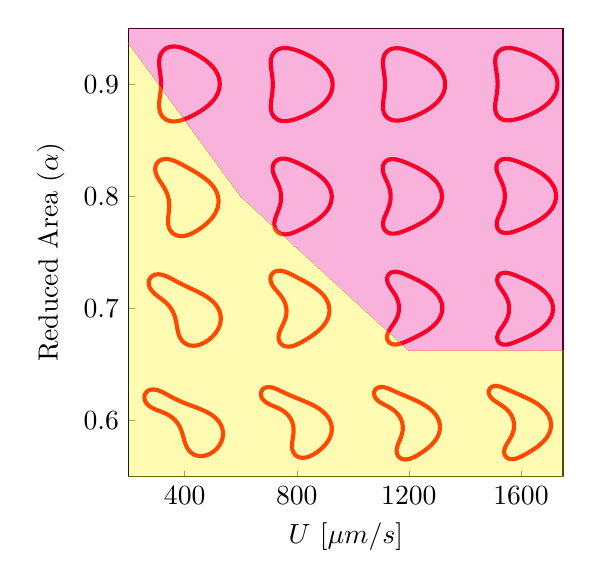
\begin{tikzpicture}[scale=1.0]

\pgfmathsetlengthmacro\MajorTickLength{
      \pgfkeysvalueof{/pgfplots/major tick length} * 0.5
    }

\begin{axis}[
  major tick length=\MajorTickLength,
  compat=newest,
  axis equal image,
  xmin = 2,
  xmax = 33,
  ymin = -2,
  ymax = 30,
  xtick = {6,14,22,30},
  xticklabels = {$400$,$800$,$1200$,$1600$},
%  xlabel = {Flow Velocity ($U$) [$\mu m/s$]},
  xlabel = {$U$ [$\mu m/s$]},
  ytick = {2,10,18,26},
  yticklabels = {$0.6$,$0.7$,$0.8$,$0.9$},
  ylabel = {Reduced Area ($\alpha$)},
  ylabel near ticks,
  xtick pos = left,
  ytick pos = left,
]

% RA = 0.60,flow rate = 400
\addplot[red,line width=1.5pt] coordinates{
(8.2753e+00,-1.2064e-02)
(8.3098e+00,2.5307e-02)
(8.3441e+00,6.4666e-02)
(8.3790e+00,1.0705e-01)
(8.4147e+00,1.5342e-01)
(8.4514e+00,2.0469e-01)
(8.4890e+00,2.6161e-01)
(8.5271e+00,3.2488e-01)
(8.5651e+00,3.9507e-01)
(8.6020e+00,4.7266e-01)
(8.6368e+00,5.5800e-01)
(8.6682e+00,6.5129e-01)
(8.6948e+00,7.5256e-01)
(8.7148e+00,8.6158e-01)
(8.7266e+00,9.7788e-01)
(8.7283e+00,1.1006e+00)
(8.7183e+00,1.2287e+00)
(8.6951e+00,1.3607e+00)
(8.6576e+00,1.4947e+00)
(8.6051e+00,1.6290e+00)
(8.5374e+00,1.7615e+00)
(8.4548e+00,1.8906e+00)
(8.3580e+00,2.0147e+00)
(8.2481e+00,2.1325e+00)
(8.1265e+00,2.2433e+00)
(7.9946e+00,2.3468e+00)
(7.8540e+00,2.4429e+00)
(7.7060e+00,2.5319e+00)
(7.5522e+00,2.6145e+00)
(7.3936e+00,2.6914e+00)
(7.2315e+00,2.7634e+00)
(7.0669e+00,2.8315e+00)
(6.9006e+00,2.8966e+00)
(6.7336e+00,2.9597e+00)
(6.5665e+00,3.0217e+00)
(6.4002e+00,3.0833e+00)
(6.2352e+00,3.1452e+00)
(6.0723e+00,3.2082e+00)
(5.9121e+00,3.2725e+00)
(5.7550e+00,3.3385e+00)
(5.6017e+00,3.4062e+00)
(5.4524e+00,3.4756e+00)
(5.3076e+00,3.5463e+00)
(5.1675e+00,3.6179e+00)
(5.0320e+00,3.6897e+00)
(4.9012e+00,3.7609e+00)
(4.7749e+00,3.8304e+00)
(4.6528e+00,3.8974e+00)
(4.5346e+00,3.9606e+00)
(4.4201e+00,4.0188e+00)
(4.3089e+00,4.0711e+00)
(4.2011e+00,4.1161e+00)
(4.0966e+00,4.1532e+00)
(3.9958e+00,4.1816e+00)
(3.8993e+00,4.2010e+00)
(3.8078e+00,4.2113e+00)
(3.7219e+00,4.2130e+00)
(3.6424e+00,4.2067e+00)
(3.5697e+00,4.1935e+00)
(3.5042e+00,4.1747e+00)
(3.4457e+00,4.1512e+00)
(3.3937e+00,4.1243e+00)
(3.3477e+00,4.0945e+00)
(3.3066e+00,4.0622e+00)
(3.2697e+00,4.0272e+00)
(3.2362e+00,3.9890e+00)
(3.2057e+00,3.9466e+00)
(3.1782e+00,3.8992e+00)
(3.1543e+00,3.8458e+00)
(3.1352e+00,3.7857e+00)
(3.1224e+00,3.7187e+00)
(3.1178e+00,3.6451e+00)
(3.1233e+00,3.5655e+00)
(3.1406e+00,3.4814e+00)
(3.1712e+00,3.3945e+00)
(3.2160e+00,3.3069e+00)
(3.2753e+00,3.2207e+00)
(3.3487e+00,3.1377e+00)
(3.4353e+00,3.0593e+00)
(3.5342e+00,2.9864e+00)
(3.6437e+00,2.9193e+00)
(3.7626e+00,2.8575e+00)
(3.8895e+00,2.8002e+00)
(4.0230e+00,2.7457e+00)
(4.1620e+00,2.6922e+00)
(4.3052e+00,2.6374e+00)
(4.4514e+00,2.5791e+00)
(4.5992e+00,2.5148e+00)
(4.7469e+00,2.4423e+00)
(4.8927e+00,2.3595e+00)
(5.0343e+00,2.2650e+00)
(5.1697e+00,2.1579e+00)
(5.2966e+00,2.0379e+00)
(5.4129e+00,1.9057e+00)
(5.5174e+00,1.7624e+00)
(5.6091e+00,1.6097e+00)
(5.6882e+00,1.4497e+00)
(5.7558e+00,1.2844e+00)
(5.8136e+00,1.1159e+00)
(5.8643e+00,9.4589e-01)
(5.9111e+00,7.7603e-01)
(5.9578e+00,6.0775e-01)
(6.0081e+00,4.4256e-01)
(6.0657e+00,2.8227e-01)
(6.1337e+00,1.2910e-01)
(6.2145e+00,-1.4186e-02)
(6.3092e+00,-1.4452e-01)
(6.4172e+00,-2.5885e-01)
(6.5368e+00,-3.5462e-01)
(6.6649e+00,-4.3026e-01)
(6.7981e+00,-4.8542e-01)
(6.9326e+00,-5.2095e-01)
(7.0653e+00,-5.3864e-01)
(7.1938e+00,-5.4087e-01)
(7.3161e+00,-5.3026e-01)
(7.4311e+00,-5.0940e-01)
(7.5382e+00,-4.8066e-01)
(7.6370e+00,-4.4615e-01)
(7.7276e+00,-4.0769e-01)
(7.8102e+00,-3.6677e-01)
(7.8851e+00,-3.2462e-01)
(7.9527e+00,-2.8224e-01)
(8.0136e+00,-2.4037e-01)
(8.0682e+00,-1.9953e-01)
(8.1173e+00,-1.6000e-01)
(8.1617e+00,-1.2184e-01)
(8.2022e+00,-8.4817e-02)
(8.2397e+00,-4.8468e-02)
(8.2753e+00,-1.2064e-02)
(8.3098e+00,2.5307e-02)
(8.3441e+00,6.4666e-02)
};

% RA = 0.70,flow rate = 400
\addplot[red,line width=1.5pt] coordinates{
(7.4214e+00,7.5718e+00)
(7.4755e+00,7.6029e+00)
(7.5296e+00,7.6360e+00)
(7.5844e+00,7.6715e+00)
(7.6404e+00,7.7100e+00)
(7.6980e+00,7.7519e+00)
(7.7576e+00,7.7978e+00)
(7.8191e+00,7.8481e+00)
(7.8827e+00,7.9035e+00)
(7.9479e+00,7.9644e+00)
(8.0146e+00,8.0312e+00)
(8.0822e+00,8.1044e+00)
(8.1500e+00,8.1844e+00)
(8.2172e+00,8.2716e+00)
(8.2828e+00,8.3664e+00)
(8.3455e+00,8.4691e+00)
(8.4039e+00,8.5799e+00)
(8.4565e+00,8.6988e+00)
(8.5014e+00,8.8258e+00)
(8.5366e+00,8.9602e+00)
(8.5604e+00,9.1013e+00)
(8.5709e+00,9.2479e+00)
(8.5666e+00,9.3985e+00)
(8.5463e+00,9.5510e+00)
(8.5094e+00,9.7036e+00)
(8.4559e+00,9.8540e+00)
(8.3864e+00,1.0000e+01)
(8.3020e+00,1.0141e+01)
(8.2041e+00,1.0275e+01)
(8.0943e+00,1.0401e+01)
(7.9746e+00,1.0520e+01)
(7.8466e+00,1.0630e+01)
(7.7121e+00,1.0733e+01)
(7.5724e+00,1.0829e+01)
(7.4291e+00,1.0919e+01)
(7.2833e+00,1.1003e+01)
(7.1361e+00,1.1083e+01)
(6.9884e+00,1.1159e+01)
(6.8410e+00,1.1231e+01)
(6.6947e+00,1.1301e+01)
(6.5501e+00,1.1369e+01)
(6.4079e+00,1.1435e+01)
(6.2685e+00,1.1501e+01)
(6.1323e+00,1.1565e+01)
(5.9998e+00,1.1629e+01)
(5.8712e+00,1.1692e+01)
(5.7469e+00,1.1754e+01)
(5.6270e+00,1.1815e+01)
(5.5116e+00,1.1875e+01)
(5.4008e+00,1.1934e+01)
(5.2946e+00,1.1990e+01)
(5.1929e+00,1.2045e+01)
(5.0956e+00,1.2096e+01)
(5.0026e+00,1.2145e+01)
(4.9138e+00,1.2190e+01)
(4.8289e+00,1.2231e+01)
(4.7480e+00,1.2269e+01)
(4.6706e+00,1.2302e+01)
(4.5968e+00,1.2332e+01)
(4.5261e+00,1.2357e+01)
(4.4582e+00,1.2379e+01)
(4.3928e+00,1.2397e+01)
(4.3292e+00,1.2412e+01)
(4.2668e+00,1.2423e+01)
(4.2048e+00,1.2431e+01)
(4.1425e+00,1.2435e+01)
(4.0791e+00,1.2435e+01)
(4.0140e+00,1.2431e+01)
(3.9468e+00,1.2421e+01)
(3.8776e+00,1.2404e+01)
(3.8067e+00,1.2379e+01)
(3.7352e+00,1.2345e+01)
(3.6647e+00,1.2299e+01)
(3.5978e+00,1.2240e+01)
(3.5375e+00,1.2167e+01)
(3.4874e+00,1.2081e+01)
(3.4509e+00,1.1983e+01)
(3.4314e+00,1.1875e+01)
(3.4310e+00,1.1760e+01)
(3.4507e+00,1.1641e+01)
(3.4905e+00,1.1522e+01)
(3.5490e+00,1.1406e+01)
(3.6242e+00,1.1295e+01)
(3.7136e+00,1.1188e+01)
(3.8149e+00,1.1087e+01)
(3.9255e+00,1.0990e+01)
(4.0431e+00,1.0896e+01)
(4.1658e+00,1.0803e+01)
(4.2913e+00,1.0709e+01)
(4.4179e+00,1.0611e+01)
(4.5435e+00,1.0509e+01)
(4.6661e+00,1.0400e+01)
(4.7836e+00,1.0282e+01)
(4.8940e+00,1.0157e+01)
(4.9956e+00,1.0023e+01)
(5.0869e+00,9.8802e+00)
(5.1667e+00,9.7308e+00)
(5.2348e+00,9.5756e+00)
(5.2915e+00,9.4163e+00)
(5.3377e+00,9.2544e+00)
(5.3752e+00,9.0913e+00)
(5.4064e+00,8.9283e+00)
(5.4338e+00,8.7664e+00)
(5.4606e+00,8.6065e+00)
(5.4900e+00,8.4495e+00)
(5.5250e+00,8.2964e+00)
(5.5683e+00,8.1487e+00)
(5.6222e+00,8.0081e+00)
(5.6881e+00,7.8767e+00)
(5.7662e+00,7.7568e+00)
(5.8558e+00,7.6507e+00)
(5.9552e+00,7.5600e+00)
(6.0619e+00,7.4857e+00)
(6.1729e+00,7.4278e+00)
(6.2856e+00,7.3856e+00)
(6.3974e+00,7.3578e+00)
(6.5064e+00,7.3424e+00)
(6.6111e+00,7.3376e+00)
(6.7106e+00,7.3413e+00)
(6.8044e+00,7.3517e+00)
(6.8923e+00,7.3674e+00)
(6.9742e+00,7.3869e+00)
(7.0506e+00,7.4092e+00)
(7.1218e+00,7.4334e+00)
(7.1882e+00,7.4591e+00)
(7.2507e+00,7.4859e+00)
(7.3098e+00,7.5135e+00)
(7.3664e+00,7.5421e+00)
(7.4214e+00,7.5718e+00)
(7.4755e+00,7.6029e+00)
(7.5296e+00,7.6360e+00)
};

% RA = 0.80,flow rate = 400
\addplot[red,line width=1.5pt] coordinates{
(7.6553e+00,1.6147e+01)
(7.7084e+00,1.6198e+01)
(7.7610e+00,1.6251e+01)
(7.8133e+00,1.6306e+01)
(7.8656e+00,1.6364e+01)
(7.9181e+00,1.6425e+01)
(7.9707e+00,1.6490e+01)
(8.0233e+00,1.6559e+01)
(8.0757e+00,1.6633e+01)
(8.1273e+00,1.6712e+01)
(8.1776e+00,1.6797e+01)
(8.2258e+00,1.6888e+01)
(8.2710e+00,1.6986e+01)
(8.3120e+00,1.7090e+01)
(8.3477e+00,1.7201e+01)
(8.3768e+00,1.7318e+01)
(8.3978e+00,1.7442e+01)
(8.4094e+00,1.7570e+01)
(8.4103e+00,1.7703e+01)
(8.3996e+00,1.7840e+01)
(8.3762e+00,1.7978e+01)
(8.3399e+00,1.8118e+01)
(8.2905e+00,1.8256e+01)
(8.2282e+00,1.8393e+01)
(8.1537e+00,1.8526e+01)
(8.0678e+00,1.8655e+01)
(7.9717e+00,1.8780e+01)
(7.8665e+00,1.8899e+01)
(7.7533e+00,1.9014e+01)
(7.6335e+00,1.9123e+01)
(7.5081e+00,1.9227e+01)
(7.3783e+00,1.9326e+01)
(7.2450e+00,1.9421e+01)
(7.1092e+00,1.9513e+01)
(6.9716e+00,1.9602e+01)
(6.8331e+00,1.9687e+01)
(6.6941e+00,1.9771e+01)
(6.5555e+00,1.9852e+01)
(6.4175e+00,1.9931e+01)
(6.2807e+00,2.0009e+01)
(6.1454e+00,2.0085e+01)
(6.0117e+00,2.0159e+01)
(5.8800e+00,2.0231e+01)
(5.7501e+00,2.0300e+01)
(5.6222e+00,2.0366e+01)
(5.4961e+00,2.0428e+01)
(5.3717e+00,2.0485e+01)
(5.2488e+00,2.0537e+01)
(5.1275e+00,2.0581e+01)
(5.0079e+00,2.0617e+01)
(4.8902e+00,2.0644e+01)
(4.7750e+00,2.0661e+01)
(4.6632e+00,2.0666e+01)
(4.5559e+00,2.0661e+01)
(4.4541e+00,2.0644e+01)
(4.3593e+00,2.0617e+01)
(4.2724e+00,2.0579e+01)
(4.1945e+00,2.0533e+01)
(4.1259e+00,2.0480e+01)
(4.0671e+00,2.0421e+01)
(4.0176e+00,2.0357e+01)
(3.9773e+00,2.0290e+01)
(3.9456e+00,2.0222e+01)
(3.9218e+00,2.0151e+01)
(3.9055e+00,2.0079e+01)
(3.8962e+00,2.0006e+01)
(3.8936e+00,1.9931e+01)
(3.8976e+00,1.9855e+01)
(3.9080e+00,1.9778e+01)
(3.9248e+00,1.9699e+01)
(3.9481e+00,1.9619e+01)
(3.9778e+00,1.9538e+01)
(4.0137e+00,1.9454e+01)
(4.0556e+00,1.9369e+01)
(4.1033e+00,1.9283e+01)
(4.1563e+00,1.9194e+01)
(4.2139e+00,1.9103e+01)
(4.2754e+00,1.9010e+01)
(4.3399e+00,1.8913e+01)
(4.4064e+00,1.8812e+01)
(4.4737e+00,1.8707e+01)
(4.5406e+00,1.8596e+01)
(4.6055e+00,1.8480e+01)
(4.6670e+00,1.8358e+01)
(4.7236e+00,1.8229e+01)
(4.7737e+00,1.8094e+01)
(4.8161e+00,1.7953e+01)
(4.8497e+00,1.7807e+01)
(4.8736e+00,1.7656e+01)
(4.8878e+00,1.7501e+01)
(4.8924e+00,1.7344e+01)
(4.8884e+00,1.7185e+01)
(4.8772e+00,1.7025e+01)
(4.8610e+00,1.6863e+01)
(4.8424e+00,1.6701e+01)
(4.8247e+00,1.6539e+01)
(4.8117e+00,1.6376e+01)
(4.8075e+00,1.6212e+01)
(4.8165e+00,1.6048e+01)
(4.8430e+00,1.5888e+01)
(4.8905e+00,1.5733e+01)
(4.9610e+00,1.5589e+01)
(5.0545e+00,1.5460e+01)
(5.1685e+00,1.5352e+01)
(5.2986e+00,1.5268e+01)
(5.4394e+00,1.5209e+01)
(5.5853e+00,1.5174e+01)
(5.7318e+00,1.5161e+01)
(5.8756e+00,1.5166e+01)
(6.0147e+00,1.5187e+01)
(6.1479e+00,1.5218e+01)
(6.2749e+00,1.5258e+01)
(6.3954e+00,1.5305e+01)
(6.5098e+00,1.5355e+01)
(6.6182e+00,1.5409e+01)
(6.7208e+00,1.5464e+01)
(6.8180e+00,1.5519e+01)
(6.9099e+00,1.5575e+01)
(6.9969e+00,1.5631e+01)
(7.0791e+00,1.5686e+01)
(7.1568e+00,1.5740e+01)
(7.2302e+00,1.5793e+01)
(7.2997e+00,1.5845e+01)
(7.3656e+00,1.5897e+01)
(7.4283e+00,1.5947e+01)
(7.4881e+00,1.5997e+01)
(7.5456e+00,1.6047e+01)
(7.6011e+00,1.6096e+01)
(7.6553e+00,1.6147e+01)
(7.7084e+00,1.6198e+01)
(7.7610e+00,1.6251e+01)
};

% RA = 0.90,flow rate = 400
\addplot[red,line width=1.5pt] coordinates{
(4.2301e+00,2.4048e+01)
(4.2600e+00,2.3963e+01)
(4.2968e+00,2.3881e+01)
(4.3412e+00,2.3802e+01)
(4.3934e+00,2.3726e+01)
(4.4538e+00,2.3655e+01)
(4.5224e+00,2.3588e+01)
(4.5991e+00,2.3528e+01)
(4.6838e+00,2.3476e+01)
(4.7760e+00,2.3431e+01)
(4.8748e+00,2.3395e+01)
(4.9794e+00,2.3369e+01)
(5.0891e+00,2.3353e+01)
(5.2027e+00,2.3346e+01)
(5.3196e+00,2.3349e+01)
(5.4389e+00,2.3361e+01)
(5.5602e+00,2.3381e+01)
(5.6828e+00,2.3410e+01)
(5.8066e+00,2.3445e+01)
(5.9314e+00,2.3486e+01)
(6.0570e+00,2.3533e+01)
(6.1833e+00,2.3585e+01)
(6.3103e+00,2.3641e+01)
(6.4378e+00,2.3702e+01)
(6.5657e+00,2.3766e+01)
(6.6939e+00,2.3833e+01)
(6.8221e+00,2.3904e+01)
(6.9500e+00,2.3978e+01)
(7.0773e+00,2.4055e+01)
(7.2035e+00,2.4136e+01)
(7.3283e+00,2.4220e+01)
(7.4509e+00,2.4309e+01)
(7.5707e+00,2.4401e+01)
(7.6871e+00,2.4498e+01)
(7.7992e+00,2.4599e+01)
(7.9062e+00,2.4705e+01)
(8.0071e+00,2.4815e+01)
(8.1010e+00,2.4931e+01)
(8.1869e+00,2.5051e+01)
(8.2637e+00,2.5176e+01)
(8.3306e+00,2.5304e+01)
(8.3868e+00,2.5435e+01)
(8.4317e+00,2.5569e+01)
(8.4649e+00,2.5704e+01)
(8.4863e+00,2.5839e+01)
(8.4960e+00,2.5972e+01)
(8.4945e+00,2.6104e+01)
(8.4826e+00,2.6232e+01)
(8.4610e+00,2.6356e+01)
(8.4309e+00,2.6475e+01)
(8.3932e+00,2.6589e+01)
(8.3491e+00,2.6697e+01)
(8.2996e+00,2.6799e+01)
(8.2458e+00,2.6896e+01)
(8.1884e+00,2.6987e+01)
(8.1283e+00,2.7074e+01)
(8.0660e+00,2.7155e+01)
(8.0021e+00,2.7231e+01)
(7.9369e+00,2.7304e+01)
(7.8707e+00,2.7373e+01)
(7.8038e+00,2.7438e+01)
(7.7361e+00,2.7500e+01)
(7.6677e+00,2.7560e+01)
(7.5985e+00,2.7618e+01)
(7.5283e+00,2.7673e+01)
(7.4569e+00,2.7728e+01)
(7.3842e+00,2.7781e+01)
(7.3099e+00,2.7833e+01)
(7.2337e+00,2.7885e+01)
(7.1555e+00,2.7936e+01)
(7.0749e+00,2.7987e+01)
(6.9918e+00,2.8038e+01)
(6.9060e+00,2.8089e+01)
(6.8172e+00,2.8140e+01)
(6.7253e+00,2.8191e+01)
(6.6302e+00,2.8242e+01)
(6.5317e+00,2.8292e+01)
(6.4298e+00,2.8343e+01)
(6.3242e+00,2.8393e+01)
(6.2148e+00,2.8442e+01)
(6.1016e+00,2.8490e+01)
(5.9844e+00,2.8536e+01)
(5.8630e+00,2.8578e+01)
(5.7374e+00,2.8617e+01)
(5.6075e+00,2.8649e+01)
(5.4734e+00,2.8675e+01)
(5.3355e+00,2.8691e+01)
(5.1946e+00,2.8695e+01)
(5.0521e+00,2.8684e+01)
(4.9102e+00,2.8656e+01)
(4.7719e+00,2.8608e+01)
(4.6409e+00,2.8540e+01)
(4.5213e+00,2.8452e+01)
(4.4168e+00,2.8344e+01)
(4.3304e+00,2.8221e+01)
(4.2633e+00,2.8086e+01)
(4.2156e+00,2.7943e+01)
(4.1857e+00,2.7794e+01)
(4.1713e+00,2.7644e+01)
(4.1694e+00,2.7493e+01)
(4.1770e+00,2.7344e+01)
(4.1913e+00,2.7195e+01)
(4.2096e+00,2.7049e+01)
(4.2296e+00,2.6904e+01)
(4.2495e+00,2.6760e+01)
(4.2679e+00,2.6618e+01)
(4.2834e+00,2.6478e+01)
(4.2954e+00,2.6340e+01)
(4.3033e+00,2.6203e+01)
(4.3069e+00,2.6069e+01)
(4.3064e+00,2.5938e+01)
(4.3019e+00,2.5809e+01)
(4.2940e+00,2.5684e+01)
(4.2832e+00,2.5561e+01)
(4.2701e+00,2.5442e+01)
(4.2556e+00,2.5326e+01)
(4.2402e+00,2.5213e+01)
(4.2248e+00,2.5103e+01)
(4.2101e+00,2.4996e+01)
(4.1967e+00,2.4892e+01)
(4.1854e+00,2.4790e+01)
(4.1766e+00,2.4691e+01)
(4.1709e+00,2.4594e+01)
(4.1688e+00,2.4498e+01)
(4.1709e+00,2.4405e+01)
(4.1776e+00,2.4313e+01)
(4.1894e+00,2.4223e+01)
(4.2067e+00,2.4134e+01)
(4.2301e+00,2.4048e+01)
(4.2600e+00,2.3963e+01)
(4.2968e+00,2.3881e+01)
};

% RA = 0.60,flow rate = 800
\addplot[red,line width=1.5pt] coordinates{
(1.3620e+01,3.7554e+00)
(1.3573e+01,3.7756e+00)
(1.3525e+01,3.7964e+00)
(1.3475e+01,3.8185e+00)
(1.3421e+01,3.8423e+00)
(1.3364e+01,3.8681e+00)
(1.3302e+01,3.8964e+00)
(1.3234e+01,3.9273e+00)
(1.3162e+01,3.9610e+00)
(1.3084e+01,3.9977e+00)
(1.3001e+01,4.0373e+00)
(1.2912e+01,4.0798e+00)
(1.2818e+01,4.1249e+00)
(1.2717e+01,4.1719e+00)
(1.2611e+01,4.2200e+00)
(1.2497e+01,4.2677e+00)
(1.2377e+01,4.3125e+00)
(1.2249e+01,4.3508e+00)
(1.2112e+01,4.3775e+00)
(1.1968e+01,4.3854e+00)
(1.1821e+01,4.3657e+00)
(1.1679e+01,4.3096e+00)
(1.1556e+01,4.2122e+00)
(1.1469e+01,4.0770e+00)
(1.1433e+01,3.9173e+00)
(1.1450e+01,3.7512e+00)
(1.1516e+01,3.5945e+00)
(1.1619e+01,3.4563e+00)
(1.1748e+01,3.3389e+00)
(1.1894e+01,3.2403e+00)
(1.2050e+01,3.1563e+00)
(1.2212e+01,3.0817e+00)
(1.2377e+01,3.0116e+00)
(1.2541e+01,2.9413e+00)
(1.2703e+01,2.8668e+00)
(1.2860e+01,2.7851e+00)
(1.3011e+01,2.6939e+00)
(1.3152e+01,2.5918e+00)
(1.3283e+01,2.4783e+00)
(1.3399e+01,2.3541e+00)
(1.3500e+01,2.2205e+00)
(1.3585e+01,2.0793e+00)
(1.3652e+01,1.9330e+00)
(1.3703e+01,1.7840e+00)
(1.3738e+01,1.6348e+00)
(1.3759e+01,1.4873e+00)
(1.3767e+01,1.3433e+00)
(1.3766e+01,1.2041e+00)
(1.3757e+01,1.0704e+00)
(1.3742e+01,9.4260e-01)
(1.3725e+01,8.2095e-01)
(1.3708e+01,7.0537e-01)
(1.3691e+01,5.9578e-01)
(1.3676e+01,4.9209e-01)
(1.3664e+01,3.9429e-01)
(1.3657e+01,3.0240e-01)
(1.3654e+01,2.1651e-01)
(1.3655e+01,1.3671e-01)
(1.3660e+01,6.3035e-02)
(1.3669e+01,-4.6172e-03)
(1.3681e+01,-6.6520e-02)
(1.3696e+01,-1.2317e-01)
(1.3713e+01,-1.7527e-01)
(1.3732e+01,-2.2376e-01)
(1.3754e+01,-2.6968e-01)
(1.3779e+01,-3.1405e-01)
(1.3808e+01,-3.5775e-01)
(1.3841e+01,-4.0129e-01)
(1.3880e+01,-4.4476e-01)
(1.3926e+01,-4.8774e-01)
(1.3980e+01,-5.2933e-01)
(1.4043e+01,-5.6816e-01)
(1.4115e+01,-6.0257e-01)
(1.4196e+01,-6.3067e-01)
(1.4286e+01,-6.5063e-01)
(1.4384e+01,-6.6085e-01)
(1.4489e+01,-6.6012e-01)
(1.4599e+01,-6.4775e-01)
(1.4714e+01,-6.2356e-01)
(1.4831e+01,-5.8779e-01)
(1.4951e+01,-5.4102e-01)
(1.5072e+01,-4.8397e-01)
(1.5194e+01,-4.1740e-01)
(1.5317e+01,-3.4198e-01)
(1.5440e+01,-2.5825e-01)
(1.5563e+01,-1.6655e-01)
(1.5685e+01,-6.7001e-02)
(1.5805e+01,4.0489e-02)
(1.5923e+01,1.5618e-01)
(1.6035e+01,2.8046e-01)
(1.6141e+01,4.1375e-01)
(1.6239e+01,5.5635e-01)
(1.6325e+01,7.0831e-01)
(1.6396e+01,8.6920e-01)
(1.6451e+01,1.0379e+00)
(1.6486e+01,1.2126e+00)
(1.6499e+01,1.3907e+00)
(1.6488e+01,1.5689e+00)
(1.6455e+01,1.7439e+00)
(1.6401e+01,1.9126e+00)
(1.6327e+01,2.0725e+00)
(1.6237e+01,2.2220e+00)
(1.6133e+01,2.3602e+00)
(1.6019e+01,2.4869e+00)
(1.5898e+01,2.6025e+00)
(1.5771e+01,2.7077e+00)
(1.5642e+01,2.8034e+00)
(1.5511e+01,2.8906e+00)
(1.5380e+01,2.9701e+00)
(1.5250e+01,3.0430e+00)
(1.5122e+01,3.1098e+00)
(1.4997e+01,3.1714e+00)
(1.4876e+01,3.2283e+00)
(1.4758e+01,3.2811e+00)
(1.4646e+01,3.3302e+00)
(1.4538e+01,3.3759e+00)
(1.4436e+01,3.4186e+00)
(1.4339e+01,3.4585e+00)
(1.4248e+01,3.4957e+00)
(1.4162e+01,3.5305e+00)
(1.4083e+01,3.5629e+00)
(1.4009e+01,3.5930e+00)
(1.3940e+01,3.6210e+00)
(1.3877e+01,3.6470e+00)
(1.3819e+01,3.6711e+00)
(1.3765e+01,3.6937e+00)
(1.3714e+01,3.7150e+00)
(1.3666e+01,3.7354e+00)
(1.3620e+01,3.7554e+00)
(1.3573e+01,3.7756e+00)
(1.3525e+01,3.7964e+00)
};

% RA = 0.70,flow rate = 800
\addplot[red,line width=1.5pt] coordinates{
(1.2699e+01,7.9012e+00)
(1.2704e+01,7.8389e+00)
(1.2714e+01,7.7763e+00)
(1.2731e+01,7.7132e+00)
(1.2755e+01,7.6496e+00)
(1.2787e+01,7.5860e+00)
(1.2829e+01,7.5234e+00)
(1.2881e+01,7.4633e+00)
(1.2945e+01,7.4078e+00)
(1.3020e+01,7.3590e+00)
(1.3105e+01,7.3193e+00)
(1.3201e+01,7.2906e+00)
(1.3304e+01,7.2743e+00)
(1.3415e+01,7.2712e+00)
(1.3530e+01,7.2811e+00)
(1.3648e+01,7.3033e+00)
(1.3769e+01,7.3368e+00)
(1.3892e+01,7.3801e+00)
(1.4016e+01,7.4319e+00)
(1.4142e+01,7.4909e+00)
(1.4270e+01,7.5560e+00)
(1.4399e+01,7.6264e+00)
(1.4530e+01,7.7013e+00)
(1.4663e+01,7.7802e+00)
(1.4796e+01,7.8631e+00)
(1.4931e+01,7.9498e+00)
(1.5065e+01,8.0406e+00)
(1.5200e+01,8.1356e+00)
(1.5332e+01,8.2352e+00)
(1.5463e+01,8.3401e+00)
(1.5591e+01,8.4506e+00)
(1.5713e+01,8.5672e+00)
(1.5830e+01,8.6906e+00)
(1.5938e+01,8.8209e+00)
(1.6037e+01,8.9583e+00)
(1.6124e+01,9.1026e+00)
(1.6198e+01,9.2531e+00)
(1.6256e+01,9.4087e+00)
(1.6297e+01,9.5678e+00)
(1.6321e+01,9.7284e+00)
(1.6326e+01,9.8881e+00)
(1.6315e+01,1.0045e+01)
(1.6287e+01,1.0196e+01)
(1.6245e+01,1.0341e+01)
(1.6191e+01,1.0478e+01)
(1.6127e+01,1.0606e+01)
(1.6055e+01,1.0725e+01)
(1.5978e+01,1.0836e+01)
(1.5897e+01,1.0938e+01)
(1.5813e+01,1.1031e+01)
(1.5729e+01,1.1117e+01)
(1.5645e+01,1.1196e+01)
(1.5562e+01,1.1269e+01)
(1.5480e+01,1.1335e+01)
(1.5402e+01,1.1396e+01)
(1.5326e+01,1.1453e+01)
(1.5253e+01,1.1504e+01)
(1.5183e+01,1.1552e+01)
(1.5117e+01,1.1596e+01)
(1.5053e+01,1.1637e+01)
(1.4993e+01,1.1675e+01)
(1.4935e+01,1.1710e+01)
(1.4879e+01,1.1744e+01)
(1.4825e+01,1.1776e+01)
(1.4771e+01,1.1808e+01)
(1.4716e+01,1.1839e+01)
(1.4661e+01,1.1871e+01)
(1.4604e+01,1.1903e+01)
(1.4545e+01,1.1936e+01)
(1.4482e+01,1.1970e+01)
(1.4416e+01,1.2006e+01)
(1.4346e+01,1.2044e+01)
(1.4272e+01,1.2084e+01)
(1.4193e+01,1.2126e+01)
(1.4109e+01,1.2170e+01)
(1.4021e+01,1.2216e+01)
(1.3928e+01,1.2264e+01)
(1.3830e+01,1.2315e+01)
(1.3727e+01,1.2366e+01)
(1.3619e+01,1.2420e+01)
(1.3505e+01,1.2473e+01)
(1.3386e+01,1.2527e+01)
(1.3261e+01,1.2577e+01)
(1.3130e+01,1.2623e+01)
(1.2992e+01,1.2661e+01)
(1.2847e+01,1.2685e+01)
(1.2696e+01,1.2688e+01)
(1.2544e+01,1.2664e+01)
(1.2399e+01,1.2605e+01)
(1.2272e+01,1.2508e+01)
(1.2178e+01,1.2377e+01)
(1.2125e+01,1.2221e+01)
(1.2117e+01,1.2056e+01)
(1.2149e+01,1.1892e+01)
(1.2212e+01,1.1736e+01)
(1.2297e+01,1.1589e+01)
(1.2397e+01,1.1452e+01)
(1.2505e+01,1.1321e+01)
(1.2616e+01,1.1194e+01)
(1.2726e+01,1.1066e+01)
(1.2832e+01,1.0936e+01)
(1.2930e+01,1.0802e+01)
(1.3019e+01,1.0664e+01)
(1.3096e+01,1.0521e+01)
(1.3159e+01,1.0374e+01)
(1.3207e+01,1.0224e+01)
(1.3240e+01,1.0074e+01)
(1.3259e+01,9.9240e+00)
(1.3263e+01,9.7769e+00)
(1.3254e+01,9.6339e+00)
(1.3234e+01,9.4962e+00)
(1.3205e+01,9.3646e+00)
(1.3168e+01,9.2396e+00)
(1.3126e+01,9.1214e+00)
(1.3081e+01,9.0097e+00)
(1.3034e+01,8.9042e+00)
(1.2988e+01,8.8044e+00)
(1.2942e+01,8.7099e+00)
(1.2899e+01,8.6200e+00)
(1.2859e+01,8.5344e+00)
(1.2823e+01,8.4526e+00)
(1.2791e+01,8.3744e+00)
(1.2764e+01,8.2995e+00)
(1.2741e+01,8.2277e+00)
(1.2724e+01,8.1585e+00)
(1.2711e+01,8.0918e+00)
(1.2702e+01,8.0271e+00)
(1.2698e+01,7.9637e+00)
(1.2699e+01,7.9012e+00)
(1.2704e+01,7.8389e+00)
(1.2714e+01,7.7763e+00)
};

% RA = 0.80,flow rate = 800
\addplot[red,line width=1.5pt] coordinates{
(1.3841e+01,1.5443e+01)
(1.3910e+01,1.5470e+01)
(1.3979e+01,1.5499e+01)
(1.4049e+01,1.5530e+01)
(1.4120e+01,1.5562e+01)
(1.4193e+01,1.5596e+01)
(1.4268e+01,1.5632e+01)
(1.4347e+01,1.5670e+01)
(1.4428e+01,1.5711e+01)
(1.4512e+01,1.5754e+01)
(1.4600e+01,1.5800e+01)
(1.4691e+01,1.5849e+01)
(1.4786e+01,1.5900e+01)
(1.4884e+01,1.5956e+01)
(1.4985e+01,1.6014e+01)
(1.5088e+01,1.6077e+01)
(1.5194e+01,1.6143e+01)
(1.5303e+01,1.6214e+01)
(1.5413e+01,1.6289e+01)
(1.5523e+01,1.6370e+01)
(1.5634e+01,1.6457e+01)
(1.5745e+01,1.6550e+01)
(1.5853e+01,1.6650e+01)
(1.5959e+01,1.6757e+01)
(1.6060e+01,1.6871e+01)
(1.6155e+01,1.6994e+01)
(1.6242e+01,1.7125e+01)
(1.6320e+01,1.7265e+01)
(1.6385e+01,1.7412e+01)
(1.6436e+01,1.7566e+01)
(1.6471e+01,1.7725e+01)
(1.6488e+01,1.7888e+01)
(1.6488e+01,1.8052e+01)
(1.6469e+01,1.8214e+01)
(1.6433e+01,1.8374e+01)
(1.6381e+01,1.8528e+01)
(1.6314e+01,1.8676e+01)
(1.6235e+01,1.8816e+01)
(1.6145e+01,1.8948e+01)
(1.6048e+01,1.9071e+01)
(1.5944e+01,1.9187e+01)
(1.5835e+01,1.9294e+01)
(1.5723e+01,1.9395e+01)
(1.5610e+01,1.9488e+01)
(1.5495e+01,1.9576e+01)
(1.5380e+01,1.9657e+01)
(1.5267e+01,1.9733e+01)
(1.5154e+01,1.9805e+01)
(1.5044e+01,1.9872e+01)
(1.4936e+01,1.9935e+01)
(1.4831e+01,1.9995e+01)
(1.4729e+01,2.0051e+01)
(1.4630e+01,2.0103e+01)
(1.4534e+01,2.0153e+01)
(1.4442e+01,2.0200e+01)
(1.4354e+01,2.0244e+01)
(1.4269e+01,2.0286e+01)
(1.4187e+01,2.0325e+01)
(1.4109e+01,2.0363e+01)
(1.4033e+01,2.0397e+01)
(1.3960e+01,2.0430e+01)
(1.3888e+01,2.0462e+01)
(1.3818e+01,2.0491e+01)
(1.3749e+01,2.0519e+01)
(1.3680e+01,2.0546e+01)
(1.3611e+01,2.0572e+01)
(1.3541e+01,2.0596e+01)
(1.3468e+01,2.0619e+01)
(1.3393e+01,2.0640e+01)
(1.3315e+01,2.0659e+01)
(1.3233e+01,2.0675e+01)
(1.3147e+01,2.0687e+01)
(1.3057e+01,2.0694e+01)
(1.2962e+01,2.0693e+01)
(1.2864e+01,2.0683e+01)
(1.2764e+01,2.0660e+01)
(1.2663e+01,2.0623e+01)
(1.2565e+01,2.0569e+01)
(1.2475e+01,2.0496e+01)
(1.2396e+01,2.0404e+01)
(1.2334e+01,2.0296e+01)
(1.2292e+01,2.0174e+01)
(1.2273e+01,2.0042e+01)
(1.2274e+01,1.9905e+01)
(1.2295e+01,1.9766e+01)
(1.2332e+01,1.9627e+01)
(1.2382e+01,1.9489e+01)
(1.2440e+01,1.9351e+01)
(1.2505e+01,1.9212e+01)
(1.2571e+01,1.9072e+01)
(1.2637e+01,1.8929e+01)
(1.2699e+01,1.8782e+01)
(1.2755e+01,1.8631e+01)
(1.2803e+01,1.8476e+01)
(1.2839e+01,1.8317e+01)
(1.2864e+01,1.8156e+01)
(1.2876e+01,1.7992e+01)
(1.2874e+01,1.7828e+01)
(1.2859e+01,1.7665e+01)
(1.2832e+01,1.7504e+01)
(1.2794e+01,1.7347e+01)
(1.2748e+01,1.7193e+01)
(1.2695e+01,1.7043e+01)
(1.2638e+01,1.6896e+01)
(1.2580e+01,1.6752e+01)
(1.2524e+01,1.6609e+01)
(1.2474e+01,1.6468e+01)
(1.2433e+01,1.6326e+01)
(1.2405e+01,1.6185e+01)
(1.2393e+01,1.6045e+01)
(1.2400e+01,1.5908e+01)
(1.2428e+01,1.5778e+01)
(1.2477e+01,1.5658e+01)
(1.2544e+01,1.5553e+01)
(1.2627e+01,1.5465e+01)
(1.2721e+01,1.5396e+01)
(1.2821e+01,1.5346e+01)
(1.2923e+01,1.5312e+01)
(1.3025e+01,1.5292e+01)
(1.3123e+01,1.5284e+01)
(1.3218e+01,1.5286e+01)
(1.3309e+01,1.5294e+01)
(1.3395e+01,1.5308e+01)
(1.3477e+01,1.5325e+01)
(1.3555e+01,1.5345e+01)
(1.3629e+01,1.5367e+01)
(1.3702e+01,1.5391e+01)
(1.3772e+01,1.5416e+01)
(1.3841e+01,1.5443e+01)
(1.3910e+01,1.5470e+01)
(1.3979e+01,1.5499e+01)
};

% RA = 0.90,flow rate = 800
\addplot[red,line width=1.5pt] coordinates{
(1.2334e+01,2.8215e+01)
(1.2285e+01,2.8140e+01)
(1.2243e+01,2.8061e+01)
(1.2208e+01,2.7977e+01)
(1.2181e+01,2.7889e+01)
(1.2161e+01,2.7797e+01)
(1.2147e+01,2.7703e+01)
(1.2140e+01,2.7606e+01)
(1.2138e+01,2.7506e+01)
(1.2141e+01,2.7404e+01)
(1.2148e+01,2.7299e+01)
(1.2159e+01,2.7191e+01)
(1.2173e+01,2.7081e+01)
(1.2189e+01,2.6969e+01)
(1.2206e+01,2.6853e+01)
(1.2223e+01,2.6734e+01)
(1.2240e+01,2.6613e+01)
(1.2255e+01,2.6488e+01)
(1.2268e+01,2.6360e+01)
(1.2277e+01,2.6229e+01)
(1.2283e+01,2.6095e+01)
(1.2285e+01,2.5958e+01)
(1.2282e+01,2.5819e+01)
(1.2274e+01,2.5678e+01)
(1.2262e+01,2.5536e+01)
(1.2246e+01,2.5392e+01)
(1.2227e+01,2.5247e+01)
(1.2206e+01,2.5101e+01)
(1.2184e+01,2.4953e+01)
(1.2164e+01,2.4805e+01)
(1.2148e+01,2.4655e+01)
(1.2139e+01,2.4504e+01)
(1.2140e+01,2.4353e+01)
(1.2154e+01,2.4202e+01)
(1.2184e+01,2.4055e+01)
(1.2234e+01,2.3913e+01)
(1.2305e+01,2.3781e+01)
(1.2397e+01,2.3664e+01)
(1.2506e+01,2.3564e+01)
(1.2629e+01,2.3486e+01)
(1.2762e+01,2.3429e+01)
(1.2900e+01,2.3392e+01)
(1.3040e+01,2.3373e+01)
(1.3179e+01,2.3369e+01)
(1.3315e+01,2.3378e+01)
(1.3448e+01,2.3396e+01)
(1.3577e+01,2.3421e+01)
(1.3702e+01,2.3451e+01)
(1.3823e+01,2.3485e+01)
(1.3940e+01,2.3522e+01)
(1.4053e+01,2.3561e+01)
(1.4163e+01,2.3602e+01)
(1.4269e+01,2.3643e+01)
(1.4372e+01,2.3686e+01)
(1.4471e+01,2.3728e+01)
(1.4567e+01,2.3771e+01)
(1.4660e+01,2.3814e+01)
(1.4749e+01,2.3858e+01)
(1.4837e+01,2.3901e+01)
(1.4921e+01,2.3945e+01)
(1.5004e+01,2.3989e+01)
(1.5084e+01,2.4034e+01)
(1.5163e+01,2.4079e+01)
(1.5240e+01,2.4126e+01)
(1.5316e+01,2.4173e+01)
(1.5391e+01,2.4222e+01)
(1.5466e+01,2.4273e+01)
(1.5540e+01,2.4325e+01)
(1.5614e+01,2.4380e+01)
(1.5687e+01,2.4438e+01)
(1.5761e+01,2.4498e+01)
(1.5834e+01,2.4563e+01)
(1.5907e+01,2.4631e+01)
(1.5980e+01,2.4703e+01)
(1.6051e+01,2.4780e+01)
(1.6122e+01,2.4862e+01)
(1.6190e+01,2.4949e+01)
(1.6255e+01,2.5042e+01)
(1.6317e+01,2.5141e+01)
(1.6374e+01,2.5246e+01)
(1.6426e+01,2.5358e+01)
(1.6470e+01,2.5476e+01)
(1.6506e+01,2.5599e+01)
(1.6533e+01,2.5728e+01)
(1.6549e+01,2.5861e+01)
(1.6553e+01,2.5997e+01)
(1.6545e+01,2.6136e+01)
(1.6524e+01,2.6275e+01)
(1.6491e+01,2.6414e+01)
(1.6444e+01,2.6551e+01)
(1.6386e+01,2.6685e+01)
(1.6316e+01,2.6815e+01)
(1.6236e+01,2.6941e+01)
(1.6147e+01,2.7062e+01)
(1.6050e+01,2.7177e+01)
(1.5946e+01,2.7286e+01)
(1.5837e+01,2.7390e+01)
(1.5722e+01,2.7489e+01)
(1.5603e+01,2.7582e+01)
(1.5482e+01,2.7671e+01)
(1.5358e+01,2.7755e+01)
(1.5232e+01,2.7834e+01)
(1.5104e+01,2.7909e+01)
(1.4977e+01,2.7980e+01)
(1.4848e+01,2.8048e+01)
(1.4720e+01,2.8112e+01)
(1.4593e+01,2.8172e+01)
(1.4466e+01,2.8229e+01)
(1.4341e+01,2.8282e+01)
(1.4216e+01,2.8332e+01)
(1.4094e+01,2.8379e+01)
(1.3972e+01,2.8422e+01)
(1.3853e+01,2.8461e+01)
(1.3735e+01,2.8495e+01)
(1.3619e+01,2.8525e+01)
(1.3504e+01,2.8549e+01)
(1.3392e+01,2.8568e+01)
(1.3282e+01,2.8580e+01)
(1.3174e+01,2.8586e+01)
(1.3069e+01,2.8584e+01)
(1.2967e+01,2.8574e+01)
(1.2869e+01,2.8557e+01)
(1.2775e+01,2.8531e+01)
(1.2686e+01,2.8497e+01)
(1.2603e+01,2.8455e+01)
(1.2525e+01,2.8405e+01)
(1.2455e+01,2.8348e+01)
(1.2391e+01,2.8285e+01)
(1.2334e+01,2.8215e+01)
(1.2285e+01,2.8140e+01)
(1.2243e+01,2.8061e+01)
};

% RA = 0.60,flow rate = 1200
\addplot[red,line width=1.5pt] coordinates{
(2.3063e+01,3.1292e+00)
(2.3019e+01,3.1550e+00)
(2.2974e+01,3.1810e+00)
(2.2926e+01,3.2079e+00)
(2.2875e+01,3.2360e+00)
(2.2819e+01,3.2657e+00)
(2.2759e+01,3.2973e+00)
(2.2693e+01,3.3307e+00)
(2.2621e+01,3.3661e+00)
(2.2544e+01,3.4034e+00)
(2.2460e+01,3.4425e+00)
(2.2371e+01,3.4836e+00)
(2.2275e+01,3.5264e+00)
(2.2173e+01,3.5710e+00)
(2.2066e+01,3.6173e+00)
(2.1953e+01,3.6654e+00)
(2.1834e+01,3.7155e+00)
(2.1711e+01,3.7676e+00)
(2.1583e+01,3.8218e+00)
(2.1450e+01,3.8784e+00)
(2.1313e+01,3.9376e+00)
(2.1173e+01,3.9993e+00)
(2.1029e+01,4.0634e+00)
(2.0882e+01,4.1294e+00)
(2.0731e+01,4.1960e+00)
(2.0576e+01,4.2611e+00)
(2.0417e+01,4.3204e+00)
(2.0251e+01,4.3676e+00)
(2.0078e+01,4.3925e+00)
(1.9902e+01,4.3817e+00)
(1.9736e+01,4.3213e+00)
(1.9602e+01,4.2058e+00)
(1.9524e+01,4.0464e+00)
(1.9513e+01,3.8691e+00)
(1.9564e+01,3.6990e+00)
(1.9660e+01,3.5499e+00)
(1.9783e+01,3.4245e+00)
(1.9923e+01,3.3192e+00)
(2.0070e+01,3.2284e+00)
(2.0219e+01,3.1466e+00)
(2.0368e+01,3.0687e+00)
(2.0513e+01,2.9912e+00)
(2.0653e+01,2.9111e+00)
(2.0786e+01,2.8268e+00)
(2.0911e+01,2.7372e+00)
(2.1025e+01,2.6422e+00)
(2.1129e+01,2.5421e+00)
(2.1222e+01,2.4378e+00)
(2.1302e+01,2.3305e+00)
(2.1370e+01,2.2215e+00)
(2.1426e+01,2.1124e+00)
(2.1472e+01,2.0045e+00)
(2.1506e+01,1.8991e+00)
(2.1532e+01,1.7975e+00)
(2.1549e+01,1.7005e+00)
(2.1559e+01,1.6089e+00)
(2.1564e+01,1.5230e+00)
(2.1564e+01,1.4432e+00)
(2.1560e+01,1.3694e+00)
(2.1554e+01,1.3014e+00)
(2.1545e+01,1.2389e+00)
(2.1535e+01,1.1811e+00)
(2.1525e+01,1.1273e+00)
(2.1513e+01,1.0763e+00)
(2.1501e+01,1.0270e+00)
(2.1487e+01,9.7800e-01)
(2.1472e+01,9.2799e-01)
(2.1454e+01,8.7583e-01)
(2.1435e+01,8.2056e-01)
(2.1413e+01,7.6141e-01)
(2.1388e+01,6.9784e-01)
(2.1360e+01,6.2941e-01)
(2.1330e+01,5.5576e-01)
(2.1296e+01,4.7654e-01)
(2.1261e+01,3.9135e-01)
(2.1225e+01,2.9967e-01)
(2.1190e+01,2.0090e-01)
(2.1159e+01,9.4436e-02)
(2.1135e+01,-2.0115e-02)
(2.1124e+01,-1.4242e-01)
(2.1132e+01,-2.7063e-01)
(2.1164e+01,-4.0042e-01)
(2.1227e+01,-5.2435e-01)
(2.1322e+01,-6.3251e-01)
(2.1446e+01,-7.1502e-01)
(2.1590e+01,-7.6538e-01)
(2.1747e+01,-7.8234e-01)
(2.1907e+01,-7.6920e-01)
(2.2067e+01,-7.3157e-01)
(2.2225e+01,-6.7527e-01)
(2.2381e+01,-6.0523e-01)
(2.2534e+01,-5.2514e-01)
(2.2685e+01,-4.3752e-01)
(2.2834e+01,-3.4396e-01)
(2.2982e+01,-2.4530e-01)
(2.3127e+01,-1.4188e-01)
(2.3269e+01,-3.3638e-02)
(2.3407e+01,7.9703e-02)
(2.3540e+01,1.9856e-01)
(2.3666e+01,3.2337e-01)
(2.3784e+01,4.5451e-01)
(2.3892e+01,5.9217e-01)
(2.3987e+01,7.3621e-01)
(2.4068e+01,8.8607e-01)
(2.4133e+01,1.0406e+00)
(2.4180e+01,1.1983e+00)
(2.4209e+01,1.3569e+00)
(2.4219e+01,1.5139e+00)
(2.4212e+01,1.6671e+00)
(2.4188e+01,1.8141e+00)
(2.4150e+01,1.9532e+00)
(2.4100e+01,2.0833e+00)
(2.4041e+01,2.2036e+00)
(2.3975e+01,2.3141e+00)
(2.3905e+01,2.4149e+00)
(2.3832e+01,2.5065e+00)
(2.3759e+01,2.5893e+00)
(2.3685e+01,2.6641e+00)
(2.3613e+01,2.7315e+00)
(2.3544e+01,2.7921e+00)
(2.3477e+01,2.8465e+00)
(2.3414e+01,2.8953e+00)
(2.3355e+01,2.9391e+00)
(2.3299e+01,2.9784e+00)
(2.3247e+01,3.0138e+00)
(2.3198e+01,3.0459e+00)
(2.3151e+01,3.0754e+00)
(2.3107e+01,3.1029e+00)
(2.3063e+01,3.1292e+00)
(2.3019e+01,3.1550e+00)
(2.2974e+01,3.1810e+00)
};

% RA = 0.70,flow rate = 1200
\addplot[red,line width=1.5pt] coordinates{
(2.2114e+01,1.2263e+01)
(2.2059e+01,1.2289e+01)
(2.2002e+01,1.2315e+01)
(2.1943e+01,1.2341e+01)
(2.1882e+01,1.2368e+01)
(2.1819e+01,1.2395e+01)
(2.1750e+01,1.2424e+01)
(2.1678e+01,1.2454e+01)
(2.1601e+01,1.2484e+01)
(2.1519e+01,1.2514e+01)
(2.1431e+01,1.2544e+01)
(2.1336e+01,1.2571e+01)
(2.1236e+01,1.2595e+01)
(2.1130e+01,1.2611e+01)
(2.1017e+01,1.2618e+01)
(2.0899e+01,1.2608e+01)
(2.0780e+01,1.2578e+01)
(2.0666e+01,1.2521e+01)
(2.0566e+01,1.2434e+01)
(2.0491e+01,1.2321e+01)
(2.0448e+01,1.2187e+01)
(2.0440e+01,1.2043e+01)
(2.0465e+01,1.1898e+01)
(2.0516e+01,1.1755e+01)
(2.0585e+01,1.1618e+01)
(2.0668e+01,1.1485e+01)
(2.0758e+01,1.1353e+01)
(2.0850e+01,1.1221e+01)
(2.0941e+01,1.1085e+01)
(2.1028e+01,1.0945e+01)
(2.1106e+01,1.0800e+01)
(2.1173e+01,1.0648e+01)
(2.1227e+01,1.0490e+01)
(2.1266e+01,1.0329e+01)
(2.1289e+01,1.0164e+01)
(2.1295e+01,9.9988e+00)
(2.1285e+01,9.8348e+00)
(2.1258e+01,9.6740e+00)
(2.1217e+01,9.5182e+00)
(2.1162e+01,9.3685e+00)
(2.1097e+01,9.2258e+00)
(2.1023e+01,9.0903e+00)
(2.0944e+01,8.9614e+00)
(2.0862e+01,8.8385e+00)
(2.0779e+01,8.7199e+00)
(2.0699e+01,8.6043e+00)
(2.0624e+01,8.4899e+00)
(2.0558e+01,8.3754e+00)
(2.0504e+01,8.2598e+00)
(2.0464e+01,8.1433e+00)
(2.0443e+01,8.0272e+00)
(2.0441e+01,7.9141e+00)
(2.0459e+01,7.8077e+00)
(2.0496e+01,7.7118e+00)
(2.0549e+01,7.6295e+00)
(2.0613e+01,7.5626e+00)
(2.0684e+01,7.5112e+00)
(2.0758e+01,7.4740e+00)
(2.0832e+01,7.4490e+00)
(2.0904e+01,7.4340e+00)
(2.0974e+01,7.4268e+00)
(2.1040e+01,7.4256e+00)
(2.1104e+01,7.4291e+00)
(2.1166e+01,7.4363e+00)
(2.1227e+01,7.4465e+00)
(2.1287e+01,7.4593e+00)
(2.1347e+01,7.4747e+00)
(2.1409e+01,7.4925e+00)
(2.1472e+01,7.5129e+00)
(2.1538e+01,7.5359e+00)
(2.1608e+01,7.5617e+00)
(2.1680e+01,7.5903e+00)
(2.1757e+01,7.6217e+00)
(2.1838e+01,7.6559e+00)
(2.1923e+01,7.6930e+00)
(2.2012e+01,7.7330e+00)
(2.2106e+01,7.7757e+00)
(2.2204e+01,7.8213e+00)
(2.2306e+01,7.8697e+00)
(2.2413e+01,7.9210e+00)
(2.2523e+01,7.9755e+00)
(2.2637e+01,8.0332e+00)
(2.2755e+01,8.0944e+00)
(2.2875e+01,8.1594e+00)
(2.2997e+01,8.2286e+00)
(2.3121e+01,8.3023e+00)
(2.3247e+01,8.3811e+00)
(2.3372e+01,8.4654e+00)
(2.3497e+01,8.5557e+00)
(2.3621e+01,8.6527e+00)
(2.3741e+01,8.7569e+00)
(2.3857e+01,8.8689e+00)
(2.3967e+01,8.9892e+00)
(2.4069e+01,9.1182e+00)
(2.4161e+01,9.2559e+00)
(2.4240e+01,9.4021e+00)
(2.4304e+01,9.5558e+00)
(2.4350e+01,9.7156e+00)
(2.4377e+01,9.8794e+00)
(2.4385e+01,1.0045e+01)
(2.4372e+01,1.0208e+01)
(2.4340e+01,1.0368e+01)
(2.4291e+01,1.0522e+01)
(2.4227e+01,1.0668e+01)
(2.4150e+01,1.0804e+01)
(2.4064e+01,1.0932e+01)
(2.3970e+01,1.1051e+01)
(2.3871e+01,1.1160e+01)
(2.3768e+01,1.1262e+01)
(2.3663e+01,1.1355e+01)
(2.3557e+01,1.1442e+01)
(2.3451e+01,1.1522e+01)
(2.3347e+01,1.1595e+01)
(2.3244e+01,1.1663e+01)
(2.3144e+01,1.1727e+01)
(2.3047e+01,1.1785e+01)
(2.2954e+01,1.1839e+01)
(2.2864e+01,1.1890e+01)
(2.2778e+01,1.1936e+01)
(2.2696e+01,1.1980e+01)
(2.2618e+01,1.2020e+01)
(2.2544e+01,1.2057e+01)
(2.2474e+01,1.2092e+01)
(2.2408e+01,1.2124e+01)
(2.2345e+01,1.2155e+01)
(2.2285e+01,1.2184e+01)
(2.2227e+01,1.2211e+01)
(2.2170e+01,1.2237e+01)
(2.2114e+01,1.2263e+01)
(2.2059e+01,1.2289e+01)
(2.2002e+01,1.2315e+01)
};

% RA = 0.80,flow rate = 1200
\addplot[red,line width=1.5pt] coordinates{
(2.0690e+01,1.7846e+01)
(2.0684e+01,1.7772e+01)
(2.0675e+01,1.7698e+01)
(2.0664e+01,1.7623e+01)
(2.0649e+01,1.7547e+01)
(2.0631e+01,1.7468e+01)
(2.0610e+01,1.7387e+01)
(2.0585e+01,1.7304e+01)
(2.0556e+01,1.7218e+01)
(2.0524e+01,1.7129e+01)
(2.0488e+01,1.7037e+01)
(2.0448e+01,1.6942e+01)
(2.0405e+01,1.6843e+01)
(2.0360e+01,1.6740e+01)
(2.0314e+01,1.6633e+01)
(2.0268e+01,1.6521e+01)
(2.0226e+01,1.6404e+01)
(2.0189e+01,1.6280e+01)
(2.0164e+01,1.6149e+01)
(2.0154e+01,1.6013e+01)
(2.0167e+01,1.5873e+01)
(2.0207e+01,1.5734e+01)
(2.0279e+01,1.5606e+01)
(2.0381e+01,1.5496e+01)
(2.0509e+01,1.5414e+01)
(2.0655e+01,1.5361e+01)
(2.0811e+01,1.5338e+01)
(2.0970e+01,1.5340e+01)
(2.1129e+01,1.5363e+01)
(2.1287e+01,1.5399e+01)
(2.1443e+01,1.5446e+01)
(2.1598e+01,1.5500e+01)
(2.1751e+01,1.5559e+01)
(2.1903e+01,1.5622e+01)
(2.2053e+01,1.5686e+01)
(2.2202e+01,1.5753e+01)
(2.2349e+01,1.5822e+01)
(2.2494e+01,1.5892e+01)
(2.2636e+01,1.5964e+01)
(2.2775e+01,1.6038e+01)
(2.2911e+01,1.6113e+01)
(2.3042e+01,1.6191e+01)
(2.3170e+01,1.6271e+01)
(2.3292e+01,1.6353e+01)
(2.3409e+01,1.6437e+01)
(2.3520e+01,1.6523e+01)
(2.3626e+01,1.6611e+01)
(2.3724e+01,1.6701e+01)
(2.3816e+01,1.6792e+01)
(2.3900e+01,1.6884e+01)
(2.3977e+01,1.6978e+01)
(2.4046e+01,1.7071e+01)
(2.4107e+01,1.7165e+01)
(2.4161e+01,1.7258e+01)
(2.4207e+01,1.7351e+01)
(2.4246e+01,1.7442e+01)
(2.4278e+01,1.7531e+01)
(2.4304e+01,1.7618e+01)
(2.4324e+01,1.7702e+01)
(2.4338e+01,1.7785e+01)
(2.4347e+01,1.7865e+01)
(2.4352e+01,1.7942e+01)
(2.4353e+01,1.8018e+01)
(2.4349e+01,1.8093e+01)
(2.4342e+01,1.8167e+01)
(2.4331e+01,1.8240e+01)
(2.4317e+01,1.8313e+01)
(2.4298e+01,1.8387e+01)
(2.4275e+01,1.8461e+01)
(2.4248e+01,1.8537e+01)
(2.4215e+01,1.8614e+01)
(2.4177e+01,1.8692e+01)
(2.4134e+01,1.8772e+01)
(2.4085e+01,1.8853e+01)
(2.4029e+01,1.8934e+01)
(2.3967e+01,1.9017e+01)
(2.3898e+01,1.9100e+01)
(2.3823e+01,1.9182e+01)
(2.3741e+01,1.9265e+01)
(2.3652e+01,1.9347e+01)
(2.3558e+01,1.9429e+01)
(2.3457e+01,1.9509e+01)
(2.3350e+01,1.9589e+01)
(2.3237e+01,1.9667e+01)
(2.3119e+01,1.9743e+01)
(2.2996e+01,1.9818e+01)
(2.2869e+01,1.9892e+01)
(2.2738e+01,1.9964e+01)
(2.2602e+01,2.0035e+01)
(2.2464e+01,2.0105e+01)
(2.2322e+01,2.0173e+01)
(2.2177e+01,2.0240e+01)
(2.2031e+01,2.0305e+01)
(2.1882e+01,2.0369e+01)
(2.1731e+01,2.0431e+01)
(2.1579e+01,2.0490e+01)
(2.1424e+01,2.0544e+01)
(2.1267e+01,2.0592e+01)
(2.1108e+01,2.0630e+01)
(2.0947e+01,2.0653e+01)
(2.0786e+01,2.0657e+01)
(2.0627e+01,2.0635e+01)
(2.0477e+01,2.0581e+01)
(2.0345e+01,2.0496e+01)
(2.0241e+01,2.0381e+01)
(2.0170e+01,2.0246e+01)
(2.0133e+01,2.0101e+01)
(2.0125e+01,1.9955e+01)
(2.0141e+01,1.9812e+01)
(2.0173e+01,1.9675e+01)
(2.0216e+01,1.9545e+01)
(2.0266e+01,1.9421e+01)
(2.0318e+01,1.9303e+01)
(2.0370e+01,1.9189e+01)
(2.0420e+01,1.9079e+01)
(2.0467e+01,1.8973e+01)
(2.0509e+01,1.8869e+01)
(2.0548e+01,1.8769e+01)
(2.0581e+01,1.8671e+01)
(2.0610e+01,1.8577e+01)
(2.0634e+01,1.8485e+01)
(2.0654e+01,1.8396e+01)
(2.0669e+01,1.8311e+01)
(2.0680e+01,1.8228e+01)
(2.0688e+01,1.8148e+01)
(2.0693e+01,1.8070e+01)
(2.0695e+01,1.7994e+01)
(2.0694e+01,1.7920e+01)
(2.0690e+01,1.7846e+01)
(2.0684e+01,1.7772e+01)
(2.0675e+01,1.7698e+01)
};

% RA = 0.90,flow rate = 1200
\addplot[red,line width=1.5pt] coordinates{
(2.1364e+01,2.8557e+01)
(2.1275e+01,2.8566e+01)
(2.1185e+01,2.8572e+01)
(2.1094e+01,2.8572e+01)
(2.1002e+01,2.8567e+01)
(2.0910e+01,2.8556e+01)
(2.0816e+01,2.8536e+01)
(2.0723e+01,2.8507e+01)
(2.0632e+01,2.8468e+01)
(2.0543e+01,2.8417e+01)
(2.0459e+01,2.8354e+01)
(2.0382e+01,2.8278e+01)
(2.0314e+01,2.8191e+01)
(2.0256e+01,2.8093e+01)
(2.0210e+01,2.7985e+01)
(2.0177e+01,2.7870e+01)
(2.0156e+01,2.7749e+01)
(2.0145e+01,2.7624e+01)
(2.0144e+01,2.7495e+01)
(2.0151e+01,2.7364e+01)
(2.0164e+01,2.7231e+01)
(2.0182e+01,2.7095e+01)
(2.0201e+01,2.6958e+01)
(2.0221e+01,2.6818e+01)
(2.0241e+01,2.6677e+01)
(2.0259e+01,2.6533e+01)
(2.0273e+01,2.6387e+01)
(2.0284e+01,2.6240e+01)
(2.0290e+01,2.6091e+01)
(2.0291e+01,2.5941e+01)
(2.0286e+01,2.5790e+01)
(2.0277e+01,2.5640e+01)
(2.0263e+01,2.5489e+01)
(2.0246e+01,2.5339e+01)
(2.0226e+01,2.5189e+01)
(2.0204e+01,2.5040e+01)
(2.0183e+01,2.4892e+01)
(2.0164e+01,2.4744e+01)
(2.0150e+01,2.4597e+01)
(2.0144e+01,2.4451e+01)
(2.0148e+01,2.4306e+01)
(2.0165e+01,2.4164e+01)
(2.0199e+01,2.4027e+01)
(2.0250e+01,2.3898e+01)
(2.0318e+01,2.3780e+01)
(2.0403e+01,2.3677e+01)
(2.0502e+01,2.3590e+01)
(2.0610e+01,2.3521e+01)
(2.0725e+01,2.3470e+01)
(2.0843e+01,2.3436e+01)
(2.0961e+01,2.3415e+01)
(2.1078e+01,2.3406e+01)
(2.1192e+01,2.3406e+01)
(2.1302e+01,2.3414e+01)
(2.1409e+01,2.3427e+01)
(2.1513e+01,2.3445e+01)
(2.1613e+01,2.3465e+01)
(2.1710e+01,2.3489e+01)
(2.1804e+01,2.3514e+01)
(2.1896e+01,2.3540e+01)
(2.1985e+01,2.3568e+01)
(2.2072e+01,2.3597e+01)
(2.2158e+01,2.3627e+01)
(2.2243e+01,2.3657e+01)
(2.2327e+01,2.3689e+01)
(2.2410e+01,2.3722e+01)
(2.2494e+01,2.3756e+01)
(2.2577e+01,2.3792e+01)
(2.2662e+01,2.3829e+01)
(2.2747e+01,2.3868e+01)
(2.2833e+01,2.3909e+01)
(2.2920e+01,2.3952e+01)
(2.3009e+01,2.3998e+01)
(2.3099e+01,2.4046e+01)
(2.3190e+01,2.4098e+01)
(2.3283e+01,2.4153e+01)
(2.3377e+01,2.4212e+01)
(2.3473e+01,2.4274e+01)
(2.3568e+01,2.4341e+01)
(2.3665e+01,2.4413e+01)
(2.3761e+01,2.4489e+01)
(2.3856e+01,2.4571e+01)
(2.3950e+01,2.4659e+01)
(2.4043e+01,2.4752e+01)
(2.4132e+01,2.4853e+01)
(2.4216e+01,2.4959e+01)
(2.4296e+01,2.5073e+01)
(2.4369e+01,2.5194e+01)
(2.4434e+01,2.5321e+01)
(2.4488e+01,2.5455e+01)
(2.4532e+01,2.5595e+01)
(2.4563e+01,2.5739e+01)
(2.4580e+01,2.5887e+01)
(2.4583e+01,2.6037e+01)
(2.4571e+01,2.6187e+01)
(2.4544e+01,2.6336e+01)
(2.4503e+01,2.6481e+01)
(2.4449e+01,2.6622e+01)
(2.4383e+01,2.6758e+01)
(2.4307e+01,2.6888e+01)
(2.4222e+01,2.7011e+01)
(2.4129e+01,2.7128e+01)
(2.4031e+01,2.7238e+01)
(2.3927e+01,2.7342e+01)
(2.3820e+01,2.7439e+01)
(2.3710e+01,2.7530e+01)
(2.3598e+01,2.7615e+01)
(2.3484e+01,2.7696e+01)
(2.3370e+01,2.7771e+01)
(2.3256e+01,2.7841e+01)
(2.3143e+01,2.7907e+01)
(2.3030e+01,2.7969e+01)
(2.2918e+01,2.8027e+01)
(2.2808e+01,2.8081e+01)
(2.2699e+01,2.8132e+01)
(2.2592e+01,2.8180e+01)
(2.2488e+01,2.8224e+01)
(2.2385e+01,2.8266e+01)
(2.2284e+01,2.8305e+01)
(2.2186e+01,2.8341e+01)
(2.2089e+01,2.8375e+01)
(2.1995e+01,2.8407e+01)
(2.1902e+01,2.8436e+01)
(2.1810e+01,2.8462e+01)
(2.1720e+01,2.8487e+01)
(2.1630e+01,2.8508e+01)
(2.1541e+01,2.8528e+01)
(2.1453e+01,2.8544e+01)
(2.1364e+01,2.8557e+01)
(2.1275e+01,2.8566e+01)
(2.1185e+01,2.8572e+01)
};

% RA = 0.60,flow rate = 1600
\addplot[red,line width=1.5pt] coordinates{
(3.1347e+01,3.0510e+00)
(3.1306e+01,3.0819e+00)
(3.1264e+01,3.1129e+00)
(3.1219e+01,3.1448e+00)
(3.1171e+01,3.1782e+00)
(3.1119e+01,3.2133e+00)
(3.1062e+01,3.2505e+00)
(3.0999e+01,3.2897e+00)
(3.0930e+01,3.3309e+00)
(3.0856e+01,3.3742e+00)
(3.0776e+01,3.4193e+00)
(3.0689e+01,3.4661e+00)
(3.0596e+01,3.5144e+00)
(3.0497e+01,3.5642e+00)
(3.0391e+01,3.6153e+00)
(3.0280e+01,3.6676e+00)
(3.0163e+01,3.7210e+00)
(3.0041e+01,3.7757e+00)
(2.9913e+01,3.8315e+00)
(2.9780e+01,3.8888e+00)
(2.9643e+01,3.9475e+00)
(2.9502e+01,4.0080e+00)
(2.9358e+01,4.0704e+00)
(2.9210e+01,4.1346e+00)
(2.9059e+01,4.2004e+00)
(2.8905e+01,4.2669e+00)
(2.8747e+01,4.3321e+00)
(2.8585e+01,4.3923e+00)
(2.8417e+01,4.4410e+00)
(2.8243e+01,4.4677e+00)
(2.8066e+01,4.4576e+00)
(2.7900e+01,4.3952e+00)
(2.7770e+01,4.2748e+00)
(2.7701e+01,4.1113e+00)
(2.7703e+01,3.9340e+00)
(2.7765e+01,3.7682e+00)
(2.7866e+01,3.6245e+00)
(2.7991e+01,3.5027e+00)
(2.8129e+01,3.3974e+00)
(2.8270e+01,3.3027e+00)
(2.8412e+01,3.2130e+00)
(2.8551e+01,3.1244e+00)
(2.8685e+01,3.0340e+00)
(2.8811e+01,2.9399e+00)
(2.8929e+01,2.8414e+00)
(2.9036e+01,2.7383e+00)
(2.9133e+01,2.6311e+00)
(2.9218e+01,2.5206e+00)
(2.9291e+01,2.4082e+00)
(2.9352e+01,2.2950e+00)
(2.9402e+01,2.1826e+00)
(2.9440e+01,2.0721e+00)
(2.9469e+01,1.9649e+00)
(2.9489e+01,1.8620e+00)
(2.9500e+01,1.7642e+00)
(2.9505e+01,1.6720e+00)
(2.9505e+01,1.5860e+00)
(2.9500e+01,1.5063e+00)
(2.9492e+01,1.4328e+00)
(2.9482e+01,1.3654e+00)
(2.9469e+01,1.3034e+00)
(2.9456e+01,1.2464e+00)
(2.9441e+01,1.1935e+00)
(2.9426e+01,1.1435e+00)
(2.9410e+01,1.0952e+00)
(2.9392e+01,1.0475e+00)
(2.9373e+01,9.9893e-01)
(2.9351e+01,9.4849e-01)
(2.9326e+01,8.9530e-01)
(2.9298e+01,8.3870e-01)
(2.9267e+01,7.7825e-01)
(2.9231e+01,7.1365e-01)
(2.9190e+01,6.4471e-01)
(2.9146e+01,5.7120e-01)
(2.9097e+01,4.9284e-01)
(2.9045e+01,4.0919e-01)
(2.8991e+01,3.1954e-01)
(2.8936e+01,2.2288e-01)
(2.8884e+01,1.1796e-01)
(2.8840e+01,3.5000e-03)
(2.8808e+01,-1.2112e-01)
(2.8798e+01,-2.5465e-01)
(2.8818e+01,-3.9219e-01)
(2.8876e+01,-5.2384e-01)
(2.8974e+01,-6.3585e-01)
(2.9104e+01,-7.1540e-01)
(2.9256e+01,-7.5620e-01)
(2.9417e+01,-7.6007e-01)
(2.9580e+01,-7.3392e-01)
(2.9740e+01,-6.8578e-01)
(2.9899e+01,-6.2254e-01)
(3.0055e+01,-5.4919e-01)
(3.0210e+01,-4.6907e-01)
(3.0365e+01,-3.8415e-01)
(3.0519e+01,-2.9551e-01)
(3.0672e+01,-2.0353e-01)
(3.0823e+01,-1.0823e-01)
(3.0972e+01,-9.3383e-03)
(3.1117e+01,9.3538e-02)
(3.1259e+01,2.0086e-01)
(3.1395e+01,3.1310e-01)
(3.1524e+01,4.3066e-01)
(3.1645e+01,5.5386e-01)
(3.1757e+01,6.8284e-01)
(3.1857e+01,8.1746e-01)
(3.1944e+01,9.5724e-01)
(3.2017e+01,1.1013e+00)
(3.2073e+01,1.2482e+00)
(3.2113e+01,1.3963e+00)
(3.2137e+01,1.5435e+00)
(3.2144e+01,1.6876e+00)
(3.2136e+01,1.8267e+00)
(3.2115e+01,1.9591e+00)
(3.2082e+01,2.0835e+00)
(3.2041e+01,2.1993e+00)
(3.1993e+01,2.3060e+00)
(3.1940e+01,2.4037e+00)
(3.1885e+01,2.4926e+00)
(3.1828e+01,2.5731e+00)
(3.1771e+01,2.6458e+00)
(3.1715e+01,2.7113e+00)
(3.1661e+01,2.7700e+00)
(3.1609e+01,2.8228e+00)
(3.1560e+01,2.8701e+00)
(3.1514e+01,2.9127e+00)
(3.1469e+01,2.9513e+00)
(3.1427e+01,2.9866e+00)
(3.1387e+01,3.0196e+00)
(3.1347e+01,3.0510e+00)
(3.1306e+01,3.0819e+00)
(3.1264e+01,3.1129e+00)
};

% RA = 0.70,flow rate = 1600
\addplot[red,line width=1.5pt] coordinates{
(3.1493e+01,8.5948e+00)
(3.1540e+01,8.6334e+00)
(3.1588e+01,8.6736e+00)
(3.1636e+01,8.7160e+00)
(3.1685e+01,8.7611e+00)
(3.1736e+01,8.8097e+00)
(3.1787e+01,8.8624e+00)
(3.1840e+01,8.9198e+00)
(3.1894e+01,8.9825e+00)
(3.1949e+01,9.0511e+00)
(3.2003e+01,9.1261e+00)
(3.2057e+01,9.2080e+00)
(3.2109e+01,9.2972e+00)
(3.2157e+01,9.3941e+00)
(3.2200e+01,9.4988e+00)
(3.2236e+01,9.6112e+00)
(3.2264e+01,9.7310e+00)
(3.2282e+01,9.8575e+00)
(3.2287e+01,9.9896e+00)
(3.2279e+01,1.0126e+01)
(3.2257e+01,1.0265e+01)
(3.2219e+01,1.0404e+01)
(3.2166e+01,1.0542e+01)
(3.2099e+01,1.0678e+01)
(3.2019e+01,1.0809e+01)
(3.1926e+01,1.0936e+01)
(3.1823e+01,1.1057e+01)
(3.1710e+01,1.1173e+01)
(3.1590e+01,1.1283e+01)
(3.1463e+01,1.1387e+01)
(3.1330e+01,1.1485e+01)
(3.1192e+01,1.1579e+01)
(3.1051e+01,1.1667e+01)
(3.0908e+01,1.1751e+01)
(3.0762e+01,1.1831e+01)
(3.0615e+01,1.1907e+01)
(3.0467e+01,1.1979e+01)
(3.0320e+01,1.2049e+01)
(3.0173e+01,1.2116e+01)
(3.0027e+01,1.2180e+01)
(2.9883e+01,1.2241e+01)
(2.9740e+01,1.2301e+01)
(2.9600e+01,1.2357e+01)
(2.9462e+01,1.2410e+01)
(2.9325e+01,1.2457e+01)
(2.9191e+01,1.2498e+01)
(2.9058e+01,1.2528e+01)
(2.8926e+01,1.2545e+01)
(2.8799e+01,1.2545e+01)
(2.8677e+01,1.2525e+01)
(2.8567e+01,1.2484e+01)
(2.8473e+01,1.2422e+01)
(2.8398e+01,1.2343e+01)
(2.8347e+01,1.2255e+01)
(2.8316e+01,1.2162e+01)
(2.8304e+01,1.2070e+01)
(2.8306e+01,1.1982e+01)
(2.8319e+01,1.1901e+01)
(2.8340e+01,1.1825e+01)
(2.8366e+01,1.1756e+01)
(2.8394e+01,1.1692e+01)
(2.8425e+01,1.1633e+01)
(2.8457e+01,1.1577e+01)
(2.8489e+01,1.1524e+01)
(2.8522e+01,1.1473e+01)
(2.8557e+01,1.1422e+01)
(2.8592e+01,1.1370e+01)
(2.8629e+01,1.1318e+01)
(2.8667e+01,1.1263e+01)
(2.8707e+01,1.1206e+01)
(2.8749e+01,1.1145e+01)
(2.8792e+01,1.1080e+01)
(2.8836e+01,1.1010e+01)
(2.8881e+01,1.0934e+01)
(2.8926e+01,1.0853e+01)
(2.8970e+01,1.0766e+01)
(2.9012e+01,1.0672e+01)
(2.9051e+01,1.0571e+01)
(2.9086e+01,1.0463e+01)
(2.9115e+01,1.0349e+01)
(2.9137e+01,1.0227e+01)
(2.9151e+01,1.0100e+01)
(2.9156e+01,9.9683e+00)
(2.9149e+01,9.8319e+00)
(2.9131e+01,9.6924e+00)
(2.9101e+01,9.5511e+00)
(2.9059e+01,9.4094e+00)
(2.9005e+01,9.2683e+00)
(2.8939e+01,9.1289e+00)
(2.8862e+01,8.9917e+00)
(2.8778e+01,8.8568e+00)
(2.8687e+01,8.7233e+00)
(2.8594e+01,8.5897e+00)
(2.8502e+01,8.4534e+00)
(2.8418e+01,8.3110e+00)
(2.8350e+01,8.1596e+00)
(2.8309e+01,7.9984e+00)
(2.8309e+01,7.8325e+00)
(2.8360e+01,7.6752e+00)
(2.8462e+01,7.5456e+00)
(2.8600e+01,7.4586e+00)
(2.8757e+01,7.4167e+00)
(2.8918e+01,7.4121e+00)
(2.9076e+01,7.4333e+00)
(2.9228e+01,7.4708e+00)
(2.9375e+01,7.5174e+00)
(2.9518e+01,7.5690e+00)
(2.9656e+01,7.6227e+00)
(2.9789e+01,7.6772e+00)
(2.9919e+01,7.7316e+00)
(3.0045e+01,7.7856e+00)
(3.0166e+01,7.8389e+00)
(3.0282e+01,7.8915e+00)
(3.0394e+01,7.9434e+00)
(3.0500e+01,7.9944e+00)
(3.0602e+01,8.0445e+00)
(3.0698e+01,8.0936e+00)
(3.0790e+01,8.1417e+00)
(3.0875e+01,8.1886e+00)
(3.0956e+01,8.2344e+00)
(3.1032e+01,8.2788e+00)
(3.1102e+01,8.3219e+00)
(3.1168e+01,8.3637e+00)
(3.1230e+01,8.4041e+00)
(3.1288e+01,8.4435e+00)
(3.1343e+01,8.4818e+00)
(3.1395e+01,8.5195e+00)
(3.1444e+01,8.5570e+00)
(3.1493e+01,8.5948e+00)
(3.1540e+01,8.6334e+00)
(3.1588e+01,8.6736e+00)
};

% RA = 0.80,flow rate = 1600
\addplot[red,line width=1.5pt] coordinates{
(3.1208e+01,1.9803e+01)
(3.1143e+01,1.9841e+01)
(3.1077e+01,1.9879e+01)
(3.1010e+01,1.9917e+01)
(3.0940e+01,1.9955e+01)
(3.0867e+01,1.9994e+01)
(3.0791e+01,2.0033e+01)
(3.0712e+01,2.0072e+01)
(3.0629e+01,2.0113e+01)
(3.0541e+01,2.0154e+01)
(3.0450e+01,2.0196e+01)
(3.0354e+01,2.0238e+01)
(3.0255e+01,2.0282e+01)
(3.0150e+01,2.0325e+01)
(3.0042e+01,2.0370e+01)
(2.9929e+01,2.0415e+01)
(2.9812e+01,2.0460e+01)
(2.9691e+01,2.0504e+01)
(2.9565e+01,2.0548e+01)
(2.9435e+01,2.0589e+01)
(2.9299e+01,2.0626e+01)
(2.9159e+01,2.0656e+01)
(2.9013e+01,2.0675e+01)
(2.8863e+01,2.0676e+01)
(2.8712e+01,2.0654e+01)
(2.8567e+01,2.0601e+01)
(2.8437e+01,2.0512e+01)
(2.8336e+01,2.0390e+01)
(2.8271e+01,2.0243e+01)
(2.8245e+01,2.0083e+01)
(2.8255e+01,1.9921e+01)
(2.8291e+01,1.9761e+01)
(2.8345e+01,1.9607e+01)
(2.8410e+01,1.9456e+01)
(2.8480e+01,1.9309e+01)
(2.8551e+01,1.9162e+01)
(2.8618e+01,1.9015e+01)
(2.8680e+01,1.8866e+01)
(2.8733e+01,1.8716e+01)
(2.8778e+01,1.8565e+01)
(2.8812e+01,1.8414e+01)
(2.8835e+01,1.8263e+01)
(2.8847e+01,1.8113e+01)
(2.8848e+01,1.7966e+01)
(2.8839e+01,1.7822e+01)
(2.8821e+01,1.7682e+01)
(2.8795e+01,1.7548e+01)
(2.8762e+01,1.7418e+01)
(2.8724e+01,1.7295e+01)
(2.8682e+01,1.7177e+01)
(2.8637e+01,1.7065e+01)
(2.8590e+01,1.6958e+01)
(2.8544e+01,1.6857e+01)
(2.8498e+01,1.6759e+01)
(2.8454e+01,1.6666e+01)
(2.8414e+01,1.6575e+01)
(2.8377e+01,1.6488e+01)
(2.8345e+01,1.6404e+01)
(2.8318e+01,1.6321e+01)
(2.8296e+01,1.6241e+01)
(2.8280e+01,1.6162e+01)
(2.8271e+01,1.6085e+01)
(2.8268e+01,1.6009e+01)
(2.8272e+01,1.5935e+01)
(2.8284e+01,1.5862e+01)
(2.8304e+01,1.5791e+01)
(2.8333e+01,1.5722e+01)
(2.8370e+01,1.5656e+01)
(2.8418e+01,1.5594e+01)
(2.8475e+01,1.5538e+01)
(2.8543e+01,1.5488e+01)
(2.8620e+01,1.5447e+01)
(2.8705e+01,1.5416e+01)
(2.8797e+01,1.5395e+01)
(2.8896e+01,1.5384e+01)
(2.8999e+01,1.5384e+01)
(2.9106e+01,1.5393e+01)
(2.9217e+01,1.5411e+01)
(2.9330e+01,1.5437e+01)
(2.9447e+01,1.5468e+01)
(2.9566e+01,1.5505e+01)
(2.9688e+01,1.5547e+01)
(2.9813e+01,1.5592e+01)
(2.9941e+01,1.5641e+01)
(3.0071e+01,1.5693e+01)
(3.0205e+01,1.5748e+01)
(3.0341e+01,1.5806e+01)
(3.0479e+01,1.5868e+01)
(3.0619e+01,1.5933e+01)
(3.0760e+01,1.6001e+01)
(3.0903e+01,1.6074e+01)
(3.1046e+01,1.6151e+01)
(3.1188e+01,1.6233e+01)
(3.1329e+01,1.6320e+01)
(3.1467e+01,1.6412e+01)
(3.1602e+01,1.6510e+01)
(3.1731e+01,1.6614e+01)
(3.1855e+01,1.6723e+01)
(3.1972e+01,1.6838e+01)
(3.2081e+01,1.6960e+01)
(3.2180e+01,1.7088e+01)
(3.2268e+01,1.7222e+01)
(3.2344e+01,1.7362e+01)
(3.2406e+01,1.7507e+01)
(3.2453e+01,1.7655e+01)
(3.2484e+01,1.7806e+01)
(3.2499e+01,1.7957e+01)
(3.2498e+01,1.8105e+01)
(3.2482e+01,1.8250e+01)
(3.2453e+01,1.8388e+01)
(3.2412e+01,1.8520e+01)
(3.2361e+01,1.8645e+01)
(3.2303e+01,1.8761e+01)
(3.2239e+01,1.8869e+01)
(3.2171e+01,1.8969e+01)
(3.2100e+01,1.9061e+01)
(3.2027e+01,1.9146e+01)
(3.1954e+01,1.9225e+01)
(3.1881e+01,1.9298e+01)
(3.1809e+01,1.9365e+01)
(3.1737e+01,1.9427e+01)
(3.1667e+01,1.9485e+01)
(3.1598e+01,1.9538e+01)
(3.1531e+01,1.9589e+01)
(3.1465e+01,1.9636e+01)
(3.1400e+01,1.9680e+01)
(3.1336e+01,1.9723e+01)
(3.1272e+01,1.9763e+01)
(3.1208e+01,1.9803e+01)
(3.1143e+01,1.9841e+01)
(3.1077e+01,1.9879e+01)
};

% RA = 0.90,flow rate = 1600
\addplot[red,line width=1.5pt] coordinates{
(3.0083e+01,2.8391e+01)
(2.9997e+01,2.8419e+01)
(2.9911e+01,2.8445e+01)
(2.9824e+01,2.8471e+01)
(2.9735e+01,2.8495e+01)
(2.9644e+01,2.8517e+01)
(2.9551e+01,2.8538e+01)
(2.9455e+01,2.8556e+01)
(2.9357e+01,2.8572e+01)
(2.9255e+01,2.8583e+01)
(2.9150e+01,2.8590e+01)
(2.9042e+01,2.8590e+01)
(2.8932e+01,2.8581e+01)
(2.8820e+01,2.8562e+01)
(2.8707e+01,2.8529e+01)
(2.8598e+01,2.8481e+01)
(2.8494e+01,2.8416e+01)
(2.8399e+01,2.8333e+01)
(2.8318e+01,2.8233e+01)
(2.8253e+01,2.8119e+01)
(2.8205e+01,2.7994e+01)
(2.8175e+01,2.7861e+01)
(2.8160e+01,2.7723e+01)
(2.8159e+01,2.7582e+01)
(2.8168e+01,2.7439e+01)
(2.8185e+01,2.7295e+01)
(2.8206e+01,2.7150e+01)
(2.8230e+01,2.7004e+01)
(2.8254e+01,2.6857e+01)
(2.8276e+01,2.6709e+01)
(2.8296e+01,2.6560e+01)
(2.8312e+01,2.6409e+01)
(2.8323e+01,2.6259e+01)
(2.8329e+01,2.6107e+01)
(2.8329e+01,2.5956e+01)
(2.8324e+01,2.5806e+01)
(2.8314e+01,2.5656e+01)
(2.8300e+01,2.5508e+01)
(2.8281e+01,2.5361e+01)
(2.8259e+01,2.5216e+01)
(2.8236e+01,2.5074e+01)
(2.8212e+01,2.4933e+01)
(2.8189e+01,2.4793e+01)
(2.8170e+01,2.4656e+01)
(2.8157e+01,2.4520e+01)
(2.8151e+01,2.4386e+01)
(2.8155e+01,2.4255e+01)
(2.8171e+01,2.4127e+01)
(2.8201e+01,2.4005e+01)
(2.8246e+01,2.3891e+01)
(2.8305e+01,2.3786e+01)
(2.8377e+01,2.3695e+01)
(2.8460e+01,2.3617e+01)
(2.8551e+01,2.3554e+01)
(2.8647e+01,2.3505e+01)
(2.8746e+01,2.3469e+01)
(2.8845e+01,2.3445e+01)
(2.8944e+01,2.3430e+01)
(2.9041e+01,2.3423e+01)
(2.9137e+01,2.3424e+01)
(2.9230e+01,2.3429e+01)
(2.9322e+01,2.3438e+01)
(2.9412e+01,2.3451e+01)
(2.9501e+01,2.3467e+01)
(2.9588e+01,2.3486e+01)
(2.9676e+01,2.3506e+01)
(2.9763e+01,2.3529e+01)
(2.9851e+01,2.3553e+01)
(2.9939e+01,2.3579e+01)
(3.0028e+01,2.3607e+01)
(3.0119e+01,2.3637e+01)
(3.0211e+01,2.3669e+01)
(3.0305e+01,2.3703e+01)
(3.0401e+01,2.3740e+01)
(3.0499e+01,2.3779e+01)
(3.0599e+01,2.3821e+01)
(3.0702e+01,2.3865e+01)
(3.0806e+01,2.3913e+01)
(3.0913e+01,2.3964e+01)
(3.1022e+01,2.4019e+01)
(3.1132e+01,2.4078e+01)
(3.1244e+01,2.4141e+01)
(3.1356e+01,2.4209e+01)
(3.1468e+01,2.4281e+01)
(3.1580e+01,2.4358e+01)
(3.1691e+01,2.4440e+01)
(3.1800e+01,2.4527e+01)
(3.1907e+01,2.4620e+01)
(3.2010e+01,2.4720e+01)
(3.2109e+01,2.4825e+01)
(3.2203e+01,2.4937e+01)
(3.2291e+01,2.5057e+01)
(3.2370e+01,2.5183e+01)
(3.2441e+01,2.5316e+01)
(3.2500e+01,2.5455e+01)
(3.2547e+01,2.5600e+01)
(3.2580e+01,2.5749e+01)
(3.2598e+01,2.5901e+01)
(3.2601e+01,2.6054e+01)
(3.2588e+01,2.6205e+01)
(3.2561e+01,2.6354e+01)
(3.2520e+01,2.6498e+01)
(3.2466e+01,2.6636e+01)
(3.2402e+01,2.6768e+01)
(3.2329e+01,2.6893e+01)
(3.2249e+01,2.7011e+01)
(3.2162e+01,2.7123e+01)
(3.2070e+01,2.7227e+01)
(3.1975e+01,2.7325e+01)
(3.1876e+01,2.7417e+01)
(3.1775e+01,2.7504e+01)
(3.1673e+01,2.7585e+01)
(3.1570e+01,2.7661e+01)
(3.1468e+01,2.7732e+01)
(3.1365e+01,2.7798e+01)
(3.1264e+01,2.7860e+01)
(3.1164e+01,2.7918e+01)
(3.1065e+01,2.7972e+01)
(3.0968e+01,2.8023e+01)
(3.0873e+01,2.8070e+01)
(3.0780e+01,2.8114e+01)
(3.0688e+01,2.8156e+01)
(3.0599e+01,2.8195e+01)
(3.0510e+01,2.8232e+01)
(3.0423e+01,2.8267e+01)
(3.0338e+01,2.8300e+01)
(3.0252e+01,2.8332e+01)
(3.0167e+01,2.8362e+01)
(3.0083e+01,2.8391e+01)
(2.9997e+01,2.8419e+01)
(2.9911e+01,2.8445e+01)
};



\addplot[fill,yellow,line width=0pt, opacity=0.3] coordinates{
  (0,31.666666666)
  (10,18)
  (22,7)
  (33,7)
  (33,-2)
  (0,-2)
  (0,31.666666666)

  % old values from incorrect phase diagram
%  (0,31.666666666)
%  (10,20)
%  (18,14)
%  (33,14)
%  (33,-2)
%  (0,-2)
%  (0,31.666666666)
};

\addplot[fill,magenta,line width=0pt, opacity=0.3] coordinates{
  (0,31.666666666)
  (10,18)
  (22,7)
  (33,7)
  (33,32)
  (0,32)
  (0,31.666666666)
  % old values from incorrect phase diagram
%  (0,31.666666666)
%  (10,20)
%  (18,14)
%  (33,14)
%  (33,32)
%  (0,32)
%  (0,31.666666666)
};

\end{axis}


\end{tikzpicture}


  \else
  \includegraphics{figures/parabolicImpermeable.pdf}
  \fi
  \caption{\label{fig:PoiseuillePhase} Phase diagram of an impermeable
  vesicle with various reduced areas submerged in a Poiseuille flow with
  various flow rates. The shapes agree with Kaoui {\em et
  al.}~\cite{kao-bir-mis2009} (see Figure 2).}
\end{figure}

%%%%%%%%%%%%%%%%%%%%%%%%%%%%%%%%%%%%%%%%%%%%%%%%%%%%%%%%%%%%%%%%%%%%%%%%
\section{Hydrodynamics of a semipermeable inextensible membrane in free space\label{sec:free_space}}
To highlight the effects of membrane permeability to water, we consider
a single semipermeable inextensible membrane, with (dimensionless) permeability
coefficient $\beta>0$, in familiar configurations: In free space we
place a semipermeable inextensible membrane in a quiescent flow, a planar shear flow,
and a Poiseuille flow. For each example, we fix the membrane length and
examine the enclosed water content as a dynamic consequence of water
flow, membrane shape deformation, and distribution of membrane tension.
%
Under these flows, our simulations show that the steady state of an
impermeable vesicle is different from that of a semipermeable inextensible membrane,
which depends only on the strength of the external flow and is
insensitive to permeability $\beta$ (as long as $\beta>0$). We find that
the time in the dynamic evolution towards equilibrium is scaled by
$\beta^{-1}$: the smaller $\beta$ is the longer it takes to reach the
steady state.

In experiments, vesicles under shear flows are measured for a few
minutes (chapter 19 in~\citet{Dimova2020_GVB}), a duration over which a
vesicle can be assumed impermeable~\cite{AbkarianViallat2005_BJ}. Our
simulations of a semipermeable vesicle under these flows in open
geometry show that water permeability may lead to different membrane
hydrodynamics only after a duration of $\sim 1$ day. 


%short time scales.

%%%%%%%%%%%%%%%%%%%%%%%%%%%%%%%%%%%%%%%%%%%%%%%%%%%%%%%%%%%%%%%%%%%%%%%%
\subsection{Quiescent Flow} 
\begin{figure*}[htp]
  \centering
  \ifTikz
  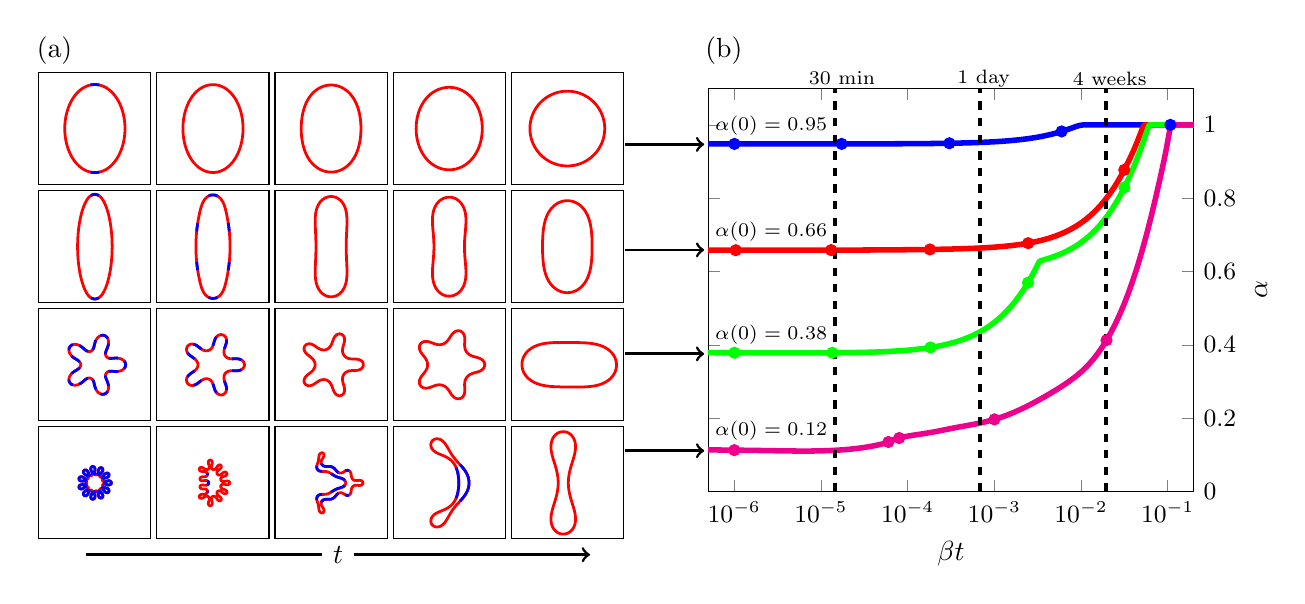
\begin{tikzpicture}[scale=1]

\begin{axis}[
  at = {(8.5cm,0.6cm)},
  scale = 0.90,
  xmin = 5e-7,
  xmax = 2e-1,
  xmode = log,
  xminorticks = false,
  xtick = {1e-6,1e-5,1e-4,1e-3,1e-2,1e-1},
  xticklabels = {\small $10^{-6}$,\small $10^{-5}$,\small $10^{-4}$,\small $10^{-3}$,\small $10^{-2}$,\small $10^{-1}$},
  ymin = 0,
  ymax = 1.1,
  ytick = {0,0.2,0.4,0.6,0.8,1},
  yticklabels = {\small 0,\small 0.2,\small 0.4,\small 0.6,\small 0.8,\small 1},
  yticklabel pos = right,
  xlabel = {$\beta t$},
  ylabel = {${\alpha}$},
  ylabel near ticks,
]

% blue line area
\addplot[blue, line width=2pt] coordinates{
(0.0000e+00,9.4804e-01)
(2.0000e-08,9.4804e-01)
(4.2768e-08,9.4804e-01)
(6.8688e-08,9.4804e-01)
(9.8196e-08,9.4804e-01)
(1.3179e-07,9.4804e-01)
(1.7003e-07,9.4804e-01)
(2.1357e-07,9.4804e-01)
(2.6313e-07,9.4804e-01)
(3.1955e-07,9.4804e-01)
(3.8378e-07,9.4804e-01)
(4.5691e-07,9.4804e-01)
(5.4015e-07,9.4804e-01)
(6.3492e-07,9.4804e-01)
(7.4280e-07,9.4804e-01)
(8.6562e-07,9.4804e-01)
(1.0054e-06,9.4804e-01)
(1.1646e-06,9.4805e-01)
(1.3458e-06,9.4805e-01)
(1.5521e-06,9.4805e-01)
(1.7870e-06,9.4805e-01)
(2.0543e-06,9.4805e-01)
(2.3587e-06,9.4805e-01)
(2.7051e-06,9.4806e-01)
(3.0996e-06,9.4806e-01)
(3.5486e-06,9.4806e-01)
(4.0598e-06,9.4806e-01)
(4.6418e-06,9.4807e-01)
(5.3043e-06,9.4807e-01)
(6.0585e-06,9.4808e-01)
(6.9172e-06,9.4808e-01)
(7.8946e-06,9.4809e-01)
(9.0074e-06,9.4810e-01)
(1.0274e-05,9.4811e-01)
(1.1716e-05,9.4812e-01)
(1.3358e-05,9.4813e-01)
(1.5227e-05,9.4814e-01)
(1.7355e-05,9.4815e-01)
(1.9777e-05,9.4817e-01)
(2.2535e-05,9.4819e-01)
(2.5674e-05,9.4821e-01)
(2.9248e-05,9.4823e-01)
(3.3316e-05,9.4825e-01)
(3.7948e-05,9.4828e-01)
(4.3221e-05,9.4832e-01)
(4.9223e-05,9.4835e-01)
(5.6057e-05,9.4840e-01)
(6.3836e-05,9.4844e-01)
(7.2692e-05,9.4850e-01)
(8.2774e-05,9.4856e-01)
(9.4252e-05,9.4863e-01)
(1.0732e-04,9.4871e-01)
(1.2219e-04,9.4879e-01)
(1.3913e-04,9.4890e-01)
(1.5841e-04,9.4901e-01)
(1.8035e-04,9.4914e-01)
(2.0534e-04,9.4929e-01)
(2.3378e-04,9.4946e-01)
(2.6616e-04,9.4965e-01)
(3.0302e-04,9.4987e-01)
(3.4498e-04,9.5011e-01)
(3.9276e-04,9.5040e-01)
(4.4714e-04,9.5072e-01)
(5.0906e-04,9.5108e-01)
(5.7954e-04,9.5150e-01)
(6.5978e-04,9.5197e-01)
(7.5113e-04,9.5251e-01)
(8.5512e-04,9.5312e-01)
(9.7350e-04,9.5381e-01)
(1.1083e-03,9.5460e-01)
(1.2617e-03,9.5550e-01)
(1.4364e-03,9.5652e-01)
(1.6352e-03,9.5769e-01)
(1.8616e-03,9.5900e-01)
(2.1193e-03,9.6050e-01)
(2.4126e-03,9.6220e-01)
(2.7466e-03,9.6413e-01)
(3.1268e-03,9.6631e-01)
(3.5597e-03,9.6878e-01)
(4.0524e-03,9.7157e-01)
(4.6134e-03,9.7471e-01)
(5.2520e-03,9.7823e-01)
(5.9790e-03,9.8214e-01)
(6.8066e-03,9.8643e-01)
(7.5681e-03,9.9018e-01)
(8.1760e-03,9.9301e-01)
(8.6718e-03,9.9513e-01)
(9.0889e-03,9.9673e-01)
(9.4566e-03,9.9792e-01)
(9.8054e-03,9.9880e-01)
(1.0152e-02,9.9939e-01)
(1.0519e-02,9.9974e-01)
(1.0937e-02,9.9991e-01)
(1.1413e-02,9.9997e-01)
(1.1954e-02,9.9999e-01)
(1.2571e-02,1.0000e+00)
(1.3272e-02,1.0000e+00)
(1.4071e-02,1.0000e+00)
(1.4981e-02,1.0000e+00)
(1.6016e-02,1.0000e+00)
(1.7195e-02,1.0000e+00)
(1.8537e-02,1.0000e+00)
(2.0064e-02,1.0000e+00)
(2.1804e-02,1.0000e+00)
(2.3783e-02,1.0000e+00)
(2.6037e-02,1.0000e+00)
(2.8603e-02,1.0000e+00)
(3.1524e-02,1.0000e+00)
(3.4849e-02,1.0000e+00)
(3.8635e-02,1.0000e+00)
(4.2944e-02,1.0000e+00)
(4.7850e-02,1.0000e+00)
(5.3436e-02,1.0000e+00)
(5.9794e-02,1.0000e+00)
(6.7032e-02,1.0000e+00)
(7.5273e-02,1.0000e+00)
(8.4653e-02,1.0000e+00)
(9.5333e-02,1.0000e+00)
(1.0749e-01,1.0000e+00)
(1.2133e-01,1.0000e+00)
(1.3709e-01,1.0000e+00)
(1.5503e-01,1.0000e+00)
(1.7545e-01,1.0000e+00)
(1.9869e-01,1.0000e+00)
(2.2516e-01,1.0000e+00)
(2.5529e-01,1.0000e+00)
(2.8958e-01,1.0000e+00)
(3.2863e-01,1.0000e+00)
(3.7308e-01,1.0000e+00)
(4.2368e-01,1.0000e+00)
(4.8129e-01,1.0000e+00)
(5.4687e-01,1.0000e+00)
(6.2153e-01,1.0000e+00)
(7.0653e-01,1.0000e+00)
(8.0329e-01,1.0000e+00)
(9.0329e-01,1.0000e+00)
(1.0033e+00,1.0000e+00)
(1.1033e+00,1.0000e+00)
(1.2033e+00,1.0000e+00)
(1.3033e+00,1.0000e+00)
(1.4033e+00,1.0000e+00)
(1.5033e+00,1.0000e+00)
(1.6033e+00,1.0000e+00)
(1.7033e+00,1.0000e+00)
(1.8033e+00,1.0000e+00)
(1.9033e+00,1.0000e+00)
(2.0000e+00,1.0000e+00)
};
\addplot[blue, only marks] coordinates{
(1.0054e-06,9.4804e-01)
(1.7355e-05,9.4815e-01)
(3.0302e-04,9.4987e-01)
(5.9790e-03,9.8214e-01)
(1.0749e-01,1.0000e+00)
};

% red line area
\addplot[red, line width=2pt] coordinates{
(0.0000e+00,6.5827e-01)
(1.1979e-08,6.5827e-01)
(2.3344e-08,6.5827e-01)
(3.6282e-08,6.5827e-01)
(5.1010e-08,6.5827e-01)
(6.7777e-08,6.5827e-01)
(8.6866e-08,6.5827e-01)
(1.0860e-07,6.5827e-01)
(1.3259e-07,6.5827e-01)
(1.5894e-07,6.5827e-01)
(1.8781e-07,6.5827e-01)
(2.1934e-07,6.5828e-01)
(2.5367e-07,6.5828e-01)
(2.9096e-07,6.5828e-01)
(3.3138e-07,6.5828e-01)
(3.7510e-07,6.5828e-01)
(4.2232e-07,6.5828e-01)
(4.7324e-07,6.5828e-01)
(5.2806e-07,6.5829e-01)
(5.8703e-07,6.5829e-01)
(6.5037e-07,6.5829e-01)
(7.1835e-07,6.5829e-01)
(7.9125e-07,6.5829e-01)
(8.6936e-07,6.5830e-01)
(9.5299e-07,6.5830e-01)
(1.0425e-06,6.5830e-01)
(1.1362e-06,6.5830e-01)
(1.2369e-06,6.5831e-01)
(1.3441e-06,6.5831e-01)
(1.4585e-06,6.5831e-01)
(1.5804e-06,6.5832e-01)
(1.7102e-06,6.5832e-01)
(1.8484e-06,6.5832e-01)
(1.9956e-06,6.5833e-01)
(2.1521e-06,6.5833e-01)
(2.3187e-06,6.5834e-01)
(2.4958e-06,6.5834e-01)
(2.6842e-06,6.5835e-01)
(2.8844e-06,6.5835e-01)
(3.0971e-06,6.5836e-01)
(3.3232e-06,6.5836e-01)
(3.5633e-06,6.5837e-01)
(3.8184e-06,6.5837e-01)
(4.0893e-06,6.5838e-01)
(4.3770e-06,6.5839e-01)
(4.6825e-06,6.5839e-01)
(5.0068e-06,6.5840e-01)
(5.3511e-06,6.5841e-01)
(5.7166e-06,6.5842e-01)
(6.1046e-06,6.5842e-01)
(6.5164e-06,6.5843e-01)
(6.9535e-06,6.5844e-01)
(7.4176e-06,6.5845e-01)
(7.9101e-06,6.5846e-01)
(8.4329e-06,6.5847e-01)
(8.9879e-06,6.5848e-01)
(9.5771e-06,6.5849e-01)
(1.0203e-05,6.5850e-01)
(1.0867e-05,6.5852e-01)
(1.1572e-05,6.5853e-01)
(1.2320e-05,6.5854e-01)
(1.3116e-05,6.5856e-01)
(1.3960e-05,6.5857e-01)
(1.4857e-05,6.5859e-01)
(1.5811e-05,6.5860e-01)
(1.6824e-05,6.5862e-01)
(1.7900e-05,6.5864e-01)
(1.9045e-05,6.5866e-01)
(2.0262e-05,6.5868e-01)
(2.1556e-05,6.5870e-01)
(2.2932e-05,6.5872e-01)
(2.4396e-05,6.5874e-01)
(2.5953e-05,6.5876e-01)
(2.7610e-05,6.5879e-01)
(2.9374e-05,6.5881e-01)
(3.1251e-05,6.5884e-01)
(3.3251e-05,6.5887e-01)
(3.5382e-05,6.5889e-01)
(3.7656e-05,6.5893e-01)
(4.0084e-05,6.5896e-01)
(4.2680e-05,6.5899e-01)
(4.5461e-05,6.5903e-01)
(4.8443e-05,6.5906e-01)
(5.1647e-05,6.5910e-01)
(5.5094e-05,6.5915e-01)
(5.8806e-05,6.5919e-01)
(6.2808e-05,6.5924e-01)
(6.7122e-05,6.5929e-01)
(7.1770e-05,6.5934e-01)
(7.6769e-05,6.5939e-01)
(8.2134e-05,6.5945e-01)
(8.7877e-05,6.5951e-01)
(9.4005e-05,6.5958e-01)
(1.0053e-04,6.5964e-01)
(1.0745e-04,6.5971e-01)
(1.1480e-04,6.5978e-01)
(1.2259e-04,6.5986e-01)
(1.3084e-04,6.5994e-01)
(1.3961e-04,6.6002e-01)
(1.4894e-04,6.6010e-01)
(1.5889e-04,6.6019e-01)
(1.6956e-04,6.6029e-01)
(1.8105e-04,6.6039e-01)
(1.9350e-04,6.6049e-01)
(2.0709e-04,6.6061e-01)
(2.2205e-04,6.6073e-01)
(2.3870e-04,6.6086e-01)
(2.5751e-04,6.6102e-01)
(2.7892e-04,6.6119e-01)
(3.0329e-04,6.6138e-01)
(3.3104e-04,6.6159e-01)
(3.6262e-04,6.6184e-01)
(3.9858e-04,6.6211e-01)
(4.3952e-04,6.6242e-01)
(4.8612e-04,6.6278e-01)
(5.3917e-04,6.6318e-01)
(5.9956e-04,6.6363e-01)
(6.6832e-04,6.6415e-01)
(7.4659e-04,6.6474e-01)
(8.3570e-04,6.6541e-01)
(9.3714e-04,6.6617e-01)
(1.0526e-03,6.6704e-01)
(1.1841e-03,6.6802e-01)
(1.3338e-03,6.6915e-01)
(1.5041e-03,6.7042e-01)
(1.6981e-03,6.7187e-01)
(1.9189e-03,6.7352e-01)
(2.1703e-03,6.7540e-01)
(2.4565e-03,6.7753e-01)
(2.7823e-03,6.7996e-01)
(3.1532e-03,6.8271e-01)
(3.5754e-03,6.8584e-01)
(4.0561e-03,6.8939e-01)
(4.6033e-03,6.9342e-01)
(5.2262e-03,6.9800e-01)
(5.9354e-03,7.0319e-01)
(6.7427e-03,7.0908e-01)
(7.6618e-03,7.1575e-01)
(8.7081e-03,7.2330e-01)
(9.8993e-03,7.3185e-01)
(1.1255e-02,7.4151e-01)
(1.2799e-02,7.5242e-01)
(1.4556e-02,7.6473e-01)
(1.6557e-02,7.7860e-01)
(1.8835e-02,7.9419e-01)
(2.1428e-02,8.1169e-01)
(2.4379e-02,8.3128e-01)
(2.7740e-02,8.5312e-01)
(3.1565e-02,8.7733e-01)
(3.5920e-02,9.0393e-01)
(4.0440e-02,9.3036e-01)
(4.3699e-02,9.4914e-01)
(4.6006e-02,9.6235e-01)
(4.7746e-02,9.7215e-01)
(4.9064e-02,9.7942e-01)
(5.0082e-02,9.8487e-01)
(5.0877e-02,9.8897e-01)
(5.1509e-02,9.9206e-01)
(5.2020e-02,9.9440e-01)
(5.2447e-02,9.9616e-01)
(5.2816e-02,9.9748e-01)
(5.3166e-02,9.9849e-01)
(5.3505e-02,9.9919e-01)
(5.3846e-02,9.9962e-01)
(5.4234e-02,9.9986e-01)
(5.4676e-02,9.9996e-01)
(5.5179e-02,9.9999e-01)
(5.5751e-02,1.0000e+00)
(5.6403e-02,1.0000e+00)
(5.7145e-02,1.0000e+00)
(5.7990e-02,1.0000e+00)
(5.8952e-02,1.0000e+00)
(6.0047e-02,1.0000e+00)
(6.1293e-02,1.0000e+00)
(6.2712e-02,1.0000e+00)
(6.4328e-02,1.0000e+00)
(6.6167e-02,1.0000e+00)
(6.8260e-02,1.0000e+00)
(7.0644e-02,1.0000e+00)
(7.3357e-02,1.0000e+00)
(7.6446e-02,1.0000e+00)
(7.9962e-02,1.0000e+00)
(8.3965e-02,1.0000e+00)
(8.8523e-02,1.0000e+00)
(9.3711e-02,1.0000e+00)
(9.9617e-02,1.0000e+00)
(1.0634e-01,1.0000e+00)
(1.1400e-01,1.0000e+00)
(1.2271e-01,1.0000e+00)
(1.3263e-01,1.0000e+00)
(1.4392e-01,1.0000e+00)
(1.5678e-01,1.0000e+00)
(1.7142e-01,1.0000e+00)
(1.8808e-01,1.0000e+00)
(2.0705e-01,1.0000e+00)
(2.2864e-01,1.0000e+00)
(2.5322e-01,1.0000e+00)
(2.8121e-01,1.0000e+00)
(3.1307e-01,1.0000e+00)
(3.4934e-01,1.0000e+00)
(3.9063e-01,1.0000e+00)
(4.3763e-01,1.0000e+00)
(4.9115e-01,1.0000e+00)
(5.5207e-01,1.0000e+00)
(6.2142e-01,1.0000e+00)
(7.0037e-01,1.0000e+00)
(7.9025e-01,1.0000e+00)
(8.9025e-01,1.0000e+00)
(9.9025e-01,1.0000e+00)
(1.0902e+00,1.0000e+00)
(1.1902e+00,1.0000e+00)
(1.2902e+00,1.0000e+00)
(1.3902e+00,1.0000e+00)
(1.4902e+00,1.0000e+00)
(1.5902e+00,1.0000e+00)
(1.6902e+00,1.0000e+00)
(1.7902e+00,1.0000e+00)
(1.8902e+00,1.0000e+00)
(1.9902e+00,1.0000e+00)
(2.0000e+00,1.0000e+00)
};
\addplot[red, only marks] coordinates{
(1.0425e-06,6.5830e-01)
(1.3116e-05,6.5856e-01)
(1.8105e-04,6.6039e-01)
(2.4565e-03,6.7753e-01)
(3.1565e-02,8.7733e-01)
};

% green line area
\addplot[green, line width=2pt] coordinates{
(0.0000e+00,3.7906e-01)
(1.3137e-08,3.7903e-01)
(2.3137e-08,3.7901e-01)
(3.3137e-08,3.7900e-01)
(4.3137e-08,3.7899e-01)
(5.3137e-08,3.7899e-01)
(6.3137e-08,3.7898e-01)
(7.3137e-08,3.7897e-01)
(8.3137e-08,3.7897e-01)
(9.3137e-08,3.7896e-01)
(1.0314e-07,3.7895e-01)
(1.1314e-07,3.7895e-01)
(1.2314e-07,3.7894e-01)
(1.3314e-07,3.7894e-01)
(1.4314e-07,3.7893e-01)
(1.5314e-07,3.7893e-01)
(1.6314e-07,3.7892e-01)
(1.7314e-07,3.7892e-01)
(1.8314e-07,3.7892e-01)
(1.9314e-07,3.7891e-01)
(2.0314e-07,3.7891e-01)
(2.1314e-07,3.7890e-01)
(2.2314e-07,3.7890e-01)
(2.3314e-07,3.7890e-01)
(2.4314e-07,3.7889e-01)
(2.5314e-07,3.7889e-01)
(2.6314e-07,3.7889e-01)
(2.7314e-07,3.7888e-01)
(2.8314e-07,3.7888e-01)
(2.9314e-07,3.7888e-01)
(3.0314e-07,3.7888e-01)
(3.1314e-07,3.7887e-01)
(3.2314e-07,3.7887e-01)
(3.3314e-07,3.7887e-01)
(3.4314e-07,3.7886e-01)
(3.5314e-07,3.7886e-01)
(3.6314e-07,3.7886e-01)
(3.7314e-07,3.7886e-01)
(3.8314e-07,3.7885e-01)
(3.9314e-07,3.7885e-01)
(4.0314e-07,3.7885e-01)
(4.1314e-07,3.7885e-01)
(4.2314e-07,3.7884e-01)
(4.3314e-07,3.7884e-01)
(4.4314e-07,3.7884e-01)
(4.5314e-07,3.7884e-01)
(4.6314e-07,3.7883e-01)
(4.7314e-07,3.7883e-01)
(4.8314e-07,3.7883e-01)
(4.9314e-07,3.7883e-01)
(5.0314e-07,3.7883e-01)
(5.1314e-07,3.7882e-01)
(5.2314e-07,3.7882e-01)
(5.3314e-07,3.7882e-01)
(5.4314e-07,3.7882e-01)
(5.5314e-07,3.7882e-01)
(5.6314e-07,3.7881e-01)
(5.7314e-07,3.7881e-01)
(5.8314e-07,3.7881e-01)
(5.9314e-07,3.7881e-01)
(6.0314e-07,3.7881e-01)
(6.1314e-07,3.7880e-01)
(6.2314e-07,3.7880e-01)
(6.3314e-07,3.7880e-01)
(6.4314e-07,3.7880e-01)
(6.5314e-07,3.7880e-01)
(6.6314e-07,3.7880e-01)
(6.7314e-07,3.7879e-01)
(6.8314e-07,3.7879e-01)
(6.9314e-07,3.7879e-01)
(7.0314e-07,3.7879e-01)
(7.1314e-07,3.7879e-01)
(7.2314e-07,3.7879e-01)
(7.3314e-07,3.7878e-01)
(7.4314e-07,3.7878e-01)
(7.5314e-07,3.7878e-01)
(7.6314e-07,3.7878e-01)
(7.7314e-07,3.7878e-01)
(7.8316e-07,3.7878e-01)
(7.9340e-07,3.7877e-01)
(8.0377e-07,3.7877e-01)
(8.1432e-07,3.7877e-01)
(8.2502e-07,3.7877e-01)
(8.3589e-07,3.7877e-01)
(8.4693e-07,3.7877e-01)
(8.5815e-07,3.7876e-01)
(8.6953e-07,3.7876e-01)
(8.8110e-07,3.7876e-01)
(8.9285e-07,3.7876e-01)
(9.0479e-07,3.7876e-01)
(9.1691e-07,3.7876e-01)
(9.2923e-07,3.7875e-01)
(9.4174e-07,3.7875e-01)
(9.5444e-07,3.7875e-01)
(9.6735e-07,3.7875e-01)
(9.8046e-07,3.7875e-01)
(9.9378e-07,3.7875e-01)
(1.0073e-06,3.7874e-01)
(1.0211e-06,3.7874e-01)
(1.0350e-06,3.7874e-01)
(1.0492e-06,3.7874e-01)
(1.0636e-06,3.7874e-01)
(1.0783e-06,3.7874e-01)
(1.0931e-06,3.7873e-01)
(1.1082e-06,3.7873e-01)
(1.1236e-06,3.7873e-01)
(1.1391e-06,3.7873e-01)
(1.1550e-06,3.7873e-01)
(1.1711e-06,3.7872e-01)
(1.1874e-06,3.7872e-01)
(1.2040e-06,3.7872e-01)
(1.2209e-06,3.7872e-01)
(1.2380e-06,3.7872e-01)
(1.2554e-06,3.7871e-01)
(1.2730e-06,3.7871e-01)
(1.2910e-06,3.7871e-01)
(1.3091e-06,3.7871e-01)
(1.3276e-06,3.7871e-01)
(1.3463e-06,3.7870e-01)
(1.3652e-06,3.7870e-01)
(1.3845e-06,3.7870e-01)
(1.4040e-06,3.7870e-01)
(1.4238e-06,3.7870e-01)
(1.4439e-06,3.7869e-01)
(1.4643e-06,3.7869e-01)
(1.4850e-06,3.7869e-01)
(1.5060e-06,3.7869e-01)
(1.5272e-06,3.7869e-01)
(1.5488e-06,3.7868e-01)
(1.5707e-06,3.7868e-01)
(1.5929e-06,3.7868e-01)
(1.6155e-06,3.7868e-01)
(1.6383e-06,3.7868e-01)
(1.6615e-06,3.7867e-01)
(1.6850e-06,3.7867e-01)
(1.7089e-06,3.7867e-01)
(1.7331e-06,3.7867e-01)
(1.7577e-06,3.7867e-01)
(1.7826e-06,3.7866e-01)
(1.8079e-06,3.7866e-01)
(1.8336e-06,3.7866e-01)
(1.8596e-06,3.7866e-01)
(1.8860e-06,3.7865e-01)
(1.9129e-06,3.7865e-01)
(1.9401e-06,3.7865e-01)
(1.9677e-06,3.7865e-01)
(1.9958e-06,3.7865e-01)
(2.0243e-06,3.7864e-01)
(2.0532e-06,3.7864e-01)
(2.0826e-06,3.7864e-01)
(2.1124e-06,3.7864e-01)
(2.1427e-06,3.7863e-01)
(2.1735e-06,3.7863e-01)
(2.2047e-06,3.7863e-01)
(2.2365e-06,3.7863e-01)
(2.2688e-06,3.7863e-01)
(2.3016e-06,3.7862e-01)
(2.3349e-06,3.7862e-01)
(2.3689e-06,3.7862e-01)
(2.4033e-06,3.7862e-01)
(2.4384e-06,3.7861e-01)
(2.4741e-06,3.7861e-01)
(2.5104e-06,3.7861e-01)
(2.5474e-06,3.7861e-01)
(2.5850e-06,3.7860e-01)
(2.6233e-06,3.7860e-01)
(2.6623e-06,3.7860e-01)
(2.7020e-06,3.7860e-01)
(2.7425e-06,3.7860e-01)
(2.7838e-06,3.7859e-01)
(2.8259e-06,3.7859e-01)
(2.8688e-06,3.7859e-01)
(2.9126e-06,3.7859e-01)
(2.9573e-06,3.7858e-01)
(3.0029e-06,3.7858e-01)
(3.0495e-06,3.7858e-01)
(3.0971e-06,3.7858e-01)
(3.1455e-06,3.7857e-01)
(3.1954e-06,3.7857e-01)
(3.2463e-06,3.7857e-01)
(3.2985e-06,3.7857e-01)
(3.3518e-06,3.7857e-01)
(3.4065e-06,3.7856e-01)
(3.4626e-06,3.7856e-01)
(3.5201e-06,3.7856e-01)
(3.5791e-06,3.7856e-01)
(3.6398e-06,3.7855e-01)
(3.7021e-06,3.7855e-01)
(3.7661e-06,3.7855e-01)
(3.8321e-06,3.7855e-01)
(3.9000e-06,3.7855e-01)
(3.9699e-06,3.7854e-01)
(4.0421e-06,3.7854e-01)
(4.1166e-06,3.7854e-01)
(4.1937e-06,3.7854e-01)
(4.2733e-06,3.7854e-01)
(4.3558e-06,3.7853e-01)
(4.4413e-06,3.7853e-01)
(4.5300e-06,3.7853e-01)
(4.6221e-06,3.7853e-01)
(4.7179e-06,3.7853e-01)
(4.8176e-06,3.7852e-01)
(4.9216e-06,3.7852e-01)
(5.0301e-06,3.7852e-01)
(5.1435e-06,3.7852e-01)
(5.2621e-06,3.7852e-01)
(5.3864e-06,3.7852e-01)
(5.5167e-06,3.7851e-01)
(5.6534e-06,3.7851e-01)
(5.7971e-06,3.7851e-01)
(5.9480e-06,3.7851e-01)
(6.1067e-06,3.7851e-01)
(6.2734e-06,3.7851e-01)
(6.4485e-06,3.7851e-01)
(6.6322e-06,3.7851e-01)
(6.8245e-06,3.7851e-01)
(7.0254e-06,3.7851e-01)
(7.2348e-06,3.7851e-01)
(7.4524e-06,3.7851e-01)
(7.6779e-06,3.7852e-01)
(7.9108e-06,3.7852e-01)
(8.1509e-06,3.7852e-01)
(8.3977e-06,3.7852e-01)
(8.6509e-06,3.7853e-01)
(8.9103e-06,3.7853e-01)
(9.1756e-06,3.7854e-01)
(9.4467e-06,3.7854e-01)
(9.7235e-06,3.7855e-01)
(1.0006e-05,3.7856e-01)
(1.0295e-05,3.7856e-01)
(1.0589e-05,3.7857e-01)
(1.0889e-05,3.7858e-01)
(1.1196e-05,3.7859e-01)
(1.1509e-05,3.7860e-01)
(1.1828e-05,3.7861e-01)
(1.2155e-05,3.7862e-01)
(1.2489e-05,3.7863e-01)
(1.2830e-05,3.7865e-01)
(1.3179e-05,3.7866e-01)
(1.3536e-05,3.7867e-01)
(1.3902e-05,3.7869e-01)
(1.4277e-05,3.7871e-01)
(1.4661e-05,3.7872e-01)
(1.5055e-05,3.7874e-01)
(1.5459e-05,3.7876e-01)
(1.5875e-05,3.7878e-01)
(1.6302e-05,3.7880e-01)
(1.6741e-05,3.7883e-01)
(1.7194e-05,3.7885e-01)
(1.7660e-05,3.7888e-01)
(1.8140e-05,3.7890e-01)
(1.8636e-05,3.7893e-01)
(1.9149e-05,3.7896e-01)
(1.9679e-05,3.7899e-01)
(2.0228e-05,3.7903e-01)
(2.0797e-05,3.7906e-01)
(2.1388e-05,3.7910e-01)
(2.2002e-05,3.7914e-01)
(2.2642e-05,3.7918e-01)
(2.3309e-05,3.7923e-01)
(2.4006e-05,3.7928e-01)
(2.4735e-05,3.7933e-01)
(2.5501e-05,3.7938e-01)
(2.6307e-05,3.7944e-01)
(2.7156e-05,3.7950e-01)
(2.8054e-05,3.7957e-01)
(2.9007e-05,3.7964e-01)
(3.0023e-05,3.7972e-01)
(3.1109e-05,3.7981e-01)
(3.2277e-05,3.7990e-01)
(3.3540e-05,3.8000e-01)
(3.4914e-05,3.8011e-01)
(3.6423e-05,3.8023e-01)
(3.8095e-05,3.8037e-01)
(3.9970e-05,3.8053e-01)
(4.2105e-05,3.8071e-01)
(4.4536e-05,3.8092e-01)
(4.7303e-05,3.8116e-01)
(5.0453e-05,3.8143e-01)
(5.4039e-05,3.8174e-01)
(5.8121e-05,3.8210e-01)
(6.2768e-05,3.8251e-01)
(6.8059e-05,3.8297e-01)
(7.4082e-05,3.8351e-01)
(8.0939e-05,3.8411e-01)
(8.8745e-05,3.8480e-01)
(9.7631e-05,3.8559e-01)
(1.0775e-04,3.8648e-01)
(1.1926e-04,3.8750e-01)
(1.3238e-04,3.8866e-01)
(1.4730e-04,3.8997e-01)
(1.6429e-04,3.9146e-01)
(1.8364e-04,3.9316e-01)
(2.0566e-04,3.9508e-01)
(2.3073e-04,3.9727e-01)
(2.5927e-04,3.9975e-01)
(2.9176e-04,4.0256e-01)
(3.2874e-04,4.0576e-01)
(3.7085e-04,4.0937e-01)
(4.1879e-04,4.1347e-01)
(4.7336e-04,4.1810e-01)
(5.3548e-04,4.2334e-01)
(6.0620e-04,4.2927e-01)
(6.8672e-04,4.3596e-01)
(7.7837e-04,4.4350e-01)
(8.8272e-04,4.5201e-01)
(1.0015e-03,4.6157e-01)
(1.1367e-03,4.7233e-01)
(1.2907e-03,4.8440e-01)
(1.4659e-03,4.9792e-01)
(1.6655e-03,5.1306e-01)
(1.8926e-03,5.2996e-01)
(2.1512e-03,5.4880e-01)
(2.4455e-03,5.6977e-01)
(2.7807e-03,5.9304e-01)
(2.8965e-03,6.0098e-01)
(2.9381e-03,6.0382e-01)
(2.9632e-03,6.0553e-01)
(2.9821e-03,6.0681e-01)
(2.9974e-03,6.0785e-01)
(3.0103e-03,6.0872e-01)
(3.0215e-03,6.0948e-01)
(3.0314e-03,6.1015e-01)
(3.0403e-03,6.1075e-01)
(3.0487e-03,6.1132e-01)
(3.0560e-03,6.1181e-01)
(3.0628e-03,6.1227e-01)
(3.0690e-03,6.1269e-01)
(3.0749e-03,6.1308e-01)
(3.0803e-03,6.1345e-01)
(3.0855e-03,6.1380e-01)
(3.0903e-03,6.1412e-01)
(3.0949e-03,6.1443e-01)
(3.0993e-03,6.1472e-01)
(3.1034e-03,6.1500e-01)
(3.1074e-03,6.1527e-01)
(3.1112e-03,6.1552e-01)
(3.1148e-03,6.1577e-01)
(3.1183e-03,6.1600e-01)
(3.1217e-03,6.1622e-01)
(3.1249e-03,6.1644e-01)
(3.1281e-03,6.1665e-01)
(3.1311e-03,6.1685e-01)
(3.1341e-03,6.1705e-01)
(3.1369e-03,6.1723e-01)
(3.1397e-03,6.1742e-01)
(3.1424e-03,6.1759e-01)
(3.1451e-03,6.1778e-01)
(3.1478e-03,6.1795e-01)
(3.1504e-03,6.1812e-01)
(3.1529e-03,6.1829e-01)
(3.1553e-03,6.1845e-01)
(3.1577e-03,6.1861e-01)
(3.1601e-03,6.1876e-01)
(3.1623e-03,6.1891e-01)
(3.1646e-03,6.1905e-01)
(3.1667e-03,6.1919e-01)
(3.1689e-03,6.1933e-01)
(3.1709e-03,6.1947e-01)
(3.1730e-03,6.1960e-01)
(3.1750e-03,6.1973e-01)
(3.1770e-03,6.1985e-01)
(3.1789e-03,6.1998e-01)
(3.1808e-03,6.2010e-01)
(3.1826e-03,6.2022e-01)
(3.1845e-03,6.2033e-01)
(3.1863e-03,6.2045e-01)
(3.1880e-03,6.2056e-01)
(3.1897e-03,6.2067e-01)
(3.1915e-03,6.2078e-01)
(3.1931e-03,6.2088e-01)
(3.1948e-03,6.2098e-01)
(3.1964e-03,6.2109e-01)
(3.1980e-03,6.2119e-01)
(3.1996e-03,6.2128e-01)
(3.2011e-03,6.2138e-01)
(3.2027e-03,6.2147e-01)
(3.2042e-03,6.2157e-01)
(3.2057e-03,6.2166e-01)
(3.2071e-03,6.2174e-01)
(3.2086e-03,6.2183e-01)
(3.2100e-03,6.2192e-01)
(3.2114e-03,6.2200e-01)
(3.2128e-03,6.2209e-01)
(3.2141e-03,6.2217e-01)
(3.2155e-03,6.2225e-01)
(3.2168e-03,6.2233e-01)
(3.2181e-03,6.2240e-01)
(3.2194e-03,6.2248e-01)
(3.2207e-03,6.2255e-01)
(3.2220e-03,6.2263e-01)
(3.2232e-03,6.2270e-01)
(3.2245e-03,6.2277e-01)
(3.2257e-03,6.2284e-01)
(3.2269e-03,6.2291e-01)
(3.2281e-03,6.2298e-01)
(3.2293e-03,6.2305e-01)
(3.2304e-03,6.2311e-01)
(3.2316e-03,6.2318e-01)
(3.2327e-03,6.2324e-01)
(3.2339e-03,6.2330e-01)
(3.2350e-03,6.2337e-01)
(3.2361e-03,6.2343e-01)
(3.2373e-03,6.2349e-01)
(3.2384e-03,6.2355e-01)
(3.2395e-03,6.2361e-01)
(3.2406e-03,6.2367e-01)
(3.2417e-03,6.2373e-01)
(3.2428e-03,6.2379e-01)
(3.2439e-03,6.2385e-01)
(3.2450e-03,6.2391e-01)
(3.2461e-03,6.2396e-01)
(3.2472e-03,6.2402e-01)
(3.2482e-03,6.2408e-01)
(3.2493e-03,6.2413e-01)
(3.2504e-03,6.2419e-01)
(3.2516e-03,6.2425e-01)
(3.2527e-03,6.2431e-01)
(3.2538e-03,6.2436e-01)
(3.2549e-03,6.2442e-01)
(3.2560e-03,6.2448e-01)
(3.2572e-03,6.2453e-01)
(3.2584e-03,6.2459e-01)
(3.2595e-03,6.2465e-01)
(3.2607e-03,6.2471e-01)
(3.2619e-03,6.2477e-01)
(3.2631e-03,6.2483e-01)
(3.2643e-03,6.2489e-01)
(3.2656e-03,6.2495e-01)
(3.2669e-03,6.2501e-01)
(3.2682e-03,6.2507e-01)
(3.2695e-03,6.2513e-01)
(3.2708e-03,6.2519e-01)
(3.2722e-03,6.2525e-01)
(3.2736e-03,6.2532e-01)
(3.2750e-03,6.2538e-01)
(3.2764e-03,6.2545e-01)
(3.2779e-03,6.2551e-01)
(3.2794e-03,6.2558e-01)
(3.2809e-03,6.2565e-01)
(3.2824e-03,6.2571e-01)
(3.2840e-03,6.2578e-01)
(3.2855e-03,6.2585e-01)
(3.2871e-03,6.2592e-01)
(3.2887e-03,6.2598e-01)
(3.2904e-03,6.2605e-01)
(3.2920e-03,6.2612e-01)
(3.2937e-03,6.2619e-01)
(3.2954e-03,6.2625e-01)
(3.2970e-03,6.2632e-01)
(3.2987e-03,6.2639e-01)
(3.3004e-03,6.2645e-01)
(3.3021e-03,6.2652e-01)
(3.3038e-03,6.2658e-01)
(3.3056e-03,6.2665e-01)
(3.3073e-03,6.2671e-01)
(3.3090e-03,6.2678e-01)
(3.3107e-03,6.2684e-01)
(3.3125e-03,6.2690e-01)
(3.3142e-03,6.2696e-01)
(3.3160e-03,6.2702e-01)
(3.3177e-03,6.2708e-01)
(3.3195e-03,6.2714e-01)
(3.3213e-03,6.2720e-01)
(3.3230e-03,6.2726e-01)
(3.3248e-03,6.2732e-01)
(3.3266e-03,6.2738e-01)
(3.3284e-03,6.2744e-01)
(3.3302e-03,6.2749e-01)
(3.3321e-03,6.2755e-01)
(3.3339e-03,6.2761e-01)
(3.3357e-03,6.2766e-01)
(3.3376e-03,6.2772e-01)
(3.3395e-03,6.2777e-01)
(3.3414e-03,6.2782e-01)
(3.3432e-03,6.2788e-01)
(3.3452e-03,6.2793e-01)
(3.3471e-03,6.2798e-01)
(3.3490e-03,6.2804e-01)
(3.3509e-03,6.2809e-01)
(3.3529e-03,6.2814e-01)
(3.3549e-03,6.2819e-01)
(3.3569e-03,6.2824e-01)
(3.3589e-03,6.2829e-01)
(3.3609e-03,6.2834e-01)
(3.3629e-03,6.2839e-01)
(3.3650e-03,6.2844e-01)
(3.3670e-03,6.2848e-01)
(3.3691e-03,6.2853e-01)
(3.3712e-03,6.2858e-01)
(3.3733e-03,6.2862e-01)
(3.3755e-03,6.2867e-01)
(3.3776e-03,6.2871e-01)
(3.3798e-03,6.2876e-01)
(3.3820e-03,6.2880e-01)
(3.3842e-03,6.2885e-01)
(3.3864e-03,6.2889e-01)
(3.3887e-03,6.2893e-01)
(3.3909e-03,6.2897e-01)
(3.3932e-03,6.2902e-01)
(3.3956e-03,6.2906e-01)
(3.3979e-03,6.2910e-01)
(3.4003e-03,6.2914e-01)
(3.4028e-03,6.2918e-01)
(3.4052e-03,6.2922e-01)
(3.4077e-03,6.2926e-01)
(3.4103e-03,6.2929e-01)
(3.4129e-03,6.2933e-01)
(3.4155e-03,6.2937e-01)
(3.4182e-03,6.2941e-01)
(3.4209e-03,6.2945e-01)
(3.4238e-03,6.2948e-01)
(3.4267e-03,6.2952e-01)
(3.4296e-03,6.2956e-01)
(3.4327e-03,6.2960e-01)
(3.4358e-03,6.2963e-01)
(3.4390e-03,6.2967e-01)
(3.4424e-03,6.2971e-01)
(3.4459e-03,6.2975e-01)
(3.4495e-03,6.2979e-01)
(3.4532e-03,6.2982e-01)
(3.4571e-03,6.2986e-01)
(3.4612e-03,6.2990e-01)
(3.4655e-03,6.2995e-01)
(3.4700e-03,6.2999e-01)
(3.4748e-03,6.3003e-01)
(3.4799e-03,6.3008e-01)
(3.4852e-03,6.3013e-01)
(3.4910e-03,6.3018e-01)
(3.4972e-03,6.3023e-01)
(3.5039e-03,6.3029e-01)
(3.5111e-03,6.3035e-01)
(3.5190e-03,6.3041e-01)
(3.5277e-03,6.3049e-01)
(3.5372e-03,6.3056e-01)
(3.5479e-03,6.3065e-01)
(3.5598e-03,6.3075e-01)
(3.5733e-03,6.3085e-01)
(3.5886e-03,6.3098e-01)
(3.6060e-03,6.3112e-01)
(3.6259e-03,6.3128e-01)
(3.6485e-03,6.3146e-01)
(3.6742e-03,6.3166e-01)
(3.7035e-03,6.3190e-01)
(3.7368e-03,6.3217e-01)
(3.7748e-03,6.3247e-01)
(3.8180e-03,6.3282e-01)
(3.8671e-03,6.3321e-01)
(3.9224e-03,6.3365e-01)
(3.9806e-03,6.3411e-01)
(4.0424e-03,6.3459e-01)
(4.1085e-03,6.3511e-01)
(4.1796e-03,6.3566e-01)
(4.2567e-03,6.3625e-01)
(4.3409e-03,6.3690e-01)
(4.4337e-03,6.3762e-01)
(4.5373e-03,6.3841e-01)
(4.6543e-03,6.3930e-01)
(4.7876e-03,6.4031e-01)
(4.9393e-03,6.4146e-01)
(5.1120e-03,6.4277e-01)
(5.3086e-03,6.4426e-01)
(5.5325e-03,6.4595e-01)
(5.7873e-03,6.4787e-01)
(6.0774e-03,6.5005e-01)
(6.4076e-03,6.5254e-01)
(6.7836e-03,6.5536e-01)
(7.2116e-03,6.5856e-01)
(7.6988e-03,6.6220e-01)
(8.2535e-03,6.6633e-01)
(8.8850e-03,6.7102e-01)
(9.6039e-03,6.7633e-01)
(1.0422e-02,6.8236e-01)
(1.1354e-02,6.8919e-01)
(1.2415e-02,6.9692e-01)
(1.3622e-02,7.0566e-01)
(1.4997e-02,7.1555e-01)
(1.6561e-02,7.2671e-01)
(1.8343e-02,7.3930e-01)
(2.0371e-02,7.5348e-01)
(2.2680e-02,7.6942e-01)
(2.5308e-02,7.8732e-01)
(2.8300e-02,8.0735e-01)
(3.1706e-02,8.2970e-01)
(3.5584e-02,8.5453e-01)
(3.9999e-02,8.8191e-01)
(4.5024e-02,9.1171e-01)
(4.9284e-02,9.3617e-01)
(5.2252e-02,9.5313e-01)
(5.4420e-02,9.6537e-01)
(5.6048e-02,9.7441e-01)
(5.7288e-02,9.8113e-01)
(5.8247e-02,9.8618e-01)
(5.8999e-02,9.8997e-01)
(5.9598e-02,9.9283e-01)
(6.0088e-02,9.9498e-01)
(6.0499e-02,9.9660e-01)
(6.0860e-02,9.9782e-01)
(6.1203e-02,9.9872e-01)
(6.1541e-02,9.9934e-01)
(6.1895e-02,9.9971e-01)
(6.2297e-02,9.9990e-01)
(6.2755e-02,9.9997e-01)
(6.3277e-02,9.9999e-01)
(6.3871e-02,1.0000e+00)
(6.4546e-02,1.0000e+00)
(6.5316e-02,1.0000e+00)
(6.6192e-02,1.0000e+00)
(6.7189e-02,1.0000e+00)
(6.8324e-02,1.0000e+00)
(6.9616e-02,1.0000e+00)
(7.1088e-02,1.0000e+00)
(7.2763e-02,1.0000e+00)
(7.4669e-02,1.0000e+00)
(7.6840e-02,1.0000e+00)
(7.9311e-02,1.0000e+00)
(8.2124e-02,1.0000e+00)
(8.5327e-02,1.0000e+00)
(8.8972e-02,1.0000e+00)
(9.3123e-02,1.0000e+00)
(9.7848e-02,1.0000e+00)
(1.0323e-01,1.0000e+00)
(1.0935e-01,1.0000e+00)
(1.1632e-01,1.0000e+00)
(1.2426e-01,1.0000e+00)
(1.3329e-01,1.0000e+00)
(1.4358e-01,1.0000e+00)
(1.5529e-01,1.0000e+00)
(1.6862e-01,1.0000e+00)
(1.8379e-01,1.0000e+00)
(2.0107e-01,1.0000e+00)
(2.2073e-01,1.0000e+00)
(2.4312e-01,1.0000e+00)
(2.6861e-01,1.0000e+00)
(2.9762e-01,1.0000e+00)
(3.3066e-01,1.0000e+00)
(3.6826e-01,1.0000e+00)
(4.1107e-01,1.0000e+00)
(4.5980e-01,1.0000e+00)
(5.1529e-01,1.0000e+00)
(5.7845e-01,1.0000e+00)
(6.5035e-01,1.0000e+00)
(7.3221e-01,1.0000e+00)
(8.2539e-01,1.0000e+00)
(9.2539e-01,1.0000e+00)
(1.0254e+00,1.0000e+00)
(1.1254e+00,1.0000e+00)
(1.2254e+00,1.0000e+00)
(1.3254e+00,1.0000e+00)
(1.4254e+00,1.0000e+00)
(1.5254e+00,1.0000e+00)
(1.6254e+00,1.0000e+00)
(1.7254e+00,1.0000e+00)
(1.8254e+00,1.0000e+00)
(1.9254e+00,1.0000e+00)
(2.0000e+00,1.0000e+00)
};
\addplot[green, only marks] coordinates{
(1.0073e-06,3.7874e-01)
(1.3536e-05,3.7867e-01)
(1.8364e-04,3.9316e-01)
(2.4455e-03,5.6977e-01)
(3.1706e-02,8.2970e-01)
};

% magenta line area
\addplot[magenta, line width=2pt] coordinates{
(0.0000e+00,1.1571e-01)
(1.3137e-08,1.1538e-01)
(2.3137e-08,1.1522e-01)
(3.3137e-08,1.1512e-01)
(4.3137e-08,1.1504e-01)
(5.3137e-08,1.1497e-01)
(6.3137e-08,1.1491e-01)
(7.3137e-08,1.1486e-01)
(8.3137e-08,1.1481e-01)
(9.3137e-08,1.1477e-01)
(1.0314e-07,1.1473e-01)
(1.1314e-07,1.1469e-01)
(1.2314e-07,1.1466e-01)
(1.3314e-07,1.1463e-01)
(1.4314e-07,1.1460e-01)
(1.5314e-07,1.1457e-01)
(1.6314e-07,1.1454e-01)
(1.7314e-07,1.1452e-01)
(1.8314e-07,1.1449e-01)
(1.9314e-07,1.1447e-01)
(2.0314e-07,1.1445e-01)
(2.1314e-07,1.1443e-01)
(2.2314e-07,1.1440e-01)
(2.3314e-07,1.1438e-01)
(2.4314e-07,1.1436e-01)
(2.5314e-07,1.1434e-01)
(2.6314e-07,1.1432e-01)
(2.7314e-07,1.1431e-01)
(2.8314e-07,1.1429e-01)
(2.9314e-07,1.1427e-01)
(3.0314e-07,1.1425e-01)
(3.1314e-07,1.1423e-01)
(3.2314e-07,1.1421e-01)
(3.3314e-07,1.1419e-01)
(3.4314e-07,1.1418e-01)
(3.5314e-07,1.1416e-01)
(3.6314e-07,1.1414e-01)
(3.7314e-07,1.1412e-01)
(3.8314e-07,1.1410e-01)
(3.9314e-07,1.1409e-01)
(4.0314e-07,1.1407e-01)
(4.1314e-07,1.1405e-01)
(4.2314e-07,1.1404e-01)
(4.3314e-07,1.1402e-01)
(4.4314e-07,1.1400e-01)
(4.5314e-07,1.1398e-01)
(4.6314e-07,1.1397e-01)
(4.7314e-07,1.1395e-01)
(4.8314e-07,1.1393e-01)
(4.9314e-07,1.1392e-01)
(5.0314e-07,1.1390e-01)
(5.1314e-07,1.1388e-01)
(5.2314e-07,1.1387e-01)
(5.3314e-07,1.1385e-01)
(5.4314e-07,1.1384e-01)
(5.5314e-07,1.1382e-01)
(5.6314e-07,1.1381e-01)
(5.7314e-07,1.1379e-01)
(5.8314e-07,1.1377e-01)
(5.9314e-07,1.1376e-01)
(6.0314e-07,1.1374e-01)
(6.1314e-07,1.1373e-01)
(6.2314e-07,1.1371e-01)
(6.3314e-07,1.1370e-01)
(6.4314e-07,1.1368e-01)
(6.5314e-07,1.1367e-01)
(6.6314e-07,1.1365e-01)
(6.7314e-07,1.1364e-01)
(6.8314e-07,1.1363e-01)
(6.9314e-07,1.1361e-01)
(7.0314e-07,1.1360e-01)
(7.1314e-07,1.1358e-01)
(7.2314e-07,1.1357e-01)
(7.3314e-07,1.1356e-01)
(7.4314e-07,1.1354e-01)
(7.5314e-07,1.1353e-01)
(7.6314e-07,1.1351e-01)
(7.7314e-07,1.1350e-01)
(7.8314e-07,1.1349e-01)
(7.9314e-07,1.1347e-01)
(8.0314e-07,1.1346e-01)
(8.1314e-07,1.1345e-01)
(8.2314e-07,1.1344e-01)
(8.3314e-07,1.1342e-01)
(8.4314e-07,1.1341e-01)
(8.5314e-07,1.1340e-01)
(8.6314e-07,1.1338e-01)
(8.7314e-07,1.1337e-01)
(8.8314e-07,1.1336e-01)
(8.9314e-07,1.1335e-01)
(9.0314e-07,1.1333e-01)
(9.1314e-07,1.1332e-01)
(9.2314e-07,1.1331e-01)
(9.3314e-07,1.1330e-01)
(9.4314e-07,1.1328e-01)
(9.5314e-07,1.1327e-01)
(9.6314e-07,1.1326e-01)
(9.7314e-07,1.1325e-01)
(9.8314e-07,1.1324e-01)
(9.9314e-07,1.1322e-01)
(1.0031e-06,1.1321e-01)
(1.0131e-06,1.1320e-01)
(1.0231e-06,1.1319e-01)
(1.0331e-06,1.1318e-01)
(1.0431e-06,1.1317e-01)
(1.0531e-06,1.1315e-01)
(1.0631e-06,1.1314e-01)
(1.0731e-06,1.1313e-01)
(1.0831e-06,1.1312e-01)
(1.0934e-06,1.1311e-01)
(1.1039e-06,1.1310e-01)
(1.1147e-06,1.1308e-01)
(1.1258e-06,1.1307e-01)
(1.1373e-06,1.1306e-01)
(1.1490e-06,1.1305e-01)
(1.1612e-06,1.1303e-01)
(1.1737e-06,1.1302e-01)
(1.1866e-06,1.1300e-01)
(1.1999e-06,1.1299e-01)
(1.2136e-06,1.1298e-01)
(1.2278e-06,1.1296e-01)
(1.2424e-06,1.1294e-01)
(1.2576e-06,1.1293e-01)
(1.2733e-06,1.1291e-01)
(1.2895e-06,1.1290e-01)
(1.3064e-06,1.1288e-01)
(1.3238e-06,1.1286e-01)
(1.3418e-06,1.1284e-01)
(1.3605e-06,1.1282e-01)
(1.3799e-06,1.1280e-01)
(1.4000e-06,1.1278e-01)
(1.4208e-06,1.1276e-01)
(1.4424e-06,1.1274e-01)
(1.4647e-06,1.1272e-01)
(1.4878e-06,1.1270e-01)
(1.5116e-06,1.1267e-01)
(1.5362e-06,1.1265e-01)
(1.5616e-06,1.1262e-01)
(1.5878e-06,1.1260e-01)
(1.6147e-06,1.1257e-01)
(1.6422e-06,1.1255e-01)
(1.6705e-06,1.1252e-01)
(1.6994e-06,1.1250e-01)
(1.7290e-06,1.1247e-01)
(1.7591e-06,1.1244e-01)
(1.7898e-06,1.1242e-01)
(1.8210e-06,1.1239e-01)
(1.8527e-06,1.1236e-01)
(1.8849e-06,1.1234e-01)
(1.9174e-06,1.1231e-01)
(1.9505e-06,1.1228e-01)
(1.9838e-06,1.1225e-01)
(2.0177e-06,1.1223e-01)
(2.0519e-06,1.1220e-01)
(2.0864e-06,1.1217e-01)
(2.1213e-06,1.1215e-01)
(2.1566e-06,1.1212e-01)
(2.1922e-06,1.1209e-01)
(2.2281e-06,1.1206e-01)
(2.2644e-06,1.1204e-01)
(2.3011e-06,1.1201e-01)
(2.3380e-06,1.1199e-01)
(2.3753e-06,1.1196e-01)
(2.4129e-06,1.1193e-01)
(2.4509e-06,1.1191e-01)
(2.4892e-06,1.1188e-01)
(2.5279e-06,1.1185e-01)
(2.5670e-06,1.1183e-01)
(2.6063e-06,1.1180e-01)
(2.6461e-06,1.1178e-01)
(2.6862e-06,1.1175e-01)
(2.7267e-06,1.1173e-01)
(2.7676e-06,1.1170e-01)
(2.8089e-06,1.1168e-01)
(2.8506e-06,1.1165e-01)
(2.8928e-06,1.1163e-01)
(2.9353e-06,1.1161e-01)
(2.9783e-06,1.1158e-01)
(3.0216e-06,1.1156e-01)
(3.0654e-06,1.1154e-01)
(3.1098e-06,1.1151e-01)
(3.1545e-06,1.1149e-01)
(3.1997e-06,1.1147e-01)
(3.2453e-06,1.1144e-01)
(3.2915e-06,1.1142e-01)
(3.3382e-06,1.1140e-01)
(3.3854e-06,1.1138e-01)
(3.4332e-06,1.1136e-01)
(3.4815e-06,1.1133e-01)
(3.5303e-06,1.1131e-01)
(3.5797e-06,1.1129e-01)
(3.6297e-06,1.1127e-01)
(3.6803e-06,1.1125e-01)
(3.7315e-06,1.1123e-01)
(3.7833e-06,1.1121e-01)
(3.8357e-06,1.1119e-01)
(3.8888e-06,1.1117e-01)
(3.9426e-06,1.1115e-01)
(3.9971e-06,1.1113e-01)
(4.0523e-06,1.1112e-01)
(4.1083e-06,1.1110e-01)
(4.1649e-06,1.1108e-01)
(4.2224e-06,1.1106e-01)
(4.2807e-06,1.1105e-01)
(4.3397e-06,1.1103e-01)
(4.3997e-06,1.1101e-01)
(4.4605e-06,1.1100e-01)
(4.5222e-06,1.1098e-01)
(4.5849e-06,1.1097e-01)
(4.6484e-06,1.1095e-01)
(4.7130e-06,1.1094e-01)
(4.7786e-06,1.1092e-01)
(4.8452e-06,1.1091e-01)
(4.9129e-06,1.1090e-01)
(4.9817e-06,1.1088e-01)
(5.0517e-06,1.1087e-01)
(5.1229e-06,1.1086e-01)
(5.1953e-06,1.1085e-01)
(5.2690e-06,1.1084e-01)
(5.3440e-06,1.1083e-01)
(5.4204e-06,1.1082e-01)
(5.4982e-06,1.1081e-01)
(5.5775e-06,1.1080e-01)
(5.6583e-06,1.1079e-01)
(5.7407e-06,1.1079e-01)
(5.8248e-06,1.1078e-01)
(5.9107e-06,1.1078e-01)
(5.9983e-06,1.1077e-01)
(6.0878e-06,1.1077e-01)
(6.1792e-06,1.1076e-01)
(6.2726e-06,1.1076e-01)
(6.3682e-06,1.1076e-01)
(6.4660e-06,1.1076e-01)
(6.5661e-06,1.1076e-01)
(6.6686e-06,1.1076e-01)
(6.7736e-06,1.1077e-01)
(6.8813e-06,1.1077e-01)
(6.9918e-06,1.1078e-01)
(7.1051e-06,1.1078e-01)
(7.2215e-06,1.1079e-01)
(7.3412e-06,1.1080e-01)
(7.4641e-06,1.1081e-01)
(7.5907e-06,1.1082e-01)
(7.7210e-06,1.1084e-01)
(7.8552e-06,1.1086e-01)
(7.9935e-06,1.1087e-01)
(8.1363e-06,1.1089e-01)
(8.2836e-06,1.1092e-01)
(8.4359e-06,1.1094e-01)
(8.5933e-06,1.1097e-01)
(8.7563e-06,1.1100e-01)
(8.9250e-06,1.1103e-01)
(9.1000e-06,1.1107e-01)
(9.2815e-06,1.1111e-01)
(9.4701e-06,1.1115e-01)
(9.6662e-06,1.1119e-01)
(9.8703e-06,1.1124e-01)
(1.0083e-05,1.1130e-01)
(1.0305e-05,1.1136e-01)
(1.0536e-05,1.1142e-01)
(1.0778e-05,1.1149e-01)
(1.1032e-05,1.1156e-01)
(1.1298e-05,1.1164e-01)
(1.1577e-05,1.1173e-01)
(1.1871e-05,1.1183e-01)
(1.2180e-05,1.1193e-01)
(1.2507e-05,1.1204e-01)
(1.2852e-05,1.1216e-01)
(1.3219e-05,1.1229e-01)
(1.3608e-05,1.1244e-01)
(1.4022e-05,1.1259e-01)
(1.4464e-05,1.1276e-01)
(1.4938e-05,1.1295e-01)
(1.5448e-05,1.1316e-01)
(1.5997e-05,1.1338e-01)
(1.6592e-05,1.1363e-01)
(1.7238e-05,1.1391e-01)
(1.7943e-05,1.1421e-01)
(1.8715e-05,1.1455e-01)
(1.9565e-05,1.1493e-01)
(2.0500e-05,1.1535e-01)
(2.1532e-05,1.1582e-01)
(2.2665e-05,1.1634e-01)
(2.3898e-05,1.1692e-01)
(2.5216e-05,1.1754e-01)
(2.6583e-05,1.1819e-01)
(2.7875e-05,1.1880e-01)
(2.9021e-05,1.1935e-01)
(3.0024e-05,1.1983e-01)
(3.0896e-05,1.2025e-01)
(3.1656e-05,1.2062e-01)
(3.2327e-05,1.2094e-01)
(3.2928e-05,1.2123e-01)
(3.3499e-05,1.2151e-01)
(3.3998e-05,1.2175e-01)
(3.4472e-05,1.2198e-01)
(3.4897e-05,1.2219e-01)
(3.5302e-05,1.2239e-01)
(3.5674e-05,1.2257e-01)
(3.6028e-05,1.2274e-01)
(3.6361e-05,1.2290e-01)
(3.6676e-05,1.2306e-01)
(3.6992e-05,1.2321e-01)
(3.7292e-05,1.2336e-01)
(3.7578e-05,1.2350e-01)
(3.7851e-05,1.2363e-01)
(3.8112e-05,1.2376e-01)
(3.8362e-05,1.2388e-01)
(3.8603e-05,1.2400e-01)
(3.8835e-05,1.2411e-01)
(3.9058e-05,1.2422e-01)
(3.9274e-05,1.2433e-01)
(3.9482e-05,1.2443e-01)
(3.9684e-05,1.2453e-01)
(3.9880e-05,1.2463e-01)
(4.0070e-05,1.2472e-01)
(4.0255e-05,1.2481e-01)
(4.0434e-05,1.2490e-01)
(4.0609e-05,1.2499e-01)
(4.0779e-05,1.2507e-01)
(4.0945e-05,1.2515e-01)
(4.1107e-05,1.2523e-01)
(4.1265e-05,1.2531e-01)
(4.1419e-05,1.2539e-01)
(4.1569e-05,1.2546e-01)
(4.1717e-05,1.2553e-01)
(4.1861e-05,1.2560e-01)
(4.2002e-05,1.2567e-01)
(4.2140e-05,1.2574e-01)
(4.2276e-05,1.2581e-01)
(4.2408e-05,1.2587e-01)
(4.2539e-05,1.2594e-01)
(4.2666e-05,1.2600e-01)
(4.2792e-05,1.2606e-01)
(4.2915e-05,1.2612e-01)
(4.3036e-05,1.2618e-01)
(4.3155e-05,1.2624e-01)
(4.3271e-05,1.2630e-01)
(4.3386e-05,1.2636e-01)
(4.3499e-05,1.2641e-01)
(4.3610e-05,1.2647e-01)
(4.3720e-05,1.2652e-01)
(4.3828e-05,1.2658e-01)
(4.3934e-05,1.2663e-01)
(4.4038e-05,1.2668e-01)
(4.4141e-05,1.2673e-01)
(4.4242e-05,1.2678e-01)
(4.4342e-05,1.2683e-01)
(4.4441e-05,1.2688e-01)
(4.4538e-05,1.2693e-01)
(4.4634e-05,1.2698e-01)
(4.4728e-05,1.2702e-01)
(4.4822e-05,1.2707e-01)
(4.4914e-05,1.2712e-01)
(4.5005e-05,1.2716e-01)
(4.5094e-05,1.2721e-01)
(4.5183e-05,1.2725e-01)
(4.5271e-05,1.2729e-01)
(4.5357e-05,1.2734e-01)
(4.5442e-05,1.2738e-01)
(4.5527e-05,1.2742e-01)
(4.5610e-05,1.2746e-01)
(4.5693e-05,1.2750e-01)
(4.5774e-05,1.2754e-01)
(4.5855e-05,1.2758e-01)
(4.5934e-05,1.2762e-01)
(4.6013e-05,1.2766e-01)
(4.6091e-05,1.2770e-01)
(4.6168e-05,1.2774e-01)
(4.6245e-05,1.2778e-01)
(4.6320e-05,1.2782e-01)
(4.6395e-05,1.2785e-01)
(4.6469e-05,1.2789e-01)
(4.6542e-05,1.2793e-01)
(4.6615e-05,1.2796e-01)
(4.6686e-05,1.2800e-01)
(4.6757e-05,1.2803e-01)
(4.6828e-05,1.2807e-01)
(4.6897e-05,1.2810e-01)
(4.6966e-05,1.2814e-01)
(4.7035e-05,1.2817e-01)
(4.7103e-05,1.2821e-01)
(4.7170e-05,1.2824e-01)
(4.7236e-05,1.2827e-01)
(4.7302e-05,1.2831e-01)
(4.7368e-05,1.2834e-01)
(4.7432e-05,1.2837e-01)
(4.7496e-05,1.2840e-01)
(4.7560e-05,1.2844e-01)
(4.7623e-05,1.2847e-01)
(4.7686e-05,1.2850e-01)
(4.7748e-05,1.2853e-01)
(4.7809e-05,1.2856e-01)
(4.7870e-05,1.2859e-01)
(4.7931e-05,1.2862e-01)
(4.7991e-05,1.2865e-01)
(4.8050e-05,1.2868e-01)
(4.8109e-05,1.2871e-01)
(4.8168e-05,1.2874e-01)
(4.8226e-05,1.2877e-01)
(4.8284e-05,1.2880e-01)
(4.8341e-05,1.2883e-01)
(4.8398e-05,1.2886e-01)
(4.8454e-05,1.2889e-01)
(4.8510e-05,1.2891e-01)
(4.8566e-05,1.2894e-01)
(4.8621e-05,1.2897e-01)
(4.8676e-05,1.2900e-01)
(4.8730e-05,1.2902e-01)
(4.8784e-05,1.2905e-01)
(4.8838e-05,1.2908e-01)
(4.8891e-05,1.2911e-01)
(4.8944e-05,1.2913e-01)
(4.8996e-05,1.2916e-01)
(4.9048e-05,1.2919e-01)
(4.9100e-05,1.2921e-01)
(4.9151e-05,1.2924e-01)
(4.9202e-05,1.2926e-01)
(4.9253e-05,1.2929e-01)
(4.9303e-05,1.2931e-01)
(4.9353e-05,1.2934e-01)
(4.9403e-05,1.2937e-01)
(4.9453e-05,1.2939e-01)
(4.9502e-05,1.2942e-01)
(4.9550e-05,1.2944e-01)
(4.9599e-05,1.2946e-01)
(4.9647e-05,1.2949e-01)
(4.9695e-05,1.2951e-01)
(4.9742e-05,1.2954e-01)
(4.9790e-05,1.2956e-01)
(4.9837e-05,1.2959e-01)
(4.9883e-05,1.2961e-01)
(4.9930e-05,1.2963e-01)
(4.9976e-05,1.2966e-01)
(5.0022e-05,1.2968e-01)
(5.0067e-05,1.2970e-01)
(5.0113e-05,1.2973e-01)
(5.0158e-05,1.2975e-01)
(5.0202e-05,1.2977e-01)
(5.0247e-05,1.2979e-01)
(5.0291e-05,1.2982e-01)
(5.0335e-05,1.2984e-01)
(5.0379e-05,1.2986e-01)
(5.0423e-05,1.2988e-01)
(5.0466e-05,1.2991e-01)
(5.0509e-05,1.2993e-01)
(5.0552e-05,1.2995e-01)
(5.0595e-05,1.2997e-01)
(5.0637e-05,1.2999e-01)
(5.0679e-05,1.3002e-01)
(5.0721e-05,1.3004e-01)
(5.0763e-05,1.3006e-01)
(5.0804e-05,1.3008e-01)
(5.0846e-05,1.3010e-01)
(5.0887e-05,1.3012e-01)
(5.0927e-05,1.3014e-01)
(5.0968e-05,1.3016e-01)
(5.1009e-05,1.3018e-01)
(5.1049e-05,1.3020e-01)
(5.1089e-05,1.3023e-01)
(5.1129e-05,1.3025e-01)
(5.1168e-05,1.3027e-01)
(5.1208e-05,1.3029e-01)
(5.1247e-05,1.3031e-01)
(5.1286e-05,1.3033e-01)
(5.1325e-05,1.3035e-01)
(5.1364e-05,1.3037e-01)
(5.1402e-05,1.3039e-01)
(5.1441e-05,1.3041e-01)
(5.1479e-05,1.3043e-01)
(5.1517e-05,1.3045e-01)
(5.1555e-05,1.3047e-01)
(5.1592e-05,1.3049e-01)
(5.1630e-05,1.3050e-01)
(5.1667e-05,1.3052e-01)
(5.1704e-05,1.3054e-01)
(5.1741e-05,1.3056e-01)
(5.1778e-05,1.3058e-01)
(5.1814e-05,1.3060e-01)
(5.1851e-05,1.3062e-01)
(5.1887e-05,1.3064e-01)
(5.1923e-05,1.3066e-01)
(5.1959e-05,1.3068e-01)
(5.1995e-05,1.3069e-01)
(5.2031e-05,1.3071e-01)
(5.2066e-05,1.3073e-01)
(5.2102e-05,1.3075e-01)
(5.2137e-05,1.3077e-01)
(5.2172e-05,1.3079e-01)
(5.2207e-05,1.3080e-01)
(5.2242e-05,1.3082e-01)
(5.2276e-05,1.3084e-01)
(5.2311e-05,1.3086e-01)
(5.2345e-05,1.3088e-01)
(5.2379e-05,1.3090e-01)
(5.2413e-05,1.3091e-01)
(5.2447e-05,1.3093e-01)
(5.2481e-05,1.3095e-01)
(5.2515e-05,1.3097e-01)
(5.2548e-05,1.3098e-01)
(5.2582e-05,1.3100e-01)
(5.2615e-05,1.3102e-01)
(5.2648e-05,1.3104e-01)
(5.2681e-05,1.3105e-01)
(5.2714e-05,1.3107e-01)
(5.2747e-05,1.3109e-01)
(5.2780e-05,1.3111e-01)
(5.2812e-05,1.3112e-01)
(5.2845e-05,1.3114e-01)
(5.2877e-05,1.3116e-01)
(5.2909e-05,1.3117e-01)
(5.2941e-05,1.3119e-01)
(5.2973e-05,1.3121e-01)
(5.3005e-05,1.3122e-01)
(5.3037e-05,1.3124e-01)
(5.3068e-05,1.3126e-01)
(5.3100e-05,1.3127e-01)
(5.3131e-05,1.3129e-01)
(5.3162e-05,1.3131e-01)
(5.3193e-05,1.3132e-01)
(5.3224e-05,1.3134e-01)
(5.3255e-05,1.3136e-01)
(5.3286e-05,1.3137e-01)
(5.3317e-05,1.3139e-01)
(5.3347e-05,1.3141e-01)
(5.3378e-05,1.3142e-01)
(5.3408e-05,1.3144e-01)
(5.3439e-05,1.3146e-01)
(5.3469e-05,1.3147e-01)
(5.3499e-05,1.3149e-01)
(5.3529e-05,1.3150e-01)
(5.3559e-05,1.3152e-01)
(5.3589e-05,1.3154e-01)
(5.3618e-05,1.3155e-01)
(5.3648e-05,1.3157e-01)
(5.3678e-05,1.3158e-01)
(5.3707e-05,1.3160e-01)
(5.3736e-05,1.3162e-01)
(5.3766e-05,1.3163e-01)
(5.3795e-05,1.3165e-01)
(5.3824e-05,1.3166e-01)
(5.3853e-05,1.3168e-01)
(5.3882e-05,1.3169e-01)
(5.3910e-05,1.3171e-01)
(5.3939e-05,1.3172e-01)
(5.3968e-05,1.3174e-01)
(5.3996e-05,1.3176e-01)
(5.4025e-05,1.3177e-01)
(5.4053e-05,1.3179e-01)
(5.4081e-05,1.3180e-01)
(5.4109e-05,1.3182e-01)
(5.4137e-05,1.3183e-01)
(5.4165e-05,1.3185e-01)
(5.4193e-05,1.3186e-01)
(5.4221e-05,1.3188e-01)
(5.4249e-05,1.3189e-01)
(5.4277e-05,1.3191e-01)
(5.4304e-05,1.3192e-01)
(5.4332e-05,1.3194e-01)
(5.4359e-05,1.3195e-01)
(5.4387e-05,1.3197e-01)
(5.4414e-05,1.3198e-01)
(5.4441e-05,1.3200e-01)
(5.4468e-05,1.3201e-01)
(5.4495e-05,1.3203e-01)
(5.4522e-05,1.3204e-01)
(5.4549e-05,1.3206e-01)
(5.4576e-05,1.3207e-01)
(5.4603e-05,1.3209e-01)
(5.4629e-05,1.3210e-01)
(5.4656e-05,1.3212e-01)
(5.4683e-05,1.3213e-01)
(5.4709e-05,1.3215e-01)
(5.4736e-05,1.3216e-01)
(5.4762e-05,1.3218e-01)
(5.4788e-05,1.3219e-01)
(5.4814e-05,1.3220e-01)
(5.4840e-05,1.3222e-01)
(5.4867e-05,1.3223e-01)
(5.4893e-05,1.3225e-01)
(5.4918e-05,1.3226e-01)
(5.4944e-05,1.3228e-01)
(5.4970e-05,1.3229e-01)
(5.4996e-05,1.3231e-01)
(5.5022e-05,1.3232e-01)
(5.5047e-05,1.3233e-01)
(5.5073e-05,1.3235e-01)
(5.5098e-05,1.3236e-01)
(5.5124e-05,1.3238e-01)
(5.5149e-05,1.3239e-01)
(5.5174e-05,1.3241e-01)
(5.5200e-05,1.3242e-01)
(5.5225e-05,1.3243e-01)
(5.5250e-05,1.3245e-01)
(5.5275e-05,1.3246e-01)
(5.5300e-05,1.3248e-01)
(5.5325e-05,1.3249e-01)
(5.5350e-05,1.3250e-01)
(5.5374e-05,1.3252e-01)
(5.5399e-05,1.3253e-01)
(5.5424e-05,1.3255e-01)
(5.5449e-05,1.3256e-01)
(5.5473e-05,1.3257e-01)
(5.5498e-05,1.3259e-01)
(5.5522e-05,1.3260e-01)
(5.5547e-05,1.3262e-01)
(5.5571e-05,1.3263e-01)
(5.5595e-05,1.3264e-01)
(5.5619e-05,1.3266e-01)
(5.5644e-05,1.3267e-01)
(5.5668e-05,1.3269e-01)
(5.5692e-05,1.3270e-01)
(5.5716e-05,1.3271e-01)
(5.5740e-05,1.3273e-01)
(5.5764e-05,1.3274e-01)
(5.5788e-05,1.3276e-01)
(5.5812e-05,1.3277e-01)
(5.5835e-05,1.3278e-01)
(5.5859e-05,1.3280e-01)
(5.5883e-05,1.3281e-01)
(5.5907e-05,1.3282e-01)
(5.5930e-05,1.3284e-01)
(5.5954e-05,1.3285e-01)
(5.5977e-05,1.3286e-01)
(5.6001e-05,1.3288e-01)
(5.6024e-05,1.3289e-01)
(5.6047e-05,1.3291e-01)
(5.6071e-05,1.3292e-01)
(5.6094e-05,1.3293e-01)
(5.6117e-05,1.3295e-01)
(5.6140e-05,1.3296e-01)
(5.6163e-05,1.3297e-01)
(5.6186e-05,1.3299e-01)
(5.6209e-05,1.3300e-01)
(5.6232e-05,1.3301e-01)
(5.6255e-05,1.3303e-01)
(5.6278e-05,1.3304e-01)
(5.6301e-05,1.3305e-01)
(5.6324e-05,1.3307e-01)
(5.6347e-05,1.3308e-01)
(5.6369e-05,1.3309e-01)
(5.6392e-05,1.3311e-01)
(5.6414e-05,1.3312e-01)
(5.6437e-05,1.3313e-01)
(5.6460e-05,1.3315e-01)
(5.6482e-05,1.3316e-01)
(5.6505e-05,1.3317e-01)
(5.6527e-05,1.3319e-01)
(5.6549e-05,1.3320e-01)
(5.6572e-05,1.3321e-01)
(5.6594e-05,1.3323e-01)
(5.6616e-05,1.3324e-01)
(5.6638e-05,1.3325e-01)
(5.6661e-05,1.3327e-01)
(5.6683e-05,1.3328e-01)
(5.6705e-05,1.3329e-01)
(5.6727e-05,1.3331e-01)
(5.6749e-05,1.3332e-01)
(5.6771e-05,1.3333e-01)
(5.6793e-05,1.3335e-01)
(5.6815e-05,1.3336e-01)
(5.6836e-05,1.3337e-01)
(5.6858e-05,1.3339e-01)
(5.6880e-05,1.3340e-01)
(5.6902e-05,1.3341e-01)
(5.6924e-05,1.3343e-01)
(5.6945e-05,1.3344e-01)
(5.6967e-05,1.3345e-01)
(5.6988e-05,1.3346e-01)
(5.7010e-05,1.3348e-01)
(5.7032e-05,1.3349e-01)
(5.7053e-05,1.3350e-01)
(5.7074e-05,1.3352e-01)
(5.7096e-05,1.3353e-01)
(5.7117e-05,1.3354e-01)
(5.7139e-05,1.3356e-01)
(5.7160e-05,1.3357e-01)
(5.7181e-05,1.3358e-01)
(5.7202e-05,1.3360e-01)
(5.7224e-05,1.3361e-01)
(5.7245e-05,1.3362e-01)
(5.7266e-05,1.3363e-01)
(5.7287e-05,1.3365e-01)
(5.7308e-05,1.3366e-01)
(5.7329e-05,1.3367e-01)
(5.7350e-05,1.3369e-01)
(5.7371e-05,1.3370e-01)
(5.7392e-05,1.3371e-01)
(5.7413e-05,1.3373e-01)
(5.7434e-05,1.3374e-01)
(5.7455e-05,1.3375e-01)
(5.7476e-05,1.3377e-01)
(5.7496e-05,1.3378e-01)
(5.7517e-05,1.3379e-01)
(5.7538e-05,1.3380e-01)
(5.7559e-05,1.3382e-01)
(5.7579e-05,1.3383e-01)
(5.7600e-05,1.3384e-01)
(5.7621e-05,1.3386e-01)
(5.7641e-05,1.3387e-01)
(5.7662e-05,1.3388e-01)
(5.7682e-05,1.3389e-01)
(5.7703e-05,1.3391e-01)
(5.7723e-05,1.3392e-01)
(5.7744e-05,1.3393e-01)
(5.7764e-05,1.3395e-01)
(5.7784e-05,1.3396e-01)
(5.7805e-05,1.3397e-01)
(5.7825e-05,1.3399e-01)
(5.7845e-05,1.3400e-01)
(5.7866e-05,1.3401e-01)
(5.7886e-05,1.3402e-01)
(5.7906e-05,1.3404e-01)
(5.7926e-05,1.3405e-01)
(5.7946e-05,1.3406e-01)
(5.7966e-05,1.3408e-01)
(5.7986e-05,1.3409e-01)
(5.8007e-05,1.3410e-01)
(5.8027e-05,1.3411e-01)
(5.8047e-05,1.3413e-01)
(5.8067e-05,1.3414e-01)
(5.8087e-05,1.3415e-01)
(5.8106e-05,1.3417e-01)
(5.8126e-05,1.3418e-01)
(5.8146e-05,1.3419e-01)
(5.8166e-05,1.3420e-01)
(5.8186e-05,1.3422e-01)
(5.8206e-05,1.3423e-01)
(5.8226e-05,1.3424e-01)
(5.8245e-05,1.3426e-01)
(5.8265e-05,1.3427e-01)
(5.8285e-05,1.3428e-01)
(5.8304e-05,1.3429e-01)
(5.8324e-05,1.3431e-01)
(5.8344e-05,1.3432e-01)
(5.8363e-05,1.3433e-01)
(5.8383e-05,1.3435e-01)
(5.8402e-05,1.3436e-01)
(5.8422e-05,1.3437e-01)
(5.8441e-05,1.3438e-01)
(5.8461e-05,1.3440e-01)
(5.8480e-05,1.3441e-01)
(5.8500e-05,1.3442e-01)
(5.8519e-05,1.3444e-01)
(5.8539e-05,1.3445e-01)
(5.8558e-05,1.3446e-01)
(5.8577e-05,1.3447e-01)
(5.8597e-05,1.3449e-01)
(5.8616e-05,1.3450e-01)
(5.8635e-05,1.3451e-01)
(5.8654e-05,1.3453e-01)
(5.8674e-05,1.3454e-01)
(5.8693e-05,1.3455e-01)
(5.8712e-05,1.3456e-01)
(5.8731e-05,1.3458e-01)
(5.8750e-05,1.3459e-01)
(5.8770e-05,1.3460e-01)
(5.8789e-05,1.3462e-01)
(5.8808e-05,1.3463e-01)
(5.8827e-05,1.3464e-01)
(5.8846e-05,1.3465e-01)
(5.8865e-05,1.3467e-01)
(5.8884e-05,1.3468e-01)
(5.8903e-05,1.3469e-01)
(5.8922e-05,1.3471e-01)
(5.8941e-05,1.3472e-01)
(5.8960e-05,1.3473e-01)
(5.8978e-05,1.3474e-01)
(5.8997e-05,1.3476e-01)
(5.9016e-05,1.3477e-01)
(5.9035e-05,1.3478e-01)
(5.9054e-05,1.3480e-01)
(5.9073e-05,1.3481e-01)
(5.9091e-05,1.3482e-01)
(5.9110e-05,1.3483e-01)
(5.9129e-05,1.3485e-01)
(5.9148e-05,1.3486e-01)
(5.9166e-05,1.3487e-01)
(5.9185e-05,1.3489e-01)
(5.9204e-05,1.3490e-01)
(5.9222e-05,1.3491e-01)
(5.9241e-05,1.3492e-01)
(5.9259e-05,1.3494e-01)
(5.9278e-05,1.3495e-01)
(5.9297e-05,1.3496e-01)
(5.9315e-05,1.3498e-01)
(5.9334e-05,1.3499e-01)
(5.9352e-05,1.3500e-01)
(5.9371e-05,1.3501e-01)
(5.9389e-05,1.3503e-01)
(5.9408e-05,1.3504e-01)
(5.9426e-05,1.3505e-01)
(5.9444e-05,1.3507e-01)
(5.9463e-05,1.3508e-01)
(5.9481e-05,1.3509e-01)
(5.9500e-05,1.3510e-01)
(5.9518e-05,1.3512e-01)
(5.9536e-05,1.3513e-01)
(5.9554e-05,1.3514e-01)
(5.9573e-05,1.3516e-01)
(5.9591e-05,1.3517e-01)
(5.9609e-05,1.3518e-01)
(5.9628e-05,1.3519e-01)
(5.9646e-05,1.3521e-01)
(5.9664e-05,1.3522e-01)
(5.9682e-05,1.3523e-01)
(5.9700e-05,1.3525e-01)
(5.9718e-05,1.3526e-01)
(5.9737e-05,1.3527e-01)
(5.9755e-05,1.3528e-01)
(5.9773e-05,1.3530e-01)
(5.9791e-05,1.3531e-01)
(5.9809e-05,1.3532e-01)
(5.9827e-05,1.3534e-01)
(5.9845e-05,1.3535e-01)
(5.9863e-05,1.3536e-01)
(5.9881e-05,1.3537e-01)
(5.9899e-05,1.3539e-01)
(5.9917e-05,1.3540e-01)
(5.9935e-05,1.3541e-01)
(5.9953e-05,1.3543e-01)
(5.9971e-05,1.3544e-01)
(5.9989e-05,1.3545e-01)
(6.0007e-05,1.3546e-01)
(6.0025e-05,1.3548e-01)
(6.0043e-05,1.3549e-01)
(6.0060e-05,1.3550e-01)
(6.0078e-05,1.3552e-01)
(6.0096e-05,1.3553e-01)
(6.0114e-05,1.3554e-01)
(6.0132e-05,1.3556e-01)
(6.0149e-05,1.3557e-01)
(6.0167e-05,1.3558e-01)
(6.0185e-05,1.3559e-01)
(6.0203e-05,1.3561e-01)
(6.0220e-05,1.3562e-01)
(6.0238e-05,1.3563e-01)
(6.0256e-05,1.3565e-01)
(6.0274e-05,1.3566e-01)
(6.0291e-05,1.3567e-01)
(6.0309e-05,1.3568e-01)
(6.0326e-05,1.3570e-01)
(6.0344e-05,1.3571e-01)
(6.0362e-05,1.3572e-01)
(6.0379e-05,1.3574e-01)
(6.0397e-05,1.3575e-01)
(6.0414e-05,1.3576e-01)
(6.0432e-05,1.3578e-01)
(6.0450e-05,1.3579e-01)
(6.0467e-05,1.3580e-01)
(6.0485e-05,1.3581e-01)
(6.0502e-05,1.3583e-01)
(6.0520e-05,1.3584e-01)
(6.0537e-05,1.3585e-01)
(6.0555e-05,1.3587e-01)
(6.0572e-05,1.3588e-01)
(6.0589e-05,1.3589e-01)
(6.0607e-05,1.3591e-01)
(6.0624e-05,1.3592e-01)
(6.0642e-05,1.3593e-01)
(6.0659e-05,1.3594e-01)
(6.0676e-05,1.3596e-01)
(6.0694e-05,1.3597e-01)
(6.0711e-05,1.3598e-01)
(6.0728e-05,1.3600e-01)
(6.0746e-05,1.3601e-01)
(6.0763e-05,1.3602e-01)
(6.0780e-05,1.3603e-01)
(6.0798e-05,1.3605e-01)
(6.0815e-05,1.3606e-01)
(6.0832e-05,1.3607e-01)
(6.0849e-05,1.3609e-01)
(6.0867e-05,1.3610e-01)
(6.0884e-05,1.3611e-01)
(6.0901e-05,1.3613e-01)
(6.0918e-05,1.3614e-01)
(6.0936e-05,1.3615e-01)
(6.0953e-05,1.3617e-01)
(6.0970e-05,1.3618e-01)
(6.0987e-05,1.3619e-01)
(6.1004e-05,1.3620e-01)
(6.1021e-05,1.3622e-01)
(6.1038e-05,1.3623e-01)
(6.1056e-05,1.3624e-01)
(6.1073e-05,1.3626e-01)
(6.1090e-05,1.3627e-01)
(6.1107e-05,1.3628e-01)
(6.1124e-05,1.3630e-01)
(6.1141e-05,1.3631e-01)
(6.1158e-05,1.3632e-01)
(6.1175e-05,1.3633e-01)
(6.1192e-05,1.3635e-01)
(6.1209e-05,1.3636e-01)
(6.1226e-05,1.3637e-01)
(6.1243e-05,1.3639e-01)
(6.1260e-05,1.3640e-01)
(6.1277e-05,1.3641e-01)
(6.1294e-05,1.3643e-01)
(6.1311e-05,1.3644e-01)
(6.1328e-05,1.3645e-01)
(6.1345e-05,1.3646e-01)
(6.1362e-05,1.3648e-01)
(6.1379e-05,1.3649e-01)
(6.1396e-05,1.3650e-01)
(6.1412e-05,1.3652e-01)
(6.1429e-05,1.3653e-01)
(6.1446e-05,1.3654e-01)
(6.1463e-05,1.3656e-01)
(6.1480e-05,1.3657e-01)
(6.1497e-05,1.3658e-01)
(6.1514e-05,1.3659e-01)
(6.1530e-05,1.3661e-01)
(6.1547e-05,1.3662e-01)
(6.1564e-05,1.3663e-01)
(6.1581e-05,1.3665e-01)
(6.1598e-05,1.3666e-01)
(6.1614e-05,1.3667e-01)
(6.1631e-05,1.3669e-01)
(6.1648e-05,1.3670e-01)
(6.1665e-05,1.3671e-01)
(6.1681e-05,1.3673e-01)
(6.1698e-05,1.3674e-01)
(6.1715e-05,1.3675e-01)
(6.1732e-05,1.3676e-01)
(6.1748e-05,1.3678e-01)
(6.1765e-05,1.3679e-01)
(6.1782e-05,1.3680e-01)
(6.1798e-05,1.3682e-01)
(6.1815e-05,1.3683e-01)
(6.1832e-05,1.3684e-01)
(6.1848e-05,1.3686e-01)
(6.1865e-05,1.3687e-01)
(6.1882e-05,1.3688e-01)
(6.1898e-05,1.3689e-01)
(6.1915e-05,1.3691e-01)
(6.1931e-05,1.3692e-01)
(6.1948e-05,1.3693e-01)
(6.1965e-05,1.3695e-01)
(6.1981e-05,1.3696e-01)
(6.1998e-05,1.3697e-01)
(6.2014e-05,1.3699e-01)
(6.2031e-05,1.3700e-01)
(6.2047e-05,1.3701e-01)
(6.2064e-05,1.3703e-01)
(6.2081e-05,1.3704e-01)
(6.2097e-05,1.3705e-01)
(6.2114e-05,1.3706e-01)
(6.2130e-05,1.3708e-01)
(6.2147e-05,1.3709e-01)
(6.2163e-05,1.3710e-01)
(6.2180e-05,1.3712e-01)
(6.2196e-05,1.3713e-01)
(6.2213e-05,1.3714e-01)
(6.2229e-05,1.3716e-01)
(6.2246e-05,1.3717e-01)
(6.2262e-05,1.3718e-01)
(6.2278e-05,1.3719e-01)
(6.2295e-05,1.3721e-01)
(6.2311e-05,1.3722e-01)
(6.2328e-05,1.3723e-01)
(6.2344e-05,1.3725e-01)
(6.2361e-05,1.3726e-01)
(6.2377e-05,1.3727e-01)
(6.2393e-05,1.3729e-01)
(6.2410e-05,1.3730e-01)
(6.2426e-05,1.3731e-01)
(6.2443e-05,1.3732e-01)
(6.2459e-05,1.3734e-01)
(6.2475e-05,1.3735e-01)
(6.2492e-05,1.3736e-01)
(6.2508e-05,1.3738e-01)
(6.2524e-05,1.3739e-01)
(6.2541e-05,1.3740e-01)
(6.2557e-05,1.3742e-01)
(6.2573e-05,1.3743e-01)
(6.2590e-05,1.3744e-01)
(6.2606e-05,1.3745e-01)
(6.2622e-05,1.3747e-01)
(6.2639e-05,1.3748e-01)
(6.2655e-05,1.3749e-01)
(6.2671e-05,1.3751e-01)
(6.2688e-05,1.3752e-01)
(6.2704e-05,1.3753e-01)
(6.2720e-05,1.3754e-01)
(6.2737e-05,1.3756e-01)
(6.2753e-05,1.3757e-01)
(6.2769e-05,1.3758e-01)
(6.2785e-05,1.3760e-01)
(6.2802e-05,1.3761e-01)
(6.2818e-05,1.3762e-01)
(6.2834e-05,1.3764e-01)
(6.2850e-05,1.3765e-01)
(6.2867e-05,1.3766e-01)
(6.2883e-05,1.3767e-01)
(6.2899e-05,1.3769e-01)
(6.2915e-05,1.3770e-01)
(6.2932e-05,1.3771e-01)
(6.2948e-05,1.3773e-01)
(6.2964e-05,1.3774e-01)
(6.2980e-05,1.3775e-01)
(6.2996e-05,1.3776e-01)
(6.3013e-05,1.3778e-01)
(6.3029e-05,1.3779e-01)
(6.3045e-05,1.3780e-01)
(6.3061e-05,1.3782e-01)
(6.3078e-05,1.3783e-01)
(6.3094e-05,1.3784e-01)
(6.3110e-05,1.3785e-01)
(6.3126e-05,1.3787e-01)
(6.3142e-05,1.3788e-01)
(6.3158e-05,1.3789e-01)
(6.3175e-05,1.3791e-01)
(6.3191e-05,1.3792e-01)
(6.3207e-05,1.3793e-01)
(6.3223e-05,1.3794e-01)
(6.3239e-05,1.3796e-01)
(6.3255e-05,1.3797e-01)
(6.3272e-05,1.3798e-01)
(6.3288e-05,1.3800e-01)
(6.3304e-05,1.3801e-01)
(6.3320e-05,1.3802e-01)
(6.3336e-05,1.3803e-01)
(6.3352e-05,1.3805e-01)
(6.3369e-05,1.3806e-01)
(6.3385e-05,1.3807e-01)
(6.3401e-05,1.3809e-01)
(6.3417e-05,1.3810e-01)
(6.3433e-05,1.3811e-01)
(6.3449e-05,1.3812e-01)
(6.3466e-05,1.3814e-01)
(6.3482e-05,1.3815e-01)
(6.3498e-05,1.3816e-01)
(6.3514e-05,1.3817e-01)
(6.3530e-05,1.3819e-01)
(6.3546e-05,1.3820e-01)
(6.3562e-05,1.3821e-01)
(6.3579e-05,1.3823e-01)
(6.3595e-05,1.3824e-01)
(6.3611e-05,1.3825e-01)
(6.3627e-05,1.3826e-01)
(6.3643e-05,1.3828e-01)
(6.3659e-05,1.3829e-01)
(6.3675e-05,1.3830e-01)
(6.3692e-05,1.3831e-01)
(6.3708e-05,1.3833e-01)
(6.3724e-05,1.3834e-01)
(6.3740e-05,1.3835e-01)
(6.3756e-05,1.3837e-01)
(6.3772e-05,1.3838e-01)
(6.3788e-05,1.3839e-01)
(6.3805e-05,1.3840e-01)
(6.3821e-05,1.3842e-01)
(6.3837e-05,1.3843e-01)
(6.3853e-05,1.3844e-01)
(6.3869e-05,1.3845e-01)
(6.3885e-05,1.3847e-01)
(6.3902e-05,1.3848e-01)
(6.3918e-05,1.3849e-01)
(6.3934e-05,1.3850e-01)
(6.3950e-05,1.3852e-01)
(6.3966e-05,1.3853e-01)
(6.3982e-05,1.3854e-01)
(6.3999e-05,1.3856e-01)
(6.4015e-05,1.3857e-01)
(6.4031e-05,1.3858e-01)
(6.4047e-05,1.3859e-01)
(6.4063e-05,1.3861e-01)
(6.4080e-05,1.3862e-01)
(6.4096e-05,1.3863e-01)
(6.4112e-05,1.3864e-01)
(6.4128e-05,1.3866e-01)
(6.4144e-05,1.3867e-01)
(6.4161e-05,1.3868e-01)
(6.4177e-05,1.3869e-01)
(6.4193e-05,1.3871e-01)
(6.4209e-05,1.3872e-01)
(6.4226e-05,1.3873e-01)
(6.4242e-05,1.3874e-01)
(6.4258e-05,1.3876e-01)
(6.4274e-05,1.3877e-01)
(6.4291e-05,1.3878e-01)
(6.4307e-05,1.3879e-01)
(6.4323e-05,1.3881e-01)
(6.4340e-05,1.3882e-01)
(6.4356e-05,1.3883e-01)
(6.4372e-05,1.3884e-01)
(6.4388e-05,1.3886e-01)
(6.4405e-05,1.3887e-01)
(6.4421e-05,1.3888e-01)
(6.4437e-05,1.3889e-01)
(6.4454e-05,1.3891e-01)
(6.4470e-05,1.3892e-01)
(6.4486e-05,1.3893e-01)
(6.4503e-05,1.3894e-01)
(6.4519e-05,1.3896e-01)
(6.4535e-05,1.3897e-01)
(6.4552e-05,1.3898e-01)
(6.4568e-05,1.3899e-01)
(6.4585e-05,1.3901e-01)
(6.4601e-05,1.3902e-01)
(6.4618e-05,1.3903e-01)
(6.4634e-05,1.3904e-01)
(6.4650e-05,1.3906e-01)
(6.4667e-05,1.3907e-01)
(6.4683e-05,1.3908e-01)
(6.4700e-05,1.3909e-01)
(6.4716e-05,1.3911e-01)
(6.4733e-05,1.3912e-01)
(6.4749e-05,1.3913e-01)
(6.4766e-05,1.3914e-01)
(6.4782e-05,1.3916e-01)
(6.4799e-05,1.3917e-01)
(6.4815e-05,1.3918e-01)
(6.4832e-05,1.3919e-01)
(6.4849e-05,1.3921e-01)
(6.4865e-05,1.3922e-01)
(6.4882e-05,1.3923e-01)
(6.4898e-05,1.3924e-01)
(6.4915e-05,1.3926e-01)
(6.4932e-05,1.3927e-01)
(6.4948e-05,1.3928e-01)
(6.4965e-05,1.3929e-01)
(6.4982e-05,1.3931e-01)
(6.4998e-05,1.3932e-01)
(6.5015e-05,1.3933e-01)
(6.5032e-05,1.3934e-01)
(6.5048e-05,1.3936e-01)
(6.5065e-05,1.3937e-01)
(6.5082e-05,1.3938e-01)
(6.5099e-05,1.3939e-01)
(6.5116e-05,1.3941e-01)
(6.5132e-05,1.3942e-01)
(6.5149e-05,1.3943e-01)
(6.5166e-05,1.3944e-01)
(6.5183e-05,1.3945e-01)
(6.5200e-05,1.3947e-01)
(6.5217e-05,1.3948e-01)
(6.5234e-05,1.3949e-01)
(6.5251e-05,1.3950e-01)
(6.5268e-05,1.3952e-01)
(6.5285e-05,1.3953e-01)
(6.5302e-05,1.3954e-01)
(6.5319e-05,1.3955e-01)
(6.5336e-05,1.3957e-01)
(6.5353e-05,1.3958e-01)
(6.5370e-05,1.3959e-01)
(6.5387e-05,1.3960e-01)
(6.5404e-05,1.3962e-01)
(6.5421e-05,1.3963e-01)
(6.5438e-05,1.3964e-01)
(6.5455e-05,1.3965e-01)
(6.5473e-05,1.3966e-01)
(6.5490e-05,1.3968e-01)
(6.5507e-05,1.3969e-01)
(6.5524e-05,1.3970e-01)
(6.5542e-05,1.3971e-01)
(6.5559e-05,1.3973e-01)
(6.5576e-05,1.3974e-01)
(6.5594e-05,1.3975e-01)
(6.5611e-05,1.3976e-01)
(6.5628e-05,1.3978e-01)
(6.5646e-05,1.3979e-01)
(6.5663e-05,1.3980e-01)
(6.5681e-05,1.3981e-01)
(6.5698e-05,1.3983e-01)
(6.5716e-05,1.3984e-01)
(6.5733e-05,1.3985e-01)
(6.5751e-05,1.3986e-01)
(6.5769e-05,1.3987e-01)
(6.5786e-05,1.3989e-01)
(6.5804e-05,1.3990e-01)
(6.5822e-05,1.3991e-01)
(6.5839e-05,1.3992e-01)
(6.5857e-05,1.3994e-01)
(6.5875e-05,1.3995e-01)
(6.5893e-05,1.3996e-01)
(6.5911e-05,1.3997e-01)
(6.5928e-05,1.3999e-01)
(6.5946e-05,1.4000e-01)
(6.5964e-05,1.4001e-01)
(6.5982e-05,1.4002e-01)
(6.6000e-05,1.4004e-01)
(6.6018e-05,1.4005e-01)
(6.6036e-05,1.4006e-01)
(6.6054e-05,1.4007e-01)
(6.6072e-05,1.4009e-01)
(6.6091e-05,1.4010e-01)
(6.6109e-05,1.4011e-01)
(6.6127e-05,1.4012e-01)
(6.6145e-05,1.4013e-01)
(6.6163e-05,1.4015e-01)
(6.6182e-05,1.4016e-01)
(6.6200e-05,1.4017e-01)
(6.6219e-05,1.4018e-01)
(6.6237e-05,1.4020e-01)
(6.6255e-05,1.4021e-01)
(6.6274e-05,1.4022e-01)
(6.6292e-05,1.4023e-01)
(6.6311e-05,1.4025e-01)
(6.6330e-05,1.4026e-01)
(6.6348e-05,1.4027e-01)
(6.6367e-05,1.4028e-01)
(6.6386e-05,1.4030e-01)
(6.6404e-05,1.4031e-01)
(6.6423e-05,1.4032e-01)
(6.6442e-05,1.4033e-01)
(6.6461e-05,1.4035e-01)
(6.6480e-05,1.4036e-01)
(6.6499e-05,1.4037e-01)
(6.6518e-05,1.4038e-01)
(6.6537e-05,1.4040e-01)
(6.6556e-05,1.4041e-01)
(6.6575e-05,1.4042e-01)
(6.6594e-05,1.4043e-01)
(6.6613e-05,1.4045e-01)
(6.6633e-05,1.4046e-01)
(6.6652e-05,1.4047e-01)
(6.6671e-05,1.4048e-01)
(6.6691e-05,1.4050e-01)
(6.6710e-05,1.4051e-01)
(6.6730e-05,1.4052e-01)
(6.6749e-05,1.4053e-01)
(6.6769e-05,1.4055e-01)
(6.6788e-05,1.4056e-01)
(6.6808e-05,1.4057e-01)
(6.6828e-05,1.4058e-01)
(6.6848e-05,1.4060e-01)
(6.6867e-05,1.4061e-01)
(6.6887e-05,1.4062e-01)
(6.6907e-05,1.4063e-01)
(6.6927e-05,1.4065e-01)
(6.6947e-05,1.4066e-01)
(6.6967e-05,1.4067e-01)
(6.6987e-05,1.4068e-01)
(6.7008e-05,1.4070e-01)
(6.7028e-05,1.4071e-01)
(6.7048e-05,1.4072e-01)
(6.7068e-05,1.4073e-01)
(6.7089e-05,1.4075e-01)
(6.7109e-05,1.4076e-01)
(6.7130e-05,1.4077e-01)
(6.7150e-05,1.4078e-01)
(6.7171e-05,1.4080e-01)
(6.7192e-05,1.4081e-01)
(6.7212e-05,1.4082e-01)
(6.7233e-05,1.4084e-01)
(6.7254e-05,1.4085e-01)
(6.7275e-05,1.4086e-01)
(6.7296e-05,1.4087e-01)
(6.7317e-05,1.4089e-01)
(6.7338e-05,1.4090e-01)
(6.7359e-05,1.4091e-01)
(6.7380e-05,1.4092e-01)
(6.7401e-05,1.4094e-01)
(6.7423e-05,1.4095e-01)
(6.7444e-05,1.4096e-01)
(6.7465e-05,1.4098e-01)
(6.7487e-05,1.4099e-01)
(6.7509e-05,1.4100e-01)
(6.7530e-05,1.4101e-01)
(6.7552e-05,1.4103e-01)
(6.7574e-05,1.4104e-01)
(6.7595e-05,1.4105e-01)
(6.7617e-05,1.4106e-01)
(6.7639e-05,1.4108e-01)
(6.7661e-05,1.4109e-01)
(6.7683e-05,1.4110e-01)
(6.7705e-05,1.4112e-01)
(6.7728e-05,1.4113e-01)
(6.7750e-05,1.4114e-01)
(6.7772e-05,1.4115e-01)
(6.7795e-05,1.4117e-01)
(6.7817e-05,1.4118e-01)
(6.7840e-05,1.4119e-01)
(6.7862e-05,1.4121e-01)
(6.7885e-05,1.4122e-01)
(6.7908e-05,1.4123e-01)
(6.7930e-05,1.4124e-01)
(6.7953e-05,1.4126e-01)
(6.7976e-05,1.4127e-01)
(6.7999e-05,1.4128e-01)
(6.8022e-05,1.4130e-01)
(6.8045e-05,1.4131e-01)
(6.8069e-05,1.4132e-01)
(6.8092e-05,1.4133e-01)
(6.8115e-05,1.4135e-01)
(6.8139e-05,1.4136e-01)
(6.8162e-05,1.4137e-01)
(6.8186e-05,1.4139e-01)
(6.8209e-05,1.4140e-01)
(6.8233e-05,1.4141e-01)
(6.8257e-05,1.4143e-01)
(6.8281e-05,1.4144e-01)
(6.8304e-05,1.4145e-01)
(6.8328e-05,1.4146e-01)
(6.8352e-05,1.4148e-01)
(6.8377e-05,1.4149e-01)
(6.8401e-05,1.4150e-01)
(6.8425e-05,1.4152e-01)
(6.8449e-05,1.4153e-01)
(6.8474e-05,1.4154e-01)
(6.8498e-05,1.4156e-01)
(6.8523e-05,1.4157e-01)
(6.8547e-05,1.4158e-01)
(6.8572e-05,1.4159e-01)
(6.8596e-05,1.4161e-01)
(6.8621e-05,1.4162e-01)
(6.8646e-05,1.4163e-01)
(6.8671e-05,1.4165e-01)
(6.8696e-05,1.4166e-01)
(6.8721e-05,1.4167e-01)
(6.8746e-05,1.4169e-01)
(6.8771e-05,1.4170e-01)
(6.8796e-05,1.4171e-01)
(6.8822e-05,1.4172e-01)
(6.8847e-05,1.4174e-01)
(6.8872e-05,1.4175e-01)
(6.8898e-05,1.4176e-01)
(6.8923e-05,1.4178e-01)
(6.8949e-05,1.4179e-01)
(6.8975e-05,1.4180e-01)
(6.9000e-05,1.4182e-01)
(6.9026e-05,1.4183e-01)
(6.9052e-05,1.4184e-01)
(6.9078e-05,1.4185e-01)
(6.9103e-05,1.4187e-01)
(6.9129e-05,1.4188e-01)
(6.9155e-05,1.4189e-01)
(6.9181e-05,1.4191e-01)
(6.9208e-05,1.4192e-01)
(6.9234e-05,1.4193e-01)
(6.9260e-05,1.4195e-01)
(6.9286e-05,1.4196e-01)
(6.9312e-05,1.4197e-01)
(6.9339e-05,1.4198e-01)
(6.9365e-05,1.4200e-01)
(6.9391e-05,1.4201e-01)
(6.9418e-05,1.4202e-01)
(6.9444e-05,1.4204e-01)
(6.9471e-05,1.4205e-01)
(6.9498e-05,1.4206e-01)
(6.9524e-05,1.4207e-01)
(6.9551e-05,1.4209e-01)
(6.9578e-05,1.4210e-01)
(6.9604e-05,1.4211e-01)
(6.9631e-05,1.4213e-01)
(6.9658e-05,1.4214e-01)
(6.9685e-05,1.4215e-01)
(6.9711e-05,1.4216e-01)
(6.9738e-05,1.4218e-01)
(6.9765e-05,1.4219e-01)
(6.9792e-05,1.4220e-01)
(6.9819e-05,1.4221e-01)
(6.9846e-05,1.4223e-01)
(6.9873e-05,1.4224e-01)
(6.9900e-05,1.4225e-01)
(6.9927e-05,1.4226e-01)
(6.9954e-05,1.4228e-01)
(6.9981e-05,1.4229e-01)
(7.0009e-05,1.4230e-01)
(7.0036e-05,1.4231e-01)
(7.0063e-05,1.4233e-01)
(7.0090e-05,1.4234e-01)
(7.0117e-05,1.4235e-01)
(7.0144e-05,1.4236e-01)
(7.0172e-05,1.4238e-01)
(7.0199e-05,1.4239e-01)
(7.0226e-05,1.4240e-01)
(7.0253e-05,1.4241e-01)
(7.0281e-05,1.4243e-01)
(7.0308e-05,1.4244e-01)
(7.0335e-05,1.4245e-01)
(7.0362e-05,1.4246e-01)
(7.0390e-05,1.4247e-01)
(7.0417e-05,1.4249e-01)
(7.0444e-05,1.4250e-01)
(7.0472e-05,1.4251e-01)
(7.0499e-05,1.4252e-01)
(7.0526e-05,1.4254e-01)
(7.0554e-05,1.4255e-01)
(7.0581e-05,1.4256e-01)
(7.0608e-05,1.4257e-01)
(7.0636e-05,1.4258e-01)
(7.0663e-05,1.4260e-01)
(7.0690e-05,1.4261e-01)
(7.0718e-05,1.4262e-01)
(7.0745e-05,1.4263e-01)
(7.0772e-05,1.4264e-01)
(7.0799e-05,1.4265e-01)
(7.0827e-05,1.4267e-01)
(7.0854e-05,1.4268e-01)
(7.0881e-05,1.4269e-01)
(7.0909e-05,1.4270e-01)
(7.0936e-05,1.4271e-01)
(7.0963e-05,1.4273e-01)
(7.0990e-05,1.4274e-01)
(7.1018e-05,1.4275e-01)
(7.1045e-05,1.4276e-01)
(7.1072e-05,1.4277e-01)
(7.1099e-05,1.4278e-01)
(7.1127e-05,1.4279e-01)
(7.1154e-05,1.4281e-01)
(7.1181e-05,1.4282e-01)
(7.1208e-05,1.4283e-01)
(7.1235e-05,1.4284e-01)
(7.1262e-05,1.4285e-01)
(7.1289e-05,1.4286e-01)
(7.1317e-05,1.4287e-01)
(7.1344e-05,1.4289e-01)
(7.1371e-05,1.4290e-01)
(7.1398e-05,1.4291e-01)
(7.1425e-05,1.4292e-01)
(7.1452e-05,1.4293e-01)
(7.1479e-05,1.4294e-01)
(7.1506e-05,1.4295e-01)
(7.1533e-05,1.4296e-01)
(7.1560e-05,1.4298e-01)
(7.1587e-05,1.4299e-01)
(7.1614e-05,1.4300e-01)
(7.1640e-05,1.4301e-01)
(7.1667e-05,1.4302e-01)
(7.1694e-05,1.4303e-01)
(7.1721e-05,1.4304e-01)
(7.1748e-05,1.4305e-01)
(7.1775e-05,1.4306e-01)
(7.1801e-05,1.4307e-01)
(7.1828e-05,1.4309e-01)
(7.1855e-05,1.4310e-01)
(7.1881e-05,1.4311e-01)
(7.1908e-05,1.4312e-01)
(7.1935e-05,1.4313e-01)
(7.1961e-05,1.4314e-01)
(7.1988e-05,1.4315e-01)
(7.2014e-05,1.4316e-01)
(7.2041e-05,1.4317e-01)
(7.2067e-05,1.4318e-01)
(7.2094e-05,1.4319e-01)
(7.2120e-05,1.4320e-01)
(7.2147e-05,1.4321e-01)
(7.2173e-05,1.4322e-01)
(7.2199e-05,1.4324e-01)
(7.2226e-05,1.4325e-01)
(7.2252e-05,1.4326e-01)
(7.2278e-05,1.4327e-01)
(7.2305e-05,1.4328e-01)
(7.2331e-05,1.4329e-01)
(7.2357e-05,1.4330e-01)
(7.2383e-05,1.4331e-01)
(7.2409e-05,1.4332e-01)
(7.2435e-05,1.4333e-01)
(7.2461e-05,1.4334e-01)
(7.2487e-05,1.4335e-01)
(7.2513e-05,1.4336e-01)
(7.2539e-05,1.4337e-01)
(7.2565e-05,1.4338e-01)
(7.2591e-05,1.4339e-01)
(7.2617e-05,1.4340e-01)
(7.2643e-05,1.4341e-01)
(7.2669e-05,1.4342e-01)
(7.2694e-05,1.4343e-01)
(7.2720e-05,1.4344e-01)
(7.2746e-05,1.4345e-01)
(7.2771e-05,1.4346e-01)
(7.2797e-05,1.4347e-01)
(7.2822e-05,1.4348e-01)
(7.2848e-05,1.4349e-01)
(7.2873e-05,1.4350e-01)
(7.2899e-05,1.4351e-01)
(7.2924e-05,1.4352e-01)
(7.2950e-05,1.4353e-01)
(7.2975e-05,1.4354e-01)
(7.3000e-05,1.4355e-01)
(7.3026e-05,1.4356e-01)
(7.3051e-05,1.4357e-01)
(7.3076e-05,1.4358e-01)
(7.3101e-05,1.4359e-01)
(7.3126e-05,1.4360e-01)
(7.3152e-05,1.4361e-01)
(7.3177e-05,1.4362e-01)
(7.3202e-05,1.4363e-01)
(7.3227e-05,1.4364e-01)
(7.3252e-05,1.4365e-01)
(7.3276e-05,1.4366e-01)
(7.3301e-05,1.4367e-01)
(7.3326e-05,1.4368e-01)
(7.3351e-05,1.4369e-01)
(7.3376e-05,1.4370e-01)
(7.3400e-05,1.4371e-01)
(7.3425e-05,1.4371e-01)
(7.3450e-05,1.4372e-01)
(7.3474e-05,1.4373e-01)
(7.3499e-05,1.4374e-01)
(7.3523e-05,1.4375e-01)
(7.3548e-05,1.4376e-01)
(7.3572e-05,1.4377e-01)
(7.3597e-05,1.4378e-01)
(7.3621e-05,1.4379e-01)
(7.3645e-05,1.4380e-01)
(7.3670e-05,1.4381e-01)
(7.3694e-05,1.4382e-01)
(7.3718e-05,1.4383e-01)
(7.3742e-05,1.4384e-01)
(7.3766e-05,1.4385e-01)
(7.3790e-05,1.4386e-01)
(7.3814e-05,1.4386e-01)
(7.3838e-05,1.4387e-01)
(7.3862e-05,1.4388e-01)
(7.3886e-05,1.4389e-01)
(7.3910e-05,1.4390e-01)
(7.3934e-05,1.4391e-01)
(7.3958e-05,1.4392e-01)
(7.3981e-05,1.4393e-01)
(7.4005e-05,1.4394e-01)
(7.4029e-05,1.4395e-01)
(7.4053e-05,1.4396e-01)
(7.4076e-05,1.4397e-01)
(7.4100e-05,1.4397e-01)
(7.4123e-05,1.4398e-01)
(7.4147e-05,1.4399e-01)
(7.4170e-05,1.4400e-01)
(7.4193e-05,1.4401e-01)
(7.4217e-05,1.4402e-01)
(7.4240e-05,1.4403e-01)
(7.4263e-05,1.4404e-01)
(7.4287e-05,1.4405e-01)
(7.4310e-05,1.4406e-01)
(7.4333e-05,1.4406e-01)
(7.4356e-05,1.4407e-01)
(7.4379e-05,1.4408e-01)
(7.4402e-05,1.4409e-01)
(7.4425e-05,1.4410e-01)
(7.4448e-05,1.4411e-01)
(7.4471e-05,1.4412e-01)
(7.4494e-05,1.4413e-01)
(7.4517e-05,1.4413e-01)
(7.4540e-05,1.4414e-01)
(7.4563e-05,1.4415e-01)
(7.4585e-05,1.4416e-01)
(7.4608e-05,1.4417e-01)
(7.4631e-05,1.4418e-01)
(7.4653e-05,1.4419e-01)
(7.4676e-05,1.4420e-01)
(7.4698e-05,1.4420e-01)
(7.4721e-05,1.4421e-01)
(7.4743e-05,1.4422e-01)
(7.4766e-05,1.4423e-01)
(7.4788e-05,1.4424e-01)
(7.4811e-05,1.4425e-01)
(7.4833e-05,1.4426e-01)
(7.4855e-05,1.4427e-01)
(7.4878e-05,1.4427e-01)
(7.4900e-05,1.4428e-01)
(7.4922e-05,1.4429e-01)
(7.4944e-05,1.4430e-01)
(7.4966e-05,1.4431e-01)
(7.4988e-05,1.4432e-01)
(7.5010e-05,1.4433e-01)
(7.5032e-05,1.4433e-01)
(7.5054e-05,1.4434e-01)
(7.5076e-05,1.4435e-01)
(7.5098e-05,1.4436e-01)
(7.5120e-05,1.4437e-01)
(7.5142e-05,1.4438e-01)
(7.5164e-05,1.4439e-01)
(7.5186e-05,1.4439e-01)
(7.5207e-05,1.4440e-01)
(7.5229e-05,1.4441e-01)
(7.5251e-05,1.4442e-01)
(7.5272e-05,1.4443e-01)
(7.5294e-05,1.4444e-01)
(7.5316e-05,1.4444e-01)
(7.5337e-05,1.4445e-01)
(7.5359e-05,1.4446e-01)
(7.5380e-05,1.4447e-01)
(7.5402e-05,1.4448e-01)
(7.5423e-05,1.4449e-01)
(7.5445e-05,1.4449e-01)
(7.5466e-05,1.4450e-01)
(7.5487e-05,1.4451e-01)
(7.5509e-05,1.4452e-01)
(7.5530e-05,1.4453e-01)
(7.5551e-05,1.4454e-01)
(7.5572e-05,1.4454e-01)
(7.5593e-05,1.4455e-01)
(7.5615e-05,1.4456e-01)
(7.5636e-05,1.4457e-01)
(7.5657e-05,1.4458e-01)
(7.5678e-05,1.4459e-01)
(7.5699e-05,1.4459e-01)
(7.5720e-05,1.4460e-01)
(7.5741e-05,1.4461e-01)
(7.5762e-05,1.4462e-01)
(7.5783e-05,1.4463e-01)
(7.5804e-05,1.4464e-01)
(7.5825e-05,1.4464e-01)
(7.5845e-05,1.4465e-01)
(7.5866e-05,1.4466e-01)
(7.5887e-05,1.4467e-01)
(7.5908e-05,1.4468e-01)
(7.5928e-05,1.4469e-01)
(7.5949e-05,1.4469e-01)
(7.5970e-05,1.4470e-01)
(7.5990e-05,1.4471e-01)
(7.6011e-05,1.4472e-01)
(7.6032e-05,1.4473e-01)
(7.6052e-05,1.4473e-01)
(7.6073e-05,1.4474e-01)
(7.6093e-05,1.4475e-01)
(7.6114e-05,1.4476e-01)
(7.6134e-05,1.4477e-01)
(7.6155e-05,1.4477e-01)
(7.6175e-05,1.4478e-01)
(7.6196e-05,1.4479e-01)
(7.6216e-05,1.4480e-01)
(7.6236e-05,1.4481e-01)
(7.6257e-05,1.4482e-01)
(7.6277e-05,1.4482e-01)
(7.6297e-05,1.4483e-01)
(7.6317e-05,1.4484e-01)
(7.6338e-05,1.4485e-01)
(7.6358e-05,1.4486e-01)
(7.6378e-05,1.4486e-01)
(7.6398e-05,1.4487e-01)
(7.6418e-05,1.4488e-01)
(7.6438e-05,1.4489e-01)
(7.6458e-05,1.4490e-01)
(7.6479e-05,1.4490e-01)
(7.6499e-05,1.4491e-01)
(7.6519e-05,1.4492e-01)
(7.6539e-05,1.4493e-01)
(7.6559e-05,1.4494e-01)
(7.6579e-05,1.4494e-01)
(7.6598e-05,1.4495e-01)
(7.6618e-05,1.4496e-01)
(7.6638e-05,1.4497e-01)
(7.6658e-05,1.4498e-01)
(7.6678e-05,1.4498e-01)
(7.6698e-05,1.4499e-01)
(7.6718e-05,1.4500e-01)
(7.6737e-05,1.4501e-01)
(7.6757e-05,1.4502e-01)
(7.6777e-05,1.4502e-01)
(7.6797e-05,1.4503e-01)
(7.6816e-05,1.4504e-01)
(7.6836e-05,1.4505e-01)
(7.6856e-05,1.4506e-01)
(7.6876e-05,1.4506e-01)
(7.6895e-05,1.4507e-01)
(7.6915e-05,1.4508e-01)
(7.6934e-05,1.4509e-01)
(7.6954e-05,1.4510e-01)
(7.6974e-05,1.4510e-01)
(7.6993e-05,1.4511e-01)
(7.7013e-05,1.4512e-01)
(7.7032e-05,1.4513e-01)
(7.7052e-05,1.4514e-01)
(7.7071e-05,1.4514e-01)
(7.7091e-05,1.4515e-01)
(7.7110e-05,1.4516e-01)
(7.7130e-05,1.4517e-01)
(7.7149e-05,1.4518e-01)
(7.7168e-05,1.4518e-01)
(7.7188e-05,1.4519e-01)
(7.7207e-05,1.4520e-01)
(7.7227e-05,1.4521e-01)
(7.7246e-05,1.4521e-01)
(7.7265e-05,1.4522e-01)
(7.7285e-05,1.4523e-01)
(7.7304e-05,1.4524e-01)
(7.7323e-05,1.4525e-01)
(7.7343e-05,1.4525e-01)
(7.7362e-05,1.4526e-01)
(7.7381e-05,1.4527e-01)
(7.7400e-05,1.4528e-01)
(7.7420e-05,1.4529e-01)
(7.7439e-05,1.4529e-01)
(7.7458e-05,1.4530e-01)
(7.7477e-05,1.4531e-01)
(7.7496e-05,1.4532e-01)
(7.7516e-05,1.4532e-01)
(7.7535e-05,1.4533e-01)
(7.7554e-05,1.4534e-01)
(7.7573e-05,1.4535e-01)
(7.7592e-05,1.4536e-01)
(7.7611e-05,1.4536e-01)
(7.7630e-05,1.4537e-01)
(7.7650e-05,1.4538e-01)
(7.7669e-05,1.4539e-01)
(7.7688e-05,1.4539e-01)
(7.7707e-05,1.4540e-01)
(7.7726e-05,1.4541e-01)
(7.7745e-05,1.4542e-01)
(7.7764e-05,1.4543e-01)
(7.7783e-05,1.4543e-01)
(7.7802e-05,1.4544e-01)
(7.7821e-05,1.4545e-01)
(7.7840e-05,1.4546e-01)
(7.7859e-05,1.4546e-01)
(7.7878e-05,1.4547e-01)
(7.7897e-05,1.4548e-01)
(7.7916e-05,1.4549e-01)
(7.7935e-05,1.4549e-01)
(7.7954e-05,1.4550e-01)
(7.7973e-05,1.4551e-01)
(7.7992e-05,1.4552e-01)
(7.8011e-05,1.4553e-01)
(7.8030e-05,1.4553e-01)
(7.8049e-05,1.4554e-01)
(7.8068e-05,1.4555e-01)
(7.8087e-05,1.4556e-01)
(7.8106e-05,1.4556e-01)
(7.8125e-05,1.4557e-01)
(7.8144e-05,1.4558e-01)
(7.8163e-05,1.4559e-01)
(7.8182e-05,1.4559e-01)
(7.8201e-05,1.4560e-01)
(7.8221e-05,1.4561e-01)
(7.8240e-05,1.4562e-01)
(7.8259e-05,1.4563e-01)
(7.8278e-05,1.4563e-01)
(7.8297e-05,1.4564e-01)
(7.8316e-05,1.4565e-01)
(7.8335e-05,1.4566e-01)
(7.8354e-05,1.4566e-01)
(7.8373e-05,1.4567e-01)
(7.8392e-05,1.4568e-01)
(7.8411e-05,1.4569e-01)
(7.8430e-05,1.4569e-01)
(7.8449e-05,1.4570e-01)
(7.8468e-05,1.4571e-01)
(7.8487e-05,1.4572e-01)
(7.8506e-05,1.4573e-01)
(7.8526e-05,1.4573e-01)
(7.8545e-05,1.4574e-01)
(7.8564e-05,1.4575e-01)
(7.8583e-05,1.4576e-01)
(7.8602e-05,1.4576e-01)
(7.8621e-05,1.4577e-01)
(7.8641e-05,1.4578e-01)
(7.8660e-05,1.4579e-01)
(7.8679e-05,1.4579e-01)
(7.8698e-05,1.4580e-01)
(7.8718e-05,1.4581e-01)
(7.8737e-05,1.4582e-01)
(7.8756e-05,1.4582e-01)
(7.8776e-05,1.4583e-01)
(7.8795e-05,1.4584e-01)
(7.8814e-05,1.4585e-01)
(7.8834e-05,1.4585e-01)
(7.8853e-05,1.4586e-01)
(7.8873e-05,1.4587e-01)
(7.8892e-05,1.4588e-01)
(7.8912e-05,1.4589e-01)
(7.8931e-05,1.4589e-01)
(7.8951e-05,1.4590e-01)
(7.8971e-05,1.4591e-01)
(7.8990e-05,1.4592e-01)
(7.9010e-05,1.4592e-01)
(7.9030e-05,1.4593e-01)
(7.9049e-05,1.4594e-01)
(7.9069e-05,1.4595e-01)
(7.9089e-05,1.4595e-01)
(7.9109e-05,1.4596e-01)
(7.9129e-05,1.4597e-01)
(7.9148e-05,1.4598e-01)
(7.9168e-05,1.4599e-01)
(7.9188e-05,1.4599e-01)
(7.9208e-05,1.4600e-01)
(7.9228e-05,1.4601e-01)
(7.9249e-05,1.4602e-01)
(7.9269e-05,1.4602e-01)
(7.9289e-05,1.4603e-01)
(7.9309e-05,1.4604e-01)
(7.9329e-05,1.4605e-01)
(7.9350e-05,1.4605e-01)
(7.9370e-05,1.4606e-01)
(7.9391e-05,1.4607e-01)
(7.9411e-05,1.4608e-01)
(7.9432e-05,1.4609e-01)
(7.9452e-05,1.4609e-01)
(7.9473e-05,1.4610e-01)
(7.9494e-05,1.4611e-01)
(7.9514e-05,1.4612e-01)
(7.9535e-05,1.4612e-01)
(7.9556e-05,1.4613e-01)
(7.9577e-05,1.4614e-01)
(7.9598e-05,1.4615e-01)
(7.9619e-05,1.4616e-01)
(7.9640e-05,1.4616e-01)
(7.9661e-05,1.4617e-01)
(7.9683e-05,1.4618e-01)
(7.9704e-05,1.4619e-01)
(7.9725e-05,1.4619e-01)
(7.9747e-05,1.4620e-01)
(7.9769e-05,1.4621e-01)
(7.9790e-05,1.4622e-01)
(7.9812e-05,1.4623e-01)
(7.9834e-05,1.4623e-01)
(7.9856e-05,1.4624e-01)
(7.9877e-05,1.4625e-01)
(7.9899e-05,1.4626e-01)
(7.9922e-05,1.4627e-01)
(7.9944e-05,1.4627e-01)
(7.9966e-05,1.4628e-01)
(7.9988e-05,1.4629e-01)
(8.0011e-05,1.4630e-01)
(8.0033e-05,1.4631e-01)
(8.0056e-05,1.4631e-01)
(8.0079e-05,1.4632e-01)
(8.0102e-05,1.4633e-01)
(8.0125e-05,1.4634e-01)
(8.0148e-05,1.4635e-01)
(8.0171e-05,1.4635e-01)
(8.0194e-05,1.4636e-01)
(8.0217e-05,1.4637e-01)
(8.0241e-05,1.4638e-01)
(8.0264e-05,1.4639e-01)
(8.0288e-05,1.4640e-01)
(8.0312e-05,1.4640e-01)
(8.0335e-05,1.4641e-01)
(8.0359e-05,1.4642e-01)
(8.0383e-05,1.4643e-01)
(8.0408e-05,1.4644e-01)
(8.0432e-05,1.4645e-01)
(8.0456e-05,1.4645e-01)
(8.0481e-05,1.4646e-01)
(8.0505e-05,1.4647e-01)
(8.0530e-05,1.4648e-01)
(8.0555e-05,1.4649e-01)
(8.0580e-05,1.4650e-01)
(8.0605e-05,1.4650e-01)
(8.0630e-05,1.4651e-01)
(8.0655e-05,1.4652e-01)
(8.0681e-05,1.4653e-01)
(8.0706e-05,1.4654e-01)
(8.0732e-05,1.4655e-01)
(8.0758e-05,1.4655e-01)
(8.0784e-05,1.4656e-01)
(8.0810e-05,1.4657e-01)
(8.0836e-05,1.4658e-01)
(8.0862e-05,1.4659e-01)
(8.0889e-05,1.4660e-01)
(8.0915e-05,1.4661e-01)
(8.0942e-05,1.4661e-01)
(8.0968e-05,1.4662e-01)
(8.0995e-05,1.4663e-01)
(8.1022e-05,1.4664e-01)
(8.1049e-05,1.4665e-01)
(8.1077e-05,1.4666e-01)
(8.1104e-05,1.4667e-01)
(8.1131e-05,1.4668e-01)
(8.1159e-05,1.4668e-01)
(8.1186e-05,1.4669e-01)
(8.1214e-05,1.4670e-01)
(8.1242e-05,1.4671e-01)
(8.1270e-05,1.4672e-01)
(8.1298e-05,1.4673e-01)
(8.1326e-05,1.4674e-01)
(8.1355e-05,1.4675e-01)
(8.1383e-05,1.4675e-01)
(8.1411e-05,1.4676e-01)
(8.1440e-05,1.4677e-01)
(8.1469e-05,1.4678e-01)
(8.1497e-05,1.4679e-01)
(8.1526e-05,1.4680e-01)
(8.1555e-05,1.4681e-01)
(8.1584e-05,1.4682e-01)
(8.1613e-05,1.4682e-01)
(8.1643e-05,1.4683e-01)
(8.1672e-05,1.4684e-01)
(8.1701e-05,1.4685e-01)
(8.1731e-05,1.4686e-01)
(8.1760e-05,1.4687e-01)
(8.1790e-05,1.4688e-01)
(8.1820e-05,1.4689e-01)
(8.1849e-05,1.4689e-01)
(8.1879e-05,1.4690e-01)
(8.1909e-05,1.4691e-01)
(8.1939e-05,1.4692e-01)
(8.1969e-05,1.4693e-01)
(8.1999e-05,1.4694e-01)
(8.2030e-05,1.4695e-01)
(8.2060e-05,1.4696e-01)
(8.2090e-05,1.4697e-01)
(8.2120e-05,1.4697e-01)
(8.2151e-05,1.4698e-01)
(8.2181e-05,1.4699e-01)
(8.2212e-05,1.4700e-01)
(8.2242e-05,1.4701e-01)
(8.2273e-05,1.4702e-01)
(8.2304e-05,1.4703e-01)
(8.2334e-05,1.4704e-01)
(8.2365e-05,1.4704e-01)
(8.2396e-05,1.4705e-01)
(8.2427e-05,1.4706e-01)
(8.2458e-05,1.4707e-01)
(8.2489e-05,1.4708e-01)
(8.2520e-05,1.4709e-01)
(8.2551e-05,1.4710e-01)
(8.2582e-05,1.4711e-01)
(8.2614e-05,1.4711e-01)
(8.2645e-05,1.4712e-01)
(8.2676e-05,1.4713e-01)
(8.2707e-05,1.4714e-01)
(8.2739e-05,1.4715e-01)
(8.2770e-05,1.4716e-01)
(8.2802e-05,1.4717e-01)
(8.2834e-05,1.4718e-01)
(8.2865e-05,1.4718e-01)
(8.2897e-05,1.4719e-01)
(8.2929e-05,1.4720e-01)
(8.2960e-05,1.4721e-01)
(8.2992e-05,1.4722e-01)
(8.3024e-05,1.4723e-01)
(8.3056e-05,1.4724e-01)
(8.3088e-05,1.4725e-01)
(8.3120e-05,1.4726e-01)
(8.3153e-05,1.4726e-01)
(8.3185e-05,1.4727e-01)
(8.3217e-05,1.4728e-01)
(8.3249e-05,1.4729e-01)
(8.3282e-05,1.4730e-01)
(8.3314e-05,1.4731e-01)
(8.3347e-05,1.4732e-01)
(8.3380e-05,1.4733e-01)
(8.3412e-05,1.4733e-01)
(8.3445e-05,1.4734e-01)
(8.3478e-05,1.4735e-01)
(8.3511e-05,1.4736e-01)
(8.3544e-05,1.4737e-01)
(8.3577e-05,1.4738e-01)
(8.3611e-05,1.4739e-01)
(8.3644e-05,1.4740e-01)
(8.3677e-05,1.4741e-01)
(8.3711e-05,1.4741e-01)
(8.3745e-05,1.4742e-01)
(8.3778e-05,1.4743e-01)
(8.3812e-05,1.4744e-01)
(8.3846e-05,1.4745e-01)
(8.3880e-05,1.4746e-01)
(8.3914e-05,1.4747e-01)
(8.3949e-05,1.4748e-01)
(8.3983e-05,1.4749e-01)
(8.4018e-05,1.4750e-01)
(8.4053e-05,1.4751e-01)
(8.4087e-05,1.4751e-01)
(8.4122e-05,1.4752e-01)
(8.4157e-05,1.4753e-01)
(8.4193e-05,1.4754e-01)
(8.4228e-05,1.4755e-01)
(8.4264e-05,1.4756e-01)
(8.4300e-05,1.4757e-01)
(8.4335e-05,1.4758e-01)
(8.4372e-05,1.4759e-01)
(8.4408e-05,1.4760e-01)
(8.4444e-05,1.4761e-01)
(8.4481e-05,1.4762e-01)
(8.4518e-05,1.4763e-01)
(8.4555e-05,1.4764e-01)
(8.4592e-05,1.4765e-01)
(8.4629e-05,1.4766e-01)
(8.4667e-05,1.4767e-01)
(8.4705e-05,1.4768e-01)
(8.4743e-05,1.4769e-01)
(8.4781e-05,1.4770e-01)
(8.4820e-05,1.4771e-01)
(8.4858e-05,1.4772e-01)
(8.4897e-05,1.4773e-01)
(8.4937e-05,1.4774e-01)
(8.4976e-05,1.4775e-01)
(8.5016e-05,1.4776e-01)
(8.5056e-05,1.4777e-01)
(8.5096e-05,1.4778e-01)
(8.5137e-05,1.4779e-01)
(8.5178e-05,1.4780e-01)
(8.5219e-05,1.4781e-01)
(8.5261e-05,1.4782e-01)
(8.5302e-05,1.4783e-01)
(8.5345e-05,1.4785e-01)
(8.5387e-05,1.4786e-01)
(8.5430e-05,1.4787e-01)
(8.5473e-05,1.4788e-01)
(8.5516e-05,1.4789e-01)
(8.5560e-05,1.4790e-01)
(8.5604e-05,1.4791e-01)
(8.5649e-05,1.4793e-01)
(8.5694e-05,1.4794e-01)
(8.5739e-05,1.4795e-01)
(8.5785e-05,1.4796e-01)
(8.5831e-05,1.4797e-01)
(8.5878e-05,1.4799e-01)
(8.5925e-05,1.4800e-01)
(8.5972e-05,1.4801e-01)
(8.6020e-05,1.4802e-01)
(8.6068e-05,1.4804e-01)
(8.6116e-05,1.4805e-01)
(8.6166e-05,1.4806e-01)
(8.6215e-05,1.4807e-01)
(8.6265e-05,1.4809e-01)
(8.6316e-05,1.4810e-01)
(8.6366e-05,1.4811e-01)
(8.6418e-05,1.4813e-01)
(8.6470e-05,1.4814e-01)
(8.6522e-05,1.4816e-01)
(8.6575e-05,1.4817e-01)
(8.6628e-05,1.4818e-01)
(8.6682e-05,1.4820e-01)
(8.6737e-05,1.4821e-01)
(8.6792e-05,1.4823e-01)
(8.6847e-05,1.4824e-01)
(8.6903e-05,1.4826e-01)
(8.6960e-05,1.4827e-01)
(8.7017e-05,1.4829e-01)
(8.7075e-05,1.4830e-01)
(8.7133e-05,1.4832e-01)
(8.7192e-05,1.4833e-01)
(8.7251e-05,1.4835e-01)
(8.7311e-05,1.4836e-01)
(8.7372e-05,1.4838e-01)
(8.7433e-05,1.4840e-01)
(8.7495e-05,1.4841e-01)
(8.7557e-05,1.4843e-01)
(8.7620e-05,1.4845e-01)
(8.7684e-05,1.4846e-01)
(8.7748e-05,1.4848e-01)
(8.7813e-05,1.4850e-01)
(8.7879e-05,1.4852e-01)
(8.7945e-05,1.4853e-01)
(8.8012e-05,1.4855e-01)
(8.8079e-05,1.4857e-01)
(8.8147e-05,1.4859e-01)
(8.8216e-05,1.4860e-01)
(8.8286e-05,1.4862e-01)
(8.8356e-05,1.4864e-01)
(8.8427e-05,1.4866e-01)
(8.8498e-05,1.4868e-01)
(8.8571e-05,1.4870e-01)
(8.8644e-05,1.4872e-01)
(8.8717e-05,1.4874e-01)
(8.8792e-05,1.4876e-01)
(8.8867e-05,1.4878e-01)
(8.8943e-05,1.4880e-01)
(8.9020e-05,1.4882e-01)
(8.9097e-05,1.4884e-01)
(8.9175e-05,1.4886e-01)
(8.9254e-05,1.4888e-01)
(8.9334e-05,1.4890e-01)
(8.9415e-05,1.4892e-01)
(8.9496e-05,1.4894e-01)
(8.9578e-05,1.4896e-01)
(8.9661e-05,1.4898e-01)
(8.9745e-05,1.4900e-01)
(8.9829e-05,1.4903e-01)
(8.9914e-05,1.4905e-01)
(9.0001e-05,1.4907e-01)
(9.0088e-05,1.4909e-01)
(9.0175e-05,1.4912e-01)
(9.0264e-05,1.4914e-01)
(9.0354e-05,1.4916e-01)
(9.0444e-05,1.4918e-01)
(9.0536e-05,1.4921e-01)
(9.0628e-05,1.4923e-01)
(9.0721e-05,1.4925e-01)
(9.0815e-05,1.4928e-01)
(9.0910e-05,1.4930e-01)
(9.1006e-05,1.4933e-01)
(9.1102e-05,1.4935e-01)
(9.1200e-05,1.4937e-01)
(9.1299e-05,1.4940e-01)
(9.1398e-05,1.4942e-01)
(9.1499e-05,1.4945e-01)
(9.1600e-05,1.4947e-01)
(9.1703e-05,1.4950e-01)
(9.1806e-05,1.4952e-01)
(9.1911e-05,1.4955e-01)
(9.2016e-05,1.4958e-01)
(9.2123e-05,1.4960e-01)
(9.2230e-05,1.4963e-01)
(9.2339e-05,1.4965e-01)
(9.2448e-05,1.4968e-01)
(9.2559e-05,1.4971e-01)
(9.2671e-05,1.4973e-01)
(9.2783e-05,1.4976e-01)
(9.2897e-05,1.4979e-01)
(9.3012e-05,1.4982e-01)
(9.3128e-05,1.4984e-01)
(9.3245e-05,1.4987e-01)
(9.3364e-05,1.4990e-01)
(9.3483e-05,1.4993e-01)
(9.3604e-05,1.4995e-01)
(9.3725e-05,1.4998e-01)
(9.3848e-05,1.5001e-01)
(9.3972e-05,1.5004e-01)
(9.4098e-05,1.5007e-01)
(9.4224e-05,1.5010e-01)
(9.4352e-05,1.5013e-01)
(9.4481e-05,1.5016e-01)
(9.4611e-05,1.5019e-01)
(9.4742e-05,1.5022e-01)
(9.4875e-05,1.5024e-01)
(9.5009e-05,1.5027e-01)
(9.5145e-05,1.5031e-01)
(9.5281e-05,1.5034e-01)
(9.5419e-05,1.5037e-01)
(9.5559e-05,1.5040e-01)
(9.5699e-05,1.5043e-01)
(9.5841e-05,1.5046e-01)
(9.5985e-05,1.5049e-01)
(9.6130e-05,1.5052e-01)
(9.6276e-05,1.5055e-01)
(9.6424e-05,1.5058e-01)
(9.6573e-05,1.5062e-01)
(9.6724e-05,1.5065e-01)
(9.6876e-05,1.5068e-01)
(9.7030e-05,1.5071e-01)
(9.7185e-05,1.5074e-01)
(9.7342e-05,1.5078e-01)
(9.7500e-05,1.5081e-01)
(9.7660e-05,1.5084e-01)
(9.7822e-05,1.5088e-01)
(9.7985e-05,1.5091e-01)
(9.8150e-05,1.5094e-01)
(9.8316e-05,1.5098e-01)
(9.8484e-05,1.5101e-01)
(9.8654e-05,1.5104e-01)
(9.8825e-05,1.5108e-01)
(9.8999e-05,1.5111e-01)
(9.9174e-05,1.5115e-01)
(9.9350e-05,1.5118e-01)
(9.9529e-05,1.5122e-01)
(9.9709e-05,1.5125e-01)
(9.9891e-05,1.5129e-01)
(1.0008e-04,1.5132e-01)
(1.0026e-04,1.5136e-01)
(1.0045e-04,1.5139e-01)
(1.0064e-04,1.5143e-01)
(1.0083e-04,1.5147e-01)
(1.0102e-04,1.5150e-01)
(1.0122e-04,1.5154e-01)
(1.0142e-04,1.5158e-01)
(1.0161e-04,1.5161e-01)
(1.0182e-04,1.5165e-01)
(1.0202e-04,1.5169e-01)
(1.0222e-04,1.5172e-01)
(1.0243e-04,1.5176e-01)
(1.0264e-04,1.5180e-01)
(1.0285e-04,1.5184e-01)
(1.0306e-04,1.5188e-01)
(1.0328e-04,1.5191e-01)
(1.0350e-04,1.5195e-01)
(1.0372e-04,1.5199e-01)
(1.0394e-04,1.5203e-01)
(1.0416e-04,1.5207e-01)
(1.0439e-04,1.5211e-01)
(1.0462e-04,1.5215e-01)
(1.0485e-04,1.5219e-01)
(1.0508e-04,1.5223e-01)
(1.0532e-04,1.5227e-01)
(1.0555e-04,1.5231e-01)
(1.0579e-04,1.5235e-01)
(1.0603e-04,1.5239e-01)
(1.0628e-04,1.5243e-01)
(1.0653e-04,1.5247e-01)
(1.0677e-04,1.5251e-01)
(1.0702e-04,1.5255e-01)
(1.0728e-04,1.5259e-01)
(1.0753e-04,1.5263e-01)
(1.0779e-04,1.5267e-01)
(1.0805e-04,1.5271e-01)
(1.0832e-04,1.5276e-01)
(1.0858e-04,1.5280e-01)
(1.0885e-04,1.5284e-01)
(1.0912e-04,1.5288e-01)
(1.0939e-04,1.5292e-01)
(1.0967e-04,1.5297e-01)
(1.0994e-04,1.5301e-01)
(1.1023e-04,1.5305e-01)
(1.1051e-04,1.5309e-01)
(1.1079e-04,1.5314e-01)
(1.1108e-04,1.5318e-01)
(1.1137e-04,1.5322e-01)
(1.1167e-04,1.5327e-01)
(1.1196e-04,1.5331e-01)
(1.1226e-04,1.5336e-01)
(1.1256e-04,1.5340e-01)
(1.1287e-04,1.5344e-01)
(1.1317e-04,1.5349e-01)
(1.1348e-04,1.5353e-01)
(1.1380e-04,1.5358e-01)
(1.1411e-04,1.5362e-01)
(1.1443e-04,1.5367e-01)
(1.1475e-04,1.5371e-01)
(1.1507e-04,1.5376e-01)
(1.1540e-04,1.5381e-01)
(1.1573e-04,1.5385e-01)
(1.1606e-04,1.5390e-01)
(1.1640e-04,1.5394e-01)
(1.1674e-04,1.5399e-01)
(1.1708e-04,1.5404e-01)
(1.1743e-04,1.5408e-01)
(1.1778e-04,1.5413e-01)
(1.1813e-04,1.5418e-01)
(1.1848e-04,1.5423e-01)
(1.1884e-04,1.5427e-01)
(1.1920e-04,1.5432e-01)
(1.1957e-04,1.5437e-01)
(1.1994e-04,1.5442e-01)
(1.2031e-04,1.5447e-01)
(1.2068e-04,1.5452e-01)
(1.2106e-04,1.5457e-01)
(1.2145e-04,1.5461e-01)
(1.2183e-04,1.5466e-01)
(1.2222e-04,1.5471e-01)
(1.2262e-04,1.5476e-01)
(1.2301e-04,1.5481e-01)
(1.2341e-04,1.5487e-01)
(1.2382e-04,1.5492e-01)
(1.2423e-04,1.5497e-01)
(1.2464e-04,1.5502e-01)
(1.2505e-04,1.5507e-01)
(1.2548e-04,1.5512e-01)
(1.2590e-04,1.5517e-01)
(1.2633e-04,1.5523e-01)
(1.2676e-04,1.5528e-01)
(1.2720e-04,1.5533e-01)
(1.2764e-04,1.5538e-01)
(1.2808e-04,1.5544e-01)
(1.2853e-04,1.5549e-01)
(1.2898e-04,1.5555e-01)
(1.2944e-04,1.5560e-01)
(1.2990e-04,1.5565e-01)
(1.3037e-04,1.5571e-01)
(1.3084e-04,1.5577e-01)
(1.3131e-04,1.5582e-01)
(1.3179e-04,1.5588e-01)
(1.3227e-04,1.5593e-01)
(1.3276e-04,1.5599e-01)
(1.3325e-04,1.5605e-01)
(1.3375e-04,1.5610e-01)
(1.3425e-04,1.5616e-01)
(1.3475e-04,1.5622e-01)
(1.3526e-04,1.5628e-01)
(1.3578e-04,1.5633e-01)
(1.3629e-04,1.5639e-01)
(1.3682e-04,1.5645e-01)
(1.3734e-04,1.5651e-01)
(1.3788e-04,1.5657e-01)
(1.3841e-04,1.5663e-01)
(1.3895e-04,1.5669e-01)
(1.3950e-04,1.5675e-01)
(1.4005e-04,1.5681e-01)
(1.4060e-04,1.5687e-01)
(1.4116e-04,1.5693e-01)
(1.4172e-04,1.5700e-01)
(1.4229e-04,1.5706e-01)
(1.4286e-04,1.5712e-01)
(1.4343e-04,1.5718e-01)
(1.4401e-04,1.5725e-01)
(1.4460e-04,1.5731e-01)
(1.4518e-04,1.5737e-01)
(1.4578e-04,1.5744e-01)
(1.4637e-04,1.5750e-01)
(1.4697e-04,1.5757e-01)
(1.4758e-04,1.5763e-01)
(1.4819e-04,1.5770e-01)
(1.4880e-04,1.5776e-01)
(1.4941e-04,1.5783e-01)
(1.5004e-04,1.5789e-01)
(1.5066e-04,1.5796e-01)
(1.5129e-04,1.5803e-01)
(1.5192e-04,1.5809e-01)
(1.5256e-04,1.5816e-01)
(1.5320e-04,1.5823e-01)
(1.5384e-04,1.5829e-01)
(1.5449e-04,1.5836e-01)
(1.5514e-04,1.5843e-01)
(1.5580e-04,1.5850e-01)
(1.5646e-04,1.5857e-01)
(1.5712e-04,1.5864e-01)
(1.5779e-04,1.5870e-01)
(1.5846e-04,1.5877e-01)
(1.5913e-04,1.5884e-01)
(1.5981e-04,1.5891e-01)
(1.6049e-04,1.5898e-01)
(1.6117e-04,1.5905e-01)
(1.6186e-04,1.5912e-01)
(1.6255e-04,1.5919e-01)
(1.6325e-04,1.5927e-01)
(1.6395e-04,1.5934e-01)
(1.6465e-04,1.5941e-01)
(1.6536e-04,1.5948e-01)
(1.6607e-04,1.5955e-01)
(1.6678e-04,1.5962e-01)
(1.6750e-04,1.5970e-01)
(1.6822e-04,1.5977e-01)
(1.6894e-04,1.5984e-01)
(1.6967e-04,1.5992e-01)
(1.7040e-04,1.5999e-01)
(1.7114e-04,1.6006e-01)
(1.7187e-04,1.6014e-01)
(1.7261e-04,1.6021e-01)
(1.7336e-04,1.6029e-01)
(1.7411e-04,1.6036e-01)
(1.7486e-04,1.6043e-01)
(1.7562e-04,1.6051e-01)
(1.7637e-04,1.6058e-01)
(1.7714e-04,1.6066e-01)
(1.7790e-04,1.6074e-01)
(1.7867e-04,1.6081e-01)
(1.7945e-04,1.6089e-01)
(1.8022e-04,1.6096e-01)
(1.8100e-04,1.6104e-01)
(1.8179e-04,1.6112e-01)
(1.8257e-04,1.6119e-01)
(1.8336e-04,1.6127e-01)
(1.8416e-04,1.6135e-01)
(1.8496e-04,1.6143e-01)
(1.8576e-04,1.6150e-01)
(1.8656e-04,1.6158e-01)
(1.8737e-04,1.6166e-01)
(1.8818e-04,1.6174e-01)
(1.8900e-04,1.6182e-01)
(1.8982e-04,1.6190e-01)
(1.9064e-04,1.6197e-01)
(1.9147e-04,1.6205e-01)
(1.9230e-04,1.6213e-01)
(1.9313e-04,1.6221e-01)
(1.9397e-04,1.6229e-01)
(1.9481e-04,1.6237e-01)
(1.9565e-04,1.6245e-01)
(1.9650e-04,1.6253e-01)
(1.9735e-04,1.6261e-01)
(1.9821e-04,1.6269e-01)
(1.9907e-04,1.6278e-01)
(1.9993e-04,1.6286e-01)
(2.0080e-04,1.6294e-01)
(2.0167e-04,1.6302e-01)
(2.0254e-04,1.6310e-01)
(2.0342e-04,1.6318e-01)
(2.0430e-04,1.6326e-01)
(2.0518e-04,1.6335e-01)
(2.0607e-04,1.6343e-01)
(2.0696e-04,1.6351e-01)
(2.0785e-04,1.6359e-01)
(2.0875e-04,1.6368e-01)
(2.0965e-04,1.6376e-01)
(2.1056e-04,1.6384e-01)
(2.1146e-04,1.6392e-01)
(2.1238e-04,1.6401e-01)
(2.1329e-04,1.6409e-01)
(2.1421e-04,1.6417e-01)
(2.1513e-04,1.6426e-01)
(2.1606e-04,1.6434e-01)
(2.1699e-04,1.6442e-01)
(2.1792e-04,1.6451e-01)
(2.1885e-04,1.6459e-01)
(2.1979e-04,1.6468e-01)
(2.2073e-04,1.6476e-01)
(2.2168e-04,1.6484e-01)
(2.2263e-04,1.6493e-01)
(2.2358e-04,1.6501e-01)
(2.2454e-04,1.6510e-01)
(2.2549e-04,1.6518e-01)
(2.2646e-04,1.6527e-01)
(2.2742e-04,1.6535e-01)
(2.2839e-04,1.6543e-01)
(2.2936e-04,1.6552e-01)
(2.3033e-04,1.6560e-01)
(2.3131e-04,1.6569e-01)
(2.3229e-04,1.6577e-01)
(2.3328e-04,1.6586e-01)
(2.3426e-04,1.6594e-01)
(2.3525e-04,1.6603e-01)
(2.3625e-04,1.6611e-01)
(2.3724e-04,1.6620e-01)
(2.3824e-04,1.6628e-01)
(2.3924e-04,1.6637e-01)
(2.4025e-04,1.6645e-01)
(2.4126e-04,1.6654e-01)
(2.4227e-04,1.6662e-01)
(2.4328e-04,1.6670e-01)
(2.4430e-04,1.6679e-01)
(2.4532e-04,1.6687e-01)
(2.4634e-04,1.6696e-01)
(2.4737e-04,1.6704e-01)
(2.4840e-04,1.6713e-01)
(2.4943e-04,1.6721e-01)
(2.5047e-04,1.6730e-01)
(2.5150e-04,1.6738e-01)
(2.5255e-04,1.6747e-01)
(2.5359e-04,1.6755e-01)
(2.5464e-04,1.6764e-01)
(2.5569e-04,1.6772e-01)
(2.5675e-04,1.6780e-01)
(2.5781e-04,1.6789e-01)
(2.5887e-04,1.6797e-01)
(2.5994e-04,1.6806e-01)
(2.6100e-04,1.6814e-01)
(2.6208e-04,1.6823e-01)
(2.6315e-04,1.6831e-01)
(2.6423e-04,1.6839e-01)
(2.6532e-04,1.6848e-01)
(2.6641e-04,1.6856e-01)
(2.6750e-04,1.6865e-01)
(2.6859e-04,1.6873e-01)
(2.6969e-04,1.6882e-01)
(2.7080e-04,1.6890e-01)
(2.7191e-04,1.6898e-01)
(2.7302e-04,1.6907e-01)
(2.7414e-04,1.6915e-01)
(2.7526e-04,1.6924e-01)
(2.7639e-04,1.6932e-01)
(2.7752e-04,1.6940e-01)
(2.7866e-04,1.6949e-01)
(2.7980e-04,1.6957e-01)
(2.8095e-04,1.6966e-01)
(2.8210e-04,1.6974e-01)
(2.8326e-04,1.6982e-01)
(2.8443e-04,1.6991e-01)
(2.8560e-04,1.6999e-01)
(2.8677e-04,1.7008e-01)
(2.8796e-04,1.7016e-01)
(2.8914e-04,1.7025e-01)
(2.9034e-04,1.7033e-01)
(2.9154e-04,1.7042e-01)
(2.9275e-04,1.7050e-01)
(2.9397e-04,1.7059e-01)
(2.9519e-04,1.7067e-01)
(2.9642e-04,1.7076e-01)
(2.9766e-04,1.7084e-01)
(2.9891e-04,1.7093e-01)
(3.0016e-04,1.7101e-01)
(3.0142e-04,1.7110e-01)
(3.0269e-04,1.7118e-01)
(3.0397e-04,1.7127e-01)
(3.0526e-04,1.7136e-01)
(3.0655e-04,1.7144e-01)
(3.0786e-04,1.7153e-01)
(3.0918e-04,1.7161e-01)
(3.1050e-04,1.7170e-01)
(3.1183e-04,1.7179e-01)
(3.1318e-04,1.7188e-01)
(3.1453e-04,1.7196e-01)
(3.1590e-04,1.7205e-01)
(3.1727e-04,1.7214e-01)
(3.1866e-04,1.7223e-01)
(3.2006e-04,1.7231e-01)
(3.2146e-04,1.7240e-01)
(3.2288e-04,1.7249e-01)
(3.2431e-04,1.7258e-01)
(3.2576e-04,1.7267e-01)
(3.2721e-04,1.7276e-01)
(3.2868e-04,1.7285e-01)
(3.3016e-04,1.7294e-01)
(3.3165e-04,1.7303e-01)
(3.3316e-04,1.7312e-01)
(3.3468e-04,1.7321e-01)
(3.3621e-04,1.7330e-01)
(3.3776e-04,1.7339e-01)
(3.3932e-04,1.7348e-01)
(3.4089e-04,1.7358e-01)
(3.4248e-04,1.7367e-01)
(3.4408e-04,1.7376e-01)
(3.4570e-04,1.7385e-01)
(3.4733e-04,1.7395e-01)
(3.4898e-04,1.7404e-01)
(3.5065e-04,1.7413e-01)
(3.5233e-04,1.7423e-01)
(3.5402e-04,1.7432e-01)
(3.5574e-04,1.7442e-01)
(3.5747e-04,1.7451e-01)
(3.5922e-04,1.7461e-01)
(3.6099e-04,1.7471e-01)
(3.6277e-04,1.7480e-01)
(3.6458e-04,1.7490e-01)
(3.6640e-04,1.7500e-01)
(3.6824e-04,1.7509e-01)
(3.7010e-04,1.7519e-01)
(3.7199e-04,1.7529e-01)
(3.7389e-04,1.7539e-01)
(3.7582e-04,1.7549e-01)
(3.7777e-04,1.7559e-01)
(3.7974e-04,1.7569e-01)
(3.8173e-04,1.7579e-01)
(3.8375e-04,1.7589e-01)
(3.8580e-04,1.7600e-01)
(3.8787e-04,1.7610e-01)
(3.8996e-04,1.7620e-01)
(3.9209e-04,1.7631e-01)
(3.9424e-04,1.7641e-01)
(3.9642e-04,1.7652e-01)
(3.9863e-04,1.7662e-01)
(4.0088e-04,1.7673e-01)
(4.0315e-04,1.7684e-01)
(4.0546e-04,1.7695e-01)
(4.0781e-04,1.7706e-01)
(4.1019e-04,1.7717e-01)
(4.1261e-04,1.7728e-01)
(4.1507e-04,1.7739e-01)
(4.1757e-04,1.7751e-01)
(4.2011e-04,1.7762e-01)
(4.2270e-04,1.7774e-01)
(4.2534e-04,1.7785e-01)
(4.2802e-04,1.7797e-01)
(4.3076e-04,1.7809e-01)
(4.3355e-04,1.7822e-01)
(4.3640e-04,1.7834e-01)
(4.3930e-04,1.7846e-01)
(4.4227e-04,1.7859e-01)
(4.4531e-04,1.7872e-01)
(4.4842e-04,1.7885e-01)
(4.5160e-04,1.7898e-01)
(4.5486e-04,1.7912e-01)
(4.5820e-04,1.7925e-01)
(4.6164e-04,1.7940e-01)
(4.6517e-04,1.7954e-01)
(4.6880e-04,1.7968e-01)
(4.7254e-04,1.7983e-01)
(4.7640e-04,1.7999e-01)
(4.8039e-04,1.8014e-01)
(4.8452e-04,1.8030e-01)
(4.8880e-04,1.8047e-01)
(4.9324e-04,1.8064e-01)
(4.9787e-04,1.8082e-01)
(5.0269e-04,1.8100e-01)
(5.0774e-04,1.8119e-01)
(5.1303e-04,1.8138e-01)
(5.1860e-04,1.8159e-01)
(5.2449e-04,1.8180e-01)
(5.3074e-04,1.8203e-01)
(5.3740e-04,1.8227e-01)
(5.4455e-04,1.8252e-01)
(5.5227e-04,1.8280e-01)
(5.6068e-04,1.8309e-01)
(5.6992e-04,1.8341e-01)
(5.8018e-04,1.8376e-01)
(5.9171e-04,1.8416e-01)
(6.0478e-04,1.8460e-01)
(6.1963e-04,1.8509e-01)
(6.3624e-04,1.8564e-01)
(6.5414e-04,1.8623e-01)
(6.7254e-04,1.8682e-01)
(6.9080e-04,1.8741e-01)
(7.0858e-04,1.8798e-01)
(7.2576e-04,1.8853e-01)
(7.4235e-04,1.8905e-01)
(7.5840e-04,1.8956e-01)
(7.7397e-04,1.9005e-01)
(7.8914e-04,1.9052e-01)
(8.0396e-04,1.9098e-01)
(8.1849e-04,1.9143e-01)
(8.3275e-04,1.9187e-01)
(8.4680e-04,1.9231e-01)
(8.6066e-04,1.9274e-01)
(8.7434e-04,1.9316e-01)
(8.8788e-04,1.9357e-01)
(9.0128e-04,1.9398e-01)
(9.1455e-04,1.9439e-01)
(9.2772e-04,1.9479e-01)
(9.4079e-04,1.9519e-01)
(9.5376e-04,1.9558e-01)
(9.6665e-04,1.9597e-01)
(9.7946e-04,1.9636e-01)
(9.9220e-04,1.9674e-01)
(1.0049e-03,1.9712e-01)
(1.0175e-03,1.9750e-01)
(1.0300e-03,1.9788e-01)
(1.0425e-03,1.9825e-01)
(1.0550e-03,1.9862e-01)
(1.0673e-03,1.9899e-01)
(1.0797e-03,1.9936e-01)
(1.0920e-03,1.9973e-01)
(1.1043e-03,2.0009e-01)
(1.1165e-03,2.0045e-01)
(1.1287e-03,2.0081e-01)
(1.1409e-03,2.0117e-01)
(1.1531e-03,2.0153e-01)
(1.1652e-03,2.0188e-01)
(1.1774e-03,2.0224e-01)
(1.1895e-03,2.0259e-01)
(1.2016e-03,2.0294e-01)
(1.2136e-03,2.0329e-01)
(1.2257e-03,2.0365e-01)
(1.2378e-03,2.0399e-01)
(1.2499e-03,2.0434e-01)
(1.2620e-03,2.0469e-01)
(1.2741e-03,2.0504e-01)
(1.2862e-03,2.0539e-01)
(1.2983e-03,2.0573e-01)
(1.3104e-03,2.0608e-01)
(1.3226e-03,2.0642e-01)
(1.3348e-03,2.0677e-01)
(1.3470e-03,2.0712e-01)
(1.3592e-03,2.0746e-01)
(1.3714e-03,2.0781e-01)
(1.3837e-03,2.0815e-01)
(1.3961e-03,2.0850e-01)
(1.4084e-03,2.0884e-01)
(1.4209e-03,2.0919e-01)
(1.4333e-03,2.0954e-01)
(1.4458e-03,2.0988e-01)
(1.4584e-03,2.1023e-01)
(1.4710e-03,2.1058e-01)
(1.4837e-03,2.1093e-01)
(1.4965e-03,2.1128e-01)
(1.5093e-03,2.1163e-01)
(1.5222e-03,2.1198e-01)
(1.5352e-03,2.1233e-01)
(1.5482e-03,2.1268e-01)
(1.5614e-03,2.1304e-01)
(1.5746e-03,2.1339e-01)
(1.5879e-03,2.1375e-01)
(1.6013e-03,2.1411e-01)
(1.6148e-03,2.1447e-01)
(1.6285e-03,2.1483e-01)
(1.6422e-03,2.1519e-01)
(1.6560e-03,2.1556e-01)
(1.6700e-03,2.1592e-01)
(1.6841e-03,2.1629e-01)
(1.6983e-03,2.1666e-01)
(1.7126e-03,2.1703e-01)
(1.7271e-03,2.1741e-01)
(1.7418e-03,2.1779e-01)
(1.7566e-03,2.1817e-01)
(1.7715e-03,2.1855e-01)
(1.7866e-03,2.1893e-01)
(1.8019e-03,2.1932e-01)
(1.8174e-03,2.1971e-01)
(1.8330e-03,2.2010e-01)
(1.8489e-03,2.2050e-01)
(1.8649e-03,2.2090e-01)
(1.8812e-03,2.2130e-01)
(1.8976e-03,2.2171e-01)
(1.9143e-03,2.2212e-01)
(1.9313e-03,2.2254e-01)
(1.9485e-03,2.2296e-01)
(1.9659e-03,2.2338e-01)
(1.9836e-03,2.2380e-01)
(2.0016e-03,2.2424e-01)
(2.0198e-03,2.2467e-01)
(2.0384e-03,2.2511e-01)
(2.0573e-03,2.2556e-01)
(2.0765e-03,2.2601e-01)
(2.0961e-03,2.2647e-01)
(2.1160e-03,2.2693e-01)
(2.1363e-03,2.2740e-01)
(2.1569e-03,2.2788e-01)
(2.1780e-03,2.2836e-01)
(2.1996e-03,2.2885e-01)
(2.2215e-03,2.2935e-01)
(2.2440e-03,2.2985e-01)
(2.2670e-03,2.3037e-01)
(2.2904e-03,2.3089e-01)
(2.3145e-03,2.3142e-01)
(2.3391e-03,2.3196e-01)
(2.3643e-03,2.3251e-01)
(2.3902e-03,2.3306e-01)
(2.4168e-03,2.3363e-01)
(2.4441e-03,2.3422e-01)
(2.4722e-03,2.3481e-01)
(2.5011e-03,2.3542e-01)
(2.5309e-03,2.3604e-01)
(2.5616e-03,2.3667e-01)
(2.5934e-03,2.3732e-01)
(2.6262e-03,2.3799e-01)
(2.6602e-03,2.3867e-01)
(2.6954e-03,2.3938e-01)
(2.7321e-03,2.4010e-01)
(2.7702e-03,2.4085e-01)
(2.8099e-03,2.4162e-01)
(2.8514e-03,2.4242e-01)
(2.8949e-03,2.4324e-01)
(2.9405e-03,2.4410e-01)
(2.9885e-03,2.4499e-01)
(3.0392e-03,2.4592e-01)
(3.0929e-03,2.4690e-01)
(3.1500e-03,2.4792e-01)
(3.2111e-03,2.4900e-01)
(3.2766e-03,2.5014e-01)
(3.3475e-03,2.5136e-01)
(3.4246e-03,2.5266e-01)
(3.5091e-03,2.5406e-01)
(3.6025e-03,2.5558e-01)
(3.7071e-03,2.5725e-01)
(3.8254e-03,2.5909e-01)
(3.9601e-03,2.6114e-01)
(4.1135e-03,2.6341e-01)
(4.2880e-03,2.6591e-01)
(4.4868e-03,2.6867e-01)
(4.7130e-03,2.7170e-01)
(4.9706e-03,2.7503e-01)
(5.2638e-03,2.7866e-01)
(5.5976e-03,2.8262e-01)
(5.9777e-03,2.8694e-01)
(6.4103e-03,2.9164e-01)
(6.9028e-03,2.9676e-01)
(7.4635e-03,3.0236e-01)
(8.1017e-03,3.0851e-01)
(8.8284e-03,3.1531e-01)
(9.6556e-03,3.2291e-01)
(1.0597e-02,3.3146e-01)
(1.1669e-02,3.4115e-01)
(1.2890e-02,3.5217e-01)
(1.4279e-02,3.6469e-01)
(1.5861e-02,3.7887e-01)
(1.7662e-02,3.9489e-01)
(1.9712e-02,4.1292e-01)
(2.2045e-02,4.3317e-01)
(2.4702e-02,4.5583e-01)
(2.7726e-02,4.8114e-01)
(3.1169e-02,5.0931e-01)
(3.5089e-02,5.4056e-01)
(3.9551e-02,5.7513e-01)
(4.4631e-02,6.1324e-01)
(5.0414e-02,6.5506e-01)
(5.6998e-02,7.0073e-01)
(6.4493e-02,7.5027e-01)
(7.3025e-02,8.0350e-01)
(8.2738e-02,8.5970e-01)
(9.1306e-02,9.0640e-01)
(9.6332e-02,9.3427e-01)
(9.9463e-02,9.5186e-01)
(1.0175e-01,9.6456e-01)
(1.0346e-01,9.7387e-01)
(1.0475e-01,9.8078e-01)
(1.0575e-01,9.8595e-01)
(1.0653e-01,9.8982e-01)
(1.0715e-01,9.9273e-01)
(1.0765e-01,9.9493e-01)
(1.0808e-01,9.9657e-01)
(1.0845e-01,9.9780e-01)
(1.0880e-01,9.9872e-01)
(1.0915e-01,9.9934e-01)
(1.0951e-01,9.9971e-01)
(1.0992e-01,9.9990e-01)
(1.1039e-01,9.9997e-01)
(1.1092e-01,9.9999e-01)
(1.1153e-01,1.0000e+00)
(1.1222e-01,1.0000e+00)
(1.1300e-01,1.0000e+00)
(1.1390e-01,1.0000e+00)
(1.1492e-01,1.0000e+00)
(1.1608e-01,1.0000e+00)
(1.1740e-01,1.0000e+00)
(1.1890e-01,1.0000e+00)
(1.2062e-01,1.0000e+00)
(1.2257e-01,1.0000e+00)
(1.2479e-01,1.0000e+00)
(1.2731e-01,1.0000e+00)
(1.3019e-01,1.0000e+00)
(1.3346e-01,1.0000e+00)
(1.3719e-01,1.0000e+00)
(1.4143e-01,1.0000e+00)
(1.4626e-01,1.0000e+00)
(1.5176e-01,1.0000e+00)
(1.5802e-01,1.0000e+00)
(1.6515e-01,1.0000e+00)
(1.7326e-01,1.0000e+00)
(1.8250e-01,1.0000e+00)
(1.9302e-01,1.0000e+00)
(2.0499e-01,1.0000e+00)
(2.1861e-01,1.0000e+00)
(2.3413e-01,1.0000e+00)
(2.5179e-01,1.0000e+00)
(2.7189e-01,1.0000e+00)
(2.9478e-01,1.0000e+00)
(3.2084e-01,1.0000e+00)
(3.5051e-01,1.0000e+00)
(3.8428e-01,1.0000e+00)
(4.2272e-01,1.0000e+00)
(4.6649e-01,1.0000e+00)
(5.1631e-01,1.0000e+00)
(5.7303e-01,1.0000e+00)
(6.3761e-01,1.0000e+00)
(7.1112e-01,1.0000e+00)
(7.9480e-01,1.0000e+00)
(8.9007e-01,1.0000e+00)
(9.9007e-01,1.0000e+00)
(1.0901e+00,1.0000e+00)
(1.1901e+00,1.0000e+00)
(1.2901e+00,1.0000e+00)
(1.3901e+00,1.0000e+00)
(1.4901e+00,1.0000e+00)
(1.5901e+00,1.0000e+00)
(1.6901e+00,1.0000e+00)
(1.7901e+00,1.0000e+00)
(1.8901e+00,1.0000e+00)
(1.9901e+00,1.0000e+00)
(2.0000e+00,1.0000e+00)
};
\addplot[magenta, only marks] coordinates{
(1.0031e-06,1.1321e-01)
(6.0007e-05,1.3546e-01)
(8.0011e-05,1.4630e-01)
(1.0049e-03,1.9712e-01)
(1.9712e-02,4.1292e-01)
};

\addplot[dashed,black, line width=1.5pt] coordinates{
%(2.0e-5,0)
%(2.0e-5,1.1)
(1.44e-5,0)
(1.44e-5,1.1)
};

\addplot[dashed,black, line width=1.5pt] coordinates{
%(1.2e-3,0)
%(1.2e-3,1.1)
(6.912e-4,0)
(6.912e-4,1.1)
};

\addplot[dashed,black, line width=1.5pt] coordinates{
%(7.2e-2,0)
%(7.2e-2,1.1)
(1.94e-2,0)
(1.94e-2,1.1)
};

\end{axis}

\node at (10.2,5.85) {\scriptsize 30 min};
\node at (12.0,5.85) {\scriptsize 1 day};
\node at (13.6,5.85) {\scriptsize 4 weeks};

% Start of the top row of images (ellipse1.dat)
\begin{axis}[
  at = {(0.0cm,4.5cm)},
  scale = 0.25,
%  hide axis, 
  xtick = \empty,
  ytick = \empty,
  axis equal image,
  xmin = -1.5,
  xmax = 1.5,
  ymin = -1.5,
  ymax = 1.5,
]
\addplot[red, line width=1pt] coordinates{
(2.0909e-14,1.1782e+00)
(-1.9785e-02,1.1778e+00)
(-3.9558e-02,1.1768e+00)
(-5.9307e-02,1.1750e+00)
(-7.9022e-02,1.1725e+00)
(-9.8690e-02,1.1694e+00)
(-1.1830e-01,1.1655e+00)
(-1.3784e-01,1.1609e+00)
(-1.5730e-01,1.1556e+00)
(-1.7666e-01,1.1497e+00)
(-1.9592e-01,1.1430e+00)
(-2.1506e-01,1.1357e+00)
(-2.3407e-01,1.1276e+00)
(-2.5294e-01,1.1189e+00)
(-2.7166e-01,1.1095e+00)
(-2.9021e-01,1.0995e+00)
(-3.0860e-01,1.0887e+00)
(-3.2679e-01,1.0774e+00)
(-3.4479e-01,1.0653e+00)
(-3.6257e-01,1.0526e+00)
(-3.8014e-01,1.0393e+00)
(-3.9748e-01,1.0254e+00)
(-4.1458e-01,1.0108e+00)
(-4.3143e-01,9.9567e-01)
(-4.4802e-01,9.7990e-01)
(-4.6433e-01,9.6354e-01)
(-4.8037e-01,9.4659e-01)
(-4.9611e-01,9.2908e-01)
(-5.1156e-01,9.1101e-01)
(-5.2669e-01,8.9238e-01)
(-5.4151e-01,8.7322e-01)
(-5.5600e-01,8.5353e-01)
(-5.7016e-01,8.3333e-01)
(-5.8397e-01,8.1263e-01)
(-5.9743e-01,7.9143e-01)
(-6.1053e-01,7.6976e-01)
(-6.2326e-01,7.4763e-01)
(-6.3561e-01,7.2504e-01)
(-6.4758e-01,7.0202e-01)
(-6.5917e-01,6.7857e-01)
(-6.7035e-01,6.5472e-01)
(-6.8113e-01,6.3048e-01)
(-6.9150e-01,6.0585e-01)
(-7.0145e-01,5.8086e-01)
(-7.1099e-01,5.5552e-01)
(-7.2009e-01,5.2984e-01)
(-7.2876e-01,5.0385e-01)
(-7.3699e-01,4.7755e-01)
(-7.4478e-01,4.5097e-01)
(-7.5212e-01,4.2411e-01)
(-7.5900e-01,3.9700e-01)
(-7.6543e-01,3.6965e-01)
(-7.7140e-01,3.4208e-01)
(-7.7691e-01,3.1430e-01)
(-7.8194e-01,2.8633e-01)
(-7.8651e-01,2.5819e-01)
(-7.9060e-01,2.2990e-01)
(-7.9422e-01,2.0146e-01)
(-7.9736e-01,1.7291e-01)
(-8.0002e-01,1.4425e-01)
(-8.0220e-01,1.1550e-01)
(-8.0389e-01,8.6688e-02)
(-8.0511e-01,5.7821e-02)
(-8.0583e-01,2.8919e-02)
(-8.0608e-01,-6.8722e-17)
(-8.0583e-01,-2.8919e-02)
(-8.0511e-01,-5.7821e-02)
(-8.0389e-01,-8.6688e-02)
(-8.0220e-01,-1.1550e-01)
(-8.0002e-01,-1.4425e-01)
(-7.9736e-01,-1.7291e-01)
(-7.9422e-01,-2.0146e-01)
(-7.9060e-01,-2.2990e-01)
(-7.8651e-01,-2.5819e-01)
(-7.8194e-01,-2.8633e-01)
(-7.7691e-01,-3.1430e-01)
(-7.7140e-01,-3.4208e-01)
(-7.6543e-01,-3.6965e-01)
(-7.5900e-01,-3.9700e-01)
(-7.5212e-01,-4.2411e-01)
(-7.4478e-01,-4.5097e-01)
(-7.3699e-01,-4.7755e-01)
(-7.2876e-01,-5.0385e-01)
(-7.2009e-01,-5.2984e-01)
(-7.1099e-01,-5.5552e-01)
(-7.0145e-01,-5.8086e-01)
(-6.9150e-01,-6.0585e-01)
(-6.8113e-01,-6.3048e-01)
(-6.7035e-01,-6.5472e-01)
(-6.5917e-01,-6.7857e-01)
(-6.4758e-01,-7.0202e-01)
(-6.3561e-01,-7.2504e-01)
(-6.2326e-01,-7.4763e-01)
(-6.1053e-01,-7.6976e-01)
(-5.9743e-01,-7.9143e-01)
(-5.8397e-01,-8.1263e-01)
(-5.7016e-01,-8.3333e-01)
(-5.5600e-01,-8.5353e-01)
(-5.4151e-01,-8.7322e-01)
(-5.2669e-01,-8.9238e-01)
(-5.1156e-01,-9.1101e-01)
(-4.9611e-01,-9.2908e-01)
(-4.8037e-01,-9.4659e-01)
(-4.6433e-01,-9.6354e-01)
(-4.4802e-01,-9.7990e-01)
(-4.3143e-01,-9.9567e-01)
(-4.1458e-01,-1.0108e+00)
(-3.9748e-01,-1.0254e+00)
(-3.8014e-01,-1.0393e+00)
(-3.6257e-01,-1.0526e+00)
(-3.4479e-01,-1.0653e+00)
(-3.2679e-01,-1.0774e+00)
(-3.0860e-01,-1.0887e+00)
(-2.9021e-01,-1.0995e+00)
(-2.7166e-01,-1.1095e+00)
(-2.5294e-01,-1.1189e+00)
(-2.3407e-01,-1.1276e+00)
(-2.1506e-01,-1.1357e+00)
(-1.9592e-01,-1.1430e+00)
(-1.7666e-01,-1.1497e+00)
(-1.5730e-01,-1.1556e+00)
(-1.3784e-01,-1.1609e+00)
(-1.1830e-01,-1.1655e+00)
(-9.8690e-02,-1.1694e+00)
(-7.9022e-02,-1.1725e+00)
(-5.9307e-02,-1.1750e+00)
(-3.9558e-02,-1.1768e+00)
(-1.9785e-02,-1.1778e+00)
(1.0071e-13,-1.1782e+00)
(1.9785e-02,-1.1778e+00)
(3.9558e-02,-1.1768e+00)
(5.9307e-02,-1.1750e+00)
(7.9022e-02,-1.1725e+00)
(9.8690e-02,-1.1694e+00)
(1.1830e-01,-1.1655e+00)
(1.3784e-01,-1.1609e+00)
(1.5730e-01,-1.1556e+00)
(1.7666e-01,-1.1497e+00)
(1.9592e-01,-1.1430e+00)
(2.1506e-01,-1.1357e+00)
(2.3407e-01,-1.1276e+00)
(2.5294e-01,-1.1189e+00)
(2.7166e-01,-1.1095e+00)
(2.9021e-01,-1.0995e+00)
(3.0860e-01,-1.0887e+00)
(3.2679e-01,-1.0774e+00)
(3.4479e-01,-1.0653e+00)
(3.6257e-01,-1.0526e+00)
(3.8014e-01,-1.0393e+00)
(3.9748e-01,-1.0254e+00)
(4.1458e-01,-1.0108e+00)
(4.3143e-01,-9.9567e-01)
(4.4802e-01,-9.7990e-01)
(4.6433e-01,-9.6354e-01)
(4.8037e-01,-9.4659e-01)
(4.9611e-01,-9.2908e-01)
(5.1156e-01,-9.1101e-01)
(5.2669e-01,-8.9238e-01)
(5.4151e-01,-8.7322e-01)
(5.5600e-01,-8.5353e-01)
(5.7016e-01,-8.3333e-01)
(5.8397e-01,-8.1263e-01)
(5.9743e-01,-7.9143e-01)
(6.1053e-01,-7.6976e-01)
(6.2326e-01,-7.4763e-01)
(6.3561e-01,-7.2504e-01)
(6.4758e-01,-7.0202e-01)
(6.5917e-01,-6.7857e-01)
(6.7035e-01,-6.5472e-01)
(6.8113e-01,-6.3048e-01)
(6.9150e-01,-6.0585e-01)
(7.0145e-01,-5.8086e-01)
(7.1099e-01,-5.5552e-01)
(7.2009e-01,-5.2984e-01)
(7.2876e-01,-5.0385e-01)
(7.3699e-01,-4.7755e-01)
(7.4478e-01,-4.5097e-01)
(7.5212e-01,-4.2411e-01)
(7.5900e-01,-3.9700e-01)
(7.6543e-01,-3.6965e-01)
(7.7140e-01,-3.4208e-01)
(7.7691e-01,-3.1430e-01)
(7.8194e-01,-2.8633e-01)
(7.8651e-01,-2.5819e-01)
(7.9060e-01,-2.2990e-01)
(7.9422e-01,-2.0146e-01)
(7.9736e-01,-1.7291e-01)
(8.0002e-01,-1.4425e-01)
(8.0220e-01,-1.1550e-01)
(8.0389e-01,-8.6688e-02)
(8.0511e-01,-5.7821e-02)
(8.0583e-01,-2.8919e-02)
(8.0608e-01,2.0204e-14)
(8.0583e-01,2.8919e-02)
(8.0511e-01,5.7821e-02)
(8.0389e-01,8.6688e-02)
(8.0220e-01,1.1550e-01)
(8.0002e-01,1.4425e-01)
(7.9736e-01,1.7291e-01)
(7.9422e-01,2.0146e-01)
(7.9060e-01,2.2990e-01)
(7.8651e-01,2.5819e-01)
(7.8194e-01,2.8633e-01)
(7.7691e-01,3.1430e-01)
(7.7140e-01,3.4208e-01)
(7.6543e-01,3.6965e-01)
(7.5900e-01,3.9700e-01)
(7.5212e-01,4.2411e-01)
(7.4478e-01,4.5097e-01)
(7.3699e-01,4.7755e-01)
(7.2876e-01,5.0385e-01)
(7.2009e-01,5.2984e-01)
(7.1099e-01,5.5552e-01)
(7.0145e-01,5.8086e-01)
(6.9150e-01,6.0585e-01)
(6.8113e-01,6.3048e-01)
(6.7035e-01,6.5472e-01)
(6.5917e-01,6.7857e-01)
(6.4758e-01,7.0202e-01)
(6.3561e-01,7.2504e-01)
(6.2326e-01,7.4763e-01)
(6.1053e-01,7.6976e-01)
(5.9743e-01,7.9143e-01)
(5.8397e-01,8.1263e-01)
(5.7016e-01,8.3333e-01)
(5.5600e-01,8.5353e-01)
(5.4151e-01,8.7322e-01)
(5.2669e-01,8.9238e-01)
(5.1156e-01,9.1101e-01)
(4.9611e-01,9.2908e-01)
(4.8037e-01,9.4659e-01)
(4.6433e-01,9.6354e-01)
(4.4802e-01,9.7990e-01)
(4.3143e-01,9.9567e-01)
(4.1458e-01,1.0108e+00)
(3.9748e-01,1.0254e+00)
(3.8014e-01,1.0393e+00)
(3.6257e-01,1.0526e+00)
(3.4479e-01,1.0653e+00)
(3.2679e-01,1.0774e+00)
(3.0860e-01,1.0887e+00)
(2.9021e-01,1.0995e+00)
(2.7166e-01,1.1095e+00)
(2.5294e-01,1.1189e+00)
(2.3407e-01,1.1276e+00)
(2.1506e-01,1.1357e+00)
(1.9592e-01,1.1430e+00)
(1.7666e-01,1.1497e+00)
(1.5730e-01,1.1556e+00)
(1.3784e-01,1.1609e+00)
(1.1830e-01,1.1655e+00)
(9.8690e-02,1.1694e+00)
(7.9022e-02,1.1725e+00)
(5.9307e-02,1.1750e+00)
(3.9558e-02,1.1768e+00)
(1.9785e-02,1.1778e+00)
(2.0909e-14,1.1782e+00)
};
\addplot[blue, line width=1pt] coordinates{
(1.1830e-01,1.1655e+00)
(9.8690e-02,1.1694e+00)
(7.9022e-02,1.1725e+00)
(5.9307e-02,1.1750e+00)
(3.9558e-02,1.1768e+00)
(1.9785e-02,1.1778e+00)
(2.0909e-14,1.1782e+00)
(2.0909e-14,1.1782e+00)
(-1.9785e-02,1.1778e+00)
(-3.9558e-02,1.1768e+00)
(-5.9307e-02,1.1750e+00)
(-7.9022e-02,1.1725e+00)
(-9.8690e-02,1.1694e+00)
(-1.1830e-01,1.1655e+00)
};
\addplot[blue, line width=1pt] coordinates{
(-1.1830e-01,-1.1655e+00)
(-9.8690e-02,-1.1694e+00)
(-7.9022e-02,-1.1725e+00)
(-5.9307e-02,-1.1750e+00)
(-3.9558e-02,-1.1768e+00)
(-1.9785e-02,-1.1778e+00)
(1.0071e-13,-1.1782e+00)
(1.9785e-02,-1.1778e+00)
(3.9558e-02,-1.1768e+00)
(5.9307e-02,-1.1750e+00)
(7.9022e-02,-1.1725e+00)
(9.8690e-02,-1.1694e+00)
(1.1830e-01,-1.1655e+00)
};
\end{axis}

\begin{axis}[
  at = {(1.5cm,4.5cm)},
  scale = 0.25,
%  hide axis, 
  xtick = \empty,
  ytick = \empty,
  axis equal image,
  xmin = -1.5,
  xmax = 1.5,
  ymin = -1.5,
  ymax = 1.5,
]
\addplot[red, line width=1pt] coordinates{
(-4.4843e-14,1.1757e+00)
(-1.9785e-02,1.1754e+00)
(-3.9560e-02,1.1743e+00)
(-5.9316e-02,1.1726e+00)
(-7.9042e-02,1.1703e+00)
(-9.8729e-02,1.1672e+00)
(-1.1837e-01,1.1635e+00)
(-1.3794e-01,1.1591e+00)
(-1.5745e-01,1.1540e+00)
(-1.7687e-01,1.1482e+00)
(-1.9620e-01,1.1417e+00)
(-2.1542e-01,1.1346e+00)
(-2.3452e-01,1.1268e+00)
(-2.5349e-01,1.1183e+00)
(-2.7232e-01,1.1091e+00)
(-2.9099e-01,1.0993e+00)
(-3.0948e-01,1.0887e+00)
(-3.2780e-01,1.0776e+00)
(-3.4591e-01,1.0657e+00)
(-3.6382e-01,1.0532e+00)
(-3.8150e-01,1.0400e+00)
(-3.9894e-01,1.0262e+00)
(-4.1613e-01,1.0118e+00)
(-4.3306e-01,9.9670e-01)
(-4.4972e-01,9.8100e-01)
(-4.6609e-01,9.6470e-01)
(-4.8217e-01,9.4779e-01)
(-4.9794e-01,9.3030e-01)
(-5.1339e-01,9.1223e-01)
(-5.2852e-01,8.9360e-01)
(-5.4331e-01,8.7442e-01)
(-5.5776e-01,8.5470e-01)
(-5.7185e-01,8.3446e-01)
(-5.8559e-01,8.1370e-01)
(-5.9896e-01,7.9245e-01)
(-6.1196e-01,7.7072e-01)
(-6.2458e-01,7.4852e-01)
(-6.3681e-01,7.2587e-01)
(-6.4865e-01,7.0278e-01)
(-6.6010e-01,6.7927e-01)
(-6.7114e-01,6.5535e-01)
(-6.8177e-01,6.3104e-01)
(-6.9199e-01,6.0635e-01)
(-7.0180e-01,5.8130e-01)
(-7.1118e-01,5.5591e-01)
(-7.2014e-01,5.3018e-01)
(-7.2866e-01,5.0414e-01)
(-7.3675e-01,4.7780e-01)
(-7.4441e-01,4.5117e-01)
(-7.5161e-01,4.2428e-01)
(-7.5838e-01,3.9714e-01)
(-7.6469e-01,3.6976e-01)
(-7.7055e-01,3.4217e-01)
(-7.7595e-01,3.1437e-01)
(-7.8089e-01,2.8638e-01)
(-7.8537e-01,2.5823e-01)
(-7.8939e-01,2.2992e-01)
(-7.9293e-01,2.0148e-01)
(-7.9601e-01,1.7292e-01)
(-7.9862e-01,1.4426e-01)
(-8.0076e-01,1.1551e-01)
(-8.0242e-01,8.6690e-02)
(-8.0361e-01,5.7822e-02)
(-8.0432e-01,2.8919e-02)
(-8.0456e-01,2.2407e-14)
(-8.0432e-01,-2.8919e-02)
(-8.0361e-01,-5.7822e-02)
(-8.0242e-01,-8.6690e-02)
(-8.0076e-01,-1.1551e-01)
(-7.9862e-01,-1.4426e-01)
(-7.9601e-01,-1.7292e-01)
(-7.9293e-01,-2.0148e-01)
(-7.8939e-01,-2.2992e-01)
(-7.8537e-01,-2.5823e-01)
(-7.8089e-01,-2.8638e-01)
(-7.7595e-01,-3.1437e-01)
(-7.7055e-01,-3.4217e-01)
(-7.6469e-01,-3.6976e-01)
(-7.5838e-01,-3.9714e-01)
(-7.5161e-01,-4.2428e-01)
(-7.4441e-01,-4.5117e-01)
(-7.3675e-01,-4.7780e-01)
(-7.2866e-01,-5.0414e-01)
(-7.2014e-01,-5.3018e-01)
(-7.1118e-01,-5.5591e-01)
(-7.0180e-01,-5.8130e-01)
(-6.9199e-01,-6.0635e-01)
(-6.8177e-01,-6.3104e-01)
(-6.7114e-01,-6.5535e-01)
(-6.6010e-01,-6.7927e-01)
(-6.4865e-01,-7.0278e-01)
(-6.3681e-01,-7.2587e-01)
(-6.2458e-01,-7.4852e-01)
(-6.1196e-01,-7.7072e-01)
(-5.9896e-01,-7.9245e-01)
(-5.8559e-01,-8.1370e-01)
(-5.7185e-01,-8.3446e-01)
(-5.5776e-01,-8.5470e-01)
(-5.4331e-01,-8.7442e-01)
(-5.2852e-01,-8.9360e-01)
(-5.1339e-01,-9.1223e-01)
(-4.9794e-01,-9.3030e-01)
(-4.8217e-01,-9.4779e-01)
(-4.6609e-01,-9.6470e-01)
(-4.4972e-01,-9.8100e-01)
(-4.3306e-01,-9.9670e-01)
(-4.1613e-01,-1.0118e+00)
(-3.9894e-01,-1.0262e+00)
(-3.8150e-01,-1.0400e+00)
(-3.6382e-01,-1.0532e+00)
(-3.4591e-01,-1.0657e+00)
(-3.2780e-01,-1.0776e+00)
(-3.0948e-01,-1.0887e+00)
(-2.9099e-01,-1.0993e+00)
(-2.7232e-01,-1.1091e+00)
(-2.5349e-01,-1.1183e+00)
(-2.3452e-01,-1.1268e+00)
(-2.1542e-01,-1.1346e+00)
(-1.9620e-01,-1.1417e+00)
(-1.7687e-01,-1.1482e+00)
(-1.5745e-01,-1.1540e+00)
(-1.3794e-01,-1.1591e+00)
(-1.1837e-01,-1.1635e+00)
(-9.8729e-02,-1.1672e+00)
(-7.9042e-02,-1.1703e+00)
(-5.9316e-02,-1.1726e+00)
(-3.9560e-02,-1.1743e+00)
(-1.9785e-02,-1.1754e+00)
(8.3928e-14,-1.1757e+00)
(1.9785e-02,-1.1754e+00)
(3.9560e-02,-1.1743e+00)
(5.9316e-02,-1.1726e+00)
(7.9042e-02,-1.1703e+00)
(9.8729e-02,-1.1672e+00)
(1.1837e-01,-1.1635e+00)
(1.3794e-01,-1.1591e+00)
(1.5745e-01,-1.1540e+00)
(1.7687e-01,-1.1482e+00)
(1.9620e-01,-1.1417e+00)
(2.1542e-01,-1.1346e+00)
(2.3452e-01,-1.1268e+00)
(2.5349e-01,-1.1183e+00)
(2.7232e-01,-1.1091e+00)
(2.9099e-01,-1.0993e+00)
(3.0948e-01,-1.0887e+00)
(3.2780e-01,-1.0776e+00)
(3.4591e-01,-1.0657e+00)
(3.6382e-01,-1.0532e+00)
(3.8150e-01,-1.0400e+00)
(3.9894e-01,-1.0262e+00)
(4.1613e-01,-1.0118e+00)
(4.3306e-01,-9.9670e-01)
(4.4972e-01,-9.8100e-01)
(4.6609e-01,-9.6470e-01)
(4.8217e-01,-9.4779e-01)
(4.9794e-01,-9.3030e-01)
(5.1339e-01,-9.1223e-01)
(5.2852e-01,-8.9360e-01)
(5.4331e-01,-8.7442e-01)
(5.5776e-01,-8.5470e-01)
(5.7185e-01,-8.3446e-01)
(5.8559e-01,-8.1370e-01)
(5.9896e-01,-7.9245e-01)
(6.1196e-01,-7.7072e-01)
(6.2458e-01,-7.4852e-01)
(6.3681e-01,-7.2587e-01)
(6.4865e-01,-7.0278e-01)
(6.6010e-01,-6.7927e-01)
(6.7114e-01,-6.5535e-01)
(6.8177e-01,-6.3104e-01)
(6.9199e-01,-6.0635e-01)
(7.0180e-01,-5.8130e-01)
(7.1118e-01,-5.5591e-01)
(7.2014e-01,-5.3018e-01)
(7.2866e-01,-5.0414e-01)
(7.3675e-01,-4.7780e-01)
(7.4441e-01,-4.5117e-01)
(7.5161e-01,-4.2428e-01)
(7.5838e-01,-3.9714e-01)
(7.6469e-01,-3.6976e-01)
(7.7055e-01,-3.4217e-01)
(7.7595e-01,-3.1437e-01)
(7.8089e-01,-2.8638e-01)
(7.8537e-01,-2.5823e-01)
(7.8939e-01,-2.2992e-01)
(7.9293e-01,-2.0148e-01)
(7.9601e-01,-1.7292e-01)
(7.9862e-01,-1.4426e-01)
(8.0076e-01,-1.1551e-01)
(8.0242e-01,-8.6690e-02)
(8.0361e-01,-5.7822e-02)
(8.0432e-01,-2.8919e-02)
(8.0456e-01,2.0985e-14)
(8.0432e-01,2.8919e-02)
(8.0361e-01,5.7822e-02)
(8.0242e-01,8.6690e-02)
(8.0076e-01,1.1551e-01)
(7.9862e-01,1.4426e-01)
(7.9601e-01,1.7292e-01)
(7.9293e-01,2.0148e-01)
(7.8939e-01,2.2992e-01)
(7.8537e-01,2.5823e-01)
(7.8089e-01,2.8638e-01)
(7.7595e-01,3.1437e-01)
(7.7055e-01,3.4217e-01)
(7.6469e-01,3.6976e-01)
(7.5838e-01,3.9714e-01)
(7.5161e-01,4.2428e-01)
(7.4441e-01,4.5117e-01)
(7.3675e-01,4.7780e-01)
(7.2866e-01,5.0414e-01)
(7.2014e-01,5.3018e-01)
(7.1118e-01,5.5591e-01)
(7.0180e-01,5.8130e-01)
(6.9199e-01,6.0635e-01)
(6.8177e-01,6.3104e-01)
(6.7114e-01,6.5535e-01)
(6.6010e-01,6.7927e-01)
(6.4865e-01,7.0278e-01)
(6.3681e-01,7.2587e-01)
(6.2458e-01,7.4852e-01)
(6.1196e-01,7.7072e-01)
(5.9896e-01,7.9245e-01)
(5.8559e-01,8.1370e-01)
(5.7185e-01,8.3446e-01)
(5.5776e-01,8.5470e-01)
(5.4331e-01,8.7442e-01)
(5.2852e-01,8.9360e-01)
(5.1339e-01,9.1223e-01)
(4.9794e-01,9.3030e-01)
(4.8217e-01,9.4779e-01)
(4.6609e-01,9.6470e-01)
(4.4972e-01,9.8100e-01)
(4.3306e-01,9.9670e-01)
(4.1613e-01,1.0118e+00)
(3.9894e-01,1.0262e+00)
(3.8150e-01,1.0400e+00)
(3.6382e-01,1.0532e+00)
(3.4591e-01,1.0657e+00)
(3.2780e-01,1.0776e+00)
(3.0948e-01,1.0887e+00)
(2.9099e-01,1.0993e+00)
(2.7232e-01,1.1091e+00)
(2.5349e-01,1.1183e+00)
(2.3452e-01,1.1268e+00)
(2.1542e-01,1.1346e+00)
(1.9620e-01,1.1417e+00)
(1.7687e-01,1.1482e+00)
(1.5745e-01,1.1540e+00)
(1.3794e-01,1.1591e+00)
(1.1837e-01,1.1635e+00)
(9.8729e-02,1.1672e+00)
(7.9042e-02,1.1703e+00)
(5.9316e-02,1.1726e+00)
(3.9560e-02,1.1743e+00)
(1.9785e-02,1.1754e+00)
(-4.4843e-14,1.1757e+00)
};
\end{axis}

\begin{axis}[
  at = {(3.0cm,4.5cm)},
  scale = 0.25,
%  hide axis, 
  xtick = \empty,
  ytick = \empty,
  axis equal image,
  xmin = -1.5,
  xmax = 1.5,
  ymin = -1.5,
  ymax = 1.5,
]
\addplot[red, line width=1pt] coordinates{
(8.4655e-14,1.1652e+00)
(-1.9786e-02,1.1649e+00)
(-3.9566e-02,1.1640e+00)
(-5.9334e-02,1.1624e+00)
(-7.9085e-02,1.1603e+00)
(-9.8812e-02,1.1575e+00)
(-1.1851e-01,1.1541e+00)
(-1.3816e-01,1.1500e+00)
(-1.5778e-01,1.1453e+00)
(-1.7733e-01,1.1400e+00)
(-1.9682e-01,1.1341e+00)
(-2.1624e-01,1.1275e+00)
(-2.3557e-01,1.1203e+00)
(-2.5480e-01,1.1124e+00)
(-2.7391e-01,1.1038e+00)
(-2.9290e-01,1.0946e+00)
(-3.1175e-01,1.0847e+00)
(-3.3045e-01,1.0742e+00)
(-3.4897e-01,1.0630e+00)
(-3.6731e-01,1.0511e+00)
(-3.8543e-01,1.0386e+00)
(-4.0334e-01,1.0254e+00)
(-4.2100e-01,1.0115e+00)
(-4.3840e-01,9.9697e-01)
(-4.5552e-01,9.8178e-01)
(-4.7235e-01,9.6595e-01)
(-4.8886e-01,9.4947e-01)
(-5.0505e-01,9.3236e-01)
(-5.2088e-01,9.1463e-01)
(-5.3635e-01,8.9628e-01)
(-5.5145e-01,8.7734e-01)
(-5.6615e-01,8.5781e-01)
(-5.8044e-01,8.3770e-01)
(-5.9431e-01,8.1704e-01)
(-6.0776e-01,7.9584e-01)
(-6.2076e-01,7.7411e-01)
(-6.3332e-01,7.5187e-01)
(-6.4542e-01,7.2915e-01)
(-6.5705e-01,7.0596e-01)
(-6.6822e-01,6.8232e-01)
(-6.7892e-01,6.5824e-01)
(-6.8914e-01,6.3375e-01)
(-6.9889e-01,6.0887e-01)
(-7.0816e-01,5.8362e-01)
(-7.1696e-01,5.5802e-01)
(-7.2528e-01,5.3208e-01)
(-7.3314e-01,5.0583e-01)
(-7.4052e-01,4.7928e-01)
(-7.4745e-01,4.5246e-01)
(-7.5391e-01,4.2538e-01)
(-7.5993e-01,3.9806e-01)
(-7.6549e-01,3.7052e-01)
(-7.7062e-01,3.4278e-01)
(-7.7531e-01,3.1485e-01)
(-7.7956e-01,2.8676e-01)
(-7.8340e-01,2.5851e-01)
(-7.8681e-01,2.3012e-01)
(-7.8980e-01,2.0162e-01)
(-7.9239e-01,1.7301e-01)
(-7.9457e-01,1.4431e-01)
(-7.9635e-01,1.1553e-01)
(-7.9774e-01,8.6701e-02)
(-7.9872e-01,5.7825e-02)
(-7.9931e-01,2.8920e-02)
(-7.9951e-01,2.0286e-14)
(-7.9931e-01,-2.8920e-02)
(-7.9872e-01,-5.7825e-02)
(-7.9774e-01,-8.6701e-02)
(-7.9635e-01,-1.1553e-01)
(-7.9457e-01,-1.4431e-01)
(-7.9239e-01,-1.7301e-01)
(-7.8980e-01,-2.0162e-01)
(-7.8681e-01,-2.3012e-01)
(-7.8340e-01,-2.5851e-01)
(-7.7956e-01,-2.8676e-01)
(-7.7531e-01,-3.1485e-01)
(-7.7062e-01,-3.4278e-01)
(-7.6549e-01,-3.7052e-01)
(-7.5993e-01,-3.9806e-01)
(-7.5391e-01,-4.2538e-01)
(-7.4745e-01,-4.5246e-01)
(-7.4052e-01,-4.7928e-01)
(-7.3314e-01,-5.0583e-01)
(-7.2528e-01,-5.3208e-01)
(-7.1696e-01,-5.5802e-01)
(-7.0816e-01,-5.8362e-01)
(-6.9889e-01,-6.0887e-01)
(-6.8914e-01,-6.3375e-01)
(-6.7892e-01,-6.5824e-01)
(-6.6822e-01,-6.8232e-01)
(-6.5705e-01,-7.0596e-01)
(-6.4542e-01,-7.2915e-01)
(-6.3332e-01,-7.5187e-01)
(-6.2076e-01,-7.7411e-01)
(-6.0776e-01,-7.9584e-01)
(-5.9431e-01,-8.1704e-01)
(-5.8044e-01,-8.3770e-01)
(-5.6615e-01,-8.5781e-01)
(-5.5145e-01,-8.7734e-01)
(-5.3635e-01,-8.9628e-01)
(-5.2088e-01,-9.1463e-01)
(-5.0505e-01,-9.3236e-01)
(-4.8886e-01,-9.4947e-01)
(-4.7235e-01,-9.6595e-01)
(-4.5552e-01,-9.8178e-01)
(-4.3840e-01,-9.9697e-01)
(-4.2100e-01,-1.0115e+00)
(-4.0334e-01,-1.0254e+00)
(-3.8543e-01,-1.0386e+00)
(-3.6731e-01,-1.0511e+00)
(-3.4897e-01,-1.0630e+00)
(-3.3045e-01,-1.0742e+00)
(-3.1175e-01,-1.0847e+00)
(-2.9290e-01,-1.0946e+00)
(-2.7391e-01,-1.1038e+00)
(-2.5480e-01,-1.1124e+00)
(-2.3557e-01,-1.1203e+00)
(-2.1624e-01,-1.1275e+00)
(-1.9682e-01,-1.1341e+00)
(-1.7733e-01,-1.1400e+00)
(-1.5778e-01,-1.1453e+00)
(-1.3816e-01,-1.1500e+00)
(-1.1851e-01,-1.1541e+00)
(-9.8812e-02,-1.1575e+00)
(-7.9085e-02,-1.1603e+00)
(-5.9334e-02,-1.1624e+00)
(-3.9566e-02,-1.1640e+00)
(-1.9786e-02,-1.1649e+00)
(5.3579e-14,-1.1652e+00)
(1.9786e-02,-1.1649e+00)
(3.9566e-02,-1.1640e+00)
(5.9334e-02,-1.1624e+00)
(7.9085e-02,-1.1603e+00)
(9.8812e-02,-1.1575e+00)
(1.1851e-01,-1.1541e+00)
(1.3816e-01,-1.1500e+00)
(1.5778e-01,-1.1453e+00)
(1.7733e-01,-1.1400e+00)
(1.9682e-01,-1.1341e+00)
(2.1624e-01,-1.1275e+00)
(2.3557e-01,-1.1203e+00)
(2.5480e-01,-1.1124e+00)
(2.7391e-01,-1.1038e+00)
(2.9290e-01,-1.0946e+00)
(3.1175e-01,-1.0847e+00)
(3.3045e-01,-1.0742e+00)
(3.4897e-01,-1.0630e+00)
(3.6731e-01,-1.0511e+00)
(3.8543e-01,-1.0386e+00)
(4.0334e-01,-1.0254e+00)
(4.2100e-01,-1.0115e+00)
(4.3840e-01,-9.9697e-01)
(4.5552e-01,-9.8178e-01)
(4.7235e-01,-9.6595e-01)
(4.8886e-01,-9.4947e-01)
(5.0505e-01,-9.3236e-01)
(5.2088e-01,-9.1463e-01)
(5.3635e-01,-8.9628e-01)
(5.5145e-01,-8.7734e-01)
(5.6615e-01,-8.5781e-01)
(5.8044e-01,-8.3770e-01)
(5.9431e-01,-8.1704e-01)
(6.0776e-01,-7.9584e-01)
(6.2076e-01,-7.7411e-01)
(6.3332e-01,-7.5187e-01)
(6.4542e-01,-7.2915e-01)
(6.5705e-01,-7.0596e-01)
(6.6822e-01,-6.8232e-01)
(6.7892e-01,-6.5824e-01)
(6.8914e-01,-6.3375e-01)
(6.9889e-01,-6.0887e-01)
(7.0816e-01,-5.8362e-01)
(7.1696e-01,-5.5802e-01)
(7.2528e-01,-5.3208e-01)
(7.3314e-01,-5.0583e-01)
(7.4052e-01,-4.7928e-01)
(7.4745e-01,-4.5246e-01)
(7.5391e-01,-4.2538e-01)
(7.5993e-01,-3.9806e-01)
(7.6549e-01,-3.7052e-01)
(7.7062e-01,-3.4278e-01)
(7.7531e-01,-3.1485e-01)
(7.7956e-01,-2.8676e-01)
(7.8340e-01,-2.5851e-01)
(7.8681e-01,-2.3012e-01)
(7.8980e-01,-2.0162e-01)
(7.9239e-01,-1.7301e-01)
(7.9457e-01,-1.4431e-01)
(7.9635e-01,-1.1553e-01)
(7.9774e-01,-8.6701e-02)
(7.9872e-01,-5.7825e-02)
(7.9931e-01,-2.8920e-02)
(7.9951e-01,1.4952e-14)
(7.9931e-01,2.8920e-02)
(7.9872e-01,5.7825e-02)
(7.9774e-01,8.6701e-02)
(7.9635e-01,1.1553e-01)
(7.9457e-01,1.4431e-01)
(7.9239e-01,1.7301e-01)
(7.8980e-01,2.0162e-01)
(7.8681e-01,2.3012e-01)
(7.8340e-01,2.5851e-01)
(7.7956e-01,2.8676e-01)
(7.7531e-01,3.1485e-01)
(7.7062e-01,3.4278e-01)
(7.6549e-01,3.7052e-01)
(7.5993e-01,3.9806e-01)
(7.5391e-01,4.2538e-01)
(7.4745e-01,4.5246e-01)
(7.4052e-01,4.7928e-01)
(7.3314e-01,5.0583e-01)
(7.2528e-01,5.3208e-01)
(7.1696e-01,5.5802e-01)
(7.0816e-01,5.8362e-01)
(6.9889e-01,6.0887e-01)
(6.8914e-01,6.3375e-01)
(6.7892e-01,6.5824e-01)
(6.6822e-01,6.8232e-01)
(6.5705e-01,7.0596e-01)
(6.4542e-01,7.2915e-01)
(6.3332e-01,7.5187e-01)
(6.2076e-01,7.7411e-01)
(6.0776e-01,7.9584e-01)
(5.9431e-01,8.1704e-01)
(5.8044e-01,8.3770e-01)
(5.6615e-01,8.5781e-01)
(5.5145e-01,8.7734e-01)
(5.3635e-01,8.9628e-01)
(5.2088e-01,9.1463e-01)
(5.0505e-01,9.3236e-01)
(4.8886e-01,9.4947e-01)
(4.7235e-01,9.6595e-01)
(4.5552e-01,9.8178e-01)
(4.3840e-01,9.9697e-01)
(4.2100e-01,1.0115e+00)
(4.0334e-01,1.0254e+00)
(3.8543e-01,1.0386e+00)
(3.6731e-01,1.0511e+00)
(3.4897e-01,1.0630e+00)
(3.3045e-01,1.0742e+00)
(3.1175e-01,1.0847e+00)
(2.9290e-01,1.0946e+00)
(2.7391e-01,1.1038e+00)
(2.5480e-01,1.1124e+00)
(2.3557e-01,1.1203e+00)
(2.1624e-01,1.1275e+00)
(1.9682e-01,1.1341e+00)
(1.7733e-01,1.1400e+00)
(1.5778e-01,1.1453e+00)
(1.3816e-01,1.1500e+00)
(1.1851e-01,1.1541e+00)
(9.8812e-02,1.1575e+00)
(7.9085e-02,1.1603e+00)
(5.9334e-02,1.1624e+00)
(3.9566e-02,1.1640e+00)
(1.9786e-02,1.1649e+00)
(8.4655e-14,1.1652e+00)
};
\end{axis}


\begin{axis}[
  at = {(4.5cm,4.5cm)},
  scale = 0.25,
%  hide axis, 
  xtick = \empty,
  ytick = \empty,
  axis equal image,
  xmin = -1.5,
  xmax = 1.5,
  ymin = -1.5,
  ymax = 1.5,
]
\addplot[red, line width=1pt] coordinates{
(-1.8563e-13,1.1036e+00)
(-1.9787e-02,1.1033e+00)
(-3.9573e-02,1.1025e+00)
(-5.9358e-02,1.1012e+00)
(-7.9143e-02,1.0994e+00)
(-9.8925e-02,1.0970e+00)
(-1.1870e-01,1.0941e+00)
(-1.3848e-01,1.0907e+00)
(-1.5824e-01,1.0867e+00)
(-1.7799e-01,1.0822e+00)
(-1.9773e-01,1.0771e+00)
(-2.1744e-01,1.0715e+00)
(-2.3713e-01,1.0653e+00)
(-2.5678e-01,1.0585e+00)
(-2.7639e-01,1.0511e+00)
(-2.9594e-01,1.0432e+00)
(-3.1543e-01,1.0347e+00)
(-3.3485e-01,1.0255e+00)
(-3.5419e-01,1.0158e+00)
(-3.7342e-01,1.0054e+00)
(-3.9254e-01,9.9446e-01)
(-4.1154e-01,9.8288e-01)
(-4.3039e-01,9.7067e-01)
(-4.4907e-01,9.5783e-01)
(-4.6758e-01,9.4437e-01)
(-4.8590e-01,9.3028e-01)
(-5.0400e-01,9.1557e-01)
(-5.2187e-01,9.0023e-01)
(-5.3949e-01,8.8427e-01)
(-5.5684e-01,8.6769e-01)
(-5.7390e-01,8.5049e-01)
(-5.9066e-01,8.3269e-01)
(-6.0709e-01,8.1429e-01)
(-6.2318e-01,7.9530e-01)
(-6.3890e-01,7.7574e-01)
(-6.5425e-01,7.5560e-01)
(-6.6921e-01,7.3490e-01)
(-6.8376e-01,7.1366e-01)
(-6.9788e-01,6.9190e-01)
(-7.1156e-01,6.6961e-01)
(-7.2479e-01,6.4683e-01)
(-7.3756e-01,6.2357e-01)
(-7.4985e-01,5.9984e-01)
(-7.6164e-01,5.7566e-01)
(-7.7294e-01,5.5106e-01)
(-7.8373e-01,5.2605e-01)
(-7.9401e-01,5.0064e-01)
(-8.0376e-01,4.7487e-01)
(-8.1298e-01,4.4875e-01)
(-8.2166e-01,4.2230e-01)
(-8.2980e-01,3.9554e-01)
(-8.3739e-01,3.6849e-01)
(-8.4444e-01,3.4117e-01)
(-8.5092e-01,3.1360e-01)
(-8.5686e-01,2.8581e-01)
(-8.6223e-01,2.5782e-01)
(-8.6704e-01,2.2963e-01)
(-8.7129e-01,2.0129e-01)
(-8.7497e-01,1.7280e-01)
(-8.7809e-01,1.4419e-01)
(-8.8064e-01,1.1547e-01)
(-8.8263e-01,8.6675e-02)
(-8.8405e-01,5.7817e-02)
(-8.8490e-01,2.8919e-02)
(-8.8518e-01,1.1464e-12)
(-8.8490e-01,-2.8919e-02)
(-8.8405e-01,-5.7817e-02)
(-8.8263e-01,-8.6675e-02)
(-8.8064e-01,-1.1547e-01)
(-8.7809e-01,-1.4419e-01)
(-8.7497e-01,-1.7280e-01)
(-8.7129e-01,-2.0129e-01)
(-8.6704e-01,-2.2963e-01)
(-8.6223e-01,-2.5782e-01)
(-8.5686e-01,-2.8581e-01)
(-8.5092e-01,-3.1360e-01)
(-8.4444e-01,-3.4117e-01)
(-8.3739e-01,-3.6849e-01)
(-8.2980e-01,-3.9554e-01)
(-8.2166e-01,-4.2230e-01)
(-8.1298e-01,-4.4875e-01)
(-8.0376e-01,-4.7487e-01)
(-7.9401e-01,-5.0064e-01)
(-7.8373e-01,-5.2605e-01)
(-7.7294e-01,-5.5106e-01)
(-7.6164e-01,-5.7566e-01)
(-7.4985e-01,-5.9984e-01)
(-7.3756e-01,-6.2357e-01)
(-7.2479e-01,-6.4683e-01)
(-7.1156e-01,-6.6961e-01)
(-6.9788e-01,-6.9190e-01)
(-6.8376e-01,-7.1366e-01)
(-6.6921e-01,-7.3490e-01)
(-6.5425e-01,-7.5560e-01)
(-6.3890e-01,-7.7574e-01)
(-6.2318e-01,-7.9530e-01)
(-6.0709e-01,-8.1429e-01)
(-5.9066e-01,-8.3269e-01)
(-5.7390e-01,-8.5049e-01)
(-5.5684e-01,-8.6769e-01)
(-5.3949e-01,-8.8427e-01)
(-5.2187e-01,-9.0023e-01)
(-5.0400e-01,-9.1557e-01)
(-4.8590e-01,-9.3028e-01)
(-4.6758e-01,-9.4437e-01)
(-4.4907e-01,-9.5783e-01)
(-4.3039e-01,-9.7067e-01)
(-4.1154e-01,-9.8288e-01)
(-3.9254e-01,-9.9446e-01)
(-3.7342e-01,-1.0054e+00)
(-3.5419e-01,-1.0158e+00)
(-3.3485e-01,-1.0255e+00)
(-3.1543e-01,-1.0347e+00)
(-2.9594e-01,-1.0432e+00)
(-2.7639e-01,-1.0511e+00)
(-2.5678e-01,-1.0585e+00)
(-2.3713e-01,-1.0653e+00)
(-2.1744e-01,-1.0715e+00)
(-1.9773e-01,-1.0771e+00)
(-1.7799e-01,-1.0822e+00)
(-1.5824e-01,-1.0867e+00)
(-1.3848e-01,-1.0907e+00)
(-1.1870e-01,-1.0941e+00)
(-9.8925e-02,-1.0970e+00)
(-7.9143e-02,-1.0994e+00)
(-5.9358e-02,-1.1012e+00)
(-3.9573e-02,-1.1025e+00)
(-1.9787e-02,-1.1033e+00)
(2.0167e-13,-1.1036e+00)
(1.9787e-02,-1.1033e+00)
(3.9573e-02,-1.1025e+00)
(5.9358e-02,-1.1012e+00)
(7.9143e-02,-1.0994e+00)
(9.8925e-02,-1.0970e+00)
(1.1870e-01,-1.0941e+00)
(1.3848e-01,-1.0907e+00)
(1.5824e-01,-1.0867e+00)
(1.7799e-01,-1.0822e+00)
(1.9773e-01,-1.0771e+00)
(2.1744e-01,-1.0715e+00)
(2.3713e-01,-1.0653e+00)
(2.5678e-01,-1.0585e+00)
(2.7639e-01,-1.0511e+00)
(2.9594e-01,-1.0432e+00)
(3.1543e-01,-1.0347e+00)
(3.3485e-01,-1.0255e+00)
(3.5419e-01,-1.0158e+00)
(3.7342e-01,-1.0054e+00)
(3.9254e-01,-9.9446e-01)
(4.1154e-01,-9.8288e-01)
(4.3039e-01,-9.7067e-01)
(4.4907e-01,-9.5783e-01)
(4.6758e-01,-9.4437e-01)
(4.8590e-01,-9.3028e-01)
(5.0400e-01,-9.1557e-01)
(5.2187e-01,-9.0023e-01)
(5.3949e-01,-8.8427e-01)
(5.5684e-01,-8.6769e-01)
(5.7390e-01,-8.5049e-01)
(5.9066e-01,-8.3269e-01)
(6.0709e-01,-8.1429e-01)
(6.2318e-01,-7.9530e-01)
(6.3890e-01,-7.7574e-01)
(6.5425e-01,-7.5560e-01)
(6.6921e-01,-7.3490e-01)
(6.8376e-01,-7.1366e-01)
(6.9788e-01,-6.9190e-01)
(7.1156e-01,-6.6961e-01)
(7.2479e-01,-6.4683e-01)
(7.3756e-01,-6.2357e-01)
(7.4985e-01,-5.9984e-01)
(7.6164e-01,-5.7566e-01)
(7.7294e-01,-5.5106e-01)
(7.8373e-01,-5.2605e-01)
(7.9401e-01,-5.0064e-01)
(8.0376e-01,-4.7487e-01)
(8.1298e-01,-4.4875e-01)
(8.2166e-01,-4.2230e-01)
(8.2980e-01,-3.9554e-01)
(8.3739e-01,-3.6849e-01)
(8.4444e-01,-3.4117e-01)
(8.5092e-01,-3.1360e-01)
(8.5686e-01,-2.8581e-01)
(8.6223e-01,-2.5782e-01)
(8.6704e-01,-2.2963e-01)
(8.7129e-01,-2.0129e-01)
(8.7497e-01,-1.7280e-01)
(8.7809e-01,-1.4419e-01)
(8.8064e-01,-1.1547e-01)
(8.8263e-01,-8.6675e-02)
(8.8405e-01,-5.7817e-02)
(8.8490e-01,-2.8919e-02)
(8.8518e-01,-7.8233e-13)
(8.8490e-01,2.8919e-02)
(8.8405e-01,5.7817e-02)
(8.8263e-01,8.6675e-02)
(8.8064e-01,1.1547e-01)
(8.7809e-01,1.4419e-01)
(8.7497e-01,1.7280e-01)
(8.7129e-01,2.0129e-01)
(8.6704e-01,2.2963e-01)
(8.6223e-01,2.5782e-01)
(8.5686e-01,2.8581e-01)
(8.5092e-01,3.1360e-01)
(8.4444e-01,3.4117e-01)
(8.3739e-01,3.6849e-01)
(8.2980e-01,3.9554e-01)
(8.2166e-01,4.2230e-01)
(8.1298e-01,4.4875e-01)
(8.0376e-01,4.7487e-01)
(7.9401e-01,5.0064e-01)
(7.8373e-01,5.2605e-01)
(7.7294e-01,5.5106e-01)
(7.6164e-01,5.7566e-01)
(7.4985e-01,5.9984e-01)
(7.3756e-01,6.2357e-01)
(7.2479e-01,6.4683e-01)
(7.1156e-01,6.6961e-01)
(6.9788e-01,6.9190e-01)
(6.8376e-01,7.1366e-01)
(6.6921e-01,7.3490e-01)
(6.5425e-01,7.5560e-01)
(6.3890e-01,7.7574e-01)
(6.2318e-01,7.9530e-01)
(6.0709e-01,8.1429e-01)
(5.9066e-01,8.3269e-01)
(5.7390e-01,8.5049e-01)
(5.5684e-01,8.6769e-01)
(5.3949e-01,8.8427e-01)
(5.2187e-01,9.0023e-01)
(5.0400e-01,9.1557e-01)
(4.8590e-01,9.3028e-01)
(4.6758e-01,9.4437e-01)
(4.4907e-01,9.5783e-01)
(4.3039e-01,9.7067e-01)
(4.1154e-01,9.8288e-01)
(3.9254e-01,9.9446e-01)
(3.7342e-01,1.0054e+00)
(3.5419e-01,1.0158e+00)
(3.3485e-01,1.0255e+00)
(3.1543e-01,1.0347e+00)
(2.9594e-01,1.0432e+00)
(2.7639e-01,1.0511e+00)
(2.5678e-01,1.0585e+00)
(2.3713e-01,1.0653e+00)
(2.1744e-01,1.0715e+00)
(1.9773e-01,1.0771e+00)
(1.7799e-01,1.0822e+00)
(1.5824e-01,1.0867e+00)
(1.3848e-01,1.0907e+00)
(1.1870e-01,1.0941e+00)
(9.8925e-02,1.0970e+00)
(7.9143e-02,1.0994e+00)
(5.9358e-02,1.1012e+00)
(3.9573e-02,1.1025e+00)
(1.9787e-02,1.1033e+00)
(-1.8563e-13,1.1036e+00)
};
\end{axis}

\begin{axis}[
  at = {(6.0cm,4.5cm)},
  scale = 0.25,
%  hide axis, 
  xtick = \empty,
  ytick = \empty,
  axis equal image,
  xmin = -1.5,
  xmax = 1.5,
  ymin = -1.5,
  ymax = 1.5,
]
\addplot[red, line width=1pt] coordinates{
(-2.5814e-13,1.0011e+00)
(-1.9788e-02,1.0009e+00)
(-3.9581e-02,1.0003e+00)
(-5.9386e-02,9.9929e-01)
(-7.9208e-02,9.9792e-01)
(-9.9051e-02,9.9614e-01)
(-1.1892e-01,9.9397e-01)
(-1.3882e-01,9.9138e-01)
(-1.5876e-01,9.8839e-01)
(-1.7873e-01,9.8497e-01)
(-1.9875e-01,9.8113e-01)
(-2.1880e-01,9.7685e-01)
(-2.3889e-01,9.7213e-01)
(-2.5903e-01,9.6696e-01)
(-2.7920e-01,9.6133e-01)
(-2.9941e-01,9.5523e-01)
(-3.1964e-01,9.4865e-01)
(-3.3991e-01,9.4158e-01)
(-3.6019e-01,9.3401e-01)
(-3.8048e-01,9.2593e-01)
(-4.0078e-01,9.1733e-01)
(-4.2107e-01,9.0819e-01)
(-4.4133e-01,8.9852e-01)
(-4.6157e-01,8.8830e-01)
(-4.8176e-01,8.7751e-01)
(-5.0188e-01,8.6616e-01)
(-5.2193e-01,8.5423e-01)
(-5.4188e-01,8.4171e-01)
(-5.6172e-01,8.2861e-01)
(-5.8142e-01,8.1490e-01)
(-6.0097e-01,8.0059e-01)
(-6.2034e-01,7.8568e-01)
(-6.3951e-01,7.7016e-01)
(-6.5846e-01,7.5402e-01)
(-6.7716e-01,7.3727e-01)
(-6.9559e-01,7.1990e-01)
(-7.1373e-01,7.0193e-01)
(-7.3154e-01,6.8334e-01)
(-7.4901e-01,6.6415e-01)
(-7.6610e-01,6.4436e-01)
(-7.8279e-01,6.2398e-01)
(-7.9906e-01,6.0301e-01)
(-8.1487e-01,5.8147e-01)
(-8.3020e-01,5.5936e-01)
(-8.4502e-01,5.3671e-01)
(-8.5931e-01,5.1351e-01)
(-8.7305e-01,4.8980e-01)
(-8.8620e-01,4.6559e-01)
(-8.9874e-01,4.4089e-01)
(-9.1065e-01,4.1572e-01)
(-9.2191e-01,3.9012e-01)
(-9.3250e-01,3.6409e-01)
(-9.4239e-01,3.3767e-01)
(-9.5156e-01,3.1088e-01)
(-9.6000e-01,2.8375e-01)
(-9.6769e-01,2.5630e-01)
(-9.7462e-01,2.2856e-01)
(-9.8076e-01,2.0056e-01)
(-9.8611e-01,1.7234e-01)
(-9.9066e-01,1.4392e-01)
(-9.9439e-01,1.1533e-01)
(-9.9730e-01,8.6617e-02)
(-9.9939e-01,5.7800e-02)
(-1.0006e+00,2.8917e-02)
(-1.0011e+00,2.3268e-12)
(-1.0006e+00,-2.8917e-02)
(-9.9939e-01,-5.7800e-02)
(-9.9730e-01,-8.6617e-02)
(-9.9439e-01,-1.1533e-01)
(-9.9066e-01,-1.4392e-01)
(-9.8611e-01,-1.7234e-01)
(-9.8076e-01,-2.0056e-01)
(-9.7462e-01,-2.2856e-01)
(-9.6769e-01,-2.5630e-01)
(-9.6000e-01,-2.8375e-01)
(-9.5156e-01,-3.1088e-01)
(-9.4239e-01,-3.3767e-01)
(-9.3250e-01,-3.6409e-01)
(-9.2191e-01,-3.9012e-01)
(-9.1065e-01,-4.1572e-01)
(-8.9874e-01,-4.4089e-01)
(-8.8620e-01,-4.6559e-01)
(-8.7305e-01,-4.8980e-01)
(-8.5931e-01,-5.1351e-01)
(-8.4502e-01,-5.3671e-01)
(-8.3020e-01,-5.5936e-01)
(-8.1487e-01,-5.8147e-01)
(-7.9906e-01,-6.0301e-01)
(-7.8279e-01,-6.2398e-01)
(-7.6610e-01,-6.4436e-01)
(-7.4901e-01,-6.6415e-01)
(-7.3154e-01,-6.8334e-01)
(-7.1373e-01,-7.0193e-01)
(-6.9559e-01,-7.1990e-01)
(-6.7716e-01,-7.3727e-01)
(-6.5846e-01,-7.5402e-01)
(-6.3951e-01,-7.7016e-01)
(-6.2034e-01,-7.8568e-01)
(-6.0097e-01,-8.0059e-01)
(-5.8142e-01,-8.1490e-01)
(-5.6172e-01,-8.2861e-01)
(-5.4188e-01,-8.4171e-01)
(-5.2193e-01,-8.5423e-01)
(-5.0188e-01,-8.6616e-01)
(-4.8176e-01,-8.7751e-01)
(-4.6157e-01,-8.8830e-01)
(-4.4133e-01,-8.9852e-01)
(-4.2107e-01,-9.0819e-01)
(-4.0078e-01,-9.1733e-01)
(-3.8048e-01,-9.2593e-01)
(-3.6019e-01,-9.3401e-01)
(-3.3991e-01,-9.4158e-01)
(-3.1964e-01,-9.4865e-01)
(-2.9941e-01,-9.5523e-01)
(-2.7920e-01,-9.6133e-01)
(-2.5903e-01,-9.6696e-01)
(-2.3889e-01,-9.7213e-01)
(-2.1880e-01,-9.7685e-01)
(-1.9875e-01,-9.8113e-01)
(-1.7873e-01,-9.8497e-01)
(-1.5876e-01,-9.8839e-01)
(-1.3882e-01,-9.9138e-01)
(-1.1892e-01,-9.9397e-01)
(-9.9051e-02,-9.9614e-01)
(-7.9208e-02,-9.9792e-01)
(-5.9386e-02,-9.9929e-01)
(-3.9581e-02,-1.0003e+00)
(-1.9788e-02,-1.0009e+00)
(-9.9721e-13,-1.0011e+00)
(1.9788e-02,-1.0009e+00)
(3.9581e-02,-1.0003e+00)
(5.9386e-02,-9.9929e-01)
(7.9208e-02,-9.9792e-01)
(9.9051e-02,-9.9614e-01)
(1.1892e-01,-9.9397e-01)
(1.3882e-01,-9.9138e-01)
(1.5876e-01,-9.8839e-01)
(1.7873e-01,-9.8497e-01)
(1.9875e-01,-9.8113e-01)
(2.1880e-01,-9.7685e-01)
(2.3889e-01,-9.7213e-01)
(2.5903e-01,-9.6696e-01)
(2.7920e-01,-9.6133e-01)
(2.9941e-01,-9.5523e-01)
(3.1964e-01,-9.4865e-01)
(3.3991e-01,-9.4158e-01)
(3.6019e-01,-9.3401e-01)
(3.8048e-01,-9.2593e-01)
(4.0078e-01,-9.1733e-01)
(4.2107e-01,-9.0819e-01)
(4.4133e-01,-8.9852e-01)
(4.6157e-01,-8.8830e-01)
(4.8176e-01,-8.7751e-01)
(5.0188e-01,-8.6616e-01)
(5.2193e-01,-8.5423e-01)
(5.4188e-01,-8.4171e-01)
(5.6172e-01,-8.2861e-01)
(5.8142e-01,-8.1490e-01)
(6.0097e-01,-8.0059e-01)
(6.2034e-01,-7.8568e-01)
(6.3951e-01,-7.7016e-01)
(6.5846e-01,-7.5402e-01)
(6.7716e-01,-7.3727e-01)
(6.9559e-01,-7.1990e-01)
(7.1373e-01,-7.0193e-01)
(7.3154e-01,-6.8334e-01)
(7.4901e-01,-6.6415e-01)
(7.6610e-01,-6.4436e-01)
(7.8279e-01,-6.2398e-01)
(7.9906e-01,-6.0301e-01)
(8.1487e-01,-5.8147e-01)
(8.3020e-01,-5.5936e-01)
(8.4502e-01,-5.3671e-01)
(8.5931e-01,-5.1351e-01)
(8.7305e-01,-4.8980e-01)
(8.8620e-01,-4.6559e-01)
(8.9874e-01,-4.4089e-01)
(9.1065e-01,-4.1572e-01)
(9.2191e-01,-3.9012e-01)
(9.3250e-01,-3.6409e-01)
(9.4239e-01,-3.3767e-01)
(9.5156e-01,-3.1088e-01)
(9.6000e-01,-2.8375e-01)
(9.6769e-01,-2.5630e-01)
(9.7462e-01,-2.2856e-01)
(9.8076e-01,-2.0056e-01)
(9.8611e-01,-1.7234e-01)
(9.9066e-01,-1.4392e-01)
(9.9439e-01,-1.1533e-01)
(9.9730e-01,-8.6617e-02)
(9.9939e-01,-5.7800e-02)
(1.0006e+00,-2.8917e-02)
(1.0011e+00,-1.5751e-13)
(1.0006e+00,2.8917e-02)
(9.9939e-01,5.7800e-02)
(9.9730e-01,8.6617e-02)
(9.9439e-01,1.1533e-01)
(9.9066e-01,1.4392e-01)
(9.8611e-01,1.7234e-01)
(9.8076e-01,2.0056e-01)
(9.7462e-01,2.2856e-01)
(9.6769e-01,2.5630e-01)
(9.6000e-01,2.8375e-01)
(9.5156e-01,3.1088e-01)
(9.4239e-01,3.3767e-01)
(9.3250e-01,3.6409e-01)
(9.2191e-01,3.9012e-01)
(9.1065e-01,4.1572e-01)
(8.9874e-01,4.4089e-01)
(8.8620e-01,4.6559e-01)
(8.7305e-01,4.8980e-01)
(8.5931e-01,5.1351e-01)
(8.4502e-01,5.3671e-01)
(8.3020e-01,5.5936e-01)
(8.1487e-01,5.8147e-01)
(7.9906e-01,6.0301e-01)
(7.8279e-01,6.2398e-01)
(7.6610e-01,6.4436e-01)
(7.4901e-01,6.6415e-01)
(7.3154e-01,6.8334e-01)
(7.1373e-01,7.0193e-01)
(6.9559e-01,7.1990e-01)
(6.7716e-01,7.3727e-01)
(6.5846e-01,7.5402e-01)
(6.3951e-01,7.7016e-01)
(6.2034e-01,7.8568e-01)
(6.0097e-01,8.0059e-01)
(5.8142e-01,8.1490e-01)
(5.6172e-01,8.2861e-01)
(5.4188e-01,8.4171e-01)
(5.2193e-01,8.5423e-01)
(5.0188e-01,8.6616e-01)
(4.8176e-01,8.7751e-01)
(4.6157e-01,8.8830e-01)
(4.4133e-01,8.9852e-01)
(4.2107e-01,9.0819e-01)
(4.0078e-01,9.1733e-01)
(3.8048e-01,9.2593e-01)
(3.6019e-01,9.3401e-01)
(3.3991e-01,9.4158e-01)
(3.1964e-01,9.4865e-01)
(2.9941e-01,9.5523e-01)
(2.7920e-01,9.6133e-01)
(2.5903e-01,9.6696e-01)
(2.3889e-01,9.7213e-01)
(2.1880e-01,9.7685e-01)
(1.9875e-01,9.8113e-01)
(1.7873e-01,9.8497e-01)
(1.5876e-01,9.8839e-01)
(1.3882e-01,9.9138e-01)
(1.1892e-01,9.9397e-01)
(9.9051e-02,9.9614e-01)
(7.9208e-02,9.9792e-01)
(5.9386e-02,9.9929e-01)
(3.9581e-02,1.0003e+00)
(1.9788e-02,1.0009e+00)
(-2.5814e-13,1.0011e+00)
};
\end{axis}
% End of the top row of images (ellipse1.dat)
%
% Start of the second row of images (ellipse2.dat)
\begin{axis}[
  at = {(0.0cm,3.0cm)},
  scale = 0.25,
%  hide axis, 
  xtick = \empty,
  ytick = \empty,
  axis equal image,
  xmin = -1.5,
  xmax = 1.5,
  ymin = -1.5,
  ymax = 1.5,
]

\addplot[red, line width=1pt] coordinates{
(3.5029e-13,1.3999e+00)
(-1.1366e-02,1.3995e+00)
(-2.2743e-02,1.3985e+00)
(-3.4141e-02,1.3967e+00)
(-4.5565e-02,1.3941e+00)
(-5.7016e-02,1.3908e+00)
(-6.8489e-02,1.3868e+00)
(-7.9972e-02,1.3819e+00)
(-9.1448e-02,1.3761e+00)
(-1.0290e-01,1.3695e+00)
(-1.1429e-01,1.3621e+00)
(-1.2560e-01,1.3537e+00)
(-1.3681e-01,1.3445e+00)
(-1.4789e-01,1.3343e+00)
(-1.5881e-01,1.3233e+00)
(-1.6957e-01,1.3114e+00)
(-1.8016e-01,1.2986e+00)
(-1.9056e-01,1.2850e+00)
(-2.0079e-01,1.2706e+00)
(-2.1084e-01,1.2554e+00)
(-2.2072e-01,1.2394e+00)
(-2.3044e-01,1.2226e+00)
(-2.4001e-01,1.2051e+00)
(-2.4943e-01,1.1869e+00)
(-2.5871e-01,1.1680e+00)
(-2.6785e-01,1.1484e+00)
(-2.7685e-01,1.1281e+00)
(-2.8570e-01,1.1072e+00)
(-2.9439e-01,1.0856e+00)
(-3.0293e-01,1.0633e+00)
(-3.1130e-01,1.0405e+00)
(-3.1950e-01,1.0170e+00)
(-3.2752e-01,9.9286e-01)
(-3.3536e-01,9.6817e-01)
(-3.4300e-01,9.4290e-01)
(-3.5045e-01,9.1707e-01)
(-3.5769e-01,8.9068e-01)
(-3.6472e-01,8.6377e-01)
(-3.7155e-01,8.3633e-01)
(-3.7815e-01,8.0839e-01)
(-3.8453e-01,7.7997e-01)
(-3.9069e-01,7.5108e-01)
(-3.9662e-01,7.2174e-01)
(-4.0231e-01,6.9197e-01)
(-4.0776e-01,6.6178e-01)
(-4.1297e-01,6.3119e-01)
(-4.1794e-01,6.0023e-01)
(-4.2265e-01,5.6890e-01)
(-4.2712e-01,5.3723e-01)
(-4.3133e-01,5.0524e-01)
(-4.3528e-01,4.7294e-01)
(-4.3896e-01,4.4036e-01)
(-4.4239e-01,4.0751e-01)
(-4.4555e-01,3.7442e-01)
(-4.4844e-01,3.4111e-01)
(-4.5106e-01,3.0758e-01)
(-4.5341e-01,2.7388e-01)
(-4.5549e-01,2.4000e-01)
(-4.5730e-01,2.0599e-01)
(-4.5882e-01,1.7184e-01)
(-4.6008e-01,1.3760e-01)
(-4.6105e-01,1.0327e-01)
(-4.6175e-01,6.8883e-02)
(-4.6217e-01,3.4452e-02)
(-4.6231e-01,4.1325e-14)
(-4.6217e-01,-3.4452e-02)
(-4.6175e-01,-6.8883e-02)
(-4.6105e-01,-1.0327e-01)
(-4.6008e-01,-1.3760e-01)
(-4.5882e-01,-1.7184e-01)
(-4.5730e-01,-2.0599e-01)
(-4.5549e-01,-2.4000e-01)
(-4.5341e-01,-2.7388e-01)
(-4.5106e-01,-3.0758e-01)
(-4.4844e-01,-3.4111e-01)
(-4.4555e-01,-3.7442e-01)
(-4.4239e-01,-4.0751e-01)
(-4.3896e-01,-4.4036e-01)
(-4.3528e-01,-4.7294e-01)
(-4.3133e-01,-5.0524e-01)
(-4.2712e-01,-5.3723e-01)
(-4.2265e-01,-5.6890e-01)
(-4.1794e-01,-6.0023e-01)
(-4.1297e-01,-6.3119e-01)
(-4.0776e-01,-6.6178e-01)
(-4.0231e-01,-6.9197e-01)
(-3.9662e-01,-7.2174e-01)
(-3.9069e-01,-7.5108e-01)
(-3.8453e-01,-7.7997e-01)
(-3.7815e-01,-8.0839e-01)
(-3.7155e-01,-8.3633e-01)
(-3.6472e-01,-8.6377e-01)
(-3.5769e-01,-8.9068e-01)
(-3.5045e-01,-9.1707e-01)
(-3.4300e-01,-9.4290e-01)
(-3.3536e-01,-9.6817e-01)
(-3.2752e-01,-9.9286e-01)
(-3.1950e-01,-1.0170e+00)
(-3.1130e-01,-1.0405e+00)
(-3.0293e-01,-1.0633e+00)
(-2.9439e-01,-1.0856e+00)
(-2.8570e-01,-1.1072e+00)
(-2.7685e-01,-1.1281e+00)
(-2.6785e-01,-1.1484e+00)
(-2.5871e-01,-1.1680e+00)
(-2.4943e-01,-1.1869e+00)
(-2.4001e-01,-1.2051e+00)
(-2.3044e-01,-1.2226e+00)
(-2.2072e-01,-1.2394e+00)
(-2.1084e-01,-1.2554e+00)
(-2.0079e-01,-1.2706e+00)
(-1.9056e-01,-1.2850e+00)
(-1.8016e-01,-1.2986e+00)
(-1.6957e-01,-1.3114e+00)
(-1.5881e-01,-1.3233e+00)
(-1.4789e-01,-1.3343e+00)
(-1.3681e-01,-1.3445e+00)
(-1.2560e-01,-1.3537e+00)
(-1.1429e-01,-1.3621e+00)
(-1.0290e-01,-1.3695e+00)
(-9.1448e-02,-1.3761e+00)
(-7.9972e-02,-1.3819e+00)
(-6.8489e-02,-1.3868e+00)
(-5.7016e-02,-1.3908e+00)
(-4.5565e-02,-1.3941e+00)
(-3.4141e-02,-1.3967e+00)
(-2.2743e-02,-1.3985e+00)
(-1.1366e-02,-1.3995e+00)
(-4.1567e-13,-1.3999e+00)
(1.1366e-02,-1.3995e+00)
(2.2743e-02,-1.3985e+00)
(3.4141e-02,-1.3967e+00)
(4.5565e-02,-1.3941e+00)
(5.7016e-02,-1.3908e+00)
(6.8489e-02,-1.3868e+00)
(7.9972e-02,-1.3819e+00)
(9.1448e-02,-1.3761e+00)
(1.0290e-01,-1.3695e+00)
(1.1429e-01,-1.3621e+00)
(1.2560e-01,-1.3537e+00)
(1.3681e-01,-1.3445e+00)
(1.4789e-01,-1.3343e+00)
(1.5881e-01,-1.3233e+00)
(1.6957e-01,-1.3114e+00)
(1.8016e-01,-1.2986e+00)
(1.9056e-01,-1.2850e+00)
(2.0079e-01,-1.2706e+00)
(2.1084e-01,-1.2554e+00)
(2.2072e-01,-1.2394e+00)
(2.3044e-01,-1.2226e+00)
(2.4001e-01,-1.2051e+00)
(2.4943e-01,-1.1869e+00)
(2.5871e-01,-1.1680e+00)
(2.6785e-01,-1.1484e+00)
(2.7685e-01,-1.1281e+00)
(2.8570e-01,-1.1072e+00)
(2.9439e-01,-1.0856e+00)
(3.0293e-01,-1.0633e+00)
(3.1130e-01,-1.0405e+00)
(3.1950e-01,-1.0170e+00)
(3.2752e-01,-9.9286e-01)
(3.3536e-01,-9.6817e-01)
(3.4300e-01,-9.4290e-01)
(3.5045e-01,-9.1707e-01)
(3.5769e-01,-8.9068e-01)
(3.6472e-01,-8.6377e-01)
(3.7155e-01,-8.3633e-01)
(3.7815e-01,-8.0839e-01)
(3.8453e-01,-7.7997e-01)
(3.9069e-01,-7.5108e-01)
(3.9662e-01,-7.2174e-01)
(4.0231e-01,-6.9197e-01)
(4.0776e-01,-6.6178e-01)
(4.1297e-01,-6.3119e-01)
(4.1794e-01,-6.0023e-01)
(4.2265e-01,-5.6890e-01)
(4.2712e-01,-5.3723e-01)
(4.3133e-01,-5.0524e-01)
(4.3528e-01,-4.7294e-01)
(4.3896e-01,-4.4036e-01)
(4.4239e-01,-4.0751e-01)
(4.4555e-01,-3.7442e-01)
(4.4844e-01,-3.4111e-01)
(4.5106e-01,-3.0758e-01)
(4.5341e-01,-2.7388e-01)
(4.5549e-01,-2.4000e-01)
(4.5730e-01,-2.0599e-01)
(4.5882e-01,-1.7184e-01)
(4.6008e-01,-1.3760e-01)
(4.6105e-01,-1.0327e-01)
(4.6175e-01,-6.8883e-02)
(4.6217e-01,-3.4452e-02)
(4.6231e-01,-4.4232e-14)
(4.6217e-01,3.4452e-02)
(4.6175e-01,6.8883e-02)
(4.6105e-01,1.0327e-01)
(4.6008e-01,1.3760e-01)
(4.5882e-01,1.7184e-01)
(4.5730e-01,2.0599e-01)
(4.5549e-01,2.4000e-01)
(4.5341e-01,2.7388e-01)
(4.5106e-01,3.0758e-01)
(4.4844e-01,3.4111e-01)
(4.4555e-01,3.7442e-01)
(4.4239e-01,4.0751e-01)
(4.3896e-01,4.4036e-01)
(4.3528e-01,4.7294e-01)
(4.3133e-01,5.0524e-01)
(4.2712e-01,5.3723e-01)
(4.2265e-01,5.6890e-01)
(4.1794e-01,6.0023e-01)
(4.1297e-01,6.3119e-01)
(4.0776e-01,6.6178e-01)
(4.0231e-01,6.9197e-01)
(3.9662e-01,7.2174e-01)
(3.9069e-01,7.5108e-01)
(3.8453e-01,7.7997e-01)
(3.7815e-01,8.0839e-01)
(3.7155e-01,8.3633e-01)
(3.6472e-01,8.6377e-01)
(3.5769e-01,8.9068e-01)
(3.5045e-01,9.1707e-01)
(3.4300e-01,9.4290e-01)
(3.3536e-01,9.6817e-01)
(3.2752e-01,9.9286e-01)
(3.1950e-01,1.0170e+00)
(3.1130e-01,1.0405e+00)
(3.0293e-01,1.0633e+00)
(2.9439e-01,1.0856e+00)
(2.8570e-01,1.1072e+00)
(2.7685e-01,1.1281e+00)
(2.6785e-01,1.1484e+00)
(2.5871e-01,1.1680e+00)
(2.4943e-01,1.1869e+00)
(2.4001e-01,1.2051e+00)
(2.3044e-01,1.2226e+00)
(2.2072e-01,1.2394e+00)
(2.1084e-01,1.2554e+00)
(2.0079e-01,1.2706e+00)
(1.9056e-01,1.2850e+00)
(1.8016e-01,1.2986e+00)
(1.6957e-01,1.3114e+00)
(1.5881e-01,1.3233e+00)
(1.4789e-01,1.3343e+00)
(1.3681e-01,1.3445e+00)
(1.2560e-01,1.3537e+00)
(1.1429e-01,1.3621e+00)
(1.0290e-01,1.3695e+00)
(9.1448e-02,1.3761e+00)
(7.9972e-02,1.3819e+00)
(6.8489e-02,1.3868e+00)
(5.7016e-02,1.3908e+00)
(4.5565e-02,1.3941e+00)
(3.4141e-02,1.3967e+00)
(2.2743e-02,1.3985e+00)
(1.1366e-02,1.3995e+00)
(3.5029e-13,1.3999e+00)
};
\addplot[blue, line width=1pt] coordinates{
(1.0290e-01,1.3695e+00)
(9.1448e-02,1.3761e+00)
(7.9972e-02,1.3819e+00)
(6.8489e-02,1.3868e+00)
(5.7016e-02,1.3908e+00)
(4.5565e-02,1.3941e+00)
(3.4141e-02,1.3967e+00)
(2.2743e-02,1.3985e+00)
(1.1366e-02,1.3995e+00)
(3.5029e-13,1.3999e+00)
(3.5029e-13,1.3999e+00)
(-1.1366e-02,1.3995e+00)
(-2.2743e-02,1.3985e+00)
(-3.4141e-02,1.3967e+00)
(-4.5565e-02,1.3941e+00)
(-5.7016e-02,1.3908e+00)
(-6.8489e-02,1.3868e+00)
(-7.9972e-02,1.3819e+00)
(-9.1448e-02,1.3761e+00)
(-1.0290e-01,1.3695e+00)
};
\addplot[blue, line width=1pt] coordinates{
(-1.0290e-01,-1.3695e+00)
(-9.1448e-02,-1.3761e+00)
(-7.9972e-02,-1.3819e+00)
(-6.8489e-02,-1.3868e+00)
(-5.7016e-02,-1.3908e+00)
(-4.5565e-02,-1.3941e+00)
(-3.4141e-02,-1.3967e+00)
(-2.2743e-02,-1.3985e+00)
(-1.1366e-02,-1.3995e+00)
(-4.1567e-13,-1.3999e+00)
(1.1366e-02,-1.3995e+00)
(2.2743e-02,-1.3985e+00)
(3.4141e-02,-1.3967e+00)
(4.5565e-02,-1.3941e+00)
(5.7016e-02,-1.3908e+00)
(6.8489e-02,-1.3868e+00)
(7.9972e-02,-1.3819e+00)
(9.1448e-02,-1.3761e+00)
(1.0290e-01,-1.3695e+00)
};
\end{axis}

\begin{axis}[
  at = {(1.5cm,3.0cm)},
  scale = 0.25,
%  hide axis, 
  xtick = \empty,
  ytick = \empty,
  axis equal image,
  xmin = -1.5,
  xmax = 1.5,
  ymin = -1.5,
  ymax = 1.5,
]

\addplot[red, line width=1pt] coordinates{
(3.2330e-13,1.3852e+00)
(-1.1369e-02,1.3850e+00)
(-2.2769e-02,1.3842e+00)
(-3.4228e-02,1.3828e+00)
(-4.5771e-02,1.3809e+00)
(-5.7417e-02,1.3783e+00)
(-6.9179e-02,1.3752e+00)
(-8.1063e-02,1.3714e+00)
(-9.3065e-02,1.3668e+00)
(-1.0517e-01,1.3615e+00)
(-1.1737e-01,1.3555e+00)
(-1.2962e-01,1.3486e+00)
(-1.4190e-01,1.3408e+00)
(-1.5415e-01,1.3321e+00)
(-1.6635e-01,1.3225e+00)
(-1.7843e-01,1.3119e+00)
(-1.9034e-01,1.3004e+00)
(-2.0204e-01,1.2879e+00)
(-2.1347e-01,1.2744e+00)
(-2.2461e-01,1.2600e+00)
(-2.3540e-01,1.2446e+00)
(-2.4581e-01,1.2282e+00)
(-2.5584e-01,1.2110e+00)
(-2.6545e-01,1.1929e+00)
(-2.7466e-01,1.1739e+00)
(-2.8345e-01,1.1542e+00)
(-2.9185e-01,1.1337e+00)
(-2.9987e-01,1.1124e+00)
(-3.0754e-01,1.0904e+00)
(-3.1489e-01,1.0677e+00)
(-3.2195e-01,1.0444e+00)
(-3.2875e-01,1.0205e+00)
(-3.3533e-01,9.9594e-01)
(-3.4171e-01,9.7083e-01)
(-3.4793e-01,9.4517e-01)
(-3.5400e-01,9.1898e-01)
(-3.5995e-01,8.9228e-01)
(-3.6578e-01,8.6507e-01)
(-3.7151e-01,8.3739e-01)
(-3.7714e-01,8.0924e-01)
(-3.8267e-01,7.8064e-01)
(-3.8808e-01,7.5160e-01)
(-3.9338e-01,7.2214e-01)
(-3.9854e-01,6.9227e-01)
(-4.0356e-01,6.6201e-01)
(-4.0842e-01,6.3136e-01)
(-4.1309e-01,6.0035e-01)
(-4.1758e-01,5.6899e-01)
(-4.2186e-01,5.3730e-01)
(-4.2593e-01,5.0529e-01)
(-4.2977e-01,4.7298e-01)
(-4.3337e-01,4.4039e-01)
(-4.3673e-01,4.0753e-01)
(-4.3983e-01,3.7443e-01)
(-4.4268e-01,3.4111e-01)
(-4.4526e-01,3.0759e-01)
(-4.4759e-01,2.7388e-01)
(-4.4964e-01,2.4001e-01)
(-4.5142e-01,2.0599e-01)
(-4.5294e-01,1.7185e-01)
(-4.5418e-01,1.3760e-01)
(-4.5514e-01,1.0327e-01)
(-4.5583e-01,6.8883e-02)
(-4.5625e-01,3.4452e-02)
(-4.5638e-01,1.2320e-13)
(-4.5625e-01,-3.4452e-02)
(-4.5583e-01,-6.8883e-02)
(-4.5514e-01,-1.0327e-01)
(-4.5418e-01,-1.3760e-01)
(-4.5294e-01,-1.7185e-01)
(-4.5142e-01,-2.0599e-01)
(-4.4964e-01,-2.4001e-01)
(-4.4759e-01,-2.7388e-01)
(-4.4526e-01,-3.0759e-01)
(-4.4268e-01,-3.4111e-01)
(-4.3983e-01,-3.7443e-01)
(-4.3673e-01,-4.0753e-01)
(-4.3337e-01,-4.4039e-01)
(-4.2977e-01,-4.7298e-01)
(-4.2593e-01,-5.0529e-01)
(-4.2186e-01,-5.3730e-01)
(-4.1758e-01,-5.6899e-01)
(-4.1309e-01,-6.0035e-01)
(-4.0842e-01,-6.3136e-01)
(-4.0356e-01,-6.6201e-01)
(-3.9854e-01,-6.9227e-01)
(-3.9338e-01,-7.2214e-01)
(-3.8808e-01,-7.5160e-01)
(-3.8267e-01,-7.8064e-01)
(-3.7714e-01,-8.0924e-01)
(-3.7151e-01,-8.3739e-01)
(-3.6578e-01,-8.6507e-01)
(-3.5995e-01,-8.9228e-01)
(-3.5400e-01,-9.1898e-01)
(-3.4793e-01,-9.4517e-01)
(-3.4171e-01,-9.7083e-01)
(-3.3533e-01,-9.9594e-01)
(-3.2875e-01,-1.0205e+00)
(-3.2195e-01,-1.0444e+00)
(-3.1489e-01,-1.0677e+00)
(-3.0754e-01,-1.0904e+00)
(-2.9987e-01,-1.1124e+00)
(-2.9185e-01,-1.1337e+00)
(-2.8345e-01,-1.1542e+00)
(-2.7466e-01,-1.1739e+00)
(-2.6545e-01,-1.1929e+00)
(-2.5584e-01,-1.2110e+00)
(-2.4581e-01,-1.2282e+00)
(-2.3540e-01,-1.2446e+00)
(-2.2461e-01,-1.2600e+00)
(-2.1347e-01,-1.2744e+00)
(-2.0204e-01,-1.2879e+00)
(-1.9034e-01,-1.3004e+00)
(-1.7843e-01,-1.3119e+00)
(-1.6635e-01,-1.3225e+00)
(-1.5415e-01,-1.3321e+00)
(-1.4190e-01,-1.3408e+00)
(-1.2962e-01,-1.3486e+00)
(-1.1737e-01,-1.3555e+00)
(-1.0517e-01,-1.3615e+00)
(-9.3065e-02,-1.3668e+00)
(-8.1063e-02,-1.3714e+00)
(-6.9179e-02,-1.3752e+00)
(-5.7417e-02,-1.3783e+00)
(-4.5771e-02,-1.3809e+00)
(-3.4228e-02,-1.3828e+00)
(-2.2769e-02,-1.3842e+00)
(-1.1369e-02,-1.3850e+00)
(-4.9163e-13,-1.3852e+00)
(1.1369e-02,-1.3850e+00)
(2.2769e-02,-1.3842e+00)
(3.4228e-02,-1.3828e+00)
(4.5771e-02,-1.3809e+00)
(5.7417e-02,-1.3783e+00)
(6.9179e-02,-1.3752e+00)
(8.1063e-02,-1.3714e+00)
(9.3065e-02,-1.3668e+00)
(1.0517e-01,-1.3615e+00)
(1.1737e-01,-1.3555e+00)
(1.2962e-01,-1.3486e+00)
(1.4190e-01,-1.3408e+00)
(1.5415e-01,-1.3321e+00)
(1.6635e-01,-1.3225e+00)
(1.7843e-01,-1.3119e+00)
(1.9034e-01,-1.3004e+00)
(2.0204e-01,-1.2879e+00)
(2.1347e-01,-1.2744e+00)
(2.2461e-01,-1.2600e+00)
(2.3540e-01,-1.2446e+00)
(2.4581e-01,-1.2282e+00)
(2.5584e-01,-1.2110e+00)
(2.6545e-01,-1.1929e+00)
(2.7466e-01,-1.1739e+00)
(2.8345e-01,-1.1542e+00)
(2.9185e-01,-1.1337e+00)
(2.9987e-01,-1.1124e+00)
(3.0754e-01,-1.0904e+00)
(3.1489e-01,-1.0677e+00)
(3.2195e-01,-1.0444e+00)
(3.2875e-01,-1.0205e+00)
(3.3533e-01,-9.9594e-01)
(3.4171e-01,-9.7083e-01)
(3.4793e-01,-9.4517e-01)
(3.5400e-01,-9.1898e-01)
(3.5995e-01,-8.9228e-01)
(3.6578e-01,-8.6507e-01)
(3.7151e-01,-8.3739e-01)
(3.7714e-01,-8.0924e-01)
(3.8267e-01,-7.8064e-01)
(3.8808e-01,-7.5160e-01)
(3.9338e-01,-7.2214e-01)
(3.9854e-01,-6.9227e-01)
(4.0356e-01,-6.6201e-01)
(4.0842e-01,-6.3136e-01)
(4.1309e-01,-6.0035e-01)
(4.1758e-01,-5.6899e-01)
(4.2186e-01,-5.3730e-01)
(4.2593e-01,-5.0529e-01)
(4.2977e-01,-4.7298e-01)
(4.3337e-01,-4.4039e-01)
(4.3673e-01,-4.0753e-01)
(4.3983e-01,-3.7443e-01)
(4.4268e-01,-3.4111e-01)
(4.4526e-01,-3.0759e-01)
(4.4759e-01,-2.7388e-01)
(4.4964e-01,-2.4001e-01)
(4.5142e-01,-2.0599e-01)
(4.5294e-01,-1.7185e-01)
(4.5418e-01,-1.3760e-01)
(4.5514e-01,-1.0327e-01)
(4.5583e-01,-6.8883e-02)
(4.5625e-01,-3.4452e-02)
(4.5638e-01,-1.5026e-13)
(4.5625e-01,3.4452e-02)
(4.5583e-01,6.8883e-02)
(4.5514e-01,1.0327e-01)
(4.5418e-01,1.3760e-01)
(4.5294e-01,1.7185e-01)
(4.5142e-01,2.0599e-01)
(4.4964e-01,2.4001e-01)
(4.4759e-01,2.7388e-01)
(4.4526e-01,3.0759e-01)
(4.4268e-01,3.4111e-01)
(4.3983e-01,3.7443e-01)
(4.3673e-01,4.0753e-01)
(4.3337e-01,4.4039e-01)
(4.2977e-01,4.7298e-01)
(4.2593e-01,5.0529e-01)
(4.2186e-01,5.3730e-01)
(4.1758e-01,5.6899e-01)
(4.1309e-01,6.0035e-01)
(4.0842e-01,6.3136e-01)
(4.0356e-01,6.6201e-01)
(3.9854e-01,6.9227e-01)
(3.9338e-01,7.2214e-01)
(3.8808e-01,7.5160e-01)
(3.8267e-01,7.8064e-01)
(3.7714e-01,8.0924e-01)
(3.7151e-01,8.3739e-01)
(3.6578e-01,8.6507e-01)
(3.5995e-01,8.9228e-01)
(3.5400e-01,9.1898e-01)
(3.4793e-01,9.4517e-01)
(3.4171e-01,9.7083e-01)
(3.3533e-01,9.9594e-01)
(3.2875e-01,1.0205e+00)
(3.2195e-01,1.0444e+00)
(3.1489e-01,1.0677e+00)
(3.0754e-01,1.0904e+00)
(2.9987e-01,1.1124e+00)
(2.9185e-01,1.1337e+00)
(2.8345e-01,1.1542e+00)
(2.7466e-01,1.1739e+00)
(2.6545e-01,1.1929e+00)
(2.5584e-01,1.2110e+00)
(2.4581e-01,1.2282e+00)
(2.3540e-01,1.2446e+00)
(2.2461e-01,1.2600e+00)
(2.1347e-01,1.2744e+00)
(2.0204e-01,1.2879e+00)
(1.9034e-01,1.3004e+00)
(1.7843e-01,1.3119e+00)
(1.6635e-01,1.3225e+00)
(1.5415e-01,1.3321e+00)
(1.4190e-01,1.3408e+00)
(1.2962e-01,1.3486e+00)
(1.1737e-01,1.3555e+00)
(1.0517e-01,1.3615e+00)
(9.3065e-02,1.3668e+00)
(8.1063e-02,1.3714e+00)
(6.9179e-02,1.3752e+00)
(5.7417e-02,1.3783e+00)
(4.5771e-02,1.3809e+00)
(3.4228e-02,1.3828e+00)
(2.2769e-02,1.3842e+00)
(1.1369e-02,1.3850e+00)
(3.2330e-13,1.3852e+00)
};
\addplot[blue, line width=1pt] coordinates{
(1.1737e-01,1.3555e+00)
(1.0517e-01,1.3615e+00)
(9.3065e-02,1.3668e+00)
(8.1063e-02,1.3714e+00)
(6.9179e-02,1.3752e+00)
(5.7417e-02,1.3783e+00)
(4.5771e-02,1.3809e+00)
(3.4228e-02,1.3828e+00)
(2.2769e-02,1.3842e+00)
(1.1369e-02,1.3850e+00)
(3.2330e-13,1.3852e+00)
(3.2330e-13,1.3852e+00)
(-1.1369e-02,1.3850e+00)
(-2.2769e-02,1.3842e+00)
(-3.4228e-02,1.3828e+00)
(-4.5771e-02,1.3809e+00)
(-5.7417e-02,1.3783e+00)
(-6.9179e-02,1.3752e+00)
(-8.1063e-02,1.3714e+00)
(-9.3065e-02,1.3668e+00)
(-1.0517e-01,1.3615e+00)
(-1.1737e-01,1.3555e+00)
};
\addplot[blue, line width=1pt] coordinates{
(-4.0842e-01,6.3136e-01)
(-4.1309e-01,6.0035e-01)
(-4.1758e-01,5.6899e-01)
(-4.2186e-01,5.3730e-01)
(-4.2593e-01,5.0529e-01)
(-4.2977e-01,4.7298e-01)
(-4.3337e-01,4.4039e-01)
(-4.3673e-01,4.0753e-01)
};
\addplot[blue, line width=1pt] coordinates{
(-4.3673e-01,-4.0753e-01)
(-4.3337e-01,-4.4039e-01)
(-4.2977e-01,-4.7298e-01)
(-4.2593e-01,-5.0529e-01)
(-4.2186e-01,-5.3730e-01)
(-4.1758e-01,-5.6899e-01)
(-4.1309e-01,-6.0035e-01)
(-4.0842e-01,-6.3136e-01)
};
\addplot[blue, line width=1pt] coordinates{
(-1.1737e-01,-1.3555e+00)
(-1.0517e-01,-1.3615e+00)
(-9.3065e-02,-1.3668e+00)
(-8.1063e-02,-1.3714e+00)
(-6.9179e-02,-1.3752e+00)
(-5.7417e-02,-1.3783e+00)
(-4.5771e-02,-1.3809e+00)
(-3.4228e-02,-1.3828e+00)
(-2.2769e-02,-1.3842e+00)
(-1.1369e-02,-1.3850e+00)
(-4.9163e-13,-1.3852e+00)
(1.1369e-02,-1.3850e+00)
(2.2769e-02,-1.3842e+00)
(3.4228e-02,-1.3828e+00)
(4.5771e-02,-1.3809e+00)
(5.7417e-02,-1.3783e+00)
(6.9179e-02,-1.3752e+00)
(8.1063e-02,-1.3714e+00)
(9.3065e-02,-1.3668e+00)
(1.0517e-01,-1.3615e+00)
(1.1737e-01,-1.3555e+00)
};
\addplot[blue, line width=1pt] coordinates{
(4.0842e-01,-6.3136e-01)
(4.1309e-01,-6.0035e-01)
(4.1758e-01,-5.6899e-01)
(4.2186e-01,-5.3730e-01)
(4.2593e-01,-5.0529e-01)
(4.2977e-01,-4.7298e-01)
(4.3337e-01,-4.4039e-01)
(4.3673e-01,-4.0753e-01)
};
\addplot[blue, line width=1pt] coordinates{
(4.3673e-01,4.0753e-01)
(4.3337e-01,4.4039e-01)
(4.2977e-01,4.7298e-01)
(4.2593e-01,5.0529e-01)
(4.2186e-01,5.3730e-01)
(4.1758e-01,5.6899e-01)
(4.1309e-01,6.0035e-01)
(4.0842e-01,6.3136e-01)
};
\end{axis}

\begin{axis}[
  at = {(3.0cm,3.0cm)},
  scale = 0.25,
%  hide axis, 
  xtick = \empty,
  ytick = \empty,
  axis equal image,
  xmin = -1.5,
  xmax = 1.5,
  ymin = -1.5,
  ymax = 1.5,
]

\addplot[red, line width=1pt] coordinates{
(-2.6512e-13,1.3423e+00)
(-1.1371e-02,1.3421e+00)
(-2.2786e-02,1.3415e+00)
(-3.4287e-02,1.3405e+00)
(-4.5911e-02,1.3392e+00)
(-5.7695e-02,1.3374e+00)
(-6.9667e-02,1.3352e+00)
(-8.1851e-02,1.3325e+00)
(-9.4263e-02,1.3292e+00)
(-1.0691e-01,1.3254e+00)
(-1.1980e-01,1.3210e+00)
(-1.3292e-01,1.3159e+00)
(-1.4626e-01,1.3101e+00)
(-1.5979e-01,1.3036e+00)
(-1.7349e-01,1.2963e+00)
(-1.8731e-01,1.2881e+00)
(-2.0122e-01,1.2791e+00)
(-2.1517e-01,1.2692e+00)
(-2.2910e-01,1.2583e+00)
(-2.4295e-01,1.2464e+00)
(-2.5667e-01,1.2336e+00)
(-2.7018e-01,1.2197e+00)
(-2.8342e-01,1.2048e+00)
(-2.9633e-01,1.1889e+00)
(-3.0884e-01,1.1719e+00)
(-3.2090e-01,1.1540e+00)
(-3.3243e-01,1.1350e+00)
(-3.4340e-01,1.1151e+00)
(-3.5375e-01,1.0942e+00)
(-3.6345e-01,1.0725e+00)
(-3.7245e-01,1.0498e+00)
(-3.8074e-01,1.0264e+00)
(-3.8830e-01,1.0021e+00)
(-3.9512e-01,9.7714e-01)
(-4.0119e-01,9.5145e-01)
(-4.0653e-01,9.2510e-01)
(-4.1114e-01,8.9813e-01)
(-4.1505e-01,8.7059e-01)
(-4.1829e-01,8.4250e-01)
(-4.2089e-01,8.1392e-01)
(-4.2288e-01,7.8486e-01)
(-4.2432e-01,7.5535e-01)
(-4.2523e-01,7.2543e-01)
(-4.2568e-01,6.9512e-01)
(-4.2571e-01,6.6445e-01)
(-4.2537e-01,6.3342e-01)
(-4.2471e-01,6.0207e-01)
(-4.2378e-01,5.7040e-01)
(-4.2264e-01,5.3844e-01)
(-4.2132e-01,5.0620e-01)
(-4.1987e-01,4.7369e-01)
(-4.1834e-01,4.4094e-01)
(-4.1677e-01,4.0795e-01)
(-4.1519e-01,3.7474e-01)
(-4.1364e-01,3.4134e-01)
(-4.1215e-01,3.0775e-01)
(-4.1074e-01,2.7399e-01)
(-4.0944e-01,2.4007e-01)
(-4.0828e-01,2.0603e-01)
(-4.0727e-01,1.7187e-01)
(-4.0642e-01,1.3761e-01)
(-4.0574e-01,1.0328e-01)
(-4.0526e-01,6.8884e-02)
(-4.0496e-01,3.4452e-02)
(-4.0486e-01,8.9861e-14)
(-4.0496e-01,-3.4452e-02)
(-4.0526e-01,-6.8884e-02)
(-4.0574e-01,-1.0328e-01)
(-4.0642e-01,-1.3761e-01)
(-4.0727e-01,-1.7187e-01)
(-4.0828e-01,-2.0603e-01)
(-4.0944e-01,-2.4007e-01)
(-4.1074e-01,-2.7399e-01)
(-4.1215e-01,-3.0775e-01)
(-4.1364e-01,-3.4134e-01)
(-4.1519e-01,-3.7474e-01)
(-4.1677e-01,-4.0795e-01)
(-4.1834e-01,-4.4094e-01)
(-4.1987e-01,-4.7369e-01)
(-4.2132e-01,-5.0620e-01)
(-4.2264e-01,-5.3844e-01)
(-4.2378e-01,-5.7040e-01)
(-4.2471e-01,-6.0207e-01)
(-4.2537e-01,-6.3342e-01)
(-4.2571e-01,-6.6445e-01)
(-4.2568e-01,-6.9512e-01)
(-4.2523e-01,-7.2543e-01)
(-4.2432e-01,-7.5535e-01)
(-4.2288e-01,-7.8486e-01)
(-4.2089e-01,-8.1392e-01)
(-4.1829e-01,-8.4250e-01)
(-4.1505e-01,-8.7059e-01)
(-4.1114e-01,-8.9813e-01)
(-4.0653e-01,-9.2510e-01)
(-4.0119e-01,-9.5145e-01)
(-3.9512e-01,-9.7714e-01)
(-3.8830e-01,-1.0021e+00)
(-3.8074e-01,-1.0264e+00)
(-3.7245e-01,-1.0498e+00)
(-3.6345e-01,-1.0725e+00)
(-3.5375e-01,-1.0942e+00)
(-3.4340e-01,-1.1151e+00)
(-3.3243e-01,-1.1350e+00)
(-3.2090e-01,-1.1540e+00)
(-3.0884e-01,-1.1719e+00)
(-2.9633e-01,-1.1889e+00)
(-2.8342e-01,-1.2048e+00)
(-2.7018e-01,-1.2197e+00)
(-2.5667e-01,-1.2336e+00)
(-2.4295e-01,-1.2464e+00)
(-2.2910e-01,-1.2583e+00)
(-2.1517e-01,-1.2692e+00)
(-2.0122e-01,-1.2791e+00)
(-1.8731e-01,-1.2881e+00)
(-1.7349e-01,-1.2963e+00)
(-1.5979e-01,-1.3036e+00)
(-1.4626e-01,-1.3101e+00)
(-1.3292e-01,-1.3159e+00)
(-1.1980e-01,-1.3210e+00)
(-1.0691e-01,-1.3254e+00)
(-9.4263e-02,-1.3292e+00)
(-8.1851e-02,-1.3325e+00)
(-6.9667e-02,-1.3352e+00)
(-5.7695e-02,-1.3374e+00)
(-4.5911e-02,-1.3392e+00)
(-3.4287e-02,-1.3405e+00)
(-2.2786e-02,-1.3415e+00)
(-1.1371e-02,-1.3421e+00)
(-4.9463e-13,-1.3423e+00)
(1.1371e-02,-1.3421e+00)
(2.2786e-02,-1.3415e+00)
(3.4287e-02,-1.3405e+00)
(4.5911e-02,-1.3392e+00)
(5.7695e-02,-1.3374e+00)
(6.9667e-02,-1.3352e+00)
(8.1851e-02,-1.3325e+00)
(9.4263e-02,-1.3292e+00)
(1.0691e-01,-1.3254e+00)
(1.1980e-01,-1.3210e+00)
(1.3292e-01,-1.3159e+00)
(1.4626e-01,-1.3101e+00)
(1.5979e-01,-1.3036e+00)
(1.7349e-01,-1.2963e+00)
(1.8731e-01,-1.2881e+00)
(2.0122e-01,-1.2791e+00)
(2.1517e-01,-1.2692e+00)
(2.2910e-01,-1.2583e+00)
(2.4295e-01,-1.2464e+00)
(2.5667e-01,-1.2336e+00)
(2.7018e-01,-1.2197e+00)
(2.8342e-01,-1.2048e+00)
(2.9633e-01,-1.1889e+00)
(3.0884e-01,-1.1719e+00)
(3.2090e-01,-1.1540e+00)
(3.3243e-01,-1.1350e+00)
(3.4340e-01,-1.1151e+00)
(3.5375e-01,-1.0942e+00)
(3.6345e-01,-1.0725e+00)
(3.7245e-01,-1.0498e+00)
(3.8074e-01,-1.0264e+00)
(3.8830e-01,-1.0021e+00)
(3.9512e-01,-9.7714e-01)
(4.0119e-01,-9.5145e-01)
(4.0653e-01,-9.2510e-01)
(4.1114e-01,-8.9813e-01)
(4.1505e-01,-8.7059e-01)
(4.1829e-01,-8.4250e-01)
(4.2089e-01,-8.1392e-01)
(4.2288e-01,-7.8486e-01)
(4.2432e-01,-7.5535e-01)
(4.2523e-01,-7.2543e-01)
(4.2568e-01,-6.9512e-01)
(4.2571e-01,-6.6445e-01)
(4.2537e-01,-6.3342e-01)
(4.2471e-01,-6.0207e-01)
(4.2378e-01,-5.7040e-01)
(4.2264e-01,-5.3844e-01)
(4.2132e-01,-5.0620e-01)
(4.1987e-01,-4.7369e-01)
(4.1834e-01,-4.4094e-01)
(4.1677e-01,-4.0795e-01)
(4.1519e-01,-3.7474e-01)
(4.1364e-01,-3.4134e-01)
(4.1215e-01,-3.0775e-01)
(4.1074e-01,-2.7399e-01)
(4.0944e-01,-2.4007e-01)
(4.0828e-01,-2.0603e-01)
(4.0727e-01,-1.7187e-01)
(4.0642e-01,-1.3761e-01)
(4.0574e-01,-1.0328e-01)
(4.0526e-01,-6.8884e-02)
(4.0496e-01,-3.4452e-02)
(4.0486e-01,-1.1096e-13)
(4.0496e-01,3.4452e-02)
(4.0526e-01,6.8884e-02)
(4.0574e-01,1.0328e-01)
(4.0642e-01,1.3761e-01)
(4.0727e-01,1.7187e-01)
(4.0828e-01,2.0603e-01)
(4.0944e-01,2.4007e-01)
(4.1074e-01,2.7399e-01)
(4.1215e-01,3.0775e-01)
(4.1364e-01,3.4134e-01)
(4.1519e-01,3.7474e-01)
(4.1677e-01,4.0795e-01)
(4.1834e-01,4.4094e-01)
(4.1987e-01,4.7369e-01)
(4.2132e-01,5.0620e-01)
(4.2264e-01,5.3844e-01)
(4.2378e-01,5.7040e-01)
(4.2471e-01,6.0207e-01)
(4.2537e-01,6.3342e-01)
(4.2571e-01,6.6445e-01)
(4.2568e-01,6.9512e-01)
(4.2523e-01,7.2543e-01)
(4.2432e-01,7.5535e-01)
(4.2288e-01,7.8486e-01)
(4.2089e-01,8.1392e-01)
(4.1829e-01,8.4250e-01)
(4.1505e-01,8.7059e-01)
(4.1114e-01,8.9813e-01)
(4.0653e-01,9.2510e-01)
(4.0119e-01,9.5145e-01)
(3.9512e-01,9.7714e-01)
(3.8830e-01,1.0021e+00)
(3.8074e-01,1.0264e+00)
(3.7245e-01,1.0498e+00)
(3.6345e-01,1.0725e+00)
(3.5375e-01,1.0942e+00)
(3.4340e-01,1.1151e+00)
(3.3243e-01,1.1350e+00)
(3.2090e-01,1.1540e+00)
(3.0884e-01,1.1719e+00)
(2.9633e-01,1.1889e+00)
(2.8342e-01,1.2048e+00)
(2.7018e-01,1.2197e+00)
(2.5667e-01,1.2336e+00)
(2.4295e-01,1.2464e+00)
(2.2910e-01,1.2583e+00)
(2.1517e-01,1.2692e+00)
(2.0122e-01,1.2791e+00)
(1.8731e-01,1.2881e+00)
(1.7349e-01,1.2963e+00)
(1.5979e-01,1.3036e+00)
(1.4626e-01,1.3101e+00)
(1.3292e-01,1.3159e+00)
(1.1980e-01,1.3210e+00)
(1.0691e-01,1.3254e+00)
(9.4263e-02,1.3292e+00)
(8.1851e-02,1.3325e+00)
(6.9667e-02,1.3352e+00)
(5.7695e-02,1.3374e+00)
(4.5911e-02,1.3392e+00)
(3.4287e-02,1.3405e+00)
(2.2786e-02,1.3415e+00)
(1.1371e-02,1.3421e+00)
(-2.6512e-13,1.3423e+00)
};
\end{axis}

\begin{axis}[
  at = {(4.5cm,3.0cm)},
  scale = 0.25,
%  hide axis, 
  xtick = \empty,
  ytick = \empty,
  axis equal image,
  xmin = -1.5,
  xmax = 1.5,
  ymin = -1.5,
  ymax = 1.5,
]

\addplot[red, line width=1pt] coordinates{
(-4.3432e-13,1.3242e+00)
(-1.1372e-02,1.3240e+00)
(-2.2789e-02,1.3235e+00)
(-3.4296e-02,1.3226e+00)
(-4.5934e-02,1.3214e+00)
(-5.7740e-02,1.3198e+00)
(-6.9746e-02,1.3177e+00)
(-8.1980e-02,1.3152e+00)
(-9.4460e-02,1.3123e+00)
(-1.0720e-01,1.3088e+00)
(-1.2021e-01,1.3047e+00)
(-1.3348e-01,1.3000e+00)
(-1.4700e-01,1.2947e+00)
(-1.6077e-01,1.2887e+00)
(-1.7474e-01,1.2819e+00)
(-1.8890e-01,1.2744e+00)
(-2.0321e-01,1.2660e+00)
(-2.1762e-01,1.2567e+00)
(-2.3208e-01,1.2466e+00)
(-2.4654e-01,1.2354e+00)
(-2.6094e-01,1.2234e+00)
(-2.7521e-01,1.2103e+00)
(-2.8929e-01,1.1962e+00)
(-3.0312e-01,1.1810e+00)
(-3.1662e-01,1.1648e+00)
(-3.2972e-01,1.1476e+00)
(-3.4237e-01,1.1294e+00)
(-3.5450e-01,1.1102e+00)
(-3.6605e-01,1.0900e+00)
(-3.7696e-01,1.0688e+00)
(-3.8719e-01,1.0467e+00)
(-3.9669e-01,1.0237e+00)
(-4.0543e-01,9.9985e-01)
(-4.1338e-01,9.7519e-01)
(-4.2052e-01,9.4977e-01)
(-4.2683e-01,9.2364e-01)
(-4.3232e-01,8.9684e-01)
(-4.3698e-01,8.6941e-01)
(-4.4083e-01,8.4141e-01)
(-4.4390e-01,8.1286e-01)
(-4.4620e-01,7.8383e-01)
(-4.4778e-01,7.5433e-01)
(-4.4866e-01,7.2441e-01)
(-4.4891e-01,6.9410e-01)
(-4.4856e-01,6.6343e-01)
(-4.4768e-01,6.3241e-01)
(-4.4632e-01,6.0108e-01)
(-4.4454e-01,5.6945e-01)
(-4.4240e-01,5.3754e-01)
(-4.3998e-01,5.0536e-01)
(-4.3732e-01,4.7293e-01)
(-4.3451e-01,4.4026e-01)
(-4.3160e-01,4.0737e-01)
(-4.2865e-01,3.7425e-01)
(-4.2573e-01,3.4094e-01)
(-4.2290e-01,3.0743e-01)
(-4.2020e-01,2.7375e-01)
(-4.1769e-01,2.3991e-01)
(-4.1542e-01,2.0592e-01)
(-4.1342e-01,1.7180e-01)
(-4.1174e-01,1.3758e-01)
(-4.1039e-01,1.0326e-01)
(-4.0942e-01,6.8880e-02)
(-4.0883e-01,3.4451e-02)
(-4.0863e-01,1.4843e-12)
(-4.0883e-01,-3.4451e-02)
(-4.0942e-01,-6.8880e-02)
(-4.1039e-01,-1.0326e-01)
(-4.1174e-01,-1.3758e-01)
(-4.1342e-01,-1.7180e-01)
(-4.1542e-01,-2.0592e-01)
(-4.1769e-01,-2.3991e-01)
(-4.2020e-01,-2.7375e-01)
(-4.2290e-01,-3.0743e-01)
(-4.2573e-01,-3.4094e-01)
(-4.2865e-01,-3.7425e-01)
(-4.3160e-01,-4.0737e-01)
(-4.3451e-01,-4.4026e-01)
(-4.3732e-01,-4.7293e-01)
(-4.3998e-01,-5.0536e-01)
(-4.4240e-01,-5.3754e-01)
(-4.4454e-01,-5.6945e-01)
(-4.4632e-01,-6.0108e-01)
(-4.4768e-01,-6.3241e-01)
(-4.4856e-01,-6.6343e-01)
(-4.4891e-01,-6.9410e-01)
(-4.4866e-01,-7.2441e-01)
(-4.4778e-01,-7.5433e-01)
(-4.4620e-01,-7.8383e-01)
(-4.4390e-01,-8.1286e-01)
(-4.4083e-01,-8.4141e-01)
(-4.3698e-01,-8.6941e-01)
(-4.3232e-01,-8.9684e-01)
(-4.2683e-01,-9.2364e-01)
(-4.2052e-01,-9.4977e-01)
(-4.1338e-01,-9.7519e-01)
(-4.0543e-01,-9.9985e-01)
(-3.9669e-01,-1.0237e+00)
(-3.8719e-01,-1.0467e+00)
(-3.7696e-01,-1.0688e+00)
(-3.6605e-01,-1.0900e+00)
(-3.5450e-01,-1.1102e+00)
(-3.4237e-01,-1.1294e+00)
(-3.2972e-01,-1.1476e+00)
(-3.1662e-01,-1.1648e+00)
(-3.0312e-01,-1.1810e+00)
(-2.8929e-01,-1.1962e+00)
(-2.7521e-01,-1.2103e+00)
(-2.6094e-01,-1.2234e+00)
(-2.4654e-01,-1.2354e+00)
(-2.3208e-01,-1.2466e+00)
(-2.1762e-01,-1.2567e+00)
(-2.0321e-01,-1.2660e+00)
(-1.8890e-01,-1.2744e+00)
(-1.7474e-01,-1.2819e+00)
(-1.6077e-01,-1.2887e+00)
(-1.4700e-01,-1.2947e+00)
(-1.3348e-01,-1.3000e+00)
(-1.2021e-01,-1.3047e+00)
(-1.0720e-01,-1.3088e+00)
(-9.4460e-02,-1.3123e+00)
(-8.1980e-02,-1.3152e+00)
(-6.9746e-02,-1.3177e+00)
(-5.7740e-02,-1.3198e+00)
(-4.5934e-02,-1.3214e+00)
(-3.4296e-02,-1.3226e+00)
(-2.2789e-02,-1.3235e+00)
(-1.1372e-02,-1.3240e+00)
(-5.5953e-13,-1.3242e+00)
(1.1372e-02,-1.3240e+00)
(2.2789e-02,-1.3235e+00)
(3.4296e-02,-1.3226e+00)
(4.5934e-02,-1.3214e+00)
(5.7740e-02,-1.3198e+00)
(6.9746e-02,-1.3177e+00)
(8.1980e-02,-1.3152e+00)
(9.4460e-02,-1.3123e+00)
(1.0720e-01,-1.3088e+00)
(1.2021e-01,-1.3047e+00)
(1.3348e-01,-1.3000e+00)
(1.4700e-01,-1.2947e+00)
(1.6077e-01,-1.2887e+00)
(1.7474e-01,-1.2819e+00)
(1.8890e-01,-1.2744e+00)
(2.0321e-01,-1.2660e+00)
(2.1762e-01,-1.2567e+00)
(2.3208e-01,-1.2466e+00)
(2.4654e-01,-1.2354e+00)
(2.6094e-01,-1.2234e+00)
(2.7521e-01,-1.2103e+00)
(2.8929e-01,-1.1962e+00)
(3.0312e-01,-1.1810e+00)
(3.1662e-01,-1.1648e+00)
(3.2972e-01,-1.1476e+00)
(3.4237e-01,-1.1294e+00)
(3.5450e-01,-1.1102e+00)
(3.6605e-01,-1.0900e+00)
(3.7696e-01,-1.0688e+00)
(3.8719e-01,-1.0467e+00)
(3.9669e-01,-1.0237e+00)
(4.0543e-01,-9.9985e-01)
(4.1338e-01,-9.7519e-01)
(4.2052e-01,-9.4977e-01)
(4.2683e-01,-9.2364e-01)
(4.3232e-01,-8.9684e-01)
(4.3698e-01,-8.6941e-01)
(4.4083e-01,-8.4141e-01)
(4.4390e-01,-8.1286e-01)
(4.4620e-01,-7.8383e-01)
(4.4778e-01,-7.5433e-01)
(4.4866e-01,-7.2441e-01)
(4.4891e-01,-6.9410e-01)
(4.4856e-01,-6.6343e-01)
(4.4768e-01,-6.3241e-01)
(4.4632e-01,-6.0108e-01)
(4.4454e-01,-5.6945e-01)
(4.4240e-01,-5.3754e-01)
(4.3998e-01,-5.0536e-01)
(4.3732e-01,-4.7293e-01)
(4.3451e-01,-4.4026e-01)
(4.3160e-01,-4.0737e-01)
(4.2865e-01,-3.7425e-01)
(4.2573e-01,-3.4094e-01)
(4.2290e-01,-3.0743e-01)
(4.2020e-01,-2.7375e-01)
(4.1769e-01,-2.3991e-01)
(4.1542e-01,-2.0592e-01)
(4.1342e-01,-1.7180e-01)
(4.1174e-01,-1.3758e-01)
(4.1039e-01,-1.0326e-01)
(4.0942e-01,-6.8880e-02)
(4.0883e-01,-3.4451e-02)
(4.0863e-01,9.9194e-14)
(4.0883e-01,3.4451e-02)
(4.0942e-01,6.8880e-02)
(4.1039e-01,1.0326e-01)
(4.1174e-01,1.3758e-01)
(4.1342e-01,1.7180e-01)
(4.1542e-01,2.0592e-01)
(4.1769e-01,2.3991e-01)
(4.2020e-01,2.7375e-01)
(4.2290e-01,3.0743e-01)
(4.2573e-01,3.4094e-01)
(4.2865e-01,3.7425e-01)
(4.3160e-01,4.0737e-01)
(4.3451e-01,4.4026e-01)
(4.3732e-01,4.7293e-01)
(4.3998e-01,5.0536e-01)
(4.4240e-01,5.3754e-01)
(4.4454e-01,5.6945e-01)
(4.4632e-01,6.0108e-01)
(4.4768e-01,6.3241e-01)
(4.4856e-01,6.6343e-01)
(4.4891e-01,6.9410e-01)
(4.4866e-01,7.2441e-01)
(4.4778e-01,7.5433e-01)
(4.4620e-01,7.8383e-01)
(4.4390e-01,8.1286e-01)
(4.4083e-01,8.4141e-01)
(4.3698e-01,8.6941e-01)
(4.3232e-01,8.9684e-01)
(4.2683e-01,9.2364e-01)
(4.2052e-01,9.4977e-01)
(4.1338e-01,9.7519e-01)
(4.0543e-01,9.9985e-01)
(3.9669e-01,1.0237e+00)
(3.8719e-01,1.0467e+00)
(3.7696e-01,1.0688e+00)
(3.6605e-01,1.0900e+00)
(3.5450e-01,1.1102e+00)
(3.4237e-01,1.1294e+00)
(3.2972e-01,1.1476e+00)
(3.1662e-01,1.1648e+00)
(3.0312e-01,1.1810e+00)
(2.8929e-01,1.1962e+00)
(2.7521e-01,1.2103e+00)
(2.6094e-01,1.2234e+00)
(2.4654e-01,1.2354e+00)
(2.3208e-01,1.2466e+00)
(2.1762e-01,1.2567e+00)
(2.0321e-01,1.2660e+00)
(1.8890e-01,1.2744e+00)
(1.7474e-01,1.2819e+00)
(1.6077e-01,1.2887e+00)
(1.4700e-01,1.2947e+00)
(1.3348e-01,1.3000e+00)
(1.2021e-01,1.3047e+00)
(1.0720e-01,1.3088e+00)
(9.4460e-02,1.3123e+00)
(8.1980e-02,1.3152e+00)
(6.9746e-02,1.3177e+00)
(5.7740e-02,1.3198e+00)
(4.5934e-02,1.3214e+00)
(3.4296e-02,1.3226e+00)
(2.2789e-02,1.3235e+00)
(1.1372e-02,1.3240e+00)
(-4.3432e-13,1.3242e+00)
};
\end{axis}

\begin{axis}[
  at = {(6.0cm,3.0cm)},
  scale = 0.25,
%  hide axis, 
  xtick = \empty,
  ytick = \empty,
  axis equal image,
  xmin = -1.5,
  xmax = 1.5,
  ymin = -1.5,
  ymax = 1.5,
]

\addplot[red, line width=1pt] coordinates{
(-1.5858e-11,1.2310e+00)
(-1.1373e-02,1.2309e+00)
(-2.2795e-02,1.2305e+00)
(-3.4317e-02,1.2299e+00)
(-4.5985e-02,1.2290e+00)
(-5.7843e-02,1.2278e+00)
(-6.9928e-02,1.2263e+00)
(-8.2276e-02,1.2244e+00)
(-9.4916e-02,1.2222e+00)
(-1.0787e-01,1.2196e+00)
(-1.2116e-01,1.2166e+00)
(-1.3479e-01,1.2131e+00)
(-1.4877e-01,1.2091e+00)
(-1.6310e-01,1.2046e+00)
(-1.7777e-01,1.1995e+00)
(-1.9277e-01,1.1938e+00)
(-2.0808e-01,1.1875e+00)
(-2.2369e-01,1.1804e+00)
(-2.3956e-01,1.1726e+00)
(-2.5566e-01,1.1641e+00)
(-2.7196e-01,1.1547e+00)
(-2.8842e-01,1.1445e+00)
(-3.0499e-01,1.1334e+00)
(-3.2162e-01,1.1214e+00)
(-3.3827e-01,1.1085e+00)
(-3.5488e-01,1.0946e+00)
(-3.7141e-01,1.0798e+00)
(-3.8780e-01,1.0641e+00)
(-4.0399e-01,1.0473e+00)
(-4.1994e-01,1.0296e+00)
(-4.3558e-01,1.0110e+00)
(-4.5089e-01,9.9135e-01)
(-4.6579e-01,9.7079e-01)
(-4.8026e-01,9.4930e-01)
(-4.9425e-01,9.2691e-01)
(-5.0772e-01,9.0364e-01)
(-5.2065e-01,8.7953e-01)
(-5.3300e-01,8.5460e-01)
(-5.4476e-01,8.2889e-01)
(-5.5590e-01,8.0244e-01)
(-5.6642e-01,7.7527e-01)
(-5.7630e-01,7.4744e-01)
(-5.8556e-01,7.1897e-01)
(-5.9418e-01,6.8991e-01)
(-6.0217e-01,6.6030e-01)
(-6.0956e-01,6.3016e-01)
(-6.1635e-01,5.9954e-01)
(-6.2256e-01,5.6848e-01)
(-6.2821e-01,5.3700e-01)
(-6.3333e-01,5.0514e-01)
(-6.3795e-01,4.7293e-01)
(-6.4208e-01,4.4040e-01)
(-6.4576e-01,4.0759e-01)
(-6.4902e-01,3.7450e-01)
(-6.5188e-01,3.4118e-01)
(-6.5438e-01,3.0765e-01)
(-6.5653e-01,2.7393e-01)
(-6.5836e-01,2.4004e-01)
(-6.5990e-01,2.0601e-01)
(-6.6117e-01,1.7186e-01)
(-6.6218e-01,1.3761e-01)
(-6.6295e-01,1.0328e-01)
(-6.6349e-01,6.8884e-02)
(-6.6381e-01,3.4452e-02)
(-6.6392e-01,-3.5594e-12)
(-6.6381e-01,-3.4452e-02)
(-6.6349e-01,-6.8884e-02)
(-6.6295e-01,-1.0328e-01)
(-6.6218e-01,-1.3761e-01)
(-6.6117e-01,-1.7186e-01)
(-6.5990e-01,-2.0601e-01)
(-6.5836e-01,-2.4004e-01)
(-6.5653e-01,-2.7393e-01)
(-6.5438e-01,-3.0765e-01)
(-6.5188e-01,-3.4118e-01)
(-6.4902e-01,-3.7450e-01)
(-6.4576e-01,-4.0759e-01)
(-6.4208e-01,-4.4040e-01)
(-6.3795e-01,-4.7293e-01)
(-6.3333e-01,-5.0514e-01)
(-6.2821e-01,-5.3700e-01)
(-6.2256e-01,-5.6848e-01)
(-6.1635e-01,-5.9954e-01)
(-6.0956e-01,-6.3016e-01)
(-6.0217e-01,-6.6030e-01)
(-5.9418e-01,-6.8991e-01)
(-5.8556e-01,-7.1897e-01)
(-5.7630e-01,-7.4744e-01)
(-5.6642e-01,-7.7527e-01)
(-5.5590e-01,-8.0244e-01)
(-5.4476e-01,-8.2889e-01)
(-5.3300e-01,-8.5460e-01)
(-5.2065e-01,-8.7953e-01)
(-5.0772e-01,-9.0364e-01)
(-4.9425e-01,-9.2691e-01)
(-4.8026e-01,-9.4930e-01)
(-4.6579e-01,-9.7079e-01)
(-4.5089e-01,-9.9135e-01)
(-4.3558e-01,-1.0110e+00)
(-4.1994e-01,-1.0296e+00)
(-4.0399e-01,-1.0473e+00)
(-3.8780e-01,-1.0641e+00)
(-3.7141e-01,-1.0798e+00)
(-3.5488e-01,-1.0946e+00)
(-3.3827e-01,-1.1085e+00)
(-3.2162e-01,-1.1214e+00)
(-3.0499e-01,-1.1334e+00)
(-2.8842e-01,-1.1445e+00)
(-2.7196e-01,-1.1547e+00)
(-2.5566e-01,-1.1641e+00)
(-2.3956e-01,-1.1726e+00)
(-2.2369e-01,-1.1804e+00)
(-2.0808e-01,-1.1875e+00)
(-1.9277e-01,-1.1938e+00)
(-1.7777e-01,-1.1995e+00)
(-1.6310e-01,-1.2046e+00)
(-1.4877e-01,-1.2091e+00)
(-1.3479e-01,-1.2131e+00)
(-1.2116e-01,-1.2166e+00)
(-1.0787e-01,-1.2196e+00)
(-9.4916e-02,-1.2222e+00)
(-8.2276e-02,-1.2244e+00)
(-6.9928e-02,-1.2263e+00)
(-5.7843e-02,-1.2278e+00)
(-4.5985e-02,-1.2290e+00)
(-3.4317e-02,-1.2299e+00)
(-2.2795e-02,-1.2305e+00)
(-1.1373e-02,-1.2309e+00)
(1.4776e-11,-1.2310e+00)
(1.1373e-02,-1.2309e+00)
(2.2795e-02,-1.2305e+00)
(3.4317e-02,-1.2299e+00)
(4.5985e-02,-1.2290e+00)
(5.7843e-02,-1.2278e+00)
(6.9928e-02,-1.2263e+00)
(8.2276e-02,-1.2244e+00)
(9.4916e-02,-1.2222e+00)
(1.0787e-01,-1.2196e+00)
(1.2116e-01,-1.2166e+00)
(1.3479e-01,-1.2131e+00)
(1.4877e-01,-1.2091e+00)
(1.6310e-01,-1.2046e+00)
(1.7777e-01,-1.1995e+00)
(1.9277e-01,-1.1938e+00)
(2.0808e-01,-1.1875e+00)
(2.2369e-01,-1.1804e+00)
(2.3956e-01,-1.1726e+00)
(2.5566e-01,-1.1641e+00)
(2.7196e-01,-1.1547e+00)
(2.8842e-01,-1.1445e+00)
(3.0499e-01,-1.1334e+00)
(3.2162e-01,-1.1214e+00)
(3.3827e-01,-1.1085e+00)
(3.5488e-01,-1.0946e+00)
(3.7141e-01,-1.0798e+00)
(3.8780e-01,-1.0641e+00)
(4.0399e-01,-1.0473e+00)
(4.1994e-01,-1.0296e+00)
(4.3558e-01,-1.0110e+00)
(4.5089e-01,-9.9135e-01)
(4.6579e-01,-9.7079e-01)
(4.8026e-01,-9.4930e-01)
(4.9425e-01,-9.2691e-01)
(5.0772e-01,-9.0364e-01)
(5.2065e-01,-8.7953e-01)
(5.3300e-01,-8.5460e-01)
(5.4476e-01,-8.2889e-01)
(5.5590e-01,-8.0244e-01)
(5.6642e-01,-7.7527e-01)
(5.7630e-01,-7.4744e-01)
(5.8556e-01,-7.1897e-01)
(5.9418e-01,-6.8991e-01)
(6.0217e-01,-6.6030e-01)
(6.0956e-01,-6.3016e-01)
(6.1635e-01,-5.9954e-01)
(6.2256e-01,-5.6848e-01)
(6.2821e-01,-5.3700e-01)
(6.3333e-01,-5.0514e-01)
(6.3795e-01,-4.7293e-01)
(6.4208e-01,-4.4040e-01)
(6.4576e-01,-4.0759e-01)
(6.4902e-01,-3.7450e-01)
(6.5188e-01,-3.4118e-01)
(6.5438e-01,-3.0765e-01)
(6.5653e-01,-2.7393e-01)
(6.5836e-01,-2.4004e-01)
(6.5990e-01,-2.0601e-01)
(6.6117e-01,-1.7186e-01)
(6.6218e-01,-1.3761e-01)
(6.6295e-01,-1.0328e-01)
(6.6349e-01,-6.8884e-02)
(6.6381e-01,-3.4452e-02)
(6.6392e-01,2.1602e-11)
(6.6381e-01,3.4452e-02)
(6.6349e-01,6.8884e-02)
(6.6295e-01,1.0328e-01)
(6.6218e-01,1.3761e-01)
(6.6117e-01,1.7186e-01)
(6.5990e-01,2.0601e-01)
(6.5836e-01,2.4004e-01)
(6.5653e-01,2.7393e-01)
(6.5438e-01,3.0765e-01)
(6.5188e-01,3.4118e-01)
(6.4902e-01,3.7450e-01)
(6.4576e-01,4.0759e-01)
(6.4208e-01,4.4040e-01)
(6.3795e-01,4.7293e-01)
(6.3333e-01,5.0514e-01)
(6.2821e-01,5.3700e-01)
(6.2256e-01,5.6848e-01)
(6.1635e-01,5.9954e-01)
(6.0956e-01,6.3016e-01)
(6.0217e-01,6.6030e-01)
(5.9418e-01,6.8991e-01)
(5.8556e-01,7.1897e-01)
(5.7630e-01,7.4744e-01)
(5.6642e-01,7.7527e-01)
(5.5590e-01,8.0244e-01)
(5.4476e-01,8.2889e-01)
(5.3300e-01,8.5460e-01)
(5.2065e-01,8.7953e-01)
(5.0772e-01,9.0364e-01)
(4.9425e-01,9.2691e-01)
(4.8026e-01,9.4930e-01)
(4.6579e-01,9.7079e-01)
(4.5089e-01,9.9135e-01)
(4.3558e-01,1.0110e+00)
(4.1994e-01,1.0296e+00)
(4.0399e-01,1.0473e+00)
(3.8780e-01,1.0641e+00)
(3.7141e-01,1.0798e+00)
(3.5488e-01,1.0946e+00)
(3.3827e-01,1.1085e+00)
(3.2162e-01,1.1214e+00)
(3.0499e-01,1.1334e+00)
(2.8842e-01,1.1445e+00)
(2.7196e-01,1.1547e+00)
(2.5566e-01,1.1641e+00)
(2.3956e-01,1.1726e+00)
(2.2369e-01,1.1804e+00)
(2.0808e-01,1.1875e+00)
(1.9277e-01,1.1938e+00)
(1.7777e-01,1.1995e+00)
(1.6310e-01,1.2046e+00)
(1.4877e-01,1.2091e+00)
(1.3479e-01,1.2131e+00)
(1.2116e-01,1.2166e+00)
(1.0787e-01,1.2196e+00)
(9.4916e-02,1.2222e+00)
(8.2276e-02,1.2244e+00)
(6.9928e-02,1.2263e+00)
(5.7843e-02,1.2278e+00)
(4.5985e-02,1.2290e+00)
(3.4317e-02,1.2299e+00)
(2.2795e-02,1.2305e+00)
(1.1373e-02,1.2309e+00)
(-1.5858e-11,1.2310e+00)
};
\end{axis}
% End of the second row of images (ellipse2.dat)


% Start of the third row of images (star1.dat)
\begin{axis}[
  at = {(0.0cm,1.5cm)},
  scale = 0.25,
%  hide axis, 
  xtick = \empty,
  ytick = \empty,
  axis equal image,
  xmin = -1.5,
  xmax = 1.5,
  ymin = -1.5,
  ymax = 1.5,
]

\addplot[red, line width=1pt] coordinates{
(8.2387e-01,-3.6906e-15)
(8.2242e-01,2.0293e-02)
(8.1797e-01,4.0674e-02)
(8.1028e-01,6.1102e-02)
(7.9907e-01,8.1328e-02)
(7.8412e-01,1.0090e-01)
(7.6539e-01,1.1925e-01)
(7.4307e-01,1.3578e-01)
(7.1756e-01,1.5001e-01)
(6.8940e-01,1.6159e-01)
(6.5921e-01,1.7032e-01)
(6.2763e-01,1.7614e-01)
(5.9531e-01,1.7914e-01)
(5.6288e-01,1.7962e-01)
(5.3087e-01,1.7813e-01)
(4.9971e-01,1.7549e-01)
(4.6970e-01,1.7275e-01)
(4.4114e-01,1.7102e-01)
(4.1437e-01,1.7125e-01)
(3.8992e-01,1.7397e-01)
(3.6836e-01,1.7920e-01)
(3.5017e-01,1.8642e-01)
(3.3554e-01,1.9473e-01)
(3.2428e-01,2.0320e-01)
(3.1587e-01,2.1114e-01)
(3.0953e-01,2.1838e-01)
(3.0433e-01,2.2542e-01)
(2.9941e-01,2.3337e-01)
(2.9444e-01,2.4332e-01)
(2.8974e-01,2.5603e-01)
(2.8604e-01,2.7188e-01)
(2.8430e-01,2.9082e-01)
(2.8535e-01,3.1247e-01)
(2.8966e-01,3.3622e-01)
(2.9714e-01,3.6150e-01)
(3.0720e-01,3.8792e-01)
(3.1889e-01,4.1539e-01)
(3.3106e-01,4.4398e-01)
(3.4262e-01,4.7374e-01)
(3.5260e-01,5.0455e-01)
(3.6026e-01,5.3612e-01)
(3.6509e-01,5.6796e-01)
(3.6678e-01,5.9950e-01)
(3.6514e-01,6.3013e-01)
(3.6015e-01,6.5918e-01)
(3.5193e-01,6.8602e-01)
(3.4080e-01,7.1011e-01)
(3.2723e-01,7.3104e-01)
(3.1177e-01,7.4863e-01)
(2.9494e-01,7.6290e-01)
(2.7711e-01,7.7403e-01)
(2.5843e-01,7.8224e-01)
(2.3887e-01,7.8768e-01)
(2.1832e-01,7.9033e-01)
(1.9672e-01,7.8997e-01)
(1.7418e-01,7.8627e-01)
(1.5101e-01,7.7887e-01)
(1.2772e-01,7.6752e-01)
(1.0493e-01,7.5219e-01)
(8.3228e-02,7.3305e-01)
(6.3139e-02,7.1048e-01)
(4.5068e-02,6.8497e-01)
(2.9293e-02,6.5713e-01)
(1.5960e-02,6.2759e-01)
(5.0268e-03,5.9702e-01)
(-3.8024e-03,5.6610e-01)
(-1.1127e-02,5.3550e-01)
(-1.7807e-02,5.0586e-01)
(-2.4815e-02,4.7777e-01)
(-3.2991e-02,4.5187e-01)
(-4.2802e-02,4.2881e-01)
(-5.4183e-02,4.0918e-01)
(-6.6564e-02,3.9335e-01)
(-7.9072e-02,3.8128e-01)
(-9.0839e-02,3.7259e-01)
(-1.0128e-01,3.6660e-01)
(-1.1035e-01,3.6252e-01)
(-1.1867e-01,3.5959e-01)
(-1.2748e-01,3.5728e-01)
(-1.3803e-01,3.5548e-01)
(-1.5104e-01,3.5466e-01)
(-1.6673e-01,3.5558e-01)
(-1.8486e-01,3.5915e-01)
(-2.0484e-01,3.6611e-01)
(-2.2596e-01,3.7680e-01)
(-2.4762e-01,3.9107e-01)
(-2.6957e-01,4.0831e-01)
(-2.9196e-01,4.2762e-01)
(-3.1517e-01,4.4796e-01)
(-3.3961e-01,4.6828e-01)
(-3.6553e-01,4.8759e-01)
(-3.9292e-01,5.0508e-01)
(-4.2151e-01,5.2008e-01)
(-4.5090e-01,5.3208e-01)
(-4.8054e-01,5.4070e-01)
(-5.0986e-01,5.4568e-01)
(-5.3820e-01,5.4690e-01)
(-5.6494e-01,5.4447e-01)
(-5.8952e-01,5.3865e-01)
(-6.1156e-01,5.2991e-01)
(-6.3088e-01,5.1874e-01)
(-6.4750e-01,5.0558e-01)
(-6.6157e-01,4.9068e-01)
(-6.7326e-01,4.7411e-01)
(-6.8260e-01,4.5576e-01)
(-6.8947e-01,4.3549e-01)
(-6.9352e-01,4.1329e-01)
(-6.9434e-01,3.8929e-01)
(-6.9152e-01,3.6386e-01)
(-6.8478e-01,3.3755e-01)
(-6.7407e-01,3.1097e-01)
(-6.5953e-01,2.8475e-01)
(-6.4151e-01,2.5944e-01)
(-6.2045e-01,2.3551e-01)
(-5.9690e-01,2.1332e-01)
(-5.7149e-01,1.9308e-01)
(-5.4494e-01,1.7477e-01)
(-5.1807e-01,1.5809e-01)
(-4.9173e-01,1.4245e-01)
(-4.6680e-01,1.2713e-01)
(-4.4414e-01,1.1147e-01)
(-4.2454e-01,9.5143e-02)
(-4.0862e-01,7.8298e-02)
(-3.9661e-01,6.1521e-02)
(-3.8832e-01,4.5624e-02)
(-3.8315e-01,3.1357e-02)
(-3.8032e-01,1.9149e-02)
(-3.7901e-01,8.9310e-03)
(-3.7865e-01,2.2294e-14)
(-3.7901e-01,-8.9310e-03)
(-3.8032e-01,-1.9149e-02)
(-3.8315e-01,-3.1357e-02)
(-3.8832e-01,-4.5624e-02)
(-3.9661e-01,-6.1521e-02)
(-4.0862e-01,-7.8298e-02)
(-4.2454e-01,-9.5143e-02)
(-4.4414e-01,-1.1147e-01)
(-4.6680e-01,-1.2713e-01)
(-4.9173e-01,-1.4245e-01)
(-5.1807e-01,-1.5809e-01)
(-5.4494e-01,-1.7477e-01)
(-5.7149e-01,-1.9308e-01)
(-5.9690e-01,-2.1332e-01)
(-6.2045e-01,-2.3551e-01)
(-6.4151e-01,-2.5944e-01)
(-6.5953e-01,-2.8475e-01)
(-6.7407e-01,-3.1097e-01)
(-6.8478e-01,-3.3755e-01)
(-6.9152e-01,-3.6386e-01)
(-6.9434e-01,-3.8929e-01)
(-6.9352e-01,-4.1329e-01)
(-6.8947e-01,-4.3549e-01)
(-6.8260e-01,-4.5576e-01)
(-6.7326e-01,-4.7411e-01)
(-6.6157e-01,-4.9068e-01)
(-6.4750e-01,-5.0558e-01)
(-6.3088e-01,-5.1874e-01)
(-6.1156e-01,-5.2991e-01)
(-5.8952e-01,-5.3865e-01)
(-5.6494e-01,-5.4447e-01)
(-5.3820e-01,-5.4690e-01)
(-5.0986e-01,-5.4568e-01)
(-4.8054e-01,-5.4070e-01)
(-4.5090e-01,-5.3208e-01)
(-4.2151e-01,-5.2008e-01)
(-3.9292e-01,-5.0508e-01)
(-3.6553e-01,-4.8759e-01)
(-3.3961e-01,-4.6828e-01)
(-3.1517e-01,-4.4796e-01)
(-2.9196e-01,-4.2762e-01)
(-2.6957e-01,-4.0831e-01)
(-2.4762e-01,-3.9107e-01)
(-2.2596e-01,-3.7680e-01)
(-2.0484e-01,-3.6611e-01)
(-1.8486e-01,-3.5915e-01)
(-1.6673e-01,-3.5558e-01)
(-1.5104e-01,-3.5466e-01)
(-1.3803e-01,-3.5548e-01)
(-1.2748e-01,-3.5728e-01)
(-1.1867e-01,-3.5959e-01)
(-1.1035e-01,-3.6252e-01)
(-1.0128e-01,-3.6660e-01)
(-9.0839e-02,-3.7259e-01)
(-7.9072e-02,-3.8128e-01)
(-6.6564e-02,-3.9335e-01)
(-5.4183e-02,-4.0918e-01)
(-4.2802e-02,-4.2881e-01)
(-3.2991e-02,-4.5187e-01)
(-2.4815e-02,-4.7777e-01)
(-1.7807e-02,-5.0586e-01)
(-1.1127e-02,-5.3550e-01)
(-3.8024e-03,-5.6610e-01)
(5.0268e-03,-5.9702e-01)
(1.5960e-02,-6.2759e-01)
(2.9293e-02,-6.5713e-01)
(4.5068e-02,-6.8497e-01)
(6.3139e-02,-7.1048e-01)
(8.3228e-02,-7.3305e-01)
(1.0493e-01,-7.5219e-01)
(1.2772e-01,-7.6752e-01)
(1.5101e-01,-7.7887e-01)
(1.7418e-01,-7.8627e-01)
(1.9672e-01,-7.8997e-01)
(2.1832e-01,-7.9033e-01)
(2.3887e-01,-7.8768e-01)
(2.5843e-01,-7.8224e-01)
(2.7711e-01,-7.7403e-01)
(2.9494e-01,-7.6290e-01)
(3.1177e-01,-7.4863e-01)
(3.2723e-01,-7.3104e-01)
(3.4080e-01,-7.1011e-01)
(3.5193e-01,-6.8602e-01)
(3.6015e-01,-6.5918e-01)
(3.6514e-01,-6.3013e-01)
(3.6678e-01,-5.9950e-01)
(3.6509e-01,-5.6796e-01)
(3.6026e-01,-5.3612e-01)
(3.5260e-01,-5.0455e-01)
(3.4262e-01,-4.7374e-01)
(3.3106e-01,-4.4398e-01)
(3.1889e-01,-4.1539e-01)
(3.0720e-01,-3.8792e-01)
(2.9714e-01,-3.6150e-01)
(2.8966e-01,-3.3622e-01)
(2.8535e-01,-3.1247e-01)
(2.8430e-01,-2.9082e-01)
(2.8604e-01,-2.7188e-01)
(2.8974e-01,-2.5603e-01)
(2.9444e-01,-2.4332e-01)
(2.9941e-01,-2.3337e-01)
(3.0433e-01,-2.2542e-01)
(3.0953e-01,-2.1838e-01)
(3.1587e-01,-2.1114e-01)
(3.2428e-01,-2.0320e-01)
(3.3554e-01,-1.9473e-01)
(3.5017e-01,-1.8642e-01)
(3.6836e-01,-1.7920e-01)
(3.8992e-01,-1.7397e-01)
(4.1437e-01,-1.7125e-01)
(4.4114e-01,-1.7102e-01)
(4.6970e-01,-1.7275e-01)
(4.9971e-01,-1.7549e-01)
(5.3087e-01,-1.7813e-01)
(5.6288e-01,-1.7962e-01)
(5.9531e-01,-1.7914e-01)
(6.2763e-01,-1.7614e-01)
(6.5921e-01,-1.7032e-01)
(6.8940e-01,-1.6159e-01)
(7.1756e-01,-1.5001e-01)
(7.4307e-01,-1.3578e-01)
(7.6539e-01,-1.1925e-01)
(7.8412e-01,-1.0090e-01)
(7.9907e-01,-8.1328e-02)
(8.1028e-01,-6.1102e-02)
(8.1797e-01,-4.0674e-02)
(8.2242e-01,-2.0293e-02)
(8.2387e-01,-3.6906e-15)
};
\addplot[blue, line width=1pt] coordinates{
(7.8412e-01,-1.0090e-01)
(7.9907e-01,-8.1328e-02)
(8.1028e-01,-6.1102e-02)
(8.1797e-01,-4.0674e-02)
(8.2242e-01,-2.0293e-02)
(8.2387e-01,-3.6906e-15)
(8.2387e-01,-3.6906e-15)
(8.2242e-01,2.0293e-02)
(8.1797e-01,4.0674e-02)
(8.1028e-01,6.1102e-02)
(7.9907e-01,8.1328e-02)
(7.8412e-01,1.0090e-01)
};
\addplot[blue, line width=1pt] coordinates{
(6.2763e-01,1.7614e-01)
(5.9531e-01,1.7914e-01)
(5.6288e-01,1.7962e-01)
(5.3087e-01,1.7813e-01)
(4.9971e-01,1.7549e-01)
(4.6970e-01,1.7275e-01)
(4.4114e-01,1.7102e-01)
(4.1437e-01,1.7125e-01)
(3.8992e-01,1.7397e-01)
(3.6836e-01,1.7920e-01)
};
\addplot[blue, line width=1pt] coordinates{
(2.8430e-01,2.9082e-01)
(2.8535e-01,3.1247e-01)
(2.8966e-01,3.3622e-01)
(2.9714e-01,3.6150e-01)
(3.0720e-01,3.8792e-01)
(3.1889e-01,4.1539e-01)
(3.3106e-01,4.4398e-01)
(3.4262e-01,4.7374e-01)
(3.5260e-01,5.0455e-01)
(3.6026e-01,5.3612e-01)
(3.6509e-01,5.6796e-01)
};
\addplot[blue, line width=1pt] coordinates{
(3.4080e-01,7.1011e-01)
(3.2723e-01,7.3104e-01)
(3.1177e-01,7.4863e-01)
(2.9494e-01,7.6290e-01)
(2.7711e-01,7.7403e-01)
(2.5843e-01,7.8224e-01)
(2.3887e-01,7.8768e-01)
(2.1832e-01,7.9033e-01)
(1.9672e-01,7.8997e-01)
(1.7418e-01,7.8627e-01)
(1.5101e-01,7.7887e-01)
};
\addplot[blue, line width=1pt] coordinates{
(2.9293e-02,6.5713e-01)
(1.5960e-02,6.2759e-01)
(5.0268e-03,5.9702e-01)
(-3.8024e-03,5.6610e-01)
(-1.1127e-02,5.3550e-01)
(-1.7807e-02,5.0586e-01)
(-2.4815e-02,4.7777e-01)
(-3.2991e-02,4.5187e-01)
(-4.2802e-02,4.2881e-01)
(-5.4183e-02,4.0918e-01)
};
\addplot[blue, line width=1pt] coordinates{
(-1.8486e-01,3.5915e-01)
(-2.0484e-01,3.6611e-01)
(-2.2596e-01,3.7680e-01)
(-2.4762e-01,3.9107e-01)
(-2.6957e-01,4.0831e-01)
(-2.9196e-01,4.2762e-01)
(-3.1517e-01,4.4796e-01)
(-3.3961e-01,4.6828e-01)
(-3.6553e-01,4.8759e-01)
(-3.9292e-01,5.0508e-01)
(-4.2151e-01,5.2008e-01)
};
\addplot[blue, line width=1pt] coordinates{
(-5.8952e-01,5.3865e-01)
(-6.1156e-01,5.2991e-01)
(-6.3088e-01,5.1874e-01)
(-6.4750e-01,5.0558e-01)
(-6.6157e-01,4.9068e-01)
(-6.7326e-01,4.7411e-01)
(-6.8260e-01,4.5576e-01)
(-6.8947e-01,4.3549e-01)
(-6.9352e-01,4.1329e-01)
(-6.9434e-01,3.8929e-01)
};
\addplot[blue, line width=1pt] coordinates{
(-6.2045e-01,2.3551e-01)
(-5.9690e-01,2.1332e-01)
(-5.7149e-01,1.9308e-01)
(-5.4494e-01,1.7477e-01)
(-5.1807e-01,1.5809e-01)
(-4.9173e-01,1.4245e-01)
(-4.6680e-01,1.2713e-01)
(-4.4414e-01,1.1147e-01)
(-4.2454e-01,9.5143e-02)
(-4.0862e-01,7.8298e-02)
};
\addplot[blue, line width=1pt] coordinates{
(-4.0862e-01,-7.8298e-02)
(-4.2454e-01,-9.5143e-02)
(-4.4414e-01,-1.1147e-01)
(-4.6680e-01,-1.2713e-01)
(-4.9173e-01,-1.4245e-01)
(-5.1807e-01,-1.5809e-01)
(-5.4494e-01,-1.7477e-01)
(-5.7149e-01,-1.9308e-01)
(-5.9690e-01,-2.1332e-01)
(-6.2045e-01,-2.3551e-01)
};
\addplot[blue, line width=1pt] coordinates{
(-6.9434e-01,-3.8929e-01)
(-6.9352e-01,-4.1329e-01)
(-6.8947e-01,-4.3549e-01)
(-6.8260e-01,-4.5576e-01)
(-6.7326e-01,-4.7411e-01)
(-6.6157e-01,-4.9068e-01)
(-6.4750e-01,-5.0558e-01)
(-6.3088e-01,-5.1874e-01)
(-6.1156e-01,-5.2991e-01)
(-5.8952e-01,-5.3865e-01)
};
\addplot[blue, line width=1pt] coordinates{
(-4.2151e-01,-5.2008e-01)
(-3.9292e-01,-5.0508e-01)
(-3.6553e-01,-4.8759e-01)
(-3.3961e-01,-4.6828e-01)
(-3.1517e-01,-4.4796e-01)
(-2.9196e-01,-4.2762e-01)
(-2.6957e-01,-4.0831e-01)
(-2.4762e-01,-3.9107e-01)
(-2.2596e-01,-3.7680e-01)
(-2.0484e-01,-3.6611e-01)
(-1.8486e-01,-3.5915e-01)
};
\addplot[blue, line width=1pt] coordinates{
(-5.4183e-02,-4.0918e-01)
(-4.2802e-02,-4.2881e-01)
(-3.2991e-02,-4.5187e-01)
(-2.4815e-02,-4.7777e-01)
(-1.7807e-02,-5.0586e-01)
(-1.1127e-02,-5.3550e-01)
(-3.8024e-03,-5.6610e-01)
(5.0268e-03,-5.9702e-01)
(1.5960e-02,-6.2759e-01)
(2.9293e-02,-6.5713e-01)
};
\addplot[blue, line width=1pt] coordinates{
(1.5101e-01,-7.7887e-01)
(1.7418e-01,-7.8627e-01)
(1.9672e-01,-7.8997e-01)
(2.1832e-01,-7.9033e-01)
(2.3887e-01,-7.8768e-01)
(2.5843e-01,-7.8224e-01)
(2.7711e-01,-7.7403e-01)
(2.9494e-01,-7.6290e-01)
(3.1177e-01,-7.4863e-01)
(3.2723e-01,-7.3104e-01)
(3.4080e-01,-7.1011e-01)
};
\addplot[blue, line width=1pt] coordinates{
(3.6509e-01,-5.6796e-01)
(3.6026e-01,-5.3612e-01)
(3.5260e-01,-5.0455e-01)
(3.4262e-01,-4.7374e-01)
(3.3106e-01,-4.4398e-01)
(3.1889e-01,-4.1539e-01)
(3.0720e-01,-3.8792e-01)
(2.9714e-01,-3.6150e-01)
(2.8966e-01,-3.3622e-01)
(2.8535e-01,-3.1247e-01)
(2.8430e-01,-2.9082e-01)
};
\addplot[blue, line width=1pt] coordinates{
(3.6836e-01,-1.7920e-01)
(3.8992e-01,-1.7397e-01)
(4.1437e-01,-1.7125e-01)
(4.4114e-01,-1.7102e-01)
(4.6970e-01,-1.7275e-01)
(4.9971e-01,-1.7549e-01)
(5.3087e-01,-1.7813e-01)
(5.6288e-01,-1.7962e-01)
(5.9531e-01,-1.7914e-01)
(6.2763e-01,-1.7614e-01)
};
\end{axis}

\begin{axis}[
  at = {(1.5cm,1.5cm)},
  scale = 0.25,
%  hide axis, 
  xtick = \empty,
  ytick = \empty,
  axis equal image,
  xmin = -1.5,
  xmax = 1.5,
  ymin = -1.5,
  ymax = 1.5,
]

\addplot[red, line width=1pt] coordinates{
(8.4216e-01,-1.7963e-15)
(8.4067e-01,2.0289e-02)
(8.3608e-01,4.0638e-02)
(8.2813e-01,6.0962e-02)
(8.1648e-01,8.0936e-02)
(8.0087e-01,9.9987e-02)
(7.8126e-01,1.1737e-01)
(7.5786e-01,1.3233e-01)
(7.3119e-01,1.4424e-01)
(7.0197e-01,1.5277e-01)
(6.7097e-01,1.5798e-01)
(6.3895e-01,1.6029e-01)
(6.0649e-01,1.6047e-01)
(5.7406e-01,1.5946e-01)
(5.4203e-01,1.5830e-01)
(5.1076e-01,1.5798e-01)
(4.8067e-01,1.5932e-01)
(4.5227e-01,1.6284e-01)
(4.2616e-01,1.6871e-01)
(4.0288e-01,1.7667e-01)
(3.8282e-01,1.8617e-01)
(3.6616e-01,1.9643e-01)
(3.5280e-01,2.0667e-01)
(3.4242e-01,2.1620e-01)
(3.3451e-01,2.2466e-01)
(3.2840e-01,2.3208e-01)
(3.2321e-01,2.3914e-01)
(3.1810e-01,2.4696e-01)
(3.1259e-01,2.5663e-01)
(3.0675e-01,2.6887e-01)
(3.0104e-01,2.8411e-01)
(2.9616e-01,3.0251e-01)
(2.9291e-01,3.2394e-01)
(2.9200e-01,3.4807e-01)
(2.9390e-01,3.7435e-01)
(2.9875e-01,4.0220e-01)
(3.0629e-01,4.3108e-01)
(3.1594e-01,4.6062e-01)
(3.2681e-01,4.9063e-01)
(3.3789e-01,5.2108e-01)
(3.4806e-01,5.5193e-01)
(3.5627e-01,5.8307e-01)
(3.6157e-01,6.1422e-01)
(3.6326e-01,6.4484e-01)
(3.6098e-01,6.7422e-01)
(3.5475e-01,7.0158e-01)
(3.4492e-01,7.2623e-01)
(3.3213e-01,7.4764e-01)
(3.1710e-01,7.6559e-01)
(3.0048e-01,7.8010e-01)
(2.8274e-01,7.9137e-01)
(2.6408e-01,7.9964e-01)
(2.4452e-01,8.0505e-01)
(2.2395e-01,8.0758e-01)
(2.0236e-01,8.0697e-01)
(1.7990e-01,8.0282e-01)
(1.5698e-01,7.9471e-01)
(1.3425e-01,7.8230e-01)
(1.1250e-01,7.6552e-01)
(9.2507e-02,7.4461e-01)
(7.4851e-02,7.2010e-01)
(5.9799e-02,6.9270e-01)
(4.7243e-02,6.6327e-01)
(3.6720e-02,6.3260e-01)
(2.7503e-02,6.0146e-01)
(1.8728e-02,5.7053e-01)
(9.5407e-03,5.4044e-01)
(-7.5166e-04,5.1185e-01)
(-1.2558e-02,4.8543e-01)
(-2.5921e-02,4.6179e-01)
(-4.0513e-02,4.4141e-01)
(-5.5712e-02,4.2456e-01)
(-7.0751e-02,4.1121e-01)
(-8.4875e-02,4.0108e-01)
(-9.7497e-02,3.9367e-01)
(-1.0833e-01,3.8841e-01)
(-1.1754e-01,3.8467e-01)
(-1.2589e-01,3.8181e-01)
(-1.3466e-01,3.7932e-01)
(-1.4510e-01,3.7702e-01)
(-1.5801e-01,3.7511e-01)
(-1.7370e-01,3.7413e-01)
(-1.9218e-01,3.7476e-01)
(-2.1313e-01,3.7774e-01)
(-2.3604e-01,3.8368e-01)
(-2.6027e-01,3.9294e-01)
(-2.8518e-01,4.0552e-01)
(-3.1031e-01,4.2109e-01)
(-3.3542e-01,4.3902e-01)
(-3.6058e-01,4.5845e-01)
(-3.8601e-01,4.7841e-01)
(-4.1205e-01,4.9785e-01)
(-4.3895e-01,5.1572e-01)
(-4.6677e-01,5.3101e-01)
(-4.9528e-01,5.4285e-01)
(-5.2397e-01,5.5063e-01)
(-5.5213e-01,5.5403e-01)
(-5.7895e-01,5.5312e-01)
(-6.0375e-01,5.4829e-01)
(-6.2601e-01,5.4013e-01)
(-6.4550e-01,5.2928e-01)
(-6.6224e-01,5.1627e-01)
(-6.7636e-01,5.0143e-01)
(-6.8804e-01,4.8485e-01)
(-6.9730e-01,4.6646e-01)
(-7.0395e-01,4.4613e-01)
(-7.0761e-01,4.2385e-01)
(-7.0775e-01,3.9984e-01)
(-7.0383e-01,3.7457e-01)
(-6.9550e-01,3.4872e-01)
(-6.8267e-01,3.2311e-01)
(-6.6560e-01,2.9847e-01)
(-6.4485e-01,2.7535e-01)
(-6.2120e-01,2.5396e-01)
(-5.9558e-01,2.3420e-01)
(-5.6890e-01,2.1564e-01)
(-5.4211e-01,1.9769e-01)
(-5.1608e-01,1.7972e-01)
(-4.9165e-01,1.6124e-01)
(-4.6961e-01,1.4200e-01)
(-4.5059e-01,1.2208e-01)
(-4.3501e-01,1.0189e-01)
(-4.2299e-01,8.2068e-02)
(-4.1432e-01,6.3338e-02)
(-4.0854e-01,4.6359e-02)
(-4.0502e-01,3.1594e-02)
(-4.0312e-01,1.9203e-02)
(-4.0225e-01,8.9365e-03)
(-4.0201e-01,1.7944e-14)
(-4.0225e-01,-8.9365e-03)
(-4.0312e-01,-1.9203e-02)
(-4.0502e-01,-3.1594e-02)
(-4.0854e-01,-4.6359e-02)
(-4.1432e-01,-6.3338e-02)
(-4.2299e-01,-8.2068e-02)
(-4.3501e-01,-1.0189e-01)
(-4.5059e-01,-1.2208e-01)
(-4.6961e-01,-1.4200e-01)
(-4.9165e-01,-1.6124e-01)
(-5.1608e-01,-1.7972e-01)
(-5.4211e-01,-1.9769e-01)
(-5.6890e-01,-2.1564e-01)
(-5.9558e-01,-2.3420e-01)
(-6.2120e-01,-2.5396e-01)
(-6.4485e-01,-2.7535e-01)
(-6.6560e-01,-2.9847e-01)
(-6.8267e-01,-3.2311e-01)
(-6.9550e-01,-3.4872e-01)
(-7.0383e-01,-3.7457e-01)
(-7.0775e-01,-3.9984e-01)
(-7.0761e-01,-4.2385e-01)
(-7.0395e-01,-4.4613e-01)
(-6.9730e-01,-4.6646e-01)
(-6.8804e-01,-4.8485e-01)
(-6.7636e-01,-5.0143e-01)
(-6.6224e-01,-5.1627e-01)
(-6.4550e-01,-5.2928e-01)
(-6.2601e-01,-5.4013e-01)
(-6.0375e-01,-5.4829e-01)
(-5.7895e-01,-5.5312e-01)
(-5.5213e-01,-5.5403e-01)
(-5.2397e-01,-5.5063e-01)
(-4.9528e-01,-5.4285e-01)
(-4.6677e-01,-5.3101e-01)
(-4.3895e-01,-5.1572e-01)
(-4.1205e-01,-4.9785e-01)
(-3.8601e-01,-4.7841e-01)
(-3.6058e-01,-4.5845e-01)
(-3.3542e-01,-4.3902e-01)
(-3.1031e-01,-4.2109e-01)
(-2.8518e-01,-4.0552e-01)
(-2.6027e-01,-3.9294e-01)
(-2.3604e-01,-3.8368e-01)
(-2.1313e-01,-3.7774e-01)
(-1.9218e-01,-3.7476e-01)
(-1.7370e-01,-3.7413e-01)
(-1.5801e-01,-3.7511e-01)
(-1.4510e-01,-3.7702e-01)
(-1.3466e-01,-3.7932e-01)
(-1.2589e-01,-3.8181e-01)
(-1.1754e-01,-3.8467e-01)
(-1.0833e-01,-3.8841e-01)
(-9.7497e-02,-3.9367e-01)
(-8.4875e-02,-4.0108e-01)
(-7.0751e-02,-4.1121e-01)
(-5.5712e-02,-4.2456e-01)
(-4.0513e-02,-4.4141e-01)
(-2.5921e-02,-4.6179e-01)
(-1.2558e-02,-4.8543e-01)
(-7.5166e-04,-5.1185e-01)
(9.5407e-03,-5.4044e-01)
(1.8728e-02,-5.7053e-01)
(2.7503e-02,-6.0146e-01)
(3.6720e-02,-6.3260e-01)
(4.7243e-02,-6.6327e-01)
(5.9799e-02,-6.9270e-01)
(7.4851e-02,-7.2010e-01)
(9.2507e-02,-7.4461e-01)
(1.1250e-01,-7.6552e-01)
(1.3425e-01,-7.8230e-01)
(1.5698e-01,-7.9471e-01)
(1.7990e-01,-8.0282e-01)
(2.0236e-01,-8.0697e-01)
(2.2395e-01,-8.0758e-01)
(2.4452e-01,-8.0505e-01)
(2.6408e-01,-7.9964e-01)
(2.8274e-01,-7.9137e-01)
(3.0048e-01,-7.8010e-01)
(3.1710e-01,-7.6559e-01)
(3.3213e-01,-7.4764e-01)
(3.4492e-01,-7.2623e-01)
(3.5475e-01,-7.0158e-01)
(3.6098e-01,-6.7422e-01)
(3.6326e-01,-6.4484e-01)
(3.6157e-01,-6.1422e-01)
(3.5627e-01,-5.8307e-01)
(3.4806e-01,-5.5193e-01)
(3.3789e-01,-5.2108e-01)
(3.2681e-01,-4.9063e-01)
(3.1594e-01,-4.6062e-01)
(3.0629e-01,-4.3108e-01)
(2.9875e-01,-4.0220e-01)
(2.9390e-01,-3.7435e-01)
(2.9200e-01,-3.4807e-01)
(2.9291e-01,-3.2394e-01)
(2.9616e-01,-3.0251e-01)
(3.0104e-01,-2.8411e-01)
(3.0675e-01,-2.6887e-01)
(3.1259e-01,-2.5663e-01)
(3.1810e-01,-2.4696e-01)
(3.2321e-01,-2.3914e-01)
(3.2840e-01,-2.3208e-01)
(3.3451e-01,-2.2466e-01)
(3.4242e-01,-2.1620e-01)
(3.5280e-01,-2.0667e-01)
(3.6616e-01,-1.9643e-01)
(3.8282e-01,-1.8617e-01)
(4.0288e-01,-1.7667e-01)
(4.2616e-01,-1.6871e-01)
(4.5227e-01,-1.6284e-01)
(4.8067e-01,-1.5932e-01)
(5.1076e-01,-1.5798e-01)
(5.4203e-01,-1.5830e-01)
(5.7406e-01,-1.5946e-01)
(6.0649e-01,-1.6047e-01)
(6.3895e-01,-1.6029e-01)
(6.7097e-01,-1.5798e-01)
(7.0197e-01,-1.5277e-01)
(7.3119e-01,-1.4424e-01)
(7.5786e-01,-1.3233e-01)
(7.8126e-01,-1.1737e-01)
(8.0087e-01,-9.9987e-02)
(8.1648e-01,-8.0936e-02)
(8.2813e-01,-6.0962e-02)
(8.3608e-01,-4.0638e-02)
(8.4067e-01,-2.0289e-02)
(8.4216e-01,-1.7963e-15)
};
\addplot[blue, line width=1pt] coordinates{
(7.5786e-01,1.3233e-01)
(7.3119e-01,1.4424e-01)
(7.0197e-01,1.5277e-01)
(6.7097e-01,1.5798e-01)
(6.3895e-01,1.6029e-01)
(6.0649e-01,1.6047e-01)
(5.7406e-01,1.5946e-01)
(5.4203e-01,1.5830e-01)
(5.1076e-01,1.5798e-01)
};
\addplot[blue, line width=1pt] coordinates{
(3.0629e-01,4.3108e-01)
(3.1594e-01,4.6062e-01)
(3.2681e-01,4.9063e-01)
(3.3789e-01,5.2108e-01)
(3.4806e-01,5.5193e-01)
(3.5627e-01,5.8307e-01)
(3.6157e-01,6.1422e-01)
(3.6326e-01,6.4484e-01)
(3.6098e-01,6.7422e-01)
};
\addplot[blue, line width=1pt] coordinates{
(9.2507e-02,7.4461e-01)
(7.4851e-02,7.2010e-01)
(5.9799e-02,6.9270e-01)
(4.7243e-02,6.6327e-01)
(3.6720e-02,6.3260e-01)
(2.7503e-02,6.0146e-01)
(1.8728e-02,5.7053e-01)
(9.5407e-03,5.4044e-01)
(-7.5166e-04,5.1185e-01)
};
\addplot[blue, line width=1pt] coordinates{
(-3.1031e-01,4.2109e-01)
(-3.3542e-01,4.3902e-01)
(-3.6058e-01,4.5845e-01)
(-3.8601e-01,4.7841e-01)
(-4.1205e-01,4.9785e-01)
(-4.3895e-01,5.1572e-01)
(-4.6677e-01,5.3101e-01)
(-4.9528e-01,5.4285e-01)
(-5.2397e-01,5.5063e-01)
};
\addplot[blue, line width=1pt] coordinates{
(-6.8267e-01,3.2311e-01)
(-6.6560e-01,2.9847e-01)
(-6.4485e-01,2.7535e-01)
(-6.2120e-01,2.5396e-01)
(-5.9558e-01,2.3420e-01)
(-5.6890e-01,2.1564e-01)
(-5.4211e-01,1.9769e-01)
(-5.1608e-01,1.7972e-01)
(-4.9165e-01,1.6124e-01)
};
\addplot[blue, line width=1pt] coordinates{
(-4.9165e-01,-1.6124e-01)
(-5.1608e-01,-1.7972e-01)
(-5.4211e-01,-1.9769e-01)
(-5.6890e-01,-2.1564e-01)
(-5.9558e-01,-2.3420e-01)
(-6.2120e-01,-2.5396e-01)
(-6.4485e-01,-2.7535e-01)
(-6.6560e-01,-2.9847e-01)
(-6.8267e-01,-3.2311e-01)
};
\addplot[blue, line width=1pt] coordinates{
(-5.2397e-01,-5.5063e-01)
(-4.9528e-01,-5.4285e-01)
(-4.6677e-01,-5.3101e-01)
(-4.3895e-01,-5.1572e-01)
(-4.1205e-01,-4.9785e-01)
(-3.8601e-01,-4.7841e-01)
(-3.6058e-01,-4.5845e-01)
(-3.3542e-01,-4.3902e-01)
(-3.1031e-01,-4.2109e-01)
};
\addplot[blue, line width=1pt] coordinates{
(-7.5166e-04,-5.1185e-01)
(9.5407e-03,-5.4044e-01)
(1.8728e-02,-5.7053e-01)
(2.7503e-02,-6.0146e-01)
(3.6720e-02,-6.3260e-01)
(4.7243e-02,-6.6327e-01)
(5.9799e-02,-6.9270e-01)
(7.4851e-02,-7.2010e-01)
(9.2507e-02,-7.4461e-01)
};
\addplot[blue, line width=1pt] coordinates{
(3.6098e-01,-6.7422e-01)
(3.6326e-01,-6.4484e-01)
(3.6157e-01,-6.1422e-01)
(3.5627e-01,-5.8307e-01)
(3.4806e-01,-5.5193e-01)
(3.3789e-01,-5.2108e-01)
(3.2681e-01,-4.9063e-01)
(3.1594e-01,-4.6062e-01)
(3.0629e-01,-4.3108e-01)
};
\addplot[blue, line width=1pt] coordinates{
(5.1076e-01,-1.5798e-01)
(5.4203e-01,-1.5830e-01)
(5.7406e-01,-1.5946e-01)
(6.0649e-01,-1.6047e-01)
(6.3895e-01,-1.6029e-01)
(6.7097e-01,-1.5798e-01)
(7.0197e-01,-1.5277e-01)
(7.3119e-01,-1.4424e-01)
(7.5786e-01,-1.3233e-01)
};
\end{axis}

\begin{axis}[
  at = {(3.0cm,1.5cm)},
  scale = 0.25,
%  hide axis, 
  xtick = \empty,
  ytick = \empty,
  axis equal image,
  xmin = -1.5,
  xmax = 1.5,
  ymin = -1.5,
  ymax = 1.5,
]

\addplot[red, line width=1pt] coordinates{
(8.6366e-01,8.5591e-14)
(8.6201e-01,2.0273e-02)
(8.5698e-01,4.0512e-02)
(8.4831e-01,6.0536e-02)
(8.3572e-01,7.9927e-02)
(8.1905e-01,9.8056e-02)
(7.9840e-01,1.1419e-01)
(7.7412e-01,1.2767e-01)
(7.4683e-01,1.3809e-01)
(7.1727e-01,1.4538e-01)
(6.8616e-01,1.4987e-01)
(6.5412e-01,1.5220e-01)
(6.2168e-01,1.5324e-01)
(5.8924e-01,1.5392e-01)
(5.5722e-01,1.5518e-01)
(5.2606e-01,1.5778e-01)
(4.9627e-01,1.6226e-01)
(4.6843e-01,1.6885e-01)
(4.4308e-01,1.7743e-01)
(4.2066e-01,1.8759e-01)
(4.0145e-01,1.9871e-01)
(3.8550e-01,2.1006e-01)
(3.7267e-01,2.2095e-01)
(3.6263e-01,2.3085e-01)
(3.5491e-01,2.3947e-01)
(3.4888e-01,2.4696e-01)
(3.4370e-01,2.5403e-01)
(3.3851e-01,2.6180e-01)
(3.3282e-01,2.7136e-01)
(3.2658e-01,2.8340e-01)
(3.2016e-01,2.9836e-01)
(3.1414e-01,3.1642e-01)
(3.0920e-01,3.3753e-01)
(3.0604e-01,3.6147e-01)
(3.0520e-01,3.8781e-01)
(3.0700e-01,4.1602e-01)
(3.1144e-01,4.4554e-01)
(3.1819e-01,4.7587e-01)
(3.2665e-01,5.0665e-01)
(3.3596e-01,5.3768e-01)
(3.4516e-01,5.6883e-01)
(3.5319e-01,6.0003e-01)
(3.5908e-01,6.3108e-01)
(3.6196e-01,6.6161e-01)
(3.6124e-01,6.9107e-01)
(3.5669e-01,7.1877e-01)
(3.4842e-01,7.4398e-01)
(3.3690e-01,7.6610e-01)
(3.2279e-01,7.8478e-01)
(3.0674e-01,7.9991e-01)
(2.8929e-01,8.1161e-01)
(2.7072e-01,8.2007e-01)
(2.5114e-01,8.2540e-01)
(2.3053e-01,8.2753e-01)
(2.0898e-01,8.2621e-01)
(1.8673e-01,8.2104e-01)
(1.6429e-01,8.1167e-01)
(1.4237e-01,7.9789e-01)
(1.2171e-01,7.7979e-01)
(1.0294e-01,7.5777e-01)
(8.6414e-02,7.3247e-01)
(7.2115e-02,7.0468e-01)
(5.9692e-02,6.7518e-01)
(4.8523e-02,6.4474e-01)
(3.7846e-02,6.1407e-01)
(2.6893e-02,5.8384e-01)
(1.5027e-02,5.5470e-01)
(1.8424e-03,5.2733e-01)
(-1.2760e-02,5.0234e-01)
(-2.8564e-02,4.8026e-01)
(-4.5086e-02,4.6141e-01)
(-6.1666e-02,4.4591e-01)
(-7.7599e-02,4.3364e-01)
(-9.2246e-02,4.2427e-01)
(-1.0514e-01,4.1735e-01)
(-1.1610e-01,4.1236e-01)
(-1.2536e-01,4.0873e-01)
(-1.3371e-01,4.0589e-01)
(-1.4247e-01,4.0335e-01)
(-1.5287e-01,4.0086e-01)
(-1.6571e-01,3.9858e-01)
(-1.8135e-01,3.9690e-01)
(-1.9983e-01,3.9643e-01)
(-2.2096e-01,3.9781e-01)
(-2.4431e-01,4.0165e-01)
(-2.6936e-01,4.0838e-01)
(-2.9549e-01,4.1820e-01)
(-3.2214e-01,4.3099e-01)
(-3.4890e-01,4.4634e-01)
(-3.7559e-01,4.6361e-01)
(-4.0221e-01,4.8196e-01)
(-4.2895e-01,5.0042e-01)
(-4.5604e-01,5.1801e-01)
(-4.8365e-01,5.3369e-01)
(-5.1172e-01,5.4653e-01)
(-5.3999e-01,5.5576e-01)
(-5.6789e-01,5.6084e-01)
(-5.9473e-01,5.6162e-01)
(-6.1976e-01,5.5828e-01)
(-6.4241e-01,5.5128e-01)
(-6.6233e-01,5.4124e-01)
(-6.7941e-01,5.2870e-01)
(-6.9374e-01,5.1405e-01)
(-7.0539e-01,4.9746e-01)
(-7.1434e-01,4.7892e-01)
(-7.2037e-01,4.5840e-01)
(-7.2306e-01,4.3599e-01)
(-7.2191e-01,4.1201e-01)
(-7.1647e-01,3.8702e-01)
(-7.0654e-01,3.6175e-01)
(-6.9223e-01,3.3693e-01)
(-6.7398e-01,3.1313e-01)
(-6.5251e-01,2.9067e-01)
(-6.2866e-01,2.6951e-01)
(-6.0335e-01,2.4934e-01)
(-5.7748e-01,2.2967e-01)
(-5.5194e-01,2.0998e-01)
(-5.2757e-01,1.8982e-01)
(-5.0514e-01,1.6896e-01)
(-4.8531e-01,1.4745e-01)
(-4.6854e-01,1.2561e-01)
(-4.5506e-01,1.0395e-01)
(-4.4482e-01,8.3148e-02)
(-4.3754e-01,6.3834e-02)
(-4.3273e-01,4.6554e-02)
(-4.2982e-01,3.1655e-02)
(-4.2825e-01,1.9217e-02)
(-4.2754e-01,8.9379e-03)
(-4.2734e-01,-2.1274e-14)
(-4.2754e-01,-8.9379e-03)
(-4.2825e-01,-1.9217e-02)
(-4.2982e-01,-3.1655e-02)
(-4.3273e-01,-4.6554e-02)
(-4.3754e-01,-6.3834e-02)
(-4.4482e-01,-8.3148e-02)
(-4.5506e-01,-1.0395e-01)
(-4.6854e-01,-1.2561e-01)
(-4.8531e-01,-1.4745e-01)
(-5.0514e-01,-1.6896e-01)
(-5.2757e-01,-1.8982e-01)
(-5.5194e-01,-2.0998e-01)
(-5.7748e-01,-2.2967e-01)
(-6.0335e-01,-2.4934e-01)
(-6.2866e-01,-2.6951e-01)
(-6.5251e-01,-2.9067e-01)
(-6.7398e-01,-3.1313e-01)
(-6.9223e-01,-3.3693e-01)
(-7.0654e-01,-3.6175e-01)
(-7.1647e-01,-3.8702e-01)
(-7.2191e-01,-4.1201e-01)
(-7.2306e-01,-4.3599e-01)
(-7.2037e-01,-4.5840e-01)
(-7.1434e-01,-4.7892e-01)
(-7.0539e-01,-4.9746e-01)
(-6.9374e-01,-5.1405e-01)
(-6.7941e-01,-5.2870e-01)
(-6.6233e-01,-5.4124e-01)
(-6.4241e-01,-5.5128e-01)
(-6.1976e-01,-5.5828e-01)
(-5.9473e-01,-5.6162e-01)
(-5.6789e-01,-5.6084e-01)
(-5.3999e-01,-5.5576e-01)
(-5.1172e-01,-5.4653e-01)
(-4.8365e-01,-5.3369e-01)
(-4.5604e-01,-5.1801e-01)
(-4.2895e-01,-5.0042e-01)
(-4.0221e-01,-4.8196e-01)
(-3.7559e-01,-4.6361e-01)
(-3.4890e-01,-4.4634e-01)
(-3.2214e-01,-4.3099e-01)
(-2.9549e-01,-4.1820e-01)
(-2.6936e-01,-4.0838e-01)
(-2.4431e-01,-4.0165e-01)
(-2.2096e-01,-3.9781e-01)
(-1.9983e-01,-3.9643e-01)
(-1.8135e-01,-3.9690e-01)
(-1.6571e-01,-3.9858e-01)
(-1.5287e-01,-4.0086e-01)
(-1.4247e-01,-4.0335e-01)
(-1.3371e-01,-4.0589e-01)
(-1.2536e-01,-4.0873e-01)
(-1.1610e-01,-4.1236e-01)
(-1.0514e-01,-4.1735e-01)
(-9.2246e-02,-4.2427e-01)
(-7.7599e-02,-4.3364e-01)
(-6.1666e-02,-4.4591e-01)
(-4.5086e-02,-4.6141e-01)
(-2.8564e-02,-4.8026e-01)
(-1.2760e-02,-5.0234e-01)
(1.8424e-03,-5.2733e-01)
(1.5027e-02,-5.5470e-01)
(2.6893e-02,-5.8384e-01)
(3.7846e-02,-6.1407e-01)
(4.8523e-02,-6.4474e-01)
(5.9692e-02,-6.7518e-01)
(7.2115e-02,-7.0468e-01)
(8.6414e-02,-7.3247e-01)
(1.0294e-01,-7.5777e-01)
(1.2171e-01,-7.7979e-01)
(1.4237e-01,-7.9789e-01)
(1.6429e-01,-8.1167e-01)
(1.8673e-01,-8.2104e-01)
(2.0898e-01,-8.2621e-01)
(2.3053e-01,-8.2753e-01)
(2.5114e-01,-8.2540e-01)
(2.7072e-01,-8.2007e-01)
(2.8929e-01,-8.1161e-01)
(3.0674e-01,-7.9991e-01)
(3.2279e-01,-7.8478e-01)
(3.3690e-01,-7.6610e-01)
(3.4842e-01,-7.4398e-01)
(3.5669e-01,-7.1877e-01)
(3.6124e-01,-6.9107e-01)
(3.6196e-01,-6.6161e-01)
(3.5908e-01,-6.3108e-01)
(3.5319e-01,-6.0003e-01)
(3.4516e-01,-5.6883e-01)
(3.3596e-01,-5.3768e-01)
(3.2665e-01,-5.0665e-01)
(3.1819e-01,-4.7587e-01)
(3.1144e-01,-4.4554e-01)
(3.0700e-01,-4.1602e-01)
(3.0520e-01,-3.8781e-01)
(3.0604e-01,-3.6147e-01)
(3.0920e-01,-3.3753e-01)
(3.1414e-01,-3.1642e-01)
(3.2016e-01,-2.9836e-01)
(3.2658e-01,-2.8340e-01)
(3.3282e-01,-2.7136e-01)
(3.3851e-01,-2.6180e-01)
(3.4370e-01,-2.5403e-01)
(3.4888e-01,-2.4696e-01)
(3.5491e-01,-2.3947e-01)
(3.6263e-01,-2.3085e-01)
(3.7267e-01,-2.2095e-01)
(3.8550e-01,-2.1006e-01)
(4.0145e-01,-1.9871e-01)
(4.2066e-01,-1.8759e-01)
(4.4308e-01,-1.7743e-01)
(4.6843e-01,-1.6885e-01)
(4.9627e-01,-1.6226e-01)
(5.2606e-01,-1.5778e-01)
(5.5722e-01,-1.5518e-01)
(5.8924e-01,-1.5392e-01)
(6.2168e-01,-1.5324e-01)
(6.5412e-01,-1.5220e-01)
(6.8616e-01,-1.4987e-01)
(7.1727e-01,-1.4538e-01)
(7.4683e-01,-1.3809e-01)
(7.7412e-01,-1.2767e-01)
(7.9840e-01,-1.1419e-01)
(8.1905e-01,-9.8056e-02)
(8.3572e-01,-7.9927e-02)
(8.4831e-01,-6.0536e-02)
(8.5698e-01,-4.0512e-02)
(8.6201e-01,-2.0273e-02)
(8.6366e-01,8.5591e-14)
};
\end{axis}

\begin{axis}[
  at = {(4.5cm,1.5cm)},
  scale = 0.25,
%  hide axis, 
  xtick = \empty,
  ytick = \empty,
  axis equal image,
  xmin = -1.5,
  xmax = 1.5,
  ymin = -1.5,
  ymax = 1.5,
]

\addplot[red, line width=1pt] coordinates{
(9.4966e-01,-6.6092e-07)
(9.4833e-01,2.0303e-02)
(9.4426e-01,4.0765e-02)
(9.3718e-01,6.1415e-02)
(9.2679e-01,8.2077e-02)
(9.1281e-01,1.0236e-01)
(8.9514e-01,1.2173e-01)
(8.7390e-01,1.3964e-01)
(8.4945e-01,1.5563e-01)
(8.2233e-01,1.6948e-01)
(7.9318e-01,1.8125e-01)
(7.6267e-01,1.9128e-01)
(7.3143e-01,2.0011e-01)
(7.0006e-01,2.0838e-01)
(6.6913e-01,2.1676e-01)
(6.3918e-01,2.2579e-01)
(6.1078e-01,2.3582e-01)
(5.8443e-01,2.4697e-01)
(5.6057e-01,2.5912e-01)
(5.3954e-01,2.7190e-01)
(5.2149e-01,2.8483e-01)
(5.0644e-01,2.9734e-01)
(4.9422e-01,3.0893e-01)
(4.8456e-01,3.1920e-01)
(4.7705e-01,3.2800e-01)
(4.7110e-01,3.3556e-01)
(4.6592e-01,3.4263e-01)
(4.6066e-01,3.5035e-01)
(4.5476e-01,3.5978e-01)
(4.4811e-01,3.7160e-01)
(4.4091e-01,3.8621e-01)
(4.3361e-01,4.0379e-01)
(4.2673e-01,4.2436e-01)
(4.2081e-01,4.4777e-01)
(4.1629e-01,4.7374e-01)
(4.1345e-01,5.0187e-01)
(4.1234e-01,5.3170e-01)
(4.1274e-01,5.6277e-01)
(4.1418e-01,5.9466e-01)
(4.1601e-01,6.2701e-01)
(4.1743e-01,6.5946e-01)
(4.1764e-01,6.9168e-01)
(4.1590e-01,7.2323e-01)
(4.1164e-01,7.5360e-01)
(4.0456e-01,7.8222e-01)
(3.9463e-01,8.0848e-01)
(3.8213e-01,8.3189e-01)
(3.6751e-01,8.5210e-01)
(3.5132e-01,8.6903e-01)
(3.3404e-01,8.8275e-01)
(3.1598e-01,8.9351e-01)
(2.9722e-01,9.0156e-01)
(2.7768e-01,9.0707e-01)
(2.5717e-01,9.1005e-01)
(2.3557e-01,9.1028e-01)
(2.1290e-01,9.0744e-01)
(1.8940e-01,9.0115e-01)
(1.6553e-01,8.9111e-01)
(1.4183e-01,8.7721e-01)
(1.1886e-01,8.5960e-01)
(9.7041e-02,8.3869e-01)
(7.6560e-02,8.1507e-01)
(5.7355e-02,7.8946e-01)
(3.9146e-02,7.6264e-01)
(2.1511e-02,7.3537e-01)
(3.9983e-03,7.0840e-01)
(-1.3768e-02,6.8243e-01)
(-3.1999e-02,6.5813e-01)
(-5.0691e-02,6.3603e-01)
(-6.9619e-02,6.1654e-01)
(-8.8380e-02,5.9992e-01)
(-1.0646e-01,5.8619e-01)
(-1.2332e-01,5.7523e-01)
(-1.3850e-01,5.6674e-01)
(-1.5167e-01,5.6037e-01)
(-1.6276e-01,5.5566e-01)
(-1.7207e-01,5.5216e-01)
(-1.8043e-01,5.4936e-01)
(-1.8917e-01,5.4675e-01)
(-1.9953e-01,5.4407e-01)
(-2.1229e-01,5.4138e-01)
(-2.2783e-01,5.3896e-01)
(-2.4624e-01,5.3725e-01)
(-2.6741e-01,5.3677e-01)
(-2.9105e-01,5.3799e-01)
(-3.1678e-01,5.4129e-01)
(-3.4414e-01,5.4685e-01)
(-3.7267e-01,5.5461e-01)
(-4.0197e-01,5.6429e-01)
(-4.3177e-01,5.7533e-01)
(-4.6191e-01,5.8704e-01)
(-4.9229e-01,5.9857e-01)
(-5.2284e-01,6.0905e-01)
(-5.5341e-01,6.1763e-01)
(-5.8371e-01,6.2358e-01)
(-6.1332e-01,6.2637e-01)
(-6.4168e-01,6.2574e-01)
(-6.6823e-01,6.2173e-01)
(-6.9248e-01,6.1464e-01)
(-7.1412e-01,6.0494e-01)
(-7.3305e-01,5.9312e-01)
(-7.4937e-01,5.7958e-01)
(-7.6328e-01,5.6453e-01)
(-7.7499e-01,5.4797e-01)
(-7.8458e-01,5.2974e-01)
(-7.9196e-01,5.0966e-01)
(-7.9682e-01,4.8761e-01)
(-7.9873e-01,4.6367e-01)
(-7.9728e-01,4.3813e-01)
(-7.9214e-01,4.1145e-01)
(-7.8323e-01,3.8422e-01)
(-7.7075e-01,3.5695e-01)
(-7.5516e-01,3.3007e-01)
(-7.3713e-01,3.0377e-01)
(-7.1747e-01,2.7806e-01)
(-6.9703e-01,2.5280e-01)
(-6.7667e-01,2.2778e-01)
(-6.5720e-01,2.0286e-01)
(-6.3932e-01,1.7799e-01)
(-6.2359e-01,1.5332e-01)
(-6.1038e-01,1.2915e-01)
(-5.9983e-01,1.0592e-01)
(-5.9186e-01,8.4137e-02)
(-5.8622e-01,6.4277e-02)
(-5.8251e-01,4.6726e-02)
(-5.8027e-01,3.1711e-02)
(-5.7907e-01,1.9231e-02)
(-5.7852e-01,8.9418e-03)
(-5.7836e-01,2.7775e-06)
(-5.7852e-01,-8.9363e-03)
(-5.7907e-01,-1.9226e-02)
(-5.8027e-01,-3.1705e-02)
(-5.8251e-01,-4.6720e-02)
(-5.8622e-01,-6.4272e-02)
(-5.9186e-01,-8.4132e-02)
(-5.9983e-01,-1.0591e-01)
(-6.1038e-01,-1.2914e-01)
(-6.2359e-01,-1.5331e-01)
(-6.3932e-01,-1.7799e-01)
(-6.5720e-01,-2.0285e-01)
(-6.7667e-01,-2.2778e-01)
(-6.9703e-01,-2.5279e-01)
(-7.1746e-01,-2.7806e-01)
(-7.3713e-01,-3.0377e-01)
(-7.5515e-01,-3.3006e-01)
(-7.7074e-01,-3.5695e-01)
(-7.8322e-01,-3.8421e-01)
(-7.9213e-01,-4.1145e-01)
(-7.9727e-01,-4.3812e-01)
(-7.9873e-01,-4.6367e-01)
(-7.9681e-01,-4.8761e-01)
(-7.9195e-01,-5.0965e-01)
(-7.8458e-01,-5.2974e-01)
(-7.7498e-01,-5.4797e-01)
(-7.6327e-01,-5.6453e-01)
(-7.4936e-01,-5.7958e-01)
(-7.3305e-01,-5.9312e-01)
(-7.1412e-01,-6.0494e-01)
(-6.9248e-01,-6.1464e-01)
(-6.6823e-01,-6.2173e-01)
(-6.4168e-01,-6.2573e-01)
(-6.1331e-01,-6.2636e-01)
(-5.8371e-01,-6.2358e-01)
(-5.5341e-01,-6.1763e-01)
(-5.2284e-01,-6.0905e-01)
(-4.9229e-01,-5.9857e-01)
(-4.6191e-01,-5.8703e-01)
(-4.3177e-01,-5.7533e-01)
(-4.0197e-01,-5.6428e-01)
(-3.7266e-01,-5.5461e-01)
(-3.4414e-01,-5.4685e-01)
(-3.1678e-01,-5.4129e-01)
(-2.9105e-01,-5.3799e-01)
(-2.6740e-01,-5.3677e-01)
(-2.4624e-01,-5.3725e-01)
(-2.2783e-01,-5.3896e-01)
(-2.1229e-01,-5.4138e-01)
(-1.9952e-01,-5.4407e-01)
(-1.8916e-01,-5.4675e-01)
(-1.8043e-01,-5.4936e-01)
(-1.7207e-01,-5.5216e-01)
(-1.6276e-01,-5.5566e-01)
(-1.5167e-01,-5.6037e-01)
(-1.3849e-01,-5.6674e-01)
(-1.2332e-01,-5.7523e-01)
(-1.0645e-01,-5.8619e-01)
(-8.8375e-02,-5.9992e-01)
(-6.9615e-02,-6.1654e-01)
(-5.0687e-02,-6.3603e-01)
(-3.1995e-02,-6.5813e-01)
(-1.3764e-02,-6.8244e-01)
(4.0017e-03,-7.0840e-01)
(2.1514e-02,-7.3537e-01)
(3.9149e-02,-7.6264e-01)
(5.7358e-02,-7.8947e-01)
(7.6562e-02,-8.1507e-01)
(9.7044e-02,-8.3869e-01)
(1.1886e-01,-8.5960e-01)
(1.4183e-01,-8.7721e-01)
(1.6553e-01,-8.9111e-01)
(1.8941e-01,-9.0115e-01)
(2.1290e-01,-9.0745e-01)
(2.3557e-01,-9.1029e-01)
(2.5718e-01,-9.1005e-01)
(2.7768e-01,-9.0708e-01)
(2.9723e-01,-9.0156e-01)
(3.1598e-01,-8.9351e-01)
(3.3404e-01,-8.8275e-01)
(3.5132e-01,-8.6903e-01)
(3.6751e-01,-8.5211e-01)
(3.8213e-01,-8.3189e-01)
(3.9463e-01,-8.0848e-01)
(4.0456e-01,-7.8222e-01)
(4.1164e-01,-7.5360e-01)
(4.1590e-01,-7.2323e-01)
(4.1764e-01,-6.9168e-01)
(4.1743e-01,-6.5946e-01)
(4.1601e-01,-6.2701e-01)
(4.1419e-01,-5.9467e-01)
(4.1274e-01,-5.6277e-01)
(4.1235e-01,-5.3170e-01)
(4.1345e-01,-5.0187e-01)
(4.1629e-01,-4.7374e-01)
(4.2081e-01,-4.4777e-01)
(4.2673e-01,-4.2436e-01)
(4.3361e-01,-4.0379e-01)
(4.4092e-01,-3.8621e-01)
(4.4811e-01,-3.7160e-01)
(4.5476e-01,-3.5978e-01)
(4.6066e-01,-3.5035e-01)
(4.6592e-01,-3.4263e-01)
(4.7110e-01,-3.3556e-01)
(4.7705e-01,-3.2800e-01)
(4.8456e-01,-3.1920e-01)
(4.9422e-01,-3.0893e-01)
(5.0644e-01,-2.9735e-01)
(5.2149e-01,-2.8483e-01)
(5.3954e-01,-2.7191e-01)
(5.6057e-01,-2.5912e-01)
(5.8443e-01,-2.4698e-01)
(6.1078e-01,-2.3582e-01)
(6.3918e-01,-2.2579e-01)
(6.6913e-01,-2.1676e-01)
(7.0006e-01,-2.0839e-01)
(7.3143e-01,-2.0011e-01)
(7.6267e-01,-1.9128e-01)
(7.9318e-01,-1.8125e-01)
(8.2233e-01,-1.6948e-01)
(8.4945e-01,-1.5563e-01)
(8.7390e-01,-1.3964e-01)
(8.9514e-01,-1.2174e-01)
(9.1281e-01,-1.0236e-01)
(9.2679e-01,-8.2078e-02)
(9.3718e-01,-6.1417e-02)
(9.4426e-01,-4.0767e-02)
(9.4833e-01,-2.0305e-02)
(9.4966e-01,-6.6092e-07)
};
\end{axis}

\begin{axis}[
  at = {(6.0cm,1.5cm)},
  scale = 0.25,
%  hide axis, 
  xtick = \empty,
  ytick = \empty,
  axis equal image,
  xmin = -1.5,
  xmax = 1.5,
  ymin = -1.5,
  ymax = 1.5,
]

\addplot[red, line width=1pt] coordinates{
(1.3164e+00,-1.2489e-03)
(1.3157e+00,1.9102e-02)
(1.3142e+00,3.9920e-02)
(1.3115e+00,6.1607e-02)
(1.3077e+00,8.4427e-02)
(1.3024e+00,1.0850e-01)
(1.2953e+00,1.3378e-01)
(1.2864e+00,1.6010e-01)
(1.2754e+00,1.8718e-01)
(1.2623e+00,2.1468e-01)
(1.2471e+00,2.4217e-01)
(1.2298e+00,2.6925e-01)
(1.2107e+00,2.9550e-01)
(1.1901e+00,3.2055e-01)
(1.1683e+00,3.4409e-01)
(1.1459e+00,3.6587e-01)
(1.1232e+00,3.8571e-01)
(1.1008e+00,4.0353e-01)
(1.0792e+00,4.1927e-01)
(1.0587e+00,4.3297e-01)
(1.0399e+00,4.4469e-01)
(1.0229e+00,4.5454e-01)
(1.0082e+00,4.6264e-01)
(9.9568e-01,4.6917e-01)
(9.8534e-01,4.7436e-01)
(9.7668e-01,4.7856e-01)
(9.6875e-01,4.8230e-01)
(9.6025e-01,4.8618e-01)
(9.5008e-01,4.9068e-01)
(9.3759e-01,4.9599e-01)
(9.2250e-01,5.0210e-01)
(9.0471e-01,5.0889e-01)
(8.8428e-01,5.1617e-01)
(8.6134e-01,5.2375e-01)
(8.3611e-01,5.3138e-01)
(8.0884e-01,5.3888e-01)
(7.7986e-01,5.4606e-01)
(7.4952e-01,5.5278e-01)
(7.1819e-01,5.5893e-01)
(6.8628e-01,5.6446e-01)
(6.5416e-01,5.6934e-01)
(6.2222e-01,5.7357e-01)
(5.9082e-01,5.7720e-01)
(5.6029e-01,5.8026e-01)
(5.3091e-01,5.8282e-01)
(5.0289e-01,5.8495e-01)
(4.7639e-01,5.8671e-01)
(4.5147e-01,5.8817e-01)
(4.2806e-01,5.8937e-01)
(4.0600e-01,5.9038e-01)
(3.8498e-01,5.9124e-01)
(3.6457e-01,5.9198e-01)
(3.4426e-01,5.9264e-01)
(3.2353e-01,5.9325e-01)
(3.0192e-01,5.9381e-01)
(2.7906e-01,5.9434e-01)
(2.5472e-01,5.9484e-01)
(2.2880e-01,5.9531e-01)
(2.0131e-01,5.9575e-01)
(1.7236e-01,5.9615e-01)
(1.4212e-01,5.9653e-01)
(1.1085e-01,5.9687e-01)
(7.8840e-02,5.9718e-01)
(4.6418e-02,5.9747e-01)
(1.3942e-02,5.9771e-01)
(-1.8215e-02,5.9792e-01)
(-4.9676e-02,5.9808e-01)
(-8.0064e-02,5.9818e-01)
(-1.0902e-01,5.9823e-01)
(-1.3618e-01,5.9821e-01)
(-1.6126e-01,5.9814e-01)
(-1.8396e-01,5.9801e-01)
(-2.0408e-01,5.9784e-01)
(-2.2147e-01,5.9765e-01)
(-2.3611e-01,5.9746e-01)
(-2.4815e-01,5.9727e-01)
(-2.5810e-01,5.9709e-01)
(-2.6692e-01,5.9692e-01)
(-2.7603e-01,5.9672e-01)
(-2.8673e-01,5.9647e-01)
(-2.9977e-01,5.9614e-01)
(-3.1550e-01,5.9567e-01)
(-3.3398e-01,5.9505e-01)
(-3.5514e-01,5.9422e-01)
(-3.7879e-01,5.9313e-01)
(-4.0470e-01,5.9173e-01)
(-4.3257e-01,5.8994e-01)
(-4.6205e-01,5.8770e-01)
(-4.9279e-01,5.8494e-01)
(-5.2440e-01,5.8160e-01)
(-5.5648e-01,5.7764e-01)
(-5.8865e-01,5.7301e-01)
(-6.2052e-01,5.6773e-01)
(-6.5171e-01,5.6182e-01)
(-6.8191e-01,5.5531e-01)
(-7.1083e-01,5.4831e-01)
(-7.3823e-01,5.4090e-01)
(-7.6397e-01,5.3320e-01)
(-7.8800e-01,5.2531e-01)
(-8.1034e-01,5.1732e-01)
(-8.3117e-01,5.0926e-01)
(-8.5076e-01,5.0111e-01)
(-8.6949e-01,4.9274e-01)
(-8.8780e-01,4.8399e-01)
(-9.0616e-01,4.7462e-01)
(-9.2494e-01,4.6435e-01)
(-9.4443e-01,4.5290e-01)
(-9.6473e-01,4.4004e-01)
(-9.8584e-01,4.2556e-01)
(-1.0076e+00,4.0928e-01)
(-1.0298e+00,3.9111e-01)
(-1.0520e+00,3.7099e-01)
(-1.0740e+00,3.4898e-01)
(-1.0952e+00,3.2518e-01)
(-1.1153e+00,2.9981e-01)
(-1.1339e+00,2.7317e-01)
(-1.1507e+00,2.4564e-01)
(-1.1654e+00,2.1766e-01)
(-1.1780e+00,1.8972e-01)
(-1.1883e+00,1.6235e-01)
(-1.1966e+00,1.3606e-01)
(-1.2028e+00,1.1133e-01)
(-1.2074e+00,8.8578e-02)
(-1.2105e+00,6.8163e-02)
(-1.2124e+00,5.0329e-02)
(-1.2136e+00,3.5188e-02)
(-1.2141e+00,2.2663e-02)
(-1.2143e+00,1.2360e-02)
(-1.2143e+00,3.4195e-03)
(-1.2142e+00,-5.5195e-03)
(-1.2138e+00,-1.5816e-02)
(-1.2130e+00,-2.8329e-02)
(-1.2116e+00,-4.3446e-02)
(-1.2093e+00,-6.1241e-02)
(-1.2058e+00,-8.1595e-02)
(-1.2008e+00,-1.0426e-01)
(-1.1941e+00,-1.2887e-01)
(-1.1855e+00,-1.5502e-01)
(-1.1746e+00,-1.8221e-01)
(-1.1616e+00,-2.0993e-01)
(-1.1464e+00,-2.3767e-01)
(-1.1292e+00,-2.6495e-01)
(-1.1102e+00,-2.9131e-01)
(-1.0898e+00,-3.1640e-01)
(-1.0683e+00,-3.3993e-01)
(-1.0461e+00,-3.6168e-01)
(-1.0236e+00,-3.8155e-01)
(-1.0012e+00,-3.9951e-01)
(-9.7932e-01,-4.1559e-01)
(-9.5809e-01,-4.2990e-01)
(-9.3769e-01,-4.4262e-01)
(-9.1814e-01,-4.5393e-01)
(-8.9929e-01,-4.6410e-01)
(-8.8089e-01,-4.7339e-01)
(-8.6254e-01,-4.8206e-01)
(-8.4378e-01,-4.9036e-01)
(-8.2417e-01,-4.9846e-01)
(-8.0333e-01,-5.0648e-01)
(-7.8097e-01,-5.1444e-01)
(-7.5695e-01,-5.2232e-01)
(-7.3121e-01,-5.3004e-01)
(-7.0382e-01,-5.3749e-01)
(-6.7492e-01,-5.4457e-01)
(-6.4475e-01,-5.5118e-01)
(-6.1358e-01,-5.5724e-01)
(-5.8174e-01,-5.6269e-01)
(-5.4960e-01,-5.6752e-01)
(-5.1755e-01,-5.7173e-01)
(-4.8597e-01,-5.7533e-01)
(-4.5525e-01,-5.7837e-01)
(-4.2579e-01,-5.8090e-01)
(-3.9795e-01,-5.8299e-01)
(-3.7206e-01,-5.8468e-01)
(-3.4842e-01,-5.8605e-01)
(-3.2727e-01,-5.8714e-01)
(-3.0880e-01,-5.8800e-01)
(-2.9308e-01,-5.8866e-01)
(-2.8004e-01,-5.8918e-01)
(-2.6935e-01,-5.8957e-01)
(-2.6024e-01,-5.8989e-01)
(-2.5142e-01,-5.9018e-01)
(-2.4148e-01,-5.9050e-01)
(-2.2944e-01,-5.9085e-01)
(-2.1481e-01,-5.9126e-01)
(-1.9742e-01,-5.9170e-01)
(-1.7731e-01,-5.9217e-01)
(-1.5461e-01,-5.9263e-01)
(-1.2954e-01,-5.9309e-01)
(-1.0237e-01,-5.9353e-01)
(-7.3426e-02,-5.9394e-01)
(-4.3040e-02,-5.9432e-01)
(-1.1581e-02,-5.9467e-01)
(2.0576e-02,-5.9499e-01)
(5.3051e-02,-5.9527e-01)
(8.5473e-02,-5.9552e-01)
(1.1749e-01,-5.9573e-01)
(1.4876e-01,-5.9589e-01)
(1.7899e-01,-5.9600e-01)
(2.0795e-01,-5.9605e-01)
(2.3544e-01,-5.9605e-01)
(2.6137e-01,-5.9597e-01)
(2.8571e-01,-5.9584e-01)
(3.0857e-01,-5.9565e-01)
(3.3019e-01,-5.9540e-01)
(3.5093e-01,-5.9508e-01)
(3.7125e-01,-5.9470e-01)
(3.9167e-01,-5.9423e-01)
(4.1270e-01,-5.9365e-01)
(4.3477e-01,-5.9292e-01)
(4.5819e-01,-5.9201e-01)
(4.8313e-01,-5.9084e-01)
(5.0965e-01,-5.8938e-01)
(5.3768e-01,-5.8755e-01)
(5.6709e-01,-5.8527e-01)
(5.9765e-01,-5.8249e-01)
(6.2907e-01,-5.7912e-01)
(6.6104e-01,-5.7512e-01)
(6.9319e-01,-5.7045e-01)
(7.2514e-01,-5.6510e-01)
(7.5649e-01,-5.5908e-01)
(7.8685e-01,-5.5247e-01)
(8.1585e-01,-5.4536e-01)
(8.4313e-01,-5.3790e-01)
(8.6837e-01,-5.3028e-01)
(8.9130e-01,-5.2270e-01)
(9.1173e-01,-5.1539e-01)
(9.2950e-01,-5.0857e-01)
(9.4458e-01,-5.0242e-01)
(9.5705e-01,-4.9708e-01)
(9.6721e-01,-4.9254e-01)
(9.7569e-01,-4.8862e-01)
(9.8360e-01,-4.8486e-01)
(9.9224e-01,-4.8062e-01)
(1.0026e+00,-4.7538e-01)
(1.0150e+00,-4.6879e-01)
(1.0297e+00,-4.6060e-01)
(1.0466e+00,-4.5064e-01)
(1.0654e+00,-4.3878e-01)
(1.0857e+00,-4.2492e-01)
(1.1072e+00,-4.0898e-01)
(1.1295e+00,-3.9095e-01)
(1.1519e+00,-3.7086e-01)
(1.1741e+00,-3.4883e-01)
(1.1955e+00,-3.2501e-01)
(1.2158e+00,-2.9968e-01)
(1.2345e+00,-2.7316e-01)
(1.2514e+00,-2.4582e-01)
(1.2662e+00,-2.1808e-01)
(1.2788e+00,-1.9038e-01)
(1.2893e+00,-1.6311e-01)
(1.2978e+00,-1.3663e-01)
(1.3044e+00,-1.1123e-01)
(1.3093e+00,-8.7071e-02)
(1.3127e+00,-6.4183e-02)
(1.3149e+00,-4.2452e-02)
(1.3161e+00,-2.1608e-02)
(1.3164e+00,-1.2489e-03)
};
\end{axis}
% End of the top row of images (star1.dat)


% Start of the top row of images (star2.dat)
\begin{axis}[
  at = {(0.0cm,0.0cm)},
  scale = 0.25,
%  hide axis, 
  xtick = \empty,
  ytick = \empty,
  axis equal image,
  xmin = -1.5,
  xmax = 1.5,
  ymin = -1.5,
  ymax = 1.5,
]

\addplot[red, line width=1pt] coordinates{
(4.4179e-01,3.0912e-13)
(4.4031e-01,1.2312e-02)
(4.3328e-01,2.8585e-02)
(4.1610e-01,4.5684e-02)
(3.8797e-01,5.6171e-02)
(3.5387e-01,5.5182e-02)
(3.1926e-01,4.5132e-02)
(2.8586e-01,3.3310e-02)
(2.5404e-01,2.8099e-02)
(2.2788e-01,3.3978e-02)
(2.1246e-01,4.6433e-02)
(2.0659e-01,5.6552e-02)
(2.0478e-01,6.2210e-02)
(2.0366e-01,7.1505e-02)
(2.0714e-01,8.8945e-02)
(2.2234e-01,1.0879e-01)
(2.4949e-01,1.2369e-01)
(2.8318e-01,1.3245e-01)
(3.1817e-01,1.4146e-01)
(3.4950e-01,1.5677e-01)
(3.7101e-01,1.7956e-01)
(3.7952e-01,2.0403e-01)
(3.7818e-01,2.2354e-01)
(3.7322e-01,2.3603e-01)
(3.6634e-01,2.4561e-01)
(3.5393e-01,2.5563e-01)
(3.3258e-01,2.6284e-01)
(3.0417e-01,2.6003e-01)
(2.7508e-01,2.4402e-01)
(2.5024e-01,2.1829e-01)
(2.2843e-01,1.8985e-01)
(2.0536e-01,1.6575e-01)
(1.7989e-01,1.5298e-01)
(1.5809e-01,1.5262e-01)
(1.4507e-01,1.5806e-01)
(1.3981e-01,1.6200e-01)
(1.3473e-01,1.6742e-01)
(1.2750e-01,1.8129e-01)
(1.2648e-01,2.0436e-01)
(1.3780e-01,2.3165e-01)
(1.5977e-01,2.5760e-01)
(1.8480e-01,2.8350e-01)
(2.0537e-01,3.1239e-01)
(2.1474e-01,3.4352e-01)
(2.1142e-01,3.7084e-01)
(2.0046e-01,3.8917e-01)
(1.8905e-01,3.9869e-01)
(1.7851e-01,4.0363e-01)
(1.6441e-01,4.0629e-01)
(1.4386e-01,4.0338e-01)
(1.2091e-01,3.8916e-01)
(1.0279e-01,3.6262e-01)
(9.3684e-02,3.2853e-01)
(9.0303e-02,2.9261e-01)
(8.5585e-02,2.5864e-01)
(7.3108e-02,2.3132e-01)
(5.5130e-02,2.1583e-01)
(3.9336e-02,2.1152e-01)
(3.1333e-02,2.1168e-01)
(2.5174e-02,2.1292e-01)
(1.3098e-02,2.1853e-01)
(-1.1386e-03,2.3416e-01)
(-9.0337e-03,2.6098e-01)
(-6.6890e-03,2.9390e-01)
(5.0371e-04,3.2890e-01)
(4.3484e-03,3.6457e-01)
(-1.5760e-03,3.9756e-01)
(-1.7426e-02,4.2191e-01)
(-3.6901e-02,4.3435e-01)
(-5.3084e-02,4.3772e-01)
(-6.5005e-02,4.3689e-01)
(-7.7425e-02,4.3290e-01)
(-9.2913e-02,4.2199e-01)
(-1.0642e-01,4.0053e-01)
(-1.1066e-01,3.6990e-01)
(-1.0271e-01,3.3619e-01)
(-8.6944e-02,3.0369e-01)
(-7.1086e-02,2.7245e-01)
(-6.3470e-02,2.4197e-01)
(-6.7567e-02,2.1669e-01)
(-7.8297e-02,2.0165e-01)
(-8.6538e-02,1.9579e-01)
(-9.1902e-02,1.9339e-01)
(-1.0255e-01,1.9108e-01)
(-1.2153e-01,1.9367e-01)
(-1.4324e-01,2.0836e-01)
(-1.6071e-01,2.3498e-01)
(-1.7376e-01,2.6772e-01)
(-1.8839e-01,3.0071e-01)
(-2.0932e-01,3.2799e-01)
(-2.3549e-01,3.4362e-01)
(-2.6013e-01,3.4641e-01)
(-2.7778e-01,3.4143e-01)
(-2.8847e-01,3.3458e-01)
(-2.9684e-01,3.2578e-01)
(-3.0474e-01,3.1059e-01)
(-3.0729e-01,2.8705e-01)
(-2.9804e-01,2.5899e-01)
(-2.7595e-01,2.3337e-01)
(-2.4606e-01,2.1337e-01)
(-2.1505e-01,1.9590e-01)
(-1.8942e-01,1.7570e-01)
(-1.7552e-01,1.5210e-01)
(-1.7395e-01,1.3167e-01)
(-1.7771e-01,1.1974e-01)
(-1.8079e-01,1.1450e-01)
(-1.8646e-01,1.0797e-01)
(-2.0098e-01,9.8963e-02)
(-2.2521e-01,9.6455e-02)
(-2.5417e-01,1.0607e-01)
(-2.8289e-01,1.2530e-01)
(-3.1242e-01,1.4609e-01)
(-3.4433e-01,1.6067e-01)
(-3.7599e-01,1.6318e-01)
(-4.0092e-01,1.5434e-01)
(-4.1568e-01,1.4061e-01)
(-4.2236e-01,1.2845e-01)
(-4.2531e-01,1.1713e-01)
(-4.2520e-01,1.0175e-01)
(-4.1762e-01,8.1148e-02)
(-3.9802e-01,6.1097e-02)
(-3.6758e-01,4.8688e-02)
(-3.3206e-01,4.6058e-02)
(-2.9618e-01,4.8133e-02)
(-2.6250e-01,4.7147e-02)
(-2.3529e-01,3.7024e-02)
(-2.1964e-01,2.0931e-02)
(-2.1459e-01,6.9291e-03)
(-2.1399e-01,-3.3222e-14)
(-2.1459e-01,-6.9291e-03)
(-2.1964e-01,-2.0931e-02)
(-2.3529e-01,-3.7024e-02)
(-2.6250e-01,-4.7147e-02)
(-2.9618e-01,-4.8133e-02)
(-3.3206e-01,-4.6058e-02)
(-3.6758e-01,-4.8688e-02)
(-3.9802e-01,-6.1097e-02)
(-4.1762e-01,-8.1148e-02)
(-4.2520e-01,-1.0175e-01)
(-4.2531e-01,-1.1713e-01)
(-4.2236e-01,-1.2845e-01)
(-4.1568e-01,-1.4061e-01)
(-4.0092e-01,-1.5434e-01)
(-3.7599e-01,-1.6318e-01)
(-3.4433e-01,-1.6067e-01)
(-3.1242e-01,-1.4609e-01)
(-2.8289e-01,-1.2530e-01)
(-2.5417e-01,-1.0607e-01)
(-2.2521e-01,-9.6455e-02)
(-2.0098e-01,-9.8963e-02)
(-1.8646e-01,-1.0797e-01)
(-1.8079e-01,-1.1450e-01)
(-1.7771e-01,-1.1974e-01)
(-1.7395e-01,-1.3167e-01)
(-1.7552e-01,-1.5210e-01)
(-1.8942e-01,-1.7570e-01)
(-2.1505e-01,-1.9590e-01)
(-2.4606e-01,-2.1337e-01)
(-2.7595e-01,-2.3337e-01)
(-2.9804e-01,-2.5899e-01)
(-3.0729e-01,-2.8705e-01)
(-3.0474e-01,-3.1059e-01)
(-2.9684e-01,-3.2578e-01)
(-2.8847e-01,-3.3458e-01)
(-2.7778e-01,-3.4143e-01)
(-2.6013e-01,-3.4641e-01)
(-2.3549e-01,-3.4362e-01)
(-2.0932e-01,-3.2799e-01)
(-1.8839e-01,-3.0071e-01)
(-1.7376e-01,-2.6772e-01)
(-1.6071e-01,-2.3498e-01)
(-1.4324e-01,-2.0836e-01)
(-1.2153e-01,-1.9367e-01)
(-1.0255e-01,-1.9108e-01)
(-9.1902e-02,-1.9339e-01)
(-8.6538e-02,-1.9579e-01)
(-7.8297e-02,-2.0165e-01)
(-6.7567e-02,-2.1669e-01)
(-6.3470e-02,-2.4197e-01)
(-7.1086e-02,-2.7245e-01)
(-8.6944e-02,-3.0369e-01)
(-1.0271e-01,-3.3619e-01)
(-1.1066e-01,-3.6990e-01)
(-1.0642e-01,-4.0053e-01)
(-9.2913e-02,-4.2199e-01)
(-7.7425e-02,-4.3290e-01)
(-6.5005e-02,-4.3689e-01)
(-5.3084e-02,-4.3772e-01)
(-3.6901e-02,-4.3435e-01)
(-1.7426e-02,-4.2191e-01)
(-1.5760e-03,-3.9756e-01)
(4.3484e-03,-3.6457e-01)
(5.0371e-04,-3.2890e-01)
(-6.6890e-03,-2.9390e-01)
(-9.0337e-03,-2.6098e-01)
(-1.1386e-03,-2.3416e-01)
(1.3098e-02,-2.1853e-01)
(2.5174e-02,-2.1292e-01)
(3.1333e-02,-2.1168e-01)
(3.9336e-02,-2.1152e-01)
(5.5130e-02,-2.1583e-01)
(7.3108e-02,-2.3132e-01)
(8.5585e-02,-2.5864e-01)
(9.0303e-02,-2.9261e-01)
(9.3684e-02,-3.2853e-01)
(1.0279e-01,-3.6262e-01)
(1.2091e-01,-3.8916e-01)
(1.4386e-01,-4.0338e-01)
(1.6441e-01,-4.0629e-01)
(1.7851e-01,-4.0363e-01)
(1.8905e-01,-3.9869e-01)
(2.0046e-01,-3.8917e-01)
(2.1142e-01,-3.7084e-01)
(2.1474e-01,-3.4352e-01)
(2.0537e-01,-3.1239e-01)
(1.8480e-01,-2.8350e-01)
(1.5977e-01,-2.5760e-01)
(1.3780e-01,-2.3165e-01)
(1.2648e-01,-2.0436e-01)
(1.2750e-01,-1.8129e-01)
(1.3473e-01,-1.6742e-01)
(1.3981e-01,-1.6200e-01)
(1.4507e-01,-1.5806e-01)
(1.5809e-01,-1.5262e-01)
(1.7989e-01,-1.5298e-01)
(2.0536e-01,-1.6575e-01)
(2.2843e-01,-1.8985e-01)
(2.5024e-01,-2.1829e-01)
(2.7508e-01,-2.4402e-01)
(3.0417e-01,-2.6003e-01)
(3.3258e-01,-2.6284e-01)
(3.5393e-01,-2.5563e-01)
(3.6634e-01,-2.4561e-01)
(3.7322e-01,-2.3603e-01)
(3.7818e-01,-2.2354e-01)
(3.7952e-01,-2.0403e-01)
(3.7101e-01,-1.7956e-01)
(3.4950e-01,-1.5677e-01)
(3.1817e-01,-1.4146e-01)
(2.8318e-01,-1.3245e-01)
(2.4949e-01,-1.2369e-01)
(2.2234e-01,-1.0879e-01)
(2.0714e-01,-8.8945e-02)
(2.0366e-01,-7.1505e-02)
(2.0478e-01,-6.2210e-02)
(2.0659e-01,-5.6552e-02)
(2.1246e-01,-4.6433e-02)
(2.2788e-01,-3.3978e-02)
(2.5404e-01,-2.8099e-02)
(2.8586e-01,-3.3310e-02)
(3.1926e-01,-4.5132e-02)
(3.5387e-01,-5.5182e-02)
(3.8797e-01,-5.6171e-02)
(4.1610e-01,-4.5684e-02)
(4.3328e-01,-2.8585e-02)
(4.4031e-01,-1.2312e-02)
(4.4179e-01,3.0912e-13)
};
\addplot[blue, line width=1pt] coordinates{
(2.2788e-01,-3.3978e-02)
(2.5404e-01,-2.8099e-02)
(2.8586e-01,-3.3310e-02)
(3.1926e-01,-4.5132e-02)
(3.5387e-01,-5.5182e-02)
(3.8797e-01,-5.6171e-02)
(4.1610e-01,-4.5684e-02)
(4.3328e-01,-2.8585e-02)
(4.4031e-01,-1.2312e-02)
(4.4179e-01,3.0912e-13)
(4.4179e-01,3.0912e-13)
(4.4031e-01,1.2312e-02)
(4.3328e-01,2.8585e-02)
(4.1610e-01,4.5684e-02)
(3.8797e-01,5.6171e-02)
(3.5387e-01,5.5182e-02)
(3.1926e-01,4.5132e-02)
(2.8586e-01,3.3310e-02)
(2.5404e-01,2.8099e-02)
(2.2788e-01,3.3978e-02)
};
\addplot[blue, line width=1pt] coordinates{
(2.0714e-01,8.8945e-02)
(2.2234e-01,1.0879e-01)
(2.4949e-01,1.2369e-01)
(2.8318e-01,1.3245e-01)
(3.1817e-01,1.4146e-01)
(3.4950e-01,1.5677e-01)
(3.7101e-01,1.7956e-01)
(3.7952e-01,2.0403e-01)
(3.7818e-01,2.2354e-01)
(3.7322e-01,2.3603e-01)
(3.6634e-01,2.4561e-01)
(3.5393e-01,2.5563e-01)
(3.3258e-01,2.6284e-01)
(3.0417e-01,2.6003e-01)
(2.7508e-01,2.4402e-01)
(2.5024e-01,2.1829e-01)
(2.2843e-01,1.8985e-01)
(2.0536e-01,1.6575e-01)
(1.7989e-01,1.5298e-01)
(1.5809e-01,1.5262e-01)
};
\addplot[blue, line width=1pt] coordinates{
(1.2750e-01,1.8129e-01)
(1.2648e-01,2.0436e-01)
(1.3780e-01,2.3165e-01)
(1.5977e-01,2.5760e-01)
(1.8480e-01,2.8350e-01)
(2.0537e-01,3.1239e-01)
(2.1474e-01,3.4352e-01)
(2.1142e-01,3.7084e-01)
(2.0046e-01,3.8917e-01)
(1.8905e-01,3.9869e-01)
(1.7851e-01,4.0363e-01)
(1.6441e-01,4.0629e-01)
(1.4386e-01,4.0338e-01)
(1.2091e-01,3.8916e-01)
(1.0279e-01,3.6262e-01)
(9.3684e-02,3.2853e-01)
(9.0303e-02,2.9261e-01)
(8.5585e-02,2.5864e-01)
(7.3108e-02,2.3132e-01)
(5.5130e-02,2.1583e-01)
};
\addplot[blue, line width=1pt] coordinates{
(1.3098e-02,2.1853e-01)
(-1.1386e-03,2.3416e-01)
(-9.0337e-03,2.6098e-01)
(-6.6890e-03,2.9390e-01)
(5.0371e-04,3.2890e-01)
(4.3484e-03,3.6457e-01)
(-1.5760e-03,3.9756e-01)
(-1.7426e-02,4.2191e-01)
(-3.6901e-02,4.3435e-01)
(-5.3084e-02,4.3772e-01)
(-6.5005e-02,4.3689e-01)
(-7.7425e-02,4.3290e-01)
(-9.2913e-02,4.2199e-01)
(-1.0642e-01,4.0053e-01)
(-1.1066e-01,3.6990e-01)
(-1.0271e-01,3.3619e-01)
(-8.6944e-02,3.0369e-01)
(-7.1086e-02,2.7245e-01)
(-6.3470e-02,2.4197e-01)
(-6.7567e-02,2.1669e-01)
};
\addplot[blue, line width=1pt] coordinates{
(-1.2153e-01,1.9367e-01)
(-1.4324e-01,2.0836e-01)
(-1.6071e-01,2.3498e-01)
(-1.7376e-01,2.6772e-01)
(-1.8839e-01,3.0071e-01)
(-2.0932e-01,3.2799e-01)
(-2.3549e-01,3.4362e-01)
(-2.6013e-01,3.4641e-01)
(-2.7778e-01,3.4143e-01)
(-2.8847e-01,3.3458e-01)
(-2.9684e-01,3.2578e-01)
(-3.0474e-01,3.1059e-01)
(-3.0729e-01,2.8705e-01)
(-2.9804e-01,2.5899e-01)
(-2.7595e-01,2.3337e-01)
(-2.4606e-01,2.1337e-01)
(-2.1505e-01,1.9590e-01)
(-1.8942e-01,1.7570e-01)
(-1.7552e-01,1.5210e-01)
};
\addplot[blue, line width=1pt] coordinates{
(-2.0098e-01,9.8963e-02)
(-2.2521e-01,9.6455e-02)
(-2.5417e-01,1.0607e-01)
(-2.8289e-01,1.2530e-01)
(-3.1242e-01,1.4609e-01)
(-3.4433e-01,1.6067e-01)
(-3.7599e-01,1.6318e-01)
(-4.0092e-01,1.5434e-01)
(-4.1568e-01,1.4061e-01)
(-4.2236e-01,1.2845e-01)
(-4.2531e-01,1.1713e-01)
(-4.2520e-01,1.0175e-01)
(-4.1762e-01,8.1148e-02)
(-3.9802e-01,6.1097e-02)
(-3.6758e-01,4.8688e-02)
(-3.3206e-01,4.6058e-02)
(-2.9618e-01,4.8133e-02)
(-2.6250e-01,4.7147e-02)
(-2.3529e-01,3.7024e-02)
(-2.1964e-01,2.0931e-02)
};
\addplot[blue, line width=1pt] coordinates{
(-2.1964e-01,-2.0931e-02)
(-2.3529e-01,-3.7024e-02)
(-2.6250e-01,-4.7147e-02)
(-2.9618e-01,-4.8133e-02)
(-3.3206e-01,-4.6058e-02)
(-3.6758e-01,-4.8688e-02)
(-3.9802e-01,-6.1097e-02)
(-4.1762e-01,-8.1148e-02)
(-4.2520e-01,-1.0175e-01)
(-4.2531e-01,-1.1713e-01)
(-4.2236e-01,-1.2845e-01)
(-4.1568e-01,-1.4061e-01)
(-4.0092e-01,-1.5434e-01)
(-3.7599e-01,-1.6318e-01)
(-3.4433e-01,-1.6067e-01)
(-3.1242e-01,-1.4609e-01)
(-2.8289e-01,-1.2530e-01)
(-2.5417e-01,-1.0607e-01)
(-2.2521e-01,-9.6455e-02)
(-2.0098e-01,-9.8963e-02)
};
\addplot[blue, line width=1pt] coordinates{
(-1.7552e-01,-1.5210e-01)
(-1.8942e-01,-1.7570e-01)
(-2.1505e-01,-1.9590e-01)
(-2.4606e-01,-2.1337e-01)
(-2.7595e-01,-2.3337e-01)
(-2.9804e-01,-2.5899e-01)
(-3.0729e-01,-2.8705e-01)
(-3.0474e-01,-3.1059e-01)
(-2.9684e-01,-3.2578e-01)
(-2.8847e-01,-3.3458e-01)
(-2.7778e-01,-3.4143e-01)
(-2.6013e-01,-3.4641e-01)
(-2.3549e-01,-3.4362e-01)
(-2.0932e-01,-3.2799e-01)
(-1.8839e-01,-3.0071e-01)
(-1.7376e-01,-2.6772e-01)
(-1.6071e-01,-2.3498e-01)
(-1.4324e-01,-2.0836e-01)
(-1.2153e-01,-1.9367e-01)
};
\addplot[blue, line width=1pt] coordinates{
(-6.7567e-02,-2.1669e-01)
(-6.3470e-02,-2.4197e-01)
(-7.1086e-02,-2.7245e-01)
(-8.6944e-02,-3.0369e-01)
(-1.0271e-01,-3.3619e-01)
(-1.1066e-01,-3.6990e-01)
(-1.0642e-01,-4.0053e-01)
(-9.2913e-02,-4.2199e-01)
(-7.7425e-02,-4.3290e-01)
(-6.5005e-02,-4.3689e-01)
(-5.3084e-02,-4.3772e-01)
(-3.6901e-02,-4.3435e-01)
(-1.7426e-02,-4.2191e-01)
(-1.5760e-03,-3.9756e-01)
(4.3484e-03,-3.6457e-01)
(5.0371e-04,-3.2890e-01)
(-6.6890e-03,-2.9390e-01)
(-9.0337e-03,-2.6098e-01)
(-1.1386e-03,-2.3416e-01)
(1.3098e-02,-2.1853e-01)
};
\addplot[blue, line width=1pt] coordinates{
(5.5130e-02,-2.1583e-01)
(7.3108e-02,-2.3132e-01)
(8.5585e-02,-2.5864e-01)
(9.0303e-02,-2.9261e-01)
(9.3684e-02,-3.2853e-01)
(1.0279e-01,-3.6262e-01)
(1.2091e-01,-3.8916e-01)
(1.4386e-01,-4.0338e-01)
(1.6441e-01,-4.0629e-01)
(1.7851e-01,-4.0363e-01)
(1.8905e-01,-3.9869e-01)
(2.0046e-01,-3.8917e-01)
(2.1142e-01,-3.7084e-01)
(2.1474e-01,-3.4352e-01)
(2.0537e-01,-3.1239e-01)
(1.8480e-01,-2.8350e-01)
(1.5977e-01,-2.5760e-01)
(1.3780e-01,-2.3165e-01)
(1.2648e-01,-2.0436e-01)
(1.2750e-01,-1.8129e-01)
};
\addplot[blue, line width=1pt] coordinates{
(1.5809e-01,-1.5262e-01)
(1.7989e-01,-1.5298e-01)
(2.0536e-01,-1.6575e-01)
(2.2843e-01,-1.8985e-01)
(2.5024e-01,-2.1829e-01)
(2.7508e-01,-2.4402e-01)
(3.0417e-01,-2.6003e-01)
(3.3258e-01,-2.6284e-01)
(3.5393e-01,-2.5563e-01)
(3.6634e-01,-2.4561e-01)
(3.7322e-01,-2.3603e-01)
(3.7818e-01,-2.2354e-01)
(3.7952e-01,-2.0403e-01)
(3.7101e-01,-1.7956e-01)
(3.4950e-01,-1.5677e-01)
(3.1817e-01,-1.4146e-01)
(2.8318e-01,-1.3245e-01)
(2.4949e-01,-1.2369e-01)
(2.2234e-01,-1.0879e-01)
(2.0714e-01,-8.8945e-02)
};

\end{axis}

\begin{axis}[
  at = {(1.5cm,0.0cm)},
  scale = 0.25,
%  hide axis, 
  xtick = \empty,
  ytick = \empty,
  axis equal image,
  xmin = -1.5,
  xmax = 1.5,
  ymin = -1.5,
  ymax = 1.5,
]

\addplot[red, line width=1pt] coordinates{
(4.4721e-01,-1.5639e-10)
(4.4555e-01,1.2283e-02)
(4.3783e-01,2.8220e-02)
(4.1943e-01,4.3966e-02)
(3.9051e-01,5.2059e-02)
(3.5643e-01,4.9516e-02)
(3.2134e-01,4.1153e-02)
(2.8648e-01,3.5035e-02)
(2.5437e-01,3.7594e-02)
(2.3007e-01,4.9111e-02)
(2.1628e-01,6.3439e-02)
(2.1068e-01,7.3738e-02)
(2.0869e-01,7.9331e-02)
(2.0677e-01,8.8508e-02)
(2.0728e-01,1.0634e-01)
(2.1685e-01,1.2949e-01)
(2.3878e-01,1.5134e-01)
(2.7005e-01,1.6645e-01)
(3.0453e-01,1.7730e-01)
(3.3690e-01,1.9046e-01)
(3.6104e-01,2.1046e-01)
(3.7220e-01,2.3382e-01)
(3.7224e-01,2.5333e-01)
(3.6765e-01,2.6596e-01)
(3.6075e-01,2.7551e-01)
(3.4803e-01,2.8511e-01)
(3.2630e-01,2.9099e-01)
(2.9809e-01,2.8640e-01)
(2.6905e-01,2.7013e-01)
(2.4137e-01,2.4740e-01)
(2.1265e-01,2.2600e-01)
(1.8197e-01,2.1311e-01)
(1.5343e-01,2.1240e-01)
(1.3292e-01,2.1998e-01)
(1.2174e-01,2.2864e-01)
(1.1734e-01,2.3353e-01)
(1.1307e-01,2.3962e-01)
(1.0676e-01,2.5398e-01)
(1.0482e-01,2.7705e-01)
(1.1367e-01,3.0526e-01)
(1.3488e-01,3.3170e-01)
(1.6312e-01,3.5403e-01)
(1.9164e-01,3.7526e-01)
(2.1349e-01,3.9943e-01)
(2.2382e-01,4.2498e-01)
(2.2314e-01,4.4631e-01)
(2.1748e-01,4.6003e-01)
(2.1018e-01,4.6910e-01)
(1.9841e-01,4.7728e-01)
(1.7824e-01,4.8205e-01)
(1.5202e-01,4.7585e-01)
(1.2675e-01,4.5597e-01)
(1.0636e-01,4.2710e-01)
(8.7022e-02,3.9664e-01)
(6.3939e-02,3.7140e-01)
(3.7255e-02,3.5755e-01)
(1.3573e-02,3.5533e-01)
(-2.3800e-03,3.5928e-01)
(-9.6080e-03,3.6272e-01)
(-1.4920e-02,3.6609e-01)
(-2.4893e-02,3.7495e-01)
(-3.6372e-02,3.9281e-01)
(-4.2916e-02,4.2009e-01)
(-4.0270e-02,4.5297e-01)
(-3.0880e-02,4.8744e-01)
(-2.1419e-02,5.2208e-01)
(-1.9194e-02,5.5559e-01)
(-2.7441e-02,5.8349e-01)
(-4.2352e-02,6.0113e-01)
(-5.6894e-02,6.0899e-01)
(-6.8577e-02,6.1143e-01)
(-8.1609e-02,6.1071e-01)
(-9.9129e-02,6.0359e-01)
(-1.1637e-01,5.8504e-01)
(-1.2503e-01,5.5540e-01)
(-1.2160e-01,5.2093e-01)
(-1.1098e-01,4.8639e-01)
(-1.0114e-01,4.5278e-01)
(-9.8647e-02,4.2141e-01)
(-1.0434e-01,3.9631e-01)
(-1.1369e-01,3.8030e-01)
(-1.2054e-01,3.7282e-01)
(-1.2501e-01,3.6902e-01)
(-1.3420e-01,3.6311e-01)
(-1.5231e-01,3.5667e-01)
(-1.7863e-01,3.5626e-01)
(-2.0891e-01,3.6615e-01)
(-2.3913e-01,3.8425e-01)
(-2.6974e-01,4.0340e-01)
(-3.0210e-01,4.1500e-01)
(-3.3245e-01,4.1295e-01)
(-3.5349e-01,3.9992e-01)
(-3.6341e-01,3.8455e-01)
(-3.6649e-01,3.7222e-01)
(-3.6629e-01,3.6009e-01)
(-3.6110e-01,3.4377e-01)
(-3.4625e-01,3.2531e-01)
(-3.2035e-01,3.1097e-01)
(-2.8708e-01,3.0439e-01)
(-2.5111e-01,3.0271e-01)
(-2.1569e-01,2.9940e-01)
(-1.8467e-01,2.8934e-01)
(-1.6265e-01,2.7287e-01)
(-1.5115e-01,2.5582e-01)
(-1.4705e-01,2.4398e-01)
(-1.4596e-01,2.3800e-01)
(-1.4549e-01,2.2935e-01)
(-1.4823e-01,2.1242e-01)
(-1.6023e-01,1.9117e-01)
(-1.8462e-01,1.7287e-01)
(-2.1794e-01,1.6426e-01)
(-2.5403e-01,1.6311e-01)
(-2.8918e-01,1.6160e-01)
(-3.1948e-01,1.5203e-01)
(-3.3928e-01,1.3451e-01)
(-3.4704e-01,1.1595e-01)
(-3.4753e-01,1.0209e-01)
(-3.4469e-01,9.0751e-02)
(-3.3688e-01,7.7503e-02)
(-3.1979e-01,6.3750e-02)
(-2.9277e-01,5.6015e-02)
(-2.5980e-01,5.7035e-02)
(-2.2457e-01,6.2796e-02)
(-1.8875e-01,6.5004e-02)
(-1.5604e-01,5.7546e-02)
(-1.3246e-01,4.0554e-02)
(-1.2058e-01,2.1439e-02)
(-1.1698e-01,6.9468e-03)
(-1.1658e-01,-1.1792e-09)
(-1.1698e-01,-6.9468e-03)
(-1.2058e-01,-2.1439e-02)
(-1.3246e-01,-4.0554e-02)
(-1.5604e-01,-5.7546e-02)
(-1.8875e-01,-6.5004e-02)
(-2.2457e-01,-6.2796e-02)
(-2.5980e-01,-5.7035e-02)
(-2.9277e-01,-5.6015e-02)
(-3.1979e-01,-6.3750e-02)
(-3.3688e-01,-7.7503e-02)
(-3.4469e-01,-9.0751e-02)
(-3.4753e-01,-1.0209e-01)
(-3.4704e-01,-1.1595e-01)
(-3.3928e-01,-1.3451e-01)
(-3.1948e-01,-1.5203e-01)
(-2.8918e-01,-1.6160e-01)
(-2.5403e-01,-1.6311e-01)
(-2.1794e-01,-1.6426e-01)
(-1.8462e-01,-1.7287e-01)
(-1.6023e-01,-1.9117e-01)
(-1.4823e-01,-2.1242e-01)
(-1.4549e-01,-2.2935e-01)
(-1.4596e-01,-2.3800e-01)
(-1.4705e-01,-2.4398e-01)
(-1.5115e-01,-2.5582e-01)
(-1.6265e-01,-2.7287e-01)
(-1.8467e-01,-2.8934e-01)
(-2.1569e-01,-2.9940e-01)
(-2.5111e-01,-3.0271e-01)
(-2.8708e-01,-3.0439e-01)
(-3.2035e-01,-3.1097e-01)
(-3.4625e-01,-3.2531e-01)
(-3.6110e-01,-3.4377e-01)
(-3.6629e-01,-3.6009e-01)
(-3.6649e-01,-3.7222e-01)
(-3.6341e-01,-3.8455e-01)
(-3.5349e-01,-3.9992e-01)
(-3.3245e-01,-4.1295e-01)
(-3.0210e-01,-4.1500e-01)
(-2.6974e-01,-4.0340e-01)
(-2.3913e-01,-3.8425e-01)
(-2.0891e-01,-3.6615e-01)
(-1.7863e-01,-3.5626e-01)
(-1.5231e-01,-3.5667e-01)
(-1.3420e-01,-3.6311e-01)
(-1.2501e-01,-3.6902e-01)
(-1.2054e-01,-3.7282e-01)
(-1.1369e-01,-3.8030e-01)
(-1.0434e-01,-3.9631e-01)
(-9.8647e-02,-4.2141e-01)
(-1.0114e-01,-4.5278e-01)
(-1.1098e-01,-4.8639e-01)
(-1.2160e-01,-5.2093e-01)
(-1.2503e-01,-5.5540e-01)
(-1.1637e-01,-5.8504e-01)
(-9.9129e-02,-6.0359e-01)
(-8.1609e-02,-6.1071e-01)
(-6.8577e-02,-6.1143e-01)
(-5.6894e-02,-6.0899e-01)
(-4.2352e-02,-6.0113e-01)
(-2.7441e-02,-5.8349e-01)
(-1.9194e-02,-5.5559e-01)
(-2.1419e-02,-5.2208e-01)
(-3.0880e-02,-4.8744e-01)
(-4.0270e-02,-4.5297e-01)
(-4.2916e-02,-4.2009e-01)
(-3.6372e-02,-3.9281e-01)
(-2.4893e-02,-3.7495e-01)
(-1.4920e-02,-3.6609e-01)
(-9.6080e-03,-3.6272e-01)
(-2.3800e-03,-3.5928e-01)
(1.3573e-02,-3.5533e-01)
(3.7255e-02,-3.5755e-01)
(6.3939e-02,-3.7140e-01)
(8.7022e-02,-3.9664e-01)
(1.0636e-01,-4.2710e-01)
(1.2675e-01,-4.5597e-01)
(1.5202e-01,-4.7585e-01)
(1.7824e-01,-4.8205e-01)
(1.9841e-01,-4.7728e-01)
(2.1018e-01,-4.6910e-01)
(2.1748e-01,-4.6003e-01)
(2.2314e-01,-4.4631e-01)
(2.2382e-01,-4.2498e-01)
(2.1349e-01,-3.9943e-01)
(1.9164e-01,-3.7526e-01)
(1.6312e-01,-3.5403e-01)
(1.3488e-01,-3.3170e-01)
(1.1367e-01,-3.0526e-01)
(1.0482e-01,-2.7705e-01)
(1.0676e-01,-2.5398e-01)
(1.1307e-01,-2.3962e-01)
(1.1734e-01,-2.3353e-01)
(1.2174e-01,-2.2864e-01)
(1.3292e-01,-2.1998e-01)
(1.5343e-01,-2.1240e-01)
(1.8197e-01,-2.1311e-01)
(2.1265e-01,-2.2600e-01)
(2.4137e-01,-2.4740e-01)
(2.6905e-01,-2.7013e-01)
(2.9809e-01,-2.8640e-01)
(3.2630e-01,-2.9099e-01)
(3.4803e-01,-2.8511e-01)
(3.6075e-01,-2.7551e-01)
(3.6765e-01,-2.6596e-01)
(3.7224e-01,-2.5333e-01)
(3.7220e-01,-2.3382e-01)
(3.6104e-01,-2.1046e-01)
(3.3690e-01,-1.9046e-01)
(3.0453e-01,-1.7730e-01)
(2.7005e-01,-1.6645e-01)
(2.3878e-01,-1.5134e-01)
(2.1685e-01,-1.2949e-01)
(2.0728e-01,-1.0634e-01)
(2.0677e-01,-8.8508e-02)
(2.0869e-01,-7.9331e-02)
(2.1068e-01,-7.3738e-02)
(2.1628e-01,-6.3439e-02)
(2.3007e-01,-4.9111e-02)
(2.5437e-01,-3.7594e-02)
(2.8648e-01,-3.5035e-02)
(3.2134e-01,-4.1153e-02)
(3.5643e-01,-4.9516e-02)
(3.9051e-01,-5.2059e-02)
(4.1943e-01,-4.3966e-02)
(4.3783e-01,-2.8220e-02)
(4.4555e-01,-1.2283e-02)
(4.4721e-01,-1.5639e-10)
};
\addplot[blue, line width=1pt] coordinates{
(-1.5115e-01,2.5582e-01)
(-1.4705e-01,2.4398e-01)
(-1.4596e-01,2.3800e-01)
(-1.4549e-01,2.2935e-01)
(-1.4823e-01,2.1242e-01)
};
\addplot[blue, line width=1pt] coordinates{
(-1.5604e-01,5.7546e-02)
(-1.3246e-01,4.0554e-02)
(-1.2058e-01,2.1439e-02)
(-1.1698e-01,6.9468e-03)
(-1.1658e-01,-1.1792e-09)
(-1.1698e-01,-6.9468e-03)
(-1.2058e-01,-2.1439e-02)
(-1.3246e-01,-4.0554e-02)
(-1.5604e-01,-5.7546e-02)
};
\addplot[blue, line width=1pt] coordinates{
(-1.4823e-01,-2.1242e-01)
(-1.4549e-01,-2.2935e-01)
(-1.4596e-01,-2.3800e-01)
(-1.4705e-01,-2.4398e-01)
(-1.5115e-01,-2.5582e-01)
};

\end{axis}

\begin{axis}[
  at = {(3.0cm,0.0cm)},
  scale = 0.25,
%  hide axis, 
  xtick = \empty,
  ytick = \empty,
  axis equal image,
  xmin = -1.5,
  xmax = 1.5,
  ymin = -1.5,
  ymax = 1.5,
]
\addplot[red, line width=1pt] coordinates{
(8.5247e-01,-1.4924e-09)
(8.5116e-01,1.2338e-02)
(8.4497e-01,2.8968e-02)
(8.2948e-01,4.7673e-02)
(8.0320e-01,6.2287e-02)
(7.6955e-01,6.8153e-02)
(7.3353e-01,6.6721e-02)
(6.9827e-01,6.3171e-02)
(6.6594e-01,6.2279e-02)
(6.3913e-01,6.5656e-02)
(6.2001e-01,7.1368e-02)
(6.0928e-01,7.6146e-02)
(6.0406e-01,7.8965e-02)
(5.9612e-01,8.3974e-02)
(5.8224e-01,9.5270e-02)
(5.6613e-01,1.1458e-01)
(5.5202e-01,1.4231e-01)
(5.4305e-01,1.7588e-01)
(5.3779e-01,2.1167e-01)
(5.3237e-01,2.4621e-01)
(5.2321e-01,2.7638e-01)
(5.1058e-01,2.9916e-01)
(4.9747e-01,3.1377e-01)
(4.8683e-01,3.2202e-01)
(4.7653e-01,3.2779e-01)
(4.6149e-01,3.3321e-01)
(4.3903e-01,3.3596e-01)
(4.1068e-01,3.3166e-01)
(3.7996e-01,3.1865e-01)
(3.4947e-01,2.9994e-01)
(3.1872e-01,2.8144e-01)
(2.8795e-01,2.6863e-01)
(2.5967e-01,2.6371e-01)
(2.3776e-01,2.6463e-01)
(2.2386e-01,2.6742e-01)
(2.1755e-01,2.6930e-01)
(2.1055e-01,2.7181e-01)
(1.9628e-01,2.7844e-01)
(1.7676e-01,2.9106e-01)
(1.5436e-01,3.1070e-01)
(1.3148e-01,3.3580e-01)
(1.0792e-01,3.6316e-01)
(8.3187e-02,3.8860e-01)
(5.7504e-02,4.0887e-01)
(3.3364e-02,4.2246e-01)
(1.3384e-02,4.3032e-01)
(-9.8237e-04,4.3432e-01)
(-1.2392e-02,4.3669e-01)
(-2.6661e-02,4.3869e-01)
(-4.7477e-02,4.4013e-01)
(-7.4680e-02,4.4007e-01)
(-1.0703e-01,4.3911e-01)
(-1.4236e-01,4.3974e-01)
(-1.7795e-01,4.4576e-01)
(-2.0959e-01,4.5866e-01)
(-2.3373e-01,4.7683e-01)
(-2.4894e-01,4.9522e-01)
(-2.5686e-01,5.0967e-01)
(-2.5987e-01,5.1709e-01)
(-2.6186e-01,5.2305e-01)
(-2.6484e-01,5.3609e-01)
(-2.6618e-01,5.5732e-01)
(-2.6188e-01,5.8514e-01)
(-2.4957e-01,6.1575e-01)
(-2.3097e-01,6.4628e-01)
(-2.1099e-01,6.7611e-01)
(-1.9545e-01,7.0598e-01)
(-1.8849e-01,7.3432e-01)
(-1.8977e-01,7.5746e-01)
(-1.9526e-01,7.7309e-01)
(-2.0162e-01,7.8320e-01)
(-2.1076e-01,7.9254e-01)
(-2.2721e-01,8.0192e-01)
(-2.5237e-01,8.0504e-01)
(-2.8139e-01,7.9463e-01)
(-3.0533e-01,7.6977e-01)
(-3.1960e-01,7.3669e-01)
(-3.2634e-01,7.0233e-01)
(-3.2973e-01,6.7094e-01)
(-3.3243e-01,6.4523e-01)
(-3.3491e-01,6.2681e-01)
(-3.3656e-01,6.1677e-01)
(-3.3761e-01,6.1102e-01)
(-3.3981e-01,6.0028e-01)
(-3.4432e-01,5.8155e-01)
(-3.5179e-01,5.5615e-01)
(-3.6198e-01,5.2586e-01)
(-3.7306e-01,4.9239e-01)
(-3.8155e-01,4.5731e-01)
(-3.8411e-01,4.2291e-01)
(-3.7949e-01,3.9265e-01)
(-3.7015e-01,3.6951e-01)
(-3.6000e-01,3.5419e-01)
(-3.5150e-01,3.4469e-01)
(-3.4238e-01,3.3666e-01)
(-3.2812e-01,3.2704e-01)
(-3.0639e-01,3.1734e-01)
(-2.7748e-01,3.1038e-01)
(-2.4360e-01,3.0772e-01)
(-2.0760e-01,3.0771e-01)
(-1.7199e-01,3.0738e-01)
(-1.3941e-01,3.0456e-01)
(-1.1225e-01,2.9943e-01)
(-9.2392e-02,2.9382e-01)
(-8.0519e-02,2.8971e-01)
(-7.4856e-02,2.8752e-01)
(-6.6833e-02,2.8423e-01)
(-5.1197e-02,2.7704e-01)
(-2.9470e-02,2.6562e-01)
(-3.0648e-03,2.4984e-01)
(2.5995e-02,2.3121e-01)
(5.6469e-02,2.1167e-01)
(8.6676e-02,1.9371e-01)
(1.1502e-01,1.7886e-01)
(1.3928e-01,1.6785e-01)
(1.5810e-01,1.6033e-01)
(1.7120e-01,1.5560e-01)
(1.8228e-01,1.5181e-01)
(1.9702e-01,1.4716e-01)
(2.1817e-01,1.4080e-01)
(2.4532e-01,1.3295e-01)
(2.7682e-01,1.2286e-01)
(3.0981e-01,1.0935e-01)
(3.4061e-01,9.0822e-02)
(3.6509e-01,6.7788e-02)
(3.8076e-01,4.3121e-02)
(3.8806e-01,2.1762e-02)
(3.9023e-01,6.9568e-03)
(3.9045e-01,-1.1311e-09)
(3.9023e-01,-6.9568e-03)
(3.8806e-01,-2.1762e-02)
(3.8076e-01,-4.3121e-02)
(3.6509e-01,-6.7788e-02)
(3.4061e-01,-9.0822e-02)
(3.0981e-01,-1.0935e-01)
(2.7682e-01,-1.2286e-01)
(2.4532e-01,-1.3295e-01)
(2.1817e-01,-1.4080e-01)
(1.9702e-01,-1.4716e-01)
(1.8228e-01,-1.5181e-01)
(1.7120e-01,-1.5560e-01)
(1.5810e-01,-1.6033e-01)
(1.3928e-01,-1.6785e-01)
(1.1502e-01,-1.7886e-01)
(8.6676e-02,-1.9371e-01)
(5.6469e-02,-2.1167e-01)
(2.5995e-02,-2.3121e-01)
(-3.0648e-03,-2.4984e-01)
(-2.9470e-02,-2.6562e-01)
(-5.1197e-02,-2.7704e-01)
(-6.6833e-02,-2.8423e-01)
(-7.4856e-02,-2.8752e-01)
(-8.0519e-02,-2.8971e-01)
(-9.2392e-02,-2.9382e-01)
(-1.1225e-01,-2.9943e-01)
(-1.3941e-01,-3.0456e-01)
(-1.7199e-01,-3.0738e-01)
(-2.0760e-01,-3.0771e-01)
(-2.4360e-01,-3.0772e-01)
(-2.7748e-01,-3.1038e-01)
(-3.0639e-01,-3.1734e-01)
(-3.2812e-01,-3.2704e-01)
(-3.4238e-01,-3.3666e-01)
(-3.5150e-01,-3.4469e-01)
(-3.6000e-01,-3.5419e-01)
(-3.7015e-01,-3.6951e-01)
(-3.7949e-01,-3.9265e-01)
(-3.8411e-01,-4.2291e-01)
(-3.8155e-01,-4.5731e-01)
(-3.7306e-01,-4.9239e-01)
(-3.6198e-01,-5.2586e-01)
(-3.5179e-01,-5.5615e-01)
(-3.4432e-01,-5.8155e-01)
(-3.3981e-01,-6.0028e-01)
(-3.3761e-01,-6.1102e-01)
(-3.3656e-01,-6.1677e-01)
(-3.3491e-01,-6.2681e-01)
(-3.3243e-01,-6.4523e-01)
(-3.2973e-01,-6.7094e-01)
(-3.2634e-01,-7.0233e-01)
(-3.1960e-01,-7.3669e-01)
(-3.0533e-01,-7.6977e-01)
(-2.8139e-01,-7.9463e-01)
(-2.5237e-01,-8.0504e-01)
(-2.2721e-01,-8.0192e-01)
(-2.1076e-01,-7.9254e-01)
(-2.0162e-01,-7.8320e-01)
(-1.9526e-01,-7.7309e-01)
(-1.8977e-01,-7.5746e-01)
(-1.8849e-01,-7.3432e-01)
(-1.9545e-01,-7.0598e-01)
(-2.1099e-01,-6.7611e-01)
(-2.3097e-01,-6.4628e-01)
(-2.4957e-01,-6.1575e-01)
(-2.6188e-01,-5.8514e-01)
(-2.6618e-01,-5.5732e-01)
(-2.6484e-01,-5.3609e-01)
(-2.6186e-01,-5.2305e-01)
(-2.5987e-01,-5.1709e-01)
(-2.5686e-01,-5.0967e-01)
(-2.4894e-01,-4.9522e-01)
(-2.3373e-01,-4.7683e-01)
(-2.0959e-01,-4.5866e-01)
(-1.7795e-01,-4.4576e-01)
(-1.4236e-01,-4.3974e-01)
(-1.0703e-01,-4.3911e-01)
(-7.4680e-02,-4.4007e-01)
(-4.7477e-02,-4.4013e-01)
(-2.6661e-02,-4.3869e-01)
(-1.2392e-02,-4.3669e-01)
(-9.8238e-04,-4.3432e-01)
(1.3384e-02,-4.3032e-01)
(3.3364e-02,-4.2246e-01)
(5.7504e-02,-4.0887e-01)
(8.3187e-02,-3.8860e-01)
(1.0792e-01,-3.6316e-01)
(1.3148e-01,-3.3580e-01)
(1.5436e-01,-3.1070e-01)
(1.7676e-01,-2.9106e-01)
(1.9628e-01,-2.7844e-01)
(2.1055e-01,-2.7181e-01)
(2.1755e-01,-2.6930e-01)
(2.2386e-01,-2.6742e-01)
(2.3776e-01,-2.6463e-01)
(2.5967e-01,-2.6371e-01)
(2.8795e-01,-2.6863e-01)
(3.1872e-01,-2.8144e-01)
(3.4947e-01,-2.9994e-01)
(3.7996e-01,-3.1865e-01)
(4.1068e-01,-3.3166e-01)
(4.3903e-01,-3.3596e-01)
(4.6149e-01,-3.3321e-01)
(4.7653e-01,-3.2779e-01)
(4.8683e-01,-3.2202e-01)
(4.9747e-01,-3.1377e-01)
(5.1058e-01,-2.9916e-01)
(5.2321e-01,-2.7638e-01)
(5.3237e-01,-2.4621e-01)
(5.3779e-01,-2.1167e-01)
(5.4305e-01,-1.7588e-01)
(5.5202e-01,-1.4231e-01)
(5.6613e-01,-1.1458e-01)
(5.8224e-01,-9.5270e-02)
(5.9612e-01,-8.3974e-02)
(6.0406e-01,-7.8965e-02)
(6.0928e-01,-7.6146e-02)
(6.2001e-01,-7.1368e-02)
(6.3913e-01,-6.5656e-02)
(6.6594e-01,-6.2279e-02)
(6.9827e-01,-6.3171e-02)
(7.3353e-01,-6.6721e-02)
(7.6955e-01,-6.8153e-02)
(8.0320e-01,-6.2287e-02)
(8.2948e-01,-4.7673e-02)
(8.4497e-01,-2.8968e-02)
(8.5116e-01,-1.2338e-02)
(8.5247e-01,-1.4924e-09)
};
\addplot[blue, line width=1pt] coordinates{
(4.7653e-01,3.2779e-01)
(4.6149e-01,3.3321e-01)
(4.3903e-01,3.3596e-01)
(4.1068e-01,3.3166e-01)
(3.7996e-01,3.1865e-01)
};
\addplot[blue, line width=1pt] coordinates{
(1.9628e-01,2.7844e-01)
(1.7676e-01,2.9106e-01)
(1.5436e-01,3.1070e-01)
(1.3148e-01,3.3580e-01)
(1.0792e-01,3.6316e-01)
(8.3187e-02,3.8860e-01)
(5.7504e-02,4.0887e-01)
(3.3364e-02,4.2246e-01)
(1.3384e-02,4.3032e-01)
(-9.8237e-04,4.3432e-01)
(-1.2392e-02,4.3669e-01)
(-2.6661e-02,4.3869e-01)
(-4.7477e-02,4.4013e-01)
(-7.4680e-02,4.4007e-01)
(-1.0703e-01,4.3911e-01)
(-1.4236e-01,4.3974e-01)
(-1.7795e-01,4.4576e-01)
(-2.0959e-01,4.5866e-01)
(-2.3373e-01,4.7683e-01)
(-2.4894e-01,4.9522e-01)
(-2.5686e-01,5.0967e-01)
(-2.5987e-01,5.1709e-01)
};
\addplot[blue, line width=1pt] coordinates{
(-3.8155e-01,4.5731e-01)
(-3.8411e-01,4.2291e-01)
(-3.7949e-01,3.9265e-01)
(-3.7015e-01,3.6951e-01)
(-3.6000e-01,3.5419e-01)
(-3.5150e-01,3.4469e-01)
(-3.4238e-01,3.3666e-01)
(-3.2812e-01,3.2704e-01)
(-3.0639e-01,3.1734e-01)
(-2.7748e-01,3.1038e-01)
(-2.4360e-01,3.0772e-01)
};
\addplot[blue, line width=1pt] coordinates{
(-3.0648e-03,2.4984e-01)
(2.5995e-02,2.3121e-01)
(5.6469e-02,2.1167e-01)
(8.6676e-02,1.9371e-01)
(1.1502e-01,1.7886e-01)
(1.3928e-01,1.6785e-01)
(1.5810e-01,1.6033e-01)
(1.7120e-01,1.5560e-01)
(1.8228e-01,1.5181e-01)
(1.9702e-01,1.4716e-01)
(2.1817e-01,1.4080e-01)
(2.4532e-01,1.3295e-01)
(2.7682e-01,1.2286e-01)
(3.0981e-01,1.0935e-01)
(3.4061e-01,9.0822e-02)
(3.6509e-01,6.7788e-02)
};
\addplot[blue, line width=1pt] coordinates{
(3.6509e-01,-6.7788e-02)
(3.4061e-01,-9.0822e-02)
(3.0981e-01,-1.0935e-01)
(2.7682e-01,-1.2286e-01)
(2.4532e-01,-1.3295e-01)
(2.1817e-01,-1.4080e-01)
(1.9702e-01,-1.4716e-01)
(1.8228e-01,-1.5181e-01)
(1.7120e-01,-1.5560e-01)
(1.5810e-01,-1.6033e-01)
(1.3928e-01,-1.6785e-01)
(1.1502e-01,-1.7886e-01)
(8.6676e-02,-1.9371e-01)
(5.6469e-02,-2.1167e-01)
(2.5995e-02,-2.3121e-01)
(-3.0648e-03,-2.4984e-01)
};
\addplot[blue, line width=1pt] coordinates{
(-2.4360e-01,-3.0772e-01)
(-2.7748e-01,-3.1038e-01)
(-3.0639e-01,-3.1734e-01)
(-3.2812e-01,-3.2704e-01)
(-3.4238e-01,-3.3666e-01)
(-3.5150e-01,-3.4469e-01)
(-3.6000e-01,-3.5419e-01)
(-3.7015e-01,-3.6951e-01)
(-3.7949e-01,-3.9265e-01)
(-3.8411e-01,-4.2291e-01)
(-3.8155e-01,-4.5731e-01)
};
\addplot[blue, line width=1pt] coordinates{
(-2.5987e-01,-5.1709e-01)
(-2.5686e-01,-5.0967e-01)
(-2.4894e-01,-4.9522e-01)
(-2.3373e-01,-4.7683e-01)
(-2.0959e-01,-4.5866e-01)
(-1.7795e-01,-4.4576e-01)
(-1.4236e-01,-4.3974e-01)
(-1.0703e-01,-4.3911e-01)
(-7.4680e-02,-4.4007e-01)
(-4.7477e-02,-4.4013e-01)
(-2.6661e-02,-4.3869e-01)
(-1.2392e-02,-4.3669e-01)
(-9.8238e-04,-4.3432e-01)
(1.3384e-02,-4.3032e-01)
(3.3364e-02,-4.2246e-01)
(5.7504e-02,-4.0887e-01)
(8.3187e-02,-3.8860e-01)
(1.0792e-01,-3.6316e-01)
(1.3148e-01,-3.3580e-01)
(1.5436e-01,-3.1070e-01)
(1.7676e-01,-2.9106e-01)
(1.9628e-01,-2.7844e-01)
};
\addplot[blue, line width=1pt] coordinates{
(3.7996e-01,-3.1865e-01)
(4.1068e-01,-3.3166e-01)
(4.3903e-01,-3.3596e-01)
(4.6149e-01,-3.3321e-01)
(4.7653e-01,-3.2779e-01)
};
\end{axis}

\begin{axis}[
  at = {(4.5cm,0.0cm)},
  scale = 0.25,
%  hide axis, 
  xtick = \empty,
  ytick = \empty,
  axis equal image,
  xmin = -1.5,
  xmax = 1.5,
  ymin = -1.5,
  ymax = 1.5,
]
\addplot[red, line width=1pt] coordinates{
(5.3137e-01,-3.4503e-10)
(5.3121e-01,1.2430e-02)
(5.3047e-01,3.0222e-02)
(5.2844e-01,5.4553e-02)
(5.2434e-01,8.4522e-02)
(5.1760e-01,1.1812e-01)
(5.0821e-01,1.5295e-01)
(4.9680e-01,1.8649e-01)
(4.8461e-01,2.1647e-01)
(4.7321e-01,2.4100e-01)
(4.6414e-01,2.5879e-01)
(4.5855e-01,2.6913e-01)
(4.5566e-01,2.7432e-01)
(4.5100e-01,2.8246e-01)
(4.4182e-01,2.9785e-01)
(4.2829e-01,3.1910e-01)
(4.1065e-01,3.4482e-01)
(3.8995e-01,3.7276e-01)
(3.6745e-01,4.0112e-01)
(3.4495e-01,4.2787e-01)
(3.2414e-01,4.5164e-01)
(3.0668e-01,4.7104e-01)
(2.9343e-01,4.8556e-01)
(2.8429e-01,4.9547e-01)
(2.7628e-01,5.0416e-01)
(2.6538e-01,5.1590e-01)
(2.4998e-01,5.3254e-01)
(2.3047e-01,5.5370e-01)
(2.0802e-01,5.7845e-01)
(1.8432e-01,6.0526e-01)
(1.6106e-01,6.3261e-01)
(1.3997e-01,6.5848e-01)
(1.2230e-01,6.8120e-01)
(1.0913e-01,6.9877e-01)
(1.0079e-01,7.1025e-01)
(9.6960e-02,7.1559e-01)
(9.2673e-02,7.2168e-01)
(8.3688e-02,7.3461e-01)
(7.0721e-02,7.5392e-01)
(5.4548e-02,7.7897e-01)
(3.6748e-02,8.0791e-01)
(1.8390e-02,8.3900e-01)
(8.0412e-04,8.6983e-01)
(-1.5261e-02,8.9837e-01)
(-2.8824e-02,9.2255e-01)
(-3.9463e-02,9.4123e-01)
(-4.6900e-02,9.5415e-01)
(-5.2819e-02,9.6420e-01)
(-6.0185e-02,9.7657e-01)
(-7.1161e-02,9.9434e-01)
(-8.5951e-02,1.0172e+00)
(-1.0462e-01,1.0436e+00)
(-1.2652e-01,1.0713e+00)
(-1.5099e-01,1.0979e+00)
(-1.7628e-01,1.1210e+00)
(-2.0055e-01,1.1392e+00)
(-2.2091e-01,1.1517e+00)
(-2.3558e-01,1.1592e+00)
(-2.4288e-01,1.1625e+00)
(-2.4868e-01,1.1649e+00)
(-2.6123e-01,1.1696e+00)
(-2.8173e-01,1.1754e+00)
(-3.0957e-01,1.1798e+00)
(-3.4259e-01,1.1798e+00)
(-3.7764e-01,1.1730e+00)
(-4.1062e-01,1.1589e+00)
(-4.3806e-01,1.1395e+00)
(-4.5807e-01,1.1181e+00)
(-4.7094e-01,1.0988e+00)
(-4.7830e-01,1.0839e+00)
(-4.8262e-01,1.0728e+00)
(-4.8638e-01,1.0602e+00)
(-4.9003e-01,1.0416e+00)
(-4.9152e-01,1.0161e+00)
(-4.8830e-01,9.8513e-01)
(-4.7862e-01,9.5179e-01)
(-4.6267e-01,9.1938e-01)
(-4.4247e-01,8.9080e-01)
(-4.2107e-01,8.6759e-01)
(-4.0178e-01,8.5041e-01)
(-3.8710e-01,8.3899e-01)
(-3.7884e-01,8.3307e-01)
(-3.7402e-01,8.2975e-01)
(-3.6486e-01,8.2375e-01)
(-3.4840e-01,8.1370e-01)
(-3.2522e-01,8.0096e-01)
(-2.9652e-01,7.8684e-01)
(-2.6432e-01,7.7253e-01)
(-2.3095e-01,7.5866e-01)
(-1.9893e-01,7.4573e-01)
(-1.7050e-01,7.3413e-01)
(-1.4747e-01,7.2442e-01)
(-1.3061e-01,7.1703e-01)
(-1.1900e-01,7.1176e-01)
(-1.0799e-01,7.0660e-01)
(-9.2510e-02,6.9907e-01)
(-7.1344e-02,6.8812e-01)
(-4.5396e-02,6.7350e-01)
(-1.6626e-02,6.5540e-01)
(1.2688e-02,6.3449e-01)
(4.0276e-02,6.1199e-01)
(6.4260e-02,5.8973e-01)
(8.3399e-02,5.6980e-01)
(9.6994e-02,5.5426e-01)
(1.0496e-01,5.4455e-01)
(1.0873e-01,5.3978e-01)
(1.1401e-01,5.3291e-01)
(1.2418e-01,5.1901e-01)
(1.3788e-01,4.9865e-01)
(1.5380e-01,4.7233e-01)
(1.6997e-01,4.4184e-01)
(1.8510e-01,4.0896e-01)
(1.9805e-01,3.7629e-01)
(2.0847e-01,3.4603e-01)
(2.1616e-01,3.2052e-01)
(2.2149e-01,3.0096e-01)
(2.2486e-01,2.8745e-01)
(2.2756e-01,2.7605e-01)
(2.3087e-01,2.6096e-01)
(2.3522e-01,2.3930e-01)
(2.4008e-01,2.1147e-01)
(2.4489e-01,1.7873e-01)
(2.4902e-01,1.4332e-01)
(2.5221e-01,1.0744e-01)
(2.5431e-01,7.3832e-02)
(2.5550e-01,4.4545e-02)
(2.5600e-01,2.1939e-02)
(2.5616e-01,6.9609e-03)
(2.5616e-01,-1.3287e-09)
(2.5616e-01,-6.9609e-03)
(2.5600e-01,-2.1939e-02)
(2.5550e-01,-4.4545e-02)
(2.5431e-01,-7.3832e-02)
(2.5221e-01,-1.0744e-01)
(2.4902e-01,-1.4332e-01)
(2.4489e-01,-1.7873e-01)
(2.4008e-01,-2.1147e-01)
(2.3522e-01,-2.3930e-01)
(2.3087e-01,-2.6096e-01)
(2.2756e-01,-2.7605e-01)
(2.2486e-01,-2.8745e-01)
(2.2149e-01,-3.0096e-01)
(2.1616e-01,-3.2052e-01)
(2.0847e-01,-3.4603e-01)
(1.9805e-01,-3.7629e-01)
(1.8510e-01,-4.0896e-01)
(1.6997e-01,-4.4184e-01)
(1.5380e-01,-4.7233e-01)
(1.3788e-01,-4.9865e-01)
(1.2418e-01,-5.1901e-01)
(1.1401e-01,-5.3291e-01)
(1.0873e-01,-5.3978e-01)
(1.0496e-01,-5.4455e-01)
(9.6994e-02,-5.5426e-01)
(8.3399e-02,-5.6980e-01)
(6.4260e-02,-5.8973e-01)
(4.0276e-02,-6.1199e-01)
(1.2688e-02,-6.3449e-01)
(-1.6626e-02,-6.5540e-01)
(-4.5396e-02,-6.7350e-01)
(-7.1344e-02,-6.8812e-01)
(-9.2510e-02,-6.9907e-01)
(-1.0799e-01,-7.0660e-01)
(-1.1900e-01,-7.1176e-01)
(-1.3061e-01,-7.1703e-01)
(-1.4747e-01,-7.2442e-01)
(-1.7050e-01,-7.3413e-01)
(-1.9893e-01,-7.4573e-01)
(-2.3095e-01,-7.5866e-01)
(-2.6432e-01,-7.7253e-01)
(-2.9652e-01,-7.8684e-01)
(-3.2522e-01,-8.0096e-01)
(-3.4840e-01,-8.1370e-01)
(-3.6486e-01,-8.2375e-01)
(-3.7402e-01,-8.2975e-01)
(-3.7884e-01,-8.3307e-01)
(-3.8710e-01,-8.3899e-01)
(-4.0178e-01,-8.5041e-01)
(-4.2107e-01,-8.6759e-01)
(-4.4247e-01,-8.9080e-01)
(-4.6267e-01,-9.1938e-01)
(-4.7862e-01,-9.5179e-01)
(-4.8830e-01,-9.8513e-01)
(-4.9152e-01,-1.0161e+00)
(-4.9003e-01,-1.0416e+00)
(-4.8638e-01,-1.0602e+00)
(-4.8262e-01,-1.0728e+00)
(-4.7830e-01,-1.0839e+00)
(-4.7094e-01,-1.0988e+00)
(-4.5807e-01,-1.1181e+00)
(-4.3806e-01,-1.1395e+00)
(-4.1062e-01,-1.1589e+00)
(-3.7764e-01,-1.1730e+00)
(-3.4259e-01,-1.1798e+00)
(-3.0957e-01,-1.1798e+00)
(-2.8173e-01,-1.1754e+00)
(-2.6123e-01,-1.1696e+00)
(-2.4868e-01,-1.1649e+00)
(-2.4288e-01,-1.1625e+00)
(-2.3558e-01,-1.1592e+00)
(-2.2091e-01,-1.1517e+00)
(-2.0055e-01,-1.1392e+00)
(-1.7628e-01,-1.1210e+00)
(-1.5099e-01,-1.0979e+00)
(-1.2652e-01,-1.0713e+00)
(-1.0462e-01,-1.0436e+00)
(-8.5951e-02,-1.0172e+00)
(-7.1161e-02,-9.9434e-01)
(-6.0185e-02,-9.7657e-01)
(-5.2819e-02,-9.6420e-01)
(-4.6900e-02,-9.5415e-01)
(-3.9463e-02,-9.4123e-01)
(-2.8824e-02,-9.2255e-01)
(-1.5261e-02,-8.9837e-01)
(8.0412e-04,-8.6983e-01)
(1.8390e-02,-8.3900e-01)
(3.6748e-02,-8.0791e-01)
(5.4548e-02,-7.7897e-01)
(7.0721e-02,-7.5392e-01)
(8.3688e-02,-7.3461e-01)
(9.2673e-02,-7.2168e-01)
(9.6960e-02,-7.1559e-01)
(1.0079e-01,-7.1025e-01)
(1.0913e-01,-6.9877e-01)
(1.2230e-01,-6.8120e-01)
(1.3997e-01,-6.5848e-01)
(1.6106e-01,-6.3261e-01)
(1.8432e-01,-6.0526e-01)
(2.0802e-01,-5.7845e-01)
(2.3047e-01,-5.5370e-01)
(2.4998e-01,-5.3254e-01)
(2.6538e-01,-5.1590e-01)
(2.7628e-01,-5.0416e-01)
(2.8429e-01,-4.9547e-01)
(2.9343e-01,-4.8556e-01)
(3.0668e-01,-4.7104e-01)
(3.2414e-01,-4.5164e-01)
(3.4495e-01,-4.2787e-01)
(3.6745e-01,-4.0112e-01)
(3.8995e-01,-3.7276e-01)
(4.1065e-01,-3.4482e-01)
(4.2829e-01,-3.1910e-01)
(4.4182e-01,-2.9785e-01)
(4.5100e-01,-2.8246e-01)
(4.5566e-01,-2.7432e-01)
(4.5855e-01,-2.6913e-01)
(4.6414e-01,-2.5879e-01)
(4.7321e-01,-2.4100e-01)
(4.8461e-01,-2.1647e-01)
(4.9680e-01,-1.8649e-01)
(5.0821e-01,-1.5295e-01)
(5.1760e-01,-1.1812e-01)
(5.2434e-01,-8.4522e-02)
(5.2844e-01,-5.4553e-02)
(5.3047e-01,-3.0222e-02)
(5.3121e-01,-1.2430e-02)
(5.3137e-01,-3.4503e-10)
};
\addplot[blue, line width=1pt] coordinates{
(2.9343e-01,-4.8556e-01)
(3.0668e-01,-4.7104e-01)
(3.2414e-01,-4.5164e-01)
(3.4495e-01,-4.2787e-01)
(3.6745e-01,-4.0112e-01)
(3.8995e-01,-3.7276e-01)
(4.1065e-01,-3.4482e-01)
(4.2829e-01,-3.1910e-01)
(4.4182e-01,-2.9785e-01)
(4.5100e-01,-2.8246e-01)
(4.5566e-01,-2.7432e-01)
(4.5855e-01,-2.6913e-01)
(4.6414e-01,-2.5879e-01)
(4.7321e-01,-2.4100e-01)
(4.8461e-01,-2.1647e-01)
(4.9680e-01,-1.8649e-01)
(5.0821e-01,-1.5295e-01)
(5.1760e-01,-1.1812e-01)
(5.2434e-01,-8.4522e-02)
(5.2844e-01,-5.4553e-02)
(5.3047e-01,-3.0222e-02)
(5.3121e-01,-1.2430e-02)
(5.3137e-01,-3.4503e-10)
(5.3137e-01,-3.4503e-10)
(5.3121e-01,1.2430e-02)
(5.3047e-01,3.0222e-02)
(5.2844e-01,5.4553e-02)
(5.2434e-01,8.4522e-02)
(5.1760e-01,1.1812e-01)
(5.0821e-01,1.5295e-01)
(4.9680e-01,1.8649e-01)
(4.8461e-01,2.1647e-01)
(4.7321e-01,2.4100e-01)
(4.6414e-01,2.5879e-01)
(4.5855e-01,2.6913e-01)
(4.5566e-01,2.7432e-01)
(4.5100e-01,2.8246e-01)
(4.4182e-01,2.9785e-01)
(4.2829e-01,3.1910e-01)
(4.1065e-01,3.4482e-01)
(3.8995e-01,3.7276e-01)
(3.6745e-01,4.0112e-01)
(3.4495e-01,4.2787e-01)
(3.2414e-01,4.5164e-01)
(3.0668e-01,4.7104e-01)
(2.9343e-01,4.8556e-01)
};
\addplot[blue, line width=1pt] coordinates{
(1.8510e-01,4.0896e-01)
(1.9805e-01,3.7629e-01)
(2.0847e-01,3.4603e-01)
(2.1616e-01,3.2052e-01)
(2.2149e-01,3.0096e-01)
(2.2486e-01,2.8745e-01)
(2.2756e-01,2.7605e-01)
(2.3087e-01,2.6096e-01)
(2.3522e-01,2.3930e-01)
(2.4008e-01,2.1147e-01)
(2.4489e-01,1.7873e-01)
(2.4902e-01,1.4332e-01)
(2.5221e-01,1.0744e-01)
(2.5431e-01,7.3832e-02)
(2.5550e-01,4.4545e-02)
(2.5600e-01,2.1939e-02)
(2.5616e-01,6.9609e-03)
(2.5616e-01,-1.3287e-09)
(2.5616e-01,-6.9609e-03)
(2.5600e-01,-2.1939e-02)
(2.5550e-01,-4.4545e-02)
(2.5431e-01,-7.3832e-02)
(2.5221e-01,-1.0744e-01)
(2.4902e-01,-1.4332e-01)
(2.4489e-01,-1.7873e-01)
(2.4008e-01,-2.1147e-01)
(2.3522e-01,-2.3930e-01)
(2.3087e-01,-2.6096e-01)
(2.2756e-01,-2.7605e-01)
(2.2486e-01,-2.8745e-01)
(2.2149e-01,-3.0096e-01)
(2.1616e-01,-3.2052e-01)
(2.0847e-01,-3.4603e-01)
(1.9805e-01,-3.7629e-01)
(1.8510e-01,-4.0896e-01)
};
\end{axis}

\begin{axis}[
  at = {(6.0cm,0.0cm)},
  scale = 0.25,
%  hide axis, 
  xtick = \empty,
  ytick = \empty,
  axis equal image,
  xmin = -1.5,
  xmax = 1.5,
  ymin = -1.5,
  ymax = 1.5,
]
\addplot[red, line width=1pt] coordinates{
(2.7647e-02,3.2760e-10)
(2.7702e-02,1.2431e-02)
(2.8016e-02,3.0236e-02)
(2.8846e-02,5.4639e-02)
(3.0550e-02,8.4845e-02)
(3.3337e-02,1.1900e-01)
(3.7258e-02,1.5487e-01)
(4.2031e-02,1.8998e-01)
(4.7179e-02,2.2193e-01)
(5.2005e-02,2.4855e-01)
(5.5882e-02,2.6815e-01)
(5.8261e-02,2.7965e-01)
(5.9509e-02,2.8546e-01)
(6.1499e-02,2.9462e-01)
(6.5459e-02,3.1211e-01)
(7.1297e-02,3.3661e-01)
(7.8969e-02,3.6685e-01)
(8.8007e-02,4.0042e-01)
(9.7898e-02,4.3525e-01)
(1.0780e-01,4.6877e-01)
(1.1699e-01,4.9900e-01)
(1.2468e-01,5.2394e-01)
(1.3052e-01,5.4271e-01)
(1.3452e-01,5.5558e-01)
(1.3804e-01,5.6687e-01)
(1.4279e-01,5.8216e-01)
(1.4948e-01,6.0384e-01)
(1.5784e-01,6.3136e-01)
(1.6733e-01,6.6342e-01)
(1.7705e-01,6.9785e-01)
(1.8624e-01,7.3257e-01)
(1.9410e-01,7.6500e-01)
(2.0028e-01,7.9311e-01)
(2.0453e-01,8.1465e-01)
(2.0707e-01,8.2862e-01)
(2.0817e-01,8.3510e-01)
(2.0938e-01,8.4245e-01)
(2.1173e-01,8.5801e-01)
(2.1474e-01,8.8108e-01)
(2.1764e-01,9.1076e-01)
(2.1956e-01,9.4468e-01)
(2.1974e-01,9.8077e-01)
(2.1791e-01,1.0162e+00)
(2.1425e-01,1.0488e+00)
(2.0959e-01,1.0761e+00)
(2.0491e-01,1.0971e+00)
(2.0112e-01,1.1115e+00)
(1.9781e-01,1.1227e+00)
(1.9335e-01,1.1364e+00)
(1.8604e-01,1.1559e+00)
(1.7510e-01,1.1808e+00)
(1.5985e-01,1.2094e+00)
(1.4050e-01,1.2389e+00)
(1.1776e-01,1.2670e+00)
(9.3601e-02,1.2913e+00)
(7.0223e-02,1.3105e+00)
(5.0546e-02,1.3241e+00)
(3.6407e-02,1.3326e+00)
(2.9363e-02,1.3364e+00)
(2.3786e-02,1.3393e+00)
(1.1695e-02,1.3451e+00)
(-8.0306e-03,1.3531e+00)
(-3.4956e-02,1.3615e+00)
(-6.7337e-02,1.3681e+00)
(-1.0297e-01,1.3710e+00)
(-1.3882e-01,1.3695e+00)
(-1.7209e-01,1.3641e+00)
(-2.0030e-01,1.3563e+00)
(-2.2210e-01,1.3482e+00)
(-2.3723e-01,1.3413e+00)
(-2.4790e-01,1.3359e+00)
(-2.5931e-01,1.3295e+00)
(-2.7540e-01,1.3193e+00)
(-2.9597e-01,1.3042e+00)
(-3.1933e-01,1.2836e+00)
(-3.4298e-01,1.2581e+00)
(-3.6477e-01,1.2293e+00)
(-3.8301e-01,1.1994e+00)
(-3.9708e-01,1.1711e+00)
(-4.0689e-01,1.1472e+00)
(-4.1306e-01,1.1296e+00)
(-4.1609e-01,1.1200e+00)
(-4.1776e-01,1.1143e+00)
(-4.2064e-01,1.1038e+00)
(-4.2515e-01,1.0850e+00)
(-4.3009e-01,1.0590e+00)
(-4.3428e-01,1.0273e+00)
(-4.3676e-01,9.9219e-01)
(-4.3718e-01,9.5605e-01)
(-4.3574e-01,9.2156e-01)
(-4.3312e-01,8.9096e-01)
(-4.3012e-01,8.6616e-01)
(-4.2748e-01,8.4793e-01)
(-4.2544e-01,8.3535e-01)
(-4.2335e-01,8.2336e-01)
(-4.2015e-01,8.0646e-01)
(-4.1532e-01,7.8311e-01)
(-4.0866e-01,7.5409e-01)
(-4.0036e-01,7.2112e-01)
(-3.9090e-01,6.8637e-01)
(-3.8102e-01,6.5216e-01)
(-3.7159e-01,6.2083e-01)
(-3.6347e-01,5.9441e-01)
(-3.5733e-01,5.7469e-01)
(-3.5359e-01,5.6270e-01)
(-3.5177e-01,5.5690e-01)
(-3.4918e-01,5.4863e-01)
(-3.4404e-01,5.3220e-01)
(-3.3675e-01,5.0876e-01)
(-3.2771e-01,4.7935e-01)
(-3.1780e-01,4.4629e-01)
(-3.0773e-01,4.1152e-01)
(-2.9841e-01,3.7763e-01)
(-2.9035e-01,3.4666e-01)
(-2.8402e-01,3.2078e-01)
(-2.7944e-01,3.0102e-01)
(-2.7644e-01,2.8743e-01)
(-2.7398e-01,2.7597e-01)
(-2.7089e-01,2.6084e-01)
(-2.6671e-01,2.3915e-01)
(-2.6183e-01,2.1132e-01)
(-2.5681e-01,1.7860e-01)
(-2.5229e-01,1.4325e-01)
(-2.4868e-01,1.0741e-01)
(-2.4623e-01,7.3820e-02)
(-2.4482e-01,4.4542e-02)
(-2.4422e-01,2.1939e-02)
(-2.4404e-01,6.9608e-03)
(-2.4403e-01,-6.2278e-10)
(-2.4404e-01,-6.9608e-03)
(-2.4422e-01,-2.1939e-02)
(-2.4482e-01,-4.4542e-02)
(-2.4623e-01,-7.3820e-02)
(-2.4868e-01,-1.0741e-01)
(-2.5229e-01,-1.4325e-01)
(-2.5681e-01,-1.7860e-01)
(-2.6183e-01,-2.1132e-01)
(-2.6671e-01,-2.3915e-01)
(-2.7089e-01,-2.6084e-01)
(-2.7398e-01,-2.7597e-01)
(-2.7644e-01,-2.8743e-01)
(-2.7944e-01,-3.0102e-01)
(-2.8402e-01,-3.2078e-01)
(-2.9035e-01,-3.4666e-01)
(-2.9841e-01,-3.7763e-01)
(-3.0773e-01,-4.1152e-01)
(-3.1780e-01,-4.4629e-01)
(-3.2771e-01,-4.7935e-01)
(-3.3675e-01,-5.0876e-01)
(-3.4404e-01,-5.3220e-01)
(-3.4918e-01,-5.4863e-01)
(-3.5177e-01,-5.5690e-01)
(-3.5359e-01,-5.6270e-01)
(-3.5733e-01,-5.7469e-01)
(-3.6347e-01,-5.9441e-01)
(-3.7159e-01,-6.2083e-01)
(-3.8102e-01,-6.5216e-01)
(-3.9090e-01,-6.8637e-01)
(-4.0036e-01,-7.2112e-01)
(-4.0866e-01,-7.5409e-01)
(-4.1532e-01,-7.8311e-01)
(-4.2015e-01,-8.0646e-01)
(-4.2335e-01,-8.2336e-01)
(-4.2544e-01,-8.3535e-01)
(-4.2748e-01,-8.4793e-01)
(-4.3012e-01,-8.6616e-01)
(-4.3312e-01,-8.9096e-01)
(-4.3574e-01,-9.2156e-01)
(-4.3718e-01,-9.5605e-01)
(-4.3676e-01,-9.9219e-01)
(-4.3428e-01,-1.0273e+00)
(-4.3009e-01,-1.0590e+00)
(-4.2515e-01,-1.0850e+00)
(-4.2064e-01,-1.1038e+00)
(-4.1776e-01,-1.1143e+00)
(-4.1609e-01,-1.1200e+00)
(-4.1306e-01,-1.1296e+00)
(-4.0689e-01,-1.1472e+00)
(-3.9708e-01,-1.1711e+00)
(-3.8301e-01,-1.1994e+00)
(-3.6477e-01,-1.2293e+00)
(-3.4298e-01,-1.2581e+00)
(-3.1933e-01,-1.2836e+00)
(-2.9597e-01,-1.3042e+00)
(-2.7540e-01,-1.3193e+00)
(-2.5931e-01,-1.3295e+00)
(-2.4790e-01,-1.3359e+00)
(-2.3723e-01,-1.3413e+00)
(-2.2210e-01,-1.3482e+00)
(-2.0030e-01,-1.3563e+00)
(-1.7209e-01,-1.3641e+00)
(-1.3882e-01,-1.3695e+00)
(-1.0297e-01,-1.3710e+00)
(-6.7338e-02,-1.3681e+00)
(-3.4956e-02,-1.3615e+00)
(-8.0306e-03,-1.3531e+00)
(1.1695e-02,-1.3451e+00)
(2.3786e-02,-1.3393e+00)
(2.9363e-02,-1.3364e+00)
(3.6407e-02,-1.3326e+00)
(5.0546e-02,-1.3241e+00)
(7.0223e-02,-1.3105e+00)
(9.3601e-02,-1.2913e+00)
(1.1776e-01,-1.2670e+00)
(1.4050e-01,-1.2389e+00)
(1.5985e-01,-1.2094e+00)
(1.7510e-01,-1.1808e+00)
(1.8604e-01,-1.1559e+00)
(1.9335e-01,-1.1364e+00)
(1.9781e-01,-1.1227e+00)
(2.0112e-01,-1.1115e+00)
(2.0491e-01,-1.0971e+00)
(2.0959e-01,-1.0761e+00)
(2.1425e-01,-1.0488e+00)
(2.1791e-01,-1.0162e+00)
(2.1974e-01,-9.8077e-01)
(2.1956e-01,-9.4468e-01)
(2.1764e-01,-9.1076e-01)
(2.1474e-01,-8.8108e-01)
(2.1173e-01,-8.5801e-01)
(2.0938e-01,-8.4245e-01)
(2.0817e-01,-8.3510e-01)
(2.0707e-01,-8.2862e-01)
(2.0453e-01,-8.1465e-01)
(2.0028e-01,-7.9311e-01)
(1.9410e-01,-7.6500e-01)
(1.8624e-01,-7.3257e-01)
(1.7705e-01,-6.9785e-01)
(1.6733e-01,-6.6342e-01)
(1.5784e-01,-6.3136e-01)
(1.4948e-01,-6.0384e-01)
(1.4279e-01,-5.8216e-01)
(1.3804e-01,-5.6687e-01)
(1.3452e-01,-5.5558e-01)
(1.3052e-01,-5.4271e-01)
(1.2468e-01,-5.2394e-01)
(1.1699e-01,-4.9900e-01)
(1.0780e-01,-4.6877e-01)
(9.7898e-02,-4.3525e-01)
(8.8007e-02,-4.0042e-01)
(7.8969e-02,-3.6685e-01)
(7.1297e-02,-3.3661e-01)
(6.5459e-02,-3.1211e-01)
(6.1499e-02,-2.9462e-01)
(5.9509e-02,-2.8546e-01)
(5.8261e-02,-2.7965e-01)
(5.5882e-02,-2.6815e-01)
(5.2005e-02,-2.4855e-01)
(4.7179e-02,-2.2193e-01)
(4.2031e-02,-1.8998e-01)
(3.7258e-02,-1.5487e-01)
(3.3337e-02,-1.1900e-01)
(3.0550e-02,-8.4845e-02)
(2.8846e-02,-5.4639e-02)
(2.8016e-02,-3.0236e-02)
(2.7702e-02,-1.2431e-02)
(2.7647e-02,3.2760e-10)
};
\end{axis}
% End of the top row of images (star1.dat)

\draw[->,line width=1pt] (7.45cm,1.12cm)--(8.45cm,1.12cm);
\draw[->,line width=1pt] (7.45cm,2.35cm)--(8.45cm,2.35cm);
\draw[->,line width=1pt] (7.45cm,3.67cm)--(8.45cm,3.67cm);
\draw[->,line width=1pt] (7.45cm,5.01cm)--(8.45cm,5.01cm);

\node at (9.3,5.25) {\scriptsize $\alpha(0) = 0.95$};
\node at (9.3,3.90) {\scriptsize $\alpha(0) = 0.66$};
\node at (9.3,2.60) {\scriptsize $\alpha(0) = 0.38$};
\node at (9.3,1.37) {\scriptsize $\alpha(0) = 0.12$};

\draw[-,line width=1.0pt] (0.6,-0.2)--(3.8-0.2,-0.2);
\draw[->,line width=1.0pt] (3.8+0.2,-0.2)--(7.0,-0.2);
\node at (3.8,-0.2) {$t$};


\node at (0.2,6.2) {(a)};
\node at (8.7,6.2) {(b)};


\end{tikzpicture}

  \else
  \includegraphics{figures/relaxationComposite.pdf}
  \fi
  \caption{\label{fig:relaxationComposite} (a) Snapshots of four
  semipermeable inextensible membranes with $\beta = 10^{-8}$ submerged
  in a fluid with no background flow. Time goes from left to right. The
  red regions correspond to influx and the blue regions correspond to
  efflux. In all cases, the vesicle reaches a steady state circular
  shape. (b) The reduced area of each of the simulations. The particular
  snapshots in (a) occur at the marks along the curve. Three dimensioned
  times are denoted by the dashed lines.}
\end{figure*}
In the absence of a background flow, a semipermeable inextensible
membrane in free space is quantified in terms of its areal dynamics and
transition to the equilibrium shape, which is a circular membrane with a
uniform membrane tension $\Lambda = 2\pi^2/L^2$. This is in stark
contrast with the impermeable vesicle relaxing to equilibrium that
depends on the vesicle reduced area, which remains constant for
$\beta=0$. Our analysis in \S~\ref{subsec:area_dynamics} shows that a
semipermeable inextensible membrane relaxes to a circle at a rate that
is proportional to $\beta$, regardless of the initial membrane shape
(for a fixed length). For this reason, our numerical results are
reported in terms of the scaled time $\beta t$.

In Figure~\ref{fig:relaxationComposite}, we examine the relaxation
dynamics with four initial shapes and reduced
areas as labeled. The membrane shapes on the left are color-coded by the water
permeation flux: red denotes an influx into the membrane, and blue
denotes an efflux out of the membrane. First we observe that the initial
membrane shape determines the direction of water flux. For the case
with an initial reduced area $\alpha(0)=0.12$ (bottom row) the membrane
deflates (blue regions) first due to the high interior capillary
pressure that corresponds to the high membrane curvatures. For the other
three cases efflux is dominated by influx, especially after $t=1$ day
when the increase in total water content becomes non-negligible.
%
%is found at some locations of high curvature, while
%mostly water permeates into the vesicle and significant change in the
%reduced area is found at $t\sim 1$ hour. 
%
Over time (about four weeks) all cases inflate and as expected, each
case eventually reaches a circular shape with reduced area
$\alpha=1$. 
%%These regions are denoted in blue and are only present at early times. 
%Finally, the vesicles's reduced area do not steady state tension is
%$\Lambda = 2\pi^2/L^2$. 
%Therefore, the times for the vesicle to deviate from its initial reduced area and to reach its
%steady state are proportional to $\beta^{-1}$. 
%
%Each of the four cases in Figure~\ref{fig:relaxationComposite} eventually
%reaches a circular shape with reduced area $\alpha=1$. Next, we observe
%that even though the vesicle is inflating to a circle, 
%%meaning that there is a net flux into the vesicle, 
%there are regions where the flux
%is out of the vesicle. These regions are denoted in blue and are only
%present at early times. 
%
%Finally, the vesicles's reduced area do not
%change by much at early times (up to ten minutes), and 

Between $t=30$ minutes and $t=1$ day, the total water content is nearly constant.
%
%the intermediate shapes of
%semipermeable vesicles resemble the shape of an impermeable vesicle.
%
This can be explained by considering the two terms that contribute to
the vesicle velocity: (i) the permeability velocity, $\beta(\ff \cdot
\nn) \nn$, and (ii) the force balance velocity, $\SS[\ff]$. Since
$\beta\ll 1$, the permeability velocity is much smaller than the force
balance velocity at early times, and the dynamics of a semipermeable inextensible membrane
resemble those of an impermeable vesicle. As the force balance velocity
decreases, the permeability velocity dominates, and the vesicle begins
to inflate to a circle with vanishing force and velocity. 

\begin{figure*}[htp]
  \centering
  \ifTikz
    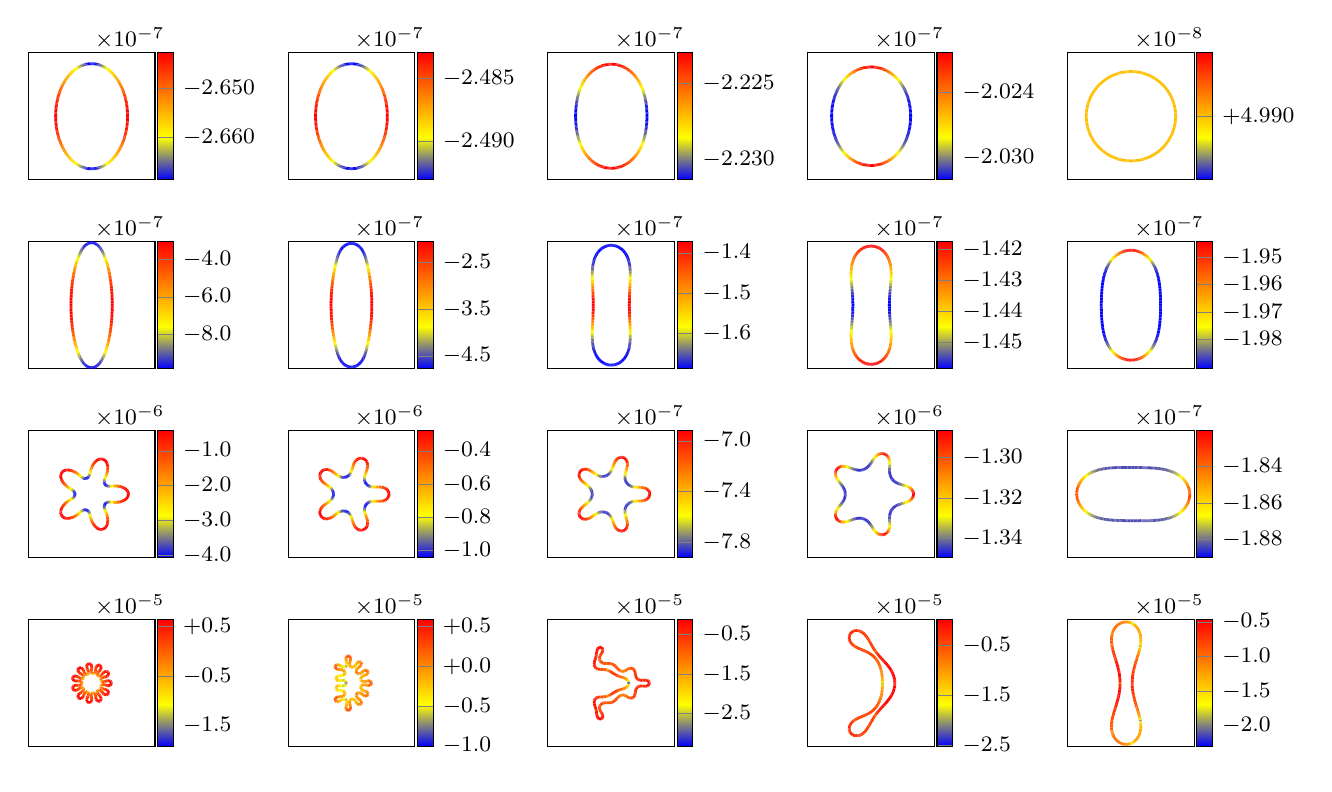
\begin{tikzpicture}[scale=1]

% Start of the ellipse1 images 
\begin{axis}[
  at = {(0.0cm,7.2cm)},
  width = 3.7cm,
%  hide axis, 
  xtick = \empty,
  ytick = \empty,
  axis equal image,
  xmin = -1.42,
  xmax = 1.42,
  ymin = -1.42,
  ymax = 1.42,
  colorbar,
  colorbar style={
    /pgfplots/tick scale binop=\times,
    at = {(1.02,0)},
    anchor = south west,
    ytick={-2.650e-7,-2.660e-7},
    yticklabels = {$-2.650$,$-2.660$},
    font = \footnotesize,
  },
  colorbar/width=2mm
]

\addplot[samples=200,surf,point meta=explicit,line width=1.0pt] coordinates{
(2.0909e-14,1.1782e+00) [-2.6685e-07]
(-1.9785e-02,1.1778e+00) [-2.6684e-07]
(-3.9558e-02,1.1768e+00) [-2.6683e-07]
(-5.9307e-02,1.1750e+00) [-2.6681e-07]
(-7.9022e-02,1.1725e+00) [-2.6678e-07]
(-9.8690e-02,1.1694e+00) [-2.6674e-07]
(-1.1830e-01,1.1655e+00) [-2.6669e-07]
(-1.3784e-01,1.1609e+00) [-2.6664e-07]
(-1.5730e-01,1.1556e+00) [-2.6659e-07]
(-1.7666e-01,1.1497e+00) [-2.6653e-07]
(-1.9592e-01,1.1430e+00) [-2.6647e-07]
(-2.1506e-01,1.1357e+00) [-2.6641e-07]
(-2.3407e-01,1.1276e+00) [-2.6635e-07]
(-2.5294e-01,1.1189e+00) [-2.6628e-07]
(-2.7166e-01,1.1095e+00) [-2.6622e-07]
(-2.9021e-01,1.0995e+00) [-2.6617e-07]
(-3.0860e-01,1.0887e+00) [-2.6611e-07]
(-3.2679e-01,1.0774e+00) [-2.6605e-07]
(-3.4479e-01,1.0653e+00) [-2.6600e-07]
(-3.6257e-01,1.0526e+00) [-2.6595e-07]
(-3.8014e-01,1.0393e+00) [-2.6591e-07]
(-3.9748e-01,1.0254e+00) [-2.6586e-07]
(-4.1458e-01,1.0108e+00) [-2.6582e-07]
(-4.3143e-01,9.9567e-01) [-2.6578e-07]
(-4.4802e-01,9.7990e-01) [-2.6574e-07]
(-4.6433e-01,9.6354e-01) [-2.6571e-07]
(-4.8037e-01,9.4659e-01) [-2.6567e-07]
(-4.9611e-01,9.2908e-01) [-2.6563e-07]
(-5.1156e-01,9.1101e-01) [-2.6560e-07]
(-5.2669e-01,8.9238e-01) [-2.6556e-07]
(-5.4151e-01,8.7322e-01) [-2.6552e-07]
(-5.5600e-01,8.5353e-01) [-2.6548e-07]
(-5.7016e-01,8.3333e-01) [-2.6545e-07]
(-5.8397e-01,8.1263e-01) [-2.6541e-07]
(-5.9743e-01,7.9143e-01) [-2.6536e-07]
(-6.1053e-01,7.6976e-01) [-2.6532e-07]
(-6.2326e-01,7.4763e-01) [-2.6528e-07]
(-6.3561e-01,7.2504e-01) [-2.6523e-07]
(-6.4758e-01,7.0202e-01) [-2.6519e-07]
(-6.5917e-01,6.7857e-01) [-2.6514e-07]
(-6.7035e-01,6.5472e-01) [-2.6509e-07]
(-6.8113e-01,6.3048e-01) [-2.6504e-07]
(-6.9150e-01,6.0585e-01) [-2.6500e-07]
(-7.0145e-01,5.8086e-01) [-2.6495e-07]
(-7.1099e-01,5.5552e-01) [-2.6490e-07]
(-7.2009e-01,5.2984e-01) [-2.6485e-07]
(-7.2876e-01,5.0385e-01) [-2.6480e-07]
(-7.3699e-01,4.7755e-01) [-2.6475e-07]
(-7.4478e-01,4.5097e-01) [-2.6471e-07]
(-7.5212e-01,4.2411e-01) [-2.6466e-07]
(-7.5900e-01,3.9700e-01) [-2.6462e-07]
(-7.6543e-01,3.6965e-01) [-2.6457e-07]
(-7.7140e-01,3.4208e-01) [-2.6453e-07]
(-7.7691e-01,3.1430e-01) [-2.6450e-07]
(-7.8194e-01,2.8633e-01) [-2.6446e-07]
(-7.8651e-01,2.5819e-01) [-2.6443e-07]
(-7.9060e-01,2.2990e-01) [-2.6440e-07]
(-7.9422e-01,2.0146e-01) [-2.6437e-07]
(-7.9736e-01,1.7291e-01) [-2.6435e-07]
(-8.0002e-01,1.4425e-01) [-2.6433e-07]
(-8.0220e-01,1.1550e-01) [-2.6431e-07]
(-8.0389e-01,8.6688e-02) [-2.6430e-07]
(-8.0511e-01,5.7821e-02) [-2.6429e-07]
(-8.0583e-01,2.8919e-02) [-2.6428e-07]
(-8.0608e-01,-6.8722e-17) [-2.6428e-07]
(-8.0583e-01,-2.8919e-02) [-2.6428e-07]
(-8.0511e-01,-5.7821e-02) [-2.6429e-07]
(-8.0389e-01,-8.6688e-02) [-2.6430e-07]
(-8.0220e-01,-1.1550e-01) [-2.6431e-07]
(-8.0002e-01,-1.4425e-01) [-2.6433e-07]
(-7.9736e-01,-1.7291e-01) [-2.6435e-07]
(-7.9422e-01,-2.0146e-01) [-2.6437e-07]
(-7.9060e-01,-2.2990e-01) [-2.6440e-07]
(-7.8651e-01,-2.5819e-01) [-2.6443e-07]
(-7.8194e-01,-2.8633e-01) [-2.6446e-07]
(-7.7691e-01,-3.1430e-01) [-2.6450e-07]
(-7.7140e-01,-3.4208e-01) [-2.6453e-07]
(-7.6543e-01,-3.6965e-01) [-2.6457e-07]
(-7.5900e-01,-3.9700e-01) [-2.6462e-07]
(-7.5212e-01,-4.2411e-01) [-2.6466e-07]
(-7.4478e-01,-4.5097e-01) [-2.6471e-07]
(-7.3699e-01,-4.7755e-01) [-2.6475e-07]
(-7.2876e-01,-5.0385e-01) [-2.6480e-07]
(-7.2009e-01,-5.2984e-01) [-2.6485e-07]
(-7.1099e-01,-5.5552e-01) [-2.6490e-07]
(-7.0145e-01,-5.8086e-01) [-2.6495e-07]
(-6.9150e-01,-6.0585e-01) [-2.6500e-07]
(-6.8113e-01,-6.3048e-01) [-2.6504e-07]
(-6.7035e-01,-6.5472e-01) [-2.6509e-07]
(-6.5917e-01,-6.7857e-01) [-2.6514e-07]
(-6.4758e-01,-7.0202e-01) [-2.6519e-07]
(-6.3561e-01,-7.2504e-01) [-2.6523e-07]
(-6.2326e-01,-7.4763e-01) [-2.6528e-07]
(-6.1053e-01,-7.6976e-01) [-2.6532e-07]
(-5.9743e-01,-7.9143e-01) [-2.6536e-07]
(-5.8397e-01,-8.1263e-01) [-2.6541e-07]
(-5.7016e-01,-8.3333e-01) [-2.6545e-07]
(-5.5600e-01,-8.5353e-01) [-2.6548e-07]
(-5.4151e-01,-8.7322e-01) [-2.6552e-07]
(-5.2669e-01,-8.9238e-01) [-2.6556e-07]
(-5.1156e-01,-9.1101e-01) [-2.6560e-07]
(-4.9611e-01,-9.2908e-01) [-2.6563e-07]
(-4.8037e-01,-9.4659e-01) [-2.6567e-07]
(-4.6433e-01,-9.6354e-01) [-2.6571e-07]
(-4.4802e-01,-9.7990e-01) [-2.6574e-07]
(-4.3143e-01,-9.9567e-01) [-2.6578e-07]
(-4.1458e-01,-1.0108e+00) [-2.6582e-07]
(-3.9748e-01,-1.0254e+00) [-2.6586e-07]
(-3.8014e-01,-1.0393e+00) [-2.6591e-07]
(-3.6257e-01,-1.0526e+00) [-2.6595e-07]
(-3.4479e-01,-1.0653e+00) [-2.6600e-07]
(-3.2679e-01,-1.0774e+00) [-2.6605e-07]
(-3.0860e-01,-1.0887e+00) [-2.6611e-07]
(-2.9021e-01,-1.0995e+00) [-2.6617e-07]
(-2.7166e-01,-1.1095e+00) [-2.6622e-07]
(-2.5294e-01,-1.1189e+00) [-2.6628e-07]
(-2.3407e-01,-1.1276e+00) [-2.6635e-07]
(-2.1506e-01,-1.1357e+00) [-2.6641e-07]
(-1.9592e-01,-1.1430e+00) [-2.6647e-07]
(-1.7666e-01,-1.1497e+00) [-2.6653e-07]
(-1.5730e-01,-1.1556e+00) [-2.6659e-07]
(-1.3784e-01,-1.1609e+00) [-2.6664e-07]
(-1.1830e-01,-1.1655e+00) [-2.6669e-07]
(-9.8690e-02,-1.1694e+00) [-2.6674e-07]
(-7.9022e-02,-1.1725e+00) [-2.6678e-07]
(-5.9307e-02,-1.1750e+00) [-2.6681e-07]
(-3.9558e-02,-1.1768e+00) [-2.6683e-07]
(-1.9785e-02,-1.1778e+00) [-2.6684e-07]
(1.0071e-13,-1.1782e+00) [-2.6685e-07]
(1.9785e-02,-1.1778e+00) [-2.6684e-07]
(3.9558e-02,-1.1768e+00) [-2.6683e-07]
(5.9307e-02,-1.1750e+00) [-2.6681e-07]
(7.9022e-02,-1.1725e+00) [-2.6678e-07]
(9.8690e-02,-1.1694e+00) [-2.6674e-07]
(1.1830e-01,-1.1655e+00) [-2.6669e-07]
(1.3784e-01,-1.1609e+00) [-2.6664e-07]
(1.5730e-01,-1.1556e+00) [-2.6659e-07]
(1.7666e-01,-1.1497e+00) [-2.6653e-07]
(1.9592e-01,-1.1430e+00) [-2.6647e-07]
(2.1506e-01,-1.1357e+00) [-2.6641e-07]
(2.3407e-01,-1.1276e+00) [-2.6635e-07]
(2.5294e-01,-1.1189e+00) [-2.6628e-07]
(2.7166e-01,-1.1095e+00) [-2.6622e-07]
(2.9021e-01,-1.0995e+00) [-2.6617e-07]
(3.0860e-01,-1.0887e+00) [-2.6611e-07]
(3.2679e-01,-1.0774e+00) [-2.6605e-07]
(3.4479e-01,-1.0653e+00) [-2.6600e-07]
(3.6257e-01,-1.0526e+00) [-2.6595e-07]
(3.8014e-01,-1.0393e+00) [-2.6591e-07]
(3.9748e-01,-1.0254e+00) [-2.6586e-07]
(4.1458e-01,-1.0108e+00) [-2.6582e-07]
(4.3143e-01,-9.9567e-01) [-2.6578e-07]
(4.4802e-01,-9.7990e-01) [-2.6574e-07]
(4.6433e-01,-9.6354e-01) [-2.6571e-07]
(4.8037e-01,-9.4659e-01) [-2.6567e-07]
(4.9611e-01,-9.2908e-01) [-2.6563e-07]
(5.1156e-01,-9.1101e-01) [-2.6560e-07]
(5.2669e-01,-8.9238e-01) [-2.6556e-07]
(5.4151e-01,-8.7322e-01) [-2.6552e-07]
(5.5600e-01,-8.5353e-01) [-2.6548e-07]
(5.7016e-01,-8.3333e-01) [-2.6545e-07]
(5.8397e-01,-8.1263e-01) [-2.6541e-07]
(5.9743e-01,-7.9143e-01) [-2.6536e-07]
(6.1053e-01,-7.6976e-01) [-2.6532e-07]
(6.2326e-01,-7.4763e-01) [-2.6528e-07]
(6.3561e-01,-7.2504e-01) [-2.6523e-07]
(6.4758e-01,-7.0202e-01) [-2.6519e-07]
(6.5917e-01,-6.7857e-01) [-2.6514e-07]
(6.7035e-01,-6.5472e-01) [-2.6509e-07]
(6.8113e-01,-6.3048e-01) [-2.6504e-07]
(6.9150e-01,-6.0585e-01) [-2.6500e-07]
(7.0145e-01,-5.8086e-01) [-2.6495e-07]
(7.1099e-01,-5.5552e-01) [-2.6490e-07]
(7.2009e-01,-5.2984e-01) [-2.6485e-07]
(7.2876e-01,-5.0385e-01) [-2.6480e-07]
(7.3699e-01,-4.7755e-01) [-2.6475e-07]
(7.4478e-01,-4.5097e-01) [-2.6471e-07]
(7.5212e-01,-4.2411e-01) [-2.6466e-07]
(7.5900e-01,-3.9700e-01) [-2.6462e-07]
(7.6543e-01,-3.6965e-01) [-2.6457e-07]
(7.7140e-01,-3.4208e-01) [-2.6453e-07]
(7.7691e-01,-3.1430e-01) [-2.6450e-07]
(7.8194e-01,-2.8633e-01) [-2.6446e-07]
(7.8651e-01,-2.5819e-01) [-2.6443e-07]
(7.9060e-01,-2.2990e-01) [-2.6440e-07]
(7.9422e-01,-2.0146e-01) [-2.6437e-07]
(7.9736e-01,-1.7291e-01) [-2.6435e-07]
(8.0002e-01,-1.4425e-01) [-2.6433e-07]
(8.0220e-01,-1.1550e-01) [-2.6431e-07]
(8.0389e-01,-8.6688e-02) [-2.6430e-07]
(8.0511e-01,-5.7821e-02) [-2.6429e-07]
(8.0583e-01,-2.8919e-02) [-2.6428e-07]
(8.0608e-01,2.0204e-14) [-2.6428e-07]
(8.0583e-01,2.8919e-02) [-2.6428e-07]
(8.0511e-01,5.7821e-02) [-2.6429e-07]
(8.0389e-01,8.6688e-02) [-2.6430e-07]
(8.0220e-01,1.1550e-01) [-2.6431e-07]
(8.0002e-01,1.4425e-01) [-2.6433e-07]
(7.9736e-01,1.7291e-01) [-2.6435e-07]
(7.9422e-01,2.0146e-01) [-2.6437e-07]
(7.9060e-01,2.2990e-01) [-2.6440e-07]
(7.8651e-01,2.5819e-01) [-2.6443e-07]
(7.8194e-01,2.8633e-01) [-2.6446e-07]
(7.7691e-01,3.1430e-01) [-2.6450e-07]
(7.7140e-01,3.4208e-01) [-2.6453e-07]
(7.6543e-01,3.6965e-01) [-2.6457e-07]
(7.5900e-01,3.9700e-01) [-2.6462e-07]
(7.5212e-01,4.2411e-01) [-2.6466e-07]
(7.4478e-01,4.5097e-01) [-2.6471e-07]
(7.3699e-01,4.7755e-01) [-2.6475e-07]
(7.2876e-01,5.0385e-01) [-2.6480e-07]
(7.2009e-01,5.2984e-01) [-2.6485e-07]
(7.1099e-01,5.5552e-01) [-2.6490e-07]
(7.0145e-01,5.8086e-01) [-2.6495e-07]
(6.9150e-01,6.0585e-01) [-2.6500e-07]
(6.8113e-01,6.3048e-01) [-2.6504e-07]
(6.7035e-01,6.5472e-01) [-2.6509e-07]
(6.5917e-01,6.7857e-01) [-2.6514e-07]
(6.4758e-01,7.0202e-01) [-2.6519e-07]
(6.3561e-01,7.2504e-01) [-2.6523e-07]
(6.2326e-01,7.4763e-01) [-2.6528e-07]
(6.1053e-01,7.6976e-01) [-2.6532e-07]
(5.9743e-01,7.9143e-01) [-2.6536e-07]
(5.8397e-01,8.1263e-01) [-2.6541e-07]
(5.7016e-01,8.3333e-01) [-2.6545e-07]
(5.5600e-01,8.5353e-01) [-2.6548e-07]
(5.4151e-01,8.7322e-01) [-2.6552e-07]
(5.2669e-01,8.9238e-01) [-2.6556e-07]
(5.1156e-01,9.1101e-01) [-2.6560e-07]
(4.9611e-01,9.2908e-01) [-2.6563e-07]
(4.8037e-01,9.4659e-01) [-2.6567e-07]
(4.6433e-01,9.6354e-01) [-2.6571e-07]
(4.4802e-01,9.7990e-01) [-2.6574e-07]
(4.3143e-01,9.9567e-01) [-2.6578e-07]
(4.1458e-01,1.0108e+00) [-2.6582e-07]
(3.9748e-01,1.0254e+00) [-2.6586e-07]
(3.8014e-01,1.0393e+00) [-2.6591e-07]
(3.6257e-01,1.0526e+00) [-2.6595e-07]
(3.4479e-01,1.0653e+00) [-2.6600e-07]
(3.2679e-01,1.0774e+00) [-2.6605e-07]
(3.0860e-01,1.0887e+00) [-2.6611e-07]
(2.9021e-01,1.0995e+00) [-2.6617e-07]
(2.7166e-01,1.1095e+00) [-2.6622e-07]
(2.5294e-01,1.1189e+00) [-2.6628e-07]
(2.3407e-01,1.1276e+00) [-2.6635e-07]
(2.1506e-01,1.1357e+00) [-2.6641e-07]
(1.9592e-01,1.1430e+00) [-2.6647e-07]
(1.7666e-01,1.1497e+00) [-2.6653e-07]
(1.5730e-01,1.1556e+00) [-2.6659e-07]
(1.3784e-01,1.1609e+00) [-2.6664e-07]
(1.1830e-01,1.1655e+00) [-2.6669e-07]
(9.8690e-02,1.1694e+00) [-2.6674e-07]
(7.9022e-02,1.1725e+00) [-2.6678e-07]
(5.9307e-02,1.1750e+00) [-2.6681e-07]
(3.9558e-02,1.1768e+00) [-2.6683e-07]
(1.9785e-02,1.1778e+00) [-2.6684e-07]
(2.0909e-14,1.1782e+00) [-2.6685e-07]
};

\end{axis}

\begin{axis}[
  at = {(3.3cm,7.2cm)},
  width = 3.7cm,
%  hide axis, 
  xtick = \empty,
  ytick = \empty,
  axis equal image,
  xmin = -1.42,
  xmax = 1.42,
  ymin = -1.42,
  ymax = 1.42,
  colorbar,
  colorbar style={
    /pgfplots/tick scale binop=\times,
    at = {(1.02,0)},
    anchor = south west,
    ytick={-2.485e-7,-2.490e-7},
    yticklabels = {$-2.485$,$-2.490$},
    font = \footnotesize,
  },
  colorbar/width=2mm
]
\addplot[samples=200,surf,point meta=explicit,line width=1.0pt] coordinates{
(-4.4843e-14,1.1757e+00) [-2.4930e-07]
(-1.9785e-02,1.1754e+00) [-2.4930e-07]
(-3.9560e-02,1.1743e+00) [-2.4930e-07]
(-5.9316e-02,1.1726e+00) [-2.4930e-07]
(-7.9042e-02,1.1703e+00) [-2.4929e-07]
(-9.8729e-02,1.1672e+00) [-2.4928e-07]
(-1.1837e-01,1.1635e+00) [-2.4927e-07]
(-1.3794e-01,1.1591e+00) [-2.4926e-07]
(-1.5745e-01,1.1540e+00) [-2.4924e-07]
(-1.7687e-01,1.1482e+00) [-2.4923e-07]
(-1.9620e-01,1.1417e+00) [-2.4921e-07]
(-2.1542e-01,1.1346e+00) [-2.4919e-07]
(-2.3452e-01,1.1268e+00) [-2.4918e-07]
(-2.5349e-01,1.1183e+00) [-2.4916e-07]
(-2.7232e-01,1.1091e+00) [-2.4914e-07]
(-2.9099e-01,1.0993e+00) [-2.4911e-07]
(-3.0948e-01,1.0887e+00) [-2.4909e-07]
(-3.2780e-01,1.0776e+00) [-2.4907e-07]
(-3.4591e-01,1.0657e+00) [-2.4905e-07]
(-3.6382e-01,1.0532e+00) [-2.4903e-07]
(-3.8150e-01,1.0400e+00) [-2.4900e-07]
(-3.9894e-01,1.0262e+00) [-2.4898e-07]
(-4.1613e-01,1.0118e+00) [-2.4896e-07]
(-4.3306e-01,9.9670e-01) [-2.4894e-07]
(-4.4972e-01,9.8100e-01) [-2.4892e-07]
(-4.6609e-01,9.6470e-01) [-2.4890e-07]
(-4.8217e-01,9.4779e-01) [-2.4888e-07]
(-4.9794e-01,9.3030e-01) [-2.4887e-07]
(-5.1339e-01,9.1223e-01) [-2.4885e-07]
(-5.2852e-01,8.9360e-01) [-2.4883e-07]
(-5.4331e-01,8.7442e-01) [-2.4882e-07]
(-5.5776e-01,8.5470e-01) [-2.4880e-07]
(-5.7185e-01,8.3446e-01) [-2.4879e-07]
(-5.8559e-01,8.1370e-01) [-2.4877e-07]
(-5.9896e-01,7.9245e-01) [-2.4876e-07]
(-6.1196e-01,7.7072e-01) [-2.4874e-07]
(-6.2458e-01,7.4852e-01) [-2.4872e-07]
(-6.3681e-01,7.2587e-01) [-2.4871e-07]
(-6.4865e-01,7.0278e-01) [-2.4869e-07]
(-6.6010e-01,6.7927e-01) [-2.4868e-07]
(-6.7114e-01,6.5535e-01) [-2.4866e-07]
(-6.8177e-01,6.3104e-01) [-2.4864e-07]
(-6.9199e-01,6.0635e-01) [-2.4862e-07]
(-7.0180e-01,5.8130e-01) [-2.4860e-07]
(-7.1118e-01,5.5591e-01) [-2.4859e-07]
(-7.2014e-01,5.3018e-01) [-2.4857e-07]
(-7.2866e-01,5.0414e-01) [-2.4855e-07]
(-7.3675e-01,4.7780e-01) [-2.4853e-07]
(-7.4441e-01,4.5117e-01) [-2.4850e-07]
(-7.5161e-01,4.2428e-01) [-2.4848e-07]
(-7.5838e-01,3.9714e-01) [-2.4846e-07]
(-7.6469e-01,3.6976e-01) [-2.4844e-07]
(-7.7055e-01,3.4217e-01) [-2.4843e-07]
(-7.7595e-01,3.1437e-01) [-2.4841e-07]
(-7.8089e-01,2.8638e-01) [-2.4839e-07]
(-7.8537e-01,2.5823e-01) [-2.4837e-07]
(-7.8939e-01,2.2992e-01) [-2.4836e-07]
(-7.9293e-01,2.0148e-01) [-2.4834e-07]
(-7.9601e-01,1.7292e-01) [-2.4833e-07]
(-7.9862e-01,1.4426e-01) [-2.4832e-07]
(-8.0076e-01,1.1551e-01) [-2.4831e-07]
(-8.0242e-01,8.6690e-02) [-2.4831e-07]
(-8.0361e-01,5.7822e-02) [-2.4830e-07]
(-8.0432e-01,2.8919e-02) [-2.4830e-07]
(-8.0456e-01,2.2407e-14) [-2.4830e-07]
(-8.0432e-01,-2.8919e-02) [-2.4830e-07]
(-8.0361e-01,-5.7822e-02) [-2.4830e-07]
(-8.0242e-01,-8.6690e-02) [-2.4831e-07]
(-8.0076e-01,-1.1551e-01) [-2.4831e-07]
(-7.9862e-01,-1.4426e-01) [-2.4832e-07]
(-7.9601e-01,-1.7292e-01) [-2.4833e-07]
(-7.9293e-01,-2.0148e-01) [-2.4834e-07]
(-7.8939e-01,-2.2992e-01) [-2.4836e-07]
(-7.8537e-01,-2.5823e-01) [-2.4837e-07]
(-7.8089e-01,-2.8638e-01) [-2.4839e-07]
(-7.7595e-01,-3.1437e-01) [-2.4841e-07]
(-7.7055e-01,-3.4217e-01) [-2.4843e-07]
(-7.6469e-01,-3.6976e-01) [-2.4844e-07]
(-7.5838e-01,-3.9714e-01) [-2.4846e-07]
(-7.5161e-01,-4.2428e-01) [-2.4848e-07]
(-7.4441e-01,-4.5117e-01) [-2.4850e-07]
(-7.3675e-01,-4.7780e-01) [-2.4853e-07]
(-7.2866e-01,-5.0414e-01) [-2.4855e-07]
(-7.2014e-01,-5.3018e-01) [-2.4857e-07]
(-7.1118e-01,-5.5591e-01) [-2.4859e-07]
(-7.0180e-01,-5.8130e-01) [-2.4860e-07]
(-6.9199e-01,-6.0635e-01) [-2.4862e-07]
(-6.8177e-01,-6.3104e-01) [-2.4864e-07]
(-6.7114e-01,-6.5535e-01) [-2.4866e-07]
(-6.6010e-01,-6.7927e-01) [-2.4868e-07]
(-6.4865e-01,-7.0278e-01) [-2.4869e-07]
(-6.3681e-01,-7.2587e-01) [-2.4871e-07]
(-6.2458e-01,-7.4852e-01) [-2.4872e-07]
(-6.1196e-01,-7.7072e-01) [-2.4874e-07]
(-5.9896e-01,-7.9245e-01) [-2.4876e-07]
(-5.8559e-01,-8.1370e-01) [-2.4877e-07]
(-5.7185e-01,-8.3446e-01) [-2.4879e-07]
(-5.5776e-01,-8.5470e-01) [-2.4880e-07]
(-5.4331e-01,-8.7442e-01) [-2.4882e-07]
(-5.2852e-01,-8.9360e-01) [-2.4883e-07]
(-5.1339e-01,-9.1223e-01) [-2.4885e-07]
(-4.9794e-01,-9.3030e-01) [-2.4887e-07]
(-4.8217e-01,-9.4779e-01) [-2.4888e-07]
(-4.6609e-01,-9.6470e-01) [-2.4890e-07]
(-4.4972e-01,-9.8100e-01) [-2.4892e-07]
(-4.3306e-01,-9.9670e-01) [-2.4894e-07]
(-4.1613e-01,-1.0118e+00) [-2.4896e-07]
(-3.9894e-01,-1.0262e+00) [-2.4898e-07]
(-3.8150e-01,-1.0400e+00) [-2.4900e-07]
(-3.6382e-01,-1.0532e+00) [-2.4903e-07]
(-3.4591e-01,-1.0657e+00) [-2.4905e-07]
(-3.2780e-01,-1.0776e+00) [-2.4907e-07]
(-3.0948e-01,-1.0887e+00) [-2.4909e-07]
(-2.9099e-01,-1.0993e+00) [-2.4911e-07]
(-2.7232e-01,-1.1091e+00) [-2.4914e-07]
(-2.5349e-01,-1.1183e+00) [-2.4916e-07]
(-2.3452e-01,-1.1268e+00) [-2.4918e-07]
(-2.1542e-01,-1.1346e+00) [-2.4919e-07]
(-1.9620e-01,-1.1417e+00) [-2.4921e-07]
(-1.7687e-01,-1.1482e+00) [-2.4923e-07]
(-1.5745e-01,-1.1540e+00) [-2.4924e-07]
(-1.3794e-01,-1.1591e+00) [-2.4926e-07]
(-1.1837e-01,-1.1635e+00) [-2.4927e-07]
(-9.8729e-02,-1.1672e+00) [-2.4928e-07]
(-7.9042e-02,-1.1703e+00) [-2.4929e-07]
(-5.9316e-02,-1.1726e+00) [-2.4930e-07]
(-3.9560e-02,-1.1743e+00) [-2.4930e-07]
(-1.9785e-02,-1.1754e+00) [-2.4930e-07]
(8.3928e-14,-1.1757e+00) [-2.4930e-07]
(1.9785e-02,-1.1754e+00) [-2.4930e-07]
(3.9560e-02,-1.1743e+00) [-2.4930e-07]
(5.9316e-02,-1.1726e+00) [-2.4930e-07]
(7.9042e-02,-1.1703e+00) [-2.4929e-07]
(9.8729e-02,-1.1672e+00) [-2.4928e-07]
(1.1837e-01,-1.1635e+00) [-2.4927e-07]
(1.3794e-01,-1.1591e+00) [-2.4926e-07]
(1.5745e-01,-1.1540e+00) [-2.4924e-07]
(1.7687e-01,-1.1482e+00) [-2.4923e-07]
(1.9620e-01,-1.1417e+00) [-2.4921e-07]
(2.1542e-01,-1.1346e+00) [-2.4919e-07]
(2.3452e-01,-1.1268e+00) [-2.4918e-07]
(2.5349e-01,-1.1183e+00) [-2.4916e-07]
(2.7232e-01,-1.1091e+00) [-2.4914e-07]
(2.9099e-01,-1.0993e+00) [-2.4911e-07]
(3.0948e-01,-1.0887e+00) [-2.4909e-07]
(3.2780e-01,-1.0776e+00) [-2.4907e-07]
(3.4591e-01,-1.0657e+00) [-2.4905e-07]
(3.6382e-01,-1.0532e+00) [-2.4903e-07]
(3.8150e-01,-1.0400e+00) [-2.4900e-07]
(3.9894e-01,-1.0262e+00) [-2.4898e-07]
(4.1613e-01,-1.0118e+00) [-2.4896e-07]
(4.3306e-01,-9.9670e-01) [-2.4894e-07]
(4.4972e-01,-9.8100e-01) [-2.4892e-07]
(4.6609e-01,-9.6470e-01) [-2.4890e-07]
(4.8217e-01,-9.4779e-01) [-2.4888e-07]
(4.9794e-01,-9.3030e-01) [-2.4887e-07]
(5.1339e-01,-9.1223e-01) [-2.4885e-07]
(5.2852e-01,-8.9360e-01) [-2.4883e-07]
(5.4331e-01,-8.7442e-01) [-2.4882e-07]
(5.5776e-01,-8.5470e-01) [-2.4880e-07]
(5.7185e-01,-8.3446e-01) [-2.4879e-07]
(5.8559e-01,-8.1370e-01) [-2.4877e-07]
(5.9896e-01,-7.9245e-01) [-2.4876e-07]
(6.1196e-01,-7.7072e-01) [-2.4874e-07]
(6.2458e-01,-7.4852e-01) [-2.4872e-07]
(6.3681e-01,-7.2587e-01) [-2.4871e-07]
(6.4865e-01,-7.0278e-01) [-2.4869e-07]
(6.6010e-01,-6.7927e-01) [-2.4868e-07]
(6.7114e-01,-6.5535e-01) [-2.4866e-07]
(6.8177e-01,-6.3104e-01) [-2.4864e-07]
(6.9199e-01,-6.0635e-01) [-2.4862e-07]
(7.0180e-01,-5.8130e-01) [-2.4860e-07]
(7.1118e-01,-5.5591e-01) [-2.4859e-07]
(7.2014e-01,-5.3018e-01) [-2.4857e-07]
(7.2866e-01,-5.0414e-01) [-2.4855e-07]
(7.3675e-01,-4.7780e-01) [-2.4853e-07]
(7.4441e-01,-4.5117e-01) [-2.4850e-07]
(7.5161e-01,-4.2428e-01) [-2.4848e-07]
(7.5838e-01,-3.9714e-01) [-2.4846e-07]
(7.6469e-01,-3.6976e-01) [-2.4844e-07]
(7.7055e-01,-3.4217e-01) [-2.4843e-07]
(7.7595e-01,-3.1437e-01) [-2.4841e-07]
(7.8089e-01,-2.8638e-01) [-2.4839e-07]
(7.8537e-01,-2.5823e-01) [-2.4837e-07]
(7.8939e-01,-2.2992e-01) [-2.4836e-07]
(7.9293e-01,-2.0148e-01) [-2.4834e-07]
(7.9601e-01,-1.7292e-01) [-2.4833e-07]
(7.9862e-01,-1.4426e-01) [-2.4832e-07]
(8.0076e-01,-1.1551e-01) [-2.4831e-07]
(8.0242e-01,-8.6690e-02) [-2.4831e-07]
(8.0361e-01,-5.7822e-02) [-2.4830e-07]
(8.0432e-01,-2.8919e-02) [-2.4830e-07]
(8.0456e-01,2.0985e-14) [-2.4830e-07]
(8.0432e-01,2.8919e-02) [-2.4830e-07]
(8.0361e-01,5.7822e-02) [-2.4830e-07]
(8.0242e-01,8.6690e-02) [-2.4831e-07]
(8.0076e-01,1.1551e-01) [-2.4831e-07]
(7.9862e-01,1.4426e-01) [-2.4832e-07]
(7.9601e-01,1.7292e-01) [-2.4833e-07]
(7.9293e-01,2.0148e-01) [-2.4834e-07]
(7.8939e-01,2.2992e-01) [-2.4836e-07]
(7.8537e-01,2.5823e-01) [-2.4837e-07]
(7.8089e-01,2.8638e-01) [-2.4839e-07]
(7.7595e-01,3.1437e-01) [-2.4841e-07]
(7.7055e-01,3.4217e-01) [-2.4843e-07]
(7.6469e-01,3.6976e-01) [-2.4844e-07]
(7.5838e-01,3.9714e-01) [-2.4846e-07]
(7.5161e-01,4.2428e-01) [-2.4848e-07]
(7.4441e-01,4.5117e-01) [-2.4850e-07]
(7.3675e-01,4.7780e-01) [-2.4853e-07]
(7.2866e-01,5.0414e-01) [-2.4855e-07]
(7.2014e-01,5.3018e-01) [-2.4857e-07]
(7.1118e-01,5.5591e-01) [-2.4859e-07]
(7.0180e-01,5.8130e-01) [-2.4860e-07]
(6.9199e-01,6.0635e-01) [-2.4862e-07]
(6.8177e-01,6.3104e-01) [-2.4864e-07]
(6.7114e-01,6.5535e-01) [-2.4866e-07]
(6.6010e-01,6.7927e-01) [-2.4868e-07]
(6.4865e-01,7.0278e-01) [-2.4869e-07]
(6.3681e-01,7.2587e-01) [-2.4871e-07]
(6.2458e-01,7.4852e-01) [-2.4872e-07]
(6.1196e-01,7.7072e-01) [-2.4874e-07]
(5.9896e-01,7.9245e-01) [-2.4876e-07]
(5.8559e-01,8.1370e-01) [-2.4877e-07]
(5.7185e-01,8.3446e-01) [-2.4879e-07]
(5.5776e-01,8.5470e-01) [-2.4880e-07]
(5.4331e-01,8.7442e-01) [-2.4882e-07]
(5.2852e-01,8.9360e-01) [-2.4883e-07]
(5.1339e-01,9.1223e-01) [-2.4885e-07]
(4.9794e-01,9.3030e-01) [-2.4887e-07]
(4.8217e-01,9.4779e-01) [-2.4888e-07]
(4.6609e-01,9.6470e-01) [-2.4890e-07]
(4.4972e-01,9.8100e-01) [-2.4892e-07]
(4.3306e-01,9.9670e-01) [-2.4894e-07]
(4.1613e-01,1.0118e+00) [-2.4896e-07]
(3.9894e-01,1.0262e+00) [-2.4898e-07]
(3.8150e-01,1.0400e+00) [-2.4900e-07]
(3.6382e-01,1.0532e+00) [-2.4903e-07]
(3.4591e-01,1.0657e+00) [-2.4905e-07]
(3.2780e-01,1.0776e+00) [-2.4907e-07]
(3.0948e-01,1.0887e+00) [-2.4909e-07]
(2.9099e-01,1.0993e+00) [-2.4911e-07]
(2.7232e-01,1.1091e+00) [-2.4914e-07]
(2.5349e-01,1.1183e+00) [-2.4916e-07]
(2.3452e-01,1.1268e+00) [-2.4918e-07]
(2.1542e-01,1.1346e+00) [-2.4919e-07]
(1.9620e-01,1.1417e+00) [-2.4921e-07]
(1.7687e-01,1.1482e+00) [-2.4923e-07]
(1.5745e-01,1.1540e+00) [-2.4924e-07]
(1.3794e-01,1.1591e+00) [-2.4926e-07]
(1.1837e-01,1.1635e+00) [-2.4927e-07]
(9.8729e-02,1.1672e+00) [-2.4928e-07]
(7.9042e-02,1.1703e+00) [-2.4929e-07]
(5.9316e-02,1.1726e+00) [-2.4930e-07]
(3.9560e-02,1.1743e+00) [-2.4930e-07]
(1.9785e-02,1.1754e+00) [-2.4930e-07]
(-4.4843e-14,1.1757e+00) [-2.4930e-07]
};

\end{axis}

\begin{axis}[
  at = {(6.6cm,7.2cm)},
  width = 3.7cm,
%  hide axis, 
  xtick = \empty,
  ytick = \empty,
  axis equal image,
  xmin = -1.42,
  xmax = 1.42,
  ymin = -1.42,
  ymax = 1.42,
  colorbar,
  colorbar style={
    /pgfplots/tick scale binop=\times,
    at = {(1.02,0)},
    anchor = south west,
    ytick={-2.225e-7,-2.230e-7},
    yticklabels = {$-2.225$,$-2.230$},
    font = \footnotesize,
  },
  colorbar/width=2mm
]
\addplot[samples=200,surf,point meta=explicit,line width=1.0pt] coordinates{
(8.4655e-14,1.1652e+00) [-2.2230e-07]
(-1.9786e-02,1.1649e+00) [-2.2230e-07]
(-3.9566e-02,1.1640e+00) [-2.2231e-07]
(-5.9334e-02,1.1624e+00) [-2.2231e-07]
(-7.9085e-02,1.1603e+00) [-2.2231e-07]
(-9.8812e-02,1.1575e+00) [-2.2231e-07]
(-1.1851e-01,1.1541e+00) [-2.2232e-07]
(-1.3816e-01,1.1500e+00) [-2.2232e-07]
(-1.5778e-01,1.1453e+00) [-2.2233e-07]
(-1.7733e-01,1.1400e+00) [-2.2234e-07]
(-1.9682e-01,1.1341e+00) [-2.2234e-07]
(-2.1624e-01,1.1275e+00) [-2.2235e-07]
(-2.3557e-01,1.1203e+00) [-2.2236e-07]
(-2.5480e-01,1.1124e+00) [-2.2237e-07]
(-2.7391e-01,1.1038e+00) [-2.2238e-07]
(-2.9290e-01,1.0946e+00) [-2.2239e-07]
(-3.1175e-01,1.0847e+00) [-2.2241e-07]
(-3.3045e-01,1.0742e+00) [-2.2242e-07]
(-3.4897e-01,1.0630e+00) [-2.2243e-07]
(-3.6731e-01,1.0511e+00) [-2.2245e-07]
(-3.8543e-01,1.0386e+00) [-2.2246e-07]
(-4.0334e-01,1.0254e+00) [-2.2248e-07]
(-4.2100e-01,1.0115e+00) [-2.2249e-07]
(-4.3840e-01,9.9697e-01) [-2.2251e-07]
(-4.5552e-01,9.8178e-01) [-2.2252e-07]
(-4.7235e-01,9.6595e-01) [-2.2254e-07]
(-4.8886e-01,9.4947e-01) [-2.2256e-07]
(-5.0505e-01,9.3236e-01) [-2.2257e-07]
(-5.2088e-01,9.1463e-01) [-2.2259e-07]
(-5.3635e-01,8.9628e-01) [-2.2261e-07]
(-5.5145e-01,8.7734e-01) [-2.2263e-07]
(-5.6615e-01,8.5781e-01) [-2.2265e-07]
(-5.8044e-01,8.3770e-01) [-2.2267e-07]
(-5.9431e-01,8.1704e-01) [-2.2268e-07]
(-6.0776e-01,7.9584e-01) [-2.2270e-07]
(-6.2076e-01,7.7411e-01) [-2.2272e-07]
(-6.3332e-01,7.5187e-01) [-2.2274e-07]
(-6.4542e-01,7.2915e-01) [-2.2276e-07]
(-6.5705e-01,7.0596e-01) [-2.2278e-07]
(-6.6822e-01,6.8232e-01) [-2.2280e-07]
(-6.7892e-01,6.5824e-01) [-2.2282e-07]
(-6.8914e-01,6.3375e-01) [-2.2284e-07]
(-6.9889e-01,6.0887e-01) [-2.2286e-07]
(-7.0816e-01,5.8362e-01) [-2.2288e-07]
(-7.1696e-01,5.5802e-01) [-2.2290e-07]
(-7.2528e-01,5.3208e-01) [-2.2292e-07]
(-7.3314e-01,5.0583e-01) [-2.2294e-07]
(-7.4052e-01,4.7928e-01) [-2.2296e-07]
(-7.4745e-01,4.5246e-01) [-2.2297e-07]
(-7.5391e-01,4.2538e-01) [-2.2299e-07]
(-7.5993e-01,3.9806e-01) [-2.2301e-07]
(-7.6549e-01,3.7052e-01) [-2.2302e-07]
(-7.7062e-01,3.4278e-01) [-2.2304e-07]
(-7.7531e-01,3.1485e-01) [-2.2305e-07]
(-7.7956e-01,2.8676e-01) [-2.2307e-07]
(-7.8340e-01,2.5851e-01) [-2.2308e-07]
(-7.8681e-01,2.3012e-01) [-2.2309e-07]
(-7.8980e-01,2.0162e-01) [-2.2310e-07]
(-7.9239e-01,1.7301e-01) [-2.2311e-07]
(-7.9457e-01,1.4431e-01) [-2.2312e-07]
(-7.9635e-01,1.1553e-01) [-2.2312e-07]
(-7.9774e-01,8.6701e-02) [-2.2313e-07]
(-7.9872e-01,5.7825e-02) [-2.2313e-07]
(-7.9931e-01,2.8920e-02) [-2.2313e-07]
(-7.9951e-01,2.0286e-14) [-2.2313e-07]
(-7.9931e-01,-2.8920e-02) [-2.2313e-07]
(-7.9872e-01,-5.7825e-02) [-2.2313e-07]
(-7.9774e-01,-8.6701e-02) [-2.2313e-07]
(-7.9635e-01,-1.1553e-01) [-2.2312e-07]
(-7.9457e-01,-1.4431e-01) [-2.2312e-07]
(-7.9239e-01,-1.7301e-01) [-2.2311e-07]
(-7.8980e-01,-2.0162e-01) [-2.2310e-07]
(-7.8681e-01,-2.3012e-01) [-2.2309e-07]
(-7.8340e-01,-2.5851e-01) [-2.2308e-07]
(-7.7956e-01,-2.8676e-01) [-2.2307e-07]
(-7.7531e-01,-3.1485e-01) [-2.2305e-07]
(-7.7062e-01,-3.4278e-01) [-2.2304e-07]
(-7.6549e-01,-3.7052e-01) [-2.2302e-07]
(-7.5993e-01,-3.9806e-01) [-2.2301e-07]
(-7.5391e-01,-4.2538e-01) [-2.2299e-07]
(-7.4745e-01,-4.5246e-01) [-2.2297e-07]
(-7.4052e-01,-4.7928e-01) [-2.2296e-07]
(-7.3314e-01,-5.0583e-01) [-2.2294e-07]
(-7.2528e-01,-5.3208e-01) [-2.2292e-07]
(-7.1696e-01,-5.5802e-01) [-2.2290e-07]
(-7.0816e-01,-5.8362e-01) [-2.2288e-07]
(-6.9889e-01,-6.0887e-01) [-2.2286e-07]
(-6.8914e-01,-6.3375e-01) [-2.2284e-07]
(-6.7892e-01,-6.5824e-01) [-2.2282e-07]
(-6.6822e-01,-6.8232e-01) [-2.2280e-07]
(-6.5705e-01,-7.0596e-01) [-2.2278e-07]
(-6.4542e-01,-7.2915e-01) [-2.2276e-07]
(-6.3332e-01,-7.5187e-01) [-2.2274e-07]
(-6.2076e-01,-7.7411e-01) [-2.2272e-07]
(-6.0776e-01,-7.9584e-01) [-2.2270e-07]
(-5.9431e-01,-8.1704e-01) [-2.2268e-07]
(-5.8044e-01,-8.3770e-01) [-2.2267e-07]
(-5.6615e-01,-8.5781e-01) [-2.2265e-07]
(-5.5145e-01,-8.7734e-01) [-2.2263e-07]
(-5.3635e-01,-8.9628e-01) [-2.2261e-07]
(-5.2088e-01,-9.1463e-01) [-2.2259e-07]
(-5.0505e-01,-9.3236e-01) [-2.2257e-07]
(-4.8886e-01,-9.4947e-01) [-2.2256e-07]
(-4.7235e-01,-9.6595e-01) [-2.2254e-07]
(-4.5552e-01,-9.8178e-01) [-2.2252e-07]
(-4.3840e-01,-9.9697e-01) [-2.2251e-07]
(-4.2100e-01,-1.0115e+00) [-2.2249e-07]
(-4.0334e-01,-1.0254e+00) [-2.2248e-07]
(-3.8543e-01,-1.0386e+00) [-2.2246e-07]
(-3.6731e-01,-1.0511e+00) [-2.2245e-07]
(-3.4897e-01,-1.0630e+00) [-2.2243e-07]
(-3.3045e-01,-1.0742e+00) [-2.2242e-07]
(-3.1175e-01,-1.0847e+00) [-2.2241e-07]
(-2.9290e-01,-1.0946e+00) [-2.2239e-07]
(-2.7391e-01,-1.1038e+00) [-2.2238e-07]
(-2.5480e-01,-1.1124e+00) [-2.2237e-07]
(-2.3557e-01,-1.1203e+00) [-2.2236e-07]
(-2.1624e-01,-1.1275e+00) [-2.2235e-07]
(-1.9682e-01,-1.1341e+00) [-2.2234e-07]
(-1.7733e-01,-1.1400e+00) [-2.2234e-07]
(-1.5778e-01,-1.1453e+00) [-2.2233e-07]
(-1.3816e-01,-1.1500e+00) [-2.2232e-07]
(-1.1851e-01,-1.1541e+00) [-2.2232e-07]
(-9.8812e-02,-1.1575e+00) [-2.2231e-07]
(-7.9085e-02,-1.1603e+00) [-2.2231e-07]
(-5.9334e-02,-1.1624e+00) [-2.2231e-07]
(-3.9566e-02,-1.1640e+00) [-2.2231e-07]
(-1.9786e-02,-1.1649e+00) [-2.2230e-07]
(5.3579e-14,-1.1652e+00) [-2.2230e-07]
(1.9786e-02,-1.1649e+00) [-2.2230e-07]
(3.9566e-02,-1.1640e+00) [-2.2231e-07]
(5.9334e-02,-1.1624e+00) [-2.2231e-07]
(7.9085e-02,-1.1603e+00) [-2.2231e-07]
(9.8812e-02,-1.1575e+00) [-2.2231e-07]
(1.1851e-01,-1.1541e+00) [-2.2232e-07]
(1.3816e-01,-1.1500e+00) [-2.2232e-07]
(1.5778e-01,-1.1453e+00) [-2.2233e-07]
(1.7733e-01,-1.1400e+00) [-2.2234e-07]
(1.9682e-01,-1.1341e+00) [-2.2234e-07]
(2.1624e-01,-1.1275e+00) [-2.2235e-07]
(2.3557e-01,-1.1203e+00) [-2.2236e-07]
(2.5480e-01,-1.1124e+00) [-2.2237e-07]
(2.7391e-01,-1.1038e+00) [-2.2238e-07]
(2.9290e-01,-1.0946e+00) [-2.2239e-07]
(3.1175e-01,-1.0847e+00) [-2.2241e-07]
(3.3045e-01,-1.0742e+00) [-2.2242e-07]
(3.4897e-01,-1.0630e+00) [-2.2243e-07]
(3.6731e-01,-1.0511e+00) [-2.2245e-07]
(3.8543e-01,-1.0386e+00) [-2.2246e-07]
(4.0334e-01,-1.0254e+00) [-2.2248e-07]
(4.2100e-01,-1.0115e+00) [-2.2249e-07]
(4.3840e-01,-9.9697e-01) [-2.2251e-07]
(4.5552e-01,-9.8178e-01) [-2.2252e-07]
(4.7235e-01,-9.6595e-01) [-2.2254e-07]
(4.8886e-01,-9.4947e-01) [-2.2256e-07]
(5.0505e-01,-9.3236e-01) [-2.2257e-07]
(5.2088e-01,-9.1463e-01) [-2.2259e-07]
(5.3635e-01,-8.9628e-01) [-2.2261e-07]
(5.5145e-01,-8.7734e-01) [-2.2263e-07]
(5.6615e-01,-8.5781e-01) [-2.2265e-07]
(5.8044e-01,-8.3770e-01) [-2.2267e-07]
(5.9431e-01,-8.1704e-01) [-2.2268e-07]
(6.0776e-01,-7.9584e-01) [-2.2270e-07]
(6.2076e-01,-7.7411e-01) [-2.2272e-07]
(6.3332e-01,-7.5187e-01) [-2.2274e-07]
(6.4542e-01,-7.2915e-01) [-2.2276e-07]
(6.5705e-01,-7.0596e-01) [-2.2278e-07]
(6.6822e-01,-6.8232e-01) [-2.2280e-07]
(6.7892e-01,-6.5824e-01) [-2.2282e-07]
(6.8914e-01,-6.3375e-01) [-2.2284e-07]
(6.9889e-01,-6.0887e-01) [-2.2286e-07]
(7.0816e-01,-5.8362e-01) [-2.2288e-07]
(7.1696e-01,-5.5802e-01) [-2.2290e-07]
(7.2528e-01,-5.3208e-01) [-2.2292e-07]
(7.3314e-01,-5.0583e-01) [-2.2294e-07]
(7.4052e-01,-4.7928e-01) [-2.2296e-07]
(7.4745e-01,-4.5246e-01) [-2.2297e-07]
(7.5391e-01,-4.2538e-01) [-2.2299e-07]
(7.5993e-01,-3.9806e-01) [-2.2301e-07]
(7.6549e-01,-3.7052e-01) [-2.2302e-07]
(7.7062e-01,-3.4278e-01) [-2.2304e-07]
(7.7531e-01,-3.1485e-01) [-2.2305e-07]
(7.7956e-01,-2.8676e-01) [-2.2307e-07]
(7.8340e-01,-2.5851e-01) [-2.2308e-07]
(7.8681e-01,-2.3012e-01) [-2.2309e-07]
(7.8980e-01,-2.0162e-01) [-2.2310e-07]
(7.9239e-01,-1.7301e-01) [-2.2311e-07]
(7.9457e-01,-1.4431e-01) [-2.2312e-07]
(7.9635e-01,-1.1553e-01) [-2.2312e-07]
(7.9774e-01,-8.6701e-02) [-2.2313e-07]
(7.9872e-01,-5.7825e-02) [-2.2313e-07]
(7.9931e-01,-2.8920e-02) [-2.2313e-07]
(7.9951e-01,1.4952e-14) [-2.2313e-07]
(7.9931e-01,2.8920e-02) [-2.2313e-07]
(7.9872e-01,5.7825e-02) [-2.2313e-07]
(7.9774e-01,8.6701e-02) [-2.2313e-07]
(7.9635e-01,1.1553e-01) [-2.2312e-07]
(7.9457e-01,1.4431e-01) [-2.2312e-07]
(7.9239e-01,1.7301e-01) [-2.2311e-07]
(7.8980e-01,2.0162e-01) [-2.2310e-07]
(7.8681e-01,2.3012e-01) [-2.2309e-07]
(7.8340e-01,2.5851e-01) [-2.2308e-07]
(7.7956e-01,2.8676e-01) [-2.2307e-07]
(7.7531e-01,3.1485e-01) [-2.2305e-07]
(7.7062e-01,3.4278e-01) [-2.2304e-07]
(7.6549e-01,3.7052e-01) [-2.2302e-07]
(7.5993e-01,3.9806e-01) [-2.2301e-07]
(7.5391e-01,4.2538e-01) [-2.2299e-07]
(7.4745e-01,4.5246e-01) [-2.2297e-07]
(7.4052e-01,4.7928e-01) [-2.2296e-07]
(7.3314e-01,5.0583e-01) [-2.2294e-07]
(7.2528e-01,5.3208e-01) [-2.2292e-07]
(7.1696e-01,5.5802e-01) [-2.2290e-07]
(7.0816e-01,5.8362e-01) [-2.2288e-07]
(6.9889e-01,6.0887e-01) [-2.2286e-07]
(6.8914e-01,6.3375e-01) [-2.2284e-07]
(6.7892e-01,6.5824e-01) [-2.2282e-07]
(6.6822e-01,6.8232e-01) [-2.2280e-07]
(6.5705e-01,7.0596e-01) [-2.2278e-07]
(6.4542e-01,7.2915e-01) [-2.2276e-07]
(6.3332e-01,7.5187e-01) [-2.2274e-07]
(6.2076e-01,7.7411e-01) [-2.2272e-07]
(6.0776e-01,7.9584e-01) [-2.2270e-07]
(5.9431e-01,8.1704e-01) [-2.2268e-07]
(5.8044e-01,8.3770e-01) [-2.2267e-07]
(5.6615e-01,8.5781e-01) [-2.2265e-07]
(5.5145e-01,8.7734e-01) [-2.2263e-07]
(5.3635e-01,8.9628e-01) [-2.2261e-07]
(5.2088e-01,9.1463e-01) [-2.2259e-07]
(5.0505e-01,9.3236e-01) [-2.2257e-07]
(4.8886e-01,9.4947e-01) [-2.2256e-07]
(4.7235e-01,9.6595e-01) [-2.2254e-07]
(4.5552e-01,9.8178e-01) [-2.2252e-07]
(4.3840e-01,9.9697e-01) [-2.2251e-07]
(4.2100e-01,1.0115e+00) [-2.2249e-07]
(4.0334e-01,1.0254e+00) [-2.2248e-07]
(3.8543e-01,1.0386e+00) [-2.2246e-07]
(3.6731e-01,1.0511e+00) [-2.2245e-07]
(3.4897e-01,1.0630e+00) [-2.2243e-07]
(3.3045e-01,1.0742e+00) [-2.2242e-07]
(3.1175e-01,1.0847e+00) [-2.2241e-07]
(2.9290e-01,1.0946e+00) [-2.2239e-07]
(2.7391e-01,1.1038e+00) [-2.2238e-07]
(2.5480e-01,1.1124e+00) [-2.2237e-07]
(2.3557e-01,1.1203e+00) [-2.2236e-07]
(2.1624e-01,1.1275e+00) [-2.2235e-07]
(1.9682e-01,1.1341e+00) [-2.2234e-07]
(1.7733e-01,1.1400e+00) [-2.2234e-07]
(1.5778e-01,1.1453e+00) [-2.2233e-07]
(1.3816e-01,1.1500e+00) [-2.2232e-07]
(1.1851e-01,1.1541e+00) [-2.2232e-07]
(9.8812e-02,1.1575e+00) [-2.2231e-07]
(7.9085e-02,1.1603e+00) [-2.2231e-07]
(5.9334e-02,1.1624e+00) [-2.2231e-07]
(3.9566e-02,1.1640e+00) [-2.2231e-07]
(1.9786e-02,1.1649e+00) [-2.2230e-07]
(8.4655e-14,1.1652e+00) [-2.2230e-07]
};

\end{axis}

\begin{axis}[
  at = {(9.9cm,7.2cm)},
  width = 3.7cm,
%  hide axis, 
  xtick = \empty,
  ytick = \empty,
  axis equal image,
  xmin = -1.42,
  xmax = 1.42,
  ymin = -1.42,
  ymax = 1.42,
  colorbar,
  colorbar style={
    /pgfplots/tick scale binop=\times,
    at = {(1.02,0)},
    anchor = south west,
    ytick={-2.024e-7,-2.030e-7},
    yticklabels = {$-2.024$,$-2.030$},
    font = \footnotesize,
  },
  colorbar/width=2mm
]
\addplot[samples=200,surf,point meta=explicit,line width=1.0pt] coordinates{
(-1.8563e-13,1.1036e+00) [-2.0204e-07]
(-1.9787e-02,1.1033e+00) [-2.0204e-07]
(-3.9573e-02,1.1025e+00) [-2.0204e-07]
(-5.9358e-02,1.1012e+00) [-2.0205e-07]
(-7.9143e-02,1.0994e+00) [-2.0206e-07]
(-9.8925e-02,1.0970e+00) [-2.0207e-07]
(-1.1870e-01,1.0941e+00) [-2.0208e-07]
(-1.3848e-01,1.0907e+00) [-2.0209e-07]
(-1.5824e-01,1.0867e+00) [-2.0211e-07]
(-1.7799e-01,1.0822e+00) [-2.0212e-07]
(-1.9773e-01,1.0771e+00) [-2.0214e-07]
(-2.1744e-01,1.0715e+00) [-2.0216e-07]
(-2.3713e-01,1.0653e+00) [-2.0219e-07]
(-2.5678e-01,1.0585e+00) [-2.0221e-07]
(-2.7639e-01,1.0511e+00) [-2.0223e-07]
(-2.9594e-01,1.0432e+00) [-2.0226e-07]
(-3.1543e-01,1.0347e+00) [-2.0229e-07]
(-3.3485e-01,1.0255e+00) [-2.0232e-07]
(-3.5419e-01,1.0158e+00) [-2.0235e-07]
(-3.7342e-01,1.0054e+00) [-2.0238e-07]
(-3.9254e-01,9.9446e-01) [-2.0241e-07]
(-4.1154e-01,9.8288e-01) [-2.0245e-07]
(-4.3039e-01,9.7067e-01) [-2.0248e-07]
(-4.4907e-01,9.5783e-01) [-2.0252e-07]
(-4.6758e-01,9.4437e-01) [-2.0255e-07]
(-4.8590e-01,9.3028e-01) [-2.0258e-07]
(-5.0400e-01,9.1557e-01) [-2.0262e-07]
(-5.2187e-01,9.0023e-01) [-2.0265e-07]
(-5.3949e-01,8.8427e-01) [-2.0269e-07]
(-5.5684e-01,8.6769e-01) [-2.0272e-07]
(-5.7390e-01,8.5049e-01) [-2.0275e-07]
(-5.9066e-01,8.3269e-01) [-2.0278e-07]
(-6.0709e-01,8.1429e-01) [-2.0281e-07]
(-6.2318e-01,7.9530e-01) [-2.0284e-07]
(-6.3890e-01,7.7574e-01) [-2.0287e-07]
(-6.5425e-01,7.5560e-01) [-2.0290e-07]
(-6.6921e-01,7.3490e-01) [-2.0292e-07]
(-6.8376e-01,7.1366e-01) [-2.0295e-07]
(-6.9788e-01,6.9190e-01) [-2.0297e-07]
(-7.1156e-01,6.6961e-01) [-2.0300e-07]
(-7.2479e-01,6.4683e-01) [-2.0302e-07]
(-7.3756e-01,6.2357e-01) [-2.0304e-07]
(-7.4985e-01,5.9984e-01) [-2.0305e-07]
(-7.6164e-01,5.7566e-01) [-2.0307e-07]
(-7.7294e-01,5.5106e-01) [-2.0309e-07]
(-7.8373e-01,5.2605e-01) [-2.0310e-07]
(-7.9401e-01,5.0064e-01) [-2.0311e-07]
(-8.0376e-01,4.7487e-01) [-2.0312e-07]
(-8.1298e-01,4.4875e-01) [-2.0313e-07]
(-8.2166e-01,4.2230e-01) [-2.0314e-07]
(-8.2980e-01,3.9554e-01) [-2.0315e-07]
(-8.3739e-01,3.6849e-01) [-2.0316e-07]
(-8.4444e-01,3.4117e-01) [-2.0317e-07]
(-8.5092e-01,3.1360e-01) [-2.0317e-07]
(-8.5686e-01,2.8581e-01) [-2.0318e-07]
(-8.6223e-01,2.5782e-01) [-2.0318e-07]
(-8.6704e-01,2.2963e-01) [-2.0318e-07]
(-8.7129e-01,2.0129e-01) [-2.0319e-07]
(-8.7497e-01,1.7280e-01) [-2.0319e-07]
(-8.7809e-01,1.4419e-01) [-2.0319e-07]
(-8.8064e-01,1.1547e-01) [-2.0319e-07]
(-8.8263e-01,8.6675e-02) [-2.0319e-07]
(-8.8405e-01,5.7817e-02) [-2.0319e-07]
(-8.8490e-01,2.8919e-02) [-2.0320e-07]
(-8.8518e-01,1.1464e-12) [-2.0320e-07]
(-8.8490e-01,-2.8919e-02) [-2.0320e-07]
(-8.8405e-01,-5.7817e-02) [-2.0319e-07]
(-8.8263e-01,-8.6675e-02) [-2.0319e-07]
(-8.8064e-01,-1.1547e-01) [-2.0319e-07]
(-8.7809e-01,-1.4419e-01) [-2.0319e-07]
(-8.7497e-01,-1.7280e-01) [-2.0319e-07]
(-8.7129e-01,-2.0129e-01) [-2.0319e-07]
(-8.6704e-01,-2.2963e-01) [-2.0318e-07]
(-8.6223e-01,-2.5782e-01) [-2.0318e-07]
(-8.5686e-01,-2.8581e-01) [-2.0318e-07]
(-8.5092e-01,-3.1360e-01) [-2.0317e-07]
(-8.4444e-01,-3.4117e-01) [-2.0317e-07]
(-8.3739e-01,-3.6849e-01) [-2.0316e-07]
(-8.2980e-01,-3.9554e-01) [-2.0315e-07]
(-8.2166e-01,-4.2230e-01) [-2.0314e-07]
(-8.1298e-01,-4.4875e-01) [-2.0313e-07]
(-8.0376e-01,-4.7487e-01) [-2.0312e-07]
(-7.9401e-01,-5.0064e-01) [-2.0311e-07]
(-7.8373e-01,-5.2605e-01) [-2.0310e-07]
(-7.7294e-01,-5.5106e-01) [-2.0309e-07]
(-7.6164e-01,-5.7566e-01) [-2.0307e-07]
(-7.4985e-01,-5.9984e-01) [-2.0305e-07]
(-7.3756e-01,-6.2357e-01) [-2.0304e-07]
(-7.2479e-01,-6.4683e-01) [-2.0302e-07]
(-7.1156e-01,-6.6961e-01) [-2.0300e-07]
(-6.9788e-01,-6.9190e-01) [-2.0297e-07]
(-6.8376e-01,-7.1366e-01) [-2.0295e-07]
(-6.6921e-01,-7.3490e-01) [-2.0292e-07]
(-6.5425e-01,-7.5560e-01) [-2.0290e-07]
(-6.3890e-01,-7.7574e-01) [-2.0287e-07]
(-6.2318e-01,-7.9530e-01) [-2.0284e-07]
(-6.0709e-01,-8.1429e-01) [-2.0281e-07]
(-5.9066e-01,-8.3269e-01) [-2.0278e-07]
(-5.7390e-01,-8.5049e-01) [-2.0275e-07]
(-5.5684e-01,-8.6769e-01) [-2.0272e-07]
(-5.3949e-01,-8.8427e-01) [-2.0269e-07]
(-5.2187e-01,-9.0023e-01) [-2.0265e-07]
(-5.0400e-01,-9.1557e-01) [-2.0262e-07]
(-4.8590e-01,-9.3028e-01) [-2.0258e-07]
(-4.6758e-01,-9.4437e-01) [-2.0255e-07]
(-4.4907e-01,-9.5783e-01) [-2.0252e-07]
(-4.3039e-01,-9.7067e-01) [-2.0248e-07]
(-4.1154e-01,-9.8288e-01) [-2.0245e-07]
(-3.9254e-01,-9.9446e-01) [-2.0241e-07]
(-3.7342e-01,-1.0054e+00) [-2.0238e-07]
(-3.5419e-01,-1.0158e+00) [-2.0235e-07]
(-3.3485e-01,-1.0255e+00) [-2.0232e-07]
(-3.1543e-01,-1.0347e+00) [-2.0229e-07]
(-2.9594e-01,-1.0432e+00) [-2.0226e-07]
(-2.7639e-01,-1.0511e+00) [-2.0223e-07]
(-2.5678e-01,-1.0585e+00) [-2.0221e-07]
(-2.3713e-01,-1.0653e+00) [-2.0219e-07]
(-2.1744e-01,-1.0715e+00) [-2.0216e-07]
(-1.9773e-01,-1.0771e+00) [-2.0214e-07]
(-1.7799e-01,-1.0822e+00) [-2.0212e-07]
(-1.5824e-01,-1.0867e+00) [-2.0211e-07]
(-1.3848e-01,-1.0907e+00) [-2.0209e-07]
(-1.1870e-01,-1.0941e+00) [-2.0208e-07]
(-9.8925e-02,-1.0970e+00) [-2.0207e-07]
(-7.9143e-02,-1.0994e+00) [-2.0206e-07]
(-5.9358e-02,-1.1012e+00) [-2.0205e-07]
(-3.9573e-02,-1.1025e+00) [-2.0204e-07]
(-1.9787e-02,-1.1033e+00) [-2.0204e-07]
(2.0167e-13,-1.1036e+00) [-2.0204e-07]
(1.9787e-02,-1.1033e+00) [-2.0204e-07]
(3.9573e-02,-1.1025e+00) [-2.0204e-07]
(5.9358e-02,-1.1012e+00) [-2.0205e-07]
(7.9143e-02,-1.0994e+00) [-2.0206e-07]
(9.8925e-02,-1.0970e+00) [-2.0207e-07]
(1.1870e-01,-1.0941e+00) [-2.0208e-07]
(1.3848e-01,-1.0907e+00) [-2.0209e-07]
(1.5824e-01,-1.0867e+00) [-2.0211e-07]
(1.7799e-01,-1.0822e+00) [-2.0212e-07]
(1.9773e-01,-1.0771e+00) [-2.0214e-07]
(2.1744e-01,-1.0715e+00) [-2.0216e-07]
(2.3713e-01,-1.0653e+00) [-2.0219e-07]
(2.5678e-01,-1.0585e+00) [-2.0221e-07]
(2.7639e-01,-1.0511e+00) [-2.0223e-07]
(2.9594e-01,-1.0432e+00) [-2.0226e-07]
(3.1543e-01,-1.0347e+00) [-2.0229e-07]
(3.3485e-01,-1.0255e+00) [-2.0232e-07]
(3.5419e-01,-1.0158e+00) [-2.0235e-07]
(3.7342e-01,-1.0054e+00) [-2.0238e-07]
(3.9254e-01,-9.9446e-01) [-2.0241e-07]
(4.1154e-01,-9.8288e-01) [-2.0245e-07]
(4.3039e-01,-9.7067e-01) [-2.0248e-07]
(4.4907e-01,-9.5783e-01) [-2.0252e-07]
(4.6758e-01,-9.4437e-01) [-2.0255e-07]
(4.8590e-01,-9.3028e-01) [-2.0258e-07]
(5.0400e-01,-9.1557e-01) [-2.0262e-07]
(5.2187e-01,-9.0023e-01) [-2.0265e-07]
(5.3949e-01,-8.8427e-01) [-2.0269e-07]
(5.5684e-01,-8.6769e-01) [-2.0272e-07]
(5.7390e-01,-8.5049e-01) [-2.0275e-07]
(5.9066e-01,-8.3269e-01) [-2.0278e-07]
(6.0709e-01,-8.1429e-01) [-2.0281e-07]
(6.2318e-01,-7.9530e-01) [-2.0284e-07]
(6.3890e-01,-7.7574e-01) [-2.0287e-07]
(6.5425e-01,-7.5560e-01) [-2.0290e-07]
(6.6921e-01,-7.3490e-01) [-2.0292e-07]
(6.8376e-01,-7.1366e-01) [-2.0295e-07]
(6.9788e-01,-6.9190e-01) [-2.0297e-07]
(7.1156e-01,-6.6961e-01) [-2.0300e-07]
(7.2479e-01,-6.4683e-01) [-2.0302e-07]
(7.3756e-01,-6.2357e-01) [-2.0304e-07]
(7.4985e-01,-5.9984e-01) [-2.0305e-07]
(7.6164e-01,-5.7566e-01) [-2.0307e-07]
(7.7294e-01,-5.5106e-01) [-2.0309e-07]
(7.8373e-01,-5.2605e-01) [-2.0310e-07]
(7.9401e-01,-5.0064e-01) [-2.0311e-07]
(8.0376e-01,-4.7487e-01) [-2.0312e-07]
(8.1298e-01,-4.4875e-01) [-2.0313e-07]
(8.2166e-01,-4.2230e-01) [-2.0314e-07]
(8.2980e-01,-3.9554e-01) [-2.0315e-07]
(8.3739e-01,-3.6849e-01) [-2.0316e-07]
(8.4444e-01,-3.4117e-01) [-2.0317e-07]
(8.5092e-01,-3.1360e-01) [-2.0317e-07]
(8.5686e-01,-2.8581e-01) [-2.0318e-07]
(8.6223e-01,-2.5782e-01) [-2.0318e-07]
(8.6704e-01,-2.2963e-01) [-2.0318e-07]
(8.7129e-01,-2.0129e-01) [-2.0319e-07]
(8.7497e-01,-1.7280e-01) [-2.0319e-07]
(8.7809e-01,-1.4419e-01) [-2.0319e-07]
(8.8064e-01,-1.1547e-01) [-2.0319e-07]
(8.8263e-01,-8.6675e-02) [-2.0319e-07]
(8.8405e-01,-5.7817e-02) [-2.0319e-07]
(8.8490e-01,-2.8919e-02) [-2.0320e-07]
(8.8518e-01,-7.8233e-13) [-2.0320e-07]
(8.8490e-01,2.8919e-02) [-2.0320e-07]
(8.8405e-01,5.7817e-02) [-2.0319e-07]
(8.8263e-01,8.6675e-02) [-2.0319e-07]
(8.8064e-01,1.1547e-01) [-2.0319e-07]
(8.7809e-01,1.4419e-01) [-2.0319e-07]
(8.7497e-01,1.7280e-01) [-2.0319e-07]
(8.7129e-01,2.0129e-01) [-2.0319e-07]
(8.6704e-01,2.2963e-01) [-2.0318e-07]
(8.6223e-01,2.5782e-01) [-2.0318e-07]
(8.5686e-01,2.8581e-01) [-2.0318e-07]
(8.5092e-01,3.1360e-01) [-2.0317e-07]
(8.4444e-01,3.4117e-01) [-2.0317e-07]
(8.3739e-01,3.6849e-01) [-2.0316e-07]
(8.2980e-01,3.9554e-01) [-2.0315e-07]
(8.2166e-01,4.2230e-01) [-2.0314e-07]
(8.1298e-01,4.4875e-01) [-2.0313e-07]
(8.0376e-01,4.7487e-01) [-2.0312e-07]
(7.9401e-01,5.0064e-01) [-2.0311e-07]
(7.8373e-01,5.2605e-01) [-2.0310e-07]
(7.7294e-01,5.5106e-01) [-2.0309e-07]
(7.6164e-01,5.7566e-01) [-2.0307e-07]
(7.4985e-01,5.9984e-01) [-2.0305e-07]
(7.3756e-01,6.2357e-01) [-2.0304e-07]
(7.2479e-01,6.4683e-01) [-2.0302e-07]
(7.1156e-01,6.6961e-01) [-2.0300e-07]
(6.9788e-01,6.9190e-01) [-2.0297e-07]
(6.8376e-01,7.1366e-01) [-2.0295e-07]
(6.6921e-01,7.3490e-01) [-2.0292e-07]
(6.5425e-01,7.5560e-01) [-2.0290e-07]
(6.3890e-01,7.7574e-01) [-2.0287e-07]
(6.2318e-01,7.9530e-01) [-2.0284e-07]
(6.0709e-01,8.1429e-01) [-2.0281e-07]
(5.9066e-01,8.3269e-01) [-2.0278e-07]
(5.7390e-01,8.5049e-01) [-2.0275e-07]
(5.5684e-01,8.6769e-01) [-2.0272e-07]
(5.3949e-01,8.8427e-01) [-2.0269e-07]
(5.2187e-01,9.0023e-01) [-2.0265e-07]
(5.0400e-01,9.1557e-01) [-2.0262e-07]
(4.8590e-01,9.3028e-01) [-2.0258e-07]
(4.6758e-01,9.4437e-01) [-2.0255e-07]
(4.4907e-01,9.5783e-01) [-2.0252e-07]
(4.3039e-01,9.7067e-01) [-2.0248e-07]
(4.1154e-01,9.8288e-01) [-2.0245e-07]
(3.9254e-01,9.9446e-01) [-2.0241e-07]
(3.7342e-01,1.0054e+00) [-2.0238e-07]
(3.5419e-01,1.0158e+00) [-2.0235e-07]
(3.3485e-01,1.0255e+00) [-2.0232e-07]
(3.1543e-01,1.0347e+00) [-2.0229e-07]
(2.9594e-01,1.0432e+00) [-2.0226e-07]
(2.7639e-01,1.0511e+00) [-2.0223e-07]
(2.5678e-01,1.0585e+00) [-2.0221e-07]
(2.3713e-01,1.0653e+00) [-2.0219e-07]
(2.1744e-01,1.0715e+00) [-2.0216e-07]
(1.9773e-01,1.0771e+00) [-2.0214e-07]
(1.7799e-01,1.0822e+00) [-2.0212e-07]
(1.5824e-01,1.0867e+00) [-2.0211e-07]
(1.3848e-01,1.0907e+00) [-2.0209e-07]
(1.1870e-01,1.0941e+00) [-2.0208e-07]
(9.8925e-02,1.0970e+00) [-2.0207e-07]
(7.9143e-02,1.0994e+00) [-2.0206e-07]
(5.9358e-02,1.1012e+00) [-2.0205e-07]
(3.9573e-02,1.1025e+00) [-2.0204e-07]
(1.9787e-02,1.1033e+00) [-2.0204e-07]
(-1.8563e-13,1.1036e+00) [-2.0204e-07]
};

\end{axis}

\begin{axis}[
  at = {(13.2cm,7.2cm)},
  width = 3.7cm,
%  hide axis, 
  xtick = \empty,
  ytick = \empty,
  axis equal image,
  xmin = -1.42,
  xmax = 1.42,
  ymin = -1.42,
  ymax = 1.42,
  colorbar,
  colorbar style={
    /pgfplots/tick scale binop=\times,
    at = {(1.02,0)},
    anchor = south west,
    ytick={4.9895e-8},
    yticklabels = {$+4.990$},
    font = \footnotesize,
  },
  colorbar/width=2mm
]
% hack to move value to middle
\addplot[samples=200,surf,point meta=explicit,line width=1.0pt] coordinates{
(-2.5814e-13,1.0011e+00) [4.9894e-08]
(1.9788e-02,1.0009e+00) [4.9896e-08]
};
\addplot[samples=200,surf,point meta=explicit,line width=1.0pt] coordinates{
(-2.5814e-13,1.0011e+00) [4.9895e-08]
(-1.9788e-02,1.0009e+00) [4.9895e-08]
(-3.9581e-02,1.0003e+00) [4.9895e-08]
(-5.9386e-02,9.9929e-01) [4.9895e-08]
(-7.9208e-02,9.9792e-01) [4.9895e-08]
(-9.9051e-02,9.9614e-01) [4.9895e-08]
(-1.1892e-01,9.9397e-01) [4.9895e-08]
(-1.3882e-01,9.9138e-01) [4.9895e-08]
(-1.5876e-01,9.8839e-01) [4.9895e-08]
(-1.7873e-01,9.8497e-01) [4.9895e-08]
(-1.9875e-01,9.8113e-01) [4.9895e-08]
(-2.1880e-01,9.7685e-01) [4.9895e-08]
(-2.3889e-01,9.7213e-01) [4.9895e-08]
(-2.5903e-01,9.6696e-01) [4.9895e-08]
(-2.7920e-01,9.6133e-01) [4.9895e-08]
(-2.9941e-01,9.5523e-01) [4.9895e-08]
(-3.1964e-01,9.4865e-01) [4.9895e-08]
(-3.3991e-01,9.4158e-01) [4.9895e-08]
(-3.6019e-01,9.3401e-01) [4.9895e-08]
(-3.8048e-01,9.2593e-01) [4.9895e-08]
(-4.0078e-01,9.1733e-01) [4.9895e-08]
(-4.2107e-01,9.0819e-01) [4.9895e-08]
(-4.4133e-01,8.9852e-01) [4.9895e-08]
(-4.6157e-01,8.8830e-01) [4.9895e-08]
(-4.8176e-01,8.7751e-01) [4.9895e-08]
(-5.0188e-01,8.6616e-01) [4.9895e-08]
(-5.2193e-01,8.5423e-01) [4.9895e-08]
(-5.4188e-01,8.4171e-01) [4.9895e-08]
(-5.6172e-01,8.2861e-01) [4.9895e-08]
(-5.8142e-01,8.1490e-01) [4.9895e-08]
(-6.0097e-01,8.0059e-01) [4.9895e-08]
(-6.2034e-01,7.8568e-01) [4.9895e-08]
(-6.3951e-01,7.7016e-01) [4.9895e-08]
(-6.5846e-01,7.5402e-01) [4.9895e-08]
(-6.7716e-01,7.3727e-01) [4.9895e-08]
(-6.9559e-01,7.1990e-01) [4.9895e-08]
(-7.1373e-01,7.0193e-01) [4.9895e-08]
(-7.3154e-01,6.8334e-01) [4.9895e-08]
(-7.4901e-01,6.6415e-01) [4.9895e-08]
(-7.6610e-01,6.4436e-01) [4.9895e-08]
(-7.8279e-01,6.2398e-01) [4.9895e-08]
(-7.9906e-01,6.0301e-01) [4.9895e-08]
(-8.1487e-01,5.8147e-01) [4.9895e-08]
(-8.3020e-01,5.5936e-01) [4.9895e-08]
(-8.4502e-01,5.3671e-01) [4.9895e-08]
(-8.5931e-01,5.1351e-01) [4.9895e-08]
(-8.7305e-01,4.8980e-01) [4.9895e-08]
(-8.8620e-01,4.6559e-01) [4.9895e-08]
(-8.9874e-01,4.4089e-01) [4.9895e-08]
(-9.1065e-01,4.1572e-01) [4.9895e-08]
(-9.2191e-01,3.9012e-01) [4.9895e-08]
(-9.3250e-01,3.6409e-01) [4.9895e-08]
(-9.4239e-01,3.3767e-01) [4.9895e-08]
(-9.5156e-01,3.1088e-01) [4.9895e-08]
(-9.6000e-01,2.8375e-01) [4.9895e-08]
(-9.6769e-01,2.5630e-01) [4.9895e-08]
(-9.7462e-01,2.2856e-01) [4.9895e-08]
(-9.8076e-01,2.0056e-01) [4.9895e-08]
(-9.8611e-01,1.7234e-01) [4.9895e-08]
(-9.9066e-01,1.4392e-01) [4.9895e-08]
(-9.9439e-01,1.1533e-01) [4.9895e-08]
(-9.9730e-01,8.6617e-02) [4.9895e-08]
(-9.9939e-01,5.7800e-02) [4.9895e-08]
(-1.0006e+00,2.8917e-02) [4.9895e-08]
(-1.0011e+00,2.3268e-12) [4.9895e-08]
(-1.0006e+00,-2.8917e-02) [4.9895e-08]
(-9.9939e-01,-5.7800e-02) [4.9895e-08]
(-9.9730e-01,-8.6617e-02) [4.9895e-08]
(-9.9439e-01,-1.1533e-01) [4.9895e-08]
(-9.9066e-01,-1.4392e-01) [4.9895e-08]
(-9.8611e-01,-1.7234e-01) [4.9895e-08]
(-9.8076e-01,-2.0056e-01) [4.9895e-08]
(-9.7462e-01,-2.2856e-01) [4.9895e-08]
(-9.6769e-01,-2.5630e-01) [4.9895e-08]
(-9.6000e-01,-2.8375e-01) [4.9895e-08]
(-9.5156e-01,-3.1088e-01) [4.9895e-08]
(-9.4239e-01,-3.3767e-01) [4.9895e-08]
(-9.3250e-01,-3.6409e-01) [4.9895e-08]
(-9.2191e-01,-3.9012e-01) [4.9895e-08]
(-9.1065e-01,-4.1572e-01) [4.9895e-08]
(-8.9874e-01,-4.4089e-01) [4.9895e-08]
(-8.8620e-01,-4.6559e-01) [4.9895e-08]
(-8.7305e-01,-4.8980e-01) [4.9895e-08]
(-8.5931e-01,-5.1351e-01) [4.9895e-08]
(-8.4502e-01,-5.3671e-01) [4.9895e-08]
(-8.3020e-01,-5.5936e-01) [4.9895e-08]
(-8.1487e-01,-5.8147e-01) [4.9895e-08]
(-7.9906e-01,-6.0301e-01) [4.9895e-08]
(-7.8279e-01,-6.2398e-01) [4.9895e-08]
(-7.6610e-01,-6.4436e-01) [4.9895e-08]
(-7.4901e-01,-6.6415e-01) [4.9895e-08]
(-7.3154e-01,-6.8334e-01) [4.9895e-08]
(-7.1373e-01,-7.0193e-01) [4.9895e-08]
(-6.9559e-01,-7.1990e-01) [4.9895e-08]
(-6.7716e-01,-7.3727e-01) [4.9895e-08]
(-6.5846e-01,-7.5402e-01) [4.9895e-08]
(-6.3951e-01,-7.7016e-01) [4.9895e-08]
(-6.2034e-01,-7.8568e-01) [4.9895e-08]
(-6.0097e-01,-8.0059e-01) [4.9895e-08]
(-5.8142e-01,-8.1490e-01) [4.9895e-08]
(-5.6172e-01,-8.2861e-01) [4.9895e-08]
(-5.4188e-01,-8.4171e-01) [4.9895e-08]
(-5.2193e-01,-8.5423e-01) [4.9895e-08]
(-5.0188e-01,-8.6616e-01) [4.9895e-08]
(-4.8176e-01,-8.7751e-01) [4.9895e-08]
(-4.6157e-01,-8.8830e-01) [4.9895e-08]
(-4.4133e-01,-8.9852e-01) [4.9895e-08]
(-4.2107e-01,-9.0819e-01) [4.9895e-08]
(-4.0078e-01,-9.1733e-01) [4.9895e-08]
(-3.8048e-01,-9.2593e-01) [4.9895e-08]
(-3.6019e-01,-9.3401e-01) [4.9895e-08]
(-3.3991e-01,-9.4158e-01) [4.9895e-08]
(-3.1964e-01,-9.4865e-01) [4.9895e-08]
(-2.9941e-01,-9.5523e-01) [4.9895e-08]
(-2.7920e-01,-9.6133e-01) [4.9895e-08]
(-2.5903e-01,-9.6696e-01) [4.9895e-08]
(-2.3889e-01,-9.7213e-01) [4.9895e-08]
(-2.1880e-01,-9.7685e-01) [4.9895e-08]
(-1.9875e-01,-9.8113e-01) [4.9895e-08]
(-1.7873e-01,-9.8497e-01) [4.9895e-08]
(-1.5876e-01,-9.8839e-01) [4.9895e-08]
(-1.3882e-01,-9.9138e-01) [4.9895e-08]
(-1.1892e-01,-9.9397e-01) [4.9895e-08]
(-9.9051e-02,-9.9614e-01) [4.9895e-08]
(-7.9208e-02,-9.9792e-01) [4.9895e-08]
(-5.9386e-02,-9.9929e-01) [4.9895e-08]
(-3.9581e-02,-1.0003e+00) [4.9895e-08]
(-1.9788e-02,-1.0009e+00) [4.9895e-08]
(-9.9721e-13,-1.0011e+00) [4.9895e-08]
(1.9788e-02,-1.0009e+00) [4.9895e-08]
(3.9581e-02,-1.0003e+00) [4.9895e-08]
(5.9386e-02,-9.9929e-01) [4.9895e-08]
(7.9208e-02,-9.9792e-01) [4.9895e-08]
(9.9051e-02,-9.9614e-01) [4.9895e-08]
(1.1892e-01,-9.9397e-01) [4.9895e-08]
(1.3882e-01,-9.9138e-01) [4.9895e-08]
(1.5876e-01,-9.8839e-01) [4.9895e-08]
(1.7873e-01,-9.8497e-01) [4.9895e-08]
(1.9875e-01,-9.8113e-01) [4.9895e-08]
(2.1880e-01,-9.7685e-01) [4.9895e-08]
(2.3889e-01,-9.7213e-01) [4.9895e-08]
(2.5903e-01,-9.6696e-01) [4.9895e-08]
(2.7920e-01,-9.6133e-01) [4.9895e-08]
(2.9941e-01,-9.5523e-01) [4.9895e-08]
(3.1964e-01,-9.4865e-01) [4.9895e-08]
(3.3991e-01,-9.4158e-01) [4.9895e-08]
(3.6019e-01,-9.3401e-01) [4.9895e-08]
(3.8048e-01,-9.2593e-01) [4.9895e-08]
(4.0078e-01,-9.1733e-01) [4.9895e-08]
(4.2107e-01,-9.0819e-01) [4.9895e-08]
(4.4133e-01,-8.9852e-01) [4.9895e-08]
(4.6157e-01,-8.8830e-01) [4.9895e-08]
(4.8176e-01,-8.7751e-01) [4.9895e-08]
(5.0188e-01,-8.6616e-01) [4.9895e-08]
(5.2193e-01,-8.5423e-01) [4.9895e-08]
(5.4188e-01,-8.4171e-01) [4.9895e-08]
(5.6172e-01,-8.2861e-01) [4.9895e-08]
(5.8142e-01,-8.1490e-01) [4.9895e-08]
(6.0097e-01,-8.0059e-01) [4.9895e-08]
(6.2034e-01,-7.8568e-01) [4.9895e-08]
(6.3951e-01,-7.7016e-01) [4.9895e-08]
(6.5846e-01,-7.5402e-01) [4.9895e-08]
(6.7716e-01,-7.3727e-01) [4.9895e-08]
(6.9559e-01,-7.1990e-01) [4.9895e-08]
(7.1373e-01,-7.0193e-01) [4.9895e-08]
(7.3154e-01,-6.8334e-01) [4.9895e-08]
(7.4901e-01,-6.6415e-01) [4.9895e-08]
(7.6610e-01,-6.4436e-01) [4.9895e-08]
(7.8279e-01,-6.2398e-01) [4.9895e-08]
(7.9906e-01,-6.0301e-01) [4.9895e-08]
(8.1487e-01,-5.8147e-01) [4.9895e-08]
(8.3020e-01,-5.5936e-01) [4.9895e-08]
(8.4502e-01,-5.3671e-01) [4.9895e-08]
(8.5931e-01,-5.1351e-01) [4.9895e-08]
(8.7305e-01,-4.8980e-01) [4.9895e-08]
(8.8620e-01,-4.6559e-01) [4.9895e-08]
(8.9874e-01,-4.4089e-01) [4.9895e-08]
(9.1065e-01,-4.1572e-01) [4.9895e-08]
(9.2191e-01,-3.9012e-01) [4.9895e-08]
(9.3250e-01,-3.6409e-01) [4.9895e-08]
(9.4239e-01,-3.3767e-01) [4.9895e-08]
(9.5156e-01,-3.1088e-01) [4.9895e-08]
(9.6000e-01,-2.8375e-01) [4.9895e-08]
(9.6769e-01,-2.5630e-01) [4.9895e-08]
(9.7462e-01,-2.2856e-01) [4.9895e-08]
(9.8076e-01,-2.0056e-01) [4.9895e-08]
(9.8611e-01,-1.7234e-01) [4.9895e-08]
(9.9066e-01,-1.4392e-01) [4.9895e-08]
(9.9439e-01,-1.1533e-01) [4.9895e-08]
(9.9730e-01,-8.6617e-02) [4.9895e-08]
(9.9939e-01,-5.7800e-02) [4.9895e-08]
(1.0006e+00,-2.8917e-02) [4.9895e-08]
(1.0011e+00,-1.5751e-13) [4.9895e-08]
(1.0006e+00,2.8917e-02) [4.9895e-08]
(9.9939e-01,5.7800e-02) [4.9895e-08]
(9.9730e-01,8.6617e-02) [4.9895e-08]
(9.9439e-01,1.1533e-01) [4.9895e-08]
(9.9066e-01,1.4392e-01) [4.9895e-08]
(9.8611e-01,1.7234e-01) [4.9895e-08]
(9.8076e-01,2.0056e-01) [4.9895e-08]
(9.7462e-01,2.2856e-01) [4.9895e-08]
(9.6769e-01,2.5630e-01) [4.9895e-08]
(9.6000e-01,2.8375e-01) [4.9895e-08]
(9.5156e-01,3.1088e-01) [4.9895e-08]
(9.4239e-01,3.3767e-01) [4.9895e-08]
(9.3250e-01,3.6409e-01) [4.9895e-08]
(9.2191e-01,3.9012e-01) [4.9895e-08]
(9.1065e-01,4.1572e-01) [4.9895e-08]
(8.9874e-01,4.4089e-01) [4.9895e-08]
(8.8620e-01,4.6559e-01) [4.9895e-08]
(8.7305e-01,4.8980e-01) [4.9895e-08]
(8.5931e-01,5.1351e-01) [4.9895e-08]
(8.4502e-01,5.3671e-01) [4.9895e-08]
(8.3020e-01,5.5936e-01) [4.9895e-08]
(8.1487e-01,5.8147e-01) [4.9895e-08]
(7.9906e-01,6.0301e-01) [4.9895e-08]
(7.8279e-01,6.2398e-01) [4.9895e-08]
(7.6610e-01,6.4436e-01) [4.9895e-08]
(7.4901e-01,6.6415e-01) [4.9895e-08]
(7.3154e-01,6.8334e-01) [4.9895e-08]
(7.1373e-01,7.0193e-01) [4.9895e-08]
(6.9559e-01,7.1990e-01) [4.9895e-08]
(6.7716e-01,7.3727e-01) [4.9895e-08]
(6.5846e-01,7.5402e-01) [4.9895e-08]
(6.3951e-01,7.7016e-01) [4.9895e-08]
(6.2034e-01,7.8568e-01) [4.9895e-08]
(6.0097e-01,8.0059e-01) [4.9895e-08]
(5.8142e-01,8.1490e-01) [4.9895e-08]
(5.6172e-01,8.2861e-01) [4.9895e-08]
(5.4188e-01,8.4171e-01) [4.9895e-08]
(5.2193e-01,8.5423e-01) [4.9895e-08]
(5.0188e-01,8.6616e-01) [4.9895e-08]
(4.8176e-01,8.7751e-01) [4.9895e-08]
(4.6157e-01,8.8830e-01) [4.9895e-08]
(4.4133e-01,8.9852e-01) [4.9895e-08]
(4.2107e-01,9.0819e-01) [4.9895e-08]
(4.0078e-01,9.1733e-01) [4.9895e-08]
(3.8048e-01,9.2593e-01) [4.9895e-08]
(3.6019e-01,9.3401e-01) [4.9895e-08]
(3.3991e-01,9.4158e-01) [4.9895e-08]
(3.1964e-01,9.4865e-01) [4.9895e-08]
(2.9941e-01,9.5523e-01) [4.9895e-08]
(2.7920e-01,9.6133e-01) [4.9895e-08]
(2.5903e-01,9.6696e-01) [4.9895e-08]
(2.3889e-01,9.7213e-01) [4.9895e-08]
(2.1880e-01,9.7685e-01) [4.9895e-08]
(1.9875e-01,9.8113e-01) [4.9895e-08]
(1.7873e-01,9.8497e-01) [4.9895e-08]
(1.5876e-01,9.8839e-01) [4.9895e-08]
(1.3882e-01,9.9138e-01) [4.9895e-08]
(1.1892e-01,9.9397e-01) [4.9895e-08]
(9.9051e-02,9.9614e-01) [4.9895e-08]
(7.9208e-02,9.9792e-01) [4.9895e-08]
(5.9386e-02,9.9929e-01) [4.9895e-08]
(3.9581e-02,1.0003e+00) [4.9895e-08]
(1.9788e-02,1.0009e+00) [4.9895e-08]
(-2.5814e-13,1.0011e+00) [4.9895e-08]
};

\end{axis}
% End of the ellipse1 images


% Start of the ellipse2 images
\begin{axis}[
  at = {(0.0cm,4.8cm)},
  width = 3.7cm,
%  hide axis, 
  xtick = \empty,
  ytick = \empty,
  axis equal image,
  xmin = -1.42,
  xmax = 1.42,
  ymin = -1.42,
  ymax = 1.42,
  colorbar,
  colorbar style={
    /pgfplots/tick scale binop=\times,
    at = {(1.02,0)},
    anchor = south west,
    ytick = {-8.0e-7,-6.0e-7,-4.0e-7},
    yticklabels = {$-8.0$,$-6.0$,$-4.0$},
    font = \footnotesize,
  },
  colorbar/width=2mm
]

\addplot[samples=200,surf,point meta=explicit,line width=1.0pt] coordinates{
(3.5029e-13,1.3999e+00) [-9.8237e-07]
(-1.1366e-02,1.3995e+00) [-9.8213e-07]
(-2.2743e-02,1.3985e+00) [-9.8142e-07]
(-3.4141e-02,1.3967e+00) [-9.8024e-07]
(-4.5565e-02,1.3941e+00) [-9.7861e-07]
(-5.7016e-02,1.3908e+00) [-9.7653e-07]
(-6.8489e-02,1.3868e+00) [-9.7404e-07]
(-7.9972e-02,1.3819e+00) [-9.7114e-07]
(-9.1448e-02,1.3761e+00) [-9.6788e-07]
(-1.0290e-01,1.3695e+00) [-9.6429e-07]
(-1.1429e-01,1.3621e+00) [-9.6040e-07]
(-1.2560e-01,1.3537e+00) [-9.5622e-07]
(-1.3681e-01,1.3445e+00) [-9.5178e-07]
(-1.4789e-01,1.3343e+00) [-9.4704e-07]
(-1.5881e-01,1.3233e+00) [-9.4198e-07]
(-1.6957e-01,1.3114e+00) [-9.3652e-07]
(-1.8016e-01,1.2986e+00) [-9.3057e-07]
(-1.9056e-01,1.2850e+00) [-9.2401e-07]
(-2.0079e-01,1.2706e+00) [-9.1670e-07]
(-2.1084e-01,1.2554e+00) [-9.0851e-07]
(-2.2072e-01,1.2394e+00) [-8.9934e-07]
(-2.3044e-01,1.2226e+00) [-8.8908e-07]
(-2.4001e-01,1.2051e+00) [-8.7768e-07]
(-2.4943e-01,1.1869e+00) [-8.6511e-07]
(-2.5871e-01,1.1680e+00) [-8.5137e-07]
(-2.6785e-01,1.1484e+00) [-8.3652e-07]
(-2.7685e-01,1.1281e+00) [-8.2062e-07]
(-2.8570e-01,1.1072e+00) [-8.0378e-07]
(-2.9439e-01,1.0856e+00) [-7.8608e-07]
(-3.0293e-01,1.0633e+00) [-7.6766e-07]
(-3.1130e-01,1.0405e+00) [-7.4863e-07]
(-3.1950e-01,1.0170e+00) [-7.2912e-07]
(-3.2752e-01,9.9286e-01) [-7.0923e-07]
(-3.3536e-01,9.6817e-01) [-6.8910e-07]
(-3.4300e-01,9.4290e-01) [-6.6882e-07]
(-3.5045e-01,9.1707e-01) [-6.4851e-07]
(-3.5769e-01,8.9068e-01) [-6.2826e-07]
(-3.6472e-01,8.6377e-01) [-6.0817e-07]
(-3.7155e-01,8.3633e-01) [-5.8832e-07]
(-3.7815e-01,8.0839e-01) [-5.6880e-07]
(-3.8453e-01,7.7997e-01) [-5.4968e-07]
(-3.9069e-01,7.5108e-01) [-5.3101e-07]
(-3.9662e-01,7.2174e-01) [-5.1288e-07]
(-4.0231e-01,6.9197e-01) [-4.9531e-07]
(-4.0776e-01,6.6178e-01) [-4.7837e-07]
(-4.1297e-01,6.3119e-01) [-4.6210e-07]
(-4.1794e-01,6.0023e-01) [-4.4652e-07]
(-4.2265e-01,5.6890e-01) [-4.3168e-07]
(-4.2712e-01,5.3723e-01) [-4.1759e-07]
(-4.3133e-01,5.0524e-01) [-4.0428e-07]
(-4.3528e-01,4.7294e-01) [-3.9178e-07]
(-4.3896e-01,4.4036e-01) [-3.8009e-07]
(-4.4239e-01,4.0751e-01) [-3.6923e-07]
(-4.4555e-01,3.7442e-01) [-3.5922e-07]
(-4.4844e-01,3.4111e-01) [-3.5005e-07]
(-4.5106e-01,3.0758e-01) [-3.4174e-07]
(-4.5341e-01,2.7388e-01) [-3.3429e-07]
(-4.5549e-01,2.4000e-01) [-3.2772e-07]
(-4.5730e-01,2.0599e-01) [-3.2201e-07]
(-4.5882e-01,1.7184e-01) [-3.1718e-07]
(-4.6008e-01,1.3760e-01) [-3.1322e-07]
(-4.6105e-01,1.0327e-01) [-3.1015e-07]
(-4.6175e-01,6.8883e-02) [-3.0795e-07]
(-4.6217e-01,3.4452e-02) [-3.0663e-07]
(-4.6231e-01,4.1325e-14) [-3.0619e-07]
(-4.6217e-01,-3.4452e-02) [-3.0663e-07]
(-4.6175e-01,-6.8883e-02) [-3.0795e-07]
(-4.6105e-01,-1.0327e-01) [-3.1015e-07]
(-4.6008e-01,-1.3760e-01) [-3.1322e-07]
(-4.5882e-01,-1.7184e-01) [-3.1718e-07]
(-4.5730e-01,-2.0599e-01) [-3.2201e-07]
(-4.5549e-01,-2.4000e-01) [-3.2772e-07]
(-4.5341e-01,-2.7388e-01) [-3.3429e-07]
(-4.5106e-01,-3.0758e-01) [-3.4174e-07]
(-4.4844e-01,-3.4111e-01) [-3.5005e-07]
(-4.4555e-01,-3.7442e-01) [-3.5922e-07]
(-4.4239e-01,-4.0751e-01) [-3.6923e-07]
(-4.3896e-01,-4.4036e-01) [-3.8009e-07]
(-4.3528e-01,-4.7294e-01) [-3.9178e-07]
(-4.3133e-01,-5.0524e-01) [-4.0428e-07]
(-4.2712e-01,-5.3723e-01) [-4.1759e-07]
(-4.2265e-01,-5.6890e-01) [-4.3168e-07]
(-4.1794e-01,-6.0023e-01) [-4.4652e-07]
(-4.1297e-01,-6.3119e-01) [-4.6210e-07]
(-4.0776e-01,-6.6178e-01) [-4.7837e-07]
(-4.0231e-01,-6.9197e-01) [-4.9531e-07]
(-3.9662e-01,-7.2174e-01) [-5.1288e-07]
(-3.9069e-01,-7.5108e-01) [-5.3101e-07]
(-3.8453e-01,-7.7997e-01) [-5.4968e-07]
(-3.7815e-01,-8.0839e-01) [-5.6880e-07]
(-3.7155e-01,-8.3633e-01) [-5.8832e-07]
(-3.6472e-01,-8.6377e-01) [-6.0817e-07]
(-3.5769e-01,-8.9068e-01) [-6.2826e-07]
(-3.5045e-01,-9.1707e-01) [-6.4851e-07]
(-3.4300e-01,-9.4290e-01) [-6.6882e-07]
(-3.3536e-01,-9.6817e-01) [-6.8910e-07]
(-3.2752e-01,-9.9286e-01) [-7.0923e-07]
(-3.1950e-01,-1.0170e+00) [-7.2912e-07]
(-3.1130e-01,-1.0405e+00) [-7.4863e-07]
(-3.0293e-01,-1.0633e+00) [-7.6766e-07]
(-2.9439e-01,-1.0856e+00) [-7.8608e-07]
(-2.8570e-01,-1.1072e+00) [-8.0378e-07]
(-2.7685e-01,-1.1281e+00) [-8.2062e-07]
(-2.6785e-01,-1.1484e+00) [-8.3652e-07]
(-2.5871e-01,-1.1680e+00) [-8.5137e-07]
(-2.4943e-01,-1.1869e+00) [-8.6511e-07]
(-2.4001e-01,-1.2051e+00) [-8.7768e-07]
(-2.3044e-01,-1.2226e+00) [-8.8908e-07]
(-2.2072e-01,-1.2394e+00) [-8.9934e-07]
(-2.1084e-01,-1.2554e+00) [-9.0851e-07]
(-2.0079e-01,-1.2706e+00) [-9.1670e-07]
(-1.9056e-01,-1.2850e+00) [-9.2401e-07]
(-1.8016e-01,-1.2986e+00) [-9.3057e-07]
(-1.6957e-01,-1.3114e+00) [-9.3652e-07]
(-1.5881e-01,-1.3233e+00) [-9.4198e-07]
(-1.4789e-01,-1.3343e+00) [-9.4704e-07]
(-1.3681e-01,-1.3445e+00) [-9.5178e-07]
(-1.2560e-01,-1.3537e+00) [-9.5622e-07]
(-1.1429e-01,-1.3621e+00) [-9.6040e-07]
(-1.0290e-01,-1.3695e+00) [-9.6429e-07]
(-9.1448e-02,-1.3761e+00) [-9.6788e-07]
(-7.9972e-02,-1.3819e+00) [-9.7114e-07]
(-6.8489e-02,-1.3868e+00) [-9.7404e-07]
(-5.7016e-02,-1.3908e+00) [-9.7653e-07]
(-4.5565e-02,-1.3941e+00) [-9.7861e-07]
(-3.4141e-02,-1.3967e+00) [-9.8024e-07]
(-2.2743e-02,-1.3985e+00) [-9.8142e-07]
(-1.1366e-02,-1.3995e+00) [-9.8213e-07]
(-4.1567e-13,-1.3999e+00) [-9.8237e-07]
(1.1366e-02,-1.3995e+00) [-9.8213e-07]
(2.2743e-02,-1.3985e+00) [-9.8142e-07]
(3.4141e-02,-1.3967e+00) [-9.8024e-07]
(4.5565e-02,-1.3941e+00) [-9.7861e-07]
(5.7016e-02,-1.3908e+00) [-9.7653e-07]
(6.8489e-02,-1.3868e+00) [-9.7404e-07]
(7.9972e-02,-1.3819e+00) [-9.7114e-07]
(9.1448e-02,-1.3761e+00) [-9.6788e-07]
(1.0290e-01,-1.3695e+00) [-9.6429e-07]
(1.1429e-01,-1.3621e+00) [-9.6040e-07]
(1.2560e-01,-1.3537e+00) [-9.5622e-07]
(1.3681e-01,-1.3445e+00) [-9.5178e-07]
(1.4789e-01,-1.3343e+00) [-9.4704e-07]
(1.5881e-01,-1.3233e+00) [-9.4198e-07]
(1.6957e-01,-1.3114e+00) [-9.3652e-07]
(1.8016e-01,-1.2986e+00) [-9.3057e-07]
(1.9056e-01,-1.2850e+00) [-9.2401e-07]
(2.0079e-01,-1.2706e+00) [-9.1670e-07]
(2.1084e-01,-1.2554e+00) [-9.0851e-07]
(2.2072e-01,-1.2394e+00) [-8.9934e-07]
(2.3044e-01,-1.2226e+00) [-8.8908e-07]
(2.4001e-01,-1.2051e+00) [-8.7768e-07]
(2.4943e-01,-1.1869e+00) [-8.6511e-07]
(2.5871e-01,-1.1680e+00) [-8.5137e-07]
(2.6785e-01,-1.1484e+00) [-8.3652e-07]
(2.7685e-01,-1.1281e+00) [-8.2062e-07]
(2.8570e-01,-1.1072e+00) [-8.0378e-07]
(2.9439e-01,-1.0856e+00) [-7.8608e-07]
(3.0293e-01,-1.0633e+00) [-7.6766e-07]
(3.1130e-01,-1.0405e+00) [-7.4863e-07]
(3.1950e-01,-1.0170e+00) [-7.2912e-07]
(3.2752e-01,-9.9286e-01) [-7.0923e-07]
(3.3536e-01,-9.6817e-01) [-6.8910e-07]
(3.4300e-01,-9.4290e-01) [-6.6882e-07]
(3.5045e-01,-9.1707e-01) [-6.4851e-07]
(3.5769e-01,-8.9068e-01) [-6.2826e-07]
(3.6472e-01,-8.6377e-01) [-6.0817e-07]
(3.7155e-01,-8.3633e-01) [-5.8832e-07]
(3.7815e-01,-8.0839e-01) [-5.6880e-07]
(3.8453e-01,-7.7997e-01) [-5.4968e-07]
(3.9069e-01,-7.5108e-01) [-5.3101e-07]
(3.9662e-01,-7.2174e-01) [-5.1288e-07]
(4.0231e-01,-6.9197e-01) [-4.9531e-07]
(4.0776e-01,-6.6178e-01) [-4.7837e-07]
(4.1297e-01,-6.3119e-01) [-4.6210e-07]
(4.1794e-01,-6.0023e-01) [-4.4652e-07]
(4.2265e-01,-5.6890e-01) [-4.3168e-07]
(4.2712e-01,-5.3723e-01) [-4.1759e-07]
(4.3133e-01,-5.0524e-01) [-4.0428e-07]
(4.3528e-01,-4.7294e-01) [-3.9178e-07]
(4.3896e-01,-4.4036e-01) [-3.8009e-07]
(4.4239e-01,-4.0751e-01) [-3.6923e-07]
(4.4555e-01,-3.7442e-01) [-3.5922e-07]
(4.4844e-01,-3.4111e-01) [-3.5005e-07]
(4.5106e-01,-3.0758e-01) [-3.4174e-07]
(4.5341e-01,-2.7388e-01) [-3.3429e-07]
(4.5549e-01,-2.4000e-01) [-3.2772e-07]
(4.5730e-01,-2.0599e-01) [-3.2201e-07]
(4.5882e-01,-1.7184e-01) [-3.1718e-07]
(4.6008e-01,-1.3760e-01) [-3.1322e-07]
(4.6105e-01,-1.0327e-01) [-3.1015e-07]
(4.6175e-01,-6.8883e-02) [-3.0795e-07]
(4.6217e-01,-3.4452e-02) [-3.0663e-07]
(4.6231e-01,-4.4232e-14) [-3.0619e-07]
(4.6217e-01,3.4452e-02) [-3.0663e-07]
(4.6175e-01,6.8883e-02) [-3.0795e-07]
(4.6105e-01,1.0327e-01) [-3.1015e-07]
(4.6008e-01,1.3760e-01) [-3.1322e-07]
(4.5882e-01,1.7184e-01) [-3.1718e-07]
(4.5730e-01,2.0599e-01) [-3.2201e-07]
(4.5549e-01,2.4000e-01) [-3.2772e-07]
(4.5341e-01,2.7388e-01) [-3.3429e-07]
(4.5106e-01,3.0758e-01) [-3.4174e-07]
(4.4844e-01,3.4111e-01) [-3.5005e-07]
(4.4555e-01,3.7442e-01) [-3.5922e-07]
(4.4239e-01,4.0751e-01) [-3.6923e-07]
(4.3896e-01,4.4036e-01) [-3.8009e-07]
(4.3528e-01,4.7294e-01) [-3.9178e-07]
(4.3133e-01,5.0524e-01) [-4.0428e-07]
(4.2712e-01,5.3723e-01) [-4.1759e-07]
(4.2265e-01,5.6890e-01) [-4.3168e-07]
(4.1794e-01,6.0023e-01) [-4.4652e-07]
(4.1297e-01,6.3119e-01) [-4.6210e-07]
(4.0776e-01,6.6178e-01) [-4.7837e-07]
(4.0231e-01,6.9197e-01) [-4.9531e-07]
(3.9662e-01,7.2174e-01) [-5.1288e-07]
(3.9069e-01,7.5108e-01) [-5.3101e-07]
(3.8453e-01,7.7997e-01) [-5.4968e-07]
(3.7815e-01,8.0839e-01) [-5.6880e-07]
(3.7155e-01,8.3633e-01) [-5.8832e-07]
(3.6472e-01,8.6377e-01) [-6.0817e-07]
(3.5769e-01,8.9068e-01) [-6.2826e-07]
(3.5045e-01,9.1707e-01) [-6.4851e-07]
(3.4300e-01,9.4290e-01) [-6.6882e-07]
(3.3536e-01,9.6817e-01) [-6.8910e-07]
(3.2752e-01,9.9286e-01) [-7.0923e-07]
(3.1950e-01,1.0170e+00) [-7.2912e-07]
(3.1130e-01,1.0405e+00) [-7.4863e-07]
(3.0293e-01,1.0633e+00) [-7.6766e-07]
(2.9439e-01,1.0856e+00) [-7.8608e-07]
(2.8570e-01,1.1072e+00) [-8.0378e-07]
(2.7685e-01,1.1281e+00) [-8.2062e-07]
(2.6785e-01,1.1484e+00) [-8.3652e-07]
(2.5871e-01,1.1680e+00) [-8.5137e-07]
(2.4943e-01,1.1869e+00) [-8.6511e-07]
(2.4001e-01,1.2051e+00) [-8.7768e-07]
(2.3044e-01,1.2226e+00) [-8.8908e-07]
(2.2072e-01,1.2394e+00) [-8.9934e-07]
(2.1084e-01,1.2554e+00) [-9.0851e-07]
(2.0079e-01,1.2706e+00) [-9.1670e-07]
(1.9056e-01,1.2850e+00) [-9.2401e-07]
(1.8016e-01,1.2986e+00) [-9.3057e-07]
(1.6957e-01,1.3114e+00) [-9.3652e-07]
(1.5881e-01,1.3233e+00) [-9.4198e-07]
(1.4789e-01,1.3343e+00) [-9.4704e-07]
(1.3681e-01,1.3445e+00) [-9.5178e-07]
(1.2560e-01,1.3537e+00) [-9.5622e-07]
(1.1429e-01,1.3621e+00) [-9.6040e-07]
(1.0290e-01,1.3695e+00) [-9.6429e-07]
(9.1448e-02,1.3761e+00) [-9.6788e-07]
(7.9972e-02,1.3819e+00) [-9.7114e-07]
(6.8489e-02,1.3868e+00) [-9.7404e-07]
(5.7016e-02,1.3908e+00) [-9.7653e-07]
(4.5565e-02,1.3941e+00) [-9.7861e-07]
(3.4141e-02,1.3967e+00) [-9.8024e-07]
(2.2743e-02,1.3985e+00) [-9.8142e-07]
(1.1366e-02,1.3995e+00) [-9.8213e-07]
(3.5029e-13,1.3999e+00) [-9.8237e-07]
};

\end{axis}

\begin{axis}[
  at = {(3.3cm,4.8cm)},
  width = 3.7cm,
%  hide axis, 
  xtick = \empty,
  ytick = \empty,
  axis equal image,
  xmin = -1.42,
  xmax = 1.42,
  ymin = -1.42,
  ymax = 1.42,
  colorbar,
  colorbar style={
    /pgfplots/tick scale binop=\times,
    at = {(1.02,0)},
    anchor = south west,
    ytick = {-4.5e-7,-3.5e-7,-2.5e-7},
    yticklabels = {$-4.5$,$-3.5$,$-2.5$},
    font = \footnotesize,
  },
  colorbar/width=2mm
]

\addplot[samples=200,surf,point meta=explicit,line width=1.0pt] coordinates{
(3.2330e-13,1.3852e+00) [-4.7706e-07]
(-1.1369e-02,1.3850e+00) [-4.7705e-07]
(-2.2769e-02,1.3842e+00) [-4.7703e-07]
(-3.4228e-02,1.3828e+00) [-4.7700e-07]
(-4.5771e-02,1.3809e+00) [-4.7695e-07]
(-5.7417e-02,1.3783e+00) [-4.7688e-07]
(-6.9179e-02,1.3752e+00) [-4.7680e-07]
(-8.1063e-02,1.3714e+00) [-4.7669e-07]
(-9.3065e-02,1.3668e+00) [-4.7655e-07]
(-1.0517e-01,1.3615e+00) [-4.7638e-07]
(-1.1737e-01,1.3555e+00) [-4.7616e-07]
(-1.2962e-01,1.3486e+00) [-4.7590e-07]
(-1.4190e-01,1.3408e+00) [-4.7559e-07]
(-1.5415e-01,1.3321e+00) [-4.7521e-07]
(-1.6635e-01,1.3225e+00) [-4.7475e-07]
(-1.7843e-01,1.3119e+00) [-4.7421e-07]
(-1.9034e-01,1.3004e+00) [-4.7356e-07]
(-2.0204e-01,1.2879e+00) [-4.7280e-07]
(-2.1347e-01,1.2744e+00) [-4.7189e-07]
(-2.2461e-01,1.2600e+00) [-4.7083e-07]
(-2.3540e-01,1.2446e+00) [-4.6958e-07]
(-2.4581e-01,1.2282e+00) [-4.6812e-07]
(-2.5584e-01,1.2110e+00) [-4.6641e-07]
(-2.6545e-01,1.1929e+00) [-4.6441e-07]
(-2.7466e-01,1.1739e+00) [-4.6208e-07]
(-2.8345e-01,1.1542e+00) [-4.5937e-07]
(-2.9185e-01,1.1337e+00) [-4.5625e-07]
(-2.9987e-01,1.1124e+00) [-4.5266e-07]
(-3.0754e-01,1.0904e+00) [-4.4856e-07]
(-3.1489e-01,1.0677e+00) [-4.4391e-07]
(-3.2195e-01,1.0444e+00) [-4.3868e-07]
(-3.2875e-01,1.0205e+00) [-4.3285e-07]
(-3.3533e-01,9.9594e-01) [-4.2641e-07]
(-3.4171e-01,9.7083e-01) [-4.1938e-07]
(-3.4793e-01,9.4517e-01) [-4.1177e-07]
(-3.5400e-01,9.1898e-01) [-4.0363e-07]
(-3.5995e-01,8.9228e-01) [-3.9499e-07]
(-3.6578e-01,8.6507e-01) [-3.8593e-07]
(-3.7151e-01,8.3739e-01) [-3.7652e-07]
(-3.7714e-01,8.0924e-01) [-3.6684e-07]
(-3.8267e-01,7.8064e-01) [-3.5696e-07]
(-3.8808e-01,7.5160e-01) [-3.4696e-07]
(-3.9338e-01,7.2214e-01) [-3.3694e-07]
(-3.9854e-01,6.9227e-01) [-3.2696e-07]
(-4.0356e-01,6.6201e-01) [-3.1709e-07]
(-4.0842e-01,6.3136e-01) [-3.0740e-07]
(-4.1309e-01,6.0035e-01) [-2.9795e-07]
(-4.1758e-01,5.6899e-01) [-2.8880e-07]
(-4.2186e-01,5.3730e-01) [-2.7998e-07]
(-4.2593e-01,5.0529e-01) [-2.7153e-07]
(-4.2977e-01,4.7298e-01) [-2.6351e-07]
(-4.3337e-01,4.4039e-01) [-2.5593e-07]
(-4.3673e-01,4.0753e-01) [-2.4882e-07]
(-4.3983e-01,3.7443e-01) [-2.4221e-07]
(-4.4268e-01,3.4111e-01) [-2.3612e-07]
(-4.4526e-01,3.0759e-01) [-2.3057e-07]
(-4.4759e-01,2.7388e-01) [-2.2557e-07]
(-4.4964e-01,2.4001e-01) [-2.2113e-07]
(-4.5142e-01,2.0599e-01) [-2.1727e-07]
(-4.5294e-01,1.7185e-01) [-2.1398e-07]
(-4.5418e-01,1.3760e-01) [-2.1129e-07]
(-4.5514e-01,1.0327e-01) [-2.0919e-07]
(-4.5583e-01,6.8883e-02) [-2.0769e-07]
(-4.5625e-01,3.4452e-02) [-2.0679e-07]
(-4.5638e-01,1.2320e-13) [-2.0648e-07]
(-4.5625e-01,-3.4452e-02) [-2.0679e-07]
(-4.5583e-01,-6.8883e-02) [-2.0769e-07]
(-4.5514e-01,-1.0327e-01) [-2.0919e-07]
(-4.5418e-01,-1.3760e-01) [-2.1129e-07]
(-4.5294e-01,-1.7185e-01) [-2.1398e-07]
(-4.5142e-01,-2.0599e-01) [-2.1727e-07]
(-4.4964e-01,-2.4001e-01) [-2.2113e-07]
(-4.4759e-01,-2.7388e-01) [-2.2557e-07]
(-4.4526e-01,-3.0759e-01) [-2.3057e-07]
(-4.4268e-01,-3.4111e-01) [-2.3612e-07]
(-4.3983e-01,-3.7443e-01) [-2.4221e-07]
(-4.3673e-01,-4.0753e-01) [-2.4882e-07]
(-4.3337e-01,-4.4039e-01) [-2.5593e-07]
(-4.2977e-01,-4.7298e-01) [-2.6351e-07]
(-4.2593e-01,-5.0529e-01) [-2.7153e-07]
(-4.2186e-01,-5.3730e-01) [-2.7998e-07]
(-4.1758e-01,-5.6899e-01) [-2.8880e-07]
(-4.1309e-01,-6.0035e-01) [-2.9795e-07]
(-4.0842e-01,-6.3136e-01) [-3.0740e-07]
(-4.0356e-01,-6.6201e-01) [-3.1709e-07]
(-3.9854e-01,-6.9227e-01) [-3.2696e-07]
(-3.9338e-01,-7.2214e-01) [-3.3694e-07]
(-3.8808e-01,-7.5160e-01) [-3.4696e-07]
(-3.8267e-01,-7.8064e-01) [-3.5696e-07]
(-3.7714e-01,-8.0924e-01) [-3.6684e-07]
(-3.7151e-01,-8.3739e-01) [-3.7652e-07]
(-3.6578e-01,-8.6507e-01) [-3.8593e-07]
(-3.5995e-01,-8.9228e-01) [-3.9499e-07]
(-3.5400e-01,-9.1898e-01) [-4.0363e-07]
(-3.4793e-01,-9.4517e-01) [-4.1177e-07]
(-3.4171e-01,-9.7083e-01) [-4.1938e-07]
(-3.3533e-01,-9.9594e-01) [-4.2641e-07]
(-3.2875e-01,-1.0205e+00) [-4.3285e-07]
(-3.2195e-01,-1.0444e+00) [-4.3868e-07]
(-3.1489e-01,-1.0677e+00) [-4.4391e-07]
(-3.0754e-01,-1.0904e+00) [-4.4856e-07]
(-2.9987e-01,-1.1124e+00) [-4.5266e-07]
(-2.9185e-01,-1.1337e+00) [-4.5625e-07]
(-2.8345e-01,-1.1542e+00) [-4.5937e-07]
(-2.7466e-01,-1.1739e+00) [-4.6208e-07]
(-2.6545e-01,-1.1929e+00) [-4.6441e-07]
(-2.5584e-01,-1.2110e+00) [-4.6641e-07]
(-2.4581e-01,-1.2282e+00) [-4.6812e-07]
(-2.3540e-01,-1.2446e+00) [-4.6958e-07]
(-2.2461e-01,-1.2600e+00) [-4.7083e-07]
(-2.1347e-01,-1.2744e+00) [-4.7189e-07]
(-2.0204e-01,-1.2879e+00) [-4.7280e-07]
(-1.9034e-01,-1.3004e+00) [-4.7356e-07]
(-1.7843e-01,-1.3119e+00) [-4.7421e-07]
(-1.6635e-01,-1.3225e+00) [-4.7475e-07]
(-1.5415e-01,-1.3321e+00) [-4.7521e-07]
(-1.4190e-01,-1.3408e+00) [-4.7559e-07]
(-1.2962e-01,-1.3486e+00) [-4.7590e-07]
(-1.1737e-01,-1.3555e+00) [-4.7616e-07]
(-1.0517e-01,-1.3615e+00) [-4.7638e-07]
(-9.3065e-02,-1.3668e+00) [-4.7655e-07]
(-8.1063e-02,-1.3714e+00) [-4.7669e-07]
(-6.9179e-02,-1.3752e+00) [-4.7680e-07]
(-5.7417e-02,-1.3783e+00) [-4.7688e-07]
(-4.5771e-02,-1.3809e+00) [-4.7695e-07]
(-3.4228e-02,-1.3828e+00) [-4.7700e-07]
(-2.2769e-02,-1.3842e+00) [-4.7703e-07]
(-1.1369e-02,-1.3850e+00) [-4.7705e-07]
(-4.9163e-13,-1.3852e+00) [-4.7706e-07]
(1.1369e-02,-1.3850e+00) [-4.7705e-07]
(2.2769e-02,-1.3842e+00) [-4.7703e-07]
(3.4228e-02,-1.3828e+00) [-4.7700e-07]
(4.5771e-02,-1.3809e+00) [-4.7695e-07]
(5.7417e-02,-1.3783e+00) [-4.7688e-07]
(6.9179e-02,-1.3752e+00) [-4.7680e-07]
(8.1063e-02,-1.3714e+00) [-4.7669e-07]
(9.3065e-02,-1.3668e+00) [-4.7655e-07]
(1.0517e-01,-1.3615e+00) [-4.7638e-07]
(1.1737e-01,-1.3555e+00) [-4.7616e-07]
(1.2962e-01,-1.3486e+00) [-4.7590e-07]
(1.4190e-01,-1.3408e+00) [-4.7559e-07]
(1.5415e-01,-1.3321e+00) [-4.7521e-07]
(1.6635e-01,-1.3225e+00) [-4.7475e-07]
(1.7843e-01,-1.3119e+00) [-4.7421e-07]
(1.9034e-01,-1.3004e+00) [-4.7356e-07]
(2.0204e-01,-1.2879e+00) [-4.7280e-07]
(2.1347e-01,-1.2744e+00) [-4.7189e-07]
(2.2461e-01,-1.2600e+00) [-4.7083e-07]
(2.3540e-01,-1.2446e+00) [-4.6958e-07]
(2.4581e-01,-1.2282e+00) [-4.6812e-07]
(2.5584e-01,-1.2110e+00) [-4.6641e-07]
(2.6545e-01,-1.1929e+00) [-4.6441e-07]
(2.7466e-01,-1.1739e+00) [-4.6208e-07]
(2.8345e-01,-1.1542e+00) [-4.5937e-07]
(2.9185e-01,-1.1337e+00) [-4.5625e-07]
(2.9987e-01,-1.1124e+00) [-4.5266e-07]
(3.0754e-01,-1.0904e+00) [-4.4856e-07]
(3.1489e-01,-1.0677e+00) [-4.4391e-07]
(3.2195e-01,-1.0444e+00) [-4.3868e-07]
(3.2875e-01,-1.0205e+00) [-4.3285e-07]
(3.3533e-01,-9.9594e-01) [-4.2641e-07]
(3.4171e-01,-9.7083e-01) [-4.1938e-07]
(3.4793e-01,-9.4517e-01) [-4.1177e-07]
(3.5400e-01,-9.1898e-01) [-4.0363e-07]
(3.5995e-01,-8.9228e-01) [-3.9499e-07]
(3.6578e-01,-8.6507e-01) [-3.8593e-07]
(3.7151e-01,-8.3739e-01) [-3.7652e-07]
(3.7714e-01,-8.0924e-01) [-3.6684e-07]
(3.8267e-01,-7.8064e-01) [-3.5696e-07]
(3.8808e-01,-7.5160e-01) [-3.4696e-07]
(3.9338e-01,-7.2214e-01) [-3.3694e-07]
(3.9854e-01,-6.9227e-01) [-3.2696e-07]
(4.0356e-01,-6.6201e-01) [-3.1709e-07]
(4.0842e-01,-6.3136e-01) [-3.0740e-07]
(4.1309e-01,-6.0035e-01) [-2.9795e-07]
(4.1758e-01,-5.6899e-01) [-2.8880e-07]
(4.2186e-01,-5.3730e-01) [-2.7998e-07]
(4.2593e-01,-5.0529e-01) [-2.7153e-07]
(4.2977e-01,-4.7298e-01) [-2.6351e-07]
(4.3337e-01,-4.4039e-01) [-2.5593e-07]
(4.3673e-01,-4.0753e-01) [-2.4882e-07]
(4.3983e-01,-3.7443e-01) [-2.4221e-07]
(4.4268e-01,-3.4111e-01) [-2.3612e-07]
(4.4526e-01,-3.0759e-01) [-2.3057e-07]
(4.4759e-01,-2.7388e-01) [-2.2557e-07]
(4.4964e-01,-2.4001e-01) [-2.2113e-07]
(4.5142e-01,-2.0599e-01) [-2.1727e-07]
(4.5294e-01,-1.7185e-01) [-2.1398e-07]
(4.5418e-01,-1.3760e-01) [-2.1129e-07]
(4.5514e-01,-1.0327e-01) [-2.0919e-07]
(4.5583e-01,-6.8883e-02) [-2.0769e-07]
(4.5625e-01,-3.4452e-02) [-2.0679e-07]
(4.5638e-01,-1.5026e-13) [-2.0648e-07]
(4.5625e-01,3.4452e-02) [-2.0679e-07]
(4.5583e-01,6.8883e-02) [-2.0769e-07]
(4.5514e-01,1.0327e-01) [-2.0919e-07]
(4.5418e-01,1.3760e-01) [-2.1129e-07]
(4.5294e-01,1.7185e-01) [-2.1398e-07]
(4.5142e-01,2.0599e-01) [-2.1727e-07]
(4.4964e-01,2.4001e-01) [-2.2113e-07]
(4.4759e-01,2.7388e-01) [-2.2557e-07]
(4.4526e-01,3.0759e-01) [-2.3057e-07]
(4.4268e-01,3.4111e-01) [-2.3612e-07]
(4.3983e-01,3.7443e-01) [-2.4221e-07]
(4.3673e-01,4.0753e-01) [-2.4882e-07]
(4.3337e-01,4.4039e-01) [-2.5593e-07]
(4.2977e-01,4.7298e-01) [-2.6351e-07]
(4.2593e-01,5.0529e-01) [-2.7153e-07]
(4.2186e-01,5.3730e-01) [-2.7998e-07]
(4.1758e-01,5.6899e-01) [-2.8880e-07]
(4.1309e-01,6.0035e-01) [-2.9795e-07]
(4.0842e-01,6.3136e-01) [-3.0740e-07]
(4.0356e-01,6.6201e-01) [-3.1709e-07]
(3.9854e-01,6.9227e-01) [-3.2696e-07]
(3.9338e-01,7.2214e-01) [-3.3694e-07]
(3.8808e-01,7.5160e-01) [-3.4696e-07]
(3.8267e-01,7.8064e-01) [-3.5696e-07]
(3.7714e-01,8.0924e-01) [-3.6684e-07]
(3.7151e-01,8.3739e-01) [-3.7652e-07]
(3.6578e-01,8.6507e-01) [-3.8593e-07]
(3.5995e-01,8.9228e-01) [-3.9499e-07]
(3.5400e-01,9.1898e-01) [-4.0363e-07]
(3.4793e-01,9.4517e-01) [-4.1177e-07]
(3.4171e-01,9.7083e-01) [-4.1938e-07]
(3.3533e-01,9.9594e-01) [-4.2641e-07]
(3.2875e-01,1.0205e+00) [-4.3285e-07]
(3.2195e-01,1.0444e+00) [-4.3868e-07]
(3.1489e-01,1.0677e+00) [-4.4391e-07]
(3.0754e-01,1.0904e+00) [-4.4856e-07]
(2.9987e-01,1.1124e+00) [-4.5266e-07]
(2.9185e-01,1.1337e+00) [-4.5625e-07]
(2.8345e-01,1.1542e+00) [-4.5937e-07]
(2.7466e-01,1.1739e+00) [-4.6208e-07]
(2.6545e-01,1.1929e+00) [-4.6441e-07]
(2.5584e-01,1.2110e+00) [-4.6641e-07]
(2.4581e-01,1.2282e+00) [-4.6812e-07]
(2.3540e-01,1.2446e+00) [-4.6958e-07]
(2.2461e-01,1.2600e+00) [-4.7083e-07]
(2.1347e-01,1.2744e+00) [-4.7189e-07]
(2.0204e-01,1.2879e+00) [-4.7280e-07]
(1.9034e-01,1.3004e+00) [-4.7356e-07]
(1.7843e-01,1.3119e+00) [-4.7421e-07]
(1.6635e-01,1.3225e+00) [-4.7475e-07]
(1.5415e-01,1.3321e+00) [-4.7521e-07]
(1.4190e-01,1.3408e+00) [-4.7559e-07]
(1.2962e-01,1.3486e+00) [-4.7590e-07]
(1.1737e-01,1.3555e+00) [-4.7616e-07]
(1.0517e-01,1.3615e+00) [-4.7638e-07]
(9.3065e-02,1.3668e+00) [-4.7655e-07]
(8.1063e-02,1.3714e+00) [-4.7669e-07]
(6.9179e-02,1.3752e+00) [-4.7680e-07]
(5.7417e-02,1.3783e+00) [-4.7688e-07]
(4.5771e-02,1.3809e+00) [-4.7695e-07]
(3.4228e-02,1.3828e+00) [-4.7700e-07]
(2.2769e-02,1.3842e+00) [-4.7703e-07]
(1.1369e-02,1.3850e+00) [-4.7705e-07]
(3.2330e-13,1.3852e+00) [-4.7706e-07]
};

\end{axis}

\begin{axis}[
  at = {(6.6cm,4.8cm)},
  width = 3.7cm,
%  hide axis, 
  xtick = \empty,
  ytick = \empty,
  axis equal image,
  xmin = -1.42,
  xmax = 1.42,
  ymin = -1.42,
  ymax = 1.42,
  colorbar,
  colorbar style={
    /pgfplots/tick scale binop=\times,
    at = {(1.02,0)},
    anchor = south west,
    ytick={-1.6e-7,-1.5e-7,-1.4e-7},
    yticklabels = {$-1.6$,$-1.5$,$-1.4$},
    font = \footnotesize,
  },
  colorbar/width=2mm
]

\addplot[samples=200,surf,point meta=explicit,line width=1.0pt] coordinates{
(-2.6512e-13,1.3423e+00) [-1.6856e-07]
(-1.1371e-02,1.3421e+00) [-1.6856e-07]
(-2.2786e-02,1.3415e+00) [-1.6856e-07]
(-3.4287e-02,1.3405e+00) [-1.6857e-07]
(-4.5911e-02,1.3392e+00) [-1.6857e-07]
(-5.7695e-02,1.3374e+00) [-1.6858e-07]
(-6.9667e-02,1.3352e+00) [-1.6859e-07]
(-8.1851e-02,1.3325e+00) [-1.6860e-07]
(-9.4263e-02,1.3292e+00) [-1.6861e-07]
(-1.0691e-01,1.3254e+00) [-1.6863e-07]
(-1.1980e-01,1.3210e+00) [-1.6864e-07]
(-1.3292e-01,1.3159e+00) [-1.6866e-07]
(-1.4626e-01,1.3101e+00) [-1.6868e-07]
(-1.5979e-01,1.3036e+00) [-1.6869e-07]
(-1.7349e-01,1.2963e+00) [-1.6871e-07]
(-1.8731e-01,1.2881e+00) [-1.6872e-07]
(-2.0122e-01,1.2791e+00) [-1.6873e-07]
(-2.1517e-01,1.2692e+00) [-1.6874e-07]
(-2.2910e-01,1.2583e+00) [-1.6874e-07]
(-2.4295e-01,1.2464e+00) [-1.6874e-07]
(-2.5667e-01,1.2336e+00) [-1.6872e-07]
(-2.7018e-01,1.2197e+00) [-1.6870e-07]
(-2.8342e-01,1.2048e+00) [-1.6867e-07]
(-2.9633e-01,1.1889e+00) [-1.6862e-07]
(-3.0884e-01,1.1719e+00) [-1.6856e-07]
(-3.2090e-01,1.1540e+00) [-1.6848e-07]
(-3.3243e-01,1.1350e+00) [-1.6838e-07]
(-3.4340e-01,1.1151e+00) [-1.6826e-07]
(-3.5375e-01,1.0942e+00) [-1.6812e-07]
(-3.6345e-01,1.0725e+00) [-1.6795e-07]
(-3.7245e-01,1.0498e+00) [-1.6776e-07]
(-3.8074e-01,1.0264e+00) [-1.6754e-07]
(-3.8830e-01,1.0021e+00) [-1.6728e-07]
(-3.9512e-01,9.7714e-01) [-1.6699e-07]
(-4.0119e-01,9.5145e-01) [-1.6666e-07]
(-4.0653e-01,9.2510e-01) [-1.6628e-07]
(-4.1114e-01,8.9813e-01) [-1.6586e-07]
(-4.1505e-01,8.7059e-01) [-1.6538e-07]
(-4.1829e-01,8.4250e-01) [-1.6484e-07]
(-4.2089e-01,8.1392e-01) [-1.6424e-07]
(-4.2288e-01,7.8486e-01) [-1.6357e-07]
(-4.2432e-01,7.5535e-01) [-1.6282e-07]
(-4.2523e-01,7.2543e-01) [-1.6199e-07]
(-4.2568e-01,6.9512e-01) [-1.6108e-07]
(-4.2571e-01,6.6445e-01) [-1.6009e-07]
(-4.2537e-01,6.3342e-01) [-1.5900e-07]
(-4.2471e-01,6.0207e-01) [-1.5783e-07]
(-4.2378e-01,5.7040e-01) [-1.5658e-07]
(-4.2264e-01,5.3844e-01) [-1.5525e-07]
(-4.2132e-01,5.0620e-01) [-1.5385e-07]
(-4.1987e-01,4.7369e-01) [-1.5240e-07]
(-4.1834e-01,4.4094e-01) [-1.5090e-07]
(-4.1677e-01,4.0795e-01) [-1.4937e-07]
(-4.1519e-01,3.7474e-01) [-1.4784e-07]
(-4.1364e-01,3.4134e-01) [-1.4632e-07]
(-4.1215e-01,3.0775e-01) [-1.4485e-07]
(-4.1074e-01,2.7399e-01) [-1.4344e-07]
(-4.0944e-01,2.4007e-01) [-1.4212e-07]
(-4.0828e-01,2.0603e-01) [-1.4091e-07]
(-4.0727e-01,1.7187e-01) [-1.3985e-07]
(-4.0642e-01,1.3761e-01) [-1.3894e-07]
(-4.0574e-01,1.0328e-01) [-1.3822e-07]
(-4.0526e-01,6.8884e-02) [-1.3769e-07]
(-4.0496e-01,3.4452e-02) [-1.3737e-07]
(-4.0486e-01,8.9861e-14) [-1.3726e-07]
(-4.0496e-01,-3.4452e-02) [-1.3737e-07]
(-4.0526e-01,-6.8884e-02) [-1.3769e-07]
(-4.0574e-01,-1.0328e-01) [-1.3822e-07]
(-4.0642e-01,-1.3761e-01) [-1.3894e-07]
(-4.0727e-01,-1.7187e-01) [-1.3985e-07]
(-4.0828e-01,-2.0603e-01) [-1.4091e-07]
(-4.0944e-01,-2.4007e-01) [-1.4212e-07]
(-4.1074e-01,-2.7399e-01) [-1.4344e-07]
(-4.1215e-01,-3.0775e-01) [-1.4485e-07]
(-4.1364e-01,-3.4134e-01) [-1.4632e-07]
(-4.1519e-01,-3.7474e-01) [-1.4784e-07]
(-4.1677e-01,-4.0795e-01) [-1.4937e-07]
(-4.1834e-01,-4.4094e-01) [-1.5090e-07]
(-4.1987e-01,-4.7369e-01) [-1.5240e-07]
(-4.2132e-01,-5.0620e-01) [-1.5385e-07]
(-4.2264e-01,-5.3844e-01) [-1.5525e-07]
(-4.2378e-01,-5.7040e-01) [-1.5658e-07]
(-4.2471e-01,-6.0207e-01) [-1.5783e-07]
(-4.2537e-01,-6.3342e-01) [-1.5900e-07]
(-4.2571e-01,-6.6445e-01) [-1.6009e-07]
(-4.2568e-01,-6.9512e-01) [-1.6108e-07]
(-4.2523e-01,-7.2543e-01) [-1.6199e-07]
(-4.2432e-01,-7.5535e-01) [-1.6282e-07]
(-4.2288e-01,-7.8486e-01) [-1.6357e-07]
(-4.2089e-01,-8.1392e-01) [-1.6424e-07]
(-4.1829e-01,-8.4250e-01) [-1.6484e-07]
(-4.1505e-01,-8.7059e-01) [-1.6538e-07]
(-4.1114e-01,-8.9813e-01) [-1.6586e-07]
(-4.0653e-01,-9.2510e-01) [-1.6628e-07]
(-4.0119e-01,-9.5145e-01) [-1.6666e-07]
(-3.9512e-01,-9.7714e-01) [-1.6699e-07]
(-3.8830e-01,-1.0021e+00) [-1.6728e-07]
(-3.8074e-01,-1.0264e+00) [-1.6754e-07]
(-3.7245e-01,-1.0498e+00) [-1.6776e-07]
(-3.6345e-01,-1.0725e+00) [-1.6795e-07]
(-3.5375e-01,-1.0942e+00) [-1.6812e-07]
(-3.4340e-01,-1.1151e+00) [-1.6826e-07]
(-3.3243e-01,-1.1350e+00) [-1.6838e-07]
(-3.2090e-01,-1.1540e+00) [-1.6848e-07]
(-3.0884e-01,-1.1719e+00) [-1.6856e-07]
(-2.9633e-01,-1.1889e+00) [-1.6862e-07]
(-2.8342e-01,-1.2048e+00) [-1.6867e-07]
(-2.7018e-01,-1.2197e+00) [-1.6870e-07]
(-2.5667e-01,-1.2336e+00) [-1.6872e-07]
(-2.4295e-01,-1.2464e+00) [-1.6874e-07]
(-2.2910e-01,-1.2583e+00) [-1.6874e-07]
(-2.1517e-01,-1.2692e+00) [-1.6874e-07]
(-2.0122e-01,-1.2791e+00) [-1.6873e-07]
(-1.8731e-01,-1.2881e+00) [-1.6872e-07]
(-1.7349e-01,-1.2963e+00) [-1.6871e-07]
(-1.5979e-01,-1.3036e+00) [-1.6869e-07]
(-1.4626e-01,-1.3101e+00) [-1.6868e-07]
(-1.3292e-01,-1.3159e+00) [-1.6866e-07]
(-1.1980e-01,-1.3210e+00) [-1.6864e-07]
(-1.0691e-01,-1.3254e+00) [-1.6863e-07]
(-9.4263e-02,-1.3292e+00) [-1.6861e-07]
(-8.1851e-02,-1.3325e+00) [-1.6860e-07]
(-6.9667e-02,-1.3352e+00) [-1.6859e-07]
(-5.7695e-02,-1.3374e+00) [-1.6858e-07]
(-4.5911e-02,-1.3392e+00) [-1.6857e-07]
(-3.4287e-02,-1.3405e+00) [-1.6857e-07]
(-2.2786e-02,-1.3415e+00) [-1.6856e-07]
(-1.1371e-02,-1.3421e+00) [-1.6856e-07]
(-4.9463e-13,-1.3423e+00) [-1.6856e-07]
(1.1371e-02,-1.3421e+00) [-1.6856e-07]
(2.2786e-02,-1.3415e+00) [-1.6856e-07]
(3.4287e-02,-1.3405e+00) [-1.6857e-07]
(4.5911e-02,-1.3392e+00) [-1.6857e-07]
(5.7695e-02,-1.3374e+00) [-1.6858e-07]
(6.9667e-02,-1.3352e+00) [-1.6859e-07]
(8.1851e-02,-1.3325e+00) [-1.6860e-07]
(9.4263e-02,-1.3292e+00) [-1.6861e-07]
(1.0691e-01,-1.3254e+00) [-1.6863e-07]
(1.1980e-01,-1.3210e+00) [-1.6864e-07]
(1.3292e-01,-1.3159e+00) [-1.6866e-07]
(1.4626e-01,-1.3101e+00) [-1.6868e-07]
(1.5979e-01,-1.3036e+00) [-1.6869e-07]
(1.7349e-01,-1.2963e+00) [-1.6871e-07]
(1.8731e-01,-1.2881e+00) [-1.6872e-07]
(2.0122e-01,-1.2791e+00) [-1.6873e-07]
(2.1517e-01,-1.2692e+00) [-1.6874e-07]
(2.2910e-01,-1.2583e+00) [-1.6874e-07]
(2.4295e-01,-1.2464e+00) [-1.6874e-07]
(2.5667e-01,-1.2336e+00) [-1.6872e-07]
(2.7018e-01,-1.2197e+00) [-1.6870e-07]
(2.8342e-01,-1.2048e+00) [-1.6867e-07]
(2.9633e-01,-1.1889e+00) [-1.6862e-07]
(3.0884e-01,-1.1719e+00) [-1.6856e-07]
(3.2090e-01,-1.1540e+00) [-1.6848e-07]
(3.3243e-01,-1.1350e+00) [-1.6838e-07]
(3.4340e-01,-1.1151e+00) [-1.6826e-07]
(3.5375e-01,-1.0942e+00) [-1.6812e-07]
(3.6345e-01,-1.0725e+00) [-1.6795e-07]
(3.7245e-01,-1.0498e+00) [-1.6776e-07]
(3.8074e-01,-1.0264e+00) [-1.6754e-07]
(3.8830e-01,-1.0021e+00) [-1.6728e-07]
(3.9512e-01,-9.7714e-01) [-1.6699e-07]
(4.0119e-01,-9.5145e-01) [-1.6666e-07]
(4.0653e-01,-9.2510e-01) [-1.6628e-07]
(4.1114e-01,-8.9813e-01) [-1.6586e-07]
(4.1505e-01,-8.7059e-01) [-1.6538e-07]
(4.1829e-01,-8.4250e-01) [-1.6484e-07]
(4.2089e-01,-8.1392e-01) [-1.6424e-07]
(4.2288e-01,-7.8486e-01) [-1.6357e-07]
(4.2432e-01,-7.5535e-01) [-1.6282e-07]
(4.2523e-01,-7.2543e-01) [-1.6199e-07]
(4.2568e-01,-6.9512e-01) [-1.6108e-07]
(4.2571e-01,-6.6445e-01) [-1.6009e-07]
(4.2537e-01,-6.3342e-01) [-1.5900e-07]
(4.2471e-01,-6.0207e-01) [-1.5783e-07]
(4.2378e-01,-5.7040e-01) [-1.5658e-07]
(4.2264e-01,-5.3844e-01) [-1.5525e-07]
(4.2132e-01,-5.0620e-01) [-1.5385e-07]
(4.1987e-01,-4.7369e-01) [-1.5240e-07]
(4.1834e-01,-4.4094e-01) [-1.5090e-07]
(4.1677e-01,-4.0795e-01) [-1.4937e-07]
(4.1519e-01,-3.7474e-01) [-1.4784e-07]
(4.1364e-01,-3.4134e-01) [-1.4632e-07]
(4.1215e-01,-3.0775e-01) [-1.4485e-07]
(4.1074e-01,-2.7399e-01) [-1.4344e-07]
(4.0944e-01,-2.4007e-01) [-1.4212e-07]
(4.0828e-01,-2.0603e-01) [-1.4091e-07]
(4.0727e-01,-1.7187e-01) [-1.3985e-07]
(4.0642e-01,-1.3761e-01) [-1.3894e-07]
(4.0574e-01,-1.0328e-01) [-1.3822e-07]
(4.0526e-01,-6.8884e-02) [-1.3769e-07]
(4.0496e-01,-3.4452e-02) [-1.3737e-07]
(4.0486e-01,-1.1096e-13) [-1.3726e-07]
(4.0496e-01,3.4452e-02) [-1.3737e-07]
(4.0526e-01,6.8884e-02) [-1.3769e-07]
(4.0574e-01,1.0328e-01) [-1.3822e-07]
(4.0642e-01,1.3761e-01) [-1.3894e-07]
(4.0727e-01,1.7187e-01) [-1.3985e-07]
(4.0828e-01,2.0603e-01) [-1.4091e-07]
(4.0944e-01,2.4007e-01) [-1.4212e-07]
(4.1074e-01,2.7399e-01) [-1.4344e-07]
(4.1215e-01,3.0775e-01) [-1.4485e-07]
(4.1364e-01,3.4134e-01) [-1.4632e-07]
(4.1519e-01,3.7474e-01) [-1.4784e-07]
(4.1677e-01,4.0795e-01) [-1.4937e-07]
(4.1834e-01,4.4094e-01) [-1.5090e-07]
(4.1987e-01,4.7369e-01) [-1.5240e-07]
(4.2132e-01,5.0620e-01) [-1.5385e-07]
(4.2264e-01,5.3844e-01) [-1.5525e-07]
(4.2378e-01,5.7040e-01) [-1.5658e-07]
(4.2471e-01,6.0207e-01) [-1.5783e-07]
(4.2537e-01,6.3342e-01) [-1.5900e-07]
(4.2571e-01,6.6445e-01) [-1.6009e-07]
(4.2568e-01,6.9512e-01) [-1.6108e-07]
(4.2523e-01,7.2543e-01) [-1.6199e-07]
(4.2432e-01,7.5535e-01) [-1.6282e-07]
(4.2288e-01,7.8486e-01) [-1.6357e-07]
(4.2089e-01,8.1392e-01) [-1.6424e-07]
(4.1829e-01,8.4250e-01) [-1.6484e-07]
(4.1505e-01,8.7059e-01) [-1.6538e-07]
(4.1114e-01,8.9813e-01) [-1.6586e-07]
(4.0653e-01,9.2510e-01) [-1.6628e-07]
(4.0119e-01,9.5145e-01) [-1.6666e-07]
(3.9512e-01,9.7714e-01) [-1.6699e-07]
(3.8830e-01,1.0021e+00) [-1.6728e-07]
(3.8074e-01,1.0264e+00) [-1.6754e-07]
(3.7245e-01,1.0498e+00) [-1.6776e-07]
(3.6345e-01,1.0725e+00) [-1.6795e-07]
(3.5375e-01,1.0942e+00) [-1.6812e-07]
(3.4340e-01,1.1151e+00) [-1.6826e-07]
(3.3243e-01,1.1350e+00) [-1.6838e-07]
(3.2090e-01,1.1540e+00) [-1.6848e-07]
(3.0884e-01,1.1719e+00) [-1.6856e-07]
(2.9633e-01,1.1889e+00) [-1.6862e-07]
(2.8342e-01,1.2048e+00) [-1.6867e-07]
(2.7018e-01,1.2197e+00) [-1.6870e-07]
(2.5667e-01,1.2336e+00) [-1.6872e-07]
(2.4295e-01,1.2464e+00) [-1.6874e-07]
(2.2910e-01,1.2583e+00) [-1.6874e-07]
(2.1517e-01,1.2692e+00) [-1.6874e-07]
(2.0122e-01,1.2791e+00) [-1.6873e-07]
(1.8731e-01,1.2881e+00) [-1.6872e-07]
(1.7349e-01,1.2963e+00) [-1.6871e-07]
(1.5979e-01,1.3036e+00) [-1.6869e-07]
(1.4626e-01,1.3101e+00) [-1.6868e-07]
(1.3292e-01,1.3159e+00) [-1.6866e-07]
(1.1980e-01,1.3210e+00) [-1.6864e-07]
(1.0691e-01,1.3254e+00) [-1.6863e-07]
(9.4263e-02,1.3292e+00) [-1.6861e-07]
(8.1851e-02,1.3325e+00) [-1.6860e-07]
(6.9667e-02,1.3352e+00) [-1.6859e-07]
(5.7695e-02,1.3374e+00) [-1.6858e-07]
(4.5911e-02,1.3392e+00) [-1.6857e-07]
(3.4287e-02,1.3405e+00) [-1.6857e-07]
(2.2786e-02,1.3415e+00) [-1.6856e-07]
(1.1371e-02,1.3421e+00) [-1.6856e-07]
(-2.6512e-13,1.3423e+00) [-1.6856e-07]
};

\end{axis}

\begin{axis}[
  at = {(9.9cm,4.8cm)},
  width = 3.7cm,
%  hide axis, 
  xtick = \empty,
  ytick = \empty,
  axis equal image,
  xmin = -1.42,
  xmax = 1.42,
  ymin = -1.42,
  ymax = 1.42,
  colorbar,
  colorbar style={
    /pgfplots/tick scale binop=\times,
    at = {(1.02,0)},
    anchor = south west,
    ytick={-1.45e-7,-1.44e-7,-1.43e-7,-1.42e-7},
    yticklabels = {$-1.45$,$-1.44$,$-1.43$,$-1.42$},
    font = \footnotesize,
  },
  colorbar/width=2mm
]

\addplot[samples=200,surf,point meta=explicit,line width=1.0pt] coordinates{
(-4.3432e-13,1.3242e+00) [-1.4175e-07]
(-1.1372e-02,1.3240e+00) [-1.4175e-07]
(-2.2789e-02,1.3235e+00) [-1.4175e-07]
(-3.4296e-02,1.3226e+00) [-1.4175e-07]
(-4.5934e-02,1.3214e+00) [-1.4176e-07]
(-5.7740e-02,1.3198e+00) [-1.4177e-07]
(-6.9746e-02,1.3177e+00) [-1.4178e-07]
(-8.1980e-02,1.3152e+00) [-1.4179e-07]
(-9.4460e-02,1.3123e+00) [-1.4181e-07]
(-1.0720e-01,1.3088e+00) [-1.4182e-07]
(-1.2021e-01,1.3047e+00) [-1.4184e-07]
(-1.3348e-01,1.3000e+00) [-1.4186e-07]
(-1.4700e-01,1.2947e+00) [-1.4189e-07]
(-1.6077e-01,1.2887e+00) [-1.4192e-07]
(-1.7474e-01,1.2819e+00) [-1.4195e-07]
(-1.8890e-01,1.2744e+00) [-1.4199e-07]
(-2.0321e-01,1.2660e+00) [-1.4202e-07]
(-2.1762e-01,1.2567e+00) [-1.4207e-07]
(-2.3208e-01,1.2466e+00) [-1.4211e-07]
(-2.4654e-01,1.2354e+00) [-1.4216e-07]
(-2.6094e-01,1.2234e+00) [-1.4221e-07]
(-2.7521e-01,1.2103e+00) [-1.4226e-07]
(-2.8929e-01,1.1962e+00) [-1.4232e-07]
(-3.0312e-01,1.1810e+00) [-1.4238e-07]
(-3.1662e-01,1.1648e+00) [-1.4245e-07]
(-3.2972e-01,1.1476e+00) [-1.4251e-07]
(-3.4237e-01,1.1294e+00) [-1.4258e-07]
(-3.5450e-01,1.1102e+00) [-1.4265e-07]
(-3.6605e-01,1.0900e+00) [-1.4273e-07]
(-3.7696e-01,1.0688e+00) [-1.4280e-07]
(-3.8719e-01,1.0467e+00) [-1.4288e-07]
(-3.9669e-01,1.0237e+00) [-1.4296e-07]
(-4.0543e-01,9.9985e-01) [-1.4304e-07]
(-4.1338e-01,9.7519e-01) [-1.4313e-07]
(-4.2052e-01,9.4977e-01) [-1.4321e-07]
(-4.2683e-01,9.2364e-01) [-1.4330e-07]
(-4.3232e-01,8.9684e-01) [-1.4339e-07]
(-4.3698e-01,8.6941e-01) [-1.4348e-07]
(-4.4083e-01,8.4141e-01) [-1.4358e-07]
(-4.4390e-01,8.1286e-01) [-1.4367e-07]
(-4.4620e-01,7.8383e-01) [-1.4377e-07]
(-4.4778e-01,7.5433e-01) [-1.4387e-07]
(-4.4866e-01,7.2441e-01) [-1.4398e-07]
(-4.4891e-01,6.9410e-01) [-1.4408e-07]
(-4.4856e-01,6.6343e-01) [-1.4419e-07]
(-4.4768e-01,6.3241e-01) [-1.4430e-07]
(-4.4632e-01,6.0108e-01) [-1.4441e-07]
(-4.4454e-01,5.6945e-01) [-1.4452e-07]
(-4.4240e-01,5.3754e-01) [-1.4464e-07]
(-4.3998e-01,5.0536e-01) [-1.4475e-07]
(-4.3732e-01,4.7293e-01) [-1.4486e-07]
(-4.3451e-01,4.4026e-01) [-1.4497e-07]
(-4.3160e-01,4.0737e-01) [-1.4508e-07]
(-4.2865e-01,3.7425e-01) [-1.4518e-07]
(-4.2573e-01,3.4094e-01) [-1.4528e-07]
(-4.2290e-01,3.0743e-01) [-1.4538e-07]
(-4.2020e-01,2.7375e-01) [-1.4547e-07]
(-4.1769e-01,2.3991e-01) [-1.4555e-07]
(-4.1542e-01,2.0592e-01) [-1.4562e-07]
(-4.1342e-01,1.7180e-01) [-1.4569e-07]
(-4.1174e-01,1.3758e-01) [-1.4574e-07]
(-4.1039e-01,1.0326e-01) [-1.4578e-07]
(-4.0942e-01,6.8880e-02) [-1.4581e-07]
(-4.0883e-01,3.4451e-02) [-1.4583e-07]
(-4.0863e-01,1.4843e-12) [-1.4584e-07]
(-4.0883e-01,-3.4451e-02) [-1.4583e-07]
(-4.0942e-01,-6.8880e-02) [-1.4581e-07]
(-4.1039e-01,-1.0326e-01) [-1.4578e-07]
(-4.1174e-01,-1.3758e-01) [-1.4574e-07]
(-4.1342e-01,-1.7180e-01) [-1.4569e-07]
(-4.1542e-01,-2.0592e-01) [-1.4562e-07]
(-4.1769e-01,-2.3991e-01) [-1.4555e-07]
(-4.2020e-01,-2.7375e-01) [-1.4547e-07]
(-4.2290e-01,-3.0743e-01) [-1.4538e-07]
(-4.2573e-01,-3.4094e-01) [-1.4528e-07]
(-4.2865e-01,-3.7425e-01) [-1.4518e-07]
(-4.3160e-01,-4.0737e-01) [-1.4508e-07]
(-4.3451e-01,-4.4026e-01) [-1.4497e-07]
(-4.3732e-01,-4.7293e-01) [-1.4486e-07]
(-4.3998e-01,-5.0536e-01) [-1.4475e-07]
(-4.4240e-01,-5.3754e-01) [-1.4464e-07]
(-4.4454e-01,-5.6945e-01) [-1.4452e-07]
(-4.4632e-01,-6.0108e-01) [-1.4441e-07]
(-4.4768e-01,-6.3241e-01) [-1.4430e-07]
(-4.4856e-01,-6.6343e-01) [-1.4419e-07]
(-4.4891e-01,-6.9410e-01) [-1.4408e-07]
(-4.4866e-01,-7.2441e-01) [-1.4398e-07]
(-4.4778e-01,-7.5433e-01) [-1.4387e-07]
(-4.4620e-01,-7.8383e-01) [-1.4377e-07]
(-4.4390e-01,-8.1286e-01) [-1.4367e-07]
(-4.4083e-01,-8.4141e-01) [-1.4358e-07]
(-4.3698e-01,-8.6941e-01) [-1.4348e-07]
(-4.3232e-01,-8.9684e-01) [-1.4339e-07]
(-4.2683e-01,-9.2364e-01) [-1.4330e-07]
(-4.2052e-01,-9.4977e-01) [-1.4321e-07]
(-4.1338e-01,-9.7519e-01) [-1.4313e-07]
(-4.0543e-01,-9.9985e-01) [-1.4304e-07]
(-3.9669e-01,-1.0237e+00) [-1.4296e-07]
(-3.8719e-01,-1.0467e+00) [-1.4288e-07]
(-3.7696e-01,-1.0688e+00) [-1.4280e-07]
(-3.6605e-01,-1.0900e+00) [-1.4273e-07]
(-3.5450e-01,-1.1102e+00) [-1.4265e-07]
(-3.4237e-01,-1.1294e+00) [-1.4258e-07]
(-3.2972e-01,-1.1476e+00) [-1.4251e-07]
(-3.1662e-01,-1.1648e+00) [-1.4245e-07]
(-3.0312e-01,-1.1810e+00) [-1.4238e-07]
(-2.8929e-01,-1.1962e+00) [-1.4232e-07]
(-2.7521e-01,-1.2103e+00) [-1.4226e-07]
(-2.6094e-01,-1.2234e+00) [-1.4221e-07]
(-2.4654e-01,-1.2354e+00) [-1.4216e-07]
(-2.3208e-01,-1.2466e+00) [-1.4211e-07]
(-2.1762e-01,-1.2567e+00) [-1.4207e-07]
(-2.0321e-01,-1.2660e+00) [-1.4202e-07]
(-1.8890e-01,-1.2744e+00) [-1.4199e-07]
(-1.7474e-01,-1.2819e+00) [-1.4195e-07]
(-1.6077e-01,-1.2887e+00) [-1.4192e-07]
(-1.4700e-01,-1.2947e+00) [-1.4189e-07]
(-1.3348e-01,-1.3000e+00) [-1.4186e-07]
(-1.2021e-01,-1.3047e+00) [-1.4184e-07]
(-1.0720e-01,-1.3088e+00) [-1.4182e-07]
(-9.4460e-02,-1.3123e+00) [-1.4181e-07]
(-8.1980e-02,-1.3152e+00) [-1.4179e-07]
(-6.9746e-02,-1.3177e+00) [-1.4178e-07]
(-5.7740e-02,-1.3198e+00) [-1.4177e-07]
(-4.5934e-02,-1.3214e+00) [-1.4176e-07]
(-3.4296e-02,-1.3226e+00) [-1.4175e-07]
(-2.2789e-02,-1.3235e+00) [-1.4175e-07]
(-1.1372e-02,-1.3240e+00) [-1.4175e-07]
(-5.5953e-13,-1.3242e+00) [-1.4175e-07]
(1.1372e-02,-1.3240e+00) [-1.4175e-07]
(2.2789e-02,-1.3235e+00) [-1.4175e-07]
(3.4296e-02,-1.3226e+00) [-1.4175e-07]
(4.5934e-02,-1.3214e+00) [-1.4176e-07]
(5.7740e-02,-1.3198e+00) [-1.4177e-07]
(6.9746e-02,-1.3177e+00) [-1.4178e-07]
(8.1980e-02,-1.3152e+00) [-1.4179e-07]
(9.4460e-02,-1.3123e+00) [-1.4181e-07]
(1.0720e-01,-1.3088e+00) [-1.4182e-07]
(1.2021e-01,-1.3047e+00) [-1.4184e-07]
(1.3348e-01,-1.3000e+00) [-1.4186e-07]
(1.4700e-01,-1.2947e+00) [-1.4189e-07]
(1.6077e-01,-1.2887e+00) [-1.4192e-07]
(1.7474e-01,-1.2819e+00) [-1.4195e-07]
(1.8890e-01,-1.2744e+00) [-1.4199e-07]
(2.0321e-01,-1.2660e+00) [-1.4202e-07]
(2.1762e-01,-1.2567e+00) [-1.4207e-07]
(2.3208e-01,-1.2466e+00) [-1.4211e-07]
(2.4654e-01,-1.2354e+00) [-1.4216e-07]
(2.6094e-01,-1.2234e+00) [-1.4221e-07]
(2.7521e-01,-1.2103e+00) [-1.4226e-07]
(2.8929e-01,-1.1962e+00) [-1.4232e-07]
(3.0312e-01,-1.1810e+00) [-1.4238e-07]
(3.1662e-01,-1.1648e+00) [-1.4245e-07]
(3.2972e-01,-1.1476e+00) [-1.4251e-07]
(3.4237e-01,-1.1294e+00) [-1.4258e-07]
(3.5450e-01,-1.1102e+00) [-1.4265e-07]
(3.6605e-01,-1.0900e+00) [-1.4273e-07]
(3.7696e-01,-1.0688e+00) [-1.4280e-07]
(3.8719e-01,-1.0467e+00) [-1.4288e-07]
(3.9669e-01,-1.0237e+00) [-1.4296e-07]
(4.0543e-01,-9.9985e-01) [-1.4304e-07]
(4.1338e-01,-9.7519e-01) [-1.4313e-07]
(4.2052e-01,-9.4977e-01) [-1.4321e-07]
(4.2683e-01,-9.2364e-01) [-1.4330e-07]
(4.3232e-01,-8.9684e-01) [-1.4339e-07]
(4.3698e-01,-8.6941e-01) [-1.4348e-07]
(4.4083e-01,-8.4141e-01) [-1.4358e-07]
(4.4390e-01,-8.1286e-01) [-1.4367e-07]
(4.4620e-01,-7.8383e-01) [-1.4377e-07]
(4.4778e-01,-7.5433e-01) [-1.4387e-07]
(4.4866e-01,-7.2441e-01) [-1.4398e-07]
(4.4891e-01,-6.9410e-01) [-1.4408e-07]
(4.4856e-01,-6.6343e-01) [-1.4419e-07]
(4.4768e-01,-6.3241e-01) [-1.4430e-07]
(4.4632e-01,-6.0108e-01) [-1.4441e-07]
(4.4454e-01,-5.6945e-01) [-1.4452e-07]
(4.4240e-01,-5.3754e-01) [-1.4464e-07]
(4.3998e-01,-5.0536e-01) [-1.4475e-07]
(4.3732e-01,-4.7293e-01) [-1.4486e-07]
(4.3451e-01,-4.4026e-01) [-1.4497e-07]
(4.3160e-01,-4.0737e-01) [-1.4508e-07]
(4.2865e-01,-3.7425e-01) [-1.4518e-07]
(4.2573e-01,-3.4094e-01) [-1.4528e-07]
(4.2290e-01,-3.0743e-01) [-1.4538e-07]
(4.2020e-01,-2.7375e-01) [-1.4547e-07]
(4.1769e-01,-2.3991e-01) [-1.4555e-07]
(4.1542e-01,-2.0592e-01) [-1.4562e-07]
(4.1342e-01,-1.7180e-01) [-1.4569e-07]
(4.1174e-01,-1.3758e-01) [-1.4574e-07]
(4.1039e-01,-1.0326e-01) [-1.4578e-07]
(4.0942e-01,-6.8880e-02) [-1.4581e-07]
(4.0883e-01,-3.4451e-02) [-1.4583e-07]
(4.0863e-01,9.9194e-14) [-1.4584e-07]
(4.0883e-01,3.4451e-02) [-1.4583e-07]
(4.0942e-01,6.8880e-02) [-1.4581e-07]
(4.1039e-01,1.0326e-01) [-1.4578e-07]
(4.1174e-01,1.3758e-01) [-1.4574e-07]
(4.1342e-01,1.7180e-01) [-1.4569e-07]
(4.1542e-01,2.0592e-01) [-1.4562e-07]
(4.1769e-01,2.3991e-01) [-1.4555e-07]
(4.2020e-01,2.7375e-01) [-1.4547e-07]
(4.2290e-01,3.0743e-01) [-1.4538e-07]
(4.2573e-01,3.4094e-01) [-1.4528e-07]
(4.2865e-01,3.7425e-01) [-1.4518e-07]
(4.3160e-01,4.0737e-01) [-1.4508e-07]
(4.3451e-01,4.4026e-01) [-1.4497e-07]
(4.3732e-01,4.7293e-01) [-1.4486e-07]
(4.3998e-01,5.0536e-01) [-1.4475e-07]
(4.4240e-01,5.3754e-01) [-1.4464e-07]
(4.4454e-01,5.6945e-01) [-1.4452e-07]
(4.4632e-01,6.0108e-01) [-1.4441e-07]
(4.4768e-01,6.3241e-01) [-1.4430e-07]
(4.4856e-01,6.6343e-01) [-1.4419e-07]
(4.4891e-01,6.9410e-01) [-1.4408e-07]
(4.4866e-01,7.2441e-01) [-1.4398e-07]
(4.4778e-01,7.5433e-01) [-1.4387e-07]
(4.4620e-01,7.8383e-01) [-1.4377e-07]
(4.4390e-01,8.1286e-01) [-1.4367e-07]
(4.4083e-01,8.4141e-01) [-1.4358e-07]
(4.3698e-01,8.6941e-01) [-1.4348e-07]
(4.3232e-01,8.9684e-01) [-1.4339e-07]
(4.2683e-01,9.2364e-01) [-1.4330e-07]
(4.2052e-01,9.4977e-01) [-1.4321e-07]
(4.1338e-01,9.7519e-01) [-1.4313e-07]
(4.0543e-01,9.9985e-01) [-1.4304e-07]
(3.9669e-01,1.0237e+00) [-1.4296e-07]
(3.8719e-01,1.0467e+00) [-1.4288e-07]
(3.7696e-01,1.0688e+00) [-1.4280e-07]
(3.6605e-01,1.0900e+00) [-1.4273e-07]
(3.5450e-01,1.1102e+00) [-1.4265e-07]
(3.4237e-01,1.1294e+00) [-1.4258e-07]
(3.2972e-01,1.1476e+00) [-1.4251e-07]
(3.1662e-01,1.1648e+00) [-1.4245e-07]
(3.0312e-01,1.1810e+00) [-1.4238e-07]
(2.8929e-01,1.1962e+00) [-1.4232e-07]
(2.7521e-01,1.2103e+00) [-1.4226e-07]
(2.6094e-01,1.2234e+00) [-1.4221e-07]
(2.4654e-01,1.2354e+00) [-1.4216e-07]
(2.3208e-01,1.2466e+00) [-1.4211e-07]
(2.1762e-01,1.2567e+00) [-1.4207e-07]
(2.0321e-01,1.2660e+00) [-1.4202e-07]
(1.8890e-01,1.2744e+00) [-1.4199e-07]
(1.7474e-01,1.2819e+00) [-1.4195e-07]
(1.6077e-01,1.2887e+00) [-1.4192e-07]
(1.4700e-01,1.2947e+00) [-1.4189e-07]
(1.3348e-01,1.3000e+00) [-1.4186e-07]
(1.2021e-01,1.3047e+00) [-1.4184e-07]
(1.0720e-01,1.3088e+00) [-1.4182e-07]
(9.4460e-02,1.3123e+00) [-1.4181e-07]
(8.1980e-02,1.3152e+00) [-1.4179e-07]
(6.9746e-02,1.3177e+00) [-1.4178e-07]
(5.7740e-02,1.3198e+00) [-1.4177e-07]
(4.5934e-02,1.3214e+00) [-1.4176e-07]
(3.4296e-02,1.3226e+00) [-1.4175e-07]
(2.2789e-02,1.3235e+00) [-1.4175e-07]
(1.1372e-02,1.3240e+00) [-1.4175e-07]
(-4.3432e-13,1.3242e+00) [-1.4175e-07]
};

\end{axis}

\begin{axis}[
  at = {(13.2cm,4.8cm)},
  width = 3.7cm,
%  hide axis, 
  xtick = \empty,
  ytick = \empty,
  axis equal image,
  xmin = -1.42,
  xmax = 1.42,
  ymin = -1.42,
  ymax = 1.42,
  colorbar,
  colorbar style={
    /pgfplots/tick scale binop=\times,
    at = {(1.02,0)},
    anchor = south west,
    ytick={-1.98e-7,-1.97e-7,-1.96e-7,-1.95e-7},
    yticklabels = {$-1.98$,$-1.97$,$-1.96$,$-1.95$},
    font = \footnotesize,
  },
  colorbar/width=2mm
]

\addplot[samples=200,surf,point meta=explicit,line width=1.0pt] coordinates{
(-1.5858e-11,1.2310e+00) [-1.9444e-07]
(-1.1373e-02,1.2309e+00) [-1.9445e-07]
(-2.2795e-02,1.2305e+00) [-1.9446e-07]
(-3.4317e-02,1.2299e+00) [-1.9447e-07]
(-4.5985e-02,1.2290e+00) [-1.9449e-07]
(-5.7843e-02,1.2278e+00) [-1.9452e-07]
(-6.9928e-02,1.2263e+00) [-1.9455e-07]
(-8.2276e-02,1.2244e+00) [-1.9459e-07]
(-9.4916e-02,1.2222e+00) [-1.9464e-07]
(-1.0787e-01,1.2196e+00) [-1.9469e-07]
(-1.2116e-01,1.2166e+00) [-1.9476e-07]
(-1.3479e-01,1.2131e+00) [-1.9483e-07]
(-1.4877e-01,1.2091e+00) [-1.9491e-07]
(-1.6310e-01,1.2046e+00) [-1.9500e-07]
(-1.7777e-01,1.1995e+00) [-1.9510e-07]
(-1.9277e-01,1.1938e+00) [-1.9521e-07]
(-2.0808e-01,1.1875e+00) [-1.9533e-07]
(-2.2369e-01,1.1804e+00) [-1.9546e-07]
(-2.3956e-01,1.1726e+00) [-1.9560e-07]
(-2.5566e-01,1.1641e+00) [-1.9575e-07]
(-2.7196e-01,1.1547e+00) [-1.9590e-07]
(-2.8842e-01,1.1445e+00) [-1.9606e-07]
(-3.0499e-01,1.1334e+00) [-1.9623e-07]
(-3.2162e-01,1.1214e+00) [-1.9641e-07]
(-3.3827e-01,1.1085e+00) [-1.9658e-07]
(-3.5488e-01,1.0946e+00) [-1.9676e-07]
(-3.7141e-01,1.0798e+00) [-1.9694e-07]
(-3.8780e-01,1.0641e+00) [-1.9712e-07]
(-4.0399e-01,1.0473e+00) [-1.9730e-07]
(-4.1994e-01,1.0296e+00) [-1.9747e-07]
(-4.3558e-01,1.0110e+00) [-1.9763e-07]
(-4.5089e-01,9.9135e-01) [-1.9779e-07]
(-4.6579e-01,9.7079e-01) [-1.9795e-07]
(-4.8026e-01,9.4930e-01) [-1.9809e-07]
(-4.9425e-01,9.2691e-01) [-1.9822e-07]
(-5.0772e-01,9.0364e-01) [-1.9834e-07]
(-5.2065e-01,8.7953e-01) [-1.9845e-07]
(-5.3300e-01,8.5460e-01) [-1.9855e-07]
(-5.4476e-01,8.2889e-01) [-1.9864e-07]
(-5.5590e-01,8.0244e-01) [-1.9872e-07]
(-5.6642e-01,7.7527e-01) [-1.9879e-07]
(-5.7630e-01,7.4744e-01) [-1.9885e-07]
(-5.8556e-01,7.1897e-01) [-1.9890e-07]
(-5.9418e-01,6.8991e-01) [-1.9894e-07]
(-6.0217e-01,6.6030e-01) [-1.9897e-07]
(-6.0956e-01,6.3016e-01) [-1.9900e-07]
(-6.1635e-01,5.9954e-01) [-1.9902e-07]
(-6.2256e-01,5.6848e-01) [-1.9903e-07]
(-6.2821e-01,5.3700e-01) [-1.9904e-07]
(-6.3333e-01,5.0514e-01) [-1.9905e-07]
(-6.3795e-01,4.7293e-01) [-1.9905e-07]
(-6.4208e-01,4.4040e-01) [-1.9905e-07]
(-6.4576e-01,4.0759e-01) [-1.9905e-07]
(-6.4902e-01,3.7450e-01) [-1.9905e-07]
(-6.5188e-01,3.4118e-01) [-1.9904e-07]
(-6.5438e-01,3.0765e-01) [-1.9904e-07]
(-6.5653e-01,2.7393e-01) [-1.9903e-07]
(-6.5836e-01,2.4004e-01) [-1.9902e-07]
(-6.5990e-01,2.0601e-01) [-1.9902e-07]
(-6.6117e-01,1.7186e-01) [-1.9901e-07]
(-6.6218e-01,1.3761e-01) [-1.9901e-07]
(-6.6295e-01,1.0328e-01) [-1.9901e-07]
(-6.6349e-01,6.8884e-02) [-1.9900e-07]
(-6.6381e-01,3.4452e-02) [-1.9900e-07]
(-6.6392e-01,-3.5594e-12) [-1.9900e-07]
(-6.6381e-01,-3.4452e-02) [-1.9900e-07]
(-6.6349e-01,-6.8884e-02) [-1.9900e-07]
(-6.6295e-01,-1.0328e-01) [-1.9901e-07]
(-6.6218e-01,-1.3761e-01) [-1.9901e-07]
(-6.6117e-01,-1.7186e-01) [-1.9901e-07]
(-6.5990e-01,-2.0601e-01) [-1.9902e-07]
(-6.5836e-01,-2.4004e-01) [-1.9902e-07]
(-6.5653e-01,-2.7393e-01) [-1.9903e-07]
(-6.5438e-01,-3.0765e-01) [-1.9904e-07]
(-6.5188e-01,-3.4118e-01) [-1.9904e-07]
(-6.4902e-01,-3.7450e-01) [-1.9905e-07]
(-6.4576e-01,-4.0759e-01) [-1.9905e-07]
(-6.4208e-01,-4.4040e-01) [-1.9905e-07]
(-6.3795e-01,-4.7293e-01) [-1.9905e-07]
(-6.3333e-01,-5.0514e-01) [-1.9905e-07]
(-6.2821e-01,-5.3700e-01) [-1.9904e-07]
(-6.2256e-01,-5.6848e-01) [-1.9903e-07]
(-6.1635e-01,-5.9954e-01) [-1.9902e-07]
(-6.0956e-01,-6.3016e-01) [-1.9900e-07]
(-6.0217e-01,-6.6030e-01) [-1.9897e-07]
(-5.9418e-01,-6.8991e-01) [-1.9894e-07]
(-5.8556e-01,-7.1897e-01) [-1.9890e-07]
(-5.7630e-01,-7.4744e-01) [-1.9885e-07]
(-5.6642e-01,-7.7527e-01) [-1.9879e-07]
(-5.5590e-01,-8.0244e-01) [-1.9872e-07]
(-5.4476e-01,-8.2889e-01) [-1.9864e-07]
(-5.3300e-01,-8.5460e-01) [-1.9855e-07]
(-5.2065e-01,-8.7953e-01) [-1.9845e-07]
(-5.0772e-01,-9.0364e-01) [-1.9834e-07]
(-4.9425e-01,-9.2691e-01) [-1.9822e-07]
(-4.8026e-01,-9.4930e-01) [-1.9809e-07]
(-4.6579e-01,-9.7079e-01) [-1.9795e-07]
(-4.5089e-01,-9.9135e-01) [-1.9779e-07]
(-4.3558e-01,-1.0110e+00) [-1.9763e-07]
(-4.1994e-01,-1.0296e+00) [-1.9747e-07]
(-4.0399e-01,-1.0473e+00) [-1.9730e-07]
(-3.8780e-01,-1.0641e+00) [-1.9712e-07]
(-3.7141e-01,-1.0798e+00) [-1.9694e-07]
(-3.5488e-01,-1.0946e+00) [-1.9676e-07]
(-3.3827e-01,-1.1085e+00) [-1.9658e-07]
(-3.2162e-01,-1.1214e+00) [-1.9641e-07]
(-3.0499e-01,-1.1334e+00) [-1.9623e-07]
(-2.8842e-01,-1.1445e+00) [-1.9606e-07]
(-2.7196e-01,-1.1547e+00) [-1.9590e-07]
(-2.5566e-01,-1.1641e+00) [-1.9575e-07]
(-2.3956e-01,-1.1726e+00) [-1.9560e-07]
(-2.2369e-01,-1.1804e+00) [-1.9546e-07]
(-2.0808e-01,-1.1875e+00) [-1.9533e-07]
(-1.9277e-01,-1.1938e+00) [-1.9521e-07]
(-1.7777e-01,-1.1995e+00) [-1.9510e-07]
(-1.6310e-01,-1.2046e+00) [-1.9500e-07]
(-1.4877e-01,-1.2091e+00) [-1.9491e-07]
(-1.3479e-01,-1.2131e+00) [-1.9483e-07]
(-1.2116e-01,-1.2166e+00) [-1.9476e-07]
(-1.0787e-01,-1.2196e+00) [-1.9469e-07]
(-9.4916e-02,-1.2222e+00) [-1.9464e-07]
(-8.2276e-02,-1.2244e+00) [-1.9459e-07]
(-6.9928e-02,-1.2263e+00) [-1.9455e-07]
(-5.7843e-02,-1.2278e+00) [-1.9452e-07]
(-4.5985e-02,-1.2290e+00) [-1.9449e-07]
(-3.4317e-02,-1.2299e+00) [-1.9447e-07]
(-2.2795e-02,-1.2305e+00) [-1.9446e-07]
(-1.1373e-02,-1.2309e+00) [-1.9445e-07]
(1.4776e-11,-1.2310e+00) [-1.9444e-07]
(1.1373e-02,-1.2309e+00) [-1.9445e-07]
(2.2795e-02,-1.2305e+00) [-1.9446e-07]
(3.4317e-02,-1.2299e+00) [-1.9447e-07]
(4.5985e-02,-1.2290e+00) [-1.9449e-07]
(5.7843e-02,-1.2278e+00) [-1.9452e-07]
(6.9928e-02,-1.2263e+00) [-1.9455e-07]
(8.2276e-02,-1.2244e+00) [-1.9459e-07]
(9.4916e-02,-1.2222e+00) [-1.9464e-07]
(1.0787e-01,-1.2196e+00) [-1.9469e-07]
(1.2116e-01,-1.2166e+00) [-1.9476e-07]
(1.3479e-01,-1.2131e+00) [-1.9483e-07]
(1.4877e-01,-1.2091e+00) [-1.9491e-07]
(1.6310e-01,-1.2046e+00) [-1.9500e-07]
(1.7777e-01,-1.1995e+00) [-1.9510e-07]
(1.9277e-01,-1.1938e+00) [-1.9521e-07]
(2.0808e-01,-1.1875e+00) [-1.9533e-07]
(2.2369e-01,-1.1804e+00) [-1.9546e-07]
(2.3956e-01,-1.1726e+00) [-1.9560e-07]
(2.5566e-01,-1.1641e+00) [-1.9575e-07]
(2.7196e-01,-1.1547e+00) [-1.9590e-07]
(2.8842e-01,-1.1445e+00) [-1.9606e-07]
(3.0499e-01,-1.1334e+00) [-1.9623e-07]
(3.2162e-01,-1.1214e+00) [-1.9641e-07]
(3.3827e-01,-1.1085e+00) [-1.9658e-07]
(3.5488e-01,-1.0946e+00) [-1.9676e-07]
(3.7141e-01,-1.0798e+00) [-1.9694e-07]
(3.8780e-01,-1.0641e+00) [-1.9712e-07]
(4.0399e-01,-1.0473e+00) [-1.9730e-07]
(4.1994e-01,-1.0296e+00) [-1.9747e-07]
(4.3558e-01,-1.0110e+00) [-1.9763e-07]
(4.5089e-01,-9.9135e-01) [-1.9779e-07]
(4.6579e-01,-9.7079e-01) [-1.9795e-07]
(4.8026e-01,-9.4930e-01) [-1.9809e-07]
(4.9425e-01,-9.2691e-01) [-1.9822e-07]
(5.0772e-01,-9.0364e-01) [-1.9834e-07]
(5.2065e-01,-8.7953e-01) [-1.9845e-07]
(5.3300e-01,-8.5460e-01) [-1.9855e-07]
(5.4476e-01,-8.2889e-01) [-1.9864e-07]
(5.5590e-01,-8.0244e-01) [-1.9872e-07]
(5.6642e-01,-7.7527e-01) [-1.9879e-07]
(5.7630e-01,-7.4744e-01) [-1.9885e-07]
(5.8556e-01,-7.1897e-01) [-1.9890e-07]
(5.9418e-01,-6.8991e-01) [-1.9894e-07]
(6.0217e-01,-6.6030e-01) [-1.9897e-07]
(6.0956e-01,-6.3016e-01) [-1.9900e-07]
(6.1635e-01,-5.9954e-01) [-1.9902e-07]
(6.2256e-01,-5.6848e-01) [-1.9903e-07]
(6.2821e-01,-5.3700e-01) [-1.9904e-07]
(6.3333e-01,-5.0514e-01) [-1.9905e-07]
(6.3795e-01,-4.7293e-01) [-1.9905e-07]
(6.4208e-01,-4.4040e-01) [-1.9905e-07]
(6.4576e-01,-4.0759e-01) [-1.9905e-07]
(6.4902e-01,-3.7450e-01) [-1.9905e-07]
(6.5188e-01,-3.4118e-01) [-1.9904e-07]
(6.5438e-01,-3.0765e-01) [-1.9904e-07]
(6.5653e-01,-2.7393e-01) [-1.9903e-07]
(6.5836e-01,-2.4004e-01) [-1.9902e-07]
(6.5990e-01,-2.0601e-01) [-1.9902e-07]
(6.6117e-01,-1.7186e-01) [-1.9901e-07]
(6.6218e-01,-1.3761e-01) [-1.9901e-07]
(6.6295e-01,-1.0328e-01) [-1.9901e-07]
(6.6349e-01,-6.8884e-02) [-1.9900e-07]
(6.6381e-01,-3.4452e-02) [-1.9900e-07]
(6.6392e-01,2.1602e-11) [-1.9900e-07]
(6.6381e-01,3.4452e-02) [-1.9900e-07]
(6.6349e-01,6.8884e-02) [-1.9900e-07]
(6.6295e-01,1.0328e-01) [-1.9901e-07]
(6.6218e-01,1.3761e-01) [-1.9901e-07]
(6.6117e-01,1.7186e-01) [-1.9901e-07]
(6.5990e-01,2.0601e-01) [-1.9902e-07]
(6.5836e-01,2.4004e-01) [-1.9902e-07]
(6.5653e-01,2.7393e-01) [-1.9903e-07]
(6.5438e-01,3.0765e-01) [-1.9904e-07]
(6.5188e-01,3.4118e-01) [-1.9904e-07]
(6.4902e-01,3.7450e-01) [-1.9905e-07]
(6.4576e-01,4.0759e-01) [-1.9905e-07]
(6.4208e-01,4.4040e-01) [-1.9905e-07]
(6.3795e-01,4.7293e-01) [-1.9905e-07]
(6.3333e-01,5.0514e-01) [-1.9905e-07]
(6.2821e-01,5.3700e-01) [-1.9904e-07]
(6.2256e-01,5.6848e-01) [-1.9903e-07]
(6.1635e-01,5.9954e-01) [-1.9902e-07]
(6.0956e-01,6.3016e-01) [-1.9900e-07]
(6.0217e-01,6.6030e-01) [-1.9897e-07]
(5.9418e-01,6.8991e-01) [-1.9894e-07]
(5.8556e-01,7.1897e-01) [-1.9890e-07]
(5.7630e-01,7.4744e-01) [-1.9885e-07]
(5.6642e-01,7.7527e-01) [-1.9879e-07]
(5.5590e-01,8.0244e-01) [-1.9872e-07]
(5.4476e-01,8.2889e-01) [-1.9864e-07]
(5.3300e-01,8.5460e-01) [-1.9855e-07]
(5.2065e-01,8.7953e-01) [-1.9845e-07]
(5.0772e-01,9.0364e-01) [-1.9834e-07]
(4.9425e-01,9.2691e-01) [-1.9822e-07]
(4.8026e-01,9.4930e-01) [-1.9809e-07]
(4.6579e-01,9.7079e-01) [-1.9795e-07]
(4.5089e-01,9.9135e-01) [-1.9779e-07]
(4.3558e-01,1.0110e+00) [-1.9763e-07]
(4.1994e-01,1.0296e+00) [-1.9747e-07]
(4.0399e-01,1.0473e+00) [-1.9730e-07]
(3.8780e-01,1.0641e+00) [-1.9712e-07]
(3.7141e-01,1.0798e+00) [-1.9694e-07]
(3.5488e-01,1.0946e+00) [-1.9676e-07]
(3.3827e-01,1.1085e+00) [-1.9658e-07]
(3.2162e-01,1.1214e+00) [-1.9641e-07]
(3.0499e-01,1.1334e+00) [-1.9623e-07]
(2.8842e-01,1.1445e+00) [-1.9606e-07]
(2.7196e-01,1.1547e+00) [-1.9590e-07]
(2.5566e-01,1.1641e+00) [-1.9575e-07]
(2.3956e-01,1.1726e+00) [-1.9560e-07]
(2.2369e-01,1.1804e+00) [-1.9546e-07]
(2.0808e-01,1.1875e+00) [-1.9533e-07]
(1.9277e-01,1.1938e+00) [-1.9521e-07]
(1.7777e-01,1.1995e+00) [-1.9510e-07]
(1.6310e-01,1.2046e+00) [-1.9500e-07]
(1.4877e-01,1.2091e+00) [-1.9491e-07]
(1.3479e-01,1.2131e+00) [-1.9483e-07]
(1.2116e-01,1.2166e+00) [-1.9476e-07]
(1.0787e-01,1.2196e+00) [-1.9469e-07]
(9.4916e-02,1.2222e+00) [-1.9464e-07]
(8.2276e-02,1.2244e+00) [-1.9459e-07]
(6.9928e-02,1.2263e+00) [-1.9455e-07]
(5.7843e-02,1.2278e+00) [-1.9452e-07]
(4.5985e-02,1.2290e+00) [-1.9449e-07]
(3.4317e-02,1.2299e+00) [-1.9447e-07]
(2.2795e-02,1.2305e+00) [-1.9446e-07]
(1.1373e-02,1.2309e+00) [-1.9445e-07]
(-1.5858e-11,1.2310e+00) [-1.9444e-07]
};

\end{axis}
% End of the ellipse2.dat images

% Start of the star1.dat images
\begin{axis}[
  at = {(0.0cm,2.4cm)},
  width = 3.7cm,
%  hide axis, 
  xtick = \empty,
  ytick = \empty,
  axis equal image,
  xmin = -1.42,
  xmax = 1.42,
  ymin = -1.42,
  ymax = 1.42,
  colorbar,
  colorbar style={
    /pgfplots/tick scale binop=\times,
    at = {(1.02,0)},
    anchor = south west,
    ytick={-1.0e-6,-2.0e-6,-3.0e-6,-4.0e-6},
    yticklabels = {$-1.0$,$-2.0$,$-3.0$,$-4.0$},
    font = \footnotesize,
  },
  colorbar/width=2mm
]

\addplot[samples=200,surf,point meta=explicit,line width=1.0pt] coordinates{
(8.2449e-01,-2.0231e-15) [-4.2146e-07]
(8.2290e-01,2.0279e-02) [-4.2366e-07]
(8.1805e-01,4.0563e-02) [-4.3354e-07]
(8.0971e-01,6.0732e-02) [-4.4990e-07]
(7.9768e-01,8.0479e-02) [-4.7711e-07]
(7.8184e-01,9.9346e-02) [-5.1618e-07]
(7.6231e-01,1.1684e-01) [-5.7115e-07]
(7.3941e-01,1.3255e-01) [-6.4386e-07]
(7.1360e-01,1.4625e-01) [-7.3728e-07]
(6.8545e-01,1.5788e-01) [-8.5462e-07]
(6.5551e-01,1.6745e-01) [-1.0013e-06]
(6.2429e-01,1.7499e-01) [-1.1853e-06]
(5.9229e-01,1.8040e-01) [-1.4141e-06]
(5.6001e-01,1.8355e-01) [-1.6895e-06]
(5.2798e-01,1.8440e-01) [-1.9990e-06]
(4.9673e-01,1.8322e-01) [-2.3156e-06]
(4.6670e-01,1.8070e-01) [-2.6088e-06]
(4.3822e-01,1.7794e-01) [-2.8675e-06]
(4.1150e-01,1.7618e-01) [-3.1017e-06]
(3.8690e-01,1.7648e-01) [-3.3280e-06]
(3.6490e-01,1.7938e-01) [-3.5449e-06]
(3.4609e-01,1.8473e-01) [-3.7352e-06]
(3.3082e-01,1.9179e-01) [-3.8795e-06]
(3.1906e-01,1.9955e-01) [-3.9737e-06]
(3.1034e-01,2.0715e-01) [-4.0221e-06]
(3.0386e-01,2.1426e-01) [-4.0507e-06]
(2.9865e-01,2.2129e-01) [-4.0371e-06]
(2.9386e-01,2.2931e-01) [-4.0414e-06]
(2.8925e-01,2.3943e-01) [-3.9765e-06]
(2.8528e-01,2.5239e-01) [-3.9101e-06]
(2.8285e-01,2.6848e-01) [-3.7623e-06]
(2.8296e-01,2.8750e-01) [-3.5899e-06]
(2.8632e-01,3.0891e-01) [-3.3697e-06]
(2.9301e-01,3.3211e-01) [-3.1491e-06]
(3.0250e-01,3.5670e-01) [-2.9146e-06]
(3.1373e-01,3.8265e-01) [-2.6640e-06]
(3.2546e-01,4.1011e-01) [-2.3763e-06]
(3.3649e-01,4.3916e-01) [-2.0632e-06]
(3.4596e-01,4.6964e-01) [-1.7491e-06]
(3.5338e-01,5.0117e-01) [-1.4659e-06]
(3.5857e-01,5.3323e-01) [-1.2269e-06]
(3.6151e-01,5.6531e-01) [-1.0351e-06]
(3.6213e-01,5.9690e-01) [-8.8114e-07]
(3.6029e-01,6.2752e-01) [-7.5890e-07]
(3.5579e-01,6.5665e-01) [-6.6066e-07]
(3.4848e-01,6.8377e-01) [-5.8427e-07]
(3.3842e-01,7.0832e-01) [-5.2582e-07]
(3.2582e-01,7.2985e-01) [-4.8381e-07]
(3.1112e-01,7.4808e-01) [-4.5451e-07]
(2.9479e-01,7.6291e-01) [-4.3611e-07]
(2.7722e-01,7.7444e-01) [-4.2509e-07]
(2.5862e-01,7.8283e-01) [-4.2150e-07]
(2.3904e-01,7.8819e-01) [-4.2263e-07]
(2.1845e-01,7.9047e-01) [-4.3115e-07]
(1.9688e-01,7.8947e-01) [-4.4578e-07]
(1.7450e-01,7.8488e-01) [-4.7085e-07]
(1.5169e-01,7.7644e-01) [-5.0718e-07]
(1.2894e-01,7.6405e-01) [-5.5876e-07]
(1.0676e-01,7.4785e-01) [-6.2787e-07]
(8.5528e-02,7.2818e-01) [-7.1663e-07]
(6.5510e-02,7.0553e-01) [-8.2925e-07]
(4.6859e-02,6.8044e-01) [-9.6899e-07]
(2.9722e-02,6.5341e-01) [-1.1454e-06]
(1.4310e-02,6.2489e-01) [-1.3642e-06]
(9.0273e-04,5.9532e-01) [-1.6314e-06]
(-1.0266e-02,5.6517e-01) [-1.9352e-06]
(-1.9208e-02,5.3501e-01) [-2.2537e-06]
(-2.6355e-02,5.0548e-01) [-2.5524e-06]
(-3.2581e-02,4.7720e-01) [-2.8192e-06]
(-3.8994e-02,4.5080e-01) [-3.0543e-06]
(-4.6572e-02,4.2691e-01) [-3.2855e-06]
(-5.5800e-02,4.0619e-01) [-3.4993e-06]
(-6.6490e-02,3.8917e-01) [-3.7055e-06]
(-7.7896e-02,3.7606e-01) [-3.8478e-06]
(-8.9059e-02,3.6661e-01) [-3.9680e-06]
(-9.9228e-02,3.6017e-01) [-4.0033e-06]
(-1.0819e-01,3.5588e-01) [-4.0610e-06]
(-1.1650e-01,3.5291e-01) [-4.0259e-06]
(-1.2534e-01,3.5070e-01) [-4.0565e-06]
(-1.3593e-01,3.4924e-01) [-3.9805e-06]
(-1.4897e-01,3.4910e-01) [-3.9364e-06]
(-1.6454e-01,3.5120e-01) [-3.7890e-06]
(-1.8225e-01,3.5646e-01) [-3.6327e-06]
(-2.0138e-01,3.6549e-01) [-3.4116e-06]
(-2.2127e-01,3.7832e-01) [-3.1959e-06]
(-2.4163e-01,3.9440e-01) [-2.9610e-06]
(-2.6265e-01,4.1277e-01) [-2.7176e-06]
(-2.8484e-01,4.3231e-01) [-2.4361e-06]
(-3.0869e-01,4.5190e-01) [-2.1273e-06]
(-3.3439e-01,4.7059e-01) [-1.8100e-06]
(-3.6179e-01,4.8774e-01) [-1.5195e-06]
(-3.9048e-01,5.0299e-01) [-1.2706e-06]
(-4.1997e-01,5.1614e-01) [-1.0704e-06]
(-4.4981e-01,5.2699e-01) [-9.0896e-07]
(-4.7956e-01,5.3526e-01) [-7.8144e-07]
(-5.0882e-01,5.4060e-01) [-6.7834e-07]
(-5.3711e-01,5.4271e-01) [-5.9809e-07]
(-5.6393e-01,5.4141e-01) [-5.3612e-07]
(-5.8876e-01,5.3673e-01) [-4.9103e-07]
(-6.1116e-01,5.2896e-01) [-4.5955e-07]
(-6.3087e-01,5.1849e-01) [-4.3895e-07]
(-6.4781e-01,5.0576e-01) [-4.2687e-07]
(-6.6206e-01,4.9104e-01) [-4.2164e-07]
(-6.7372e-01,4.7445e-01) [-4.2198e-07]
(-6.8279e-01,4.5596e-01) [-4.2892e-07]
(-6.8909e-01,4.3552e-01) [-4.4214e-07]
(-6.9230e-01,4.1318e-01) [-4.6501e-07]
(-6.9206e-01,3.8917e-01) [-4.9881e-07]
(-6.8807e-01,3.6390e-01) [-5.4709e-07]
(-6.8026e-01,3.3788e-01) [-6.1262e-07]
(-6.6881e-01,3.1161e-01) [-6.9699e-07]
(-6.5406e-01,2.8550e-01) [-8.0489e-07]
(-6.3647e-01,2.5987e-01) [-9.3822e-07]
(-6.1649e-01,2.3503e-01) [-1.1071e-06]
(-5.9450e-01,2.1129e-01) [-1.3163e-06]
(-5.7081e-01,1.8905e-01) [-1.5747e-06]
(-5.4580e-01,1.6870e-01) [-1.8721e-06]
(-5.1997e-01,1.5046e-01) [-2.1909e-06]
(-4.9401e-01,1.3419e-01) [-2.4947e-06]
(-4.6879e-01,1.1935e-01) [-2.7693e-06]
(-4.4522e-01,1.0508e-01) [-3.0075e-06]
(-4.2423e-01,9.0596e-02) [-3.2415e-06]
(-4.0661e-01,7.5525e-02) [-3.4547e-06]
(-3.9292e-01,6.0094e-02) [-3.6715e-06]
(-3.8322e-01,4.5021e-02) [-3.8173e-06]
(-3.7706e-01,3.1156e-02) [-3.9560e-06]
(-3.7364e-01,1.9103e-02) [-3.9890e-06]
(-3.7206e-01,8.9263e-03) [-4.0635e-06]
(-3.7162e-01,8.5856e-15) [-4.0215e-06]
(-3.7206e-01,-8.9263e-03) [-4.0635e-06]
(-3.7364e-01,-1.9103e-02) [-3.9890e-06]
(-3.7706e-01,-3.1156e-02) [-3.9560e-06]
(-3.8322e-01,-4.5021e-02) [-3.8173e-06]
(-3.9292e-01,-6.0094e-02) [-3.6715e-06]
(-4.0661e-01,-7.5525e-02) [-3.4547e-06]
(-4.2423e-01,-9.0596e-02) [-3.2415e-06]
(-4.4522e-01,-1.0508e-01) [-3.0075e-06]
(-4.6879e-01,-1.1935e-01) [-2.7693e-06]
(-4.9401e-01,-1.3419e-01) [-2.4947e-06]
(-5.1997e-01,-1.5046e-01) [-2.1909e-06]
(-5.4580e-01,-1.6870e-01) [-1.8721e-06]
(-5.7081e-01,-1.8905e-01) [-1.5747e-06]
(-5.9450e-01,-2.1129e-01) [-1.3163e-06]
(-6.1649e-01,-2.3503e-01) [-1.1071e-06]
(-6.3647e-01,-2.5987e-01) [-9.3822e-07]
(-6.5406e-01,-2.8550e-01) [-8.0489e-07]
(-6.6881e-01,-3.1161e-01) [-6.9699e-07]
(-6.8026e-01,-3.3788e-01) [-6.1262e-07]
(-6.8807e-01,-3.6390e-01) [-5.4709e-07]
(-6.9206e-01,-3.8917e-01) [-4.9881e-07]
(-6.9230e-01,-4.1318e-01) [-4.6501e-07]
(-6.8909e-01,-4.3552e-01) [-4.4214e-07]
(-6.8279e-01,-4.5596e-01) [-4.2892e-07]
(-6.7372e-01,-4.7445e-01) [-4.2198e-07]
(-6.6206e-01,-4.9104e-01) [-4.2164e-07]
(-6.4781e-01,-5.0576e-01) [-4.2687e-07]
(-6.3087e-01,-5.1849e-01) [-4.3895e-07]
(-6.1116e-01,-5.2896e-01) [-4.5955e-07]
(-5.8876e-01,-5.3673e-01) [-4.9103e-07]
(-5.6393e-01,-5.4141e-01) [-5.3612e-07]
(-5.3711e-01,-5.4271e-01) [-5.9809e-07]
(-5.0882e-01,-5.4060e-01) [-6.7834e-07]
(-4.7956e-01,-5.3526e-01) [-7.8144e-07]
(-4.4981e-01,-5.2699e-01) [-9.0896e-07]
(-4.1997e-01,-5.1614e-01) [-1.0704e-06]
(-3.9048e-01,-5.0299e-01) [-1.2706e-06]
(-3.6179e-01,-4.8774e-01) [-1.5195e-06]
(-3.3439e-01,-4.7059e-01) [-1.8100e-06]
(-3.0869e-01,-4.5190e-01) [-2.1273e-06]
(-2.8484e-01,-4.3231e-01) [-2.4361e-06]
(-2.6265e-01,-4.1277e-01) [-2.7176e-06]
(-2.4163e-01,-3.9440e-01) [-2.9610e-06]
(-2.2127e-01,-3.7832e-01) [-3.1959e-06]
(-2.0138e-01,-3.6549e-01) [-3.4116e-06]
(-1.8225e-01,-3.5646e-01) [-3.6327e-06]
(-1.6454e-01,-3.5120e-01) [-3.7890e-06]
(-1.4897e-01,-3.4910e-01) [-3.9364e-06]
(-1.3593e-01,-3.4924e-01) [-3.9805e-06]
(-1.2534e-01,-3.5070e-01) [-4.0565e-06]
(-1.1650e-01,-3.5291e-01) [-4.0259e-06]
(-1.0819e-01,-3.5588e-01) [-4.0610e-06]
(-9.9228e-02,-3.6017e-01) [-4.0033e-06]
(-8.9059e-02,-3.6661e-01) [-3.9680e-06]
(-7.7896e-02,-3.7606e-01) [-3.8478e-06]
(-6.6490e-02,-3.8917e-01) [-3.7055e-06]
(-5.5800e-02,-4.0619e-01) [-3.4993e-06]
(-4.6572e-02,-4.2691e-01) [-3.2855e-06]
(-3.8994e-02,-4.5080e-01) [-3.0543e-06]
(-3.2581e-02,-4.7720e-01) [-2.8192e-06]
(-2.6355e-02,-5.0548e-01) [-2.5524e-06]
(-1.9208e-02,-5.3501e-01) [-2.2537e-06]
(-1.0266e-02,-5.6517e-01) [-1.9352e-06]
(9.0273e-04,-5.9532e-01) [-1.6314e-06]
(1.4310e-02,-6.2489e-01) [-1.3642e-06]
(2.9722e-02,-6.5341e-01) [-1.1454e-06]
(4.6859e-02,-6.8044e-01) [-9.6899e-07]
(6.5510e-02,-7.0553e-01) [-8.2925e-07]
(8.5528e-02,-7.2818e-01) [-7.1663e-07]
(1.0676e-01,-7.4785e-01) [-6.2787e-07]
(1.2894e-01,-7.6405e-01) [-5.5876e-07]
(1.5169e-01,-7.7644e-01) [-5.0718e-07]
(1.7450e-01,-7.8488e-01) [-4.7085e-07]
(1.9688e-01,-7.8947e-01) [-4.4578e-07]
(2.1845e-01,-7.9047e-01) [-4.3115e-07]
(2.3904e-01,-7.8819e-01) [-4.2263e-07]
(2.5862e-01,-7.8283e-01) [-4.2150e-07]
(2.7722e-01,-7.7444e-01) [-4.2509e-07]
(2.9479e-01,-7.6291e-01) [-4.3611e-07]
(3.1112e-01,-7.4808e-01) [-4.5451e-07]
(3.2582e-01,-7.2985e-01) [-4.8381e-07]
(3.3842e-01,-7.0832e-01) [-5.2582e-07]
(3.4848e-01,-6.8377e-01) [-5.8427e-07]
(3.5579e-01,-6.5665e-01) [-6.6066e-07]
(3.6029e-01,-6.2752e-01) [-7.5890e-07]
(3.6213e-01,-5.9690e-01) [-8.8114e-07]
(3.6151e-01,-5.6531e-01) [-1.0351e-06]
(3.5857e-01,-5.3323e-01) [-1.2269e-06]
(3.5338e-01,-5.0117e-01) [-1.4659e-06]
(3.4596e-01,-4.6964e-01) [-1.7491e-06]
(3.3649e-01,-4.3916e-01) [-2.0632e-06]
(3.2546e-01,-4.1011e-01) [-2.3763e-06]
(3.1373e-01,-3.8265e-01) [-2.6640e-06]
(3.0250e-01,-3.5670e-01) [-2.9146e-06]
(2.9301e-01,-3.3211e-01) [-3.1491e-06]
(2.8632e-01,-3.0891e-01) [-3.3697e-06]
(2.8296e-01,-2.8750e-01) [-3.5899e-06]
(2.8285e-01,-2.6848e-01) [-3.7623e-06]
(2.8528e-01,-2.5239e-01) [-3.9101e-06]
(2.8925e-01,-2.3943e-01) [-3.9765e-06]
(2.9386e-01,-2.2931e-01) [-4.0414e-06]
(2.9865e-01,-2.2129e-01) [-4.0371e-06]
(3.0386e-01,-2.1426e-01) [-4.0507e-06]
(3.1034e-01,-2.0715e-01) [-4.0221e-06]
(3.1906e-01,-1.9955e-01) [-3.9737e-06]
(3.3082e-01,-1.9179e-01) [-3.8795e-06]
(3.4609e-01,-1.8473e-01) [-3.7352e-06]
(3.6490e-01,-1.7938e-01) [-3.5449e-06]
(3.8690e-01,-1.7648e-01) [-3.3280e-06]
(4.1150e-01,-1.7618e-01) [-3.1017e-06]
(4.3822e-01,-1.7794e-01) [-2.8675e-06]
(4.6670e-01,-1.8070e-01) [-2.6088e-06]
(4.9673e-01,-1.8322e-01) [-2.3156e-06]
(5.2798e-01,-1.8440e-01) [-1.9990e-06]
(5.6001e-01,-1.8355e-01) [-1.6895e-06]
(5.9229e-01,-1.8040e-01) [-1.4141e-06]
(6.2429e-01,-1.7499e-01) [-1.1853e-06]
(6.5551e-01,-1.6745e-01) [-1.0013e-06]
(6.8545e-01,-1.5788e-01) [-8.5462e-07]
(7.1360e-01,-1.4625e-01) [-7.3728e-07]
(7.3941e-01,-1.3255e-01) [-6.4386e-07]
(7.6231e-01,-1.1684e-01) [-5.7115e-07]
(7.8184e-01,-9.9346e-02) [-5.1618e-07]
(7.9768e-01,-8.0479e-02) [-4.7711e-07]
(8.0971e-01,-6.0732e-02) [-4.4990e-07]
(8.1805e-01,-4.0563e-02) [-4.3354e-07]
(8.2290e-01,-2.0279e-02) [-4.2366e-07]
(8.2449e-01,-2.0231e-15) [-4.2146e-07]
};

\end{axis}

\begin{axis}[
  at = {(3.3cm,2.4cm)},
  width = 3.7cm,
%  hide axis, 
  xtick = \empty,
  ytick = \empty,
  axis equal image,
  xmin = -1.42,
  xmax = 1.42,
  ymin = -1.42,
  ymax = 1.42,
  colorbar,
  colorbar style={
    /pgfplots/tick scale binop=\times,
    at = {(1.02,0)},
    anchor = south west,
    ytick={-4.0e-7,-6.0e-7,-8.0e-7,-1.0e-6},
    yticklabels = {$-0.4$,$-0.6$,$-0.8$,$-1.0$},
    font = \footnotesize,
  },
  colorbar/width=2mm
]

\addplot[samples=200,surf,point meta=explicit,line width=1.0pt] coordinates{
(8.4216e-01,-1.7963e-15) [-2.7958e-07]
(8.4067e-01,2.0289e-02) [-2.8047e-07]
(8.3608e-01,4.0638e-02) [-2.8540e-07]
(8.2813e-01,6.0962e-02) [-2.9273e-07]
(8.1648e-01,8.0936e-02) [-3.0472e-07]
(8.0087e-01,9.9987e-02) [-3.2038e-07]
(7.8126e-01,1.1737e-01) [-3.4126e-07]
(7.5786e-01,1.3233e-01) [-3.6647e-07]
(7.3119e-01,1.4424e-01) [-3.9632e-07]
(7.0197e-01,1.5277e-01) [-4.2975e-07]
(6.7097e-01,1.5798e-01) [-4.6638e-07]
(6.3895e-01,1.6029e-01) [-5.0586e-07]
(6.0649e-01,1.6047e-01) [-5.4875e-07]
(5.7406e-01,1.5946e-01) [-5.9636e-07]
(5.4203e-01,1.5830e-01) [-6.4983e-07]
(5.1076e-01,1.5798e-01) [-7.0944e-07]
(4.8067e-01,1.5932e-01) [-7.7283e-07]
(4.5227e-01,1.6284e-01) [-8.3599e-07]
(4.2616e-01,1.6871e-01) [-8.9325e-07]
(4.0288e-01,1.7667e-01) [-9.4108e-07]
(3.8282e-01,1.8617e-01) [-9.7703e-07]
(3.6616e-01,1.9643e-01) [-1.0024e-06]
(3.5280e-01,2.0667e-01) [-1.0181e-06]
(3.4242e-01,2.1620e-01) [-1.0279e-06]
(3.3451e-01,2.2466e-01) [-1.0313e-06]
(3.2840e-01,2.3208e-01) [-1.0362e-06]
(3.2321e-01,2.3914e-01) [-1.0308e-06]
(3.1810e-01,2.4696e-01) [-1.0365e-06]
(3.1259e-01,2.5663e-01) [-1.0254e-06]
(3.0675e-01,2.6887e-01) [-1.0233e-06]
(3.0104e-01,2.8411e-01) [-1.0039e-06]
(2.9616e-01,3.0251e-01) [-9.8478e-07]
(2.9291e-01,3.2394e-01) [-9.4771e-07]
(2.9200e-01,3.4807e-01) [-9.0488e-07]
(2.9390e-01,3.7435e-01) [-8.4712e-07]
(2.9875e-01,4.0220e-01) [-7.8638e-07]
(3.0629e-01,4.3108e-01) [-7.2139e-07]
(3.1594e-01,4.6062e-01) [-6.6168e-07]
(3.2681e-01,4.9063e-01) [-6.0630e-07]
(3.3789e-01,5.2108e-01) [-5.5801e-07]
(3.4806e-01,5.5193e-01) [-5.1406e-07]
(3.5627e-01,5.8307e-01) [-4.7403e-07]
(3.6157e-01,6.1422e-01) [-4.3692e-07]
(3.6326e-01,6.4484e-01) [-4.0260e-07]
(3.6098e-01,6.7422e-01) [-3.7228e-07]
(3.5475e-01,7.0158e-01) [-3.4572e-07]
(3.4492e-01,7.2623e-01) [-3.2440e-07]
(3.3213e-01,7.4764e-01) [-3.0727e-07]
(3.1710e-01,7.6559e-01) [-2.9500e-07]
(3.0048e-01,7.8010e-01) [-2.8644e-07]
(2.8274e-01,7.9137e-01) [-2.8127e-07]
(2.6408e-01,7.9964e-01) [-2.7957e-07]
(2.4452e-01,8.0505e-01) [-2.7993e-07]
(2.2395e-01,8.0758e-01) [-2.8438e-07]
(2.0236e-01,8.0697e-01) [-2.9071e-07]
(1.7990e-01,8.0282e-01) [-3.0228e-07]
(1.5698e-01,7.9471e-01) [-3.1660e-07]
(1.3425e-01,7.8230e-01) [-3.3696e-07]
(1.1250e-01,7.6552e-01) [-3.6083e-07]
(9.2507e-02,7.4461e-01) [-3.9020e-07]
(7.4851e-02,7.2010e-01) [-4.2269e-07]
(5.9799e-02,6.9270e-01) [-4.5887e-07]
(4.7243e-02,6.6327e-01) [-4.9775e-07]
(3.6720e-02,6.3260e-01) [-5.3973e-07]
(2.7503e-02,6.0146e-01) [-5.8662e-07]
(1.8728e-02,5.7053e-01) [-6.3829e-07]
(9.5407e-03,5.4044e-01) [-6.9758e-07]
(-7.5166e-04,5.1185e-01) [-7.5937e-07]
(-1.2558e-02,4.8543e-01) [-8.2451e-07]
(-2.5921e-02,4.6179e-01) [-8.8137e-07]
(-4.0513e-02,4.4141e-01) [-9.3381e-07]
(-5.5712e-02,4.2456e-01) [-9.6903e-07]
(-7.0751e-02,4.1121e-01) [-1.0003e-06]
(-8.4875e-02,4.0108e-01) [-1.0129e-06]
(-9.7497e-02,3.9367e-01) [-1.0297e-06]
(-1.0833e-01,3.8841e-01) [-1.0267e-06]
(-1.1754e-01,3.8467e-01) [-1.0405e-06]
(-1.2589e-01,3.8181e-01) [-1.0265e-06]
(-1.3466e-01,3.7932e-01) [-1.0407e-06]
(-1.4510e-01,3.7702e-01) [-1.0237e-06]
(-1.5801e-01,3.7511e-01) [-1.0275e-06]
(-1.7370e-01,3.7413e-01) [-1.0058e-06]
(-1.9218e-01,3.7476e-01) [-9.9155e-07]
(-2.1313e-01,3.7774e-01) [-9.5432e-07]
(-2.3604e-01,3.8368e-01) [-9.1574e-07]
(-2.6027e-01,3.9294e-01) [-8.5824e-07]
(-2.8518e-01,4.0552e-01) [-7.9967e-07]
(-3.1031e-01,4.2109e-01) [-7.3360e-07]
(-3.3542e-01,4.3902e-01) [-6.7368e-07]
(-3.6058e-01,4.5845e-01) [-6.1653e-07]
(-3.8601e-01,4.7841e-01) [-5.6744e-07]
(-4.1205e-01,4.9785e-01) [-5.2241e-07]
(-4.3895e-01,5.1572e-01) [-4.8182e-07]
(-4.6677e-01,5.3101e-01) [-4.4416e-07]
(-4.9528e-01,5.4285e-01) [-4.0908e-07]
(-5.2397e-01,5.5063e-01) [-3.7820e-07]
(-5.5213e-01,5.5403e-01) [-3.5044e-07]
(-5.7895e-01,5.5312e-01) [-3.2855e-07]
(-6.0375e-01,5.4829e-01) [-3.1004e-07]
(-6.2601e-01,5.4013e-01) [-2.9740e-07]
(-6.4550e-01,5.2928e-01) [-2.8761e-07]
(-6.6224e-01,5.1627e-01) [-2.8225e-07]
(-6.7636e-01,5.0143e-01) [-2.7956e-07]
(-6.8804e-01,4.8485e-01) [-2.7964e-07]
(-6.9730e-01,4.6646e-01) [-2.8332e-07]
(-7.0395e-01,4.4613e-01) [-2.8900e-07]
(-7.0761e-01,4.2385e-01) [-2.9985e-07]
(-7.0775e-01,3.9984e-01) [-3.1314e-07]
(-7.0383e-01,3.7457e-01) [-3.3274e-07]
(-6.9550e-01,3.4872e-01) [-3.5547e-07]
(-6.8267e-01,3.2311e-01) [-3.8417e-07]
(-6.6560e-01,2.9847e-01) [-4.1579e-07]
(-6.4485e-01,2.7535e-01) [-4.5147e-07]
(-6.2120e-01,2.5396e-01) [-4.8974e-07]
(-5.9558e-01,2.3420e-01) [-5.3095e-07]
(-5.6890e-01,2.1564e-01) [-5.7699e-07]
(-5.4211e-01,1.9769e-01) [-6.2718e-07]
(-5.1608e-01,1.7972e-01) [-6.8567e-07]
(-4.9165e-01,1.6124e-01) [-7.4625e-07]
(-4.6961e-01,1.4200e-01) [-8.1243e-07]
(-4.5059e-01,1.2208e-01) [-8.6964e-07]
(-4.3501e-01,1.0189e-01) [-9.2543e-07]
(-4.2299e-01,8.2068e-02) [-9.6138e-07]
(-4.1432e-01,6.3338e-02) [-9.9677e-07]
(-4.0854e-01,4.6359e-02) [-1.0087e-06]
(-4.0502e-01,3.1594e-02) [-1.0297e-06]
(-4.0312e-01,1.9203e-02) [-1.0240e-06]
(-4.0225e-01,8.9365e-03) [-1.0422e-06]
(-4.0201e-01,1.7944e-14) [-1.0248e-06]
(-4.0225e-01,-8.9365e-03) [-1.0422e-06]
(-4.0312e-01,-1.9203e-02) [-1.0240e-06]
(-4.0502e-01,-3.1594e-02) [-1.0297e-06]
(-4.0854e-01,-4.6359e-02) [-1.0087e-06]
(-4.1432e-01,-6.3338e-02) [-9.9677e-07]
(-4.2299e-01,-8.2068e-02) [-9.6138e-07]
(-4.3501e-01,-1.0189e-01) [-9.2543e-07]
(-4.5059e-01,-1.2208e-01) [-8.6964e-07]
(-4.6961e-01,-1.4200e-01) [-8.1243e-07]
(-4.9165e-01,-1.6124e-01) [-7.4625e-07]
(-5.1608e-01,-1.7972e-01) [-6.8567e-07]
(-5.4211e-01,-1.9769e-01) [-6.2718e-07]
(-5.6890e-01,-2.1564e-01) [-5.7699e-07]
(-5.9558e-01,-2.3420e-01) [-5.3095e-07]
(-6.2120e-01,-2.5396e-01) [-4.8974e-07]
(-6.4485e-01,-2.7535e-01) [-4.5147e-07]
(-6.6560e-01,-2.9847e-01) [-4.1579e-07]
(-6.8267e-01,-3.2311e-01) [-3.8417e-07]
(-6.9550e-01,-3.4872e-01) [-3.5547e-07]
(-7.0383e-01,-3.7457e-01) [-3.3274e-07]
(-7.0775e-01,-3.9984e-01) [-3.1314e-07]
(-7.0761e-01,-4.2385e-01) [-2.9985e-07]
(-7.0395e-01,-4.4613e-01) [-2.8900e-07]
(-6.9730e-01,-4.6646e-01) [-2.8332e-07]
(-6.8804e-01,-4.8485e-01) [-2.7964e-07]
(-6.7636e-01,-5.0143e-01) [-2.7956e-07]
(-6.6224e-01,-5.1627e-01) [-2.8225e-07]
(-6.4550e-01,-5.2928e-01) [-2.8761e-07]
(-6.2601e-01,-5.4013e-01) [-2.9740e-07]
(-6.0375e-01,-5.4829e-01) [-3.1004e-07]
(-5.7895e-01,-5.5312e-01) [-3.2855e-07]
(-5.5213e-01,-5.5403e-01) [-3.5044e-07]
(-5.2397e-01,-5.5063e-01) [-3.7820e-07]
(-4.9528e-01,-5.4285e-01) [-4.0908e-07]
(-4.6677e-01,-5.3101e-01) [-4.4416e-07]
(-4.3895e-01,-5.1572e-01) [-4.8182e-07]
(-4.1205e-01,-4.9785e-01) [-5.2241e-07]
(-3.8601e-01,-4.7841e-01) [-5.6744e-07]
(-3.6058e-01,-4.5845e-01) [-6.1653e-07]
(-3.3542e-01,-4.3902e-01) [-6.7368e-07]
(-3.1031e-01,-4.2109e-01) [-7.3360e-07]
(-2.8518e-01,-4.0552e-01) [-7.9967e-07]
(-2.6027e-01,-3.9294e-01) [-8.5824e-07]
(-2.3604e-01,-3.8368e-01) [-9.1574e-07]
(-2.1313e-01,-3.7774e-01) [-9.5432e-07]
(-1.9218e-01,-3.7476e-01) [-9.9155e-07]
(-1.7370e-01,-3.7413e-01) [-1.0058e-06]
(-1.5801e-01,-3.7511e-01) [-1.0275e-06]
(-1.4510e-01,-3.7702e-01) [-1.0237e-06]
(-1.3466e-01,-3.7932e-01) [-1.0407e-06]
(-1.2589e-01,-3.8181e-01) [-1.0265e-06]
(-1.1754e-01,-3.8467e-01) [-1.0405e-06]
(-1.0833e-01,-3.8841e-01) [-1.0267e-06]
(-9.7497e-02,-3.9367e-01) [-1.0297e-06]
(-8.4875e-02,-4.0108e-01) [-1.0129e-06]
(-7.0751e-02,-4.1121e-01) [-1.0003e-06]
(-5.5712e-02,-4.2456e-01) [-9.6903e-07]
(-4.0513e-02,-4.4141e-01) [-9.3381e-07]
(-2.5921e-02,-4.6179e-01) [-8.8137e-07]
(-1.2558e-02,-4.8543e-01) [-8.2451e-07]
(-7.5166e-04,-5.1185e-01) [-7.5937e-07]
(9.5407e-03,-5.4044e-01) [-6.9758e-07]
(1.8728e-02,-5.7053e-01) [-6.3829e-07]
(2.7503e-02,-6.0146e-01) [-5.8662e-07]
(3.6720e-02,-6.3260e-01) [-5.3973e-07]
(4.7243e-02,-6.6327e-01) [-4.9775e-07]
(5.9799e-02,-6.9270e-01) [-4.5887e-07]
(7.4851e-02,-7.2010e-01) [-4.2269e-07]
(9.2507e-02,-7.4461e-01) [-3.9020e-07]
(1.1250e-01,-7.6552e-01) [-3.6083e-07]
(1.3425e-01,-7.8230e-01) [-3.3696e-07]
(1.5698e-01,-7.9471e-01) [-3.1660e-07]
(1.7990e-01,-8.0282e-01) [-3.0228e-07]
(2.0236e-01,-8.0697e-01) [-2.9071e-07]
(2.2395e-01,-8.0758e-01) [-2.8438e-07]
(2.4452e-01,-8.0505e-01) [-2.7993e-07]
(2.6408e-01,-7.9964e-01) [-2.7957e-07]
(2.8274e-01,-7.9137e-01) [-2.8127e-07]
(3.0048e-01,-7.8010e-01) [-2.8644e-07]
(3.1710e-01,-7.6559e-01) [-2.9500e-07]
(3.3213e-01,-7.4764e-01) [-3.0727e-07]
(3.4492e-01,-7.2623e-01) [-3.2440e-07]
(3.5475e-01,-7.0158e-01) [-3.4572e-07]
(3.6098e-01,-6.7422e-01) [-3.7228e-07]
(3.6326e-01,-6.4484e-01) [-4.0260e-07]
(3.6157e-01,-6.1422e-01) [-4.3692e-07]
(3.5627e-01,-5.8307e-01) [-4.7403e-07]
(3.4806e-01,-5.5193e-01) [-5.1406e-07]
(3.3789e-01,-5.2108e-01) [-5.5801e-07]
(3.2681e-01,-4.9063e-01) [-6.0630e-07]
(3.1594e-01,-4.6062e-01) [-6.6168e-07]
(3.0629e-01,-4.3108e-01) [-7.2139e-07]
(2.9875e-01,-4.0220e-01) [-7.8638e-07]
(2.9390e-01,-3.7435e-01) [-8.4712e-07]
(2.9200e-01,-3.4807e-01) [-9.0488e-07]
(2.9291e-01,-3.2394e-01) [-9.4771e-07]
(2.9616e-01,-3.0251e-01) [-9.8478e-07]
(3.0104e-01,-2.8411e-01) [-1.0039e-06]
(3.0675e-01,-2.6887e-01) [-1.0233e-06]
(3.1259e-01,-2.5663e-01) [-1.0254e-06]
(3.1810e-01,-2.4696e-01) [-1.0365e-06]
(3.2321e-01,-2.3914e-01) [-1.0308e-06]
(3.2840e-01,-2.3208e-01) [-1.0362e-06]
(3.3451e-01,-2.2466e-01) [-1.0313e-06]
(3.4242e-01,-2.1620e-01) [-1.0279e-06]
(3.5280e-01,-2.0667e-01) [-1.0181e-06]
(3.6616e-01,-1.9643e-01) [-1.0024e-06]
(3.8282e-01,-1.8617e-01) [-9.7703e-07]
(4.0288e-01,-1.7667e-01) [-9.4108e-07]
(4.2616e-01,-1.6871e-01) [-8.9325e-07]
(4.5227e-01,-1.6284e-01) [-8.3599e-07]
(4.8067e-01,-1.5932e-01) [-7.7283e-07]
(5.1076e-01,-1.5798e-01) [-7.0944e-07]
(5.4203e-01,-1.5830e-01) [-6.4983e-07]
(5.7406e-01,-1.5946e-01) [-5.9636e-07]
(6.0649e-01,-1.6047e-01) [-5.4875e-07]
(6.3895e-01,-1.6029e-01) [-5.0586e-07]
(6.7097e-01,-1.5798e-01) [-4.6638e-07]
(7.0197e-01,-1.5277e-01) [-4.2975e-07]
(7.3119e-01,-1.4424e-01) [-3.9632e-07]
(7.5786e-01,-1.3233e-01) [-3.6647e-07]
(7.8126e-01,-1.1737e-01) [-3.4126e-07]
(8.0087e-01,-9.9987e-02) [-3.2038e-07]
(8.1648e-01,-8.0936e-02) [-3.0472e-07]
(8.2813e-01,-6.0962e-02) [-2.9273e-07]
(8.3608e-01,-4.0638e-02) [-2.8540e-07]
(8.4067e-01,-2.0289e-02) [-2.8047e-07]
(8.4216e-01,-1.7963e-15) [-2.7958e-07]
};

\end{axis}

\begin{axis}[
  at = {(6.6cm,2.4cm)},
  width = 3.7cm,
%  hide axis, 
  xtick = \empty,
  ytick = \empty,
  axis equal image,
  xmin = -1.42,
  xmax = 1.42,
  ymin = -1.42,
  ymax = 1.42,
  colorbar,
  colorbar style={
    /pgfplots/tick scale binop=\times,
    at = {(1.02,0)},
    anchor = south west,
    ytick={-7.00e-7,-7.40e-7,-7.80e-7},
    yticklabels = {$-7.0$,$-7.4$,$-7.8$},
    font = \footnotesize,
  },
  colorbar/width=2mm
]

\addplot[samples=200,surf,point meta=explicit,line width=1.0pt] coordinates{
(8.6366e-01,8.5591e-14) [-6.9244e-07]
(8.6201e-01,2.0273e-02) [-6.9219e-07]
(8.5698e-01,4.0512e-02) [-6.9368e-07]
(8.4831e-01,6.0536e-02) [-6.9487e-07]
(8.3572e-01,7.9927e-02) [-6.9758e-07]
(8.1905e-01,9.8056e-02) [-7.0033e-07]
(7.9840e-01,1.1419e-01) [-7.0424e-07]
(7.7412e-01,1.2767e-01) [-7.0841e-07]
(7.4683e-01,1.3809e-01) [-7.1339e-07]
(7.1727e-01,1.4538e-01) [-7.1877e-07]
(6.8616e-01,1.4987e-01) [-7.2475e-07]
(6.5412e-01,1.5220e-01) [-7.3122e-07]
(6.2168e-01,1.5324e-01) [-7.3810e-07]
(5.8924e-01,1.5392e-01) [-7.4533e-07]
(5.5722e-01,1.5518e-01) [-7.5256e-07]
(5.2606e-01,1.5778e-01) [-7.5966e-07]
(4.9627e-01,1.6226e-01) [-7.6604e-07]
(4.6843e-01,1.6885e-01) [-7.7172e-07]
(4.4308e-01,1.7743e-01) [-7.7612e-07]
(4.2066e-01,1.8759e-01) [-7.7972e-07]
(4.0145e-01,1.9871e-01) [-7.8200e-07]
(3.8550e-01,2.1006e-01) [-7.8388e-07]
(3.7267e-01,2.2095e-01) [-7.8460e-07]
(3.6263e-01,2.3085e-01) [-7.8570e-07]
(3.5491e-01,2.3947e-01) [-7.8495e-07]
(3.4888e-01,2.4696e-01) [-7.8736e-07]
(3.4370e-01,2.5403e-01) [-7.8331e-07]
(3.3851e-01,2.6180e-01) [-7.8840e-07]
(3.3282e-01,2.7136e-01) [-7.8309e-07]
(3.2658e-01,2.8340e-01) [-7.8687e-07]
(3.2016e-01,2.9836e-01) [-7.8243e-07]
(3.1414e-01,3.1642e-01) [-7.8379e-07]
(3.0920e-01,3.3753e-01) [-7.7913e-07]
(3.0604e-01,3.6147e-01) [-7.7785e-07]
(3.0520e-01,3.8781e-01) [-7.7193e-07]
(3.0700e-01,4.1602e-01) [-7.6787e-07]
(3.1144e-01,4.4554e-01) [-7.6051e-07]
(3.1819e-01,4.7587e-01) [-7.5438e-07]
(3.2665e-01,5.0665e-01) [-7.4652e-07]
(3.3596e-01,5.3768e-01) [-7.3970e-07]
(3.4516e-01,5.6883e-01) [-7.3247e-07]
(3.5319e-01,6.0003e-01) [-7.2602e-07]
(3.5908e-01,6.3108e-01) [-7.1999e-07]
(3.6196e-01,6.6161e-01) [-7.1428e-07]
(3.6124e-01,6.9107e-01) [-7.0958e-07]
(3.5669e-01,7.1877e-01) [-7.0475e-07]
(3.4842e-01,7.4398e-01) [-7.0137e-07]
(3.3690e-01,7.6610e-01) [-6.9775e-07]
(3.2279e-01,7.8478e-01) [-6.9565e-07]
(3.0674e-01,7.9991e-01) [-6.9364e-07]
(2.8929e-01,8.1161e-01) [-6.9255e-07]
(2.7072e-01,8.2007e-01) [-6.9237e-07]
(2.5114e-01,8.2540e-01) [-6.9202e-07]
(2.3053e-01,8.2753e-01) [-6.9362e-07]
(2.0898e-01,8.2621e-01) [-6.9422e-07]
(1.8673e-01,8.2104e-01) [-6.9737e-07]
(1.6429e-01,8.1167e-01) [-6.9936e-07]
(1.4237e-01,7.9789e-01) [-7.0373e-07]
(1.2171e-01,7.7979e-01) [-7.0727e-07]
(1.0294e-01,7.5777e-01) [-7.1254e-07]
(8.6414e-02,7.3247e-01) [-7.1754e-07]
(7.2115e-02,7.0468e-01) [-7.2354e-07]
(5.9692e-02,6.7518e-01) [-7.2994e-07]
(4.8523e-02,6.4474e-01) [-7.3655e-07]
(3.7846e-02,6.1407e-01) [-7.4411e-07]
(2.6893e-02,5.8384e-01) [-7.5079e-07]
(1.5027e-02,5.5470e-01) [-7.5873e-07]
(1.8424e-03,5.2733e-01) [-7.6425e-07]
(-1.2760e-02,5.0234e-01) [-7.7139e-07]
(-2.8564e-02,4.8026e-01) [-7.7444e-07]
(-4.5086e-02,4.6141e-01) [-7.8016e-07]
(-6.1666e-02,4.4591e-01) [-7.8032e-07]
(-7.7599e-02,4.3364e-01) [-7.8513e-07]
(-9.2246e-02,4.2427e-01) [-7.8257e-07]
(-1.0514e-01,4.1735e-01) [-7.8794e-07]
(-1.1610e-01,4.1236e-01) [-7.8204e-07]
(-1.2536e-01,4.0873e-01) [-7.9066e-07]
(-1.3371e-01,4.0589e-01) [-7.8002e-07]
(-1.4247e-01,4.0335e-01) [-7.9113e-07]
(-1.5287e-01,4.0086e-01) [-7.8112e-07]
(-1.6571e-01,3.9858e-01) [-7.8855e-07]
(-1.8135e-01,3.9690e-01) [-7.8143e-07]
(-1.9983e-01,3.9643e-01) [-7.8514e-07]
(-2.2096e-01,3.9781e-01) [-7.7884e-07]
(-2.4431e-01,4.0165e-01) [-7.7926e-07]
(-2.6936e-01,4.0838e-01) [-7.7232e-07]
(-2.9549e-01,4.1820e-01) [-7.6948e-07]
(-3.2214e-01,4.3099e-01) [-7.6147e-07]
(-3.4890e-01,4.4634e-01) [-7.5609e-07]
(-3.7559e-01,4.6361e-01) [-7.4776e-07]
(-4.0221e-01,4.8196e-01) [-7.4128e-07]
(-4.2895e-01,5.0042e-01) [-7.3375e-07]
(-4.5604e-01,5.1801e-01) [-7.2732e-07]
(-4.8365e-01,5.3369e-01) [-7.2119e-07]
(-5.1172e-01,5.4653e-01) [-7.1526e-07]
(-5.3999e-01,5.5576e-01) [-7.1067e-07]
(-5.6789e-01,5.6084e-01) [-7.0540e-07]
(-5.9473e-01,5.6162e-01) [-7.0233e-07]
(-6.1976e-01,5.5828e-01) [-6.9805e-07]
(-6.4241e-01,5.5128e-01) [-6.9640e-07]
(-6.6233e-01,5.4124e-01) [-6.9363e-07]
(-6.7941e-01,5.2870e-01) [-6.9299e-07]
(-6.9374e-01,5.1405e-01) [-6.9220e-07]
(-7.0539e-01,4.9746e-01) [-6.9205e-07]
(-7.1434e-01,4.7892e-01) [-6.9338e-07]
(-7.2037e-01,4.5840e-01) [-6.9380e-07]
(-7.2306e-01,4.3599e-01) [-6.9699e-07]
(-7.2191e-01,4.1201e-01) [-6.9857e-07]
(-7.1647e-01,3.8702e-01) [-7.0312e-07]
(-7.0654e-01,3.6175e-01) [-7.0624e-07]
(-6.9223e-01,3.3693e-01) [-7.1165e-07]
(-6.7398e-01,3.1313e-01) [-7.1636e-07]
(-6.5251e-01,2.9067e-01) [-7.2236e-07]
(-6.2866e-01,2.6951e-01) [-7.2864e-07]
(-6.0335e-01,2.4934e-01) [-7.3510e-07]
(-5.7748e-01,2.2967e-01) [-7.4277e-07]
(-5.5194e-01,2.0998e-01) [-7.4917e-07]
(-5.2757e-01,1.8982e-01) [-7.5756e-07]
(-5.0514e-01,1.6896e-01) [-7.6269e-07]
(-4.8531e-01,1.4745e-01) [-7.7068e-07]
(-4.6854e-01,1.2561e-01) [-7.7313e-07]
(-4.5506e-01,1.0395e-01) [-7.8006e-07]
(-4.4482e-01,8.3148e-02) [-7.7920e-07]
(-4.3754e-01,6.3834e-02) [-7.8563e-07]
(-4.3273e-01,4.6554e-02) [-7.8142e-07]
(-4.2982e-01,3.1655e-02) [-7.8899e-07]
(-4.2825e-01,1.9217e-02) [-7.8065e-07]
(-4.2754e-01,8.9379e-03) [-7.9205e-07]
(-4.2734e-01,-2.1274e-14) [-7.7876e-07]
(-4.2754e-01,-8.9379e-03) [-7.9205e-07]
(-4.2825e-01,-1.9217e-02) [-7.8065e-07]
(-4.2982e-01,-3.1655e-02) [-7.8899e-07]
(-4.3273e-01,-4.6554e-02) [-7.8142e-07]
(-4.3754e-01,-6.3834e-02) [-7.8563e-07]
(-4.4482e-01,-8.3148e-02) [-7.7920e-07]
(-4.5506e-01,-1.0395e-01) [-7.8006e-07]
(-4.6854e-01,-1.2561e-01) [-7.7313e-07]
(-4.8531e-01,-1.4745e-01) [-7.7068e-07]
(-5.0514e-01,-1.6896e-01) [-7.6269e-07]
(-5.2757e-01,-1.8982e-01) [-7.5756e-07]
(-5.5194e-01,-2.0998e-01) [-7.4917e-07]
(-5.7748e-01,-2.2967e-01) [-7.4277e-07]
(-6.0335e-01,-2.4934e-01) [-7.3510e-07]
(-6.2866e-01,-2.6951e-01) [-7.2864e-07]
(-6.5251e-01,-2.9067e-01) [-7.2236e-07]
(-6.7398e-01,-3.1313e-01) [-7.1636e-07]
(-6.9223e-01,-3.3693e-01) [-7.1165e-07]
(-7.0654e-01,-3.6175e-01) [-7.0624e-07]
(-7.1647e-01,-3.8702e-01) [-7.0312e-07]
(-7.2191e-01,-4.1201e-01) [-6.9857e-07]
(-7.2306e-01,-4.3599e-01) [-6.9699e-07]
(-7.2037e-01,-4.5840e-01) [-6.9380e-07]
(-7.1434e-01,-4.7892e-01) [-6.9338e-07]
(-7.0539e-01,-4.9746e-01) [-6.9205e-07]
(-6.9374e-01,-5.1405e-01) [-6.9220e-07]
(-6.7941e-01,-5.2870e-01) [-6.9299e-07]
(-6.6233e-01,-5.4124e-01) [-6.9363e-07]
(-6.4241e-01,-5.5128e-01) [-6.9640e-07]
(-6.1976e-01,-5.5828e-01) [-6.9805e-07]
(-5.9473e-01,-5.6162e-01) [-7.0233e-07]
(-5.6789e-01,-5.6084e-01) [-7.0540e-07]
(-5.3999e-01,-5.5576e-01) [-7.1067e-07]
(-5.1172e-01,-5.4653e-01) [-7.1526e-07]
(-4.8365e-01,-5.3369e-01) [-7.2119e-07]
(-4.5604e-01,-5.1801e-01) [-7.2732e-07]
(-4.2895e-01,-5.0042e-01) [-7.3375e-07]
(-4.0221e-01,-4.8196e-01) [-7.4128e-07]
(-3.7559e-01,-4.6361e-01) [-7.4776e-07]
(-3.4890e-01,-4.4634e-01) [-7.5609e-07]
(-3.2214e-01,-4.3099e-01) [-7.6147e-07]
(-2.9549e-01,-4.1820e-01) [-7.6948e-07]
(-2.6936e-01,-4.0838e-01) [-7.7232e-07]
(-2.4431e-01,-4.0165e-01) [-7.7926e-07]
(-2.2096e-01,-3.9781e-01) [-7.7884e-07]
(-1.9983e-01,-3.9643e-01) [-7.8514e-07]
(-1.8135e-01,-3.9690e-01) [-7.8143e-07]
(-1.6571e-01,-3.9858e-01) [-7.8855e-07]
(-1.5287e-01,-4.0086e-01) [-7.8112e-07]
(-1.4247e-01,-4.0335e-01) [-7.9113e-07]
(-1.3371e-01,-4.0589e-01) [-7.8002e-07]
(-1.2536e-01,-4.0873e-01) [-7.9066e-07]
(-1.1610e-01,-4.1236e-01) [-7.8204e-07]
(-1.0514e-01,-4.1735e-01) [-7.8794e-07]
(-9.2246e-02,-4.2427e-01) [-7.8257e-07]
(-7.7599e-02,-4.3364e-01) [-7.8513e-07]
(-6.1666e-02,-4.4591e-01) [-7.8032e-07]
(-4.5086e-02,-4.6141e-01) [-7.8016e-07]
(-2.8564e-02,-4.8026e-01) [-7.7444e-07]
(-1.2760e-02,-5.0234e-01) [-7.7139e-07]
(1.8424e-03,-5.2733e-01) [-7.6425e-07]
(1.5027e-02,-5.5470e-01) [-7.5873e-07]
(2.6893e-02,-5.8384e-01) [-7.5079e-07]
(3.7846e-02,-6.1407e-01) [-7.4411e-07]
(4.8523e-02,-6.4474e-01) [-7.3655e-07]
(5.9692e-02,-6.7518e-01) [-7.2994e-07]
(7.2115e-02,-7.0468e-01) [-7.2354e-07]
(8.6414e-02,-7.3247e-01) [-7.1754e-07]
(1.0294e-01,-7.5777e-01) [-7.1254e-07]
(1.2171e-01,-7.7979e-01) [-7.0727e-07]
(1.4237e-01,-7.9789e-01) [-7.0373e-07]
(1.6429e-01,-8.1167e-01) [-6.9936e-07]
(1.8673e-01,-8.2104e-01) [-6.9737e-07]
(2.0898e-01,-8.2621e-01) [-6.9422e-07]
(2.3053e-01,-8.2753e-01) [-6.9362e-07]
(2.5114e-01,-8.2540e-01) [-6.9202e-07]
(2.7072e-01,-8.2007e-01) [-6.9237e-07]
(2.8929e-01,-8.1161e-01) [-6.9255e-07]
(3.0674e-01,-7.9991e-01) [-6.9364e-07]
(3.2279e-01,-7.8478e-01) [-6.9565e-07]
(3.3690e-01,-7.6610e-01) [-6.9775e-07]
(3.4842e-01,-7.4398e-01) [-7.0137e-07]
(3.5669e-01,-7.1877e-01) [-7.0475e-07]
(3.6124e-01,-6.9107e-01) [-7.0958e-07]
(3.6196e-01,-6.6161e-01) [-7.1428e-07]
(3.5908e-01,-6.3108e-01) [-7.1999e-07]
(3.5319e-01,-6.0003e-01) [-7.2602e-07]
(3.4516e-01,-5.6883e-01) [-7.3247e-07]
(3.3596e-01,-5.3768e-01) [-7.3970e-07]
(3.2665e-01,-5.0665e-01) [-7.4652e-07]
(3.1819e-01,-4.7587e-01) [-7.5438e-07]
(3.1144e-01,-4.4554e-01) [-7.6051e-07]
(3.0700e-01,-4.1602e-01) [-7.6787e-07]
(3.0520e-01,-3.8781e-01) [-7.7193e-07]
(3.0604e-01,-3.6147e-01) [-7.7785e-07]
(3.0920e-01,-3.3753e-01) [-7.7913e-07]
(3.1414e-01,-3.1642e-01) [-7.8379e-07]
(3.2016e-01,-2.9836e-01) [-7.8243e-07]
(3.2658e-01,-2.8340e-01) [-7.8687e-07]
(3.3282e-01,-2.7136e-01) [-7.8309e-07]
(3.3851e-01,-2.6180e-01) [-7.8840e-07]
(3.4370e-01,-2.5403e-01) [-7.8331e-07]
(3.4888e-01,-2.4696e-01) [-7.8736e-07]
(3.5491e-01,-2.3947e-01) [-7.8495e-07]
(3.6263e-01,-2.3085e-01) [-7.8570e-07]
(3.7267e-01,-2.2095e-01) [-7.8460e-07]
(3.8550e-01,-2.1006e-01) [-7.8388e-07]
(4.0145e-01,-1.9871e-01) [-7.8200e-07]
(4.2066e-01,-1.8759e-01) [-7.7972e-07]
(4.4308e-01,-1.7743e-01) [-7.7612e-07]
(4.6843e-01,-1.6885e-01) [-7.7172e-07]
(4.9627e-01,-1.6226e-01) [-7.6604e-07]
(5.2606e-01,-1.5778e-01) [-7.5966e-07]
(5.5722e-01,-1.5518e-01) [-7.5256e-07]
(5.8924e-01,-1.5392e-01) [-7.4533e-07]
(6.2168e-01,-1.5324e-01) [-7.3810e-07]
(6.5412e-01,-1.5220e-01) [-7.3122e-07]
(6.8616e-01,-1.4987e-01) [-7.2475e-07]
(7.1727e-01,-1.4538e-01) [-7.1877e-07]
(7.4683e-01,-1.3809e-01) [-7.1339e-07]
(7.7412e-01,-1.2767e-01) [-7.0841e-07]
(7.9840e-01,-1.1419e-01) [-7.0424e-07]
(8.1905e-01,-9.8056e-02) [-7.0033e-07]
(8.3572e-01,-7.9927e-02) [-6.9758e-07]
(8.4831e-01,-6.0536e-02) [-6.9487e-07]
(8.5698e-01,-4.0512e-02) [-6.9368e-07]
(8.6201e-01,-2.0273e-02) [-6.9219e-07]
(8.6366e-01,8.5591e-14) [-6.9244e-07]
};

\end{axis}

\begin{axis}[
  at = {(9.9cm,2.4cm)},
  width = 3.7cm,
%  hide axis, 
  xtick = \empty,
  ytick = \empty,
  axis equal image,
  xmin = -1.42,
  xmax = 1.42,
  ymin = -1.42,
  ymax = 1.42,
  colorbar,
  colorbar style={
    /pgfplots/tick scale binop=\times,
    at = {(1.02,0)},
    anchor = south west,
    ytick={-1.30e-6,-1.32e-6,-1.34e-6},
    yticklabels = {$-1.30$,$-1.32$,$-1.34$},
    font = \footnotesize,
  },
  colorbar/width=2mm
]

\addplot[samples=200,surf,point meta=explicit,line width=1.0pt] coordinates{
(9.4966e-01,-6.6092e-07) [-1.2867e-06]
(9.4833e-01,2.0303e-02) [-1.2870e-06]
(9.4426e-01,4.0765e-02) [-1.2895e-06]
(9.3718e-01,6.1415e-02) [-1.2926e-06]
(9.2679e-01,8.2077e-02) [-1.2975e-06]
(9.1281e-01,1.0236e-01) [-1.3028e-06]
(8.9514e-01,1.2173e-01) [-1.3088e-06]
(8.7390e-01,1.3964e-01) [-1.3143e-06]
(8.4945e-01,1.5563e-01) [-1.3195e-06]
(8.2233e-01,1.6948e-01) [-1.3238e-06]
(7.9318e-01,1.8125e-01) [-1.3277e-06]
(7.6267e-01,1.9128e-01) [-1.3309e-06]
(7.3143e-01,2.0011e-01) [-1.3339e-06]
(7.0006e-01,2.0838e-01) [-1.3366e-06]
(6.6913e-01,2.1676e-01) [-1.3390e-06]
(6.3918e-01,2.2579e-01) [-1.3411e-06]
(6.1078e-01,2.3582e-01) [-1.3426e-06]
(5.8443e-01,2.4697e-01) [-1.3438e-06]
(5.6057e-01,2.5912e-01) [-1.3443e-06]
(5.3954e-01,2.7190e-01) [-1.3448e-06]
(5.2149e-01,2.8483e-01) [-1.3448e-06]
(5.0644e-01,2.9734e-01) [-1.3451e-06]
(4.9422e-01,3.0893e-01) [-1.3448e-06]
(4.8456e-01,3.1920e-01) [-1.3453e-06]
(4.7705e-01,3.2800e-01) [-1.3445e-06]
(4.7110e-01,3.3556e-01) [-1.3462e-06]
(4.6592e-01,3.4263e-01) [-1.3435e-06]
(4.6066e-01,3.5035e-01) [-1.3469e-06]
(4.5476e-01,3.5978e-01) [-1.3437e-06]
(4.4811e-01,3.7160e-01) [-1.3465e-06]
(4.4091e-01,3.8621e-01) [-1.3444e-06]
(4.3361e-01,4.0379e-01) [-1.3462e-06]
(4.2673e-01,4.2436e-01) [-1.3448e-06]
(4.2081e-01,4.4777e-01) [-1.3458e-06]
(4.1629e-01,4.7374e-01) [-1.3443e-06]
(4.1345e-01,5.0187e-01) [-1.3442e-06]
(4.1234e-01,5.3170e-01) [-1.3422e-06]
(4.1274e-01,5.6277e-01) [-1.3408e-06]
(4.1418e-01,5.9466e-01) [-1.3381e-06]
(4.1601e-01,6.2701e-01) [-1.3358e-06]
(4.1743e-01,6.5946e-01) [-1.3328e-06]
(4.1764e-01,6.9168e-01) [-1.3296e-06]
(4.1590e-01,7.2323e-01) [-1.3260e-06]
(4.1164e-01,7.5360e-01) [-1.3216e-06]
(4.0456e-01,7.8222e-01) [-1.3168e-06]
(3.9463e-01,8.0848e-01) [-1.3109e-06]
(3.8213e-01,8.3189e-01) [-1.3053e-06]
(3.6751e-01,8.5210e-01) [-1.2994e-06]
(3.5132e-01,8.6903e-01) [-1.2947e-06]
(3.3404e-01,8.8275e-01) [-1.2908e-06]
(3.1598e-01,8.9351e-01) [-1.2883e-06]
(2.9722e-01,9.0156e-01) [-1.2875e-06]
(2.7768e-01,9.0707e-01) [-1.2875e-06]
(2.5717e-01,9.1005e-01) [-1.2899e-06]
(2.3557e-01,9.1028e-01) [-1.2925e-06]
(2.1290e-01,9.0744e-01) [-1.2976e-06]
(1.8940e-01,9.0115e-01) [-1.3023e-06]
(1.6553e-01,8.9111e-01) [-1.3087e-06]
(1.4183e-01,8.7721e-01) [-1.3140e-06]
(1.1886e-01,8.5960e-01) [-1.3196e-06]
(9.7041e-02,8.3869e-01) [-1.3239e-06]
(7.6560e-02,8.1507e-01) [-1.3280e-06]
(5.7355e-02,7.8946e-01) [-1.3313e-06]
(3.9146e-02,7.6264e-01) [-1.3342e-06]
(2.1511e-02,7.3537e-01) [-1.3372e-06]
(3.9983e-03,7.0840e-01) [-1.3392e-06]
(-1.3768e-02,6.8243e-01) [-1.3418e-06]
(-3.1999e-02,6.5813e-01) [-1.3427e-06]
(-5.0691e-02,6.3603e-01) [-1.3447e-06]
(-6.9619e-02,6.1654e-01) [-1.3443e-06]
(-8.8380e-02,5.9992e-01) [-1.3459e-06]
(-1.0646e-01,5.8619e-01) [-1.3444e-06]
(-1.2332e-01,5.7523e-01) [-1.3463e-06]
(-1.3850e-01,5.6674e-01) [-1.3438e-06]
(-1.5167e-01,5.6037e-01) [-1.3469e-06]
(-1.6276e-01,5.5566e-01) [-1.3427e-06]
(-1.7207e-01,5.5216e-01) [-1.3484e-06]
(-1.8043e-01,5.4936e-01) [-1.3411e-06]
(-1.8917e-01,5.4675e-01) [-1.3486e-06]
(-1.9953e-01,5.4407e-01) [-1.3421e-06]
(-2.1229e-01,5.4138e-01) [-1.3472e-06]
(-2.2783e-01,5.3896e-01) [-1.3432e-06]
(-2.4624e-01,5.3725e-01) [-1.3464e-06]
(-2.6741e-01,5.3677e-01) [-1.3437e-06]
(-2.9105e-01,5.3799e-01) [-1.3456e-06]
(-3.1678e-01,5.4129e-01) [-1.3433e-06]
(-3.4414e-01,5.4685e-01) [-1.3439e-06]
(-3.7267e-01,5.5461e-01) [-1.3413e-06]
(-4.0197e-01,5.6429e-01) [-1.3404e-06]
(-4.3177e-01,5.7533e-01) [-1.3375e-06]
(-4.6191e-01,5.8704e-01) [-1.3354e-06]
(-4.9229e-01,5.9857e-01) [-1.3323e-06]
(-5.2284e-01,6.0905e-01) [-1.3292e-06]
(-5.5341e-01,6.1763e-01) [-1.3257e-06]
(-5.8371e-01,6.2358e-01) [-1.3213e-06]
(-6.1332e-01,6.2637e-01) [-1.3169e-06]
(-6.4168e-01,6.2574e-01) [-1.3109e-06]
(-6.6823e-01,6.2173e-01) [-1.3057e-06]
(-6.9248e-01,6.1464e-01) [-1.2994e-06]
(-7.1412e-01,6.0494e-01) [-1.2950e-06]
(-7.3305e-01,5.9312e-01) [-1.2906e-06]
(-7.4937e-01,5.7958e-01) [-1.2883e-06]
(-7.6328e-01,5.6453e-01) [-1.2869e-06]
(-7.7499e-01,5.4797e-01) [-1.2869e-06]
(-7.8458e-01,5.2974e-01) [-1.2889e-06]
(-7.9196e-01,5.0966e-01) [-1.2913e-06]
(-7.9682e-01,4.8761e-01) [-1.2963e-06]
(-7.9873e-01,4.6367e-01) [-1.3008e-06]
(-7.9728e-01,4.3813e-01) [-1.3073e-06]
(-7.9214e-01,4.1145e-01) [-1.3124e-06]
(-7.8323e-01,3.8422e-01) [-1.3184e-06]
(-7.7075e-01,3.5695e-01) [-1.3227e-06]
(-7.5516e-01,3.3007e-01) [-1.3270e-06]
(-7.3713e-01,3.0377e-01) [-1.3303e-06]
(-7.1747e-01,2.7806e-01) [-1.3333e-06]
(-6.9703e-01,2.5280e-01) [-1.3364e-06]
(-6.7667e-01,2.2778e-01) [-1.3384e-06]
(-6.5720e-01,2.0286e-01) [-1.3413e-06]
(-6.3932e-01,1.7799e-01) [-1.3420e-06]
(-6.2359e-01,1.5332e-01) [-1.3445e-06]
(-6.1038e-01,1.2915e-01) [-1.3437e-06]
(-5.9983e-01,1.0592e-01) [-1.3461e-06]
(-5.9186e-01,8.4137e-02) [-1.3439e-06]
(-5.8622e-01,6.4277e-02) [-1.3468e-06]
(-5.8251e-01,4.6726e-02) [-1.3433e-06]
(-5.8027e-01,3.1711e-02) [-1.3477e-06]
(-5.7907e-01,1.9231e-02) [-1.3419e-06]
(-5.7852e-01,8.9418e-03) [-1.3494e-06]
(-5.7836e-01,2.7775e-06) [-1.3404e-06]
(-5.7852e-01,-8.9363e-03) [-1.3494e-06]
(-5.7907e-01,-1.9226e-02) [-1.3419e-06]
(-5.8027e-01,-3.1705e-02) [-1.3477e-06]
(-5.8251e-01,-4.6720e-02) [-1.3433e-06]
(-5.8622e-01,-6.4272e-02) [-1.3468e-06]
(-5.9186e-01,-8.4132e-02) [-1.3439e-06]
(-5.9983e-01,-1.0591e-01) [-1.3461e-06]
(-6.1038e-01,-1.2914e-01) [-1.3437e-06]
(-6.2359e-01,-1.5331e-01) [-1.3446e-06]
(-6.3932e-01,-1.7799e-01) [-1.3420e-06]
(-6.5720e-01,-2.0285e-01) [-1.3413e-06]
(-6.7667e-01,-2.2778e-01) [-1.3384e-06]
(-6.9703e-01,-2.5279e-01) [-1.3364e-06]
(-7.1746e-01,-2.7806e-01) [-1.3333e-06]
(-7.3713e-01,-3.0377e-01) [-1.3304e-06]
(-7.5515e-01,-3.3006e-01) [-1.3270e-06]
(-7.7074e-01,-3.5695e-01) [-1.3227e-06]
(-7.8322e-01,-3.8421e-01) [-1.3184e-06]
(-7.9213e-01,-4.1145e-01) [-1.3124e-06]
(-7.9727e-01,-4.3812e-01) [-1.3073e-06]
(-7.9873e-01,-4.6367e-01) [-1.3008e-06]
(-7.9681e-01,-4.8761e-01) [-1.2963e-06]
(-7.9195e-01,-5.0965e-01) [-1.2913e-06]
(-7.8458e-01,-5.2974e-01) [-1.2890e-06]
(-7.7498e-01,-5.4797e-01) [-1.2869e-06]
(-7.6327e-01,-5.6453e-01) [-1.2869e-06]
(-7.4936e-01,-5.7958e-01) [-1.2883e-06]
(-7.3305e-01,-5.9312e-01) [-1.2906e-06]
(-7.1412e-01,-6.0494e-01) [-1.2950e-06]
(-6.9248e-01,-6.1464e-01) [-1.2994e-06]
(-6.6823e-01,-6.2173e-01) [-1.3057e-06]
(-6.4168e-01,-6.2573e-01) [-1.3109e-06]
(-6.1331e-01,-6.2636e-01) [-1.3169e-06]
(-5.8371e-01,-6.2358e-01) [-1.3213e-06]
(-5.5341e-01,-6.1763e-01) [-1.3258e-06]
(-5.2284e-01,-6.0905e-01) [-1.3292e-06]
(-4.9229e-01,-5.9857e-01) [-1.3323e-06]
(-4.6191e-01,-5.8703e-01) [-1.3354e-06]
(-4.3177e-01,-5.7533e-01) [-1.3375e-06]
(-4.0197e-01,-5.6428e-01) [-1.3404e-06]
(-3.7266e-01,-5.5461e-01) [-1.3414e-06]
(-3.4414e-01,-5.4685e-01) [-1.3439e-06]
(-3.1678e-01,-5.4129e-01) [-1.3433e-06]
(-2.9105e-01,-5.3799e-01) [-1.3456e-06]
(-2.6740e-01,-5.3677e-01) [-1.3437e-06]
(-2.4624e-01,-5.3725e-01) [-1.3464e-06]
(-2.2783e-01,-5.3896e-01) [-1.3432e-06]
(-2.1229e-01,-5.4138e-01) [-1.3472e-06]
(-1.9952e-01,-5.4407e-01) [-1.3421e-06]
(-1.8916e-01,-5.4675e-01) [-1.3486e-06]
(-1.8043e-01,-5.4936e-01) [-1.3411e-06]
(-1.7207e-01,-5.5216e-01) [-1.3484e-06]
(-1.6276e-01,-5.5566e-01) [-1.3427e-06]
(-1.5167e-01,-5.6037e-01) [-1.3469e-06]
(-1.3849e-01,-5.6674e-01) [-1.3438e-06]
(-1.2332e-01,-5.7523e-01) [-1.3463e-06]
(-1.0645e-01,-5.8619e-01) [-1.3444e-06]
(-8.8375e-02,-5.9992e-01) [-1.3459e-06]
(-6.9615e-02,-6.1654e-01) [-1.3443e-06]
(-5.0687e-02,-6.3603e-01) [-1.3447e-06]
(-3.1995e-02,-6.5813e-01) [-1.3427e-06]
(-1.3764e-02,-6.8244e-01) [-1.3418e-06]
(4.0017e-03,-7.0840e-01) [-1.3392e-06]
(2.1514e-02,-7.3537e-01) [-1.3371e-06]
(3.9149e-02,-7.6264e-01) [-1.3342e-06]
(5.7358e-02,-7.8947e-01) [-1.3313e-06]
(7.6562e-02,-8.1507e-01) [-1.3280e-06]
(9.7044e-02,-8.3869e-01) [-1.3239e-06]
(1.1886e-01,-8.5960e-01) [-1.3196e-06]
(1.4183e-01,-8.7721e-01) [-1.3140e-06]
(1.6553e-01,-8.9111e-01) [-1.3087e-06]
(1.8941e-01,-9.0115e-01) [-1.3023e-06]
(2.1290e-01,-9.0745e-01) [-1.2976e-06]
(2.3557e-01,-9.1029e-01) [-1.2925e-06]
(2.5718e-01,-9.1005e-01) [-1.2899e-06]
(2.7768e-01,-9.0708e-01) [-1.2875e-06]
(2.9723e-01,-9.0156e-01) [-1.2875e-06]
(3.1598e-01,-8.9351e-01) [-1.2883e-06]
(3.3404e-01,-8.8275e-01) [-1.2908e-06]
(3.5132e-01,-8.6903e-01) [-1.2947e-06]
(3.6751e-01,-8.5211e-01) [-1.2993e-06]
(3.8213e-01,-8.3189e-01) [-1.3053e-06]
(3.9463e-01,-8.0848e-01) [-1.3109e-06]
(4.0456e-01,-7.8222e-01) [-1.3168e-06]
(4.1164e-01,-7.5360e-01) [-1.3216e-06]
(4.1590e-01,-7.2323e-01) [-1.3260e-06]
(4.1764e-01,-6.9168e-01) [-1.3296e-06]
(4.1743e-01,-6.5946e-01) [-1.3328e-06]
(4.1601e-01,-6.2701e-01) [-1.3358e-06]
(4.1419e-01,-5.9467e-01) [-1.3381e-06]
(4.1274e-01,-5.6277e-01) [-1.3408e-06]
(4.1235e-01,-5.3170e-01) [-1.3422e-06]
(4.1345e-01,-5.0187e-01) [-1.3442e-06]
(4.1629e-01,-4.7374e-01) [-1.3443e-06]
(4.2081e-01,-4.4777e-01) [-1.3458e-06]
(4.2673e-01,-4.2436e-01) [-1.3448e-06]
(4.3361e-01,-4.0379e-01) [-1.3462e-06]
(4.4092e-01,-3.8621e-01) [-1.3444e-06]
(4.4811e-01,-3.7160e-01) [-1.3465e-06]
(4.5476e-01,-3.5978e-01) [-1.3437e-06]
(4.6066e-01,-3.5035e-01) [-1.3469e-06]
(4.6592e-01,-3.4263e-01) [-1.3435e-06]
(4.7110e-01,-3.3556e-01) [-1.3462e-06]
(4.7705e-01,-3.2800e-01) [-1.3445e-06]
(4.8456e-01,-3.1920e-01) [-1.3453e-06]
(4.9422e-01,-3.0893e-01) [-1.3448e-06]
(5.0644e-01,-2.9735e-01) [-1.3451e-06]
(5.2149e-01,-2.8483e-01) [-1.3448e-06]
(5.3954e-01,-2.7191e-01) [-1.3448e-06]
(5.6057e-01,-2.5912e-01) [-1.3443e-06]
(5.8443e-01,-2.4698e-01) [-1.3438e-06]
(6.1078e-01,-2.3582e-01) [-1.3426e-06]
(6.3918e-01,-2.2579e-01) [-1.3411e-06]
(6.6913e-01,-2.1676e-01) [-1.3390e-06]
(7.0006e-01,-2.0839e-01) [-1.3366e-06]
(7.3143e-01,-2.0011e-01) [-1.3339e-06]
(7.6267e-01,-1.9128e-01) [-1.3309e-06]
(7.9318e-01,-1.8125e-01) [-1.3277e-06]
(8.2233e-01,-1.6948e-01) [-1.3239e-06]
(8.4945e-01,-1.5563e-01) [-1.3195e-06]
(8.7390e-01,-1.3964e-01) [-1.3143e-06]
(8.9514e-01,-1.2174e-01) [-1.3088e-06]
(9.1281e-01,-1.0236e-01) [-1.3028e-06]
(9.2679e-01,-8.2078e-02) [-1.2976e-06]
(9.3718e-01,-6.1417e-02) [-1.2926e-06]
(9.4426e-01,-4.0767e-02) [-1.2895e-06]
(9.4833e-01,-2.0305e-02) [-1.2870e-06]
(9.4966e-01,-6.6092e-07) [-1.2867e-06]
};


\end{axis}

\begin{axis}[
  at = {(13.2cm,2.4cm)},
  width = 3.7cm,
%  hide axis, 
  xtick = \empty,
  ytick = \empty,
  axis equal image,
  xmin = -1.42,
  xmax = 1.42,
  ymin = -1.42,
  ymax = 1.42,
  colorbar,
  colorbar style={
    /pgfplots/tick scale binop=\times,
    at = {(1.02,0)},
    anchor = south west,
    ytick={-1.84e-7,-1.86e-7,-1.88e-7},
    yticklabels={$-1.84$,$-1.86$,$-1.88$},
    font = \footnotesize,
  },
  colorbar/width=2mm
]

\addplot[samples=200,surf,point meta=explicit,line width=1.0pt] coordinates{
(1.3164e+00,-1.2489e-03) [-1.8492e-07]
(1.3157e+00,1.9102e-02) [-1.8203e-07]
(1.3142e+00,3.9920e-02) [-1.8498e-07]
(1.3115e+00,6.1607e-02) [-1.8213e-07]
(1.3077e+00,8.4427e-02) [-1.8513e-07]
(1.3024e+00,1.0850e-01) [-1.8235e-07]
(1.2953e+00,1.3378e-01) [-1.8538e-07]
(1.2864e+00,1.6010e-01) [-1.8270e-07]
(1.2754e+00,1.8718e-01) [-1.8576e-07]
(1.2623e+00,2.1468e-01) [-1.8321e-07]
(1.2471e+00,2.4217e-01) [-1.8622e-07]
(1.2298e+00,2.6925e-01) [-1.8382e-07]
(1.2107e+00,2.9550e-01) [-1.8673e-07]
(1.1901e+00,3.2055e-01) [-1.8448e-07]
(1.1683e+00,3.4409e-01) [-1.8722e-07]
(1.1459e+00,3.6587e-01) [-1.8509e-07]
(1.1232e+00,3.8571e-01) [-1.8765e-07]
(1.1008e+00,4.0353e-01) [-1.8560e-07]
(1.0792e+00,4.1927e-01) [-1.8799e-07]
(1.0587e+00,4.3297e-01) [-1.8596e-07]
(1.0399e+00,4.4469e-01) [-1.8828e-07]
(1.0229e+00,4.5454e-01) [-1.8615e-07]
(1.0082e+00,4.6264e-01) [-1.8855e-07]
(9.9568e-01,4.6917e-01) [-1.8622e-07]
(9.8534e-01,4.7436e-01) [-1.8867e-07]
(9.7668e-01,4.7856e-01) [-1.8666e-07]
(9.6875e-01,4.8230e-01) [-1.8790e-07]
(9.6025e-01,4.8618e-01) [-1.8764e-07]
(9.5008e-01,4.9068e-01) [-1.8755e-07]
(9.3759e-01,4.9599e-01) [-1.8773e-07]
(9.2250e-01,5.0210e-01) [-1.8782e-07]
(9.0471e-01,5.0889e-01) [-1.8767e-07]
(8.8428e-01,5.1617e-01) [-1.8807e-07]
(8.6134e-01,5.2375e-01) [-1.8770e-07]
(8.3611e-01,5.3138e-01) [-1.8824e-07]
(8.0884e-01,5.3888e-01) [-1.8779e-07]
(7.7986e-01,5.4606e-01) [-1.8835e-07]
(7.4952e-01,5.5278e-01) [-1.8788e-07]
(7.1819e-01,5.5893e-01) [-1.8841e-07]
(6.8628e-01,5.6446e-01) [-1.8796e-07]
(6.5416e-01,5.6934e-01) [-1.8843e-07]
(6.2222e-01,5.7357e-01) [-1.8802e-07]
(5.9082e-01,5.7720e-01) [-1.8844e-07]
(5.6029e-01,5.8026e-01) [-1.8807e-07]
(5.3091e-01,5.8282e-01) [-1.8844e-07]
(5.0289e-01,5.8495e-01) [-1.8810e-07]
(4.7639e-01,5.8671e-01) [-1.8843e-07]
(4.5147e-01,5.8817e-01) [-1.8813e-07]
(4.2806e-01,5.8937e-01) [-1.8841e-07]
(4.0600e-01,5.9038e-01) [-1.8817e-07]
(3.8498e-01,5.9124e-01) [-1.8837e-07]
(3.6457e-01,5.9198e-01) [-1.8822e-07]
(3.4426e-01,5.9264e-01) [-1.8833e-07]
(3.2353e-01,5.9325e-01) [-1.8826e-07]
(3.0192e-01,5.9381e-01) [-1.8831e-07]
(2.7906e-01,5.9434e-01) [-1.8827e-07]
(2.5472e-01,5.9484e-01) [-1.8832e-07]
(2.2880e-01,5.9531e-01) [-1.8826e-07]
(2.0131e-01,5.9575e-01) [-1.8833e-07]
(1.7236e-01,5.9615e-01) [-1.8824e-07]
(1.4212e-01,5.9653e-01) [-1.8835e-07]
(1.1085e-01,5.9687e-01) [-1.8823e-07]
(7.8840e-02,5.9718e-01) [-1.8836e-07]
(4.6418e-02,5.9747e-01) [-1.8821e-07]
(1.3942e-02,5.9771e-01) [-1.8838e-07]
(-1.8215e-02,5.9792e-01) [-1.8819e-07]
(-4.9676e-02,5.9808e-01) [-1.8840e-07]
(-8.0064e-02,5.9818e-01) [-1.8817e-07]
(-1.0902e-01,5.9823e-01) [-1.8842e-07]
(-1.3618e-01,5.9821e-01) [-1.8814e-07]
(-1.6126e-01,5.9814e-01) [-1.8846e-07]
(-1.8396e-01,5.9801e-01) [-1.8809e-07]
(-2.0408e-01,5.9784e-01) [-1.8852e-07]
(-2.2147e-01,5.9765e-01) [-1.8801e-07]
(-2.3611e-01,5.9746e-01) [-1.8859e-07]
(-2.4815e-01,5.9727e-01) [-1.8800e-07]
(-2.5810e-01,5.9709e-01) [-1.8837e-07]
(-2.6692e-01,5.9692e-01) [-1.8857e-07]
(-2.7603e-01,5.9672e-01) [-1.8773e-07]
(-2.8673e-01,5.9647e-01) [-1.8887e-07]
(-2.9977e-01,5.9614e-01) [-1.8776e-07]
(-3.1550e-01,5.9567e-01) [-1.8872e-07]
(-3.3398e-01,5.9505e-01) [-1.8791e-07]
(-3.5514e-01,5.9422e-01) [-1.8859e-07]
(-3.7879e-01,5.9313e-01) [-1.8799e-07]
(-4.0470e-01,5.9173e-01) [-1.8852e-07]
(-4.3257e-01,5.8994e-01) [-1.8802e-07]
(-4.6205e-01,5.8770e-01) [-1.8849e-07]
(-4.9279e-01,5.8494e-01) [-1.8800e-07]
(-5.2440e-01,5.8160e-01) [-1.8847e-07]
(-5.5648e-01,5.7764e-01) [-1.8794e-07]
(-5.8865e-01,5.7301e-01) [-1.8846e-07]
(-6.2052e-01,5.6773e-01) [-1.8785e-07]
(-6.5171e-01,5.6182e-01) [-1.8844e-07]
(-6.8191e-01,5.5531e-01) [-1.8772e-07]
(-7.1083e-01,5.4831e-01) [-1.8840e-07]
(-7.3823e-01,5.4090e-01) [-1.8755e-07]
(-7.6397e-01,5.3320e-01) [-1.8835e-07]
(-7.8800e-01,5.2531e-01) [-1.8733e-07]
(-8.1034e-01,5.1732e-01) [-1.8831e-07]
(-8.3117e-01,5.0926e-01) [-1.8706e-07]
(-8.5076e-01,5.0111e-01) [-1.8830e-07]
(-8.6949e-01,4.9274e-01) [-1.8674e-07]
(-8.8780e-01,4.8399e-01) [-1.8829e-07]
(-9.0616e-01,4.7462e-01) [-1.8640e-07]
(-9.2494e-01,4.6435e-01) [-1.8820e-07]
(-9.4443e-01,4.5290e-01) [-1.8606e-07]
(-9.6473e-01,4.4004e-01) [-1.8799e-07]
(-9.8584e-01,4.2556e-01) [-1.8567e-07]
(-1.0076e+00,4.0928e-01) [-1.8769e-07]
(-1.0298e+00,3.9111e-01) [-1.8519e-07]
(-1.0520e+00,3.7099e-01) [-1.8730e-07]
(-1.0740e+00,3.4898e-01) [-1.8460e-07]
(-1.0952e+00,3.2518e-01) [-1.8684e-07]
(-1.1153e+00,2.9981e-01) [-1.8395e-07]
(-1.1339e+00,2.7317e-01) [-1.8633e-07]
(-1.1507e+00,2.4564e-01) [-1.8331e-07]
(-1.1654e+00,2.1766e-01) [-1.8584e-07]
(-1.1780e+00,1.8972e-01) [-1.8278e-07]
(-1.1883e+00,1.6235e-01) [-1.8542e-07]
(-1.1966e+00,1.3606e-01) [-1.8241e-07]
(-1.2028e+00,1.1133e-01) [-1.8510e-07]
(-1.2074e+00,8.8578e-02) [-1.8224e-07]
(-1.2105e+00,6.8163e-02) [-1.8485e-07]
(-1.2124e+00,5.0329e-02) [-1.8227e-07]
(-1.2136e+00,3.5188e-02) [-1.8459e-07]
(-1.2141e+00,2.2663e-02) [-1.8252e-07]
(-1.2143e+00,1.2360e-02) [-1.8423e-07]
(-1.2143e+00,3.4195e-03) [-1.8278e-07]
(-1.2142e+00,-5.5195e-03) [-1.8433e-07]
(-1.2138e+00,-1.5816e-02) [-1.8241e-07]
(-1.2130e+00,-2.8329e-02) [-1.8474e-07]
(-1.2116e+00,-4.3446e-02) [-1.8220e-07]
(-1.2093e+00,-6.1241e-02) [-1.8499e-07]
(-1.2058e+00,-8.1595e-02) [-1.8222e-07]
(-1.2008e+00,-1.0426e-01) [-1.8526e-07]
(-1.1941e+00,-1.2887e-01) [-1.8243e-07]
(-1.1855e+00,-1.5502e-01) [-1.8561e-07]
(-1.1746e+00,-1.8221e-01) [-1.8282e-07]
(-1.1616e+00,-2.0993e-01) [-1.8606e-07]
(-1.1464e+00,-2.3767e-01) [-1.8337e-07]
(-1.1292e+00,-2.6495e-01) [-1.8657e-07]
(-1.1102e+00,-2.9131e-01) [-1.8401e-07]
(-1.0898e+00,-3.1640e-01) [-1.8708e-07]
(-1.0683e+00,-3.3993e-01) [-1.8465e-07]
(-1.0461e+00,-3.6168e-01) [-1.8754e-07]
(-1.0236e+00,-3.8155e-01) [-1.8522e-07]
(-1.0012e+00,-3.9951e-01) [-1.8792e-07]
(-9.7932e-01,-4.1559e-01) [-1.8568e-07]
(-9.5809e-01,-4.2990e-01) [-1.8820e-07]
(-9.3769e-01,-4.4262e-01) [-1.8605e-07]
(-9.1814e-01,-4.5393e-01) [-1.8840e-07]
(-8.9929e-01,-4.6410e-01) [-1.8636e-07]
(-8.8089e-01,-4.7339e-01) [-1.8849e-07]
(-8.6254e-01,-4.8206e-01) [-1.8667e-07]
(-8.4378e-01,-4.9036e-01) [-1.8851e-07]
(-8.2417e-01,-4.9846e-01) [-1.8697e-07]
(-8.0333e-01,-5.0648e-01) [-1.8852e-07]
(-7.8097e-01,-5.1444e-01) [-1.8722e-07]
(-7.5695e-01,-5.2232e-01) [-1.8855e-07]
(-7.3121e-01,-5.3004e-01) [-1.8742e-07]
(-7.0382e-01,-5.3749e-01) [-1.8859e-07]
(-6.7492e-01,-5.4457e-01) [-1.8758e-07]
(-6.4475e-01,-5.5118e-01) [-1.8862e-07]
(-6.1358e-01,-5.5724e-01) [-1.8771e-07]
(-5.8174e-01,-5.6269e-01) [-1.8863e-07]
(-5.4960e-01,-5.6752e-01) [-1.8779e-07]
(-5.1755e-01,-5.7173e-01) [-1.8864e-07]
(-4.8597e-01,-5.7533e-01) [-1.8785e-07]
(-4.5525e-01,-5.7837e-01) [-1.8865e-07]
(-4.2579e-01,-5.8090e-01) [-1.8786e-07]
(-3.9795e-01,-5.8299e-01) [-1.8868e-07]
(-3.7206e-01,-5.8468e-01) [-1.8784e-07]
(-3.4842e-01,-5.8605e-01) [-1.8874e-07]
(-3.2727e-01,-5.8714e-01) [-1.8777e-07]
(-3.0880e-01,-5.8800e-01) [-1.8886e-07]
(-2.9308e-01,-5.8866e-01) [-1.8763e-07]
(-2.8004e-01,-5.8918e-01) [-1.8900e-07]
(-2.6935e-01,-5.8957e-01) [-1.8760e-07]
(-2.6024e-01,-5.8989e-01) [-1.8873e-07]
(-2.5142e-01,-5.9018e-01) [-1.8818e-07]
(-2.4148e-01,-5.9050e-01) [-1.8821e-07]
(-2.2944e-01,-5.9085e-01) [-1.8839e-07]
(-2.1481e-01,-5.9126e-01) [-1.8821e-07]
(-1.9742e-01,-5.9170e-01) [-1.8833e-07]
(-1.7731e-01,-5.9217e-01) [-1.8828e-07]
(-1.5461e-01,-5.9263e-01) [-1.8827e-07]
(-1.2954e-01,-5.9309e-01) [-1.8833e-07]
(-1.0237e-01,-5.9353e-01) [-1.8824e-07]
(-7.3426e-02,-5.9394e-01) [-1.8836e-07]
(-4.3040e-02,-5.9432e-01) [-1.8821e-07]
(-1.1581e-02,-5.9467e-01) [-1.8838e-07]
(2.0576e-02,-5.9499e-01) [-1.8820e-07]
(5.3051e-02,-5.9527e-01) [-1.8840e-07]
(8.5473e-02,-5.9552e-01) [-1.8818e-07]
(1.1749e-01,-5.9573e-01) [-1.8841e-07]
(1.4876e-01,-5.9589e-01) [-1.8816e-07]
(1.7899e-01,-5.9600e-01) [-1.8843e-07]
(2.0795e-01,-5.9605e-01) [-1.8815e-07]
(2.3544e-01,-5.9605e-01) [-1.8844e-07]
(2.6137e-01,-5.9597e-01) [-1.8813e-07]
(2.8571e-01,-5.9584e-01) [-1.8845e-07]
(3.0857e-01,-5.9565e-01) [-1.8812e-07]
(3.3019e-01,-5.9540e-01) [-1.8844e-07]
(3.5093e-01,-5.9508e-01) [-1.8815e-07]
(3.7125e-01,-5.9470e-01) [-1.8840e-07]
(3.9167e-01,-5.9423e-01) [-1.8819e-07]
(4.1270e-01,-5.9365e-01) [-1.8834e-07]
(4.3477e-01,-5.9292e-01) [-1.8823e-07]
(4.5819e-01,-5.9201e-01) [-1.8830e-07]
(4.8313e-01,-5.9084e-01) [-1.8825e-07]
(5.0965e-01,-5.8938e-01) [-1.8827e-07]
(5.3768e-01,-5.8755e-01) [-1.8826e-07]
(5.6709e-01,-5.8527e-01) [-1.8824e-07]
(5.9765e-01,-5.8249e-01) [-1.8826e-07]
(6.2907e-01,-5.7912e-01) [-1.8819e-07]
(6.6104e-01,-5.7512e-01) [-1.8825e-07]
(6.9319e-01,-5.7045e-01) [-1.8812e-07]
(7.2514e-01,-5.6510e-01) [-1.8821e-07]
(7.5649e-01,-5.5908e-01) [-1.8803e-07]
(7.8685e-01,-5.5247e-01) [-1.8815e-07]
(8.1585e-01,-5.4536e-01) [-1.8793e-07]
(8.4313e-01,-5.3790e-01) [-1.8803e-07]
(8.6837e-01,-5.3028e-01) [-1.8785e-07]
(8.9130e-01,-5.2270e-01) [-1.8783e-07]
(9.1173e-01,-5.1539e-01) [-1.8782e-07]
(9.2950e-01,-5.0857e-01) [-1.8755e-07]
(9.4458e-01,-5.0242e-01) [-1.8789e-07]
(9.5705e-01,-4.9708e-01) [-1.8725e-07]
(9.6721e-01,-4.9254e-01) [-1.8780e-07]
(9.7569e-01,-4.8862e-01) [-1.8766e-07]
(9.8360e-01,-4.8486e-01) [-1.8666e-07]
(9.9224e-01,-4.8062e-01) [-1.8856e-07]
(1.0026e+00,-4.7538e-01) [-1.8616e-07]
(1.0150e+00,-4.6879e-01) [-1.8843e-07]
(1.0297e+00,-4.6060e-01) [-1.8611e-07]
(1.0466e+00,-4.5064e-01) [-1.8813e-07]
(1.0654e+00,-4.3878e-01) [-1.8592e-07]
(1.0857e+00,-4.2492e-01) [-1.8781e-07]
(1.1072e+00,-4.0898e-01) [-1.8555e-07]
(1.1295e+00,-3.9095e-01) [-1.8744e-07]
(1.1519e+00,-3.7086e-01) [-1.8503e-07]
(1.1741e+00,-3.4883e-01) [-1.8700e-07]
(1.1955e+00,-3.2501e-01) [-1.8440e-07]
(1.2158e+00,-2.9968e-01) [-1.8651e-07]
(1.2345e+00,-2.7316e-01) [-1.8374e-07]
(1.2514e+00,-2.4582e-01) [-1.8602e-07]
(1.2662e+00,-2.1808e-01) [-1.8313e-07]
(1.2788e+00,-1.9038e-01) [-1.8557e-07]
(1.2893e+00,-1.6311e-01) [-1.8264e-07]
(1.2978e+00,-1.3663e-01) [-1.8524e-07]
(1.3044e+00,-1.1123e-01) [-1.8231e-07]
(1.3093e+00,-8.7071e-02) [-1.8502e-07]
(1.3127e+00,-6.4183e-02) [-1.8211e-07]
(1.3149e+00,-4.2452e-02) [-1.8493e-07]
(1.3161e+00,-2.1608e-02) [-1.8202e-07]
(1.3164e+00,-1.2489e-03) [-1.8492e-07]
};

\end{axis}
% End of the star1 images


% Start of the star2 images
\begin{axis}[
  at = {(0.0cm,0.0cm)},
  width = 3.7cm,
%  hide axis, 
  xtick = \empty,
  ytick = \empty,
  axis equal image,
  xmin = -1.42,
  xmax = 1.42,
  ymin = -1.42,
  ymax = 1.42,
  colorbar,
  colorbar style={
    /pgfplots/tick scale binop=\times,
    at = {(1.02,0)},
    anchor = south west,
    ytick={-1.5e-5,-0.5e-5,+0.5e-5},
    yticklabels = {$-1.5$,$-0.5$,$+0.5$},
    font = \footnotesize,
  },
  colorbar/width=2mm
]

\addplot[samples=200,surf,point meta=explicit,line width=1.0pt] coordinates{
(4.4179e-01,3.0912e-13) [5.9069e-06]
(4.4031e-01,1.2312e-02) [6.0992e-06]
(4.3328e-01,2.8585e-02) [5.8007e-06]
(4.1610e-01,4.5684e-02) [5.7025e-06]
(3.8797e-01,5.6171e-02) [4.9017e-06]
(3.5387e-01,5.5182e-02) [3.5852e-06]
(3.1926e-01,4.5132e-02) [2.0972e-06]
(2.8586e-01,3.3310e-02) [1.1121e-06]
(2.5404e-01,2.8099e-02) [-1.0208e-07]
(2.2788e-01,3.3978e-02) [-2.0741e-06]
(2.1246e-01,4.6433e-02) [-3.2118e-06]
(2.0659e-01,5.6552e-02) [-8.4302e-06]
(2.0478e-01,6.2210e-02) [-1.9105e-05]
(2.0366e-01,7.1505e-02) [-1.7820e-06]
(2.0714e-01,8.8945e-02) [-3.7555e-06]
(2.2234e-01,1.0879e-01) [-4.4290e-07]
(2.4949e-01,1.2369e-01) [5.3681e-07]
(2.8318e-01,1.3245e-01) [1.7370e-06]
(3.1817e-01,1.4146e-01) [3.0736e-06]
(3.4950e-01,1.5677e-01) [4.3798e-06]
(3.7101e-01,1.7956e-01) [5.5142e-06]
(3.7952e-01,2.0403e-01) [5.3483e-06]
(3.7818e-01,2.2354e-01) [6.2662e-06]
(3.7322e-01,2.3603e-01) [5.3285e-06]
(3.6634e-01,2.4561e-01) [5.3048e-06]
(3.5393e-01,2.5563e-01) [6.0060e-06]
(3.3258e-01,2.6284e-01) [5.4414e-06]
(3.0417e-01,2.6003e-01) [5.1553e-06]
(2.7508e-01,2.4402e-01) [3.8561e-06]
(2.5024e-01,2.1829e-01) [2.5278e-06]
(2.2843e-01,1.8985e-01) [1.4873e-06]
(2.0536e-01,1.6575e-01) [5.3314e-07]
(1.7989e-01,1.5298e-01) [-3.7721e-07]
(1.5809e-01,1.5262e-01) [-3.9139e-06]
(1.4507e-01,1.5806e-01) [-3.9959e-07]
(1.3981e-01,1.6200e-01) [-1.0721e-05]
(1.3473e-01,1.6742e-01) [2.7190e-07]
(1.2750e-01,1.8129e-01) [-4.2078e-06]
(1.2648e-01,2.0436e-01) [2.0361e-08]
(1.3780e-01,2.3165e-01) [4.3016e-07]
(1.5977e-01,2.5760e-01) [1.6007e-06]
(1.8480e-01,2.8350e-01) [2.7060e-06]
(2.0537e-01,3.1239e-01) [3.9644e-06]
(2.1474e-01,3.4352e-01) [5.2297e-06]
(2.1142e-01,3.7084e-01) [5.2105e-06]
(2.0046e-01,3.8917e-01) [6.0571e-06]
(1.8905e-01,3.9869e-01) [4.8979e-06]
(1.7851e-01,4.0363e-01) [4.9045e-06]
(1.6441e-01,4.0629e-01) [6.1151e-06]
(1.4386e-01,4.0338e-01) [5.1807e-06]
(1.2091e-01,3.8916e-01) [5.2978e-06]
(1.0279e-01,3.6262e-01) [4.0589e-06]
(9.3684e-02,3.2853e-01) [2.7828e-06]
(9.0303e-02,2.9261e-01) [1.5983e-06]
(8.5585e-02,2.5864e-01) [3.0829e-07]
(7.3108e-02,2.3132e-01) [-1.7171e-07]
(5.5130e-02,2.1583e-01) [-4.3497e-06]
(3.9336e-02,2.1152e-01) [-4.5872e-07]
(3.1333e-02,2.1168e-01) [-1.5672e-05]
(2.5174e-02,2.1292e-01) [-2.2964e-06]
(1.3098e-02,2.1853e-01) [-3.8510e-06]
(-1.1386e-03,2.3416e-01) [-9.6408e-07]
(-9.0337e-03,2.6098e-01) [3.5364e-07]
(-6.6890e-03,2.9390e-01) [1.3439e-06]
(5.0371e-04,3.2890e-01) [2.3825e-06]
(4.3484e-03,3.6457e-01) [3.7917e-06]
(-1.5760e-03,3.9756e-01) [5.1043e-06]
(-1.7426e-02,4.2191e-01) [5.5695e-06]
(-3.6901e-02,4.3435e-01) [5.9719e-06]
(-5.3084e-02,4.3772e-01) [5.6031e-06]
(-6.5005e-02,4.3689e-01) [5.6121e-06]
(-7.7425e-02,4.3290e-01) [6.2905e-06]
(-9.2913e-02,4.2199e-01) [5.5026e-06]
(-1.0642e-01,4.0053e-01) [5.6186e-06]
(-1.1066e-01,3.6990e-01) [4.5700e-06]
(-1.0271e-01,3.3619e-01) [3.2622e-06]
(-8.6944e-02,3.0369e-01) [1.8618e-06]
(-7.1086e-02,2.7245e-01) [7.9432e-07]
(-6.3470e-02,2.4197e-01) [-3.8609e-07]
(-6.7567e-02,2.1669e-01) [-3.1406e-06]
(-7.8297e-02,2.0165e-01) [-2.2108e-06]
(-8.6538e-02,1.9579e-01) [-1.6296e-05]
(-9.1902e-02,1.9339e-01) [-1.2337e-05]
(-1.0255e-01,1.9108e-01) [-2.6843e-06]
(-1.2153e-01,1.9367e-01) [-2.5659e-06]
(-1.4324e-01,2.0836e-01) [-2.6362e-07]
(-1.6071e-01,2.3498e-01) [9.9311e-07]
(-1.7376e-01,2.6772e-01) [1.9813e-06]
(-1.8839e-01,3.0071e-01) [3.4380e-06]
(-2.0932e-01,3.2799e-01) [4.7488e-06]
(-2.3549e-01,3.4362e-01) [5.6864e-06]
(-2.6013e-01,3.4641e-01) [5.6616e-06]
(-2.7778e-01,3.4143e-01) [6.2381e-06]
(-2.8847e-01,3.3458e-01) [5.8270e-06]
(-2.9684e-01,3.2578e-01) [5.8807e-06]
(-3.0474e-01,3.1059e-01) [5.9055e-06]
(-3.0729e-01,2.8705e-01) [5.6620e-06]
(-2.9804e-01,2.5899e-01) [5.0210e-06]
(-2.7595e-01,2.3337e-01) [3.7022e-06]
(-2.4606e-01,2.1337e-01) [2.2297e-06]
(-2.1505e-01,1.9590e-01) [1.2118e-06]
(-1.8942e-01,1.7570e-01) [1.1059e-07]
(-1.7552e-01,1.5210e-01) [-1.5637e-06]
(-1.7395e-01,1.3167e-01) [-3.6403e-06]
(-1.7771e-01,1.1974e-01) [-5.0382e-06]
(-1.8079e-01,1.1450e-01) [-1.9121e-05]
(-1.8646e-01,1.0797e-01) [-1.2271e-06]
(-2.0098e-01,9.8963e-02) [-4.2145e-06]
(-2.2521e-01,9.6455e-02) [-3.7237e-07]
(-2.5417e-01,1.0607e-01) [3.3751e-07]
(-2.8289e-01,1.2530e-01) [1.6381e-06]
(-3.1242e-01,1.4609e-01) [2.9041e-06]
(-3.4433e-01,1.6067e-01) [4.2010e-06]
(-3.7599e-01,1.6318e-01) [5.3979e-06]
(-4.0092e-01,1.5434e-01) [5.2310e-06]
(-4.1568e-01,1.4061e-01) [6.1946e-06]
(-4.2236e-01,1.2845e-01) [5.0649e-06]
(-4.2531e-01,1.1713e-01) [5.0467e-06]
(-4.2520e-01,1.0175e-01) [6.0261e-06]
(-4.1762e-01,8.1148e-02) [5.3084e-06]
(-3.9802e-01,6.1097e-02) [5.1891e-06]
(-3.6758e-01,4.8688e-02) [3.9056e-06]
(-3.3206e-01,4.6058e-02) [2.6343e-06]
(-2.9618e-01,4.8133e-02) [1.5797e-06]
(-2.6250e-01,4.7147e-02) [5.5281e-07]
(-2.3529e-01,3.7024e-02) [-1.3288e-08]
(-2.1964e-01,2.0931e-02) [-4.0114e-06]
(-2.1459e-01,6.9291e-03) [4.3551e-07]
(-2.1399e-01,-3.3222e-14) [-8.3232e-06]
(-2.1459e-01,-6.9291e-03) [4.3551e-07]
(-2.1964e-01,-2.0931e-02) [-4.0114e-06]
(-2.3529e-01,-3.7024e-02) [-1.3288e-08]
(-2.6250e-01,-4.7147e-02) [5.5281e-07]
(-2.9618e-01,-4.8133e-02) [1.5797e-06]
(-3.3206e-01,-4.6058e-02) [2.6343e-06]
(-3.6758e-01,-4.8688e-02) [3.9056e-06]
(-3.9802e-01,-6.1097e-02) [5.1891e-06]
(-4.1762e-01,-8.1148e-02) [5.3084e-06]
(-4.2520e-01,-1.0175e-01) [6.0261e-06]
(-4.2531e-01,-1.1713e-01) [5.0467e-06]
(-4.2236e-01,-1.2845e-01) [5.0649e-06]
(-4.1568e-01,-1.4061e-01) [6.1946e-06]
(-4.0092e-01,-1.5434e-01) [5.2310e-06]
(-3.7599e-01,-1.6318e-01) [5.3979e-06]
(-3.4433e-01,-1.6067e-01) [4.2010e-06]
(-3.1242e-01,-1.4609e-01) [2.9041e-06]
(-2.8289e-01,-1.2530e-01) [1.6381e-06]
(-2.5417e-01,-1.0607e-01) [3.3751e-07]
(-2.2521e-01,-9.6455e-02) [-3.7237e-07]
(-2.0098e-01,-9.8963e-02) [-4.2145e-06]
(-1.8646e-01,-1.0797e-01) [-1.2271e-06]
(-1.8079e-01,-1.1450e-01) [-1.9121e-05]
(-1.7771e-01,-1.1974e-01) [-5.0382e-06]
(-1.7395e-01,-1.3167e-01) [-3.6403e-06]
(-1.7552e-01,-1.5210e-01) [-1.5637e-06]
(-1.8942e-01,-1.7570e-01) [1.1059e-07]
(-2.1505e-01,-1.9590e-01) [1.2118e-06]
(-2.4606e-01,-2.1337e-01) [2.2297e-06]
(-2.7595e-01,-2.3337e-01) [3.7022e-06]
(-2.9804e-01,-2.5899e-01) [5.0210e-06]
(-3.0729e-01,-2.8705e-01) [5.6620e-06]
(-3.0474e-01,-3.1059e-01) [5.9055e-06]
(-2.9684e-01,-3.2578e-01) [5.8807e-06]
(-2.8847e-01,-3.3458e-01) [5.8270e-06]
(-2.7778e-01,-3.4143e-01) [6.2381e-06]
(-2.6013e-01,-3.4641e-01) [5.6616e-06]
(-2.3549e-01,-3.4362e-01) [5.6864e-06]
(-2.0932e-01,-3.2799e-01) [4.7488e-06]
(-1.8839e-01,-3.0071e-01) [3.4380e-06]
(-1.7376e-01,-2.6772e-01) [1.9813e-06]
(-1.6071e-01,-2.3498e-01) [9.9311e-07]
(-1.4324e-01,-2.0836e-01) [-2.6362e-07]
(-1.2153e-01,-1.9367e-01) [-2.5659e-06]
(-1.0255e-01,-1.9108e-01) [-2.6843e-06]
(-9.1902e-02,-1.9339e-01) [-1.2337e-05]
(-8.6538e-02,-1.9579e-01) [-1.6296e-05]
(-7.8297e-02,-2.0165e-01) [-2.2108e-06]
(-6.7567e-02,-2.1669e-01) [-3.1406e-06]
(-6.3470e-02,-2.4197e-01) [-3.8609e-07]
(-7.1086e-02,-2.7245e-01) [7.9432e-07]
(-8.6944e-02,-3.0369e-01) [1.8618e-06]
(-1.0271e-01,-3.3619e-01) [3.2622e-06]
(-1.1066e-01,-3.6990e-01) [4.5700e-06]
(-1.0642e-01,-4.0053e-01) [5.6186e-06]
(-9.2913e-02,-4.2199e-01) [5.5026e-06]
(-7.7425e-02,-4.3290e-01) [6.2905e-06]
(-6.5005e-02,-4.3689e-01) [5.6121e-06]
(-5.3084e-02,-4.3772e-01) [5.6031e-06]
(-3.6901e-02,-4.3435e-01) [5.9719e-06]
(-1.7426e-02,-4.2191e-01) [5.5695e-06]
(-1.5760e-03,-3.9756e-01) [5.1043e-06]
(4.3484e-03,-3.6457e-01) [3.7917e-06]
(5.0371e-04,-3.2890e-01) [2.3825e-06]
(-6.6890e-03,-2.9390e-01) [1.3439e-06]
(-9.0337e-03,-2.6098e-01) [3.5364e-07]
(-1.1386e-03,-2.3416e-01) [-9.6408e-07]
(1.3098e-02,-2.1853e-01) [-3.8510e-06]
(2.5174e-02,-2.1292e-01) [-2.2964e-06]
(3.1333e-02,-2.1168e-01) [-1.5672e-05]
(3.9336e-02,-2.1152e-01) [-4.5872e-07]
(5.5130e-02,-2.1583e-01) [-4.3497e-06]
(7.3108e-02,-2.3132e-01) [-1.7171e-07]
(8.5585e-02,-2.5864e-01) [3.0829e-07]
(9.0303e-02,-2.9261e-01) [1.5983e-06]
(9.3684e-02,-3.2853e-01) [2.7828e-06]
(1.0279e-01,-3.6262e-01) [4.0589e-06]
(1.2091e-01,-3.8916e-01) [5.2978e-06]
(1.4386e-01,-4.0338e-01) [5.1807e-06]
(1.6441e-01,-4.0629e-01) [6.1151e-06]
(1.7851e-01,-4.0363e-01) [4.9045e-06]
(1.8905e-01,-3.9869e-01) [4.8979e-06]
(2.0046e-01,-3.8917e-01) [6.0571e-06]
(2.1142e-01,-3.7084e-01) [5.2105e-06]
(2.1474e-01,-3.4352e-01) [5.2297e-06]
(2.0537e-01,-3.1239e-01) [3.9644e-06]
(1.8480e-01,-2.8350e-01) [2.7060e-06]
(1.5977e-01,-2.5760e-01) [1.6007e-06]
(1.3780e-01,-2.3165e-01) [4.3016e-07]
(1.2648e-01,-2.0436e-01) [2.0360e-08]
(1.2750e-01,-1.8129e-01) [-4.2078e-06]
(1.3473e-01,-1.6742e-01) [2.7190e-07]
(1.3981e-01,-1.6200e-01) [-1.0721e-05]
(1.4507e-01,-1.5806e-01) [-3.9959e-07]
(1.5809e-01,-1.5262e-01) [-3.9139e-06]
(1.7989e-01,-1.5298e-01) [-3.7721e-07]
(2.0536e-01,-1.6575e-01) [5.3314e-07]
(2.2843e-01,-1.8985e-01) [1.4873e-06]
(2.5024e-01,-2.1829e-01) [2.5278e-06]
(2.7508e-01,-2.4402e-01) [3.8561e-06]
(3.0417e-01,-2.6003e-01) [5.1553e-06]
(3.3258e-01,-2.6284e-01) [5.4414e-06]
(3.5393e-01,-2.5563e-01) [6.0060e-06]
(3.6634e-01,-2.4561e-01) [5.3048e-06]
(3.7322e-01,-2.3603e-01) [5.3285e-06]
(3.7818e-01,-2.2354e-01) [6.2662e-06]
(3.7952e-01,-2.0403e-01) [5.3483e-06]
(3.7101e-01,-1.7956e-01) [5.5142e-06]
(3.4950e-01,-1.5677e-01) [4.3798e-06]
(3.1817e-01,-1.4146e-01) [3.0736e-06]
(2.8318e-01,-1.3245e-01) [1.7370e-06]
(2.4949e-01,-1.2369e-01) [5.3681e-07]
(2.2234e-01,-1.0879e-01) [-4.4290e-07]
(2.0714e-01,-8.8945e-02) [-3.7555e-06]
(2.0366e-01,-7.1505e-02) [-1.7820e-06]
(2.0478e-01,-6.2210e-02) [-1.9105e-05]
(2.0659e-01,-5.6552e-02) [-8.4302e-06]
(2.1246e-01,-4.6433e-02) [-3.2118e-06]
(2.2788e-01,-3.3978e-02) [-2.0741e-06]
(2.5404e-01,-2.8099e-02) [-1.0208e-07]
(2.8586e-01,-3.3310e-02) [1.1121e-06]
(3.1926e-01,-4.5132e-02) [2.0972e-06]
(3.5387e-01,-5.5182e-02) [3.5852e-06]
(3.8797e-01,-5.6171e-02) [4.9017e-06]
(4.1610e-01,-4.5684e-02) [5.7025e-06]
(4.3328e-01,-2.8585e-02) [5.8007e-06]
(4.4031e-01,-1.2312e-02) [6.0992e-06]
(4.4179e-01,3.0912e-13) [5.9069e-06]
};

\end{axis}

\begin{axis}[
  at = {(3.3cm,0.0cm)},
  width = 3.7cm,
%  hide axis, 
  xtick = \empty,
  ytick = \empty,
  axis equal image,
  xmin = -1.42,
  xmax = 1.42,
  ymin = -1.42,
  ymax = 1.42,
  colorbar,
  colorbar style={
    /pgfplots/tick scale binop=\times,
    at = {(1.02,0)},
    anchor = south west,
    ytick={-1.0e-5,-0.5e-5,0,+0.5e-5},
    yticklabels={$-1.0$,$-0.5$,$+0.0$,$+0.5$},
    font = \footnotesize,
  },
  colorbar/width=2mm
]

\addplot[samples=200,surf,point meta=explicit,line width=1.0pt] coordinates{
(4.4721e-01,-1.5639e-10) [1.2386e-06]
(4.4555e-01,1.2283e-02) [2.4756e-06]
(4.3783e-01,2.8220e-02) [1.6590e-06]
(4.1943e-01,4.3966e-02) [1.5707e-06]
(3.9051e-01,5.2059e-02) [7.3542e-07]
(3.5643e-01,4.9516e-02) [-5.2335e-08]
(3.2134e-01,4.1153e-02) [-7.0789e-07]
(2.8648e-01,3.5035e-02) [-1.0334e-06]
(2.5437e-01,3.7594e-02) [-1.0152e-06]
(2.3007e-01,4.9111e-02) [-1.1146e-06]
(2.1628e-01,6.3439e-02) [-1.2041e-06]
(2.1068e-01,7.3738e-02) [-5.0870e-06]
(2.0869e-01,7.9331e-02) [-7.5010e-06]
(2.0677e-01,8.8508e-02) [-5.6918e-07]
(2.0728e-01,1.0634e-01) [-2.0526e-06]
(2.1685e-01,1.2949e-01) [-1.2985e-06]
(2.3878e-01,1.5134e-01) [-1.9405e-06]
(2.7005e-01,1.6645e-01) [-1.6910e-06]
(3.0453e-01,1.7730e-01) [-1.2000e-06]
(3.3690e-01,1.9046e-01) [-5.3364e-07]
(3.6104e-01,2.1046e-01) [4.3632e-07]
(3.7220e-01,2.3382e-01) [3.7655e-07]
(3.7224e-01,2.5333e-01) [1.6110e-06]
(3.6765e-01,2.6596e-01) [4.2089e-07]
(3.6075e-01,2.7551e-01) [6.9392e-07]
(3.4803e-01,2.8511e-01) [1.4233e-06]
(3.2630e-01,2.9099e-01) [8.5024e-07]
(2.9809e-01,2.8640e-01) [6.6208e-07]
(2.6905e-01,2.7013e-01) [-9.4156e-08]
(2.4137e-01,2.4740e-01) [-6.1931e-07]
(2.1265e-01,2.2600e-01) [-7.9526e-07]
(1.8197e-01,2.1311e-01) [-6.3046e-07]
(1.5343e-01,2.1240e-01) [1.7041e-07]
(1.3292e-01,2.1998e-01) [-6.2064e-07]
(1.2174e-01,2.2864e-01) [1.2578e-07]
(1.1734e-01,2.3353e-01) [5.1696e-06]
(1.1307e-01,2.3962e-01) [1.0839e-06]
(1.0676e-01,2.5398e-01) [-8.4905e-07]
(1.0482e-01,2.7705e-01) [2.9050e-07]
(1.1367e-01,3.0526e-01) [-7.9227e-07]
(1.3488e-01,3.3170e-01) [-7.6714e-07]
(1.6312e-01,3.5403e-01) [-5.7897e-07]
(1.9164e-01,3.7526e-01) [-1.3990e-07]
(2.1349e-01,3.9943e-01) [6.3374e-07]
(2.2382e-01,4.2498e-01) [4.4213e-07]
(2.2314e-01,4.4631e-01) [1.5720e-06]
(2.1748e-01,4.6003e-01) [-4.7049e-07]
(2.1018e-01,4.6910e-01) [5.2601e-07]
(1.9841e-01,4.7728e-01) [1.1571e-06]
(1.7824e-01,4.8205e-01) [-6.2804e-08]
(1.5202e-01,4.7585e-01) [-9.6157e-08]
(1.2675e-01,4.5597e-01) [-1.2066e-06]
(1.0636e-01,4.2710e-01) [-1.8457e-06]
(8.7022e-02,3.9664e-01) [-2.1988e-06]
(6.3939e-02,3.7140e-01) [-2.5185e-06]
(3.7255e-02,3.5755e-01) [-1.6492e-06]
(1.3573e-02,3.5533e-01) [-2.7258e-06]
(-2.3800e-03,3.5928e-01) [-3.8669e-07]
(-9.6080e-03,3.6272e-01) [-3.6558e-06]
(-1.4920e-02,3.6609e-01) [-1.8187e-06]
(-2.4893e-02,3.7495e-01) [-1.6135e-06]
(-3.6372e-02,3.9281e-01) [-7.6518e-07]
(-4.2916e-02,4.2009e-01) [-6.1948e-07]
(-4.0270e-02,4.5297e-01) [-4.5249e-07]
(-3.0880e-02,4.8744e-01) [6.8993e-09]
(-2.1419e-02,5.2208e-01) [7.1668e-07]
(-1.9194e-02,5.5559e-01) [1.6187e-06]
(-2.7441e-02,5.8349e-01) [2.3566e-06]
(-4.2352e-02,6.0113e-01) [2.8923e-06]
(-5.6894e-02,6.0899e-01) [2.8862e-06]
(-6.8577e-02,6.1143e-01) [2.6295e-06]
(-8.1609e-02,6.1071e-01) [3.3222e-06]
(-9.9129e-02,6.0359e-01) [2.2535e-06]
(-1.1637e-01,5.8504e-01) [1.7873e-06]
(-1.2503e-01,5.5540e-01) [3.7392e-07]
(-1.2160e-01,5.2093e-01) [-7.9567e-07]
(-1.1098e-01,4.8639e-01) [-1.7652e-06]
(-1.0114e-01,4.5278e-01) [-2.4295e-06]
(-9.8647e-02,4.2141e-01) [-2.8976e-06]
(-1.0434e-01,3.9631e-01) [-3.7775e-06]
(-1.1369e-01,3.8030e-01) [-3.3951e-06]
(-1.2054e-01,3.7282e-01) [-1.0073e-05]
(-1.2501e-01,3.6902e-01) [-7.5330e-06]
(-1.3420e-01,3.6311e-01) [-3.8630e-06]
(-1.5231e-01,3.5667e-01) [-4.0352e-06]
(-1.7863e-01,3.5626e-01) [-3.6685e-06]
(-2.0891e-01,3.6615e-01) [-3.4189e-06]
(-2.3913e-01,3.8425e-01) [-2.8208e-06]
(-2.6974e-01,4.0340e-01) [-1.9112e-06]
(-3.0210e-01,4.1500e-01) [-7.9773e-07]
(-3.3245e-01,4.1295e-01) [6.2552e-07]
(-3.5349e-01,3.9992e-01) [1.2613e-06]
(-3.6341e-01,3.8455e-01) [2.5170e-06]
(-3.6649e-01,3.7222e-01) [1.8406e-06]
(-3.6629e-01,3.6009e-01) [2.7409e-06]
(-3.6110e-01,3.4377e-01) [2.4105e-06]
(-3.4625e-01,3.2531e-01) [2.2002e-06]
(-3.2035e-01,3.1097e-01) [1.3277e-06]
(-2.8708e-01,3.0439e-01) [3.9021e-07]
(-2.5111e-01,3.0271e-01) [-3.4361e-07]
(-2.1569e-01,2.9940e-01) [-6.9322e-07]
(-1.8467e-01,2.8934e-01) [-7.2358e-07]
(-1.6265e-01,2.7287e-01) [-5.9455e-07]
(-1.5115e-01,2.5582e-01) [-9.6275e-07]
(-1.4705e-01,2.4398e-01) [-2.9196e-06]
(-1.4596e-01,2.3800e-01) [-3.6494e-06]
(-1.4549e-01,2.2935e-01) [-1.6481e-07]
(-1.4823e-01,2.1242e-01) [-2.0613e-06]
(-1.6023e-01,1.9117e-01) [-1.5605e-06]
(-1.8462e-01,1.7287e-01) [-3.3838e-06]
(-2.1794e-01,1.6426e-01) [-4.3385e-06]
(-2.5403e-01,1.6311e-01) [-4.6159e-06]
(-2.8918e-01,1.6160e-01) [-4.1528e-06]
(-3.1948e-01,1.5203e-01) [-3.1902e-06]
(-3.3928e-01,1.3451e-01) [-3.3341e-06]
(-3.4704e-01,1.1595e-01) [-1.9125e-06]
(-3.4753e-01,1.0209e-01) [-3.3029e-06]
(-3.4469e-01,9.0751e-02) [-3.0130e-06]
(-3.3688e-01,7.7503e-02) [-1.7388e-06]
(-3.1979e-01,6.3750e-02) [-2.5202e-06]
(-2.9277e-01,5.6015e-02) [-2.8004e-06]
(-2.5980e-01,5.7035e-02) [-4.2158e-06]
(-2.2457e-01,6.2796e-02) [-5.3688e-06]
(-1.8875e-01,6.5004e-02) [-5.6027e-06]
(-1.5604e-01,5.7546e-02) [-5.4218e-06]
(-1.3246e-01,4.0554e-02) [-4.7969e-06]
(-1.2058e-01,2.1439e-02) [-6.6371e-06]
(-1.1698e-01,6.9468e-03) [-8.3912e-06]
(-1.1658e-01,-1.1792e-09) [5.8380e-06]
(-1.1698e-01,-6.9468e-03) [-8.3912e-06]
(-1.2058e-01,-2.1439e-02) [-6.6371e-06]
(-1.3246e-01,-4.0554e-02) [-4.7969e-06]
(-1.5604e-01,-5.7546e-02) [-5.4218e-06]
(-1.8875e-01,-6.5004e-02) [-5.6027e-06]
(-2.2457e-01,-6.2796e-02) [-5.3688e-06]
(-2.5980e-01,-5.7035e-02) [-4.2158e-06]
(-2.9277e-01,-5.6015e-02) [-2.8004e-06]
(-3.1979e-01,-6.3750e-02) [-2.5202e-06]
(-3.3688e-01,-7.7503e-02) [-1.7388e-06]
(-3.4469e-01,-9.0751e-02) [-3.0130e-06]
(-3.4753e-01,-1.0209e-01) [-3.3029e-06]
(-3.4704e-01,-1.1595e-01) [-1.9125e-06]
(-3.3928e-01,-1.3451e-01) [-3.3341e-06]
(-3.1948e-01,-1.5203e-01) [-3.1902e-06]
(-2.8918e-01,-1.6160e-01) [-4.1528e-06]
(-2.5403e-01,-1.6311e-01) [-4.6159e-06]
(-2.1794e-01,-1.6426e-01) [-4.3385e-06]
(-1.8462e-01,-1.7287e-01) [-3.3838e-06]
(-1.6023e-01,-1.9117e-01) [-1.5605e-06]
(-1.4823e-01,-2.1242e-01) [-2.0613e-06]
(-1.4549e-01,-2.2935e-01) [-1.6481e-07]
(-1.4596e-01,-2.3800e-01) [-3.6494e-06]
(-1.4705e-01,-2.4398e-01) [-2.9196e-06]
(-1.5115e-01,-2.5582e-01) [-9.6275e-07]
(-1.6265e-01,-2.7287e-01) [-5.9455e-07]
(-1.8467e-01,-2.8934e-01) [-7.2358e-07]
(-2.1569e-01,-2.9940e-01) [-6.9322e-07]
(-2.5111e-01,-3.0271e-01) [-3.4361e-07]
(-2.8708e-01,-3.0439e-01) [3.9021e-07]
(-3.2035e-01,-3.1097e-01) [1.3277e-06]
(-3.4625e-01,-3.2531e-01) [2.2002e-06]
(-3.6110e-01,-3.4377e-01) [2.4105e-06]
(-3.6629e-01,-3.6009e-01) [2.7409e-06]
(-3.6649e-01,-3.7222e-01) [1.8406e-06]
(-3.6341e-01,-3.8455e-01) [2.5170e-06]
(-3.5349e-01,-3.9992e-01) [1.2613e-06]
(-3.3245e-01,-4.1295e-01) [6.2552e-07]
(-3.0210e-01,-4.1500e-01) [-7.9773e-07]
(-2.6974e-01,-4.0340e-01) [-1.9112e-06]
(-2.3913e-01,-3.8425e-01) [-2.8208e-06]
(-2.0891e-01,-3.6615e-01) [-3.4189e-06]
(-1.7863e-01,-3.5626e-01) [-3.6685e-06]
(-1.5231e-01,-3.5667e-01) [-4.0352e-06]
(-1.3420e-01,-3.6311e-01) [-3.8630e-06]
(-1.2501e-01,-3.6902e-01) [-7.5330e-06]
(-1.2054e-01,-3.7282e-01) [-1.0073e-05]
(-1.1369e-01,-3.8030e-01) [-3.3951e-06]
(-1.0434e-01,-3.9631e-01) [-3.7775e-06]
(-9.8647e-02,-4.2141e-01) [-2.8976e-06]
(-1.0114e-01,-4.5278e-01) [-2.4295e-06]
(-1.1098e-01,-4.8639e-01) [-1.7652e-06]
(-1.2160e-01,-5.2093e-01) [-7.9567e-07]
(-1.2503e-01,-5.5540e-01) [3.7392e-07]
(-1.1637e-01,-5.8504e-01) [1.7873e-06]
(-9.9129e-02,-6.0359e-01) [2.2535e-06]
(-8.1609e-02,-6.1071e-01) [3.3222e-06]
(-6.8577e-02,-6.1143e-01) [2.6295e-06]
(-5.6894e-02,-6.0899e-01) [2.8862e-06]
(-4.2352e-02,-6.0113e-01) [2.8923e-06]
(-2.7441e-02,-5.8349e-01) [2.3566e-06]
(-1.9194e-02,-5.5559e-01) [1.6187e-06]
(-2.1419e-02,-5.2208e-01) [7.1668e-07]
(-3.0880e-02,-4.8744e-01) [6.8990e-09]
(-4.0270e-02,-4.5297e-01) [-4.5249e-07]
(-4.2916e-02,-4.2009e-01) [-6.1948e-07]
(-3.6372e-02,-3.9281e-01) [-7.6519e-07]
(-2.4893e-02,-3.7495e-01) [-1.6135e-06]
(-1.4920e-02,-3.6609e-01) [-1.8187e-06]
(-9.6080e-03,-3.6272e-01) [-3.6558e-06]
(-2.3800e-03,-3.5928e-01) [-3.8669e-07]
(1.3573e-02,-3.5533e-01) [-2.7258e-06]
(3.7255e-02,-3.5755e-01) [-1.6492e-06]
(6.3939e-02,-3.7140e-01) [-2.5185e-06]
(8.7022e-02,-3.9664e-01) [-2.1988e-06]
(1.0636e-01,-4.2710e-01) [-1.8457e-06]
(1.2675e-01,-4.5597e-01) [-1.2066e-06]
(1.5202e-01,-4.7585e-01) [-9.6158e-08]
(1.7824e-01,-4.8205e-01) [-6.2804e-08]
(1.9841e-01,-4.7728e-01) [1.1571e-06]
(2.1018e-01,-4.6910e-01) [5.2601e-07]
(2.1748e-01,-4.6003e-01) [-4.7049e-07]
(2.2314e-01,-4.4631e-01) [1.5720e-06]
(2.2382e-01,-4.2498e-01) [4.4213e-07]
(2.1349e-01,-3.9943e-01) [6.3374e-07]
(1.9164e-01,-3.7526e-01) [-1.3990e-07]
(1.6312e-01,-3.5403e-01) [-5.7897e-07]
(1.3488e-01,-3.3170e-01) [-7.6714e-07]
(1.1367e-01,-3.0526e-01) [-7.9227e-07]
(1.0482e-01,-2.7705e-01) [2.9050e-07]
(1.0676e-01,-2.5398e-01) [-8.4905e-07]
(1.1307e-01,-2.3962e-01) [1.0839e-06]
(1.1734e-01,-2.3353e-01) [5.1696e-06]
(1.2174e-01,-2.2864e-01) [1.2578e-07]
(1.3292e-01,-2.1998e-01) [-6.2064e-07]
(1.5343e-01,-2.1240e-01) [1.7041e-07]
(1.8197e-01,-2.1311e-01) [-6.3046e-07]
(2.1265e-01,-2.2600e-01) [-7.9526e-07]
(2.4137e-01,-2.4740e-01) [-6.1931e-07]
(2.6905e-01,-2.7013e-01) [-9.4156e-08]
(2.9809e-01,-2.8640e-01) [6.6208e-07]
(3.2630e-01,-2.9099e-01) [8.5024e-07]
(3.4803e-01,-2.8511e-01) [1.4233e-06]
(3.6075e-01,-2.7551e-01) [6.9392e-07]
(3.6765e-01,-2.6596e-01) [4.2089e-07]
(3.7224e-01,-2.5333e-01) [1.6110e-06]
(3.7220e-01,-2.3382e-01) [3.7655e-07]
(3.6104e-01,-2.1046e-01) [4.3632e-07]
(3.3690e-01,-1.9046e-01) [-5.3364e-07]
(3.0453e-01,-1.7730e-01) [-1.2000e-06]
(2.7005e-01,-1.6645e-01) [-1.6910e-06]
(2.3878e-01,-1.5134e-01) [-1.9405e-06]
(2.1685e-01,-1.2949e-01) [-1.2985e-06]
(2.0728e-01,-1.0634e-01) [-2.0526e-06]
(2.0677e-01,-8.8508e-02) [-5.6918e-07]
(2.0869e-01,-7.9331e-02) [-7.5010e-06]
(2.1068e-01,-7.3738e-02) [-5.0870e-06]
(2.1628e-01,-6.3439e-02) [-1.2041e-06]
(2.3007e-01,-4.9111e-02) [-1.1146e-06]
(2.5437e-01,-3.7594e-02) [-1.0152e-06]
(2.8648e-01,-3.5035e-02) [-1.0334e-06]
(3.2134e-01,-4.1153e-02) [-7.0789e-07]
(3.5643e-01,-4.9516e-02) [-5.2335e-08]
(3.9051e-01,-5.2059e-02) [7.3542e-07]
(4.1943e-01,-4.3966e-02) [1.5707e-06]
(4.3783e-01,-2.8220e-02) [1.6590e-06]
(4.4555e-01,-1.2283e-02) [2.4756e-06]
(4.4721e-01,-1.5639e-10) [1.2386e-06]
};

\end{axis}

\begin{axis}[
  at = {(6.6cm,0.0cm)},
  width = 3.7cm,
%  hide axis, 
  xtick = \empty,
  ytick = \empty,
  axis equal image,
  xmin = -1.42,
  xmax = 1.42,
  ymin = -1.42,
  ymax = 1.42,
  colorbar,
  colorbar style={
    /pgfplots/tick scale binop=\times,
    at = {(1.02,0)},
    anchor = south west,
    ytick={-2.5e-5,-1.5e-5,-0.5e-5},
    yticklabels={$-2.5$,$-1.5$,$-0.5$},
    font = \footnotesize,
  },
  colorbar/width=2mm
]

\addplot[samples=200,surf,point meta=explicit,line width=1.0pt] coordinates{
(8.5247e-01,-1.4924e-09) [-2.6091e-06]
(8.5116e-01,1.2338e-02) [-1.6290e-06]
(8.4497e-01,2.8968e-02) [-2.3779e-06]
(8.2948e-01,4.7673e-02) [-2.5836e-06]
(8.0320e-01,6.2287e-02) [-3.4332e-06]
(7.6955e-01,6.8153e-02) [-4.0715e-06]
(7.3353e-01,6.6721e-02) [-4.5388e-06]
(6.9827e-01,6.3171e-02) [-4.7620e-06]
(6.6594e-01,6.2279e-02) [-4.8115e-06]
(6.3913e-01,6.5656e-02) [-4.7738e-06]
(6.2001e-01,7.1368e-02) [-4.8122e-06]
(6.0928e-01,7.6146e-02) [-5.2312e-06]
(6.0406e-01,7.8965e-02) [-5.9347e-06]
(5.9612e-01,8.3974e-02) [-4.5659e-06]
(5.8224e-01,9.5270e-02) [-4.9147e-06]
(5.6613e-01,1.1458e-01) [-4.7031e-06]
(5.5202e-01,1.4231e-01) [-5.0088e-06]
(5.4305e-01,1.7588e-01) [-5.2861e-06]
(5.3779e-01,2.1167e-01) [-5.6634e-06]
(5.3237e-01,2.4621e-01) [-5.9288e-06]
(5.2321e-01,2.7638e-01) [-6.0185e-06]
(5.1058e-01,2.9916e-01) [-6.4516e-06]
(4.9747e-01,3.1377e-01) [-6.2545e-06]
(4.8683e-01,3.2202e-01) [-7.3616e-06]
(4.7653e-01,3.2779e-01) [-7.0316e-06]
(4.6149e-01,3.3321e-01) [-7.3205e-06]
(4.3903e-01,3.3596e-01) [-8.1232e-06]
(4.1068e-01,3.3166e-01) [-8.9006e-06]
(3.7996e-01,3.1865e-01) [-9.8956e-06]
(3.4947e-01,2.9994e-01) [-1.0610e-05]
(3.1872e-01,2.8144e-01) [-1.1009e-05]
(2.8795e-01,2.6863e-01) [-1.1349e-05]
(2.5967e-01,2.6371e-01) [-1.1646e-05]
(2.3776e-01,2.6463e-01) [-1.2407e-05]
(2.2386e-01,2.6742e-01) [-1.4318e-05]
(2.1755e-01,2.6930e-01) [-1.0276e-05]
(2.1055e-01,2.7181e-01) [-1.3109e-05]
(1.9628e-01,2.7844e-01) [-1.1429e-05]
(1.7676e-01,2.9106e-01) [-9.8565e-06]
(1.5436e-01,3.1070e-01) [-8.9396e-06]
(1.3148e-01,3.3580e-01) [-8.3150e-06]
(1.0792e-01,3.6316e-01) [-7.9870e-06]
(8.3187e-02,3.8860e-01) [-7.8329e-06]
(5.7504e-02,4.0887e-01) [-7.7758e-06]
(3.3364e-02,4.2246e-01) [-7.8204e-06]
(1.3384e-02,4.3032e-01) [-8.1190e-06]
(-9.8237e-04,4.3432e-01) [-7.8717e-06]
(-1.2392e-02,4.3669e-01) [-8.7745e-06]
(-2.6661e-02,4.3869e-01) [-8.2234e-06]
(-4.7477e-02,4.4013e-01) [-8.4735e-06]
(-7.4680e-02,4.4007e-01) [-8.5698e-06]
(-1.0703e-01,4.3911e-01) [-8.6337e-06]
(-1.4236e-01,4.3974e-01) [-8.4144e-06]
(-1.7795e-01,4.4576e-01) [-7.6445e-06]
(-2.0959e-01,4.5866e-01) [-6.9375e-06]
(-2.3373e-01,4.7683e-01) [-6.4592e-06]
(-2.4894e-01,4.9522e-01) [-7.4550e-06]
(-2.5686e-01,5.0967e-01) [-8.7942e-06]
(-2.5987e-01,5.1709e-01) [-6.0814e-06]
(-2.6186e-01,5.2305e-01) [-1.0769e-05]
(-2.6484e-01,5.3609e-01) [-8.3236e-06]
(-2.6618e-01,5.5732e-01) [-7.6923e-06]
(-2.6188e-01,5.8514e-01) [-7.6444e-06]
(-2.4957e-01,6.1575e-01) [-7.3072e-06]
(-2.3097e-01,6.4628e-01) [-6.6631e-06]
(-2.1099e-01,6.7611e-01) [-5.7406e-06]
(-1.9545e-01,7.0598e-01) [-4.6655e-06]
(-1.8849e-01,7.3432e-01) [-3.5577e-06]
(-1.8977e-01,7.5746e-01) [-2.9769e-06]
(-1.9526e-01,7.7309e-01) [-1.8748e-06]
(-2.0162e-01,7.8320e-01) [-3.4113e-06]
(-2.1076e-01,7.9254e-01) [-1.2417e-06]
(-2.2721e-01,8.0192e-01) [-1.9098e-06]
(-2.5237e-01,8.0504e-01) [-1.5488e-06]
(-2.8139e-01,7.9463e-01) [-2.0282e-06]
(-3.0533e-01,7.6977e-01) [-2.5197e-06]
(-3.1960e-01,7.3669e-01) [-3.0149e-06]
(-3.2634e-01,7.0233e-01) [-3.4014e-06]
(-3.2973e-01,6.7094e-01) [-3.6159e-06]
(-3.3243e-01,6.4523e-01) [-3.7052e-06]
(-3.3491e-01,6.2681e-01) [-3.7955e-06]
(-3.3656e-01,6.1677e-01) [-3.8042e-06]
(-3.3761e-01,6.1102e-01) [-4.2404e-06]
(-3.3981e-01,6.0028e-01) [-3.4660e-06]
(-3.4432e-01,5.8155e-01) [-3.0577e-06]
(-3.5179e-01,5.5615e-01) [-2.6484e-06]
(-3.6198e-01,5.2586e-01) [-2.4414e-06]
(-3.7306e-01,4.9239e-01) [-2.4158e-06]
(-3.8155e-01,4.5731e-01) [-2.5414e-06]
(-3.8411e-01,4.2291e-01) [-2.8779e-06]
(-3.7949e-01,3.9265e-01) [-3.1942e-06]
(-3.7015e-01,3.6951e-01) [-3.8484e-06]
(-3.6000e-01,3.5419e-01) [-3.8509e-06]
(-3.5150e-01,3.4469e-01) [-5.5609e-06]
(-3.4238e-01,3.3666e-01) [-4.2813e-06]
(-3.2812e-01,3.2704e-01) [-5.2725e-06]
(-3.0639e-01,3.1734e-01) [-5.5504e-06]
(-2.7748e-01,3.1038e-01) [-6.3838e-06]
(-2.4360e-01,3.0772e-01) [-7.1586e-06]
(-2.0760e-01,3.0771e-01) [-7.9110e-06]
(-1.7199e-01,3.0738e-01) [-8.5491e-06]
(-1.3941e-01,3.0456e-01) [-9.1060e-06]
(-1.1225e-01,2.9943e-01) [-9.9191e-06]
(-9.2392e-02,2.9382e-01) [-1.1352e-05]
(-8.0519e-02,2.8971e-01) [-1.4691e-05]
(-7.4856e-02,2.8752e-01) [-1.5066e-05]
(-6.6833e-02,2.8423e-01) [-1.2379e-05]
(-5.1197e-02,2.7704e-01) [-9.4575e-06]
(-2.9470e-02,2.6562e-01) [-7.6148e-06]
(-3.0648e-03,2.4984e-01) [-6.3131e-06]
(2.5995e-02,2.3121e-01) [-5.5675e-06]
(5.6469e-02,2.1167e-01) [-5.3322e-06]
(8.6676e-02,1.9371e-01) [-5.5604e-06]
(1.1502e-01,1.7886e-01) [-6.1714e-06]
(1.3928e-01,1.6785e-01) [-6.9568e-06]
(1.5810e-01,1.6033e-01) [-7.8022e-06]
(1.7120e-01,1.5560e-01) [-8.3168e-06]
(1.8228e-01,1.5181e-01) [-9.0471e-06]
(1.9702e-01,1.4716e-01) [-9.2774e-06]
(2.1817e-01,1.4080e-01) [-1.0048e-05]
(2.4532e-01,1.3295e-01) [-1.1076e-05]
(2.7682e-01,1.2286e-01) [-1.2286e-05]
(3.0981e-01,1.0935e-01) [-1.3733e-05]
(3.4061e-01,9.0822e-02) [-1.5436e-05]
(3.6509e-01,6.7788e-02) [-1.7921e-05]
(3.8076e-01,4.3121e-02) [-2.1166e-05]
(3.8806e-01,2.1762e-02) [-2.5790e-05]
(3.9023e-01,6.9568e-03) [-3.3390e-05]
(3.9045e-01,-1.1311e-09) [-2.9935e-05]
(3.9023e-01,-6.9568e-03) [-3.3390e-05]
(3.8806e-01,-2.1762e-02) [-2.5790e-05]
(3.8076e-01,-4.3121e-02) [-2.1166e-05]
(3.6509e-01,-6.7788e-02) [-1.7921e-05]
(3.4061e-01,-9.0822e-02) [-1.5436e-05]
(3.0981e-01,-1.0935e-01) [-1.3733e-05]
(2.7682e-01,-1.2286e-01) [-1.2286e-05]
(2.4532e-01,-1.3295e-01) [-1.1076e-05]
(2.1817e-01,-1.4080e-01) [-1.0048e-05]
(1.9702e-01,-1.4716e-01) [-9.2774e-06]
(1.8228e-01,-1.5181e-01) [-9.0471e-06]
(1.7120e-01,-1.5560e-01) [-8.3168e-06]
(1.5810e-01,-1.6033e-01) [-7.8022e-06]
(1.3928e-01,-1.6785e-01) [-6.9568e-06]
(1.1502e-01,-1.7886e-01) [-6.1714e-06]
(8.6676e-02,-1.9371e-01) [-5.5604e-06]
(5.6469e-02,-2.1167e-01) [-5.3322e-06]
(2.5995e-02,-2.3121e-01) [-5.5675e-06]
(-3.0648e-03,-2.4984e-01) [-6.3131e-06]
(-2.9470e-02,-2.6562e-01) [-7.6148e-06]
(-5.1197e-02,-2.7704e-01) [-9.4575e-06]
(-6.6833e-02,-2.8423e-01) [-1.2379e-05]
(-7.4856e-02,-2.8752e-01) [-1.5066e-05]
(-8.0519e-02,-2.8971e-01) [-1.4691e-05]
(-9.2392e-02,-2.9382e-01) [-1.1352e-05]
(-1.1225e-01,-2.9943e-01) [-9.9191e-06]
(-1.3941e-01,-3.0456e-01) [-9.1060e-06]
(-1.7199e-01,-3.0738e-01) [-8.5491e-06]
(-2.0760e-01,-3.0771e-01) [-7.9110e-06]
(-2.4360e-01,-3.0772e-01) [-7.1586e-06]
(-2.7748e-01,-3.1038e-01) [-6.3838e-06]
(-3.0639e-01,-3.1734e-01) [-5.5504e-06]
(-3.2812e-01,-3.2704e-01) [-5.2725e-06]
(-3.4238e-01,-3.3666e-01) [-4.2813e-06]
(-3.5150e-01,-3.4469e-01) [-5.5609e-06]
(-3.6000e-01,-3.5419e-01) [-3.8509e-06]
(-3.7015e-01,-3.6951e-01) [-3.8484e-06]
(-3.7949e-01,-3.9265e-01) [-3.1942e-06]
(-3.8411e-01,-4.2291e-01) [-2.8779e-06]
(-3.8155e-01,-4.5731e-01) [-2.5414e-06]
(-3.7306e-01,-4.9239e-01) [-2.4158e-06]
(-3.6198e-01,-5.2586e-01) [-2.4414e-06]
(-3.5179e-01,-5.5615e-01) [-2.6484e-06]
(-3.4432e-01,-5.8155e-01) [-3.0577e-06]
(-3.3981e-01,-6.0028e-01) [-3.4660e-06]
(-3.3761e-01,-6.1102e-01) [-4.2404e-06]
(-3.3656e-01,-6.1677e-01) [-3.8042e-06]
(-3.3491e-01,-6.2681e-01) [-3.7955e-06]
(-3.3243e-01,-6.4523e-01) [-3.7052e-06]
(-3.2973e-01,-6.7094e-01) [-3.6159e-06]
(-3.2634e-01,-7.0233e-01) [-3.4014e-06]
(-3.1960e-01,-7.3669e-01) [-3.0149e-06]
(-3.0533e-01,-7.6977e-01) [-2.5197e-06]
(-2.8139e-01,-7.9463e-01) [-2.0282e-06]
(-2.5237e-01,-8.0504e-01) [-1.5488e-06]
(-2.2721e-01,-8.0192e-01) [-1.9098e-06]
(-2.1076e-01,-7.9254e-01) [-1.2417e-06]
(-2.0162e-01,-7.8320e-01) [-3.4113e-06]
(-1.9526e-01,-7.7309e-01) [-1.8748e-06]
(-1.8977e-01,-7.5746e-01) [-2.9769e-06]
(-1.8849e-01,-7.3432e-01) [-3.5577e-06]
(-1.9545e-01,-7.0598e-01) [-4.6655e-06]
(-2.1099e-01,-6.7611e-01) [-5.7406e-06]
(-2.3097e-01,-6.4628e-01) [-6.6631e-06]
(-2.4957e-01,-6.1575e-01) [-7.3072e-06]
(-2.6188e-01,-5.8514e-01) [-7.6444e-06]
(-2.6618e-01,-5.5732e-01) [-7.6923e-06]
(-2.6484e-01,-5.3609e-01) [-8.3236e-06]
(-2.6186e-01,-5.2305e-01) [-1.0769e-05]
(-2.5987e-01,-5.1709e-01) [-6.0814e-06]
(-2.5686e-01,-5.0967e-01) [-8.7942e-06]
(-2.4894e-01,-4.9522e-01) [-7.4550e-06]
(-2.3373e-01,-4.7683e-01) [-6.4592e-06]
(-2.0959e-01,-4.5866e-01) [-6.9375e-06]
(-1.7795e-01,-4.4576e-01) [-7.6445e-06]
(-1.4236e-01,-4.3974e-01) [-8.4144e-06]
(-1.0703e-01,-4.3911e-01) [-8.6337e-06]
(-7.4680e-02,-4.4007e-01) [-8.5698e-06]
(-4.7477e-02,-4.4013e-01) [-8.4735e-06]
(-2.6661e-02,-4.3869e-01) [-8.2234e-06]
(-1.2392e-02,-4.3669e-01) [-8.7745e-06]
(-9.8238e-04,-4.3432e-01) [-7.8717e-06]
(1.3384e-02,-4.3032e-01) [-8.1190e-06]
(3.3364e-02,-4.2246e-01) [-7.8204e-06]
(5.7504e-02,-4.0887e-01) [-7.7758e-06]
(8.3187e-02,-3.8860e-01) [-7.8329e-06]
(1.0792e-01,-3.6316e-01) [-7.9870e-06]
(1.3148e-01,-3.3580e-01) [-8.3150e-06]
(1.5436e-01,-3.1070e-01) [-8.9396e-06]
(1.7676e-01,-2.9106e-01) [-9.8565e-06]
(1.9628e-01,-2.7844e-01) [-1.1429e-05]
(2.1055e-01,-2.7181e-01) [-1.3109e-05]
(2.1755e-01,-2.6930e-01) [-1.0276e-05]
(2.2386e-01,-2.6742e-01) [-1.4318e-05]
(2.3776e-01,-2.6463e-01) [-1.2407e-05]
(2.5967e-01,-2.6371e-01) [-1.1646e-05]
(2.8795e-01,-2.6863e-01) [-1.1349e-05]
(3.1872e-01,-2.8144e-01) [-1.1009e-05]
(3.4947e-01,-2.9994e-01) [-1.0610e-05]
(3.7996e-01,-3.1865e-01) [-9.8956e-06]
(4.1068e-01,-3.3166e-01) [-8.9006e-06]
(4.3903e-01,-3.3596e-01) [-8.1232e-06]
(4.6149e-01,-3.3321e-01) [-7.3205e-06]
(4.7653e-01,-3.2779e-01) [-7.0316e-06]
(4.8683e-01,-3.2202e-01) [-7.3616e-06]
(4.9747e-01,-3.1377e-01) [-6.2545e-06]
(5.1058e-01,-2.9916e-01) [-6.4516e-06]
(5.2321e-01,-2.7638e-01) [-6.0185e-06]
(5.3237e-01,-2.4621e-01) [-5.9288e-06]
(5.3779e-01,-2.1167e-01) [-5.6634e-06]
(5.4305e-01,-1.7588e-01) [-5.2861e-06]
(5.5202e-01,-1.4231e-01) [-5.0088e-06]
(5.6613e-01,-1.1458e-01) [-4.7031e-06]
(5.8224e-01,-9.5270e-02) [-4.9147e-06]
(5.9612e-01,-8.3974e-02) [-4.5659e-06]
(6.0406e-01,-7.8965e-02) [-5.9347e-06]
(6.0928e-01,-7.6146e-02) [-5.2312e-06]
(6.2001e-01,-7.1368e-02) [-4.8122e-06]
(6.3913e-01,-6.5656e-02) [-4.7738e-06]
(6.6594e-01,-6.2279e-02) [-4.8115e-06]
(6.9827e-01,-6.3171e-02) [-4.7620e-06]
(7.3353e-01,-6.6721e-02) [-4.5388e-06]
(7.6955e-01,-6.8153e-02) [-4.0715e-06]
(8.0320e-01,-6.2287e-02) [-3.4332e-06]
(8.2948e-01,-4.7673e-02) [-2.5836e-06]
(8.4497e-01,-2.8968e-02) [-2.3779e-06]
(8.5116e-01,-1.2338e-02) [-1.6290e-06]
(8.5247e-01,-1.4924e-09) [-2.6091e-06]
};

\end{axis}

\begin{axis}[
  at = {(9.9cm,0.0cm)},
  width = 3.7cm,
%  hide axis, 
  xtick = \empty,
  ytick = \empty,
  axis equal image,
  xmin = -1.42,
  xmax = 1.42,
  ymin = -1.42,
  ymax = 1.42,
  colorbar,
  colorbar style={
    /pgfplots/tick scale binop=\times,
    at = {(1.02,0)},
    anchor = south west,
    ytick={-2.5e-5,-1.5e-5,-0.5e-5},
    yticklabels = {$-2.5$,$-1.5$,$-0.5$},
    font = \footnotesize,
  },
  colorbar/width=2mm
]

\addplot[samples=200,surf,point meta=explicit,line width=1.0pt] coordinates{
(5.3137e-01,-3.4503e-10) [-3.6984e-07]
(5.3121e-01,1.2430e-02) [-3.0432e-07]
(5.3047e-01,3.0222e-02) [-3.1638e-07]
(5.2844e-01,5.4553e-02) [-2.8483e-07]
(5.2434e-01,8.4522e-02) [-2.5059e-07]
(5.1760e-01,1.1812e-01) [-1.9544e-07]
(5.0821e-01,1.5295e-01) [-1.4169e-07]
(4.9680e-01,1.8649e-01) [-9.6656e-08]
(4.8461e-01,2.1647e-01) [-8.8588e-08]
(4.7321e-01,2.4100e-01) [-1.1319e-07]
(4.6414e-01,2.5879e-01) [-2.1619e-07]
(4.5855e-01,2.6913e-01) [-2.9662e-07]
(4.5566e-01,2.7432e-01) [-7.2816e-07]
(4.5100e-01,2.8246e-01) [-2.1266e-07]
(4.4182e-01,2.9785e-01) [-9.4377e-08]
(4.2829e-01,3.1910e-01) [-1.2880e-09]
(4.1065e-01,3.4482e-01) [3.2694e-08]
(3.8995e-01,3.7276e-01) [2.2070e-08]
(3.6745e-01,4.0112e-01) [-4.5983e-08]
(3.4495e-01,4.2787e-01) [-1.5549e-07]
(3.2414e-01,4.5164e-01) [-3.0432e-07]
(3.0668e-01,4.7104e-01) [-4.5911e-07]
(2.9343e-01,4.8556e-01) [-6.1879e-07]
(2.8429e-01,4.9547e-01) [-7.3984e-07]
(2.7628e-01,5.0416e-01) [-8.1050e-07]
(2.6538e-01,5.1590e-01) [-8.8742e-07]
(2.4998e-01,5.3254e-01) [-1.0474e-06]
(2.3047e-01,5.5370e-01) [-1.2973e-06]
(2.0802e-01,5.7845e-01) [-1.6400e-06]
(1.8432e-01,6.0526e-01) [-2.0735e-06]
(1.6106e-01,6.3261e-01) [-2.5845e-06]
(1.3997e-01,6.5848e-01) [-3.1762e-06]
(1.2230e-01,6.8120e-01) [-3.8535e-06]
(1.0913e-01,6.9877e-01) [-4.6973e-06]
(1.0079e-01,7.1025e-01) [-5.8195e-06]
(9.6960e-02,7.1559e-01) [-8.5561e-06]
(9.2673e-02,7.2168e-01) [-5.7240e-06]
(8.3688e-02,7.3461e-01) [-4.8501e-06]
(7.0721e-02,7.5392e-01) [-4.3500e-06]
(5.4548e-02,7.7897e-01) [-4.0874e-06]
(3.6748e-02,8.0791e-01) [-3.9625e-06]
(1.8390e-02,8.3900e-01) [-3.9378e-06]
(8.0412e-04,8.6983e-01) [-3.9674e-06]
(-1.5261e-02,8.9837e-01) [-4.0325e-06]
(-2.8824e-02,9.2255e-01) [-4.1185e-06]
(-3.9463e-02,9.4123e-01) [-4.2127e-06]
(-4.6900e-02,9.5415e-01) [-4.3903e-06]
(-5.2819e-02,9.6420e-01) [-4.3235e-06]
(-6.0185e-02,9.7657e-01) [-4.2677e-06]
(-7.1161e-02,9.9434e-01) [-4.1469e-06]
(-8.5951e-02,1.0172e+00) [-4.0881e-06]
(-1.0462e-01,1.0436e+00) [-4.0088e-06]
(-1.2652e-01,1.0713e+00) [-3.9540e-06]
(-1.5099e-01,1.0979e+00) [-3.8752e-06]
(-1.7628e-01,1.1210e+00) [-3.8416e-06]
(-2.0055e-01,1.1392e+00) [-3.7877e-06]
(-2.2091e-01,1.1517e+00) [-3.8685e-06]
(-2.3558e-01,1.1592e+00) [-3.8999e-06]
(-2.4288e-01,1.1625e+00) [-3.4478e-06]
(-2.4868e-01,1.1649e+00) [-4.1064e-06]
(-2.6123e-01,1.1696e+00) [-3.7000e-06]
(-2.8173e-01,1.1754e+00) [-3.4617e-06]
(-3.0957e-01,1.1798e+00) [-3.2595e-06]
(-3.4259e-01,1.1798e+00) [-3.0312e-06]
(-3.7764e-01,1.1730e+00) [-2.8720e-06]
(-4.1062e-01,1.1589e+00) [-2.6912e-06]
(-4.3806e-01,1.1395e+00) [-2.6390e-06]
(-4.5807e-01,1.1181e+00) [-2.5311e-06]
(-4.7094e-01,1.0988e+00) [-2.6291e-06]
(-4.7830e-01,1.0839e+00) [-2.4313e-06]
(-4.8262e-01,1.0728e+00) [-2.7946e-06]
(-4.8638e-01,1.0602e+00) [-2.5364e-06]
(-4.9003e-01,1.0416e+00) [-2.6449e-06]
(-4.9152e-01,1.0161e+00) [-2.6835e-06]
(-4.8830e-01,9.8513e-01) [-2.8325e-06]
(-4.7862e-01,9.5179e-01) [-3.0156e-06]
(-4.6267e-01,9.1938e-01) [-3.2759e-06]
(-4.4247e-01,8.9080e-01) [-3.5623e-06]
(-4.2107e-01,8.6759e-01) [-3.8825e-06]
(-4.0178e-01,8.5041e-01) [-4.2219e-06]
(-3.8710e-01,8.3899e-01) [-4.6400e-06]
(-3.7884e-01,8.3307e-01) [-4.9182e-06]
(-3.7402e-01,8.2975e-01) [-5.6255e-06]
(-3.6486e-01,8.2375e-01) [-4.6947e-06]
(-3.4840e-01,8.1370e-01) [-4.5090e-06]
(-3.2522e-01,8.0096e-01) [-4.3757e-06]
(-2.9652e-01,7.8684e-01) [-4.3208e-06]
(-2.6432e-01,7.7253e-01) [-4.2796e-06]
(-2.3095e-01,7.5866e-01) [-4.2426e-06]
(-1.9893e-01,7.4573e-01) [-4.2018e-06]
(-1.7050e-01,7.3413e-01) [-4.1613e-06]
(-1.4747e-01,7.2442e-01) [-4.1325e-06]
(-1.3061e-01,7.1703e-01) [-4.1103e-06]
(-1.1900e-01,7.1176e-01) [-4.1318e-06]
(-1.0799e-01,7.0660e-01) [-4.0841e-06]
(-9.2510e-02,6.9907e-01) [-4.0947e-06]
(-7.1344e-02,6.8812e-01) [-4.0941e-06]
(-4.5396e-02,6.7350e-01) [-4.1579e-06]
(-1.6626e-02,6.5540e-01) [-4.2842e-06]
(1.2688e-02,6.3449e-01) [-4.4583e-06]
(4.0276e-02,6.1199e-01) [-4.6004e-06]
(6.4260e-02,5.8973e-01) [-4.7488e-06]
(8.3399e-02,5.6980e-01) [-4.9294e-06]
(9.6994e-02,5.5426e-01) [-5.1061e-06]
(1.0496e-01,5.4455e-01) [-5.2491e-06]
(1.0873e-01,5.3978e-01) [-5.3510e-06]
(1.1401e-01,5.3291e-01) [-5.3523e-06]
(1.2418e-01,5.1901e-01) [-5.5411e-06]
(1.3788e-01,4.9865e-01) [-5.7714e-06]
(1.5380e-01,4.7233e-01) [-6.0882e-06]
(1.6997e-01,4.4184e-01) [-6.4248e-06]
(1.8510e-01,4.0896e-01) [-6.7786e-06]
(1.9805e-01,3.7629e-01) [-7.1153e-06]
(2.0847e-01,3.4603e-01) [-7.4458e-06]
(2.1616e-01,3.2052e-01) [-7.7280e-06]
(2.2149e-01,3.0096e-01) [-8.0004e-06]
(2.2486e-01,2.8745e-01) [-8.1243e-06]
(2.2756e-01,2.7605e-01) [-8.3383e-06]
(2.3087e-01,2.6096e-01) [-8.4315e-06]
(2.3522e-01,2.3930e-01) [-8.6958e-06]
(2.4008e-01,2.1147e-01) [-9.0564e-06]
(2.4489e-01,1.7873e-01) [-9.5589e-06]
(2.4902e-01,1.4332e-01) [-1.0206e-05]
(2.5221e-01,1.0744e-01) [-1.1047e-05]
(2.5431e-01,7.3832e-02) [-1.2127e-05]
(2.5550e-01,4.4545e-02) [-1.3583e-05]
(2.5600e-01,2.1939e-02) [-1.5594e-05]
(2.5616e-01,6.9609e-03) [-1.8867e-05]
(2.5616e-01,-1.3287e-09) [-2.5192e-05]
(2.5616e-01,-6.9609e-03) [-1.8867e-05]
(2.5600e-01,-2.1939e-02) [-1.5594e-05]
(2.5550e-01,-4.4545e-02) [-1.3583e-05]
(2.5431e-01,-7.3832e-02) [-1.2127e-05]
(2.5221e-01,-1.0744e-01) [-1.1047e-05]
(2.4902e-01,-1.4332e-01) [-1.0206e-05]
(2.4489e-01,-1.7873e-01) [-9.5589e-06]
(2.4008e-01,-2.1147e-01) [-9.0564e-06]
(2.3522e-01,-2.3930e-01) [-8.6958e-06]
(2.3087e-01,-2.6096e-01) [-8.4315e-06]
(2.2756e-01,-2.7605e-01) [-8.3383e-06]
(2.2486e-01,-2.8745e-01) [-8.1243e-06]
(2.2149e-01,-3.0096e-01) [-8.0004e-06]
(2.1616e-01,-3.2052e-01) [-7.7280e-06]
(2.0847e-01,-3.4603e-01) [-7.4458e-06]
(1.9805e-01,-3.7629e-01) [-7.1153e-06]
(1.8510e-01,-4.0896e-01) [-6.7786e-06]
(1.6997e-01,-4.4184e-01) [-6.4247e-06]
(1.5380e-01,-4.7233e-01) [-6.0882e-06]
(1.3788e-01,-4.9865e-01) [-5.7714e-06]
(1.2418e-01,-5.1901e-01) [-5.5411e-06]
(1.1401e-01,-5.3291e-01) [-5.3523e-06]
(1.0873e-01,-5.3978e-01) [-5.3510e-06]
(1.0496e-01,-5.4455e-01) [-5.2491e-06]
(9.6994e-02,-5.5426e-01) [-5.1061e-06]
(8.3399e-02,-5.6980e-01) [-4.9294e-06]
(6.4260e-02,-5.8973e-01) [-4.7488e-06]
(4.0276e-02,-6.1199e-01) [-4.6004e-06]
(1.2688e-02,-6.3449e-01) [-4.4583e-06]
(-1.6626e-02,-6.5540e-01) [-4.2842e-06]
(-4.5396e-02,-6.7350e-01) [-4.1579e-06]
(-7.1344e-02,-6.8812e-01) [-4.0941e-06]
(-9.2510e-02,-6.9907e-01) [-4.0947e-06]
(-1.0799e-01,-7.0660e-01) [-4.0841e-06]
(-1.1900e-01,-7.1176e-01) [-4.1318e-06]
(-1.3061e-01,-7.1703e-01) [-4.1103e-06]
(-1.4747e-01,-7.2442e-01) [-4.1325e-06]
(-1.7050e-01,-7.3413e-01) [-4.1613e-06]
(-1.9893e-01,-7.4573e-01) [-4.2018e-06]
(-2.3095e-01,-7.5866e-01) [-4.2426e-06]
(-2.6432e-01,-7.7253e-01) [-4.2796e-06]
(-2.9652e-01,-7.8684e-01) [-4.3208e-06]
(-3.2522e-01,-8.0096e-01) [-4.3757e-06]
(-3.4840e-01,-8.1370e-01) [-4.5090e-06]
(-3.6486e-01,-8.2375e-01) [-4.6947e-06]
(-3.7402e-01,-8.2975e-01) [-5.6255e-06]
(-3.7884e-01,-8.3307e-01) [-4.9182e-06]
(-3.8710e-01,-8.3899e-01) [-4.6400e-06]
(-4.0178e-01,-8.5041e-01) [-4.2219e-06]
(-4.2107e-01,-8.6759e-01) [-3.8825e-06]
(-4.4247e-01,-8.9080e-01) [-3.5623e-06]
(-4.6267e-01,-9.1938e-01) [-3.2759e-06]
(-4.7862e-01,-9.5179e-01) [-3.0156e-06]
(-4.8830e-01,-9.8513e-01) [-2.8325e-06]
(-4.9152e-01,-1.0161e+00) [-2.6835e-06]
(-4.9003e-01,-1.0416e+00) [-2.6449e-06]
(-4.8638e-01,-1.0602e+00) [-2.5364e-06]
(-4.8262e-01,-1.0728e+00) [-2.7946e-06]
(-4.7830e-01,-1.0839e+00) [-2.4313e-06]
(-4.7094e-01,-1.0988e+00) [-2.6291e-06]
(-4.5807e-01,-1.1181e+00) [-2.5311e-06]
(-4.3806e-01,-1.1395e+00) [-2.6390e-06]
(-4.1062e-01,-1.1589e+00) [-2.6912e-06]
(-3.7764e-01,-1.1730e+00) [-2.8720e-06]
(-3.4259e-01,-1.1798e+00) [-3.0312e-06]
(-3.0957e-01,-1.1798e+00) [-3.2595e-06]
(-2.8173e-01,-1.1754e+00) [-3.4617e-06]
(-2.6123e-01,-1.1696e+00) [-3.7000e-06]
(-2.4868e-01,-1.1649e+00) [-4.1064e-06]
(-2.4288e-01,-1.1625e+00) [-3.4478e-06]
(-2.3558e-01,-1.1592e+00) [-3.8999e-06]
(-2.2091e-01,-1.1517e+00) [-3.8685e-06]
(-2.0055e-01,-1.1392e+00) [-3.7877e-06]
(-1.7628e-01,-1.1210e+00) [-3.8416e-06]
(-1.5099e-01,-1.0979e+00) [-3.8752e-06]
(-1.2652e-01,-1.0713e+00) [-3.9540e-06]
(-1.0462e-01,-1.0436e+00) [-4.0088e-06]
(-8.5951e-02,-1.0172e+00) [-4.0881e-06]
(-7.1161e-02,-9.9434e-01) [-4.1469e-06]
(-6.0185e-02,-9.7657e-01) [-4.2677e-06]
(-5.2819e-02,-9.6420e-01) [-4.3235e-06]
(-4.6900e-02,-9.5415e-01) [-4.3903e-06]
(-3.9463e-02,-9.4123e-01) [-4.2127e-06]
(-2.8824e-02,-9.2255e-01) [-4.1185e-06]
(-1.5261e-02,-8.9837e-01) [-4.0325e-06]
(8.0412e-04,-8.6983e-01) [-3.9674e-06]
(1.8390e-02,-8.3900e-01) [-3.9378e-06]
(3.6748e-02,-8.0791e-01) [-3.9625e-06]
(5.4548e-02,-7.7897e-01) [-4.0874e-06]
(7.0721e-02,-7.5392e-01) [-4.3500e-06]
(8.3688e-02,-7.3461e-01) [-4.8501e-06]
(9.2673e-02,-7.2168e-01) [-5.7240e-06]
(9.6960e-02,-7.1559e-01) [-8.5561e-06]
(1.0079e-01,-7.1025e-01) [-5.8195e-06]
(1.0913e-01,-6.9877e-01) [-4.6973e-06]
(1.2230e-01,-6.8120e-01) [-3.8535e-06]
(1.3997e-01,-6.5848e-01) [-3.1762e-06]
(1.6106e-01,-6.3261e-01) [-2.5845e-06]
(1.8432e-01,-6.0526e-01) [-2.0735e-06]
(2.0802e-01,-5.7845e-01) [-1.6400e-06]
(2.3047e-01,-5.5370e-01) [-1.2973e-06]
(2.4998e-01,-5.3254e-01) [-1.0474e-06]
(2.6538e-01,-5.1590e-01) [-8.8742e-07]
(2.7628e-01,-5.0416e-01) [-8.1050e-07]
(2.8429e-01,-4.9547e-01) [-7.3984e-07]
(2.9343e-01,-4.8556e-01) [-6.1879e-07]
(3.0668e-01,-4.7104e-01) [-4.5911e-07]
(3.2414e-01,-4.5164e-01) [-3.0432e-07]
(3.4495e-01,-4.2787e-01) [-1.5549e-07]
(3.6745e-01,-4.0112e-01) [-4.5983e-08]
(3.8995e-01,-3.7276e-01) [2.2070e-08]
(4.1065e-01,-3.4482e-01) [3.2694e-08]
(4.2829e-01,-3.1910e-01) [-1.2880e-09]
(4.4182e-01,-2.9785e-01) [-9.4377e-08]
(4.5100e-01,-2.8246e-01) [-2.1266e-07]
(4.5566e-01,-2.7432e-01) [-7.2816e-07]
(4.5855e-01,-2.6913e-01) [-2.9662e-07]
(4.6414e-01,-2.5879e-01) [-2.1619e-07]
(4.7321e-01,-2.4100e-01) [-1.1319e-07]
(4.8461e-01,-2.1647e-01) [-8.8588e-08]
(4.9680e-01,-1.8649e-01) [-9.6656e-08]
(5.0821e-01,-1.5295e-01) [-1.4169e-07]
(5.1760e-01,-1.1812e-01) [-1.9544e-07]
(5.2434e-01,-8.4522e-02) [-2.5059e-07]
(5.2844e-01,-5.4553e-02) [-2.8483e-07]
(5.3047e-01,-3.0222e-02) [-3.1638e-07]
(5.3121e-01,-1.2430e-02) [-3.0432e-07]
(5.3137e-01,-3.4503e-10) [-3.6984e-07]
};

\end{axis}

\begin{axis}[
  at = {(13.2cm,0.0cm)},
  width = 3.7cm,
%  hide axis, 
  xtick = \empty,
  ytick = \empty,
  axis equal image,
  xmin = -1.42,
  xmax = 1.42,
  ymin = -1.42,
  ymax = 1.42,
  colorbar,
  colorbar style={
    /pgfplots/tick scale binop=\times,
    at = {(1.02,0)},
    anchor = south west,
    ytick={-2e-5,-1.5e-5,-1.0e-5,-0.5e-5},
    yticklabels={$-2.0$,$-1.5$,$-1.0$,$-0.5$},
    font = \footnotesize,
  },
  colorbar/width=2mm
]

\addplot[samples=200,surf,point meta=explicit,line width=1.0pt] coordinates{
(2.7647e-02,3.2760e-10) [-6.2052e-06]
(2.7702e-02,1.2431e-02) [-6.2323e-06]
(2.8016e-02,3.0236e-02) [-6.2082e-06]
(2.8846e-02,5.4639e-02) [-6.2184e-06]
(3.0550e-02,8.4845e-02) [-6.2462e-06]
(3.3337e-02,1.1900e-01) [-6.3221e-06]
(3.7258e-02,1.5487e-01) [-6.4599e-06]
(4.2031e-02,1.8998e-01) [-6.6762e-06]
(4.7179e-02,2.2193e-01) [-6.9635e-06]
(5.2005e-02,2.4855e-01) [-7.3235e-06]
(5.5882e-02,2.6815e-01) [-7.7495e-06]
(5.8261e-02,2.7965e-01) [-8.4062e-06]
(5.9509e-02,2.8546e-01) [-8.5636e-06]
(6.1499e-02,2.9462e-01) [-8.0742e-06]
(6.5459e-02,3.1211e-01) [-7.8372e-06]
(7.1297e-02,3.3661e-01) [-7.8082e-06]
(7.8969e-02,3.6685e-01) [-7.9162e-06]
(8.8007e-02,4.0042e-01) [-8.1330e-06]
(9.7898e-02,4.3525e-01) [-8.4250e-06]
(1.0780e-01,4.6877e-01) [-8.7567e-06]
(1.1699e-01,4.9900e-01) [-9.0908e-06]
(1.2468e-01,5.2394e-01) [-9.3915e-06]
(1.3052e-01,5.4271e-01) [-9.6332e-06]
(1.3452e-01,5.5558e-01) [-9.8097e-06]
(1.3804e-01,5.6687e-01) [-9.9571e-06]
(1.4279e-01,5.8216e-01) [-1.0159e-05]
(1.4948e-01,6.0384e-01) [-1.0468e-05]
(1.5784e-01,6.3136e-01) [-1.0889e-05]
(1.6733e-01,6.6342e-01) [-1.1431e-05]
(1.7705e-01,6.9785e-01) [-1.2092e-05]
(1.8624e-01,7.3257e-01) [-1.2892e-05]
(1.9410e-01,7.6500e-01) [-1.3857e-05]
(2.0028e-01,7.9311e-01) [-1.5079e-05]
(2.0453e-01,8.1465e-01) [-1.6684e-05]
(2.0707e-01,8.2862e-01) [-1.9245e-05]
(2.0817e-01,8.3510e-01) [-2.3019e-05]
(2.0938e-01,8.4245e-01) [-1.8841e-05]
(2.1173e-01,8.5801e-01) [-1.6588e-05]
(2.1474e-01,8.8108e-01) [-1.5273e-05]
(2.1764e-01,9.1076e-01) [-1.4365e-05]
(2.1956e-01,9.4468e-01) [-1.3744e-05]
(2.1974e-01,9.8077e-01) [-1.3299e-05]
(2.1791e-01,1.0162e+00) [-1.2997e-05]
(2.1425e-01,1.0488e+00) [-1.2788e-05]
(2.0959e-01,1.0761e+00) [-1.2672e-05]
(2.0491e-01,1.0971e+00) [-1.2584e-05]
(2.0112e-01,1.1115e+00) [-1.2646e-05]
(1.9781e-01,1.1227e+00) [-1.2468e-05]
(1.9335e-01,1.1364e+00) [-1.2530e-05]
(1.8604e-01,1.1559e+00) [-1.2432e-05]
(1.7510e-01,1.1808e+00) [-1.2424e-05]
(1.5985e-01,1.2094e+00) [-1.2429e-05]
(1.4050e-01,1.2389e+00) [-1.2534e-05]
(1.1776e-01,1.2670e+00) [-1.2732e-05]
(9.3601e-02,1.2913e+00) [-1.3096e-05]
(7.0223e-02,1.3105e+00) [-1.3671e-05]
(5.0546e-02,1.3241e+00) [-1.4558e-05]
(3.6407e-02,1.3326e+00) [-1.6158e-05]
(2.9363e-02,1.3364e+00) [-1.7147e-05]
(2.3786e-02,1.3393e+00) [-1.6937e-05]
(1.1695e-02,1.3451e+00) [-1.4810e-05]
(-8.0306e-03,1.3531e+00) [-1.3623e-05]
(-3.4956e-02,1.3615e+00) [-1.2733e-05]
(-6.7337e-02,1.3681e+00) [-1.2049e-05]
(-1.0297e-01,1.3710e+00) [-1.1526e-05]
(-1.3882e-01,1.3695e+00) [-1.1119e-05]
(-1.7209e-01,1.3641e+00) [-1.0827e-05]
(-2.0030e-01,1.3563e+00) [-1.0609e-05]
(-2.2210e-01,1.3482e+00) [-1.0485e-05]
(-2.3723e-01,1.3413e+00) [-1.0361e-05]
(-2.4790e-01,1.3359e+00) [-1.0376e-05]
(-2.5931e-01,1.3295e+00) [-1.0257e-05]
(-2.7540e-01,1.3193e+00) [-1.0205e-05]
(-2.9597e-01,1.3042e+00) [-1.0114e-05]
(-3.1933e-01,1.2836e+00) [-1.0047e-05]
(-3.4298e-01,1.2581e+00) [-9.9976e-06]
(-3.6477e-01,1.2293e+00) [-9.9955e-06]
(-3.8301e-01,1.1994e+00) [-1.0041e-05]
(-3.9708e-01,1.1711e+00) [-1.0164e-05]
(-4.0689e-01,1.1472e+00) [-1.0367e-05]
(-4.1306e-01,1.1296e+00) [-1.0769e-05]
(-4.1609e-01,1.1200e+00) [-1.1055e-05]
(-4.1776e-01,1.1143e+00) [-1.1695e-05]
(-4.2064e-01,1.1038e+00) [-1.0606e-05]
(-4.2515e-01,1.0850e+00) [-1.0203e-05]
(-4.3009e-01,1.0590e+00) [-9.8557e-06]
(-4.3428e-01,1.0273e+00) [-9.5859e-06]
(-4.3676e-01,9.9219e-01) [-9.3443e-06]
(-4.3718e-01,9.5605e-01) [-9.1365e-06]
(-4.3574e-01,9.2156e-01) [-8.9480e-06]
(-4.3312e-01,8.9096e-01) [-8.7938e-06]
(-4.3012e-01,8.6616e-01) [-8.6613e-06]
(-4.2748e-01,8.4793e-01) [-8.5917e-06]
(-4.2544e-01,8.3535e-01) [-8.4896e-06]
(-4.2335e-01,8.2336e-01) [-8.4563e-06]
(-4.2015e-01,8.0646e-01) [-8.3333e-06]
(-4.1532e-01,7.8311e-01) [-8.1948e-06]
(-4.0866e-01,7.5409e-01) [-8.0141e-06]
(-4.0036e-01,7.2112e-01) [-7.8076e-06]
(-3.9090e-01,6.8637e-01) [-7.5842e-06]
(-3.8102e-01,6.5216e-01) [-7.3662e-06]
(-3.7159e-01,6.2083e-01) [-7.1763e-06]
(-3.6347e-01,5.9441e-01) [-7.0453e-06]
(-3.5733e-01,5.7469e-01) [-7.0037e-06]
(-3.5359e-01,5.6270e-01) [-7.1029e-06]
(-3.5177e-01,5.5690e-01) [-7.2608e-06]
(-3.4918e-01,5.4863e-01) [-6.8709e-06]
(-3.4404e-01,5.3220e-01) [-6.5807e-06]
(-3.3675e-01,5.0876e-01) [-6.2893e-06]
(-3.2771e-01,4.7935e-01) [-5.9849e-06]
(-3.1780e-01,4.4629e-01) [-5.6848e-06]
(-3.0773e-01,4.1152e-01) [-5.4088e-06]
(-2.9841e-01,3.7763e-01) [-5.1778e-06]
(-2.9035e-01,3.4666e-01) [-5.0046e-06]
(-2.8402e-01,3.2078e-01) [-4.8864e-06]
(-2.7944e-01,3.0102e-01) [-4.8253e-06]
(-2.7644e-01,2.8743e-01) [-4.7747e-06]
(-2.7398e-01,2.7597e-01) [-4.7663e-06]
(-2.7089e-01,2.6084e-01) [-4.7170e-06]
(-2.6671e-01,2.3915e-01) [-4.6943e-06]
(-2.6183e-01,2.1132e-01) [-4.6990e-06]
(-2.5681e-01,1.7860e-01) [-4.7724e-06]
(-2.5229e-01,1.4325e-01) [-4.9438e-06]
(-2.4868e-01,1.0741e-01) [-5.2560e-06]
(-2.4623e-01,7.3820e-02) [-5.7392e-06]
(-2.4482e-01,4.4542e-02) [-6.4632e-06]
(-2.4422e-01,2.1939e-02) [-7.5074e-06]
(-2.4404e-01,6.9608e-03) [-9.2594e-06]
(-2.4403e-01,-6.2278e-10) [-1.2314e-05]
(-2.4404e-01,-6.9608e-03) [-9.2594e-06]
(-2.4422e-01,-2.1939e-02) [-7.5074e-06]
(-2.4482e-01,-4.4542e-02) [-6.4632e-06]
(-2.4623e-01,-7.3820e-02) [-5.7392e-06]
(-2.4868e-01,-1.0741e-01) [-5.2560e-06]
(-2.5229e-01,-1.4325e-01) [-4.9438e-06]
(-2.5681e-01,-1.7860e-01) [-4.7724e-06]
(-2.6183e-01,-2.1132e-01) [-4.6990e-06]
(-2.6671e-01,-2.3915e-01) [-4.6943e-06]
(-2.7089e-01,-2.6084e-01) [-4.7170e-06]
(-2.7398e-01,-2.7597e-01) [-4.7663e-06]
(-2.7644e-01,-2.8743e-01) [-4.7747e-06]
(-2.7944e-01,-3.0102e-01) [-4.8253e-06]
(-2.8402e-01,-3.2078e-01) [-4.8864e-06]
(-2.9035e-01,-3.4666e-01) [-5.0046e-06]
(-2.9841e-01,-3.7763e-01) [-5.1778e-06]
(-3.0773e-01,-4.1152e-01) [-5.4088e-06]
(-3.1780e-01,-4.4629e-01) [-5.6848e-06]
(-3.2771e-01,-4.7935e-01) [-5.9849e-06]
(-3.3675e-01,-5.0876e-01) [-6.2893e-06]
(-3.4404e-01,-5.3220e-01) [-6.5807e-06]
(-3.4918e-01,-5.4863e-01) [-6.8709e-06]
(-3.5177e-01,-5.5690e-01) [-7.2608e-06]
(-3.5359e-01,-5.6270e-01) [-7.1029e-06]
(-3.5733e-01,-5.7469e-01) [-7.0037e-06]
(-3.6347e-01,-5.9441e-01) [-7.0453e-06]
(-3.7159e-01,-6.2083e-01) [-7.1763e-06]
(-3.8102e-01,-6.5216e-01) [-7.3662e-06]
(-3.9090e-01,-6.8637e-01) [-7.5842e-06]
(-4.0036e-01,-7.2112e-01) [-7.8076e-06]
(-4.0866e-01,-7.5409e-01) [-8.0141e-06]
(-4.1532e-01,-7.8311e-01) [-8.1948e-06]
(-4.2015e-01,-8.0646e-01) [-8.3333e-06]
(-4.2335e-01,-8.2336e-01) [-8.4563e-06]
(-4.2544e-01,-8.3535e-01) [-8.4896e-06]
(-4.2748e-01,-8.4793e-01) [-8.5917e-06]
(-4.3012e-01,-8.6616e-01) [-8.6613e-06]
(-4.3312e-01,-8.9096e-01) [-8.7938e-06]
(-4.3574e-01,-9.2156e-01) [-8.9480e-06]
(-4.3718e-01,-9.5605e-01) [-9.1365e-06]
(-4.3676e-01,-9.9219e-01) [-9.3443e-06]
(-4.3428e-01,-1.0273e+00) [-9.5859e-06]
(-4.3009e-01,-1.0590e+00) [-9.8557e-06]
(-4.2515e-01,-1.0850e+00) [-1.0203e-05]
(-4.2064e-01,-1.1038e+00) [-1.0606e-05]
(-4.1776e-01,-1.1143e+00) [-1.1695e-05]
(-4.1609e-01,-1.1200e+00) [-1.1055e-05]
(-4.1306e-01,-1.1296e+00) [-1.0769e-05]
(-4.0689e-01,-1.1472e+00) [-1.0367e-05]
(-3.9708e-01,-1.1711e+00) [-1.0164e-05]
(-3.8301e-01,-1.1994e+00) [-1.0041e-05]
(-3.6477e-01,-1.2293e+00) [-9.9955e-06]
(-3.4298e-01,-1.2581e+00) [-9.9976e-06]
(-3.1933e-01,-1.2836e+00) [-1.0047e-05]
(-2.9597e-01,-1.3042e+00) [-1.0114e-05]
(-2.7540e-01,-1.3193e+00) [-1.0205e-05]
(-2.5931e-01,-1.3295e+00) [-1.0257e-05]
(-2.4790e-01,-1.3359e+00) [-1.0376e-05]
(-2.3723e-01,-1.3413e+00) [-1.0361e-05]
(-2.2210e-01,-1.3482e+00) [-1.0485e-05]
(-2.0030e-01,-1.3563e+00) [-1.0609e-05]
(-1.7209e-01,-1.3641e+00) [-1.0827e-05]
(-1.3882e-01,-1.3695e+00) [-1.1119e-05]
(-1.0297e-01,-1.3710e+00) [-1.1526e-05]
(-6.7338e-02,-1.3681e+00) [-1.2049e-05]
(-3.4956e-02,-1.3615e+00) [-1.2733e-05]
(-8.0306e-03,-1.3531e+00) [-1.3623e-05]
(1.1695e-02,-1.3451e+00) [-1.4810e-05]
(2.3786e-02,-1.3393e+00) [-1.6937e-05]
(2.9363e-02,-1.3364e+00) [-1.7147e-05]
(3.6407e-02,-1.3326e+00) [-1.6158e-05]
(5.0546e-02,-1.3241e+00) [-1.4558e-05]
(7.0223e-02,-1.3105e+00) [-1.3671e-05]
(9.3601e-02,-1.2913e+00) [-1.3096e-05]
(1.1776e-01,-1.2670e+00) [-1.2732e-05]
(1.4050e-01,-1.2389e+00) [-1.2534e-05]
(1.5985e-01,-1.2094e+00) [-1.2429e-05]
(1.7510e-01,-1.1808e+00) [-1.2424e-05]
(1.8604e-01,-1.1559e+00) [-1.2432e-05]
(1.9335e-01,-1.1364e+00) [-1.2530e-05]
(1.9781e-01,-1.1227e+00) [-1.2468e-05]
(2.0112e-01,-1.1115e+00) [-1.2646e-05]
(2.0491e-01,-1.0971e+00) [-1.2584e-05]
(2.0959e-01,-1.0761e+00) [-1.2672e-05]
(2.1425e-01,-1.0488e+00) [-1.2788e-05]
(2.1791e-01,-1.0162e+00) [-1.2997e-05]
(2.1974e-01,-9.8077e-01) [-1.3299e-05]
(2.1956e-01,-9.4468e-01) [-1.3744e-05]
(2.1764e-01,-9.1076e-01) [-1.4365e-05]
(2.1474e-01,-8.8108e-01) [-1.5273e-05]
(2.1173e-01,-8.5801e-01) [-1.6588e-05]
(2.0938e-01,-8.4245e-01) [-1.8841e-05]
(2.0817e-01,-8.3510e-01) [-2.3019e-05]
(2.0707e-01,-8.2862e-01) [-1.9245e-05]
(2.0453e-01,-8.1465e-01) [-1.6684e-05]
(2.0028e-01,-7.9311e-01) [-1.5079e-05]
(1.9410e-01,-7.6500e-01) [-1.3857e-05]
(1.8624e-01,-7.3257e-01) [-1.2892e-05]
(1.7705e-01,-6.9785e-01) [-1.2092e-05]
(1.6733e-01,-6.6342e-01) [-1.1431e-05]
(1.5784e-01,-6.3136e-01) [-1.0889e-05]
(1.4948e-01,-6.0384e-01) [-1.0468e-05]
(1.4279e-01,-5.8216e-01) [-1.0159e-05]
(1.3804e-01,-5.6687e-01) [-9.9571e-06]
(1.3452e-01,-5.5558e-01) [-9.8097e-06]
(1.3052e-01,-5.4271e-01) [-9.6332e-06]
(1.2468e-01,-5.2394e-01) [-9.3915e-06]
(1.1699e-01,-4.9900e-01) [-9.0908e-06]
(1.0780e-01,-4.6877e-01) [-8.7567e-06]
(9.7898e-02,-4.3525e-01) [-8.4250e-06]
(8.8007e-02,-4.0042e-01) [-8.1330e-06]
(7.8969e-02,-3.6685e-01) [-7.9162e-06]
(7.1297e-02,-3.3661e-01) [-7.8082e-06]
(6.5459e-02,-3.1211e-01) [-7.8372e-06]
(6.1499e-02,-2.9462e-01) [-8.0742e-06]
(5.9509e-02,-2.8546e-01) [-8.5636e-06]
(5.8261e-02,-2.7965e-01) [-8.4062e-06]
(5.5882e-02,-2.6815e-01) [-7.7495e-06]
(5.2005e-02,-2.4855e-01) [-7.3235e-06]
(4.7179e-02,-2.2193e-01) [-6.9635e-06]
(4.2031e-02,-1.8998e-01) [-6.6762e-06]
(3.7258e-02,-1.5487e-01) [-6.4599e-06]
(3.3337e-02,-1.1900e-01) [-6.3221e-06]
(3.0550e-02,-8.4845e-02) [-6.2462e-06]
(2.8846e-02,-5.4639e-02) [-6.2184e-06]
(2.8016e-02,-3.0236e-02) [-6.2082e-06]
(2.7702e-02,-1.2431e-02) [-6.2323e-06]
(2.7647e-02,3.2760e-10) [-6.2052e-06]
};

\end{axis}
% End of the star2 images



%\draw[-,line width=1.0pt] (0.7,-0.7)--(4.2-0.2,-0.7);
%\draw[->,line width=1.0pt] (4.2+0.2,-0.7)--(7.7,-0.7);
%\node at (4.2,-0.7) {\large $t$};


%\node at (0.2,6.5) {(a)};
%\node at (9.2,6.5) {(b)};


\end{tikzpicture}

  \else
    \includegraphics{figures/relaxationTensions.pdf}
  \fi
  \caption{\label{fig:relaxationTensions} The distribution of membrane
  tension corresponding to the relaxation dynamics in 
  Figure~\ref{fig:relaxationComposite}.}
\end{figure*}
Figure~\ref{fig:relaxationTensions} shows the tension
distribution along the relaxing membranes in
Figure~\ref{fig:relaxationComposite}. The membrane tension (color bars)
is in N/m. As the semipermeable inextensible membrane relaxes, the membrane tension
reduces in magnitude and becomes more evenly distributed along the
membrane. In the top row ($\alpha(0)=0.95$) the membrane nearly relaxes
to a circle on the right, and the membrane tension is uniform and equal
to $k_b \kappa_0^2/2$ as predicted by our analysis in
Equation~\eqref{eqn:areaROC2}. 
%In the bottom row ($\alpha(0)=0.12$), the initial vesicle shape has a
%lot of high curvature regions (and thus the low reduced area), and it
%takes more than four hours to inflate to twice the initial total water
%content for $\beta=10^{-7}$. In contrast the water enclosed inside the
%vesicle in the top row remains nearly constant in the first four hours.



%%%%%%%%%%%%%%%%%%%%%%%%%%%%%%%%%%%%%%%%%%%%%%%%%%%%%%%%%%%%%%%%%%%%%%%%
\subsection{Planar Shear Flow}
\begin{figure*}[htp]
  \centering
  \ifTikz
  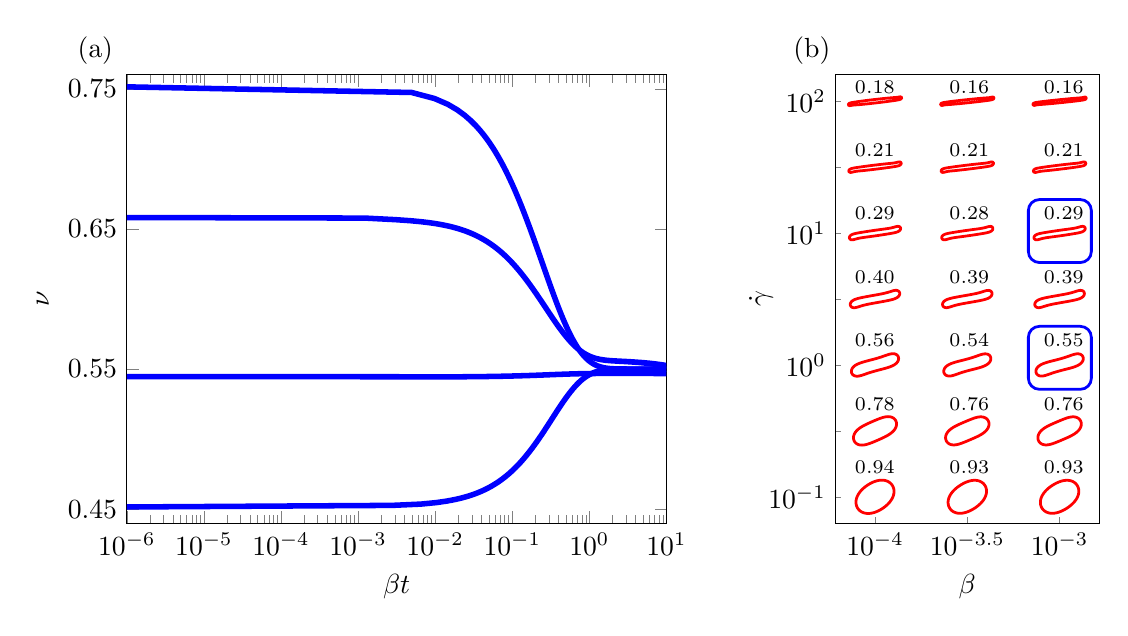
\begin{tikzpicture}[scale=1.0]

\pgfmathsetlengthmacro\MajorTickLength{
      \pgfkeysvalueof{/pgfplots/major tick length} * 0.5
    }


\begin{axis}[
  at = {(0.0cm,0.0cm)},
  xmin = 1e-6,
  xmax = 1e+1,
  xtick = {1e-6,1e-5,1e-4,1e-3,1e-2,1e-1,1e0,1e1},
%    xticklabels = {$$},
  ymin = 0.44,
  ymax = 0.76,
  ytick = {0.45,0.55,0.65,0.75},
  xlabel = {$\beta t$},
  ylabel = {$\nu$},
  ylabel near ticks,
  xmode = log,
%    legend entries = {$\beta=10^{0}$,
%    $\beta = 10^{-1}$,
%    $\beta = 10^{-2}$,
%    $\beta = 10^{-3}$,
%    $\beta = 10^{-4}$,
%    $\beta = 10^{-5}$},
%    legend cell align=left,
%    legend style={draw=none,font=\small},
%    legend style={at={(0.05,0.95)},anchor=north west}
]

\addplot[blue, line width=2pt] coordinates{
(1.3847e-07,4.5127e-01)
(2.7733e-03,4.5270e-01)
(6.5404e-03,4.5362e-01)
(1.0363e-02,4.5469e-01)
(1.4191e-02,4.5578e-01)
(1.8017e-02,4.5686e-01)
(2.1842e-02,4.5793e-01)
(2.5664e-02,4.5898e-01)
(2.9484e-02,4.6003e-01)
(3.3303e-02,4.6106e-01)
(3.7119e-02,4.6209e-01)
(4.0934e-02,4.6310e-01)
(4.4747e-02,4.6410e-01)
(4.8558e-02,4.6508e-01)
(5.2368e-02,4.6606e-01)
(5.6176e-02,4.6703e-01)
(5.9982e-02,4.6798e-01)
(6.3787e-02,4.6893e-01)
(6.7591e-02,4.6986e-01)
(7.1393e-02,4.7079e-01)
(7.5194e-02,4.7170e-01)
(7.8994e-02,4.7261e-01)
(8.2793e-02,4.7350e-01)
(8.6590e-02,4.7439e-01)
(9.0386e-02,4.7526e-01)
(9.4181e-02,4.7613e-01)
(9.7975e-02,4.7698e-01)
(1.0177e-01,4.7783e-01)
(1.0556e-01,4.7867e-01)
(1.0935e-01,4.7949e-01)
(1.1314e-01,4.8031e-01)
(1.1693e-01,4.8112e-01)
(1.2072e-01,4.8192e-01)
(1.2451e-01,4.8271e-01)
(1.2829e-01,4.8349e-01)
(1.3208e-01,4.8427e-01)
(1.3587e-01,4.8503e-01)
(1.3965e-01,4.8579e-01)
(1.4343e-01,4.8654e-01)
(1.4722e-01,4.8728e-01)
(1.5100e-01,4.8801e-01)
(1.5478e-01,4.8874e-01)
(1.5856e-01,4.8945e-01)
(1.6235e-01,4.9016e-01)
(1.6613e-01,4.9086e-01)
(1.6991e-01,4.9155e-01)
(1.7369e-01,4.9224e-01)
(1.7747e-01,4.9291e-01)
(1.8124e-01,4.9358e-01)
(1.8502e-01,4.9424e-01)
(1.8880e-01,4.9490e-01)
(1.9258e-01,4.9554e-01)
(1.9636e-01,4.9618e-01)
(2.0013e-01,4.9682e-01)
(2.0391e-01,4.9744e-01)
(2.0769e-01,4.9806e-01)
(2.1146e-01,4.9867e-01)
(2.1524e-01,4.9928e-01)
(2.1901e-01,4.9987e-01)
(2.2279e-01,5.0047e-01)
(2.2657e-01,5.0105e-01)
(2.3034e-01,5.0163e-01)
(2.3412e-01,5.0220e-01)
(2.3789e-01,5.0276e-01)
(2.4166e-01,5.0332e-01)
(2.4544e-01,5.0387e-01)
(2.4921e-01,5.0442e-01)
(2.5299e-01,5.0496e-01)
(2.5676e-01,5.0549e-01)
(2.6054e-01,5.0602e-01)
(2.6431e-01,5.0654e-01)
(2.6808e-01,5.0706e-01)
(2.7186e-01,5.0757e-01)
(2.7563e-01,5.0807e-01)
(2.7940e-01,5.0857e-01)
(2.8318e-01,5.0906e-01)
(2.8695e-01,5.0955e-01)
(2.9072e-01,5.1003e-01)
(2.9450e-01,5.1051e-01)
(2.9827e-01,5.1098e-01)
(3.0204e-01,5.1144e-01)
(3.0582e-01,5.1190e-01)
(3.0959e-01,5.1236e-01)
(3.1337e-01,5.1281e-01)
(3.1714e-01,5.1325e-01)
(3.2091e-01,5.1369e-01)
(3.2469e-01,5.1412e-01)
(3.2846e-01,5.1455e-01)
(3.3223e-01,5.1498e-01)
(3.3601e-01,5.1540e-01)
(3.3978e-01,5.1581e-01)
(3.4355e-01,5.1622e-01)
(3.4733e-01,5.1662e-01)
(3.5110e-01,5.1702e-01)
(3.5488e-01,5.1742e-01)
(3.5865e-01,5.1781e-01)
(3.6242e-01,5.1820e-01)
(3.6620e-01,5.1858e-01)
(3.6997e-01,5.1896e-01)
(3.7375e-01,5.1933e-01)
(3.7752e-01,5.1970e-01)
(3.8130e-01,5.2006e-01)
(3.8507e-01,5.2042e-01)
(3.8885e-01,5.2078e-01)
(3.9262e-01,5.2113e-01)
(3.9640e-01,5.2148e-01)
(4.0017e-01,5.2182e-01)
(4.0395e-01,5.2216e-01)
(4.0772e-01,5.2250e-01)
(4.1150e-01,5.2283e-01)
(4.1527e-01,5.2316e-01)
(4.1905e-01,5.2348e-01)
(4.2283e-01,5.2380e-01)
(4.2660e-01,5.2412e-01)
(4.3038e-01,5.2443e-01)
(4.3415e-01,5.2474e-01)
(4.3793e-01,5.2505e-01)
(4.4171e-01,5.2535e-01)
(4.4548e-01,5.2565e-01)
(4.4926e-01,5.2594e-01)
(4.5304e-01,5.2623e-01)
(4.5681e-01,5.2652e-01)
(4.6059e-01,5.2681e-01)
(4.6437e-01,5.2709e-01)
(4.6815e-01,5.2736e-01)
(4.7192e-01,5.2764e-01)
(4.7570e-01,5.2791e-01)
(4.7948e-01,5.2818e-01)
(4.8326e-01,5.2844e-01)
(4.8704e-01,5.2871e-01)
(4.9082e-01,5.2896e-01)
(4.9459e-01,5.2922e-01)
(4.9837e-01,5.2947e-01)
(5.0215e-01,5.2972e-01)
(5.0593e-01,5.2997e-01)
(5.0971e-01,5.3021e-01)
(5.1349e-01,5.3045e-01)
(5.1727e-01,5.3069e-01)
(5.2105e-01,5.3093e-01)
(5.2483e-01,5.3116e-01)
(5.2861e-01,5.3139e-01)
(5.3239e-01,5.3162e-01)
(5.3617e-01,5.3184e-01)
(5.3995e-01,5.3206e-01)
(5.4373e-01,5.3228e-01)
(5.4751e-01,5.3250e-01)
(5.5129e-01,5.3271e-01)
(5.5507e-01,5.3292e-01)
(5.5885e-01,5.3313e-01)
(5.6263e-01,5.3334e-01)
(5.6642e-01,5.3354e-01)
(5.7020e-01,5.3374e-01)
(5.7398e-01,5.3394e-01)
(5.7776e-01,5.3413e-01)
(5.8154e-01,5.3433e-01)
(5.8533e-01,5.3452e-01)
(5.8911e-01,5.3471e-01)
(5.9289e-01,5.3490e-01)
(5.9667e-01,5.3508e-01)
(6.0046e-01,5.3526e-01)
(6.0424e-01,5.3544e-01)
(6.0802e-01,5.3562e-01)
(6.1181e-01,5.3580e-01)
(6.1559e-01,5.3597e-01)
(6.1937e-01,5.3614e-01)
(6.2316e-01,5.3631e-01)
(6.2694e-01,5.3648e-01)
(6.3072e-01,5.3665e-01)
(6.3451e-01,5.3681e-01)
(6.3829e-01,5.3697e-01)
(6.4208e-01,5.3713e-01)
(6.4586e-01,5.3729e-01)
(6.4964e-01,5.3745e-01)
(6.5343e-01,5.3760e-01)
(6.5721e-01,5.3775e-01)
(6.6100e-01,5.3790e-01)
(6.6478e-01,5.3805e-01)
(6.6857e-01,5.3820e-01)
(6.7235e-01,5.3834e-01)
(6.7614e-01,5.3849e-01)
(6.7993e-01,5.3863e-01)
(6.8371e-01,5.3877e-01)
(6.8750e-01,5.3891e-01)
(6.9128e-01,5.3904e-01)
(6.9507e-01,5.3918e-01)
(6.9886e-01,5.3931e-01)
(7.0264e-01,5.3944e-01)
(7.0643e-01,5.3957e-01)
(7.1021e-01,5.3970e-01)
(7.1400e-01,5.3983e-01)
(7.1779e-01,5.3995e-01)
(7.2157e-01,5.4008e-01)
(7.2536e-01,5.4020e-01)
(7.2915e-01,5.4032e-01)
(7.3294e-01,5.4044e-01)
(7.3672e-01,5.4056e-01)
(7.4051e-01,5.4067e-01)
(7.4430e-01,5.4079e-01)
(7.4809e-01,5.4090e-01)
(7.5187e-01,5.4101e-01)
(7.5566e-01,5.4112e-01)
(7.5945e-01,5.4123e-01)
(7.6324e-01,5.4134e-01)
(7.6703e-01,5.4145e-01)
(7.7081e-01,5.4155e-01)
(7.7460e-01,5.4166e-01)
(7.7839e-01,5.4176e-01)
(7.8218e-01,5.4186e-01)
(7.8597e-01,5.4196e-01)
(7.8976e-01,5.4206e-01)
(7.9355e-01,5.4216e-01)
(7.9734e-01,5.4225e-01)
(8.0112e-01,5.4235e-01)
(8.0491e-01,5.4244e-01)
(8.0870e-01,5.4254e-01)
(8.1249e-01,5.4263e-01)
(8.1628e-01,5.4272e-01)
(8.2007e-01,5.4281e-01)
(8.2386e-01,5.4290e-01)
(8.2765e-01,5.4299e-01)
(8.3144e-01,5.4307e-01)
(8.3523e-01,5.4316e-01)
(8.3902e-01,5.4324e-01)
(8.4281e-01,5.4333e-01)
(8.4660e-01,5.4341e-01)
(8.5039e-01,5.4349e-01)
(8.5418e-01,5.4357e-01)
(8.5797e-01,5.4365e-01)
(8.6176e-01,5.4373e-01)
(8.6555e-01,5.4380e-01)
(8.6934e-01,5.4388e-01)
(8.7313e-01,5.4396e-01)
(8.7693e-01,5.4403e-01)
(8.8072e-01,5.4410e-01)
(8.8451e-01,5.4418e-01)
(8.8830e-01,5.4425e-01)
(8.9209e-01,5.4432e-01)
(8.9588e-01,5.4439e-01)
(8.9967e-01,5.4446e-01)
(9.0346e-01,5.4453e-01)
(9.0726e-01,5.4460e-01)
(9.1105e-01,5.4466e-01)
(9.1484e-01,5.4473e-01)
(9.1863e-01,5.4479e-01)
(9.2242e-01,5.4486e-01)
(9.2621e-01,5.4492e-01)
(9.3001e-01,5.4498e-01)
(9.3380e-01,5.4505e-01)
(9.3759e-01,5.4511e-01)
(9.4138e-01,5.4517e-01)
(9.4517e-01,5.4523e-01)
(9.4897e-01,5.4529e-01)
(9.5276e-01,5.4534e-01)
(9.5655e-01,5.4540e-01)
(9.6034e-01,5.4546e-01)
(9.6414e-01,5.4551e-01)
(9.6793e-01,5.4557e-01)
(9.7172e-01,5.4562e-01)
(9.7551e-01,5.4568e-01)
(9.7931e-01,5.4573e-01)
(9.8310e-01,5.4578e-01)
(9.8689e-01,5.4584e-01)
(9.9068e-01,5.4589e-01)
(9.9448e-01,5.4594e-01)
(9.9827e-01,5.4599e-01)
(1.0021e+00,5.4604e-01)
(1.0059e+00,5.4609e-01)
(1.0097e+00,5.4613e-01)
(1.0134e+00,5.4618e-01)
(1.0172e+00,5.4623e-01)
(1.0210e+00,5.4628e-01)
(1.0248e+00,5.4632e-01)
(1.0286e+00,5.4637e-01)
(1.0324e+00,5.4641e-01)
(1.0362e+00,5.4646e-01)
(1.0400e+00,5.4650e-01)
(1.0438e+00,5.4654e-01)
(1.0476e+00,5.4658e-01)
(1.0514e+00,5.4663e-01)
(1.0552e+00,5.4667e-01)
(1.0590e+00,5.4671e-01)
(1.0628e+00,5.4675e-01)
(1.0666e+00,5.4679e-01)
(1.0703e+00,5.4683e-01)
(1.0741e+00,5.4687e-01)
(1.0779e+00,5.4691e-01)
(1.0817e+00,5.4694e-01)
(1.0855e+00,5.4698e-01)
(1.0893e+00,5.4702e-01)
(1.0931e+00,5.4706e-01)
(1.0969e+00,5.4709e-01)
(1.1007e+00,5.4713e-01)
(1.1045e+00,5.4716e-01)
(1.1083e+00,5.4720e-01)
(1.1121e+00,5.4723e-01)
(1.1159e+00,5.4727e-01)
(1.1197e+00,5.4730e-01)
(1.1235e+00,5.4733e-01)
(1.1273e+00,5.4737e-01)
(1.1311e+00,5.4740e-01)
(1.1349e+00,5.4743e-01)
(1.1386e+00,5.4746e-01)
(1.1424e+00,5.4749e-01)
(1.1462e+00,5.4752e-01)
(1.1500e+00,5.4755e-01)
(1.1538e+00,5.4758e-01)
(1.1576e+00,5.4761e-01)
(1.1614e+00,5.4764e-01)
(1.1652e+00,5.4767e-01)
(1.1690e+00,5.4770e-01)
(1.1728e+00,5.4773e-01)
(1.1766e+00,5.4776e-01)
(1.1804e+00,5.4778e-01)
(1.1842e+00,5.4781e-01)
(1.1880e+00,5.4784e-01)
(1.1918e+00,5.4786e-01)
(1.1956e+00,5.4789e-01)
(1.1994e+00,5.4792e-01)
(1.2032e+00,5.4794e-01)
(1.2070e+00,5.4797e-01)
(1.2108e+00,5.4799e-01)
(1.2145e+00,5.4802e-01)
(1.2183e+00,5.4804e-01)
(1.2221e+00,5.4806e-01)
(1.2259e+00,5.4809e-01)
(1.2297e+00,5.4811e-01)
(1.2335e+00,5.4813e-01)
(1.2373e+00,5.4816e-01)
(1.2411e+00,5.4818e-01)
(1.2449e+00,5.4820e-01)
(1.2487e+00,5.4822e-01)
(1.2525e+00,5.4825e-01)
(1.2563e+00,5.4827e-01)
(1.2601e+00,5.4829e-01)
(1.2639e+00,5.4831e-01)
(1.2677e+00,5.4833e-01)
(1.2715e+00,5.4835e-01)
(1.2753e+00,5.4837e-01)
(1.2791e+00,5.4839e-01)
(1.2829e+00,5.4841e-01)
(1.2867e+00,5.4843e-01)
(1.2905e+00,5.4845e-01)
(1.2943e+00,5.4847e-01)
(1.2981e+00,5.4848e-01)
(1.3018e+00,5.4850e-01)
(1.3056e+00,5.4852e-01)
(1.3094e+00,5.4854e-01)
(1.3132e+00,5.4856e-01)
(1.3170e+00,5.4857e-01)
(1.3208e+00,5.4859e-01)
(1.3246e+00,5.4861e-01)
(1.3284e+00,5.4863e-01)
(1.3322e+00,5.4864e-01)
(1.3360e+00,5.4866e-01)
(1.3398e+00,5.4867e-01)
(1.3436e+00,5.4869e-01)
(1.3474e+00,5.4871e-01)
(1.3512e+00,5.4872e-01)
(1.3550e+00,5.4874e-01)
(1.3588e+00,5.4875e-01)
(1.3626e+00,5.4877e-01)
(1.3664e+00,5.4878e-01)
(1.3702e+00,5.4880e-01)
(1.3740e+00,5.4881e-01)
(1.3778e+00,5.4883e-01)
(1.3816e+00,5.4884e-01)
(1.3854e+00,5.4885e-01)
(1.3892e+00,5.4887e-01)
(1.3930e+00,5.4888e-01)
(1.3968e+00,5.4889e-01)
(1.4006e+00,5.4891e-01)
(1.4043e+00,5.4892e-01)
(1.4081e+00,5.4893e-01)
(1.4119e+00,5.4895e-01)
(1.4157e+00,5.4896e-01)
(1.4195e+00,5.4897e-01)
(1.4233e+00,5.4898e-01)
(1.4271e+00,5.4900e-01)
(1.4309e+00,5.4901e-01)
(1.4347e+00,5.4902e-01)
(1.4385e+00,5.4903e-01)
(1.4423e+00,5.4904e-01)
(1.4461e+00,5.4905e-01)
(1.4499e+00,5.4907e-01)
(1.4537e+00,5.4908e-01)
(1.4575e+00,5.4909e-01)
(1.4613e+00,5.4910e-01)
(1.4651e+00,5.4911e-01)
(1.4689e+00,5.4912e-01)
(1.4727e+00,5.4913e-01)
(1.4765e+00,5.4914e-01)
(1.4803e+00,5.4915e-01)
(1.4841e+00,5.4916e-01)
(1.4879e+00,5.4917e-01)
(1.4917e+00,5.4918e-01)
(1.4955e+00,5.4919e-01)
(1.4993e+00,5.4920e-01)
(1.5031e+00,5.4921e-01)
(1.5069e+00,5.4922e-01)
(1.5107e+00,5.4923e-01)
(1.5145e+00,5.4924e-01)
(1.5182e+00,5.4925e-01)
(1.5220e+00,5.4925e-01)
(1.5258e+00,5.4926e-01)
(1.5296e+00,5.4927e-01)
(1.5334e+00,5.4928e-01)
(1.5372e+00,5.4929e-01)
(1.5410e+00,5.4930e-01)
(1.5448e+00,5.4931e-01)
(1.5486e+00,5.4931e-01)
(1.5524e+00,5.4932e-01)
(1.5562e+00,5.4933e-01)
(1.5600e+00,5.4934e-01)
(1.5638e+00,5.4934e-01)
(1.5676e+00,5.4935e-01)
(1.5714e+00,5.4936e-01)
(1.5752e+00,5.4937e-01)
(1.5790e+00,5.4937e-01)
(1.5828e+00,5.4938e-01)
(1.5866e+00,5.4939e-01)
(1.5904e+00,5.4940e-01)
(1.5942e+00,5.4940e-01)
(1.5980e+00,5.4941e-01)
(1.6018e+00,5.4942e-01)
(1.6056e+00,5.4942e-01)
(1.6094e+00,5.4943e-01)
(1.6132e+00,5.4944e-01)
(1.6170e+00,5.4944e-01)
(1.6208e+00,5.4945e-01)
(1.6246e+00,5.4946e-01)
(1.6284e+00,5.4946e-01)
(1.6322e+00,5.4947e-01)
(1.6360e+00,5.4947e-01)
(1.6398e+00,5.4948e-01)
(1.6436e+00,5.4949e-01)
(1.6473e+00,5.4949e-01)
(1.6511e+00,5.4950e-01)
(1.6549e+00,5.4950e-01)
(1.6587e+00,5.4951e-01)
(1.6625e+00,5.4951e-01)
(1.6663e+00,5.4952e-01)
(1.6701e+00,5.4953e-01)
(1.6739e+00,5.4953e-01)
(1.6777e+00,5.4954e-01)
(1.6815e+00,5.4954e-01)
(1.6853e+00,5.4955e-01)
(1.6891e+00,5.4955e-01)
(1.6929e+00,5.4956e-01)
(1.6967e+00,5.4956e-01)
(1.7005e+00,5.4957e-01)
(1.7043e+00,5.4957e-01)
(1.7081e+00,5.4958e-01)
(1.7119e+00,5.4958e-01)
(1.7157e+00,5.4959e-01)
(1.7195e+00,5.4959e-01)
(1.7233e+00,5.4959e-01)
(1.7271e+00,5.4960e-01)
(1.7309e+00,5.4960e-01)
(1.7347e+00,5.4961e-01)
(1.7385e+00,5.4961e-01)
(1.7423e+00,5.4962e-01)
(1.7461e+00,5.4962e-01)
(1.7499e+00,5.4962e-01)
(1.7537e+00,5.4963e-01)
(1.7575e+00,5.4963e-01)
(1.7613e+00,5.4964e-01)
(1.7651e+00,5.4964e-01)
(1.7689e+00,5.4964e-01)
(1.7727e+00,5.4965e-01)
(1.7765e+00,5.4965e-01)
(1.7803e+00,5.4966e-01)
(1.7841e+00,5.4966e-01)
(1.7878e+00,5.4966e-01)
(1.7916e+00,5.4967e-01)
(1.7954e+00,5.4967e-01)
(1.7992e+00,5.4967e-01)
(1.8030e+00,5.4968e-01)
(1.8068e+00,5.4968e-01)
(1.8106e+00,5.4968e-01)
(1.8144e+00,5.4969e-01)
(1.8182e+00,5.4969e-01)
(1.8220e+00,5.4969e-01)
(1.8258e+00,5.4970e-01)
(1.8296e+00,5.4970e-01)
(1.8334e+00,5.4970e-01)
(1.8372e+00,5.4971e-01)
(1.8410e+00,5.4971e-01)
(1.8448e+00,5.4971e-01)
(1.8486e+00,5.4972e-01)
(1.8524e+00,5.4972e-01)
(1.8562e+00,5.4972e-01)
(1.8600e+00,5.4972e-01)
(1.8638e+00,5.4973e-01)
(1.8676e+00,5.4973e-01)
(1.8714e+00,5.4973e-01)
(1.8752e+00,5.4974e-01)
(1.8790e+00,5.4974e-01)
(1.8828e+00,5.4974e-01)
(1.8866e+00,5.4974e-01)
(1.8904e+00,5.4975e-01)
(1.8942e+00,5.4975e-01)
(1.8980e+00,5.4975e-01)
(1.9018e+00,5.4975e-01)
(1.9056e+00,5.4976e-01)
(1.9094e+00,5.4976e-01)
(1.9132e+00,5.4976e-01)
(1.9170e+00,5.4976e-01)
(1.9208e+00,5.4977e-01)
(1.9246e+00,5.4977e-01)
(1.9284e+00,5.4977e-01)
(1.9322e+00,5.4977e-01)
(1.9360e+00,5.4977e-01)
(1.9397e+00,5.4978e-01)
(1.9435e+00,5.4978e-01)
(1.9473e+00,5.4978e-01)
(1.9511e+00,5.4978e-01)
(1.9549e+00,5.4978e-01)
(1.9587e+00,5.4979e-01)
(1.9625e+00,5.4979e-01)
(1.9663e+00,5.4979e-01)
(1.9701e+00,5.4979e-01)
(1.9739e+00,5.4979e-01)
(1.9777e+00,5.4980e-01)
(1.9815e+00,5.4980e-01)
(1.9853e+00,5.4980e-01)
(1.9891e+00,5.4980e-01)
(1.9929e+00,5.4980e-01)
(1.9967e+00,5.4981e-01)
(2.0005e+00,5.4981e-01)
(2.0043e+00,5.4981e-01)
(2.0081e+00,5.4981e-01)
(2.0119e+00,5.4981e-01)
(2.0157e+00,5.4981e-01)
(2.0195e+00,5.4982e-01)
(2.0233e+00,5.4982e-01)
(2.0271e+00,5.4982e-01)
(2.0309e+00,5.4982e-01)
(2.0347e+00,5.4982e-01)
(2.0385e+00,5.4982e-01)
(2.0423e+00,5.4983e-01)
(2.0461e+00,5.4983e-01)
(2.0499e+00,5.4983e-01)
(2.0537e+00,5.4983e-01)
(2.0575e+00,5.4983e-01)
(2.0613e+00,5.4983e-01)
(2.0651e+00,5.4983e-01)
(2.0689e+00,5.4984e-01)
(2.0727e+00,5.4984e-01)
(2.0765e+00,5.4984e-01)
(2.0803e+00,5.4984e-01)
(2.0841e+00,5.4984e-01)
(2.0879e+00,5.4984e-01)
(2.0917e+00,5.4984e-01)
(2.0955e+00,5.4985e-01)
(2.0992e+00,5.4985e-01)
(2.1030e+00,5.4985e-01)
(2.1068e+00,5.4985e-01)
(2.1106e+00,5.4985e-01)
(2.1144e+00,5.4985e-01)
(2.1182e+00,5.4985e-01)
(2.1220e+00,5.4985e-01)
(2.1258e+00,5.4986e-01)
(2.1296e+00,5.4986e-01)
(2.1334e+00,5.4986e-01)
(2.1372e+00,5.4986e-01)
(2.1410e+00,5.4986e-01)
(2.1448e+00,5.4986e-01)
(2.1486e+00,5.4986e-01)
(2.1524e+00,5.4986e-01)
(2.1562e+00,5.4986e-01)
(2.1600e+00,5.4987e-01)
(2.1638e+00,5.4987e-01)
(2.1676e+00,5.4987e-01)
(2.1714e+00,5.4987e-01)
(2.1752e+00,5.4987e-01)
(2.1790e+00,5.4987e-01)
(2.1828e+00,5.4987e-01)
(2.1866e+00,5.4987e-01)
(2.1904e+00,5.4987e-01)
(2.1942e+00,5.4987e-01)
(2.1980e+00,5.4987e-01)
(2.2018e+00,5.4988e-01)
(2.2056e+00,5.4988e-01)
(2.2094e+00,5.4988e-01)
(2.2132e+00,5.4988e-01)
(2.2170e+00,5.4988e-01)
(2.2208e+00,5.4988e-01)
(2.2246e+00,5.4988e-01)
(2.2284e+00,5.4988e-01)
(2.2322e+00,5.4988e-01)
(2.2360e+00,5.4988e-01)
(2.2398e+00,5.4988e-01)
(2.2436e+00,5.4988e-01)
(2.2474e+00,5.4989e-01)
(2.2512e+00,5.4989e-01)
(2.2550e+00,5.4989e-01)
(2.2588e+00,5.4989e-01)
(2.2626e+00,5.4989e-01)
(2.2663e+00,5.4989e-01)
(2.2701e+00,5.4989e-01)
(2.2739e+00,5.4989e-01)
(2.2777e+00,5.4989e-01)
(2.2815e+00,5.4989e-01)
(2.2853e+00,5.4989e-01)
(2.2891e+00,5.4989e-01)
(2.2929e+00,5.4989e-01)
(2.2967e+00,5.4989e-01)
(2.3005e+00,5.4990e-01)
(2.3043e+00,5.4990e-01)
(2.3081e+00,5.4990e-01)
(2.3119e+00,5.4990e-01)
(2.3157e+00,5.4990e-01)
(2.3195e+00,5.4990e-01)
(2.3233e+00,5.4990e-01)
(2.3271e+00,5.4990e-01)
(2.3309e+00,5.4990e-01)
(2.3347e+00,5.4990e-01)
(2.3385e+00,5.4990e-01)
(2.3423e+00,5.4990e-01)
(2.3461e+00,5.4990e-01)
(2.3499e+00,5.4990e-01)
(2.3537e+00,5.4990e-01)
(2.3575e+00,5.4990e-01)
(2.3613e+00,5.4990e-01)
(2.3651e+00,5.4991e-01)
(2.3689e+00,5.4991e-01)
(2.3727e+00,5.4991e-01)
(2.3765e+00,5.4991e-01)
(2.3803e+00,5.4991e-01)
(2.3841e+00,5.4991e-01)
(2.3879e+00,5.4991e-01)
(2.3917e+00,5.4991e-01)
(2.3955e+00,5.4991e-01)
(2.3993e+00,5.4991e-01)
(2.4031e+00,5.4991e-01)
(2.4069e+00,5.4991e-01)
(2.4107e+00,5.4991e-01)
(2.4145e+00,5.4991e-01)
(2.4183e+00,5.4991e-01)
(2.4221e+00,5.4991e-01)
(2.4259e+00,5.4991e-01)
(2.4297e+00,5.4991e-01)
(2.4334e+00,5.4991e-01)
(2.4372e+00,5.4991e-01)
(2.4410e+00,5.4991e-01)
(2.4448e+00,5.4991e-01)
(2.4486e+00,5.4991e-01)
(2.4524e+00,5.4992e-01)
(2.4562e+00,5.4992e-01)
(2.4600e+00,5.4992e-01)
(2.4638e+00,5.4992e-01)
(2.4676e+00,5.4992e-01)
(2.4714e+00,5.4992e-01)
(2.4752e+00,5.4992e-01)
(2.4790e+00,5.4992e-01)
(2.4828e+00,5.4992e-01)
(2.4866e+00,5.4992e-01)
(2.4904e+00,5.4992e-01)
(2.4942e+00,5.4992e-01)
(2.4980e+00,5.4992e-01)
(2.5018e+00,5.4992e-01)
(2.5056e+00,5.4992e-01)
(2.5094e+00,5.4992e-01)
(2.5132e+00,5.4992e-01)
(2.5170e+00,5.4992e-01)
(2.5208e+00,5.4992e-01)
(2.5246e+00,5.4992e-01)
(2.5284e+00,5.4992e-01)
(2.5322e+00,5.4992e-01)
(2.5360e+00,5.4992e-01)
(2.5398e+00,5.4992e-01)
(2.5436e+00,5.4992e-01)
(2.5474e+00,5.4992e-01)
(2.5512e+00,5.4992e-01)
(2.5550e+00,5.4992e-01)
(2.5588e+00,5.4992e-01)
(2.5626e+00,5.4992e-01)
(2.5664e+00,5.4992e-01)
(2.5702e+00,5.4992e-01)
(2.5740e+00,5.4992e-01)
(2.5778e+00,5.4992e-01)
(2.5816e+00,5.4993e-01)
(2.5854e+00,5.4993e-01)
(2.5892e+00,5.4993e-01)
(2.5930e+00,5.4993e-01)
(2.5968e+00,5.4993e-01)
(2.6006e+00,5.4993e-01)
(2.6043e+00,5.4993e-01)
(2.6081e+00,5.4993e-01)
(2.6119e+00,5.4993e-01)
(2.6157e+00,5.4993e-01)
(2.6195e+00,5.4993e-01)
(2.6233e+00,5.4993e-01)
(2.6271e+00,5.4993e-01)
(2.6309e+00,5.4993e-01)
(2.6347e+00,5.4993e-01)
(2.6385e+00,5.4993e-01)
(2.6423e+00,5.4993e-01)
(2.6461e+00,5.4993e-01)
(2.6499e+00,5.4993e-01)
(2.6537e+00,5.4993e-01)
(2.6575e+00,5.4993e-01)
(2.6613e+00,5.4993e-01)
(2.6651e+00,5.4993e-01)
(2.6689e+00,5.4993e-01)
(2.6727e+00,5.4993e-01)
(2.6765e+00,5.4993e-01)
(2.6803e+00,5.4993e-01)
(2.6841e+00,5.4993e-01)
(2.6879e+00,5.4993e-01)
(2.6917e+00,5.4993e-01)
(2.6955e+00,5.4993e-01)
(2.6993e+00,5.4993e-01)
(2.7031e+00,5.4993e-01)
(2.7069e+00,5.4993e-01)
(2.7107e+00,5.4993e-01)
(2.7145e+00,5.4993e-01)
(2.7183e+00,5.4993e-01)
(2.7221e+00,5.4993e-01)
(2.7259e+00,5.4993e-01)
(2.7297e+00,5.4993e-01)
(2.7335e+00,5.4993e-01)
(2.7373e+00,5.4993e-01)
(2.7411e+00,5.4993e-01)
(2.7449e+00,5.4993e-01)
(2.7487e+00,5.4993e-01)
(2.7525e+00,5.4993e-01)
(2.7563e+00,5.4993e-01)
(2.7601e+00,5.4993e-01)
(2.7639e+00,5.4993e-01)
(2.7677e+00,5.4993e-01)
(2.7715e+00,5.4993e-01)
(2.7752e+00,5.4993e-01)
(2.7790e+00,5.4993e-01)
(2.7828e+00,5.4993e-01)
(2.7866e+00,5.4993e-01)
(2.7904e+00,5.4993e-01)
(2.7942e+00,5.4993e-01)
(2.7980e+00,5.4993e-01)
(2.8018e+00,5.4993e-01)
(2.8056e+00,5.4993e-01)
(2.8094e+00,5.4993e-01)
(2.8132e+00,5.4993e-01)
(2.8170e+00,5.4993e-01)
(2.8208e+00,5.4993e-01)
(2.8246e+00,5.4993e-01)
(2.8284e+00,5.4993e-01)
(2.8322e+00,5.4993e-01)
(2.8360e+00,5.4993e-01)
(2.8398e+00,5.4993e-01)
(2.8436e+00,5.4993e-01)
(2.8474e+00,5.4993e-01)
(2.8512e+00,5.4994e-01)
(2.8550e+00,5.4994e-01)
(2.8588e+00,5.4994e-01)
(2.8626e+00,5.4994e-01)
(2.8664e+00,5.4994e-01)
(2.8702e+00,5.4994e-01)
(2.8740e+00,5.4994e-01)
(2.8778e+00,5.4994e-01)
(2.8816e+00,5.4994e-01)
(2.8854e+00,5.4994e-01)
(2.8892e+00,5.4994e-01)
(2.8930e+00,5.4994e-01)
(2.8968e+00,5.4994e-01)
(2.9006e+00,5.4994e-01)
(2.9044e+00,5.4994e-01)
(2.9082e+00,5.4994e-01)
(2.9120e+00,5.4994e-01)
(2.9158e+00,5.4994e-01)
(2.9196e+00,5.4994e-01)
(2.9234e+00,5.4994e-01)
(2.9272e+00,5.4994e-01)
(2.9310e+00,5.4994e-01)
(2.9348e+00,5.4994e-01)
(2.9386e+00,5.4994e-01)
(2.9424e+00,5.4994e-01)
(2.9462e+00,5.4994e-01)
(2.9499e+00,5.4994e-01)
(2.9537e+00,5.4994e-01)
(2.9575e+00,5.4994e-01)
(2.9613e+00,5.4994e-01)
(2.9651e+00,5.4994e-01)
(2.9689e+00,5.4994e-01)
(2.9727e+00,5.4994e-01)
(2.9765e+00,5.4994e-01)
(2.9803e+00,5.4994e-01)
(2.9841e+00,5.4994e-01)
(2.9879e+00,5.4994e-01)
(2.9917e+00,5.4994e-01)
(2.9955e+00,5.4994e-01)
(2.9993e+00,5.4994e-01)
(3.0031e+00,5.4994e-01)
(3.0069e+00,5.4994e-01)
(3.0107e+00,5.4994e-01)
(3.0145e+00,5.4994e-01)
(3.0183e+00,5.4994e-01)
(3.0221e+00,5.4994e-01)
(3.0259e+00,5.4994e-01)
(3.0297e+00,5.4994e-01)
(3.0335e+00,5.4994e-01)
(3.0373e+00,5.4994e-01)
(3.0411e+00,5.4994e-01)
(3.0449e+00,5.4994e-01)
(3.0487e+00,5.4994e-01)
(3.0525e+00,5.4994e-01)
(3.0563e+00,5.4994e-01)
(3.0601e+00,5.4994e-01)
(3.0639e+00,5.4994e-01)
(3.0677e+00,5.4994e-01)
(3.0715e+00,5.4994e-01)
(3.0753e+00,5.4994e-01)
(3.0791e+00,5.4994e-01)
(3.0829e+00,5.4994e-01)
(3.0867e+00,5.4994e-01)
(3.0905e+00,5.4994e-01)
(3.0943e+00,5.4994e-01)
(3.0981e+00,5.4994e-01)
(3.1019e+00,5.4994e-01)
(3.1057e+00,5.4994e-01)
(3.1095e+00,5.4994e-01)
(3.1133e+00,5.4994e-01)
(3.1171e+00,5.4994e-01)
(3.1208e+00,5.4994e-01)
(3.1246e+00,5.4994e-01)
(3.1284e+00,5.4994e-01)
(3.1322e+00,5.4994e-01)
(3.1360e+00,5.4994e-01)
(3.1398e+00,5.4994e-01)
(3.1436e+00,5.4994e-01)
(3.1474e+00,5.4994e-01)
(3.1512e+00,5.4994e-01)
(3.1550e+00,5.4994e-01)
(3.1588e+00,5.4994e-01)
(3.1626e+00,5.4994e-01)
(3.1664e+00,5.4994e-01)
(3.1702e+00,5.4994e-01)
(3.1740e+00,5.4994e-01)
(3.1778e+00,5.4994e-01)
(3.1816e+00,5.4994e-01)
(3.1854e+00,5.4994e-01)
(3.1892e+00,5.4994e-01)
(3.1930e+00,5.4994e-01)
(3.1968e+00,5.4994e-01)
(3.2006e+00,5.4994e-01)
(3.2044e+00,5.4994e-01)
(3.2082e+00,5.4994e-01)
(3.2120e+00,5.4994e-01)
(3.2158e+00,5.4994e-01)
(3.2196e+00,5.4994e-01)
(3.2234e+00,5.4994e-01)
(3.2272e+00,5.4994e-01)
(3.2310e+00,5.4994e-01)
(3.2348e+00,5.4994e-01)
(3.2386e+00,5.4994e-01)
(3.2424e+00,5.4994e-01)
(3.2462e+00,5.4994e-01)
(3.2500e+00,5.4994e-01)
(3.2538e+00,5.4994e-01)
(3.2576e+00,5.4994e-01)
(3.2614e+00,5.4994e-01)
(3.2652e+00,5.4994e-01)
(3.2690e+00,5.4994e-01)
(3.2728e+00,5.4994e-01)
(3.2766e+00,5.4994e-01)
(3.2804e+00,5.4994e-01)
(3.2842e+00,5.4994e-01)
(3.2880e+00,5.4994e-01)
(3.2918e+00,5.4994e-01)
(3.2955e+00,5.4994e-01)
(3.2993e+00,5.4994e-01)
(3.3031e+00,5.4994e-01)
(3.3069e+00,5.4994e-01)
(3.3107e+00,5.4994e-01)
(3.3145e+00,5.4994e-01)
(3.3183e+00,5.4994e-01)
(3.3221e+00,5.4994e-01)
(3.3259e+00,5.4994e-01)
(3.3297e+00,5.4994e-01)
(3.3335e+00,5.4994e-01)
(3.3373e+00,5.4994e-01)
(3.3411e+00,5.4994e-01)
(3.3449e+00,5.4994e-01)
(3.3487e+00,5.4994e-01)
(3.3525e+00,5.4994e-01)
(3.3563e+00,5.4994e-01)
(3.3601e+00,5.4994e-01)
(3.3639e+00,5.4994e-01)
(3.3677e+00,5.4994e-01)
(3.3715e+00,5.4994e-01)
(3.3753e+00,5.4994e-01)
(3.3791e+00,5.4994e-01)
(3.3829e+00,5.4994e-01)
(3.3867e+00,5.4994e-01)
(3.3905e+00,5.4994e-01)
(3.3943e+00,5.4994e-01)
(3.3981e+00,5.4994e-01)
(3.4019e+00,5.4994e-01)
(3.4057e+00,5.4994e-01)
(3.4095e+00,5.4994e-01)
(3.4133e+00,5.4994e-01)
(3.4171e+00,5.4994e-01)
(3.4209e+00,5.4994e-01)
(3.4247e+00,5.4994e-01)
(3.4285e+00,5.4994e-01)
(3.4323e+00,5.4994e-01)
(3.4361e+00,5.4994e-01)
(3.4399e+00,5.4994e-01)
(3.4437e+00,5.4994e-01)
(3.4475e+00,5.4994e-01)
(3.4513e+00,5.4994e-01)
(3.4551e+00,5.4994e-01)
(3.4589e+00,5.4994e-01)
(3.4627e+00,5.4994e-01)
(3.4665e+00,5.4994e-01)
(3.4702e+00,5.4994e-01)
(3.4740e+00,5.4994e-01)
(3.4778e+00,5.4994e-01)
(3.4816e+00,5.4994e-01)
(3.4854e+00,5.4994e-01)
(3.4892e+00,5.4994e-01)
(3.4930e+00,5.4994e-01)
(3.4968e+00,5.4994e-01)
(3.5006e+00,5.4994e-01)
(3.5044e+00,5.4994e-01)
(3.5082e+00,5.4994e-01)
(3.5120e+00,5.4994e-01)
(3.5158e+00,5.4994e-01)
(3.5196e+00,5.4994e-01)
(3.5234e+00,5.4994e-01)
(3.5272e+00,5.4994e-01)
(3.5310e+00,5.4994e-01)
(3.5348e+00,5.4994e-01)
(3.5386e+00,5.4994e-01)
(3.5424e+00,5.4994e-01)
(3.5462e+00,5.4994e-01)
(3.5500e+00,5.4994e-01)
(3.5538e+00,5.4994e-01)
(3.5576e+00,5.4994e-01)
(3.5614e+00,5.4994e-01)
(3.5652e+00,5.4994e-01)
(3.5690e+00,5.4994e-01)
(3.5728e+00,5.4994e-01)
(3.5766e+00,5.4994e-01)
(3.5804e+00,5.4994e-01)
(3.5842e+00,5.4994e-01)
(3.5880e+00,5.4994e-01)
(3.5918e+00,5.4994e-01)
(3.5956e+00,5.4994e-01)
(3.5994e+00,5.4994e-01)
(3.6032e+00,5.4994e-01)
(3.6070e+00,5.4994e-01)
(3.6108e+00,5.4994e-01)
(3.6146e+00,5.4994e-01)
(3.6184e+00,5.4994e-01)
(3.6222e+00,5.4994e-01)
(3.6260e+00,5.4994e-01)
(3.6298e+00,5.4994e-01)
(3.6336e+00,5.4994e-01)
(3.6374e+00,5.4994e-01)
(3.6412e+00,5.4994e-01)
(3.6449e+00,5.4994e-01)
(3.6487e+00,5.4994e-01)
(3.6525e+00,5.4994e-01)
(3.6563e+00,5.4994e-01)
(3.6601e+00,5.4994e-01)
(3.6639e+00,5.4994e-01)
(3.6677e+00,5.4994e-01)
(3.6715e+00,5.4994e-01)
(3.6753e+00,5.4994e-01)
(3.6791e+00,5.4994e-01)
(3.6829e+00,5.4994e-01)
(3.6867e+00,5.4994e-01)
(3.6905e+00,5.4994e-01)
(3.6943e+00,5.4994e-01)
(3.6981e+00,5.4994e-01)
(3.7019e+00,5.4994e-01)
(3.7057e+00,5.4994e-01)
(3.7095e+00,5.4994e-01)
(3.7133e+00,5.4994e-01)
(3.7171e+00,5.4994e-01)
(3.7209e+00,5.4994e-01)
(3.7247e+00,5.4994e-01)
(3.7285e+00,5.4994e-01)
(3.7323e+00,5.4994e-01)
(3.7361e+00,5.4994e-01)
(3.7399e+00,5.4994e-01)
(3.7437e+00,5.4994e-01)
(3.7475e+00,5.4994e-01)
(3.7513e+00,5.4994e-01)
(3.7551e+00,5.4994e-01)
(3.7589e+00,5.4994e-01)
(3.7627e+00,5.4994e-01)
(3.7665e+00,5.4994e-01)
(3.7703e+00,5.4994e-01)
(3.7741e+00,5.4994e-01)
(3.7779e+00,5.4993e-01)
(3.7817e+00,5.4993e-01)
(3.7855e+00,5.4993e-01)
(3.7893e+00,5.4993e-01)
(3.7931e+00,5.4993e-01)
(3.7969e+00,5.4993e-01)
(3.8007e+00,5.4993e-01)
(3.8045e+00,5.4993e-01)
(3.8083e+00,5.4993e-01)
(3.8121e+00,5.4993e-01)
(3.8159e+00,5.4993e-01)
(3.8197e+00,5.4993e-01)
(3.8234e+00,5.4993e-01)
(3.8272e+00,5.4993e-01)
(3.8310e+00,5.4993e-01)
(3.8348e+00,5.4993e-01)
(3.8386e+00,5.4993e-01)
(3.8424e+00,5.4993e-01)
(3.8462e+00,5.4993e-01)
(3.8500e+00,5.4993e-01)
(3.8538e+00,5.4993e-01)
(3.8576e+00,5.4993e-01)
(3.8614e+00,5.4993e-01)
(3.8652e+00,5.4993e-01)
(3.8690e+00,5.4993e-01)
(3.8728e+00,5.4993e-01)
(3.8766e+00,5.4993e-01)
(3.8804e+00,5.4993e-01)
(3.8842e+00,5.4993e-01)
(3.8880e+00,5.4993e-01)
(3.8918e+00,5.4993e-01)
(3.8956e+00,5.4993e-01)
(3.8994e+00,5.4993e-01)
(3.9032e+00,5.4993e-01)
(3.9070e+00,5.4993e-01)
(3.9108e+00,5.4993e-01)
(3.9146e+00,5.4993e-01)
(3.9184e+00,5.4993e-01)
(3.9222e+00,5.4993e-01)
(3.9260e+00,5.4993e-01)
(3.9298e+00,5.4993e-01)
(3.9336e+00,5.4993e-01)
(3.9374e+00,5.4993e-01)
(3.9412e+00,5.4993e-01)
(3.9450e+00,5.4993e-01)
(3.9488e+00,5.4993e-01)
(3.9526e+00,5.4993e-01)
(3.9564e+00,5.4993e-01)
(3.9602e+00,5.4993e-01)
(3.9640e+00,5.4993e-01)
(3.9678e+00,5.4993e-01)
(3.9716e+00,5.4993e-01)
(3.9754e+00,5.4993e-01)
(3.9792e+00,5.4993e-01)
(3.9830e+00,5.4993e-01)
(3.9868e+00,5.4993e-01)
(3.9906e+00,5.4993e-01)
(3.9944e+00,5.4993e-01)
(3.9981e+00,5.4993e-01)
(4.0019e+00,5.4993e-01)
(4.0057e+00,5.4993e-01)
(4.0095e+00,5.4993e-01)
(4.0133e+00,5.4993e-01)
(4.0171e+00,5.4993e-01)
(4.0209e+00,5.4993e-01)
(4.0247e+00,5.4993e-01)
(4.0285e+00,5.4993e-01)
(4.0323e+00,5.4993e-01)
(4.0361e+00,5.4993e-01)
(4.0399e+00,5.4993e-01)
(4.0437e+00,5.4993e-01)
(4.0475e+00,5.4993e-01)
(4.0513e+00,5.4993e-01)
(4.0551e+00,5.4993e-01)
(4.0589e+00,5.4993e-01)
(4.0627e+00,5.4993e-01)
(4.0665e+00,5.4993e-01)
(4.0703e+00,5.4993e-01)
(4.0741e+00,5.4993e-01)
(4.0779e+00,5.4993e-01)
(4.0817e+00,5.4993e-01)
(4.0855e+00,5.4993e-01)
(4.0893e+00,5.4993e-01)
(4.0931e+00,5.4993e-01)
(4.0969e+00,5.4993e-01)
(4.1007e+00,5.4993e-01)
(4.1045e+00,5.4993e-01)
(4.1083e+00,5.4993e-01)
(4.1121e+00,5.4993e-01)
(4.1159e+00,5.4993e-01)
(4.1197e+00,5.4993e-01)
(4.1235e+00,5.4993e-01)
(4.1273e+00,5.4993e-01)
(4.1311e+00,5.4993e-01)
(4.1349e+00,5.4993e-01)
(4.1387e+00,5.4993e-01)
(4.1425e+00,5.4993e-01)
(4.1463e+00,5.4993e-01)
(4.1501e+00,5.4993e-01)
(4.1539e+00,5.4993e-01)
(4.1577e+00,5.4993e-01)
(4.1615e+00,5.4993e-01)
(4.1653e+00,5.4993e-01)
(4.1691e+00,5.4993e-01)
(4.1729e+00,5.4993e-01)
(4.1766e+00,5.4993e-01)
(4.1804e+00,5.4993e-01)
(4.1842e+00,5.4993e-01)
(4.1880e+00,5.4993e-01)
(4.1918e+00,5.4993e-01)
(4.1956e+00,5.4993e-01)
(4.1994e+00,5.4993e-01)
(4.2032e+00,5.4993e-01)
(4.2070e+00,5.4993e-01)
(4.2108e+00,5.4993e-01)
(4.2146e+00,5.4993e-01)
(4.2184e+00,5.4993e-01)
(4.2222e+00,5.4993e-01)
(4.2260e+00,5.4993e-01)
(4.2298e+00,5.4993e-01)
(4.2336e+00,5.4993e-01)
(4.2374e+00,5.4993e-01)
(4.2412e+00,5.4993e-01)
(4.2450e+00,5.4993e-01)
(4.2488e+00,5.4993e-01)
(4.2526e+00,5.4993e-01)
(4.2564e+00,5.4993e-01)
(4.2602e+00,5.4993e-01)
(4.2640e+00,5.4993e-01)
(4.2678e+00,5.4993e-01)
(4.2716e+00,5.4993e-01)
(4.2754e+00,5.4993e-01)
(4.2792e+00,5.4993e-01)
(4.2830e+00,5.4993e-01)
(4.2868e+00,5.4993e-01)
(4.2906e+00,5.4993e-01)
(4.2944e+00,5.4993e-01)
(4.2982e+00,5.4993e-01)
(4.3020e+00,5.4993e-01)
(4.3058e+00,5.4993e-01)
(4.3096e+00,5.4993e-01)
(4.3134e+00,5.4993e-01)
(4.3172e+00,5.4993e-01)
(4.3210e+00,5.4993e-01)
(4.3248e+00,5.4993e-01)
(4.3286e+00,5.4993e-01)
(4.3324e+00,5.4993e-01)
(4.3362e+00,5.4993e-01)
(4.3400e+00,5.4993e-01)
(4.3438e+00,5.4993e-01)
(4.3476e+00,5.4993e-01)
(4.3513e+00,5.4993e-01)
(4.3551e+00,5.4993e-01)
(4.3589e+00,5.4993e-01)
(4.3627e+00,5.4993e-01)
(4.3665e+00,5.4993e-01)
(4.3703e+00,5.4993e-01)
(4.3741e+00,5.4993e-01)
(4.3779e+00,5.4993e-01)
(4.3817e+00,5.4993e-01)
(4.3855e+00,5.4993e-01)
(4.3893e+00,5.4993e-01)
(4.3931e+00,5.4993e-01)
(4.3969e+00,5.4993e-01)
(4.4007e+00,5.4993e-01)
(4.4045e+00,5.4993e-01)
(4.4083e+00,5.4993e-01)
(4.4121e+00,5.4993e-01)
(4.4159e+00,5.4993e-01)
(4.4197e+00,5.4993e-01)
(4.4235e+00,5.4993e-01)
(4.4273e+00,5.4993e-01)
(4.4311e+00,5.4993e-01)
(4.4349e+00,5.4993e-01)
(4.4387e+00,5.4993e-01)
(4.4425e+00,5.4993e-01)
(4.4463e+00,5.4993e-01)
(4.4501e+00,5.4993e-01)
(4.4539e+00,5.4993e-01)
(4.4577e+00,5.4993e-01)
(4.4615e+00,5.4993e-01)
(4.4653e+00,5.4993e-01)
(4.4691e+00,5.4993e-01)
(4.4729e+00,5.4993e-01)
(4.4767e+00,5.4993e-01)
(4.4805e+00,5.4993e-01)
(4.4843e+00,5.4993e-01)
(4.4881e+00,5.4993e-01)
(4.4919e+00,5.4993e-01)
(4.4957e+00,5.4993e-01)
(4.4995e+00,5.4993e-01)
(4.5033e+00,5.4993e-01)
(4.5071e+00,5.4993e-01)
(4.5109e+00,5.4993e-01)
(4.5147e+00,5.4993e-01)
(4.5185e+00,5.4993e-01)
(4.5223e+00,5.4993e-01)
(4.5261e+00,5.4993e-01)
(4.5298e+00,5.4993e-01)
(4.5336e+00,5.4993e-01)
(4.5374e+00,5.4993e-01)
(4.5412e+00,5.4993e-01)
(4.5450e+00,5.4993e-01)
(4.5488e+00,5.4993e-01)
(4.5526e+00,5.4993e-01)
(4.5564e+00,5.4993e-01)
(4.5602e+00,5.4993e-01)
(4.5640e+00,5.4993e-01)
(4.5678e+00,5.4993e-01)
(4.5716e+00,5.4993e-01)
(4.5754e+00,5.4993e-01)
(4.5792e+00,5.4993e-01)
(4.5830e+00,5.4993e-01)
(4.5868e+00,5.4993e-01)
(4.5906e+00,5.4993e-01)
(4.5944e+00,5.4993e-01)
(4.5982e+00,5.4993e-01)
(4.6020e+00,5.4993e-01)
(4.6058e+00,5.4993e-01)
(4.6096e+00,5.4993e-01)
(4.6134e+00,5.4993e-01)
(4.6172e+00,5.4993e-01)
(4.6210e+00,5.4993e-01)
(4.6248e+00,5.4993e-01)
(4.6286e+00,5.4993e-01)
(4.6324e+00,5.4993e-01)
(4.6362e+00,5.4993e-01)
(4.6400e+00,5.4993e-01)
(4.6438e+00,5.4993e-01)
(4.6476e+00,5.4993e-01)
(4.6514e+00,5.4993e-01)
(4.6552e+00,5.4993e-01)
(4.6590e+00,5.4993e-01)
(4.6628e+00,5.4993e-01)
(4.6666e+00,5.4993e-01)
(4.6704e+00,5.4993e-01)
(4.6742e+00,5.4993e-01)
(4.6780e+00,5.4993e-01)
(4.6818e+00,5.4993e-01)
(4.6856e+00,5.4993e-01)
(4.6894e+00,5.4993e-01)
(4.6932e+00,5.4993e-01)
(4.6970e+00,5.4993e-01)
(4.7008e+00,5.4993e-01)
(4.7046e+00,5.4993e-01)
(4.7083e+00,5.4993e-01)
(4.7121e+00,5.4993e-01)
(4.7159e+00,5.4993e-01)
(4.7197e+00,5.4993e-01)
(4.7235e+00,5.4993e-01)
(4.7273e+00,5.4993e-01)
(4.7311e+00,5.4993e-01)
(4.7349e+00,5.4993e-01)
(4.7387e+00,5.4993e-01)
(4.7425e+00,5.4993e-01)
(4.7463e+00,5.4993e-01)
(4.7501e+00,5.4993e-01)
(4.7539e+00,5.4993e-01)
(4.7577e+00,5.4993e-01)
(4.7615e+00,5.4993e-01)
(4.7653e+00,5.4993e-01)
(4.7691e+00,5.4993e-01)
(4.7729e+00,5.4993e-01)
(4.7767e+00,5.4993e-01)
(4.7805e+00,5.4993e-01)
(4.7843e+00,5.4993e-01)
(4.7881e+00,5.4993e-01)
(4.7919e+00,5.4993e-01)
(4.7957e+00,5.4993e-01)
(4.7995e+00,5.4993e-01)
(4.8033e+00,5.4993e-01)
(4.8071e+00,5.4993e-01)
(4.8109e+00,5.4993e-01)
(4.8147e+00,5.4993e-01)
(4.8185e+00,5.4993e-01)
(4.8223e+00,5.4993e-01)
(4.8261e+00,5.4993e-01)
(4.8299e+00,5.4993e-01)
(4.8337e+00,5.4993e-01)
(4.8375e+00,5.4993e-01)
(4.8413e+00,5.4993e-01)
(4.8451e+00,5.4993e-01)
(4.8489e+00,5.4993e-01)
(4.8527e+00,5.4993e-01)
(4.8565e+00,5.4993e-01)
(4.8603e+00,5.4993e-01)
(4.8641e+00,5.4993e-01)
(4.8679e+00,5.4993e-01)
(4.8717e+00,5.4993e-01)
(4.8755e+00,5.4993e-01)
(4.8793e+00,5.4993e-01)
(4.8831e+00,5.4993e-01)
(4.8868e+00,5.4993e-01)
(4.8906e+00,5.4993e-01)
(4.8944e+00,5.4993e-01)
(4.8982e+00,5.4993e-01)
(4.9020e+00,5.4993e-01)
(4.9058e+00,5.4993e-01)
(4.9096e+00,5.4993e-01)
(4.9134e+00,5.4993e-01)
(4.9172e+00,5.4993e-01)
(4.9210e+00,5.4993e-01)
(4.9248e+00,5.4993e-01)
(4.9286e+00,5.4993e-01)
(4.9324e+00,5.4993e-01)
(4.9362e+00,5.4993e-01)
(4.9400e+00,5.4993e-01)
(4.9438e+00,5.4993e-01)
(4.9476e+00,5.4993e-01)
(4.9514e+00,5.4993e-01)
(4.9552e+00,5.4993e-01)
(4.9590e+00,5.4992e-01)
(4.9628e+00,5.4992e-01)
(4.9666e+00,5.4992e-01)
(4.9704e+00,5.4992e-01)
(4.9742e+00,5.4992e-01)
(4.9780e+00,5.4992e-01)
(4.9818e+00,5.4992e-01)
(4.9856e+00,5.4992e-01)
(4.9894e+00,5.4992e-01)
(4.9932e+00,5.4992e-01)
(4.9970e+00,5.4992e-01)
(5.0008e+00,5.4992e-01)
(5.0046e+00,5.4992e-01)
(5.0084e+00,5.4992e-01)
(5.0122e+00,5.4992e-01)
(5.0160e+00,5.4992e-01)
(5.0198e+00,5.4992e-01)
(5.0236e+00,5.4992e-01)
(5.0274e+00,5.4992e-01)
(5.0312e+00,5.4992e-01)
(5.0350e+00,5.4992e-01)
(5.0388e+00,5.4992e-01)
(5.0426e+00,5.4992e-01)
(5.0464e+00,5.4992e-01)
(5.0502e+00,5.4992e-01)
(5.0540e+00,5.4992e-01)
(5.0578e+00,5.4992e-01)
(5.0616e+00,5.4992e-01)
(5.0653e+00,5.4992e-01)
(5.0691e+00,5.4992e-01)
(5.0729e+00,5.4992e-01)
(5.0767e+00,5.4992e-01)
(5.0805e+00,5.4992e-01)
(5.0843e+00,5.4992e-01)
(5.0881e+00,5.4992e-01)
(5.0919e+00,5.4992e-01)
(5.0957e+00,5.4992e-01)
(5.0995e+00,5.4992e-01)
(5.1033e+00,5.4992e-01)
(5.1071e+00,5.4992e-01)
(5.1109e+00,5.4992e-01)
(5.1147e+00,5.4992e-01)
(5.1185e+00,5.4992e-01)
(5.1223e+00,5.4992e-01)
(5.1261e+00,5.4992e-01)
(5.1299e+00,5.4992e-01)
(5.1337e+00,5.4992e-01)
(5.1375e+00,5.4992e-01)
(5.1413e+00,5.4992e-01)
(5.1451e+00,5.4992e-01)
(5.1489e+00,5.4992e-01)
(5.1527e+00,5.4992e-01)
(5.1565e+00,5.4992e-01)
(5.1603e+00,5.4992e-01)
(5.1641e+00,5.4992e-01)
(5.1679e+00,5.4992e-01)
(5.1717e+00,5.4992e-01)
(5.1755e+00,5.4992e-01)
(5.1793e+00,5.4992e-01)
(5.1831e+00,5.4992e-01)
(5.1869e+00,5.4992e-01)
(5.1907e+00,5.4992e-01)
(5.1945e+00,5.4992e-01)
(5.1983e+00,5.4992e-01)
(5.2021e+00,5.4992e-01)
(5.2059e+00,5.4992e-01)
(5.2097e+00,5.4992e-01)
(5.2135e+00,5.4992e-01)
(5.2173e+00,5.4992e-01)
(5.2211e+00,5.4992e-01)
(5.2249e+00,5.4992e-01)
(5.2287e+00,5.4992e-01)
(5.2325e+00,5.4992e-01)
(5.2363e+00,5.4992e-01)
(5.2401e+00,5.4992e-01)
(5.2438e+00,5.4992e-01)
(5.2476e+00,5.4992e-01)
(5.2514e+00,5.4992e-01)
(5.2552e+00,5.4992e-01)
(5.2590e+00,5.4992e-01)
(5.2628e+00,5.4992e-01)
(5.2666e+00,5.4992e-01)
(5.2704e+00,5.4992e-01)
(5.2742e+00,5.4992e-01)
(5.2780e+00,5.4992e-01)
(5.2818e+00,5.4992e-01)
(5.2856e+00,5.4992e-01)
(5.2894e+00,5.4992e-01)
(5.2932e+00,5.4992e-01)
(5.2970e+00,5.4992e-01)
(5.3008e+00,5.4992e-01)
(5.3046e+00,5.4992e-01)
(5.3084e+00,5.4992e-01)
(5.3122e+00,5.4992e-01)
(5.3160e+00,5.4992e-01)
(5.3198e+00,5.4992e-01)
(5.3236e+00,5.4992e-01)
(5.3274e+00,5.4992e-01)
(5.3312e+00,5.4992e-01)
(5.3350e+00,5.4992e-01)
(5.3388e+00,5.4992e-01)
(5.3426e+00,5.4992e-01)
(5.3464e+00,5.4992e-01)
(5.3502e+00,5.4992e-01)
(5.3540e+00,5.4992e-01)
(5.3578e+00,5.4992e-01)
(5.3616e+00,5.4992e-01)
(5.3654e+00,5.4992e-01)
(5.3692e+00,5.4992e-01)
(5.3730e+00,5.4992e-01)
(5.3768e+00,5.4992e-01)
(5.3806e+00,5.4992e-01)
(5.3844e+00,5.4992e-01)
(5.3882e+00,5.4992e-01)
(5.3920e+00,5.4992e-01)
(5.3958e+00,5.4992e-01)
(5.3996e+00,5.4992e-01)
(5.4034e+00,5.4992e-01)
(5.4072e+00,5.4992e-01)
(5.4110e+00,5.4992e-01)
(5.4148e+00,5.4992e-01)
(5.4186e+00,5.4992e-01)
(5.4224e+00,5.4992e-01)
(5.4261e+00,5.4992e-01)
(5.4299e+00,5.4992e-01)
(5.4337e+00,5.4992e-01)
(5.4375e+00,5.4992e-01)
(5.4413e+00,5.4992e-01)
(5.4451e+00,5.4992e-01)
(5.4489e+00,5.4992e-01)
(5.4527e+00,5.4992e-01)
(5.4565e+00,5.4992e-01)
(5.4603e+00,5.4992e-01)
(5.4641e+00,5.4992e-01)
(5.4679e+00,5.4992e-01)
(5.4717e+00,5.4992e-01)
(5.4755e+00,5.4992e-01)
(5.4793e+00,5.4992e-01)
(5.4831e+00,5.4992e-01)
(5.4869e+00,5.4992e-01)
(5.4907e+00,5.4992e-01)
(5.4945e+00,5.4992e-01)
(5.4983e+00,5.4992e-01)
(5.5021e+00,5.4992e-01)
(5.5059e+00,5.4992e-01)
(5.5097e+00,5.4992e-01)
(5.5135e+00,5.4992e-01)
(5.5173e+00,5.4992e-01)
(5.5211e+00,5.4992e-01)
(5.5249e+00,5.4992e-01)
(5.5287e+00,5.4992e-01)
(5.5325e+00,5.4992e-01)
(5.5363e+00,5.4992e-01)
(5.5401e+00,5.4992e-01)
(5.5439e+00,5.4992e-01)
(5.5477e+00,5.4992e-01)
(5.5515e+00,5.4992e-01)
(5.5553e+00,5.4992e-01)
(5.5591e+00,5.4992e-01)
(5.5629e+00,5.4992e-01)
(5.5667e+00,5.4992e-01)
(5.5705e+00,5.4992e-01)
(5.5743e+00,5.4992e-01)
(5.5781e+00,5.4992e-01)
(5.5819e+00,5.4992e-01)
(5.5857e+00,5.4992e-01)
(5.5895e+00,5.4992e-01)
(5.5933e+00,5.4992e-01)
(5.5971e+00,5.4992e-01)
(5.6009e+00,5.4992e-01)
(5.6046e+00,5.4992e-01)
(5.6084e+00,5.4992e-01)
(5.6122e+00,5.4992e-01)
(5.6160e+00,5.4992e-01)
(5.6198e+00,5.4992e-01)
(5.6236e+00,5.4992e-01)
(5.6274e+00,5.4992e-01)
(5.6312e+00,5.4992e-01)
(5.6350e+00,5.4992e-01)
(5.6388e+00,5.4992e-01)
(5.6426e+00,5.4992e-01)
(5.6464e+00,5.4992e-01)
(5.6502e+00,5.4992e-01)
(5.6540e+00,5.4992e-01)
(5.6578e+00,5.4992e-01)
(5.6616e+00,5.4992e-01)
(5.6654e+00,5.4992e-01)
(5.6692e+00,5.4992e-01)
(5.6730e+00,5.4992e-01)
(5.6768e+00,5.4992e-01)
(5.6806e+00,5.4992e-01)
(5.6844e+00,5.4992e-01)
(5.6882e+00,5.4992e-01)
(5.6920e+00,5.4992e-01)
(5.6958e+00,5.4992e-01)
(5.6996e+00,5.4992e-01)
(5.7034e+00,5.4992e-01)
(5.7072e+00,5.4992e-01)
(5.7110e+00,5.4992e-01)
(5.7148e+00,5.4992e-01)
(5.7186e+00,5.4992e-01)
(5.7224e+00,5.4992e-01)
(5.7262e+00,5.4992e-01)
(5.7300e+00,5.4992e-01)
(5.7338e+00,5.4992e-01)
(5.7376e+00,5.4992e-01)
(5.7414e+00,5.4992e-01)
(5.7452e+00,5.4992e-01)
(5.7490e+00,5.4992e-01)
(5.7528e+00,5.4992e-01)
(5.7566e+00,5.4992e-01)
(5.7604e+00,5.4992e-01)
(5.7642e+00,5.4992e-01)
(5.7680e+00,5.4992e-01)
(5.7718e+00,5.4992e-01)
(5.7756e+00,5.4992e-01)
(5.7794e+00,5.4992e-01)
(5.7832e+00,5.4992e-01)
(5.7869e+00,5.4992e-01)
(5.7907e+00,5.4992e-01)
(5.7945e+00,5.4992e-01)
(5.7983e+00,5.4992e-01)
(5.8021e+00,5.4992e-01)
(5.8059e+00,5.4992e-01)
(5.8097e+00,5.4992e-01)
(5.8135e+00,5.4992e-01)
(5.8173e+00,5.4992e-01)
(5.8211e+00,5.4992e-01)
(5.8249e+00,5.4992e-01)
(5.8287e+00,5.4992e-01)
(5.8325e+00,5.4992e-01)
(5.8363e+00,5.4992e-01)
(5.8401e+00,5.4992e-01)
(5.8439e+00,5.4992e-01)
(5.8477e+00,5.4992e-01)
(5.8515e+00,5.4992e-01)
(5.8553e+00,5.4992e-01)
(5.8591e+00,5.4992e-01)
(5.8629e+00,5.4992e-01)
(5.8667e+00,5.4992e-01)
(5.8705e+00,5.4992e-01)
(5.8743e+00,5.4992e-01)
(5.8781e+00,5.4992e-01)
(5.8819e+00,5.4992e-01)
(5.8857e+00,5.4992e-01)
(5.8895e+00,5.4992e-01)
(5.8933e+00,5.4992e-01)
(5.8971e+00,5.4992e-01)
(5.9009e+00,5.4992e-01)
(5.9047e+00,5.4992e-01)
(5.9085e+00,5.4992e-01)
(5.9123e+00,5.4992e-01)
(5.9161e+00,5.4992e-01)
(5.9199e+00,5.4992e-01)
(5.9237e+00,5.4992e-01)
(5.9275e+00,5.4992e-01)
(5.9313e+00,5.4992e-01)
(5.9351e+00,5.4992e-01)
(5.9389e+00,5.4992e-01)
(5.9427e+00,5.4992e-01)
(5.9465e+00,5.4992e-01)
(5.9503e+00,5.4992e-01)
(5.9541e+00,5.4992e-01)
(5.9579e+00,5.4992e-01)
(5.9617e+00,5.4992e-01)
(5.9655e+00,5.4992e-01)
(5.9692e+00,5.4992e-01)
(5.9730e+00,5.4992e-01)
(5.9768e+00,5.4992e-01)
(5.9806e+00,5.4992e-01)
(5.9844e+00,5.4992e-01)
(5.9882e+00,5.4992e-01)
(5.9920e+00,5.4992e-01)
(5.9958e+00,5.4992e-01)
(5.9996e+00,5.4992e-01)
(6.0034e+00,5.4992e-01)
(6.0072e+00,5.4992e-01)
(6.0110e+00,5.4992e-01)
(6.0148e+00,5.4992e-01)
(6.0186e+00,5.4992e-01)
(6.0224e+00,5.4992e-01)
(6.0262e+00,5.4992e-01)
(6.0300e+00,5.4992e-01)
(6.0338e+00,5.4992e-01)
(6.0376e+00,5.4992e-01)
(6.0414e+00,5.4992e-01)
(6.0452e+00,5.4992e-01)
(6.0490e+00,5.4992e-01)
(6.0528e+00,5.4992e-01)
(6.0566e+00,5.4992e-01)
(6.0604e+00,5.4992e-01)
(6.0642e+00,5.4992e-01)
(6.0680e+00,5.4992e-01)
(6.0718e+00,5.4992e-01)
(6.0756e+00,5.4992e-01)
(6.0794e+00,5.4992e-01)
(6.0832e+00,5.4992e-01)
(6.0870e+00,5.4992e-01)
(6.0908e+00,5.4992e-01)
(6.0946e+00,5.4992e-01)
(6.0984e+00,5.4991e-01)
(6.1022e+00,5.4991e-01)
(6.1060e+00,5.4991e-01)
(6.1098e+00,5.4991e-01)
(6.1136e+00,5.4991e-01)
(6.1174e+00,5.4991e-01)
(6.1212e+00,5.4991e-01)
(6.1250e+00,5.4991e-01)
(6.1288e+00,5.4991e-01)
(6.1326e+00,5.4991e-01)
(6.1364e+00,5.4991e-01)
(6.1402e+00,5.4991e-01)
(6.1440e+00,5.4991e-01)
(6.1477e+00,5.4991e-01)
(6.1515e+00,5.4991e-01)
(6.1553e+00,5.4991e-01)
(6.1591e+00,5.4991e-01)
(6.1629e+00,5.4991e-01)
(6.1667e+00,5.4991e-01)
(6.1705e+00,5.4991e-01)
(6.1743e+00,5.4991e-01)
(6.1781e+00,5.4991e-01)
(6.1819e+00,5.4991e-01)
(6.1857e+00,5.4991e-01)
(6.1895e+00,5.4991e-01)
(6.1933e+00,5.4991e-01)
(6.1971e+00,5.4991e-01)
(6.2009e+00,5.4991e-01)
(6.2047e+00,5.4991e-01)
(6.2085e+00,5.4991e-01)
(6.2123e+00,5.4991e-01)
(6.2161e+00,5.4991e-01)
(6.2199e+00,5.4991e-01)
(6.2237e+00,5.4991e-01)
(6.2275e+00,5.4991e-01)
(6.2313e+00,5.4991e-01)
(6.2351e+00,5.4991e-01)
(6.2389e+00,5.4991e-01)
(6.2427e+00,5.4991e-01)
(6.2465e+00,5.4991e-01)
(6.2503e+00,5.4991e-01)
(6.2541e+00,5.4991e-01)
(6.2579e+00,5.4991e-01)
(6.2617e+00,5.4991e-01)
(6.2655e+00,5.4991e-01)
(6.2693e+00,5.4991e-01)
(6.2731e+00,5.4991e-01)
(6.2769e+00,5.4991e-01)
(6.2807e+00,5.4991e-01)
(6.2845e+00,5.4991e-01)
(6.2883e+00,5.4991e-01)
(6.2921e+00,5.4991e-01)
(6.2959e+00,5.4991e-01)
(6.2997e+00,5.4991e-01)
(6.3035e+00,5.4991e-01)
(6.3073e+00,5.4991e-01)
(6.3111e+00,5.4991e-01)
(6.3149e+00,5.4991e-01)
(6.3187e+00,5.4991e-01)
(6.3225e+00,5.4991e-01)
(6.3263e+00,5.4991e-01)
(6.3300e+00,5.4991e-01)
(6.3338e+00,5.4991e-01)
(6.3376e+00,5.4991e-01)
(6.3414e+00,5.4991e-01)
(6.3452e+00,5.4991e-01)
(6.3490e+00,5.4991e-01)
(6.3528e+00,5.4991e-01)
(6.3566e+00,5.4991e-01)
(6.3604e+00,5.4991e-01)
(6.3642e+00,5.4991e-01)
(6.3680e+00,5.4991e-01)
(6.3718e+00,5.4991e-01)
(6.3756e+00,5.4991e-01)
(6.3794e+00,5.4991e-01)
(6.3832e+00,5.4991e-01)
(6.3870e+00,5.4991e-01)
(6.3908e+00,5.4991e-01)
(6.3946e+00,5.4991e-01)
(6.3984e+00,5.4991e-01)
(6.4022e+00,5.4991e-01)
(6.4060e+00,5.4991e-01)
(6.4098e+00,5.4991e-01)
(6.4136e+00,5.4991e-01)
(6.4174e+00,5.4991e-01)
(6.4212e+00,5.4991e-01)
(6.4250e+00,5.4991e-01)
(6.4288e+00,5.4991e-01)
(6.4326e+00,5.4991e-01)
(6.4364e+00,5.4991e-01)
(6.4402e+00,5.4991e-01)
(6.4440e+00,5.4991e-01)
(6.4478e+00,5.4991e-01)
(6.4516e+00,5.4991e-01)
(6.4554e+00,5.4991e-01)
(6.4592e+00,5.4991e-01)
(6.4630e+00,5.4991e-01)
(6.4668e+00,5.4991e-01)
(6.4706e+00,5.4991e-01)
(6.4744e+00,5.4991e-01)
(6.4782e+00,5.4991e-01)
(6.4820e+00,5.4991e-01)
(6.4858e+00,5.4991e-01)
(6.4896e+00,5.4991e-01)
(6.4934e+00,5.4991e-01)
(6.4972e+00,5.4991e-01)
(6.5010e+00,5.4991e-01)
(6.5048e+00,5.4991e-01)
(6.5086e+00,5.4991e-01)
(6.5124e+00,5.4991e-01)
(6.5161e+00,5.4991e-01)
(6.5199e+00,5.4991e-01)
(6.5237e+00,5.4991e-01)
(6.5275e+00,5.4991e-01)
(6.5313e+00,5.4991e-01)
(6.5351e+00,5.4991e-01)
(6.5389e+00,5.4991e-01)
(6.5427e+00,5.4991e-01)
(6.5465e+00,5.4991e-01)
(6.5503e+00,5.4991e-01)
(6.5541e+00,5.4991e-01)
(6.5579e+00,5.4991e-01)
(6.5617e+00,5.4991e-01)
(6.5655e+00,5.4991e-01)
(6.5693e+00,5.4991e-01)
(6.5731e+00,5.4991e-01)
(6.5769e+00,5.4991e-01)
(6.5807e+00,5.4991e-01)
(6.5845e+00,5.4991e-01)
(6.5883e+00,5.4991e-01)
(6.5921e+00,5.4991e-01)
(6.5959e+00,5.4991e-01)
(6.5997e+00,5.4991e-01)
(6.6035e+00,5.4991e-01)
(6.6073e+00,5.4991e-01)
(6.6111e+00,5.4991e-01)
(6.6149e+00,5.4991e-01)
(6.6187e+00,5.4991e-01)
(6.6225e+00,5.4991e-01)
(6.6263e+00,5.4991e-01)
(6.6301e+00,5.4991e-01)
(6.6339e+00,5.4991e-01)
(6.6377e+00,5.4991e-01)
(6.6415e+00,5.4991e-01)
(6.6453e+00,5.4991e-01)
(6.6491e+00,5.4991e-01)
(6.6529e+00,5.4991e-01)
(6.6567e+00,5.4991e-01)
(6.6605e+00,5.4991e-01)
(6.6643e+00,5.4991e-01)
(6.6681e+00,5.4991e-01)
(6.6719e+00,5.4991e-01)
(6.6757e+00,5.4991e-01)
(6.6795e+00,5.4991e-01)
(6.6833e+00,5.4991e-01)
(6.6871e+00,5.4991e-01)
(6.6909e+00,5.4991e-01)
(6.6947e+00,5.4991e-01)
(6.6984e+00,5.4991e-01)
(6.7022e+00,5.4991e-01)
(6.7060e+00,5.4991e-01)
(6.7098e+00,5.4991e-01)
(6.7136e+00,5.4991e-01)
(6.7174e+00,5.4991e-01)
(6.7212e+00,5.4991e-01)
(6.7250e+00,5.4991e-01)
(6.7288e+00,5.4991e-01)
(6.7326e+00,5.4991e-01)
(6.7364e+00,5.4991e-01)
(6.7402e+00,5.4991e-01)
(6.7440e+00,5.4991e-01)
(6.7478e+00,5.4991e-01)
(6.7516e+00,5.4991e-01)
(6.7554e+00,5.4991e-01)
(6.7592e+00,5.4991e-01)
(6.7630e+00,5.4991e-01)
(6.7668e+00,5.4991e-01)
(6.7706e+00,5.4991e-01)
(6.7744e+00,5.4991e-01)
(6.7782e+00,5.4991e-01)
(6.7820e+00,5.4991e-01)
(6.7858e+00,5.4991e-01)
(6.7896e+00,5.4991e-01)
(6.7934e+00,5.4991e-01)
(6.7972e+00,5.4991e-01)
(6.8010e+00,5.4991e-01)
(6.8048e+00,5.4991e-01)
(6.8086e+00,5.4991e-01)
};

\addplot[blue, line width=2pt] coordinates{
(1.3847e-07,5.4467e-01)
(3.2799e-03,5.4451e-01)
(7.0965e-03,5.4439e-01)
(1.0903e-02,5.4441e-01)
(1.4709e-02,5.4444e-01)
(1.8514e-02,5.4447e-01)
(2.2320e-02,5.4450e-01)
(2.6126e-02,5.4453e-01)
(2.9932e-02,5.4456e-01)
(3.3738e-02,5.4459e-01)
(3.7544e-02,5.4462e-01)
(4.1349e-02,5.4465e-01)
(4.5155e-02,5.4467e-01)
(4.8961e-02,5.4470e-01)
(5.2767e-02,5.4473e-01)
(5.6573e-02,5.4475e-01)
(6.0380e-02,5.4478e-01)
(6.4186e-02,5.4481e-01)
(6.7992e-02,5.4483e-01)
(7.1798e-02,5.4486e-01)
(7.5604e-02,5.4488e-01)
(7.9410e-02,5.4491e-01)
(8.3217e-02,5.4493e-01)
(8.7023e-02,5.4496e-01)
(9.0829e-02,5.4498e-01)
(9.4635e-02,5.4501e-01)
(9.8442e-02,5.4503e-01)
(1.0225e-01,5.4505e-01)
(1.0605e-01,5.4508e-01)
(1.0986e-01,5.4510e-01)
(1.1367e-01,5.4512e-01)
(1.1747e-01,5.4514e-01)
(1.2128e-01,5.4516e-01)
(1.2509e-01,5.4519e-01)
(1.2889e-01,5.4521e-01)
(1.3270e-01,5.4523e-01)
(1.3651e-01,5.4525e-01)
(1.4031e-01,5.4527e-01)
(1.4412e-01,5.4529e-01)
(1.4793e-01,5.4531e-01)
(1.5173e-01,5.4533e-01)
(1.5554e-01,5.4535e-01)
(1.5935e-01,5.4537e-01)
(1.6315e-01,5.4539e-01)
(1.6696e-01,5.4540e-01)
(1.7077e-01,5.4542e-01)
(1.7457e-01,5.4544e-01)
(1.7838e-01,5.4546e-01)
(1.8219e-01,5.4548e-01)
(1.8599e-01,5.4549e-01)
(1.8980e-01,5.4551e-01)
(1.9361e-01,5.4553e-01)
(1.9742e-01,5.4555e-01)
(2.0122e-01,5.4556e-01)
(2.0503e-01,5.4558e-01)
(2.0884e-01,5.4560e-01)
(2.1264e-01,5.4561e-01)
(2.1645e-01,5.4563e-01)
(2.2026e-01,5.4564e-01)
(2.2406e-01,5.4566e-01)
(2.2787e-01,5.4567e-01)
(2.3168e-01,5.4569e-01)
(2.3549e-01,5.4570e-01)
(2.3929e-01,5.4572e-01)
(2.4310e-01,5.4573e-01)
(2.4691e-01,5.4575e-01)
(2.5072e-01,5.4576e-01)
(2.5452e-01,5.4578e-01)
(2.5833e-01,5.4579e-01)
(2.6214e-01,5.4580e-01)
(2.6594e-01,5.4582e-01)
(2.6975e-01,5.4583e-01)
(2.7356e-01,5.4584e-01)
(2.7737e-01,5.4586e-01)
(2.8117e-01,5.4587e-01)
(2.8498e-01,5.4588e-01)
(2.8879e-01,5.4590e-01)
(2.9260e-01,5.4591e-01)
(2.9640e-01,5.4592e-01)
(3.0021e-01,5.4593e-01)
(3.0402e-01,5.4594e-01)
(3.0783e-01,5.4596e-01)
(3.1163e-01,5.4597e-01)
(3.1544e-01,5.4598e-01)
(3.1925e-01,5.4599e-01)
(3.2305e-01,5.4600e-01)
(3.2686e-01,5.4601e-01)
(3.3067e-01,5.4602e-01)
(3.3448e-01,5.4604e-01)
(3.3829e-01,5.4605e-01)
(3.4209e-01,5.4606e-01)
(3.4590e-01,5.4607e-01)
(3.4971e-01,5.4608e-01)
(3.5352e-01,5.4609e-01)
(3.5732e-01,5.4610e-01)
(3.6113e-01,5.4611e-01)
(3.6494e-01,5.4612e-01)
(3.6875e-01,5.4613e-01)
(3.7255e-01,5.4614e-01)
(3.7636e-01,5.4615e-01)
(3.8017e-01,5.4616e-01)
(3.8398e-01,5.4616e-01)
(3.8778e-01,5.4617e-01)
(3.9159e-01,5.4618e-01)
(3.9540e-01,5.4619e-01)
(3.9921e-01,5.4620e-01)
(4.0302e-01,5.4621e-01)
(4.0682e-01,5.4622e-01)
(4.1063e-01,5.4623e-01)
(4.1444e-01,5.4623e-01)
(4.1825e-01,5.4624e-01)
(4.2205e-01,5.4625e-01)
(4.2586e-01,5.4626e-01)
(4.2967e-01,5.4627e-01)
(4.3348e-01,5.4627e-01)
(4.3729e-01,5.4628e-01)
(4.4109e-01,5.4629e-01)
(4.4490e-01,5.4630e-01)
(4.4871e-01,5.4630e-01)
(4.5252e-01,5.4631e-01)
(4.5632e-01,5.4632e-01)
(4.6013e-01,5.4633e-01)
(4.6394e-01,5.4633e-01)
(4.6775e-01,5.4634e-01)
(4.7156e-01,5.4635e-01)
(4.7536e-01,5.4635e-01)
(4.7917e-01,5.4636e-01)
(4.8298e-01,5.4637e-01)
(4.8679e-01,5.4637e-01)
(4.9060e-01,5.4638e-01)
(4.9440e-01,5.4639e-01)
(4.9821e-01,5.4639e-01)
(5.0202e-01,5.4640e-01)
(5.0583e-01,5.4641e-01)
(5.0964e-01,5.4641e-01)
(5.1344e-01,5.4642e-01)
(5.1725e-01,5.4642e-01)
(5.2106e-01,5.4643e-01)
(5.2487e-01,5.4644e-01)
(5.2868e-01,5.4644e-01)
(5.3248e-01,5.4645e-01)
(5.3629e-01,5.4645e-01)
(5.4010e-01,5.4646e-01)
(5.4391e-01,5.4646e-01)
(5.4772e-01,5.4647e-01)
(5.5152e-01,5.4647e-01)
(5.5533e-01,5.4648e-01)
(5.5914e-01,5.4648e-01)
(5.6295e-01,5.4649e-01)
(5.6676e-01,5.4650e-01)
(5.7056e-01,5.4650e-01)
(5.7437e-01,5.4651e-01)
(5.7818e-01,5.4651e-01)
(5.8199e-01,5.4651e-01)
(5.8580e-01,5.4652e-01)
(5.8961e-01,5.4652e-01)
(5.9341e-01,5.4653e-01)
(5.9722e-01,5.4653e-01)
(6.0103e-01,5.4654e-01)
(6.0484e-01,5.4654e-01)
(6.0865e-01,5.4655e-01)
(6.1245e-01,5.4655e-01)
(6.1626e-01,5.4656e-01)
(6.2007e-01,5.4656e-01)
(6.2388e-01,5.4656e-01)
(6.2769e-01,5.4657e-01)
(6.3149e-01,5.4657e-01)
(6.3530e-01,5.4658e-01)
(6.3911e-01,5.4658e-01)
(6.4292e-01,5.4658e-01)
(6.4673e-01,5.4659e-01)
(6.5054e-01,5.4659e-01)
(6.5434e-01,5.4660e-01)
(6.5815e-01,5.4660e-01)
(6.6196e-01,5.4660e-01)
(6.6577e-01,5.4661e-01)
(6.6958e-01,5.4661e-01)
(6.7339e-01,5.4661e-01)
(6.7719e-01,5.4662e-01)
(6.8100e-01,5.4662e-01)
(6.8481e-01,5.4662e-01)
(6.8862e-01,5.4663e-01)
(6.9243e-01,5.4663e-01)
(6.9623e-01,5.4663e-01)
(7.0004e-01,5.4664e-01)
(7.0385e-01,5.4664e-01)
(7.0766e-01,5.4664e-01)
(7.1147e-01,5.4665e-01)
(7.1528e-01,5.4665e-01)
(7.1908e-01,5.4665e-01)
(7.2289e-01,5.4666e-01)
(7.2670e-01,5.4666e-01)
(7.3051e-01,5.4666e-01)
(7.3432e-01,5.4667e-01)
(7.3813e-01,5.4667e-01)
(7.4193e-01,5.4667e-01)
(7.4574e-01,5.4667e-01)
(7.4955e-01,5.4668e-01)
(7.5336e-01,5.4668e-01)
(7.5717e-01,5.4668e-01)
(7.6098e-01,5.4668e-01)
(7.6478e-01,5.4669e-01)
(7.6859e-01,5.4669e-01)
(7.7240e-01,5.4669e-01)
(7.7621e-01,5.4669e-01)
(7.8002e-01,5.4670e-01)
(7.8383e-01,5.4670e-01)
(7.8763e-01,5.4670e-01)
(7.9144e-01,5.4670e-01)
(7.9525e-01,5.4671e-01)
(7.9906e-01,5.4671e-01)
(8.0287e-01,5.4671e-01)
(8.0668e-01,5.4671e-01)
(8.1048e-01,5.4672e-01)
(8.1429e-01,5.4672e-01)
(8.1810e-01,5.4672e-01)
(8.2191e-01,5.4672e-01)
(8.2572e-01,5.4673e-01)
(8.2953e-01,5.4673e-01)
(8.3333e-01,5.4673e-01)
(8.3714e-01,5.4673e-01)
(8.4095e-01,5.4673e-01)
(8.4476e-01,5.4674e-01)
(8.4857e-01,5.4674e-01)
(8.5238e-01,5.4674e-01)
(8.5618e-01,5.4674e-01)
(8.5999e-01,5.4674e-01)
(8.6380e-01,5.4675e-01)
(8.6761e-01,5.4675e-01)
(8.7142e-01,5.4675e-01)
(8.7523e-01,5.4675e-01)
(8.7904e-01,5.4675e-01)
(8.8284e-01,5.4675e-01)
(8.8665e-01,5.4676e-01)
(8.9046e-01,5.4676e-01)
(8.9427e-01,5.4676e-01)
(8.9808e-01,5.4676e-01)
(9.0189e-01,5.4676e-01)
(9.0569e-01,5.4676e-01)
(9.0950e-01,5.4677e-01)
(9.1331e-01,5.4677e-01)
(9.1712e-01,5.4677e-01)
(9.2093e-01,5.4677e-01)
(9.2474e-01,5.4677e-01)
(9.2854e-01,5.4677e-01)
(9.3235e-01,5.4678e-01)
(9.3616e-01,5.4678e-01)
(9.3997e-01,5.4678e-01)
(9.4378e-01,5.4678e-01)
(9.4759e-01,5.4678e-01)
(9.5140e-01,5.4678e-01)
(9.5520e-01,5.4678e-01)
(9.5901e-01,5.4679e-01)
(9.6282e-01,5.4679e-01)
(9.6663e-01,5.4679e-01)
(9.7044e-01,5.4679e-01)
(9.7425e-01,5.4679e-01)
(9.7805e-01,5.4679e-01)
(9.8186e-01,5.4679e-01)
(9.8567e-01,5.4679e-01)
(9.8948e-01,5.4680e-01)
(9.9329e-01,5.4680e-01)
(9.9710e-01,5.4680e-01)
(1.0009e+00,5.4680e-01)
(1.0047e+00,5.4680e-01)
(1.0085e+00,5.4680e-01)
(1.0123e+00,5.4680e-01)
(1.0161e+00,5.4680e-01)
(1.0199e+00,5.4681e-01)
(1.0238e+00,5.4681e-01)
(1.0276e+00,5.4681e-01)
(1.0314e+00,5.4681e-01)
(1.0352e+00,5.4681e-01)
(1.0390e+00,5.4681e-01)
(1.0428e+00,5.4681e-01)
(1.0466e+00,5.4681e-01)
(1.0504e+00,5.4681e-01)
(1.0542e+00,5.4681e-01)
(1.0580e+00,5.4682e-01)
(1.0618e+00,5.4682e-01)
(1.0656e+00,5.4682e-01)
(1.0695e+00,5.4682e-01)
(1.0733e+00,5.4682e-01)
(1.0771e+00,5.4682e-01)
(1.0809e+00,5.4682e-01)
(1.0847e+00,5.4682e-01)
(1.0885e+00,5.4682e-01)
(1.0923e+00,5.4682e-01)
(1.0961e+00,5.4683e-01)
(1.0999e+00,5.4683e-01)
(1.1037e+00,5.4683e-01)
(1.1075e+00,5.4683e-01)
(1.1114e+00,5.4683e-01)
(1.1152e+00,5.4683e-01)
(1.1190e+00,5.4683e-01)
(1.1228e+00,5.4683e-01)
(1.1266e+00,5.4683e-01)
(1.1304e+00,5.4683e-01)
(1.1342e+00,5.4683e-01)
(1.1380e+00,5.4683e-01)
(1.1418e+00,5.4683e-01)
(1.1456e+00,5.4684e-01)
(1.1494e+00,5.4684e-01)
(1.1532e+00,5.4684e-01)
(1.1571e+00,5.4684e-01)
(1.1609e+00,5.4684e-01)
(1.1647e+00,5.4684e-01)
(1.1685e+00,5.4684e-01)
(1.1723e+00,5.4684e-01)
(1.1761e+00,5.4684e-01)
(1.1799e+00,5.4684e-01)
(1.1837e+00,5.4684e-01)
(1.1875e+00,5.4684e-01)
(1.1913e+00,5.4684e-01)
(1.1951e+00,5.4684e-01)
(1.1989e+00,5.4684e-01)
(1.2028e+00,5.4685e-01)
(1.2066e+00,5.4685e-01)
(1.2104e+00,5.4685e-01)
(1.2142e+00,5.4685e-01)
(1.2180e+00,5.4685e-01)
(1.2218e+00,5.4685e-01)
(1.2256e+00,5.4685e-01)
(1.2294e+00,5.4685e-01)
(1.2332e+00,5.4685e-01)
(1.2370e+00,5.4685e-01)
(1.2408e+00,5.4685e-01)
(1.2447e+00,5.4685e-01)
(1.2485e+00,5.4685e-01)
(1.2523e+00,5.4685e-01)
(1.2561e+00,5.4685e-01)
(1.2599e+00,5.4685e-01)
(1.2637e+00,5.4685e-01)
(1.2675e+00,5.4685e-01)
(1.2713e+00,5.4685e-01)
(1.2751e+00,5.4686e-01)
(1.2789e+00,5.4686e-01)
(1.2827e+00,5.4686e-01)
(1.2865e+00,5.4686e-01)
(1.2904e+00,5.4686e-01)
(1.2942e+00,5.4686e-01)
(1.2980e+00,5.4686e-01)
(1.3018e+00,5.4686e-01)
(1.3056e+00,5.4686e-01)
(1.3094e+00,5.4686e-01)
(1.3132e+00,5.4686e-01)
(1.3170e+00,5.4686e-01)
(1.3208e+00,5.4686e-01)
(1.3246e+00,5.4686e-01)
(1.3284e+00,5.4686e-01)
(1.3322e+00,5.4686e-01)
(1.3361e+00,5.4686e-01)
(1.3399e+00,5.4686e-01)
(1.3437e+00,5.4686e-01)
(1.3475e+00,5.4686e-01)
(1.3513e+00,5.4686e-01)
(1.3551e+00,5.4686e-01)
(1.3589e+00,5.4686e-01)
(1.3627e+00,5.4686e-01)
(1.3665e+00,5.4686e-01)
(1.3703e+00,5.4687e-01)
(1.3741e+00,5.4687e-01)
(1.3779e+00,5.4687e-01)
(1.3818e+00,5.4687e-01)
(1.3856e+00,5.4687e-01)
(1.3894e+00,5.4687e-01)
(1.3932e+00,5.4687e-01)
(1.3970e+00,5.4687e-01)
(1.4008e+00,5.4687e-01)
(1.4046e+00,5.4687e-01)
(1.4084e+00,5.4687e-01)
(1.4122e+00,5.4687e-01)
(1.4160e+00,5.4687e-01)
(1.4198e+00,5.4687e-01)
(1.4237e+00,5.4687e-01)
(1.4275e+00,5.4687e-01)
(1.4313e+00,5.4687e-01)
(1.4351e+00,5.4687e-01)
(1.4389e+00,5.4687e-01)
(1.4427e+00,5.4687e-01)
(1.4465e+00,5.4687e-01)
(1.4503e+00,5.4687e-01)
(1.4541e+00,5.4687e-01)
(1.4579e+00,5.4687e-01)
(1.4617e+00,5.4687e-01)
(1.4655e+00,5.4687e-01)
(1.4694e+00,5.4687e-01)
(1.4732e+00,5.4687e-01)
(1.4770e+00,5.4687e-01)
(1.4808e+00,5.4687e-01)
(1.4846e+00,5.4687e-01)
(1.4884e+00,5.4687e-01)
(1.4922e+00,5.4687e-01)
(1.4960e+00,5.4687e-01)
(1.4998e+00,5.4687e-01)
(1.5036e+00,5.4687e-01)
(1.5074e+00,5.4687e-01)
(1.5113e+00,5.4687e-01)
(1.5151e+00,5.4688e-01)
(1.5189e+00,5.4688e-01)
(1.5227e+00,5.4688e-01)
(1.5265e+00,5.4688e-01)
(1.5303e+00,5.4688e-01)
(1.5341e+00,5.4688e-01)
(1.5379e+00,5.4688e-01)
(1.5417e+00,5.4688e-01)
(1.5455e+00,5.4688e-01)
(1.5493e+00,5.4688e-01)
(1.5531e+00,5.4688e-01)
(1.5570e+00,5.4688e-01)
(1.5608e+00,5.4688e-01)
(1.5646e+00,5.4688e-01)
(1.5684e+00,5.4688e-01)
(1.5722e+00,5.4688e-01)
(1.5760e+00,5.4688e-01)
(1.5798e+00,5.4688e-01)
(1.5836e+00,5.4688e-01)
(1.5874e+00,5.4688e-01)
(1.5912e+00,5.4688e-01)
(1.5950e+00,5.4688e-01)
(1.5988e+00,5.4688e-01)
(1.6027e+00,5.4688e-01)
(1.6065e+00,5.4688e-01)
(1.6103e+00,5.4688e-01)
(1.6141e+00,5.4688e-01)
(1.6179e+00,5.4688e-01)
(1.6217e+00,5.4688e-01)
(1.6255e+00,5.4688e-01)
(1.6293e+00,5.4688e-01)
(1.6331e+00,5.4688e-01)
(1.6369e+00,5.4688e-01)
(1.6407e+00,5.4688e-01)
(1.6446e+00,5.4688e-01)
(1.6484e+00,5.4688e-01)
(1.6522e+00,5.4688e-01)
(1.6560e+00,5.4688e-01)
(1.6598e+00,5.4688e-01)
(1.6636e+00,5.4688e-01)
(1.6674e+00,5.4688e-01)
(1.6712e+00,5.4688e-01)
(1.6750e+00,5.4688e-01)
(1.6788e+00,5.4688e-01)
(1.6826e+00,5.4688e-01)
(1.6864e+00,5.4688e-01)
(1.6903e+00,5.4688e-01)
(1.6941e+00,5.4688e-01)
(1.6979e+00,5.4688e-01)
(1.7017e+00,5.4688e-01)
(1.7055e+00,5.4688e-01)
(1.7093e+00,5.4688e-01)
(1.7131e+00,5.4688e-01)
(1.7169e+00,5.4688e-01)
(1.7207e+00,5.4688e-01)
(1.7245e+00,5.4688e-01)
(1.7283e+00,5.4688e-01)
(1.7321e+00,5.4688e-01)
(1.7360e+00,5.4688e-01)
(1.7398e+00,5.4688e-01)
(1.7436e+00,5.4688e-01)
(1.7474e+00,5.4688e-01)
(1.7512e+00,5.4688e-01)
(1.7550e+00,5.4688e-01)
(1.7588e+00,5.4688e-01)
(1.7626e+00,5.4688e-01)
(1.7664e+00,5.4688e-01)
(1.7702e+00,5.4688e-01)
(1.7740e+00,5.4688e-01)
(1.7779e+00,5.4688e-01)
(1.7817e+00,5.4688e-01)
(1.7855e+00,5.4688e-01)
(1.7893e+00,5.4688e-01)
(1.7931e+00,5.4688e-01)
(1.7969e+00,5.4688e-01)
(1.8007e+00,5.4688e-01)
(1.8045e+00,5.4688e-01)
(1.8083e+00,5.4688e-01)
(1.8121e+00,5.4688e-01)
(1.8159e+00,5.4688e-01)
(1.8197e+00,5.4688e-01)
(1.8236e+00,5.4688e-01)
(1.8274e+00,5.4688e-01)
(1.8312e+00,5.4688e-01)
(1.8350e+00,5.4688e-01)
(1.8388e+00,5.4688e-01)
(1.8426e+00,5.4688e-01)
(1.8464e+00,5.4688e-01)
(1.8502e+00,5.4688e-01)
(1.8540e+00,5.4688e-01)
(1.8578e+00,5.4688e-01)
(1.8616e+00,5.4688e-01)
(1.8654e+00,5.4688e-01)
(1.8693e+00,5.4688e-01)
(1.8731e+00,5.4688e-01)
(1.8769e+00,5.4688e-01)
(1.8807e+00,5.4688e-01)
(1.8845e+00,5.4688e-01)
(1.8883e+00,5.4688e-01)
(1.8921e+00,5.4688e-01)
(1.8959e+00,5.4688e-01)
(1.8997e+00,5.4688e-01)
(1.9035e+00,5.4688e-01)
(1.9073e+00,5.4688e-01)
(1.9112e+00,5.4688e-01)
(1.9150e+00,5.4688e-01)
(1.9188e+00,5.4689e-01)
(1.9226e+00,5.4689e-01)
(1.9264e+00,5.4689e-01)
(1.9302e+00,5.4689e-01)
(1.9340e+00,5.4689e-01)
(1.9378e+00,5.4689e-01)
(1.9416e+00,5.4689e-01)
(1.9454e+00,5.4689e-01)
(1.9492e+00,5.4689e-01)
(1.9530e+00,5.4689e-01)
(1.9569e+00,5.4689e-01)
(1.9607e+00,5.4689e-01)
(1.9645e+00,5.4689e-01)
(1.9683e+00,5.4689e-01)
(1.9721e+00,5.4689e-01)
(1.9759e+00,5.4689e-01)
(1.9797e+00,5.4689e-01)
(1.9835e+00,5.4689e-01)
(1.9873e+00,5.4689e-01)
(1.9911e+00,5.4689e-01)
(1.9949e+00,5.4689e-01)
(1.9988e+00,5.4689e-01)
(2.0026e+00,5.4689e-01)
(2.0064e+00,5.4689e-01)
(2.0102e+00,5.4689e-01)
(2.0140e+00,5.4689e-01)
(2.0178e+00,5.4689e-01)
(2.0216e+00,5.4689e-01)
(2.0254e+00,5.4689e-01)
(2.0292e+00,5.4689e-01)
(2.0330e+00,5.4689e-01)
(2.0368e+00,5.4689e-01)
(2.0406e+00,5.4689e-01)
(2.0445e+00,5.4689e-01)
(2.0483e+00,5.4689e-01)
(2.0521e+00,5.4689e-01)
(2.0559e+00,5.4689e-01)
(2.0597e+00,5.4689e-01)
(2.0635e+00,5.4689e-01)
(2.0673e+00,5.4689e-01)
(2.0711e+00,5.4689e-01)
(2.0749e+00,5.4689e-01)
(2.0787e+00,5.4689e-01)
(2.0825e+00,5.4689e-01)
(2.0863e+00,5.4689e-01)
(2.0902e+00,5.4689e-01)
(2.0940e+00,5.4689e-01)
(2.0978e+00,5.4689e-01)
(2.1016e+00,5.4689e-01)
(2.1054e+00,5.4689e-01)
(2.1092e+00,5.4689e-01)
(2.1130e+00,5.4689e-01)
(2.1168e+00,5.4689e-01)
(2.1206e+00,5.4689e-01)
(2.1244e+00,5.4689e-01)
(2.1282e+00,5.4689e-01)
(2.1321e+00,5.4689e-01)
(2.1359e+00,5.4689e-01)
(2.1397e+00,5.4689e-01)
(2.1435e+00,5.4689e-01)
(2.1473e+00,5.4689e-01)
(2.1511e+00,5.4689e-01)
(2.1549e+00,5.4689e-01)
(2.1587e+00,5.4689e-01)
(2.1625e+00,5.4689e-01)
(2.1663e+00,5.4689e-01)
(2.1701e+00,5.4689e-01)
(2.1739e+00,5.4689e-01)
(2.1778e+00,5.4689e-01)
(2.1816e+00,5.4689e-01)
(2.1854e+00,5.4689e-01)
(2.1892e+00,5.4689e-01)
(2.1930e+00,5.4689e-01)
(2.1968e+00,5.4689e-01)
(2.2006e+00,5.4689e-01)
(2.2044e+00,5.4689e-01)
(2.2082e+00,5.4689e-01)
(2.2120e+00,5.4689e-01)
(2.2158e+00,5.4689e-01)
(2.2197e+00,5.4689e-01)
(2.2235e+00,5.4689e-01)
(2.2273e+00,5.4689e-01)
(2.2311e+00,5.4689e-01)
(2.2349e+00,5.4689e-01)
(2.2387e+00,5.4689e-01)
(2.2425e+00,5.4689e-01)
(2.2463e+00,5.4689e-01)
(2.2501e+00,5.4689e-01)
(2.2539e+00,5.4689e-01)
(2.2577e+00,5.4689e-01)
(2.2615e+00,5.4689e-01)
(2.2654e+00,5.4689e-01)
(2.2692e+00,5.4689e-01)
(2.2730e+00,5.4689e-01)
(2.2768e+00,5.4689e-01)
(2.2806e+00,5.4689e-01)
(2.2844e+00,5.4689e-01)
(2.2882e+00,5.4689e-01)
(2.2920e+00,5.4689e-01)
(2.2958e+00,5.4689e-01)
(2.2996e+00,5.4689e-01)
(2.3034e+00,5.4689e-01)
(2.3073e+00,5.4689e-01)
(2.3111e+00,5.4689e-01)
(2.3149e+00,5.4689e-01)
(2.3187e+00,5.4689e-01)
(2.3225e+00,5.4689e-01)
(2.3263e+00,5.4689e-01)
(2.3301e+00,5.4689e-01)
(2.3339e+00,5.4689e-01)
(2.3377e+00,5.4689e-01)
(2.3415e+00,5.4688e-01)
(2.3453e+00,5.4688e-01)
(2.3491e+00,5.4688e-01)
(2.3530e+00,5.4688e-01)
(2.3568e+00,5.4688e-01)
(2.3606e+00,5.4688e-01)
(2.3644e+00,5.4688e-01)
(2.3682e+00,5.4688e-01)
(2.3720e+00,5.4688e-01)
(2.3758e+00,5.4688e-01)
(2.3796e+00,5.4688e-01)
(2.3834e+00,5.4688e-01)
(2.3872e+00,5.4688e-01)
(2.3910e+00,5.4688e-01)
(2.3948e+00,5.4688e-01)
(2.3987e+00,5.4688e-01)
(2.4025e+00,5.4688e-01)
(2.4063e+00,5.4688e-01)
(2.4101e+00,5.4688e-01)
(2.4139e+00,5.4688e-01)
(2.4177e+00,5.4688e-01)
(2.4215e+00,5.4688e-01)
(2.4253e+00,5.4688e-01)
(2.4291e+00,5.4688e-01)
(2.4329e+00,5.4688e-01)
(2.4367e+00,5.4688e-01)
(2.4406e+00,5.4688e-01)
(2.4444e+00,5.4688e-01)
(2.4482e+00,5.4688e-01)
(2.4520e+00,5.4688e-01)
(2.4558e+00,5.4688e-01)
(2.4596e+00,5.4688e-01)
(2.4634e+00,5.4688e-01)
(2.4672e+00,5.4688e-01)
(2.4710e+00,5.4688e-01)
(2.4748e+00,5.4688e-01)
(2.4786e+00,5.4688e-01)
(2.4824e+00,5.4688e-01)
(2.4863e+00,5.4688e-01)
(2.4901e+00,5.4688e-01)
(2.4939e+00,5.4688e-01)
(2.4977e+00,5.4688e-01)
(2.5015e+00,5.4688e-01)
(2.5053e+00,5.4688e-01)
(2.5091e+00,5.4688e-01)
(2.5129e+00,5.4688e-01)
(2.5167e+00,5.4688e-01)
(2.5205e+00,5.4688e-01)
(2.5243e+00,5.4688e-01)
(2.5282e+00,5.4688e-01)
(2.5320e+00,5.4688e-01)
(2.5358e+00,5.4688e-01)
(2.5396e+00,5.4688e-01)
(2.5434e+00,5.4688e-01)
(2.5472e+00,5.4688e-01)
(2.5510e+00,5.4688e-01)
(2.5548e+00,5.4688e-01)
(2.5586e+00,5.4688e-01)
(2.5624e+00,5.4688e-01)
(2.5662e+00,5.4688e-01)
(2.5700e+00,5.4688e-01)
(2.5739e+00,5.4688e-01)
(2.5777e+00,5.4688e-01)
(2.5815e+00,5.4688e-01)
(2.5853e+00,5.4688e-01)
(2.5891e+00,5.4688e-01)
(2.5929e+00,5.4688e-01)
(2.5967e+00,5.4688e-01)
(2.6005e+00,5.4688e-01)
(2.6043e+00,5.4688e-01)
(2.6081e+00,5.4688e-01)
(2.6119e+00,5.4688e-01)
(2.6157e+00,5.4688e-01)
(2.6196e+00,5.4688e-01)
(2.6234e+00,5.4688e-01)
(2.6272e+00,5.4688e-01)
(2.6310e+00,5.4688e-01)
(2.6348e+00,5.4688e-01)
(2.6386e+00,5.4688e-01)
(2.6424e+00,5.4688e-01)
(2.6462e+00,5.4688e-01)
(2.6500e+00,5.4688e-01)
(2.6538e+00,5.4688e-01)
(2.6576e+00,5.4688e-01)
(2.6615e+00,5.4688e-01)
(2.6653e+00,5.4688e-01)
(2.6691e+00,5.4688e-01)
(2.6729e+00,5.4688e-01)
(2.6767e+00,5.4688e-01)
(2.6805e+00,5.4688e-01)
(2.6843e+00,5.4688e-01)
(2.6881e+00,5.4688e-01)
(2.6919e+00,5.4688e-01)
(2.6957e+00,5.4688e-01)
(2.6995e+00,5.4688e-01)
(2.7033e+00,5.4688e-01)
(2.7072e+00,5.4688e-01)
(2.7110e+00,5.4688e-01)
(2.7148e+00,5.4688e-01)
(2.7186e+00,5.4688e-01)
(2.7224e+00,5.4688e-01)
(2.7262e+00,5.4688e-01)
(2.7300e+00,5.4688e-01)
(2.7338e+00,5.4688e-01)
(2.7376e+00,5.4688e-01)
(2.7414e+00,5.4688e-01)
(2.7452e+00,5.4688e-01)
(2.7491e+00,5.4688e-01)
(2.7529e+00,5.4688e-01)
(2.7567e+00,5.4688e-01)
(2.7605e+00,5.4688e-01)
(2.7643e+00,5.4688e-01)
(2.7681e+00,5.4688e-01)
(2.7719e+00,5.4688e-01)
(2.7757e+00,5.4688e-01)
(2.7795e+00,5.4688e-01)
(2.7833e+00,5.4688e-01)
(2.7871e+00,5.4688e-01)
(2.7909e+00,5.4688e-01)
(2.7948e+00,5.4688e-01)
(2.7986e+00,5.4688e-01)
(2.8024e+00,5.4688e-01)
(2.8062e+00,5.4688e-01)
(2.8100e+00,5.4688e-01)
(2.8138e+00,5.4688e-01)
(2.8176e+00,5.4688e-01)
(2.8214e+00,5.4688e-01)
(2.8252e+00,5.4688e-01)
(2.8290e+00,5.4688e-01)
(2.8328e+00,5.4688e-01)
(2.8367e+00,5.4688e-01)
(2.8405e+00,5.4688e-01)
(2.8443e+00,5.4688e-01)
(2.8481e+00,5.4688e-01)
(2.8519e+00,5.4688e-01)
(2.8557e+00,5.4688e-01)
(2.8595e+00,5.4688e-01)
(2.8633e+00,5.4688e-01)
(2.8671e+00,5.4688e-01)
(2.8709e+00,5.4688e-01)
(2.8747e+00,5.4688e-01)
(2.8785e+00,5.4688e-01)
(2.8824e+00,5.4688e-01)
(2.8862e+00,5.4688e-01)
(2.8900e+00,5.4688e-01)
(2.8938e+00,5.4688e-01)
(2.8976e+00,5.4688e-01)
(2.9014e+00,5.4688e-01)
(2.9052e+00,5.4688e-01)
(2.9090e+00,5.4688e-01)
(2.9128e+00,5.4688e-01)
(2.9166e+00,5.4688e-01)
(2.9204e+00,5.4688e-01)
(2.9242e+00,5.4688e-01)
(2.9281e+00,5.4688e-01)
(2.9319e+00,5.4688e-01)
(2.9357e+00,5.4688e-01)
(2.9395e+00,5.4688e-01)
(2.9433e+00,5.4688e-01)
(2.9471e+00,5.4688e-01)
(2.9509e+00,5.4688e-01)
(2.9547e+00,5.4688e-01)
(2.9585e+00,5.4688e-01)
(2.9623e+00,5.4688e-01)
(2.9661e+00,5.4688e-01)
(2.9700e+00,5.4688e-01)
(2.9738e+00,5.4688e-01)
(2.9776e+00,5.4688e-01)
(2.9814e+00,5.4688e-01)
(2.9852e+00,5.4688e-01)
(2.9890e+00,5.4688e-01)
(2.9928e+00,5.4688e-01)
(2.9966e+00,5.4688e-01)
(3.0004e+00,5.4688e-01)
(3.0042e+00,5.4688e-01)
(3.0080e+00,5.4688e-01)
(3.0118e+00,5.4688e-01)
(3.0157e+00,5.4688e-01)
(3.0195e+00,5.4688e-01)
(3.0233e+00,5.4688e-01)
(3.0271e+00,5.4688e-01)
(3.0309e+00,5.4688e-01)
(3.0347e+00,5.4688e-01)
(3.0385e+00,5.4688e-01)
(3.0423e+00,5.4688e-01)
(3.0461e+00,5.4688e-01)
(3.0499e+00,5.4688e-01)
(3.0537e+00,5.4688e-01)
(3.0576e+00,5.4688e-01)
(3.0614e+00,5.4688e-01)
(3.0652e+00,5.4688e-01)
(3.0690e+00,5.4688e-01)
(3.0728e+00,5.4688e-01)
(3.0766e+00,5.4688e-01)
(3.0804e+00,5.4688e-01)
(3.0842e+00,5.4688e-01)
(3.0880e+00,5.4688e-01)
(3.0918e+00,5.4688e-01)
(3.0956e+00,5.4688e-01)
(3.0994e+00,5.4688e-01)
(3.1033e+00,5.4688e-01)
(3.1071e+00,5.4688e-01)
(3.1109e+00,5.4688e-01)
(3.1147e+00,5.4688e-01)
(3.1185e+00,5.4688e-01)
(3.1223e+00,5.4688e-01)
(3.1261e+00,5.4688e-01)
(3.1299e+00,5.4688e-01)
(3.1337e+00,5.4688e-01)
(3.1375e+00,5.4688e-01)
(3.1413e+00,5.4688e-01)
(3.1452e+00,5.4688e-01)
(3.1490e+00,5.4688e-01)
(3.1528e+00,5.4688e-01)
(3.1566e+00,5.4688e-01)
(3.1604e+00,5.4688e-01)
(3.1642e+00,5.4688e-01)
(3.1680e+00,5.4688e-01)
(3.1718e+00,5.4688e-01)
(3.1756e+00,5.4688e-01)
(3.1794e+00,5.4688e-01)
(3.1832e+00,5.4688e-01)
(3.1870e+00,5.4688e-01)
(3.1909e+00,5.4688e-01)
(3.1947e+00,5.4688e-01)
(3.1985e+00,5.4688e-01)
(3.2023e+00,5.4688e-01)
(3.2061e+00,5.4688e-01)
(3.2099e+00,5.4688e-01)
(3.2137e+00,5.4688e-01)
(3.2175e+00,5.4688e-01)
(3.2213e+00,5.4688e-01)
(3.2251e+00,5.4688e-01)
(3.2289e+00,5.4688e-01)
(3.2328e+00,5.4688e-01)
(3.2366e+00,5.4688e-01)
(3.2404e+00,5.4688e-01)
(3.2442e+00,5.4688e-01)
(3.2480e+00,5.4688e-01)
(3.2518e+00,5.4688e-01)
(3.2556e+00,5.4688e-01)
(3.2594e+00,5.4688e-01)
(3.2632e+00,5.4688e-01)
(3.2670e+00,5.4688e-01)
(3.2708e+00,5.4688e-01)
(3.2746e+00,5.4688e-01)
(3.2785e+00,5.4688e-01)
(3.2823e+00,5.4688e-01)
(3.2861e+00,5.4688e-01)
(3.2899e+00,5.4688e-01)
(3.2937e+00,5.4688e-01)
(3.2975e+00,5.4688e-01)
(3.3013e+00,5.4688e-01)
(3.3051e+00,5.4688e-01)
(3.3089e+00,5.4688e-01)
(3.3127e+00,5.4688e-01)
(3.3165e+00,5.4688e-01)
(3.3204e+00,5.4688e-01)
(3.3242e+00,5.4688e-01)
(3.3280e+00,5.4688e-01)
(3.3318e+00,5.4688e-01)
(3.3356e+00,5.4688e-01)
(3.3394e+00,5.4688e-01)
(3.3432e+00,5.4688e-01)
(3.3470e+00,5.4688e-01)
(3.3508e+00,5.4688e-01)
(3.3546e+00,5.4688e-01)
(3.3584e+00,5.4688e-01)
(3.3622e+00,5.4688e-01)
(3.3661e+00,5.4688e-01)
(3.3699e+00,5.4688e-01)
(3.3737e+00,5.4688e-01)
(3.3775e+00,5.4688e-01)
(3.3813e+00,5.4688e-01)
(3.3851e+00,5.4688e-01)
(3.3889e+00,5.4688e-01)
(3.3927e+00,5.4688e-01)
(3.3965e+00,5.4688e-01)
(3.4003e+00,5.4688e-01)
(3.4041e+00,5.4688e-01)
(3.4079e+00,5.4688e-01)
(3.4118e+00,5.4688e-01)
(3.4156e+00,5.4688e-01)
(3.4194e+00,5.4688e-01)
(3.4232e+00,5.4688e-01)
(3.4270e+00,5.4688e-01)
(3.4308e+00,5.4688e-01)
(3.4346e+00,5.4688e-01)
(3.4384e+00,5.4688e-01)
(3.4422e+00,5.4688e-01)
(3.4460e+00,5.4688e-01)
(3.4498e+00,5.4688e-01)
(3.4537e+00,5.4688e-01)
(3.4575e+00,5.4688e-01)
(3.4613e+00,5.4688e-01)
(3.4651e+00,5.4688e-01)
(3.4689e+00,5.4688e-01)
(3.4727e+00,5.4688e-01)
(3.4765e+00,5.4688e-01)
(3.4803e+00,5.4688e-01)
(3.4841e+00,5.4688e-01)
(3.4879e+00,5.4688e-01)
(3.4917e+00,5.4688e-01)
(3.4955e+00,5.4688e-01)
(3.4994e+00,5.4688e-01)
(3.5032e+00,5.4688e-01)
(3.5070e+00,5.4688e-01)
(3.5108e+00,5.4688e-01)
(3.5146e+00,5.4688e-01)
(3.5184e+00,5.4688e-01)
(3.5222e+00,5.4688e-01)
(3.5260e+00,5.4688e-01)
(3.5298e+00,5.4688e-01)
(3.5336e+00,5.4688e-01)
(3.5374e+00,5.4688e-01)
(3.5413e+00,5.4688e-01)
(3.5451e+00,5.4688e-01)
(3.5489e+00,5.4688e-01)
(3.5527e+00,5.4688e-01)
(3.5565e+00,5.4688e-01)
(3.5603e+00,5.4688e-01)
(3.5641e+00,5.4688e-01)
(3.5679e+00,5.4688e-01)
(3.5717e+00,5.4688e-01)
(3.5755e+00,5.4688e-01)
(3.5793e+00,5.4688e-01)
(3.5831e+00,5.4688e-01)
(3.5870e+00,5.4688e-01)
(3.5908e+00,5.4688e-01)
(3.5946e+00,5.4688e-01)
(3.5984e+00,5.4688e-01)
(3.6022e+00,5.4688e-01)
(3.6060e+00,5.4688e-01)
(3.6098e+00,5.4688e-01)
(3.6136e+00,5.4688e-01)
(3.6174e+00,5.4688e-01)
(3.6212e+00,5.4688e-01)
(3.6250e+00,5.4687e-01)
(3.6289e+00,5.4687e-01)
(3.6327e+00,5.4687e-01)
(3.6365e+00,5.4687e-01)
(3.6403e+00,5.4687e-01)
(3.6441e+00,5.4687e-01)
(3.6479e+00,5.4687e-01)
(3.6517e+00,5.4687e-01)
(3.6555e+00,5.4687e-01)
(3.6593e+00,5.4687e-01)
(3.6631e+00,5.4687e-01)
(3.6669e+00,5.4687e-01)
(3.6707e+00,5.4687e-01)
(3.6746e+00,5.4687e-01)
(3.6784e+00,5.4687e-01)
(3.6822e+00,5.4687e-01)
(3.6860e+00,5.4687e-01)
(3.6898e+00,5.4687e-01)
(3.6936e+00,5.4687e-01)
(3.6974e+00,5.4687e-01)
(3.7012e+00,5.4687e-01)
(3.7050e+00,5.4687e-01)
(3.7088e+00,5.4687e-01)
(3.7126e+00,5.4687e-01)
(3.7165e+00,5.4687e-01)
(3.7203e+00,5.4687e-01)
(3.7241e+00,5.4687e-01)
(3.7279e+00,5.4687e-01)
(3.7317e+00,5.4687e-01)
(3.7355e+00,5.4687e-01)
(3.7393e+00,5.4687e-01)
(3.7431e+00,5.4687e-01)
(3.7469e+00,5.4687e-01)
(3.7507e+00,5.4687e-01)
(3.7545e+00,5.4687e-01)
(3.7583e+00,5.4687e-01)
(3.7622e+00,5.4687e-01)
(3.7660e+00,5.4687e-01)
(3.7698e+00,5.4687e-01)
(3.7736e+00,5.4687e-01)
(3.7774e+00,5.4687e-01)
(3.7812e+00,5.4687e-01)
(3.7850e+00,5.4687e-01)
(3.7888e+00,5.4687e-01)
(3.7926e+00,5.4687e-01)
(3.7964e+00,5.4687e-01)
(3.8002e+00,5.4687e-01)
(3.8041e+00,5.4687e-01)
(3.8079e+00,5.4687e-01)
(3.8117e+00,5.4687e-01)
(3.8155e+00,5.4687e-01)
(3.8193e+00,5.4687e-01)
(3.8231e+00,5.4687e-01)
(3.8269e+00,5.4687e-01)
(3.8307e+00,5.4687e-01)
(3.8345e+00,5.4687e-01)
(3.8383e+00,5.4687e-01)
(3.8421e+00,5.4687e-01)
(3.8459e+00,5.4687e-01)
(3.8498e+00,5.4687e-01)
(3.8536e+00,5.4687e-01)
(3.8574e+00,5.4687e-01)
(3.8612e+00,5.4687e-01)
(3.8650e+00,5.4687e-01)
(3.8688e+00,5.4687e-01)
(3.8726e+00,5.4687e-01)
(3.8764e+00,5.4687e-01)
(3.8802e+00,5.4687e-01)
(3.8840e+00,5.4687e-01)
(3.8878e+00,5.4687e-01)
(3.8917e+00,5.4687e-01)
(3.8955e+00,5.4687e-01)
(3.8993e+00,5.4687e-01)
(3.9031e+00,5.4687e-01)
(3.9069e+00,5.4687e-01)
(3.9107e+00,5.4687e-01)
(3.9145e+00,5.4687e-01)
(3.9183e+00,5.4687e-01)
(3.9221e+00,5.4687e-01)
(3.9259e+00,5.4687e-01)
(3.9297e+00,5.4687e-01)
(3.9335e+00,5.4687e-01)
(3.9374e+00,5.4687e-01)
(3.9412e+00,5.4687e-01)
(3.9450e+00,5.4687e-01)
(3.9488e+00,5.4687e-01)
(3.9526e+00,5.4687e-01)
(3.9564e+00,5.4687e-01)
(3.9602e+00,5.4687e-01)
(3.9640e+00,5.4687e-01)
(3.9678e+00,5.4687e-01)
(3.9716e+00,5.4687e-01)
(3.9754e+00,5.4687e-01)
(3.9793e+00,5.4687e-01)
(3.9831e+00,5.4687e-01)
(3.9869e+00,5.4687e-01)
(3.9907e+00,5.4687e-01)
(3.9945e+00,5.4687e-01)
(3.9983e+00,5.4687e-01)
(4.0021e+00,5.4687e-01)
(4.0059e+00,5.4687e-01)
(4.0097e+00,5.4687e-01)
(4.0135e+00,5.4687e-01)
(4.0173e+00,5.4687e-01)
(4.0211e+00,5.4687e-01)
(4.0250e+00,5.4687e-01)
(4.0288e+00,5.4687e-01)
(4.0326e+00,5.4687e-01)
(4.0364e+00,5.4687e-01)
(4.0402e+00,5.4687e-01)
(4.0440e+00,5.4687e-01)
(4.0478e+00,5.4687e-01)
(4.0516e+00,5.4687e-01)
(4.0554e+00,5.4687e-01)
(4.0592e+00,5.4687e-01)
(4.0630e+00,5.4687e-01)
(4.0669e+00,5.4687e-01)
(4.0707e+00,5.4687e-01)
(4.0745e+00,5.4687e-01)
(4.0783e+00,5.4687e-01)
(4.0821e+00,5.4687e-01)
(4.0859e+00,5.4687e-01)
(4.0897e+00,5.4687e-01)
(4.0935e+00,5.4687e-01)
(4.0973e+00,5.4687e-01)
(4.1011e+00,5.4687e-01)
(4.1049e+00,5.4687e-01)
(4.1087e+00,5.4687e-01)
(4.1126e+00,5.4687e-01)
(4.1164e+00,5.4687e-01)
(4.1202e+00,5.4687e-01)
(4.1240e+00,5.4687e-01)
(4.1278e+00,5.4687e-01)
(4.1316e+00,5.4687e-01)
(4.1354e+00,5.4687e-01)
(4.1392e+00,5.4687e-01)
(4.1430e+00,5.4687e-01)
(4.1468e+00,5.4687e-01)
(4.1506e+00,5.4687e-01)
(4.1545e+00,5.4687e-01)
(4.1583e+00,5.4687e-01)
(4.1621e+00,5.4687e-01)
(4.1659e+00,5.4687e-01)
(4.1697e+00,5.4687e-01)
(4.1735e+00,5.4687e-01)
(4.1773e+00,5.4687e-01)
(4.1811e+00,5.4687e-01)
(4.1849e+00,5.4687e-01)
(4.1887e+00,5.4687e-01)
(4.1925e+00,5.4687e-01)
(4.1963e+00,5.4687e-01)
(4.2002e+00,5.4687e-01)
(4.2040e+00,5.4687e-01)
(4.2078e+00,5.4687e-01)
(4.2116e+00,5.4687e-01)
(4.2154e+00,5.4687e-01)
(4.2192e+00,5.4687e-01)
(4.2230e+00,5.4687e-01)
(4.2268e+00,5.4687e-01)
(4.2306e+00,5.4687e-01)
(4.2344e+00,5.4687e-01)
(4.2382e+00,5.4687e-01)
(4.2421e+00,5.4687e-01)
(4.2459e+00,5.4687e-01)
(4.2497e+00,5.4687e-01)
(4.2535e+00,5.4687e-01)
(4.2573e+00,5.4687e-01)
(4.2611e+00,5.4687e-01)
(4.2649e+00,5.4687e-01)
(4.2687e+00,5.4687e-01)
(4.2725e+00,5.4687e-01)
(4.2763e+00,5.4687e-01)
(4.2801e+00,5.4687e-01)
(4.2839e+00,5.4687e-01)
(4.2878e+00,5.4687e-01)
(4.2916e+00,5.4687e-01)
(4.2954e+00,5.4687e-01)
(4.2992e+00,5.4687e-01)
(4.3030e+00,5.4687e-01)
(4.3068e+00,5.4687e-01)
(4.3106e+00,5.4687e-01)
(4.3144e+00,5.4687e-01)
(4.3182e+00,5.4687e-01)
(4.3220e+00,5.4687e-01)
(4.3258e+00,5.4687e-01)
(4.3297e+00,5.4687e-01)
(4.3335e+00,5.4687e-01)
(4.3373e+00,5.4687e-01)
(4.3411e+00,5.4687e-01)
(4.3449e+00,5.4687e-01)
(4.3487e+00,5.4687e-01)
(4.3525e+00,5.4687e-01)
(4.3563e+00,5.4687e-01)
(4.3601e+00,5.4687e-01)
(4.3639e+00,5.4687e-01)
(4.3677e+00,5.4687e-01)
(4.3715e+00,5.4687e-01)
(4.3754e+00,5.4687e-01)
(4.3792e+00,5.4687e-01)
(4.3830e+00,5.4687e-01)
(4.3868e+00,5.4687e-01)
(4.3906e+00,5.4687e-01)
(4.3944e+00,5.4687e-01)
(4.3982e+00,5.4687e-01)
(4.4020e+00,5.4687e-01)
(4.4058e+00,5.4687e-01)
(4.4096e+00,5.4687e-01)
(4.4134e+00,5.4687e-01)
(4.4173e+00,5.4687e-01)
(4.4211e+00,5.4687e-01)
(4.4249e+00,5.4687e-01)
(4.4287e+00,5.4687e-01)
(4.4325e+00,5.4687e-01)
(4.4363e+00,5.4687e-01)
(4.4401e+00,5.4687e-01)
(4.4439e+00,5.4687e-01)
(4.4477e+00,5.4687e-01)
(4.4515e+00,5.4687e-01)
(4.4553e+00,5.4687e-01)
(4.4591e+00,5.4687e-01)
(4.4630e+00,5.4687e-01)
(4.4668e+00,5.4687e-01)
(4.4706e+00,5.4687e-01)
(4.4744e+00,5.4687e-01)
(4.4782e+00,5.4687e-01)
(4.4820e+00,5.4687e-01)
(4.4858e+00,5.4687e-01)
(4.4896e+00,5.4687e-01)
(4.4934e+00,5.4687e-01)
(4.4972e+00,5.4687e-01)
(4.5010e+00,5.4687e-01)
(4.5049e+00,5.4687e-01)
(4.5087e+00,5.4687e-01)
(4.5125e+00,5.4687e-01)
(4.5163e+00,5.4687e-01)
(4.5201e+00,5.4687e-01)
(4.5239e+00,5.4687e-01)
(4.5277e+00,5.4687e-01)
(4.5315e+00,5.4687e-01)
(4.5353e+00,5.4687e-01)
(4.5391e+00,5.4687e-01)
(4.5429e+00,5.4687e-01)
(4.5467e+00,5.4687e-01)
(4.5506e+00,5.4687e-01)
(4.5544e+00,5.4687e-01)
(4.5582e+00,5.4687e-01)
(4.5620e+00,5.4687e-01)
(4.5658e+00,5.4687e-01)
(4.5696e+00,5.4687e-01)
(4.5734e+00,5.4687e-01)
(4.5772e+00,5.4687e-01)
(4.5810e+00,5.4687e-01)
(4.5848e+00,5.4687e-01)
(4.5886e+00,5.4687e-01)
(4.5925e+00,5.4687e-01)
(4.5963e+00,5.4687e-01)
(4.6001e+00,5.4687e-01)
(4.6039e+00,5.4687e-01)
(4.6077e+00,5.4687e-01)
(4.6115e+00,5.4687e-01)
(4.6153e+00,5.4687e-01)
(4.6191e+00,5.4687e-01)
(4.6229e+00,5.4687e-01)
(4.6267e+00,5.4687e-01)
(4.6305e+00,5.4687e-01)
(4.6343e+00,5.4687e-01)
(4.6382e+00,5.4687e-01)
(4.6420e+00,5.4687e-01)
(4.6458e+00,5.4687e-01)
(4.6496e+00,5.4687e-01)
(4.6534e+00,5.4687e-01)
(4.6572e+00,5.4687e-01)
(4.6610e+00,5.4687e-01)
(4.6648e+00,5.4687e-01)
(4.6686e+00,5.4687e-01)
(4.6724e+00,5.4687e-01)
(4.6762e+00,5.4687e-01)
(4.6801e+00,5.4687e-01)
(4.6839e+00,5.4687e-01)
(4.6877e+00,5.4687e-01)
(4.6915e+00,5.4687e-01)
(4.6953e+00,5.4687e-01)
(4.6991e+00,5.4687e-01)
(4.7029e+00,5.4687e-01)
(4.7067e+00,5.4687e-01)
(4.7105e+00,5.4687e-01)
(4.7143e+00,5.4687e-01)
(4.7181e+00,5.4687e-01)
(4.7219e+00,5.4687e-01)
(4.7258e+00,5.4687e-01)
(4.7296e+00,5.4687e-01)
(4.7334e+00,5.4687e-01)
(4.7372e+00,5.4687e-01)
(4.7410e+00,5.4687e-01)
(4.7448e+00,5.4687e-01)
(4.7486e+00,5.4687e-01)
(4.7524e+00,5.4687e-01)
(4.7562e+00,5.4687e-01)
(4.7600e+00,5.4687e-01)
(4.7638e+00,5.4687e-01)
(4.7677e+00,5.4686e-01)
(4.7715e+00,5.4686e-01)
(4.7753e+00,5.4686e-01)
(4.7791e+00,5.4686e-01)
(4.7829e+00,5.4686e-01)
(4.7867e+00,5.4686e-01)
(4.7905e+00,5.4686e-01)
(4.7943e+00,5.4686e-01)
(4.7981e+00,5.4686e-01)
(4.8019e+00,5.4686e-01)
(4.8057e+00,5.4686e-01)
(4.8095e+00,5.4686e-01)
(4.8134e+00,5.4686e-01)
(4.8172e+00,5.4686e-01)
(4.8210e+00,5.4686e-01)
(4.8248e+00,5.4686e-01)
(4.8286e+00,5.4686e-01)
(4.8324e+00,5.4686e-01)
(4.8362e+00,5.4686e-01)
(4.8400e+00,5.4686e-01)
(4.8438e+00,5.4686e-01)
(4.8476e+00,5.4686e-01)
(4.8514e+00,5.4686e-01)
(4.8553e+00,5.4686e-01)
(4.8591e+00,5.4686e-01)
(4.8629e+00,5.4686e-01)
(4.8667e+00,5.4686e-01)
(4.8705e+00,5.4686e-01)
(4.8743e+00,5.4686e-01)
(4.8781e+00,5.4686e-01)
(4.8819e+00,5.4686e-01)
(4.8857e+00,5.4686e-01)
(4.8895e+00,5.4686e-01)
(4.8933e+00,5.4686e-01)
(4.8971e+00,5.4686e-01)
(4.9010e+00,5.4686e-01)
(4.9048e+00,5.4686e-01)
(4.9086e+00,5.4686e-01)
(4.9124e+00,5.4686e-01)
(4.9162e+00,5.4686e-01)
(4.9200e+00,5.4686e-01)
(4.9238e+00,5.4686e-01)
(4.9276e+00,5.4686e-01)
(4.9314e+00,5.4686e-01)
(4.9352e+00,5.4686e-01)
(4.9390e+00,5.4686e-01)
(4.9429e+00,5.4686e-01)
(4.9467e+00,5.4686e-01)
(4.9505e+00,5.4686e-01)
(4.9543e+00,5.4686e-01)
(4.9581e+00,5.4686e-01)
(4.9619e+00,5.4686e-01)
(4.9657e+00,5.4686e-01)
(4.9695e+00,5.4686e-01)
(4.9733e+00,5.4686e-01)
(4.9771e+00,5.4686e-01)
(4.9809e+00,5.4686e-01)
(4.9847e+00,5.4686e-01)
(4.9886e+00,5.4686e-01)
(4.9924e+00,5.4686e-01)
(4.9962e+00,5.4686e-01)
(5.0000e+00,5.4686e-01)
(5.0038e+00,5.4686e-01)
(5.0076e+00,5.4686e-01)
(5.0114e+00,5.4686e-01)
(5.0152e+00,5.4686e-01)
(5.0190e+00,5.4686e-01)
(5.0228e+00,5.4686e-01)
(5.0266e+00,5.4686e-01)
(5.0305e+00,5.4686e-01)
(5.0343e+00,5.4686e-01)
(5.0381e+00,5.4686e-01)
(5.0419e+00,5.4686e-01)
(5.0457e+00,5.4686e-01)
(5.0495e+00,5.4686e-01)
(5.0533e+00,5.4686e-01)
(5.0571e+00,5.4686e-01)
(5.0609e+00,5.4686e-01)
(5.0647e+00,5.4686e-01)
(5.0685e+00,5.4686e-01)
(5.0723e+00,5.4686e-01)
(5.0762e+00,5.4686e-01)
(5.0800e+00,5.4686e-01)
(5.0838e+00,5.4686e-01)
(5.0876e+00,5.4686e-01)
(5.0914e+00,5.4686e-01)
(5.0952e+00,5.4686e-01)
(5.0990e+00,5.4686e-01)
(5.1028e+00,5.4686e-01)
(5.1066e+00,5.4686e-01)
(5.1104e+00,5.4686e-01)
(5.1142e+00,5.4686e-01)
(5.1181e+00,5.4686e-01)
(5.1219e+00,5.4686e-01)
(5.1257e+00,5.4686e-01)
(5.1295e+00,5.4686e-01)
(5.1333e+00,5.4686e-01)
(5.1371e+00,5.4686e-01)
(5.1409e+00,5.4686e-01)
(5.1447e+00,5.4686e-01)
(5.1485e+00,5.4686e-01)
(5.1523e+00,5.4686e-01)
(5.1561e+00,5.4686e-01)
(5.1599e+00,5.4686e-01)
(5.1638e+00,5.4686e-01)
(5.1676e+00,5.4686e-01)
(5.1714e+00,5.4686e-01)
(5.1752e+00,5.4686e-01)
(5.1790e+00,5.4686e-01)
(5.1828e+00,5.4686e-01)
(5.1866e+00,5.4686e-01)
(5.1904e+00,5.4686e-01)
(5.1942e+00,5.4686e-01)
(5.1980e+00,5.4686e-01)
(5.2018e+00,5.4686e-01)
(5.2057e+00,5.4686e-01)
(5.2095e+00,5.4686e-01)
(5.2133e+00,5.4686e-01)
(5.2171e+00,5.4686e-01)
(5.2209e+00,5.4686e-01)
(5.2247e+00,5.4686e-01)
(5.2285e+00,5.4686e-01)
(5.2323e+00,5.4686e-01)
(5.2361e+00,5.4686e-01)
(5.2399e+00,5.4686e-01)
(5.2437e+00,5.4686e-01)
(5.2475e+00,5.4686e-01)
(5.2514e+00,5.4686e-01)
(5.2552e+00,5.4686e-01)
(5.2590e+00,5.4686e-01)
(5.2628e+00,5.4686e-01)
(5.2666e+00,5.4686e-01)
(5.2704e+00,5.4686e-01)
(5.2742e+00,5.4686e-01)
(5.2780e+00,5.4686e-01)
(5.2818e+00,5.4686e-01)
(5.2856e+00,5.4686e-01)
(5.2894e+00,5.4686e-01)
(5.2933e+00,5.4686e-01)
(5.2971e+00,5.4686e-01)
(5.3009e+00,5.4686e-01)
(5.3047e+00,5.4686e-01)
(5.3085e+00,5.4686e-01)
(5.3123e+00,5.4686e-01)
(5.3161e+00,5.4686e-01)
(5.3199e+00,5.4686e-01)
(5.3237e+00,5.4686e-01)
(5.3275e+00,5.4686e-01)
(5.3313e+00,5.4686e-01)
(5.3351e+00,5.4686e-01)
(5.3390e+00,5.4686e-01)
(5.3428e+00,5.4686e-01)
(5.3466e+00,5.4686e-01)
(5.3504e+00,5.4686e-01)
(5.3542e+00,5.4686e-01)
(5.3580e+00,5.4686e-01)
(5.3618e+00,5.4686e-01)
(5.3656e+00,5.4686e-01)
(5.3694e+00,5.4686e-01)
(5.3732e+00,5.4686e-01)
(5.3770e+00,5.4686e-01)
(5.3809e+00,5.4686e-01)
(5.3847e+00,5.4686e-01)
(5.3885e+00,5.4686e-01)
(5.3923e+00,5.4686e-01)
(5.3961e+00,5.4686e-01)
(5.3999e+00,5.4686e-01)
(5.4037e+00,5.4686e-01)
(5.4075e+00,5.4686e-01)
(5.4113e+00,5.4686e-01)
(5.4151e+00,5.4686e-01)
(5.4189e+00,5.4686e-01)
(5.4228e+00,5.4686e-01)
(5.4266e+00,5.4686e-01)
(5.4304e+00,5.4686e-01)
(5.4342e+00,5.4686e-01)
(5.4380e+00,5.4686e-01)
(5.4418e+00,5.4686e-01)
(5.4456e+00,5.4686e-01)
(5.4494e+00,5.4686e-01)
(5.4532e+00,5.4686e-01)
(5.4570e+00,5.4686e-01)
(5.4608e+00,5.4686e-01)
(5.4646e+00,5.4686e-01)
(5.4685e+00,5.4686e-01)
(5.4723e+00,5.4686e-01)
(5.4761e+00,5.4686e-01)
(5.4799e+00,5.4686e-01)
(5.4837e+00,5.4686e-01)
(5.4875e+00,5.4686e-01)
(5.4913e+00,5.4686e-01)
(5.4951e+00,5.4686e-01)
(5.4989e+00,5.4686e-01)
(5.5027e+00,5.4686e-01)
(5.5065e+00,5.4686e-01)
(5.5104e+00,5.4686e-01)
(5.5142e+00,5.4686e-01)
(5.5180e+00,5.4686e-01)
(5.5218e+00,5.4686e-01)
(5.5256e+00,5.4686e-01)
(5.5294e+00,5.4686e-01)
(5.5332e+00,5.4686e-01)
(5.5370e+00,5.4686e-01)
(5.5408e+00,5.4686e-01)
(5.5446e+00,5.4686e-01)
(5.5484e+00,5.4686e-01)
(5.5522e+00,5.4686e-01)
(5.5561e+00,5.4686e-01)
(5.5599e+00,5.4686e-01)
(5.5637e+00,5.4686e-01)
(5.5675e+00,5.4686e-01)
(5.5713e+00,5.4686e-01)
(5.5751e+00,5.4686e-01)
(5.5789e+00,5.4686e-01)
(5.5827e+00,5.4686e-01)
(5.5865e+00,5.4686e-01)
(5.5903e+00,5.4686e-01)
(5.5941e+00,5.4686e-01)
(5.5980e+00,5.4686e-01)
(5.6018e+00,5.4686e-01)
(5.6056e+00,5.4686e-01)
(5.6094e+00,5.4686e-01)
(5.6132e+00,5.4686e-01)
(5.6170e+00,5.4686e-01)
(5.6208e+00,5.4686e-01)
(5.6246e+00,5.4686e-01)
(5.6284e+00,5.4686e-01)
(5.6322e+00,5.4686e-01)
(5.6360e+00,5.4686e-01)
(5.6398e+00,5.4686e-01)
(5.6437e+00,5.4686e-01)
(5.6475e+00,5.4686e-01)
(5.6513e+00,5.4686e-01)
(5.6551e+00,5.4686e-01)
(5.6589e+00,5.4686e-01)
(5.6627e+00,5.4686e-01)
(5.6665e+00,5.4686e-01)
(5.6703e+00,5.4686e-01)
(5.6741e+00,5.4686e-01)
(5.6779e+00,5.4686e-01)
(5.6817e+00,5.4686e-01)
(5.6856e+00,5.4686e-01)
(5.6894e+00,5.4686e-01)
(5.6932e+00,5.4686e-01)
(5.6970e+00,5.4686e-01)
(5.7008e+00,5.4686e-01)
(5.7046e+00,5.4686e-01)
(5.7084e+00,5.4686e-01)
(5.7122e+00,5.4686e-01)
(5.7160e+00,5.4686e-01)
(5.7198e+00,5.4686e-01)
(5.7236e+00,5.4686e-01)
(5.7274e+00,5.4686e-01)
(5.7313e+00,5.4686e-01)
(5.7351e+00,5.4686e-01)
(5.7389e+00,5.4686e-01)
(5.7427e+00,5.4686e-01)
(5.7465e+00,5.4686e-01)
(5.7503e+00,5.4686e-01)
(5.7541e+00,5.4686e-01)
(5.7579e+00,5.4686e-01)
(5.7617e+00,5.4686e-01)
(5.7655e+00,5.4686e-01)
(5.7693e+00,5.4686e-01)
(5.7732e+00,5.4686e-01)
(5.7770e+00,5.4686e-01)
(5.7808e+00,5.4686e-01)
(5.7846e+00,5.4686e-01)
(5.7884e+00,5.4686e-01)
(5.7922e+00,5.4686e-01)
(5.7960e+00,5.4686e-01)
(5.7998e+00,5.4686e-01)
(5.8036e+00,5.4686e-01)
(5.8074e+00,5.4686e-01)
(5.8112e+00,5.4686e-01)
(5.8151e+00,5.4686e-01)
(5.8189e+00,5.4686e-01)
(5.8227e+00,5.4686e-01)
(5.8265e+00,5.4686e-01)
(5.8303e+00,5.4686e-01)
(5.8341e+00,5.4686e-01)
(5.8379e+00,5.4686e-01)
(5.8417e+00,5.4686e-01)
(5.8455e+00,5.4686e-01)
(5.8493e+00,5.4686e-01)
(5.8531e+00,5.4686e-01)
(5.8569e+00,5.4686e-01)
(5.8608e+00,5.4686e-01)
(5.8646e+00,5.4686e-01)
(5.8684e+00,5.4686e-01)
(5.8722e+00,5.4686e-01)
(5.8760e+00,5.4686e-01)
(5.8798e+00,5.4686e-01)
(5.8836e+00,5.4686e-01)
(5.8874e+00,5.4686e-01)
(5.8912e+00,5.4686e-01)
(5.8950e+00,5.4686e-01)
(5.8988e+00,5.4686e-01)
(5.9027e+00,5.4686e-01)
(5.9065e+00,5.4686e-01)
(5.9103e+00,5.4685e-01)
(5.9141e+00,5.4685e-01)
(5.9179e+00,5.4685e-01)
(5.9217e+00,5.4685e-01)
(5.9255e+00,5.4685e-01)
(5.9293e+00,5.4685e-01)
(5.9331e+00,5.4685e-01)
(5.9369e+00,5.4685e-01)
(5.9407e+00,5.4685e-01)
(5.9445e+00,5.4685e-01)
(5.9484e+00,5.4685e-01)
(5.9522e+00,5.4685e-01)
(5.9560e+00,5.4685e-01)
(5.9598e+00,5.4685e-01)
(5.9636e+00,5.4685e-01)
(5.9674e+00,5.4685e-01)
(5.9712e+00,5.4685e-01)
(5.9750e+00,5.4685e-01)
(5.9788e+00,5.4685e-01)
(5.9826e+00,5.4685e-01)
(5.9864e+00,5.4685e-01)
(5.9903e+00,5.4685e-01)
(5.9941e+00,5.4685e-01)
(5.9979e+00,5.4685e-01)
(6.0017e+00,5.4685e-01)
(6.0055e+00,5.4685e-01)
(6.0093e+00,5.4685e-01)
(6.0131e+00,5.4685e-01)
(6.0169e+00,5.4685e-01)
(6.0207e+00,5.4685e-01)
(6.0245e+00,5.4685e-01)
(6.0283e+00,5.4685e-01)
(6.0321e+00,5.4685e-01)
(6.0360e+00,5.4685e-01)
(6.0398e+00,5.4685e-01)
(6.0436e+00,5.4685e-01)
(6.0474e+00,5.4685e-01)
(6.0512e+00,5.4685e-01)
(6.0550e+00,5.4685e-01)
(6.0588e+00,5.4685e-01)
(6.0626e+00,5.4685e-01)
(6.0664e+00,5.4685e-01)
(6.0702e+00,5.4685e-01)
(6.0740e+00,5.4685e-01)
(6.0779e+00,5.4685e-01)
(6.0817e+00,5.4685e-01)
(6.0855e+00,5.4685e-01)
(6.0893e+00,5.4685e-01)
(6.0931e+00,5.4685e-01)
(6.0969e+00,5.4685e-01)
(6.1007e+00,5.4685e-01)
(6.1045e+00,5.4685e-01)
(6.1083e+00,5.4685e-01)
(6.1121e+00,5.4685e-01)
(6.1159e+00,5.4685e-01)
(6.1197e+00,5.4685e-01)
(6.1236e+00,5.4685e-01)
(6.1274e+00,5.4685e-01)
(6.1312e+00,5.4685e-01)
(6.1350e+00,5.4685e-01)
(6.1388e+00,5.4685e-01)
(6.1426e+00,5.4685e-01)
(6.1464e+00,5.4685e-01)
(6.1502e+00,5.4685e-01)
(6.1540e+00,5.4685e-01)
(6.1578e+00,5.4685e-01)
(6.1616e+00,5.4685e-01)
(6.1655e+00,5.4685e-01)
(6.1693e+00,5.4685e-01)
(6.1731e+00,5.4685e-01)
(6.1769e+00,5.4685e-01)
(6.1807e+00,5.4685e-01)
(6.1845e+00,5.4685e-01)
(6.1883e+00,5.4685e-01)
(6.1921e+00,5.4685e-01)
(6.1959e+00,5.4685e-01)
(6.1997e+00,5.4685e-01)
(6.2035e+00,5.4685e-01)
(6.2074e+00,5.4685e-01)
(6.2112e+00,5.4685e-01)
(6.2150e+00,5.4685e-01)
(6.2188e+00,5.4685e-01)
(6.2226e+00,5.4685e-01)
(6.2264e+00,5.4685e-01)
(6.2302e+00,5.4685e-01)
(6.2340e+00,5.4685e-01)
(6.2378e+00,5.4685e-01)
(6.2416e+00,5.4685e-01)
(6.2454e+00,5.4685e-01)
(6.2492e+00,5.4685e-01)
(6.2531e+00,5.4685e-01)
(6.2569e+00,5.4685e-01)
(6.2607e+00,5.4685e-01)
(6.2645e+00,5.4685e-01)
(6.2683e+00,5.4685e-01)
(6.2721e+00,5.4685e-01)
(6.2759e+00,5.4685e-01)
(6.2797e+00,5.4685e-01)
(6.2835e+00,5.4685e-01)
(6.2873e+00,5.4685e-01)
(6.2911e+00,5.4685e-01)
(6.2950e+00,5.4685e-01)
(6.2988e+00,5.4685e-01)
(6.3026e+00,5.4685e-01)
(6.3064e+00,5.4685e-01)
(6.3102e+00,5.4685e-01)
(6.3140e+00,5.4685e-01)
(6.3178e+00,5.4685e-01)
(6.3216e+00,5.4685e-01)
(6.3254e+00,5.4685e-01)
(6.3292e+00,5.4685e-01)
(6.3330e+00,5.4685e-01)
(6.3368e+00,5.4685e-01)
(6.3407e+00,5.4685e-01)
(6.3445e+00,5.4685e-01)
(6.3483e+00,5.4685e-01)
(6.3521e+00,5.4685e-01)
(6.3559e+00,5.4685e-01)
(6.3597e+00,5.4685e-01)
(6.3635e+00,5.4685e-01)
(6.3673e+00,5.4685e-01)
(6.3711e+00,5.4685e-01)
(6.3749e+00,5.4685e-01)
(6.3787e+00,5.4685e-01)
(6.3826e+00,5.4685e-01)
(6.3864e+00,5.4685e-01)
(6.3902e+00,5.4685e-01)
(6.3940e+00,5.4685e-01)
(6.3978e+00,5.4685e-01)
(6.4016e+00,5.4685e-01)
(6.4054e+00,5.4685e-01)
(6.4092e+00,5.4685e-01)
(6.4130e+00,5.4685e-01)
(6.4168e+00,5.4685e-01)
(6.4206e+00,5.4685e-01)
(6.4245e+00,5.4685e-01)
(6.4283e+00,5.4685e-01)
(6.4321e+00,5.4685e-01)
(6.4359e+00,5.4685e-01)
(6.4397e+00,5.4685e-01)
(6.4435e+00,5.4685e-01)
(6.4473e+00,5.4685e-01)
(6.4511e+00,5.4685e-01)
(6.4549e+00,5.4685e-01)
(6.4587e+00,5.4685e-01)
(6.4625e+00,5.4685e-01)
(6.4663e+00,5.4685e-01)
(6.4702e+00,5.4685e-01)
(6.4740e+00,5.4685e-01)
(6.4778e+00,5.4685e-01)
(6.4816e+00,5.4685e-01)
(6.4854e+00,5.4685e-01)
(6.4892e+00,5.4685e-01)
(6.4930e+00,5.4685e-01)
(6.4968e+00,5.4685e-01)
(6.5006e+00,5.4685e-01)
(6.5044e+00,5.4685e-01)
(6.5082e+00,5.4685e-01)
(6.5121e+00,5.4685e-01)
(6.5159e+00,5.4685e-01)
(6.5197e+00,5.4685e-01)
(6.5235e+00,5.4685e-01)
(6.5273e+00,5.4685e-01)
(6.5311e+00,5.4685e-01)
(6.5349e+00,5.4685e-01)
(6.5387e+00,5.4685e-01)
(6.5425e+00,5.4685e-01)
(6.5463e+00,5.4685e-01)
(6.5501e+00,5.4685e-01)
(6.5539e+00,5.4685e-01)
(6.5578e+00,5.4685e-01)
(6.5616e+00,5.4685e-01)
(6.5654e+00,5.4685e-01)
(6.5692e+00,5.4685e-01)
(6.5730e+00,5.4685e-01)
(6.5768e+00,5.4685e-01)
(6.5806e+00,5.4685e-01)
(6.5844e+00,5.4685e-01)
(6.5882e+00,5.4685e-01)
(6.5920e+00,5.4685e-01)
(6.5958e+00,5.4685e-01)
(6.5997e+00,5.4685e-01)
(6.6035e+00,5.4685e-01)
(6.6073e+00,5.4685e-01)
(6.6111e+00,5.4685e-01)
(6.6149e+00,5.4685e-01)
(6.6187e+00,5.4685e-01)
(6.6225e+00,5.4685e-01)
(6.6263e+00,5.4685e-01)
(6.6301e+00,5.4685e-01)
(6.6339e+00,5.4685e-01)
(6.6377e+00,5.4685e-01)
(6.6415e+00,5.4685e-01)
(6.6454e+00,5.4685e-01)
(6.6492e+00,5.4685e-01)
(6.6530e+00,5.4685e-01)
(6.6568e+00,5.4685e-01)
(6.6606e+00,5.4685e-01)
(6.6644e+00,5.4685e-01)
(6.6682e+00,5.4685e-01)
(6.6720e+00,5.4685e-01)
(6.6758e+00,5.4685e-01)
(6.6796e+00,5.4685e-01)
(6.6834e+00,5.4685e-01)
(6.6873e+00,5.4685e-01)
(6.6911e+00,5.4685e-01)
(6.6949e+00,5.4685e-01)
(6.6987e+00,5.4685e-01)
(6.7025e+00,5.4685e-01)
(6.7063e+00,5.4685e-01)
(6.7101e+00,5.4685e-01)
(6.7139e+00,5.4685e-01)
(6.7177e+00,5.4685e-01)
(6.7215e+00,5.4685e-01)
(6.7253e+00,5.4685e-01)
(6.7292e+00,5.4685e-01)
(6.7330e+00,5.4685e-01)
(6.7368e+00,5.4685e-01)
(6.7406e+00,5.4685e-01)
(6.7444e+00,5.4685e-01)
(6.7482e+00,5.4685e-01)
(6.7520e+00,5.4685e-01)
(6.7558e+00,5.4685e-01)
(6.7596e+00,5.4685e-01)
(6.7634e+00,5.4685e-01)
(6.7672e+00,5.4685e-01)
(6.7710e+00,5.4685e-01)
(6.7749e+00,5.4685e-01)
(6.7787e+00,5.4685e-01)
(6.7825e+00,5.4685e-01)
(6.7863e+00,5.4685e-01)
(6.7901e+00,5.4685e-01)
(6.7939e+00,5.4685e-01)
(6.7977e+00,5.4685e-01)
(6.8015e+00,5.4685e-01)
(6.8053e+00,5.4685e-01)
(6.8091e+00,5.4685e-01)
(6.8129e+00,5.4685e-01)
(6.8168e+00,5.4685e-01)
(6.8206e+00,5.4685e-01)
(6.8244e+00,5.4685e-01)
(6.8282e+00,5.4685e-01)
(6.8320e+00,5.4685e-01)
(6.8358e+00,5.4685e-01)
(6.8396e+00,5.4685e-01)
(6.8434e+00,5.4685e-01)
(6.8472e+00,5.4685e-01)
(6.8510e+00,5.4685e-01)
(6.8548e+00,5.4685e-01)
(6.8586e+00,5.4685e-01)
(6.8625e+00,5.4685e-01)
(6.8663e+00,5.4685e-01)
(6.8701e+00,5.4685e-01)
(6.8739e+00,5.4685e-01)
(6.8777e+00,5.4685e-01)
(6.8815e+00,5.4685e-01)
(6.8853e+00,5.4685e-01)
(6.8891e+00,5.4685e-01)
(6.8929e+00,5.4685e-01)
(6.8967e+00,5.4685e-01)
(6.9005e+00,5.4685e-01)
(6.9044e+00,5.4685e-01)
(6.9082e+00,5.4685e-01)
(6.9120e+00,5.4685e-01)
(6.9158e+00,5.4685e-01)
(6.9196e+00,5.4685e-01)
(6.9234e+00,5.4685e-01)
(6.9272e+00,5.4685e-01)
(6.9310e+00,5.4685e-01)
(6.9348e+00,5.4685e-01)
(6.9386e+00,5.4685e-01)
(6.9424e+00,5.4685e-01)
(6.9463e+00,5.4685e-01)
(6.9501e+00,5.4685e-01)
(6.9539e+00,5.4685e-01)
(6.9577e+00,5.4685e-01)
(6.9615e+00,5.4685e-01)
(6.9653e+00,5.4685e-01)
(6.9691e+00,5.4685e-01)
(6.9729e+00,5.4685e-01)
(6.9767e+00,5.4685e-01)
(6.9805e+00,5.4685e-01)
(6.9843e+00,5.4685e-01)
(6.9881e+00,5.4685e-01)
(6.9920e+00,5.4685e-01)
(6.9958e+00,5.4685e-01)
(6.9996e+00,5.4685e-01)
(7.0034e+00,5.4685e-01)
(7.0072e+00,5.4685e-01)
(7.0110e+00,5.4685e-01)
(7.0148e+00,5.4685e-01)
(7.0186e+00,5.4685e-01)
(7.0224e+00,5.4685e-01)
(7.0262e+00,5.4685e-01)
(7.0300e+00,5.4685e-01)
(7.0339e+00,5.4685e-01)
(7.0377e+00,5.4685e-01)
(7.0415e+00,5.4685e-01)
(7.0453e+00,5.4685e-01)
(7.0491e+00,5.4685e-01)
(7.0529e+00,5.4684e-01)
(7.0567e+00,5.4684e-01)
(7.0605e+00,5.4684e-01)
(7.0643e+00,5.4684e-01)
(7.0681e+00,5.4684e-01)
(7.0719e+00,5.4684e-01)
(7.0757e+00,5.4684e-01)
(7.0796e+00,5.4684e-01)
(7.0834e+00,5.4684e-01)
(7.0872e+00,5.4684e-01)
(7.0910e+00,5.4684e-01)
(7.0948e+00,5.4684e-01)
(7.0986e+00,5.4684e-01)
(7.1024e+00,5.4684e-01)
(7.1062e+00,5.4684e-01)
(7.1100e+00,5.4684e-01)
(7.1138e+00,5.4684e-01)
(7.1176e+00,5.4684e-01)
(7.1215e+00,5.4684e-01)
(7.1253e+00,5.4684e-01)
(7.1291e+00,5.4684e-01)
(7.1329e+00,5.4684e-01)
(7.1367e+00,5.4684e-01)
(7.1405e+00,5.4684e-01)
(7.1443e+00,5.4684e-01)
(7.1481e+00,5.4684e-01)
(7.1519e+00,5.4684e-01)
(7.1557e+00,5.4684e-01)
(7.1595e+00,5.4684e-01)
(7.1634e+00,5.4684e-01)
(7.1672e+00,5.4684e-01)
(7.1710e+00,5.4684e-01)
(7.1748e+00,5.4684e-01)
(7.1786e+00,5.4684e-01)
(7.1824e+00,5.4684e-01)
(7.1862e+00,5.4684e-01)
(7.1900e+00,5.4684e-01)
(7.1938e+00,5.4684e-01)
(7.1976e+00,5.4684e-01)
(7.2014e+00,5.4684e-01)
(7.2052e+00,5.4684e-01)
(7.2091e+00,5.4684e-01)
(7.2129e+00,5.4684e-01)
(7.2167e+00,5.4684e-01)
(7.2205e+00,5.4684e-01)
(7.2243e+00,5.4684e-01)
(7.2281e+00,5.4684e-01)
(7.2319e+00,5.4684e-01)
(7.2357e+00,5.4684e-01)
(7.2395e+00,5.4684e-01)
(7.2433e+00,5.4684e-01)
(7.2471e+00,5.4684e-01)
(7.2510e+00,5.4684e-01)
(7.2548e+00,5.4684e-01)
(7.2586e+00,5.4684e-01)
(7.2624e+00,5.4684e-01)
(7.2662e+00,5.4684e-01)
(7.2700e+00,5.4684e-01)
(7.2738e+00,5.4684e-01)
(7.2776e+00,5.4684e-01)
(7.2814e+00,5.4684e-01)
(7.2852e+00,5.4684e-01)
(7.2890e+00,5.4684e-01)
(7.2929e+00,5.4684e-01)
(7.2967e+00,5.4684e-01)
(7.3005e+00,5.4684e-01)
(7.3043e+00,5.4684e-01)
(7.3081e+00,5.4684e-01)
(7.3119e+00,5.4684e-01)
(7.3157e+00,5.4684e-01)
(7.3195e+00,5.4684e-01)
(7.3233e+00,5.4684e-01)
(7.3271e+00,5.4684e-01)
(7.3309e+00,5.4684e-01)
(7.3347e+00,5.4684e-01)
(7.3386e+00,5.4684e-01)
(7.3424e+00,5.4684e-01)
(7.3462e+00,5.4684e-01)
(7.3500e+00,5.4684e-01)
(7.3538e+00,5.4684e-01)
(7.3576e+00,5.4684e-01)
(7.3614e+00,5.4684e-01)
(7.3652e+00,5.4684e-01)
(7.3690e+00,5.4684e-01)
(7.3728e+00,5.4684e-01)
(7.3766e+00,5.4684e-01)
(7.3805e+00,5.4684e-01)
(7.3843e+00,5.4684e-01)
(7.3881e+00,5.4684e-01)
(7.3919e+00,5.4684e-01)
(7.3957e+00,5.4684e-01)
(7.3995e+00,5.4684e-01)
(7.4033e+00,5.4684e-01)
(7.4071e+00,5.4684e-01)
(7.4109e+00,5.4684e-01)
(7.4147e+00,5.4684e-01)
(7.4185e+00,5.4684e-01)
(7.4223e+00,5.4684e-01)
(7.4262e+00,5.4684e-01)
(7.4300e+00,5.4684e-01)
(7.4338e+00,5.4684e-01)
(7.4376e+00,5.4684e-01)
(7.4414e+00,5.4684e-01)
(7.4452e+00,5.4684e-01)
(7.4490e+00,5.4684e-01)
(7.4528e+00,5.4684e-01)
(7.4566e+00,5.4684e-01)
(7.4604e+00,5.4684e-01)
(7.4642e+00,5.4684e-01)
(7.4681e+00,5.4684e-01)
(7.4719e+00,5.4684e-01)
(7.4757e+00,5.4684e-01)
(7.4795e+00,5.4684e-01)
(7.4833e+00,5.4684e-01)
(7.4871e+00,5.4684e-01)
(7.4909e+00,5.4684e-01)
(7.4947e+00,5.4684e-01)
(7.4985e+00,5.4684e-01)
(7.5023e+00,5.4684e-01)
(7.5061e+00,5.4684e-01)
(7.5100e+00,5.4684e-01)
(7.5138e+00,5.4684e-01)
(7.5176e+00,5.4684e-01)
(7.5214e+00,5.4684e-01)
(7.5252e+00,5.4684e-01)
(7.5290e+00,5.4684e-01)
(7.5328e+00,5.4684e-01)
(7.5366e+00,5.4684e-01)
(7.5404e+00,5.4684e-01)
(7.5442e+00,5.4684e-01)
(7.5480e+00,5.4684e-01)
(7.5518e+00,5.4684e-01)
(7.5557e+00,5.4684e-01)
(7.5595e+00,5.4684e-01)
(7.5633e+00,5.4684e-01)
(7.5671e+00,5.4684e-01)
(7.5709e+00,5.4684e-01)
(7.5747e+00,5.4684e-01)
(7.5785e+00,5.4684e-01)
(7.5823e+00,5.4684e-01)
(7.5861e+00,5.4684e-01)
(7.5899e+00,5.4684e-01)
(7.5937e+00,5.4684e-01)
(7.5976e+00,5.4684e-01)
(7.6014e+00,5.4684e-01)
(7.6052e+00,5.4684e-01)
(7.6090e+00,5.4684e-01)
(7.6128e+00,5.4684e-01)
(7.6166e+00,5.4684e-01)
(7.6204e+00,5.4684e-01)
(7.6242e+00,5.4684e-01)
(7.6280e+00,5.4684e-01)
(7.6318e+00,5.4684e-01)
(7.6356e+00,5.4684e-01)
(7.6395e+00,5.4684e-01)
(7.6433e+00,5.4684e-01)
(7.6471e+00,5.4684e-01)
(7.6509e+00,5.4684e-01)
(7.6547e+00,5.4684e-01)
(7.6585e+00,5.4684e-01)
(7.6623e+00,5.4684e-01)
(7.6661e+00,5.4684e-01)
(7.6699e+00,5.4684e-01)
(7.6737e+00,5.4684e-01)
(7.6775e+00,5.4684e-01)
(7.6813e+00,5.4684e-01)
(7.6852e+00,5.4684e-01)
(7.6890e+00,5.4684e-01)
(7.6928e+00,5.4684e-01)
(7.6966e+00,5.4684e-01)
(7.7004e+00,5.4684e-01)
(7.7042e+00,5.4684e-01)
(7.7080e+00,5.4684e-01)
(7.7118e+00,5.4684e-01)
(7.7156e+00,5.4684e-01)
(7.7194e+00,5.4684e-01)
(7.7232e+00,5.4684e-01)
(7.7271e+00,5.4684e-01)
(7.7309e+00,5.4684e-01)
(7.7347e+00,5.4684e-01)
(7.7385e+00,5.4684e-01)
(7.7423e+00,5.4684e-01)
(7.7461e+00,5.4684e-01)
(7.7499e+00,5.4684e-01)
(7.7537e+00,5.4684e-01)
(7.7575e+00,5.4684e-01)
(7.7613e+00,5.4684e-01)
(7.7651e+00,5.4684e-01)
(7.7689e+00,5.4684e-01)
(7.7728e+00,5.4684e-01)
(7.7766e+00,5.4684e-01)
(7.7804e+00,5.4684e-01)
(7.7842e+00,5.4684e-01)
(7.7880e+00,5.4684e-01)
(7.7918e+00,5.4684e-01)
(7.7956e+00,5.4684e-01)
(7.7994e+00,5.4684e-01)
(7.8032e+00,5.4684e-01)
(7.8070e+00,5.4684e-01)
(7.8108e+00,5.4684e-01)
(7.8147e+00,5.4684e-01)
(7.8185e+00,5.4684e-01)
(7.8223e+00,5.4684e-01)
(7.8261e+00,5.4684e-01)
(7.8299e+00,5.4684e-01)
(7.8337e+00,5.4684e-01)
(7.8375e+00,5.4684e-01)
(7.8413e+00,5.4684e-01)
(7.8451e+00,5.4684e-01)
(7.8489e+00,5.4684e-01)
(7.8527e+00,5.4684e-01)
(7.8566e+00,5.4684e-01)
(7.8604e+00,5.4684e-01)
(7.8642e+00,5.4684e-01)
(7.8680e+00,5.4684e-01)
(7.8718e+00,5.4684e-01)
(7.8756e+00,5.4684e-01)
(7.8794e+00,5.4684e-01)
(7.8832e+00,5.4684e-01)
(7.8870e+00,5.4684e-01)
(7.8908e+00,5.4684e-01)
(7.8946e+00,5.4684e-01)
(7.8984e+00,5.4684e-01)
(7.9023e+00,5.4684e-01)
(7.9061e+00,5.4684e-01)
(7.9099e+00,5.4684e-01)
(7.9137e+00,5.4684e-01)
(7.9175e+00,5.4684e-01)
(7.9213e+00,5.4684e-01)
(7.9251e+00,5.4684e-01)
(7.9289e+00,5.4684e-01)
(7.9327e+00,5.4684e-01)
(7.9365e+00,5.4684e-01)
(7.9403e+00,5.4684e-01)
(7.9442e+00,5.4684e-01)
(7.9480e+00,5.4684e-01)
(7.9518e+00,5.4684e-01)
(7.9556e+00,5.4684e-01)
(7.9594e+00,5.4684e-01)
(7.9632e+00,5.4684e-01)
(7.9670e+00,5.4684e-01)
(7.9708e+00,5.4684e-01)
(7.9746e+00,5.4684e-01)
(7.9784e+00,5.4684e-01)
(7.9822e+00,5.4684e-01)
(7.9861e+00,5.4684e-01)
(7.9899e+00,5.4684e-01)
(7.9937e+00,5.4684e-01)
(7.9975e+00,5.4684e-01)
(8.0013e+00,5.4684e-01)
(8.0051e+00,5.4684e-01)
(8.0089e+00,5.4684e-01)
(8.0127e+00,5.4684e-01)
(8.0165e+00,5.4684e-01)
(8.0203e+00,5.4684e-01)
(8.0241e+00,5.4684e-01)
(8.0279e+00,5.4684e-01)
(8.0318e+00,5.4684e-01)
(8.0356e+00,5.4684e-01)
(8.0394e+00,5.4684e-01)
(8.0432e+00,5.4684e-01)
(8.0470e+00,5.4684e-01)
(8.0508e+00,5.4684e-01)
(8.0546e+00,5.4684e-01)
(8.0584e+00,5.4684e-01)
(8.0622e+00,5.4684e-01)
(8.0660e+00,5.4684e-01)
(8.0698e+00,5.4684e-01)
(8.0737e+00,5.4684e-01)
(8.0775e+00,5.4684e-01)
(8.0813e+00,5.4684e-01)
(8.0851e+00,5.4684e-01)
(8.0889e+00,5.4684e-01)
(8.0927e+00,5.4684e-01)
(8.0965e+00,5.4684e-01)
(8.1003e+00,5.4684e-01)
(8.1041e+00,5.4684e-01)
(8.1079e+00,5.4684e-01)
(8.1117e+00,5.4684e-01)
(8.1156e+00,5.4684e-01)
(8.1194e+00,5.4684e-01)
(8.1232e+00,5.4684e-01)
(8.1270e+00,5.4684e-01)
(8.1308e+00,5.4684e-01)
(8.1346e+00,5.4684e-01)
(8.1384e+00,5.4684e-01)
(8.1422e+00,5.4684e-01)
(8.1460e+00,5.4684e-01)
(8.1498e+00,5.4684e-01)
(8.1536e+00,5.4684e-01)
(8.1574e+00,5.4684e-01)
(8.1613e+00,5.4684e-01)
(8.1651e+00,5.4684e-01)
(8.1689e+00,5.4684e-01)
(8.1727e+00,5.4684e-01)
(8.1765e+00,5.4684e-01)
(8.1803e+00,5.4684e-01)
(8.1841e+00,5.4684e-01)
(8.1879e+00,5.4684e-01)
(8.1917e+00,5.4684e-01)
(8.1955e+00,5.4683e-01)
(8.1993e+00,5.4683e-01)
(8.2032e+00,5.4683e-01)
(8.2070e+00,5.4683e-01)
(8.2108e+00,5.4683e-01)
(8.2146e+00,5.4683e-01)
(8.2184e+00,5.4683e-01)
(8.2222e+00,5.4683e-01)
(8.2260e+00,5.4683e-01)
(8.2298e+00,5.4683e-01)
(8.2336e+00,5.4683e-01)
(8.2374e+00,5.4683e-01)
(8.2412e+00,5.4683e-01)
(8.2451e+00,5.4683e-01)
(8.2489e+00,5.4683e-01)
(8.2527e+00,5.4683e-01)
(8.2565e+00,5.4683e-01)
(8.2603e+00,5.4683e-01)
(8.2641e+00,5.4683e-01)
(8.2679e+00,5.4683e-01)
(8.2717e+00,5.4683e-01)
(8.2755e+00,5.4683e-01)
(8.2793e+00,5.4683e-01)
(8.2831e+00,5.4683e-01)
(8.2869e+00,5.4683e-01)
(8.2908e+00,5.4683e-01)
(8.2946e+00,5.4683e-01)
(8.2984e+00,5.4683e-01)
(8.3022e+00,5.4683e-01)
(8.3060e+00,5.4683e-01)
(8.3098e+00,5.4683e-01)
(8.3136e+00,5.4683e-01)
(8.3174e+00,5.4683e-01)
(8.3212e+00,5.4683e-01)
(8.3250e+00,5.4683e-01)
(8.3288e+00,5.4683e-01)
(8.3327e+00,5.4683e-01)
(8.3365e+00,5.4683e-01)
(8.3403e+00,5.4683e-01)
(8.3441e+00,5.4683e-01)
(8.3479e+00,5.4683e-01)
(8.3517e+00,5.4683e-01)
(8.3555e+00,5.4683e-01)
(8.3593e+00,5.4683e-01)
(8.3631e+00,5.4683e-01)
(8.3669e+00,5.4683e-01)
(8.3707e+00,5.4683e-01)
(8.3746e+00,5.4683e-01)
(8.3784e+00,5.4683e-01)
(8.3822e+00,5.4683e-01)
(8.3860e+00,5.4683e-01)
(8.3898e+00,5.4683e-01)
(8.3936e+00,5.4683e-01)
(8.3974e+00,5.4683e-01)
(8.4012e+00,5.4683e-01)
(8.4050e+00,5.4683e-01)
(8.4088e+00,5.4683e-01)
(8.4126e+00,5.4683e-01)
(8.4164e+00,5.4683e-01)
(8.4203e+00,5.4683e-01)
(8.4241e+00,5.4683e-01)
(8.4279e+00,5.4683e-01)
(8.4317e+00,5.4683e-01)
(8.4355e+00,5.4683e-01)
(8.4393e+00,5.4683e-01)
(8.4431e+00,5.4683e-01)
(8.4469e+00,5.4683e-01)
(8.4507e+00,5.4683e-01)
(8.4545e+00,5.4683e-01)
(8.4583e+00,5.4683e-01)
(8.4622e+00,5.4683e-01)
(8.4660e+00,5.4683e-01)
(8.4698e+00,5.4683e-01)
(8.4736e+00,5.4683e-01)
(8.4774e+00,5.4683e-01)
(8.4812e+00,5.4683e-01)
(8.4850e+00,5.4683e-01)
(8.4888e+00,5.4683e-01)
(8.4926e+00,5.4683e-01)
(8.4964e+00,5.4683e-01)
(8.5002e+00,5.4683e-01)
(8.5041e+00,5.4683e-01)
(8.5079e+00,5.4683e-01)
(8.5117e+00,5.4683e-01)
(8.5155e+00,5.4683e-01)
(8.5193e+00,5.4683e-01)
(8.5231e+00,5.4683e-01)
(8.5269e+00,5.4683e-01)
(8.5307e+00,5.4683e-01)
(8.5345e+00,5.4683e-01)
(8.5383e+00,5.4683e-01)
(8.5421e+00,5.4683e-01)
(8.5459e+00,5.4683e-01)
(8.5498e+00,5.4683e-01)
(8.5536e+00,5.4683e-01)
(8.5574e+00,5.4683e-01)
(8.5612e+00,5.4683e-01)
(8.5650e+00,5.4683e-01)
(8.5688e+00,5.4683e-01)
(8.5726e+00,5.4683e-01)
(8.5764e+00,5.4683e-01)
(8.5802e+00,5.4683e-01)
(8.5840e+00,5.4683e-01)
(8.5878e+00,5.4683e-01)
(8.5917e+00,5.4683e-01)
(8.5955e+00,5.4683e-01)
(8.5993e+00,5.4683e-01)
(8.6031e+00,5.4683e-01)
(8.6069e+00,5.4683e-01)
(8.6107e+00,5.4683e-01)
(8.6145e+00,5.4683e-01)
(8.6183e+00,5.4683e-01)
(8.6221e+00,5.4683e-01)
(8.6259e+00,5.4683e-01)
(8.6297e+00,5.4683e-01)
(8.6336e+00,5.4683e-01)
(8.6374e+00,5.4683e-01)
(8.6412e+00,5.4683e-01)
(8.6450e+00,5.4683e-01)
(8.6488e+00,5.4683e-01)
(8.6526e+00,5.4683e-01)
(8.6564e+00,5.4683e-01)
(8.6602e+00,5.4683e-01)
(8.6640e+00,5.4683e-01)
(8.6678e+00,5.4683e-01)
(8.6716e+00,5.4683e-01)
(8.6754e+00,5.4683e-01)
(8.6793e+00,5.4683e-01)
(8.6831e+00,5.4683e-01)
(8.6869e+00,5.4683e-01)
(8.6907e+00,5.4683e-01)
(8.6945e+00,5.4683e-01)
(8.6983e+00,5.4683e-01)
(8.7021e+00,5.4683e-01)
(8.7059e+00,5.4683e-01)
(8.7097e+00,5.4683e-01)
(8.7135e+00,5.4683e-01)
(8.7173e+00,5.4683e-01)
(8.7212e+00,5.4683e-01)
(8.7250e+00,5.4683e-01)
(8.7288e+00,5.4683e-01)
(8.7326e+00,5.4683e-01)
(8.7364e+00,5.4683e-01)
(8.7402e+00,5.4683e-01)
(8.7440e+00,5.4683e-01)
(8.7478e+00,5.4683e-01)
(8.7516e+00,5.4683e-01)
(8.7554e+00,5.4683e-01)
(8.7592e+00,5.4683e-01)
(8.7631e+00,5.4683e-01)
(8.7669e+00,5.4683e-01)
(8.7707e+00,5.4683e-01)
(8.7745e+00,5.4683e-01)
(8.7783e+00,5.4683e-01)
(8.7821e+00,5.4683e-01)
(8.7859e+00,5.4683e-01)
(8.7897e+00,5.4683e-01)
(8.7935e+00,5.4683e-01)
(8.7973e+00,5.4683e-01)
(8.8011e+00,5.4683e-01)
(8.8049e+00,5.4683e-01)
(8.8088e+00,5.4683e-01)
(8.8126e+00,5.4683e-01)
(8.8164e+00,5.4683e-01)
(8.8202e+00,5.4683e-01)
(8.8240e+00,5.4683e-01)
(8.8278e+00,5.4683e-01)
(8.8316e+00,5.4683e-01)
(8.8354e+00,5.4683e-01)
(8.8392e+00,5.4683e-01)
(8.8430e+00,5.4683e-01)
(8.8468e+00,5.4683e-01)
(8.8507e+00,5.4683e-01)
(8.8545e+00,5.4683e-01)
(8.8583e+00,5.4683e-01)
(8.8621e+00,5.4683e-01)
(8.8659e+00,5.4683e-01)
(8.8697e+00,5.4683e-01)
(8.8735e+00,5.4683e-01)
(8.8773e+00,5.4683e-01)
(8.8811e+00,5.4683e-01)
(8.8849e+00,5.4683e-01)
(8.8887e+00,5.4683e-01)
(8.8926e+00,5.4683e-01)
(8.8964e+00,5.4683e-01)
(8.9002e+00,5.4683e-01)
(8.9040e+00,5.4683e-01)
(8.9078e+00,5.4683e-01)
(8.9116e+00,5.4683e-01)
(8.9154e+00,5.4683e-01)
(8.9192e+00,5.4683e-01)
(8.9230e+00,5.4683e-01)
(8.9268e+00,5.4683e-01)
(8.9306e+00,5.4683e-01)
(8.9344e+00,5.4683e-01)
(8.9383e+00,5.4683e-01)
(8.9421e+00,5.4683e-01)
(8.9459e+00,5.4683e-01)
(8.9497e+00,5.4683e-01)
(8.9535e+00,5.4683e-01)
(8.9573e+00,5.4683e-01)
(8.9611e+00,5.4683e-01)
(8.9649e+00,5.4683e-01)
(8.9687e+00,5.4683e-01)
(8.9725e+00,5.4683e-01)
(8.9763e+00,5.4683e-01)
(8.9802e+00,5.4683e-01)
(8.9840e+00,5.4683e-01)
(8.9878e+00,5.4683e-01)
(8.9916e+00,5.4683e-01)
(8.9954e+00,5.4683e-01)
(8.9992e+00,5.4683e-01)
(9.0030e+00,5.4683e-01)
(9.0068e+00,5.4683e-01)
(9.0106e+00,5.4683e-01)
(9.0144e+00,5.4683e-01)
(9.0182e+00,5.4683e-01)
(9.0221e+00,5.4683e-01)
(9.0259e+00,5.4683e-01)
(9.0297e+00,5.4683e-01)
(9.0335e+00,5.4683e-01)
(9.0373e+00,5.4683e-01)
(9.0411e+00,5.4683e-01)
(9.0449e+00,5.4683e-01)
(9.0487e+00,5.4683e-01)
(9.0525e+00,5.4683e-01)
(9.0563e+00,5.4683e-01)
(9.0601e+00,5.4683e-01)
(9.0639e+00,5.4683e-01)
(9.0678e+00,5.4683e-01)
(9.0716e+00,5.4683e-01)
(9.0754e+00,5.4683e-01)
(9.0792e+00,5.4683e-01)
(9.0830e+00,5.4683e-01)
(9.0868e+00,5.4683e-01)
(9.0906e+00,5.4683e-01)
(9.0944e+00,5.4683e-01)
(9.0982e+00,5.4683e-01)
(9.1020e+00,5.4683e-01)
(9.1058e+00,5.4683e-01)
(9.1097e+00,5.4683e-01)
(9.1135e+00,5.4683e-01)
(9.1173e+00,5.4683e-01)
(9.1211e+00,5.4683e-01)
(9.1249e+00,5.4683e-01)
(9.1287e+00,5.4683e-01)
(9.1325e+00,5.4683e-01)
(9.1363e+00,5.4683e-01)
(9.1401e+00,5.4683e-01)
(9.1439e+00,5.4683e-01)
(9.1477e+00,5.4683e-01)
(9.1516e+00,5.4683e-01)
(9.1554e+00,5.4683e-01)
(9.1592e+00,5.4683e-01)
(9.1630e+00,5.4683e-01)
(9.1668e+00,5.4683e-01)
(9.1706e+00,5.4683e-01)
(9.1744e+00,5.4683e-01)
(9.1782e+00,5.4683e-01)
(9.1820e+00,5.4683e-01)
(9.1858e+00,5.4683e-01)
(9.1896e+00,5.4683e-01)
(9.1934e+00,5.4683e-01)
(9.1973e+00,5.4683e-01)
(9.2011e+00,5.4683e-01)
(9.2049e+00,5.4683e-01)
(9.2087e+00,5.4683e-01)
(9.2125e+00,5.4683e-01)
(9.2163e+00,5.4683e-01)
(9.2201e+00,5.4683e-01)
(9.2239e+00,5.4683e-01)
(9.2277e+00,5.4683e-01)
(9.2315e+00,5.4683e-01)
(9.2353e+00,5.4683e-01)
(9.2392e+00,5.4683e-01)
(9.2430e+00,5.4683e-01)
(9.2468e+00,5.4683e-01)
(9.2506e+00,5.4683e-01)
(9.2544e+00,5.4683e-01)
(9.2582e+00,5.4683e-01)
(9.2620e+00,5.4683e-01)
(9.2658e+00,5.4683e-01)
(9.2696e+00,5.4683e-01)
(9.2734e+00,5.4683e-01)
(9.2772e+00,5.4683e-01)
(9.2811e+00,5.4683e-01)
(9.2849e+00,5.4683e-01)
(9.2887e+00,5.4683e-01)
(9.2925e+00,5.4683e-01)
(9.2963e+00,5.4683e-01)
(9.3001e+00,5.4683e-01)
(9.3039e+00,5.4683e-01)
(9.3077e+00,5.4683e-01)
(9.3115e+00,5.4683e-01)
(9.3153e+00,5.4683e-01)
(9.3191e+00,5.4683e-01)
(9.3230e+00,5.4683e-01)
(9.3268e+00,5.4683e-01)
(9.3306e+00,5.4683e-01)
(9.3344e+00,5.4683e-01)
(9.3382e+00,5.4682e-01)
(9.3420e+00,5.4682e-01)
(9.3458e+00,5.4682e-01)
(9.3496e+00,5.4682e-01)
(9.3534e+00,5.4682e-01)
(9.3572e+00,5.4682e-01)
(9.3610e+00,5.4682e-01)
(9.3648e+00,5.4682e-01)
(9.3687e+00,5.4682e-01)
(9.3725e+00,5.4682e-01)
(9.3763e+00,5.4682e-01)
(9.3801e+00,5.4682e-01)
(9.3839e+00,5.4682e-01)
(9.3877e+00,5.4682e-01)
(9.3915e+00,5.4682e-01)
(9.3953e+00,5.4682e-01)
(9.3991e+00,5.4682e-01)
(9.4029e+00,5.4682e-01)
(9.4067e+00,5.4682e-01)
(9.4106e+00,5.4682e-01)
(9.4144e+00,5.4682e-01)
(9.4182e+00,5.4682e-01)
(9.4220e+00,5.4682e-01)
(9.4258e+00,5.4682e-01)
(9.4296e+00,5.4682e-01)
(9.4334e+00,5.4682e-01)
(9.4372e+00,5.4682e-01)
(9.4410e+00,5.4682e-01)
(9.4448e+00,5.4682e-01)
(9.4486e+00,5.4682e-01)
(9.4525e+00,5.4682e-01)
(9.4563e+00,5.4682e-01)
(9.4601e+00,5.4682e-01)
(9.4639e+00,5.4682e-01)
(9.4677e+00,5.4682e-01)
(9.4715e+00,5.4682e-01)
(9.4753e+00,5.4682e-01)
(9.4791e+00,5.4682e-01)
(9.4829e+00,5.4682e-01)
(9.4867e+00,5.4682e-01)
(9.4905e+00,5.4682e-01)
(9.4943e+00,5.4682e-01)
(9.4982e+00,5.4682e-01)
(9.5020e+00,5.4682e-01)
(9.5058e+00,5.4682e-01)
(9.5096e+00,5.4682e-01)
(9.5134e+00,5.4682e-01)
(9.5172e+00,5.4682e-01)
(9.5210e+00,5.4682e-01)
(9.5248e+00,5.4682e-01)
(9.5286e+00,5.4682e-01)
(9.5324e+00,5.4682e-01)
(9.5362e+00,5.4682e-01)
(9.5401e+00,5.4682e-01)
(9.5439e+00,5.4682e-01)
(9.5477e+00,5.4682e-01)
(9.5515e+00,5.4682e-01)
(9.5553e+00,5.4682e-01)
(9.5591e+00,5.4682e-01)
(9.5629e+00,5.4682e-01)
(9.5667e+00,5.4682e-01)
(9.5705e+00,5.4682e-01)
(9.5743e+00,5.4682e-01)
(9.5781e+00,5.4682e-01)
(9.5820e+00,5.4682e-01)
(9.5858e+00,5.4682e-01)
(9.5896e+00,5.4682e-01)
(9.5934e+00,5.4682e-01)
(9.5972e+00,5.4682e-01)
(9.6010e+00,5.4682e-01)
(9.6048e+00,5.4682e-01)
(9.6086e+00,5.4682e-01)
(9.6124e+00,5.4682e-01)
(9.6162e+00,5.4682e-01)
(9.6200e+00,5.4682e-01)
(9.6239e+00,5.4682e-01)
(9.6277e+00,5.4682e-01)
(9.6315e+00,5.4682e-01)
(9.6353e+00,5.4682e-01)
(9.6391e+00,5.4682e-01)
(9.6429e+00,5.4682e-01)
(9.6467e+00,5.4682e-01)
(9.6505e+00,5.4682e-01)
(9.6543e+00,5.4682e-01)
(9.6581e+00,5.4682e-01)
(9.6619e+00,5.4682e-01)
(9.6657e+00,5.4682e-01)
(9.6696e+00,5.4682e-01)
(9.6734e+00,5.4682e-01)
(9.6772e+00,5.4682e-01)
(9.6810e+00,5.4682e-01)
(9.6848e+00,5.4682e-01)
(9.6886e+00,5.4682e-01)
(9.6924e+00,5.4682e-01)
(9.6962e+00,5.4682e-01)
(9.7000e+00,5.4682e-01)
(9.7038e+00,5.4682e-01)
(9.7076e+00,5.4682e-01)
(9.7115e+00,5.4682e-01)
(9.7153e+00,5.4682e-01)
(9.7191e+00,5.4682e-01)
(9.7229e+00,5.4682e-01)
(9.7267e+00,5.4682e-01)
(9.7305e+00,5.4682e-01)
(9.7343e+00,5.4682e-01)
(9.7381e+00,5.4682e-01)
(9.7419e+00,5.4682e-01)
(9.7457e+00,5.4682e-01)
(9.7495e+00,5.4682e-01)
(9.7534e+00,5.4682e-01)
(9.7572e+00,5.4682e-01)
(9.7610e+00,5.4682e-01)
(9.7648e+00,5.4682e-01)
(9.7686e+00,5.4682e-01)
(9.7724e+00,5.4682e-01)
(9.7762e+00,5.4682e-01)
(9.7800e+00,5.4682e-01)
(9.7838e+00,5.4682e-01)
(9.7876e+00,5.4682e-01)
(9.7914e+00,5.4682e-01)
(9.7952e+00,5.4682e-01)
(9.7991e+00,5.4682e-01)
(9.8029e+00,5.4682e-01)
(9.8067e+00,5.4682e-01)
(9.8105e+00,5.4682e-01)
(9.8143e+00,5.4682e-01)
(9.8181e+00,5.4682e-01)
(9.8219e+00,5.4682e-01)
(9.8257e+00,5.4682e-01)
(9.8295e+00,5.4682e-01)
(9.8333e+00,5.4682e-01)
(9.8371e+00,5.4682e-01)
(9.8410e+00,5.4682e-01)
(9.8448e+00,5.4682e-01)
(9.8486e+00,5.4682e-01)
(9.8524e+00,5.4682e-01)
(9.8562e+00,5.4682e-01)
(9.8600e+00,5.4682e-01)
(9.8638e+00,5.4682e-01)
(9.8676e+00,5.4682e-01)
(9.8714e+00,5.4682e-01)
(9.8752e+00,5.4682e-01)
(9.8790e+00,5.4682e-01)
(9.8829e+00,5.4682e-01)
(9.8867e+00,5.4682e-01)
(9.8905e+00,5.4682e-01)
(9.8943e+00,5.4682e-01)
(9.8981e+00,5.4682e-01)
(9.9019e+00,5.4682e-01)
(9.9057e+00,5.4682e-01)
(9.9095e+00,5.4682e-01)
(9.9133e+00,5.4682e-01)
(9.9171e+00,5.4682e-01)
(9.9209e+00,5.4682e-01)
(9.9248e+00,5.4682e-01)
(9.9286e+00,5.4682e-01)
(9.9324e+00,5.4682e-01)
(9.9362e+00,5.4682e-01)
(9.9400e+00,5.4682e-01)
(9.9438e+00,5.4682e-01)
(9.9476e+00,5.4682e-01)
(9.9514e+00,5.4682e-01)
(9.9552e+00,5.4682e-01)
(9.9590e+00,5.4682e-01)
(9.9628e+00,5.4682e-01)
(9.9666e+00,5.4682e-01)
(9.9705e+00,5.4682e-01)
(9.9743e+00,5.4682e-01)
(9.9781e+00,5.4682e-01)
(9.9819e+00,5.4682e-01)
(9.9857e+00,5.4682e-01)
(9.9895e+00,5.4682e-01)
(9.9933e+00,5.4682e-01)
(9.9971e+00,5.4682e-01)
(1.0001e+01,5.4682e-01)
(1.0005e+01,5.4682e-01)
(1.0009e+01,5.4682e-01)
(1.0012e+01,5.4682e-01)
(1.0016e+01,5.4682e-01)
(1.0020e+01,5.4682e-01)
(1.0024e+01,5.4682e-01)
(1.0028e+01,5.4682e-01)
(1.0031e+01,5.4682e-01)
(1.0035e+01,5.4682e-01)
(1.0039e+01,5.4682e-01)
(1.0043e+01,5.4682e-01)
(1.0047e+01,5.4682e-01)
(1.0050e+01,5.4682e-01)
(1.0054e+01,5.4682e-01)
(1.0058e+01,5.4682e-01)
(1.0062e+01,5.4682e-01)
(1.0066e+01,5.4682e-01)
(1.0069e+01,5.4682e-01)
(1.0073e+01,5.4682e-01)
(1.0077e+01,5.4682e-01)
(1.0081e+01,5.4682e-01)
(1.0085e+01,5.4682e-01)
(1.0089e+01,5.4682e-01)
(1.0092e+01,5.4682e-01)
(1.0096e+01,5.4682e-01)
(1.0100e+01,5.4682e-01)
(1.0104e+01,5.4682e-01)
(1.0108e+01,5.4682e-01)
(1.0111e+01,5.4682e-01)
(1.0115e+01,5.4682e-01)
(1.0119e+01,5.4682e-01)
(1.0123e+01,5.4682e-01)
(1.0127e+01,5.4682e-01)
(1.0130e+01,5.4682e-01)
(1.0134e+01,5.4682e-01)
(1.0138e+01,5.4682e-01)
(1.0142e+01,5.4682e-01)
(1.0146e+01,5.4682e-01)
(1.0149e+01,5.4682e-01)
(1.0153e+01,5.4682e-01)
(1.0157e+01,5.4682e-01)
(1.0161e+01,5.4682e-01)
(1.0165e+01,5.4682e-01)
(1.0169e+01,5.4682e-01)
(1.0172e+01,5.4682e-01)
(1.0176e+01,5.4682e-01)
(1.0180e+01,5.4682e-01)
(1.0184e+01,5.4682e-01)
(1.0188e+01,5.4682e-01)
(1.0191e+01,5.4682e-01)
(1.0195e+01,5.4682e-01)
(1.0199e+01,5.4682e-01)
(1.0203e+01,5.4682e-01)
(1.0207e+01,5.4682e-01)
(1.0210e+01,5.4682e-01)
(1.0214e+01,5.4682e-01)
(1.0218e+01,5.4682e-01)
(1.0222e+01,5.4682e-01)
(1.0226e+01,5.4682e-01)
(1.0229e+01,5.4682e-01)
(1.0233e+01,5.4682e-01)
(1.0237e+01,5.4682e-01)
(1.0241e+01,5.4682e-01)
(1.0245e+01,5.4682e-01)
(1.0249e+01,5.4682e-01)
(1.0252e+01,5.4682e-01)
(1.0256e+01,5.4682e-01)
(1.0260e+01,5.4682e-01)
(1.0264e+01,5.4682e-01)
(1.0268e+01,5.4682e-01)
(1.0271e+01,5.4682e-01)
(1.0275e+01,5.4682e-01)
(1.0279e+01,5.4682e-01)
(1.0283e+01,5.4682e-01)
(1.0287e+01,5.4682e-01)
(1.0290e+01,5.4682e-01)
(1.0294e+01,5.4682e-01)
(1.0298e+01,5.4682e-01)
(1.0302e+01,5.4682e-01)
(1.0306e+01,5.4682e-01)
(1.0309e+01,5.4682e-01)
(1.0313e+01,5.4682e-01)
(1.0317e+01,5.4682e-01)
(1.0321e+01,5.4682e-01)
(1.0325e+01,5.4682e-01)
(1.0328e+01,5.4682e-01)
(1.0332e+01,5.4682e-01)
(1.0336e+01,5.4682e-01)
(1.0340e+01,5.4682e-01)
(1.0344e+01,5.4682e-01)
(1.0348e+01,5.4682e-01)
(1.0351e+01,5.4682e-01)
(1.0355e+01,5.4682e-01)
(1.0359e+01,5.4682e-01)
(1.0363e+01,5.4682e-01)
(1.0367e+01,5.4682e-01)
(1.0370e+01,5.4682e-01)
(1.0374e+01,5.4682e-01)
(1.0378e+01,5.4682e-01)
(1.0382e+01,5.4682e-01)
(1.0386e+01,5.4682e-01)
(1.0389e+01,5.4682e-01)
(1.0393e+01,5.4682e-01)
(1.0397e+01,5.4682e-01)
(1.0401e+01,5.4682e-01)
(1.0405e+01,5.4682e-01)
(1.0408e+01,5.4682e-01)
(1.0412e+01,5.4682e-01)
(1.0416e+01,5.4682e-01)
(1.0420e+01,5.4682e-01)
(1.0424e+01,5.4682e-01)
(1.0428e+01,5.4682e-01)
(1.0431e+01,5.4682e-01)
(1.0435e+01,5.4682e-01)
(1.0439e+01,5.4682e-01)
(1.0443e+01,5.4682e-01)
(1.0447e+01,5.4682e-01)
(1.0450e+01,5.4682e-01)
(1.0454e+01,5.4682e-01)
(1.0458e+01,5.4682e-01)
(1.0462e+01,5.4682e-01)
(1.0466e+01,5.4682e-01)
(1.0469e+01,5.4682e-01)
(1.0473e+01,5.4682e-01)
(1.0477e+01,5.4682e-01)
(1.0481e+01,5.4681e-01)
(1.0485e+01,5.4681e-01)
(1.0488e+01,5.4681e-01)
(1.0492e+01,5.4681e-01)
(1.0496e+01,5.4681e-01)
(1.0500e+01,5.4681e-01)
(1.0504e+01,5.4681e-01)
(1.0508e+01,5.4681e-01)
(1.0511e+01,5.4681e-01)
(1.0515e+01,5.4681e-01)
(1.0519e+01,5.4681e-01)
(1.0523e+01,5.4681e-01)
(1.0527e+01,5.4681e-01)
(1.0530e+01,5.4681e-01)
(1.0534e+01,5.4681e-01)
(1.0538e+01,5.4681e-01)
(1.0542e+01,5.4681e-01)
(1.0546e+01,5.4681e-01)
(1.0549e+01,5.4681e-01)
(1.0553e+01,5.4681e-01)
(1.0557e+01,5.4681e-01)
(1.0561e+01,5.4681e-01)
(1.0565e+01,5.4681e-01)
(1.0568e+01,5.4681e-01)
(1.0572e+01,5.4681e-01)
(1.0576e+01,5.4681e-01)
(1.0580e+01,5.4681e-01)
(1.0584e+01,5.4681e-01)
(1.0587e+01,5.4681e-01)
(1.0591e+01,5.4681e-01)
(1.0595e+01,5.4681e-01)
(1.0599e+01,5.4681e-01)
(1.0603e+01,5.4681e-01)
(1.0607e+01,5.4681e-01)
(1.0610e+01,5.4681e-01)
(1.0614e+01,5.4681e-01)
(1.0618e+01,5.4681e-01)
(1.0622e+01,5.4681e-01)
(1.0626e+01,5.4681e-01)
(1.0629e+01,5.4681e-01)
(1.0633e+01,5.4681e-01)
(1.0637e+01,5.4681e-01)
(1.0641e+01,5.4681e-01)
(1.0645e+01,5.4681e-01)
(1.0648e+01,5.4681e-01)
(1.0652e+01,5.4681e-01)
(1.0656e+01,5.4681e-01)
(1.0660e+01,5.4681e-01)
(1.0664e+01,5.4681e-01)
(1.0667e+01,5.4681e-01)
(1.0671e+01,5.4681e-01)
(1.0675e+01,5.4681e-01)
(1.0679e+01,5.4681e-01)
(1.0683e+01,5.4681e-01)
(1.0687e+01,5.4681e-01)
(1.0690e+01,5.4681e-01)
(1.0694e+01,5.4681e-01)
(1.0698e+01,5.4681e-01)
(1.0702e+01,5.4681e-01)
(1.0706e+01,5.4681e-01)
(1.0709e+01,5.4681e-01)
(1.0713e+01,5.4681e-01)
(1.0717e+01,5.4681e-01)
(1.0721e+01,5.4681e-01)
(1.0725e+01,5.4681e-01)
(1.0728e+01,5.4681e-01)
(1.0732e+01,5.4681e-01)
(1.0736e+01,5.4681e-01)
(1.0740e+01,5.4681e-01)
(1.0744e+01,5.4681e-01)
(1.0747e+01,5.4681e-01)
(1.0751e+01,5.4681e-01)
(1.0755e+01,5.4681e-01)
(1.0759e+01,5.4681e-01)
(1.0763e+01,5.4681e-01)
(1.0767e+01,5.4681e-01)
(1.0770e+01,5.4681e-01)
(1.0774e+01,5.4681e-01)
(1.0778e+01,5.4681e-01)
(1.0782e+01,5.4681e-01)
(1.0786e+01,5.4681e-01)
(1.0789e+01,5.4681e-01)
(1.0793e+01,5.4681e-01)
(1.0797e+01,5.4681e-01)
(1.0801e+01,5.4681e-01)
(1.0805e+01,5.4681e-01)
(1.0808e+01,5.4681e-01)
(1.0812e+01,5.4681e-01)
(1.0816e+01,5.4681e-01)
(1.0820e+01,5.4681e-01)
(1.0824e+01,5.4681e-01)
(1.0827e+01,5.4681e-01)
(1.0831e+01,5.4681e-01)
(1.0835e+01,5.4681e-01)
(1.0839e+01,5.4681e-01)
(1.0843e+01,5.4681e-01)
(1.0847e+01,5.4681e-01)
(1.0850e+01,5.4681e-01)
(1.0854e+01,5.4681e-01)
(1.0858e+01,5.4681e-01)
(1.0862e+01,5.4681e-01)
(1.0866e+01,5.4681e-01)
(1.0869e+01,5.4681e-01)
(1.0873e+01,5.4681e-01)
(1.0877e+01,5.4681e-01)
(1.0881e+01,5.4681e-01)
(1.0885e+01,5.4681e-01)
(1.0888e+01,5.4681e-01)
(1.0892e+01,5.4681e-01)
(1.0896e+01,5.4681e-01)
(1.0900e+01,5.4681e-01)
(1.0904e+01,5.4681e-01)
(1.0907e+01,5.4681e-01)
(1.0911e+01,5.4681e-01)
(1.0915e+01,5.4681e-01)
(1.0919e+01,5.4681e-01)
(1.0923e+01,5.4681e-01)
(1.0926e+01,5.4681e-01)
(1.0930e+01,5.4681e-01)
(1.0934e+01,5.4681e-01)
(1.0938e+01,5.4681e-01)
(1.0942e+01,5.4681e-01)
(1.0946e+01,5.4681e-01)
(1.0949e+01,5.4681e-01)
(1.0953e+01,5.4681e-01)
(1.0957e+01,5.4681e-01)
(1.0961e+01,5.4681e-01)
(1.0965e+01,5.4681e-01)
(1.0968e+01,5.4681e-01)
(1.0972e+01,5.4681e-01)
(1.0976e+01,5.4681e-01)
(1.0980e+01,5.4681e-01)
(1.0984e+01,5.4681e-01)
(1.0987e+01,5.4681e-01)
(1.0991e+01,5.4681e-01)
(1.0995e+01,5.4681e-01)
(1.0999e+01,5.4681e-01)
};

\addplot[blue, line width=2pt] coordinates{
(1.3137e-07,6.5827e-01)
(1.2213e-03,6.5778e-01)
(3.0630e-03,6.5664e-01)
(4.7823e-03,6.5589e-01)
(6.4849e-03,6.5521e-01)
(8.1831e-03,6.5456e-01)
(9.8792e-03,6.5392e-01)
(1.1574e-02,6.5328e-01)
(1.3267e-02,6.5265e-01)
(1.4958e-02,6.5203e-01)
(1.6649e-02,6.5141e-01)
(1.8338e-02,6.5079e-01)
(2.0026e-02,6.5018e-01)
(2.1713e-02,6.4958e-01)
(2.3398e-02,6.4898e-01)
(2.5083e-02,6.4838e-01)
(2.6766e-02,6.4779e-01)
(2.8448e-02,6.4720e-01)
(3.0129e-02,6.4662e-01)
(3.1808e-02,6.4605e-01)
(3.3487e-02,6.4547e-01)
(3.5164e-02,6.4491e-01)
(3.6841e-02,6.4434e-01)
(3.8516e-02,6.4379e-01)
(4.0190e-02,6.4323e-01)
(4.1864e-02,6.4268e-01)
(4.3536e-02,6.4214e-01)
(4.5207e-02,6.4159e-01)
(4.6877e-02,6.4106e-01)
(4.8546e-02,6.4052e-01)
(5.0214e-02,6.3999e-01)
(5.1881e-02,6.3947e-01)
(5.3548e-02,6.3895e-01)
(5.5213e-02,6.3843e-01)
(5.6877e-02,6.3792e-01)
(5.8541e-02,6.3741e-01)
(6.0203e-02,6.3690e-01)
(6.1865e-02,6.3640e-01)
(6.3526e-02,6.3590e-01)
(6.5186e-02,6.3541e-01)
(6.6845e-02,6.3492e-01)
(6.8503e-02,6.3443e-01)
(7.0160e-02,6.3395e-01)
(7.1817e-02,6.3347e-01)
(7.3473e-02,6.3299e-01)
(7.5128e-02,6.3252e-01)
(7.6782e-02,6.3205e-01)
(7.8435e-02,6.3159e-01)
(8.0088e-02,6.3112e-01)
(8.1740e-02,6.3067e-01)
(8.3391e-02,6.3021e-01)
(8.5041e-02,6.2976e-01)
(8.6691e-02,6.2931e-01)
(8.8340e-02,6.2886e-01)
(8.9988e-02,6.2842e-01)
(9.1635e-02,6.2798e-01)
(9.3282e-02,6.2754e-01)
(9.4928e-02,6.2711e-01)
(9.6573e-02,6.2668e-01)
(9.8218e-02,6.2625e-01)
(9.9862e-02,6.2583e-01)
(1.0151e-01,6.2541e-01)
(1.0315e-01,6.2499e-01)
(1.0479e-01,6.2458e-01)
(1.0643e-01,6.2416e-01)
(1.0807e-01,6.2376e-01)
(1.0971e-01,6.2335e-01)
(1.1135e-01,6.2295e-01)
(1.1299e-01,6.2254e-01)
(1.1463e-01,6.2215e-01)
(1.1627e-01,6.2175e-01)
(1.1790e-01,6.2136e-01)
(1.1954e-01,6.2097e-01)
(1.2118e-01,6.2058e-01)
(1.2281e-01,6.2020e-01)
(1.2445e-01,6.1982e-01)
(1.2608e-01,6.1944e-01)
(1.2772e-01,6.1906e-01)
(1.2935e-01,6.1869e-01)
(1.3098e-01,6.1832e-01)
(1.3261e-01,6.1795e-01)
(1.3425e-01,6.1758e-01)
(1.3588e-01,6.1722e-01)
(1.3751e-01,6.1686e-01)
(1.3914e-01,6.1650e-01)
(1.4077e-01,6.1614e-01)
(1.4240e-01,6.1579e-01)
(1.4402e-01,6.1543e-01)
(1.4565e-01,6.1508e-01)
(1.4728e-01,6.1474e-01)
(1.4891e-01,6.1439e-01)
(1.5053e-01,6.1405e-01)
(1.5216e-01,6.1371e-01)
(1.5379e-01,6.1337e-01)
(1.5541e-01,6.1304e-01)
(1.5704e-01,6.1270e-01)
(1.5866e-01,6.1237e-01)
(1.6028e-01,6.1204e-01)
(1.6191e-01,6.1172e-01)
(1.6353e-01,6.1139e-01)
(1.6515e-01,6.1107e-01)
(1.6678e-01,6.1075e-01)
(1.6840e-01,6.1043e-01)
(1.7002e-01,6.1011e-01)
(1.7164e-01,6.0980e-01)
(1.7326e-01,6.0949e-01)
(1.7488e-01,6.0918e-01)
(1.7650e-01,6.0887e-01)
(1.7812e-01,6.0856e-01)
(1.7974e-01,6.0826e-01)
(1.8136e-01,6.0796e-01)
(1.8298e-01,6.0766e-01)
(1.8460e-01,6.0736e-01)
(1.8621e-01,6.0706e-01)
(1.8783e-01,6.0677e-01)
(1.8945e-01,6.0647e-01)
(1.9106e-01,6.0618e-01)
(1.9268e-01,6.0590e-01)
(1.9430e-01,6.0561e-01)
(1.9591e-01,6.0532e-01)
(1.9753e-01,6.0504e-01)
(1.9914e-01,6.0476e-01)
(2.0076e-01,6.0448e-01)
(2.0237e-01,6.0420e-01)
(2.0398e-01,6.0392e-01)
(2.0560e-01,6.0365e-01)
(2.0721e-01,6.0338e-01)
(2.0882e-01,6.0311e-01)
(2.1044e-01,6.0284e-01)
(2.1205e-01,6.0257e-01)
(2.1366e-01,6.0230e-01)
(2.1527e-01,6.0204e-01)
(2.1688e-01,6.0178e-01)
(2.1849e-01,6.0152e-01)
(2.2010e-01,6.0126e-01)
(2.2171e-01,6.0100e-01)
(2.2332e-01,6.0074e-01)
(2.2493e-01,6.0049e-01)
(2.2654e-01,6.0024e-01)
(2.2815e-01,5.9999e-01)
(2.2976e-01,5.9974e-01)
(2.3137e-01,5.9949e-01)
(2.3298e-01,5.9924e-01)
(2.3459e-01,5.9900e-01)
(2.3619e-01,5.9875e-01)
(2.3780e-01,5.9851e-01)
(2.3941e-01,5.9827e-01)
(2.4102e-01,5.9803e-01)
(2.4262e-01,5.9779e-01)
(2.4423e-01,5.9756e-01)
(2.4584e-01,5.9732e-01)
(2.4744e-01,5.9709e-01)
(2.4905e-01,5.9686e-01)
(2.5065e-01,5.9663e-01)
(2.5226e-01,5.9640e-01)
(2.5386e-01,5.9617e-01)
(2.5547e-01,5.9594e-01)
(2.5707e-01,5.9572e-01)
(2.5868e-01,5.9550e-01)
(2.6028e-01,5.9527e-01)
(2.6189e-01,5.9505e-01)
(2.6349e-01,5.9483e-01)
(2.6509e-01,5.9462e-01)
(2.6670e-01,5.9440e-01)
(2.6830e-01,5.9418e-01)
(2.6990e-01,5.9397e-01)
(2.7150e-01,5.9376e-01)
(2.7311e-01,5.9355e-01)
(2.7471e-01,5.9334e-01)
(2.7631e-01,5.9313e-01)
(2.7791e-01,5.9292e-01)
(2.7951e-01,5.9271e-01)
(2.8111e-01,5.9251e-01)
(2.8271e-01,5.9230e-01)
(2.8432e-01,5.9210e-01)
(2.8592e-01,5.9190e-01)
(2.8752e-01,5.9170e-01)
(2.8912e-01,5.9150e-01)
(2.9072e-01,5.9130e-01)
(2.9232e-01,5.9111e-01)
(2.9392e-01,5.9091e-01)
(2.9552e-01,5.9072e-01)
(2.9711e-01,5.9052e-01)
(2.9871e-01,5.9033e-01)
(3.0031e-01,5.9014e-01)
(3.0191e-01,5.8995e-01)
(3.0351e-01,5.8976e-01)
(3.0511e-01,5.8958e-01)
(3.0671e-01,5.8939e-01)
(3.0830e-01,5.8920e-01)
(3.0990e-01,5.8902e-01)
(3.1150e-01,5.8884e-01)
(3.1310e-01,5.8866e-01)
(3.1469e-01,5.8847e-01)
(3.1629e-01,5.8829e-01)
(3.1789e-01,5.8812e-01)
(3.1948e-01,5.8794e-01)
(3.2108e-01,5.8776e-01)
(3.2268e-01,5.8759e-01)
(3.2427e-01,5.8741e-01)
(3.2587e-01,5.8724e-01)
(3.2747e-01,5.8707e-01)
(3.2906e-01,5.8689e-01)
(3.3066e-01,5.8672e-01)
(3.3225e-01,5.8655e-01)
(3.3385e-01,5.8639e-01)
(3.3544e-01,5.8622e-01)
(3.3704e-01,5.8605e-01)
(3.3863e-01,5.8589e-01)
(3.4023e-01,5.8572e-01)
(3.4182e-01,5.8556e-01)
(3.4342e-01,5.8540e-01)
(3.4501e-01,5.8523e-01)
(3.4661e-01,5.8507e-01)
(3.4820e-01,5.8491e-01)
(3.4979e-01,5.8476e-01)
(3.5139e-01,5.8460e-01)
(3.5298e-01,5.8444e-01)
(3.5457e-01,5.8428e-01)
(3.5617e-01,5.8413e-01)
(3.5776e-01,5.8397e-01)
(3.5935e-01,5.8382e-01)
(3.6095e-01,5.8367e-01)
(3.6254e-01,5.8352e-01)
(3.6413e-01,5.8337e-01)
(3.6572e-01,5.8322e-01)
(3.6732e-01,5.8307e-01)
(3.6891e-01,5.8292e-01)
(3.7050e-01,5.8277e-01)
(3.7209e-01,5.8263e-01)
(3.7368e-01,5.8248e-01)
(3.7528e-01,5.8234e-01)
(3.7687e-01,5.8219e-01)
(3.7846e-01,5.8205e-01)
(3.8005e-01,5.8191e-01)
(3.8164e-01,5.8177e-01)
(3.8323e-01,5.8163e-01)
(3.8482e-01,5.8149e-01)
(3.8642e-01,5.8135e-01)
(3.8801e-01,5.8121e-01)
(3.8960e-01,5.8107e-01)
(3.9119e-01,5.8093e-01)
(3.9278e-01,5.8080e-01)
(3.9437e-01,5.8066e-01)
(3.9596e-01,5.8053e-01)
(3.9755e-01,5.8040e-01)
(3.9914e-01,5.8026e-01)
(4.0073e-01,5.8013e-01)
(4.0232e-01,5.8000e-01)
(4.0391e-01,5.7987e-01)
(4.0550e-01,5.7974e-01)
(4.0709e-01,5.7961e-01)
(4.0868e-01,5.7948e-01)
(4.1027e-01,5.7936e-01)
(4.1185e-01,5.7923e-01)
(4.1344e-01,5.7910e-01)
(4.1503e-01,5.7898e-01)
(4.1662e-01,5.7885e-01)
(4.1821e-01,5.7873e-01)
(4.1980e-01,5.7861e-01)
(4.2139e-01,5.7848e-01)
(4.2298e-01,5.7836e-01)
(4.2456e-01,5.7824e-01)
(4.2615e-01,5.7812e-01)
(4.2774e-01,5.7800e-01)
(4.2933e-01,5.7788e-01)
(4.3092e-01,5.7776e-01)
(4.3250e-01,5.7765e-01)
(4.3409e-01,5.7753e-01)
(4.3568e-01,5.7741e-01)
(4.3727e-01,5.7730e-01)
(4.3886e-01,5.7718e-01)
(4.4044e-01,5.7707e-01)
(4.4203e-01,5.7695e-01)
(4.4362e-01,5.7684e-01)
(4.4521e-01,5.7673e-01)
(4.4679e-01,5.7662e-01)
(4.4838e-01,5.7650e-01)
(4.4997e-01,5.7639e-01)
(4.5155e-01,5.7628e-01)
(4.5314e-01,5.7617e-01)
(4.5473e-01,5.7607e-01)
(4.5631e-01,5.7596e-01)
(4.5790e-01,5.7585e-01)
(4.5949e-01,5.7574e-01)
(4.6107e-01,5.7564e-01)
(4.6266e-01,5.7553e-01)
(4.6425e-01,5.7543e-01)
(4.6583e-01,5.7532e-01)
(4.6742e-01,5.7522e-01)
(4.6900e-01,5.7511e-01)
(4.7059e-01,5.7501e-01)
(4.7217e-01,5.7491e-01)
(4.7376e-01,5.7481e-01)
(4.7535e-01,5.7471e-01)
(4.7693e-01,5.7461e-01)
(4.7852e-01,5.7451e-01)
(4.8010e-01,5.7441e-01)
(4.8169e-01,5.7431e-01)
(4.8327e-01,5.7421e-01)
(4.8486e-01,5.7411e-01)
(4.8644e-01,5.7402e-01)
(4.8803e-01,5.7392e-01)
(4.8961e-01,5.7382e-01)
(4.9120e-01,5.7373e-01)
(4.9278e-01,5.7363e-01)
(4.9437e-01,5.7354e-01)
(4.9595e-01,5.7344e-01)
(4.9754e-01,5.7335e-01)
(4.9912e-01,5.7326e-01)
(5.0071e-01,5.7317e-01)
(5.0229e-01,5.7307e-01)
(5.0388e-01,5.7298e-01)
(5.0546e-01,5.7289e-01)
(5.0705e-01,5.7280e-01)
(5.0863e-01,5.7271e-01)
(5.1021e-01,5.7262e-01)
(5.1180e-01,5.7253e-01)
(5.1338e-01,5.7244e-01)
(5.1497e-01,5.7236e-01)
(5.1655e-01,5.7227e-01)
(5.1813e-01,5.7218e-01)
(5.1972e-01,5.7210e-01)
(5.2130e-01,5.7201e-01)
(5.2289e-01,5.7192e-01)
(5.2447e-01,5.7184e-01)
(5.2605e-01,5.7176e-01)
(5.2764e-01,5.7167e-01)
(5.2922e-01,5.7159e-01)
(5.3080e-01,5.7150e-01)
(5.3239e-01,5.7142e-01)
(5.3397e-01,5.7134e-01)
(5.3555e-01,5.7126e-01)
(5.3714e-01,5.7118e-01)
(5.3872e-01,5.7110e-01)
(5.4030e-01,5.7102e-01)
(5.4189e-01,5.7094e-01)
(5.4347e-01,5.7086e-01)
(5.4505e-01,5.7078e-01)
(5.4663e-01,5.7070e-01)
(5.4822e-01,5.7062e-01)
(5.4980e-01,5.7054e-01)
(5.5138e-01,5.7047e-01)
(5.5297e-01,5.7039e-01)
(5.5455e-01,5.7031e-01)
(5.5613e-01,5.7024e-01)
(5.5771e-01,5.7016e-01)
(5.5930e-01,5.7009e-01)
(5.6088e-01,5.7001e-01)
(5.6246e-01,5.6994e-01)
(5.6404e-01,5.6986e-01)
(5.6563e-01,5.6979e-01)
(5.6721e-01,5.6972e-01)
(5.6879e-01,5.6964e-01)
(5.7037e-01,5.6957e-01)
(5.7195e-01,5.6950e-01)
(5.7354e-01,5.6943e-01)
(5.7512e-01,5.6936e-01)
(5.7670e-01,5.6928e-01)
(5.7828e-01,5.6921e-01)
(5.7986e-01,5.6914e-01)
(5.8145e-01,5.6907e-01)
(5.8303e-01,5.6901e-01)
(5.8461e-01,5.6894e-01)
(5.8619e-01,5.6887e-01)
(5.8777e-01,5.6880e-01)
(5.8935e-01,5.6873e-01)
(5.9094e-01,5.6866e-01)
(5.9252e-01,5.6860e-01)
(5.9410e-01,5.6853e-01)
(5.9568e-01,5.6846e-01)
(5.9726e-01,5.6840e-01)
(5.9884e-01,5.6833e-01)
(6.0042e-01,5.6827e-01)
(6.0200e-01,5.6820e-01)
(6.0359e-01,5.6814e-01)
(6.0517e-01,5.6807e-01)
(6.0675e-01,5.6801e-01)
(6.0833e-01,5.6795e-01)
(6.0991e-01,5.6788e-01)
(6.1149e-01,5.6782e-01)
(6.1307e-01,5.6776e-01)
(6.1465e-01,5.6770e-01)
(6.1623e-01,5.6763e-01)
(6.1782e-01,5.6757e-01)
(6.1940e-01,5.6751e-01)
(6.2098e-01,5.6745e-01)
(6.2256e-01,5.6739e-01)
(6.2414e-01,5.6733e-01)
(6.2572e-01,5.6727e-01)
(6.2730e-01,5.6721e-01)
(6.2888e-01,5.6715e-01)
(6.3046e-01,5.6709e-01)
(6.3204e-01,5.6704e-01)
(6.3362e-01,5.6698e-01)
(6.3520e-01,5.6692e-01)
(6.3678e-01,5.6686e-01)
(6.3836e-01,5.6681e-01)
(6.3994e-01,5.6675e-01)
(6.4152e-01,5.6669e-01)
(6.4310e-01,5.6664e-01)
(6.4468e-01,5.6658e-01)
(6.4627e-01,5.6652e-01)
(6.4785e-01,5.6647e-01)
(6.4943e-01,5.6641e-01)
(6.5101e-01,5.6636e-01)
(6.5259e-01,5.6630e-01)
(6.5417e-01,5.6625e-01)
(6.5575e-01,5.6620e-01)
(6.5733e-01,5.6614e-01)
(6.5891e-01,5.6609e-01)
(6.6049e-01,5.6604e-01)
(6.6207e-01,5.6598e-01)
(6.6365e-01,5.6593e-01)
(6.6523e-01,5.6588e-01)
(6.6681e-01,5.6583e-01)
(6.6839e-01,5.6578e-01)
(6.6996e-01,5.6572e-01)
(6.7154e-01,5.6567e-01)
(6.7312e-01,5.6562e-01)
(6.7470e-01,5.6557e-01)
(6.7628e-01,5.6552e-01)
(6.7786e-01,5.6547e-01)
(6.7944e-01,5.6542e-01)
(6.8102e-01,5.6537e-01)
(6.8260e-01,5.6532e-01)
(6.8418e-01,5.6527e-01)
(6.8576e-01,5.6523e-01)
(6.8734e-01,5.6518e-01)
(6.8892e-01,5.6513e-01)
(6.9050e-01,5.6508e-01)
(6.9208e-01,5.6503e-01)
(6.9366e-01,5.6499e-01)
(6.9524e-01,5.6494e-01)
(6.9682e-01,5.6489e-01)
(6.9840e-01,5.6485e-01)
(6.9997e-01,5.6480e-01)
(7.0155e-01,5.6475e-01)
(7.0313e-01,5.6471e-01)
(7.0471e-01,5.6466e-01)
(7.0629e-01,5.6462e-01)
(7.0787e-01,5.6457e-01)
(7.0945e-01,5.6453e-01)
(7.1103e-01,5.6448e-01)
(7.1261e-01,5.6444e-01)
(7.1419e-01,5.6439e-01)
(7.1577e-01,5.6435e-01)
(7.1734e-01,5.6431e-01)
(7.1892e-01,5.6426e-01)
(7.2050e-01,5.6422e-01)
(7.2208e-01,5.6418e-01)
(7.2366e-01,5.6413e-01)
(7.2524e-01,5.6409e-01)
(7.2682e-01,5.6405e-01)
(7.2840e-01,5.6401e-01)
(7.2998e-01,5.6397e-01)
(7.3155e-01,5.6392e-01)
(7.3313e-01,5.6388e-01)
(7.3471e-01,5.6384e-01)
(7.3629e-01,5.6380e-01)
(7.3787e-01,5.6376e-01)
(7.3945e-01,5.6372e-01)
(7.4103e-01,5.6368e-01)
(7.4260e-01,5.6364e-01)
(7.4418e-01,5.6360e-01)
(7.4576e-01,5.6356e-01)
(7.4734e-01,5.6352e-01)
(7.4892e-01,5.6348e-01)
(7.5050e-01,5.6344e-01)
(7.5208e-01,5.6340e-01)
(7.5365e-01,5.6336e-01)
(7.5523e-01,5.6333e-01)
(7.5681e-01,5.6329e-01)
(7.5839e-01,5.6325e-01)
(7.5997e-01,5.6321e-01)
(7.6155e-01,5.6317e-01)
(7.6312e-01,5.6314e-01)
(7.6470e-01,5.6310e-01)
(7.6628e-01,5.6306e-01)
(7.6786e-01,5.6303e-01)
(7.6944e-01,5.6299e-01)
(7.7102e-01,5.6295e-01)
(7.7259e-01,5.6292e-01)
(7.7417e-01,5.6288e-01)
(7.7575e-01,5.6284e-01)
(7.7733e-01,5.6281e-01)
(7.7891e-01,5.6277e-01)
(7.8048e-01,5.6274e-01)
(7.8206e-01,5.6270e-01)
(7.8364e-01,5.6267e-01)
(7.8522e-01,5.6263e-01)
(7.8680e-01,5.6260e-01)
(7.8837e-01,5.6256e-01)
(7.8995e-01,5.6253e-01)
(7.9153e-01,5.6250e-01)
(7.9311e-01,5.6246e-01)
(7.9469e-01,5.6243e-01)
(7.9626e-01,5.6240e-01)
(7.9784e-01,5.6236e-01)
(7.9942e-01,5.6233e-01)
(8.0100e-01,5.6230e-01)
(8.0258e-01,5.6226e-01)
(8.0415e-01,5.6223e-01)
(8.0573e-01,5.6220e-01)
(8.0731e-01,5.6217e-01)
(8.0889e-01,5.6213e-01)
(8.1046e-01,5.6210e-01)
(8.1204e-01,5.6207e-01)
(8.1362e-01,5.6204e-01)
(8.1520e-01,5.6201e-01)
(8.1678e-01,5.6198e-01)
(8.1835e-01,5.6195e-01)
(8.1993e-01,5.6192e-01)
(8.2151e-01,5.6188e-01)
(8.2309e-01,5.6185e-01)
(8.2466e-01,5.6182e-01)
(8.2624e-01,5.6179e-01)
(8.2782e-01,5.6176e-01)
(8.2940e-01,5.6173e-01)
(8.3097e-01,5.6170e-01)
(8.3255e-01,5.6167e-01)
(8.3413e-01,5.6164e-01)
(8.3571e-01,5.6162e-01)
(8.3728e-01,5.6159e-01)
(8.3886e-01,5.6156e-01)
(8.4044e-01,5.6153e-01)
(8.4202e-01,5.6150e-01)
(8.4359e-01,5.6147e-01)
(8.4517e-01,5.6144e-01)
(8.4675e-01,5.6141e-01)
(8.4833e-01,5.6139e-01)
(8.4990e-01,5.6136e-01)
(8.5148e-01,5.6133e-01)
(8.5306e-01,5.6130e-01)
(8.5464e-01,5.6128e-01)
(8.5621e-01,5.6125e-01)
(8.5779e-01,5.6122e-01)
(8.5937e-01,5.6119e-01)
(8.6095e-01,5.6117e-01)
(8.6252e-01,5.6114e-01)
(8.6410e-01,5.6111e-01)
(8.6568e-01,5.6109e-01)
(8.6725e-01,5.6106e-01)
(8.6883e-01,5.6104e-01)
(8.7041e-01,5.6101e-01)
(8.7199e-01,5.6098e-01)
(8.7356e-01,5.6096e-01)
(8.7514e-01,5.6093e-01)
(8.7672e-01,5.6091e-01)
(8.7829e-01,5.6088e-01)
(8.7987e-01,5.6086e-01)
(8.8145e-01,5.6083e-01)
(8.8303e-01,5.6081e-01)
(8.8460e-01,5.6078e-01)
(8.8618e-01,5.6076e-01)
(8.8776e-01,5.6073e-01)
(8.8933e-01,5.6071e-01)
(8.9091e-01,5.6068e-01)
(8.9249e-01,5.6066e-01)
(8.9407e-01,5.6063e-01)
(8.9564e-01,5.6061e-01)
(8.9722e-01,5.6059e-01)
(8.9880e-01,5.6056e-01)
(9.0037e-01,5.6054e-01)
(9.0195e-01,5.6052e-01)
(9.0353e-01,5.6049e-01)
(9.0510e-01,5.6047e-01)
(9.0668e-01,5.6045e-01)
(9.0826e-01,5.6042e-01)
(9.0984e-01,5.6040e-01)
(9.1141e-01,5.6038e-01)
(9.1299e-01,5.6035e-01)
(9.1457e-01,5.6033e-01)
(9.1614e-01,5.6031e-01)
(9.1772e-01,5.6029e-01)
(9.1930e-01,5.6027e-01)
(9.2087e-01,5.6024e-01)
(9.2245e-01,5.6022e-01)
(9.2403e-01,5.6020e-01)
(9.2560e-01,5.6018e-01)
(9.2718e-01,5.6016e-01)
(9.2876e-01,5.6013e-01)
(9.3033e-01,5.6011e-01)
(9.3191e-01,5.6009e-01)
(9.3349e-01,5.6007e-01)
(9.3506e-01,5.6005e-01)
(9.3664e-01,5.6003e-01)
(9.3822e-01,5.6001e-01)
(9.3979e-01,5.5999e-01)
(9.4137e-01,5.5997e-01)
(9.4295e-01,5.5995e-01)
(9.4452e-01,5.5993e-01)
(9.4610e-01,5.5991e-01)
(9.4768e-01,5.5989e-01)
(9.4926e-01,5.5987e-01)
(9.5083e-01,5.5985e-01)
(9.5241e-01,5.5983e-01)
(9.5398e-01,5.5981e-01)
(9.5556e-01,5.5979e-01)
(9.5714e-01,5.5977e-01)
(9.5871e-01,5.5975e-01)
(9.6029e-01,5.5973e-01)
(9.6187e-01,5.5971e-01)
(9.6344e-01,5.5969e-01)
(9.6502e-01,5.5967e-01)
(9.6660e-01,5.5965e-01)
(9.6817e-01,5.5963e-01)
(9.6975e-01,5.5961e-01)
(9.7133e-01,5.5959e-01)
(9.7290e-01,5.5958e-01)
(9.7448e-01,5.5956e-01)
(9.7606e-01,5.5954e-01)
(9.7763e-01,5.5952e-01)
(9.7921e-01,5.5950e-01)
(9.8079e-01,5.5948e-01)
(9.8236e-01,5.5947e-01)
(9.8394e-01,5.5945e-01)
(9.8552e-01,5.5943e-01)
(9.8709e-01,5.5941e-01)
(9.8867e-01,5.5940e-01)
(9.9025e-01,5.5938e-01)
(9.9182e-01,5.5936e-01)
(9.9340e-01,5.5934e-01)
(9.9497e-01,5.5933e-01)
(9.9655e-01,5.5931e-01)
(9.9813e-01,5.5929e-01)
(9.9970e-01,5.5927e-01)
(1.0013e+00,5.5926e-01)
(1.0029e+00,5.5924e-01)
(1.0044e+00,5.5922e-01)
(1.0060e+00,5.5921e-01)
(1.0076e+00,5.5919e-01)
(1.0092e+00,5.5917e-01)
(1.0107e+00,5.5916e-01)
(1.0123e+00,5.5914e-01)
(1.0139e+00,5.5913e-01)
(1.0155e+00,5.5911e-01)
(1.0170e+00,5.5909e-01)
(1.0186e+00,5.5908e-01)
(1.0202e+00,5.5906e-01)
(1.0218e+00,5.5905e-01)
(1.0233e+00,5.5903e-01)
(1.0249e+00,5.5901e-01)
(1.0265e+00,5.5900e-01)
(1.0281e+00,5.5898e-01)
(1.0297e+00,5.5897e-01)
(1.0312e+00,5.5895e-01)
(1.0328e+00,5.5894e-01)
(1.0344e+00,5.5892e-01)
(1.0360e+00,5.5891e-01)
(1.0375e+00,5.5889e-01)
(1.0391e+00,5.5888e-01)
(1.0407e+00,5.5886e-01)
(1.0423e+00,5.5885e-01)
(1.0438e+00,5.5883e-01)
(1.0454e+00,5.5882e-01)
(1.0470e+00,5.5880e-01)
(1.0486e+00,5.5879e-01)
(1.0501e+00,5.5877e-01)
(1.0517e+00,5.5876e-01)
(1.0533e+00,5.5875e-01)
(1.0549e+00,5.5873e-01)
(1.0565e+00,5.5872e-01)
(1.0580e+00,5.5870e-01)
(1.0596e+00,5.5869e-01)
(1.0612e+00,5.5868e-01)
(1.0628e+00,5.5866e-01)
(1.0643e+00,5.5865e-01)
(1.0659e+00,5.5863e-01)
(1.0675e+00,5.5862e-01)
(1.0691e+00,5.5861e-01)
(1.0706e+00,5.5859e-01)
(1.0722e+00,5.5858e-01)
(1.0738e+00,5.5857e-01)
(1.0754e+00,5.5855e-01)
(1.0769e+00,5.5854e-01)
(1.0785e+00,5.5853e-01)
(1.0801e+00,5.5851e-01)
(1.0817e+00,5.5850e-01)
(1.0832e+00,5.5849e-01)
(1.0848e+00,5.5847e-01)
(1.0864e+00,5.5846e-01)
(1.0880e+00,5.5845e-01)
(1.0895e+00,5.5844e-01)
(1.0911e+00,5.5842e-01)
(1.0927e+00,5.5841e-01)
(1.0943e+00,5.5840e-01)
(1.0959e+00,5.5839e-01)
(1.0974e+00,5.5837e-01)
(1.0990e+00,5.5836e-01)
(1.1006e+00,5.5835e-01)
(1.1022e+00,5.5834e-01)
(1.1037e+00,5.5832e-01)
(1.1053e+00,5.5831e-01)
(1.1069e+00,5.5830e-01)
(1.1085e+00,5.5829e-01)
(1.1100e+00,5.5828e-01)
(1.1116e+00,5.5827e-01)
(1.1132e+00,5.5825e-01)
(1.1148e+00,5.5824e-01)
(1.1163e+00,5.5823e-01)
(1.1179e+00,5.5822e-01)
(1.1195e+00,5.5821e-01)
(1.1211e+00,5.5820e-01)
(1.1226e+00,5.5818e-01)
(1.1242e+00,5.5817e-01)
(1.1258e+00,5.5816e-01)
(1.1274e+00,5.5815e-01)
(1.1289e+00,5.5814e-01)
(1.1305e+00,5.5813e-01)
(1.1321e+00,5.5812e-01)
(1.1337e+00,5.5811e-01)
(1.1353e+00,5.5809e-01)
(1.1368e+00,5.5808e-01)
(1.1384e+00,5.5807e-01)
(1.1400e+00,5.5806e-01)
(1.1416e+00,5.5805e-01)
(1.1431e+00,5.5804e-01)
(1.1447e+00,5.5803e-01)
(1.1463e+00,5.5802e-01)
(1.1479e+00,5.5801e-01)
(1.1494e+00,5.5800e-01)
(1.1510e+00,5.5799e-01)
(1.1526e+00,5.5798e-01)
(1.1542e+00,5.5797e-01)
(1.1557e+00,5.5796e-01)
(1.1573e+00,5.5795e-01)
(1.1589e+00,5.5794e-01)
(1.1605e+00,5.5793e-01)
(1.1620e+00,5.5792e-01)
(1.1636e+00,5.5791e-01)
(1.1652e+00,5.5790e-01)
(1.1668e+00,5.5789e-01)
(1.1683e+00,5.5788e-01)
(1.1699e+00,5.5787e-01)
(1.1715e+00,5.5786e-01)
(1.1731e+00,5.5785e-01)
(1.1747e+00,5.5784e-01)
(1.1762e+00,5.5783e-01)
(1.1778e+00,5.5782e-01)
(1.1794e+00,5.5781e-01)
(1.1810e+00,5.5780e-01)
(1.1825e+00,5.5779e-01)
(1.1841e+00,5.5778e-01)
(1.1857e+00,5.5777e-01)
(1.1873e+00,5.5776e-01)
(1.1888e+00,5.5775e-01)
(1.1904e+00,5.5774e-01)
(1.1920e+00,5.5773e-01)
(1.1936e+00,5.5772e-01)
(1.1951e+00,5.5772e-01)
(1.1967e+00,5.5771e-01)
(1.1983e+00,5.5770e-01)
(1.1999e+00,5.5769e-01)
(1.2014e+00,5.5768e-01)
(1.2030e+00,5.5767e-01)
(1.2046e+00,5.5766e-01)
(1.2062e+00,5.5765e-01)
(1.2077e+00,5.5764e-01)
(1.2093e+00,5.5764e-01)
(1.2109e+00,5.5763e-01)
(1.2125e+00,5.5762e-01)
(1.2140e+00,5.5761e-01)
(1.2156e+00,5.5760e-01)
(1.2172e+00,5.5759e-01)
(1.2188e+00,5.5758e-01)
(1.2203e+00,5.5758e-01)
(1.2219e+00,5.5757e-01)
(1.2235e+00,5.5756e-01)
(1.2251e+00,5.5755e-01)
(1.2267e+00,5.5754e-01)
(1.2282e+00,5.5753e-01)
(1.2298e+00,5.5753e-01)
(1.2314e+00,5.5752e-01)
(1.2330e+00,5.5751e-01)
(1.2345e+00,5.5750e-01)
(1.2361e+00,5.5749e-01)
(1.2377e+00,5.5749e-01)
(1.2393e+00,5.5748e-01)
(1.2408e+00,5.5747e-01)
(1.2424e+00,5.5746e-01)
(1.2440e+00,5.5745e-01)
(1.2456e+00,5.5745e-01)
(1.2471e+00,5.5744e-01)
(1.2487e+00,5.5743e-01)
(1.2503e+00,5.5742e-01)
(1.2519e+00,5.5742e-01)
(1.2534e+00,5.5741e-01)
(1.2550e+00,5.5740e-01)
(1.2566e+00,5.5739e-01)
(1.2582e+00,5.5739e-01)
(1.2597e+00,5.5738e-01)
(1.2613e+00,5.5737e-01)
(1.2629e+00,5.5736e-01)
(1.2645e+00,5.5736e-01)
(1.2660e+00,5.5735e-01)
(1.2676e+00,5.5734e-01)
(1.2692e+00,5.5733e-01)
(1.2708e+00,5.5733e-01)
(1.2723e+00,5.5732e-01)
(1.2739e+00,5.5731e-01)
(1.2755e+00,5.5731e-01)
(1.2771e+00,5.5730e-01)
(1.2787e+00,5.5729e-01)
(1.2802e+00,5.5729e-01)
(1.2818e+00,5.5728e-01)
(1.2834e+00,5.5727e-01)
(1.2850e+00,5.5726e-01)
(1.2865e+00,5.5726e-01)
(1.2881e+00,5.5725e-01)
(1.2897e+00,5.5724e-01)
(1.2913e+00,5.5724e-01)
(1.2928e+00,5.5723e-01)
(1.2944e+00,5.5722e-01)
(1.2960e+00,5.5722e-01)
(1.2976e+00,5.5721e-01)
(1.2991e+00,5.5720e-01)
(1.3007e+00,5.5720e-01)
(1.3023e+00,5.5719e-01)
(1.3039e+00,5.5718e-01)
(1.3054e+00,5.5718e-01)
(1.3070e+00,5.5717e-01)
(1.3086e+00,5.5717e-01)
(1.3102e+00,5.5716e-01)
(1.3117e+00,5.5715e-01)
(1.3133e+00,5.5715e-01)
(1.3149e+00,5.5714e-01)
(1.3165e+00,5.5713e-01)
(1.3180e+00,5.5713e-01)
(1.3196e+00,5.5712e-01)
(1.3212e+00,5.5711e-01)
(1.3228e+00,5.5711e-01)
(1.3243e+00,5.5710e-01)
(1.3259e+00,5.5710e-01)
(1.3275e+00,5.5709e-01)
(1.3291e+00,5.5708e-01)
(1.3306e+00,5.5708e-01)
(1.3322e+00,5.5707e-01)
(1.3338e+00,5.5707e-01)
(1.3354e+00,5.5706e-01)
(1.3369e+00,5.5705e-01)
(1.3385e+00,5.5705e-01)
(1.3401e+00,5.5704e-01)
(1.3417e+00,5.5704e-01)
(1.3433e+00,5.5703e-01)
(1.3448e+00,5.5703e-01)
(1.3464e+00,5.5702e-01)
(1.3480e+00,5.5701e-01)
(1.3496e+00,5.5701e-01)
(1.3511e+00,5.5700e-01)
(1.3527e+00,5.5700e-01)
(1.3543e+00,5.5699e-01)
(1.3559e+00,5.5699e-01)
(1.3574e+00,5.5698e-01)
(1.3590e+00,5.5698e-01)
(1.3606e+00,5.5697e-01)
(1.3622e+00,5.5696e-01)
(1.3637e+00,5.5696e-01)
(1.3653e+00,5.5695e-01)
(1.3669e+00,5.5695e-01)
(1.3685e+00,5.5694e-01)
(1.3700e+00,5.5694e-01)
(1.3716e+00,5.5693e-01)
(1.3732e+00,5.5693e-01)
(1.3748e+00,5.5692e-01)
(1.3763e+00,5.5692e-01)
(1.3779e+00,5.5691e-01)
(1.3795e+00,5.5691e-01)
(1.3811e+00,5.5690e-01)
(1.3826e+00,5.5690e-01)
(1.3842e+00,5.5689e-01)
(1.3858e+00,5.5689e-01)
(1.3874e+00,5.5688e-01)
(1.3889e+00,5.5688e-01)
(1.3905e+00,5.5687e-01)
(1.3921e+00,5.5687e-01)
(1.3937e+00,5.5686e-01)
(1.3952e+00,5.5686e-01)
(1.3968e+00,5.5685e-01)
(1.3984e+00,5.5685e-01)
(1.4000e+00,5.5684e-01)
(1.4015e+00,5.5684e-01)
(1.4031e+00,5.5683e-01)
(1.4047e+00,5.5683e-01)
(1.4063e+00,5.5682e-01)
(1.4079e+00,5.5682e-01)
(1.4094e+00,5.5681e-01)
(1.4110e+00,5.5681e-01)
(1.4126e+00,5.5680e-01)
(1.4142e+00,5.5680e-01)
(1.4157e+00,5.5679e-01)
(1.4173e+00,5.5679e-01)
(1.4189e+00,5.5678e-01)
(1.4205e+00,5.5678e-01)
(1.4220e+00,5.5677e-01)
(1.4236e+00,5.5677e-01)
(1.4252e+00,5.5677e-01)
(1.4268e+00,5.5676e-01)
(1.4283e+00,5.5676e-01)
(1.4299e+00,5.5675e-01)
(1.4315e+00,5.5675e-01)
(1.4331e+00,5.5674e-01)
(1.4346e+00,5.5674e-01)
(1.4362e+00,5.5673e-01)
(1.4378e+00,5.5673e-01)
(1.4394e+00,5.5673e-01)
(1.4409e+00,5.5672e-01)
(1.4425e+00,5.5672e-01)
(1.4441e+00,5.5671e-01)
(1.4457e+00,5.5671e-01)
(1.4472e+00,5.5670e-01)
(1.4488e+00,5.5670e-01)
(1.4504e+00,5.5670e-01)
(1.4520e+00,5.5669e-01)
(1.4535e+00,5.5669e-01)
(1.4551e+00,5.5668e-01)
(1.4567e+00,5.5668e-01)
(1.4583e+00,5.5667e-01)
(1.4598e+00,5.5667e-01)
(1.4614e+00,5.5667e-01)
(1.4630e+00,5.5666e-01)
(1.4646e+00,5.5666e-01)
(1.4661e+00,5.5665e-01)
(1.4677e+00,5.5665e-01)
(1.4693e+00,5.5665e-01)
(1.4709e+00,5.5664e-01)
(1.4724e+00,5.5664e-01)
(1.4740e+00,5.5663e-01)
(1.4756e+00,5.5663e-01)
(1.4772e+00,5.5663e-01)
(1.4788e+00,5.5662e-01)
(1.4803e+00,5.5662e-01)
(1.4819e+00,5.5661e-01)
(1.4835e+00,5.5661e-01)
(1.4851e+00,5.5661e-01)
(1.4866e+00,5.5660e-01)
(1.4882e+00,5.5660e-01)
(1.4898e+00,5.5660e-01)
(1.4914e+00,5.5659e-01)
(1.4929e+00,5.5659e-01)
(1.4945e+00,5.5658e-01)
(1.4961e+00,5.5658e-01)
(1.4977e+00,5.5658e-01)
(1.4992e+00,5.5657e-01)
(1.5008e+00,5.5657e-01)
(1.5024e+00,5.5657e-01)
(1.5040e+00,5.5656e-01)
(1.5055e+00,5.5656e-01)
(1.5071e+00,5.5656e-01)
(1.5087e+00,5.5655e-01)
(1.5103e+00,5.5655e-01)
(1.5118e+00,5.5654e-01)
(1.5134e+00,5.5654e-01)
(1.5150e+00,5.5654e-01)
(1.5166e+00,5.5653e-01)
(1.5181e+00,5.5653e-01)
(1.5197e+00,5.5653e-01)
(1.5213e+00,5.5652e-01)
(1.5229e+00,5.5652e-01)
(1.5244e+00,5.5652e-01)
(1.5260e+00,5.5651e-01)
(1.5276e+00,5.5651e-01)
(1.5292e+00,5.5651e-01)
(1.5307e+00,5.5650e-01)
(1.5323e+00,5.5650e-01)
(1.5339e+00,5.5650e-01)
(1.5355e+00,5.5649e-01)
(1.5370e+00,5.5649e-01)
(1.5386e+00,5.5649e-01)
(1.5402e+00,5.5648e-01)
(1.5418e+00,5.5648e-01)
(1.5433e+00,5.5648e-01)
(1.5449e+00,5.5647e-01)
(1.5465e+00,5.5647e-01)
(1.5481e+00,5.5647e-01)
(1.5497e+00,5.5646e-01)
(1.5512e+00,5.5646e-01)
(1.5528e+00,5.5646e-01)
(1.5544e+00,5.5645e-01)
(1.5560e+00,5.5645e-01)
(1.5575e+00,5.5645e-01)
(1.5591e+00,5.5644e-01)
(1.5607e+00,5.5644e-01)
(1.5623e+00,5.5644e-01)
(1.5638e+00,5.5644e-01)
(1.5654e+00,5.5643e-01)
(1.5670e+00,5.5643e-01)
(1.5686e+00,5.5643e-01)
(1.5701e+00,5.5642e-01)
(1.5717e+00,5.5642e-01)
(1.5733e+00,5.5642e-01)
(1.5749e+00,5.5641e-01)
(1.5764e+00,5.5641e-01)
(1.5780e+00,5.5641e-01)
(1.5796e+00,5.5640e-01)
(1.5812e+00,5.5640e-01)
(1.5827e+00,5.5640e-01)
(1.5843e+00,5.5640e-01)
(1.5859e+00,5.5639e-01)
(1.5875e+00,5.5639e-01)
(1.5890e+00,5.5639e-01)
(1.5906e+00,5.5638e-01)
(1.5922e+00,5.5638e-01)
(1.5938e+00,5.5638e-01)
(1.5953e+00,5.5638e-01)
(1.5969e+00,5.5637e-01)
(1.5985e+00,5.5637e-01)
(1.6001e+00,5.5637e-01)
(1.6016e+00,5.5636e-01)
(1.6032e+00,5.5636e-01)
(1.6048e+00,5.5636e-01)
(1.6064e+00,5.5636e-01)
(1.6079e+00,5.5635e-01)
(1.6095e+00,5.5635e-01)
(1.6111e+00,5.5635e-01)
(1.6127e+00,5.5634e-01)
(1.6142e+00,5.5634e-01)
(1.6158e+00,5.5634e-01)
(1.6174e+00,5.5634e-01)
(1.6190e+00,5.5633e-01)
(1.6205e+00,5.5633e-01)
(1.6221e+00,5.5633e-01)
(1.6237e+00,5.5633e-01)
(1.6253e+00,5.5632e-01)
(1.6269e+00,5.5632e-01)
(1.6284e+00,5.5632e-01)
(1.6300e+00,5.5632e-01)
(1.6316e+00,5.5631e-01)
(1.6332e+00,5.5631e-01)
(1.6347e+00,5.5631e-01)
(1.6363e+00,5.5631e-01)
(1.6379e+00,5.5630e-01)
(1.6395e+00,5.5630e-01)
(1.6410e+00,5.5630e-01)
(1.6426e+00,5.5630e-01)
(1.6442e+00,5.5629e-01)
(1.6458e+00,5.5629e-01)
(1.6473e+00,5.5629e-01)
(1.6489e+00,5.5629e-01)
(1.6505e+00,5.5628e-01)
(1.6521e+00,5.5628e-01)
(1.6536e+00,5.5628e-01)
(1.6552e+00,5.5628e-01)
(1.6568e+00,5.5627e-01)
(1.6584e+00,5.5627e-01)
(1.6599e+00,5.5627e-01)
(1.6615e+00,5.5627e-01)
(1.6631e+00,5.5626e-01)
(1.6647e+00,5.5626e-01)
(1.6662e+00,5.5626e-01)
(1.6678e+00,5.5626e-01)
(1.6694e+00,5.5625e-01)
(1.6710e+00,5.5625e-01)
(1.6725e+00,5.5625e-01)
(1.6741e+00,5.5625e-01)
(1.6757e+00,5.5624e-01)
(1.6773e+00,5.5624e-01)
(1.6788e+00,5.5624e-01)
(1.6804e+00,5.5624e-01)
(1.6820e+00,5.5623e-01)
(1.6836e+00,5.5623e-01)
(1.6851e+00,5.5623e-01)
(1.6867e+00,5.5623e-01)
(1.6883e+00,5.5623e-01)
(1.6899e+00,5.5622e-01)
(1.6914e+00,5.5622e-01)
(1.6930e+00,5.5622e-01)
(1.6946e+00,5.5622e-01)
(1.6962e+00,5.5621e-01)
(1.6978e+00,5.5621e-01)
(1.6993e+00,5.5621e-01)
(1.7009e+00,5.5621e-01)
(1.7025e+00,5.5621e-01)
(1.7041e+00,5.5620e-01)
(1.7056e+00,5.5620e-01)
(1.7072e+00,5.5620e-01)
(1.7088e+00,5.5620e-01)
(1.7104e+00,5.5619e-01)
(1.7119e+00,5.5619e-01)
(1.7135e+00,5.5619e-01)
(1.7151e+00,5.5619e-01)
(1.7167e+00,5.5619e-01)
(1.7182e+00,5.5618e-01)
(1.7198e+00,5.5618e-01)
(1.7214e+00,5.5618e-01)
(1.7230e+00,5.5618e-01)
(1.7245e+00,5.5618e-01)
(1.7261e+00,5.5617e-01)
(1.7277e+00,5.5617e-01)
(1.7293e+00,5.5617e-01)
(1.7308e+00,5.5617e-01)
(1.7324e+00,5.5617e-01)
(1.7340e+00,5.5616e-01)
(1.7356e+00,5.5616e-01)
(1.7371e+00,5.5616e-01)
(1.7387e+00,5.5616e-01)
(1.7403e+00,5.5616e-01)
(1.7419e+00,5.5615e-01)
(1.7434e+00,5.5615e-01)
(1.7450e+00,5.5615e-01)
(1.7466e+00,5.5615e-01)
(1.7482e+00,5.5615e-01)
(1.7497e+00,5.5614e-01)
(1.7513e+00,5.5614e-01)
(1.7529e+00,5.5614e-01)
(1.7545e+00,5.5614e-01)
(1.7560e+00,5.5614e-01)
(1.7576e+00,5.5613e-01)
(1.7592e+00,5.5613e-01)
(1.7608e+00,5.5613e-01)
(1.7624e+00,5.5613e-01)
(1.7639e+00,5.5613e-01)
(1.7655e+00,5.5612e-01)
(1.7671e+00,5.5612e-01)
(1.7687e+00,5.5612e-01)
(1.7702e+00,5.5612e-01)
(1.7718e+00,5.5612e-01)
(1.7734e+00,5.5611e-01)
(1.7750e+00,5.5611e-01)
(1.7765e+00,5.5611e-01)
(1.7781e+00,5.5611e-01)
(1.7797e+00,5.5611e-01)
(1.7813e+00,5.5611e-01)
(1.7828e+00,5.5610e-01)
(1.7844e+00,5.5610e-01)
(1.7860e+00,5.5610e-01)
(1.7876e+00,5.5610e-01)
(1.7891e+00,5.5610e-01)
(1.7907e+00,5.5609e-01)
(1.7923e+00,5.5609e-01)
(1.7939e+00,5.5609e-01)
(1.7954e+00,5.5609e-01)
(1.7970e+00,5.5609e-01)
(1.7986e+00,5.5609e-01)
(1.8002e+00,5.5608e-01)
(1.8017e+00,5.5608e-01)
(1.8033e+00,5.5608e-01)
(1.8049e+00,5.5608e-01)
(1.8065e+00,5.5608e-01)
(1.8080e+00,5.5607e-01)
(1.8096e+00,5.5607e-01)
(1.8112e+00,5.5607e-01)
(1.8128e+00,5.5607e-01)
(1.8143e+00,5.5607e-01)
(1.8159e+00,5.5607e-01)
(1.8175e+00,5.5606e-01)
(1.8191e+00,5.5606e-01)
(1.8206e+00,5.5606e-01)
(1.8222e+00,5.5606e-01)
(1.8238e+00,5.5606e-01)
(1.8254e+00,5.5606e-01)
(1.8269e+00,5.5605e-01)
(1.8285e+00,5.5605e-01)
(1.8301e+00,5.5605e-01)
(1.8317e+00,5.5605e-01)
(1.8333e+00,5.5605e-01)
(1.8348e+00,5.5605e-01)
(1.8364e+00,5.5604e-01)
(1.8380e+00,5.5604e-01)
(1.8396e+00,5.5604e-01)
(1.8411e+00,5.5604e-01)
(1.8427e+00,5.5604e-01)
(1.8443e+00,5.5604e-01)
(1.8459e+00,5.5603e-01)
(1.8474e+00,5.5603e-01)
(1.8490e+00,5.5603e-01)
(1.8506e+00,5.5603e-01)
(1.8522e+00,5.5603e-01)
(1.8537e+00,5.5603e-01)
(1.8553e+00,5.5602e-01)
(1.8569e+00,5.5602e-01)
(1.8585e+00,5.5602e-01)
(1.8600e+00,5.5602e-01)
(1.8616e+00,5.5602e-01)
(1.8632e+00,5.5602e-01)
(1.8648e+00,5.5602e-01)
(1.8663e+00,5.5601e-01)
(1.8679e+00,5.5601e-01)
(1.8695e+00,5.5601e-01)
(1.8711e+00,5.5601e-01)
(1.8726e+00,5.5601e-01)
(1.8742e+00,5.5601e-01)
(1.8758e+00,5.5600e-01)
(1.8774e+00,5.5600e-01)
(1.8789e+00,5.5600e-01)
(1.8805e+00,5.5600e-01)
(1.8821e+00,5.5600e-01)
(1.8837e+00,5.5600e-01)
(1.8852e+00,5.5600e-01)
(1.8868e+00,5.5599e-01)
(1.8884e+00,5.5599e-01)
(1.8900e+00,5.5599e-01)
(1.8916e+00,5.5599e-01)
(1.8931e+00,5.5599e-01)
(1.8947e+00,5.5599e-01)
(1.8963e+00,5.5599e-01)
(1.8979e+00,5.5598e-01)
(1.8994e+00,5.5598e-01)
(1.9010e+00,5.5598e-01)
(1.9026e+00,5.5598e-01)
(1.9042e+00,5.5598e-01)
(1.9057e+00,5.5598e-01)
(1.9073e+00,5.5597e-01)
(1.9089e+00,5.5597e-01)
(1.9105e+00,5.5597e-01)
(1.9120e+00,5.5597e-01)
(1.9136e+00,5.5597e-01)
(1.9152e+00,5.5597e-01)
(1.9168e+00,5.5597e-01)
(1.9183e+00,5.5596e-01)
(1.9199e+00,5.5596e-01)
(1.9215e+00,5.5596e-01)
(1.9231e+00,5.5596e-01)
(1.9246e+00,5.5596e-01)
(1.9262e+00,5.5596e-01)
(1.9278e+00,5.5596e-01)
(1.9294e+00,5.5596e-01)
(1.9309e+00,5.5595e-01)
(1.9325e+00,5.5595e-01)
(1.9341e+00,5.5595e-01)
(1.9357e+00,5.5595e-01)
(1.9372e+00,5.5595e-01)
(1.9388e+00,5.5595e-01)
(1.9404e+00,5.5595e-01)
(1.9420e+00,5.5594e-01)
(1.9435e+00,5.5594e-01)
(1.9451e+00,5.5594e-01)
(1.9467e+00,5.5594e-01)
(1.9483e+00,5.5594e-01)
(1.9499e+00,5.5594e-01)
(1.9514e+00,5.5594e-01)
(1.9530e+00,5.5593e-01)
(1.9546e+00,5.5593e-01)
(1.9562e+00,5.5593e-01)
(1.9577e+00,5.5593e-01)
(1.9593e+00,5.5593e-01)
(1.9609e+00,5.5593e-01)
(1.9625e+00,5.5593e-01)
(1.9640e+00,5.5593e-01)
(1.9656e+00,5.5592e-01)
(1.9672e+00,5.5592e-01)
(1.9688e+00,5.5592e-01)
(1.9703e+00,5.5592e-01)
(1.9719e+00,5.5592e-01)
(1.9735e+00,5.5592e-01)
(1.9751e+00,5.5592e-01)
(1.9766e+00,5.5592e-01)
(1.9782e+00,5.5591e-01)
(1.9798e+00,5.5591e-01)
(1.9814e+00,5.5591e-01)
(1.9829e+00,5.5591e-01)
(1.9845e+00,5.5591e-01)
(1.9861e+00,5.5591e-01)
(1.9877e+00,5.5591e-01)
(1.9892e+00,5.5590e-01)
(1.9908e+00,5.5590e-01)
(1.9924e+00,5.5590e-01)
(1.9940e+00,5.5590e-01)
(1.9955e+00,5.5590e-01)
(1.9971e+00,5.5590e-01)
(1.9987e+00,5.5590e-01)
(2.0003e+00,5.5590e-01)
(2.0018e+00,5.5589e-01)
(2.0034e+00,5.5589e-01)
(2.0050e+00,5.5589e-01)
(2.0066e+00,5.5589e-01)
(2.0082e+00,5.5589e-01)
(2.0097e+00,5.5589e-01)
(2.0113e+00,5.5589e-01)
(2.0129e+00,5.5589e-01)
(2.0145e+00,5.5589e-01)
(2.0160e+00,5.5588e-01)
(2.0176e+00,5.5588e-01)
(2.0192e+00,5.5588e-01)
(2.0208e+00,5.5588e-01)
(2.0223e+00,5.5588e-01)
(2.0239e+00,5.5588e-01)
(2.0255e+00,5.5588e-01)
(2.0271e+00,5.5588e-01)
(2.0286e+00,5.5587e-01)
(2.0302e+00,5.5587e-01)
(2.0318e+00,5.5587e-01)
(2.0334e+00,5.5587e-01)
(2.0349e+00,5.5587e-01)
(2.0365e+00,5.5587e-01)
(2.0381e+00,5.5587e-01)
(2.0397e+00,5.5587e-01)
(2.0412e+00,5.5586e-01)
(2.0428e+00,5.5586e-01)
(2.0444e+00,5.5586e-01)
(2.0460e+00,5.5586e-01)
(2.0475e+00,5.5586e-01)
(2.0491e+00,5.5586e-01)
(2.0507e+00,5.5586e-01)
(2.0523e+00,5.5586e-01)
(2.0538e+00,5.5586e-01)
(2.0554e+00,5.5585e-01)
(2.0570e+00,5.5585e-01)
(2.0586e+00,5.5585e-01)
(2.0602e+00,5.5585e-01)
(2.0617e+00,5.5585e-01)
(2.0633e+00,5.5585e-01)
(2.0649e+00,5.5585e-01)
(2.0665e+00,5.5585e-01)
(2.0680e+00,5.5585e-01)
(2.0696e+00,5.5584e-01)
(2.0712e+00,5.5584e-01)
(2.0728e+00,5.5584e-01)
(2.0743e+00,5.5584e-01)
(2.0759e+00,5.5584e-01)
(2.0775e+00,5.5584e-01)
(2.0791e+00,5.5584e-01)
(2.0806e+00,5.5584e-01)
(2.0822e+00,5.5584e-01)
(2.0838e+00,5.5583e-01)
(2.0854e+00,5.5583e-01)
(2.0869e+00,5.5583e-01)
(2.0885e+00,5.5583e-01)
(2.0901e+00,5.5583e-01)
(2.0917e+00,5.5583e-01)
(2.0932e+00,5.5583e-01)
(2.0948e+00,5.5583e-01)
(2.0964e+00,5.5583e-01)
(2.0980e+00,5.5582e-01)
(2.0995e+00,5.5582e-01)
(2.1011e+00,5.5582e-01)
(2.1027e+00,5.5582e-01)
(2.1043e+00,5.5582e-01)
(2.1058e+00,5.5582e-01)
(2.1074e+00,5.5582e-01)
(2.1090e+00,5.5582e-01)
(2.1106e+00,5.5582e-01)
(2.1122e+00,5.5581e-01)
(2.1137e+00,5.5581e-01)
(2.1153e+00,5.5581e-01)
(2.1169e+00,5.5581e-01)
(2.1185e+00,5.5581e-01)
(2.1200e+00,5.5581e-01)
(2.1216e+00,5.5581e-01)
(2.1232e+00,5.5581e-01)
(2.1248e+00,5.5581e-01)
(2.1263e+00,5.5581e-01)
(2.1279e+00,5.5580e-01)
(2.1295e+00,5.5580e-01)
(2.1311e+00,5.5580e-01)
(2.1326e+00,5.5580e-01)
(2.1342e+00,5.5580e-01)
(2.1358e+00,5.5580e-01)
(2.1374e+00,5.5580e-01)
(2.1389e+00,5.5580e-01)
(2.1405e+00,5.5580e-01)
(2.1421e+00,5.5579e-01)
(2.1437e+00,5.5579e-01)
(2.1452e+00,5.5579e-01)
(2.1468e+00,5.5579e-01)
(2.1484e+00,5.5579e-01)
(2.1500e+00,5.5579e-01)
(2.1515e+00,5.5579e-01)
(2.1531e+00,5.5579e-01)
(2.1547e+00,5.5579e-01)
(2.1563e+00,5.5579e-01)
(2.1578e+00,5.5578e-01)
(2.1594e+00,5.5578e-01)
(2.1610e+00,5.5578e-01)
(2.1626e+00,5.5578e-01)
(2.1642e+00,5.5578e-01)
(2.1657e+00,5.5578e-01)
(2.1673e+00,5.5578e-01)
(2.1689e+00,5.5578e-01)
(2.1705e+00,5.5578e-01)
(2.1720e+00,5.5578e-01)
(2.1736e+00,5.5577e-01)
(2.1752e+00,5.5577e-01)
(2.1768e+00,5.5577e-01)
(2.1783e+00,5.5577e-01)
(2.1799e+00,5.5577e-01)
(2.1815e+00,5.5577e-01)
(2.1831e+00,5.5577e-01)
(2.1846e+00,5.5577e-01)
(2.1862e+00,5.5577e-01)
(2.1878e+00,5.5577e-01)
(2.1894e+00,5.5576e-01)
(2.1909e+00,5.5576e-01)
(2.1925e+00,5.5576e-01)
(2.1941e+00,5.5576e-01)
(2.1957e+00,5.5576e-01)
(2.1972e+00,5.5576e-01)
(2.1988e+00,5.5576e-01)
(2.2004e+00,5.5576e-01)
(2.2020e+00,5.5576e-01)
(2.2035e+00,5.5576e-01)
(2.2051e+00,5.5576e-01)
(2.2067e+00,5.5575e-01)
(2.2083e+00,5.5575e-01)
(2.2099e+00,5.5575e-01)
(2.2114e+00,5.5575e-01)
(2.2130e+00,5.5575e-01)
(2.2146e+00,5.5575e-01)
(2.2162e+00,5.5575e-01)
(2.2177e+00,5.5575e-01)
(2.2193e+00,5.5575e-01)
(2.2209e+00,5.5575e-01)
(2.2225e+00,5.5574e-01)
(2.2240e+00,5.5574e-01)
(2.2256e+00,5.5574e-01)
(2.2272e+00,5.5574e-01)
(2.2288e+00,5.5574e-01)
(2.2303e+00,5.5574e-01)
(2.2319e+00,5.5574e-01)
(2.2335e+00,5.5574e-01)
(2.2351e+00,5.5574e-01)
(2.2366e+00,5.5574e-01)
(2.2382e+00,5.5574e-01)
(2.2398e+00,5.5573e-01)
(2.2414e+00,5.5573e-01)
(2.2429e+00,5.5573e-01)
(2.2445e+00,5.5573e-01)
(2.2461e+00,5.5573e-01)
(2.2477e+00,5.5573e-01)
(2.2492e+00,5.5573e-01)
(2.2508e+00,5.5573e-01)
(2.2524e+00,5.5573e-01)
(2.2540e+00,5.5573e-01)
(2.2556e+00,5.5573e-01)
(2.2571e+00,5.5572e-01)
(2.2587e+00,5.5572e-01)
(2.2603e+00,5.5572e-01)
(2.2619e+00,5.5572e-01)
(2.2634e+00,5.5572e-01)
(2.2650e+00,5.5572e-01)
(2.2666e+00,5.5572e-01)
(2.2682e+00,5.5572e-01)
(2.2697e+00,5.5572e-01)
(2.2713e+00,5.5572e-01)
(2.2729e+00,5.5571e-01)
(2.2745e+00,5.5571e-01)
(2.2760e+00,5.5571e-01)
(2.2776e+00,5.5571e-01)
(2.2792e+00,5.5571e-01)
(2.2808e+00,5.5571e-01)
(2.2823e+00,5.5571e-01)
(2.2839e+00,5.5571e-01)
(2.2855e+00,5.5571e-01)
(2.2871e+00,5.5571e-01)
(2.2886e+00,5.5571e-01)
(2.2902e+00,5.5571e-01)
(2.2918e+00,5.5570e-01)
(2.2934e+00,5.5570e-01)
(2.2949e+00,5.5570e-01)
(2.2965e+00,5.5570e-01)
(2.2981e+00,5.5570e-01)
(2.2997e+00,5.5570e-01)
(2.3013e+00,5.5570e-01)
(2.3028e+00,5.5570e-01)
(2.3044e+00,5.5570e-01)
(2.3060e+00,5.5570e-01)
(2.3076e+00,5.5570e-01)
(2.3091e+00,5.5569e-01)
(2.3107e+00,5.5569e-01)
(2.3123e+00,5.5569e-01)
(2.3139e+00,5.5569e-01)
(2.3154e+00,5.5569e-01)
(2.3170e+00,5.5569e-01)
(2.3186e+00,5.5569e-01)
(2.3202e+00,5.5569e-01)
(2.3217e+00,5.5569e-01)
(2.3233e+00,5.5569e-01)
(2.3249e+00,5.5569e-01)
(2.3265e+00,5.5568e-01)
(2.3280e+00,5.5568e-01)
(2.3296e+00,5.5568e-01)
(2.3312e+00,5.5568e-01)
(2.3328e+00,5.5568e-01)
(2.3343e+00,5.5568e-01)
(2.3359e+00,5.5568e-01)
(2.3375e+00,5.5568e-01)
(2.3391e+00,5.5568e-01)
(2.3406e+00,5.5568e-01)
(2.3422e+00,5.5568e-01)
(2.3438e+00,5.5568e-01)
(2.3454e+00,5.5567e-01)
(2.3470e+00,5.5567e-01)
(2.3485e+00,5.5567e-01)
(2.3501e+00,5.5567e-01)
(2.3517e+00,5.5567e-01)
(2.3533e+00,5.5567e-01)
(2.3548e+00,5.5567e-01)
(2.3564e+00,5.5567e-01)
(2.3580e+00,5.5567e-01)
(2.3596e+00,5.5567e-01)
(2.3611e+00,5.5567e-01)
(2.3627e+00,5.5567e-01)
(2.3643e+00,5.5566e-01)
(2.3659e+00,5.5566e-01)
(2.3674e+00,5.5566e-01)
(2.3690e+00,5.5566e-01)
(2.3706e+00,5.5566e-01)
(2.3722e+00,5.5566e-01)
(2.3737e+00,5.5566e-01)
(2.3753e+00,5.5566e-01)
(2.3769e+00,5.5566e-01)
(2.3785e+00,5.5566e-01)
(2.3800e+00,5.5566e-01)
(2.3816e+00,5.5565e-01)
(2.3832e+00,5.5565e-01)
(2.3848e+00,5.5565e-01)
(2.3864e+00,5.5565e-01)
(2.3879e+00,5.5565e-01)
(2.3895e+00,5.5565e-01)
(2.3911e+00,5.5565e-01)
(2.3927e+00,5.5565e-01)
(2.3942e+00,5.5565e-01)
(2.3958e+00,5.5565e-01)
(2.3974e+00,5.5565e-01)
(2.3990e+00,5.5565e-01)
(2.4005e+00,5.5564e-01)
(2.4021e+00,5.5564e-01)
(2.4037e+00,5.5564e-01)
(2.4053e+00,5.5564e-01)
(2.4068e+00,5.5564e-01)
(2.4084e+00,5.5564e-01)
(2.4100e+00,5.5564e-01)
(2.4116e+00,5.5564e-01)
(2.4131e+00,5.5564e-01)
(2.4147e+00,5.5564e-01)
(2.4163e+00,5.5564e-01)
(2.4179e+00,5.5564e-01)
(2.4194e+00,5.5563e-01)
(2.4210e+00,5.5563e-01)
(2.4226e+00,5.5563e-01)
(2.4242e+00,5.5563e-01)
(2.4258e+00,5.5563e-01)
(2.4273e+00,5.5563e-01)
(2.4289e+00,5.5563e-01)
(2.4305e+00,5.5563e-01)
(2.4321e+00,5.5563e-01)
(2.4336e+00,5.5563e-01)
(2.4352e+00,5.5563e-01)
(2.4368e+00,5.5563e-01)
(2.4384e+00,5.5563e-01)
(2.4399e+00,5.5562e-01)
(2.4415e+00,5.5562e-01)
(2.4431e+00,5.5562e-01)
(2.4447e+00,5.5562e-01)
(2.4462e+00,5.5562e-01)
(2.4478e+00,5.5562e-01)
(2.4494e+00,5.5562e-01)
(2.4510e+00,5.5562e-01)
(2.4525e+00,5.5562e-01)
(2.4541e+00,5.5562e-01)
(2.4557e+00,5.5562e-01)
(2.4573e+00,5.5562e-01)
(2.4588e+00,5.5561e-01)
(2.4604e+00,5.5561e-01)
(2.4620e+00,5.5561e-01)
(2.4636e+00,5.5561e-01)
(2.4652e+00,5.5561e-01)
(2.4667e+00,5.5561e-01)
(2.4683e+00,5.5561e-01)
(2.4699e+00,5.5561e-01)
(2.4715e+00,5.5561e-01)
(2.4730e+00,5.5561e-01)
(2.4746e+00,5.5561e-01)
(2.4762e+00,5.5561e-01)
(2.4778e+00,5.5561e-01)
(2.4793e+00,5.5560e-01)
(2.4809e+00,5.5560e-01)
(2.4825e+00,5.5560e-01)
(2.4841e+00,5.5560e-01)
(2.4856e+00,5.5560e-01)
(2.4872e+00,5.5560e-01)
(2.4888e+00,5.5560e-01)
(2.4904e+00,5.5560e-01)
(2.4919e+00,5.5560e-01)
(2.4935e+00,5.5560e-01)
(2.4951e+00,5.5560e-01)
(2.4967e+00,5.5560e-01)
(2.4982e+00,5.5559e-01)
(2.4998e+00,5.5559e-01)
(2.5014e+00,5.5559e-01)
(2.5030e+00,5.5559e-01)
(2.5046e+00,5.5559e-01)
(2.5061e+00,5.5559e-01)
(2.5077e+00,5.5559e-01)
(2.5093e+00,5.5559e-01)
(2.5109e+00,5.5559e-01)
(2.5124e+00,5.5559e-01)
(2.5140e+00,5.5559e-01)
(2.5156e+00,5.5559e-01)
(2.5172e+00,5.5559e-01)
(2.5187e+00,5.5558e-01)
(2.5203e+00,5.5558e-01)
(2.5219e+00,5.5558e-01)
(2.5235e+00,5.5558e-01)
(2.5250e+00,5.5558e-01)
(2.5266e+00,5.5558e-01)
(2.5282e+00,5.5558e-01)
(2.5298e+00,5.5558e-01)
(2.5313e+00,5.5558e-01)
(2.5329e+00,5.5558e-01)
(2.5345e+00,5.5558e-01)
(2.5361e+00,5.5558e-01)
(2.5377e+00,5.5558e-01)
(2.5392e+00,5.5557e-01)
(2.5408e+00,5.5557e-01)
(2.5424e+00,5.5557e-01)
(2.5440e+00,5.5557e-01)
(2.5455e+00,5.5557e-01)
(2.5471e+00,5.5557e-01)
(2.5487e+00,5.5557e-01)
(2.5503e+00,5.5557e-01)
(2.5518e+00,5.5557e-01)
(2.5534e+00,5.5557e-01)
(2.5550e+00,5.5557e-01)
(2.5566e+00,5.5557e-01)
(2.5581e+00,5.5557e-01)
(2.5597e+00,5.5556e-01)
(2.5613e+00,5.5556e-01)
(2.5629e+00,5.5556e-01)
(2.5644e+00,5.5556e-01)
(2.5660e+00,5.5556e-01)
(2.5676e+00,5.5556e-01)
(2.5692e+00,5.5556e-01)
(2.5707e+00,5.5556e-01)
(2.5723e+00,5.5556e-01)
(2.5739e+00,5.5556e-01)
(2.5755e+00,5.5556e-01)
(2.5771e+00,5.5556e-01)
(2.5786e+00,5.5556e-01)
(2.5802e+00,5.5555e-01)
(2.5818e+00,5.5555e-01)
(2.5834e+00,5.5555e-01)
(2.5849e+00,5.5555e-01)
(2.5865e+00,5.5555e-01)
(2.5881e+00,5.5555e-01)
(2.5897e+00,5.5555e-01)
(2.5912e+00,5.5555e-01)
(2.5928e+00,5.5555e-01)
(2.5944e+00,5.5555e-01)
(2.5960e+00,5.5555e-01)
(2.5975e+00,5.5555e-01)
(2.5991e+00,5.5555e-01)
(2.6007e+00,5.5554e-01)
(2.6023e+00,5.5554e-01)
(2.6038e+00,5.5554e-01)
(2.6054e+00,5.5554e-01)
(2.6070e+00,5.5554e-01)
(2.6086e+00,5.5554e-01)
(2.6102e+00,5.5554e-01)
(2.6117e+00,5.5554e-01)
(2.6133e+00,5.5554e-01)
(2.6149e+00,5.5554e-01)
(2.6165e+00,5.5554e-01)
(2.6180e+00,5.5554e-01)
(2.6196e+00,5.5554e-01)
(2.6212e+00,5.5553e-01)
(2.6228e+00,5.5553e-01)
(2.6243e+00,5.5553e-01)
(2.6259e+00,5.5553e-01)
(2.6275e+00,5.5553e-01)
(2.6291e+00,5.5553e-01)
(2.6306e+00,5.5553e-01)
(2.6322e+00,5.5553e-01)
(2.6338e+00,5.5553e-01)
(2.6354e+00,5.5553e-01)
(2.6369e+00,5.5553e-01)
(2.6385e+00,5.5553e-01)
(2.6401e+00,5.5553e-01)
(2.6417e+00,5.5552e-01)
(2.6433e+00,5.5552e-01)
(2.6448e+00,5.5552e-01)
(2.6464e+00,5.5552e-01)
(2.6480e+00,5.5552e-01)
(2.6496e+00,5.5552e-01)
(2.6511e+00,5.5552e-01)
(2.6527e+00,5.5552e-01)
(2.6543e+00,5.5552e-01)
(2.6559e+00,5.5552e-01)
(2.6574e+00,5.5552e-01)
(2.6590e+00,5.5552e-01)
(2.6606e+00,5.5552e-01)
(2.6622e+00,5.5552e-01)
(2.6637e+00,5.5551e-01)
(2.6653e+00,5.5551e-01)
(2.6669e+00,5.5551e-01)
(2.6685e+00,5.5551e-01)
(2.6700e+00,5.5551e-01)
(2.6716e+00,5.5551e-01)
(2.6732e+00,5.5551e-01)
(2.6748e+00,5.5551e-01)
(2.6763e+00,5.5551e-01)
(2.6779e+00,5.5551e-01)
(2.6795e+00,5.5551e-01)
(2.6811e+00,5.5551e-01)
(2.6827e+00,5.5551e-01)
(2.6842e+00,5.5550e-01)
(2.6858e+00,5.5550e-01)
(2.6874e+00,5.5550e-01)
(2.6890e+00,5.5550e-01)
(2.6905e+00,5.5550e-01)
(2.6921e+00,5.5550e-01)
(2.6937e+00,5.5550e-01)
(2.6953e+00,5.5550e-01)
(2.6968e+00,5.5550e-01)
(2.6984e+00,5.5550e-01)
(2.7000e+00,5.5550e-01)
(2.7016e+00,5.5550e-01)
(2.7031e+00,5.5550e-01)
(2.7047e+00,5.5550e-01)
(2.7063e+00,5.5549e-01)
(2.7079e+00,5.5549e-01)
(2.7095e+00,5.5549e-01)
(2.7110e+00,5.5549e-01)
(2.7126e+00,5.5549e-01)
(2.7142e+00,5.5549e-01)
(2.7158e+00,5.5549e-01)
(2.7173e+00,5.5549e-01)
(2.7189e+00,5.5549e-01)
(2.7205e+00,5.5549e-01)
(2.7221e+00,5.5549e-01)
(2.7236e+00,5.5549e-01)
(2.7252e+00,5.5549e-01)
(2.7268e+00,5.5548e-01)
(2.7284e+00,5.5548e-01)
(2.7299e+00,5.5548e-01)
(2.7315e+00,5.5548e-01)
(2.7331e+00,5.5548e-01)
(2.7347e+00,5.5548e-01)
(2.7362e+00,5.5548e-01)
(2.7378e+00,5.5548e-01)
(2.7394e+00,5.5548e-01)
(2.7410e+00,5.5548e-01)
(2.7426e+00,5.5548e-01)
(2.7441e+00,5.5548e-01)
(2.7457e+00,5.5548e-01)
(2.7473e+00,5.5548e-01)
(2.7489e+00,5.5547e-01)
(2.7504e+00,5.5547e-01)
(2.7520e+00,5.5547e-01)
(2.7536e+00,5.5547e-01)
(2.7552e+00,5.5547e-01)
(2.7567e+00,5.5547e-01)
(2.7583e+00,5.5547e-01)
(2.7599e+00,5.5547e-01)
(2.7615e+00,5.5547e-01)
(2.7630e+00,5.5547e-01)
(2.7646e+00,5.5547e-01)
(2.7662e+00,5.5547e-01)
(2.7678e+00,5.5547e-01)
(2.7693e+00,5.5547e-01)
(2.7709e+00,5.5546e-01)
(2.7725e+00,5.5546e-01)
(2.7741e+00,5.5546e-01)
(2.7757e+00,5.5546e-01)
(2.7772e+00,5.5546e-01)
(2.7788e+00,5.5546e-01)
(2.7804e+00,5.5546e-01)
(2.7820e+00,5.5546e-01)
(2.7835e+00,5.5546e-01)
(2.7851e+00,5.5546e-01)
(2.7867e+00,5.5546e-01)
(2.7883e+00,5.5546e-01)
(2.7898e+00,5.5546e-01)
(2.7914e+00,5.5545e-01)
(2.7930e+00,5.5545e-01)
(2.7946e+00,5.5545e-01)
(2.7961e+00,5.5545e-01)
(2.7977e+00,5.5545e-01)
(2.7993e+00,5.5545e-01)
(2.8009e+00,5.5545e-01)
(2.8024e+00,5.5545e-01)
(2.8040e+00,5.5545e-01)
(2.8056e+00,5.5545e-01)
(2.8072e+00,5.5545e-01)
(2.8088e+00,5.5545e-01)
(2.8103e+00,5.5545e-01)
(2.8119e+00,5.5545e-01)
(2.8135e+00,5.5544e-01)
(2.8151e+00,5.5544e-01)
(2.8166e+00,5.5544e-01)
(2.8182e+00,5.5544e-01)
(2.8198e+00,5.5544e-01)
(2.8214e+00,5.5544e-01)
(2.8229e+00,5.5544e-01)
(2.8245e+00,5.5544e-01)
(2.8261e+00,5.5544e-01)
(2.8277e+00,5.5544e-01)
(2.8292e+00,5.5544e-01)
(2.8308e+00,5.5544e-01)
(2.8324e+00,5.5544e-01)
(2.8340e+00,5.5544e-01)
(2.8356e+00,5.5543e-01)
(2.8371e+00,5.5543e-01)
(2.8387e+00,5.5543e-01)
(2.8403e+00,5.5543e-01)
(2.8419e+00,5.5543e-01)
(2.8434e+00,5.5543e-01)
(2.8450e+00,5.5543e-01)
(2.8466e+00,5.5543e-01)
(2.8482e+00,5.5543e-01)
(2.8497e+00,5.5543e-01)
(2.8513e+00,5.5543e-01)
(2.8529e+00,5.5543e-01)
(2.8545e+00,5.5543e-01)
(2.8560e+00,5.5543e-01)
(2.8576e+00,5.5542e-01)
(2.8592e+00,5.5542e-01)
(2.8608e+00,5.5542e-01)
(2.8623e+00,5.5542e-01)
(2.8639e+00,5.5542e-01)
(2.8655e+00,5.5542e-01)
(2.8671e+00,5.5542e-01)
(2.8687e+00,5.5542e-01)
(2.8702e+00,5.5542e-01)
(2.8718e+00,5.5542e-01)
(2.8734e+00,5.5542e-01)
(2.8750e+00,5.5542e-01)
(2.8765e+00,5.5542e-01)
(2.8781e+00,5.5542e-01)
(2.8797e+00,5.5541e-01)
(2.8813e+00,5.5541e-01)
(2.8828e+00,5.5541e-01)
(2.8844e+00,5.5541e-01)
(2.8860e+00,5.5541e-01)
(2.8876e+00,5.5541e-01)
(2.8891e+00,5.5541e-01)
(2.8907e+00,5.5541e-01)
(2.8923e+00,5.5541e-01)
(2.8939e+00,5.5541e-01)
(2.8955e+00,5.5541e-01)
(2.8970e+00,5.5541e-01)
(2.8986e+00,5.5541e-01)
(2.9002e+00,5.5541e-01)
(2.9018e+00,5.5540e-01)
(2.9033e+00,5.5540e-01)
(2.9049e+00,5.5540e-01)
(2.9065e+00,5.5540e-01)
(2.9081e+00,5.5540e-01)
(2.9096e+00,5.5540e-01)
(2.9112e+00,5.5540e-01)
(2.9128e+00,5.5540e-01)
(2.9144e+00,5.5540e-01)
(2.9159e+00,5.5540e-01)
(2.9175e+00,5.5540e-01)
(2.9191e+00,5.5540e-01)
(2.9207e+00,5.5540e-01)
(2.9222e+00,5.5540e-01)
(2.9238e+00,5.5539e-01)
(2.9254e+00,5.5539e-01)
(2.9270e+00,5.5539e-01)
(2.9286e+00,5.5539e-01)
(2.9301e+00,5.5539e-01)
(2.9317e+00,5.5539e-01)
(2.9333e+00,5.5539e-01)
(2.9349e+00,5.5539e-01)
(2.9364e+00,5.5539e-01)
(2.9380e+00,5.5539e-01)
(2.9396e+00,5.5539e-01)
(2.9412e+00,5.5539e-01)
(2.9427e+00,5.5539e-01)
(2.9443e+00,5.5539e-01)
(2.9459e+00,5.5538e-01)
(2.9475e+00,5.5538e-01)
(2.9490e+00,5.5538e-01)
(2.9506e+00,5.5538e-01)
(2.9522e+00,5.5538e-01)
(2.9538e+00,5.5538e-01)
(2.9554e+00,5.5538e-01)
(2.9569e+00,5.5538e-01)
(2.9585e+00,5.5538e-01)
(2.9601e+00,5.5538e-01)
(2.9617e+00,5.5538e-01)
(2.9632e+00,5.5538e-01)
(2.9648e+00,5.5538e-01)
(2.9664e+00,5.5538e-01)
(2.9680e+00,5.5537e-01)
(2.9695e+00,5.5537e-01)
(2.9711e+00,5.5537e-01)
(2.9727e+00,5.5537e-01)
(2.9743e+00,5.5537e-01)
(2.9758e+00,5.5537e-01)
(2.9774e+00,5.5537e-01)
(2.9790e+00,5.5537e-01)
(2.9806e+00,5.5537e-01)
(2.9822e+00,5.5537e-01)
(2.9837e+00,5.5537e-01)
(2.9853e+00,5.5537e-01)
(2.9869e+00,5.5537e-01)
(2.9885e+00,5.5537e-01)
(2.9900e+00,5.5536e-01)
(2.9916e+00,5.5536e-01)
(2.9932e+00,5.5536e-01)
(2.9948e+00,5.5536e-01)
(2.9963e+00,5.5536e-01)
(2.9979e+00,5.5536e-01)
(2.9995e+00,5.5536e-01)
(3.0011e+00,5.5536e-01)
(3.0026e+00,5.5536e-01)
(3.0042e+00,5.5536e-01)
(3.0058e+00,5.5536e-01)
(3.0074e+00,5.5536e-01)
(3.0090e+00,5.5536e-01)
(3.0105e+00,5.5536e-01)
(3.0121e+00,5.5535e-01)
(3.0137e+00,5.5535e-01)
(3.0153e+00,5.5535e-01)
(3.0168e+00,5.5535e-01)
(3.0184e+00,5.5535e-01)
(3.0200e+00,5.5535e-01)
(3.0216e+00,5.5535e-01)
(3.0231e+00,5.5535e-01)
(3.0247e+00,5.5535e-01)
(3.0263e+00,5.5535e-01)
(3.0279e+00,5.5535e-01)
(3.0294e+00,5.5535e-01)
(3.0310e+00,5.5535e-01)
(3.0326e+00,5.5535e-01)
(3.0342e+00,5.5535e-01)
(3.0358e+00,5.5534e-01)
(3.0373e+00,5.5534e-01)
(3.0389e+00,5.5534e-01)
(3.0405e+00,5.5534e-01)
(3.0421e+00,5.5534e-01)
(3.0436e+00,5.5534e-01)
(3.0452e+00,5.5534e-01)
(3.0468e+00,5.5534e-01)
(3.0484e+00,5.5534e-01)
(3.0499e+00,5.5534e-01)
(3.0515e+00,5.5534e-01)
(3.0531e+00,5.5534e-01)
(3.0547e+00,5.5534e-01)
(3.0562e+00,5.5534e-01)
(3.0578e+00,5.5533e-01)
(3.0594e+00,5.5533e-01)
(3.0610e+00,5.5533e-01)
(3.0626e+00,5.5533e-01)
(3.0641e+00,5.5533e-01)
(3.0657e+00,5.5533e-01)
(3.0673e+00,5.5533e-01)
(3.0689e+00,5.5533e-01)
(3.0704e+00,5.5533e-01)
(3.0720e+00,5.5533e-01)
(3.0736e+00,5.5533e-01)
(3.0752e+00,5.5533e-01)
(3.0767e+00,5.5533e-01)
(3.0783e+00,5.5533e-01)
(3.0799e+00,5.5532e-01)
(3.0815e+00,5.5532e-01)
(3.0830e+00,5.5532e-01)
(3.0846e+00,5.5532e-01)
(3.0862e+00,5.5532e-01)
(3.0878e+00,5.5532e-01)
(3.0894e+00,5.5532e-01)
(3.0909e+00,5.5532e-01)
(3.0925e+00,5.5532e-01)
(3.0941e+00,5.5532e-01)
(3.0957e+00,5.5532e-01)
(3.0972e+00,5.5532e-01)
(3.0988e+00,5.5532e-01)
(3.1004e+00,5.5532e-01)
(3.1020e+00,5.5531e-01)
(3.1035e+00,5.5531e-01)
(3.1051e+00,5.5531e-01)
(3.1067e+00,5.5531e-01)
(3.1083e+00,5.5531e-01)
(3.1098e+00,5.5531e-01)
(3.1114e+00,5.5531e-01)
(3.1130e+00,5.5531e-01)
(3.1146e+00,5.5531e-01)
(3.1162e+00,5.5531e-01)
(3.1177e+00,5.5531e-01)
(3.1193e+00,5.5531e-01)
(3.1209e+00,5.5531e-01)
(3.1225e+00,5.5531e-01)
(3.1240e+00,5.5531e-01)
(3.1256e+00,5.5530e-01)
(3.1272e+00,5.5530e-01)
(3.1288e+00,5.5530e-01)
(3.1303e+00,5.5530e-01)
(3.1319e+00,5.5530e-01)
(3.1335e+00,5.5530e-01)
(3.1351e+00,5.5530e-01)
(3.1366e+00,5.5530e-01)
(3.1382e+00,5.5530e-01)
(3.1398e+00,5.5530e-01)
(3.1414e+00,5.5530e-01)
(3.1430e+00,5.5530e-01)
(3.1445e+00,5.5530e-01)
(3.1461e+00,5.5530e-01)
(3.1477e+00,5.5529e-01)
(3.1493e+00,5.5529e-01)
(3.1508e+00,5.5529e-01)
(3.1524e+00,5.5529e-01)
(3.1540e+00,5.5529e-01)
(3.1556e+00,5.5529e-01)
(3.1571e+00,5.5529e-01)
(3.1587e+00,5.5529e-01)
(3.1603e+00,5.5529e-01)
(3.1619e+00,5.5529e-01)
(3.1634e+00,5.5529e-01)
(3.1650e+00,5.5529e-01)
(3.1666e+00,5.5529e-01)
(3.1682e+00,5.5529e-01)
(3.1698e+00,5.5528e-01)
(3.1713e+00,5.5528e-01)
(3.1729e+00,5.5528e-01)
(3.1745e+00,5.5528e-01)
(3.1761e+00,5.5528e-01)
(3.1776e+00,5.5528e-01)
(3.1792e+00,5.5528e-01)
(3.1808e+00,5.5528e-01)
(3.1824e+00,5.5528e-01)
(3.1839e+00,5.5528e-01)
(3.1855e+00,5.5528e-01)
(3.1871e+00,5.5528e-01)
(3.1887e+00,5.5528e-01)
(3.1902e+00,5.5528e-01)
(3.1918e+00,5.5528e-01)
(3.1934e+00,5.5527e-01)
(3.1950e+00,5.5527e-01)
(3.1966e+00,5.5527e-01)
(3.1981e+00,5.5527e-01)
(3.1997e+00,5.5527e-01)
(3.2013e+00,5.5527e-01)
(3.2029e+00,5.5527e-01)
(3.2044e+00,5.5527e-01)
(3.2060e+00,5.5527e-01)
(3.2076e+00,5.5527e-01)
(3.2092e+00,5.5527e-01)
(3.2107e+00,5.5527e-01)
(3.2123e+00,5.5527e-01)
(3.2139e+00,5.5527e-01)
(3.2155e+00,5.5526e-01)
(3.2171e+00,5.5526e-01)
(3.2186e+00,5.5526e-01)
(3.2202e+00,5.5526e-01)
(3.2218e+00,5.5526e-01)
(3.2234e+00,5.5526e-01)
(3.2249e+00,5.5526e-01)
(3.2265e+00,5.5526e-01)
(3.2281e+00,5.5526e-01)
(3.2297e+00,5.5526e-01)
(3.2312e+00,5.5526e-01)
(3.2328e+00,5.5526e-01)
(3.2344e+00,5.5526e-01)
(3.2360e+00,5.5526e-01)
(3.2375e+00,5.5525e-01)
(3.2391e+00,5.5525e-01)
(3.2407e+00,5.5525e-01)
(3.2423e+00,5.5525e-01)
(3.2439e+00,5.5525e-01)
(3.2454e+00,5.5525e-01)
(3.2470e+00,5.5525e-01)
(3.2486e+00,5.5525e-01)
(3.2502e+00,5.5525e-01)
(3.2517e+00,5.5525e-01)
(3.2533e+00,5.5525e-01)
(3.2549e+00,5.5525e-01)
(3.2565e+00,5.5525e-01)
(3.2580e+00,5.5525e-01)
(3.2596e+00,5.5525e-01)
(3.2612e+00,5.5524e-01)
(3.2628e+00,5.5524e-01)
(3.2643e+00,5.5524e-01)
(3.2659e+00,5.5524e-01)
(3.2675e+00,5.5524e-01)
(3.2691e+00,5.5524e-01)
(3.2707e+00,5.5524e-01)
(3.2722e+00,5.5524e-01)
(3.2738e+00,5.5524e-01)
(3.2754e+00,5.5524e-01)
(3.2770e+00,5.5524e-01)
(3.2785e+00,5.5524e-01)
(3.2801e+00,5.5524e-01)
(3.2817e+00,5.5524e-01)
(3.2833e+00,5.5523e-01)
(3.2848e+00,5.5523e-01)
(3.2864e+00,5.5523e-01)
(3.2880e+00,5.5523e-01)
(3.2896e+00,5.5523e-01)
(3.2912e+00,5.5523e-01)
(3.2927e+00,5.5523e-01)
(3.2943e+00,5.5523e-01)
(3.2959e+00,5.5523e-01)
(3.2975e+00,5.5523e-01)
(3.2990e+00,5.5523e-01)
(3.3006e+00,5.5523e-01)
(3.3022e+00,5.5523e-01)
(3.3038e+00,5.5523e-01)
(3.3053e+00,5.5523e-01)
(3.3069e+00,5.5522e-01)
(3.3085e+00,5.5522e-01)
(3.3101e+00,5.5522e-01)
(3.3116e+00,5.5522e-01)
(3.3132e+00,5.5522e-01)
(3.3148e+00,5.5522e-01)
(3.3164e+00,5.5522e-01)
(3.3180e+00,5.5522e-01)
(3.3195e+00,5.5522e-01)
(3.3211e+00,5.5522e-01)
(3.3227e+00,5.5522e-01)
(3.3243e+00,5.5522e-01)
(3.3258e+00,5.5522e-01)
(3.3274e+00,5.5522e-01)
(3.3290e+00,5.5521e-01)
(3.3306e+00,5.5521e-01)
(3.3321e+00,5.5521e-01)
(3.3337e+00,5.5521e-01)
(3.3353e+00,5.5521e-01)
(3.3369e+00,5.5521e-01)
(3.3385e+00,5.5521e-01)
(3.3400e+00,5.5521e-01)
(3.3416e+00,5.5521e-01)
(3.3432e+00,5.5521e-01)
(3.3448e+00,5.5521e-01)
(3.3463e+00,5.5521e-01)
(3.3479e+00,5.5521e-01)
(3.3495e+00,5.5521e-01)
(3.3511e+00,5.5521e-01)
(3.3526e+00,5.5520e-01)
(3.3542e+00,5.5520e-01)
(3.3558e+00,5.5520e-01)
(3.3574e+00,5.5520e-01)
(3.3589e+00,5.5520e-01)
(3.3605e+00,5.5520e-01)
(3.3621e+00,5.5520e-01)
(3.3637e+00,5.5520e-01)
(3.3653e+00,5.5520e-01)
(3.3668e+00,5.5520e-01)
(3.3684e+00,5.5520e-01)
(3.3700e+00,5.5520e-01)
(3.3716e+00,5.5520e-01)
(3.3731e+00,5.5520e-01)
(3.3747e+00,5.5519e-01)
(3.3763e+00,5.5519e-01)
(3.3779e+00,5.5519e-01)
(3.3794e+00,5.5519e-01)
(3.3810e+00,5.5519e-01)
(3.3826e+00,5.5519e-01)
(3.3842e+00,5.5519e-01)
(3.3858e+00,5.5519e-01)
(3.3873e+00,5.5519e-01)
(3.3889e+00,5.5519e-01)
(3.3905e+00,5.5519e-01)
(3.3921e+00,5.5519e-01)
(3.3936e+00,5.5519e-01)
(3.3952e+00,5.5519e-01)
(3.3968e+00,5.5518e-01)
(3.3984e+00,5.5518e-01)
(3.3999e+00,5.5518e-01)
(3.4015e+00,5.5518e-01)
(3.4031e+00,5.5518e-01)
(3.4047e+00,5.5518e-01)
(3.4063e+00,5.5518e-01)
(3.4078e+00,5.5518e-01)
(3.4094e+00,5.5518e-01)
(3.4110e+00,5.5518e-01)
(3.4126e+00,5.5518e-01)
(3.4141e+00,5.5518e-01)
(3.4157e+00,5.5518e-01)
(3.4173e+00,5.5518e-01)
(3.4189e+00,5.5518e-01)
(3.4204e+00,5.5517e-01)
(3.4220e+00,5.5517e-01)
(3.4236e+00,5.5517e-01)
(3.4252e+00,5.5517e-01)
(3.4267e+00,5.5517e-01)
(3.4283e+00,5.5517e-01)
(3.4299e+00,5.5517e-01)
(3.4315e+00,5.5517e-01)
(3.4331e+00,5.5517e-01)
(3.4346e+00,5.5517e-01)
(3.4362e+00,5.5517e-01)
(3.4378e+00,5.5517e-01)
(3.4394e+00,5.5517e-01)
(3.4409e+00,5.5517e-01)
(3.4425e+00,5.5516e-01)
(3.4441e+00,5.5516e-01)
(3.4457e+00,5.5516e-01)
(3.4472e+00,5.5516e-01)
(3.4488e+00,5.5516e-01)
(3.4504e+00,5.5516e-01)
(3.4520e+00,5.5516e-01)
(3.4536e+00,5.5516e-01)
(3.4551e+00,5.5516e-01)
(3.4567e+00,5.5516e-01)
(3.4583e+00,5.5516e-01)
(3.4599e+00,5.5516e-01)
(3.4614e+00,5.5516e-01)
(3.4630e+00,5.5516e-01)
(3.4646e+00,5.5516e-01)
(3.4662e+00,5.5515e-01)
(3.4677e+00,5.5515e-01)
(3.4693e+00,5.5515e-01)
(3.4709e+00,5.5515e-01)
(3.4725e+00,5.5515e-01)
(3.4741e+00,5.5515e-01)
(3.4756e+00,5.5515e-01)
(3.4772e+00,5.5515e-01)
(3.4788e+00,5.5515e-01)
(3.4804e+00,5.5515e-01)
(3.4819e+00,5.5515e-01)
(3.4835e+00,5.5515e-01)
(3.4851e+00,5.5515e-01)
(3.4867e+00,5.5515e-01)
(3.4882e+00,5.5514e-01)
(3.4898e+00,5.5514e-01)
(3.4914e+00,5.5514e-01)
(3.4930e+00,5.5514e-01)
(3.4946e+00,5.5514e-01)
(3.4961e+00,5.5514e-01)
(3.4977e+00,5.5514e-01)
(3.4993e+00,5.5514e-01)
(3.5009e+00,5.5514e-01)
(3.5024e+00,5.5514e-01)
(3.5040e+00,5.5514e-01)
(3.5056e+00,5.5514e-01)
(3.5072e+00,5.5514e-01)
(3.5087e+00,5.5514e-01)
(3.5103e+00,5.5514e-01)
(3.5119e+00,5.5513e-01)
(3.5135e+00,5.5513e-01)
(3.5150e+00,5.5513e-01)
(3.5166e+00,5.5513e-01)
(3.5182e+00,5.5513e-01)
(3.5198e+00,5.5513e-01)
(3.5214e+00,5.5513e-01)
(3.5229e+00,5.5513e-01)
(3.5245e+00,5.5513e-01)
(3.5261e+00,5.5513e-01)
(3.5277e+00,5.5513e-01)
(3.5292e+00,5.5513e-01)
(3.5308e+00,5.5513e-01)
(3.5324e+00,5.5513e-01)
(3.5340e+00,5.5512e-01)
(3.5355e+00,5.5512e-01)
(3.5371e+00,5.5512e-01)
(3.5387e+00,5.5512e-01)
(3.5403e+00,5.5512e-01)
(3.5419e+00,5.5512e-01)
(3.5434e+00,5.5512e-01)
(3.5450e+00,5.5512e-01)
(3.5466e+00,5.5512e-01)
(3.5482e+00,5.5512e-01)
(3.5497e+00,5.5512e-01)
(3.5513e+00,5.5512e-01)
(3.5529e+00,5.5512e-01)
(3.5545e+00,5.5512e-01)
(3.5560e+00,5.5512e-01)
(3.5576e+00,5.5511e-01)
(3.5592e+00,5.5511e-01)
(3.5608e+00,5.5511e-01)
(3.5624e+00,5.5511e-01)
(3.5639e+00,5.5511e-01)
(3.5655e+00,5.5511e-01)
(3.5671e+00,5.5511e-01)
(3.5687e+00,5.5511e-01)
(3.5702e+00,5.5511e-01)
(3.5718e+00,5.5511e-01)
(3.5734e+00,5.5511e-01)
(3.5750e+00,5.5511e-01)
(3.5765e+00,5.5511e-01)
(3.5781e+00,5.5511e-01)
(3.5797e+00,5.5510e-01)
(3.5813e+00,5.5510e-01)
(3.5829e+00,5.5510e-01)
(3.5844e+00,5.5510e-01)
(3.5860e+00,5.5510e-01)
(3.5876e+00,5.5510e-01)
(3.5892e+00,5.5510e-01)
(3.5907e+00,5.5510e-01)
(3.5923e+00,5.5510e-01)
(3.5939e+00,5.5510e-01)
(3.5955e+00,5.5510e-01)
(3.5970e+00,5.5510e-01)
(3.5986e+00,5.5510e-01)
(3.6002e+00,5.5510e-01)
(3.6018e+00,5.5510e-01)
(3.6034e+00,5.5509e-01)
(3.6049e+00,5.5509e-01)
(3.6065e+00,5.5509e-01)
(3.6081e+00,5.5509e-01)
(3.6097e+00,5.5509e-01)
(3.6112e+00,5.5509e-01)
(3.6128e+00,5.5509e-01)
(3.6144e+00,5.5509e-01)
(3.6160e+00,5.5509e-01)
(3.6175e+00,5.5509e-01)
(3.6191e+00,5.5509e-01)
(3.6207e+00,5.5509e-01)
(3.6223e+00,5.5509e-01)
(3.6239e+00,5.5509e-01)
(3.6254e+00,5.5508e-01)
(3.6270e+00,5.5508e-01)
(3.6286e+00,5.5508e-01)
(3.6302e+00,5.5508e-01)
(3.6317e+00,5.5508e-01)
(3.6333e+00,5.5508e-01)
(3.6349e+00,5.5508e-01)
(3.6365e+00,5.5508e-01)
(3.6380e+00,5.5508e-01)
(3.6396e+00,5.5508e-01)
(3.6412e+00,5.5508e-01)
(3.6428e+00,5.5508e-01)
(3.6444e+00,5.5508e-01)
(3.6459e+00,5.5508e-01)
(3.6475e+00,5.5508e-01)
(3.6491e+00,5.5507e-01)
(3.6507e+00,5.5507e-01)
(3.6522e+00,5.5507e-01)
(3.6538e+00,5.5507e-01)
(3.6554e+00,5.5507e-01)
(3.6570e+00,5.5507e-01)
(3.6585e+00,5.5507e-01)
(3.6601e+00,5.5507e-01)
(3.6617e+00,5.5507e-01)
(3.6633e+00,5.5507e-01)
(3.6649e+00,5.5507e-01)
(3.6664e+00,5.5507e-01)
(3.6680e+00,5.5507e-01)
(3.6696e+00,5.5507e-01)
(3.6712e+00,5.5506e-01)
(3.6727e+00,5.5506e-01)
(3.6743e+00,5.5506e-01)
(3.6759e+00,5.5506e-01)
(3.6775e+00,5.5506e-01)
(3.6790e+00,5.5506e-01)
(3.6806e+00,5.5506e-01)
(3.6822e+00,5.5506e-01)
(3.6838e+00,5.5506e-01)
(3.6854e+00,5.5506e-01)
(3.6869e+00,5.5506e-01)
(3.6885e+00,5.5506e-01)
(3.6901e+00,5.5506e-01)
(3.6917e+00,5.5506e-01)
(3.6932e+00,5.5506e-01)
(3.6948e+00,5.5505e-01)
(3.6964e+00,5.5505e-01)
(3.6980e+00,5.5505e-01)
(3.6995e+00,5.5505e-01)
(3.7011e+00,5.5505e-01)
(3.7027e+00,5.5505e-01)
(3.7043e+00,5.5505e-01)
(3.7059e+00,5.5505e-01)
(3.7074e+00,5.5505e-01)
(3.7090e+00,5.5505e-01)
(3.7106e+00,5.5505e-01)
(3.7122e+00,5.5505e-01)
(3.7137e+00,5.5505e-01)
(3.7153e+00,5.5505e-01)
(3.7169e+00,5.5505e-01)
(3.7185e+00,5.5504e-01)
(3.7200e+00,5.5504e-01)
(3.7216e+00,5.5504e-01)
(3.7232e+00,5.5504e-01)
(3.7248e+00,5.5504e-01)
(3.7264e+00,5.5504e-01)
(3.7279e+00,5.5504e-01)
(3.7295e+00,5.5504e-01)
(3.7311e+00,5.5504e-01)
(3.7327e+00,5.5504e-01)
(3.7342e+00,5.5504e-01)
(3.7358e+00,5.5504e-01)
(3.7374e+00,5.5504e-01)
(3.7390e+00,5.5504e-01)
(3.7405e+00,5.5503e-01)
(3.7421e+00,5.5503e-01)
(3.7437e+00,5.5503e-01)
(3.7453e+00,5.5503e-01)
(3.7469e+00,5.5503e-01)
(3.7484e+00,5.5503e-01)
(3.7500e+00,5.5503e-01)
(3.7516e+00,5.5503e-01)
(3.7532e+00,5.5503e-01)
(3.7547e+00,5.5503e-01)
(3.7563e+00,5.5503e-01)
(3.7579e+00,5.5503e-01)
(3.7595e+00,5.5503e-01)
(3.7610e+00,5.5503e-01)
(3.7626e+00,5.5503e-01)
(3.7642e+00,5.5502e-01)
(3.7658e+00,5.5502e-01)
(3.7674e+00,5.5502e-01)
(3.7689e+00,5.5502e-01)
(3.7705e+00,5.5502e-01)
(3.7721e+00,5.5502e-01)
(3.7737e+00,5.5502e-01)
(3.7752e+00,5.5502e-01)
(3.7768e+00,5.5502e-01)
(3.7784e+00,5.5502e-01)
(3.7800e+00,5.5502e-01)
(3.7816e+00,5.5502e-01)
(3.7831e+00,5.5502e-01)
(3.7847e+00,5.5502e-01)
(3.7863e+00,5.5501e-01)
(3.7879e+00,5.5501e-01)
(3.7894e+00,5.5501e-01)
(3.7910e+00,5.5501e-01)
(3.7926e+00,5.5501e-01)
(3.7942e+00,5.5501e-01)
(3.7957e+00,5.5501e-01)
(3.7973e+00,5.5501e-01)
(3.7989e+00,5.5501e-01)
(3.8005e+00,5.5501e-01)
(3.8021e+00,5.5501e-01)
(3.8036e+00,5.5501e-01)
(3.8052e+00,5.5501e-01)
(3.8068e+00,5.5501e-01)
(3.8084e+00,5.5501e-01)
(3.8099e+00,5.5500e-01)
(3.8115e+00,5.5500e-01)
(3.8131e+00,5.5500e-01)
(3.8147e+00,5.5500e-01)
(3.8162e+00,5.5500e-01)
(3.8178e+00,5.5500e-01)
(3.8194e+00,5.5500e-01)
(3.8210e+00,5.5500e-01)
(3.8226e+00,5.5500e-01)
(3.8241e+00,5.5500e-01)
(3.8257e+00,5.5500e-01)
(3.8273e+00,5.5500e-01)
(3.8289e+00,5.5500e-01)
(3.8304e+00,5.5500e-01)
(3.8320e+00,5.5499e-01)
(3.8336e+00,5.5499e-01)
(3.8352e+00,5.5499e-01)
(3.8367e+00,5.5499e-01)
(3.8383e+00,5.5499e-01)
(3.8399e+00,5.5499e-01)
(3.8415e+00,5.5499e-01)
(3.8431e+00,5.5499e-01)
(3.8446e+00,5.5499e-01)
(3.8462e+00,5.5499e-01)
(3.8478e+00,5.5499e-01)
(3.8494e+00,5.5499e-01)
(3.8509e+00,5.5499e-01)
(3.8525e+00,5.5499e-01)
(3.8541e+00,5.5499e-01)
(3.8557e+00,5.5498e-01)
(3.8572e+00,5.5498e-01)
(3.8588e+00,5.5498e-01)
(3.8604e+00,5.5498e-01)
(3.8620e+00,5.5498e-01)
(3.8636e+00,5.5498e-01)
(3.8651e+00,5.5498e-01)
(3.8667e+00,5.5498e-01)
(3.8683e+00,5.5498e-01)
(3.8699e+00,5.5498e-01)
(3.8714e+00,5.5498e-01)
(3.8730e+00,5.5498e-01)
(3.8746e+00,5.5498e-01)
(3.8762e+00,5.5498e-01)
(3.8778e+00,5.5497e-01)
(3.8793e+00,5.5497e-01)
(3.8809e+00,5.5497e-01)
(3.8825e+00,5.5497e-01)
(3.8841e+00,5.5497e-01)
(3.8856e+00,5.5497e-01)
(3.8872e+00,5.5497e-01)
(3.8888e+00,5.5497e-01)
(3.8904e+00,5.5497e-01)
(3.8919e+00,5.5497e-01)
(3.8935e+00,5.5497e-01)
(3.8951e+00,5.5497e-01)
(3.8967e+00,5.5497e-01)
(3.8983e+00,5.5497e-01)
(3.8998e+00,5.5497e-01)
(3.9014e+00,5.5496e-01)
(3.9030e+00,5.5496e-01)
(3.9046e+00,5.5496e-01)
(3.9061e+00,5.5496e-01)
(3.9077e+00,5.5496e-01)
(3.9093e+00,5.5496e-01)
(3.9109e+00,5.5496e-01)
(3.9124e+00,5.5496e-01)
(3.9140e+00,5.5496e-01)
(3.9156e+00,5.5496e-01)
(3.9172e+00,5.5496e-01)
(3.9188e+00,5.5496e-01)
(3.9203e+00,5.5496e-01)
(3.9219e+00,5.5496e-01)
(3.9235e+00,5.5495e-01)
(3.9251e+00,5.5495e-01)
(3.9266e+00,5.5495e-01)
(3.9282e+00,5.5495e-01)
(3.9298e+00,5.5495e-01)
(3.9314e+00,5.5495e-01)
(3.9330e+00,5.5495e-01)
(3.9345e+00,5.5495e-01)
(3.9361e+00,5.5495e-01)
(3.9377e+00,5.5495e-01)
(3.9393e+00,5.5495e-01)
(3.9408e+00,5.5495e-01)
(3.9424e+00,5.5495e-01)
(3.9440e+00,5.5495e-01)
(3.9456e+00,5.5495e-01)
(3.9471e+00,5.5494e-01)
(3.9487e+00,5.5494e-01)
(3.9503e+00,5.5494e-01)
(3.9519e+00,5.5494e-01)
(3.9535e+00,5.5494e-01)
(3.9550e+00,5.5494e-01)
(3.9566e+00,5.5494e-01)
(3.9582e+00,5.5494e-01)
(3.9598e+00,5.5494e-01)
(3.9613e+00,5.5494e-01)
(3.9629e+00,5.5494e-01)
(3.9645e+00,5.5494e-01)
(3.9661e+00,5.5494e-01)
(3.9676e+00,5.5494e-01)
(3.9692e+00,5.5494e-01)
(3.9708e+00,5.5493e-01)
(3.9724e+00,5.5493e-01)
(3.9740e+00,5.5493e-01)
(3.9755e+00,5.5493e-01)
(3.9771e+00,5.5493e-01)
(3.9787e+00,5.5493e-01)
(3.9803e+00,5.5493e-01)
(3.9818e+00,5.5493e-01)
(3.9834e+00,5.5493e-01)
(3.9850e+00,5.5493e-01)
(3.9866e+00,5.5493e-01)
(3.9882e+00,5.5493e-01)
(3.9897e+00,5.5493e-01)
(3.9913e+00,5.5493e-01)
(3.9929e+00,5.5492e-01)
(3.9945e+00,5.5492e-01)
(3.9960e+00,5.5492e-01)
(3.9976e+00,5.5492e-01)
(3.9992e+00,5.5492e-01)
(4.0008e+00,5.5492e-01)
(4.0023e+00,5.5492e-01)
(4.0039e+00,5.5492e-01)
(4.0055e+00,5.5492e-01)
(4.0071e+00,5.5492e-01)
(4.0087e+00,5.5492e-01)
(4.0102e+00,5.5492e-01)
(4.0118e+00,5.5492e-01)
(4.0134e+00,5.5492e-01)
(4.0150e+00,5.5492e-01)
(4.0165e+00,5.5491e-01)
(4.0181e+00,5.5491e-01)
(4.0197e+00,5.5491e-01)
(4.0213e+00,5.5491e-01)
(4.0229e+00,5.5491e-01)
(4.0244e+00,5.5491e-01)
(4.0260e+00,5.5491e-01)
(4.0276e+00,5.5491e-01)
(4.0292e+00,5.5491e-01)
(4.0307e+00,5.5491e-01)
(4.0323e+00,5.5491e-01)
(4.0339e+00,5.5491e-01)
(4.0355e+00,5.5491e-01)
(4.0370e+00,5.5491e-01)
(4.0386e+00,5.5490e-01)
(4.0402e+00,5.5490e-01)
(4.0418e+00,5.5490e-01)
(4.0434e+00,5.5490e-01)
(4.0449e+00,5.5490e-01)
(4.0465e+00,5.5490e-01)
(4.0481e+00,5.5490e-01)
(4.0497e+00,5.5490e-01)
(4.0512e+00,5.5490e-01)
(4.0528e+00,5.5490e-01)
(4.0544e+00,5.5490e-01)
(4.0560e+00,5.5490e-01)
(4.0575e+00,5.5490e-01)
(4.0591e+00,5.5490e-01)
(4.0607e+00,5.5490e-01)
(4.0623e+00,5.5489e-01)
(4.0639e+00,5.5489e-01)
(4.0654e+00,5.5489e-01)
(4.0670e+00,5.5489e-01)
(4.0686e+00,5.5489e-01)
(4.0702e+00,5.5489e-01)
(4.0717e+00,5.5489e-01)
(4.0733e+00,5.5489e-01)
(4.0749e+00,5.5489e-01)
(4.0765e+00,5.5489e-01)
(4.0781e+00,5.5489e-01)
(4.0796e+00,5.5489e-01)
(4.0812e+00,5.5489e-01)
(4.0828e+00,5.5489e-01)
(4.0844e+00,5.5488e-01)
(4.0859e+00,5.5488e-01)
(4.0875e+00,5.5488e-01)
(4.0891e+00,5.5488e-01)
(4.0907e+00,5.5488e-01)
(4.0922e+00,5.5488e-01)
(4.0938e+00,5.5488e-01)
(4.0954e+00,5.5488e-01)
(4.0970e+00,5.5488e-01)
(4.0986e+00,5.5488e-01)
(4.1001e+00,5.5488e-01)
(4.1017e+00,5.5488e-01)
(4.1033e+00,5.5488e-01)
(4.1049e+00,5.5488e-01)
(4.1064e+00,5.5488e-01)
(4.1080e+00,5.5487e-01)
(4.1096e+00,5.5487e-01)
(4.1112e+00,5.5487e-01)
(4.1128e+00,5.5487e-01)
(4.1143e+00,5.5487e-01)
(4.1159e+00,5.5487e-01)
(4.1175e+00,5.5487e-01)
(4.1191e+00,5.5487e-01)
(4.1206e+00,5.5487e-01)
(4.1222e+00,5.5487e-01)
(4.1238e+00,5.5487e-01)
(4.1254e+00,5.5487e-01)
(4.1269e+00,5.5487e-01)
(4.1285e+00,5.5487e-01)
(4.1301e+00,5.5486e-01)
(4.1317e+00,5.5486e-01)
(4.1333e+00,5.5486e-01)
(4.1348e+00,5.5486e-01)
(4.1364e+00,5.5486e-01)
(4.1380e+00,5.5486e-01)
(4.1396e+00,5.5486e-01)
(4.1411e+00,5.5486e-01)
(4.1427e+00,5.5486e-01)
(4.1443e+00,5.5486e-01)
(4.1459e+00,5.5486e-01)
(4.1475e+00,5.5486e-01)
(4.1490e+00,5.5486e-01)
(4.1506e+00,5.5486e-01)
(4.1522e+00,5.5486e-01)
(4.1538e+00,5.5485e-01)
(4.1553e+00,5.5485e-01)
(4.1569e+00,5.5485e-01)
(4.1585e+00,5.5485e-01)
(4.1601e+00,5.5485e-01)
(4.1616e+00,5.5485e-01)
(4.1632e+00,5.5485e-01)
(4.1648e+00,5.5485e-01)
(4.1664e+00,5.5485e-01)
(4.1680e+00,5.5485e-01)
(4.1695e+00,5.5485e-01)
(4.1711e+00,5.5485e-01)
(4.1727e+00,5.5485e-01)
(4.1743e+00,5.5485e-01)
(4.1758e+00,5.5485e-01)
(4.1774e+00,5.5484e-01)
(4.1790e+00,5.5484e-01)
(4.1806e+00,5.5484e-01)
(4.1822e+00,5.5484e-01)
(4.1837e+00,5.5484e-01)
(4.1853e+00,5.5484e-01)
(4.1869e+00,5.5484e-01)
(4.1885e+00,5.5484e-01)
(4.1900e+00,5.5484e-01)
(4.1916e+00,5.5484e-01)
(4.1932e+00,5.5484e-01)
(4.1948e+00,5.5484e-01)
(4.1964e+00,5.5484e-01)
(4.1979e+00,5.5484e-01)
(4.1995e+00,5.5483e-01)
(4.2011e+00,5.5483e-01)
(4.2027e+00,5.5483e-01)
(4.2042e+00,5.5483e-01)
(4.2058e+00,5.5483e-01)
(4.2074e+00,5.5483e-01)
(4.2090e+00,5.5483e-01)
(4.2105e+00,5.5483e-01)
(4.2121e+00,5.5483e-01)
(4.2137e+00,5.5483e-01)
(4.2153e+00,5.5483e-01)
(4.2169e+00,5.5483e-01)
(4.2184e+00,5.5483e-01)
(4.2200e+00,5.5483e-01)
(4.2216e+00,5.5483e-01)
(4.2232e+00,5.5482e-01)
(4.2247e+00,5.5482e-01)
(4.2263e+00,5.5482e-01)
(4.2279e+00,5.5482e-01)
(4.2295e+00,5.5482e-01)
(4.2311e+00,5.5482e-01)
(4.2326e+00,5.5482e-01)
(4.2342e+00,5.5482e-01)
(4.2358e+00,5.5482e-01)
(4.2374e+00,5.5482e-01)
(4.2389e+00,5.5482e-01)
(4.2405e+00,5.5482e-01)
(4.2421e+00,5.5482e-01)
(4.2437e+00,5.5482e-01)
(4.2452e+00,5.5481e-01)
(4.2468e+00,5.5481e-01)
(4.2484e+00,5.5481e-01)
(4.2500e+00,5.5481e-01)
(4.2516e+00,5.5481e-01)
(4.2531e+00,5.5481e-01)
(4.2547e+00,5.5481e-01)
(4.2563e+00,5.5481e-01)
(4.2579e+00,5.5481e-01)
(4.2594e+00,5.5481e-01)
(4.2610e+00,5.5481e-01)
(4.2626e+00,5.5481e-01)
(4.2642e+00,5.5481e-01)
(4.2658e+00,5.5481e-01)
(4.2673e+00,5.5481e-01)
(4.2689e+00,5.5480e-01)
(4.2705e+00,5.5480e-01)
(4.2721e+00,5.5480e-01)
(4.2736e+00,5.5480e-01)
(4.2752e+00,5.5480e-01)
(4.2768e+00,5.5480e-01)
(4.2784e+00,5.5480e-01)
(4.2800e+00,5.5480e-01)
(4.2815e+00,5.5480e-01)
(4.2831e+00,5.5480e-01)
(4.2847e+00,5.5480e-01)
(4.2863e+00,5.5480e-01)
(4.2878e+00,5.5480e-01)
(4.2894e+00,5.5480e-01)
(4.2910e+00,5.5479e-01)
(4.2926e+00,5.5479e-01)
(4.2941e+00,5.5479e-01)
(4.2957e+00,5.5479e-01)
(4.2973e+00,5.5479e-01)
(4.2989e+00,5.5479e-01)
(4.3005e+00,5.5479e-01)
(4.3020e+00,5.5479e-01)
(4.3036e+00,5.5479e-01)
(4.3052e+00,5.5479e-01)
(4.3068e+00,5.5479e-01)
(4.3083e+00,5.5479e-01)
(4.3099e+00,5.5479e-01)
(4.3115e+00,5.5479e-01)
(4.3131e+00,5.5479e-01)
(4.3147e+00,5.5478e-01)
(4.3162e+00,5.5478e-01)
(4.3178e+00,5.5478e-01)
(4.3194e+00,5.5478e-01)
(4.3210e+00,5.5478e-01)
(4.3225e+00,5.5478e-01)
(4.3241e+00,5.5478e-01)
(4.3257e+00,5.5478e-01)
(4.3273e+00,5.5478e-01)
(4.3289e+00,5.5478e-01)
(4.3304e+00,5.5478e-01)
(4.3320e+00,5.5478e-01)
(4.3336e+00,5.5478e-01)
(4.3352e+00,5.5478e-01)
(4.3367e+00,5.5477e-01)
(4.3383e+00,5.5477e-01)
(4.3399e+00,5.5477e-01)
(4.3415e+00,5.5477e-01)
(4.3430e+00,5.5477e-01)
(4.3446e+00,5.5477e-01)
(4.3462e+00,5.5477e-01)
(4.3478e+00,5.5477e-01)
(4.3494e+00,5.5477e-01)
(4.3509e+00,5.5477e-01)
(4.3525e+00,5.5477e-01)
(4.3541e+00,5.5477e-01)
(4.3557e+00,5.5477e-01)
(4.3572e+00,5.5477e-01)
(4.3588e+00,5.5477e-01)
(4.3604e+00,5.5476e-01)
(4.3620e+00,5.5476e-01)
(4.3636e+00,5.5476e-01)
(4.3651e+00,5.5476e-01)
(4.3667e+00,5.5476e-01)
(4.3683e+00,5.5476e-01)
(4.3699e+00,5.5476e-01)
(4.3714e+00,5.5476e-01)
(4.3730e+00,5.5476e-01)
(4.3746e+00,5.5476e-01)
(4.3762e+00,5.5476e-01)
(4.3778e+00,5.5476e-01)
(4.3793e+00,5.5476e-01)
(4.3809e+00,5.5476e-01)
(4.3825e+00,5.5476e-01)
(4.3841e+00,5.5475e-01)
(4.3856e+00,5.5475e-01)
(4.3872e+00,5.5475e-01)
(4.3888e+00,5.5475e-01)
(4.3904e+00,5.5475e-01)
(4.3920e+00,5.5475e-01)
(4.3935e+00,5.5475e-01)
(4.3951e+00,5.5475e-01)
(4.3967e+00,5.5475e-01)
(4.3983e+00,5.5475e-01)
(4.3998e+00,5.5475e-01)
(4.4014e+00,5.5475e-01)
(4.4030e+00,5.5475e-01)
(4.4046e+00,5.5475e-01)
(4.4061e+00,5.5474e-01)
(4.4077e+00,5.5474e-01)
(4.4093e+00,5.5474e-01)
(4.4109e+00,5.5474e-01)
(4.4125e+00,5.5474e-01)
(4.4140e+00,5.5474e-01)
(4.4156e+00,5.5474e-01)
(4.4172e+00,5.5474e-01)
(4.4188e+00,5.5474e-01)
(4.4203e+00,5.5474e-01)
(4.4219e+00,5.5474e-01)
(4.4235e+00,5.5474e-01)
(4.4251e+00,5.5474e-01)
(4.4267e+00,5.5474e-01)
(4.4282e+00,5.5474e-01)
(4.4298e+00,5.5473e-01)
(4.4314e+00,5.5473e-01)
(4.4330e+00,5.5473e-01)
(4.4345e+00,5.5473e-01)
(4.4361e+00,5.5473e-01)
(4.4377e+00,5.5473e-01)
(4.4393e+00,5.5473e-01)
(4.4409e+00,5.5473e-01)
(4.4424e+00,5.5473e-01)
(4.4440e+00,5.5473e-01)
(4.4456e+00,5.5473e-01)
(4.4472e+00,5.5473e-01)
(4.4487e+00,5.5473e-01)
(4.4503e+00,5.5473e-01)
(4.4519e+00,5.5472e-01)
(4.4535e+00,5.5472e-01)
(4.4551e+00,5.5472e-01)
(4.4566e+00,5.5472e-01)
(4.4582e+00,5.5472e-01)
(4.4598e+00,5.5472e-01)
(4.4614e+00,5.5472e-01)
(4.4629e+00,5.5472e-01)
(4.4645e+00,5.5472e-01)
(4.4661e+00,5.5472e-01)
(4.4677e+00,5.5472e-01)
(4.4693e+00,5.5472e-01)
(4.4708e+00,5.5472e-01)
(4.4724e+00,5.5472e-01)
(4.4740e+00,5.5472e-01)
(4.4756e+00,5.5471e-01)
(4.4771e+00,5.5471e-01)
(4.4787e+00,5.5471e-01)
(4.4803e+00,5.5471e-01)
(4.4819e+00,5.5471e-01)
(4.4834e+00,5.5471e-01)
(4.4850e+00,5.5471e-01)
(4.4866e+00,5.5471e-01)
(4.4882e+00,5.5471e-01)
(4.4898e+00,5.5471e-01)
(4.4913e+00,5.5471e-01)
(4.4929e+00,5.5471e-01)
(4.4945e+00,5.5471e-01)
(4.4961e+00,5.5471e-01)
(4.4976e+00,5.5470e-01)
(4.4992e+00,5.5470e-01)
(4.5008e+00,5.5470e-01)
(4.5024e+00,5.5470e-01)
(4.5040e+00,5.5470e-01)
(4.5055e+00,5.5470e-01)
(4.5071e+00,5.5470e-01)
(4.5087e+00,5.5470e-01)
(4.5103e+00,5.5470e-01)
(4.5118e+00,5.5470e-01)
(4.5134e+00,5.5470e-01)
(4.5150e+00,5.5470e-01)
(4.5166e+00,5.5470e-01)
(4.5182e+00,5.5470e-01)
(4.5197e+00,5.5470e-01)
(4.5213e+00,5.5469e-01)
(4.5229e+00,5.5469e-01)
(4.5245e+00,5.5469e-01)
(4.5260e+00,5.5469e-01)
(4.5276e+00,5.5469e-01)
(4.5292e+00,5.5469e-01)
(4.5308e+00,5.5469e-01)
(4.5324e+00,5.5469e-01)
(4.5339e+00,5.5469e-01)
(4.5355e+00,5.5469e-01)
(4.5371e+00,5.5469e-01)
(4.5387e+00,5.5469e-01)
(4.5402e+00,5.5469e-01)
(4.5418e+00,5.5469e-01)
(4.5434e+00,5.5469e-01)
(4.5450e+00,5.5468e-01)
(4.5466e+00,5.5468e-01)
(4.5481e+00,5.5468e-01)
(4.5497e+00,5.5468e-01)
(4.5513e+00,5.5468e-01)
(4.5529e+00,5.5468e-01)
(4.5544e+00,5.5468e-01)
(4.5560e+00,5.5468e-01)
(4.5576e+00,5.5468e-01)
(4.5592e+00,5.5468e-01)
(4.5608e+00,5.5468e-01)
(4.5623e+00,5.5468e-01)
(4.5639e+00,5.5468e-01)
(4.5655e+00,5.5468e-01)
(4.5671e+00,5.5467e-01)
(4.5686e+00,5.5467e-01)
(4.5702e+00,5.5467e-01)
(4.5718e+00,5.5467e-01)
(4.5734e+00,5.5467e-01)
(4.5750e+00,5.5467e-01)
(4.5765e+00,5.5467e-01)
(4.5781e+00,5.5467e-01)
(4.5797e+00,5.5467e-01)
(4.5813e+00,5.5467e-01)
(4.5828e+00,5.5467e-01)
(4.5844e+00,5.5467e-01)
(4.5860e+00,5.5467e-01)
(4.5876e+00,5.5467e-01)
(4.5891e+00,5.5467e-01)
(4.5907e+00,5.5466e-01)
(4.5923e+00,5.5466e-01)
(4.5939e+00,5.5466e-01)
(4.5955e+00,5.5466e-01)
(4.5970e+00,5.5466e-01)
(4.5986e+00,5.5466e-01)
(4.6002e+00,5.5466e-01)
(4.6018e+00,5.5466e-01)
(4.6033e+00,5.5466e-01)
(4.6049e+00,5.5466e-01)
(4.6065e+00,5.5466e-01)
(4.6081e+00,5.5466e-01)
(4.6097e+00,5.5466e-01)
(4.6112e+00,5.5466e-01)
(4.6128e+00,5.5465e-01)
(4.6144e+00,5.5465e-01)
(4.6160e+00,5.5465e-01)
(4.6175e+00,5.5465e-01)
(4.6191e+00,5.5465e-01)
(4.6207e+00,5.5465e-01)
(4.6223e+00,5.5465e-01)
(4.6239e+00,5.5465e-01)
(4.6254e+00,5.5465e-01)
(4.6270e+00,5.5465e-01)
(4.6286e+00,5.5465e-01)
(4.6302e+00,5.5465e-01)
(4.6317e+00,5.5465e-01)
(4.6333e+00,5.5465e-01)
(4.6349e+00,5.5465e-01)
(4.6365e+00,5.5464e-01)
(4.6381e+00,5.5464e-01)
(4.6396e+00,5.5464e-01)
(4.6412e+00,5.5464e-01)
(4.6428e+00,5.5464e-01)
(4.6444e+00,5.5464e-01)
(4.6459e+00,5.5464e-01)
(4.6475e+00,5.5464e-01)
(4.6491e+00,5.5464e-01)
(4.6507e+00,5.5464e-01)
(4.6523e+00,5.5464e-01)
(4.6538e+00,5.5464e-01)
(4.6554e+00,5.5464e-01)
(4.6570e+00,5.5464e-01)
(4.6586e+00,5.5463e-01)
(4.6601e+00,5.5463e-01)
(4.6617e+00,5.5463e-01)
(4.6633e+00,5.5463e-01)
(4.6649e+00,5.5463e-01)
(4.6665e+00,5.5463e-01)
(4.6680e+00,5.5463e-01)
(4.6696e+00,5.5463e-01)
(4.6712e+00,5.5463e-01)
(4.6728e+00,5.5463e-01)
(4.6743e+00,5.5463e-01)
(4.6759e+00,5.5463e-01)
(4.6775e+00,5.5463e-01)
(4.6791e+00,5.5463e-01)
(4.6807e+00,5.5463e-01)
(4.6822e+00,5.5462e-01)
(4.6838e+00,5.5462e-01)
(4.6854e+00,5.5462e-01)
(4.6870e+00,5.5462e-01)
(4.6885e+00,5.5462e-01)
(4.6901e+00,5.5462e-01)
(4.6917e+00,5.5462e-01)
(4.6933e+00,5.5462e-01)
(4.6949e+00,5.5462e-01)
(4.6964e+00,5.5462e-01)
(4.6980e+00,5.5462e-01)
(4.6996e+00,5.5462e-01)
(4.7012e+00,5.5462e-01)
(4.7027e+00,5.5462e-01)
(4.7043e+00,5.5462e-01)
(4.7059e+00,5.5461e-01)
(4.7075e+00,5.5461e-01)
(4.7091e+00,5.5461e-01)
(4.7106e+00,5.5461e-01)
(4.7122e+00,5.5461e-01)
(4.7138e+00,5.5461e-01)
(4.7154e+00,5.5461e-01)
(4.7169e+00,5.5461e-01)
(4.7185e+00,5.5461e-01)
(4.7201e+00,5.5461e-01)
(4.7217e+00,5.5461e-01)
(4.7233e+00,5.5461e-01)
(4.7248e+00,5.5461e-01)
(4.7264e+00,5.5461e-01)
(4.7280e+00,5.5460e-01)
(4.7296e+00,5.5460e-01)
(4.7311e+00,5.5460e-01)
(4.7327e+00,5.5460e-01)
(4.7343e+00,5.5460e-01)
(4.7359e+00,5.5460e-01)
(4.7375e+00,5.5460e-01)
(4.7390e+00,5.5460e-01)
(4.7406e+00,5.5460e-01)
(4.7422e+00,5.5460e-01)
(4.7438e+00,5.5460e-01)
(4.7453e+00,5.5460e-01)
(4.7469e+00,5.5460e-01)
(4.7485e+00,5.5460e-01)
(4.7501e+00,5.5460e-01)
(4.7517e+00,5.5459e-01)
(4.7532e+00,5.5459e-01)
(4.7548e+00,5.5459e-01)
(4.7564e+00,5.5459e-01)
(4.7580e+00,5.5459e-01)
(4.7595e+00,5.5459e-01)
(4.7611e+00,5.5459e-01)
(4.7627e+00,5.5459e-01)
(4.7643e+00,5.5459e-01)
(4.7659e+00,5.5459e-01)
(4.7674e+00,5.5459e-01)
(4.7690e+00,5.5459e-01)
(4.7706e+00,5.5459e-01)
(4.7722e+00,5.5459e-01)
(4.7737e+00,5.5458e-01)
(4.7753e+00,5.5458e-01)
(4.7769e+00,5.5458e-01)
(4.7785e+00,5.5458e-01)
(4.7801e+00,5.5458e-01)
(4.7816e+00,5.5458e-01)
(4.7832e+00,5.5458e-01)
(4.7848e+00,5.5458e-01)
(4.7864e+00,5.5458e-01)
(4.7879e+00,5.5458e-01)
(4.7895e+00,5.5458e-01)
(4.7911e+00,5.5458e-01)
(4.7927e+00,5.5458e-01)
(4.7943e+00,5.5458e-01)
(4.7958e+00,5.5458e-01)
(4.7974e+00,5.5457e-01)
(4.7990e+00,5.5457e-01)
(4.8006e+00,5.5457e-01)
(4.8021e+00,5.5457e-01)
(4.8037e+00,5.5457e-01)
(4.8053e+00,5.5457e-01)
(4.8069e+00,5.5457e-01)
(4.8085e+00,5.5457e-01)
(4.8100e+00,5.5457e-01)
(4.8116e+00,5.5457e-01)
(4.8132e+00,5.5457e-01)
(4.8148e+00,5.5457e-01)
(4.8163e+00,5.5457e-01)
(4.8179e+00,5.5457e-01)
(4.8195e+00,5.5456e-01)
(4.8211e+00,5.5456e-01)
(4.8227e+00,5.5456e-01)
(4.8242e+00,5.5456e-01)
(4.8258e+00,5.5456e-01)
(4.8274e+00,5.5456e-01)
(4.8290e+00,5.5456e-01)
(4.8305e+00,5.5456e-01)
(4.8321e+00,5.5456e-01)
(4.8337e+00,5.5456e-01)
(4.8353e+00,5.5456e-01)
(4.8369e+00,5.5456e-01)
(4.8384e+00,5.5456e-01)
(4.8400e+00,5.5456e-01)
(4.8416e+00,5.5456e-01)
(4.8432e+00,5.5455e-01)
(4.8447e+00,5.5455e-01)
(4.8463e+00,5.5455e-01)
(4.8479e+00,5.5455e-01)
(4.8495e+00,5.5455e-01)
(4.8511e+00,5.5455e-01)
(4.8526e+00,5.5455e-01)
(4.8542e+00,5.5455e-01)
(4.8558e+00,5.5455e-01)
(4.8574e+00,5.5455e-01)
(4.8589e+00,5.5455e-01)
(4.8605e+00,5.5455e-01)
(4.8621e+00,5.5455e-01)
(4.8637e+00,5.5455e-01)
(4.8653e+00,5.5455e-01)
(4.8668e+00,5.5454e-01)
(4.8684e+00,5.5454e-01)
(4.8700e+00,5.5454e-01)
(4.8716e+00,5.5454e-01)
(4.8731e+00,5.5454e-01)
(4.8747e+00,5.5454e-01)
(4.8763e+00,5.5454e-01)
(4.8779e+00,5.5454e-01)
(4.8795e+00,5.5454e-01)
(4.8810e+00,5.5454e-01)
(4.8826e+00,5.5454e-01)
(4.8842e+00,5.5454e-01)
(4.8858e+00,5.5454e-01)
(4.8873e+00,5.5454e-01)
(4.8889e+00,5.5453e-01)
(4.8905e+00,5.5453e-01)
(4.8921e+00,5.5453e-01)
(4.8937e+00,5.5453e-01)
(4.8952e+00,5.5453e-01)
(4.8968e+00,5.5453e-01)
(4.8984e+00,5.5453e-01)
(4.9000e+00,5.5453e-01)
(4.9015e+00,5.5453e-01)
(4.9031e+00,5.5453e-01)
(4.9047e+00,5.5453e-01)
(4.9063e+00,5.5453e-01)
(4.9079e+00,5.5453e-01)
(4.9094e+00,5.5453e-01)
(4.9110e+00,5.5453e-01)
(4.9126e+00,5.5452e-01)
(4.9142e+00,5.5452e-01)
(4.9157e+00,5.5452e-01)
(4.9173e+00,5.5452e-01)
(4.9189e+00,5.5452e-01)
(4.9205e+00,5.5452e-01)
(4.9221e+00,5.5452e-01)
(4.9236e+00,5.5452e-01)
(4.9252e+00,5.5452e-01)
(4.9268e+00,5.5452e-01)
(4.9284e+00,5.5452e-01)
(4.9300e+00,5.5452e-01)
(4.9315e+00,5.5452e-01)
(4.9331e+00,5.5452e-01)
(4.9347e+00,5.5451e-01)
(4.9363e+00,5.5451e-01)
(4.9378e+00,5.5451e-01)
(4.9394e+00,5.5451e-01)
(4.9410e+00,5.5451e-01)
(4.9426e+00,5.5451e-01)
(4.9442e+00,5.5451e-01)
(4.9457e+00,5.5451e-01)
(4.9473e+00,5.5451e-01)
(4.9489e+00,5.5451e-01)
(4.9505e+00,5.5451e-01)
(4.9520e+00,5.5451e-01)
(4.9536e+00,5.5451e-01)
(4.9552e+00,5.5451e-01)
(4.9568e+00,5.5451e-01)
(4.9584e+00,5.5450e-01)
(4.9599e+00,5.5450e-01)
(4.9615e+00,5.5450e-01)
(4.9631e+00,5.5450e-01)
(4.9647e+00,5.5450e-01)
(4.9662e+00,5.5450e-01)
(4.9678e+00,5.5450e-01)
(4.9694e+00,5.5450e-01)
(4.9710e+00,5.5450e-01)
(4.9726e+00,5.5450e-01)
(4.9741e+00,5.5450e-01)
(4.9757e+00,5.5450e-01)
(4.9773e+00,5.5450e-01)
(4.9789e+00,5.5450e-01)
(4.9804e+00,5.5449e-01)
(4.9820e+00,5.5449e-01)
(4.9836e+00,5.5449e-01)
(4.9852e+00,5.5449e-01)
(4.9868e+00,5.5449e-01)
(4.9883e+00,5.5449e-01)
(4.9899e+00,5.5449e-01)
(4.9915e+00,5.5449e-01)
(4.9931e+00,5.5449e-01)
(4.9946e+00,5.5449e-01)
(4.9962e+00,5.5449e-01)
(4.9978e+00,5.5449e-01)
(4.9994e+00,5.5449e-01)
(5.0010e+00,5.5449e-01)
(5.0025e+00,5.5449e-01)
(5.0041e+00,5.5448e-01)
(5.0057e+00,5.5448e-01)
(5.0073e+00,5.5448e-01)
(5.0088e+00,5.5448e-01)
(5.0104e+00,5.5448e-01)
(5.0120e+00,5.5448e-01)
(5.0136e+00,5.5448e-01)
(5.0152e+00,5.5448e-01)
(5.0167e+00,5.5448e-01)
(5.0183e+00,5.5448e-01)
(5.0199e+00,5.5448e-01)
(5.0215e+00,5.5448e-01)
(5.0230e+00,5.5448e-01)
(5.0246e+00,5.5448e-01)
(5.0262e+00,5.5448e-01)
(5.0278e+00,5.5447e-01)
(5.0294e+00,5.5447e-01)
(5.0309e+00,5.5447e-01)
(5.0325e+00,5.5447e-01)
(5.0341e+00,5.5447e-01)
(5.0357e+00,5.5447e-01)
(5.0373e+00,5.5447e-01)
(5.0388e+00,5.5447e-01)
(5.0404e+00,5.5447e-01)
(5.0420e+00,5.5447e-01)
(5.0436e+00,5.5447e-01)
(5.0451e+00,5.5447e-01)
(5.0467e+00,5.5447e-01)
(5.0483e+00,5.5447e-01)
(5.0499e+00,5.5446e-01)
(5.0515e+00,5.5446e-01)
(5.0530e+00,5.5446e-01)
(5.0546e+00,5.5446e-01)
(5.0562e+00,5.5446e-01)
(5.0578e+00,5.5446e-01)
(5.0593e+00,5.5446e-01)
(5.0609e+00,5.5446e-01)
(5.0625e+00,5.5446e-01)
(5.0641e+00,5.5446e-01)
(5.0657e+00,5.5446e-01)
(5.0672e+00,5.5446e-01)
(5.0688e+00,5.5446e-01)
(5.0704e+00,5.5446e-01)
(5.0720e+00,5.5446e-01)
(5.0735e+00,5.5445e-01)
(5.0751e+00,5.5445e-01)
(5.0767e+00,5.5445e-01)
(5.0783e+00,5.5445e-01)
(5.0799e+00,5.5445e-01)
(5.0814e+00,5.5445e-01)
(5.0830e+00,5.5445e-01)
(5.0846e+00,5.5445e-01)
(5.0862e+00,5.5445e-01)
(5.0877e+00,5.5445e-01)
(5.0893e+00,5.5445e-01)
(5.0909e+00,5.5445e-01)
(5.0925e+00,5.5445e-01)
(5.0941e+00,5.5445e-01)
(5.0956e+00,5.5444e-01)
(5.0972e+00,5.5444e-01)
(5.0988e+00,5.5444e-01)
(5.1004e+00,5.5444e-01)
(5.1020e+00,5.5444e-01)
(5.1035e+00,5.5444e-01)
(5.1051e+00,5.5444e-01)
(5.1067e+00,5.5444e-01)
(5.1083e+00,5.5444e-01)
(5.1098e+00,5.5444e-01)
(5.1114e+00,5.5444e-01)
(5.1130e+00,5.5444e-01)
(5.1146e+00,5.5444e-01)
(5.1162e+00,5.5444e-01)
(5.1177e+00,5.5444e-01)
(5.1193e+00,5.5443e-01)
(5.1209e+00,5.5443e-01)
(5.1225e+00,5.5443e-01)
(5.1240e+00,5.5443e-01)
(5.1256e+00,5.5443e-01)
(5.1272e+00,5.5443e-01)
(5.1288e+00,5.5443e-01)
(5.1304e+00,5.5443e-01)
(5.1319e+00,5.5443e-01)
(5.1335e+00,5.5443e-01)
(5.1351e+00,5.5443e-01)
(5.1367e+00,5.5443e-01)
(5.1382e+00,5.5443e-01)
(5.1398e+00,5.5443e-01)
(5.1414e+00,5.5442e-01)
(5.1430e+00,5.5442e-01)
(5.1446e+00,5.5442e-01)
(5.1461e+00,5.5442e-01)
(5.1477e+00,5.5442e-01)
(5.1493e+00,5.5442e-01)
(5.1509e+00,5.5442e-01)
(5.1524e+00,5.5442e-01)
(5.1540e+00,5.5442e-01)
(5.1556e+00,5.5442e-01)
(5.1572e+00,5.5442e-01)
(5.1588e+00,5.5442e-01)
(5.1603e+00,5.5442e-01)
(5.1619e+00,5.5442e-01)
(5.1635e+00,5.5442e-01)
(5.1651e+00,5.5441e-01)
(5.1667e+00,5.5441e-01)
(5.1682e+00,5.5441e-01)
(5.1698e+00,5.5441e-01)
(5.1714e+00,5.5441e-01)
(5.1730e+00,5.5441e-01)
(5.1745e+00,5.5441e-01)
(5.1761e+00,5.5441e-01)
(5.1777e+00,5.5441e-01)
(5.1793e+00,5.5441e-01)
(5.1809e+00,5.5441e-01)
(5.1824e+00,5.5441e-01)
(5.1840e+00,5.5441e-01)
(5.1856e+00,5.5441e-01)
(5.1872e+00,5.5441e-01)
(5.1887e+00,5.5440e-01)
(5.1903e+00,5.5440e-01)
(5.1919e+00,5.5440e-01)
(5.1935e+00,5.5440e-01)
(5.1951e+00,5.5440e-01)
(5.1966e+00,5.5440e-01)
(5.1982e+00,5.5440e-01)
(5.1998e+00,5.5440e-01)
(5.2014e+00,5.5440e-01)
(5.2029e+00,5.5440e-01)
(5.2045e+00,5.5440e-01)
(5.2061e+00,5.5440e-01)
(5.2077e+00,5.5440e-01)
(5.2093e+00,5.5440e-01)
(5.2108e+00,5.5439e-01)
(5.2124e+00,5.5439e-01)
(5.2140e+00,5.5439e-01)
(5.2156e+00,5.5439e-01)
(5.2172e+00,5.5439e-01)
(5.2187e+00,5.5439e-01)
(5.2203e+00,5.5439e-01)
(5.2219e+00,5.5439e-01)
(5.2235e+00,5.5439e-01)
(5.2250e+00,5.5439e-01)
(5.2266e+00,5.5439e-01)
(5.2282e+00,5.5439e-01)
(5.2298e+00,5.5439e-01)
(5.2314e+00,5.5439e-01)
(5.2329e+00,5.5439e-01)
(5.2345e+00,5.5438e-01)
(5.2361e+00,5.5438e-01)
(5.2377e+00,5.5438e-01)
(5.2392e+00,5.5438e-01)
(5.2408e+00,5.5438e-01)
(5.2424e+00,5.5438e-01)
(5.2440e+00,5.5438e-01)
(5.2456e+00,5.5438e-01)
(5.2471e+00,5.5438e-01)
(5.2487e+00,5.5438e-01)
(5.2503e+00,5.5438e-01)
(5.2519e+00,5.5438e-01)
(5.2534e+00,5.5438e-01)
(5.2550e+00,5.5438e-01)
(5.2566e+00,5.5437e-01)
(5.2582e+00,5.5437e-01)
(5.2598e+00,5.5437e-01)
(5.2613e+00,5.5437e-01)
(5.2629e+00,5.5437e-01)
(5.2645e+00,5.5437e-01)
(5.2661e+00,5.5437e-01)
(5.2677e+00,5.5437e-01)
(5.2692e+00,5.5437e-01)
(5.2708e+00,5.5437e-01)
(5.2724e+00,5.5437e-01)
(5.2740e+00,5.5437e-01)
(5.2755e+00,5.5437e-01)
(5.2771e+00,5.5437e-01)
(5.2787e+00,5.5437e-01)
(5.2803e+00,5.5436e-01)
(5.2819e+00,5.5436e-01)
(5.2834e+00,5.5436e-01)
(5.2850e+00,5.5436e-01)
(5.2866e+00,5.5436e-01)
(5.2882e+00,5.5436e-01)
(5.2897e+00,5.5436e-01)
(5.2913e+00,5.5436e-01)
(5.2929e+00,5.5436e-01)
(5.2945e+00,5.5436e-01)
(5.2961e+00,5.5436e-01)
(5.2976e+00,5.5436e-01)
(5.2992e+00,5.5436e-01)
(5.3008e+00,5.5436e-01)
(5.3024e+00,5.5435e-01)
(5.3040e+00,5.5435e-01)
(5.3055e+00,5.5435e-01)
(5.3071e+00,5.5435e-01)
(5.3087e+00,5.5435e-01)
(5.3103e+00,5.5435e-01)
(5.3118e+00,5.5435e-01)
(5.3134e+00,5.5435e-01)
(5.3150e+00,5.5435e-01)
(5.3166e+00,5.5435e-01)
(5.3182e+00,5.5435e-01)
(5.3197e+00,5.5435e-01)
(5.3213e+00,5.5435e-01)
(5.3229e+00,5.5435e-01)
(5.3245e+00,5.5435e-01)
(5.3260e+00,5.5434e-01)
(5.3276e+00,5.5434e-01)
(5.3292e+00,5.5434e-01)
(5.3308e+00,5.5434e-01)
(5.3324e+00,5.5434e-01)
(5.3339e+00,5.5434e-01)
(5.3355e+00,5.5434e-01)
(5.3371e+00,5.5434e-01)
(5.3387e+00,5.5434e-01)
(5.3402e+00,5.5434e-01)
(5.3418e+00,5.5434e-01)
(5.3434e+00,5.5434e-01)
(5.3450e+00,5.5434e-01)
(5.3466e+00,5.5434e-01)
(5.3481e+00,5.5434e-01)
(5.3497e+00,5.5433e-01)
(5.3513e+00,5.5433e-01)
(5.3529e+00,5.5433e-01)
(5.3545e+00,5.5433e-01)
(5.3560e+00,5.5433e-01)
(5.3576e+00,5.5433e-01)
(5.3592e+00,5.5433e-01)
(5.3608e+00,5.5433e-01)
(5.3623e+00,5.5433e-01)
(5.3639e+00,5.5433e-01)
(5.3655e+00,5.5433e-01)
(5.3671e+00,5.5433e-01)
(5.3687e+00,5.5433e-01)
(5.3702e+00,5.5433e-01)
(5.3718e+00,5.5432e-01)
(5.3734e+00,5.5432e-01)
(5.3750e+00,5.5432e-01)
(5.3765e+00,5.5432e-01)
(5.3781e+00,5.5432e-01)
(5.3797e+00,5.5432e-01)
(5.3813e+00,5.5432e-01)
(5.3829e+00,5.5432e-01)
(5.3844e+00,5.5432e-01)
(5.3860e+00,5.5432e-01)
(5.3876e+00,5.5432e-01)
(5.3892e+00,5.5432e-01)
(5.3908e+00,5.5432e-01)
(5.3923e+00,5.5432e-01)
(5.3939e+00,5.5432e-01)
(5.3955e+00,5.5431e-01)
(5.3971e+00,5.5431e-01)
(5.3986e+00,5.5431e-01)
(5.4002e+00,5.5431e-01)
(5.4018e+00,5.5431e-01)
(5.4034e+00,5.5431e-01)
(5.4050e+00,5.5431e-01)
(5.4065e+00,5.5431e-01)
(5.4081e+00,5.5431e-01)
(5.4097e+00,5.5431e-01)
(5.4113e+00,5.5431e-01)
(5.4128e+00,5.5431e-01)
(5.4144e+00,5.5431e-01)
(5.4160e+00,5.5431e-01)
(5.4176e+00,5.5430e-01)
(5.4192e+00,5.5430e-01)
(5.4207e+00,5.5430e-01)
(5.4223e+00,5.5430e-01)
(5.4239e+00,5.5430e-01)
(5.4255e+00,5.5430e-01)
(5.4271e+00,5.5430e-01)
(5.4286e+00,5.5430e-01)
(5.4302e+00,5.5430e-01)
(5.4318e+00,5.5430e-01)
(5.4334e+00,5.5430e-01)
(5.4349e+00,5.5430e-01)
(5.4365e+00,5.5430e-01)
(5.4381e+00,5.5430e-01)
(5.4397e+00,5.5430e-01)
(5.4413e+00,5.5429e-01)
(5.4428e+00,5.5429e-01)
(5.4444e+00,5.5429e-01)
(5.4460e+00,5.5429e-01)
(5.4476e+00,5.5429e-01)
(5.4491e+00,5.5429e-01)
(5.4507e+00,5.5429e-01)
(5.4523e+00,5.5429e-01)
(5.4539e+00,5.5429e-01)
(5.4555e+00,5.5429e-01)
(5.4570e+00,5.5429e-01)
(5.4586e+00,5.5429e-01)
(5.4602e+00,5.5429e-01)
(5.4618e+00,5.5429e-01)
(5.4634e+00,5.5429e-01)
(5.4649e+00,5.5428e-01)
(5.4665e+00,5.5428e-01)
(5.4681e+00,5.5428e-01)
(5.4697e+00,5.5428e-01)
(5.4712e+00,5.5428e-01)
(5.4728e+00,5.5428e-01)
(5.4744e+00,5.5428e-01)
(5.4760e+00,5.5428e-01)
(5.4776e+00,5.5428e-01)
(5.4791e+00,5.5428e-01)
(5.4807e+00,5.5428e-01)
(5.4823e+00,5.5428e-01)
(5.4839e+00,5.5428e-01)
(5.4855e+00,5.5428e-01)
(5.4870e+00,5.5427e-01)
(5.4886e+00,5.5427e-01)
(5.4902e+00,5.5427e-01)
(5.4918e+00,5.5427e-01)
(5.4933e+00,5.5427e-01)
(5.4949e+00,5.5427e-01)
(5.4965e+00,5.5427e-01)
(5.4981e+00,5.5427e-01)
(5.4997e+00,5.5427e-01)
(5.5012e+00,5.5427e-01)
(5.5028e+00,5.5427e-01)
(5.5044e+00,5.5427e-01)
(5.5060e+00,5.5427e-01)
(5.5075e+00,5.5427e-01)
(5.5091e+00,5.5427e-01)
(5.5107e+00,5.5426e-01)
(5.5123e+00,5.5426e-01)
(5.5139e+00,5.5426e-01)
(5.5154e+00,5.5426e-01)
(5.5170e+00,5.5426e-01)
(5.5186e+00,5.5426e-01)
(5.5202e+00,5.5426e-01)
(5.5218e+00,5.5426e-01)
(5.5233e+00,5.5426e-01)
(5.5249e+00,5.5426e-01)
(5.5265e+00,5.5426e-01)
(5.5281e+00,5.5426e-01)
(5.5296e+00,5.5426e-01)
(5.5312e+00,5.5426e-01)
(5.5328e+00,5.5425e-01)
(5.5344e+00,5.5425e-01)
(5.5360e+00,5.5425e-01)
(5.5375e+00,5.5425e-01)
(5.5391e+00,5.5425e-01)
(5.5407e+00,5.5425e-01)
(5.5423e+00,5.5425e-01)
(5.5439e+00,5.5425e-01)
(5.5454e+00,5.5425e-01)
(5.5470e+00,5.5425e-01)
(5.5486e+00,5.5425e-01)
(5.5502e+00,5.5425e-01)
(5.5517e+00,5.5425e-01)
(5.5533e+00,5.5425e-01)
(5.5549e+00,5.5425e-01)
(5.5565e+00,5.5424e-01)
(5.5581e+00,5.5424e-01)
(5.5596e+00,5.5424e-01)
(5.5612e+00,5.5424e-01)
(5.5628e+00,5.5424e-01)
(5.5644e+00,5.5424e-01)
(5.5659e+00,5.5424e-01)
(5.5675e+00,5.5424e-01)
(5.5691e+00,5.5424e-01)
(5.5707e+00,5.5424e-01)
(5.5723e+00,5.5424e-01)
(5.5738e+00,5.5424e-01)
(5.5754e+00,5.5424e-01)
(5.5770e+00,5.5424e-01)
(5.5786e+00,5.5423e-01)
(5.5802e+00,5.5423e-01)
(5.5817e+00,5.5423e-01)
(5.5833e+00,5.5423e-01)
(5.5849e+00,5.5423e-01)
(5.5865e+00,5.5423e-01)
(5.5880e+00,5.5423e-01)
(5.5896e+00,5.5423e-01)
(5.5912e+00,5.5423e-01)
(5.5928e+00,5.5423e-01)
(5.5944e+00,5.5423e-01)
(5.5959e+00,5.5423e-01)
(5.5975e+00,5.5423e-01)
(5.5991e+00,5.5423e-01)
(5.6007e+00,5.5423e-01)
(5.6023e+00,5.5422e-01)
(5.6038e+00,5.5422e-01)
(5.6054e+00,5.5422e-01)
(5.6070e+00,5.5422e-01)
(5.6086e+00,5.5422e-01)
(5.6101e+00,5.5422e-01)
(5.6117e+00,5.5422e-01)
(5.6133e+00,5.5422e-01)
(5.6149e+00,5.5422e-01)
(5.6165e+00,5.5422e-01)
(5.6180e+00,5.5422e-01)
(5.6196e+00,5.5422e-01)
(5.6212e+00,5.5422e-01)
(5.6228e+00,5.5422e-01)
(5.6244e+00,5.5422e-01)
(5.6259e+00,5.5421e-01)
(5.6275e+00,5.5421e-01)
(5.6291e+00,5.5421e-01)
(5.6307e+00,5.5421e-01)
(5.6322e+00,5.5421e-01)
(5.6338e+00,5.5421e-01)
(5.6354e+00,5.5421e-01)
(5.6370e+00,5.5421e-01)
(5.6386e+00,5.5421e-01)
(5.6401e+00,5.5421e-01)
(5.6417e+00,5.5421e-01)
(5.6433e+00,5.5421e-01)
(5.6449e+00,5.5421e-01)
(5.6464e+00,5.5421e-01)
(5.6480e+00,5.5420e-01)
(5.6496e+00,5.5420e-01)
(5.6512e+00,5.5420e-01)
(5.6528e+00,5.5420e-01)
(5.6543e+00,5.5420e-01)
(5.6559e+00,5.5420e-01)
(5.6575e+00,5.5420e-01)
(5.6591e+00,5.5420e-01)
(5.6607e+00,5.5420e-01)
(5.6622e+00,5.5420e-01)
(5.6638e+00,5.5420e-01)
(5.6654e+00,5.5420e-01)
(5.6670e+00,5.5420e-01)
(5.6685e+00,5.5420e-01)
(5.6701e+00,5.5420e-01)
(5.6717e+00,5.5419e-01)
(5.6733e+00,5.5419e-01)
(5.6749e+00,5.5419e-01)
(5.6764e+00,5.5419e-01)
(5.6780e+00,5.5419e-01)
(5.6796e+00,5.5419e-01)
(5.6812e+00,5.5419e-01)
(5.6828e+00,5.5419e-01)
(5.6843e+00,5.5419e-01)
(5.6859e+00,5.5419e-01)
(5.6875e+00,5.5419e-01)
(5.6891e+00,5.5419e-01)
(5.6906e+00,5.5419e-01)
(5.6922e+00,5.5419e-01)
(5.6938e+00,5.5418e-01)
(5.6954e+00,5.5418e-01)
(5.6970e+00,5.5418e-01)
(5.6985e+00,5.5418e-01)
(5.7001e+00,5.5418e-01)
(5.7017e+00,5.5418e-01)
(5.7033e+00,5.5418e-01)
(5.7049e+00,5.5418e-01)
(5.7064e+00,5.5418e-01)
(5.7080e+00,5.5418e-01)
(5.7096e+00,5.5418e-01)
(5.7112e+00,5.5418e-01)
(5.7127e+00,5.5418e-01)
(5.7143e+00,5.5418e-01)
(5.7159e+00,5.5418e-01)
(5.7175e+00,5.5417e-01)
(5.7191e+00,5.5417e-01)
(5.7206e+00,5.5417e-01)
(5.7222e+00,5.5417e-01)
(5.7238e+00,5.5417e-01)
(5.7254e+00,5.5417e-01)
(5.7270e+00,5.5417e-01)
(5.7285e+00,5.5417e-01)
(5.7301e+00,5.5417e-01)
(5.7317e+00,5.5417e-01)
(5.7333e+00,5.5417e-01)
(5.7348e+00,5.5417e-01)
(5.7364e+00,5.5417e-01)
(5.7380e+00,5.5417e-01)
(5.7396e+00,5.5416e-01)
(5.7412e+00,5.5416e-01)
(5.7427e+00,5.5416e-01)
(5.7443e+00,5.5416e-01)
(5.7459e+00,5.5416e-01)
(5.7475e+00,5.5416e-01)
(5.7491e+00,5.5416e-01)
(5.7506e+00,5.5416e-01)
(5.7522e+00,5.5416e-01)
(5.7538e+00,5.5416e-01)
(5.7554e+00,5.5416e-01)
(5.7569e+00,5.5416e-01)
(5.7585e+00,5.5416e-01)
(5.7601e+00,5.5416e-01)
(5.7617e+00,5.5416e-01)
(5.7633e+00,5.5415e-01)
(5.7648e+00,5.5415e-01)
(5.7664e+00,5.5415e-01)
(5.7680e+00,5.5415e-01)
(5.7696e+00,5.5415e-01)
(5.7712e+00,5.5415e-01)
(5.7727e+00,5.5415e-01)
(5.7743e+00,5.5415e-01)
(5.7759e+00,5.5415e-01)
(5.7775e+00,5.5415e-01)
(5.7790e+00,5.5415e-01)
(5.7806e+00,5.5415e-01)
(5.7822e+00,5.5415e-01)
(5.7838e+00,5.5415e-01)
(5.7854e+00,5.5415e-01)
(5.7869e+00,5.5414e-01)
(5.7885e+00,5.5414e-01)
(5.7901e+00,5.5414e-01)
(5.7917e+00,5.5414e-01)
(5.7933e+00,5.5414e-01)
(5.7948e+00,5.5414e-01)
(5.7964e+00,5.5414e-01)
(5.7980e+00,5.5414e-01)
(5.7996e+00,5.5414e-01)
(5.8011e+00,5.5414e-01)
(5.8027e+00,5.5414e-01)
(5.8043e+00,5.5414e-01)
(5.8059e+00,5.5414e-01)
(5.8075e+00,5.5414e-01)
(5.8090e+00,5.5413e-01)
(5.8106e+00,5.5413e-01)
(5.8122e+00,5.5413e-01)
(5.8138e+00,5.5413e-01)
(5.8154e+00,5.5413e-01)
(5.8169e+00,5.5413e-01)
(5.8185e+00,5.5413e-01)
(5.8201e+00,5.5413e-01)
(5.8217e+00,5.5413e-01)
(5.8232e+00,5.5413e-01)
(5.8248e+00,5.5413e-01)
(5.8264e+00,5.5413e-01)
(5.8280e+00,5.5413e-01)
(5.8296e+00,5.5413e-01)
(5.8311e+00,5.5413e-01)
(5.8327e+00,5.5412e-01)
(5.8343e+00,5.5412e-01)
(5.8359e+00,5.5412e-01)
(5.8375e+00,5.5412e-01)
(5.8390e+00,5.5412e-01)
(5.8406e+00,5.5412e-01)
(5.8422e+00,5.5412e-01)
(5.8438e+00,5.5412e-01)
(5.8453e+00,5.5412e-01)
(5.8469e+00,5.5412e-01)
(5.8485e+00,5.5412e-01)
(5.8501e+00,5.5412e-01)
(5.8517e+00,5.5412e-01)
(5.8532e+00,5.5412e-01)
(5.8548e+00,5.5411e-01)
(5.8564e+00,5.5411e-01)
(5.8580e+00,5.5411e-01)
(5.8596e+00,5.5411e-01)
(5.8611e+00,5.5411e-01)
(5.8627e+00,5.5411e-01)
(5.8643e+00,5.5411e-01)
(5.8659e+00,5.5411e-01)
(5.8674e+00,5.5411e-01)
(5.8690e+00,5.5411e-01)
(5.8706e+00,5.5411e-01)
(5.8722e+00,5.5411e-01)
(5.8738e+00,5.5411e-01)
(5.8753e+00,5.5411e-01)
(5.8769e+00,5.5411e-01)
(5.8785e+00,5.5410e-01)
(5.8801e+00,5.5410e-01)
(5.8817e+00,5.5410e-01)
(5.8832e+00,5.5410e-01)
(5.8848e+00,5.5410e-01)
(5.8864e+00,5.5410e-01)
(5.8880e+00,5.5410e-01)
(5.8895e+00,5.5410e-01)
(5.8911e+00,5.5410e-01)
(5.8927e+00,5.5410e-01)
(5.8943e+00,5.5410e-01)
(5.8959e+00,5.5410e-01)
(5.8974e+00,5.5410e-01)
(5.8990e+00,5.5410e-01)
(5.9006e+00,5.5409e-01)
(5.9022e+00,5.5409e-01)
(5.9038e+00,5.5409e-01)
(5.9053e+00,5.5409e-01)
(5.9069e+00,5.5409e-01)
(5.9085e+00,5.5409e-01)
(5.9101e+00,5.5409e-01)
(5.9116e+00,5.5409e-01)
(5.9132e+00,5.5409e-01)
(5.9148e+00,5.5409e-01)
(5.9164e+00,5.5409e-01)
(5.9180e+00,5.5409e-01)
(5.9195e+00,5.5409e-01)
(5.9211e+00,5.5409e-01)
(5.9227e+00,5.5409e-01)
(5.9243e+00,5.5408e-01)
(5.9259e+00,5.5408e-01)
(5.9274e+00,5.5408e-01)
(5.9290e+00,5.5408e-01)
(5.9306e+00,5.5408e-01)
(5.9322e+00,5.5408e-01)
(5.9337e+00,5.5408e-01)
(5.9353e+00,5.5408e-01)
(5.9369e+00,5.5408e-01)
(5.9385e+00,5.5408e-01)
(5.9401e+00,5.5408e-01)
(5.9416e+00,5.5408e-01)
(5.9432e+00,5.5408e-01)
(5.9448e+00,5.5408e-01)
(5.9464e+00,5.5408e-01)
(5.9480e+00,5.5407e-01)
(5.9495e+00,5.5407e-01)
(5.9511e+00,5.5407e-01)
(5.9527e+00,5.5407e-01)
(5.9543e+00,5.5407e-01)
(5.9559e+00,5.5407e-01)
(5.9574e+00,5.5407e-01)
(5.9590e+00,5.5407e-01)
(5.9606e+00,5.5407e-01)
(5.9622e+00,5.5407e-01)
(5.9637e+00,5.5407e-01)
(5.9653e+00,5.5407e-01)
(5.9669e+00,5.5407e-01)
(5.9685e+00,5.5407e-01)
(5.9701e+00,5.5406e-01)
(5.9716e+00,5.5406e-01)
(5.9732e+00,5.5406e-01)
(5.9748e+00,5.5406e-01)
(5.9764e+00,5.5406e-01)
(5.9780e+00,5.5406e-01)
(5.9795e+00,5.5406e-01)
(5.9811e+00,5.5406e-01)
(5.9827e+00,5.5406e-01)
(5.9843e+00,5.5406e-01)
(5.9858e+00,5.5406e-01)
(5.9874e+00,5.5406e-01)
(5.9890e+00,5.5406e-01)
(5.9906e+00,5.5406e-01)
(5.9922e+00,5.5406e-01)
(5.9937e+00,5.5405e-01)
(5.9953e+00,5.5405e-01)
(5.9969e+00,5.5405e-01)
(5.9985e+00,5.5405e-01)
(6.0001e+00,5.5405e-01)
(6.0016e+00,5.5405e-01)
(6.0032e+00,5.5405e-01)
(6.0048e+00,5.5405e-01)
(6.0064e+00,5.5405e-01)
(6.0079e+00,5.5405e-01)
(6.0095e+00,5.5405e-01)
(6.0111e+00,5.5405e-01)
(6.0127e+00,5.5405e-01)
(6.0143e+00,5.5405e-01)
(6.0158e+00,5.5404e-01)
(6.0174e+00,5.5404e-01)
(6.0190e+00,5.5404e-01)
(6.0206e+00,5.5404e-01)
(6.0222e+00,5.5404e-01)
(6.0237e+00,5.5404e-01)
(6.0253e+00,5.5404e-01)
(6.0269e+00,5.5404e-01)
(6.0285e+00,5.5404e-01)
(6.0301e+00,5.5404e-01)
(6.0316e+00,5.5404e-01)
(6.0332e+00,5.5404e-01)
(6.0348e+00,5.5404e-01)
(6.0364e+00,5.5404e-01)
(6.0379e+00,5.5404e-01)
(6.0395e+00,5.5403e-01)
(6.0411e+00,5.5403e-01)
(6.0427e+00,5.5403e-01)
(6.0443e+00,5.5403e-01)
(6.0458e+00,5.5403e-01)
(6.0474e+00,5.5403e-01)
(6.0490e+00,5.5403e-01)
(6.0506e+00,5.5403e-01)
(6.0522e+00,5.5403e-01)
(6.0537e+00,5.5403e-01)
(6.0553e+00,5.5403e-01)
(6.0569e+00,5.5403e-01)
(6.0585e+00,5.5403e-01)
(6.0600e+00,5.5403e-01)
(6.0616e+00,5.5402e-01)
(6.0632e+00,5.5402e-01)
(6.0648e+00,5.5402e-01)
(6.0664e+00,5.5402e-01)
(6.0679e+00,5.5402e-01)
(6.0695e+00,5.5402e-01)
(6.0711e+00,5.5402e-01)
(6.0727e+00,5.5402e-01)
(6.0743e+00,5.5402e-01)
(6.0758e+00,5.5402e-01)
(6.0774e+00,5.5402e-01)
(6.0790e+00,5.5402e-01)
(6.0806e+00,5.5402e-01)
(6.0822e+00,5.5402e-01)
(6.0837e+00,5.5402e-01)
(6.0853e+00,5.5401e-01)
(6.0869e+00,5.5401e-01)
(6.0885e+00,5.5401e-01)
(6.0900e+00,5.5401e-01)
(6.0916e+00,5.5401e-01)
(6.0932e+00,5.5401e-01)
(6.0948e+00,5.5401e-01)
(6.0964e+00,5.5401e-01)
(6.0979e+00,5.5401e-01)
(6.0995e+00,5.5401e-01)
(6.1011e+00,5.5401e-01)
(6.1027e+00,5.5401e-01)
(6.1043e+00,5.5401e-01)
(6.1058e+00,5.5401e-01)
(6.1074e+00,5.5401e-01)
(6.1090e+00,5.5400e-01)
(6.1106e+00,5.5400e-01)
(6.1121e+00,5.5400e-01)
(6.1137e+00,5.5400e-01)
(6.1153e+00,5.5400e-01)
(6.1169e+00,5.5400e-01)
(6.1185e+00,5.5400e-01)
(6.1200e+00,5.5400e-01)
(6.1216e+00,5.5400e-01)
(6.1232e+00,5.5400e-01)
(6.1248e+00,5.5400e-01)
(6.1264e+00,5.5400e-01)
(6.1279e+00,5.5400e-01)
(6.1295e+00,5.5400e-01)
(6.1311e+00,5.5399e-01)
(6.1327e+00,5.5399e-01)
(6.1343e+00,5.5399e-01)
(6.1358e+00,5.5399e-01)
(6.1374e+00,5.5399e-01)
(6.1390e+00,5.5399e-01)
(6.1406e+00,5.5399e-01)
(6.1421e+00,5.5399e-01)
(6.1437e+00,5.5399e-01)
(6.1453e+00,5.5399e-01)
(6.1469e+00,5.5399e-01)
(6.1485e+00,5.5399e-01)
(6.1500e+00,5.5399e-01)
(6.1516e+00,5.5399e-01)
(6.1532e+00,5.5399e-01)
(6.1548e+00,5.5398e-01)
(6.1564e+00,5.5398e-01)
(6.1579e+00,5.5398e-01)
(6.1595e+00,5.5398e-01)
(6.1611e+00,5.5398e-01)
(6.1627e+00,5.5398e-01)
(6.1643e+00,5.5398e-01)
(6.1658e+00,5.5398e-01)
(6.1674e+00,5.5398e-01)
(6.1690e+00,5.5398e-01)
(6.1706e+00,5.5398e-01)
(6.1721e+00,5.5398e-01)
(6.1737e+00,5.5398e-01)
(6.1753e+00,5.5398e-01)
(6.1769e+00,5.5397e-01)
(6.1785e+00,5.5397e-01)
(6.1800e+00,5.5397e-01)
(6.1816e+00,5.5397e-01)
(6.1832e+00,5.5397e-01)
(6.1848e+00,5.5397e-01)
(6.1864e+00,5.5397e-01)
(6.1879e+00,5.5397e-01)
(6.1895e+00,5.5397e-01)
(6.1911e+00,5.5397e-01)
(6.1927e+00,5.5397e-01)
(6.1943e+00,5.5397e-01)
(6.1958e+00,5.5397e-01)
(6.1974e+00,5.5397e-01)
(6.1990e+00,5.5397e-01)
(6.2006e+00,5.5396e-01)
(6.2021e+00,5.5396e-01)
(6.2037e+00,5.5396e-01)
(6.2053e+00,5.5396e-01)
(6.2069e+00,5.5396e-01)
(6.2085e+00,5.5396e-01)
(6.2100e+00,5.5396e-01)
(6.2116e+00,5.5396e-01)
(6.2132e+00,5.5396e-01)
(6.2148e+00,5.5396e-01)
(6.2164e+00,5.5396e-01)
(6.2179e+00,5.5396e-01)
(6.2195e+00,5.5396e-01)
(6.2211e+00,5.5396e-01)
(6.2227e+00,5.5396e-01)
(6.2242e+00,5.5395e-01)
(6.2258e+00,5.5395e-01)
(6.2274e+00,5.5395e-01)
(6.2290e+00,5.5395e-01)
(6.2306e+00,5.5395e-01)
(6.2321e+00,5.5395e-01)
(6.2337e+00,5.5395e-01)
(6.2353e+00,5.5395e-01)
(6.2369e+00,5.5395e-01)
(6.2385e+00,5.5395e-01)
(6.2400e+00,5.5395e-01)
(6.2416e+00,5.5395e-01)
(6.2432e+00,5.5395e-01)
(6.2448e+00,5.5395e-01)
(6.2464e+00,5.5394e-01)
(6.2479e+00,5.5394e-01)
(6.2495e+00,5.5394e-01)
(6.2511e+00,5.5394e-01)
(6.2527e+00,5.5394e-01)
(6.2542e+00,5.5394e-01)
(6.2558e+00,5.5394e-01)
(6.2574e+00,5.5394e-01)
(6.2590e+00,5.5394e-01)
(6.2606e+00,5.5394e-01)
(6.2621e+00,5.5394e-01)
(6.2637e+00,5.5394e-01)
(6.2653e+00,5.5394e-01)
(6.2669e+00,5.5394e-01)
(6.2685e+00,5.5394e-01)
(6.2700e+00,5.5393e-01)
(6.2716e+00,5.5393e-01)
(6.2732e+00,5.5393e-01)
(6.2748e+00,5.5393e-01)
(6.2764e+00,5.5393e-01)
(6.2779e+00,5.5393e-01)
(6.2795e+00,5.5393e-01)
(6.2811e+00,5.5393e-01)
(6.2827e+00,5.5393e-01)
(6.2842e+00,5.5393e-01)
(6.2858e+00,5.5393e-01)
(6.2874e+00,5.5393e-01)
(6.2890e+00,5.5393e-01)
(6.2906e+00,5.5393e-01)
(6.2921e+00,5.5392e-01)
(6.2937e+00,5.5392e-01)
(6.2953e+00,5.5392e-01)
(6.2969e+00,5.5392e-01)
(6.2985e+00,5.5392e-01)
(6.3000e+00,5.5392e-01)
(6.3016e+00,5.5392e-01)
(6.3032e+00,5.5392e-01)
(6.3048e+00,5.5392e-01)
(6.3064e+00,5.5392e-01)
(6.3079e+00,5.5392e-01)
(6.3095e+00,5.5392e-01)
(6.3111e+00,5.5392e-01)
(6.3127e+00,5.5392e-01)
(6.3142e+00,5.5392e-01)
(6.3158e+00,5.5391e-01)
(6.3174e+00,5.5391e-01)
(6.3190e+00,5.5391e-01)
(6.3206e+00,5.5391e-01)
(6.3221e+00,5.5391e-01)
(6.3237e+00,5.5391e-01)
(6.3253e+00,5.5391e-01)
(6.3269e+00,5.5391e-01)
(6.3285e+00,5.5391e-01)
(6.3300e+00,5.5391e-01)
(6.3316e+00,5.5391e-01)
(6.3332e+00,5.5391e-01)
(6.3348e+00,5.5391e-01)
(6.3364e+00,5.5391e-01)
(6.3379e+00,5.5390e-01)
(6.3395e+00,5.5390e-01)
(6.3411e+00,5.5390e-01)
(6.3427e+00,5.5390e-01)
(6.3443e+00,5.5390e-01)
(6.3458e+00,5.5390e-01)
(6.3474e+00,5.5390e-01)
(6.3490e+00,5.5390e-01)
(6.3506e+00,5.5390e-01)
(6.3521e+00,5.5390e-01)
(6.3537e+00,5.5390e-01)
(6.3553e+00,5.5390e-01)
(6.3569e+00,5.5390e-01)
(6.3585e+00,5.5390e-01)
(6.3600e+00,5.5390e-01)
(6.3616e+00,5.5389e-01)
(6.3632e+00,5.5389e-01)
(6.3648e+00,5.5389e-01)
(6.3664e+00,5.5389e-01)
(6.3679e+00,5.5389e-01)
(6.3695e+00,5.5389e-01)
(6.3711e+00,5.5389e-01)
(6.3727e+00,5.5389e-01)
(6.3743e+00,5.5389e-01)
(6.3758e+00,5.5389e-01)
(6.3774e+00,5.5389e-01)
(6.3790e+00,5.5389e-01)
(6.3806e+00,5.5389e-01)
(6.3821e+00,5.5389e-01)
(6.3837e+00,5.5389e-01)
(6.3853e+00,5.5388e-01)
(6.3869e+00,5.5388e-01)
(6.3885e+00,5.5388e-01)
(6.3900e+00,5.5388e-01)
(6.3916e+00,5.5388e-01)
(6.3932e+00,5.5388e-01)
(6.3948e+00,5.5388e-01)
(6.3964e+00,5.5388e-01)
(6.3979e+00,5.5388e-01)
(6.3995e+00,5.5388e-01)
(6.4011e+00,5.5388e-01)
(6.4027e+00,5.5388e-01)
(6.4043e+00,5.5388e-01)
(6.4058e+00,5.5388e-01)
(6.4074e+00,5.5387e-01)
(6.4090e+00,5.5387e-01)
(6.4106e+00,5.5387e-01)
(6.4121e+00,5.5387e-01)
(6.4137e+00,5.5387e-01)
(6.4153e+00,5.5387e-01)
(6.4169e+00,5.5387e-01)
(6.4185e+00,5.5387e-01)
(6.4200e+00,5.5387e-01)
(6.4216e+00,5.5387e-01)
(6.4232e+00,5.5387e-01)
(6.4248e+00,5.5387e-01)
(6.4264e+00,5.5387e-01)
(6.4279e+00,5.5387e-01)
(6.4295e+00,5.5387e-01)
(6.4311e+00,5.5386e-01)
(6.4327e+00,5.5386e-01)
(6.4343e+00,5.5386e-01)
(6.4358e+00,5.5386e-01)
(6.4374e+00,5.5386e-01)
(6.4390e+00,5.5386e-01)
(6.4406e+00,5.5386e-01)
(6.4422e+00,5.5386e-01)
(6.4437e+00,5.5386e-01)
(6.4453e+00,5.5386e-01)
(6.4469e+00,5.5386e-01)
(6.4485e+00,5.5386e-01)
(6.4500e+00,5.5386e-01)
(6.4516e+00,5.5386e-01)
(6.4532e+00,5.5385e-01)
(6.4548e+00,5.5385e-01)
(6.4564e+00,5.5385e-01)
(6.4579e+00,5.5385e-01)
(6.4595e+00,5.5385e-01)
(6.4611e+00,5.5385e-01)
(6.4627e+00,5.5385e-01)
(6.4643e+00,5.5385e-01)
(6.4658e+00,5.5385e-01)
(6.4674e+00,5.5385e-01)
(6.4690e+00,5.5385e-01)
(6.4706e+00,5.5385e-01)
(6.4722e+00,5.5385e-01)
(6.4737e+00,5.5385e-01)
(6.4753e+00,5.5385e-01)
(6.4769e+00,5.5384e-01)
(6.4785e+00,5.5384e-01)
(6.4800e+00,5.5384e-01)
(6.4816e+00,5.5384e-01)
(6.4832e+00,5.5384e-01)
(6.4848e+00,5.5384e-01)
(6.4864e+00,5.5384e-01)
(6.4879e+00,5.5384e-01)
(6.4895e+00,5.5384e-01)
(6.4911e+00,5.5384e-01)
(6.4927e+00,5.5384e-01)
(6.4943e+00,5.5384e-01)
(6.4958e+00,5.5384e-01)
(6.4974e+00,5.5384e-01)
(6.4990e+00,5.5383e-01)
(6.5006e+00,5.5383e-01)
(6.5022e+00,5.5383e-01)
(6.5037e+00,5.5383e-01)
(6.5053e+00,5.5383e-01)
(6.5069e+00,5.5383e-01)
(6.5085e+00,5.5383e-01)
(6.5101e+00,5.5383e-01)
(6.5116e+00,5.5383e-01)
(6.5132e+00,5.5383e-01)
(6.5148e+00,5.5383e-01)
(6.5164e+00,5.5383e-01)
(6.5179e+00,5.5383e-01)
(6.5195e+00,5.5383e-01)
(6.5211e+00,5.5383e-01)
(6.5227e+00,5.5382e-01)
(6.5243e+00,5.5382e-01)
(6.5258e+00,5.5382e-01)
(6.5274e+00,5.5382e-01)
(6.5290e+00,5.5382e-01)
(6.5306e+00,5.5382e-01)
(6.5322e+00,5.5382e-01)
(6.5337e+00,5.5382e-01)
(6.5353e+00,5.5382e-01)
(6.5369e+00,5.5382e-01)
(6.5385e+00,5.5382e-01)
(6.5401e+00,5.5382e-01)
(6.5416e+00,5.5382e-01)
(6.5432e+00,5.5382e-01)
(6.5448e+00,5.5382e-01)
(6.5464e+00,5.5381e-01)
(6.5480e+00,5.5381e-01)
(6.5495e+00,5.5381e-01)
(6.5511e+00,5.5381e-01)
(6.5527e+00,5.5381e-01)
(6.5543e+00,5.5381e-01)
(6.5558e+00,5.5381e-01)
(6.5574e+00,5.5381e-01)
(6.5590e+00,5.5381e-01)
(6.5606e+00,5.5381e-01)
(6.5622e+00,5.5381e-01)
(6.5637e+00,5.5381e-01)
(6.5653e+00,5.5381e-01)
(6.5669e+00,5.5381e-01)
(6.5685e+00,5.5380e-01)
(6.5701e+00,5.5380e-01)
(6.5716e+00,5.5380e-01)
(6.5732e+00,5.5380e-01)
(6.5748e+00,5.5380e-01)
(6.5764e+00,5.5380e-01)
(6.5780e+00,5.5380e-01)
(6.5795e+00,5.5380e-01)
(6.5811e+00,5.5380e-01)
(6.5827e+00,5.5380e-01)
(6.5843e+00,5.5380e-01)
(6.5859e+00,5.5380e-01)
(6.5874e+00,5.5380e-01)
(6.5890e+00,5.5380e-01)
(6.5906e+00,5.5380e-01)
(6.5922e+00,5.5379e-01)
(6.5937e+00,5.5379e-01)
(6.5953e+00,5.5379e-01)
(6.5969e+00,5.5379e-01)
(6.5985e+00,5.5379e-01)
(6.6001e+00,5.5379e-01)
(6.6016e+00,5.5379e-01)
(6.6032e+00,5.5379e-01)
(6.6048e+00,5.5379e-01)
(6.6064e+00,5.5379e-01)
(6.6080e+00,5.5379e-01)
(6.6095e+00,5.5379e-01)
(6.6111e+00,5.5379e-01)
(6.6127e+00,5.5379e-01)
(6.6143e+00,5.5378e-01)
(6.6159e+00,5.5378e-01)
(6.6174e+00,5.5378e-01)
(6.6190e+00,5.5378e-01)
(6.6206e+00,5.5378e-01)
(6.6222e+00,5.5378e-01)
(6.6238e+00,5.5378e-01)
(6.6253e+00,5.5378e-01)
(6.6269e+00,5.5378e-01)
(6.6285e+00,5.5378e-01)
(6.6301e+00,5.5378e-01)
(6.6316e+00,5.5378e-01)
(6.6332e+00,5.5378e-01)
(6.6348e+00,5.5378e-01)
(6.6364e+00,5.5378e-01)
(6.6380e+00,5.5377e-01)
(6.6395e+00,5.5377e-01)
(6.6411e+00,5.5377e-01)
(6.6427e+00,5.5377e-01)
(6.6443e+00,5.5377e-01)
(6.6459e+00,5.5377e-01)
(6.6474e+00,5.5377e-01)
(6.6490e+00,5.5377e-01)
(6.6506e+00,5.5377e-01)
(6.6522e+00,5.5377e-01)
(6.6538e+00,5.5377e-01)
(6.6553e+00,5.5377e-01)
(6.6569e+00,5.5377e-01)
(6.6585e+00,5.5377e-01)
(6.6601e+00,5.5377e-01)
(6.6617e+00,5.5376e-01)
(6.6632e+00,5.5376e-01)
(6.6648e+00,5.5376e-01)
(6.6664e+00,5.5376e-01)
(6.6680e+00,5.5376e-01)
(6.6696e+00,5.5376e-01)
(6.6711e+00,5.5376e-01)
(6.6727e+00,5.5376e-01)
(6.6743e+00,5.5376e-01)
(6.6759e+00,5.5376e-01)
(6.6774e+00,5.5376e-01)
(6.6790e+00,5.5376e-01)
(6.6806e+00,5.5376e-01)
(6.6822e+00,5.5376e-01)
(6.6838e+00,5.5375e-01)
(6.6853e+00,5.5375e-01)
(6.6869e+00,5.5375e-01)
(6.6885e+00,5.5375e-01)
(6.6901e+00,5.5375e-01)
(6.6917e+00,5.5375e-01)
(6.6932e+00,5.5375e-01)
(6.6948e+00,5.5375e-01)
(6.6964e+00,5.5375e-01)
(6.6980e+00,5.5375e-01)
(6.6996e+00,5.5375e-01)
(6.7011e+00,5.5375e-01)
(6.7027e+00,5.5375e-01)
(6.7043e+00,5.5375e-01)
(6.7059e+00,5.5375e-01)
(6.7075e+00,5.5374e-01)
(6.7090e+00,5.5374e-01)
(6.7106e+00,5.5374e-01)
(6.7122e+00,5.5374e-01)
(6.7138e+00,5.5374e-01)
(6.7153e+00,5.5374e-01)
(6.7169e+00,5.5374e-01)
(6.7185e+00,5.5374e-01)
(6.7201e+00,5.5374e-01)
(6.7217e+00,5.5374e-01)
(6.7232e+00,5.5374e-01)
(6.7248e+00,5.5374e-01)
(6.7264e+00,5.5374e-01)
(6.7280e+00,5.5374e-01)
(6.7296e+00,5.5373e-01)
(6.7311e+00,5.5373e-01)
(6.7327e+00,5.5373e-01)
(6.7343e+00,5.5373e-01)
(6.7359e+00,5.5373e-01)
(6.7375e+00,5.5373e-01)
(6.7390e+00,5.5373e-01)
(6.7406e+00,5.5373e-01)
(6.7422e+00,5.5373e-01)
(6.7438e+00,5.5373e-01)
(6.7454e+00,5.5373e-01)
(6.7469e+00,5.5373e-01)
(6.7485e+00,5.5373e-01)
(6.7501e+00,5.5373e-01)
(6.7517e+00,5.5373e-01)
(6.7533e+00,5.5372e-01)
(6.7548e+00,5.5372e-01)
(6.7564e+00,5.5372e-01)
(6.7580e+00,5.5372e-01)
(6.7596e+00,5.5372e-01)
(6.7611e+00,5.5372e-01)
(6.7627e+00,5.5372e-01)
(6.7643e+00,5.5372e-01)
(6.7659e+00,5.5372e-01)
(6.7675e+00,5.5372e-01)
(6.7690e+00,5.5372e-01)
(6.7706e+00,5.5372e-01)
(6.7722e+00,5.5372e-01)
(6.7738e+00,5.5372e-01)
(6.7754e+00,5.5371e-01)
(6.7769e+00,5.5371e-01)
(6.7785e+00,5.5371e-01)
(6.7801e+00,5.5371e-01)
(6.7817e+00,5.5371e-01)
(6.7833e+00,5.5371e-01)
(6.7848e+00,5.5371e-01)
(6.7864e+00,5.5371e-01)
(6.7880e+00,5.5371e-01)
(6.7896e+00,5.5371e-01)
(6.7912e+00,5.5371e-01)
(6.7927e+00,5.5371e-01)
(6.7943e+00,5.5371e-01)
(6.7959e+00,5.5371e-01)
(6.7975e+00,5.5371e-01)
(6.7991e+00,5.5370e-01)
(6.8006e+00,5.5370e-01)
(6.8022e+00,5.5370e-01)
(6.8038e+00,5.5370e-01)
(6.8054e+00,5.5370e-01)
(6.8070e+00,5.5370e-01)
(6.8085e+00,5.5370e-01)
(6.8101e+00,5.5370e-01)
(6.8117e+00,5.5370e-01)
(6.8133e+00,5.5370e-01)
(6.8148e+00,5.5370e-01)
(6.8164e+00,5.5370e-01)
(6.8180e+00,5.5370e-01)
(6.8196e+00,5.5370e-01)
(6.8212e+00,5.5370e-01)
(6.8227e+00,5.5369e-01)
(6.8243e+00,5.5369e-01)
(6.8259e+00,5.5369e-01)
(6.8275e+00,5.5369e-01)
(6.8291e+00,5.5369e-01)
(6.8306e+00,5.5369e-01)
(6.8322e+00,5.5369e-01)
(6.8338e+00,5.5369e-01)
(6.8354e+00,5.5369e-01)
(6.8370e+00,5.5369e-01)
(6.8385e+00,5.5369e-01)
(6.8401e+00,5.5369e-01)
(6.8417e+00,5.5369e-01)
(6.8433e+00,5.5369e-01)
(6.8449e+00,5.5368e-01)
(6.8464e+00,5.5368e-01)
(6.8480e+00,5.5368e-01)
(6.8496e+00,5.5368e-01)
(6.8512e+00,5.5368e-01)
(6.8528e+00,5.5368e-01)
(6.8543e+00,5.5368e-01)
(6.8559e+00,5.5368e-01)
(6.8575e+00,5.5368e-01)
(6.8591e+00,5.5368e-01)
(6.8606e+00,5.5368e-01)
(6.8622e+00,5.5368e-01)
(6.8638e+00,5.5368e-01)
(6.8654e+00,5.5368e-01)
(6.8670e+00,5.5368e-01)
(6.8685e+00,5.5367e-01)
(6.8701e+00,5.5367e-01)
(6.8717e+00,5.5367e-01)
(6.8733e+00,5.5367e-01)
(6.8749e+00,5.5367e-01)
(6.8764e+00,5.5367e-01)
(6.8780e+00,5.5367e-01)
(6.8796e+00,5.5367e-01)
(6.8812e+00,5.5367e-01)
(6.8828e+00,5.5367e-01)
(6.8843e+00,5.5367e-01)
(6.8859e+00,5.5367e-01)
(6.8875e+00,5.5367e-01)
(6.8891e+00,5.5367e-01)
(6.8907e+00,5.5366e-01)
(6.8922e+00,5.5366e-01)
(6.8938e+00,5.5366e-01)
(6.8954e+00,5.5366e-01)
(6.8970e+00,5.5366e-01)
(6.8986e+00,5.5366e-01)
(6.9001e+00,5.5366e-01)
(6.9017e+00,5.5366e-01)
(6.9033e+00,5.5366e-01)
(6.9049e+00,5.5366e-01)
(6.9065e+00,5.5366e-01)
(6.9080e+00,5.5366e-01)
(6.9096e+00,5.5366e-01)
(6.9112e+00,5.5366e-01)
(6.9128e+00,5.5366e-01)
(6.9144e+00,5.5365e-01)
(6.9159e+00,5.5365e-01)
(6.9175e+00,5.5365e-01)
(6.9191e+00,5.5365e-01)
(6.9207e+00,5.5365e-01)
(6.9222e+00,5.5365e-01)
(6.9238e+00,5.5365e-01)
(6.9254e+00,5.5365e-01)
(6.9270e+00,5.5365e-01)
(6.9286e+00,5.5365e-01)
(6.9301e+00,5.5365e-01)
(6.9317e+00,5.5365e-01)
(6.9333e+00,5.5365e-01)
(6.9349e+00,5.5365e-01)
(6.9365e+00,5.5365e-01)
(6.9380e+00,5.5364e-01)
(6.9396e+00,5.5364e-01)
(6.9412e+00,5.5364e-01)
(6.9428e+00,5.5364e-01)
(6.9444e+00,5.5364e-01)
(6.9459e+00,5.5364e-01)
(6.9475e+00,5.5364e-01)
(6.9491e+00,5.5364e-01)
(6.9507e+00,5.5364e-01)
(6.9523e+00,5.5364e-01)
(6.9538e+00,5.5364e-01)
(6.9554e+00,5.5364e-01)
(6.9570e+00,5.5364e-01)
(6.9586e+00,5.5364e-01)
(6.9602e+00,5.5363e-01)
(6.9617e+00,5.5363e-01)
(6.9633e+00,5.5363e-01)
(6.9649e+00,5.5363e-01)
(6.9665e+00,5.5363e-01)
(6.9681e+00,5.5363e-01)
(6.9696e+00,5.5363e-01)
(6.9712e+00,5.5363e-01)
(6.9728e+00,5.5363e-01)
(6.9744e+00,5.5363e-01)
(6.9759e+00,5.5363e-01)
(6.9775e+00,5.5363e-01)
(6.9791e+00,5.5363e-01)
(6.9807e+00,5.5363e-01)
(6.9823e+00,5.5363e-01)
(6.9838e+00,5.5362e-01)
(6.9854e+00,5.5362e-01)
(6.9870e+00,5.5362e-01)
(6.9886e+00,5.5362e-01)
(6.9902e+00,5.5362e-01)
(6.9917e+00,5.5362e-01)
(6.9933e+00,5.5362e-01)
(6.9949e+00,5.5362e-01)
(6.9965e+00,5.5362e-01)
(6.9981e+00,5.5362e-01)
(6.9996e+00,5.5362e-01)
(7.0012e+00,5.5362e-01)
(7.0028e+00,5.5362e-01)
(7.0044e+00,5.5362e-01)
(7.0060e+00,5.5361e-01)
(7.0075e+00,5.5361e-01)
(7.0091e+00,5.5361e-01)
(7.0107e+00,5.5361e-01)
(7.0123e+00,5.5361e-01)
(7.0139e+00,5.5361e-01)
(7.0154e+00,5.5361e-01)
(7.0170e+00,5.5361e-01)
(7.0186e+00,5.5361e-01)
(7.0202e+00,5.5361e-01)
(7.0218e+00,5.5361e-01)
(7.0233e+00,5.5361e-01)
(7.0249e+00,5.5361e-01)
(7.0265e+00,5.5361e-01)
(7.0281e+00,5.5361e-01)
(7.0297e+00,5.5360e-01)
(7.0312e+00,5.5360e-01)
(7.0328e+00,5.5360e-01)
(7.0344e+00,5.5360e-01)
(7.0360e+00,5.5360e-01)
(7.0376e+00,5.5360e-01)
(7.0391e+00,5.5360e-01)
(7.0407e+00,5.5360e-01)
(7.0423e+00,5.5360e-01)
(7.0439e+00,5.5360e-01)
(7.0454e+00,5.5360e-01)
(7.0470e+00,5.5360e-01)
(7.0486e+00,5.5360e-01)
(7.0502e+00,5.5360e-01)
(7.0518e+00,5.5359e-01)
(7.0533e+00,5.5359e-01)
(7.0549e+00,5.5359e-01)
(7.0565e+00,5.5359e-01)
(7.0581e+00,5.5359e-01)
(7.0597e+00,5.5359e-01)
(7.0612e+00,5.5359e-01)
(7.0628e+00,5.5359e-01)
(7.0644e+00,5.5359e-01)
(7.0660e+00,5.5359e-01)
(7.0676e+00,5.5359e-01)
(7.0691e+00,5.5359e-01)
(7.0707e+00,5.5359e-01)
(7.0723e+00,5.5359e-01)
(7.0739e+00,5.5359e-01)
(7.0755e+00,5.5358e-01)
(7.0770e+00,5.5358e-01)
(7.0786e+00,5.5358e-01)
(7.0802e+00,5.5358e-01)
(7.0818e+00,5.5358e-01)
(7.0834e+00,5.5358e-01)
(7.0849e+00,5.5358e-01)
(7.0865e+00,5.5358e-01)
(7.0881e+00,5.5358e-01)
(7.0897e+00,5.5358e-01)
(7.0913e+00,5.5358e-01)
(7.0928e+00,5.5358e-01)
(7.0944e+00,5.5358e-01)
(7.0960e+00,5.5358e-01)
(7.0976e+00,5.5358e-01)
(7.0992e+00,5.5357e-01)
(7.1007e+00,5.5357e-01)
(7.1023e+00,5.5357e-01)
(7.1039e+00,5.5357e-01)
(7.1055e+00,5.5357e-01)
(7.1071e+00,5.5357e-01)
(7.1086e+00,5.5357e-01)
(7.1102e+00,5.5357e-01)
(7.1118e+00,5.5357e-01)
(7.1134e+00,5.5357e-01)
(7.1149e+00,5.5357e-01)
(7.1165e+00,5.5357e-01)
(7.1181e+00,5.5357e-01)
(7.1197e+00,5.5357e-01)
(7.1213e+00,5.5356e-01)
(7.1228e+00,5.5356e-01)
(7.1244e+00,5.5356e-01)
(7.1260e+00,5.5356e-01)
(7.1276e+00,5.5356e-01)
(7.1292e+00,5.5356e-01)
(7.1307e+00,5.5356e-01)
(7.1323e+00,5.5356e-01)
(7.1339e+00,5.5356e-01)
(7.1355e+00,5.5356e-01)
(7.1371e+00,5.5356e-01)
(7.1386e+00,5.5356e-01)
(7.1402e+00,5.5356e-01)
(7.1418e+00,5.5356e-01)
(7.1434e+00,5.5356e-01)
(7.1450e+00,5.5355e-01)
(7.1465e+00,5.5355e-01)
(7.1481e+00,5.5355e-01)
(7.1497e+00,5.5355e-01)
(7.1513e+00,5.5355e-01)
(7.1529e+00,5.5355e-01)
(7.1544e+00,5.5355e-01)
(7.1560e+00,5.5355e-01)
(7.1576e+00,5.5355e-01)
(7.1592e+00,5.5355e-01)
(7.1608e+00,5.5355e-01)
(7.1623e+00,5.5355e-01)
(7.1639e+00,5.5355e-01)
(7.1655e+00,5.5355e-01)
(7.1671e+00,5.5354e-01)
(7.1687e+00,5.5354e-01)
(7.1702e+00,5.5354e-01)
(7.1718e+00,5.5354e-01)
(7.1734e+00,5.5354e-01)
(7.1750e+00,5.5354e-01)
(7.1766e+00,5.5354e-01)
(7.1781e+00,5.5354e-01)
(7.1797e+00,5.5354e-01)
(7.1813e+00,5.5354e-01)
(7.1829e+00,5.5354e-01)
(7.1845e+00,5.5354e-01)
(7.1860e+00,5.5354e-01)
(7.1876e+00,5.5354e-01)
(7.1892e+00,5.5354e-01)
(7.1908e+00,5.5353e-01)
(7.1924e+00,5.5353e-01)
(7.1939e+00,5.5353e-01)
(7.1955e+00,5.5353e-01)
(7.1971e+00,5.5353e-01)
(7.1987e+00,5.5353e-01)
(7.2002e+00,5.5353e-01)
(7.2018e+00,5.5353e-01)
(7.2034e+00,5.5353e-01)
(7.2050e+00,5.5353e-01)
(7.2066e+00,5.5353e-01)
(7.2081e+00,5.5353e-01)
(7.2097e+00,5.5353e-01)
(7.2113e+00,5.5353e-01)
(7.2129e+00,5.5352e-01)
(7.2145e+00,5.5352e-01)
(7.2160e+00,5.5352e-01)
(7.2176e+00,5.5352e-01)
(7.2192e+00,5.5352e-01)
(7.2208e+00,5.5352e-01)
(7.2224e+00,5.5352e-01)
(7.2239e+00,5.5352e-01)
(7.2255e+00,5.5352e-01)
(7.2271e+00,5.5352e-01)
(7.2287e+00,5.5352e-01)
(7.2303e+00,5.5352e-01)
(7.2318e+00,5.5352e-01)
(7.2334e+00,5.5352e-01)
(7.2350e+00,5.5352e-01)
(7.2366e+00,5.5351e-01)
(7.2382e+00,5.5351e-01)
(7.2397e+00,5.5351e-01)
(7.2413e+00,5.5351e-01)
(7.2429e+00,5.5351e-01)
(7.2445e+00,5.5351e-01)
(7.2461e+00,5.5351e-01)
(7.2476e+00,5.5351e-01)
(7.2492e+00,5.5351e-01)
(7.2508e+00,5.5351e-01)
(7.2524e+00,5.5351e-01)
(7.2540e+00,5.5351e-01)
(7.2555e+00,5.5351e-01)
(7.2571e+00,5.5351e-01)
(7.2587e+00,5.5351e-01)
(7.2603e+00,5.5350e-01)
(7.2619e+00,5.5350e-01)
(7.2634e+00,5.5350e-01)
(7.2650e+00,5.5350e-01)
(7.2666e+00,5.5350e-01)
(7.2682e+00,5.5350e-01)
(7.2698e+00,5.5350e-01)
(7.2713e+00,5.5350e-01)
(7.2729e+00,5.5350e-01)
(7.2745e+00,5.5350e-01)
(7.2761e+00,5.5350e-01)
(7.2777e+00,5.5350e-01)
(7.2792e+00,5.5350e-01)
(7.2808e+00,5.5350e-01)
(7.2824e+00,5.5349e-01)
(7.2840e+00,5.5349e-01)
(7.2856e+00,5.5349e-01)
(7.2871e+00,5.5349e-01)
(7.2887e+00,5.5349e-01)
(7.2903e+00,5.5349e-01)
(7.2919e+00,5.5349e-01)
(7.2935e+00,5.5349e-01)
(7.2950e+00,5.5349e-01)
(7.2966e+00,5.5349e-01)
(7.2982e+00,5.5349e-01)
(7.2998e+00,5.5349e-01)
(7.3014e+00,5.5349e-01)
(7.3029e+00,5.5349e-01)
(7.3045e+00,5.5349e-01)
(7.3061e+00,5.5348e-01)
(7.3077e+00,5.5348e-01)
(7.3092e+00,5.5348e-01)
(7.3108e+00,5.5348e-01)
(7.3124e+00,5.5348e-01)
(7.3140e+00,5.5348e-01)
(7.3156e+00,5.5348e-01)
(7.3171e+00,5.5348e-01)
(7.3187e+00,5.5348e-01)
(7.3203e+00,5.5348e-01)
(7.3219e+00,5.5348e-01)
(7.3235e+00,5.5348e-01)
(7.3250e+00,5.5348e-01)
(7.3266e+00,5.5348e-01)
(7.3282e+00,5.5347e-01)
(7.3298e+00,5.5347e-01)
(7.3314e+00,5.5347e-01)
(7.3329e+00,5.5347e-01)
(7.3345e+00,5.5347e-01)
(7.3361e+00,5.5347e-01)
(7.3377e+00,5.5347e-01)
(7.3393e+00,5.5347e-01)
(7.3408e+00,5.5347e-01)
(7.3424e+00,5.5347e-01)
(7.3440e+00,5.5347e-01)
(7.3456e+00,5.5347e-01)
(7.3472e+00,5.5347e-01)
(7.3487e+00,5.5347e-01)
(7.3503e+00,5.5347e-01)
(7.3519e+00,5.5346e-01)
(7.3535e+00,5.5346e-01)
(7.3551e+00,5.5346e-01)
(7.3566e+00,5.5346e-01)
(7.3582e+00,5.5346e-01)
(7.3598e+00,5.5346e-01)
(7.3614e+00,5.5346e-01)
(7.3630e+00,5.5346e-01)
(7.3645e+00,5.5346e-01)
(7.3661e+00,5.5346e-01)
(7.3677e+00,5.5346e-01)
(7.3693e+00,5.5346e-01)
(7.3709e+00,5.5346e-01)
(7.3724e+00,5.5346e-01)
(7.3740e+00,5.5346e-01)
(7.3756e+00,5.5345e-01)
(7.3772e+00,5.5345e-01)
(7.3788e+00,5.5345e-01)
(7.3803e+00,5.5345e-01)
(7.3819e+00,5.5345e-01)
(7.3835e+00,5.5345e-01)
(7.3851e+00,5.5345e-01)
(7.3867e+00,5.5345e-01)
(7.3882e+00,5.5345e-01)
(7.3898e+00,5.5345e-01)
(7.3914e+00,5.5345e-01)
(7.3930e+00,5.5345e-01)
(7.3946e+00,5.5345e-01)
(7.3961e+00,5.5345e-01)
(7.3977e+00,5.5344e-01)
(7.3993e+00,5.5344e-01)
(7.4009e+00,5.5344e-01)
(7.4025e+00,5.5344e-01)
(7.4040e+00,5.5344e-01)
(7.4056e+00,5.5344e-01)
(7.4072e+00,5.5344e-01)
(7.4088e+00,5.5344e-01)
(7.4104e+00,5.5344e-01)
(7.4119e+00,5.5344e-01)
(7.4135e+00,5.5344e-01)
(7.4151e+00,5.5344e-01)
(7.4167e+00,5.5344e-01)
(7.4183e+00,5.5344e-01)
(7.4198e+00,5.5344e-01)
(7.4214e+00,5.5343e-01)
(7.4230e+00,5.5343e-01)
(7.4246e+00,5.5343e-01)
(7.4262e+00,5.5343e-01)
(7.4277e+00,5.5343e-01)
(7.4293e+00,5.5343e-01)
(7.4309e+00,5.5343e-01)
(7.4325e+00,5.5343e-01)
(7.4341e+00,5.5343e-01)
(7.4356e+00,5.5343e-01)
(7.4372e+00,5.5343e-01)
(7.4388e+00,5.5343e-01)
(7.4404e+00,5.5343e-01)
(7.4420e+00,5.5343e-01)
(7.4435e+00,5.5342e-01)
(7.4451e+00,5.5342e-01)
(7.4467e+00,5.5342e-01)
(7.4483e+00,5.5342e-01)
(7.4499e+00,5.5342e-01)
(7.4514e+00,5.5342e-01)
(7.4530e+00,5.5342e-01)
(7.4546e+00,5.5342e-01)
(7.4562e+00,5.5342e-01)
(7.4578e+00,5.5342e-01)
(7.4593e+00,5.5342e-01)
(7.4609e+00,5.5342e-01)
(7.4625e+00,5.5342e-01)
(7.4641e+00,5.5342e-01)
(7.4657e+00,5.5342e-01)
(7.4672e+00,5.5341e-01)
(7.4688e+00,5.5341e-01)
(7.4704e+00,5.5341e-01)
(7.4720e+00,5.5341e-01)
(7.4735e+00,5.5341e-01)
(7.4751e+00,5.5341e-01)
(7.4767e+00,5.5341e-01)
(7.4783e+00,5.5341e-01)
(7.4799e+00,5.5341e-01)
(7.4814e+00,5.5341e-01)
(7.4830e+00,5.5341e-01)
(7.4846e+00,5.5341e-01)
(7.4862e+00,5.5341e-01)
(7.4878e+00,5.5341e-01)
(7.4893e+00,5.5340e-01)
(7.4909e+00,5.5340e-01)
(7.4925e+00,5.5340e-01)
(7.4941e+00,5.5340e-01)
(7.4957e+00,5.5340e-01)
(7.4972e+00,5.5340e-01)
(7.4988e+00,5.5340e-01)
(7.5004e+00,5.5340e-01)
(7.5020e+00,5.5340e-01)
(7.5036e+00,5.5340e-01)
(7.5051e+00,5.5340e-01)
(7.5067e+00,5.5340e-01)
(7.5083e+00,5.5340e-01)
(7.5099e+00,5.5340e-01)
(7.5115e+00,5.5340e-01)
(7.5130e+00,5.5339e-01)
(7.5146e+00,5.5339e-01)
(7.5162e+00,5.5339e-01)
(7.5178e+00,5.5339e-01)
(7.5194e+00,5.5339e-01)
(7.5209e+00,5.5339e-01)
(7.5225e+00,5.5339e-01)
(7.5241e+00,5.5339e-01)
(7.5257e+00,5.5339e-01)
(7.5273e+00,5.5339e-01)
(7.5288e+00,5.5339e-01)
(7.5304e+00,5.5339e-01)
(7.5320e+00,5.5339e-01)
(7.5336e+00,5.5339e-01)
(7.5352e+00,5.5339e-01)
(7.5367e+00,5.5338e-01)
(7.5383e+00,5.5338e-01)
(7.5399e+00,5.5338e-01)
(7.5415e+00,5.5338e-01)
(7.5431e+00,5.5338e-01)
(7.5446e+00,5.5338e-01)
(7.5462e+00,5.5338e-01)
(7.5478e+00,5.5338e-01)
(7.5494e+00,5.5338e-01)
(7.5510e+00,5.5338e-01)
(7.5525e+00,5.5338e-01)
(7.5541e+00,5.5338e-01)
(7.5557e+00,5.5338e-01)
(7.5573e+00,5.5338e-01)
(7.5589e+00,5.5337e-01)
(7.5604e+00,5.5337e-01)
(7.5620e+00,5.5337e-01)
(7.5636e+00,5.5337e-01)
(7.5652e+00,5.5337e-01)
(7.5668e+00,5.5337e-01)
(7.5683e+00,5.5337e-01)
(7.5699e+00,5.5337e-01)
(7.5715e+00,5.5337e-01)
(7.5731e+00,5.5337e-01)
(7.5747e+00,5.5337e-01)
(7.5762e+00,5.5337e-01)
(7.5778e+00,5.5337e-01)
(7.5794e+00,5.5337e-01)
(7.5810e+00,5.5337e-01)
(7.5826e+00,5.5336e-01)
(7.5841e+00,5.5336e-01)
(7.5857e+00,5.5336e-01)
(7.5873e+00,5.5336e-01)
(7.5889e+00,5.5336e-01)
(7.5905e+00,5.5336e-01)
(7.5920e+00,5.5336e-01)
(7.5936e+00,5.5336e-01)
(7.5952e+00,5.5336e-01)
(7.5968e+00,5.5336e-01)
(7.5984e+00,5.5336e-01)
(7.5999e+00,5.5336e-01)
(7.6015e+00,5.5336e-01)
(7.6031e+00,5.5336e-01)
(7.6047e+00,5.5335e-01)
(7.6063e+00,5.5335e-01)
(7.6078e+00,5.5335e-01)
(7.6094e+00,5.5335e-01)
(7.6110e+00,5.5335e-01)
(7.6126e+00,5.5335e-01)
(7.6142e+00,5.5335e-01)
(7.6157e+00,5.5335e-01)
(7.6173e+00,5.5335e-01)
(7.6189e+00,5.5335e-01)
(7.6205e+00,5.5335e-01)
(7.6221e+00,5.5335e-01)
(7.6236e+00,5.5335e-01)
(7.6252e+00,5.5335e-01)
(7.6268e+00,5.5335e-01)
(7.6284e+00,5.5334e-01)
(7.6300e+00,5.5334e-01)
(7.6315e+00,5.5334e-01)
(7.6331e+00,5.5334e-01)
(7.6347e+00,5.5334e-01)
(7.6363e+00,5.5334e-01)
(7.6379e+00,5.5334e-01)
(7.6394e+00,5.5334e-01)
(7.6410e+00,5.5334e-01)
(7.6426e+00,5.5334e-01)
(7.6442e+00,5.5334e-01)
(7.6458e+00,5.5334e-01)
(7.6473e+00,5.5334e-01)
(7.6489e+00,5.5334e-01)
(7.6505e+00,5.5334e-01)
(7.6521e+00,5.5333e-01)
(7.6537e+00,5.5333e-01)
(7.6552e+00,5.5333e-01)
(7.6568e+00,5.5333e-01)
(7.6584e+00,5.5333e-01)
(7.6600e+00,5.5333e-01)
(7.6616e+00,5.5333e-01)
(7.6631e+00,5.5333e-01)
(7.6647e+00,5.5333e-01)
(7.6663e+00,5.5333e-01)
(7.6679e+00,5.5333e-01)
(7.6695e+00,5.5333e-01)
(7.6710e+00,5.5333e-01)
(7.6726e+00,5.5333e-01)
(7.6742e+00,5.5332e-01)
(7.6758e+00,5.5332e-01)
(7.6774e+00,5.5332e-01)
(7.6789e+00,5.5332e-01)
(7.6805e+00,5.5332e-01)
(7.6821e+00,5.5332e-01)
(7.6837e+00,5.5332e-01)
(7.6853e+00,5.5332e-01)
(7.6868e+00,5.5332e-01)
(7.6884e+00,5.5332e-01)
(7.6900e+00,5.5332e-01)
(7.6916e+00,5.5332e-01)
(7.6932e+00,5.5332e-01)
(7.6947e+00,5.5332e-01)
(7.6963e+00,5.5332e-01)
(7.6979e+00,5.5331e-01)
(7.6995e+00,5.5331e-01)
(7.7011e+00,5.5331e-01)
(7.7026e+00,5.5331e-01)
(7.7042e+00,5.5331e-01)
(7.7058e+00,5.5331e-01)
(7.7074e+00,5.5331e-01)
(7.7090e+00,5.5331e-01)
(7.7105e+00,5.5331e-01)
(7.7121e+00,5.5331e-01)
(7.7137e+00,5.5331e-01)
(7.7153e+00,5.5331e-01)
(7.7169e+00,5.5331e-01)
(7.7184e+00,5.5331e-01)
(7.7200e+00,5.5330e-01)
(7.7216e+00,5.5330e-01)
(7.7232e+00,5.5330e-01)
(7.7248e+00,5.5330e-01)
(7.7263e+00,5.5330e-01)
(7.7279e+00,5.5330e-01)
(7.7295e+00,5.5330e-01)
(7.7311e+00,5.5330e-01)
(7.7327e+00,5.5330e-01)
(7.7342e+00,5.5330e-01)
(7.7358e+00,5.5330e-01)
(7.7374e+00,5.5330e-01)
(7.7390e+00,5.5330e-01)
(7.7406e+00,5.5330e-01)
(7.7421e+00,5.5330e-01)
(7.7437e+00,5.5329e-01)
(7.7453e+00,5.5329e-01)
(7.7469e+00,5.5329e-01)
(7.7485e+00,5.5329e-01)
(7.7500e+00,5.5329e-01)
(7.7516e+00,5.5329e-01)
(7.7532e+00,5.5329e-01)
(7.7548e+00,5.5329e-01)
(7.7564e+00,5.5329e-01)
(7.7579e+00,5.5329e-01)
(7.7595e+00,5.5329e-01)
(7.7611e+00,5.5329e-01)
(7.7627e+00,5.5329e-01)
(7.7643e+00,5.5329e-01)
(7.7658e+00,5.5328e-01)
(7.7674e+00,5.5328e-01)
(7.7690e+00,5.5328e-01)
(7.7706e+00,5.5328e-01)
(7.7722e+00,5.5328e-01)
(7.7737e+00,5.5328e-01)
(7.7753e+00,5.5328e-01)
(7.7769e+00,5.5328e-01)
(7.7785e+00,5.5328e-01)
(7.7801e+00,5.5328e-01)
(7.7816e+00,5.5328e-01)
(7.7832e+00,5.5328e-01)
(7.7848e+00,5.5328e-01)
(7.7864e+00,5.5328e-01)
(7.7880e+00,5.5328e-01)
(7.7895e+00,5.5327e-01)
(7.7911e+00,5.5327e-01)
(7.7927e+00,5.5327e-01)
(7.7943e+00,5.5327e-01)
(7.7959e+00,5.5327e-01)
(7.7975e+00,5.5327e-01)
(7.7990e+00,5.5327e-01)
(7.8006e+00,5.5327e-01)
(7.8022e+00,5.5327e-01)
(7.8038e+00,5.5327e-01)
(7.8054e+00,5.5327e-01)
(7.8069e+00,5.5327e-01)
(7.8085e+00,5.5327e-01)
(7.8101e+00,5.5327e-01)
(7.8117e+00,5.5327e-01)
(7.8133e+00,5.5326e-01)
(7.8148e+00,5.5326e-01)
(7.8164e+00,5.5326e-01)
(7.8180e+00,5.5326e-01)
(7.8196e+00,5.5326e-01)
(7.8212e+00,5.5326e-01)
(7.8227e+00,5.5326e-01)
(7.8243e+00,5.5326e-01)
(7.8259e+00,5.5326e-01)
(7.8275e+00,5.5326e-01)
(7.8291e+00,5.5326e-01)
(7.8306e+00,5.5326e-01)
(7.8322e+00,5.5326e-01)
(7.8338e+00,5.5326e-01)
(7.8354e+00,5.5325e-01)
(7.8370e+00,5.5325e-01)
(7.8385e+00,5.5325e-01)
(7.8401e+00,5.5325e-01)
(7.8417e+00,5.5325e-01)
(7.8433e+00,5.5325e-01)
(7.8449e+00,5.5325e-01)
(7.8464e+00,5.5325e-01)
(7.8480e+00,5.5325e-01)
(7.8496e+00,5.5325e-01)
(7.8512e+00,5.5325e-01)
(7.8528e+00,5.5325e-01)
(7.8543e+00,5.5325e-01)
(7.8559e+00,5.5325e-01)
(7.8575e+00,5.5325e-01)
(7.8591e+00,5.5324e-01)
(7.8607e+00,5.5324e-01)
(7.8622e+00,5.5324e-01)
(7.8638e+00,5.5324e-01)
(7.8654e+00,5.5324e-01)
(7.8670e+00,5.5324e-01)
(7.8686e+00,5.5324e-01)
(7.8701e+00,5.5324e-01)
(7.8717e+00,5.5324e-01)
(7.8733e+00,5.5324e-01)
(7.8749e+00,5.5324e-01)
(7.8765e+00,5.5324e-01)
(7.8780e+00,5.5324e-01)
(7.8796e+00,5.5324e-01)
(7.8812e+00,5.5323e-01)
(7.8828e+00,5.5323e-01)
(7.8844e+00,5.5323e-01)
(7.8859e+00,5.5323e-01)
(7.8875e+00,5.5323e-01)
(7.8891e+00,5.5323e-01)
(7.8907e+00,5.5323e-01)
(7.8923e+00,5.5323e-01)
(7.8938e+00,5.5323e-01)
(7.8954e+00,5.5323e-01)
(7.8970e+00,5.5323e-01)
(7.8986e+00,5.5323e-01)
(7.9002e+00,5.5323e-01)
(7.9017e+00,5.5323e-01)
(7.9033e+00,5.5323e-01)
(7.9049e+00,5.5322e-01)
(7.9065e+00,5.5322e-01)
(7.9081e+00,5.5322e-01)
(7.9096e+00,5.5322e-01)
(7.9112e+00,5.5322e-01)
(7.9128e+00,5.5322e-01)
(7.9144e+00,5.5322e-01)
(7.9160e+00,5.5322e-01)
(7.9175e+00,5.5322e-01)
(7.9191e+00,5.5322e-01)
(7.9207e+00,5.5322e-01)
(7.9223e+00,5.5322e-01)
(7.9239e+00,5.5322e-01)
(7.9254e+00,5.5322e-01)
(7.9270e+00,5.5322e-01)
(7.9286e+00,5.5321e-01)
(7.9302e+00,5.5321e-01)
(7.9318e+00,5.5321e-01)
(7.9333e+00,5.5321e-01)
(7.9349e+00,5.5321e-01)
(7.9365e+00,5.5321e-01)
(7.9381e+00,5.5321e-01)
(7.9397e+00,5.5321e-01)
(7.9412e+00,5.5321e-01)
(7.9428e+00,5.5321e-01)
(7.9444e+00,5.5321e-01)
(7.9460e+00,5.5321e-01)
(7.9476e+00,5.5321e-01)
(7.9491e+00,5.5321e-01)
(7.9507e+00,5.5320e-01)
(7.9523e+00,5.5320e-01)
(7.9539e+00,5.5320e-01)
(7.9555e+00,5.5320e-01)
(7.9570e+00,5.5320e-01)
(7.9586e+00,5.5320e-01)
(7.9602e+00,5.5320e-01)
(7.9618e+00,5.5320e-01)
(7.9634e+00,5.5320e-01)
(7.9650e+00,5.5320e-01)
(7.9665e+00,5.5320e-01)
(7.9681e+00,5.5320e-01)
(7.9697e+00,5.5320e-01)
(7.9713e+00,5.5320e-01)
(7.9729e+00,5.5320e-01)
(7.9744e+00,5.5319e-01)
(7.9760e+00,5.5319e-01)
(7.9776e+00,5.5319e-01)
(7.9792e+00,5.5319e-01)
(7.9808e+00,5.5319e-01)
(7.9823e+00,5.5319e-01)
(7.9839e+00,5.5319e-01)
(7.9855e+00,5.5319e-01)
(7.9871e+00,5.5319e-01)
(7.9887e+00,5.5319e-01)
(7.9902e+00,5.5319e-01)
(7.9918e+00,5.5319e-01)
(7.9934e+00,5.5319e-01)
(7.9950e+00,5.5319e-01)
(7.9966e+00,5.5318e-01)
(7.9981e+00,5.5318e-01)
(7.9997e+00,5.5318e-01)
(8.0013e+00,5.5318e-01)
(8.0029e+00,5.5318e-01)
(8.0045e+00,5.5318e-01)
(8.0060e+00,5.5318e-01)
(8.0076e+00,5.5318e-01)
(8.0092e+00,5.5318e-01)
(8.0108e+00,5.5318e-01)
(8.0124e+00,5.5318e-01)
(8.0139e+00,5.5318e-01)
(8.0155e+00,5.5318e-01)
(8.0171e+00,5.5318e-01)
(8.0187e+00,5.5318e-01)
(8.0203e+00,5.5317e-01)
(8.0218e+00,5.5317e-01)
(8.0234e+00,5.5317e-01)
(8.0250e+00,5.5317e-01)
(8.0266e+00,5.5317e-01)
(8.0282e+00,5.5317e-01)
(8.0297e+00,5.5317e-01)
(8.0313e+00,5.5317e-01)
(8.0329e+00,5.5317e-01)
(8.0345e+00,5.5317e-01)
(8.0361e+00,5.5317e-01)
(8.0376e+00,5.5317e-01)
(8.0392e+00,5.5317e-01)
(8.0408e+00,5.5317e-01)
(8.0424e+00,5.5316e-01)
(8.0440e+00,5.5316e-01)
(8.0455e+00,5.5316e-01)
(8.0471e+00,5.5316e-01)
(8.0487e+00,5.5316e-01)
(8.0503e+00,5.5316e-01)
(8.0519e+00,5.5316e-01)
(8.0534e+00,5.5316e-01)
(8.0550e+00,5.5316e-01)
(8.0566e+00,5.5316e-01)
(8.0582e+00,5.5316e-01)
(8.0598e+00,5.5316e-01)
(8.0613e+00,5.5316e-01)
(8.0629e+00,5.5316e-01)
(8.0645e+00,5.5316e-01)
(8.0661e+00,5.5315e-01)
(8.0677e+00,5.5315e-01)
(8.0692e+00,5.5315e-01)
(8.0708e+00,5.5315e-01)
(8.0724e+00,5.5315e-01)
(8.0740e+00,5.5315e-01)
(8.0756e+00,5.5315e-01)
(8.0772e+00,5.5315e-01)
(8.0787e+00,5.5315e-01)
(8.0803e+00,5.5315e-01)
(8.0819e+00,5.5315e-01)
(8.0835e+00,5.5315e-01)
(8.0851e+00,5.5315e-01)
(8.0866e+00,5.5315e-01)
(8.0882e+00,5.5315e-01)
(8.0898e+00,5.5314e-01)
(8.0914e+00,5.5314e-01)
(8.0930e+00,5.5314e-01)
(8.0945e+00,5.5314e-01)
(8.0961e+00,5.5314e-01)
(8.0977e+00,5.5314e-01)
(8.0993e+00,5.5314e-01)
(8.1009e+00,5.5314e-01)
(8.1024e+00,5.5314e-01)
(8.1040e+00,5.5314e-01)
(8.1056e+00,5.5314e-01)
(8.1072e+00,5.5314e-01)
(8.1088e+00,5.5314e-01)
(8.1103e+00,5.5314e-01)
(8.1119e+00,5.5313e-01)
(8.1135e+00,5.5313e-01)
(8.1151e+00,5.5313e-01)
(8.1167e+00,5.5313e-01)
(8.1182e+00,5.5313e-01)
(8.1198e+00,5.5313e-01)
(8.1214e+00,5.5313e-01)
(8.1230e+00,5.5313e-01)
(8.1246e+00,5.5313e-01)
(8.1261e+00,5.5313e-01)
(8.1277e+00,5.5313e-01)
(8.1293e+00,5.5313e-01)
(8.1309e+00,5.5313e-01)
(8.1325e+00,5.5313e-01)
(8.1340e+00,5.5313e-01)
(8.1356e+00,5.5312e-01)
(8.1372e+00,5.5312e-01)
(8.1388e+00,5.5312e-01)
(8.1404e+00,5.5312e-01)
(8.1419e+00,5.5312e-01)
(8.1435e+00,5.5312e-01)
(8.1451e+00,5.5312e-01)
(8.1467e+00,5.5312e-01)
(8.1483e+00,5.5312e-01)
(8.1498e+00,5.5312e-01)
(8.1514e+00,5.5312e-01)
(8.1530e+00,5.5312e-01)
(8.1546e+00,5.5312e-01)
(8.1562e+00,5.5312e-01)
(8.1578e+00,5.5311e-01)
(8.1593e+00,5.5311e-01)
(8.1609e+00,5.5311e-01)
(8.1625e+00,5.5311e-01)
(8.1641e+00,5.5311e-01)
(8.1657e+00,5.5311e-01)
(8.1672e+00,5.5311e-01)
(8.1688e+00,5.5311e-01)
(8.1704e+00,5.5311e-01)
(8.1720e+00,5.5311e-01)
(8.1736e+00,5.5311e-01)
(8.1751e+00,5.5311e-01)
(8.1767e+00,5.5311e-01)
(8.1783e+00,5.5311e-01)
(8.1799e+00,5.5311e-01)
(8.1815e+00,5.5310e-01)
(8.1830e+00,5.5310e-01)
(8.1846e+00,5.5310e-01)
(8.1862e+00,5.5310e-01)
(8.1878e+00,5.5310e-01)
(8.1894e+00,5.5310e-01)
(8.1909e+00,5.5310e-01)
(8.1925e+00,5.5310e-01)
(8.1941e+00,5.5310e-01)
(8.1957e+00,5.5310e-01)
(8.1973e+00,5.5310e-01)
(8.1988e+00,5.5310e-01)
(8.2004e+00,5.5310e-01)
(8.2020e+00,5.5310e-01)
(8.2036e+00,5.5310e-01)
(8.2052e+00,5.5309e-01)
(8.2067e+00,5.5309e-01)
(8.2083e+00,5.5309e-01)
(8.2099e+00,5.5309e-01)
(8.2115e+00,5.5309e-01)
(8.2131e+00,5.5309e-01)
(8.2146e+00,5.5309e-01)
(8.2162e+00,5.5309e-01)
(8.2178e+00,5.5309e-01)
(8.2194e+00,5.5309e-01)
(8.2210e+00,5.5309e-01)
(8.2225e+00,5.5309e-01)
(8.2241e+00,5.5309e-01)
(8.2257e+00,5.5309e-01)
(8.2273e+00,5.5308e-01)
(8.2289e+00,5.5308e-01)
(8.2305e+00,5.5308e-01)
(8.2320e+00,5.5308e-01)
(8.2336e+00,5.5308e-01)
(8.2352e+00,5.5308e-01)
(8.2368e+00,5.5308e-01)
(8.2384e+00,5.5308e-01)
(8.2399e+00,5.5308e-01)
(8.2415e+00,5.5308e-01)
(8.2431e+00,5.5308e-01)
(8.2447e+00,5.5308e-01)
(8.2463e+00,5.5308e-01)
(8.2478e+00,5.5308e-01)
(8.2494e+00,5.5308e-01)
(8.2510e+00,5.5307e-01)
(8.2526e+00,5.5307e-01)
(8.2542e+00,5.5307e-01)
(8.2557e+00,5.5307e-01)
(8.2573e+00,5.5307e-01)
(8.2589e+00,5.5307e-01)
(8.2605e+00,5.5307e-01)
(8.2621e+00,5.5307e-01)
(8.2636e+00,5.5307e-01)
(8.2652e+00,5.5307e-01)
(8.2668e+00,5.5307e-01)
(8.2684e+00,5.5307e-01)
(8.2700e+00,5.5307e-01)
(8.2715e+00,5.5307e-01)
(8.2731e+00,5.5306e-01)
(8.2747e+00,5.5306e-01)
(8.2763e+00,5.5306e-01)
(8.2779e+00,5.5306e-01)
(8.2794e+00,5.5306e-01)
(8.2810e+00,5.5306e-01)
(8.2826e+00,5.5306e-01)
(8.2842e+00,5.5306e-01)
(8.2858e+00,5.5306e-01)
(8.2873e+00,5.5306e-01)
(8.2889e+00,5.5306e-01)
(8.2905e+00,5.5306e-01)
(8.2921e+00,5.5306e-01)
(8.2937e+00,5.5306e-01)
(8.2953e+00,5.5306e-01)
(8.2968e+00,5.5305e-01)
(8.2984e+00,5.5305e-01)
(8.3000e+00,5.5305e-01)
(8.3016e+00,5.5305e-01)
(8.3032e+00,5.5305e-01)
(8.3047e+00,5.5305e-01)
(8.3063e+00,5.5305e-01)
(8.3079e+00,5.5305e-01)
(8.3095e+00,5.5305e-01)
(8.3111e+00,5.5305e-01)
(8.3126e+00,5.5305e-01)
(8.3142e+00,5.5305e-01)
(8.3158e+00,5.5305e-01)
(8.3174e+00,5.5305e-01)
(8.3190e+00,5.5305e-01)
(8.3205e+00,5.5304e-01)
(8.3221e+00,5.5304e-01)
(8.3237e+00,5.5304e-01)
(8.3253e+00,5.5304e-01)
(8.3269e+00,5.5304e-01)
(8.3284e+00,5.5304e-01)
(8.3300e+00,5.5304e-01)
(8.3316e+00,5.5304e-01)
(8.3332e+00,5.5304e-01)
(8.3348e+00,5.5304e-01)
(8.3363e+00,5.5304e-01)
(8.3379e+00,5.5304e-01)
(8.3395e+00,5.5304e-01)
(8.3411e+00,5.5304e-01)
(8.3427e+00,5.5303e-01)
(8.3442e+00,5.5303e-01)
(8.3458e+00,5.5303e-01)
(8.3474e+00,5.5303e-01)
(8.3490e+00,5.5303e-01)
(8.3506e+00,5.5303e-01)
(8.3521e+00,5.5303e-01)
(8.3537e+00,5.5303e-01)
(8.3553e+00,5.5303e-01)
(8.3569e+00,5.5303e-01)
(8.3585e+00,5.5303e-01)
(8.3601e+00,5.5303e-01)
(8.3616e+00,5.5303e-01)
(8.3632e+00,5.5303e-01)
(8.3648e+00,5.5303e-01)
(8.3664e+00,5.5302e-01)
(8.3680e+00,5.5302e-01)
(8.3695e+00,5.5302e-01)
(8.3711e+00,5.5302e-01)
(8.3727e+00,5.5302e-01)
(8.3743e+00,5.5302e-01)
(8.3759e+00,5.5302e-01)
(8.3774e+00,5.5302e-01)
(8.3790e+00,5.5302e-01)
(8.3806e+00,5.5302e-01)
(8.3822e+00,5.5302e-01)
(8.3838e+00,5.5302e-01)
(8.3853e+00,5.5302e-01)
(8.3869e+00,5.5302e-01)
(8.3885e+00,5.5301e-01)
(8.3901e+00,5.5301e-01)
(8.3917e+00,5.5301e-01)
(8.3932e+00,5.5301e-01)
(8.3948e+00,5.5301e-01)
(8.3964e+00,5.5301e-01)
(8.3980e+00,5.5301e-01)
(8.3996e+00,5.5301e-01)
(8.4011e+00,5.5301e-01)
(8.4027e+00,5.5301e-01)
(8.4043e+00,5.5301e-01)
(8.4059e+00,5.5301e-01)
(8.4075e+00,5.5301e-01)
(8.4091e+00,5.5301e-01)
(8.4106e+00,5.5301e-01)
(8.4122e+00,5.5300e-01)
(8.4138e+00,5.5300e-01)
(8.4154e+00,5.5300e-01)
(8.4170e+00,5.5300e-01)
(8.4185e+00,5.5300e-01)
(8.4201e+00,5.5300e-01)
(8.4217e+00,5.5300e-01)
(8.4233e+00,5.5300e-01)
(8.4249e+00,5.5300e-01)
(8.4264e+00,5.5300e-01)
(8.4280e+00,5.5300e-01)
(8.4296e+00,5.5300e-01)
(8.4312e+00,5.5300e-01)
(8.4328e+00,5.5300e-01)
(8.4343e+00,5.5299e-01)
(8.4359e+00,5.5299e-01)
(8.4375e+00,5.5299e-01)
(8.4391e+00,5.5299e-01)
(8.4407e+00,5.5299e-01)
(8.4422e+00,5.5299e-01)
(8.4438e+00,5.5299e-01)
(8.4454e+00,5.5299e-01)
(8.4470e+00,5.5299e-01)
(8.4486e+00,5.5299e-01)
(8.4501e+00,5.5299e-01)
(8.4517e+00,5.5299e-01)
(8.4533e+00,5.5299e-01)
(8.4549e+00,5.5299e-01)
(8.4565e+00,5.5299e-01)
(8.4580e+00,5.5298e-01)
(8.4596e+00,5.5298e-01)
(8.4612e+00,5.5298e-01)
(8.4628e+00,5.5298e-01)
(8.4644e+00,5.5298e-01)
(8.4660e+00,5.5298e-01)
(8.4675e+00,5.5298e-01)
(8.4691e+00,5.5298e-01)
(8.4707e+00,5.5298e-01)
(8.4723e+00,5.5298e-01)
(8.4739e+00,5.5298e-01)
(8.4754e+00,5.5298e-01)
(8.4770e+00,5.5298e-01)
(8.4786e+00,5.5298e-01)
(8.4802e+00,5.5298e-01)
(8.4818e+00,5.5297e-01)
(8.4833e+00,5.5297e-01)
(8.4849e+00,5.5297e-01)
(8.4865e+00,5.5297e-01)
(8.4881e+00,5.5297e-01)
(8.4897e+00,5.5297e-01)
(8.4912e+00,5.5297e-01)
(8.4928e+00,5.5297e-01)
(8.4944e+00,5.5297e-01)
(8.4960e+00,5.5297e-01)
(8.4976e+00,5.5297e-01)
(8.4991e+00,5.5297e-01)
(8.5007e+00,5.5297e-01)
(8.5023e+00,5.5297e-01)
(8.5039e+00,5.5296e-01)
(8.5055e+00,5.5296e-01)
(8.5070e+00,5.5296e-01)
(8.5086e+00,5.5296e-01)
(8.5102e+00,5.5296e-01)
(8.5118e+00,5.5296e-01)
(8.5134e+00,5.5296e-01)
(8.5150e+00,5.5296e-01)
(8.5165e+00,5.5296e-01)
(8.5181e+00,5.5296e-01)
(8.5197e+00,5.5296e-01)
(8.5213e+00,5.5296e-01)
(8.5229e+00,5.5296e-01)
(8.5244e+00,5.5296e-01)
(8.5260e+00,5.5296e-01)
(8.5276e+00,5.5295e-01)
(8.5292e+00,5.5295e-01)
(8.5308e+00,5.5295e-01)
(8.5323e+00,5.5295e-01)
(8.5339e+00,5.5295e-01)
(8.5355e+00,5.5295e-01)
(8.5371e+00,5.5295e-01)
(8.5387e+00,5.5295e-01)
(8.5402e+00,5.5295e-01)
(8.5418e+00,5.5295e-01)
(8.5434e+00,5.5295e-01)
(8.5450e+00,5.5295e-01)
(8.5466e+00,5.5295e-01)
(8.5481e+00,5.5295e-01)
(8.5497e+00,5.5294e-01)
(8.5513e+00,5.5294e-01)
(8.5529e+00,5.5294e-01)
(8.5545e+00,5.5294e-01)
(8.5561e+00,5.5294e-01)
(8.5576e+00,5.5294e-01)
(8.5592e+00,5.5294e-01)
(8.5608e+00,5.5294e-01)
(8.5624e+00,5.5294e-01)
(8.5640e+00,5.5294e-01)
(8.5655e+00,5.5294e-01)
(8.5671e+00,5.5294e-01)
(8.5687e+00,5.5294e-01)
(8.5703e+00,5.5294e-01)
(8.5719e+00,5.5294e-01)
(8.5734e+00,5.5293e-01)
(8.5750e+00,5.5293e-01)
(8.5766e+00,5.5293e-01)
(8.5782e+00,5.5293e-01)
(8.5798e+00,5.5293e-01)
(8.5813e+00,5.5293e-01)
(8.5829e+00,5.5293e-01)
(8.5845e+00,5.5293e-01)
(8.5861e+00,5.5293e-01)
(8.5877e+00,5.5293e-01)
(8.5892e+00,5.5293e-01)
(8.5908e+00,5.5293e-01)
(8.5924e+00,5.5293e-01)
(8.5940e+00,5.5293e-01)
(8.5956e+00,5.5293e-01)
(8.5972e+00,5.5292e-01)
(8.5987e+00,5.5292e-01)
(8.6003e+00,5.5292e-01)
(8.6019e+00,5.5292e-01)
(8.6035e+00,5.5292e-01)
(8.6051e+00,5.5292e-01)
(8.6066e+00,5.5292e-01)
(8.6082e+00,5.5292e-01)
(8.6098e+00,5.5292e-01)
(8.6114e+00,5.5292e-01)
(8.6130e+00,5.5292e-01)
(8.6145e+00,5.5292e-01)
(8.6161e+00,5.5292e-01)
(8.6177e+00,5.5292e-01)
(8.6193e+00,5.5291e-01)
(8.6209e+00,5.5291e-01)
(8.6224e+00,5.5291e-01)
(8.6240e+00,5.5291e-01)
(8.6256e+00,5.5291e-01)
(8.6272e+00,5.5291e-01)
(8.6288e+00,5.5291e-01)
(8.6303e+00,5.5291e-01)
(8.6319e+00,5.5291e-01)
(8.6335e+00,5.5291e-01)
(8.6351e+00,5.5291e-01)
(8.6367e+00,5.5291e-01)
(8.6382e+00,5.5291e-01)
(8.6398e+00,5.5291e-01)
(8.6414e+00,5.5291e-01)
(8.6430e+00,5.5290e-01)
(8.6446e+00,5.5290e-01)
(8.6462e+00,5.5290e-01)
(8.6477e+00,5.5290e-01)
(8.6493e+00,5.5290e-01)
(8.6509e+00,5.5290e-01)
(8.6525e+00,5.5290e-01)
(8.6541e+00,5.5290e-01)
(8.6556e+00,5.5290e-01)
(8.6572e+00,5.5290e-01)
(8.6588e+00,5.5290e-01)
(8.6604e+00,5.5290e-01)
(8.6620e+00,5.5290e-01)
(8.6635e+00,5.5290e-01)
(8.6651e+00,5.5289e-01)
(8.6667e+00,5.5289e-01)
(8.6683e+00,5.5289e-01)
(8.6699e+00,5.5289e-01)
(8.6714e+00,5.5289e-01)
(8.6730e+00,5.5289e-01)
(8.6746e+00,5.5289e-01)
(8.6762e+00,5.5289e-01)
(8.6778e+00,5.5289e-01)
(8.6794e+00,5.5289e-01)
(8.6809e+00,5.5289e-01)
(8.6825e+00,5.5289e-01)
(8.6841e+00,5.5289e-01)
(8.6857e+00,5.5289e-01)
(8.6873e+00,5.5289e-01)
(8.6888e+00,5.5288e-01)
(8.6904e+00,5.5288e-01)
(8.6920e+00,5.5288e-01)
(8.6936e+00,5.5288e-01)
(8.6952e+00,5.5288e-01)
(8.6967e+00,5.5288e-01)
(8.6983e+00,5.5288e-01)
(8.6999e+00,5.5288e-01)
(8.7015e+00,5.5288e-01)
(8.7031e+00,5.5288e-01)
(8.7046e+00,5.5288e-01)
(8.7062e+00,5.5288e-01)
(8.7078e+00,5.5288e-01)
(8.7094e+00,5.5288e-01)
(8.7110e+00,5.5287e-01)
(8.7125e+00,5.5287e-01)
(8.7141e+00,5.5287e-01)
(8.7157e+00,5.5287e-01)
(8.7173e+00,5.5287e-01)
(8.7189e+00,5.5287e-01)
(8.7205e+00,5.5287e-01)
(8.7220e+00,5.5287e-01)
(8.7236e+00,5.5287e-01)
(8.7252e+00,5.5287e-01)
(8.7268e+00,5.5287e-01)
(8.7284e+00,5.5287e-01)
(8.7299e+00,5.5287e-01)
(8.7315e+00,5.5287e-01)
(8.7331e+00,5.5287e-01)
(8.7347e+00,5.5286e-01)
(8.7363e+00,5.5286e-01)
(8.7378e+00,5.5286e-01)
(8.7394e+00,5.5286e-01)
(8.7410e+00,5.5286e-01)
(8.7426e+00,5.5286e-01)
(8.7442e+00,5.5286e-01)
(8.7457e+00,5.5286e-01)
(8.7473e+00,5.5286e-01)
(8.7489e+00,5.5286e-01)
(8.7505e+00,5.5286e-01)
(8.7521e+00,5.5286e-01)
(8.7536e+00,5.5286e-01)
(8.7552e+00,5.5286e-01)
(8.7568e+00,5.5286e-01)
(8.7584e+00,5.5285e-01)
(8.7600e+00,5.5285e-01)
(8.7616e+00,5.5285e-01)
(8.7631e+00,5.5285e-01)
(8.7647e+00,5.5285e-01)
(8.7663e+00,5.5285e-01)
(8.7679e+00,5.5285e-01)
(8.7695e+00,5.5285e-01)
(8.7710e+00,5.5285e-01)
(8.7726e+00,5.5285e-01)
(8.7742e+00,5.5285e-01)
(8.7758e+00,5.5285e-01)
(8.7774e+00,5.5285e-01)
(8.7789e+00,5.5285e-01)
(8.7805e+00,5.5284e-01)
(8.7821e+00,5.5284e-01)
(8.7837e+00,5.5284e-01)
(8.7853e+00,5.5284e-01)
(8.7868e+00,5.5284e-01)
(8.7884e+00,5.5284e-01)
(8.7900e+00,5.5284e-01)
(8.7916e+00,5.5284e-01)
(8.7932e+00,5.5284e-01)
(8.7948e+00,5.5284e-01)
(8.7963e+00,5.5284e-01)
(8.7979e+00,5.5284e-01)
(8.7995e+00,5.5284e-01)
(8.8011e+00,5.5284e-01)
(8.8027e+00,5.5284e-01)
(8.8042e+00,5.5283e-01)
(8.8058e+00,5.5283e-01)
(8.8074e+00,5.5283e-01)
(8.8090e+00,5.5283e-01)
(8.8106e+00,5.5283e-01)
(8.8121e+00,5.5283e-01)
(8.8137e+00,5.5283e-01)
(8.8153e+00,5.5283e-01)
(8.8169e+00,5.5283e-01)
(8.8185e+00,5.5283e-01)
(8.8200e+00,5.5283e-01)
(8.8216e+00,5.5283e-01)
(8.8232e+00,5.5283e-01)
(8.8248e+00,5.5283e-01)
(8.8264e+00,5.5282e-01)
(8.8280e+00,5.5282e-01)
(8.8295e+00,5.5282e-01)
(8.8311e+00,5.5282e-01)
(8.8327e+00,5.5282e-01)
(8.8343e+00,5.5282e-01)
(8.8359e+00,5.5282e-01)
(8.8374e+00,5.5282e-01)
(8.8390e+00,5.5282e-01)
(8.8406e+00,5.5282e-01)
(8.8422e+00,5.5282e-01)
(8.8438e+00,5.5282e-01)
(8.8453e+00,5.5282e-01)
(8.8469e+00,5.5282e-01)
(8.8485e+00,5.5282e-01)
(8.8501e+00,5.5281e-01)
(8.8517e+00,5.5281e-01)
(8.8532e+00,5.5281e-01)
(8.8548e+00,5.5281e-01)
(8.8564e+00,5.5281e-01)
(8.8580e+00,5.5281e-01)
(8.8596e+00,5.5281e-01)
(8.8612e+00,5.5281e-01)
(8.8627e+00,5.5281e-01)
(8.8643e+00,5.5281e-01)
(8.8659e+00,5.5281e-01)
(8.8675e+00,5.5281e-01)
(8.8691e+00,5.5281e-01)
(8.8706e+00,5.5281e-01)
(8.8722e+00,5.5281e-01)
(8.8738e+00,5.5280e-01)
(8.8754e+00,5.5280e-01)
(8.8770e+00,5.5280e-01)
(8.8785e+00,5.5280e-01)
(8.8801e+00,5.5280e-01)
(8.8817e+00,5.5280e-01)
(8.8833e+00,5.5280e-01)
(8.8849e+00,5.5280e-01)
(8.8864e+00,5.5280e-01)
(8.8880e+00,5.5280e-01)
(8.8896e+00,5.5280e-01)
(8.8912e+00,5.5280e-01)
(8.8928e+00,5.5280e-01)
(8.8944e+00,5.5280e-01)
(8.8959e+00,5.5279e-01)
(8.8975e+00,5.5279e-01)
(8.8991e+00,5.5279e-01)
(8.9007e+00,5.5279e-01)
(8.9023e+00,5.5279e-01)
(8.9038e+00,5.5279e-01)
(8.9054e+00,5.5279e-01)
(8.9070e+00,5.5279e-01)
(8.9086e+00,5.5279e-01)
(8.9102e+00,5.5279e-01)
(8.9117e+00,5.5279e-01)
(8.9133e+00,5.5279e-01)
(8.9149e+00,5.5279e-01)
(8.9165e+00,5.5279e-01)
(8.9181e+00,5.5279e-01)
(8.9196e+00,5.5278e-01)
(8.9212e+00,5.5278e-01)
(8.9228e+00,5.5278e-01)
(8.9244e+00,5.5278e-01)
(8.9260e+00,5.5278e-01)
(8.9276e+00,5.5278e-01)
(8.9291e+00,5.5278e-01)
(8.9307e+00,5.5278e-01)
(8.9323e+00,5.5278e-01)
(8.9339e+00,5.5278e-01)
(8.9355e+00,5.5278e-01)
(8.9370e+00,5.5278e-01)
(8.9386e+00,5.5278e-01)
(8.9402e+00,5.5278e-01)
(8.9418e+00,5.5277e-01)
(8.9434e+00,5.5277e-01)
(8.9449e+00,5.5277e-01)
(8.9465e+00,5.5277e-01)
(8.9481e+00,5.5277e-01)
(8.9497e+00,5.5277e-01)
(8.9513e+00,5.5277e-01)
(8.9528e+00,5.5277e-01)
(8.9544e+00,5.5277e-01)
(8.9560e+00,5.5277e-01)
(8.9576e+00,5.5277e-01)
(8.9592e+00,5.5277e-01)
(8.9608e+00,5.5277e-01)
(8.9623e+00,5.5277e-01)
(8.9639e+00,5.5277e-01)
(8.9655e+00,5.5276e-01)
(8.9671e+00,5.5276e-01)
(8.9687e+00,5.5276e-01)
(8.9702e+00,5.5276e-01)
(8.9718e+00,5.5276e-01)
(8.9734e+00,5.5276e-01)
(8.9750e+00,5.5276e-01)
(8.9766e+00,5.5276e-01)
(8.9781e+00,5.5276e-01)
(8.9797e+00,5.5276e-01)
(8.9813e+00,5.5276e-01)
(8.9829e+00,5.5276e-01)
(8.9845e+00,5.5276e-01)
(8.9861e+00,5.5276e-01)
(8.9876e+00,5.5276e-01)
(8.9892e+00,5.5275e-01)
(8.9908e+00,5.5275e-01)
(8.9924e+00,5.5275e-01)
(8.9940e+00,5.5275e-01)
(8.9955e+00,5.5275e-01)
(8.9971e+00,5.5275e-01)
(8.9987e+00,5.5275e-01)
(9.0003e+00,5.5275e-01)
(9.0019e+00,5.5275e-01)
(9.0034e+00,5.5275e-01)
(9.0050e+00,5.5275e-01)
(9.0066e+00,5.5275e-01)
(9.0082e+00,5.5275e-01)
(9.0098e+00,5.5275e-01)
(9.0113e+00,5.5274e-01)
(9.0129e+00,5.5274e-01)
(9.0145e+00,5.5274e-01)
(9.0161e+00,5.5274e-01)
(9.0177e+00,5.5274e-01)
(9.0193e+00,5.5274e-01)
(9.0208e+00,5.5274e-01)
(9.0224e+00,5.5274e-01)
(9.0240e+00,5.5274e-01)
(9.0256e+00,5.5274e-01)
(9.0272e+00,5.5274e-01)
(9.0287e+00,5.5274e-01)
(9.0303e+00,5.5274e-01)
(9.0319e+00,5.5274e-01)
(9.0335e+00,5.5274e-01)
(9.0351e+00,5.5273e-01)
(9.0366e+00,5.5273e-01)
(9.0382e+00,5.5273e-01)
(9.0398e+00,5.5273e-01)
(9.0414e+00,5.5273e-01)
(9.0430e+00,5.5273e-01)
(9.0445e+00,5.5273e-01)
(9.0461e+00,5.5273e-01)
(9.0477e+00,5.5273e-01)
(9.0493e+00,5.5273e-01)
(9.0509e+00,5.5273e-01)
(9.0525e+00,5.5273e-01)
(9.0540e+00,5.5273e-01)
(9.0556e+00,5.5273e-01)
(9.0572e+00,5.5272e-01)
(9.0588e+00,5.5272e-01)
(9.0604e+00,5.5272e-01)
(9.0619e+00,5.5272e-01)
(9.0635e+00,5.5272e-01)
(9.0651e+00,5.5272e-01)
(9.0667e+00,5.5272e-01)
(9.0683e+00,5.5272e-01)
(9.0698e+00,5.5272e-01)
(9.0714e+00,5.5272e-01)
(9.0730e+00,5.5272e-01)
(9.0746e+00,5.5272e-01)
(9.0762e+00,5.5272e-01)
(9.0778e+00,5.5272e-01)
(9.0793e+00,5.5272e-01)
(9.0809e+00,5.5271e-01)
(9.0825e+00,5.5271e-01)
(9.0841e+00,5.5271e-01)
(9.0857e+00,5.5271e-01)
(9.0872e+00,5.5271e-01)
(9.0888e+00,5.5271e-01)
(9.0904e+00,5.5271e-01)
(9.0920e+00,5.5271e-01)
(9.0936e+00,5.5271e-01)
(9.0951e+00,5.5271e-01)
(9.0967e+00,5.5271e-01)
(9.0983e+00,5.5271e-01)
(9.0999e+00,5.5271e-01)
(9.1015e+00,5.5271e-01)
(9.1031e+00,5.5270e-01)
(9.1046e+00,5.5270e-01)
(9.1062e+00,5.5270e-01)
(9.1078e+00,5.5270e-01)
(9.1094e+00,5.5270e-01)
(9.1110e+00,5.5270e-01)
(9.1125e+00,5.5270e-01)
(9.1141e+00,5.5270e-01)
(9.1157e+00,5.5270e-01)
(9.1173e+00,5.5270e-01)
(9.1189e+00,5.5270e-01)
(9.1204e+00,5.5270e-01)
(9.1220e+00,5.5270e-01)
(9.1236e+00,5.5270e-01)
(9.1252e+00,5.5270e-01)
(9.1268e+00,5.5269e-01)
(9.1283e+00,5.5269e-01)
(9.1299e+00,5.5269e-01)
(9.1315e+00,5.5269e-01)
(9.1331e+00,5.5269e-01)
(9.1347e+00,5.5269e-01)
(9.1363e+00,5.5269e-01)
(9.1378e+00,5.5269e-01)
(9.1394e+00,5.5269e-01)
(9.1410e+00,5.5269e-01)
(9.1426e+00,5.5269e-01)
(9.1442e+00,5.5269e-01)
(9.1457e+00,5.5269e-01)
(9.1473e+00,5.5269e-01)
(9.1489e+00,5.5269e-01)
(9.1505e+00,5.5268e-01)
(9.1521e+00,5.5268e-01)
(9.1536e+00,5.5268e-01)
(9.1552e+00,5.5268e-01)
(9.1568e+00,5.5268e-01)
(9.1584e+00,5.5268e-01)
(9.1600e+00,5.5268e-01)
(9.1616e+00,5.5268e-01)
(9.1631e+00,5.5268e-01)
(9.1647e+00,5.5268e-01)
(9.1663e+00,5.5268e-01)
(9.1679e+00,5.5268e-01)
(9.1695e+00,5.5268e-01)
(9.1710e+00,5.5268e-01)
(9.1726e+00,5.5267e-01)
(9.1742e+00,5.5267e-01)
(9.1758e+00,5.5267e-01)
(9.1774e+00,5.5267e-01)
(9.1789e+00,5.5267e-01)
(9.1805e+00,5.5267e-01)
(9.1821e+00,5.5267e-01)
(9.1837e+00,5.5267e-01)
(9.1853e+00,5.5267e-01)
(9.1869e+00,5.5267e-01)
(9.1884e+00,5.5267e-01)
(9.1900e+00,5.5267e-01)
(9.1916e+00,5.5267e-01)
(9.1932e+00,5.5267e-01)
(9.1948e+00,5.5267e-01)
(9.1963e+00,5.5266e-01)
(9.1979e+00,5.5266e-01)
(9.1995e+00,5.5266e-01)
(9.2011e+00,5.5266e-01)
(9.2027e+00,5.5266e-01)
(9.2042e+00,5.5266e-01)
(9.2058e+00,5.5266e-01)
(9.2074e+00,5.5266e-01)
(9.2090e+00,5.5266e-01)
(9.2106e+00,5.5266e-01)
(9.2122e+00,5.5266e-01)
(9.2137e+00,5.5266e-01)
(9.2153e+00,5.5266e-01)
(9.2169e+00,5.5266e-01)
(9.2185e+00,5.5265e-01)
(9.2201e+00,5.5265e-01)
(9.2216e+00,5.5265e-01)
(9.2232e+00,5.5265e-01)
(9.2248e+00,5.5265e-01)
(9.2264e+00,5.5265e-01)
(9.2280e+00,5.5265e-01)
(9.2295e+00,5.5265e-01)
(9.2311e+00,5.5265e-01)
(9.2327e+00,5.5265e-01)
(9.2343e+00,5.5265e-01)
(9.2359e+00,5.5265e-01)
(9.2375e+00,5.5265e-01)
(9.2390e+00,5.5265e-01)
(9.2406e+00,5.5265e-01)
(9.2422e+00,5.5264e-01)
(9.2438e+00,5.5264e-01)
(9.2454e+00,5.5264e-01)
(9.2469e+00,5.5264e-01)
(9.2485e+00,5.5264e-01)
(9.2501e+00,5.5264e-01)
(9.2517e+00,5.5264e-01)
(9.2533e+00,5.5264e-01)
(9.2548e+00,5.5264e-01)
(9.2564e+00,5.5264e-01)
(9.2580e+00,5.5264e-01)
(9.2596e+00,5.5264e-01)
(9.2612e+00,5.5264e-01)
(9.2628e+00,5.5264e-01)
(9.2643e+00,5.5264e-01)
(9.2659e+00,5.5263e-01)
(9.2675e+00,5.5263e-01)
(9.2691e+00,5.5263e-01)
(9.2707e+00,5.5263e-01)
(9.2722e+00,5.5263e-01)
(9.2738e+00,5.5263e-01)
(9.2754e+00,5.5263e-01)
(9.2770e+00,5.5263e-01)
(9.2786e+00,5.5263e-01)
(9.2801e+00,5.5263e-01)
(9.2817e+00,5.5263e-01)
(9.2833e+00,5.5263e-01)
(9.2849e+00,5.5263e-01)
(9.2865e+00,5.5263e-01)
(9.2881e+00,5.5262e-01)
(9.2896e+00,5.5262e-01)
(9.2912e+00,5.5262e-01)
(9.2928e+00,5.5262e-01)
(9.2944e+00,5.5262e-01)
(9.2960e+00,5.5262e-01)
(9.2975e+00,5.5262e-01)
(9.2991e+00,5.5262e-01)
(9.3007e+00,5.5262e-01)
(9.3023e+00,5.5262e-01)
(9.3039e+00,5.5262e-01)
(9.3054e+00,5.5262e-01)
(9.3070e+00,5.5262e-01)
(9.3086e+00,5.5262e-01)
(9.3102e+00,5.5262e-01)
(9.3118e+00,5.5261e-01)
(9.3134e+00,5.5261e-01)
(9.3149e+00,5.5261e-01)
(9.3165e+00,5.5261e-01)
(9.3181e+00,5.5261e-01)
(9.3197e+00,5.5261e-01)
(9.3213e+00,5.5261e-01)
(9.3228e+00,5.5261e-01)
(9.3244e+00,5.5261e-01)
(9.3260e+00,5.5261e-01)
(9.3276e+00,5.5261e-01)
(9.3292e+00,5.5261e-01)
(9.3307e+00,5.5261e-01)
(9.3323e+00,5.5261e-01)
(9.3339e+00,5.5260e-01)
(9.3355e+00,5.5260e-01)
(9.3371e+00,5.5260e-01)
(9.3387e+00,5.5260e-01)
(9.3402e+00,5.5260e-01)
(9.3418e+00,5.5260e-01)
(9.3434e+00,5.5260e-01)
(9.3450e+00,5.5260e-01)
(9.3466e+00,5.5260e-01)
(9.3481e+00,5.5260e-01)
(9.3497e+00,5.5260e-01)
(9.3513e+00,5.5260e-01)
(9.3529e+00,5.5260e-01)
(9.3545e+00,5.5260e-01)
(9.3560e+00,5.5260e-01)
(9.3576e+00,5.5259e-01)
(9.3592e+00,5.5259e-01)
(9.3608e+00,5.5259e-01)
(9.3624e+00,5.5259e-01)
(9.3640e+00,5.5259e-01)
(9.3655e+00,5.5259e-01)
(9.3671e+00,5.5259e-01)
(9.3687e+00,5.5259e-01)
(9.3703e+00,5.5259e-01)
(9.3719e+00,5.5259e-01)
(9.3734e+00,5.5259e-01)
(9.3750e+00,5.5259e-01)
(9.3766e+00,5.5259e-01)
(9.3782e+00,5.5259e-01)
(9.3798e+00,5.5259e-01)
(9.3813e+00,5.5258e-01)
(9.3829e+00,5.5258e-01)
(9.3845e+00,5.5258e-01)
(9.3861e+00,5.5258e-01)
(9.3877e+00,5.5258e-01)
(9.3893e+00,5.5258e-01)
(9.3908e+00,5.5258e-01)
(9.3924e+00,5.5258e-01)
(9.3940e+00,5.5258e-01)
(9.3956e+00,5.5258e-01)
(9.3972e+00,5.5258e-01)
(9.3987e+00,5.5258e-01)
(9.4003e+00,5.5258e-01)
(9.4019e+00,5.5258e-01)
(9.4035e+00,5.5257e-01)
(9.4051e+00,5.5257e-01)
(9.4067e+00,5.5257e-01)
(9.4082e+00,5.5257e-01)
(9.4098e+00,5.5257e-01)
(9.4114e+00,5.5257e-01)
(9.4130e+00,5.5257e-01)
(9.4146e+00,5.5257e-01)
(9.4161e+00,5.5257e-01)
(9.4177e+00,5.5257e-01)
(9.4193e+00,5.5257e-01)
(9.4209e+00,5.5257e-01)
(9.4225e+00,5.5257e-01)
(9.4240e+00,5.5257e-01)
(9.4256e+00,5.5257e-01)
(9.4272e+00,5.5256e-01)
(9.4288e+00,5.5256e-01)
(9.4304e+00,5.5256e-01)
(9.4320e+00,5.5256e-01)
(9.4335e+00,5.5256e-01)
(9.4351e+00,5.5256e-01)
(9.4367e+00,5.5256e-01)
(9.4383e+00,5.5256e-01)
(9.4399e+00,5.5256e-01)
(9.4414e+00,5.5256e-01)
(9.4430e+00,5.5256e-01)
(9.4446e+00,5.5256e-01)
(9.4462e+00,5.5256e-01)
(9.4478e+00,5.5256e-01)
(9.4493e+00,5.5255e-01)
(9.4509e+00,5.5255e-01)
(9.4525e+00,5.5255e-01)
(9.4541e+00,5.5255e-01)
(9.4557e+00,5.5255e-01)
(9.4573e+00,5.5255e-01)
(9.4588e+00,5.5255e-01)
(9.4604e+00,5.5255e-01)
(9.4620e+00,5.5255e-01)
(9.4636e+00,5.5255e-01)
(9.4652e+00,5.5255e-01)
(9.4667e+00,5.5255e-01)
(9.4683e+00,5.5255e-01)
(9.4699e+00,5.5255e-01)
(9.4715e+00,5.5255e-01)
(9.4731e+00,5.5254e-01)
(9.4747e+00,5.5254e-01)
(9.4762e+00,5.5254e-01)
(9.4778e+00,5.5254e-01)
(9.4794e+00,5.5254e-01)
(9.4810e+00,5.5254e-01)
(9.4826e+00,5.5254e-01)
(9.4841e+00,5.5254e-01)
(9.4857e+00,5.5254e-01)
(9.4873e+00,5.5254e-01)
(9.4889e+00,5.5254e-01)
(9.4905e+00,5.5254e-01)
(9.4920e+00,5.5254e-01)
(9.4936e+00,5.5254e-01)
(9.4952e+00,5.5253e-01)
(9.4968e+00,5.5253e-01)
(9.4984e+00,5.5253e-01)
(9.5000e+00,5.5253e-01)
(9.5015e+00,5.5253e-01)
(9.5031e+00,5.5253e-01)
(9.5047e+00,5.5253e-01)
(9.5063e+00,5.5253e-01)
(9.5079e+00,5.5253e-01)
(9.5094e+00,5.5253e-01)
(9.5110e+00,5.5253e-01)
(9.5126e+00,5.5253e-01)
(9.5142e+00,5.5253e-01)
(9.5158e+00,5.5253e-01)
(9.5173e+00,5.5253e-01)
(9.5189e+00,5.5252e-01)
(9.5205e+00,5.5252e-01)
(9.5221e+00,5.5252e-01)
(9.5237e+00,5.5252e-01)
(9.5253e+00,5.5252e-01)
(9.5268e+00,5.5252e-01)
(9.5284e+00,5.5252e-01)
(9.5300e+00,5.5252e-01)
(9.5316e+00,5.5252e-01)
(9.5332e+00,5.5252e-01)
(9.5347e+00,5.5252e-01)
(9.5363e+00,5.5252e-01)
(9.5379e+00,5.5252e-01)
(9.5395e+00,5.5252e-01)
(9.5411e+00,5.5252e-01)
(9.5427e+00,5.5251e-01)
(9.5442e+00,5.5251e-01)
(9.5458e+00,5.5251e-01)
(9.5474e+00,5.5251e-01)
(9.5490e+00,5.5251e-01)
(9.5506e+00,5.5251e-01)
(9.5521e+00,5.5251e-01)
(9.5537e+00,5.5251e-01)
(9.5553e+00,5.5251e-01)
(9.5569e+00,5.5251e-01)
(9.5585e+00,5.5251e-01)
(9.5600e+00,5.5251e-01)
(9.5616e+00,5.5251e-01)
(9.5632e+00,5.5251e-01)
(9.5648e+00,5.5250e-01)
(9.5664e+00,5.5250e-01)
(9.5680e+00,5.5250e-01)
(9.5695e+00,5.5250e-01)
(9.5711e+00,5.5250e-01)
(9.5727e+00,5.5250e-01)
(9.5743e+00,5.5250e-01)
(9.5759e+00,5.5250e-01)
(9.5774e+00,5.5250e-01)
(9.5790e+00,5.5250e-01)
(9.5806e+00,5.5250e-01)
(9.5822e+00,5.5250e-01)
(9.5838e+00,5.5250e-01)
(9.5854e+00,5.5250e-01)
(9.5869e+00,5.5250e-01)
(9.5885e+00,5.5249e-01)
(9.5901e+00,5.5249e-01)
(9.5917e+00,5.5249e-01)
(9.5933e+00,5.5249e-01)
(9.5948e+00,5.5249e-01)
(9.5964e+00,5.5249e-01)
(9.5980e+00,5.5249e-01)
(9.5996e+00,5.5249e-01)
(9.6012e+00,5.5249e-01)
(9.6027e+00,5.5249e-01)
(9.6043e+00,5.5249e-01)
(9.6059e+00,5.5249e-01)
(9.6075e+00,5.5249e-01)
(9.6091e+00,5.5249e-01)
(9.6107e+00,5.5248e-01)
(9.6122e+00,5.5248e-01)
(9.6138e+00,5.5248e-01)
(9.6154e+00,5.5248e-01)
(9.6170e+00,5.5248e-01)
(9.6186e+00,5.5248e-01)
(9.6201e+00,5.5248e-01)
(9.6217e+00,5.5248e-01)
(9.6233e+00,5.5248e-01)
(9.6249e+00,5.5248e-01)
(9.6265e+00,5.5248e-01)
(9.6281e+00,5.5248e-01)
(9.6296e+00,5.5248e-01)
(9.6312e+00,5.5248e-01)
(9.6328e+00,5.5248e-01)
(9.6344e+00,5.5247e-01)
(9.6360e+00,5.5247e-01)
(9.6375e+00,5.5247e-01)
(9.6391e+00,5.5247e-01)
(9.6407e+00,5.5247e-01)
(9.6423e+00,5.5247e-01)
(9.6439e+00,5.5247e-01)
(9.6455e+00,5.5247e-01)
(9.6470e+00,5.5247e-01)
(9.6486e+00,5.5247e-01)
(9.6502e+00,5.5247e-01)
(9.6518e+00,5.5247e-01)
(9.6534e+00,5.5247e-01)
(9.6549e+00,5.5247e-01)
(9.6565e+00,5.5247e-01)
(9.6581e+00,5.5246e-01)
(9.6597e+00,5.5246e-01)
(9.6613e+00,5.5246e-01)
(9.6628e+00,5.5246e-01)
(9.6644e+00,5.5246e-01)
(9.6660e+00,5.5246e-01)
(9.6676e+00,5.5246e-01)
(9.6692e+00,5.5246e-01)
(9.6708e+00,5.5246e-01)
(9.6723e+00,5.5246e-01)
(9.6739e+00,5.5246e-01)
(9.6755e+00,5.5246e-01)
(9.6771e+00,5.5246e-01)
(9.6787e+00,5.5246e-01)
(9.6802e+00,5.5245e-01)
(9.6818e+00,5.5245e-01)
(9.6834e+00,5.5245e-01)
(9.6850e+00,5.5245e-01)
(9.6866e+00,5.5245e-01)
(9.6882e+00,5.5245e-01)
(9.6897e+00,5.5245e-01)
(9.6913e+00,5.5245e-01)
(9.6929e+00,5.5245e-01)
(9.6945e+00,5.5245e-01)
(9.6961e+00,5.5245e-01)
(9.6976e+00,5.5245e-01)
(9.6992e+00,5.5245e-01)
(9.7008e+00,5.5245e-01)
(9.7024e+00,5.5245e-01)
(9.7040e+00,5.5244e-01)
(9.7056e+00,5.5244e-01)
(9.7071e+00,5.5244e-01)
(9.7087e+00,5.5244e-01)
(9.7103e+00,5.5244e-01)
(9.7119e+00,5.5244e-01)
(9.7135e+00,5.5244e-01)
(9.7150e+00,5.5244e-01)
(9.7166e+00,5.5244e-01)
(9.7182e+00,5.5244e-01)
(9.7198e+00,5.5244e-01)
(9.7214e+00,5.5244e-01)
(9.7229e+00,5.5244e-01)
(9.7245e+00,5.5244e-01)
(9.7261e+00,5.5243e-01)
(9.7277e+00,5.5243e-01)
(9.7293e+00,5.5243e-01)
(9.7309e+00,5.5243e-01)
(9.7324e+00,5.5243e-01)
(9.7340e+00,5.5243e-01)
(9.7356e+00,5.5243e-01)
(9.7372e+00,5.5243e-01)
(9.7388e+00,5.5243e-01)
(9.7403e+00,5.5243e-01)
(9.7419e+00,5.5243e-01)
(9.7435e+00,5.5243e-01)
(9.7451e+00,5.5243e-01)
(9.7467e+00,5.5243e-01)
(9.7483e+00,5.5243e-01)
(9.7498e+00,5.5242e-01)
(9.7514e+00,5.5242e-01)
(9.7530e+00,5.5242e-01)
(9.7546e+00,5.5242e-01)
(9.7562e+00,5.5242e-01)
(9.7577e+00,5.5242e-01)
(9.7593e+00,5.5242e-01)
(9.7609e+00,5.5242e-01)
(9.7625e+00,5.5242e-01)
(9.7641e+00,5.5242e-01)
(9.7657e+00,5.5242e-01)
(9.7672e+00,5.5242e-01)
(9.7688e+00,5.5242e-01)
(9.7704e+00,5.5242e-01)
(9.7720e+00,5.5242e-01)
(9.7736e+00,5.5241e-01)
(9.7751e+00,5.5241e-01)
(9.7767e+00,5.5241e-01)
(9.7783e+00,5.5241e-01)
(9.7799e+00,5.5241e-01)
(9.7815e+00,5.5241e-01)
(9.7831e+00,5.5241e-01)
(9.7846e+00,5.5241e-01)
(9.7862e+00,5.5241e-01)
(9.7878e+00,5.5241e-01)
(9.7894e+00,5.5241e-01)
(9.7910e+00,5.5241e-01)
(9.7925e+00,5.5241e-01)
(9.7941e+00,5.5241e-01)
(9.7957e+00,5.5240e-01)
(9.7973e+00,5.5240e-01)
(9.7989e+00,5.5240e-01)
(9.8004e+00,5.5240e-01)
(9.8020e+00,5.5240e-01)
(9.8036e+00,5.5240e-01)
(9.8052e+00,5.5240e-01)
(9.8068e+00,5.5240e-01)
(9.8084e+00,5.5240e-01)
(9.8099e+00,5.5240e-01)
(9.8115e+00,5.5240e-01)
(9.8131e+00,5.5240e-01)
(9.8147e+00,5.5240e-01)
(9.8163e+00,5.5240e-01)
(9.8178e+00,5.5240e-01)
(9.8194e+00,5.5239e-01)
(9.8210e+00,5.5239e-01)
(9.8226e+00,5.5239e-01)
(9.8242e+00,5.5239e-01)
(9.8258e+00,5.5239e-01)
(9.8273e+00,5.5239e-01)
(9.8289e+00,5.5239e-01)
(9.8305e+00,5.5239e-01)
(9.8321e+00,5.5239e-01)
(9.8337e+00,5.5239e-01)
(9.8352e+00,5.5239e-01)
(9.8368e+00,5.5239e-01)
(9.8384e+00,5.5239e-01)
(9.8400e+00,5.5239e-01)
(9.8416e+00,5.5238e-01)
(9.8432e+00,5.5238e-01)
(9.8447e+00,5.5238e-01)
(9.8463e+00,5.5238e-01)
(9.8479e+00,5.5238e-01)
(9.8495e+00,5.5238e-01)
(9.8511e+00,5.5238e-01)
(9.8526e+00,5.5238e-01)
(9.8542e+00,5.5238e-01)
(9.8558e+00,5.5238e-01)
(9.8574e+00,5.5238e-01)
(9.8590e+00,5.5238e-01)
(9.8606e+00,5.5238e-01)
(9.8621e+00,5.5238e-01)
(9.8637e+00,5.5238e-01)
(9.8653e+00,5.5237e-01)
(9.8669e+00,5.5237e-01)
(9.8685e+00,5.5237e-01)
(9.8700e+00,5.5237e-01)
(9.8716e+00,5.5237e-01)
(9.8732e+00,5.5237e-01)
(9.8748e+00,5.5237e-01)
(9.8764e+00,5.5237e-01)
(9.8780e+00,5.5237e-01)
(9.8795e+00,5.5237e-01)
(9.8811e+00,5.5237e-01)
(9.8827e+00,5.5237e-01)
(9.8843e+00,5.5237e-01)
(9.8859e+00,5.5237e-01)
(9.8874e+00,5.5237e-01)
(9.8890e+00,5.5236e-01)
(9.8906e+00,5.5236e-01)
(9.8922e+00,5.5236e-01)
(9.8938e+00,5.5236e-01)
(9.8954e+00,5.5236e-01)
(9.8969e+00,5.5236e-01)
(9.8985e+00,5.5236e-01)
(9.9001e+00,5.5236e-01)
(9.9017e+00,5.5236e-01)
(9.9033e+00,5.5236e-01)
(9.9048e+00,5.5236e-01)
(9.9064e+00,5.5236e-01)
(9.9080e+00,5.5236e-01)
(9.9096e+00,5.5236e-01)
(9.9112e+00,5.5235e-01)
(9.9128e+00,5.5235e-01)
(9.9143e+00,5.5235e-01)
(9.9159e+00,5.5235e-01)
(9.9175e+00,5.5235e-01)
(9.9191e+00,5.5235e-01)
(9.9207e+00,5.5235e-01)
(9.9222e+00,5.5235e-01)
(9.9238e+00,5.5235e-01)
(9.9254e+00,5.5235e-01)
(9.9270e+00,5.5235e-01)
(9.9286e+00,5.5235e-01)
(9.9302e+00,5.5235e-01)
(9.9317e+00,5.5235e-01)
(9.9333e+00,5.5235e-01)
(9.9349e+00,5.5234e-01)
(9.9365e+00,5.5234e-01)
(9.9381e+00,5.5234e-01)
(9.9396e+00,5.5234e-01)
(9.9412e+00,5.5234e-01)
(9.9428e+00,5.5234e-01)
(9.9444e+00,5.5234e-01)
(9.9460e+00,5.5234e-01)
(9.9476e+00,5.5234e-01)
(9.9491e+00,5.5234e-01)
(9.9507e+00,5.5234e-01)
(9.9523e+00,5.5234e-01)
(9.9539e+00,5.5234e-01)
(9.9555e+00,5.5234e-01)
(9.9570e+00,5.5233e-01)
(9.9586e+00,5.5233e-01)
(9.9602e+00,5.5233e-01)
(9.9618e+00,5.5233e-01)
(9.9634e+00,5.5233e-01)
(9.9649e+00,5.5233e-01)
(9.9665e+00,5.5233e-01)
(9.9681e+00,5.5233e-01)
(9.9697e+00,5.5233e-01)
(9.9713e+00,5.5233e-01)
(9.9729e+00,5.5233e-01)
(9.9744e+00,5.5233e-01)
(9.9760e+00,5.5233e-01)
(9.9776e+00,5.5233e-01)
(9.9792e+00,5.5233e-01)
(9.9808e+00,5.5232e-01)
(9.9823e+00,5.5232e-01)
(9.9839e+00,5.5232e-01)
(9.9855e+00,5.5232e-01)
(9.9871e+00,5.5232e-01)
(9.9887e+00,5.5232e-01)
(9.9903e+00,5.5232e-01)
(9.9918e+00,5.5232e-01)
(9.9934e+00,5.5232e-01)
(9.9950e+00,5.5232e-01)
(9.9966e+00,5.5232e-01)
(9.9982e+00,5.5232e-01)
(9.9997e+00,5.5232e-01)
};

\addplot[blue, line width=2pt] coordinates{
(1.3847e-07,7.5238e-01)
(4.9556e-03,7.4742e-01)
(9.8140e-03,7.4310e-01)
(1.4620e-02,7.3897e-01)
(1.9381e-02,7.3500e-01)
(2.4098e-02,7.3118e-01)
(2.8777e-02,7.2749e-01)
(3.3418e-02,7.2394e-01)
(3.8025e-02,7.2051e-01)
(4.2600e-02,7.1719e-01)
(4.7145e-02,7.1397e-01)
(5.1662e-02,7.1086e-01)
(5.6151e-02,7.0784e-01)
(6.0616e-02,7.0492e-01)
(6.5057e-02,7.0207e-01)
(6.9475e-02,6.9931e-01)
(7.3872e-02,6.9662e-01)
(7.8249e-02,6.9401e-01)
(8.2607e-02,6.9147e-01)
(8.6946e-02,6.8899e-01)
(9.1268e-02,6.8658e-01)
(9.5573e-02,6.8422e-01)
(9.9863e-02,6.8193e-01)
(1.0414e-01,6.7969e-01)
(1.0840e-01,6.7751e-01)
(1.1264e-01,6.7537e-01)
(1.1688e-01,6.7329e-01)
(1.2110e-01,6.7125e-01)
(1.2530e-01,6.6926e-01)
(1.2950e-01,6.6732e-01)
(1.3368e-01,6.6542e-01)
(1.3786e-01,6.6356e-01)
(1.4202e-01,6.6174e-01)
(1.4617e-01,6.5995e-01)
(1.5032e-01,6.5821e-01)
(1.5445e-01,6.5650e-01)
(1.5858e-01,6.5483e-01)
(1.6270e-01,6.5319e-01)
(1.6680e-01,6.5158e-01)
(1.7090e-01,6.5001e-01)
(1.7500e-01,6.4846e-01)
(1.7908e-01,6.4695e-01)
(1.8316e-01,6.4547e-01)
(1.8723e-01,6.4401e-01)
(1.9130e-01,6.4259e-01)
(1.9535e-01,6.4119e-01)
(1.9941e-01,6.3981e-01)
(2.0345e-01,6.3846e-01)
(2.0749e-01,6.3714e-01)
(2.1152e-01,6.3584e-01)
(2.1555e-01,6.3456e-01)
(2.1957e-01,6.3331e-01)
(2.2359e-01,6.3208e-01)
(2.2760e-01,6.3087e-01)
(2.3161e-01,6.2968e-01)
(2.3561e-01,6.2852e-01)
(2.3961e-01,6.2737e-01)
(2.4360e-01,6.2625e-01)
(2.4759e-01,6.2514e-01)
(2.5158e-01,6.2405e-01)
(2.5556e-01,6.2298e-01)
(2.5953e-01,6.2193e-01)
(2.6351e-01,6.2090e-01)
(2.6748e-01,6.1988e-01)
(2.7144e-01,6.1888e-01)
(2.7540e-01,6.1790e-01)
(2.7936e-01,6.1693e-01)
(2.8331e-01,6.1598e-01)
(2.8727e-01,6.1505e-01)
(2.9121e-01,6.1413e-01)
(2.9516e-01,6.1322e-01)
(2.9910e-01,6.1233e-01)
(3.0304e-01,6.1146e-01)
(3.0697e-01,6.1059e-01)
(3.1091e-01,6.0975e-01)
(3.1484e-01,6.0891e-01)
(3.1876e-01,6.0809e-01)
(3.2269e-01,6.0728e-01)
(3.2661e-01,6.0649e-01)
(3.3053e-01,6.0570e-01)
(3.3445e-01,6.0493e-01)
(3.3836e-01,6.0417e-01)
(3.4228e-01,6.0342e-01)
(3.4619e-01,6.0269e-01)
(3.5009e-01,6.0196e-01)
(3.5400e-01,6.0125e-01)
(3.5790e-01,6.0054e-01)
(3.6181e-01,5.9985e-01)
(3.6571e-01,5.9917e-01)
(3.6960e-01,5.9850e-01)
(3.7350e-01,5.9784e-01)
(3.7739e-01,5.9719e-01)
(3.8129e-01,5.9654e-01)
(3.8518e-01,5.9591e-01)
(3.8906e-01,5.9529e-01)
(3.9295e-01,5.9467e-01)
(3.9684e-01,5.9407e-01)
(4.0072e-01,5.9347e-01)
(4.0460e-01,5.9289e-01)
(4.0848e-01,5.9231e-01)
(4.1236e-01,5.9174e-01)
(4.1624e-01,5.9118e-01)
(4.2011e-01,5.9062e-01)
(4.2399e-01,5.9008e-01)
(4.2786e-01,5.8954e-01)
(4.3173e-01,5.8901e-01)
(4.3560e-01,5.8849e-01)
(4.3947e-01,5.8797e-01)
(4.4334e-01,5.8747e-01)
(4.4721e-01,5.8697e-01)
(4.5107e-01,5.8647e-01)
(4.5494e-01,5.8599e-01)
(4.5880e-01,5.8551e-01)
(4.6266e-01,5.8504e-01)
(4.6652e-01,5.8457e-01)
(4.7038e-01,5.8411e-01)
(4.7424e-01,5.8366e-01)
(4.7810e-01,5.8322e-01)
(4.8195e-01,5.8278e-01)
(4.8581e-01,5.8234e-01)
(4.8966e-01,5.8192e-01)
(4.9352e-01,5.8149e-01)
(4.9737e-01,5.8108e-01)
(5.0122e-01,5.8067e-01)
(5.0507e-01,5.8027e-01)
(5.0892e-01,5.7987e-01)
(5.1277e-01,5.7948e-01)
(5.1662e-01,5.7909e-01)
(5.2047e-01,5.7871e-01)
(5.2431e-01,5.7833e-01)
(5.2816e-01,5.7796e-01)
(5.3200e-01,5.7759e-01)
(5.3585e-01,5.7723e-01)
(5.3969e-01,5.7687e-01)
(5.4353e-01,5.7652e-01)
(5.4737e-01,5.7618e-01)
(5.5121e-01,5.7583e-01)
(5.5505e-01,5.7550e-01)
(5.5889e-01,5.7516e-01)
(5.6273e-01,5.7484e-01)
(5.6657e-01,5.7451e-01)
(5.7041e-01,5.7419e-01)
(5.7424e-01,5.7388e-01)
(5.7808e-01,5.7357e-01)
(5.8192e-01,5.7326e-01)
(5.8575e-01,5.7296e-01)
(5.8959e-01,5.7266e-01)
(5.9342e-01,5.7237e-01)
(5.9725e-01,5.7208e-01)
(6.0109e-01,5.7179e-01)
(6.0492e-01,5.7151e-01)
(6.0875e-01,5.7123e-01)
(6.1258e-01,5.7096e-01)
(6.1641e-01,5.7069e-01)
(6.2024e-01,5.7042e-01)
(6.2407e-01,5.7015e-01)
(6.2790e-01,5.6989e-01)
(6.3173e-01,5.6964e-01)
(6.3556e-01,5.6938e-01)
(6.3938e-01,5.6913e-01)
(6.4321e-01,5.6889e-01)
(6.4704e-01,5.6864e-01)
(6.5086e-01,5.6840e-01)
(6.5469e-01,5.6817e-01)
(6.5851e-01,5.6793e-01)
(6.6234e-01,5.6770e-01)
(6.6616e-01,5.6747e-01)
(6.6999e-01,5.6725e-01)
(6.7381e-01,5.6703e-01)
(6.7763e-01,5.6681e-01)
(6.8146e-01,5.6659e-01)
(6.8528e-01,5.6638e-01)
(6.8910e-01,5.6617e-01)
(6.9292e-01,5.6596e-01)
(6.9674e-01,5.6576e-01)
(7.0056e-01,5.6556e-01)
(7.0438e-01,5.6536e-01)
(7.0820e-01,5.6516e-01)
(7.1202e-01,5.6497e-01)
(7.1584e-01,5.6478e-01)
(7.1966e-01,5.6459e-01)
(7.2348e-01,5.6440e-01)
(7.2730e-01,5.6422e-01)
(7.3112e-01,5.6403e-01)
(7.3494e-01,5.6386e-01)
(7.3875e-01,5.6368e-01)
(7.4257e-01,5.6350e-01)
(7.4639e-01,5.6333e-01)
(7.5021e-01,5.6316e-01)
(7.5402e-01,5.6299e-01)
(7.5784e-01,5.6283e-01)
(7.6165e-01,5.6266e-01)
(7.6547e-01,5.6250e-01)
(7.6929e-01,5.6234e-01)
(7.7310e-01,5.6219e-01)
(7.7692e-01,5.6203e-01)
(7.8073e-01,5.6188e-01)
(7.8455e-01,5.6173e-01)
(7.8836e-01,5.6158e-01)
(7.9217e-01,5.6143e-01)
(7.9599e-01,5.6129e-01)
(7.9980e-01,5.6114e-01)
(8.0361e-01,5.6100e-01)
(8.0743e-01,5.6086e-01)
(8.1124e-01,5.6072e-01)
(8.1505e-01,5.6059e-01)
(8.1886e-01,5.6045e-01)
(8.2268e-01,5.6032e-01)
(8.2649e-01,5.6019e-01)
(8.3030e-01,5.6006e-01)
(8.3411e-01,5.5993e-01)
(8.3792e-01,5.5981e-01)
(8.4173e-01,5.5968e-01)
(8.4554e-01,5.5956e-01)
(8.4936e-01,5.5944e-01)
(8.5317e-01,5.5932e-01)
(8.5698e-01,5.5920e-01)
(8.6079e-01,5.5909e-01)
(8.6460e-01,5.5897e-01)
(8.6841e-01,5.5886e-01)
(8.7222e-01,5.5875e-01)
(8.7603e-01,5.5863e-01)
(8.7983e-01,5.5853e-01)
(8.8364e-01,5.5842e-01)
(8.8745e-01,5.5831e-01)
(8.9126e-01,5.5821e-01)
(8.9507e-01,5.5810e-01)
(8.9888e-01,5.5800e-01)
(9.0269e-01,5.5790e-01)
(9.0650e-01,5.5780e-01)
(9.1030e-01,5.5770e-01)
(9.1411e-01,5.5760e-01)
(9.1792e-01,5.5751e-01)
(9.2173e-01,5.5741e-01)
(9.2553e-01,5.5732e-01)
(9.2934e-01,5.5723e-01)
(9.3315e-01,5.5714e-01)
(9.3696e-01,5.5705e-01)
(9.4076e-01,5.5696e-01)
(9.4457e-01,5.5687e-01)
(9.4838e-01,5.5678e-01)
(9.5218e-01,5.5670e-01)
(9.5599e-01,5.5661e-01)
(9.5980e-01,5.5653e-01)
(9.6360e-01,5.5645e-01)
(9.6741e-01,5.5637e-01)
(9.7121e-01,5.5629e-01)
(9.7502e-01,5.5621e-01)
(9.7883e-01,5.5613e-01)
(9.8263e-01,5.5605e-01)
(9.8644e-01,5.5598e-01)
(9.9024e-01,5.5590e-01)
(9.9405e-01,5.5583e-01)
(9.9785e-01,5.5576e-01)
(1.0017e+00,5.5568e-01)
(1.0055e+00,5.5561e-01)
(1.0093e+00,5.5554e-01)
(1.0131e+00,5.5547e-01)
(1.0169e+00,5.5540e-01)
(1.0207e+00,5.5534e-01)
(1.0245e+00,5.5527e-01)
(1.0283e+00,5.5520e-01)
(1.0321e+00,5.5514e-01)
(1.0359e+00,5.5507e-01)
(1.0397e+00,5.5501e-01)
(1.0435e+00,5.5495e-01)
(1.0473e+00,5.5489e-01)
(1.0511e+00,5.5482e-01)
(1.0549e+00,5.5476e-01)
(1.0587e+00,5.5470e-01)
(1.0625e+00,5.5465e-01)
(1.0663e+00,5.5459e-01)
(1.0701e+00,5.5453e-01)
(1.0739e+00,5.5447e-01)
(1.0777e+00,5.5442e-01)
(1.0815e+00,5.5436e-01)
(1.0853e+00,5.5431e-01)
(1.0891e+00,5.5425e-01)
(1.0930e+00,5.5420e-01)
(1.0968e+00,5.5415e-01)
(1.1006e+00,5.5410e-01)
(1.1044e+00,5.5405e-01)
(1.1082e+00,5.5399e-01)
(1.1120e+00,5.5395e-01)
(1.1158e+00,5.5390e-01)
(1.1196e+00,5.5385e-01)
(1.1234e+00,5.5380e-01)
(1.1272e+00,5.5375e-01)
(1.1310e+00,5.5371e-01)
(1.1348e+00,5.5366e-01)
(1.1386e+00,5.5361e-01)
(1.1424e+00,5.5357e-01)
(1.1462e+00,5.5352e-01)
(1.1500e+00,5.5348e-01)
(1.1538e+00,5.5344e-01)
(1.1576e+00,5.5339e-01)
(1.1614e+00,5.5335e-01)
(1.1652e+00,5.5331e-01)
(1.1690e+00,5.5327e-01)
(1.1728e+00,5.5323e-01)
(1.1766e+00,5.5319e-01)
(1.1804e+00,5.5315e-01)
(1.1842e+00,5.5311e-01)
(1.1880e+00,5.5307e-01)
(1.1918e+00,5.5303e-01)
(1.1956e+00,5.5299e-01)
(1.1994e+00,5.5296e-01)
(1.2032e+00,5.5292e-01)
(1.2070e+00,5.5288e-01)
(1.2108e+00,5.5285e-01)
(1.2146e+00,5.5281e-01)
(1.2184e+00,5.5278e-01)
(1.2222e+00,5.5274e-01)
(1.2260e+00,5.5271e-01)
(1.2298e+00,5.5268e-01)
(1.2336e+00,5.5264e-01)
(1.2374e+00,5.5261e-01)
(1.2412e+00,5.5258e-01)
(1.2450e+00,5.5255e-01)
(1.2488e+00,5.5251e-01)
(1.2526e+00,5.5248e-01)
(1.2564e+00,5.5245e-01)
(1.2602e+00,5.5242e-01)
(1.2640e+00,5.5239e-01)
(1.2678e+00,5.5236e-01)
(1.2716e+00,5.5233e-01)
(1.2754e+00,5.5231e-01)
(1.2792e+00,5.5228e-01)
(1.2830e+00,5.5225e-01)
(1.2868e+00,5.5222e-01)
(1.2906e+00,5.5219e-01)
(1.2944e+00,5.5217e-01)
(1.2982e+00,5.5214e-01)
(1.3020e+00,5.5211e-01)
(1.3058e+00,5.5209e-01)
(1.3096e+00,5.5206e-01)
(1.3134e+00,5.5204e-01)
(1.3172e+00,5.5201e-01)
(1.3210e+00,5.5199e-01)
(1.3248e+00,5.5196e-01)
(1.3286e+00,5.5194e-01)
(1.3324e+00,5.5191e-01)
(1.3362e+00,5.5189e-01)
(1.3400e+00,5.5187e-01)
(1.3438e+00,5.5184e-01)
(1.3476e+00,5.5182e-01)
(1.3514e+00,5.5180e-01)
(1.3552e+00,5.5178e-01)
(1.3590e+00,5.5175e-01)
(1.3628e+00,5.5173e-01)
(1.3666e+00,5.5171e-01)
(1.3704e+00,5.5169e-01)
(1.3742e+00,5.5167e-01)
(1.3780e+00,5.5165e-01)
(1.3818e+00,5.5163e-01)
(1.3856e+00,5.5161e-01)
(1.3894e+00,5.5159e-01)
(1.3932e+00,5.5157e-01)
(1.3970e+00,5.5155e-01)
(1.4008e+00,5.5153e-01)
(1.4046e+00,5.5151e-01)
(1.4084e+00,5.5149e-01)
(1.4122e+00,5.5148e-01)
(1.4160e+00,5.5146e-01)
(1.4198e+00,5.5144e-01)
(1.4236e+00,5.5142e-01)
(1.4274e+00,5.5141e-01)
(1.4312e+00,5.5139e-01)
(1.4350e+00,5.5137e-01)
(1.4388e+00,5.5135e-01)
(1.4426e+00,5.5134e-01)
(1.4464e+00,5.5132e-01)
(1.4502e+00,5.5131e-01)
(1.4540e+00,5.5129e-01)
(1.4578e+00,5.5127e-01)
(1.4616e+00,5.5126e-01)
(1.4654e+00,5.5124e-01)
(1.4692e+00,5.5123e-01)
(1.4730e+00,5.5121e-01)
(1.4768e+00,5.5120e-01)
(1.4806e+00,5.5118e-01)
(1.4844e+00,5.5117e-01)
(1.4882e+00,5.5116e-01)
(1.4920e+00,5.5114e-01)
(1.4958e+00,5.5113e-01)
(1.4996e+00,5.5111e-01)
(1.5034e+00,5.5110e-01)
(1.5072e+00,5.5109e-01)
(1.5110e+00,5.5107e-01)
(1.5148e+00,5.5106e-01)
(1.5186e+00,5.5105e-01)
(1.5224e+00,5.5104e-01)
(1.5262e+00,5.5102e-01)
(1.5300e+00,5.5101e-01)
(1.5338e+00,5.5100e-01)
(1.5376e+00,5.5099e-01)
(1.5414e+00,5.5097e-01)
(1.5452e+00,5.5096e-01)
(1.5490e+00,5.5095e-01)
(1.5528e+00,5.5094e-01)
(1.5566e+00,5.5093e-01)
(1.5604e+00,5.5092e-01)
(1.5642e+00,5.5091e-01)
(1.5680e+00,5.5090e-01)
(1.5718e+00,5.5088e-01)
(1.5756e+00,5.5087e-01)
(1.5794e+00,5.5086e-01)
(1.5832e+00,5.5085e-01)
(1.5870e+00,5.5084e-01)
(1.5908e+00,5.5083e-01)
(1.5946e+00,5.5082e-01)
(1.5984e+00,5.5081e-01)
(1.6022e+00,5.5080e-01)
(1.6060e+00,5.5079e-01)
(1.6098e+00,5.5078e-01)
(1.6136e+00,5.5077e-01)
(1.6174e+00,5.5077e-01)
(1.6211e+00,5.5076e-01)
(1.6249e+00,5.5075e-01)
(1.6287e+00,5.5074e-01)
(1.6325e+00,5.5073e-01)
(1.6363e+00,5.5072e-01)
(1.6401e+00,5.5071e-01)
(1.6439e+00,5.5070e-01)
(1.6477e+00,5.5070e-01)
(1.6515e+00,5.5069e-01)
(1.6553e+00,5.5068e-01)
(1.6591e+00,5.5067e-01)
(1.6629e+00,5.5066e-01)
(1.6667e+00,5.5066e-01)
(1.6705e+00,5.5065e-01)
(1.6743e+00,5.5064e-01)
(1.6781e+00,5.5063e-01)
(1.6819e+00,5.5062e-01)
(1.6857e+00,5.5062e-01)
(1.6895e+00,5.5061e-01)
(1.6933e+00,5.5060e-01)
(1.6971e+00,5.5060e-01)
(1.7009e+00,5.5059e-01)
(1.7047e+00,5.5058e-01)
(1.7085e+00,5.5057e-01)
(1.7123e+00,5.5057e-01)
(1.7161e+00,5.5056e-01)
(1.7199e+00,5.5055e-01)
(1.7237e+00,5.5055e-01)
(1.7275e+00,5.5054e-01)
(1.7313e+00,5.5054e-01)
(1.7351e+00,5.5053e-01)
(1.7389e+00,5.5052e-01)
(1.7427e+00,5.5052e-01)
(1.7465e+00,5.5051e-01)
(1.7503e+00,5.5051e-01)
(1.7541e+00,5.5050e-01)
(1.7579e+00,5.5049e-01)
(1.7617e+00,5.5049e-01)
(1.7655e+00,5.5048e-01)
(1.7693e+00,5.5048e-01)
(1.7731e+00,5.5047e-01)
(1.7769e+00,5.5047e-01)
(1.7807e+00,5.5046e-01)
(1.7845e+00,5.5045e-01)
(1.7883e+00,5.5045e-01)
(1.7921e+00,5.5044e-01)
(1.7959e+00,5.5044e-01)
(1.7997e+00,5.5043e-01)
(1.8035e+00,5.5043e-01)
(1.8073e+00,5.5042e-01)
(1.8111e+00,5.5042e-01)
(1.8149e+00,5.5041e-01)
(1.8187e+00,5.5041e-01)
(1.8225e+00,5.5041e-01)
(1.8262e+00,5.5040e-01)
(1.8300e+00,5.5040e-01)
(1.8338e+00,5.5039e-01)
(1.8376e+00,5.5039e-01)
(1.8414e+00,5.5038e-01)
(1.8452e+00,5.5038e-01)
(1.8490e+00,5.5037e-01)
(1.8528e+00,5.5037e-01)
(1.8566e+00,5.5037e-01)
(1.8604e+00,5.5036e-01)
(1.8642e+00,5.5036e-01)
(1.8680e+00,5.5035e-01)
(1.8718e+00,5.5035e-01)
(1.8756e+00,5.5035e-01)
(1.8794e+00,5.5034e-01)
(1.8832e+00,5.5034e-01)
(1.8870e+00,5.5033e-01)
(1.8908e+00,5.5033e-01)
(1.8946e+00,5.5033e-01)
(1.8984e+00,5.5032e-01)
(1.9022e+00,5.5032e-01)
(1.9060e+00,5.5032e-01)
(1.9098e+00,5.5031e-01)
(1.9136e+00,5.5031e-01)
(1.9174e+00,5.5031e-01)
(1.9212e+00,5.5030e-01)
(1.9250e+00,5.5030e-01)
(1.9288e+00,5.5030e-01)
(1.9326e+00,5.5029e-01)
(1.9364e+00,5.5029e-01)
(1.9402e+00,5.5029e-01)
(1.9440e+00,5.5028e-01)
(1.9478e+00,5.5028e-01)
(1.9516e+00,5.5028e-01)
(1.9554e+00,5.5027e-01)
(1.9592e+00,5.5027e-01)
(1.9630e+00,5.5027e-01)
(1.9668e+00,5.5026e-01)
(1.9706e+00,5.5026e-01)
(1.9744e+00,5.5026e-01)
(1.9782e+00,5.5026e-01)
(1.9820e+00,5.5025e-01)
(1.9858e+00,5.5025e-01)
(1.9896e+00,5.5025e-01)
(1.9934e+00,5.5024e-01)
(1.9972e+00,5.5024e-01)
(2.0009e+00,5.5024e-01)
(2.0047e+00,5.5024e-01)
(2.0085e+00,5.5023e-01)
(2.0123e+00,5.5023e-01)
(2.0161e+00,5.5023e-01)
(2.0199e+00,5.5023e-01)
(2.0237e+00,5.5022e-01)
(2.0275e+00,5.5022e-01)
(2.0313e+00,5.5022e-01)
(2.0351e+00,5.5022e-01)
(2.0389e+00,5.5022e-01)
(2.0427e+00,5.5021e-01)
(2.0465e+00,5.5021e-01)
(2.0503e+00,5.5021e-01)
(2.0541e+00,5.5021e-01)
(2.0579e+00,5.5020e-01)
(2.0617e+00,5.5020e-01)
(2.0655e+00,5.5020e-01)
(2.0693e+00,5.5020e-01)
(2.0731e+00,5.5020e-01)
(2.0769e+00,5.5019e-01)
(2.0807e+00,5.5019e-01)
(2.0845e+00,5.5019e-01)
(2.0883e+00,5.5019e-01)
(2.0921e+00,5.5019e-01)
(2.0959e+00,5.5018e-01)
(2.0997e+00,5.5018e-01)
(2.1035e+00,5.5018e-01)
(2.1073e+00,5.5018e-01)
(2.1111e+00,5.5018e-01)
(2.1149e+00,5.5017e-01)
(2.1187e+00,5.5017e-01)
(2.1225e+00,5.5017e-01)
(2.1263e+00,5.5017e-01)
(2.1301e+00,5.5017e-01)
(2.1339e+00,5.5017e-01)
(2.1377e+00,5.5016e-01)
(2.1415e+00,5.5016e-01)
(2.1453e+00,5.5016e-01)
(2.1491e+00,5.5016e-01)
(2.1529e+00,5.5016e-01)
(2.1567e+00,5.5016e-01)
(2.1605e+00,5.5015e-01)
(2.1642e+00,5.5015e-01)
(2.1680e+00,5.5015e-01)
(2.1718e+00,5.5015e-01)
(2.1756e+00,5.5015e-01)
(2.1794e+00,5.5015e-01)
(2.1832e+00,5.5015e-01)
(2.1870e+00,5.5014e-01)
(2.1908e+00,5.5014e-01)
(2.1946e+00,5.5014e-01)
(2.1984e+00,5.5014e-01)
(2.2022e+00,5.5014e-01)
(2.2060e+00,5.5014e-01)
(2.2098e+00,5.5014e-01)
(2.2136e+00,5.5013e-01)
(2.2174e+00,5.5013e-01)
(2.2212e+00,5.5013e-01)
(2.2250e+00,5.5013e-01)
(2.2288e+00,5.5013e-01)
(2.2326e+00,5.5013e-01)
(2.2364e+00,5.5013e-01)
(2.2402e+00,5.5013e-01)
(2.2440e+00,5.5013e-01)
(2.2478e+00,5.5012e-01)
(2.2516e+00,5.5012e-01)
(2.2554e+00,5.5012e-01)
(2.2592e+00,5.5012e-01)
(2.2630e+00,5.5012e-01)
(2.2668e+00,5.5012e-01)
(2.2706e+00,5.5012e-01)
(2.2744e+00,5.5012e-01)
(2.2782e+00,5.5012e-01)
(2.2820e+00,5.5011e-01)
(2.2858e+00,5.5011e-01)
(2.2896e+00,5.5011e-01)
(2.2934e+00,5.5011e-01)
(2.2972e+00,5.5011e-01)
(2.3010e+00,5.5011e-01)
(2.3048e+00,5.5011e-01)
(2.3086e+00,5.5011e-01)
(2.3124e+00,5.5011e-01)
(2.3162e+00,5.5011e-01)
(2.3200e+00,5.5010e-01)
(2.3237e+00,5.5010e-01)
(2.3275e+00,5.5010e-01)
(2.3313e+00,5.5010e-01)
(2.3351e+00,5.5010e-01)
(2.3389e+00,5.5010e-01)
(2.3427e+00,5.5010e-01)
(2.3465e+00,5.5010e-01)
(2.3503e+00,5.5010e-01)
(2.3541e+00,5.5010e-01)
(2.3579e+00,5.5010e-01)
(2.3617e+00,5.5009e-01)
(2.3655e+00,5.5009e-01)
(2.3693e+00,5.5009e-01)
(2.3731e+00,5.5009e-01)
(2.3769e+00,5.5009e-01)
(2.3807e+00,5.5009e-01)
(2.3845e+00,5.5009e-01)
(2.3883e+00,5.5009e-01)
(2.3921e+00,5.5009e-01)
(2.3959e+00,5.5009e-01)
(2.3997e+00,5.5009e-01)
(2.4035e+00,5.5009e-01)
(2.4073e+00,5.5009e-01)
(2.4111e+00,5.5009e-01)
(2.4149e+00,5.5008e-01)
(2.4187e+00,5.5008e-01)
(2.4225e+00,5.5008e-01)
(2.4263e+00,5.5008e-01)
(2.4301e+00,5.5008e-01)
(2.4339e+00,5.5008e-01)
(2.4377e+00,5.5008e-01)
(2.4415e+00,5.5008e-01)
(2.4453e+00,5.5008e-01)
(2.4491e+00,5.5008e-01)
(2.4529e+00,5.5008e-01)
(2.4567e+00,5.5008e-01)
(2.4605e+00,5.5008e-01)
(2.4643e+00,5.5008e-01)
(2.4681e+00,5.5008e-01)
(2.4719e+00,5.5008e-01)
(2.4757e+00,5.5007e-01)
(2.4794e+00,5.5007e-01)
(2.4832e+00,5.5007e-01)
(2.4870e+00,5.5007e-01)
(2.4908e+00,5.5007e-01)
(2.4946e+00,5.5007e-01)
(2.4984e+00,5.5007e-01)
(2.5022e+00,5.5007e-01)
(2.5060e+00,5.5007e-01)
(2.5098e+00,5.5007e-01)
(2.5136e+00,5.5007e-01)
(2.5174e+00,5.5007e-01)
(2.5212e+00,5.5007e-01)
(2.5250e+00,5.5007e-01)
(2.5288e+00,5.5007e-01)
(2.5326e+00,5.5007e-01)
(2.5364e+00,5.5007e-01)
(2.5402e+00,5.5007e-01)
(2.5440e+00,5.5007e-01)
(2.5478e+00,5.5006e-01)
(2.5516e+00,5.5006e-01)
(2.5554e+00,5.5006e-01)
(2.5592e+00,5.5006e-01)
(2.5630e+00,5.5006e-01)
(2.5668e+00,5.5006e-01)
(2.5706e+00,5.5006e-01)
(2.5744e+00,5.5006e-01)
(2.5782e+00,5.5006e-01)
(2.5820e+00,5.5006e-01)
(2.5858e+00,5.5006e-01)
(2.5896e+00,5.5006e-01)
(2.5934e+00,5.5006e-01)
(2.5972e+00,5.5006e-01)
(2.6010e+00,5.5006e-01)
(2.6048e+00,5.5006e-01)
(2.6086e+00,5.5006e-01)
(2.6124e+00,5.5006e-01)
(2.6162e+00,5.5006e-01)
(2.6200e+00,5.5006e-01)
(2.6238e+00,5.5006e-01)
(2.6276e+00,5.5006e-01)
(2.6314e+00,5.5006e-01)
(2.6351e+00,5.5006e-01)
(2.6389e+00,5.5006e-01)
(2.6427e+00,5.5006e-01)
(2.6465e+00,5.5005e-01)
(2.6503e+00,5.5005e-01)
(2.6541e+00,5.5005e-01)
(2.6579e+00,5.5005e-01)
(2.6617e+00,5.5005e-01)
(2.6655e+00,5.5005e-01)
(2.6693e+00,5.5005e-01)
(2.6731e+00,5.5005e-01)
(2.6769e+00,5.5005e-01)
(2.6807e+00,5.5005e-01)
(2.6845e+00,5.5005e-01)
(2.6883e+00,5.5005e-01)
(2.6921e+00,5.5005e-01)
(2.6959e+00,5.5005e-01)
(2.6997e+00,5.5005e-01)
(2.7035e+00,5.5005e-01)
(2.7073e+00,5.5005e-01)
(2.7111e+00,5.5005e-01)
(2.7149e+00,5.5005e-01)
(2.7187e+00,5.5005e-01)
(2.7225e+00,5.5005e-01)
(2.7263e+00,5.5005e-01)
(2.7301e+00,5.5005e-01)
(2.7339e+00,5.5005e-01)
(2.7377e+00,5.5005e-01)
(2.7415e+00,5.5005e-01)
(2.7453e+00,5.5005e-01)
(2.7491e+00,5.5005e-01)
(2.7529e+00,5.5005e-01)
(2.7567e+00,5.5005e-01)
(2.7605e+00,5.5005e-01)
(2.7643e+00,5.5005e-01)
(2.7681e+00,5.5005e-01)
(2.7719e+00,5.5005e-01)
(2.7757e+00,5.5005e-01)
(2.7795e+00,5.5005e-01)
(2.7833e+00,5.5005e-01)
(2.7870e+00,5.5004e-01)
(2.7908e+00,5.5004e-01)
(2.7946e+00,5.5004e-01)
(2.7984e+00,5.5004e-01)
(2.8022e+00,5.5004e-01)
(2.8060e+00,5.5004e-01)
(2.8098e+00,5.5004e-01)
(2.8136e+00,5.5004e-01)
(2.8174e+00,5.5004e-01)
(2.8212e+00,5.5004e-01)
(2.8250e+00,5.5004e-01)
(2.8288e+00,5.5004e-01)
(2.8326e+00,5.5004e-01)
(2.8364e+00,5.5004e-01)
(2.8402e+00,5.5004e-01)
(2.8440e+00,5.5004e-01)
(2.8478e+00,5.5004e-01)
(2.8516e+00,5.5004e-01)
(2.8554e+00,5.5004e-01)
(2.8592e+00,5.5004e-01)
(2.8630e+00,5.5004e-01)
(2.8668e+00,5.5004e-01)
(2.8706e+00,5.5004e-01)
(2.8744e+00,5.5004e-01)
(2.8782e+00,5.5004e-01)
(2.8820e+00,5.5004e-01)
(2.8858e+00,5.5004e-01)
(2.8896e+00,5.5004e-01)
(2.8934e+00,5.5004e-01)
(2.8972e+00,5.5004e-01)
(2.9010e+00,5.5004e-01)
(2.9048e+00,5.5004e-01)
(2.9086e+00,5.5004e-01)
(2.9124e+00,5.5004e-01)
(2.9162e+00,5.5004e-01)
(2.9200e+00,5.5004e-01)
(2.9238e+00,5.5004e-01)
(2.9276e+00,5.5004e-01)
(2.9314e+00,5.5004e-01)
(2.9352e+00,5.5004e-01)
(2.9390e+00,5.5004e-01)
(2.9427e+00,5.5004e-01)
(2.9465e+00,5.5004e-01)
(2.9503e+00,5.5004e-01)
(2.9541e+00,5.5004e-01)
(2.9579e+00,5.5004e-01)
(2.9617e+00,5.5004e-01)
(2.9655e+00,5.5004e-01)
(2.9693e+00,5.5004e-01)
(2.9731e+00,5.5004e-01)
(2.9769e+00,5.5004e-01)
(2.9807e+00,5.5004e-01)
(2.9845e+00,5.5004e-01)
(2.9883e+00,5.5004e-01)
(2.9921e+00,5.5004e-01)
(2.9959e+00,5.5004e-01)
(2.9997e+00,5.5004e-01)
(3.0035e+00,5.5004e-01)
(3.0073e+00,5.5004e-01)
(3.0111e+00,5.5004e-01)
(3.0149e+00,5.5003e-01)
(3.0187e+00,5.5003e-01)
(3.0225e+00,5.5003e-01)
(3.0263e+00,5.5003e-01)
(3.0301e+00,5.5003e-01)
(3.0339e+00,5.5003e-01)
(3.0377e+00,5.5003e-01)
(3.0415e+00,5.5003e-01)
(3.0453e+00,5.5003e-01)
(3.0491e+00,5.5003e-01)
(3.0529e+00,5.5003e-01)
(3.0567e+00,5.5003e-01)
(3.0605e+00,5.5003e-01)
(3.0643e+00,5.5003e-01)
(3.0681e+00,5.5003e-01)
(3.0719e+00,5.5003e-01)
(3.0757e+00,5.5003e-01)
(3.0795e+00,5.5003e-01)
(3.0833e+00,5.5003e-01)
(3.0871e+00,5.5003e-01)
(3.0909e+00,5.5003e-01)
(3.0946e+00,5.5003e-01)
(3.0984e+00,5.5003e-01)
(3.1022e+00,5.5003e-01)
(3.1060e+00,5.5003e-01)
(3.1098e+00,5.5003e-01)
(3.1136e+00,5.5003e-01)
(3.1174e+00,5.5003e-01)
(3.1212e+00,5.5003e-01)
(3.1250e+00,5.5003e-01)
(3.1288e+00,5.5003e-01)
(3.1326e+00,5.5003e-01)
(3.1364e+00,5.5003e-01)
(3.1402e+00,5.5003e-01)
(3.1440e+00,5.5003e-01)
(3.1478e+00,5.5003e-01)
(3.1516e+00,5.5003e-01)
(3.1554e+00,5.5003e-01)
(3.1592e+00,5.5003e-01)
(3.1630e+00,5.5003e-01)
(3.1668e+00,5.5003e-01)
(3.1706e+00,5.5003e-01)
(3.1744e+00,5.5003e-01)
(3.1782e+00,5.5003e-01)
(3.1820e+00,5.5003e-01)
(3.1858e+00,5.5003e-01)
(3.1896e+00,5.5003e-01)
(3.1934e+00,5.5003e-01)
(3.1972e+00,5.5003e-01)
(3.2010e+00,5.5003e-01)
(3.2048e+00,5.5003e-01)
(3.2086e+00,5.5003e-01)
(3.2124e+00,5.5003e-01)
(3.2162e+00,5.5003e-01)
(3.2200e+00,5.5003e-01)
(3.2238e+00,5.5003e-01)
(3.2276e+00,5.5003e-01)
(3.2314e+00,5.5003e-01)
(3.2352e+00,5.5003e-01)
(3.2390e+00,5.5003e-01)
(3.2428e+00,5.5003e-01)
(3.2465e+00,5.5003e-01)
(3.2503e+00,5.5003e-01)
(3.2541e+00,5.5003e-01)
(3.2579e+00,5.5003e-01)
(3.2617e+00,5.5003e-01)
(3.2655e+00,5.5003e-01)
(3.2693e+00,5.5003e-01)
(3.2731e+00,5.5003e-01)
(3.2769e+00,5.5003e-01)
(3.2807e+00,5.5003e-01)
(3.2845e+00,5.5003e-01)
(3.2883e+00,5.5003e-01)
(3.2921e+00,5.5003e-01)
(3.2959e+00,5.5003e-01)
(3.2997e+00,5.5003e-01)
(3.3035e+00,5.5003e-01)
(3.3073e+00,5.5003e-01)
(3.3111e+00,5.5003e-01)
(3.3149e+00,5.5003e-01)
(3.3187e+00,5.5003e-01)
(3.3225e+00,5.5003e-01)
(3.3263e+00,5.5003e-01)
(3.3301e+00,5.5003e-01)
(3.3339e+00,5.5003e-01)
(3.3377e+00,5.5003e-01)
(3.3415e+00,5.5003e-01)
(3.3453e+00,5.5003e-01)
(3.3491e+00,5.5003e-01)
(3.3529e+00,5.5003e-01)
(3.3567e+00,5.5003e-01)
(3.3605e+00,5.5003e-01)
(3.3643e+00,5.5003e-01)
(3.3681e+00,5.5003e-01)
(3.3719e+00,5.5003e-01)
(3.3757e+00,5.5003e-01)
(3.3795e+00,5.5003e-01)
(3.3833e+00,5.5003e-01)
(3.3871e+00,5.5003e-01)
(3.3909e+00,5.5003e-01)
(3.3947e+00,5.5003e-01)
(3.3985e+00,5.5003e-01)
(3.4022e+00,5.5003e-01)
(3.4060e+00,5.5003e-01)
(3.4098e+00,5.5003e-01)
(3.4136e+00,5.5003e-01)
(3.4174e+00,5.5003e-01)
(3.4212e+00,5.5003e-01)
(3.4250e+00,5.5003e-01)
(3.4288e+00,5.5003e-01)
(3.4326e+00,5.5003e-01)
(3.4364e+00,5.5003e-01)
(3.4402e+00,5.5003e-01)
(3.4440e+00,5.5003e-01)
(3.4478e+00,5.5003e-01)
(3.4516e+00,5.5003e-01)
(3.4554e+00,5.5003e-01)
(3.4592e+00,5.5003e-01)
(3.4630e+00,5.5003e-01)
(3.4668e+00,5.5003e-01)
(3.4706e+00,5.5003e-01)
(3.4744e+00,5.5003e-01)
(3.4782e+00,5.5003e-01)
(3.4820e+00,5.5003e-01)
(3.4858e+00,5.5003e-01)
(3.4896e+00,5.5003e-01)
(3.4934e+00,5.5003e-01)
(3.4972e+00,5.5003e-01)
(3.5010e+00,5.5003e-01)
(3.5048e+00,5.5002e-01)
(3.5086e+00,5.5002e-01)
(3.5124e+00,5.5002e-01)
(3.5162e+00,5.5002e-01)
(3.5200e+00,5.5002e-01)
(3.5238e+00,5.5002e-01)
(3.5276e+00,5.5002e-01)
(3.5314e+00,5.5002e-01)
(3.5352e+00,5.5002e-01)
(3.5390e+00,5.5002e-01)
(3.5428e+00,5.5002e-01)
(3.5466e+00,5.5002e-01)
(3.5504e+00,5.5002e-01)
(3.5541e+00,5.5002e-01)
(3.5579e+00,5.5002e-01)
(3.5617e+00,5.5002e-01)
(3.5655e+00,5.5002e-01)
(3.5693e+00,5.5002e-01)
(3.5731e+00,5.5002e-01)
(3.5769e+00,5.5002e-01)
(3.5807e+00,5.5002e-01)
(3.5845e+00,5.5002e-01)
(3.5883e+00,5.5002e-01)
(3.5921e+00,5.5002e-01)
(3.5959e+00,5.5002e-01)
(3.5997e+00,5.5002e-01)
(3.6035e+00,5.5002e-01)
(3.6073e+00,5.5002e-01)
(3.6111e+00,5.5002e-01)
(3.6149e+00,5.5002e-01)
(3.6187e+00,5.5002e-01)
(3.6225e+00,5.5002e-01)
(3.6263e+00,5.5002e-01)
(3.6301e+00,5.5002e-01)
(3.6339e+00,5.5002e-01)
(3.6377e+00,5.5002e-01)
(3.6415e+00,5.5002e-01)
(3.6453e+00,5.5002e-01)
(3.6491e+00,5.5002e-01)
(3.6529e+00,5.5002e-01)
(3.6567e+00,5.5002e-01)
(3.6605e+00,5.5002e-01)
(3.6643e+00,5.5002e-01)
(3.6681e+00,5.5002e-01)
(3.6719e+00,5.5002e-01)
(3.6757e+00,5.5002e-01)
(3.6795e+00,5.5002e-01)
(3.6833e+00,5.5002e-01)
(3.6871e+00,5.5002e-01)
(3.6909e+00,5.5002e-01)
(3.6947e+00,5.5002e-01)
(3.6985e+00,5.5002e-01)
(3.7023e+00,5.5002e-01)
(3.7061e+00,5.5002e-01)
(3.7098e+00,5.5002e-01)
(3.7136e+00,5.5002e-01)
(3.7174e+00,5.5002e-01)
(3.7212e+00,5.5002e-01)
(3.7250e+00,5.5002e-01)
(3.7288e+00,5.5002e-01)
(3.7326e+00,5.5002e-01)
(3.7364e+00,5.5002e-01)
(3.7402e+00,5.5002e-01)
(3.7440e+00,5.5002e-01)
(3.7478e+00,5.5002e-01)
(3.7516e+00,5.5002e-01)
(3.7554e+00,5.5002e-01)
(3.7592e+00,5.5002e-01)
(3.7630e+00,5.5002e-01)
(3.7668e+00,5.5002e-01)
(3.7706e+00,5.5002e-01)
(3.7744e+00,5.5002e-01)
(3.7782e+00,5.5002e-01)
(3.7820e+00,5.5002e-01)
(3.7858e+00,5.5002e-01)
(3.7896e+00,5.5002e-01)
(3.7934e+00,5.5002e-01)
(3.7972e+00,5.5002e-01)
(3.8010e+00,5.5002e-01)
(3.8048e+00,5.5002e-01)
(3.8086e+00,5.5002e-01)
(3.8124e+00,5.5002e-01)
(3.8162e+00,5.5002e-01)
(3.8200e+00,5.5002e-01)
(3.8238e+00,5.5002e-01)
(3.8276e+00,5.5002e-01)
(3.8314e+00,5.5002e-01)
(3.8352e+00,5.5002e-01)
(3.8390e+00,5.5002e-01)
(3.8428e+00,5.5002e-01)
(3.8466e+00,5.5002e-01)
(3.8504e+00,5.5002e-01)
(3.8542e+00,5.5002e-01)
(3.8580e+00,5.5002e-01)
(3.8618e+00,5.5002e-01)
(3.8655e+00,5.5002e-01)
(3.8693e+00,5.5002e-01)
(3.8731e+00,5.5002e-01)
(3.8769e+00,5.5002e-01)
(3.8807e+00,5.5002e-01)
(3.8845e+00,5.5002e-01)
(3.8883e+00,5.5002e-01)
(3.8921e+00,5.5002e-01)
(3.8959e+00,5.5002e-01)
(3.8997e+00,5.5002e-01)
(3.9035e+00,5.5002e-01)
(3.9073e+00,5.5002e-01)
(3.9111e+00,5.5002e-01)
(3.9149e+00,5.5002e-01)
(3.9187e+00,5.5002e-01)
(3.9225e+00,5.5002e-01)
(3.9263e+00,5.5002e-01)
(3.9301e+00,5.5002e-01)
(3.9339e+00,5.5002e-01)
(3.9377e+00,5.5002e-01)
(3.9415e+00,5.5002e-01)
(3.9453e+00,5.5002e-01)
(3.9491e+00,5.5002e-01)
(3.9529e+00,5.5002e-01)
(3.9567e+00,5.5002e-01)
(3.9605e+00,5.5002e-01)
(3.9643e+00,5.5002e-01)
(3.9681e+00,5.5002e-01)
(3.9719e+00,5.5002e-01)
(3.9757e+00,5.5002e-01)
(3.9795e+00,5.5002e-01)
(3.9833e+00,5.5002e-01)
(3.9871e+00,5.5002e-01)
(3.9909e+00,5.5002e-01)
(3.9947e+00,5.5002e-01)
(3.9985e+00,5.5002e-01)
(4.0023e+00,5.5002e-01)
(4.0061e+00,5.5002e-01)
(4.0099e+00,5.5002e-01)
(4.0137e+00,5.5002e-01)
(4.0174e+00,5.5002e-01)
(4.0212e+00,5.5002e-01)
(4.0250e+00,5.5002e-01)
(4.0288e+00,5.5002e-01)
(4.0326e+00,5.5002e-01)
(4.0364e+00,5.5002e-01)
(4.0402e+00,5.5002e-01)
(4.0440e+00,5.5002e-01)
(4.0478e+00,5.5002e-01)
(4.0516e+00,5.5002e-01)
(4.0554e+00,5.5002e-01)
(4.0592e+00,5.5002e-01)
(4.0630e+00,5.5002e-01)
(4.0668e+00,5.5002e-01)
(4.0706e+00,5.5002e-01)
(4.0744e+00,5.5002e-01)
(4.0782e+00,5.5002e-01)
(4.0820e+00,5.5002e-01)
(4.0858e+00,5.5002e-01)
(4.0896e+00,5.5002e-01)
(4.0934e+00,5.5002e-01)
(4.0972e+00,5.5002e-01)
(4.1010e+00,5.5002e-01)
(4.1048e+00,5.5002e-01)
(4.1086e+00,5.5002e-01)
(4.1124e+00,5.5002e-01)
(4.1162e+00,5.5002e-01)
(4.1200e+00,5.5002e-01)
(4.1238e+00,5.5002e-01)
(4.1276e+00,5.5002e-01)
(4.1314e+00,5.5002e-01)
(4.1352e+00,5.5002e-01)
(4.1390e+00,5.5002e-01)
(4.1428e+00,5.5002e-01)
(4.1466e+00,5.5002e-01)
(4.1504e+00,5.5002e-01)
(4.1542e+00,5.5002e-01)
(4.1580e+00,5.5002e-01)
(4.1618e+00,5.5002e-01)
(4.1656e+00,5.5002e-01)
(4.1694e+00,5.5002e-01)
(4.1731e+00,5.5002e-01)
(4.1769e+00,5.5002e-01)
(4.1807e+00,5.5002e-01)
(4.1845e+00,5.5002e-01)
(4.1883e+00,5.5002e-01)
(4.1921e+00,5.5002e-01)
(4.1959e+00,5.5002e-01)
(4.1997e+00,5.5002e-01)
(4.2035e+00,5.5002e-01)
(4.2073e+00,5.5002e-01)
(4.2111e+00,5.5002e-01)
(4.2149e+00,5.5002e-01)
(4.2187e+00,5.5002e-01)
(4.2225e+00,5.5002e-01)
(4.2263e+00,5.5002e-01)
(4.2301e+00,5.5002e-01)
(4.2339e+00,5.5002e-01)
(4.2377e+00,5.5002e-01)
(4.2415e+00,5.5002e-01)
(4.2453e+00,5.5002e-01)
(4.2491e+00,5.5002e-01)
(4.2529e+00,5.5002e-01)
(4.2567e+00,5.5002e-01)
(4.2605e+00,5.5002e-01)
(4.2643e+00,5.5002e-01)
(4.2681e+00,5.5002e-01)
(4.2719e+00,5.5002e-01)
(4.2757e+00,5.5002e-01)
(4.2795e+00,5.5002e-01)
(4.2833e+00,5.5002e-01)
(4.2871e+00,5.5002e-01)
(4.2909e+00,5.5002e-01)
(4.2947e+00,5.5002e-01)
(4.2985e+00,5.5002e-01)
(4.3023e+00,5.5002e-01)
(4.3061e+00,5.5002e-01)
(4.3099e+00,5.5002e-01)
(4.3137e+00,5.5002e-01)
(4.3175e+00,5.5002e-01)
(4.3213e+00,5.5002e-01)
(4.3251e+00,5.5002e-01)
(4.3288e+00,5.5002e-01)
(4.3326e+00,5.5002e-01)
(4.3364e+00,5.5002e-01)
(4.3402e+00,5.5002e-01)
(4.3440e+00,5.5002e-01)
(4.3478e+00,5.5002e-01)
(4.3516e+00,5.5002e-01)
(4.3554e+00,5.5002e-01)
(4.3592e+00,5.5002e-01)
(4.3630e+00,5.5002e-01)
(4.3668e+00,5.5002e-01)
(4.3706e+00,5.5002e-01)
(4.3744e+00,5.5002e-01)
(4.3782e+00,5.5002e-01)
(4.3820e+00,5.5002e-01)
(4.3858e+00,5.5002e-01)
(4.3896e+00,5.5002e-01)
(4.3934e+00,5.5002e-01)
(4.3972e+00,5.5002e-01)
(4.4010e+00,5.5002e-01)
(4.4048e+00,5.5002e-01)
(4.4086e+00,5.5002e-01)
(4.4124e+00,5.5002e-01)
(4.4162e+00,5.5002e-01)
(4.4200e+00,5.5002e-01)
(4.4238e+00,5.5002e-01)
(4.4276e+00,5.5002e-01)
(4.4314e+00,5.5002e-01)
(4.4352e+00,5.5002e-01)
(4.4390e+00,5.5002e-01)
(4.4428e+00,5.5002e-01)
(4.4466e+00,5.5002e-01)
(4.4504e+00,5.5002e-01)
(4.4542e+00,5.5002e-01)
(4.4580e+00,5.5002e-01)
(4.4618e+00,5.5002e-01)
(4.4656e+00,5.5002e-01)
(4.4694e+00,5.5002e-01)
(4.4732e+00,5.5002e-01)
(4.4770e+00,5.5002e-01)
(4.4808e+00,5.5002e-01)
(4.4845e+00,5.5002e-01)
(4.4883e+00,5.5002e-01)
(4.4921e+00,5.5001e-01)
(4.4959e+00,5.5001e-01)
(4.4997e+00,5.5001e-01)
(4.5035e+00,5.5001e-01)
(4.5073e+00,5.5001e-01)
(4.5111e+00,5.5001e-01)
(4.5149e+00,5.5001e-01)
(4.5187e+00,5.5001e-01)
(4.5225e+00,5.5001e-01)
(4.5263e+00,5.5001e-01)
(4.5301e+00,5.5001e-01)
(4.5339e+00,5.5001e-01)
(4.5377e+00,5.5001e-01)
(4.5415e+00,5.5001e-01)
(4.5453e+00,5.5001e-01)
(4.5491e+00,5.5001e-01)
(4.5529e+00,5.5001e-01)
(4.5567e+00,5.5001e-01)
(4.5605e+00,5.5001e-01)
(4.5643e+00,5.5001e-01)
(4.5681e+00,5.5001e-01)
(4.5719e+00,5.5001e-01)
(4.5757e+00,5.5001e-01)
(4.5795e+00,5.5001e-01)
(4.5833e+00,5.5001e-01)
(4.5871e+00,5.5001e-01)
(4.5909e+00,5.5001e-01)
(4.5947e+00,5.5001e-01)
(4.5985e+00,5.5001e-01)
(4.6023e+00,5.5001e-01)
(4.6061e+00,5.5001e-01)
(4.6099e+00,5.5001e-01)
(4.6137e+00,5.5001e-01)
(4.6175e+00,5.5001e-01)
(4.6213e+00,5.5001e-01)
(4.6251e+00,5.5001e-01)
(4.6289e+00,5.5001e-01)
(4.6327e+00,5.5001e-01)
(4.6365e+00,5.5001e-01)
(4.6402e+00,5.5001e-01)
(4.6440e+00,5.5001e-01)
(4.6478e+00,5.5001e-01)
(4.6516e+00,5.5001e-01)
(4.6554e+00,5.5001e-01)
(4.6592e+00,5.5001e-01)
(4.6630e+00,5.5001e-01)
(4.6668e+00,5.5001e-01)
(4.6706e+00,5.5001e-01)
(4.6744e+00,5.5001e-01)
(4.6782e+00,5.5001e-01)
(4.6820e+00,5.5001e-01)
(4.6858e+00,5.5001e-01)
(4.6896e+00,5.5001e-01)
(4.6934e+00,5.5001e-01)
(4.6972e+00,5.5001e-01)
(4.7010e+00,5.5001e-01)
(4.7048e+00,5.5001e-01)
(4.7086e+00,5.5001e-01)
(4.7124e+00,5.5001e-01)
(4.7162e+00,5.5001e-01)
(4.7200e+00,5.5001e-01)
(4.7238e+00,5.5001e-01)
(4.7276e+00,5.5001e-01)
(4.7314e+00,5.5001e-01)
(4.7352e+00,5.5001e-01)
(4.7390e+00,5.5001e-01)
(4.7428e+00,5.5001e-01)
(4.7466e+00,5.5001e-01)
(4.7504e+00,5.5001e-01)
(4.7542e+00,5.5001e-01)
(4.7580e+00,5.5001e-01)
(4.7618e+00,5.5001e-01)
(4.7656e+00,5.5001e-01)
(4.7694e+00,5.5001e-01)
(4.7732e+00,5.5001e-01)
(4.7770e+00,5.5001e-01)
(4.7808e+00,5.5001e-01)
(4.7846e+00,5.5001e-01)
(4.7884e+00,5.5001e-01)
(4.7922e+00,5.5001e-01)
(4.7959e+00,5.5001e-01)
(4.7997e+00,5.5001e-01)
(4.8035e+00,5.5001e-01)
(4.8073e+00,5.5001e-01)
(4.8111e+00,5.5001e-01)
(4.8149e+00,5.5001e-01)
(4.8187e+00,5.5001e-01)
(4.8225e+00,5.5001e-01)
(4.8263e+00,5.5001e-01)
(4.8301e+00,5.5001e-01)
(4.8339e+00,5.5001e-01)
(4.8377e+00,5.5001e-01)
(4.8415e+00,5.5001e-01)
(4.8453e+00,5.5001e-01)
(4.8491e+00,5.5001e-01)
(4.8529e+00,5.5001e-01)
(4.8567e+00,5.5001e-01)
(4.8605e+00,5.5001e-01)
(4.8643e+00,5.5001e-01)
(4.8681e+00,5.5001e-01)
(4.8719e+00,5.5001e-01)
(4.8757e+00,5.5001e-01)
(4.8795e+00,5.5001e-01)
(4.8833e+00,5.5001e-01)
(4.8871e+00,5.5001e-01)
(4.8909e+00,5.5001e-01)
(4.8947e+00,5.5001e-01)
(4.8985e+00,5.5001e-01)
(4.9023e+00,5.5001e-01)
(4.9061e+00,5.5001e-01)
(4.9099e+00,5.5001e-01)
(4.9137e+00,5.5001e-01)
(4.9175e+00,5.5001e-01)
(4.9213e+00,5.5001e-01)
(4.9251e+00,5.5001e-01)
(4.9289e+00,5.5001e-01)
(4.9327e+00,5.5001e-01)
(4.9365e+00,5.5001e-01)
(4.9403e+00,5.5001e-01)
(4.9441e+00,5.5001e-01)
(4.9479e+00,5.5001e-01)
(4.9516e+00,5.5001e-01)
(4.9554e+00,5.5001e-01)
(4.9592e+00,5.5001e-01)
(4.9630e+00,5.5001e-01)
(4.9668e+00,5.5001e-01)
(4.9706e+00,5.5001e-01)
(4.9744e+00,5.5001e-01)
(4.9782e+00,5.5001e-01)
(4.9820e+00,5.5001e-01)
(4.9858e+00,5.5001e-01)
(4.9896e+00,5.5001e-01)
(4.9934e+00,5.5001e-01)
(4.9972e+00,5.5001e-01)
(5.0010e+00,5.5001e-01)
(5.0048e+00,5.5001e-01)
(5.0086e+00,5.5001e-01)
(5.0124e+00,5.5001e-01)
(5.0162e+00,5.5001e-01)
(5.0200e+00,5.5001e-01)
(5.0238e+00,5.5001e-01)
(5.0276e+00,5.5001e-01)
(5.0314e+00,5.5001e-01)
(5.0352e+00,5.5001e-01)
(5.0390e+00,5.5001e-01)
(5.0428e+00,5.5001e-01)
(5.0466e+00,5.5001e-01)
(5.0504e+00,5.5001e-01)
(5.0542e+00,5.5001e-01)
(5.0580e+00,5.5001e-01)
(5.0618e+00,5.5001e-01)
(5.0656e+00,5.5001e-01)
(5.0694e+00,5.5001e-01)
(5.0732e+00,5.5001e-01)
(5.0770e+00,5.5001e-01)
(5.0808e+00,5.5001e-01)
(5.0846e+00,5.5001e-01)
(5.0884e+00,5.5001e-01)
(5.0922e+00,5.5001e-01)
(5.0960e+00,5.5001e-01)
(5.0998e+00,5.5001e-01)
(5.1036e+00,5.5001e-01)
(5.1074e+00,5.5001e-01)
(5.1111e+00,5.5001e-01)
(5.1149e+00,5.5001e-01)
(5.1187e+00,5.5001e-01)
(5.1225e+00,5.5001e-01)
(5.1263e+00,5.5001e-01)
(5.1301e+00,5.5001e-01)
(5.1339e+00,5.5001e-01)
(5.1377e+00,5.5001e-01)
(5.1415e+00,5.5001e-01)
(5.1453e+00,5.5001e-01)
(5.1491e+00,5.5001e-01)
(5.1529e+00,5.5001e-01)
(5.1567e+00,5.5001e-01)
(5.1605e+00,5.5001e-01)
(5.1643e+00,5.5001e-01)
(5.1681e+00,5.5001e-01)
(5.1719e+00,5.5001e-01)
(5.1757e+00,5.5001e-01)
(5.1795e+00,5.5001e-01)
(5.1833e+00,5.5001e-01)
(5.1871e+00,5.5001e-01)
(5.1909e+00,5.5001e-01)
(5.1947e+00,5.5001e-01)
(5.1985e+00,5.5001e-01)
(5.2023e+00,5.5001e-01)
(5.2061e+00,5.5001e-01)
(5.2099e+00,5.5001e-01)
(5.2137e+00,5.5001e-01)
(5.2175e+00,5.5001e-01)
(5.2213e+00,5.5001e-01)
(5.2251e+00,5.5001e-01)
(5.2289e+00,5.5001e-01)
(5.2327e+00,5.5001e-01)
(5.2365e+00,5.5001e-01)
(5.2403e+00,5.5001e-01)
(5.2441e+00,5.5001e-01)
(5.2479e+00,5.5001e-01)
(5.2517e+00,5.5001e-01)
(5.2555e+00,5.5001e-01)
(5.2593e+00,5.5001e-01)
(5.2631e+00,5.5001e-01)
(5.2668e+00,5.5001e-01)
(5.2706e+00,5.5001e-01)
(5.2744e+00,5.5001e-01)
(5.2782e+00,5.5001e-01)
(5.2820e+00,5.5001e-01)
(5.2858e+00,5.5001e-01)
(5.2896e+00,5.5001e-01)
(5.2934e+00,5.5001e-01)
(5.2972e+00,5.5001e-01)
(5.3010e+00,5.5001e-01)
(5.3048e+00,5.5001e-01)
(5.3086e+00,5.5001e-01)
(5.3124e+00,5.5001e-01)
(5.3162e+00,5.5001e-01)
(5.3200e+00,5.5001e-01)
(5.3238e+00,5.5001e-01)
(5.3276e+00,5.5001e-01)
(5.3314e+00,5.5001e-01)
(5.3352e+00,5.5001e-01)
(5.3390e+00,5.5001e-01)
(5.3428e+00,5.5001e-01)
(5.3466e+00,5.5001e-01)
(5.3504e+00,5.5001e-01)
(5.3542e+00,5.5001e-01)
(5.3580e+00,5.5001e-01)
(5.3618e+00,5.5001e-01)
(5.3656e+00,5.5001e-01)
(5.3694e+00,5.5001e-01)
(5.3732e+00,5.5001e-01)
(5.3770e+00,5.5001e-01)
(5.3808e+00,5.5001e-01)
(5.3846e+00,5.5001e-01)
(5.3884e+00,5.5001e-01)
(5.3922e+00,5.5001e-01)
(5.3960e+00,5.5001e-01)
(5.3998e+00,5.5001e-01)
(5.4036e+00,5.5001e-01)
(5.4074e+00,5.5001e-01)
(5.4112e+00,5.5001e-01)
(5.4150e+00,5.5001e-01)
(5.4188e+00,5.5001e-01)
(5.4225e+00,5.5001e-01)
(5.4263e+00,5.5001e-01)
(5.4301e+00,5.5001e-01)
(5.4339e+00,5.5001e-01)
(5.4377e+00,5.5001e-01)
(5.4415e+00,5.5001e-01)
(5.4453e+00,5.5001e-01)
(5.4491e+00,5.5001e-01)
(5.4529e+00,5.5001e-01)
(5.4567e+00,5.5001e-01)
(5.4605e+00,5.5001e-01)
(5.4643e+00,5.5001e-01)
(5.4681e+00,5.5001e-01)
(5.4719e+00,5.5001e-01)
(5.4757e+00,5.5001e-01)
(5.4795e+00,5.5001e-01)
(5.4833e+00,5.5001e-01)
(5.4871e+00,5.5001e-01)
(5.4909e+00,5.5001e-01)
(5.4947e+00,5.5001e-01)
(5.4985e+00,5.5001e-01)
(5.5023e+00,5.5001e-01)
(5.5061e+00,5.5001e-01)
(5.5099e+00,5.5001e-01)
(5.5137e+00,5.5001e-01)
(5.5175e+00,5.5001e-01)
(5.5213e+00,5.5001e-01)
(5.5251e+00,5.5001e-01)
(5.5289e+00,5.5001e-01)
(5.5327e+00,5.5001e-01)
(5.5365e+00,5.5001e-01)
(5.5403e+00,5.5001e-01)
(5.5441e+00,5.5001e-01)
(5.5479e+00,5.5001e-01)
(5.5517e+00,5.5001e-01)
(5.5555e+00,5.5001e-01)
(5.5593e+00,5.5001e-01)
(5.5631e+00,5.5001e-01)
(5.5669e+00,5.5001e-01)
(5.5707e+00,5.5001e-01)
(5.5745e+00,5.5001e-01)
(5.5783e+00,5.5001e-01)
(5.5820e+00,5.5001e-01)
(5.5858e+00,5.5001e-01)
(5.5896e+00,5.5001e-01)
(5.5934e+00,5.5001e-01)
(5.5972e+00,5.5001e-01)
(5.6010e+00,5.5001e-01)
(5.6048e+00,5.5001e-01)
(5.6086e+00,5.5001e-01)
(5.6124e+00,5.5001e-01)
(5.6162e+00,5.5001e-01)
(5.6200e+00,5.5000e-01)
(5.6238e+00,5.5000e-01)
(5.6276e+00,5.5000e-01)
(5.6314e+00,5.5000e-01)
(5.6352e+00,5.5000e-01)
(5.6390e+00,5.5000e-01)
(5.6428e+00,5.5000e-01)
(5.6466e+00,5.5000e-01)
(5.6504e+00,5.5000e-01)
(5.6542e+00,5.5000e-01)
(5.6580e+00,5.5000e-01)
(5.6618e+00,5.5000e-01)
(5.6656e+00,5.5000e-01)
(5.6694e+00,5.5000e-01)
(5.6732e+00,5.5000e-01)
(5.6770e+00,5.5000e-01)
(5.6808e+00,5.5000e-01)
(5.6846e+00,5.5000e-01)
(5.6884e+00,5.5000e-01)
(5.6922e+00,5.5000e-01)
(5.6960e+00,5.5000e-01)
(5.6998e+00,5.5000e-01)
(5.7036e+00,5.5000e-01)
(5.7074e+00,5.5000e-01)
(5.7112e+00,5.5000e-01)
(5.7150e+00,5.5000e-01)
(5.7188e+00,5.5000e-01)
(5.7226e+00,5.5000e-01)
(5.7264e+00,5.5000e-01)
(5.7302e+00,5.5000e-01)
(5.7340e+00,5.5000e-01)
(5.7378e+00,5.5000e-01)
(5.7415e+00,5.5000e-01)
(5.7453e+00,5.5000e-01)
(5.7491e+00,5.5000e-01)
(5.7529e+00,5.5000e-01)
(5.7567e+00,5.5000e-01)
(5.7605e+00,5.5000e-01)
(5.7643e+00,5.5000e-01)
(5.7681e+00,5.5000e-01)
(5.7719e+00,5.5000e-01)
(5.7757e+00,5.5000e-01)
(5.7795e+00,5.5000e-01)
(5.7833e+00,5.5000e-01)
(5.7871e+00,5.5000e-01)
(5.7909e+00,5.5000e-01)
(5.7947e+00,5.5000e-01)
(5.7985e+00,5.5000e-01)
(5.8023e+00,5.5000e-01)
(5.8061e+00,5.5000e-01)
(5.8099e+00,5.5000e-01)
(5.8137e+00,5.5000e-01)
(5.8175e+00,5.5000e-01)
(5.8213e+00,5.5000e-01)
(5.8251e+00,5.5000e-01)
(5.8289e+00,5.5000e-01)
(5.8327e+00,5.5000e-01)
(5.8365e+00,5.5000e-01)
(5.8403e+00,5.5000e-01)
(5.8441e+00,5.5000e-01)
(5.8479e+00,5.5000e-01)
(5.8517e+00,5.5000e-01)
(5.8555e+00,5.5000e-01)
(5.8593e+00,5.5000e-01)
(5.8631e+00,5.5000e-01)
(5.8669e+00,5.5000e-01)
(5.8707e+00,5.5000e-01)
(5.8745e+00,5.5000e-01)
(5.8783e+00,5.5000e-01)
(5.8821e+00,5.5000e-01)
(5.8859e+00,5.5000e-01)
(5.8897e+00,5.5000e-01)
(5.8935e+00,5.5000e-01)
(5.8972e+00,5.5000e-01)
(5.9010e+00,5.5000e-01)
(5.9048e+00,5.5000e-01)
(5.9086e+00,5.5000e-01)
(5.9124e+00,5.5000e-01)
(5.9162e+00,5.5000e-01)
(5.9200e+00,5.5000e-01)
(5.9238e+00,5.5000e-01)
(5.9276e+00,5.5000e-01)
(5.9314e+00,5.5000e-01)
(5.9352e+00,5.5000e-01)
(5.9390e+00,5.5000e-01)
(5.9428e+00,5.5000e-01)
(5.9466e+00,5.5000e-01)
(5.9504e+00,5.5000e-01)
(5.9542e+00,5.5000e-01)
(5.9580e+00,5.5000e-01)
(5.9618e+00,5.5000e-01)
(5.9656e+00,5.5000e-01)
(5.9694e+00,5.5000e-01)
(5.9732e+00,5.5000e-01)
(5.9770e+00,5.5000e-01)
(5.9808e+00,5.5000e-01)
(5.9846e+00,5.5000e-01)
(5.9884e+00,5.5000e-01)
(5.9922e+00,5.5000e-01)
(5.9960e+00,5.5000e-01)
(5.9998e+00,5.5000e-01)
(6.0036e+00,5.5000e-01)
(6.0074e+00,5.5000e-01)
(6.0112e+00,5.5000e-01)
(6.0150e+00,5.5000e-01)
(6.0188e+00,5.5000e-01)
(6.0226e+00,5.5000e-01)
(6.0264e+00,5.5000e-01)
(6.0302e+00,5.5000e-01)
(6.0340e+00,5.5000e-01)
(6.0378e+00,5.5000e-01)
(6.0416e+00,5.5000e-01)
(6.0454e+00,5.5000e-01)
(6.0492e+00,5.5000e-01)
(6.0530e+00,5.5000e-01)
(6.0567e+00,5.5000e-01)
(6.0605e+00,5.5000e-01)
(6.0643e+00,5.5000e-01)
(6.0681e+00,5.5000e-01)
(6.0719e+00,5.5000e-01)
(6.0757e+00,5.5000e-01)
(6.0795e+00,5.5000e-01)
(6.0833e+00,5.5000e-01)
(6.0871e+00,5.5000e-01)
(6.0909e+00,5.5000e-01)
(6.0947e+00,5.5000e-01)
(6.0985e+00,5.5000e-01)
(6.1023e+00,5.5000e-01)
(6.1061e+00,5.5000e-01)
(6.1099e+00,5.5000e-01)
(6.1137e+00,5.5000e-01)
(6.1175e+00,5.5000e-01)
(6.1213e+00,5.5000e-01)
(6.1251e+00,5.5000e-01)
(6.1289e+00,5.5000e-01)
(6.1327e+00,5.5000e-01)
(6.1365e+00,5.5000e-01)
(6.1403e+00,5.5000e-01)
(6.1441e+00,5.5000e-01)
(6.1479e+00,5.5000e-01)
(6.1517e+00,5.5000e-01)
(6.1555e+00,5.5000e-01)
(6.1593e+00,5.5000e-01)
(6.1631e+00,5.5000e-01)
(6.1669e+00,5.5000e-01)
(6.1707e+00,5.5000e-01)
(6.1745e+00,5.5000e-01)
(6.1783e+00,5.5000e-01)
(6.1821e+00,5.5000e-01)
(6.1859e+00,5.5000e-01)
(6.1897e+00,5.5000e-01)
(6.1935e+00,5.5000e-01)
(6.1973e+00,5.5000e-01)
(6.2011e+00,5.5000e-01)
(6.2049e+00,5.5000e-01)
(6.2087e+00,5.5000e-01)
(6.2125e+00,5.5000e-01)
(6.2162e+00,5.5000e-01)
(6.2200e+00,5.5000e-01)
(6.2238e+00,5.5000e-01)
(6.2276e+00,5.5000e-01)
(6.2314e+00,5.5000e-01)
(6.2352e+00,5.5000e-01)
(6.2390e+00,5.5000e-01)
(6.2428e+00,5.5000e-01)
(6.2466e+00,5.5000e-01)
(6.2504e+00,5.5000e-01)
(6.2542e+00,5.5000e-01)
(6.2580e+00,5.5000e-01)
(6.2618e+00,5.5000e-01)
(6.2656e+00,5.5000e-01)
(6.2694e+00,5.5000e-01)
(6.2732e+00,5.5000e-01)
(6.2770e+00,5.5000e-01)
(6.2808e+00,5.5000e-01)
(6.2846e+00,5.5000e-01)
(6.2884e+00,5.5000e-01)
(6.2922e+00,5.5000e-01)
(6.2960e+00,5.5000e-01)
(6.2998e+00,5.5000e-01)
(6.3036e+00,5.5000e-01)
(6.3074e+00,5.5000e-01)
(6.3112e+00,5.5000e-01)
(6.3150e+00,5.5000e-01)
(6.3188e+00,5.5000e-01)
(6.3226e+00,5.5000e-01)
(6.3264e+00,5.5000e-01)
(6.3302e+00,5.5000e-01)
(6.3340e+00,5.5000e-01)
(6.3378e+00,5.5000e-01)
(6.3416e+00,5.5000e-01)
(6.3454e+00,5.5000e-01)
(6.3492e+00,5.5000e-01)
(6.3530e+00,5.5000e-01)
(6.3568e+00,5.5000e-01)
(6.3606e+00,5.5000e-01)
(6.3644e+00,5.5000e-01)
(6.3682e+00,5.5000e-01)
(6.3720e+00,5.5000e-01)
(6.3757e+00,5.5000e-01)
(6.3795e+00,5.5000e-01)
(6.3833e+00,5.5000e-01)
(6.3871e+00,5.5000e-01)
(6.3909e+00,5.5000e-01)
(6.3947e+00,5.5000e-01)
(6.3985e+00,5.5000e-01)
(6.4023e+00,5.5000e-01)
(6.4061e+00,5.5000e-01)
(6.4099e+00,5.5000e-01)
(6.4137e+00,5.5000e-01)
(6.4175e+00,5.5000e-01)
(6.4213e+00,5.5000e-01)
(6.4251e+00,5.5000e-01)
(6.4289e+00,5.5000e-01)
(6.4327e+00,5.5000e-01)
(6.4365e+00,5.5000e-01)
(6.4403e+00,5.5000e-01)
(6.4441e+00,5.5000e-01)
(6.4479e+00,5.5000e-01)
(6.4517e+00,5.5000e-01)
(6.4555e+00,5.5000e-01)
(6.4593e+00,5.5000e-01)
(6.4631e+00,5.5000e-01)
(6.4669e+00,5.5000e-01)
(6.4707e+00,5.5000e-01)
(6.4745e+00,5.5000e-01)
(6.4783e+00,5.5000e-01)
(6.4821e+00,5.5000e-01)
(6.4859e+00,5.5000e-01)
(6.4897e+00,5.5000e-01)
(6.4935e+00,5.5000e-01)
(6.4973e+00,5.5000e-01)
(6.5011e+00,5.5000e-01)
(6.5049e+00,5.5000e-01)
(6.5087e+00,5.5000e-01)
(6.5125e+00,5.5000e-01)
(6.5163e+00,5.5000e-01)
(6.5201e+00,5.5000e-01)
(6.5239e+00,5.5000e-01)
(6.5277e+00,5.5000e-01)
(6.5315e+00,5.5000e-01)
(6.5352e+00,5.5000e-01)
(6.5390e+00,5.5000e-01)
(6.5428e+00,5.5000e-01)
(6.5466e+00,5.5000e-01)
(6.5504e+00,5.5000e-01)
(6.5542e+00,5.5000e-01)
(6.5580e+00,5.5000e-01)
(6.5618e+00,5.5000e-01)
(6.5656e+00,5.5000e-01)
(6.5694e+00,5.5000e-01)
(6.5732e+00,5.5000e-01)
(6.5770e+00,5.5000e-01)
(6.5808e+00,5.5000e-01)
(6.5846e+00,5.5000e-01)
(6.5884e+00,5.5000e-01)
(6.5922e+00,5.5000e-01)
(6.5960e+00,5.5000e-01)
(6.5998e+00,5.5000e-01)
(6.6036e+00,5.5000e-01)
(6.6074e+00,5.5000e-01)
(6.6112e+00,5.5000e-01)
(6.6150e+00,5.5000e-01)
(6.6188e+00,5.5000e-01)
(6.6226e+00,5.5000e-01)
(6.6264e+00,5.5000e-01)
(6.6302e+00,5.5000e-01)
(6.6340e+00,5.5000e-01)
(6.6378e+00,5.5000e-01)
(6.6416e+00,5.5000e-01)
(6.6454e+00,5.5000e-01)
(6.6492e+00,5.5000e-01)
(6.6530e+00,5.5000e-01)
(6.6568e+00,5.5000e-01)
(6.6606e+00,5.5000e-01)
(6.6644e+00,5.5000e-01)
(6.6682e+00,5.5000e-01)
(6.6720e+00,5.5000e-01)
(6.6758e+00,5.5000e-01)
(6.6796e+00,5.5000e-01)
(6.6834e+00,5.5000e-01)
(6.6872e+00,5.5000e-01)
(6.6910e+00,5.5000e-01)
(6.6947e+00,5.5000e-01)
(6.6985e+00,5.5000e-01)
(6.7023e+00,5.5000e-01)
(6.7061e+00,5.5000e-01)
(6.7099e+00,5.5000e-01)
(6.7137e+00,5.5000e-01)
(6.7175e+00,5.5000e-01)
(6.7213e+00,5.5000e-01)
(6.7251e+00,5.5000e-01)
(6.7289e+00,5.5000e-01)
(6.7327e+00,5.5000e-01)
(6.7365e+00,5.5000e-01)
(6.7403e+00,5.5000e-01)
(6.7441e+00,5.5000e-01)
(6.7479e+00,5.5000e-01)
(6.7517e+00,5.5000e-01)
(6.7555e+00,5.5000e-01)
(6.7593e+00,5.4999e-01)
(6.7631e+00,5.4999e-01)
(6.7669e+00,5.4999e-01)
(6.7707e+00,5.4999e-01)
(6.7745e+00,5.4999e-01)
(6.7783e+00,5.4999e-01)
(6.7821e+00,5.4999e-01)
(6.7859e+00,5.4999e-01)
(6.7897e+00,5.4999e-01)
(6.7935e+00,5.4999e-01)
(6.7973e+00,5.4999e-01)
(6.8011e+00,5.4999e-01)
(6.8049e+00,5.4999e-01)
(6.8087e+00,5.4999e-01)
(6.8125e+00,5.4999e-01)
(6.8163e+00,5.4999e-01)
(6.8201e+00,5.4999e-01)
(6.8239e+00,5.4999e-01)
(6.8277e+00,5.4999e-01)
(6.8315e+00,5.4999e-01)
(6.8353e+00,5.4999e-01)
(6.8391e+00,5.4999e-01)
(6.8429e+00,5.4999e-01)
(6.8467e+00,5.4999e-01)
(6.8505e+00,5.4999e-01)
(6.8542e+00,5.4999e-01)
(6.8580e+00,5.4999e-01)
(6.8618e+00,5.4999e-01)
(6.8656e+00,5.4999e-01)
(6.8694e+00,5.4999e-01)
(6.8732e+00,5.4999e-01)
(6.8770e+00,5.4999e-01)
(6.8808e+00,5.4999e-01)
(6.8846e+00,5.4999e-01)
(6.8884e+00,5.4999e-01)
(6.8922e+00,5.4999e-01)
(6.8960e+00,5.4999e-01)
(6.8998e+00,5.4999e-01)
(6.9036e+00,5.4999e-01)
(6.9074e+00,5.4999e-01)
(6.9112e+00,5.4999e-01)
(6.9150e+00,5.4999e-01)
(6.9188e+00,5.4999e-01)
(6.9226e+00,5.4999e-01)
(6.9264e+00,5.4999e-01)
(6.9302e+00,5.4999e-01)
(6.9340e+00,5.4999e-01)
(6.9378e+00,5.4999e-01)
(6.9416e+00,5.4999e-01)
(6.9454e+00,5.4999e-01)
(6.9492e+00,5.4999e-01)
(6.9530e+00,5.4999e-01)
(6.9568e+00,5.4999e-01)
(6.9606e+00,5.4999e-01)
(6.9644e+00,5.4999e-01)
(6.9682e+00,5.4999e-01)
(6.9720e+00,5.4999e-01)
(6.9758e+00,5.4999e-01)
(6.9796e+00,5.4999e-01)
(6.9834e+00,5.4999e-01)
(6.9872e+00,5.4999e-01)
(6.9910e+00,5.4999e-01)
(6.9948e+00,5.4999e-01)
(6.9986e+00,5.4999e-01)
(7.0024e+00,5.4999e-01)
(7.0062e+00,5.4999e-01)
(7.0100e+00,5.4999e-01)
(7.0138e+00,5.4999e-01)
(7.0175e+00,5.4999e-01)
(7.0213e+00,5.4999e-01)
(7.0251e+00,5.4999e-01)
(7.0289e+00,5.4999e-01)
(7.0327e+00,5.4999e-01)
(7.0365e+00,5.4999e-01)
(7.0403e+00,5.4999e-01)
(7.0441e+00,5.4999e-01)
(7.0479e+00,5.4999e-01)
(7.0517e+00,5.4999e-01)
(7.0555e+00,5.4999e-01)
(7.0593e+00,5.4999e-01)
(7.0631e+00,5.4999e-01)
(7.0669e+00,5.4999e-01)
(7.0707e+00,5.4999e-01)
(7.0745e+00,5.4999e-01)
(7.0783e+00,5.4999e-01)
(7.0821e+00,5.4999e-01)
(7.0859e+00,5.4999e-01)
(7.0897e+00,5.4999e-01)
(7.0935e+00,5.4999e-01)
(7.0973e+00,5.4999e-01)
(7.1011e+00,5.4999e-01)
(7.1049e+00,5.4999e-01)
(7.1087e+00,5.4999e-01)
(7.1125e+00,5.4999e-01)
(7.1163e+00,5.4999e-01)
(7.1201e+00,5.4999e-01)
(7.1239e+00,5.4999e-01)
(7.1277e+00,5.4999e-01)
(7.1315e+00,5.4999e-01)
(7.1353e+00,5.4999e-01)
(7.1391e+00,5.4999e-01)
(7.1429e+00,5.4999e-01)
(7.1467e+00,5.4999e-01)
(7.1505e+00,5.4999e-01)
(7.1543e+00,5.4999e-01)
(7.1581e+00,5.4999e-01)
(7.1619e+00,5.4999e-01)
(7.1657e+00,5.4999e-01)
(7.1695e+00,5.4999e-01)
(7.1733e+00,5.4999e-01)
(7.1770e+00,5.4999e-01)
(7.1808e+00,5.4999e-01)
(7.1846e+00,5.4999e-01)
(7.1884e+00,5.4999e-01)
(7.1922e+00,5.4999e-01)
(7.1960e+00,5.4999e-01)
(7.1998e+00,5.4999e-01)
(7.2036e+00,5.4999e-01)
(7.2074e+00,5.4999e-01)
(7.2112e+00,5.4999e-01)
(7.2150e+00,5.4999e-01)
(7.2188e+00,5.4999e-01)
(7.2226e+00,5.4999e-01)
(7.2264e+00,5.4999e-01)
(7.2302e+00,5.4999e-01)
(7.2340e+00,5.4999e-01)
(7.2378e+00,5.4999e-01)
(7.2416e+00,5.4999e-01)
(7.2454e+00,5.4999e-01)
(7.2492e+00,5.4999e-01)
(7.2530e+00,5.4999e-01)
(7.2568e+00,5.4999e-01)
(7.2606e+00,5.4999e-01)
(7.2644e+00,5.4999e-01)
(7.2682e+00,5.4999e-01)
(7.2720e+00,5.4999e-01)
(7.2758e+00,5.4999e-01)
(7.2796e+00,5.4999e-01)
(7.2834e+00,5.4999e-01)
(7.2872e+00,5.4999e-01)
(7.2910e+00,5.4999e-01)
(7.2948e+00,5.4999e-01)
(7.2986e+00,5.4999e-01)
(7.3024e+00,5.4999e-01)
(7.3062e+00,5.4999e-01)
(7.3100e+00,5.4999e-01)
(7.3138e+00,5.4999e-01)
(7.3176e+00,5.4999e-01)
(7.3214e+00,5.4999e-01)
(7.3252e+00,5.4999e-01)
(7.3290e+00,5.4999e-01)
(7.3328e+00,5.4999e-01)
(7.3366e+00,5.4999e-01)
(7.3403e+00,5.4999e-01)
(7.3441e+00,5.4999e-01)
(7.3479e+00,5.4999e-01)
(7.3517e+00,5.4999e-01)
(7.3555e+00,5.4999e-01)
(7.3593e+00,5.4999e-01)
(7.3631e+00,5.4999e-01)
(7.3669e+00,5.4999e-01)
(7.3707e+00,5.4999e-01)
(7.3745e+00,5.4999e-01)
(7.3783e+00,5.4999e-01)
(7.3821e+00,5.4999e-01)
(7.3859e+00,5.4999e-01)
(7.3897e+00,5.4999e-01)
(7.3935e+00,5.4999e-01)
(7.3973e+00,5.4999e-01)
(7.4011e+00,5.4999e-01)
(7.4049e+00,5.4999e-01)
(7.4087e+00,5.4999e-01)
(7.4125e+00,5.4999e-01)
(7.4163e+00,5.4999e-01)
(7.4201e+00,5.4999e-01)
(7.4239e+00,5.4999e-01)
(7.4277e+00,5.4999e-01)
(7.4315e+00,5.4999e-01)
(7.4353e+00,5.4999e-01)
(7.4391e+00,5.4999e-01)
(7.4429e+00,5.4999e-01)
(7.4467e+00,5.4999e-01)
(7.4505e+00,5.4999e-01)
(7.4543e+00,5.4999e-01)
(7.4581e+00,5.4999e-01)
(7.4619e+00,5.4999e-01)
(7.4657e+00,5.4999e-01)
(7.4695e+00,5.4999e-01)
(7.4733e+00,5.4999e-01)
(7.4771e+00,5.4999e-01)
(7.4809e+00,5.4999e-01)
(7.4847e+00,5.4999e-01)
(7.4885e+00,5.4999e-01)
(7.4923e+00,5.4999e-01)
(7.4961e+00,5.4999e-01)
(7.4998e+00,5.4999e-01)
(7.5036e+00,5.4999e-01)
(7.5074e+00,5.4999e-01)
(7.5112e+00,5.4999e-01)
(7.5150e+00,5.4999e-01)
(7.5188e+00,5.4999e-01)
(7.5226e+00,5.4999e-01)
(7.5264e+00,5.4999e-01)
(7.5302e+00,5.4999e-01)
(7.5340e+00,5.4999e-01)
(7.5378e+00,5.4999e-01)
(7.5416e+00,5.4999e-01)
(7.5454e+00,5.4999e-01)
(7.5492e+00,5.4999e-01)
(7.5530e+00,5.4999e-01)
(7.5568e+00,5.4999e-01)
(7.5606e+00,5.4999e-01)
(7.5644e+00,5.4999e-01)
(7.5682e+00,5.4999e-01)
(7.5720e+00,5.4999e-01)
(7.5758e+00,5.4999e-01)
(7.5796e+00,5.4999e-01)
(7.5834e+00,5.4999e-01)
(7.5872e+00,5.4999e-01)
(7.5910e+00,5.4999e-01)
(7.5948e+00,5.4999e-01)
(7.5986e+00,5.4999e-01)
(7.6024e+00,5.4999e-01)
(7.6062e+00,5.4999e-01)
(7.6100e+00,5.4999e-01)
(7.6138e+00,5.4999e-01)
(7.6176e+00,5.4999e-01)
(7.6214e+00,5.4999e-01)
(7.6252e+00,5.4999e-01)
(7.6290e+00,5.4999e-01)
(7.6328e+00,5.4999e-01)
(7.6366e+00,5.4999e-01)
(7.6404e+00,5.4999e-01)
(7.6442e+00,5.4999e-01)
(7.6480e+00,5.4999e-01)
(7.6518e+00,5.4999e-01)
(7.6556e+00,5.4999e-01)
(7.6594e+00,5.4999e-01)
(7.6631e+00,5.4999e-01)
(7.6669e+00,5.4999e-01)
(7.6707e+00,5.4999e-01)
(7.6745e+00,5.4999e-01)
(7.6783e+00,5.4999e-01)
(7.6821e+00,5.4999e-01)
(7.6859e+00,5.4999e-01)
(7.6897e+00,5.4999e-01)
(7.6935e+00,5.4999e-01)
(7.6973e+00,5.4999e-01)
(7.7011e+00,5.4999e-01)
(7.7049e+00,5.4999e-01)
(7.7087e+00,5.4999e-01)
(7.7125e+00,5.4999e-01)
(7.7163e+00,5.4999e-01)
(7.7201e+00,5.4999e-01)
(7.7239e+00,5.4999e-01)
(7.7277e+00,5.4999e-01)
(7.7315e+00,5.4999e-01)
(7.7353e+00,5.4999e-01)
(7.7391e+00,5.4999e-01)
(7.7429e+00,5.4999e-01)
(7.7467e+00,5.4999e-01)
(7.7505e+00,5.4999e-01)
(7.7543e+00,5.4999e-01)
(7.7581e+00,5.4999e-01)
(7.7619e+00,5.4999e-01)
(7.7657e+00,5.4999e-01)
(7.7695e+00,5.4999e-01)
(7.7733e+00,5.4999e-01)
(7.7771e+00,5.4999e-01)
(7.7809e+00,5.4999e-01)
(7.7847e+00,5.4999e-01)
(7.7885e+00,5.4999e-01)
(7.7923e+00,5.4999e-01)
(7.7961e+00,5.4999e-01)
(7.7999e+00,5.4999e-01)
(7.8037e+00,5.4999e-01)
(7.8075e+00,5.4999e-01)
(7.8113e+00,5.4999e-01)
(7.8151e+00,5.4999e-01)
(7.8189e+00,5.4999e-01)
(7.8227e+00,5.4999e-01)
(7.8264e+00,5.4999e-01)
(7.8302e+00,5.4999e-01)
(7.8340e+00,5.4999e-01)
(7.8378e+00,5.4999e-01)
(7.8416e+00,5.4999e-01)
(7.8454e+00,5.4999e-01)
(7.8492e+00,5.4999e-01)
(7.8530e+00,5.4999e-01)
(7.8568e+00,5.4999e-01)
(7.8606e+00,5.4999e-01)
(7.8644e+00,5.4999e-01)
(7.8682e+00,5.4999e-01)
(7.8720e+00,5.4999e-01)
(7.8758e+00,5.4999e-01)
(7.8796e+00,5.4999e-01)
(7.8834e+00,5.4999e-01)
(7.8872e+00,5.4999e-01)
(7.8910e+00,5.4999e-01)
(7.8948e+00,5.4998e-01)
(7.8986e+00,5.4998e-01)
(7.9024e+00,5.4998e-01)
(7.9062e+00,5.4998e-01)
(7.9100e+00,5.4998e-01)
(7.9138e+00,5.4998e-01)
(7.9176e+00,5.4998e-01)
(7.9214e+00,5.4998e-01)
(7.9252e+00,5.4998e-01)
(7.9290e+00,5.4998e-01)
(7.9328e+00,5.4998e-01)
(7.9366e+00,5.4998e-01)
(7.9404e+00,5.4998e-01)
(7.9442e+00,5.4998e-01)
(7.9480e+00,5.4998e-01)
(7.9518e+00,5.4998e-01)
(7.9556e+00,5.4998e-01)
(7.9594e+00,5.4998e-01)
(7.9632e+00,5.4998e-01)
(7.9670e+00,5.4998e-01)
(7.9708e+00,5.4998e-01)
(7.9746e+00,5.4998e-01)
(7.9784e+00,5.4998e-01)
(7.9822e+00,5.4998e-01)
(7.9860e+00,5.4998e-01)
(7.9897e+00,5.4998e-01)
(7.9935e+00,5.4998e-01)
(7.9973e+00,5.4998e-01)
(8.0011e+00,5.4998e-01)
(8.0049e+00,5.4998e-01)
(8.0087e+00,5.4998e-01)
(8.0125e+00,5.4998e-01)
(8.0163e+00,5.4998e-01)
(8.0201e+00,5.4998e-01)
(8.0239e+00,5.4998e-01)
(8.0277e+00,5.4998e-01)
(8.0315e+00,5.4998e-01)
(8.0353e+00,5.4998e-01)
(8.0391e+00,5.4998e-01)
(8.0429e+00,5.4998e-01)
(8.0467e+00,5.4998e-01)
(8.0505e+00,5.4998e-01)
(8.0543e+00,5.4998e-01)
(8.0581e+00,5.4998e-01)
(8.0619e+00,5.4998e-01)
(8.0657e+00,5.4998e-01)
(8.0695e+00,5.4998e-01)
(8.0733e+00,5.4998e-01)
(8.0771e+00,5.4998e-01)
(8.0809e+00,5.4998e-01)
(8.0847e+00,5.4998e-01)
(8.0885e+00,5.4998e-01)
(8.0923e+00,5.4998e-01)
(8.0961e+00,5.4998e-01)
(8.0999e+00,5.4998e-01)
(8.1037e+00,5.4998e-01)
(8.1075e+00,5.4998e-01)
(8.1113e+00,5.4998e-01)
(8.1151e+00,5.4998e-01)
(8.1189e+00,5.4998e-01)
(8.1227e+00,5.4998e-01)
(8.1265e+00,5.4998e-01)
(8.1303e+00,5.4998e-01)
(8.1341e+00,5.4998e-01)
(8.1379e+00,5.4998e-01)
(8.1417e+00,5.4998e-01)
(8.1455e+00,5.4998e-01)
(8.1492e+00,5.4998e-01)
(8.1530e+00,5.4998e-01)
(8.1568e+00,5.4998e-01)
(8.1606e+00,5.4998e-01)
(8.1644e+00,5.4998e-01)
(8.1682e+00,5.4998e-01)
(8.1720e+00,5.4998e-01)
(8.1758e+00,5.4998e-01)
(8.1796e+00,5.4998e-01)
(8.1834e+00,5.4998e-01)
(8.1872e+00,5.4998e-01)
(8.1910e+00,5.4998e-01)
(8.1948e+00,5.4998e-01)
(8.1986e+00,5.4998e-01)
(8.2024e+00,5.4998e-01)
(8.2062e+00,5.4998e-01)
(8.2100e+00,5.4998e-01)
(8.2138e+00,5.4998e-01)
(8.2176e+00,5.4998e-01)
(8.2214e+00,5.4998e-01)
(8.2252e+00,5.4998e-01)
(8.2290e+00,5.4998e-01)
(8.2328e+00,5.4998e-01)
(8.2366e+00,5.4998e-01)
(8.2404e+00,5.4998e-01)
(8.2442e+00,5.4998e-01)
(8.2480e+00,5.4998e-01)
(8.2518e+00,5.4998e-01)
(8.2556e+00,5.4998e-01)
(8.2594e+00,5.4998e-01)
(8.2632e+00,5.4998e-01)
(8.2670e+00,5.4998e-01)
(8.2708e+00,5.4998e-01)
(8.2746e+00,5.4998e-01)
(8.2784e+00,5.4998e-01)
(8.2822e+00,5.4998e-01)
(8.2860e+00,5.4998e-01)
(8.2898e+00,5.4998e-01)
(8.2936e+00,5.4998e-01)
(8.2974e+00,5.4998e-01)
(8.3012e+00,5.4998e-01)
(8.3050e+00,5.4998e-01)
(8.3088e+00,5.4998e-01)
(8.3126e+00,5.4998e-01)
(8.3163e+00,5.4998e-01)
(8.3201e+00,5.4998e-01)
(8.3239e+00,5.4998e-01)
(8.3277e+00,5.4998e-01)
(8.3315e+00,5.4998e-01)
(8.3353e+00,5.4998e-01)
(8.3391e+00,5.4998e-01)
(8.3429e+00,5.4998e-01)
(8.3467e+00,5.4998e-01)
(8.3505e+00,5.4998e-01)
(8.3543e+00,5.4998e-01)
(8.3581e+00,5.4998e-01)
(8.3619e+00,5.4998e-01)
(8.3657e+00,5.4998e-01)
(8.3695e+00,5.4998e-01)
(8.3733e+00,5.4998e-01)
(8.3771e+00,5.4998e-01)
(8.3809e+00,5.4998e-01)
(8.3847e+00,5.4998e-01)
(8.3885e+00,5.4998e-01)
(8.3923e+00,5.4998e-01)
(8.3961e+00,5.4998e-01)
(8.3999e+00,5.4998e-01)
(8.4037e+00,5.4998e-01)
(8.4075e+00,5.4998e-01)
(8.4113e+00,5.4998e-01)
(8.4151e+00,5.4998e-01)
(8.4189e+00,5.4998e-01)
(8.4227e+00,5.4998e-01)
(8.4265e+00,5.4998e-01)
(8.4303e+00,5.4998e-01)
(8.4341e+00,5.4998e-01)
(8.4379e+00,5.4998e-01)
(8.4417e+00,5.4998e-01)
(8.4455e+00,5.4998e-01)
(8.4493e+00,5.4998e-01)
(8.4531e+00,5.4998e-01)
(8.4569e+00,5.4998e-01)
(8.4607e+00,5.4998e-01)
(8.4645e+00,5.4998e-01)
(8.4683e+00,5.4998e-01)
(8.4721e+00,5.4998e-01)
(8.4759e+00,5.4998e-01)
(8.4796e+00,5.4998e-01)
(8.4834e+00,5.4998e-01)
(8.4872e+00,5.4998e-01)
(8.4910e+00,5.4998e-01)
(8.4948e+00,5.4998e-01)
(8.4986e+00,5.4998e-01)
(8.5024e+00,5.4998e-01)
(8.5062e+00,5.4998e-01)
(8.5100e+00,5.4998e-01)
(8.5138e+00,5.4998e-01)
(8.5176e+00,5.4998e-01)
(8.5214e+00,5.4998e-01)
(8.5252e+00,5.4998e-01)
(8.5290e+00,5.4998e-01)
(8.5328e+00,5.4998e-01)
(8.5366e+00,5.4998e-01)
(8.5404e+00,5.4998e-01)
(8.5442e+00,5.4998e-01)
(8.5480e+00,5.4998e-01)
(8.5518e+00,5.4998e-01)
(8.5556e+00,5.4998e-01)
(8.5594e+00,5.4998e-01)
(8.5632e+00,5.4998e-01)
(8.5670e+00,5.4998e-01)
(8.5708e+00,5.4998e-01)
(8.5746e+00,5.4998e-01)
(8.5784e+00,5.4998e-01)
(8.5822e+00,5.4998e-01)
(8.5860e+00,5.4998e-01)
(8.5898e+00,5.4998e-01)
(8.5936e+00,5.4998e-01)
(8.5974e+00,5.4998e-01)
(8.6012e+00,5.4998e-01)
(8.6050e+00,5.4998e-01)
(8.6088e+00,5.4998e-01)
(8.6126e+00,5.4998e-01)
(8.6164e+00,5.4998e-01)
(8.6202e+00,5.4998e-01)
(8.6240e+00,5.4998e-01)
(8.6278e+00,5.4998e-01)
(8.6316e+00,5.4998e-01)
(8.6354e+00,5.4998e-01)
(8.6392e+00,5.4998e-01)
(8.6429e+00,5.4998e-01)
(8.6467e+00,5.4998e-01)
(8.6505e+00,5.4998e-01)
(8.6543e+00,5.4998e-01)
(8.6581e+00,5.4998e-01)
(8.6619e+00,5.4998e-01)
(8.6657e+00,5.4998e-01)
(8.6695e+00,5.4998e-01)
(8.6733e+00,5.4998e-01)
(8.6771e+00,5.4998e-01)
(8.6809e+00,5.4998e-01)
(8.6847e+00,5.4998e-01)
(8.6885e+00,5.4998e-01)
(8.6923e+00,5.4998e-01)
(8.6961e+00,5.4998e-01)
(8.6999e+00,5.4998e-01)
(8.7037e+00,5.4998e-01)
(8.7075e+00,5.4998e-01)
(8.7113e+00,5.4998e-01)
(8.7151e+00,5.4998e-01)
(8.7189e+00,5.4998e-01)
(8.7227e+00,5.4998e-01)
(8.7265e+00,5.4998e-01)
(8.7303e+00,5.4998e-01)
(8.7341e+00,5.4998e-01)
(8.7379e+00,5.4998e-01)
(8.7417e+00,5.4998e-01)
(8.7455e+00,5.4998e-01)
(8.7493e+00,5.4998e-01)
(8.7531e+00,5.4998e-01)
(8.7569e+00,5.4998e-01)
(8.7607e+00,5.4998e-01)
(8.7645e+00,5.4998e-01)
(8.7683e+00,5.4998e-01)
(8.7721e+00,5.4998e-01)
(8.7759e+00,5.4998e-01)
(8.7797e+00,5.4998e-01)
(8.7835e+00,5.4998e-01)
(8.7873e+00,5.4998e-01)
(8.7911e+00,5.4998e-01)
(8.7949e+00,5.4998e-01)
(8.7987e+00,5.4998e-01)
(8.8025e+00,5.4998e-01)
(8.8062e+00,5.4998e-01)
(8.8100e+00,5.4998e-01)
(8.8138e+00,5.4998e-01)
(8.8176e+00,5.4998e-01)
(8.8214e+00,5.4998e-01)
(8.8252e+00,5.4998e-01)
(8.8290e+00,5.4998e-01)
(8.8328e+00,5.4998e-01)
(8.8366e+00,5.4998e-01)
(8.8404e+00,5.4998e-01)
(8.8442e+00,5.4998e-01)
(8.8480e+00,5.4998e-01)
(8.8518e+00,5.4998e-01)
(8.8556e+00,5.4998e-01)
(8.8594e+00,5.4998e-01)
(8.8632e+00,5.4998e-01)
(8.8670e+00,5.4998e-01)
(8.8708e+00,5.4998e-01)
(8.8746e+00,5.4998e-01)
(8.8784e+00,5.4998e-01)
(8.8822e+00,5.4998e-01)
(8.8860e+00,5.4998e-01)
(8.8898e+00,5.4998e-01)
(8.8936e+00,5.4998e-01)
(8.8974e+00,5.4998e-01)
(8.9012e+00,5.4998e-01)
(8.9050e+00,5.4998e-01)
(8.9088e+00,5.4998e-01)
(8.9126e+00,5.4998e-01)
(8.9164e+00,5.4998e-01)
(8.9202e+00,5.4998e-01)
(8.9240e+00,5.4998e-01)
(8.9278e+00,5.4998e-01)
(8.9316e+00,5.4998e-01)
(8.9354e+00,5.4998e-01)
(8.9392e+00,5.4998e-01)
(8.9430e+00,5.4998e-01)
(8.9468e+00,5.4998e-01)
(8.9506e+00,5.4998e-01)
(8.9544e+00,5.4998e-01)
(8.9582e+00,5.4998e-01)
(8.9620e+00,5.4998e-01)
(8.9658e+00,5.4998e-01)
(8.9696e+00,5.4998e-01)
(8.9733e+00,5.4998e-01)
(8.9771e+00,5.4998e-01)
(8.9809e+00,5.4998e-01)
(8.9847e+00,5.4998e-01)
(8.9885e+00,5.4998e-01)
(8.9923e+00,5.4998e-01)
(8.9961e+00,5.4998e-01)
(8.9999e+00,5.4998e-01)
(9.0037e+00,5.4998e-01)
(9.0075e+00,5.4998e-01)
(9.0113e+00,5.4998e-01)
(9.0151e+00,5.4998e-01)
(9.0189e+00,5.4998e-01)
(9.0227e+00,5.4998e-01)
(9.0265e+00,5.4998e-01)
(9.0303e+00,5.4997e-01)
(9.0341e+00,5.4997e-01)
(9.0379e+00,5.4997e-01)
(9.0417e+00,5.4997e-01)
(9.0455e+00,5.4997e-01)
(9.0493e+00,5.4997e-01)
(9.0531e+00,5.4997e-01)
(9.0569e+00,5.4997e-01)
(9.0607e+00,5.4997e-01)
(9.0645e+00,5.4997e-01)
(9.0683e+00,5.4997e-01)
(9.0721e+00,5.4997e-01)
(9.0759e+00,5.4997e-01)
(9.0797e+00,5.4997e-01)
(9.0835e+00,5.4997e-01)
(9.0873e+00,5.4997e-01)
(9.0911e+00,5.4997e-01)
(9.0949e+00,5.4997e-01)
(9.0987e+00,5.4997e-01)
(9.1025e+00,5.4997e-01)
(9.1063e+00,5.4997e-01)
(9.1101e+00,5.4997e-01)
(9.1139e+00,5.4997e-01)
(9.1177e+00,5.4997e-01)
(9.1215e+00,5.4997e-01)
(9.1253e+00,5.4997e-01)
(9.1291e+00,5.4997e-01)
(9.1329e+00,5.4997e-01)
(9.1366e+00,5.4997e-01)
(9.1404e+00,5.4997e-01)
(9.1442e+00,5.4997e-01)
(9.1480e+00,5.4997e-01)
(9.1518e+00,5.4997e-01)
(9.1556e+00,5.4997e-01)
(9.1594e+00,5.4997e-01)
(9.1632e+00,5.4997e-01)
(9.1670e+00,5.4997e-01)
(9.1708e+00,5.4997e-01)
(9.1746e+00,5.4997e-01)
(9.1784e+00,5.4997e-01)
(9.1822e+00,5.4997e-01)
(9.1860e+00,5.4997e-01)
(9.1898e+00,5.4997e-01)
(9.1936e+00,5.4997e-01)
(9.1974e+00,5.4997e-01)
(9.2012e+00,5.4997e-01)
(9.2050e+00,5.4997e-01)
(9.2088e+00,5.4997e-01)
(9.2126e+00,5.4997e-01)
(9.2164e+00,5.4997e-01)
(9.2202e+00,5.4997e-01)
(9.2240e+00,5.4997e-01)
(9.2278e+00,5.4997e-01)
(9.2316e+00,5.4997e-01)
(9.2354e+00,5.4997e-01)
(9.2392e+00,5.4997e-01)
(9.2430e+00,5.4997e-01)
(9.2468e+00,5.4997e-01)
(9.2506e+00,5.4997e-01)
(9.2544e+00,5.4997e-01)
(9.2582e+00,5.4997e-01)
(9.2620e+00,5.4997e-01)
(9.2658e+00,5.4997e-01)
(9.2696e+00,5.4997e-01)
(9.2734e+00,5.4997e-01)
(9.2772e+00,5.4997e-01)
(9.2810e+00,5.4997e-01)
(9.2848e+00,5.4997e-01)
(9.2886e+00,5.4997e-01)
(9.2924e+00,5.4997e-01)
(9.2962e+00,5.4997e-01)
(9.3000e+00,5.4997e-01)
(9.3037e+00,5.4997e-01)
(9.3075e+00,5.4997e-01)
(9.3113e+00,5.4997e-01)
(9.3151e+00,5.4997e-01)
(9.3189e+00,5.4997e-01)
(9.3227e+00,5.4997e-01)
(9.3265e+00,5.4997e-01)
(9.3303e+00,5.4997e-01)
(9.3341e+00,5.4997e-01)
(9.3379e+00,5.4997e-01)
(9.3417e+00,5.4997e-01)
(9.3455e+00,5.4997e-01)
(9.3493e+00,5.4997e-01)
(9.3531e+00,5.4997e-01)
(9.3569e+00,5.4997e-01)
(9.3607e+00,5.4997e-01)
(9.3645e+00,5.4997e-01)
(9.3683e+00,5.4997e-01)
(9.3721e+00,5.4997e-01)
(9.3759e+00,5.4997e-01)
(9.3797e+00,5.4997e-01)
(9.3835e+00,5.4997e-01)
(9.3873e+00,5.4997e-01)
(9.3911e+00,5.4997e-01)
(9.3949e+00,5.4997e-01)
(9.3987e+00,5.4997e-01)
(9.4025e+00,5.4997e-01)
(9.4063e+00,5.4997e-01)
(9.4101e+00,5.4997e-01)
(9.4139e+00,5.4997e-01)
(9.4177e+00,5.4997e-01)
(9.4215e+00,5.4997e-01)
(9.4253e+00,5.4997e-01)
(9.4291e+00,5.4997e-01)
(9.4329e+00,5.4997e-01)
(9.4367e+00,5.4997e-01)
(9.4405e+00,5.4997e-01)
(9.4443e+00,5.4997e-01)
(9.4481e+00,5.4997e-01)
(9.4519e+00,5.4997e-01)
(9.4557e+00,5.4997e-01)
(9.4595e+00,5.4997e-01)
(9.4633e+00,5.4997e-01)
(9.4671e+00,5.4997e-01)
(9.4708e+00,5.4997e-01)
(9.4746e+00,5.4997e-01)
(9.4784e+00,5.4997e-01)
(9.4822e+00,5.4997e-01)
(9.4860e+00,5.4997e-01)
(9.4898e+00,5.4997e-01)
(9.4936e+00,5.4997e-01)
(9.4974e+00,5.4997e-01)
(9.5012e+00,5.4997e-01)
(9.5050e+00,5.4997e-01)
(9.5088e+00,5.4997e-01)
(9.5126e+00,5.4997e-01)
(9.5164e+00,5.4997e-01)
(9.5202e+00,5.4997e-01)
(9.5240e+00,5.4997e-01)
(9.5278e+00,5.4997e-01)
(9.5316e+00,5.4997e-01)
(9.5354e+00,5.4997e-01)
(9.5392e+00,5.4997e-01)
(9.5430e+00,5.4997e-01)
(9.5468e+00,5.4997e-01)
(9.5506e+00,5.4997e-01)
(9.5544e+00,5.4997e-01)
(9.5582e+00,5.4997e-01)
(9.5620e+00,5.4997e-01)
(9.5658e+00,5.4997e-01)
(9.5696e+00,5.4997e-01)
(9.5734e+00,5.4997e-01)
(9.5772e+00,5.4997e-01)
(9.5810e+00,5.4997e-01)
(9.5848e+00,5.4997e-01)
(9.5886e+00,5.4997e-01)
(9.5924e+00,5.4997e-01)
(9.5962e+00,5.4997e-01)
(9.6000e+00,5.4997e-01)
(9.6038e+00,5.4997e-01)
(9.6076e+00,5.4997e-01)
(9.6114e+00,5.4997e-01)
(9.6152e+00,5.4997e-01)
(9.6190e+00,5.4997e-01)
(9.6228e+00,5.4997e-01)
(9.6266e+00,5.4997e-01)
(9.6304e+00,5.4997e-01)
(9.6341e+00,5.4997e-01)
(9.6379e+00,5.4997e-01)
(9.6417e+00,5.4997e-01)
(9.6455e+00,5.4997e-01)
(9.6493e+00,5.4997e-01)
(9.6531e+00,5.4997e-01)
(9.6569e+00,5.4997e-01)
(9.6607e+00,5.4997e-01)
(9.6645e+00,5.4997e-01)
(9.6683e+00,5.4997e-01)
(9.6721e+00,5.4997e-01)
(9.6759e+00,5.4997e-01)
(9.6797e+00,5.4997e-01)
(9.6835e+00,5.4997e-01)
(9.6873e+00,5.4997e-01)
(9.6911e+00,5.4997e-01)
(9.6949e+00,5.4997e-01)
(9.6987e+00,5.4997e-01)
(9.7025e+00,5.4997e-01)
(9.7063e+00,5.4997e-01)
(9.7101e+00,5.4997e-01)
(9.7139e+00,5.4997e-01)
(9.7177e+00,5.4997e-01)
(9.7215e+00,5.4997e-01)
(9.7253e+00,5.4997e-01)
(9.7291e+00,5.4997e-01)
(9.7329e+00,5.4997e-01)
(9.7367e+00,5.4997e-01)
(9.7405e+00,5.4997e-01)
(9.7443e+00,5.4997e-01)
(9.7481e+00,5.4997e-01)
(9.7519e+00,5.4997e-01)
(9.7557e+00,5.4997e-01)
(9.7595e+00,5.4997e-01)
(9.7633e+00,5.4997e-01)
(9.7671e+00,5.4997e-01)
(9.7709e+00,5.4997e-01)
(9.7747e+00,5.4997e-01)
(9.7785e+00,5.4997e-01)
(9.7823e+00,5.4997e-01)
(9.7861e+00,5.4997e-01)
(9.7899e+00,5.4997e-01)
(9.7937e+00,5.4997e-01)
(9.7975e+00,5.4997e-01)
(9.8012e+00,5.4997e-01)
(9.8050e+00,5.4997e-01)
(9.8088e+00,5.4997e-01)
(9.8126e+00,5.4997e-01)
(9.8164e+00,5.4997e-01)
(9.8202e+00,5.4997e-01)
(9.8240e+00,5.4997e-01)
(9.8278e+00,5.4997e-01)
(9.8316e+00,5.4997e-01)
(9.8354e+00,5.4997e-01)
(9.8392e+00,5.4997e-01)
(9.8430e+00,5.4997e-01)
(9.8468e+00,5.4997e-01)
(9.8506e+00,5.4997e-01)
(9.8544e+00,5.4997e-01)
(9.8582e+00,5.4997e-01)
(9.8620e+00,5.4997e-01)
(9.8658e+00,5.4997e-01)
(9.8696e+00,5.4997e-01)
(9.8734e+00,5.4997e-01)
(9.8772e+00,5.4997e-01)
(9.8810e+00,5.4997e-01)
(9.8848e+00,5.4997e-01)
(9.8886e+00,5.4997e-01)
(9.8924e+00,5.4997e-01)
(9.8962e+00,5.4997e-01)
(9.9000e+00,5.4997e-01)
(9.9038e+00,5.4997e-01)
(9.9076e+00,5.4997e-01)
(9.9114e+00,5.4997e-01)
(9.9152e+00,5.4997e-01)
(9.9190e+00,5.4997e-01)
(9.9228e+00,5.4997e-01)
(9.9266e+00,5.4997e-01)
(9.9304e+00,5.4997e-01)
(9.9342e+00,5.4997e-01)
(9.9380e+00,5.4997e-01)
(9.9418e+00,5.4997e-01)
(9.9456e+00,5.4997e-01)
(9.9494e+00,5.4997e-01)
(9.9532e+00,5.4997e-01)
(9.9570e+00,5.4997e-01)
(9.9608e+00,5.4997e-01)
(9.9646e+00,5.4997e-01)
(9.9683e+00,5.4997e-01)
(9.9721e+00,5.4997e-01)
(9.9759e+00,5.4997e-01)
(9.9797e+00,5.4997e-01)
(9.9835e+00,5.4997e-01)
(9.9873e+00,5.4997e-01)
(9.9911e+00,5.4997e-01)
(9.9949e+00,5.4997e-01)
(9.9987e+00,5.4997e-01)
(1.0003e+01,5.4997e-01)
(1.0006e+01,5.4997e-01)
(1.0010e+01,5.4997e-01)
(1.0014e+01,5.4997e-01)
(1.0018e+01,5.4997e-01)
(1.0022e+01,5.4997e-01)
(1.0025e+01,5.4997e-01)
(1.0029e+01,5.4997e-01)
(1.0033e+01,5.4997e-01)
(1.0037e+01,5.4997e-01)
(1.0041e+01,5.4997e-01)
(1.0044e+01,5.4997e-01)
(1.0048e+01,5.4997e-01)
(1.0052e+01,5.4997e-01)
(1.0056e+01,5.4997e-01)
(1.0059e+01,5.4997e-01)
(1.0063e+01,5.4997e-01)
(1.0067e+01,5.4997e-01)
(1.0071e+01,5.4997e-01)
(1.0075e+01,5.4997e-01)
(1.0078e+01,5.4997e-01)
(1.0082e+01,5.4997e-01)
(1.0086e+01,5.4997e-01)
(1.0090e+01,5.4997e-01)
(1.0094e+01,5.4997e-01)
(1.0097e+01,5.4997e-01)
(1.0101e+01,5.4997e-01)
(1.0105e+01,5.4997e-01)
(1.0109e+01,5.4997e-01)
(1.0113e+01,5.4997e-01)
(1.0116e+01,5.4997e-01)
(1.0120e+01,5.4997e-01)
(1.0124e+01,5.4997e-01)
(1.0128e+01,5.4997e-01)
(1.0132e+01,5.4997e-01)
(1.0135e+01,5.4997e-01)
(1.0139e+01,5.4997e-01)
(1.0143e+01,5.4997e-01)
(1.0147e+01,5.4997e-01)
(1.0151e+01,5.4997e-01)
(1.0154e+01,5.4997e-01)
(1.0158e+01,5.4997e-01)
(1.0162e+01,5.4997e-01)
(1.0166e+01,5.4997e-01)
(1.0170e+01,5.4996e-01)
(1.0173e+01,5.4996e-01)
(1.0177e+01,5.4996e-01)
(1.0181e+01,5.4996e-01)
(1.0185e+01,5.4996e-01)
(1.0189e+01,5.4996e-01)
(1.0192e+01,5.4996e-01)
(1.0196e+01,5.4996e-01)
(1.0200e+01,5.4996e-01)
(1.0204e+01,5.4996e-01)
(1.0208e+01,5.4996e-01)
(1.0211e+01,5.4996e-01)
(1.0215e+01,5.4996e-01)
(1.0219e+01,5.4996e-01)
(1.0223e+01,5.4996e-01)
(1.0227e+01,5.4996e-01)
(1.0230e+01,5.4996e-01)
(1.0234e+01,5.4996e-01)
(1.0238e+01,5.4996e-01)
(1.0242e+01,5.4996e-01)
(1.0246e+01,5.4996e-01)
(1.0249e+01,5.4996e-01)
(1.0253e+01,5.4996e-01)
(1.0257e+01,5.4996e-01)
(1.0261e+01,5.4996e-01)
(1.0265e+01,5.4996e-01)
(1.0268e+01,5.4996e-01)
(1.0272e+01,5.4996e-01)
(1.0276e+01,5.4996e-01)
(1.0280e+01,5.4996e-01)
(1.0284e+01,5.4996e-01)
(1.0287e+01,5.4996e-01)
(1.0291e+01,5.4996e-01)
(1.0295e+01,5.4996e-01)
(1.0299e+01,5.4996e-01)
(1.0303e+01,5.4996e-01)
(1.0306e+01,5.4996e-01)
(1.0310e+01,5.4996e-01)
(1.0314e+01,5.4996e-01)
(1.0318e+01,5.4996e-01)
(1.0322e+01,5.4996e-01)
(1.0325e+01,5.4996e-01)
(1.0329e+01,5.4996e-01)
(1.0333e+01,5.4996e-01)
(1.0337e+01,5.4996e-01)
(1.0341e+01,5.4996e-01)
(1.0344e+01,5.4996e-01)
(1.0348e+01,5.4996e-01)
(1.0352e+01,5.4996e-01)
(1.0356e+01,5.4996e-01)
(1.0360e+01,5.4996e-01)
(1.0363e+01,5.4996e-01)
(1.0367e+01,5.4996e-01)
(1.0371e+01,5.4996e-01)
(1.0375e+01,5.4996e-01)
(1.0379e+01,5.4996e-01)
(1.0382e+01,5.4996e-01)
(1.0386e+01,5.4996e-01)
(1.0390e+01,5.4996e-01)
(1.0394e+01,5.4996e-01)
(1.0397e+01,5.4996e-01)
(1.0401e+01,5.4996e-01)
(1.0405e+01,5.4996e-01)
(1.0409e+01,5.4996e-01)
(1.0413e+01,5.4996e-01)
(1.0416e+01,5.4996e-01)
(1.0420e+01,5.4996e-01)
(1.0424e+01,5.4996e-01)
(1.0428e+01,5.4996e-01)
(1.0432e+01,5.4996e-01)
(1.0435e+01,5.4996e-01)
(1.0439e+01,5.4996e-01)
(1.0443e+01,5.4996e-01)
(1.0447e+01,5.4996e-01)
(1.0451e+01,5.4996e-01)
(1.0454e+01,5.4996e-01)
(1.0458e+01,5.4996e-01)
(1.0462e+01,5.4996e-01)
(1.0466e+01,5.4996e-01)
(1.0470e+01,5.4996e-01)
(1.0473e+01,5.4996e-01)
(1.0477e+01,5.4996e-01)
(1.0481e+01,5.4996e-01)
(1.0485e+01,5.4996e-01)
(1.0489e+01,5.4996e-01)
(1.0492e+01,5.4996e-01)
(1.0496e+01,5.4996e-01)
(1.0500e+01,5.4996e-01)
(1.0504e+01,5.4996e-01)
(1.0508e+01,5.4996e-01)
(1.0511e+01,5.4996e-01)
(1.0515e+01,5.4996e-01)
(1.0519e+01,5.4996e-01)
(1.0523e+01,5.4996e-01)
(1.0527e+01,5.4996e-01)
(1.0530e+01,5.4996e-01)
(1.0534e+01,5.4996e-01)
(1.0538e+01,5.4996e-01)
(1.0542e+01,5.4996e-01)
(1.0546e+01,5.4996e-01)
(1.0549e+01,5.4996e-01)
(1.0553e+01,5.4996e-01)
(1.0557e+01,5.4996e-01)
(1.0561e+01,5.4996e-01)
(1.0565e+01,5.4996e-01)
(1.0568e+01,5.4996e-01)
(1.0572e+01,5.4996e-01)
(1.0576e+01,5.4996e-01)
(1.0580e+01,5.4996e-01)
(1.0584e+01,5.4996e-01)
(1.0587e+01,5.4996e-01)
(1.0591e+01,5.4996e-01)
(1.0595e+01,5.4996e-01)
(1.0599e+01,5.4996e-01)
(1.0603e+01,5.4996e-01)
(1.0606e+01,5.4996e-01)
(1.0610e+01,5.4996e-01)
(1.0614e+01,5.4996e-01)
(1.0618e+01,5.4996e-01)
(1.0622e+01,5.4996e-01)
(1.0625e+01,5.4996e-01)
(1.0629e+01,5.4996e-01)
(1.0633e+01,5.4996e-01)
(1.0637e+01,5.4996e-01)
(1.0641e+01,5.4996e-01)
(1.0644e+01,5.4996e-01)
(1.0648e+01,5.4996e-01)
(1.0652e+01,5.4996e-01)
(1.0656e+01,5.4996e-01)
(1.0660e+01,5.4996e-01)
(1.0663e+01,5.4996e-01)
(1.0667e+01,5.4996e-01)
(1.0671e+01,5.4996e-01)
(1.0675e+01,5.4996e-01)
(1.0679e+01,5.4996e-01)
(1.0682e+01,5.4996e-01)
(1.0686e+01,5.4996e-01)
(1.0690e+01,5.4996e-01)
(1.0694e+01,5.4996e-01)
(1.0698e+01,5.4996e-01)
(1.0701e+01,5.4996e-01)
(1.0705e+01,5.4996e-01)
(1.0709e+01,5.4996e-01)
(1.0713e+01,5.4996e-01)
(1.0717e+01,5.4996e-01)
(1.0720e+01,5.4996e-01)
(1.0724e+01,5.4996e-01)
(1.0728e+01,5.4996e-01)
(1.0732e+01,5.4996e-01)
(1.0735e+01,5.4996e-01)
(1.0739e+01,5.4996e-01)
(1.0743e+01,5.4996e-01)
(1.0747e+01,5.4996e-01)
(1.0751e+01,5.4996e-01)
(1.0754e+01,5.4996e-01)
(1.0758e+01,5.4996e-01)
(1.0762e+01,5.4996e-01)
(1.0766e+01,5.4996e-01)
(1.0770e+01,5.4996e-01)
(1.0773e+01,5.4996e-01)
(1.0777e+01,5.4996e-01)
(1.0781e+01,5.4996e-01)
(1.0785e+01,5.4996e-01)
(1.0789e+01,5.4996e-01)
(1.0792e+01,5.4996e-01)
(1.0796e+01,5.4996e-01)
(1.0800e+01,5.4996e-01)
(1.0804e+01,5.4996e-01)
(1.0808e+01,5.4996e-01)
(1.0811e+01,5.4996e-01)
(1.0815e+01,5.4996e-01)
(1.0819e+01,5.4996e-01)
(1.0823e+01,5.4996e-01)
(1.0827e+01,5.4996e-01)
(1.0830e+01,5.4996e-01)
(1.0834e+01,5.4996e-01)
(1.0838e+01,5.4996e-01)
(1.0842e+01,5.4996e-01)
(1.0846e+01,5.4996e-01)
(1.0849e+01,5.4996e-01)
(1.0853e+01,5.4996e-01)
(1.0857e+01,5.4996e-01)
(1.0861e+01,5.4996e-01)
(1.0865e+01,5.4996e-01)
(1.0868e+01,5.4996e-01)
(1.0872e+01,5.4996e-01)
(1.0876e+01,5.4996e-01)
(1.0880e+01,5.4996e-01)
(1.0884e+01,5.4996e-01)
(1.0887e+01,5.4996e-01)
(1.0891e+01,5.4996e-01)
(1.0895e+01,5.4996e-01)
(1.0899e+01,5.4996e-01)
(1.0903e+01,5.4996e-01)
(1.0906e+01,5.4996e-01)
(1.0910e+01,5.4996e-01)
(1.0914e+01,5.4996e-01)
(1.0918e+01,5.4996e-01)
(1.0922e+01,5.4996e-01)
(1.0925e+01,5.4996e-01)
(1.0929e+01,5.4996e-01)
(1.0933e+01,5.4996e-01)
(1.0937e+01,5.4996e-01)
(1.0941e+01,5.4996e-01)
(1.0944e+01,5.4996e-01)
(1.0948e+01,5.4996e-01)
(1.0952e+01,5.4996e-01)
(1.0956e+01,5.4996e-01)
(1.0960e+01,5.4996e-01)
(1.0963e+01,5.4996e-01)
(1.0967e+01,5.4996e-01)
(1.0971e+01,5.4996e-01)
(1.0975e+01,5.4996e-01)
(1.0979e+01,5.4996e-01)
(1.0982e+01,5.4996e-01)
(1.0986e+01,5.4996e-01)
(1.0990e+01,5.4996e-01)
(1.0994e+01,5.4996e-01)
(1.0998e+01,5.4996e-01)
};

\end{axis}



\begin{axis}[
  at = {(9.0cm,0.0cm)},
  major tick length=\MajorTickLength,
  compat=newest,
  axis equal image,
  xmin = -1,
  xmax = 19,
  ymin = 0,
  ymax = 34,
  xtick = {2,9,16},
  xticklabels = {$10^{-4}$,$10^{-3.5}$,$10^{-3}$},
  xlabel = {$\beta$},
  ytick = {2,7,12,17,22,27,32},
  yticklabels = {$10^{-1}$,,$10^{0}$,,$10^{1}$,,$10^2$},
  ylabel = {$\dot{\gamma}$},
  ylabel near ticks,
  ylabel shift = {-0.3cm},
  xtick pos = left,
  ytick pos = left,
]

% beta = 1e-4,shear rate = 1e-1
\addplot[red,line width=1.0pt] coordinates{
(6.8646e-01,1.1352e+00)
(7.0338e-01,1.1096e+00)
(7.2162e-01,1.0842e+00)
(7.4156e-01,1.0587e+00)
(7.6360e-01,1.0327e+00)
(7.8813e-01,1.0062e+00)
(8.1554e-01,9.7920e-01)
(8.4619e-01,9.5182e-01)
(8.8040e-01,9.2430e-01)
(9.1842e-01,8.9697e-01)
(9.6047e-01,8.7024e-01)
(1.0067e+00,8.4458e-01)
(1.0571e+00,8.2048e-01)
(1.1118e+00,7.9849e-01)
(1.1706e+00,7.7911e-01)
(1.2334e+00,7.6284e-01)
(1.2998e+00,7.5012e-01)
(1.3696e+00,7.4134e-01)
(1.4424e+00,7.3680e-01)
(1.5179e+00,7.3671e-01)
(1.5956e+00,7.4121e-01)
(1.6750e+00,7.5034e-01)
(1.7559e+00,7.6408e-01)
(1.8378e+00,7.8234e-01)
(1.9204e+00,8.0496e-01)
(2.0034e+00,8.3176e-01)
(2.0864e+00,8.6253e-01)
(2.1692e+00,8.9705e-01)
(2.2515e+00,9.3508e-01)
(2.3332e+00,9.7640e-01)
(2.4138e+00,1.0208e+00)
(2.4933e+00,1.0681e+00)
(2.5713e+00,1.1180e+00)
(2.6477e+00,1.1705e+00)
(2.7222e+00,1.2253e+00)
(2.7944e+00,1.2824e+00)
(2.8642e+00,1.3416e+00)
(2.9312e+00,1.4027e+00)
(2.9952e+00,1.4656e+00)
(3.0558e+00,1.5301e+00)
(3.1127e+00,1.5962e+00)
(3.1657e+00,1.6635e+00)
(3.2144e+00,1.7318e+00)
(3.2587e+00,1.8009e+00)
(3.2983e+00,1.8704e+00)
(3.3330e+00,1.9400e+00)
(3.3629e+00,2.0093e+00)
(3.3878e+00,2.0779e+00)
(3.4078e+00,2.1453e+00)
(3.4230e+00,2.2112e+00)
(3.4337e+00,2.2752e+00)
(3.4401e+00,2.3367e+00)
(3.4426e+00,2.3956e+00)
(3.4416e+00,2.4515e+00)
(3.4376e+00,2.5042e+00)
(3.4309e+00,2.5536e+00)
(3.4222e+00,2.5996e+00)
(3.4116e+00,2.6422e+00)
(3.3998e+00,2.6816e+00)
(3.3870e+00,2.7179e+00)
(3.3734e+00,2.7513e+00)
(3.3593e+00,2.7823e+00)
(3.3447e+00,2.8113e+00)
(3.3295e+00,2.8386e+00)
(3.3135e+00,2.8648e+00)
(3.2966e+00,2.8904e+00)
(3.2784e+00,2.9158e+00)
(3.2584e+00,2.9413e+00)
(3.2364e+00,2.9673e+00)
(3.2119e+00,2.9938e+00)
(3.1845e+00,3.0208e+00)
(3.1538e+00,3.0482e+00)
(3.1196e+00,3.0757e+00)
(3.0816e+00,3.1030e+00)
(3.0395e+00,3.1298e+00)
(2.9933e+00,3.1554e+00)
(2.9429e+00,3.1795e+00)
(2.8882e+00,3.2015e+00)
(2.8294e+00,3.2209e+00)
(2.7666e+00,3.2372e+00)
(2.7002e+00,3.2499e+00)
(2.6304e+00,3.2587e+00)
(2.5576e+00,3.2632e+00)
(2.4821e+00,3.2633e+00)
(2.4044e+00,3.2588e+00)
(2.3250e+00,3.2497e+00)
(2.2441e+00,3.2359e+00)
(2.1622e+00,3.2177e+00)
(2.0796e+00,3.1950e+00)
(1.9966e+00,3.1682e+00)
(1.9136e+00,3.1375e+00)
(1.8308e+00,3.1030e+00)
(1.7485e+00,3.0649e+00)
(1.6668e+00,3.0236e+00)
(1.5862e+00,2.9792e+00)
(1.5067e+00,2.9319e+00)
(1.4287e+00,2.8820e+00)
(1.3523e+00,2.8295e+00)
(1.2778e+00,2.7747e+00)
(1.2056e+00,2.7176e+00)
(1.1358e+00,2.6584e+00)
(1.0688e+00,2.5973e+00)
(1.0048e+00,2.5344e+00)
(9.4424e-01,2.4699e+00)
(8.8732e-01,2.4038e+00)
(8.3435e-01,2.3365e+00)
(7.8561e-01,2.2682e+00)
(7.4134e-01,2.1991e+00)
(7.0174e-01,2.1296e+00)
(6.6698e-01,2.0600e+00)
(6.3713e-01,1.9907e+00)
(6.1224e-01,1.9221e+00)
(5.9224e-01,1.8547e+00)
(5.7700e-01,1.7888e+00)
(5.6632e-01,1.7248e+00)
(5.5989e-01,1.6633e+00)
(5.5737e-01,1.6044e+00)
(5.5836e-01,1.5485e+00)
(5.6240e-01,1.4958e+00)
(5.6905e-01,1.4464e+00)
(5.7785e-01,1.4004e+00)
(5.8836e-01,1.3578e+00)
(6.0019e-01,1.3184e+00)
(6.1301e-01,1.2821e+00)
(6.2656e-01,1.2487e+00)
(6.4068e-01,1.2177e+00)
(6.5532e-01,1.1887e+00)
(6.7053e-01,1.1614e+00)
(6.8646e-01,1.1352e+00)
};

% beta = 1e-4,shear rate = 1e-0.5
\addplot[red,line width=1.0pt] coordinates{
(1.8687e+00,6.1524e+00)
(1.8971e+00,6.1640e+00)
(1.9260e+00,6.1760e+00)
(1.9559e+00,6.1884e+00)
(1.9873e+00,6.2016e+00)
(2.0206e+00,6.2156e+00)
(2.0560e+00,6.2307e+00)
(2.0938e+00,6.2468e+00)
(2.1342e+00,6.2641e+00)
(2.1772e+00,6.2827e+00)
(2.2229e+00,6.3026e+00)
(2.2713e+00,6.3238e+00)
(2.3225e+00,6.3464e+00)
(2.3763e+00,6.3704e+00)
(2.4328e+00,6.3958e+00)
(2.4917e+00,6.4227e+00)
(2.5531e+00,6.4512e+00)
(2.6167e+00,6.4813e+00)
(2.6824e+00,6.5131e+00)
(2.7499e+00,6.5468e+00)
(2.8190e+00,6.5826e+00)
(2.8894e+00,6.6206e+00)
(2.9608e+00,6.6611e+00)
(3.0327e+00,6.7044e+00)
(3.1047e+00,6.7508e+00)
(3.1761e+00,6.8007e+00)
(3.2464e+00,6.8546e+00)
(3.3146e+00,6.9128e+00)
(3.3799e+00,6.9758e+00)
(3.4410e+00,7.0439e+00)
(3.4965e+00,7.1173e+00)
(3.5449e+00,7.1961e+00)
(3.5845e+00,7.2798e+00)
(3.6135e+00,7.3677e+00)
(3.6302e+00,7.4586e+00)
(3.6331e+00,7.5506e+00)
(3.6213e+00,7.6412e+00)
(3.5948e+00,7.7278e+00)
(3.5544e+00,7.8078e+00)
(3.5016e+00,7.8788e+00)
(3.4388e+00,7.9391e+00)
(3.3686e+00,7.9880e+00)
(3.2936e+00,8.0255e+00)
(3.2161e+00,8.0523e+00)
(3.1380e+00,8.0695e+00)
(3.0607e+00,8.0784e+00)
(2.9853e+00,8.0805e+00)
(2.9124e+00,8.0771e+00)
(2.8424e+00,8.0695e+00)
(2.7757e+00,8.0587e+00)
(2.7122e+00,8.0456e+00)
(2.6520e+00,8.0310e+00)
(2.5951e+00,8.0154e+00)
(2.5416e+00,7.9994e+00)
(2.4912e+00,7.9832e+00)
(2.4440e+00,7.9672e+00)
(2.3998e+00,7.9517e+00)
(2.3586e+00,7.9366e+00)
(2.3201e+00,7.9222e+00)
(2.2842e+00,7.9085e+00)
(2.2505e+00,7.8954e+00)
(2.2188e+00,7.8829e+00)
(2.1887e+00,7.8709e+00)
(2.1597e+00,7.8592e+00)
(2.1313e+00,7.8476e+00)
(2.1029e+00,7.8360e+00)
(2.0740e+00,7.8240e+00)
(2.0441e+00,7.8116e+00)
(2.0127e+00,7.7984e+00)
(1.9794e+00,7.7844e+00)
(1.9440e+00,7.7693e+00)
(1.9062e+00,7.7532e+00)
(1.8658e+00,7.7359e+00)
(1.8228e+00,7.7173e+00)
(1.7771e+00,7.6974e+00)
(1.7287e+00,7.6762e+00)
(1.6775e+00,7.6536e+00)
(1.6237e+00,7.6296e+00)
(1.5672e+00,7.6042e+00)
(1.5083e+00,7.5773e+00)
(1.4469e+00,7.5488e+00)
(1.3833e+00,7.5187e+00)
(1.3176e+00,7.4869e+00)
(1.2501e+00,7.4532e+00)
(1.1810e+00,7.4174e+00)
(1.1106e+00,7.3794e+00)
(1.0392e+00,7.3389e+00)
(9.6730e-01,7.2956e+00)
(8.9533e-01,7.2492e+00)
(8.2386e-01,7.1993e+00)
(7.5360e-01,7.1454e+00)
(6.8536e-01,7.0872e+00)
(6.2011e-01,7.0242e+00)
(5.5904e-01,6.9561e+00)
(5.0351e-01,6.8827e+00)
(4.5508e-01,6.8039e+00)
(4.1547e-01,6.7202e+00)
(3.8648e-01,6.6323e+00)
(3.6984e-01,6.5414e+00)
(3.6695e-01,6.4494e+00)
(3.7870e-01,6.3588e+00)
(4.0519e-01,6.2722e+00)
(4.4564e-01,6.1922e+00)
(4.9841e-01,6.1212e+00)
(5.6119e-01,6.0609e+00)
(6.3140e-01,6.0120e+00)
(7.0641e-01,5.9745e+00)
(7.8393e-01,5.9477e+00)
(8.6204e-01,5.9305e+00)
(9.3931e-01,5.9216e+00)
(1.0147e+00,5.9195e+00)
(1.0876e+00,5.9229e+00)
(1.1576e+00,5.9305e+00)
(1.2243e+00,5.9413e+00)
(1.2878e+00,5.9544e+00)
(1.3480e+00,5.9690e+00)
(1.4049e+00,5.9846e+00)
(1.4584e+00,6.0006e+00)
(1.5088e+00,6.0168e+00)
(1.5560e+00,6.0328e+00)
(1.6002e+00,6.0483e+00)
(1.6414e+00,6.0634e+00)
(1.6799e+00,6.0778e+00)
(1.7158e+00,6.0915e+00)
(1.7495e+00,6.1046e+00)
(1.7812e+00,6.1171e+00)
(1.8113e+00,6.1291e+00)
(1.8403e+00,6.1408e+00)
(1.8687e+00,6.1524e+00)
};

% beta = 1e-4,shear rate = 1e0
\addplot[red,line width=1.0pt] coordinates{
(6.6247e-01,1.2057e+01)
(6.3502e-01,1.2043e+01)
(6.0733e-01,1.2029e+01)
(5.7895e-01,1.2013e+01)
(5.4956e-01,1.1996e+01)
(5.1893e-01,1.1977e+01)
(4.8697e-01,1.1955e+01)
(4.5374e-01,1.1931e+01)
(4.1945e-01,1.1904e+01)
(3.8448e-01,1.1873e+01)
(3.4942e-01,1.1837e+01)
(3.1511e-01,1.1797e+01)
(2.8272e-01,1.1751e+01)
(2.5374e-01,1.1700e+01)
(2.3009e-01,1.1643e+01)
(2.1406e-01,1.1580e+01)
(2.0820e-01,1.1513e+01)
(2.1503e-01,1.1443e+01)
(2.3656e-01,1.1373e+01)
(2.7374e-01,1.1308e+01)
(3.2599e-01,1.1250e+01)
(3.9123e-01,1.1204e+01)
(4.6636e-01,1.1172e+01)
(5.4804e-01,1.1153e+01)
(6.3340e-01,1.1147e+01)
(7.2041e-01,1.1151e+01)
(8.0789e-01,1.1165e+01)
(8.9532e-01,1.1185e+01)
(9.8258e-01,1.1210e+01)
(1.0697e+00,1.1237e+01)
(1.1569e+00,1.1267e+01)
(1.2442e+00,1.1298e+01)
(1.3317e+00,1.1328e+01)
(1.4193e+00,1.1358e+01)
(1.5070e+00,1.1388e+01)
(1.5945e+00,1.1417e+01)
(1.6817e+00,1.1444e+01)
(1.7685e+00,1.1471e+01)
(1.8545e+00,1.1496e+01)
(1.9396e+00,1.1520e+01)
(2.0236e+00,1.1544e+01)
(2.1062e+00,1.1566e+01)
(2.1873e+00,1.1588e+01)
(2.2667e+00,1.1609e+01)
(2.3441e+00,1.1629e+01)
(2.4194e+00,1.1649e+01)
(2.4924e+00,1.1668e+01)
(2.5630e+00,1.1686e+01)
(2.6310e+00,1.1704e+01)
(2.6964e+00,1.1722e+01)
(2.7589e+00,1.1739e+01)
(2.8184e+00,1.1756e+01)
(2.8750e+00,1.1773e+01)
(2.9286e+00,1.1789e+01)
(2.9791e+00,1.1804e+01)
(3.0265e+00,1.1820e+01)
(3.0708e+00,1.1835e+01)
(3.1122e+00,1.1849e+01)
(3.1508e+00,1.1864e+01)
(3.1867e+00,1.1877e+01)
(3.2203e+00,1.1891e+01)
(3.2517e+00,1.1904e+01)
(3.2814e+00,1.1917e+01)
(3.3098e+00,1.1930e+01)
(3.3375e+00,1.1943e+01)
(3.3650e+00,1.1957e+01)
(3.3927e+00,1.1971e+01)
(3.4211e+00,1.1987e+01)
(3.4504e+00,1.2004e+01)
(3.4811e+00,1.2023e+01)
(3.5130e+00,1.2045e+01)
(3.5463e+00,1.2069e+01)
(3.5805e+00,1.2096e+01)
(3.6155e+00,1.2127e+01)
(3.6506e+00,1.2163e+01)
(3.6849e+00,1.2203e+01)
(3.7173e+00,1.2249e+01)
(3.7463e+00,1.2300e+01)
(3.7699e+00,1.2357e+01)
(3.7859e+00,1.2420e+01)
(3.7918e+00,1.2487e+01)
(3.7850e+00,1.2557e+01)
(3.7634e+00,1.2627e+01)
(3.7263e+00,1.2692e+01)
(3.6740e+00,1.2750e+01)
(3.6088e+00,1.2796e+01)
(3.5336e+00,1.2828e+01)
(3.4520e+00,1.2847e+01)
(3.3666e+00,1.2853e+01)
(3.2796e+00,1.2849e+01)
(3.1921e+00,1.2835e+01)
(3.1047e+00,1.2815e+01)
(3.0174e+00,1.2790e+01)
(2.9303e+00,1.2763e+01)
(2.8431e+00,1.2733e+01)
(2.7558e+00,1.2702e+01)
(2.6683e+00,1.2672e+01)
(2.5807e+00,1.2642e+01)
(2.4930e+00,1.2612e+01)
(2.4055e+00,1.2583e+01)
(2.3183e+00,1.2556e+01)
(2.2315e+00,1.2529e+01)
(2.1455e+00,1.2504e+01)
(2.0604e+00,1.2480e+01)
(1.9764e+00,1.2456e+01)
(1.8938e+00,1.2434e+01)
(1.8127e+00,1.2412e+01)
(1.7333e+00,1.2391e+01)
(1.6559e+00,1.2371e+01)
(1.5806e+00,1.2351e+01)
(1.5076e+00,1.2332e+01)
(1.4370e+00,1.2314e+01)
(1.3690e+00,1.2296e+01)
(1.3036e+00,1.2278e+01)
(1.2411e+00,1.2261e+01)
(1.1816e+00,1.2244e+01)
(1.1250e+00,1.2227e+01)
(1.0714e+00,1.2211e+01)
(1.0209e+00,1.2196e+01)
(9.7354e-01,1.2180e+01)
(9.2917e-01,1.2165e+01)
(8.8776e-01,1.2151e+01)
(8.4919e-01,1.2136e+01)
(8.1326e-01,1.2123e+01)
(7.7974e-01,1.2109e+01)
(7.4832e-01,1.2096e+01)
(7.1861e-01,1.2083e+01)
(6.9016e-01,1.2070e+01)
(6.6247e-01,1.2057e+01)
};

% beta = 1e-4,shear rate = 1e0.5
\addplot[red,line width=1.0pt] coordinates{
(6.4333e-01,1.7025e+01)
(6.1419e-01,1.7016e+01)
(5.8462e-01,1.7006e+01)
(5.5412e-01,1.6996e+01)
(5.2230e-01,1.6985e+01)
(4.8884e-01,1.6972e+01)
(4.5357e-01,1.6957e+01)
(4.1644e-01,1.6940e+01)
(3.7757e-01,1.6921e+01)
(3.3723e-01,1.6897e+01)
(2.9599e-01,1.6870e+01)
(2.5472e-01,1.6838e+01)
(2.1480e-01,1.6799e+01)
(1.7830e-01,1.6754e+01)
(1.4815e-01,1.6700e+01)
(1.2830e-01,1.6639e+01)
(1.2337e-01,1.6572e+01)
(1.3758e-01,1.6504e+01)
(1.7296e-01,1.6441e+01)
(2.2781e-01,1.6391e+01)
(2.9711e-01,1.6357e+01)
(3.7479e-01,1.6342e+01)
(4.5613e-01,1.6342e+01)
(5.3859e-01,1.6353e+01)
(6.2135e-01,1.6372e+01)
(7.0449e-01,1.6396e+01)
(7.8835e-01,1.6423e+01)
(8.7323e-01,1.6450e+01)
(9.5927e-01,1.6476e+01)
(1.0464e+00,1.6501e+01)
(1.1346e+00,1.6525e+01)
(1.2236e+00,1.6548e+01)
(1.3131e+00,1.6569e+01)
(1.4028e+00,1.6589e+01)
(1.4927e+00,1.6608e+01)
(1.5823e+00,1.6626e+01)
(1.6714e+00,1.6643e+01)
(1.7599e+00,1.6660e+01)
(1.8475e+00,1.6676e+01)
(1.9340e+00,1.6691e+01)
(2.0192e+00,1.6707e+01)
(2.1028e+00,1.6722e+01)
(2.1849e+00,1.6736e+01)
(2.2650e+00,1.6750e+01)
(2.3432e+00,1.6764e+01)
(2.4192e+00,1.6778e+01)
(2.4929e+00,1.6791e+01)
(2.5642e+00,1.6805e+01)
(2.6328e+00,1.6817e+01)
(2.6988e+00,1.6830e+01)
(2.7620e+00,1.6842e+01)
(2.8224e+00,1.6853e+01)
(2.8798e+00,1.6864e+01)
(2.9342e+00,1.6875e+01)
(2.9856e+00,1.6886e+01)
(3.0340e+00,1.6896e+01)
(3.0795e+00,1.6906e+01)
(3.1220e+00,1.6915e+01)
(3.1617e+00,1.6925e+01)
(3.1989e+00,1.6933e+01)
(3.2337e+00,1.6942e+01)
(3.2664e+00,1.6950e+01)
(3.2975e+00,1.6959e+01)
(3.3274e+00,1.6967e+01)
(3.3567e+00,1.6975e+01)
(3.3858e+00,1.6984e+01)
(3.4154e+00,1.6994e+01)
(3.4459e+00,1.7004e+01)
(3.4777e+00,1.7015e+01)
(3.5112e+00,1.7028e+01)
(3.5464e+00,1.7043e+01)
(3.5836e+00,1.7060e+01)
(3.6224e+00,1.7079e+01)
(3.6628e+00,1.7103e+01)
(3.7040e+00,1.7130e+01)
(3.7453e+00,1.7162e+01)
(3.7852e+00,1.7201e+01)
(3.8217e+00,1.7246e+01)
(3.8519e+00,1.7300e+01)
(3.8717e+00,1.7361e+01)
(3.8766e+00,1.7428e+01)
(3.8624e+00,1.7496e+01)
(3.8270e+00,1.7559e+01)
(3.7722e+00,1.7609e+01)
(3.7029e+00,1.7643e+01)
(3.6252e+00,1.7658e+01)
(3.5439e+00,1.7658e+01)
(3.4614e+00,1.7647e+01)
(3.3786e+00,1.7628e+01)
(3.2955e+00,1.7604e+01)
(3.2117e+00,1.7577e+01)
(3.1268e+00,1.7550e+01)
(3.0407e+00,1.7524e+01)
(2.9536e+00,1.7499e+01)
(2.8654e+00,1.7475e+01)
(2.7764e+00,1.7452e+01)
(2.6869e+00,1.7431e+01)
(2.5972e+00,1.7411e+01)
(2.5073e+00,1.7392e+01)
(2.4177e+00,1.7374e+01)
(2.3286e+00,1.7357e+01)
(2.2401e+00,1.7340e+01)
(2.1525e+00,1.7324e+01)
(2.0660e+00,1.7309e+01)
(1.9808e+00,1.7293e+01)
(1.8972e+00,1.7278e+01)
(1.8151e+00,1.7264e+01)
(1.7350e+00,1.7250e+01)
(1.6568e+00,1.7236e+01)
(1.5808e+00,1.7222e+01)
(1.5071e+00,1.7209e+01)
(1.4358e+00,1.7195e+01)
(1.3672e+00,1.7183e+01)
(1.3012e+00,1.7170e+01)
(1.2380e+00,1.7158e+01)
(1.1776e+00,1.7147e+01)
(1.1202e+00,1.7136e+01)
(1.0658e+00,1.7125e+01)
(1.0144e+00,1.7114e+01)
(9.6597e-01,1.7104e+01)
(9.2054e-01,1.7094e+01)
(8.7801e-01,1.7085e+01)
(8.3825e-01,1.7075e+01)
(8.0110e-01,1.7067e+01)
(7.6632e-01,1.7058e+01)
(7.3357e-01,1.7050e+01)
(7.0248e-01,1.7041e+01)
(6.7257e-01,1.7033e+01)
(6.4333e-01,1.7025e+01)
};

% beta = 1e-4,shear rate = 1e1
\addplot[red,line width=1.0pt] coordinates{
(3.3335e+00,2.1998e+01)
(3.3634e+00,2.2004e+01)
(3.3938e+00,2.2010e+01)
(3.4253e+00,2.2016e+01)
(3.4584e+00,2.2023e+01)
(3.4933e+00,2.2031e+01)
(3.5305e+00,2.2040e+01)
(3.5700e+00,2.2050e+01)
(3.6119e+00,2.2062e+01)
(3.6562e+00,2.2075e+01)
(3.7027e+00,2.2092e+01)
(3.7509e+00,2.2113e+01)
(3.7998e+00,2.2139e+01)
(3.8477e+00,2.2172e+01)
(3.8915e+00,2.2215e+01)
(3.9257e+00,2.2270e+01)
(3.9422e+00,2.2334e+01)
(3.9321e+00,2.2403e+01)
(3.8916e+00,2.2462e+01)
(3.8275e+00,2.2499e+01)
(3.7517e+00,2.2512e+01)
(3.6727e+00,2.2507e+01)
(3.5932e+00,2.2489e+01)
(3.5130e+00,2.2467e+01)
(3.4314e+00,2.2444e+01)
(3.3479e+00,2.2421e+01)
(3.2626e+00,2.2401e+01)
(3.1756e+00,2.2382e+01)
(3.0872e+00,2.2365e+01)
(2.9977e+00,2.2350e+01)
(2.9074e+00,2.2337e+01)
(2.8167e+00,2.2324e+01)
(2.7256e+00,2.2311e+01)
(2.6345e+00,2.2299e+01)
(2.5436e+00,2.2287e+01)
(2.4531e+00,2.2275e+01)
(2.3632e+00,2.2263e+01)
(2.2741e+00,2.2251e+01)
(2.1859e+00,2.2239e+01)
(2.0989e+00,2.2227e+01)
(2.0133e+00,2.2215e+01)
(1.9292e+00,2.2203e+01)
(1.8468e+00,2.2191e+01)
(1.7663e+00,2.2179e+01)
(1.6878e+00,2.2167e+01)
(1.6115e+00,2.2156e+01)
(1.5375e+00,2.2145e+01)
(1.4660e+00,2.2134e+01)
(1.3970e+00,2.2123e+01)
(1.3307e+00,2.2113e+01)
(1.2672e+00,2.2103e+01)
(1.2066e+00,2.2093e+01)
(1.1489e+00,2.2084e+01)
(1.0941e+00,2.2075e+01)
(1.0424e+00,2.2067e+01)
(9.9362e-01,2.2059e+01)
(9.4781e-01,2.2051e+01)
(9.0488e-01,2.2044e+01)
(8.6470e-01,2.2037e+01)
(8.2709e-01,2.2031e+01)
(7.9182e-01,2.2024e+01)
(7.5856e-01,2.2018e+01)
(7.2691e-01,2.2013e+01)
(6.9641e-01,2.2007e+01)
(6.6651e-01,2.2002e+01)
(6.3662e-01,2.1996e+01)
(6.0619e-01,2.1990e+01)
(5.7468e-01,2.1984e+01)
(5.4164e-01,2.1977e+01)
(5.0668e-01,2.1969e+01)
(4.6953e-01,2.1960e+01)
(4.3002e-01,2.1950e+01)
(3.8808e-01,2.1938e+01)
(3.4375e-01,2.1925e+01)
(2.9727e-01,2.1908e+01)
(2.4912e-01,2.1887e+01)
(2.0023e-01,2.1861e+01)
(1.5232e-01,2.1828e+01)
(1.0855e-01,2.1785e+01)
(7.4300e-02,2.1730e+01)
(5.7758e-02,2.1666e+01)
(6.7903e-02,2.1597e+01)
(1.0838e-01,2.1538e+01)
(1.7250e-01,2.1501e+01)
(2.4825e-01,2.1488e+01)
(3.2726e-01,2.1493e+01)
(4.0678e-01,2.1511e+01)
(4.8700e-01,2.1533e+01)
(5.6863e-01,2.1556e+01)
(6.5210e-01,2.1579e+01)
(7.3744e-01,2.1599e+01)
(8.2445e-01,2.1618e+01)
(9.1284e-01,2.1635e+01)
(1.0023e+00,2.1650e+01)
(1.0926e+00,2.1663e+01)
(1.1833e+00,2.1676e+01)
(1.2744e+00,2.1689e+01)
(1.3655e+00,2.1701e+01)
(1.4564e+00,2.1713e+01)
(1.5469e+00,2.1725e+01)
(1.6368e+00,2.1737e+01)
(1.7259e+00,2.1749e+01)
(1.8141e+00,2.1761e+01)
(1.9011e+00,2.1773e+01)
(1.9867e+00,2.1785e+01)
(2.0708e+00,2.1797e+01)
(2.1532e+00,2.1809e+01)
(2.2337e+00,2.1821e+01)
(2.3122e+00,2.1833e+01)
(2.3885e+00,2.1844e+01)
(2.4625e+00,2.1855e+01)
(2.5340e+00,2.1866e+01)
(2.6030e+00,2.1877e+01)
(2.6693e+00,2.1887e+01)
(2.7328e+00,2.1897e+01)
(2.7934e+00,2.1907e+01)
(2.8511e+00,2.1916e+01)
(2.9059e+00,2.1925e+01)
(2.9576e+00,2.1933e+01)
(3.0064e+00,2.1941e+01)
(3.0522e+00,2.1949e+01)
(3.0951e+00,2.1956e+01)
(3.1353e+00,2.1963e+01)
(3.1729e+00,2.1969e+01)
(3.2082e+00,2.1976e+01)
(3.2414e+00,2.1982e+01)
(3.2731e+00,2.1987e+01)
(3.3036e+00,2.1993e+01)
(3.3335e+00,2.1998e+01)
};

% beta = 1e-4,shear rate = 1e1.5
\addplot[red,line width=1.0pt] coordinates{
(3.3466e+00,2.7022e+01)
(3.3766e+00,2.7027e+01)
(3.4073e+00,2.7031e+01)
(3.4390e+00,2.7036e+01)
(3.4724e+00,2.7042e+01)
(3.5077e+00,2.7047e+01)
(3.5453e+00,2.7054e+01)
(3.5855e+00,2.7060e+01)
(3.6283e+00,2.7068e+01)
(3.6738e+00,2.7077e+01)
(3.7221e+00,2.7088e+01)
(3.7727e+00,2.7101e+01)
(3.8254e+00,2.7119e+01)
(3.8786e+00,2.7143e+01)
(3.9294e+00,2.7177e+01)
(3.9703e+00,2.7226e+01)
(3.9870e+00,2.7290e+01)
(3.9634e+00,2.7354e+01)
(3.9037e+00,2.7393e+01)
(3.8296e+00,2.7400e+01)
(3.7536e+00,2.7387e+01)
(3.6768e+00,2.7368e+01)
(3.5979e+00,2.7348e+01)
(3.5164e+00,2.7331e+01)
(3.4327e+00,2.7317e+01)
(3.3471e+00,2.7305e+01)
(3.2599e+00,2.7295e+01)
(3.1714e+00,2.7286e+01)
(3.0819e+00,2.7277e+01)
(2.9917e+00,2.7268e+01)
(2.9009e+00,2.7259e+01)
(2.8097e+00,2.7250e+01)
(2.7183e+00,2.7240e+01)
(2.6270e+00,2.7231e+01)
(2.5358e+00,2.7221e+01)
(2.4451e+00,2.7210e+01)
(2.3550e+00,2.7200e+01)
(2.2657e+00,2.7190e+01)
(2.1774e+00,2.7180e+01)
(2.0902e+00,2.7169e+01)
(2.0044e+00,2.7159e+01)
(1.9201e+00,2.7149e+01)
(1.8375e+00,2.7139e+01)
(1.7568e+00,2.7129e+01)
(1.6781e+00,2.7119e+01)
(1.6016e+00,2.7109e+01)
(1.5274e+00,2.7100e+01)
(1.4557e+00,2.7090e+01)
(1.3865e+00,2.7081e+01)
(1.3200e+00,2.7072e+01)
(1.2563e+00,2.7064e+01)
(1.1955e+00,2.7056e+01)
(1.1376e+00,2.7048e+01)
(1.0827e+00,2.7040e+01)
(1.0308e+00,2.7033e+01)
(9.8188e-01,2.7026e+01)
(9.3591e-01,2.7020e+01)
(8.9283e-01,2.7013e+01)
(8.5250e-01,2.7008e+01)
(8.1476e-01,2.7002e+01)
(7.7935e-01,2.6997e+01)
(7.4595e-01,2.6992e+01)
(7.1416e-01,2.6987e+01)
(6.8351e-01,2.6983e+01)
(6.5344e-01,2.6978e+01)
(6.2339e-01,2.6973e+01)
(5.9274e-01,2.6969e+01)
(5.6100e-01,2.6964e+01)
(5.2764e-01,2.6958e+01)
(4.9232e-01,2.6953e+01)
(4.5468e-01,2.6946e+01)
(4.1454e-01,2.6940e+01)
(3.7171e-01,2.6932e+01)
(3.2618e-01,2.6923e+01)
(2.7794e-01,2.6912e+01)
(2.2725e-01,2.6899e+01)
(1.7461e-01,2.6881e+01)
(1.2138e-01,2.6857e+01)
(7.0600e-02,2.6823e+01)
(2.9710e-02,2.6774e+01)
(1.3039e-02,2.6710e+01)
(3.6597e-02,2.6646e+01)
(9.6322e-02,2.6607e+01)
(1.7039e-01,2.6600e+01)
(2.4639e-01,2.6613e+01)
(3.2322e-01,2.6632e+01)
(4.0214e-01,2.6652e+01)
(4.8356e-01,2.6669e+01)
(5.6729e-01,2.6683e+01)
(6.5292e-01,2.6695e+01)
(7.4013e-01,2.6705e+01)
(8.2858e-01,2.6714e+01)
(9.1806e-01,2.6723e+01)
(1.0083e+00,2.6732e+01)
(1.0991e+00,2.6741e+01)
(1.1903e+00,2.6750e+01)
(1.2817e+00,2.6760e+01)
(1.3730e+00,2.6769e+01)
(1.4642e+00,2.6779e+01)
(1.5549e+00,2.6790e+01)
(1.6450e+00,2.6800e+01)
(1.7343e+00,2.6810e+01)
(1.8226e+00,2.6820e+01)
(1.9098e+00,2.6831e+01)
(1.9956e+00,2.6841e+01)
(2.0799e+00,2.6851e+01)
(2.1625e+00,2.6861e+01)
(2.2432e+00,2.6871e+01)
(2.3219e+00,2.6881e+01)
(2.3984e+00,2.6891e+01)
(2.4726e+00,2.6900e+01)
(2.5443e+00,2.6910e+01)
(2.6135e+00,2.6919e+01)
(2.6800e+00,2.6928e+01)
(2.7437e+00,2.6936e+01)
(2.8045e+00,2.6944e+01)
(2.8624e+00,2.6952e+01)
(2.9173e+00,2.6960e+01)
(2.9692e+00,2.6967e+01)
(3.0181e+00,2.6974e+01)
(3.0641e+00,2.6980e+01)
(3.1072e+00,2.6987e+01)
(3.1475e+00,2.6992e+01)
(3.1852e+00,2.6998e+01)
(3.2207e+00,2.7003e+01)
(3.2540e+00,2.7008e+01)
(3.2858e+00,2.7013e+01)
(3.3165e+00,2.7017e+01)
(3.3466e+00,2.7022e+01)
};

% beta = 1e-4,shear rate = 1e2
\addplot[red,line width=1.0pt] coordinates{
(1.1337e+00,3.2029e+01)
(1.1036e+00,3.2025e+01)
(1.0727e+00,3.2021e+01)
(1.0409e+00,3.2017e+01)
(1.0072e+00,3.2012e+01)
(9.7182e-01,3.2008e+01)
(9.3375e-01,3.2003e+01)
(8.9348e-01,3.1997e+01)
(8.5007e-01,3.1991e+01)
(8.0419e-01,3.1985e+01)
(7.5493e-01,3.1978e+01)
(7.0316e-01,3.1971e+01)
(6.4791e-01,3.1963e+01)
(5.9026e-01,3.1954e+01)
(5.2910e-01,3.1945e+01)
(4.6579e-01,3.1936e+01)
(3.9901e-01,3.1925e+01)
(3.3049e-01,3.1914e+01)
(2.5855e-01,3.1901e+01)
(1.8575e-01,3.1887e+01)
(1.1039e-01,3.1866e+01)
(3.9880e-02,3.1833e+01)
(-1.3666e-02,3.1771e+01)
(1.4118e-03,3.1695e+01)
(7.9594e-02,3.1664e+01)
(1.6447e-01,3.1675e+01)
(2.5144e-01,3.1692e+01)
(3.3904e-01,3.1704e+01)
(4.2916e-01,3.1713e+01)
(5.1928e-01,3.1720e+01)
(6.1081e-01,3.1726e+01)
(7.0198e-01,3.1734e+01)
(7.9394e-01,3.1741e+01)
(8.8528e-01,3.1749e+01)
(9.7693e-01,3.1758e+01)
(1.0677e+00,3.1766e+01)
(1.1583e+00,3.1775e+01)
(1.2476e+00,3.1784e+01)
(1.3364e+00,3.1793e+01)
(1.4237e+00,3.1802e+01)
(1.5099e+00,3.1811e+01)
(1.5943e+00,3.1821e+01)
(1.6773e+00,3.1830e+01)
(1.7582e+00,3.1839e+01)
(1.8373e+00,3.1847e+01)
(1.9139e+00,3.1856e+01)
(1.9885e+00,3.1864e+01)
(2.0604e+00,3.1873e+01)
(2.1300e+00,3.1881e+01)
(2.1966e+00,3.1889e+01)
(2.2607e+00,3.1896e+01)
(2.3216e+00,3.1904e+01)
(2.3799e+00,3.1910e+01)
(2.4349e+00,3.1917e+01)
(2.4872e+00,3.1924e+01)
(2.5362e+00,3.1930e+01)
(2.5825e+00,3.1935e+01)
(2.6256e+00,3.1941e+01)
(2.6662e+00,3.1946e+01)
(2.7040e+00,3.1950e+01)
(2.7398e+00,3.1955e+01)
(2.7732e+00,3.1959e+01)
(2.8053e+00,3.1963e+01)
(2.8359e+00,3.1967e+01)
(2.8663e+00,3.1971e+01)
(2.8964e+00,3.1975e+01)
(2.9273e+00,3.1979e+01)
(2.9591e+00,3.1983e+01)
(2.9928e+00,3.1988e+01)
(3.0282e+00,3.1992e+01)
(3.0662e+00,3.1997e+01)
(3.1065e+00,3.2003e+01)
(3.1499e+00,3.2009e+01)
(3.1958e+00,3.2015e+01)
(3.2451e+00,3.2022e+01)
(3.2968e+00,3.2029e+01)
(3.3521e+00,3.2037e+01)
(3.4097e+00,3.2046e+01)
(3.4709e+00,3.2055e+01)
(3.5342e+00,3.2064e+01)
(3.6010e+00,3.2075e+01)
(3.6695e+00,3.2086e+01)
(3.7415e+00,3.2099e+01)
(3.8143e+00,3.2113e+01)
(3.8896e+00,3.2134e+01)
(3.9601e+00,3.2167e+01)
(4.0137e+00,3.2229e+01)
(3.9986e+00,3.2305e+01)
(3.9204e+00,3.2336e+01)
(3.8355e+00,3.2325e+01)
(3.7486e+00,3.2308e+01)
(3.6610e+00,3.2296e+01)
(3.5708e+00,3.2287e+01)
(3.4807e+00,3.2280e+01)
(3.3892e+00,3.2274e+01)
(3.2980e+00,3.2266e+01)
(3.2061e+00,3.2259e+01)
(3.1147e+00,3.2251e+01)
(3.0231e+00,3.2242e+01)
(2.9323e+00,3.2234e+01)
(2.8417e+00,3.2225e+01)
(2.7524e+00,3.2216e+01)
(2.6636e+00,3.2207e+01)
(2.5763e+00,3.2198e+01)
(2.4901e+00,3.2189e+01)
(2.4057e+00,3.2179e+01)
(2.3227e+00,3.2170e+01)
(2.2418e+00,3.2161e+01)
(2.1627e+00,3.2153e+01)
(2.0861e+00,3.2144e+01)
(2.0115e+00,3.2136e+01)
(1.9396e+00,3.2127e+01)
(1.8700e+00,3.2119e+01)
(1.8034e+00,3.2111e+01)
(1.7393e+00,3.2104e+01)
(1.6784e+00,3.2096e+01)
(1.6201e+00,3.2090e+01)
(1.5651e+00,3.2083e+01)
(1.5128e+00,3.2076e+01)
(1.4638e+00,3.2070e+01)
(1.4175e+00,3.2065e+01)
(1.3744e+00,3.2059e+01)
(1.3338e+00,3.2054e+01)
(1.2960e+00,3.2050e+01)
(1.2602e+00,3.2045e+01)
(1.2268e+00,3.2041e+01)
(1.1947e+00,3.2037e+01)
(1.1641e+00,3.2033e+01)
(1.1337e+00,3.2029e+01)
};

% beta = 1e-3.5,shear rate = 1e-1
\addplot[red,line width=1.0pt] coordinates{
(8.8112e+00,3.0656e+00)
(8.7835e+00,3.0525e+00)
(8.7553e+00,3.0389e+00)
(8.7263e+00,3.0244e+00)
(8.6960e+00,3.0088e+00)
(8.6641e+00,2.9920e+00)
(8.6303e+00,2.9736e+00)
(8.5945e+00,2.9534e+00)
(8.5565e+00,2.9314e+00)
(8.5164e+00,2.9072e+00)
(8.4740e+00,2.8809e+00)
(8.4296e+00,2.8522e+00)
(8.3832e+00,2.8211e+00)
(8.3348e+00,2.7874e+00)
(8.2848e+00,2.7509e+00)
(8.2332e+00,2.7117e+00)
(8.1803e+00,2.6695e+00)
(8.1264e+00,2.6242e+00)
(8.0718e+00,2.5758e+00)
(8.0169e+00,2.5240e+00)
(7.9621e+00,2.4688e+00)
(7.9078e+00,2.4101e+00)
(7.8545e+00,2.3476e+00)
(7.8030e+00,2.2814e+00)
(7.7538e+00,2.2113e+00)
(7.7076e+00,2.1374e+00)
(7.6654e+00,2.0596e+00)
(7.6278e+00,1.9781e+00)
(7.5960e+00,1.8932e+00)
(7.5708e+00,1.8053e+00)
(7.5532e+00,1.7149e+00)
(7.5439e+00,1.6229e+00)
(7.5438e+00,1.5303e+00)
(7.5534e+00,1.4382e+00)
(7.5730e+00,1.3478e+00)
(7.6025e+00,1.2607e+00)
(7.6416e+00,1.1780e+00)
(7.6896e+00,1.1011e+00)
(7.7456e+00,1.0311e+00)
(7.8083e+00,9.6869e-01)
(7.8765e+00,9.1443e-01)
(7.9488e+00,8.6849e-01)
(8.0237e+00,8.3076e-01)
(8.1001e+00,8.0092e-01)
(8.1769e+00,7.7841e-01)
(8.2530e+00,7.6258e-01)
(8.3278e+00,7.5268e-01)
(8.4006e+00,7.4794e-01)
(8.4710e+00,7.4762e-01)
(8.5386e+00,7.5098e-01)
(8.6031e+00,7.5734e-01)
(8.6644e+00,7.6611e-01)
(8.7223e+00,7.7672e-01)
(8.7770e+00,7.8870e-01)
(8.8282e+00,8.0162e-01)
(8.8762e+00,8.1514e-01)
(8.9210e+00,8.2896e-01)
(8.9626e+00,8.4284e-01)
(9.0013e+00,8.5660e-01)
(9.0374e+00,8.7013e-01)
(9.0709e+00,8.8338e-01)
(9.1024e+00,8.9633e-01)
(9.1323e+00,9.0907e-01)
(9.1609e+00,9.2171e-01)
(9.1888e+00,9.3445e-01)
(9.2165e+00,9.4751e-01)
(9.2447e+00,9.6114e-01)
(9.2737e+00,9.7561e-01)
(9.3040e+00,9.9116e-01)
(9.3359e+00,1.0080e+00)
(9.3697e+00,1.0264e+00)
(9.4055e+00,1.0466e+00)
(9.4435e+00,1.0686e+00)
(9.4836e+00,1.0928e+00)
(9.5260e+00,1.1191e+00)
(9.5704e+00,1.1478e+00)
(9.6168e+00,1.1789e+00)
(9.6652e+00,1.2126e+00)
(9.7152e+00,1.2491e+00)
(9.7668e+00,1.2883e+00)
(9.8197e+00,1.3305e+00)
(9.8736e+00,1.3758e+00)
(9.9282e+00,1.4242e+00)
(9.9831e+00,1.4760e+00)
(1.0038e+01,1.5312e+00)
(1.0092e+01,1.5899e+00)
(1.0145e+01,1.6524e+00)
(1.0197e+01,1.7186e+00)
(1.0246e+01,1.7887e+00)
(1.0292e+01,1.8626e+00)
(1.0335e+01,1.9404e+00)
(1.0372e+01,2.0219e+00)
(1.0404e+01,2.1068e+00)
(1.0429e+01,2.1947e+00)
(1.0447e+01,2.2851e+00)
(1.0456e+01,2.3771e+00)
(1.0456e+01,2.4697e+00)
(1.0447e+01,2.5618e+00)
(1.0427e+01,2.6522e+00)
(1.0398e+01,2.7393e+00)
(1.0358e+01,2.8220e+00)
(1.0310e+01,2.8989e+00)
(1.0254e+01,2.9689e+00)
(1.0192e+01,3.0313e+00)
(1.0123e+01,3.0856e+00)
(1.0051e+01,3.1315e+00)
(9.9763e+00,3.1692e+00)
(9.8999e+00,3.1991e+00)
(9.8231e+00,3.2216e+00)
(9.7470e+00,3.2374e+00)
(9.6722e+00,3.2473e+00)
(9.5994e+00,3.2521e+00)
(9.5290e+00,3.2524e+00)
(9.4614e+00,3.2490e+00)
(9.3969e+00,3.2427e+00)
(9.3356e+00,3.2339e+00)
(9.2777e+00,3.2233e+00)
(9.2230e+00,3.2113e+00)
(9.1718e+00,3.1984e+00)
(9.1238e+00,3.1849e+00)
(9.0790e+00,3.1710e+00)
(9.0374e+00,3.1572e+00)
(8.9987e+00,3.1434e+00)
(8.9626e+00,3.1299e+00)
(8.9291e+00,3.1166e+00)
(8.8976e+00,3.1037e+00)
(8.8677e+00,3.0909e+00)
(8.8391e+00,3.0783e+00)
(8.8112e+00,3.0656e+00)
};

% beta = 1e-3.5,shear rate = 1e-0.5
\addplot[red,line width=1.0pt] coordinates{
(7.4040e+00,6.7209e+00)
(7.3929e+00,6.6923e+00)
(7.3828e+00,6.6627e+00)
(7.3738e+00,6.6316e+00)
(7.3661e+00,6.5984e+00)
(7.3598e+00,6.5628e+00)
(7.3555e+00,6.5246e+00)
(7.3536e+00,6.4836e+00)
(7.3549e+00,6.4397e+00)
(7.3601e+00,6.3932e+00)
(7.3701e+00,6.3444e+00)
(7.3857e+00,6.2939e+00)
(7.4078e+00,6.2425e+00)
(7.4370e+00,6.1913e+00)
(7.4738e+00,6.1416e+00)
(7.5184e+00,6.0946e+00)
(7.5708e+00,6.0519e+00)
(7.6304e+00,6.0145e+00)
(7.6965e+00,5.9837e+00)
(7.7681e+00,5.9601e+00)
(7.8442e+00,5.9441e+00)
(7.9238e+00,5.9358e+00)
(8.0058e+00,5.9349e+00)
(8.0895e+00,5.9408e+00)
(8.1743e+00,5.9529e+00)
(8.2597e+00,5.9703e+00)
(8.3455e+00,5.9922e+00)
(8.4315e+00,6.0178e+00)
(8.5175e+00,6.0465e+00)
(8.6036e+00,6.0774e+00)
(8.6897e+00,6.1102e+00)
(8.7757e+00,6.1441e+00)
(8.8616e+00,6.1789e+00)
(8.9473e+00,6.2143e+00)
(9.0326e+00,6.2499e+00)
(9.1175e+00,6.2856e+00)
(9.2017e+00,6.3212e+00)
(9.2852e+00,6.3568e+00)
(9.3676e+00,6.3922e+00)
(9.4488e+00,6.4275e+00)
(9.5286e+00,6.4627e+00)
(9.6067e+00,6.4979e+00)
(9.6829e+00,6.5331e+00)
(9.7570e+00,6.5684e+00)
(9.8287e+00,6.6038e+00)
(9.8978e+00,6.6395e+00)
(9.9642e+00,6.6754e+00)
(1.0028e+01,6.7116e+00)
(1.0088e+01,6.7480e+00)
(1.0145e+01,6.7847e+00)
(1.0198e+01,6.8215e+00)
(1.0248e+01,6.8583e+00)
(1.0294e+01,6.8950e+00)
(1.0336e+01,6.9314e+00)
(1.0375e+01,6.9674e+00)
(1.0410e+01,7.0028e+00)
(1.0442e+01,7.0373e+00)
(1.0470e+01,7.0709e+00)
(1.0495e+01,7.1034e+00)
(1.0517e+01,7.1348e+00)
(1.0537e+01,7.1651e+00)
(1.0555e+01,7.1944e+00)
(1.0570e+01,7.2229e+00)
(1.0584e+01,7.2510e+00)
(1.0596e+01,7.2791e+00)
(1.0607e+01,7.3077e+00)
(1.0617e+01,7.3373e+00)
(1.0626e+01,7.3684e+00)
(1.0634e+01,7.4016e+00)
(1.0640e+01,7.4372e+00)
(1.0645e+01,7.4754e+00)
(1.0646e+01,7.5164e+00)
(1.0645e+01,7.5603e+00)
(1.0640e+01,7.6068e+00)
(1.0630e+01,7.6556e+00)
(1.0614e+01,7.7061e+00)
(1.0592e+01,7.7575e+00)
(1.0563e+01,7.8087e+00)
(1.0526e+01,7.8584e+00)
(1.0482e+01,7.9054e+00)
(1.0429e+01,7.9481e+00)
(1.0370e+01,7.9855e+00)
(1.0304e+01,8.0163e+00)
(1.0232e+01,8.0399e+00)
(1.0156e+01,8.0559e+00)
(1.0076e+01,8.0642e+00)
(9.9942e+00,8.0651e+00)
(9.9105e+00,8.0592e+00)
(9.8257e+00,8.0471e+00)
(9.7403e+00,8.0297e+00)
(9.6545e+00,8.0078e+00)
(9.5685e+00,7.9822e+00)
(9.4825e+00,7.9535e+00)
(9.3964e+00,7.9226e+00)
(9.3103e+00,7.8898e+00)
(9.2243e+00,7.8559e+00)
(9.1384e+00,7.8211e+00)
(9.0527e+00,7.7857e+00)
(8.9674e+00,7.7501e+00)
(8.8825e+00,7.7144e+00)
(8.7983e+00,7.6788e+00)
(8.7148e+00,7.6432e+00)
(8.6324e+00,7.6078e+00)
(8.5512e+00,7.5725e+00)
(8.4714e+00,7.5373e+00)
(8.3933e+00,7.5021e+00)
(8.3171e+00,7.4669e+00)
(8.2430e+00,7.4316e+00)
(8.1713e+00,7.3962e+00)
(8.1022e+00,7.3605e+00)
(8.0358e+00,7.3246e+00)
(7.9724e+00,7.2884e+00)
(7.9122e+00,7.2520e+00)
(7.8553e+00,7.2153e+00)
(7.8020e+00,7.1785e+00)
(7.7522e+00,7.1417e+00)
(7.7061e+00,7.1050e+00)
(7.6637e+00,7.0686e+00)
(7.6249e+00,7.0326e+00)
(7.5898e+00,6.9972e+00)
(7.5582e+00,6.9627e+00)
(7.5299e+00,6.9291e+00)
(7.5048e+00,6.8966e+00)
(7.4825e+00,6.8652e+00)
(7.4629e+00,6.8349e+00)
(7.4455e+00,6.8056e+00)
(7.4301e+00,6.7771e+00)
(7.4164e+00,6.7490e+00)
(7.4040e+00,6.7209e+00)
};

% beta = 1e-3.5,shear rate = 1e0
\addplot[red,line width=1.0pt] coordinates{
(9.0678e+00,1.2468e+01)
(9.0383e+00,1.2460e+01)
(9.0083e+00,1.2451e+01)
(8.9772e+00,1.2443e+01)
(8.9445e+00,1.2434e+01)
(8.9097e+00,1.2425e+01)
(8.8727e+00,1.2415e+01)
(8.8331e+00,1.2405e+01)
(8.7908e+00,1.2394e+01)
(8.7457e+00,1.2382e+01)
(8.6976e+00,1.2370e+01)
(8.6466e+00,1.2357e+01)
(8.5926e+00,1.2344e+01)
(8.5357e+00,1.2329e+01)
(8.4760e+00,1.2314e+01)
(8.4134e+00,1.2298e+01)
(8.3482e+00,1.2282e+01)
(8.2805e+00,1.2264e+01)
(8.2103e+00,1.2245e+01)
(8.1379e+00,1.2225e+01)
(8.0636e+00,1.2204e+01)
(7.9875e+00,1.2180e+01)
(7.9099e+00,1.2155e+01)
(7.8312e+00,1.2127e+01)
(7.7520e+00,1.2095e+01)
(7.6727e+00,1.2060e+01)
(7.5941e+00,1.2020e+01)
(7.5173e+00,1.1975e+01)
(7.4437e+00,1.1922e+01)
(7.3752e+00,1.1863e+01)
(7.3145e+00,1.1794e+01)
(7.2647e+00,1.1717e+01)
(7.2299e+00,1.1631e+01)
(7.2141e+00,1.1541e+01)
(7.2206e+00,1.1449e+01)
(7.2504e+00,1.1363e+01)
(7.3017e+00,1.1288e+01)
(7.3701e+00,1.1229e+01)
(7.4494e+00,1.1189e+01)
(7.5344e+00,1.1166e+01)
(7.6206e+00,1.1158e+01)
(7.7058e+00,1.1161e+01)
(7.7885e+00,1.1172e+01)
(7.8683e+00,1.1190e+01)
(7.9451e+00,1.1211e+01)
(8.0191e+00,1.1233e+01)
(8.0903e+00,1.1257e+01)
(8.1590e+00,1.1281e+01)
(8.2250e+00,1.1304e+01)
(8.2884e+00,1.1327e+01)
(8.3493e+00,1.1348e+01)
(8.4075e+00,1.1369e+01)
(8.4630e+00,1.1388e+01)
(8.5157e+00,1.1405e+01)
(8.5657e+00,1.1422e+01)
(8.6129e+00,1.1437e+01)
(8.6573e+00,1.1451e+01)
(8.6991e+00,1.1464e+01)
(8.7382e+00,1.1476e+01)
(8.7749e+00,1.1487e+01)
(8.8093e+00,1.1497e+01)
(8.8419e+00,1.1507e+01)
(8.8729e+00,1.1515e+01)
(8.9028e+00,1.1524e+01)
(8.9322e+00,1.1532e+01)
(8.9617e+00,1.1540e+01)
(8.9917e+00,1.1549e+01)
(9.0228e+00,1.1557e+01)
(9.0555e+00,1.1566e+01)
(9.0903e+00,1.1575e+01)
(9.1273e+00,1.1585e+01)
(9.1669e+00,1.1595e+01)
(9.2092e+00,1.1606e+01)
(9.2543e+00,1.1618e+01)
(9.3024e+00,1.1630e+01)
(9.3534e+00,1.1643e+01)
(9.4074e+00,1.1656e+01)
(9.4643e+00,1.1671e+01)
(9.5240e+00,1.1686e+01)
(9.5866e+00,1.1702e+01)
(9.6518e+00,1.1718e+01)
(9.7195e+00,1.1736e+01)
(9.7897e+00,1.1755e+01)
(9.8621e+00,1.1775e+01)
(9.9364e+00,1.1796e+01)
(1.0013e+01,1.1820e+01)
(1.0090e+01,1.1845e+01)
(1.0169e+01,1.1873e+01)
(1.0248e+01,1.1905e+01)
(1.0327e+01,1.1940e+01)
(1.0406e+01,1.1980e+01)
(1.0483e+01,1.2025e+01)
(1.0556e+01,1.2078e+01)
(1.0625e+01,1.2137e+01)
(1.0686e+01,1.2206e+01)
(1.0735e+01,1.2283e+01)
(1.0770e+01,1.2369e+01)
(1.0786e+01,1.2459e+01)
(1.0779e+01,1.2551e+01)
(1.0750e+01,1.2637e+01)
(1.0698e+01,1.2712e+01)
(1.0630e+01,1.2771e+01)
(1.0551e+01,1.2811e+01)
(1.0466e+01,1.2834e+01)
(1.0379e+01,1.2842e+01)
(1.0294e+01,1.2839e+01)
(1.0212e+01,1.2828e+01)
(1.0132e+01,1.2810e+01)
(1.0055e+01,1.2789e+01)
(9.9809e+00,1.2767e+01)
(9.9097e+00,1.2743e+01)
(9.8410e+00,1.2719e+01)
(9.7750e+00,1.2696e+01)
(9.7116e+00,1.2673e+01)
(9.6507e+00,1.2652e+01)
(9.5925e+00,1.2631e+01)
(9.5370e+00,1.2612e+01)
(9.4843e+00,1.2595e+01)
(9.4343e+00,1.2578e+01)
(9.3871e+00,1.2563e+01)
(9.3427e+00,1.2549e+01)
(9.3009e+00,1.2536e+01)
(9.2618e+00,1.2524e+01)
(9.2251e+00,1.2513e+01)
(9.1907e+00,1.2503e+01)
(9.1581e+00,1.2493e+01)
(9.1271e+00,1.2485e+01)
(9.0972e+00,1.2476e+01)
(9.0678e+00,1.2468e+01)
};

% beta = 1e-3.5,shear rate = 1e0.5
\addplot[red,line width=1.0pt] coordinates{
(7.6358e+00,1.7023e+01)
(7.6066e+00,1.7014e+01)
(7.5771e+00,1.7005e+01)
(7.5466e+00,1.6995e+01)
(7.5148e+00,1.6983e+01)
(7.4813e+00,1.6971e+01)
(7.4461e+00,1.6956e+01)
(7.4090e+00,1.6939e+01)
(7.3703e+00,1.6919e+01)
(7.3301e+00,1.6896e+01)
(7.2891e+00,1.6868e+01)
(7.2482e+00,1.6835e+01)
(7.2089e+00,1.6796e+01)
(7.1732e+00,1.6750e+01)
(7.1443e+00,1.6696e+01)
(7.1261e+00,1.6634e+01)
(7.1234e+00,1.6567e+01)
(7.1401e+00,1.6500e+01)
(7.1778e+00,1.6438e+01)
(7.2345e+00,1.6390e+01)
(7.3049e+00,1.6359e+01)
(7.3829e+00,1.6345e+01)
(7.4642e+00,1.6347e+01)
(7.5465e+00,1.6360e+01)
(7.6290e+00,1.6380e+01)
(7.7119e+00,1.6405e+01)
(7.7956e+00,1.6431e+01)
(7.8804e+00,1.6458e+01)
(7.9664e+00,1.6485e+01)
(8.0535e+00,1.6510e+01)
(8.1417e+00,1.6534e+01)
(8.2306e+00,1.6557e+01)
(8.3201e+00,1.6578e+01)
(8.4099e+00,1.6597e+01)
(8.4997e+00,1.6616e+01)
(8.5893e+00,1.6634e+01)
(8.6785e+00,1.6651e+01)
(8.7670e+00,1.6667e+01)
(8.8546e+00,1.6683e+01)
(8.9411e+00,1.6698e+01)
(9.0263e+00,1.6713e+01)
(9.1100e+00,1.6728e+01)
(9.1920e+00,1.6742e+01)
(9.2722e+00,1.6756e+01)
(9.3504e+00,1.6770e+01)
(9.4264e+00,1.6783e+01)
(9.5002e+00,1.6796e+01)
(9.5714e+00,1.6809e+01)
(9.6401e+00,1.6821e+01)
(9.7062e+00,1.6833e+01)
(9.7694e+00,1.6845e+01)
(9.8298e+00,1.6856e+01)
(9.8872e+00,1.6867e+01)
(9.9416e+00,1.6878e+01)
(9.9931e+00,1.6888e+01)
(1.0041e+01,1.6898e+01)
(1.0087e+01,1.6908e+01)
(1.0129e+01,1.6917e+01)
(1.0169e+01,1.6926e+01)
(1.0206e+01,1.6935e+01)
(1.0241e+01,1.6944e+01)
(1.0274e+01,1.6952e+01)
(1.0305e+01,1.6960e+01)
(1.0335e+01,1.6968e+01)
(1.0364e+01,1.6977e+01)
(1.0393e+01,1.6986e+01)
(1.0423e+01,1.6995e+01)
(1.0453e+01,1.7005e+01)
(1.0485e+01,1.7017e+01)
(1.0519e+01,1.7029e+01)
(1.0554e+01,1.7044e+01)
(1.0591e+01,1.7061e+01)
(1.0630e+01,1.7081e+01)
(1.0670e+01,1.7104e+01)
(1.0711e+01,1.7132e+01)
(1.0752e+01,1.7165e+01)
(1.0791e+01,1.7204e+01)
(1.0827e+01,1.7250e+01)
(1.0856e+01,1.7304e+01)
(1.0874e+01,1.7366e+01)
(1.0877e+01,1.7433e+01)
(1.0860e+01,1.7500e+01)
(1.0822e+01,1.7562e+01)
(1.0765e+01,1.7610e+01)
(1.0695e+01,1.7641e+01)
(1.0617e+01,1.7655e+01)
(1.0536e+01,1.7653e+01)
(1.0454e+01,1.7640e+01)
(1.0371e+01,1.7620e+01)
(1.0288e+01,1.7595e+01)
(1.0204e+01,1.7569e+01)
(1.0120e+01,1.7542e+01)
(1.0034e+01,1.7515e+01)
(9.9465e+00,1.7490e+01)
(9.8583e+00,1.7466e+01)
(9.7694e+00,1.7443e+01)
(9.6799e+00,1.7422e+01)
(9.5901e+00,1.7403e+01)
(9.5003e+00,1.7384e+01)
(9.4107e+00,1.7366e+01)
(9.3215e+00,1.7349e+01)
(9.2330e+00,1.7333e+01)
(9.1454e+00,1.7317e+01)
(9.0589e+00,1.7302e+01)
(8.9737e+00,1.7287e+01)
(8.8900e+00,1.7272e+01)
(8.8080e+00,1.7258e+01)
(8.7278e+00,1.7244e+01)
(8.6496e+00,1.7230e+01)
(8.5736e+00,1.7217e+01)
(8.4998e+00,1.7204e+01)
(8.4286e+00,1.7191e+01)
(8.3599e+00,1.7179e+01)
(8.2938e+00,1.7167e+01)
(8.2306e+00,1.7155e+01)
(8.1702e+00,1.7144e+01)
(8.1128e+00,1.7133e+01)
(8.0584e+00,1.7122e+01)
(8.0069e+00,1.7112e+01)
(7.9585e+00,1.7102e+01)
(7.9131e+00,1.7092e+01)
(7.8705e+00,1.7083e+01)
(7.8307e+00,1.7074e+01)
(7.7936e+00,1.7065e+01)
(7.7588e+00,1.7056e+01)
(7.7260e+00,1.7048e+01)
(7.6949e+00,1.7040e+01)
(7.6650e+00,1.7032e+01)
(7.6358e+00,1.7023e+01)
};

% beta = 1e-3.5,shear rate = 1e1
\addplot[red,line width=1.0pt] coordinates{
(1.0093e+01,2.1956e+01)
(1.0123e+01,2.1961e+01)
(1.0153e+01,2.1966e+01)
(1.0185e+01,2.1971e+01)
(1.0218e+01,2.1977e+01)
(1.0253e+01,2.1983e+01)
(1.0291e+01,2.1990e+01)
(1.0331e+01,2.1997e+01)
(1.0374e+01,2.2006e+01)
(1.0419e+01,2.2015e+01)
(1.0468e+01,2.2025e+01)
(1.0519e+01,2.2036e+01)
(1.0573e+01,2.2050e+01)
(1.0629e+01,2.2066e+01)
(1.0687e+01,2.2085e+01)
(1.0746e+01,2.2110e+01)
(1.0806e+01,2.2141e+01)
(1.0861e+01,2.2183e+01)
(1.0909e+01,2.2237e+01)
(1.0938e+01,2.2306e+01)
(1.0938e+01,2.2382e+01)
(1.0901e+01,2.2451e+01)
(1.0833e+01,2.2495e+01)
(1.0752e+01,2.2510e+01)
(1.0668e+01,2.2504e+01)
(1.0583e+01,2.2485e+01)
(1.0499e+01,2.2461e+01)
(1.0413e+01,2.2436e+01)
(1.0326e+01,2.2413e+01)
(1.0238e+01,2.2392e+01)
(1.0149e+01,2.2374e+01)
(1.0058e+01,2.2357e+01)
(9.9678e+00,2.2343e+01)
(9.8769e+00,2.2329e+01)
(9.7861e+00,2.2316e+01)
(9.6956e+00,2.2304e+01)
(9.6057e+00,2.2292e+01)
(9.5166e+00,2.2281e+01)
(9.4284e+00,2.2269e+01)
(9.3414e+00,2.2257e+01)
(9.2557e+00,2.2246e+01)
(9.1715e+00,2.2234e+01)
(9.0891e+00,2.2223e+01)
(9.0085e+00,2.2212e+01)
(8.9300e+00,2.2201e+01)
(8.8536e+00,2.2190e+01)
(8.7796e+00,2.2179e+01)
(8.7080e+00,2.2169e+01)
(8.6389e+00,2.2159e+01)
(8.5726e+00,2.2149e+01)
(8.5090e+00,2.2139e+01)
(8.4483e+00,2.2130e+01)
(8.3906e+00,2.2121e+01)
(8.3358e+00,2.2113e+01)
(8.2840e+00,2.2105e+01)
(8.2352e+00,2.2097e+01)
(8.1893e+00,2.2090e+01)
(8.1463e+00,2.2083e+01)
(8.1061e+00,2.2077e+01)
(8.0684e+00,2.2071e+01)
(8.0331e+00,2.2065e+01)
(7.9997e+00,2.2059e+01)
(7.9680e+00,2.2054e+01)
(7.9374e+00,2.2049e+01)
(7.9074e+00,2.2044e+01)
(7.8774e+00,2.2039e+01)
(7.8469e+00,2.2034e+01)
(7.8152e+00,2.2029e+01)
(7.7819e+00,2.2023e+01)
(7.7466e+00,2.2017e+01)
(7.7091e+00,2.2010e+01)
(7.6690e+00,2.2003e+01)
(7.6262e+00,2.1994e+01)
(7.5807e+00,2.1985e+01)
(7.5323e+00,2.1975e+01)
(7.4812e+00,2.1964e+01)
(7.4274e+00,2.1950e+01)
(7.3712e+00,2.1934e+01)
(7.3130e+00,2.1915e+01)
(7.2536e+00,2.1890e+01)
(7.1945e+00,2.1859e+01)
(7.1386e+00,2.1817e+01)
(7.0912e+00,2.1763e+01)
(7.0617e+00,2.1694e+01)
(7.0620e+00,2.1618e+01)
(7.0992e+00,2.1549e+01)
(7.1665e+00,2.1505e+01)
(7.2480e+00,2.1490e+01)
(7.3325e+00,2.1496e+01)
(7.4168e+00,2.1515e+01)
(7.5012e+00,2.1539e+01)
(7.5867e+00,2.1564e+01)
(7.6736e+00,2.1587e+01)
(7.7619e+00,2.1608e+01)
(7.8513e+00,2.1626e+01)
(7.9415e+00,2.1643e+01)
(8.0322e+00,2.1657e+01)
(8.1231e+00,2.1671e+01)
(8.2139e+00,2.1684e+01)
(8.3044e+00,2.1696e+01)
(8.3943e+00,2.1708e+01)
(8.4834e+00,2.1719e+01)
(8.5716e+00,2.1731e+01)
(8.6586e+00,2.1743e+01)
(8.7443e+00,2.1754e+01)
(8.8285e+00,2.1766e+01)
(8.9109e+00,2.1777e+01)
(8.9915e+00,2.1788e+01)
(9.0700e+00,2.1799e+01)
(9.1464e+00,2.1810e+01)
(9.2204e+00,2.1821e+01)
(9.2920e+00,2.1831e+01)
(9.3611e+00,2.1841e+01)
(9.4274e+00,2.1851e+01)
(9.4910e+00,2.1861e+01)
(9.5517e+00,2.1870e+01)
(9.6094e+00,2.1879e+01)
(9.6642e+00,2.1887e+01)
(9.7160e+00,2.1895e+01)
(9.7648e+00,2.1903e+01)
(9.8107e+00,2.1910e+01)
(9.8537e+00,2.1917e+01)
(9.8939e+00,2.1923e+01)
(9.9316e+00,2.1929e+01)
(9.9669e+00,2.1935e+01)
(1.0000e+01,2.1941e+01)
(1.0032e+01,2.1946e+01)
(1.0063e+01,2.1951e+01)
(1.0093e+01,2.1956e+01)
};

% beta = 1e-3.5,shear rate = 1e1.5
\addplot[red,line width=1.0pt] coordinates{
(9.7520e+00,2.7242e+01)
(9.7218e+00,2.7238e+01)
(9.6910e+00,2.7235e+01)
(9.6590e+00,2.7232e+01)
(9.6255e+00,2.7228e+01)
(9.5899e+00,2.7224e+01)
(9.5520e+00,2.7220e+01)
(9.5115e+00,2.7216e+01)
(9.4682e+00,2.7211e+01)
(9.4221e+00,2.7206e+01)
(9.3730e+00,2.7200e+01)
(9.3209e+00,2.7194e+01)
(9.2658e+00,2.7188e+01)
(9.2078e+00,2.7181e+01)
(9.1468e+00,2.7174e+01)
(9.0830e+00,2.7167e+01)
(9.0164e+00,2.7159e+01)
(8.9472e+00,2.7151e+01)
(8.8754e+00,2.7142e+01)
(8.8011e+00,2.7133e+01)
(8.7246e+00,2.7124e+01)
(8.6459e+00,2.7114e+01)
(8.5652e+00,2.7104e+01)
(8.4827e+00,2.7093e+01)
(8.3985e+00,2.7082e+01)
(8.3128e+00,2.7071e+01)
(8.2258e+00,2.7059e+01)
(8.1377e+00,2.7047e+01)
(8.0486e+00,2.7035e+01)
(7.9588e+00,2.7023e+01)
(7.8685e+00,2.7010e+01)
(7.7777e+00,2.6997e+01)
(7.6869e+00,2.6984e+01)
(7.5960e+00,2.6970e+01)
(7.5055e+00,2.6956e+01)
(7.4155e+00,2.6941e+01)
(7.3263e+00,2.6924e+01)
(7.2389e+00,2.6903e+01)
(7.1547e+00,2.6875e+01)
(7.0788e+00,2.6831e+01)
(7.0244e+00,2.6765e+01)
(7.0178e+00,2.6682e+01)
(7.0692e+00,2.6620e+01)
(7.1476e+00,2.6601e+01)
(7.2261e+00,2.6610e+01)
(7.3011e+00,2.6629e+01)
(7.3734e+00,2.6647e+01)
(7.4439e+00,2.6664e+01)
(7.5124e+00,2.6677e+01)
(7.5786e+00,2.6687e+01)
(7.6423e+00,2.6696e+01)
(7.7032e+00,2.6703e+01)
(7.7613e+00,2.6710e+01)
(7.8164e+00,2.6715e+01)
(7.8686e+00,2.6721e+01)
(7.9177e+00,2.6725e+01)
(7.9639e+00,2.6730e+01)
(8.0072e+00,2.6734e+01)
(8.0478e+00,2.6738e+01)
(8.0857e+00,2.6742e+01)
(8.1213e+00,2.6745e+01)
(8.1549e+00,2.6749e+01)
(8.1869e+00,2.6752e+01)
(8.2177e+00,2.6755e+01)
(8.2480e+00,2.6758e+01)
(8.2782e+00,2.6762e+01)
(8.3090e+00,2.6765e+01)
(8.3410e+00,2.6768e+01)
(8.3745e+00,2.6772e+01)
(8.4101e+00,2.6776e+01)
(8.4480e+00,2.6780e+01)
(8.4885e+00,2.6784e+01)
(8.5318e+00,2.6789e+01)
(8.5779e+00,2.6794e+01)
(8.6270e+00,2.6800e+01)
(8.6791e+00,2.6806e+01)
(8.7342e+00,2.6812e+01)
(8.7922e+00,2.6819e+01)
(8.8532e+00,2.6826e+01)
(8.9170e+00,2.6833e+01)
(8.9836e+00,2.6841e+01)
(9.0528e+00,2.6849e+01)
(9.1246e+00,2.6858e+01)
(9.1989e+00,2.6867e+01)
(9.2754e+00,2.6876e+01)
(9.3541e+00,2.6886e+01)
(9.4348e+00,2.6896e+01)
(9.5173e+00,2.6907e+01)
(9.6015e+00,2.6918e+01)
(9.6872e+00,2.6929e+01)
(9.7742e+00,2.6941e+01)
(9.8623e+00,2.6953e+01)
(9.9514e+00,2.6965e+01)
(1.0041e+01,2.6977e+01)
(1.0132e+01,2.6990e+01)
(1.0222e+01,2.7003e+01)
(1.0313e+01,2.7016e+01)
(1.0404e+01,2.7030e+01)
(1.0495e+01,2.7044e+01)
(1.0585e+01,2.7059e+01)
(1.0674e+01,2.7076e+01)
(1.0761e+01,2.7097e+01)
(1.0845e+01,2.7125e+01)
(1.0921e+01,2.7169e+01)
(1.0976e+01,2.7235e+01)
(1.0982e+01,2.7318e+01)
(1.0931e+01,2.7380e+01)
(1.0852e+01,2.7399e+01)
(1.0774e+01,2.7390e+01)
(1.0699e+01,2.7371e+01)
(1.0627e+01,2.7353e+01)
(1.0556e+01,2.7336e+01)
(1.0488e+01,2.7323e+01)
(1.0421e+01,2.7313e+01)
(1.0358e+01,2.7304e+01)
(1.0297e+01,2.7297e+01)
(1.0239e+01,2.7290e+01)
(1.0184e+01,2.7285e+01)
(1.0131e+01,2.7279e+01)
(1.0082e+01,2.7275e+01)
(1.0036e+01,2.7270e+01)
(9.9928e+00,2.7266e+01)
(9.9522e+00,2.7262e+01)
(9.9143e+00,2.7258e+01)
(9.8787e+00,2.7255e+01)
(9.8451e+00,2.7251e+01)
(9.8131e+00,2.7248e+01)
(9.7823e+00,2.7245e+01)
(9.7520e+00,2.7242e+01)
};

% beta = 1e-3.5,shear rate = 1e2
\addplot[red,line width=1.0pt] coordinates{
(1.0541e+01,3.2059e+01)
(1.0572e+01,3.2064e+01)
(1.0602e+01,3.2068e+01)
(1.0634e+01,3.2073e+01)
(1.0668e+01,3.2078e+01)
(1.0703e+01,3.2083e+01)
(1.0741e+01,3.2089e+01)
(1.0781e+01,3.2096e+01)
(1.0824e+01,3.2105e+01)
(1.0869e+01,3.2116e+01)
(1.0916e+01,3.2131e+01)
(1.0963e+01,3.2154e+01)
(1.1003e+01,3.2192e+01)
(1.1020e+01,3.2247e+01)
(1.0993e+01,3.2300e+01)
(1.0932e+01,3.2320e+01)
(1.0866e+01,3.2313e+01)
(1.0797e+01,3.2298e+01)
(1.0727e+01,3.2283e+01)
(1.0652e+01,3.2273e+01)
(1.0575e+01,3.2265e+01)
(1.0496e+01,3.2259e+01)
(1.0415e+01,3.2253e+01)
(1.0332e+01,3.2247e+01)
(1.0247e+01,3.2241e+01)
(1.0161e+01,3.2234e+01)
(1.0073e+01,3.2226e+01)
(9.9843e+00,3.2219e+01)
(9.8947e+00,3.2211e+01)
(9.8042e+00,3.2202e+01)
(9.7132e+00,3.2194e+01)
(9.6218e+00,3.2185e+01)
(9.5303e+00,3.2176e+01)
(9.4387e+00,3.2167e+01)
(9.3474e+00,3.2158e+01)
(9.2564e+00,3.2149e+01)
(9.1661e+00,3.2140e+01)
(9.0765e+00,3.2130e+01)
(8.9880e+00,3.2121e+01)
(8.9006e+00,3.2112e+01)
(8.8145e+00,3.2103e+01)
(8.7299e+00,3.2094e+01)
(8.6471e+00,3.2085e+01)
(8.5661e+00,3.2076e+01)
(8.4871e+00,3.2067e+01)
(8.4103e+00,3.2058e+01)
(8.3359e+00,3.2050e+01)
(8.2639e+00,3.2041e+01)
(8.1945e+00,3.2033e+01)
(8.1277e+00,3.2026e+01)
(8.0638e+00,3.2018e+01)
(8.0027e+00,3.2011e+01)
(7.9446e+00,3.2004e+01)
(7.8894e+00,3.1997e+01)
(7.8373e+00,3.1991e+01)
(7.7882e+00,3.1984e+01)
(7.7421e+00,3.1979e+01)
(7.6988e+00,3.1973e+01)
(7.6584e+00,3.1968e+01)
(7.6204e+00,3.1963e+01)
(7.5849e+00,3.1958e+01)
(7.5514e+00,3.1953e+01)
(7.5195e+00,3.1949e+01)
(7.4887e+00,3.1945e+01)
(7.4585e+00,3.1941e+01)
(7.4283e+00,3.1936e+01)
(7.3976e+00,3.1932e+01)
(7.3657e+00,3.1927e+01)
(7.3323e+00,3.1922e+01)
(7.2968e+00,3.1917e+01)
(7.2592e+00,3.1911e+01)
(7.2189e+00,3.1904e+01)
(7.1762e+00,3.1895e+01)
(7.1309e+00,3.1884e+01)
(7.0839e+00,3.1869e+01)
(7.0369e+00,3.1846e+01)
(6.9967e+00,3.1808e+01)
(6.9798e+00,3.1753e+01)
(7.0074e+00,3.1700e+01)
(7.0677e+00,3.1680e+01)
(7.1342e+00,3.1687e+01)
(7.2025e+00,3.1702e+01)
(7.2735e+00,3.1717e+01)
(7.3478e+00,3.1727e+01)
(7.4246e+00,3.1735e+01)
(7.5039e+00,3.1741e+01)
(7.5851e+00,3.1747e+01)
(7.6683e+00,3.1753e+01)
(7.7530e+00,3.1759e+01)
(7.8394e+00,3.1766e+01)
(7.9269e+00,3.1774e+01)
(8.0157e+00,3.1781e+01)
(8.1053e+00,3.1789e+01)
(8.1958e+00,3.1798e+01)
(8.2868e+00,3.1806e+01)
(8.3782e+00,3.1815e+01)
(8.4697e+00,3.1824e+01)
(8.5613e+00,3.1833e+01)
(8.6526e+00,3.1842e+01)
(8.7436e+00,3.1851e+01)
(8.8339e+00,3.1860e+01)
(8.9235e+00,3.1870e+01)
(9.0120e+00,3.1879e+01)
(9.0994e+00,3.1888e+01)
(9.1855e+00,3.1897e+01)
(9.2701e+00,3.1906e+01)
(9.3529e+00,3.1915e+01)
(9.4339e+00,3.1924e+01)
(9.5129e+00,3.1933e+01)
(9.5897e+00,3.1942e+01)
(9.6641e+00,3.1950e+01)
(9.7361e+00,3.1959e+01)
(9.8055e+00,3.1967e+01)
(9.8723e+00,3.1974e+01)
(9.9362e+00,3.1982e+01)
(9.9973e+00,3.1989e+01)
(1.0055e+01,3.1996e+01)
(1.0111e+01,3.2003e+01)
(1.0163e+01,3.2009e+01)
(1.0212e+01,3.2016e+01)
(1.0258e+01,3.2021e+01)
(1.0301e+01,3.2027e+01)
(1.0342e+01,3.2032e+01)
(1.0380e+01,3.2037e+01)
(1.0415e+01,3.2042e+01)
(1.0449e+01,3.2047e+01)
(1.0481e+01,3.2051e+01)
(1.0511e+01,3.2055e+01)
(1.0541e+01,3.2059e+01)
};

% beta = 1e-3,shear rate = 1e-1
\addplot[red,line width=1.0pt] coordinates{
(1.7091e+01,1.5877e+00)
(1.7111e+01,1.6107e+00)
(1.7131e+01,1.6345e+00)
(1.7152e+01,1.6596e+00)
(1.7173e+01,1.6863e+00)
(1.7195e+01,1.7150e+00)
(1.7217e+01,1.7461e+00)
(1.7241e+01,1.7799e+00)
(1.7265e+01,1.8167e+00)
(1.7289e+01,1.8566e+00)
(1.7314e+01,1.9000e+00)
(1.7338e+01,1.9469e+00)
(1.7362e+01,1.9975e+00)
(1.7385e+01,2.0520e+00)
(1.7405e+01,2.1103e+00)
(1.7424e+01,2.1724e+00)
(1.7439e+01,2.2383e+00)
(1.7450e+01,2.3078e+00)
(1.7456e+01,2.3805e+00)
(1.7457e+01,2.4560e+00)
(1.7451e+01,2.5335e+00)
(1.7437e+01,2.6123e+00)
(1.7415e+01,2.6913e+00)
(1.7385e+01,2.7695e+00)
(1.7345e+01,2.8454e+00)
(1.7296e+01,2.9177e+00)
(1.7239e+01,2.9852e+00)
(1.7174e+01,3.0465e+00)
(1.7101e+01,3.1007e+00)
(1.7022e+01,3.1469e+00)
(1.6938e+01,3.1848e+00)
(1.6851e+01,3.2140e+00)
(1.6760e+01,3.2348e+00)
(1.6668e+01,3.2474e+00)
(1.6576e+01,3.2524e+00)
(1.6484e+01,3.2504e+00)
(1.6393e+01,3.2420e+00)
(1.6303e+01,3.2282e+00)
(1.6216e+01,3.2095e+00)
(1.6130e+01,3.1867e+00)
(1.6047e+01,3.1605e+00)
(1.5966e+01,3.1314e+00)
(1.5889e+01,3.1000e+00)
(1.5814e+01,3.0668e+00)
(1.5741e+01,3.0322e+00)
(1.5672e+01,2.9966e+00)
(1.5606e+01,2.9603e+00)
(1.5543e+01,2.9236e+00)
(1.5483e+01,2.8868e+00)
(1.5426e+01,2.8502e+00)
(1.5372e+01,2.8140e+00)
(1.5322e+01,2.7783e+00)
(1.5274e+01,2.7434e+00)
(1.5230e+01,2.7094e+00)
(1.5188e+01,2.6765e+00)
(1.5150e+01,2.6448e+00)
(1.5115e+01,2.6143e+00)
(1.5082e+01,2.5851e+00)
(1.5051e+01,2.5573e+00)
(1.5024e+01,2.5308e+00)
(1.4998e+01,2.5056e+00)
(1.4974e+01,2.4813e+00)
(1.4951e+01,2.4580e+00)
(1.4930e+01,2.4351e+00)
(1.4909e+01,2.4123e+00)
(1.4889e+01,2.3893e+00)
(1.4869e+01,2.3655e+00)
(1.4848e+01,2.3404e+00)
(1.4827e+01,2.3137e+00)
(1.4805e+01,2.2850e+00)
(1.4783e+01,2.2539e+00)
(1.4759e+01,2.2201e+00)
(1.4735e+01,2.1833e+00)
(1.4711e+01,2.1434e+00)
(1.4686e+01,2.1000e+00)
(1.4662e+01,2.0531e+00)
(1.4638e+01,2.0025e+00)
(1.4615e+01,1.9480e+00)
(1.4595e+01,1.8897e+00)
(1.4576e+01,1.8276e+00)
(1.4561e+01,1.7617e+00)
(1.4550e+01,1.6922e+00)
(1.4544e+01,1.6195e+00)
(1.4543e+01,1.5440e+00)
(1.4549e+01,1.4665e+00)
(1.4563e+01,1.3877e+00)
(1.4585e+01,1.3087e+00)
(1.4615e+01,1.2305e+00)
(1.4655e+01,1.1546e+00)
(1.4704e+01,1.0823e+00)
(1.4761e+01,1.0148e+00)
(1.4826e+01,9.5352e-01)
(1.4899e+01,8.9934e-01)
(1.4978e+01,8.5308e-01)
(1.5062e+01,8.1523e-01)
(1.5149e+01,7.8597e-01)
(1.5240e+01,7.6519e-01)
(1.5332e+01,7.5258e-01)
(1.5424e+01,7.4761e-01)
(1.5516e+01,7.4964e-01)
(1.5607e+01,7.5796e-01)
(1.5697e+01,7.7182e-01)
(1.5784e+01,7.9050e-01)
(1.5870e+01,8.1328e-01)
(1.5953e+01,8.3951e-01)
(1.6034e+01,8.6859e-01)
(1.6111e+01,8.9999e-01)
(1.6186e+01,9.3321e-01)
(1.6259e+01,9.6782e-01)
(1.6328e+01,1.0034e+00)
(1.6394e+01,1.0397e+00)
(1.6457e+01,1.0764e+00)
(1.6517e+01,1.1132e+00)
(1.6574e+01,1.1498e+00)
(1.6628e+01,1.1860e+00)
(1.6678e+01,1.2217e+00)
(1.6726e+01,1.2566e+00)
(1.6770e+01,1.2906e+00)
(1.6812e+01,1.3235e+00)
(1.6850e+01,1.3552e+00)
(1.6885e+01,1.3857e+00)
(1.6918e+01,1.4149e+00)
(1.6949e+01,1.4427e+00)
(1.6976e+01,1.4692e+00)
(1.7002e+01,1.4944e+00)
(1.7026e+01,1.5187e+00)
(1.7049e+01,1.5420e+00)
(1.7070e+01,1.5649e+00)
(1.7091e+01,1.5877e+00)
};

% beta = 1e-3,shear rate = 1e-0.5
\addplot[red,line width=1.0pt] coordinates{
(1.7581e+01,7.2456e+00)
(1.7593e+01,7.2736e+00)
(1.7605e+01,7.3026e+00)
(1.7616e+01,7.3333e+00)
(1.7625e+01,7.3659e+00)
(1.7633e+01,7.4011e+00)
(1.7640e+01,7.4390e+00)
(1.7645e+01,7.4798e+00)
(1.7646e+01,7.5237e+00)
(1.7644e+01,7.5705e+00)
(1.7637e+01,7.6198e+00)
(1.7625e+01,7.6713e+00)
(1.7607e+01,7.7241e+00)
(1.7582e+01,7.7773e+00)
(1.7548e+01,7.8295e+00)
(1.7507e+01,7.8795e+00)
(1.7458e+01,7.9259e+00)
(1.7401e+01,7.9671e+00)
(1.7337e+01,8.0020e+00)
(1.7267e+01,8.0297e+00)
(1.7192e+01,8.0497e+00)
(1.7113e+01,8.0617e+00)
(1.7031e+01,8.0660e+00)
(1.6947e+01,8.0631e+00)
(1.6862e+01,8.0536e+00)
(1.6776e+01,8.0383e+00)
(1.6690e+01,8.0181e+00)
(1.6603e+01,7.9938e+00)
(1.6517e+01,7.9662e+00)
(1.6431e+01,7.9360e+00)
(1.6344e+01,7.9038e+00)
(1.6258e+01,7.8703e+00)
(1.6172e+01,7.8357e+00)
(1.6086e+01,7.8005e+00)
(1.6001e+01,7.7650e+00)
(1.5916e+01,7.7294e+00)
(1.5832e+01,7.6938e+00)
(1.5748e+01,7.6583e+00)
(1.5666e+01,7.6229e+00)
(1.5585e+01,7.5878e+00)
(1.5505e+01,7.5527e+00)
(1.5427e+01,7.5178e+00)
(1.5350e+01,7.4829e+00)
(1.5276e+01,7.4480e+00)
(1.5204e+01,7.4130e+00)
(1.5135e+01,7.3778e+00)
(1.5068e+01,7.3425e+00)
(1.5004e+01,7.3071e+00)
(1.4944e+01,7.2714e+00)
(1.4886e+01,7.2356e+00)
(1.4832e+01,7.1997e+00)
(1.4782e+01,7.1639e+00)
(1.4735e+01,7.1282e+00)
(1.4691e+01,7.0928e+00)
(1.4652e+01,7.0578e+00)
(1.4616e+01,7.0235e+00)
(1.4583e+01,6.9899e+00)
(1.4554e+01,6.9573e+00)
(1.4527e+01,6.9257e+00)
(1.4504e+01,6.8951e+00)
(1.4483e+01,6.8657e+00)
(1.4465e+01,6.8371e+00)
(1.4448e+01,6.8093e+00)
(1.4433e+01,6.7819e+00)
(1.4419e+01,6.7544e+00)
(1.4407e+01,6.7264e+00)
(1.4395e+01,6.6974e+00)
(1.4384e+01,6.6667e+00)
(1.4375e+01,6.6341e+00)
(1.4367e+01,6.5989e+00)
(1.4360e+01,6.5610e+00)
(1.4355e+01,6.5202e+00)
(1.4354e+01,6.4763e+00)
(1.4356e+01,6.4295e+00)
(1.4363e+01,6.3802e+00)
(1.4375e+01,6.3287e+00)
(1.4393e+01,6.2759e+00)
(1.4418e+01,6.2227e+00)
(1.4452e+01,6.1705e+00)
(1.4493e+01,6.1205e+00)
(1.4542e+01,6.0741e+00)
(1.4599e+01,6.0329e+00)
(1.4663e+01,5.9980e+00)
(1.4733e+01,5.9703e+00)
(1.4808e+01,5.9503e+00)
(1.4887e+01,5.9383e+00)
(1.4969e+01,5.9340e+00)
(1.5053e+01,5.9369e+00)
(1.5138e+01,5.9464e+00)
(1.5224e+01,5.9617e+00)
(1.5310e+01,5.9819e+00)
(1.5397e+01,6.0062e+00)
(1.5483e+01,6.0338e+00)
(1.5569e+01,6.0640e+00)
(1.5656e+01,6.0962e+00)
(1.5742e+01,6.1297e+00)
(1.5828e+01,6.1643e+00)
(1.5914e+01,6.1995e+00)
(1.5999e+01,6.2350e+00)
(1.6084e+01,6.2706e+00)
(1.6168e+01,6.3062e+00)
(1.6252e+01,6.3417e+00)
(1.6334e+01,6.3771e+00)
(1.6415e+01,6.4122e+00)
(1.6495e+01,6.4473e+00)
(1.6573e+01,6.4822e+00)
(1.6650e+01,6.5171e+00)
(1.6724e+01,6.5520e+00)
(1.6796e+01,6.5870e+00)
(1.6865e+01,6.6222e+00)
(1.6932e+01,6.6575e+00)
(1.6996e+01,6.6929e+00)
(1.7056e+01,6.7286e+00)
(1.7114e+01,6.7644e+00)
(1.7168e+01,6.8003e+00)
(1.7218e+01,6.8361e+00)
(1.7265e+01,6.8718e+00)
(1.7309e+01,6.9072e+00)
(1.7348e+01,6.9422e+00)
(1.7384e+01,6.9765e+00)
(1.7417e+01,7.0101e+00)
(1.7446e+01,7.0427e+00)
(1.7473e+01,7.0743e+00)
(1.7496e+01,7.1049e+00)
(1.7517e+01,7.1343e+00)
(1.7535e+01,7.1629e+00)
(1.7552e+01,7.1907e+00)
(1.7567e+01,7.2181e+00)
(1.7581e+01,7.2456e+00)
};

% beta = 1e-3,shear rate = 1e0
\addplot[red,line width=1.0pt] coordinates{
(1.5267e+01,1.2262e+01)
(1.5238e+01,1.2254e+01)
(1.5207e+01,1.2246e+01)
(1.5176e+01,1.2237e+01)
(1.5143e+01,1.2228e+01)
(1.5109e+01,1.2218e+01)
(1.5072e+01,1.2207e+01)
(1.5032e+01,1.2195e+01)
(1.4990e+01,1.2183e+01)
(1.4946e+01,1.2168e+01)
(1.4898e+01,1.2152e+01)
(1.4849e+01,1.2135e+01)
(1.4796e+01,1.2115e+01)
(1.4742e+01,1.2093e+01)
(1.4685e+01,1.2068e+01)
(1.4626e+01,1.2040e+01)
(1.4567e+01,1.2008e+01)
(1.4506e+01,1.1972e+01)
(1.4447e+01,1.1930e+01)
(1.4388e+01,1.1882e+01)
(1.4334e+01,1.1827e+01)
(1.4285e+01,1.1764e+01)
(1.4244e+01,1.1693e+01)
(1.4216e+01,1.1614e+01)
(1.4204e+01,1.1529e+01)
(1.4212e+01,1.1442e+01)
(1.4241e+01,1.1359e+01)
(1.4292e+01,1.1286e+01)
(1.4361e+01,1.1227e+01)
(1.4442e+01,1.1186e+01)
(1.4531e+01,1.1162e+01)
(1.4624e+01,1.1155e+01)
(1.4716e+01,1.1160e+01)
(1.4807e+01,1.1175e+01)
(1.4897e+01,1.1197e+01)
(1.4986e+01,1.1223e+01)
(1.5073e+01,1.1251e+01)
(1.5158e+01,1.1281e+01)
(1.5243e+01,1.1311e+01)
(1.5326e+01,1.1340e+01)
(1.5409e+01,1.1369e+01)
(1.5490e+01,1.1397e+01)
(1.5570e+01,1.1423e+01)
(1.5648e+01,1.1448e+01)
(1.5724e+01,1.1471e+01)
(1.5799e+01,1.1493e+01)
(1.5871e+01,1.1514e+01)
(1.5942e+01,1.1534e+01)
(1.6009e+01,1.1553e+01)
(1.6075e+01,1.1570e+01)
(1.6137e+01,1.1587e+01)
(1.6197e+01,1.1602e+01)
(1.6254e+01,1.1617e+01)
(1.6309e+01,1.1631e+01)
(1.6360e+01,1.1643e+01)
(1.6408e+01,1.1656e+01)
(1.6454e+01,1.1667e+01)
(1.6496e+01,1.1678e+01)
(1.6536e+01,1.1688e+01)
(1.6573e+01,1.1697e+01)
(1.6608e+01,1.1706e+01)
(1.6641e+01,1.1715e+01)
(1.6673e+01,1.1723e+01)
(1.6703e+01,1.1731e+01)
(1.6733e+01,1.1738e+01)
(1.6762e+01,1.1746e+01)
(1.6793e+01,1.1754e+01)
(1.6824e+01,1.1763e+01)
(1.6857e+01,1.1772e+01)
(1.6891e+01,1.1782e+01)
(1.6928e+01,1.1793e+01)
(1.6968e+01,1.1805e+01)
(1.7010e+01,1.1817e+01)
(1.7054e+01,1.1832e+01)
(1.7102e+01,1.1848e+01)
(1.7151e+01,1.1865e+01)
(1.7204e+01,1.1885e+01)
(1.7258e+01,1.1907e+01)
(1.7315e+01,1.1932e+01)
(1.7374e+01,1.1960e+01)
(1.7433e+01,1.1992e+01)
(1.7494e+01,1.2028e+01)
(1.7553e+01,1.2070e+01)
(1.7612e+01,1.2118e+01)
(1.7666e+01,1.2173e+01)
(1.7715e+01,1.2236e+01)
(1.7756e+01,1.2307e+01)
(1.7784e+01,1.2386e+01)
(1.7796e+01,1.2471e+01)
(1.7788e+01,1.2558e+01)
(1.7759e+01,1.2641e+01)
(1.7708e+01,1.2714e+01)
(1.7639e+01,1.2773e+01)
(1.7558e+01,1.2814e+01)
(1.7469e+01,1.2838e+01)
(1.7376e+01,1.2845e+01)
(1.7284e+01,1.2840e+01)
(1.7193e+01,1.2825e+01)
(1.7103e+01,1.2803e+01)
(1.7014e+01,1.2777e+01)
(1.6927e+01,1.2749e+01)
(1.6842e+01,1.2719e+01)
(1.6757e+01,1.2689e+01)
(1.6674e+01,1.2660e+01)
(1.6591e+01,1.2631e+01)
(1.6510e+01,1.2603e+01)
(1.6430e+01,1.2577e+01)
(1.6352e+01,1.2552e+01)
(1.6276e+01,1.2529e+01)
(1.6201e+01,1.2507e+01)
(1.6129e+01,1.2486e+01)
(1.6058e+01,1.2466e+01)
(1.5991e+01,1.2447e+01)
(1.5925e+01,1.2430e+01)
(1.5863e+01,1.2413e+01)
(1.5803e+01,1.2398e+01)
(1.5746e+01,1.2383e+01)
(1.5691e+01,1.2369e+01)
(1.5640e+01,1.2357e+01)
(1.5592e+01,1.2344e+01)
(1.5546e+01,1.2333e+01)
(1.5504e+01,1.2322e+01)
(1.5464e+01,1.2312e+01)
(1.5427e+01,1.2303e+01)
(1.5392e+01,1.2294e+01)
(1.5359e+01,1.2285e+01)
(1.5327e+01,1.2277e+01)
(1.5297e+01,1.2269e+01)
(1.5267e+01,1.2262e+01)
};

% beta = 1e-3,shear rate = 1e0.5
\addplot[red,line width=1.0pt] coordinates{
(1.4823e+01,1.7072e+01)
(1.4794e+01,1.7065e+01)
(1.4764e+01,1.7058e+01)
(1.4732e+01,1.7050e+01)
(1.4700e+01,1.7041e+01)
(1.4665e+01,1.7032e+01)
(1.4628e+01,1.7021e+01)
(1.4589e+01,1.7009e+01)
(1.4548e+01,1.6996e+01)
(1.4504e+01,1.6980e+01)
(1.4458e+01,1.6961e+01)
(1.4410e+01,1.6940e+01)
(1.4361e+01,1.6914e+01)
(1.4310e+01,1.6884e+01)
(1.4261e+01,1.6848e+01)
(1.4214e+01,1.6804e+01)
(1.4172e+01,1.6752e+01)
(1.4139e+01,1.6690e+01)
(1.4121e+01,1.6620e+01)
(1.4123e+01,1.6545e+01)
(1.4149e+01,1.6473e+01)
(1.4199e+01,1.6412e+01)
(1.4268e+01,1.6369e+01)
(1.4348e+01,1.6347e+01)
(1.4433e+01,1.6343e+01)
(1.4519e+01,1.6353e+01)
(1.4605e+01,1.6372e+01)
(1.4691e+01,1.6397e+01)
(1.4777e+01,1.6424e+01)
(1.4863e+01,1.6451e+01)
(1.4951e+01,1.6479e+01)
(1.5039e+01,1.6504e+01)
(1.5128e+01,1.6529e+01)
(1.5217e+01,1.6552e+01)
(1.5307e+01,1.6573e+01)
(1.5396e+01,1.6593e+01)
(1.5485e+01,1.6611e+01)
(1.5573e+01,1.6629e+01)
(1.5661e+01,1.6646e+01)
(1.5748e+01,1.6662e+01)
(1.5833e+01,1.6677e+01)
(1.5917e+01,1.6692e+01)
(1.5999e+01,1.6707e+01)
(1.6079e+01,1.6721e+01)
(1.6158e+01,1.6735e+01)
(1.6234e+01,1.6748e+01)
(1.6308e+01,1.6761e+01)
(1.6379e+01,1.6774e+01)
(1.6448e+01,1.6786e+01)
(1.6514e+01,1.6798e+01)
(1.6578e+01,1.6809e+01)
(1.6638e+01,1.6820e+01)
(1.6696e+01,1.6831e+01)
(1.6750e+01,1.6841e+01)
(1.6802e+01,1.6850e+01)
(1.6851e+01,1.6860e+01)
(1.6896e+01,1.6869e+01)
(1.6939e+01,1.6877e+01)
(1.6979e+01,1.6885e+01)
(1.7017e+01,1.6893e+01)
(1.7052e+01,1.6900e+01)
(1.7085e+01,1.6907e+01)
(1.7116e+01,1.6914e+01)
(1.7147e+01,1.6921e+01)
(1.7177e+01,1.6928e+01)
(1.7206e+01,1.6935e+01)
(1.7236e+01,1.6942e+01)
(1.7268e+01,1.6950e+01)
(1.7300e+01,1.6959e+01)
(1.7335e+01,1.6968e+01)
(1.7372e+01,1.6979e+01)
(1.7411e+01,1.6991e+01)
(1.7452e+01,1.7004e+01)
(1.7496e+01,1.7020e+01)
(1.7542e+01,1.7039e+01)
(1.7590e+01,1.7060e+01)
(1.7639e+01,1.7086e+01)
(1.7690e+01,1.7116e+01)
(1.7739e+01,1.7152e+01)
(1.7786e+01,1.7196e+01)
(1.7828e+01,1.7248e+01)
(1.7861e+01,1.7310e+01)
(1.7879e+01,1.7380e+01)
(1.7877e+01,1.7455e+01)
(1.7851e+01,1.7527e+01)
(1.7801e+01,1.7588e+01)
(1.7732e+01,1.7631e+01)
(1.7652e+01,1.7653e+01)
(1.7567e+01,1.7657e+01)
(1.7481e+01,1.7647e+01)
(1.7395e+01,1.7628e+01)
(1.7309e+01,1.7603e+01)
(1.7223e+01,1.7576e+01)
(1.7137e+01,1.7549e+01)
(1.7049e+01,1.7521e+01)
(1.6961e+01,1.7496e+01)
(1.6872e+01,1.7471e+01)
(1.6783e+01,1.7448e+01)
(1.6693e+01,1.7427e+01)
(1.6604e+01,1.7407e+01)
(1.6515e+01,1.7389e+01)
(1.6427e+01,1.7371e+01)
(1.6339e+01,1.7354e+01)
(1.6252e+01,1.7338e+01)
(1.6167e+01,1.7323e+01)
(1.6083e+01,1.7308e+01)
(1.6001e+01,1.7293e+01)
(1.5921e+01,1.7279e+01)
(1.5842e+01,1.7265e+01)
(1.5766e+01,1.7252e+01)
(1.5692e+01,1.7239e+01)
(1.5621e+01,1.7226e+01)
(1.5552e+01,1.7214e+01)
(1.5486e+01,1.7202e+01)
(1.5422e+01,1.7191e+01)
(1.5362e+01,1.7180e+01)
(1.5304e+01,1.7169e+01)
(1.5250e+01,1.7159e+01)
(1.5198e+01,1.7150e+01)
(1.5149e+01,1.7140e+01)
(1.5104e+01,1.7131e+01)
(1.5061e+01,1.7123e+01)
(1.5021e+01,1.7115e+01)
(1.4983e+01,1.7107e+01)
(1.4948e+01,1.7100e+01)
(1.4915e+01,1.7093e+01)
(1.4884e+01,1.7086e+01)
(1.4853e+01,1.7079e+01)
(1.4823e+01,1.7072e+01)
};

% beta = 1e-3,shear rate = 1e1
\addplot[red,line width=1.0pt] coordinates{
(1.7474e+01,2.2456e+01)
(1.7444e+01,2.2447e+01)
(1.7415e+01,2.2439e+01)
(1.7384e+01,2.2430e+01)
(1.7351e+01,2.2422e+01)
(1.7316e+01,2.2413e+01)
(1.7279e+01,2.2404e+01)
(1.7239e+01,2.2395e+01)
(1.7197e+01,2.2386e+01)
(1.7151e+01,2.2377e+01)
(1.7103e+01,2.2367e+01)
(1.7051e+01,2.2358e+01)
(1.6996e+01,2.2349e+01)
(1.6939e+01,2.2340e+01)
(1.6878e+01,2.2331e+01)
(1.6814e+01,2.2322e+01)
(1.6748e+01,2.2313e+01)
(1.6679e+01,2.2304e+01)
(1.6607e+01,2.2294e+01)
(1.6533e+01,2.2284e+01)
(1.6456e+01,2.2274e+01)
(1.6377e+01,2.2264e+01)
(1.6297e+01,2.2253e+01)
(1.6214e+01,2.2242e+01)
(1.6130e+01,2.2230e+01)
(1.6044e+01,2.2218e+01)
(1.5958e+01,2.2206e+01)
(1.5869e+01,2.2193e+01)
(1.5780e+01,2.2180e+01)
(1.5691e+01,2.2167e+01)
(1.5600e+01,2.2154e+01)
(1.5510e+01,2.2140e+01)
(1.5419e+01,2.2126e+01)
(1.5328e+01,2.2112e+01)
(1.5237e+01,2.2098e+01)
(1.5147e+01,2.2084e+01)
(1.5058e+01,2.2069e+01)
(1.4969e+01,2.2055e+01)
(1.4881e+01,2.2040e+01)
(1.4795e+01,2.2025e+01)
(1.4709e+01,2.2010e+01)
(1.4626e+01,2.1994e+01)
(1.4544e+01,2.1977e+01)
(1.4465e+01,2.1959e+01)
(1.4388e+01,2.1939e+01)
(1.4315e+01,2.1915e+01)
(1.4246e+01,2.1886e+01)
(1.4183e+01,2.1850e+01)
(1.4129e+01,2.1807e+01)
(1.4087e+01,2.1755e+01)
(1.4062e+01,2.1696e+01)
(1.4059e+01,2.1635e+01)
(1.4076e+01,2.1579e+01)
(1.4111e+01,2.1536e+01)
(1.4155e+01,2.1508e+01)
(1.4201e+01,2.1493e+01)
(1.4248e+01,2.1488e+01)
(1.4291e+01,2.1489e+01)
(1.4331e+01,2.1494e+01)
(1.4369e+01,2.1502e+01)
(1.4404e+01,2.1510e+01)
(1.4436e+01,2.1519e+01)
(1.4467e+01,2.1527e+01)
(1.4497e+01,2.1536e+01)
(1.4526e+01,2.1544e+01)
(1.4556e+01,2.1553e+01)
(1.4585e+01,2.1561e+01)
(1.4616e+01,2.1570e+01)
(1.4649e+01,2.1578e+01)
(1.4684e+01,2.1587e+01)
(1.4721e+01,2.1596e+01)
(1.4761e+01,2.1605e+01)
(1.4803e+01,2.1614e+01)
(1.4849e+01,2.1623e+01)
(1.4897e+01,2.1633e+01)
(1.4949e+01,2.1642e+01)
(1.5004e+01,2.1651e+01)
(1.5061e+01,2.1660e+01)
(1.5122e+01,2.1669e+01)
(1.5186e+01,2.1678e+01)
(1.5252e+01,2.1687e+01)
(1.5321e+01,2.1696e+01)
(1.5393e+01,2.1706e+01)
(1.5467e+01,2.1716e+01)
(1.5544e+01,2.1726e+01)
(1.5623e+01,2.1736e+01)
(1.5703e+01,2.1747e+01)
(1.5786e+01,2.1758e+01)
(1.5870e+01,2.1770e+01)
(1.5956e+01,2.1782e+01)
(1.6042e+01,2.1794e+01)
(1.6131e+01,2.1807e+01)
(1.6220e+01,2.1820e+01)
(1.6309e+01,2.1833e+01)
(1.6400e+01,2.1846e+01)
(1.6490e+01,2.1860e+01)
(1.6581e+01,2.1874e+01)
(1.6672e+01,2.1888e+01)
(1.6763e+01,2.1902e+01)
(1.6853e+01,2.1916e+01)
(1.6942e+01,2.1931e+01)
(1.7031e+01,2.1945e+01)
(1.7119e+01,2.1960e+01)
(1.7205e+01,2.1975e+01)
(1.7291e+01,2.1990e+01)
(1.7374e+01,2.2006e+01)
(1.7456e+01,2.2023e+01)
(1.7535e+01,2.2041e+01)
(1.7612e+01,2.2061e+01)
(1.7685e+01,2.2085e+01)
(1.7754e+01,2.2114e+01)
(1.7817e+01,2.2150e+01)
(1.7871e+01,2.2193e+01)
(1.7913e+01,2.2245e+01)
(1.7938e+01,2.2304e+01)
(1.7941e+01,2.2365e+01)
(1.7924e+01,2.2421e+01)
(1.7889e+01,2.2464e+01)
(1.7845e+01,2.2492e+01)
(1.7799e+01,2.2507e+01)
(1.7752e+01,2.2512e+01)
(1.7709e+01,2.2511e+01)
(1.7669e+01,2.2506e+01)
(1.7631e+01,2.2498e+01)
(1.7596e+01,2.2490e+01)
(1.7564e+01,2.2481e+01)
(1.7533e+01,2.2473e+01)
(1.7503e+01,2.2464e+01)
(1.7474e+01,2.2456e+01)
};

% beta = 1e-3,shear rate = 1e1.5
\addplot[red,line width=1.0pt] coordinates{
(1.4893e+01,2.6722e+01)
(1.4923e+01,2.6725e+01)
(1.4954e+01,2.6728e+01)
(1.4986e+01,2.6731e+01)
(1.5020e+01,2.6734e+01)
(1.5055e+01,2.6738e+01)
(1.5093e+01,2.6742e+01)
(1.5134e+01,2.6746e+01)
(1.5177e+01,2.6750e+01)
(1.5223e+01,2.6755e+01)
(1.5272e+01,2.6760e+01)
(1.5324e+01,2.6766e+01)
(1.5379e+01,2.6772e+01)
(1.5438e+01,2.6778e+01)
(1.5499e+01,2.6785e+01)
(1.5562e+01,2.6792e+01)
(1.5629e+01,2.6799e+01)
(1.5698e+01,2.6807e+01)
(1.5770e+01,2.6816e+01)
(1.5845e+01,2.6824e+01)
(1.5921e+01,2.6833e+01)
(1.6000e+01,2.6842e+01)
(1.6081e+01,2.6852e+01)
(1.6163e+01,2.6862e+01)
(1.6247e+01,2.6873e+01)
(1.6333e+01,2.6883e+01)
(1.6420e+01,2.6894e+01)
(1.6509e+01,2.6905e+01)
(1.6598e+01,2.6917e+01)
(1.6688e+01,2.6929e+01)
(1.6778e+01,2.6941e+01)
(1.6869e+01,2.6953e+01)
(1.6960e+01,2.6966e+01)
(1.7051e+01,2.6978e+01)
(1.7142e+01,2.6991e+01)
(1.7232e+01,2.7004e+01)
(1.7322e+01,2.7018e+01)
(1.7411e+01,2.7031e+01)
(1.7498e+01,2.7045e+01)
(1.7585e+01,2.7060e+01)
(1.7670e+01,2.7076e+01)
(1.7752e+01,2.7095e+01)
(1.7832e+01,2.7120e+01)
(1.7904e+01,2.7157e+01)
(1.7961e+01,2.7211e+01)
(1.7987e+01,2.7283e+01)
(1.7964e+01,2.7353e+01)
(1.7905e+01,2.7393e+01)
(1.7836e+01,2.7400e+01)
(1.7770e+01,2.7391e+01)
(1.7707e+01,2.7375e+01)
(1.7648e+01,2.7360e+01)
(1.7591e+01,2.7346e+01)
(1.7537e+01,2.7334e+01)
(1.7486e+01,2.7324e+01)
(1.7437e+01,2.7316e+01)
(1.7391e+01,2.7310e+01)
(1.7348e+01,2.7304e+01)
(1.7307e+01,2.7299e+01)
(1.7269e+01,2.7295e+01)
(1.7234e+01,2.7291e+01)
(1.7200e+01,2.7287e+01)
(1.7168e+01,2.7284e+01)
(1.7137e+01,2.7281e+01)
(1.7107e+01,2.7278e+01)
(1.7077e+01,2.7275e+01)
(1.7046e+01,2.7272e+01)
(1.7014e+01,2.7269e+01)
(1.6980e+01,2.7266e+01)
(1.6945e+01,2.7262e+01)
(1.6907e+01,2.7258e+01)
(1.6866e+01,2.7254e+01)
(1.6823e+01,2.7250e+01)
(1.6777e+01,2.7245e+01)
(1.6728e+01,2.7240e+01)
(1.6676e+01,2.7234e+01)
(1.6621e+01,2.7228e+01)
(1.6562e+01,2.7222e+01)
(1.6501e+01,2.7215e+01)
(1.6438e+01,2.7208e+01)
(1.6371e+01,2.7201e+01)
(1.6302e+01,2.7193e+01)
(1.6230e+01,2.7184e+01)
(1.6155e+01,2.7176e+01)
(1.6079e+01,2.7167e+01)
(1.6000e+01,2.7158e+01)
(1.5919e+01,2.7148e+01)
(1.5837e+01,2.7138e+01)
(1.5753e+01,2.7127e+01)
(1.5667e+01,2.7117e+01)
(1.5580e+01,2.7106e+01)
(1.5491e+01,2.7095e+01)
(1.5402e+01,2.7083e+01)
(1.5312e+01,2.7071e+01)
(1.5222e+01,2.7059e+01)
(1.5131e+01,2.7047e+01)
(1.5040e+01,2.7034e+01)
(1.4949e+01,2.7022e+01)
(1.4858e+01,2.7009e+01)
(1.4768e+01,2.6996e+01)
(1.4678e+01,2.6982e+01)
(1.4589e+01,2.6969e+01)
(1.4502e+01,2.6955e+01)
(1.4415e+01,2.6940e+01)
(1.4330e+01,2.6924e+01)
(1.4248e+01,2.6905e+01)
(1.4168e+01,2.6880e+01)
(1.4096e+01,2.6843e+01)
(1.4039e+01,2.6789e+01)
(1.4013e+01,2.6717e+01)
(1.4036e+01,2.6647e+01)
(1.4095e+01,2.6607e+01)
(1.4164e+01,2.6600e+01)
(1.4230e+01,2.6609e+01)
(1.4293e+01,2.6625e+01)
(1.4352e+01,2.6640e+01)
(1.4409e+01,2.6654e+01)
(1.4463e+01,2.6666e+01)
(1.4514e+01,2.6676e+01)
(1.4563e+01,2.6684e+01)
(1.4609e+01,2.6690e+01)
(1.4652e+01,2.6696e+01)
(1.4693e+01,2.6701e+01)
(1.4731e+01,2.6705e+01)
(1.4766e+01,2.6709e+01)
(1.4800e+01,2.6713e+01)
(1.4832e+01,2.6716e+01)
(1.4863e+01,2.6719e+01)
(1.4893e+01,2.6722e+01)
};

% beta = 1e-3,shear rate = 1e2
\addplot[red,line width=1.0pt] coordinates{
(1.7893e+01,3.2313e+01)
(1.7863e+01,3.2307e+01)
(1.7833e+01,3.2301e+01)
(1.7802e+01,3.2293e+01)
(1.7769e+01,3.2285e+01)
(1.7734e+01,3.2278e+01)
(1.7696e+01,3.2272e+01)
(1.7656e+01,3.2266e+01)
(1.7612e+01,3.2261e+01)
(1.7566e+01,3.2257e+01)
(1.7517e+01,3.2253e+01)
(1.7465e+01,3.2249e+01)
(1.7409e+01,3.2245e+01)
(1.7351e+01,3.2241e+01)
(1.7290e+01,3.2236e+01)
(1.7226e+01,3.2231e+01)
(1.7159e+01,3.2226e+01)
(1.7089e+01,3.2220e+01)
(1.7017e+01,3.2214e+01)
(1.6943e+01,3.2207e+01)
(1.6866e+01,3.2201e+01)
(1.6787e+01,3.2193e+01)
(1.6706e+01,3.2186e+01)
(1.6623e+01,3.2178e+01)
(1.6538e+01,3.2171e+01)
(1.6452e+01,3.2162e+01)
(1.6365e+01,3.2154e+01)
(1.6276e+01,3.2145e+01)
(1.6187e+01,3.2137e+01)
(1.6097e+01,3.2128e+01)
(1.6006e+01,3.2119e+01)
(1.5915e+01,3.2109e+01)
(1.5823e+01,3.2100e+01)
(1.5732e+01,3.2091e+01)
(1.5641e+01,3.2081e+01)
(1.5550e+01,3.2071e+01)
(1.5460e+01,3.2062e+01)
(1.5370e+01,3.2052e+01)
(1.5282e+01,3.2042e+01)
(1.5195e+01,3.2033e+01)
(1.5109e+01,3.2023e+01)
(1.5024e+01,3.2013e+01)
(1.4942e+01,3.2004e+01)
(1.4861e+01,3.1994e+01)
(1.4782e+01,3.1985e+01)
(1.4706e+01,3.1975e+01)
(1.4631e+01,3.1966e+01)
(1.4560e+01,3.1957e+01)
(1.4490e+01,3.1948e+01)
(1.4424e+01,3.1939e+01)
(1.4360e+01,3.1930e+01)
(1.4300e+01,3.1921e+01)
(1.4242e+01,3.1911e+01)
(1.4187e+01,3.1901e+01)
(1.4136e+01,3.1890e+01)
(1.4089e+01,3.1875e+01)
(1.4047e+01,3.1855e+01)
(1.4013e+01,3.1829e+01)
(1.3990e+01,3.1795e+01)
(1.3982e+01,3.1758e+01)
(1.3993e+01,3.1724e+01)
(1.4016e+01,3.1701e+01)
(1.4046e+01,3.1688e+01)
(1.4077e+01,3.1685e+01)
(1.4107e+01,3.1687e+01)
(1.4137e+01,3.1693e+01)
(1.4167e+01,3.1699e+01)
(1.4198e+01,3.1707e+01)
(1.4231e+01,3.1715e+01)
(1.4266e+01,3.1722e+01)
(1.4304e+01,3.1728e+01)
(1.4344e+01,3.1734e+01)
(1.4388e+01,3.1739e+01)
(1.4434e+01,3.1743e+01)
(1.4483e+01,3.1747e+01)
(1.4535e+01,3.1751e+01)
(1.4591e+01,3.1755e+01)
(1.4649e+01,3.1759e+01)
(1.4710e+01,3.1764e+01)
(1.4774e+01,3.1769e+01)
(1.4841e+01,3.1774e+01)
(1.4911e+01,3.1780e+01)
(1.4983e+01,3.1786e+01)
(1.5057e+01,3.1793e+01)
(1.5134e+01,3.1799e+01)
(1.5213e+01,3.1807e+01)
(1.5294e+01,3.1814e+01)
(1.5377e+01,3.1822e+01)
(1.5462e+01,3.1829e+01)
(1.5548e+01,3.1838e+01)
(1.5635e+01,3.1846e+01)
(1.5724e+01,3.1855e+01)
(1.5813e+01,3.1863e+01)
(1.5903e+01,3.1872e+01)
(1.5994e+01,3.1881e+01)
(1.6085e+01,3.1891e+01)
(1.6177e+01,3.1900e+01)
(1.6268e+01,3.1909e+01)
(1.6359e+01,3.1919e+01)
(1.6450e+01,3.1929e+01)
(1.6540e+01,3.1938e+01)
(1.6630e+01,3.1948e+01)
(1.6718e+01,3.1958e+01)
(1.6805e+01,3.1967e+01)
(1.6891e+01,3.1977e+01)
(1.6976e+01,3.1987e+01)
(1.7058e+01,3.1996e+01)
(1.7139e+01,3.2006e+01)
(1.7218e+01,3.2015e+01)
(1.7294e+01,3.2025e+01)
(1.7369e+01,3.2034e+01)
(1.7440e+01,3.2043e+01)
(1.7510e+01,3.2052e+01)
(1.7576e+01,3.2061e+01)
(1.7640e+01,3.2070e+01)
(1.7700e+01,3.2079e+01)
(1.7758e+01,3.2089e+01)
(1.7813e+01,3.2099e+01)
(1.7864e+01,3.2110e+01)
(1.7911e+01,3.2125e+01)
(1.7953e+01,3.2145e+01)
(1.7987e+01,3.2171e+01)
(1.8010e+01,3.2205e+01)
(1.8018e+01,3.2242e+01)
(1.8007e+01,3.2276e+01)
(1.7984e+01,3.2299e+01)
(1.7954e+01,3.2312e+01)
(1.7923e+01,3.2315e+01)
(1.7893e+01,3.2313e+01)
};

\end{axis}

% bottom row
\node at (9.50,0.710) {\scriptsize $0.94$};
\node at (10.70,0.710) {\scriptsize $0.93$};
\node at (11.90,0.710) {\scriptsize $0.93$};

% next row
\node at (9.50,1.515) {\scriptsize $0.78$};
\node at (10.70,1.515) {\scriptsize $0.76$};
\node at (11.90,1.515) {\scriptsize $0.76$};

% next row
\node at (9.50,2.320) {\scriptsize $0.56$};
\node at (10.70,2.320) {\scriptsize $0.54$};
\node at (11.90,2.320) {\scriptsize $0.55$};

% next row
\node at (9.50,3.125) {\scriptsize $0.40$};
\node at (10.70,3.125) {\scriptsize $0.39$};
\node at (11.90,3.125) {\scriptsize $0.39$};

% next row
\node at (9.50,3.930) {\scriptsize $0.29$};
\node at (10.70,3.930) {\scriptsize $0.28$};
\node at (11.90,3.930) {\scriptsize $0.29$};

% next row
\node at (9.50,4.735) {\scriptsize $0.21$};
\node at (10.70,4.735) {\scriptsize $0.21$};
\node at (11.90,4.735) {\scriptsize $0.21$};

% top row
\node at (9.50,5.540) {\scriptsize $0.18$};
\node at (10.70,5.540) {\scriptsize $0.16$};
\node at (11.90,5.540) {\scriptsize $0.16$};


\draw[rounded corners,blue,line width=1.0pt] (11.45,1.70) rectangle +(0.8,0.8) {};
\draw[rounded corners,blue,line width=1.0pt] (11.45,3.31) rectangle +(0.8,0.8) {};

\node at (-0.4,6.0) {(a)};
\node at (8.7,6.0) {(b)};

\end{tikzpicture}

  \else
  \includegraphics{figures/shearComposite.pdf}
  \fi
  \caption{\label{fig:shearComposite} (a) The reduced area of a
  semipermeable inextensible membrane with $\beta = 10^{-3}$ initialized
  with four different reduced areas in a shear flow with two different
  flow rates. (b) The equilibrium membrane shape with varying flow rates
  and membrane permeability. The red regions correspond to influx and
  the blue regions correspond to efflux. The boxed membranes correspond
  to the simulation results in part (a).}
\end{figure*}

We consider a semipermeable inextensible membrane in a planar shear
flow, characterized by the elastic capillary number
$Ca_\mathrm{E}=\chi\tau$ where $\tau$ is the characteristic time scale
from balancing the viscous stress with the elastic stress
%in the non-dimensionalization 
(see \S~\ref{sec:formulation}) and $\chi$ is the shear rate of the
planar shear flow $\uu_{\infty}(\xx) = \chi (y,0)$. When $\beta=0$
(impermeable case), the vesicle reduced area and fluid viscosity
contrast determine whether a vesicle tank treads or
tumbles~\cite{fin-lam-sei-gom2008, kra-win-sei-lip1996}. Focusing on a
semipermeable inextensible membrane with no viscosity contrast, we find
that the membrane tilts to an inclination angle and undergoes
tank-treading dynamics, similar to the case of an impermeable vesicle.

In Figure~\ref{fig:shearComposite}(a), using four initial reduced areas
and two flow rates, we plot the reduced area of a semipermeable inextensible membrane
with $\beta = 10^{-3}$. As observed in a quiescent flow, the final
membrane shape is independent of the initial reduced area. However, it
does depend on the flow rate. We also observe that the amount of water
inside the vesicle remains constant until $t\sim 2$ hours, when the
normal component of the flow velocity becomes significantly smaller than
the permeable velocity, leading to a changing reduced area.

For a range of dimensionless permeability coefficient $\beta>0$ and
capillary number $Ca_\mathrm{E}$, a semipermeable inextensible membrane reaches an
equilibrium shape as in Figure~\ref{fig:shearComposite}(a). Since the
equilibrium shape depends on $Ca_\mathrm{E}$ and is independent of the
initial reduced area, we initialize the membrane with reduced area
$\alpha = 0.65$ for all simulations in
Figure~\ref{fig:shearComposite}(b), where we summarize the equilibrium
membrane shape and its reduced area. We see that the capillary number
(flow rate) significantly affects the final membrane shape, but the
permeability coefficient has a very minor effect on the equilibrium
shape for $10^{-4}\le\beta\le 10^{-2}$. Instead, $\beta$ sets the time
required for a membrane to reach its steady state configuration which is
proportional to $\beta^{-1}$, as we saw in the analysis for the
quiescent flow (\S~\ref{subsec:area_dynamics}).

%Our simulations of a semipermeable vesicle in a planar shear flow show
%that the equilibrium vesicle shape depends mostly on the capillary
%number $Ca_\mathrm{E}$, independent of the dimensionless water
%permeability $\beta$. 
The tension distribution along the equilibrium membrane shape at
$\beta=10^{-4}$ is shown in Figure~\ref{fig:shearTensions}, where the
color bars are the membrane tension in N/m. The capillary number
$Ca_\mathrm{E}$ increases from Figures~\ref{fig:shearTensions}(a)--(d),
and we observe that the tension magnitude also increases almost linearly
with $Ca_\mathrm{E}$. We also observe that the membrane tension is
relatively small at the tip when the membrane curvature is large due to
the extensional component in the shear flow.
\begin{figure*}[htp]
  \centering
  \ifTikz
  \input{figures/shearTensions.tikz}
  \else
  \includegraphics{figures/shearTensions.pdf}
  \fi
  \caption{\label{fig:shearTensions} The tension distribution along a
  semipermeable inextensible membrane in a linear shear flow. The semipermeability constant is
  $\beta = 10^{-4}$ for all these cases, and the elastic capillary
  numbers are (a) $10^{-1}$, (b) $10^{0}$, (c), $10^{1}$, and (d)
  $10^{2}$ as in Figure~\ref{fig:shearComposite}(b).}
\end{figure*}

%%%%%%%%%%%%%%%%%%%%%%%%%%%%%%%%%%%%%%%%%%%%%%%%%%%%%%%%%%%%%%%%%%%%%%%%
\subsection{Poiseuille Flow}
We consider a semipermeable inextensible membrane in the Poiseuille flow
$\uu_\infty(\xx) = U(1-(y/W)^2,0)$, where $U$ is the maximum velocity at
$y=0$. The non-linear effects of the Poiseuille flow on the migration of
an impermeable vesicle have been well-studied~\cite{kao-bir-mis2009}: At
a given value of the maximum velocity $U$, there exists a critical
reduced volume above which the equilibrium vesicle shape is symmetric
(parachute or bullet shapes) and the vesicle stays at $y=0$. Below this
critical reduced volume the equilibrium vesicle moves off the center and
is asymmetric (tank-treading slipper shape). We validated our numerical
codes by comparing against results in~\citet{kao-bir-mis2009} (see
\S~\ref{subsec:numerical_validation}).

\begin{figure*}[htp]
  \centering
  \ifTikz
  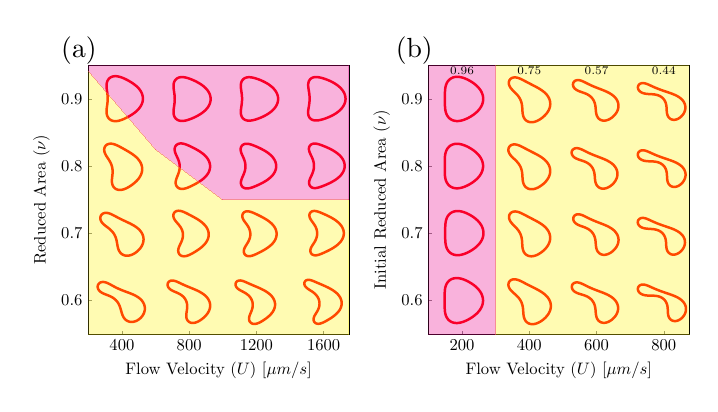
\begin{tikzpicture}[scale=0.6]

\pgfmathsetlengthmacro\MajorTickLength{
      \pgfkeysvalueof{/pgfplots/major tick length} * 0.5
    }

\begin{axis}[
  at = {(0.0cm,0.0cm)},
  major tick length=\MajorTickLength,
  compat=newest,
  axis equal image,
  xmin = 2,
  xmax = 33,
  ymin = -2,
  ymax = 30,
  xtick = {6,14,22,30},
  xticklabels = {$400$,$800$,$1200$,$1600$},
  xlabel = {Flow Velocity ($U$) [$\mu m/s$]},
  ytick = {2,10,18,26},
  yticklabels = {$0.6$,$0.7$,$0.8$,$0.9$},
  ylabel = {Reduced Area ($\nu$)},
  ylabel near ticks,
  xtick pos = left,
  ytick pos = left,
]

% RA = 0.60,flow rate = 400
\addplot[red,line width=1.5pt] coordinates{
(8.2753e+00,-1.2064e-02)
(8.3098e+00,2.5307e-02)
(8.3441e+00,6.4666e-02)
(8.3790e+00,1.0705e-01)
(8.4147e+00,1.5342e-01)
(8.4514e+00,2.0469e-01)
(8.4890e+00,2.6161e-01)
(8.5271e+00,3.2488e-01)
(8.5651e+00,3.9507e-01)
(8.6020e+00,4.7266e-01)
(8.6368e+00,5.5800e-01)
(8.6682e+00,6.5129e-01)
(8.6948e+00,7.5256e-01)
(8.7148e+00,8.6158e-01)
(8.7266e+00,9.7788e-01)
(8.7283e+00,1.1006e+00)
(8.7183e+00,1.2287e+00)
(8.6951e+00,1.3607e+00)
(8.6576e+00,1.4947e+00)
(8.6051e+00,1.6290e+00)
(8.5374e+00,1.7615e+00)
(8.4548e+00,1.8906e+00)
(8.3580e+00,2.0147e+00)
(8.2481e+00,2.1325e+00)
(8.1265e+00,2.2433e+00)
(7.9946e+00,2.3468e+00)
(7.8540e+00,2.4429e+00)
(7.7060e+00,2.5319e+00)
(7.5522e+00,2.6145e+00)
(7.3936e+00,2.6914e+00)
(7.2315e+00,2.7634e+00)
(7.0669e+00,2.8315e+00)
(6.9006e+00,2.8966e+00)
(6.7336e+00,2.9597e+00)
(6.5665e+00,3.0217e+00)
(6.4002e+00,3.0833e+00)
(6.2352e+00,3.1452e+00)
(6.0723e+00,3.2082e+00)
(5.9121e+00,3.2725e+00)
(5.7550e+00,3.3385e+00)
(5.6017e+00,3.4062e+00)
(5.4524e+00,3.4756e+00)
(5.3076e+00,3.5463e+00)
(5.1675e+00,3.6179e+00)
(5.0320e+00,3.6897e+00)
(4.9012e+00,3.7609e+00)
(4.7749e+00,3.8304e+00)
(4.6528e+00,3.8974e+00)
(4.5346e+00,3.9606e+00)
(4.4201e+00,4.0188e+00)
(4.3089e+00,4.0711e+00)
(4.2011e+00,4.1161e+00)
(4.0966e+00,4.1532e+00)
(3.9958e+00,4.1816e+00)
(3.8993e+00,4.2010e+00)
(3.8078e+00,4.2113e+00)
(3.7219e+00,4.2130e+00)
(3.6424e+00,4.2067e+00)
(3.5697e+00,4.1935e+00)
(3.5042e+00,4.1747e+00)
(3.4457e+00,4.1512e+00)
(3.3937e+00,4.1243e+00)
(3.3477e+00,4.0945e+00)
(3.3066e+00,4.0622e+00)
(3.2697e+00,4.0272e+00)
(3.2362e+00,3.9890e+00)
(3.2057e+00,3.9466e+00)
(3.1782e+00,3.8992e+00)
(3.1543e+00,3.8458e+00)
(3.1352e+00,3.7857e+00)
(3.1224e+00,3.7187e+00)
(3.1178e+00,3.6451e+00)
(3.1233e+00,3.5655e+00)
(3.1406e+00,3.4814e+00)
(3.1712e+00,3.3945e+00)
(3.2160e+00,3.3069e+00)
(3.2753e+00,3.2207e+00)
(3.3487e+00,3.1377e+00)
(3.4353e+00,3.0593e+00)
(3.5342e+00,2.9864e+00)
(3.6437e+00,2.9193e+00)
(3.7626e+00,2.8575e+00)
(3.8895e+00,2.8002e+00)
(4.0230e+00,2.7457e+00)
(4.1620e+00,2.6922e+00)
(4.3052e+00,2.6374e+00)
(4.4514e+00,2.5791e+00)
(4.5992e+00,2.5148e+00)
(4.7469e+00,2.4423e+00)
(4.8927e+00,2.3595e+00)
(5.0343e+00,2.2650e+00)
(5.1697e+00,2.1579e+00)
(5.2966e+00,2.0379e+00)
(5.4129e+00,1.9057e+00)
(5.5174e+00,1.7624e+00)
(5.6091e+00,1.6097e+00)
(5.6882e+00,1.4497e+00)
(5.7558e+00,1.2844e+00)
(5.8136e+00,1.1159e+00)
(5.8643e+00,9.4589e-01)
(5.9111e+00,7.7603e-01)
(5.9578e+00,6.0775e-01)
(6.0081e+00,4.4256e-01)
(6.0657e+00,2.8227e-01)
(6.1337e+00,1.2910e-01)
(6.2145e+00,-1.4186e-02)
(6.3092e+00,-1.4452e-01)
(6.4172e+00,-2.5885e-01)
(6.5368e+00,-3.5462e-01)
(6.6649e+00,-4.3026e-01)
(6.7981e+00,-4.8542e-01)
(6.9326e+00,-5.2095e-01)
(7.0653e+00,-5.3864e-01)
(7.1938e+00,-5.4087e-01)
(7.3161e+00,-5.3026e-01)
(7.4311e+00,-5.0940e-01)
(7.5382e+00,-4.8066e-01)
(7.6370e+00,-4.4615e-01)
(7.7276e+00,-4.0769e-01)
(7.8102e+00,-3.6677e-01)
(7.8851e+00,-3.2462e-01)
(7.9527e+00,-2.8224e-01)
(8.0136e+00,-2.4037e-01)
(8.0682e+00,-1.9953e-01)
(8.1173e+00,-1.6000e-01)
(8.1617e+00,-1.2184e-01)
(8.2022e+00,-8.4817e-02)
(8.2397e+00,-4.8468e-02)
(8.2753e+00,-1.2064e-02)
};

% RA = 0.70,flow rate = 400
\addplot[red,line width=1.5pt] coordinates{
(7.4214e+00,7.5718e+00)
(7.4755e+00,7.6029e+00)
(7.5296e+00,7.6360e+00)
(7.5844e+00,7.6715e+00)
(7.6404e+00,7.7100e+00)
(7.6980e+00,7.7519e+00)
(7.7576e+00,7.7978e+00)
(7.8191e+00,7.8481e+00)
(7.8827e+00,7.9035e+00)
(7.9479e+00,7.9644e+00)
(8.0146e+00,8.0312e+00)
(8.0822e+00,8.1044e+00)
(8.1500e+00,8.1844e+00)
(8.2172e+00,8.2716e+00)
(8.2828e+00,8.3664e+00)
(8.3455e+00,8.4691e+00)
(8.4039e+00,8.5799e+00)
(8.4565e+00,8.6988e+00)
(8.5014e+00,8.8258e+00)
(8.5366e+00,8.9602e+00)
(8.5604e+00,9.1013e+00)
(8.5709e+00,9.2479e+00)
(8.5666e+00,9.3985e+00)
(8.5463e+00,9.5510e+00)
(8.5094e+00,9.7036e+00)
(8.4559e+00,9.8540e+00)
(8.3864e+00,1.0000e+01)
(8.3020e+00,1.0141e+01)
(8.2041e+00,1.0275e+01)
(8.0943e+00,1.0401e+01)
(7.9746e+00,1.0520e+01)
(7.8466e+00,1.0630e+01)
(7.7121e+00,1.0733e+01)
(7.5724e+00,1.0829e+01)
(7.4291e+00,1.0919e+01)
(7.2833e+00,1.1003e+01)
(7.1361e+00,1.1083e+01)
(6.9884e+00,1.1159e+01)
(6.8410e+00,1.1231e+01)
(6.6947e+00,1.1301e+01)
(6.5501e+00,1.1369e+01)
(6.4079e+00,1.1435e+01)
(6.2685e+00,1.1501e+01)
(6.1323e+00,1.1565e+01)
(5.9998e+00,1.1629e+01)
(5.8712e+00,1.1692e+01)
(5.7469e+00,1.1754e+01)
(5.6270e+00,1.1815e+01)
(5.5116e+00,1.1875e+01)
(5.4008e+00,1.1934e+01)
(5.2946e+00,1.1990e+01)
(5.1929e+00,1.2045e+01)
(5.0956e+00,1.2096e+01)
(5.0026e+00,1.2145e+01)
(4.9138e+00,1.2190e+01)
(4.8289e+00,1.2231e+01)
(4.7480e+00,1.2269e+01)
(4.6706e+00,1.2302e+01)
(4.5968e+00,1.2332e+01)
(4.5261e+00,1.2357e+01)
(4.4582e+00,1.2379e+01)
(4.3928e+00,1.2397e+01)
(4.3292e+00,1.2412e+01)
(4.2668e+00,1.2423e+01)
(4.2048e+00,1.2431e+01)
(4.1425e+00,1.2435e+01)
(4.0791e+00,1.2435e+01)
(4.0140e+00,1.2431e+01)
(3.9468e+00,1.2421e+01)
(3.8776e+00,1.2404e+01)
(3.8067e+00,1.2379e+01)
(3.7352e+00,1.2345e+01)
(3.6647e+00,1.2299e+01)
(3.5978e+00,1.2240e+01)
(3.5375e+00,1.2167e+01)
(3.4874e+00,1.2081e+01)
(3.4509e+00,1.1983e+01)
(3.4314e+00,1.1875e+01)
(3.4310e+00,1.1760e+01)
(3.4507e+00,1.1641e+01)
(3.4905e+00,1.1522e+01)
(3.5490e+00,1.1406e+01)
(3.6242e+00,1.1295e+01)
(3.7136e+00,1.1188e+01)
(3.8149e+00,1.1087e+01)
(3.9255e+00,1.0990e+01)
(4.0431e+00,1.0896e+01)
(4.1658e+00,1.0803e+01)
(4.2913e+00,1.0709e+01)
(4.4179e+00,1.0611e+01)
(4.5435e+00,1.0509e+01)
(4.6661e+00,1.0400e+01)
(4.7836e+00,1.0282e+01)
(4.8940e+00,1.0157e+01)
(4.9956e+00,1.0023e+01)
(5.0869e+00,9.8802e+00)
(5.1667e+00,9.7308e+00)
(5.2348e+00,9.5756e+00)
(5.2915e+00,9.4163e+00)
(5.3377e+00,9.2544e+00)
(5.3752e+00,9.0913e+00)
(5.4064e+00,8.9283e+00)
(5.4338e+00,8.7664e+00)
(5.4606e+00,8.6065e+00)
(5.4900e+00,8.4495e+00)
(5.5250e+00,8.2964e+00)
(5.5683e+00,8.1487e+00)
(5.6222e+00,8.0081e+00)
(5.6881e+00,7.8767e+00)
(5.7662e+00,7.7568e+00)
(5.8558e+00,7.6507e+00)
(5.9552e+00,7.5600e+00)
(6.0619e+00,7.4857e+00)
(6.1729e+00,7.4278e+00)
(6.2856e+00,7.3856e+00)
(6.3974e+00,7.3578e+00)
(6.5064e+00,7.3424e+00)
(6.6111e+00,7.3376e+00)
(6.7106e+00,7.3413e+00)
(6.8044e+00,7.3517e+00)
(6.8923e+00,7.3674e+00)
(6.9742e+00,7.3869e+00)
(7.0506e+00,7.4092e+00)
(7.1218e+00,7.4334e+00)
(7.1882e+00,7.4591e+00)
(7.2507e+00,7.4859e+00)
(7.3098e+00,7.5135e+00)
(7.3664e+00,7.5421e+00)
(7.4214e+00,7.5718e+00)
};

% RA = 0.80,flow rate = 400
\addplot[red,line width=1.5pt] coordinates{
(7.6553e+00,1.6147e+01)
(7.7084e+00,1.6198e+01)
(7.7610e+00,1.6251e+01)
(7.8133e+00,1.6306e+01)
(7.8656e+00,1.6364e+01)
(7.9181e+00,1.6425e+01)
(7.9707e+00,1.6490e+01)
(8.0233e+00,1.6559e+01)
(8.0757e+00,1.6633e+01)
(8.1273e+00,1.6712e+01)
(8.1776e+00,1.6797e+01)
(8.2258e+00,1.6888e+01)
(8.2710e+00,1.6986e+01)
(8.3120e+00,1.7090e+01)
(8.3477e+00,1.7201e+01)
(8.3768e+00,1.7318e+01)
(8.3978e+00,1.7442e+01)
(8.4094e+00,1.7570e+01)
(8.4103e+00,1.7703e+01)
(8.3996e+00,1.7840e+01)
(8.3762e+00,1.7978e+01)
(8.3399e+00,1.8118e+01)
(8.2905e+00,1.8256e+01)
(8.2282e+00,1.8393e+01)
(8.1537e+00,1.8526e+01)
(8.0678e+00,1.8655e+01)
(7.9717e+00,1.8780e+01)
(7.8665e+00,1.8899e+01)
(7.7533e+00,1.9014e+01)
(7.6335e+00,1.9123e+01)
(7.5081e+00,1.9227e+01)
(7.3783e+00,1.9326e+01)
(7.2450e+00,1.9421e+01)
(7.1092e+00,1.9513e+01)
(6.9716e+00,1.9602e+01)
(6.8331e+00,1.9687e+01)
(6.6941e+00,1.9771e+01)
(6.5555e+00,1.9852e+01)
(6.4175e+00,1.9931e+01)
(6.2807e+00,2.0009e+01)
(6.1454e+00,2.0085e+01)
(6.0117e+00,2.0159e+01)
(5.8800e+00,2.0231e+01)
(5.7501e+00,2.0300e+01)
(5.6222e+00,2.0366e+01)
(5.4961e+00,2.0428e+01)
(5.3717e+00,2.0485e+01)
(5.2488e+00,2.0537e+01)
(5.1275e+00,2.0581e+01)
(5.0079e+00,2.0617e+01)
(4.8902e+00,2.0644e+01)
(4.7750e+00,2.0661e+01)
(4.6632e+00,2.0666e+01)
(4.5559e+00,2.0661e+01)
(4.4541e+00,2.0644e+01)
(4.3593e+00,2.0617e+01)
(4.2724e+00,2.0579e+01)
(4.1945e+00,2.0533e+01)
(4.1259e+00,2.0480e+01)
(4.0671e+00,2.0421e+01)
(4.0176e+00,2.0357e+01)
(3.9773e+00,2.0290e+01)
(3.9456e+00,2.0222e+01)
(3.9218e+00,2.0151e+01)
(3.9055e+00,2.0079e+01)
(3.8962e+00,2.0006e+01)
(3.8936e+00,1.9931e+01)
(3.8976e+00,1.9855e+01)
(3.9080e+00,1.9778e+01)
(3.9248e+00,1.9699e+01)
(3.9481e+00,1.9619e+01)
(3.9778e+00,1.9538e+01)
(4.0137e+00,1.9454e+01)
(4.0556e+00,1.9369e+01)
(4.1033e+00,1.9283e+01)
(4.1563e+00,1.9194e+01)
(4.2139e+00,1.9103e+01)
(4.2754e+00,1.9010e+01)
(4.3399e+00,1.8913e+01)
(4.4064e+00,1.8812e+01)
(4.4737e+00,1.8707e+01)
(4.5406e+00,1.8596e+01)
(4.6055e+00,1.8480e+01)
(4.6670e+00,1.8358e+01)
(4.7236e+00,1.8229e+01)
(4.7737e+00,1.8094e+01)
(4.8161e+00,1.7953e+01)
(4.8497e+00,1.7807e+01)
(4.8736e+00,1.7656e+01)
(4.8878e+00,1.7501e+01)
(4.8924e+00,1.7344e+01)
(4.8884e+00,1.7185e+01)
(4.8772e+00,1.7025e+01)
(4.8610e+00,1.6863e+01)
(4.8424e+00,1.6701e+01)
(4.8247e+00,1.6539e+01)
(4.8117e+00,1.6376e+01)
(4.8075e+00,1.6212e+01)
(4.8165e+00,1.6048e+01)
(4.8430e+00,1.5888e+01)
(4.8905e+00,1.5733e+01)
(4.9610e+00,1.5589e+01)
(5.0545e+00,1.5460e+01)
(5.1685e+00,1.5352e+01)
(5.2986e+00,1.5268e+01)
(5.4394e+00,1.5209e+01)
(5.5853e+00,1.5174e+01)
(5.7318e+00,1.5161e+01)
(5.8756e+00,1.5166e+01)
(6.0147e+00,1.5187e+01)
(6.1479e+00,1.5218e+01)
(6.2749e+00,1.5258e+01)
(6.3954e+00,1.5305e+01)
(6.5098e+00,1.5355e+01)
(6.6182e+00,1.5409e+01)
(6.7208e+00,1.5464e+01)
(6.8180e+00,1.5519e+01)
(6.9099e+00,1.5575e+01)
(6.9969e+00,1.5631e+01)
(7.0791e+00,1.5686e+01)
(7.1568e+00,1.5740e+01)
(7.2302e+00,1.5793e+01)
(7.2997e+00,1.5845e+01)
(7.3656e+00,1.5897e+01)
(7.4283e+00,1.5947e+01)
(7.4881e+00,1.5997e+01)
(7.5456e+00,1.6047e+01)
(7.6011e+00,1.6096e+01)
(7.6553e+00,1.6147e+01)
};

% RA = 0.90,flow rate = 400
\addplot[red,line width=1.5pt] coordinates{
(4.2301e+00,2.4048e+01)
(4.2600e+00,2.3963e+01)
(4.2968e+00,2.3881e+01)
(4.3412e+00,2.3802e+01)
(4.3934e+00,2.3726e+01)
(4.4538e+00,2.3655e+01)
(4.5224e+00,2.3588e+01)
(4.5991e+00,2.3528e+01)
(4.6838e+00,2.3476e+01)
(4.7760e+00,2.3431e+01)
(4.8748e+00,2.3395e+01)
(4.9794e+00,2.3369e+01)
(5.0891e+00,2.3353e+01)
(5.2027e+00,2.3346e+01)
(5.3196e+00,2.3349e+01)
(5.4389e+00,2.3361e+01)
(5.5602e+00,2.3381e+01)
(5.6828e+00,2.3410e+01)
(5.8066e+00,2.3445e+01)
(5.9314e+00,2.3486e+01)
(6.0570e+00,2.3533e+01)
(6.1833e+00,2.3585e+01)
(6.3103e+00,2.3641e+01)
(6.4378e+00,2.3702e+01)
(6.5657e+00,2.3766e+01)
(6.6939e+00,2.3833e+01)
(6.8221e+00,2.3904e+01)
(6.9500e+00,2.3978e+01)
(7.0773e+00,2.4055e+01)
(7.2035e+00,2.4136e+01)
(7.3283e+00,2.4220e+01)
(7.4509e+00,2.4309e+01)
(7.5707e+00,2.4401e+01)
(7.6871e+00,2.4498e+01)
(7.7992e+00,2.4599e+01)
(7.9062e+00,2.4705e+01)
(8.0071e+00,2.4815e+01)
(8.1010e+00,2.4931e+01)
(8.1869e+00,2.5051e+01)
(8.2637e+00,2.5176e+01)
(8.3306e+00,2.5304e+01)
(8.3868e+00,2.5435e+01)
(8.4317e+00,2.5569e+01)
(8.4649e+00,2.5704e+01)
(8.4863e+00,2.5839e+01)
(8.4960e+00,2.5972e+01)
(8.4945e+00,2.6104e+01)
(8.4826e+00,2.6232e+01)
(8.4610e+00,2.6356e+01)
(8.4309e+00,2.6475e+01)
(8.3932e+00,2.6589e+01)
(8.3491e+00,2.6697e+01)
(8.2996e+00,2.6799e+01)
(8.2458e+00,2.6896e+01)
(8.1884e+00,2.6987e+01)
(8.1283e+00,2.7074e+01)
(8.0660e+00,2.7155e+01)
(8.0021e+00,2.7231e+01)
(7.9369e+00,2.7304e+01)
(7.8707e+00,2.7373e+01)
(7.8038e+00,2.7438e+01)
(7.7361e+00,2.7500e+01)
(7.6677e+00,2.7560e+01)
(7.5985e+00,2.7618e+01)
(7.5283e+00,2.7673e+01)
(7.4569e+00,2.7728e+01)
(7.3842e+00,2.7781e+01)
(7.3099e+00,2.7833e+01)
(7.2337e+00,2.7885e+01)
(7.1555e+00,2.7936e+01)
(7.0749e+00,2.7987e+01)
(6.9918e+00,2.8038e+01)
(6.9060e+00,2.8089e+01)
(6.8172e+00,2.8140e+01)
(6.7253e+00,2.8191e+01)
(6.6302e+00,2.8242e+01)
(6.5317e+00,2.8292e+01)
(6.4298e+00,2.8343e+01)
(6.3242e+00,2.8393e+01)
(6.2148e+00,2.8442e+01)
(6.1016e+00,2.8490e+01)
(5.9844e+00,2.8536e+01)
(5.8630e+00,2.8578e+01)
(5.7374e+00,2.8617e+01)
(5.6075e+00,2.8649e+01)
(5.4734e+00,2.8675e+01)
(5.3355e+00,2.8691e+01)
(5.1946e+00,2.8695e+01)
(5.0521e+00,2.8684e+01)
(4.9102e+00,2.8656e+01)
(4.7719e+00,2.8608e+01)
(4.6409e+00,2.8540e+01)
(4.5213e+00,2.8452e+01)
(4.4168e+00,2.8344e+01)
(4.3304e+00,2.8221e+01)
(4.2633e+00,2.8086e+01)
(4.2156e+00,2.7943e+01)
(4.1857e+00,2.7794e+01)
(4.1713e+00,2.7644e+01)
(4.1694e+00,2.7493e+01)
(4.1770e+00,2.7344e+01)
(4.1913e+00,2.7195e+01)
(4.2096e+00,2.7049e+01)
(4.2296e+00,2.6904e+01)
(4.2495e+00,2.6760e+01)
(4.2679e+00,2.6618e+01)
(4.2834e+00,2.6478e+01)
(4.2954e+00,2.6340e+01)
(4.3033e+00,2.6203e+01)
(4.3069e+00,2.6069e+01)
(4.3064e+00,2.5938e+01)
(4.3019e+00,2.5809e+01)
(4.2940e+00,2.5684e+01)
(4.2832e+00,2.5561e+01)
(4.2701e+00,2.5442e+01)
(4.2556e+00,2.5326e+01)
(4.2402e+00,2.5213e+01)
(4.2248e+00,2.5103e+01)
(4.2101e+00,2.4996e+01)
(4.1967e+00,2.4892e+01)
(4.1854e+00,2.4790e+01)
(4.1766e+00,2.4691e+01)
(4.1709e+00,2.4594e+01)
(4.1688e+00,2.4498e+01)
(4.1709e+00,2.4405e+01)
(4.1776e+00,2.4313e+01)
(4.1894e+00,2.4223e+01)
(4.2067e+00,2.4134e+01)
(4.2301e+00,2.4048e+01)
};

% RA = 0.60,flow rate = 800
\addplot[red,line width=1.5pt] coordinates{
(1.3620e+01,3.7554e+00)
(1.3573e+01,3.7756e+00)
(1.3525e+01,3.7964e+00)
(1.3475e+01,3.8185e+00)
(1.3421e+01,3.8423e+00)
(1.3364e+01,3.8681e+00)
(1.3302e+01,3.8964e+00)
(1.3234e+01,3.9273e+00)
(1.3162e+01,3.9610e+00)
(1.3084e+01,3.9977e+00)
(1.3001e+01,4.0373e+00)
(1.2912e+01,4.0798e+00)
(1.2818e+01,4.1249e+00)
(1.2717e+01,4.1719e+00)
(1.2611e+01,4.2200e+00)
(1.2497e+01,4.2677e+00)
(1.2377e+01,4.3125e+00)
(1.2249e+01,4.3508e+00)
(1.2112e+01,4.3775e+00)
(1.1968e+01,4.3854e+00)
(1.1821e+01,4.3657e+00)
(1.1679e+01,4.3096e+00)
(1.1556e+01,4.2122e+00)
(1.1469e+01,4.0770e+00)
(1.1433e+01,3.9173e+00)
(1.1450e+01,3.7512e+00)
(1.1516e+01,3.5945e+00)
(1.1619e+01,3.4563e+00)
(1.1748e+01,3.3389e+00)
(1.1894e+01,3.2403e+00)
(1.2050e+01,3.1563e+00)
(1.2212e+01,3.0817e+00)
(1.2377e+01,3.0116e+00)
(1.2541e+01,2.9413e+00)
(1.2703e+01,2.8668e+00)
(1.2860e+01,2.7851e+00)
(1.3011e+01,2.6939e+00)
(1.3152e+01,2.5918e+00)
(1.3283e+01,2.4783e+00)
(1.3399e+01,2.3541e+00)
(1.3500e+01,2.2205e+00)
(1.3585e+01,2.0793e+00)
(1.3652e+01,1.9330e+00)
(1.3703e+01,1.7840e+00)
(1.3738e+01,1.6348e+00)
(1.3759e+01,1.4873e+00)
(1.3767e+01,1.3433e+00)
(1.3766e+01,1.2041e+00)
(1.3757e+01,1.0704e+00)
(1.3742e+01,9.4260e-01)
(1.3725e+01,8.2095e-01)
(1.3708e+01,7.0537e-01)
(1.3691e+01,5.9578e-01)
(1.3676e+01,4.9209e-01)
(1.3664e+01,3.9429e-01)
(1.3657e+01,3.0240e-01)
(1.3654e+01,2.1651e-01)
(1.3655e+01,1.3671e-01)
(1.3660e+01,6.3035e-02)
(1.3669e+01,-4.6172e-03)
(1.3681e+01,-6.6520e-02)
(1.3696e+01,-1.2317e-01)
(1.3713e+01,-1.7527e-01)
(1.3732e+01,-2.2376e-01)
(1.3754e+01,-2.6968e-01)
(1.3779e+01,-3.1405e-01)
(1.3808e+01,-3.5775e-01)
(1.3841e+01,-4.0129e-01)
(1.3880e+01,-4.4476e-01)
(1.3926e+01,-4.8774e-01)
(1.3980e+01,-5.2933e-01)
(1.4043e+01,-5.6816e-01)
(1.4115e+01,-6.0257e-01)
(1.4196e+01,-6.3067e-01)
(1.4286e+01,-6.5063e-01)
(1.4384e+01,-6.6085e-01)
(1.4489e+01,-6.6012e-01)
(1.4599e+01,-6.4775e-01)
(1.4714e+01,-6.2356e-01)
(1.4831e+01,-5.8779e-01)
(1.4951e+01,-5.4102e-01)
(1.5072e+01,-4.8397e-01)
(1.5194e+01,-4.1740e-01)
(1.5317e+01,-3.4198e-01)
(1.5440e+01,-2.5825e-01)
(1.5563e+01,-1.6655e-01)
(1.5685e+01,-6.7001e-02)
(1.5805e+01,4.0489e-02)
(1.5923e+01,1.5618e-01)
(1.6035e+01,2.8046e-01)
(1.6141e+01,4.1375e-01)
(1.6239e+01,5.5635e-01)
(1.6325e+01,7.0831e-01)
(1.6396e+01,8.6920e-01)
(1.6451e+01,1.0379e+00)
(1.6486e+01,1.2126e+00)
(1.6499e+01,1.3907e+00)
(1.6488e+01,1.5689e+00)
(1.6455e+01,1.7439e+00)
(1.6401e+01,1.9126e+00)
(1.6327e+01,2.0725e+00)
(1.6237e+01,2.2220e+00)
(1.6133e+01,2.3602e+00)
(1.6019e+01,2.4869e+00)
(1.5898e+01,2.6025e+00)
(1.5771e+01,2.7077e+00)
(1.5642e+01,2.8034e+00)
(1.5511e+01,2.8906e+00)
(1.5380e+01,2.9701e+00)
(1.5250e+01,3.0430e+00)
(1.5122e+01,3.1098e+00)
(1.4997e+01,3.1714e+00)
(1.4876e+01,3.2283e+00)
(1.4758e+01,3.2811e+00)
(1.4646e+01,3.3302e+00)
(1.4538e+01,3.3759e+00)
(1.4436e+01,3.4186e+00)
(1.4339e+01,3.4585e+00)
(1.4248e+01,3.4957e+00)
(1.4162e+01,3.5305e+00)
(1.4083e+01,3.5629e+00)
(1.4009e+01,3.5930e+00)
(1.3940e+01,3.6210e+00)
(1.3877e+01,3.6470e+00)
(1.3819e+01,3.6711e+00)
(1.3765e+01,3.6937e+00)
(1.3714e+01,3.7150e+00)
(1.3666e+01,3.7354e+00)
(1.3620e+01,3.7554e+00)
};

% RA = 0.70,flow rate = 800
\addplot[red,line width=1.5pt] coordinates{
(1.2699e+01,7.9012e+00)
(1.2704e+01,7.8389e+00)
(1.2714e+01,7.7763e+00)
(1.2731e+01,7.7132e+00)
(1.2755e+01,7.6496e+00)
(1.2787e+01,7.5860e+00)
(1.2829e+01,7.5234e+00)
(1.2881e+01,7.4633e+00)
(1.2945e+01,7.4078e+00)
(1.3020e+01,7.3590e+00)
(1.3105e+01,7.3193e+00)
(1.3201e+01,7.2906e+00)
(1.3304e+01,7.2743e+00)
(1.3415e+01,7.2712e+00)
(1.3530e+01,7.2811e+00)
(1.3648e+01,7.3033e+00)
(1.3769e+01,7.3368e+00)
(1.3892e+01,7.3801e+00)
(1.4016e+01,7.4319e+00)
(1.4142e+01,7.4909e+00)
(1.4270e+01,7.5560e+00)
(1.4399e+01,7.6264e+00)
(1.4530e+01,7.7013e+00)
(1.4663e+01,7.7802e+00)
(1.4796e+01,7.8631e+00)
(1.4931e+01,7.9498e+00)
(1.5065e+01,8.0406e+00)
(1.5200e+01,8.1356e+00)
(1.5332e+01,8.2352e+00)
(1.5463e+01,8.3401e+00)
(1.5591e+01,8.4506e+00)
(1.5713e+01,8.5672e+00)
(1.5830e+01,8.6906e+00)
(1.5938e+01,8.8209e+00)
(1.6037e+01,8.9583e+00)
(1.6124e+01,9.1026e+00)
(1.6198e+01,9.2531e+00)
(1.6256e+01,9.4087e+00)
(1.6297e+01,9.5678e+00)
(1.6321e+01,9.7284e+00)
(1.6326e+01,9.8881e+00)
(1.6315e+01,1.0045e+01)
(1.6287e+01,1.0196e+01)
(1.6245e+01,1.0341e+01)
(1.6191e+01,1.0478e+01)
(1.6127e+01,1.0606e+01)
(1.6055e+01,1.0725e+01)
(1.5978e+01,1.0836e+01)
(1.5897e+01,1.0938e+01)
(1.5813e+01,1.1031e+01)
(1.5729e+01,1.1117e+01)
(1.5645e+01,1.1196e+01)
(1.5562e+01,1.1269e+01)
(1.5480e+01,1.1335e+01)
(1.5402e+01,1.1396e+01)
(1.5326e+01,1.1453e+01)
(1.5253e+01,1.1504e+01)
(1.5183e+01,1.1552e+01)
(1.5117e+01,1.1596e+01)
(1.5053e+01,1.1637e+01)
(1.4993e+01,1.1675e+01)
(1.4935e+01,1.1710e+01)
(1.4879e+01,1.1744e+01)
(1.4825e+01,1.1776e+01)
(1.4771e+01,1.1808e+01)
(1.4716e+01,1.1839e+01)
(1.4661e+01,1.1871e+01)
(1.4604e+01,1.1903e+01)
(1.4545e+01,1.1936e+01)
(1.4482e+01,1.1970e+01)
(1.4416e+01,1.2006e+01)
(1.4346e+01,1.2044e+01)
(1.4272e+01,1.2084e+01)
(1.4193e+01,1.2126e+01)
(1.4109e+01,1.2170e+01)
(1.4021e+01,1.2216e+01)
(1.3928e+01,1.2264e+01)
(1.3830e+01,1.2315e+01)
(1.3727e+01,1.2366e+01)
(1.3619e+01,1.2420e+01)
(1.3505e+01,1.2473e+01)
(1.3386e+01,1.2527e+01)
(1.3261e+01,1.2577e+01)
(1.3130e+01,1.2623e+01)
(1.2992e+01,1.2661e+01)
(1.2847e+01,1.2685e+01)
(1.2696e+01,1.2688e+01)
(1.2544e+01,1.2664e+01)
(1.2399e+01,1.2605e+01)
(1.2272e+01,1.2508e+01)
(1.2178e+01,1.2377e+01)
(1.2125e+01,1.2221e+01)
(1.2117e+01,1.2056e+01)
(1.2149e+01,1.1892e+01)
(1.2212e+01,1.1736e+01)
(1.2297e+01,1.1589e+01)
(1.2397e+01,1.1452e+01)
(1.2505e+01,1.1321e+01)
(1.2616e+01,1.1194e+01)
(1.2726e+01,1.1066e+01)
(1.2832e+01,1.0936e+01)
(1.2930e+01,1.0802e+01)
(1.3019e+01,1.0664e+01)
(1.3096e+01,1.0521e+01)
(1.3159e+01,1.0374e+01)
(1.3207e+01,1.0224e+01)
(1.3240e+01,1.0074e+01)
(1.3259e+01,9.9240e+00)
(1.3263e+01,9.7769e+00)
(1.3254e+01,9.6339e+00)
(1.3234e+01,9.4962e+00)
(1.3205e+01,9.3646e+00)
(1.3168e+01,9.2396e+00)
(1.3126e+01,9.1214e+00)
(1.3081e+01,9.0097e+00)
(1.3034e+01,8.9042e+00)
(1.2988e+01,8.8044e+00)
(1.2942e+01,8.7099e+00)
(1.2899e+01,8.6200e+00)
(1.2859e+01,8.5344e+00)
(1.2823e+01,8.4526e+00)
(1.2791e+01,8.3744e+00)
(1.2764e+01,8.2995e+00)
(1.2741e+01,8.2277e+00)
(1.2724e+01,8.1585e+00)
(1.2711e+01,8.0918e+00)
(1.2702e+01,8.0271e+00)
(1.2698e+01,7.9637e+00)
(1.2699e+01,7.9012e+00)
};

% RA = 0.80,flow rate = 800
\addplot[red,line width=1.5pt] coordinates{
(1.3841e+01,1.5443e+01)
(1.3910e+01,1.5470e+01)
(1.3979e+01,1.5499e+01)
(1.4049e+01,1.5530e+01)
(1.4120e+01,1.5562e+01)
(1.4193e+01,1.5596e+01)
(1.4268e+01,1.5632e+01)
(1.4347e+01,1.5670e+01)
(1.4428e+01,1.5711e+01)
(1.4512e+01,1.5754e+01)
(1.4600e+01,1.5800e+01)
(1.4691e+01,1.5849e+01)
(1.4786e+01,1.5900e+01)
(1.4884e+01,1.5956e+01)
(1.4985e+01,1.6014e+01)
(1.5088e+01,1.6077e+01)
(1.5194e+01,1.6143e+01)
(1.5303e+01,1.6214e+01)
(1.5413e+01,1.6289e+01)
(1.5523e+01,1.6370e+01)
(1.5634e+01,1.6457e+01)
(1.5745e+01,1.6550e+01)
(1.5853e+01,1.6650e+01)
(1.5959e+01,1.6757e+01)
(1.6060e+01,1.6871e+01)
(1.6155e+01,1.6994e+01)
(1.6242e+01,1.7125e+01)
(1.6320e+01,1.7265e+01)
(1.6385e+01,1.7412e+01)
(1.6436e+01,1.7566e+01)
(1.6471e+01,1.7725e+01)
(1.6488e+01,1.7888e+01)
(1.6488e+01,1.8052e+01)
(1.6469e+01,1.8214e+01)
(1.6433e+01,1.8374e+01)
(1.6381e+01,1.8528e+01)
(1.6314e+01,1.8676e+01)
(1.6235e+01,1.8816e+01)
(1.6145e+01,1.8948e+01)
(1.6048e+01,1.9071e+01)
(1.5944e+01,1.9187e+01)
(1.5835e+01,1.9294e+01)
(1.5723e+01,1.9395e+01)
(1.5610e+01,1.9488e+01)
(1.5495e+01,1.9576e+01)
(1.5380e+01,1.9657e+01)
(1.5267e+01,1.9733e+01)
(1.5154e+01,1.9805e+01)
(1.5044e+01,1.9872e+01)
(1.4936e+01,1.9935e+01)
(1.4831e+01,1.9995e+01)
(1.4729e+01,2.0051e+01)
(1.4630e+01,2.0103e+01)
(1.4534e+01,2.0153e+01)
(1.4442e+01,2.0200e+01)
(1.4354e+01,2.0244e+01)
(1.4269e+01,2.0286e+01)
(1.4187e+01,2.0325e+01)
(1.4109e+01,2.0363e+01)
(1.4033e+01,2.0397e+01)
(1.3960e+01,2.0430e+01)
(1.3888e+01,2.0462e+01)
(1.3818e+01,2.0491e+01)
(1.3749e+01,2.0519e+01)
(1.3680e+01,2.0546e+01)
(1.3611e+01,2.0572e+01)
(1.3541e+01,2.0596e+01)
(1.3468e+01,2.0619e+01)
(1.3393e+01,2.0640e+01)
(1.3315e+01,2.0659e+01)
(1.3233e+01,2.0675e+01)
(1.3147e+01,2.0687e+01)
(1.3057e+01,2.0694e+01)
(1.2962e+01,2.0693e+01)
(1.2864e+01,2.0683e+01)
(1.2764e+01,2.0660e+01)
(1.2663e+01,2.0623e+01)
(1.2565e+01,2.0569e+01)
(1.2475e+01,2.0496e+01)
(1.2396e+01,2.0404e+01)
(1.2334e+01,2.0296e+01)
(1.2292e+01,2.0174e+01)
(1.2273e+01,2.0042e+01)
(1.2274e+01,1.9905e+01)
(1.2295e+01,1.9766e+01)
(1.2332e+01,1.9627e+01)
(1.2382e+01,1.9489e+01)
(1.2440e+01,1.9351e+01)
(1.2505e+01,1.9212e+01)
(1.2571e+01,1.9072e+01)
(1.2637e+01,1.8929e+01)
(1.2699e+01,1.8782e+01)
(1.2755e+01,1.8631e+01)
(1.2803e+01,1.8476e+01)
(1.2839e+01,1.8317e+01)
(1.2864e+01,1.8156e+01)
(1.2876e+01,1.7992e+01)
(1.2874e+01,1.7828e+01)
(1.2859e+01,1.7665e+01)
(1.2832e+01,1.7504e+01)
(1.2794e+01,1.7347e+01)
(1.2748e+01,1.7193e+01)
(1.2695e+01,1.7043e+01)
(1.2638e+01,1.6896e+01)
(1.2580e+01,1.6752e+01)
(1.2524e+01,1.6609e+01)
(1.2474e+01,1.6468e+01)
(1.2433e+01,1.6326e+01)
(1.2405e+01,1.6185e+01)
(1.2393e+01,1.6045e+01)
(1.2400e+01,1.5908e+01)
(1.2428e+01,1.5778e+01)
(1.2477e+01,1.5658e+01)
(1.2544e+01,1.5553e+01)
(1.2627e+01,1.5465e+01)
(1.2721e+01,1.5396e+01)
(1.2821e+01,1.5346e+01)
(1.2923e+01,1.5312e+01)
(1.3025e+01,1.5292e+01)
(1.3123e+01,1.5284e+01)
(1.3218e+01,1.5286e+01)
(1.3309e+01,1.5294e+01)
(1.3395e+01,1.5308e+01)
(1.3477e+01,1.5325e+01)
(1.3555e+01,1.5345e+01)
(1.3629e+01,1.5367e+01)
(1.3702e+01,1.5391e+01)
(1.3772e+01,1.5416e+01)
(1.3841e+01,1.5443e+01)
};

% RA = 0.90,flow rate = 800
\addplot[red,line width=1.5pt] coordinates{
(1.2334e+01,2.8215e+01)
(1.2285e+01,2.8140e+01)
(1.2243e+01,2.8061e+01)
(1.2208e+01,2.7977e+01)
(1.2181e+01,2.7889e+01)
(1.2161e+01,2.7797e+01)
(1.2147e+01,2.7703e+01)
(1.2140e+01,2.7606e+01)
(1.2138e+01,2.7506e+01)
(1.2141e+01,2.7404e+01)
(1.2148e+01,2.7299e+01)
(1.2159e+01,2.7191e+01)
(1.2173e+01,2.7081e+01)
(1.2189e+01,2.6969e+01)
(1.2206e+01,2.6853e+01)
(1.2223e+01,2.6734e+01)
(1.2240e+01,2.6613e+01)
(1.2255e+01,2.6488e+01)
(1.2268e+01,2.6360e+01)
(1.2277e+01,2.6229e+01)
(1.2283e+01,2.6095e+01)
(1.2285e+01,2.5958e+01)
(1.2282e+01,2.5819e+01)
(1.2274e+01,2.5678e+01)
(1.2262e+01,2.5536e+01)
(1.2246e+01,2.5392e+01)
(1.2227e+01,2.5247e+01)
(1.2206e+01,2.5101e+01)
(1.2184e+01,2.4953e+01)
(1.2164e+01,2.4805e+01)
(1.2148e+01,2.4655e+01)
(1.2139e+01,2.4504e+01)
(1.2140e+01,2.4353e+01)
(1.2154e+01,2.4202e+01)
(1.2184e+01,2.4055e+01)
(1.2234e+01,2.3913e+01)
(1.2305e+01,2.3781e+01)
(1.2397e+01,2.3664e+01)
(1.2506e+01,2.3564e+01)
(1.2629e+01,2.3486e+01)
(1.2762e+01,2.3429e+01)
(1.2900e+01,2.3392e+01)
(1.3040e+01,2.3373e+01)
(1.3179e+01,2.3369e+01)
(1.3315e+01,2.3378e+01)
(1.3448e+01,2.3396e+01)
(1.3577e+01,2.3421e+01)
(1.3702e+01,2.3451e+01)
(1.3823e+01,2.3485e+01)
(1.3940e+01,2.3522e+01)
(1.4053e+01,2.3561e+01)
(1.4163e+01,2.3602e+01)
(1.4269e+01,2.3643e+01)
(1.4372e+01,2.3686e+01)
(1.4471e+01,2.3728e+01)
(1.4567e+01,2.3771e+01)
(1.4660e+01,2.3814e+01)
(1.4749e+01,2.3858e+01)
(1.4837e+01,2.3901e+01)
(1.4921e+01,2.3945e+01)
(1.5004e+01,2.3989e+01)
(1.5084e+01,2.4034e+01)
(1.5163e+01,2.4079e+01)
(1.5240e+01,2.4126e+01)
(1.5316e+01,2.4173e+01)
(1.5391e+01,2.4222e+01)
(1.5466e+01,2.4273e+01)
(1.5540e+01,2.4325e+01)
(1.5614e+01,2.4380e+01)
(1.5687e+01,2.4438e+01)
(1.5761e+01,2.4498e+01)
(1.5834e+01,2.4563e+01)
(1.5907e+01,2.4631e+01)
(1.5980e+01,2.4703e+01)
(1.6051e+01,2.4780e+01)
(1.6122e+01,2.4862e+01)
(1.6190e+01,2.4949e+01)
(1.6255e+01,2.5042e+01)
(1.6317e+01,2.5141e+01)
(1.6374e+01,2.5246e+01)
(1.6426e+01,2.5358e+01)
(1.6470e+01,2.5476e+01)
(1.6506e+01,2.5599e+01)
(1.6533e+01,2.5728e+01)
(1.6549e+01,2.5861e+01)
(1.6553e+01,2.5997e+01)
(1.6545e+01,2.6136e+01)
(1.6524e+01,2.6275e+01)
(1.6491e+01,2.6414e+01)
(1.6444e+01,2.6551e+01)
(1.6386e+01,2.6685e+01)
(1.6316e+01,2.6815e+01)
(1.6236e+01,2.6941e+01)
(1.6147e+01,2.7062e+01)
(1.6050e+01,2.7177e+01)
(1.5946e+01,2.7286e+01)
(1.5837e+01,2.7390e+01)
(1.5722e+01,2.7489e+01)
(1.5603e+01,2.7582e+01)
(1.5482e+01,2.7671e+01)
(1.5358e+01,2.7755e+01)
(1.5232e+01,2.7834e+01)
(1.5104e+01,2.7909e+01)
(1.4977e+01,2.7980e+01)
(1.4848e+01,2.8048e+01)
(1.4720e+01,2.8112e+01)
(1.4593e+01,2.8172e+01)
(1.4466e+01,2.8229e+01)
(1.4341e+01,2.8282e+01)
(1.4216e+01,2.8332e+01)
(1.4094e+01,2.8379e+01)
(1.3972e+01,2.8422e+01)
(1.3853e+01,2.8461e+01)
(1.3735e+01,2.8495e+01)
(1.3619e+01,2.8525e+01)
(1.3504e+01,2.8549e+01)
(1.3392e+01,2.8568e+01)
(1.3282e+01,2.8580e+01)
(1.3174e+01,2.8586e+01)
(1.3069e+01,2.8584e+01)
(1.2967e+01,2.8574e+01)
(1.2869e+01,2.8557e+01)
(1.2775e+01,2.8531e+01)
(1.2686e+01,2.8497e+01)
(1.2603e+01,2.8455e+01)
(1.2525e+01,2.8405e+01)
(1.2455e+01,2.8348e+01)
(1.2391e+01,2.8285e+01)
(1.2334e+01,2.8215e+01)
};

% RA = 0.60,flow rate = 1200
\addplot[red,line width=1.5pt] coordinates{
(2.3063e+01,3.1292e+00)
(2.3019e+01,3.1550e+00)
(2.2974e+01,3.1810e+00)
(2.2926e+01,3.2079e+00)
(2.2875e+01,3.2360e+00)
(2.2819e+01,3.2657e+00)
(2.2759e+01,3.2973e+00)
(2.2693e+01,3.3307e+00)
(2.2621e+01,3.3661e+00)
(2.2544e+01,3.4034e+00)
(2.2460e+01,3.4425e+00)
(2.2371e+01,3.4836e+00)
(2.2275e+01,3.5264e+00)
(2.2173e+01,3.5710e+00)
(2.2066e+01,3.6173e+00)
(2.1953e+01,3.6654e+00)
(2.1834e+01,3.7155e+00)
(2.1711e+01,3.7676e+00)
(2.1583e+01,3.8218e+00)
(2.1450e+01,3.8784e+00)
(2.1313e+01,3.9376e+00)
(2.1173e+01,3.9993e+00)
(2.1029e+01,4.0634e+00)
(2.0882e+01,4.1294e+00)
(2.0731e+01,4.1960e+00)
(2.0576e+01,4.2611e+00)
(2.0417e+01,4.3204e+00)
(2.0251e+01,4.3676e+00)
(2.0078e+01,4.3925e+00)
(1.9902e+01,4.3817e+00)
(1.9736e+01,4.3213e+00)
(1.9602e+01,4.2058e+00)
(1.9524e+01,4.0464e+00)
(1.9513e+01,3.8691e+00)
(1.9564e+01,3.6990e+00)
(1.9660e+01,3.5499e+00)
(1.9783e+01,3.4245e+00)
(1.9923e+01,3.3192e+00)
(2.0070e+01,3.2284e+00)
(2.0219e+01,3.1466e+00)
(2.0368e+01,3.0687e+00)
(2.0513e+01,2.9912e+00)
(2.0653e+01,2.9111e+00)
(2.0786e+01,2.8268e+00)
(2.0911e+01,2.7372e+00)
(2.1025e+01,2.6422e+00)
(2.1129e+01,2.5421e+00)
(2.1222e+01,2.4378e+00)
(2.1302e+01,2.3305e+00)
(2.1370e+01,2.2215e+00)
(2.1426e+01,2.1124e+00)
(2.1472e+01,2.0045e+00)
(2.1506e+01,1.8991e+00)
(2.1532e+01,1.7975e+00)
(2.1549e+01,1.7005e+00)
(2.1559e+01,1.6089e+00)
(2.1564e+01,1.5230e+00)
(2.1564e+01,1.4432e+00)
(2.1560e+01,1.3694e+00)
(2.1554e+01,1.3014e+00)
(2.1545e+01,1.2389e+00)
(2.1535e+01,1.1811e+00)
(2.1525e+01,1.1273e+00)
(2.1513e+01,1.0763e+00)
(2.1501e+01,1.0270e+00)
(2.1487e+01,9.7800e-01)
(2.1472e+01,9.2799e-01)
(2.1454e+01,8.7583e-01)
(2.1435e+01,8.2056e-01)
(2.1413e+01,7.6141e-01)
(2.1388e+01,6.9784e-01)
(2.1360e+01,6.2941e-01)
(2.1330e+01,5.5576e-01)
(2.1296e+01,4.7654e-01)
(2.1261e+01,3.9135e-01)
(2.1225e+01,2.9967e-01)
(2.1190e+01,2.0090e-01)
(2.1159e+01,9.4436e-02)
(2.1135e+01,-2.0115e-02)
(2.1124e+01,-1.4242e-01)
(2.1132e+01,-2.7063e-01)
(2.1164e+01,-4.0042e-01)
(2.1227e+01,-5.2435e-01)
(2.1322e+01,-6.3251e-01)
(2.1446e+01,-7.1502e-01)
(2.1590e+01,-7.6538e-01)
(2.1747e+01,-7.8234e-01)
(2.1907e+01,-7.6920e-01)
(2.2067e+01,-7.3157e-01)
(2.2225e+01,-6.7527e-01)
(2.2381e+01,-6.0523e-01)
(2.2534e+01,-5.2514e-01)
(2.2685e+01,-4.3752e-01)
(2.2834e+01,-3.4396e-01)
(2.2982e+01,-2.4530e-01)
(2.3127e+01,-1.4188e-01)
(2.3269e+01,-3.3638e-02)
(2.3407e+01,7.9703e-02)
(2.3540e+01,1.9856e-01)
(2.3666e+01,3.2337e-01)
(2.3784e+01,4.5451e-01)
(2.3892e+01,5.9217e-01)
(2.3987e+01,7.3621e-01)
(2.4068e+01,8.8607e-01)
(2.4133e+01,1.0406e+00)
(2.4180e+01,1.1983e+00)
(2.4209e+01,1.3569e+00)
(2.4219e+01,1.5139e+00)
(2.4212e+01,1.6671e+00)
(2.4188e+01,1.8141e+00)
(2.4150e+01,1.9532e+00)
(2.4100e+01,2.0833e+00)
(2.4041e+01,2.2036e+00)
(2.3975e+01,2.3141e+00)
(2.3905e+01,2.4149e+00)
(2.3832e+01,2.5065e+00)
(2.3759e+01,2.5893e+00)
(2.3685e+01,2.6641e+00)
(2.3613e+01,2.7315e+00)
(2.3544e+01,2.7921e+00)
(2.3477e+01,2.8465e+00)
(2.3414e+01,2.8953e+00)
(2.3355e+01,2.9391e+00)
(2.3299e+01,2.9784e+00)
(2.3247e+01,3.0138e+00)
(2.3198e+01,3.0459e+00)
(2.3151e+01,3.0754e+00)
(2.3107e+01,3.1029e+00)
(2.3063e+01,3.1292e+00)
};

% RA = 0.70,flow rate = 1200
\addplot[red,line width=1.5pt] coordinates{
(2.2605e+01,7.8504e+00)
(2.2660e+01,7.8802e+00)
(2.2716e+01,7.9108e+00)
(2.2773e+01,7.9426e+00)
(2.2832e+01,7.9761e+00)
(2.2894e+01,8.0117e+00)
(2.2959e+01,8.0499e+00)
(2.3027e+01,8.0910e+00)
(2.3099e+01,8.1353e+00)
(2.3175e+01,8.1833e+00)
(2.3254e+01,8.2352e+00)
(2.3336e+01,8.2916e+00)
(2.3422e+01,8.3526e+00)
(2.3510e+01,8.4189e+00)
(2.3600e+01,8.4909e+00)
(2.3692e+01,8.5690e+00)
(2.3784e+01,8.6539e+00)
(2.3877e+01,8.7461e+00)
(2.3967e+01,8.8461e+00)
(2.4054e+01,8.9546e+00)
(2.4137e+01,9.0720e+00)
(2.4212e+01,9.1984e+00)
(2.4278e+01,9.3340e+00)
(2.4333e+01,9.4783e+00)
(2.4373e+01,9.6302e+00)
(2.4397e+01,9.7883e+00)
(2.4403e+01,9.9505e+00)
(2.4390e+01,1.0114e+01)
(2.4357e+01,1.0277e+01)
(2.4306e+01,1.0437e+01)
(2.4238e+01,1.0591e+01)
(2.4155e+01,1.0739e+01)
(2.4058e+01,1.0878e+01)
(2.3951e+01,1.1010e+01)
(2.3835e+01,1.1133e+01)
(2.3712e+01,1.1249e+01)
(2.3584e+01,1.1357e+01)
(2.3452e+01,1.1458e+01)
(2.3318e+01,1.1553e+01)
(2.3182e+01,1.1642e+01)
(2.3046e+01,1.1726e+01)
(2.2910e+01,1.1805e+01)
(2.2776e+01,1.1881e+01)
(2.2643e+01,1.1952e+01)
(2.2512e+01,1.2020e+01)
(2.2384e+01,1.2085e+01)
(2.2260e+01,1.2147e+01)
(2.2139e+01,1.2206e+01)
(2.2021e+01,1.2263e+01)
(2.1907e+01,1.2316e+01)
(2.1798e+01,1.2366e+01)
(2.1692e+01,1.2413e+01)
(2.1591e+01,1.2456e+01)
(2.1493e+01,1.2494e+01)
(2.1399e+01,1.2528e+01)
(2.1309e+01,1.2558e+01)
(2.1223e+01,1.2581e+01)
(2.1141e+01,1.2600e+01)
(2.1062e+01,1.2612e+01)
(2.0987e+01,1.2619e+01)
(2.0916e+01,1.2621e+01)
(2.0848e+01,1.2617e+01)
(2.0783e+01,1.2607e+01)
(2.0722e+01,1.2593e+01)
(2.0663e+01,1.2572e+01)
(2.0606e+01,1.2546e+01)
(2.0552e+01,1.2513e+01)
(2.0500e+01,1.2473e+01)
(2.0452e+01,1.2424e+01)
(2.0410e+01,1.2367e+01)
(2.0373e+01,1.2301e+01)
(2.0346e+01,1.2227e+01)
(2.0328e+01,1.2144e+01)
(2.0323e+01,1.2055e+01)
(2.0330e+01,1.1961e+01)
(2.0352e+01,1.1863e+01)
(2.0386e+01,1.1764e+01)
(2.0432e+01,1.1663e+01)
(2.0488e+01,1.1563e+01)
(2.0554e+01,1.1462e+01)
(2.0627e+01,1.1359e+01)
(2.0705e+01,1.1255e+01)
(2.0785e+01,1.1147e+01)
(2.0867e+01,1.1034e+01)
(2.0948e+01,1.0915e+01)
(2.1025e+01,1.0790e+01)
(2.1096e+01,1.0656e+01)
(2.1158e+01,1.0515e+01)
(2.1209e+01,1.0366e+01)
(2.1247e+01,1.0211e+01)
(2.1271e+01,1.0050e+01)
(2.1278e+01,9.8859e+00)
(2.1268e+01,9.7199e+00)
(2.1241e+01,9.5544e+00)
(2.1198e+01,9.3913e+00)
(2.1141e+01,9.2320e+00)
(2.1070e+01,9.0774e+00)
(2.0990e+01,8.9277e+00)
(2.0903e+01,8.7822e+00)
(2.0814e+01,8.6394e+00)
(2.0725e+01,8.4971e+00)
(2.0643e+01,8.3527e+00)
(2.0572e+01,8.2039e+00)
(2.0522e+01,8.0496e+00)
(2.0499e+01,7.8915e+00)
(2.0510e+01,7.7350e+00)
(2.0560e+01,7.5895e+00)
(2.0646e+01,7.4661e+00)
(2.0760e+01,7.3732e+00)
(2.0890e+01,7.3138e+00)
(2.1027e+01,7.2850e+00)
(2.1161e+01,7.2807e+00)
(2.1291e+01,7.2943e+00)
(2.1414e+01,7.3201e+00)
(2.1530e+01,7.3535e+00)
(2.1639e+01,7.3914e+00)
(2.1742e+01,7.4316e+00)
(2.1839e+01,7.4724e+00)
(2.1930e+01,7.5130e+00)
(2.2016e+01,7.5528e+00)
(2.2096e+01,7.5912e+00)
(2.2172e+01,7.6281e+00)
(2.2244e+01,7.6635e+00)
(2.2311e+01,7.6973e+00)
(2.2375e+01,7.7297e+00)
(2.2435e+01,7.7609e+00)
(2.2493e+01,7.7912e+00)
(2.2550e+01,7.8209e+00)
(2.2605e+01,7.8504e+00)
};

% RA = 0.80,flow rate = 1200
\addplot[red,line width=1.5pt] coordinates{
(2.0690e+01,1.7846e+01)
(2.0684e+01,1.7772e+01)
(2.0675e+01,1.7698e+01)
(2.0664e+01,1.7623e+01)
(2.0649e+01,1.7547e+01)
(2.0631e+01,1.7468e+01)
(2.0610e+01,1.7387e+01)
(2.0585e+01,1.7304e+01)
(2.0556e+01,1.7218e+01)
(2.0524e+01,1.7129e+01)
(2.0488e+01,1.7037e+01)
(2.0448e+01,1.6942e+01)
(2.0405e+01,1.6843e+01)
(2.0360e+01,1.6740e+01)
(2.0314e+01,1.6633e+01)
(2.0268e+01,1.6521e+01)
(2.0226e+01,1.6404e+01)
(2.0189e+01,1.6280e+01)
(2.0164e+01,1.6149e+01)
(2.0154e+01,1.6013e+01)
(2.0167e+01,1.5873e+01)
(2.0207e+01,1.5734e+01)
(2.0279e+01,1.5606e+01)
(2.0381e+01,1.5496e+01)
(2.0509e+01,1.5414e+01)
(2.0655e+01,1.5361e+01)
(2.0811e+01,1.5338e+01)
(2.0970e+01,1.5340e+01)
(2.1129e+01,1.5363e+01)
(2.1287e+01,1.5399e+01)
(2.1443e+01,1.5446e+01)
(2.1598e+01,1.5500e+01)
(2.1751e+01,1.5559e+01)
(2.1903e+01,1.5622e+01)
(2.2053e+01,1.5686e+01)
(2.2202e+01,1.5753e+01)
(2.2349e+01,1.5822e+01)
(2.2494e+01,1.5892e+01)
(2.2636e+01,1.5964e+01)
(2.2775e+01,1.6038e+01)
(2.2911e+01,1.6113e+01)
(2.3042e+01,1.6191e+01)
(2.3170e+01,1.6271e+01)
(2.3292e+01,1.6353e+01)
(2.3409e+01,1.6437e+01)
(2.3520e+01,1.6523e+01)
(2.3626e+01,1.6611e+01)
(2.3724e+01,1.6701e+01)
(2.3816e+01,1.6792e+01)
(2.3900e+01,1.6884e+01)
(2.3977e+01,1.6978e+01)
(2.4046e+01,1.7071e+01)
(2.4107e+01,1.7165e+01)
(2.4161e+01,1.7258e+01)
(2.4207e+01,1.7351e+01)
(2.4246e+01,1.7442e+01)
(2.4278e+01,1.7531e+01)
(2.4304e+01,1.7618e+01)
(2.4324e+01,1.7702e+01)
(2.4338e+01,1.7785e+01)
(2.4347e+01,1.7865e+01)
(2.4352e+01,1.7942e+01)
(2.4353e+01,1.8018e+01)
(2.4349e+01,1.8093e+01)
(2.4342e+01,1.8167e+01)
(2.4331e+01,1.8240e+01)
(2.4317e+01,1.8313e+01)
(2.4298e+01,1.8387e+01)
(2.4275e+01,1.8461e+01)
(2.4248e+01,1.8537e+01)
(2.4215e+01,1.8614e+01)
(2.4177e+01,1.8692e+01)
(2.4134e+01,1.8772e+01)
(2.4085e+01,1.8853e+01)
(2.4029e+01,1.8934e+01)
(2.3967e+01,1.9017e+01)
(2.3898e+01,1.9100e+01)
(2.3823e+01,1.9182e+01)
(2.3741e+01,1.9265e+01)
(2.3652e+01,1.9347e+01)
(2.3558e+01,1.9429e+01)
(2.3457e+01,1.9509e+01)
(2.3350e+01,1.9589e+01)
(2.3237e+01,1.9667e+01)
(2.3119e+01,1.9743e+01)
(2.2996e+01,1.9818e+01)
(2.2869e+01,1.9892e+01)
(2.2738e+01,1.9964e+01)
(2.2602e+01,2.0035e+01)
(2.2464e+01,2.0105e+01)
(2.2322e+01,2.0173e+01)
(2.2177e+01,2.0240e+01)
(2.2031e+01,2.0305e+01)
(2.1882e+01,2.0369e+01)
(2.1731e+01,2.0431e+01)
(2.1579e+01,2.0490e+01)
(2.1424e+01,2.0544e+01)
(2.1267e+01,2.0592e+01)
(2.1108e+01,2.0630e+01)
(2.0947e+01,2.0653e+01)
(2.0786e+01,2.0657e+01)
(2.0627e+01,2.0635e+01)
(2.0477e+01,2.0581e+01)
(2.0345e+01,2.0496e+01)
(2.0241e+01,2.0381e+01)
(2.0170e+01,2.0246e+01)
(2.0133e+01,2.0101e+01)
(2.0125e+01,1.9955e+01)
(2.0141e+01,1.9812e+01)
(2.0173e+01,1.9675e+01)
(2.0216e+01,1.9545e+01)
(2.0266e+01,1.9421e+01)
(2.0318e+01,1.9303e+01)
(2.0370e+01,1.9189e+01)
(2.0420e+01,1.9079e+01)
(2.0467e+01,1.8973e+01)
(2.0509e+01,1.8869e+01)
(2.0548e+01,1.8769e+01)
(2.0581e+01,1.8671e+01)
(2.0610e+01,1.8577e+01)
(2.0634e+01,1.8485e+01)
(2.0654e+01,1.8396e+01)
(2.0669e+01,1.8311e+01)
(2.0680e+01,1.8228e+01)
(2.0688e+01,1.8148e+01)
(2.0693e+01,1.8070e+01)
(2.0695e+01,1.7994e+01)
(2.0694e+01,1.7920e+01)
(2.0690e+01,1.7846e+01)
};

% RA = 0.90,flow rate = 1200
\addplot[red,line width=1.5pt] coordinates{
(2.1364e+01,2.8557e+01)
(2.1275e+01,2.8566e+01)
(2.1185e+01,2.8572e+01)
(2.1094e+01,2.8572e+01)
(2.1002e+01,2.8567e+01)
(2.0910e+01,2.8556e+01)
(2.0816e+01,2.8536e+01)
(2.0723e+01,2.8507e+01)
(2.0632e+01,2.8468e+01)
(2.0543e+01,2.8417e+01)
(2.0459e+01,2.8354e+01)
(2.0382e+01,2.8278e+01)
(2.0314e+01,2.8191e+01)
(2.0256e+01,2.8093e+01)
(2.0210e+01,2.7985e+01)
(2.0177e+01,2.7870e+01)
(2.0156e+01,2.7749e+01)
(2.0145e+01,2.7624e+01)
(2.0144e+01,2.7495e+01)
(2.0151e+01,2.7364e+01)
(2.0164e+01,2.7231e+01)
(2.0182e+01,2.7095e+01)
(2.0201e+01,2.6958e+01)
(2.0221e+01,2.6818e+01)
(2.0241e+01,2.6677e+01)
(2.0259e+01,2.6533e+01)
(2.0273e+01,2.6387e+01)
(2.0284e+01,2.6240e+01)
(2.0290e+01,2.6091e+01)
(2.0291e+01,2.5941e+01)
(2.0286e+01,2.5790e+01)
(2.0277e+01,2.5640e+01)
(2.0263e+01,2.5489e+01)
(2.0246e+01,2.5339e+01)
(2.0226e+01,2.5189e+01)
(2.0204e+01,2.5040e+01)
(2.0183e+01,2.4892e+01)
(2.0164e+01,2.4744e+01)
(2.0150e+01,2.4597e+01)
(2.0144e+01,2.4451e+01)
(2.0148e+01,2.4306e+01)
(2.0165e+01,2.4164e+01)
(2.0199e+01,2.4027e+01)
(2.0250e+01,2.3898e+01)
(2.0318e+01,2.3780e+01)
(2.0403e+01,2.3677e+01)
(2.0502e+01,2.3590e+01)
(2.0610e+01,2.3521e+01)
(2.0725e+01,2.3470e+01)
(2.0843e+01,2.3436e+01)
(2.0961e+01,2.3415e+01)
(2.1078e+01,2.3406e+01)
(2.1192e+01,2.3406e+01)
(2.1302e+01,2.3414e+01)
(2.1409e+01,2.3427e+01)
(2.1513e+01,2.3445e+01)
(2.1613e+01,2.3465e+01)
(2.1710e+01,2.3489e+01)
(2.1804e+01,2.3514e+01)
(2.1896e+01,2.3540e+01)
(2.1985e+01,2.3568e+01)
(2.2072e+01,2.3597e+01)
(2.2158e+01,2.3627e+01)
(2.2243e+01,2.3657e+01)
(2.2327e+01,2.3689e+01)
(2.2410e+01,2.3722e+01)
(2.2494e+01,2.3756e+01)
(2.2577e+01,2.3792e+01)
(2.2662e+01,2.3829e+01)
(2.2747e+01,2.3868e+01)
(2.2833e+01,2.3909e+01)
(2.2920e+01,2.3952e+01)
(2.3009e+01,2.3998e+01)
(2.3099e+01,2.4046e+01)
(2.3190e+01,2.4098e+01)
(2.3283e+01,2.4153e+01)
(2.3377e+01,2.4212e+01)
(2.3473e+01,2.4274e+01)
(2.3568e+01,2.4341e+01)
(2.3665e+01,2.4413e+01)
(2.3761e+01,2.4489e+01)
(2.3856e+01,2.4571e+01)
(2.3950e+01,2.4659e+01)
(2.4043e+01,2.4752e+01)
(2.4132e+01,2.4853e+01)
(2.4216e+01,2.4959e+01)
(2.4296e+01,2.5073e+01)
(2.4369e+01,2.5194e+01)
(2.4434e+01,2.5321e+01)
(2.4488e+01,2.5455e+01)
(2.4532e+01,2.5595e+01)
(2.4563e+01,2.5739e+01)
(2.4580e+01,2.5887e+01)
(2.4583e+01,2.6037e+01)
(2.4571e+01,2.6187e+01)
(2.4544e+01,2.6336e+01)
(2.4503e+01,2.6481e+01)
(2.4449e+01,2.6622e+01)
(2.4383e+01,2.6758e+01)
(2.4307e+01,2.6888e+01)
(2.4222e+01,2.7011e+01)
(2.4129e+01,2.7128e+01)
(2.4031e+01,2.7238e+01)
(2.3927e+01,2.7342e+01)
(2.3820e+01,2.7439e+01)
(2.3710e+01,2.7530e+01)
(2.3598e+01,2.7615e+01)
(2.3484e+01,2.7696e+01)
(2.3370e+01,2.7771e+01)
(2.3256e+01,2.7841e+01)
(2.3143e+01,2.7907e+01)
(2.3030e+01,2.7969e+01)
(2.2918e+01,2.8027e+01)
(2.2808e+01,2.8081e+01)
(2.2699e+01,2.8132e+01)
(2.2592e+01,2.8180e+01)
(2.2488e+01,2.8224e+01)
(2.2385e+01,2.8266e+01)
(2.2284e+01,2.8305e+01)
(2.2186e+01,2.8341e+01)
(2.2089e+01,2.8375e+01)
(2.1995e+01,2.8407e+01)
(2.1902e+01,2.8436e+01)
(2.1810e+01,2.8462e+01)
(2.1720e+01,2.8487e+01)
(2.1630e+01,2.8508e+01)
(2.1541e+01,2.8528e+01)
(2.1453e+01,2.8544e+01)
(2.1364e+01,2.8557e+01)
};

% RA = 0.60,flow rate = 1600
\addplot[red,line width=1.5pt] coordinates{
(3.1347e+01,3.0510e+00)
(3.1306e+01,3.0819e+00)
(3.1264e+01,3.1129e+00)
(3.1219e+01,3.1448e+00)
(3.1171e+01,3.1782e+00)
(3.1119e+01,3.2133e+00)
(3.1062e+01,3.2505e+00)
(3.0999e+01,3.2897e+00)
(3.0930e+01,3.3309e+00)
(3.0856e+01,3.3742e+00)
(3.0776e+01,3.4193e+00)
(3.0689e+01,3.4661e+00)
(3.0596e+01,3.5144e+00)
(3.0497e+01,3.5642e+00)
(3.0391e+01,3.6153e+00)
(3.0280e+01,3.6676e+00)
(3.0163e+01,3.7210e+00)
(3.0041e+01,3.7757e+00)
(2.9913e+01,3.8315e+00)
(2.9780e+01,3.8888e+00)
(2.9643e+01,3.9475e+00)
(2.9502e+01,4.0080e+00)
(2.9358e+01,4.0704e+00)
(2.9210e+01,4.1346e+00)
(2.9059e+01,4.2004e+00)
(2.8905e+01,4.2669e+00)
(2.8747e+01,4.3321e+00)
(2.8585e+01,4.3923e+00)
(2.8417e+01,4.4410e+00)
(2.8243e+01,4.4677e+00)
(2.8066e+01,4.4576e+00)
(2.7900e+01,4.3952e+00)
(2.7770e+01,4.2748e+00)
(2.7701e+01,4.1113e+00)
(2.7703e+01,3.9340e+00)
(2.7765e+01,3.7682e+00)
(2.7866e+01,3.6245e+00)
(2.7991e+01,3.5027e+00)
(2.8129e+01,3.3974e+00)
(2.8270e+01,3.3027e+00)
(2.8412e+01,3.2130e+00)
(2.8551e+01,3.1244e+00)
(2.8685e+01,3.0340e+00)
(2.8811e+01,2.9399e+00)
(2.8929e+01,2.8414e+00)
(2.9036e+01,2.7383e+00)
(2.9133e+01,2.6311e+00)
(2.9218e+01,2.5206e+00)
(2.9291e+01,2.4082e+00)
(2.9352e+01,2.2950e+00)
(2.9402e+01,2.1826e+00)
(2.9440e+01,2.0721e+00)
(2.9469e+01,1.9649e+00)
(2.9489e+01,1.8620e+00)
(2.9500e+01,1.7642e+00)
(2.9505e+01,1.6720e+00)
(2.9505e+01,1.5860e+00)
(2.9500e+01,1.5063e+00)
(2.9492e+01,1.4328e+00)
(2.9482e+01,1.3654e+00)
(2.9469e+01,1.3034e+00)
(2.9456e+01,1.2464e+00)
(2.9441e+01,1.1935e+00)
(2.9426e+01,1.1435e+00)
(2.9410e+01,1.0952e+00)
(2.9392e+01,1.0475e+00)
(2.9373e+01,9.9893e-01)
(2.9351e+01,9.4849e-01)
(2.9326e+01,8.9530e-01)
(2.9298e+01,8.3870e-01)
(2.9267e+01,7.7825e-01)
(2.9231e+01,7.1365e-01)
(2.9190e+01,6.4471e-01)
(2.9146e+01,5.7120e-01)
(2.9097e+01,4.9284e-01)
(2.9045e+01,4.0919e-01)
(2.8991e+01,3.1954e-01)
(2.8936e+01,2.2288e-01)
(2.8884e+01,1.1796e-01)
(2.8840e+01,3.5000e-03)
(2.8808e+01,-1.2112e-01)
(2.8798e+01,-2.5465e-01)
(2.8818e+01,-3.9219e-01)
(2.8876e+01,-5.2384e-01)
(2.8974e+01,-6.3585e-01)
(2.9104e+01,-7.1540e-01)
(2.9256e+01,-7.5620e-01)
(2.9417e+01,-7.6007e-01)
(2.9580e+01,-7.3392e-01)
(2.9740e+01,-6.8578e-01)
(2.9899e+01,-6.2254e-01)
(3.0055e+01,-5.4919e-01)
(3.0210e+01,-4.6907e-01)
(3.0365e+01,-3.8415e-01)
(3.0519e+01,-2.9551e-01)
(3.0672e+01,-2.0353e-01)
(3.0823e+01,-1.0823e-01)
(3.0972e+01,-9.3383e-03)
(3.1117e+01,9.3538e-02)
(3.1259e+01,2.0086e-01)
(3.1395e+01,3.1310e-01)
(3.1524e+01,4.3066e-01)
(3.1645e+01,5.5386e-01)
(3.1757e+01,6.8284e-01)
(3.1857e+01,8.1746e-01)
(3.1944e+01,9.5724e-01)
(3.2017e+01,1.1013e+00)
(3.2073e+01,1.2482e+00)
(3.2113e+01,1.3963e+00)
(3.2137e+01,1.5435e+00)
(3.2144e+01,1.6876e+00)
(3.2136e+01,1.8267e+00)
(3.2115e+01,1.9591e+00)
(3.2082e+01,2.0835e+00)
(3.2041e+01,2.1993e+00)
(3.1993e+01,2.3060e+00)
(3.1940e+01,2.4037e+00)
(3.1885e+01,2.4926e+00)
(3.1828e+01,2.5731e+00)
(3.1771e+01,2.6458e+00)
(3.1715e+01,2.7113e+00)
(3.1661e+01,2.7700e+00)
(3.1609e+01,2.8228e+00)
(3.1560e+01,2.8701e+00)
(3.1514e+01,2.9127e+00)
(3.1469e+01,2.9513e+00)
(3.1427e+01,2.9866e+00)
(3.1387e+01,3.0196e+00)
(3.1347e+01,3.0510e+00)
};

% RA = 0.70,flow rate = 1600
\addplot[red,line width=1.5pt] coordinates{
(2.8440e+01,7.7742e+00)
(2.8460e+01,7.7149e+00)
(2.8487e+01,7.6576e+00)
(2.8522e+01,7.6027e+00)
(2.8567e+01,7.5509e+00)
(2.8620e+01,7.5036e+00)
(2.8683e+01,7.4621e+00)
(2.8755e+01,7.4280e+00)
(2.8836e+01,7.4028e+00)
(2.8924e+01,7.3877e+00)
(2.9018e+01,7.3830e+00)
(2.9118e+01,7.3888e+00)
(2.9222e+01,7.4045e+00)
(2.9329e+01,7.4291e+00)
(2.9440e+01,7.4615e+00)
(2.9555e+01,7.5006e+00)
(2.9672e+01,7.5453e+00)
(2.9793e+01,7.5946e+00)
(2.9917e+01,7.6477e+00)
(3.0044e+01,7.7043e+00)
(3.0175e+01,7.7640e+00)
(3.0308e+01,7.8266e+00)
(3.0444e+01,7.8922e+00)
(3.0582e+01,7.9609e+00)
(3.0722e+01,8.0330e+00)
(3.0863e+01,8.1089e+00)
(3.1005e+01,8.1890e+00)
(3.1146e+01,8.2736e+00)
(3.1286e+01,8.3634e+00)
(3.1424e+01,8.4587e+00)
(3.1559e+01,8.5600e+00)
(3.1689e+01,8.6680e+00)
(3.1814e+01,8.7830e+00)
(3.1932e+01,8.9053e+00)
(3.2041e+01,9.0353e+00)
(3.2138e+01,9.1728e+00)
(3.2223e+01,9.3174e+00)
(3.2293e+01,9.4682e+00)
(3.2346e+01,9.6238e+00)
(3.2381e+01,9.7824e+00)
(3.2398e+01,9.9415e+00)
(3.2396e+01,1.0099e+01)
(3.2377e+01,1.0252e+01)
(3.2342e+01,1.0399e+01)
(3.2294e+01,1.0538e+01)
(3.2235e+01,1.0668e+01)
(3.2167e+01,1.0790e+01)
(3.2093e+01,1.0903e+01)
(3.2014e+01,1.1006e+01)
(3.1932e+01,1.1102e+01)
(3.1849e+01,1.1189e+01)
(3.1766e+01,1.1269e+01)
(3.1684e+01,1.1343e+01)
(3.1603e+01,1.1410e+01)
(3.1525e+01,1.1472e+01)
(3.1449e+01,1.1528e+01)
(3.1376e+01,1.1580e+01)
(3.1306e+01,1.1627e+01)
(3.1239e+01,1.1671e+01)
(3.1176e+01,1.1711e+01)
(3.1115e+01,1.1749e+01)
(3.1056e+01,1.1783e+01)
(3.1000e+01,1.1816e+01)
(3.0945e+01,1.1848e+01)
(3.0890e+01,1.1878e+01)
(3.0835e+01,1.1908e+01)
(3.0779e+01,1.1938e+01)
(3.0721e+01,1.1968e+01)
(3.0660e+01,1.1999e+01)
(3.0597e+01,1.2031e+01)
(3.0529e+01,1.2065e+01)
(3.0457e+01,1.2100e+01)
(3.0381e+01,1.2136e+01)
(3.0300e+01,1.2174e+01)
(3.0215e+01,1.2214e+01)
(3.0124e+01,1.2255e+01)
(3.0028e+01,1.2299e+01)
(2.9927e+01,1.2343e+01)
(2.9821e+01,1.2389e+01)
(2.9710e+01,1.2436e+01)
(2.9594e+01,1.2484e+01)
(2.9472e+01,1.2530e+01)
(2.9345e+01,1.2575e+01)
(2.9212e+01,1.2615e+01)
(2.9072e+01,1.2646e+01)
(2.8925e+01,1.2662e+01)
(2.8775e+01,1.2656e+01)
(2.8626e+01,1.2617e+01)
(2.8490e+01,1.2539e+01)
(2.8382e+01,1.2421e+01)
(2.8318e+01,1.2273e+01)
(2.8300e+01,1.2110e+01)
(2.8326e+01,1.1946e+01)
(2.8385e+01,1.1789e+01)
(2.8466e+01,1.1641e+01)
(2.8560e+01,1.1499e+01)
(2.8659e+01,1.1362e+01)
(2.8760e+01,1.1225e+01)
(2.8857e+01,1.1085e+01)
(2.8947e+01,1.0943e+01)
(2.9027e+01,1.0796e+01)
(2.9096e+01,1.0644e+01)
(2.9151e+01,1.0489e+01)
(2.9192e+01,1.0332e+01)
(2.9217e+01,1.0174e+01)
(2.9227e+01,1.0017e+01)
(2.9223e+01,9.8625e+00)
(2.9205e+01,9.7126e+00)
(2.9175e+01,9.5684e+00)
(2.9135e+01,9.4307e+00)
(2.9086e+01,9.3002e+00)
(2.9031e+01,9.1771e+00)
(2.8971e+01,9.0613e+00)
(2.8908e+01,8.9524e+00)
(2.8845e+01,8.8498e+00)
(2.8782e+01,8.7528e+00)
(2.8722e+01,8.6605e+00)
(2.8665e+01,8.5722e+00)
(2.8612e+01,8.4874e+00)
(2.8565e+01,8.4055e+00)
(2.8524e+01,8.3260e+00)
(2.8489e+01,8.2490e+00)
(2.8462e+01,8.1742e+00)
(2.8441e+01,8.1018e+00)
(2.8427e+01,8.0317e+00)
(2.8420e+01,7.9640e+00)
(2.8420e+01,7.8986e+00)
(2.8427e+01,7.8354e+00)
(2.8440e+01,7.7742e+00)
};

% RA = 0.80,flow rate = 1600
\addplot[red,line width=1.5pt] coordinates{
(3.1208e+01,1.9803e+01)
(3.1143e+01,1.9841e+01)
(3.1077e+01,1.9879e+01)
(3.1010e+01,1.9917e+01)
(3.0940e+01,1.9955e+01)
(3.0867e+01,1.9994e+01)
(3.0791e+01,2.0033e+01)
(3.0712e+01,2.0072e+01)
(3.0629e+01,2.0113e+01)
(3.0541e+01,2.0154e+01)
(3.0450e+01,2.0196e+01)
(3.0354e+01,2.0238e+01)
(3.0255e+01,2.0282e+01)
(3.0150e+01,2.0325e+01)
(3.0042e+01,2.0370e+01)
(2.9929e+01,2.0415e+01)
(2.9812e+01,2.0460e+01)
(2.9691e+01,2.0504e+01)
(2.9565e+01,2.0548e+01)
(2.9435e+01,2.0589e+01)
(2.9299e+01,2.0626e+01)
(2.9159e+01,2.0656e+01)
(2.9013e+01,2.0675e+01)
(2.8863e+01,2.0676e+01)
(2.8712e+01,2.0654e+01)
(2.8567e+01,2.0601e+01)
(2.8437e+01,2.0512e+01)
(2.8336e+01,2.0390e+01)
(2.8271e+01,2.0243e+01)
(2.8245e+01,2.0083e+01)
(2.8255e+01,1.9921e+01)
(2.8291e+01,1.9761e+01)
(2.8345e+01,1.9607e+01)
(2.8410e+01,1.9456e+01)
(2.8480e+01,1.9309e+01)
(2.8551e+01,1.9162e+01)
(2.8618e+01,1.9015e+01)
(2.8680e+01,1.8866e+01)
(2.8733e+01,1.8716e+01)
(2.8778e+01,1.8565e+01)
(2.8812e+01,1.8414e+01)
(2.8835e+01,1.8263e+01)
(2.8847e+01,1.8113e+01)
(2.8848e+01,1.7966e+01)
(2.8839e+01,1.7822e+01)
(2.8821e+01,1.7682e+01)
(2.8795e+01,1.7548e+01)
(2.8762e+01,1.7418e+01)
(2.8724e+01,1.7295e+01)
(2.8682e+01,1.7177e+01)
(2.8637e+01,1.7065e+01)
(2.8590e+01,1.6958e+01)
(2.8544e+01,1.6857e+01)
(2.8498e+01,1.6759e+01)
(2.8454e+01,1.6666e+01)
(2.8414e+01,1.6575e+01)
(2.8377e+01,1.6488e+01)
(2.8345e+01,1.6404e+01)
(2.8318e+01,1.6321e+01)
(2.8296e+01,1.6241e+01)
(2.8280e+01,1.6162e+01)
(2.8271e+01,1.6085e+01)
(2.8268e+01,1.6009e+01)
(2.8272e+01,1.5935e+01)
(2.8284e+01,1.5862e+01)
(2.8304e+01,1.5791e+01)
(2.8333e+01,1.5722e+01)
(2.8370e+01,1.5656e+01)
(2.8418e+01,1.5594e+01)
(2.8475e+01,1.5538e+01)
(2.8543e+01,1.5488e+01)
(2.8620e+01,1.5447e+01)
(2.8705e+01,1.5416e+01)
(2.8797e+01,1.5395e+01)
(2.8896e+01,1.5384e+01)
(2.8999e+01,1.5384e+01)
(2.9106e+01,1.5393e+01)
(2.9217e+01,1.5411e+01)
(2.9330e+01,1.5437e+01)
(2.9447e+01,1.5468e+01)
(2.9566e+01,1.5505e+01)
(2.9688e+01,1.5547e+01)
(2.9813e+01,1.5592e+01)
(2.9941e+01,1.5641e+01)
(3.0071e+01,1.5693e+01)
(3.0205e+01,1.5748e+01)
(3.0341e+01,1.5806e+01)
(3.0479e+01,1.5868e+01)
(3.0619e+01,1.5933e+01)
(3.0760e+01,1.6001e+01)
(3.0903e+01,1.6074e+01)
(3.1046e+01,1.6151e+01)
(3.1188e+01,1.6233e+01)
(3.1329e+01,1.6320e+01)
(3.1467e+01,1.6412e+01)
(3.1602e+01,1.6510e+01)
(3.1731e+01,1.6614e+01)
(3.1855e+01,1.6723e+01)
(3.1972e+01,1.6838e+01)
(3.2081e+01,1.6960e+01)
(3.2180e+01,1.7088e+01)
(3.2268e+01,1.7222e+01)
(3.2344e+01,1.7362e+01)
(3.2406e+01,1.7507e+01)
(3.2453e+01,1.7655e+01)
(3.2484e+01,1.7806e+01)
(3.2499e+01,1.7957e+01)
(3.2498e+01,1.8105e+01)
(3.2482e+01,1.8250e+01)
(3.2453e+01,1.8388e+01)
(3.2412e+01,1.8520e+01)
(3.2361e+01,1.8645e+01)
(3.2303e+01,1.8761e+01)
(3.2239e+01,1.8869e+01)
(3.2171e+01,1.8969e+01)
(3.2100e+01,1.9061e+01)
(3.2027e+01,1.9146e+01)
(3.1954e+01,1.9225e+01)
(3.1881e+01,1.9298e+01)
(3.1809e+01,1.9365e+01)
(3.1737e+01,1.9427e+01)
(3.1667e+01,1.9485e+01)
(3.1598e+01,1.9538e+01)
(3.1531e+01,1.9589e+01)
(3.1465e+01,1.9636e+01)
(3.1400e+01,1.9680e+01)
(3.1336e+01,1.9723e+01)
(3.1272e+01,1.9763e+01)
(3.1208e+01,1.9803e+01)
};

% RA = 0.90,flow rate = 1600
\addplot[red,line width=1.5pt] coordinates{
(3.0083e+01,2.8391e+01)
(2.9997e+01,2.8419e+01)
(2.9911e+01,2.8445e+01)
(2.9824e+01,2.8471e+01)
(2.9735e+01,2.8495e+01)
(2.9644e+01,2.8517e+01)
(2.9551e+01,2.8538e+01)
(2.9455e+01,2.8556e+01)
(2.9357e+01,2.8572e+01)
(2.9255e+01,2.8583e+01)
(2.9150e+01,2.8590e+01)
(2.9042e+01,2.8590e+01)
(2.8932e+01,2.8581e+01)
(2.8820e+01,2.8562e+01)
(2.8707e+01,2.8529e+01)
(2.8598e+01,2.8481e+01)
(2.8494e+01,2.8416e+01)
(2.8399e+01,2.8333e+01)
(2.8318e+01,2.8233e+01)
(2.8253e+01,2.8119e+01)
(2.8205e+01,2.7994e+01)
(2.8175e+01,2.7861e+01)
(2.8160e+01,2.7723e+01)
(2.8159e+01,2.7582e+01)
(2.8168e+01,2.7439e+01)
(2.8185e+01,2.7295e+01)
(2.8206e+01,2.7150e+01)
(2.8230e+01,2.7004e+01)
(2.8254e+01,2.6857e+01)
(2.8276e+01,2.6709e+01)
(2.8296e+01,2.6560e+01)
(2.8312e+01,2.6409e+01)
(2.8323e+01,2.6259e+01)
(2.8329e+01,2.6107e+01)
(2.8329e+01,2.5956e+01)
(2.8324e+01,2.5806e+01)
(2.8314e+01,2.5656e+01)
(2.8300e+01,2.5508e+01)
(2.8281e+01,2.5361e+01)
(2.8259e+01,2.5216e+01)
(2.8236e+01,2.5074e+01)
(2.8212e+01,2.4933e+01)
(2.8189e+01,2.4793e+01)
(2.8170e+01,2.4656e+01)
(2.8157e+01,2.4520e+01)
(2.8151e+01,2.4386e+01)
(2.8155e+01,2.4255e+01)
(2.8171e+01,2.4127e+01)
(2.8201e+01,2.4005e+01)
(2.8246e+01,2.3891e+01)
(2.8305e+01,2.3786e+01)
(2.8377e+01,2.3695e+01)
(2.8460e+01,2.3617e+01)
(2.8551e+01,2.3554e+01)
(2.8647e+01,2.3505e+01)
(2.8746e+01,2.3469e+01)
(2.8845e+01,2.3445e+01)
(2.8944e+01,2.3430e+01)
(2.9041e+01,2.3423e+01)
(2.9137e+01,2.3424e+01)
(2.9230e+01,2.3429e+01)
(2.9322e+01,2.3438e+01)
(2.9412e+01,2.3451e+01)
(2.9501e+01,2.3467e+01)
(2.9588e+01,2.3486e+01)
(2.9676e+01,2.3506e+01)
(2.9763e+01,2.3529e+01)
(2.9851e+01,2.3553e+01)
(2.9939e+01,2.3579e+01)
(3.0028e+01,2.3607e+01)
(3.0119e+01,2.3637e+01)
(3.0211e+01,2.3669e+01)
(3.0305e+01,2.3703e+01)
(3.0401e+01,2.3740e+01)
(3.0499e+01,2.3779e+01)
(3.0599e+01,2.3821e+01)
(3.0702e+01,2.3865e+01)
(3.0806e+01,2.3913e+01)
(3.0913e+01,2.3964e+01)
(3.1022e+01,2.4019e+01)
(3.1132e+01,2.4078e+01)
(3.1244e+01,2.4141e+01)
(3.1356e+01,2.4209e+01)
(3.1468e+01,2.4281e+01)
(3.1580e+01,2.4358e+01)
(3.1691e+01,2.4440e+01)
(3.1800e+01,2.4527e+01)
(3.1907e+01,2.4620e+01)
(3.2010e+01,2.4720e+01)
(3.2109e+01,2.4825e+01)
(3.2203e+01,2.4937e+01)
(3.2291e+01,2.5057e+01)
(3.2370e+01,2.5183e+01)
(3.2441e+01,2.5316e+01)
(3.2500e+01,2.5455e+01)
(3.2547e+01,2.5600e+01)
(3.2580e+01,2.5749e+01)
(3.2598e+01,2.5901e+01)
(3.2601e+01,2.6054e+01)
(3.2588e+01,2.6205e+01)
(3.2561e+01,2.6354e+01)
(3.2520e+01,2.6498e+01)
(3.2466e+01,2.6636e+01)
(3.2402e+01,2.6768e+01)
(3.2329e+01,2.6893e+01)
(3.2249e+01,2.7011e+01)
(3.2162e+01,2.7123e+01)
(3.2070e+01,2.7227e+01)
(3.1975e+01,2.7325e+01)
(3.1876e+01,2.7417e+01)
(3.1775e+01,2.7504e+01)
(3.1673e+01,2.7585e+01)
(3.1570e+01,2.7661e+01)
(3.1468e+01,2.7732e+01)
(3.1365e+01,2.7798e+01)
(3.1264e+01,2.7860e+01)
(3.1164e+01,2.7918e+01)
(3.1065e+01,2.7972e+01)
(3.0968e+01,2.8023e+01)
(3.0873e+01,2.8070e+01)
(3.0780e+01,2.8114e+01)
(3.0688e+01,2.8156e+01)
(3.0599e+01,2.8195e+01)
(3.0510e+01,2.8232e+01)
(3.0423e+01,2.8267e+01)
(3.0338e+01,2.8300e+01)
(3.0252e+01,2.8332e+01)
(3.0167e+01,2.8362e+01)
(3.0083e+01,2.8391e+01)
};

\addplot[fill,yellow,line width=0pt, opacity=0.3] coordinates{
  (0,31.666666666)
  (10,20)
  (18,14)
  (33,14)
  (33,-2)
  (0,-2)
  (0,31.666666666)
};

\addplot[fill,magenta,line width=0pt, opacity=0.3] coordinates{
  (0,31.666666666)
  (10,20)
  (18,14)
  (33,14)
  (33,32)
  (0,32)
  (0,31.666666666)
};

\end{axis}


\begin{axis}[
  at = {(7.2cm,0.0cm)},
  major tick length=\MajorTickLength,
  compat=newest,
  axis equal image,
  xmin = 2,
  xmax = 33,
  ymin = -2,
  ymax = 30,
  xtick = {6,14,22,30},
  xticklabels = {$200$,$400$,$600$,$800$},
  xlabel = {Flow Velocity ($U$) [$\mu m/s$]},
  ytick = {2,10,18,26},
  yticklabels = {$0.6$,$0.7$,$0.8$,$0.9$},
  ylabel = {Initial Reduced Area ($\nu$)},
  ylabel near ticks,
  xtick pos = left,
  ytick pos = left,
]

% RA = 0.60,flow rate = 200
\addplot[red,line width=1.5pt] coordinates{
(8.4637e+00,2.3139e+00)
(8.4540e+00,2.3639e+00)
(8.4426e+00,2.4150e+00)
(8.4291e+00,2.4682e+00)
(8.4129e+00,2.5245e+00)
(8.3934e+00,2.5846e+00)
(8.3702e+00,2.6489e+00)
(8.3426e+00,2.7174e+00)
(8.3099e+00,2.7903e+00)
(8.2715e+00,2.8674e+00)
(8.2270e+00,2.9482e+00)
(8.1758e+00,3.0324e+00)
(8.1175e+00,3.1195e+00)
(8.0517e+00,3.2090e+00)
(7.9784e+00,3.3002e+00)
(7.8973e+00,3.3926e+00)
(7.8085e+00,3.4857e+00)
(7.7120e+00,3.5790e+00)
(7.6081e+00,3.6719e+00)
(7.4970e+00,3.7641e+00)
(7.3790e+00,3.8552e+00)
(7.2544e+00,3.9449e+00)
(7.1236e+00,4.0329e+00)
(6.9870e+00,4.1187e+00)
(6.8448e+00,4.2020e+00)
(6.6974e+00,4.2822e+00)
(6.5449e+00,4.3586e+00)
(6.3876e+00,4.4303e+00)
(6.2257e+00,4.4962e+00)
(6.0594e+00,4.5548e+00)
(5.8889e+00,4.6045e+00)
(5.7148e+00,4.6430e+00)
(5.5378e+00,4.6681e+00)
(5.3594e+00,4.6772e+00)
(5.1814e+00,4.6680e+00)
(5.0063e+00,4.6386e+00)
(4.8376e+00,4.5877e+00)
(4.6786e+00,4.5153e+00)
(4.5329e+00,4.4225e+00)
(4.4033e+00,4.3119e+00)
(4.2916e+00,4.1868e+00)
(4.1985e+00,4.0511e+00)
(4.1233e+00,3.9084e+00)
(4.0645e+00,3.7623e+00)
(4.0202e+00,3.6154e+00)
(3.9878e+00,3.4699e+00)
(3.9651e+00,3.3273e+00)
(3.9499e+00,3.1887e+00)
(3.9403e+00,3.0549e+00)
(3.9346e+00,2.9263e+00)
(3.9317e+00,2.8034e+00)
(3.9306e+00,2.6863e+00)
(3.9305e+00,2.5753e+00)
(3.9309e+00,2.4705e+00)
(3.9315e+00,2.3719e+00)
(3.9321e+00,2.2796e+00)
(3.9326e+00,2.1935e+00)
(3.9329e+00,2.1136e+00)
(3.9330e+00,2.0397e+00)
(3.9330e+00,1.9713e+00)
(3.9329e+00,1.9082e+00)
(3.9327e+00,1.8496e+00)
(3.9325e+00,1.7946e+00)
(3.9322e+00,1.7423e+00)
(3.9319e+00,1.6914e+00)
(3.9315e+00,1.6404e+00)
(3.9312e+00,1.5881e+00)
(3.9309e+00,1.5332e+00)
(3.9306e+00,1.4746e+00)
(3.9304e+00,1.4114e+00)
(3.9305e+00,1.3431e+00)
(3.9309e+00,1.2691e+00)
(3.9320e+00,1.1892e+00)
(3.9339e+00,1.1032e+00)
(3.9373e+00,1.0109e+00)
(3.9426e+00,9.1249e-01)
(3.9507e+00,8.0795e-01)
(3.9627e+00,6.9757e-01)
(3.9796e+00,5.8173e-01)
(4.0032e+00,4.6103e-01)
(4.0350e+00,3.3635e-01)
(4.0770e+00,2.0894e-01)
(4.1312e+00,8.0509e-02)
(4.1994e+00,-4.6728e-02)
(4.2832e+00,-1.7001e-01)
(4.3835e+00,-2.8614e-01)
(4.5004e+00,-3.9171e-01)
(4.6330e+00,-4.8342e-01)
(4.7797e+00,-5.5846e-01)
(4.9376e+00,-6.1490e-01)
(5.1041e+00,-6.5185e-01)
(5.2760e+00,-6.6945e-01)
(5.4508e+00,-6.6878e-01)
(5.6264e+00,-6.5150e-01)
(5.8011e+00,-6.1963e-01)
(5.9739e+00,-5.7523e-01)
(6.1441e+00,-5.2029e-01)
(6.3112e+00,-4.5656e-01)
(6.4749e+00,-3.8553e-01)
(6.6349e+00,-3.0838e-01)
(6.7910e+00,-2.2607e-01)
(6.9429e+00,-1.3931e-01)
(7.0901e+00,-4.8601e-02)
(7.2323e+00,4.5669e-02)
(7.3690e+00,1.4322e-01)
(7.4995e+00,2.4384e-01)
(7.6234e+00,3.4728e-01)
(7.7401e+00,4.5331e-01)
(7.8489e+00,5.6161e-01)
(7.9495e+00,6.7177e-01)
(8.0412e+00,7.8329e-01)
(8.1239e+00,8.9556e-01)
(8.1973e+00,1.0079e+00)
(8.2614e+00,1.1194e+00)
(8.3164e+00,1.2294e+00)
(8.3625e+00,1.3371e+00)
(8.4002e+00,1.4415e+00)
(8.4302e+00,1.5419e+00)
(8.4532e+00,1.6378e+00)
(8.4699e+00,1.7286e+00)
(8.4813e+00,1.8138e+00)
(8.4881e+00,1.8935e+00)
(8.4912e+00,1.9673e+00)
(8.4912e+00,2.0356e+00)
(8.4889e+00,2.0987e+00)
(8.4847e+00,2.1572e+00)
(8.4790e+00,2.2118e+00)
(8.4720e+00,2.2637e+00)
(8.4637e+00,2.3139e+00)
};

% RA = 0.70,flow rate = 200
\addplot[red,line width=1.5pt] coordinates{
(4.9010e+00,7.5074e+00)
(4.9595e+00,7.4852e+00)
(5.0198e+00,7.4655e+00)
(5.0827e+00,7.4481e+00)
(5.1490e+00,7.4331e+00)
(5.2192e+00,7.4207e+00)
(5.2939e+00,7.4112e+00)
(5.3732e+00,7.4050e+00)
(5.4575e+00,7.4026e+00)
(5.5468e+00,7.4045e+00)
(5.6410e+00,7.4110e+00)
(5.7400e+00,7.4227e+00)
(5.8435e+00,7.4399e+00)
(5.9513e+00,7.4628e+00)
(6.0630e+00,7.4916e+00)
(6.1783e+00,7.5263e+00)
(6.2969e+00,7.5671e+00)
(6.4184e+00,7.6139e+00)
(6.5424e+00,7.6666e+00)
(6.6687e+00,7.7250e+00)
(6.7968e+00,7.7892e+00)
(6.9263e+00,7.8591e+00)
(7.0567e+00,7.9346e+00)
(7.1877e+00,8.0159e+00)
(7.3184e+00,8.1030e+00)
(7.4484e+00,8.1961e+00)
(7.5767e+00,8.2954e+00)
(7.7024e+00,8.4013e+00)
(7.8244e+00,8.5139e+00)
(7.9416e+00,8.6335e+00)
(8.0525e+00,8.7604e+00)
(8.1557e+00,8.8944e+00)
(8.2497e+00,9.0355e+00)
(8.3330e+00,9.1832e+00)
(8.4039e+00,9.3368e+00)
(8.4612e+00,9.4952e+00)
(8.5039e+00,9.6570e+00)
(8.5312e+00,9.8207e+00)
(8.5429e+00,9.9846e+00)
(8.5393e+00,1.0147e+01)
(8.5211e+00,1.0305e+01)
(8.4893e+00,1.0459e+01)
(8.4455e+00,1.0607e+01)
(8.3912e+00,1.0747e+01)
(8.3281e+00,1.0880e+01)
(8.2579e+00,1.1005e+01)
(8.1824e+00,1.1122e+01)
(8.1028e+00,1.1231e+01)
(8.0208e+00,1.1332e+01)
(7.9373e+00,1.1425e+01)
(7.8535e+00,1.1512e+01)
(7.7703e+00,1.1591e+01)
(7.6884e+00,1.1665e+01)
(7.6083e+00,1.1733e+01)
(7.5306e+00,1.1795e+01)
(7.4556e+00,1.1853e+01)
(7.3835e+00,1.1905e+01)
(7.3145e+00,1.1954e+01)
(7.2486e+00,1.1998e+01)
(7.1856e+00,1.2039e+01)
(7.1253e+00,1.2078e+01)
(7.0673e+00,1.2113e+01)
(7.0112e+00,1.2146e+01)
(6.9562e+00,1.2178e+01)
(6.9017e+00,1.2209e+01)
(6.8468e+00,1.2238e+01)
(6.7907e+00,1.2268e+01)
(6.7325e+00,1.2298e+01)
(6.6716e+00,1.2328e+01)
(6.6071e+00,1.2358e+01)
(6.5386e+00,1.2389e+01)
(6.4655e+00,1.2421e+01)
(6.3875e+00,1.2453e+01)
(6.3040e+00,1.2484e+01)
(6.2150e+00,1.2516e+01)
(6.1200e+00,1.2546e+01)
(6.0191e+00,1.2574e+01)
(5.9120e+00,1.2600e+01)
(5.7988e+00,1.2622e+01)
(5.6796e+00,1.2639e+01)
(5.5547e+00,1.2649e+01)
(5.4246e+00,1.2651e+01)
(5.2902e+00,1.2642e+01)
(5.1528e+00,1.2622e+01)
(5.0139e+00,1.2587e+01)
(4.8759e+00,1.2536e+01)
(4.7414e+00,1.2468e+01)
(4.6131e+00,1.2383e+01)
(4.4939e+00,1.2281e+01)
(4.3864e+00,1.2163e+01)
(4.2925e+00,1.2031e+01)
(4.2131e+00,1.1887e+01)
(4.1485e+00,1.1734e+01)
(4.0979e+00,1.1575e+01)
(4.0599e+00,1.1411e+01)
(4.0328e+00,1.1244e+01)
(4.0144e+00,1.1075e+01)
(4.0029e+00,1.0906e+01)
(3.9963e+00,1.0737e+01)
(3.9929e+00,1.0568e+01)
(3.9915e+00,1.0401e+01)
(3.9910e+00,1.0235e+01)
(3.9909e+00,1.0070e+01)
(3.9910e+00,9.9082e+00)
(3.9912e+00,9.7484e+00)
(3.9919e+00,9.5912e+00)
(3.9936e+00,9.4371e+00)
(3.9972e+00,9.2864e+00)
(4.0034e+00,9.1394e+00)
(4.0130e+00,8.9964e+00)
(4.0268e+00,8.8580e+00)
(4.0454e+00,8.7246e+00)
(4.0695e+00,8.5966e+00)
(4.0991e+00,8.4748e+00)
(4.1344e+00,8.3597e+00)
(4.1751e+00,8.2517e+00)
(4.2207e+00,8.1515e+00)
(4.2706e+00,8.0592e+00)
(4.3240e+00,7.9750e+00)
(4.3800e+00,7.8990e+00)
(4.4378e+00,7.8309e+00)
(4.4965e+00,7.7704e+00)
(4.5555e+00,7.7169e+00)
(4.6142e+00,7.6699e+00)
(4.6724e+00,7.6286e+00)
(4.7299e+00,7.5924e+00)
(4.7869e+00,7.5605e+00)
(4.8437e+00,7.5324e+00)
(4.9010e+00,7.5074e+00)
};

% RA = 0.80,flow rate = 200
\addplot[red,line width=1.5pt] coordinates{
(3.9403e+00,1.7616e+01)
(3.9403e+00,1.7542e+01)
(3.9405e+00,1.7468e+01)
(3.9411e+00,1.7392e+01)
(3.9420e+00,1.7314e+01)
(3.9436e+00,1.7233e+01)
(3.9460e+00,1.7150e+01)
(3.9496e+00,1.7063e+01)
(3.9549e+00,1.6973e+01)
(3.9622e+00,1.6878e+01)
(3.9724e+00,1.6780e+01)
(3.9861e+00,1.6678e+01)
(4.0044e+00,1.6572e+01)
(4.0283e+00,1.6462e+01)
(4.0592e+00,1.6350e+01)
(4.0983e+00,1.6236e+01)
(4.1472e+00,1.6121e+01)
(4.2071e+00,1.6007e+01)
(4.2794e+00,1.5895e+01)
(4.3648e+00,1.5788e+01)
(4.4637e+00,1.5688e+01)
(4.5759e+00,1.5598e+01)
(4.7005e+00,1.5520e+01)
(4.8361e+00,1.5456e+01)
(4.9808e+00,1.5407e+01)
(5.1323e+00,1.5374e+01)
(5.2886e+00,1.5357e+01)
(5.4477e+00,1.5355e+01)
(5.6079e+00,1.5367e+01)
(5.7680e+00,1.5392e+01)
(5.9269e+00,1.5427e+01)
(6.0840e+00,1.5473e+01)
(6.2388e+00,1.5526e+01)
(6.3911e+00,1.5587e+01)
(6.5405e+00,1.5653e+01)
(6.6869e+00,1.5725e+01)
(6.8299e+00,1.5800e+01)
(6.9694e+00,1.5880e+01)
(7.1050e+00,1.5964e+01)
(7.2364e+00,1.6050e+01)
(7.3631e+00,1.6140e+01)
(7.4848e+00,1.6232e+01)
(7.6010e+00,1.6327e+01)
(7.7112e+00,1.6424e+01)
(7.8150e+00,1.6524e+01)
(7.9120e+00,1.6626e+01)
(8.0017e+00,1.6729e+01)
(8.0838e+00,1.6834e+01)
(8.1581e+00,1.6940e+01)
(8.2245e+00,1.7046e+01)
(8.2829e+00,1.7151e+01)
(8.3335e+00,1.7256e+01)
(8.3763e+00,1.7359e+01)
(8.4119e+00,1.7461e+01)
(8.4404e+00,1.7560e+01)
(8.4625e+00,1.7656e+01)
(8.4787e+00,1.7749e+01)
(8.4896e+00,1.7839e+01)
(8.4956e+00,1.7926e+01)
(8.4973e+00,1.8010e+01)
(8.4952e+00,1.8090e+01)
(8.4896e+00,1.8168e+01)
(8.4809e+00,1.8243e+01)
(8.4691e+00,1.8317e+01)
(8.4545e+00,1.8389e+01)
(8.4370e+00,1.8461e+01)
(8.4163e+00,1.8532e+01)
(8.3924e+00,1.8604e+01)
(8.3649e+00,1.8677e+01)
(8.3336e+00,1.8751e+01)
(8.2979e+00,1.8827e+01)
(8.2577e+00,1.8904e+01)
(8.2124e+00,1.8982e+01)
(8.1619e+00,1.9062e+01)
(8.1057e+00,1.9143e+01)
(8.0437e+00,1.9226e+01)
(7.9757e+00,1.9309e+01)
(7.9015e+00,1.9393e+01)
(7.8211e+00,1.9477e+01)
(7.7346e+00,1.9561e+01)
(7.6420e+00,1.9645e+01)
(7.5434e+00,1.9728e+01)
(7.4390e+00,1.9811e+01)
(7.3290e+00,1.9892e+01)
(7.2137e+00,1.9973e+01)
(7.0932e+00,2.0051e+01)
(6.9677e+00,2.0128e+01)
(6.8375e+00,2.0203e+01)
(6.7028e+00,2.0275e+01)
(6.5638e+00,2.0343e+01)
(6.4205e+00,2.0408e+01)
(6.2731e+00,2.0468e+01)
(6.1219e+00,2.0522e+01)
(5.9670e+00,2.0569e+01)
(5.8087e+00,2.0608e+01)
(5.6477e+00,2.0635e+01)
(5.4847e+00,2.0651e+01)
(5.3209e+00,2.0652e+01)
(5.1582e+00,2.0637e+01)
(4.9987e+00,2.0605e+01)
(4.8449e+00,2.0555e+01)
(4.6995e+00,2.0487e+01)
(4.5652e+00,2.0402e+01)
(4.4442e+00,2.0301e+01)
(4.3380e+00,2.0188e+01)
(4.2473e+00,2.0066e+01)
(4.1717e+00,1.9936e+01)
(4.1105e+00,1.9802e+01)
(4.0621e+00,1.9667e+01)
(4.0250e+00,1.9531e+01)
(3.9973e+00,1.9397e+01)
(3.9771e+00,1.9266e+01)
(3.9630e+00,1.9137e+01)
(3.9535e+00,1.9013e+01)
(3.9473e+00,1.8892e+01)
(3.9436e+00,1.8776e+01)
(3.9416e+00,1.8664e+01)
(3.9406e+00,1.8556e+01)
(3.9403e+00,1.8453e+01)
(3.9404e+00,1.8354e+01)
(3.9405e+00,1.8260e+01)
(3.9407e+00,1.8169e+01)
(3.9408e+00,1.8082e+01)
(3.9409e+00,1.7999e+01)
(3.9408e+00,1.7918e+01)
(3.9407e+00,1.7840e+01)
(3.9406e+00,1.7765e+01)
(3.9404e+00,1.7690e+01)
(3.9403e+00,1.7616e+01)
};

% RA = 0.90,flow rate = 200
\addplot[red,line width=1.5pt] coordinates{
(3.9914e+00,2.7169e+01)
(3.9822e+00,2.7080e+01)
(3.9750e+00,2.6990e+01)
(3.9694e+00,2.6899e+01)
(3.9653e+00,2.6807e+01)
(3.9623e+00,2.6714e+01)
(3.9603e+00,2.6618e+01)
(3.9591e+00,2.6521e+01)
(3.9584e+00,2.6421e+01)
(3.9580e+00,2.6318e+01)
(3.9580e+00,2.6213e+01)
(3.9580e+00,2.6105e+01)
(3.9580e+00,2.5994e+01)
(3.9580e+00,2.5880e+01)
(3.9580e+00,2.5763e+01)
(3.9581e+00,2.5643e+01)
(3.9586e+00,2.5520e+01)
(3.9598e+00,2.5394e+01)
(3.9623e+00,2.5265e+01)
(3.9668e+00,2.5134e+01)
(3.9742e+00,2.5000e+01)
(3.9856e+00,2.4864e+01)
(4.0022e+00,2.4726e+01)
(4.0256e+00,2.4587e+01)
(4.0572e+00,2.4447e+01)
(4.0987e+00,2.4308e+01)
(4.1516e+00,2.4172e+01)
(4.2172e+00,2.4039e+01)
(4.2963e+00,2.3913e+01)
(4.3891e+00,2.3795e+01)
(4.4954e+00,2.3688e+01)
(4.6140e+00,2.3595e+01)
(4.7432e+00,2.3516e+01)
(4.8808e+00,2.3453e+01)
(5.0245e+00,2.3406e+01)
(5.1720e+00,2.3375e+01)
(5.3211e+00,2.3359e+01)
(5.4701e+00,2.3357e+01)
(5.6177e+00,2.3366e+01)
(5.7629e+00,2.3386e+01)
(5.9049e+00,2.3415e+01)
(6.0434e+00,2.3451e+01)
(6.1781e+00,2.3494e+01)
(6.3089e+00,2.3541e+01)
(6.4356e+00,2.3592e+01)
(6.5583e+00,2.3647e+01)
(6.6769e+00,2.3703e+01)
(6.7915e+00,2.3762e+01)
(6.9020e+00,2.3823e+01)
(7.0084e+00,2.3884e+01)
(7.1108e+00,2.3947e+01)
(7.2091e+00,2.4011e+01)
(7.3033e+00,2.4075e+01)
(7.3935e+00,2.4139e+01)
(7.4797e+00,2.4205e+01)
(7.5621e+00,2.4270e+01)
(7.6405e+00,2.4336e+01)
(7.7153e+00,2.4402e+01)
(7.7865e+00,2.4469e+01)
(7.8542e+00,2.4536e+01)
(7.9186e+00,2.4604e+01)
(7.9799e+00,2.4673e+01)
(8.0381e+00,2.4743e+01)
(8.0935e+00,2.4814e+01)
(8.1461e+00,2.4887e+01)
(8.1959e+00,2.4961e+01)
(8.2430e+00,2.5038e+01)
(8.2874e+00,2.5118e+01)
(8.3288e+00,2.5200e+01)
(8.3670e+00,2.5285e+01)
(8.4019e+00,2.5374e+01)
(8.4328e+00,2.5467e+01)
(8.4595e+00,2.5563e+01)
(8.4814e+00,2.5663e+01)
(8.4979e+00,2.5767e+01)
(8.5083e+00,2.5874e+01)
(8.5121e+00,2.5985e+01)
(8.5086e+00,2.6099e+01)
(8.4973e+00,2.6216e+01)
(8.4778e+00,2.6334e+01)
(8.4496e+00,2.6454e+01)
(8.4126e+00,2.6574e+01)
(8.3666e+00,2.6694e+01)
(8.3116e+00,2.6814e+01)
(8.2480e+00,2.6932e+01)
(8.1759e+00,2.7048e+01)
(8.0958e+00,2.7161e+01)
(8.0083e+00,2.7272e+01)
(7.9138e+00,2.7380e+01)
(7.8130e+00,2.7484e+01)
(7.7065e+00,2.7584e+01)
(7.5949e+00,2.7681e+01)
(7.4787e+00,2.7775e+01)
(7.3585e+00,2.7865e+01)
(7.2348e+00,2.7951e+01)
(7.1081e+00,2.8033e+01)
(6.9787e+00,2.8112e+01)
(6.8470e+00,2.8186e+01)
(6.7133e+00,2.8257e+01)
(6.5778e+00,2.8323e+01)
(6.4409e+00,2.8384e+01)
(6.3027e+00,2.8440e+01)
(6.1635e+00,2.8490e+01)
(6.0234e+00,2.8533e+01)
(5.8830e+00,2.8568e+01)
(5.7425e+00,2.8596e+01)
(5.6025e+00,2.8614e+01)
(5.4639e+00,2.8622e+01)
(5.3273e+00,2.8620e+01)
(5.1938e+00,2.8607e+01)
(5.0646e+00,2.8583e+01)
(4.9408e+00,2.8548e+01)
(4.8235e+00,2.8502e+01)
(4.7137e+00,2.8447e+01)
(4.6122e+00,2.8383e+01)
(4.5196e+00,2.8311e+01)
(4.4361e+00,2.8234e+01)
(4.3617e+00,2.8152e+01)
(4.2962e+00,2.8066e+01)
(4.2391e+00,2.7978e+01)
(4.1897e+00,2.7888e+01)
(4.1474e+00,2.7797e+01)
(4.1115e+00,2.7707e+01)
(4.0812e+00,2.7616e+01)
(4.0558e+00,2.7526e+01)
(4.0347e+00,2.7437e+01)
(4.0172e+00,2.7347e+01)
(4.0030e+00,2.7258e+01)
(3.9914e+00,2.7169e+01)
};

% RA = 0.60,flow rate = 400
\addplot[red,line width=1.5pt] coordinates{
(1.1632e+01,4.2622e+00)
(1.1603e+01,4.2195e+00)
(1.1578e+01,4.1732e+00)
(1.1556e+01,4.1225e+00)
(1.1538e+01,4.0665e+00)
(1.1523e+01,4.0045e+00)
(1.1515e+01,3.9362e+00)
(1.1514e+01,3.8618e+00)
(1.1521e+01,3.7817e+00)
(1.1538e+01,3.6968e+00)
(1.1566e+01,3.6082e+00)
(1.1606e+01,3.5170e+00)
(1.1657e+01,3.4246e+00)
(1.1719e+01,3.3319e+00)
(1.1792e+01,3.2394e+00)
(1.1875e+01,3.1474e+00)
(1.1967e+01,3.0558e+00)
(1.2066e+01,2.9637e+00)
(1.2170e+01,2.8703e+00)
(1.2280e+01,2.7743e+00)
(1.2391e+01,2.6740e+00)
(1.2504e+01,2.5680e+00)
(1.2615e+01,2.4549e+00)
(1.2723e+01,2.3334e+00)
(1.2826e+01,2.2027e+00)
(1.2920e+01,2.0625e+00)
(1.3005e+01,1.9131e+00)
(1.3078e+01,1.7550e+00)
(1.3138e+01,1.5897e+00)
(1.3186e+01,1.4186e+00)
(1.3222e+01,1.2434e+00)
(1.3247e+01,1.0655e+00)
(1.3264e+01,8.8621e-01)
(1.3276e+01,7.0655e-01)
(1.3288e+01,5.2725e-01)
(1.3303e+01,3.4904e-01)
(1.3327e+01,1.7302e-01)
(1.3365e+01,1.0196e-03)
(1.3420e+01,-1.6408e-01)
(1.3495e+01,-3.1828e-01)
(1.3592e+01,-4.5686e-01)
(1.3708e+01,-5.7517e-01)
(1.3840e+01,-6.6968e-01)
(1.3983e+01,-7.3875e-01)
(1.4131e+01,-7.8285e-01)
(1.4279e+01,-8.0417e-01)
(1.4424e+01,-8.0600e-01)
(1.4564e+01,-7.9200e-01)
(1.4697e+01,-7.6569e-01)
(1.4821e+01,-7.3023e-01)
(1.4938e+01,-6.8825e-01)
(1.5046e+01,-6.4192e-01)
(1.5147e+01,-5.9295e-01)
(1.5239e+01,-5.4270e-01)
(1.5325e+01,-4.9225e-01)
(1.5403e+01,-4.4244e-01)
(1.5475e+01,-3.9388e-01)
(1.5541e+01,-3.4707e-01)
(1.5600e+01,-3.0231e-01)
(1.5654e+01,-2.5977e-01)
(1.5703e+01,-2.1946e-01)
(1.5748e+01,-1.8119e-01)
(1.5790e+01,-1.4458e-01)
(1.5829e+01,-1.0907e-01)
(1.5866e+01,-7.3859e-02)
(1.5903e+01,-3.8038e-02)
(1.5940e+01,-6.1479e-04)
(1.5978e+01,3.9385e-02)
(1.6018e+01,8.2865e-02)
(1.6060e+01,1.3063e-01)
(1.6104e+01,1.8341e-01)
(1.6150e+01,2.4182e-01)
(1.6198e+01,3.0645e-01)
(1.6247e+01,3.7781e-01)
(1.6297e+01,4.5639e-01)
(1.6346e+01,5.4259e-01)
(1.6394e+01,6.3678e-01)
(1.6439e+01,7.3919e-01)
(1.6479e+01,8.4994e-01)
(1.6514e+01,9.6892e-01)
(1.6540e+01,1.0958e+00)
(1.6556e+01,1.2299e+00)
(1.6561e+01,1.3702e+00)
(1.6552e+01,1.5153e+00)
(1.6529e+01,1.6636e+00)
(1.6490e+01,1.8131e+00)
(1.6435e+01,1.9620e+00)
(1.6364e+01,2.1084e+00)
(1.6279e+01,2.2505e+00)
(1.6180e+01,2.3872e+00)
(1.6068e+01,2.5176e+00)
(1.5945e+01,2.6411e+00)
(1.5813e+01,2.7577e+00)
(1.5673e+01,2.8675e+00)
(1.5528e+01,2.9711e+00)
(1.5377e+01,3.0689e+00)
(1.5223e+01,3.1618e+00)
(1.5066e+01,3.2505e+00)
(1.4908e+01,3.3357e+00)
(1.4749e+01,3.4181e+00)
(1.4591e+01,3.4984e+00)
(1.4433e+01,3.5772e+00)
(1.4277e+01,3.6549e+00)
(1.4124e+01,3.7318e+00)
(1.3973e+01,3.8081e+00)
(1.3825e+01,3.8837e+00)
(1.3681e+01,3.9586e+00)
(1.3540e+01,4.0323e+00)
(1.3403e+01,4.1043e+00)
(1.3270e+01,4.1739e+00)
(1.3141e+01,4.2402e+00)
(1.3015e+01,4.3023e+00)
(1.2892e+01,4.3590e+00)
(1.2773e+01,4.4093e+00)
(1.2657e+01,4.4522e+00)
(1.2544e+01,4.4866e+00)
(1.2435e+01,4.5119e+00)
(1.2331e+01,4.5276e+00)
(1.2232e+01,4.5337e+00)
(1.2139e+01,4.5306e+00)
(1.2053e+01,4.5190e+00)
(1.1975e+01,4.5001e+00)
(1.1905e+01,4.4752e+00)
(1.1843e+01,4.4456e+00)
(1.1788e+01,4.4128e+00)
(1.1741e+01,4.3777e+00)
(1.1700e+01,4.3409e+00)
(1.1663e+01,4.3025e+00)
(1.1632e+01,4.2622e+00)
};

% RA = 0.70,flow rate = 400
\addplot[red,line width=1.5pt] coordinates{
(1.3283e+01,7.9309e+00)
(1.3307e+01,7.8727e+00)
(1.3334e+01,7.8149e+00)
(1.3366e+01,7.7571e+00)
(1.3402e+01,7.6990e+00)
(1.3444e+01,7.6408e+00)
(1.3493e+01,7.5829e+00)
(1.3549e+01,7.5260e+00)
(1.3614e+01,7.4711e+00)
(1.3688e+01,7.4198e+00)
(1.3771e+01,7.3734e+00)
(1.3863e+01,7.3339e+00)
(1.3964e+01,7.3027e+00)
(1.4073e+01,7.2815e+00)
(1.4189e+01,7.2713e+00)
(1.4310e+01,7.2728e+00)
(1.4436e+01,7.2865e+00)
(1.4564e+01,7.3121e+00)
(1.4695e+01,7.3492e+00)
(1.4827e+01,7.3973e+00)
(1.4959e+01,7.4556e+00)
(1.5090e+01,7.5233e+00)
(1.5222e+01,7.5998e+00)
(1.5352e+01,7.6845e+00)
(1.5480e+01,7.7770e+00)
(1.5606e+01,7.8771e+00)
(1.5729e+01,7.9846e+00)
(1.5848e+01,8.0996e+00)
(1.5962e+01,8.2223e+00)
(1.6069e+01,8.3526e+00)
(1.6168e+01,8.4907e+00)
(1.6257e+01,8.6363e+00)
(1.6333e+01,8.7890e+00)
(1.6395e+01,8.9480e+00)
(1.6442e+01,9.1120e+00)
(1.6471e+01,9.2791e+00)
(1.6482e+01,9.4474e+00)
(1.6475e+01,9.6144e+00)
(1.6450e+01,9.7780e+00)
(1.6409e+01,9.9360e+00)
(1.6352e+01,1.0087e+01)
(1.6283e+01,1.0229e+01)
(1.6203e+01,1.0362e+01)
(1.6115e+01,1.0486e+01)
(1.6021e+01,1.0600e+01)
(1.5922e+01,1.0705e+01)
(1.5821e+01,1.0802e+01)
(1.5718e+01,1.0891e+01)
(1.5616e+01,1.0973e+01)
(1.5514e+01,1.1048e+01)
(1.5415e+01,1.1117e+01)
(1.5318e+01,1.1181e+01)
(1.5224e+01,1.1240e+01)
(1.5133e+01,1.1295e+01)
(1.5047e+01,1.1345e+01)
(1.4964e+01,1.1392e+01)
(1.4885e+01,1.1436e+01)
(1.4811e+01,1.1477e+01)
(1.4740e+01,1.1515e+01)
(1.4673e+01,1.1551e+01)
(1.4610e+01,1.1584e+01)
(1.4549e+01,1.1616e+01)
(1.4491e+01,1.1646e+01)
(1.4434e+01,1.1676e+01)
(1.4378e+01,1.1705e+01)
(1.4322e+01,1.1734e+01)
(1.4265e+01,1.1763e+01)
(1.4207e+01,1.1793e+01)
(1.4146e+01,1.1825e+01)
(1.4083e+01,1.1858e+01)
(1.4015e+01,1.1893e+01)
(1.3944e+01,1.1930e+01)
(1.3869e+01,1.1970e+01)
(1.3790e+01,1.2012e+01)
(1.3706e+01,1.2057e+01)
(1.3617e+01,1.2104e+01)
(1.3524e+01,1.2153e+01)
(1.3425e+01,1.2205e+01)
(1.3322e+01,1.2259e+01)
(1.3214e+01,1.2314e+01)
(1.3101e+01,1.2370e+01)
(1.2982e+01,1.2425e+01)
(1.2857e+01,1.2477e+01)
(1.2725e+01,1.2525e+01)
(1.2587e+01,1.2565e+01)
(1.2441e+01,1.2592e+01)
(1.2290e+01,1.2602e+01)
(1.2135e+01,1.2587e+01)
(1.1984e+01,1.2543e+01)
(1.1843e+01,1.2465e+01)
(1.1725e+01,1.2353e+01)
(1.1638e+01,1.2212e+01)
(1.1591e+01,1.2052e+01)
(1.1584e+01,1.1884e+01)
(1.1613e+01,1.1717e+01)
(1.1674e+01,1.1558e+01)
(1.1757e+01,1.1409e+01)
(1.1857e+01,1.1271e+01)
(1.1967e+01,1.1141e+01)
(1.2084e+01,1.1017e+01)
(1.2203e+01,1.0898e+01)
(1.2320e+01,1.0779e+01)
(1.2435e+01,1.0659e+01)
(1.2544e+01,1.0537e+01)
(1.2645e+01,1.0412e+01)
(1.2738e+01,1.0284e+01)
(1.2821e+01,1.0153e+01)
(1.2893e+01,1.0019e+01)
(1.2955e+01,9.8845e+00)
(1.3006e+01,9.7496e+00)
(1.3047e+01,9.6156e+00)
(1.3079e+01,9.4837e+00)
(1.3103e+01,9.3549e+00)
(1.3121e+01,9.2298e+00)
(1.3134e+01,9.1092e+00)
(1.3143e+01,8.9933e+00)
(1.3150e+01,8.8826e+00)
(1.3155e+01,8.7770e+00)
(1.3160e+01,8.6767e+00)
(1.3166e+01,8.5817e+00)
(1.3172e+01,8.4920e+00)
(1.3180e+01,8.4073e+00)
(1.3189e+01,8.3277e+00)
(1.3200e+01,8.2527e+00)
(1.3212e+01,8.1820e+00)
(1.3227e+01,8.1151e+00)
(1.3244e+01,8.0514e+00)
(1.3262e+01,7.9903e+00)
(1.3283e+01,7.9309e+00)
};

% RA = 0.80,flow rate = 400
\addplot[red,line width=1.5pt] coordinates{
(1.4564e+01,1.9552e+01)
(1.4498e+01,1.9585e+01)
(1.4431e+01,1.9620e+01)
(1.4363e+01,1.9654e+01)
(1.4293e+01,1.9690e+01)
(1.4221e+01,1.9726e+01)
(1.4146e+01,1.9765e+01)
(1.4068e+01,1.9804e+01)
(1.3986e+01,1.9846e+01)
(1.3902e+01,1.9890e+01)
(1.3813e+01,1.9936e+01)
(1.3721e+01,1.9984e+01)
(1.3625e+01,2.0034e+01)
(1.3526e+01,2.0087e+01)
(1.3422e+01,2.0142e+01)
(1.3314e+01,2.0198e+01)
(1.3202e+01,2.0256e+01)
(1.3086e+01,2.0315e+01)
(1.2965e+01,2.0373e+01)
(1.2839e+01,2.0429e+01)
(1.2708e+01,2.0481e+01)
(1.2570e+01,2.0526e+01)
(1.2426e+01,2.0560e+01)
(1.2276e+01,2.0579e+01)
(1.2122e+01,2.0576e+01)
(1.1969e+01,2.0545e+01)
(1.1824e+01,2.0483e+01)
(1.1696e+01,2.0387e+01)
(1.1596e+01,2.0260e+01)
(1.1532e+01,2.0111e+01)
(1.1507e+01,1.9949e+01)
(1.1520e+01,1.9785e+01)
(1.1566e+01,1.9627e+01)
(1.1638e+01,1.9478e+01)
(1.1728e+01,1.9341e+01)
(1.1832e+01,1.9213e+01)
(1.1944e+01,1.9095e+01)
(1.2059e+01,1.8981e+01)
(1.2176e+01,1.8872e+01)
(1.2292e+01,1.8763e+01)
(1.2404e+01,1.8654e+01)
(1.2511e+01,1.8543e+01)
(1.2611e+01,1.8430e+01)
(1.2703e+01,1.8314e+01)
(1.2787e+01,1.8196e+01)
(1.2861e+01,1.8075e+01)
(1.2926e+01,1.7953e+01)
(1.2981e+01,1.7831e+01)
(1.3028e+01,1.7710e+01)
(1.3065e+01,1.7590e+01)
(1.3096e+01,1.7472e+01)
(1.3120e+01,1.7357e+01)
(1.3138e+01,1.7246e+01)
(1.3152e+01,1.7138e+01)
(1.3163e+01,1.7035e+01)
(1.3171e+01,1.6936e+01)
(1.3177e+01,1.6840e+01)
(1.3182e+01,1.6749e+01)
(1.3187e+01,1.6662e+01)
(1.3192e+01,1.6578e+01)
(1.3198e+01,1.6497e+01)
(1.3205e+01,1.6419e+01)
(1.3213e+01,1.6343e+01)
(1.3223e+01,1.6269e+01)
(1.3235e+01,1.6195e+01)
(1.3250e+01,1.6122e+01)
(1.3268e+01,1.6049e+01)
(1.3290e+01,1.5976e+01)
(1.3316e+01,1.5902e+01)
(1.3348e+01,1.5827e+01)
(1.3386e+01,1.5752e+01)
(1.3431e+01,1.5678e+01)
(1.3485e+01,1.5604e+01)
(1.3548e+01,1.5533e+01)
(1.3621e+01,1.5465e+01)
(1.3705e+01,1.5404e+01)
(1.3799e+01,1.5350e+01)
(1.3903e+01,1.5305e+01)
(1.4015e+01,1.5272e+01)
(1.4135e+01,1.5251e+01)
(1.4260e+01,1.5244e+01)
(1.4390e+01,1.5250e+01)
(1.4523e+01,1.5269e+01)
(1.4657e+01,1.5301e+01)
(1.4792e+01,1.5345e+01)
(1.4926e+01,1.5399e+01)
(1.5060e+01,1.5463e+01)
(1.5192e+01,1.5537e+01)
(1.5322e+01,1.5618e+01)
(1.5451e+01,1.5708e+01)
(1.5576e+01,1.5804e+01)
(1.5699e+01,1.5908e+01)
(1.5817e+01,1.6018e+01)
(1.5930e+01,1.6136e+01)
(1.6037e+01,1.6260e+01)
(1.6136e+01,1.6392e+01)
(1.6226e+01,1.6530e+01)
(1.6305e+01,1.6675e+01)
(1.6372e+01,1.6826e+01)
(1.6424e+01,1.6981e+01)
(1.6461e+01,1.7140e+01)
(1.6482e+01,1.7300e+01)
(1.6486e+01,1.7461e+01)
(1.6473e+01,1.7618e+01)
(1.6445e+01,1.7772e+01)
(1.6402e+01,1.7920e+01)
(1.6347e+01,1.8061e+01)
(1.6281e+01,1.8193e+01)
(1.6206e+01,1.8317e+01)
(1.6123e+01,1.8432e+01)
(1.6036e+01,1.8539e+01)
(1.5945e+01,1.8637e+01)
(1.5852e+01,1.8728e+01)
(1.5757e+01,1.8812e+01)
(1.5663e+01,1.8889e+01)
(1.5570e+01,1.8960e+01)
(1.5478e+01,1.9025e+01)
(1.5388e+01,1.9086e+01)
(1.5301e+01,1.9142e+01)
(1.5216e+01,1.9194e+01)
(1.5134e+01,1.9243e+01)
(1.5055e+01,1.9289e+01)
(1.4979e+01,1.9332e+01)
(1.4905e+01,1.9372e+01)
(1.4834e+01,1.9411e+01)
(1.4765e+01,1.9447e+01)
(1.4697e+01,1.9483e+01)
(1.4630e+01,1.9518e+01)
(1.4564e+01,1.9552e+01)
};

% RA = 0.90,flow rate = 400
\addplot[red,line width=1.5pt] coordinates{
(1.1699e+01,2.8300e+01)
(1.1647e+01,2.8226e+01)
(1.1607e+01,2.8144e+01)
(1.1579e+01,2.8057e+01)
(1.1563e+01,2.7966e+01)
(1.1559e+01,2.7872e+01)
(1.1568e+01,2.7776e+01)
(1.1589e+01,2.7680e+01)
(1.1620e+01,2.7584e+01)
(1.1663e+01,2.7490e+01)
(1.1715e+01,2.7398e+01)
(1.1775e+01,2.7307e+01)
(1.1843e+01,2.7219e+01)
(1.1918e+01,2.7131e+01)
(1.1998e+01,2.7045e+01)
(1.2083e+01,2.6959e+01)
(1.2171e+01,2.6872e+01)
(1.2262e+01,2.6783e+01)
(1.2354e+01,2.6692e+01)
(1.2447e+01,2.6597e+01)
(1.2538e+01,2.6497e+01)
(1.2627e+01,2.6392e+01)
(1.2712e+01,2.6281e+01)
(1.2793e+01,2.6163e+01)
(1.2866e+01,2.6040e+01)
(1.2933e+01,2.5909e+01)
(1.2991e+01,2.5774e+01)
(1.3040e+01,2.5633e+01)
(1.3081e+01,2.5488e+01)
(1.3112e+01,2.5341e+01)
(1.3135e+01,2.5190e+01)
(1.3152e+01,2.5039e+01)
(1.3164e+01,2.4887e+01)
(1.3172e+01,2.4734e+01)
(1.3181e+01,2.4582e+01)
(1.3191e+01,2.4431e+01)
(1.3207e+01,2.4280e+01)
(1.3231e+01,2.4132e+01)
(1.3266e+01,2.3987e+01)
(1.3315e+01,2.3848e+01)
(1.3379e+01,2.3717e+01)
(1.3458e+01,2.3596e+01)
(1.3552e+01,2.3490e+01)
(1.3659e+01,2.3400e+01)
(1.3777e+01,2.3328e+01)
(1.3901e+01,2.3275e+01)
(1.4029e+01,2.3240e+01)
(1.4157e+01,2.3221e+01)
(1.4284e+01,2.3218e+01)
(1.4407e+01,2.3227e+01)
(1.4527e+01,2.3246e+01)
(1.4641e+01,2.3274e+01)
(1.4751e+01,2.3308e+01)
(1.4855e+01,2.3348e+01)
(1.4955e+01,2.3392e+01)
(1.5050e+01,2.3438e+01)
(1.5141e+01,2.3488e+01)
(1.5228e+01,2.3539e+01)
(1.5311e+01,2.3591e+01)
(1.5390e+01,2.3645e+01)
(1.5467e+01,2.3701e+01)
(1.5541e+01,2.3757e+01)
(1.5612e+01,2.3814e+01)
(1.5681e+01,2.3873e+01)
(1.5749e+01,2.3934e+01)
(1.5814e+01,2.3996e+01)
(1.5878e+01,2.4061e+01)
(1.5941e+01,2.4128e+01)
(1.6002e+01,2.4197e+01)
(1.6061e+01,2.4271e+01)
(1.6119e+01,2.4347e+01)
(1.6175e+01,2.4428e+01)
(1.6229e+01,2.4513e+01)
(1.6280e+01,2.4603e+01)
(1.6328e+01,2.4698e+01)
(1.6371e+01,2.4798e+01)
(1.6409e+01,2.4903e+01)
(1.6441e+01,2.5013e+01)
(1.6466e+01,2.5128e+01)
(1.6483e+01,2.5248e+01)
(1.6491e+01,2.5371e+01)
(1.6488e+01,2.5498e+01)
(1.6475e+01,2.5627e+01)
(1.6450e+01,2.5758e+01)
(1.6413e+01,2.5888e+01)
(1.6365e+01,2.6017e+01)
(1.6305e+01,2.6143e+01)
(1.6234e+01,2.6266e+01)
(1.6153e+01,2.6386e+01)
(1.6063e+01,2.6500e+01)
(1.5964e+01,2.6610e+01)
(1.5857e+01,2.6714e+01)
(1.5745e+01,2.6814e+01)
(1.5627e+01,2.6908e+01)
(1.5505e+01,2.6998e+01)
(1.5379e+01,2.7084e+01)
(1.5250e+01,2.7166e+01)
(1.5119e+01,2.7245e+01)
(1.4987e+01,2.7320e+01)
(1.4854e+01,2.7394e+01)
(1.4721e+01,2.7465e+01)
(1.4588e+01,2.7535e+01)
(1.4455e+01,2.7603e+01)
(1.4324e+01,2.7671e+01)
(1.4194e+01,2.7738e+01)
(1.4066e+01,2.7804e+01)
(1.3940e+01,2.7869e+01)
(1.3816e+01,2.7934e+01)
(1.3694e+01,2.7999e+01)
(1.3574e+01,2.8062e+01)
(1.3457e+01,2.8124e+01)
(1.3342e+01,2.8184e+01)
(1.3230e+01,2.8243e+01)
(1.3119e+01,2.8298e+01)
(1.3010e+01,2.8350e+01)
(1.2902e+01,2.8398e+01)
(1.2795e+01,2.8441e+01)
(1.2690e+01,2.8478e+01)
(1.2585e+01,2.8508e+01)
(1.2482e+01,2.8531e+01)
(1.2380e+01,2.8546e+01)
(1.2279e+01,2.8551e+01)
(1.2181e+01,2.8547e+01)
(1.2086e+01,2.8532e+01)
(1.1995e+01,2.8506e+01)
(1.1910e+01,2.8470e+01)
(1.1831e+01,2.8423e+01)
(1.1760e+01,2.8366e+01)
(1.1699e+01,2.8300e+01)
};

% RA = 0.60,flow rate = 600
\addplot[red,line width=1.5pt] coordinates{
(1.9607e+01,2.9374e+00)
(1.9653e+01,2.9158e+00)
(1.9702e+01,2.8949e+00)
(1.9753e+01,2.8742e+00)
(1.9808e+01,2.8534e+00)
(1.9868e+01,2.8322e+00)
(1.9934e+01,2.8104e+00)
(2.0005e+01,2.7879e+00)
(2.0082e+01,2.7645e+00)
(2.0165e+01,2.7398e+00)
(2.0254e+01,2.7135e+00)
(2.0349e+01,2.6848e+00)
(2.0450e+01,2.6531e+00)
(2.0555e+01,2.6172e+00)
(2.0666e+01,2.5761e+00)
(2.0780e+01,2.5283e+00)
(2.0897e+01,2.4724e+00)
(2.1015e+01,2.4071e+00)
(2.1133e+01,2.3309e+00)
(2.1249e+01,2.2427e+00)
(2.1360e+01,2.1416e+00)
(2.1464e+01,2.0275e+00)
(2.1559e+01,1.9004e+00)
(2.1643e+01,1.7613e+00)
(2.1714e+01,1.6115e+00)
(2.1772e+01,1.4527e+00)
(2.1817e+01,1.2868e+00)
(2.1849e+01,1.1157e+00)
(2.1871e+01,9.4108e-01)
(2.1887e+01,7.6411e-01)
(2.1901e+01,5.8577e-01)
(2.1918e+01,4.0692e-01)
(2.1945e+01,2.2881e-01)
(2.1986e+01,5.3738e-02)
(2.2049e+01,-1.1436e-01)
(2.2138e+01,-2.6967e-01)
(2.2252e+01,-4.0509e-01)
(2.2390e+01,-5.1374e-01)
(2.2546e+01,-5.9090e-01)
(2.2712e+01,-6.3521e-01)
(2.2880e+01,-6.4863e-01)
(2.3045e+01,-6.3530e-01)
(2.3204e+01,-6.0022e-01)
(2.3354e+01,-5.4824e-01)
(2.3494e+01,-4.8352e-01)
(2.3625e+01,-4.0941e-01)
(2.3746e+01,-3.2852e-01)
(2.3857e+01,-2.4286e-01)
(2.3959e+01,-1.5399e-01)
(2.4051e+01,-6.3187e-02)
(2.4134e+01,2.8480e-02)
(2.4209e+01,1.2007e-01)
(2.4274e+01,2.1071e-01)
(2.4331e+01,2.9962e-01)
(2.4380e+01,3.8603e-01)
(2.4421e+01,4.6930e-01)
(2.4456e+01,5.4886e-01)
(2.4484e+01,6.2428e-01)
(2.4506e+01,6.9527e-01)
(2.4524e+01,7.6177e-01)
(2.4537e+01,8.2389e-01)
(2.4547e+01,8.8204e-01)
(2.4555e+01,9.3687e-01)
(2.4560e+01,9.8931e-01)
(2.4563e+01,1.0405e+00)
(2.4564e+01,1.0918e+00)
(2.4563e+01,1.1445e+00)
(2.4559e+01,1.1997e+00)
(2.4554e+01,1.2584e+00)
(2.4544e+01,1.3214e+00)
(2.4531e+01,1.3889e+00)
(2.4513e+01,1.4611e+00)
(2.4489e+01,1.5379e+00)
(2.4459e+01,1.6190e+00)
(2.4421e+01,1.7038e+00)
(2.4374e+01,1.7915e+00)
(2.4319e+01,1.8813e+00)
(2.4254e+01,1.9724e+00)
(2.4179e+01,2.0636e+00)
(2.4095e+01,2.1542e+00)
(2.4001e+01,2.2433e+00)
(2.3897e+01,2.3302e+00)
(2.3785e+01,2.4143e+00)
(2.3664e+01,2.4954e+00)
(2.3536e+01,2.5733e+00)
(2.3400e+01,2.6479e+00)
(2.3259e+01,2.7194e+00)
(2.3111e+01,2.7880e+00)
(2.2959e+01,2.8542e+00)
(2.2803e+01,2.9184e+00)
(2.2643e+01,2.9812e+00)
(2.2480e+01,3.0430e+00)
(2.2315e+01,3.1046e+00)
(2.2148e+01,3.1666e+00)
(2.1981e+01,3.2294e+00)
(2.1813e+01,3.2937e+00)
(2.1646e+01,3.3599e+00)
(2.1479e+01,3.4284e+00)
(2.1314e+01,3.4994e+00)
(2.1151e+01,3.5727e+00)
(2.0990e+01,3.6483e+00)
(2.0832e+01,3.7254e+00)
(2.0676e+01,3.8031e+00)
(2.0522e+01,3.8800e+00)
(2.0370e+01,3.9541e+00)
(2.0219e+01,4.0226e+00)
(2.0068e+01,4.0823e+00)
(1.9917e+01,4.1289e+00)
(1.9765e+01,4.1579e+00)
(1.9615e+01,4.1642e+00)
(1.9471e+01,4.1439e+00)
(1.9340e+01,4.0952e+00)
(1.9228e+01,4.0197e+00)
(1.9142e+01,3.9229e+00)
(1.9086e+01,3.8130e+00)
(1.9059e+01,3.6985e+00)
(1.9058e+01,3.5869e+00)
(1.9077e+01,3.4832e+00)
(1.9111e+01,3.3901e+00)
(1.9155e+01,3.3084e+00)
(1.9205e+01,3.2380e+00)
(1.9259e+01,3.1777e+00)
(1.9313e+01,3.1265e+00)
(1.9366e+01,3.0828e+00)
(1.9417e+01,3.0455e+00)
(1.9467e+01,3.0134e+00)
(1.9515e+01,2.9853e+00)
(1.9561e+01,2.9603e+00)
(1.9607e+01,2.9374e+00)
};

% RA = 0.70,flow rate = 600
\addplot[red,line width=1.5pt] coordinates{
(2.1089e+01,1.1780e+01)
(2.1033e+01,1.1808e+01)
(2.0975e+01,1.1836e+01)
(2.0917e+01,1.1866e+01)
(2.0856e+01,1.1897e+01)
(2.0791e+01,1.1929e+01)
(2.0724e+01,1.1963e+01)
(2.0652e+01,1.1999e+01)
(2.0576e+01,1.2037e+01)
(2.0495e+01,1.2075e+01)
(2.0408e+01,1.2115e+01)
(2.0315e+01,1.2154e+01)
(2.0216e+01,1.2191e+01)
(2.0110e+01,1.2224e+01)
(1.9997e+01,1.2250e+01)
(1.9877e+01,1.2265e+01)
(1.9751e+01,1.2264e+01)
(1.9622e+01,1.2241e+01)
(1.9496e+01,1.2191e+01)
(1.9383e+01,1.2109e+01)
(1.9293e+01,1.1997e+01)
(1.9238e+01,1.1860e+01)
(1.9224e+01,1.1709e+01)
(1.9252e+01,1.1557e+01)
(1.9318e+01,1.1413e+01)
(1.9415e+01,1.1285e+01)
(1.9536e+01,1.1175e+01)
(1.9672e+01,1.1082e+01)
(1.9820e+01,1.1003e+01)
(1.9974e+01,1.0935e+01)
(2.0133e+01,1.0875e+01)
(2.0294e+01,1.0818e+01)
(2.0455e+01,1.0761e+01)
(2.0614e+01,1.0700e+01)
(2.0771e+01,1.0632e+01)
(2.0923e+01,1.0557e+01)
(2.1068e+01,1.0470e+01)
(2.1204e+01,1.0374e+01)
(2.1330e+01,1.0266e+01)
(2.1443e+01,1.0148e+01)
(2.1543e+01,1.0022e+01)
(2.1628e+01,9.8884e+00)
(2.1699e+01,9.7505e+00)
(2.1756e+01,9.6099e+00)
(2.1801e+01,9.4686e+00)
(2.1835e+01,9.3283e+00)
(2.1860e+01,9.1904e+00)
(2.1878e+01,9.0558e+00)
(2.1891e+01,8.9254e+00)
(2.1901e+01,8.7995e+00)
(2.1911e+01,8.6786e+00)
(2.1922e+01,8.5629e+00)
(2.1935e+01,8.4526e+00)
(2.1951e+01,8.3482e+00)
(2.1970e+01,8.2497e+00)
(2.1994e+01,8.1576e+00)
(2.2022e+01,8.0721e+00)
(2.2054e+01,7.9933e+00)
(2.2089e+01,7.9213e+00)
(2.2127e+01,7.8558e+00)
(2.2168e+01,7.7966e+00)
(2.2211e+01,7.7432e+00)
(2.2256e+01,7.6952e+00)
(2.2302e+01,7.6518e+00)
(2.2352e+01,7.6126e+00)
(2.2404e+01,7.5771e+00)
(2.2459e+01,7.5452e+00)
(2.2518e+01,7.5167e+00)
(2.2582e+01,7.4920e+00)
(2.2651e+01,7.4715e+00)
(2.2725e+01,7.4558e+00)
(2.2805e+01,7.4458e+00)
(2.2890e+01,7.4422e+00)
(2.2979e+01,7.4459e+00)
(2.3074e+01,7.4575e+00)
(2.3172e+01,7.4777e+00)
(2.3274e+01,7.5068e+00)
(2.3378e+01,7.5450e+00)
(2.3484e+01,7.5925e+00)
(2.3591e+01,7.6492e+00)
(2.3699e+01,7.7151e+00)
(2.3806e+01,7.7901e+00)
(2.3913e+01,7.8742e+00)
(2.4018e+01,7.9674e+00)
(2.4119e+01,8.0698e+00)
(2.4217e+01,8.1815e+00)
(2.4308e+01,8.3026e+00)
(2.4392e+01,8.4333e+00)
(2.4466e+01,8.5732e+00)
(2.4527e+01,8.7219e+00)
(2.4574e+01,8.8785e+00)
(2.4603e+01,9.0413e+00)
(2.4614e+01,9.2081e+00)
(2.4604e+01,9.3764e+00)
(2.4573e+01,9.5432e+00)
(2.4521e+01,9.7056e+00)
(2.4451e+01,9.8611e+00)
(2.4363e+01,1.0008e+01)
(2.4261e+01,1.0144e+01)
(2.4148e+01,1.0270e+01)
(2.4025e+01,1.0386e+01)
(2.3895e+01,1.0491e+01)
(2.3760e+01,1.0587e+01)
(2.3622e+01,1.0674e+01)
(2.3482e+01,1.0754e+01)
(2.3341e+01,1.0827e+01)
(2.3201e+01,1.0894e+01)
(2.3063e+01,1.0957e+01)
(2.2927e+01,1.1015e+01)
(2.2793e+01,1.1070e+01)
(2.2663e+01,1.1122e+01)
(2.2537e+01,1.1171e+01)
(2.2414e+01,1.1218e+01)
(2.2296e+01,1.1264e+01)
(2.2183e+01,1.1307e+01)
(2.2075e+01,1.1350e+01)
(2.1972e+01,1.1390e+01)
(2.1874e+01,1.1430e+01)
(2.1781e+01,1.1468e+01)
(2.1693e+01,1.1504e+01)
(2.1610e+01,1.1540e+01)
(2.1532e+01,1.1574e+01)
(2.1459e+01,1.1606e+01)
(2.1390e+01,1.1637e+01)
(2.1325e+01,1.1667e+01)
(2.1263e+01,1.1696e+01)
(2.1203e+01,1.1725e+01)
(2.1146e+01,1.1752e+01)
(2.1089e+01,1.1780e+01)
};

% RA = 0.80,flow rate = 600
\addplot[red,line width=1.5pt] coordinates{
(2.3536e+01,1.8504e+01)
(2.3473e+01,1.8542e+01)
(2.3407e+01,1.8579e+01)
(2.3340e+01,1.8616e+01)
(2.3271e+01,1.8653e+01)
(2.3198e+01,1.8689e+01)
(2.3123e+01,1.8726e+01)
(2.3043e+01,1.8762e+01)
(2.2960e+01,1.8800e+01)
(2.2872e+01,1.8837e+01)
(2.2780e+01,1.8876e+01)
(2.2684e+01,1.8915e+01)
(2.2583e+01,1.8955e+01)
(2.2478e+01,1.8995e+01)
(2.2369e+01,1.9037e+01)
(2.2255e+01,1.9080e+01)
(2.2137e+01,1.9125e+01)
(2.2016e+01,1.9171e+01)
(2.1890e+01,1.9219e+01)
(2.1762e+01,1.9269e+01)
(2.1630e+01,1.9322e+01)
(2.1496e+01,1.9377e+01)
(2.1360e+01,1.9435e+01)
(2.1222e+01,1.9496e+01)
(2.1082e+01,1.9560e+01)
(2.0941e+01,1.9628e+01)
(2.0798e+01,1.9697e+01)
(2.0655e+01,1.9769e+01)
(2.0510e+01,1.9842e+01)
(2.0364e+01,1.9914e+01)
(2.0215e+01,1.9983e+01)
(2.0062e+01,2.0044e+01)
(1.9905e+01,2.0094e+01)
(1.9743e+01,2.0126e+01)
(1.9579e+01,2.0132e+01)
(1.9417e+01,2.0104e+01)
(1.9270e+01,2.0036e+01)
(1.9149e+01,1.9930e+01)
(1.9068e+01,1.9792e+01)
(1.9034e+01,1.9638e+01)
(1.9046e+01,1.9483e+01)
(1.9097e+01,1.9338e+01)
(1.9178e+01,1.9210e+01)
(1.9279e+01,1.9102e+01)
(1.9392e+01,1.9012e+01)
(1.9512e+01,1.8937e+01)
(1.9636e+01,1.8875e+01)
(1.9759e+01,1.8823e+01)
(1.9881e+01,1.8778e+01)
(2.0000e+01,1.8737e+01)
(2.0116e+01,1.8700e+01)
(2.0228e+01,1.8664e+01)
(2.0335e+01,1.8629e+01)
(2.0437e+01,1.8593e+01)
(2.0534e+01,1.8556e+01)
(2.0626e+01,1.8518e+01)
(2.0713e+01,1.8479e+01)
(2.0795e+01,1.8438e+01)
(2.0872e+01,1.8397e+01)
(2.0944e+01,1.8354e+01)
(2.1012e+01,1.8309e+01)
(2.1076e+01,1.8264e+01)
(2.1136e+01,1.8216e+01)
(2.1193e+01,1.8168e+01)
(2.1248e+01,1.8117e+01)
(2.1300e+01,1.8064e+01)
(2.1350e+01,1.8008e+01)
(2.1398e+01,1.7948e+01)
(2.1445e+01,1.7885e+01)
(2.1489e+01,1.7818e+01)
(2.1532e+01,1.7745e+01)
(2.1573e+01,1.7668e+01)
(2.1611e+01,1.7585e+01)
(2.1646e+01,1.7496e+01)
(2.1678e+01,1.7402e+01)
(2.1706e+01,1.7302e+01)
(2.1730e+01,1.7196e+01)
(2.1750e+01,1.7085e+01)
(2.1766e+01,1.6969e+01)
(2.1780e+01,1.6848e+01)
(2.1791e+01,1.6723e+01)
(2.1801e+01,1.6593e+01)
(2.1812e+01,1.6459e+01)
(2.1828e+01,1.6322e+01)
(2.1850e+01,1.6183e+01)
(2.1883e+01,1.6041e+01)
(2.1931e+01,1.5901e+01)
(2.1996e+01,1.5765e+01)
(2.2083e+01,1.5638e+01)
(2.2192e+01,1.5526e+01)
(2.2320e+01,1.5434e+01)
(2.2466e+01,1.5367e+01)
(2.2622e+01,1.5327e+01)
(2.2785e+01,1.5314e+01)
(2.2948e+01,1.5327e+01)
(2.3109e+01,1.5362e+01)
(2.3265e+01,1.5416e+01)
(2.3415e+01,1.5486e+01)
(2.3557e+01,1.5568e+01)
(2.3692e+01,1.5662e+01)
(2.3819e+01,1.5764e+01)
(2.3938e+01,1.5874e+01)
(2.4047e+01,1.5991e+01)
(2.4146e+01,1.6115e+01)
(2.4235e+01,1.6244e+01)
(2.4311e+01,1.6377e+01)
(2.4374e+01,1.6515e+01)
(2.4424e+01,1.6654e+01)
(2.4459e+01,1.6795e+01)
(2.4479e+01,1.6935e+01)
(2.4486e+01,1.7073e+01)
(2.4479e+01,1.7207e+01)
(2.4459e+01,1.7335e+01)
(2.4429e+01,1.7457e+01)
(2.4390e+01,1.7572e+01)
(2.4343e+01,1.7680e+01)
(2.4289e+01,1.7779e+01)
(2.4232e+01,1.7871e+01)
(2.4171e+01,1.7955e+01)
(2.4108e+01,1.8032e+01)
(2.4044e+01,1.8103e+01)
(2.3979e+01,1.8167e+01)
(2.3915e+01,1.8227e+01)
(2.3851e+01,1.8281e+01)
(2.3787e+01,1.8332e+01)
(2.3724e+01,1.8379e+01)
(2.3662e+01,1.8423e+01)
(2.3599e+01,1.8464e+01)
(2.3536e+01,1.8504e+01)
};

% RA = 0.90,flow rate = 600
\addplot[red,line width=1.5pt] coordinates{
(2.3382e+01,2.3512e+01)
(2.3465e+01,2.3548e+01)
(2.3546e+01,2.3590e+01)
(2.3626e+01,2.3635e+01)
(2.3704e+01,2.3685e+01)
(2.3782e+01,2.3738e+01)
(2.3858e+01,2.3796e+01)
(2.3934e+01,2.3859e+01)
(2.4009e+01,2.3927e+01)
(2.4082e+01,2.3999e+01)
(2.4154e+01,2.4077e+01)
(2.4224e+01,2.4161e+01)
(2.4291e+01,2.4250e+01)
(2.4355e+01,2.4345e+01)
(2.4414e+01,2.4447e+01)
(2.4468e+01,2.4556e+01)
(2.4515e+01,2.4670e+01)
(2.4553e+01,2.4791e+01)
(2.4582e+01,2.4918e+01)
(2.4600e+01,2.5049e+01)
(2.4605e+01,2.5184e+01)
(2.4596e+01,2.5322e+01)
(2.4573e+01,2.5460e+01)
(2.4536e+01,2.5597e+01)
(2.4484e+01,2.5732e+01)
(2.4419e+01,2.5862e+01)
(2.4340e+01,2.5987e+01)
(2.4250e+01,2.6106e+01)
(2.4150e+01,2.6217e+01)
(2.4041e+01,2.6322e+01)
(2.3924e+01,2.6419e+01)
(2.3802e+01,2.6510e+01)
(2.3674e+01,2.6594e+01)
(2.3543e+01,2.6672e+01)
(2.3409e+01,2.6745e+01)
(2.3274e+01,2.6813e+01)
(2.3137e+01,2.6877e+01)
(2.2999e+01,2.6937e+01)
(2.2861e+01,2.6995e+01)
(2.2725e+01,2.7050e+01)
(2.2589e+01,2.7103e+01)
(2.2454e+01,2.7155e+01)
(2.2321e+01,2.7206e+01)
(2.2190e+01,2.7256e+01)
(2.2062e+01,2.7306e+01)
(2.1936e+01,2.7355e+01)
(2.1813e+01,2.7404e+01)
(2.1693e+01,2.7454e+01)
(2.1576e+01,2.7503e+01)
(2.1462e+01,2.7553e+01)
(2.1352e+01,2.7602e+01)
(2.1245e+01,2.7652e+01)
(2.1141e+01,2.7701e+01)
(2.1041e+01,2.7750e+01)
(2.0943e+01,2.7798e+01)
(2.0848e+01,2.7846e+01)
(2.0756e+01,2.7892e+01)
(2.0666e+01,2.7938e+01)
(2.0578e+01,2.7981e+01)
(2.0492e+01,2.8023e+01)
(2.0406e+01,2.8063e+01)
(2.0321e+01,2.8100e+01)
(2.0236e+01,2.8133e+01)
(2.0150e+01,2.8164e+01)
(2.0063e+01,2.8189e+01)
(1.9975e+01,2.8210e+01)
(1.9885e+01,2.8223e+01)
(1.9794e+01,2.8229e+01)
(1.9701e+01,2.8224e+01)
(1.9608e+01,2.8208e+01)
(1.9517e+01,2.8179e+01)
(1.9430e+01,2.8133e+01)
(1.9350e+01,2.8072e+01)
(1.9282e+01,2.7994e+01)
(1.9231e+01,2.7902e+01)
(1.9199e+01,2.7798e+01)
(1.9190e+01,2.7687e+01)
(1.9204e+01,2.7573e+01)
(1.9240e+01,2.7461e+01)
(1.9298e+01,2.7355e+01)
(1.9374e+01,2.7257e+01)
(1.9465e+01,2.7169e+01)
(1.9569e+01,2.7091e+01)
(1.9682e+01,2.7022e+01)
(1.9802e+01,2.6961e+01)
(1.9929e+01,2.6907e+01)
(2.0060e+01,2.6857e+01)
(2.0194e+01,2.6810e+01)
(2.0331e+01,2.6764e+01)
(2.0469e+01,2.6716e+01)
(2.0607e+01,2.6664e+01)
(2.0745e+01,2.6607e+01)
(2.0880e+01,2.6542e+01)
(2.1012e+01,2.6469e+01)
(2.1140e+01,2.6386e+01)
(2.1260e+01,2.6292e+01)
(2.1372e+01,2.6189e+01)
(2.1474e+01,2.6076e+01)
(2.1565e+01,2.5953e+01)
(2.1644e+01,2.5824e+01)
(2.1711e+01,2.5688e+01)
(2.1765e+01,2.5548e+01)
(2.1808e+01,2.5405e+01)
(2.1841e+01,2.5261e+01)
(2.1865e+01,2.5117e+01)
(2.1882e+01,2.4974e+01)
(2.1895e+01,2.4833e+01)
(2.1906e+01,2.4693e+01)
(2.1918e+01,2.4556e+01)
(2.1933e+01,2.4421e+01)
(2.1953e+01,2.4290e+01)
(2.1981e+01,2.4164e+01)
(2.2019e+01,2.4042e+01)
(2.2066e+01,2.3928e+01)
(2.2124e+01,2.3822e+01)
(2.2193e+01,2.3726e+01)
(2.2271e+01,2.3643e+01)
(2.2357e+01,2.3571e+01)
(2.2450e+01,2.3513e+01)
(2.2546e+01,2.3469e+01)
(2.2644e+01,2.3437e+01)
(2.2742e+01,2.3417e+01)
(2.2840e+01,2.3407e+01)
(2.2936e+01,2.3407e+01)
(2.3030e+01,2.3415e+01)
(2.3122e+01,2.3431e+01)
(2.3211e+01,2.3452e+01)
(2.3298e+01,2.3480e+01)
(2.3382e+01,2.3512e+01)
};

% RA = 0.60,flow rate = 800
\addplot[red,line width=1.5pt] coordinates{
(3.2635e+01,9.1922e-01)
(3.2637e+01,9.7048e-01)
(3.2637e+01,1.0232e+00)
(3.2634e+01,1.0784e+00)
(3.2629e+01,1.1372e+00)
(3.2620e+01,1.2001e+00)
(3.2606e+01,1.2676e+00)
(3.2587e+01,1.3396e+00)
(3.2562e+01,1.4161e+00)
(3.2530e+01,1.4965e+00)
(3.2490e+01,1.5803e+00)
(3.2441e+01,1.6665e+00)
(3.2382e+01,1.7543e+00)
(3.2313e+01,1.8425e+00)
(3.2235e+01,1.9302e+00)
(3.2146e+01,2.0165e+00)
(3.2047e+01,2.1005e+00)
(3.1939e+01,2.1817e+00)
(3.1822e+01,2.2595e+00)
(3.1697e+01,2.3339e+00)
(3.1565e+01,2.4048e+00)
(3.1426e+01,2.4723e+00)
(3.1281e+01,2.5368e+00)
(3.1131e+01,2.5986e+00)
(3.0976e+01,2.6583e+00)
(3.0817e+01,2.7164e+00)
(3.0655e+01,2.7734e+00)
(3.0490e+01,2.8300e+00)
(3.0323e+01,2.8865e+00)
(3.0155e+01,2.9435e+00)
(2.9986e+01,3.0014e+00)
(2.9816e+01,3.0605e+00)
(2.9647e+01,3.1211e+00)
(2.9478e+01,3.1835e+00)
(2.9310e+01,3.2477e+00)
(2.9144e+01,3.3139e+00)
(2.8980e+01,3.3818e+00)
(2.8818e+01,3.4514e+00)
(2.8659e+01,3.5219e+00)
(2.8502e+01,3.5926e+00)
(2.8348e+01,3.6622e+00)
(2.8196e+01,3.7287e+00)
(2.8045e+01,3.7898e+00)
(2.7896e+01,3.8421e+00)
(2.7746e+01,3.8819e+00)
(2.7598e+01,3.9047e+00)
(2.7453e+01,3.9063e+00)
(2.7314e+01,3.8831e+00)
(2.7189e+01,3.8337e+00)
(2.7083e+01,3.7601e+00)
(2.7001e+01,3.6674e+00)
(2.6947e+01,3.5631e+00)
(2.6919e+01,3.4550e+00)
(2.6915e+01,3.3496e+00)
(2.6930e+01,3.2516e+00)
(2.6960e+01,3.1635e+00)
(2.6998e+01,3.0861e+00)
(2.7043e+01,3.0193e+00)
(2.7091e+01,2.9622e+00)
(2.7140e+01,2.9138e+00)
(2.7188e+01,2.8726e+00)
(2.7236e+01,2.8376e+00)
(2.7282e+01,2.8075e+00)
(2.7328e+01,2.7811e+00)
(2.7373e+01,2.7576e+00)
(2.7420e+01,2.7361e+00)
(2.7469e+01,2.7160e+00)
(2.7521e+01,2.6971e+00)
(2.7577e+01,2.6791e+00)
(2.7638e+01,2.6621e+00)
(2.7705e+01,2.6464e+00)
(2.7778e+01,2.6322e+00)
(2.7858e+01,2.6197e+00)
(2.7944e+01,2.6093e+00)
(2.8036e+01,2.6010e+00)
(2.8135e+01,2.5949e+00)
(2.8241e+01,2.5908e+00)
(2.8353e+01,2.5882e+00)
(2.8471e+01,2.5865e+00)
(2.8595e+01,2.5847e+00)
(2.8724e+01,2.5814e+00)
(2.8859e+01,2.5752e+00)
(2.8999e+01,2.5639e+00)
(2.9143e+01,2.5456e+00)
(2.9291e+01,2.5177e+00)
(2.9440e+01,2.4777e+00)
(2.9589e+01,2.4233e+00)
(2.9735e+01,2.3525e+00)
(2.9876e+01,2.2637e+00)
(3.0006e+01,2.1566e+00)
(3.0124e+01,2.0316e+00)
(3.0225e+01,1.8903e+00)
(3.0309e+01,1.7353e+00)
(3.0373e+01,1.5698e+00)
(3.0419e+01,1.3969e+00)
(3.0448e+01,1.2197e+00)
(3.0464e+01,1.0404e+00)
(3.0473e+01,8.6048e-01)
(3.0479e+01,6.8090e-01)
(3.0489e+01,5.0235e-01)
(3.0511e+01,3.2610e-01)
(3.0552e+01,1.5489e-01)
(3.0617e+01,-6.4129e-03)
(3.0709e+01,-1.5091e-01)
(3.0828e+01,-2.7090e-01)
(3.0968e+01,-3.6009e-01)
(3.1120e+01,-4.1551e-01)
(3.1277e+01,-4.3813e-01)
(3.1431e+01,-4.3188e-01)
(3.1578e+01,-4.0209e-01)
(3.1716e+01,-3.5416e-01)
(3.1842e+01,-2.9281e-01)
(3.1957e+01,-2.2189e-01)
(3.2061e+01,-1.4442e-01)
(3.2154e+01,-6.2745e-02)
(3.2236e+01,2.1281e-02)
(3.2309e+01,1.0616e-01)
(3.2372e+01,1.9065e-01)
(3.2427e+01,2.7369e-01)
(3.2473e+01,3.5439e-01)
(3.2511e+01,4.3202e-01)
(3.2543e+01,5.0601e-01)
(3.2568e+01,5.7597e-01)
(3.2589e+01,6.4173e-01)
(3.2604e+01,7.0334e-01)
(3.2616e+01,7.6115e-01)
(3.2625e+01,8.1576e-01)
(3.2631e+01,8.6807e-01)
(3.2635e+01,9.1922e-01)
};

% RA = 0.70,flow rate = 800
\addplot[red,line width=1.5pt] coordinates{
(2.9965e+01,9.8650e+00)
(3.0000e+01,9.8130e+00)
(3.0034e+01,9.7587e+00)
(3.0066e+01,9.7013e+00)
(3.0097e+01,9.6400e+00)
(3.0126e+01,9.5742e+00)
(3.0153e+01,9.5035e+00)
(3.0178e+01,9.4273e+00)
(3.0200e+01,9.3454e+00)
(3.0220e+01,9.2576e+00)
(3.0237e+01,9.1640e+00)
(3.0251e+01,9.0645e+00)
(3.0261e+01,8.9593e+00)
(3.0269e+01,8.8486e+00)
(3.0275e+01,8.7326e+00)
(3.0281e+01,8.6114e+00)
(3.0290e+01,8.4854e+00)
(3.0302e+01,8.3549e+00)
(3.0323e+01,8.2208e+00)
(3.0356e+01,8.0847e+00)
(3.0406e+01,7.9494e+00)
(3.0477e+01,7.8194e+00)
(3.0571e+01,7.7005e+00)
(3.0689e+01,7.5998e+00)
(3.0828e+01,7.5238e+00)
(3.0982e+01,7.4772e+00)
(3.1144e+01,7.4616e+00)
(3.1309e+01,7.4759e+00)
(3.1471e+01,7.5169e+00)
(3.1627e+01,7.5808e+00)
(3.1775e+01,7.6639e+00)
(3.1913e+01,7.7631e+00)
(3.2041e+01,7.8761e+00)
(3.2158e+01,8.0011e+00)
(3.2261e+01,8.1366e+00)
(3.2350e+01,8.2813e+00)
(3.2421e+01,8.4338e+00)
(3.2475e+01,8.5923e+00)
(3.2508e+01,8.7543e+00)
(3.2521e+01,8.9171e+00)
(3.2513e+01,9.0778e+00)
(3.2484e+01,9.2334e+00)
(3.2438e+01,9.3814e+00)
(3.2375e+01,9.5198e+00)
(3.2300e+01,9.6475e+00)
(3.2215e+01,9.7639e+00)
(3.2122e+01,9.8692e+00)
(3.2025e+01,9.9639e+00)
(3.1925e+01,1.0049e+01)
(3.1824e+01,1.0124e+01)
(3.1724e+01,1.0192e+01)
(3.1624e+01,1.0253e+01)
(3.1528e+01,1.0307e+01)
(3.1434e+01,1.0356e+01)
(3.1344e+01,1.0400e+01)
(3.1257e+01,1.0440e+01)
(3.1175e+01,1.0476e+01)
(3.1097e+01,1.0509e+01)
(3.1022e+01,1.0539e+01)
(3.0952e+01,1.0566e+01)
(3.0884e+01,1.0592e+01)
(3.0820e+01,1.0616e+01)
(3.0758e+01,1.0638e+01)
(3.0698e+01,1.0660e+01)
(3.0639e+01,1.0681e+01)
(3.0579e+01,1.0701e+01)
(3.0519e+01,1.0722e+01)
(3.0457e+01,1.0744e+01)
(3.0392e+01,1.0765e+01)
(3.0324e+01,1.0788e+01)
(3.0252e+01,1.0813e+01)
(3.0176e+01,1.0838e+01)
(3.0095e+01,1.0865e+01)
(3.0010e+01,1.0894e+01)
(2.9920e+01,1.0925e+01)
(2.9825e+01,1.0958e+01)
(2.9725e+01,1.0993e+01)
(2.9621e+01,1.1030e+01)
(2.9512e+01,1.1070e+01)
(2.9398e+01,1.1112e+01)
(2.9280e+01,1.1158e+01)
(2.9159e+01,1.1206e+01)
(2.9033e+01,1.1258e+01)
(2.8904e+01,1.1313e+01)
(2.8772e+01,1.1371e+01)
(2.8637e+01,1.1432e+01)
(2.8499e+01,1.1496e+01)
(2.8359e+01,1.1562e+01)
(2.8215e+01,1.1628e+01)
(2.8067e+01,1.1692e+01)
(2.7915e+01,1.1751e+01)
(2.7757e+01,1.1799e+01)
(2.7592e+01,1.1831e+01)
(2.7424e+01,1.1836e+01)
(2.7258e+01,1.1805e+01)
(2.7106e+01,1.1729e+01)
(2.6985e+01,1.1609e+01)
(2.6913e+01,1.1455e+01)
(2.6898e+01,1.1286e+01)
(2.6936e+01,1.1121e+01)
(2.7019e+01,1.0975e+01)
(2.7133e+01,1.0853e+01)
(2.7267e+01,1.0757e+01)
(2.7414e+01,1.0684e+01)
(2.7565e+01,1.0631e+01)
(2.7719e+01,1.0593e+01)
(2.7872e+01,1.0568e+01)
(2.8023e+01,1.0551e+01)
(2.8171e+01,1.0539e+01)
(2.8315e+01,1.0529e+01)
(2.8455e+01,1.0520e+01)
(2.8590e+01,1.0510e+01)
(2.8721e+01,1.0497e+01)
(2.8846e+01,1.0481e+01)
(2.8965e+01,1.0460e+01)
(2.9079e+01,1.0435e+01)
(2.9186e+01,1.0405e+01)
(2.9286e+01,1.0371e+01)
(2.9379e+01,1.0333e+01)
(2.9465e+01,1.0292e+01)
(2.9543e+01,1.0248e+01)
(2.9615e+01,1.0203e+01)
(2.9680e+01,1.0156e+01)
(2.9739e+01,1.0109e+01)
(2.9793e+01,1.0061e+01)
(2.9842e+01,1.0013e+01)
(2.9886e+01,9.9644e+00)
(2.9927e+01,9.9152e+00)
(2.9965e+01,9.8650e+00)
};

% RA = 0.80,flow rate = 800
\addplot[red,line width=1.5pt] coordinates{
(3.2509e+01,1.7398e+01)
(3.2481e+01,1.7467e+01)
(3.2450e+01,1.7535e+01)
(3.2413e+01,1.7603e+01)
(3.2373e+01,1.7670e+01)
(3.2327e+01,1.7737e+01)
(3.2276e+01,1.7803e+01)
(3.2219e+01,1.7870e+01)
(3.2156e+01,1.7936e+01)
(3.2086e+01,1.8001e+01)
(3.2011e+01,1.8066e+01)
(3.1929e+01,1.8130e+01)
(3.1840e+01,1.8192e+01)
(3.1745e+01,1.8253e+01)
(3.1644e+01,1.8313e+01)
(3.1537e+01,1.8371e+01)
(3.1424e+01,1.8427e+01)
(3.1306e+01,1.8481e+01)
(3.1183e+01,1.8534e+01)
(3.1055e+01,1.8586e+01)
(3.0923e+01,1.8636e+01)
(3.0787e+01,1.8686e+01)
(3.0647e+01,1.8735e+01)
(3.0504e+01,1.8784e+01)
(3.0358e+01,1.8833e+01)
(3.0210e+01,1.8883e+01)
(3.0060e+01,1.8934e+01)
(2.9908e+01,1.8986e+01)
(2.9755e+01,1.9039e+01)
(2.9602e+01,1.9095e+01)
(2.9448e+01,1.9152e+01)
(2.9294e+01,1.9211e+01)
(2.9141e+01,1.9272e+01)
(2.8988e+01,1.9335e+01)
(2.8837e+01,1.9400e+01)
(2.8687e+01,1.9467e+01)
(2.8539e+01,1.9535e+01)
(2.8391e+01,1.9602e+01)
(2.8245e+01,1.9668e+01)
(2.8100e+01,1.9731e+01)
(2.7954e+01,1.9787e+01)
(2.7807e+01,1.9834e+01)
(2.7660e+01,1.9866e+01)
(2.7512e+01,1.9880e+01)
(2.7368e+01,1.9869e+01)
(2.7232e+01,1.9831e+01)
(2.7111e+01,1.9764e+01)
(2.7015e+01,1.9672e+01)
(2.6948e+01,1.9561e+01)
(2.6913e+01,1.9440e+01)
(2.6908e+01,1.9319e+01)
(2.6930e+01,1.9204e+01)
(2.6972e+01,1.9100e+01)
(2.7030e+01,1.9008e+01)
(2.7097e+01,1.8929e+01)
(2.7171e+01,1.8862e+01)
(2.7249e+01,1.8807e+01)
(2.7327e+01,1.8760e+01)
(2.7406e+01,1.8722e+01)
(2.7484e+01,1.8691e+01)
(2.7561e+01,1.8666e+01)
(2.7637e+01,1.8645e+01)
(2.7711e+01,1.8628e+01)
(2.7785e+01,1.8614e+01)
(2.7859e+01,1.8603e+01)
(2.7933e+01,1.8594e+01)
(2.8007e+01,1.8586e+01)
(2.8084e+01,1.8580e+01)
(2.8162e+01,1.8575e+01)
(2.8243e+01,1.8571e+01)
(2.8327e+01,1.8568e+01)
(2.8414e+01,1.8565e+01)
(2.8506e+01,1.8561e+01)
(2.8601e+01,1.8557e+01)
(2.8700e+01,1.8552e+01)
(2.8804e+01,1.8544e+01)
(2.8912e+01,1.8532e+01)
(2.9023e+01,1.8517e+01)
(2.9139e+01,1.8495e+01)
(2.9257e+01,1.8467e+01)
(2.9377e+01,1.8430e+01)
(2.9498e+01,1.8382e+01)
(2.9619e+01,1.8323e+01)
(2.9736e+01,1.8252e+01)
(2.9849e+01,1.8166e+01)
(2.9955e+01,1.8067e+01)
(3.0052e+01,1.7955e+01)
(3.0137e+01,1.7830e+01)
(3.0209e+01,1.7694e+01)
(3.0268e+01,1.7549e+01)
(3.0312e+01,1.7397e+01)
(3.0343e+01,1.7240e+01)
(3.0363e+01,1.7079e+01)
(3.0375e+01,1.6917e+01)
(3.0383e+01,1.6753e+01)
(3.0390e+01,1.6588e+01)
(3.0404e+01,1.6424e+01)
(3.0428e+01,1.6261e+01)
(3.0470e+01,1.6101e+01)
(3.0533e+01,1.5950e+01)
(3.0621e+01,1.5813e+01)
(3.0734e+01,1.5697e+01)
(3.0866e+01,1.5608e+01)
(3.1013e+01,1.5550e+01)
(3.1167e+01,1.5522e+01)
(3.1321e+01,1.5523e+01)
(3.1470e+01,1.5548e+01)
(3.1611e+01,1.5592e+01)
(3.1743e+01,1.5652e+01)
(3.1865e+01,1.5724e+01)
(3.1977e+01,1.5804e+01)
(3.2079e+01,1.5891e+01)
(3.2172e+01,1.5983e+01)
(3.2254e+01,1.6078e+01)
(3.2326e+01,1.6176e+01)
(3.2389e+01,1.6275e+01)
(3.2443e+01,1.6374e+01)
(3.2487e+01,1.6473e+01)
(3.2522e+01,1.6571e+01)
(3.2549e+01,1.6666e+01)
(3.2568e+01,1.6760e+01)
(3.2580e+01,1.6850e+01)
(3.2585e+01,1.6938e+01)
(3.2584e+01,1.7022e+01)
(3.2578e+01,1.7103e+01)
(3.2567e+01,1.7180e+01)
(3.2552e+01,1.7255e+01)
(3.2532e+01,1.7328e+01)
(3.2509e+01,1.7398e+01)
};

% RA = 0.90,flow rate = 800
\addplot[red,line width=1.5pt] coordinates{
(3.2272e+01,2.5780e+01)
(3.2215e+01,2.5850e+01)
(3.2153e+01,2.5917e+01)
(3.2087e+01,2.5981e+01)
(3.2018e+01,2.6042e+01)
(3.1944e+01,2.6101e+01)
(3.1867e+01,2.6158e+01)
(3.1785e+01,2.6214e+01)
(3.1700e+01,2.6267e+01)
(3.1611e+01,2.6319e+01)
(3.1517e+01,2.6369e+01)
(3.1420e+01,2.6417e+01)
(3.1319e+01,2.6465e+01)
(3.1213e+01,2.6511e+01)
(3.1105e+01,2.6556e+01)
(3.0992e+01,2.6600e+01)
(3.0876e+01,2.6644e+01)
(3.0757e+01,2.6687e+01)
(3.0634e+01,2.6730e+01)
(3.0509e+01,2.6773e+01)
(3.0381e+01,2.6817e+01)
(3.0250e+01,2.6861e+01)
(3.0118e+01,2.6905e+01)
(2.9983e+01,2.6951e+01)
(2.9846e+01,2.6998e+01)
(2.9709e+01,2.7047e+01)
(2.9570e+01,2.7097e+01)
(2.9430e+01,2.7149e+01)
(2.9290e+01,2.7203e+01)
(2.9150e+01,2.7259e+01)
(2.9009e+01,2.7317e+01)
(2.8869e+01,2.7378e+01)
(2.8730e+01,2.7440e+01)
(2.8591e+01,2.7503e+01)
(2.8453e+01,2.7567e+01)
(2.8315e+01,2.7631e+01)
(2.8177e+01,2.7693e+01)
(2.8038e+01,2.7750e+01)
(2.7898e+01,2.7801e+01)
(2.7756e+01,2.7842e+01)
(2.7613e+01,2.7867e+01)
(2.7469e+01,2.7872e+01)
(2.7328e+01,2.7853e+01)
(2.7197e+01,2.7804e+01)
(2.7083e+01,2.7727e+01)
(2.6996e+01,2.7624e+01)
(2.6941e+01,2.7504e+01)
(2.6919e+01,2.7377e+01)
(2.6930e+01,2.7251e+01)
(2.6968e+01,2.7133e+01)
(2.7028e+01,2.7028e+01)
(2.7102e+01,2.6936e+01)
(2.7187e+01,2.6859e+01)
(2.7279e+01,2.6795e+01)
(2.7374e+01,2.6743e+01)
(2.7472e+01,2.6701e+01)
(2.7569e+01,2.6668e+01)
(2.7666e+01,2.6641e+01)
(2.7763e+01,2.6621e+01)
(2.7857e+01,2.6605e+01)
(2.7951e+01,2.6593e+01)
(2.8043e+01,2.6583e+01)
(2.8135e+01,2.6576e+01)
(2.8225e+01,2.6570e+01)
(2.8316e+01,2.6565e+01)
(2.8406e+01,2.6561e+01)
(2.8497e+01,2.6556e+01)
(2.8588e+01,2.6550e+01)
(2.8681e+01,2.6543e+01)
(2.8775e+01,2.6534e+01)
(2.8870e+01,2.6523e+01)
(2.8968e+01,2.6508e+01)
(2.9066e+01,2.6490e+01)
(2.9167e+01,2.6466e+01)
(2.9269e+01,2.6437e+01)
(2.9372e+01,2.6401e+01)
(2.9474e+01,2.6357e+01)
(2.9577e+01,2.6305e+01)
(2.9677e+01,2.6244e+01)
(2.9775e+01,2.6172e+01)
(2.9868e+01,2.6090e+01)
(2.9955e+01,2.5998e+01)
(3.0035e+01,2.5896e+01)
(3.0106e+01,2.5784e+01)
(3.0167e+01,2.5663e+01)
(3.0218e+01,2.5536e+01)
(3.0258e+01,2.5402e+01)
(3.0289e+01,2.5263e+01)
(3.0310e+01,2.5120e+01)
(3.0324e+01,2.4975e+01)
(3.0333e+01,2.4827e+01)
(3.0340e+01,2.4678e+01)
(3.0349e+01,2.4528e+01)
(3.0364e+01,2.4378e+01)
(3.0389e+01,2.4228e+01)
(3.0429e+01,2.4081e+01)
(3.0488e+01,2.3941e+01)
(3.0569e+01,2.3812e+01)
(3.0672e+01,2.3700e+01)
(3.0794e+01,2.3610e+01)
(3.0932e+01,2.3547e+01)
(3.1077e+01,2.3512e+01)
(3.1226e+01,2.3503e+01)
(3.1373e+01,2.3519e+01)
(3.1514e+01,2.3555e+01)
(3.1649e+01,2.3607e+01)
(3.1775e+01,2.3673e+01)
(3.1892e+01,2.3749e+01)
(3.2001e+01,2.3834e+01)
(3.2100e+01,2.3925e+01)
(3.2191e+01,2.4022e+01)
(3.2272e+01,2.4123e+01)
(3.2343e+01,2.4228e+01)
(3.2405e+01,2.4336e+01)
(3.2457e+01,2.4445e+01)
(3.2498e+01,2.4555e+01)
(3.2530e+01,2.4666e+01)
(3.2551e+01,2.4775e+01)
(3.2563e+01,2.4883e+01)
(3.2565e+01,2.4989e+01)
(3.2559e+01,2.5092e+01)
(3.2545e+01,2.5192e+01)
(3.2523e+01,2.5288e+01)
(3.2495e+01,2.5380e+01)
(3.2460e+01,2.5468e+01)
(3.2420e+01,2.5551e+01)
(3.2375e+01,2.5631e+01)
(3.2326e+01,2.5708e+01)
(3.2272e+01,2.5780e+01)
};

\addplot[fill,yellow,line width=0pt, opacity=0.3] coordinates{
  (10,-2)
  (34,-2)
  (34,44)
  (10,44)
  (10,-2)
};

\addplot[fill,magenta,line width=0pt, opacity=0.3] coordinates{
  (-2,-2)
  (10,-2)
  (10,44)
  (-2,44)
  (-2,-2)
};

\node at (6,29.3) {\scriptsize $0.96$};
\node at (14,29.3) {\scriptsize $0.75$};
\node at (22,29.3) {\scriptsize $0.57$};
\node at (30,29.3) {\scriptsize $0.44$};

\end{axis}

\node at (-0.2,6.0) {(a)};
\node at (6.9,6.0) {(b)};

\end{tikzpicture}


  \else
  \includegraphics{figures/parabolicComposite.pdf}
  \fi
  \caption{\label{fig:parabolicComposite} (a) The equilibrium shape of
  a semipermeable inextensible membrane submerged in a Poiseuille flow with varying
  initial reduced areas and flow rates. The red regions correspond to
  influx and the blue regions correspond to efflux. (b) The steady
  state vertical displacement at four different flow velocities. The
  steady state shapes are superimposed. (c) The reduced area of the
  slipper formed with the flow rate of $800 \; \mu$m/s. (d) The membrane
  shape shown with the background imposed flow. The channel width is
  12.5 times larger than the vesicle radius. The corresponding reduced
  area of each membrane shape is indicated by the marks in plot (c).}
\end{figure*}


%
%
%We examine the effect of the non-linear Poiseuille flow on the migration of
%semipermeable vesicle. In this experiment, the vesicle is initialized
%above the center line $y=0$, and it migrates towards the center
%line~\cite{dan-vla-mis2009}. 
%
%For an impermeable vesicle, depending on
%the vesicles reduced area and the flow rate, the equilibrium vesicle shape
%is either an axisymmetric parachute or bullet, or an asymmetric
%tank-treading slipper~\cite{kao-bir-mis2009}. 
%We validated our numerical codes by comparing against results in Kaoui {\it et al.} \cite{kao-bir-mis2009}.
%One of the most salient features of an impermeable vesicle in the Poiseuille flow is that, 
%%
%%To validate our methods,
%%in Figure~\ref{fig:parabolicComposite}(a), we construct a phase diagram
%%for the steady state shape of an impermeable vesicle
%%vesicle~\cite{kao-bir-mis2009} (see Figure 2). While the vesicle shapes
%%qualitatively agree, Kaoui et al.~report that the vesicles with
%%$\nu=0.7$ and flow rates $U = 1200 \mu m/s$ and $U = 1600 \mu m/s$ are
%%axisymmetric. In our simulations these vesicles are slightly asymmetric,
%%are undergoing a tank treading motion, and we therefore report them as
%%asymmetric slippers.
%
%Having validated our method, we investigate the dynamics of a semipermeable vesicle in a Poiseuille flow. 
%
%Using several initial
%$U(1-(y/W)^2,0)$, where $U$ is the maximum imposed velocity. We examine
%the effect of the non-linear Poiseuille flow on the migration of
%semipermeable vesicle. 
%

At the beginning of the simulations, a semipermeable vesicle is placed
above the center line $y=0$ and it migrates towards the center line as
in the impermeable case~\cite{dan-vla-mis2009}. 
%
%However,
%for an impermeable vesicle, depending on the initial reduced area and
%the maximum flow velocity $U$, the equilibrium vesicle shape is either
%an axisymmetric parachute or bullet, or an asymmetric tank-treading
%slipper~\cite{kao-bir-mis2009}. 
%
%To validate our methods,
%in Figure~\ref{fig:parabolicComposite}(a), we construct a phase diagram
%for the steady state shape of an impermeable vesicle
%vesicle~\cite{kao-bir-mis2009} (see Figure 2). While the vesicle shapes
%qualitatively agree, Kaoui et al.~report that the vesicles with
%$\alpha=0.7$ and flow rates $U = 1200 \mu m/s$ and $U = 1600 \mu m/s$ are
%axisymmetric. In our simulations these vesicles are slightly asymmetric,
%are undergoing a tank treading motion, and we therefore report them as
%asymmetric slippers.
%
Using several initial reduced areas and flow rates, we recreate the
impermeable vesicle phase diagram for semipermeable vesicles with $\beta
= 10^{-3}$. Smaller values of $\beta$ have been used for some parameters
but the time it takes to reach equilibrium (for some this involves a
transient tank-treading motion along the membrane to gradually slow down
in the presence of small $\beta$) is too long in these simulations.

The equilibrium membrane shape for different $U$ and initial reduced
area is summarized in Figure~\ref{fig:parabolicComposite}(a), and the
vertical displacement of the vesicle's center of mass is in
Figure~\ref{fig:parabolicComposite}(b). The effect of semipermeability
of a vesicle with $\alpha(0) = 0.9$ and $U=800\; \mu$m/s on its reduced
area and migration pattern are shown in
Figures~\ref{fig:parabolicComposite}(c)
and~\ref{fig:parabolicComposite}(d), respectively. 

As observed for the linear shear flow, our simulations show that the
equilibrium reduced area of a semipermeable inextensible membrane in a
Poiseuille flow is independent of the initial reduced area. Instead we
find that larger maximum flow velocity $U$ results in smaller
equilibrium reduced area (Figure~\ref{fig:parabolicComposite}(a)). At
the smallest velocity $U= 200\; \mu$m/s, the steady state reduced area
is large, and the equilibrium vesicle shape is an axisymmetric bullet.
The equilibrium reduced area decreases with increasing $U$, and the
nonlinear flow profile gives rise to an asymmetric tank-treading slipper
for $U\ge 400$ $\mu m/s$. We observe that the membrane permeability to
water drastically alters the equilibrium vesicle shape and position
relative to the Poiseuille flow: At $\beta=10^{-3}$ the equilibrium
vesicle depends only on the maximum velocity $U$ of the nonlinear shear
flow. The higher $U$ the smaller the equilibrium reduced area and the
farther away the vesicle is relative to the flow center at $y=0$.

%In a nonlinear shear flow, an impermeable vesicle can reach equilibrium
%position at the mid-plane of the shear flow for sufficiently large
%reduced area, regardless of the maximum flow velocity $U$. For a
%semipermeable vesicle, however, our simulation results (summarized in
%Figure~\ref{fig:parabolicComposite}) show that the equilibrium vesicle
%shape and position are determined by $U$, and independent of the initial
%vesicle reduced area and permeability $\beta$. The corresponding
%membrane tension distribution is shown in
%Figure~\ref{fig:parabolicTensions} as a function of flow velocity $U$
%from $200\;\mu$m/s to $800 \;\mu$m/s.

\begin{figure*}[htp]
  \centering
  \ifTikz
  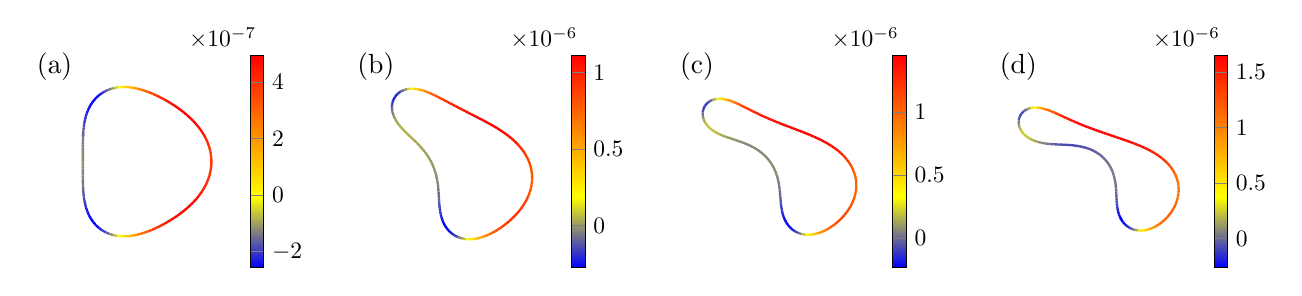
\begin{tikzpicture}[scale=0.85]

\begin{axis}[
  at = {(0.0cm,0.0cm)},
  width = 5.50cm,
  hide axis,
  axis equal image,
  xmin = -1.5,
  xmax = +1.5,
  ymin = -1.5,
  ymax = +1.5,
  xtick = \empty,
  ytick = \empty,
%  title style = {align=center, yshift = -0.4cm},
%  title = {\footnotesize $\beta = 5 \times 10^{-4}$ \\ 
%           \footnotesize $U_{\max} = 5.7\;\mu$m/s},
  colorbar,
  colorbar style={
    /pgfplots/tick scale binop=\tiny{\times},
%    ytick scale label code/.code={},
    at = {(1.02,0)},
    anchor = south west,
%    ytick={0,2e-5,4e-5,6e-5,8e-5},
%    yticklabels = {\tiny $0$,\tiny $2$,\tiny $4$,\tiny $6$,\tiny $8$},
  },
  colorbar/width=2mm
]

\addplot[samples=200,surf,point meta=explicit,line width=1.0pt] coordinates{
(-8.0935e-01,4.0093e-01) [-1.5552e-07]
(-8.1152e-01,3.6135e-01) [-1.4841e-07]
(-8.1303e-01,3.2164e-01) [-1.4211e-07]
(-8.1401e-01,2.8169e-01) [-1.3661e-07]
(-8.1460e-01,2.4141e-01) [-1.3188e-07]
(-8.1489e-01,2.0072e-01) [-1.2790e-07]
(-8.1498e-01,1.5952e-01) [-1.2466e-07]
(-8.1497e-01,1.1774e-01) [-1.2215e-07]
(-8.1490e-01,7.5293e-02) [-1.2038e-07]
(-8.1485e-01,3.2125e-02) [-1.1937e-07]
(-8.1483e-01,-1.1820e-02) [-1.1913e-07]
(-8.1487e-01,-5.6586e-02) [-1.1971e-07]
(-8.1494e-01,-1.0221e-01) [-1.2116e-07]
(-8.1499e-01,-1.4870e-01) [-1.2356e-07]
(-8.1493e-01,-1.9610e-01) [-1.2699e-07]
(-8.1463e-01,-2.4438e-01) [-1.3155e-07]
(-8.1390e-01,-2.9356e-01) [-1.3737e-07]
(-8.1249e-01,-3.4360e-01) [-1.4454e-07]
(-8.1011e-01,-3.9447e-01) [-1.5319e-07]
(-8.0638e-01,-4.4610e-01) [-1.6337e-07]
(-8.0088e-01,-4.9837e-01) [-1.7508e-07]
(-7.9311e-01,-5.5113e-01) [-1.8818e-07]
(-7.8254e-01,-6.0412e-01) [-2.0235e-07]
(-7.6862e-01,-6.5703e-01) [-2.1696e-07]
(-7.5080e-01,-7.0940e-01) [-2.3106e-07]
(-7.2859e-01,-7.6067e-01) [-2.4330e-07]
(-7.0161e-01,-8.1015e-01) [-2.5196e-07]
(-6.6961e-01,-8.5706e-01) [-2.5509e-07]
(-6.3256e-01,-9.0058e-01) [-2.5077e-07]
(-5.9068e-01,-9.3988e-01) [-2.3746e-07]
(-5.4438e-01,-9.7425e-01) [-2.1434e-07]
(-4.9431e-01,-1.0031e+00) [-1.8155e-07]
(-4.4121e-01,-1.0262e+00) [-1.4021e-07]
(-3.8591e-01,-1.0433e+00) [-9.2181e-08]
(-3.2921e-01,-1.0546e+00) [-3.9799e-08]
(-2.7184e-01,-1.0604e+00) [1.4591e-08]
(-2.1439e-01,-1.0612e+00) [6.8872e-08]
(-1.5734e-01,-1.0574e+00) [1.2138e-07]
(-1.0106e-01,-1.0498e+00) [1.7093e-07]
(-4.5770e-02,-1.0387e+00) [2.1678e-07]
(8.3541e-03,-1.0248e+00) [2.5856e-07]
(6.1220e-02,-1.0084e+00) [2.9617e-07]
(1.1277e-01,-9.9009e-01) [3.2967e-07]
(1.6299e-01,-9.7009e-01) [3.5926e-07]
(2.1185e-01,-9.4872e-01) [3.8515e-07]
(2.5936e-01,-9.2621e-01) [4.0763e-07]
(3.0552e-01,-9.0276e-01) [4.2694e-07]
(3.5031e-01,-8.7852e-01) [4.4333e-07]
(3.9374e-01,-8.5360e-01) [4.5701e-07]
(4.3579e-01,-8.2809e-01) [4.6821e-07]
(4.7646e-01,-8.0206e-01) [4.7710e-07]
(5.1575e-01,-7.7555e-01) [4.8386e-07]
(5.5364e-01,-7.4859e-01) [4.8863e-07]
(5.9012e-01,-7.2120e-01) [4.9156e-07]
(6.2520e-01,-6.9338e-01) [4.9279e-07]
(6.5886e-01,-6.6512e-01) [4.9245e-07]
(6.9111e-01,-6.3642e-01) [4.9066e-07]
(7.2194e-01,-6.0726e-01) [4.8755e-07]
(7.5137e-01,-5.7760e-01) [4.8323e-07]
(7.7940e-01,-5.4740e-01) [4.7784e-07]
(8.0602e-01,-5.1661e-01) [4.7149e-07]
(8.3123e-01,-4.8520e-01) [4.6432e-07]
(8.5502e-01,-4.5309e-01) [4.5647e-07]
(8.7738e-01,-4.2022e-01) [4.4808e-07]
(8.9827e-01,-3.8653e-01) [4.3931e-07]
(9.1764e-01,-3.5195e-01) [4.3034e-07]
(9.3544e-01,-3.1641e-01) [4.2134e-07]
(9.5158e-01,-2.7986e-01) [4.1255e-07]
(9.6596e-01,-2.4224e-01) [4.0417e-07]
(9.7846e-01,-2.0352e-01) [3.9646e-07]
(9.8895e-01,-1.6368e-01) [3.8968e-07]
(9.9726e-01,-1.2274e-01) [3.8410e-07]
(1.0032e+00,-8.0732e-02) [3.7997e-07]
(1.0067e+00,-3.7715e-02) [3.7752e-07]
(1.0075e+00,6.2103e-03) [3.7695e-07]
(1.0055e+00,5.0917e-02) [3.7838e-07]
(1.0005e+00,9.6248e-02) [3.8187e-07]
(9.9242e-01,1.4202e-01) [3.8737e-07]
(9.8117e-01,1.8804e-01) [3.9474e-07]
(9.6671e-01,2.3410e-01) [4.0372e-07]
(9.4902e-01,2.7997e-01) [4.1398e-07]
(9.2815e-01,3.2546e-01) [4.2511e-07]
(9.0417e-01,3.7037e-01) [4.3667e-07]
(8.7718e-01,4.1452e-01) [4.4816e-07]
(8.4732e-01,4.5776e-01) [4.5913e-07]
(8.1476e-01,4.9998e-01) [4.6914e-07]
(7.7968e-01,5.4107e-01) [4.7778e-07]
(7.4226e-01,5.8098e-01) [4.8471e-07]
(7.0270e-01,6.1965e-01) [4.8966e-07]
(6.6121e-01,6.5707e-01) [4.9237e-07]
(6.1796e-01,6.9323e-01) [4.9267e-07]
(5.7314e-01,7.2812e-01) [4.9040e-07]
(5.2691e-01,7.6174e-01) [4.8544e-07]
(4.7943e-01,7.9409e-01) [4.7767e-07]
(4.3084e-01,8.2516e-01) [4.6700e-07]
(3.8125e-01,8.5490e-01) [4.5330e-07]
(3.3078e-01,8.8326e-01) [4.3647e-07]
(2.7951e-01,9.1016e-01) [4.1636e-07]
(2.2752e-01,9.3547e-01) [3.9286e-07]
(1.7489e-01,9.5904e-01) [3.6582e-07]
(1.2168e-01,9.8068e-01) [3.3514e-07]
(6.7942e-02,1.0002e+00) [3.0071e-07]
(1.3770e-02,1.0172e+00) [2.6256e-07]
(-4.0741e-02,1.0315e+00) [2.2080e-07]
(-9.5457e-02,1.0428e+00) [1.7571e-07]
(-1.5020e-01,1.0507e+00) [1.2781e-07]
(-2.0473e-01,1.0548e+00) [7.7894e-08]
(-2.5874e-01,1.0550e+00) [2.7026e-08]
(-3.1188e-01,1.0509e+00) [-2.3433e-08]
(-3.6372e-01,1.0424e+00) [-7.1947e-08]
(-4.1379e-01,1.0294e+00) [-1.1689e-07]
(-4.6164e-01,1.0121e+00) [-1.5678e-07]
(-5.0681e-01,9.9061e-01) [-1.9038e-07]
(-5.4889e-01,9.6524e-01) [-2.1693e-07]
(-5.8759e-01,9.3643e-01) [-2.3617e-07]
(-6.2270e-01,9.0465e-01) [-2.4838e-07]
(-6.5413e-01,8.7042e-01) [-2.5423e-07]
(-6.8189e-01,8.3426e-01) [-2.5471e-07]
(-7.0610e-01,7.9664e-01) [-2.5093e-07]
(-7.2696e-01,7.5799e-01) [-2.4401e-07]
(-7.4472e-01,7.1866e-01) [-2.3494e-07]
(-7.5967e-01,6.7896e-01) [-2.2460e-07]
(-7.7209e-01,6.3908e-01) [-2.1366e-07]
(-7.8229e-01,5.9918e-01) [-2.0264e-07]
(-7.9057e-01,5.5934e-01) [-1.9190e-07]
(-7.9717e-01,5.1962e-01) [-1.8170e-07]
(-8.0236e-01,4.8000e-01) [-1.7219e-07]
(-8.0635e-01,4.4045e-01) [-1.6345e-07]
(-8.0935e-01,4.0093e-01) [-1.5552e-07]
(-8.1152e-01,3.6135e-01) [-1.4841e-07]
};

\end{axis}

%%%%%%%%%%%%%%%%%%%%%%%%%%%%%
\begin{axis}[
  at = {(4.8cm,0.0cm)},
  width = 5.50cm,
  hide axis,
  axis equal image,
  xmin = -1.5,
  xmax = +1.5,
  ymin = -1.5,
  ymax = +1.5,
  xtick = \empty,
  ytick = \empty,
%  title style = {align=center, yshift = -0.4cm},
%  title = {\footnotesize $\beta = 5 \times 10^{-4}$ \\ 
%           \footnotesize $U_{\max} = 5.7\;\mu$m/s},
  colorbar,
  colorbar style={
    /pgfplots/tick scale binop=\tiny{\times},
%    ytick scale label code/.code={},
    at = {(1.02,0)},
    anchor = south west,
%    ytick={0,2e-5,4e-5,6e-5,8e-5},
%    yticklabels = {\tiny $0$,\tiny $2$,\tiny $4$,\tiny $6$,\tiny $8$},
  },
  colorbar/width=2mm
]

\addplot[samples=200,surf,point meta=explicit,line width=1.0pt] coordinates{
(-9.4794e-02,-1.0512e+00) [-1.6347e-07]
(-5.9169e-02,-1.0692e+00) [-1.0612e-07]
(-2.1750e-02,-1.0835e+00) [-3.9000e-08]
(1.7132e-02,-1.0939e+00) [3.5935e-08]
(5.7162e-02,-1.1006e+00) [1.1609e-07]
(9.8055e-02,-1.1036e+00) [1.9909e-07]
(1.3956e-01,-1.1030e+00) [2.8252e-07]
(1.8147e-01,-1.0989e+00) [3.6438e-07]
(2.2361e-01,-1.0916e+00) [4.4298e-07]
(2.6586e-01,-1.0813e+00) [5.1703e-07]
(3.0812e-01,-1.0681e+00) [5.8567e-07]
(3.5032e-01,-1.0522e+00) [6.4824e-07]
(3.9242e-01,-1.0337e+00) [7.0450e-07]
(4.3437e-01,-1.0128e+00) [7.5422e-07]
(4.7614e-01,-9.8967e-01) [7.9749e-07]
(5.1768e-01,-9.6433e-01) [8.3426e-07]
(5.5894e-01,-9.3688e-01) [8.6477e-07]
(5.9984e-01,-9.0734e-01) [8.8903e-07]
(6.4028e-01,-8.7574e-01) [9.0730e-07]
(6.8011e-01,-8.4207e-01) [9.1956e-07]
(7.1917e-01,-8.0628e-01) [9.2614e-07]
(7.5722e-01,-7.6832e-01) [9.2706e-07]
(7.9399e-01,-7.2814e-01) [9.2275e-07]
(8.2916e-01,-6.8566e-01) [9.1343e-07]
(8.6233e-01,-6.4085e-01) [8.9985e-07]
(8.9309e-01,-5.9368e-01) [8.8262e-07]
(9.2095e-01,-5.4417e-01) [8.6303e-07]
(9.4541e-01,-4.9243e-01) [8.4223e-07]
(9.6595e-01,-4.3861e-01) [8.2210e-07]
(9.8207e-01,-3.8301e-01) [8.0422e-07]
(9.9333e-01,-3.2600e-01) [7.9067e-07]
(9.9936e-01,-2.6805e-01) [7.8278e-07]
(9.9994e-01,-2.0971e-01) [7.8199e-07]
(9.9497e-01,-1.5159e-01) [7.8856e-07]
(9.8452e-01,-9.4264e-02) [8.0258e-07]
(9.6882e-01,-3.8308e-02) [8.2290e-07]
(9.4821e-01,1.5800e-02) [8.4843e-07]
(9.2317e-01,6.7675e-02) [8.7724e-07]
(8.9420e-01,1.1705e-01) [9.0787e-07]
(8.6186e-01,1.6376e-01) [9.3853e-07]
(8.2671e-01,2.0774e-01) [9.6816e-07]
(7.8925e-01,2.4904e-01) [9.9557e-07]
(7.4997e-01,2.8774e-01) [1.0203e-06]
(7.0932e-01,3.2398e-01) [1.0419e-06]
(6.6767e-01,3.5793e-01) [1.0603e-06]
(6.2535e-01,3.8978e-01) [1.0754e-06]
(5.8265e-01,4.1974e-01) [1.0875e-06]
(5.3981e-01,4.4798e-01) [1.0967e-06]
(4.9702e-01,4.7469e-01) [1.1034e-06]
(4.5444e-01,5.0006e-01) [1.1076e-06]
(4.1222e-01,5.2424e-01) [1.1098e-06]
(3.7045e-01,5.4738e-01) [1.1101e-06]
(3.2922e-01,5.6963e-01) [1.1087e-06]
(2.8857e-01,5.9110e-01) [1.1058e-06]
(2.4855e-01,6.1191e-01) [1.1017e-06]
(2.0918e-01,6.3215e-01) [1.0962e-06]
(1.7044e-01,6.5194e-01) [1.0897e-06]
(1.3232e-01,6.7133e-01) [1.0820e-06]
(9.4794e-02,6.9043e-01) [1.0733e-06]
(5.7812e-02,7.0929e-01) [1.0635e-06]
(2.1313e-02,7.2798e-01) [1.0526e-06]
(-1.4773e-02,7.4656e-01) [1.0405e-06]
(-5.0526e-02,7.6510e-01) [1.0271e-06]
(-8.6039e-02,7.8362e-01) [1.0123e-06]
(-1.2141e-01,8.0219e-01) [9.9587e-07]
(-1.5674e-01,8.2082e-01) [9.7750e-07]
(-1.9215e-01,8.3955e-01) [9.5700e-07]
(-2.2776e-01,8.5836e-01) [9.3385e-07]
(-2.6368e-01,8.7725e-01) [9.0774e-07]
(-3.0007e-01,8.9616e-01) [8.7793e-07]
(-3.3705e-01,9.1501e-01) [8.4387e-07]
(-3.7480e-01,9.3367e-01) [8.0460e-07]
(-4.1347e-01,9.5193e-01) [7.5923e-07]
(-4.5324e-01,9.6954e-01) [7.0650e-07]
(-4.9430e-01,9.8611e-01) [6.4521e-07]
(-5.3681e-01,1.0011e+00) [5.7394e-07]
(-5.8094e-01,1.0140e+00) [4.9160e-07]
(-6.2672e-01,1.0238e+00) [3.9751e-07]
(-6.7409e-01,1.0297e+00) [2.9227e-07]
(-7.2271e-01,1.0303e+00) [1.7858e-07]
(-7.7187e-01,1.0244e+00) [6.2184e-08]
(-8.2038e-01,1.0109e+00) [-4.7398e-08]
(-8.6653e-01,9.8859e-01) [-1.3812e-07]
(-9.0813e-01,9.5729e-01) [-1.9792e-07]
(-9.4283e-01,9.1741e-01) [-2.2005e-07]
(-9.6852e-01,8.7034e-01) [-2.0581e-07]
(-9.8379e-01,8.1817e-01) [-1.6545e-07]
(-9.8812e-01,7.6330e-01) [-1.1273e-07]
(-9.8196e-01,7.0796e-01) [-6.0750e-08]
(-9.6641e-01,6.5390e-01) [-1.7359e-08]
(-9.4297e-01,6.0219e-01) [1.4003e-08]
(-9.1323e-01,5.5331e-01) [3.4022e-08]
(-8.7867e-01,5.0724e-01) [4.4598e-08]
(-8.4062e-01,4.6361e-01) [4.8574e-08]
(-8.0020e-01,4.2184e-01) [4.8059e-08]
(-7.5837e-01,3.8128e-01) [4.5085e-08]
(-7.1592e-01,3.4124e-01) [4.0723e-08]
(-6.7358e-01,3.0110e-01) [3.5999e-08]
(-6.3198e-01,2.6029e-01) [3.1184e-08]
(-5.9171e-01,2.1837e-01) [2.6705e-08]
(-5.5331e-01,1.7504e-01) [2.2392e-08]
(-5.1727e-01,1.3011e-01) [1.8389e-08]
(-4.8401e-01,8.3529e-02) [1.4327e-08]
(-4.5387e-01,3.5382e-02) [1.0258e-08]
(-4.2710e-01,-1.4152e-02) [5.7439e-09]
(-4.0384e-01,-6.4811e-02) [8.4748e-10]
(-3.8410e-01,-1.1628e-01) [-4.8688e-09]
(-3.6779e-01,-1.6824e-01) [-1.1306e-08]
(-3.5469e-01,-2.2034e-01) [-1.8891e-08]
(-3.4449e-01,-2.7231e-01) [-2.7506e-08]
(-3.3678e-01,-3.2389e-01) [-3.7587e-08]
(-3.3109e-01,-3.7489e-01) [-4.9020e-08]
(-3.2693e-01,-4.2516e-01) [-6.2250e-08]
(-3.2374e-01,-4.7462e-01) [-7.7141e-08]
(-3.2098e-01,-5.2320e-01) [-9.4094e-08]
(-3.1812e-01,-5.7086e-01) [-1.1286e-07]
(-3.1461e-01,-6.1759e-01) [-1.3364e-07]
(-3.0995e-01,-6.6332e-01) [-1.5587e-07]
(-3.0369e-01,-7.0798e-01) [-1.7936e-07]
(-2.9539e-01,-7.5148e-01) [-2.0296e-07]
(-2.8469e-01,-7.9363e-01) [-2.2581e-07]
(-2.7130e-01,-8.3424e-01) [-2.4604e-07]
(-2.5500e-01,-8.7305e-01) [-2.6212e-07]
(-2.3566e-01,-9.0977e-01) [-2.7165e-07]
(-2.1322e-01,-9.4408e-01) [-2.7287e-07]
(-1.8775e-01,-9.7567e-01) [-2.6358e-07]
(-1.5937e-01,-1.0042e+00) [-2.4271e-07]
(-1.2830e-01,-1.0295e+00) [-2.0921e-07]
(-9.4794e-02,-1.0512e+00) [-1.6347e-07]
(-5.9169e-02,-1.0692e+00) [-1.0612e-07]
};

\end{axis}

%%%%%%%%%%%%%%%%%%%%%%%%%%%%%
\begin{axis}[
  at = {(9.6cm,0.0cm)},
  width = 5.50cm,
  hide axis,
  axis equal image,
  xmin = -1.5,
  xmax = +1.5,
  ymin = -1.5,
  ymax = +1.5,
  xtick = \empty,
  ytick = \empty,
%  title style = {align=center, yshift = -0.4cm},
%  title = {\footnotesize $\beta = 5 \times 10^{-4}$ \\ 
%           \footnotesize $U_{\max} = 5.7\;\mu$m/s},
  colorbar,
  colorbar style={
    /pgfplots/tick scale binop=\tiny{\times},
%    ytick scale label code/.code={},
    at = {(1.02,0)},
    anchor = south west,
%    ytick={0,2e-5,4e-5,6e-5,8e-5},
%    yticklabels = {\tiny $0$,\tiny $2$,\tiny $4$,\tiny $6$,\tiny $8$},
  },
  colorbar/width=2mm
]

\addplot[samples=200,surf,point meta=explicit,line width=1.0pt] coordinates{
(3.5702e-01,-1.0399e+00) [3.4758e-07]
(3.9692e-01,-1.0382e+00) [4.5476e-07]
(4.3662e-01,-1.0330e+00) [5.5772e-07]
(4.7598e-01,-1.0245e+00) [6.5446e-07]
(5.1491e-01,-1.0130e+00) [7.4334e-07]
(5.5334e-01,-9.9873e-01) [8.2372e-07]
(5.9126e-01,-9.8182e-01) [8.9484e-07]
(6.2863e-01,-9.6244e-01) [9.5685e-07]
(6.6546e-01,-9.4069e-01) [1.0094e-06]
(7.0170e-01,-9.1663e-01) [1.0531e-06]
(7.3732e-01,-8.9032e-01) [1.0876e-06]
(7.7222e-01,-8.6174e-01) [1.1136e-06]
(8.0631e-01,-8.3090e-01) [1.1310e-06]
(8.3941e-01,-7.9774e-01) [1.1405e-06]
(8.7132e-01,-7.6221e-01) [1.1421e-06]
(9.0177e-01,-7.2426e-01) [1.1368e-06]
(9.3042e-01,-6.8382e-01) [1.1249e-06]
(9.5688e-01,-6.4088e-01) [1.1081e-06]
(9.8069e-01,-5.9543e-01) [1.0872e-06]
(1.0013e+00,-5.4754e-01) [1.0646e-06]
(1.0183e+00,-4.9736e-01) [1.0423e-06]
(1.0309e+00,-4.4515e-01) [1.0231e-06]
(1.0388e+00,-3.9128e-01) [1.0094e-06]
(1.0414e+00,-3.3623e-01) [1.0039e-06]
(1.0384e+00,-2.8057e-01) [1.0079e-06]
(1.0297e+00,-2.2496e-01) [1.0226e-06]
(1.0151e+00,-1.7006e-01) [1.0472e-06]
(9.9492e-01,-1.1652e-01) [1.0807e-06]
(9.6941e-01,-6.4882e-02) [1.1203e-06]
(9.3903e-01,-1.5598e-02) [1.1638e-06]
(9.0433e-01,3.1018e-02) [1.2083e-06]
(8.6587e-01,7.4788e-02) [1.2516e-06]
(8.2423e-01,1.1565e-01) [1.2918e-06]
(7.7995e-01,1.5365e-01) [1.3278e-06]
(7.3355e-01,1.8891e-01) [1.3588e-06]
(6.8549e-01,2.2160e-01) [1.3848e-06]
(6.3617e-01,2.5194e-01) [1.4057e-06]
(5.8594e-01,2.8015e-01) [1.4220e-06]
(5.3509e-01,3.0646e-01) [1.4340e-06]
(4.8391e-01,3.3111e-01) [1.4424e-06]
(4.3260e-01,3.5433e-01) [1.4476e-06]
(3.8136e-01,3.7632e-01) [1.4502e-06]
(3.3037e-01,3.9728e-01) [1.4507e-06]
(2.7975e-01,4.1739e-01) [1.4495e-06]
(2.2965e-01,4.3682e-01) [1.4469e-06]
(1.8016e-01,4.5570e-01) [1.4433e-06]
(1.3139e-01,4.7417e-01) [1.4387e-06]
(8.3397e-02,4.9235e-01) [1.4335e-06]
(3.6261e-02,5.1032e-01) [1.4275e-06]
(-9.9707e-03,5.2816e-01) [1.4209e-06]
(-5.5257e-02,5.4595e-01) [1.4135e-06]
(-9.9572e-02,5.6374e-01) [1.4053e-06]
(-1.4290e-01,5.8156e-01) [1.3961e-06]
(-1.8525e-01,5.9944e-01) [1.3858e-06]
(-2.2662e-01,6.1741e-01) [1.3741e-06]
(-2.6705e-01,6.3546e-01) [1.3608e-06]
(-3.0658e-01,6.5360e-01) [1.3455e-06]
(-3.4527e-01,6.7181e-01) [1.3281e-06]
(-3.8320e-01,6.9009e-01) [1.3080e-06]
(-4.2046e-01,7.0840e-01) [1.2849e-06]
(-4.5715e-01,7.2670e-01) [1.2584e-06]
(-4.9341e-01,7.4494e-01) [1.2278e-06]
(-5.2938e-01,7.6306e-01) [1.1925e-06]
(-5.6521e-01,7.8095e-01) [1.1516e-06]
(-6.0110e-01,7.9849e-01) [1.1042e-06]
(-6.3723e-01,8.1551e-01) [1.0492e-06]
(-6.7383e-01,8.3177e-01) [9.8515e-07]
(-7.1112e-01,8.4698e-01) [9.1060e-07]
(-7.4931e-01,8.6071e-01) [8.2395e-07]
(-7.8860e-01,8.7243e-01) [7.2379e-07]
(-8.2911e-01,8.8143e-01) [6.0936e-07]
(-8.7084e-01,8.8686e-01) [4.8121e-07]
(-9.1357e-01,8.8766e-01) [3.4269e-07]
(-9.5674e-01,8.8267e-01) [2.0075e-07]
(-9.9932e-01,8.7073e-01) [6.7722e-08]
(-1.0397e+00,8.5086e-01) [-4.0704e-08]
(-1.0759e+00,8.2264e-01) [-1.0783e-07]
(-1.1054e+00,7.8642e-01) [-1.2439e-07]
(-1.1261e+00,7.4351e-01) [-9.2265e-08]
(-1.1363e+00,6.9605e-01) [-2.7331e-08]
(-1.1353e+00,6.4661e-01) [4.9344e-08]
(-1.1233e+00,5.9770e-01) [1.1781e-07]
(-1.1015e+00,5.5136e-01) [1.6719e-07]
(-1.0712e+00,5.0895e-01) [1.9409e-07]
(-1.0342e+00,4.7116e-01) [2.0167e-07]
(-9.9186e-01,4.3808e-01) [1.9488e-07]
(-9.4558e-01,4.0942e-01) [1.7941e-07]
(-8.9637e-01,3.8458e-01) [1.5958e-07]
(-8.4504e-01,3.6282e-01) [1.3884e-07]
(-7.9223e-01,3.4328e-01) [1.1923e-07]
(-7.3840e-01,3.2510e-01) [1.0213e-07]
(-6.8396e-01,3.0740e-01) [8.8115e-08]
(-6.2925e-01,2.8934e-01) [7.7436e-08]
(-5.7463e-01,2.7012e-01) [6.9912e-08]
(-5.2047e-01,2.4903e-01) [6.5320e-08]
(-4.6719e-01,2.2543e-01) [6.3131e-08]
(-4.1526e-01,1.9883e-01) [6.2967e-08]
(-3.6521e-01,1.6885e-01) [6.4164e-08]
(-3.1759e-01,1.3529e-01) [6.6358e-08]
(-2.7294e-01,9.8093e-02) [6.8837e-08]
(-2.3177e-01,5.7394e-02) [7.1323e-08]
(-1.9453e-01,1.3463e-02) [7.3082e-08]
(-1.6153e-01,-3.3295e-02) [7.3959e-08]
(-1.3296e-01,-8.2385e-02) [7.3252e-08]
(-1.0885e-01,-1.3326e-01) [7.0972e-08]
(-8.9048e-02,-1.8537e-01) [6.6488e-08]
(-7.3264e-02,-2.3819e-01) [5.9951e-08]
(-6.1057e-02,-2.9125e-01) [5.0758e-08]
(-5.1874e-02,-3.4420e-01) [3.9099e-08]
(-4.5071e-02,-3.9672e-01) [2.4324e-08]
(-3.9942e-02,-4.4863e-01) [6.6146e-09]
(-3.5746e-02,-4.9977e-01) [-1.4675e-08]
(-3.1726e-02,-5.5006e-01) [-3.9217e-08]
(-2.7131e-02,-5.9940e-01) [-6.7353e-08]
(-2.1236e-02,-6.4770e-01) [-9.8157e-08]
(-1.3365e-02,-6.9479e-01) [-1.3106e-07]
(-2.9145e-03,-7.4045e-01) [-1.6385e-07]
(1.0613e-02,-7.8438e-01) [-1.9440e-07]
(2.7584e-02,-8.2615e-01) [-2.1885e-07]
(4.8202e-02,-8.6532e-01) [-2.3371e-07]
(7.2491e-02,-9.0138e-01) [-2.3456e-07]
(1.0030e-01,-9.3385e-01) [-2.1843e-07]
(1.3130e-01,-9.6231e-01) [-1.8286e-07]
(1.6506e-01,-9.8643e-01) [-1.2781e-07]
(2.0106e-01,-1.0060e+00) [-5.4514e-08]
(2.3874e-01,-1.0211e+00) [3.3786e-08]
(2.7759e-01,-1.0316e+00) [1.3318e-07]
(3.1714e-01,-1.0378e+00) [2.3919e-07]
(3.5702e-01,-1.0399e+00) [3.4758e-07]
(3.9692e-01,-1.0382e+00) [4.5476e-07]
};

\end{axis}

%%%%%%%%%%%%%%%%%%%%%%%%%%%%%
\begin{axis}[
  at = {(14.4cm,0.0cm)},
  width = 5.50cm,
  hide axis,
  axis equal image,
  xmin = -1.5,
  xmax = +1.5,
  ymin = -1.5,
  ymax = +1.5,
  xtick = \empty,
  ytick = \empty,
%  title style = {align=center, yshift = -0.4cm},
%  title = {\footnotesize $\beta = 5 \times 10^{-4}$ \\ 
%           \footnotesize $U_{\max} = 5.7\;\mu$m/s},
  colorbar,
  colorbar style={
    /pgfplots/tick scale binop=\tiny{\times},
%    ytick scale label code/.code={},
    at = {(1.02,0)},
    anchor = south west,
%    ytick={0,2e-5,4e-5,6e-5,8e-5},
%    yticklabels = {\tiny $0$,\tiny $2$,\tiny $4$,\tiny $6$,\tiny $8$},
  },
  colorbar/width=2mm
]

\addplot[samples=200,surf,point meta=explicit,line width=1.0pt] coordinates{
(2.2636e-01,-7.9127e-01) [-2.4236e-07]
(2.4493e-01,-8.2662e-01) [-2.5678e-07]
(2.6741e-01,-8.5975e-01) [-2.5550e-07]
(2.9388e-01,-8.9007e-01) [-2.3369e-07]
(3.2429e-01,-9.1691e-01) [-1.8703e-07]
(3.5838e-01,-9.3966e-01) [-1.1374e-07]
(3.9571e-01,-9.5775e-01) [-1.4517e-08]
(4.3573e-01,-9.7075e-01) [1.0660e-07]
(4.7779e-01,-9.7840e-01) [2.4332e-07]
(5.2120e-01,-9.8061e-01) [3.8784e-07]
(5.6535e-01,-9.7747e-01) [5.3228e-07]
(6.0967e-01,-9.6917e-01) [6.6984e-07]
(6.5370e-01,-9.5600e-01) [7.9509e-07]
(6.9706e-01,-9.3828e-01) [9.0463e-07]
(7.3945e-01,-9.1633e-01) [9.9627e-07]
(7.8063e-01,-8.9043e-01) [1.0695e-06]
(8.2037e-01,-8.6083e-01) [1.1241e-06]
(8.5842e-01,-8.2772e-01) [1.1612e-06]
(8.9449e-01,-7.9123e-01) [1.1816e-06]
(9.2826e-01,-7.5149e-01) [1.1873e-06]
(9.5930e-01,-7.0859e-01) [1.1800e-06]
(9.8712e-01,-6.6263e-01) [1.1626e-06]
(1.0112e+00,-6.1378e-01) [1.1380e-06]
(1.0308e+00,-5.6228e-01) [1.1106e-06]
(1.0454e+00,-5.0848e-01) [1.0844e-06]
(1.0543e+00,-4.5291e-01) [1.0644e-06]
(1.0571e+00,-3.9619e-01) [1.0545e-06]
(1.0534e+00,-3.3909e-01) [1.0580e-06]
(1.0430e+00,-2.8244e-01) [1.0758e-06]
(1.0262e+00,-2.2707e-01) [1.1076e-06]
(1.0031e+00,-1.7373e-01) [1.1505e-06]
(9.7444e-01,-1.2303e-01) [1.2012e-06]
(9.4077e-01,-7.5399e-02) [1.2553e-06]
(9.0283e-01,-3.1083e-02) [1.3097e-06]
(8.6136e-01,9.8392e-03) [1.3611e-06]
(8.1704e-01,4.7433e-02) [1.4078e-06]
(7.7049e-01,8.1866e-02) [1.4485e-06]
(7.2226e-01,1.1338e-01) [1.4832e-06]
(6.7283e-01,1.4224e-01) [1.5118e-06]
(6.2258e-01,1.6875e-01) [1.5351e-06]
(5.7185e-01,1.9321e-01) [1.5536e-06]
(5.2092e-01,2.1588e-01) [1.5684e-06]
(4.7000e-01,2.3703e-01) [1.5800e-06]
(4.1929e-01,2.5689e-01) [1.5893e-06]
(3.6895e-01,2.7569e-01) [1.5969e-06]
(3.1911e-01,2.9361e-01) [1.6034e-06]
(2.6987e-01,3.1080e-01) [1.6091e-06]
(2.2132e-01,3.2742e-01) [1.6145e-06]
(1.7354e-01,3.4359e-01) [1.6197e-06]
(1.2657e-01,3.5939e-01) [1.6248e-06]
(8.0460e-02,3.7492e-01) [1.6298e-06]
(3.5237e-02,3.9025e-01) [1.6346e-06]
(-9.0849e-03,4.0544e-01) [1.6389e-06]
(-5.2504e-02,4.2053e-01) [1.6426e-06]
(-9.5029e-02,4.3557e-01) [1.6451e-06]
(-1.3668e-01,4.5059e-01) [1.6463e-06]
(-1.7749e-01,4.6563e-01) [1.6458e-06]
(-2.1751e-01,4.8072e-01) [1.6434e-06]
(-2.5679e-01,4.9590e-01) [1.6386e-06]
(-2.9538e-01,5.1118e-01) [1.6314e-06]
(-3.3338e-01,5.2660e-01) [1.6213e-06]
(-3.7086e-01,5.4218e-01) [1.6085e-06]
(-4.0791e-01,5.5796e-01) [1.5922e-06]
(-4.4463e-01,5.7395e-01) [1.5725e-06]
(-4.8114e-01,5.9017e-01) [1.5487e-06]
(-5.1754e-01,6.0662e-01) [1.5206e-06]
(-5.5397e-01,6.2328e-01) [1.4872e-06]
(-5.9055e-01,6.4013e-01) [1.4480e-06]
(-6.2742e-01,6.5709e-01) [1.4018e-06]
(-6.6476e-01,6.7405e-01) [1.3474e-06]
(-7.0273e-01,6.9083e-01) [1.2832e-06]
(-7.4152e-01,7.0719e-01) [1.2073e-06]
(-7.8136e-01,7.2274e-01) [1.1174e-06]
(-8.2246e-01,7.3699e-01) [1.0111e-06]
(-8.6500e-01,7.4923e-01) [8.8604e-07]
(-9.0912e-01,7.5853e-01) [7.4078e-07]
(-9.5477e-01,7.6372e-01) [5.7602e-07]
(-1.0016e+00,7.6334e-01) [3.9733e-07]
(-1.0487e+00,7.5579e-01) [2.1730e-07]
(-1.0945e+00,7.3953e-01) [5.7311e-08]
(-1.1365e+00,7.1351e-01) [-5.5988e-08]
(-1.1718e+00,6.7766e-01) [-1.0092e-07]
(-1.1973e+00,6.3328e-01) [-7.3714e-08]
(-1.2105e+00,5.8299e-01) [5.4470e-09]
(-1.2104e+00,5.3016e-01) [1.0263e-07]
(-1.1972e+00,4.7819e-01) [1.8589e-07]
(-1.1725e+00,4.2979e-01) [2.3798e-07]
(-1.1381e+00,3.8678e-01) [2.5549e-07]
(-1.0963e+00,3.5004e-01) [2.4475e-07]
(-1.0488e+00,3.1976e-01) [2.1458e-07]
(-9.9741e-01,2.9567e-01) [1.7389e-07]
(-9.4326e-01,2.7717e-01) [1.2917e-07]
(-8.8731e-01,2.6351e-01) [8.5284e-08]
(-8.3022e-01,2.5387e-01) [4.4997e-08]
(-7.7246e-01,2.4737e-01) [1.0113e-08]
(-7.1433e-01,2.4314e-01) [-1.8693e-08]
(-6.5605e-01,2.4030e-01) [-4.1101e-08]
(-5.9774e-01,2.3801e-01) [-5.7376e-08]
(-5.3952e-01,2.3544e-01) [-6.7817e-08]
(-4.8151e-01,2.3180e-01) [-7.3085e-08]
(-4.2386e-01,2.2635e-01) [-7.3700e-08]
(-3.6680e-01,2.1842e-01) [-7.0495e-08]
(-3.1063e-01,2.0739e-01) [-6.4013e-08]
(-2.5574e-01,1.9279e-01) [-5.5169e-08]
(-2.0257e-01,1.7426e-01) [-4.4421e-08]
(-1.5166e-01,1.5158e-01) [-3.2704e-08]
(-1.0353e-01,1.2473e-01) [-2.0321e-08]
(-5.8713e-02,9.3819e-02) [-8.1937e-09]
(-1.7681e-02,5.9155e-02) [3.5473e-09]
(1.9192e-02,2.1160e-02) [1.3996e-08]
(5.1659e-02,-1.9635e-02) [2.3183e-08]
(7.9618e-02,-6.2644e-02) [3.0251e-08]
(1.0312e-01,-1.0727e-01) [3.5415e-08]
(1.2235e-01,-1.5293e-01) [3.7947e-08]
(1.3763e-01,-1.9911e-01) [3.8231e-08]
(1.4937e-01,-2.4539e-01) [3.5651e-08]
(1.5807e-01,-2.9143e-01) [3.0644e-08]
(1.6426e-01,-3.3698e-01) [2.2604e-08]
(1.6850e-01,-3.8189e-01) [1.1895e-08]
(1.7137e-01,-4.2608e-01) [-2.1340e-09]
(1.7344e-01,-4.6953e-01) [-1.9200e-08]
(1.7528e-01,-5.1226e-01) [-3.9922e-08]
(1.7743e-01,-5.5431e-01) [-6.3932e-08]
(1.8043e-01,-5.9572e-01) [-9.1542e-08]
(1.8483e-01,-6.3649e-01) [-1.2189e-07]
(1.9114e-01,-6.7658e-01) [-1.5443e-07]
(1.9985e-01,-7.1590e-01) [-1.8711e-07]
(2.1145e-01,-7.5423e-01) [-2.1774e-07]
(2.2636e-01,-7.9127e-01) [-2.4236e-07]
(2.4493e-01,-8.2662e-01) [-2.5678e-07]
};

\end{axis}


\node at (0.3,3.0) {(a)};
\node at (5.1,3.0) {(b)};
\node at (9.9,3.0) {(c)};
\node at (14.7,3.0) {(d)};



\end{tikzpicture}

  \else
  \includegraphics{figures/parabolicTensions.pdf}
  \fi
%  \begin{tikzpicture}[scale=1]
%    \node[inner sep=0pt] at (0,0) {
%    \includegraphics[width=\textwidth]{figures/parabolicTensions.pdf}
%    };
%    \node at (-8.2,1.5) {(a)};
%    \node at (-3.8,1.5) {(b)};
%    \node at (+0.6,1.5) {(c)};
%    \node at (+5.0,1.5) {(d)};
%  \end{tikzpicture}
  \caption{\label{fig:parabolicTensions} The equilibrium tension
  distribution of a semipermeable inextensible membrane with
  $\beta=10^{-3}$ in a parabolic flow
  (Figure~\ref{fig:parabolicComposite}). The maximum flow velocities are
  (a) 200 $\mu$m/s, (b) 400 $\mu$m/s, (c) 600 $\mu$m/s, and (d) 800
  $\mu$m/s.}
\end{figure*}
 The membrane tension distribution of the equilibrium shapes are shown
 in Figure~\ref{fig:parabolicTensions} for the flow velocities $U$ from
 $200\;\mu$m/s to $800 \;\mu$m/s. We note that in the Poiseuille flow
 the membrane tension is positive in the front, and negative in the rear
 part of the vesicle. Furthermore we also note that the tension
 magnitude is almost linearly proportional to $U$ as in the linear shear
 flow.

%%%%%%%%%%%%%%%%%%%%%%%%%%%%%%%%%%%%%%%%%%%%%%%%%%%%%%%%%%%%%%%%%%%%%%%%

\section{Hydrodynamics of A semipermeable inextensible membrane under strong confinement\label{sec:confinement}}
Here we consider a semipermeable inextensible membrane under strong
confinement: a long closely-fit channel and a contracting channel. In a
narrow microfluidic channel, a large pressure jump is often used to push
the vesicle through a closely-fit channel~\cite{abk-fai-sto2006}. Our
simulations show that such a configuration can lead to an amplification
of water permeation at a fast time scale of the order of milliseconds.
In addition, we find that a large value of $\beta$ is needed to keep the
membrane tension below the threshold value for membrane poration. Such
high permeability for water may be regarded as an indication that the
lipid bilayer membrane is porated under strong confinement, and our
inextensible membrane model is for a porated vesicle within the Helfrich
free energy framework. As in the previous examples, we fix the membrane
length and examine the enclosed water content as a dynamic consequence
of water flow, membrane shape deformation, and membrane tension
distribution.


%%%%%%%%%%%%%%%%%%%%%%%%%%%%%%%%%%%%%%%%%%%%%%%%%%%%%%%%%%%%%%%%%%%%%%%%
\subsection{A Semipermeable Inextensible Membrane in a Closely-fit Channel (Stenosis)}
\begin{figure*}[htp]
  \centering
  \ifTikz
  \input{figures/stenosisComposite.tikz}
  \else
  \includegraphics{figures/stenosisComposite.pdf}
  \fi
  \caption{\label{fig:stenosisComposite} (a) A semipermeable
  inextensible membrane passing through a closely-fit channel similar to
  the experimental device in~\citet{abk-fai-sto2006}. (b) A
  semipermeable inextensible membrane passing through a (three-times)
  longer closely-fit channel than (a). In (a) and (b), red regions
  correspond to influx and blue regions correspond to efflux. (c) and
  (d) The tension in N/m of the vesicle shapes in (a) and (b). (e) The
  excess pressure of an impermeable and semipermeable inextensible
  membrane in the short geometry in (a). (f) The reduced area in the
  geometries in (a) and (b) as a function of the membranes' center of
  mass. In (e) and (f), the x-axis is scaled by $1/L$ where $L$ is half
  the length of the constriction. (g) The reduced area in the geometries
  in (a) and (b) as a function of time. The time axis is scaled by
  $1/t_R$ where $t_R$ is the residency time. In (e) and (f), the dashed
  lines correspond to the locations of the inlet and outlet. In (g), the
  dashed lines correspond to the times that the vesicle enters and exits
  the constriction.}
\end{figure*}
When red blood cells go through small capillary vessels, they experience
large shape deformation and significant membrane stretching that
triggers ATP release~\cite{Wan2008_PNAS, ForsythWan2011_PNAS}. Many
cells exhibit extraordinary flexibility as they go through narrow
vessels~\cite{AuStoreyMoore2016_PNAS}, and adjustment of
surface-to-volume ratio may be a key factor for a successful passage.
Here we quantify the effect of water permeability on a vesicle going
through a stenosis (a long microfluidic channel with a width smaller
than the cell radius). Based on previous
findings~\cite{abk-fai-sto2006}, we first examine the effect of
semipermeability on the pressure fluctuation across a stenosed geometry.
In this experiment, a pressure drop is used to squeeze a red blood cell
through a constriction with diameter $5\;\mu$m and length $45\;\mu$m. We
set up a similar computational geometry with a Poiseuille flow imposed
at the inlet and outlet (Figure~\ref{fig:stenosisComposite}(a)). We set
the maximum flow velocity to $U_{\max} = 1000 \;\mu$m/s at the inlet and
outlet so that the residency time of the membrane in the stenosis
channel is $t_R \approx 25$ ms which agrees with the experimental
results~\cite{abk-fai-sto2006}. When the red blood cell enters the
channel, an increase in the pressure drop is required to maintain a
constant flow rate, and the difference in the pressure drop is called
the excess pressure.

We consider both an impermeable vesicle and semipermeable inextensible
membrane with initial reduced area $\alpha = 0.65$ passing through a
long narrow channel and compute the excess pressure as a function of
vesicle position in the channel (Figure~\ref{fig:stenosisComposite}(e)).
The impermeable case agrees with experimental
results~\cite{abk-fai-sto2006} (see Figure 3). Our simulations show that
less excess pressure is needed to drive a semipermeable inextensible
membrane through the closely-fit channel. Once in the channel, the
vesicle takes a bullet shape with maximum tension in the front and
minimum tension in the back (Figure~\ref{fig:stenosisComposite}(c)),
consistent with earlier results~\cite{Pak2015_PNAS,
HarmanBertrandJoos2017_CJP}.

Figures~\ref{fig:stenosisComposite}(f)
and~\ref{fig:stenosisComposite}(g) show that the semipermeable
inextensible membrane deflates from the beginning due to the high flow
velocity, consistent with the results for a vesicle in a Poiseuille flow
in open space. As the membrane enters the stenosis channel, it continues
to deflate in the front even though we observe influx (red segment) at
various rear locations in the membrane. Overall, the membrane loses
about 6.1\% of its initial total water at a constant rate as shown in
Figures~\ref{fig:stenosisComposite}(f)
and~\ref{fig:stenosisComposite}(g) (blue curves). Thus we expect that a
larger amount of deflation is possible if the inextensible membrane is
inside a longer stenosis: we consider a vesicle passing through a
channel of triple the length in Figure~\ref{fig:stenosisComposite}(b)
and (d) with $U_{\max}=1000\;\mu$m/s, and we observe that vesicle stays
inside the stenosis for a residence time $t_R \approx 70$ ms and the
area decreases by 13.2\% (red curves).

%When a semipermeable vesicle goes through a closely-fit channel, we
%observe that the water efflux is found in the front, and the influx is
%in the rear of the vesicle membrane
%(Figure~\ref{fig:stenosisComposite}). This corresponds well to the
%corresponding tension distribution in Figure~\ref{fig:stenosisTensions}:
%Larger tension in the front, and smaller tension in the rear.

%%%%%%%%%%%%%%%%%%%%%%%%%%%%%%%%%%%%%%%%%%%%%%%%%%%%%%%%%%%%%%%%%%%%%%%%
\subsection{A Semipermeable Inextensible Membrane in a Contracting Geometry} 
\begin{figure}[htp]
  \centering
    \centering
  \ifTikz
  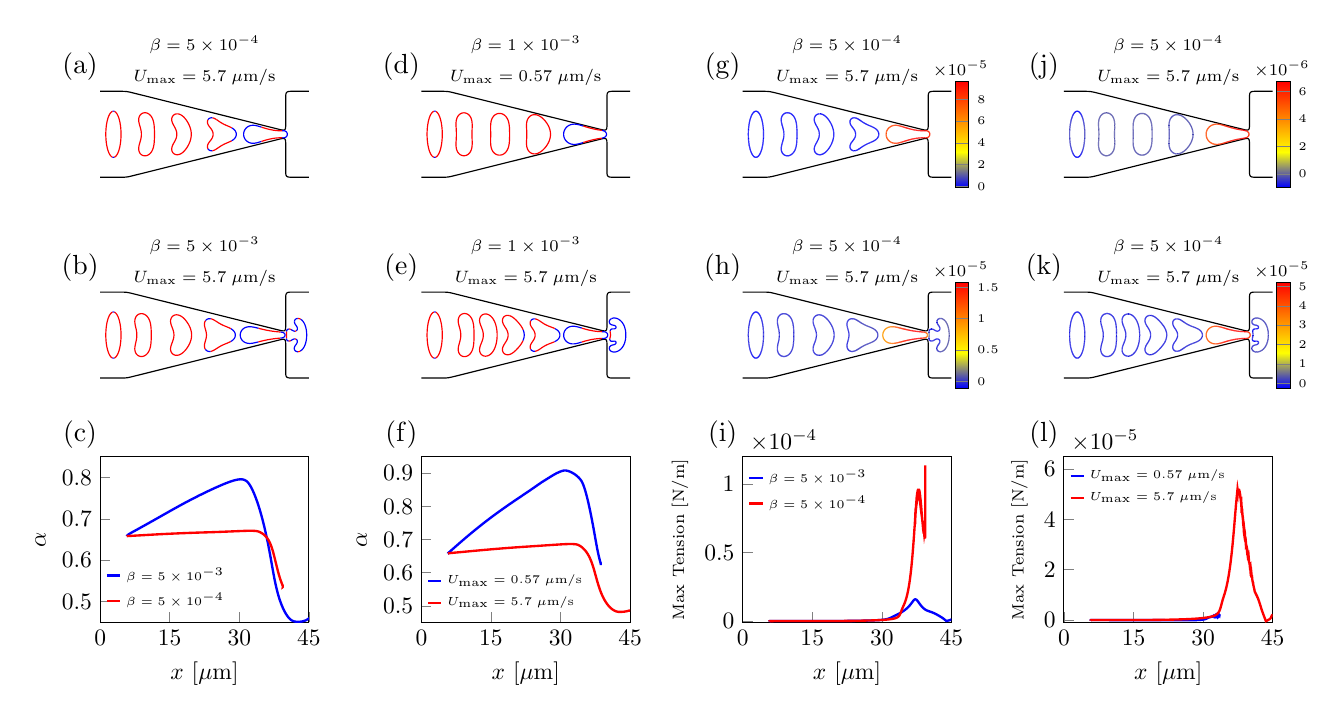
\begin{tikzpicture}[scale=0.85]

% change the line size in the legends
\pgfplotsset{
compat=1.11,
legend image code/.code={
\draw[mark repeat=2,mark phase=2]
plot coordinates {
(0cm,0cm)
(0.20cm,0cm)        %% default is (0.3cm,0cm)
%(0.3cm,0cm)         %% default is (0.6cm,0cm)
};}}

\begin{axis}[
  at = {(0.0cm,6.0cm)},
  width = 4.70cm,
  hide axis,
  axis equal image,
  xmin = 1,
  xmax = 16.75,
  ymin = -4,
  ymax = 4,
  xtick = \empty,
  ytick = \empty,
  title style = {align=center, yshift = -0.4cm},
  title = {\scriptsize $\beta = 5 \times 10^{-4}$ \\ 
           \scriptsize $U_{\max} = 5.7\;\mu$m/s},
]

% outer wall
\addplot[black,line width=0.5pt] coordinates{
(7.5585e-02,-3.1634e+00)
(1.0605e-01,-3.1878e+00)
(1.4241e-01,-3.2064e+00)
(1.8401e-01,-3.2199e+00)
(2.2996e-01,-3.2291e+00)
(2.7929e-01,-3.2350e+00)
(3.3106e-01,-3.2385e+00)
(3.8443e-01,-3.2405e+00)
(4.3877e-01,-3.2415e+00)
(4.9371e-01,-3.2419e+00)
(5.4898e-01,-3.2420e+00)
(6.0437e-01,-3.2419e+00)
(6.5974e-01,-3.2419e+00)
(7.1509e-01,-3.2419e+00)
(7.7045e-01,-3.2419e+00)
(8.2582e-01,-3.2419e+00)
(8.8118e-01,-3.2419e+00)
(9.3654e-01,-3.2419e+00)
(9.9190e-01,-3.2419e+00)
(1.0473e+00,-3.2419e+00)
(1.1026e+00,-3.2419e+00)
(1.1580e+00,-3.2419e+00)
(1.2133e+00,-3.2419e+00)
(1.2687e+00,-3.2419e+00)
(1.3241e+00,-3.2419e+00)
(1.3794e+00,-3.2419e+00)
(1.4348e+00,-3.2419e+00)
(1.4901e+00,-3.2419e+00)
(1.5455e+00,-3.2419e+00)
(1.6009e+00,-3.2419e+00)
(1.6562e+00,-3.2419e+00)
(1.7116e+00,-3.2419e+00)
(1.7670e+00,-3.2419e+00)
(1.8223e+00,-3.2419e+00)
(1.8777e+00,-3.2419e+00)
(1.9330e+00,-3.2419e+00)
(1.9884e+00,-3.2419e+00)
(2.0438e+00,-3.2419e+00)
(2.0991e+00,-3.2419e+00)
(2.1545e+00,-3.2419e+00)
(2.2098e+00,-3.2419e+00)
(2.2652e+00,-3.2419e+00)
(2.3206e+00,-3.2419e+00)
(2.3759e+00,-3.2419e+00)
(2.4313e+00,-3.2419e+00)
(2.4866e+00,-3.2419e+00)
(2.5420e+00,-3.2420e+00)
(2.5974e+00,-3.2419e+00)
(2.6526e+00,-3.2416e+00)
(2.7078e+00,-3.2409e+00)
(2.7629e+00,-3.2398e+00)
(2.8178e+00,-3.2378e+00)
(2.8725e+00,-3.2349e+00)
(2.9268e+00,-3.2308e+00)
(2.9809e+00,-3.2254e+00)
(3.0346e+00,-3.2185e+00)
(3.0879e+00,-3.2102e+00)
(3.1410e+00,-3.2006e+00)
(3.1938e+00,-3.1900e+00)
(3.2464e+00,-3.1785e+00)
(3.2988e+00,-3.1664e+00)
(3.3511e+00,-3.1539e+00)
(3.4034e+00,-3.1412e+00)
(3.4556e+00,-3.1283e+00)
(3.5079e+00,-3.1153e+00)
(3.5601e+00,-3.1023e+00)
(3.6123e+00,-3.0893e+00)
(3.6645e+00,-3.0763e+00)
(3.7167e+00,-3.0632e+00)
(3.7689e+00,-3.0502e+00)
(3.8211e+00,-3.0372e+00)
(3.8733e+00,-3.0242e+00)
(3.9255e+00,-3.0112e+00)
(3.9778e+00,-2.9982e+00)
(4.0300e+00,-2.9851e+00)
(4.0822e+00,-2.9721e+00)
(4.1344e+00,-2.9591e+00)
(4.1866e+00,-2.9461e+00)
(4.2388e+00,-2.9331e+00)
(4.2910e+00,-2.9201e+00)
(4.3432e+00,-2.9070e+00)
(4.3954e+00,-2.8940e+00)
(4.4476e+00,-2.8810e+00)
(4.4999e+00,-2.8680e+00)
(4.5521e+00,-2.8550e+00)
(4.6043e+00,-2.8419e+00)
(4.6565e+00,-2.8289e+00)
(4.7087e+00,-2.8159e+00)
(4.7609e+00,-2.8029e+00)
(4.8131e+00,-2.7899e+00)
(4.8653e+00,-2.7769e+00)
(4.9175e+00,-2.7638e+00)
(4.9697e+00,-2.7508e+00)
(5.0220e+00,-2.7378e+00)
(5.0742e+00,-2.7248e+00)
(5.1264e+00,-2.7118e+00)
(5.1786e+00,-2.6988e+00)
(5.2308e+00,-2.6857e+00)
(5.2830e+00,-2.6727e+00)
(5.3352e+00,-2.6597e+00)
(5.3874e+00,-2.6467e+00)
(5.4396e+00,-2.6337e+00)
(5.4919e+00,-2.6206e+00)
(5.5441e+00,-2.6076e+00)
(5.5963e+00,-2.5946e+00)
(5.6485e+00,-2.5816e+00)
(5.7007e+00,-2.5686e+00)
(5.7529e+00,-2.5556e+00)
(5.8051e+00,-2.5425e+00)
(5.8573e+00,-2.5295e+00)
(5.9095e+00,-2.5165e+00)
(5.9617e+00,-2.5035e+00)
(6.0140e+00,-2.4905e+00)
(6.0662e+00,-2.4775e+00)
(6.1184e+00,-2.4644e+00)
(6.1706e+00,-2.4514e+00)
(6.2228e+00,-2.4384e+00)
(6.2750e+00,-2.4254e+00)
(6.3272e+00,-2.4124e+00)
(6.3794e+00,-2.3993e+00)
(6.4316e+00,-2.3863e+00)
(6.4838e+00,-2.3733e+00)
(6.5361e+00,-2.3603e+00)
(6.5883e+00,-2.3473e+00)
(6.6405e+00,-2.3343e+00)
(6.6927e+00,-2.3212e+00)
(6.7449e+00,-2.3082e+00)
(6.7971e+00,-2.2952e+00)
(6.8493e+00,-2.2822e+00)
(6.9015e+00,-2.2692e+00)
(6.9537e+00,-2.2562e+00)
(7.0060e+00,-2.2431e+00)
(7.0582e+00,-2.2301e+00)
(7.1104e+00,-2.2171e+00)
(7.1626e+00,-2.2041e+00)
(7.2148e+00,-2.1911e+00)
(7.2670e+00,-2.1781e+00)
(7.3192e+00,-2.1650e+00)
(7.3714e+00,-2.1520e+00)
(7.4236e+00,-2.1390e+00)
(7.4758e+00,-2.1260e+00)
(7.5281e+00,-2.1130e+00)
(7.5803e+00,-2.0999e+00)
(7.6325e+00,-2.0869e+00)
(7.6847e+00,-2.0739e+00)
(7.7369e+00,-2.0609e+00)
(7.7891e+00,-2.0479e+00)
(7.8413e+00,-2.0349e+00)
(7.8935e+00,-2.0218e+00)
(7.9457e+00,-2.0088e+00)
(7.9979e+00,-1.9958e+00)
(8.0502e+00,-1.9828e+00)
(8.1024e+00,-1.9698e+00)
(8.1546e+00,-1.9568e+00)
(8.2068e+00,-1.9437e+00)
(8.2590e+00,-1.9307e+00)
(8.3112e+00,-1.9177e+00)
(8.3634e+00,-1.9047e+00)
(8.4156e+00,-1.8917e+00)
(8.4678e+00,-1.8786e+00)
(8.5201e+00,-1.8656e+00)
(8.5723e+00,-1.8526e+00)
(8.6245e+00,-1.8396e+00)
(8.6767e+00,-1.8266e+00)
(8.7289e+00,-1.8136e+00)
(8.7811e+00,-1.8005e+00)
(8.8333e+00,-1.7875e+00)
(8.8855e+00,-1.7745e+00)
(8.9377e+00,-1.7615e+00)
(8.9899e+00,-1.7485e+00)
(9.0422e+00,-1.7355e+00)
(9.0944e+00,-1.7224e+00)
(9.1466e+00,-1.7094e+00)
(9.1988e+00,-1.6964e+00)
(9.2510e+00,-1.6834e+00)
(9.3032e+00,-1.6704e+00)
(9.3554e+00,-1.6574e+00)
(9.4076e+00,-1.6443e+00)
(9.4598e+00,-1.6313e+00)
(9.5121e+00,-1.6183e+00)
(9.5643e+00,-1.6053e+00)
(9.6165e+00,-1.5923e+00)
(9.6687e+00,-1.5792e+00)
(9.7209e+00,-1.5662e+00)
(9.7731e+00,-1.5532e+00)
(9.8253e+00,-1.5402e+00)
(9.8775e+00,-1.5272e+00)
(9.9297e+00,-1.5142e+00)
(9.9819e+00,-1.5011e+00)
(1.0034e+01,-1.4881e+00)
(1.0086e+01,-1.4751e+00)
(1.0139e+01,-1.4621e+00)
(1.0191e+01,-1.4491e+00)
(1.0243e+01,-1.4361e+00)
(1.0295e+01,-1.4230e+00)
(1.0347e+01,-1.4100e+00)
(1.0400e+01,-1.3970e+00)
(1.0452e+01,-1.3840e+00)
(1.0504e+01,-1.3710e+00)
(1.0556e+01,-1.3580e+00)
(1.0608e+01,-1.3449e+00)
(1.0661e+01,-1.3319e+00)
(1.0713e+01,-1.3189e+00)
(1.0765e+01,-1.3059e+00)
(1.0817e+01,-1.2929e+00)
(1.0870e+01,-1.2798e+00)
(1.0922e+01,-1.2668e+00)
(1.0974e+01,-1.2538e+00)
(1.1026e+01,-1.2408e+00)
(1.1078e+01,-1.2278e+00)
(1.1131e+01,-1.2148e+00)
(1.1183e+01,-1.2017e+00)
(1.1235e+01,-1.1887e+00)
(1.1287e+01,-1.1757e+00)
(1.1339e+01,-1.1627e+00)
(1.1392e+01,-1.1497e+00)
(1.1444e+01,-1.1366e+00)
(1.1496e+01,-1.1236e+00)
(1.1548e+01,-1.1106e+00)
(1.1600e+01,-1.0976e+00)
(1.1653e+01,-1.0846e+00)
(1.1705e+01,-1.0716e+00)
(1.1757e+01,-1.0585e+00)
(1.1809e+01,-1.0455e+00)
(1.1862e+01,-1.0325e+00)
(1.1914e+01,-1.0195e+00)
(1.1966e+01,-1.0065e+00)
(1.2018e+01,-9.9346e-01)
(1.2070e+01,-9.8044e-01)
(1.2123e+01,-9.6743e-01)
(1.2175e+01,-9.5441e-01)
(1.2227e+01,-9.4139e-01)
(1.2279e+01,-9.2837e-01)
(1.2331e+01,-9.1536e-01)
(1.2384e+01,-9.0233e-01)
(1.2436e+01,-8.8932e-01)
(1.2488e+01,-8.7630e-01)
(1.2540e+01,-8.6329e-01)
(1.2592e+01,-8.5026e-01)
(1.2645e+01,-8.3725e-01)
(1.2697e+01,-8.2424e-01)
(1.2749e+01,-8.1121e-01)
(1.2801e+01,-7.9819e-01)
(1.2854e+01,-7.8518e-01)
(1.2906e+01,-7.7217e-01)
(1.2958e+01,-7.5914e-01)
(1.3010e+01,-7.4612e-01)
(1.3062e+01,-7.3311e-01)
(1.3115e+01,-7.2010e-01)
(1.3167e+01,-7.0707e-01)
(1.3219e+01,-6.9405e-01)
(1.3271e+01,-6.8104e-01)
(1.3323e+01,-6.6802e-01)
(1.3376e+01,-6.5500e-01)
(1.3428e+01,-6.4199e-01)
(1.3480e+01,-6.2898e-01)
(1.3532e+01,-6.1595e-01)
(1.3584e+01,-6.0293e-01)
(1.3637e+01,-5.8992e-01)
(1.3689e+01,-5.7691e-01)
(1.3741e+01,-5.6388e-01)
(1.3793e+01,-5.5086e-01)
(1.3846e+01,-5.3785e-01)
(1.3898e+01,-5.2484e-01)
(1.3950e+01,-5.1180e-01)
(1.4002e+01,-4.9879e-01)
(1.4054e+01,-4.8579e-01)
(1.4107e+01,-4.7276e-01)
(1.4159e+01,-4.5972e-01)
(1.4211e+01,-4.4672e-01)
(1.4263e+01,-4.3373e-01)
(1.4315e+01,-4.2069e-01)
(1.4368e+01,-4.0764e-01)
(1.4420e+01,-3.9467e-01)
(1.4472e+01,-3.8170e-01)
(1.4524e+01,-3.6857e-01)
(1.4577e+01,-3.5545e-01)
(1.4628e+01,-3.4293e-01)
(1.4679e+01,-3.3173e-01)
(1.4729e+01,-3.2253e-01)
(1.4776e+01,-3.1622e-01)
(1.4820e+01,-3.1401e-01)
(1.4859e+01,-3.1719e-01)
(1.4894e+01,-3.2682e-01)
(1.4924e+01,-3.4363e-01)
(1.4947e+01,-3.6794e-01)
(1.4965e+01,-3.9953e-01)
(1.4978e+01,-4.3762e-01)
(1.4987e+01,-4.8109e-01)
(1.4993e+01,-5.2876e-01)
(1.4997e+01,-5.7947e-01)
(1.4999e+01,-6.3218e-01)
(1.5000e+01,-6.8611e-01)
(1.5000e+01,-7.4079e-01)
(1.5000e+01,-7.9588e-01)
(1.5000e+01,-8.5113e-01)
(1.5000e+01,-9.0636e-01)
(1.5000e+01,-9.6156e-01)
(1.5000e+01,-1.0168e+00)
(1.5000e+01,-1.0720e+00)
(1.5000e+01,-1.1272e+00)
(1.5000e+01,-1.1824e+00)
(1.5000e+01,-1.2376e+00)
(1.5000e+01,-1.2928e+00)
(1.5000e+01,-1.3480e+00)
(1.5000e+01,-1.4033e+00)
(1.5000e+01,-1.4585e+00)
(1.5000e+01,-1.5137e+00)
(1.5000e+01,-1.5689e+00)
(1.5000e+01,-1.6241e+00)
(1.5000e+01,-1.6793e+00)
(1.5000e+01,-1.7345e+00)
(1.5000e+01,-1.7897e+00)
(1.5000e+01,-1.8450e+00)
(1.5000e+01,-1.9002e+00)
(1.5000e+01,-1.9554e+00)
(1.5000e+01,-2.0106e+00)
(1.5000e+01,-2.0658e+00)
(1.5000e+01,-2.1210e+00)
(1.5000e+01,-2.1762e+00)
(1.5000e+01,-2.2314e+00)
(1.5000e+01,-2.2866e+00)
(1.5000e+01,-2.3419e+00)
(1.5000e+01,-2.3971e+00)
(1.5000e+01,-2.4523e+00)
(1.5000e+01,-2.5075e+00)
(1.5000e+01,-2.5627e+00)
(1.5000e+01,-2.6179e+00)
(1.5000e+01,-2.6731e+00)
(1.5000e+01,-2.7284e+00)
(1.5000e+01,-2.7837e+00)
(1.5000e+01,-2.8386e+00)
(1.5001e+01,-2.8926e+00)
(1.5004e+01,-2.9451e+00)
(1.5009e+01,-2.9954e+00)
(1.5017e+01,-3.0426e+00)
(1.5029e+01,-3.0856e+00)
(1.5047e+01,-3.1235e+00)
(1.5070e+01,-3.1557e+00)
(1.5099e+01,-3.1819e+00)
(1.5134e+01,-3.2021e+00)
(1.5174e+01,-3.2169e+00)
(1.5220e+01,-3.2271e+00)
(1.5268e+01,-3.2338e+00)
(1.5320e+01,-3.2378e+00)
(1.5373e+01,-3.2401e+00)
(1.5427e+01,-3.2413e+00)
(1.5482e+01,-3.2418e+00)
(1.5537e+01,-3.2420e+00)
(1.5592e+01,-3.2419e+00)
(1.5648e+01,-3.2419e+00)
(1.5703e+01,-3.2419e+00)
(1.5758e+01,-3.2419e+00)
(1.5814e+01,-3.2419e+00)
(1.5869e+01,-3.2419e+00)
(1.5924e+01,-3.2419e+00)
(1.5980e+01,-3.2419e+00)
(1.6035e+01,-3.2419e+00)
(1.6091e+01,-3.2419e+00)
(1.6146e+01,-3.2419e+00)
(1.6201e+01,-3.2419e+00)
(1.6257e+01,-3.2419e+00)
(1.6312e+01,-3.2419e+00)
(1.6367e+01,-3.2419e+00)
(1.6423e+01,-3.2419e+00)
(1.6478e+01,-3.2419e+00)
(1.6533e+01,-3.2419e+00)
(1.6589e+01,-3.2419e+00)
(1.6644e+01,-3.2419e+00)
(1.6699e+01,-3.2419e+00)
(1.6755e+01,-3.2419e+00)
(1.6810e+01,-3.2419e+00)
(1.6866e+01,-3.2419e+00)
(1.6921e+01,-3.2419e+00)
(1.6976e+01,-3.2419e+00)
(1.7032e+01,-3.2419e+00)
(1.7087e+01,-3.2419e+00)
(1.7142e+01,-3.2419e+00)
(1.7198e+01,-3.2419e+00)
(1.7253e+01,-3.2419e+00)
(1.7308e+01,-3.2420e+00)
(1.7364e+01,-3.2419e+00)
(1.7419e+01,-3.2419e+00)
(1.7475e+01,-3.2419e+00)
(1.7530e+01,-3.2421e+00)
(1.7585e+01,-3.2419e+00)
(1.7640e+01,-3.2409e+00)
(1.7693e+01,-3.2386e+00)
(1.7743e+01,-3.2342e+00)
(1.7791e+01,-3.2270e+00)
(1.7835e+01,-3.2158e+00)
(1.7874e+01,-3.1999e+00)
(1.7908e+01,-3.1784e+00)
(1.7935e+01,-3.1510e+00)
(1.7957e+01,-3.1177e+00)
(1.7972e+01,-3.0789e+00)
(1.7984e+01,-3.0356e+00)
(1.7991e+01,-2.9885e+00)
(1.7995e+01,-2.9387e+00)
(1.7998e+01,-2.8870e+00)
(1.7999e+01,-2.8341e+00)
(1.8000e+01,-2.7805e+00)
(1.8000e+01,-2.7265e+00)
(1.8000e+01,-2.6722e+00)
(1.8000e+01,-2.6180e+00)
(1.8000e+01,-2.5638e+00)
(1.8000e+01,-2.5096e+00)
(1.8000e+01,-2.4553e+00)
(1.8000e+01,-2.4011e+00)
(1.8000e+01,-2.3469e+00)
(1.8000e+01,-2.2927e+00)
(1.8000e+01,-2.2385e+00)
(1.8000e+01,-2.1843e+00)
(1.8000e+01,-2.1300e+00)
(1.8000e+01,-2.0758e+00)
(1.8000e+01,-2.0216e+00)
(1.8000e+01,-1.9674e+00)
(1.8000e+01,-1.9132e+00)
(1.8000e+01,-1.8590e+00)
(1.8000e+01,-1.8047e+00)
(1.8000e+01,-1.7505e+00)
(1.8000e+01,-1.6963e+00)
(1.8000e+01,-1.6421e+00)
(1.8000e+01,-1.5879e+00)
(1.8000e+01,-1.5337e+00)
(1.8000e+01,-1.4794e+00)
(1.8000e+01,-1.4252e+00)
(1.8000e+01,-1.3710e+00)
(1.8000e+01,-1.3168e+00)
(1.8000e+01,-1.2626e+00)
(1.8000e+01,-1.2084e+00)
(1.8000e+01,-1.1541e+00)
(1.8000e+01,-1.0999e+00)
(1.8000e+01,-1.0457e+00)
(1.8000e+01,-9.9149e-01)
(1.8000e+01,-9.3727e-01)
(1.8000e+01,-8.8306e-01)
(1.8000e+01,-8.2884e-01)
(1.8000e+01,-7.7462e-01)
(1.8000e+01,-7.2040e-01)
(1.8000e+01,-6.6619e-01)
(1.8000e+01,-6.1197e-01)
(1.8000e+01,-5.5775e-01)
(1.8000e+01,-5.0354e-01)
(1.8000e+01,-4.4932e-01)
(1.8000e+01,-3.9510e-01)
(1.8000e+01,-3.4089e-01)
(1.8000e+01,-2.8667e-01)
(1.8000e+01,-2.3245e-01)
(1.8000e+01,-1.7824e-01)
(1.8000e+01,-1.2402e-01)
(1.8000e+01,-6.9801e-02)
(1.8000e+01,-1.5584e-02)
(1.8000e+01,3.8632e-02)
(1.8000e+01,9.2849e-02)
(1.8000e+01,1.4707e-01)
(1.8000e+01,2.0128e-01)
(1.8000e+01,2.5550e-01)
(1.8000e+01,3.0972e-01)
(1.8000e+01,3.6393e-01)
(1.8000e+01,4.1815e-01)
(1.8000e+01,4.7237e-01)
(1.8000e+01,5.2659e-01)
(1.8000e+01,5.8080e-01)
(1.8000e+01,6.3502e-01)
(1.8000e+01,6.8924e-01)
(1.8000e+01,7.4345e-01)
(1.8000e+01,7.9767e-01)
(1.8000e+01,8.5189e-01)
(1.8000e+01,9.0610e-01)
(1.8000e+01,9.6032e-01)
(1.8000e+01,1.0145e+00)
(1.8000e+01,1.0688e+00)
(1.8000e+01,1.1230e+00)
(1.8000e+01,1.1772e+00)
(1.8000e+01,1.2314e+00)
(1.8000e+01,1.2856e+00)
(1.8000e+01,1.3398e+00)
(1.8000e+01,1.3941e+00)
(1.8000e+01,1.4483e+00)
(1.8000e+01,1.5025e+00)
(1.8000e+01,1.5567e+00)
(1.8000e+01,1.6109e+00)
(1.8000e+01,1.6651e+00)
(1.8000e+01,1.7194e+00)
(1.8000e+01,1.7736e+00)
(1.8000e+01,1.8278e+00)
(1.8000e+01,1.8820e+00)
(1.8000e+01,1.9362e+00)
(1.8000e+01,1.9904e+00)
(1.8000e+01,2.0447e+00)
(1.8000e+01,2.0989e+00)
(1.8000e+01,2.1531e+00)
(1.8000e+01,2.2073e+00)
(1.8000e+01,2.2615e+00)
(1.8000e+01,2.3157e+00)
(1.8000e+01,2.3700e+00)
(1.8000e+01,2.4242e+00)
(1.8000e+01,2.4784e+00)
(1.8000e+01,2.5326e+00)
(1.8000e+01,2.5869e+00)
(1.8000e+01,2.6410e+00)
(1.8000e+01,2.6952e+00)
(1.8000e+01,2.7495e+00)
(1.8000e+01,2.8038e+00)
(1.8000e+01,2.8576e+00)
(1.7998e+01,2.9104e+00)
(1.7995e+01,2.9615e+00)
(1.7990e+01,3.0103e+00)
(1.7981e+01,3.0558e+00)
(1.7967e+01,3.0970e+00)
(1.7949e+01,3.1331e+00)
(1.7924e+01,3.1634e+00)
(1.7894e+01,3.1878e+00)
(1.7858e+01,3.2064e+00)
(1.7816e+01,3.2199e+00)
(1.7770e+01,3.2291e+00)
(1.7721e+01,3.2350e+00)
(1.7669e+01,3.2385e+00)
(1.7616e+01,3.2405e+00)
(1.7561e+01,3.2415e+00)
(1.7506e+01,3.2419e+00)
(1.7451e+01,3.2420e+00)
(1.7396e+01,3.2419e+00)
(1.7340e+01,3.2419e+00)
(1.7285e+01,3.2419e+00)
(1.7230e+01,3.2419e+00)
(1.7174e+01,3.2419e+00)
(1.7119e+01,3.2419e+00)
(1.7063e+01,3.2419e+00)
(1.7008e+01,3.2419e+00)
(1.6953e+01,3.2419e+00)
(1.6897e+01,3.2419e+00)
(1.6842e+01,3.2419e+00)
(1.6787e+01,3.2419e+00)
(1.6731e+01,3.2419e+00)
(1.6676e+01,3.2419e+00)
(1.6621e+01,3.2419e+00)
(1.6565e+01,3.2419e+00)
(1.6510e+01,3.2419e+00)
(1.6454e+01,3.2419e+00)
(1.6399e+01,3.2419e+00)
(1.6344e+01,3.2419e+00)
(1.6288e+01,3.2419e+00)
(1.6233e+01,3.2419e+00)
(1.6178e+01,3.2419e+00)
(1.6122e+01,3.2419e+00)
(1.6067e+01,3.2419e+00)
(1.6012e+01,3.2419e+00)
(1.5956e+01,3.2419e+00)
(1.5901e+01,3.2420e+00)
(1.5846e+01,3.2419e+00)
(1.5790e+01,3.2419e+00)
(1.5735e+01,3.2419e+00)
(1.5679e+01,3.2420e+00)
(1.5624e+01,3.2419e+00)
(1.5569e+01,3.2419e+00)
(1.5513e+01,3.2420e+00)
(1.5458e+01,3.2421e+00)
(1.5403e+01,3.2418e+00)
(1.5349e+01,3.2405e+00)
(1.5296e+01,3.2377e+00)
(1.5246e+01,3.2327e+00)
(1.5199e+01,3.2246e+00)
(1.5156e+01,3.2123e+00)
(1.5118e+01,3.1948e+00)
(1.5086e+01,3.1716e+00)
(1.5060e+01,3.1424e+00)
(1.5039e+01,3.1072e+00)
(1.5025e+01,3.0667e+00)
(1.5015e+01,3.0216e+00)
(1.5008e+01,2.9729e+00)
(1.5004e+01,2.9217e+00)
(1.5002e+01,2.8687e+00)
(1.5001e+01,2.8147e+00)
(1.5000e+01,2.7600e+00)
(1.5000e+01,2.7049e+00)
(1.5000e+01,2.6497e+00)
(1.5000e+01,2.5944e+00)
(1.5000e+01,2.5392e+00)
(1.5000e+01,2.4840e+00)
(1.5000e+01,2.4288e+00)
(1.5000e+01,2.3736e+00)
(1.5000e+01,2.3184e+00)
(1.5000e+01,2.2632e+00)
(1.5000e+01,2.2080e+00)
(1.5000e+01,2.1528e+00)
(1.5000e+01,2.0975e+00)
(1.5000e+01,2.0423e+00)
(1.5000e+01,1.9871e+00)
(1.5000e+01,1.9319e+00)
(1.5000e+01,1.8767e+00)
(1.5000e+01,1.8215e+00)
(1.5000e+01,1.7663e+00)
(1.5000e+01,1.7111e+00)
(1.5000e+01,1.6559e+00)
(1.5000e+01,1.6006e+00)
(1.5000e+01,1.5454e+00)
(1.5000e+01,1.4902e+00)
(1.5000e+01,1.4350e+00)
(1.5000e+01,1.3798e+00)
(1.5000e+01,1.3246e+00)
(1.5000e+01,1.2694e+00)
(1.5000e+01,1.2142e+00)
(1.5000e+01,1.1589e+00)
(1.5000e+01,1.1037e+00)
(1.5000e+01,1.0485e+00)
(1.5000e+01,9.9331e-01)
(1.5000e+01,9.3806e-01)
(1.5000e+01,8.8287e-01)
(1.5000e+01,8.2772e-01)
(1.5000e+01,7.7246e-01)
(1.5000e+01,7.1709e-01)
(1.5000e+01,6.6208e-01)
(1.4999e+01,6.0815e-01)
(1.4997e+01,5.5597e-01)
(1.4992e+01,5.0633e-01)
(1.4985e+01,4.6033e-01)
(1.4974e+01,4.1930e-01)
(1.4959e+01,3.8438e-01)
(1.4938e+01,3.5642e-01)
(1.4912e+01,3.3590e-01)
(1.4879e+01,3.2281e-01)
(1.4842e+01,3.1654e-01)
(1.4800e+01,3.1606e-01)
(1.4755e+01,3.2020e-01)
(1.4707e+01,3.2778e-01)
(1.4657e+01,3.3770e-01)
(1.4606e+01,3.4908e-01)
(1.4554e+01,3.6134e-01)
(1.4502e+01,3.7412e-01)
(1.4450e+01,3.8715e-01)
(1.4398e+01,4.0020e-01)
(1.4345e+01,4.1321e-01)
(1.4293e+01,4.2622e-01)
(1.4241e+01,4.3924e-01)
(1.4189e+01,4.5226e-01)
(1.4137e+01,4.6528e-01)
(1.4084e+01,4.7829e-01)
(1.4032e+01,4.9131e-01)
(1.3980e+01,5.0433e-01)
(1.3928e+01,5.1735e-01)
(1.3876e+01,5.3036e-01)
(1.3823e+01,5.4338e-01)
(1.3771e+01,5.5640e-01)
(1.3719e+01,5.6942e-01)
(1.3667e+01,5.8243e-01)
(1.3614e+01,5.9545e-01)
(1.3562e+01,6.0847e-01)
(1.3510e+01,6.2149e-01)
(1.3458e+01,6.3450e-01)
(1.3406e+01,6.4752e-01)
(1.3353e+01,6.6054e-01)
(1.3301e+01,6.7356e-01)
(1.3249e+01,6.8657e-01)
(1.3197e+01,6.9959e-01)
(1.3145e+01,7.1261e-01)
(1.3092e+01,7.2563e-01)
(1.3040e+01,7.3864e-01)
(1.2988e+01,7.5166e-01)
(1.2936e+01,7.6468e-01)
(1.2884e+01,7.7770e-01)
(1.2831e+01,7.9071e-01)
(1.2779e+01,8.0373e-01)
(1.2727e+01,8.1675e-01)
(1.2675e+01,8.2977e-01)
(1.2622e+01,8.4278e-01)
(1.2570e+01,8.5580e-01)
(1.2518e+01,8.6882e-01)
(1.2466e+01,8.8184e-01)
(1.2414e+01,8.9485e-01)
(1.2361e+01,9.0787e-01)
(1.2309e+01,9.2089e-01)
(1.2257e+01,9.3390e-01)
(1.2205e+01,9.4692e-01)
(1.2153e+01,9.5994e-01)
(1.2100e+01,9.7296e-01)
(1.2048e+01,9.8597e-01)
(1.1996e+01,9.9899e-01)
(1.1944e+01,1.0120e+00)
(1.1892e+01,1.0250e+00)
(1.1839e+01,1.0380e+00)
(1.1787e+01,1.0511e+00)
(1.1735e+01,1.0641e+00)
(1.1683e+01,1.0771e+00)
(1.1630e+01,1.0901e+00)
(1.1578e+01,1.1031e+00)
(1.1526e+01,1.1162e+00)
(1.1474e+01,1.1292e+00)
(1.1422e+01,1.1422e+00)
(1.1369e+01,1.1552e+00)
(1.1317e+01,1.1682e+00)
(1.1265e+01,1.1812e+00)
(1.1213e+01,1.1943e+00)
(1.1161e+01,1.2073e+00)
(1.1108e+01,1.2203e+00)
(1.1056e+01,1.2333e+00)
(1.1004e+01,1.2463e+00)
(1.0952e+01,1.2593e+00)
(1.0900e+01,1.2724e+00)
(1.0847e+01,1.2854e+00)
(1.0795e+01,1.2984e+00)
(1.0743e+01,1.3114e+00)
(1.0691e+01,1.3244e+00)
(1.0638e+01,1.3374e+00)
(1.0586e+01,1.3505e+00)
(1.0534e+01,1.3635e+00)
(1.0482e+01,1.3765e+00)
(1.0430e+01,1.3895e+00)
(1.0377e+01,1.4025e+00)
(1.0325e+01,1.4156e+00)
(1.0273e+01,1.4286e+00)
(1.0221e+01,1.4416e+00)
(1.0169e+01,1.4546e+00)
(1.0116e+01,1.4676e+00)
(1.0064e+01,1.4806e+00)
(1.0012e+01,1.4937e+00)
(9.9597e+00,1.5067e+00)
(9.9075e+00,1.5197e+00)
(9.8553e+00,1.5327e+00)
(9.8031e+00,1.5457e+00)
(9.7509e+00,1.5587e+00)
(9.6987e+00,1.5718e+00)
(9.6465e+00,1.5848e+00)
(9.5943e+00,1.5978e+00)
(9.5421e+00,1.6108e+00)
(9.4899e+00,1.6238e+00)
(9.4376e+00,1.6369e+00)
(9.3854e+00,1.6499e+00)
(9.3332e+00,1.6629e+00)
(9.2810e+00,1.6759e+00)
(9.2288e+00,1.6889e+00)
(9.1766e+00,1.7019e+00)
(9.1244e+00,1.7150e+00)
(9.0722e+00,1.7280e+00)
(9.0200e+00,1.7410e+00)
(8.9678e+00,1.7540e+00)
(8.9155e+00,1.7670e+00)
(8.8633e+00,1.7800e+00)
(8.8111e+00,1.7931e+00)
(8.7589e+00,1.8061e+00)
(8.7067e+00,1.8191e+00)
(8.6545e+00,1.8321e+00)
(8.6023e+00,1.8451e+00)
(8.5501e+00,1.8581e+00)
(8.4979e+00,1.8712e+00)
(8.4456e+00,1.8842e+00)
(8.3934e+00,1.8972e+00)
(8.3412e+00,1.9102e+00)
(8.2890e+00,1.9232e+00)
(8.2368e+00,1.9363e+00)
(8.1846e+00,1.9493e+00)
(8.1324e+00,1.9623e+00)
(8.0802e+00,1.9753e+00)
(8.0280e+00,1.9883e+00)
(7.9758e+00,2.0013e+00)
(7.9235e+00,2.0144e+00)
(7.8713e+00,2.0274e+00)
(7.8191e+00,2.0404e+00)
(7.7669e+00,2.0534e+00)
(7.7147e+00,2.0664e+00)
(7.6625e+00,2.0794e+00)
(7.6103e+00,2.0925e+00)
(7.5581e+00,2.1055e+00)
(7.5059e+00,2.1185e+00)
(7.4536e+00,2.1315e+00)
(7.4014e+00,2.1445e+00)
(7.3492e+00,2.1576e+00)
(7.2970e+00,2.1706e+00)
(7.2448e+00,2.1836e+00)
(7.1926e+00,2.1966e+00)
(7.1404e+00,2.2096e+00)
(7.0882e+00,2.2226e+00)
(7.0360e+00,2.2357e+00)
(6.9838e+00,2.2487e+00)
(6.9315e+00,2.2617e+00)
(6.8793e+00,2.2747e+00)
(6.8271e+00,2.2877e+00)
(6.7749e+00,2.3007e+00)
(6.7227e+00,2.3138e+00)
(6.6705e+00,2.3268e+00)
(6.6183e+00,2.3398e+00)
(6.5661e+00,2.3528e+00)
(6.5139e+00,2.3658e+00)
(6.4617e+00,2.3788e+00)
(6.4094e+00,2.3919e+00)
(6.3572e+00,2.4049e+00)
(6.3050e+00,2.4179e+00)
(6.2528e+00,2.4309e+00)
(6.2006e+00,2.4439e+00)
(6.1484e+00,2.4570e+00)
(6.0962e+00,2.4700e+00)
(6.0440e+00,2.4830e+00)
(5.9918e+00,2.4960e+00)
(5.9396e+00,2.5090e+00)
(5.8873e+00,2.5220e+00)
(5.8351e+00,2.5351e+00)
(5.7829e+00,2.5481e+00)
(5.7307e+00,2.5611e+00)
(5.6785e+00,2.5741e+00)
(5.6263e+00,2.5871e+00)
(5.5741e+00,2.6001e+00)
(5.5219e+00,2.6132e+00)
(5.4697e+00,2.6262e+00)
(5.4174e+00,2.6392e+00)
(5.3652e+00,2.6522e+00)
(5.3130e+00,2.6652e+00)
(5.2608e+00,2.6783e+00)
(5.2086e+00,2.6913e+00)
(5.1564e+00,2.7043e+00)
(5.1042e+00,2.7173e+00)
(5.0520e+00,2.7303e+00)
(4.9998e+00,2.7433e+00)
(4.9476e+00,2.7564e+00)
(4.8953e+00,2.7694e+00)
(4.8431e+00,2.7824e+00)
(4.7909e+00,2.7954e+00)
(4.7387e+00,2.8084e+00)
(4.6865e+00,2.8214e+00)
(4.6343e+00,2.8345e+00)
(4.5821e+00,2.8475e+00)
(4.5299e+00,2.8605e+00)
(4.4777e+00,2.8735e+00)
(4.4255e+00,2.8865e+00)
(4.3732e+00,2.8995e+00)
(4.3210e+00,2.9126e+00)
(4.2688e+00,2.9256e+00)
(4.2166e+00,2.9386e+00)
(4.1644e+00,2.9516e+00)
(4.1122e+00,2.9646e+00)
(4.0600e+00,2.9777e+00)
(4.0078e+00,2.9907e+00)
(3.9556e+00,3.0037e+00)
(3.9033e+00,3.0167e+00)
(3.8511e+00,3.0297e+00)
(3.7989e+00,3.0427e+00)
(3.7467e+00,3.0558e+00)
(3.6945e+00,3.0688e+00)
(3.6423e+00,3.0818e+00)
(3.5901e+00,3.0948e+00)
(3.5379e+00,3.1078e+00)
(3.4857e+00,3.1208e+00)
(3.4335e+00,3.1339e+00)
(3.3812e+00,3.1469e+00)
(3.3290e+00,3.1596e+00)
(3.2766e+00,3.1719e+00)
(3.2241e+00,3.1838e+00)
(3.1714e+00,3.1949e+00)
(3.1185e+00,3.2051e+00)
(3.0653e+00,3.2140e+00)
(3.0118e+00,3.2216e+00)
(2.9579e+00,3.2278e+00)
(2.9037e+00,3.2325e+00)
(2.8492e+00,3.2360e+00)
(2.7944e+00,3.2384e+00)
(2.7394e+00,3.2400e+00)
(2.6843e+00,3.2410e+00)
(2.6291e+00,3.2415e+00)
(2.5738e+00,3.2418e+00)
(2.5185e+00,3.2419e+00)
(2.4631e+00,3.2419e+00)
(2.4078e+00,3.2419e+00)
(2.3524e+00,3.2419e+00)
(2.2970e+00,3.2419e+00)
(2.2417e+00,3.2419e+00)
(2.1863e+00,3.2419e+00)
(2.1309e+00,3.2419e+00)
(2.0756e+00,3.2419e+00)
(2.0202e+00,3.2419e+00)
(1.9649e+00,3.2419e+00)
(1.9095e+00,3.2419e+00)
(1.8541e+00,3.2419e+00)
(1.7988e+00,3.2419e+00)
(1.7434e+00,3.2419e+00)
(1.6881e+00,3.2419e+00)
(1.6327e+00,3.2419e+00)
(1.5773e+00,3.2419e+00)
(1.5220e+00,3.2419e+00)
(1.4666e+00,3.2419e+00)
(1.4113e+00,3.2419e+00)
(1.3559e+00,3.2419e+00)
(1.3005e+00,3.2419e+00)
(1.2452e+00,3.2419e+00)
(1.1898e+00,3.2419e+00)
(1.1344e+00,3.2419e+00)
(1.0791e+00,3.2419e+00)
(1.0237e+00,3.2419e+00)
(9.6837e-01,3.2419e+00)
(9.1300e-01,3.2419e+00)
(8.5763e-01,3.2419e+00)
(8.0230e-01,3.2419e+00)
(7.4693e-01,3.2419e+00)
(6.9154e-01,3.2420e+00)
(6.3619e-01,3.2419e+00)
(5.8088e-01,3.2419e+00)
(5.2548e-01,3.2419e+00)
(4.7000e-01,3.2421e+00)
(4.1478e-01,3.2419e+00)
(3.6043e-01,3.2409e+00)
(3.0748e-01,3.2386e+00)
(2.5657e-01,3.2342e+00)
(2.0858e-01,3.2270e+00)
(1.6459e-01,3.2158e+00)
(1.2554e-01,3.1999e+00)
(9.2118e-02,3.1784e+00)
(6.4729e-02,3.1510e+00)
(4.3374e-02,3.1177e+00)
(2.7573e-02,3.0789e+00)
(1.6499e-02,3.0356e+00)
(9.1998e-03,2.9885e+00)
(4.7215e-03,2.9387e+00)
(2.1644e-03,2.8870e+00)
(8.0546e-04,2.8341e+00)
(1.7505e-04,2.7805e+00)
(-2.1830e-05,2.7265e+00)
(-2.0465e-05,2.6722e+00)
(7.5511e-06,2.6180e+00)
(5.5547e-06,2.5638e+00)
(-3.6706e-06,2.5096e+00)
(-1.8254e-06,2.4553e+00)
(1.9370e-06,2.4011e+00)
(5.5995e-07,2.3469e+00)
(-9.9379e-07,2.2927e+00)
(-1.0993e-07,2.2385e+00)
(4.4570e-07,2.1843e+00)
(-1.6313e-08,2.1300e+00)
(-1.3108e-07,2.0758e+00)
(9.7089e-09,2.0216e+00)
(-3.4332e-08,1.9674e+00)
(4.3013e-08,1.9132e+00)
(1.0283e-07,1.8590e+00)
(-9.9511e-08,1.8047e+00)
(-1.1085e-07,1.7505e+00)
(1.3956e-07,1.6963e+00)
(8.5337e-08,1.6421e+00)
(-1.5534e-07,1.5879e+00)
(-4.6660e-08,1.5337e+00)
(1.4652e-07,1.4794e+00)
(9.8933e-09,1.4252e+00)
(-1.1745e-07,1.3710e+00)
(1.4459e-08,1.3168e+00)
(7.5246e-08,1.2626e+00)
(-2.0008e-08,1.2084e+00)
(-2.8461e-08,1.1541e+00)
(4.0999e-09,1.0999e+00)
(-1.4030e-08,1.0457e+00)
(3.2582e-08,9.9149e-01)
(4.3900e-08,9.3727e-01)
(-8.6475e-08,8.8305e-01)
(-5.4094e-08,8.2884e-01)
(1.5166e-07,7.7462e-01)
(3.9404e-08,7.2041e-01)
(-2.2044e-07,6.6619e-01)
(3.1106e-09,6.1197e-01)
(2.8402e-07,5.5776e-01)
(-7.3850e-08,5.0354e-01)
(-3.3315e-07,4.4932e-01)
(1.7056e-07,3.9510e-01)
(3.5881e-07,3.4089e-01)
(-2.8834e-07,2.8667e-01)
(-3.5293e-07,2.3245e-01)
(4.1987e-07,1.7824e-01)
(3.0897e-07,1.2402e-01)
(-5.5570e-07,6.9800e-02)
(-2.2248e-07,1.5584e-02)
(6.8467e-07,-3.8631e-02)
(9.1613e-08,-9.2849e-02)
(-7.9451e-07,-1.4707e-01)
(8.2561e-08,-2.0128e-01)
(8.7242e-07,-2.5550e-01)
(-2.9581e-07,-3.0972e-01)
(-9.0577e-07,-3.6394e-01)
(5.4064e-07,-4.1815e-01)
(8.8281e-07,-4.7237e-01)
(-8.0636e-07,-5.2659e-01)
(-7.9335e-07,-5.8080e-01)
(1.0792e-06,-6.3502e-01)
(6.2949e-07,-6.8923e-01)
(-1.3427e-06,-7.4346e-01)
(-3.8619e-07,-7.9767e-01)
(1.5782e-06,-8.5188e-01)
(6.1839e-08,-9.0610e-01)
(-1.7648e-06,-9.6032e-01)
(3.4129e-07,-1.0145e+00)
(1.8808e-06,-1.0688e+00)
(-8.1667e-07,-1.1230e+00)
(-1.9033e-06,-1.1772e+00)
(1.3533e-06,-1.2314e+00)
(1.8093e-06,-1.2856e+00)
(-1.9355e-06,-1.3398e+00)
(-1.5758e-06,-1.3941e+00)
(2.5426e-06,-1.4483e+00)
(1.1796e-06,-1.5025e+00)
(-3.1491e-06,-1.5567e+00)
(-5.9733e-07,-1.6109e+00)
(3.7235e-06,-1.6651e+00)
(-1.9588e-07,-1.7194e+00)
(-4.2282e-06,-1.7736e+00)
(1.2288e-06,-1.8278e+00)
(4.6166e-06,-1.8820e+00)
(-2.5386e-06,-1.9362e+00)
(-4.8293e-06,-1.9904e+00)
(4.1797e-06,-2.0447e+00)
(4.7845e-06,-2.0989e+00)
(-6.2419e-06,-2.1531e+00)
(-4.3578e-06,-2.2073e+00)
(8.8885e-06,-2.2615e+00)
(3.3335e-06,-2.3157e+00)
(-1.2449e-05,-2.3700e+00)
(-1.2724e-06,-2.4242e+00)
(1.7676e-05,-2.4784e+00)
(-2.9127e-06,-2.5326e+00)
(-2.6618e-05,-2.5869e+00)
(1.2730e-05,-2.6410e+00)
(4.6649e-05,-2.6952e+00)
(-4.5385e-05,-2.7495e+00)
(-1.2263e-04,-2.8038e+00)
(3.0275e-04,-2.8576e+00)
(1.8173e-03,-2.9104e+00)
(4.9770e-03,-2.9615e+00)
(1.0499e-02,-3.0103e+00)
(1.9377e-02,-3.0558e+00)
(3.2665e-02,-3.0970e+00)
(5.1210e-02,-3.1331e+00)
(7.5585e-02,-3.1634e+00)
};

% flow rate is 5.72 microns/second
% permeability rate is 5e-4
% 1st time step
\addplot[blue,line width=0.5pt] coordinates{
(2.0000e+00,1.7412e+00)
(1.9859e+00,1.7407e+00)
(1.9718e+00,1.7391e+00)
(1.9578e+00,1.7365e+00)
(1.9437e+00,1.7329e+00)
(1.9297e+00,1.7281e+00)
};
\addplot[red,line width=0.5pt] coordinates{
(1.9297e+00,1.7281e+00)
(1.9157e+00,1.7224e+00)
(1.9018e+00,1.7156e+00)
(1.8880e+00,1.7078e+00)
(1.8742e+00,1.6989e+00)
(1.8605e+00,1.6891e+00)
(1.8468e+00,1.6782e+00)
(1.8333e+00,1.6663e+00)
(1.8199e+00,1.6534e+00)
(1.8065e+00,1.6395e+00)
(1.7933e+00,1.6246e+00)
(1.7802e+00,1.6087e+00)
(1.7673e+00,1.5919e+00)
(1.7545e+00,1.5741e+00)
(1.7418e+00,1.5553e+00)
(1.7293e+00,1.5356e+00)
(1.7169e+00,1.5150e+00)
(1.7047e+00,1.4935e+00)
(1.6927e+00,1.4711e+00)
(1.6809e+00,1.4478e+00)
(1.6693e+00,1.4236e+00)
(1.6579e+00,1.3986e+00)
(1.6467e+00,1.3727e+00)
(1.6357e+00,1.3460e+00)
(1.6249e+00,1.3185e+00)
(1.6143e+00,1.2902e+00)
(1.6040e+00,1.2611e+00)
(1.5939e+00,1.2312e+00)
(1.5841e+00,1.2007e+00)
(1.5745e+00,1.1693e+00)
(1.5651e+00,1.1373e+00)
(1.5561e+00,1.1046e+00)
(1.5473e+00,1.0713e+00)
(1.5387e+00,1.0373e+00)
(1.5305e+00,1.0026e+00)
(1.5225e+00,9.6738e-01)
(1.5148e+00,9.3156e-01)
(1.5074e+00,8.9518e-01)
(1.5003e+00,8.5826e-01)
(1.4935e+00,8.2082e-01)
(1.4870e+00,7.8288e-01)
(1.4808e+00,7.4448e-01)
(1.4750e+00,7.0562e-01)
(1.4694e+00,6.6635e-01)
(1.4642e+00,6.2667e-01)
(1.4593e+00,5.8661e-01)
(1.4547e+00,5.4620e-01)
(1.4504e+00,5.0546e-01)
(1.4465e+00,4.6441e-01)
(1.4429e+00,4.2309e-01)
(1.4397e+00,3.8151e-01)
(1.4367e+00,3.3970e-01)
(1.4342e+00,2.9769e-01)
(1.4319e+00,2.5549e-01)
(1.4300e+00,2.1315e-01)
(1.4285e+00,1.7067e-01)
(1.4273e+00,1.2809e-01)
(1.4264e+00,8.5439e-02)
(1.4259e+00,4.2732e-02)
(1.4257e+00,1.4179e-16)
(1.4259e+00,-4.2732e-02)
(1.4264e+00,-8.5439e-02)
(1.4273e+00,-1.2809e-01)
(1.4285e+00,-1.7067e-01)
(1.4300e+00,-2.1315e-01)
(1.4319e+00,-2.5549e-01)
(1.4342e+00,-2.9769e-01)
(1.4367e+00,-3.3970e-01)
(1.4397e+00,-3.8151e-01)
(1.4429e+00,-4.2309e-01)
(1.4465e+00,-4.6441e-01)
(1.4504e+00,-5.0546e-01)
(1.4547e+00,-5.4620e-01)
(1.4593e+00,-5.8661e-01)
(1.4642e+00,-6.2667e-01)
(1.4694e+00,-6.6635e-01)
(1.4750e+00,-7.0562e-01)
(1.4808e+00,-7.4448e-01)
(1.4870e+00,-7.8288e-01)
(1.4935e+00,-8.2082e-01)
(1.5003e+00,-8.5826e-01)
(1.5074e+00,-8.9518e-01)
(1.5148e+00,-9.3156e-01)
(1.5225e+00,-9.6738e-01)
(1.5305e+00,-1.0026e+00)
(1.5387e+00,-1.0373e+00)
(1.5473e+00,-1.0713e+00)
(1.5561e+00,-1.1046e+00)
(1.5651e+00,-1.1373e+00)
(1.5745e+00,-1.1693e+00)
(1.5841e+00,-1.2007e+00)
(1.5939e+00,-1.2312e+00)
(1.6040e+00,-1.2611e+00)
(1.6143e+00,-1.2902e+00)
(1.6249e+00,-1.3185e+00)
(1.6357e+00,-1.3460e+00)
(1.6467e+00,-1.3727e+00)
(1.6579e+00,-1.3986e+00)
(1.6693e+00,-1.4236e+00)
(1.6809e+00,-1.4478e+00)
(1.6927e+00,-1.4711e+00)
(1.7047e+00,-1.4935e+00)
(1.7169e+00,-1.5150e+00)
(1.7293e+00,-1.5356e+00)
(1.7418e+00,-1.5553e+00)
(1.7545e+00,-1.5741e+00)
(1.7673e+00,-1.5919e+00)
(1.7802e+00,-1.6087e+00)
(1.7933e+00,-1.6246e+00)
(1.8065e+00,-1.6395e+00)
(1.8199e+00,-1.6534e+00)
(1.8333e+00,-1.6663e+00)
(1.8468e+00,-1.6782e+00)
(1.8605e+00,-1.6891e+00)
(1.8742e+00,-1.6989e+00)
(1.8880e+00,-1.7078e+00)
(1.9018e+00,-1.7156e+00)
(1.9157e+00,-1.7224e+00)
(1.9297e+00,-1.7281e+00)
};
\addplot[blue,line width=0.5pt] coordinates{
(1.9297e+00,-1.7281e+00)
(1.9437e+00,-1.7329e+00)
(1.9578e+00,-1.7365e+00)
(1.9718e+00,-1.7391e+00)
(1.9859e+00,-1.7407e+00)
(2.0000e+00,-1.7412e+00)
(2.0141e+00,-1.7407e+00)
(2.0282e+00,-1.7391e+00)
(2.0422e+00,-1.7365e+00)
(2.0563e+00,-1.7329e+00)
(2.0703e+00,-1.7281e+00)
};
\addplot[red,line width=0.5pt] coordinates{
(2.0703e+00,-1.7281e+00)
(2.0843e+00,-1.7224e+00)
(2.0982e+00,-1.7156e+00)
(2.1120e+00,-1.7078e+00)
(2.1258e+00,-1.6989e+00)
(2.1395e+00,-1.6891e+00)
(2.1532e+00,-1.6782e+00)
(2.1667e+00,-1.6663e+00)
(2.1801e+00,-1.6534e+00)
(2.1935e+00,-1.6395e+00)
(2.2067e+00,-1.6246e+00)
(2.2198e+00,-1.6087e+00)
(2.2327e+00,-1.5919e+00)
(2.2455e+00,-1.5741e+00)
(2.2582e+00,-1.5553e+00)
(2.2707e+00,-1.5356e+00)
(2.2831e+00,-1.5150e+00)
(2.2953e+00,-1.4935e+00)
(2.3073e+00,-1.4711e+00)
(2.3191e+00,-1.4478e+00)
(2.3307e+00,-1.4236e+00)
(2.3421e+00,-1.3986e+00)
(2.3533e+00,-1.3727e+00)
(2.3643e+00,-1.3460e+00)
(2.3751e+00,-1.3185e+00)
(2.3857e+00,-1.2902e+00)
(2.3960e+00,-1.2611e+00)
(2.4061e+00,-1.2312e+00)
(2.4159e+00,-1.2007e+00)
(2.4255e+00,-1.1693e+00)
(2.4349e+00,-1.1373e+00)
(2.4439e+00,-1.1046e+00)
(2.4527e+00,-1.0713e+00)
(2.4613e+00,-1.0373e+00)
(2.4695e+00,-1.0026e+00)
(2.4775e+00,-9.6738e-01)
(2.4852e+00,-9.3156e-01)
(2.4926e+00,-8.9518e-01)
(2.4997e+00,-8.5826e-01)
(2.5065e+00,-8.2082e-01)
(2.5130e+00,-7.8288e-01)
(2.5192e+00,-7.4448e-01)
(2.5250e+00,-7.0562e-01)
(2.5306e+00,-6.6635e-01)
(2.5358e+00,-6.2667e-01)
(2.5407e+00,-5.8661e-01)
(2.5453e+00,-5.4620e-01)
(2.5496e+00,-5.0546e-01)
(2.5535e+00,-4.6441e-01)
(2.5571e+00,-4.2309e-01)
(2.5603e+00,-3.8151e-01)
(2.5633e+00,-3.3970e-01)
(2.5658e+00,-2.9769e-01)
(2.5681e+00,-2.5549e-01)
(2.5700e+00,-2.1315e-01)
(2.5715e+00,-1.7067e-01)
(2.5727e+00,-1.2809e-01)
(2.5736e+00,-8.5439e-02)
(2.5741e+00,-4.2732e-02)
(2.5743e+00,-3.5503e-16)
(2.5741e+00,4.2732e-02)
(2.5736e+00,8.5439e-02)
(2.5727e+00,1.2809e-01)
(2.5715e+00,1.7067e-01)
(2.5700e+00,2.1315e-01)
(2.5681e+00,2.5549e-01)
(2.5658e+00,2.9769e-01)
(2.5633e+00,3.3970e-01)
(2.5603e+00,3.8151e-01)
(2.5571e+00,4.2309e-01)
(2.5535e+00,4.6441e-01)
(2.5496e+00,5.0546e-01)
(2.5453e+00,5.4620e-01)
(2.5407e+00,5.8661e-01)
(2.5358e+00,6.2667e-01)
(2.5306e+00,6.6635e-01)
(2.5250e+00,7.0562e-01)
(2.5192e+00,7.4448e-01)
(2.5130e+00,7.8288e-01)
(2.5065e+00,8.2082e-01)
(2.4997e+00,8.5826e-01)
(2.4926e+00,8.9518e-01)
(2.4852e+00,9.3156e-01)
(2.4775e+00,9.6738e-01)
(2.4695e+00,1.0026e+00)
(2.4613e+00,1.0373e+00)
(2.4527e+00,1.0713e+00)
(2.4439e+00,1.1046e+00)
(2.4349e+00,1.1373e+00)
(2.4255e+00,1.1693e+00)
(2.4159e+00,1.2007e+00)
(2.4061e+00,1.2312e+00)
(2.3960e+00,1.2611e+00)
(2.3857e+00,1.2902e+00)
(2.3751e+00,1.3185e+00)
(2.3643e+00,1.3460e+00)
(2.3533e+00,1.3727e+00)
(2.3421e+00,1.3986e+00)
(2.3307e+00,1.4236e+00)
(2.3191e+00,1.4478e+00)
(2.3073e+00,1.4711e+00)
(2.2953e+00,1.4935e+00)
(2.2831e+00,1.5150e+00)
(2.2707e+00,1.5356e+00)
(2.2582e+00,1.5553e+00)
(2.2455e+00,1.5741e+00)
(2.2327e+00,1.5919e+00)
(2.2198e+00,1.6087e+00)
(2.2067e+00,1.6246e+00)
(2.1935e+00,1.6395e+00)
(2.1801e+00,1.6534e+00)
(2.1667e+00,1.6663e+00)
(2.1532e+00,1.6782e+00)
(2.1395e+00,1.6891e+00)
(2.1258e+00,1.6989e+00)
(2.1120e+00,1.7078e+00)
(2.0982e+00,1.7156e+00)
(2.0843e+00,1.7224e+00)
(2.0703e+00,1.7281e+00)
};
\addplot[blue,line width=0.5pt] coordinates{
(2.0703e+00,1.7281e+00)
(2.0563e+00,1.7329e+00)
(2.0422e+00,1.7365e+00)
(2.0282e+00,1.7391e+00)
(2.0141e+00,1.7407e+00)
(2.0000e+00,1.7412e+00)
};

% 2nd time step
\addplot[red,line width=0.5pt] coordinates{
(4.4049e+00,1.6242e+00)
(4.3908e+00,1.6248e+00)
(4.3766e+00,1.6249e+00)
(4.3623e+00,1.6247e+00)
(4.3478e+00,1.6240e+00)
(4.3331e+00,1.6228e+00)
(4.3181e+00,1.6211e+00)
(4.3027e+00,1.6188e+00)
(4.2871e+00,1.6160e+00)
(4.2711e+00,1.6124e+00)
(4.2547e+00,1.6082e+00)
(4.2380e+00,1.6032e+00)
(4.2210e+00,1.5973e+00)
(4.2036e+00,1.5905e+00)
(4.1860e+00,1.5827e+00)
(4.1682e+00,1.5739e+00)
(4.1502e+00,1.5639e+00)
(4.1321e+00,1.5527e+00)
(4.1140e+00,1.5403e+00)
(4.0960e+00,1.5266e+00)
(4.0782e+00,1.5116e+00)
(4.0607e+00,1.4951e+00)
(4.0436e+00,1.4773e+00)
(4.0270e+00,1.4580e+00)
(4.0111e+00,1.4373e+00)
(3.9959e+00,1.4151e+00)
(3.9817e+00,1.3916e+00)
(3.9684e+00,1.3667e+00)
(3.9562e+00,1.3405e+00)
(3.9453e+00,1.3131e+00)
(3.9356e+00,1.2845e+00)
(3.9273e+00,1.2547e+00)
(3.9204e+00,1.2240e+00)
(3.9150e+00,1.1923e+00)
(3.9110e+00,1.1598e+00)
(3.9086e+00,1.1266e+00)
(3.9076e+00,1.0926e+00)
(3.9081e+00,1.0581e+00)
(3.9100e+00,1.0231e+00)
(3.9132e+00,9.8763e-01)
(3.9177e+00,9.5177e-01)
(3.9234e+00,9.1557e-01)
(3.9302e+00,8.7906e-01)
(3.9380e+00,8.4227e-01)
(3.9467e+00,8.0521e-01)
(3.9562e+00,7.6789e-01)
(3.9663e+00,7.3030e-01)
(3.9769e+00,6.9245e-01)
(3.9879e+00,6.5431e-01)
(3.9991e+00,6.1588e-01)
(4.0105e+00,5.7713e-01)
(4.0218e+00,5.3805e-01)
(4.0329e+00,4.9861e-01)
(4.0438e+00,4.5882e-01)
(4.0542e+00,4.1866e-01)
(4.0641e+00,3.7812e-01)
(4.0732e+00,3.3722e-01)
(4.0816e+00,2.9596e-01)
(4.0892e+00,2.5438e-01)
(4.0957e+00,2.1249e-01)
(4.1011e+00,1.7033e-01)
(4.1054e+00,1.2796e-01)
(4.1086e+00,8.5408e-02)
(4.1105e+00,4.2742e-02)
(4.1111e+00,1.5040e-05)
(4.1105e+00,-4.2712e-02)
(4.1086e+00,-8.5378e-02)
(4.1054e+00,-1.2793e-01)
(4.1011e+00,-1.7030e-01)
(4.0957e+00,-2.1246e-01)
(4.0892e+00,-2.5435e-01)
(4.0817e+00,-2.9594e-01)
(4.0733e+00,-3.3719e-01)
(4.0641e+00,-3.7809e-01)
(4.0542e+00,-4.1863e-01)
(4.0438e+00,-4.5879e-01)
(4.0330e+00,-4.9859e-01)
(4.0218e+00,-5.3802e-01)
(4.0105e+00,-5.7710e-01)
(3.9992e+00,-6.1585e-01)
(3.9879e+00,-6.5429e-01)
(3.9769e+00,-6.9242e-01)
(3.9663e+00,-7.3028e-01)
(3.9562e+00,-7.6786e-01)
(3.9468e+00,-8.0518e-01)
(3.9381e+00,-8.4224e-01)
(3.9303e+00,-8.7904e-01)
(3.9234e+00,-9.1555e-01)
(3.9177e+00,-9.5175e-01)
(3.9132e+00,-9.8761e-01)
(3.9100e+00,-1.0231e+00)
(3.9081e+00,-1.0581e+00)
(3.9076e+00,-1.0926e+00)
(3.9086e+00,-1.1265e+00)
(3.9111e+00,-1.1598e+00)
(3.9150e+00,-1.1923e+00)
(3.9205e+00,-1.2240e+00)
(3.9274e+00,-1.2547e+00)
(3.9357e+00,-1.2844e+00)
(3.9453e+00,-1.3131e+00)
(3.9563e+00,-1.3405e+00)
(3.9684e+00,-1.3667e+00)
(3.9817e+00,-1.3916e+00)
(3.9960e+00,-1.4151e+00)
(4.0111e+00,-1.4372e+00)
(4.0271e+00,-1.4580e+00)
(4.0436e+00,-1.4772e+00)
(4.0607e+00,-1.4951e+00)
(4.0782e+00,-1.5115e+00)
(4.0960e+00,-1.5266e+00)
(4.1140e+00,-1.5403e+00)
(4.1321e+00,-1.5527e+00)
(4.1502e+00,-1.5639e+00)
(4.1682e+00,-1.5738e+00)
(4.1860e+00,-1.5827e+00)
(4.2037e+00,-1.5905e+00)
(4.2210e+00,-1.5973e+00)
(4.2381e+00,-1.6031e+00)
(4.2548e+00,-1.6082e+00)
(4.2711e+00,-1.6124e+00)
(4.2871e+00,-1.6159e+00)
(4.3028e+00,-1.6188e+00)
(4.3181e+00,-1.6211e+00)
(4.3331e+00,-1.6228e+00)
(4.3478e+00,-1.6240e+00)
(4.3623e+00,-1.6247e+00)
(4.3767e+00,-1.6249e+00)
(4.3908e+00,-1.6247e+00)
(4.4049e+00,-1.6241e+00)
(4.4190e+00,-1.6231e+00)
(4.4331e+00,-1.6217e+00)
(4.4473e+00,-1.6198e+00)
(4.4616e+00,-1.6175e+00)
(4.4761e+00,-1.6147e+00)
(4.4909e+00,-1.6114e+00)
(4.5059e+00,-1.6076e+00)
(4.5212e+00,-1.6032e+00)
(4.5368e+00,-1.5982e+00)
(4.5527e+00,-1.5925e+00)
(4.5689e+00,-1.5861e+00)
(4.5855e+00,-1.5789e+00)
(4.6023e+00,-1.5710e+00)
(4.6195e+00,-1.5622e+00)
(4.6369e+00,-1.5525e+00)
(4.6545e+00,-1.5419e+00)
(4.6723e+00,-1.5303e+00)
(4.6902e+00,-1.5177e+00)
(4.7083e+00,-1.5040e+00)
(4.7264e+00,-1.4893e+00)
(4.7445e+00,-1.4735e+00)
(4.7625e+00,-1.4566e+00)
(4.7804e+00,-1.4385e+00)
(4.7981e+00,-1.4193e+00)
(4.8156e+00,-1.3989e+00)
(4.8328e+00,-1.3775e+00)
(4.8497e+00,-1.3549e+00)
(4.8662e+00,-1.3311e+00)
(4.8822e+00,-1.3063e+00)
(4.8978e+00,-1.2804e+00)
(4.9128e+00,-1.2535e+00)
(4.9273e+00,-1.2255e+00)
(4.9412e+00,-1.1965e+00)
(4.9545e+00,-1.1665e+00)
(4.9671e+00,-1.1357e+00)
(4.9791e+00,-1.1039e+00)
(4.9904e+00,-1.0713e+00)
(5.0011e+00,-1.0379e+00)
(5.0110e+00,-1.0037e+00)
(5.0203e+00,-9.6877e-01)
(5.0289e+00,-9.3315e-01)
(5.0369e+00,-8.9687e-01)
(5.0442e+00,-8.5998e-01)
(5.0509e+00,-8.2252e-01)
(5.0570e+00,-7.8451e-01)
(5.0625e+00,-7.4599e-01)
(5.0675e+00,-7.0700e-01)
(5.0720e+00,-6.6757e-01)
(5.0759e+00,-6.2773e-01)
(5.0794e+00,-5.8752e-01)
(5.0825e+00,-5.4696e-01)
(5.0852e+00,-5.0607e-01)
(5.0875e+00,-4.6490e-01)
(5.0896e+00,-4.2346e-01)
(5.0913e+00,-3.8179e-01)
(5.0927e+00,-3.3990e-01)
(5.0939e+00,-2.9782e-01)
(5.0949e+00,-2.5557e-01)
(5.0957e+00,-2.1319e-01)
(5.0963e+00,-1.7069e-01)
(5.0968e+00,-1.2809e-01)
(5.0971e+00,-8.5431e-02)
(5.0973e+00,-4.2721e-02)
(5.0974e+00,1.1606e-05)
(5.0973e+00,4.2744e-02)
(5.0971e+00,8.5454e-02)
(5.0968e+00,1.2812e-01)
(5.0963e+00,1.7071e-01)
(5.0957e+00,2.1321e-01)
(5.0949e+00,2.5560e-01)
(5.0939e+00,2.9784e-01)
(5.0927e+00,3.3992e-01)
(5.0912e+00,3.8181e-01)
(5.0895e+00,4.2349e-01)
(5.0875e+00,4.6492e-01)
(5.0852e+00,5.0610e-01)
(5.0825e+00,5.4698e-01)
(5.0794e+00,5.8754e-01)
(5.0759e+00,6.2776e-01)
(5.0719e+00,6.6759e-01)
(5.0675e+00,7.0702e-01)
(5.0625e+00,7.4601e-01)
(5.0570e+00,7.8453e-01)
(5.0509e+00,8.2254e-01)
(5.0442e+00,8.6001e-01)
(5.0369e+00,8.9689e-01)
(5.0289e+00,9.3317e-01)
(5.0203e+00,9.6879e-01)
(5.0110e+00,1.0037e+00)
(5.0010e+00,1.0379e+00)
(4.9904e+00,1.0713e+00)
(4.9791e+00,1.1039e+00)
(4.9671e+00,1.1357e+00)
(4.9544e+00,1.1666e+00)
(4.9412e+00,1.1965e+00)
(4.9273e+00,1.2255e+00)
(4.9128e+00,1.2535e+00)
(4.8978e+00,1.2804e+00)
(4.8822e+00,1.3063e+00)
(4.8661e+00,1.3312e+00)
(4.8497e+00,1.3549e+00)
(4.8328e+00,1.3775e+00)
(4.8156e+00,1.3990e+00)
(4.7981e+00,1.4193e+00)
(4.7803e+00,1.4385e+00)
(4.7624e+00,1.4566e+00)
(4.7444e+00,1.4735e+00)
(4.7263e+00,1.4893e+00)
(4.7083e+00,1.5041e+00)
(4.6902e+00,1.5177e+00)
(4.6723e+00,1.5303e+00)
(4.6545e+00,1.5419e+00)
(4.6368e+00,1.5525e+00)
(4.6194e+00,1.5622e+00)
(4.6023e+00,1.5710e+00)
(4.5855e+00,1.5790e+00)
(4.5689e+00,1.5861e+00)
(4.5527e+00,1.5925e+00)
(4.5368e+00,1.5982e+00)
(4.5212e+00,1.6032e+00)
(4.5059e+00,1.6076e+00)
(4.4909e+00,1.6114e+00)
(4.4761e+00,1.6147e+00)
(4.4616e+00,1.6175e+00)
(4.4473e+00,1.6198e+00)
(4.4331e+00,1.6217e+00)
(4.4190e+00,1.6231e+00)
(4.4049e+00,1.6242e+00)
};

% 3rd time step
\addplot[red,line width=0.5pt] coordinates{
(6.8909e+00,1.5363e+00)
(6.8770e+00,1.5384e+00)
(6.8629e+00,1.5401e+00)
(6.8486e+00,1.5413e+00)
(6.8341e+00,1.5422e+00)
(6.8193e+00,1.5427e+00)
(6.8042e+00,1.5427e+00)
(6.7887e+00,1.5421e+00)
(6.7728e+00,1.5410e+00)
(6.7565e+00,1.5393e+00)
(6.7398e+00,1.5369e+00)
(6.7226e+00,1.5338e+00)
(6.7050e+00,1.5298e+00)
(6.6871e+00,1.5248e+00)
(6.6687e+00,1.5189e+00)
(6.6501e+00,1.5119e+00)
(6.6313e+00,1.5036e+00)
(6.6122e+00,1.4941e+00)
(6.5932e+00,1.4833e+00)
(6.5742e+00,1.4709e+00)
(6.5554e+00,1.4571e+00)
(6.5370e+00,1.4417e+00)
(6.5190e+00,1.4247e+00)
(6.5017e+00,1.4061e+00)
(6.4853e+00,1.3858e+00)
(6.4698e+00,1.3639e+00)
(6.4555e+00,1.3404e+00)
(6.4426e+00,1.3153e+00)
(6.4311e+00,1.2888e+00)
(6.4213e+00,1.2609e+00)
(6.4133e+00,1.2318e+00)
(6.4071e+00,1.2016e+00)
(6.4029e+00,1.1703e+00)
(6.4007e+00,1.1382e+00)
(6.4006e+00,1.1055e+00)
(6.4025e+00,1.0722e+00)
(6.4064e+00,1.0384e+00)
(6.4123e+00,1.0044e+00)
(6.4202e+00,9.7018e-01)
(6.4298e+00,9.3585e-01)
(6.4411e+00,9.0148e-01)
(6.4540e+00,8.6711e-01)
(6.4683e+00,8.3278e-01)
(6.4839e+00,7.9848e-01)
(6.5005e+00,7.6419e-01)
(6.5181e+00,7.2988e-01)
(6.5365e+00,6.9550e-01)
(6.5555e+00,6.6098e-01)
(6.5748e+00,6.2625e-01)
(6.5944e+00,5.9124e-01)
(6.6139e+00,5.5585e-01)
(6.6333e+00,5.2002e-01)
(6.6523e+00,4.8367e-01)
(6.6708e+00,4.4674e-01)
(6.6885e+00,4.0916e-01)
(6.7053e+00,3.7091e-01)
(6.7208e+00,3.3197e-01)
(6.7351e+00,2.9233e-01)
(6.7479e+00,2.5203e-01)
(6.7590e+00,2.1110e-01)
(6.7683e+00,1.6962e-01)
(6.7757e+00,1.2766e-01)
(6.7810e+00,8.5331e-02)
(6.7842e+00,4.2746e-02)
(6.7853e+00,3.1525e-05)
(6.7842e+00,-4.2683e-02)
(6.7810e+00,-8.5268e-02)
(6.7757e+00,-1.2760e-01)
(6.7683e+00,-1.6956e-01)
(6.7590e+00,-2.1104e-01)
(6.7479e+00,-2.5197e-01)
(6.7352e+00,-2.9228e-01)
(6.7209e+00,-3.3191e-01)
(6.7053e+00,-3.7086e-01)
(6.6886e+00,-4.0911e-01)
(6.6709e+00,-4.4669e-01)
(6.6524e+00,-4.8363e-01)
(6.6334e+00,-5.1998e-01)
(6.6140e+00,-5.5581e-01)
(6.5944e+00,-5.9120e-01)
(6.5749e+00,-6.2621e-01)
(6.5555e+00,-6.6094e-01)
(6.5366e+00,-6.9546e-01)
(6.5182e+00,-7.2984e-01)
(6.5006e+00,-7.6416e-01)
(6.4839e+00,-7.9844e-01)
(6.4684e+00,-8.3275e-01)
(6.4541e+00,-8.6708e-01)
(6.4412e+00,-9.0145e-01)
(6.4299e+00,-9.3582e-01)
(6.4203e+00,-9.7015e-01)
(6.4124e+00,-1.0044e+00)
(6.4065e+00,-1.0384e+00)
(6.4026e+00,-1.0721e+00)
(6.4007e+00,-1.1055e+00)
(6.4008e+00,-1.1382e+00)
(6.4030e+00,-1.1703e+00)
(6.4072e+00,-1.2015e+00)
(6.4134e+00,-1.2318e+00)
(6.4214e+00,-1.2609e+00)
(6.4312e+00,-1.2888e+00)
(6.4427e+00,-1.3153e+00)
(6.4556e+00,-1.3403e+00)
(6.4699e+00,-1.3638e+00)
(6.4854e+00,-1.3858e+00)
(6.5018e+00,-1.4060e+00)
(6.5191e+00,-1.4247e+00)
(6.5371e+00,-1.4417e+00)
(6.5555e+00,-1.4571e+00)
(6.5743e+00,-1.4709e+00)
(6.5933e+00,-1.4832e+00)
(6.6124e+00,-1.4941e+00)
(6.6314e+00,-1.5036e+00)
(6.6502e+00,-1.5118e+00)
(6.6688e+00,-1.5189e+00)
(6.6872e+00,-1.5248e+00)
(6.7052e+00,-1.5297e+00)
(6.7227e+00,-1.5337e+00)
(6.7399e+00,-1.5369e+00)
(6.7566e+00,-1.5393e+00)
(6.7729e+00,-1.5410e+00)
(6.7888e+00,-1.5421e+00)
(6.8043e+00,-1.5426e+00)
(6.8194e+00,-1.5427e+00)
(6.8342e+00,-1.5422e+00)
(6.8487e+00,-1.5413e+00)
(6.8630e+00,-1.5400e+00)
(6.8771e+00,-1.5384e+00)
(6.8910e+00,-1.5363e+00)
(6.9049e+00,-1.5339e+00)
(6.9188e+00,-1.5311e+00)
(6.9328e+00,-1.5279e+00)
(6.9469e+00,-1.5243e+00)
(6.9611e+00,-1.5202e+00)
(6.9755e+00,-1.5157e+00)
(6.9902e+00,-1.5107e+00)
(7.0051e+00,-1.5052e+00)
(7.0203e+00,-1.4992e+00)
(7.0359e+00,-1.4925e+00)
(7.0518e+00,-1.4853e+00)
(7.0680e+00,-1.4774e+00)
(7.0845e+00,-1.4688e+00)
(7.1014e+00,-1.4595e+00)
(7.1185e+00,-1.4494e+00)
(7.1360e+00,-1.4386e+00)
(7.1538e+00,-1.4269e+00)
(7.1719e+00,-1.4145e+00)
(7.1902e+00,-1.4012e+00)
(7.2087e+00,-1.3870e+00)
(7.2275e+00,-1.3720e+00)
(7.2465e+00,-1.3561e+00)
(7.2656e+00,-1.3394e+00)
(7.2849e+00,-1.3217e+00)
(7.3043e+00,-1.3032e+00)
(7.3238e+00,-1.2838e+00)
(7.3434e+00,-1.2635e+00)
(7.3630e+00,-1.2423e+00)
(7.3827e+00,-1.2202e+00)
(7.4025e+00,-1.1973e+00)
(7.4222e+00,-1.1735e+00)
(7.4420e+00,-1.1489e+00)
(7.4617e+00,-1.1234e+00)
(7.4813e+00,-1.0972e+00)
(7.5009e+00,-1.0701e+00)
(7.5204e+00,-1.0422e+00)
(7.5397e+00,-1.0135e+00)
(7.5590e+00,-9.8410e-01)
(7.5780e+00,-9.5391e-01)
(7.5969e+00,-9.2296e-01)
(7.6155e+00,-8.9128e-01)
(7.6338e+00,-8.5887e-01)
(7.6519e+00,-8.2574e-01)
(7.6696e+00,-7.9192e-01)
(7.6869e+00,-7.5741e-01)
(7.7038e+00,-7.2222e-01)
(7.7202e+00,-6.8637e-01)
(7.7360e+00,-6.4988e-01)
(7.7513e+00,-6.1276e-01)
(7.7660e+00,-5.7503e-01)
(7.7799e+00,-5.3672e-01)
(7.7931e+00,-4.9784e-01)
(7.8055e+00,-4.5843e-01)
(7.8170e+00,-4.1850e-01)
(7.8277e+00,-3.7810e-01)
(7.8373e+00,-3.3726e-01)
(7.8460e+00,-2.9602e-01)
(7.8536e+00,-2.5443e-01)
(7.8600e+00,-2.1251e-01)
(7.8654e+00,-1.7033e-01)
(7.8696e+00,-1.2793e-01)
(7.8726e+00,-8.5373e-02)
(7.8745e+00,-4.2701e-02)
(7.8751e+00,2.6528e-05)
(7.8744e+00,4.2754e-02)
(7.8726e+00,8.5425e-02)
(7.8696e+00,1.2799e-01)
(7.8654e+00,1.7038e-01)
(7.8600e+00,2.1256e-01)
(7.8535e+00,2.5448e-01)
(7.8459e+00,2.9607e-01)
(7.8373e+00,3.3731e-01)
(7.8276e+00,3.7815e-01)
(7.8170e+00,4.1855e-01)
(7.8054e+00,4.5847e-01)
(7.7930e+00,4.9788e-01)
(7.7798e+00,5.3676e-01)
(7.7659e+00,5.7508e-01)
(7.7513e+00,6.1280e-01)
(7.7360e+00,6.4992e-01)
(7.7201e+00,6.8641e-01)
(7.7037e+00,7.2226e-01)
(7.6868e+00,7.5744e-01)
(7.6695e+00,7.9195e-01)
(7.6518e+00,8.2578e-01)
(7.6338e+00,8.5890e-01)
(7.6154e+00,8.9131e-01)
(7.5968e+00,9.2299e-01)
(7.5779e+00,9.5394e-01)
(7.5589e+00,9.8413e-01)
(7.5396e+00,1.0136e+00)
(7.5203e+00,1.0422e+00)
(7.5008e+00,1.0701e+00)
(7.4812e+00,1.0972e+00)
(7.4616e+00,1.1235e+00)
(7.4419e+00,1.1489e+00)
(7.4221e+00,1.1735e+00)
(7.4024e+00,1.1973e+00)
(7.3826e+00,1.2202e+00)
(7.3629e+00,1.2423e+00)
(7.3433e+00,1.2635e+00)
(7.3237e+00,1.2838e+00)
(7.3042e+00,1.3032e+00)
(7.2848e+00,1.3217e+00)
(7.2655e+00,1.3394e+00)
(7.2463e+00,1.3562e+00)
(7.2274e+00,1.3721e+00)
(7.2086e+00,1.3871e+00)
(7.1901e+00,1.4012e+00)
(7.1718e+00,1.4145e+00)
(7.1537e+00,1.4269e+00)
(7.1359e+00,1.4386e+00)
(7.1184e+00,1.4494e+00)
(7.1013e+00,1.4595e+00)
(7.0844e+00,1.4688e+00)
(7.0679e+00,1.4774e+00)
(7.0517e+00,1.4853e+00)
(7.0358e+00,1.4926e+00)
(7.0202e+00,1.4992e+00)
(7.0050e+00,1.5053e+00)
(6.9901e+00,1.5108e+00)
(6.9754e+00,1.5157e+00)
(6.9610e+00,1.5202e+00)
(6.9467e+00,1.5243e+00)
(6.9327e+00,1.5279e+00)
(6.9187e+00,1.5311e+00)
(6.9048e+00,1.5339e+00)
(6.8909e+00,1.5363e+00)
};

% 4th time step
\addplot[red,line width=0.5pt] coordinates{
(9.7743e+00,1.1098e+00)
(9.7623e+00,1.1174e+00)
(9.7503e+00,1.1249e+00)
(9.7381e+00,1.1324e+00)
(9.7256e+00,1.1399e+00)
(9.7128e+00,1.1474e+00)
(9.6997e+00,1.1549e+00)
(9.6861e+00,1.1624e+00)
(9.6721e+00,1.1699e+00)
(9.6575e+00,1.1775e+00)
(9.6423e+00,1.1849e+00)
(9.6264e+00,1.1923e+00)
(9.6099e+00,1.1996e+00)
(9.5926e+00,1.2067e+00)
(9.5746e+00,1.2135e+00)
(9.5557e+00,1.2200e+00)
(9.5360e+00,1.2260e+00)
(9.5154e+00,1.2314e+00)
(9.4940e+00,1.2361e+00)
(9.4717e+00,1.2399e+00)
};
\addplot[blue,line width=0.5pt] coordinates{
(9.4717e+00,1.2399e+00)
(9.4485e+00,1.2427e+00)
(9.4245e+00,1.2442e+00)
(9.3997e+00,1.2443e+00)
(9.3743e+00,1.2426e+00)
(9.3484e+00,1.2391e+00)
(9.3222e+00,1.2335e+00)
(9.2959e+00,1.2255e+00)
(9.2697e+00,1.2150e+00)
(9.2440e+00,1.2018e+00)
(9.2191e+00,1.1858e+00)
(9.1954e+00,1.1670e+00)
(9.1734e+00,1.1454e+00)
(9.1533e+00,1.1211e+00)
(9.1357e+00,1.0942e+00)
};
\addplot[red,line width=0.5pt] coordinates{
(9.1357e+00,1.0942e+00)
(9.1208e+00,1.0651e+00)
(9.1090e+00,1.0339e+00)
(9.1004e+00,1.0010e+00)
(9.0952e+00,9.6682e-01)
(9.0936e+00,9.3175e-01)
(9.0953e+00,8.9614e-01)
(9.1005e+00,8.6031e-01)
(9.1089e+00,8.2457e-01)
(9.1202e+00,7.8913e-01)
(9.1343e+00,7.5417e-01)
(9.1508e+00,7.1979e-01)
(9.1695e+00,6.8603e-01)
(9.1901e+00,6.5285e-01)
(9.2121e+00,6.2020e-01)
(9.2354e+00,5.8793e-01)
(9.2596e+00,5.5591e-01)
(9.2844e+00,5.2394e-01)
(9.3096e+00,4.9183e-01)
(9.3347e+00,4.5937e-01)
(9.3596e+00,4.2635e-01)
(9.3839e+00,3.9260e-01)
(9.4072e+00,3.5795e-01)
(9.4293e+00,3.2226e-01)
(9.4499e+00,2.8546e-01)
(9.4685e+00,2.4749e-01)
(9.4849e+00,2.0837e-01)
(9.4988e+00,1.6819e-01)
(9.5099e+00,1.2706e-01)
(9.5180e+00,8.5181e-02)
(9.5229e+00,4.2766e-02)
(9.5246e+00,7.5863e-05)
(9.5230e+00,-4.2615e-02)
(9.5180e+00,-8.5032e-02)
(9.5099e+00,-1.2692e-01)
(9.4988e+00,-1.6805e-01)
(9.4850e+00,-2.0824e-01)
(9.4686e+00,-2.4736e-01)
(9.4500e+00,-2.8533e-01)
(9.4295e+00,-3.2215e-01)
(9.4074e+00,-3.5784e-01)
(9.3840e+00,-3.9250e-01)
(9.3598e+00,-4.2626e-01)
(9.3349e+00,-4.5928e-01)
(9.3098e+00,-4.9175e-01)
(9.2846e+00,-5.2387e-01)
(9.2598e+00,-5.5584e-01)
(9.2356e+00,-5.8787e-01)
(9.2123e+00,-6.2014e-01)
(9.1903e+00,-6.5280e-01)
(9.1697e+00,-6.8598e-01)
(9.1511e+00,-7.1974e-01)
(9.1345e+00,-7.5413e-01)
(9.1204e+00,-7.8909e-01)
(9.1091e+00,-8.2452e-01)
(9.1007e+00,-8.6027e-01)
(9.0956e+00,-8.9609e-01)
(9.0938e+00,-9.3171e-01)
(9.0955e+00,-9.6678e-01)
(9.1006e+00,-1.0009e+00)
(9.1092e+00,-1.0338e+00)
(9.1210e+00,-1.0650e+00)
(9.1359e+00,-1.0942e+00)
};
\addplot[blue,line width=0.5pt] coordinates{
(9.1359e+00,-1.0942e+00)
(9.1536e+00,-1.1211e+00)
(9.1736e+00,-1.1454e+00)
(9.1957e+00,-1.1670e+00)
(9.2193e+00,-1.1858e+00)
(9.2442e+00,-1.2018e+00)
(9.2699e+00,-1.2149e+00)
(9.2961e+00,-1.2254e+00)
(9.3224e+00,-1.2334e+00)
(9.3487e+00,-1.2391e+00)
(9.3746e+00,-1.2426e+00)
(9.4000e+00,-1.2442e+00)
(9.4247e+00,-1.2442e+00)
(9.4487e+00,-1.2427e+00)
(9.4719e+00,-1.2399e+00)
};
\addplot[red,line width=0.5pt] coordinates{
(9.4719e+00,-1.2399e+00)
(9.4942e+00,-1.2361e+00)
(9.5157e+00,-1.2314e+00)
(9.5363e+00,-1.2259e+00)
(9.5560e+00,-1.2199e+00)
(9.5748e+00,-1.2135e+00)
(9.5929e+00,-1.2066e+00)
(9.6101e+00,-1.1996e+00)
(9.6267e+00,-1.1923e+00)
(9.6425e+00,-1.1849e+00)
(9.6577e+00,-1.1774e+00)
(9.6723e+00,-1.1699e+00)
(9.6864e+00,-1.1624e+00)
(9.6999e+00,-1.1549e+00)
(9.7131e+00,-1.1474e+00)
(9.7259e+00,-1.1399e+00)
(9.7383e+00,-1.1324e+00)
(9.7505e+00,-1.1249e+00)
(9.7626e+00,-1.1174e+00)
(9.7745e+00,-1.1098e+00)
(9.7864e+00,-1.1021e+00)
(9.7983e+00,-1.0943e+00)
(9.8102e+00,-1.0864e+00)
(9.8223e+00,-1.0783e+00)
(9.8346e+00,-1.0700e+00)
(9.8471e+00,-1.0615e+00)
(9.8599e+00,-1.0528e+00)
(9.8730e+00,-1.0437e+00)
(9.8865e+00,-1.0344e+00)
(9.9004e+00,-1.0248e+00)
(9.9148e+00,-1.0148e+00)
(9.9296e+00,-1.0045e+00)
(9.9450e+00,-9.9392e-01)
(9.9609e+00,-9.8298e-01)
(9.9773e+00,-9.7172e-01)
(9.9943e+00,-9.6014e-01)
(1.0012e+01,-9.4825e-01)
(1.0030e+01,-9.3607e-01)
(1.0049e+01,-9.2361e-01)
(1.0069e+01,-9.1089e-01)
(1.0089e+01,-8.9793e-01)
(1.0110e+01,-8.8476e-01)
(1.0132e+01,-8.7139e-01)
(1.0154e+01,-8.5786e-01)
(1.0177e+01,-8.4419e-01)
(1.0201e+01,-8.3041e-01)
(1.0225e+01,-8.1653e-01)
(1.0251e+01,-8.0260e-01)
(1.0277e+01,-7.8862e-01)
(1.0304e+01,-7.7462e-01)
(1.0331e+01,-7.6062e-01)
(1.0360e+01,-7.4663e-01)
(1.0389e+01,-7.3265e-01)
(1.0418e+01,-7.1869e-01)
(1.0449e+01,-7.0475e-01)
(1.0480e+01,-6.9082e-01)
(1.0511e+01,-6.7687e-01)
(1.0544e+01,-6.6289e-01)
(1.0577e+01,-6.4882e-01)
(1.0610e+01,-6.3464e-01)
(1.0644e+01,-6.2027e-01)
(1.0678e+01,-6.0565e-01)
(1.0713e+01,-5.9070e-01)
(1.0748e+01,-5.7532e-01)
(1.0783e+01,-5.5941e-01)
(1.0819e+01,-5.4285e-01)
(1.0854e+01,-5.2550e-01)
(1.0889e+01,-5.0724e-01)
(1.0925e+01,-4.8791e-01)
};
\addplot[blue,line width=0.5pt] coordinates{
(1.0925e+01,-4.8791e-01)
(1.0960e+01,-4.6735e-01)
(1.0994e+01,-4.4541e-01)
(1.1028e+01,-4.2192e-01)
(1.1061e+01,-3.9675e-01)
(1.1093e+01,-3.6975e-01)
(1.1123e+01,-3.4081e-01)
(1.1151e+01,-3.0987e-01)
(1.1178e+01,-2.7690e-01)
(1.1201e+01,-2.4191e-01)
(1.1222e+01,-2.0501e-01)
(1.1240e+01,-1.6635e-01)
(1.1254e+01,-1.2618e-01)
(1.1265e+01,-8.4790e-02)
(1.1271e+01,-4.2560e-02)
(1.1273e+01,1.0414e-04)
(1.1271e+01,4.2767e-02)
(1.1265e+01,8.4994e-02)
(1.1254e+01,1.2637e-01)
(1.1240e+01,1.6654e-01)
(1.1222e+01,2.0519e-01)
(1.1201e+01,2.4208e-01)
(1.1178e+01,2.7706e-01)
(1.1151e+01,3.1002e-01)
(1.1123e+01,3.4095e-01)
(1.1092e+01,3.6987e-01)
(1.1061e+01,3.9686e-01)
(1.1028e+01,4.2203e-01)
(1.0994e+01,4.4550e-01)
(1.0960e+01,4.6744e-01)
(1.0925e+01,4.8799e-01)
};
\addplot[red,line width=0.5pt] coordinates{
(1.0925e+01,4.8799e-01)
(1.0889e+01,5.0731e-01)
(1.0854e+01,5.2557e-01)
(1.0818e+01,5.4290e-01)
(1.0783e+01,5.5946e-01)
(1.0748e+01,5.7536e-01)
(1.0713e+01,5.9074e-01)
(1.0678e+01,6.0569e-01)
(1.0644e+01,6.2030e-01)
(1.0610e+01,6.3467e-01)
(1.0576e+01,6.4886e-01)
(1.0543e+01,6.6292e-01)
(1.0511e+01,6.7690e-01)
(1.0479e+01,6.9085e-01)
(1.0448e+01,7.0478e-01)
(1.0418e+01,7.1872e-01)
(1.0388e+01,7.3268e-01)
(1.0359e+01,7.4665e-01)
(1.0331e+01,7.6065e-01)
(1.0303e+01,7.7465e-01)
(1.0277e+01,7.8865e-01)
(1.0251e+01,8.0262e-01)
(1.0225e+01,8.1656e-01)
(1.0201e+01,8.3043e-01)
(1.0177e+01,8.4422e-01)
(1.0154e+01,8.5789e-01)
(1.0131e+01,8.7142e-01)
(1.0110e+01,8.8478e-01)
(1.0089e+01,8.9796e-01)
(1.0068e+01,9.1092e-01)
(1.0049e+01,9.2364e-01)
(1.0030e+01,9.3610e-01)
(1.0012e+01,9.4828e-01)
(9.9941e+00,9.6017e-01)
(9.9771e+00,9.7175e-01)
(9.9606e+00,9.8301e-01)
(9.9447e+00,9.9394e-01)
(9.9294e+00,1.0046e+00)
(9.9146e+00,1.0148e+00)
(9.9002e+00,1.0248e+00)
(9.8863e+00,1.0344e+00)
(9.8728e+00,1.0437e+00)
(9.8596e+00,1.0528e+00)
(9.8468e+00,1.0616e+00)
(9.8343e+00,1.0701e+00)
(9.8221e+00,1.0784e+00)
(9.8100e+00,1.0864e+00)
(9.7980e+00,1.0944e+00)
(9.7861e+00,1.1021e+00)
(9.7743e+00,1.1098e+00)
};

% 5th time step
\addplot[red,line width=0.5pt] coordinates{
(1.3354e+01,4.8068e-01)
(1.3341e+01,4.8484e-01)
(1.3327e+01,4.8904e-01)
(1.3314e+01,4.9330e-01)
(1.3300e+01,4.9764e-01)
(1.3286e+01,5.0208e-01)
(1.3271e+01,5.0663e-01)
(1.3256e+01,5.1130e-01)
(1.3241e+01,5.1613e-01)
(1.3226e+01,5.2110e-01)
(1.3209e+01,5.2625e-01)
(1.3193e+01,5.3157e-01)
(1.3176e+01,5.3707e-01)
};
\addplot[blue,line width=0.5pt] coordinates{
(1.3176e+01,5.3707e-01)
(1.3158e+01,5.4275e-01)
(1.3139e+01,5.4862e-01)
(1.3120e+01,5.5468e-01)
(1.3101e+01,5.6092e-01)
(1.3081e+01,5.6733e-01)
(1.3060e+01,5.7391e-01)
(1.3038e+01,5.8065e-01)
(1.3016e+01,5.8752e-01)
(1.2993e+01,5.9451e-01)
(1.2969e+01,6.0158e-01)
(1.2944e+01,6.0872e-01)
(1.2919e+01,6.1587e-01)
(1.2893e+01,6.2300e-01)
(1.2867e+01,6.3005e-01)
(1.2839e+01,6.3696e-01)
(1.2811e+01,6.4366e-01)
(1.2782e+01,6.5008e-01)
(1.2753e+01,6.5613e-01)
(1.2722e+01,6.6170e-01)
(1.2691e+01,6.6668e-01)
(1.2659e+01,6.7096e-01)
(1.2627e+01,6.7440e-01)
(1.2593e+01,6.7689e-01)
(1.2559e+01,6.7826e-01)
(1.2525e+01,6.7840e-01)
(1.2490e+01,6.7714e-01)
(1.2454e+01,6.7437e-01)
(1.2418e+01,6.6994e-01)
(1.2382e+01,6.6375e-01)
(1.2346e+01,6.5568e-01)
(1.2309e+01,6.4564e-01)
(1.2273e+01,6.3356e-01)
(1.2237e+01,6.1937e-01)
(1.2202e+01,6.0303e-01)
(1.2167e+01,5.8452e-01)
(1.2133e+01,5.6383e-01)
(1.2100e+01,5.4099e-01)
(1.2068e+01,5.1601e-01)
(1.2037e+01,4.8895e-01)
(1.2008e+01,4.5988e-01)
(1.1981e+01,4.2889e-01)
(1.1955e+01,3.9608e-01)
(1.1932e+01,3.6157e-01)
(1.1910e+01,3.2548e-01)
(1.1891e+01,2.8796e-01)
(1.1874e+01,2.4918e-01)
(1.1860e+01,2.0929e-01)
(1.1848e+01,1.6848e-01)
(1.1838e+01,1.2691e-01)
(1.1831e+01,8.4768e-02)
(1.1827e+01,4.2252e-02)
(1.1826e+01,-4.5313e-04)
(1.1827e+01,-4.3157e-02)
(1.1832e+01,-8.5669e-02)
(1.1838e+01,-1.2780e-01)
(1.1848e+01,-1.6936e-01)
(1.1860e+01,-2.1016e-01)
(1.1874e+01,-2.5004e-01)
(1.1891e+01,-2.8880e-01)
(1.1911e+01,-3.2630e-01)
(1.1932e+01,-3.6236e-01)
(1.1956e+01,-3.9685e-01)
(1.1981e+01,-4.2964e-01)
(1.2009e+01,-4.6060e-01)
(1.2038e+01,-4.8963e-01)
(1.2069e+01,-5.1666e-01)
(1.2101e+01,-5.4160e-01)
(1.2134e+01,-5.6441e-01)
(1.2168e+01,-5.8506e-01)
(1.2202e+01,-6.0354e-01)
(1.2238e+01,-6.1984e-01)
(1.2274e+01,-6.3399e-01)
(1.2310e+01,-6.4603e-01)
(1.2346e+01,-6.5604e-01)
(1.2383e+01,-6.6407e-01)
(1.2419e+01,-6.7022e-01)
(1.2455e+01,-6.7461e-01)
(1.2490e+01,-6.7735e-01)
(1.2526e+01,-6.7858e-01)
(1.2560e+01,-6.7841e-01)
(1.2594e+01,-6.7701e-01)
(1.2627e+01,-6.7450e-01)
(1.2660e+01,-6.7103e-01)
(1.2692e+01,-6.6673e-01)
(1.2723e+01,-6.6173e-01)
(1.2753e+01,-6.5615e-01)
(1.2783e+01,-6.5009e-01)
(1.2812e+01,-6.4366e-01)
(1.2840e+01,-6.3695e-01)
(1.2867e+01,-6.3003e-01)
(1.2894e+01,-6.2297e-01)
(1.2920e+01,-6.1584e-01)
(1.2945e+01,-6.0868e-01)
(1.2970e+01,-6.0155e-01)
(1.2993e+01,-5.9447e-01)
(1.3016e+01,-5.8748e-01)
(1.3039e+01,-5.8061e-01)
(1.3060e+01,-5.7387e-01)
(1.3081e+01,-5.6729e-01)
(1.3101e+01,-5.6088e-01)
(1.3121e+01,-5.5464e-01)
(1.3140e+01,-5.4858e-01)
(1.3158e+01,-5.4271e-01)
(1.3176e+01,-5.3703e-01)
};
\addplot[red,line width=0.5pt] coordinates{
(1.3176e+01,-5.3703e-01)
(1.3193e+01,-5.3153e-01)
(1.3210e+01,-5.2622e-01)
(1.3226e+01,-5.2107e-01)
(1.3242e+01,-5.1610e-01)
(1.3257e+01,-5.1127e-01)
(1.3272e+01,-5.0660e-01)
(1.3286e+01,-5.0205e-01)
(1.3300e+01,-4.9761e-01)
(1.3314e+01,-4.9327e-01)
(1.3328e+01,-4.8901e-01)
(1.3342e+01,-4.8481e-01)
(1.3355e+01,-4.8065e-01)
(1.3369e+01,-4.7651e-01)
(1.3382e+01,-4.7238e-01)
(1.3396e+01,-4.6822e-01)
(1.3410e+01,-4.6404e-01)
(1.3424e+01,-4.5980e-01)
(1.3439e+01,-4.5550e-01)
(1.3454e+01,-4.5112e-01)
(1.3469e+01,-4.4666e-01)
(1.3485e+01,-4.4210e-01)
(1.3501e+01,-4.3745e-01)
(1.3518e+01,-4.3268e-01)
(1.3535e+01,-4.2781e-01)
(1.3553e+01,-4.2284e-01)
(1.3572e+01,-4.1775e-01)
(1.3591e+01,-4.1257e-01)
(1.3611e+01,-4.0728e-01)
(1.3631e+01,-4.0190e-01)
(1.3653e+01,-3.9643e-01)
(1.3675e+01,-3.9088e-01)
(1.3697e+01,-3.8526e-01)
(1.3721e+01,-3.7959e-01)
(1.3745e+01,-3.7386e-01)
(1.3770e+01,-3.6810e-01)
(1.3795e+01,-3.6232e-01)
(1.3821e+01,-3.5653e-01)
(1.3848e+01,-3.5076e-01)
(1.3876e+01,-3.4500e-01)
(1.3904e+01,-3.3928e-01)
(1.3933e+01,-3.3362e-01)
(1.3963e+01,-3.2804e-01)
(1.3994e+01,-3.2255e-01)
(1.4025e+01,-3.1717e-01)
(1.4056e+01,-3.1193e-01)
(1.4089e+01,-3.0684e-01)
(1.4122e+01,-3.0192e-01)
(1.4156e+01,-2.9721e-01)
(1.4190e+01,-2.9271e-01)
(1.4225e+01,-2.8847e-01)
(1.4260e+01,-2.8449e-01)
(1.4297e+01,-2.8082e-01)
(1.4333e+01,-2.7748e-01)
(1.4370e+01,-2.7449e-01)
(1.4408e+01,-2.7189e-01)
(1.4446e+01,-2.6971e-01)
(1.4485e+01,-2.6798e-01)
(1.4524e+01,-2.6672e-01)
(1.4564e+01,-2.6596e-01)
(1.4604e+01,-2.6571e-01)
(1.4644e+01,-2.6596e-01)
(1.4684e+01,-2.6669e-01)
(1.4725e+01,-2.6780e-01)
};
\addplot[blue,line width=0.5pt] coordinates{
(1.4725e+01,-2.6780e-01)
(1.4766e+01,-2.6898e-01)
(1.4808e+01,-2.6951e-01)
(1.4849e+01,-2.6813e-01)
(1.4891e+01,-2.6328e-01)
(1.4932e+01,-2.5357e-01)
(1.4971e+01,-2.3820e-01)
(1.5008e+01,-2.1697e-01)
(1.5041e+01,-1.9017e-01)
(1.5069e+01,-1.5838e-01)
(1.5092e+01,-1.2241e-01)
(1.5109e+01,-8.3187e-02)
(1.5119e+01,-4.1753e-02)
(1.5123e+01,7.9912e-04)
(1.5119e+01,4.3344e-02)
(1.5109e+01,8.4756e-02)
(1.5092e+01,1.2394e-01)
(1.5069e+01,1.5987e-01)
(1.5041e+01,1.9159e-01)
(1.5008e+01,2.1832e-01)
(1.4971e+01,2.3948e-01)
(1.4932e+01,2.5478e-01)
(1.4891e+01,2.6444e-01)
(1.4849e+01,2.6928e-01)
(1.4807e+01,2.7067e-01)
(1.4766e+01,2.7017e-01)
(1.4725e+01,2.6900e-01)
};
\addplot[red,line width=0.5pt] coordinates{
(1.4725e+01,2.6900e-01)
(1.4684e+01,2.6790e-01)
(1.4643e+01,2.6715e-01)
(1.4603e+01,2.6687e-01)
(1.4563e+01,2.6707e-01)
(1.4524e+01,2.6778e-01)
(1.4484e+01,2.6898e-01)
(1.4446e+01,2.7065e-01)
(1.4408e+01,2.7276e-01)
(1.4370e+01,2.7530e-01)
(1.4333e+01,2.7823e-01)
(1.4296e+01,2.8151e-01)
(1.4260e+01,2.8513e-01)
(1.4224e+01,2.8905e-01)
(1.4189e+01,2.9324e-01)
(1.4155e+01,2.9769e-01)
(1.4121e+01,3.0236e-01)
(1.4088e+01,3.0723e-01)
(1.4056e+01,3.1228e-01)
(1.4024e+01,3.1749e-01)
(1.3993e+01,3.2284e-01)
(1.3962e+01,3.2830e-01)
(1.3933e+01,3.3385e-01)
(1.3904e+01,3.3949e-01)
(1.3875e+01,3.4518e-01)
(1.3848e+01,3.5092e-01)
(1.3821e+01,3.5668e-01)
(1.3794e+01,3.6245e-01)
(1.3769e+01,3.6822e-01)
(1.3744e+01,3.7396e-01)
(1.3720e+01,3.7967e-01)
(1.3697e+01,3.8534e-01)
(1.3674e+01,3.9095e-01)
(1.3652e+01,3.9649e-01)
(1.3631e+01,4.0195e-01)
(1.3610e+01,4.0733e-01)
(1.3590e+01,4.1261e-01)
(1.3571e+01,4.1779e-01)
(1.3552e+01,4.2287e-01)
(1.3534e+01,4.2785e-01)
(1.3517e+01,4.3271e-01)
(1.3500e+01,4.3747e-01)
(1.3484e+01,4.4213e-01)
(1.3468e+01,4.4669e-01)
(1.3453e+01,4.5115e-01)
(1.3438e+01,4.5552e-01)
(1.3423e+01,4.5982e-01)
(1.3409e+01,4.6406e-01)
(1.3395e+01,4.6825e-01)
(1.3382e+01,4.7240e-01)
(1.3368e+01,4.7654e-01)
(1.3354e+01,4.8068e-01)
};

\end{axis}

\begin{axis}[
  at = {(0.0cm,3.0cm)},
  width = 4.70cm,
  hide axis,
  axis equal image,
  xmin = 1,
  xmax = 16.75,
  ymin = -4,
  ymax = 4,
  xtick = \empty,
  ytick = \empty,
  title style = {align=center, yshift = -0.4cm},
  title = {\scriptsize $\beta = 5 \times 10^{-3}$ \\ 
           \scriptsize $U_{\max} = 5.7\;\mu$m/s},
]

% outer wall
\addplot[black,line width=0.5pt] coordinates{
(7.5585e-02,-3.1634e+00)
(1.0605e-01,-3.1878e+00)
(1.4241e-01,-3.2064e+00)
(1.8401e-01,-3.2199e+00)
(2.2996e-01,-3.2291e+00)
(2.7929e-01,-3.2350e+00)
(3.3106e-01,-3.2385e+00)
(3.8443e-01,-3.2405e+00)
(4.3877e-01,-3.2415e+00)
(4.9371e-01,-3.2419e+00)
(5.4898e-01,-3.2420e+00)
(6.0437e-01,-3.2419e+00)
(6.5974e-01,-3.2419e+00)
(7.1509e-01,-3.2419e+00)
(7.7045e-01,-3.2419e+00)
(8.2582e-01,-3.2419e+00)
(8.8118e-01,-3.2419e+00)
(9.3654e-01,-3.2419e+00)
(9.9190e-01,-3.2419e+00)
(1.0473e+00,-3.2419e+00)
(1.1026e+00,-3.2419e+00)
(1.1580e+00,-3.2419e+00)
(1.2133e+00,-3.2419e+00)
(1.2687e+00,-3.2419e+00)
(1.3241e+00,-3.2419e+00)
(1.3794e+00,-3.2419e+00)
(1.4348e+00,-3.2419e+00)
(1.4901e+00,-3.2419e+00)
(1.5455e+00,-3.2419e+00)
(1.6009e+00,-3.2419e+00)
(1.6562e+00,-3.2419e+00)
(1.7116e+00,-3.2419e+00)
(1.7670e+00,-3.2419e+00)
(1.8223e+00,-3.2419e+00)
(1.8777e+00,-3.2419e+00)
(1.9330e+00,-3.2419e+00)
(1.9884e+00,-3.2419e+00)
(2.0438e+00,-3.2419e+00)
(2.0991e+00,-3.2419e+00)
(2.1545e+00,-3.2419e+00)
(2.2098e+00,-3.2419e+00)
(2.2652e+00,-3.2419e+00)
(2.3206e+00,-3.2419e+00)
(2.3759e+00,-3.2419e+00)
(2.4313e+00,-3.2419e+00)
(2.4866e+00,-3.2419e+00)
(2.5420e+00,-3.2420e+00)
(2.5974e+00,-3.2419e+00)
(2.6526e+00,-3.2416e+00)
(2.7078e+00,-3.2409e+00)
(2.7629e+00,-3.2398e+00)
(2.8178e+00,-3.2378e+00)
(2.8725e+00,-3.2349e+00)
(2.9268e+00,-3.2308e+00)
(2.9809e+00,-3.2254e+00)
(3.0346e+00,-3.2185e+00)
(3.0879e+00,-3.2102e+00)
(3.1410e+00,-3.2006e+00)
(3.1938e+00,-3.1900e+00)
(3.2464e+00,-3.1785e+00)
(3.2988e+00,-3.1664e+00)
(3.3511e+00,-3.1539e+00)
(3.4034e+00,-3.1412e+00)
(3.4556e+00,-3.1283e+00)
(3.5079e+00,-3.1153e+00)
(3.5601e+00,-3.1023e+00)
(3.6123e+00,-3.0893e+00)
(3.6645e+00,-3.0763e+00)
(3.7167e+00,-3.0632e+00)
(3.7689e+00,-3.0502e+00)
(3.8211e+00,-3.0372e+00)
(3.8733e+00,-3.0242e+00)
(3.9255e+00,-3.0112e+00)
(3.9778e+00,-2.9982e+00)
(4.0300e+00,-2.9851e+00)
(4.0822e+00,-2.9721e+00)
(4.1344e+00,-2.9591e+00)
(4.1866e+00,-2.9461e+00)
(4.2388e+00,-2.9331e+00)
(4.2910e+00,-2.9201e+00)
(4.3432e+00,-2.9070e+00)
(4.3954e+00,-2.8940e+00)
(4.4476e+00,-2.8810e+00)
(4.4999e+00,-2.8680e+00)
(4.5521e+00,-2.8550e+00)
(4.6043e+00,-2.8419e+00)
(4.6565e+00,-2.8289e+00)
(4.7087e+00,-2.8159e+00)
(4.7609e+00,-2.8029e+00)
(4.8131e+00,-2.7899e+00)
(4.8653e+00,-2.7769e+00)
(4.9175e+00,-2.7638e+00)
(4.9697e+00,-2.7508e+00)
(5.0220e+00,-2.7378e+00)
(5.0742e+00,-2.7248e+00)
(5.1264e+00,-2.7118e+00)
(5.1786e+00,-2.6988e+00)
(5.2308e+00,-2.6857e+00)
(5.2830e+00,-2.6727e+00)
(5.3352e+00,-2.6597e+00)
(5.3874e+00,-2.6467e+00)
(5.4396e+00,-2.6337e+00)
(5.4919e+00,-2.6206e+00)
(5.5441e+00,-2.6076e+00)
(5.5963e+00,-2.5946e+00)
(5.6485e+00,-2.5816e+00)
(5.7007e+00,-2.5686e+00)
(5.7529e+00,-2.5556e+00)
(5.8051e+00,-2.5425e+00)
(5.8573e+00,-2.5295e+00)
(5.9095e+00,-2.5165e+00)
(5.9617e+00,-2.5035e+00)
(6.0140e+00,-2.4905e+00)
(6.0662e+00,-2.4775e+00)
(6.1184e+00,-2.4644e+00)
(6.1706e+00,-2.4514e+00)
(6.2228e+00,-2.4384e+00)
(6.2750e+00,-2.4254e+00)
(6.3272e+00,-2.4124e+00)
(6.3794e+00,-2.3993e+00)
(6.4316e+00,-2.3863e+00)
(6.4838e+00,-2.3733e+00)
(6.5361e+00,-2.3603e+00)
(6.5883e+00,-2.3473e+00)
(6.6405e+00,-2.3343e+00)
(6.6927e+00,-2.3212e+00)
(6.7449e+00,-2.3082e+00)
(6.7971e+00,-2.2952e+00)
(6.8493e+00,-2.2822e+00)
(6.9015e+00,-2.2692e+00)
(6.9537e+00,-2.2562e+00)
(7.0060e+00,-2.2431e+00)
(7.0582e+00,-2.2301e+00)
(7.1104e+00,-2.2171e+00)
(7.1626e+00,-2.2041e+00)
(7.2148e+00,-2.1911e+00)
(7.2670e+00,-2.1781e+00)
(7.3192e+00,-2.1650e+00)
(7.3714e+00,-2.1520e+00)
(7.4236e+00,-2.1390e+00)
(7.4758e+00,-2.1260e+00)
(7.5281e+00,-2.1130e+00)
(7.5803e+00,-2.0999e+00)
(7.6325e+00,-2.0869e+00)
(7.6847e+00,-2.0739e+00)
(7.7369e+00,-2.0609e+00)
(7.7891e+00,-2.0479e+00)
(7.8413e+00,-2.0349e+00)
(7.8935e+00,-2.0218e+00)
(7.9457e+00,-2.0088e+00)
(7.9979e+00,-1.9958e+00)
(8.0502e+00,-1.9828e+00)
(8.1024e+00,-1.9698e+00)
(8.1546e+00,-1.9568e+00)
(8.2068e+00,-1.9437e+00)
(8.2590e+00,-1.9307e+00)
(8.3112e+00,-1.9177e+00)
(8.3634e+00,-1.9047e+00)
(8.4156e+00,-1.8917e+00)
(8.4678e+00,-1.8786e+00)
(8.5201e+00,-1.8656e+00)
(8.5723e+00,-1.8526e+00)
(8.6245e+00,-1.8396e+00)
(8.6767e+00,-1.8266e+00)
(8.7289e+00,-1.8136e+00)
(8.7811e+00,-1.8005e+00)
(8.8333e+00,-1.7875e+00)
(8.8855e+00,-1.7745e+00)
(8.9377e+00,-1.7615e+00)
(8.9899e+00,-1.7485e+00)
(9.0422e+00,-1.7355e+00)
(9.0944e+00,-1.7224e+00)
(9.1466e+00,-1.7094e+00)
(9.1988e+00,-1.6964e+00)
(9.2510e+00,-1.6834e+00)
(9.3032e+00,-1.6704e+00)
(9.3554e+00,-1.6574e+00)
(9.4076e+00,-1.6443e+00)
(9.4598e+00,-1.6313e+00)
(9.5121e+00,-1.6183e+00)
(9.5643e+00,-1.6053e+00)
(9.6165e+00,-1.5923e+00)
(9.6687e+00,-1.5792e+00)
(9.7209e+00,-1.5662e+00)
(9.7731e+00,-1.5532e+00)
(9.8253e+00,-1.5402e+00)
(9.8775e+00,-1.5272e+00)
(9.9297e+00,-1.5142e+00)
(9.9819e+00,-1.5011e+00)
(1.0034e+01,-1.4881e+00)
(1.0086e+01,-1.4751e+00)
(1.0139e+01,-1.4621e+00)
(1.0191e+01,-1.4491e+00)
(1.0243e+01,-1.4361e+00)
(1.0295e+01,-1.4230e+00)
(1.0347e+01,-1.4100e+00)
(1.0400e+01,-1.3970e+00)
(1.0452e+01,-1.3840e+00)
(1.0504e+01,-1.3710e+00)
(1.0556e+01,-1.3580e+00)
(1.0608e+01,-1.3449e+00)
(1.0661e+01,-1.3319e+00)
(1.0713e+01,-1.3189e+00)
(1.0765e+01,-1.3059e+00)
(1.0817e+01,-1.2929e+00)
(1.0870e+01,-1.2798e+00)
(1.0922e+01,-1.2668e+00)
(1.0974e+01,-1.2538e+00)
(1.1026e+01,-1.2408e+00)
(1.1078e+01,-1.2278e+00)
(1.1131e+01,-1.2148e+00)
(1.1183e+01,-1.2017e+00)
(1.1235e+01,-1.1887e+00)
(1.1287e+01,-1.1757e+00)
(1.1339e+01,-1.1627e+00)
(1.1392e+01,-1.1497e+00)
(1.1444e+01,-1.1366e+00)
(1.1496e+01,-1.1236e+00)
(1.1548e+01,-1.1106e+00)
(1.1600e+01,-1.0976e+00)
(1.1653e+01,-1.0846e+00)
(1.1705e+01,-1.0716e+00)
(1.1757e+01,-1.0585e+00)
(1.1809e+01,-1.0455e+00)
(1.1862e+01,-1.0325e+00)
(1.1914e+01,-1.0195e+00)
(1.1966e+01,-1.0065e+00)
(1.2018e+01,-9.9346e-01)
(1.2070e+01,-9.8044e-01)
(1.2123e+01,-9.6743e-01)
(1.2175e+01,-9.5441e-01)
(1.2227e+01,-9.4139e-01)
(1.2279e+01,-9.2837e-01)
(1.2331e+01,-9.1536e-01)
(1.2384e+01,-9.0233e-01)
(1.2436e+01,-8.8932e-01)
(1.2488e+01,-8.7630e-01)
(1.2540e+01,-8.6329e-01)
(1.2592e+01,-8.5026e-01)
(1.2645e+01,-8.3725e-01)
(1.2697e+01,-8.2424e-01)
(1.2749e+01,-8.1121e-01)
(1.2801e+01,-7.9819e-01)
(1.2854e+01,-7.8518e-01)
(1.2906e+01,-7.7217e-01)
(1.2958e+01,-7.5914e-01)
(1.3010e+01,-7.4612e-01)
(1.3062e+01,-7.3311e-01)
(1.3115e+01,-7.2010e-01)
(1.3167e+01,-7.0707e-01)
(1.3219e+01,-6.9405e-01)
(1.3271e+01,-6.8104e-01)
(1.3323e+01,-6.6802e-01)
(1.3376e+01,-6.5500e-01)
(1.3428e+01,-6.4199e-01)
(1.3480e+01,-6.2898e-01)
(1.3532e+01,-6.1595e-01)
(1.3584e+01,-6.0293e-01)
(1.3637e+01,-5.8992e-01)
(1.3689e+01,-5.7691e-01)
(1.3741e+01,-5.6388e-01)
(1.3793e+01,-5.5086e-01)
(1.3846e+01,-5.3785e-01)
(1.3898e+01,-5.2484e-01)
(1.3950e+01,-5.1180e-01)
(1.4002e+01,-4.9879e-01)
(1.4054e+01,-4.8579e-01)
(1.4107e+01,-4.7276e-01)
(1.4159e+01,-4.5972e-01)
(1.4211e+01,-4.4672e-01)
(1.4263e+01,-4.3373e-01)
(1.4315e+01,-4.2069e-01)
(1.4368e+01,-4.0764e-01)
(1.4420e+01,-3.9467e-01)
(1.4472e+01,-3.8170e-01)
(1.4524e+01,-3.6857e-01)
(1.4577e+01,-3.5545e-01)
(1.4628e+01,-3.4293e-01)
(1.4679e+01,-3.3173e-01)
(1.4729e+01,-3.2253e-01)
(1.4776e+01,-3.1622e-01)
(1.4820e+01,-3.1401e-01)
(1.4859e+01,-3.1719e-01)
(1.4894e+01,-3.2682e-01)
(1.4924e+01,-3.4363e-01)
(1.4947e+01,-3.6794e-01)
(1.4965e+01,-3.9953e-01)
(1.4978e+01,-4.3762e-01)
(1.4987e+01,-4.8109e-01)
(1.4993e+01,-5.2876e-01)
(1.4997e+01,-5.7947e-01)
(1.4999e+01,-6.3218e-01)
(1.5000e+01,-6.8611e-01)
(1.5000e+01,-7.4079e-01)
(1.5000e+01,-7.9588e-01)
(1.5000e+01,-8.5113e-01)
(1.5000e+01,-9.0636e-01)
(1.5000e+01,-9.6156e-01)
(1.5000e+01,-1.0168e+00)
(1.5000e+01,-1.0720e+00)
(1.5000e+01,-1.1272e+00)
(1.5000e+01,-1.1824e+00)
(1.5000e+01,-1.2376e+00)
(1.5000e+01,-1.2928e+00)
(1.5000e+01,-1.3480e+00)
(1.5000e+01,-1.4033e+00)
(1.5000e+01,-1.4585e+00)
(1.5000e+01,-1.5137e+00)
(1.5000e+01,-1.5689e+00)
(1.5000e+01,-1.6241e+00)
(1.5000e+01,-1.6793e+00)
(1.5000e+01,-1.7345e+00)
(1.5000e+01,-1.7897e+00)
(1.5000e+01,-1.8450e+00)
(1.5000e+01,-1.9002e+00)
(1.5000e+01,-1.9554e+00)
(1.5000e+01,-2.0106e+00)
(1.5000e+01,-2.0658e+00)
(1.5000e+01,-2.1210e+00)
(1.5000e+01,-2.1762e+00)
(1.5000e+01,-2.2314e+00)
(1.5000e+01,-2.2866e+00)
(1.5000e+01,-2.3419e+00)
(1.5000e+01,-2.3971e+00)
(1.5000e+01,-2.4523e+00)
(1.5000e+01,-2.5075e+00)
(1.5000e+01,-2.5627e+00)
(1.5000e+01,-2.6179e+00)
(1.5000e+01,-2.6731e+00)
(1.5000e+01,-2.7284e+00)
(1.5000e+01,-2.7837e+00)
(1.5000e+01,-2.8386e+00)
(1.5001e+01,-2.8926e+00)
(1.5004e+01,-2.9451e+00)
(1.5009e+01,-2.9954e+00)
(1.5017e+01,-3.0426e+00)
(1.5029e+01,-3.0856e+00)
(1.5047e+01,-3.1235e+00)
(1.5070e+01,-3.1557e+00)
(1.5099e+01,-3.1819e+00)
(1.5134e+01,-3.2021e+00)
(1.5174e+01,-3.2169e+00)
(1.5220e+01,-3.2271e+00)
(1.5268e+01,-3.2338e+00)
(1.5320e+01,-3.2378e+00)
(1.5373e+01,-3.2401e+00)
(1.5427e+01,-3.2413e+00)
(1.5482e+01,-3.2418e+00)
(1.5537e+01,-3.2420e+00)
(1.5592e+01,-3.2419e+00)
(1.5648e+01,-3.2419e+00)
(1.5703e+01,-3.2419e+00)
(1.5758e+01,-3.2419e+00)
(1.5814e+01,-3.2419e+00)
(1.5869e+01,-3.2419e+00)
(1.5924e+01,-3.2419e+00)
(1.5980e+01,-3.2419e+00)
(1.6035e+01,-3.2419e+00)
(1.6091e+01,-3.2419e+00)
(1.6146e+01,-3.2419e+00)
(1.6201e+01,-3.2419e+00)
(1.6257e+01,-3.2419e+00)
(1.6312e+01,-3.2419e+00)
(1.6367e+01,-3.2419e+00)
(1.6423e+01,-3.2419e+00)
(1.6478e+01,-3.2419e+00)
(1.6533e+01,-3.2419e+00)
(1.6589e+01,-3.2419e+00)
(1.6644e+01,-3.2419e+00)
(1.6699e+01,-3.2419e+00)
(1.6755e+01,-3.2419e+00)
(1.6810e+01,-3.2419e+00)
(1.6866e+01,-3.2419e+00)
(1.6921e+01,-3.2419e+00)
(1.6976e+01,-3.2419e+00)
(1.7032e+01,-3.2419e+00)
(1.7087e+01,-3.2419e+00)
(1.7142e+01,-3.2419e+00)
(1.7198e+01,-3.2419e+00)
(1.7253e+01,-3.2419e+00)
(1.7308e+01,-3.2420e+00)
(1.7364e+01,-3.2419e+00)
(1.7419e+01,-3.2419e+00)
(1.7475e+01,-3.2419e+00)
(1.7530e+01,-3.2421e+00)
(1.7585e+01,-3.2419e+00)
(1.7640e+01,-3.2409e+00)
(1.7693e+01,-3.2386e+00)
(1.7743e+01,-3.2342e+00)
(1.7791e+01,-3.2270e+00)
(1.7835e+01,-3.2158e+00)
(1.7874e+01,-3.1999e+00)
(1.7908e+01,-3.1784e+00)
(1.7935e+01,-3.1510e+00)
(1.7957e+01,-3.1177e+00)
(1.7972e+01,-3.0789e+00)
(1.7984e+01,-3.0356e+00)
(1.7991e+01,-2.9885e+00)
(1.7995e+01,-2.9387e+00)
(1.7998e+01,-2.8870e+00)
(1.7999e+01,-2.8341e+00)
(1.8000e+01,-2.7805e+00)
(1.8000e+01,-2.7265e+00)
(1.8000e+01,-2.6722e+00)
(1.8000e+01,-2.6180e+00)
(1.8000e+01,-2.5638e+00)
(1.8000e+01,-2.5096e+00)
(1.8000e+01,-2.4553e+00)
(1.8000e+01,-2.4011e+00)
(1.8000e+01,-2.3469e+00)
(1.8000e+01,-2.2927e+00)
(1.8000e+01,-2.2385e+00)
(1.8000e+01,-2.1843e+00)
(1.8000e+01,-2.1300e+00)
(1.8000e+01,-2.0758e+00)
(1.8000e+01,-2.0216e+00)
(1.8000e+01,-1.9674e+00)
(1.8000e+01,-1.9132e+00)
(1.8000e+01,-1.8590e+00)
(1.8000e+01,-1.8047e+00)
(1.8000e+01,-1.7505e+00)
(1.8000e+01,-1.6963e+00)
(1.8000e+01,-1.6421e+00)
(1.8000e+01,-1.5879e+00)
(1.8000e+01,-1.5337e+00)
(1.8000e+01,-1.4794e+00)
(1.8000e+01,-1.4252e+00)
(1.8000e+01,-1.3710e+00)
(1.8000e+01,-1.3168e+00)
(1.8000e+01,-1.2626e+00)
(1.8000e+01,-1.2084e+00)
(1.8000e+01,-1.1541e+00)
(1.8000e+01,-1.0999e+00)
(1.8000e+01,-1.0457e+00)
(1.8000e+01,-9.9149e-01)
(1.8000e+01,-9.3727e-01)
(1.8000e+01,-8.8306e-01)
(1.8000e+01,-8.2884e-01)
(1.8000e+01,-7.7462e-01)
(1.8000e+01,-7.2040e-01)
(1.8000e+01,-6.6619e-01)
(1.8000e+01,-6.1197e-01)
(1.8000e+01,-5.5775e-01)
(1.8000e+01,-5.0354e-01)
(1.8000e+01,-4.4932e-01)
(1.8000e+01,-3.9510e-01)
(1.8000e+01,-3.4089e-01)
(1.8000e+01,-2.8667e-01)
(1.8000e+01,-2.3245e-01)
(1.8000e+01,-1.7824e-01)
(1.8000e+01,-1.2402e-01)
(1.8000e+01,-6.9801e-02)
(1.8000e+01,-1.5584e-02)
(1.8000e+01,3.8632e-02)
(1.8000e+01,9.2849e-02)
(1.8000e+01,1.4707e-01)
(1.8000e+01,2.0128e-01)
(1.8000e+01,2.5550e-01)
(1.8000e+01,3.0972e-01)
(1.8000e+01,3.6393e-01)
(1.8000e+01,4.1815e-01)
(1.8000e+01,4.7237e-01)
(1.8000e+01,5.2659e-01)
(1.8000e+01,5.8080e-01)
(1.8000e+01,6.3502e-01)
(1.8000e+01,6.8924e-01)
(1.8000e+01,7.4345e-01)
(1.8000e+01,7.9767e-01)
(1.8000e+01,8.5189e-01)
(1.8000e+01,9.0610e-01)
(1.8000e+01,9.6032e-01)
(1.8000e+01,1.0145e+00)
(1.8000e+01,1.0688e+00)
(1.8000e+01,1.1230e+00)
(1.8000e+01,1.1772e+00)
(1.8000e+01,1.2314e+00)
(1.8000e+01,1.2856e+00)
(1.8000e+01,1.3398e+00)
(1.8000e+01,1.3941e+00)
(1.8000e+01,1.4483e+00)
(1.8000e+01,1.5025e+00)
(1.8000e+01,1.5567e+00)
(1.8000e+01,1.6109e+00)
(1.8000e+01,1.6651e+00)
(1.8000e+01,1.7194e+00)
(1.8000e+01,1.7736e+00)
(1.8000e+01,1.8278e+00)
(1.8000e+01,1.8820e+00)
(1.8000e+01,1.9362e+00)
(1.8000e+01,1.9904e+00)
(1.8000e+01,2.0447e+00)
(1.8000e+01,2.0989e+00)
(1.8000e+01,2.1531e+00)
(1.8000e+01,2.2073e+00)
(1.8000e+01,2.2615e+00)
(1.8000e+01,2.3157e+00)
(1.8000e+01,2.3700e+00)
(1.8000e+01,2.4242e+00)
(1.8000e+01,2.4784e+00)
(1.8000e+01,2.5326e+00)
(1.8000e+01,2.5869e+00)
(1.8000e+01,2.6410e+00)
(1.8000e+01,2.6952e+00)
(1.8000e+01,2.7495e+00)
(1.8000e+01,2.8038e+00)
(1.8000e+01,2.8576e+00)
(1.7998e+01,2.9104e+00)
(1.7995e+01,2.9615e+00)
(1.7990e+01,3.0103e+00)
(1.7981e+01,3.0558e+00)
(1.7967e+01,3.0970e+00)
(1.7949e+01,3.1331e+00)
(1.7924e+01,3.1634e+00)
(1.7894e+01,3.1878e+00)
(1.7858e+01,3.2064e+00)
(1.7816e+01,3.2199e+00)
(1.7770e+01,3.2291e+00)
(1.7721e+01,3.2350e+00)
(1.7669e+01,3.2385e+00)
(1.7616e+01,3.2405e+00)
(1.7561e+01,3.2415e+00)
(1.7506e+01,3.2419e+00)
(1.7451e+01,3.2420e+00)
(1.7396e+01,3.2419e+00)
(1.7340e+01,3.2419e+00)
(1.7285e+01,3.2419e+00)
(1.7230e+01,3.2419e+00)
(1.7174e+01,3.2419e+00)
(1.7119e+01,3.2419e+00)
(1.7063e+01,3.2419e+00)
(1.7008e+01,3.2419e+00)
(1.6953e+01,3.2419e+00)
(1.6897e+01,3.2419e+00)
(1.6842e+01,3.2419e+00)
(1.6787e+01,3.2419e+00)
(1.6731e+01,3.2419e+00)
(1.6676e+01,3.2419e+00)
(1.6621e+01,3.2419e+00)
(1.6565e+01,3.2419e+00)
(1.6510e+01,3.2419e+00)
(1.6454e+01,3.2419e+00)
(1.6399e+01,3.2419e+00)
(1.6344e+01,3.2419e+00)
(1.6288e+01,3.2419e+00)
(1.6233e+01,3.2419e+00)
(1.6178e+01,3.2419e+00)
(1.6122e+01,3.2419e+00)
(1.6067e+01,3.2419e+00)
(1.6012e+01,3.2419e+00)
(1.5956e+01,3.2419e+00)
(1.5901e+01,3.2420e+00)
(1.5846e+01,3.2419e+00)
(1.5790e+01,3.2419e+00)
(1.5735e+01,3.2419e+00)
(1.5679e+01,3.2420e+00)
(1.5624e+01,3.2419e+00)
(1.5569e+01,3.2419e+00)
(1.5513e+01,3.2420e+00)
(1.5458e+01,3.2421e+00)
(1.5403e+01,3.2418e+00)
(1.5349e+01,3.2405e+00)
(1.5296e+01,3.2377e+00)
(1.5246e+01,3.2327e+00)
(1.5199e+01,3.2246e+00)
(1.5156e+01,3.2123e+00)
(1.5118e+01,3.1948e+00)
(1.5086e+01,3.1716e+00)
(1.5060e+01,3.1424e+00)
(1.5039e+01,3.1072e+00)
(1.5025e+01,3.0667e+00)
(1.5015e+01,3.0216e+00)
(1.5008e+01,2.9729e+00)
(1.5004e+01,2.9217e+00)
(1.5002e+01,2.8687e+00)
(1.5001e+01,2.8147e+00)
(1.5000e+01,2.7600e+00)
(1.5000e+01,2.7049e+00)
(1.5000e+01,2.6497e+00)
(1.5000e+01,2.5944e+00)
(1.5000e+01,2.5392e+00)
(1.5000e+01,2.4840e+00)
(1.5000e+01,2.4288e+00)
(1.5000e+01,2.3736e+00)
(1.5000e+01,2.3184e+00)
(1.5000e+01,2.2632e+00)
(1.5000e+01,2.2080e+00)
(1.5000e+01,2.1528e+00)
(1.5000e+01,2.0975e+00)
(1.5000e+01,2.0423e+00)
(1.5000e+01,1.9871e+00)
(1.5000e+01,1.9319e+00)
(1.5000e+01,1.8767e+00)
(1.5000e+01,1.8215e+00)
(1.5000e+01,1.7663e+00)
(1.5000e+01,1.7111e+00)
(1.5000e+01,1.6559e+00)
(1.5000e+01,1.6006e+00)
(1.5000e+01,1.5454e+00)
(1.5000e+01,1.4902e+00)
(1.5000e+01,1.4350e+00)
(1.5000e+01,1.3798e+00)
(1.5000e+01,1.3246e+00)
(1.5000e+01,1.2694e+00)
(1.5000e+01,1.2142e+00)
(1.5000e+01,1.1589e+00)
(1.5000e+01,1.1037e+00)
(1.5000e+01,1.0485e+00)
(1.5000e+01,9.9331e-01)
(1.5000e+01,9.3806e-01)
(1.5000e+01,8.8287e-01)
(1.5000e+01,8.2772e-01)
(1.5000e+01,7.7246e-01)
(1.5000e+01,7.1709e-01)
(1.5000e+01,6.6208e-01)
(1.4999e+01,6.0815e-01)
(1.4997e+01,5.5597e-01)
(1.4992e+01,5.0633e-01)
(1.4985e+01,4.6033e-01)
(1.4974e+01,4.1930e-01)
(1.4959e+01,3.8438e-01)
(1.4938e+01,3.5642e-01)
(1.4912e+01,3.3590e-01)
(1.4879e+01,3.2281e-01)
(1.4842e+01,3.1654e-01)
(1.4800e+01,3.1606e-01)
(1.4755e+01,3.2020e-01)
(1.4707e+01,3.2778e-01)
(1.4657e+01,3.3770e-01)
(1.4606e+01,3.4908e-01)
(1.4554e+01,3.6134e-01)
(1.4502e+01,3.7412e-01)
(1.4450e+01,3.8715e-01)
(1.4398e+01,4.0020e-01)
(1.4345e+01,4.1321e-01)
(1.4293e+01,4.2622e-01)
(1.4241e+01,4.3924e-01)
(1.4189e+01,4.5226e-01)
(1.4137e+01,4.6528e-01)
(1.4084e+01,4.7829e-01)
(1.4032e+01,4.9131e-01)
(1.3980e+01,5.0433e-01)
(1.3928e+01,5.1735e-01)
(1.3876e+01,5.3036e-01)
(1.3823e+01,5.4338e-01)
(1.3771e+01,5.5640e-01)
(1.3719e+01,5.6942e-01)
(1.3667e+01,5.8243e-01)
(1.3614e+01,5.9545e-01)
(1.3562e+01,6.0847e-01)
(1.3510e+01,6.2149e-01)
(1.3458e+01,6.3450e-01)
(1.3406e+01,6.4752e-01)
(1.3353e+01,6.6054e-01)
(1.3301e+01,6.7356e-01)
(1.3249e+01,6.8657e-01)
(1.3197e+01,6.9959e-01)
(1.3145e+01,7.1261e-01)
(1.3092e+01,7.2563e-01)
(1.3040e+01,7.3864e-01)
(1.2988e+01,7.5166e-01)
(1.2936e+01,7.6468e-01)
(1.2884e+01,7.7770e-01)
(1.2831e+01,7.9071e-01)
(1.2779e+01,8.0373e-01)
(1.2727e+01,8.1675e-01)
(1.2675e+01,8.2977e-01)
(1.2622e+01,8.4278e-01)
(1.2570e+01,8.5580e-01)
(1.2518e+01,8.6882e-01)
(1.2466e+01,8.8184e-01)
(1.2414e+01,8.9485e-01)
(1.2361e+01,9.0787e-01)
(1.2309e+01,9.2089e-01)
(1.2257e+01,9.3390e-01)
(1.2205e+01,9.4692e-01)
(1.2153e+01,9.5994e-01)
(1.2100e+01,9.7296e-01)
(1.2048e+01,9.8597e-01)
(1.1996e+01,9.9899e-01)
(1.1944e+01,1.0120e+00)
(1.1892e+01,1.0250e+00)
(1.1839e+01,1.0380e+00)
(1.1787e+01,1.0511e+00)
(1.1735e+01,1.0641e+00)
(1.1683e+01,1.0771e+00)
(1.1630e+01,1.0901e+00)
(1.1578e+01,1.1031e+00)
(1.1526e+01,1.1162e+00)
(1.1474e+01,1.1292e+00)
(1.1422e+01,1.1422e+00)
(1.1369e+01,1.1552e+00)
(1.1317e+01,1.1682e+00)
(1.1265e+01,1.1812e+00)
(1.1213e+01,1.1943e+00)
(1.1161e+01,1.2073e+00)
(1.1108e+01,1.2203e+00)
(1.1056e+01,1.2333e+00)
(1.1004e+01,1.2463e+00)
(1.0952e+01,1.2593e+00)
(1.0900e+01,1.2724e+00)
(1.0847e+01,1.2854e+00)
(1.0795e+01,1.2984e+00)
(1.0743e+01,1.3114e+00)
(1.0691e+01,1.3244e+00)
(1.0638e+01,1.3374e+00)
(1.0586e+01,1.3505e+00)
(1.0534e+01,1.3635e+00)
(1.0482e+01,1.3765e+00)
(1.0430e+01,1.3895e+00)
(1.0377e+01,1.4025e+00)
(1.0325e+01,1.4156e+00)
(1.0273e+01,1.4286e+00)
(1.0221e+01,1.4416e+00)
(1.0169e+01,1.4546e+00)
(1.0116e+01,1.4676e+00)
(1.0064e+01,1.4806e+00)
(1.0012e+01,1.4937e+00)
(9.9597e+00,1.5067e+00)
(9.9075e+00,1.5197e+00)
(9.8553e+00,1.5327e+00)
(9.8031e+00,1.5457e+00)
(9.7509e+00,1.5587e+00)
(9.6987e+00,1.5718e+00)
(9.6465e+00,1.5848e+00)
(9.5943e+00,1.5978e+00)
(9.5421e+00,1.6108e+00)
(9.4899e+00,1.6238e+00)
(9.4376e+00,1.6369e+00)
(9.3854e+00,1.6499e+00)
(9.3332e+00,1.6629e+00)
(9.2810e+00,1.6759e+00)
(9.2288e+00,1.6889e+00)
(9.1766e+00,1.7019e+00)
(9.1244e+00,1.7150e+00)
(9.0722e+00,1.7280e+00)
(9.0200e+00,1.7410e+00)
(8.9678e+00,1.7540e+00)
(8.9155e+00,1.7670e+00)
(8.8633e+00,1.7800e+00)
(8.8111e+00,1.7931e+00)
(8.7589e+00,1.8061e+00)
(8.7067e+00,1.8191e+00)
(8.6545e+00,1.8321e+00)
(8.6023e+00,1.8451e+00)
(8.5501e+00,1.8581e+00)
(8.4979e+00,1.8712e+00)
(8.4456e+00,1.8842e+00)
(8.3934e+00,1.8972e+00)
(8.3412e+00,1.9102e+00)
(8.2890e+00,1.9232e+00)
(8.2368e+00,1.9363e+00)
(8.1846e+00,1.9493e+00)
(8.1324e+00,1.9623e+00)
(8.0802e+00,1.9753e+00)
(8.0280e+00,1.9883e+00)
(7.9758e+00,2.0013e+00)
(7.9235e+00,2.0144e+00)
(7.8713e+00,2.0274e+00)
(7.8191e+00,2.0404e+00)
(7.7669e+00,2.0534e+00)
(7.7147e+00,2.0664e+00)
(7.6625e+00,2.0794e+00)
(7.6103e+00,2.0925e+00)
(7.5581e+00,2.1055e+00)
(7.5059e+00,2.1185e+00)
(7.4536e+00,2.1315e+00)
(7.4014e+00,2.1445e+00)
(7.3492e+00,2.1576e+00)
(7.2970e+00,2.1706e+00)
(7.2448e+00,2.1836e+00)
(7.1926e+00,2.1966e+00)
(7.1404e+00,2.2096e+00)
(7.0882e+00,2.2226e+00)
(7.0360e+00,2.2357e+00)
(6.9838e+00,2.2487e+00)
(6.9315e+00,2.2617e+00)
(6.8793e+00,2.2747e+00)
(6.8271e+00,2.2877e+00)
(6.7749e+00,2.3007e+00)
(6.7227e+00,2.3138e+00)
(6.6705e+00,2.3268e+00)
(6.6183e+00,2.3398e+00)
(6.5661e+00,2.3528e+00)
(6.5139e+00,2.3658e+00)
(6.4617e+00,2.3788e+00)
(6.4094e+00,2.3919e+00)
(6.3572e+00,2.4049e+00)
(6.3050e+00,2.4179e+00)
(6.2528e+00,2.4309e+00)
(6.2006e+00,2.4439e+00)
(6.1484e+00,2.4570e+00)
(6.0962e+00,2.4700e+00)
(6.0440e+00,2.4830e+00)
(5.9918e+00,2.4960e+00)
(5.9396e+00,2.5090e+00)
(5.8873e+00,2.5220e+00)
(5.8351e+00,2.5351e+00)
(5.7829e+00,2.5481e+00)
(5.7307e+00,2.5611e+00)
(5.6785e+00,2.5741e+00)
(5.6263e+00,2.5871e+00)
(5.5741e+00,2.6001e+00)
(5.5219e+00,2.6132e+00)
(5.4697e+00,2.6262e+00)
(5.4174e+00,2.6392e+00)
(5.3652e+00,2.6522e+00)
(5.3130e+00,2.6652e+00)
(5.2608e+00,2.6783e+00)
(5.2086e+00,2.6913e+00)
(5.1564e+00,2.7043e+00)
(5.1042e+00,2.7173e+00)
(5.0520e+00,2.7303e+00)
(4.9998e+00,2.7433e+00)
(4.9476e+00,2.7564e+00)
(4.8953e+00,2.7694e+00)
(4.8431e+00,2.7824e+00)
(4.7909e+00,2.7954e+00)
(4.7387e+00,2.8084e+00)
(4.6865e+00,2.8214e+00)
(4.6343e+00,2.8345e+00)
(4.5821e+00,2.8475e+00)
(4.5299e+00,2.8605e+00)
(4.4777e+00,2.8735e+00)
(4.4255e+00,2.8865e+00)
(4.3732e+00,2.8995e+00)
(4.3210e+00,2.9126e+00)
(4.2688e+00,2.9256e+00)
(4.2166e+00,2.9386e+00)
(4.1644e+00,2.9516e+00)
(4.1122e+00,2.9646e+00)
(4.0600e+00,2.9777e+00)
(4.0078e+00,2.9907e+00)
(3.9556e+00,3.0037e+00)
(3.9033e+00,3.0167e+00)
(3.8511e+00,3.0297e+00)
(3.7989e+00,3.0427e+00)
(3.7467e+00,3.0558e+00)
(3.6945e+00,3.0688e+00)
(3.6423e+00,3.0818e+00)
(3.5901e+00,3.0948e+00)
(3.5379e+00,3.1078e+00)
(3.4857e+00,3.1208e+00)
(3.4335e+00,3.1339e+00)
(3.3812e+00,3.1469e+00)
(3.3290e+00,3.1596e+00)
(3.2766e+00,3.1719e+00)
(3.2241e+00,3.1838e+00)
(3.1714e+00,3.1949e+00)
(3.1185e+00,3.2051e+00)
(3.0653e+00,3.2140e+00)
(3.0118e+00,3.2216e+00)
(2.9579e+00,3.2278e+00)
(2.9037e+00,3.2325e+00)
(2.8492e+00,3.2360e+00)
(2.7944e+00,3.2384e+00)
(2.7394e+00,3.2400e+00)
(2.6843e+00,3.2410e+00)
(2.6291e+00,3.2415e+00)
(2.5738e+00,3.2418e+00)
(2.5185e+00,3.2419e+00)
(2.4631e+00,3.2419e+00)
(2.4078e+00,3.2419e+00)
(2.3524e+00,3.2419e+00)
(2.2970e+00,3.2419e+00)
(2.2417e+00,3.2419e+00)
(2.1863e+00,3.2419e+00)
(2.1309e+00,3.2419e+00)
(2.0756e+00,3.2419e+00)
(2.0202e+00,3.2419e+00)
(1.9649e+00,3.2419e+00)
(1.9095e+00,3.2419e+00)
(1.8541e+00,3.2419e+00)
(1.7988e+00,3.2419e+00)
(1.7434e+00,3.2419e+00)
(1.6881e+00,3.2419e+00)
(1.6327e+00,3.2419e+00)
(1.5773e+00,3.2419e+00)
(1.5220e+00,3.2419e+00)
(1.4666e+00,3.2419e+00)
(1.4113e+00,3.2419e+00)
(1.3559e+00,3.2419e+00)
(1.3005e+00,3.2419e+00)
(1.2452e+00,3.2419e+00)
(1.1898e+00,3.2419e+00)
(1.1344e+00,3.2419e+00)
(1.0791e+00,3.2419e+00)
(1.0237e+00,3.2419e+00)
(9.6837e-01,3.2419e+00)
(9.1300e-01,3.2419e+00)
(8.5763e-01,3.2419e+00)
(8.0230e-01,3.2419e+00)
(7.4693e-01,3.2419e+00)
(6.9154e-01,3.2420e+00)
(6.3619e-01,3.2419e+00)
(5.8088e-01,3.2419e+00)
(5.2548e-01,3.2419e+00)
(4.7000e-01,3.2421e+00)
(4.1478e-01,3.2419e+00)
(3.6043e-01,3.2409e+00)
(3.0748e-01,3.2386e+00)
(2.5657e-01,3.2342e+00)
(2.0858e-01,3.2270e+00)
(1.6459e-01,3.2158e+00)
(1.2554e-01,3.1999e+00)
(9.2118e-02,3.1784e+00)
(6.4729e-02,3.1510e+00)
(4.3374e-02,3.1177e+00)
(2.7573e-02,3.0789e+00)
(1.6499e-02,3.0356e+00)
(9.1998e-03,2.9885e+00)
(4.7215e-03,2.9387e+00)
(2.1644e-03,2.8870e+00)
(8.0546e-04,2.8341e+00)
(1.7505e-04,2.7805e+00)
(-2.1830e-05,2.7265e+00)
(-2.0465e-05,2.6722e+00)
(7.5511e-06,2.6180e+00)
(5.5547e-06,2.5638e+00)
(-3.6706e-06,2.5096e+00)
(-1.8254e-06,2.4553e+00)
(1.9370e-06,2.4011e+00)
(5.5995e-07,2.3469e+00)
(-9.9379e-07,2.2927e+00)
(-1.0993e-07,2.2385e+00)
(4.4570e-07,2.1843e+00)
(-1.6313e-08,2.1300e+00)
(-1.3108e-07,2.0758e+00)
(9.7089e-09,2.0216e+00)
(-3.4332e-08,1.9674e+00)
(4.3013e-08,1.9132e+00)
(1.0283e-07,1.8590e+00)
(-9.9511e-08,1.8047e+00)
(-1.1085e-07,1.7505e+00)
(1.3956e-07,1.6963e+00)
(8.5337e-08,1.6421e+00)
(-1.5534e-07,1.5879e+00)
(-4.6660e-08,1.5337e+00)
(1.4652e-07,1.4794e+00)
(9.8933e-09,1.4252e+00)
(-1.1745e-07,1.3710e+00)
(1.4459e-08,1.3168e+00)
(7.5246e-08,1.2626e+00)
(-2.0008e-08,1.2084e+00)
(-2.8461e-08,1.1541e+00)
(4.0999e-09,1.0999e+00)
(-1.4030e-08,1.0457e+00)
(3.2582e-08,9.9149e-01)
(4.3900e-08,9.3727e-01)
(-8.6475e-08,8.8305e-01)
(-5.4094e-08,8.2884e-01)
(1.5166e-07,7.7462e-01)
(3.9404e-08,7.2041e-01)
(-2.2044e-07,6.6619e-01)
(3.1106e-09,6.1197e-01)
(2.8402e-07,5.5776e-01)
(-7.3850e-08,5.0354e-01)
(-3.3315e-07,4.4932e-01)
(1.7056e-07,3.9510e-01)
(3.5881e-07,3.4089e-01)
(-2.8834e-07,2.8667e-01)
(-3.5293e-07,2.3245e-01)
(4.1987e-07,1.7824e-01)
(3.0897e-07,1.2402e-01)
(-5.5570e-07,6.9800e-02)
(-2.2248e-07,1.5584e-02)
(6.8467e-07,-3.8631e-02)
(9.1613e-08,-9.2849e-02)
(-7.9451e-07,-1.4707e-01)
(8.2561e-08,-2.0128e-01)
(8.7242e-07,-2.5550e-01)
(-2.9581e-07,-3.0972e-01)
(-9.0577e-07,-3.6394e-01)
(5.4064e-07,-4.1815e-01)
(8.8281e-07,-4.7237e-01)
(-8.0636e-07,-5.2659e-01)
(-7.9335e-07,-5.8080e-01)
(1.0792e-06,-6.3502e-01)
(6.2949e-07,-6.8923e-01)
(-1.3427e-06,-7.4346e-01)
(-3.8619e-07,-7.9767e-01)
(1.5782e-06,-8.5188e-01)
(6.1839e-08,-9.0610e-01)
(-1.7648e-06,-9.6032e-01)
(3.4129e-07,-1.0145e+00)
(1.8808e-06,-1.0688e+00)
(-8.1667e-07,-1.1230e+00)
(-1.9033e-06,-1.1772e+00)
(1.3533e-06,-1.2314e+00)
(1.8093e-06,-1.2856e+00)
(-1.9355e-06,-1.3398e+00)
(-1.5758e-06,-1.3941e+00)
(2.5426e-06,-1.4483e+00)
(1.1796e-06,-1.5025e+00)
(-3.1491e-06,-1.5567e+00)
(-5.9733e-07,-1.6109e+00)
(3.7235e-06,-1.6651e+00)
(-1.9588e-07,-1.7194e+00)
(-4.2282e-06,-1.7736e+00)
(1.2288e-06,-1.8278e+00)
(4.6166e-06,-1.8820e+00)
(-2.5386e-06,-1.9362e+00)
(-4.8293e-06,-1.9904e+00)
(4.1797e-06,-2.0447e+00)
(4.7845e-06,-2.0989e+00)
(-6.2419e-06,-2.1531e+00)
(-4.3578e-06,-2.2073e+00)
(8.8885e-06,-2.2615e+00)
(3.3335e-06,-2.3157e+00)
(-1.2449e-05,-2.3700e+00)
(-1.2724e-06,-2.4242e+00)
(1.7676e-05,-2.4784e+00)
(-2.9127e-06,-2.5326e+00)
(-2.6618e-05,-2.5869e+00)
(1.2730e-05,-2.6410e+00)
(4.6649e-05,-2.6952e+00)
(-4.5385e-05,-2.7495e+00)
(-1.2263e-04,-2.8038e+00)
(3.0275e-04,-2.8576e+00)
(1.8173e-03,-2.9104e+00)
(4.9770e-03,-2.9615e+00)
(1.0499e-02,-3.0103e+00)
(1.9377e-02,-3.0558e+00)
(3.2665e-02,-3.0970e+00)
(5.1210e-02,-3.1331e+00)
(7.5585e-02,-3.1634e+00)
};

% flow rate is 5.72 microns/second
% permeability rate is 5e-3
% 1st time step
\addplot[blue,line width=0.5pt] coordinates{
(2.0000e+00,1.7412e+00)
(1.9859e+00,1.7407e+00)
(1.9718e+00,1.7391e+00)
(1.9578e+00,1.7365e+00)
(1.9437e+00,1.7329e+00)
(1.9297e+00,1.7281e+00)
};
\addplot[red,line width=0.5pt] coordinates{
(1.9297e+00,1.7281e+00)
(1.9157e+00,1.7224e+00)
(1.9018e+00,1.7156e+00)
(1.8880e+00,1.7078e+00)
(1.8742e+00,1.6989e+00)
(1.8605e+00,1.6891e+00)
(1.8468e+00,1.6782e+00)
(1.8333e+00,1.6663e+00)
(1.8199e+00,1.6534e+00)
(1.8065e+00,1.6395e+00)
(1.7933e+00,1.6246e+00)
(1.7802e+00,1.6087e+00)
(1.7673e+00,1.5919e+00)
(1.7545e+00,1.5741e+00)
(1.7418e+00,1.5553e+00)
(1.7293e+00,1.5356e+00)
(1.7169e+00,1.5150e+00)
(1.7047e+00,1.4935e+00)
(1.6927e+00,1.4711e+00)
(1.6809e+00,1.4478e+00)
(1.6693e+00,1.4236e+00)
(1.6579e+00,1.3986e+00)
(1.6467e+00,1.3727e+00)
(1.6357e+00,1.3460e+00)
(1.6249e+00,1.3185e+00)
(1.6143e+00,1.2902e+00)
(1.6040e+00,1.2611e+00)
(1.5939e+00,1.2312e+00)
(1.5841e+00,1.2007e+00)
(1.5745e+00,1.1693e+00)
(1.5651e+00,1.1373e+00)
(1.5561e+00,1.1046e+00)
(1.5473e+00,1.0713e+00)
(1.5387e+00,1.0373e+00)
(1.5305e+00,1.0026e+00)
(1.5225e+00,9.6738e-01)
(1.5148e+00,9.3156e-01)
(1.5074e+00,8.9518e-01)
(1.5003e+00,8.5826e-01)
(1.4935e+00,8.2082e-01)
(1.4870e+00,7.8288e-01)
(1.4808e+00,7.4448e-01)
(1.4750e+00,7.0562e-01)
(1.4694e+00,6.6635e-01)
(1.4642e+00,6.2667e-01)
(1.4593e+00,5.8661e-01)
(1.4547e+00,5.4620e-01)
(1.4504e+00,5.0546e-01)
(1.4465e+00,4.6441e-01)
(1.4429e+00,4.2309e-01)
(1.4397e+00,3.8151e-01)
(1.4367e+00,3.3970e-01)
(1.4342e+00,2.9769e-01)
(1.4319e+00,2.5549e-01)
(1.4300e+00,2.1315e-01)
(1.4285e+00,1.7067e-01)
(1.4273e+00,1.2809e-01)
(1.4264e+00,8.5439e-02)
(1.4259e+00,4.2732e-02)
(1.4257e+00,1.4179e-16)
(1.4259e+00,-4.2732e-02)
(1.4264e+00,-8.5439e-02)
(1.4273e+00,-1.2809e-01)
(1.4285e+00,-1.7067e-01)
(1.4300e+00,-2.1315e-01)
(1.4319e+00,-2.5549e-01)
(1.4342e+00,-2.9769e-01)
(1.4367e+00,-3.3970e-01)
(1.4397e+00,-3.8151e-01)
(1.4429e+00,-4.2309e-01)
(1.4465e+00,-4.6441e-01)
(1.4504e+00,-5.0546e-01)
(1.4547e+00,-5.4620e-01)
(1.4593e+00,-5.8661e-01)
(1.4642e+00,-6.2667e-01)
(1.4694e+00,-6.6635e-01)
(1.4750e+00,-7.0562e-01)
(1.4808e+00,-7.4448e-01)
(1.4870e+00,-7.8288e-01)
(1.4935e+00,-8.2082e-01)
(1.5003e+00,-8.5826e-01)
(1.5074e+00,-8.9518e-01)
(1.5148e+00,-9.3156e-01)
(1.5225e+00,-9.6738e-01)
(1.5305e+00,-1.0026e+00)
(1.5387e+00,-1.0373e+00)
(1.5473e+00,-1.0713e+00)
(1.5561e+00,-1.1046e+00)
(1.5651e+00,-1.1373e+00)
(1.5745e+00,-1.1693e+00)
(1.5841e+00,-1.2007e+00)
(1.5939e+00,-1.2312e+00)
(1.6040e+00,-1.2611e+00)
(1.6143e+00,-1.2902e+00)
(1.6249e+00,-1.3185e+00)
(1.6357e+00,-1.3460e+00)
(1.6467e+00,-1.3727e+00)
(1.6579e+00,-1.3986e+00)
(1.6693e+00,-1.4236e+00)
(1.6809e+00,-1.4478e+00)
(1.6927e+00,-1.4711e+00)
(1.7047e+00,-1.4935e+00)
(1.7169e+00,-1.5150e+00)
(1.7293e+00,-1.5356e+00)
(1.7418e+00,-1.5553e+00)
(1.7545e+00,-1.5741e+00)
(1.7673e+00,-1.5919e+00)
(1.7802e+00,-1.6087e+00)
(1.7933e+00,-1.6246e+00)
(1.8065e+00,-1.6395e+00)
(1.8199e+00,-1.6534e+00)
(1.8333e+00,-1.6663e+00)
(1.8468e+00,-1.6782e+00)
(1.8605e+00,-1.6891e+00)
(1.8742e+00,-1.6989e+00)
(1.8880e+00,-1.7078e+00)
(1.9018e+00,-1.7156e+00)
(1.9157e+00,-1.7224e+00)
(1.9297e+00,-1.7281e+00)
};
\addplot[blue,line width=0.5pt] coordinates{
(1.9297e+00,-1.7281e+00)
(1.9437e+00,-1.7329e+00)
(1.9578e+00,-1.7365e+00)
(1.9718e+00,-1.7391e+00)
(1.9859e+00,-1.7407e+00)
(2.0000e+00,-1.7412e+00)
(2.0141e+00,-1.7407e+00)
(2.0282e+00,-1.7391e+00)
(2.0422e+00,-1.7365e+00)
(2.0563e+00,-1.7329e+00)
(2.0703e+00,-1.7281e+00)
};
\addplot[red,line width=0.5pt] coordinates{
(2.0703e+00,-1.7281e+00)
(2.0843e+00,-1.7224e+00)
(2.0982e+00,-1.7156e+00)
(2.1120e+00,-1.7078e+00)
(2.1258e+00,-1.6989e+00)
(2.1395e+00,-1.6891e+00)
(2.1532e+00,-1.6782e+00)
(2.1667e+00,-1.6663e+00)
(2.1801e+00,-1.6534e+00)
(2.1935e+00,-1.6395e+00)
(2.2067e+00,-1.6246e+00)
(2.2198e+00,-1.6087e+00)
(2.2327e+00,-1.5919e+00)
(2.2455e+00,-1.5741e+00)
(2.2582e+00,-1.5553e+00)
(2.2707e+00,-1.5356e+00)
(2.2831e+00,-1.5150e+00)
(2.2953e+00,-1.4935e+00)
(2.3073e+00,-1.4711e+00)
(2.3191e+00,-1.4478e+00)
(2.3307e+00,-1.4236e+00)
(2.3421e+00,-1.3986e+00)
(2.3533e+00,-1.3727e+00)
(2.3643e+00,-1.3460e+00)
(2.3751e+00,-1.3185e+00)
(2.3857e+00,-1.2902e+00)
(2.3960e+00,-1.2611e+00)
(2.4061e+00,-1.2312e+00)
(2.4159e+00,-1.2007e+00)
(2.4255e+00,-1.1693e+00)
(2.4349e+00,-1.1373e+00)
(2.4439e+00,-1.1046e+00)
(2.4527e+00,-1.0713e+00)
(2.4613e+00,-1.0373e+00)
(2.4695e+00,-1.0026e+00)
(2.4775e+00,-9.6738e-01)
(2.4852e+00,-9.3156e-01)
(2.4926e+00,-8.9518e-01)
(2.4997e+00,-8.5826e-01)
(2.5065e+00,-8.2082e-01)
(2.5130e+00,-7.8288e-01)
(2.5192e+00,-7.4448e-01)
(2.5250e+00,-7.0562e-01)
(2.5306e+00,-6.6635e-01)
(2.5358e+00,-6.2667e-01)
(2.5407e+00,-5.8661e-01)
(2.5453e+00,-5.4620e-01)
(2.5496e+00,-5.0546e-01)
(2.5535e+00,-4.6441e-01)
(2.5571e+00,-4.2309e-01)
(2.5603e+00,-3.8151e-01)
(2.5633e+00,-3.3970e-01)
(2.5658e+00,-2.9769e-01)
(2.5681e+00,-2.5549e-01)
(2.5700e+00,-2.1315e-01)
(2.5715e+00,-1.7067e-01)
(2.5727e+00,-1.2809e-01)
(2.5736e+00,-8.5439e-02)
(2.5741e+00,-4.2732e-02)
(2.5743e+00,-3.5503e-16)
(2.5741e+00,4.2732e-02)
(2.5736e+00,8.5439e-02)
(2.5727e+00,1.2809e-01)
(2.5715e+00,1.7067e-01)
(2.5700e+00,2.1315e-01)
(2.5681e+00,2.5549e-01)
(2.5658e+00,2.9769e-01)
(2.5633e+00,3.3970e-01)
(2.5603e+00,3.8151e-01)
(2.5571e+00,4.2309e-01)
(2.5535e+00,4.6441e-01)
(2.5496e+00,5.0546e-01)
(2.5453e+00,5.4620e-01)
(2.5407e+00,5.8661e-01)
(2.5358e+00,6.2667e-01)
(2.5306e+00,6.6635e-01)
(2.5250e+00,7.0562e-01)
(2.5192e+00,7.4448e-01)
(2.5130e+00,7.8288e-01)
(2.5065e+00,8.2082e-01)
(2.4997e+00,8.5826e-01)
(2.4926e+00,8.9518e-01)
(2.4852e+00,9.3156e-01)
(2.4775e+00,9.6738e-01)
(2.4695e+00,1.0026e+00)
(2.4613e+00,1.0373e+00)
(2.4527e+00,1.0713e+00)
(2.4439e+00,1.1046e+00)
(2.4349e+00,1.1373e+00)
(2.4255e+00,1.1693e+00)
(2.4159e+00,1.2007e+00)
(2.4061e+00,1.2312e+00)
(2.3960e+00,1.2611e+00)
(2.3857e+00,1.2902e+00)
(2.3751e+00,1.3185e+00)
(2.3643e+00,1.3460e+00)
(2.3533e+00,1.3727e+00)
(2.3421e+00,1.3986e+00)
(2.3307e+00,1.4236e+00)
(2.3191e+00,1.4478e+00)
(2.3073e+00,1.4711e+00)
(2.2953e+00,1.4935e+00)
(2.2831e+00,1.5150e+00)
(2.2707e+00,1.5356e+00)
(2.2582e+00,1.5553e+00)
(2.2455e+00,1.5741e+00)
(2.2327e+00,1.5919e+00)
(2.2198e+00,1.6087e+00)
(2.2067e+00,1.6246e+00)
(2.1935e+00,1.6395e+00)
(2.1801e+00,1.6534e+00)
(2.1667e+00,1.6663e+00)
(2.1532e+00,1.6782e+00)
(2.1395e+00,1.6891e+00)
(2.1258e+00,1.6989e+00)
(2.1120e+00,1.7078e+00)
(2.0982e+00,1.7156e+00)
(2.0843e+00,1.7224e+00)
(2.0703e+00,1.7281e+00)
};
\addplot[blue,line width=0.5pt] coordinates{
(2.0703e+00,1.7281e+00)
(2.0563e+00,1.7329e+00)
(2.0422e+00,1.7365e+00)
(2.0282e+00,1.7391e+00)
(2.0141e+00,1.7407e+00)
(2.0000e+00,1.7412e+00)
};

% 2nd time step
\addplot[red,line width=0.5pt] coordinates{
(4.1449e+00,1.6159e+00)
(4.1308e+00,1.6166e+00)
(4.1166e+00,1.6169e+00)
(4.1023e+00,1.6168e+00)
(4.0878e+00,1.6162e+00)
(4.0730e+00,1.6152e+00)
(4.0580e+00,1.6137e+00)
(4.0427e+00,1.6116e+00)
(4.0270e+00,1.6090e+00)
(4.0109e+00,1.6058e+00)
(3.9945e+00,1.6018e+00)
(3.9776e+00,1.5971e+00)
(3.9605e+00,1.5916e+00)
(3.9430e+00,1.5853e+00)
(3.9251e+00,1.5780e+00)
(3.9071e+00,1.5696e+00)
(3.8888e+00,1.5602e+00)
(3.8703e+00,1.5497e+00)
(3.8518e+00,1.5379e+00)
(3.8333e+00,1.5249e+00)
(3.8149e+00,1.5106e+00)
(3.7967e+00,1.4949e+00)
(3.7788e+00,1.4778e+00)
(3.7613e+00,1.4594e+00)
(3.7444e+00,1.4395e+00)
(3.7281e+00,1.4182e+00)
(3.7125e+00,1.3955e+00)
(3.6978e+00,1.3714e+00)
(3.6841e+00,1.3460e+00)
(3.6715e+00,1.3193e+00)
(3.6600e+00,1.2913e+00)
(3.6497e+00,1.2622e+00)
(3.6407e+00,1.2320e+00)
(3.6331e+00,1.2008e+00)
(3.6268e+00,1.1687e+00)
(3.6220e+00,1.1357e+00)
(3.6185e+00,1.1019e+00)
(3.6164e+00,1.0675e+00)
(3.6156e+00,1.0324e+00)
(3.6162e+00,9.9683e-01)
(3.6180e+00,9.6074e-01)
(3.6209e+00,9.2421e-01)
(3.6250e+00,8.8730e-01)
(3.6301e+00,8.5004e-01)
(3.6360e+00,8.1245e-01)
(3.6428e+00,7.7456e-01)
(3.6503e+00,7.3637e-01)
(3.6583e+00,6.9789e-01)
(3.6668e+00,6.5913e-01)
(3.6756e+00,6.2007e-01)
(3.6846e+00,5.8072e-01)
(3.6937e+00,5.4106e-01)
(3.7027e+00,5.0109e-01)
(3.7115e+00,4.6080e-01)
(3.7201e+00,4.2020e-01)
(3.7282e+00,3.7928e-01)
(3.7358e+00,3.3806e-01)
(3.7427e+00,2.9654e-01)
(3.7490e+00,2.5475e-01)
(3.7544e+00,2.1271e-01)
(3.7590e+00,1.7045e-01)
(3.7626e+00,1.2801e-01)
(3.7652e+00,8.5422e-02)
(3.7668e+00,4.2742e-02)
(3.7673e+00,1.3655e-05)
(3.7668e+00,-4.2715e-02)
(3.7652e+00,-8.5394e-02)
(3.7626e+00,-1.2798e-01)
(3.7590e+00,-1.7042e-01)
(3.7544e+00,-2.1268e-01)
(3.7490e+00,-2.5472e-01)
(3.7428e+00,-2.9652e-01)
(3.7358e+00,-3.3803e-01)
(3.7282e+00,-3.7926e-01)
(3.7201e+00,-4.2017e-01)
(3.7115e+00,-4.6078e-01)
(3.7027e+00,-5.0106e-01)
(3.6937e+00,-5.4103e-01)
(3.6846e+00,-5.8069e-01)
(3.6756e+00,-6.2005e-01)
(3.6668e+00,-6.5910e-01)
(3.6583e+00,-6.9787e-01)
(3.6503e+00,-7.3635e-01)
(3.6429e+00,-7.7453e-01)
(3.6361e+00,-8.1243e-01)
(3.6301e+00,-8.5002e-01)
(3.6250e+00,-8.8728e-01)
(3.6210e+00,-9.2419e-01)
(3.6180e+00,-9.6071e-01)
(3.6162e+00,-9.9680e-01)
(3.6156e+00,-1.0324e+00)
(3.6164e+00,-1.0675e+00)
(3.6185e+00,-1.1019e+00)
(3.6220e+00,-1.1357e+00)
(3.6269e+00,-1.1687e+00)
(3.6331e+00,-1.2008e+00)
(3.6408e+00,-1.2320e+00)
(3.6497e+00,-1.2622e+00)
(3.6600e+00,-1.2913e+00)
(3.6715e+00,-1.3192e+00)
(3.6842e+00,-1.3460e+00)
(3.6979e+00,-1.3714e+00)
(3.7126e+00,-1.3954e+00)
(3.7281e+00,-1.4182e+00)
(3.7444e+00,-1.4395e+00)
(3.7614e+00,-1.4593e+00)
(3.7788e+00,-1.4778e+00)
(3.7967e+00,-1.4949e+00)
(3.8149e+00,-1.5106e+00)
(3.8333e+00,-1.5249e+00)
(3.8518e+00,-1.5379e+00)
(3.8703e+00,-1.5497e+00)
(3.8888e+00,-1.5602e+00)
(3.9071e+00,-1.5696e+00)
(3.9252e+00,-1.5779e+00)
(3.9430e+00,-1.5853e+00)
(3.9605e+00,-1.5916e+00)
(3.9777e+00,-1.5971e+00)
(3.9945e+00,-1.6018e+00)
(4.0109e+00,-1.6057e+00)
(4.0270e+00,-1.6090e+00)
(4.0427e+00,-1.6116e+00)
(4.0580e+00,-1.6136e+00)
(4.0731e+00,-1.6152e+00)
(4.0878e+00,-1.6162e+00)
(4.1023e+00,-1.6167e+00)
(4.1166e+00,-1.6169e+00)
(4.1308e+00,-1.6166e+00)
(4.1449e+00,-1.6159e+00)
(4.1590e+00,-1.6148e+00)
(4.1731e+00,-1.6133e+00)
(4.1872e+00,-1.6114e+00)
(4.2016e+00,-1.6091e+00)
(4.2161e+00,-1.6063e+00)
(4.2308e+00,-1.6030e+00)
(4.2458e+00,-1.5992e+00)
(4.2612e+00,-1.5949e+00)
(4.2768e+00,-1.5899e+00)
(4.2927e+00,-1.5843e+00)
(4.3090e+00,-1.5780e+00)
(4.3256e+00,-1.5710e+00)
(4.3425e+00,-1.5632e+00)
(4.3597e+00,-1.5545e+00)
(4.3772e+00,-1.5450e+00)
(4.3950e+00,-1.5346e+00)
(4.4129e+00,-1.5232e+00)
(4.4310e+00,-1.5108e+00)
(4.4492e+00,-1.4974e+00)
(4.4675e+00,-1.4830e+00)
(4.4859e+00,-1.4674e+00)
(4.5041e+00,-1.4508e+00)
(4.5223e+00,-1.4330e+00)
(4.5404e+00,-1.4141e+00)
(4.5582e+00,-1.3941e+00)
(4.5758e+00,-1.3729e+00)
(4.5931e+00,-1.3506e+00)
(4.6100e+00,-1.3272e+00)
(4.6265e+00,-1.3027e+00)
(4.6425e+00,-1.2770e+00)
(4.6581e+00,-1.2504e+00)
(4.6731e+00,-1.2227e+00)
(4.6875e+00,-1.1939e+00)
(4.7013e+00,-1.1643e+00)
(4.7145e+00,-1.1336e+00)
(4.7271e+00,-1.1021e+00)
(4.7390e+00,-1.0697e+00)
(4.7502e+00,-1.0365e+00)
(4.7607e+00,-1.0024e+00)
(4.7706e+00,-9.6768e-01)
(4.7798e+00,-9.3221e-01)
(4.7883e+00,-8.9607e-01)
(4.7962e+00,-8.5930e-01)
(4.8034e+00,-8.2194e-01)
(4.8101e+00,-7.8403e-01)
(4.8161e+00,-7.4559e-01)
(4.8216e+00,-7.0668e-01)
(4.8265e+00,-6.6731e-01)
(4.8309e+00,-6.2752e-01)
(4.8349e+00,-5.8735e-01)
(4.8384e+00,-5.4683e-01)
(4.8414e+00,-5.0598e-01)
(4.8441e+00,-4.6483e-01)
(4.8465e+00,-4.2341e-01)
(4.8485e+00,-3.8175e-01)
(4.8502e+00,-3.3987e-01)
(4.8516e+00,-2.9780e-01)
(4.8528e+00,-2.5556e-01)
(4.8538e+00,-2.1318e-01)
(4.8546e+00,-1.7068e-01)
(4.8551e+00,-1.2809e-01)
(4.8555e+00,-8.5431e-02)
(4.8558e+00,-4.2721e-02)
(4.8559e+00,1.1177e-05)
(4.8558e+00,4.2744e-02)
(4.8555e+00,8.5453e-02)
(4.8551e+00,1.2812e-01)
(4.8546e+00,1.7071e-01)
(4.8538e+00,2.1320e-01)
(4.8528e+00,2.5558e-01)
(4.8516e+00,2.9782e-01)
(4.8502e+00,3.3989e-01)
(4.8485e+00,3.8177e-01)
(4.8464e+00,4.2343e-01)
(4.8441e+00,4.6485e-01)
(4.8414e+00,5.0600e-01)
(4.8383e+00,5.4685e-01)
(4.8349e+00,5.8737e-01)
(4.8309e+00,6.2755e-01)
(4.8265e+00,6.6733e-01)
(4.8216e+00,7.0670e-01)
(4.8161e+00,7.4561e-01)
(4.8100e+00,7.8405e-01)
(4.8034e+00,8.2196e-01)
(4.7962e+00,8.5933e-01)
(4.7883e+00,8.9609e-01)
(4.7798e+00,9.3223e-01)
(4.7706e+00,9.6770e-01)
(4.7607e+00,1.0025e+00)
(4.7501e+00,1.0365e+00)
(4.7389e+00,1.0697e+00)
(4.7270e+00,1.1021e+00)
(4.7145e+00,1.1336e+00)
(4.7013e+00,1.1643e+00)
(4.6875e+00,1.1940e+00)
(4.6730e+00,1.2227e+00)
(4.6580e+00,1.2504e+00)
(4.6425e+00,1.2771e+00)
(4.6265e+00,1.3027e+00)
(4.6100e+00,1.3272e+00)
(4.5930e+00,1.3506e+00)
(4.5758e+00,1.3729e+00)
(4.5582e+00,1.3941e+00)
(4.5403e+00,1.4141e+00)
(4.5223e+00,1.4330e+00)
(4.5041e+00,1.4508e+00)
(4.4858e+00,1.4674e+00)
(4.4675e+00,1.4830e+00)
(4.4492e+00,1.4975e+00)
(4.4310e+00,1.5109e+00)
(4.4129e+00,1.5232e+00)
(4.3949e+00,1.5346e+00)
(4.3772e+00,1.5450e+00)
(4.3597e+00,1.5546e+00)
(4.3425e+00,1.5632e+00)
(4.3256e+00,1.5710e+00)
(4.3090e+00,1.5780e+00)
(4.2927e+00,1.5843e+00)
(4.2767e+00,1.5899e+00)
(4.2611e+00,1.5949e+00)
(4.2458e+00,1.5992e+00)
(4.2308e+00,1.6030e+00)
(4.2161e+00,1.6063e+00)
(4.2015e+00,1.6091e+00)
(4.1872e+00,1.6114e+00)
(4.1730e+00,1.6133e+00)
(4.1589e+00,1.6148e+00)
(4.1449e+00,1.6159e+00)
};

% 3rd time step
\addplot[red,line width=0.5pt] coordinates{
(6.8778e+00,1.5176e+00)
(6.8639e+00,1.5202e+00)
(6.8499e+00,1.5226e+00)
(6.8358e+00,1.5246e+00)
(6.8213e+00,1.5262e+00)
(6.8066e+00,1.5275e+00)
(6.7915e+00,1.5285e+00)
(6.7760e+00,1.5289e+00)
(6.7601e+00,1.5290e+00)
(6.7437e+00,1.5285e+00)
(6.7268e+00,1.5274e+00)
(6.7094e+00,1.5256e+00)
(6.6916e+00,1.5232e+00)
(6.6732e+00,1.5199e+00)
(6.6544e+00,1.5158e+00)
(6.6351e+00,1.5107e+00)
(6.6155e+00,1.5046e+00)
(6.5955e+00,1.4973e+00)
(6.5753e+00,1.4888e+00)
(6.5549e+00,1.4789e+00)
(6.5345e+00,1.4677e+00)
(6.5141e+00,1.4550e+00)
(6.4939e+00,1.4407e+00)
(6.4740e+00,1.4248e+00)
(6.4546e+00,1.4073e+00)
(6.4358e+00,1.3881e+00)
(6.4178e+00,1.3673e+00)
(6.4008e+00,1.3448e+00)
(6.3849e+00,1.3207e+00)
(6.3703e+00,1.2950e+00)
(6.3571e+00,1.2679e+00)
(6.3454e+00,1.2393e+00)
(6.3354e+00,1.2095e+00)
(6.3271e+00,1.1784e+00)
(6.3206e+00,1.1463e+00)
(6.3161e+00,1.1133e+00)
(6.3134e+00,1.0794e+00)
(6.3126e+00,1.0449e+00)
(6.3136e+00,1.0098e+00)
(6.3165e+00,9.7430e-01)
(6.3211e+00,9.3843e-01)
(6.3273e+00,9.0228e-01)
(6.3350e+00,8.6592e-01)
(6.3442e+00,8.2940e-01)
(6.3545e+00,7.9273e-01)
(6.3660e+00,7.5594e-01)
(6.3785e+00,7.1901e-01)
(6.3917e+00,6.8193e-01)
(6.4055e+00,6.4467e-01)
(6.4197e+00,6.0719e-01)
(6.4342e+00,5.6945e-01)
(6.4487e+00,5.3140e-01)
(6.4632e+00,4.9299e-01)
(6.4773e+00,4.5419e-01)
(6.4909e+00,4.1496e-01)
(6.5039e+00,3.7527e-01)
(6.5160e+00,3.3512e-01)
(6.5271e+00,2.9450e-01)
(6.5371e+00,2.5342e-01)
(6.5459e+00,2.1192e-01)
(6.5532e+00,1.7004e-01)
(6.5590e+00,1.2784e-01)
(6.5632e+00,8.5379e-02)
(6.5657e+00,4.2747e-02)
(6.5666e+00,2.5477e-05)
(6.5657e+00,-4.2696e-02)
(6.5632e+00,-8.5329e-02)
(6.5590e+00,-1.2779e-01)
(6.5532e+00,-1.6999e-01)
(6.5459e+00,-2.1187e-01)
(6.5372e+00,-2.5337e-01)
(6.5272e+00,-2.9445e-01)
(6.5160e+00,-3.3507e-01)
(6.5039e+00,-3.7523e-01)
(6.4909e+00,-4.1492e-01)
(6.4773e+00,-4.5415e-01)
(6.4632e+00,-4.9295e-01)
(6.4488e+00,-5.3136e-01)
(6.4343e+00,-5.6941e-01)
(6.4198e+00,-6.0716e-01)
(6.4056e+00,-6.4464e-01)
(6.3918e+00,-6.8190e-01)
(6.3786e+00,-7.1898e-01)
(6.3661e+00,-7.5591e-01)
(6.3546e+00,-7.9270e-01)
(6.3442e+00,-8.2937e-01)
(6.3351e+00,-8.6589e-01)
(6.3274e+00,-9.0225e-01)
(6.3212e+00,-9.3840e-01)
(6.3166e+00,-9.7427e-01)
(6.3137e+00,-1.0098e+00)
(6.3127e+00,-1.0449e+00)
(6.3135e+00,-1.0794e+00)
(6.3162e+00,-1.1132e+00)
(6.3207e+00,-1.1463e+00)
(6.3272e+00,-1.1784e+00)
(6.3355e+00,-1.2094e+00)
(6.3455e+00,-1.2393e+00)
(6.3572e+00,-1.2679e+00)
(6.3704e+00,-1.2950e+00)
(6.3850e+00,-1.3207e+00)
(6.4009e+00,-1.3448e+00)
(6.4179e+00,-1.3673e+00)
(6.4359e+00,-1.3881e+00)
(6.4547e+00,-1.4073e+00)
(6.4741e+00,-1.4248e+00)
(6.4940e+00,-1.4407e+00)
(6.5142e+00,-1.4549e+00)
(6.5346e+00,-1.4676e+00)
(6.5550e+00,-1.4789e+00)
(6.5754e+00,-1.4887e+00)
(6.5956e+00,-1.4973e+00)
(6.6156e+00,-1.5046e+00)
(6.6352e+00,-1.5107e+00)
(6.6545e+00,-1.5158e+00)
(6.6733e+00,-1.5199e+00)
(6.6917e+00,-1.5232e+00)
(6.7095e+00,-1.5256e+00)
(6.7269e+00,-1.5273e+00)
(6.7438e+00,-1.5284e+00)
(6.7602e+00,-1.5289e+00)
(6.7761e+00,-1.5289e+00)
(6.7916e+00,-1.5284e+00)
(6.8067e+00,-1.5275e+00)
(6.8214e+00,-1.5262e+00)
(6.8359e+00,-1.5246e+00)
(6.8501e+00,-1.5225e+00)
(6.8640e+00,-1.5202e+00)
(6.8779e+00,-1.5175e+00)
(6.8917e+00,-1.5145e+00)
(6.9055e+00,-1.5112e+00)
(6.9193e+00,-1.5075e+00)
(6.9333e+00,-1.5035e+00)
(6.9474e+00,-1.4990e+00)
(6.9617e+00,-1.4942e+00)
(6.9762e+00,-1.4888e+00)
(6.9911e+00,-1.4830e+00)
(7.0062e+00,-1.4767e+00)
(7.0217e+00,-1.4699e+00)
(7.0375e+00,-1.4625e+00)
(7.0536e+00,-1.4544e+00)
(7.0701e+00,-1.4457e+00)
(7.0869e+00,-1.4364e+00)
(7.1041e+00,-1.4263e+00)
(7.1216e+00,-1.4156e+00)
(7.1395e+00,-1.4040e+00)
(7.1577e+00,-1.3917e+00)
(7.1761e+00,-1.3787e+00)
(7.1949e+00,-1.3648e+00)
(7.2139e+00,-1.3501e+00)
(7.2331e+00,-1.3346e+00)
(7.2526e+00,-1.3182e+00)
(7.2723e+00,-1.3010e+00)
(7.2921e+00,-1.2829e+00)
(7.3122e+00,-1.2641e+00)
(7.3323e+00,-1.2443e+00)
(7.3526e+00,-1.2237e+00)
(7.3730e+00,-1.2023e+00)
(7.3935e+00,-1.1801e+00)
(7.4141e+00,-1.1570e+00)
(7.4347e+00,-1.1331e+00)
(7.4553e+00,-1.1084e+00)
(7.4759e+00,-1.0829e+00)
(7.4965e+00,-1.0566e+00)
(7.5171e+00,-1.0295e+00)
(7.5376e+00,-1.0017e+00)
(7.5580e+00,-9.7304e-01)
(7.5782e+00,-9.4364e-01)
(7.5983e+00,-9.1349e-01)
(7.6182e+00,-8.8260e-01)
(7.6379e+00,-8.5096e-01)
(7.6572e+00,-8.1860e-01)
(7.6762e+00,-7.8551e-01)
(7.6949e+00,-7.5170e-01)
(7.7131e+00,-7.1720e-01)
(7.7308e+00,-6.8199e-01)
(7.7480e+00,-6.4611e-01)
(7.7646e+00,-6.0955e-01)
(7.7805e+00,-5.7235e-01)
(7.7957e+00,-5.3450e-01)
(7.8101e+00,-4.9605e-01)
(7.8236e+00,-4.5701e-01)
(7.8362e+00,-4.1742e-01)
(7.8478e+00,-3.7729e-01)
(7.8584e+00,-3.3669e-01)
(7.8679e+00,-2.9563e-01)
(7.8762e+00,-2.5417e-01)
(7.8834e+00,-2.1236e-01)
(7.8893e+00,-1.7025e-01)
(7.8939e+00,-1.2790e-01)
(7.8972e+00,-8.5363e-02)
(7.8992e+00,-4.2700e-02)
(7.8999e+00,2.6553e-05)
(7.8992e+00,4.2753e-02)
(7.8972e+00,8.5416e-02)
(7.8939e+00,1.2795e-01)
(7.8892e+00,1.7031e-01)
(7.8833e+00,2.1241e-01)
(7.8762e+00,2.5422e-01)
(7.8679e+00,2.9568e-01)
(7.8584e+00,3.3673e-01)
(7.8478e+00,3.7734e-01)
(7.8361e+00,4.1746e-01)
(7.8235e+00,4.5706e-01)
(7.8100e+00,4.9609e-01)
(7.7956e+00,5.3455e-01)
(7.7804e+00,5.7239e-01)
(7.7645e+00,6.0959e-01)
(7.7479e+00,6.4614e-01)
(7.7308e+00,6.8203e-01)
(7.7130e+00,7.1723e-01)
(7.6948e+00,7.5174e-01)
(7.6762e+00,7.8554e-01)
(7.6571e+00,8.1863e-01)
(7.6378e+00,8.5099e-01)
(7.6181e+00,8.8262e-01)
(7.5982e+00,9.1352e-01)
(7.5781e+00,9.4367e-01)
(7.5579e+00,9.7306e-01)
(7.5375e+00,1.0017e+00)
(7.5170e+00,1.0296e+00)
(7.4964e+00,1.0566e+00)
(7.4758e+00,1.0829e+00)
(7.4552e+00,1.1084e+00)
(7.4346e+00,1.1331e+00)
(7.4140e+00,1.1570e+00)
(7.3934e+00,1.1801e+00)
(7.3729e+00,1.2023e+00)
(7.3525e+00,1.2238e+00)
(7.3322e+00,1.2443e+00)
(7.3121e+00,1.2641e+00)
(7.2920e+00,1.2830e+00)
(7.2722e+00,1.3010e+00)
(7.2525e+00,1.3182e+00)
(7.2330e+00,1.3346e+00)
(7.2138e+00,1.3501e+00)
(7.1948e+00,1.3648e+00)
(7.1760e+00,1.3787e+00)
(7.1576e+00,1.3918e+00)
(7.1394e+00,1.4041e+00)
(7.1215e+00,1.4156e+00)
(7.1040e+00,1.4264e+00)
(7.0868e+00,1.4364e+00)
(7.0700e+00,1.4458e+00)
(7.0535e+00,1.4544e+00)
(7.0374e+00,1.4625e+00)
(7.0216e+00,1.4699e+00)
(7.0061e+00,1.4768e+00)
(6.9910e+00,1.4831e+00)
(6.9761e+00,1.4889e+00)
(6.9616e+00,1.4942e+00)
(6.9473e+00,1.4990e+00)
(6.9332e+00,1.5035e+00)
(6.9192e+00,1.5075e+00)
(6.9054e+00,1.5112e+00)
(6.8916e+00,1.5146e+00)
(6.8778e+00,1.5176e+00)
};

% 4th time step
\addplot[red,line width=0.5pt] coordinates{
(9.6856e+00,1.0810e+00)
(9.6736e+00,1.0884e+00)
(9.6615e+00,1.0958e+00)
(9.6492e+00,1.1032e+00)
(9.6367e+00,1.1107e+00)
(9.6239e+00,1.1181e+00)
(9.6108e+00,1.1257e+00)
(9.5973e+00,1.1332e+00)
(9.5833e+00,1.1409e+00)
(9.5688e+00,1.1486e+00)
(9.5537e+00,1.1564e+00)
(9.5381e+00,1.1642e+00)
(9.5218e+00,1.1719e+00)
(9.5048e+00,1.1797e+00)
(9.4870e+00,1.1873e+00)
(9.4685e+00,1.1948e+00)
(9.4492e+00,1.2020e+00)
(9.4291e+00,1.2089e+00)
(9.4081e+00,1.2154e+00)
(9.3863e+00,1.2213e+00)
(9.3635e+00,1.2266e+00)
(9.3399e+00,1.2310e+00)
};
\addplot[blue,line width=0.5pt] coordinates{
(9.3399e+00,1.2310e+00)
(9.3154e+00,1.2345e+00)
(9.2900e+00,1.2369e+00)
(9.2639e+00,1.2378e+00)
(9.2370e+00,1.2373e+00)
(9.2096e+00,1.2350e+00)
(9.1817e+00,1.2309e+00)
(9.1535e+00,1.2246e+00)
(9.1252e+00,1.2160e+00)
(9.0971e+00,1.2049e+00)
(9.0693e+00,1.1913e+00)
(9.0423e+00,1.1751e+00)
(9.0164e+00,1.1562e+00)
(8.9917e+00,1.1346e+00)
(8.9687e+00,1.1105e+00)
(8.9476e+00,1.0839e+00)
};
\addplot[red,line width=0.5pt] coordinates{
(8.9476e+00,1.0839e+00)
(8.9287e+00,1.0550e+00)
(8.9121e+00,1.0240e+00)
(8.8982e+00,9.9122e-01)
(8.8868e+00,9.5686e-01)
(8.8782e+00,9.2119e-01)
(8.8722e+00,8.8448e-01)
(8.8689e+00,8.4695e-01)
(8.8680e+00,8.0883e-01)
(8.8695e+00,7.7027e-01)
(8.8731e+00,7.3144e-01)
(8.8786e+00,6.9242e-01)
(8.8858e+00,6.5329e-01)
(8.8944e+00,6.1409e-01)
(8.9042e+00,5.7480e-01)
(8.9149e+00,5.3543e-01)
(8.9261e+00,4.9592e-01)
(8.9377e+00,4.5624e-01)
(8.9494e+00,4.1633e-01)
(8.9609e+00,3.7615e-01)
(8.9720e+00,3.3565e-01)
(8.9824e+00,2.9479e-01)
(8.9919e+00,2.5358e-01)
(9.0004e+00,2.1200e-01)
(9.0075e+00,1.7008e-01)
(9.0133e+00,1.2786e-01)
(9.0175e+00,8.5393e-02)
(9.0201e+00,4.2760e-02)
(9.0209e+00,3.7910e-05)
(9.0201e+00,-4.2684e-02)
(9.0175e+00,-8.5318e-02)
(9.0133e+00,-1.2778e-01)
(9.0076e+00,-1.7001e-01)
(9.0004e+00,-2.1193e-01)
(8.9920e+00,-2.5351e-01)
(8.9825e+00,-2.9473e-01)
(8.9721e+00,-3.3558e-01)
(8.9610e+00,-3.7609e-01)
(8.9495e+00,-4.1628e-01)
(8.9378e+00,-4.5619e-01)
(8.9263e+00,-4.9587e-01)
(8.9150e+00,-5.3538e-01)
(8.9044e+00,-5.7476e-01)
(8.8946e+00,-6.1404e-01)
(8.8860e+00,-6.5325e-01)
(8.8788e+00,-6.9238e-01)
(8.8733e+00,-7.3140e-01)
(8.8697e+00,-7.7024e-01)
(8.8682e+00,-8.0879e-01)
(8.8691e+00,-8.4692e-01)
(8.8724e+00,-8.8444e-01)
(8.8784e+00,-9.2115e-01)
(8.8870e+00,-9.5682e-01)
(8.8984e+00,-9.9117e-01)
(8.9124e+00,-1.0240e+00)
(8.9289e+00,-1.0549e+00)
(8.9478e+00,-1.0838e+00)
};
\addplot[blue,line width=0.5pt] coordinates{
(8.9478e+00,-1.0838e+00)
(8.9689e+00,-1.1104e+00)
(8.9919e+00,-1.1346e+00)
(9.0166e+00,-1.1561e+00)
(9.0426e+00,-1.1750e+00)
(9.0696e+00,-1.1913e+00)
(9.0973e+00,-1.2049e+00)
(9.1254e+00,-1.2159e+00)
(9.1537e+00,-1.2245e+00)
(9.1819e+00,-1.2308e+00)
(9.2098e+00,-1.2350e+00)
(9.2373e+00,-1.2373e+00)
(9.2641e+00,-1.2378e+00)
(9.2902e+00,-1.2368e+00)
(9.3156e+00,-1.2345e+00)
(9.3401e+00,-1.2310e+00)
};
\addplot[red,line width=0.5pt] coordinates{
(9.3401e+00,-1.2310e+00)
(9.3637e+00,-1.2266e+00)
(9.3865e+00,-1.2213e+00)
(9.4083e+00,-1.2153e+00)
(9.4293e+00,-1.2089e+00)
(9.4495e+00,-1.2019e+00)
(9.4688e+00,-1.1947e+00)
(9.4873e+00,-1.1873e+00)
(9.5050e+00,-1.1796e+00)
(9.5220e+00,-1.1719e+00)
(9.5383e+00,-1.1641e+00)
(9.5539e+00,-1.1563e+00)
(9.5690e+00,-1.1486e+00)
(9.5835e+00,-1.1409e+00)
(9.5975e+00,-1.1332e+00)
(9.6110e+00,-1.1256e+00)
(9.6242e+00,-1.1181e+00)
(9.6369e+00,-1.1106e+00)
(9.6495e+00,-1.1032e+00)
(9.6617e+00,-1.0958e+00)
(9.6739e+00,-1.0884e+00)
(9.6859e+00,-1.0810e+00)
(9.6979e+00,-1.0735e+00)
(9.7099e+00,-1.0660e+00)
(9.7220e+00,-1.0583e+00)
(9.7342e+00,-1.0505e+00)
(9.7467e+00,-1.0425e+00)
(9.7594e+00,-1.0343e+00)
(9.7724e+00,-1.0259e+00)
(9.7858e+00,-1.0172e+00)
(9.7996e+00,-1.0083e+00)
(9.8138e+00,-9.9907e-01)
(9.8284e+00,-9.8958e-01)
(9.8436e+00,-9.7979e-01)
(9.8593e+00,-9.6971e-01)
(9.8755e+00,-9.5933e-01)
(9.8923e+00,-9.4866e-01)
(9.9098e+00,-9.3769e-01)
(9.9278e+00,-9.2645e-01)
(9.9465e+00,-9.1494e-01)
(9.9658e+00,-9.0318e-01)
(9.9858e+00,-8.9118e-01)
(1.0007e+01,-8.7897e-01)
(1.0028e+01,-8.6656e-01)
(1.0050e+01,-8.5398e-01)
(1.0073e+01,-8.4125e-01)
(1.0096e+01,-8.2839e-01)
(1.0121e+01,-8.1543e-01)
(1.0146e+01,-8.0239e-01)
(1.0172e+01,-7.8929e-01)
(1.0198e+01,-7.7614e-01)
(1.0225e+01,-7.6298e-01)
(1.0253e+01,-7.4980e-01)
(1.0282e+01,-7.3662e-01)
(1.0311e+01,-7.2345e-01)
(1.0341e+01,-7.1028e-01)
(1.0372e+01,-6.9711e-01)
(1.0403e+01,-6.8392e-01)
(1.0435e+01,-6.7069e-01)
(1.0468e+01,-6.5740e-01)
(1.0501e+01,-6.4400e-01)
(1.0535e+01,-6.3044e-01)
(1.0569e+01,-6.1666e-01)
(1.0603e+01,-6.0259e-01)
(1.0638e+01,-5.8815e-01)
(1.0673e+01,-5.7324e-01)
(1.0709e+01,-5.5776e-01)
(1.0745e+01,-5.4158e-01)
(1.0780e+01,-5.2457e-01)
(1.0816e+01,-5.0660e-01)
(1.0851e+01,-4.8751e-01)
};
\addplot[blue,line width=0.5pt] coordinates{
(1.0851e+01,-4.8751e-01)
(1.0886e+01,-4.6715e-01)
(1.0921e+01,-4.4536e-01)
(1.0955e+01,-4.2199e-01)
(1.0988e+01,-3.9689e-01)
(1.1019e+01,-3.6992e-01)
(1.1050e+01,-3.4100e-01)
(1.1078e+01,-3.1005e-01)
(1.1104e+01,-2.7704e-01)
(1.1128e+01,-2.4202e-01)
(1.1149e+01,-2.0509e-01)
(1.1167e+01,-1.6640e-01)
(1.1181e+01,-1.2620e-01)
(1.1191e+01,-8.4802e-02)
(1.1197e+01,-4.2566e-02)
(1.1199e+01,9.9077e-05)
(1.1197e+01,4.2763e-02)
(1.1191e+01,8.4995e-02)
(1.1181e+01,1.2639e-01)
(1.1167e+01,1.6658e-01)
(1.1149e+01,2.0526e-01)
(1.1128e+01,2.4219e-01)
(1.1104e+01,2.7720e-01)
(1.1078e+01,3.1019e-01)
(1.1049e+01,3.4113e-01)
(1.1019e+01,3.7004e-01)
(1.0987e+01,3.9699e-01)
(1.0954e+01,4.2209e-01)
(1.0921e+01,4.4545e-01)
(1.0886e+01,4.6723e-01)
(1.0851e+01,4.8759e-01)
};
\addplot[red,line width=0.5pt] coordinates{
(1.0851e+01,4.8759e-01)
(1.0816e+01,5.0667e-01)
(1.0780e+01,5.2463e-01)
(1.0744e+01,5.4163e-01)
(1.0709e+01,5.5780e-01)
(1.0673e+01,5.7328e-01)
(1.0638e+01,5.8819e-01)
(1.0603e+01,6.0262e-01)
(1.0569e+01,6.1669e-01)
(1.0535e+01,6.3046e-01)
(1.0501e+01,6.4402e-01)
(1.0468e+01,6.5742e-01)
(1.0435e+01,6.7072e-01)
(1.0403e+01,6.8394e-01)
(1.0372e+01,6.9713e-01)
(1.0341e+01,7.1030e-01)
(1.0311e+01,7.2347e-01)
(1.0282e+01,7.3664e-01)
(1.0253e+01,7.4982e-01)
(1.0225e+01,7.6299e-01)
(1.0198e+01,7.7616e-01)
(1.0171e+01,7.8930e-01)
(1.0146e+01,8.0241e-01)
(1.0120e+01,8.1545e-01)
(1.0096e+01,8.2841e-01)
(1.0073e+01,8.4127e-01)
(1.0050e+01,8.5400e-01)
(1.0028e+01,8.6658e-01)
(1.0006e+01,8.7899e-01)
(9.9856e+00,8.9120e-01)
(9.9656e+00,9.0320e-01)
(9.9462e+00,9.1496e-01)
(9.9276e+00,9.2647e-01)
(9.9095e+00,9.3771e-01)
(9.8921e+00,9.4868e-01)
(9.8753e+00,9.5935e-01)
(9.8590e+00,9.6973e-01)
(9.8434e+00,9.7982e-01)
(9.8282e+00,9.8960e-01)
(9.8135e+00,9.9909e-01)
(9.7993e+00,1.0083e+00)
(9.7856e+00,1.0172e+00)
(9.7722e+00,1.0259e+00)
(9.7592e+00,1.0343e+00)
(9.7465e+00,1.0425e+00)
(9.7340e+00,1.0505e+00)
(9.7218e+00,1.0583e+00)
(9.7097e+00,1.0660e+00)
(9.6976e+00,1.0735e+00)
(9.6856e+00,1.0810e+00)
};

% 5th time step
\addplot[red,line width=0.5pt] coordinates{
(1.3142e+01,4.6285e-01)
(1.3129e+01,4.6626e-01)
(1.3115e+01,4.6969e-01)
(1.3101e+01,4.7318e-01)
(1.3087e+01,4.7672e-01)
(1.3072e+01,4.8035e-01)
(1.3058e+01,4.8406e-01)
(1.3043e+01,4.8788e-01)
(1.3027e+01,4.9181e-01)
(1.3011e+01,4.9587e-01)
(1.2995e+01,5.0007e-01)
(1.2978e+01,5.0440e-01)
(1.2960e+01,5.0888e-01)
(1.2942e+01,5.1352e-01)
};
\addplot[blue,line width=0.5pt] coordinates{
(1.2942e+01,5.1352e-01)
(1.2924e+01,5.1830e-01)
(1.2904e+01,5.2324e-01)
(1.2884e+01,5.2833e-01)
(1.2864e+01,5.3356e-01)
(1.2842e+01,5.3893e-01)
(1.2820e+01,5.4444e-01)
(1.2798e+01,5.5006e-01)
(1.2774e+01,5.5578e-01)
(1.2750e+01,5.6159e-01)
(1.2725e+01,5.6746e-01)
(1.2700e+01,5.7336e-01)
(1.2674e+01,5.7927e-01)
(1.2647e+01,5.8514e-01)
(1.2619e+01,5.9093e-01)
(1.2591e+01,5.9660e-01)
(1.2562e+01,6.0209e-01)
(1.2532e+01,6.0733e-01)
(1.2501e+01,6.1225e-01)
(1.2470e+01,6.1678e-01)
(1.2438e+01,6.2083e-01)
(1.2406e+01,6.2429e-01)
(1.2372e+01,6.2708e-01)
(1.2339e+01,6.2906e-01)
(1.2304e+01,6.3012e-01)
(1.2269e+01,6.3013e-01)
(1.2233e+01,6.2896e-01)
(1.2197e+01,6.2647e-01)
(1.2161e+01,6.2251e-01)
(1.2124e+01,6.1695e-01)
(1.2087e+01,6.0966e-01)
(1.2050e+01,6.0051e-01)
(1.2013e+01,5.8937e-01)
(1.1976e+01,5.7616e-01)
(1.1940e+01,5.6077e-01)
(1.1904e+01,5.4316e-01)
(1.1869e+01,5.2328e-01)
(1.1835e+01,5.0111e-01)
(1.1803e+01,4.7666e-01)
(1.1772e+01,4.4997e-01)
(1.1742e+01,4.2110e-01)
(1.1714e+01,3.9013e-01)
(1.1688e+01,3.5720e-01)
(1.1665e+01,3.2242e-01)
(1.1644e+01,2.8596e-01)
(1.1625e+01,2.4798e-01)
(1.1609e+01,2.0869e-01)
(1.1596e+01,1.6827e-01)
(1.1585e+01,1.2695e-01)
(1.1578e+01,8.4944e-02)
(1.1573e+01,4.2476e-02)
(1.1572e+01,-2.2240e-04)
(1.1573e+01,-4.2920e-02)
(1.1578e+01,-8.5384e-02)
(1.1585e+01,-1.2739e-01)
(1.1596e+01,-1.6870e-01)
(1.1609e+01,-2.0910e-01)
(1.1625e+01,-2.4839e-01)
(1.1644e+01,-2.8635e-01)
(1.1665e+01,-3.2280e-01)
(1.1689e+01,-3.5756e-01)
(1.1714e+01,-3.9047e-01)
(1.1742e+01,-4.2142e-01)
(1.1772e+01,-4.5026e-01)
(1.1803e+01,-4.7693e-01)
(1.1836e+01,-5.0136e-01)
(1.1870e+01,-5.2351e-01)
(1.1905e+01,-5.4337e-01)
(1.1940e+01,-5.6096e-01)
(1.1977e+01,-5.7632e-01)
(1.2013e+01,-5.8951e-01)
(1.2050e+01,-6.0062e-01)
(1.2087e+01,-6.0976e-01)
(1.2124e+01,-6.1703e-01)
(1.2161e+01,-6.2257e-01)
(1.2198e+01,-6.2651e-01)
(1.2234e+01,-6.2899e-01)
(1.2269e+01,-6.3015e-01)
(1.2304e+01,-6.3012e-01)
(1.2339e+01,-6.2905e-01)
(1.2373e+01,-6.2705e-01)
(1.2406e+01,-6.2426e-01)
(1.2439e+01,-6.2079e-01)
(1.2471e+01,-6.1673e-01)
(1.2502e+01,-6.1220e-01)
(1.2532e+01,-6.0727e-01)
(1.2562e+01,-6.0202e-01)
(1.2591e+01,-5.9654e-01)
(1.2620e+01,-5.9087e-01)
(1.2647e+01,-5.8507e-01)
(1.2674e+01,-5.7920e-01)
(1.2700e+01,-5.7329e-01)
(1.2726e+01,-5.6739e-01)
(1.2751e+01,-5.6152e-01)
(1.2775e+01,-5.5571e-01)
(1.2798e+01,-5.4999e-01)
(1.2821e+01,-5.4437e-01)
(1.2843e+01,-5.3887e-01)
(1.2864e+01,-5.3350e-01)
(1.2885e+01,-5.2827e-01)
(1.2905e+01,-5.2318e-01)
(1.2924e+01,-5.1824e-01)
(1.2943e+01,-5.1346e-01)
};
\addplot[red,line width=0.5pt] coordinates{
(1.2943e+01,-5.1346e-01)
(1.2961e+01,-5.0883e-01)
(1.2978e+01,-5.0435e-01)
(1.2995e+01,-5.0002e-01)
(1.3012e+01,-4.9582e-01)
(1.3028e+01,-4.9177e-01)
(1.3043e+01,-4.8783e-01)
(1.3058e+01,-4.8402e-01)
(1.3073e+01,-4.8031e-01)
(1.3087e+01,-4.7668e-01)
(1.3101e+01,-4.7314e-01)
(1.3115e+01,-4.6966e-01)
(1.3129e+01,-4.6622e-01)
(1.3143e+01,-4.6282e-01)
(1.3156e+01,-4.5943e-01)
(1.3170e+01,-4.5604e-01)
(1.3184e+01,-4.5263e-01)
(1.3198e+01,-4.4919e-01)
(1.3213e+01,-4.4571e-01)
(1.3227e+01,-4.4217e-01)
(1.3242e+01,-4.3857e-01)
(1.3258e+01,-4.3489e-01)
(1.3274e+01,-4.3112e-01)
(1.3290e+01,-4.2727e-01)
(1.3307e+01,-4.2332e-01)
(1.3325e+01,-4.1928e-01)
(1.3343e+01,-4.1513e-01)
(1.3362e+01,-4.1089e-01)
(1.3381e+01,-4.0655e-01)
(1.3402e+01,-4.0210e-01)
(1.3422e+01,-3.9757e-01)
(1.3444e+01,-3.9294e-01)
(1.3466e+01,-3.8822e-01)
(1.3489e+01,-3.8342e-01)
(1.3512e+01,-3.7854e-01)
(1.3537e+01,-3.7359e-01)
(1.3562e+01,-3.6858e-01)
(1.3587e+01,-3.6351e-01)
(1.3614e+01,-3.5838e-01)
(1.3641e+01,-3.5321e-01)
(1.3668e+01,-3.4800e-01)
(1.3697e+01,-3.4277e-01)
(1.3726e+01,-3.3751e-01)
(1.3756e+01,-3.3225e-01)
(1.3786e+01,-3.2697e-01)
(1.3817e+01,-3.2171e-01)
(1.3849e+01,-3.1645e-01)
(1.3882e+01,-3.1122e-01)
(1.3915e+01,-3.0602e-01)
(1.3948e+01,-3.0086e-01)
(1.3983e+01,-2.9575e-01)
(1.4018e+01,-2.9071e-01)
(1.4053e+01,-2.8573e-01)
(1.4089e+01,-2.8085e-01)
(1.4125e+01,-2.7606e-01)
(1.4162e+01,-2.7139e-01)
(1.4200e+01,-2.6684e-01)
(1.4238e+01,-2.6243e-01)
(1.4276e+01,-2.5818e-01)
(1.4315e+01,-2.5410e-01)
(1.4355e+01,-2.5019e-01)
(1.4394e+01,-2.4646e-01)
(1.4434e+01,-2.4289e-01)
(1.4475e+01,-2.3945e-01)
(1.4516e+01,-2.3608e-01)
(1.4557e+01,-2.3266e-01)
(1.4598e+01,-2.2897e-01)
};
\addplot[blue,line width=0.5pt] coordinates{
(1.4598e+01,-2.2897e-01)
(1.4639e+01,-2.2472e-01)
(1.4681e+01,-2.1940e-01)
(1.4722e+01,-2.1236e-01)
(1.4764e+01,-2.0268e-01)
(1.4804e+01,-1.8929e-01)
(1.4842e+01,-1.7108e-01)
(1.4878e+01,-1.4716e-01)
(1.4908e+01,-1.1719e-01)
(1.4931e+01,-8.1583e-02)
(1.4946e+01,-4.1625e-02)
(1.4951e+01,7.0533e-04)
(1.4946e+01,4.3025e-02)
(1.4931e+01,8.2954e-02)
(1.4908e+01,1.1852e-01)
(1.4877e+01,1.4845e-01)
(1.4842e+01,1.7233e-01)
(1.4804e+01,1.9052e-01)
(1.4763e+01,2.0388e-01)
(1.4722e+01,2.1354e-01)
(1.4681e+01,2.2056e-01)
(1.4639e+01,2.2584e-01)
(1.4598e+01,2.3005e-01)
};
\addplot[red,line width=0.5pt] coordinates{
(1.4598e+01,2.3005e-01)
(1.4556e+01,2.3368e-01)
(1.4515e+01,2.3704e-01)
(1.4474e+01,2.4034e-01)
(1.4434e+01,2.4370e-01)
(1.4394e+01,2.4720e-01)
(1.4354e+01,2.5086e-01)
(1.4315e+01,2.5469e-01)
(1.4276e+01,2.5871e-01)
(1.4237e+01,2.6290e-01)
(1.4199e+01,2.6725e-01)
(1.4162e+01,2.7174e-01)
(1.4125e+01,2.7637e-01)
(1.4088e+01,2.8111e-01)
(1.4052e+01,2.8596e-01)
(1.4017e+01,2.9090e-01)
(1.3982e+01,2.9591e-01)
(1.3948e+01,3.0099e-01)
(1.3914e+01,3.0613e-01)
(1.3881e+01,3.1131e-01)
(1.3849e+01,3.1652e-01)
(1.3817e+01,3.2176e-01)
(1.3786e+01,3.2702e-01)
(1.3755e+01,3.3228e-01)
(1.3726e+01,3.3754e-01)
(1.3696e+01,3.4279e-01)
(1.3668e+01,3.4801e-01)
(1.3640e+01,3.5322e-01)
(1.3613e+01,3.5838e-01)
(1.3587e+01,3.6350e-01)
(1.3561e+01,3.6858e-01)
(1.3536e+01,3.7359e-01)
(1.3512e+01,3.7854e-01)
(1.3488e+01,3.8342e-01)
(1.3465e+01,3.8822e-01)
(1.3443e+01,3.9294e-01)
(1.3422e+01,3.9757e-01)
(1.3401e+01,4.0210e-01)
(1.3381e+01,4.0655e-01)
(1.3362e+01,4.1089e-01)
(1.3343e+01,4.1514e-01)
(1.3325e+01,4.1928e-01)
(1.3307e+01,4.2333e-01)
(1.3290e+01,4.2728e-01)
(1.3273e+01,4.3114e-01)
(1.3257e+01,4.3490e-01)
(1.3242e+01,4.3859e-01)
(1.3227e+01,4.4219e-01)
(1.3212e+01,4.4573e-01)
(1.3198e+01,4.4922e-01)
(1.3184e+01,4.5266e-01)
(1.3170e+01,4.5607e-01)
(1.3156e+01,4.5946e-01)
(1.3142e+01,4.6285e-01)
};

% 6th time step
\addplot[blue,line width=0.5pt] coordinates{
(1.5659e+01,1.0205e+00)
(1.5659e+01,1.0064e+00)
(1.5659e+01,9.9219e-01)
(1.5660e+01,9.7789e-01)
(1.5662e+01,9.6347e-01)
(1.5665e+01,9.4890e-01)
(1.5668e+01,9.3415e-01)
(1.5672e+01,9.1922e-01)
(1.5677e+01,9.0408e-01)
(1.5683e+01,8.8874e-01)
(1.5690e+01,8.7319e-01)
(1.5698e+01,8.5741e-01)
(1.5706e+01,8.4141e-01)
(1.5715e+01,8.2517e-01)
(1.5725e+01,8.0867e-01)
(1.5736e+01,7.9188e-01)
(1.5748e+01,7.7477e-01)
(1.5760e+01,7.5727e-01)
(1.5772e+01,7.3931e-01)
(1.5786e+01,7.2080e-01)
(1.5799e+01,7.0162e-01)
(1.5812e+01,6.8164e-01)
(1.5826e+01,6.6074e-01)
(1.5839e+01,6.3877e-01)
(1.5851e+01,6.1558e-01)
(1.5862e+01,5.9106e-01)
(1.5871e+01,5.6515e-01)
(1.5878e+01,5.3786e-01)
(1.5883e+01,5.0930e-01)
(1.5884e+01,4.7974e-01)
(1.5881e+01,4.4963e-01)
(1.5874e+01,4.1963e-01)
(1.5862e+01,3.9061e-01)
(1.5844e+01,3.6360e-01)
(1.5822e+01,3.3969e-01)
(1.5795e+01,3.1994e-01)
};
\addplot[red,line width=0.5pt] coordinates{
(1.5795e+01,3.1994e-01)
(1.5764e+01,3.0522e-01)
(1.5731e+01,2.9608e-01)
(1.5696e+01,2.9269e-01)
};
\addplot[blue,line width=0.5pt] coordinates{
(1.5696e+01,2.9269e-01)
(1.5661e+01,2.9484e-01)
(1.5625e+01,3.0202e-01)
(1.5590e+01,3.1349e-01)
(1.5556e+01,3.2839e-01)
(1.5523e+01,3.4580e-01)
(1.5490e+01,3.6481e-01)
(1.5457e+01,3.8450e-01)
(1.5423e+01,4.0391e-01)
(1.5388e+01,4.2198e-01)
};
\addplot[red,line width=0.5pt] coordinates{
(1.5388e+01,4.2198e-01)
(1.5351e+01,4.3757e-01)
(1.5313e+01,4.4939e-01)
(1.5273e+01,4.5600e-01)
(1.5232e+01,4.5600e-01)
};
\addplot[blue,line width=0.5pt] coordinates{
(1.5232e+01,4.5600e-01)
(1.5192e+01,4.4816e-01)
(1.5154e+01,4.3178e-01)
(1.5121e+01,4.0697e-01)
(1.5094e+01,3.7488e-01)
(1.5075e+01,3.3746e-01)
(1.5064e+01,2.9686e-01)
(1.5059e+01,2.5485e-01)
};
\addplot[red,line width=0.5pt] coordinates{
(1.5059e+01,2.5485e-01)
(1.5059e+01,2.1243e-01)
(1.5062e+01,1.6998e-01)
(1.5065e+01,1.2753e-01)
(1.5069e+01,8.4996e-02)
(1.5071e+01,4.2346e-02)
(1.5072e+01,-3.8060e-04)
(1.5071e+01,-4.3091e-02)
(1.5068e+01,-8.5699e-02)
(1.5063e+01,-1.2818e-01)
(1.5059e+01,-1.7059e-01)
(1.5056e+01,-2.1301e-01)
(1.5056e+01,-2.5543e-01)
};
\addplot[blue,line width=0.5pt] coordinates{
(1.5056e+01,-2.5543e-01)
(1.5061e+01,-2.9744e-01)
(1.5072e+01,-3.3798e-01)
(1.5091e+01,-3.7522e-01)
(1.5118e+01,-4.0695e-01)
(1.5152e+01,-4.3120e-01)
(1.5190e+01,-4.4690e-01)
(1.5231e+01,-4.5398e-01)
};
\addplot[red,line width=0.5pt] coordinates{
(1.5231e+01,-4.5398e-01)
(1.5272e+01,-4.5324e-01)
(1.5311e+01,-4.4596e-01)
(1.5350e+01,-4.3357e-01)
(1.5386e+01,-4.1751e-01)
};
\addplot[blue,line width=0.5pt] coordinates{
(1.5386e+01,-4.1751e-01)
(1.5421e+01,-3.9907e-01)
(1.5454e+01,-3.7940e-01)
(1.5488e+01,-3.5954e-01)
(1.5521e+01,-3.4044e-01)
(1.5554e+01,-3.2303e-01)
(1.5588e+01,-3.0823e-01)
(1.5623e+01,-2.9695e-01)
(1.5659e+01,-2.9004e-01)
(1.5694e+01,-2.8823e-01)
};
\addplot[red,line width=0.5pt] coordinates{
(1.5694e+01,-2.8823e-01)
(1.5729e+01,-2.9204e-01)
(1.5762e+01,-3.0163e-01)
(1.5793e+01,-3.1679e-01)
};
\addplot[blue,line width=0.5pt] coordinates{
(1.5793e+01,-3.1679e-01)
(1.5819e+01,-3.3695e-01)
(1.5841e+01,-3.6121e-01)
(1.5858e+01,-3.8849e-01)
(1.5870e+01,-4.1770e-01)
(1.5877e+01,-4.4780e-01)
(1.5879e+01,-4.7795e-01)
(1.5878e+01,-5.0749e-01)
(1.5873e+01,-5.3599e-01)
(1.5865e+01,-5.6320e-01)
(1.5855e+01,-5.8900e-01)
(1.5844e+01,-6.1339e-01)
(1.5832e+01,-6.3645e-01)
(1.5819e+01,-6.5830e-01)
(1.5805e+01,-6.7908e-01)
(1.5791e+01,-6.9892e-01)
(1.5778e+01,-7.1798e-01)
(1.5765e+01,-7.3637e-01)
(1.5752e+01,-7.5422e-01)
(1.5739e+01,-7.7161e-01)
(1.5728e+01,-7.8862e-01)
(1.5717e+01,-8.0530e-01)
(1.5707e+01,-8.2170e-01)
(1.5697e+01,-8.3786e-01)
(1.5689e+01,-8.5378e-01)
(1.5681e+01,-8.6947e-01)
(1.5674e+01,-8.8496e-01)
(1.5668e+01,-9.0024e-01)
(1.5663e+01,-9.1532e-01)
(1.5659e+01,-9.3021e-01)
(1.5655e+01,-9.4491e-01)
(1.5652e+01,-9.5945e-01)
(1.5650e+01,-9.7385e-01)
(1.5649e+01,-9.8814e-01)
(1.5648e+01,-1.0023e+00)
(1.5648e+01,-1.0165e+00)
(1.5649e+01,-1.0306e+00)
(1.5651e+01,-1.0447e+00)
(1.5653e+01,-1.0588e+00)
(1.5657e+01,-1.0729e+00)
(1.5661e+01,-1.0871e+00)
(1.5666e+01,-1.1013e+00)
(1.5673e+01,-1.1155e+00)
(1.5680e+01,-1.1296e+00)
(1.5689e+01,-1.1435e+00)
(1.5699e+01,-1.1572e+00)
(1.5710e+01,-1.1706e+00)
(1.5722e+01,-1.1836e+00)
(1.5736e+01,-1.1959e+00)
(1.5752e+01,-1.2076e+00)
(1.5769e+01,-1.2183e+00)
(1.5787e+01,-1.2280e+00)
(1.5806e+01,-1.2365e+00)
(1.5827e+01,-1.2436e+00)
(1.5849e+01,-1.2492e+00)
(1.5872e+01,-1.2532e+00)
(1.5896e+01,-1.2554e+00)
(1.5921e+01,-1.2557e+00)
};
\addplot[red,line width=0.5pt] coordinates{
(1.5921e+01,-1.2557e+00)
(1.5946e+01,-1.2542e+00)
(1.5972e+01,-1.2506e+00)
(1.5998e+01,-1.2451e+00)
(1.6025e+01,-1.2375e+00)
(1.6051e+01,-1.2279e+00)
(1.6078e+01,-1.2163e+00)
(1.6104e+01,-1.2028e+00)
};
\addplot[blue,line width=0.5pt] coordinates{
(1.6104e+01,-1.2028e+00)
(1.6130e+01,-1.1874e+00)
(1.6156e+01,-1.1701e+00)
(1.6181e+01,-1.1511e+00)
(1.6206e+01,-1.1303e+00)
(1.6230e+01,-1.1080e+00)
(1.6253e+01,-1.0841e+00)
(1.6276e+01,-1.0587e+00)
(1.6298e+01,-1.0319e+00)
(1.6319e+01,-1.0038e+00)
(1.6340e+01,-9.7440e-01)
(1.6359e+01,-9.4385e-01)
(1.6378e+01,-9.1219e-01)
(1.6396e+01,-8.7947e-01)
(1.6413e+01,-8.4577e-01)
(1.6429e+01,-8.1114e-01)
(1.6445e+01,-7.7565e-01)
(1.6459e+01,-7.3935e-01)
(1.6473e+01,-7.0229e-01)
(1.6486e+01,-6.6453e-01)
(1.6498e+01,-6.2612e-01)
(1.6509e+01,-5.8711e-01)
(1.6520e+01,-5.4754e-01)
(1.6529e+01,-5.0748e-01)
(1.6538e+01,-4.6696e-01)
(1.6546e+01,-4.2602e-01)
(1.6553e+01,-3.8471e-01)
(1.6560e+01,-3.4307e-01)
(1.6566e+01,-3.0114e-01)
(1.6570e+01,-2.5895e-01)
(1.6575e+01,-2.1657e-01)
(1.6578e+01,-1.7404e-01)
(1.6581e+01,-1.3141e-01)
(1.6583e+01,-8.8719e-02)
(1.6584e+01,-4.6001e-02)
(1.6585e+01,-3.2681e-03)
(1.6585e+01,3.9468e-02)
(1.6584e+01,8.2198e-02)
(1.6582e+01,1.2491e-01)
(1.6580e+01,1.6756e-01)
(1.6577e+01,2.1013e-01)
(1.6573e+01,2.5255e-01)
(1.6569e+01,2.9479e-01)
(1.6563e+01,3.3678e-01)
(1.6557e+01,3.7849e-01)
(1.6550e+01,4.1987e-01)
(1.6543e+01,4.6089e-01)
(1.6535e+01,5.0150e-01)
(1.6525e+01,5.4166e-01)
(1.6515e+01,5.8133e-01)
(1.6505e+01,6.2046e-01)
(1.6493e+01,6.5900e-01)
(1.6480e+01,6.9689e-01)
(1.6467e+01,7.3410e-01)
(1.6453e+01,7.7056e-01)
(1.6438e+01,8.0621e-01)
(1.6422e+01,8.4102e-01)
(1.6405e+01,8.7490e-01)
(1.6388e+01,9.0782e-01)
(1.6369e+01,9.3969e-01)
(1.6350e+01,9.7045e-01)
(1.6330e+01,1.0000e+00)
(1.6309e+01,1.0284e+00)
(1.6287e+01,1.0554e+00)
(1.6265e+01,1.0811e+00)
(1.6242e+01,1.1052e+00)
(1.6218e+01,1.1279e+00)
(1.6194e+01,1.1489e+00)
(1.6169e+01,1.1682e+00)
(1.6143e+01,1.1858e+00)
(1.6117e+01,1.2015e+00)
};
\addplot[red,line width=0.5pt] coordinates{
(1.6117e+01,1.2015e+00)
(1.6091e+01,1.2153e+00)
(1.6065e+01,1.2272e+00)
(1.6038e+01,1.2371e+00)
(1.6012e+01,1.2449e+00)
(1.5986e+01,1.2508e+00)
(1.5960e+01,1.2546e+00)
(1.5934e+01,1.2565e+00)
(1.5909e+01,1.2564e+00)
};
\addplot[blue,line width=0.5pt] coordinates{
(1.5909e+01,1.2564e+00)
(1.5885e+01,1.2545e+00)
(1.5862e+01,1.2508e+00)
(1.5840e+01,1.2455e+00)
(1.5820e+01,1.2386e+00)
(1.5800e+01,1.2303e+00)
(1.5782e+01,1.2209e+00)
(1.5765e+01,1.2103e+00)
(1.5749e+01,1.1989e+00)
(1.5735e+01,1.1867e+00)
(1.5722e+01,1.1739e+00)
(1.5711e+01,1.1607e+00)
(1.5701e+01,1.1471e+00)
(1.5692e+01,1.1332e+00)
(1.5684e+01,1.1192e+00)
(1.5678e+01,1.1051e+00)
(1.5672e+01,1.0910e+00)
(1.5668e+01,1.0769e+00)
(1.5664e+01,1.0628e+00)
(1.5662e+01,1.0487e+00)
(1.5660e+01,1.0346e+00)
(1.5659e+01,1.0205e+00)
};


\end{axis}


\begin{axis}[
  at = {(0.0cm,-0.5cm)},
  width = 4.70cm,
  xmin = 0,
  xmax = 45,
  ymin = 0.45,
  ymax = 0.85,
  xtick = {0,15,30,45},
  xticklabels = {0,15,30,45},
  ytick = {0.5,0.6,0.7,0.8},
  xlabel near ticks,
  ylabel near ticks,
  xlabel = {\normalsize $x$ [$\mu$m]},
  ylabel = {$\alpha$},
  xtick pos = left,
  ytick pos = left,
  legend entries = {$\beta=5 \times 10^{-3}$,
                    $\beta=5 \times 10^{-4}$},
  legend cell align=left,
  legend style={draw=none,font=\tiny,fill=none},
  legend style={at={(-0.01,0.02)},anchor=south west} 
]

\addplot[blue,line width=1pt] coordinates{
(5.7430e+00,6.5827e-01)
(5.7438e+00,6.5829e-01)
(5.7446e+00,6.5831e-01)
(5.7457e+00,6.5834e-01)
(5.7472e+00,6.5838e-01)
(5.7494e+00,6.5844e-01)
(5.7526e+00,6.5851e-01)
(5.7571e+00,6.5860e-01)
(5.7636e+00,6.5872e-01)
(5.7729e+00,6.5888e-01)
(5.7861e+00,6.5909e-01)
(5.8049e+00,6.5936e-01)
(5.8319e+00,6.5971e-01)
(5.8703e+00,6.6016e-01)
(5.9252e+00,6.6074e-01)
(6.0034e+00,6.6149e-01)
(6.1150e+00,6.6245e-01)
(6.2741e+00,6.6367e-01)
(6.5006e+00,6.6523e-01)
(6.8226e+00,6.6729e-01)
(7.2803e+00,6.7012e-01)
(7.9315e+00,6.7410e-01)
(8.8613e+00,6.7984e-01)
(1.0198e+01,6.8818e-01)
(1.2141e+01,7.0045e-01)
(1.4923e+01,7.1814e-01)
(1.7326e+01,7.3312e-01)
(1.8871e+01,7.4241e-01)
(2.0238e+01,7.5039e-01)
(2.1466e+01,7.5735e-01)
(2.2595e+01,7.6356e-01)
(2.3621e+01,7.6903e-01)
(2.4552e+01,7.7386e-01)
(2.5397e+01,7.7812e-01)
(2.6173e+01,7.8191e-01)
(2.6895e+01,7.8528e-01)
(2.7602e+01,7.8834e-01)
(2.8221e+01,7.9083e-01)
(2.8793e+01,7.9281e-01)
(2.9283e+01,7.9423e-01)
(2.9697e+01,7.9514e-01)
(3.0056e+01,7.9563e-01)
(3.0373e+01,7.9575e-01)
(3.0659e+01,7.9552e-01)
(3.0922e+01,7.9493e-01)
(3.1177e+01,7.9391e-01)
(3.1403e+01,7.9255e-01)
(3.1622e+01,7.9073e-01)
(3.1831e+01,7.8847e-01)
(3.2035e+01,7.8573e-01)
(3.2234e+01,7.8253e-01)
(3.2428e+01,7.7895e-01)
(3.2615e+01,7.7510e-01)
(3.2797e+01,7.7102e-01)
(3.2969e+01,7.6686e-01)
(3.3136e+01,7.6259e-01)
(3.3294e+01,7.5832e-01)
(3.3445e+01,7.5402e-01)
(3.3590e+01,7.4974e-01)
(3.3729e+01,7.4547e-01)
(3.3862e+01,7.4123e-01)
(3.3989e+01,7.3703e-01)
(3.4112e+01,7.3285e-01)
(3.4229e+01,7.2872e-01)
(3.4343e+01,7.2460e-01)
(3.4452e+01,7.2055e-01)
(3.4558e+01,7.1651e-01)
(3.4659e+01,7.1254e-01)
(3.4758e+01,7.0858e-01)
(3.4853e+01,7.0470e-01)
(3.4946e+01,7.0081e-01)
(3.5034e+01,6.9702e-01)
(3.5121e+01,6.9321e-01)
(3.5205e+01,6.8950e-01)
(3.5287e+01,6.8578e-01)
(3.5365e+01,6.8215e-01)
(3.5442e+01,6.7851e-01)
(3.5516e+01,6.7497e-01)
(3.5589e+01,6.7141e-01)
(3.5659e+01,6.6796e-01)
(3.5728e+01,6.6448e-01)
(3.5794e+01,6.6111e-01)
(3.5860e+01,6.5772e-01)
(3.5922e+01,6.5443e-01)
(3.5984e+01,6.5111e-01)
(3.6044e+01,6.4790e-01)
(3.6103e+01,6.4466e-01)
(3.6160e+01,6.4153e-01)
(3.6216e+01,6.3837e-01)
(3.6270e+01,6.3531e-01)
(3.6324e+01,6.3221e-01)
(3.6375e+01,6.2923e-01)
(3.6427e+01,6.2619e-01)
(3.6476e+01,6.2327e-01)
(3.6526e+01,6.2028e-01)
(3.6573e+01,6.1741e-01)
(3.6622e+01,6.1447e-01)
(3.6668e+01,6.1164e-01)
(3.6715e+01,6.0873e-01)
(3.6760e+01,6.0593e-01)
(3.6806e+01,6.0303e-01)
(3.6850e+01,6.0025e-01)
(3.6896e+01,5.9735e-01)
(3.6939e+01,5.9457e-01)
(3.6985e+01,5.9165e-01)
(3.7029e+01,5.8886e-01)
(3.7075e+01,5.8590e-01)
(3.7120e+01,5.8308e-01)
(3.7167e+01,5.8006e-01)
(3.7213e+01,5.7720e-01)
(3.7262e+01,5.7412e-01)
(3.7309e+01,5.7120e-01)
(3.7361e+01,5.6803e-01)
(3.7410e+01,5.6505e-01)
(3.7465e+01,5.6179e-01)
(3.7517e+01,5.5873e-01)
(3.7575e+01,5.5537e-01)
(3.7631e+01,5.5224e-01)
(3.7693e+01,5.4880e-01)
(3.7753e+01,5.4560e-01)
(3.7820e+01,5.4207e-01)
(3.7885e+01,5.3879e-01)
(3.7959e+01,5.3516e-01)
(3.8030e+01,5.3181e-01)
(3.8110e+01,5.2812e-01)
(3.8187e+01,5.2473e-01)
(3.8274e+01,5.2102e-01)
(3.8359e+01,5.1761e-01)
(3.8453e+01,5.1392e-01)
(3.8544e+01,5.1053e-01)
(3.8648e+01,5.0683e-01)
(3.8748e+01,5.0345e-01)
(3.8862e+01,4.9976e-01)
(3.8971e+01,4.9640e-01)
(3.9097e+01,4.9274e-01)
(3.9217e+01,4.8942e-01)
(3.9354e+01,4.8582e-01)
(3.9487e+01,4.8258e-01)
(3.9635e+01,4.7912e-01)
(3.9777e+01,4.7603e-01)
(3.9933e+01,4.7284e-01)
(4.0083e+01,4.7002e-01)
(4.0240e+01,4.6726e-01)
(4.0391e+01,4.6484e-01)
(4.0540e+01,4.6266e-01)
(4.0682e+01,4.6078e-01)
(4.0818e+01,4.5917e-01)
(4.0947e+01,4.5780e-01)
(4.1070e+01,4.5664e-01)
(4.1187e+01,4.5567e-01)
(4.1301e+01,4.5484e-01)
(4.1409e+01,4.5416e-01)
(4.1522e+01,4.5354e-01)
(4.1629e+01,4.5303e-01)
(4.1735e+01,4.5261e-01)
(4.1839e+01,4.5227e-01)
(4.1942e+01,4.5199e-01)
(4.2044e+01,4.5177e-01)
(4.2146e+01,4.5160e-01)
(4.2247e+01,4.5147e-01)
(4.2348e+01,4.5138e-01)
(4.2448e+01,4.5132e-01)
(4.2549e+01,4.5128e-01)
(4.2650e+01,4.5127e-01)
(4.2751e+01,4.5129e-01)
(4.2851e+01,4.5132e-01)
(4.2951e+01,4.5138e-01)
(4.3050e+01,4.5146e-01)
(4.3148e+01,4.5156e-01)
(4.3245e+01,4.5167e-01)
(4.3339e+01,4.5181e-01)
(4.3431e+01,4.5196e-01)
(4.3519e+01,4.5213e-01)
(4.3604e+01,4.5231e-01)
(4.3686e+01,4.5251e-01)
(4.3763e+01,4.5271e-01)
(4.3836e+01,4.5293e-01)
(4.3906e+01,4.5314e-01)
(4.3971e+01,4.5337e-01)
(4.4034e+01,4.5359e-01)
(4.4092e+01,4.5382e-01)
(4.4148e+01,4.5405e-01)
(4.4201e+01,4.5428e-01)
(4.4252e+01,4.5452e-01)
(4.4300e+01,4.5475e-01)
(4.4347e+01,4.5498e-01)
(4.4391e+01,4.5522e-01)
(4.4433e+01,4.5545e-01)
(4.4474e+01,4.5568e-01)
(4.4514e+01,4.5592e-01)
(4.4552e+01,4.5615e-01)
(4.4588e+01,4.5638e-01)
(4.4624e+01,4.5661e-01)
(4.4658e+01,4.5684e-01)
(4.4691e+01,4.5707e-01)
(4.4724e+01,4.5730e-01)
(4.4755e+01,4.5753e-01)
(4.4786e+01,4.5776e-01)
(4.4815e+01,4.5799e-01)
(4.4844e+01,4.5822e-01)
(4.4873e+01,4.5844e-01)
(4.4900e+01,4.5867e-01)
(4.4928e+01,4.5889e-01)
(4.4954e+01,4.5912e-01)
(4.4980e+01,4.5934e-01)
(4.5006e+01,4.5956e-01)
(4.5031e+01,4.5978e-01)
(4.5056e+01,4.6000e-01)
(4.5080e+01,4.6022e-01)
};

\addplot[red,line width=1pt] coordinates{
(5.7430e+00,6.5827e-01)
(5.7443e+00,6.5827e-01)
(5.7455e+00,6.5827e-01)
(5.7472e+00,6.5828e-01)
(5.7497e+00,6.5828e-01)
(5.7533e+00,6.5829e-01)
(5.7583e+00,6.5830e-01)
(5.7656e+00,6.5832e-01)
(5.7759e+00,6.5833e-01)
(5.7907e+00,6.5836e-01)
(5.8118e+00,6.5839e-01)
(5.8420e+00,6.5842e-01)
(5.8850e+00,6.5847e-01)
(5.9464e+00,6.5853e-01)
(6.0340e+00,6.5861e-01)
(6.1590e+00,6.5871e-01)
(6.3372e+00,6.5884e-01)
(6.5908e+00,6.5900e-01)
(6.9515e+00,6.5922e-01)
(7.4643e+00,6.5954e-01)
(8.1945e+00,6.6000e-01)
(9.2386e+00,6.6068e-01)
(1.0743e+01,6.6166e-01)
(1.2937e+01,6.6304e-01)
(1.5749e+01,6.6454e-01)
(1.7559e+01,6.6542e-01)
(1.9060e+01,6.6609e-01)
(2.0414e+01,6.6664e-01)
(2.1667e+01,6.6709e-01)
(2.2808e+01,6.6748e-01)
(2.3810e+01,6.6784e-01)
(2.4670e+01,6.6817e-01)
(2.5409e+01,6.6847e-01)
(2.6053e+01,6.6875e-01)
(2.6623e+01,6.6900e-01)
(2.7137e+01,6.6923e-01)
(2.7606e+01,6.6945e-01)
(2.8062e+01,6.6965e-01)
(2.8456e+01,6.6985e-01)
(2.8838e+01,6.7002e-01)
(2.9190e+01,6.7019e-01)
(2.9531e+01,6.7035e-01)
(2.9856e+01,6.7051e-01)
(3.0170e+01,6.7065e-01)
(3.0476e+01,6.7079e-01)
(3.0771e+01,6.7092e-01)
(3.1061e+01,6.7104e-01)
(3.1341e+01,6.7115e-01)
(3.1611e+01,6.7123e-01)
(3.1872e+01,6.7129e-01)
(3.2113e+01,6.7133e-01)
(3.2345e+01,6.7135e-01)
(3.2550e+01,6.7134e-01)
(3.2747e+01,6.7131e-01)
(3.2921e+01,6.7126e-01)
(3.3089e+01,6.7119e-01)
(3.3239e+01,6.7110e-01)
(3.3384e+01,6.7098e-01)
(3.3515e+01,6.7085e-01)
(3.3641e+01,6.7068e-01)
(3.3758e+01,6.7049e-01)
(3.3870e+01,6.7025e-01)
(3.3976e+01,6.6997e-01)
(3.4080e+01,6.6964e-01)
(3.4181e+01,6.6926e-01)
(3.4281e+01,6.6883e-01)
(3.4380e+01,6.6835e-01)
(3.4476e+01,6.6784e-01)
(3.4570e+01,6.6732e-01)
(3.4660e+01,6.6678e-01)
(3.4747e+01,6.6624e-01)
(3.4831e+01,6.6570e-01)
(3.4910e+01,6.6515e-01)
(3.4987e+01,6.6459e-01)
(3.5060e+01,6.6404e-01)
(3.5130e+01,6.6348e-01)
(3.5198e+01,6.6293e-01)
(3.5262e+01,6.6237e-01)
(3.5324e+01,6.6181e-01)
(3.5384e+01,6.6125e-01)
(3.5441e+01,6.6069e-01)
(3.5496e+01,6.6013e-01)
(3.5550e+01,6.5956e-01)
(3.5601e+01,6.5900e-01)
(3.5650e+01,6.5843e-01)
(3.5698e+01,6.5787e-01)
(3.5744e+01,6.5730e-01)
(3.5789e+01,6.5674e-01)
(3.5832e+01,6.5617e-01)
(3.5874e+01,6.5560e-01)
(3.5915e+01,6.5503e-01)
(3.5954e+01,6.5447e-01)
(3.5993e+01,6.5390e-01)
(3.6029e+01,6.5334e-01)
(3.6066e+01,6.5276e-01)
(3.6100e+01,6.5220e-01)
(3.6135e+01,6.5163e-01)
(3.6168e+01,6.5107e-01)
(3.6200e+01,6.5050e-01)
(3.6231e+01,6.4995e-01)
(3.6262e+01,6.4938e-01)
(3.6292e+01,6.4882e-01)
(3.6321e+01,6.4825e-01)
(3.6349e+01,6.4770e-01)
(3.6377e+01,6.4713e-01)
(3.6404e+01,6.4658e-01)
(3.6430e+01,6.4602e-01)
(3.6456e+01,6.4547e-01)
(3.6481e+01,6.4491e-01)
(3.6505e+01,6.4437e-01)
(3.6530e+01,6.4381e-01)
(3.6553e+01,6.4327e-01)
(3.6576e+01,6.4271e-01)
(3.6598e+01,6.4218e-01)
(3.6621e+01,6.4162e-01)
(3.6642e+01,6.4108e-01)
(3.6664e+01,6.4052e-01)
(3.6685e+01,6.3998e-01)
(3.6706e+01,6.3942e-01)
(3.6726e+01,6.3888e-01)
(3.6747e+01,6.3832e-01)
(3.6766e+01,6.3778e-01)
(3.6786e+01,6.3722e-01)
(3.6805e+01,6.3668e-01)
(3.6824e+01,6.3612e-01)
(3.6843e+01,6.3558e-01)
(3.6861e+01,6.3501e-01)
(3.6879e+01,6.3447e-01)
(3.6898e+01,6.3391e-01)
(3.6915e+01,6.3336e-01)
(3.6933e+01,6.3280e-01)
(3.6950e+01,6.3226e-01)
(3.6967e+01,6.3169e-01)
(3.6984e+01,6.3115e-01)
(3.7001e+01,6.3058e-01)
(3.7017e+01,6.3004e-01)
(3.7033e+01,6.2947e-01)
(3.7049e+01,6.2893e-01)
(3.7065e+01,6.2836e-01)
(3.7081e+01,6.2782e-01)
(3.7097e+01,6.2725e-01)
(3.7112e+01,6.2671e-01)
(3.7127e+01,6.2614e-01)
(3.7142e+01,6.2560e-01)
(3.7157e+01,6.2504e-01)
(3.7171e+01,6.2450e-01)
(3.7186e+01,6.2393e-01)
(3.7200e+01,6.2340e-01)
(3.7215e+01,6.2283e-01)
(3.7229e+01,6.2230e-01)
(3.7243e+01,6.2174e-01)
(3.7257e+01,6.2121e-01)
(3.7270e+01,6.2065e-01)
(3.7284e+01,6.2012e-01)
(3.7297e+01,6.1957e-01)
(3.7310e+01,6.1904e-01)
(3.7324e+01,6.1849e-01)
(3.7336e+01,6.1797e-01)
(3.7349e+01,6.1743e-01)
(3.7362e+01,6.1691e-01)
(3.7374e+01,6.1638e-01)
(3.7386e+01,6.1587e-01)
(3.7399e+01,6.1535e-01)
(3.7410e+01,6.1485e-01)
(3.7422e+01,6.1434e-01)
(3.7433e+01,6.1386e-01)
(3.7445e+01,6.1336e-01)
(3.7456e+01,6.1290e-01)
(3.7467e+01,6.1242e-01)
(3.7477e+01,6.1199e-01)
(3.7487e+01,6.1152e-01)
(3.7497e+01,6.1111e-01)
(3.7506e+01,6.1071e-01)
(3.7515e+01,6.1028e-01)
(3.7526e+01,6.0983e-01)
(3.7535e+01,6.0941e-01)
(3.7544e+01,6.0900e-01)
(3.7554e+01,6.0857e-01)
(3.7563e+01,6.0813e-01)
(3.7572e+01,6.0775e-01)
(3.7580e+01,6.0738e-01)
(3.7590e+01,6.0694e-01)
(3.7600e+01,6.0648e-01)
(3.7608e+01,6.0611e-01)
(3.7616e+01,6.0574e-01)
(3.7626e+01,6.0531e-01)
(3.7635e+01,6.0487e-01)
(3.7644e+01,6.0450e-01)
(3.7651e+01,6.0415e-01)
(3.7661e+01,6.0372e-01)
(3.7670e+01,6.0328e-01)
(3.7678e+01,6.0293e-01)
(3.7685e+01,6.0258e-01)
(3.7695e+01,6.0216e-01)
(3.7704e+01,6.0173e-01)
(3.7711e+01,6.0138e-01)
(3.7719e+01,6.0104e-01)
(3.7728e+01,6.0062e-01)
(3.7737e+01,6.0020e-01)
(3.7744e+01,5.9986e-01)
(3.7751e+01,5.9952e-01)
(3.7760e+01,5.9912e-01)
(3.7769e+01,5.9871e-01)
(3.7776e+01,5.9837e-01)
(3.7783e+01,5.9804e-01)
(3.7792e+01,5.9765e-01)
(3.7800e+01,5.9725e-01)
(3.7808e+01,5.9691e-01)
(3.7815e+01,5.9659e-01)
(3.7823e+01,5.9621e-01)
(3.7831e+01,5.9581e-01)
(3.7839e+01,5.9548e-01)
(3.7845e+01,5.9516e-01)
(3.7853e+01,5.9479e-01)
(3.7862e+01,5.9440e-01)
(3.7869e+01,5.9408e-01)
(3.7876e+01,5.9376e-01)
(3.7883e+01,5.9340e-01)
(3.7891e+01,5.9302e-01)
(3.7899e+01,5.9270e-01)
(3.7905e+01,5.9238e-01)
(3.7913e+01,5.9203e-01)
(3.7921e+01,5.9167e-01)
(3.7928e+01,5.9135e-01)
(3.7935e+01,5.9103e-01)
(3.7942e+01,5.9069e-01)
(3.7950e+01,5.9034e-01)
(3.7957e+01,5.9002e-01)
(3.7963e+01,5.8971e-01)
(3.7971e+01,5.8938e-01)
(3.7978e+01,5.8903e-01)
(3.7985e+01,5.8871e-01)
(3.7992e+01,5.8840e-01)
(3.7999e+01,5.8808e-01)
(3.8006e+01,5.8774e-01)
(3.8013e+01,5.8743e-01)
(3.8020e+01,5.8712e-01)
(3.8027e+01,5.8680e-01)
(3.8034e+01,5.8647e-01)
(3.8041e+01,5.8616e-01)
(3.8048e+01,5.8586e-01)
(3.8054e+01,5.8555e-01)
(3.8062e+01,5.8522e-01)
(3.8068e+01,5.8492e-01)
(3.8075e+01,5.8461e-01)
(3.8082e+01,5.8431e-01)
(3.8089e+01,5.8399e-01)
(3.8096e+01,5.8367e-01)
(3.8103e+01,5.8336e-01)
(3.8109e+01,5.8309e-01)
(3.8115e+01,5.8283e-01)
(3.8122e+01,5.8253e-01)
(3.8130e+01,5.8217e-01)
(3.8137e+01,5.8187e-01)
(3.8143e+01,5.8157e-01)
(3.8150e+01,5.8128e-01)
(3.8156e+01,5.8099e-01)
(3.8163e+01,5.8069e-01)
(3.8170e+01,5.8038e-01)
(3.8177e+01,5.8010e-01)
(3.8183e+01,5.7982e-01)
(3.8189e+01,5.7954e-01)
(3.8196e+01,5.7923e-01)
(3.8204e+01,5.7891e-01)
(3.8210e+01,5.7865e-01)
(3.8215e+01,5.7840e-01)
(3.8222e+01,5.7812e-01)
(3.8230e+01,5.7779e-01)
(3.8237e+01,5.7746e-01)
(3.8243e+01,5.7721e-01)
(3.8248e+01,5.7697e-01)
(3.8255e+01,5.7670e-01)
(3.8263e+01,5.7634e-01)
(3.8270e+01,5.7603e-01)
(3.8276e+01,5.7578e-01)
(3.8281e+01,5.7556e-01)
(3.8288e+01,5.7528e-01)
(3.8296e+01,5.7492e-01)
(3.8303e+01,5.7462e-01)
(3.8310e+01,5.7434e-01)
(3.8316e+01,5.7408e-01)
(3.8322e+01,5.7384e-01)
(3.8329e+01,5.7357e-01)
(3.8336e+01,5.7326e-01)
(3.8343e+01,5.7297e-01)
(3.8349e+01,5.7270e-01)
(3.8356e+01,5.7242e-01)
(3.8362e+01,5.7216e-01)
(3.8369e+01,5.7189e-01)
(3.8375e+01,5.7162e-01)
(3.8382e+01,5.7133e-01)
(3.8389e+01,5.7106e-01)
(3.8395e+01,5.7081e-01)
(3.8401e+01,5.7057e-01)
(3.8408e+01,5.7030e-01)
(3.8415e+01,5.7001e-01)
(3.8422e+01,5.6972e-01)
(3.8429e+01,5.6946e-01)
(3.8435e+01,5.6918e-01)
(3.8442e+01,5.6893e-01)
(3.8448e+01,5.6866e-01)
(3.8455e+01,5.6841e-01)
(3.8462e+01,5.6814e-01)
(3.8468e+01,5.6787e-01)
(3.8475e+01,5.6761e-01)
(3.8481e+01,5.6736e-01)
(3.8488e+01,5.6708e-01)
(3.8495e+01,5.6682e-01)
(3.8502e+01,5.6655e-01)
(3.8508e+01,5.6631e-01)
(3.8515e+01,5.6604e-01)
(3.8522e+01,5.6578e-01)
(3.8528e+01,5.6551e-01)
(3.8535e+01,5.6526e-01)
(3.8542e+01,5.6499e-01)
(3.8548e+01,5.6474e-01)
(3.8555e+01,5.6448e-01)
(3.8561e+01,5.6424e-01)
(3.8568e+01,5.6397e-01)
(3.8576e+01,5.6370e-01)
(3.8582e+01,5.6346e-01)
(3.8588e+01,5.6323e-01)
(3.8595e+01,5.6296e-01)
(3.8603e+01,5.6267e-01)
(3.8609e+01,5.6242e-01)
(3.8616e+01,5.6219e-01)
(3.8623e+01,5.6191e-01)
(3.8631e+01,5.6163e-01)
(3.8637e+01,5.6140e-01)
(3.8643e+01,5.6118e-01)
(3.8650e+01,5.6090e-01)
(3.8658e+01,5.6061e-01)
(3.8665e+01,5.6037e-01)
(3.8671e+01,5.6014e-01)
(3.8679e+01,5.5987e-01)
(3.8687e+01,5.5958e-01)
(3.8693e+01,5.5935e-01)
(3.8699e+01,5.5913e-01)
(3.8707e+01,5.5886e-01)
(3.8715e+01,5.5856e-01)
(3.8722e+01,5.5833e-01)
(3.8728e+01,5.5810e-01)
(3.8736e+01,5.5783e-01)
(3.8744e+01,5.5754e-01)
(3.8750e+01,5.5732e-01)
(3.8756e+01,5.5710e-01)
(3.8764e+01,5.5683e-01)
(3.8772e+01,5.5653e-01)
(3.8779e+01,5.5630e-01)
(3.8785e+01,5.5608e-01)
(3.8793e+01,5.5581e-01)
(3.8801e+01,5.5553e-01)
(3.8808e+01,5.5530e-01)
(3.8814e+01,5.5508e-01)
(3.8822e+01,5.5482e-01)
(3.8831e+01,5.5453e-01)
(3.8838e+01,5.5429e-01)
(3.8844e+01,5.5406e-01)
(3.8852e+01,5.5380e-01)
(3.8861e+01,5.5352e-01)
(3.8867e+01,5.5329e-01)
(3.8874e+01,5.5307e-01)
(3.8882e+01,5.5282e-01)
(3.8890e+01,5.5253e-01)
(3.8898e+01,5.5229e-01)
(3.8904e+01,5.5206e-01)
(3.8912e+01,5.5182e-01)
(3.8920e+01,5.5155e-01)
(3.8928e+01,5.5130e-01)
(3.8935e+01,5.5106e-01)
(3.8943e+01,5.5082e-01)
(3.8950e+01,5.5059e-01)
(3.8957e+01,5.5035e-01)
(3.8965e+01,5.5010e-01)
(3.8973e+01,5.4983e-01)
(3.8981e+01,5.4959e-01)
(3.8988e+01,5.4937e-01)
(3.8995e+01,5.4914e-01)
(3.9003e+01,5.4890e-01)
(3.9012e+01,5.4863e-01)
(3.9020e+01,5.4837e-01)
(3.9027e+01,5.4816e-01)
(3.9033e+01,5.4796e-01)
(3.9041e+01,5.4772e-01)
(3.9050e+01,5.4742e-01)
(3.9059e+01,5.4714e-01)
(3.9068e+01,5.4688e-01)
(3.9075e+01,5.4665e-01)
(3.9082e+01,5.4644e-01)
(3.9091e+01,5.4619e-01)
(3.9099e+01,5.4592e-01)
(3.9108e+01,5.4566e-01)
(3.9116e+01,5.4542e-01)
(3.9124e+01,5.4518e-01)
(3.9132e+01,5.4496e-01)
(3.9140e+01,5.4471e-01)
(3.9149e+01,5.4445e-01)
(3.9156e+01,5.4424e-01)
(3.9163e+01,5.4403e-01)
(3.9171e+01,5.4379e-01)
(3.9181e+01,5.4350e-01)
(3.9189e+01,5.4326e-01)
(3.9197e+01,5.4302e-01)
(3.9206e+01,5.4278e-01)
(3.9214e+01,5.4254e-01)
(3.9222e+01,5.4230e-01)
(3.9230e+01,5.4207e-01)
(3.9239e+01,5.4183e-01)
(3.9247e+01,5.4158e-01)
(3.9256e+01,5.4134e-01)
(3.9264e+01,5.4111e-01)
(3.9272e+01,5.4088e-01)
(3.9280e+01,5.4064e-01)
(3.9289e+01,5.4039e-01)
(3.9297e+01,5.4015e-01)
(3.9305e+01,5.3993e-01)
(3.9312e+01,5.3972e-01)
(3.9320e+01,5.3951e-01)
(3.9328e+01,5.3928e-01)
(3.9337e+01,5.3901e-01)
(3.9346e+01,5.3878e-01)
(3.9354e+01,5.3855e-01)
(3.9362e+01,5.3831e-01)
(3.9366e+01,5.3820e-01)
(3.9370e+01,5.3810e-01)
(3.9370e+01,5.3809e-01)
(3.9370e+01,5.3809e-01)
(3.9370e+01,5.3808e-01)
(3.9370e+01,5.3808e-01)
(3.9371e+01,5.3808e-01)
(3.9371e+01,5.3807e-01)
(3.9371e+01,5.3807e-01)
(3.9371e+01,5.3807e-01)
(3.9371e+01,5.3807e-01)
(3.9372e+01,5.3802e-01)
(3.9372e+01,5.3722e-01)
(3.9368e+01,5.3700e-01)
(3.9365e+01,5.3559e-01)
(3.9364e+01,5.3543e-01)
(3.9365e+01,5.3544e-01)
(3.9365e+01,5.3545e-01)
(3.9365e+01,5.3546e-01)
(3.9365e+01,5.3547e-01)
(3.9365e+01,5.3548e-01)
(3.9365e+01,5.3549e-01)
(3.9365e+01,5.3550e-01)
(3.9366e+01,5.3551e-01)
(3.9366e+01,5.3552e-01)
(3.9366e+01,5.3553e-01)
(3.9366e+01,5.3554e-01)
(3.9366e+01,5.3555e-01)
(3.9367e+01,5.3556e-01)
(3.9367e+01,5.3557e-01)
(3.9367e+01,5.3558e-01)
(3.9367e+01,5.3560e-01)
(3.9367e+01,5.3561e-01)
(3.9368e+01,5.3562e-01)
(3.9368e+01,5.3563e-01)
(3.9368e+01,5.3565e-01)
(3.9368e+01,5.3566e-01)
(3.9369e+01,5.3568e-01)
(3.9369e+01,5.3569e-01)
(3.9369e+01,5.3571e-01)
(3.9370e+01,5.3572e-01)
(3.9370e+01,5.3574e-01)
(3.9370e+01,5.3576e-01)
(3.9371e+01,5.3577e-01)
(3.9371e+01,5.3579e-01)
};

\end{axis}


\begin{axis}[
  at = {(4.8cm,6.0cm)},
  width = 4.70cm,
  hide axis,
  axis equal image,
  xmin = 1,
  xmax = 16.75,
  ymin = -4,
  ymax = 4,
  xtick = \empty,
  ytick = \empty,
  title style = {align=center, yshift = -0.4cm},
  title = {\scriptsize $\beta = 1 \times 10^{-3}$ \\ 
           \scriptsize $U_{\max} = 0.57\;\mu$m/s},
]

% outer wall
\addplot[black,line width=0.5pt] coordinates{
(7.5585e-02,-3.1634e+00)
(1.0605e-01,-3.1878e+00)
(1.4241e-01,-3.2064e+00)
(1.8401e-01,-3.2199e+00)
(2.2996e-01,-3.2291e+00)
(2.7929e-01,-3.2350e+00)
(3.3106e-01,-3.2385e+00)
(3.8443e-01,-3.2405e+00)
(4.3877e-01,-3.2415e+00)
(4.9371e-01,-3.2419e+00)
(5.4898e-01,-3.2420e+00)
(6.0437e-01,-3.2419e+00)
(6.5974e-01,-3.2419e+00)
(7.1509e-01,-3.2419e+00)
(7.7045e-01,-3.2419e+00)
(8.2582e-01,-3.2419e+00)
(8.8118e-01,-3.2419e+00)
(9.3654e-01,-3.2419e+00)
(9.9190e-01,-3.2419e+00)
(1.0473e+00,-3.2419e+00)
(1.1026e+00,-3.2419e+00)
(1.1580e+00,-3.2419e+00)
(1.2133e+00,-3.2419e+00)
(1.2687e+00,-3.2419e+00)
(1.3241e+00,-3.2419e+00)
(1.3794e+00,-3.2419e+00)
(1.4348e+00,-3.2419e+00)
(1.4901e+00,-3.2419e+00)
(1.5455e+00,-3.2419e+00)
(1.6009e+00,-3.2419e+00)
(1.6562e+00,-3.2419e+00)
(1.7116e+00,-3.2419e+00)
(1.7670e+00,-3.2419e+00)
(1.8223e+00,-3.2419e+00)
(1.8777e+00,-3.2419e+00)
(1.9330e+00,-3.2419e+00)
(1.9884e+00,-3.2419e+00)
(2.0438e+00,-3.2419e+00)
(2.0991e+00,-3.2419e+00)
(2.1545e+00,-3.2419e+00)
(2.2098e+00,-3.2419e+00)
(2.2652e+00,-3.2419e+00)
(2.3206e+00,-3.2419e+00)
(2.3759e+00,-3.2419e+00)
(2.4313e+00,-3.2419e+00)
(2.4866e+00,-3.2419e+00)
(2.5420e+00,-3.2420e+00)
(2.5974e+00,-3.2419e+00)
(2.6526e+00,-3.2416e+00)
(2.7078e+00,-3.2409e+00)
(2.7629e+00,-3.2398e+00)
(2.8178e+00,-3.2378e+00)
(2.8725e+00,-3.2349e+00)
(2.9268e+00,-3.2308e+00)
(2.9809e+00,-3.2254e+00)
(3.0346e+00,-3.2185e+00)
(3.0879e+00,-3.2102e+00)
(3.1410e+00,-3.2006e+00)
(3.1938e+00,-3.1900e+00)
(3.2464e+00,-3.1785e+00)
(3.2988e+00,-3.1664e+00)
(3.3511e+00,-3.1539e+00)
(3.4034e+00,-3.1412e+00)
(3.4556e+00,-3.1283e+00)
(3.5079e+00,-3.1153e+00)
(3.5601e+00,-3.1023e+00)
(3.6123e+00,-3.0893e+00)
(3.6645e+00,-3.0763e+00)
(3.7167e+00,-3.0632e+00)
(3.7689e+00,-3.0502e+00)
(3.8211e+00,-3.0372e+00)
(3.8733e+00,-3.0242e+00)
(3.9255e+00,-3.0112e+00)
(3.9778e+00,-2.9982e+00)
(4.0300e+00,-2.9851e+00)
(4.0822e+00,-2.9721e+00)
(4.1344e+00,-2.9591e+00)
(4.1866e+00,-2.9461e+00)
(4.2388e+00,-2.9331e+00)
(4.2910e+00,-2.9201e+00)
(4.3432e+00,-2.9070e+00)
(4.3954e+00,-2.8940e+00)
(4.4476e+00,-2.8810e+00)
(4.4999e+00,-2.8680e+00)
(4.5521e+00,-2.8550e+00)
(4.6043e+00,-2.8419e+00)
(4.6565e+00,-2.8289e+00)
(4.7087e+00,-2.8159e+00)
(4.7609e+00,-2.8029e+00)
(4.8131e+00,-2.7899e+00)
(4.8653e+00,-2.7769e+00)
(4.9175e+00,-2.7638e+00)
(4.9697e+00,-2.7508e+00)
(5.0220e+00,-2.7378e+00)
(5.0742e+00,-2.7248e+00)
(5.1264e+00,-2.7118e+00)
(5.1786e+00,-2.6988e+00)
(5.2308e+00,-2.6857e+00)
(5.2830e+00,-2.6727e+00)
(5.3352e+00,-2.6597e+00)
(5.3874e+00,-2.6467e+00)
(5.4396e+00,-2.6337e+00)
(5.4919e+00,-2.6206e+00)
(5.5441e+00,-2.6076e+00)
(5.5963e+00,-2.5946e+00)
(5.6485e+00,-2.5816e+00)
(5.7007e+00,-2.5686e+00)
(5.7529e+00,-2.5556e+00)
(5.8051e+00,-2.5425e+00)
(5.8573e+00,-2.5295e+00)
(5.9095e+00,-2.5165e+00)
(5.9617e+00,-2.5035e+00)
(6.0140e+00,-2.4905e+00)
(6.0662e+00,-2.4775e+00)
(6.1184e+00,-2.4644e+00)
(6.1706e+00,-2.4514e+00)
(6.2228e+00,-2.4384e+00)
(6.2750e+00,-2.4254e+00)
(6.3272e+00,-2.4124e+00)
(6.3794e+00,-2.3993e+00)
(6.4316e+00,-2.3863e+00)
(6.4838e+00,-2.3733e+00)
(6.5361e+00,-2.3603e+00)
(6.5883e+00,-2.3473e+00)
(6.6405e+00,-2.3343e+00)
(6.6927e+00,-2.3212e+00)
(6.7449e+00,-2.3082e+00)
(6.7971e+00,-2.2952e+00)
(6.8493e+00,-2.2822e+00)
(6.9015e+00,-2.2692e+00)
(6.9537e+00,-2.2562e+00)
(7.0060e+00,-2.2431e+00)
(7.0582e+00,-2.2301e+00)
(7.1104e+00,-2.2171e+00)
(7.1626e+00,-2.2041e+00)
(7.2148e+00,-2.1911e+00)
(7.2670e+00,-2.1781e+00)
(7.3192e+00,-2.1650e+00)
(7.3714e+00,-2.1520e+00)
(7.4236e+00,-2.1390e+00)
(7.4758e+00,-2.1260e+00)
(7.5281e+00,-2.1130e+00)
(7.5803e+00,-2.0999e+00)
(7.6325e+00,-2.0869e+00)
(7.6847e+00,-2.0739e+00)
(7.7369e+00,-2.0609e+00)
(7.7891e+00,-2.0479e+00)
(7.8413e+00,-2.0349e+00)
(7.8935e+00,-2.0218e+00)
(7.9457e+00,-2.0088e+00)
(7.9979e+00,-1.9958e+00)
(8.0502e+00,-1.9828e+00)
(8.1024e+00,-1.9698e+00)
(8.1546e+00,-1.9568e+00)
(8.2068e+00,-1.9437e+00)
(8.2590e+00,-1.9307e+00)
(8.3112e+00,-1.9177e+00)
(8.3634e+00,-1.9047e+00)
(8.4156e+00,-1.8917e+00)
(8.4678e+00,-1.8786e+00)
(8.5201e+00,-1.8656e+00)
(8.5723e+00,-1.8526e+00)
(8.6245e+00,-1.8396e+00)
(8.6767e+00,-1.8266e+00)
(8.7289e+00,-1.8136e+00)
(8.7811e+00,-1.8005e+00)
(8.8333e+00,-1.7875e+00)
(8.8855e+00,-1.7745e+00)
(8.9377e+00,-1.7615e+00)
(8.9899e+00,-1.7485e+00)
(9.0422e+00,-1.7355e+00)
(9.0944e+00,-1.7224e+00)
(9.1466e+00,-1.7094e+00)
(9.1988e+00,-1.6964e+00)
(9.2510e+00,-1.6834e+00)
(9.3032e+00,-1.6704e+00)
(9.3554e+00,-1.6574e+00)
(9.4076e+00,-1.6443e+00)
(9.4598e+00,-1.6313e+00)
(9.5121e+00,-1.6183e+00)
(9.5643e+00,-1.6053e+00)
(9.6165e+00,-1.5923e+00)
(9.6687e+00,-1.5792e+00)
(9.7209e+00,-1.5662e+00)
(9.7731e+00,-1.5532e+00)
(9.8253e+00,-1.5402e+00)
(9.8775e+00,-1.5272e+00)
(9.9297e+00,-1.5142e+00)
(9.9819e+00,-1.5011e+00)
(1.0034e+01,-1.4881e+00)
(1.0086e+01,-1.4751e+00)
(1.0139e+01,-1.4621e+00)
(1.0191e+01,-1.4491e+00)
(1.0243e+01,-1.4361e+00)
(1.0295e+01,-1.4230e+00)
(1.0347e+01,-1.4100e+00)
(1.0400e+01,-1.3970e+00)
(1.0452e+01,-1.3840e+00)
(1.0504e+01,-1.3710e+00)
(1.0556e+01,-1.3580e+00)
(1.0608e+01,-1.3449e+00)
(1.0661e+01,-1.3319e+00)
(1.0713e+01,-1.3189e+00)
(1.0765e+01,-1.3059e+00)
(1.0817e+01,-1.2929e+00)
(1.0870e+01,-1.2798e+00)
(1.0922e+01,-1.2668e+00)
(1.0974e+01,-1.2538e+00)
(1.1026e+01,-1.2408e+00)
(1.1078e+01,-1.2278e+00)
(1.1131e+01,-1.2148e+00)
(1.1183e+01,-1.2017e+00)
(1.1235e+01,-1.1887e+00)
(1.1287e+01,-1.1757e+00)
(1.1339e+01,-1.1627e+00)
(1.1392e+01,-1.1497e+00)
(1.1444e+01,-1.1366e+00)
(1.1496e+01,-1.1236e+00)
(1.1548e+01,-1.1106e+00)
(1.1600e+01,-1.0976e+00)
(1.1653e+01,-1.0846e+00)
(1.1705e+01,-1.0716e+00)
(1.1757e+01,-1.0585e+00)
(1.1809e+01,-1.0455e+00)
(1.1862e+01,-1.0325e+00)
(1.1914e+01,-1.0195e+00)
(1.1966e+01,-1.0065e+00)
(1.2018e+01,-9.9346e-01)
(1.2070e+01,-9.8044e-01)
(1.2123e+01,-9.6743e-01)
(1.2175e+01,-9.5441e-01)
(1.2227e+01,-9.4139e-01)
(1.2279e+01,-9.2837e-01)
(1.2331e+01,-9.1536e-01)
(1.2384e+01,-9.0233e-01)
(1.2436e+01,-8.8932e-01)
(1.2488e+01,-8.7630e-01)
(1.2540e+01,-8.6329e-01)
(1.2592e+01,-8.5026e-01)
(1.2645e+01,-8.3725e-01)
(1.2697e+01,-8.2424e-01)
(1.2749e+01,-8.1121e-01)
(1.2801e+01,-7.9819e-01)
(1.2854e+01,-7.8518e-01)
(1.2906e+01,-7.7217e-01)
(1.2958e+01,-7.5914e-01)
(1.3010e+01,-7.4612e-01)
(1.3062e+01,-7.3311e-01)
(1.3115e+01,-7.2010e-01)
(1.3167e+01,-7.0707e-01)
(1.3219e+01,-6.9405e-01)
(1.3271e+01,-6.8104e-01)
(1.3323e+01,-6.6802e-01)
(1.3376e+01,-6.5500e-01)
(1.3428e+01,-6.4199e-01)
(1.3480e+01,-6.2898e-01)
(1.3532e+01,-6.1595e-01)
(1.3584e+01,-6.0293e-01)
(1.3637e+01,-5.8992e-01)
(1.3689e+01,-5.7691e-01)
(1.3741e+01,-5.6388e-01)
(1.3793e+01,-5.5086e-01)
(1.3846e+01,-5.3785e-01)
(1.3898e+01,-5.2484e-01)
(1.3950e+01,-5.1180e-01)
(1.4002e+01,-4.9879e-01)
(1.4054e+01,-4.8579e-01)
(1.4107e+01,-4.7276e-01)
(1.4159e+01,-4.5972e-01)
(1.4211e+01,-4.4672e-01)
(1.4263e+01,-4.3373e-01)
(1.4315e+01,-4.2069e-01)
(1.4368e+01,-4.0764e-01)
(1.4420e+01,-3.9467e-01)
(1.4472e+01,-3.8170e-01)
(1.4524e+01,-3.6857e-01)
(1.4577e+01,-3.5545e-01)
(1.4628e+01,-3.4293e-01)
(1.4679e+01,-3.3173e-01)
(1.4729e+01,-3.2253e-01)
(1.4776e+01,-3.1622e-01)
(1.4820e+01,-3.1401e-01)
(1.4859e+01,-3.1719e-01)
(1.4894e+01,-3.2682e-01)
(1.4924e+01,-3.4363e-01)
(1.4947e+01,-3.6794e-01)
(1.4965e+01,-3.9953e-01)
(1.4978e+01,-4.3762e-01)
(1.4987e+01,-4.8109e-01)
(1.4993e+01,-5.2876e-01)
(1.4997e+01,-5.7947e-01)
(1.4999e+01,-6.3218e-01)
(1.5000e+01,-6.8611e-01)
(1.5000e+01,-7.4079e-01)
(1.5000e+01,-7.9588e-01)
(1.5000e+01,-8.5113e-01)
(1.5000e+01,-9.0636e-01)
(1.5000e+01,-9.6156e-01)
(1.5000e+01,-1.0168e+00)
(1.5000e+01,-1.0720e+00)
(1.5000e+01,-1.1272e+00)
(1.5000e+01,-1.1824e+00)
(1.5000e+01,-1.2376e+00)
(1.5000e+01,-1.2928e+00)
(1.5000e+01,-1.3480e+00)
(1.5000e+01,-1.4033e+00)
(1.5000e+01,-1.4585e+00)
(1.5000e+01,-1.5137e+00)
(1.5000e+01,-1.5689e+00)
(1.5000e+01,-1.6241e+00)
(1.5000e+01,-1.6793e+00)
(1.5000e+01,-1.7345e+00)
(1.5000e+01,-1.7897e+00)
(1.5000e+01,-1.8450e+00)
(1.5000e+01,-1.9002e+00)
(1.5000e+01,-1.9554e+00)
(1.5000e+01,-2.0106e+00)
(1.5000e+01,-2.0658e+00)
(1.5000e+01,-2.1210e+00)
(1.5000e+01,-2.1762e+00)
(1.5000e+01,-2.2314e+00)
(1.5000e+01,-2.2866e+00)
(1.5000e+01,-2.3419e+00)
(1.5000e+01,-2.3971e+00)
(1.5000e+01,-2.4523e+00)
(1.5000e+01,-2.5075e+00)
(1.5000e+01,-2.5627e+00)
(1.5000e+01,-2.6179e+00)
(1.5000e+01,-2.6731e+00)
(1.5000e+01,-2.7284e+00)
(1.5000e+01,-2.7837e+00)
(1.5000e+01,-2.8386e+00)
(1.5001e+01,-2.8926e+00)
(1.5004e+01,-2.9451e+00)
(1.5009e+01,-2.9954e+00)
(1.5017e+01,-3.0426e+00)
(1.5029e+01,-3.0856e+00)
(1.5047e+01,-3.1235e+00)
(1.5070e+01,-3.1557e+00)
(1.5099e+01,-3.1819e+00)
(1.5134e+01,-3.2021e+00)
(1.5174e+01,-3.2169e+00)
(1.5220e+01,-3.2271e+00)
(1.5268e+01,-3.2338e+00)
(1.5320e+01,-3.2378e+00)
(1.5373e+01,-3.2401e+00)
(1.5427e+01,-3.2413e+00)
(1.5482e+01,-3.2418e+00)
(1.5537e+01,-3.2420e+00)
(1.5592e+01,-3.2419e+00)
(1.5648e+01,-3.2419e+00)
(1.5703e+01,-3.2419e+00)
(1.5758e+01,-3.2419e+00)
(1.5814e+01,-3.2419e+00)
(1.5869e+01,-3.2419e+00)
(1.5924e+01,-3.2419e+00)
(1.5980e+01,-3.2419e+00)
(1.6035e+01,-3.2419e+00)
(1.6091e+01,-3.2419e+00)
(1.6146e+01,-3.2419e+00)
(1.6201e+01,-3.2419e+00)
(1.6257e+01,-3.2419e+00)
(1.6312e+01,-3.2419e+00)
(1.6367e+01,-3.2419e+00)
(1.6423e+01,-3.2419e+00)
(1.6478e+01,-3.2419e+00)
(1.6533e+01,-3.2419e+00)
(1.6589e+01,-3.2419e+00)
(1.6644e+01,-3.2419e+00)
(1.6699e+01,-3.2419e+00)
(1.6755e+01,-3.2419e+00)
(1.6810e+01,-3.2419e+00)
(1.6866e+01,-3.2419e+00)
(1.6921e+01,-3.2419e+00)
(1.6976e+01,-3.2419e+00)
(1.7032e+01,-3.2419e+00)
(1.7087e+01,-3.2419e+00)
(1.7142e+01,-3.2419e+00)
(1.7198e+01,-3.2419e+00)
(1.7253e+01,-3.2419e+00)
(1.7308e+01,-3.2420e+00)
(1.7364e+01,-3.2419e+00)
(1.7419e+01,-3.2419e+00)
(1.7475e+01,-3.2419e+00)
(1.7530e+01,-3.2421e+00)
(1.7585e+01,-3.2419e+00)
(1.7640e+01,-3.2409e+00)
(1.7693e+01,-3.2386e+00)
(1.7743e+01,-3.2342e+00)
(1.7791e+01,-3.2270e+00)
(1.7835e+01,-3.2158e+00)
(1.7874e+01,-3.1999e+00)
(1.7908e+01,-3.1784e+00)
(1.7935e+01,-3.1510e+00)
(1.7957e+01,-3.1177e+00)
(1.7972e+01,-3.0789e+00)
(1.7984e+01,-3.0356e+00)
(1.7991e+01,-2.9885e+00)
(1.7995e+01,-2.9387e+00)
(1.7998e+01,-2.8870e+00)
(1.7999e+01,-2.8341e+00)
(1.8000e+01,-2.7805e+00)
(1.8000e+01,-2.7265e+00)
(1.8000e+01,-2.6722e+00)
(1.8000e+01,-2.6180e+00)
(1.8000e+01,-2.5638e+00)
(1.8000e+01,-2.5096e+00)
(1.8000e+01,-2.4553e+00)
(1.8000e+01,-2.4011e+00)
(1.8000e+01,-2.3469e+00)
(1.8000e+01,-2.2927e+00)
(1.8000e+01,-2.2385e+00)
(1.8000e+01,-2.1843e+00)
(1.8000e+01,-2.1300e+00)
(1.8000e+01,-2.0758e+00)
(1.8000e+01,-2.0216e+00)
(1.8000e+01,-1.9674e+00)
(1.8000e+01,-1.9132e+00)
(1.8000e+01,-1.8590e+00)
(1.8000e+01,-1.8047e+00)
(1.8000e+01,-1.7505e+00)
(1.8000e+01,-1.6963e+00)
(1.8000e+01,-1.6421e+00)
(1.8000e+01,-1.5879e+00)
(1.8000e+01,-1.5337e+00)
(1.8000e+01,-1.4794e+00)
(1.8000e+01,-1.4252e+00)
(1.8000e+01,-1.3710e+00)
(1.8000e+01,-1.3168e+00)
(1.8000e+01,-1.2626e+00)
(1.8000e+01,-1.2084e+00)
(1.8000e+01,-1.1541e+00)
(1.8000e+01,-1.0999e+00)
(1.8000e+01,-1.0457e+00)
(1.8000e+01,-9.9149e-01)
(1.8000e+01,-9.3727e-01)
(1.8000e+01,-8.8306e-01)
(1.8000e+01,-8.2884e-01)
(1.8000e+01,-7.7462e-01)
(1.8000e+01,-7.2040e-01)
(1.8000e+01,-6.6619e-01)
(1.8000e+01,-6.1197e-01)
(1.8000e+01,-5.5775e-01)
(1.8000e+01,-5.0354e-01)
(1.8000e+01,-4.4932e-01)
(1.8000e+01,-3.9510e-01)
(1.8000e+01,-3.4089e-01)
(1.8000e+01,-2.8667e-01)
(1.8000e+01,-2.3245e-01)
(1.8000e+01,-1.7824e-01)
(1.8000e+01,-1.2402e-01)
(1.8000e+01,-6.9801e-02)
(1.8000e+01,-1.5584e-02)
(1.8000e+01,3.8632e-02)
(1.8000e+01,9.2849e-02)
(1.8000e+01,1.4707e-01)
(1.8000e+01,2.0128e-01)
(1.8000e+01,2.5550e-01)
(1.8000e+01,3.0972e-01)
(1.8000e+01,3.6393e-01)
(1.8000e+01,4.1815e-01)
(1.8000e+01,4.7237e-01)
(1.8000e+01,5.2659e-01)
(1.8000e+01,5.8080e-01)
(1.8000e+01,6.3502e-01)
(1.8000e+01,6.8924e-01)
(1.8000e+01,7.4345e-01)
(1.8000e+01,7.9767e-01)
(1.8000e+01,8.5189e-01)
(1.8000e+01,9.0610e-01)
(1.8000e+01,9.6032e-01)
(1.8000e+01,1.0145e+00)
(1.8000e+01,1.0688e+00)
(1.8000e+01,1.1230e+00)
(1.8000e+01,1.1772e+00)
(1.8000e+01,1.2314e+00)
(1.8000e+01,1.2856e+00)
(1.8000e+01,1.3398e+00)
(1.8000e+01,1.3941e+00)
(1.8000e+01,1.4483e+00)
(1.8000e+01,1.5025e+00)
(1.8000e+01,1.5567e+00)
(1.8000e+01,1.6109e+00)
(1.8000e+01,1.6651e+00)
(1.8000e+01,1.7194e+00)
(1.8000e+01,1.7736e+00)
(1.8000e+01,1.8278e+00)
(1.8000e+01,1.8820e+00)
(1.8000e+01,1.9362e+00)
(1.8000e+01,1.9904e+00)
(1.8000e+01,2.0447e+00)
(1.8000e+01,2.0989e+00)
(1.8000e+01,2.1531e+00)
(1.8000e+01,2.2073e+00)
(1.8000e+01,2.2615e+00)
(1.8000e+01,2.3157e+00)
(1.8000e+01,2.3700e+00)
(1.8000e+01,2.4242e+00)
(1.8000e+01,2.4784e+00)
(1.8000e+01,2.5326e+00)
(1.8000e+01,2.5869e+00)
(1.8000e+01,2.6410e+00)
(1.8000e+01,2.6952e+00)
(1.8000e+01,2.7495e+00)
(1.8000e+01,2.8038e+00)
(1.8000e+01,2.8576e+00)
(1.7998e+01,2.9104e+00)
(1.7995e+01,2.9615e+00)
(1.7990e+01,3.0103e+00)
(1.7981e+01,3.0558e+00)
(1.7967e+01,3.0970e+00)
(1.7949e+01,3.1331e+00)
(1.7924e+01,3.1634e+00)
(1.7894e+01,3.1878e+00)
(1.7858e+01,3.2064e+00)
(1.7816e+01,3.2199e+00)
(1.7770e+01,3.2291e+00)
(1.7721e+01,3.2350e+00)
(1.7669e+01,3.2385e+00)
(1.7616e+01,3.2405e+00)
(1.7561e+01,3.2415e+00)
(1.7506e+01,3.2419e+00)
(1.7451e+01,3.2420e+00)
(1.7396e+01,3.2419e+00)
(1.7340e+01,3.2419e+00)
(1.7285e+01,3.2419e+00)
(1.7230e+01,3.2419e+00)
(1.7174e+01,3.2419e+00)
(1.7119e+01,3.2419e+00)
(1.7063e+01,3.2419e+00)
(1.7008e+01,3.2419e+00)
(1.6953e+01,3.2419e+00)
(1.6897e+01,3.2419e+00)
(1.6842e+01,3.2419e+00)
(1.6787e+01,3.2419e+00)
(1.6731e+01,3.2419e+00)
(1.6676e+01,3.2419e+00)
(1.6621e+01,3.2419e+00)
(1.6565e+01,3.2419e+00)
(1.6510e+01,3.2419e+00)
(1.6454e+01,3.2419e+00)
(1.6399e+01,3.2419e+00)
(1.6344e+01,3.2419e+00)
(1.6288e+01,3.2419e+00)
(1.6233e+01,3.2419e+00)
(1.6178e+01,3.2419e+00)
(1.6122e+01,3.2419e+00)
(1.6067e+01,3.2419e+00)
(1.6012e+01,3.2419e+00)
(1.5956e+01,3.2419e+00)
(1.5901e+01,3.2420e+00)
(1.5846e+01,3.2419e+00)
(1.5790e+01,3.2419e+00)
(1.5735e+01,3.2419e+00)
(1.5679e+01,3.2420e+00)
(1.5624e+01,3.2419e+00)
(1.5569e+01,3.2419e+00)
(1.5513e+01,3.2420e+00)
(1.5458e+01,3.2421e+00)
(1.5403e+01,3.2418e+00)
(1.5349e+01,3.2405e+00)
(1.5296e+01,3.2377e+00)
(1.5246e+01,3.2327e+00)
(1.5199e+01,3.2246e+00)
(1.5156e+01,3.2123e+00)
(1.5118e+01,3.1948e+00)
(1.5086e+01,3.1716e+00)
(1.5060e+01,3.1424e+00)
(1.5039e+01,3.1072e+00)
(1.5025e+01,3.0667e+00)
(1.5015e+01,3.0216e+00)
(1.5008e+01,2.9729e+00)
(1.5004e+01,2.9217e+00)
(1.5002e+01,2.8687e+00)
(1.5001e+01,2.8147e+00)
(1.5000e+01,2.7600e+00)
(1.5000e+01,2.7049e+00)
(1.5000e+01,2.6497e+00)
(1.5000e+01,2.5944e+00)
(1.5000e+01,2.5392e+00)
(1.5000e+01,2.4840e+00)
(1.5000e+01,2.4288e+00)
(1.5000e+01,2.3736e+00)
(1.5000e+01,2.3184e+00)
(1.5000e+01,2.2632e+00)
(1.5000e+01,2.2080e+00)
(1.5000e+01,2.1528e+00)
(1.5000e+01,2.0975e+00)
(1.5000e+01,2.0423e+00)
(1.5000e+01,1.9871e+00)
(1.5000e+01,1.9319e+00)
(1.5000e+01,1.8767e+00)
(1.5000e+01,1.8215e+00)
(1.5000e+01,1.7663e+00)
(1.5000e+01,1.7111e+00)
(1.5000e+01,1.6559e+00)
(1.5000e+01,1.6006e+00)
(1.5000e+01,1.5454e+00)
(1.5000e+01,1.4902e+00)
(1.5000e+01,1.4350e+00)
(1.5000e+01,1.3798e+00)
(1.5000e+01,1.3246e+00)
(1.5000e+01,1.2694e+00)
(1.5000e+01,1.2142e+00)
(1.5000e+01,1.1589e+00)
(1.5000e+01,1.1037e+00)
(1.5000e+01,1.0485e+00)
(1.5000e+01,9.9331e-01)
(1.5000e+01,9.3806e-01)
(1.5000e+01,8.8287e-01)
(1.5000e+01,8.2772e-01)
(1.5000e+01,7.7246e-01)
(1.5000e+01,7.1709e-01)
(1.5000e+01,6.6208e-01)
(1.4999e+01,6.0815e-01)
(1.4997e+01,5.5597e-01)
(1.4992e+01,5.0633e-01)
(1.4985e+01,4.6033e-01)
(1.4974e+01,4.1930e-01)
(1.4959e+01,3.8438e-01)
(1.4938e+01,3.5642e-01)
(1.4912e+01,3.3590e-01)
(1.4879e+01,3.2281e-01)
(1.4842e+01,3.1654e-01)
(1.4800e+01,3.1606e-01)
(1.4755e+01,3.2020e-01)
(1.4707e+01,3.2778e-01)
(1.4657e+01,3.3770e-01)
(1.4606e+01,3.4908e-01)
(1.4554e+01,3.6134e-01)
(1.4502e+01,3.7412e-01)
(1.4450e+01,3.8715e-01)
(1.4398e+01,4.0020e-01)
(1.4345e+01,4.1321e-01)
(1.4293e+01,4.2622e-01)
(1.4241e+01,4.3924e-01)
(1.4189e+01,4.5226e-01)
(1.4137e+01,4.6528e-01)
(1.4084e+01,4.7829e-01)
(1.4032e+01,4.9131e-01)
(1.3980e+01,5.0433e-01)
(1.3928e+01,5.1735e-01)
(1.3876e+01,5.3036e-01)
(1.3823e+01,5.4338e-01)
(1.3771e+01,5.5640e-01)
(1.3719e+01,5.6942e-01)
(1.3667e+01,5.8243e-01)
(1.3614e+01,5.9545e-01)
(1.3562e+01,6.0847e-01)
(1.3510e+01,6.2149e-01)
(1.3458e+01,6.3450e-01)
(1.3406e+01,6.4752e-01)
(1.3353e+01,6.6054e-01)
(1.3301e+01,6.7356e-01)
(1.3249e+01,6.8657e-01)
(1.3197e+01,6.9959e-01)
(1.3145e+01,7.1261e-01)
(1.3092e+01,7.2563e-01)
(1.3040e+01,7.3864e-01)
(1.2988e+01,7.5166e-01)
(1.2936e+01,7.6468e-01)
(1.2884e+01,7.7770e-01)
(1.2831e+01,7.9071e-01)
(1.2779e+01,8.0373e-01)
(1.2727e+01,8.1675e-01)
(1.2675e+01,8.2977e-01)
(1.2622e+01,8.4278e-01)
(1.2570e+01,8.5580e-01)
(1.2518e+01,8.6882e-01)
(1.2466e+01,8.8184e-01)
(1.2414e+01,8.9485e-01)
(1.2361e+01,9.0787e-01)
(1.2309e+01,9.2089e-01)
(1.2257e+01,9.3390e-01)
(1.2205e+01,9.4692e-01)
(1.2153e+01,9.5994e-01)
(1.2100e+01,9.7296e-01)
(1.2048e+01,9.8597e-01)
(1.1996e+01,9.9899e-01)
(1.1944e+01,1.0120e+00)
(1.1892e+01,1.0250e+00)
(1.1839e+01,1.0380e+00)
(1.1787e+01,1.0511e+00)
(1.1735e+01,1.0641e+00)
(1.1683e+01,1.0771e+00)
(1.1630e+01,1.0901e+00)
(1.1578e+01,1.1031e+00)
(1.1526e+01,1.1162e+00)
(1.1474e+01,1.1292e+00)
(1.1422e+01,1.1422e+00)
(1.1369e+01,1.1552e+00)
(1.1317e+01,1.1682e+00)
(1.1265e+01,1.1812e+00)
(1.1213e+01,1.1943e+00)
(1.1161e+01,1.2073e+00)
(1.1108e+01,1.2203e+00)
(1.1056e+01,1.2333e+00)
(1.1004e+01,1.2463e+00)
(1.0952e+01,1.2593e+00)
(1.0900e+01,1.2724e+00)
(1.0847e+01,1.2854e+00)
(1.0795e+01,1.2984e+00)
(1.0743e+01,1.3114e+00)
(1.0691e+01,1.3244e+00)
(1.0638e+01,1.3374e+00)
(1.0586e+01,1.3505e+00)
(1.0534e+01,1.3635e+00)
(1.0482e+01,1.3765e+00)
(1.0430e+01,1.3895e+00)
(1.0377e+01,1.4025e+00)
(1.0325e+01,1.4156e+00)
(1.0273e+01,1.4286e+00)
(1.0221e+01,1.4416e+00)
(1.0169e+01,1.4546e+00)
(1.0116e+01,1.4676e+00)
(1.0064e+01,1.4806e+00)
(1.0012e+01,1.4937e+00)
(9.9597e+00,1.5067e+00)
(9.9075e+00,1.5197e+00)
(9.8553e+00,1.5327e+00)
(9.8031e+00,1.5457e+00)
(9.7509e+00,1.5587e+00)
(9.6987e+00,1.5718e+00)
(9.6465e+00,1.5848e+00)
(9.5943e+00,1.5978e+00)
(9.5421e+00,1.6108e+00)
(9.4899e+00,1.6238e+00)
(9.4376e+00,1.6369e+00)
(9.3854e+00,1.6499e+00)
(9.3332e+00,1.6629e+00)
(9.2810e+00,1.6759e+00)
(9.2288e+00,1.6889e+00)
(9.1766e+00,1.7019e+00)
(9.1244e+00,1.7150e+00)
(9.0722e+00,1.7280e+00)
(9.0200e+00,1.7410e+00)
(8.9678e+00,1.7540e+00)
(8.9155e+00,1.7670e+00)
(8.8633e+00,1.7800e+00)
(8.8111e+00,1.7931e+00)
(8.7589e+00,1.8061e+00)
(8.7067e+00,1.8191e+00)
(8.6545e+00,1.8321e+00)
(8.6023e+00,1.8451e+00)
(8.5501e+00,1.8581e+00)
(8.4979e+00,1.8712e+00)
(8.4456e+00,1.8842e+00)
(8.3934e+00,1.8972e+00)
(8.3412e+00,1.9102e+00)
(8.2890e+00,1.9232e+00)
(8.2368e+00,1.9363e+00)
(8.1846e+00,1.9493e+00)
(8.1324e+00,1.9623e+00)
(8.0802e+00,1.9753e+00)
(8.0280e+00,1.9883e+00)
(7.9758e+00,2.0013e+00)
(7.9235e+00,2.0144e+00)
(7.8713e+00,2.0274e+00)
(7.8191e+00,2.0404e+00)
(7.7669e+00,2.0534e+00)
(7.7147e+00,2.0664e+00)
(7.6625e+00,2.0794e+00)
(7.6103e+00,2.0925e+00)
(7.5581e+00,2.1055e+00)
(7.5059e+00,2.1185e+00)
(7.4536e+00,2.1315e+00)
(7.4014e+00,2.1445e+00)
(7.3492e+00,2.1576e+00)
(7.2970e+00,2.1706e+00)
(7.2448e+00,2.1836e+00)
(7.1926e+00,2.1966e+00)
(7.1404e+00,2.2096e+00)
(7.0882e+00,2.2226e+00)
(7.0360e+00,2.2357e+00)
(6.9838e+00,2.2487e+00)
(6.9315e+00,2.2617e+00)
(6.8793e+00,2.2747e+00)
(6.8271e+00,2.2877e+00)
(6.7749e+00,2.3007e+00)
(6.7227e+00,2.3138e+00)
(6.6705e+00,2.3268e+00)
(6.6183e+00,2.3398e+00)
(6.5661e+00,2.3528e+00)
(6.5139e+00,2.3658e+00)
(6.4617e+00,2.3788e+00)
(6.4094e+00,2.3919e+00)
(6.3572e+00,2.4049e+00)
(6.3050e+00,2.4179e+00)
(6.2528e+00,2.4309e+00)
(6.2006e+00,2.4439e+00)
(6.1484e+00,2.4570e+00)
(6.0962e+00,2.4700e+00)
(6.0440e+00,2.4830e+00)
(5.9918e+00,2.4960e+00)
(5.9396e+00,2.5090e+00)
(5.8873e+00,2.5220e+00)
(5.8351e+00,2.5351e+00)
(5.7829e+00,2.5481e+00)
(5.7307e+00,2.5611e+00)
(5.6785e+00,2.5741e+00)
(5.6263e+00,2.5871e+00)
(5.5741e+00,2.6001e+00)
(5.5219e+00,2.6132e+00)
(5.4697e+00,2.6262e+00)
(5.4174e+00,2.6392e+00)
(5.3652e+00,2.6522e+00)
(5.3130e+00,2.6652e+00)
(5.2608e+00,2.6783e+00)
(5.2086e+00,2.6913e+00)
(5.1564e+00,2.7043e+00)
(5.1042e+00,2.7173e+00)
(5.0520e+00,2.7303e+00)
(4.9998e+00,2.7433e+00)
(4.9476e+00,2.7564e+00)
(4.8953e+00,2.7694e+00)
(4.8431e+00,2.7824e+00)
(4.7909e+00,2.7954e+00)
(4.7387e+00,2.8084e+00)
(4.6865e+00,2.8214e+00)
(4.6343e+00,2.8345e+00)
(4.5821e+00,2.8475e+00)
(4.5299e+00,2.8605e+00)
(4.4777e+00,2.8735e+00)
(4.4255e+00,2.8865e+00)
(4.3732e+00,2.8995e+00)
(4.3210e+00,2.9126e+00)
(4.2688e+00,2.9256e+00)
(4.2166e+00,2.9386e+00)
(4.1644e+00,2.9516e+00)
(4.1122e+00,2.9646e+00)
(4.0600e+00,2.9777e+00)
(4.0078e+00,2.9907e+00)
(3.9556e+00,3.0037e+00)
(3.9033e+00,3.0167e+00)
(3.8511e+00,3.0297e+00)
(3.7989e+00,3.0427e+00)
(3.7467e+00,3.0558e+00)
(3.6945e+00,3.0688e+00)
(3.6423e+00,3.0818e+00)
(3.5901e+00,3.0948e+00)
(3.5379e+00,3.1078e+00)
(3.4857e+00,3.1208e+00)
(3.4335e+00,3.1339e+00)
(3.3812e+00,3.1469e+00)
(3.3290e+00,3.1596e+00)
(3.2766e+00,3.1719e+00)
(3.2241e+00,3.1838e+00)
(3.1714e+00,3.1949e+00)
(3.1185e+00,3.2051e+00)
(3.0653e+00,3.2140e+00)
(3.0118e+00,3.2216e+00)
(2.9579e+00,3.2278e+00)
(2.9037e+00,3.2325e+00)
(2.8492e+00,3.2360e+00)
(2.7944e+00,3.2384e+00)
(2.7394e+00,3.2400e+00)
(2.6843e+00,3.2410e+00)
(2.6291e+00,3.2415e+00)
(2.5738e+00,3.2418e+00)
(2.5185e+00,3.2419e+00)
(2.4631e+00,3.2419e+00)
(2.4078e+00,3.2419e+00)
(2.3524e+00,3.2419e+00)
(2.2970e+00,3.2419e+00)
(2.2417e+00,3.2419e+00)
(2.1863e+00,3.2419e+00)
(2.1309e+00,3.2419e+00)
(2.0756e+00,3.2419e+00)
(2.0202e+00,3.2419e+00)
(1.9649e+00,3.2419e+00)
(1.9095e+00,3.2419e+00)
(1.8541e+00,3.2419e+00)
(1.7988e+00,3.2419e+00)
(1.7434e+00,3.2419e+00)
(1.6881e+00,3.2419e+00)
(1.6327e+00,3.2419e+00)
(1.5773e+00,3.2419e+00)
(1.5220e+00,3.2419e+00)
(1.4666e+00,3.2419e+00)
(1.4113e+00,3.2419e+00)
(1.3559e+00,3.2419e+00)
(1.3005e+00,3.2419e+00)
(1.2452e+00,3.2419e+00)
(1.1898e+00,3.2419e+00)
(1.1344e+00,3.2419e+00)
(1.0791e+00,3.2419e+00)
(1.0237e+00,3.2419e+00)
(9.6837e-01,3.2419e+00)
(9.1300e-01,3.2419e+00)
(8.5763e-01,3.2419e+00)
(8.0230e-01,3.2419e+00)
(7.4693e-01,3.2419e+00)
(6.9154e-01,3.2420e+00)
(6.3619e-01,3.2419e+00)
(5.8088e-01,3.2419e+00)
(5.2548e-01,3.2419e+00)
(4.7000e-01,3.2421e+00)
(4.1478e-01,3.2419e+00)
(3.6043e-01,3.2409e+00)
(3.0748e-01,3.2386e+00)
(2.5657e-01,3.2342e+00)
(2.0858e-01,3.2270e+00)
(1.6459e-01,3.2158e+00)
(1.2554e-01,3.1999e+00)
(9.2118e-02,3.1784e+00)
(6.4729e-02,3.1510e+00)
(4.3374e-02,3.1177e+00)
(2.7573e-02,3.0789e+00)
(1.6499e-02,3.0356e+00)
(9.1998e-03,2.9885e+00)
(4.7215e-03,2.9387e+00)
(2.1644e-03,2.8870e+00)
(8.0546e-04,2.8341e+00)
(1.7505e-04,2.7805e+00)
(-2.1830e-05,2.7265e+00)
(-2.0465e-05,2.6722e+00)
(7.5511e-06,2.6180e+00)
(5.5547e-06,2.5638e+00)
(-3.6706e-06,2.5096e+00)
(-1.8254e-06,2.4553e+00)
(1.9370e-06,2.4011e+00)
(5.5995e-07,2.3469e+00)
(-9.9379e-07,2.2927e+00)
(-1.0993e-07,2.2385e+00)
(4.4570e-07,2.1843e+00)
(-1.6313e-08,2.1300e+00)
(-1.3108e-07,2.0758e+00)
(9.7089e-09,2.0216e+00)
(-3.4332e-08,1.9674e+00)
(4.3013e-08,1.9132e+00)
(1.0283e-07,1.8590e+00)
(-9.9511e-08,1.8047e+00)
(-1.1085e-07,1.7505e+00)
(1.3956e-07,1.6963e+00)
(8.5337e-08,1.6421e+00)
(-1.5534e-07,1.5879e+00)
(-4.6660e-08,1.5337e+00)
(1.4652e-07,1.4794e+00)
(9.8933e-09,1.4252e+00)
(-1.1745e-07,1.3710e+00)
(1.4459e-08,1.3168e+00)
(7.5246e-08,1.2626e+00)
(-2.0008e-08,1.2084e+00)
(-2.8461e-08,1.1541e+00)
(4.0999e-09,1.0999e+00)
(-1.4030e-08,1.0457e+00)
(3.2582e-08,9.9149e-01)
(4.3900e-08,9.3727e-01)
(-8.6475e-08,8.8305e-01)
(-5.4094e-08,8.2884e-01)
(1.5166e-07,7.7462e-01)
(3.9404e-08,7.2041e-01)
(-2.2044e-07,6.6619e-01)
(3.1106e-09,6.1197e-01)
(2.8402e-07,5.5776e-01)
(-7.3850e-08,5.0354e-01)
(-3.3315e-07,4.4932e-01)
(1.7056e-07,3.9510e-01)
(3.5881e-07,3.4089e-01)
(-2.8834e-07,2.8667e-01)
(-3.5293e-07,2.3245e-01)
(4.1987e-07,1.7824e-01)
(3.0897e-07,1.2402e-01)
(-5.5570e-07,6.9800e-02)
(-2.2248e-07,1.5584e-02)
(6.8467e-07,-3.8631e-02)
(9.1613e-08,-9.2849e-02)
(-7.9451e-07,-1.4707e-01)
(8.2561e-08,-2.0128e-01)
(8.7242e-07,-2.5550e-01)
(-2.9581e-07,-3.0972e-01)
(-9.0577e-07,-3.6394e-01)
(5.4064e-07,-4.1815e-01)
(8.8281e-07,-4.7237e-01)
(-8.0636e-07,-5.2659e-01)
(-7.9335e-07,-5.8080e-01)
(1.0792e-06,-6.3502e-01)
(6.2949e-07,-6.8923e-01)
(-1.3427e-06,-7.4346e-01)
(-3.8619e-07,-7.9767e-01)
(1.5782e-06,-8.5188e-01)
(6.1839e-08,-9.0610e-01)
(-1.7648e-06,-9.6032e-01)
(3.4129e-07,-1.0145e+00)
(1.8808e-06,-1.0688e+00)
(-8.1667e-07,-1.1230e+00)
(-1.9033e-06,-1.1772e+00)
(1.3533e-06,-1.2314e+00)
(1.8093e-06,-1.2856e+00)
(-1.9355e-06,-1.3398e+00)
(-1.5758e-06,-1.3941e+00)
(2.5426e-06,-1.4483e+00)
(1.1796e-06,-1.5025e+00)
(-3.1491e-06,-1.5567e+00)
(-5.9733e-07,-1.6109e+00)
(3.7235e-06,-1.6651e+00)
(-1.9588e-07,-1.7194e+00)
(-4.2282e-06,-1.7736e+00)
(1.2288e-06,-1.8278e+00)
(4.6166e-06,-1.8820e+00)
(-2.5386e-06,-1.9362e+00)
(-4.8293e-06,-1.9904e+00)
(4.1797e-06,-2.0447e+00)
(4.7845e-06,-2.0989e+00)
(-6.2419e-06,-2.1531e+00)
(-4.3578e-06,-2.2073e+00)
(8.8885e-06,-2.2615e+00)
(3.3335e-06,-2.3157e+00)
(-1.2449e-05,-2.3700e+00)
(-1.2724e-06,-2.4242e+00)
(1.7676e-05,-2.4784e+00)
(-2.9127e-06,-2.5326e+00)
(-2.6618e-05,-2.5869e+00)
(1.2730e-05,-2.6410e+00)
(4.6649e-05,-2.6952e+00)
(-4.5385e-05,-2.7495e+00)
(-1.2263e-04,-2.8038e+00)
(3.0275e-04,-2.8576e+00)
(1.8173e-03,-2.9104e+00)
(4.9770e-03,-2.9615e+00)
(1.0499e-02,-3.0103e+00)
(1.9377e-02,-3.0558e+00)
(3.2665e-02,-3.0970e+00)
(5.1210e-02,-3.1331e+00)
(7.5585e-02,-3.1634e+00)
};

% flow rate is 0.572 microns/second
% permeability rate is 1e-3
% 1st time step
\addplot[blue,line width=0.5pt] coordinates{
(2.0000e+00,1.7412e+00)
(1.9859e+00,1.7407e+00)
(1.9718e+00,1.7391e+00)
(1.9578e+00,1.7365e+00)
(1.9437e+00,1.7329e+00)
(1.9297e+00,1.7281e+00)
};
\addplot[red,line width=0.5pt] coordinates{
(1.9297e+00,1.7281e+00)
(1.9157e+00,1.7224e+00)
(1.9018e+00,1.7156e+00)
(1.8880e+00,1.7078e+00)
(1.8742e+00,1.6989e+00)
(1.8605e+00,1.6891e+00)
(1.8468e+00,1.6782e+00)
(1.8333e+00,1.6663e+00)
(1.8199e+00,1.6534e+00)
(1.8065e+00,1.6395e+00)
(1.7933e+00,1.6246e+00)
(1.7802e+00,1.6087e+00)
(1.7673e+00,1.5919e+00)
(1.7545e+00,1.5741e+00)
(1.7418e+00,1.5553e+00)
(1.7293e+00,1.5356e+00)
(1.7169e+00,1.5150e+00)
(1.7047e+00,1.4935e+00)
(1.6927e+00,1.4711e+00)
(1.6809e+00,1.4478e+00)
(1.6693e+00,1.4236e+00)
(1.6579e+00,1.3986e+00)
(1.6467e+00,1.3727e+00)
(1.6357e+00,1.3460e+00)
(1.6249e+00,1.3185e+00)
(1.6143e+00,1.2902e+00)
(1.6040e+00,1.2611e+00)
(1.5939e+00,1.2312e+00)
(1.5841e+00,1.2007e+00)
(1.5745e+00,1.1693e+00)
(1.5651e+00,1.1373e+00)
(1.5561e+00,1.1046e+00)
(1.5473e+00,1.0713e+00)
(1.5387e+00,1.0373e+00)
(1.5305e+00,1.0026e+00)
(1.5225e+00,9.6738e-01)
(1.5148e+00,9.3156e-01)
(1.5074e+00,8.9518e-01)
(1.5003e+00,8.5826e-01)
(1.4935e+00,8.2082e-01)
(1.4870e+00,7.8288e-01)
(1.4808e+00,7.4448e-01)
(1.4750e+00,7.0562e-01)
(1.4694e+00,6.6635e-01)
(1.4642e+00,6.2667e-01)
(1.4593e+00,5.8661e-01)
(1.4547e+00,5.4620e-01)
(1.4504e+00,5.0546e-01)
(1.4465e+00,4.6441e-01)
(1.4429e+00,4.2309e-01)
(1.4397e+00,3.8151e-01)
(1.4367e+00,3.3970e-01)
(1.4342e+00,2.9769e-01)
(1.4319e+00,2.5549e-01)
(1.4300e+00,2.1315e-01)
(1.4285e+00,1.7067e-01)
(1.4273e+00,1.2809e-01)
(1.4264e+00,8.5439e-02)
(1.4259e+00,4.2732e-02)
(1.4257e+00,1.4179e-16)
(1.4259e+00,-4.2732e-02)
(1.4264e+00,-8.5439e-02)
(1.4273e+00,-1.2809e-01)
(1.4285e+00,-1.7067e-01)
(1.4300e+00,-2.1315e-01)
(1.4319e+00,-2.5549e-01)
(1.4342e+00,-2.9769e-01)
(1.4367e+00,-3.3970e-01)
(1.4397e+00,-3.8151e-01)
(1.4429e+00,-4.2309e-01)
(1.4465e+00,-4.6441e-01)
(1.4504e+00,-5.0546e-01)
(1.4547e+00,-5.4620e-01)
(1.4593e+00,-5.8661e-01)
(1.4642e+00,-6.2667e-01)
(1.4694e+00,-6.6635e-01)
(1.4750e+00,-7.0562e-01)
(1.4808e+00,-7.4448e-01)
(1.4870e+00,-7.8288e-01)
(1.4935e+00,-8.2082e-01)
(1.5003e+00,-8.5826e-01)
(1.5074e+00,-8.9518e-01)
(1.5148e+00,-9.3156e-01)
(1.5225e+00,-9.6738e-01)
(1.5305e+00,-1.0026e+00)
(1.5387e+00,-1.0373e+00)
(1.5473e+00,-1.0713e+00)
(1.5561e+00,-1.1046e+00)
(1.5651e+00,-1.1373e+00)
(1.5745e+00,-1.1693e+00)
(1.5841e+00,-1.2007e+00)
(1.5939e+00,-1.2312e+00)
(1.6040e+00,-1.2611e+00)
(1.6143e+00,-1.2902e+00)
(1.6249e+00,-1.3185e+00)
(1.6357e+00,-1.3460e+00)
(1.6467e+00,-1.3727e+00)
(1.6579e+00,-1.3986e+00)
(1.6693e+00,-1.4236e+00)
(1.6809e+00,-1.4478e+00)
(1.6927e+00,-1.4711e+00)
(1.7047e+00,-1.4935e+00)
(1.7169e+00,-1.5150e+00)
(1.7293e+00,-1.5356e+00)
(1.7418e+00,-1.5553e+00)
(1.7545e+00,-1.5741e+00)
(1.7673e+00,-1.5919e+00)
(1.7802e+00,-1.6087e+00)
(1.7933e+00,-1.6246e+00)
(1.8065e+00,-1.6395e+00)
(1.8199e+00,-1.6534e+00)
(1.8333e+00,-1.6663e+00)
(1.8468e+00,-1.6782e+00)
(1.8605e+00,-1.6891e+00)
(1.8742e+00,-1.6989e+00)
(1.8880e+00,-1.7078e+00)
(1.9018e+00,-1.7156e+00)
(1.9157e+00,-1.7224e+00)
(1.9297e+00,-1.7281e+00)
};
\addplot[blue,line width=0.5pt] coordinates{
(1.9297e+00,-1.7281e+00)
(1.9437e+00,-1.7329e+00)
(1.9578e+00,-1.7365e+00)
(1.9718e+00,-1.7391e+00)
(1.9859e+00,-1.7407e+00)
(2.0000e+00,-1.7412e+00)
(2.0141e+00,-1.7407e+00)
(2.0282e+00,-1.7391e+00)
(2.0422e+00,-1.7365e+00)
(2.0563e+00,-1.7329e+00)
(2.0703e+00,-1.7281e+00)
};
\addplot[red,line width=0.5pt] coordinates{
(2.0703e+00,-1.7281e+00)
(2.0843e+00,-1.7224e+00)
(2.0982e+00,-1.7156e+00)
(2.1120e+00,-1.7078e+00)
(2.1258e+00,-1.6989e+00)
(2.1395e+00,-1.6891e+00)
(2.1532e+00,-1.6782e+00)
(2.1667e+00,-1.6663e+00)
(2.1801e+00,-1.6534e+00)
(2.1935e+00,-1.6395e+00)
(2.2067e+00,-1.6246e+00)
(2.2198e+00,-1.6087e+00)
(2.2327e+00,-1.5919e+00)
(2.2455e+00,-1.5741e+00)
(2.2582e+00,-1.5553e+00)
(2.2707e+00,-1.5356e+00)
(2.2831e+00,-1.5150e+00)
(2.2953e+00,-1.4935e+00)
(2.3073e+00,-1.4711e+00)
(2.3191e+00,-1.4478e+00)
(2.3307e+00,-1.4236e+00)
(2.3421e+00,-1.3986e+00)
(2.3533e+00,-1.3727e+00)
(2.3643e+00,-1.3460e+00)
(2.3751e+00,-1.3185e+00)
(2.3857e+00,-1.2902e+00)
(2.3960e+00,-1.2611e+00)
(2.4061e+00,-1.2312e+00)
(2.4159e+00,-1.2007e+00)
(2.4255e+00,-1.1693e+00)
(2.4349e+00,-1.1373e+00)
(2.4439e+00,-1.1046e+00)
(2.4527e+00,-1.0713e+00)
(2.4613e+00,-1.0373e+00)
(2.4695e+00,-1.0026e+00)
(2.4775e+00,-9.6738e-01)
(2.4852e+00,-9.3156e-01)
(2.4926e+00,-8.9518e-01)
(2.4997e+00,-8.5826e-01)
(2.5065e+00,-8.2082e-01)
(2.5130e+00,-7.8288e-01)
(2.5192e+00,-7.4448e-01)
(2.5250e+00,-7.0562e-01)
(2.5306e+00,-6.6635e-01)
(2.5358e+00,-6.2667e-01)
(2.5407e+00,-5.8661e-01)
(2.5453e+00,-5.4620e-01)
(2.5496e+00,-5.0546e-01)
(2.5535e+00,-4.6441e-01)
(2.5571e+00,-4.2309e-01)
(2.5603e+00,-3.8151e-01)
(2.5633e+00,-3.3970e-01)
(2.5658e+00,-2.9769e-01)
(2.5681e+00,-2.5549e-01)
(2.5700e+00,-2.1315e-01)
(2.5715e+00,-1.7067e-01)
(2.5727e+00,-1.2809e-01)
(2.5736e+00,-8.5439e-02)
(2.5741e+00,-4.2732e-02)
(2.5743e+00,-3.5503e-16)
(2.5741e+00,4.2732e-02)
(2.5736e+00,8.5439e-02)
(2.5727e+00,1.2809e-01)
(2.5715e+00,1.7067e-01)
(2.5700e+00,2.1315e-01)
(2.5681e+00,2.5549e-01)
(2.5658e+00,2.9769e-01)
(2.5633e+00,3.3970e-01)
(2.5603e+00,3.8151e-01)
(2.5571e+00,4.2309e-01)
(2.5535e+00,4.6441e-01)
(2.5496e+00,5.0546e-01)
(2.5453e+00,5.4620e-01)
(2.5407e+00,5.8661e-01)
(2.5358e+00,6.2667e-01)
(2.5306e+00,6.6635e-01)
(2.5250e+00,7.0562e-01)
(2.5192e+00,7.4448e-01)
(2.5130e+00,7.8288e-01)
(2.5065e+00,8.2082e-01)
(2.4997e+00,8.5826e-01)
(2.4926e+00,8.9518e-01)
(2.4852e+00,9.3156e-01)
(2.4775e+00,9.6738e-01)
(2.4695e+00,1.0026e+00)
(2.4613e+00,1.0373e+00)
(2.4527e+00,1.0713e+00)
(2.4439e+00,1.1046e+00)
(2.4349e+00,1.1373e+00)
(2.4255e+00,1.1693e+00)
(2.4159e+00,1.2007e+00)
(2.4061e+00,1.2312e+00)
(2.3960e+00,1.2611e+00)
(2.3857e+00,1.2902e+00)
(2.3751e+00,1.3185e+00)
(2.3643e+00,1.3460e+00)
(2.3533e+00,1.3727e+00)
(2.3421e+00,1.3986e+00)
(2.3307e+00,1.4236e+00)
(2.3191e+00,1.4478e+00)
(2.3073e+00,1.4711e+00)
(2.2953e+00,1.4935e+00)
(2.2831e+00,1.5150e+00)
(2.2707e+00,1.5356e+00)
(2.2582e+00,1.5553e+00)
(2.2455e+00,1.5741e+00)
(2.2327e+00,1.5919e+00)
(2.2198e+00,1.6087e+00)
(2.2067e+00,1.6246e+00)
(2.1935e+00,1.6395e+00)
(2.1801e+00,1.6534e+00)
(2.1667e+00,1.6663e+00)
(2.1532e+00,1.6782e+00)
(2.1395e+00,1.6891e+00)
(2.1258e+00,1.6989e+00)
(2.1120e+00,1.7078e+00)
(2.0982e+00,1.7156e+00)
(2.0843e+00,1.7224e+00)
(2.0703e+00,1.7281e+00)
};
\addplot[blue,line width=0.5pt] coordinates{
(2.0703e+00,1.7281e+00)
(2.0563e+00,1.7329e+00)
(2.0422e+00,1.7365e+00)
(2.0282e+00,1.7391e+00)
(2.0141e+00,1.7407e+00)
(2.0000e+00,1.7412e+00)
};

% 2nd time step
\addplot[red,line width=0.5pt] coordinates{
(4.2113e+00,1.6190e+00)
(4.1972e+00,1.6190e+00)
(4.1831e+00,1.6185e+00)
(4.1688e+00,1.6176e+00)
(4.1543e+00,1.6163e+00)
(4.1397e+00,1.6145e+00)
(4.1247e+00,1.6123e+00)
(4.1095e+00,1.6095e+00)
(4.0939e+00,1.6062e+00)
(4.0780e+00,1.6022e+00)
(4.0617e+00,1.5977e+00)
(4.0451e+00,1.5924e+00)
(4.0281e+00,1.5863e+00)
(4.0108e+00,1.5795e+00)
(3.9932e+00,1.5717e+00)
(3.9753e+00,1.5630e+00)
(3.9571e+00,1.5534e+00)
(3.9387e+00,1.5427e+00)
(3.9203e+00,1.5309e+00)
(3.9017e+00,1.5179e+00)
(3.8831e+00,1.5038e+00)
(3.8646e+00,1.4885e+00)
(3.8463e+00,1.4720e+00)
(3.8281e+00,1.4541e+00)
(3.8103e+00,1.4350e+00)
(3.7928e+00,1.4147e+00)
(3.7759e+00,1.3930e+00)
(3.7594e+00,1.3701e+00)
(3.7436e+00,1.3459e+00)
(3.7285e+00,1.3205e+00)
(3.7142e+00,1.2939e+00)
(3.7006e+00,1.2662e+00)
(3.6880e+00,1.2373e+00)
(3.6763e+00,1.2074e+00)
(3.6655e+00,1.1765e+00)
(3.6557e+00,1.1446e+00)
(3.6469e+00,1.1119e+00)
(3.6391e+00,1.0782e+00)
(3.6322e+00,1.0439e+00)
(3.6264e+00,1.0087e+00)
(3.6215e+00,9.7294e-01)
(3.6175e+00,9.3652e-01)
(3.6144e+00,8.9952e-01)
(3.6121e+00,8.6199e-01)
(3.6106e+00,8.2397e-01)
(3.6098e+00,7.8549e-01)
(3.6097e+00,7.4659e-01)
(3.6101e+00,7.0730e-01)
(3.6111e+00,6.6764e-01)
(3.6125e+00,6.2764e-01)
(3.6142e+00,5.8732e-01)
(3.6162e+00,5.4670e-01)
(3.6185e+00,5.0579e-01)
(3.6209e+00,4.6463e-01)
(3.6233e+00,4.2322e-01)
(3.6258e+00,3.8159e-01)
(3.6281e+00,3.3974e-01)
(3.6304e+00,2.9771e-01)
(3.6325e+00,2.5551e-01)
(3.6343e+00,2.1316e-01)
(3.6359e+00,1.7068e-01)
(3.6371e+00,1.2810e-01)
(3.6380e+00,8.5449e-02)
(3.6386e+00,4.2743e-02)
(3.6388e+00,1.1174e-05)
(3.6386e+00,-4.2721e-02)
(3.6380e+00,-8.5427e-02)
(3.6371e+00,-1.2808e-01)
(3.6359e+00,-1.7066e-01)
(3.6343e+00,-2.1313e-01)
(3.6325e+00,-2.5548e-01)
(3.6304e+00,-2.9769e-01)
(3.6282e+00,-3.3972e-01)
(3.6258e+00,-3.8156e-01)
(3.6233e+00,-4.2320e-01)
(3.6209e+00,-4.6461e-01)
(3.6185e+00,-5.0577e-01)
(3.6163e+00,-5.4667e-01)
(3.6142e+00,-5.8729e-01)
(3.6125e+00,-6.2762e-01)
(3.6111e+00,-6.6762e-01)
(3.6101e+00,-7.0728e-01)
(3.6097e+00,-7.4657e-01)
(3.6098e+00,-7.8547e-01)
(3.6106e+00,-8.2395e-01)
(3.6121e+00,-8.6197e-01)
(3.6144e+00,-8.9950e-01)
(3.6175e+00,-9.3649e-01)
(3.6215e+00,-9.7291e-01)
(3.6264e+00,-1.0087e+00)
(3.6323e+00,-1.0438e+00)
(3.6391e+00,-1.0782e+00)
(3.6469e+00,-1.1118e+00)
(3.6557e+00,-1.1446e+00)
(3.6655e+00,-1.1765e+00)
(3.6763e+00,-1.2074e+00)
(3.6880e+00,-1.2373e+00)
(3.7007e+00,-1.2662e+00)
(3.7142e+00,-1.2939e+00)
(3.7285e+00,-1.3205e+00)
(3.7436e+00,-1.3459e+00)
(3.7595e+00,-1.3701e+00)
(3.7759e+00,-1.3930e+00)
(3.7929e+00,-1.4146e+00)
(3.8103e+00,-1.4350e+00)
(3.8281e+00,-1.4541e+00)
(3.8463e+00,-1.4719e+00)
(3.8646e+00,-1.4885e+00)
(3.8832e+00,-1.5038e+00)
(3.9017e+00,-1.5179e+00)
(3.9203e+00,-1.5308e+00)
(3.9388e+00,-1.5426e+00)
(3.9571e+00,-1.5533e+00)
(3.9753e+00,-1.5630e+00)
(3.9932e+00,-1.5717e+00)
(4.0108e+00,-1.5794e+00)
(4.0282e+00,-1.5863e+00)
(4.0451e+00,-1.5923e+00)
(4.0618e+00,-1.5976e+00)
(4.0780e+00,-1.6022e+00)
(4.0939e+00,-1.6061e+00)
(4.1095e+00,-1.6095e+00)
(4.1247e+00,-1.6122e+00)
(4.1397e+00,-1.6145e+00)
(4.1544e+00,-1.6162e+00)
(4.1688e+00,-1.6176e+00)
(4.1831e+00,-1.6185e+00)
(4.1973e+00,-1.6189e+00)
(4.2114e+00,-1.6190e+00)
(4.2255e+00,-1.6187e+00)
(4.2396e+00,-1.6180e+00)
(4.2539e+00,-1.6169e+00)
(4.2683e+00,-1.6154e+00)
(4.2830e+00,-1.6134e+00)
(4.2979e+00,-1.6109e+00)
(4.3131e+00,-1.6079e+00)
(4.3286e+00,-1.6044e+00)
(4.3445e+00,-1.6003e+00)
(4.3607e+00,-1.5955e+00)
(4.3772e+00,-1.5900e+00)
(4.3941e+00,-1.5837e+00)
(4.4114e+00,-1.5767e+00)
(4.4289e+00,-1.5687e+00)
(4.4468e+00,-1.5599e+00)
(4.4649e+00,-1.5501e+00)
(4.4831e+00,-1.5393e+00)
(4.5016e+00,-1.5274e+00)
(4.5201e+00,-1.5143e+00)
(4.5386e+00,-1.5002e+00)
(4.5571e+00,-1.4848e+00)
(4.5754e+00,-1.4683e+00)
(4.5936e+00,-1.4505e+00)
(4.6115e+00,-1.4315e+00)
(4.6291e+00,-1.4112e+00)
(4.6463e+00,-1.3897e+00)
(4.6629e+00,-1.3669e+00)
(4.6790e+00,-1.3430e+00)
(4.6945e+00,-1.3178e+00)
(4.7092e+00,-1.2914e+00)
(4.7233e+00,-1.2639e+00)
(4.7365e+00,-1.2353e+00)
(4.7489e+00,-1.2057e+00)
(4.7604e+00,-1.1750e+00)
(4.7710e+00,-1.1434e+00)
(4.7807e+00,-1.1109e+00)
(4.7895e+00,-1.0775e+00)
(4.7974e+00,-1.0434e+00)
(4.8043e+00,-1.0084e+00)
(4.8104e+00,-9.7283e-01)
(4.8156e+00,-9.3657e-01)
(4.8200e+00,-8.9970e-01)
(4.8236e+00,-8.6228e-01)
(4.8264e+00,-8.2433e-01)
(4.8286e+00,-7.8591e-01)
(4.8301e+00,-7.4704e-01)
(4.8310e+00,-7.0775e-01)
(4.8314e+00,-6.6808e-01)
(4.8314e+00,-6.2806e-01)
(4.8310e+00,-5.8770e-01)
(4.8302e+00,-5.4704e-01)
(4.8292e+00,-5.0609e-01)
(4.8280e+00,-4.6487e-01)
(4.8266e+00,-4.2341e-01)
(4.8252e+00,-3.8173e-01)
(4.8238e+00,-3.3984e-01)
(4.8224e+00,-2.9777e-01)
(4.8211e+00,-2.5554e-01)
(4.8199e+00,-2.1317e-01)
(4.8189e+00,-1.7068e-01)
(4.8180e+00,-1.2809e-01)
(4.8174e+00,-8.5430e-02)
(4.8171e+00,-4.2722e-02)
(4.8169e+00,1.0951e-05)
(4.8171e+00,4.2743e-02)
(4.8174e+00,8.5452e-02)
(4.8180e+00,1.2811e-01)
(4.8189e+00,1.7070e-01)
(4.8199e+00,2.1319e-01)
(4.8211e+00,2.5556e-01)
(4.8224e+00,2.9780e-01)
(4.8238e+00,3.3987e-01)
(4.8252e+00,3.8175e-01)
(4.8266e+00,4.2344e-01)
(4.8280e+00,4.6490e-01)
(4.8292e+00,5.0611e-01)
(4.8302e+00,5.4706e-01)
(4.8309e+00,5.8772e-01)
(4.8314e+00,6.2808e-01)
(4.8314e+00,6.6811e-01)
(4.8310e+00,7.0777e-01)
(4.8301e+00,7.4706e-01)
(4.8286e+00,7.8593e-01)
(4.8264e+00,8.2435e-01)
(4.8236e+00,8.6230e-01)
(4.8200e+00,8.9972e-01)
(4.8156e+00,9.3659e-01)
(4.8104e+00,9.7286e-01)
(4.8043e+00,1.0085e+00)
(4.7973e+00,1.0434e+00)
(4.7895e+00,1.0776e+00)
(4.7807e+00,1.1109e+00)
(4.7710e+00,1.1434e+00)
(4.7604e+00,1.1751e+00)
(4.7488e+00,1.2057e+00)
(4.7365e+00,1.2354e+00)
(4.7232e+00,1.2639e+00)
(4.7092e+00,1.2914e+00)
(4.6944e+00,1.3178e+00)
(4.6790e+00,1.3430e+00)
(4.6629e+00,1.3670e+00)
(4.6462e+00,1.3897e+00)
(4.6291e+00,1.4112e+00)
(4.6115e+00,1.4315e+00)
(4.5936e+00,1.4505e+00)
(4.5754e+00,1.4683e+00)
(4.5570e+00,1.4849e+00)
(4.5386e+00,1.5002e+00)
(4.5200e+00,1.5144e+00)
(4.5015e+00,1.5274e+00)
(4.4831e+00,1.5393e+00)
(4.4648e+00,1.5501e+00)
(4.4467e+00,1.5599e+00)
(4.4289e+00,1.5688e+00)
(4.4114e+00,1.5767e+00)
(4.3941e+00,1.5837e+00)
(4.3772e+00,1.5900e+00)
(4.3606e+00,1.5955e+00)
(4.3444e+00,1.6003e+00)
(4.3286e+00,1.6044e+00)
(4.3131e+00,1.6080e+00)
(4.2979e+00,1.6109e+00)
(4.2830e+00,1.6134e+00)
(4.2683e+00,1.6154e+00)
(4.2539e+00,1.6169e+00)
(4.2396e+00,1.6180e+00)
(4.2254e+00,1.6187e+00)
(4.2113e+00,1.6190e+00)
};

% 3rd time step
\addplot[red,line width=0.5pt] coordinates{
(6.9058e+00,1.5739e+00)
(6.8917e+00,1.5740e+00)
(6.8775e+00,1.5739e+00)
(6.8632e+00,1.5733e+00)
(6.8487e+00,1.5724e+00)
(6.8340e+00,1.5711e+00)
(6.8190e+00,1.5693e+00)
(6.8036e+00,1.5671e+00)
(6.7879e+00,1.5644e+00)
(6.7719e+00,1.5612e+00)
(6.7554e+00,1.5574e+00)
(6.7385e+00,1.5529e+00)
(6.7213e+00,1.5478e+00)
(6.7036e+00,1.5419e+00)
(6.6855e+00,1.5352e+00)
(6.6671e+00,1.5277e+00)
(6.6483e+00,1.5192e+00)
(6.6293e+00,1.5098e+00)
(6.6100e+00,1.4994e+00)
(6.5905e+00,1.4879e+00)
(6.5709e+00,1.4753e+00)
(6.5512e+00,1.4615e+00)
(6.5315e+00,1.4466e+00)
(6.5119e+00,1.4304e+00)
(6.4924e+00,1.4130e+00)
(6.4732e+00,1.3943e+00)
(6.4543e+00,1.3743e+00)
(6.4357e+00,1.3531e+00)
(6.4176e+00,1.3305e+00)
(6.4001e+00,1.3067e+00)
(6.3832e+00,1.2817e+00)
(6.3670e+00,1.2555e+00)
(6.3515e+00,1.2280e+00)
(6.3368e+00,1.1994e+00)
(6.3230e+00,1.1698e+00)
(6.3100e+00,1.1390e+00)
(6.2980e+00,1.1073e+00)
(6.2869e+00,1.0746e+00)
(6.2767e+00,1.0411e+00)
(6.2675e+00,1.0067e+00)
(6.2592e+00,9.7152e-01)
(6.2519e+00,9.3562e-01)
(6.2454e+00,8.9906e-01)
(6.2399e+00,8.6187e-01)
(6.2352e+00,8.2412e-01)
(6.2312e+00,7.8583e-01)
(6.2280e+00,7.4707e-01)
(6.2255e+00,7.0785e-01)
(6.2235e+00,6.6823e-01)
(6.2222e+00,6.2823e-01)
(6.2213e+00,5.8788e-01)
(6.2209e+00,5.4721e-01)
(6.2208e+00,5.0624e-01)
(6.2210e+00,4.6501e-01)
(6.2214e+00,4.2353e-01)
(6.2220e+00,3.8183e-01)
(6.2228e+00,3.3992e-01)
(6.2235e+00,2.9784e-01)
(6.2243e+00,2.5559e-01)
(6.2250e+00,2.1321e-01)
(6.2257e+00,1.7071e-01)
(6.2262e+00,1.2812e-01)
(6.2266e+00,8.5455e-02)
(6.2269e+00,4.2746e-02)
(6.2270e+00,1.3528e-05)
(6.2269e+00,-4.2719e-02)
(6.2267e+00,-8.5428e-02)
(6.2263e+00,-1.2809e-01)
(6.2257e+00,-1.7068e-01)
(6.2251e+00,-2.1318e-01)
(6.2243e+00,-2.5556e-01)
(6.2236e+00,-2.9781e-01)
(6.2228e+00,-3.3990e-01)
(6.2221e+00,-3.8180e-01)
(6.2215e+00,-4.2351e-01)
(6.2210e+00,-4.6499e-01)
(6.2208e+00,-5.0622e-01)
(6.2209e+00,-5.4718e-01)
(6.2214e+00,-5.8785e-01)
(6.2223e+00,-6.2820e-01)
(6.2236e+00,-6.6820e-01)
(6.2255e+00,-7.0783e-01)
(6.2281e+00,-7.4704e-01)
(6.2313e+00,-7.8581e-01)
(6.2352e+00,-8.2409e-01)
(6.2400e+00,-8.6184e-01)
(6.2455e+00,-8.9903e-01)
(6.2520e+00,-9.3559e-01)
(6.2593e+00,-9.7149e-01)
(6.2676e+00,-1.0067e+00)
(6.2768e+00,-1.0411e+00)
(6.2870e+00,-1.0746e+00)
(6.2981e+00,-1.1073e+00)
(6.3101e+00,-1.1390e+00)
(6.3231e+00,-1.1697e+00)
(6.3369e+00,-1.1994e+00)
(6.3516e+00,-1.2280e+00)
(6.3671e+00,-1.2554e+00)
(6.3833e+00,-1.2817e+00)
(6.4002e+00,-1.3067e+00)
(6.4178e+00,-1.3305e+00)
(6.4358e+00,-1.3530e+00)
(6.4544e+00,-1.3743e+00)
(6.4733e+00,-1.3942e+00)
(6.4925e+00,-1.4129e+00)
(6.5120e+00,-1.4304e+00)
(6.5316e+00,-1.4465e+00)
(6.5513e+00,-1.4615e+00)
(6.5710e+00,-1.4753e+00)
(6.5906e+00,-1.4879e+00)
(6.6101e+00,-1.4994e+00)
(6.6294e+00,-1.5098e+00)
(6.6485e+00,-1.5192e+00)
(6.6672e+00,-1.5276e+00)
(6.6856e+00,-1.5352e+00)
(6.7037e+00,-1.5418e+00)
(6.7214e+00,-1.5477e+00)
(6.7387e+00,-1.5529e+00)
(6.7555e+00,-1.5573e+00)
(6.7720e+00,-1.5612e+00)
(6.7881e+00,-1.5644e+00)
(6.8037e+00,-1.5671e+00)
(6.8191e+00,-1.5693e+00)
(6.8341e+00,-1.5710e+00)
(6.8488e+00,-1.5724e+00)
(6.8633e+00,-1.5733e+00)
(6.8776e+00,-1.5738e+00)
(6.8918e+00,-1.5740e+00)
(6.9059e+00,-1.5739e+00)
(6.9200e+00,-1.5733e+00)
(6.9341e+00,-1.5725e+00)
(6.9484e+00,-1.5713e+00)
(6.9628e+00,-1.5697e+00)
(6.9774e+00,-1.5677e+00)
(6.9924e+00,-1.5652e+00)
(7.0076e+00,-1.5623e+00)
(7.0231e+00,-1.5589e+00)
(7.0390e+00,-1.5550e+00)
(7.0553e+00,-1.5505e+00)
(7.0720e+00,-1.5454e+00)
(7.0891e+00,-1.5396e+00)
(7.1065e+00,-1.5330e+00)
(7.1243e+00,-1.5257e+00)
(7.1425e+00,-1.5176e+00)
(7.1610e+00,-1.5086e+00)
(7.1798e+00,-1.4986e+00)
(7.1988e+00,-1.4877e+00)
(7.2180e+00,-1.4758e+00)
(7.2374e+00,-1.4629e+00)
(7.2569e+00,-1.4488e+00)
(7.2765e+00,-1.4337e+00)
(7.2960e+00,-1.4174e+00)
(7.3154e+00,-1.3999e+00)
(7.3347e+00,-1.3813e+00)
(7.3538e+00,-1.3615e+00)
(7.3726e+00,-1.3404e+00)
(7.3911e+00,-1.3182e+00)
(7.4091e+00,-1.2948e+00)
(7.4267e+00,-1.2703e+00)
(7.4438e+00,-1.2446e+00)
(7.4603e+00,-1.2178e+00)
(7.4762e+00,-1.1898e+00)
(7.4915e+00,-1.1608e+00)
(7.5060e+00,-1.1308e+00)
(7.5198e+00,-1.0999e+00)
(7.5329e+00,-1.0679e+00)
(7.5452e+00,-1.0351e+00)
(7.5568e+00,-1.0014e+00)
(7.5675e+00,-9.6691e-01)
(7.5775e+00,-9.3166e-01)
(7.5867e+00,-8.9569e-01)
(7.5952e+00,-8.5905e-01)
(7.6029e+00,-8.2179e-01)
(7.6099e+00,-7.8395e-01)
(7.6162e+00,-7.4557e-01)
(7.6219e+00,-7.0668e-01)
(7.6269e+00,-6.6733e-01)
(7.6314e+00,-6.2756e-01)
(7.6353e+00,-5.8739e-01)
(7.6387e+00,-5.4686e-01)
(7.6417e+00,-5.0601e-01)
(7.6442e+00,-4.6485e-01)
(7.6464e+00,-4.2343e-01)
(7.6482e+00,-3.8176e-01)
(7.6497e+00,-3.3988e-01)
(7.6509e+00,-2.9780e-01)
(7.6519e+00,-2.5556e-01)
(7.6527e+00,-2.1318e-01)
(7.6534e+00,-1.7068e-01)
(7.6538e+00,-1.2809e-01)
(7.6541e+00,-8.5423e-02)
(7.6543e+00,-4.2714e-02)
(7.6544e+00,1.9050e-05)
(7.6543e+00,4.2752e-02)
(7.6541e+00,8.5461e-02)
(7.6538e+00,1.2812e-01)
(7.6533e+00,1.7072e-01)
(7.6527e+00,2.1322e-01)
(7.6519e+00,2.5560e-01)
(7.6509e+00,2.9784e-01)
(7.6496e+00,3.3991e-01)
(7.6481e+00,3.8180e-01)
(7.6463e+00,4.2346e-01)
(7.6441e+00,4.6489e-01)
(7.6416e+00,5.0604e-01)
(7.6386e+00,5.4690e-01)
(7.6352e+00,5.8743e-01)
(7.6313e+00,6.2759e-01)
(7.6268e+00,6.6737e-01)
(7.6218e+00,7.0671e-01)
(7.6161e+00,7.4560e-01)
(7.6098e+00,7.8398e-01)
(7.6028e+00,8.2183e-01)
(7.5951e+00,8.5909e-01)
(7.5866e+00,8.9572e-01)
(7.5774e+00,9.3169e-01)
(7.5674e+00,9.6694e-01)
(7.5567e+00,1.0014e+00)
(7.5451e+00,1.0351e+00)
(7.5328e+00,1.0679e+00)
(7.5197e+00,1.0999e+00)
(7.5059e+00,1.1309e+00)
(7.4914e+00,1.1609e+00)
(7.4761e+00,1.1899e+00)
(7.4602e+00,1.2178e+00)
(7.4437e+00,1.2446e+00)
(7.4266e+00,1.2703e+00)
(7.4090e+00,1.2949e+00)
(7.3910e+00,1.3183e+00)
(7.3725e+00,1.3405e+00)
(7.3537e+00,1.3615e+00)
(7.3346e+00,1.3813e+00)
(7.3153e+00,1.3999e+00)
(7.2959e+00,1.4174e+00)
(7.2764e+00,1.4337e+00)
(7.2568e+00,1.4489e+00)
(7.2373e+00,1.4629e+00)
(7.2179e+00,1.4758e+00)
(7.1987e+00,1.4878e+00)
(7.1797e+00,1.4987e+00)
(7.1609e+00,1.5086e+00)
(7.1424e+00,1.5176e+00)
(7.1242e+00,1.5257e+00)
(7.1064e+00,1.5330e+00)
(7.0890e+00,1.5396e+00)
(7.0719e+00,1.5454e+00)
(7.0552e+00,1.5505e+00)
(7.0389e+00,1.5550e+00)
(7.0230e+00,1.5590e+00)
(7.0075e+00,1.5624e+00)
(6.9923e+00,1.5653e+00)
(6.9773e+00,1.5677e+00)
(6.9627e+00,1.5697e+00)
(6.9483e+00,1.5713e+00)
(6.9340e+00,1.5725e+00)
(6.9199e+00,1.5734e+00)
(6.9058e+00,1.5739e+00)
};

% 4th time step
\addplot[red,line width=0.5pt] coordinates{
(9.6654e+00,1.4687e+00)
(9.6515e+00,1.4713e+00)
(9.6375e+00,1.4737e+00)
(9.6233e+00,1.4757e+00)
(9.6089e+00,1.4775e+00)
(9.5942e+00,1.4789e+00)
(9.5792e+00,1.4800e+00)
(9.5637e+00,1.4808e+00)
(9.5478e+00,1.4812e+00)
(9.5314e+00,1.4811e+00)
(9.5145e+00,1.4806e+00)
(9.4971e+00,1.4796e+00)
(9.4791e+00,1.4779e+00)
(9.4606e+00,1.4756e+00)
(9.4416e+00,1.4726e+00)
(9.4220e+00,1.4689e+00)
(9.4019e+00,1.4642e+00)
(9.3814e+00,1.4587e+00)
(9.3605e+00,1.4521e+00)
(9.3392e+00,1.4445e+00)
(9.3176e+00,1.4357e+00)
(9.2957e+00,1.4257e+00)
(9.2737e+00,1.4144e+00)
(9.2516e+00,1.4017e+00)
(9.2295e+00,1.3877e+00)
(9.2076e+00,1.3723e+00)
(9.1859e+00,1.3553e+00)
(9.1645e+00,1.3369e+00)
(9.1436e+00,1.3170e+00)
(9.1232e+00,1.2956e+00)
(9.1035e+00,1.2727e+00)
(9.0845e+00,1.2483e+00)
(9.0665e+00,1.2225e+00)
(9.0493e+00,1.1953e+00)
(9.0332e+00,1.1668e+00)
(9.0182e+00,1.1370e+00)
(9.0044e+00,1.1060e+00)
(8.9917e+00,1.0739e+00)
(8.9803e+00,1.0408e+00)
(8.9701e+00,1.0067e+00)
(8.9612e+00,9.7167e-01)
(8.9534e+00,9.3586e-01)
(8.9469e+00,8.9931e-01)
(8.9414e+00,8.6209e-01)
(8.9371e+00,8.2427e-01)
(8.9338e+00,7.8591e-01)
(8.9315e+00,7.4706e-01)
(8.9301e+00,7.0777e-01)
(8.9294e+00,6.6808e-01)
(8.9294e+00,6.2803e-01)
(8.9301e+00,5.8765e-01)
(8.9312e+00,5.4697e-01)
(8.9328e+00,5.0601e-01)
(8.9346e+00,4.6480e-01)
(8.9367e+00,4.2335e-01)
(8.9389e+00,3.8167e-01)
(8.9411e+00,3.3980e-01)
(8.9432e+00,2.9775e-01)
(8.9453e+00,2.5553e-01)
(8.9471e+00,2.1318e-01)
(8.9487e+00,1.7070e-01)
(8.9500e+00,1.2812e-01)
(8.9510e+00,8.5461e-02)
(8.9516e+00,4.2755e-02)
(8.9518e+00,2.2425e-05)
(8.9516e+00,-4.2710e-02)
(8.9510e+00,-8.5417e-02)
(8.9501e+00,-1.2807e-01)
(8.9488e+00,-1.7065e-01)
(8.9472e+00,-2.1313e-01)
(8.9454e+00,-2.5549e-01)
(8.9434e+00,-2.9771e-01)
(8.9412e+00,-3.3976e-01)
(8.9390e+00,-3.8164e-01)
(8.9369e+00,-4.2331e-01)
(8.9348e+00,-4.6476e-01)
(8.9330e+00,-5.0598e-01)
(8.9315e+00,-5.4694e-01)
(8.9303e+00,-5.8762e-01)
(8.9297e+00,-6.2800e-01)
(8.9297e+00,-6.6805e-01)
(8.9304e+00,-7.0773e-01)
(8.9318e+00,-7.4702e-01)
(8.9342e+00,-7.8587e-01)
(8.9375e+00,-8.2423e-01)
(8.9418e+00,-8.6205e-01)
(8.9472e+00,-8.9927e-01)
(8.9538e+00,-9.3581e-01)
(8.9615e+00,-9.7163e-01)
(8.9705e+00,-1.0066e+00)
(8.9807e+00,-1.0407e+00)
(8.9921e+00,-1.0739e+00)
(9.0048e+00,-1.1060e+00)
(9.0187e+00,-1.1370e+00)
(9.0337e+00,-1.1668e+00)
(9.0498e+00,-1.1953e+00)
(9.0669e+00,-1.2225e+00)
(9.0850e+00,-1.2483e+00)
(9.1039e+00,-1.2726e+00)
(9.1236e+00,-1.2955e+00)
(9.1440e+00,-1.3169e+00)
(9.1649e+00,-1.3369e+00)
(9.1863e+00,-1.3553e+00)
(9.2080e+00,-1.3722e+00)
(9.2300e+00,-1.3877e+00)
(9.2520e+00,-1.4017e+00)
(9.2741e+00,-1.4143e+00)
(9.2961e+00,-1.4256e+00)
(9.3180e+00,-1.4356e+00)
(9.3396e+00,-1.4444e+00)
(9.3609e+00,-1.4520e+00)
(9.3819e+00,-1.4586e+00)
(9.4024e+00,-1.4642e+00)
(9.4224e+00,-1.4688e+00)
(9.4420e+00,-1.4726e+00)
(9.4610e+00,-1.4756e+00)
(9.4795e+00,-1.4778e+00)
(9.4975e+00,-1.4795e+00)
(9.5149e+00,-1.4805e+00)
(9.5318e+00,-1.4811e+00)
(9.5482e+00,-1.4811e+00)
(9.5641e+00,-1.4807e+00)
(9.5796e+00,-1.4800e+00)
(9.5947e+00,-1.4788e+00)
(9.6094e+00,-1.4774e+00)
(9.6238e+00,-1.4756e+00)
(9.6380e+00,-1.4736e+00)
(9.6519e+00,-1.4713e+00)
(9.6658e+00,-1.4687e+00)
(9.6796e+00,-1.4658e+00)
(9.6934e+00,-1.4626e+00)
(9.7073e+00,-1.4591e+00)
(9.7213e+00,-1.4553e+00)
(9.7355e+00,-1.4511e+00)
(9.7499e+00,-1.4465e+00)
(9.7646e+00,-1.4416e+00)
(9.7795e+00,-1.4362e+00)
(9.7949e+00,-1.4303e+00)
(9.8105e+00,-1.4240e+00)
(9.8266e+00,-1.4171e+00)
(9.8430e+00,-1.4096e+00)
(9.8598e+00,-1.4016e+00)
(9.8770e+00,-1.3930e+00)
(9.8947e+00,-1.3837e+00)
(9.9127e+00,-1.3738e+00)
(9.9311e+00,-1.3631e+00)
(9.9498e+00,-1.3518e+00)
(9.9690e+00,-1.3397e+00)
(9.9885e+00,-1.3269e+00)
(1.0008e+01,-1.3133e+00)
(1.0028e+01,-1.2989e+00)
(1.0049e+01,-1.2837e+00)
(1.0070e+01,-1.2678e+00)
(1.0091e+01,-1.2510e+00)
(1.0112e+01,-1.2334e+00)
(1.0133e+01,-1.2151e+00)
(1.0155e+01,-1.1959e+00)
(1.0177e+01,-1.1759e+00)
(1.0198e+01,-1.1550e+00)
(1.0220e+01,-1.1334e+00)
(1.0243e+01,-1.1109e+00)
(1.0265e+01,-1.0877e+00)
(1.0287e+01,-1.0636e+00)
(1.0309e+01,-1.0387e+00)
(1.0331e+01,-1.0130e+00)
(1.0353e+01,-9.8644e-01)
(1.0375e+01,-9.5911e-01)
(1.0397e+01,-9.3098e-01)
(1.0419e+01,-9.0205e-01)
(1.0440e+01,-8.7232e-01)
(1.0461e+01,-8.4180e-01)
(1.0482e+01,-8.1048e-01)
(1.0503e+01,-7.7837e-01)
(1.0523e+01,-7.4549e-01)
(1.0542e+01,-7.1183e-01)
(1.0561e+01,-6.7740e-01)
(1.0580e+01,-6.4222e-01)
(1.0597e+01,-6.0630e-01)
(1.0614e+01,-5.6966e-01)
(1.0630e+01,-5.3232e-01)
(1.0646e+01,-4.9430e-01)
(1.0660e+01,-4.5564e-01)
(1.0673e+01,-4.1635e-01)
(1.0685e+01,-3.7649e-01)
(1.0697e+01,-3.3609e-01)
(1.0707e+01,-2.9520e-01)
(1.0715e+01,-2.5387e-01)
(1.0723e+01,-2.1215e-01)
(1.0729e+01,-1.7010e-01)
(1.0734e+01,-1.2778e-01)
(1.0737e+01,-8.5261e-02)
(1.0740e+01,-4.2604e-02)
(1.0740e+01,1.2118e-04)
(1.0740e+01,4.2846e-02)
(1.0737e+01,8.5502e-02)
(1.0734e+01,1.2802e-01)
(1.0729e+01,1.7033e-01)
(1.0723e+01,2.1238e-01)
(1.0715e+01,2.5410e-01)
(1.0707e+01,2.9543e-01)
(1.0696e+01,3.3631e-01)
(1.0685e+01,3.7671e-01)
(1.0673e+01,4.1656e-01)
(1.0660e+01,4.5584e-01)
(1.0645e+01,4.9450e-01)
(1.0630e+01,5.3251e-01)
(1.0614e+01,5.6985e-01)
(1.0597e+01,6.0648e-01)
(1.0579e+01,6.4239e-01)
(1.0561e+01,6.7756e-01)
(1.0542e+01,7.1198e-01)
(1.0522e+01,7.4564e-01)
(1.0502e+01,7.7852e-01)
(1.0482e+01,8.1062e-01)
(1.0461e+01,8.4193e-01)
(1.0440e+01,8.7245e-01)
(1.0419e+01,9.0218e-01)
(1.0397e+01,9.3110e-01)
(1.0375e+01,9.5923e-01)
(1.0353e+01,9.8655e-01)
(1.0331e+01,1.0131e+00)
(1.0309e+01,1.0388e+00)
(1.0287e+01,1.0637e+00)
(1.0264e+01,1.0878e+00)
(1.0242e+01,1.1110e+00)
(1.0220e+01,1.1335e+00)
(1.0198e+01,1.1551e+00)
(1.0176e+01,1.1759e+00)
(1.0154e+01,1.1960e+00)
(1.0133e+01,1.2152e+00)
(1.0111e+01,1.2335e+00)
(1.0090e+01,1.2511e+00)
(1.0069e+01,1.2679e+00)
(1.0048e+01,1.2838e+00)
(1.0028e+01,1.2990e+00)
(1.0008e+01,1.3133e+00)
(9.9880e+00,1.3269e+00)
(9.9686e+00,1.3398e+00)
(9.9494e+00,1.3518e+00)
(9.9306e+00,1.3632e+00)
(9.9122e+00,1.3738e+00)
(9.8942e+00,1.3838e+00)
(9.8766e+00,1.3931e+00)
(9.8594e+00,1.4017e+00)
(9.8426e+00,1.4097e+00)
(9.8261e+00,1.4171e+00)
(9.8101e+00,1.4240e+00)
(9.7944e+00,1.4304e+00)
(9.7791e+00,1.4362e+00)
(9.7641e+00,1.4416e+00)
(9.7495e+00,1.4466e+00)
(9.7351e+00,1.4511e+00)
(9.7209e+00,1.4553e+00)
(9.7069e+00,1.4591e+00)
(9.6930e+00,1.4626e+00)
(9.6792e+00,1.4658e+00)
(9.6654e+00,1.4687e+00)
};

% 5th time step
\addplot[blue,line width=0.5pt] coordinates{
(1.3219e+01,6.1907e-01)
(1.3205e+01,6.2326e-01)
(1.3192e+01,6.2747e-01)
(1.3178e+01,6.3171e-01)
(1.3164e+01,6.3600e-01)
(1.3150e+01,6.4036e-01)
(1.3136e+01,6.4480e-01)
(1.3121e+01,6.4933e-01)
(1.3106e+01,6.5397e-01)
(1.3090e+01,6.5872e-01)
(1.3074e+01,6.6358e-01)
(1.3057e+01,6.6857e-01)
(1.3040e+01,6.7367e-01)
(1.3022e+01,6.7889e-01)
(1.3003e+01,6.8421e-01)
(1.2984e+01,6.8964e-01)
(1.2964e+01,6.9515e-01)
(1.2943e+01,7.0072e-01)
(1.2922e+01,7.0635e-01)
(1.2900e+01,7.1199e-01)
(1.2878e+01,7.1763e-01)
(1.2854e+01,7.2322e-01)
(1.2830e+01,7.2872e-01)
(1.2805e+01,7.3408e-01)
(1.2779e+01,7.3926e-01)
(1.2753e+01,7.4419e-01)
(1.2726e+01,7.4880e-01)
(1.2698e+01,7.5301e-01)
(1.2669e+01,7.5675e-01)
(1.2640e+01,7.5993e-01)
(1.2610e+01,7.6244e-01)
(1.2579e+01,7.6420e-01)
(1.2547e+01,7.6510e-01)
(1.2515e+01,7.6503e-01)
(1.2482e+01,7.6389e-01)
(1.2449e+01,7.6157e-01)
(1.2415e+01,7.5797e-01)
(1.2381e+01,7.5298e-01)
(1.2347e+01,7.4652e-01)
(1.2312e+01,7.3848e-01)
(1.2277e+01,7.2881e-01)
(1.2242e+01,7.1741e-01)
(1.2208e+01,7.0425e-01)
(1.2173e+01,6.8926e-01)
(1.2139e+01,6.7241e-01)
(1.2105e+01,6.5368e-01)
(1.2072e+01,6.3306e-01)
(1.2040e+01,6.1055e-01)
(1.2009e+01,5.8617e-01)
(1.1978e+01,5.5995e-01)
(1.1949e+01,5.3193e-01)
(1.1921e+01,5.0216e-01)
(1.1895e+01,4.7071e-01)
(1.1870e+01,4.3767e-01)
(1.1847e+01,4.0313e-01)
(1.1826e+01,3.6718e-01)
(1.1807e+01,3.2993e-01)
(1.1790e+01,2.9151e-01)
(1.1774e+01,2.5205e-01)
(1.1761e+01,2.1168e-01)
(1.1751e+01,1.7054e-01)
(1.1742e+01,1.2878e-01)
(1.1736e+01,8.6551e-02)
(1.1733e+01,4.4004e-02)
(1.1731e+01,1.2957e-03)
(1.1732e+01,-4.1417e-02)
(1.1736e+01,-8.3977e-02)
(1.1742e+01,-1.2623e-01)
(1.1750e+01,-1.6802e-01)
(1.1761e+01,-2.0919e-01)
(1.1773e+01,-2.4961e-01)
(1.1789e+01,-2.8912e-01)
(1.1806e+01,-3.2760e-01)
(1.1825e+01,-3.6491e-01)
(1.1846e+01,-4.0093e-01)
(1.1869e+01,-4.3555e-01)
(1.1893e+01,-4.6868e-01)
(1.1920e+01,-5.0021e-01)
(1.1947e+01,-5.3008e-01)
(1.1976e+01,-5.5820e-01)
(1.2007e+01,-5.8452e-01)
(1.2038e+01,-6.0901e-01)
(1.2070e+01,-6.3163e-01)
(1.2103e+01,-6.5236e-01)
(1.2137e+01,-6.7120e-01)
(1.2171e+01,-6.8816e-01)
(1.2205e+01,-7.0327e-01)
(1.2240e+01,-7.1655e-01)
(1.2275e+01,-7.2805e-01)
(1.2310e+01,-7.3784e-01)
(1.2344e+01,-7.4598e-01)
(1.2379e+01,-7.5255e-01)
(1.2413e+01,-7.5764e-01)
(1.2447e+01,-7.6134e-01)
(1.2480e+01,-7.6375e-01)
(1.2513e+01,-7.6498e-01)
(1.2545e+01,-7.6513e-01)
(1.2576e+01,-7.6431e-01)
(1.2607e+01,-7.6262e-01)
(1.2637e+01,-7.6017e-01)
(1.2667e+01,-7.5705e-01)
(1.2695e+01,-7.5337e-01)
(1.2723e+01,-7.4920e-01)
(1.2750e+01,-7.4464e-01)
(1.2777e+01,-7.3975e-01)
(1.2803e+01,-7.3461e-01)
(1.2827e+01,-7.2927e-01)
(1.2852e+01,-7.2380e-01)
(1.2875e+01,-7.1823e-01)
(1.2898e+01,-7.1262e-01)
(1.2920e+01,-7.0699e-01)
(1.2941e+01,-7.0138e-01)
(1.2962e+01,-6.9582e-01)
(1.2981e+01,-6.9033e-01)
(1.3001e+01,-6.8491e-01)
(1.3019e+01,-6.7960e-01)
(1.3037e+01,-6.7439e-01)
(1.3054e+01,-6.6929e-01)
(1.3071e+01,-6.6432e-01)
(1.3087e+01,-6.5946e-01)
(1.3103e+01,-6.5472e-01)
(1.3118e+01,-6.5008e-01)
(1.3133e+01,-6.4555e-01)
(1.3148e+01,-6.4112e-01)
(1.3162e+01,-6.3676e-01)
(1.3176e+01,-6.3247e-01)
(1.3189e+01,-6.2824e-01)
(1.3203e+01,-6.2403e-01)
(1.3216e+01,-6.1984e-01)
};
\addplot[red,line width=0.5pt] coordinates{
(1.3216e+01,-6.1984e-01)
(1.3230e+01,-6.1564e-01)
(1.3243e+01,-6.1142e-01)
(1.3257e+01,-6.0716e-01)
(1.3271e+01,-6.0284e-01)
(1.3285e+01,-5.9844e-01)
(1.3299e+01,-5.9394e-01)
(1.3314e+01,-5.8934e-01)
(1.3330e+01,-5.8461e-01)
(1.3345e+01,-5.7975e-01)
(1.3361e+01,-5.7476e-01)
(1.3378e+01,-5.6961e-01)
(1.3395e+01,-5.6431e-01)
(1.3413e+01,-5.5885e-01)
(1.3432e+01,-5.5322e-01)
(1.3451e+01,-5.4744e-01)
(1.3470e+01,-5.4149e-01)
(1.3491e+01,-5.3539e-01)
(1.3512e+01,-5.2913e-01)
(1.3534e+01,-5.2271e-01)
(1.3556e+01,-5.1615e-01)
(1.3579e+01,-5.0945e-01)
(1.3603e+01,-5.0261e-01)
(1.3628e+01,-4.9565e-01)
(1.3653e+01,-4.8858e-01)
(1.3679e+01,-4.8140e-01)
(1.3705e+01,-4.7413e-01)
(1.3732e+01,-4.6677e-01)
(1.3760e+01,-4.5934e-01)
(1.3789e+01,-4.5185e-01)
(1.3818e+01,-4.4431e-01)
(1.3848e+01,-4.3674e-01)
(1.3879e+01,-4.2915e-01)
(1.3910e+01,-4.2156e-01)
(1.3942e+01,-4.1398e-01)
(1.3975e+01,-4.0643e-01)
(1.4008e+01,-3.9892e-01)
(1.4041e+01,-3.9147e-01)
(1.4076e+01,-3.8411e-01)
(1.4110e+01,-3.7683e-01)
(1.4146e+01,-3.6968e-01)
(1.4182e+01,-3.6265e-01)
(1.4218e+01,-3.5577e-01)
(1.4255e+01,-3.4906e-01)
(1.4293e+01,-3.4251e-01)
(1.4331e+01,-3.3615e-01)
(1.4369e+01,-3.2996e-01)
(1.4408e+01,-3.2393e-01)
(1.4447e+01,-3.1803e-01)
(1.4487e+01,-3.1218e-01)
(1.4527e+01,-3.0627e-01)
(1.4567e+01,-3.0014e-01)
(1.4608e+01,-2.9352e-01)
};
\addplot[blue,line width=0.5pt] coordinates{
(1.4608e+01,-2.9352e-01)
(1.4648e+01,-2.8603e-01)
(1.4689e+01,-2.7718e-01)
(1.4729e+01,-2.6632e-01)
(1.4769e+01,-2.5269e-01)
(1.4807e+01,-2.3553e-01)
(1.4844e+01,-2.1418e-01)
(1.4877e+01,-1.8827e-01)
(1.4907e+01,-1.5771e-01)
(1.4931e+01,-1.2285e-01)
(1.4950e+01,-8.4376e-02)
(1.4961e+01,-4.3281e-02)
(1.4965e+01,-7.9476e-04)
(1.4962e+01,4.1736e-02)
(1.4951e+01,8.2960e-02)
(1.4933e+01,1.2164e-01)
(1.4909e+01,1.5676e-01)
(1.4879e+01,1.8761e-01)
(1.4846e+01,2.1383e-01)
(1.4810e+01,2.3546e-01)
(1.4771e+01,2.5287e-01)
(1.4732e+01,2.6669e-01)
(1.4692e+01,2.7768e-01)
(1.4651e+01,2.8660e-01)
(1.4610e+01,2.9410e-01)
};
\addplot[red,line width=0.5pt] coordinates{
(1.4610e+01,2.9410e-01)
(1.4570e+01,3.0070e-01)
(1.4530e+01,3.0678e-01)
(1.4490e+01,3.1261e-01)
(1.4450e+01,3.1837e-01)
(1.4411e+01,3.2419e-01)
(1.4372e+01,3.3012e-01)
(1.4334e+01,3.3622e-01)
(1.4296e+01,3.4249e-01)
(1.4258e+01,3.4896e-01)
(1.4221e+01,3.5560e-01)
(1.4184e+01,3.6240e-01)
(1.4149e+01,3.6937e-01)
(1.4113e+01,3.7647e-01)
(1.4078e+01,3.8369e-01)
(1.4044e+01,3.9101e-01)
(1.4010e+01,3.9842e-01)
(1.3977e+01,4.0589e-01)
(1.3945e+01,4.1341e-01)
(1.3913e+01,4.2096e-01)
(1.3881e+01,4.2853e-01)
(1.3851e+01,4.3609e-01)
(1.3821e+01,4.4365e-01)
(1.3792e+01,4.5117e-01)
(1.3763e+01,4.5864e-01)
(1.3735e+01,4.6606e-01)
(1.3708e+01,4.7341e-01)
(1.3681e+01,4.8067e-01)
(1.3655e+01,4.8785e-01)
(1.3630e+01,4.9491e-01)
(1.3605e+01,5.0187e-01)
(1.3582e+01,5.0870e-01)
(1.3559e+01,5.1539e-01)
(1.3536e+01,5.2195e-01)
(1.3514e+01,5.2836e-01)
(1.3493e+01,5.3462e-01)
(1.3473e+01,5.4072e-01)
(1.3453e+01,5.4667e-01)
(1.3434e+01,5.5245e-01)
(1.3416e+01,5.5807e-01)
(1.3398e+01,5.6353e-01)
(1.3381e+01,5.6883e-01)
(1.3364e+01,5.7398e-01)
(1.3348e+01,5.7898e-01)
(1.3332e+01,5.8383e-01)
(1.3317e+01,5.8856e-01)
(1.3302e+01,5.9316e-01)
(1.3288e+01,5.9766e-01)
(1.3273e+01,6.0206e-01)
(1.3260e+01,6.0638e-01)
(1.3246e+01,6.1065e-01)
(1.3232e+01,6.1487e-01)
(1.3219e+01,6.1907e-01)
};

\end{axis}

\begin{axis}[
  at = {(4.8cm,3.0cm)},
  width = 4.70cm,
  hide axis,
  axis equal image,
  xmin = 1,
  xmax = 16.75,
  ymin = -4,
  ymax = 4,
  xtick = \empty,
  ytick = \empty,
  title style = {align=center, yshift = -0.4cm},
  title = {\scriptsize $\beta = 1 \times 10^{-3}$ \\ 
           \scriptsize $U_{\max} = 5.7\;\mu$m/s},
]

% outer wall
\addplot[black,line width=0.5pt] coordinates{
(7.5585e-02,-3.1634e+00)
(1.0605e-01,-3.1878e+00)
(1.4241e-01,-3.2064e+00)
(1.8401e-01,-3.2199e+00)
(2.2996e-01,-3.2291e+00)
(2.7929e-01,-3.2350e+00)
(3.3106e-01,-3.2385e+00)
(3.8443e-01,-3.2405e+00)
(4.3877e-01,-3.2415e+00)
(4.9371e-01,-3.2419e+00)
(5.4898e-01,-3.2420e+00)
(6.0437e-01,-3.2419e+00)
(6.5974e-01,-3.2419e+00)
(7.1509e-01,-3.2419e+00)
(7.7045e-01,-3.2419e+00)
(8.2582e-01,-3.2419e+00)
(8.8118e-01,-3.2419e+00)
(9.3654e-01,-3.2419e+00)
(9.9190e-01,-3.2419e+00)
(1.0473e+00,-3.2419e+00)
(1.1026e+00,-3.2419e+00)
(1.1580e+00,-3.2419e+00)
(1.2133e+00,-3.2419e+00)
(1.2687e+00,-3.2419e+00)
(1.3241e+00,-3.2419e+00)
(1.3794e+00,-3.2419e+00)
(1.4348e+00,-3.2419e+00)
(1.4901e+00,-3.2419e+00)
(1.5455e+00,-3.2419e+00)
(1.6009e+00,-3.2419e+00)
(1.6562e+00,-3.2419e+00)
(1.7116e+00,-3.2419e+00)
(1.7670e+00,-3.2419e+00)
(1.8223e+00,-3.2419e+00)
(1.8777e+00,-3.2419e+00)
(1.9330e+00,-3.2419e+00)
(1.9884e+00,-3.2419e+00)
(2.0438e+00,-3.2419e+00)
(2.0991e+00,-3.2419e+00)
(2.1545e+00,-3.2419e+00)
(2.2098e+00,-3.2419e+00)
(2.2652e+00,-3.2419e+00)
(2.3206e+00,-3.2419e+00)
(2.3759e+00,-3.2419e+00)
(2.4313e+00,-3.2419e+00)
(2.4866e+00,-3.2419e+00)
(2.5420e+00,-3.2420e+00)
(2.5974e+00,-3.2419e+00)
(2.6526e+00,-3.2416e+00)
(2.7078e+00,-3.2409e+00)
(2.7629e+00,-3.2398e+00)
(2.8178e+00,-3.2378e+00)
(2.8725e+00,-3.2349e+00)
(2.9268e+00,-3.2308e+00)
(2.9809e+00,-3.2254e+00)
(3.0346e+00,-3.2185e+00)
(3.0879e+00,-3.2102e+00)
(3.1410e+00,-3.2006e+00)
(3.1938e+00,-3.1900e+00)
(3.2464e+00,-3.1785e+00)
(3.2988e+00,-3.1664e+00)
(3.3511e+00,-3.1539e+00)
(3.4034e+00,-3.1412e+00)
(3.4556e+00,-3.1283e+00)
(3.5079e+00,-3.1153e+00)
(3.5601e+00,-3.1023e+00)
(3.6123e+00,-3.0893e+00)
(3.6645e+00,-3.0763e+00)
(3.7167e+00,-3.0632e+00)
(3.7689e+00,-3.0502e+00)
(3.8211e+00,-3.0372e+00)
(3.8733e+00,-3.0242e+00)
(3.9255e+00,-3.0112e+00)
(3.9778e+00,-2.9982e+00)
(4.0300e+00,-2.9851e+00)
(4.0822e+00,-2.9721e+00)
(4.1344e+00,-2.9591e+00)
(4.1866e+00,-2.9461e+00)
(4.2388e+00,-2.9331e+00)
(4.2910e+00,-2.9201e+00)
(4.3432e+00,-2.9070e+00)
(4.3954e+00,-2.8940e+00)
(4.4476e+00,-2.8810e+00)
(4.4999e+00,-2.8680e+00)
(4.5521e+00,-2.8550e+00)
(4.6043e+00,-2.8419e+00)
(4.6565e+00,-2.8289e+00)
(4.7087e+00,-2.8159e+00)
(4.7609e+00,-2.8029e+00)
(4.8131e+00,-2.7899e+00)
(4.8653e+00,-2.7769e+00)
(4.9175e+00,-2.7638e+00)
(4.9697e+00,-2.7508e+00)
(5.0220e+00,-2.7378e+00)
(5.0742e+00,-2.7248e+00)
(5.1264e+00,-2.7118e+00)
(5.1786e+00,-2.6988e+00)
(5.2308e+00,-2.6857e+00)
(5.2830e+00,-2.6727e+00)
(5.3352e+00,-2.6597e+00)
(5.3874e+00,-2.6467e+00)
(5.4396e+00,-2.6337e+00)
(5.4919e+00,-2.6206e+00)
(5.5441e+00,-2.6076e+00)
(5.5963e+00,-2.5946e+00)
(5.6485e+00,-2.5816e+00)
(5.7007e+00,-2.5686e+00)
(5.7529e+00,-2.5556e+00)
(5.8051e+00,-2.5425e+00)
(5.8573e+00,-2.5295e+00)
(5.9095e+00,-2.5165e+00)
(5.9617e+00,-2.5035e+00)
(6.0140e+00,-2.4905e+00)
(6.0662e+00,-2.4775e+00)
(6.1184e+00,-2.4644e+00)
(6.1706e+00,-2.4514e+00)
(6.2228e+00,-2.4384e+00)
(6.2750e+00,-2.4254e+00)
(6.3272e+00,-2.4124e+00)
(6.3794e+00,-2.3993e+00)
(6.4316e+00,-2.3863e+00)
(6.4838e+00,-2.3733e+00)
(6.5361e+00,-2.3603e+00)
(6.5883e+00,-2.3473e+00)
(6.6405e+00,-2.3343e+00)
(6.6927e+00,-2.3212e+00)
(6.7449e+00,-2.3082e+00)
(6.7971e+00,-2.2952e+00)
(6.8493e+00,-2.2822e+00)
(6.9015e+00,-2.2692e+00)
(6.9537e+00,-2.2562e+00)
(7.0060e+00,-2.2431e+00)
(7.0582e+00,-2.2301e+00)
(7.1104e+00,-2.2171e+00)
(7.1626e+00,-2.2041e+00)
(7.2148e+00,-2.1911e+00)
(7.2670e+00,-2.1781e+00)
(7.3192e+00,-2.1650e+00)
(7.3714e+00,-2.1520e+00)
(7.4236e+00,-2.1390e+00)
(7.4758e+00,-2.1260e+00)
(7.5281e+00,-2.1130e+00)
(7.5803e+00,-2.0999e+00)
(7.6325e+00,-2.0869e+00)
(7.6847e+00,-2.0739e+00)
(7.7369e+00,-2.0609e+00)
(7.7891e+00,-2.0479e+00)
(7.8413e+00,-2.0349e+00)
(7.8935e+00,-2.0218e+00)
(7.9457e+00,-2.0088e+00)
(7.9979e+00,-1.9958e+00)
(8.0502e+00,-1.9828e+00)
(8.1024e+00,-1.9698e+00)
(8.1546e+00,-1.9568e+00)
(8.2068e+00,-1.9437e+00)
(8.2590e+00,-1.9307e+00)
(8.3112e+00,-1.9177e+00)
(8.3634e+00,-1.9047e+00)
(8.4156e+00,-1.8917e+00)
(8.4678e+00,-1.8786e+00)
(8.5201e+00,-1.8656e+00)
(8.5723e+00,-1.8526e+00)
(8.6245e+00,-1.8396e+00)
(8.6767e+00,-1.8266e+00)
(8.7289e+00,-1.8136e+00)
(8.7811e+00,-1.8005e+00)
(8.8333e+00,-1.7875e+00)
(8.8855e+00,-1.7745e+00)
(8.9377e+00,-1.7615e+00)
(8.9899e+00,-1.7485e+00)
(9.0422e+00,-1.7355e+00)
(9.0944e+00,-1.7224e+00)
(9.1466e+00,-1.7094e+00)
(9.1988e+00,-1.6964e+00)
(9.2510e+00,-1.6834e+00)
(9.3032e+00,-1.6704e+00)
(9.3554e+00,-1.6574e+00)
(9.4076e+00,-1.6443e+00)
(9.4598e+00,-1.6313e+00)
(9.5121e+00,-1.6183e+00)
(9.5643e+00,-1.6053e+00)
(9.6165e+00,-1.5923e+00)
(9.6687e+00,-1.5792e+00)
(9.7209e+00,-1.5662e+00)
(9.7731e+00,-1.5532e+00)
(9.8253e+00,-1.5402e+00)
(9.8775e+00,-1.5272e+00)
(9.9297e+00,-1.5142e+00)
(9.9819e+00,-1.5011e+00)
(1.0034e+01,-1.4881e+00)
(1.0086e+01,-1.4751e+00)
(1.0139e+01,-1.4621e+00)
(1.0191e+01,-1.4491e+00)
(1.0243e+01,-1.4361e+00)
(1.0295e+01,-1.4230e+00)
(1.0347e+01,-1.4100e+00)
(1.0400e+01,-1.3970e+00)
(1.0452e+01,-1.3840e+00)
(1.0504e+01,-1.3710e+00)
(1.0556e+01,-1.3580e+00)
(1.0608e+01,-1.3449e+00)
(1.0661e+01,-1.3319e+00)
(1.0713e+01,-1.3189e+00)
(1.0765e+01,-1.3059e+00)
(1.0817e+01,-1.2929e+00)
(1.0870e+01,-1.2798e+00)
(1.0922e+01,-1.2668e+00)
(1.0974e+01,-1.2538e+00)
(1.1026e+01,-1.2408e+00)
(1.1078e+01,-1.2278e+00)
(1.1131e+01,-1.2148e+00)
(1.1183e+01,-1.2017e+00)
(1.1235e+01,-1.1887e+00)
(1.1287e+01,-1.1757e+00)
(1.1339e+01,-1.1627e+00)
(1.1392e+01,-1.1497e+00)
(1.1444e+01,-1.1366e+00)
(1.1496e+01,-1.1236e+00)
(1.1548e+01,-1.1106e+00)
(1.1600e+01,-1.0976e+00)
(1.1653e+01,-1.0846e+00)
(1.1705e+01,-1.0716e+00)
(1.1757e+01,-1.0585e+00)
(1.1809e+01,-1.0455e+00)
(1.1862e+01,-1.0325e+00)
(1.1914e+01,-1.0195e+00)
(1.1966e+01,-1.0065e+00)
(1.2018e+01,-9.9346e-01)
(1.2070e+01,-9.8044e-01)
(1.2123e+01,-9.6743e-01)
(1.2175e+01,-9.5441e-01)
(1.2227e+01,-9.4139e-01)
(1.2279e+01,-9.2837e-01)
(1.2331e+01,-9.1536e-01)
(1.2384e+01,-9.0233e-01)
(1.2436e+01,-8.8932e-01)
(1.2488e+01,-8.7630e-01)
(1.2540e+01,-8.6329e-01)
(1.2592e+01,-8.5026e-01)
(1.2645e+01,-8.3725e-01)
(1.2697e+01,-8.2424e-01)
(1.2749e+01,-8.1121e-01)
(1.2801e+01,-7.9819e-01)
(1.2854e+01,-7.8518e-01)
(1.2906e+01,-7.7217e-01)
(1.2958e+01,-7.5914e-01)
(1.3010e+01,-7.4612e-01)
(1.3062e+01,-7.3311e-01)
(1.3115e+01,-7.2010e-01)
(1.3167e+01,-7.0707e-01)
(1.3219e+01,-6.9405e-01)
(1.3271e+01,-6.8104e-01)
(1.3323e+01,-6.6802e-01)
(1.3376e+01,-6.5500e-01)
(1.3428e+01,-6.4199e-01)
(1.3480e+01,-6.2898e-01)
(1.3532e+01,-6.1595e-01)
(1.3584e+01,-6.0293e-01)
(1.3637e+01,-5.8992e-01)
(1.3689e+01,-5.7691e-01)
(1.3741e+01,-5.6388e-01)
(1.3793e+01,-5.5086e-01)
(1.3846e+01,-5.3785e-01)
(1.3898e+01,-5.2484e-01)
(1.3950e+01,-5.1180e-01)
(1.4002e+01,-4.9879e-01)
(1.4054e+01,-4.8579e-01)
(1.4107e+01,-4.7276e-01)
(1.4159e+01,-4.5972e-01)
(1.4211e+01,-4.4672e-01)
(1.4263e+01,-4.3373e-01)
(1.4315e+01,-4.2069e-01)
(1.4368e+01,-4.0764e-01)
(1.4420e+01,-3.9467e-01)
(1.4472e+01,-3.8170e-01)
(1.4524e+01,-3.6857e-01)
(1.4577e+01,-3.5545e-01)
(1.4628e+01,-3.4293e-01)
(1.4679e+01,-3.3173e-01)
(1.4729e+01,-3.2253e-01)
(1.4776e+01,-3.1622e-01)
(1.4820e+01,-3.1401e-01)
(1.4859e+01,-3.1719e-01)
(1.4894e+01,-3.2682e-01)
(1.4924e+01,-3.4363e-01)
(1.4947e+01,-3.6794e-01)
(1.4965e+01,-3.9953e-01)
(1.4978e+01,-4.3762e-01)
(1.4987e+01,-4.8109e-01)
(1.4993e+01,-5.2876e-01)
(1.4997e+01,-5.7947e-01)
(1.4999e+01,-6.3218e-01)
(1.5000e+01,-6.8611e-01)
(1.5000e+01,-7.4079e-01)
(1.5000e+01,-7.9588e-01)
(1.5000e+01,-8.5113e-01)
(1.5000e+01,-9.0636e-01)
(1.5000e+01,-9.6156e-01)
(1.5000e+01,-1.0168e+00)
(1.5000e+01,-1.0720e+00)
(1.5000e+01,-1.1272e+00)
(1.5000e+01,-1.1824e+00)
(1.5000e+01,-1.2376e+00)
(1.5000e+01,-1.2928e+00)
(1.5000e+01,-1.3480e+00)
(1.5000e+01,-1.4033e+00)
(1.5000e+01,-1.4585e+00)
(1.5000e+01,-1.5137e+00)
(1.5000e+01,-1.5689e+00)
(1.5000e+01,-1.6241e+00)
(1.5000e+01,-1.6793e+00)
(1.5000e+01,-1.7345e+00)
(1.5000e+01,-1.7897e+00)
(1.5000e+01,-1.8450e+00)
(1.5000e+01,-1.9002e+00)
(1.5000e+01,-1.9554e+00)
(1.5000e+01,-2.0106e+00)
(1.5000e+01,-2.0658e+00)
(1.5000e+01,-2.1210e+00)
(1.5000e+01,-2.1762e+00)
(1.5000e+01,-2.2314e+00)
(1.5000e+01,-2.2866e+00)
(1.5000e+01,-2.3419e+00)
(1.5000e+01,-2.3971e+00)
(1.5000e+01,-2.4523e+00)
(1.5000e+01,-2.5075e+00)
(1.5000e+01,-2.5627e+00)
(1.5000e+01,-2.6179e+00)
(1.5000e+01,-2.6731e+00)
(1.5000e+01,-2.7284e+00)
(1.5000e+01,-2.7837e+00)
(1.5000e+01,-2.8386e+00)
(1.5001e+01,-2.8926e+00)
(1.5004e+01,-2.9451e+00)
(1.5009e+01,-2.9954e+00)
(1.5017e+01,-3.0426e+00)
(1.5029e+01,-3.0856e+00)
(1.5047e+01,-3.1235e+00)
(1.5070e+01,-3.1557e+00)
(1.5099e+01,-3.1819e+00)
(1.5134e+01,-3.2021e+00)
(1.5174e+01,-3.2169e+00)
(1.5220e+01,-3.2271e+00)
(1.5268e+01,-3.2338e+00)
(1.5320e+01,-3.2378e+00)
(1.5373e+01,-3.2401e+00)
(1.5427e+01,-3.2413e+00)
(1.5482e+01,-3.2418e+00)
(1.5537e+01,-3.2420e+00)
(1.5592e+01,-3.2419e+00)
(1.5648e+01,-3.2419e+00)
(1.5703e+01,-3.2419e+00)
(1.5758e+01,-3.2419e+00)
(1.5814e+01,-3.2419e+00)
(1.5869e+01,-3.2419e+00)
(1.5924e+01,-3.2419e+00)
(1.5980e+01,-3.2419e+00)
(1.6035e+01,-3.2419e+00)
(1.6091e+01,-3.2419e+00)
(1.6146e+01,-3.2419e+00)
(1.6201e+01,-3.2419e+00)
(1.6257e+01,-3.2419e+00)
(1.6312e+01,-3.2419e+00)
(1.6367e+01,-3.2419e+00)
(1.6423e+01,-3.2419e+00)
(1.6478e+01,-3.2419e+00)
(1.6533e+01,-3.2419e+00)
(1.6589e+01,-3.2419e+00)
(1.6644e+01,-3.2419e+00)
(1.6699e+01,-3.2419e+00)
(1.6755e+01,-3.2419e+00)
(1.6810e+01,-3.2419e+00)
(1.6866e+01,-3.2419e+00)
(1.6921e+01,-3.2419e+00)
(1.6976e+01,-3.2419e+00)
(1.7032e+01,-3.2419e+00)
(1.7087e+01,-3.2419e+00)
(1.7142e+01,-3.2419e+00)
(1.7198e+01,-3.2419e+00)
(1.7253e+01,-3.2419e+00)
(1.7308e+01,-3.2420e+00)
(1.7364e+01,-3.2419e+00)
(1.7419e+01,-3.2419e+00)
(1.7475e+01,-3.2419e+00)
(1.7530e+01,-3.2421e+00)
(1.7585e+01,-3.2419e+00)
(1.7640e+01,-3.2409e+00)
(1.7693e+01,-3.2386e+00)
(1.7743e+01,-3.2342e+00)
(1.7791e+01,-3.2270e+00)
(1.7835e+01,-3.2158e+00)
(1.7874e+01,-3.1999e+00)
(1.7908e+01,-3.1784e+00)
(1.7935e+01,-3.1510e+00)
(1.7957e+01,-3.1177e+00)
(1.7972e+01,-3.0789e+00)
(1.7984e+01,-3.0356e+00)
(1.7991e+01,-2.9885e+00)
(1.7995e+01,-2.9387e+00)
(1.7998e+01,-2.8870e+00)
(1.7999e+01,-2.8341e+00)
(1.8000e+01,-2.7805e+00)
(1.8000e+01,-2.7265e+00)
(1.8000e+01,-2.6722e+00)
(1.8000e+01,-2.6180e+00)
(1.8000e+01,-2.5638e+00)
(1.8000e+01,-2.5096e+00)
(1.8000e+01,-2.4553e+00)
(1.8000e+01,-2.4011e+00)
(1.8000e+01,-2.3469e+00)
(1.8000e+01,-2.2927e+00)
(1.8000e+01,-2.2385e+00)
(1.8000e+01,-2.1843e+00)
(1.8000e+01,-2.1300e+00)
(1.8000e+01,-2.0758e+00)
(1.8000e+01,-2.0216e+00)
(1.8000e+01,-1.9674e+00)
(1.8000e+01,-1.9132e+00)
(1.8000e+01,-1.8590e+00)
(1.8000e+01,-1.8047e+00)
(1.8000e+01,-1.7505e+00)
(1.8000e+01,-1.6963e+00)
(1.8000e+01,-1.6421e+00)
(1.8000e+01,-1.5879e+00)
(1.8000e+01,-1.5337e+00)
(1.8000e+01,-1.4794e+00)
(1.8000e+01,-1.4252e+00)
(1.8000e+01,-1.3710e+00)
(1.8000e+01,-1.3168e+00)
(1.8000e+01,-1.2626e+00)
(1.8000e+01,-1.2084e+00)
(1.8000e+01,-1.1541e+00)
(1.8000e+01,-1.0999e+00)
(1.8000e+01,-1.0457e+00)
(1.8000e+01,-9.9149e-01)
(1.8000e+01,-9.3727e-01)
(1.8000e+01,-8.8306e-01)
(1.8000e+01,-8.2884e-01)
(1.8000e+01,-7.7462e-01)
(1.8000e+01,-7.2040e-01)
(1.8000e+01,-6.6619e-01)
(1.8000e+01,-6.1197e-01)
(1.8000e+01,-5.5775e-01)
(1.8000e+01,-5.0354e-01)
(1.8000e+01,-4.4932e-01)
(1.8000e+01,-3.9510e-01)
(1.8000e+01,-3.4089e-01)
(1.8000e+01,-2.8667e-01)
(1.8000e+01,-2.3245e-01)
(1.8000e+01,-1.7824e-01)
(1.8000e+01,-1.2402e-01)
(1.8000e+01,-6.9801e-02)
(1.8000e+01,-1.5584e-02)
(1.8000e+01,3.8632e-02)
(1.8000e+01,9.2849e-02)
(1.8000e+01,1.4707e-01)
(1.8000e+01,2.0128e-01)
(1.8000e+01,2.5550e-01)
(1.8000e+01,3.0972e-01)
(1.8000e+01,3.6393e-01)
(1.8000e+01,4.1815e-01)
(1.8000e+01,4.7237e-01)
(1.8000e+01,5.2659e-01)
(1.8000e+01,5.8080e-01)
(1.8000e+01,6.3502e-01)
(1.8000e+01,6.8924e-01)
(1.8000e+01,7.4345e-01)
(1.8000e+01,7.9767e-01)
(1.8000e+01,8.5189e-01)
(1.8000e+01,9.0610e-01)
(1.8000e+01,9.6032e-01)
(1.8000e+01,1.0145e+00)
(1.8000e+01,1.0688e+00)
(1.8000e+01,1.1230e+00)
(1.8000e+01,1.1772e+00)
(1.8000e+01,1.2314e+00)
(1.8000e+01,1.2856e+00)
(1.8000e+01,1.3398e+00)
(1.8000e+01,1.3941e+00)
(1.8000e+01,1.4483e+00)
(1.8000e+01,1.5025e+00)
(1.8000e+01,1.5567e+00)
(1.8000e+01,1.6109e+00)
(1.8000e+01,1.6651e+00)
(1.8000e+01,1.7194e+00)
(1.8000e+01,1.7736e+00)
(1.8000e+01,1.8278e+00)
(1.8000e+01,1.8820e+00)
(1.8000e+01,1.9362e+00)
(1.8000e+01,1.9904e+00)
(1.8000e+01,2.0447e+00)
(1.8000e+01,2.0989e+00)
(1.8000e+01,2.1531e+00)
(1.8000e+01,2.2073e+00)
(1.8000e+01,2.2615e+00)
(1.8000e+01,2.3157e+00)
(1.8000e+01,2.3700e+00)
(1.8000e+01,2.4242e+00)
(1.8000e+01,2.4784e+00)
(1.8000e+01,2.5326e+00)
(1.8000e+01,2.5869e+00)
(1.8000e+01,2.6410e+00)
(1.8000e+01,2.6952e+00)
(1.8000e+01,2.7495e+00)
(1.8000e+01,2.8038e+00)
(1.8000e+01,2.8576e+00)
(1.7998e+01,2.9104e+00)
(1.7995e+01,2.9615e+00)
(1.7990e+01,3.0103e+00)
(1.7981e+01,3.0558e+00)
(1.7967e+01,3.0970e+00)
(1.7949e+01,3.1331e+00)
(1.7924e+01,3.1634e+00)
(1.7894e+01,3.1878e+00)
(1.7858e+01,3.2064e+00)
(1.7816e+01,3.2199e+00)
(1.7770e+01,3.2291e+00)
(1.7721e+01,3.2350e+00)
(1.7669e+01,3.2385e+00)
(1.7616e+01,3.2405e+00)
(1.7561e+01,3.2415e+00)
(1.7506e+01,3.2419e+00)
(1.7451e+01,3.2420e+00)
(1.7396e+01,3.2419e+00)
(1.7340e+01,3.2419e+00)
(1.7285e+01,3.2419e+00)
(1.7230e+01,3.2419e+00)
(1.7174e+01,3.2419e+00)
(1.7119e+01,3.2419e+00)
(1.7063e+01,3.2419e+00)
(1.7008e+01,3.2419e+00)
(1.6953e+01,3.2419e+00)
(1.6897e+01,3.2419e+00)
(1.6842e+01,3.2419e+00)
(1.6787e+01,3.2419e+00)
(1.6731e+01,3.2419e+00)
(1.6676e+01,3.2419e+00)
(1.6621e+01,3.2419e+00)
(1.6565e+01,3.2419e+00)
(1.6510e+01,3.2419e+00)
(1.6454e+01,3.2419e+00)
(1.6399e+01,3.2419e+00)
(1.6344e+01,3.2419e+00)
(1.6288e+01,3.2419e+00)
(1.6233e+01,3.2419e+00)
(1.6178e+01,3.2419e+00)
(1.6122e+01,3.2419e+00)
(1.6067e+01,3.2419e+00)
(1.6012e+01,3.2419e+00)
(1.5956e+01,3.2419e+00)
(1.5901e+01,3.2420e+00)
(1.5846e+01,3.2419e+00)
(1.5790e+01,3.2419e+00)
(1.5735e+01,3.2419e+00)
(1.5679e+01,3.2420e+00)
(1.5624e+01,3.2419e+00)
(1.5569e+01,3.2419e+00)
(1.5513e+01,3.2420e+00)
(1.5458e+01,3.2421e+00)
(1.5403e+01,3.2418e+00)
(1.5349e+01,3.2405e+00)
(1.5296e+01,3.2377e+00)
(1.5246e+01,3.2327e+00)
(1.5199e+01,3.2246e+00)
(1.5156e+01,3.2123e+00)
(1.5118e+01,3.1948e+00)
(1.5086e+01,3.1716e+00)
(1.5060e+01,3.1424e+00)
(1.5039e+01,3.1072e+00)
(1.5025e+01,3.0667e+00)
(1.5015e+01,3.0216e+00)
(1.5008e+01,2.9729e+00)
(1.5004e+01,2.9217e+00)
(1.5002e+01,2.8687e+00)
(1.5001e+01,2.8147e+00)
(1.5000e+01,2.7600e+00)
(1.5000e+01,2.7049e+00)
(1.5000e+01,2.6497e+00)
(1.5000e+01,2.5944e+00)
(1.5000e+01,2.5392e+00)
(1.5000e+01,2.4840e+00)
(1.5000e+01,2.4288e+00)
(1.5000e+01,2.3736e+00)
(1.5000e+01,2.3184e+00)
(1.5000e+01,2.2632e+00)
(1.5000e+01,2.2080e+00)
(1.5000e+01,2.1528e+00)
(1.5000e+01,2.0975e+00)
(1.5000e+01,2.0423e+00)
(1.5000e+01,1.9871e+00)
(1.5000e+01,1.9319e+00)
(1.5000e+01,1.8767e+00)
(1.5000e+01,1.8215e+00)
(1.5000e+01,1.7663e+00)
(1.5000e+01,1.7111e+00)
(1.5000e+01,1.6559e+00)
(1.5000e+01,1.6006e+00)
(1.5000e+01,1.5454e+00)
(1.5000e+01,1.4902e+00)
(1.5000e+01,1.4350e+00)
(1.5000e+01,1.3798e+00)
(1.5000e+01,1.3246e+00)
(1.5000e+01,1.2694e+00)
(1.5000e+01,1.2142e+00)
(1.5000e+01,1.1589e+00)
(1.5000e+01,1.1037e+00)
(1.5000e+01,1.0485e+00)
(1.5000e+01,9.9331e-01)
(1.5000e+01,9.3806e-01)
(1.5000e+01,8.8287e-01)
(1.5000e+01,8.2772e-01)
(1.5000e+01,7.7246e-01)
(1.5000e+01,7.1709e-01)
(1.5000e+01,6.6208e-01)
(1.4999e+01,6.0815e-01)
(1.4997e+01,5.5597e-01)
(1.4992e+01,5.0633e-01)
(1.4985e+01,4.6033e-01)
(1.4974e+01,4.1930e-01)
(1.4959e+01,3.8438e-01)
(1.4938e+01,3.5642e-01)
(1.4912e+01,3.3590e-01)
(1.4879e+01,3.2281e-01)
(1.4842e+01,3.1654e-01)
(1.4800e+01,3.1606e-01)
(1.4755e+01,3.2020e-01)
(1.4707e+01,3.2778e-01)
(1.4657e+01,3.3770e-01)
(1.4606e+01,3.4908e-01)
(1.4554e+01,3.6134e-01)
(1.4502e+01,3.7412e-01)
(1.4450e+01,3.8715e-01)
(1.4398e+01,4.0020e-01)
(1.4345e+01,4.1321e-01)
(1.4293e+01,4.2622e-01)
(1.4241e+01,4.3924e-01)
(1.4189e+01,4.5226e-01)
(1.4137e+01,4.6528e-01)
(1.4084e+01,4.7829e-01)
(1.4032e+01,4.9131e-01)
(1.3980e+01,5.0433e-01)
(1.3928e+01,5.1735e-01)
(1.3876e+01,5.3036e-01)
(1.3823e+01,5.4338e-01)
(1.3771e+01,5.5640e-01)
(1.3719e+01,5.6942e-01)
(1.3667e+01,5.8243e-01)
(1.3614e+01,5.9545e-01)
(1.3562e+01,6.0847e-01)
(1.3510e+01,6.2149e-01)
(1.3458e+01,6.3450e-01)
(1.3406e+01,6.4752e-01)
(1.3353e+01,6.6054e-01)
(1.3301e+01,6.7356e-01)
(1.3249e+01,6.8657e-01)
(1.3197e+01,6.9959e-01)
(1.3145e+01,7.1261e-01)
(1.3092e+01,7.2563e-01)
(1.3040e+01,7.3864e-01)
(1.2988e+01,7.5166e-01)
(1.2936e+01,7.6468e-01)
(1.2884e+01,7.7770e-01)
(1.2831e+01,7.9071e-01)
(1.2779e+01,8.0373e-01)
(1.2727e+01,8.1675e-01)
(1.2675e+01,8.2977e-01)
(1.2622e+01,8.4278e-01)
(1.2570e+01,8.5580e-01)
(1.2518e+01,8.6882e-01)
(1.2466e+01,8.8184e-01)
(1.2414e+01,8.9485e-01)
(1.2361e+01,9.0787e-01)
(1.2309e+01,9.2089e-01)
(1.2257e+01,9.3390e-01)
(1.2205e+01,9.4692e-01)
(1.2153e+01,9.5994e-01)
(1.2100e+01,9.7296e-01)
(1.2048e+01,9.8597e-01)
(1.1996e+01,9.9899e-01)
(1.1944e+01,1.0120e+00)
(1.1892e+01,1.0250e+00)
(1.1839e+01,1.0380e+00)
(1.1787e+01,1.0511e+00)
(1.1735e+01,1.0641e+00)
(1.1683e+01,1.0771e+00)
(1.1630e+01,1.0901e+00)
(1.1578e+01,1.1031e+00)
(1.1526e+01,1.1162e+00)
(1.1474e+01,1.1292e+00)
(1.1422e+01,1.1422e+00)
(1.1369e+01,1.1552e+00)
(1.1317e+01,1.1682e+00)
(1.1265e+01,1.1812e+00)
(1.1213e+01,1.1943e+00)
(1.1161e+01,1.2073e+00)
(1.1108e+01,1.2203e+00)
(1.1056e+01,1.2333e+00)
(1.1004e+01,1.2463e+00)
(1.0952e+01,1.2593e+00)
(1.0900e+01,1.2724e+00)
(1.0847e+01,1.2854e+00)
(1.0795e+01,1.2984e+00)
(1.0743e+01,1.3114e+00)
(1.0691e+01,1.3244e+00)
(1.0638e+01,1.3374e+00)
(1.0586e+01,1.3505e+00)
(1.0534e+01,1.3635e+00)
(1.0482e+01,1.3765e+00)
(1.0430e+01,1.3895e+00)
(1.0377e+01,1.4025e+00)
(1.0325e+01,1.4156e+00)
(1.0273e+01,1.4286e+00)
(1.0221e+01,1.4416e+00)
(1.0169e+01,1.4546e+00)
(1.0116e+01,1.4676e+00)
(1.0064e+01,1.4806e+00)
(1.0012e+01,1.4937e+00)
(9.9597e+00,1.5067e+00)
(9.9075e+00,1.5197e+00)
(9.8553e+00,1.5327e+00)
(9.8031e+00,1.5457e+00)
(9.7509e+00,1.5587e+00)
(9.6987e+00,1.5718e+00)
(9.6465e+00,1.5848e+00)
(9.5943e+00,1.5978e+00)
(9.5421e+00,1.6108e+00)
(9.4899e+00,1.6238e+00)
(9.4376e+00,1.6369e+00)
(9.3854e+00,1.6499e+00)
(9.3332e+00,1.6629e+00)
(9.2810e+00,1.6759e+00)
(9.2288e+00,1.6889e+00)
(9.1766e+00,1.7019e+00)
(9.1244e+00,1.7150e+00)
(9.0722e+00,1.7280e+00)
(9.0200e+00,1.7410e+00)
(8.9678e+00,1.7540e+00)
(8.9155e+00,1.7670e+00)
(8.8633e+00,1.7800e+00)
(8.8111e+00,1.7931e+00)
(8.7589e+00,1.8061e+00)
(8.7067e+00,1.8191e+00)
(8.6545e+00,1.8321e+00)
(8.6023e+00,1.8451e+00)
(8.5501e+00,1.8581e+00)
(8.4979e+00,1.8712e+00)
(8.4456e+00,1.8842e+00)
(8.3934e+00,1.8972e+00)
(8.3412e+00,1.9102e+00)
(8.2890e+00,1.9232e+00)
(8.2368e+00,1.9363e+00)
(8.1846e+00,1.9493e+00)
(8.1324e+00,1.9623e+00)
(8.0802e+00,1.9753e+00)
(8.0280e+00,1.9883e+00)
(7.9758e+00,2.0013e+00)
(7.9235e+00,2.0144e+00)
(7.8713e+00,2.0274e+00)
(7.8191e+00,2.0404e+00)
(7.7669e+00,2.0534e+00)
(7.7147e+00,2.0664e+00)
(7.6625e+00,2.0794e+00)
(7.6103e+00,2.0925e+00)
(7.5581e+00,2.1055e+00)
(7.5059e+00,2.1185e+00)
(7.4536e+00,2.1315e+00)
(7.4014e+00,2.1445e+00)
(7.3492e+00,2.1576e+00)
(7.2970e+00,2.1706e+00)
(7.2448e+00,2.1836e+00)
(7.1926e+00,2.1966e+00)
(7.1404e+00,2.2096e+00)
(7.0882e+00,2.2226e+00)
(7.0360e+00,2.2357e+00)
(6.9838e+00,2.2487e+00)
(6.9315e+00,2.2617e+00)
(6.8793e+00,2.2747e+00)
(6.8271e+00,2.2877e+00)
(6.7749e+00,2.3007e+00)
(6.7227e+00,2.3138e+00)
(6.6705e+00,2.3268e+00)
(6.6183e+00,2.3398e+00)
(6.5661e+00,2.3528e+00)
(6.5139e+00,2.3658e+00)
(6.4617e+00,2.3788e+00)
(6.4094e+00,2.3919e+00)
(6.3572e+00,2.4049e+00)
(6.3050e+00,2.4179e+00)
(6.2528e+00,2.4309e+00)
(6.2006e+00,2.4439e+00)
(6.1484e+00,2.4570e+00)
(6.0962e+00,2.4700e+00)
(6.0440e+00,2.4830e+00)
(5.9918e+00,2.4960e+00)
(5.9396e+00,2.5090e+00)
(5.8873e+00,2.5220e+00)
(5.8351e+00,2.5351e+00)
(5.7829e+00,2.5481e+00)
(5.7307e+00,2.5611e+00)
(5.6785e+00,2.5741e+00)
(5.6263e+00,2.5871e+00)
(5.5741e+00,2.6001e+00)
(5.5219e+00,2.6132e+00)
(5.4697e+00,2.6262e+00)
(5.4174e+00,2.6392e+00)
(5.3652e+00,2.6522e+00)
(5.3130e+00,2.6652e+00)
(5.2608e+00,2.6783e+00)
(5.2086e+00,2.6913e+00)
(5.1564e+00,2.7043e+00)
(5.1042e+00,2.7173e+00)
(5.0520e+00,2.7303e+00)
(4.9998e+00,2.7433e+00)
(4.9476e+00,2.7564e+00)
(4.8953e+00,2.7694e+00)
(4.8431e+00,2.7824e+00)
(4.7909e+00,2.7954e+00)
(4.7387e+00,2.8084e+00)
(4.6865e+00,2.8214e+00)
(4.6343e+00,2.8345e+00)
(4.5821e+00,2.8475e+00)
(4.5299e+00,2.8605e+00)
(4.4777e+00,2.8735e+00)
(4.4255e+00,2.8865e+00)
(4.3732e+00,2.8995e+00)
(4.3210e+00,2.9126e+00)
(4.2688e+00,2.9256e+00)
(4.2166e+00,2.9386e+00)
(4.1644e+00,2.9516e+00)
(4.1122e+00,2.9646e+00)
(4.0600e+00,2.9777e+00)
(4.0078e+00,2.9907e+00)
(3.9556e+00,3.0037e+00)
(3.9033e+00,3.0167e+00)
(3.8511e+00,3.0297e+00)
(3.7989e+00,3.0427e+00)
(3.7467e+00,3.0558e+00)
(3.6945e+00,3.0688e+00)
(3.6423e+00,3.0818e+00)
(3.5901e+00,3.0948e+00)
(3.5379e+00,3.1078e+00)
(3.4857e+00,3.1208e+00)
(3.4335e+00,3.1339e+00)
(3.3812e+00,3.1469e+00)
(3.3290e+00,3.1596e+00)
(3.2766e+00,3.1719e+00)
(3.2241e+00,3.1838e+00)
(3.1714e+00,3.1949e+00)
(3.1185e+00,3.2051e+00)
(3.0653e+00,3.2140e+00)
(3.0118e+00,3.2216e+00)
(2.9579e+00,3.2278e+00)
(2.9037e+00,3.2325e+00)
(2.8492e+00,3.2360e+00)
(2.7944e+00,3.2384e+00)
(2.7394e+00,3.2400e+00)
(2.6843e+00,3.2410e+00)
(2.6291e+00,3.2415e+00)
(2.5738e+00,3.2418e+00)
(2.5185e+00,3.2419e+00)
(2.4631e+00,3.2419e+00)
(2.4078e+00,3.2419e+00)
(2.3524e+00,3.2419e+00)
(2.2970e+00,3.2419e+00)
(2.2417e+00,3.2419e+00)
(2.1863e+00,3.2419e+00)
(2.1309e+00,3.2419e+00)
(2.0756e+00,3.2419e+00)
(2.0202e+00,3.2419e+00)
(1.9649e+00,3.2419e+00)
(1.9095e+00,3.2419e+00)
(1.8541e+00,3.2419e+00)
(1.7988e+00,3.2419e+00)
(1.7434e+00,3.2419e+00)
(1.6881e+00,3.2419e+00)
(1.6327e+00,3.2419e+00)
(1.5773e+00,3.2419e+00)
(1.5220e+00,3.2419e+00)
(1.4666e+00,3.2419e+00)
(1.4113e+00,3.2419e+00)
(1.3559e+00,3.2419e+00)
(1.3005e+00,3.2419e+00)
(1.2452e+00,3.2419e+00)
(1.1898e+00,3.2419e+00)
(1.1344e+00,3.2419e+00)
(1.0791e+00,3.2419e+00)
(1.0237e+00,3.2419e+00)
(9.6837e-01,3.2419e+00)
(9.1300e-01,3.2419e+00)
(8.5763e-01,3.2419e+00)
(8.0230e-01,3.2419e+00)
(7.4693e-01,3.2419e+00)
(6.9154e-01,3.2420e+00)
(6.3619e-01,3.2419e+00)
(5.8088e-01,3.2419e+00)
(5.2548e-01,3.2419e+00)
(4.7000e-01,3.2421e+00)
(4.1478e-01,3.2419e+00)
(3.6043e-01,3.2409e+00)
(3.0748e-01,3.2386e+00)
(2.5657e-01,3.2342e+00)
(2.0858e-01,3.2270e+00)
(1.6459e-01,3.2158e+00)
(1.2554e-01,3.1999e+00)
(9.2118e-02,3.1784e+00)
(6.4729e-02,3.1510e+00)
(4.3374e-02,3.1177e+00)
(2.7573e-02,3.0789e+00)
(1.6499e-02,3.0356e+00)
(9.1998e-03,2.9885e+00)
(4.7215e-03,2.9387e+00)
(2.1644e-03,2.8870e+00)
(8.0546e-04,2.8341e+00)
(1.7505e-04,2.7805e+00)
(-2.1830e-05,2.7265e+00)
(-2.0465e-05,2.6722e+00)
(7.5511e-06,2.6180e+00)
(5.5547e-06,2.5638e+00)
(-3.6706e-06,2.5096e+00)
(-1.8254e-06,2.4553e+00)
(1.9370e-06,2.4011e+00)
(5.5995e-07,2.3469e+00)
(-9.9379e-07,2.2927e+00)
(-1.0993e-07,2.2385e+00)
(4.4570e-07,2.1843e+00)
(-1.6313e-08,2.1300e+00)
(-1.3108e-07,2.0758e+00)
(9.7089e-09,2.0216e+00)
(-3.4332e-08,1.9674e+00)
(4.3013e-08,1.9132e+00)
(1.0283e-07,1.8590e+00)
(-9.9511e-08,1.8047e+00)
(-1.1085e-07,1.7505e+00)
(1.3956e-07,1.6963e+00)
(8.5337e-08,1.6421e+00)
(-1.5534e-07,1.5879e+00)
(-4.6660e-08,1.5337e+00)
(1.4652e-07,1.4794e+00)
(9.8933e-09,1.4252e+00)
(-1.1745e-07,1.3710e+00)
(1.4459e-08,1.3168e+00)
(7.5246e-08,1.2626e+00)
(-2.0008e-08,1.2084e+00)
(-2.8461e-08,1.1541e+00)
(4.0999e-09,1.0999e+00)
(-1.4030e-08,1.0457e+00)
(3.2582e-08,9.9149e-01)
(4.3900e-08,9.3727e-01)
(-8.6475e-08,8.8305e-01)
(-5.4094e-08,8.2884e-01)
(1.5166e-07,7.7462e-01)
(3.9404e-08,7.2041e-01)
(-2.2044e-07,6.6619e-01)
(3.1106e-09,6.1197e-01)
(2.8402e-07,5.5776e-01)
(-7.3850e-08,5.0354e-01)
(-3.3315e-07,4.4932e-01)
(1.7056e-07,3.9510e-01)
(3.5881e-07,3.4089e-01)
(-2.8834e-07,2.8667e-01)
(-3.5293e-07,2.3245e-01)
(4.1987e-07,1.7824e-01)
(3.0897e-07,1.2402e-01)
(-5.5570e-07,6.9800e-02)
(-2.2248e-07,1.5584e-02)
(6.8467e-07,-3.8631e-02)
(9.1613e-08,-9.2849e-02)
(-7.9451e-07,-1.4707e-01)
(8.2561e-08,-2.0128e-01)
(8.7242e-07,-2.5550e-01)
(-2.9581e-07,-3.0972e-01)
(-9.0577e-07,-3.6394e-01)
(5.4064e-07,-4.1815e-01)
(8.8281e-07,-4.7237e-01)
(-8.0636e-07,-5.2659e-01)
(-7.9335e-07,-5.8080e-01)
(1.0792e-06,-6.3502e-01)
(6.2949e-07,-6.8923e-01)
(-1.3427e-06,-7.4346e-01)
(-3.8619e-07,-7.9767e-01)
(1.5782e-06,-8.5188e-01)
(6.1839e-08,-9.0610e-01)
(-1.7648e-06,-9.6032e-01)
(3.4129e-07,-1.0145e+00)
(1.8808e-06,-1.0688e+00)
(-8.1667e-07,-1.1230e+00)
(-1.9033e-06,-1.1772e+00)
(1.3533e-06,-1.2314e+00)
(1.8093e-06,-1.2856e+00)
(-1.9355e-06,-1.3398e+00)
(-1.5758e-06,-1.3941e+00)
(2.5426e-06,-1.4483e+00)
(1.1796e-06,-1.5025e+00)
(-3.1491e-06,-1.5567e+00)
(-5.9733e-07,-1.6109e+00)
(3.7235e-06,-1.6651e+00)
(-1.9588e-07,-1.7194e+00)
(-4.2282e-06,-1.7736e+00)
(1.2288e-06,-1.8278e+00)
(4.6166e-06,-1.8820e+00)
(-2.5386e-06,-1.9362e+00)
(-4.8293e-06,-1.9904e+00)
(4.1797e-06,-2.0447e+00)
(4.7845e-06,-2.0989e+00)
(-6.2419e-06,-2.1531e+00)
(-4.3578e-06,-2.2073e+00)
(8.8885e-06,-2.2615e+00)
(3.3335e-06,-2.3157e+00)
(-1.2449e-05,-2.3700e+00)
(-1.2724e-06,-2.4242e+00)
(1.7676e-05,-2.4784e+00)
(-2.9127e-06,-2.5326e+00)
(-2.6618e-05,-2.5869e+00)
(1.2730e-05,-2.6410e+00)
(4.6649e-05,-2.6952e+00)
(-4.5385e-05,-2.7495e+00)
(-1.2263e-04,-2.8038e+00)
(3.0275e-04,-2.8576e+00)
(1.8173e-03,-2.9104e+00)
(4.9770e-03,-2.9615e+00)
(1.0499e-02,-3.0103e+00)
(1.9377e-02,-3.0558e+00)
(3.2665e-02,-3.0970e+00)
(5.1210e-02,-3.1331e+00)
(7.5585e-02,-3.1634e+00)
};

% flow rate is 5.72 microns/second
% permeability rate is 1e-3
% 1st time step
\addplot[blue,line width=0.5pt] coordinates{
(2.0000e+00,1.7412e+00)
(1.9859e+00,1.7407e+00)
(1.9718e+00,1.7391e+00)
(1.9578e+00,1.7365e+00)
(1.9437e+00,1.7329e+00)
(1.9297e+00,1.7281e+00)
};
\addplot[red,line width=0.5pt] coordinates{
(1.9297e+00,1.7281e+00)
(1.9157e+00,1.7224e+00)
(1.9018e+00,1.7156e+00)
(1.8880e+00,1.7078e+00)
(1.8742e+00,1.6989e+00)
(1.8605e+00,1.6891e+00)
(1.8468e+00,1.6782e+00)
(1.8333e+00,1.6663e+00)
(1.8199e+00,1.6534e+00)
(1.8065e+00,1.6395e+00)
(1.7933e+00,1.6246e+00)
(1.7802e+00,1.6087e+00)
(1.7673e+00,1.5919e+00)
(1.7545e+00,1.5741e+00)
(1.7418e+00,1.5553e+00)
(1.7293e+00,1.5356e+00)
(1.7169e+00,1.5150e+00)
(1.7047e+00,1.4935e+00)
(1.6927e+00,1.4711e+00)
(1.6809e+00,1.4478e+00)
(1.6693e+00,1.4236e+00)
(1.6579e+00,1.3986e+00)
(1.6467e+00,1.3727e+00)
(1.6357e+00,1.3460e+00)
(1.6249e+00,1.3185e+00)
(1.6143e+00,1.2902e+00)
(1.6040e+00,1.2611e+00)
(1.5939e+00,1.2312e+00)
(1.5841e+00,1.2007e+00)
(1.5745e+00,1.1693e+00)
(1.5651e+00,1.1373e+00)
(1.5561e+00,1.1046e+00)
(1.5473e+00,1.0713e+00)
(1.5387e+00,1.0373e+00)
(1.5305e+00,1.0026e+00)
(1.5225e+00,9.6738e-01)
(1.5148e+00,9.3156e-01)
(1.5074e+00,8.9518e-01)
(1.5003e+00,8.5826e-01)
(1.4935e+00,8.2082e-01)
(1.4870e+00,7.8288e-01)
(1.4808e+00,7.4448e-01)
(1.4750e+00,7.0562e-01)
(1.4694e+00,6.6635e-01)
(1.4642e+00,6.2667e-01)
(1.4593e+00,5.8661e-01)
(1.4547e+00,5.4620e-01)
(1.4504e+00,5.0546e-01)
(1.4465e+00,4.6441e-01)
(1.4429e+00,4.2309e-01)
(1.4397e+00,3.8151e-01)
(1.4367e+00,3.3970e-01)
(1.4342e+00,2.9769e-01)
(1.4319e+00,2.5549e-01)
(1.4300e+00,2.1315e-01)
(1.4285e+00,1.7067e-01)
(1.4273e+00,1.2809e-01)
(1.4264e+00,8.5439e-02)
(1.4259e+00,4.2732e-02)
(1.4257e+00,1.4179e-16)
(1.4259e+00,-4.2732e-02)
(1.4264e+00,-8.5439e-02)
(1.4273e+00,-1.2809e-01)
(1.4285e+00,-1.7067e-01)
(1.4300e+00,-2.1315e-01)
(1.4319e+00,-2.5549e-01)
(1.4342e+00,-2.9769e-01)
(1.4367e+00,-3.3970e-01)
(1.4397e+00,-3.8151e-01)
(1.4429e+00,-4.2309e-01)
(1.4465e+00,-4.6441e-01)
(1.4504e+00,-5.0546e-01)
(1.4547e+00,-5.4620e-01)
(1.4593e+00,-5.8661e-01)
(1.4642e+00,-6.2667e-01)
(1.4694e+00,-6.6635e-01)
(1.4750e+00,-7.0562e-01)
(1.4808e+00,-7.4448e-01)
(1.4870e+00,-7.8288e-01)
(1.4935e+00,-8.2082e-01)
(1.5003e+00,-8.5826e-01)
(1.5074e+00,-8.9518e-01)
(1.5148e+00,-9.3156e-01)
(1.5225e+00,-9.6738e-01)
(1.5305e+00,-1.0026e+00)
(1.5387e+00,-1.0373e+00)
(1.5473e+00,-1.0713e+00)
(1.5561e+00,-1.1046e+00)
(1.5651e+00,-1.1373e+00)
(1.5745e+00,-1.1693e+00)
(1.5841e+00,-1.2007e+00)
(1.5939e+00,-1.2312e+00)
(1.6040e+00,-1.2611e+00)
(1.6143e+00,-1.2902e+00)
(1.6249e+00,-1.3185e+00)
(1.6357e+00,-1.3460e+00)
(1.6467e+00,-1.3727e+00)
(1.6579e+00,-1.3986e+00)
(1.6693e+00,-1.4236e+00)
(1.6809e+00,-1.4478e+00)
(1.6927e+00,-1.4711e+00)
(1.7047e+00,-1.4935e+00)
(1.7169e+00,-1.5150e+00)
(1.7293e+00,-1.5356e+00)
(1.7418e+00,-1.5553e+00)
(1.7545e+00,-1.5741e+00)
(1.7673e+00,-1.5919e+00)
(1.7802e+00,-1.6087e+00)
(1.7933e+00,-1.6246e+00)
(1.8065e+00,-1.6395e+00)
(1.8199e+00,-1.6534e+00)
(1.8333e+00,-1.6663e+00)
(1.8468e+00,-1.6782e+00)
(1.8605e+00,-1.6891e+00)
(1.8742e+00,-1.6989e+00)
(1.8880e+00,-1.7078e+00)
(1.9018e+00,-1.7156e+00)
(1.9157e+00,-1.7224e+00)
(1.9297e+00,-1.7281e+00)
};
\addplot[blue,line width=0.5pt] coordinates{
(1.9297e+00,-1.7281e+00)
(1.9437e+00,-1.7329e+00)
(1.9578e+00,-1.7365e+00)
(1.9718e+00,-1.7391e+00)
(1.9859e+00,-1.7407e+00)
(2.0000e+00,-1.7412e+00)
(2.0141e+00,-1.7407e+00)
(2.0282e+00,-1.7391e+00)
(2.0422e+00,-1.7365e+00)
(2.0563e+00,-1.7329e+00)
(2.0703e+00,-1.7281e+00)
};
\addplot[red,line width=0.5pt] coordinates{
(2.0703e+00,-1.7281e+00)
(2.0843e+00,-1.7224e+00)
(2.0982e+00,-1.7156e+00)
(2.1120e+00,-1.7078e+00)
(2.1258e+00,-1.6989e+00)
(2.1395e+00,-1.6891e+00)
(2.1532e+00,-1.6782e+00)
(2.1667e+00,-1.6663e+00)
(2.1801e+00,-1.6534e+00)
(2.1935e+00,-1.6395e+00)
(2.2067e+00,-1.6246e+00)
(2.2198e+00,-1.6087e+00)
(2.2327e+00,-1.5919e+00)
(2.2455e+00,-1.5741e+00)
(2.2582e+00,-1.5553e+00)
(2.2707e+00,-1.5356e+00)
(2.2831e+00,-1.5150e+00)
(2.2953e+00,-1.4935e+00)
(2.3073e+00,-1.4711e+00)
(2.3191e+00,-1.4478e+00)
(2.3307e+00,-1.4236e+00)
(2.3421e+00,-1.3986e+00)
(2.3533e+00,-1.3727e+00)
(2.3643e+00,-1.3460e+00)
(2.3751e+00,-1.3185e+00)
(2.3857e+00,-1.2902e+00)
(2.3960e+00,-1.2611e+00)
(2.4061e+00,-1.2312e+00)
(2.4159e+00,-1.2007e+00)
(2.4255e+00,-1.1693e+00)
(2.4349e+00,-1.1373e+00)
(2.4439e+00,-1.1046e+00)
(2.4527e+00,-1.0713e+00)
(2.4613e+00,-1.0373e+00)
(2.4695e+00,-1.0026e+00)
(2.4775e+00,-9.6738e-01)
(2.4852e+00,-9.3156e-01)
(2.4926e+00,-8.9518e-01)
(2.4997e+00,-8.5826e-01)
(2.5065e+00,-8.2082e-01)
(2.5130e+00,-7.8288e-01)
(2.5192e+00,-7.4448e-01)
(2.5250e+00,-7.0562e-01)
(2.5306e+00,-6.6635e-01)
(2.5358e+00,-6.2667e-01)
(2.5407e+00,-5.8661e-01)
(2.5453e+00,-5.4620e-01)
(2.5496e+00,-5.0546e-01)
(2.5535e+00,-4.6441e-01)
(2.5571e+00,-4.2309e-01)
(2.5603e+00,-3.8151e-01)
(2.5633e+00,-3.3970e-01)
(2.5658e+00,-2.9769e-01)
(2.5681e+00,-2.5549e-01)
(2.5700e+00,-2.1315e-01)
(2.5715e+00,-1.7067e-01)
(2.5727e+00,-1.2809e-01)
(2.5736e+00,-8.5439e-02)
(2.5741e+00,-4.2732e-02)
(2.5743e+00,-3.5503e-16)
(2.5741e+00,4.2732e-02)
(2.5736e+00,8.5439e-02)
(2.5727e+00,1.2809e-01)
(2.5715e+00,1.7067e-01)
(2.5700e+00,2.1315e-01)
(2.5681e+00,2.5549e-01)
(2.5658e+00,2.9769e-01)
(2.5633e+00,3.3970e-01)
(2.5603e+00,3.8151e-01)
(2.5571e+00,4.2309e-01)
(2.5535e+00,4.6441e-01)
(2.5496e+00,5.0546e-01)
(2.5453e+00,5.4620e-01)
(2.5407e+00,5.8661e-01)
(2.5358e+00,6.2667e-01)
(2.5306e+00,6.6635e-01)
(2.5250e+00,7.0562e-01)
(2.5192e+00,7.4448e-01)
(2.5130e+00,7.8288e-01)
(2.5065e+00,8.2082e-01)
(2.4997e+00,8.5826e-01)
(2.4926e+00,8.9518e-01)
(2.4852e+00,9.3156e-01)
(2.4775e+00,9.6738e-01)
(2.4695e+00,1.0026e+00)
(2.4613e+00,1.0373e+00)
(2.4527e+00,1.0713e+00)
(2.4439e+00,1.1046e+00)
(2.4349e+00,1.1373e+00)
(2.4255e+00,1.1693e+00)
(2.4159e+00,1.2007e+00)
(2.4061e+00,1.2312e+00)
(2.3960e+00,1.2611e+00)
(2.3857e+00,1.2902e+00)
(2.3751e+00,1.3185e+00)
(2.3643e+00,1.3460e+00)
(2.3533e+00,1.3727e+00)
(2.3421e+00,1.3986e+00)
(2.3307e+00,1.4236e+00)
(2.3191e+00,1.4478e+00)
(2.3073e+00,1.4711e+00)
(2.2953e+00,1.4935e+00)
(2.2831e+00,1.5150e+00)
(2.2707e+00,1.5356e+00)
(2.2582e+00,1.5553e+00)
(2.2455e+00,1.5741e+00)
(2.2327e+00,1.5919e+00)
(2.2198e+00,1.6087e+00)
(2.2067e+00,1.6246e+00)
(2.1935e+00,1.6395e+00)
(2.1801e+00,1.6534e+00)
(2.1667e+00,1.6663e+00)
(2.1532e+00,1.6782e+00)
(2.1395e+00,1.6891e+00)
(2.1258e+00,1.6989e+00)
(2.1120e+00,1.7078e+00)
(2.0982e+00,1.7156e+00)
(2.0843e+00,1.7224e+00)
(2.0703e+00,1.7281e+00)
};
\addplot[blue,line width=0.5pt] coordinates{
(2.0703e+00,1.7281e+00)
(2.0563e+00,1.7329e+00)
(2.0422e+00,1.7365e+00)
(2.0282e+00,1.7391e+00)
(2.0141e+00,1.7407e+00)
(2.0000e+00,1.7412e+00)
};

% 2nd time step
\addplot[red,line width=0.5pt] coordinates{
(4.2785e+00,1.6244e+00)
(4.2644e+00,1.6250e+00)
(4.2503e+00,1.6252e+00)
(4.2360e+00,1.6249e+00)
(4.2215e+00,1.6242e+00)
(4.2067e+00,1.6230e+00)
(4.1917e+00,1.6213e+00)
(4.1764e+00,1.6191e+00)
(4.1607e+00,1.6162e+00)
(4.1447e+00,1.6127e+00)
(4.1284e+00,1.6085e+00)
(4.1116e+00,1.6035e+00)
(4.0946e+00,1.5976e+00)
(4.0772e+00,1.5909e+00)
(4.0596e+00,1.5831e+00)
(4.0417e+00,1.5743e+00)
(4.0237e+00,1.5644e+00)
(4.0056e+00,1.5533e+00)
(3.9875e+00,1.5410e+00)
(3.9694e+00,1.5273e+00)
(3.9515e+00,1.5123e+00)
(3.9339e+00,1.4960e+00)
(3.9167e+00,1.4782e+00)
(3.9001e+00,1.4590e+00)
(3.8840e+00,1.4384e+00)
(3.8687e+00,1.4164e+00)
(3.8543e+00,1.3930e+00)
(3.8408e+00,1.3682e+00)
(3.8284e+00,1.3421e+00)
(3.8172e+00,1.3148e+00)
(3.8073e+00,1.2862e+00)
(3.7987e+00,1.2566e+00)
(3.7914e+00,1.2259e+00)
(3.7857e+00,1.1943e+00)
(3.7813e+00,1.1619e+00)
(3.7785e+00,1.1286e+00)
(3.7771e+00,1.0947e+00)
(3.7771e+00,1.0602e+00)
(3.7785e+00,1.0252e+00)
(3.7813e+00,9.8966e-01)
(3.7853e+00,9.5375e-01)
(3.7905e+00,9.1747e-01)
(3.7968e+00,8.8087e-01)
(3.8041e+00,8.4398e-01)
(3.8123e+00,8.0680e-01)
(3.8213e+00,7.6936e-01)
(3.8308e+00,7.3165e-01)
(3.8410e+00,6.9366e-01)
(3.8514e+00,6.5538e-01)
(3.8622e+00,6.1681e-01)
(3.8731e+00,5.7793e-01)
(3.8839e+00,5.3872e-01)
(3.8946e+00,4.9917e-01)
(3.9051e+00,4.5927e-01)
(3.9151e+00,4.1900e-01)
(3.9246e+00,3.7838e-01)
(3.9334e+00,3.3741e-01)
(3.9415e+00,2.9610e-01)
(3.9488e+00,2.5446e-01)
(3.9551e+00,2.1254e-01)
(3.9603e+00,1.7036e-01)
(3.9645e+00,1.2797e-01)
(3.9675e+00,8.5411e-02)
(3.9693e+00,4.2742e-02)
(3.9699e+00,1.4565e-05)
(3.9693e+00,-4.2712e-02)
(3.9675e+00,-8.5382e-02)
(3.9645e+00,-1.2794e-01)
(3.9603e+00,-1.7033e-01)
(3.9551e+00,-2.1251e-01)
(3.9488e+00,-2.5443e-01)
(3.9415e+00,-2.9607e-01)
(3.9335e+00,-3.3738e-01)
(3.9246e+00,-3.7836e-01)
(3.9151e+00,-4.1898e-01)
(3.9051e+00,-4.5924e-01)
(3.8947e+00,-4.9914e-01)
(3.8839e+00,-5.3870e-01)
(3.8731e+00,-5.7791e-01)
(3.8622e+00,-6.1679e-01)
(3.8515e+00,-6.5536e-01)
(3.8410e+00,-6.9363e-01)
(3.8309e+00,-7.3162e-01)
(3.8213e+00,-7.6933e-01)
(3.8123e+00,-8.0678e-01)
(3.8041e+00,-8.4395e-01)
(3.7968e+00,-8.8085e-01)
(3.7905e+00,-9.1745e-01)
(3.7853e+00,-9.5372e-01)
(3.7813e+00,-9.8964e-01)
(3.7785e+00,-1.0251e+00)
(3.7771e+00,-1.0602e+00)
(3.7771e+00,-1.0947e+00)
(3.7785e+00,-1.1286e+00)
(3.7814e+00,-1.1618e+00)
(3.7857e+00,-1.1943e+00)
(3.7915e+00,-1.2259e+00)
(3.7987e+00,-1.2566e+00)
(3.8073e+00,-1.2862e+00)
(3.8172e+00,-1.3147e+00)
(3.8284e+00,-1.3421e+00)
(3.8408e+00,-1.3682e+00)
(3.8543e+00,-1.3929e+00)
(3.8687e+00,-1.4164e+00)
(3.8840e+00,-1.4384e+00)
(3.9001e+00,-1.4590e+00)
(3.9168e+00,-1.4782e+00)
(3.9340e+00,-1.4960e+00)
(3.9516e+00,-1.5123e+00)
(3.9694e+00,-1.5273e+00)
(3.9875e+00,-1.5409e+00)
(4.0056e+00,-1.5533e+00)
(4.0237e+00,-1.5644e+00)
(4.0418e+00,-1.5743e+00)
(4.0596e+00,-1.5831e+00)
(4.0773e+00,-1.5908e+00)
(4.0946e+00,-1.5976e+00)
(4.1117e+00,-1.6035e+00)
(4.1284e+00,-1.6085e+00)
(4.1447e+00,-1.6127e+00)
(4.1608e+00,-1.6162e+00)
(4.1764e+00,-1.6191e+00)
(4.1917e+00,-1.6213e+00)
(4.2067e+00,-1.6230e+00)
(4.2215e+00,-1.6242e+00)
(4.2360e+00,-1.6249e+00)
(4.2503e+00,-1.6252e+00)
(4.2645e+00,-1.6250e+00)
(4.2786e+00,-1.6244e+00)
(4.2926e+00,-1.6234e+00)
(4.3067e+00,-1.6220e+00)
(4.3209e+00,-1.6201e+00)
(4.3353e+00,-1.6178e+00)
(4.3498e+00,-1.6150e+00)
(4.3645e+00,-1.6117e+00)
(4.3795e+00,-1.6079e+00)
(4.3948e+00,-1.6035e+00)
(4.4104e+00,-1.5985e+00)
(4.4264e+00,-1.5929e+00)
(4.4426e+00,-1.5865e+00)
(4.4592e+00,-1.5794e+00)
(4.4760e+00,-1.5714e+00)
(4.4932e+00,-1.5627e+00)
(4.5106e+00,-1.5530e+00)
(4.5282e+00,-1.5424e+00)
(4.5460e+00,-1.5308e+00)
(4.5640e+00,-1.5182e+00)
(4.5820e+00,-1.5046e+00)
(4.6001e+00,-1.4899e+00)
(4.6182e+00,-1.4740e+00)
(4.6362e+00,-1.4571e+00)
(4.6542e+00,-1.4391e+00)
(4.6719e+00,-1.4199e+00)
(4.6894e+00,-1.3995e+00)
(4.7066e+00,-1.3780e+00)
(4.7234e+00,-1.3554e+00)
(4.7399e+00,-1.3317e+00)
(4.7559e+00,-1.3068e+00)
(4.7714e+00,-1.2809e+00)
(4.7864e+00,-1.2539e+00)
(4.8009e+00,-1.2259e+00)
(4.8147e+00,-1.1969e+00)
(4.8279e+00,-1.1669e+00)
(4.8405e+00,-1.1360e+00)
(4.8524e+00,-1.1043e+00)
(4.8636e+00,-1.0716e+00)
(4.8742e+00,-1.0382e+00)
(4.8840e+00,-1.0039e+00)
(4.8932e+00,-9.6899e-01)
(4.9017e+00,-9.3334e-01)
(4.9095e+00,-8.9705e-01)
(4.9167e+00,-8.6013e-01)
(4.9233e+00,-8.2264e-01)
(4.9292e+00,-7.8461e-01)
(4.9346e+00,-7.4608e-01)
(4.9395e+00,-7.0707e-01)
(4.9438e+00,-6.6763e-01)
(4.9476e+00,-6.2778e-01)
(4.9510e+00,-5.8756e-01)
(4.9539e+00,-5.4698e-01)
(4.9565e+00,-5.0610e-01)
(4.9587e+00,-4.6492e-01)
(4.9606e+00,-4.2347e-01)
(4.9621e+00,-3.8179e-01)
(4.9635e+00,-3.3990e-01)
(4.9646e+00,-2.9782e-01)
(4.9655e+00,-2.5557e-01)
(4.9662e+00,-2.1319e-01)
(4.9668e+00,-1.7069e-01)
(4.9672e+00,-1.2809e-01)
(4.9675e+00,-8.5431e-02)
(4.9677e+00,-4.2721e-02)
(4.9677e+00,1.1335e-05)
(4.9677e+00,4.2744e-02)
(4.9675e+00,8.5454e-02)
(4.9672e+00,1.2812e-01)
(4.9668e+00,1.7071e-01)
(4.9662e+00,2.1321e-01)
(4.9655e+00,2.5560e-01)
(4.9646e+00,2.9784e-01)
(4.9635e+00,3.3992e-01)
(4.9621e+00,3.8182e-01)
(4.9605e+00,4.2350e-01)
(4.9587e+00,4.6494e-01)
(4.9564e+00,5.0612e-01)
(4.9539e+00,5.4701e-01)
(4.9509e+00,5.8758e-01)
(4.9476e+00,6.2780e-01)
(4.9437e+00,6.6765e-01)
(4.9394e+00,7.0709e-01)
(4.9346e+00,7.4610e-01)
(4.9292e+00,7.8463e-01)
(4.9233e+00,8.2266e-01)
(4.9167e+00,8.6015e-01)
(4.9095e+00,8.9707e-01)
(4.9017e+00,9.3337e-01)
(4.8932e+00,9.6901e-01)
(4.8840e+00,1.0040e+00)
(4.8741e+00,1.0382e+00)
(4.8636e+00,1.0716e+00)
(4.8524e+00,1.1043e+00)
(4.8405e+00,1.1361e+00)
(4.8279e+00,1.1670e+00)
(4.8147e+00,1.1969e+00)
(4.8009e+00,1.2259e+00)
(4.7864e+00,1.2540e+00)
(4.7714e+00,1.2809e+00)
(4.7559e+00,1.3069e+00)
(4.7399e+00,1.3317e+00)
(4.7234e+00,1.3554e+00)
(4.7065e+00,1.3780e+00)
(4.6893e+00,1.3995e+00)
(4.6718e+00,1.4199e+00)
(4.6541e+00,1.4391e+00)
(4.6362e+00,1.4571e+00)
(4.6182e+00,1.4741e+00)
(4.6001e+00,1.4899e+00)
(4.5820e+00,1.5046e+00)
(4.5639e+00,1.5182e+00)
(4.5460e+00,1.5308e+00)
(4.5282e+00,1.5424e+00)
(4.5106e+00,1.5530e+00)
(4.4931e+00,1.5627e+00)
(4.4760e+00,1.5715e+00)
(4.4591e+00,1.5794e+00)
(4.4426e+00,1.5865e+00)
(4.4263e+00,1.5929e+00)
(4.4104e+00,1.5985e+00)
(4.3948e+00,1.6036e+00)
(4.3795e+00,1.6079e+00)
(4.3645e+00,1.6118e+00)
(4.3498e+00,1.6150e+00)
(4.3352e+00,1.6178e+00)
(4.3209e+00,1.6201e+00)
(4.3067e+00,1.6220e+00)
(4.2926e+00,1.6234e+00)
(4.2785e+00,1.6244e+00)
};

% 3rd time step
\addplot[red,line width=0.5pt] coordinates{
(5.8838e+00,1.5895e+00)
(5.8697e+00,1.5907e+00)
(5.8556e+00,1.5915e+00)
(5.8413e+00,1.5919e+00)
(5.8267e+00,1.5919e+00)
(5.8120e+00,1.5914e+00)
(5.7969e+00,1.5904e+00)
(5.7815e+00,1.5889e+00)
(5.7657e+00,1.5868e+00)
(5.7495e+00,1.5841e+00)
(5.7330e+00,1.5806e+00)
(5.7160e+00,1.5764e+00)
(5.6987e+00,1.5714e+00)
(5.6811e+00,1.5654e+00)
(5.6631e+00,1.5585e+00)
(5.6449e+00,1.5504e+00)
(5.6265e+00,1.5412e+00)
(5.6079e+00,1.5308e+00)
(5.5894e+00,1.5191e+00)
(5.5709e+00,1.5061e+00)
(5.5526e+00,1.4916e+00)
(5.5346e+00,1.4757e+00)
(5.5171e+00,1.4583e+00)
(5.5001e+00,1.4394e+00)
(5.4838e+00,1.4189e+00)
(5.4684e+00,1.3969e+00)
(5.4540e+00,1.3735e+00)
(5.4408e+00,1.3486e+00)
(5.4288e+00,1.3223e+00)
(5.4182e+00,1.2948e+00)
(5.4090e+00,1.2660e+00)
(5.4015e+00,1.2360e+00)
(5.3956e+00,1.2051e+00)
(5.3914e+00,1.1732e+00)
(5.3889e+00,1.1405e+00)
(5.3882e+00,1.1072e+00)
(5.3892e+00,1.0733e+00)
(5.3919e+00,1.0388e+00)
(5.3963e+00,1.0040e+00)
(5.4022e+00,9.6886e-01)
(5.4096e+00,9.3346e-01)
(5.4184e+00,8.9785e-01)
(5.4285e+00,8.6206e-01)
(5.4397e+00,8.2612e-01)
(5.4520e+00,7.9002e-01)
(5.4650e+00,7.5377e-01)
(5.4788e+00,7.1734e-01)
(5.4932e+00,6.8069e-01)
(5.5080e+00,6.4381e-01)
(5.5230e+00,6.0663e-01)
(5.5381e+00,5.6913e-01)
(5.5530e+00,5.3126e-01)
(5.5678e+00,4.9298e-01)
(5.5821e+00,4.5426e-01)
(5.5958e+00,4.1507e-01)
(5.6088e+00,3.7540e-01)
(5.6209e+00,3.3524e-01)
(5.6319e+00,2.9459e-01)
(5.6418e+00,2.5349e-01)
(5.6504e+00,2.1197e-01)
(5.6575e+00,1.7006e-01)
(5.6632e+00,1.2784e-01)
(5.6673e+00,8.5379e-02)
(5.6698e+00,4.2743e-02)
(5.6707e+00,2.1021e-05)
(5.6698e+00,-4.2701e-02)
(5.6674e+00,-8.5337e-02)
(5.6632e+00,-1.2780e-01)
(5.6576e+00,-1.7002e-01)
(5.6504e+00,-2.1193e-01)
(5.6418e+00,-2.5345e-01)
(5.6319e+00,-2.9455e-01)
(5.6209e+00,-3.3520e-01)
(5.6088e+00,-3.7536e-01)
(5.5958e+00,-4.1504e-01)
(5.5821e+00,-4.5423e-01)
(5.5678e+00,-4.9295e-01)
(5.5531e+00,-5.3123e-01)
(5.5381e+00,-5.6910e-01)
(5.5230e+00,-6.0660e-01)
(5.5080e+00,-6.4378e-01)
(5.4933e+00,-6.8066e-01)
(5.4789e+00,-7.1731e-01)
(5.4651e+00,-7.5374e-01)
(5.4520e+00,-7.9000e-01)
(5.4398e+00,-8.2609e-01)
(5.4286e+00,-8.6203e-01)
(5.4185e+00,-8.9782e-01)
(5.4097e+00,-9.3343e-01)
(5.4023e+00,-9.6883e-01)
(5.3964e+00,-1.0040e+00)
(5.3920e+00,-1.0388e+00)
(5.3893e+00,-1.0732e+00)
(5.3883e+00,-1.1072e+00)
(5.3890e+00,-1.1405e+00)
(5.3915e+00,-1.1732e+00)
(5.3957e+00,-1.2051e+00)
(5.4016e+00,-1.2360e+00)
(5.4091e+00,-1.2659e+00)
(5.4182e+00,-1.2947e+00)
(5.4288e+00,-1.3223e+00)
(5.4408e+00,-1.3486e+00)
(5.4541e+00,-1.3735e+00)
(5.4685e+00,-1.3969e+00)
(5.4839e+00,-1.4189e+00)
(5.5002e+00,-1.4393e+00)
(5.5171e+00,-1.4583e+00)
(5.5347e+00,-1.4757e+00)
(5.5527e+00,-1.4916e+00)
(5.5710e+00,-1.5061e+00)
(5.5895e+00,-1.5191e+00)
(5.6080e+00,-1.5308e+00)
(5.6265e+00,-1.5412e+00)
(5.6450e+00,-1.5504e+00)
(5.6632e+00,-1.5584e+00)
(5.6811e+00,-1.5654e+00)
(5.6988e+00,-1.5714e+00)
(5.7161e+00,-1.5764e+00)
(5.7330e+00,-1.5806e+00)
(5.7496e+00,-1.5840e+00)
(5.7658e+00,-1.5868e+00)
(5.7815e+00,-1.5889e+00)
(5.7969e+00,-1.5904e+00)
(5.8120e+00,-1.5914e+00)
(5.8268e+00,-1.5919e+00)
(5.8413e+00,-1.5919e+00)
(5.8556e+00,-1.5915e+00)
(5.8698e+00,-1.5907e+00)
(5.8838e+00,-1.5895e+00)
(5.8979e+00,-1.5879e+00)
(5.9119e+00,-1.5859e+00)
(5.9260e+00,-1.5834e+00)
(5.9402e+00,-1.5806e+00)
(5.9547e+00,-1.5773e+00)
(5.9693e+00,-1.5735e+00)
(5.9842e+00,-1.5693e+00)
(5.9993e+00,-1.5644e+00)
(6.0148e+00,-1.5590e+00)
(6.0306e+00,-1.5530e+00)
(6.0467e+00,-1.5463e+00)
(6.0632e+00,-1.5389e+00)
(6.0799e+00,-1.5307e+00)
(6.0970e+00,-1.5218e+00)
(6.1143e+00,-1.5121e+00)
(6.1320e+00,-1.5015e+00)
(6.1498e+00,-1.4900e+00)
(6.1679e+00,-1.4776e+00)
(6.1862e+00,-1.4642e+00)
(6.2046e+00,-1.4499e+00)
(6.2231e+00,-1.4345e+00)
(6.2417e+00,-1.4182e+00)
(6.2603e+00,-1.4009e+00)
(6.2789e+00,-1.3825e+00)
(6.2974e+00,-1.3631e+00)
(6.3158e+00,-1.3426e+00)
(6.3342e+00,-1.3212e+00)
(6.3523e+00,-1.2987e+00)
(6.3702e+00,-1.2752e+00)
(6.3879e+00,-1.2507e+00)
(6.4054e+00,-1.2252e+00)
(6.4225e+00,-1.1987e+00)
(6.4393e+00,-1.1713e+00)
(6.4558e+00,-1.1429e+00)
(6.4719e+00,-1.1136e+00)
(6.4875e+00,-1.0835e+00)
(6.5028e+00,-1.0525e+00)
(6.5176e+00,-1.0206e+00)
(6.5320e+00,-9.8800e-01)
(6.5459e+00,-9.5458e-01)
(6.5593e+00,-9.2041e-01)
(6.5722e+00,-8.8552e-01)
(6.5845e+00,-8.4994e-01)
(6.5964e+00,-8.1371e-01)
(6.6077e+00,-7.7686e-01)
(6.6185e+00,-7.3941e-01)
(6.6287e+00,-7.0140e-01)
(6.6384e+00,-6.6286e-01)
(6.6475e+00,-6.2382e-01)
(6.6560e+00,-5.8432e-01)
(6.6640e+00,-5.4438e-01)
(6.6714e+00,-5.0404e-01)
(6.6782e+00,-4.6333e-01)
(6.6844e+00,-4.2228e-01)
(6.6901e+00,-3.8092e-01)
(6.6951e+00,-3.3928e-01)
(6.6996e+00,-2.9740e-01)
(6.7034e+00,-2.5531e-01)
(6.7067e+00,-2.1303e-01)
(6.7094e+00,-1.7061e-01)
(6.7114e+00,-1.2806e-01)
(6.7129e+00,-8.5416e-02)
(6.7138e+00,-4.2715e-02)
(6.7141e+00,1.6938e-05)
(6.7138e+00,4.2748e-02)
(6.7129e+00,8.5450e-02)
(6.7114e+00,1.2809e-01)
(6.7093e+00,1.7064e-01)
(6.7067e+00,2.1307e-01)
(6.7034e+00,2.5534e-01)
(6.6995e+00,2.9744e-01)
(6.6951e+00,3.3932e-01)
(6.6900e+00,3.8095e-01)
(6.6844e+00,4.2231e-01)
(6.6782e+00,4.6336e-01)
(6.6714e+00,5.0407e-01)
(6.6640e+00,5.4441e-01)
(6.6560e+00,5.8435e-01)
(6.6475e+00,6.2385e-01)
(6.6384e+00,6.6289e-01)
(6.6287e+00,7.0143e-01)
(6.6184e+00,7.3944e-01)
(6.6077e+00,7.7689e-01)
(6.5963e+00,8.1374e-01)
(6.5845e+00,8.4997e-01)
(6.5721e+00,8.8554e-01)
(6.5592e+00,9.2043e-01)
(6.5458e+00,9.5460e-01)
(6.5319e+00,9.8802e-01)
(6.5176e+00,1.0207e+00)
(6.5027e+00,1.0525e+00)
(6.4875e+00,1.0835e+00)
(6.4718e+00,1.1137e+00)
(6.4557e+00,1.1429e+00)
(6.4393e+00,1.1713e+00)
(6.4224e+00,1.1987e+00)
(6.4053e+00,1.2252e+00)
(6.3879e+00,1.2507e+00)
(6.3702e+00,1.2752e+00)
(6.3522e+00,1.2987e+00)
(6.3341e+00,1.3212e+00)
(6.3158e+00,1.3427e+00)
(6.2973e+00,1.3631e+00)
(6.2788e+00,1.3825e+00)
(6.2602e+00,1.4009e+00)
(6.2416e+00,1.4182e+00)
(6.2230e+00,1.4346e+00)
(6.2045e+00,1.4499e+00)
(6.1861e+00,1.4642e+00)
(6.1679e+00,1.4776e+00)
(6.1498e+00,1.4900e+00)
(6.1319e+00,1.5015e+00)
(6.1143e+00,1.5121e+00)
(6.0969e+00,1.5218e+00)
(6.0798e+00,1.5308e+00)
(6.0631e+00,1.5389e+00)
(6.0466e+00,1.5463e+00)
(6.0305e+00,1.5530e+00)
(6.0147e+00,1.5590e+00)
(5.9993e+00,1.5644e+00)
(5.9841e+00,1.5693e+00)
(5.9692e+00,1.5736e+00)
(5.9546e+00,1.5773e+00)
(5.9402e+00,1.5806e+00)
(5.9259e+00,1.5835e+00)
(5.9118e+00,1.5859e+00)
(5.8978e+00,1.5879e+00)
(5.8838e+00,1.5895e+00)
};

% 4th time step
\addplot[red,line width=0.5pt] coordinates{
(7.6309e+00,1.4687e+00)
(7.6171e+00,1.4720e+00)
(7.6033e+00,1.4750e+00)
(7.5892e+00,1.4776e+00)
(7.5748e+00,1.4799e+00)
(7.5601e+00,1.4818e+00)
(7.5451e+00,1.4833e+00)
(7.5296e+00,1.4843e+00)
(7.5137e+00,1.4849e+00)
(7.4973e+00,1.4849e+00)
(7.4804e+00,1.4843e+00)
(7.4630e+00,1.4830e+00)
(7.4451e+00,1.4809e+00)
(7.4266e+00,1.4780e+00)
(7.4078e+00,1.4741e+00)
(7.3885e+00,1.4691e+00)
(7.3688e+00,1.4630e+00)
(7.3489e+00,1.4555e+00)
(7.3288e+00,1.4467e+00)
(7.3087e+00,1.4364e+00)
(7.2886e+00,1.4246e+00)
(7.2687e+00,1.4111e+00)
(7.2492e+00,1.3958e+00)
(7.2303e+00,1.3788e+00)
(7.2122e+00,1.3600e+00)
(7.1950e+00,1.3394e+00)
(7.1790e+00,1.3170e+00)
(7.1644e+00,1.2929e+00)
(7.1513e+00,1.2672e+00)
(7.1400e+00,1.2399e+00)
(7.1306e+00,1.2111e+00)
(7.1233e+00,1.1812e+00)
(7.1181e+00,1.1501e+00)
(7.1152e+00,1.1181e+00)
(7.1146e+00,1.0853e+00)
(7.1162e+00,1.0520e+00)
(7.1202e+00,1.0183e+00)
(7.1264e+00,9.8428e-01)
(7.1348e+00,9.5018e-01)
(7.1452e+00,9.1608e-01)
(7.1575e+00,8.8206e-01)
(7.1716e+00,8.4818e-01)
(7.1873e+00,8.1447e-01)
(7.2045e+00,7.8094e-01)
(7.2229e+00,7.4755e-01)
(7.2423e+00,7.1426e-01)
(7.2627e+00,6.8101e-01)
(7.2837e+00,6.4772e-01)
(7.3052e+00,6.1428e-01)
(7.3270e+00,5.8060e-01)
(7.3488e+00,5.4656e-01)
(7.3705e+00,5.1206e-01)
(7.3918e+00,4.7700e-01)
(7.4125e+00,4.4128e-01)
(7.4324e+00,4.0483e-01)
(7.4513e+00,3.6759e-01)
(7.4690e+00,3.2953e-01)
(7.4851e+00,2.9063e-01)
(7.4996e+00,2.5092e-01)
(7.5123e+00,2.1045e-01)
(7.5229e+00,1.6928e-01)
(7.5313e+00,1.2752e-01)
(7.5374e+00,8.5295e-02)
(7.5411e+00,4.2751e-02)
(7.5423e+00,4.1598e-05)
(7.5411e+00,-4.2668e-02)
(7.5374e+00,-8.5213e-02)
(7.5313e+00,-1.2744e-01)
(7.5229e+00,-1.6920e-01)
(7.5123e+00,-2.1037e-01)
(7.4997e+00,-2.5085e-01)
(7.4852e+00,-2.9056e-01)
(7.4690e+00,-3.2946e-01)
(7.4514e+00,-3.6753e-01)
(7.4325e+00,-4.0477e-01)
(7.4126e+00,-4.4122e-01)
(7.3919e+00,-4.7694e-01)
(7.3706e+00,-5.1201e-01)
(7.3489e+00,-5.4651e-01)
(7.3271e+00,-5.8055e-01)
(7.3053e+00,-6.1424e-01)
(7.2838e+00,-6.4767e-01)
(7.2628e+00,-6.8097e-01)
(7.2425e+00,-7.1422e-01)
(7.2230e+00,-7.4751e-01)
(7.2046e+00,-7.8090e-01)
(7.1874e+00,-8.1444e-01)
(7.1717e+00,-8.4815e-01)
(7.1576e+00,-8.8203e-01)
(7.1453e+00,-9.1605e-01)
(7.1349e+00,-9.5015e-01)
(7.1265e+00,-9.8424e-01)
(7.1203e+00,-1.0182e+00)
(7.1164e+00,-1.0520e+00)
(7.1147e+00,-1.0853e+00)
(7.1153e+00,-1.1180e+00)
(7.1183e+00,-1.1500e+00)
(7.1234e+00,-1.1811e+00)
(7.1308e+00,-1.2111e+00)
(7.1402e+00,-1.2398e+00)
(7.1515e+00,-1.2671e+00)
(7.1645e+00,-1.2929e+00)
(7.1791e+00,-1.3170e+00)
(7.1951e+00,-1.3394e+00)
(7.2123e+00,-1.3600e+00)
(7.2305e+00,-1.3788e+00)
(7.2494e+00,-1.3958e+00)
(7.2688e+00,-1.4110e+00)
(7.2887e+00,-1.4246e+00)
(7.3088e+00,-1.4364e+00)
(7.3290e+00,-1.4467e+00)
(7.3491e+00,-1.4555e+00)
(7.3690e+00,-1.4629e+00)
(7.3886e+00,-1.4691e+00)
(7.4079e+00,-1.4740e+00)
(7.4268e+00,-1.4780e+00)
(7.4452e+00,-1.4809e+00)
(7.4631e+00,-1.4830e+00)
(7.4805e+00,-1.4843e+00)
(7.4974e+00,-1.4849e+00)
(7.5138e+00,-1.4849e+00)
(7.5298e+00,-1.4843e+00)
(7.5452e+00,-1.4832e+00)
(7.5603e+00,-1.4817e+00)
(7.5750e+00,-1.4798e+00)
(7.5893e+00,-1.4776e+00)
(7.6034e+00,-1.4750e+00)
(7.6173e+00,-1.4720e+00)
(7.6310e+00,-1.4687e+00)
(7.6447e+00,-1.4651e+00)
(7.6583e+00,-1.4611e+00)
(7.6719e+00,-1.4568e+00)
(7.6857e+00,-1.4521e+00)
(7.6996e+00,-1.4470e+00)
(7.7137e+00,-1.4415e+00)
(7.7280e+00,-1.4356e+00)
(7.7425e+00,-1.4291e+00)
(7.7574e+00,-1.4222e+00)
(7.7725e+00,-1.4147e+00)
(7.7880e+00,-1.4066e+00)
(7.8039e+00,-1.3980e+00)
(7.8200e+00,-1.3887e+00)
(7.8366e+00,-1.3788e+00)
(7.8535e+00,-1.3683e+00)
(7.8707e+00,-1.3570e+00)
(7.8883e+00,-1.3451e+00)
(7.9062e+00,-1.3325e+00)
(7.9245e+00,-1.3191e+00)
(7.9431e+00,-1.3050e+00)
(7.9620e+00,-1.2902e+00)
(7.9812e+00,-1.2747e+00)
(8.0008e+00,-1.2584e+00)
(8.0206e+00,-1.2414e+00)
(8.0408e+00,-1.2236e+00)
(8.0612e+00,-1.2052e+00)
(8.0819e+00,-1.1860e+00)
(8.1029e+00,-1.1661e+00)
(8.1242e+00,-1.1456e+00)
(8.1457e+00,-1.1243e+00)
(8.1675e+00,-1.1024e+00)
(8.1895e+00,-1.0798e+00)
(8.2118e+00,-1.0565e+00)
(8.2342e+00,-1.0326e+00)
(8.2569e+00,-1.0081e+00)
(8.2798e+00,-9.8286e-01)
(8.3028e+00,-9.5701e-01)
(8.3259e+00,-9.3052e-01)
(8.3492e+00,-9.0337e-01)
(8.3724e+00,-8.7558e-01)
(8.3958e+00,-8.4713e-01)
(8.4190e+00,-8.1801e-01)
(8.4422e+00,-7.8821e-01)
(8.4652e+00,-7.5772e-01)
(8.4881e+00,-7.2652e-01)
(8.5106e+00,-6.9460e-01)
(8.5327e+00,-6.6194e-01)
(8.5544e+00,-6.2853e-01)
(8.5755e+00,-5.9436e-01)
(8.5960e+00,-5.5941e-01)
(8.6158e+00,-5.2369e-01)
(8.6347e+00,-4.8719e-01)
(8.6526e+00,-4.4992e-01)
(8.6694e+00,-4.1189e-01)
};
\addplot[blue,line width=0.5pt] coordinates{
(8.6694e+00,-4.1189e-01)
(8.6850e+00,-3.7313e-01)
(8.6994e+00,-3.3367e-01)
(8.7123e+00,-2.9355e-01)
(8.7238e+00,-2.5283e-01)
(8.7336e+00,-2.1157e-01)
(8.7418e+00,-1.6983e-01)
(8.7483e+00,-1.2771e-01)
(8.7529e+00,-8.5298e-02)
(8.7557e+00,-4.2680e-02)
(8.7566e+00,3.9119e-05)
(8.7557e+00,4.2759e-02)
(8.7529e+00,8.5376e-02)
(8.7482e+00,1.2779e-01)
(8.7418e+00,1.6991e-01)
(8.7336e+00,2.1164e-01)
(8.7237e+00,2.5290e-01)
(8.7123e+00,2.9362e-01)
(8.6993e+00,3.3374e-01)
(8.6850e+00,3.7320e-01)
(8.6693e+00,4.1196e-01)
};
\addplot[red,line width=0.5pt] coordinates{
(8.6693e+00,4.1196e-01)
(8.6525e+00,4.4998e-01)
(8.6346e+00,4.8725e-01)
(8.6157e+00,5.2375e-01)
(8.5959e+00,5.5947e-01)
(8.5755e+00,5.9441e-01)
(8.5543e+00,6.2858e-01)
(8.5326e+00,6.6199e-01)
(8.5105e+00,6.9464e-01)
(8.4879e+00,7.2656e-01)
(8.4651e+00,7.5776e-01)
(8.4421e+00,7.8825e-01)
(8.4189e+00,8.1805e-01)
(8.3956e+00,8.4717e-01)
(8.3723e+00,8.7562e-01)
(8.3490e+00,9.0341e-01)
(8.3258e+00,9.3055e-01)
(8.3027e+00,9.5704e-01)
(8.2796e+00,9.8289e-01)
(8.2568e+00,1.0081e+00)
(8.2341e+00,1.0327e+00)
(8.2116e+00,1.0566e+00)
(8.1894e+00,1.0798e+00)
(8.1673e+00,1.1024e+00)
(8.1456e+00,1.1244e+00)
(8.1240e+00,1.1456e+00)
(8.1028e+00,1.1662e+00)
(8.0818e+00,1.1860e+00)
(8.0611e+00,1.2052e+00)
(8.0406e+00,1.2237e+00)
(8.0205e+00,1.2414e+00)
(8.0006e+00,1.2584e+00)
(7.9811e+00,1.2747e+00)
(7.9619e+00,1.2902e+00)
(7.9429e+00,1.3050e+00)
(7.9243e+00,1.3191e+00)
(7.9061e+00,1.3325e+00)
(7.8881e+00,1.3451e+00)
(7.8706e+00,1.3571e+00)
(7.8533e+00,1.3683e+00)
(7.8364e+00,1.3789e+00)
(7.8199e+00,1.3888e+00)
(7.8037e+00,1.3980e+00)
(7.7879e+00,1.4067e+00)
(7.7724e+00,1.4147e+00)
(7.7572e+00,1.4222e+00)
(7.7424e+00,1.4291e+00)
(7.7278e+00,1.4356e+00)
(7.7135e+00,1.4415e+00)
(7.6994e+00,1.4470e+00)
(7.6855e+00,1.4521e+00)
(7.6718e+00,1.4568e+00)
(7.6581e+00,1.4611e+00)
(7.6445e+00,1.4651e+00)
(7.6309e+00,1.4687e+00)
};

% 5th time step
\addplot[red,line width=0.5pt] coordinates{
(9.9243e+00,1.0654e+00)
(9.9125e+00,1.0732e+00)
(9.9006e+00,1.0810e+00)
(9.8886e+00,1.0888e+00)
(9.8763e+00,1.0966e+00)
(9.8637e+00,1.1045e+00)
(9.8508e+00,1.1124e+00)
(9.8375e+00,1.1204e+00)
(9.8238e+00,1.1285e+00)
(9.8095e+00,1.1366e+00)
(9.7947e+00,1.1447e+00)
(9.7792e+00,1.1529e+00)
(9.7631e+00,1.1611e+00)
(9.7463e+00,1.1691e+00)
(9.7287e+00,1.1771e+00)
(9.7103e+00,1.1848e+00)
(9.6911e+00,1.1922e+00)
(9.6710e+00,1.1993e+00)
(9.6500e+00,1.2057e+00)
(9.6281e+00,1.2115e+00)
(9.6053e+00,1.2165e+00)
(9.5816e+00,1.2205e+00)
};
\addplot[blue,line width=0.5pt] coordinates{
(9.5816e+00,1.2205e+00)
(9.5570e+00,1.2232e+00)
(9.5316e+00,1.2244e+00)
(9.5054e+00,1.2240e+00)
(9.4787e+00,1.2217e+00)
(9.4515e+00,1.2173e+00)
(9.4242e+00,1.2104e+00)
(9.3969e+00,1.2010e+00)
(9.3699e+00,1.1888e+00)
(9.3437e+00,1.1737e+00)
(9.3187e+00,1.1557e+00)
(9.2952e+00,1.1346e+00)
(9.2737e+00,1.1108e+00)
(9.2546e+00,1.0842e+00)
};
\addplot[red,line width=0.5pt] coordinates{
(9.2546e+00,1.0842e+00)
(9.2382e+00,1.0551e+00)
(9.2249e+00,1.0238e+00)
(9.2149e+00,9.9077e-01)
(9.2083e+00,9.5628e-01)
(9.2053e+00,9.2075e-01)
(9.2057e+00,8.8457e-01)
(9.2096e+00,8.4806e-01)
(9.2166e+00,8.1153e-01)
(9.2267e+00,7.7522e-01)
(9.2395e+00,7.3929e-01)
(9.2548e+00,7.0383e-01)
(9.2721e+00,6.6889e-01)
(9.2913e+00,6.3445e-01)
(9.3119e+00,6.0042e-01)
(9.3337e+00,5.6668e-01)
(9.3562e+00,5.3308e-01)
(9.3793e+00,4.9944e-01)
(9.4026e+00,4.6559e-01)
(9.4257e+00,4.3132e-01)
(9.4484e+00,3.9646e-01)
(9.4702e+00,3.6085e-01)
(9.4910e+00,3.2436e-01)
(9.5103e+00,2.8689e-01)
(9.5279e+00,2.4841e-01)
(9.5433e+00,2.0892e-01)
(9.5565e+00,1.6847e-01)
(9.5670e+00,1.2718e-01)
(9.5746e+00,8.5215e-02)
(9.5793e+00,4.2767e-02)
(9.5809e+00,7.2703e-05)
(9.5793e+00,-4.2623e-02)
(9.5747e+00,-8.5072e-02)
(9.5670e+00,-1.2704e-01)
(9.5565e+00,-1.6834e-01)
(9.5434e+00,-2.0879e-01)
(9.5280e+00,-2.4829e-01)
(9.5104e+00,-2.8678e-01)
(9.4911e+00,-3.2425e-01)
(9.4704e+00,-3.6074e-01)
(9.4485e+00,-3.9636e-01)
(9.4259e+00,-4.3123e-01)
(9.4028e+00,-4.6550e-01)
(9.3795e+00,-4.9937e-01)
(9.3564e+00,-5.3301e-01)
(9.3339e+00,-5.6661e-01)
(9.3121e+00,-6.0036e-01)
(9.2915e+00,-6.3439e-01)
(9.2724e+00,-6.6884e-01)
(9.2550e+00,-7.0378e-01)
(9.2398e+00,-7.3924e-01)
(9.2270e+00,-7.7517e-01)
(9.2169e+00,-8.1149e-01)
(9.2098e+00,-8.4802e-01)
(9.2060e+00,-8.8452e-01)
(9.2055e+00,-9.2071e-01)
(9.2086e+00,-9.5624e-01)
(9.2151e+00,-9.9073e-01)
(9.2251e+00,-1.0238e+00)
(9.2385e+00,-1.0550e+00)
(9.2548e+00,-1.0841e+00)
};
\addplot[blue,line width=0.5pt] coordinates{
(9.2548e+00,-1.0841e+00)
(9.2740e+00,-1.1107e+00)
(9.2955e+00,-1.1346e+00)
(9.3190e+00,-1.1556e+00)
(9.3440e+00,-1.1737e+00)
(9.3702e+00,-1.1888e+00)
(9.3971e+00,-1.2010e+00)
(9.4244e+00,-1.2104e+00)
(9.4518e+00,-1.2172e+00)
(9.4789e+00,-1.2217e+00)
(9.5057e+00,-1.2240e+00)
(9.5318e+00,-1.2244e+00)
(9.5572e+00,-1.2231e+00)
(9.5818e+00,-1.2204e+00)
};
\addplot[red,line width=0.5pt] coordinates{
(9.5818e+00,-1.2204e+00)
(9.6056e+00,-1.2165e+00)
(9.6284e+00,-1.2115e+00)
(9.6503e+00,-1.2057e+00)
(9.6713e+00,-1.1992e+00)
(9.6913e+00,-1.1922e+00)
(9.7106e+00,-1.1848e+00)
(9.7289e+00,-1.1770e+00)
(9.7465e+00,-1.1691e+00)
(9.7633e+00,-1.1610e+00)
(9.7795e+00,-1.1529e+00)
(9.7949e+00,-1.1447e+00)
(9.8098e+00,-1.1365e+00)
(9.8240e+00,-1.1284e+00)
(9.8378e+00,-1.1204e+00)
(9.8511e+00,-1.1124e+00)
(9.8640e+00,-1.1045e+00)
(9.8765e+00,-1.0966e+00)
(9.8888e+00,-1.0888e+00)
(9.9008e+00,-1.0810e+00)
(9.9127e+00,-1.0732e+00)
(9.9245e+00,-1.0654e+00)
(9.9363e+00,-1.0575e+00)
(9.9480e+00,-1.0496e+00)
(9.9599e+00,-1.0415e+00)
(9.9719e+00,-1.0333e+00)
(9.9841e+00,-1.0250e+00)
(9.9966e+00,-1.0164e+00)
(1.0009e+01,-1.0076e+00)
(1.0022e+01,-9.9856e-01)
(1.0036e+01,-9.8926e-01)
(1.0050e+01,-9.7967e-01)
(1.0064e+01,-9.6981e-01)
(1.0079e+01,-9.5965e-01)
(1.0095e+01,-9.4919e-01)
(1.0111e+01,-9.3845e-01)
(1.0127e+01,-9.2742e-01)
(1.0145e+01,-9.1611e-01)
(1.0162e+01,-9.0453e-01)
(1.0181e+01,-8.9271e-01)
(1.0200e+01,-8.8065e-01)
(1.0220e+01,-8.6839e-01)
(1.0240e+01,-8.5593e-01)
(1.0262e+01,-8.4331e-01)
(1.0284e+01,-8.3054e-01)
(1.0307e+01,-8.1767e-01)
(1.0330e+01,-8.0470e-01)
(1.0354e+01,-7.9168e-01)
(1.0379e+01,-7.7861e-01)
(1.0405e+01,-7.6554e-01)
(1.0432e+01,-7.5247e-01)
(1.0459e+01,-7.3943e-01)
(1.0487e+01,-7.2644e-01)
(1.0516e+01,-7.1350e-01)
(1.0545e+01,-7.0062e-01)
(1.0576e+01,-6.8781e-01)
(1.0606e+01,-6.7505e-01)
(1.0638e+01,-6.6233e-01)
(1.0670e+01,-6.4964e-01)
(1.0703e+01,-6.3694e-01)
(1.0736e+01,-6.2419e-01)
(1.0770e+01,-6.1134e-01)
(1.0805e+01,-5.9834e-01)
(1.0840e+01,-5.8510e-01)
(1.0875e+01,-5.7155e-01)
(1.0911e+01,-5.5758e-01)
(1.0946e+01,-5.4309e-01)
(1.0982e+01,-5.2795e-01)
(1.1019e+01,-5.1202e-01)
(1.1055e+01,-4.9516e-01)
};
\addplot[blue,line width=0.5pt] coordinates{
(1.1055e+01,-4.9516e-01)
(1.1091e+01,-4.7721e-01)
(1.1126e+01,-4.5801e-01)
(1.1162e+01,-4.3737e-01)
(1.1196e+01,-4.1514e-01)
(1.1230e+01,-3.9115e-01)
(1.1263e+01,-3.6525e-01)
(1.1294e+01,-3.3732e-01)
(1.1323e+01,-3.0726e-01)
(1.1351e+01,-2.7505e-01)
(1.1375e+01,-2.4068e-01)
(1.1397e+01,-2.0426e-01)
(1.1416e+01,-1.6595e-01)
(1.1430e+01,-1.2600e-01)
(1.1441e+01,-8.4732e-02)
(1.1448e+01,-4.2546e-02)
(1.1450e+01,1.1110e-04)
(1.1448e+01,4.2767e-02)
(1.1441e+01,8.4949e-02)
(1.1430e+01,1.2621e-01)
(1.1415e+01,1.6615e-01)
(1.1397e+01,2.0445e-01)
(1.1375e+01,2.4086e-01)
(1.1350e+01,2.7521e-01)
(1.1323e+01,3.0742e-01)
(1.1294e+01,3.3746e-01)
(1.1263e+01,3.6538e-01)
(1.1230e+01,3.9127e-01)
(1.1196e+01,4.1525e-01)
(1.1162e+01,4.3747e-01)
(1.1126e+01,4.5809e-01)
(1.1091e+01,4.7729e-01)
(1.1054e+01,4.9523e-01)
};
\addplot[red,line width=0.5pt] coordinates{
(1.1054e+01,4.9523e-01)
(1.1018e+01,5.1208e-01)
(1.0982e+01,5.2800e-01)
(1.0946e+01,5.4314e-01)
(1.0910e+01,5.5763e-01)
(1.0875e+01,5.7159e-01)
(1.0839e+01,5.8514e-01)
(1.0805e+01,5.9837e-01)
(1.0770e+01,6.1137e-01)
(1.0736e+01,6.2422e-01)
(1.0703e+01,6.3696e-01)
(1.0670e+01,6.4966e-01)
(1.0638e+01,6.6236e-01)
(1.0606e+01,6.7507e-01)
(1.0575e+01,6.8783e-01)
(1.0545e+01,7.0064e-01)
(1.0516e+01,7.1352e-01)
(1.0487e+01,7.2646e-01)
(1.0459e+01,7.3945e-01)
(1.0431e+01,7.5249e-01)
(1.0405e+01,7.6556e-01)
(1.0379e+01,7.7864e-01)
(1.0354e+01,7.9170e-01)
(1.0330e+01,8.0473e-01)
(1.0306e+01,8.1769e-01)
(1.0284e+01,8.3057e-01)
(1.0262e+01,8.4333e-01)
(1.0240e+01,8.5595e-01)
(1.0220e+01,8.6841e-01)
(1.0200e+01,8.8068e-01)
(1.0181e+01,8.9274e-01)
(1.0162e+01,9.0456e-01)
(1.0144e+01,9.1613e-01)
(1.0127e+01,9.2744e-01)
(1.0111e+01,9.3847e-01)
(1.0094e+01,9.4922e-01)
(1.0079e+01,9.5967e-01)
(1.0064e+01,9.6983e-01)
(1.0050e+01,9.7970e-01)
(1.0036e+01,9.8928e-01)
(1.0022e+01,9.9859e-01)
(1.0009e+01,1.0076e+00)
(9.9963e+00,1.0164e+00)
(9.9839e+00,1.0250e+00)
(9.9717e+00,1.0334e+00)
(9.9596e+00,1.0416e+00)
(9.9478e+00,1.0496e+00)
(9.9360e+00,1.0576e+00)
(9.9243e+00,1.0654e+00)
};

% 6th time step
\addplot[red,line width=0.5pt] coordinates{
(1.3272e+01,4.7472e-01)
(1.3259e+01,4.7869e-01)
(1.3245e+01,4.8270e-01)
(1.3232e+01,4.8676e-01)
(1.3218e+01,4.9090e-01)
(1.3203e+01,4.9513e-01)
(1.3189e+01,4.9947e-01)
(1.3174e+01,5.0393e-01)
(1.3159e+01,5.0853e-01)
(1.3143e+01,5.1329e-01)
(1.3127e+01,5.1820e-01)
(1.3110e+01,5.2327e-01)
(1.3093e+01,5.2852e-01)
};
\addplot[blue,line width=0.5pt] coordinates{
(1.3093e+01,5.2852e-01)
(1.3075e+01,5.3395e-01)
(1.3056e+01,5.3956e-01)
(1.3037e+01,5.4534e-01)
(1.3018e+01,5.5130e-01)
(1.2997e+01,5.5744e-01)
(1.2976e+01,5.6373e-01)
(1.2955e+01,5.7017e-01)
(1.2932e+01,5.7674e-01)
(1.2909e+01,5.8343e-01)
(1.2885e+01,5.9020e-01)
(1.2861e+01,5.9704e-01)
(1.2835e+01,6.0390e-01)
(1.2809e+01,6.1075e-01)
(1.2783e+01,6.1753e-01)
(1.2755e+01,6.2419e-01)
(1.2727e+01,6.3067e-01)
(1.2698e+01,6.3689e-01)
(1.2669e+01,6.4278e-01)
(1.2638e+01,6.4824e-01)
(1.2607e+01,6.5317e-01)
(1.2575e+01,6.5747e-01)
(1.2542e+01,6.6101e-01)
(1.2509e+01,6.6366e-01)
(1.2475e+01,6.6530e-01)
(1.2441e+01,6.6579e-01)
(1.2406e+01,6.6498e-01)
(1.2370e+01,6.6273e-01)
(1.2334e+01,6.5892e-01)
(1.2298e+01,6.5341e-01)
(1.2261e+01,6.4609e-01)
(1.2225e+01,6.3683e-01)
(1.2188e+01,6.2556e-01)
(1.2152e+01,6.1220e-01)
(1.2116e+01,5.9668e-01)
(1.2081e+01,5.7898e-01)
(1.2046e+01,5.5906e-01)
(1.2013e+01,5.3694e-01)
(1.1981e+01,5.1264e-01)
(1.1949e+01,4.8620e-01)
(1.1920e+01,4.5768e-01)
(1.1892e+01,4.2718e-01)
(1.1866e+01,3.9478e-01)
(1.1842e+01,3.6062e-01)
(1.1820e+01,3.2482e-01)
(1.1800e+01,2.8754e-01)
(1.1783e+01,2.4893e-01)
(1.1768e+01,2.0917e-01)
(1.1755e+01,1.6844e-01)
(1.1746e+01,1.2692e-01)
(1.1739e+01,8.4812e-02)
(1.1735e+01,4.2306e-02)
(1.1733e+01,-3.9833e-04)
(1.1735e+01,-4.3101e-02)
(1.1739e+01,-8.5602e-02)
(1.1746e+01,-1.2770e-01)
(1.1756e+01,-1.6921e-01)
(1.1768e+01,-2.0993e-01)
(1.1783e+01,-2.4967e-01)
(1.1800e+01,-2.8826e-01)
(1.1820e+01,-3.2552e-01)
(1.1842e+01,-3.6130e-01)
(1.1866e+01,-3.9543e-01)
(1.1892e+01,-4.2780e-01)
(1.1920e+01,-4.5827e-01)
(1.1950e+01,-4.8676e-01)
(1.1981e+01,-5.1316e-01)
(1.2013e+01,-5.3743e-01)
(1.2047e+01,-5.5952e-01)
(1.2082e+01,-5.7939e-01)
(1.2117e+01,-5.9706e-01)
(1.2153e+01,-6.1254e-01)
(1.2189e+01,-6.2587e-01)
(1.2225e+01,-6.3710e-01)
(1.2262e+01,-6.4632e-01)
(1.2298e+01,-6.5361e-01)
(1.2335e+01,-6.5909e-01)
(1.2371e+01,-6.6287e-01)
(1.2406e+01,-6.6508e-01)
(1.2441e+01,-6.6586e-01)
(1.2476e+01,-6.6535e-01)
(1.2510e+01,-6.6369e-01)
(1.2543e+01,-6.6102e-01)
(1.2576e+01,-6.5746e-01)
(1.2608e+01,-6.5315e-01)
(1.2639e+01,-6.4820e-01)
(1.2669e+01,-6.4273e-01)
(1.2699e+01,-6.3683e-01)
(1.2728e+01,-6.3060e-01)
(1.2756e+01,-6.2411e-01)
(1.2783e+01,-6.1745e-01)
(1.2810e+01,-6.1066e-01)
(1.2836e+01,-6.0382e-01)
(1.2861e+01,-5.9695e-01)
(1.2886e+01,-5.9012e-01)
(1.2910e+01,-5.8334e-01)
(1.2933e+01,-5.7666e-01)
(1.2955e+01,-5.7008e-01)
(1.2977e+01,-5.6365e-01)
(1.2998e+01,-5.5736e-01)
(1.3018e+01,-5.5123e-01)
(1.3038e+01,-5.4527e-01)
(1.3057e+01,-5.3949e-01)
(1.3076e+01,-5.3388e-01)
(1.3093e+01,-5.2846e-01)
};
\addplot[red,line width=0.5pt] coordinates{
(1.3093e+01,-5.2846e-01)
(1.3111e+01,-5.2321e-01)
(1.3128e+01,-5.1813e-01)
(1.3144e+01,-5.1323e-01)
(1.3159e+01,-5.0848e-01)
(1.3175e+01,-5.0388e-01)
(1.3190e+01,-4.9942e-01)
(1.3204e+01,-4.9508e-01)
(1.3218e+01,-4.9085e-01)
(1.3232e+01,-4.8672e-01)
(1.3246e+01,-4.8266e-01)
(1.3260e+01,-4.7865e-01)
(1.3273e+01,-4.7469e-01)
(1.3287e+01,-4.7075e-01)
(1.3300e+01,-4.6680e-01)
(1.3314e+01,-4.6285e-01)
(1.3328e+01,-4.5886e-01)
(1.3342e+01,-4.5482e-01)
(1.3357e+01,-4.5073e-01)
(1.3372e+01,-4.4656e-01)
(1.3387e+01,-4.4231e-01)
(1.3403e+01,-4.3797e-01)
(1.3420e+01,-4.3354e-01)
(1.3436e+01,-4.2901e-01)
(1.3454e+01,-4.2437e-01)
(1.3472e+01,-4.1963e-01)
(1.3491e+01,-4.1479e-01)
(1.3510e+01,-4.0985e-01)
(1.3530e+01,-4.0482e-01)
(1.3551e+01,-3.9969e-01)
(1.3572e+01,-3.9448e-01)
(1.3594e+01,-3.8919e-01)
(1.3617e+01,-3.8383e-01)
(1.3640e+01,-3.7841e-01)
(1.3664e+01,-3.7294e-01)
(1.3689e+01,-3.6743e-01)
(1.3715e+01,-3.6189e-01)
(1.3741e+01,-3.5634e-01)
(1.3768e+01,-3.5078e-01)
(1.3796e+01,-3.4524e-01)
(1.3824e+01,-3.3971e-01)
(1.3853e+01,-3.3422e-01)
(1.3883e+01,-3.2879e-01)
(1.3913e+01,-3.2341e-01)
(1.3944e+01,-3.1812e-01)
(1.3976e+01,-3.1292e-01)
(1.4009e+01,-3.0784e-01)
(1.4042e+01,-3.0288e-01)
(1.4075e+01,-2.9806e-01)
(1.4110e+01,-2.9341e-01)
(1.4145e+01,-2.8893e-01)
(1.4180e+01,-2.8465e-01)
(1.4216e+01,-2.8059e-01)
(1.4253e+01,-2.7676e-01)
(1.4290e+01,-2.7319e-01)
(1.4328e+01,-2.6989e-01)
(1.4366e+01,-2.6689e-01)
(1.4404e+01,-2.6421e-01)
(1.4443e+01,-2.6186e-01)
(1.4483e+01,-2.5985e-01)
(1.4523e+01,-2.5818e-01)
(1.4563e+01,-2.5683e-01)
(1.4603e+01,-2.5575e-01)
(1.4644e+01,-2.5483e-01)
};
\addplot[blue,line width=0.5pt] coordinates{
(1.4644e+01,-2.5483e-01)
(1.4686e+01,-2.5387e-01)
(1.4727e+01,-2.5251e-01)
(1.4769e+01,-2.5012e-01)
(1.4810e+01,-2.4575e-01)
(1.4852e+01,-2.3813e-01)
(1.4892e+01,-2.2597e-01)
(1.4931e+01,-2.0829e-01)
(1.4966e+01,-1.8469e-01)
(1.4997e+01,-1.5538e-01)
(1.5022e+01,-1.2106e-01)
(1.5041e+01,-8.2736e-02)
(1.5052e+01,-4.1643e-02)
(1.5056e+01,8.6068e-04)
(1.5052e+01,4.3353e-02)
(1.5041e+01,8.4416e-02)
(1.5022e+01,1.2269e-01)
(1.4996e+01,1.5694e-01)
(1.4966e+01,1.8617e-01)
(1.4930e+01,2.0969e-01)
(1.4892e+01,2.2731e-01)
(1.4851e+01,2.3942e-01)
(1.4810e+01,2.4701e-01)
(1.4768e+01,2.5138e-01)
(1.4726e+01,2.5376e-01)
(1.4685e+01,2.5511e-01)
(1.4644e+01,2.5604e-01)
};
\addplot[red,line width=0.5pt] coordinates{
(1.4644e+01,2.5604e-01)
(1.4603e+01,2.5692e-01)
(1.4562e+01,2.5794e-01)
(1.4522e+01,2.5922e-01)
(1.4482e+01,2.6082e-01)
(1.4443e+01,2.6276e-01)
(1.4404e+01,2.6504e-01)
(1.4365e+01,2.6765e-01)
(1.4327e+01,2.7058e-01)
(1.4289e+01,2.7381e-01)
(1.4252e+01,2.7731e-01)
(1.4216e+01,2.8108e-01)
(1.4179e+01,2.8509e-01)
(1.4144e+01,2.8932e-01)
(1.4109e+01,2.9375e-01)
(1.4075e+01,2.9836e-01)
(1.4041e+01,3.0314e-01)
(1.4008e+01,3.0806e-01)
(1.3976e+01,3.1312e-01)
(1.3944e+01,3.1829e-01)
(1.3913e+01,3.2355e-01)
(1.3882e+01,3.2891e-01)
(1.3852e+01,3.3432e-01)
(1.3823e+01,3.3980e-01)
(1.3795e+01,3.4531e-01)
(1.3767e+01,3.5084e-01)
(1.3740e+01,3.5639e-01)
(1.3714e+01,3.6193e-01)
(1.3688e+01,3.6746e-01)
(1.3663e+01,3.7296e-01)
(1.3639e+01,3.7843e-01)
(1.3616e+01,3.8384e-01)
(1.3593e+01,3.8920e-01)
(1.3571e+01,3.9449e-01)
(1.3550e+01,3.9970e-01)
(1.3529e+01,4.0482e-01)
(1.3509e+01,4.0986e-01)
(1.3490e+01,4.1480e-01)
(1.3471e+01,4.1964e-01)
(1.3453e+01,4.2438e-01)
(1.3436e+01,4.2902e-01)
(1.3419e+01,4.3355e-01)
(1.3402e+01,4.3799e-01)
(1.3387e+01,4.4233e-01)
(1.3371e+01,4.4658e-01)
(1.3356e+01,4.5075e-01)
(1.3342e+01,4.5485e-01)
(1.3327e+01,4.5888e-01)
(1.3313e+01,4.6287e-01)
(1.3300e+01,4.6683e-01)
(1.3286e+01,4.7078e-01)
(1.3272e+01,4.7472e-01)
};

% 7th time step
\addplot[blue,line width=0.5pt] coordinates{
(1.5347e+01,1.2423e+00)
(1.5334e+01,1.2357e+00)
(1.5322e+01,1.2287e+00)
(1.5310e+01,1.2211e+00)
(1.5298e+01,1.2129e+00)
(1.5286e+01,1.2040e+00)
(1.5274e+01,1.1944e+00)
(1.5263e+01,1.1840e+00)
(1.5252e+01,1.1727e+00)
(1.5241e+01,1.1605e+00)
(1.5230e+01,1.1472e+00)
(1.5220e+01,1.1329e+00)
(1.5211e+01,1.1175e+00)
(1.5202e+01,1.1009e+00)
(1.5194e+01,1.0831e+00)
(1.5188e+01,1.0642e+00)
(1.5183e+01,1.0442e+00)
(1.5180e+01,1.0232e+00)
(1.5179e+01,1.0013e+00)
(1.5180e+01,9.7863e-01)
(1.5183e+01,9.5554e-01)
(1.5189e+01,9.3227e-01)
(1.5198e+01,9.0917e-01)
(1.5210e+01,8.8662e-01)
(1.5225e+01,8.6502e-01)
(1.5242e+01,8.4474e-01)
(1.5262e+01,8.2612e-01)
(1.5285e+01,8.0945e-01)
(1.5310e+01,7.9488e-01)
(1.5337e+01,7.8247e-01)
(1.5366e+01,7.7213e-01)
(1.5395e+01,7.6364e-01)
(1.5426e+01,7.5657e-01)
(1.5458e+01,7.5039e-01)
(1.5490e+01,7.4433e-01)
(1.5523e+01,7.3748e-01)
(1.5555e+01,7.2872e-01)
(1.5588e+01,7.1679e-01)
(1.5619e+01,7.0036e-01)
(1.5647e+01,6.7829e-01)
(1.5669e+01,6.5006e-01)
(1.5684e+01,6.1632e-01)
(1.5687e+01,5.7939e-01)
(1.5677e+01,5.4306e-01)
(1.5656e+01,5.1153e-01)
(1.5626e+01,4.8793e-01)
(1.5590e+01,4.7325e-01)
(1.5551e+01,4.6641e-01)
(1.5511e+01,4.6500e-01)
(1.5471e+01,4.6601e-01)
(1.5430e+01,4.6625e-01)
(1.5390e+01,4.6260e-01)
(1.5350e+01,4.5230e-01)
(1.5313e+01,4.3351e-01)
(1.5282e+01,4.0597e-01)
(1.5259e+01,3.7114e-01)
(1.5245e+01,3.3159e-01)
(1.5240e+01,2.8982e-01)
};
\addplot[red,line width=0.5pt] coordinates{
(1.5240e+01,2.8982e-01)
(1.5241e+01,2.4750e-01)
(1.5246e+01,2.0535e-01)
(1.5253e+01,1.6338e-01)
(1.5260e+01,1.2135e-01)
(1.5266e+01,7.9054e-02)
(1.5269e+01,3.6463e-02)
(1.5269e+01,-6.2603e-03)
(1.5266e+01,-4.8838e-02)
(1.5259e+01,-9.1009e-02)
(1.5249e+01,-1.3267e-01)
(1.5239e+01,-1.7393e-01)
(1.5228e+01,-2.1514e-01)
(1.5219e+01,-2.5672e-01)
(1.5215e+01,-2.9882e-01)
};
\addplot[blue,line width=0.5pt] coordinates{
(1.5215e+01,-2.9882e-01)
(1.5218e+01,-3.4087e-01)
(1.5229e+01,-3.8116e-01)
(1.5251e+01,-4.1686e-01)
(1.5282e+01,-4.4490e-01)
(1.5319e+01,-4.6328e-01)
(1.5359e+01,-4.7195e-01)
(1.5399e+01,-4.7267e-01)
(1.5440e+01,-4.6822e-01)
(1.5479e+01,-4.6172e-01)
(1.5519e+01,-4.5633e-01)
(1.5558e+01,-4.5509e-01)
(1.5597e+01,-4.6082e-01)
(1.5632e+01,-4.7554e-01)
(1.5662e+01,-4.9973e-01)
(1.5681e+01,-5.3171e-01)
(1.5689e+01,-5.6794e-01)
(1.5685e+01,-6.0426e-01)
(1.5670e+01,-6.3725e-01)
(1.5648e+01,-6.6500e-01)
(1.5620e+01,-6.8705e-01)
(1.5590e+01,-7.0394e-01)
(1.5559e+01,-7.1670e-01)
(1.5527e+01,-7.2650e-01)
(1.5495e+01,-7.3444e-01)
(1.5463e+01,-7.4152e-01)
(1.5433e+01,-7.4854e-01)
(1.5403e+01,-7.5616e-01)
(1.5374e+01,-7.6491e-01)
(1.5346e+01,-7.7515e-01)
(1.5320e+01,-7.8712e-01)
(1.5295e+01,-8.0094e-01)
(1.5272e+01,-8.1660e-01)
(1.5252e+01,-8.3399e-01)
(1.5234e+01,-8.5292e-01)
(1.5218e+01,-8.7312e-01)
(1.5206e+01,-8.9429e-01)
(1.5195e+01,-9.1609e-01)
(1.5188e+01,-9.3819e-01)
(1.5183e+01,-9.6027e-01)
(1.5180e+01,-9.8207e-01)
(1.5180e+01,-1.0033e+00)
(1.5181e+01,-1.0239e+00)
(1.5184e+01,-1.0436e+00)
(1.5189e+01,-1.0623e+00)
(1.5195e+01,-1.0800e+00)
(1.5202e+01,-1.0967e+00)
(1.5210e+01,-1.1123e+00)
(1.5218e+01,-1.1268e+00)
(1.5228e+01,-1.1404e+00)
(1.5237e+01,-1.1530e+00)
(1.5248e+01,-1.1648e+00)
(1.5258e+01,-1.1757e+00)
(1.5269e+01,-1.1859e+00)
(1.5280e+01,-1.1953e+00)
(1.5291e+01,-1.2041e+00)
(1.5303e+01,-1.2124e+00)
(1.5315e+01,-1.2201e+00)
(1.5327e+01,-1.2273e+00)
(1.5339e+01,-1.2341e+00)
(1.5352e+01,-1.2404e+00)
(1.5365e+01,-1.2463e+00)
(1.5379e+01,-1.2518e+00)
(1.5393e+01,-1.2569e+00)
(1.5408e+01,-1.2616e+00)
(1.5424e+01,-1.2658e+00)
(1.5440e+01,-1.2696e+00)
(1.5456e+01,-1.2729e+00)
(1.5474e+01,-1.2757e+00)
(1.5491e+01,-1.2778e+00)
(1.5510e+01,-1.2794e+00)
(1.5529e+01,-1.2803e+00)
(1.5549e+01,-1.2805e+00)
(1.5570e+01,-1.2800e+00)
(1.5591e+01,-1.2786e+00)
(1.5613e+01,-1.2764e+00)
(1.5636e+01,-1.2732e+00)
(1.5659e+01,-1.2692e+00)
(1.5682e+01,-1.2641e+00)
(1.5706e+01,-1.2579e+00)
(1.5731e+01,-1.2507e+00)
(1.5755e+01,-1.2423e+00)
(1.5780e+01,-1.2328e+00)
(1.5806e+01,-1.2221e+00)
(1.5831e+01,-1.2102e+00)
(1.5857e+01,-1.1970e+00)
(1.5883e+01,-1.1825e+00)
(1.5909e+01,-1.1668e+00)
(1.5935e+01,-1.1497e+00)
(1.5960e+01,-1.1314e+00)
(1.5986e+01,-1.1117e+00)
(1.6011e+01,-1.0907e+00)
(1.6036e+01,-1.0684e+00)
(1.6061e+01,-1.0448e+00)
(1.6085e+01,-1.0198e+00)
(1.6108e+01,-9.9366e-01)
(1.6131e+01,-9.6623e-01)
(1.6153e+01,-9.3759e-01)
(1.6175e+01,-9.0778e-01)
(1.6196e+01,-8.7681e-01)
(1.6216e+01,-8.4475e-01)
(1.6235e+01,-8.1164e-01)
(1.6253e+01,-7.7755e-01)
(1.6271e+01,-7.4252e-01)
(1.6287e+01,-7.0660e-01)
(1.6303e+01,-6.6984e-01)
(1.6318e+01,-6.3230e-01)
(1.6331e+01,-5.9407e-01)
(1.6344e+01,-5.5518e-01)
(1.6356e+01,-5.1569e-01)
(1.6366e+01,-4.7566e-01)
(1.6376e+01,-4.3513e-01)
(1.6385e+01,-3.9416e-01)
(1.6393e+01,-3.5279e-01)
(1.6400e+01,-3.1108e-01)
(1.6406e+01,-2.6908e-01)
(1.6411e+01,-2.2685e-01)
(1.6415e+01,-1.8443e-01)
(1.6419e+01,-1.4188e-01)
(1.6421e+01,-9.9238e-02)
(1.6423e+01,-5.6541e-02)
(1.6424e+01,-1.3814e-02)
(1.6424e+01,2.8921e-02)
(1.6423e+01,7.1641e-02)
(1.6421e+01,1.1432e-01)
(1.6419e+01,1.5693e-01)
(1.6415e+01,1.9942e-01)
(1.6411e+01,2.4175e-01)
(1.6405e+01,2.8387e-01)
(1.6399e+01,3.2571e-01)
(1.6392e+01,3.6723e-01)
(1.6384e+01,4.0839e-01)
(1.6375e+01,4.4912e-01)
(1.6366e+01,4.8939e-01)
(1.6355e+01,5.2915e-01)
(1.6343e+01,5.6834e-01)
(1.6331e+01,6.0691e-01)
(1.6317e+01,6.4482e-01)
(1.6302e+01,6.8199e-01)
(1.6287e+01,7.1837e-01)
(1.6271e+01,7.5389e-01)
(1.6253e+01,7.8852e-01)
(1.6235e+01,8.2221e-01)
(1.6216e+01,8.5490e-01)
(1.6196e+01,8.8654e-01)
(1.6176e+01,9.1707e-01)
(1.6154e+01,9.4646e-01)
(1.6133e+01,9.7468e-01)
(1.6110e+01,1.0017e+00)
(1.6087e+01,1.0275e+00)
(1.6063e+01,1.0520e+00)
(1.6039e+01,1.0753e+00)
(1.6015e+01,1.0972e+00)
(1.5990e+01,1.1179e+00)
(1.5965e+01,1.1373e+00)
(1.5940e+01,1.1553e+00)
(1.5915e+01,1.1721e+00)
(1.5890e+01,1.1876e+00)
(1.5864e+01,1.2019e+00)
(1.5839e+01,1.2149e+00)
(1.5814e+01,1.2267e+00)
(1.5790e+01,1.2373e+00)
(1.5765e+01,1.2468e+00)
(1.5741e+01,1.2551e+00)
(1.5718e+01,1.2624e+00)
(1.5694e+01,1.2686e+00)
(1.5672e+01,1.2738e+00)
(1.5649e+01,1.2781e+00)
(1.5628e+01,1.2814e+00)
(1.5606e+01,1.2839e+00)
(1.5586e+01,1.2856e+00)
(1.5566e+01,1.2866e+00)
(1.5547e+01,1.2868e+00)
(1.5528e+01,1.2864e+00)
(1.5510e+01,1.2853e+00)
(1.5492e+01,1.2837e+00)
(1.5476e+01,1.2815e+00)
(1.5459e+01,1.2789e+00)
(1.5444e+01,1.2758e+00)
(1.5429e+01,1.2722e+00)
(1.5414e+01,1.2683e+00)
(1.5400e+01,1.2639e+00)
(1.5386e+01,1.2591e+00)
(1.5373e+01,1.2539e+00)
(1.5360e+01,1.2483e+00)
(1.5347e+01,1.2423e+00)
};

\end{axis}

\begin{axis}[
  at = {(4.8cm,-0.5cm)},
  width = 4.70cm,
  xmin = 0,
  xmax = 45,
  ymin = 0.45,
  ymax = 0.95,
  xtick = {0,15,30,45},
  xticklabels = {0,15,30,45},
  ytick = {0.5,0.6,0.7,0.8,0.9},
  xlabel near ticks,
  ylabel near ticks,
  xlabel = {\normalsize $x$ [$\mu$m]},
  ylabel = {$\alpha$},
  xtick pos = left,
  ytick pos = left,
  legend entries = {$U_{\max}=0.57\;\mu$m/s,
                    $U_{\max}=5.7\;\mu$m/s},
  legend cell align=left,
  legend style={draw=none,font=\tiny,fill=none},
  legend style={at={(-0.01,0.02)},anchor=south west} 
]

\addplot[blue,line width=1pt] coordinates{
(5.7430e+00,6.5827e-01)
(5.7430e+00,6.5827e-01)
(5.7430e+00,6.5827e-01)
(5.7430e+00,6.5827e-01)
(5.7431e+00,6.5828e-01)
(5.7431e+00,6.5828e-01)
(5.7431e+00,6.5828e-01)
(5.7432e+00,6.5829e-01)
(5.7432e+00,6.5829e-01)
(5.7433e+00,6.5830e-01)
(5.7434e+00,6.5831e-01)
(5.7435e+00,6.5832e-01)
(5.7437e+00,6.5832e-01)
(5.7438e+00,6.5834e-01)
(5.7441e+00,6.5835e-01)
(5.7443e+00,6.5836e-01)
(5.7447e+00,6.5838e-01)
(5.7451e+00,6.5840e-01)
(5.7456e+00,6.5842e-01)
(5.7462e+00,6.5845e-01)
(5.7470e+00,6.5848e-01)
(5.7479e+00,6.5851e-01)
(5.7491e+00,6.5855e-01)
(5.7505e+00,6.5859e-01)
(5.7522e+00,6.5864e-01)
(5.7544e+00,6.5870e-01)
(5.7571e+00,6.5877e-01)
(5.7605e+00,6.5885e-01)
(5.7648e+00,6.5894e-01)
(5.7703e+00,6.5905e-01)
(5.7775e+00,6.5918e-01)
(5.7867e+00,6.5933e-01)
(5.7981e+00,6.5951e-01)
(5.8118e+00,6.5971e-01)
(5.8288e+00,6.5994e-01)
(5.8506e+00,6.6022e-01)
(5.8805e+00,6.6060e-01)
(5.9229e+00,6.6113e-01)
(5.9829e+00,6.6187e-01)
(6.0677e+00,6.6292e-01)
(6.1881e+00,6.6442e-01)
(6.3591e+00,6.6654e-01)
(6.6022e+00,6.6956e-01)
(6.8579e+00,6.7273e-01)
(7.1137e+00,6.7590e-01)
(7.3699e+00,6.7906e-01)
(7.6264e+00,6.8222e-01)
(7.8834e+00,6.8537e-01)
(8.1410e+00,6.8852e-01)
(8.3991e+00,6.9167e-01)
(8.6580e+00,6.9481e-01)
(8.9176e+00,6.9794e-01)
(9.1781e+00,7.0108e-01)
(9.4395e+00,7.0421e-01)
(9.7019e+00,7.0733e-01)
(9.9652e+00,7.1045e-01)
(1.0230e+01,7.1357e-01)
(1.0495e+01,7.1669e-01)
(1.0762e+01,7.1980e-01)
(1.1030e+01,7.2290e-01)
(1.1300e+01,7.2601e-01)
(1.1570e+01,7.2911e-01)
(1.1843e+01,7.3221e-01)
(1.2116e+01,7.3530e-01)
(1.2391e+01,7.3839e-01)
(1.2668e+01,7.4148e-01)
(1.2947e+01,7.4457e-01)
(1.3226e+01,7.4765e-01)
(1.3508e+01,7.5073e-01)
(1.3791e+01,7.5381e-01)
(1.4077e+01,7.5688e-01)
(1.4364e+01,7.5996e-01)
(1.4652e+01,7.6303e-01)
(1.4943e+01,7.6610e-01)
(1.5236e+01,7.6917e-01)
(1.5530e+01,7.7224e-01)
(1.5826e+01,7.7531e-01)
(1.6125e+01,7.7838e-01)
(1.6426e+01,7.8144e-01)
(1.6728e+01,7.8451e-01)
(1.7033e+01,7.8758e-01)
(1.7340e+01,7.9065e-01)
(1.7649e+01,7.9373e-01)
(1.7960e+01,7.9680e-01)
(1.8274e+01,7.9988e-01)
(1.8590e+01,8.0297e-01)
(1.8908e+01,8.0606e-01)
(1.9229e+01,8.0915e-01)
(1.9552e+01,8.1226e-01)
(1.9877e+01,8.1537e-01)
(2.0205e+01,8.1849e-01)
(2.0535e+01,8.2163e-01)
(2.0868e+01,8.2478e-01)
(2.1203e+01,8.2795e-01)
(2.1541e+01,8.3113e-01)
(2.1881e+01,8.3434e-01)
(2.2224e+01,8.3757e-01)
(2.2569e+01,8.4083e-01)
(2.2916e+01,8.4412e-01)
(2.3266e+01,8.4745e-01)
(2.3618e+01,8.5082e-01)
(2.3972e+01,8.5423e-01)
(2.4329e+01,8.5768e-01)
(2.4687e+01,8.6118e-01)
(2.5047e+01,8.6470e-01)
(2.5409e+01,8.6823e-01)
(2.5772e+01,8.7173e-01)
(2.6137e+01,8.7512e-01)
(2.6478e+01,8.7807e-01)
(2.6649e+01,8.7955e-01)
(2.6812e+01,8.8101e-01)
(2.6992e+01,8.8259e-01)
(2.7137e+01,8.8386e-01)
(2.7275e+01,8.8508e-01)
(2.7405e+01,8.8622e-01)
(2.7529e+01,8.8731e-01)
(2.7646e+01,8.8833e-01)
(2.7758e+01,8.8930e-01)
(2.7871e+01,8.9027e-01)
(2.7973e+01,8.9115e-01)
(2.8070e+01,8.9198e-01)
(2.8172e+01,8.9283e-01)
(2.8265e+01,8.9361e-01)
(2.8353e+01,8.9434e-01)
(2.8446e+01,8.9510e-01)
(2.8531e+01,8.9579e-01)
(2.8612e+01,8.9644e-01)
(2.8697e+01,8.9711e-01)
(2.8776e+01,8.9772e-01)
(2.8851e+01,8.9830e-01)
(2.8930e+01,8.9890e-01)
(2.9003e+01,8.9944e-01)
(2.9072e+01,8.9995e-01)
(2.9145e+01,9.0048e-01)
(2.9217e+01,9.0098e-01)
(2.9285e+01,9.0146e-01)
(2.9351e+01,9.0191e-01)
(2.9416e+01,9.0234e-01)
(2.9480e+01,9.0276e-01)
(2.9542e+01,9.0316e-01)
(2.9603e+01,9.0354e-01)
(2.9663e+01,9.0390e-01)
(2.9721e+01,9.0425e-01)
(2.9778e+01,9.0459e-01)
(2.9834e+01,9.0491e-01)
(2.9889e+01,9.0522e-01)
(2.9943e+01,9.0551e-01)
(2.9996e+01,9.0580e-01)
(3.0048e+01,9.0607e-01)
(3.0100e+01,9.0633e-01)
(3.0151e+01,9.0658e-01)
(3.0202e+01,9.0682e-01)
(3.0252e+01,9.0705e-01)
(3.0301e+01,9.0726e-01)
(3.0351e+01,9.0747e-01)
(3.0400e+01,9.0767e-01)
(3.0449e+01,9.0785e-01)
(3.0498e+01,9.0802e-01)
(3.0547e+01,9.0818e-01)
(3.0596e+01,9.0833e-01)
(3.0645e+01,9.0846e-01)
(3.0694e+01,9.0858e-01)
(3.0743e+01,9.0867e-01)
(3.0792e+01,9.0875e-01)
(3.0842e+01,9.0881e-01)
(3.0892e+01,9.0885e-01)
(3.0942e+01,9.0886e-01)
(3.0992e+01,9.0885e-01)
(3.1041e+01,9.0882e-01)
(3.1090e+01,9.0878e-01)
(3.1139e+01,9.0871e-01)
(3.1188e+01,9.0863e-01)
(3.1236e+01,9.0853e-01)
(3.1283e+01,9.0843e-01)
(3.1329e+01,9.0831e-01)
(3.1376e+01,9.0818e-01)
(3.1422e+01,9.0803e-01)
(3.1467e+01,9.0789e-01)
(3.1510e+01,9.0773e-01)
(3.1553e+01,9.0757e-01)
(3.1596e+01,9.0740e-01)
(3.1639e+01,9.0723e-01)
(3.1680e+01,9.0705e-01)
(3.1720e+01,9.0687e-01)
(3.1756e+01,9.0671e-01)
(3.1790e+01,9.0654e-01)
(3.1829e+01,9.0634e-01)
(3.1866e+01,9.0615e-01)
(3.1902e+01,9.0597e-01)
(3.1936e+01,9.0578e-01)
(3.1976e+01,9.0556e-01)
(3.2008e+01,9.0537e-01)
(3.2039e+01,9.0519e-01)
(3.2076e+01,9.0496e-01)
(3.2109e+01,9.0477e-01)
(3.2140e+01,9.0457e-01)
(3.2177e+01,9.0434e-01)
(3.2210e+01,9.0412e-01)
(3.2242e+01,9.0392e-01)
(3.2274e+01,9.0369e-01)
(3.2302e+01,9.0350e-01)
(3.2328e+01,9.0332e-01)
(3.2363e+01,9.0308e-01)
(3.2396e+01,9.0285e-01)
(3.2424e+01,9.0265e-01)
(3.2450e+01,9.0245e-01)
(3.2483e+01,9.0221e-01)
(3.2515e+01,9.0198e-01)
(3.2547e+01,9.0173e-01)
(3.2575e+01,9.0151e-01)
(3.2602e+01,9.0129e-01)
(3.2630e+01,9.0107e-01)
(3.2657e+01,9.0085e-01)
(3.2687e+01,9.0061e-01)
(3.2716e+01,9.0038e-01)
(3.2747e+01,9.0011e-01)
(3.2773e+01,8.9990e-01)
(3.2798e+01,8.9968e-01)
(3.2826e+01,8.9945e-01)
(3.2852e+01,8.9921e-01)
(3.2883e+01,8.9894e-01)
(3.2907e+01,8.9872e-01)
(3.2931e+01,8.9850e-01)
(3.2961e+01,8.9823e-01)
(3.2985e+01,8.9801e-01)
(3.3008e+01,8.9778e-01)
(3.3036e+01,8.9752e-01)
(3.3063e+01,8.9726e-01)
(3.3091e+01,8.9698e-01)
(3.3114e+01,8.9677e-01)
(3.3136e+01,8.9653e-01)
(3.3162e+01,8.9628e-01)
(3.3188e+01,8.9602e-01)
(3.3215e+01,8.9574e-01)
(3.3239e+01,8.9549e-01)
(3.3261e+01,8.9525e-01)
(3.3288e+01,8.9497e-01)
(3.3310e+01,8.9474e-01)
(3.3332e+01,8.9450e-01)
(3.3357e+01,8.9423e-01)
(3.3382e+01,8.9397e-01)
(3.3407e+01,8.9368e-01)
(3.3429e+01,8.9343e-01)
(3.3451e+01,8.9319e-01)
(3.3477e+01,8.9287e-01)
(3.3498e+01,8.9264e-01)
(3.3517e+01,8.9242e-01)
(3.3544e+01,8.9210e-01)
(3.3565e+01,8.9186e-01)
(3.3585e+01,8.9162e-01)
(3.3612e+01,8.9128e-01)
(3.3631e+01,8.9105e-01)
(3.3649e+01,8.9082e-01)
(3.3675e+01,8.9050e-01)
(3.3696e+01,8.9024e-01)
(3.3716e+01,8.8999e-01)
(3.3743e+01,8.8962e-01)
(3.3762e+01,8.8939e-01)
(3.3779e+01,8.8915e-01)
(3.3803e+01,8.8882e-01)
(3.3824e+01,8.8855e-01)
(3.3844e+01,8.8829e-01)
(3.3870e+01,8.8793e-01)
(3.3889e+01,8.8765e-01)
(3.3908e+01,8.8739e-01)
(3.3934e+01,8.8702e-01)
(3.3953e+01,8.8675e-01)
(3.3972e+01,8.8648e-01)
(3.3997e+01,8.8609e-01)
(3.4018e+01,8.8579e-01)
(3.4037e+01,8.8550e-01)
(3.4062e+01,8.8512e-01)
(3.4082e+01,8.8481e-01)
(3.4102e+01,8.8450e-01)
(3.4126e+01,8.8411e-01)
(3.4147e+01,8.8377e-01)
(3.4167e+01,8.8344e-01)
(3.4192e+01,8.8303e-01)
(3.4213e+01,8.8267e-01)
(3.4233e+01,8.8232e-01)
(3.4257e+01,8.8189e-01)
(3.4278e+01,8.8151e-01)
(3.4299e+01,8.8113e-01)
(3.4323e+01,8.8068e-01)
(3.4345e+01,8.8027e-01)
(3.4365e+01,8.7986e-01)
(3.4388e+01,8.7940e-01)
(3.4410e+01,8.7896e-01)
(3.4433e+01,8.7847e-01)
(3.4456e+01,8.7798e-01)
(3.4480e+01,8.7746e-01)
(3.4503e+01,8.7695e-01)
(3.4526e+01,8.7639e-01)
(3.4549e+01,8.7584e-01)
(3.4573e+01,8.7527e-01)
(3.4596e+01,8.7467e-01)
(3.4620e+01,8.7406e-01)
(3.4643e+01,8.7343e-01)
(3.4667e+01,8.7277e-01)
(3.4691e+01,8.7210e-01)
(3.4715e+01,8.7140e-01)
(3.4739e+01,8.7068e-01)
(3.4763e+01,8.6994e-01)
(3.4788e+01,8.6917e-01)
(3.4812e+01,8.6837e-01)
(3.4837e+01,8.6756e-01)
(3.4862e+01,8.6670e-01)
(3.4887e+01,8.6584e-01)
(3.4912e+01,8.6493e-01)
(3.4938e+01,8.6400e-01)
(3.4964e+01,8.6303e-01)
(3.4989e+01,8.6206e-01)
(3.5015e+01,8.6108e-01)
(3.5039e+01,8.6013e-01)
(3.5063e+01,8.5915e-01)
(3.5086e+01,8.5820e-01)
(3.5110e+01,8.5721e-01)
(3.5133e+01,8.5626e-01)
(3.5157e+01,8.5525e-01)
(3.5179e+01,8.5428e-01)
(3.5203e+01,8.5325e-01)
(3.5225e+01,8.5226e-01)
(3.5249e+01,8.5120e-01)
(3.5271e+01,8.5019e-01)
(3.5295e+01,8.4909e-01)
(3.5317e+01,8.4803e-01)
(3.5341e+01,8.4690e-01)
(3.5364e+01,8.4581e-01)
(3.5388e+01,8.4464e-01)
(3.5411e+01,8.4351e-01)
(3.5436e+01,8.4230e-01)
(3.5459e+01,8.4114e-01)
(3.5483e+01,8.3989e-01)
(3.5507e+01,8.3870e-01)
(3.5531e+01,8.3742e-01)
(3.5555e+01,8.3619e-01)
(3.5580e+01,8.3488e-01)
(3.5603e+01,8.3363e-01)
(3.5628e+01,8.3229e-01)
(3.5652e+01,8.3100e-01)
(3.5677e+01,8.2964e-01)
(3.5700e+01,8.2833e-01)
(3.5725e+01,8.2694e-01)
(3.5749e+01,8.2561e-01)
(3.5774e+01,8.2420e-01)
(3.5797e+01,8.2285e-01)
(3.5822e+01,8.2143e-01)
(3.5845e+01,8.2006e-01)
(3.5870e+01,8.1862e-01)
(3.5893e+01,8.1725e-01)
(3.5918e+01,8.1579e-01)
(3.5941e+01,8.1441e-01)
(3.5965e+01,8.1295e-01)
(3.5988e+01,8.1156e-01)
(3.6012e+01,8.1009e-01)
(3.6035e+01,8.0870e-01)
(3.6058e+01,8.0723e-01)
(3.6081e+01,8.0583e-01)
(3.6104e+01,8.0436e-01)
(3.6126e+01,8.0297e-01)
(3.6150e+01,8.0150e-01)
(3.6172e+01,8.0010e-01)
(3.6194e+01,7.9864e-01)
(3.6216e+01,7.9725e-01)
(3.6238e+01,7.9579e-01)
(3.6260e+01,7.9440e-01)
(3.6282e+01,7.9295e-01)
(3.6303e+01,7.9157e-01)
(3.6325e+01,7.9012e-01)
(3.6346e+01,7.8875e-01)
(3.6367e+01,7.8732e-01)
(3.6387e+01,7.8595e-01)
(3.6408e+01,7.8453e-01)
(3.6429e+01,7.8317e-01)
(3.6449e+01,7.8175e-01)
(3.6469e+01,7.8040e-01)
(3.6490e+01,7.7899e-01)
(3.6509e+01,7.7765e-01)
(3.6530e+01,7.7625e-01)
(3.6549e+01,7.7491e-01)
(3.6569e+01,7.7352e-01)
(3.6588e+01,7.7220e-01)
(3.6607e+01,7.7083e-01)
(3.6626e+01,7.6953e-01)
(3.6645e+01,7.6817e-01)
(3.6663e+01,7.6689e-01)
(3.6682e+01,7.6556e-01)
(3.6699e+01,7.6429e-01)
(3.6718e+01,7.6298e-01)
(3.6735e+01,7.6173e-01)
(3.6753e+01,7.6044e-01)
(3.6770e+01,7.5921e-01)
(3.6787e+01,7.5794e-01)
(3.6804e+01,7.5673e-01)
(3.6821e+01,7.5547e-01)
(3.6838e+01,7.5428e-01)
(3.6854e+01,7.5304e-01)
(3.6870e+01,7.5186e-01)
(3.6887e+01,7.5063e-01)
(3.6903e+01,7.4946e-01)
(3.6919e+01,7.4824e-01)
(3.6935e+01,7.4708e-01)
(3.6951e+01,7.4586e-01)
(3.6967e+01,7.4470e-01)
(3.6983e+01,7.4348e-01)
(3.6998e+01,7.4233e-01)
(3.7014e+01,7.4112e-01)
(3.7029e+01,7.3997e-01)
(3.7045e+01,7.3876e-01)
(3.7060e+01,7.3762e-01)
(3.7076e+01,7.3642e-01)
(3.7091e+01,7.3528e-01)
(3.7106e+01,7.3408e-01)
(3.7121e+01,7.3295e-01)
(3.7136e+01,7.3176e-01)
(3.7151e+01,7.3063e-01)
(3.7166e+01,7.2944e-01)
(3.7181e+01,7.2832e-01)
(3.7196e+01,7.2714e-01)
(3.7210e+01,7.2602e-01)
(3.7225e+01,7.2485e-01)
(3.7239e+01,7.2374e-01)
(3.7254e+01,7.2257e-01)
(3.7268e+01,7.2146e-01)
(3.7283e+01,7.2030e-01)
(3.7297e+01,7.1920e-01)
(3.7312e+01,7.1805e-01)
(3.7326e+01,7.1695e-01)
(3.7340e+01,7.1580e-01)
(3.7354e+01,7.1471e-01)
(3.7369e+01,7.1357e-01)
(3.7382e+01,7.1249e-01)
(3.7397e+01,7.1136e-01)
(3.7410e+01,7.1028e-01)
(3.7424e+01,7.0916e-01)
(3.7438e+01,7.0809e-01)
(3.7452e+01,7.0697e-01)
(3.7466e+01,7.0591e-01)
(3.7480e+01,7.0479e-01)
(3.7493e+01,7.0374e-01)
(3.7507e+01,7.0264e-01)
(3.7520e+01,7.0159e-01)
(3.7534e+01,7.0049e-01)
(3.7548e+01,6.9945e-01)
(3.7561e+01,6.9836e-01)
(3.7575e+01,6.9733e-01)
(3.7588e+01,6.9625e-01)
(3.7602e+01,6.9523e-01)
(3.7615e+01,6.9415e-01)
(3.7628e+01,6.9314e-01)
(3.7642e+01,6.9207e-01)
(3.7655e+01,6.9106e-01)
(3.7669e+01,6.9000e-01)
(3.7682e+01,6.8900e-01)
(3.7696e+01,6.8795e-01)
(3.7709e+01,6.8695e-01)
(3.7722e+01,6.8591e-01)
(3.7735e+01,6.8493e-01)
(3.7749e+01,6.8389e-01)
(3.7762e+01,6.8291e-01)
(3.7776e+01,6.8189e-01)
(3.7789e+01,6.8092e-01)
(3.7802e+01,6.7990e-01)
(3.7815e+01,6.7894e-01)
(3.7829e+01,6.7793e-01)
(3.7842e+01,6.7698e-01)
(3.7855e+01,6.7597e-01)
(3.7869e+01,6.7503e-01)
(3.7882e+01,6.7404e-01)
(3.7895e+01,6.7310e-01)
(3.7909e+01,6.7211e-01)
(3.7922e+01,6.7119e-01)
(3.7936e+01,6.7021e-01)
(3.7949e+01,6.6929e-01)
(3.7963e+01,6.6832e-01)
(3.7976e+01,6.6741e-01)
(3.7990e+01,6.6645e-01)
(3.8003e+01,6.6555e-01)
(3.8017e+01,6.6459e-01)
(3.8030e+01,6.6370e-01)
(3.8044e+01,6.6275e-01)
(3.8057e+01,6.6186e-01)
(3.8071e+01,6.6093e-01)
(3.8085e+01,6.6004e-01)
(3.8099e+01,6.5912e-01)
(3.8112e+01,6.5824e-01)
(3.8127e+01,6.5732e-01)
(3.8140e+01,6.5645e-01)
(3.8155e+01,6.5554e-01)
(3.8168e+01,6.5468e-01)
(3.8183e+01,6.5376e-01)
(3.8197e+01,6.5290e-01)
(3.8211e+01,6.5200e-01)
(3.8225e+01,6.5115e-01)
(3.8240e+01,6.5025e-01)
(3.8254e+01,6.4940e-01)
(3.8269e+01,6.4851e-01)
(3.8283e+01,6.4767e-01)
(3.8298e+01,6.4678e-01)
(3.8313e+01,6.4594e-01)
(3.8328e+01,6.4506e-01)
(3.8342e+01,6.4422e-01)
(3.8358e+01,6.4334e-01)
(3.8373e+01,6.4250e-01)
(3.8389e+01,6.4162e-01)
(3.8404e+01,6.4079e-01)
(3.8420e+01,6.3991e-01)
(3.8435e+01,6.3908e-01)
(3.8451e+01,6.3819e-01)
(3.8467e+01,6.3735e-01)
(3.8484e+01,6.3647e-01)
(3.8500e+01,6.3564e-01)
(3.8517e+01,6.3475e-01)
(3.8533e+01,6.3390e-01)
(3.8551e+01,6.3300e-01)
(3.8568e+01,6.3216e-01)
(3.8586e+01,6.3124e-01)
(3.8603e+01,6.3037e-01)
(3.8623e+01,6.2941e-01)
(3.8641e+01,6.2852e-01)
(3.8653e+01,6.2793e-01)
(3.8658e+01,6.2767e-01)
(3.8661e+01,6.2755e-01)
(3.8662e+01,6.2749e-01)
(3.8663e+01,6.2746e-01)
(3.8663e+01,6.2744e-01)
(3.8663e+01,6.2743e-01)
(3.8663e+01,6.2743e-01)
(3.8663e+01,6.2743e-01)
(3.8663e+01,6.2743e-01)
(3.8663e+01,6.2743e-01)
(3.8663e+01,6.2743e-01)
(3.8663e+01,6.2742e-01)
(3.8663e+01,6.2742e-01)
(3.8663e+01,6.2742e-01)
(3.8664e+01,6.2742e-01)
(3.8664e+01,6.2742e-01)
(3.8664e+01,6.2742e-01)
(3.8664e+01,6.2741e-01)
(3.8664e+01,6.2741e-01)
(3.8664e+01,6.2741e-01)
(3.8664e+01,6.2741e-01)
(3.8664e+01,6.2741e-01)
(3.8664e+01,6.2741e-01)
(3.8664e+01,6.2741e-01)
(3.8664e+01,6.2741e-01)
(3.8664e+01,6.2741e-01)
(3.8664e+01,6.2741e-01)
(3.8664e+01,6.2741e-01)
(3.8664e+01,6.2741e-01)
(3.8664e+01,6.2741e-01)
(3.8664e+01,6.2741e-01)
(3.8664e+01,6.2741e-01)
(3.8664e+01,6.2741e-01)
(3.8664e+01,6.2740e-01)
(3.8664e+01,6.2740e-01)
(3.8664e+01,6.2740e-01)
(3.8664e+01,6.2740e-01)
(3.8664e+01,6.2740e-01)
(3.8664e+01,6.2740e-01)
(3.8664e+01,6.2740e-01)
(3.8664e+01,6.2740e-01)
(3.8664e+01,6.2740e-01)
(3.8664e+01,6.2740e-01)
(3.8664e+01,6.2740e-01)
(3.8664e+01,6.2740e-01)
(3.8664e+01,6.2740e-01)
(3.8664e+01,6.2740e-01)
(3.8664e+01,6.2740e-01)
(3.8664e+01,6.2740e-01)
(3.8664e+01,6.2740e-01)
(3.8664e+01,6.2740e-01)
(3.8664e+01,6.2740e-01)
(3.8664e+01,6.2740e-01)
(3.8664e+01,6.2740e-01)
(3.8665e+01,6.2740e-01)
(3.8665e+01,6.2740e-01)
(3.8665e+01,6.2740e-01)
(3.8665e+01,6.2740e-01)
(3.8665e+01,6.2739e-01)
(3.8665e+01,6.2739e-01)
(3.8665e+01,6.2739e-01)
(3.8665e+01,6.2739e-01)
(3.8665e+01,6.2739e-01)
(3.8665e+01,6.2739e-01)
(3.8665e+01,6.2739e-01)
(3.8665e+01,6.2739e-01)
(3.8665e+01,6.2738e-01)
(3.8665e+01,6.2738e-01)
(3.8665e+01,6.2738e-01)
(3.8665e+01,6.2738e-01)
(3.8665e+01,6.2738e-01)
(3.8665e+01,6.2738e-01)
(3.8665e+01,6.2738e-01)
(3.8665e+01,6.2738e-01)
(3.8665e+01,6.2738e-01)
(3.8665e+01,6.2738e-01)
(3.8665e+01,6.2738e-01)
(3.8665e+01,6.2738e-01)
(3.8665e+01,6.2738e-01)
(3.8665e+01,6.2737e-01)
(3.8665e+01,6.2738e-01)
(3.8665e+01,6.2737e-01)
(3.8667e+01,6.2305e-01)
};

\addplot[red,line width=1pt] coordinates{
(5.7430e+00,6.5827e-01)
(5.7442e+00,6.5827e-01)
(5.7454e+00,6.5828e-01)
(5.7470e+00,6.5829e-01)
(5.7494e+00,6.5830e-01)
(5.7527e+00,6.5832e-01)
(5.7576e+00,6.5834e-01)
(5.7644e+00,6.5836e-01)
(5.7743e+00,6.5840e-01)
(5.7883e+00,6.5844e-01)
(5.8083e+00,6.5850e-01)
(5.8370e+00,6.5858e-01)
(5.8778e+00,6.5867e-01)
(5.9361e+00,6.5880e-01)
(6.0193e+00,6.5896e-01)
(6.1380e+00,6.5916e-01)
(6.3071e+00,6.5942e-01)
(6.5480e+00,6.5976e-01)
(6.8906e+00,6.6020e-01)
(7.3776e+00,6.6082e-01)
(8.0708e+00,6.6171e-01)
(9.0612e+00,6.6299e-01)
(1.0486e+01,6.6486e-01)
(1.2561e+01,6.6757e-01)
(1.5355e+01,6.7104e-01)
(1.7339e+01,6.7331e-01)
(1.8858e+01,6.7498e-01)
(2.0230e+01,6.7639e-01)
(2.1487e+01,6.7762e-01)
(2.2639e+01,6.7869e-01)
(2.3656e+01,6.7962e-01)
(2.4537e+01,6.8044e-01)
(2.5296e+01,6.8115e-01)
(2.5958e+01,6.8177e-01)
(2.6546e+01,6.8233e-01)
(2.7075e+01,6.8283e-01)
(2.7558e+01,6.8328e-01)
(2.8028e+01,6.8371e-01)
(2.8435e+01,6.8410e-01)
(2.8829e+01,6.8445e-01)
(2.9194e+01,6.8478e-01)
(2.9548e+01,6.8509e-01)
(2.9885e+01,6.8538e-01)
(3.0212e+01,6.8565e-01)
(3.0529e+01,6.8590e-01)
(3.0836e+01,6.8612e-01)
(3.1132e+01,6.8631e-01)
(3.1418e+01,6.8646e-01)
(3.1683e+01,6.8657e-01)
(3.1939e+01,6.8664e-01)
(3.2165e+01,6.8666e-01)
(3.2382e+01,6.8663e-01)
(3.2574e+01,6.8657e-01)
(3.2758e+01,6.8646e-01)
(3.2922e+01,6.8632e-01)
(3.3081e+01,6.8612e-01)
(3.3224e+01,6.8588e-01)
(3.3363e+01,6.8557e-01)
(3.3491e+01,6.8520e-01)
(3.3614e+01,6.8474e-01)
(3.3732e+01,6.8420e-01)
(3.3847e+01,6.8356e-01)
(3.3960e+01,6.8281e-01)
(3.4071e+01,6.8197e-01)
(3.4181e+01,6.8105e-01)
(3.4287e+01,6.8008e-01)
(3.4391e+01,6.7907e-01)
(3.4490e+01,6.7804e-01)
(3.4586e+01,6.7700e-01)
(3.4677e+01,6.7595e-01)
(3.4765e+01,6.7490e-01)
(3.4848e+01,6.7385e-01)
(3.4929e+01,6.7280e-01)
(3.5005e+01,6.7174e-01)
(3.5079e+01,6.7069e-01)
(3.5150e+01,6.6964e-01)
(3.5218e+01,6.6858e-01)
(3.5283e+01,6.6753e-01)
(3.5347e+01,6.6647e-01)
(3.5407e+01,6.6543e-01)
(3.5466e+01,6.6437e-01)
(3.5522e+01,6.6333e-01)
(3.5577e+01,6.6227e-01)
(3.5629e+01,6.6124e-01)
(3.5681e+01,6.6018e-01)
(3.5730e+01,6.5915e-01)
(3.5779e+01,6.5810e-01)
(3.5825e+01,6.5707e-01)
(3.5871e+01,6.5602e-01)
(3.5914e+01,6.5500e-01)
(3.5957e+01,6.5396e-01)
(3.5998e+01,6.5294e-01)
(3.6039e+01,6.5190e-01)
(3.6078e+01,6.5089e-01)
(3.6117e+01,6.4986e-01)
(3.6154e+01,6.4886e-01)
(3.6191e+01,6.4783e-01)
(3.6226e+01,6.4683e-01)
(3.6261e+01,6.4581e-01)
(3.6294e+01,6.4482e-01)
(3.6328e+01,6.4381e-01)
(3.6359e+01,6.4283e-01)
(3.6391e+01,6.4182e-01)
(3.6422e+01,6.4085e-01)
(3.6453e+01,6.3985e-01)
(3.6482e+01,6.3889e-01)
(3.6511e+01,6.3790e-01)
(3.6539e+01,6.3694e-01)
(3.6567e+01,6.3596e-01)
(3.6594e+01,6.3501e-01)
(3.6621e+01,6.3403e-01)
(3.6647e+01,6.3309e-01)
(3.6673e+01,6.3212e-01)
(3.6698e+01,6.3119e-01)
(3.6723e+01,6.3023e-01)
(3.6747e+01,6.2931e-01)
(3.6772e+01,6.2835e-01)
(3.6795e+01,6.2744e-01)
(3.6819e+01,6.2649e-01)
(3.6841e+01,6.2558e-01)
(3.6864e+01,6.2464e-01)
(3.6886e+01,6.2373e-01)
(3.6908e+01,6.2279e-01)
(3.6930e+01,6.2189e-01)
(3.6952e+01,6.2094e-01)
(3.6972e+01,6.2004e-01)
(3.6994e+01,6.1909e-01)
(3.7015e+01,6.1819e-01)
(3.7036e+01,6.1724e-01)
(3.7056e+01,6.1634e-01)
(3.7077e+01,6.1539e-01)
(3.7097e+01,6.1448e-01)
(3.7117e+01,6.1352e-01)
(3.7137e+01,6.1261e-01)
(3.7157e+01,6.1166e-01)
(3.7177e+01,6.1074e-01)
(3.7197e+01,6.0978e-01)
(3.7216e+01,6.0887e-01)
(3.7236e+01,6.0790e-01)
(3.7255e+01,6.0698e-01)
(3.7275e+01,6.0601e-01)
(3.7294e+01,6.0509e-01)
(3.7314e+01,6.0411e-01)
(3.7332e+01,6.0318e-01)
(3.7352e+01,6.0220e-01)
(3.7371e+01,6.0127e-01)
(3.7391e+01,6.0028e-01)
(3.7409e+01,5.9935e-01)
(3.7429e+01,5.9836e-01)
(3.7447e+01,5.9742e-01)
(3.7467e+01,5.9642e-01)
(3.7486e+01,5.9548e-01)
(3.7505e+01,5.9448e-01)
(3.7524e+01,5.9354e-01)
(3.7543e+01,5.9254e-01)
(3.7562e+01,5.9160e-01)
(3.7581e+01,5.9060e-01)
(3.7600e+01,5.8966e-01)
(3.7619e+01,5.8867e-01)
(3.7638e+01,5.8773e-01)
(3.7657e+01,5.8675e-01)
(3.7676e+01,5.8582e-01)
(3.7695e+01,5.8484e-01)
(3.7713e+01,5.8392e-01)
(3.7732e+01,5.8295e-01)
(3.7750e+01,5.8204e-01)
(3.7769e+01,5.8108e-01)
(3.7787e+01,5.8018e-01)
(3.7806e+01,5.7924e-01)
(3.7824e+01,5.7836e-01)
(3.7843e+01,5.7743e-01)
(3.7860e+01,5.7656e-01)
(3.7879e+01,5.7565e-01)
(3.7896e+01,5.7480e-01)
(3.7915e+01,5.7390e-01)
(3.7932e+01,5.7306e-01)
(3.7950e+01,5.7218e-01)
(3.7968e+01,5.7135e-01)
(3.7986e+01,5.7049e-01)
(3.8003e+01,5.6967e-01)
(3.8021e+01,5.6882e-01)
(3.8038e+01,5.6802e-01)
(3.8056e+01,5.6718e-01)
(3.8073e+01,5.6639e-01)
(3.8091e+01,5.6556e-01)
(3.8108e+01,5.6479e-01)
(3.8126e+01,5.6397e-01)
(3.8143e+01,5.6320e-01)
(3.8161e+01,5.6239e-01)
(3.8178e+01,5.6163e-01)
(3.8196e+01,5.6083e-01)
(3.8213e+01,5.6008e-01)
(3.8231e+01,5.5929e-01)
(3.8248e+01,5.5855e-01)
(3.8266e+01,5.5777e-01)
(3.8283e+01,5.5703e-01)
(3.8301e+01,5.5626e-01)
(3.8319e+01,5.5553e-01)
(3.8337e+01,5.5476e-01)
(3.8354e+01,5.5403e-01)
(3.8373e+01,5.5327e-01)
(3.8390e+01,5.5255e-01)
(3.8409e+01,5.5179e-01)
(3.8427e+01,5.5107e-01)
(3.8445e+01,5.5032e-01)
(3.8463e+01,5.4960e-01)
(3.8482e+01,5.4885e-01)
(3.8501e+01,5.4814e-01)
(3.8520e+01,5.4739e-01)
(3.8538e+01,5.4668e-01)
(3.8558e+01,5.4593e-01)
(3.8577e+01,5.4521e-01)
(3.8597e+01,5.4447e-01)
(3.8616e+01,5.4376e-01)
(3.8636e+01,5.4302e-01)
(3.8656e+01,5.4230e-01)
(3.8676e+01,5.4156e-01)
(3.8696e+01,5.4084e-01)
(3.8717e+01,5.4010e-01)
(3.8737e+01,5.3938e-01)
(3.8759e+01,5.3865e-01)
(3.8779e+01,5.3794e-01)
(3.8801e+01,5.3720e-01)
(3.8822e+01,5.3649e-01)
(3.8844e+01,5.3576e-01)
(3.8865e+01,5.3505e-01)
(3.8888e+01,5.3431e-01)
(3.8911e+01,5.3356e-01)
(3.8933e+01,5.3286e-01)
(3.8955e+01,5.3214e-01)
(3.8976e+01,5.3150e-01)
(3.8999e+01,5.3078e-01)
(3.9021e+01,5.3010e-01)
(3.9045e+01,5.2937e-01)
(3.9068e+01,5.2870e-01)
(3.9092e+01,5.2797e-01)
(3.9115e+01,5.2730e-01)
(3.9140e+01,5.2657e-01)
(3.9164e+01,5.2589e-01)
(3.9190e+01,5.2515e-01)
(3.9215e+01,5.2446e-01)
(3.9242e+01,5.2371e-01)
(3.9268e+01,5.2300e-01)
(3.9296e+01,5.2223e-01)
(3.9323e+01,5.2151e-01)
(3.9354e+01,5.2072e-01)
(3.9383e+01,5.1996e-01)
(3.9415e+01,5.1915e-01)
(3.9446e+01,5.1836e-01)
(3.9480e+01,5.1751e-01)
(3.9514e+01,5.1669e-01)
(3.9551e+01,5.1581e-01)
(3.9587e+01,5.1494e-01)
(3.9624e+01,5.1410e-01)
(3.9659e+01,5.1328e-01)
(3.9692e+01,5.1256e-01)
(3.9729e+01,5.1173e-01)
(3.9764e+01,5.1099e-01)
(3.9802e+01,5.1016e-01)
(3.9839e+01,5.0940e-01)
(3.9882e+01,5.0852e-01)
(3.9922e+01,5.0770e-01)
(3.9970e+01,5.0676e-01)
(4.0016e+01,5.0587e-01)
(4.0070e+01,5.0484e-01)
(4.0122e+01,5.0387e-01)
(4.0185e+01,5.0276e-01)
(4.0244e+01,5.0171e-01)
(4.0313e+01,5.0054e-01)
(4.0380e+01,4.9944e-01)
(4.0460e+01,4.9816e-01)
(4.0539e+01,4.9695e-01)
(4.0614e+01,4.9587e-01)
(4.0669e+01,4.9512e-01)
(4.0721e+01,4.9444e-01)
(4.0786e+01,4.9359e-01)
(4.0848e+01,4.9282e-01)
(4.0907e+01,4.9213e-01)
(4.0963e+01,4.9149e-01)
(4.1024e+01,4.9080e-01)
(4.1083e+01,4.9017e-01)
(4.1143e+01,4.8954e-01)
(4.1200e+01,4.8898e-01)
(4.1261e+01,4.8839e-01)
(4.1319e+01,4.8786e-01)
(4.1381e+01,4.8731e-01)
(4.1439e+01,4.8681e-01)
(4.1502e+01,4.8630e-01)
(4.1562e+01,4.8584e-01)
(4.1626e+01,4.8536e-01)
(4.1687e+01,4.8493e-01)
(4.1753e+01,4.8449e-01)
(4.1816e+01,4.8411e-01)
(4.1882e+01,4.8373e-01)
(4.1944e+01,4.8340e-01)
(4.2010e+01,4.8309e-01)
(4.2073e+01,4.8282e-01)
(4.2138e+01,4.8256e-01)
(4.2199e+01,4.8235e-01)
(4.2266e+01,4.8215e-01)
(4.2330e+01,4.8198e-01)
(4.2394e+01,4.8184e-01)
(4.2457e+01,4.8172e-01)
(4.2520e+01,4.8163e-01)
(4.2583e+01,4.8156e-01)
(4.2647e+01,4.8151e-01)
(4.2710e+01,4.8147e-01)
(4.2774e+01,4.8145e-01)
(4.2838e+01,4.8144e-01)
(4.2902e+01,4.8145e-01)
(4.2967e+01,4.8147e-01)
(4.3032e+01,4.8149e-01)
(4.3098e+01,4.8153e-01)
(4.3163e+01,4.8158e-01)
(4.3229e+01,4.8164e-01)
(4.3294e+01,4.8170e-01)
(4.3359e+01,4.8177e-01)
(4.3423e+01,4.8185e-01)
(4.3485e+01,4.8193e-01)
(4.3546e+01,4.8202e-01)
(4.3604e+01,4.8210e-01)
(4.3659e+01,4.8219e-01)
(4.3710e+01,4.8228e-01)
(4.3756e+01,4.8236e-01)
(4.3799e+01,4.8244e-01)
(4.3841e+01,4.8253e-01)
(4.3881e+01,4.8261e-01)
(4.3918e+01,4.8269e-01)
(4.3953e+01,4.8276e-01)
(4.3986e+01,4.8283e-01)
(4.4018e+01,4.8291e-01)
(4.4047e+01,4.8298e-01)
(4.4075e+01,4.8304e-01)
(4.4102e+01,4.8311e-01)
(4.4128e+01,4.8318e-01)
(4.4153e+01,4.8324e-01)
(4.4176e+01,4.8330e-01)
(4.4199e+01,4.8336e-01)
(4.4221e+01,4.8342e-01)
(4.4242e+01,4.8348e-01)
(4.4263e+01,4.8354e-01)
(4.4282e+01,4.8360e-01)
(4.4301e+01,4.8366e-01)
(4.4320e+01,4.8371e-01)
(4.4337e+01,4.8377e-01)
(4.4355e+01,4.8382e-01)
(4.4371e+01,4.8388e-01)
(4.4388e+01,4.8393e-01)
(4.4404e+01,4.8398e-01)
(4.4419e+01,4.8404e-01)
(4.4434e+01,4.8409e-01)
(4.4449e+01,4.8414e-01)
(4.4463e+01,4.8419e-01)
(4.4477e+01,4.8424e-01)
(4.4490e+01,4.8430e-01)
(4.4504e+01,4.8435e-01)
(4.4517e+01,4.8440e-01)
(4.4530e+01,4.8445e-01)
(4.4542e+01,4.8450e-01)
(4.4554e+01,4.8455e-01)
(4.4567e+01,4.8460e-01)
(4.4579e+01,4.8465e-01)
(4.4590e+01,4.8469e-01)
(4.4602e+01,4.8474e-01)
(4.4613e+01,4.8479e-01)
(4.4625e+01,4.8484e-01)
(4.4636e+01,4.8489e-01)
(4.4647e+01,4.8494e-01)
(4.4658e+01,4.8498e-01)
(4.4669e+01,4.8503e-01)
(4.4680e+01,4.8507e-01)
(4.4691e+01,4.8511e-01)
(4.4702e+01,4.8516e-01)
(4.4712e+01,4.8520e-01)
(4.4723e+01,4.8523e-01)
(4.4733e+01,4.8527e-01)
(4.4744e+01,4.8530e-01)
(4.4754e+01,4.8534e-01)
(4.4764e+01,4.8537e-01)
(4.4775e+01,4.8539e-01)
(4.4786e+01,4.8542e-01)
(4.4798e+01,4.8544e-01)
(4.4810e+01,4.8547e-01)
(4.4824e+01,4.8549e-01)
(4.4840e+01,4.8551e-01)
(4.4857e+01,4.8552e-01)
(4.4876e+01,4.8553e-01)
(4.4892e+01,4.8553e-01)
(4.4908e+01,4.8553e-01)
(4.4924e+01,4.8552e-01)
(4.4940e+01,4.8550e-01)
(4.4955e+01,4.8548e-01)
(4.4971e+01,4.8544e-01)
(4.4987e+01,4.8540e-01)
(4.5006e+01,4.8534e-01)
(4.5027e+01,4.8526e-01)
};

\end{axis}


% START OF MAX TENSION PLOTS
\begin{axis}[
  /pgfplots/tick scale binop=\times,
  at = {(9.6cm,-0.5cm)},
  width = 4.70cm,
  xmin = 0,
  xmax = 45,
  ymin = -1e-6,
  ymax = 1.2e-4,
  xtick = {0,15,30,45},
  xticklabels = {0,15,30,45},
  ytick = {0,5e-5,1e-4},
  xlabel near ticks,
  ylabel near ticks,
  xlabel = {\normalsize $x$ [$\mu$m]},
  ylabel = {\scriptsize Max Tension [N/m]},
  xtick pos = left,
  ytick pos = left,
  legend entries = {$\beta=5 \times 10^{-3}$,
                    $\beta=5 \times 10^{-4}$},
  legend cell align=left,
  legend style={draw=none,font=\tiny,fill=none},
  legend style={at={(-0.01,0.98)},anchor=north west} 
]

% beta = 5em3
\addplot[blue,line width=1pt] coordinates{
(5.7430e+00,-2.9521e-07)
(5.7438e+00,-2.6703e-07)
(5.7446e+00,-2.4450e-07)
(5.7457e+00,-2.3015e-07)
(5.7472e+00,-2.1281e-07)
(5.7494e+00,-1.9779e-07)
(5.7526e+00,-1.8242e-07)
(5.7571e+00,-1.6814e-07)
(5.7636e+00,-1.5436e-07)
(5.7729e+00,-1.4152e-07)
(5.7861e+00,-1.2951e-07)
(5.8049e+00,-1.1848e-07)
(5.8319e+00,-1.0845e-07)
(5.8703e+00,-9.9537e-08)
(5.9252e+00,-9.1790e-08)
(6.0034e+00,-8.4812e-08)
(6.1150e+00,-7.8278e-08)
(6.2741e+00,-7.4006e-08)
(6.5006e+00,-6.7627e-08)
(6.8226e+00,-5.7592e-08)
(7.2803e+00,-5.4637e-08)
(7.9315e+00,-5.6112e-08)
(8.8613e+00,-5.9904e-08)
(1.0198e+01,-6.5131e-08)
(1.2141e+01,-7.0865e-08)
(1.4923e+01,-7.4751e-08)
(1.7326e+01,-7.0715e-08)
(1.8871e+01,-5.5012e-08)
(2.0238e+01,-3.5003e-08)
(2.1466e+01,-6.1028e-09)
(2.2595e+01,2.9066e-08)
(2.3621e+01,7.0137e-08)
(2.4552e+01,1.1531e-07)
(2.5397e+01,1.6499e-07)
(2.6173e+01,2.2046e-07)
(2.6895e+01,2.8334e-07)
(2.7602e+01,3.6292e-07)
(2.8221e+01,4.3527e-07)
(2.8793e+01,5.2844e-07)
(2.9283e+01,6.1540e-07)
(2.9697e+01,7.1357e-07)
(3.0056e+01,8.1916e-07)
(3.0373e+01,9.3912e-07)
(3.0659e+01,1.0763e-06)
(3.0922e+01,1.2368e-06)
(3.1177e+01,1.4347e-06)
(3.1403e+01,1.6603e-06)
(3.1622e+01,1.9248e-06)
(3.1831e+01,2.2285e-06)
(3.2035e+01,2.5564e-06)
(3.2234e+01,2.8984e-06)
(3.2428e+01,3.2326e-06)
(3.2615e+01,3.5487e-06)
(3.2797e+01,3.8457e-06)
(3.2969e+01,4.1240e-06)
(3.3136e+01,4.3905e-06)
(3.3294e+01,4.6458e-06)
(3.3445e+01,4.8957e-06)
(3.3590e+01,5.1397e-06)
(3.3729e+01,5.3815e-06)
(3.3862e+01,5.6197e-06)
(3.3989e+01,5.8570e-06)
(3.4112e+01,6.0935e-06)
(3.4229e+01,6.3280e-06)
(3.4343e+01,6.5638e-06)
(3.4452e+01,6.7967e-06)
(3.4558e+01,7.0336e-06)
(3.4659e+01,7.2651e-06)
(3.4758e+01,7.5026e-06)
(3.4853e+01,7.7329e-06)
(3.4946e+01,7.9722e-06)
(3.5034e+01,8.2021e-06)
(3.5121e+01,8.4422e-06)
(3.5205e+01,8.6713e-06)
(3.5287e+01,8.9124e-06)
(3.5365e+01,9.1410e-06)
(3.5442e+01,9.3839e-06)
(3.5516e+01,9.6122e-06)
(3.5589e+01,9.8559e-06)
(3.5659e+01,1.0084e-05)
(3.5728e+01,1.0328e-05)
(3.5794e+01,1.0555e-05)
(3.5860e+01,1.0801e-05)
(3.5922e+01,1.1028e-05)
(3.5984e+01,1.1274e-05)
(3.6044e+01,1.1501e-05)
(3.6103e+01,1.1747e-05)
(3.6160e+01,1.1973e-05)
(3.6216e+01,1.2219e-05)
(3.6270e+01,1.2442e-05)
(3.6324e+01,1.2687e-05)
(3.6375e+01,1.2908e-05)
(3.6427e+01,1.3149e-05)
(3.6476e+01,1.3365e-05)
(3.6526e+01,1.3603e-05)
(3.6573e+01,1.3811e-05)
(3.6622e+01,1.4041e-05)
(3.6668e+01,1.4238e-05)
(3.6715e+01,1.4457e-05)
(3.6760e+01,1.4637e-05)
(3.6806e+01,1.4842e-05)
(3.6850e+01,1.5001e-05)
(3.6896e+01,1.5183e-05)
(3.6939e+01,1.5314e-05)
(3.6985e+01,1.5467e-05)
(3.7029e+01,1.5563e-05)
(3.7075e+01,1.5680e-05)
(3.7120e+01,1.5731e-05)
(3.7167e+01,1.5803e-05)
(3.7213e+01,1.5803e-05)
(3.7262e+01,1.5822e-05)
(3.7309e+01,1.5766e-05)
(3.7361e+01,1.5724e-05)
(3.7410e+01,1.5609e-05)
(3.7465e+01,1.5504e-05)
(3.7517e+01,1.5330e-05)
(3.7575e+01,1.5160e-05)
(3.7631e+01,1.4931e-05)
(3.7693e+01,1.4699e-05)
(3.7753e+01,1.4423e-05)
(3.7820e+01,1.4136e-05)
(3.7885e+01,1.3820e-05)
(3.7959e+01,1.3484e-05)
(3.8030e+01,1.3137e-05)
(3.8110e+01,1.2767e-05)
(3.8187e+01,1.2401e-05)
(3.8274e+01,1.2008e-05)
(3.8359e+01,1.1635e-05)
(3.8453e+01,1.1235e-05)
(3.8544e+01,1.0861e-05)
(3.8648e+01,1.0466e-05)
(3.8748e+01,1.0097e-05)
(3.8862e+01,9.7224e-06)
(3.8971e+01,9.3619e-06)
(3.9097e+01,9.0261e-06)
(3.9217e+01,8.6836e-06)
(3.9354e+01,8.4023e-06)
(3.9487e+01,8.0858e-06)
(3.9635e+01,7.8695e-06)
(3.9777e+01,7.5869e-06)
(3.9933e+01,7.4278e-06)
(4.0083e+01,7.1811e-06)
(4.0240e+01,7.0475e-06)
(4.0391e+01,6.8347e-06)
(4.0540e+01,6.6850e-06)
(4.0682e+01,6.4991e-06)
(4.0818e+01,6.3255e-06)
(4.0947e+01,6.1504e-06)
(4.1070e+01,5.9723e-06)
(4.1187e+01,5.7916e-06)
(4.1301e+01,5.6221e-06)
(4.1409e+01,5.4272e-06)
(4.1522e+01,5.2888e-06)
(4.1629e+01,5.0687e-06)
(4.1735e+01,4.8934e-06)
(4.1839e+01,4.6976e-06)
(4.1942e+01,4.5101e-06)
(4.2044e+01,4.3175e-06)
(4.2146e+01,4.1250e-06)
(4.2247e+01,3.9320e-06)
(4.2348e+01,3.7366e-06)
(4.2448e+01,3.5376e-06)
(4.2549e+01,3.3348e-06)
(4.2650e+01,3.1294e-06)
(4.2751e+01,2.9185e-06)
(4.2851e+01,2.7018e-06)
(4.2951e+01,2.4797e-06)
(4.3050e+01,2.2550e-06)
(4.3148e+01,2.0254e-06)
(4.3245e+01,1.7919e-06)
(4.3339e+01,1.5554e-06)
(4.3431e+01,1.3199e-06)
(4.3519e+01,1.0853e-06)
(4.3604e+01,8.5173e-07)
(4.3686e+01,6.2022e-07)
(4.3763e+01,3.9771e-07)
(4.3836e+01,1.7888e-07)
(4.3906e+01,-3.4528e-08)
(4.3971e+01,-5.8452e-10)
(4.4034e+01,4.9179e-08)
(4.4092e+01,9.7202e-08)
(4.4148e+01,1.4367e-07)
(4.4201e+01,1.8878e-07)
(4.4252e+01,2.3268e-07)
(4.4300e+01,2.7555e-07)
(4.4347e+01,3.1752e-07)
(4.4391e+01,3.5872e-07)
(4.4433e+01,3.9927e-07)
(4.4474e+01,4.3927e-07)
(4.4514e+01,4.7881e-07)
(4.4552e+01,5.1798e-07)
(4.4588e+01,5.5683e-07)
(4.4624e+01,5.9544e-07)
(4.4658e+01,6.3385e-07)
(4.4691e+01,6.7210e-07)
(4.4724e+01,7.1020e-07)
(4.4755e+01,7.4818e-07)
(4.4786e+01,7.8602e-07)
(4.4815e+01,8.2370e-07)
(4.4844e+01,8.6119e-07)
(4.4873e+01,8.9841e-07)
(4.4900e+01,9.3529e-07)
(4.4928e+01,9.7172e-07)
(4.4954e+01,1.0076e-06)
(4.4980e+01,1.0428e-06)
(4.5006e+01,1.0771e-06)
(4.5031e+01,1.1105e-06)
(4.5056e+01,1.1428e-06)
(4.5080e+01,1.1739e-06)
};

% beta = 5em4
\addplot[red,line width=1pt] coordinates{
(5.7430e+00,-3.1939e-07)
(5.7443e+00,-2.8522e-07)
(5.7455e+00,-2.5948e-07)
(5.7472e+00,-2.4266e-07)
(5.7497e+00,-2.2309e-07)
(5.7533e+00,-2.0628e-07)
(5.7583e+00,-1.8939e-07)
(5.7656e+00,-1.7389e-07)
(5.7759e+00,-1.5914e-07)
(5.7907e+00,-1.4554e-07)
(5.8118e+00,-1.3296e-07)
(5.8420e+00,-1.2153e-07)
(5.8850e+00,-1.1129e-07)
(5.9464e+00,-1.0228e-07)
(6.0340e+00,-9.4133e-08)
(6.1590e+00,-8.6721e-08)
(6.3372e+00,-8.1949e-08)
(6.5908e+00,-8.0516e-08)
(6.9515e+00,-6.9755e-08)
(7.4643e+00,-6.6411e-08)
(8.1945e+00,-6.7608e-08)
(9.2386e+00,-7.1024e-08)
(1.0743e+01,-7.5384e-08)
(1.2937e+01,-7.9241e-08)
(1.5749e+01,-7.8400e-08)
(1.7559e+01,-6.0806e-08)
(1.9060e+01,-4.2225e-08)
(2.0414e+01,-1.3818e-08)
(2.1667e+01,2.1446e-08)
(2.2808e+01,6.4490e-08)
(2.3810e+01,1.0976e-07)
(2.4670e+01,1.5464e-07)
(2.5409e+01,1.9844e-07)
(2.6053e+01,2.4189e-07)
(2.6623e+01,2.8550e-07)
(2.7137e+01,3.2989e-07)
(2.7606e+01,3.7563e-07)
(2.8062e+01,4.2972e-07)
(2.8456e+01,4.7143e-07)
(2.8838e+01,5.3038e-07)
(2.9190e+01,5.8037e-07)
(2.9531e+01,6.4285e-07)
(2.9856e+01,7.0285e-07)
(3.0170e+01,7.7104e-07)
(3.0476e+01,8.4282e-07)
(3.0771e+01,9.1993e-07)
(3.1061e+01,1.0059e-06)
(3.1341e+01,1.0971e-06)
(3.1611e+01,1.1980e-06)
(3.1872e+01,1.3093e-06)
(3.2113e+01,1.4241e-06)
(3.2345e+01,1.5604e-06)
(3.2550e+01,1.6933e-06)
(3.2747e+01,1.8583e-06)
(3.2921e+01,2.0238e-06)
(3.3089e+01,2.2293e-06)
(3.3239e+01,2.4497e-06)
(3.3384e+01,2.7234e-06)
(3.3515e+01,3.0375e-06)
(3.3641e+01,3.4311e-06)
(3.3758e+01,3.9081e-06)
(3.3870e+01,4.5027e-06)
(3.3976e+01,5.2304e-06)
(3.4080e+01,6.0764e-06)
(3.4181e+01,7.0169e-06)
(3.4281e+01,7.9557e-06)
(3.4380e+01,8.8313e-06)
(3.4476e+01,9.6199e-06)
(3.4570e+01,1.0331e-05)
(3.4660e+01,1.1003e-05)
(3.4747e+01,1.1658e-05)
(3.4831e+01,1.2314e-05)
(3.4910e+01,1.2978e-05)
(3.4987e+01,1.3655e-05)
(3.5060e+01,1.4348e-05)
(3.5130e+01,1.5053e-05)
(3.5198e+01,1.5777e-05)
(3.5262e+01,1.6510e-05)
(3.5324e+01,1.7264e-05)
(3.5384e+01,1.8021e-05)
(3.5441e+01,1.8803e-05)
(3.5496e+01,1.9581e-05)
(3.5550e+01,2.0389e-05)
(3.5601e+01,2.1184e-05)
(3.5650e+01,2.2018e-05)
(3.5698e+01,2.2827e-05)
(3.5744e+01,2.3685e-05)
(3.5789e+01,2.4505e-05)
(3.5832e+01,2.5384e-05)
(3.5874e+01,2.6212e-05)
(3.5915e+01,2.7112e-05)
(3.5954e+01,2.7945e-05)
(3.5993e+01,2.8863e-05)
(3.6029e+01,2.9698e-05)
(3.6066e+01,3.0635e-05)
(3.6100e+01,3.1470e-05)
(3.6135e+01,3.2423e-05)
(3.6168e+01,3.3255e-05)
(3.6200e+01,3.4223e-05)
(3.6231e+01,3.5049e-05)
(3.6262e+01,3.6030e-05)
(3.6292e+01,3.6848e-05)
(3.6321e+01,3.7841e-05)
(3.6349e+01,3.8650e-05)
(3.6377e+01,3.9654e-05)
(3.6404e+01,4.0451e-05)
(3.6430e+01,4.1464e-05)
(3.6456e+01,4.2247e-05)
(3.6481e+01,4.3268e-05)
(3.6505e+01,4.4036e-05)
(3.6530e+01,4.5065e-05)
(3.6553e+01,4.5815e-05)
(3.6576e+01,4.6851e-05)
(3.6598e+01,4.7582e-05)
(3.6621e+01,4.8633e-05)
(3.6642e+01,4.9337e-05)
(3.6664e+01,5.0410e-05)
(3.6685e+01,5.1089e-05)
(3.6706e+01,5.2180e-05)
(3.6726e+01,5.2834e-05)
(3.6747e+01,5.3942e-05)
(3.6766e+01,5.4569e-05)
(3.6786e+01,5.5694e-05)
(3.6805e+01,5.6293e-05)
(3.6824e+01,5.7434e-05)
(3.6843e+01,5.8002e-05)
(3.6861e+01,5.9160e-05)
(3.6879e+01,5.9694e-05)
(3.6898e+01,6.0870e-05)
(3.6915e+01,6.1366e-05)
(3.6933e+01,6.2560e-05)
(3.6950e+01,6.3015e-05)
(3.6967e+01,6.4229e-05)
(3.6984e+01,6.4640e-05)
(3.7001e+01,6.5872e-05)
(3.7017e+01,6.6236e-05)
(3.7033e+01,6.7489e-05)
(3.7049e+01,6.7800e-05)
(3.7065e+01,6.9076e-05)
(3.7081e+01,6.9329e-05)
(3.7097e+01,7.0631e-05)
(3.7112e+01,7.0819e-05)
(3.7127e+01,7.2155e-05)
(3.7142e+01,7.2269e-05)
(3.7157e+01,7.3642e-05)
(3.7171e+01,7.3675e-05)
(3.7186e+01,7.5091e-05)
(3.7200e+01,7.5030e-05)
(3.7215e+01,7.6502e-05)
(3.7229e+01,7.6330e-05)
(3.7243e+01,7.7875e-05)
(3.7257e+01,7.7569e-05)
(3.7270e+01,7.9211e-05)
(3.7284e+01,7.8741e-05)
(3.7297e+01,8.0514e-05)
(3.7310e+01,7.9839e-05)
(3.7324e+01,8.1787e-05)
(3.7336e+01,8.0852e-05)
(3.7349e+01,8.3037e-05)
(3.7362e+01,8.1770e-05)
(3.7374e+01,8.4272e-05)
(3.7386e+01,8.2581e-05)
(3.7399e+01,8.5491e-05)
(3.7410e+01,8.3284e-05)
(3.7422e+01,8.6680e-05)
(3.7433e+01,8.3896e-05)
(3.7445e+01,8.7832e-05)
(3.7456e+01,8.4416e-05)
(3.7467e+01,8.8878e-05)
(3.7477e+01,8.4973e-05)
(3.7487e+01,8.9778e-05)
(3.7497e+01,8.5512e-05)
(3.7506e+01,9.0363e-05)
(3.7515e+01,8.6545e-05)
(3.7526e+01,9.0818e-05)
(3.7535e+01,8.7005e-05)
(3.7544e+01,9.1440e-05)
(3.7554e+01,8.7775e-05)
(3.7563e+01,9.1900e-05)
(3.7572e+01,8.8120e-05)
(3.7580e+01,9.2380e-05)
(3.7590e+01,8.9024e-05)
(3.7600e+01,9.2705e-05)
(3.7608e+01,8.9072e-05)
(3.7616e+01,9.3295e-05)
(3.7626e+01,8.9861e-05)
(3.7635e+01,9.3552e-05)
(3.7644e+01,8.9848e-05)
(3.7651e+01,9.4062e-05)
(3.7661e+01,9.0593e-05)
(3.7670e+01,9.4251e-05)
(3.7678e+01,9.0471e-05)
(3.7685e+01,9.4726e-05)
(3.7695e+01,9.1166e-05)
(3.7704e+01,9.4851e-05)
(3.7711e+01,9.0967e-05)
(3.7719e+01,9.5284e-05)
(3.7728e+01,9.1588e-05)
(3.7737e+01,9.5357e-05)
(3.7744e+01,9.1350e-05)
(3.7751e+01,9.5742e-05)
(3.7760e+01,9.1905e-05)
(3.7769e+01,9.5789e-05)
(3.7776e+01,9.1613e-05)
(3.7783e+01,9.6134e-05)
(3.7792e+01,9.2094e-05)
(3.7800e+01,9.6136e-05)
(3.7808e+01,9.1775e-05)
(3.7815e+01,9.6421e-05)
(3.7823e+01,9.2184e-05)
(3.7831e+01,9.6388e-05)
(3.7839e+01,9.1855e-05)
(3.7845e+01,9.6624e-05)
(3.7853e+01,9.2188e-05)
(3.7862e+01,9.6560e-05)
(3.7869e+01,9.1837e-05)
(3.7876e+01,9.6743e-05)
(3.7883e+01,9.2107e-05)
(3.7891e+01,9.6645e-05)
(3.7899e+01,9.1746e-05)
(3.7905e+01,9.6780e-05)
(3.7913e+01,9.1930e-05)
(3.7921e+01,9.6654e-05)
(3.7928e+01,9.1571e-05)
(3.7935e+01,9.6737e-05)
(3.7942e+01,9.1690e-05)
(3.7950e+01,9.6594e-05)
(3.7957e+01,9.1317e-05)
(3.7963e+01,9.6634e-05)
(3.7971e+01,9.1384e-05)
(3.7978e+01,9.6459e-05)
(3.7985e+01,9.1011e-05)
(3.7992e+01,9.6467e-05)
(3.7999e+01,9.0999e-05)
(3.8006e+01,9.6280e-05)
(3.8013e+01,9.0659e-05)
(3.8020e+01,9.6226e-05)
(3.8027e+01,9.0606e-05)
(3.8034e+01,9.6019e-05)
(3.8041e+01,9.0250e-05)
(3.8048e+01,9.5949e-05)
(3.8054e+01,9.0148e-05)
(3.8062e+01,9.5720e-05)
(3.8068e+01,8.9822e-05)
(3.8075e+01,9.5614e-05)
(3.8082e+01,8.9657e-05)
(3.8089e+01,9.5365e-05)
(3.8096e+01,8.9389e-05)
(3.8103e+01,9.5430e-05)
(3.8109e+01,8.8921e-05)
(3.8115e+01,9.5072e-05)
(3.8122e+01,8.9314e-05)
(3.8130e+01,9.4452e-05)
(3.8137e+01,8.8638e-05)
(3.8143e+01,9.4567e-05)
(3.8150e+01,8.8242e-05)
(3.8156e+01,9.4250e-05)
(3.8163e+01,8.8063e-05)
(3.8170e+01,9.3938e-05)
(3.8177e+01,8.7595e-05)
(3.8183e+01,9.3703e-05)
(3.8189e+01,8.7522e-05)
(3.8196e+01,9.3184e-05)
(3.8204e+01,8.7161e-05)
(3.8210e+01,9.3049e-05)
(3.8215e+01,8.6872e-05)
(3.8222e+01,9.2397e-05)
(3.8230e+01,8.6914e-05)
(3.8237e+01,9.2160e-05)
(3.8243e+01,8.5939e-05)
(3.8248e+01,9.1936e-05)
(3.8255e+01,8.6286e-05)
(3.8263e+01,9.1144e-05)
(3.8270e+01,8.5555e-05)
(3.8276e+01,9.1257e-05)
(3.8281e+01,8.5377e-05)
(3.8288e+01,9.0418e-05)
(3.8296e+01,8.5415e-05)
(3.8303e+01,9.0261e-05)
(3.8310e+01,8.4570e-05)
(3.8316e+01,9.0145e-05)
(3.8322e+01,8.4279e-05)
(3.8329e+01,8.9403e-05)
(3.8336e+01,8.4171e-05)
(3.8343e+01,8.9015e-05)
(3.8349e+01,8.3467e-05)
(3.8356e+01,8.8730e-05)
(3.8362e+01,8.3069e-05)
(3.8369e+01,8.8209e-05)
(3.8375e+01,8.2803e-05)
(3.8382e+01,8.7694e-05)
(3.8389e+01,8.2328e-05)
(3.8395e+01,8.7331e-05)
(3.8401e+01,8.2135e-05)
(3.8408e+01,8.6602e-05)
(3.8415e+01,8.1996e-05)
(3.8422e+01,8.6187e-05)
(3.8429e+01,8.1376e-05)
(3.8435e+01,8.5798e-05)
(3.8442e+01,8.0941e-05)
(3.8448e+01,8.5312e-05)
(3.8455e+01,8.0642e-05)
(3.8462e+01,8.4758e-05)
(3.8468e+01,8.0333e-05)
(3.8475e+01,8.4261e-05)
(3.8481e+01,8.0030e-05)
(3.8488e+01,8.3740e-05)
(3.8495e+01,7.9707e-05)
(3.8502e+01,8.3240e-05)
(3.8508e+01,7.9329e-05)
(3.8515e+01,8.2614e-05)
(3.8522e+01,7.8974e-05)
(3.8528e+01,8.2095e-05)
(3.8535e+01,7.8570e-05)
(3.8542e+01,8.1507e-05)
(3.8548e+01,7.8166e-05)
(3.8555e+01,8.0931e-05)
(3.8561e+01,7.7844e-05)
(3.8568e+01,8.0293e-05)
(3.8576e+01,7.7466e-05)
(3.8582e+01,7.9770e-05)
(3.8588e+01,7.7206e-05)
(3.8595e+01,7.9131e-05)
(3.8603e+01,7.6796e-05)
(3.8609e+01,7.8615e-05)
(3.8616e+01,7.6503e-05)
(3.8623e+01,7.7999e-05)
(3.8631e+01,7.6094e-05)
(3.8637e+01,7.7462e-05)
(3.8643e+01,7.5905e-05)
(3.8650e+01,7.6866e-05)
(3.8658e+01,7.5591e-05)
(3.8665e+01,7.6295e-05)
(3.8671e+01,7.5304e-05)
(3.8679e+01,7.5682e-05)
(3.8687e+01,7.4869e-05)
(3.8693e+01,7.5071e-05)
(3.8699e+01,7.4676e-05)
(3.8707e+01,7.4503e-05)
(3.8715e+01,7.4210e-05)
(3.8722e+01,7.3852e-05)
(3.8728e+01,7.4012e-05)
(3.8736e+01,7.3294e-05)
(3.8744e+01,7.3577e-05)
(3.8750e+01,7.2622e-05)
(3.8756e+01,7.3461e-05)
(3.8764e+01,7.2148e-05)
(3.8772e+01,7.3009e-05)
(3.8779e+01,7.1492e-05)
(3.8785e+01,7.2931e-05)
(3.8793e+01,7.1033e-05)
(3.8801e+01,7.2543e-05)
(3.8808e+01,7.0395e-05)
(3.8814e+01,7.2510e-05)
(3.8822e+01,7.0028e-05)
(3.8831e+01,7.2032e-05)
(3.8838e+01,6.9290e-05)
(3.8844e+01,7.1930e-05)
(3.8852e+01,6.8823e-05)
(3.8861e+01,7.1528e-05)
(3.8867e+01,6.8154e-05)
(3.8874e+01,7.1342e-05)
(3.8882e+01,6.7889e-05)
(3.8890e+01,7.0803e-05)
(3.8898e+01,6.7229e-05)
(3.8904e+01,7.0674e-05)
(3.8912e+01,6.6878e-05)
(3.8920e+01,7.0242e-05)
(3.8928e+01,6.6368e-05)
(3.8935e+01,7.0061e-05)
(3.8943e+01,6.5892e-05)
(3.8950e+01,6.9708e-05)
(3.8957e+01,6.5587e-05)
(3.8965e+01,6.9237e-05)
(3.8973e+01,6.5221e-05)
(3.8981e+01,6.8999e-05)
(3.8988e+01,6.4791e-05)
(3.8995e+01,6.8494e-05)
(3.9003e+01,6.4705e-05)
(3.9012e+01,6.7879e-05)
(3.9020e+01,6.4238e-05)
(3.9027e+01,6.7581e-05)
(3.9033e+01,6.4190e-05)
(3.9041e+01,6.6800e-05)
(3.9050e+01,6.4135e-05)
(3.9059e+01,6.6348e-05)
(3.9068e+01,6.3663e-05)
(3.9075e+01,6.5806e-05)
(3.9082e+01,6.3659e-05)
(3.9091e+01,6.5094e-05)
(3.9099e+01,6.3617e-05)
(3.9108e+01,6.4510e-05)
(3.9116e+01,6.3544e-05)
(3.9124e+01,6.3879e-05)
(3.9132e+01,6.3563e-05)
(3.9140e+01,6.3286e-05)
(3.9149e+01,6.3492e-05)
(3.9156e+01,6.2665e-05)
(3.9163e+01,6.3523e-05)
(3.9171e+01,6.2201e-05)
(3.9181e+01,6.3345e-05)
(3.9189e+01,6.1579e-05)
(3.9197e+01,6.3399e-05)
(3.9206e+01,6.0788e-05)
(3.9214e+01,6.3429e-05)
(3.9222e+01,6.0461e-05)
(3.9230e+01,6.3405e-05)
(3.9239e+01,6.0191e-05)
(3.9247e+01,6.3351e-05)
(3.9256e+01,6.0131e-05)
(3.9264e+01,6.3674e-05)
(3.9272e+01,6.0259e-05)
(3.9280e+01,6.3765e-05)
(3.9289e+01,6.0317e-05)
(3.9297e+01,6.3234e-05)
(3.9305e+01,6.0462e-05)
(3.9312e+01,6.2435e-05)
(3.9320e+01,6.1105e-05)
(3.9328e+01,6.0899e-05)
(3.9337e+01,6.1480e-05)
(3.9346e+01,6.0987e-05)
(3.9354e+01,6.2772e-05)
(3.9362e+01,6.1785e-05)
(3.9366e+01,6.4691e-05)
(3.9370e+01,6.3236e-05)
(3.9370e+01,6.5538e-05)
(3.9370e+01,6.3986e-05)
(3.9370e+01,6.3033e-05)
(3.9370e+01,1.1383e-04)
(3.9371e+01,9.5016e-05)
(3.9371e+01,1.1028e-04)
};

\end{axis}

\begin{axis}[
  /pgfplots/tick scale binop=\times,
  at = {(14.4cm,-0.5cm)},
  width = 4.70cm,
  xmin = 0,
  xmax = 45,
  ymin = -1e-6,
  ymax = 6.5e-5,
  xtick = {0,15,30,45},
  xticklabels = {0,15,30,45},
  ytick = {0,2e-5,4e-5,6e-5},
  xlabel near ticks,
  ylabel near ticks,
  xlabel = {\normalsize $x$ [$\mu$m]},
  ylabel = {\scriptsize Max Tension [N/m]},
  xtick pos = left,
  ytick pos = left,
  legend entries = {$U_{\max}=0.57\;\mu$m/s,
                    $U_{\max}=5.7\;\mu$m/s},
  legend cell align=left,
  legend style={draw=none,font=\tiny,fill=none},
  legend style={at={(-0.01,0.98)},anchor=north west} 
]

\addplot[blue,line width=1pt] coordinates{
(5.7430e+00,-3.2265e-07)
(5.7430e+00,-3.1325e-07)
(5.7430e+00,-3.0205e-07)
(5.7430e+00,-2.9321e-07)
(5.7431e+00,-2.8197e-07)
(5.7431e+00,-2.7167e-07)
(5.7431e+00,-2.6098e-07)
(5.7432e+00,-2.5068e-07)
(5.7432e+00,-2.4047e-07)
(5.7433e+00,-2.3056e-07)
(5.7434e+00,-2.2089e-07)
(5.7435e+00,-2.1154e-07)
(5.7437e+00,-2.0247e-07)
(5.7438e+00,-1.9372e-07)
(5.7441e+00,-1.8528e-07)
(5.7443e+00,-1.7715e-07)
(5.7447e+00,-1.6932e-07)
(5.7451e+00,-1.6180e-07)
(5.7456e+00,-1.5457e-07)
(5.7462e+00,-1.4763e-07)
(5.7470e+00,-1.4098e-07)
(5.7479e+00,-1.3460e-07)
(5.7491e+00,-1.2849e-07)
(5.7505e+00,-1.2266e-07)
(5.7522e+00,-1.1710e-07)
(5.7544e+00,-1.1183e-07)
(5.7571e+00,-1.0682e-07)
(5.7605e+00,-1.0199e-07)
(5.7648e+00,-9.7157e-08)
(5.7703e+00,-9.2160e-08)
(5.7775e+00,-8.7071e-08)
(5.7867e+00,-8.2462e-08)
(5.7981e+00,-7.9211e-08)
(5.8118e+00,-7.7894e-08)
(5.8288e+00,-7.8520e-08)
(5.8506e+00,-8.0735e-08)
(5.8805e+00,-8.3960e-08)
(5.9229e+00,-8.6938e-08)
(5.9829e+00,-8.6207e-08)
(6.0677e+00,-8.6206e-08)
(6.1881e+00,-8.6494e-08)
(6.3591e+00,-8.6982e-08)
(6.6022e+00,-8.7719e-08)
(6.8579e+00,-8.8798e-08)
(7.1137e+00,-8.9777e-08)
(7.3699e+00,-9.0781e-08)
(7.6264e+00,-9.1750e-08)
(7.8834e+00,-9.2717e-08)
(8.1410e+00,-9.3667e-08)
(8.3991e+00,-9.4609e-08)
(8.6580e+00,-9.5542e-08)
(8.9176e+00,-9.6468e-08)
(9.1781e+00,-9.7387e-08)
(9.4395e+00,-9.8301e-08)
(9.7019e+00,-9.9208e-08)
(9.9652e+00,-1.0011e-07)
(1.0230e+01,-1.0100e-07)
(1.0495e+01,-1.0189e-07)
(1.0762e+01,-1.0278e-07)
(1.1030e+01,-1.0366e-07)
(1.1300e+01,-1.0453e-07)
(1.1570e+01,-1.0540e-07)
(1.1843e+01,-1.0626e-07)
(1.2116e+01,-1.0712e-07)
(1.2391e+01,-1.0798e-07)
(1.2668e+01,-1.0883e-07)
(1.2947e+01,-1.0968e-07)
(1.3226e+01,-1.1052e-07)
(1.3508e+01,-1.1137e-07)
(1.3791e+01,-1.1221e-07)
(1.4077e+01,-1.1305e-07)
(1.4364e+01,-1.1389e-07)
(1.4652e+01,-1.1473e-07)
(1.4943e+01,-1.1558e-07)
(1.5236e+01,-1.1643e-07)
(1.5530e+01,-1.1728e-07)
(1.5826e+01,-1.1814e-07)
(1.6125e+01,-1.1902e-07)
(1.6426e+01,-1.1990e-07)
(1.6728e+01,-1.2080e-07)
(1.7033e+01,-1.2171e-07)
(1.7340e+01,-1.2265e-07)
(1.7649e+01,-1.2360e-07)
(1.7960e+01,-1.2458e-07)
(1.8274e+01,-1.2559e-07)
(1.8590e+01,-1.2663e-07)
(1.8908e+01,-1.2771e-07)
(1.9229e+01,-1.2884e-07)
(1.9552e+01,-1.3003e-07)
(1.9877e+01,-1.3128e-07)
(2.0205e+01,-1.3260e-07)
(2.0535e+01,-1.3401e-07)
(2.0868e+01,-1.3552e-07)
(2.1203e+01,-1.3714e-07)
(2.1541e+01,-1.3888e-07)
(2.1881e+01,-1.4078e-07)
(2.2224e+01,-1.4285e-07)
(2.2569e+01,-1.4511e-07)
(2.2916e+01,-1.4757e-07)
(2.3266e+01,-1.5025e-07)
(2.3618e+01,-1.5313e-07)
(2.3972e+01,-1.5615e-07)
(2.4329e+01,-1.5921e-07)
(2.4687e+01,-1.6205e-07)
(2.5047e+01,-1.6427e-07)
(2.5409e+01,-1.6511e-07)
(2.5772e+01,-1.6343e-07)
(2.6137e+01,-1.5746e-07)
(2.6478e+01,-1.4788e-07)
(2.6649e+01,-1.5743e-07)
(2.6812e+01,-1.5952e-07)
(2.6992e+01,-1.5636e-07)
(2.7137e+01,-1.5677e-07)
(2.7275e+01,-1.5521e-07)
(2.7405e+01,-1.5352e-07)
(2.7529e+01,-1.5105e-07)
(2.7646e+01,-1.4849e-07)
(2.7758e+01,-1.4556e-07)
(2.7871e+01,-1.4106e-07)
(2.7973e+01,-1.3790e-07)
(2.8070e+01,-1.3446e-07)
(2.8172e+01,-1.2901e-07)
(2.8265e+01,-1.2471e-07)
(2.8353e+01,-1.2035e-07)
(2.8446e+01,-1.1404e-07)
(2.8531e+01,-1.0874e-07)
(2.8612e+01,-1.0351e-07)
(2.8697e+01,-9.6380e-08)
(2.8776e+01,-9.0132e-08)
(2.8851e+01,-8.4056e-08)
(2.8930e+01,-7.6118e-08)
(2.9003e+01,-6.8951e-08)
(2.9072e+01,-6.2033e-08)
(2.9145e+01,-5.3283e-08)
(2.9217e+01,-4.4126e-08)
(2.9285e+01,-3.5112e-08)
(2.9351e+01,-2.5950e-08)
(2.9416e+01,-1.6404e-08)
(2.9480e+01,-6.5386e-09)
(2.9542e+01,3.5940e-09)
(2.9603e+01,1.4021e-08)
(2.9663e+01,2.4776e-08)
(2.9721e+01,3.5881e-08)
(2.9778e+01,4.7365e-08)
(2.9834e+01,5.9279e-08)
(2.9889e+01,7.1652e-08)
(2.9943e+01,8.4541e-08)
(2.9996e+01,9.8005e-08)
(3.0048e+01,1.1213e-07)
(3.0100e+01,1.2699e-07)
(3.0151e+01,1.4269e-07)
(3.0202e+01,1.5935e-07)
(3.0252e+01,1.7709e-07)
(3.0301e+01,1.9609e-07)
(3.0351e+01,2.1651e-07)
(3.0400e+01,2.3858e-07)
(3.0449e+01,2.6249e-07)
(3.0498e+01,2.8857e-07)
(3.0547e+01,3.1711e-07)
(3.0596e+01,3.4842e-07)
(3.0645e+01,3.8295e-07)
(3.0694e+01,4.2103e-07)
(3.0743e+01,4.6292e-07)
(3.0792e+01,5.0852e-07)
(3.0842e+01,5.5833e-07)
(3.0892e+01,6.1009e-07)
(3.0942e+01,6.6400e-07)
(3.0992e+01,7.1444e-07)
(3.1041e+01,7.6234e-07)
(3.1090e+01,8.0523e-07)
(3.1139e+01,8.4320e-07)
(3.1188e+01,8.7694e-07)
(3.1236e+01,9.0855e-07)
(3.1283e+01,9.4258e-07)
(3.1329e+01,9.7093e-07)
(3.1376e+01,9.9652e-07)
(3.1422e+01,1.0235e-06)
(3.1467e+01,1.0493e-06)
(3.1510e+01,1.0840e-06)
(3.1553e+01,1.0907e-06)
(3.1596e+01,1.1276e-06)
(3.1639e+01,1.1304e-06)
(3.1680e+01,1.1758e-06)
(3.1720e+01,1.1919e-06)
(3.1756e+01,1.1887e-06)
(3.1790e+01,1.2194e-06)
(3.1829e+01,1.2143e-06)
(3.1866e+01,1.2691e-06)
(3.1902e+01,1.2699e-06)
(3.1936e+01,1.3041e-06)
(3.1976e+01,1.2813e-06)
(3.2008e+01,1.3646e-06)
(3.2039e+01,1.3385e-06)
(3.2076e+01,1.3356e-06)
(3.2109e+01,1.3943e-06)
(3.2140e+01,1.3766e-06)
(3.2177e+01,1.3852e-06)
(3.2210e+01,1.4585e-06)
(3.2242e+01,1.4098e-06)
(3.2274e+01,1.4958e-06)
(3.2302e+01,1.4131e-06)
(3.2328e+01,1.4894e-06)
(3.2363e+01,1.3989e-06)
(3.2396e+01,1.5587e-06)
(3.2424e+01,1.5272e-06)
(3.2450e+01,1.5231e-06)
(3.2483e+01,1.4773e-06)
(3.2515e+01,1.5749e-06)
(3.2547e+01,1.5939e-06)
(3.2575e+01,1.5754e-06)
(3.2602e+01,1.6344e-06)
(3.2630e+01,1.5285e-06)
(3.2657e+01,1.6460e-06)
(3.2687e+01,1.5518e-06)
(3.2716e+01,1.6470e-06)
(3.2747e+01,1.6824e-06)
(3.2773e+01,1.6623e-06)
(3.2798e+01,1.7092e-06)
(3.2826e+01,1.6081e-06)
(3.2852e+01,1.7189e-06)
(3.2883e+01,1.6702e-06)
(3.2907e+01,1.7591e-06)
(3.2931e+01,1.7586e-06)
(3.2961e+01,1.6835e-06)
(3.2985e+01,1.8014e-06)
(3.3008e+01,1.8217e-06)
(3.3036e+01,1.6832e-06)
(3.3063e+01,1.8544e-06)
(3.3091e+01,1.7685e-06)
(3.3114e+01,1.8282e-06)
(3.3136e+01,1.8795e-06)
(3.3162e+01,1.7282e-06)
(3.3188e+01,1.8727e-06)
(3.3215e+01,1.8173e-06)
(3.3239e+01,1.8975e-06)
(3.3261e+01,1.9110e-06)
(3.3288e+01,1.8119e-06)
(3.3310e+01,1.9157e-06)
(3.3332e+01,1.9279e-06)
(3.3357e+01,1.7943e-06)
(3.3382e+01,1.9126e-06)
(3.3407e+01,1.9530e-06)
(3.3429e+01,1.9307e-06)
(3.3451e+01,1.9096e-06)
(3.3477e+01,1.9442e-06)
(3.3498e+01,1.9902e-06)
(3.3517e+01,1.9538e-06)
(3.3544e+01,1.8638e-06)
(3.3565e+01,2.0724e-06)
%(3.3585e+01,1.9529e-06)
%(3.3612e+01,1.9683e-06)
%(3.3631e+01,2.0612e-06)
%(3.3649e+01,1.9953e-06)
%(3.3675e+01,1.9603e-06)
%(3.3696e+01,2.0429e-06)
%(3.3716e+01,2.0149e-06)
%(3.3743e+01,1.9843e-06)
%(3.3762e+01,2.1583e-06)
%(3.3779e+01,2.0525e-06)
%(3.3803e+01,1.9824e-06)
%(3.3824e+01,2.0894e-06)
%(3.3844e+01,2.0221e-06)
%(3.3870e+01,2.0241e-06)
%(3.3889e+01,2.1292e-06)
%(3.3908e+01,2.0525e-06)
%(3.3934e+01,2.0458e-06)
%(3.3953e+01,2.1116e-06)
%(3.3972e+01,2.0706e-06)
%(3.3997e+01,2.0538e-06)
%(3.4018e+01,2.1118e-06)
%(3.4037e+01,2.0885e-06)
%(3.4062e+01,2.0745e-06)
%(3.4082e+01,2.1037e-06)
%(3.4102e+01,2.0958e-06)
%(3.4126e+01,2.0795e-06)
%(3.4147e+01,2.1078e-06)
%(3.4167e+01,2.1077e-06)
%(3.4192e+01,2.0942e-06)
%(3.4213e+01,2.1208e-06)
%(3.4233e+01,2.1135e-06)
%(3.4257e+01,2.1117e-06)
%(3.4278e+01,2.1215e-06)
%(3.4299e+01,2.1210e-06)
%(3.4323e+01,2.1233e-06)
%(3.4345e+01,2.1313e-06)
%(3.4365e+01,2.1373e-06)
%(3.4388e+01,2.1280e-06)
%(3.4410e+01,2.1441e-06)
%(3.4433e+01,2.1367e-06)
%(3.4456e+01,2.1584e-06)
%(3.4480e+01,2.1636e-06)
%(3.4503e+01,2.1782e-06)
%(3.4526e+01,2.1782e-06)
%(3.4549e+01,2.1991e-06)
%(3.4573e+01,2.2062e-06)
%(3.4596e+01,2.2169e-06)
%(3.4620e+01,2.2326e-06)
%(3.4643e+01,2.2482e-06)
%(3.4667e+01,2.2635e-06)
%(3.4691e+01,2.2823e-06)
%(3.4715e+01,2.3025e-06)
%(3.4739e+01,2.3229e-06)
%(3.4763e+01,2.3464e-06)
%(3.4788e+01,2.3697e-06)
%(3.4812e+01,2.3954e-06)
%(3.4837e+01,2.4228e-06)
%(3.4862e+01,2.4507e-06)
%(3.4887e+01,2.4807e-06)
%(3.4912e+01,2.5113e-06)
%(3.4938e+01,2.5433e-06)
%(3.4964e+01,2.5764e-06)
%(3.4989e+01,2.6102e-06)
%(3.5015e+01,2.6429e-06)
%(3.5039e+01,2.6748e-06)
%(3.5063e+01,2.7072e-06)
%(3.5086e+01,2.7382e-06)
%(3.5110e+01,2.7711e-06)
%(3.5133e+01,2.8018e-06)
%(3.5157e+01,2.8354e-06)
%(3.5179e+01,2.8659e-06)
%(3.5203e+01,2.9007e-06)
%(3.5225e+01,2.9309e-06)
%(3.5249e+01,2.9669e-06)
%(3.5271e+01,2.9967e-06)
%(3.5295e+01,3.0348e-06)
%(3.5317e+01,3.0643e-06)
%(3.5341e+01,3.1038e-06)
%(3.5364e+01,3.1329e-06)
%(3.5388e+01,3.1742e-06)
%(3.5411e+01,3.2027e-06)
%(3.5436e+01,3.2457e-06)
%(3.5459e+01,3.2733e-06)
%(3.5483e+01,3.3182e-06)
%(3.5507e+01,3.3448e-06)
%(3.5531e+01,3.3914e-06)
%(3.5555e+01,3.4168e-06)
%(3.5580e+01,3.4652e-06)
%(3.5603e+01,3.4892e-06)
%(3.5628e+01,3.5395e-06)
%(3.5652e+01,3.5620e-06)
%(3.5677e+01,3.6143e-06)
%(3.5700e+01,3.6351e-06)
%(3.5725e+01,3.6892e-06)
%(3.5749e+01,3.7083e-06)
%(3.5774e+01,3.7642e-06)
%(3.5797e+01,3.7814e-06)
%(3.5822e+01,3.8393e-06)
%(3.5845e+01,3.8547e-06)
%(3.5870e+01,3.9143e-06)
%(3.5893e+01,3.9278e-06)
%(3.5918e+01,3.9892e-06)
%(3.5941e+01,4.0007e-06)
%(3.5965e+01,4.0637e-06)
%(3.5988e+01,4.0735e-06)
%(3.6012e+01,4.1382e-06)
%(3.6035e+01,4.1461e-06)
%(3.6058e+01,4.2122e-06)
%(3.6081e+01,4.2184e-06)
%(3.6104e+01,4.2857e-06)
%(3.6126e+01,4.2902e-06)
%(3.6150e+01,4.3590e-06)
%(3.6172e+01,4.3622e-06)
%(3.6194e+01,4.4318e-06)
%(3.6216e+01,4.4337e-06)
%(3.6238e+01,4.5040e-06)
%(3.6260e+01,4.5049e-06)
%(3.6282e+01,4.5755e-06)
%(3.6303e+01,4.5758e-06)
%(3.6325e+01,4.6469e-06)
%(3.6346e+01,4.6466e-06)
%(3.6367e+01,4.7175e-06)
%(3.6387e+01,4.7170e-06)
%(3.6408e+01,4.7877e-06)
%(3.6429e+01,4.7869e-06)
%(3.6449e+01,4.8579e-06)
%(3.6469e+01,4.8564e-06)
%(3.6490e+01,4.9277e-06)
%(3.6509e+01,4.9261e-06)
%(3.6530e+01,4.9969e-06)
%(3.6549e+01,4.9952e-06)
%(3.6569e+01,5.0654e-06)
%(3.6588e+01,5.0639e-06)
%(3.6607e+01,5.1333e-06)
%(3.6626e+01,5.1319e-06)
%(3.6645e+01,5.2010e-06)
%(3.6663e+01,5.1996e-06)
%(3.6682e+01,5.2679e-06)
%(3.6699e+01,5.2663e-06)
%(3.6718e+01,5.3342e-06)
%(3.6735e+01,5.3320e-06)
%(3.6753e+01,5.4000e-06)
%(3.6770e+01,5.3967e-06)
%(3.6787e+01,5.4658e-06)
%(3.6804e+01,5.4608e-06)
%(3.6821e+01,5.5308e-06)
%(3.6838e+01,5.5243e-06)
%(3.6854e+01,5.5949e-06)
%(3.6870e+01,5.5870e-06)
%(3.6887e+01,5.6581e-06)
%(3.6903e+01,5.6490e-06)
%(3.6919e+01,5.7220e-06)
%(3.6935e+01,5.7098e-06)
%(3.6951e+01,5.7850e-06)
%(3.6967e+01,5.7711e-06)
%(3.6983e+01,5.8471e-06)
%(3.6998e+01,5.8316e-06)
%(3.7014e+01,5.9082e-06)
%(3.7029e+01,5.8915e-06)
%(3.7045e+01,5.9683e-06)
%(3.7060e+01,5.9504e-06)
%(3.7076e+01,6.0278e-06)
%(3.7091e+01,6.0088e-06)
%(3.7106e+01,6.0864e-06)
%(3.7121e+01,6.0664e-06)
%(3.7136e+01,6.1436e-06)
%(3.7151e+01,6.1226e-06)
%(3.7166e+01,6.1993e-06)
%(3.7181e+01,6.1773e-06)
%(3.7196e+01,6.2532e-06)
%(3.7210e+01,6.2303e-06)
%(3.7225e+01,6.3060e-06)
%(3.7239e+01,6.2822e-06)
%(3.7254e+01,6.3572e-06)
%(3.7268e+01,6.3324e-06)
%(3.7283e+01,6.4060e-06)
%(3.7297e+01,6.3801e-06)
%(3.7312e+01,6.4523e-06)
%(3.7326e+01,6.4251e-06)
%(3.7340e+01,6.4958e-06)
%(3.7354e+01,6.4673e-06)
%(3.7369e+01,6.5370e-06)
%(3.7382e+01,6.5070e-06)
%(3.7397e+01,6.5755e-06)
%(3.7410e+01,6.5440e-06)
%(3.7424e+01,6.6107e-06)
%(3.7438e+01,6.5775e-06)
%(3.7452e+01,6.6422e-06)
%(3.7466e+01,6.6072e-06)
%(3.7480e+01,6.6699e-06)
%(3.7493e+01,6.6330e-06)
%(3.7507e+01,6.6936e-06)
%(3.7520e+01,6.6548e-06)
%(3.7534e+01,6.7140e-06)
%(3.7548e+01,6.6728e-06)
%(3.7561e+01,6.7308e-06)
%(3.7575e+01,6.6876e-06)
%(3.7588e+01,6.7435e-06)
%(3.7602e+01,6.6981e-06)
%(3.7615e+01,6.7521e-06)
%(3.7628e+01,6.7049e-06)
%(3.7642e+01,6.7564e-06)
%(3.7655e+01,6.7072e-06)
%(3.7669e+01,6.7562e-06)
%(3.7682e+01,6.7051e-06)
%(3.7696e+01,6.7517e-06)
%(3.7709e+01,6.6989e-06)
%(3.7722e+01,6.7429e-06)
%(3.7735e+01,6.6884e-06)
%(3.7749e+01,6.7296e-06)
%(3.7762e+01,6.6737e-06)
%(3.7776e+01,6.7120e-06)
%(3.7789e+01,6.6549e-06)
%(3.7802e+01,6.6910e-06)
%(3.7815e+01,6.6321e-06)
%(3.7829e+01,6.6660e-06)
%(3.7842e+01,6.6054e-06)
%(3.7855e+01,6.6368e-06)
%(3.7869e+01,6.5752e-06)
%(3.7882e+01,6.6032e-06)
%(3.7895e+01,6.5413e-06)
%(3.7909e+01,6.5659e-06)
%(3.7922e+01,6.5039e-06)
%(3.7936e+01,6.5246e-06)
%(3.7949e+01,6.4630e-06)
%(3.7963e+01,6.4799e-06)
%(3.7976e+01,6.4179e-06)
%(3.7990e+01,6.4307e-06)
%(3.8003e+01,6.3707e-06)
%(3.8017e+01,6.3808e-06)
%(3.8030e+01,6.3214e-06)
%(3.8044e+01,6.3268e-06)
%(3.8057e+01,6.2685e-06)
%(3.8071e+01,6.2669e-06)
%(3.8085e+01,6.2110e-06)
%(3.8099e+01,6.2031e-06)
%(3.8112e+01,6.1501e-06)
%(3.8127e+01,6.1383e-06)
%(3.8140e+01,6.0875e-06)
%(3.8155e+01,6.0717e-06)
%(3.8168e+01,6.0239e-06)
%(3.8183e+01,6.0040e-06)
%(3.8197e+01,5.9575e-06)
%(3.8211e+01,5.9323e-06)
%(3.8225e+01,5.8895e-06)
%(3.8240e+01,5.8632e-06)
%(3.8254e+01,5.8254e-06)
%(3.8269e+01,5.7934e-06)
%(3.8283e+01,5.7546e-06)
%(3.8298e+01,5.7195e-06)
%(3.8313e+01,5.6826e-06)
%(3.8328e+01,5.6448e-06)
%(3.8342e+01,5.6127e-06)
%(3.8358e+01,5.5738e-06)
%(3.8373e+01,5.5451e-06)
%(3.8389e+01,5.5039e-06)
%(3.8404e+01,5.4770e-06)
%(3.8420e+01,5.4363e-06)
%(3.8435e+01,5.4175e-06)
%(3.8451e+01,5.3736e-06)
%(3.8467e+01,5.3500e-06)
%(3.8484e+01,5.3051e-06)
%(3.8500e+01,5.2913e-06)
%(3.8517e+01,5.2461e-06)
%(3.8533e+01,5.2362e-06)
%(3.8551e+01,5.1957e-06)
%(3.8568e+01,5.1923e-06)
%(3.8586e+01,5.1730e-06)
%(3.8603e+01,5.2252e-06)
%(3.8623e+01,5.2569e-06)
%(3.8641e+01,5.3942e-06)
%(3.8653e+01,5.4483e-06)
%(3.8658e+01,5.7072e-06)
%(3.8661e+01,5.8908e-06)
%(3.8662e+01,6.1270e-06)
%(3.8663e+01,6.2264e-06)
%(3.8663e+01,6.2893e-06)
%(3.8663e+01,6.1250e-06)
%(3.8663e+01,1.9488e-05)
%(3.8663e+01,1.8811e-05)
%(3.8663e+01,8.8629e-06)
%(3.8663e+01,6.2729e-06)
%(3.8663e+01,6.7889e-06)
%(3.8663e+01,6.1114e-06)
%(3.8663e+01,6.4789e-06)
%(3.8663e+01,6.3089e-06)
%(3.8664e+01,6.2924e-06)
%(3.8664e+01,9.1695e-06)
%(3.8664e+01,1.6933e-05)
%(3.8664e+01,3.2567e-05)
%(3.8664e+01,2.9789e-05)
%(3.8664e+01,3.1164e-05)
%(3.8664e+01,3.0327e-05)
%(3.8664e+01,3.0616e-05)
%(3.8664e+01,3.0796e-05)
%(3.8664e+01,2.3104e-05)
%(3.8664e+01,1.2197e-05)
%(3.8664e+01,1.7943e-05)
%(3.8664e+01,1.2214e-05)
%(3.8664e+01,1.1930e-05)
%(3.8664e+01,1.2303e-05)
%(3.8664e+01,1.2330e-05)
%(3.8664e+01,1.2553e-05)
%(3.8664e+01,1.2923e-05)
%(3.8664e+01,1.3736e-05)
%(3.8664e+01,1.5915e-05)
%(3.8664e+01,1.5113e-05)
%(3.8664e+01,1.5751e-05)
%(3.8664e+01,1.5708e-05)
%(3.8664e+01,1.6739e-05)
%(3.8664e+01,1.7552e-05)
%(3.8664e+01,1.8626e-05)
%(3.8664e+01,1.9724e-05)
%(3.8664e+01,2.1063e-05)
%(3.8664e+01,2.3224e-05)
%(3.8664e+01,2.6812e-05)
%(3.8664e+01,4.5082e-05)
%(3.8664e+01,-4.1665e-06)
%(3.8664e+01,-1.2892e-05)
%(3.8664e+01,1.0891e-04)
%(3.8664e+01,-1.1218e-05)
%(3.8664e+01,2.3814e-05)
%(3.8664e+01,6.0162e-06)
%(3.8664e+01,-7.0444e-06)
%(3.8664e+01,5.7057e-05)
%(3.8664e+01,-4.5878e-05)
%(3.8665e+01,1.7464e-04)
%(3.8665e+01,-2.0390e-05)
%(3.8665e+01,4.4424e-05)
%(3.8665e+01,-8.5898e-06)
%(3.8665e+01,1.7691e-05)
%(3.8665e+01,5.8810e-06)
%(3.8665e+01,-8.0532e-06)
%(3.8665e+01,8.8529e-05)
%(3.8665e+01,-2.2776e-05)
%(3.8665e+01,2.2570e-05)
%(3.8665e+01,1.4039e-05)
%(3.8665e+01,4.4794e-05)
%(3.8665e+01,1.8278e-04)
%(3.8665e+01,-1.5221e-05)
%(3.8665e+01,5.3621e-05)
%(3.8665e+01,-2.0617e-06)
%(3.8665e+01,2.1334e-05)
%(3.8665e+01,5.8623e-06)
%(3.8665e+01,1.1217e-05)
%(3.8665e+01,5.9834e-06)
%(3.8665e+01,5.8734e-06)
%(3.8665e+01,2.7385e-06)
%(3.8665e+01,3.3832e-07)
%(3.8665e+01,-2.1924e-06)
%(3.8665e+01,-9.3489e-06)
%(3.8665e+01,1.1569e-05)
%(3.8665e+01,3.6437e-05)
%(3.8665e+01,-2.6572e-05)
%(3.8667e+01,2.8135e-03)
};

\addplot[red,line width=1pt] coordinates{
(5.7430e+00,-3.1680e-07)
(5.7442e+00,-2.8321e-07)
(5.7454e+00,-2.5780e-07)
(5.7470e+00,-2.4125e-07)
(5.7494e+00,-2.2192e-07)
(5.7527e+00,-2.0530e-07)
(5.7576e+00,-1.8858e-07)
(5.7644e+00,-1.7321e-07)
(5.7743e+00,-1.5857e-07)
(5.7883e+00,-1.4505e-07)
(5.8083e+00,-1.3253e-07)
(5.8370e+00,-1.2114e-07)
(5.8778e+00,-1.1093e-07)
(5.9361e+00,-1.0195e-07)
(6.0193e+00,-9.3873e-08)
(6.1380e+00,-8.6444e-08)
(6.3071e+00,-8.1297e-08)
(6.5480e+00,-8.0599e-08)
(6.8906e+00,-6.9022e-08)
(7.3776e+00,-6.5050e-08)
(8.0708e+00,-6.5931e-08)
(9.0612e+00,-6.9222e-08)
(1.0486e+01,-7.3641e-08)
(1.2561e+01,-7.7873e-08)
(1.5355e+01,-7.8572e-08)
(1.7339e+01,-6.4796e-08)
(1.8858e+01,-4.5825e-08)
(2.0230e+01,-2.0213e-08)
(2.1487e+01,1.3712e-08)
(2.2639e+01,5.4744e-08)
(2.3656e+01,9.9218e-08)
(2.4537e+01,1.4372e-07)
(2.5296e+01,1.8757e-07)
(2.5958e+01,2.3124e-07)
(2.6546e+01,2.7527e-07)
(2.7075e+01,3.2030e-07)
(2.7558e+01,3.6708e-07)
(2.8028e+01,4.2251e-07)
(2.8435e+01,4.6585e-07)
(2.8829e+01,5.2664e-07)
(2.9194e+01,5.7917e-07)
(2.9548e+01,6.4428e-07)
(2.9885e+01,7.0791e-07)
(3.0212e+01,7.8003e-07)
(3.0529e+01,8.5687e-07)
(3.0836e+01,9.4057e-07)
(3.1132e+01,1.0317e-06)
(3.1418e+01,1.1327e-06)
(3.1683e+01,1.2373e-06)
(3.1939e+01,1.3610e-06)
(3.2165e+01,1.4814e-06)
(3.2382e+01,1.6319e-06)
(3.2574e+01,1.7811e-06)
(3.2758e+01,1.9678e-06)
(3.2922e+01,2.1667e-06)
(3.3081e+01,2.4136e-06)
(3.3224e+01,2.6971e-06)
(3.3363e+01,3.0500e-06)
(3.3491e+01,3.4760e-06)
(3.3614e+01,4.0010e-06)
(3.3732e+01,4.6370e-06)
(3.3847e+01,5.3654e-06)
(3.3960e+01,6.1612e-06)
(3.4071e+01,6.9494e-06)
(3.4181e+01,7.6802e-06)
(3.4287e+01,8.3443e-06)
(3.4391e+01,8.9480e-06)
(3.4490e+01,9.5219e-06)
(3.4586e+01,1.0080e-05)
(3.4677e+01,1.0636e-05)
(3.4765e+01,1.1193e-05)
(3.4848e+01,1.1757e-05)
(3.4929e+01,1.2327e-05)
(3.5005e+01,1.2902e-05)
(3.5079e+01,1.3486e-05)
(3.5150e+01,1.4072e-05)
(3.5218e+01,1.4670e-05)
(3.5283e+01,1.5264e-05)
(3.5347e+01,1.5874e-05)
(3.5407e+01,1.6474e-05)
(3.5466e+01,1.7095e-05)
(3.5522e+01,1.7698e-05)
(3.5577e+01,1.8329e-05)
(3.5629e+01,1.8933e-05)
(3.5681e+01,1.9573e-05)
(3.5730e+01,2.0176e-05)
(3.5779e+01,2.0825e-05)
(3.5825e+01,2.1424e-05)
(3.5871e+01,2.2080e-05)
(3.5914e+01,2.2674e-05)
(3.5957e+01,2.3336e-05)
(3.5998e+01,2.3924e-05)
(3.6039e+01,2.4590e-05)
(3.6078e+01,2.5171e-05)
(3.6117e+01,2.5842e-05)
(3.6154e+01,2.6413e-05)
(3.6191e+01,2.7087e-05)
(3.6226e+01,2.7648e-05)
(3.6261e+01,2.8325e-05)
(3.6294e+01,2.8875e-05)
(3.6328e+01,2.9553e-05)
(3.6359e+01,3.0090e-05)
(3.6391e+01,3.0768e-05)
(3.6422e+01,3.1292e-05)
(3.6453e+01,3.1970e-05)
(3.6482e+01,3.2480e-05)
(3.6511e+01,3.3158e-05)
(3.6539e+01,3.3651e-05)
(3.6567e+01,3.4328e-05)
(3.6594e+01,3.4805e-05)
(3.6621e+01,3.5480e-05)
(3.6647e+01,3.5939e-05)
(3.6673e+01,3.6610e-05)
(3.6698e+01,3.7051e-05)
(3.6723e+01,3.7717e-05)
(3.6747e+01,3.8139e-05)
(3.6772e+01,3.8800e-05)
(3.6795e+01,3.9200e-05)
(3.6819e+01,3.9857e-05)
(3.6841e+01,4.0234e-05)
(3.6864e+01,4.0884e-05)
(3.6886e+01,4.1238e-05)
(3.6908e+01,4.1888e-05)
(3.6930e+01,4.2210e-05)
(3.6952e+01,4.2860e-05)
(3.6972e+01,4.3154e-05)
(3.6994e+01,4.3800e-05)
(3.7015e+01,4.4065e-05)
(3.7036e+01,4.4709e-05)
(3.7056e+01,4.4941e-05)
(3.7077e+01,4.5580e-05)
(3.7097e+01,4.5778e-05)
(3.7117e+01,4.6410e-05)
(3.7137e+01,4.6573e-05)
(3.7157e+01,4.7197e-05)
(3.7177e+01,4.7323e-05)
(3.7197e+01,4.7937e-05)
(3.7216e+01,4.8023e-05)
(3.7236e+01,4.8628e-05)
(3.7255e+01,4.8670e-05)
(3.7275e+01,4.9265e-05)
(3.7294e+01,4.9264e-05)
(3.7314e+01,4.9847e-05)
(3.7332e+01,4.9801e-05)
(3.7352e+01,5.0370e-05)
(3.7371e+01,5.0276e-05)
(3.7391e+01,5.0834e-05)
(3.7409e+01,5.0689e-05)
(3.7429e+01,5.1234e-05)
(3.7447e+01,5.1038e-05)
(3.7467e+01,5.1570e-05)
(3.7486e+01,5.1322e-05)
(3.7505e+01,5.1842e-05)
(3.7524e+01,5.1539e-05)
(3.7543e+01,5.2050e-05)
(3.7562e+01,5.1689e-05)
(3.7581e+01,5.2192e-05)
(3.7600e+01,5.1773e-05)
(3.7619e+01,5.2271e-05)
(3.7638e+01,5.1793e-05)
(3.7657e+01,5.2291e-05)
(3.7676e+01,5.1750e-05)
(3.7695e+01,5.2252e-05)
(3.7713e+01,5.1645e-05)
(3.7732e+01,5.2158e-05)
(3.7750e+01,5.1485e-05)
(3.7769e+01,5.2013e-05)
(3.7787e+01,5.1271e-05)
(3.7806e+01,5.1821e-05)
(3.7824e+01,5.1010e-05)
(3.7843e+01,5.1585e-05)
(3.7860e+01,5.0706e-05)
(3.7879e+01,5.1306e-05)
(3.7896e+01,5.0367e-05)
(3.7915e+01,5.0990e-05)
(3.7932e+01,4.9995e-05)
(3.7950e+01,5.0637e-05)
(3.7968e+01,4.9598e-05)
(3.7986e+01,5.0248e-05)
(3.8003e+01,4.9181e-05)
(3.8021e+01,4.9823e-05)
(3.8038e+01,4.8742e-05)
(3.8056e+01,4.9368e-05)
(3.8073e+01,4.8286e-05)
(3.8091e+01,4.8878e-05)
(3.8108e+01,4.7817e-05)
(3.8126e+01,4.8355e-05)
(3.8143e+01,4.7338e-05)
(3.8161e+01,4.7806e-05)
(3.8178e+01,4.6863e-05)
(3.8196e+01,4.7262e-05)
(3.8213e+01,4.6373e-05)
(3.8231e+01,4.6647e-05)
(3.8248e+01,4.5866e-05)
(3.8266e+01,4.6005e-05)
(3.8283e+01,4.5352e-05)
(3.8301e+01,4.5333e-05)
(3.8319e+01,4.4836e-05)
(3.8337e+01,4.4639e-05)
(3.8354e+01,4.4319e-05)
(3.8373e+01,4.3935e-05)
(3.8390e+01,4.3816e-05)
(3.8409e+01,4.3244e-05)
(3.8427e+01,4.3281e-05)
(3.8445e+01,4.2467e-05)
(3.8463e+01,4.2728e-05)
(3.8482e+01,4.1675e-05)
(3.8501e+01,4.2175e-05)
(3.8520e+01,4.0873e-05)
(3.8538e+01,4.1616e-05)
(3.8558e+01,4.0040e-05)
(3.8577e+01,4.1085e-05)
(3.8597e+01,3.9210e-05)
(3.8616e+01,4.0526e-05)
(3.8636e+01,3.8337e-05)
(3.8656e+01,3.9948e-05)
(3.8676e+01,3.7450e-05)
(3.8696e+01,3.9367e-05)
(3.8717e+01,3.6566e-05)
(3.8737e+01,3.8792e-05)
(3.8759e+01,3.5715e-05)
(3.8779e+01,3.8168e-05)
(3.8801e+01,3.4850e-05)
(3.8822e+01,3.7518e-05)
(3.8844e+01,3.4064e-05)
(3.8865e+01,3.6835e-05)
(3.8888e+01,3.3450e-05)
(3.8911e+01,3.6169e-05)
(3.8933e+01,3.2789e-05)
(3.8955e+01,3.5585e-05)
(3.8976e+01,3.2290e-05)
(3.8999e+01,3.4855e-05)
(3.9021e+01,3.1945e-05)
(3.9045e+01,3.4087e-05)
(3.9068e+01,3.1558e-05)
(3.9092e+01,3.3287e-05)
(3.9115e+01,3.1204e-05)
(3.9140e+01,3.2426e-05)
(3.9164e+01,3.0868e-05)
(3.9190e+01,3.1556e-05)
(3.9215e+01,3.0522e-05)
(3.9242e+01,3.0675e-05)
(3.9268e+01,3.0151e-05)
(3.9296e+01,2.9758e-05)
(3.9323e+01,2.9760e-05)
(3.9354e+01,2.8828e-05)
(3.9383e+01,2.9350e-05)
(3.9415e+01,2.7861e-05)
(3.9446e+01,2.8908e-05)
(3.9480e+01,2.6852e-05)
(3.9514e+01,2.8433e-05)
(3.9551e+01,2.5821e-05)
(3.9587e+01,2.7892e-05)
(3.9624e+01,2.4778e-05)
(3.9659e+01,2.7161e-05)
(3.9692e+01,2.4061e-05)
(3.9729e+01,2.6191e-05)
(3.9764e+01,2.3700e-05)
(3.9802e+01,2.5042e-05)
(3.9839e+01,2.3373e-05)
(3.9882e+01,2.3878e-05)
(3.9922e+01,2.2957e-05)
(3.9970e+01,2.2665e-05)
(4.0016e+01,2.2391e-05)
(4.0070e+01,2.1451e-05)
(4.0122e+01,2.1616e-05)
(4.0185e+01,2.0175e-05)
(4.0244e+01,2.0577e-05)
(4.0313e+01,1.8897e-05)
(4.0380e+01,1.9221e-05)
(4.0460e+01,1.7751e-05)
(4.0539e+01,1.7574e-05)
(4.0614e+01,1.6015e-05)
(4.0669e+01,1.5483e-05)
(4.0721e+01,1.4822e-05)
(4.0786e+01,1.4774e-05)
(4.0848e+01,1.3767e-05)
(4.0907e+01,1.3375e-05)
(4.0963e+01,1.2708e-05)
(4.1024e+01,1.2458e-05)
(4.1083e+01,1.1688e-05)
(4.1143e+01,1.1356e-05)
(4.1200e+01,1.0984e-05)
(4.1261e+01,1.0875e-05)
(4.1319e+01,1.0514e-05)
(4.1381e+01,1.0421e-05)
(4.1439e+01,1.0057e-05)
(4.1502e+01,9.9789e-06)
(4.1562e+01,9.5987e-06)
(4.1626e+01,9.5109e-06)
(4.1687e+01,9.1090e-06)
(4.1753e+01,8.9876e-06)
(4.1816e+01,8.5654e-06)
(4.1882e+01,8.3890e-06)
(4.1944e+01,7.9477e-06)
(4.2010e+01,7.7170e-06)
(4.2073e+01,7.2659e-06)
(4.2138e+01,6.9944e-06)
(4.2199e+01,6.5403e-06)
(4.2266e+01,6.2726e-06)
(4.2330e+01,5.8013e-06)
(4.2394e+01,5.4578e-06)
(4.2457e+01,5.0622e-06)
(4.2520e+01,4.7021e-06)
(4.2583e+01,4.3369e-06)
(4.2647e+01,3.9848e-06)
(4.2710e+01,3.6374e-06)
(4.2774e+01,3.2971e-06)
(4.2838e+01,2.9623e-06)
(4.2902e+01,2.6306e-06)
(4.2967e+01,2.3036e-06)
(4.3032e+01,1.9767e-06)
(4.3098e+01,1.6536e-06)
(4.3163e+01,1.3293e-06)
(4.3229e+01,1.0084e-06)
(4.3294e+01,6.8791e-07)
(4.3359e+01,3.7065e-07)
(4.3423e+01,5.8514e-08)
(4.3485e+01,-2.5046e-07)
(4.3546e+01,-5.3477e-07)
(4.3604e+01,-4.7827e-07)
(4.3659e+01,-4.2423e-07)
(4.3710e+01,-3.7330e-07)
(4.3756e+01,-3.3538e-07)
(4.3799e+01,-2.8827e-07)
(4.3841e+01,-2.4396e-07)
(4.3881e+01,-2.0456e-07)
(4.3918e+01,-1.6767e-07)
(4.3953e+01,-1.3320e-07)
(4.3986e+01,-1.0047e-07)
(4.4018e+01,-6.9417e-08)
(4.4047e+01,-3.9811e-08)
(4.4075e+01,-1.1531e-08)
(4.4102e+01,1.5590e-08)
(4.4128e+01,4.1684e-08)
(4.4153e+01,6.6888e-08)
(4.4176e+01,9.1319e-08)
(4.4199e+01,1.1509e-07)
(4.4221e+01,1.3831e-07)
(4.4242e+01,1.6107e-07)
(4.4263e+01,1.8348e-07)
(4.4282e+01,2.0563e-07)
(4.4301e+01,2.2761e-07)
(4.4320e+01,2.4951e-07)
(4.4337e+01,2.7143e-07)
(4.4355e+01,2.9345e-07)
(4.4371e+01,3.1566e-07)
(4.4388e+01,3.3815e-07)
(4.4404e+01,3.6102e-07)
(4.4419e+01,3.8435e-07)
(4.4434e+01,4.0823e-07)
(4.4449e+01,4.3276e-07)
(4.4463e+01,4.5803e-07)
(4.4477e+01,4.8413e-07)
(4.4490e+01,5.1115e-07)
(4.4504e+01,5.3918e-07)
(4.4517e+01,5.6831e-07)
(4.4530e+01,5.9864e-07)
(4.4542e+01,6.3023e-07)
(4.4554e+01,6.6317e-07)
(4.4567e+01,6.9754e-07)
(4.4579e+01,7.3338e-07)
(4.4590e+01,7.7075e-07)
(4.4602e+01,8.0968e-07)
(4.4613e+01,8.5016e-07)
(4.4625e+01,8.9216e-07)
(4.4636e+01,9.3560e-07)
(4.4647e+01,9.8036e-07)
(4.4658e+01,1.0262e-06)
(4.4669e+01,1.0730e-06)
(4.4680e+01,1.1203e-06)
(4.4691e+01,1.1677e-06)
(4.4702e+01,1.2149e-06)
(4.4712e+01,1.2612e-06)
(4.4723e+01,1.3064e-06)
(4.4733e+01,1.3500e-06)
(4.4744e+01,1.3919e-06)
(4.4754e+01,1.4318e-06)
(4.4764e+01,1.4701e-06)
(4.4775e+01,1.5071e-06)
(4.4786e+01,1.5438e-06)
(4.4798e+01,1.5817e-06)
(4.4810e+01,1.6232e-06)
(4.4824e+01,1.6703e-06)
(4.4840e+01,1.7255e-06)
(4.4857e+01,1.7882e-06)
(4.4876e+01,1.8458e-06)
(4.4892e+01,1.8694e-06)
(4.4908e+01,1.9002e-06)
(4.4924e+01,1.9327e-06)
(4.4940e+01,1.9351e-06)
(4.4955e+01,1.9377e-06)
(4.4971e+01,1.9302e-06)
(4.4987e+01,1.9163e-06)
(4.5006e+01,1.9014e-06)
(4.5027e+01,1.9263e-06)
};

\end{axis}




% START OF TENSION PLOTS
%\begin{axis}[
%  at = {(0.1cm,5.3cm)},
%  width = 3.5cm,
%  hide axis,
%  axis equal image,
%  xmin = 11.8,
%  xmax = 15.2,
%  ymin = -0.7,
%  ymax = +0.7,
%  colorbar,
%  colorbar style={
%    at = {(1.02,0)},
%    anchor = south west,
%    ytick={-4.1,-4.05},
%    yticklabels = {\tiny $10^{-4.1}$,\tiny$10^{-4.05}$},
%  },
%  colorbar/width=2mm
%]
%
%% Figure 5a
%\addplot[samples=200,surf,point meta=explicit,line width=1.0pt] coordinates{
%(1.3354e+01,4.8069e-01) [-4.0309e+00]
%(1.3351e+01,4.8173e-01) [-4.0310e+00]
%(1.3348e+01,4.8277e-01) [-4.0311e+00]
%(1.3344e+01,4.8382e-01) [-4.0312e+00]
%(1.3341e+01,4.8487e-01) [-4.0313e+00]
%(1.3338e+01,4.8591e-01) [-4.0314e+00]
%(1.3334e+01,4.8697e-01) [-4.0315e+00]
%(1.3331e+01,4.8802e-01) [-4.0316e+00]
%(1.3327e+01,4.8908e-01) [-4.0317e+00]
%(1.3324e+01,4.9014e-01) [-4.0319e+00]
%(1.3320e+01,4.9121e-01) [-4.0320e+00]
%(1.3317e+01,4.9228e-01) [-4.0321e+00]
%(1.3314e+01,4.9335e-01) [-4.0322e+00]
%(1.3310e+01,4.9443e-01) [-4.0323e+00]
%(1.3307e+01,4.9552e-01) [-4.0324e+00]
%(1.3303e+01,4.9661e-01) [-4.0326e+00]
%(1.3300e+01,4.9770e-01) [-4.0327e+00]
%(1.3296e+01,4.9881e-01) [-4.0328e+00]
%(1.3293e+01,4.9991e-01) [-4.0329e+00]
%(1.3289e+01,5.0103e-01) [-4.0331e+00]
%(1.3285e+01,5.0215e-01) [-4.0332e+00]
%(1.3282e+01,5.0328e-01) [-4.0333e+00]
%(1.3278e+01,5.0442e-01) [-4.0334e+00]
%(1.3275e+01,5.0556e-01) [-4.0336e+00]
%(1.3271e+01,5.0671e-01) [-4.0337e+00]
%(1.3267e+01,5.0787e-01) [-4.0338e+00]
%(1.3264e+01,5.0904e-01) [-4.0340e+00]
%(1.3260e+01,5.1021e-01) [-4.0341e+00]
%(1.3256e+01,5.1140e-01) [-4.0343e+00]
%(1.3252e+01,5.1259e-01) [-4.0344e+00]
%(1.3249e+01,5.1380e-01) [-4.0345e+00]
%(1.3245e+01,5.1501e-01) [-4.0347e+00]
%(1.3241e+01,5.1623e-01) [-4.0348e+00]
%(1.3237e+01,5.1746e-01) [-4.0350e+00]
%(1.3233e+01,5.1870e-01) [-4.0351e+00]
%(1.3229e+01,5.1995e-01) [-4.0353e+00]
%(1.3225e+01,5.2121e-01) [-4.0355e+00]
%(1.3221e+01,5.2249e-01) [-4.0356e+00]
%(1.3217e+01,5.2377e-01) [-4.0358e+00]
%(1.3213e+01,5.2506e-01) [-4.0359e+00]
%(1.3209e+01,5.2636e-01) [-4.0361e+00]
%(1.3205e+01,5.2768e-01) [-4.0363e+00]
%(1.3201e+01,5.2900e-01) [-4.0365e+00]
%(1.3197e+01,5.3034e-01) [-4.0366e+00]
%(1.3192e+01,5.3169e-01) [-4.0368e+00]
%(1.3188e+01,5.3304e-01) [-4.0370e+00]
%(1.3184e+01,5.3441e-01) [-4.0372e+00]
%(1.3180e+01,5.3580e-01) [-4.0374e+00]
%(1.3175e+01,5.3719e-01) [-4.0376e+00]
%(1.3171e+01,5.3859e-01) [-4.0378e+00]
%(1.3166e+01,5.4001e-01) [-4.0380e+00]
%(1.3162e+01,5.4143e-01) [-4.0382e+00]
%(1.3157e+01,5.4287e-01) [-4.0384e+00]
%(1.3153e+01,5.4432e-01) [-4.0386e+00]
%(1.3148e+01,5.4578e-01) [-4.0388e+00]
%(1.3144e+01,5.4726e-01) [-4.0390e+00]
%(1.3139e+01,5.4874e-01) [-4.0392e+00]
%(1.3134e+01,5.5024e-01) [-4.0395e+00]
%(1.3130e+01,5.5175e-01) [-4.0397e+00]
%(1.3125e+01,5.5327e-01) [-4.0399e+00]
%(1.3120e+01,5.5480e-01) [-4.0402e+00]
%(1.3115e+01,5.5634e-01) [-4.0404e+00]
%(1.3110e+01,5.5789e-01) [-4.0406e+00]
%(1.3105e+01,5.5946e-01) [-4.0409e+00]
%(1.3100e+01,5.6103e-01) [-4.0412e+00]
%(1.3095e+01,5.6262e-01) [-4.0414e+00]
%(1.3090e+01,5.6422e-01) [-4.0417e+00]
%(1.3085e+01,5.6582e-01) [-4.0419e+00]
%(1.3080e+01,5.6744e-01) [-4.0422e+00]
%(1.3075e+01,5.6907e-01) [-4.0425e+00]
%(1.3070e+01,5.7071e-01) [-4.0428e+00]
%(1.3064e+01,5.7236e-01) [-4.0431e+00]
%(1.3059e+01,5.7401e-01) [-4.0434e+00]
%(1.3054e+01,5.7568e-01) [-4.0437e+00]
%(1.3048e+01,5.7736e-01) [-4.0440e+00]
%(1.3043e+01,5.7904e-01) [-4.0443e+00]
%(1.3037e+01,5.8074e-01) [-4.0446e+00]
%(1.3032e+01,5.8244e-01) [-4.0449e+00]
%(1.3026e+01,5.8415e-01) [-4.0453e+00]
%(1.3021e+01,5.8587e-01) [-4.0456e+00]
%(1.3015e+01,5.8759e-01) [-4.0459e+00]
%(1.3009e+01,5.8933e-01) [-4.0463e+00]
%(1.3004e+01,5.9107e-01) [-4.0466e+00]
%(1.2998e+01,5.9281e-01) [-4.0470e+00]
%(1.2992e+01,5.9456e-01) [-4.0474e+00]
%(1.2986e+01,5.9632e-01) [-4.0477e+00]
%(1.2980e+01,5.9808e-01) [-4.0481e+00]
%(1.2974e+01,5.9985e-01) [-4.0485e+00]
%(1.2968e+01,6.0162e-01) [-4.0489e+00]
%(1.2962e+01,6.0339e-01) [-4.0493e+00]
%(1.2956e+01,6.0517e-01) [-4.0497e+00]
%(1.2950e+01,6.0695e-01) [-4.0501e+00]
%(1.2944e+01,6.0873e-01) [-4.0505e+00]
%(1.2938e+01,6.1051e-01) [-4.0510e+00]
%(1.2931e+01,6.1229e-01) [-4.0514e+00]
%(1.2925e+01,6.1407e-01) [-4.0519e+00]
%(1.2919e+01,6.1585e-01) [-4.0523e+00]
%(1.2912e+01,6.1763e-01) [-4.0528e+00]
%(1.2906e+01,6.1940e-01) [-4.0533e+00]
%(1.2899e+01,6.2118e-01) [-4.0537e+00]
%(1.2893e+01,6.2294e-01) [-4.0542e+00]
%(1.2886e+01,6.2471e-01) [-4.0547e+00]
%(1.2880e+01,6.2646e-01) [-4.0552e+00]
%(1.2873e+01,6.2821e-01) [-4.0557e+00]
%(1.2866e+01,6.2995e-01) [-4.0562e+00]
%(1.2859e+01,6.3169e-01) [-4.0568e+00]
%(1.2853e+01,6.3341e-01) [-4.0573e+00]
%(1.2846e+01,6.3512e-01) [-4.0578e+00]
%(1.2839e+01,6.3682e-01) [-4.0584e+00]
%(1.2832e+01,6.3851e-01) [-4.0590e+00]
%(1.2825e+01,6.4018e-01) [-4.0595e+00]
%(1.2818e+01,6.4183e-01) [-4.0601e+00]
%(1.2811e+01,6.4347e-01) [-4.0607e+00]
%(1.2804e+01,6.4509e-01) [-4.0613e+00]
%(1.2796e+01,6.4669e-01) [-4.0619e+00]
%(1.2789e+01,6.4827e-01) [-4.0625e+00]
%(1.2782e+01,6.4983e-01) [-4.0631e+00]
%(1.2775e+01,6.5137e-01) [-4.0637e+00]
%(1.2767e+01,6.5288e-01) [-4.0643e+00]
%(1.2760e+01,6.5436e-01) [-4.0650e+00]
%(1.2752e+01,6.5581e-01) [-4.0656e+00]
%(1.2745e+01,6.5723e-01) [-4.0662e+00]
%(1.2737e+01,6.5862e-01) [-4.0669e+00]
%(1.2730e+01,6.5998e-01) [-4.0675e+00]
%(1.2722e+01,6.6131e-01) [-4.0682e+00]
%(1.2714e+01,6.6259e-01) [-4.0689e+00]
%(1.2706e+01,6.6384e-01) [-4.0695e+00]
%(1.2699e+01,6.6505e-01) [-4.0702e+00]
%(1.2691e+01,6.6621e-01) [-4.0709e+00]
%(1.2683e+01,6.6733e-01) [-4.0716e+00]
%(1.2675e+01,6.6840e-01) [-4.0723e+00]
%(1.2667e+01,6.6943e-01) [-4.0730e+00]
%(1.2659e+01,6.7040e-01) [-4.0736e+00]
%(1.2651e+01,6.7133e-01) [-4.0743e+00]
%(1.2643e+01,6.7220e-01) [-4.0750e+00]
%(1.2634e+01,6.7301e-01) [-4.0757e+00]
%(1.2626e+01,6.7376e-01) [-4.0764e+00]
%(1.2618e+01,6.7446e-01) [-4.0771e+00]
%(1.2610e+01,6.7509e-01) [-4.0778e+00]
%(1.2601e+01,6.7565e-01) [-4.0785e+00]
%(1.2593e+01,6.7615e-01) [-4.0791e+00]
%(1.2584e+01,6.7658e-01) [-4.0798e+00]
%(1.2576e+01,6.7694e-01) [-4.0805e+00]
%(1.2568e+01,6.7723e-01) [-4.0812e+00]
%(1.2559e+01,6.7744e-01) [-4.0818e+00]
%(1.2550e+01,6.7757e-01) [-4.0825e+00]
%(1.2542e+01,6.7762e-01) [-4.0832e+00]
%(1.2533e+01,6.7759e-01) [-4.0838e+00]
%(1.2524e+01,6.7748e-01) [-4.0845e+00]
%(1.2516e+01,6.7728e-01) [-4.0851e+00]
%(1.2507e+01,6.7699e-01) [-4.0857e+00]
%(1.2498e+01,6.7661e-01) [-4.0863e+00]
%(1.2489e+01,6.7613e-01) [-4.0870e+00]
%(1.2481e+01,6.7557e-01) [-4.0876e+00]
%(1.2472e+01,6.7490e-01) [-4.0881e+00]
%(1.2463e+01,6.7414e-01) [-4.0887e+00]
%(1.2454e+01,6.7327e-01) [-4.0893e+00]
%(1.2445e+01,6.7231e-01) [-4.0899e+00]
%(1.2436e+01,6.7124e-01) [-4.0904e+00]
%(1.2427e+01,6.7006e-01) [-4.0910e+00]
%(1.2418e+01,6.6877e-01) [-4.0915e+00]
%(1.2409e+01,6.6737e-01) [-4.0920e+00]
%(1.2400e+01,6.6587e-01) [-4.0925e+00]
%(1.2391e+01,6.6424e-01) [-4.0930e+00]
%(1.2382e+01,6.6251e-01) [-4.0935e+00]
%(1.2373e+01,6.6065e-01) [-4.0940e+00]
%(1.2364e+01,6.5868e-01) [-4.0944e+00]
%(1.2355e+01,6.5659e-01) [-4.0949e+00]
%(1.2346e+01,6.5438e-01) [-4.0953e+00]
%(1.2337e+01,6.5204e-01) [-4.0958e+00]
%(1.2328e+01,6.4958e-01) [-4.0962e+00]
%(1.2318e+01,6.4700e-01) [-4.0966e+00]
%(1.2309e+01,6.4429e-01) [-4.0970e+00]
%(1.2300e+01,6.4145e-01) [-4.0973e+00]
%(1.2291e+01,6.3848e-01) [-4.0977e+00]
%(1.2282e+01,6.3539e-01) [-4.0981e+00]
%(1.2273e+01,6.3216e-01) [-4.0984e+00]
%(1.2264e+01,6.2881e-01) [-4.0988e+00]
%(1.2255e+01,6.2532e-01) [-4.0991e+00]
%(1.2246e+01,6.2170e-01) [-4.0994e+00]
%(1.2238e+01,6.1794e-01) [-4.0997e+00]
%(1.2229e+01,6.1406e-01) [-4.1000e+00]
%(1.2220e+01,6.1004e-01) [-4.1003e+00]
%(1.2211e+01,6.0588e-01) [-4.1006e+00]
%(1.2202e+01,6.0159e-01) [-4.1008e+00]
%(1.2193e+01,5.9717e-01) [-4.1011e+00]
%(1.2185e+01,5.9261e-01) [-4.1013e+00]
%(1.2176e+01,5.8791e-01) [-4.1016e+00]
%(1.2168e+01,5.8308e-01) [-4.1018e+00]
%(1.2159e+01,5.7811e-01) [-4.1020e+00]
%(1.2150e+01,5.7301e-01) [-4.1022e+00]
%(1.2142e+01,5.6777e-01) [-4.1024e+00]
%(1.2134e+01,5.6240e-01) [-4.1026e+00]
%(1.2125e+01,5.5690e-01) [-4.1028e+00]
%(1.2117e+01,5.5126e-01) [-4.1030e+00]
%(1.2109e+01,5.4548e-01) [-4.1032e+00]
%(1.2101e+01,5.3957e-01) [-4.1033e+00]
%(1.2093e+01,5.3354e-01) [-4.1035e+00]
%(1.2085e+01,5.2736e-01) [-4.1036e+00]
%(1.2077e+01,5.2106e-01) [-4.1038e+00]
%(1.2069e+01,5.1463e-01) [-4.1039e+00]
%(1.2061e+01,5.0807e-01) [-4.1041e+00]
%(1.2054e+01,5.0138e-01) [-4.1042e+00]
%(1.2046e+01,4.9456e-01) [-4.1043e+00]
%(1.2038e+01,4.8762e-01) [-4.1044e+00]
%(1.2031e+01,4.8055e-01) [-4.1046e+00]
%(1.2024e+01,4.7336e-01) [-4.1047e+00]
%(1.2017e+01,4.6605e-01) [-4.1048e+00]
%(1.2010e+01,4.5861e-01) [-4.1049e+00]
%(1.2003e+01,4.5105e-01) [-4.1050e+00]
%(1.1996e+01,4.4338e-01) [-4.1051e+00]
%(1.1989e+01,4.3559e-01) [-4.1051e+00]
%(1.1982e+01,4.2769e-01) [-4.1052e+00]
%(1.1976e+01,4.1967e-01) [-4.1053e+00]
%(1.1969e+01,4.1154e-01) [-4.1054e+00]
%(1.1963e+01,4.0330e-01) [-4.1054e+00]
%(1.1957e+01,3.9495e-01) [-4.1055e+00]
%(1.1951e+01,3.8650e-01) [-4.1056e+00]
%(1.1945e+01,3.7794e-01) [-4.1056e+00]
%(1.1939e+01,3.6928e-01) [-4.1057e+00]
%(1.1933e+01,3.6052e-01) [-4.1058e+00]
%(1.1928e+01,3.5167e-01) [-4.1058e+00]
%(1.1922e+01,3.4272e-01) [-4.1059e+00]
%(1.1917e+01,3.3367e-01) [-4.1059e+00]
%(1.1912e+01,3.2453e-01) [-4.1060e+00]
%(1.1907e+01,3.1531e-01) [-4.1060e+00]
%(1.1902e+01,3.0600e-01) [-4.1060e+00]
%(1.1897e+01,2.9660e-01) [-4.1061e+00]
%(1.1893e+01,2.8712e-01) [-4.1061e+00]
%(1.1888e+01,2.7757e-01) [-4.1061e+00]
%(1.1884e+01,2.6793e-01) [-4.1062e+00]
%(1.1880e+01,2.5823e-01) [-4.1062e+00]
%(1.1876e+01,2.4845e-01) [-4.1062e+00]
%(1.1872e+01,2.3860e-01) [-4.1063e+00]
%(1.1868e+01,2.2869e-01) [-4.1063e+00]
%(1.1865e+01,2.1871e-01) [-4.1063e+00]
%(1.1861e+01,2.0868e-01) [-4.1063e+00]
%(1.1858e+01,1.9858e-01) [-4.1064e+00]
%(1.1855e+01,1.8843e-01) [-4.1064e+00]
%(1.1852e+01,1.7823e-01) [-4.1064e+00]
%(1.1849e+01,1.6798e-01) [-4.1064e+00]
%(1.1847e+01,1.5768e-01) [-4.1064e+00]
%(1.1844e+01,1.4734e-01) [-4.1064e+00]
%(1.1842e+01,1.3695e-01) [-4.1065e+00]
%(1.1840e+01,1.2653e-01) [-4.1065e+00]
%(1.1838e+01,1.1607e-01) [-4.1065e+00]
%(1.1836e+01,1.0558e-01) [-4.1065e+00]
%(1.1835e+01,9.5063e-02) [-4.1065e+00]
%(1.1833e+01,8.4517e-02) [-4.1065e+00]
%(1.1832e+01,7.3947e-02) [-4.1065e+00]
%(1.1831e+01,6.3357e-02) [-4.1065e+00]
%(1.1830e+01,5.2749e-02) [-4.1065e+00]
%(1.1829e+01,4.2127e-02) [-4.1065e+00]
%(1.1829e+01,3.1492e-02) [-4.1065e+00]
%(1.1828e+01,2.0849e-02) [-4.1065e+00]
%(1.1828e+01,1.0200e-02) [-4.1065e+00]
%(1.1828e+01,-4.5218e-04) [-4.1065e+00]
%(1.1828e+01,-1.1104e-02) [-4.1065e+00]
%(1.1828e+01,-2.1753e-02) [-4.1065e+00]
%(1.1829e+01,-3.2396e-02) [-4.1065e+00]
%(1.1829e+01,-4.3030e-02) [-4.1065e+00]
%(1.1830e+01,-5.3651e-02) [-4.1065e+00]
%(1.1831e+01,-6.4258e-02) [-4.1065e+00]
%(1.1832e+01,-7.4847e-02) [-4.1065e+00]
%(1.1833e+01,-8.5416e-02) [-4.1065e+00]
%(1.1835e+01,-9.5960e-02) [-4.1065e+00]
%(1.1836e+01,-1.0648e-01) [-4.1065e+00]
%(1.1838e+01,-1.1697e-01) [-4.1065e+00]
%(1.1840e+01,-1.2742e-01) [-4.1065e+00]
%(1.1842e+01,-1.3784e-01) [-4.1065e+00]
%(1.1844e+01,-1.4822e-01) [-4.1065e+00]
%(1.1847e+01,-1.5856e-01) [-4.1064e+00]
%(1.1849e+01,-1.6886e-01) [-4.1064e+00]
%(1.1852e+01,-1.7911e-01) [-4.1064e+00]
%(1.1855e+01,-1.8931e-01) [-4.1064e+00]
%(1.1858e+01,-1.9945e-01) [-4.1064e+00]
%(1.1861e+01,-2.0955e-01) [-4.1064e+00]
%(1.1865e+01,-2.1958e-01) [-4.1063e+00]
%(1.1868e+01,-2.2955e-01) [-4.1063e+00]
%(1.1872e+01,-2.3946e-01) [-4.1063e+00]
%(1.1876e+01,-2.4930e-01) [-4.1063e+00]
%(1.1880e+01,-2.5908e-01) [-4.1062e+00]
%(1.1884e+01,-2.6878e-01) [-4.1062e+00]
%(1.1888e+01,-2.7841e-01) [-4.1062e+00]
%(1.1893e+01,-2.8796e-01) [-4.1061e+00]
%(1.1897e+01,-2.9743e-01) [-4.1061e+00]
%(1.1902e+01,-3.0682e-01) [-4.1061e+00]
%(1.1907e+01,-3.1613e-01) [-4.1060e+00]
%(1.1912e+01,-3.2535e-01) [-4.1060e+00]
%(1.1917e+01,-3.3448e-01) [-4.1059e+00]
%(1.1923e+01,-3.4352e-01) [-4.1059e+00]
%(1.1928e+01,-3.5247e-01) [-4.1058e+00]
%(1.1934e+01,-3.6132e-01) [-4.1058e+00]
%(1.1939e+01,-3.7007e-01) [-4.1057e+00]
%(1.1945e+01,-3.7872e-01) [-4.1057e+00]
%(1.1951e+01,-3.8727e-01) [-4.1056e+00]
%(1.1957e+01,-3.9572e-01) [-4.1055e+00]
%(1.1963e+01,-4.0406e-01) [-4.1055e+00]
%(1.1970e+01,-4.1229e-01) [-4.1054e+00]
%(1.1976e+01,-4.2042e-01) [-4.1053e+00]
%(1.1983e+01,-4.2843e-01) [-4.1052e+00]
%(1.1989e+01,-4.3633e-01) [-4.1052e+00]
%(1.1996e+01,-4.4411e-01) [-4.1051e+00]
%(1.2003e+01,-4.5177e-01) [-4.1050e+00]
%(1.2010e+01,-4.5932e-01) [-4.1049e+00]
%(1.2017e+01,-4.6675e-01) [-4.1048e+00]
%(1.2024e+01,-4.7406e-01) [-4.1047e+00]
%(1.2032e+01,-4.8124e-01) [-4.1046e+00]
%(1.2039e+01,-4.8830e-01) [-4.1045e+00]
%(1.2046e+01,-4.9524e-01) [-4.1043e+00]
%(1.2054e+01,-5.0204e-01) [-4.1042e+00]
%(1.2062e+01,-5.0873e-01) [-4.1041e+00]
%(1.2069e+01,-5.1528e-01) [-4.1040e+00]
%(1.2077e+01,-5.2170e-01) [-4.1038e+00]
%(1.2085e+01,-5.2800e-01) [-4.1037e+00]
%(1.2093e+01,-5.3416e-01) [-4.1035e+00]
%(1.2101e+01,-5.4019e-01) [-4.1034e+00]
%(1.2109e+01,-5.4609e-01) [-4.1032e+00]
%(1.2118e+01,-5.5185e-01) [-4.1030e+00]
%(1.2126e+01,-5.5748e-01) [-4.1028e+00]
%(1.2134e+01,-5.6298e-01) [-4.1026e+00]
%(1.2143e+01,-5.6834e-01) [-4.1025e+00]
%(1.2151e+01,-5.7357e-01) [-4.1022e+00]
%(1.2160e+01,-5.7866e-01) [-4.1020e+00]
%(1.2168e+01,-5.8362e-01) [-4.1018e+00]
%(1.2177e+01,-5.8844e-01) [-4.1016e+00]
%(1.2185e+01,-5.9313e-01) [-4.1013e+00]
%(1.2194e+01,-5.9768e-01) [-4.1011e+00]
%(1.2203e+01,-6.0210e-01) [-4.1008e+00]
%(1.2212e+01,-6.0638e-01) [-4.1006e+00]
%(1.2220e+01,-6.1052e-01) [-4.1003e+00]
%(1.2229e+01,-6.1454e-01) [-4.1000e+00]
%(1.2238e+01,-6.1841e-01) [-4.0997e+00]
%(1.2247e+01,-6.2216e-01) [-4.0994e+00]
%(1.2256e+01,-6.2577e-01) [-4.0991e+00]
%(1.2265e+01,-6.2925e-01) [-4.0988e+00]
%(1.2274e+01,-6.3259e-01) [-4.0985e+00]
%(1.2283e+01,-6.3581e-01) [-4.0981e+00]
%(1.2292e+01,-6.3889e-01) [-4.0977e+00]
%(1.2301e+01,-6.4185e-01) [-4.0974e+00]
%(1.2310e+01,-6.4468e-01) [-4.0970e+00]
%(1.2319e+01,-6.4738e-01) [-4.0966e+00]
%(1.2328e+01,-6.4996e-01) [-4.0962e+00]
%(1.2337e+01,-6.5240e-01) [-4.0958e+00]
%(1.2346e+01,-6.5473e-01) [-4.0954e+00]
%(1.2355e+01,-6.5693e-01) [-4.0949e+00]
%(1.2364e+01,-6.5902e-01) [-4.0945e+00]
%(1.2374e+01,-6.6098e-01) [-4.0940e+00]
%(1.2383e+01,-6.6282e-01) [-4.0935e+00]
%(1.2392e+01,-6.6455e-01) [-4.0930e+00]
%(1.2401e+01,-6.6617e-01) [-4.0925e+00]
%(1.2410e+01,-6.6767e-01) [-4.0920e+00]
%(1.2419e+01,-6.6905e-01) [-4.0915e+00]
%(1.2428e+01,-6.7033e-01) [-4.0910e+00]
%(1.2437e+01,-6.7150e-01) [-4.0904e+00]
%(1.2446e+01,-6.7256e-01) [-4.0899e+00]
%(1.2455e+01,-6.7352e-01) [-4.0893e+00]
%(1.2464e+01,-6.7438e-01) [-4.0888e+00]
%(1.2472e+01,-6.7513e-01) [-4.0882e+00]
%(1.2481e+01,-6.7579e-01) [-4.0876e+00]
%(1.2490e+01,-6.7635e-01) [-4.0870e+00]
%(1.2499e+01,-6.7681e-01) [-4.0864e+00]
%(1.2508e+01,-6.7718e-01) [-4.0857e+00]
%(1.2516e+01,-6.7747e-01) [-4.0851e+00]
%(1.2525e+01,-6.7766e-01) [-4.0845e+00]
%(1.2534e+01,-6.7777e-01) [-4.0838e+00]
%(1.2543e+01,-6.7779e-01) [-4.0832e+00]
%(1.2551e+01,-6.7773e-01) [-4.0825e+00]
%(1.2560e+01,-6.7759e-01) [-4.0819e+00]
%(1.2568e+01,-6.7737e-01) [-4.0812e+00]
%(1.2577e+01,-6.7708e-01) [-4.0805e+00]
%(1.2585e+01,-6.7671e-01) [-4.0798e+00]
%(1.2594e+01,-6.7628e-01) [-4.0792e+00]
%(1.2602e+01,-6.7577e-01) [-4.0785e+00]
%(1.2610e+01,-6.7520e-01) [-4.0778e+00]
%(1.2619e+01,-6.7456e-01) [-4.0771e+00]
%(1.2627e+01,-6.7386e-01) [-4.0764e+00]
%(1.2635e+01,-6.7310e-01) [-4.0757e+00]
%(1.2643e+01,-6.7228e-01) [-4.0750e+00]
%(1.2651e+01,-6.7141e-01) [-4.0743e+00]
%(1.2660e+01,-6.7048e-01) [-4.0737e+00]
%(1.2668e+01,-6.6950e-01) [-4.0730e+00]
%(1.2676e+01,-6.6847e-01) [-4.0723e+00]
%(1.2683e+01,-6.6739e-01) [-4.0716e+00]
%(1.2691e+01,-6.6627e-01) [-4.0709e+00]
%(1.2699e+01,-6.6510e-01) [-4.0702e+00]
%(1.2707e+01,-6.6389e-01) [-4.0696e+00]
%(1.2715e+01,-6.6264e-01) [-4.0689e+00]
%(1.2723e+01,-6.6134e-01) [-4.0682e+00]
%(1.2730e+01,-6.6002e-01) [-4.0676e+00]
%(1.2738e+01,-6.5866e-01) [-4.0669e+00]
%(1.2745e+01,-6.5726e-01) [-4.0663e+00]
%(1.2753e+01,-6.5583e-01) [-4.0656e+00]
%(1.2760e+01,-6.5438e-01) [-4.0650e+00]
%(1.2768e+01,-6.5289e-01) [-4.0644e+00]
%(1.2775e+01,-6.5138e-01) [-4.0637e+00]
%(1.2783e+01,-6.4984e-01) [-4.0631e+00]
%(1.2790e+01,-6.4828e-01) [-4.0625e+00]
%(1.2797e+01,-6.4670e-01) [-4.0619e+00]
%(1.2804e+01,-6.4510e-01) [-4.0613e+00]
%(1.2811e+01,-6.4347e-01) [-4.0607e+00]
%(1.2819e+01,-6.4183e-01) [-4.0601e+00]
%(1.2826e+01,-6.4017e-01) [-4.0596e+00]
%(1.2833e+01,-6.3850e-01) [-4.0590e+00]
%(1.2840e+01,-6.3681e-01) [-4.0584e+00]
%(1.2846e+01,-6.3511e-01) [-4.0579e+00]
%(1.2853e+01,-6.3340e-01) [-4.0574e+00]
%(1.2860e+01,-6.3167e-01) [-4.0568e+00]
%(1.2867e+01,-6.2994e-01) [-4.0563e+00]
%(1.2874e+01,-6.2819e-01) [-4.0558e+00]
%(1.2880e+01,-6.2644e-01) [-4.0553e+00]
%(1.2887e+01,-6.2468e-01) [-4.0548e+00]
%(1.2894e+01,-6.2292e-01) [-4.0543e+00]
%(1.2900e+01,-6.2115e-01) [-4.0538e+00]
%(1.2907e+01,-6.1938e-01) [-4.0533e+00]
%(1.2913e+01,-6.1760e-01) [-4.0528e+00]
%(1.2919e+01,-6.1582e-01) [-4.0524e+00]
%(1.2926e+01,-6.1404e-01) [-4.0519e+00]
%(1.2932e+01,-6.1226e-01) [-4.0515e+00]
%(1.2938e+01,-6.1048e-01) [-4.0511e+00]
%(1.2945e+01,-6.0869e-01) [-4.0506e+00]
%(1.2951e+01,-6.0691e-01) [-4.0502e+00]
%(1.2957e+01,-6.0513e-01) [-4.0498e+00]
%(1.2963e+01,-6.0336e-01) [-4.0494e+00]
%(1.2969e+01,-6.0158e-01) [-4.0490e+00]
%(1.2975e+01,-5.9981e-01) [-4.0486e+00]
%(1.2981e+01,-5.9805e-01) [-4.0482e+00]
%(1.2987e+01,-5.9628e-01) [-4.0478e+00]
%(1.2993e+01,-5.9453e-01) [-4.0474e+00]
%(1.2999e+01,-5.9277e-01) [-4.0471e+00]
%(1.3004e+01,-5.9103e-01) [-4.0467e+00]
%(1.3010e+01,-5.8929e-01) [-4.0464e+00]
%(1.3016e+01,-5.8756e-01) [-4.0460e+00]
%(1.3021e+01,-5.8583e-01) [-4.0457e+00]
%(1.3027e+01,-5.8411e-01) [-4.0454e+00]
%(1.3033e+01,-5.8240e-01) [-4.0450e+00]
%(1.3038e+01,-5.8070e-01) [-4.0447e+00]
%(1.3044e+01,-5.7900e-01) [-4.0444e+00]
%(1.3049e+01,-5.7732e-01) [-4.0441e+00]
%(1.3054e+01,-5.7564e-01) [-4.0438e+00]
%(1.3060e+01,-5.7397e-01) [-4.0435e+00]
%(1.3065e+01,-5.7232e-01) [-4.0432e+00]
%(1.3070e+01,-5.7067e-01) [-4.0429e+00]
%(1.3076e+01,-5.6903e-01) [-4.0426e+00]
%(1.3081e+01,-5.6740e-01) [-4.0423e+00]
%(1.3086e+01,-5.6578e-01) [-4.0421e+00]
%(1.3091e+01,-5.6418e-01) [-4.0418e+00]
%(1.3096e+01,-5.6258e-01) [-4.0415e+00]
%(1.3101e+01,-5.6099e-01) [-4.0413e+00]
%(1.3106e+01,-5.5942e-01) [-4.0410e+00]
%(1.3111e+01,-5.5785e-01) [-4.0408e+00]
%(1.3116e+01,-5.5630e-01) [-4.0405e+00]
%(1.3121e+01,-5.5476e-01) [-4.0403e+00]
%(1.3125e+01,-5.5323e-01) [-4.0400e+00]
%(1.3130e+01,-5.5171e-01) [-4.0398e+00]
%(1.3135e+01,-5.5020e-01) [-4.0396e+00]
%(1.3140e+01,-5.4871e-01) [-4.0394e+00]
%(1.3144e+01,-5.4722e-01) [-4.0391e+00]
%(1.3149e+01,-5.4575e-01) [-4.0389e+00]
%(1.3154e+01,-5.4429e-01) [-4.0387e+00]
%(1.3158e+01,-5.4284e-01) [-4.0385e+00]
%(1.3163e+01,-5.4140e-01) [-4.0383e+00]
%(1.3167e+01,-5.3997e-01) [-4.0381e+00]
%(1.3171e+01,-5.3856e-01) [-4.0379e+00]
%(1.3176e+01,-5.3715e-01) [-4.0377e+00]
%(1.3180e+01,-5.3576e-01) [-4.0375e+00]
%(1.3185e+01,-5.3438e-01) [-4.0373e+00]
%(1.3189e+01,-5.3301e-01) [-4.0371e+00]
%(1.3193e+01,-5.3165e-01) [-4.0370e+00]
%(1.3197e+01,-5.3031e-01) [-4.0368e+00]
%(1.3202e+01,-5.2897e-01) [-4.0366e+00]
%(1.3206e+01,-5.2764e-01) [-4.0364e+00]
%(1.3210e+01,-5.2633e-01) [-4.0363e+00]
%(1.3214e+01,-5.2503e-01) [-4.0361e+00]
%(1.3218e+01,-5.2374e-01) [-4.0359e+00]
%(1.3222e+01,-5.2245e-01) [-4.0358e+00]
%(1.3226e+01,-5.2118e-01) [-4.0356e+00]
%(1.3230e+01,-5.1992e-01) [-4.0355e+00]
%(1.3234e+01,-5.1867e-01) [-4.0353e+00]
%(1.3238e+01,-5.1743e-01) [-4.0351e+00]
%(1.3242e+01,-5.1620e-01) [-4.0350e+00]
%(1.3245e+01,-5.1498e-01) [-4.0349e+00]
%(1.3249e+01,-5.1377e-01) [-4.0347e+00]
%(1.3253e+01,-5.1256e-01) [-4.0346e+00]
%(1.3257e+01,-5.1137e-01) [-4.0344e+00]
%(1.3261e+01,-5.1018e-01) [-4.0343e+00]
%(1.3264e+01,-5.0901e-01) [-4.0341e+00]
%(1.3268e+01,-5.0784e-01) [-4.0340e+00]
%(1.3272e+01,-5.0668e-01) [-4.0339e+00]
%(1.3275e+01,-5.0553e-01) [-4.0337e+00]
%(1.3279e+01,-5.0439e-01) [-4.0336e+00]
%(1.3283e+01,-5.0325e-01) [-4.0335e+00]
%(1.3286e+01,-5.0212e-01) [-4.0334e+00]
%(1.3290e+01,-5.0100e-01) [-4.0332e+00]
%(1.3293e+01,-4.9989e-01) [-4.0331e+00]
%(1.3297e+01,-4.9878e-01) [-4.0330e+00]
%(1.3300e+01,-4.9768e-01) [-4.0329e+00]
%(1.3304e+01,-4.9658e-01) [-4.0327e+00]
%(1.3307e+01,-4.9549e-01) [-4.0326e+00]
%(1.3311e+01,-4.9441e-01) [-4.0325e+00]
%(1.3314e+01,-4.9333e-01) [-4.0324e+00]
%(1.3318e+01,-4.9225e-01) [-4.0323e+00]
%(1.3321e+01,-4.9118e-01) [-4.0322e+00]
%(1.3325e+01,-4.9012e-01) [-4.0320e+00]
%(1.3328e+01,-4.8905e-01) [-4.0319e+00]
%(1.3331e+01,-4.8800e-01) [-4.0318e+00]
%(1.3335e+01,-4.8694e-01) [-4.0317e+00]
%(1.3338e+01,-4.8589e-01) [-4.0316e+00]
%(1.3342e+01,-4.8484e-01) [-4.0315e+00]
%(1.3345e+01,-4.8379e-01) [-4.0314e+00]
%(1.3348e+01,-4.8275e-01) [-4.0313e+00]
%(1.3352e+01,-4.8171e-01) [-4.0312e+00]
%(1.3355e+01,-4.8067e-01) [-4.0311e+00]
%(1.3359e+01,-4.7963e-01) [-4.0310e+00]
%(1.3362e+01,-4.7859e-01) [-4.0309e+00]
%(1.3365e+01,-4.7755e-01) [-4.0308e+00]
%(1.3369e+01,-4.7652e-01) [-4.0306e+00]
%(1.3372e+01,-4.7548e-01) [-4.0305e+00]
%(1.3376e+01,-4.7444e-01) [-4.0304e+00]
%(1.3379e+01,-4.7340e-01) [-4.0303e+00]
%(1.3382e+01,-4.7237e-01) [-4.0302e+00]
%(1.3386e+01,-4.7133e-01) [-4.0301e+00]
%(1.3389e+01,-4.7029e-01) [-4.0300e+00]
%(1.3393e+01,-4.6924e-01) [-4.0299e+00]
%(1.3396e+01,-4.6820e-01) [-4.0298e+00]
%(1.3400e+01,-4.6715e-01) [-4.0297e+00]
%(1.3403e+01,-4.6611e-01) [-4.0296e+00]
%(1.3407e+01,-4.6506e-01) [-4.0295e+00]
%(1.3410e+01,-4.6400e-01) [-4.0294e+00]
%(1.3414e+01,-4.6295e-01) [-4.0293e+00]
%(1.3417e+01,-4.6189e-01) [-4.0292e+00]
%(1.3421e+01,-4.6082e-01) [-4.0291e+00]
%(1.3424e+01,-4.5976e-01) [-4.0290e+00]
%(1.3428e+01,-4.5869e-01) [-4.0289e+00]
%(1.3432e+01,-4.5761e-01) [-4.0289e+00]
%(1.3435e+01,-4.5653e-01) [-4.0288e+00]
%(1.3439e+01,-4.5545e-01) [-4.0287e+00]
%(1.3443e+01,-4.5436e-01) [-4.0286e+00]
%(1.3446e+01,-4.5327e-01) [-4.0285e+00]
%(1.3450e+01,-4.5217e-01) [-4.0284e+00]
%(1.3454e+01,-4.5106e-01) [-4.0283e+00]
%(1.3458e+01,-4.4996e-01) [-4.0282e+00]
%(1.3461e+01,-4.4884e-01) [-4.0281e+00]
%(1.3465e+01,-4.4772e-01) [-4.0280e+00]
%(1.3469e+01,-4.4660e-01) [-4.0279e+00]
%(1.3473e+01,-4.4547e-01) [-4.0278e+00]
%(1.3477e+01,-4.4433e-01) [-4.0277e+00]
%(1.3481e+01,-4.4319e-01) [-4.0276e+00]
%(1.3485e+01,-4.4204e-01) [-4.0275e+00]
%(1.3489e+01,-4.4088e-01) [-4.0274e+00]
%(1.3493e+01,-4.3972e-01) [-4.0273e+00]
%(1.3497e+01,-4.3855e-01) [-4.0272e+00]
%(1.3501e+01,-4.3738e-01) [-4.0271e+00]
%(1.3505e+01,-4.3620e-01) [-4.0270e+00]
%(1.3510e+01,-4.3501e-01) [-4.0269e+00]
%(1.3514e+01,-4.3381e-01) [-4.0268e+00]
%(1.3518e+01,-4.3261e-01) [-4.0267e+00]
%(1.3522e+01,-4.3141e-01) [-4.0266e+00]
%(1.3527e+01,-4.3019e-01) [-4.0265e+00]
%(1.3531e+01,-4.2897e-01) [-4.0264e+00]
%(1.3536e+01,-4.2774e-01) [-4.0263e+00]
%(1.3540e+01,-4.2651e-01) [-4.0262e+00]
%(1.3544e+01,-4.2527e-01) [-4.0261e+00]
%(1.3549e+01,-4.2402e-01) [-4.0260e+00]
%(1.3554e+01,-4.2277e-01) [-4.0259e+00]
%(1.3558e+01,-4.2151e-01) [-4.0258e+00]
%(1.3563e+01,-4.2024e-01) [-4.0257e+00]
%(1.3567e+01,-4.1897e-01) [-4.0256e+00]
%(1.3572e+01,-4.1769e-01) [-4.0255e+00]
%(1.3577e+01,-4.1640e-01) [-4.0254e+00]
%(1.3582e+01,-4.1511e-01) [-4.0253e+00]
%(1.3587e+01,-4.1381e-01) [-4.0252e+00]
%(1.3591e+01,-4.1250e-01) [-4.0251e+00]
%(1.3596e+01,-4.1119e-01) [-4.0250e+00]
%(1.3601e+01,-4.0987e-01) [-4.0249e+00]
%(1.3606e+01,-4.0855e-01) [-4.0248e+00]
%(1.3611e+01,-4.0722e-01) [-4.0247e+00]
%(1.3616e+01,-4.0588e-01) [-4.0246e+00]
%(1.3622e+01,-4.0454e-01) [-4.0245e+00]
%(1.3627e+01,-4.0319e-01) [-4.0244e+00]
%(1.3632e+01,-4.0184e-01) [-4.0243e+00]
%(1.3637e+01,-4.0048e-01) [-4.0242e+00]
%(1.3642e+01,-3.9912e-01) [-4.0241e+00]
%(1.3648e+01,-3.9775e-01) [-4.0240e+00]
%(1.3653e+01,-3.9637e-01) [-4.0239e+00]
%(1.3659e+01,-3.9500e-01) [-4.0238e+00]
%(1.3664e+01,-3.9361e-01) [-4.0237e+00]
%(1.3670e+01,-3.9223e-01) [-4.0236e+00]
%(1.3675e+01,-3.9083e-01) [-4.0235e+00]
%(1.3681e+01,-3.8944e-01) [-4.0234e+00]
%(1.3686e+01,-3.8804e-01) [-4.0233e+00]
%(1.3692e+01,-3.8663e-01) [-4.0232e+00]
%(1.3698e+01,-3.8522e-01) [-4.0231e+00]
%(1.3704e+01,-3.8381e-01) [-4.0230e+00]
%(1.3709e+01,-3.8239e-01) [-4.0229e+00]
%(1.3715e+01,-3.8098e-01) [-4.0228e+00]
%(1.3721e+01,-3.7955e-01) [-4.0227e+00]
%(1.3727e+01,-3.7813e-01) [-4.0226e+00]
%(1.3733e+01,-3.7670e-01) [-4.0225e+00]
%(1.3739e+01,-3.7527e-01) [-4.0224e+00]
%(1.3745e+01,-3.7384e-01) [-4.0223e+00]
%(1.3751e+01,-3.7240e-01) [-4.0222e+00]
%(1.3758e+01,-3.7097e-01) [-4.0221e+00]
%(1.3764e+01,-3.6953e-01) [-4.0220e+00]
%(1.3770e+01,-3.6809e-01) [-4.0219e+00]
%(1.3776e+01,-3.6665e-01) [-4.0218e+00]
%(1.3783e+01,-3.6520e-01) [-4.0217e+00]
%(1.3789e+01,-3.6376e-01) [-4.0216e+00]
%(1.3796e+01,-3.6232e-01) [-4.0215e+00]
%(1.3802e+01,-3.6087e-01) [-4.0214e+00]
%(1.3809e+01,-3.5943e-01) [-4.0213e+00]
%(1.3815e+01,-3.5798e-01) [-4.0212e+00]
%(1.3822e+01,-3.5654e-01) [-4.0211e+00]
%(1.3829e+01,-3.5510e-01) [-4.0210e+00]
%(1.3835e+01,-3.5365e-01) [-4.0209e+00]
%(1.3842e+01,-3.5221e-01) [-4.0208e+00]
%(1.3849e+01,-3.5077e-01) [-4.0208e+00]
%(1.3856e+01,-3.4933e-01) [-4.0207e+00]
%(1.3863e+01,-3.4789e-01) [-4.0206e+00]
%(1.3869e+01,-3.4646e-01) [-4.0205e+00]
%(1.3876e+01,-3.4503e-01) [-4.0204e+00]
%(1.3883e+01,-3.4359e-01) [-4.0203e+00]
%(1.3891e+01,-3.4217e-01) [-4.0202e+00]
%(1.3898e+01,-3.4074e-01) [-4.0201e+00]
%(1.3905e+01,-3.3932e-01) [-4.0200e+00]
%(1.3912e+01,-3.3790e-01) [-4.0199e+00]
%(1.3919e+01,-3.3649e-01) [-4.0198e+00]
%(1.3926e+01,-3.3508e-01) [-4.0198e+00]
%(1.3934e+01,-3.3367e-01) [-4.0197e+00]
%(1.3941e+01,-3.3227e-01) [-4.0196e+00]
%(1.3949e+01,-3.3088e-01) [-4.0195e+00]
%(1.3956e+01,-3.2949e-01) [-4.0194e+00]
%(1.3964e+01,-3.2810e-01) [-4.0193e+00]
%(1.3971e+01,-3.2672e-01) [-4.0192e+00]
%(1.3979e+01,-3.2535e-01) [-4.0192e+00]
%(1.3986e+01,-3.2398e-01) [-4.0191e+00]
%(1.3994e+01,-3.2262e-01) [-4.0190e+00]
%(1.4002e+01,-3.2127e-01) [-4.0189e+00]
%(1.4009e+01,-3.1993e-01) [-4.0188e+00]
%(1.4017e+01,-3.1859e-01) [-4.0187e+00]
%(1.4025e+01,-3.1726e-01) [-4.0187e+00]
%(1.4033e+01,-3.1594e-01) [-4.0186e+00]
%(1.4041e+01,-3.1463e-01) [-4.0185e+00]
%(1.4049e+01,-3.1332e-01) [-4.0184e+00]
%(1.4057e+01,-3.1203e-01) [-4.0183e+00]
%(1.4065e+01,-3.1075e-01) [-4.0183e+00]
%(1.4073e+01,-3.0947e-01) [-4.0182e+00]
%(1.4081e+01,-3.0821e-01) [-4.0181e+00]
%(1.4089e+01,-3.0696e-01) [-4.0180e+00]
%(1.4098e+01,-3.0571e-01) [-4.0179e+00]
%(1.4106e+01,-3.0448e-01) [-4.0179e+00]
%(1.4114e+01,-3.0326e-01) [-4.0178e+00]
%(1.4122e+01,-3.0206e-01) [-4.0177e+00]
%(1.4131e+01,-3.0086e-01) [-4.0176e+00]
%(1.4139e+01,-2.9968e-01) [-4.0176e+00]
%(1.4148e+01,-2.9851e-01) [-4.0175e+00]
%(1.4156e+01,-2.9736e-01) [-4.0174e+00]
%(1.4165e+01,-2.9622e-01) [-4.0173e+00]
%(1.4173e+01,-2.9509e-01) [-4.0173e+00]
%(1.4182e+01,-2.9398e-01) [-4.0172e+00]
%(1.4190e+01,-2.9288e-01) [-4.0171e+00]
%(1.4199e+01,-2.9180e-01) [-4.0170e+00]
%(1.4208e+01,-2.9073e-01) [-4.0170e+00]
%(1.4217e+01,-2.8968e-01) [-4.0169e+00]
%(1.4225e+01,-2.8865e-01) [-4.0168e+00]
%(1.4234e+01,-2.8763e-01) [-4.0167e+00]
%(1.4243e+01,-2.8664e-01) [-4.0167e+00]
%(1.4252e+01,-2.8566e-01) [-4.0166e+00]
%(1.4261e+01,-2.8469e-01) [-4.0165e+00]
%(1.4270e+01,-2.8375e-01) [-4.0165e+00]
%(1.4279e+01,-2.8283e-01) [-4.0164e+00]
%(1.4288e+01,-2.8192e-01) [-4.0163e+00]
%(1.4297e+01,-2.8104e-01) [-4.0162e+00]
%(1.4306e+01,-2.8018e-01) [-4.0162e+00]
%(1.4315e+01,-2.7933e-01) [-4.0161e+00]
%(1.4324e+01,-2.7851e-01) [-4.0160e+00]
%(1.4334e+01,-2.7771e-01) [-4.0160e+00]
%(1.4343e+01,-2.7694e-01) [-4.0159e+00]
%(1.4352e+01,-2.7618e-01) [-4.0158e+00]
%(1.4361e+01,-2.7545e-01) [-4.0157e+00]
%(1.4371e+01,-2.7475e-01) [-4.0157e+00]
%(1.4380e+01,-2.7406e-01) [-4.0156e+00]
%(1.4390e+01,-2.7341e-01) [-4.0155e+00]
%(1.4399e+01,-2.7278e-01) [-4.0155e+00]
%(1.4408e+01,-2.7217e-01) [-4.0154e+00]
%(1.4418e+01,-2.7159e-01) [-4.0153e+00]
%(1.4427e+01,-2.7103e-01) [-4.0153e+00]
%(1.4437e+01,-2.7051e-01) [-4.0152e+00]
%(1.4447e+01,-2.7001e-01) [-4.0151e+00]
%(1.4456e+01,-2.6954e-01) [-4.0151e+00]
%(1.4466e+01,-2.6909e-01) [-4.0150e+00]
%(1.4476e+01,-2.6868e-01) [-4.0150e+00]
%(1.4485e+01,-2.6829e-01) [-4.0149e+00]
%(1.4495e+01,-2.6794e-01) [-4.0148e+00]
%(1.4505e+01,-2.6761e-01) [-4.0148e+00]
%(1.4515e+01,-2.6732e-01) [-4.0147e+00]
%(1.4524e+01,-2.6705e-01) [-4.0147e+00]
%(1.4534e+01,-2.6682e-01) [-4.0147e+00]
%(1.4544e+01,-2.6661e-01) [-4.0146e+00]
%(1.4554e+01,-2.6644e-01) [-4.0146e+00]
%(1.4564e+01,-2.6630e-01) [-4.0146e+00]
%(1.4574e+01,-2.6619e-01) [-4.0145e+00]
%(1.4584e+01,-2.6611e-01) [-4.0145e+00]
%(1.4594e+01,-2.6606e-01) [-4.0145e+00]
%(1.4604e+01,-2.6604e-01) [-4.0145e+00]
%(1.4614e+01,-2.6605e-01) [-4.0146e+00]
%(1.4624e+01,-2.6610e-01) [-4.0146e+00]
%(1.4634e+01,-2.6617e-01) [-4.0147e+00]
%(1.4644e+01,-2.6627e-01) [-4.0148e+00]
%(1.4654e+01,-2.6639e-01) [-4.0149e+00]
%(1.4664e+01,-2.6654e-01) [-4.0150e+00]
%(1.4674e+01,-2.6671e-01) [-4.0153e+00]
%(1.4685e+01,-2.6691e-01) [-4.0155e+00]
%(1.4695e+01,-2.6711e-01) [-4.0159e+00]
%(1.4705e+01,-2.6733e-01) [-4.0163e+00]
%(1.4715e+01,-2.6756e-01) [-4.0168e+00]
%(1.4725e+01,-2.6778e-01) [-4.0174e+00]
%(1.4736e+01,-2.6799e-01) [-4.0181e+00]
%(1.4746e+01,-2.6818e-01) [-4.0189e+00]
%(1.4756e+01,-2.6835e-01) [-4.0199e+00]
%(1.4767e+01,-2.6846e-01) [-4.0210e+00]
%(1.4777e+01,-2.6853e-01) [-4.0223e+00]
%(1.4787e+01,-2.6851e-01) [-4.0237e+00]
%(1.4798e+01,-2.6841e-01) [-4.0252e+00]
%(1.4808e+01,-2.6820e-01) [-4.0269e+00]
%(1.4818e+01,-2.6785e-01) [-4.0287e+00]
%(1.4829e+01,-2.6736e-01) [-4.0305e+00]
%(1.4839e+01,-2.6670e-01) [-4.0324e+00]
%(1.4849e+01,-2.6585e-01) [-4.0344e+00]
%(1.4860e+01,-2.6479e-01) [-4.0364e+00]
%(1.4870e+01,-2.6350e-01) [-4.0383e+00]
%(1.4880e+01,-2.6195e-01) [-4.0402e+00]
%(1.4891e+01,-2.6014e-01) [-4.0420e+00]
%(1.4901e+01,-2.5804e-01) [-4.0437e+00]
%(1.4911e+01,-2.5565e-01) [-4.0453e+00]
%(1.4921e+01,-2.5294e-01) [-4.0468e+00]
%(1.4931e+01,-2.4991e-01) [-4.0481e+00]
%(1.4941e+01,-2.4654e-01) [-4.0492e+00]
%(1.4951e+01,-2.4283e-01) [-4.0503e+00]
%(1.4960e+01,-2.3878e-01) [-4.0512e+00]
%(1.4970e+01,-2.3439e-01) [-4.0519e+00]
%(1.4979e+01,-2.2964e-01) [-4.0526e+00]
%(1.4988e+01,-2.2454e-01) [-4.0531e+00]
%(1.4997e+01,-2.1910e-01) [-4.0536e+00]
%(1.5006e+01,-2.1332e-01) [-4.0539e+00]
%(1.5014e+01,-2.0720e-01) [-4.0542e+00]
%(1.5022e+01,-2.0075e-01) [-4.0545e+00]
%(1.5030e+01,-1.9398e-01) [-4.0547e+00]
%(1.5038e+01,-1.8689e-01) [-4.0549e+00]
%(1.5045e+01,-1.7950e-01) [-4.0550e+00]
%(1.5053e+01,-1.7182e-01) [-4.0551e+00]
%(1.5059e+01,-1.6386e-01) [-4.0552e+00]
%(1.5066e+01,-1.5563e-01) [-4.0552e+00]
%(1.5072e+01,-1.4714e-01) [-4.0553e+00]
%(1.5078e+01,-1.3840e-01) [-4.0553e+00]
%(1.5083e+01,-1.2944e-01) [-4.0554e+00]
%(1.5088e+01,-1.2027e-01) [-4.0554e+00]
%(1.5093e+01,-1.1089e-01) [-4.0554e+00]
%(1.5097e+01,-1.0133e-01) [-4.0554e+00]
%(1.5101e+01,-9.1607e-02) [-4.0554e+00]
%(1.5105e+01,-8.1728e-02) [-4.0555e+00]
%(1.5108e+01,-7.1712e-02) [-4.0555e+00]
%(1.5111e+01,-6.1577e-02) [-4.0555e+00]
%(1.5113e+01,-5.1339e-02) [-4.0555e+00]
%(1.5115e+01,-4.1015e-02) [-4.0555e+00]
%(1.5116e+01,-3.0623e-02) [-4.0555e+00]
%(1.5117e+01,-2.0179e-02) [-4.0555e+00]
%(1.5118e+01,-9.7009e-03) [-4.0555e+00]
%(1.5118e+01,7.9427e-04) [-4.0555e+00]
%(1.5118e+01,1.1289e-02) [-4.0555e+00]
%(1.5117e+01,2.1766e-02) [-4.0555e+00]
%(1.5116e+01,3.2208e-02) [-4.0555e+00]
%(1.5115e+01,4.2597e-02) [-4.0555e+00]
%(1.5113e+01,5.2916e-02) [-4.0555e+00]
%(1.5110e+01,6.3149e-02) [-4.0555e+00]
%(1.5108e+01,7.3279e-02) [-4.0555e+00]
%(1.5105e+01,8.3287e-02) [-4.0555e+00]
%(1.5101e+01,9.3159e-02) [-4.0555e+00]
%(1.5097e+01,1.0288e-01) [-4.0554e+00]
%(1.5093e+01,1.1243e-01) [-4.0554e+00]
%(1.5088e+01,1.2179e-01) [-4.0554e+00]
%(1.5083e+01,1.3096e-01) [-4.0554e+00]
%(1.5077e+01,1.3991e-01) [-4.0554e+00]
%(1.5072e+01,1.4863e-01) [-4.0553e+00]
%(1.5065e+01,1.5710e-01) [-4.0553e+00]
%(1.5059e+01,1.6532e-01) [-4.0552e+00]
%(1.5052e+01,1.7327e-01) [-4.0551e+00]
%(1.5045e+01,1.8094e-01) [-4.0550e+00]
%(1.5038e+01,1.8831e-01) [-4.0549e+00]
%(1.5030e+01,1.9538e-01) [-4.0547e+00]
%(1.5022e+01,2.0214e-01) [-4.0545e+00]
%(1.5014e+01,2.0857e-01) [-4.0542e+00]
%(1.5005e+01,2.1467e-01) [-4.0539e+00]
%(1.4996e+01,2.2044e-01) [-4.0535e+00]
%(1.4988e+01,2.2586e-01) [-4.0531e+00]
%(1.4978e+01,2.3094e-01) [-4.0525e+00]
%(1.4969e+01,2.3567e-01) [-4.0518e+00]
%(1.4960e+01,2.4005e-01) [-4.0511e+00]
%(1.4950e+01,2.4409e-01) [-4.0501e+00]
%(1.4940e+01,2.4778e-01) [-4.0491e+00]
%(1.4930e+01,2.5113e-01) [-4.0479e+00]
%(1.4920e+01,2.5415e-01) [-4.0466e+00]
%(1.4910e+01,2.5685e-01) [-4.0451e+00]
%(1.4900e+01,2.5924e-01) [-4.0435e+00]
%(1.4890e+01,2.6133e-01) [-4.0418e+00]
%(1.4880e+01,2.6313e-01) [-4.0400e+00]
%(1.4870e+01,2.6467e-01) [-4.0381e+00]
%(1.4859e+01,2.6596e-01) [-4.0361e+00]
%(1.4849e+01,2.6702e-01) [-4.0341e+00]
%(1.4838e+01,2.6787e-01) [-4.0322e+00]
%(1.4828e+01,2.6853e-01) [-4.0303e+00]
%(1.4818e+01,2.6902e-01) [-4.0284e+00]
%(1.4807e+01,2.6937e-01) [-4.0267e+00]
%(1.4797e+01,2.6958e-01) [-4.0250e+00]
%(1.4787e+01,2.6969e-01) [-4.0235e+00]
%(1.4776e+01,2.6971e-01) [-4.0221e+00]
%(1.4766e+01,2.6965e-01) [-4.0209e+00]
%(1.4756e+01,2.6953e-01) [-4.0198e+00]
%(1.4745e+01,2.6938e-01) [-4.0188e+00]
%(1.4735e+01,2.6919e-01) [-4.0179e+00]
%(1.4725e+01,2.6897e-01) [-4.0172e+00]
%(1.4715e+01,2.6875e-01) [-4.0166e+00]
%(1.4704e+01,2.6853e-01) [-4.0161e+00]
%(1.4694e+01,2.6831e-01) [-4.0157e+00]
%(1.4684e+01,2.6810e-01) [-4.0154e+00]
%(1.4674e+01,2.6791e-01) [-4.0151e+00]
%(1.4664e+01,2.6773e-01) [-4.0149e+00]
%(1.4654e+01,2.6757e-01) [-4.0147e+00]
%(1.4643e+01,2.6744e-01) [-4.0146e+00]
%(1.4633e+01,2.6734e-01) [-4.0145e+00]
%(1.4623e+01,2.6726e-01) [-4.0144e+00]
%(1.4613e+01,2.6721e-01) [-4.0144e+00]
%(1.4603e+01,2.6719e-01) [-4.0143e+00]
%(1.4593e+01,2.6720e-01) [-4.0143e+00]
%(1.4583e+01,2.6723e-01) [-4.0143e+00]
%(1.4573e+01,2.6730e-01) [-4.0143e+00]
%(1.4563e+01,2.6740e-01) [-4.0143e+00]
%(1.4553e+01,2.6753e-01) [-4.0143e+00]
%(1.4544e+01,2.6769e-01) [-4.0144e+00]
%(1.4534e+01,2.6788e-01) [-4.0144e+00]
%(1.4524e+01,2.6810e-01) [-4.0144e+00]
%(1.4514e+01,2.6835e-01) [-4.0145e+00]
%(1.4504e+01,2.6864e-01) [-4.0145e+00]
%(1.4494e+01,2.6895e-01) [-4.0146e+00]
%(1.4485e+01,2.6929e-01) [-4.0146e+00]
%(1.4475e+01,2.6966e-01) [-4.0147e+00]
%(1.4465e+01,2.7006e-01) [-4.0147e+00]
%(1.4456e+01,2.7049e-01) [-4.0148e+00]
%(1.4446e+01,2.7094e-01) [-4.0148e+00]
%(1.4436e+01,2.7143e-01) [-4.0149e+00]
%(1.4427e+01,2.7194e-01) [-4.0150e+00]
%(1.4417e+01,2.7248e-01) [-4.0150e+00]
%(1.4408e+01,2.7304e-01) [-4.0151e+00]
%(1.4398e+01,2.7363e-01) [-4.0152e+00]
%(1.4389e+01,2.7425e-01) [-4.0152e+00]
%(1.4380e+01,2.7489e-01) [-4.0153e+00]
%(1.4370e+01,2.7556e-01) [-4.0154e+00]
%(1.4361e+01,2.7625e-01) [-4.0154e+00]
%(1.4352e+01,2.7697e-01) [-4.0155e+00]
%(1.4342e+01,2.7770e-01) [-4.0156e+00]
%(1.4333e+01,2.7847e-01) [-4.0156e+00]
%(1.4324e+01,2.7925e-01) [-4.0157e+00]
%(1.4315e+01,2.8006e-01) [-4.0158e+00]
%(1.4305e+01,2.8088e-01) [-4.0158e+00]
%(1.4296e+01,2.8173e-01) [-4.0159e+00]
%(1.4287e+01,2.8260e-01) [-4.0160e+00]
%(1.4278e+01,2.8349e-01) [-4.0161e+00]
%(1.4269e+01,2.8440e-01) [-4.0161e+00]
%(1.4260e+01,2.8533e-01) [-4.0162e+00]
%(1.4251e+01,2.8628e-01) [-4.0163e+00]
%(1.4242e+01,2.8725e-01) [-4.0163e+00]
%(1.4234e+01,2.8823e-01) [-4.0164e+00]
%(1.4225e+01,2.8923e-01) [-4.0165e+00]
%(1.4216e+01,2.9025e-01) [-4.0166e+00]
%(1.4207e+01,2.9129e-01) [-4.0166e+00]
%(1.4198e+01,2.9234e-01) [-4.0167e+00]
%(1.4190e+01,2.9341e-01) [-4.0168e+00]
%(1.4181e+01,2.9450e-01) [-4.0169e+00]
%(1.4173e+01,2.9560e-01) [-4.0169e+00]
%(1.4164e+01,2.9671e-01) [-4.0170e+00]
%(1.4155e+01,2.9784e-01) [-4.0171e+00]
%(1.4147e+01,2.9898e-01) [-4.0172e+00]
%(1.4139e+01,3.0014e-01) [-4.0172e+00]
%(1.4130e+01,3.0131e-01) [-4.0173e+00]
%(1.4122e+01,3.0250e-01) [-4.0174e+00]
%(1.4113e+01,3.0369e-01) [-4.0175e+00]
%(1.4105e+01,3.0490e-01) [-4.0175e+00]
%(1.4097e+01,3.0612e-01) [-4.0176e+00]
%(1.4089e+01,3.0735e-01) [-4.0177e+00]
%(1.4081e+01,3.0860e-01) [-4.0178e+00]
%(1.4072e+01,3.0985e-01) [-4.0178e+00]
%(1.4064e+01,3.1111e-01) [-4.0179e+00]
%(1.4056e+01,3.1239e-01) [-4.0180e+00]
%(1.4048e+01,3.1367e-01) [-4.0181e+00]
%(1.4040e+01,3.1497e-01) [-4.0182e+00]
%(1.4032e+01,3.1627e-01) [-4.0182e+00]
%(1.4024e+01,3.1758e-01) [-4.0183e+00]
%(1.4017e+01,3.1890e-01) [-4.0184e+00]
%(1.4009e+01,3.2023e-01) [-4.0185e+00]
%(1.4001e+01,3.2157e-01) [-4.0186e+00]
%(1.3993e+01,3.2291e-01) [-4.0187e+00]
%(1.3986e+01,3.2427e-01) [-4.0188e+00]
%(1.3978e+01,3.2562e-01) [-4.0188e+00]
%(1.3970e+01,3.2699e-01) [-4.0189e+00]
%(1.3963e+01,3.2836e-01) [-4.0190e+00]
%(1.3955e+01,3.2974e-01) [-4.0191e+00]
%(1.3948e+01,3.3112e-01) [-4.0192e+00]
%(1.3941e+01,3.3251e-01) [-4.0193e+00]
%(1.3933e+01,3.3390e-01) [-4.0194e+00]
%(1.3926e+01,3.3530e-01) [-4.0194e+00]
%(1.3919e+01,3.3671e-01) [-4.0195e+00]
%(1.3911e+01,3.3812e-01) [-4.0196e+00]
%(1.3904e+01,3.3953e-01) [-4.0197e+00]
%(1.3897e+01,3.4094e-01) [-4.0198e+00]
%(1.3890e+01,3.4236e-01) [-4.0199e+00]
%(1.3883e+01,3.4378e-01) [-4.0200e+00]
%(1.3876e+01,3.4521e-01) [-4.0201e+00]
%(1.3869e+01,3.4664e-01) [-4.0202e+00]
%(1.3862e+01,3.4807e-01) [-4.0203e+00]
%(1.3855e+01,3.4950e-01) [-4.0204e+00]
%(1.3848e+01,3.5093e-01) [-4.0205e+00]
%(1.3841e+01,3.5237e-01) [-4.0205e+00]
%(1.3835e+01,3.5381e-01) [-4.0206e+00]
%(1.3828e+01,3.5525e-01) [-4.0207e+00]
%(1.3821e+01,3.5668e-01) [-4.0208e+00]
%(1.3815e+01,3.5812e-01) [-4.0209e+00]
%(1.3808e+01,3.5957e-01) [-4.0210e+00]
%(1.3801e+01,3.6101e-01) [-4.0211e+00]
%(1.3795e+01,3.6245e-01) [-4.0212e+00]
%(1.3788e+01,3.6389e-01) [-4.0213e+00]
%(1.3782e+01,3.6533e-01) [-4.0214e+00]
%(1.3776e+01,3.6676e-01) [-4.0215e+00]
%(1.3769e+01,3.6820e-01) [-4.0216e+00]
%(1.3763e+01,3.6964e-01) [-4.0217e+00]
%(1.3757e+01,3.7107e-01) [-4.0218e+00]
%(1.3751e+01,3.7251e-01) [-4.0219e+00]
%(1.3745e+01,3.7394e-01) [-4.0220e+00]
%(1.3739e+01,3.7537e-01) [-4.0221e+00]
%(1.3732e+01,3.7680e-01) [-4.0222e+00]
%(1.3726e+01,3.7822e-01) [-4.0223e+00]
%(1.3721e+01,3.7964e-01) [-4.0224e+00]
%(1.3715e+01,3.8106e-01) [-4.0225e+00]
%(1.3709e+01,3.8248e-01) [-4.0226e+00]
%(1.3703e+01,3.8389e-01) [-4.0227e+00]
%(1.3697e+01,3.8530e-01) [-4.0228e+00]
%(1.3691e+01,3.8671e-01) [-4.0229e+00]
%(1.3686e+01,3.8811e-01) [-4.0230e+00]
%(1.3680e+01,3.8951e-01) [-4.0231e+00]
%(1.3674e+01,3.9090e-01) [-4.0232e+00]
%(1.3669e+01,3.9229e-01) [-4.0233e+00]
%(1.3663e+01,3.9368e-01) [-4.0234e+00]
%(1.3658e+01,3.9506e-01) [-4.0235e+00]
%(1.3653e+01,3.9644e-01) [-4.0236e+00]
%(1.3647e+01,3.9781e-01) [-4.0237e+00]
%(1.3642e+01,3.9918e-01) [-4.0238e+00]
%(1.3636e+01,4.0054e-01) [-4.0239e+00]
%(1.3631e+01,4.0189e-01) [-4.0240e+00]
%(1.3626e+01,4.0325e-01) [-4.0241e+00]
%(1.3621e+01,4.0459e-01) [-4.0242e+00]
%(1.3616e+01,4.0593e-01) [-4.0243e+00]
%(1.3611e+01,4.0727e-01) [-4.0244e+00]
%(1.3606e+01,4.0859e-01) [-4.0245e+00]
%(1.3601e+01,4.0992e-01) [-4.0246e+00]
%(1.3596e+01,4.1123e-01) [-4.0247e+00]
%(1.3591e+01,4.1254e-01) [-4.0248e+00]
%(1.3586e+01,4.1385e-01) [-4.0249e+00]
%(1.3581e+01,4.1515e-01) [-4.0250e+00]
%(1.3576e+01,4.1644e-01) [-4.0251e+00]
%(1.3571e+01,4.1773e-01) [-4.0252e+00]
%(1.3567e+01,4.1900e-01) [-4.0253e+00]
%(1.3562e+01,4.2028e-01) [-4.0254e+00]
%(1.3557e+01,4.2154e-01) [-4.0255e+00]
%(1.3553e+01,4.2280e-01) [-4.0256e+00]
%(1.3548e+01,4.2406e-01) [-4.0258e+00]
%(1.3544e+01,4.2530e-01) [-4.0259e+00]
%(1.3539e+01,4.2654e-01) [-4.0260e+00]
%(1.3535e+01,4.2778e-01) [-4.0261e+00]
%(1.3530e+01,4.2900e-01) [-4.0262e+00]
%(1.3526e+01,4.3022e-01) [-4.0263e+00]
%(1.3522e+01,4.3144e-01) [-4.0264e+00]
%(1.3517e+01,4.3264e-01) [-4.0265e+00]
%(1.3513e+01,4.3384e-01) [-4.0266e+00]
%(1.3509e+01,4.3504e-01) [-4.0267e+00]
%(1.3505e+01,4.3623e-01) [-4.0268e+00]
%(1.3501e+01,4.3741e-01) [-4.0269e+00]
%(1.3496e+01,4.3858e-01) [-4.0270e+00]
%(1.3492e+01,4.3975e-01) [-4.0271e+00]
%(1.3488e+01,4.4091e-01) [-4.0272e+00]
%(1.3484e+01,4.4206e-01) [-4.0273e+00]
%(1.3480e+01,4.4321e-01) [-4.0274e+00]
%(1.3476e+01,4.4436e-01) [-4.0275e+00]
%(1.3472e+01,4.4549e-01) [-4.0276e+00]
%(1.3468e+01,4.4662e-01) [-4.0277e+00]
%(1.3465e+01,4.4775e-01) [-4.0278e+00]
%(1.3461e+01,4.4887e-01) [-4.0279e+00]
%(1.3457e+01,4.4998e-01) [-4.0279e+00]
%(1.3453e+01,4.5109e-01) [-4.0280e+00]
%(1.3449e+01,4.5219e-01) [-4.0281e+00]
%(1.3446e+01,4.5329e-01) [-4.0282e+00]
%(1.3442e+01,4.5438e-01) [-4.0283e+00]
%(1.3438e+01,4.5547e-01) [-4.0284e+00]
%(1.3435e+01,4.5656e-01) [-4.0285e+00]
%(1.3431e+01,4.5764e-01) [-4.0286e+00]
%(1.3427e+01,4.5871e-01) [-4.0287e+00]
%(1.3424e+01,4.5978e-01) [-4.0288e+00]
%(1.3420e+01,4.6085e-01) [-4.0289e+00]
%(1.3416e+01,4.6191e-01) [-4.0290e+00]
%(1.3413e+01,4.6297e-01) [-4.0291e+00]
%(1.3409e+01,4.6403e-01) [-4.0292e+00]
%(1.3406e+01,4.6508e-01) [-4.0293e+00]
%(1.3402e+01,4.6613e-01) [-4.0294e+00]
%(1.3399e+01,4.6718e-01) [-4.0295e+00]
%(1.3395e+01,4.6822e-01) [-4.0296e+00]
%(1.3392e+01,4.6927e-01) [-4.0297e+00]
%(1.3389e+01,4.7031e-01) [-4.0298e+00]
%(1.3385e+01,4.7135e-01) [-4.0299e+00]
%(1.3382e+01,4.7239e-01) [-4.0300e+00]
%(1.3378e+01,4.7343e-01) [-4.0301e+00]
%(1.3375e+01,4.7447e-01) [-4.0302e+00]
%(1.3371e+01,4.7550e-01) [-4.0304e+00]
%(1.3368e+01,4.7654e-01) [-4.0305e+00]
%(1.3365e+01,4.7758e-01) [-4.0306e+00]
%(1.3361e+01,4.7861e-01) [-4.0307e+00]
%(1.3358e+01,4.7965e-01) [-4.0308e+00]
%(1.3354e+01,4.8069e-01) [-4.0309e+00]
%};
%
%\end{axis}
%
%\begin{axis}[
%  at = {(0.1cm,1.8cm)},
%  width = 3.5cm,
%  hide axis,
%  axis equal image,
%  xmin = 11.5,
%  xmax = 15.0,
%  ymin = -0.7,
%  ymax = +0.7,
%  colorbar,
%  colorbar style={
%    at = {(1.02,0)},
%    anchor = south west,
%    ytick={-4.9,-5},
%    yticklabels = {\tiny $10^{-4.9}$,\tiny$10^{-5}$},
%  },
%  colorbar/width=2mm
%]
%
%% Figure 5b
%\addplot[samples=200,surf,point meta=explicit,line width=1.0pt] coordinates{
%(1.3142e+01,4.6286e-01) [-4.8441e+00]
%(1.3139e+01,4.6371e-01) [-4.8444e+00]
%(1.3135e+01,4.6457e-01) [-4.8447e+00]
%(1.3132e+01,4.6542e-01) [-4.8450e+00]
%(1.3128e+01,4.6628e-01) [-4.8453e+00]
%(1.3125e+01,4.6714e-01) [-4.8456e+00]
%(1.3122e+01,4.6800e-01) [-4.8459e+00]
%(1.3118e+01,4.6886e-01) [-4.8462e+00]
%(1.3115e+01,4.6972e-01) [-4.8465e+00]
%(1.3111e+01,4.7059e-01) [-4.8468e+00]
%(1.3108e+01,4.7146e-01) [-4.8471e+00]
%(1.3104e+01,4.7234e-01) [-4.8474e+00]
%(1.3101e+01,4.7322e-01) [-4.8478e+00]
%(1.3097e+01,4.7410e-01) [-4.8481e+00]
%(1.3094e+01,4.7499e-01) [-4.8484e+00]
%(1.3090e+01,4.7588e-01) [-4.8487e+00]
%(1.3087e+01,4.7677e-01) [-4.8490e+00]
%(1.3083e+01,4.7767e-01) [-4.8494e+00]
%(1.3079e+01,4.7858e-01) [-4.8497e+00]
%(1.3076e+01,4.7949e-01) [-4.8501e+00]
%(1.3072e+01,4.8041e-01) [-4.8504e+00]
%(1.3068e+01,4.8133e-01) [-4.8507e+00]
%(1.3065e+01,4.8226e-01) [-4.8511e+00]
%(1.3061e+01,4.8319e-01) [-4.8514e+00]
%(1.3057e+01,4.8413e-01) [-4.8518e+00]
%(1.3054e+01,4.8508e-01) [-4.8521e+00]
%(1.3050e+01,4.8603e-01) [-4.8525e+00]
%(1.3046e+01,4.8699e-01) [-4.8529e+00]
%(1.3042e+01,4.8795e-01) [-4.8532e+00]
%(1.3039e+01,4.8893e-01) [-4.8536e+00]
%(1.3035e+01,4.8991e-01) [-4.8540e+00]
%(1.3031e+01,4.9090e-01) [-4.8544e+00]
%(1.3027e+01,4.9190e-01) [-4.8548e+00]
%(1.3023e+01,4.9290e-01) [-4.8551e+00]
%(1.3019e+01,4.9391e-01) [-4.8555e+00]
%(1.3015e+01,4.9493e-01) [-4.8559e+00]
%(1.3011e+01,4.9596e-01) [-4.8563e+00]
%(1.3007e+01,4.9700e-01) [-4.8568e+00]
%(1.3003e+01,4.9804e-01) [-4.8572e+00]
%(1.2999e+01,4.9910e-01) [-4.8576e+00]
%(1.2995e+01,5.0016e-01) [-4.8580e+00]
%(1.2990e+01,5.0123e-01) [-4.8584e+00]
%(1.2986e+01,5.0231e-01) [-4.8589e+00]
%(1.2982e+01,5.0340e-01) [-4.8593e+00]
%(1.2978e+01,5.0450e-01) [-4.8598e+00]
%(1.2973e+01,5.0561e-01) [-4.8602e+00]
%(1.2969e+01,5.0672e-01) [-4.8607e+00]
%(1.2964e+01,5.0785e-01) [-4.8612e+00]
%(1.2960e+01,5.0898e-01) [-4.8616e+00]
%(1.2956e+01,5.1013e-01) [-4.8621e+00]
%(1.2951e+01,5.1128e-01) [-4.8626e+00]
%(1.2947e+01,5.1244e-01) [-4.8631e+00]
%(1.2942e+01,5.1362e-01) [-4.8636e+00]
%(1.2937e+01,5.1480e-01) [-4.8641e+00]
%(1.2933e+01,5.1599e-01) [-4.8646e+00]
%(1.2928e+01,5.1719e-01) [-4.8651e+00]
%(1.2923e+01,5.1840e-01) [-4.8656e+00]
%(1.2918e+01,5.1962e-01) [-4.8662e+00]
%(1.2914e+01,5.2085e-01) [-4.8667e+00]
%(1.2909e+01,5.2209e-01) [-4.8673e+00]
%(1.2904e+01,5.2334e-01) [-4.8678e+00]
%(1.2899e+01,5.2460e-01) [-4.8684e+00]
%(1.2894e+01,5.2586e-01) [-4.8689e+00]
%(1.2889e+01,5.2714e-01) [-4.8695e+00]
%(1.2884e+01,5.2842e-01) [-4.8701e+00]
%(1.2879e+01,5.2972e-01) [-4.8707e+00]
%(1.2874e+01,5.3102e-01) [-4.8713e+00]
%(1.2868e+01,5.3233e-01) [-4.8719e+00]
%(1.2863e+01,5.3365e-01) [-4.8725e+00]
%(1.2858e+01,5.3498e-01) [-4.8732e+00]
%(1.2853e+01,5.3632e-01) [-4.8738e+00]
%(1.2847e+01,5.3767e-01) [-4.8745e+00]
%(1.2842e+01,5.3902e-01) [-4.8751e+00]
%(1.2836e+01,5.4038e-01) [-4.8758e+00]
%(1.2831e+01,5.4175e-01) [-4.8765e+00]
%(1.2825e+01,5.4313e-01) [-4.8772e+00]
%(1.2820e+01,5.4452e-01) [-4.8778e+00]
%(1.2814e+01,5.4591e-01) [-4.8786e+00]
%(1.2809e+01,5.4731e-01) [-4.8793e+00]
%(1.2803e+01,5.4871e-01) [-4.8800e+00]
%(1.2797e+01,5.5013e-01) [-4.8807e+00]
%(1.2791e+01,5.5155e-01) [-4.8815e+00]
%(1.2786e+01,5.5297e-01) [-4.8822e+00]
%(1.2780e+01,5.5440e-01) [-4.8830e+00]
%(1.2774e+01,5.5584e-01) [-4.8838e+00]
%(1.2768e+01,5.5728e-01) [-4.8846e+00]
%(1.2762e+01,5.5873e-01) [-4.8854e+00]
%(1.2756e+01,5.6018e-01) [-4.8862e+00]
%(1.2750e+01,5.6163e-01) [-4.8870e+00]
%(1.2744e+01,5.6309e-01) [-4.8878e+00]
%(1.2737e+01,5.6455e-01) [-4.8887e+00]
%(1.2731e+01,5.6601e-01) [-4.8895e+00]
%(1.2725e+01,5.6748e-01) [-4.8904e+00]
%(1.2719e+01,5.6895e-01) [-4.8913e+00]
%(1.2712e+01,5.7042e-01) [-4.8922e+00]
%(1.2706e+01,5.7189e-01) [-4.8931e+00]
%(1.2699e+01,5.7336e-01) [-4.8940e+00]
%(1.2693e+01,5.7483e-01) [-4.8950e+00]
%(1.2686e+01,5.7631e-01) [-4.8959e+00]
%(1.2680e+01,5.7778e-01) [-4.8969e+00]
%(1.2673e+01,5.7924e-01) [-4.8978e+00]
%(1.2667e+01,5.8071e-01) [-4.8988e+00]
%(1.2660e+01,5.8217e-01) [-4.8998e+00]
%(1.2653e+01,5.8363e-01) [-4.9008e+00]
%(1.2646e+01,5.8509e-01) [-4.9019e+00]
%(1.2639e+01,5.8654e-01) [-4.9029e+00]
%(1.2633e+01,5.8798e-01) [-4.9040e+00]
%(1.2626e+01,5.8942e-01) [-4.9050e+00]
%(1.2619e+01,5.9085e-01) [-4.9061e+00]
%(1.2612e+01,5.9227e-01) [-4.9072e+00]
%(1.2605e+01,5.9368e-01) [-4.9083e+00]
%(1.2597e+01,5.9509e-01) [-4.9095e+00]
%(1.2590e+01,5.9648e-01) [-4.9106e+00]
%(1.2583e+01,5.9786e-01) [-4.9118e+00]
%(1.2576e+01,5.9923e-01) [-4.9129e+00]
%(1.2569e+01,6.0058e-01) [-4.9141e+00]
%(1.2561e+01,6.0192e-01) [-4.9153e+00]
%(1.2554e+01,6.0325e-01) [-4.9165e+00]
%(1.2546e+01,6.0455e-01) [-4.9178e+00]
%(1.2539e+01,6.0584e-01) [-4.9190e+00]
%(1.2531e+01,6.0711e-01) [-4.9203e+00]
%(1.2524e+01,6.0837e-01) [-4.9215e+00]
%(1.2516e+01,6.0960e-01) [-4.9228e+00]
%(1.2509e+01,6.1080e-01) [-4.9241e+00]
%(1.2501e+01,6.1199e-01) [-4.9254e+00]
%(1.2493e+01,6.1315e-01) [-4.9268e+00]
%(1.2485e+01,6.1428e-01) [-4.9281e+00]
%(1.2478e+01,6.1538e-01) [-4.9295e+00]
%(1.2470e+01,6.1646e-01) [-4.9309e+00]
%(1.2462e+01,6.1750e-01) [-4.9322e+00]
%(1.2454e+01,6.1852e-01) [-4.9336e+00]
%(1.2446e+01,6.1950e-01) [-4.9351e+00]
%(1.2438e+01,6.2044e-01) [-4.9365e+00]
%(1.2430e+01,6.2135e-01) [-4.9379e+00]
%(1.2422e+01,6.2222e-01) [-4.9394e+00]
%(1.2413e+01,6.2305e-01) [-4.9408e+00]
%(1.2405e+01,6.2384e-01) [-4.9423e+00]
%(1.2397e+01,6.2458e-01) [-4.9438e+00]
%(1.2389e+01,6.2528e-01) [-4.9453e+00]
%(1.2380e+01,6.2594e-01) [-4.9468e+00]
%(1.2372e+01,6.2654e-01) [-4.9483e+00]
%(1.2364e+01,6.2710e-01) [-4.9499e+00]
%(1.2355e+01,6.2760e-01) [-4.9514e+00]
%(1.2347e+01,6.2805e-01) [-4.9530e+00]
%(1.2338e+01,6.2845e-01) [-4.9545e+00]
%(1.2330e+01,6.2878e-01) [-4.9561e+00]
%(1.2321e+01,6.2906e-01) [-4.9577e+00]
%(1.2312e+01,6.2927e-01) [-4.9592e+00]
%(1.2304e+01,6.2942e-01) [-4.9608e+00]
%(1.2295e+01,6.2951e-01) [-4.9624e+00]
%(1.2286e+01,6.2952e-01) [-4.9640e+00]
%(1.2277e+01,6.2947e-01) [-4.9656e+00]
%(1.2269e+01,6.2935e-01) [-4.9672e+00]
%(1.2260e+01,6.2915e-01) [-4.9688e+00]
%(1.2251e+01,6.2887e-01) [-4.9704e+00]
%(1.2242e+01,6.2852e-01) [-4.9720e+00]
%(1.2233e+01,6.2808e-01) [-4.9736e+00]
%(1.2224e+01,6.2757e-01) [-4.9752e+00]
%(1.2215e+01,6.2696e-01) [-4.9768e+00]
%(1.2206e+01,6.2628e-01) [-4.9784e+00]
%(1.2197e+01,6.2550e-01) [-4.9800e+00]
%(1.2188e+01,6.2463e-01) [-4.9815e+00]
%(1.2179e+01,6.2366e-01) [-4.9831e+00]
%(1.2170e+01,6.2261e-01) [-4.9847e+00]
%(1.2160e+01,6.2145e-01) [-4.9862e+00]
%(1.2151e+01,6.2019e-01) [-4.9878e+00]
%(1.2142e+01,6.1883e-01) [-4.9893e+00]
%(1.2133e+01,6.1737e-01) [-4.9909e+00]
%(1.2124e+01,6.1580e-01) [-4.9924e+00]
%(1.2115e+01,6.1413e-01) [-4.9939e+00]
%(1.2105e+01,6.1234e-01) [-4.9954e+00]
%(1.2096e+01,6.1044e-01) [-4.9969e+00]
%(1.2087e+01,6.0843e-01) [-4.9983e+00]
%(1.2078e+01,6.0630e-01) [-4.9998e+00]
%(1.2068e+01,6.0405e-01) [-5.0012e+00]
%(1.2059e+01,6.0168e-01) [-5.0026e+00]
%(1.2050e+01,5.9919e-01) [-5.0040e+00]
%(1.2041e+01,5.9658e-01) [-5.0054e+00]
%(1.2031e+01,5.9385e-01) [-5.0068e+00]
%(1.2022e+01,5.9098e-01) [-5.0081e+00]
%(1.2013e+01,5.8799e-01) [-5.0094e+00]
%(1.2004e+01,5.8487e-01) [-5.0107e+00]
%(1.1995e+01,5.8162e-01) [-5.0120e+00]
%(1.1986e+01,5.7824e-01) [-5.0133e+00]
%(1.1977e+01,5.7472e-01) [-5.0145e+00]
%(1.1967e+01,5.7107e-01) [-5.0157e+00]
%(1.1958e+01,5.6728e-01) [-5.0169e+00]
%(1.1949e+01,5.6336e-01) [-5.0180e+00]
%(1.1940e+01,5.5930e-01) [-5.0192e+00]
%(1.1931e+01,5.5510e-01) [-5.0203e+00]
%(1.1922e+01,5.5076e-01) [-5.0214e+00]
%(1.1914e+01,5.4628e-01) [-5.0224e+00]
%(1.1905e+01,5.4166e-01) [-5.0235e+00]
%(1.1896e+01,5.3690e-01) [-5.0245e+00]
%(1.1887e+01,5.3199e-01) [-5.0255e+00]
%(1.1879e+01,5.2695e-01) [-5.0264e+00]
%(1.1870e+01,5.2176e-01) [-5.0274e+00]
%(1.1862e+01,5.1644e-01) [-5.0283e+00]
%(1.1853e+01,5.1097e-01) [-5.0292e+00]
%(1.1845e+01,5.0535e-01) [-5.0300e+00]
%(1.1836e+01,4.9960e-01) [-5.0309e+00]
%(1.1828e+01,4.9370e-01) [-5.0317e+00]
%(1.1820e+01,4.8767e-01) [-5.0325e+00]
%(1.1812e+01,4.8149e-01) [-5.0332e+00]
%(1.1804e+01,4.7517e-01) [-5.0340e+00]
%(1.1796e+01,4.6872e-01) [-5.0347e+00]
%(1.1788e+01,4.6212e-01) [-5.0354e+00]
%(1.1780e+01,4.5539e-01) [-5.0361e+00]
%(1.1773e+01,4.4852e-01) [-5.0367e+00]
%(1.1765e+01,4.4152e-01) [-5.0373e+00]
%(1.1758e+01,4.3438e-01) [-5.0379e+00]
%(1.1750e+01,4.2711e-01) [-5.0385e+00]
%(1.1743e+01,4.1971e-01) [-5.0391e+00]
%(1.1736e+01,4.1218e-01) [-5.0396e+00]
%(1.1729e+01,4.0452e-01) [-5.0401e+00]
%(1.1722e+01,3.9674e-01) [-5.0406e+00]
%(1.1716e+01,3.8883e-01) [-5.0411e+00]
%(1.1709e+01,3.8079e-01) [-5.0416e+00]
%(1.1702e+01,3.7264e-01) [-5.0420e+00]
%(1.1696e+01,3.6437e-01) [-5.0424e+00]
%(1.1690e+01,3.5598e-01) [-5.0428e+00]
%(1.1684e+01,3.4748e-01) [-5.0432e+00]
%(1.1678e+01,3.3886e-01) [-5.0436e+00]
%(1.1672e+01,3.3014e-01) [-5.0439e+00]
%(1.1666e+01,3.2130e-01) [-5.0442e+00]
%(1.1661e+01,3.1237e-01) [-5.0446e+00]
%(1.1656e+01,3.0333e-01) [-5.0449e+00]
%(1.1650e+01,2.9419e-01) [-5.0452e+00]
%(1.1645e+01,2.8496e-01) [-5.0454e+00]
%(1.1640e+01,2.7563e-01) [-5.0457e+00]
%(1.1636e+01,2.6621e-01) [-5.0459e+00]
%(1.1631e+01,2.5670e-01) [-5.0462e+00]
%(1.1627e+01,2.4711e-01) [-5.0464e+00]
%(1.1623e+01,2.3743e-01) [-5.0466e+00]
%(1.1618e+01,2.2768e-01) [-5.0468e+00]
%(1.1615e+01,2.1785e-01) [-5.0470e+00]
%(1.1611e+01,2.0795e-01) [-5.0472e+00]
%(1.1607e+01,1.9797e-01) [-5.0473e+00]
%(1.1604e+01,1.8793e-01) [-5.0475e+00]
%(1.1601e+01,1.7783e-01) [-5.0476e+00]
%(1.1598e+01,1.6767e-01) [-5.0478e+00]
%(1.1595e+01,1.5745e-01) [-5.0479e+00]
%(1.1592e+01,1.4718e-01) [-5.0480e+00]
%(1.1590e+01,1.3686e-01) [-5.0481e+00]
%(1.1587e+01,1.2650e-01) [-5.0482e+00]
%(1.1585e+01,1.1609e-01) [-5.0483e+00]
%(1.1583e+01,1.0564e-01) [-5.0484e+00]
%(1.1581e+01,9.5155e-02) [-5.0484e+00]
%(1.1580e+01,8.4639e-02) [-5.0485e+00]
%(1.1578e+01,7.4094e-02) [-5.0486e+00]
%(1.1577e+01,6.3524e-02) [-5.0486e+00]
%(1.1576e+01,5.2933e-02) [-5.0486e+00]
%(1.1575e+01,4.2323e-02) [-5.0487e+00]
%(1.1575e+01,3.1700e-02) [-5.0487e+00]
%(1.1574e+01,2.1065e-02) [-5.0487e+00]
%(1.1574e+01,1.0423e-02) [-5.0487e+00]
%(1.1574e+01,-2.2166e-04) [-5.0487e+00]
%(1.1574e+01,-1.0867e-02) [-5.0487e+00]
%(1.1574e+01,-2.1508e-02) [-5.0487e+00]
%(1.1575e+01,-3.2142e-02) [-5.0487e+00]
%(1.1575e+01,-4.2765e-02) [-5.0487e+00]
%(1.1576e+01,-5.3374e-02) [-5.0487e+00]
%(1.1577e+01,-6.3965e-02) [-5.0486e+00]
%(1.1579e+01,-7.4534e-02) [-5.0486e+00]
%(1.1580e+01,-8.5078e-02) [-5.0485e+00]
%(1.1582e+01,-9.5593e-02) [-5.0484e+00]
%(1.1583e+01,-1.0608e-01) [-5.0484e+00]
%(1.1585e+01,-1.1652e-01) [-5.0483e+00]
%(1.1587e+01,-1.2693e-01) [-5.0482e+00]
%(1.1590e+01,-1.3729e-01) [-5.0481e+00]
%(1.1592e+01,-1.4761e-01) [-5.0480e+00]
%(1.1595e+01,-1.5788e-01) [-5.0479e+00]
%(1.1598e+01,-1.6810e-01) [-5.0478e+00]
%(1.1601e+01,-1.7826e-01) [-5.0476e+00]
%(1.1604e+01,-1.8836e-01) [-5.0475e+00]
%(1.1607e+01,-1.9839e-01) [-5.0473e+00]
%(1.1611e+01,-2.0836e-01) [-5.0472e+00]
%(1.1615e+01,-2.1826e-01) [-5.0470e+00]
%(1.1619e+01,-2.2809e-01) [-5.0468e+00]
%(1.1623e+01,-2.3784e-01) [-5.0466e+00]
%(1.1627e+01,-2.4751e-01) [-5.0464e+00]
%(1.1631e+01,-2.5710e-01) [-5.0462e+00]
%(1.1636e+01,-2.6660e-01) [-5.0459e+00]
%(1.1641e+01,-2.7602e-01) [-5.0457e+00]
%(1.1646e+01,-2.8535e-01) [-5.0454e+00]
%(1.1651e+01,-2.9458e-01) [-5.0452e+00]
%(1.1656e+01,-3.0371e-01) [-5.0449e+00]
%(1.1661e+01,-3.1275e-01) [-5.0446e+00]
%(1.1667e+01,-3.2168e-01) [-5.0442e+00]
%(1.1672e+01,-3.3051e-01) [-5.0439e+00]
%(1.1678e+01,-3.3923e-01) [-5.0436e+00]
%(1.1684e+01,-3.4784e-01) [-5.0432e+00]
%(1.1690e+01,-3.5634e-01) [-5.0428e+00]
%(1.1696e+01,-3.6472e-01) [-5.0424e+00]
%(1.1703e+01,-3.7299e-01) [-5.0420e+00]
%(1.1709e+01,-3.8114e-01) [-5.0415e+00]
%(1.1716e+01,-3.8917e-01) [-5.0411e+00]
%(1.1723e+01,-3.9707e-01) [-5.0406e+00]
%(1.1729e+01,-4.0485e-01) [-5.0401e+00]
%(1.1736e+01,-4.1251e-01) [-5.0396e+00]
%(1.1743e+01,-4.2003e-01) [-5.0391e+00]
%(1.1751e+01,-4.2743e-01) [-5.0385e+00]
%(1.1758e+01,-4.3469e-01) [-5.0379e+00]
%(1.1765e+01,-4.4182e-01) [-5.0373e+00]
%(1.1773e+01,-4.4882e-01) [-5.0367e+00]
%(1.1781e+01,-4.5568e-01) [-5.0361e+00]
%(1.1788e+01,-4.6241e-01) [-5.0354e+00]
%(1.1796e+01,-4.6900e-01) [-5.0347e+00]
%(1.1804e+01,-4.7545e-01) [-5.0340e+00]
%(1.1812e+01,-4.8176e-01) [-5.0332e+00]
%(1.1820e+01,-4.8793e-01) [-5.0325e+00]
%(1.1828e+01,-4.9396e-01) [-5.0317e+00]
%(1.1837e+01,-4.9985e-01) [-5.0309e+00]
%(1.1845e+01,-5.0560e-01) [-5.0300e+00]
%(1.1853e+01,-5.1121e-01) [-5.0292e+00]
%(1.1862e+01,-5.1667e-01) [-5.0283e+00]
%(1.1870e+01,-5.2199e-01) [-5.0274e+00]
%(1.1879e+01,-5.2718e-01) [-5.0264e+00]
%(1.1888e+01,-5.3221e-01) [-5.0255e+00]
%(1.1896e+01,-5.3711e-01) [-5.0245e+00]
%(1.1905e+01,-5.4187e-01) [-5.0235e+00]
%(1.1914e+01,-5.4648e-01) [-5.0224e+00]
%(1.1923e+01,-5.5095e-01) [-5.0214e+00]
%(1.1932e+01,-5.5529e-01) [-5.0203e+00]
%(1.1941e+01,-5.5948e-01) [-5.0192e+00]
%(1.1950e+01,-5.6354e-01) [-5.0180e+00]
%(1.1959e+01,-5.6746e-01) [-5.0169e+00]
%(1.1968e+01,-5.7124e-01) [-5.0157e+00]
%(1.1977e+01,-5.7488e-01) [-5.0145e+00]
%(1.1986e+01,-5.7839e-01) [-5.0132e+00]
%(1.1995e+01,-5.8177e-01) [-5.0120e+00]
%(1.2004e+01,-5.8502e-01) [-5.0107e+00]
%(1.2014e+01,-5.8813e-01) [-5.0094e+00]
%(1.2023e+01,-5.9112e-01) [-5.0081e+00]
%(1.2032e+01,-5.9398e-01) [-5.0067e+00]
%(1.2041e+01,-5.9671e-01) [-5.0054e+00]
%(1.2050e+01,-5.9931e-01) [-5.0040e+00]
%(1.2060e+01,-6.0180e-01) [-5.0026e+00]
%(1.2069e+01,-6.0416e-01) [-5.0012e+00]
%(1.2078e+01,-6.0640e-01) [-4.9998e+00]
%(1.2087e+01,-6.0852e-01) [-4.9983e+00]
%(1.2097e+01,-6.1053e-01) [-4.9968e+00]
%(1.2106e+01,-6.1243e-01) [-4.9954e+00]
%(1.2115e+01,-6.1421e-01) [-4.9939e+00]
%(1.2124e+01,-6.1588e-01) [-4.9924e+00]
%(1.2133e+01,-6.1745e-01) [-4.9908e+00]
%(1.2143e+01,-6.1890e-01) [-4.9893e+00]
%(1.2152e+01,-6.2026e-01) [-4.9878e+00]
%(1.2161e+01,-6.2151e-01) [-4.9862e+00]
%(1.2170e+01,-6.2266e-01) [-4.9846e+00]
%(1.2179e+01,-6.2372e-01) [-4.9831e+00]
%(1.2188e+01,-6.2467e-01) [-4.9815e+00]
%(1.2197e+01,-6.2554e-01) [-4.9799e+00]
%(1.2206e+01,-6.2631e-01) [-4.9783e+00]
%(1.2215e+01,-6.2700e-01) [-4.9767e+00]
%(1.2224e+01,-6.2760e-01) [-4.9751e+00]
%(1.2233e+01,-6.2811e-01) [-4.9735e+00]
%(1.2242e+01,-6.2854e-01) [-4.9719e+00]
%(1.2251e+01,-6.2889e-01) [-4.9703e+00]
%(1.2260e+01,-6.2916e-01) [-4.9687e+00]
%(1.2269e+01,-6.2936e-01) [-4.9671e+00]
%(1.2278e+01,-6.2948e-01) [-4.9656e+00]
%(1.2287e+01,-6.2953e-01) [-4.9640e+00]
%(1.2295e+01,-6.2951e-01) [-4.9624e+00]
%(1.2304e+01,-6.2942e-01) [-4.9608e+00]
%(1.2313e+01,-6.2927e-01) [-4.9592e+00]
%(1.2321e+01,-6.2905e-01) [-4.9576e+00]
%(1.2330e+01,-6.2877e-01) [-4.9560e+00]
%(1.2339e+01,-6.2843e-01) [-4.9545e+00]
%(1.2347e+01,-6.2804e-01) [-4.9529e+00]
%(1.2356e+01,-6.2759e-01) [-4.9514e+00]
%(1.2364e+01,-6.2708e-01) [-4.9498e+00]
%(1.2372e+01,-6.2652e-01) [-4.9483e+00]
%(1.2381e+01,-6.2591e-01) [-4.9468e+00]
%(1.2389e+01,-6.2526e-01) [-4.9453e+00]
%(1.2397e+01,-6.2455e-01) [-4.9438e+00]
%(1.2406e+01,-6.2381e-01) [-4.9423e+00]
%(1.2414e+01,-6.2302e-01) [-4.9408e+00]
%(1.2422e+01,-6.2218e-01) [-4.9393e+00]
%(1.2430e+01,-6.2131e-01) [-4.9379e+00]
%(1.2438e+01,-6.2040e-01) [-4.9364e+00]
%(1.2446e+01,-6.1946e-01) [-4.9350e+00]
%(1.2454e+01,-6.1847e-01) [-4.9336e+00]
%(1.2462e+01,-6.1746e-01) [-4.9322e+00]
%(1.2470e+01,-6.1641e-01) [-4.9308e+00]
%(1.2478e+01,-6.1534e-01) [-4.9294e+00]
%(1.2486e+01,-6.1423e-01) [-4.9281e+00]
%(1.2494e+01,-6.1310e-01) [-4.9267e+00]
%(1.2501e+01,-6.1194e-01) [-4.9254e+00]
%(1.2509e+01,-6.1075e-01) [-4.9241e+00]
%(1.2517e+01,-6.0954e-01) [-4.9228e+00]
%(1.2524e+01,-6.0831e-01) [-4.9215e+00]
%(1.2532e+01,-6.0706e-01) [-4.9202e+00]
%(1.2539e+01,-6.0579e-01) [-4.9190e+00]
%(1.2547e+01,-6.0450e-01) [-4.9177e+00]
%(1.2554e+01,-6.0319e-01) [-4.9165e+00]
%(1.2562e+01,-6.0186e-01) [-4.9153e+00]
%(1.2569e+01,-6.0052e-01) [-4.9141e+00]
%(1.2576e+01,-5.9917e-01) [-4.9129e+00]
%(1.2584e+01,-5.9780e-01) [-4.9117e+00]
%(1.2591e+01,-5.9641e-01) [-4.9106e+00]
%(1.2598e+01,-5.9502e-01) [-4.9094e+00]
%(1.2605e+01,-5.9362e-01) [-4.9083e+00]
%(1.2612e+01,-5.9220e-01) [-4.9072e+00]
%(1.2619e+01,-5.9078e-01) [-4.9061e+00]
%(1.2626e+01,-5.8935e-01) [-4.9050e+00]
%(1.2633e+01,-5.8791e-01) [-4.9039e+00]
%(1.2640e+01,-5.8647e-01) [-4.9029e+00]
%(1.2647e+01,-5.8502e-01) [-4.9018e+00]
%(1.2654e+01,-5.8356e-01) [-4.9008e+00]
%(1.2660e+01,-5.8210e-01) [-4.8998e+00]
%(1.2667e+01,-5.8064e-01) [-4.8988e+00]
%(1.2674e+01,-5.7918e-01) [-4.8978e+00]
%(1.2680e+01,-5.7771e-01) [-4.8969e+00]
%(1.2687e+01,-5.7624e-01) [-4.8959e+00]
%(1.2693e+01,-5.7477e-01) [-4.8949e+00]
%(1.2700e+01,-5.7329e-01) [-4.8940e+00]
%(1.2706e+01,-5.7182e-01) [-4.8931e+00]
%(1.2713e+01,-5.7035e-01) [-4.8922e+00]
%(1.2719e+01,-5.6888e-01) [-4.8913e+00]
%(1.2725e+01,-5.6741e-01) [-4.8904e+00]
%(1.2732e+01,-5.6595e-01) [-4.8895e+00]
%(1.2738e+01,-5.6448e-01) [-4.8887e+00]
%(1.2744e+01,-5.6302e-01) [-4.8878e+00]
%(1.2750e+01,-5.6156e-01) [-4.8870e+00]
%(1.2756e+01,-5.6011e-01) [-4.8862e+00]
%(1.2762e+01,-5.5866e-01) [-4.8854e+00]
%(1.2768e+01,-5.5721e-01) [-4.8846e+00]
%(1.2774e+01,-5.5577e-01) [-4.8838e+00]
%(1.2780e+01,-5.5433e-01) [-4.8830e+00]
%(1.2786e+01,-5.5290e-01) [-4.8822e+00]
%(1.2792e+01,-5.5148e-01) [-4.8815e+00]
%(1.2798e+01,-5.5006e-01) [-4.8807e+00]
%(1.2803e+01,-5.4865e-01) [-4.8800e+00]
%(1.2809e+01,-5.4724e-01) [-4.8793e+00]
%(1.2815e+01,-5.4584e-01) [-4.8786e+00]
%(1.2820e+01,-5.4445e-01) [-4.8779e+00]
%(1.2826e+01,-5.4306e-01) [-4.8772e+00]
%(1.2831e+01,-5.4169e-01) [-4.8765e+00]
%(1.2837e+01,-5.4032e-01) [-4.8758e+00]
%(1.2842e+01,-5.3896e-01) [-4.8751e+00]
%(1.2848e+01,-5.3760e-01) [-4.8745e+00]
%(1.2853e+01,-5.3626e-01) [-4.8738e+00]
%(1.2858e+01,-5.3492e-01) [-4.8732e+00]
%(1.2864e+01,-5.3359e-01) [-4.8726e+00]
%(1.2869e+01,-5.3227e-01) [-4.8719e+00]
%(1.2874e+01,-5.3096e-01) [-4.8713e+00]
%(1.2879e+01,-5.2966e-01) [-4.8707e+00]
%(1.2884e+01,-5.2836e-01) [-4.8701e+00]
%(1.2889e+01,-5.2708e-01) [-4.8695e+00]
%(1.2894e+01,-5.2580e-01) [-4.8690e+00]
%(1.2899e+01,-5.2454e-01) [-4.8684e+00]
%(1.2904e+01,-5.2328e-01) [-4.8678e+00]
%(1.2909e+01,-5.2203e-01) [-4.8673e+00]
%(1.2914e+01,-5.2079e-01) [-4.8667e+00]
%(1.2919e+01,-5.1956e-01) [-4.8662e+00]
%(1.2924e+01,-5.1834e-01) [-4.8657e+00]
%(1.2928e+01,-5.1713e-01) [-4.8651e+00]
%(1.2933e+01,-5.1593e-01) [-4.8646e+00]
%(1.2938e+01,-5.1474e-01) [-4.8641e+00]
%(1.2942e+01,-5.1356e-01) [-4.8636e+00]
%(1.2947e+01,-5.1239e-01) [-4.8631e+00]
%(1.2951e+01,-5.1123e-01) [-4.8626e+00]
%(1.2956e+01,-5.1007e-01) [-4.8621e+00]
%(1.2960e+01,-5.0893e-01) [-4.8616e+00]
%(1.2965e+01,-5.0779e-01) [-4.8612e+00]
%(1.2969e+01,-5.0667e-01) [-4.8607e+00]
%(1.2974e+01,-5.0555e-01) [-4.8603e+00]
%(1.2978e+01,-5.0445e-01) [-4.8598e+00]
%(1.2982e+01,-5.0335e-01) [-4.8594e+00]
%(1.2987e+01,-5.0226e-01) [-4.8589e+00]
%(1.2991e+01,-5.0118e-01) [-4.8585e+00]
%(1.2995e+01,-5.0011e-01) [-4.8580e+00]
%(1.2999e+01,-4.9905e-01) [-4.8576e+00]
%(1.3003e+01,-4.9799e-01) [-4.8572e+00]
%(1.3007e+01,-4.9695e-01) [-4.8568e+00]
%(1.3011e+01,-4.9591e-01) [-4.8564e+00]
%(1.3015e+01,-4.9488e-01) [-4.8560e+00]
%(1.3019e+01,-4.9386e-01) [-4.8556e+00]
%(1.3023e+01,-4.9285e-01) [-4.8552e+00]
%(1.3027e+01,-4.9185e-01) [-4.8548e+00]
%(1.3031e+01,-4.9085e-01) [-4.8544e+00]
%(1.3035e+01,-4.8987e-01) [-4.8540e+00]
%(1.3039e+01,-4.8888e-01) [-4.8536e+00]
%(1.3043e+01,-4.8791e-01) [-4.8533e+00]
%(1.3047e+01,-4.8694e-01) [-4.8529e+00]
%(1.3050e+01,-4.8599e-01) [-4.8525e+00]
%(1.3054e+01,-4.8503e-01) [-4.8522e+00]
%(1.3058e+01,-4.8409e-01) [-4.8518e+00]
%(1.3062e+01,-4.8315e-01) [-4.8515e+00]
%(1.3065e+01,-4.8221e-01) [-4.8511e+00]
%(1.3069e+01,-4.8129e-01) [-4.8508e+00]
%(1.3073e+01,-4.8037e-01) [-4.8504e+00]
%(1.3076e+01,-4.7945e-01) [-4.8501e+00]
%(1.3080e+01,-4.7854e-01) [-4.8498e+00]
%(1.3083e+01,-4.7764e-01) [-4.8494e+00]
%(1.3087e+01,-4.7674e-01) [-4.8491e+00]
%(1.3091e+01,-4.7584e-01) [-4.8488e+00]
%(1.3094e+01,-4.7495e-01) [-4.8484e+00]
%(1.3098e+01,-4.7406e-01) [-4.8481e+00]
%(1.3101e+01,-4.7318e-01) [-4.8478e+00]
%(1.3105e+01,-4.7230e-01) [-4.8475e+00]
%(1.3108e+01,-4.7143e-01) [-4.8472e+00]
%(1.3112e+01,-4.7056e-01) [-4.8468e+00]
%(1.3115e+01,-4.6969e-01) [-4.8465e+00]
%(1.3119e+01,-4.6883e-01) [-4.8462e+00]
%(1.3122e+01,-4.6796e-01) [-4.8459e+00]
%(1.3125e+01,-4.6710e-01) [-4.8456e+00]
%(1.3129e+01,-4.6624e-01) [-4.8453e+00]
%(1.3132e+01,-4.6539e-01) [-4.8450e+00]
%(1.3136e+01,-4.6453e-01) [-4.8447e+00]
%(1.3139e+01,-4.6368e-01) [-4.8444e+00]
%(1.3143e+01,-4.6283e-01) [-4.8441e+00]
%(1.3146e+01,-4.6198e-01) [-4.8438e+00]
%(1.3150e+01,-4.6113e-01) [-4.8435e+00]
%(1.3153e+01,-4.6028e-01) [-4.8432e+00]
%(1.3156e+01,-4.5943e-01) [-4.8429e+00]
%(1.3160e+01,-4.5858e-01) [-4.8426e+00]
%(1.3163e+01,-4.5773e-01) [-4.8423e+00]
%(1.3167e+01,-4.5688e-01) [-4.8420e+00]
%(1.3170e+01,-4.5603e-01) [-4.8418e+00]
%(1.3174e+01,-4.5518e-01) [-4.8415e+00]
%(1.3177e+01,-4.5432e-01) [-4.8412e+00]
%(1.3181e+01,-4.5347e-01) [-4.8409e+00]
%(1.3184e+01,-4.5261e-01) [-4.8406e+00]
%(1.3188e+01,-4.5175e-01) [-4.8403e+00]
%(1.3191e+01,-4.5089e-01) [-4.8400e+00]
%(1.3195e+01,-4.5003e-01) [-4.8397e+00]
%(1.3198e+01,-4.4917e-01) [-4.8394e+00]
%(1.3202e+01,-4.4830e-01) [-4.8391e+00]
%(1.3206e+01,-4.4743e-01) [-4.8388e+00]
%(1.3209e+01,-4.4655e-01) [-4.8386e+00]
%(1.3213e+01,-4.4568e-01) [-4.8383e+00]
%(1.3216e+01,-4.4479e-01) [-4.8380e+00]
%(1.3220e+01,-4.4391e-01) [-4.8377e+00]
%(1.3224e+01,-4.4302e-01) [-4.8374e+00]
%(1.3228e+01,-4.4213e-01) [-4.8371e+00]
%(1.3231e+01,-4.4123e-01) [-4.8368e+00]
%(1.3235e+01,-4.4033e-01) [-4.8365e+00]
%(1.3239e+01,-4.3943e-01) [-4.8362e+00]
%(1.3243e+01,-4.3852e-01) [-4.8359e+00]
%(1.3247e+01,-4.3761e-01) [-4.8356e+00]
%(1.3250e+01,-4.3669e-01) [-4.8353e+00]
%(1.3254e+01,-4.3576e-01) [-4.8350e+00]
%(1.3258e+01,-4.3483e-01) [-4.8347e+00]
%(1.3262e+01,-4.3390e-01) [-4.8344e+00]
%(1.3266e+01,-4.3296e-01) [-4.8341e+00]
%(1.3270e+01,-4.3202e-01) [-4.8338e+00]
%(1.3274e+01,-4.3107e-01) [-4.8335e+00]
%(1.3278e+01,-4.3011e-01) [-4.8332e+00]
%(1.3282e+01,-4.2915e-01) [-4.8329e+00]
%(1.3287e+01,-4.2818e-01) [-4.8326e+00]
%(1.3291e+01,-4.2721e-01) [-4.8323e+00]
%(1.3295e+01,-4.2623e-01) [-4.8320e+00]
%(1.3299e+01,-4.2525e-01) [-4.8317e+00]
%(1.3303e+01,-4.2425e-01) [-4.8314e+00]
%(1.3308e+01,-4.2326e-01) [-4.8311e+00]
%(1.3312e+01,-4.2226e-01) [-4.8308e+00]
%(1.3317e+01,-4.2125e-01) [-4.8305e+00]
%(1.3321e+01,-4.2023e-01) [-4.8301e+00]
%(1.3325e+01,-4.1921e-01) [-4.8298e+00]
%(1.3330e+01,-4.1819e-01) [-4.8295e+00]
%(1.3334e+01,-4.1715e-01) [-4.8292e+00]
%(1.3339e+01,-4.1611e-01) [-4.8289e+00]
%(1.3344e+01,-4.1507e-01) [-4.8286e+00]
%(1.3348e+01,-4.1402e-01) [-4.8282e+00]
%(1.3353e+01,-4.1296e-01) [-4.8279e+00]
%(1.3358e+01,-4.1189e-01) [-4.8276e+00]
%(1.3362e+01,-4.1082e-01) [-4.8273e+00]
%(1.3367e+01,-4.0975e-01) [-4.8270e+00]
%(1.3372e+01,-4.0866e-01) [-4.8266e+00]
%(1.3377e+01,-4.0758e-01) [-4.8263e+00]
%(1.3382e+01,-4.0648e-01) [-4.8260e+00]
%(1.3387e+01,-4.0538e-01) [-4.8257e+00]
%(1.3392e+01,-4.0427e-01) [-4.8254e+00]
%(1.3397e+01,-4.0316e-01) [-4.8250e+00]
%(1.3402e+01,-4.0204e-01) [-4.8247e+00]
%(1.3407e+01,-4.0092e-01) [-4.8244e+00]
%(1.3412e+01,-3.9979e-01) [-4.8240e+00]
%(1.3418e+01,-3.9865e-01) [-4.8237e+00]
%(1.3423e+01,-3.9751e-01) [-4.8234e+00]
%(1.3428e+01,-3.9636e-01) [-4.8231e+00]
%(1.3433e+01,-3.9520e-01) [-4.8227e+00]
%(1.3439e+01,-3.9405e-01) [-4.8224e+00]
%(1.3444e+01,-3.9288e-01) [-4.8221e+00]
%(1.3450e+01,-3.9171e-01) [-4.8217e+00]
%(1.3455e+01,-3.9053e-01) [-4.8214e+00]
%(1.3461e+01,-3.8935e-01) [-4.8211e+00]
%(1.3466e+01,-3.8817e-01) [-4.8208e+00]
%(1.3472e+01,-3.8697e-01) [-4.8204e+00]
%(1.3478e+01,-3.8578e-01) [-4.8201e+00]
%(1.3483e+01,-3.8458e-01) [-4.8198e+00]
%(1.3489e+01,-3.8337e-01) [-4.8194e+00]
%(1.3495e+01,-3.8216e-01) [-4.8191e+00]
%(1.3501e+01,-3.8094e-01) [-4.8188e+00]
%(1.3507e+01,-3.7972e-01) [-4.8185e+00]
%(1.3513e+01,-3.7850e-01) [-4.8181e+00]
%(1.3519e+01,-3.7727e-01) [-4.8178e+00]
%(1.3525e+01,-3.7603e-01) [-4.8175e+00]
%(1.3531e+01,-3.7479e-01) [-4.8172e+00]
%(1.3537e+01,-3.7355e-01) [-4.8168e+00]
%(1.3543e+01,-3.7230e-01) [-4.8165e+00]
%(1.3549e+01,-3.7105e-01) [-4.8162e+00]
%(1.3556e+01,-3.6980e-01) [-4.8159e+00]
%(1.3562e+01,-3.6854e-01) [-4.8155e+00]
%(1.3568e+01,-3.6728e-01) [-4.8152e+00]
%(1.3575e+01,-3.6601e-01) [-4.8149e+00]
%(1.3581e+01,-3.6474e-01) [-4.8146e+00]
%(1.3588e+01,-3.6347e-01) [-4.8143e+00]
%(1.3594e+01,-3.6220e-01) [-4.8139e+00]
%(1.3601e+01,-3.6092e-01) [-4.8136e+00]
%(1.3607e+01,-3.5964e-01) [-4.8133e+00]
%(1.3614e+01,-3.5835e-01) [-4.8130e+00]
%(1.3621e+01,-3.5706e-01) [-4.8127e+00]
%(1.3628e+01,-3.5577e-01) [-4.8124e+00]
%(1.3634e+01,-3.5448e-01) [-4.8121e+00]
%(1.3641e+01,-3.5319e-01) [-4.8118e+00]
%(1.3648e+01,-3.5189e-01) [-4.8115e+00]
%(1.3655e+01,-3.5059e-01) [-4.8112e+00]
%(1.3662e+01,-3.4929e-01) [-4.8109e+00]
%(1.3669e+01,-3.4799e-01) [-4.8106e+00]
%(1.3676e+01,-3.4668e-01) [-4.8103e+00]
%(1.3683e+01,-3.4537e-01) [-4.8100e+00]
%(1.3690e+01,-3.4407e-01) [-4.8097e+00]
%(1.3697e+01,-3.4276e-01) [-4.8094e+00]
%(1.3705e+01,-3.4144e-01) [-4.8091e+00]
%(1.3712e+01,-3.4013e-01) [-4.8089e+00]
%(1.3719e+01,-3.3882e-01) [-4.8086e+00]
%(1.3727e+01,-3.3751e-01) [-4.8083e+00]
%(1.3734e+01,-3.3619e-01) [-4.8080e+00]
%(1.3741e+01,-3.3488e-01) [-4.8078e+00]
%(1.3749e+01,-3.3356e-01) [-4.8075e+00]
%(1.3756e+01,-3.3224e-01) [-4.8072e+00]
%(1.3764e+01,-3.3093e-01) [-4.8070e+00]
%(1.3771e+01,-3.2961e-01) [-4.8067e+00]
%(1.3779e+01,-3.2829e-01) [-4.8065e+00]
%(1.3787e+01,-3.2698e-01) [-4.8062e+00]
%(1.3795e+01,-3.2566e-01) [-4.8060e+00]
%(1.3802e+01,-3.2434e-01) [-4.8058e+00]
%(1.3810e+01,-3.2303e-01) [-4.8055e+00]
%(1.3818e+01,-3.2171e-01) [-4.8053e+00]
%(1.3826e+01,-3.2040e-01) [-4.8051e+00]
%(1.3834e+01,-3.1909e-01) [-4.8048e+00]
%(1.3842e+01,-3.1778e-01) [-4.8046e+00]
%(1.3850e+01,-3.1647e-01) [-4.8044e+00]
%(1.3858e+01,-3.1516e-01) [-4.8042e+00]
%(1.3866e+01,-3.1385e-01) [-4.8040e+00]
%(1.3874e+01,-3.1254e-01) [-4.8038e+00]
%(1.3882e+01,-3.1124e-01) [-4.8036e+00]
%(1.3890e+01,-3.0994e-01) [-4.8034e+00]
%(1.3899e+01,-3.0864e-01) [-4.8033e+00]
%(1.3907e+01,-3.0734e-01) [-4.8031e+00]
%(1.3915e+01,-3.0605e-01) [-4.8029e+00]
%(1.3924e+01,-3.0475e-01) [-4.8028e+00]
%(1.3932e+01,-3.0346e-01) [-4.8026e+00]
%(1.3940e+01,-3.0218e-01) [-4.8025e+00]
%(1.3949e+01,-3.0089e-01) [-4.8023e+00]
%(1.3957e+01,-2.9961e-01) [-4.8022e+00]
%(1.3966e+01,-2.9834e-01) [-4.8021e+00]
%(1.3974e+01,-2.9706e-01) [-4.8019e+00]
%(1.3983e+01,-2.9579e-01) [-4.8018e+00]
%(1.3992e+01,-2.9453e-01) [-4.8017e+00]
%(1.4000e+01,-2.9327e-01) [-4.8016e+00]
%(1.4009e+01,-2.9201e-01) [-4.8015e+00]
%(1.4018e+01,-2.9076e-01) [-4.8015e+00]
%(1.4027e+01,-2.8951e-01) [-4.8014e+00]
%(1.4036e+01,-2.8826e-01) [-4.8013e+00]
%(1.4044e+01,-2.8703e-01) [-4.8013e+00]
%(1.4053e+01,-2.8579e-01) [-4.8012e+00]
%(1.4062e+01,-2.8456e-01) [-4.8012e+00]
%(1.4071e+01,-2.8334e-01) [-4.8011e+00]
%(1.4080e+01,-2.8213e-01) [-4.8011e+00]
%(1.4089e+01,-2.8092e-01) [-4.8011e+00]
%(1.4098e+01,-2.7971e-01) [-4.8011e+00]
%(1.4107e+01,-2.7851e-01) [-4.8011e+00]
%(1.4117e+01,-2.7732e-01) [-4.8011e+00]
%(1.4126e+01,-2.7614e-01) [-4.8012e+00]
%(1.4135e+01,-2.7496e-01) [-4.8012e+00]
%(1.4144e+01,-2.7379e-01) [-4.8013e+00]
%(1.4153e+01,-2.7263e-01) [-4.8013e+00]
%(1.4163e+01,-2.7147e-01) [-4.8014e+00]
%(1.4172e+01,-2.7033e-01) [-4.8015e+00]
%(1.4181e+01,-2.6919e-01) [-4.8016e+00]
%(1.4191e+01,-2.6806e-01) [-4.8017e+00]
%(1.4200e+01,-2.6693e-01) [-4.8018e+00]
%(1.4210e+01,-2.6582e-01) [-4.8020e+00]
%(1.4219e+01,-2.6472e-01) [-4.8021e+00]
%(1.4229e+01,-2.6362e-01) [-4.8023e+00]
%(1.4238e+01,-2.6254e-01) [-4.8025e+00]
%(1.4248e+01,-2.6146e-01) [-4.8027e+00]
%(1.4257e+01,-2.6040e-01) [-4.8029e+00]
%(1.4267e+01,-2.5934e-01) [-4.8031e+00]
%(1.4277e+01,-2.5829e-01) [-4.8034e+00]
%(1.4286e+01,-2.5726e-01) [-4.8036e+00]
%(1.4296e+01,-2.5623e-01) [-4.8039e+00]
%(1.4306e+01,-2.5522e-01) [-4.8042e+00]
%(1.4316e+01,-2.5421e-01) [-4.8045e+00]
%(1.4325e+01,-2.5322e-01) [-4.8048e+00]
%(1.4335e+01,-2.5224e-01) [-4.8052e+00]
%(1.4345e+01,-2.5127e-01) [-4.8055e+00]
%(1.4355e+01,-2.5030e-01) [-4.8059e+00]
%(1.4365e+01,-2.4935e-01) [-4.8063e+00]
%(1.4375e+01,-2.4841e-01) [-4.8068e+00]
%(1.4385e+01,-2.4748e-01) [-4.8072e+00]
%(1.4395e+01,-2.4656e-01) [-4.8077e+00]
%(1.4404e+01,-2.4565e-01) [-4.8082e+00]
%(1.4414e+01,-2.4475e-01) [-4.8088e+00]
%(1.4425e+01,-2.4386e-01) [-4.8093e+00]
%(1.4435e+01,-2.4297e-01) [-4.8099e+00]
%(1.4445e+01,-2.4209e-01) [-4.8106e+00]
%(1.4455e+01,-2.4122e-01) [-4.8112e+00]
%(1.4465e+01,-2.4035e-01) [-4.8119e+00]
%(1.4475e+01,-2.3949e-01) [-4.8127e+00]
%(1.4485e+01,-2.3863e-01) [-4.8135e+00]
%(1.4495e+01,-2.3776e-01) [-4.8143e+00]
%(1.4506e+01,-2.3690e-01) [-4.8152e+00]
%(1.4516e+01,-2.3603e-01) [-4.8161e+00]
%(1.4526e+01,-2.3516e-01) [-4.8172e+00]
%(1.4536e+01,-2.3428e-01) [-4.8182e+00]
%(1.4546e+01,-2.3338e-01) [-4.8194e+00]
%(1.4557e+01,-2.3247e-01) [-4.8206e+00]
%(1.4567e+01,-2.3153e-01) [-4.8220e+00]
%(1.4577e+01,-2.3058e-01) [-4.8234e+00]
%(1.4588e+01,-2.2959e-01) [-4.8249e+00]
%(1.4598e+01,-2.2857e-01) [-4.8266e+00]
%(1.4608e+01,-2.2750e-01) [-4.8284e+00]
%(1.4619e+01,-2.2639e-01) [-4.8304e+00]
%(1.4629e+01,-2.2522e-01) [-4.8325e+00]
%(1.4639e+01,-2.2398e-01) [-4.8348e+00]
%(1.4650e+01,-2.2268e-01) [-4.8374e+00]
%(1.4660e+01,-2.2129e-01) [-4.8401e+00]
%(1.4671e+01,-2.1981e-01) [-4.8431e+00]
%(1.4681e+01,-2.1822e-01) [-4.8463e+00]
%(1.4691e+01,-2.1652e-01) [-4.8498e+00]
%(1.4702e+01,-2.1469e-01) [-4.8535e+00]
%(1.4712e+01,-2.1271e-01) [-4.8576e+00]
%(1.4722e+01,-2.1058e-01) [-4.8619e+00]
%(1.4732e+01,-2.0829e-01) [-4.8666e+00]
%(1.4743e+01,-2.0580e-01) [-4.8715e+00]
%(1.4753e+01,-2.0312e-01) [-4.8767e+00]
%(1.4763e+01,-2.0021e-01) [-4.8822e+00]
%(1.4773e+01,-1.9708e-01) [-4.8879e+00]
%(1.4783e+01,-1.9370e-01) [-4.8938e+00]
%(1.4793e+01,-1.9005e-01) [-4.8999e+00]
%(1.4803e+01,-1.8613e-01) [-4.9061e+00]
%(1.4812e+01,-1.8191e-01) [-4.9124e+00]
%(1.4822e+01,-1.7739e-01) [-4.9187e+00]
%(1.4831e+01,-1.7255e-01) [-4.9250e+00]
%(1.4840e+01,-1.6738e-01) [-4.9312e+00]
%(1.4849e+01,-1.6187e-01) [-4.9373e+00]
%(1.4858e+01,-1.5602e-01) [-4.9432e+00]
%(1.4866e+01,-1.4982e-01) [-4.9488e+00]
%(1.4874e+01,-1.4326e-01) [-4.9542e+00]
%(1.4882e+01,-1.3636e-01) [-4.9593e+00]
%(1.4890e+01,-1.2911e-01) [-4.9641e+00]
%(1.4897e+01,-1.2151e-01) [-4.9684e+00]
%(1.4903e+01,-1.1358e-01) [-4.9725e+00]
%(1.4910e+01,-1.0533e-01) [-4.9761e+00]
%(1.4916e+01,-9.6774e-02) [-4.9794e+00]
%(1.4921e+01,-8.7924e-02) [-4.9824e+00]
%(1.4926e+01,-7.8805e-02) [-4.9850e+00]
%(1.4930e+01,-6.9437e-02) [-4.9872e+00]
%(1.4934e+01,-5.9848e-02) [-4.9891e+00]
%(1.4937e+01,-5.0064e-02) [-4.9907e+00]
%(1.4940e+01,-4.0114e-02) [-4.9920e+00]
%(1.4942e+01,-3.0030e-02) [-4.9930e+00]
%(1.4943e+01,-1.9844e-02) [-4.9936e+00]
%(1.4944e+01,-9.5895e-03) [-4.9940e+00]
%(1.4945e+01,6.9878e-04) [-4.9942e+00]
%(1.4944e+01,1.0987e-02) [-4.9940e+00]
%(1.4943e+01,2.1239e-02) [-4.9936e+00]
%(1.4942e+01,3.1422e-02) [-4.9929e+00]
%(1.4940e+01,4.1503e-02) [-4.9919e+00]
%(1.4937e+01,5.1447e-02) [-4.9905e+00]
%(1.4934e+01,6.1226e-02) [-4.9889e+00]
%(1.4930e+01,7.0809e-02) [-4.9870e+00]
%(1.4926e+01,8.0169e-02) [-4.9847e+00]
%(1.4921e+01,8.9280e-02) [-4.9821e+00]
%(1.4915e+01,9.8121e-02) [-4.9791e+00]
%(1.4909e+01,1.0667e-01) [-4.9758e+00]
%(1.4903e+01,1.1491e-01) [-4.9721e+00]
%(1.4896e+01,1.2283e-01) [-4.9680e+00]
%(1.4889e+01,1.3042e-01) [-4.9636e+00]
%(1.4882e+01,1.3766e-01) [-4.9589e+00]
%(1.4874e+01,1.4456e-01) [-4.9538e+00]
%(1.4866e+01,1.5110e-01) [-4.9484e+00]
%(1.4857e+01,1.5729e-01) [-4.9427e+00]
%(1.4849e+01,1.6313e-01) [-4.9368e+00]
%(1.4840e+01,1.6863e-01) [-4.9307e+00]
%(1.4831e+01,1.7380e-01) [-4.9245e+00]
%(1.4821e+01,1.7863e-01) [-4.9182e+00]
%(1.4812e+01,1.8315e-01) [-4.9119e+00]
%(1.4802e+01,1.8736e-01) [-4.9057e+00]
%(1.4793e+01,1.9127e-01) [-4.8995e+00]
%(1.4783e+01,1.9491e-01) [-4.8934e+00]
%(1.4773e+01,1.9829e-01) [-4.8875e+00]
%(1.4763e+01,2.0142e-01) [-4.8819e+00]
%(1.4753e+01,2.0431e-01) [-4.8764e+00]
%(1.4742e+01,2.0699e-01) [-4.8712e+00]
%(1.4732e+01,2.0947e-01) [-4.8663e+00]
%(1.4722e+01,2.1176e-01) [-4.8617e+00]
%(1.4712e+01,2.1389e-01) [-4.8574e+00]
%(1.4701e+01,2.1585e-01) [-4.8534e+00]
%(1.4691e+01,2.1768e-01) [-4.8496e+00]
%(1.4681e+01,2.1937e-01) [-4.8462e+00]
%(1.4670e+01,2.2095e-01) [-4.8430e+00]
%(1.4660e+01,2.2242e-01) [-4.8400e+00]
%(1.4649e+01,2.2380e-01) [-4.8373e+00]
%(1.4639e+01,2.2510e-01) [-4.8347e+00]
%(1.4629e+01,2.2632e-01) [-4.8324e+00]
%(1.4618e+01,2.2748e-01) [-4.8303e+00]
%(1.4608e+01,2.2858e-01) [-4.8283e+00]
%(1.4598e+01,2.2964e-01) [-4.8265e+00]
%(1.4587e+01,2.3065e-01) [-4.8248e+00]
%(1.4577e+01,2.3162e-01) [-4.8233e+00]
%(1.4567e+01,2.3257e-01) [-4.8218e+00]
%(1.4556e+01,2.3348e-01) [-4.8205e+00]
%(1.4546e+01,2.3438e-01) [-4.8192e+00]
%(1.4536e+01,2.3526e-01) [-4.8181e+00]
%(1.4526e+01,2.3613e-01) [-4.8170e+00]
%(1.4515e+01,2.3699e-01) [-4.8160e+00]
%(1.4505e+01,2.3784e-01) [-4.8150e+00]
%(1.4495e+01,2.3868e-01) [-4.8141e+00]
%(1.4485e+01,2.3953e-01) [-4.8133e+00]
%(1.4475e+01,2.4037e-01) [-4.8125e+00]
%(1.4465e+01,2.4122e-01) [-4.8117e+00]
%(1.4454e+01,2.4207e-01) [-4.8110e+00]
%(1.4444e+01,2.4292e-01) [-4.8103e+00]
%(1.4434e+01,2.4378e-01) [-4.8097e+00]
%(1.4424e+01,2.4465e-01) [-4.8091e+00]
%(1.4414e+01,2.4553e-01) [-4.8085e+00]
%(1.4404e+01,2.4641e-01) [-4.8080e+00]
%(1.4394e+01,2.4730e-01) [-4.8075e+00]
%(1.4384e+01,2.4820e-01) [-4.8070e+00]
%(1.4374e+01,2.4912e-01) [-4.8065e+00]
%(1.4364e+01,2.5004e-01) [-4.8061e+00]
%(1.4354e+01,2.5097e-01) [-4.8057e+00]
%(1.4345e+01,2.5192e-01) [-4.8053e+00]
%(1.4335e+01,2.5287e-01) [-4.8049e+00]
%(1.4325e+01,2.5384e-01) [-4.8045e+00]
%(1.4315e+01,2.5481e-01) [-4.8042e+00]
%(1.4305e+01,2.5580e-01) [-4.8039e+00]
%(1.4296e+01,2.5680e-01) [-4.8036e+00]
%(1.4286e+01,2.5781e-01) [-4.8033e+00]
%(1.4276e+01,2.5882e-01) [-4.8031e+00]
%(1.4267e+01,2.5985e-01) [-4.8028e+00]
%(1.4257e+01,2.6090e-01) [-4.8026e+00]
%(1.4247e+01,2.6195e-01) [-4.8024e+00]
%(1.4238e+01,2.6301e-01) [-4.8022e+00]
%(1.4228e+01,2.6408e-01) [-4.8020e+00]
%(1.4219e+01,2.6516e-01) [-4.8018e+00]
%(1.4209e+01,2.6625e-01) [-4.8017e+00]
%(1.4200e+01,2.6735e-01) [-4.8016e+00]
%(1.4190e+01,2.6845e-01) [-4.8014e+00]
%(1.4181e+01,2.6957e-01) [-4.8013e+00]
%(1.4172e+01,2.7070e-01) [-4.8012e+00]
%(1.4162e+01,2.7183e-01) [-4.8011e+00]
%(1.4153e+01,2.7297e-01) [-4.8011e+00]
%(1.4144e+01,2.7412e-01) [-4.8010e+00]
%(1.4135e+01,2.7528e-01) [-4.8009e+00]
%(1.4125e+01,2.7645e-01) [-4.8009e+00]
%(1.4116e+01,2.7762e-01) [-4.8009e+00]
%(1.4107e+01,2.7880e-01) [-4.8009e+00]
%(1.4098e+01,2.7999e-01) [-4.8009e+00]
%(1.4089e+01,2.8118e-01) [-4.8009e+00]
%(1.4080e+01,2.8238e-01) [-4.8009e+00]
%(1.4071e+01,2.8359e-01) [-4.8009e+00]
%(1.4062e+01,2.8480e-01) [-4.8009e+00]
%(1.4053e+01,2.8602e-01) [-4.8010e+00]
%(1.4044e+01,2.8724e-01) [-4.8010e+00]
%(1.4035e+01,2.8847e-01) [-4.8011e+00]
%(1.4026e+01,2.8971e-01) [-4.8011e+00]
%(1.4017e+01,2.9095e-01) [-4.8012e+00]
%(1.4009e+01,2.9219e-01) [-4.8013e+00]
%(1.4000e+01,2.9344e-01) [-4.8014e+00]
%(1.3991e+01,2.9470e-01) [-4.8015e+00]
%(1.3983e+01,2.9596e-01) [-4.8016e+00]
%(1.3974e+01,2.9722e-01) [-4.8017e+00]
%(1.3965e+01,2.9849e-01) [-4.8018e+00]
%(1.3957e+01,2.9976e-01) [-4.8020e+00]
%(1.3948e+01,3.0103e-01) [-4.8021e+00]
%(1.3940e+01,3.0231e-01) [-4.8022e+00]
%(1.3931e+01,3.0359e-01) [-4.8024e+00]
%(1.3923e+01,3.0487e-01) [-4.8025e+00]
%(1.3915e+01,3.0616e-01) [-4.8027e+00]
%(1.3906e+01,3.0745e-01) [-4.8029e+00]
%(1.3898e+01,3.0874e-01) [-4.8030e+00]
%(1.3890e+01,3.1003e-01) [-4.8032e+00]
%(1.3882e+01,3.1133e-01) [-4.8034e+00]
%(1.3874e+01,3.1263e-01) [-4.8036e+00]
%(1.3865e+01,3.1393e-01) [-4.8038e+00]
%(1.3857e+01,3.1524e-01) [-4.8040e+00]
%(1.3849e+01,3.1654e-01) [-4.8042e+00]
%(1.3841e+01,3.1785e-01) [-4.8044e+00]
%(1.3833e+01,3.1915e-01) [-4.8046e+00]
%(1.3825e+01,3.2046e-01) [-4.8049e+00]
%(1.3817e+01,3.2177e-01) [-4.8051e+00]
%(1.3810e+01,3.2308e-01) [-4.8053e+00]
%(1.3802e+01,3.2440e-01) [-4.8056e+00]
%(1.3794e+01,3.2571e-01) [-4.8058e+00]
%(1.3786e+01,3.2702e-01) [-4.8060e+00]
%(1.3779e+01,3.2834e-01) [-4.8063e+00]
%(1.3771e+01,3.2965e-01) [-4.8065e+00]
%(1.3763e+01,3.3096e-01) [-4.8068e+00]
%(1.3756e+01,3.3228e-01) [-4.8071e+00]
%(1.3748e+01,3.3359e-01) [-4.8073e+00]
%(1.3741e+01,3.3490e-01) [-4.8076e+00]
%(1.3733e+01,3.3622e-01) [-4.8079e+00]
%(1.3726e+01,3.3753e-01) [-4.8081e+00]
%(1.3719e+01,3.3884e-01) [-4.8084e+00]
%(1.3711e+01,3.4015e-01) [-4.8087e+00]
%(1.3704e+01,3.4146e-01) [-4.8090e+00]
%(1.3697e+01,3.4277e-01) [-4.8093e+00]
%(1.3690e+01,3.4408e-01) [-4.8095e+00]
%(1.3683e+01,3.4539e-01) [-4.8098e+00]
%(1.3676e+01,3.4669e-01) [-4.8101e+00]
%(1.3668e+01,3.4800e-01) [-4.8104e+00]
%(1.3661e+01,3.4930e-01) [-4.8107e+00]
%(1.3654e+01,3.5060e-01) [-4.8110e+00]
%(1.3648e+01,3.5190e-01) [-4.8113e+00]
%(1.3641e+01,3.5319e-01) [-4.8116e+00]
%(1.3634e+01,3.5449e-01) [-4.8119e+00]
%(1.3627e+01,3.5578e-01) [-4.8122e+00]
%(1.3620e+01,3.5707e-01) [-4.8126e+00]
%(1.3614e+01,3.5835e-01) [-4.8129e+00]
%(1.3607e+01,3.5964e-01) [-4.8132e+00]
%(1.3600e+01,3.6092e-01) [-4.8135e+00]
%(1.3594e+01,3.6220e-01) [-4.8138e+00]
%(1.3587e+01,3.6347e-01) [-4.8141e+00]
%(1.3581e+01,3.6474e-01) [-4.8144e+00]
%(1.3574e+01,3.6601e-01) [-4.8148e+00]
%(1.3568e+01,3.6728e-01) [-4.8151e+00]
%(1.3562e+01,3.6854e-01) [-4.8154e+00]
%(1.3555e+01,3.6980e-01) [-4.8157e+00]
%(1.3549e+01,3.7105e-01) [-4.8161e+00]
%(1.3543e+01,3.7230e-01) [-4.8164e+00]
%(1.3537e+01,3.7355e-01) [-4.8167e+00]
%(1.3530e+01,3.7479e-01) [-4.8170e+00]
%(1.3524e+01,3.7603e-01) [-4.8174e+00]
%(1.3518e+01,3.7726e-01) [-4.8177e+00]
%(1.3512e+01,3.7849e-01) [-4.8180e+00]
%(1.3506e+01,3.7972e-01) [-4.8183e+00]
%(1.3501e+01,3.8094e-01) [-4.8187e+00]
%(1.3495e+01,3.8216e-01) [-4.8190e+00]
%(1.3489e+01,3.8337e-01) [-4.8193e+00]
%(1.3483e+01,3.8457e-01) [-4.8197e+00]
%(1.3477e+01,3.8578e-01) [-4.8200e+00]
%(1.3472e+01,3.8697e-01) [-4.8203e+00]
%(1.3466e+01,3.8816e-01) [-4.8207e+00]
%(1.3460e+01,3.8935e-01) [-4.8210e+00]
%(1.3455e+01,3.9053e-01) [-4.8213e+00]
%(1.3449e+01,3.9171e-01) [-4.8216e+00]
%(1.3444e+01,3.9288e-01) [-4.8220e+00]
%(1.3438e+01,3.9404e-01) [-4.8223e+00]
%(1.3433e+01,3.9520e-01) [-4.8226e+00]
%(1.3428e+01,3.9636e-01) [-4.8230e+00]
%(1.3422e+01,3.9751e-01) [-4.8233e+00]
%(1.3417e+01,3.9865e-01) [-4.8236e+00]
%(1.3412e+01,3.9978e-01) [-4.8240e+00]
%(1.3407e+01,4.0092e-01) [-4.8243e+00]
%(1.3402e+01,4.0204e-01) [-4.8246e+00]
%(1.3396e+01,4.0316e-01) [-4.8249e+00]
%(1.3391e+01,4.0427e-01) [-4.8253e+00]
%(1.3386e+01,4.0538e-01) [-4.8256e+00]
%(1.3381e+01,4.0648e-01) [-4.8259e+00]
%(1.3376e+01,4.0758e-01) [-4.8262e+00]
%(1.3372e+01,4.0867e-01) [-4.8266e+00]
%(1.3367e+01,4.0975e-01) [-4.8269e+00]
%(1.3362e+01,4.1083e-01) [-4.8272e+00]
%(1.3357e+01,4.1190e-01) [-4.8275e+00]
%(1.3352e+01,4.1296e-01) [-4.8278e+00]
%(1.3348e+01,4.1402e-01) [-4.8282e+00]
%(1.3343e+01,4.1507e-01) [-4.8285e+00]
%(1.3339e+01,4.1612e-01) [-4.8288e+00]
%(1.3334e+01,4.1716e-01) [-4.8291e+00]
%(1.3329e+01,4.1819e-01) [-4.8294e+00]
%(1.3325e+01,4.1922e-01) [-4.8297e+00]
%(1.3320e+01,4.2024e-01) [-4.8301e+00]
%(1.3316e+01,4.2126e-01) [-4.8304e+00]
%(1.3312e+01,4.2226e-01) [-4.8307e+00]
%(1.3307e+01,4.2327e-01) [-4.8310e+00]
%(1.3303e+01,4.2426e-01) [-4.8313e+00]
%(1.3299e+01,4.2526e-01) [-4.8316e+00]
%(1.3294e+01,4.2624e-01) [-4.8319e+00]
%(1.3290e+01,4.2722e-01) [-4.8322e+00]
%(1.3286e+01,4.2819e-01) [-4.8325e+00]
%(1.3282e+01,4.2916e-01) [-4.8328e+00]
%(1.3278e+01,4.3012e-01) [-4.8332e+00]
%(1.3274e+01,4.3108e-01) [-4.8335e+00]
%(1.3270e+01,4.3203e-01) [-4.8338e+00]
%(1.3266e+01,4.3297e-01) [-4.8341e+00]
%(1.3262e+01,4.3391e-01) [-4.8344e+00]
%(1.3258e+01,4.3485e-01) [-4.8347e+00]
%(1.3254e+01,4.3578e-01) [-4.8350e+00]
%(1.3250e+01,4.3670e-01) [-4.8353e+00]
%(1.3246e+01,4.3762e-01) [-4.8356e+00]
%(1.3242e+01,4.3854e-01) [-4.8359e+00]
%(1.3238e+01,4.3945e-01) [-4.8362e+00]
%(1.3235e+01,4.4035e-01) [-4.8364e+00]
%(1.3231e+01,4.4125e-01) [-4.8367e+00]
%(1.3227e+01,4.4215e-01) [-4.8370e+00]
%(1.3223e+01,4.4304e-01) [-4.8373e+00]
%(1.3220e+01,4.4393e-01) [-4.8376e+00]
%(1.3216e+01,4.4481e-01) [-4.8379e+00]
%(1.3212e+01,4.4570e-01) [-4.8382e+00]
%(1.3209e+01,4.4657e-01) [-4.8385e+00]
%(1.3205e+01,4.4745e-01) [-4.8388e+00]
%(1.3202e+01,4.4832e-01) [-4.8391e+00]
%(1.3198e+01,4.4919e-01) [-4.8394e+00]
%(1.3194e+01,4.5005e-01) [-4.8397e+00]
%(1.3191e+01,4.5092e-01) [-4.8400e+00]
%(1.3187e+01,4.5178e-01) [-4.8402e+00]
%(1.3184e+01,4.5264e-01) [-4.8405e+00]
%(1.3180e+01,4.5349e-01) [-4.8408e+00]
%(1.3177e+01,4.5435e-01) [-4.8411e+00]
%(1.3173e+01,4.5520e-01) [-4.8414e+00]
%(1.3170e+01,4.5606e-01) [-4.8417e+00]
%(1.3166e+01,4.5691e-01) [-4.8420e+00]
%(1.3163e+01,4.5776e-01) [-4.8423e+00]
%(1.3159e+01,4.5861e-01) [-4.8426e+00]
%(1.3156e+01,4.5946e-01) [-4.8429e+00]
%(1.3153e+01,4.6031e-01) [-4.8432e+00]
%(1.3149e+01,4.6116e-01) [-4.8435e+00]
%(1.3146e+01,4.6201e-01) [-4.8438e+00]
%(1.3142e+01,4.6286e-01) [-4.8441e+00]
%};
%
%\end{axis}
%
%\begin{axis}[
%  at = {(5.1cm,5.2cm)},
%  width = 3.5cm,
%  hide axis,
%  axis equal image,
%  xmin = 11.7,
%  xmax = 15.0,
%  ymin = -0.8,
%  ymax = +0.8,
%  colorbar,
%  colorbar style={
%    at = {(1.02,0)},
%    anchor = south west,
%    ytick={-5.2,-5.25},
%    yticklabels = {\tiny $10^{-5.2}$,\tiny$10^{-5.25}$},
%  },
%  colorbar/width=2mm
%]
%
%% Figure 5d
%\addplot[samples=200,surf,point meta=explicit,line width=1.0pt] coordinates{
%(1.3219e+01,6.1906e-01) [-5.2116e+00]
%(1.3215e+01,6.2012e-01) [-5.2118e+00]
%(1.3212e+01,6.2117e-01) [-5.2120e+00]
%(1.3209e+01,6.2222e-01) [-5.2121e+00]
%(1.3205e+01,6.2327e-01) [-5.2123e+00]
%(1.3202e+01,6.2432e-01) [-5.2125e+00]
%(1.3199e+01,6.2538e-01) [-5.2127e+00]
%(1.3195e+01,6.2643e-01) [-5.2128e+00]
%(1.3192e+01,6.2749e-01) [-5.2130e+00]
%(1.3188e+01,6.2855e-01) [-5.2132e+00]
%(1.3185e+01,6.2961e-01) [-5.2134e+00]
%(1.3181e+01,6.3068e-01) [-5.2136e+00]
%(1.3178e+01,6.3174e-01) [-5.2137e+00]
%(1.3175e+01,6.3281e-01) [-5.2139e+00]
%(1.3171e+01,6.3389e-01) [-5.2141e+00]
%(1.3168e+01,6.3496e-01) [-5.2143e+00]
%(1.3164e+01,6.3605e-01) [-5.2145e+00]
%(1.3161e+01,6.3713e-01) [-5.2147e+00]
%(1.3157e+01,6.3822e-01) [-5.2148e+00]
%(1.3154e+01,6.3932e-01) [-5.2150e+00]
%(1.3150e+01,6.4041e-01) [-5.2152e+00]
%(1.3146e+01,6.4152e-01) [-5.2154e+00]
%(1.3143e+01,6.4263e-01) [-5.2156e+00]
%(1.3139e+01,6.4374e-01) [-5.2158e+00]
%(1.3135e+01,6.4486e-01) [-5.2160e+00]
%(1.3132e+01,6.4599e-01) [-5.2162e+00]
%(1.3128e+01,6.4712e-01) [-5.2164e+00]
%(1.3124e+01,6.4826e-01) [-5.2166e+00]
%(1.3121e+01,6.4940e-01) [-5.2169e+00]
%(1.3117e+01,6.5055e-01) [-5.2171e+00]
%(1.3113e+01,6.5171e-01) [-5.2173e+00]
%(1.3109e+01,6.5287e-01) [-5.2175e+00]
%(1.3105e+01,6.5404e-01) [-5.2177e+00]
%(1.3101e+01,6.5522e-01) [-5.2179e+00]
%(1.3098e+01,6.5641e-01) [-5.2182e+00]
%(1.3094e+01,6.5760e-01) [-5.2184e+00]
%(1.3090e+01,6.5880e-01) [-5.2186e+00]
%(1.3086e+01,6.6000e-01) [-5.2189e+00]
%(1.3082e+01,6.6121e-01) [-5.2191e+00]
%(1.3077e+01,6.6243e-01) [-5.2194e+00]
%(1.3073e+01,6.6366e-01) [-5.2196e+00]
%(1.3069e+01,6.6490e-01) [-5.2198e+00]
%(1.3065e+01,6.6614e-01) [-5.2201e+00]
%(1.3061e+01,6.6739e-01) [-5.2203e+00]
%(1.3057e+01,6.6864e-01) [-5.2206e+00]
%(1.3052e+01,6.6991e-01) [-5.2209e+00]
%(1.3048e+01,6.7118e-01) [-5.2211e+00]
%(1.3044e+01,6.7246e-01) [-5.2214e+00]
%(1.3039e+01,6.7374e-01) [-5.2217e+00]
%(1.3035e+01,6.7504e-01) [-5.2219e+00]
%(1.3030e+01,6.7634e-01) [-5.2222e+00]
%(1.3026e+01,6.7764e-01) [-5.2225e+00]
%(1.3021e+01,6.7896e-01) [-5.2228e+00]
%(1.3017e+01,6.8028e-01) [-5.2231e+00]
%(1.3012e+01,6.8160e-01) [-5.2234e+00]
%(1.3007e+01,6.8294e-01) [-5.2237e+00]
%(1.3003e+01,6.8428e-01) [-5.2240e+00]
%(1.2998e+01,6.8562e-01) [-5.2243e+00]
%(1.2993e+01,6.8697e-01) [-5.2246e+00]
%(1.2988e+01,6.8833e-01) [-5.2249e+00]
%(1.2983e+01,6.8969e-01) [-5.2252e+00]
%(1.2979e+01,6.9106e-01) [-5.2256e+00]
%(1.2974e+01,6.9243e-01) [-5.2259e+00]
%(1.2969e+01,6.9381e-01) [-5.2262e+00]
%(1.2964e+01,6.9519e-01) [-5.2266e+00]
%(1.2959e+01,6.9658e-01) [-5.2269e+00]
%(1.2953e+01,6.9796e-01) [-5.2272e+00]
%(1.2948e+01,6.9936e-01) [-5.2276e+00]
%(1.2943e+01,7.0075e-01) [-5.2280e+00]
%(1.2938e+01,7.0215e-01) [-5.2283e+00]
%(1.2932e+01,7.0355e-01) [-5.2287e+00]
%(1.2927e+01,7.0496e-01) [-5.2291e+00]
%(1.2922e+01,7.0636e-01) [-5.2294e+00]
%(1.2916e+01,7.0777e-01) [-5.2298e+00]
%(1.2911e+01,7.0917e-01) [-5.2302e+00]
%(1.2905e+01,7.1058e-01) [-5.2306e+00]
%(1.2900e+01,7.1198e-01) [-5.2310e+00]
%(1.2894e+01,7.1339e-01) [-5.2314e+00]
%(1.2889e+01,7.1479e-01) [-5.2318e+00]
%(1.2883e+01,7.1620e-01) [-5.2322e+00]
%(1.2877e+01,7.1760e-01) [-5.2326e+00]
%(1.2871e+01,7.1899e-01) [-5.2331e+00]
%(1.2865e+01,7.2039e-01) [-5.2335e+00]
%(1.2860e+01,7.2177e-01) [-5.2339e+00]
%(1.2854e+01,7.2316e-01) [-5.2344e+00]
%(1.2848e+01,7.2454e-01) [-5.2348e+00]
%(1.2842e+01,7.2591e-01) [-5.2353e+00]
%(1.2836e+01,7.2727e-01) [-5.2357e+00]
%(1.2829e+01,7.2863e-01) [-5.2362e+00]
%(1.2823e+01,7.2998e-01) [-5.2367e+00]
%(1.2817e+01,7.3131e-01) [-5.2371e+00]
%(1.2811e+01,7.3264e-01) [-5.2376e+00]
%(1.2805e+01,7.3396e-01) [-5.2381e+00]
%(1.2798e+01,7.3526e-01) [-5.2386e+00]
%(1.2792e+01,7.3655e-01) [-5.2391e+00]
%(1.2785e+01,7.3783e-01) [-5.2396e+00]
%(1.2779e+01,7.3909e-01) [-5.2401e+00]
%(1.2772e+01,7.4034e-01) [-5.2406e+00]
%(1.2766e+01,7.4157e-01) [-5.2411e+00]
%(1.2759e+01,7.4278e-01) [-5.2416e+00]
%(1.2752e+01,7.4398e-01) [-5.2422e+00]
%(1.2746e+01,7.4515e-01) [-5.2427e+00]
%(1.2739e+01,7.4630e-01) [-5.2432e+00]
%(1.2732e+01,7.4743e-01) [-5.2437e+00]
%(1.2725e+01,7.4853e-01) [-5.2443e+00]
%(1.2718e+01,7.4962e-01) [-5.2448e+00]
%(1.2711e+01,7.5067e-01) [-5.2454e+00]
%(1.2704e+01,7.5170e-01) [-5.2459e+00]
%(1.2697e+01,7.5270e-01) [-5.2465e+00]
%(1.2690e+01,7.5366e-01) [-5.2470e+00]
%(1.2683e+01,7.5460e-01) [-5.2476e+00]
%(1.2676e+01,7.5550e-01) [-5.2481e+00]
%(1.2669e+01,7.5638e-01) [-5.2487e+00]
%(1.2661e+01,7.5721e-01) [-5.2493e+00]
%(1.2654e+01,7.5801e-01) [-5.2498e+00]
%(1.2647e+01,7.5877e-01) [-5.2504e+00]
%(1.2639e+01,7.5949e-01) [-5.2509e+00]
%(1.2632e+01,7.6017e-01) [-5.2515e+00]
%(1.2624e+01,7.6080e-01) [-5.2521e+00]
%(1.2617e+01,7.6139e-01) [-5.2526e+00]
%(1.2609e+01,7.6194e-01) [-5.2532e+00]
%(1.2602e+01,7.6244e-01) [-5.2537e+00]
%(1.2594e+01,7.6289e-01) [-5.2543e+00]
%(1.2586e+01,7.6328e-01) [-5.2548e+00]
%(1.2578e+01,7.6363e-01) [-5.2554e+00]
%(1.2571e+01,7.6392e-01) [-5.2559e+00]
%(1.2563e+01,7.6416e-01) [-5.2565e+00]
%(1.2555e+01,7.6434e-01) [-5.2570e+00]
%(1.2547e+01,7.6446e-01) [-5.2575e+00]
%(1.2539e+01,7.6452e-01) [-5.2580e+00]
%(1.2531e+01,7.6452e-01) [-5.2586e+00]
%(1.2523e+01,7.6445e-01) [-5.2591e+00]
%(1.2515e+01,7.6432e-01) [-5.2596e+00]
%(1.2507e+01,7.6412e-01) [-5.2601e+00]
%(1.2498e+01,7.6386e-01) [-5.2606e+00]
%(1.2490e+01,7.6352e-01) [-5.2610e+00]
%(1.2482e+01,7.6311e-01) [-5.2615e+00]
%(1.2474e+01,7.6263e-01) [-5.2620e+00]
%(1.2465e+01,7.6207e-01) [-5.2624e+00]
%(1.2457e+01,7.6143e-01) [-5.2629e+00]
%(1.2449e+01,7.6072e-01) [-5.2633e+00]
%(1.2440e+01,7.5993e-01) [-5.2638e+00]
%(1.2432e+01,7.5905e-01) [-5.2642e+00]
%(1.2424e+01,7.5809e-01) [-5.2646e+00]
%(1.2415e+01,7.5705e-01) [-5.2650e+00]
%(1.2407e+01,7.5592e-01) [-5.2654e+00]
%(1.2398e+01,7.5471e-01) [-5.2658e+00]
%(1.2390e+01,7.5340e-01) [-5.2662e+00]
%(1.2381e+01,7.5200e-01) [-5.2665e+00]
%(1.2372e+01,7.5051e-01) [-5.2669e+00]
%(1.2364e+01,7.4893e-01) [-5.2673e+00]
%(1.2355e+01,7.4725e-01) [-5.2676e+00]
%(1.2347e+01,7.4548e-01) [-5.2679e+00]
%(1.2338e+01,7.4361e-01) [-5.2683e+00]
%(1.2329e+01,7.4164e-01) [-5.2686e+00]
%(1.2321e+01,7.3957e-01) [-5.2689e+00]
%(1.2312e+01,7.3739e-01) [-5.2692e+00]
%(1.2303e+01,7.3512e-01) [-5.2695e+00]
%(1.2295e+01,7.3274e-01) [-5.2698e+00]
%(1.2286e+01,7.3026e-01) [-5.2700e+00]
%(1.2277e+01,7.2767e-01) [-5.2703e+00]
%(1.2269e+01,7.2497e-01) [-5.2705e+00]
%(1.2260e+01,7.2217e-01) [-5.2708e+00]
%(1.2251e+01,7.1926e-01) [-5.2710e+00]
%(1.2242e+01,7.1624e-01) [-5.2713e+00]
%(1.2234e+01,7.1311e-01) [-5.2715e+00]
%(1.2225e+01,7.0986e-01) [-5.2717e+00]
%(1.2216e+01,7.0651e-01) [-5.2719e+00]
%(1.2208e+01,7.0304e-01) [-5.2721e+00]
%(1.2199e+01,6.9946e-01) [-5.2723e+00]
%(1.2191e+01,6.9576e-01) [-5.2725e+00]
%(1.2182e+01,6.9195e-01) [-5.2727e+00]
%(1.2173e+01,6.8803e-01) [-5.2729e+00]
%(1.2165e+01,6.8398e-01) [-5.2731e+00]
%(1.2156e+01,6.7983e-01) [-5.2732e+00]
%(1.2148e+01,6.7555e-01) [-5.2734e+00]
%(1.2139e+01,6.7116e-01) [-5.2735e+00]
%(1.2131e+01,6.6665e-01) [-5.2737e+00]
%(1.2122e+01,6.6203e-01) [-5.2738e+00]
%(1.2114e+01,6.5729e-01) [-5.2740e+00]
%(1.2106e+01,6.5243e-01) [-5.2741e+00]
%(1.2097e+01,6.4745e-01) [-5.2742e+00]
%(1.2089e+01,6.4235e-01) [-5.2744e+00]
%(1.2081e+01,6.3714e-01) [-5.2745e+00]
%(1.2073e+01,6.3181e-01) [-5.2746e+00]
%(1.2065e+01,6.2636e-01) [-5.2747e+00]
%(1.2057e+01,6.2079e-01) [-5.2748e+00]
%(1.2049e+01,6.1511e-01) [-5.2749e+00]
%(1.2041e+01,6.0931e-01) [-5.2750e+00]
%(1.2033e+01,6.0339e-01) [-5.2751e+00]
%(1.2025e+01,5.9736e-01) [-5.2752e+00]
%(1.2017e+01,5.9121e-01) [-5.2753e+00]
%(1.2009e+01,5.8495e-01) [-5.2754e+00]
%(1.2002e+01,5.7857e-01) [-5.2754e+00]
%(1.1994e+01,5.7208e-01) [-5.2755e+00]
%(1.1987e+01,5.6547e-01) [-5.2756e+00]
%(1.1979e+01,5.5876e-01) [-5.2757e+00]
%(1.1972e+01,5.5192e-01) [-5.2757e+00]
%(1.1964e+01,5.4498e-01) [-5.2758e+00]
%(1.1957e+01,5.3793e-01) [-5.2758e+00]
%(1.1950e+01,5.3077e-01) [-5.2759e+00]
%(1.1943e+01,5.2350e-01) [-5.2760e+00]
%(1.1936e+01,5.1612e-01) [-5.2760e+00]
%(1.1929e+01,5.0864e-01) [-5.2761e+00]
%(1.1922e+01,5.0105e-01) [-5.2761e+00]
%(1.1916e+01,4.9335e-01) [-5.2761e+00]
%(1.1909e+01,4.8556e-01) [-5.2762e+00]
%(1.1903e+01,4.7766e-01) [-5.2762e+00]
%(1.1896e+01,4.6966e-01) [-5.2763e+00]
%(1.1890e+01,4.6156e-01) [-5.2763e+00]
%(1.1884e+01,4.5336e-01) [-5.2763e+00]
%(1.1877e+01,4.4506e-01) [-5.2764e+00]
%(1.1871e+01,4.3668e-01) [-5.2764e+00]
%(1.1866e+01,4.2819e-01) [-5.2764e+00]
%(1.1860e+01,4.1962e-01) [-5.2765e+00]
%(1.1854e+01,4.1095e-01) [-5.2765e+00]
%(1.1848e+01,4.0220e-01) [-5.2765e+00]
%(1.1843e+01,3.9335e-01) [-5.2765e+00]
%(1.1838e+01,3.8442e-01) [-5.2766e+00]
%(1.1832e+01,3.7541e-01) [-5.2766e+00]
%(1.1827e+01,3.6632e-01) [-5.2766e+00]
%(1.1822e+01,3.5714e-01) [-5.2766e+00]
%(1.1817e+01,3.4789e-01) [-5.2766e+00]
%(1.1813e+01,3.3856e-01) [-5.2767e+00]
%(1.1808e+01,3.2915e-01) [-5.2767e+00]
%(1.1804e+01,3.1968e-01) [-5.2767e+00]
%(1.1799e+01,3.1013e-01) [-5.2767e+00]
%(1.1795e+01,3.0051e-01) [-5.2767e+00]
%(1.1791e+01,2.9082e-01) [-5.2767e+00]
%(1.1787e+01,2.8107e-01) [-5.2767e+00]
%(1.1783e+01,2.7126e-01) [-5.2767e+00]
%(1.1779e+01,2.6138e-01) [-5.2768e+00]
%(1.1776e+01,2.5145e-01) [-5.2768e+00]
%(1.1772e+01,2.4146e-01) [-5.2768e+00]
%(1.1769e+01,2.3142e-01) [-5.2768e+00]
%(1.1766e+01,2.2132e-01) [-5.2768e+00]
%(1.1763e+01,2.1117e-01) [-5.2768e+00]
%(1.1760e+01,2.0098e-01) [-5.2768e+00]
%(1.1757e+01,1.9074e-01) [-5.2768e+00]
%(1.1755e+01,1.8045e-01) [-5.2768e+00]
%(1.1752e+01,1.7013e-01) [-5.2768e+00]
%(1.1750e+01,1.5977e-01) [-5.2768e+00]
%(1.1748e+01,1.4937e-01) [-5.2768e+00]
%(1.1746e+01,1.3894e-01) [-5.2768e+00]
%(1.1744e+01,1.2847e-01) [-5.2768e+00]
%(1.1742e+01,1.1798e-01) [-5.2768e+00]
%(1.1741e+01,1.0745e-01) [-5.2768e+00]
%(1.1739e+01,9.6909e-02) [-5.2768e+00]
%(1.1738e+01,8.6341e-02) [-5.2768e+00]
%(1.1737e+01,7.5754e-02) [-5.2768e+00]
%(1.1736e+01,6.5149e-02) [-5.2768e+00]
%(1.1735e+01,5.4529e-02) [-5.2768e+00]
%(1.1734e+01,4.3897e-02) [-5.2768e+00]
%(1.1734e+01,3.3255e-02) [-5.2768e+00]
%(1.1733e+01,2.2605e-02) [-5.2768e+00]
%(1.1733e+01,1.1951e-02) [-5.2768e+00]
%(1.1733e+01,1.2930e-03) [-5.2768e+00]
%(1.1733e+01,-9.3649e-03) [-5.2768e+00]
%(1.1733e+01,-2.0021e-02) [-5.2768e+00]
%(1.1733e+01,-3.0672e-02) [-5.2768e+00]
%(1.1734e+01,-4.1316e-02) [-5.2768e+00]
%(1.1735e+01,-5.1950e-02) [-5.2768e+00]
%(1.1735e+01,-6.2572e-02) [-5.2768e+00]
%(1.1736e+01,-7.3181e-02) [-5.2768e+00]
%(1.1737e+01,-8.3772e-02) [-5.2768e+00]
%(1.1739e+01,-9.4344e-02) [-5.2768e+00]
%(1.1740e+01,-1.0489e-01) [-5.2768e+00]
%(1.1742e+01,-1.1542e-01) [-5.2768e+00]
%(1.1743e+01,-1.2592e-01) [-5.2768e+00]
%(1.1745e+01,-1.3639e-01) [-5.2768e+00]
%(1.1747e+01,-1.4683e-01) [-5.2768e+00]
%(1.1749e+01,-1.5724e-01) [-5.2768e+00]
%(1.1752e+01,-1.6761e-01) [-5.2768e+00]
%(1.1754e+01,-1.7794e-01) [-5.2768e+00]
%(1.1757e+01,-1.8823e-01) [-5.2768e+00]
%(1.1759e+01,-1.9848e-01) [-5.2768e+00]
%(1.1762e+01,-2.0869e-01) [-5.2768e+00]
%(1.1765e+01,-2.1884e-01) [-5.2768e+00]
%(1.1768e+01,-2.2895e-01) [-5.2768e+00]
%(1.1772e+01,-2.3901e-01) [-5.2768e+00]
%(1.1775e+01,-2.4901e-01) [-5.2768e+00]
%(1.1778e+01,-2.5895e-01) [-5.2768e+00]
%(1.1782e+01,-2.6884e-01) [-5.2768e+00]
%(1.1786e+01,-2.7867e-01) [-5.2767e+00]
%(1.1790e+01,-2.8843e-01) [-5.2767e+00]
%(1.1794e+01,-2.9813e-01) [-5.2767e+00]
%(1.1798e+01,-3.0776e-01) [-5.2767e+00]
%(1.1803e+01,-3.1733e-01) [-5.2767e+00]
%(1.1807e+01,-3.2682e-01) [-5.2767e+00]
%(1.1812e+01,-3.3624e-01) [-5.2767e+00]
%(1.1816e+01,-3.4559e-01) [-5.2767e+00]
%(1.1821e+01,-3.5486e-01) [-5.2766e+00]
%(1.1826e+01,-3.6405e-01) [-5.2766e+00]
%(1.1831e+01,-3.7317e-01) [-5.2766e+00]
%(1.1836e+01,-3.8220e-01) [-5.2766e+00]
%(1.1842e+01,-3.9114e-01) [-5.2766e+00]
%(1.1847e+01,-4.0000e-01) [-5.2765e+00]
%(1.1853e+01,-4.0878e-01) [-5.2765e+00]
%(1.1858e+01,-4.1746e-01) [-5.2765e+00]
%(1.1864e+01,-4.2606e-01) [-5.2765e+00]
%(1.1870e+01,-4.3456e-01) [-5.2764e+00]
%(1.1876e+01,-4.4297e-01) [-5.2764e+00]
%(1.1882e+01,-4.5129e-01) [-5.2764e+00]
%(1.1888e+01,-4.5950e-01) [-5.2763e+00]
%(1.1895e+01,-4.6763e-01) [-5.2763e+00]
%(1.1901e+01,-4.7565e-01) [-5.2763e+00]
%(1.1907e+01,-4.8357e-01) [-5.2762e+00]
%(1.1914e+01,-4.9139e-01) [-5.2762e+00]
%(1.1921e+01,-4.9911e-01) [-5.2761e+00]
%(1.1927e+01,-5.0672e-01) [-5.2761e+00]
%(1.1934e+01,-5.1423e-01) [-5.2760e+00]
%(1.1941e+01,-5.2163e-01) [-5.2760e+00]
%(1.1948e+01,-5.2892e-01) [-5.2759e+00]
%(1.1955e+01,-5.3611e-01) [-5.2759e+00]
%(1.1963e+01,-5.4319e-01) [-5.2758e+00]
%(1.1970e+01,-5.5015e-01) [-5.2757e+00]
%(1.1977e+01,-5.5701e-01) [-5.2757e+00]
%(1.1985e+01,-5.6375e-01) [-5.2756e+00]
%(1.1992e+01,-5.7038e-01) [-5.2755e+00]
%(1.2000e+01,-5.7690e-01) [-5.2755e+00]
%(1.2007e+01,-5.8331e-01) [-5.2754e+00]
%(1.2015e+01,-5.8959e-01) [-5.2753e+00]
%(1.2023e+01,-5.9577e-01) [-5.2752e+00]
%(1.2031e+01,-6.0183e-01) [-5.2751e+00]
%(1.2038e+01,-6.0777e-01) [-5.2750e+00]
%(1.2046e+01,-6.1360e-01) [-5.2749e+00]
%(1.2054e+01,-6.1931e-01) [-5.2748e+00]
%(1.2062e+01,-6.2490e-01) [-5.2747e+00]
%(1.2071e+01,-6.3038e-01) [-5.2746e+00]
%(1.2079e+01,-6.3574e-01) [-5.2745e+00]
%(1.2087e+01,-6.4098e-01) [-5.2744e+00]
%(1.2095e+01,-6.4610e-01) [-5.2743e+00]
%(1.2103e+01,-6.5111e-01) [-5.2742e+00]
%(1.2112e+01,-6.5600e-01) [-5.2740e+00]
%(1.2120e+01,-6.6077e-01) [-5.2739e+00]
%(1.2129e+01,-6.6542e-01) [-5.2737e+00]
%(1.2137e+01,-6.6996e-01) [-5.2736e+00]
%(1.2145e+01,-6.7437e-01) [-5.2734e+00]
%(1.2154e+01,-6.7868e-01) [-5.2733e+00]
%(1.2162e+01,-6.8286e-01) [-5.2731e+00]
%(1.2171e+01,-6.8693e-01) [-5.2729e+00]
%(1.2180e+01,-6.9089e-01) [-5.2728e+00]
%(1.2188e+01,-6.9473e-01) [-5.2726e+00]
%(1.2197e+01,-6.9845e-01) [-5.2724e+00]
%(1.2205e+01,-7.0206e-01) [-5.2722e+00]
%(1.2214e+01,-7.0556e-01) [-5.2720e+00]
%(1.2223e+01,-7.0894e-01) [-5.2718e+00]
%(1.2231e+01,-7.1221e-01) [-5.2716e+00]
%(1.2240e+01,-7.1537e-01) [-5.2714e+00]
%(1.2249e+01,-7.1842e-01) [-5.2711e+00]
%(1.2257e+01,-7.2136e-01) [-5.2709e+00]
%(1.2266e+01,-7.2419e-01) [-5.2706e+00]
%(1.2275e+01,-7.2691e-01) [-5.2704e+00]
%(1.2283e+01,-7.2953e-01) [-5.2701e+00]
%(1.2292e+01,-7.3204e-01) [-5.2698e+00]
%(1.2301e+01,-7.3445e-01) [-5.2696e+00]
%(1.2309e+01,-7.3675e-01) [-5.2693e+00]
%(1.2318e+01,-7.3895e-01) [-5.2690e+00]
%(1.2327e+01,-7.4105e-01) [-5.2687e+00]
%(1.2335e+01,-7.4304e-01) [-5.2684e+00]
%(1.2344e+01,-7.4494e-01) [-5.2680e+00]
%(1.2353e+01,-7.4674e-01) [-5.2677e+00]
%(1.2361e+01,-7.4844e-01) [-5.2674e+00]
%(1.2370e+01,-7.5005e-01) [-5.2670e+00]
%(1.2378e+01,-7.5157e-01) [-5.2667e+00]
%(1.2387e+01,-7.5299e-01) [-5.2663e+00]
%(1.2396e+01,-7.5432e-01) [-5.2659e+00]
%(1.2404e+01,-7.5557e-01) [-5.2655e+00]
%(1.2413e+01,-7.5672e-01) [-5.2651e+00]
%(1.2421e+01,-7.5779e-01) [-5.2647e+00]
%(1.2429e+01,-7.5877e-01) [-5.2643e+00]
%(1.2438e+01,-7.5967e-01) [-5.2639e+00]
%(1.2446e+01,-7.6049e-01) [-5.2635e+00]
%(1.2455e+01,-7.6122e-01) [-5.2630e+00]
%(1.2463e+01,-7.6188e-01) [-5.2626e+00]
%(1.2471e+01,-7.6246e-01) [-5.2621e+00]
%(1.2479e+01,-7.6297e-01) [-5.2617e+00]
%(1.2488e+01,-7.6340e-01) [-5.2612e+00]
%(1.2496e+01,-7.6376e-01) [-5.2607e+00]
%(1.2504e+01,-7.6404e-01) [-5.2602e+00]
%(1.2512e+01,-7.6426e-01) [-5.2597e+00]
%(1.2520e+01,-7.6442e-01) [-5.2592e+00]
%(1.2528e+01,-7.6450e-01) [-5.2587e+00]
%(1.2536e+01,-7.6452e-01) [-5.2582e+00]
%(1.2544e+01,-7.6448e-01) [-5.2577e+00]
%(1.2552e+01,-7.6438e-01) [-5.2572e+00]
%(1.2560e+01,-7.6422e-01) [-5.2567e+00]
%(1.2568e+01,-7.6400e-01) [-5.2561e+00]
%(1.2576e+01,-7.6373e-01) [-5.2556e+00]
%(1.2584e+01,-7.6340e-01) [-5.2550e+00]
%(1.2591e+01,-7.6302e-01) [-5.2545e+00]
%(1.2599e+01,-7.6259e-01) [-5.2539e+00]
%(1.2607e+01,-7.6211e-01) [-5.2534e+00]
%(1.2614e+01,-7.6158e-01) [-5.2528e+00]
%(1.2622e+01,-7.6101e-01) [-5.2523e+00]
%(1.2629e+01,-7.6039e-01) [-5.2517e+00]
%(1.2637e+01,-7.5972e-01) [-5.2512e+00]
%(1.2644e+01,-7.5902e-01) [-5.2506e+00]
%(1.2651e+01,-7.5827e-01) [-5.2500e+00]
%(1.2659e+01,-7.5749e-01) [-5.2495e+00]
%(1.2666e+01,-7.5667e-01) [-5.2489e+00]
%(1.2673e+01,-7.5581e-01) [-5.2484e+00]
%(1.2681e+01,-7.5492e-01) [-5.2478e+00]
%(1.2688e+01,-7.5400e-01) [-5.2473e+00]
%(1.2695e+01,-7.5304e-01) [-5.2467e+00]
%(1.2702e+01,-7.5206e-01) [-5.2462e+00]
%(1.2709e+01,-7.5104e-01) [-5.2456e+00]
%(1.2716e+01,-7.5000e-01) [-5.2451e+00]
%(1.2723e+01,-7.4893e-01) [-5.2445e+00]
%(1.2730e+01,-7.4784e-01) [-5.2440e+00]
%(1.2736e+01,-7.4672e-01) [-5.2434e+00]
%(1.2743e+01,-7.4558e-01) [-5.2429e+00]
%(1.2750e+01,-7.4442e-01) [-5.2424e+00]
%(1.2757e+01,-7.4324e-01) [-5.2419e+00]
%(1.2763e+01,-7.4203e-01) [-5.2413e+00]
%(1.2770e+01,-7.4081e-01) [-5.2408e+00]
%(1.2776e+01,-7.3958e-01) [-5.2403e+00]
%(1.2783e+01,-7.3832e-01) [-5.2398e+00]
%(1.2789e+01,-7.3705e-01) [-5.2393e+00]
%(1.2796e+01,-7.3577e-01) [-5.2388e+00]
%(1.2802e+01,-7.3448e-01) [-5.2383e+00]
%(1.2808e+01,-7.3317e-01) [-5.2378e+00]
%(1.2815e+01,-7.3185e-01) [-5.2374e+00]
%(1.2821e+01,-7.3052e-01) [-5.2369e+00]
%(1.2827e+01,-7.2918e-01) [-5.2364e+00]
%(1.2833e+01,-7.2783e-01) [-5.2359e+00]
%(1.2839e+01,-7.2647e-01) [-5.2355e+00]
%(1.2845e+01,-7.2511e-01) [-5.2350e+00]
%(1.2851e+01,-7.2373e-01) [-5.2346e+00]
%(1.2857e+01,-7.2236e-01) [-5.2341e+00]
%(1.2863e+01,-7.2098e-01) [-5.2337e+00]
%(1.2869e+01,-7.1959e-01) [-5.2333e+00]
%(1.2875e+01,-7.1820e-01) [-5.2329e+00]
%(1.2880e+01,-7.1680e-01) [-5.2324e+00]
%(1.2886e+01,-7.1541e-01) [-5.2320e+00]
%(1.2892e+01,-7.1401e-01) [-5.2316e+00]
%(1.2897e+01,-7.1261e-01) [-5.2312e+00]
%(1.2903e+01,-7.1121e-01) [-5.2308e+00]
%(1.2908e+01,-7.0981e-01) [-5.2304e+00]
%(1.2914e+01,-7.0840e-01) [-5.2300e+00]
%(1.2919e+01,-7.0700e-01) [-5.2296e+00]
%(1.2925e+01,-7.0560e-01) [-5.2293e+00]
%(1.2930e+01,-7.0421e-01) [-5.2289e+00]
%(1.2935e+01,-7.0281e-01) [-5.2285e+00]
%(1.2941e+01,-7.0141e-01) [-5.2282e+00]
%(1.2946e+01,-7.0002e-01) [-5.2278e+00]
%(1.2951e+01,-6.9863e-01) [-5.2275e+00]
%(1.2956e+01,-6.9725e-01) [-5.2271e+00]
%(1.2961e+01,-6.9587e-01) [-5.2268e+00]
%(1.2966e+01,-6.9449e-01) [-5.2264e+00]
%(1.2971e+01,-6.9311e-01) [-5.2261e+00]
%(1.2976e+01,-6.9174e-01) [-5.2258e+00]
%(1.2981e+01,-6.9038e-01) [-5.2254e+00]
%(1.2986e+01,-6.8902e-01) [-5.2251e+00]
%(1.2991e+01,-6.8767e-01) [-5.2248e+00]
%(1.2995e+01,-6.8632e-01) [-5.2245e+00]
%(1.3000e+01,-6.8498e-01) [-5.2242e+00]
%(1.3005e+01,-6.8364e-01) [-5.2239e+00]
%(1.3010e+01,-6.8231e-01) [-5.2236e+00]
%(1.3014e+01,-6.8099e-01) [-5.2233e+00]
%(1.3019e+01,-6.7967e-01) [-5.2230e+00]
%(1.3023e+01,-6.7836e-01) [-5.2227e+00]
%(1.3028e+01,-6.7705e-01) [-5.2224e+00]
%(1.3032e+01,-6.7575e-01) [-5.2221e+00]
%(1.3037e+01,-6.7446e-01) [-5.2219e+00]
%(1.3041e+01,-6.7318e-01) [-5.2216e+00]
%(1.3045e+01,-6.7190e-01) [-5.2213e+00]
%(1.3050e+01,-6.7063e-01) [-5.2211e+00]
%(1.3054e+01,-6.6937e-01) [-5.2208e+00]
%(1.3058e+01,-6.6812e-01) [-5.2205e+00]
%(1.3063e+01,-6.6687e-01) [-5.2203e+00]
%(1.3067e+01,-6.6563e-01) [-5.2200e+00]
%(1.3071e+01,-6.6440e-01) [-5.2198e+00]
%(1.3075e+01,-6.6317e-01) [-5.2195e+00]
%(1.3079e+01,-6.6195e-01) [-5.2193e+00]
%(1.3083e+01,-6.6074e-01) [-5.2191e+00]
%(1.3087e+01,-6.5954e-01) [-5.2188e+00]
%(1.3091e+01,-6.5834e-01) [-5.2186e+00]
%(1.3095e+01,-6.5715e-01) [-5.2184e+00]
%(1.3099e+01,-6.5597e-01) [-5.2181e+00]
%(1.3103e+01,-6.5479e-01) [-5.2179e+00]
%(1.3107e+01,-6.5362e-01) [-5.2177e+00]
%(1.3111e+01,-6.5246e-01) [-5.2175e+00]
%(1.3114e+01,-6.5130e-01) [-5.2173e+00]
%(1.3118e+01,-6.5015e-01) [-5.2170e+00]
%(1.3122e+01,-6.4901e-01) [-5.2168e+00]
%(1.3126e+01,-6.4787e-01) [-5.2166e+00]
%(1.3129e+01,-6.4674e-01) [-5.2164e+00]
%(1.3133e+01,-6.4562e-01) [-5.2162e+00]
%(1.3137e+01,-6.4450e-01) [-5.2160e+00]
%(1.3140e+01,-6.4338e-01) [-5.2158e+00]
%(1.3144e+01,-6.4228e-01) [-5.2156e+00]
%(1.3147e+01,-6.4117e-01) [-5.2154e+00]
%(1.3151e+01,-6.4007e-01) [-5.2152e+00]
%(1.3155e+01,-6.3898e-01) [-5.2150e+00]
%(1.3158e+01,-6.3789e-01) [-5.2148e+00]
%(1.3162e+01,-6.3681e-01) [-5.2147e+00]
%(1.3165e+01,-6.3573e-01) [-5.2145e+00]
%(1.3169e+01,-6.3465e-01) [-5.2143e+00]
%(1.3172e+01,-6.3358e-01) [-5.2141e+00]
%(1.3176e+01,-6.3251e-01) [-5.2139e+00]
%(1.3179e+01,-6.3144e-01) [-5.2137e+00]
%(1.3182e+01,-6.3038e-01) [-5.2135e+00]
%(1.3186e+01,-6.2932e-01) [-5.2134e+00]
%(1.3189e+01,-6.2826e-01) [-5.2132e+00]
%(1.3193e+01,-6.2720e-01) [-5.2130e+00]
%(1.3196e+01,-6.2614e-01) [-5.2128e+00]
%(1.3199e+01,-6.2509e-01) [-5.2127e+00]
%(1.3203e+01,-6.2404e-01) [-5.2125e+00]
%(1.3206e+01,-6.2299e-01) [-5.2123e+00]
%(1.3210e+01,-6.2194e-01) [-5.2122e+00]
%(1.3213e+01,-6.2089e-01) [-5.2120e+00]
%(1.3216e+01,-6.1983e-01) [-5.2118e+00]
%(1.3220e+01,-6.1878e-01) [-5.2116e+00]
%(1.3223e+01,-6.1773e-01) [-5.2115e+00]
%(1.3227e+01,-6.1668e-01) [-5.2113e+00]
%(1.3230e+01,-6.1563e-01) [-5.2111e+00]
%(1.3233e+01,-6.1457e-01) [-5.2110e+00]
%(1.3237e+01,-6.1351e-01) [-5.2108e+00]
%(1.3240e+01,-6.1245e-01) [-5.2106e+00]
%(1.3243e+01,-6.1139e-01) [-5.2105e+00]
%(1.3247e+01,-6.1033e-01) [-5.2103e+00]
%(1.3250e+01,-6.0926e-01) [-5.2101e+00]
%(1.3254e+01,-6.0819e-01) [-5.2100e+00]
%(1.3257e+01,-6.0712e-01) [-5.2098e+00]
%(1.3261e+01,-6.0604e-01) [-5.2096e+00]
%(1.3264e+01,-6.0496e-01) [-5.2095e+00]
%(1.3268e+01,-6.0387e-01) [-5.2093e+00]
%(1.3271e+01,-6.0278e-01) [-5.2092e+00]
%(1.3275e+01,-6.0169e-01) [-5.2090e+00]
%(1.3278e+01,-6.0059e-01) [-5.2088e+00]
%(1.3282e+01,-5.9948e-01) [-5.2087e+00]
%(1.3285e+01,-5.9837e-01) [-5.2085e+00]
%(1.3289e+01,-5.9726e-01) [-5.2083e+00]
%(1.3292e+01,-5.9613e-01) [-5.2082e+00]
%(1.3296e+01,-5.9500e-01) [-5.2080e+00]
%(1.3300e+01,-5.9387e-01) [-5.2078e+00]
%(1.3303e+01,-5.9273e-01) [-5.2077e+00]
%(1.3307e+01,-5.9158e-01) [-5.2075e+00]
%(1.3311e+01,-5.9042e-01) [-5.2073e+00]
%(1.3315e+01,-5.8926e-01) [-5.2072e+00]
%(1.3318e+01,-5.8808e-01) [-5.2070e+00]
%(1.3322e+01,-5.8691e-01) [-5.2068e+00]
%(1.3326e+01,-5.8572e-01) [-5.2067e+00]
%(1.3330e+01,-5.8452e-01) [-5.2065e+00]
%(1.3334e+01,-5.8332e-01) [-5.2063e+00]
%(1.3338e+01,-5.8211e-01) [-5.2061e+00]
%(1.3342e+01,-5.8089e-01) [-5.2060e+00]
%(1.3346e+01,-5.7966e-01) [-5.2058e+00]
%(1.3350e+01,-5.7842e-01) [-5.2056e+00]
%(1.3354e+01,-5.7718e-01) [-5.2055e+00]
%(1.3358e+01,-5.7592e-01) [-5.2053e+00]
%(1.3362e+01,-5.7466e-01) [-5.2051e+00]
%(1.3366e+01,-5.7338e-01) [-5.2049e+00]
%(1.3370e+01,-5.7210e-01) [-5.2048e+00]
%(1.3374e+01,-5.7081e-01) [-5.2046e+00]
%(1.3378e+01,-5.6951e-01) [-5.2044e+00]
%(1.3383e+01,-5.6820e-01) [-5.2042e+00]
%(1.3387e+01,-5.6687e-01) [-5.2041e+00]
%(1.3391e+01,-5.6554e-01) [-5.2039e+00]
%(1.3396e+01,-5.6420e-01) [-5.2037e+00]
%(1.3400e+01,-5.6285e-01) [-5.2035e+00]
%(1.3405e+01,-5.6149e-01) [-5.2033e+00]
%(1.3409e+01,-5.6012e-01) [-5.2032e+00]
%(1.3414e+01,-5.5874e-01) [-5.2030e+00]
%(1.3418e+01,-5.5735e-01) [-5.2028e+00]
%(1.3423e+01,-5.5595e-01) [-5.2026e+00]
%(1.3427e+01,-5.5454e-01) [-5.2024e+00]
%(1.3432e+01,-5.5312e-01) [-5.2022e+00]
%(1.3437e+01,-5.5169e-01) [-5.2021e+00]
%(1.3441e+01,-5.5025e-01) [-5.2019e+00]
%(1.3446e+01,-5.4879e-01) [-5.2017e+00]
%(1.3451e+01,-5.4733e-01) [-5.2015e+00]
%(1.3456e+01,-5.4586e-01) [-5.2013e+00]
%(1.3461e+01,-5.4438e-01) [-5.2011e+00]
%(1.3466e+01,-5.4289e-01) [-5.2009e+00]
%(1.3471e+01,-5.4139e-01) [-5.2008e+00]
%(1.3476e+01,-5.3988e-01) [-5.2006e+00]
%(1.3481e+01,-5.3836e-01) [-5.2004e+00]
%(1.3486e+01,-5.3683e-01) [-5.2002e+00]
%(1.3491e+01,-5.3528e-01) [-5.2000e+00]
%(1.3496e+01,-5.3373e-01) [-5.1998e+00]
%(1.3502e+01,-5.3217e-01) [-5.1996e+00]
%(1.3507e+01,-5.3060e-01) [-5.1994e+00]
%(1.3512e+01,-5.2903e-01) [-5.1992e+00]
%(1.3518e+01,-5.2744e-01) [-5.1990e+00]
%(1.3523e+01,-5.2584e-01) [-5.1988e+00]
%(1.3529e+01,-5.2423e-01) [-5.1986e+00]
%(1.3534e+01,-5.2261e-01) [-5.1985e+00]
%(1.3540e+01,-5.2099e-01) [-5.1983e+00]
%(1.3545e+01,-5.1935e-01) [-5.1981e+00]
%(1.3551e+01,-5.1771e-01) [-5.1979e+00]
%(1.3557e+01,-5.1606e-01) [-5.1977e+00]
%(1.3562e+01,-5.1440e-01) [-5.1975e+00]
%(1.3568e+01,-5.1273e-01) [-5.1973e+00]
%(1.3574e+01,-5.1105e-01) [-5.1971e+00]
%(1.3580e+01,-5.0936e-01) [-5.1969e+00]
%(1.3586e+01,-5.0767e-01) [-5.1967e+00]
%(1.3591e+01,-5.0596e-01) [-5.1965e+00]
%(1.3597e+01,-5.0425e-01) [-5.1963e+00]
%(1.3603e+01,-5.0253e-01) [-5.1961e+00]
%(1.3610e+01,-5.0080e-01) [-5.1959e+00]
%(1.3616e+01,-4.9907e-01) [-5.1957e+00]
%(1.3622e+01,-4.9733e-01) [-5.1955e+00]
%(1.3628e+01,-4.9558e-01) [-5.1953e+00]
%(1.3634e+01,-4.9382e-01) [-5.1951e+00]
%(1.3640e+01,-4.9206e-01) [-5.1949e+00]
%(1.3647e+01,-4.9029e-01) [-5.1947e+00]
%(1.3653e+01,-4.8851e-01) [-5.1945e+00]
%(1.3660e+01,-4.8673e-01) [-5.1943e+00]
%(1.3666e+01,-4.8494e-01) [-5.1941e+00]
%(1.3673e+01,-4.8314e-01) [-5.1939e+00]
%(1.3679e+01,-4.8134e-01) [-5.1937e+00]
%(1.3686e+01,-4.7953e-01) [-5.1935e+00]
%(1.3692e+01,-4.7771e-01) [-5.1933e+00]
%(1.3699e+01,-4.7589e-01) [-5.1931e+00]
%(1.3706e+01,-4.7407e-01) [-5.1929e+00]
%(1.3712e+01,-4.7224e-01) [-5.1927e+00]
%(1.3719e+01,-4.7040e-01) [-5.1925e+00]
%(1.3726e+01,-4.6856e-01) [-5.1923e+00]
%(1.3733e+01,-4.6672e-01) [-5.1921e+00]
%(1.3740e+01,-4.6487e-01) [-5.1919e+00]
%(1.3747e+01,-4.6302e-01) [-5.1917e+00]
%(1.3754e+01,-4.6116e-01) [-5.1915e+00]
%(1.3761e+01,-4.5930e-01) [-5.1913e+00]
%(1.3768e+01,-4.5743e-01) [-5.1911e+00]
%(1.3775e+01,-4.5556e-01) [-5.1909e+00]
%(1.3782e+01,-4.5369e-01) [-5.1907e+00]
%(1.3789e+01,-4.5182e-01) [-5.1905e+00]
%(1.3797e+01,-4.4994e-01) [-5.1903e+00]
%(1.3804e+01,-4.4806e-01) [-5.1900e+00]
%(1.3811e+01,-4.4617e-01) [-5.1898e+00]
%(1.3819e+01,-4.4429e-01) [-5.1896e+00]
%(1.3826e+01,-4.4240e-01) [-5.1894e+00]
%(1.3834e+01,-4.4051e-01) [-5.1892e+00]
%(1.3841e+01,-4.3862e-01) [-5.1890e+00]
%(1.3849e+01,-4.3673e-01) [-5.1888e+00]
%(1.3856e+01,-4.3484e-01) [-5.1886e+00]
%(1.3864e+01,-4.3294e-01) [-5.1884e+00]
%(1.3872e+01,-4.3105e-01) [-5.1882e+00]
%(1.3879e+01,-4.2915e-01) [-5.1880e+00]
%(1.3887e+01,-4.2726e-01) [-5.1878e+00]
%(1.3895e+01,-4.2536e-01) [-5.1876e+00]
%(1.3903e+01,-4.2347e-01) [-5.1874e+00]
%(1.3911e+01,-4.2157e-01) [-5.1871e+00]
%(1.3918e+01,-4.1968e-01) [-5.1869e+00]
%(1.3926e+01,-4.1778e-01) [-5.1867e+00]
%(1.3934e+01,-4.1589e-01) [-5.1865e+00]
%(1.3942e+01,-4.1400e-01) [-5.1863e+00]
%(1.3950e+01,-4.1211e-01) [-5.1861e+00]
%(1.3959e+01,-4.1023e-01) [-5.1859e+00]
%(1.3967e+01,-4.0834e-01) [-5.1857e+00]
%(1.3975e+01,-4.0646e-01) [-5.1854e+00]
%(1.3983e+01,-4.0458e-01) [-5.1852e+00]
%(1.3991e+01,-4.0270e-01) [-5.1850e+00]
%(1.4000e+01,-4.0083e-01) [-5.1848e+00]
%(1.4008e+01,-3.9896e-01) [-5.1846e+00]
%(1.4016e+01,-3.9710e-01) [-5.1844e+00]
%(1.4025e+01,-3.9524e-01) [-5.1842e+00]
%(1.4033e+01,-3.9338e-01) [-5.1839e+00]
%(1.4042e+01,-3.9153e-01) [-5.1837e+00]
%(1.4050e+01,-3.8968e-01) [-5.1835e+00]
%(1.4059e+01,-3.8784e-01) [-5.1833e+00]
%(1.4067e+01,-3.8600e-01) [-5.1831e+00]
%(1.4076e+01,-3.8417e-01) [-5.1828e+00]
%(1.4085e+01,-3.8235e-01) [-5.1826e+00]
%(1.4093e+01,-3.8053e-01) [-5.1824e+00]
%(1.4102e+01,-3.7871e-01) [-5.1822e+00]
%(1.4111e+01,-3.7691e-01) [-5.1819e+00]
%(1.4120e+01,-3.7511e-01) [-5.1817e+00]
%(1.4129e+01,-3.7332e-01) [-5.1815e+00]
%(1.4137e+01,-3.7154e-01) [-5.1812e+00]
%(1.4146e+01,-3.6976e-01) [-5.1810e+00]
%(1.4155e+01,-3.6800e-01) [-5.1808e+00]
%(1.4164e+01,-3.6624e-01) [-5.1805e+00]
%(1.4173e+01,-3.6449e-01) [-5.1803e+00]
%(1.4182e+01,-3.6275e-01) [-5.1801e+00]
%(1.4191e+01,-3.6102e-01) [-5.1798e+00]
%(1.4200e+01,-3.5929e-01) [-5.1796e+00]
%(1.4210e+01,-3.5758e-01) [-5.1794e+00]
%(1.4219e+01,-3.5588e-01) [-5.1791e+00]
%(1.4228e+01,-3.5419e-01) [-5.1789e+00]
%(1.4237e+01,-3.5250e-01) [-5.1786e+00]
%(1.4246e+01,-3.5083e-01) [-5.1784e+00]
%(1.4256e+01,-3.4917e-01) [-5.1781e+00]
%(1.4265e+01,-3.4752e-01) [-5.1779e+00]
%(1.4274e+01,-3.4588e-01) [-5.1776e+00]
%(1.4284e+01,-3.4425e-01) [-5.1774e+00]
%(1.4293e+01,-3.4263e-01) [-5.1771e+00]
%(1.4303e+01,-3.4102e-01) [-5.1769e+00]
%(1.4312e+01,-3.3943e-01) [-5.1766e+00]
%(1.4322e+01,-3.3784e-01) [-5.1764e+00]
%(1.4331e+01,-3.3626e-01) [-5.1761e+00]
%(1.4341e+01,-3.3470e-01) [-5.1758e+00]
%(1.4350e+01,-3.3314e-01) [-5.1756e+00]
%(1.4360e+01,-3.3160e-01) [-5.1753e+00]
%(1.4370e+01,-3.3006e-01) [-5.1750e+00]
%(1.4379e+01,-3.2854e-01) [-5.1748e+00]
%(1.4389e+01,-3.2702e-01) [-5.1745e+00]
%(1.4399e+01,-3.2551e-01) [-5.1742e+00]
%(1.4408e+01,-3.2401e-01) [-5.1740e+00]
%(1.4418e+01,-3.2252e-01) [-5.1737e+00]
%(1.4428e+01,-3.2103e-01) [-5.1734e+00]
%(1.4438e+01,-3.1954e-01) [-5.1732e+00]
%(1.4448e+01,-3.1806e-01) [-5.1729e+00]
%(1.4458e+01,-3.1658e-01) [-5.1727e+00]
%(1.4467e+01,-3.1510e-01) [-5.1724e+00]
%(1.4477e+01,-3.1362e-01) [-5.1722e+00]
%(1.4487e+01,-3.1213e-01) [-5.1719e+00]
%(1.4497e+01,-3.1064e-01) [-5.1717e+00]
%(1.4507e+01,-3.0914e-01) [-5.1715e+00]
%(1.4517e+01,-3.0763e-01) [-5.1714e+00]
%(1.4527e+01,-3.0611e-01) [-5.1712e+00]
%(1.4537e+01,-3.0456e-01) [-5.1711e+00]
%(1.4547e+01,-3.0300e-01) [-5.1710e+00]
%(1.4557e+01,-3.0141e-01) [-5.1710e+00]
%(1.4567e+01,-2.9980e-01) [-5.1710e+00]
%(1.4577e+01,-2.9814e-01) [-5.1711e+00]
%(1.4588e+01,-2.9645e-01) [-5.1712e+00]
%(1.4598e+01,-2.9471e-01) [-5.1715e+00]
%(1.4608e+01,-2.9292e-01) [-5.1718e+00]
%(1.4618e+01,-2.9107e-01) [-5.1722e+00]
%(1.4628e+01,-2.8916e-01) [-5.1727e+00]
%(1.4638e+01,-2.8717e-01) [-5.1734e+00]
%(1.4648e+01,-2.8510e-01) [-5.1742e+00]
%(1.4658e+01,-2.8294e-01) [-5.1751e+00]
%(1.4668e+01,-2.8068e-01) [-5.1762e+00]
%(1.4679e+01,-2.7832e-01) [-5.1774e+00]
%(1.4689e+01,-2.7583e-01) [-5.1788e+00]
%(1.4699e+01,-2.7321e-01) [-5.1803e+00]
%(1.4709e+01,-2.7046e-01) [-5.1820e+00]
%(1.4719e+01,-2.6755e-01) [-5.1839e+00]
%(1.4729e+01,-2.6448e-01) [-5.1859e+00]
%(1.4739e+01,-2.6124e-01) [-5.1880e+00]
%(1.4748e+01,-2.5781e-01) [-5.1902e+00]
%(1.4758e+01,-2.5419e-01) [-5.1925e+00]
%(1.4768e+01,-2.5036e-01) [-5.1949e+00]
%(1.4778e+01,-2.4632e-01) [-5.1973e+00]
%(1.4787e+01,-2.4205e-01) [-5.1997e+00]
%(1.4797e+01,-2.3754e-01) [-5.2021e+00]
%(1.4806e+01,-2.3279e-01) [-5.2044e+00]
%(1.4815e+01,-2.2779e-01) [-5.2067e+00]
%(1.4824e+01,-2.2253e-01) [-5.2088e+00]
%(1.4833e+01,-2.1700e-01) [-5.2109e+00]
%(1.4842e+01,-2.1120e-01) [-5.2129e+00]
%(1.4850e+01,-2.0513e-01) [-5.2147e+00]
%(1.4859e+01,-1.9878e-01) [-5.2164e+00]
%(1.4867e+01,-1.9215e-01) [-5.2179e+00]
%(1.4875e+01,-1.8525e-01) [-5.2193e+00]
%(1.4882e+01,-1.7807e-01) [-5.2206e+00]
%(1.4890e+01,-1.7062e-01) [-5.2217e+00]
%(1.4897e+01,-1.6290e-01) [-5.2227e+00]
%(1.4904e+01,-1.5491e-01) [-5.2236e+00]
%(1.4910e+01,-1.4667e-01) [-5.2244e+00]
%(1.4916e+01,-1.3818e-01) [-5.2251e+00]
%(1.4922e+01,-1.2946e-01) [-5.2257e+00]
%(1.4927e+01,-1.2050e-01) [-5.2262e+00]
%(1.4932e+01,-1.1133e-01) [-5.2266e+00]
%(1.4937e+01,-1.0196e-01) [-5.2270e+00]
%(1.4941e+01,-9.2405e-02) [-5.2274e+00]
%(1.4945e+01,-8.2675e-02) [-5.2277e+00]
%(1.4949e+01,-7.2790e-02) [-5.2279e+00]
%(1.4952e+01,-6.2766e-02) [-5.2281e+00]
%(1.4954e+01,-5.2622e-02) [-5.2283e+00]
%(1.4956e+01,-4.2377e-02) [-5.2284e+00]
%(1.4958e+01,-3.2049e-02) [-5.2285e+00]
%(1.4959e+01,-2.1657e-02) [-5.2286e+00]
%(1.4960e+01,-1.1223e-02) [-5.2286e+00]
%(1.4960e+01,-7.6594e-04) [-5.2286e+00]
%(1.4960e+01,9.6939e-03) [-5.2286e+00]
%(1.4959e+01,2.0136e-02) [-5.2286e+00]
%(1.4958e+01,3.0540e-02) [-5.2285e+00]
%(1.4957e+01,4.0887e-02) [-5.2284e+00]
%(1.4955e+01,5.1156e-02) [-5.2283e+00]
%(1.4952e+01,6.1328e-02) [-5.2281e+00]
%(1.4949e+01,7.1384e-02) [-5.2279e+00]
%(1.4946e+01,8.1307e-02) [-5.2277e+00]
%(1.4942e+01,9.1079e-02) [-5.2274e+00]
%(1.4938e+01,1.0068e-01) [-5.2271e+00]
%(1.4934e+01,1.1010e-01) [-5.2267e+00]
%(1.4929e+01,1.1933e-01) [-5.2263e+00]
%(1.4923e+01,1.2834e-01) [-5.2258e+00]
%(1.4918e+01,1.3712e-01) [-5.2252e+00]
%(1.4912e+01,1.4568e-01) [-5.2245e+00]
%(1.4905e+01,1.5398e-01) [-5.2237e+00]
%(1.4899e+01,1.6203e-01) [-5.2229e+00]
%(1.4892e+01,1.6983e-01) [-5.2219e+00]
%(1.4884e+01,1.7735e-01) [-5.2208e+00]
%(1.4877e+01,1.8460e-01) [-5.2195e+00]
%(1.4869e+01,1.9157e-01) [-5.2182e+00]
%(1.4861e+01,1.9827e-01) [-5.2167e+00]
%(1.4853e+01,2.0469e-01) [-5.2150e+00]
%(1.4844e+01,2.1084e-01) [-5.2132e+00]
%(1.4835e+01,2.1670e-01) [-5.2113e+00]
%(1.4827e+01,2.2230e-01) [-5.2093e+00]
%(1.4818e+01,2.2763e-01) [-5.2071e+00]
%(1.4808e+01,2.3270e-01) [-5.2049e+00]
%(1.4799e+01,2.3751e-01) [-5.2026e+00]
%(1.4790e+01,2.4208e-01) [-5.2002e+00]
%(1.4780e+01,2.4641e-01) [-5.1978e+00]
%(1.4771e+01,2.5051e-01) [-5.1954e+00]
%(1.4761e+01,2.5439e-01) [-5.1931e+00]
%(1.4751e+01,2.5806e-01) [-5.1908e+00]
%(1.4741e+01,2.6153e-01) [-5.1885e+00]
%(1.4731e+01,2.6481e-01) [-5.1864e+00]
%(1.4721e+01,2.6792e-01) [-5.1844e+00]
%(1.4711e+01,2.7086e-01) [-5.1825e+00]
%(1.4701e+01,2.7365e-01) [-5.1807e+00]
%(1.4691e+01,2.7629e-01) [-5.1791e+00]
%(1.4681e+01,2.7880e-01) [-5.1777e+00]
%(1.4671e+01,2.8119e-01) [-5.1764e+00]
%(1.4661e+01,2.8346e-01) [-5.1753e+00]
%(1.4651e+01,2.8564e-01) [-5.1743e+00]
%(1.4641e+01,2.8772e-01) [-5.1735e+00]
%(1.4631e+01,2.8971e-01) [-5.1728e+00]
%(1.4621e+01,2.9163e-01) [-5.1722e+00]
%(1.4610e+01,2.9348e-01) [-5.1718e+00]
%(1.4600e+01,2.9527e-01) [-5.1714e+00]
%(1.4590e+01,2.9700e-01) [-5.1712e+00]
%(1.4580e+01,2.9869e-01) [-5.1710e+00]
%(1.4570e+01,3.0033e-01) [-5.1709e+00]
%(1.4560e+01,3.0194e-01) [-5.1709e+00]
%(1.4550e+01,3.0352e-01) [-5.1709e+00]
%(1.4540e+01,3.0507e-01) [-5.1709e+00]
%(1.4530e+01,3.0660e-01) [-5.1710e+00]
%(1.4520e+01,3.0810e-01) [-5.1711e+00]
%(1.4510e+01,3.0960e-01) [-5.1713e+00]
%(1.4500e+01,3.1108e-01) [-5.1715e+00]
%(1.4490e+01,3.1255e-01) [-5.1717e+00]
%(1.4480e+01,3.1402e-01) [-5.1719e+00]
%(1.4470e+01,3.1548e-01) [-5.1721e+00]
%(1.4460e+01,3.1694e-01) [-5.1724e+00]
%(1.4450e+01,3.1840e-01) [-5.1726e+00]
%(1.4441e+01,3.1986e-01) [-5.1729e+00]
%(1.4431e+01,3.2132e-01) [-5.1731e+00]
%(1.4421e+01,3.2279e-01) [-5.1734e+00]
%(1.4411e+01,3.2426e-01) [-5.1737e+00]
%(1.4401e+01,3.2574e-01) [-5.1739e+00]
%(1.4392e+01,3.2723e-01) [-5.1742e+00]
%(1.4382e+01,3.2872e-01) [-5.1745e+00]
%(1.4372e+01,3.3022e-01) [-5.1747e+00]
%(1.4363e+01,3.3174e-01) [-5.1750e+00]
%(1.4353e+01,3.3326e-01) [-5.1753e+00]
%(1.4343e+01,3.3479e-01) [-5.1755e+00]
%(1.4334e+01,3.3634e-01) [-5.1758e+00]
%(1.4324e+01,3.3789e-01) [-5.1761e+00]
%(1.4315e+01,3.3945e-01) [-5.1763e+00]
%(1.4305e+01,3.4103e-01) [-5.1766e+00]
%(1.4296e+01,3.4262e-01) [-5.1769e+00]
%(1.4286e+01,3.4421e-01) [-5.1771e+00]
%(1.4277e+01,3.4582e-01) [-5.1774e+00]
%(1.4268e+01,3.4744e-01) [-5.1776e+00]
%(1.4258e+01,3.4907e-01) [-5.1779e+00]
%(1.4249e+01,3.5072e-01) [-5.1781e+00]
%(1.4240e+01,3.5237e-01) [-5.1784e+00]
%(1.4231e+01,3.5403e-01) [-5.1786e+00]
%(1.4221e+01,3.5571e-01) [-5.1789e+00]
%(1.4212e+01,3.5739e-01) [-5.1791e+00]
%(1.4203e+01,3.5909e-01) [-5.1793e+00]
%(1.4194e+01,3.6079e-01) [-5.1796e+00]
%(1.4185e+01,3.6251e-01) [-5.1798e+00]
%(1.4176e+01,3.6423e-01) [-5.1801e+00]
%(1.4167e+01,3.6596e-01) [-5.1803e+00]
%(1.4158e+01,3.6771e-01) [-5.1805e+00]
%(1.4149e+01,3.6946e-01) [-5.1808e+00]
%(1.4140e+01,3.7122e-01) [-5.1810e+00]
%(1.4131e+01,3.7299e-01) [-5.1812e+00]
%(1.4122e+01,3.7476e-01) [-5.1815e+00]
%(1.4113e+01,3.7655e-01) [-5.1817e+00]
%(1.4105e+01,3.7834e-01) [-5.1819e+00]
%(1.4096e+01,3.8014e-01) [-5.1821e+00]
%(1.4087e+01,3.8194e-01) [-5.1824e+00]
%(1.4079e+01,3.8376e-01) [-5.1826e+00]
%(1.4070e+01,3.8557e-01) [-5.1828e+00]
%(1.4061e+01,3.8740e-01) [-5.1830e+00]
%(1.4053e+01,3.8923e-01) [-5.1833e+00]
%(1.4044e+01,3.9107e-01) [-5.1835e+00]
%(1.4036e+01,3.9291e-01) [-5.1837e+00]
%(1.4027e+01,3.9475e-01) [-5.1839e+00]
%(1.4019e+01,3.9661e-01) [-5.1841e+00]
%(1.4011e+01,3.9846e-01) [-5.1844e+00]
%(1.4002e+01,4.0032e-01) [-5.1846e+00]
%(1.3994e+01,4.0218e-01) [-5.1848e+00]
%(1.3986e+01,4.0405e-01) [-5.1850e+00]
%(1.3977e+01,4.0592e-01) [-5.1852e+00]
%(1.3969e+01,4.0779e-01) [-5.1854e+00]
%(1.3961e+01,4.0967e-01) [-5.1857e+00]
%(1.3953e+01,4.1155e-01) [-5.1859e+00]
%(1.3945e+01,4.1343e-01) [-5.1861e+00]
%(1.3937e+01,4.1531e-01) [-5.1863e+00]
%(1.3929e+01,4.1720e-01) [-5.1865e+00]
%(1.3921e+01,4.1908e-01) [-5.1867e+00]
%(1.3913e+01,4.2097e-01) [-5.1869e+00]
%(1.3905e+01,4.2286e-01) [-5.1872e+00]
%(1.3897e+01,4.2475e-01) [-5.1874e+00]
%(1.3890e+01,4.2664e-01) [-5.1876e+00]
%(1.3882e+01,4.2853e-01) [-5.1878e+00]
%(1.3874e+01,4.3042e-01) [-5.1880e+00]
%(1.3866e+01,4.3231e-01) [-5.1882e+00]
%(1.3859e+01,4.3420e-01) [-5.1884e+00]
%(1.3851e+01,4.3608e-01) [-5.1886e+00]
%(1.3844e+01,4.3797e-01) [-5.1888e+00]
%(1.3836e+01,4.3986e-01) [-5.1890e+00]
%(1.3829e+01,4.4174e-01) [-5.1892e+00]
%(1.3821e+01,4.4363e-01) [-5.1895e+00]
%(1.3814e+01,4.4551e-01) [-5.1897e+00]
%(1.3807e+01,4.4739e-01) [-5.1899e+00]
%(1.3799e+01,4.4926e-01) [-5.1901e+00]
%(1.3792e+01,4.5114e-01) [-5.1903e+00]
%(1.3785e+01,4.5301e-01) [-5.1905e+00]
%(1.3778e+01,4.5488e-01) [-5.1907e+00]
%(1.3770e+01,4.5674e-01) [-5.1909e+00]
%(1.3763e+01,4.5860e-01) [-5.1911e+00]
%(1.3756e+01,4.6046e-01) [-5.1913e+00]
%(1.3749e+01,4.6232e-01) [-5.1915e+00]
%(1.3742e+01,4.6417e-01) [-5.1917e+00]
%(1.3735e+01,4.6601e-01) [-5.1919e+00]
%(1.3729e+01,4.6785e-01) [-5.1921e+00]
%(1.3722e+01,4.6969e-01) [-5.1923e+00]
%(1.3715e+01,4.7152e-01) [-5.1925e+00]
%(1.3708e+01,4.7335e-01) [-5.1927e+00]
%(1.3701e+01,4.7518e-01) [-5.1929e+00]
%(1.3695e+01,4.7699e-01) [-5.1931e+00]
%(1.3688e+01,4.7880e-01) [-5.1933e+00]
%(1.3682e+01,4.8061e-01) [-5.1935e+00]
%(1.3675e+01,4.8241e-01) [-5.1937e+00]
%(1.3669e+01,4.8421e-01) [-5.1939e+00]
%(1.3662e+01,4.8599e-01) [-5.1941e+00]
%(1.3656e+01,4.8778e-01) [-5.1943e+00]
%(1.3649e+01,4.8955e-01) [-5.1945e+00]
%(1.3643e+01,4.9132e-01) [-5.1947e+00]
%(1.3637e+01,4.9308e-01) [-5.1949e+00]
%(1.3630e+01,4.9484e-01) [-5.1951e+00]
%(1.3624e+01,4.9658e-01) [-5.1953e+00]
%(1.3618e+01,4.9833e-01) [-5.1955e+00]
%(1.3612e+01,5.0006e-01) [-5.1957e+00]
%(1.3606e+01,5.0178e-01) [-5.1959e+00]
%(1.3600e+01,5.0350e-01) [-5.1961e+00]
%(1.3594e+01,5.0521e-01) [-5.1963e+00]
%(1.3588e+01,5.0691e-01) [-5.1965e+00]
%(1.3582e+01,5.0861e-01) [-5.1967e+00]
%(1.3576e+01,5.1029e-01) [-5.1969e+00]
%(1.3570e+01,5.1197e-01) [-5.1971e+00]
%(1.3565e+01,5.1364e-01) [-5.1973e+00]
%(1.3559e+01,5.1530e-01) [-5.1975e+00]
%(1.3553e+01,5.1695e-01) [-5.1977e+00]
%(1.3548e+01,5.1859e-01) [-5.1979e+00]
%(1.3542e+01,5.2023e-01) [-5.1981e+00]
%(1.3537e+01,5.2185e-01) [-5.1983e+00]
%(1.3531e+01,5.2347e-01) [-5.1985e+00]
%(1.3526e+01,5.2508e-01) [-5.1987e+00]
%(1.3520e+01,5.2667e-01) [-5.1989e+00]
%(1.3515e+01,5.2826e-01) [-5.1991e+00]
%(1.3509e+01,5.2984e-01) [-5.1993e+00]
%(1.3504e+01,5.3141e-01) [-5.1995e+00]
%(1.3499e+01,5.3297e-01) [-5.1996e+00]
%(1.3494e+01,5.3452e-01) [-5.1998e+00]
%(1.3489e+01,5.3606e-01) [-5.2000e+00]
%(1.3483e+01,5.3759e-01) [-5.2002e+00]
%(1.3478e+01,5.3911e-01) [-5.2004e+00]
%(1.3473e+01,5.4062e-01) [-5.2006e+00]
%(1.3468e+01,5.4212e-01) [-5.2008e+00]
%(1.3463e+01,5.4361e-01) [-5.2010e+00]
%(1.3458e+01,5.4509e-01) [-5.2012e+00]
%(1.3454e+01,5.4656e-01) [-5.2013e+00]
%(1.3449e+01,5.4802e-01) [-5.2015e+00]
%(1.3444e+01,5.4947e-01) [-5.2017e+00]
%(1.3439e+01,5.5091e-01) [-5.2019e+00]
%(1.3435e+01,5.5234e-01) [-5.2021e+00]
%(1.3430e+01,5.5376e-01) [-5.2023e+00]
%(1.3425e+01,5.5517e-01) [-5.2024e+00]
%(1.3421e+01,5.5657e-01) [-5.2026e+00]
%(1.3416e+01,5.5796e-01) [-5.2028e+00]
%(1.3412e+01,5.5934e-01) [-5.2030e+00]
%(1.3407e+01,5.6071e-01) [-5.2032e+00]
%(1.3403e+01,5.6208e-01) [-5.2034e+00]
%(1.3398e+01,5.6343e-01) [-5.2035e+00]
%(1.3394e+01,5.6477e-01) [-5.2037e+00]
%(1.3389e+01,5.6610e-01) [-5.2039e+00]
%(1.3385e+01,5.6742e-01) [-5.2041e+00]
%(1.3381e+01,5.6873e-01) [-5.2042e+00]
%(1.3377e+01,5.7003e-01) [-5.2044e+00]
%(1.3372e+01,5.7132e-01) [-5.2046e+00]
%(1.3368e+01,5.7261e-01) [-5.2048e+00]
%(1.3364e+01,5.7388e-01) [-5.2049e+00]
%(1.3360e+01,5.7514e-01) [-5.2051e+00]
%(1.3356e+01,5.7640e-01) [-5.2053e+00]
%(1.3352e+01,5.7765e-01) [-5.2055e+00]
%(1.3348e+01,5.7888e-01) [-5.2056e+00]
%(1.3344e+01,5.8011e-01) [-5.2058e+00]
%(1.3340e+01,5.8133e-01) [-5.2060e+00]
%(1.3336e+01,5.8254e-01) [-5.2061e+00]
%(1.3332e+01,5.8375e-01) [-5.2063e+00]
%(1.3328e+01,5.8494e-01) [-5.2065e+00]
%(1.3325e+01,5.8613e-01) [-5.2067e+00]
%(1.3321e+01,5.8731e-01) [-5.2068e+00]
%(1.3317e+01,5.8848e-01) [-5.2070e+00]
%(1.3313e+01,5.8964e-01) [-5.2072e+00]
%(1.3310e+01,5.9080e-01) [-5.2073e+00]
%(1.3306e+01,5.9195e-01) [-5.2075e+00]
%(1.3302e+01,5.9309e-01) [-5.2077e+00]
%(1.3299e+01,5.9423e-01) [-5.2078e+00]
%(1.3295e+01,5.9536e-01) [-5.2080e+00]
%(1.3291e+01,5.9648e-01) [-5.2082e+00]
%(1.3288e+01,5.9760e-01) [-5.2083e+00]
%(1.3284e+01,5.9871e-01) [-5.2085e+00]
%(1.3281e+01,5.9981e-01) [-5.2087e+00]
%(1.3277e+01,6.0091e-01) [-5.2088e+00]
%(1.3274e+01,6.0201e-01) [-5.2090e+00]
%(1.3270e+01,6.0310e-01) [-5.2091e+00]
%(1.3267e+01,6.0419e-01) [-5.2093e+00]
%(1.3263e+01,6.0527e-01) [-5.2095e+00]
%(1.3260e+01,6.0634e-01) [-5.2096e+00]
%(1.3256e+01,6.0742e-01) [-5.2098e+00]
%(1.3253e+01,6.0849e-01) [-5.2100e+00]
%(1.3249e+01,6.0956e-01) [-5.2101e+00]
%(1.3246e+01,6.1062e-01) [-5.2103e+00]
%(1.3243e+01,6.1168e-01) [-5.2105e+00]
%(1.3239e+01,6.1274e-01) [-5.2106e+00]
%(1.3236e+01,6.1380e-01) [-5.2108e+00]
%(1.3232e+01,6.1485e-01) [-5.2110e+00]
%(1.3229e+01,6.1591e-01) [-5.2111e+00]
%(1.3226e+01,6.1696e-01) [-5.2113e+00]
%(1.3222e+01,6.1801e-01) [-5.2115e+00]
%(1.3219e+01,6.1906e-01) [-5.2116e+00]
%};
%
%\end{axis}
%
%\begin{axis}[
%  at = {(5.1cm,1.8cm)},
%  width = 3.5cm,
%  hide axis,
%  axis equal image,
%  xmin = 11.7,
%  xmax = 15.1,
%  ymin = -0.7,
%  ymax = +0.7,
%  colorbar,
%  colorbar style={
%    at = {(1.02,0)},
%    anchor = south west,
%    ytick={-4.3,-4.4},
%    yticklabels = {\tiny $10^{-4.3}$,\tiny$10^{-4.4}$},
%  },
%  colorbar/width=2mm
%]
%
%% Figure 5e
%\addplot[samples=200,surf,point meta=explicit,line width=1.0pt] coordinates{
%(1.3272e+01,4.7474e-01) [-4.3019e+00]
%(1.3269e+01,4.7573e-01) [-4.3021e+00]
%(1.3266e+01,4.7672e-01) [-4.3022e+00]
%(1.3262e+01,4.7772e-01) [-4.3024e+00]
%(1.3259e+01,4.7872e-01) [-4.3025e+00]
%(1.3255e+01,4.7972e-01) [-4.3027e+00]
%(1.3252e+01,4.8072e-01) [-4.3028e+00]
%(1.3249e+01,4.8172e-01) [-4.3030e+00]
%(1.3245e+01,4.8273e-01) [-4.3031e+00]
%(1.3242e+01,4.8375e-01) [-4.3033e+00]
%(1.3238e+01,4.8476e-01) [-4.3034e+00]
%(1.3235e+01,4.8578e-01) [-4.3036e+00]
%(1.3231e+01,4.8681e-01) [-4.3037e+00]
%(1.3228e+01,4.8784e-01) [-4.3039e+00]
%(1.3224e+01,4.8887e-01) [-4.3041e+00]
%(1.3221e+01,4.8991e-01) [-4.3042e+00]
%(1.3217e+01,4.9096e-01) [-4.3044e+00]
%(1.3214e+01,4.9201e-01) [-4.3045e+00]
%(1.3210e+01,4.9307e-01) [-4.3047e+00]
%(1.3207e+01,4.9413e-01) [-4.3049e+00]
%(1.3203e+01,4.9520e-01) [-4.3050e+00]
%(1.3200e+01,4.9628e-01) [-4.3052e+00]
%(1.3196e+01,4.9736e-01) [-4.3054e+00]
%(1.3192e+01,4.9845e-01) [-4.3056e+00]
%(1.3189e+01,4.9955e-01) [-4.3057e+00]
%(1.3185e+01,5.0066e-01) [-4.3059e+00]
%(1.3181e+01,5.0177e-01) [-4.3061e+00]
%(1.3177e+01,5.0289e-01) [-4.3063e+00]
%(1.3174e+01,5.0402e-01) [-4.3065e+00]
%(1.3170e+01,5.0516e-01) [-4.3067e+00]
%(1.3166e+01,5.0631e-01) [-4.3069e+00]
%(1.3162e+01,5.0747e-01) [-4.3071e+00]
%(1.3158e+01,5.0863e-01) [-4.3073e+00]
%(1.3155e+01,5.0981e-01) [-4.3075e+00]
%(1.3151e+01,5.1099e-01) [-4.3077e+00]
%(1.3147e+01,5.1219e-01) [-4.3079e+00]
%(1.3143e+01,5.1339e-01) [-4.3081e+00]
%(1.3139e+01,5.1460e-01) [-4.3083e+00]
%(1.3135e+01,5.1583e-01) [-4.3085e+00]
%(1.3131e+01,5.1706e-01) [-4.3087e+00]
%(1.3126e+01,5.1831e-01) [-4.3089e+00]
%(1.3122e+01,5.1956e-01) [-4.3092e+00]
%(1.3118e+01,5.2083e-01) [-4.3094e+00]
%(1.3114e+01,5.2210e-01) [-4.3096e+00]
%(1.3110e+01,5.2339e-01) [-4.3099e+00]
%(1.3105e+01,5.2468e-01) [-4.3101e+00]
%(1.3101e+01,5.2599e-01) [-4.3104e+00]
%(1.3097e+01,5.2731e-01) [-4.3106e+00]
%(1.3092e+01,5.2864e-01) [-4.3109e+00]
%(1.3088e+01,5.2998e-01) [-4.3111e+00]
%(1.3084e+01,5.3133e-01) [-4.3114e+00]
%(1.3079e+01,5.3270e-01) [-4.3116e+00]
%(1.3075e+01,5.3407e-01) [-4.3119e+00]
%(1.3070e+01,5.3545e-01) [-4.3122e+00]
%(1.3065e+01,5.3685e-01) [-4.3124e+00]
%(1.3061e+01,5.3826e-01) [-4.3127e+00]
%(1.3056e+01,5.3968e-01) [-4.3130e+00]
%(1.3051e+01,5.4111e-01) [-4.3133e+00]
%(1.3047e+01,5.4255e-01) [-4.3136e+00]
%(1.3042e+01,5.4400e-01) [-4.3139e+00]
%(1.3037e+01,5.4546e-01) [-4.3142e+00]
%(1.3032e+01,5.4693e-01) [-4.3145e+00]
%(1.3027e+01,5.4842e-01) [-4.3148e+00]
%(1.3022e+01,5.4991e-01) [-4.3151e+00]
%(1.3017e+01,5.5142e-01) [-4.3155e+00]
%(1.3012e+01,5.5293e-01) [-4.3158e+00]
%(1.3007e+01,5.5446e-01) [-4.3161e+00]
%(1.3002e+01,5.5600e-01) [-4.3165e+00]
%(1.2997e+01,5.5754e-01) [-4.3168e+00]
%(1.2992e+01,5.5910e-01) [-4.3172e+00]
%(1.2986e+01,5.6066e-01) [-4.3175e+00]
%(1.2981e+01,5.6224e-01) [-4.3179e+00]
%(1.2976e+01,5.6383e-01) [-4.3183e+00]
%(1.2970e+01,5.6542e-01) [-4.3187e+00]
%(1.2965e+01,5.6702e-01) [-4.3191e+00]
%(1.2960e+01,5.6864e-01) [-4.3194e+00]
%(1.2954e+01,5.7026e-01) [-4.3198e+00]
%(1.2949e+01,5.7188e-01) [-4.3202e+00]
%(1.2943e+01,5.7352e-01) [-4.3207e+00]
%(1.2937e+01,5.7517e-01) [-4.3211e+00]
%(1.2932e+01,5.7682e-01) [-4.3215e+00]
%(1.2926e+01,5.7847e-01) [-4.3219e+00]
%(1.2920e+01,5.8014e-01) [-4.3224e+00]
%(1.2914e+01,5.8181e-01) [-4.3228e+00]
%(1.2909e+01,5.8349e-01) [-4.3233e+00]
%(1.2903e+01,5.8517e-01) [-4.3238e+00]
%(1.2897e+01,5.8686e-01) [-4.3242e+00]
%(1.2891e+01,5.8855e-01) [-4.3247e+00]
%(1.2885e+01,5.9024e-01) [-4.3252e+00]
%(1.2879e+01,5.9194e-01) [-4.3257e+00]
%(1.2873e+01,5.9364e-01) [-4.3262e+00]
%(1.2866e+01,5.9535e-01) [-4.3267e+00]
%(1.2860e+01,5.9706e-01) [-4.3272e+00]
%(1.2854e+01,5.9876e-01) [-4.3278e+00]
%(1.2848e+01,6.0047e-01) [-4.3283e+00]
%(1.2841e+01,6.0218e-01) [-4.3288e+00]
%(1.2835e+01,6.0389e-01) [-4.3294e+00]
%(1.2829e+01,6.0560e-01) [-4.3300e+00]
%(1.2822e+01,6.0730e-01) [-4.3305e+00]
%(1.2816e+01,6.0900e-01) [-4.3311e+00]
%(1.2809e+01,6.1070e-01) [-4.3317e+00]
%(1.2802e+01,6.1240e-01) [-4.3323e+00]
%(1.2796e+01,6.1409e-01) [-4.3329e+00]
%(1.2789e+01,6.1577e-01) [-4.3336e+00]
%(1.2782e+01,6.1745e-01) [-4.3342e+00]
%(1.2775e+01,6.1911e-01) [-4.3348e+00]
%(1.2769e+01,6.2077e-01) [-4.3355e+00]
%(1.2762e+01,6.2242e-01) [-4.3361e+00]
%(1.2755e+01,6.2406e-01) [-4.3368e+00]
%(1.2748e+01,6.2569e-01) [-4.3375e+00]
%(1.2741e+01,6.2731e-01) [-4.3382e+00]
%(1.2734e+01,6.2891e-01) [-4.3389e+00]
%(1.2727e+01,6.3050e-01) [-4.3396e+00]
%(1.2719e+01,6.3207e-01) [-4.3403e+00]
%(1.2712e+01,6.3362e-01) [-4.3410e+00]
%(1.2705e+01,6.3515e-01) [-4.3417e+00]
%(1.2698e+01,6.3667e-01) [-4.3425e+00]
%(1.2690e+01,6.3816e-01) [-4.3432e+00]
%(1.2683e+01,6.3963e-01) [-4.3440e+00]
%(1.2676e+01,6.4107e-01) [-4.3448e+00]
%(1.2668e+01,6.4249e-01) [-4.3455e+00]
%(1.2661e+01,6.4389e-01) [-4.3463e+00]
%(1.2653e+01,6.4525e-01) [-4.3471e+00]
%(1.2645e+01,6.4659e-01) [-4.3479e+00]
%(1.2638e+01,6.4789e-01) [-4.3487e+00]
%(1.2630e+01,6.4916e-01) [-4.3495e+00]
%(1.2622e+01,6.5039e-01) [-4.3504e+00]
%(1.2614e+01,6.5159e-01) [-4.3512e+00]
%(1.2606e+01,6.5275e-01) [-4.3520e+00]
%(1.2599e+01,6.5387e-01) [-4.3529e+00]
%(1.2591e+01,6.5494e-01) [-4.3537e+00]
%(1.2583e+01,6.5598e-01) [-4.3546e+00]
%(1.2575e+01,6.5697e-01) [-4.3554e+00]
%(1.2567e+01,6.5790e-01) [-4.3563e+00]
%(1.2558e+01,6.5880e-01) [-4.3571e+00]
%(1.2550e+01,6.5963e-01) [-4.3580e+00]
%(1.2542e+01,6.6042e-01) [-4.3589e+00]
%(1.2534e+01,6.6115e-01) [-4.3597e+00]
%(1.2525e+01,6.6182e-01) [-4.3606e+00]
%(1.2517e+01,6.6244e-01) [-4.3615e+00]
%(1.2509e+01,6.6299e-01) [-4.3623e+00]
%(1.2500e+01,6.6348e-01) [-4.3632e+00]
%(1.2492e+01,6.6390e-01) [-4.3641e+00]
%(1.2483e+01,6.6425e-01) [-4.3649e+00]
%(1.2475e+01,6.6453e-01) [-4.3658e+00]
%(1.2466e+01,6.6475e-01) [-4.3667e+00]
%(1.2458e+01,6.6488e-01) [-4.3675e+00]
%(1.2449e+01,6.6494e-01) [-4.3684e+00]
%(1.2440e+01,6.6493e-01) [-4.3692e+00]
%(1.2432e+01,6.6483e-01) [-4.3701e+00]
%(1.2423e+01,6.6465e-01) [-4.3709e+00]
%(1.2414e+01,6.6438e-01) [-4.3718e+00]
%(1.2405e+01,6.6403e-01) [-4.3726e+00]
%(1.2396e+01,6.6358e-01) [-4.3734e+00]
%(1.2387e+01,6.6305e-01) [-4.3742e+00]
%(1.2379e+01,6.6242e-01) [-4.3750e+00]
%(1.2370e+01,6.6169e-01) [-4.3758e+00]
%(1.2361e+01,6.6087e-01) [-4.3766e+00]
%(1.2352e+01,6.5995e-01) [-4.3774e+00]
%(1.2343e+01,6.5892e-01) [-4.3782e+00]
%(1.2334e+01,6.5780e-01) [-4.3789e+00]
%(1.2325e+01,6.5656e-01) [-4.3796e+00]
%(1.2316e+01,6.5522e-01) [-4.3804e+00]
%(1.2307e+01,6.5377e-01) [-4.3811e+00]
%(1.2297e+01,6.5221e-01) [-4.3818e+00]
%(1.2288e+01,6.5053e-01) [-4.3825e+00]
%(1.2279e+01,6.4874e-01) [-4.3832e+00]
%(1.2270e+01,6.4683e-01) [-4.3838e+00]
%(1.2261e+01,6.4481e-01) [-4.3845e+00]
%(1.2252e+01,6.4266e-01) [-4.3851e+00]
%(1.2243e+01,6.4040e-01) [-4.3858e+00]
%(1.2234e+01,6.3801e-01) [-4.3864e+00]
%(1.2225e+01,6.3550e-01) [-4.3870e+00]
%(1.2216e+01,6.3286e-01) [-4.3876e+00]
%(1.2206e+01,6.3009e-01) [-4.3881e+00]
%(1.2197e+01,6.2720e-01) [-4.3887e+00]
%(1.2188e+01,6.2418e-01) [-4.3892e+00]
%(1.2179e+01,6.2102e-01) [-4.3898e+00]
%(1.2170e+01,6.1774e-01) [-4.3903e+00]
%(1.2161e+01,6.1432e-01) [-4.3908e+00]
%(1.2152e+01,6.1077e-01) [-4.3913e+00]
%(1.2143e+01,6.0709e-01) [-4.3917e+00]
%(1.2134e+01,6.0327e-01) [-4.3922e+00]
%(1.2125e+01,5.9932e-01) [-4.3926e+00]
%(1.2117e+01,5.9523e-01) [-4.3931e+00]
%(1.2108e+01,5.9101e-01) [-4.3935e+00]
%(1.2099e+01,5.8665e-01) [-4.3939e+00]
%(1.2090e+01,5.8215e-01) [-4.3943e+00]
%(1.2081e+01,5.7751e-01) [-4.3947e+00]
%(1.2073e+01,5.7274e-01) [-4.3950e+00]
%(1.2064e+01,5.6783e-01) [-4.3954e+00]
%(1.2056e+01,5.6279e-01) [-4.3957e+00]
%(1.2047e+01,5.5760e-01) [-4.3961e+00]
%(1.2039e+01,5.5228e-01) [-4.3964e+00]
%(1.2030e+01,5.4682e-01) [-4.3967e+00]
%(1.2022e+01,5.4123e-01) [-4.3970e+00]
%(1.2014e+01,5.3550e-01) [-4.3973e+00]
%(1.2005e+01,5.2963e-01) [-4.3976e+00]
%(1.1997e+01,5.2363e-01) [-4.3978e+00]
%(1.1989e+01,5.1749e-01) [-4.3981e+00]
%(1.1981e+01,5.1122e-01) [-4.3983e+00]
%(1.1974e+01,5.0482e-01) [-4.3986e+00]
%(1.1966e+01,4.9828e-01) [-4.3988e+00]
%(1.1958e+01,4.9162e-01) [-4.3990e+00]
%(1.1950e+01,4.8482e-01) [-4.3992e+00]
%(1.1943e+01,4.7790e-01) [-4.3994e+00]
%(1.1935e+01,4.7085e-01) [-4.3996e+00]
%(1.1928e+01,4.6367e-01) [-4.3998e+00]
%(1.1921e+01,4.5636e-01) [-4.4000e+00]
%(1.1914e+01,4.4894e-01) [-4.4002e+00]
%(1.1907e+01,4.4139e-01) [-4.4003e+00]
%(1.1900e+01,4.3372e-01) [-4.4005e+00]
%(1.1893e+01,4.2593e-01) [-4.4006e+00]
%(1.1886e+01,4.1802e-01) [-4.4008e+00]
%(1.1880e+01,4.1000e-01) [-4.4009e+00]
%(1.1873e+01,4.0186e-01) [-4.4011e+00]
%(1.1867e+01,3.9361e-01) [-4.4012e+00]
%(1.1861e+01,3.8525e-01) [-4.4013e+00]
%(1.1855e+01,3.7678e-01) [-4.4014e+00]
%(1.1849e+01,3.6821e-01) [-4.4015e+00]
%(1.1843e+01,3.5954e-01) [-4.4016e+00]
%(1.1837e+01,3.5076e-01) [-4.4017e+00]
%(1.1832e+01,3.4188e-01) [-4.4018e+00]
%(1.1826e+01,3.3291e-01) [-4.4019e+00]
%(1.1821e+01,3.2384e-01) [-4.4020e+00]
%(1.1816e+01,3.1467e-01) [-4.4021e+00]
%(1.1811e+01,3.0542e-01) [-4.4021e+00]
%(1.1806e+01,2.9608e-01) [-4.4022e+00]
%(1.1801e+01,2.8666e-01) [-4.4023e+00]
%(1.1797e+01,2.7715e-01) [-4.4023e+00]
%(1.1793e+01,2.6757e-01) [-4.4024e+00]
%(1.1788e+01,2.5790e-01) [-4.4025e+00]
%(1.1784e+01,2.4817e-01) [-4.4025e+00]
%(1.1780e+01,2.3836e-01) [-4.4026e+00]
%(1.1777e+01,2.2848e-01) [-4.4026e+00]
%(1.1773e+01,2.1853e-01) [-4.4027e+00]
%(1.1769e+01,2.0853e-01) [-4.4027e+00]
%(1.1766e+01,1.9846e-01) [-4.4027e+00]
%(1.1763e+01,1.8833e-01) [-4.4028e+00]
%(1.1760e+01,1.7815e-01) [-4.4028e+00]
%(1.1757e+01,1.6792e-01) [-4.4028e+00]
%(1.1755e+01,1.5764e-01) [-4.4029e+00]
%(1.1752e+01,1.4731e-01) [-4.4029e+00]
%(1.1750e+01,1.3694e-01) [-4.4029e+00]
%(1.1748e+01,1.2653e-01) [-4.4030e+00]
%(1.1746e+01,1.1608e-01) [-4.4030e+00]
%(1.1744e+01,1.0560e-01) [-4.4030e+00]
%(1.1742e+01,9.5088e-02) [-4.4030e+00]
%(1.1741e+01,8.4549e-02) [-4.4030e+00]
%(1.1739e+01,7.3984e-02) [-4.4030e+00]
%(1.1738e+01,6.3399e-02) [-4.4031e+00]
%(1.1737e+01,5.2794e-02) [-4.4031e+00]
%(1.1737e+01,4.2174e-02) [-4.4031e+00]
%(1.1736e+01,3.1542e-02) [-4.4031e+00]
%(1.1736e+01,2.0901e-02) [-4.4031e+00]
%(1.1735e+01,1.0253e-02) [-4.4031e+00]
%(1.1735e+01,-3.9731e-04) [-4.4031e+00]
%(1.1735e+01,-1.1048e-02) [-4.4031e+00]
%(1.1736e+01,-2.1695e-02) [-4.4031e+00]
%(1.1736e+01,-3.2336e-02) [-4.4031e+00]
%(1.1737e+01,-4.2967e-02) [-4.4031e+00]
%(1.1737e+01,-5.3586e-02) [-4.4031e+00]
%(1.1738e+01,-6.4190e-02) [-4.4031e+00]
%(1.1740e+01,-7.4774e-02) [-4.4030e+00]
%(1.1741e+01,-8.5337e-02) [-4.4030e+00]
%(1.1742e+01,-9.5875e-02) [-4.4030e+00]
%(1.1744e+01,-1.0639e-01) [-4.4030e+00]
%(1.1746e+01,-1.1686e-01) [-4.4030e+00]
%(1.1748e+01,-1.2731e-01) [-4.4030e+00]
%(1.1750e+01,-1.3772e-01) [-4.4029e+00]
%(1.1752e+01,-1.4808e-01) [-4.4029e+00]
%(1.1755e+01,-1.5841e-01) [-4.4029e+00]
%(1.1757e+01,-1.6869e-01) [-4.4029e+00]
%(1.1760e+01,-1.7892e-01) [-4.4028e+00]
%(1.1763e+01,-1.8910e-01) [-4.4028e+00]
%(1.1766e+01,-1.9922e-01) [-4.4028e+00]
%(1.1770e+01,-2.0928e-01) [-4.4027e+00]
%(1.1773e+01,-2.1929e-01) [-4.4027e+00]
%(1.1777e+01,-2.2923e-01) [-4.4026e+00]
%(1.1781e+01,-2.3910e-01) [-4.4026e+00]
%(1.1784e+01,-2.4891e-01) [-4.4025e+00]
%(1.1789e+01,-2.5864e-01) [-4.4025e+00]
%(1.1793e+01,-2.6830e-01) [-4.4024e+00]
%(1.1797e+01,-2.7788e-01) [-4.4024e+00]
%(1.1802e+01,-2.8738e-01) [-4.4023e+00]
%(1.1807e+01,-2.9680e-01) [-4.4022e+00]
%(1.1811e+01,-3.0613e-01) [-4.4022e+00]
%(1.1816e+01,-3.1538e-01) [-4.4021e+00]
%(1.1821e+01,-3.2454e-01) [-4.4020e+00]
%(1.1827e+01,-3.3360e-01) [-4.4019e+00]
%(1.1832e+01,-3.4257e-01) [-4.4018e+00]
%(1.1838e+01,-3.5144e-01) [-4.4017e+00]
%(1.1843e+01,-3.6021e-01) [-4.4016e+00]
%(1.1849e+01,-3.6888e-01) [-4.4015e+00]
%(1.1855e+01,-3.7745e-01) [-4.4014e+00]
%(1.1861e+01,-3.8591e-01) [-4.4013e+00]
%(1.1868e+01,-3.9426e-01) [-4.4012e+00]
%(1.1874e+01,-4.0250e-01) [-4.4011e+00]
%(1.1880e+01,-4.1063e-01) [-4.4009e+00]
%(1.1887e+01,-4.1865e-01) [-4.4008e+00]
%(1.1894e+01,-4.2655e-01) [-4.4007e+00]
%(1.1900e+01,-4.3433e-01) [-4.4005e+00]
%(1.1907e+01,-4.4199e-01) [-4.4003e+00]
%(1.1914e+01,-4.4953e-01) [-4.4002e+00]
%(1.1921e+01,-4.5695e-01) [-4.4000e+00]
%(1.1929e+01,-4.6425e-01) [-4.3998e+00]
%(1.1936e+01,-4.7142e-01) [-4.3996e+00]
%(1.1943e+01,-4.7847e-01) [-4.3995e+00]
%(1.1951e+01,-4.8538e-01) [-4.3992e+00]
%(1.1959e+01,-4.9217e-01) [-4.3990e+00]
%(1.1966e+01,-4.9883e-01) [-4.3988e+00]
%(1.1974e+01,-5.0535e-01) [-4.3986e+00]
%(1.1982e+01,-5.1175e-01) [-4.3984e+00]
%(1.1990e+01,-5.1801e-01) [-4.3981e+00]
%(1.1998e+01,-5.2414e-01) [-4.3978e+00]
%(1.2006e+01,-5.3013e-01) [-4.3976e+00]
%(1.2014e+01,-5.3599e-01) [-4.3973e+00]
%(1.2023e+01,-5.4171e-01) [-4.3970e+00]
%(1.2031e+01,-5.4729e-01) [-4.3967e+00]
%(1.2039e+01,-5.5274e-01) [-4.3964e+00]
%(1.2048e+01,-5.5805e-01) [-4.3961e+00]
%(1.2056e+01,-5.6323e-01) [-4.3957e+00]
%(1.2065e+01,-5.6827e-01) [-4.3954e+00]
%(1.2073e+01,-5.7317e-01) [-4.3950e+00]
%(1.2082e+01,-5.7793e-01) [-4.3947e+00]
%(1.2091e+01,-5.8256e-01) [-4.3943e+00]
%(1.2100e+01,-5.8705e-01) [-4.3939e+00]
%(1.2108e+01,-5.9140e-01) [-4.3935e+00]
%(1.2117e+01,-5.9561e-01) [-4.3931e+00]
%(1.2126e+01,-5.9969e-01) [-4.3926e+00]
%(1.2135e+01,-6.0363e-01) [-4.3922e+00]
%(1.2144e+01,-6.0744e-01) [-4.3917e+00]
%(1.2153e+01,-6.1112e-01) [-4.3913e+00]
%(1.2162e+01,-6.1466e-01) [-4.3908e+00]
%(1.2171e+01,-6.1806e-01) [-4.3903e+00]
%(1.2180e+01,-6.2134e-01) [-4.3898e+00]
%(1.2189e+01,-6.2448e-01) [-4.3892e+00]
%(1.2198e+01,-6.2750e-01) [-4.3887e+00]
%(1.2207e+01,-6.3038e-01) [-4.3881e+00]
%(1.2216e+01,-6.3314e-01) [-4.3876e+00]
%(1.2225e+01,-6.3577e-01) [-4.3870e+00]
%(1.2234e+01,-6.3827e-01) [-4.3864e+00]
%(1.2244e+01,-6.4065e-01) [-4.3858e+00]
%(1.2253e+01,-6.4291e-01) [-4.3851e+00]
%(1.2262e+01,-6.4504e-01) [-4.3845e+00]
%(1.2271e+01,-6.4706e-01) [-4.3838e+00]
%(1.2280e+01,-6.4896e-01) [-4.3832e+00]
%(1.2289e+01,-6.5074e-01) [-4.3825e+00]
%(1.2298e+01,-6.5241e-01) [-4.3818e+00]
%(1.2307e+01,-6.5396e-01) [-4.3811e+00]
%(1.2316e+01,-6.5540e-01) [-4.3804e+00]
%(1.2325e+01,-6.5674e-01) [-4.3796e+00]
%(1.2334e+01,-6.5796e-01) [-4.3789e+00]
%(1.2343e+01,-6.5908e-01) [-4.3781e+00]
%(1.2352e+01,-6.6010e-01) [-4.3774e+00]
%(1.2361e+01,-6.6101e-01) [-4.3766e+00]
%(1.2370e+01,-6.6183e-01) [-4.3758e+00]
%(1.2379e+01,-6.6254e-01) [-4.3750e+00]
%(1.2388e+01,-6.6317e-01) [-4.3742e+00]
%(1.2397e+01,-6.6369e-01) [-4.3734e+00]
%(1.2406e+01,-6.6413e-01) [-4.3726e+00]
%(1.2415e+01,-6.6448e-01) [-4.3717e+00]
%(1.2424e+01,-6.6474e-01) [-4.3709e+00]
%(1.2432e+01,-6.6491e-01) [-4.3701e+00]
%(1.2441e+01,-6.6501e-01) [-4.3692e+00]
%(1.2450e+01,-6.6502e-01) [-4.3684e+00]
%(1.2458e+01,-6.6495e-01) [-4.3675e+00]
%(1.2467e+01,-6.6481e-01) [-4.3666e+00]
%(1.2476e+01,-6.6459e-01) [-4.3658e+00]
%(1.2484e+01,-6.6430e-01) [-4.3649e+00]
%(1.2493e+01,-6.6394e-01) [-4.3640e+00]
%(1.2501e+01,-6.6351e-01) [-4.3632e+00]
%(1.2509e+01,-6.6302e-01) [-4.3623e+00]
%(1.2518e+01,-6.6246e-01) [-4.3614e+00]
%(1.2526e+01,-6.6184e-01) [-4.3606e+00]
%(1.2534e+01,-6.6116e-01) [-4.3597e+00]
%(1.2543e+01,-6.6043e-01) [-4.3588e+00]
%(1.2551e+01,-6.5964e-01) [-4.3580e+00]
%(1.2559e+01,-6.5880e-01) [-4.3571e+00]
%(1.2567e+01,-6.5790e-01) [-4.3562e+00]
%(1.2575e+01,-6.5696e-01) [-4.3554e+00]
%(1.2583e+01,-6.5597e-01) [-4.3545e+00]
%(1.2591e+01,-6.5493e-01) [-4.3537e+00]
%(1.2599e+01,-6.5385e-01) [-4.3528e+00]
%(1.2607e+01,-6.5272e-01) [-4.3520e+00]
%(1.2615e+01,-6.5156e-01) [-4.3512e+00]
%(1.2623e+01,-6.5036e-01) [-4.3503e+00]
%(1.2631e+01,-6.4912e-01) [-4.3495e+00]
%(1.2638e+01,-6.4785e-01) [-4.3487e+00]
%(1.2646e+01,-6.4654e-01) [-4.3479e+00]
%(1.2654e+01,-6.4521e-01) [-4.3471e+00]
%(1.2661e+01,-6.4384e-01) [-4.3463e+00]
%(1.2669e+01,-6.4244e-01) [-4.3455e+00]
%(1.2676e+01,-6.4102e-01) [-4.3447e+00]
%(1.2684e+01,-6.3957e-01) [-4.3440e+00]
%(1.2691e+01,-6.3810e-01) [-4.3432e+00]
%(1.2698e+01,-6.3661e-01) [-4.3425e+00]
%(1.2706e+01,-6.3509e-01) [-4.3417e+00]
%(1.2713e+01,-6.3356e-01) [-4.3410e+00]
%(1.2720e+01,-6.3200e-01) [-4.3403e+00]
%(1.2727e+01,-6.3043e-01) [-4.3396e+00]
%(1.2734e+01,-6.2884e-01) [-4.3389e+00]
%(1.2742e+01,-6.2724e-01) [-4.3382e+00]
%(1.2749e+01,-6.2562e-01) [-4.3375e+00]
%(1.2756e+01,-6.2399e-01) [-4.3368e+00]
%(1.2762e+01,-6.2235e-01) [-4.3361e+00]
%(1.2769e+01,-6.2070e-01) [-4.3355e+00]
%(1.2776e+01,-6.1904e-01) [-4.3348e+00]
%(1.2783e+01,-6.1737e-01) [-4.3342e+00]
%(1.2790e+01,-6.1569e-01) [-4.3336e+00]
%(1.2796e+01,-6.1401e-01) [-4.3329e+00]
%(1.2803e+01,-6.1232e-01) [-4.3323e+00]
%(1.2810e+01,-6.1062e-01) [-4.3317e+00]
%(1.2816e+01,-6.0892e-01) [-4.3311e+00]
%(1.2823e+01,-6.0722e-01) [-4.3306e+00]
%(1.2829e+01,-6.0551e-01) [-4.3300e+00]
%(1.2836e+01,-6.0380e-01) [-4.3294e+00]
%(1.2842e+01,-6.0210e-01) [-4.3289e+00]
%(1.2848e+01,-6.0039e-01) [-4.3283e+00]
%(1.2855e+01,-5.9868e-01) [-4.3278e+00]
%(1.2861e+01,-5.9697e-01) [-4.3272e+00]
%(1.2867e+01,-5.9526e-01) [-4.3267e+00]
%(1.2873e+01,-5.9356e-01) [-4.3262e+00]
%(1.2879e+01,-5.9186e-01) [-4.3257e+00]
%(1.2885e+01,-5.9016e-01) [-4.3252e+00]
%(1.2891e+01,-5.8846e-01) [-4.3247e+00]
%(1.2897e+01,-5.8677e-01) [-4.3242e+00]
%(1.2903e+01,-5.8508e-01) [-4.3238e+00]
%(1.2909e+01,-5.8340e-01) [-4.3233e+00]
%(1.2915e+01,-5.8172e-01) [-4.3229e+00]
%(1.2921e+01,-5.8005e-01) [-4.3224e+00]
%(1.2927e+01,-5.7839e-01) [-4.3220e+00]
%(1.2932e+01,-5.7673e-01) [-4.3215e+00]
%(1.2938e+01,-5.7508e-01) [-4.3211e+00]
%(1.2944e+01,-5.7344e-01) [-4.3207e+00]
%(1.2949e+01,-5.7180e-01) [-4.3203e+00]
%(1.2955e+01,-5.7017e-01) [-4.3199e+00]
%(1.2960e+01,-5.6855e-01) [-4.3195e+00]
%(1.2966e+01,-5.6694e-01) [-4.3191e+00]
%(1.2971e+01,-5.6534e-01) [-4.3187e+00]
%(1.2976e+01,-5.6374e-01) [-4.3183e+00]
%(1.2982e+01,-5.6216e-01) [-4.3180e+00]
%(1.2987e+01,-5.6058e-01) [-4.3176e+00]
%(1.2992e+01,-5.5902e-01) [-4.3172e+00]
%(1.2998e+01,-5.5746e-01) [-4.3169e+00]
%(1.3003e+01,-5.5592e-01) [-4.3165e+00]
%(1.3008e+01,-5.5438e-01) [-4.3162e+00]
%(1.3013e+01,-5.5285e-01) [-4.3159e+00]
%(1.3018e+01,-5.5134e-01) [-4.3155e+00]
%(1.3023e+01,-5.4983e-01) [-4.3152e+00]
%(1.3028e+01,-5.4834e-01) [-4.3149e+00]
%(1.3033e+01,-5.4686e-01) [-4.3146e+00]
%(1.3038e+01,-5.4538e-01) [-4.3143e+00]
%(1.3042e+01,-5.4392e-01) [-4.3139e+00]
%(1.3047e+01,-5.4247e-01) [-4.3137e+00]
%(1.3052e+01,-5.4103e-01) [-4.3134e+00]
%(1.3057e+01,-5.3960e-01) [-4.3131e+00]
%(1.3061e+01,-5.3819e-01) [-4.3128e+00]
%(1.3066e+01,-5.3678e-01) [-4.3125e+00]
%(1.3071e+01,-5.3538e-01) [-4.3122e+00]
%(1.3075e+01,-5.3400e-01) [-4.3120e+00]
%(1.3080e+01,-5.3263e-01) [-4.3117e+00]
%(1.3084e+01,-5.3126e-01) [-4.3114e+00]
%(1.3089e+01,-5.2991e-01) [-4.3112e+00]
%(1.3093e+01,-5.2857e-01) [-4.3109e+00]
%(1.3097e+01,-5.2724e-01) [-4.3107e+00]
%(1.3102e+01,-5.2593e-01) [-4.3104e+00]
%(1.3106e+01,-5.2462e-01) [-4.3102e+00]
%(1.3110e+01,-5.2332e-01) [-4.3099e+00]
%(1.3115e+01,-5.2204e-01) [-4.3097e+00]
%(1.3119e+01,-5.2076e-01) [-4.3095e+00]
%(1.3123e+01,-5.1950e-01) [-4.3092e+00]
%(1.3127e+01,-5.1825e-01) [-4.3090e+00]
%(1.3131e+01,-5.1700e-01) [-4.3088e+00]
%(1.3135e+01,-5.1577e-01) [-4.3086e+00]
%(1.3139e+01,-5.1455e-01) [-4.3084e+00]
%(1.3143e+01,-5.1333e-01) [-4.3082e+00]
%(1.3147e+01,-5.1213e-01) [-4.3079e+00]
%(1.3151e+01,-5.1094e-01) [-4.3077e+00]
%(1.3155e+01,-5.0975e-01) [-4.3075e+00]
%(1.3159e+01,-5.0858e-01) [-4.3073e+00]
%(1.3163e+01,-5.0741e-01) [-4.3071e+00]
%(1.3167e+01,-5.0626e-01) [-4.3069e+00]
%(1.3171e+01,-5.0511e-01) [-4.3068e+00]
%(1.3174e+01,-5.0397e-01) [-4.3066e+00]
%(1.3178e+01,-5.0284e-01) [-4.3064e+00]
%(1.3182e+01,-5.0172e-01) [-4.3062e+00]
%(1.3186e+01,-5.0061e-01) [-4.3060e+00]
%(1.3189e+01,-4.9950e-01) [-4.3058e+00]
%(1.3193e+01,-4.9840e-01) [-4.3057e+00]
%(1.3197e+01,-4.9731e-01) [-4.3055e+00]
%(1.3200e+01,-4.9623e-01) [-4.3053e+00]
%(1.3204e+01,-4.9515e-01) [-4.3051e+00]
%(1.3207e+01,-4.9408e-01) [-4.3050e+00]
%(1.3211e+01,-4.9302e-01) [-4.3048e+00]
%(1.3215e+01,-4.9197e-01) [-4.3046e+00]
%(1.3218e+01,-4.9091e-01) [-4.3045e+00]
%(1.3222e+01,-4.8987e-01) [-4.3043e+00]
%(1.3225e+01,-4.8883e-01) [-4.3042e+00]
%(1.3229e+01,-4.8780e-01) [-4.3040e+00]
%(1.3232e+01,-4.8677e-01) [-4.3038e+00]
%(1.3236e+01,-4.8574e-01) [-4.3037e+00]
%(1.3239e+01,-4.8472e-01) [-4.3035e+00]
%(1.3242e+01,-4.8371e-01) [-4.3034e+00]
%(1.3246e+01,-4.8270e-01) [-4.3032e+00]
%(1.3249e+01,-4.8169e-01) [-4.3031e+00]
%(1.3253e+01,-4.8068e-01) [-4.3029e+00]
%(1.3256e+01,-4.7968e-01) [-4.3028e+00]
%(1.3260e+01,-4.7868e-01) [-4.3026e+00]
%(1.3263e+01,-4.7768e-01) [-4.3025e+00]
%(1.3266e+01,-4.7669e-01) [-4.3023e+00]
%(1.3270e+01,-4.7569e-01) [-4.3022e+00]
%(1.3273e+01,-4.7470e-01) [-4.3020e+00]
%(1.3277e+01,-4.7371e-01) [-4.3019e+00]
%(1.3280e+01,-4.7272e-01) [-4.3018e+00]
%(1.3283e+01,-4.7174e-01) [-4.3016e+00]
%(1.3287e+01,-4.7075e-01) [-4.3015e+00]
%(1.3290e+01,-4.6976e-01) [-4.3013e+00]
%(1.3294e+01,-4.6877e-01) [-4.3012e+00]
%(1.3297e+01,-4.6778e-01) [-4.3011e+00]
%(1.3300e+01,-4.6679e-01) [-4.3009e+00]
%(1.3304e+01,-4.6580e-01) [-4.3008e+00]
%(1.3307e+01,-4.6481e-01) [-4.3006e+00]
%(1.3311e+01,-4.6382e-01) [-4.3005e+00]
%(1.3314e+01,-4.6283e-01) [-4.3004e+00]
%(1.3318e+01,-4.6183e-01) [-4.3002e+00]
%(1.3321e+01,-4.6083e-01) [-4.3001e+00]
%(1.3325e+01,-4.5983e-01) [-4.3000e+00]
%(1.3328e+01,-4.5883e-01) [-4.2998e+00]
%(1.3332e+01,-4.5782e-01) [-4.2997e+00]
%(1.3335e+01,-4.5681e-01) [-4.2996e+00]
%(1.3339e+01,-4.5580e-01) [-4.2994e+00]
%(1.3343e+01,-4.5478e-01) [-4.2993e+00]
%(1.3346e+01,-4.5376e-01) [-4.2991e+00]
%(1.3350e+01,-4.5274e-01) [-4.2990e+00]
%(1.3354e+01,-4.5171e-01) [-4.2989e+00]
%(1.3357e+01,-4.5068e-01) [-4.2987e+00]
%(1.3361e+01,-4.4964e-01) [-4.2986e+00]
%(1.3365e+01,-4.4860e-01) [-4.2985e+00]
%(1.3368e+01,-4.4756e-01) [-4.2983e+00]
%(1.3372e+01,-4.4651e-01) [-4.2982e+00]
%(1.3376e+01,-4.4545e-01) [-4.2981e+00]
%(1.3380e+01,-4.4439e-01) [-4.2979e+00]
%(1.3384e+01,-4.4332e-01) [-4.2978e+00]
%(1.3388e+01,-4.4225e-01) [-4.2977e+00]
%(1.3392e+01,-4.4118e-01) [-4.2975e+00]
%(1.3396e+01,-4.4009e-01) [-4.2974e+00]
%(1.3399e+01,-4.3901e-01) [-4.2972e+00]
%(1.3403e+01,-4.3791e-01) [-4.2971e+00]
%(1.3408e+01,-4.3681e-01) [-4.2970e+00]
%(1.3412e+01,-4.3571e-01) [-4.2968e+00]
%(1.3416e+01,-4.3459e-01) [-4.2967e+00]
%(1.3420e+01,-4.3347e-01) [-4.2966e+00]
%(1.3424e+01,-4.3235e-01) [-4.2964e+00]
%(1.3428e+01,-4.3122e-01) [-4.2963e+00]
%(1.3432e+01,-4.3008e-01) [-4.2961e+00]
%(1.3437e+01,-4.2894e-01) [-4.2960e+00]
%(1.3441e+01,-4.2779e-01) [-4.2959e+00]
%(1.3445e+01,-4.2663e-01) [-4.2957e+00]
%(1.3450e+01,-4.2547e-01) [-4.2956e+00]
%(1.3454e+01,-4.2430e-01) [-4.2955e+00]
%(1.3459e+01,-4.2313e-01) [-4.2953e+00]
%(1.3463e+01,-4.2195e-01) [-4.2952e+00]
%(1.3468e+01,-4.2076e-01) [-4.2950e+00]
%(1.3472e+01,-4.1957e-01) [-4.2949e+00]
%(1.3477e+01,-4.1837e-01) [-4.2948e+00]
%(1.3482e+01,-4.1716e-01) [-4.2946e+00]
%(1.3486e+01,-4.1595e-01) [-4.2945e+00]
%(1.3491e+01,-4.1473e-01) [-4.2943e+00]
%(1.3496e+01,-4.1350e-01) [-4.2942e+00]
%(1.3501e+01,-4.1227e-01) [-4.2941e+00]
%(1.3505e+01,-4.1103e-01) [-4.2939e+00]
%(1.3510e+01,-4.0979e-01) [-4.2938e+00]
%(1.3515e+01,-4.0854e-01) [-4.2936e+00]
%(1.3520e+01,-4.0729e-01) [-4.2935e+00]
%(1.3525e+01,-4.0602e-01) [-4.2933e+00]
%(1.3530e+01,-4.0476e-01) [-4.2932e+00]
%(1.3535e+01,-4.0348e-01) [-4.2931e+00]
%(1.3541e+01,-4.0221e-01) [-4.2929e+00]
%(1.3546e+01,-4.0092e-01) [-4.2928e+00]
%(1.3551e+01,-3.9963e-01) [-4.2926e+00]
%(1.3556e+01,-3.9834e-01) [-4.2925e+00]
%(1.3562e+01,-3.9704e-01) [-4.2924e+00]
%(1.3567e+01,-3.9574e-01) [-4.2922e+00]
%(1.3572e+01,-3.9443e-01) [-4.2921e+00]
%(1.3578e+01,-3.9311e-01) [-4.2919e+00]
%(1.3583e+01,-3.9179e-01) [-4.2918e+00]
%(1.3589e+01,-3.9047e-01) [-4.2917e+00]
%(1.3594e+01,-3.8914e-01) [-4.2915e+00]
%(1.3600e+01,-3.8781e-01) [-4.2914e+00]
%(1.3606e+01,-3.8647e-01) [-4.2912e+00]
%(1.3611e+01,-3.8513e-01) [-4.2911e+00]
%(1.3617e+01,-3.8379e-01) [-4.2910e+00]
%(1.3623e+01,-3.8244e-01) [-4.2908e+00]
%(1.3629e+01,-3.8109e-01) [-4.2907e+00]
%(1.3635e+01,-3.7974e-01) [-4.2905e+00]
%(1.3641e+01,-3.7838e-01) [-4.2904e+00]
%(1.3646e+01,-3.7702e-01) [-4.2903e+00]
%(1.3652e+01,-3.7565e-01) [-4.2901e+00]
%(1.3659e+01,-3.7428e-01) [-4.2900e+00]
%(1.3665e+01,-3.7291e-01) [-4.2899e+00]
%(1.3671e+01,-3.7154e-01) [-4.2897e+00]
%(1.3677e+01,-3.7017e-01) [-4.2896e+00]
%(1.3683e+01,-3.6879e-01) [-4.2894e+00]
%(1.3690e+01,-3.6741e-01) [-4.2893e+00]
%(1.3696e+01,-3.6603e-01) [-4.2892e+00]
%(1.3702e+01,-3.6465e-01) [-4.2890e+00]
%(1.3709e+01,-3.6327e-01) [-4.2889e+00]
%(1.3715e+01,-3.6188e-01) [-4.2888e+00]
%(1.3722e+01,-3.6050e-01) [-4.2886e+00]
%(1.3728e+01,-3.5911e-01) [-4.2885e+00]
%(1.3735e+01,-3.5773e-01) [-4.2884e+00]
%(1.3741e+01,-3.5634e-01) [-4.2882e+00]
%(1.3748e+01,-3.5495e-01) [-4.2881e+00]
%(1.3755e+01,-3.5356e-01) [-4.2880e+00]
%(1.3762e+01,-3.5218e-01) [-4.2879e+00]
%(1.3768e+01,-3.5079e-01) [-4.2877e+00]
%(1.3775e+01,-3.4940e-01) [-4.2876e+00]
%(1.3782e+01,-3.4802e-01) [-4.2875e+00]
%(1.3789e+01,-3.4664e-01) [-4.2874e+00]
%(1.3796e+01,-3.4525e-01) [-4.2872e+00]
%(1.3803e+01,-3.4387e-01) [-4.2871e+00]
%(1.3810e+01,-3.4249e-01) [-4.2870e+00]
%(1.3817e+01,-3.4111e-01) [-4.2869e+00]
%(1.3824e+01,-3.3974e-01) [-4.2867e+00]
%(1.3832e+01,-3.3836e-01) [-4.2866e+00]
%(1.3839e+01,-3.3699e-01) [-4.2865e+00]
%(1.3846e+01,-3.3562e-01) [-4.2864e+00]
%(1.3854e+01,-3.3426e-01) [-4.2863e+00]
%(1.3861e+01,-3.3289e-01) [-4.2862e+00]
%(1.3868e+01,-3.3154e-01) [-4.2860e+00]
%(1.3876e+01,-3.3018e-01) [-4.2859e+00]
%(1.3883e+01,-3.2883e-01) [-4.2858e+00]
%(1.3891e+01,-3.2748e-01) [-4.2857e+00]
%(1.3898e+01,-3.2614e-01) [-4.2856e+00]
%(1.3906e+01,-3.2480e-01) [-4.2855e+00]
%(1.3914e+01,-3.2347e-01) [-4.2854e+00]
%(1.3921e+01,-3.2214e-01) [-4.2853e+00]
%(1.3929e+01,-3.2081e-01) [-4.2852e+00]
%(1.3937e+01,-3.1950e-01) [-4.2851e+00]
%(1.3945e+01,-3.1818e-01) [-4.2850e+00]
%(1.3953e+01,-3.1688e-01) [-4.2848e+00]
%(1.3961e+01,-3.1558e-01) [-4.2847e+00]
%(1.3969e+01,-3.1428e-01) [-4.2846e+00]
%(1.3977e+01,-3.1300e-01) [-4.2846e+00]
%(1.3985e+01,-3.1172e-01) [-4.2845e+00]
%(1.3993e+01,-3.1044e-01) [-4.2844e+00]
%(1.4001e+01,-3.0918e-01) [-4.2843e+00]
%(1.4009e+01,-3.0792e-01) [-4.2842e+00]
%(1.4017e+01,-3.0667e-01) [-4.2841e+00]
%(1.4026e+01,-3.0543e-01) [-4.2840e+00]
%(1.4034e+01,-3.0420e-01) [-4.2839e+00]
%(1.4042e+01,-3.0297e-01) [-4.2838e+00]
%(1.4050e+01,-3.0176e-01) [-4.2837e+00]
%(1.4059e+01,-3.0055e-01) [-4.2837e+00]
%(1.4067e+01,-2.9936e-01) [-4.2836e+00]
%(1.4076e+01,-2.9817e-01) [-4.2835e+00]
%(1.4084e+01,-2.9699e-01) [-4.2834e+00]
%(1.4093e+01,-2.9583e-01) [-4.2833e+00]
%(1.4101e+01,-2.9467e-01) [-4.2833e+00]
%(1.4110e+01,-2.9353e-01) [-4.2832e+00]
%(1.4119e+01,-2.9239e-01) [-4.2831e+00]
%(1.4127e+01,-2.9127e-01) [-4.2830e+00]
%(1.4136e+01,-2.9016e-01) [-4.2830e+00]
%(1.4145e+01,-2.8906e-01) [-4.2829e+00]
%(1.4154e+01,-2.8798e-01) [-4.2828e+00]
%(1.4163e+01,-2.8690e-01) [-4.2828e+00]
%(1.4172e+01,-2.8584e-01) [-4.2827e+00]
%(1.4180e+01,-2.8480e-01) [-4.2827e+00]
%(1.4189e+01,-2.8376e-01) [-4.2826e+00]
%(1.4198e+01,-2.8274e-01) [-4.2825e+00]
%(1.4207e+01,-2.8174e-01) [-4.2825e+00]
%(1.4217e+01,-2.8074e-01) [-4.2824e+00]
%(1.4226e+01,-2.7977e-01) [-4.2824e+00]
%(1.4235e+01,-2.7881e-01) [-4.2823e+00]
%(1.4244e+01,-2.7786e-01) [-4.2823e+00]
%(1.4253e+01,-2.7693e-01) [-4.2822e+00]
%(1.4262e+01,-2.7602e-01) [-4.2822e+00]
%(1.4272e+01,-2.7512e-01) [-4.2822e+00]
%(1.4281e+01,-2.7424e-01) [-4.2821e+00]
%(1.4290e+01,-2.7337e-01) [-4.2821e+00]
%(1.4300e+01,-2.7252e-01) [-4.2821e+00]
%(1.4309e+01,-2.7169e-01) [-4.2820e+00]
%(1.4318e+01,-2.7088e-01) [-4.2820e+00]
%(1.4328e+01,-2.7009e-01) [-4.2820e+00]
%(1.4337e+01,-2.6931e-01) [-4.2820e+00]
%(1.4347e+01,-2.6856e-01) [-4.2819e+00]
%(1.4356e+01,-2.6782e-01) [-4.2819e+00]
%(1.4366e+01,-2.6710e-01) [-4.2819e+00]
%(1.4376e+01,-2.6640e-01) [-4.2819e+00]
%(1.4385e+01,-2.6573e-01) [-4.2819e+00]
%(1.4395e+01,-2.6507e-01) [-4.2819e+00]
%(1.4405e+01,-2.6443e-01) [-4.2819e+00]
%(1.4414e+01,-2.6381e-01) [-4.2819e+00]
%(1.4424e+01,-2.6321e-01) [-4.2819e+00]
%(1.4434e+01,-2.6264e-01) [-4.2819e+00]
%(1.4444e+01,-2.6208e-01) [-4.2820e+00]
%(1.4453e+01,-2.6155e-01) [-4.2820e+00]
%(1.4463e+01,-2.6104e-01) [-4.2820e+00]
%(1.4473e+01,-2.6054e-01) [-4.2821e+00]
%(1.4483e+01,-2.6007e-01) [-4.2821e+00]
%(1.4493e+01,-2.5962e-01) [-4.2822e+00]
%(1.4503e+01,-2.5919e-01) [-4.2823e+00]
%(1.4513e+01,-2.5878e-01) [-4.2824e+00]
%(1.4523e+01,-2.5839e-01) [-4.2825e+00]
%(1.4533e+01,-2.5801e-01) [-4.2826e+00]
%(1.4543e+01,-2.5766e-01) [-4.2828e+00]
%(1.4553e+01,-2.5732e-01) [-4.2829e+00]
%(1.4563e+01,-2.5700e-01) [-4.2831e+00]
%(1.4573e+01,-2.5669e-01) [-4.2834e+00]
%(1.4583e+01,-2.5640e-01) [-4.2836e+00]
%(1.4594e+01,-2.5612e-01) [-4.2839e+00]
%(1.4604e+01,-2.5584e-01) [-4.2842e+00]
%(1.4614e+01,-2.5557e-01) [-4.2846e+00]
%(1.4624e+01,-2.5531e-01) [-4.2850e+00]
%(1.4634e+01,-2.5505e-01) [-4.2855e+00]
%(1.4645e+01,-2.5478e-01) [-4.2861e+00]
%(1.4655e+01,-2.5450e-01) [-4.2867e+00]
%(1.4665e+01,-2.5421e-01) [-4.2874e+00]
%(1.4675e+01,-2.5390e-01) [-4.2882e+00]
%(1.4686e+01,-2.5356e-01) [-4.2892e+00]
%(1.4696e+01,-2.5319e-01) [-4.2902e+00]
%(1.4706e+01,-2.5278e-01) [-4.2914e+00]
%(1.4717e+01,-2.5231e-01) [-4.2927e+00]
%(1.4727e+01,-2.5178e-01) [-4.2942e+00]
%(1.4737e+01,-2.5117e-01) [-4.2958e+00]
%(1.4748e+01,-2.5047e-01) [-4.2976e+00]
%(1.4758e+01,-2.4967e-01) [-4.2996e+00]
%(1.4769e+01,-2.4876e-01) [-4.3017e+00]
%(1.4779e+01,-2.4771e-01) [-4.3040e+00]
%(1.4789e+01,-2.4651e-01) [-4.3064e+00]
%(1.4800e+01,-2.4514e-01) [-4.3089e+00]
%(1.4810e+01,-2.4359e-01) [-4.3116e+00]
%(1.4820e+01,-2.4183e-01) [-4.3143e+00]
%(1.4831e+01,-2.3986e-01) [-4.3170e+00]
%(1.4841e+01,-2.3764e-01) [-4.3198e+00]
%(1.4851e+01,-2.3516e-01) [-4.3225e+00]
%(1.4861e+01,-2.3242e-01) [-4.3252e+00]
%(1.4871e+01,-2.2938e-01) [-4.3278e+00]
%(1.4881e+01,-2.2605e-01) [-4.3302e+00]
%(1.4891e+01,-2.2239e-01) [-4.3326e+00]
%(1.4900e+01,-2.1842e-01) [-4.3347e+00]
%(1.4910e+01,-2.1411e-01) [-4.3367e+00]
%(1.4919e+01,-2.0945e-01) [-4.3385e+00]
%(1.4929e+01,-2.0445e-01) [-4.3402e+00]
%(1.4938e+01,-1.9911e-01) [-4.3416e+00]
%(1.4946e+01,-1.9341e-01) [-4.3429e+00]
%(1.4955e+01,-1.8737e-01) [-4.3440e+00]
%(1.4963e+01,-1.8098e-01) [-4.3450e+00]
%(1.4971e+01,-1.7425e-01) [-4.3458e+00]
%(1.4979e+01,-1.6719e-01) [-4.3466e+00]
%(1.4986e+01,-1.5980e-01) [-4.3472e+00]
%(1.4993e+01,-1.5211e-01) [-4.3477e+00]
%(1.5000e+01,-1.4411e-01) [-4.3481e+00]
%(1.5006e+01,-1.3582e-01) [-4.3485e+00]
%(1.5012e+01,-1.2726e-01) [-4.3488e+00]
%(1.5018e+01,-1.1844e-01) [-4.3491e+00]
%(1.5023e+01,-1.0938e-01) [-4.3493e+00]
%(1.5028e+01,-1.0009e-01) [-4.3495e+00]
%(1.5032e+01,-9.0599e-02) [-4.3496e+00]
%(1.5036e+01,-8.0919e-02) [-4.3497e+00]
%(1.5040e+01,-7.1070e-02) [-4.3498e+00]
%(1.5043e+01,-6.1073e-02) [-4.3499e+00]
%(1.5045e+01,-5.0948e-02) [-4.3500e+00]
%(1.5047e+01,-4.0717e-02) [-4.3500e+00]
%(1.5049e+01,-3.0399e-02) [-4.3501e+00]
%(1.5050e+01,-2.0017e-02) [-4.3501e+00]
%(1.5051e+01,-9.5923e-03) [-4.3501e+00]
%(1.5051e+01,8.5367e-04) [-4.3501e+00]
%(1.5051e+01,1.1299e-02) [-4.3501e+00]
%(1.5050e+01,2.1722e-02) [-4.3501e+00]
%(1.5049e+01,3.2101e-02) [-4.3501e+00]
%(1.5047e+01,4.2414e-02) [-4.3500e+00]
%(1.5045e+01,5.2640e-02) [-4.3500e+00]
%(1.5042e+01,6.2757e-02) [-4.3499e+00]
%(1.5039e+01,7.2746e-02) [-4.3498e+00]
%(1.5036e+01,8.2585e-02) [-4.3497e+00]
%(1.5032e+01,9.2255e-02) [-4.3496e+00]
%(1.5028e+01,1.0174e-01) [-4.3494e+00]
%(1.5023e+01,1.1101e-01) [-4.3493e+00]
%(1.5018e+01,1.2006e-01) [-4.3490e+00]
%(1.5012e+01,1.2886e-01) [-4.3488e+00]
%(1.5006e+01,1.3741e-01) [-4.3485e+00]
%(1.5000e+01,1.4568e-01) [-4.3481e+00]
%(1.4993e+01,1.5366e-01) [-4.3476e+00]
%(1.4986e+01,1.6134e-01) [-4.3471e+00]
%(1.4978e+01,1.6871e-01) [-4.3465e+00]
%(1.4971e+01,1.7575e-01) [-4.3457e+00]
%(1.4963e+01,1.8246e-01) [-4.3449e+00]
%(1.4954e+01,1.8883e-01) [-4.3439e+00]
%(1.4946e+01,1.9486e-01) [-4.3427e+00]
%(1.4937e+01,2.0054e-01) [-4.3414e+00]
%(1.4928e+01,2.0587e-01) [-4.3399e+00]
%(1.4919e+01,2.1085e-01) [-4.3383e+00]
%(1.4909e+01,2.1548e-01) [-4.3365e+00]
%(1.4900e+01,2.1978e-01) [-4.3345e+00]
%(1.4890e+01,2.2374e-01) [-4.3323e+00]
%(1.4880e+01,2.2738e-01) [-4.3299e+00]
%(1.4871e+01,2.3071e-01) [-4.3275e+00]
%(1.4860e+01,2.3373e-01) [-4.3249e+00]
%(1.4850e+01,2.3647e-01) [-4.3222e+00]
%(1.4840e+01,2.3893e-01) [-4.3195e+00]
%(1.4830e+01,2.4114e-01) [-4.3167e+00]
%(1.4820e+01,2.4311e-01) [-4.3140e+00]
%(1.4809e+01,2.4487e-01) [-4.3113e+00]
%(1.4799e+01,2.4641e-01) [-4.3087e+00]
%(1.4789e+01,2.4778e-01) [-4.3061e+00]
%(1.4778e+01,2.4897e-01) [-4.3038e+00]
%(1.4768e+01,2.5002e-01) [-4.3015e+00]
%(1.4758e+01,2.5093e-01) [-4.2994e+00]
%(1.4747e+01,2.5173e-01) [-4.2975e+00]
%(1.4737e+01,2.5242e-01) [-4.2957e+00]
%(1.4726e+01,2.5302e-01) [-4.2941e+00]
%(1.4716e+01,2.5355e-01) [-4.2926e+00]
%(1.4706e+01,2.5402e-01) [-4.2913e+00]
%(1.4695e+01,2.5443e-01) [-4.2901e+00]
%(1.4685e+01,2.5479e-01) [-4.2891e+00]
%(1.4675e+01,2.5512e-01) [-4.2881e+00]
%(1.4664e+01,2.5543e-01) [-4.2873e+00]
%(1.4654e+01,2.5571e-01) [-4.2866e+00]
%(1.4644e+01,2.5598e-01) [-4.2859e+00]
%(1.4634e+01,2.5624e-01) [-4.2854e+00]
%(1.4623e+01,2.5649e-01) [-4.2849e+00]
%(1.4613e+01,2.5674e-01) [-4.2845e+00]
%(1.4603e+01,2.5700e-01) [-4.2841e+00]
%(1.4593e+01,2.5726e-01) [-4.2837e+00]
%(1.4583e+01,2.5753e-01) [-4.2834e+00]
%(1.4573e+01,2.5781e-01) [-4.2832e+00]
%(1.4563e+01,2.5810e-01) [-4.2830e+00]
%(1.4552e+01,2.5841e-01) [-4.2828e+00]
%(1.4542e+01,2.5873e-01) [-4.2826e+00]
%(1.4532e+01,2.5907e-01) [-4.2824e+00]
%(1.4522e+01,2.5943e-01) [-4.2823e+00]
%(1.4512e+01,2.5980e-01) [-4.2822e+00]
%(1.4502e+01,2.6020e-01) [-4.2821e+00]
%(1.4492e+01,2.6061e-01) [-4.2820e+00]
%(1.4482e+01,2.6104e-01) [-4.2819e+00]
%(1.4473e+01,2.6150e-01) [-4.2819e+00]
%(1.4463e+01,2.6197e-01) [-4.2818e+00]
%(1.4453e+01,2.6247e-01) [-4.2818e+00]
%(1.4443e+01,2.6298e-01) [-4.2817e+00]
%(1.4433e+01,2.6352e-01) [-4.2817e+00]
%(1.4423e+01,2.6408e-01) [-4.2817e+00]
%(1.4414e+01,2.6466e-01) [-4.2816e+00]
%(1.4404e+01,2.6526e-01) [-4.2816e+00]
%(1.4394e+01,2.6588e-01) [-4.2816e+00]
%(1.4385e+01,2.6652e-01) [-4.2816e+00]
%(1.4375e+01,2.6718e-01) [-4.2816e+00]
%(1.4365e+01,2.6786e-01) [-4.2816e+00]
%(1.4356e+01,2.6856e-01) [-4.2816e+00]
%(1.4346e+01,2.6928e-01) [-4.2817e+00]
%(1.4337e+01,2.7002e-01) [-4.2817e+00]
%(1.4327e+01,2.7078e-01) [-4.2817e+00]
%(1.4318e+01,2.7155e-01) [-4.2817e+00]
%(1.4308e+01,2.7235e-01) [-4.2817e+00]
%(1.4299e+01,2.7316e-01) [-4.2818e+00]
%(1.4290e+01,2.7399e-01) [-4.2818e+00]
%(1.4280e+01,2.7484e-01) [-4.2818e+00]
%(1.4271e+01,2.7571e-01) [-4.2819e+00]
%(1.4262e+01,2.7659e-01) [-4.2819e+00]
%(1.4252e+01,2.7749e-01) [-4.2820e+00]
%(1.4243e+01,2.7840e-01) [-4.2820e+00]
%(1.4234e+01,2.7933e-01) [-4.2820e+00]
%(1.4225e+01,2.8028e-01) [-4.2821e+00]
%(1.4216e+01,2.8124e-01) [-4.2821e+00]
%(1.4207e+01,2.8222e-01) [-4.2822e+00]
%(1.4198e+01,2.8321e-01) [-4.2823e+00]
%(1.4189e+01,2.8422e-01) [-4.2823e+00]
%(1.4180e+01,2.8524e-01) [-4.2824e+00]
%(1.4171e+01,2.8627e-01) [-4.2824e+00]
%(1.4162e+01,2.8732e-01) [-4.2825e+00]
%(1.4153e+01,2.8838e-01) [-4.2826e+00]
%(1.4144e+01,2.8945e-01) [-4.2826e+00]
%(1.4136e+01,2.9054e-01) [-4.2827e+00]
%(1.4127e+01,2.9164e-01) [-4.2828e+00]
%(1.4118e+01,2.9275e-01) [-4.2828e+00]
%(1.4109e+01,2.9387e-01) [-4.2829e+00]
%(1.4101e+01,2.9500e-01) [-4.2830e+00]
%(1.4092e+01,2.9615e-01) [-4.2830e+00]
%(1.4084e+01,2.9731e-01) [-4.2831e+00]
%(1.4075e+01,2.9847e-01) [-4.2832e+00]
%(1.4067e+01,2.9965e-01) [-4.2833e+00]
%(1.4058e+01,3.0083e-01) [-4.2834e+00]
%(1.4050e+01,3.0203e-01) [-4.2835e+00]
%(1.4041e+01,3.0324e-01) [-4.2835e+00]
%(1.4033e+01,3.0445e-01) [-4.2836e+00]
%(1.4025e+01,3.0568e-01) [-4.2837e+00]
%(1.4017e+01,3.0691e-01) [-4.2838e+00]
%(1.4008e+01,3.0815e-01) [-4.2839e+00]
%(1.4000e+01,3.0940e-01) [-4.2840e+00]
%(1.3992e+01,3.1066e-01) [-4.2841e+00]
%(1.3984e+01,3.1192e-01) [-4.2842e+00]
%(1.3976e+01,3.1319e-01) [-4.2843e+00]
%(1.3968e+01,3.1447e-01) [-4.2844e+00]
%(1.3960e+01,3.1576e-01) [-4.2845e+00]
%(1.3952e+01,3.1705e-01) [-4.2846e+00]
%(1.3944e+01,3.1835e-01) [-4.2847e+00]
%(1.3936e+01,3.1966e-01) [-4.2848e+00]
%(1.3929e+01,3.2097e-01) [-4.2849e+00]
%(1.3921e+01,3.2229e-01) [-4.2850e+00]
%(1.3913e+01,3.2361e-01) [-4.2851e+00]
%(1.3905e+01,3.2494e-01) [-4.2852e+00]
%(1.3898e+01,3.2627e-01) [-4.2853e+00]
%(1.3890e+01,3.2761e-01) [-4.2854e+00]
%(1.3883e+01,3.2895e-01) [-4.2856e+00]
%(1.3875e+01,3.3030e-01) [-4.2857e+00]
%(1.3868e+01,3.3165e-01) [-4.2858e+00]
%(1.3860e+01,3.3300e-01) [-4.2859e+00]
%(1.3853e+01,3.3436e-01) [-4.2860e+00]
%(1.3845e+01,3.3572e-01) [-4.2861e+00]
%(1.3838e+01,3.3708e-01) [-4.2863e+00]
%(1.3831e+01,3.3845e-01) [-4.2864e+00]
%(1.3824e+01,3.3982e-01) [-4.2865e+00]
%(1.3817e+01,3.4119e-01) [-4.2866e+00]
%(1.3809e+01,3.4257e-01) [-4.2867e+00]
%(1.3802e+01,3.4394e-01) [-4.2869e+00]
%(1.3795e+01,3.4532e-01) [-4.2870e+00]
%(1.3788e+01,3.4670e-01) [-4.2871e+00]
%(1.3781e+01,3.4808e-01) [-4.2872e+00]
%(1.3774e+01,3.4947e-01) [-4.2874e+00]
%(1.3768e+01,3.5085e-01) [-4.2875e+00]
%(1.3761e+01,3.5223e-01) [-4.2876e+00]
%(1.3754e+01,3.5362e-01) [-4.2878e+00]
%(1.3747e+01,3.5500e-01) [-4.2879e+00]
%(1.3741e+01,3.5639e-01) [-4.2880e+00]
%(1.3734e+01,3.5777e-01) [-4.2882e+00]
%(1.3727e+01,3.5915e-01) [-4.2883e+00]
%(1.3721e+01,3.6054e-01) [-4.2884e+00]
%(1.3714e+01,3.6192e-01) [-4.2886e+00]
%(1.3708e+01,3.6330e-01) [-4.2887e+00]
%(1.3701e+01,3.6469e-01) [-4.2888e+00]
%(1.3695e+01,3.6607e-01) [-4.2890e+00]
%(1.3689e+01,3.6744e-01) [-4.2891e+00]
%(1.3683e+01,3.6882e-01) [-4.2892e+00]
%(1.3676e+01,3.7020e-01) [-4.2894e+00]
%(1.3670e+01,3.7157e-01) [-4.2895e+00]
%(1.3664e+01,3.7294e-01) [-4.2896e+00]
%(1.3658e+01,3.7431e-01) [-4.2898e+00]
%(1.3652e+01,3.7567e-01) [-4.2899e+00]
%(1.3646e+01,3.7704e-01) [-4.2901e+00]
%(1.3640e+01,3.7840e-01) [-4.2902e+00]
%(1.3634e+01,3.7975e-01) [-4.2903e+00]
%(1.3628e+01,3.8111e-01) [-4.2905e+00]
%(1.3622e+01,3.8246e-01) [-4.2906e+00]
%(1.3616e+01,3.8380e-01) [-4.2908e+00]
%(1.3611e+01,3.8515e-01) [-4.2909e+00]
%(1.3605e+01,3.8649e-01) [-4.2910e+00]
%(1.3599e+01,3.8782e-01) [-4.2912e+00]
%(1.3594e+01,3.8915e-01) [-4.2913e+00]
%(1.3588e+01,3.9048e-01) [-4.2915e+00]
%(1.3583e+01,3.9180e-01) [-4.2916e+00]
%(1.3577e+01,3.9312e-01) [-4.2918e+00]
%(1.3572e+01,3.9444e-01) [-4.2919e+00]
%(1.3566e+01,3.9575e-01) [-4.2920e+00]
%(1.3561e+01,3.9705e-01) [-4.2922e+00]
%(1.3556e+01,3.9835e-01) [-4.2923e+00]
%(1.3550e+01,3.9964e-01) [-4.2925e+00]
%(1.3545e+01,4.0093e-01) [-4.2926e+00]
%(1.3540e+01,4.0221e-01) [-4.2927e+00]
%(1.3535e+01,4.0349e-01) [-4.2929e+00]
%(1.3530e+01,4.0477e-01) [-4.2930e+00]
%(1.3525e+01,4.0603e-01) [-4.2932e+00]
%(1.3520e+01,4.0729e-01) [-4.2933e+00]
%(1.3515e+01,4.0855e-01) [-4.2935e+00]
%(1.3510e+01,4.0980e-01) [-4.2936e+00]
%(1.3505e+01,4.1104e-01) [-4.2937e+00]
%(1.3500e+01,4.1228e-01) [-4.2939e+00]
%(1.3495e+01,4.1351e-01) [-4.2940e+00]
%(1.3490e+01,4.1474e-01) [-4.2942e+00]
%(1.3486e+01,4.1595e-01) [-4.2943e+00]
%(1.3481e+01,4.1717e-01) [-4.2945e+00]
%(1.3476e+01,4.1837e-01) [-4.2946e+00]
%(1.3472e+01,4.1958e-01) [-4.2947e+00]
%(1.3467e+01,4.2077e-01) [-4.2949e+00]
%(1.3462e+01,4.2196e-01) [-4.2950e+00]
%(1.3458e+01,4.2314e-01) [-4.2952e+00]
%(1.3454e+01,4.2431e-01) [-4.2953e+00]
%(1.3449e+01,4.2548e-01) [-4.2954e+00]
%(1.3445e+01,4.2665e-01) [-4.2956e+00]
%(1.3440e+01,4.2780e-01) [-4.2957e+00]
%(1.3436e+01,4.2895e-01) [-4.2959e+00]
%(1.3432e+01,4.3009e-01) [-4.2960e+00]
%(1.3428e+01,4.3123e-01) [-4.2961e+00]
%(1.3423e+01,4.3236e-01) [-4.2963e+00]
%(1.3419e+01,4.3349e-01) [-4.2964e+00]
%(1.3415e+01,4.3461e-01) [-4.2966e+00]
%(1.3411e+01,4.3572e-01) [-4.2967e+00]
%(1.3407e+01,4.3682e-01) [-4.2968e+00]
%(1.3403e+01,4.3793e-01) [-4.2970e+00]
%(1.3399e+01,4.3902e-01) [-4.2971e+00]
%(1.3395e+01,4.4011e-01) [-4.2972e+00]
%(1.3391e+01,4.4119e-01) [-4.2974e+00]
%(1.3387e+01,4.4227e-01) [-4.2975e+00]
%(1.3383e+01,4.4334e-01) [-4.2977e+00]
%(1.3379e+01,4.4441e-01) [-4.2978e+00]
%(1.3375e+01,4.4547e-01) [-4.2979e+00]
%(1.3372e+01,4.4653e-01) [-4.2981e+00]
%(1.3368e+01,4.4758e-01) [-4.2982e+00]
%(1.3364e+01,4.4862e-01) [-4.2983e+00]
%(1.3360e+01,4.4966e-01) [-4.2985e+00]
%(1.3357e+01,4.5070e-01) [-4.2986e+00]
%(1.3353e+01,4.5173e-01) [-4.2987e+00]
%(1.3349e+01,4.5276e-01) [-4.2989e+00]
%(1.3346e+01,4.5379e-01) [-4.2990e+00]
%(1.3342e+01,4.5481e-01) [-4.2992e+00]
%(1.3338e+01,4.5582e-01) [-4.2993e+00]
%(1.3335e+01,4.5684e-01) [-4.2994e+00]
%(1.3331e+01,4.5785e-01) [-4.2996e+00]
%(1.3328e+01,4.5885e-01) [-4.2997e+00]
%(1.3324e+01,4.5986e-01) [-4.2998e+00]
%(1.3321e+01,4.6086e-01) [-4.3000e+00]
%(1.3317e+01,4.6186e-01) [-4.3001e+00]
%(1.3314e+01,4.6285e-01) [-4.3003e+00]
%(1.3310e+01,4.6385e-01) [-4.3004e+00]
%(1.3307e+01,4.6484e-01) [-4.3005e+00]
%(1.3303e+01,4.6583e-01) [-4.3007e+00]
%(1.3300e+01,4.6682e-01) [-4.3008e+00]
%(1.3296e+01,4.6781e-01) [-4.3009e+00]
%(1.3293e+01,4.6880e-01) [-4.3011e+00]
%(1.3290e+01,4.6979e-01) [-4.3012e+00]
%(1.3286e+01,4.7078e-01) [-4.3014e+00]
%(1.3283e+01,4.7177e-01) [-4.3015e+00]
%(1.3279e+01,4.7276e-01) [-4.3016e+00]
%(1.3276e+01,4.7375e-01) [-4.3018e+00]
%(1.3272e+01,4.7474e-01) [-4.3019e+00]
%};
%
%\end{axis}



\begin{axis}[
  at = {(9.6cm,6.0cm)},
  width = 4.70cm,
  hide axis,
  axis equal image,
  xmin = 1,
  xmax = 16.75,
  ymin = -4,
  ymax = 4,
  xtick = \empty,
  ytick = \empty,
  title style = {align=center, yshift = -0.4cm},
  title = {\scriptsize $\beta = 5 \times 10^{-4}$ \\ 
           \scriptsize $U_{\max} = 5.7\;\mu$m/s},
  colorbar,
  colorbar style={
    /pgfplots/tick scale binop=\tiny{\times},
    y tick scale label style={xshift=0.4cm},
    at = {(1.02,0)},
    anchor = south west,
    ytick={0,2e-5,4e-5,6e-5,8e-5},
    yticklabels = {\tiny $0$,\tiny $2$,\tiny $4$,\tiny $6$,\tiny $8$},
    font = \scriptsize
  },
  colorbar/width=2mm
]

% outer wall
\addplot[black,line width=0.5pt] coordinates{
(7.5585e-02,-3.1634e+00)
(1.0605e-01,-3.1878e+00)
(1.4241e-01,-3.2064e+00)
(1.8401e-01,-3.2199e+00)
(2.2996e-01,-3.2291e+00)
(2.7929e-01,-3.2350e+00)
(3.3106e-01,-3.2385e+00)
(3.8443e-01,-3.2405e+00)
(4.3877e-01,-3.2415e+00)
(4.9371e-01,-3.2419e+00)
(5.4898e-01,-3.2420e+00)
(6.0437e-01,-3.2419e+00)
(6.5974e-01,-3.2419e+00)
(7.1509e-01,-3.2419e+00)
(7.7045e-01,-3.2419e+00)
(8.2582e-01,-3.2419e+00)
(8.8118e-01,-3.2419e+00)
(9.3654e-01,-3.2419e+00)
(9.9190e-01,-3.2419e+00)
(1.0473e+00,-3.2419e+00)
(1.1026e+00,-3.2419e+00)
(1.1580e+00,-3.2419e+00)
(1.2133e+00,-3.2419e+00)
(1.2687e+00,-3.2419e+00)
(1.3241e+00,-3.2419e+00)
(1.3794e+00,-3.2419e+00)
(1.4348e+00,-3.2419e+00)
(1.4901e+00,-3.2419e+00)
(1.5455e+00,-3.2419e+00)
(1.6009e+00,-3.2419e+00)
(1.6562e+00,-3.2419e+00)
(1.7116e+00,-3.2419e+00)
(1.7670e+00,-3.2419e+00)
(1.8223e+00,-3.2419e+00)
(1.8777e+00,-3.2419e+00)
(1.9330e+00,-3.2419e+00)
(1.9884e+00,-3.2419e+00)
(2.0438e+00,-3.2419e+00)
(2.0991e+00,-3.2419e+00)
(2.1545e+00,-3.2419e+00)
(2.2098e+00,-3.2419e+00)
(2.2652e+00,-3.2419e+00)
(2.3206e+00,-3.2419e+00)
(2.3759e+00,-3.2419e+00)
(2.4313e+00,-3.2419e+00)
(2.4866e+00,-3.2419e+00)
(2.5420e+00,-3.2420e+00)
(2.5974e+00,-3.2419e+00)
(2.6526e+00,-3.2416e+00)
(2.7078e+00,-3.2409e+00)
(2.7629e+00,-3.2398e+00)
(2.8178e+00,-3.2378e+00)
(2.8725e+00,-3.2349e+00)
(2.9268e+00,-3.2308e+00)
(2.9809e+00,-3.2254e+00)
(3.0346e+00,-3.2185e+00)
(3.0879e+00,-3.2102e+00)
(3.1410e+00,-3.2006e+00)
(3.1938e+00,-3.1900e+00)
(3.2464e+00,-3.1785e+00)
(3.2988e+00,-3.1664e+00)
(3.3511e+00,-3.1539e+00)
(3.4034e+00,-3.1412e+00)
(3.4556e+00,-3.1283e+00)
(3.5079e+00,-3.1153e+00)
(3.5601e+00,-3.1023e+00)
(3.6123e+00,-3.0893e+00)
(3.6645e+00,-3.0763e+00)
(3.7167e+00,-3.0632e+00)
(3.7689e+00,-3.0502e+00)
(3.8211e+00,-3.0372e+00)
(3.8733e+00,-3.0242e+00)
(3.9255e+00,-3.0112e+00)
(3.9778e+00,-2.9982e+00)
(4.0300e+00,-2.9851e+00)
(4.0822e+00,-2.9721e+00)
(4.1344e+00,-2.9591e+00)
(4.1866e+00,-2.9461e+00)
(4.2388e+00,-2.9331e+00)
(4.2910e+00,-2.9201e+00)
(4.3432e+00,-2.9070e+00)
(4.3954e+00,-2.8940e+00)
(4.4476e+00,-2.8810e+00)
(4.4999e+00,-2.8680e+00)
(4.5521e+00,-2.8550e+00)
(4.6043e+00,-2.8419e+00)
(4.6565e+00,-2.8289e+00)
(4.7087e+00,-2.8159e+00)
(4.7609e+00,-2.8029e+00)
(4.8131e+00,-2.7899e+00)
(4.8653e+00,-2.7769e+00)
(4.9175e+00,-2.7638e+00)
(4.9697e+00,-2.7508e+00)
(5.0220e+00,-2.7378e+00)
(5.0742e+00,-2.7248e+00)
(5.1264e+00,-2.7118e+00)
(5.1786e+00,-2.6988e+00)
(5.2308e+00,-2.6857e+00)
(5.2830e+00,-2.6727e+00)
(5.3352e+00,-2.6597e+00)
(5.3874e+00,-2.6467e+00)
(5.4396e+00,-2.6337e+00)
(5.4919e+00,-2.6206e+00)
(5.5441e+00,-2.6076e+00)
(5.5963e+00,-2.5946e+00)
(5.6485e+00,-2.5816e+00)
(5.7007e+00,-2.5686e+00)
(5.7529e+00,-2.5556e+00)
(5.8051e+00,-2.5425e+00)
(5.8573e+00,-2.5295e+00)
(5.9095e+00,-2.5165e+00)
(5.9617e+00,-2.5035e+00)
(6.0140e+00,-2.4905e+00)
(6.0662e+00,-2.4775e+00)
(6.1184e+00,-2.4644e+00)
(6.1706e+00,-2.4514e+00)
(6.2228e+00,-2.4384e+00)
(6.2750e+00,-2.4254e+00)
(6.3272e+00,-2.4124e+00)
(6.3794e+00,-2.3993e+00)
(6.4316e+00,-2.3863e+00)
(6.4838e+00,-2.3733e+00)
(6.5361e+00,-2.3603e+00)
(6.5883e+00,-2.3473e+00)
(6.6405e+00,-2.3343e+00)
(6.6927e+00,-2.3212e+00)
(6.7449e+00,-2.3082e+00)
(6.7971e+00,-2.2952e+00)
(6.8493e+00,-2.2822e+00)
(6.9015e+00,-2.2692e+00)
(6.9537e+00,-2.2562e+00)
(7.0060e+00,-2.2431e+00)
(7.0582e+00,-2.2301e+00)
(7.1104e+00,-2.2171e+00)
(7.1626e+00,-2.2041e+00)
(7.2148e+00,-2.1911e+00)
(7.2670e+00,-2.1781e+00)
(7.3192e+00,-2.1650e+00)
(7.3714e+00,-2.1520e+00)
(7.4236e+00,-2.1390e+00)
(7.4758e+00,-2.1260e+00)
(7.5281e+00,-2.1130e+00)
(7.5803e+00,-2.0999e+00)
(7.6325e+00,-2.0869e+00)
(7.6847e+00,-2.0739e+00)
(7.7369e+00,-2.0609e+00)
(7.7891e+00,-2.0479e+00)
(7.8413e+00,-2.0349e+00)
(7.8935e+00,-2.0218e+00)
(7.9457e+00,-2.0088e+00)
(7.9979e+00,-1.9958e+00)
(8.0502e+00,-1.9828e+00)
(8.1024e+00,-1.9698e+00)
(8.1546e+00,-1.9568e+00)
(8.2068e+00,-1.9437e+00)
(8.2590e+00,-1.9307e+00)
(8.3112e+00,-1.9177e+00)
(8.3634e+00,-1.9047e+00)
(8.4156e+00,-1.8917e+00)
(8.4678e+00,-1.8786e+00)
(8.5201e+00,-1.8656e+00)
(8.5723e+00,-1.8526e+00)
(8.6245e+00,-1.8396e+00)
(8.6767e+00,-1.8266e+00)
(8.7289e+00,-1.8136e+00)
(8.7811e+00,-1.8005e+00)
(8.8333e+00,-1.7875e+00)
(8.8855e+00,-1.7745e+00)
(8.9377e+00,-1.7615e+00)
(8.9899e+00,-1.7485e+00)
(9.0422e+00,-1.7355e+00)
(9.0944e+00,-1.7224e+00)
(9.1466e+00,-1.7094e+00)
(9.1988e+00,-1.6964e+00)
(9.2510e+00,-1.6834e+00)
(9.3032e+00,-1.6704e+00)
(9.3554e+00,-1.6574e+00)
(9.4076e+00,-1.6443e+00)
(9.4598e+00,-1.6313e+00)
(9.5121e+00,-1.6183e+00)
(9.5643e+00,-1.6053e+00)
(9.6165e+00,-1.5923e+00)
(9.6687e+00,-1.5792e+00)
(9.7209e+00,-1.5662e+00)
(9.7731e+00,-1.5532e+00)
(9.8253e+00,-1.5402e+00)
(9.8775e+00,-1.5272e+00)
(9.9297e+00,-1.5142e+00)
(9.9819e+00,-1.5011e+00)
(1.0034e+01,-1.4881e+00)
(1.0086e+01,-1.4751e+00)
(1.0139e+01,-1.4621e+00)
(1.0191e+01,-1.4491e+00)
(1.0243e+01,-1.4361e+00)
(1.0295e+01,-1.4230e+00)
(1.0347e+01,-1.4100e+00)
(1.0400e+01,-1.3970e+00)
(1.0452e+01,-1.3840e+00)
(1.0504e+01,-1.3710e+00)
(1.0556e+01,-1.3580e+00)
(1.0608e+01,-1.3449e+00)
(1.0661e+01,-1.3319e+00)
(1.0713e+01,-1.3189e+00)
(1.0765e+01,-1.3059e+00)
(1.0817e+01,-1.2929e+00)
(1.0870e+01,-1.2798e+00)
(1.0922e+01,-1.2668e+00)
(1.0974e+01,-1.2538e+00)
(1.1026e+01,-1.2408e+00)
(1.1078e+01,-1.2278e+00)
(1.1131e+01,-1.2148e+00)
(1.1183e+01,-1.2017e+00)
(1.1235e+01,-1.1887e+00)
(1.1287e+01,-1.1757e+00)
(1.1339e+01,-1.1627e+00)
(1.1392e+01,-1.1497e+00)
(1.1444e+01,-1.1366e+00)
(1.1496e+01,-1.1236e+00)
(1.1548e+01,-1.1106e+00)
(1.1600e+01,-1.0976e+00)
(1.1653e+01,-1.0846e+00)
(1.1705e+01,-1.0716e+00)
(1.1757e+01,-1.0585e+00)
(1.1809e+01,-1.0455e+00)
(1.1862e+01,-1.0325e+00)
(1.1914e+01,-1.0195e+00)
(1.1966e+01,-1.0065e+00)
(1.2018e+01,-9.9346e-01)
(1.2070e+01,-9.8044e-01)
(1.2123e+01,-9.6743e-01)
(1.2175e+01,-9.5441e-01)
(1.2227e+01,-9.4139e-01)
(1.2279e+01,-9.2837e-01)
(1.2331e+01,-9.1536e-01)
(1.2384e+01,-9.0233e-01)
(1.2436e+01,-8.8932e-01)
(1.2488e+01,-8.7630e-01)
(1.2540e+01,-8.6329e-01)
(1.2592e+01,-8.5026e-01)
(1.2645e+01,-8.3725e-01)
(1.2697e+01,-8.2424e-01)
(1.2749e+01,-8.1121e-01)
(1.2801e+01,-7.9819e-01)
(1.2854e+01,-7.8518e-01)
(1.2906e+01,-7.7217e-01)
(1.2958e+01,-7.5914e-01)
(1.3010e+01,-7.4612e-01)
(1.3062e+01,-7.3311e-01)
(1.3115e+01,-7.2010e-01)
(1.3167e+01,-7.0707e-01)
(1.3219e+01,-6.9405e-01)
(1.3271e+01,-6.8104e-01)
(1.3323e+01,-6.6802e-01)
(1.3376e+01,-6.5500e-01)
(1.3428e+01,-6.4199e-01)
(1.3480e+01,-6.2898e-01)
(1.3532e+01,-6.1595e-01)
(1.3584e+01,-6.0293e-01)
(1.3637e+01,-5.8992e-01)
(1.3689e+01,-5.7691e-01)
(1.3741e+01,-5.6388e-01)
(1.3793e+01,-5.5086e-01)
(1.3846e+01,-5.3785e-01)
(1.3898e+01,-5.2484e-01)
(1.3950e+01,-5.1180e-01)
(1.4002e+01,-4.9879e-01)
(1.4054e+01,-4.8579e-01)
(1.4107e+01,-4.7276e-01)
(1.4159e+01,-4.5972e-01)
(1.4211e+01,-4.4672e-01)
(1.4263e+01,-4.3373e-01)
(1.4315e+01,-4.2069e-01)
(1.4368e+01,-4.0764e-01)
(1.4420e+01,-3.9467e-01)
(1.4472e+01,-3.8170e-01)
(1.4524e+01,-3.6857e-01)
(1.4577e+01,-3.5545e-01)
(1.4628e+01,-3.4293e-01)
(1.4679e+01,-3.3173e-01)
(1.4729e+01,-3.2253e-01)
(1.4776e+01,-3.1622e-01)
(1.4820e+01,-3.1401e-01)
(1.4859e+01,-3.1719e-01)
(1.4894e+01,-3.2682e-01)
(1.4924e+01,-3.4363e-01)
(1.4947e+01,-3.6794e-01)
(1.4965e+01,-3.9953e-01)
(1.4978e+01,-4.3762e-01)
(1.4987e+01,-4.8109e-01)
(1.4993e+01,-5.2876e-01)
(1.4997e+01,-5.7947e-01)
(1.4999e+01,-6.3218e-01)
(1.5000e+01,-6.8611e-01)
(1.5000e+01,-7.4079e-01)
(1.5000e+01,-7.9588e-01)
(1.5000e+01,-8.5113e-01)
(1.5000e+01,-9.0636e-01)
(1.5000e+01,-9.6156e-01)
(1.5000e+01,-1.0168e+00)
(1.5000e+01,-1.0720e+00)
(1.5000e+01,-1.1272e+00)
(1.5000e+01,-1.1824e+00)
(1.5000e+01,-1.2376e+00)
(1.5000e+01,-1.2928e+00)
(1.5000e+01,-1.3480e+00)
(1.5000e+01,-1.4033e+00)
(1.5000e+01,-1.4585e+00)
(1.5000e+01,-1.5137e+00)
(1.5000e+01,-1.5689e+00)
(1.5000e+01,-1.6241e+00)
(1.5000e+01,-1.6793e+00)
(1.5000e+01,-1.7345e+00)
(1.5000e+01,-1.7897e+00)
(1.5000e+01,-1.8450e+00)
(1.5000e+01,-1.9002e+00)
(1.5000e+01,-1.9554e+00)
(1.5000e+01,-2.0106e+00)
(1.5000e+01,-2.0658e+00)
(1.5000e+01,-2.1210e+00)
(1.5000e+01,-2.1762e+00)
(1.5000e+01,-2.2314e+00)
(1.5000e+01,-2.2866e+00)
(1.5000e+01,-2.3419e+00)
(1.5000e+01,-2.3971e+00)
(1.5000e+01,-2.4523e+00)
(1.5000e+01,-2.5075e+00)
(1.5000e+01,-2.5627e+00)
(1.5000e+01,-2.6179e+00)
(1.5000e+01,-2.6731e+00)
(1.5000e+01,-2.7284e+00)
(1.5000e+01,-2.7837e+00)
(1.5000e+01,-2.8386e+00)
(1.5001e+01,-2.8926e+00)
(1.5004e+01,-2.9451e+00)
(1.5009e+01,-2.9954e+00)
(1.5017e+01,-3.0426e+00)
(1.5029e+01,-3.0856e+00)
(1.5047e+01,-3.1235e+00)
(1.5070e+01,-3.1557e+00)
(1.5099e+01,-3.1819e+00)
(1.5134e+01,-3.2021e+00)
(1.5174e+01,-3.2169e+00)
(1.5220e+01,-3.2271e+00)
(1.5268e+01,-3.2338e+00)
(1.5320e+01,-3.2378e+00)
(1.5373e+01,-3.2401e+00)
(1.5427e+01,-3.2413e+00)
(1.5482e+01,-3.2418e+00)
(1.5537e+01,-3.2420e+00)
(1.5592e+01,-3.2419e+00)
(1.5648e+01,-3.2419e+00)
(1.5703e+01,-3.2419e+00)
(1.5758e+01,-3.2419e+00)
(1.5814e+01,-3.2419e+00)
(1.5869e+01,-3.2419e+00)
(1.5924e+01,-3.2419e+00)
(1.5980e+01,-3.2419e+00)
(1.6035e+01,-3.2419e+00)
(1.6091e+01,-3.2419e+00)
(1.6146e+01,-3.2419e+00)
(1.6201e+01,-3.2419e+00)
(1.6257e+01,-3.2419e+00)
(1.6312e+01,-3.2419e+00)
(1.6367e+01,-3.2419e+00)
(1.6423e+01,-3.2419e+00)
(1.6478e+01,-3.2419e+00)
(1.6533e+01,-3.2419e+00)
(1.6589e+01,-3.2419e+00)
(1.6644e+01,-3.2419e+00)
(1.6699e+01,-3.2419e+00)
(1.6755e+01,-3.2419e+00)
(1.6810e+01,-3.2419e+00)
(1.6866e+01,-3.2419e+00)
(1.6921e+01,-3.2419e+00)
(1.6976e+01,-3.2419e+00)
(1.7032e+01,-3.2419e+00)
(1.7087e+01,-3.2419e+00)
(1.7142e+01,-3.2419e+00)
(1.7198e+01,-3.2419e+00)
(1.7253e+01,-3.2419e+00)
(1.7308e+01,-3.2420e+00)
(1.7364e+01,-3.2419e+00)
(1.7419e+01,-3.2419e+00)
(1.7475e+01,-3.2419e+00)
(1.7530e+01,-3.2421e+00)
(1.7585e+01,-3.2419e+00)
(1.7640e+01,-3.2409e+00)
(1.7693e+01,-3.2386e+00)
(1.7743e+01,-3.2342e+00)
(1.7791e+01,-3.2270e+00)
(1.7835e+01,-3.2158e+00)
(1.7874e+01,-3.1999e+00)
(1.7908e+01,-3.1784e+00)
(1.7935e+01,-3.1510e+00)
(1.7957e+01,-3.1177e+00)
(1.7972e+01,-3.0789e+00)
(1.7984e+01,-3.0356e+00)
(1.7991e+01,-2.9885e+00)
(1.7995e+01,-2.9387e+00)
(1.7998e+01,-2.8870e+00)
(1.7999e+01,-2.8341e+00)
(1.8000e+01,-2.7805e+00)
(1.8000e+01,-2.7265e+00)
(1.8000e+01,-2.6722e+00)
(1.8000e+01,-2.6180e+00)
(1.8000e+01,-2.5638e+00)
(1.8000e+01,-2.5096e+00)
(1.8000e+01,-2.4553e+00)
(1.8000e+01,-2.4011e+00)
(1.8000e+01,-2.3469e+00)
(1.8000e+01,-2.2927e+00)
(1.8000e+01,-2.2385e+00)
(1.8000e+01,-2.1843e+00)
(1.8000e+01,-2.1300e+00)
(1.8000e+01,-2.0758e+00)
(1.8000e+01,-2.0216e+00)
(1.8000e+01,-1.9674e+00)
(1.8000e+01,-1.9132e+00)
(1.8000e+01,-1.8590e+00)
(1.8000e+01,-1.8047e+00)
(1.8000e+01,-1.7505e+00)
(1.8000e+01,-1.6963e+00)
(1.8000e+01,-1.6421e+00)
(1.8000e+01,-1.5879e+00)
(1.8000e+01,-1.5337e+00)
(1.8000e+01,-1.4794e+00)
(1.8000e+01,-1.4252e+00)
(1.8000e+01,-1.3710e+00)
(1.8000e+01,-1.3168e+00)
(1.8000e+01,-1.2626e+00)
(1.8000e+01,-1.2084e+00)
(1.8000e+01,-1.1541e+00)
(1.8000e+01,-1.0999e+00)
(1.8000e+01,-1.0457e+00)
(1.8000e+01,-9.9149e-01)
(1.8000e+01,-9.3727e-01)
(1.8000e+01,-8.8306e-01)
(1.8000e+01,-8.2884e-01)
(1.8000e+01,-7.7462e-01)
(1.8000e+01,-7.2040e-01)
(1.8000e+01,-6.6619e-01)
(1.8000e+01,-6.1197e-01)
(1.8000e+01,-5.5775e-01)
(1.8000e+01,-5.0354e-01)
(1.8000e+01,-4.4932e-01)
(1.8000e+01,-3.9510e-01)
(1.8000e+01,-3.4089e-01)
(1.8000e+01,-2.8667e-01)
(1.8000e+01,-2.3245e-01)
(1.8000e+01,-1.7824e-01)
(1.8000e+01,-1.2402e-01)
(1.8000e+01,-6.9801e-02)
(1.8000e+01,-1.5584e-02)
(1.8000e+01,3.8632e-02)
(1.8000e+01,9.2849e-02)
(1.8000e+01,1.4707e-01)
(1.8000e+01,2.0128e-01)
(1.8000e+01,2.5550e-01)
(1.8000e+01,3.0972e-01)
(1.8000e+01,3.6393e-01)
(1.8000e+01,4.1815e-01)
(1.8000e+01,4.7237e-01)
(1.8000e+01,5.2659e-01)
(1.8000e+01,5.8080e-01)
(1.8000e+01,6.3502e-01)
(1.8000e+01,6.8924e-01)
(1.8000e+01,7.4345e-01)
(1.8000e+01,7.9767e-01)
(1.8000e+01,8.5189e-01)
(1.8000e+01,9.0610e-01)
(1.8000e+01,9.6032e-01)
(1.8000e+01,1.0145e+00)
(1.8000e+01,1.0688e+00)
(1.8000e+01,1.1230e+00)
(1.8000e+01,1.1772e+00)
(1.8000e+01,1.2314e+00)
(1.8000e+01,1.2856e+00)
(1.8000e+01,1.3398e+00)
(1.8000e+01,1.3941e+00)
(1.8000e+01,1.4483e+00)
(1.8000e+01,1.5025e+00)
(1.8000e+01,1.5567e+00)
(1.8000e+01,1.6109e+00)
(1.8000e+01,1.6651e+00)
(1.8000e+01,1.7194e+00)
(1.8000e+01,1.7736e+00)
(1.8000e+01,1.8278e+00)
(1.8000e+01,1.8820e+00)
(1.8000e+01,1.9362e+00)
(1.8000e+01,1.9904e+00)
(1.8000e+01,2.0447e+00)
(1.8000e+01,2.0989e+00)
(1.8000e+01,2.1531e+00)
(1.8000e+01,2.2073e+00)
(1.8000e+01,2.2615e+00)
(1.8000e+01,2.3157e+00)
(1.8000e+01,2.3700e+00)
(1.8000e+01,2.4242e+00)
(1.8000e+01,2.4784e+00)
(1.8000e+01,2.5326e+00)
(1.8000e+01,2.5869e+00)
(1.8000e+01,2.6410e+00)
(1.8000e+01,2.6952e+00)
(1.8000e+01,2.7495e+00)
(1.8000e+01,2.8038e+00)
(1.8000e+01,2.8576e+00)
(1.7998e+01,2.9104e+00)
(1.7995e+01,2.9615e+00)
(1.7990e+01,3.0103e+00)
(1.7981e+01,3.0558e+00)
(1.7967e+01,3.0970e+00)
(1.7949e+01,3.1331e+00)
(1.7924e+01,3.1634e+00)
(1.7894e+01,3.1878e+00)
(1.7858e+01,3.2064e+00)
(1.7816e+01,3.2199e+00)
(1.7770e+01,3.2291e+00)
(1.7721e+01,3.2350e+00)
(1.7669e+01,3.2385e+00)
(1.7616e+01,3.2405e+00)
(1.7561e+01,3.2415e+00)
(1.7506e+01,3.2419e+00)
(1.7451e+01,3.2420e+00)
(1.7396e+01,3.2419e+00)
(1.7340e+01,3.2419e+00)
(1.7285e+01,3.2419e+00)
(1.7230e+01,3.2419e+00)
(1.7174e+01,3.2419e+00)
(1.7119e+01,3.2419e+00)
(1.7063e+01,3.2419e+00)
(1.7008e+01,3.2419e+00)
(1.6953e+01,3.2419e+00)
(1.6897e+01,3.2419e+00)
(1.6842e+01,3.2419e+00)
(1.6787e+01,3.2419e+00)
(1.6731e+01,3.2419e+00)
(1.6676e+01,3.2419e+00)
(1.6621e+01,3.2419e+00)
(1.6565e+01,3.2419e+00)
(1.6510e+01,3.2419e+00)
(1.6454e+01,3.2419e+00)
(1.6399e+01,3.2419e+00)
(1.6344e+01,3.2419e+00)
(1.6288e+01,3.2419e+00)
(1.6233e+01,3.2419e+00)
(1.6178e+01,3.2419e+00)
(1.6122e+01,3.2419e+00)
(1.6067e+01,3.2419e+00)
(1.6012e+01,3.2419e+00)
(1.5956e+01,3.2419e+00)
(1.5901e+01,3.2420e+00)
(1.5846e+01,3.2419e+00)
(1.5790e+01,3.2419e+00)
(1.5735e+01,3.2419e+00)
(1.5679e+01,3.2420e+00)
(1.5624e+01,3.2419e+00)
(1.5569e+01,3.2419e+00)
(1.5513e+01,3.2420e+00)
(1.5458e+01,3.2421e+00)
(1.5403e+01,3.2418e+00)
(1.5349e+01,3.2405e+00)
(1.5296e+01,3.2377e+00)
(1.5246e+01,3.2327e+00)
(1.5199e+01,3.2246e+00)
(1.5156e+01,3.2123e+00)
(1.5118e+01,3.1948e+00)
(1.5086e+01,3.1716e+00)
(1.5060e+01,3.1424e+00)
(1.5039e+01,3.1072e+00)
(1.5025e+01,3.0667e+00)
(1.5015e+01,3.0216e+00)
(1.5008e+01,2.9729e+00)
(1.5004e+01,2.9217e+00)
(1.5002e+01,2.8687e+00)
(1.5001e+01,2.8147e+00)
(1.5000e+01,2.7600e+00)
(1.5000e+01,2.7049e+00)
(1.5000e+01,2.6497e+00)
(1.5000e+01,2.5944e+00)
(1.5000e+01,2.5392e+00)
(1.5000e+01,2.4840e+00)
(1.5000e+01,2.4288e+00)
(1.5000e+01,2.3736e+00)
(1.5000e+01,2.3184e+00)
(1.5000e+01,2.2632e+00)
(1.5000e+01,2.2080e+00)
(1.5000e+01,2.1528e+00)
(1.5000e+01,2.0975e+00)
(1.5000e+01,2.0423e+00)
(1.5000e+01,1.9871e+00)
(1.5000e+01,1.9319e+00)
(1.5000e+01,1.8767e+00)
(1.5000e+01,1.8215e+00)
(1.5000e+01,1.7663e+00)
(1.5000e+01,1.7111e+00)
(1.5000e+01,1.6559e+00)
(1.5000e+01,1.6006e+00)
(1.5000e+01,1.5454e+00)
(1.5000e+01,1.4902e+00)
(1.5000e+01,1.4350e+00)
(1.5000e+01,1.3798e+00)
(1.5000e+01,1.3246e+00)
(1.5000e+01,1.2694e+00)
(1.5000e+01,1.2142e+00)
(1.5000e+01,1.1589e+00)
(1.5000e+01,1.1037e+00)
(1.5000e+01,1.0485e+00)
(1.5000e+01,9.9331e-01)
(1.5000e+01,9.3806e-01)
(1.5000e+01,8.8287e-01)
(1.5000e+01,8.2772e-01)
(1.5000e+01,7.7246e-01)
(1.5000e+01,7.1709e-01)
(1.5000e+01,6.6208e-01)
(1.4999e+01,6.0815e-01)
(1.4997e+01,5.5597e-01)
(1.4992e+01,5.0633e-01)
(1.4985e+01,4.6033e-01)
(1.4974e+01,4.1930e-01)
(1.4959e+01,3.8438e-01)
(1.4938e+01,3.5642e-01)
(1.4912e+01,3.3590e-01)
(1.4879e+01,3.2281e-01)
(1.4842e+01,3.1654e-01)
(1.4800e+01,3.1606e-01)
(1.4755e+01,3.2020e-01)
(1.4707e+01,3.2778e-01)
(1.4657e+01,3.3770e-01)
(1.4606e+01,3.4908e-01)
(1.4554e+01,3.6134e-01)
(1.4502e+01,3.7412e-01)
(1.4450e+01,3.8715e-01)
(1.4398e+01,4.0020e-01)
(1.4345e+01,4.1321e-01)
(1.4293e+01,4.2622e-01)
(1.4241e+01,4.3924e-01)
(1.4189e+01,4.5226e-01)
(1.4137e+01,4.6528e-01)
(1.4084e+01,4.7829e-01)
(1.4032e+01,4.9131e-01)
(1.3980e+01,5.0433e-01)
(1.3928e+01,5.1735e-01)
(1.3876e+01,5.3036e-01)
(1.3823e+01,5.4338e-01)
(1.3771e+01,5.5640e-01)
(1.3719e+01,5.6942e-01)
(1.3667e+01,5.8243e-01)
(1.3614e+01,5.9545e-01)
(1.3562e+01,6.0847e-01)
(1.3510e+01,6.2149e-01)
(1.3458e+01,6.3450e-01)
(1.3406e+01,6.4752e-01)
(1.3353e+01,6.6054e-01)
(1.3301e+01,6.7356e-01)
(1.3249e+01,6.8657e-01)
(1.3197e+01,6.9959e-01)
(1.3145e+01,7.1261e-01)
(1.3092e+01,7.2563e-01)
(1.3040e+01,7.3864e-01)
(1.2988e+01,7.5166e-01)
(1.2936e+01,7.6468e-01)
(1.2884e+01,7.7770e-01)
(1.2831e+01,7.9071e-01)
(1.2779e+01,8.0373e-01)
(1.2727e+01,8.1675e-01)
(1.2675e+01,8.2977e-01)
(1.2622e+01,8.4278e-01)
(1.2570e+01,8.5580e-01)
(1.2518e+01,8.6882e-01)
(1.2466e+01,8.8184e-01)
(1.2414e+01,8.9485e-01)
(1.2361e+01,9.0787e-01)
(1.2309e+01,9.2089e-01)
(1.2257e+01,9.3390e-01)
(1.2205e+01,9.4692e-01)
(1.2153e+01,9.5994e-01)
(1.2100e+01,9.7296e-01)
(1.2048e+01,9.8597e-01)
(1.1996e+01,9.9899e-01)
(1.1944e+01,1.0120e+00)
(1.1892e+01,1.0250e+00)
(1.1839e+01,1.0380e+00)
(1.1787e+01,1.0511e+00)
(1.1735e+01,1.0641e+00)
(1.1683e+01,1.0771e+00)
(1.1630e+01,1.0901e+00)
(1.1578e+01,1.1031e+00)
(1.1526e+01,1.1162e+00)
(1.1474e+01,1.1292e+00)
(1.1422e+01,1.1422e+00)
(1.1369e+01,1.1552e+00)
(1.1317e+01,1.1682e+00)
(1.1265e+01,1.1812e+00)
(1.1213e+01,1.1943e+00)
(1.1161e+01,1.2073e+00)
(1.1108e+01,1.2203e+00)
(1.1056e+01,1.2333e+00)
(1.1004e+01,1.2463e+00)
(1.0952e+01,1.2593e+00)
(1.0900e+01,1.2724e+00)
(1.0847e+01,1.2854e+00)
(1.0795e+01,1.2984e+00)
(1.0743e+01,1.3114e+00)
(1.0691e+01,1.3244e+00)
(1.0638e+01,1.3374e+00)
(1.0586e+01,1.3505e+00)
(1.0534e+01,1.3635e+00)
(1.0482e+01,1.3765e+00)
(1.0430e+01,1.3895e+00)
(1.0377e+01,1.4025e+00)
(1.0325e+01,1.4156e+00)
(1.0273e+01,1.4286e+00)
(1.0221e+01,1.4416e+00)
(1.0169e+01,1.4546e+00)
(1.0116e+01,1.4676e+00)
(1.0064e+01,1.4806e+00)
(1.0012e+01,1.4937e+00)
(9.9597e+00,1.5067e+00)
(9.9075e+00,1.5197e+00)
(9.8553e+00,1.5327e+00)
(9.8031e+00,1.5457e+00)
(9.7509e+00,1.5587e+00)
(9.6987e+00,1.5718e+00)
(9.6465e+00,1.5848e+00)
(9.5943e+00,1.5978e+00)
(9.5421e+00,1.6108e+00)
(9.4899e+00,1.6238e+00)
(9.4376e+00,1.6369e+00)
(9.3854e+00,1.6499e+00)
(9.3332e+00,1.6629e+00)
(9.2810e+00,1.6759e+00)
(9.2288e+00,1.6889e+00)
(9.1766e+00,1.7019e+00)
(9.1244e+00,1.7150e+00)
(9.0722e+00,1.7280e+00)
(9.0200e+00,1.7410e+00)
(8.9678e+00,1.7540e+00)
(8.9155e+00,1.7670e+00)
(8.8633e+00,1.7800e+00)
(8.8111e+00,1.7931e+00)
(8.7589e+00,1.8061e+00)
(8.7067e+00,1.8191e+00)
(8.6545e+00,1.8321e+00)
(8.6023e+00,1.8451e+00)
(8.5501e+00,1.8581e+00)
(8.4979e+00,1.8712e+00)
(8.4456e+00,1.8842e+00)
(8.3934e+00,1.8972e+00)
(8.3412e+00,1.9102e+00)
(8.2890e+00,1.9232e+00)
(8.2368e+00,1.9363e+00)
(8.1846e+00,1.9493e+00)
(8.1324e+00,1.9623e+00)
(8.0802e+00,1.9753e+00)
(8.0280e+00,1.9883e+00)
(7.9758e+00,2.0013e+00)
(7.9235e+00,2.0144e+00)
(7.8713e+00,2.0274e+00)
(7.8191e+00,2.0404e+00)
(7.7669e+00,2.0534e+00)
(7.7147e+00,2.0664e+00)
(7.6625e+00,2.0794e+00)
(7.6103e+00,2.0925e+00)
(7.5581e+00,2.1055e+00)
(7.5059e+00,2.1185e+00)
(7.4536e+00,2.1315e+00)
(7.4014e+00,2.1445e+00)
(7.3492e+00,2.1576e+00)
(7.2970e+00,2.1706e+00)
(7.2448e+00,2.1836e+00)
(7.1926e+00,2.1966e+00)
(7.1404e+00,2.2096e+00)
(7.0882e+00,2.2226e+00)
(7.0360e+00,2.2357e+00)
(6.9838e+00,2.2487e+00)
(6.9315e+00,2.2617e+00)
(6.8793e+00,2.2747e+00)
(6.8271e+00,2.2877e+00)
(6.7749e+00,2.3007e+00)
(6.7227e+00,2.3138e+00)
(6.6705e+00,2.3268e+00)
(6.6183e+00,2.3398e+00)
(6.5661e+00,2.3528e+00)
(6.5139e+00,2.3658e+00)
(6.4617e+00,2.3788e+00)
(6.4094e+00,2.3919e+00)
(6.3572e+00,2.4049e+00)
(6.3050e+00,2.4179e+00)
(6.2528e+00,2.4309e+00)
(6.2006e+00,2.4439e+00)
(6.1484e+00,2.4570e+00)
(6.0962e+00,2.4700e+00)
(6.0440e+00,2.4830e+00)
(5.9918e+00,2.4960e+00)
(5.9396e+00,2.5090e+00)
(5.8873e+00,2.5220e+00)
(5.8351e+00,2.5351e+00)
(5.7829e+00,2.5481e+00)
(5.7307e+00,2.5611e+00)
(5.6785e+00,2.5741e+00)
(5.6263e+00,2.5871e+00)
(5.5741e+00,2.6001e+00)
(5.5219e+00,2.6132e+00)
(5.4697e+00,2.6262e+00)
(5.4174e+00,2.6392e+00)
(5.3652e+00,2.6522e+00)
(5.3130e+00,2.6652e+00)
(5.2608e+00,2.6783e+00)
(5.2086e+00,2.6913e+00)
(5.1564e+00,2.7043e+00)
(5.1042e+00,2.7173e+00)
(5.0520e+00,2.7303e+00)
(4.9998e+00,2.7433e+00)
(4.9476e+00,2.7564e+00)
(4.8953e+00,2.7694e+00)
(4.8431e+00,2.7824e+00)
(4.7909e+00,2.7954e+00)
(4.7387e+00,2.8084e+00)
(4.6865e+00,2.8214e+00)
(4.6343e+00,2.8345e+00)
(4.5821e+00,2.8475e+00)
(4.5299e+00,2.8605e+00)
(4.4777e+00,2.8735e+00)
(4.4255e+00,2.8865e+00)
(4.3732e+00,2.8995e+00)
(4.3210e+00,2.9126e+00)
(4.2688e+00,2.9256e+00)
(4.2166e+00,2.9386e+00)
(4.1644e+00,2.9516e+00)
(4.1122e+00,2.9646e+00)
(4.0600e+00,2.9777e+00)
(4.0078e+00,2.9907e+00)
(3.9556e+00,3.0037e+00)
(3.9033e+00,3.0167e+00)
(3.8511e+00,3.0297e+00)
(3.7989e+00,3.0427e+00)
(3.7467e+00,3.0558e+00)
(3.6945e+00,3.0688e+00)
(3.6423e+00,3.0818e+00)
(3.5901e+00,3.0948e+00)
(3.5379e+00,3.1078e+00)
(3.4857e+00,3.1208e+00)
(3.4335e+00,3.1339e+00)
(3.3812e+00,3.1469e+00)
(3.3290e+00,3.1596e+00)
(3.2766e+00,3.1719e+00)
(3.2241e+00,3.1838e+00)
(3.1714e+00,3.1949e+00)
(3.1185e+00,3.2051e+00)
(3.0653e+00,3.2140e+00)
(3.0118e+00,3.2216e+00)
(2.9579e+00,3.2278e+00)
(2.9037e+00,3.2325e+00)
(2.8492e+00,3.2360e+00)
(2.7944e+00,3.2384e+00)
(2.7394e+00,3.2400e+00)
(2.6843e+00,3.2410e+00)
(2.6291e+00,3.2415e+00)
(2.5738e+00,3.2418e+00)
(2.5185e+00,3.2419e+00)
(2.4631e+00,3.2419e+00)
(2.4078e+00,3.2419e+00)
(2.3524e+00,3.2419e+00)
(2.2970e+00,3.2419e+00)
(2.2417e+00,3.2419e+00)
(2.1863e+00,3.2419e+00)
(2.1309e+00,3.2419e+00)
(2.0756e+00,3.2419e+00)
(2.0202e+00,3.2419e+00)
(1.9649e+00,3.2419e+00)
(1.9095e+00,3.2419e+00)
(1.8541e+00,3.2419e+00)
(1.7988e+00,3.2419e+00)
(1.7434e+00,3.2419e+00)
(1.6881e+00,3.2419e+00)
(1.6327e+00,3.2419e+00)
(1.5773e+00,3.2419e+00)
(1.5220e+00,3.2419e+00)
(1.4666e+00,3.2419e+00)
(1.4113e+00,3.2419e+00)
(1.3559e+00,3.2419e+00)
(1.3005e+00,3.2419e+00)
(1.2452e+00,3.2419e+00)
(1.1898e+00,3.2419e+00)
(1.1344e+00,3.2419e+00)
(1.0791e+00,3.2419e+00)
(1.0237e+00,3.2419e+00)
(9.6837e-01,3.2419e+00)
(9.1300e-01,3.2419e+00)
(8.5763e-01,3.2419e+00)
(8.0230e-01,3.2419e+00)
(7.4693e-01,3.2419e+00)
(6.9154e-01,3.2420e+00)
(6.3619e-01,3.2419e+00)
(5.8088e-01,3.2419e+00)
(5.2548e-01,3.2419e+00)
(4.7000e-01,3.2421e+00)
(4.1478e-01,3.2419e+00)
(3.6043e-01,3.2409e+00)
(3.0748e-01,3.2386e+00)
(2.5657e-01,3.2342e+00)
(2.0858e-01,3.2270e+00)
(1.6459e-01,3.2158e+00)
(1.2554e-01,3.1999e+00)
(9.2118e-02,3.1784e+00)
(6.4729e-02,3.1510e+00)
(4.3374e-02,3.1177e+00)
(2.7573e-02,3.0789e+00)
(1.6499e-02,3.0356e+00)
(9.1998e-03,2.9885e+00)
(4.7215e-03,2.9387e+00)
(2.1644e-03,2.8870e+00)
(8.0546e-04,2.8341e+00)
(1.7505e-04,2.7805e+00)
(-2.1830e-05,2.7265e+00)
(-2.0465e-05,2.6722e+00)
(7.5511e-06,2.6180e+00)
(5.5547e-06,2.5638e+00)
(-3.6706e-06,2.5096e+00)
(-1.8254e-06,2.4553e+00)
(1.9370e-06,2.4011e+00)
(5.5995e-07,2.3469e+00)
(-9.9379e-07,2.2927e+00)
(-1.0993e-07,2.2385e+00)
(4.4570e-07,2.1843e+00)
(-1.6313e-08,2.1300e+00)
(-1.3108e-07,2.0758e+00)
(9.7089e-09,2.0216e+00)
(-3.4332e-08,1.9674e+00)
(4.3013e-08,1.9132e+00)
(1.0283e-07,1.8590e+00)
(-9.9511e-08,1.8047e+00)
(-1.1085e-07,1.7505e+00)
(1.3956e-07,1.6963e+00)
(8.5337e-08,1.6421e+00)
(-1.5534e-07,1.5879e+00)
(-4.6660e-08,1.5337e+00)
(1.4652e-07,1.4794e+00)
(9.8933e-09,1.4252e+00)
(-1.1745e-07,1.3710e+00)
(1.4459e-08,1.3168e+00)
(7.5246e-08,1.2626e+00)
(-2.0008e-08,1.2084e+00)
(-2.8461e-08,1.1541e+00)
(4.0999e-09,1.0999e+00)
(-1.4030e-08,1.0457e+00)
(3.2582e-08,9.9149e-01)
(4.3900e-08,9.3727e-01)
(-8.6475e-08,8.8305e-01)
(-5.4094e-08,8.2884e-01)
(1.5166e-07,7.7462e-01)
(3.9404e-08,7.2041e-01)
(-2.2044e-07,6.6619e-01)
(3.1106e-09,6.1197e-01)
(2.8402e-07,5.5776e-01)
(-7.3850e-08,5.0354e-01)
(-3.3315e-07,4.4932e-01)
(1.7056e-07,3.9510e-01)
(3.5881e-07,3.4089e-01)
(-2.8834e-07,2.8667e-01)
(-3.5293e-07,2.3245e-01)
(4.1987e-07,1.7824e-01)
(3.0897e-07,1.2402e-01)
(-5.5570e-07,6.9800e-02)
(-2.2248e-07,1.5584e-02)
(6.8467e-07,-3.8631e-02)
(9.1613e-08,-9.2849e-02)
(-7.9451e-07,-1.4707e-01)
(8.2561e-08,-2.0128e-01)
(8.7242e-07,-2.5550e-01)
(-2.9581e-07,-3.0972e-01)
(-9.0577e-07,-3.6394e-01)
(5.4064e-07,-4.1815e-01)
(8.8281e-07,-4.7237e-01)
(-8.0636e-07,-5.2659e-01)
(-7.9335e-07,-5.8080e-01)
(1.0792e-06,-6.3502e-01)
(6.2949e-07,-6.8923e-01)
(-1.3427e-06,-7.4346e-01)
(-3.8619e-07,-7.9767e-01)
(1.5782e-06,-8.5188e-01)
(6.1839e-08,-9.0610e-01)
(-1.7648e-06,-9.6032e-01)
(3.4129e-07,-1.0145e+00)
(1.8808e-06,-1.0688e+00)
(-8.1667e-07,-1.1230e+00)
(-1.9033e-06,-1.1772e+00)
(1.3533e-06,-1.2314e+00)
(1.8093e-06,-1.2856e+00)
(-1.9355e-06,-1.3398e+00)
(-1.5758e-06,-1.3941e+00)
(2.5426e-06,-1.4483e+00)
(1.1796e-06,-1.5025e+00)
(-3.1491e-06,-1.5567e+00)
(-5.9733e-07,-1.6109e+00)
(3.7235e-06,-1.6651e+00)
(-1.9588e-07,-1.7194e+00)
(-4.2282e-06,-1.7736e+00)
(1.2288e-06,-1.8278e+00)
(4.6166e-06,-1.8820e+00)
(-2.5386e-06,-1.9362e+00)
(-4.8293e-06,-1.9904e+00)
(4.1797e-06,-2.0447e+00)
(4.7845e-06,-2.0989e+00)
(-6.2419e-06,-2.1531e+00)
(-4.3578e-06,-2.2073e+00)
(8.8885e-06,-2.2615e+00)
(3.3335e-06,-2.3157e+00)
(-1.2449e-05,-2.3700e+00)
(-1.2724e-06,-2.4242e+00)
(1.7676e-05,-2.4784e+00)
(-2.9127e-06,-2.5326e+00)
(-2.6618e-05,-2.5869e+00)
(1.2730e-05,-2.6410e+00)
(4.6649e-05,-2.6952e+00)
(-4.5385e-05,-2.7495e+00)
(-1.2263e-04,-2.8038e+00)
(3.0275e-04,-2.8576e+00)
(1.8173e-03,-2.9104e+00)
(4.9770e-03,-2.9615e+00)
(1.0499e-02,-3.0103e+00)
(1.9377e-02,-3.0558e+00)
(3.2665e-02,-3.0970e+00)
(5.1210e-02,-3.1331e+00)
(7.5585e-02,-3.1634e+00)
};

\addplot[samples=200,surf,point meta=explicit,line width=0.5pt] coordinates{
(2.0000e+00,1.7412e+00) [-9.6279e-07]
(1.9859e+00,1.7407e+00) [-9.6339e-07]
(1.9718e+00,1.7391e+00) [-9.6241e-07]
(1.9578e+00,1.7365e+00) [-9.6016e-07]
(1.9437e+00,1.7329e+00) [-9.5704e-07]
(1.9297e+00,1.7281e+00) [-9.5341e-07]
(1.9157e+00,1.7224e+00) [-9.4956e-07]
(1.9018e+00,1.7156e+00) [-9.4562e-07]
(1.8880e+00,1.7078e+00) [-9.4159e-07]
(1.8742e+00,1.6989e+00) [-9.3737e-07]
(1.8605e+00,1.6891e+00) [-9.3285e-07]
(1.8468e+00,1.6782e+00) [-9.2786e-07]
(1.8333e+00,1.6663e+00) [-9.2227e-07]
(1.8199e+00,1.6534e+00) [-9.1595e-07]
(1.8065e+00,1.6395e+00) [-9.0882e-07]
(1.7933e+00,1.6246e+00) [-9.0082e-07]
(1.7802e+00,1.6087e+00) [-8.9189e-07]
(1.7673e+00,1.5919e+00) [-8.8203e-07]
(1.7545e+00,1.5741e+00) [-8.7125e-07]
(1.7418e+00,1.5553e+00) [-8.5955e-07]
(1.7293e+00,1.5356e+00) [-8.4698e-07]
(1.7169e+00,1.5150e+00) [-8.3359e-07]
(1.7047e+00,1.4935e+00) [-8.1944e-07]
(1.6927e+00,1.4711e+00) [-8.0459e-07]
(1.6809e+00,1.4478e+00) [-7.8913e-07]
(1.6693e+00,1.4236e+00) [-7.7314e-07]
(1.6579e+00,1.3986e+00) [-7.5670e-07]
(1.6467e+00,1.3727e+00) [-7.3990e-07]
(1.6357e+00,1.3460e+00) [-7.2283e-07]
(1.6249e+00,1.3185e+00) [-7.0557e-07]
(1.6143e+00,1.2902e+00) [-6.8823e-07]
(1.6040e+00,1.2611e+00) [-6.7087e-07]
(1.5939e+00,1.2312e+00) [-6.5358e-07]
(1.5841e+00,1.2007e+00) [-6.3644e-07]
(1.5745e+00,1.1693e+00) [-6.1951e-07]
(1.5651e+00,1.1373e+00) [-6.0286e-07]
(1.5561e+00,1.1046e+00) [-5.8655e-07]
(1.5473e+00,1.0713e+00) [-5.7063e-07]
(1.5387e+00,1.0373e+00) [-5.5516e-07]
(1.5305e+00,1.0026e+00) [-5.4016e-07]
(1.5225e+00,9.6738e-01) [-5.2569e-07]
(1.5148e+00,9.3156e-01) [-5.1176e-07]
(1.5074e+00,8.9518e-01) [-4.9841e-07]
(1.5003e+00,8.5826e-01) [-4.8566e-07]
(1.4935e+00,8.2082e-01) [-4.7351e-07]
(1.4870e+00,7.8288e-01) [-4.6199e-07]
(1.4808e+00,7.4448e-01) [-4.5110e-07]
(1.4750e+00,7.0562e-01) [-4.4084e-07]
(1.4694e+00,6.6635e-01) [-4.3123e-07]
(1.4642e+00,6.2667e-01) [-4.2225e-07]
(1.4593e+00,5.8661e-01) [-4.1390e-07]
(1.4547e+00,5.4620e-01) [-4.0617e-07]
(1.4504e+00,5.0546e-01) [-3.9907e-07]
(1.4465e+00,4.6441e-01) [-3.9259e-07]
(1.4429e+00,4.2309e-01) [-3.8670e-07]
(1.4397e+00,3.8151e-01) [-3.8141e-07]
(1.4367e+00,3.3970e-01) [-3.7671e-07]
(1.4342e+00,2.9769e-01) [-3.7258e-07]
(1.4319e+00,2.5549e-01) [-3.6903e-07]
(1.4300e+00,2.1315e-01) [-3.6603e-07]
(1.4285e+00,1.7067e-01) [-3.6359e-07]
(1.4273e+00,1.2809e-01) [-3.6170e-07]
(1.4264e+00,8.5439e-02) [-3.6036e-07]
(1.4259e+00,4.2732e-02) [-3.5955e-07]
(1.4257e+00,1.4179e-16) [-3.5928e-07]
(1.4259e+00,-4.2732e-02) [-3.5955e-07]
(1.4264e+00,-8.5439e-02) [-3.6036e-07]
(1.4273e+00,-1.2809e-01) [-3.6170e-07]
(1.4285e+00,-1.7067e-01) [-3.6359e-07]
(1.4300e+00,-2.1315e-01) [-3.6603e-07]
(1.4319e+00,-2.5549e-01) [-3.6903e-07]
(1.4342e+00,-2.9769e-01) [-3.7258e-07]
(1.4367e+00,-3.3970e-01) [-3.7671e-07]
(1.4397e+00,-3.8151e-01) [-3.8141e-07]
(1.4429e+00,-4.2309e-01) [-3.8670e-07]
(1.4465e+00,-4.6441e-01) [-3.9259e-07]
(1.4504e+00,-5.0546e-01) [-3.9907e-07]
(1.4547e+00,-5.4620e-01) [-4.0617e-07]
(1.4593e+00,-5.8661e-01) [-4.1390e-07]
(1.4642e+00,-6.2667e-01) [-4.2225e-07]
(1.4694e+00,-6.6635e-01) [-4.3123e-07]
(1.4750e+00,-7.0562e-01) [-4.4084e-07]
(1.4808e+00,-7.4448e-01) [-4.5110e-07]
(1.4870e+00,-7.8288e-01) [-4.6199e-07]
(1.4935e+00,-8.2082e-01) [-4.7351e-07]
(1.5003e+00,-8.5826e-01) [-4.8566e-07]
(1.5074e+00,-8.9518e-01) [-4.9841e-07]
(1.5148e+00,-9.3156e-01) [-5.1176e-07]
(1.5225e+00,-9.6738e-01) [-5.2569e-07]
(1.5305e+00,-1.0026e+00) [-5.4016e-07]
(1.5387e+00,-1.0373e+00) [-5.5516e-07]
(1.5473e+00,-1.0713e+00) [-5.7063e-07]
(1.5561e+00,-1.1046e+00) [-5.8655e-07]
(1.5651e+00,-1.1373e+00) [-6.0286e-07]
(1.5745e+00,-1.1693e+00) [-6.1951e-07]
(1.5841e+00,-1.2007e+00) [-6.3644e-07]
(1.5939e+00,-1.2312e+00) [-6.5358e-07]
(1.6040e+00,-1.2611e+00) [-6.7087e-07]
(1.6143e+00,-1.2902e+00) [-6.8823e-07]
(1.6249e+00,-1.3185e+00) [-7.0557e-07]
(1.6357e+00,-1.3460e+00) [-7.2283e-07]
(1.6467e+00,-1.3727e+00) [-7.3989e-07]
(1.6579e+00,-1.3986e+00) [-7.5670e-07]
(1.6693e+00,-1.4236e+00) [-7.7314e-07]
(1.6809e+00,-1.4478e+00) [-7.8913e-07]
(1.6927e+00,-1.4711e+00) [-8.0459e-07]
(1.7047e+00,-1.4935e+00) [-8.1944e-07]
(1.7169e+00,-1.5150e+00) [-8.3359e-07]
(1.7293e+00,-1.5356e+00) [-8.4698e-07]
(1.7418e+00,-1.5553e+00) [-8.5955e-07]
(1.7545e+00,-1.5741e+00) [-8.7125e-07]
(1.7673e+00,-1.5919e+00) [-8.8203e-07]
(1.7802e+00,-1.6087e+00) [-8.9189e-07]
(1.7933e+00,-1.6246e+00) [-9.0082e-07]
(1.8065e+00,-1.6395e+00) [-9.0882e-07]
(1.8199e+00,-1.6534e+00) [-9.1595e-07]
(1.8333e+00,-1.6663e+00) [-9.2227e-07]
(1.8468e+00,-1.6782e+00) [-9.2786e-07]
(1.8605e+00,-1.6891e+00) [-9.3285e-07]
(1.8742e+00,-1.6989e+00) [-9.3737e-07]
(1.8880e+00,-1.7078e+00) [-9.4159e-07]
(1.9018e+00,-1.7156e+00) [-9.4562e-07]
(1.9157e+00,-1.7224e+00) [-9.4956e-07]
(1.9297e+00,-1.7281e+00) [-9.5341e-07]
(1.9437e+00,-1.7329e+00) [-9.5704e-07]
(1.9578e+00,-1.7365e+00) [-9.6016e-07]
(1.9718e+00,-1.7391e+00) [-9.6241e-07]
(1.9859e+00,-1.7407e+00) [-9.6339e-07]
(2.0000e+00,-1.7412e+00) [-9.6279e-07]
(2.0141e+00,-1.7407e+00) [-9.6051e-07]
(2.0282e+00,-1.7391e+00) [-9.5668e-07]
(2.0422e+00,-1.7365e+00) [-9.5163e-07]
(2.0563e+00,-1.7329e+00) [-9.4580e-07]
(2.0703e+00,-1.7281e+00) [-9.3958e-07]
(2.0843e+00,-1.7224e+00) [-9.3326e-07]
(2.0982e+00,-1.7156e+00) [-9.2700e-07]
(2.1120e+00,-1.7078e+00) [-9.2080e-07]
(2.1258e+00,-1.6989e+00) [-9.1459e-07]
(2.1395e+00,-1.6891e+00) [-9.0824e-07]
(2.1532e+00,-1.6782e+00) [-9.0159e-07]
(2.1667e+00,-1.6663e+00) [-8.9451e-07]
(2.1801e+00,-1.6534e+00) [-8.8687e-07]
(2.1935e+00,-1.6395e+00) [-8.7858e-07]
(2.2067e+00,-1.6246e+00) [-8.6956e-07]
(2.2198e+00,-1.6087e+00) [-8.5977e-07]
(2.2327e+00,-1.5919e+00) [-8.4918e-07]
(2.2455e+00,-1.5741e+00) [-8.3779e-07]
(2.2582e+00,-1.5553e+00) [-8.2561e-07]
(2.2707e+00,-1.5356e+00) [-8.1266e-07]
(2.2831e+00,-1.5150e+00) [-7.9899e-07]
(2.2953e+00,-1.4935e+00) [-7.8464e-07]
(2.3073e+00,-1.4711e+00) [-7.6967e-07]
(2.3191e+00,-1.4478e+00) [-7.5416e-07]
(2.3307e+00,-1.4236e+00) [-7.3817e-07]
(2.3421e+00,-1.3986e+00) [-7.2178e-07]
(2.3533e+00,-1.3727e+00) [-7.0507e-07]
(2.3643e+00,-1.3460e+00) [-6.8811e-07]
(2.3751e+00,-1.3185e+00) [-6.7100e-07]
(2.3857e+00,-1.2902e+00) [-6.5380e-07]
(2.3960e+00,-1.2611e+00) [-6.3659e-07]
(2.4061e+00,-1.2312e+00) [-6.1945e-07]
(2.4159e+00,-1.2007e+00) [-6.0244e-07]
(2.4255e+00,-1.1693e+00) [-5.8563e-07]
(2.4349e+00,-1.1373e+00) [-5.6908e-07]
(2.4439e+00,-1.1046e+00) [-5.5284e-07]
(2.4527e+00,-1.0713e+00) [-5.3696e-07]
(2.4613e+00,-1.0373e+00) [-5.2149e-07]
(2.4695e+00,-1.0026e+00) [-5.0646e-07]
(2.4775e+00,-9.6738e-01) [-4.9191e-07]
(2.4852e+00,-9.3156e-01) [-4.7788e-07]
(2.4926e+00,-8.9518e-01) [-4.6438e-07]
(2.4997e+00,-8.5826e-01) [-4.5144e-07]
(2.5065e+00,-8.2082e-01) [-4.3907e-07]
(2.5130e+00,-7.8288e-01) [-4.2729e-07]
(2.5192e+00,-7.4448e-01) [-4.1611e-07]
(2.5250e+00,-7.0562e-01) [-4.0555e-07]
(2.5306e+00,-6.6635e-01) [-3.9559e-07]
(2.5358e+00,-6.2667e-01) [-3.8626e-07]
(2.5407e+00,-5.8661e-01) [-3.7754e-07]
(2.5453e+00,-5.4620e-01) [-3.6945e-07]
(2.5496e+00,-5.0546e-01) [-3.6197e-07]
(2.5535e+00,-4.6441e-01) [-3.5511e-07]
(2.5571e+00,-4.2309e-01) [-3.4886e-07]
(2.5603e+00,-3.8151e-01) [-3.4323e-07]
(2.5633e+00,-3.3970e-01) [-3.3820e-07]
(2.5658e+00,-2.9769e-01) [-3.3377e-07]
(2.5681e+00,-2.5549e-01) [-3.2994e-07]
(2.5700e+00,-2.1315e-01) [-3.2671e-07]
(2.5715e+00,-1.7067e-01) [-3.2407e-07]
(2.5727e+00,-1.2809e-01) [-3.2202e-07]
(2.5736e+00,-8.5439e-02) [-3.2056e-07]
(2.5741e+00,-4.2732e-02) [-3.1968e-07]
(2.5743e+00,-3.5503e-16) [-3.1939e-07]
(2.5741e+00,4.2732e-02) [-3.1968e-07]
(2.5736e+00,8.5439e-02) [-3.2056e-07]
(2.5727e+00,1.2809e-01) [-3.2202e-07]
(2.5715e+00,1.7067e-01) [-3.2407e-07]
(2.5700e+00,2.1315e-01) [-3.2671e-07]
(2.5681e+00,2.5549e-01) [-3.2994e-07]
(2.5658e+00,2.9769e-01) [-3.3377e-07]
(2.5633e+00,3.3970e-01) [-3.3820e-07]
(2.5603e+00,3.8151e-01) [-3.4323e-07]
(2.5571e+00,4.2309e-01) [-3.4886e-07]
(2.5535e+00,4.6441e-01) [-3.5511e-07]
(2.5496e+00,5.0546e-01) [-3.6197e-07]
(2.5453e+00,5.4620e-01) [-3.6945e-07]
(2.5407e+00,5.8661e-01) [-3.7754e-07]
(2.5358e+00,6.2667e-01) [-3.8626e-07]
(2.5306e+00,6.6635e-01) [-3.9559e-07]
(2.5250e+00,7.0562e-01) [-4.0555e-07]
(2.5192e+00,7.4448e-01) [-4.1611e-07]
(2.5130e+00,7.8288e-01) [-4.2729e-07]
(2.5065e+00,8.2082e-01) [-4.3907e-07]
(2.4997e+00,8.5826e-01) [-4.5143e-07]
(2.4926e+00,8.9518e-01) [-4.6438e-07]
(2.4852e+00,9.3156e-01) [-4.7788e-07]
(2.4775e+00,9.6738e-01) [-4.9191e-07]
(2.4695e+00,1.0026e+00) [-5.0646e-07]
(2.4613e+00,1.0373e+00) [-5.2149e-07]
(2.4527e+00,1.0713e+00) [-5.3696e-07]
(2.4439e+00,1.1046e+00) [-5.5284e-07]
(2.4349e+00,1.1373e+00) [-5.6908e-07]
(2.4255e+00,1.1693e+00) [-5.8563e-07]
(2.4159e+00,1.2007e+00) [-6.0244e-07]
(2.4061e+00,1.2312e+00) [-6.1945e-07]
(2.3960e+00,1.2611e+00) [-6.3659e-07]
(2.3857e+00,1.2902e+00) [-6.5380e-07]
(2.3751e+00,1.3185e+00) [-6.7100e-07]
(2.3643e+00,1.3460e+00) [-6.8811e-07]
(2.3533e+00,1.3727e+00) [-7.0507e-07]
(2.3421e+00,1.3986e+00) [-7.2178e-07]
(2.3307e+00,1.4236e+00) [-7.3817e-07]
(2.3191e+00,1.4478e+00) [-7.5416e-07]
(2.3073e+00,1.4711e+00) [-7.6967e-07]
(2.2953e+00,1.4935e+00) [-7.8464e-07]
(2.2831e+00,1.5150e+00) [-7.9899e-07]
(2.2707e+00,1.5356e+00) [-8.1266e-07]
(2.2582e+00,1.5553e+00) [-8.2561e-07]
(2.2455e+00,1.5741e+00) [-8.3779e-07]
(2.2327e+00,1.5919e+00) [-8.4918e-07]
(2.2198e+00,1.6087e+00) [-8.5977e-07]
(2.2067e+00,1.6246e+00) [-8.6956e-07]
(2.1935e+00,1.6395e+00) [-8.7858e-07]
(2.1801e+00,1.6534e+00) [-8.8687e-07]
(2.1667e+00,1.6663e+00) [-8.9451e-07]
(2.1532e+00,1.6782e+00) [-9.0159e-07]
(2.1395e+00,1.6891e+00) [-9.0824e-07]
(2.1258e+00,1.6989e+00) [-9.1459e-07]
(2.1120e+00,1.7078e+00) [-9.2080e-07]
(2.0982e+00,1.7156e+00) [-9.2700e-07]
(2.0843e+00,1.7224e+00) [-9.3326e-07]
(2.0703e+00,1.7281e+00) [-9.3958e-07]
(2.0563e+00,1.7329e+00) [-9.4580e-07]
(2.0422e+00,1.7365e+00) [-9.5163e-07]
(2.0282e+00,1.7391e+00) [-9.5668e-07]
(2.0141e+00,1.7407e+00) [-9.6051e-07]
(2.0000e+00,1.7412e+00) [-9.6279e-07]
};

\addplot[samples=200,surf,point meta=explicit,line width=0.5pt] coordinates{
(4.4049e+00,1.6242e+00) [-1.1023e-07]
(4.3908e+00,1.6248e+00) [-1.1246e-07]
(4.3766e+00,1.6249e+00) [-1.1474e-07]
(4.3623e+00,1.6247e+00) [-1.1707e-07]
(4.3478e+00,1.6240e+00) [-1.1946e-07]
(4.3331e+00,1.6228e+00) [-1.2190e-07]
(4.3181e+00,1.6211e+00) [-1.2441e-07]
(4.3027e+00,1.6188e+00) [-1.2698e-07]
(4.2871e+00,1.6160e+00) [-1.2961e-07]
(4.2711e+00,1.6124e+00) [-1.3229e-07]
(4.2547e+00,1.6082e+00) [-1.3503e-07]
(4.2380e+00,1.6032e+00) [-1.3779e-07]
(4.2210e+00,1.5973e+00) [-1.4059e-07]
(4.2036e+00,1.5905e+00) [-1.4339e-07]
(4.1860e+00,1.5827e+00) [-1.4618e-07]
(4.1682e+00,1.5739e+00) [-1.4893e-07]
(4.1502e+00,1.5639e+00) [-1.5163e-07]
(4.1321e+00,1.5527e+00) [-1.5424e-07]
(4.1140e+00,1.5403e+00) [-1.5674e-07]
(4.0960e+00,1.5266e+00) [-1.5911e-07]
(4.0782e+00,1.5116e+00) [-1.6131e-07]
(4.0607e+00,1.4951e+00) [-1.6332e-07]
(4.0436e+00,1.4773e+00) [-1.6513e-07]
(4.0270e+00,1.4580e+00) [-1.6670e-07]
(4.0111e+00,1.4373e+00) [-1.6804e-07]
(3.9959e+00,1.4151e+00) [-1.6913e-07]
(3.9817e+00,1.3916e+00) [-1.6998e-07]
(3.9684e+00,1.3667e+00) [-1.7058e-07]
(3.9562e+00,1.3405e+00) [-1.7095e-07]
(3.9453e+00,1.3131e+00) [-1.7110e-07]
(3.9356e+00,1.2845e+00) [-1.7105e-07]
(3.9273e+00,1.2547e+00) [-1.7084e-07]
(3.9204e+00,1.2240e+00) [-1.7048e-07]
(3.9150e+00,1.1923e+00) [-1.7001e-07]
(3.9110e+00,1.1598e+00) [-1.6946e-07]
(3.9086e+00,1.1266e+00) [-1.6885e-07]
(3.9076e+00,1.0926e+00) [-1.6822e-07]
(3.9081e+00,1.0581e+00) [-1.6757e-07]
(3.9100e+00,1.0231e+00) [-1.6695e-07]
(3.9132e+00,9.8763e-01) [-1.6636e-07]
(3.9177e+00,9.5177e-01) [-1.6581e-07]
(3.9234e+00,9.1557e-01) [-1.6533e-07]
(3.9302e+00,8.7906e-01) [-1.6491e-07]
(3.9380e+00,8.4227e-01) [-1.6456e-07]
(3.9467e+00,8.0521e-01) [-1.6427e-07]
(3.9562e+00,7.6789e-01) [-1.6406e-07]
(3.9663e+00,7.3030e-01) [-1.6391e-07]
(3.9769e+00,6.9245e-01) [-1.6383e-07]
(3.9879e+00,6.5431e-01) [-1.6381e-07]
(3.9991e+00,6.1588e-01) [-1.6384e-07]
(4.0105e+00,5.7713e-01) [-1.6392e-07]
(4.0218e+00,5.3805e-01) [-1.6404e-07]
(4.0329e+00,4.9861e-01) [-1.6420e-07]
(4.0438e+00,4.5882e-01) [-1.6439e-07]
(4.0542e+00,4.1866e-01) [-1.6460e-07]
(4.0641e+00,3.7812e-01) [-1.6482e-07]
(4.0732e+00,3.3722e-01) [-1.6505e-07]
(4.0816e+00,2.9596e-01) [-1.6528e-07]
(4.0892e+00,2.5438e-01) [-1.6550e-07]
(4.0957e+00,2.1249e-01) [-1.6570e-07]
(4.1011e+00,1.7033e-01) [-1.6588e-07]
(4.1054e+00,1.2796e-01) [-1.6602e-07]
(4.1086e+00,8.5408e-02) [-1.6613e-07]
(4.1105e+00,4.2742e-02) [-1.6620e-07]
(4.1111e+00,1.5040e-05) [-1.6622e-07]
(4.1105e+00,-4.2712e-02) [-1.6620e-07]
(4.1086e+00,-8.5378e-02) [-1.6613e-07]
(4.1054e+00,-1.2793e-01) [-1.6602e-07]
(4.1011e+00,-1.7030e-01) [-1.6588e-07]
(4.0957e+00,-2.1246e-01) [-1.6570e-07]
(4.0892e+00,-2.5435e-01) [-1.6550e-07]
(4.0817e+00,-2.9594e-01) [-1.6528e-07]
(4.0733e+00,-3.3719e-01) [-1.6505e-07]
(4.0641e+00,-3.7809e-01) [-1.6482e-07]
(4.0542e+00,-4.1863e-01) [-1.6460e-07]
(4.0438e+00,-4.5879e-01) [-1.6439e-07]
(4.0330e+00,-4.9859e-01) [-1.6420e-07]
(4.0218e+00,-5.3802e-01) [-1.6404e-07]
(4.0105e+00,-5.7710e-01) [-1.6392e-07]
(3.9992e+00,-6.1585e-01) [-1.6384e-07]
(3.9879e+00,-6.5429e-01) [-1.6381e-07]
(3.9769e+00,-6.9242e-01) [-1.6383e-07]
(3.9663e+00,-7.3028e-01) [-1.6392e-07]
(3.9562e+00,-7.6786e-01) [-1.6406e-07]
(3.9468e+00,-8.0518e-01) [-1.6428e-07]
(3.9381e+00,-8.4224e-01) [-1.6456e-07]
(3.9303e+00,-8.7904e-01) [-1.6491e-07]
(3.9234e+00,-9.1555e-01) [-1.6533e-07]
(3.9177e+00,-9.5175e-01) [-1.6582e-07]
(3.9132e+00,-9.8761e-01) [-1.6636e-07]
(3.9100e+00,-1.0231e+00) [-1.6695e-07]
(3.9081e+00,-1.0581e+00) [-1.6758e-07]
(3.9076e+00,-1.0926e+00) [-1.6822e-07]
(3.9086e+00,-1.1265e+00) [-1.6885e-07]
(3.9111e+00,-1.1598e+00) [-1.6946e-07]
(3.9150e+00,-1.1923e+00) [-1.7002e-07]
(3.9205e+00,-1.2240e+00) [-1.7049e-07]
(3.9274e+00,-1.2547e+00) [-1.7084e-07]
(3.9357e+00,-1.2844e+00) [-1.7106e-07]
(3.9453e+00,-1.3131e+00) [-1.7110e-07]
(3.9563e+00,-1.3405e+00) [-1.7095e-07]
(3.9684e+00,-1.3667e+00) [-1.7058e-07]
(3.9817e+00,-1.3916e+00) [-1.6998e-07]
(3.9960e+00,-1.4151e+00) [-1.6914e-07]
(4.0111e+00,-1.4372e+00) [-1.6804e-07]
(4.0271e+00,-1.4580e+00) [-1.6671e-07]
(4.0436e+00,-1.4772e+00) [-1.6513e-07]
(4.0607e+00,-1.4951e+00) [-1.6332e-07]
(4.0782e+00,-1.5115e+00) [-1.6131e-07]
(4.0960e+00,-1.5266e+00) [-1.5911e-07]
(4.1140e+00,-1.5403e+00) [-1.5674e-07]
(4.1321e+00,-1.5527e+00) [-1.5424e-07]
(4.1502e+00,-1.5639e+00) [-1.5163e-07]
(4.1682e+00,-1.5738e+00) [-1.4893e-07]
(4.1860e+00,-1.5827e+00) [-1.4618e-07]
(4.2037e+00,-1.5905e+00) [-1.4339e-07]
(4.2210e+00,-1.5973e+00) [-1.4059e-07]
(4.2381e+00,-1.6031e+00) [-1.3780e-07]
(4.2548e+00,-1.6082e+00) [-1.3503e-07]
(4.2711e+00,-1.6124e+00) [-1.3230e-07]
(4.2871e+00,-1.6159e+00) [-1.2961e-07]
(4.3028e+00,-1.6188e+00) [-1.2698e-07]
(4.3181e+00,-1.6211e+00) [-1.2441e-07]
(4.3331e+00,-1.6228e+00) [-1.2191e-07]
(4.3478e+00,-1.6240e+00) [-1.1946e-07]
(4.3623e+00,-1.6247e+00) [-1.1707e-07]
(4.3767e+00,-1.6249e+00) [-1.1474e-07]
(4.3908e+00,-1.6247e+00) [-1.1246e-07]
(4.4049e+00,-1.6241e+00) [-1.1023e-07]
(4.4190e+00,-1.6231e+00) [-1.0804e-07]
(4.4331e+00,-1.6217e+00) [-1.0590e-07]
(4.4473e+00,-1.6198e+00) [-1.0378e-07]
(4.4616e+00,-1.6175e+00) [-1.0170e-07]
(4.4761e+00,-1.6147e+00) [-9.9661e-08]
(4.4909e+00,-1.6114e+00) [-9.7655e-08]
(4.5059e+00,-1.6076e+00) [-9.5689e-08]
(4.5212e+00,-1.6032e+00) [-9.3772e-08]
(4.5368e+00,-1.5982e+00) [-9.1911e-08]
(4.5527e+00,-1.5925e+00) [-9.0118e-08]
(4.5689e+00,-1.5861e+00) [-8.8405e-08]
(4.5855e+00,-1.5789e+00) [-8.6787e-08]
(4.6023e+00,-1.5710e+00) [-8.5280e-08]
(4.6195e+00,-1.5622e+00) [-8.3900e-08]
(4.6369e+00,-1.5525e+00) [-8.2665e-08]
(4.6545e+00,-1.5419e+00) [-8.1593e-08]
(4.6723e+00,-1.5303e+00) [-8.0702e-08]
(4.6902e+00,-1.5177e+00) [-8.0007e-08]
(4.7083e+00,-1.5040e+00) [-7.9524e-08]
(4.7264e+00,-1.4893e+00) [-7.9266e-08]
(4.7445e+00,-1.4735e+00) [-7.9244e-08]
(4.7625e+00,-1.4566e+00) [-7.9466e-08]
(4.7804e+00,-1.4385e+00) [-7.9939e-08]
(4.7981e+00,-1.4193e+00) [-8.0664e-08]
(4.8156e+00,-1.3989e+00) [-8.1640e-08]
(4.8328e+00,-1.3775e+00) [-8.2863e-08]
(4.8497e+00,-1.3549e+00) [-8.4326e-08]
(4.8662e+00,-1.3311e+00) [-8.6017e-08]
(4.8822e+00,-1.3063e+00) [-8.7924e-08]
(4.8978e+00,-1.2804e+00) [-9.0029e-08]
(4.9128e+00,-1.2535e+00) [-9.2314e-08]
(4.9273e+00,-1.2255e+00) [-9.4760e-08]
(4.9412e+00,-1.1965e+00) [-9.7344e-08]
(4.9545e+00,-1.1665e+00) [-1.0004e-07]
(4.9671e+00,-1.1357e+00) [-1.0283e-07]
(4.9791e+00,-1.1039e+00) [-1.0569e-07]
(4.9904e+00,-1.0713e+00) [-1.0860e-07]
(5.0011e+00,-1.0379e+00) [-1.1153e-07]
(5.0110e+00,-1.0037e+00) [-1.1446e-07]
(5.0203e+00,-9.6877e-01) [-1.1737e-07]
(5.0289e+00,-9.3315e-01) [-1.2025e-07]
(5.0369e+00,-8.9687e-01) [-1.2307e-07]
(5.0442e+00,-8.5998e-01) [-1.2581e-07]
(5.0509e+00,-8.2252e-01) [-1.2847e-07]
(5.0570e+00,-7.8451e-01) [-1.3104e-07]
(5.0625e+00,-7.4599e-01) [-1.3350e-07]
(5.0675e+00,-7.0700e-01) [-1.3584e-07]
(5.0720e+00,-6.6757e-01) [-1.3805e-07]
(5.0759e+00,-6.2773e-01) [-1.4014e-07]
(5.0794e+00,-5.8752e-01) [-1.4209e-07]
(5.0825e+00,-5.4696e-01) [-1.4391e-07]
(5.0852e+00,-5.0607e-01) [-1.4558e-07]
(5.0875e+00,-4.6490e-01) [-1.4712e-07]
(5.0896e+00,-4.2346e-01) [-1.4852e-07]
(5.0913e+00,-3.8179e-01) [-1.4978e-07]
(5.0927e+00,-3.3990e-01) [-1.5090e-07]
(5.0939e+00,-2.9782e-01) [-1.5188e-07]
(5.0949e+00,-2.5557e-01) [-1.5273e-07]
(5.0957e+00,-2.1319e-01) [-1.5344e-07]
(5.0963e+00,-1.7069e-01) [-1.5402e-07]
(5.0968e+00,-1.2809e-01) [-1.5447e-07]
(5.0971e+00,-8.5431e-02) [-1.5480e-07]
(5.0973e+00,-4.2721e-02) [-1.5499e-07]
(5.0974e+00,1.1606e-05) [-1.5505e-07]
(5.0973e+00,4.2744e-02) [-1.5499e-07]
(5.0971e+00,8.5454e-02) [-1.5480e-07]
(5.0968e+00,1.2812e-01) [-1.5447e-07]
(5.0963e+00,1.7071e-01) [-1.5402e-07]
(5.0957e+00,2.1321e-01) [-1.5344e-07]
(5.0949e+00,2.5560e-01) [-1.5273e-07]
(5.0939e+00,2.9784e-01) [-1.5188e-07]
(5.0927e+00,3.3992e-01) [-1.5090e-07]
(5.0912e+00,3.8181e-01) [-1.4977e-07]
(5.0895e+00,4.2349e-01) [-1.4852e-07]
(5.0875e+00,4.6492e-01) [-1.4712e-07]
(5.0852e+00,5.0610e-01) [-1.4558e-07]
(5.0825e+00,5.4698e-01) [-1.4390e-07]
(5.0794e+00,5.8754e-01) [-1.4209e-07]
(5.0759e+00,6.2776e-01) [-1.4013e-07]
(5.0719e+00,6.6759e-01) [-1.3805e-07]
(5.0675e+00,7.0702e-01) [-1.3583e-07]
(5.0625e+00,7.4601e-01) [-1.3349e-07]
(5.0570e+00,7.8453e-01) [-1.3104e-07]
(5.0509e+00,8.2254e-01) [-1.2847e-07]
(5.0442e+00,8.6001e-01) [-1.2581e-07]
(5.0369e+00,8.9689e-01) [-1.2306e-07]
(5.0289e+00,9.3317e-01) [-1.2024e-07]
(5.0203e+00,9.6879e-01) [-1.1737e-07]
(5.0110e+00,1.0037e+00) [-1.1446e-07]
(5.0010e+00,1.0379e+00) [-1.1153e-07]
(4.9904e+00,1.0713e+00) [-1.0860e-07]
(4.9791e+00,1.1039e+00) [-1.0569e-07]
(4.9671e+00,1.1357e+00) [-1.0283e-07]
(4.9544e+00,1.1666e+00) [-1.0004e-07]
(4.9412e+00,1.1965e+00) [-9.7341e-08]
(4.9273e+00,1.2255e+00) [-9.4757e-08]
(4.9128e+00,1.2535e+00) [-9.2312e-08]
(4.8978e+00,1.2804e+00) [-9.0026e-08]
(4.8822e+00,1.3063e+00) [-8.7921e-08]
(4.8661e+00,1.3312e+00) [-8.6015e-08]
(4.8497e+00,1.3549e+00) [-8.4323e-08]
(4.8328e+00,1.3775e+00) [-8.2861e-08]
(4.8156e+00,1.3990e+00) [-8.1638e-08]
(4.7981e+00,1.4193e+00) [-8.0661e-08]
(4.7803e+00,1.4385e+00) [-7.9936e-08]
(4.7624e+00,1.4566e+00) [-7.9464e-08]
(4.7444e+00,1.4735e+00) [-7.9241e-08]
(4.7263e+00,1.4893e+00) [-7.9263e-08]
(4.7083e+00,1.5041e+00) [-7.9521e-08]
(4.6902e+00,1.5177e+00) [-8.0004e-08]
(4.6723e+00,1.5303e+00) [-8.0699e-08]
(4.6545e+00,1.5419e+00) [-8.1591e-08]
(4.6368e+00,1.5525e+00) [-8.2663e-08]
(4.6194e+00,1.5622e+00) [-8.3897e-08]
(4.6023e+00,1.5710e+00) [-8.5277e-08]
(4.5855e+00,1.5790e+00) [-8.6784e-08]
(4.5689e+00,1.5861e+00) [-8.8402e-08]
(4.5527e+00,1.5925e+00) [-9.0115e-08]
(4.5368e+00,1.5982e+00) [-9.1908e-08]
(4.5212e+00,1.6032e+00) [-9.3769e-08]
(4.5059e+00,1.6076e+00) [-9.5686e-08]
(4.4909e+00,1.6114e+00) [-9.7651e-08]
(4.4761e+00,1.6147e+00) [-9.9658e-08]
(4.4616e+00,1.6175e+00) [-1.0170e-07]
(4.4473e+00,1.6198e+00) [-1.0378e-07]
(4.4331e+00,1.6217e+00) [-1.0589e-07]
(4.4190e+00,1.6231e+00) [-1.0804e-07]
(4.4049e+00,1.6242e+00) [-1.1023e-07]
};

\addplot[samples=200,surf,point meta=explicit,line width=0.5pt] coordinates{
(6.8909e+00,1.5363e+00) [-8.3601e-08]
(6.8770e+00,1.5384e+00) [-8.8249e-08]
(6.8629e+00,1.5401e+00) [-9.3008e-08]
(6.8486e+00,1.5413e+00) [-9.7888e-08]
(6.8341e+00,1.5422e+00) [-1.0290e-07]
(6.8193e+00,1.5427e+00) [-1.0805e-07]
(6.8042e+00,1.5427e+00) [-1.1335e-07]
(6.7887e+00,1.5421e+00) [-1.1880e-07]
(6.7728e+00,1.5410e+00) [-1.2439e-07]
(6.7565e+00,1.5393e+00) [-1.3012e-07]
(6.7398e+00,1.5369e+00) [-1.3597e-07]
(6.7226e+00,1.5338e+00) [-1.4192e-07]
(6.7050e+00,1.5298e+00) [-1.4794e-07]
(6.6871e+00,1.5248e+00) [-1.5400e-07]
(6.6687e+00,1.5189e+00) [-1.6005e-07]
(6.6501e+00,1.5119e+00) [-1.6605e-07]
(6.6313e+00,1.5036e+00) [-1.7193e-07]
(6.6122e+00,1.4941e+00) [-1.7765e-07]
(6.5932e+00,1.4833e+00) [-1.8312e-07]
(6.5742e+00,1.4709e+00) [-1.8829e-07]
(6.5554e+00,1.4571e+00) [-1.9310e-07]
(6.5370e+00,1.4417e+00) [-1.9749e-07]
(6.5190e+00,1.4247e+00) [-2.0139e-07]
(6.5017e+00,1.4061e+00) [-2.0477e-07]
(6.4853e+00,1.3858e+00) [-2.0759e-07]
(6.4698e+00,1.3639e+00) [-2.0984e-07]
(6.4555e+00,1.3404e+00) [-2.1150e-07]
(6.4426e+00,1.3153e+00) [-2.1259e-07]
(6.4311e+00,1.2888e+00) [-2.1314e-07]
(6.4213e+00,1.2609e+00) [-2.1320e-07]
(6.4133e+00,1.2318e+00) [-2.1281e-07]
(6.4071e+00,1.2016e+00) [-2.1204e-07]
(6.4029e+00,1.1703e+00) [-2.1098e-07]
(6.4007e+00,1.1382e+00) [-2.0969e-07]
(6.4006e+00,1.1055e+00) [-2.0826e-07]
(6.4025e+00,1.0722e+00) [-2.0676e-07]
(6.4064e+00,1.0384e+00) [-2.0526e-07]
(6.4123e+00,1.0044e+00) [-2.0382e-07]
(6.4202e+00,9.7018e-01) [-2.0249e-07]
(6.4298e+00,9.3585e-01) [-2.0130e-07]
(6.4411e+00,9.0148e-01) [-2.0028e-07]
(6.4540e+00,8.6711e-01) [-1.9945e-07]
(6.4683e+00,8.3278e-01) [-1.9883e-07]
(6.4839e+00,7.9848e-01) [-1.9840e-07]
(6.5005e+00,7.6419e-01) [-1.9818e-07]
(6.5181e+00,7.2988e-01) [-1.9815e-07]
(6.5365e+00,6.9550e-01) [-1.9831e-07]
(6.5555e+00,6.6098e-01) [-1.9866e-07]
(6.5748e+00,6.2625e-01) [-1.9917e-07]
(6.5944e+00,5.9124e-01) [-1.9986e-07]
(6.6139e+00,5.5585e-01) [-2.0069e-07]
(6.6333e+00,5.2002e-01) [-2.0168e-07]
(6.6523e+00,4.8367e-01) [-2.0280e-07]
(6.6708e+00,4.4674e-01) [-2.0403e-07]
(6.6885e+00,4.0916e-01) [-2.0535e-07]
(6.7053e+00,3.7091e-01) [-2.0675e-07]
(6.7208e+00,3.3197e-01) [-2.0817e-07]
(6.7351e+00,2.9233e-01) [-2.0958e-07]
(6.7479e+00,2.5203e-01) [-2.1095e-07]
(6.7590e+00,2.1110e-01) [-2.1221e-07]
(6.7683e+00,1.6962e-01) [-2.1333e-07]
(6.7757e+00,1.2766e-01) [-2.1425e-07]
(6.7810e+00,8.5331e-02) [-2.1494e-07]
(6.7842e+00,4.2746e-02) [-2.1537e-07]
(6.7853e+00,3.1525e-05) [-2.1552e-07]
(6.7842e+00,-4.2683e-02) [-2.1537e-07]
(6.7810e+00,-8.5268e-02) [-2.1495e-07]
(6.7757e+00,-1.2760e-01) [-2.1426e-07]
(6.7683e+00,-1.6956e-01) [-2.1333e-07]
(6.7590e+00,-2.1104e-01) [-2.1222e-07]
(6.7479e+00,-2.5197e-01) [-2.1096e-07]
(6.7352e+00,-2.9228e-01) [-2.0960e-07]
(6.7209e+00,-3.3191e-01) [-2.0818e-07]
(6.7053e+00,-3.7086e-01) [-2.0676e-07]
(6.6886e+00,-4.0911e-01) [-2.0537e-07]
(6.6709e+00,-4.4669e-01) [-2.0404e-07]
(6.6524e+00,-4.8363e-01) [-2.0281e-07]
(6.6334e+00,-5.1998e-01) [-2.0169e-07]
(6.6140e+00,-5.5581e-01) [-2.0071e-07]
(6.5944e+00,-5.9120e-01) [-1.9987e-07]
(6.5749e+00,-6.2621e-01) [-1.9919e-07]
(6.5555e+00,-6.6094e-01) [-1.9867e-07]
(6.5366e+00,-6.9546e-01) [-1.9833e-07]
(6.5182e+00,-7.2984e-01) [-1.9817e-07]
(6.5006e+00,-7.6416e-01) [-1.9820e-07]
(6.4839e+00,-7.9844e-01) [-1.9842e-07]
(6.4684e+00,-8.3275e-01) [-1.9885e-07]
(6.4541e+00,-8.6708e-01) [-1.9947e-07]
(6.4412e+00,-9.0145e-01) [-2.0030e-07]
(6.4299e+00,-9.3582e-01) [-2.0132e-07]
(6.4203e+00,-9.7015e-01) [-2.0251e-07]
(6.4124e+00,-1.0044e+00) [-2.0384e-07]
(6.4065e+00,-1.0384e+00) [-2.0528e-07]
(6.4026e+00,-1.0721e+00) [-2.0678e-07]
(6.4007e+00,-1.1055e+00) [-2.0828e-07]
(6.4008e+00,-1.1382e+00) [-2.0971e-07]
(6.4030e+00,-1.1703e+00) [-2.1100e-07]
(6.4072e+00,-1.2015e+00) [-2.1206e-07]
(6.4134e+00,-1.2318e+00) [-2.1283e-07]
(6.4214e+00,-1.2609e+00) [-2.1322e-07]
(6.4312e+00,-1.2888e+00) [-2.1316e-07]
(6.4427e+00,-1.3153e+00) [-2.1261e-07]
(6.4556e+00,-1.3403e+00) [-2.1152e-07]
(6.4699e+00,-1.3638e+00) [-2.0986e-07]
(6.4854e+00,-1.3858e+00) [-2.0761e-07]
(6.5018e+00,-1.4060e+00) [-2.0479e-07]
(6.5191e+00,-1.4247e+00) [-2.0141e-07]
(6.5371e+00,-1.4417e+00) [-1.9751e-07]
(6.5555e+00,-1.4571e+00) [-1.9312e-07]
(6.5743e+00,-1.4709e+00) [-1.8832e-07]
(6.5933e+00,-1.4832e+00) [-1.8314e-07]
(6.6124e+00,-1.4941e+00) [-1.7767e-07]
(6.6314e+00,-1.5036e+00) [-1.7196e-07]
(6.6502e+00,-1.5118e+00) [-1.6607e-07]
(6.6688e+00,-1.5189e+00) [-1.6008e-07]
(6.6872e+00,-1.5248e+00) [-1.5402e-07]
(6.7052e+00,-1.5297e+00) [-1.4796e-07]
(6.7227e+00,-1.5337e+00) [-1.4194e-07]
(6.7399e+00,-1.5369e+00) [-1.3599e-07]
(6.7566e+00,-1.5393e+00) [-1.3014e-07]
(6.7729e+00,-1.5410e+00) [-1.2441e-07]
(6.7888e+00,-1.5421e+00) [-1.1882e-07]
(6.8043e+00,-1.5426e+00) [-1.1337e-07]
(6.8194e+00,-1.5427e+00) [-1.0807e-07]
(6.8342e+00,-1.5422e+00) [-1.0292e-07]
(6.8487e+00,-1.5413e+00) [-9.7907e-08]
(6.8630e+00,-1.5400e+00) [-9.3027e-08]
(6.8771e+00,-1.5384e+00) [-8.8268e-08]
(6.8910e+00,-1.5363e+00) [-8.3620e-08]
(6.9049e+00,-1.5339e+00) [-7.9070e-08]
(6.9188e+00,-1.5311e+00) [-7.4609e-08]
(6.9328e+00,-1.5279e+00) [-7.0228e-08]
(6.9469e+00,-1.5243e+00) [-6.5922e-08]
(6.9611e+00,-1.5202e+00) [-6.1689e-08]
(6.9755e+00,-1.5157e+00) [-5.7531e-08]
(6.9902e+00,-1.5107e+00) [-5.3451e-08]
(7.0051e+00,-1.5052e+00) [-4.9460e-08]
(7.0203e+00,-1.4992e+00) [-4.5570e-08]
(7.0359e+00,-1.4925e+00) [-4.1797e-08]
(7.0518e+00,-1.4853e+00) [-3.8161e-08]
(7.0680e+00,-1.4774e+00) [-3.4684e-08]
(7.0845e+00,-1.4688e+00) [-3.1389e-08]
(7.1014e+00,-1.4595e+00) [-2.8302e-08]
(7.1185e+00,-1.4494e+00) [-2.5449e-08]
(7.1360e+00,-1.4386e+00) [-2.2855e-08]
(7.1538e+00,-1.4269e+00) [-2.0546e-08]
(7.1719e+00,-1.4145e+00) [-1.8544e-08]
(7.1902e+00,-1.4012e+00) [-1.6873e-08]
(7.2087e+00,-1.3870e+00) [-1.5551e-08]
(7.2275e+00,-1.3720e+00) [-1.4595e-08]
(7.2465e+00,-1.3561e+00) [-1.4018e-08]
(7.2656e+00,-1.3394e+00) [-1.3832e-08]
(7.2849e+00,-1.3217e+00) [-1.4042e-08]
(7.3043e+00,-1.3032e+00) [-1.4653e-08]
(7.3238e+00,-1.2838e+00) [-1.5665e-08]
(7.3434e+00,-1.2635e+00) [-1.7076e-08]
(7.3630e+00,-1.2423e+00) [-1.8882e-08]
(7.3827e+00,-1.2202e+00) [-2.1075e-08]
(7.4025e+00,-1.1973e+00) [-2.3645e-08]
(7.4222e+00,-1.1735e+00) [-2.6581e-08]
(7.4420e+00,-1.1489e+00) [-2.9871e-08]
(7.4617e+00,-1.1234e+00) [-3.3500e-08]
(7.4813e+00,-1.0972e+00) [-3.7454e-08]
(7.5009e+00,-1.0701e+00) [-4.1716e-08]
(7.5204e+00,-1.0422e+00) [-4.6269e-08]
(7.5397e+00,-1.0135e+00) [-5.1095e-08]
(7.5590e+00,-9.8410e-01) [-5.6176e-08]
(7.5780e+00,-9.5391e-01) [-6.1492e-08]
(7.5969e+00,-9.2296e-01) [-6.7021e-08]
(7.6155e+00,-8.9128e-01) [-7.2744e-08]
(7.6338e+00,-8.5887e-01) [-7.8635e-08]
(7.6519e+00,-8.2574e-01) [-8.4670e-08]
(7.6696e+00,-7.9192e-01) [-9.0822e-08]
(7.6869e+00,-7.5741e-01) [-9.7064e-08]
(7.7038e+00,-7.2222e-01) [-1.0336e-07]
(7.7202e+00,-6.8637e-01) [-1.0969e-07]
(7.7360e+00,-6.4988e-01) [-1.1600e-07]
(7.7513e+00,-6.1276e-01) [-1.2226e-07]
(7.7660e+00,-5.7503e-01) [-1.2843e-07]
(7.7799e+00,-5.3672e-01) [-1.3447e-07]
(7.7931e+00,-4.9784e-01) [-1.4033e-07]
(7.8055e+00,-4.5843e-01) [-1.4597e-07]
(7.8170e+00,-4.1850e-01) [-1.5133e-07]
(7.8277e+00,-3.7810e-01) [-1.5636e-07]
(7.8373e+00,-3.3726e-01) [-1.6103e-07]
(7.8460e+00,-2.9602e-01) [-1.6528e-07]
(7.8536e+00,-2.5443e-01) [-1.6907e-07]
(7.8600e+00,-2.1251e-01) [-1.7235e-07]
(7.8654e+00,-1.7033e-01) [-1.7509e-07]
(7.8696e+00,-1.2793e-01) [-1.7726e-07]
(7.8726e+00,-8.5373e-02) [-1.7882e-07]
(7.8745e+00,-4.2701e-02) [-1.7977e-07]
(7.8751e+00,2.6528e-05) [-1.8009e-07]
(7.8744e+00,4.2754e-02) [-1.7977e-07]
(7.8726e+00,8.5425e-02) [-1.7882e-07]
(7.8696e+00,1.2799e-01) [-1.7725e-07]
(7.8654e+00,1.7038e-01) [-1.7508e-07]
(7.8600e+00,2.1256e-01) [-1.7234e-07]
(7.8535e+00,2.5448e-01) [-1.6906e-07]
(7.8459e+00,2.9607e-01) [-1.6527e-07]
(7.8373e+00,3.3731e-01) [-1.6102e-07]
(7.8276e+00,3.7815e-01) [-1.5635e-07]
(7.8170e+00,4.1855e-01) [-1.5131e-07]
(7.8054e+00,4.5847e-01) [-1.4595e-07]
(7.7930e+00,4.9788e-01) [-1.4031e-07]
(7.7798e+00,5.3676e-01) [-1.3445e-07]
(7.7659e+00,5.7508e-01) [-1.2842e-07]
(7.7513e+00,6.1280e-01) [-1.2224e-07]
(7.7360e+00,6.4992e-01) [-1.1598e-07]
(7.7201e+00,6.8641e-01) [-1.0967e-07]
(7.7037e+00,7.2226e-01) [-1.0334e-07]
(7.6868e+00,7.5744e-01) [-9.7045e-08]
(7.6695e+00,7.9195e-01) [-9.0803e-08]
(7.6518e+00,8.2578e-01) [-8.4651e-08]
(7.6338e+00,8.5890e-01) [-7.8616e-08]
(7.6154e+00,8.9131e-01) [-7.2725e-08]
(7.5968e+00,9.2299e-01) [-6.7003e-08]
(7.5779e+00,9.5394e-01) [-6.1474e-08]
(7.5589e+00,9.8413e-01) [-5.6158e-08]
(7.5396e+00,1.0136e+00) [-5.1078e-08]
(7.5203e+00,1.0422e+00) [-4.6252e-08]
(7.5008e+00,1.0701e+00) [-4.1700e-08]
(7.4812e+00,1.0972e+00) [-3.7438e-08]
(7.4616e+00,1.1235e+00) [-3.3485e-08]
(7.4419e+00,1.1489e+00) [-2.9856e-08]
(7.4221e+00,1.1735e+00) [-2.6566e-08]
(7.4024e+00,1.1973e+00) [-2.3630e-08]
(7.3826e+00,1.2202e+00) [-2.1060e-08]
(7.3629e+00,1.2423e+00) [-1.8868e-08]
(7.3433e+00,1.2635e+00) [-1.7062e-08]
(7.3237e+00,1.2838e+00) [-1.5651e-08]
(7.3042e+00,1.3032e+00) [-1.4639e-08]
(7.2848e+00,1.3217e+00) [-1.4028e-08]
(7.2655e+00,1.3394e+00) [-1.3818e-08]
(7.2463e+00,1.3562e+00) [-1.4005e-08]
(7.2274e+00,1.3721e+00) [-1.4581e-08]
(7.2086e+00,1.3871e+00) [-1.5537e-08]
(7.1901e+00,1.4012e+00) [-1.6859e-08]
(7.1718e+00,1.4145e+00) [-1.8530e-08]
(7.1537e+00,1.4269e+00) [-2.0531e-08]
(7.1359e+00,1.4386e+00) [-2.2841e-08]
(7.1184e+00,1.4494e+00) [-2.5434e-08]
(7.1013e+00,1.4595e+00) [-2.8287e-08]
(7.0844e+00,1.4688e+00) [-3.1374e-08]
(7.0679e+00,1.4774e+00) [-3.4669e-08]
(7.0517e+00,1.4853e+00) [-3.8146e-08]
(7.0358e+00,1.4926e+00) [-4.1781e-08]
(7.0202e+00,1.4992e+00) [-4.5553e-08]
(7.0050e+00,1.5053e+00) [-4.9443e-08]
(6.9901e+00,1.5108e+00) [-5.3434e-08]
(6.9754e+00,1.5157e+00) [-5.7514e-08]
(6.9610e+00,1.5202e+00) [-6.1672e-08]
(6.9467e+00,1.5243e+00) [-6.5905e-08]
(6.9327e+00,1.5279e+00) [-7.0210e-08]
(6.9187e+00,1.5311e+00) [-7.4591e-08]
(6.9048e+00,1.5339e+00) [-7.9051e-08]
(6.8909e+00,1.5363e+00) [-8.3601e-08]
};

\addplot[samples=200,surf,point meta=explicit,line width=0.5pt] coordinates{
(9.7743e+00,1.1098e+00) [3.6485e-07]
(9.7623e+00,1.1174e+00) [3.5708e-07]
(9.7503e+00,1.1249e+00) [3.4895e-07]
(9.7381e+00,1.1324e+00) [3.4041e-07]
(9.7256e+00,1.1399e+00) [3.3138e-07]
(9.7128e+00,1.1474e+00) [3.2182e-07]
(9.6997e+00,1.1549e+00) [3.1164e-07]
(9.6861e+00,1.1624e+00) [3.0078e-07]
(9.6721e+00,1.1699e+00) [2.8917e-07]
(9.6575e+00,1.1775e+00) [2.7673e-07]
(9.6423e+00,1.1849e+00) [2.6339e-07]
(9.6264e+00,1.1923e+00) [2.4908e-07]
(9.6099e+00,1.1996e+00) [2.3374e-07]
(9.5926e+00,1.2067e+00) [2.1733e-07]
(9.5746e+00,1.2135e+00) [1.9979e-07]
(9.5557e+00,1.2200e+00) [1.8113e-07]
(9.5360e+00,1.2260e+00) [1.6133e-07]
(9.5154e+00,1.2314e+00) [1.4045e-07]
(9.4940e+00,1.2361e+00) [1.1855e-07]
(9.4717e+00,1.2399e+00) [9.5732e-08]
(9.4485e+00,1.2427e+00) [7.2163e-08]
(9.4245e+00,1.2442e+00) [4.8028e-08]
(9.3997e+00,1.2443e+00) [2.3556e-08]
(9.3743e+00,1.2426e+00) [-9.9707e-10]
(9.3484e+00,1.2391e+00) [-2.5356e-08]
(9.3222e+00,1.2335e+00) [-4.9237e-08]
(9.2959e+00,1.2255e+00) [-7.2363e-08]
(9.2697e+00,1.2150e+00) [-9.4468e-08]
(9.2440e+00,1.2018e+00) [-1.1531e-07]
(9.2191e+00,1.1858e+00) [-1.3467e-07]
(9.1954e+00,1.1670e+00) [-1.5237e-07]
(9.1734e+00,1.1454e+00) [-1.6826e-07]
(9.1533e+00,1.1211e+00) [-1.8225e-07]
(9.1357e+00,1.0942e+00) [-1.9430e-07]
(9.1208e+00,1.0651e+00) [-2.0442e-07]
(9.1090e+00,1.0339e+00) [-2.1270e-07]
(9.1004e+00,1.0010e+00) [-2.1928e-07]
(9.0952e+00,9.6682e-01) [-2.2435e-07]
(9.0936e+00,9.3175e-01) [-2.2813e-07]
(9.0953e+00,8.9614e-01) [-2.3087e-07]
(9.1005e+00,8.6031e-01) [-2.3281e-07]
(9.1089e+00,8.2457e-01) [-2.3419e-07]
(9.1202e+00,7.8913e-01) [-2.3521e-07]
(9.1343e+00,7.5417e-01) [-2.3607e-07]
(9.1508e+00,7.1979e-01) [-2.3690e-07]
(9.1695e+00,6.8603e-01) [-2.3784e-07]
(9.1901e+00,6.5285e-01) [-2.3898e-07]
(9.2121e+00,6.2020e-01) [-2.4038e-07]
(9.2354e+00,5.8793e-01) [-2.4211e-07]
(9.2596e+00,5.5591e-01) [-2.4419e-07]
(9.2844e+00,5.2394e-01) [-2.4666e-07]
(9.3096e+00,4.9183e-01) [-2.4951e-07]
(9.3347e+00,4.5937e-01) [-2.5276e-07]
(9.3596e+00,4.2635e-01) [-2.5637e-07]
(9.3839e+00,3.9260e-01) [-2.6030e-07]
(9.4072e+00,3.5795e-01) [-2.6449e-07]
(9.4293e+00,3.2226e-01) [-2.6885e-07]
(9.4499e+00,2.8546e-01) [-2.7326e-07]
(9.4685e+00,2.4749e-01) [-2.7758e-07]
(9.4849e+00,2.0837e-01) [-2.8166e-07]
(9.4988e+00,1.6819e-01) [-2.8531e-07]
(9.5099e+00,1.2706e-01) [-2.8838e-07]
(9.5180e+00,8.5181e-02) [-2.9070e-07]
(9.5229e+00,4.2766e-02) [-2.9215e-07]
(9.5246e+00,7.5863e-05) [-2.9264e-07]
(9.5230e+00,-4.2615e-02) [-2.9215e-07]
(9.5180e+00,-8.5032e-02) [-2.9071e-07]
(9.5099e+00,-1.2692e-01) [-2.8840e-07]
(9.4988e+00,-1.6805e-01) [-2.8534e-07]
(9.4850e+00,-2.0824e-01) [-2.8170e-07]
(9.4686e+00,-2.4736e-01) [-2.7763e-07]
(9.4500e+00,-2.8533e-01) [-2.7331e-07]
(9.4295e+00,-3.2215e-01) [-2.6890e-07]
(9.4074e+00,-3.5784e-01) [-2.6454e-07]
(9.3840e+00,-3.9250e-01) [-2.6036e-07]
(9.3598e+00,-4.2626e-01) [-2.5643e-07]
(9.3349e+00,-4.5928e-01) [-2.5282e-07]
(9.3098e+00,-4.9175e-01) [-2.4958e-07]
(9.2846e+00,-5.2387e-01) [-2.4672e-07]
(9.2598e+00,-5.5584e-01) [-2.4426e-07]
(9.2356e+00,-5.8787e-01) [-2.4218e-07]
(9.2123e+00,-6.2014e-01) [-2.4045e-07]
(9.1903e+00,-6.5280e-01) [-2.3905e-07]
(9.1697e+00,-6.8598e-01) [-2.3792e-07]
(9.1511e+00,-7.1974e-01) [-2.3698e-07]
(9.1345e+00,-7.5413e-01) [-2.3615e-07]
(9.1204e+00,-7.8909e-01) [-2.3529e-07]
(9.1091e+00,-8.2452e-01) [-2.3427e-07]
(9.1007e+00,-8.6027e-01) [-2.3289e-07]
(9.0956e+00,-8.9609e-01) [-2.3095e-07]
(9.0938e+00,-9.3171e-01) [-2.2822e-07]
(9.0955e+00,-9.6678e-01) [-2.2444e-07]
(9.1006e+00,-1.0009e+00) [-2.1937e-07]
(9.1092e+00,-1.0338e+00) [-2.1279e-07]
(9.1210e+00,-1.0650e+00) [-2.0452e-07]
(9.1359e+00,-1.0942e+00) [-1.9439e-07]
(9.1536e+00,-1.1211e+00) [-1.8235e-07]
(9.1736e+00,-1.1454e+00) [-1.6836e-07]
(9.1957e+00,-1.1670e+00) [-1.5247e-07]
(9.2193e+00,-1.1858e+00) [-1.3477e-07]
(9.2442e+00,-1.2018e+00) [-1.1541e-07]
(9.2699e+00,-1.2149e+00) [-9.4569e-08]
(9.2961e+00,-1.2254e+00) [-7.2463e-08]
(9.3224e+00,-1.2334e+00) [-4.9336e-08]
(9.3487e+00,-1.2391e+00) [-2.5453e-08]
(9.3746e+00,-1.2426e+00) [-1.0931e-09]
(9.4000e+00,-1.2442e+00) [2.3462e-08]
(9.4247e+00,-1.2442e+00) [4.7936e-08]
(9.4487e+00,-1.2427e+00) [7.2074e-08]
(9.4719e+00,-1.2399e+00) [9.5646e-08]
(9.4942e+00,-1.2361e+00) [1.1846e-07]
(9.5157e+00,-1.2314e+00) [1.4037e-07]
(9.5363e+00,-1.2259e+00) [1.6126e-07]
(9.5560e+00,-1.2199e+00) [1.8105e-07]
(9.5748e+00,-1.2135e+00) [1.9972e-07]
(9.5929e+00,-1.2066e+00) [2.1726e-07]
(9.6101e+00,-1.1996e+00) [2.3368e-07]
(9.6267e+00,-1.1923e+00) [2.4901e-07]
(9.6425e+00,-1.1849e+00) [2.6332e-07]
(9.6577e+00,-1.1774e+00) [2.7667e-07]
(9.6723e+00,-1.1699e+00) [2.8911e-07]
(9.6864e+00,-1.1624e+00) [3.0073e-07]
(9.6999e+00,-1.1549e+00) [3.1159e-07]
(9.7131e+00,-1.1474e+00) [3.2176e-07]
(9.7259e+00,-1.1399e+00) [3.3133e-07]
(9.7383e+00,-1.1324e+00) [3.4035e-07]
(9.7505e+00,-1.1249e+00) [3.4890e-07]
(9.7626e+00,-1.1174e+00) [3.5703e-07]
(9.7745e+00,-1.1098e+00) [3.6480e-07]
(9.7864e+00,-1.1021e+00) [3.7225e-07]
(9.7983e+00,-1.0943e+00) [3.7944e-07]
(9.8102e+00,-1.0864e+00) [3.8641e-07]
(9.8223e+00,-1.0783e+00) [3.9318e-07]
(9.8346e+00,-1.0700e+00) [3.9978e-07]
(9.8471e+00,-1.0615e+00) [4.0623e-07]
(9.8599e+00,-1.0528e+00) [4.1256e-07]
(9.8730e+00,-1.0437e+00) [4.1877e-07]
(9.8865e+00,-1.0344e+00) [4.2488e-07]
(9.9004e+00,-1.0248e+00) [4.3087e-07]
(9.9148e+00,-1.0148e+00) [4.3676e-07]
(9.9296e+00,-1.0045e+00) [4.4255e-07]
(9.9450e+00,-9.9392e-01) [4.4823e-07]
(9.9609e+00,-9.8298e-01) [4.5380e-07]
(9.9773e+00,-9.7172e-01) [4.5925e-07]
(9.9943e+00,-9.6014e-01) [4.6458e-07]
(1.0012e+01,-9.4825e-01) [4.6978e-07]
(1.0030e+01,-9.3607e-01) [4.7485e-07]
(1.0049e+01,-9.2361e-01) [4.7977e-07]
(1.0069e+01,-9.1089e-01) [4.8455e-07]
(1.0089e+01,-8.9793e-01) [4.8918e-07]
(1.0110e+01,-8.8476e-01) [4.9363e-07]
(1.0132e+01,-8.7139e-01) [4.9792e-07]
(1.0154e+01,-8.5786e-01) [5.0203e-07]
(1.0177e+01,-8.4419e-01) [5.0594e-07]
(1.0201e+01,-8.3041e-01) [5.0964e-07]
(1.0225e+01,-8.1653e-01) [5.1312e-07]
(1.0251e+01,-8.0260e-01) [5.1635e-07]
(1.0277e+01,-7.8862e-01) [5.1932e-07]
(1.0304e+01,-7.7462e-01) [5.2201e-07]
(1.0331e+01,-7.6062e-01) [5.2438e-07]
(1.0360e+01,-7.4663e-01) [5.2641e-07]
(1.0389e+01,-7.3265e-01) [5.2806e-07]
(1.0418e+01,-7.1869e-01) [5.2929e-07]
(1.0449e+01,-7.0475e-01) [5.3006e-07]
(1.0480e+01,-6.9082e-01) [5.3033e-07]
(1.0511e+01,-6.7687e-01) [5.3005e-07]
(1.0544e+01,-6.6289e-01) [5.2917e-07]
(1.0577e+01,-6.4882e-01) [5.2763e-07]
(1.0610e+01,-6.3464e-01) [5.2536e-07]
(1.0644e+01,-6.2027e-01) [5.2230e-07]
(1.0678e+01,-6.0565e-01) [5.1838e-07]
(1.0713e+01,-5.9070e-01) [5.1351e-07]
(1.0748e+01,-5.7532e-01) [5.0762e-07]
(1.0783e+01,-5.5941e-01) [5.0061e-07]
(1.0819e+01,-5.4285e-01) [4.9239e-07]
(1.0854e+01,-5.2550e-01) [4.8284e-07]
(1.0889e+01,-5.0724e-01) [4.7187e-07]
(1.0925e+01,-4.8791e-01) [4.5936e-07]
(1.0960e+01,-4.6735e-01) [4.4522e-07]
(1.0994e+01,-4.4541e-01) [4.2936e-07]
(1.1028e+01,-4.2192e-01) [4.1174e-07]
(1.1061e+01,-3.9675e-01) [3.9236e-07]
(1.1093e+01,-3.6975e-01) [3.7128e-07]
(1.1123e+01,-3.4081e-01) [3.4871e-07]
(1.1151e+01,-3.0987e-01) [3.2498e-07]
(1.1178e+01,-2.7690e-01) [3.0059e-07]
(1.1201e+01,-2.4191e-01) [2.7626e-07]
(1.1222e+01,-2.0501e-01) [2.5287e-07]
(1.1240e+01,-1.6635e-01) [2.3149e-07]
(1.1254e+01,-1.2618e-01) [2.1325e-07]
(1.1265e+01,-8.4790e-02) [1.9926e-07]
(1.1271e+01,-4.2560e-02) [1.9046e-07]
(1.1273e+01,1.0414e-04) [1.8746e-07]
(1.1271e+01,4.2767e-02) [1.9049e-07]
(1.1265e+01,8.4994e-02) [1.9933e-07]
(1.1254e+01,1.2637e-01) [2.1335e-07]
(1.1240e+01,1.6654e-01) [2.3161e-07]
(1.1222e+01,2.0519e-01) [2.5301e-07]
(1.1201e+01,2.4208e-01) [2.7641e-07]
(1.1178e+01,2.7706e-01) [3.0075e-07]
(1.1151e+01,3.1002e-01) [3.2514e-07]
(1.1123e+01,3.4095e-01) [3.4887e-07]
(1.1092e+01,3.6987e-01) [3.7143e-07]
(1.1061e+01,3.9686e-01) [3.9249e-07]
(1.1028e+01,4.2203e-01) [4.1187e-07]
(1.0994e+01,4.4550e-01) [4.2949e-07]
(1.0960e+01,4.6744e-01) [4.4533e-07]
(1.0925e+01,4.8799e-01) [4.5947e-07]
(1.0889e+01,5.0731e-01) [4.7197e-07]
(1.0854e+01,5.2557e-01) [4.8293e-07]
(1.0818e+01,5.4290e-01) [4.9247e-07]
(1.0783e+01,5.5946e-01) [5.0069e-07]
(1.0748e+01,5.7536e-01) [5.0770e-07]
(1.0713e+01,5.9074e-01) [5.1358e-07]
(1.0678e+01,6.0569e-01) [5.1844e-07]
(1.0644e+01,6.2030e-01) [5.2236e-07]
(1.0610e+01,6.3467e-01) [5.2541e-07]
(1.0576e+01,6.4886e-01) [5.2768e-07]
(1.0543e+01,6.6292e-01) [5.2922e-07]
(1.0511e+01,6.7690e-01) [5.3010e-07]
(1.0479e+01,6.9085e-01) [5.3038e-07]
(1.0448e+01,7.0478e-01) [5.3010e-07]
(1.0418e+01,7.1872e-01) [5.2933e-07]
(1.0388e+01,7.3268e-01) [5.2809e-07]
(1.0359e+01,7.4665e-01) [5.2644e-07]
(1.0331e+01,7.6065e-01) [5.2442e-07]
(1.0303e+01,7.7465e-01) [5.2204e-07]
(1.0277e+01,7.8865e-01) [5.1936e-07]
(1.0251e+01,8.0262e-01) [5.1639e-07]
(1.0225e+01,8.1656e-01) [5.1315e-07]
(1.0201e+01,8.3043e-01) [5.0967e-07]
(1.0177e+01,8.4422e-01) [5.0597e-07]
(1.0154e+01,8.5789e-01) [5.0206e-07]
(1.0131e+01,8.7142e-01) [4.9796e-07]
(1.0110e+01,8.8478e-01) [4.9367e-07]
(1.0089e+01,8.9796e-01) [4.8921e-07]
(1.0068e+01,9.1092e-01) [4.8459e-07]
(1.0049e+01,9.2364e-01) [4.7981e-07]
(1.0030e+01,9.3610e-01) [4.7488e-07]
(1.0012e+01,9.4828e-01) [4.6982e-07]
(9.9941e+00,9.6017e-01) [4.6462e-07]
(9.9771e+00,9.7175e-01) [4.5929e-07]
(9.9606e+00,9.8301e-01) [4.5384e-07]
(9.9447e+00,9.9394e-01) [4.4827e-07]
(9.9294e+00,1.0046e+00) [4.4259e-07]
(9.9146e+00,1.0148e+00) [4.3680e-07]
(9.9002e+00,1.0248e+00) [4.3091e-07]
(9.8863e+00,1.0344e+00) [4.2492e-07]
(9.8728e+00,1.0437e+00) [4.1882e-07]
(9.8596e+00,1.0528e+00) [4.1261e-07]
(9.8468e+00,1.0616e+00) [4.0628e-07]
(9.8343e+00,1.0701e+00) [3.9982e-07]
(9.8221e+00,1.0784e+00) [3.9322e-07]
(9.8100e+00,1.0864e+00) [3.8645e-07]
(9.7980e+00,1.0944e+00) [3.7949e-07]
(9.7861e+00,1.1021e+00) [3.7230e-07]
(9.7743e+00,1.1098e+00) [3.6485e-07]
};

\addplot[samples=200,surf,point meta=explicit,line width=0.5pt] coordinates{
(1.3354e+01,4.8068e-01) [9.3139e-05]
(1.3341e+01,4.8484e-01) [9.3048e-05]
(1.3327e+01,4.8904e-01) [9.2953e-05]
(1.3314e+01,4.9330e-01) [9.2856e-05]
(1.3300e+01,4.9764e-01) [9.2754e-05]
(1.3286e+01,5.0208e-01) [9.2648e-05]
(1.3271e+01,5.0663e-01) [9.2537e-05]
(1.3256e+01,5.1130e-01) [9.2420e-05]
(1.3241e+01,5.1613e-01) [9.2296e-05]
(1.3226e+01,5.2110e-01) [9.2165e-05]
(1.3209e+01,5.2625e-01) [9.2026e-05]
(1.3193e+01,5.3157e-01) [9.1878e-05]
(1.3176e+01,5.3707e-01) [9.1720e-05]
(1.3158e+01,5.4275e-01) [9.1551e-05]
(1.3139e+01,5.4862e-01) [9.1370e-05]
(1.3120e+01,5.5468e-01) [9.1177e-05]
(1.3101e+01,5.6092e-01) [9.0969e-05]
(1.3081e+01,5.6733e-01) [9.0747e-05]
(1.3060e+01,5.7391e-01) [9.0508e-05]
(1.3038e+01,5.8065e-01) [9.0252e-05]
(1.3016e+01,5.8752e-01) [8.9978e-05]
(1.2993e+01,5.9451e-01) [8.9683e-05]
(1.2969e+01,6.0158e-01) [8.9367e-05]
(1.2944e+01,6.0872e-01) [8.9028e-05]
(1.2919e+01,6.1587e-01) [8.8666e-05]
(1.2893e+01,6.2300e-01) [8.8280e-05]
(1.2867e+01,6.3005e-01) [8.7870e-05]
(1.2839e+01,6.3696e-01) [8.7434e-05]
(1.2811e+01,6.4366e-01) [8.6975e-05]
(1.2782e+01,6.5008e-01) [8.6494e-05]
(1.2753e+01,6.5613e-01) [8.5992e-05]
(1.2722e+01,6.6170e-01) [8.5473e-05]
(1.2691e+01,6.6668e-01) [8.4942e-05]
(1.2659e+01,6.7096e-01) [8.4404e-05]
(1.2627e+01,6.7440e-01) [8.3865e-05]
(1.2593e+01,6.7689e-01) [8.3332e-05]
(1.2559e+01,6.7826e-01) [8.2812e-05]
(1.2525e+01,6.7840e-01) [8.2311e-05]
(1.2490e+01,6.7714e-01) [8.1836e-05]
(1.2454e+01,6.7437e-01) [8.1391e-05]
(1.2418e+01,6.6994e-01) [8.0980e-05]
(1.2382e+01,6.6375e-01) [8.0605e-05]
(1.2346e+01,6.5568e-01) [8.0267e-05]
(1.2309e+01,6.4564e-01) [7.9966e-05]
(1.2273e+01,6.3356e-01) [7.9700e-05]
(1.2237e+01,6.1937e-01) [7.9467e-05]
(1.2202e+01,6.0303e-01) [7.9265e-05]
(1.2167e+01,5.8452e-01) [7.9090e-05]
(1.2133e+01,5.6383e-01) [7.8941e-05]
(1.2100e+01,5.4099e-01) [7.8814e-05]
(1.2068e+01,5.1601e-01) [7.8706e-05]
(1.2037e+01,4.8895e-01) [7.8615e-05]
(1.2008e+01,4.5988e-01) [7.8539e-05]
(1.1981e+01,4.2889e-01) [7.8476e-05]
(1.1955e+01,3.9608e-01) [7.8424e-05]
(1.1932e+01,3.6157e-01) [7.8381e-05]
(1.1910e+01,3.2548e-01) [7.8346e-05]
(1.1891e+01,2.8796e-01) [7.8318e-05]
(1.1874e+01,2.4918e-01) [7.8296e-05]
(1.1860e+01,2.0929e-01) [7.8278e-05]
(1.1848e+01,1.6848e-01) [7.8265e-05]
(1.1838e+01,1.2691e-01) [7.8255e-05]
(1.1831e+01,8.4768e-02) [7.8248e-05]
(1.1827e+01,4.2252e-02) [7.8244e-05]
(1.1826e+01,-4.5313e-04) [7.8243e-05]
(1.1827e+01,-4.3157e-02) [7.8244e-05]
(1.1832e+01,-8.5669e-02) [7.8248e-05]
(1.1838e+01,-1.2780e-01) [7.8254e-05]
(1.1848e+01,-1.6936e-01) [7.8264e-05]
(1.1860e+01,-2.1016e-01) [7.8276e-05]
(1.1874e+01,-2.5004e-01) [7.8294e-05]
(1.1891e+01,-2.8880e-01) [7.8316e-05]
(1.1911e+01,-3.2630e-01) [7.8343e-05]
(1.1932e+01,-3.6236e-01) [7.8378e-05]
(1.1956e+01,-3.9685e-01) [7.8420e-05]
(1.1981e+01,-4.2964e-01) [7.8472e-05]
(1.2009e+01,-4.6060e-01) [7.8535e-05]
(1.2038e+01,-4.8963e-01) [7.8610e-05]
(1.2069e+01,-5.1666e-01) [7.8701e-05]
(1.2101e+01,-5.4160e-01) [7.8808e-05]
(1.2134e+01,-5.6441e-01) [7.8936e-05]
(1.2168e+01,-5.8506e-01) [7.9085e-05]
(1.2202e+01,-6.0354e-01) [7.9259e-05]
(1.2238e+01,-6.1984e-01) [7.9462e-05]
(1.2274e+01,-6.3399e-01) [7.9695e-05]
(1.2310e+01,-6.4603e-01) [7.9961e-05]
(1.2346e+01,-6.5604e-01) [8.0262e-05]
(1.2383e+01,-6.6407e-01) [8.0600e-05]
(1.2419e+01,-6.7022e-01) [8.0975e-05]
(1.2455e+01,-6.7461e-01) [8.1387e-05]
(1.2490e+01,-6.7735e-01) [8.1832e-05]
(1.2526e+01,-6.7858e-01) [8.2307e-05]
(1.2560e+01,-6.7841e-01) [8.2808e-05]
(1.2594e+01,-6.7701e-01) [8.3328e-05]
(1.2627e+01,-6.7450e-01) [8.3861e-05]
(1.2660e+01,-6.7103e-01) [8.4400e-05]
(1.2692e+01,-6.6673e-01) [8.4938e-05]
(1.2723e+01,-6.6173e-01) [8.5468e-05]
(1.2753e+01,-6.5615e-01) [8.5986e-05]
(1.2783e+01,-6.5009e-01) [8.6486e-05]
(1.2812e+01,-6.4366e-01) [8.6967e-05]
(1.2840e+01,-6.3695e-01) [8.7425e-05]
(1.2867e+01,-6.3003e-01) [8.7859e-05]
(1.2894e+01,-6.2297e-01) [8.8268e-05]
(1.2920e+01,-6.1584e-01) [8.8652e-05]
(1.2945e+01,-6.0868e-01) [8.9013e-05]
(1.2970e+01,-6.0155e-01) [8.9350e-05]
(1.2993e+01,-5.9447e-01) [8.9664e-05]
(1.3016e+01,-5.8748e-01) [8.9958e-05]
(1.3039e+01,-5.8061e-01) [9.0231e-05]
(1.3060e+01,-5.7387e-01) [9.0486e-05]
(1.3081e+01,-5.6729e-01) [9.0723e-05]
(1.3101e+01,-5.6088e-01) [9.0944e-05]
(1.3121e+01,-5.5464e-01) [9.1150e-05]
(1.3140e+01,-5.4858e-01) [9.1343e-05]
(1.3158e+01,-5.4271e-01) [9.1522e-05]
(1.3176e+01,-5.3703e-01) [9.1690e-05]
(1.3193e+01,-5.3153e-01) [9.1847e-05]
(1.3210e+01,-5.2622e-01) [9.1994e-05]
(1.3226e+01,-5.2107e-01) [9.2132e-05]
(1.3242e+01,-5.1610e-01) [9.2262e-05]
(1.3257e+01,-5.1127e-01) [9.2385e-05]
(1.3272e+01,-5.0660e-01) [9.2501e-05]
(1.3286e+01,-5.0205e-01) [9.2611e-05]
(1.3300e+01,-4.9761e-01) [9.2717e-05]
(1.3314e+01,-4.9327e-01) [9.2817e-05]
(1.3328e+01,-4.8901e-01) [9.2914e-05]
(1.3342e+01,-4.8481e-01) [9.3008e-05]
(1.3355e+01,-4.8065e-01) [9.3099e-05]
(1.3369e+01,-4.7651e-01) [9.3188e-05]
(1.3382e+01,-4.7238e-01) [9.3275e-05]
(1.3396e+01,-4.6822e-01) [9.3361e-05]
(1.3410e+01,-4.6404e-01) [9.3446e-05]
(1.3424e+01,-4.5980e-01) [9.3530e-05]
(1.3439e+01,-4.5550e-01) [9.3615e-05]
(1.3454e+01,-4.5112e-01) [9.3699e-05]
(1.3469e+01,-4.4666e-01) [9.3784e-05]
(1.3485e+01,-4.4210e-01) [9.3869e-05]
(1.3501e+01,-4.3745e-01) [9.3954e-05]
(1.3518e+01,-4.3268e-01) [9.4040e-05]
(1.3535e+01,-4.2781e-01) [9.4126e-05]
(1.3553e+01,-4.2284e-01) [9.4213e-05]
(1.3572e+01,-4.1775e-01) [9.4300e-05]
(1.3591e+01,-4.1257e-01) [9.4387e-05]
(1.3611e+01,-4.0728e-01) [9.4475e-05]
(1.3631e+01,-4.0190e-01) [9.4563e-05]
(1.3653e+01,-3.9643e-01) [9.4650e-05]
(1.3675e+01,-3.9088e-01) [9.4738e-05]
(1.3697e+01,-3.8526e-01) [9.4825e-05]
(1.3721e+01,-3.7959e-01) [9.4912e-05]
(1.3745e+01,-3.7386e-01) [9.4998e-05]
(1.3770e+01,-3.6810e-01) [9.5084e-05]
(1.3795e+01,-3.6232e-01) [9.5169e-05]
(1.3821e+01,-3.5653e-01) [9.5252e-05]
(1.3848e+01,-3.5076e-01) [9.5335e-05]
(1.3876e+01,-3.4500e-01) [9.5415e-05]
(1.3904e+01,-3.3928e-01) [9.5495e-05]
(1.3933e+01,-3.3362e-01) [9.5573e-05]
(1.3963e+01,-3.2804e-01) [9.5650e-05]
(1.3994e+01,-3.2255e-01) [9.5724e-05]
(1.4025e+01,-3.1717e-01) [9.5797e-05]
(1.4056e+01,-3.1193e-01) [9.5868e-05]
(1.4089e+01,-3.0684e-01) [9.5937e-05]
(1.4122e+01,-3.0192e-01) [9.6005e-05]
(1.4156e+01,-2.9721e-01) [9.6072e-05]
(1.4190e+01,-2.9271e-01) [9.6137e-05]
(1.4225e+01,-2.8847e-01) [9.6202e-05]
(1.4260e+01,-2.8449e-01) [9.6266e-05]
(1.4297e+01,-2.8082e-01) [9.6330e-05]
(1.4333e+01,-2.7748e-01) [9.6394e-05]
(1.4370e+01,-2.7449e-01) [9.6457e-05]
(1.4408e+01,-2.7189e-01) [9.6519e-05]
(1.4446e+01,-2.6971e-01) [9.6579e-05]
(1.4485e+01,-2.6798e-01) [9.6634e-05]
(1.4524e+01,-2.6672e-01) [9.6681e-05]
(1.4564e+01,-2.6596e-01) [9.6716e-05]
(1.4604e+01,-2.6571e-01) [9.6733e-05]
(1.4644e+01,-2.6596e-01) [9.6719e-05]
(1.4684e+01,-2.6669e-01) [9.6629e-05]
(1.4725e+01,-2.6780e-01) [9.6353e-05]
(1.4766e+01,-2.6898e-01) [9.5656e-05]
(1.4808e+01,-2.6951e-01) [9.4307e-05]
(1.4849e+01,-2.6813e-01) [9.2394e-05]
(1.4891e+01,-2.6328e-01) [9.0446e-05]
(1.4932e+01,-2.5357e-01) [8.9128e-05]
(1.4971e+01,-2.3820e-01) [8.8480e-05]
(1.5008e+01,-2.1697e-01) [8.8197e-05]
(1.5041e+01,-1.9017e-01) [8.8078e-05]
(1.5069e+01,-1.5838e-01) [8.8032e-05]
(1.5092e+01,-1.2241e-01) [8.8013e-05]
(1.5109e+01,-8.3187e-02) [8.8009e-05]
(1.5119e+01,-4.1753e-02) [8.8007e-05]
(1.5123e+01,7.9912e-04) [8.8008e-05]
(1.5119e+01,4.3344e-02) [8.8006e-05]
(1.5109e+01,8.4756e-02) [8.8007e-05]
(1.5092e+01,1.2394e-01) [8.8010e-05]
(1.5069e+01,1.5987e-01) [8.8028e-05]
(1.5041e+01,1.9159e-01) [8.8076e-05]
(1.5008e+01,2.1832e-01) [8.8198e-05]
(1.4971e+01,2.3948e-01) [8.8493e-05]
(1.4932e+01,2.5478e-01) [8.9162e-05]
(1.4891e+01,2.6444e-01) [9.0507e-05]
(1.4849e+01,2.6928e-01) [9.2459e-05]
(1.4807e+01,2.7067e-01) [9.4352e-05]
(1.4766e+01,2.7017e-01) [9.5686e-05]
(1.4725e+01,2.6900e-01) [9.6383e-05]
(1.4684e+01,2.6790e-01) [9.6664e-05]
(1.4643e+01,2.6715e-01) [9.6759e-05]
(1.4603e+01,2.6687e-01) [9.6780e-05]
(1.4563e+01,2.6707e-01) [9.6769e-05]
(1.4524e+01,2.6778e-01) [9.6739e-05]
(1.4484e+01,2.6898e-01) [9.6697e-05]
(1.4446e+01,2.7065e-01) [9.6646e-05]
(1.4408e+01,2.7276e-01) [9.6588e-05]
(1.4370e+01,2.7530e-01) [9.6528e-05]
(1.4333e+01,2.7823e-01) [9.6466e-05]
(1.4296e+01,2.8151e-01) [9.6403e-05]
(1.4260e+01,2.8513e-01) [9.6339e-05]
(1.4224e+01,2.8905e-01) [9.6275e-05]
(1.4189e+01,2.9324e-01) [9.6211e-05]
(1.4155e+01,2.9769e-01) [9.6145e-05]
(1.4121e+01,3.0236e-01) [9.6078e-05]
(1.4088e+01,3.0723e-01) [9.6010e-05]
(1.4056e+01,3.1228e-01) [9.5940e-05]
(1.4024e+01,3.1749e-01) [9.5868e-05]
(1.3993e+01,3.2284e-01) [9.5794e-05]
(1.3962e+01,3.2830e-01) [9.5719e-05]
(1.3933e+01,3.3385e-01) [9.5642e-05]
(1.3904e+01,3.3949e-01) [9.5563e-05]
(1.3875e+01,3.4518e-01) [9.5482e-05]
(1.3848e+01,3.5092e-01) [9.5400e-05]
(1.3821e+01,3.5668e-01) [9.5317e-05]
(1.3794e+01,3.6245e-01) [9.5232e-05]
(1.3769e+01,3.6822e-01) [9.5146e-05]
(1.3744e+01,3.7396e-01) [9.5060e-05]
(1.3720e+01,3.7967e-01) [9.4972e-05]
(1.3697e+01,3.8534e-01) [9.4884e-05]
(1.3674e+01,3.9095e-01) [9.4796e-05]
(1.3652e+01,3.9649e-01) [9.4707e-05]
(1.3631e+01,4.0195e-01) [9.4619e-05]
(1.3610e+01,4.0733e-01) [9.4530e-05]
(1.3590e+01,4.1261e-01) [9.4441e-05]
(1.3571e+01,4.1779e-01) [9.4353e-05]
(1.3552e+01,4.2287e-01) [9.4265e-05]
(1.3534e+01,4.2785e-01) [9.4177e-05]
(1.3517e+01,4.3271e-01) [9.4090e-05]
(1.3500e+01,4.3747e-01) [9.4003e-05]
(1.3484e+01,4.4213e-01) [9.3917e-05]
(1.3468e+01,4.4669e-01) [9.3831e-05]
(1.3453e+01,4.5115e-01) [9.3746e-05]
(1.3438e+01,4.5552e-01) [9.3660e-05]
(1.3423e+01,4.5982e-01) [9.3575e-05]
(1.3409e+01,4.6406e-01) [9.3490e-05]
(1.3395e+01,4.6825e-01) [9.3404e-05]
(1.3382e+01,4.7240e-01) [9.3317e-05]
(1.3368e+01,4.7654e-01) [9.3229e-05]
(1.3354e+01,4.8068e-01) [9.3139e-05]
};

\end{axis}

\begin{axis}[
  at = {(9.6cm,3.0cm)},
  width = 4.70cm,
  hide axis,
  axis equal image,
  xmin = 1,
  xmax = 16.75,
  ymin = -4,
  ymax = 4,
  xtick = \empty,
  ytick = \empty,
  title style = {align=center, yshift = -0.4cm},
  title = {\scriptsize $\beta = 5 \times 10^{-4}$ \\ 
           \scriptsize $U_{\max} = 5.7\;\mu$m/s},
  colorbar,
  colorbar style={
    /pgfplots/tick scale binop=\tiny{\times},
    y tick scale label style={xshift=0.4cm},
    at = {(1.02,0)},
    anchor = south west,
    ytick={0,5e-6,1e-5,1.5e-5},
    yticklabels = {\tiny $0$,\tiny $0.5$,\tiny $1$,\tiny $1.5$},
    font = \scriptsize
  },
  colorbar/width=2mm
]

% outer wall
\addplot[black,line width=0.5pt] coordinates{
(7.5585e-02,-3.1634e+00)
(1.0605e-01,-3.1878e+00)
(1.4241e-01,-3.2064e+00)
(1.8401e-01,-3.2199e+00)
(2.2996e-01,-3.2291e+00)
(2.7929e-01,-3.2350e+00)
(3.3106e-01,-3.2385e+00)
(3.8443e-01,-3.2405e+00)
(4.3877e-01,-3.2415e+00)
(4.9371e-01,-3.2419e+00)
(5.4898e-01,-3.2420e+00)
(6.0437e-01,-3.2419e+00)
(6.5974e-01,-3.2419e+00)
(7.1509e-01,-3.2419e+00)
(7.7045e-01,-3.2419e+00)
(8.2582e-01,-3.2419e+00)
(8.8118e-01,-3.2419e+00)
(9.3654e-01,-3.2419e+00)
(9.9190e-01,-3.2419e+00)
(1.0473e+00,-3.2419e+00)
(1.1026e+00,-3.2419e+00)
(1.1580e+00,-3.2419e+00)
(1.2133e+00,-3.2419e+00)
(1.2687e+00,-3.2419e+00)
(1.3241e+00,-3.2419e+00)
(1.3794e+00,-3.2419e+00)
(1.4348e+00,-3.2419e+00)
(1.4901e+00,-3.2419e+00)
(1.5455e+00,-3.2419e+00)
(1.6009e+00,-3.2419e+00)
(1.6562e+00,-3.2419e+00)
(1.7116e+00,-3.2419e+00)
(1.7670e+00,-3.2419e+00)
(1.8223e+00,-3.2419e+00)
(1.8777e+00,-3.2419e+00)
(1.9330e+00,-3.2419e+00)
(1.9884e+00,-3.2419e+00)
(2.0438e+00,-3.2419e+00)
(2.0991e+00,-3.2419e+00)
(2.1545e+00,-3.2419e+00)
(2.2098e+00,-3.2419e+00)
(2.2652e+00,-3.2419e+00)
(2.3206e+00,-3.2419e+00)
(2.3759e+00,-3.2419e+00)
(2.4313e+00,-3.2419e+00)
(2.4866e+00,-3.2419e+00)
(2.5420e+00,-3.2420e+00)
(2.5974e+00,-3.2419e+00)
(2.6526e+00,-3.2416e+00)
(2.7078e+00,-3.2409e+00)
(2.7629e+00,-3.2398e+00)
(2.8178e+00,-3.2378e+00)
(2.8725e+00,-3.2349e+00)
(2.9268e+00,-3.2308e+00)
(2.9809e+00,-3.2254e+00)
(3.0346e+00,-3.2185e+00)
(3.0879e+00,-3.2102e+00)
(3.1410e+00,-3.2006e+00)
(3.1938e+00,-3.1900e+00)
(3.2464e+00,-3.1785e+00)
(3.2988e+00,-3.1664e+00)
(3.3511e+00,-3.1539e+00)
(3.4034e+00,-3.1412e+00)
(3.4556e+00,-3.1283e+00)
(3.5079e+00,-3.1153e+00)
(3.5601e+00,-3.1023e+00)
(3.6123e+00,-3.0893e+00)
(3.6645e+00,-3.0763e+00)
(3.7167e+00,-3.0632e+00)
(3.7689e+00,-3.0502e+00)
(3.8211e+00,-3.0372e+00)
(3.8733e+00,-3.0242e+00)
(3.9255e+00,-3.0112e+00)
(3.9778e+00,-2.9982e+00)
(4.0300e+00,-2.9851e+00)
(4.0822e+00,-2.9721e+00)
(4.1344e+00,-2.9591e+00)
(4.1866e+00,-2.9461e+00)
(4.2388e+00,-2.9331e+00)
(4.2910e+00,-2.9201e+00)
(4.3432e+00,-2.9070e+00)
(4.3954e+00,-2.8940e+00)
(4.4476e+00,-2.8810e+00)
(4.4999e+00,-2.8680e+00)
(4.5521e+00,-2.8550e+00)
(4.6043e+00,-2.8419e+00)
(4.6565e+00,-2.8289e+00)
(4.7087e+00,-2.8159e+00)
(4.7609e+00,-2.8029e+00)
(4.8131e+00,-2.7899e+00)
(4.8653e+00,-2.7769e+00)
(4.9175e+00,-2.7638e+00)
(4.9697e+00,-2.7508e+00)
(5.0220e+00,-2.7378e+00)
(5.0742e+00,-2.7248e+00)
(5.1264e+00,-2.7118e+00)
(5.1786e+00,-2.6988e+00)
(5.2308e+00,-2.6857e+00)
(5.2830e+00,-2.6727e+00)
(5.3352e+00,-2.6597e+00)
(5.3874e+00,-2.6467e+00)
(5.4396e+00,-2.6337e+00)
(5.4919e+00,-2.6206e+00)
(5.5441e+00,-2.6076e+00)
(5.5963e+00,-2.5946e+00)
(5.6485e+00,-2.5816e+00)
(5.7007e+00,-2.5686e+00)
(5.7529e+00,-2.5556e+00)
(5.8051e+00,-2.5425e+00)
(5.8573e+00,-2.5295e+00)
(5.9095e+00,-2.5165e+00)
(5.9617e+00,-2.5035e+00)
(6.0140e+00,-2.4905e+00)
(6.0662e+00,-2.4775e+00)
(6.1184e+00,-2.4644e+00)
(6.1706e+00,-2.4514e+00)
(6.2228e+00,-2.4384e+00)
(6.2750e+00,-2.4254e+00)
(6.3272e+00,-2.4124e+00)
(6.3794e+00,-2.3993e+00)
(6.4316e+00,-2.3863e+00)
(6.4838e+00,-2.3733e+00)
(6.5361e+00,-2.3603e+00)
(6.5883e+00,-2.3473e+00)
(6.6405e+00,-2.3343e+00)
(6.6927e+00,-2.3212e+00)
(6.7449e+00,-2.3082e+00)
(6.7971e+00,-2.2952e+00)
(6.8493e+00,-2.2822e+00)
(6.9015e+00,-2.2692e+00)
(6.9537e+00,-2.2562e+00)
(7.0060e+00,-2.2431e+00)
(7.0582e+00,-2.2301e+00)
(7.1104e+00,-2.2171e+00)
(7.1626e+00,-2.2041e+00)
(7.2148e+00,-2.1911e+00)
(7.2670e+00,-2.1781e+00)
(7.3192e+00,-2.1650e+00)
(7.3714e+00,-2.1520e+00)
(7.4236e+00,-2.1390e+00)
(7.4758e+00,-2.1260e+00)
(7.5281e+00,-2.1130e+00)
(7.5803e+00,-2.0999e+00)
(7.6325e+00,-2.0869e+00)
(7.6847e+00,-2.0739e+00)
(7.7369e+00,-2.0609e+00)
(7.7891e+00,-2.0479e+00)
(7.8413e+00,-2.0349e+00)
(7.8935e+00,-2.0218e+00)
(7.9457e+00,-2.0088e+00)
(7.9979e+00,-1.9958e+00)
(8.0502e+00,-1.9828e+00)
(8.1024e+00,-1.9698e+00)
(8.1546e+00,-1.9568e+00)
(8.2068e+00,-1.9437e+00)
(8.2590e+00,-1.9307e+00)
(8.3112e+00,-1.9177e+00)
(8.3634e+00,-1.9047e+00)
(8.4156e+00,-1.8917e+00)
(8.4678e+00,-1.8786e+00)
(8.5201e+00,-1.8656e+00)
(8.5723e+00,-1.8526e+00)
(8.6245e+00,-1.8396e+00)
(8.6767e+00,-1.8266e+00)
(8.7289e+00,-1.8136e+00)
(8.7811e+00,-1.8005e+00)
(8.8333e+00,-1.7875e+00)
(8.8855e+00,-1.7745e+00)
(8.9377e+00,-1.7615e+00)
(8.9899e+00,-1.7485e+00)
(9.0422e+00,-1.7355e+00)
(9.0944e+00,-1.7224e+00)
(9.1466e+00,-1.7094e+00)
(9.1988e+00,-1.6964e+00)
(9.2510e+00,-1.6834e+00)
(9.3032e+00,-1.6704e+00)
(9.3554e+00,-1.6574e+00)
(9.4076e+00,-1.6443e+00)
(9.4598e+00,-1.6313e+00)
(9.5121e+00,-1.6183e+00)
(9.5643e+00,-1.6053e+00)
(9.6165e+00,-1.5923e+00)
(9.6687e+00,-1.5792e+00)
(9.7209e+00,-1.5662e+00)
(9.7731e+00,-1.5532e+00)
(9.8253e+00,-1.5402e+00)
(9.8775e+00,-1.5272e+00)
(9.9297e+00,-1.5142e+00)
(9.9819e+00,-1.5011e+00)
(1.0034e+01,-1.4881e+00)
(1.0086e+01,-1.4751e+00)
(1.0139e+01,-1.4621e+00)
(1.0191e+01,-1.4491e+00)
(1.0243e+01,-1.4361e+00)
(1.0295e+01,-1.4230e+00)
(1.0347e+01,-1.4100e+00)
(1.0400e+01,-1.3970e+00)
(1.0452e+01,-1.3840e+00)
(1.0504e+01,-1.3710e+00)
(1.0556e+01,-1.3580e+00)
(1.0608e+01,-1.3449e+00)
(1.0661e+01,-1.3319e+00)
(1.0713e+01,-1.3189e+00)
(1.0765e+01,-1.3059e+00)
(1.0817e+01,-1.2929e+00)
(1.0870e+01,-1.2798e+00)
(1.0922e+01,-1.2668e+00)
(1.0974e+01,-1.2538e+00)
(1.1026e+01,-1.2408e+00)
(1.1078e+01,-1.2278e+00)
(1.1131e+01,-1.2148e+00)
(1.1183e+01,-1.2017e+00)
(1.1235e+01,-1.1887e+00)
(1.1287e+01,-1.1757e+00)
(1.1339e+01,-1.1627e+00)
(1.1392e+01,-1.1497e+00)
(1.1444e+01,-1.1366e+00)
(1.1496e+01,-1.1236e+00)
(1.1548e+01,-1.1106e+00)
(1.1600e+01,-1.0976e+00)
(1.1653e+01,-1.0846e+00)
(1.1705e+01,-1.0716e+00)
(1.1757e+01,-1.0585e+00)
(1.1809e+01,-1.0455e+00)
(1.1862e+01,-1.0325e+00)
(1.1914e+01,-1.0195e+00)
(1.1966e+01,-1.0065e+00)
(1.2018e+01,-9.9346e-01)
(1.2070e+01,-9.8044e-01)
(1.2123e+01,-9.6743e-01)
(1.2175e+01,-9.5441e-01)
(1.2227e+01,-9.4139e-01)
(1.2279e+01,-9.2837e-01)
(1.2331e+01,-9.1536e-01)
(1.2384e+01,-9.0233e-01)
(1.2436e+01,-8.8932e-01)
(1.2488e+01,-8.7630e-01)
(1.2540e+01,-8.6329e-01)
(1.2592e+01,-8.5026e-01)
(1.2645e+01,-8.3725e-01)
(1.2697e+01,-8.2424e-01)
(1.2749e+01,-8.1121e-01)
(1.2801e+01,-7.9819e-01)
(1.2854e+01,-7.8518e-01)
(1.2906e+01,-7.7217e-01)
(1.2958e+01,-7.5914e-01)
(1.3010e+01,-7.4612e-01)
(1.3062e+01,-7.3311e-01)
(1.3115e+01,-7.2010e-01)
(1.3167e+01,-7.0707e-01)
(1.3219e+01,-6.9405e-01)
(1.3271e+01,-6.8104e-01)
(1.3323e+01,-6.6802e-01)
(1.3376e+01,-6.5500e-01)
(1.3428e+01,-6.4199e-01)
(1.3480e+01,-6.2898e-01)
(1.3532e+01,-6.1595e-01)
(1.3584e+01,-6.0293e-01)
(1.3637e+01,-5.8992e-01)
(1.3689e+01,-5.7691e-01)
(1.3741e+01,-5.6388e-01)
(1.3793e+01,-5.5086e-01)
(1.3846e+01,-5.3785e-01)
(1.3898e+01,-5.2484e-01)
(1.3950e+01,-5.1180e-01)
(1.4002e+01,-4.9879e-01)
(1.4054e+01,-4.8579e-01)
(1.4107e+01,-4.7276e-01)
(1.4159e+01,-4.5972e-01)
(1.4211e+01,-4.4672e-01)
(1.4263e+01,-4.3373e-01)
(1.4315e+01,-4.2069e-01)
(1.4368e+01,-4.0764e-01)
(1.4420e+01,-3.9467e-01)
(1.4472e+01,-3.8170e-01)
(1.4524e+01,-3.6857e-01)
(1.4577e+01,-3.5545e-01)
(1.4628e+01,-3.4293e-01)
(1.4679e+01,-3.3173e-01)
(1.4729e+01,-3.2253e-01)
(1.4776e+01,-3.1622e-01)
(1.4820e+01,-3.1401e-01)
(1.4859e+01,-3.1719e-01)
(1.4894e+01,-3.2682e-01)
(1.4924e+01,-3.4363e-01)
(1.4947e+01,-3.6794e-01)
(1.4965e+01,-3.9953e-01)
(1.4978e+01,-4.3762e-01)
(1.4987e+01,-4.8109e-01)
(1.4993e+01,-5.2876e-01)
(1.4997e+01,-5.7947e-01)
(1.4999e+01,-6.3218e-01)
(1.5000e+01,-6.8611e-01)
(1.5000e+01,-7.4079e-01)
(1.5000e+01,-7.9588e-01)
(1.5000e+01,-8.5113e-01)
(1.5000e+01,-9.0636e-01)
(1.5000e+01,-9.6156e-01)
(1.5000e+01,-1.0168e+00)
(1.5000e+01,-1.0720e+00)
(1.5000e+01,-1.1272e+00)
(1.5000e+01,-1.1824e+00)
(1.5000e+01,-1.2376e+00)
(1.5000e+01,-1.2928e+00)
(1.5000e+01,-1.3480e+00)
(1.5000e+01,-1.4033e+00)
(1.5000e+01,-1.4585e+00)
(1.5000e+01,-1.5137e+00)
(1.5000e+01,-1.5689e+00)
(1.5000e+01,-1.6241e+00)
(1.5000e+01,-1.6793e+00)
(1.5000e+01,-1.7345e+00)
(1.5000e+01,-1.7897e+00)
(1.5000e+01,-1.8450e+00)
(1.5000e+01,-1.9002e+00)
(1.5000e+01,-1.9554e+00)
(1.5000e+01,-2.0106e+00)
(1.5000e+01,-2.0658e+00)
(1.5000e+01,-2.1210e+00)
(1.5000e+01,-2.1762e+00)
(1.5000e+01,-2.2314e+00)
(1.5000e+01,-2.2866e+00)
(1.5000e+01,-2.3419e+00)
(1.5000e+01,-2.3971e+00)
(1.5000e+01,-2.4523e+00)
(1.5000e+01,-2.5075e+00)
(1.5000e+01,-2.5627e+00)
(1.5000e+01,-2.6179e+00)
(1.5000e+01,-2.6731e+00)
(1.5000e+01,-2.7284e+00)
(1.5000e+01,-2.7837e+00)
(1.5000e+01,-2.8386e+00)
(1.5001e+01,-2.8926e+00)
(1.5004e+01,-2.9451e+00)
(1.5009e+01,-2.9954e+00)
(1.5017e+01,-3.0426e+00)
(1.5029e+01,-3.0856e+00)
(1.5047e+01,-3.1235e+00)
(1.5070e+01,-3.1557e+00)
(1.5099e+01,-3.1819e+00)
(1.5134e+01,-3.2021e+00)
(1.5174e+01,-3.2169e+00)
(1.5220e+01,-3.2271e+00)
(1.5268e+01,-3.2338e+00)
(1.5320e+01,-3.2378e+00)
(1.5373e+01,-3.2401e+00)
(1.5427e+01,-3.2413e+00)
(1.5482e+01,-3.2418e+00)
(1.5537e+01,-3.2420e+00)
(1.5592e+01,-3.2419e+00)
(1.5648e+01,-3.2419e+00)
(1.5703e+01,-3.2419e+00)
(1.5758e+01,-3.2419e+00)
(1.5814e+01,-3.2419e+00)
(1.5869e+01,-3.2419e+00)
(1.5924e+01,-3.2419e+00)
(1.5980e+01,-3.2419e+00)
(1.6035e+01,-3.2419e+00)
(1.6091e+01,-3.2419e+00)
(1.6146e+01,-3.2419e+00)
(1.6201e+01,-3.2419e+00)
(1.6257e+01,-3.2419e+00)
(1.6312e+01,-3.2419e+00)
(1.6367e+01,-3.2419e+00)
(1.6423e+01,-3.2419e+00)
(1.6478e+01,-3.2419e+00)
(1.6533e+01,-3.2419e+00)
(1.6589e+01,-3.2419e+00)
(1.6644e+01,-3.2419e+00)
(1.6699e+01,-3.2419e+00)
(1.6755e+01,-3.2419e+00)
(1.6810e+01,-3.2419e+00)
(1.6866e+01,-3.2419e+00)
(1.6921e+01,-3.2419e+00)
(1.6976e+01,-3.2419e+00)
(1.7032e+01,-3.2419e+00)
(1.7087e+01,-3.2419e+00)
(1.7142e+01,-3.2419e+00)
(1.7198e+01,-3.2419e+00)
(1.7253e+01,-3.2419e+00)
(1.7308e+01,-3.2420e+00)
(1.7364e+01,-3.2419e+00)
(1.7419e+01,-3.2419e+00)
(1.7475e+01,-3.2419e+00)
(1.7530e+01,-3.2421e+00)
(1.7585e+01,-3.2419e+00)
(1.7640e+01,-3.2409e+00)
(1.7693e+01,-3.2386e+00)
(1.7743e+01,-3.2342e+00)
(1.7791e+01,-3.2270e+00)
(1.7835e+01,-3.2158e+00)
(1.7874e+01,-3.1999e+00)
(1.7908e+01,-3.1784e+00)
(1.7935e+01,-3.1510e+00)
(1.7957e+01,-3.1177e+00)
(1.7972e+01,-3.0789e+00)
(1.7984e+01,-3.0356e+00)
(1.7991e+01,-2.9885e+00)
(1.7995e+01,-2.9387e+00)
(1.7998e+01,-2.8870e+00)
(1.7999e+01,-2.8341e+00)
(1.8000e+01,-2.7805e+00)
(1.8000e+01,-2.7265e+00)
(1.8000e+01,-2.6722e+00)
(1.8000e+01,-2.6180e+00)
(1.8000e+01,-2.5638e+00)
(1.8000e+01,-2.5096e+00)
(1.8000e+01,-2.4553e+00)
(1.8000e+01,-2.4011e+00)
(1.8000e+01,-2.3469e+00)
(1.8000e+01,-2.2927e+00)
(1.8000e+01,-2.2385e+00)
(1.8000e+01,-2.1843e+00)
(1.8000e+01,-2.1300e+00)
(1.8000e+01,-2.0758e+00)
(1.8000e+01,-2.0216e+00)
(1.8000e+01,-1.9674e+00)
(1.8000e+01,-1.9132e+00)
(1.8000e+01,-1.8590e+00)
(1.8000e+01,-1.8047e+00)
(1.8000e+01,-1.7505e+00)
(1.8000e+01,-1.6963e+00)
(1.8000e+01,-1.6421e+00)
(1.8000e+01,-1.5879e+00)
(1.8000e+01,-1.5337e+00)
(1.8000e+01,-1.4794e+00)
(1.8000e+01,-1.4252e+00)
(1.8000e+01,-1.3710e+00)
(1.8000e+01,-1.3168e+00)
(1.8000e+01,-1.2626e+00)
(1.8000e+01,-1.2084e+00)
(1.8000e+01,-1.1541e+00)
(1.8000e+01,-1.0999e+00)
(1.8000e+01,-1.0457e+00)
(1.8000e+01,-9.9149e-01)
(1.8000e+01,-9.3727e-01)
(1.8000e+01,-8.8306e-01)
(1.8000e+01,-8.2884e-01)
(1.8000e+01,-7.7462e-01)
(1.8000e+01,-7.2040e-01)
(1.8000e+01,-6.6619e-01)
(1.8000e+01,-6.1197e-01)
(1.8000e+01,-5.5775e-01)
(1.8000e+01,-5.0354e-01)
(1.8000e+01,-4.4932e-01)
(1.8000e+01,-3.9510e-01)
(1.8000e+01,-3.4089e-01)
(1.8000e+01,-2.8667e-01)
(1.8000e+01,-2.3245e-01)
(1.8000e+01,-1.7824e-01)
(1.8000e+01,-1.2402e-01)
(1.8000e+01,-6.9801e-02)
(1.8000e+01,-1.5584e-02)
(1.8000e+01,3.8632e-02)
(1.8000e+01,9.2849e-02)
(1.8000e+01,1.4707e-01)
(1.8000e+01,2.0128e-01)
(1.8000e+01,2.5550e-01)
(1.8000e+01,3.0972e-01)
(1.8000e+01,3.6393e-01)
(1.8000e+01,4.1815e-01)
(1.8000e+01,4.7237e-01)
(1.8000e+01,5.2659e-01)
(1.8000e+01,5.8080e-01)
(1.8000e+01,6.3502e-01)
(1.8000e+01,6.8924e-01)
(1.8000e+01,7.4345e-01)
(1.8000e+01,7.9767e-01)
(1.8000e+01,8.5189e-01)
(1.8000e+01,9.0610e-01)
(1.8000e+01,9.6032e-01)
(1.8000e+01,1.0145e+00)
(1.8000e+01,1.0688e+00)
(1.8000e+01,1.1230e+00)
(1.8000e+01,1.1772e+00)
(1.8000e+01,1.2314e+00)
(1.8000e+01,1.2856e+00)
(1.8000e+01,1.3398e+00)
(1.8000e+01,1.3941e+00)
(1.8000e+01,1.4483e+00)
(1.8000e+01,1.5025e+00)
(1.8000e+01,1.5567e+00)
(1.8000e+01,1.6109e+00)
(1.8000e+01,1.6651e+00)
(1.8000e+01,1.7194e+00)
(1.8000e+01,1.7736e+00)
(1.8000e+01,1.8278e+00)
(1.8000e+01,1.8820e+00)
(1.8000e+01,1.9362e+00)
(1.8000e+01,1.9904e+00)
(1.8000e+01,2.0447e+00)
(1.8000e+01,2.0989e+00)
(1.8000e+01,2.1531e+00)
(1.8000e+01,2.2073e+00)
(1.8000e+01,2.2615e+00)
(1.8000e+01,2.3157e+00)
(1.8000e+01,2.3700e+00)
(1.8000e+01,2.4242e+00)
(1.8000e+01,2.4784e+00)
(1.8000e+01,2.5326e+00)
(1.8000e+01,2.5869e+00)
(1.8000e+01,2.6410e+00)
(1.8000e+01,2.6952e+00)
(1.8000e+01,2.7495e+00)
(1.8000e+01,2.8038e+00)
(1.8000e+01,2.8576e+00)
(1.7998e+01,2.9104e+00)
(1.7995e+01,2.9615e+00)
(1.7990e+01,3.0103e+00)
(1.7981e+01,3.0558e+00)
(1.7967e+01,3.0970e+00)
(1.7949e+01,3.1331e+00)
(1.7924e+01,3.1634e+00)
(1.7894e+01,3.1878e+00)
(1.7858e+01,3.2064e+00)
(1.7816e+01,3.2199e+00)
(1.7770e+01,3.2291e+00)
(1.7721e+01,3.2350e+00)
(1.7669e+01,3.2385e+00)
(1.7616e+01,3.2405e+00)
(1.7561e+01,3.2415e+00)
(1.7506e+01,3.2419e+00)
(1.7451e+01,3.2420e+00)
(1.7396e+01,3.2419e+00)
(1.7340e+01,3.2419e+00)
(1.7285e+01,3.2419e+00)
(1.7230e+01,3.2419e+00)
(1.7174e+01,3.2419e+00)
(1.7119e+01,3.2419e+00)
(1.7063e+01,3.2419e+00)
(1.7008e+01,3.2419e+00)
(1.6953e+01,3.2419e+00)
(1.6897e+01,3.2419e+00)
(1.6842e+01,3.2419e+00)
(1.6787e+01,3.2419e+00)
(1.6731e+01,3.2419e+00)
(1.6676e+01,3.2419e+00)
(1.6621e+01,3.2419e+00)
(1.6565e+01,3.2419e+00)
(1.6510e+01,3.2419e+00)
(1.6454e+01,3.2419e+00)
(1.6399e+01,3.2419e+00)
(1.6344e+01,3.2419e+00)
(1.6288e+01,3.2419e+00)
(1.6233e+01,3.2419e+00)
(1.6178e+01,3.2419e+00)
(1.6122e+01,3.2419e+00)
(1.6067e+01,3.2419e+00)
(1.6012e+01,3.2419e+00)
(1.5956e+01,3.2419e+00)
(1.5901e+01,3.2420e+00)
(1.5846e+01,3.2419e+00)
(1.5790e+01,3.2419e+00)
(1.5735e+01,3.2419e+00)
(1.5679e+01,3.2420e+00)
(1.5624e+01,3.2419e+00)
(1.5569e+01,3.2419e+00)
(1.5513e+01,3.2420e+00)
(1.5458e+01,3.2421e+00)
(1.5403e+01,3.2418e+00)
(1.5349e+01,3.2405e+00)
(1.5296e+01,3.2377e+00)
(1.5246e+01,3.2327e+00)
(1.5199e+01,3.2246e+00)
(1.5156e+01,3.2123e+00)
(1.5118e+01,3.1948e+00)
(1.5086e+01,3.1716e+00)
(1.5060e+01,3.1424e+00)
(1.5039e+01,3.1072e+00)
(1.5025e+01,3.0667e+00)
(1.5015e+01,3.0216e+00)
(1.5008e+01,2.9729e+00)
(1.5004e+01,2.9217e+00)
(1.5002e+01,2.8687e+00)
(1.5001e+01,2.8147e+00)
(1.5000e+01,2.7600e+00)
(1.5000e+01,2.7049e+00)
(1.5000e+01,2.6497e+00)
(1.5000e+01,2.5944e+00)
(1.5000e+01,2.5392e+00)
(1.5000e+01,2.4840e+00)
(1.5000e+01,2.4288e+00)
(1.5000e+01,2.3736e+00)
(1.5000e+01,2.3184e+00)
(1.5000e+01,2.2632e+00)
(1.5000e+01,2.2080e+00)
(1.5000e+01,2.1528e+00)
(1.5000e+01,2.0975e+00)
(1.5000e+01,2.0423e+00)
(1.5000e+01,1.9871e+00)
(1.5000e+01,1.9319e+00)
(1.5000e+01,1.8767e+00)
(1.5000e+01,1.8215e+00)
(1.5000e+01,1.7663e+00)
(1.5000e+01,1.7111e+00)
(1.5000e+01,1.6559e+00)
(1.5000e+01,1.6006e+00)
(1.5000e+01,1.5454e+00)
(1.5000e+01,1.4902e+00)
(1.5000e+01,1.4350e+00)
(1.5000e+01,1.3798e+00)
(1.5000e+01,1.3246e+00)
(1.5000e+01,1.2694e+00)
(1.5000e+01,1.2142e+00)
(1.5000e+01,1.1589e+00)
(1.5000e+01,1.1037e+00)
(1.5000e+01,1.0485e+00)
(1.5000e+01,9.9331e-01)
(1.5000e+01,9.3806e-01)
(1.5000e+01,8.8287e-01)
(1.5000e+01,8.2772e-01)
(1.5000e+01,7.7246e-01)
(1.5000e+01,7.1709e-01)
(1.5000e+01,6.6208e-01)
(1.4999e+01,6.0815e-01)
(1.4997e+01,5.5597e-01)
(1.4992e+01,5.0633e-01)
(1.4985e+01,4.6033e-01)
(1.4974e+01,4.1930e-01)
(1.4959e+01,3.8438e-01)
(1.4938e+01,3.5642e-01)
(1.4912e+01,3.3590e-01)
(1.4879e+01,3.2281e-01)
(1.4842e+01,3.1654e-01)
(1.4800e+01,3.1606e-01)
(1.4755e+01,3.2020e-01)
(1.4707e+01,3.2778e-01)
(1.4657e+01,3.3770e-01)
(1.4606e+01,3.4908e-01)
(1.4554e+01,3.6134e-01)
(1.4502e+01,3.7412e-01)
(1.4450e+01,3.8715e-01)
(1.4398e+01,4.0020e-01)
(1.4345e+01,4.1321e-01)
(1.4293e+01,4.2622e-01)
(1.4241e+01,4.3924e-01)
(1.4189e+01,4.5226e-01)
(1.4137e+01,4.6528e-01)
(1.4084e+01,4.7829e-01)
(1.4032e+01,4.9131e-01)
(1.3980e+01,5.0433e-01)
(1.3928e+01,5.1735e-01)
(1.3876e+01,5.3036e-01)
(1.3823e+01,5.4338e-01)
(1.3771e+01,5.5640e-01)
(1.3719e+01,5.6942e-01)
(1.3667e+01,5.8243e-01)
(1.3614e+01,5.9545e-01)
(1.3562e+01,6.0847e-01)
(1.3510e+01,6.2149e-01)
(1.3458e+01,6.3450e-01)
(1.3406e+01,6.4752e-01)
(1.3353e+01,6.6054e-01)
(1.3301e+01,6.7356e-01)
(1.3249e+01,6.8657e-01)
(1.3197e+01,6.9959e-01)
(1.3145e+01,7.1261e-01)
(1.3092e+01,7.2563e-01)
(1.3040e+01,7.3864e-01)
(1.2988e+01,7.5166e-01)
(1.2936e+01,7.6468e-01)
(1.2884e+01,7.7770e-01)
(1.2831e+01,7.9071e-01)
(1.2779e+01,8.0373e-01)
(1.2727e+01,8.1675e-01)
(1.2675e+01,8.2977e-01)
(1.2622e+01,8.4278e-01)
(1.2570e+01,8.5580e-01)
(1.2518e+01,8.6882e-01)
(1.2466e+01,8.8184e-01)
(1.2414e+01,8.9485e-01)
(1.2361e+01,9.0787e-01)
(1.2309e+01,9.2089e-01)
(1.2257e+01,9.3390e-01)
(1.2205e+01,9.4692e-01)
(1.2153e+01,9.5994e-01)
(1.2100e+01,9.7296e-01)
(1.2048e+01,9.8597e-01)
(1.1996e+01,9.9899e-01)
(1.1944e+01,1.0120e+00)
(1.1892e+01,1.0250e+00)
(1.1839e+01,1.0380e+00)
(1.1787e+01,1.0511e+00)
(1.1735e+01,1.0641e+00)
(1.1683e+01,1.0771e+00)
(1.1630e+01,1.0901e+00)
(1.1578e+01,1.1031e+00)
(1.1526e+01,1.1162e+00)
(1.1474e+01,1.1292e+00)
(1.1422e+01,1.1422e+00)
(1.1369e+01,1.1552e+00)
(1.1317e+01,1.1682e+00)
(1.1265e+01,1.1812e+00)
(1.1213e+01,1.1943e+00)
(1.1161e+01,1.2073e+00)
(1.1108e+01,1.2203e+00)
(1.1056e+01,1.2333e+00)
(1.1004e+01,1.2463e+00)
(1.0952e+01,1.2593e+00)
(1.0900e+01,1.2724e+00)
(1.0847e+01,1.2854e+00)
(1.0795e+01,1.2984e+00)
(1.0743e+01,1.3114e+00)
(1.0691e+01,1.3244e+00)
(1.0638e+01,1.3374e+00)
(1.0586e+01,1.3505e+00)
(1.0534e+01,1.3635e+00)
(1.0482e+01,1.3765e+00)
(1.0430e+01,1.3895e+00)
(1.0377e+01,1.4025e+00)
(1.0325e+01,1.4156e+00)
(1.0273e+01,1.4286e+00)
(1.0221e+01,1.4416e+00)
(1.0169e+01,1.4546e+00)
(1.0116e+01,1.4676e+00)
(1.0064e+01,1.4806e+00)
(1.0012e+01,1.4937e+00)
(9.9597e+00,1.5067e+00)
(9.9075e+00,1.5197e+00)
(9.8553e+00,1.5327e+00)
(9.8031e+00,1.5457e+00)
(9.7509e+00,1.5587e+00)
(9.6987e+00,1.5718e+00)
(9.6465e+00,1.5848e+00)
(9.5943e+00,1.5978e+00)
(9.5421e+00,1.6108e+00)
(9.4899e+00,1.6238e+00)
(9.4376e+00,1.6369e+00)
(9.3854e+00,1.6499e+00)
(9.3332e+00,1.6629e+00)
(9.2810e+00,1.6759e+00)
(9.2288e+00,1.6889e+00)
(9.1766e+00,1.7019e+00)
(9.1244e+00,1.7150e+00)
(9.0722e+00,1.7280e+00)
(9.0200e+00,1.7410e+00)
(8.9678e+00,1.7540e+00)
(8.9155e+00,1.7670e+00)
(8.8633e+00,1.7800e+00)
(8.8111e+00,1.7931e+00)
(8.7589e+00,1.8061e+00)
(8.7067e+00,1.8191e+00)
(8.6545e+00,1.8321e+00)
(8.6023e+00,1.8451e+00)
(8.5501e+00,1.8581e+00)
(8.4979e+00,1.8712e+00)
(8.4456e+00,1.8842e+00)
(8.3934e+00,1.8972e+00)
(8.3412e+00,1.9102e+00)
(8.2890e+00,1.9232e+00)
(8.2368e+00,1.9363e+00)
(8.1846e+00,1.9493e+00)
(8.1324e+00,1.9623e+00)
(8.0802e+00,1.9753e+00)
(8.0280e+00,1.9883e+00)
(7.9758e+00,2.0013e+00)
(7.9235e+00,2.0144e+00)
(7.8713e+00,2.0274e+00)
(7.8191e+00,2.0404e+00)
(7.7669e+00,2.0534e+00)
(7.7147e+00,2.0664e+00)
(7.6625e+00,2.0794e+00)
(7.6103e+00,2.0925e+00)
(7.5581e+00,2.1055e+00)
(7.5059e+00,2.1185e+00)
(7.4536e+00,2.1315e+00)
(7.4014e+00,2.1445e+00)
(7.3492e+00,2.1576e+00)
(7.2970e+00,2.1706e+00)
(7.2448e+00,2.1836e+00)
(7.1926e+00,2.1966e+00)
(7.1404e+00,2.2096e+00)
(7.0882e+00,2.2226e+00)
(7.0360e+00,2.2357e+00)
(6.9838e+00,2.2487e+00)
(6.9315e+00,2.2617e+00)
(6.8793e+00,2.2747e+00)
(6.8271e+00,2.2877e+00)
(6.7749e+00,2.3007e+00)
(6.7227e+00,2.3138e+00)
(6.6705e+00,2.3268e+00)
(6.6183e+00,2.3398e+00)
(6.5661e+00,2.3528e+00)
(6.5139e+00,2.3658e+00)
(6.4617e+00,2.3788e+00)
(6.4094e+00,2.3919e+00)
(6.3572e+00,2.4049e+00)
(6.3050e+00,2.4179e+00)
(6.2528e+00,2.4309e+00)
(6.2006e+00,2.4439e+00)
(6.1484e+00,2.4570e+00)
(6.0962e+00,2.4700e+00)
(6.0440e+00,2.4830e+00)
(5.9918e+00,2.4960e+00)
(5.9396e+00,2.5090e+00)
(5.8873e+00,2.5220e+00)
(5.8351e+00,2.5351e+00)
(5.7829e+00,2.5481e+00)
(5.7307e+00,2.5611e+00)
(5.6785e+00,2.5741e+00)
(5.6263e+00,2.5871e+00)
(5.5741e+00,2.6001e+00)
(5.5219e+00,2.6132e+00)
(5.4697e+00,2.6262e+00)
(5.4174e+00,2.6392e+00)
(5.3652e+00,2.6522e+00)
(5.3130e+00,2.6652e+00)
(5.2608e+00,2.6783e+00)
(5.2086e+00,2.6913e+00)
(5.1564e+00,2.7043e+00)
(5.1042e+00,2.7173e+00)
(5.0520e+00,2.7303e+00)
(4.9998e+00,2.7433e+00)
(4.9476e+00,2.7564e+00)
(4.8953e+00,2.7694e+00)
(4.8431e+00,2.7824e+00)
(4.7909e+00,2.7954e+00)
(4.7387e+00,2.8084e+00)
(4.6865e+00,2.8214e+00)
(4.6343e+00,2.8345e+00)
(4.5821e+00,2.8475e+00)
(4.5299e+00,2.8605e+00)
(4.4777e+00,2.8735e+00)
(4.4255e+00,2.8865e+00)
(4.3732e+00,2.8995e+00)
(4.3210e+00,2.9126e+00)
(4.2688e+00,2.9256e+00)
(4.2166e+00,2.9386e+00)
(4.1644e+00,2.9516e+00)
(4.1122e+00,2.9646e+00)
(4.0600e+00,2.9777e+00)
(4.0078e+00,2.9907e+00)
(3.9556e+00,3.0037e+00)
(3.9033e+00,3.0167e+00)
(3.8511e+00,3.0297e+00)
(3.7989e+00,3.0427e+00)
(3.7467e+00,3.0558e+00)
(3.6945e+00,3.0688e+00)
(3.6423e+00,3.0818e+00)
(3.5901e+00,3.0948e+00)
(3.5379e+00,3.1078e+00)
(3.4857e+00,3.1208e+00)
(3.4335e+00,3.1339e+00)
(3.3812e+00,3.1469e+00)
(3.3290e+00,3.1596e+00)
(3.2766e+00,3.1719e+00)
(3.2241e+00,3.1838e+00)
(3.1714e+00,3.1949e+00)
(3.1185e+00,3.2051e+00)
(3.0653e+00,3.2140e+00)
(3.0118e+00,3.2216e+00)
(2.9579e+00,3.2278e+00)
(2.9037e+00,3.2325e+00)
(2.8492e+00,3.2360e+00)
(2.7944e+00,3.2384e+00)
(2.7394e+00,3.2400e+00)
(2.6843e+00,3.2410e+00)
(2.6291e+00,3.2415e+00)
(2.5738e+00,3.2418e+00)
(2.5185e+00,3.2419e+00)
(2.4631e+00,3.2419e+00)
(2.4078e+00,3.2419e+00)
(2.3524e+00,3.2419e+00)
(2.2970e+00,3.2419e+00)
(2.2417e+00,3.2419e+00)
(2.1863e+00,3.2419e+00)
(2.1309e+00,3.2419e+00)
(2.0756e+00,3.2419e+00)
(2.0202e+00,3.2419e+00)
(1.9649e+00,3.2419e+00)
(1.9095e+00,3.2419e+00)
(1.8541e+00,3.2419e+00)
(1.7988e+00,3.2419e+00)
(1.7434e+00,3.2419e+00)
(1.6881e+00,3.2419e+00)
(1.6327e+00,3.2419e+00)
(1.5773e+00,3.2419e+00)
(1.5220e+00,3.2419e+00)
(1.4666e+00,3.2419e+00)
(1.4113e+00,3.2419e+00)
(1.3559e+00,3.2419e+00)
(1.3005e+00,3.2419e+00)
(1.2452e+00,3.2419e+00)
(1.1898e+00,3.2419e+00)
(1.1344e+00,3.2419e+00)
(1.0791e+00,3.2419e+00)
(1.0237e+00,3.2419e+00)
(9.6837e-01,3.2419e+00)
(9.1300e-01,3.2419e+00)
(8.5763e-01,3.2419e+00)
(8.0230e-01,3.2419e+00)
(7.4693e-01,3.2419e+00)
(6.9154e-01,3.2420e+00)
(6.3619e-01,3.2419e+00)
(5.8088e-01,3.2419e+00)
(5.2548e-01,3.2419e+00)
(4.7000e-01,3.2421e+00)
(4.1478e-01,3.2419e+00)
(3.6043e-01,3.2409e+00)
(3.0748e-01,3.2386e+00)
(2.5657e-01,3.2342e+00)
(2.0858e-01,3.2270e+00)
(1.6459e-01,3.2158e+00)
(1.2554e-01,3.1999e+00)
(9.2118e-02,3.1784e+00)
(6.4729e-02,3.1510e+00)
(4.3374e-02,3.1177e+00)
(2.7573e-02,3.0789e+00)
(1.6499e-02,3.0356e+00)
(9.1998e-03,2.9885e+00)
(4.7215e-03,2.9387e+00)
(2.1644e-03,2.8870e+00)
(8.0546e-04,2.8341e+00)
(1.7505e-04,2.7805e+00)
(-2.1830e-05,2.7265e+00)
(-2.0465e-05,2.6722e+00)
(7.5511e-06,2.6180e+00)
(5.5547e-06,2.5638e+00)
(-3.6706e-06,2.5096e+00)
(-1.8254e-06,2.4553e+00)
(1.9370e-06,2.4011e+00)
(5.5995e-07,2.3469e+00)
(-9.9379e-07,2.2927e+00)
(-1.0993e-07,2.2385e+00)
(4.4570e-07,2.1843e+00)
(-1.6313e-08,2.1300e+00)
(-1.3108e-07,2.0758e+00)
(9.7089e-09,2.0216e+00)
(-3.4332e-08,1.9674e+00)
(4.3013e-08,1.9132e+00)
(1.0283e-07,1.8590e+00)
(-9.9511e-08,1.8047e+00)
(-1.1085e-07,1.7505e+00)
(1.3956e-07,1.6963e+00)
(8.5337e-08,1.6421e+00)
(-1.5534e-07,1.5879e+00)
(-4.6660e-08,1.5337e+00)
(1.4652e-07,1.4794e+00)
(9.8933e-09,1.4252e+00)
(-1.1745e-07,1.3710e+00)
(1.4459e-08,1.3168e+00)
(7.5246e-08,1.2626e+00)
(-2.0008e-08,1.2084e+00)
(-2.8461e-08,1.1541e+00)
(4.0999e-09,1.0999e+00)
(-1.4030e-08,1.0457e+00)
(3.2582e-08,9.9149e-01)
(4.3900e-08,9.3727e-01)
(-8.6475e-08,8.8305e-01)
(-5.4094e-08,8.2884e-01)
(1.5166e-07,7.7462e-01)
(3.9404e-08,7.2041e-01)
(-2.2044e-07,6.6619e-01)
(3.1106e-09,6.1197e-01)
(2.8402e-07,5.5776e-01)
(-7.3850e-08,5.0354e-01)
(-3.3315e-07,4.4932e-01)
(1.7056e-07,3.9510e-01)
(3.5881e-07,3.4089e-01)
(-2.8834e-07,2.8667e-01)
(-3.5293e-07,2.3245e-01)
(4.1987e-07,1.7824e-01)
(3.0897e-07,1.2402e-01)
(-5.5570e-07,6.9800e-02)
(-2.2248e-07,1.5584e-02)
(6.8467e-07,-3.8631e-02)
(9.1613e-08,-9.2849e-02)
(-7.9451e-07,-1.4707e-01)
(8.2561e-08,-2.0128e-01)
(8.7242e-07,-2.5550e-01)
(-2.9581e-07,-3.0972e-01)
(-9.0577e-07,-3.6394e-01)
(5.4064e-07,-4.1815e-01)
(8.8281e-07,-4.7237e-01)
(-8.0636e-07,-5.2659e-01)
(-7.9335e-07,-5.8080e-01)
(1.0792e-06,-6.3502e-01)
(6.2949e-07,-6.8923e-01)
(-1.3427e-06,-7.4346e-01)
(-3.8619e-07,-7.9767e-01)
(1.5782e-06,-8.5188e-01)
(6.1839e-08,-9.0610e-01)
(-1.7648e-06,-9.6032e-01)
(3.4129e-07,-1.0145e+00)
(1.8808e-06,-1.0688e+00)
(-8.1667e-07,-1.1230e+00)
(-1.9033e-06,-1.1772e+00)
(1.3533e-06,-1.2314e+00)
(1.8093e-06,-1.2856e+00)
(-1.9355e-06,-1.3398e+00)
(-1.5758e-06,-1.3941e+00)
(2.5426e-06,-1.4483e+00)
(1.1796e-06,-1.5025e+00)
(-3.1491e-06,-1.5567e+00)
(-5.9733e-07,-1.6109e+00)
(3.7235e-06,-1.6651e+00)
(-1.9588e-07,-1.7194e+00)
(-4.2282e-06,-1.7736e+00)
(1.2288e-06,-1.8278e+00)
(4.6166e-06,-1.8820e+00)
(-2.5386e-06,-1.9362e+00)
(-4.8293e-06,-1.9904e+00)
(4.1797e-06,-2.0447e+00)
(4.7845e-06,-2.0989e+00)
(-6.2419e-06,-2.1531e+00)
(-4.3578e-06,-2.2073e+00)
(8.8885e-06,-2.2615e+00)
(3.3335e-06,-2.3157e+00)
(-1.2449e-05,-2.3700e+00)
(-1.2724e-06,-2.4242e+00)
(1.7676e-05,-2.4784e+00)
(-2.9127e-06,-2.5326e+00)
(-2.6618e-05,-2.5869e+00)
(1.2730e-05,-2.6410e+00)
(4.6649e-05,-2.6952e+00)
(-4.5385e-05,-2.7495e+00)
(-1.2263e-04,-2.8038e+00)
(3.0275e-04,-2.8576e+00)
(1.8173e-03,-2.9104e+00)
(4.9770e-03,-2.9615e+00)
(1.0499e-02,-3.0103e+00)
(1.9377e-02,-3.0558e+00)
(3.2665e-02,-3.0970e+00)
(5.1210e-02,-3.1331e+00)
(7.5585e-02,-3.1634e+00)
};

\addplot[samples=200,surf,point meta=explicit,line width=0.5pt] coordinates{
(2.0000e+00,1.7412e+00) [-1.0890e-06]
(1.9859e+00,1.7407e+00) [-1.0838e-06]
(1.9718e+00,1.7391e+00) [-1.0666e-06]
(1.9578e+00,1.7365e+00) [-1.0407e-06]
(1.9437e+00,1.7329e+00) [-1.0103e-06]
(1.9297e+00,1.7281e+00) [-9.7932e-07]
(1.9157e+00,1.7224e+00) [-9.5101e-07]
(1.9018e+00,1.7156e+00) [-9.2704e-07]
(1.8880e+00,1.7078e+00) [-9.0794e-07]
(1.8742e+00,1.6989e+00) [-8.9332e-07]
(1.8605e+00,1.6891e+00) [-8.8231e-07]
(1.8468e+00,1.6782e+00) [-8.7388e-07]
(1.8333e+00,1.6663e+00) [-8.6705e-07]
(1.8199e+00,1.6534e+00) [-8.6099e-07]
(1.8065e+00,1.6395e+00) [-8.5504e-07]
(1.7933e+00,1.6246e+00) [-8.4875e-07]
(1.7802e+00,1.6087e+00) [-8.4179e-07]
(1.7673e+00,1.5919e+00) [-8.3397e-07]
(1.7545e+00,1.5741e+00) [-8.2517e-07]
(1.7418e+00,1.5553e+00) [-8.1536e-07]
(1.7293e+00,1.5356e+00) [-8.0454e-07]
(1.7169e+00,1.5150e+00) [-7.9275e-07]
(1.7047e+00,1.4935e+00) [-7.8006e-07]
(1.6927e+00,1.4711e+00) [-7.6653e-07]
(1.6809e+00,1.4478e+00) [-7.5225e-07]
(1.6693e+00,1.4236e+00) [-7.3733e-07]
(1.6579e+00,1.3986e+00) [-7.2186e-07]
(1.6467e+00,1.3727e+00) [-7.0594e-07]
(1.6357e+00,1.3460e+00) [-6.8967e-07]
(1.6249e+00,1.3185e+00) [-6.7315e-07]
(1.6143e+00,1.2902e+00) [-6.5647e-07]
(1.6040e+00,1.2611e+00) [-6.3973e-07]
(1.5939e+00,1.2312e+00) [-6.2300e-07]
(1.5841e+00,1.2007e+00) [-6.0638e-07]
(1.5745e+00,1.1693e+00) [-5.8993e-07]
(1.5651e+00,1.1373e+00) [-5.7372e-07]
(1.5561e+00,1.1046e+00) [-5.5783e-07]
(1.5473e+00,1.0713e+00) [-5.4229e-07]
(1.5387e+00,1.0373e+00) [-5.2717e-07]
(1.5305e+00,1.0026e+00) [-5.1250e-07]
(1.5225e+00,9.6738e-01) [-4.9834e-07]
(1.5148e+00,9.3156e-01) [-4.8469e-07]
(1.5074e+00,8.9518e-01) [-4.7161e-07]
(1.5003e+00,8.5826e-01) [-4.5910e-07]
(1.4935e+00,8.2082e-01) [-4.4718e-07]
(1.4870e+00,7.8288e-01) [-4.3587e-07]
(1.4808e+00,7.4448e-01) [-4.2518e-07]
(1.4750e+00,7.0562e-01) [-4.1510e-07]
(1.4694e+00,6.6635e-01) [-4.0565e-07]
(1.4642e+00,6.2667e-01) [-3.9682e-07]
(1.4593e+00,5.8661e-01) [-3.8862e-07]
(1.4547e+00,5.4620e-01) [-3.8102e-07]
(1.4504e+00,5.0546e-01) [-3.7404e-07]
(1.4465e+00,4.6441e-01) [-3.6766e-07]
(1.4429e+00,4.2309e-01) [-3.6187e-07]
(1.4397e+00,3.8151e-01) [-3.5666e-07]
(1.4367e+00,3.3970e-01) [-3.5203e-07]
(1.4342e+00,2.9769e-01) [-3.4798e-07]
(1.4319e+00,2.5549e-01) [-3.4448e-07]
(1.4300e+00,2.1315e-01) [-3.4153e-07]
(1.4285e+00,1.7067e-01) [-3.3913e-07]
(1.4273e+00,1.2809e-01) [-3.3727e-07]
(1.4264e+00,8.5439e-02) [-3.3594e-07]
(1.4259e+00,4.2732e-02) [-3.3514e-07]
(1.4257e+00,1.4179e-16) [-3.3488e-07]
(1.4259e+00,-4.2732e-02) [-3.3514e-07]
(1.4264e+00,-8.5439e-02) [-3.3594e-07]
(1.4273e+00,-1.2809e-01) [-3.3727e-07]
(1.4285e+00,-1.7067e-01) [-3.3913e-07]
(1.4300e+00,-2.1315e-01) [-3.4153e-07]
(1.4319e+00,-2.5549e-01) [-3.4448e-07]
(1.4342e+00,-2.9769e-01) [-3.4798e-07]
(1.4367e+00,-3.3970e-01) [-3.5203e-07]
(1.4397e+00,-3.8151e-01) [-3.5666e-07]
(1.4429e+00,-4.2309e-01) [-3.6187e-07]
(1.4465e+00,-4.6441e-01) [-3.6766e-07]
(1.4504e+00,-5.0546e-01) [-3.7404e-07]
(1.4547e+00,-5.4620e-01) [-3.8102e-07]
(1.4593e+00,-5.8661e-01) [-3.8862e-07]
(1.4642e+00,-6.2667e-01) [-3.9682e-07]
(1.4694e+00,-6.6635e-01) [-4.0565e-07]
(1.4750e+00,-7.0562e-01) [-4.1510e-07]
(1.4808e+00,-7.4448e-01) [-4.2518e-07]
(1.4870e+00,-7.8288e-01) [-4.3587e-07]
(1.4935e+00,-8.2082e-01) [-4.4718e-07]
(1.5003e+00,-8.5826e-01) [-4.5910e-07]
(1.5074e+00,-8.9518e-01) [-4.7161e-07]
(1.5148e+00,-9.3156e-01) [-4.8469e-07]
(1.5225e+00,-9.6738e-01) [-4.9834e-07]
(1.5305e+00,-1.0026e+00) [-5.1250e-07]
(1.5387e+00,-1.0373e+00) [-5.2717e-07]
(1.5473e+00,-1.0713e+00) [-5.4229e-07]
(1.5561e+00,-1.1046e+00) [-5.5783e-07]
(1.5651e+00,-1.1373e+00) [-5.7372e-07]
(1.5745e+00,-1.1693e+00) [-5.8993e-07]
(1.5841e+00,-1.2007e+00) [-6.0638e-07]
(1.5939e+00,-1.2312e+00) [-6.2300e-07]
(1.6040e+00,-1.2611e+00) [-6.3973e-07]
(1.6143e+00,-1.2902e+00) [-6.5647e-07]
(1.6249e+00,-1.3185e+00) [-6.7315e-07]
(1.6357e+00,-1.3460e+00) [-6.8967e-07]
(1.6467e+00,-1.3727e+00) [-7.0594e-07]
(1.6579e+00,-1.3986e+00) [-7.2186e-07]
(1.6693e+00,-1.4236e+00) [-7.3733e-07]
(1.6809e+00,-1.4478e+00) [-7.5225e-07]
(1.6927e+00,-1.4711e+00) [-7.6653e-07]
(1.7047e+00,-1.4935e+00) [-7.8006e-07]
(1.7169e+00,-1.5150e+00) [-7.9275e-07]
(1.7293e+00,-1.5356e+00) [-8.0454e-07]
(1.7418e+00,-1.5553e+00) [-8.1536e-07]
(1.7545e+00,-1.5741e+00) [-8.2517e-07]
(1.7673e+00,-1.5919e+00) [-8.3396e-07]
(1.7802e+00,-1.6087e+00) [-8.4179e-07]
(1.7933e+00,-1.6246e+00) [-8.4875e-07]
(1.8065e+00,-1.6395e+00) [-8.5504e-07]
(1.8199e+00,-1.6534e+00) [-8.6099e-07]
(1.8333e+00,-1.6663e+00) [-8.6705e-07]
(1.8468e+00,-1.6782e+00) [-8.7388e-07]
(1.8605e+00,-1.6891e+00) [-8.8231e-07]
(1.8742e+00,-1.6989e+00) [-8.9332e-07]
(1.8880e+00,-1.7078e+00) [-9.0794e-07]
(1.9018e+00,-1.7156e+00) [-9.2704e-07]
(1.9157e+00,-1.7224e+00) [-9.5101e-07]
(1.9297e+00,-1.7281e+00) [-9.7932e-07]
(1.9437e+00,-1.7329e+00) [-1.0103e-06]
(1.9578e+00,-1.7365e+00) [-1.0407e-06]
(1.9718e+00,-1.7391e+00) [-1.0666e-06]
(1.9859e+00,-1.7407e+00) [-1.0838e-06]
(2.0000e+00,-1.7412e+00) [-1.0890e-06]
(2.0141e+00,-1.7407e+00) [-1.0810e-06]
(2.0282e+00,-1.7391e+00) [-1.0610e-06]
(2.0422e+00,-1.7365e+00) [-1.0323e-06]
(2.0563e+00,-1.7329e+00) [-9.9917e-07]
(2.0703e+00,-1.7281e+00) [-9.6566e-07]
(2.0843e+00,-1.7224e+00) [-9.3488e-07]
(2.0982e+00,-1.7156e+00) [-9.0858e-07]
(2.1120e+00,-1.7078e+00) [-8.8729e-07]
(2.1258e+00,-1.6989e+00) [-8.7064e-07]
(2.1395e+00,-1.6891e+00) [-8.5777e-07]
(2.1532e+00,-1.6782e+00) [-8.4764e-07]
(2.1667e+00,-1.6663e+00) [-8.3927e-07]
(2.1801e+00,-1.6534e+00) [-8.3184e-07]
(2.1935e+00,-1.6395e+00) [-8.2468e-07]
(2.2067e+00,-1.6246e+00) [-8.1733e-07]
(2.2198e+00,-1.6087e+00) [-8.0946e-07]
(2.2327e+00,-1.5919e+00) [-8.0086e-07]
(2.2455e+00,-1.5741e+00) [-7.9143e-07]
(2.2582e+00,-1.5553e+00) [-7.8110e-07]
(2.2707e+00,-1.5356e+00) [-7.6987e-07]
(2.2831e+00,-1.5150e+00) [-7.5777e-07]
(2.2953e+00,-1.4935e+00) [-7.4485e-07]
(2.3073e+00,-1.4711e+00) [-7.3119e-07]
(2.3191e+00,-1.4478e+00) [-7.1685e-07]
(2.3307e+00,-1.4236e+00) [-7.0192e-07]
(2.3421e+00,-1.3986e+00) [-6.8649e-07]
(2.3533e+00,-1.3727e+00) [-6.7066e-07]
(2.3643e+00,-1.3460e+00) [-6.5451e-07]
(2.3751e+00,-1.3185e+00) [-6.3812e-07]
(2.3857e+00,-1.2902e+00) [-6.2160e-07]
(2.3960e+00,-1.2611e+00) [-6.0501e-07]
(2.4061e+00,-1.2312e+00) [-5.8845e-07]
(2.4159e+00,-1.2007e+00) [-5.7197e-07]
(2.4255e+00,-1.1693e+00) [-5.5566e-07]
(2.4349e+00,-1.1373e+00) [-5.3957e-07]
(2.4439e+00,-1.1046e+00) [-5.2376e-07]
(2.4527e+00,-1.0713e+00) [-5.0829e-07]
(2.4613e+00,-1.0373e+00) [-4.9320e-07]
(2.4695e+00,-1.0026e+00) [-4.7853e-07]
(2.4775e+00,-9.6738e-01) [-4.6432e-07]
(2.4852e+00,-9.3156e-01) [-4.5059e-07]
(2.4926e+00,-8.9518e-01) [-4.3739e-07]
(2.4997e+00,-8.5826e-01) [-4.2472e-07]
(2.5065e+00,-8.2082e-01) [-4.1261e-07]
(2.5130e+00,-7.8288e-01) [-4.0107e-07]
(2.5192e+00,-7.4448e-01) [-3.9012e-07]
(2.5250e+00,-7.0562e-01) [-3.7976e-07]
(2.5306e+00,-6.6635e-01) [-3.7000e-07]
(2.5358e+00,-6.2667e-01) [-3.6084e-07]
(2.5407e+00,-5.8661e-01) [-3.5229e-07]
(2.5453e+00,-5.4620e-01) [-3.4435e-07]
(2.5496e+00,-5.0546e-01) [-3.3701e-07]
(2.5535e+00,-4.6441e-01) [-3.3028e-07]
(2.5571e+00,-4.2309e-01) [-3.2415e-07]
(2.5603e+00,-3.8151e-01) [-3.1861e-07]
(2.5633e+00,-3.3970e-01) [-3.1368e-07]
(2.5658e+00,-2.9769e-01) [-3.0933e-07]
(2.5681e+00,-2.5549e-01) [-3.0557e-07]
(2.5700e+00,-2.1315e-01) [-3.0240e-07]
(2.5715e+00,-1.7067e-01) [-2.9980e-07]
(2.5727e+00,-1.2809e-01) [-2.9779e-07]
(2.5736e+00,-8.5439e-02) [-2.9636e-07]
(2.5741e+00,-4.2732e-02) [-2.9549e-07]
(2.5743e+00,-3.5503e-16) [-2.9521e-07]
(2.5741e+00,4.2732e-02) [-2.9549e-07]
(2.5736e+00,8.5439e-02) [-2.9636e-07]
(2.5727e+00,1.2809e-01) [-2.9779e-07]
(2.5715e+00,1.7067e-01) [-2.9980e-07]
(2.5700e+00,2.1315e-01) [-3.0240e-07]
(2.5681e+00,2.5549e-01) [-3.0557e-07]
(2.5658e+00,2.9769e-01) [-3.0933e-07]
(2.5633e+00,3.3970e-01) [-3.1368e-07]
(2.5603e+00,3.8151e-01) [-3.1861e-07]
(2.5571e+00,4.2309e-01) [-3.2415e-07]
(2.5535e+00,4.6441e-01) [-3.3028e-07]
(2.5496e+00,5.0546e-01) [-3.3701e-07]
(2.5453e+00,5.4620e-01) [-3.4435e-07]
(2.5407e+00,5.8661e-01) [-3.5229e-07]
(2.5358e+00,6.2667e-01) [-3.6084e-07]
(2.5306e+00,6.6635e-01) [-3.7000e-07]
(2.5250e+00,7.0562e-01) [-3.7976e-07]
(2.5192e+00,7.4448e-01) [-3.9012e-07]
(2.5130e+00,7.8288e-01) [-4.0107e-07]
(2.5065e+00,8.2082e-01) [-4.1261e-07]
(2.4997e+00,8.5826e-01) [-4.2472e-07]
(2.4926e+00,8.9518e-01) [-4.3739e-07]
(2.4852e+00,9.3156e-01) [-4.5059e-07]
(2.4775e+00,9.6738e-01) [-4.6431e-07]
(2.4695e+00,1.0026e+00) [-4.7853e-07]
(2.4613e+00,1.0373e+00) [-4.9320e-07]
(2.4527e+00,1.0713e+00) [-5.0829e-07]
(2.4439e+00,1.1046e+00) [-5.2376e-07]
(2.4349e+00,1.1373e+00) [-5.3957e-07]
(2.4255e+00,1.1693e+00) [-5.5566e-07]
(2.4159e+00,1.2007e+00) [-5.7197e-07]
(2.4061e+00,1.2312e+00) [-5.8845e-07]
(2.3960e+00,1.2611e+00) [-6.0501e-07]
(2.3857e+00,1.2902e+00) [-6.2160e-07]
(2.3751e+00,1.3185e+00) [-6.3812e-07]
(2.3643e+00,1.3460e+00) [-6.5451e-07]
(2.3533e+00,1.3727e+00) [-6.7066e-07]
(2.3421e+00,1.3986e+00) [-6.8649e-07]
(2.3307e+00,1.4236e+00) [-7.0192e-07]
(2.3191e+00,1.4478e+00) [-7.1685e-07]
(2.3073e+00,1.4711e+00) [-7.3119e-07]
(2.2953e+00,1.4935e+00) [-7.4485e-07]
(2.2831e+00,1.5150e+00) [-7.5777e-07]
(2.2707e+00,1.5356e+00) [-7.6987e-07]
(2.2582e+00,1.5553e+00) [-7.8110e-07]
(2.2455e+00,1.5741e+00) [-7.9143e-07]
(2.2327e+00,1.5919e+00) [-8.0086e-07]
(2.2198e+00,1.6087e+00) [-8.0946e-07]
(2.2067e+00,1.6246e+00) [-8.1733e-07]
(2.1935e+00,1.6395e+00) [-8.2468e-07]
(2.1801e+00,1.6534e+00) [-8.3184e-07]
(2.1667e+00,1.6663e+00) [-8.3927e-07]
(2.1532e+00,1.6782e+00) [-8.4764e-07]
(2.1395e+00,1.6891e+00) [-8.5776e-07]
(2.1258e+00,1.6989e+00) [-8.7064e-07]
(2.1120e+00,1.7078e+00) [-8.8729e-07]
(2.0982e+00,1.7156e+00) [-9.0858e-07]
(2.0843e+00,1.7224e+00) [-9.3488e-07]
(2.0703e+00,1.7281e+00) [-9.6566e-07]
(2.0563e+00,1.7329e+00) [-9.9917e-07]
(2.0422e+00,1.7365e+00) [-1.0323e-06]
(2.0282e+00,1.7391e+00) [-1.0610e-06]
(2.0141e+00,1.7407e+00) [-1.0810e-06]
(2.0000e+00,1.7412e+00) [-1.0890e-06]
};

\addplot[samples=200,surf,point meta=explicit,line width=0.5pt] coordinates{
(4.1449e+00,1.6159e+00) [-1.0059e-07]
(4.1308e+00,1.6166e+00) [-1.0269e-07]
(4.1166e+00,1.6169e+00) [-1.0483e-07]
(4.1023e+00,1.6168e+00) [-1.0703e-07]
(4.0878e+00,1.6162e+00) [-1.0928e-07]
(4.0730e+00,1.6152e+00) [-1.1160e-07]
(4.0580e+00,1.6137e+00) [-1.1397e-07]
(4.0427e+00,1.6116e+00) [-1.1642e-07]
(4.0270e+00,1.6090e+00) [-1.1892e-07]
(4.0109e+00,1.6058e+00) [-1.2149e-07]
(3.9945e+00,1.6018e+00) [-1.2411e-07]
(3.9776e+00,1.5971e+00) [-1.2679e-07]
(3.9605e+00,1.5916e+00) [-1.2950e-07]
(3.9430e+00,1.5853e+00) [-1.3224e-07]
(3.9251e+00,1.5780e+00) [-1.3498e-07]
(3.9071e+00,1.5696e+00) [-1.3772e-07]
(3.8888e+00,1.5602e+00) [-1.4043e-07]
(3.8703e+00,1.5497e+00) [-1.4309e-07]
(3.8518e+00,1.5379e+00) [-1.4567e-07]
(3.8333e+00,1.5249e+00) [-1.4814e-07]
(3.8149e+00,1.5106e+00) [-1.5050e-07]
(3.7967e+00,1.4949e+00) [-1.5271e-07]
(3.7788e+00,1.4778e+00) [-1.5475e-07]
(3.7613e+00,1.4594e+00) [-1.5660e-07]
(3.7444e+00,1.4395e+00) [-1.5824e-07]
(3.7281e+00,1.4182e+00) [-1.5968e-07]
(3.7125e+00,1.3955e+00) [-1.6089e-07]
(3.6978e+00,1.3714e+00) [-1.6189e-07]
(3.6841e+00,1.3460e+00) [-1.6267e-07]
(3.6715e+00,1.3193e+00) [-1.6324e-07]
(3.6600e+00,1.2913e+00) [-1.6363e-07]
(3.6497e+00,1.2622e+00) [-1.6384e-07]
(3.6407e+00,1.2320e+00) [-1.6390e-07]
(3.6331e+00,1.2008e+00) [-1.6383e-07]
(3.6268e+00,1.1687e+00) [-1.6366e-07]
(3.6220e+00,1.1357e+00) [-1.6342e-07]
(3.6185e+00,1.1019e+00) [-1.6313e-07]
(3.6164e+00,1.0675e+00) [-1.6280e-07]
(3.6156e+00,1.0324e+00) [-1.6248e-07]
(3.6162e+00,9.9683e-01) [-1.6216e-07]
(3.6180e+00,9.6074e-01) [-1.6188e-07]
(3.6209e+00,9.2421e-01) [-1.6164e-07]
(3.6250e+00,8.8730e-01) [-1.6145e-07]
(3.6301e+00,8.5004e-01) [-1.6132e-07]
(3.6360e+00,8.1245e-01) [-1.6125e-07]
(3.6428e+00,7.7456e-01) [-1.6125e-07]
(3.6503e+00,7.3637e-01) [-1.6131e-07]
(3.6583e+00,6.9789e-01) [-1.6143e-07]
(3.6668e+00,6.5913e-01) [-1.6161e-07]
(3.6756e+00,6.2007e-01) [-1.6185e-07]
(3.6846e+00,5.8072e-01) [-1.6214e-07]
(3.6937e+00,5.4106e-01) [-1.6246e-07]
(3.7027e+00,5.0109e-01) [-1.6282e-07]
(3.7115e+00,4.6080e-01) [-1.6320e-07]
(3.7201e+00,4.2020e-01) [-1.6360e-07]
(3.7282e+00,3.7928e-01) [-1.6400e-07]
(3.7358e+00,3.3806e-01) [-1.6440e-07]
(3.7427e+00,2.9654e-01) [-1.6478e-07]
(3.7490e+00,2.5475e-01) [-1.6513e-07]
(3.7544e+00,2.1271e-01) [-1.6545e-07]
(3.7590e+00,1.7045e-01) [-1.6573e-07]
(3.7626e+00,1.2801e-01) [-1.6595e-07]
(3.7652e+00,8.5422e-02) [-1.6612e-07]
(3.7668e+00,4.2742e-02) [-1.6622e-07]
(3.7673e+00,1.3655e-05) [-1.6625e-07]
(3.7668e+00,-4.2715e-02) [-1.6622e-07]
(3.7652e+00,-8.5394e-02) [-1.6612e-07]
(3.7626e+00,-1.2798e-01) [-1.6595e-07]
(3.7590e+00,-1.7042e-01) [-1.6573e-07]
(3.7544e+00,-2.1268e-01) [-1.6545e-07]
(3.7490e+00,-2.5472e-01) [-1.6513e-07]
(3.7428e+00,-2.9652e-01) [-1.6478e-07]
(3.7358e+00,-3.3803e-01) [-1.6440e-07]
(3.7282e+00,-3.7926e-01) [-1.6400e-07]
(3.7201e+00,-4.2017e-01) [-1.6360e-07]
(3.7115e+00,-4.6078e-01) [-1.6320e-07]
(3.7027e+00,-5.0106e-01) [-1.6282e-07]
(3.6937e+00,-5.4103e-01) [-1.6246e-07]
(3.6846e+00,-5.8069e-01) [-1.6214e-07]
(3.6756e+00,-6.2005e-01) [-1.6185e-07]
(3.6668e+00,-6.5910e-01) [-1.6162e-07]
(3.6583e+00,-6.9787e-01) [-1.6143e-07]
(3.6503e+00,-7.3635e-01) [-1.6131e-07]
(3.6429e+00,-7.7453e-01) [-1.6125e-07]
(3.6361e+00,-8.1243e-01) [-1.6125e-07]
(3.6301e+00,-8.5002e-01) [-1.6132e-07]
(3.6250e+00,-8.8728e-01) [-1.6145e-07]
(3.6210e+00,-9.2419e-01) [-1.6164e-07]
(3.6180e+00,-9.6071e-01) [-1.6188e-07]
(3.6162e+00,-9.9680e-01) [-1.6217e-07]
(3.6156e+00,-1.0324e+00) [-1.6248e-07]
(3.6164e+00,-1.0675e+00) [-1.6281e-07]
(3.6185e+00,-1.1019e+00) [-1.6313e-07]
(3.6220e+00,-1.1357e+00) [-1.6342e-07]
(3.6269e+00,-1.1687e+00) [-1.6366e-07]
(3.6331e+00,-1.2008e+00) [-1.6383e-07]
(3.6408e+00,-1.2320e+00) [-1.6390e-07]
(3.6497e+00,-1.2622e+00) [-1.6384e-07]
(3.6600e+00,-1.2913e+00) [-1.6363e-07]
(3.6715e+00,-1.3192e+00) [-1.6324e-07]
(3.6842e+00,-1.3460e+00) [-1.6267e-07]
(3.6979e+00,-1.3714e+00) [-1.6189e-07]
(3.7126e+00,-1.3954e+00) [-1.6089e-07]
(3.7281e+00,-1.4182e+00) [-1.5968e-07]
(3.7444e+00,-1.4395e+00) [-1.5824e-07]
(3.7614e+00,-1.4593e+00) [-1.5660e-07]
(3.7788e+00,-1.4778e+00) [-1.5475e-07]
(3.7967e+00,-1.4949e+00) [-1.5271e-07]
(3.8149e+00,-1.5106e+00) [-1.5050e-07]
(3.8333e+00,-1.5249e+00) [-1.4815e-07]
(3.8518e+00,-1.5379e+00) [-1.4567e-07]
(3.8703e+00,-1.5497e+00) [-1.4309e-07]
(3.8888e+00,-1.5602e+00) [-1.4043e-07]
(3.9071e+00,-1.5696e+00) [-1.3772e-07]
(3.9252e+00,-1.5779e+00) [-1.3499e-07]
(3.9430e+00,-1.5853e+00) [-1.3224e-07]
(3.9605e+00,-1.5916e+00) [-1.2950e-07]
(3.9777e+00,-1.5971e+00) [-1.2679e-07]
(3.9945e+00,-1.6018e+00) [-1.2412e-07]
(4.0109e+00,-1.6057e+00) [-1.2149e-07]
(4.0270e+00,-1.6090e+00) [-1.1892e-07]
(4.0427e+00,-1.6116e+00) [-1.1642e-07]
(4.0580e+00,-1.6136e+00) [-1.1398e-07]
(4.0731e+00,-1.6152e+00) [-1.1160e-07]
(4.0878e+00,-1.6162e+00) [-1.0929e-07]
(4.1023e+00,-1.6167e+00) [-1.0703e-07]
(4.1166e+00,-1.6169e+00) [-1.0484e-07]
(4.1308e+00,-1.6166e+00) [-1.0269e-07]
(4.1449e+00,-1.6159e+00) [-1.0059e-07]
(4.1590e+00,-1.6148e+00) [-9.8539e-08]
(4.1731e+00,-1.6133e+00) [-9.6520e-08]
(4.1872e+00,-1.6114e+00) [-9.4536e-08]
(4.2016e+00,-1.6091e+00) [-9.2584e-08]
(4.2161e+00,-1.6063e+00) [-9.0663e-08]
(4.2308e+00,-1.6030e+00) [-8.8776e-08]
(4.2458e+00,-1.5992e+00) [-8.6925e-08]
(4.2612e+00,-1.5949e+00) [-8.5116e-08]
(4.2768e+00,-1.5899e+00) [-8.3357e-08]
(4.2927e+00,-1.5843e+00) [-8.1657e-08]
(4.3090e+00,-1.5780e+00) [-8.0028e-08]
(4.3256e+00,-1.5710e+00) [-7.8482e-08]
(4.3425e+00,-1.5632e+00) [-7.7034e-08]
(4.3597e+00,-1.5545e+00) [-7.5700e-08]
(4.3772e+00,-1.5450e+00) [-7.4495e-08]
(4.3950e+00,-1.5346e+00) [-7.3435e-08]
(4.4129e+00,-1.5232e+00) [-7.2538e-08]
(4.4310e+00,-1.5108e+00) [-7.1819e-08]
(4.4492e+00,-1.4974e+00) [-7.1292e-08]
(4.4675e+00,-1.4830e+00) [-7.0971e-08]
(4.4859e+00,-1.4674e+00) [-7.0867e-08]
(4.5041e+00,-1.4508e+00) [-7.0990e-08]
(4.5223e+00,-1.4330e+00) [-7.1346e-08]
(4.5404e+00,-1.4141e+00) [-7.1939e-08]
(4.5582e+00,-1.3941e+00) [-7.2771e-08]
(4.5758e+00,-1.3729e+00) [-7.3839e-08]
(4.5931e+00,-1.3506e+00) [-7.5138e-08]
(4.6100e+00,-1.3272e+00) [-7.6661e-08]
(4.6265e+00,-1.3027e+00) [-7.8396e-08]
(4.6425e+00,-1.2770e+00) [-8.0331e-08]
(4.6581e+00,-1.2504e+00) [-8.2450e-08]
(4.6731e+00,-1.2227e+00) [-8.4735e-08]
(4.6875e+00,-1.1939e+00) [-8.7168e-08]
(4.7013e+00,-1.1643e+00) [-8.9728e-08]
(4.7145e+00,-1.1336e+00) [-9.2394e-08]
(4.7271e+00,-1.1021e+00) [-9.5144e-08]
(4.7390e+00,-1.0697e+00) [-9.7957e-08]
(4.7502e+00,-1.0365e+00) [-1.0081e-07]
(4.7607e+00,-1.0024e+00) [-1.0369e-07]
(4.7706e+00,-9.6768e-01) [-1.0656e-07]
(4.7798e+00,-9.3221e-01) [-1.0942e-07]
(4.7883e+00,-8.9607e-01) [-1.1224e-07]
(4.7962e+00,-8.5930e-01) [-1.1501e-07]
(4.8034e+00,-8.2194e-01) [-1.1771e-07]
(4.8101e+00,-7.8403e-01) [-1.2033e-07]
(4.8161e+00,-7.4559e-01) [-1.2286e-07]
(4.8216e+00,-7.0668e-01) [-1.2529e-07]
(4.8265e+00,-6.6731e-01) [-1.2760e-07]
(4.8309e+00,-6.2752e-01) [-1.2980e-07]
(4.8349e+00,-5.8735e-01) [-1.3187e-07]
(4.8384e+00,-5.4683e-01) [-1.3380e-07]
(4.8414e+00,-5.0598e-01) [-1.3561e-07]
(4.8441e+00,-4.6483e-01) [-1.3727e-07]
(4.8465e+00,-4.2341e-01) [-1.3879e-07]
(4.8485e+00,-3.8175e-01) [-1.4018e-07]
(4.8502e+00,-3.3987e-01) [-1.4141e-07]
(4.8516e+00,-2.9780e-01) [-1.4250e-07]
(4.8528e+00,-2.5556e-01) [-1.4345e-07]
(4.8538e+00,-2.1318e-01) [-1.4425e-07]
(4.8546e+00,-1.7068e-01) [-1.4491e-07]
(4.8551e+00,-1.2809e-01) [-1.4542e-07]
(4.8555e+00,-8.5431e-02) [-1.4578e-07]
(4.8558e+00,-4.2721e-02) [-1.4600e-07]
(4.8559e+00,1.1177e-05) [-1.4607e-07]
(4.8558e+00,4.2744e-02) [-1.4600e-07]
(4.8555e+00,8.5453e-02) [-1.4578e-07]
(4.8551e+00,1.2812e-01) [-1.4542e-07]
(4.8546e+00,1.7071e-01) [-1.4491e-07]
(4.8538e+00,2.1320e-01) [-1.4425e-07]
(4.8528e+00,2.5558e-01) [-1.4345e-07]
(4.8516e+00,2.9782e-01) [-1.4250e-07]
(4.8502e+00,3.3989e-01) [-1.4141e-07]
(4.8485e+00,3.8177e-01) [-1.4017e-07]
(4.8464e+00,4.2343e-01) [-1.3879e-07]
(4.8441e+00,4.6485e-01) [-1.3727e-07]
(4.8414e+00,5.0600e-01) [-1.3561e-07]
(4.8383e+00,5.4685e-01) [-1.3380e-07]
(4.8349e+00,5.8737e-01) [-1.3186e-07]
(4.8309e+00,6.2755e-01) [-1.2980e-07]
(4.8265e+00,6.6733e-01) [-1.2760e-07]
(4.8216e+00,7.0670e-01) [-1.2529e-07]
(4.8161e+00,7.4561e-01) [-1.2286e-07]
(4.8100e+00,7.8405e-01) [-1.2033e-07]
(4.8034e+00,8.2196e-01) [-1.1771e-07]
(4.7962e+00,8.5933e-01) [-1.1501e-07]
(4.7883e+00,8.9609e-01) [-1.1224e-07]
(4.7798e+00,9.3223e-01) [-1.0942e-07]
(4.7706e+00,9.6770e-01) [-1.0656e-07]
(4.7607e+00,1.0025e+00) [-1.0368e-07]
(4.7501e+00,1.0365e+00) [-1.0081e-07]
(4.7389e+00,1.0697e+00) [-9.7955e-08]
(4.7270e+00,1.1021e+00) [-9.5142e-08]
(4.7145e+00,1.1336e+00) [-9.2392e-08]
(4.7013e+00,1.1643e+00) [-8.9726e-08]
(4.6875e+00,1.1940e+00) [-8.7166e-08]
(4.6730e+00,1.2227e+00) [-8.4733e-08]
(4.6580e+00,1.2504e+00) [-8.2448e-08]
(4.6425e+00,1.2771e+00) [-8.0329e-08]
(4.6265e+00,1.3027e+00) [-7.8394e-08]
(4.6100e+00,1.3272e+00) [-7.6659e-08]
(4.5930e+00,1.3506e+00) [-7.5136e-08]
(4.5758e+00,1.3729e+00) [-7.3837e-08]
(4.5582e+00,1.3941e+00) [-7.2769e-08]
(4.5403e+00,1.4141e+00) [-7.1937e-08]
(4.5223e+00,1.4330e+00) [-7.1344e-08]
(4.5041e+00,1.4508e+00) [-7.0988e-08]
(4.4858e+00,1.4674e+00) [-7.0865e-08]
(4.4675e+00,1.4830e+00) [-7.0968e-08]
(4.4492e+00,1.4975e+00) [-7.1289e-08]
(4.4310e+00,1.5109e+00) [-7.1816e-08]
(4.4129e+00,1.5232e+00) [-7.2535e-08]
(4.3949e+00,1.5346e+00) [-7.3433e-08]
(4.3772e+00,1.5450e+00) [-7.4492e-08]
(4.3597e+00,1.5546e+00) [-7.5697e-08]
(4.3425e+00,1.5632e+00) [-7.7032e-08]
(4.3256e+00,1.5710e+00) [-7.8479e-08]
(4.3090e+00,1.5780e+00) [-8.0025e-08]
(4.2927e+00,1.5843e+00) [-8.1654e-08]
(4.2767e+00,1.5899e+00) [-8.3354e-08]
(4.2611e+00,1.5949e+00) [-8.5113e-08]
(4.2458e+00,1.5992e+00) [-8.6922e-08]
(4.2308e+00,1.6030e+00) [-8.8773e-08]
(4.2161e+00,1.6063e+00) [-9.0660e-08]
(4.2015e+00,1.6091e+00) [-9.2581e-08]
(4.1872e+00,1.6114e+00) [-9.4533e-08]
(4.1730e+00,1.6133e+00) [-9.6518e-08]
(4.1589e+00,1.6148e+00) [-9.8536e-08]
(4.1449e+00,1.6159e+00) [-1.0059e-07]
};

\addplot[samples=200,surf,point meta=explicit,line width=0.5pt] coordinates{
(6.8778e+00,1.5176e+00) [-9.8823e-08]
(6.8639e+00,1.5202e+00) [-1.0313e-07]
(6.8499e+00,1.5226e+00) [-1.0756e-07]
(6.8358e+00,1.5246e+00) [-1.1212e-07]
(6.8213e+00,1.5262e+00) [-1.1683e-07]
(6.8066e+00,1.5275e+00) [-1.2170e-07]
(6.7915e+00,1.5285e+00) [-1.2674e-07]
(6.7760e+00,1.5289e+00) [-1.3196e-07]
(6.7601e+00,1.5290e+00) [-1.3737e-07]
(6.7437e+00,1.5285e+00) [-1.4296e-07]
(6.7268e+00,1.5274e+00) [-1.4872e-07]
(6.7094e+00,1.5256e+00) [-1.5466e-07]
(6.6916e+00,1.5232e+00) [-1.6074e-07]
(6.6732e+00,1.5199e+00) [-1.6695e-07]
(6.6544e+00,1.5158e+00) [-1.7326e-07]
(6.6351e+00,1.5107e+00) [-1.7963e-07]
(6.6155e+00,1.5046e+00) [-1.8602e-07]
(6.5955e+00,1.4973e+00) [-1.9237e-07]
(6.5753e+00,1.4888e+00) [-1.9864e-07]
(6.5549e+00,1.4789e+00) [-2.0476e-07]
(6.5345e+00,1.4677e+00) [-2.1068e-07]
(6.5141e+00,1.4550e+00) [-2.1633e-07]
(6.4939e+00,1.4407e+00) [-2.2166e-07]
(6.4740e+00,1.4248e+00) [-2.2661e-07]
(6.4546e+00,1.4073e+00) [-2.3113e-07]
(6.4358e+00,1.3881e+00) [-2.3517e-07]
(6.4178e+00,1.3673e+00) [-2.3872e-07]
(6.4008e+00,1.3448e+00) [-2.4174e-07]
(6.3849e+00,1.3207e+00) [-2.4424e-07]
(6.3703e+00,1.2950e+00) [-2.4622e-07]
(6.3571e+00,1.2679e+00) [-2.4770e-07]
(6.3454e+00,1.2393e+00) [-2.4872e-07]
(6.3354e+00,1.2095e+00) [-2.4934e-07]
(6.3271e+00,1.1784e+00) [-2.4959e-07]
(6.3206e+00,1.1463e+00) [-2.4955e-07]
(6.3161e+00,1.1133e+00) [-2.4928e-07]
(6.3134e+00,1.0794e+00) [-2.4885e-07]
(6.3126e+00,1.0449e+00) [-2.4832e-07]
(6.3136e+00,1.0098e+00) [-2.4775e-07]
(6.3165e+00,9.7430e-01) [-2.4720e-07]
(6.3211e+00,9.3843e-01) [-2.4670e-07]
(6.3273e+00,9.0228e-01) [-2.4631e-07]
(6.3350e+00,8.6592e-01) [-2.4603e-07]
(6.3442e+00,8.2940e-01) [-2.4590e-07]
(6.3545e+00,7.9273e-01) [-2.4594e-07]
(6.3660e+00,7.5594e-01) [-2.4613e-07]
(6.3785e+00,7.1901e-01) [-2.4650e-07]
(6.3917e+00,6.8193e-01) [-2.4703e-07]
(6.4055e+00,6.4467e-01) [-2.4772e-07]
(6.4197e+00,6.0719e-01) [-2.4856e-07]
(6.4342e+00,5.6945e-01) [-2.4953e-07]
(6.4487e+00,5.3140e-01) [-2.5064e-07]
(6.4632e+00,4.9299e-01) [-2.5184e-07]
(6.4773e+00,4.5419e-01) [-2.5314e-07]
(6.4909e+00,4.1496e-01) [-2.5449e-07]
(6.5039e+00,3.7527e-01) [-2.5588e-07]
(6.5160e+00,3.3512e-01) [-2.5726e-07]
(6.5271e+00,2.9450e-01) [-2.5861e-07]
(6.5371e+00,2.5342e-01) [-2.5989e-07]
(6.5459e+00,2.1192e-01) [-2.6106e-07]
(6.5532e+00,1.7004e-01) [-2.6208e-07]
(6.5590e+00,1.2784e-01) [-2.6291e-07]
(6.5632e+00,8.5379e-02) [-2.6353e-07]
(6.5657e+00,4.2747e-02) [-2.6391e-07]
(6.5666e+00,2.5477e-05) [-2.6404e-07]
(6.5657e+00,-4.2696e-02) [-2.6391e-07]
(6.5632e+00,-8.5329e-02) [-2.6353e-07]
(6.5590e+00,-1.2779e-01) [-2.6292e-07]
(6.5532e+00,-1.6999e-01) [-2.6208e-07]
(6.5459e+00,-2.1187e-01) [-2.6107e-07]
(6.5372e+00,-2.5337e-01) [-2.5990e-07]
(6.5272e+00,-2.9445e-01) [-2.5862e-07]
(6.5160e+00,-3.3507e-01) [-2.5727e-07]
(6.5039e+00,-3.7523e-01) [-2.5589e-07]
(6.4909e+00,-4.1492e-01) [-2.5450e-07]
(6.4773e+00,-4.5415e-01) [-2.5315e-07]
(6.4632e+00,-4.9295e-01) [-2.5186e-07]
(6.4488e+00,-5.3136e-01) [-2.5065e-07]
(6.4343e+00,-5.6941e-01) [-2.4955e-07]
(6.4198e+00,-6.0716e-01) [-2.4857e-07]
(6.4056e+00,-6.4464e-01) [-2.4773e-07]
(6.3918e+00,-6.8190e-01) [-2.4704e-07]
(6.3786e+00,-7.1898e-01) [-2.4651e-07]
(6.3661e+00,-7.5591e-01) [-2.4615e-07]
(6.3546e+00,-7.9270e-01) [-2.4595e-07]
(6.3442e+00,-8.2937e-01) [-2.4592e-07]
(6.3351e+00,-8.6589e-01) [-2.4605e-07]
(6.3274e+00,-9.0225e-01) [-2.4632e-07]
(6.3212e+00,-9.3840e-01) [-2.4672e-07]
(6.3166e+00,-9.7427e-01) [-2.4722e-07]
(6.3137e+00,-1.0098e+00) [-2.4777e-07]
(6.3127e+00,-1.0449e+00) [-2.4834e-07]
(6.3135e+00,-1.0794e+00) [-2.4887e-07]
(6.3162e+00,-1.1132e+00) [-2.4930e-07]
(6.3207e+00,-1.1463e+00) [-2.4957e-07]
(6.3272e+00,-1.1784e+00) [-2.4961e-07]
(6.3355e+00,-1.2094e+00) [-2.4935e-07]
(6.3455e+00,-1.2393e+00) [-2.4874e-07]
(6.3572e+00,-1.2679e+00) [-2.4772e-07]
(6.3704e+00,-1.2950e+00) [-2.4623e-07]
(6.3850e+00,-1.3207e+00) [-2.4425e-07]
(6.4009e+00,-1.3448e+00) [-2.4176e-07]
(6.4179e+00,-1.3673e+00) [-2.3873e-07]
(6.4359e+00,-1.3881e+00) [-2.3519e-07]
(6.4547e+00,-1.4073e+00) [-2.3114e-07]
(6.4741e+00,-1.4248e+00) [-2.2663e-07]
(6.4940e+00,-1.4407e+00) [-2.2168e-07]
(6.5142e+00,-1.4549e+00) [-2.1635e-07]
(6.5346e+00,-1.4676e+00) [-2.1070e-07]
(6.5550e+00,-1.4789e+00) [-2.0478e-07]
(6.5754e+00,-1.4887e+00) [-1.9866e-07]
(6.5956e+00,-1.4973e+00) [-1.9239e-07]
(6.6156e+00,-1.5046e+00) [-1.8604e-07]
(6.6352e+00,-1.5107e+00) [-1.7965e-07]
(6.6545e+00,-1.5158e+00) [-1.7328e-07]
(6.6733e+00,-1.5199e+00) [-1.6697e-07]
(6.6917e+00,-1.5232e+00) [-1.6076e-07]
(6.7095e+00,-1.5256e+00) [-1.5468e-07]
(6.7269e+00,-1.5273e+00) [-1.4874e-07]
(6.7438e+00,-1.5284e+00) [-1.4297e-07]
(6.7602e+00,-1.5289e+00) [-1.3739e-07]
(6.7761e+00,-1.5289e+00) [-1.3198e-07]
(6.7916e+00,-1.5284e+00) [-1.2676e-07]
(6.8067e+00,-1.5275e+00) [-1.2172e-07]
(6.8214e+00,-1.5262e+00) [-1.1684e-07]
(6.8359e+00,-1.5246e+00) [-1.1213e-07]
(6.8501e+00,-1.5225e+00) [-1.0757e-07]
(6.8640e+00,-1.5202e+00) [-1.0314e-07]
(6.8779e+00,-1.5175e+00) [-9.8839e-08]
(6.8917e+00,-1.5145e+00) [-9.4642e-08]
(6.9055e+00,-1.5112e+00) [-9.0540e-08]
(6.9193e+00,-1.5075e+00) [-8.6526e-08]
(6.9333e+00,-1.5035e+00) [-8.2591e-08]
(6.9474e+00,-1.4990e+00) [-7.8732e-08]
(6.9617e+00,-1.4942e+00) [-7.4949e-08]
(6.9762e+00,-1.4888e+00) [-7.1244e-08]
(6.9911e+00,-1.4830e+00) [-6.7625e-08]
(7.0062e+00,-1.4767e+00) [-6.4101e-08]
(7.0217e+00,-1.4699e+00) [-6.0686e-08]
(7.0375e+00,-1.4625e+00) [-5.7395e-08]
(7.0536e+00,-1.4544e+00) [-5.4247e-08]
(7.0701e+00,-1.4457e+00) [-5.1262e-08]
(7.0869e+00,-1.4364e+00) [-4.8461e-08]
(7.1041e+00,-1.4263e+00) [-4.5866e-08]
(7.1216e+00,-1.4156e+00) [-4.3500e-08]
(7.1395e+00,-1.4040e+00) [-4.1384e-08]
(7.1577e+00,-1.3917e+00) [-3.9540e-08]
(7.1761e+00,-1.3787e+00) [-3.7987e-08]
(7.1949e+00,-1.3648e+00) [-3.6744e-08]
(7.2139e+00,-1.3501e+00) [-3.5825e-08]
(7.2331e+00,-1.3346e+00) [-3.5245e-08]
(7.2526e+00,-1.3182e+00) [-3.5014e-08]
(7.2723e+00,-1.3010e+00) [-3.5140e-08]
(7.2921e+00,-1.2829e+00) [-3.5630e-08]
(7.3122e+00,-1.2641e+00) [-3.6486e-08]
(7.3323e+00,-1.2443e+00) [-3.7710e-08]
(7.3526e+00,-1.2237e+00) [-3.9298e-08]
(7.3730e+00,-1.2023e+00) [-4.1248e-08]
(7.3935e+00,-1.1801e+00) [-4.3554e-08]
(7.4141e+00,-1.1570e+00) [-4.6209e-08]
(7.4347e+00,-1.1331e+00) [-4.9205e-08]
(7.4553e+00,-1.1084e+00) [-5.2530e-08]
(7.4759e+00,-1.0829e+00) [-5.6174e-08]
(7.4965e+00,-1.0566e+00) [-6.0126e-08]
(7.5171e+00,-1.0295e+00) [-6.4371e-08]
(7.5376e+00,-1.0017e+00) [-6.8896e-08]
(7.5580e+00,-9.7304e-01) [-7.3686e-08]
(7.5782e+00,-9.4364e-01) [-7.8725e-08]
(7.5983e+00,-9.1349e-01) [-8.3996e-08]
(7.6182e+00,-8.8260e-01) [-8.9479e-08]
(7.6379e+00,-8.5096e-01) [-9.5155e-08]
(7.6572e+00,-8.1860e-01) [-1.0100e-07]
(7.6762e+00,-7.8551e-01) [-1.0699e-07]
(7.6949e+00,-7.5170e-01) [-1.1311e-07]
(7.7131e+00,-7.1720e-01) [-1.1931e-07]
(7.7308e+00,-6.8199e-01) [-1.2557e-07]
(7.7480e+00,-6.4611e-01) [-1.3186e-07]
(7.7646e+00,-6.0955e-01) [-1.3812e-07]
(7.7805e+00,-5.7235e-01) [-1.4433e-07]
(7.7957e+00,-5.3450e-01) [-1.5044e-07]
(7.8101e+00,-4.9605e-01) [-1.5640e-07]
(7.8236e+00,-4.5701e-01) [-1.6216e-07]
(7.8362e+00,-4.1742e-01) [-1.6766e-07]
(7.8478e+00,-3.7729e-01) [-1.7285e-07]
(7.8584e+00,-3.3669e-01) [-1.7768e-07]
(7.8679e+00,-2.9563e-01) [-1.8210e-07]
(7.8762e+00,-2.5417e-01) [-1.8605e-07]
(7.8834e+00,-2.1236e-01) [-1.8948e-07]
(7.8893e+00,-1.7025e-01) [-1.9236e-07]
(7.8939e+00,-1.2790e-01) [-1.9464e-07]
(7.8972e+00,-8.5363e-02) [-1.9629e-07]
(7.8992e+00,-4.2700e-02) [-1.9728e-07]
(7.8999e+00,2.6553e-05) [-1.9762e-07]
(7.8992e+00,4.2753e-02) [-1.9728e-07]
(7.8972e+00,8.5416e-02) [-1.9628e-07]
(7.8939e+00,1.2795e-01) [-1.9463e-07]
(7.8892e+00,1.7031e-01) [-1.9235e-07]
(7.8833e+00,2.1241e-01) [-1.8947e-07]
(7.8762e+00,2.5422e-01) [-1.8604e-07]
(7.8679e+00,2.9568e-01) [-1.8209e-07]
(7.8584e+00,3.3673e-01) [-1.7767e-07]
(7.8478e+00,3.7734e-01) [-1.7284e-07]
(7.8361e+00,4.1746e-01) [-1.6764e-07]
(7.8235e+00,4.5706e-01) [-1.6214e-07]
(7.8100e+00,4.9609e-01) [-1.5638e-07]
(7.7956e+00,5.3455e-01) [-1.5043e-07]
(7.7804e+00,5.7239e-01) [-1.4432e-07]
(7.7645e+00,6.0959e-01) [-1.3811e-07]
(7.7479e+00,6.4614e-01) [-1.3184e-07]
(7.7308e+00,6.8203e-01) [-1.2555e-07]
(7.7130e+00,7.1723e-01) [-1.1929e-07]
(7.6948e+00,7.5174e-01) [-1.1309e-07]
(7.6762e+00,7.8554e-01) [-1.0698e-07]
(7.6571e+00,8.1863e-01) [-1.0099e-07]
(7.6378e+00,8.5099e-01) [-9.5140e-08]
(7.6181e+00,8.8262e-01) [-8.9464e-08]
(7.5982e+00,9.1352e-01) [-8.3981e-08]
(7.5781e+00,9.4367e-01) [-7.8711e-08]
(7.5579e+00,9.7306e-01) [-7.3673e-08]
(7.5375e+00,1.0017e+00) [-6.8883e-08]
(7.5170e+00,1.0296e+00) [-6.4358e-08]
(7.4964e+00,1.0566e+00) [-6.0113e-08]
(7.4758e+00,1.0829e+00) [-5.6162e-08]
(7.4552e+00,1.1084e+00) [-5.2518e-08]
(7.4346e+00,1.1331e+00) [-4.9193e-08]
(7.4140e+00,1.1570e+00) [-4.6198e-08]
(7.3934e+00,1.1801e+00) [-4.3543e-08]
(7.3729e+00,1.2023e+00) [-4.1237e-08]
(7.3525e+00,1.2238e+00) [-3.9287e-08]
(7.3322e+00,1.2443e+00) [-3.7699e-08]
(7.3121e+00,1.2641e+00) [-3.6476e-08]
(7.2920e+00,1.2830e+00) [-3.5620e-08]
(7.2722e+00,1.3010e+00) [-3.5130e-08]
(7.2525e+00,1.3182e+00) [-3.5003e-08]
(7.2330e+00,1.3346e+00) [-3.5234e-08]
(7.2138e+00,1.3501e+00) [-3.5814e-08]
(7.1948e+00,1.3648e+00) [-3.6733e-08]
(7.1760e+00,1.3787e+00) [-3.7976e-08]
(7.1576e+00,1.3918e+00) [-3.9529e-08]
(7.1394e+00,1.4041e+00) [-4.1373e-08]
(7.1215e+00,1.4156e+00) [-4.3488e-08]
(7.1040e+00,1.4264e+00) [-4.5854e-08]
(7.0868e+00,1.4364e+00) [-4.8449e-08]
(7.0700e+00,1.4458e+00) [-5.1249e-08]
(7.0535e+00,1.4544e+00) [-5.4235e-08]
(7.0374e+00,1.4625e+00) [-5.7382e-08]
(7.0216e+00,1.4699e+00) [-6.0673e-08]
(7.0061e+00,1.4768e+00) [-6.4088e-08]
(6.9910e+00,1.4831e+00) [-6.7611e-08]
(6.9761e+00,1.4889e+00) [-7.1230e-08]
(6.9616e+00,1.4942e+00) [-7.4935e-08]
(6.9473e+00,1.4990e+00) [-7.8718e-08]
(6.9332e+00,1.5035e+00) [-8.2576e-08]
(6.9192e+00,1.5075e+00) [-8.6511e-08]
(6.9054e+00,1.5112e+00) [-9.0525e-08]
(6.8916e+00,1.5146e+00) [-9.4626e-08]
(6.8778e+00,1.5176e+00) [-9.8823e-08]
};

\addplot[samples=200,surf,point meta=explicit,line width=0.5pt] coordinates{
(9.6856e+00,1.0810e+00) [2.4922e-07]
(9.6736e+00,1.0884e+00) [2.4221e-07]
(9.6615e+00,1.0958e+00) [2.3494e-07]
(9.6492e+00,1.1032e+00) [2.2735e-07]
(9.6367e+00,1.1107e+00) [2.1941e-07]
(9.6239e+00,1.1181e+00) [2.1105e-07]
(9.6108e+00,1.1257e+00) [2.0223e-07]
(9.5973e+00,1.1332e+00) [1.9288e-07]
(9.5833e+00,1.1409e+00) [1.8295e-07]
(9.5688e+00,1.1486e+00) [1.7238e-07]
(9.5537e+00,1.1564e+00) [1.6111e-07]
(9.5381e+00,1.1642e+00) [1.4910e-07]
(9.5218e+00,1.1719e+00) [1.3628e-07]
(9.5048e+00,1.1797e+00) [1.2262e-07]
(9.4870e+00,1.1873e+00) [1.0808e-07]
(9.4685e+00,1.1948e+00) [9.2630e-08]
(9.4492e+00,1.2020e+00) [7.6259e-08]
(9.4291e+00,1.2089e+00) [5.8977e-08]
(9.4081e+00,1.2154e+00) [4.0813e-08]
(9.3863e+00,1.2213e+00) [2.1825e-08]
(9.3635e+00,1.2266e+00) [2.0969e-09]
(9.3399e+00,1.2310e+00) [-1.8253e-08]
(9.3154e+00,1.2345e+00) [-3.9077e-08]
(9.2900e+00,1.2369e+00) [-6.0198e-08]
(9.2639e+00,1.2378e+00) [-8.1417e-08]
(9.2370e+00,1.2373e+00) [-1.0252e-07]
(9.2096e+00,1.2350e+00) [-1.2329e-07]
(9.1817e+00,1.2309e+00) [-1.4350e-07]
(9.1535e+00,1.2246e+00) [-1.6298e-07]
(9.1252e+00,1.2160e+00) [-1.8153e-07]
(9.0971e+00,1.2049e+00) [-1.9902e-07]
(9.0693e+00,1.1913e+00) [-2.1532e-07]
(9.0423e+00,1.1751e+00) [-2.3035e-07]
(9.0164e+00,1.1562e+00) [-2.4404e-07]
(8.9917e+00,1.1346e+00) [-2.5634e-07]
(8.9687e+00,1.1105e+00) [-2.6723e-07]
(8.9476e+00,1.0839e+00) [-2.7671e-07]
(8.9287e+00,1.0550e+00) [-2.8482e-07]
(8.9121e+00,1.0240e+00) [-2.9161e-07]
(8.8982e+00,9.9122e-01) [-2.9716e-07]
(8.8868e+00,9.5686e-01) [-3.0160e-07]
(8.8782e+00,9.2119e-01) [-3.0506e-07]
(8.8722e+00,8.8448e-01) [-3.0768e-07]
(8.8689e+00,8.4695e-01) [-3.0964e-07]
(8.8680e+00,8.0883e-01) [-3.1108e-07]
(8.8695e+00,7.7027e-01) [-3.1214e-07]
(8.8731e+00,7.3144e-01) [-3.1297e-07]
(8.8786e+00,6.9242e-01) [-3.1368e-07]
(8.8858e+00,6.5329e-01) [-3.1436e-07]
(8.8944e+00,6.1409e-01) [-3.1507e-07]
(8.9042e+00,5.7480e-01) [-3.1587e-07]
(8.9149e+00,5.3543e-01) [-3.1678e-07]
(8.9261e+00,4.9592e-01) [-3.1782e-07]
(8.9377e+00,4.5624e-01) [-3.1898e-07]
(8.9494e+00,4.1633e-01) [-3.2023e-07]
(8.9609e+00,3.7615e-01) [-3.2156e-07]
(8.9720e+00,3.3565e-01) [-3.2291e-07]
(8.9824e+00,2.9479e-01) [-3.2425e-07]
(8.9919e+00,2.5358e-01) [-3.2553e-07]
(9.0004e+00,2.1200e-01) [-3.2671e-07]
(9.0075e+00,1.7008e-01) [-3.2773e-07]
(9.0133e+00,1.2786e-01) [-3.2858e-07]
(9.0175e+00,8.5393e-02) [-3.2920e-07]
(9.0201e+00,4.2760e-02) [-3.2959e-07]
(9.0209e+00,3.7910e-05) [-3.2972e-07]
(9.0201e+00,-4.2684e-02) [-3.2959e-07]
(9.0175e+00,-8.5318e-02) [-3.2921e-07]
(9.0133e+00,-1.2778e-01) [-3.2859e-07]
(9.0076e+00,-1.7001e-01) [-3.2775e-07]
(9.0004e+00,-2.1193e-01) [-3.2672e-07]
(8.9920e+00,-2.5351e-01) [-3.2555e-07]
(8.9825e+00,-2.9473e-01) [-3.2427e-07]
(8.9721e+00,-3.3558e-01) [-3.2294e-07]
(8.9610e+00,-3.7609e-01) [-3.2159e-07]
(8.9495e+00,-4.1628e-01) [-3.2026e-07]
(8.9378e+00,-4.5619e-01) [-3.1901e-07]
(8.9263e+00,-4.9587e-01) [-3.1785e-07]
(8.9150e+00,-5.3538e-01) [-3.1682e-07]
(8.9044e+00,-5.7476e-01) [-3.1590e-07]
(8.8946e+00,-6.1404e-01) [-3.1510e-07]
(8.8860e+00,-6.5325e-01) [-3.1439e-07]
(8.8788e+00,-6.9238e-01) [-3.1372e-07]
(8.8733e+00,-7.3140e-01) [-3.1301e-07]
(8.8697e+00,-7.7024e-01) [-3.1218e-07]
(8.8682e+00,-8.0879e-01) [-3.1112e-07]
(8.8691e+00,-8.4692e-01) [-3.0968e-07]
(8.8724e+00,-8.8444e-01) [-3.0773e-07]
(8.8784e+00,-9.2115e-01) [-3.0510e-07]
(8.8870e+00,-9.5682e-01) [-3.0165e-07]
(8.8984e+00,-9.9117e-01) [-2.9721e-07]
(8.9124e+00,-1.0240e+00) [-2.9166e-07]
(8.9289e+00,-1.0549e+00) [-2.8487e-07]
(8.9478e+00,-1.0838e+00) [-2.7677e-07]
(8.9689e+00,-1.1104e+00) [-2.6728e-07]
(8.9919e+00,-1.1346e+00) [-2.5639e-07]
(9.0166e+00,-1.1561e+00) [-2.4410e-07]
(9.0426e+00,-1.1750e+00) [-2.3041e-07]
(9.0696e+00,-1.1913e+00) [-2.1538e-07]
(9.0973e+00,-1.2049e+00) [-1.9908e-07]
(9.1254e+00,-1.2159e+00) [-1.8159e-07]
(9.1537e+00,-1.2245e+00) [-1.6304e-07]
(9.1819e+00,-1.2308e+00) [-1.4356e-07]
(9.2098e+00,-1.2350e+00) [-1.2335e-07]
(9.2373e+00,-1.2373e+00) [-1.0258e-07]
(9.2641e+00,-1.2378e+00) [-8.1476e-08]
(9.2902e+00,-1.2368e+00) [-6.0256e-08]
(9.3156e+00,-1.2345e+00) [-3.9134e-08]
(9.3401e+00,-1.2310e+00) [-1.8309e-08]
(9.3637e+00,-1.2266e+00) [2.0424e-09]
(9.3865e+00,-1.2213e+00) [2.1772e-08]
(9.4083e+00,-1.2153e+00) [4.0762e-08]
(9.4293e+00,-1.2089e+00) [5.8928e-08]
(9.4495e+00,-1.2019e+00) [7.6212e-08]
(9.4688e+00,-1.1947e+00) [9.2585e-08]
(9.4873e+00,-1.1873e+00) [1.0804e-07]
(9.5050e+00,-1.1796e+00) [1.2258e-07]
(9.5220e+00,-1.1719e+00) [1.3624e-07]
(9.5383e+00,-1.1641e+00) [1.4906e-07]
(9.5539e+00,-1.1563e+00) [1.6108e-07]
(9.5690e+00,-1.1486e+00) [1.7234e-07]
(9.5835e+00,-1.1409e+00) [1.8291e-07]
(9.5975e+00,-1.1332e+00) [1.9285e-07]
(9.6110e+00,-1.1256e+00) [2.0220e-07]
(9.6242e+00,-1.1181e+00) [2.1102e-07]
(9.6369e+00,-1.1106e+00) [2.1938e-07]
(9.6495e+00,-1.1032e+00) [2.2733e-07]
(9.6617e+00,-1.0958e+00) [2.3491e-07]
(9.6739e+00,-1.0884e+00) [2.4219e-07]
(9.6859e+00,-1.0810e+00) [2.4920e-07]
(9.6979e+00,-1.0735e+00) [2.5598e-07]
(9.7099e+00,-1.0660e+00) [2.6259e-07]
(9.7220e+00,-1.0583e+00) [2.6904e-07]
(9.7342e+00,-1.0505e+00) [2.7538e-07]
(9.7467e+00,-1.0425e+00) [2.8162e-07]
(9.7594e+00,-1.0343e+00) [2.8779e-07]
(9.7724e+00,-1.0259e+00) [2.9390e-07]
(9.7858e+00,-1.0172e+00) [2.9996e-07]
(9.7996e+00,-1.0083e+00) [3.0599e-07]
(9.8138e+00,-9.9907e-01) [3.1199e-07]
(9.8284e+00,-9.8958e-01) [3.1796e-07]
(9.8436e+00,-9.7979e-01) [3.2390e-07]
(9.8593e+00,-9.6971e-01) [3.2981e-07]
(9.8755e+00,-9.5933e-01) [3.3568e-07]
(9.8923e+00,-9.4866e-01) [3.4152e-07]
(9.9098e+00,-9.3769e-01) [3.4732e-07]
(9.9278e+00,-9.2645e-01) [3.5306e-07]
(9.9465e+00,-9.1494e-01) [3.5874e-07]
(9.9658e+00,-9.0318e-01) [3.6436e-07]
(9.9858e+00,-8.9118e-01) [3.6990e-07]
(1.0007e+01,-8.7897e-01) [3.7535e-07]
(1.0028e+01,-8.6656e-01) [3.8070e-07]
(1.0050e+01,-8.5398e-01) [3.8593e-07]
(1.0073e+01,-8.4125e-01) [3.9104e-07]
(1.0096e+01,-8.2839e-01) [3.9600e-07]
(1.0121e+01,-8.1543e-01) [4.0079e-07]
(1.0146e+01,-8.0239e-01) [4.0540e-07]
(1.0172e+01,-7.8929e-01) [4.0979e-07]
(1.0198e+01,-7.7614e-01) [4.1395e-07]
(1.0225e+01,-7.6298e-01) [4.1785e-07]
(1.0253e+01,-7.4980e-01) [4.2145e-07]
(1.0282e+01,-7.3662e-01) [4.2473e-07]
(1.0311e+01,-7.2345e-01) [4.2764e-07]
(1.0341e+01,-7.1028e-01) [4.3015e-07]
(1.0372e+01,-6.9711e-01) [4.3221e-07]
(1.0403e+01,-6.8392e-01) [4.3378e-07]
(1.0435e+01,-6.7069e-01) [4.3481e-07]
(1.0468e+01,-6.5740e-01) [4.3525e-07]
(1.0501e+01,-6.4400e-01) [4.3503e-07]
(1.0535e+01,-6.3044e-01) [4.3409e-07]
(1.0569e+01,-6.1666e-01) [4.3236e-07]
(1.0603e+01,-6.0259e-01) [4.2977e-07]
(1.0638e+01,-5.8815e-01) [4.2623e-07]
(1.0673e+01,-5.7324e-01) [4.2166e-07]
(1.0709e+01,-5.5776e-01) [4.1595e-07]
(1.0745e+01,-5.4158e-01) [4.0899e-07]
(1.0780e+01,-5.2457e-01) [4.0068e-07]
(1.0816e+01,-5.0660e-01) [3.9089e-07]
(1.0851e+01,-4.8751e-01) [3.7950e-07]
(1.0886e+01,-4.6715e-01) [3.6642e-07]
(1.0921e+01,-4.4536e-01) [3.5153e-07]
(1.0955e+01,-4.2199e-01) [3.3479e-07]
(1.0988e+01,-3.9689e-01) [3.1619e-07]
(1.1019e+01,-3.6992e-01) [2.9581e-07]
(1.1050e+01,-3.4100e-01) [2.7383e-07]
(1.1078e+01,-3.1005e-01) [2.5061e-07]
(1.1104e+01,-2.7704e-01) [2.2665e-07]
(1.1128e+01,-2.4202e-01) [2.0269e-07]
(1.1149e+01,-2.0509e-01) [1.7962e-07]
(1.1167e+01,-1.6640e-01) [1.5851e-07]
(1.1181e+01,-1.2620e-01) [1.4051e-07]
(1.1191e+01,-8.4802e-02) [1.2670e-07]
(1.1197e+01,-4.2566e-02) [1.1801e-07]
(1.1199e+01,9.9077e-05) [1.1505e-07]
(1.1197e+01,4.2763e-02) [1.1804e-07]
(1.1191e+01,8.4995e-02) [1.2676e-07]
(1.1181e+01,1.2639e-01) [1.4060e-07]
(1.1167e+01,1.6658e-01) [1.5863e-07]
(1.1149e+01,2.0526e-01) [1.7975e-07]
(1.1128e+01,2.4219e-01) [2.0282e-07]
(1.1104e+01,2.7720e-01) [2.2679e-07]
(1.1078e+01,3.1019e-01) [2.5075e-07]
(1.1049e+01,3.4113e-01) [2.7397e-07]
(1.1019e+01,3.7004e-01) [2.9594e-07]
(1.0987e+01,3.9699e-01) [3.1631e-07]
(1.0954e+01,4.2209e-01) [3.3491e-07]
(1.0921e+01,4.4545e-01) [3.5164e-07]
(1.0886e+01,4.6723e-01) [3.6651e-07]
(1.0851e+01,4.8759e-01) [3.7959e-07]
(1.0816e+01,5.0667e-01) [3.9097e-07]
(1.0780e+01,5.2463e-01) [4.0075e-07]
(1.0744e+01,5.4163e-01) [4.0906e-07]
(1.0709e+01,5.5780e-01) [4.1601e-07]
(1.0673e+01,5.7328e-01) [4.2171e-07]
(1.0638e+01,5.8819e-01) [4.2628e-07]
(1.0603e+01,6.0262e-01) [4.2981e-07]
(1.0569e+01,6.1669e-01) [4.3240e-07]
(1.0535e+01,6.3046e-01) [4.3412e-07]
(1.0501e+01,6.4402e-01) [4.3506e-07]
(1.0468e+01,6.5742e-01) [4.3527e-07]
(1.0435e+01,6.7072e-01) [4.3484e-07]
(1.0403e+01,6.8394e-01) [4.3381e-07]
(1.0372e+01,6.9713e-01) [4.3223e-07]
(1.0341e+01,7.1030e-01) [4.3017e-07]
(1.0311e+01,7.2347e-01) [4.2766e-07]
(1.0282e+01,7.3664e-01) [4.2474e-07]
(1.0253e+01,7.4982e-01) [4.2147e-07]
(1.0225e+01,7.6299e-01) [4.1786e-07]
(1.0198e+01,7.7616e-01) [4.1396e-07]
(1.0171e+01,7.8930e-01) [4.0980e-07]
(1.0146e+01,8.0241e-01) [4.0540e-07]
(1.0120e+01,8.1545e-01) [4.0080e-07]
(1.0096e+01,8.2841e-01) [3.9601e-07]
(1.0073e+01,8.4127e-01) [3.9105e-07]
(1.0050e+01,8.5400e-01) [3.8594e-07]
(1.0028e+01,8.6658e-01) [3.8071e-07]
(1.0006e+01,8.7899e-01) [3.7536e-07]
(9.9856e+00,8.9120e-01) [3.6991e-07]
(9.9656e+00,9.0320e-01) [3.6437e-07]
(9.9462e+00,9.1496e-01) [3.5875e-07]
(9.9276e+00,9.2647e-01) [3.5307e-07]
(9.9095e+00,9.3771e-01) [3.4733e-07]
(9.8921e+00,9.4868e-01) [3.4153e-07]
(9.8753e+00,9.5935e-01) [3.3569e-07]
(9.8590e+00,9.6973e-01) [3.2982e-07]
(9.8434e+00,9.7982e-01) [3.2391e-07]
(9.8282e+00,9.8960e-01) [3.1797e-07]
(9.8135e+00,9.9909e-01) [3.1200e-07]
(9.7993e+00,1.0083e+00) [3.0601e-07]
(9.7856e+00,1.0172e+00) [2.9998e-07]
(9.7722e+00,1.0259e+00) [2.9391e-07]
(9.7592e+00,1.0343e+00) [2.8780e-07]
(9.7465e+00,1.0425e+00) [2.8164e-07]
(9.7340e+00,1.0505e+00) [2.7540e-07]
(9.7218e+00,1.0583e+00) [2.6906e-07]
(9.7097e+00,1.0660e+00) [2.6261e-07]
(9.6976e+00,1.0735e+00) [2.5601e-07]
(9.6856e+00,1.0810e+00) [2.4922e-07]
};

\addplot[samples=200,surf,point meta=explicit,line width=0.5pt] coordinates{
(1.3142e+01,4.6285e-01) [1.4320e-05]
(1.3129e+01,4.6626e-01) [1.4281e-05]
(1.3115e+01,4.6969e-01) [1.4240e-05]
(1.3101e+01,4.7318e-01) [1.4199e-05]
(1.3087e+01,4.7672e-01) [1.4157e-05]
(1.3072e+01,4.8035e-01) [1.4114e-05]
(1.3058e+01,4.8406e-01) [1.4069e-05]
(1.3043e+01,4.8788e-01) [1.4022e-05]
(1.3027e+01,4.9181e-01) [1.3973e-05]
(1.3011e+01,4.9587e-01) [1.3922e-05]
(1.2995e+01,5.0007e-01) [1.3869e-05]
(1.2978e+01,5.0440e-01) [1.3813e-05]
(1.2960e+01,5.0888e-01) [1.3754e-05]
(1.2942e+01,5.1352e-01) [1.3693e-05]
(1.2924e+01,5.1830e-01) [1.3628e-05]
(1.2904e+01,5.2324e-01) [1.3560e-05]
(1.2884e+01,5.2833e-01) [1.3488e-05]
(1.2864e+01,5.3356e-01) [1.3413e-05]
(1.2842e+01,5.3893e-01) [1.3334e-05]
(1.2820e+01,5.4444e-01) [1.3251e-05]
(1.2798e+01,5.5006e-01) [1.3163e-05]
(1.2774e+01,5.5578e-01) [1.3071e-05]
(1.2750e+01,5.6159e-01) [1.2975e-05]
(1.2725e+01,5.6746e-01) [1.2873e-05]
(1.2700e+01,5.7336e-01) [1.2767e-05]
(1.2674e+01,5.7927e-01) [1.2656e-05]
(1.2647e+01,5.8514e-01) [1.2539e-05]
(1.2619e+01,5.9093e-01) [1.2417e-05]
(1.2591e+01,5.9660e-01) [1.2289e-05]
(1.2562e+01,6.0209e-01) [1.2157e-05]
(1.2532e+01,6.0733e-01) [1.2019e-05]
(1.2501e+01,6.1225e-01) [1.1876e-05]
(1.2470e+01,6.1678e-01) [1.1729e-05]
(1.2438e+01,6.2083e-01) [1.1577e-05]
(1.2406e+01,6.2429e-01) [1.1422e-05]
(1.2372e+01,6.2708e-01) [1.1264e-05]
(1.2339e+01,6.2906e-01) [1.1104e-05]
(1.2304e+01,6.3012e-01) [1.0944e-05]
(1.2269e+01,6.3013e-01) [1.0784e-05]
(1.2233e+01,6.2896e-01) [1.0625e-05]
(1.2197e+01,6.2647e-01) [1.0469e-05]
(1.2161e+01,6.2251e-01) [1.0318e-05]
(1.2124e+01,6.1695e-01) [1.0172e-05]
(1.2087e+01,6.0966e-01) [1.0033e-05]
(1.2050e+01,6.0051e-01) [9.9018e-06]
(1.2013e+01,5.8937e-01) [9.7791e-06]
(1.1976e+01,5.7616e-01) [9.6655e-06]
(1.1940e+01,5.6077e-01) [9.5615e-06]
(1.1904e+01,5.4316e-01) [9.4672e-06]
(1.1869e+01,5.2328e-01) [9.3827e-06]
(1.1835e+01,5.0111e-01) [9.3076e-06]
(1.1803e+01,4.7666e-01) [9.2416e-06]
(1.1772e+01,4.4997e-01) [9.1842e-06]
(1.1742e+01,4.2110e-01) [9.1348e-06]
(1.1714e+01,3.9013e-01) [9.0928e-06]
(1.1688e+01,3.5720e-01) [9.0573e-06]
(1.1665e+01,3.2242e-01) [9.0278e-06]
(1.1644e+01,2.8596e-01) [9.0036e-06]
(1.1625e+01,2.4798e-01) [8.9840e-06]
(1.1609e+01,2.0869e-01) [8.9685e-06]
(1.1596e+01,1.6827e-01) [8.9565e-06]
(1.1585e+01,1.2695e-01) [8.9476e-06]
(1.1578e+01,8.4944e-02) [8.9415e-06]
(1.1573e+01,4.2476e-02) [8.9380e-06]
(1.1572e+01,-2.2240e-04) [8.9368e-06]
(1.1573e+01,-4.2920e-02) [8.9380e-06]
(1.1578e+01,-8.5384e-02) [8.9415e-06]
(1.1585e+01,-1.2739e-01) [8.9476e-06]
(1.1596e+01,-1.6870e-01) [8.9565e-06]
(1.1609e+01,-2.0910e-01) [8.9685e-06]
(1.1625e+01,-2.4839e-01) [8.9840e-06]
(1.1644e+01,-2.8635e-01) [9.0036e-06]
(1.1665e+01,-3.2280e-01) [9.0279e-06]
(1.1689e+01,-3.5756e-01) [9.0574e-06]
(1.1714e+01,-3.9047e-01) [9.0928e-06]
(1.1742e+01,-4.2142e-01) [9.1350e-06]
(1.1772e+01,-4.5026e-01) [9.1844e-06]
(1.1803e+01,-4.7693e-01) [9.2419e-06]
(1.1836e+01,-5.0136e-01) [9.3079e-06]
(1.1870e+01,-5.2351e-01) [9.3831e-06]
(1.1905e+01,-5.4337e-01) [9.4677e-06]
(1.1940e+01,-5.6096e-01) [9.5620e-06]
(1.1977e+01,-5.7632e-01) [9.6661e-06]
(1.2013e+01,-5.8951e-01) [9.7798e-06]
(1.2050e+01,-6.0062e-01) [9.9026e-06]
(1.2087e+01,-6.0976e-01) [1.0034e-05]
(1.2124e+01,-6.1703e-01) [1.0173e-05]
(1.2161e+01,-6.2257e-01) [1.0319e-05]
(1.2198e+01,-6.2651e-01) [1.0470e-05]
(1.2234e+01,-6.2899e-01) [1.0626e-05]
(1.2269e+01,-6.3015e-01) [1.0785e-05]
(1.2304e+01,-6.3012e-01) [1.0945e-05]
(1.2339e+01,-6.2905e-01) [1.1105e-05]
(1.2373e+01,-6.2705e-01) [1.1265e-05]
(1.2406e+01,-6.2426e-01) [1.1423e-05]
(1.2439e+01,-6.2079e-01) [1.1578e-05]
(1.2471e+01,-6.1673e-01) [1.1730e-05]
(1.2502e+01,-6.1220e-01) [1.1877e-05]
(1.2532e+01,-6.0727e-01) [1.2020e-05]
(1.2562e+01,-6.0202e-01) [1.2157e-05]
(1.2591e+01,-5.9654e-01) [1.2290e-05]
(1.2620e+01,-5.9087e-01) [1.2417e-05]
(1.2647e+01,-5.8507e-01) [1.2539e-05]
(1.2674e+01,-5.7920e-01) [1.2656e-05]
(1.2700e+01,-5.7329e-01) [1.2767e-05]
(1.2726e+01,-5.6739e-01) [1.2874e-05]
(1.2751e+01,-5.6152e-01) [1.2975e-05]
(1.2775e+01,-5.5571e-01) [1.3072e-05]
(1.2798e+01,-5.4999e-01) [1.3163e-05]
(1.2821e+01,-5.4437e-01) [1.3251e-05]
(1.2843e+01,-5.3887e-01) [1.3334e-05]
(1.2864e+01,-5.3350e-01) [1.3413e-05]
(1.2885e+01,-5.2827e-01) [1.3488e-05]
(1.2905e+01,-5.2318e-01) [1.3560e-05]
(1.2924e+01,-5.1824e-01) [1.3627e-05]
(1.2943e+01,-5.1346e-01) [1.3692e-05]
(1.2961e+01,-5.0883e-01) [1.3754e-05]
(1.2978e+01,-5.0435e-01) [1.3812e-05]
(1.2995e+01,-5.0002e-01) [1.3868e-05]
(1.3012e+01,-4.9582e-01) [1.3921e-05]
(1.3028e+01,-4.9177e-01) [1.3972e-05]
(1.3043e+01,-4.8783e-01) [1.4021e-05]
(1.3058e+01,-4.8402e-01) [1.4067e-05]
(1.3073e+01,-4.8031e-01) [1.4112e-05]
(1.3087e+01,-4.7668e-01) [1.4156e-05]
(1.3101e+01,-4.7314e-01) [1.4198e-05]
(1.3115e+01,-4.6966e-01) [1.4239e-05]
(1.3129e+01,-4.6622e-01) [1.4279e-05]
(1.3143e+01,-4.6282e-01) [1.4319e-05]
(1.3156e+01,-4.5943e-01) [1.4358e-05]
(1.3170e+01,-4.5604e-01) [1.4396e-05]
(1.3184e+01,-4.5263e-01) [1.4435e-05]
(1.3198e+01,-4.4919e-01) [1.4473e-05]
(1.3213e+01,-4.4571e-01) [1.4512e-05]
(1.3227e+01,-4.4217e-01) [1.4551e-05]
(1.3242e+01,-4.3857e-01) [1.4591e-05]
(1.3258e+01,-4.3489e-01) [1.4631e-05]
(1.3274e+01,-4.3112e-01) [1.4671e-05]
(1.3290e+01,-4.2727e-01) [1.4712e-05]
(1.3307e+01,-4.2332e-01) [1.4754e-05]
(1.3325e+01,-4.1928e-01) [1.4797e-05]
(1.3343e+01,-4.1513e-01) [1.4840e-05]
(1.3362e+01,-4.1089e-01) [1.4883e-05]
(1.3381e+01,-4.0655e-01) [1.4928e-05]
(1.3402e+01,-4.0210e-01) [1.4972e-05]
(1.3422e+01,-3.9757e-01) [1.5018e-05]
(1.3444e+01,-3.9294e-01) [1.5063e-05]
(1.3466e+01,-3.8822e-01) [1.5109e-05]
(1.3489e+01,-3.8342e-01) [1.5155e-05]
(1.3512e+01,-3.7854e-01) [1.5201e-05]
(1.3537e+01,-3.7359e-01) [1.5247e-05]
(1.3562e+01,-3.6858e-01) [1.5292e-05]
(1.3587e+01,-3.6351e-01) [1.5337e-05]
(1.3614e+01,-3.5838e-01) [1.5382e-05]
(1.3641e+01,-3.5321e-01) [1.5426e-05]
(1.3668e+01,-3.4800e-01) [1.5468e-05]
(1.3697e+01,-3.4277e-01) [1.5510e-05]
(1.3726e+01,-3.3751e-01) [1.5550e-05]
(1.3756e+01,-3.3225e-01) [1.5588e-05]
(1.3786e+01,-3.2697e-01) [1.5625e-05]
(1.3817e+01,-3.2171e-01) [1.5659e-05]
(1.3849e+01,-3.1645e-01) [1.5690e-05]
(1.3882e+01,-3.1122e-01) [1.5719e-05]
(1.3915e+01,-3.0602e-01) [1.5745e-05]
(1.3948e+01,-3.0086e-01) [1.5767e-05]
(1.3983e+01,-2.9575e-01) [1.5785e-05]
(1.4018e+01,-2.9071e-01) [1.5799e-05]
(1.4053e+01,-2.8573e-01) [1.5808e-05]
(1.4089e+01,-2.8085e-01) [1.5812e-05]
(1.4125e+01,-2.7606e-01) [1.5810e-05]
(1.4162e+01,-2.7139e-01) [1.5802e-05]
(1.4200e+01,-2.6684e-01) [1.5787e-05]
(1.4238e+01,-2.6243e-01) [1.5764e-05]
(1.4276e+01,-2.5818e-01) [1.5733e-05]
(1.4315e+01,-2.5410e-01) [1.5693e-05]
(1.4355e+01,-2.5019e-01) [1.5642e-05]
(1.4394e+01,-2.4646e-01) [1.5579e-05]
(1.4434e+01,-2.4289e-01) [1.5502e-05]
(1.4475e+01,-2.3945e-01) [1.5408e-05]
(1.4516e+01,-2.3608e-01) [1.5292e-05]
(1.4557e+01,-2.3266e-01) [1.5145e-05]
(1.4598e+01,-2.2897e-01) [1.4953e-05]
(1.4639e+01,-2.2472e-01) [1.4694e-05]
(1.4681e+01,-2.1940e-01) [1.4334e-05]
(1.4722e+01,-2.1236e-01) [1.3838e-05]
(1.4764e+01,-2.0268e-01) [1.3184e-05]
(1.4804e+01,-1.8929e-01) [1.2413e-05]
(1.4842e+01,-1.7108e-01) [1.1641e-05]
(1.4878e+01,-1.4716e-01) [1.0998e-05]
(1.4908e+01,-1.1719e-01) [1.0543e-05]
(1.4931e+01,-8.1583e-02) [1.0263e-05]
(1.4946e+01,-4.1625e-02) [1.0115e-05]
(1.4951e+01,7.0533e-04) [1.0071e-05]
(1.4946e+01,4.3025e-02) [1.0118e-05]
(1.4931e+01,8.2954e-02) [1.0268e-05]
(1.4908e+01,1.1852e-01) [1.0553e-05]
(1.4877e+01,1.4845e-01) [1.1011e-05]
(1.4842e+01,1.7233e-01) [1.1656e-05]
(1.4804e+01,1.9052e-01) [1.2427e-05]
(1.4763e+01,2.0388e-01) [1.3193e-05]
(1.4722e+01,2.1354e-01) [1.3843e-05]
(1.4681e+01,2.2056e-01) [1.4338e-05]
(1.4639e+01,2.2584e-01) [1.4696e-05]
(1.4598e+01,2.3005e-01) [1.4957e-05]
(1.4556e+01,2.3368e-01) [1.5150e-05]
(1.4515e+01,2.3704e-01) [1.5298e-05]
(1.4474e+01,2.4034e-01) [1.5416e-05]
(1.4434e+01,2.4370e-01) [1.5511e-05]
(1.4394e+01,2.4720e-01) [1.5589e-05]
(1.4354e+01,2.5086e-01) [1.5652e-05]
(1.4315e+01,2.5469e-01) [1.5703e-05]
(1.4276e+01,2.5871e-01) [1.5744e-05]
(1.4237e+01,2.6290e-01) [1.5775e-05]
(1.4199e+01,2.6725e-01) [1.5797e-05]
(1.4162e+01,2.7174e-01) [1.5812e-05]
(1.4125e+01,2.7637e-01) [1.5820e-05]
(1.4088e+01,2.8111e-01) [1.5822e-05]
(1.4052e+01,2.8596e-01) [1.5817e-05]
(1.4017e+01,2.9090e-01) [1.5808e-05]
(1.3982e+01,2.9591e-01) [1.5794e-05]
(1.3948e+01,3.0099e-01) [1.5775e-05]
(1.3914e+01,3.0613e-01) [1.5753e-05]
(1.3881e+01,3.1131e-01) [1.5727e-05]
(1.3849e+01,3.1652e-01) [1.5698e-05]
(1.3817e+01,3.2176e-01) [1.5666e-05]
(1.3786e+01,3.2702e-01) [1.5631e-05]
(1.3755e+01,3.3228e-01) [1.5595e-05]
(1.3726e+01,3.3754e-01) [1.5556e-05]
(1.3696e+01,3.4279e-01) [1.5516e-05]
(1.3668e+01,3.4801e-01) [1.5474e-05]
(1.3640e+01,3.5322e-01) [1.5431e-05]
(1.3613e+01,3.5838e-01) [1.5387e-05]
(1.3587e+01,3.6350e-01) [1.5342e-05]
(1.3561e+01,3.6858e-01) [1.5297e-05]
(1.3536e+01,3.7359e-01) [1.5251e-05]
(1.3512e+01,3.7854e-01) [1.5205e-05]
(1.3488e+01,3.8342e-01) [1.5159e-05]
(1.3465e+01,3.8822e-01) [1.5113e-05]
(1.3443e+01,3.9294e-01) [1.5067e-05]
(1.3422e+01,3.9757e-01) [1.5021e-05]
(1.3401e+01,4.0210e-01) [1.4976e-05]
(1.3381e+01,4.0655e-01) [1.4931e-05]
(1.3362e+01,4.1089e-01) [1.4886e-05]
(1.3343e+01,4.1514e-01) [1.4842e-05]
(1.3325e+01,4.1928e-01) [1.4799e-05]
(1.3307e+01,4.2333e-01) [1.4757e-05]
(1.3290e+01,4.2728e-01) [1.4715e-05]
(1.3273e+01,4.3114e-01) [1.4673e-05]
(1.3257e+01,4.3490e-01) [1.4633e-05]
(1.3242e+01,4.3859e-01) [1.4593e-05]
(1.3227e+01,4.4219e-01) [1.4553e-05]
(1.3212e+01,4.4573e-01) [1.4514e-05]
(1.3198e+01,4.4922e-01) [1.4475e-05]
(1.3184e+01,4.5266e-01) [1.4437e-05]
(1.3170e+01,4.5607e-01) [1.4398e-05]
(1.3156e+01,4.5946e-01) [1.4359e-05]
(1.3142e+01,4.6285e-01) [1.4320e-05]
};

\addplot[samples=200,surf,point meta=explicit,line width=0.5pt] coordinates{
(1.5659e+01,1.0205e+00) [-1.8177e-07]
(1.5659e+01,1.0064e+00) [-1.9586e-07]
(1.5659e+01,9.9219e-01) [-2.0800e-07]
(1.5660e+01,9.7789e-01) [-2.1792e-07]
(1.5662e+01,9.6347e-01) [-2.2594e-07]
(1.5665e+01,9.4890e-01) [-2.3176e-07]
(1.5668e+01,9.3415e-01) [-2.3572e-07]
(1.5672e+01,9.1922e-01) [-2.3757e-07]
(1.5677e+01,9.0408e-01) [-2.3770e-07]
(1.5683e+01,8.8874e-01) [-2.3596e-07]
(1.5690e+01,8.7319e-01) [-2.3279e-07]
(1.5698e+01,8.5741e-01) [-2.2816e-07]
(1.5706e+01,8.4141e-01) [-2.2262e-07]
(1.5715e+01,8.2517e-01) [-2.1623e-07]
(1.5725e+01,8.0867e-01) [-2.0960e-07]
(1.5736e+01,7.9188e-01) [-2.0285e-07]
(1.5748e+01,7.7477e-01) [-1.9660e-07]
(1.5760e+01,7.5727e-01) [-1.9098e-07]
(1.5772e+01,7.3931e-01) [-1.8657e-07]
(1.5786e+01,7.2080e-01) [-1.8348e-07]
(1.5799e+01,7.0162e-01) [-1.8226e-07]
(1.5812e+01,6.8164e-01) [-1.8303e-07]
(1.5826e+01,6.6074e-01) [-1.8638e-07]
(1.5839e+01,6.3877e-01) [-1.9250e-07]
(1.5851e+01,6.1558e-01) [-2.0209e-07]
(1.5862e+01,5.9106e-01) [-2.1549e-07]
(1.5871e+01,5.6515e-01) [-2.3356e-07]
(1.5878e+01,5.3786e-01) [-2.5677e-07]
(1.5883e+01,5.0930e-01) [-2.8600e-07]
(1.5884e+01,4.7974e-01) [-3.2152e-07]
(1.5881e+01,4.4963e-01) [-3.6372e-07]
(1.5874e+01,4.1963e-01) [-4.1186e-07]
(1.5862e+01,3.9061e-01) [-4.6458e-07]
(1.5844e+01,3.6360e-01) [-5.1864e-07]
(1.5822e+01,3.3969e-01) [-5.6945e-07]
(1.5795e+01,3.1994e-01) [-6.1071e-07]
(1.5764e+01,3.0522e-01) [-6.3595e-07]
(1.5731e+01,2.9608e-01) [-6.4008e-07]
(1.5696e+01,2.9269e-01) [-6.2138e-07]
(1.5661e+01,2.9484e-01) [-5.8239e-07]
(1.5625e+01,3.0202e-01) [-5.2908e-07]
(1.5590e+01,3.1349e-01) [-4.6916e-07]
(1.5556e+01,3.2839e-01) [-4.0978e-07]
(1.5523e+01,3.4580e-01) [-3.5659e-07]
(1.5490e+01,3.6481e-01) [-3.1298e-07]
(1.5457e+01,3.8450e-01) [-2.8091e-07]
(1.5423e+01,4.0391e-01) [-2.6113e-07]
(1.5388e+01,4.2198e-01) [-2.5469e-07]
(1.5351e+01,4.3757e-01) [-2.6340e-07]
(1.5313e+01,4.4939e-01) [-2.9145e-07]
(1.5273e+01,4.5600e-01) [-3.4559e-07]
(1.5232e+01,4.5600e-01) [-4.3553e-07]
(1.5192e+01,4.4816e-01) [-5.7042e-07]
(1.5154e+01,4.3178e-01) [-7.4935e-07]
(1.5121e+01,4.0697e-01) [-9.3418e-07]
(1.5094e+01,3.7488e-01) [-1.0135e-06]
(1.5075e+01,3.3746e-01) [-8.4164e-07]
(1.5064e+01,2.9686e-01) [-4.2147e-07]
(1.5059e+01,2.5485e-01) [6.7190e-08]
(1.5059e+01,2.1243e-01) [4.7731e-07]
(1.5062e+01,1.6998e-01) [7.7135e-07]
(1.5065e+01,1.2753e-01) [9.6614e-07]
(1.5069e+01,8.4996e-02) [1.0865e-06]
(1.5071e+01,4.2346e-02) [1.1520e-06]
(1.5072e+01,-3.8060e-04) [1.1735e-06]
(1.5071e+01,-4.3091e-02) [1.1546e-06]
(1.5068e+01,-8.5699e-02) [1.0913e-06]
(1.5063e+01,-1.2818e-01) [9.7215e-07]
(1.5059e+01,-1.7059e-01) [7.7686e-07]
(1.5056e+01,-2.1301e-01) [4.7954e-07]
(1.5056e+01,-2.5543e-01) [6.3198e-08]
(1.5061e+01,-2.9744e-01) [-4.3112e-07]
(1.5072e+01,-3.3798e-01) [-8.4735e-07]
(1.5091e+01,-3.7522e-01) [-1.0031e-06]
(1.5118e+01,-4.0695e-01) [-9.0695e-07]
(1.5152e+01,-4.3120e-01) [-7.1291e-07]
(1.5190e+01,-4.4690e-01) [-5.3106e-07]
(1.5231e+01,-4.5398e-01) [-3.9631e-07]
(1.5272e+01,-4.5324e-01) [-3.0742e-07]
(1.5311e+01,-4.4596e-01) [-2.5442e-07]
(1.5350e+01,-4.3357e-01) [-2.2735e-07]
(1.5386e+01,-4.1751e-01) [-2.1961e-07]
(1.5421e+01,-3.9907e-01) [-2.2716e-07]
(1.5454e+01,-3.7940e-01) [-2.4833e-07]
(1.5488e+01,-3.5954e-01) [-2.8210e-07]
(1.5521e+01,-3.4044e-01) [-3.2769e-07]
(1.5554e+01,-3.2303e-01) [-3.8296e-07]
(1.5588e+01,-3.0823e-01) [-4.4435e-07]
(1.5623e+01,-2.9695e-01) [-5.0590e-07]
(1.5659e+01,-2.9004e-01) [-5.6028e-07]
(1.5694e+01,-2.8823e-01) [-5.9962e-07]
(1.5729e+01,-2.9204e-01) [-6.1801e-07]
(1.5762e+01,-3.0163e-01) [-6.1304e-07]
(1.5793e+01,-3.1679e-01) [-5.8667e-07]
(1.5819e+01,-3.3695e-01) [-5.4421e-07]
(1.5841e+01,-3.6121e-01) [-4.9230e-07]
(1.5858e+01,-3.8849e-01) [-4.3731e-07]
(1.5870e+01,-4.1770e-01) [-3.8386e-07]
(1.5877e+01,-4.4780e-01) [-3.3516e-07]
(1.5879e+01,-4.7795e-01) [-2.9257e-07]
(1.5878e+01,-5.0749e-01) [-2.5678e-07]
(1.5873e+01,-5.3599e-01) [-2.2740e-07]
(1.5865e+01,-5.6320e-01) [-2.0413e-07]
(1.5855e+01,-5.8900e-01) [-1.8607e-07]
(1.5844e+01,-6.1339e-01) [-1.7277e-07]
(1.5832e+01,-6.3645e-01) [-1.6334e-07]
(1.5819e+01,-6.5830e-01) [-1.5746e-07]
(1.5805e+01,-6.7908e-01) [-1.5443e-07]
(1.5791e+01,-6.9892e-01) [-1.5405e-07]
(1.5778e+01,-7.1798e-01) [-1.5574e-07]
(1.5765e+01,-7.3637e-01) [-1.5940e-07]
(1.5752e+01,-7.5422e-01) [-1.6447e-07]
(1.5739e+01,-7.7161e-01) [-1.7083e-07]
(1.5728e+01,-7.8862e-01) [-1.7790e-07]
(1.5717e+01,-8.0530e-01) [-1.8555e-07]
(1.5707e+01,-8.2170e-01) [-1.9314e-07]
(1.5697e+01,-8.3786e-01) [-2.0055e-07]
(1.5689e+01,-8.5378e-01) [-2.0714e-07]
(1.5681e+01,-8.6947e-01) [-2.1286e-07]
(1.5674e+01,-8.8496e-01) [-2.1712e-07]
(1.5668e+01,-9.0024e-01) [-2.1997e-07]
(1.5663e+01,-9.1532e-01) [-2.2093e-07]
(1.5659e+01,-9.3021e-01) [-2.2014e-07]
(1.5655e+01,-9.4491e-01) [-2.1723e-07]
(1.5652e+01,-9.5945e-01) [-2.1241e-07]
(1.5650e+01,-9.7385e-01) [-2.0536e-07]
(1.5649e+01,-9.8814e-01) [-1.9636e-07]
(1.5648e+01,-1.0023e+00) [-1.8509e-07]
(1.5648e+01,-1.0165e+00) [-1.7183e-07]
(1.5649e+01,-1.0306e+00) [-1.5627e-07]
(1.5651e+01,-1.0447e+00) [-1.3867e-07]
(1.5653e+01,-1.0588e+00) [-1.1873e-07]
(1.5657e+01,-1.0729e+00) [-9.6706e-08]
(1.5661e+01,-1.0871e+00) [-7.2327e-08]
(1.5666e+01,-1.1013e+00) [-4.5859e-08]
(1.5673e+01,-1.1155e+00) [-1.7106e-08]
(1.5680e+01,-1.1296e+00) [1.3620e-08]
(1.5689e+01,-1.1435e+00) [4.6410e-08]
(1.5699e+01,-1.1572e+00) [8.0884e-08]
(1.5710e+01,-1.1706e+00) [1.1701e-07]
(1.5722e+01,-1.1836e+00) [1.5434e-07]
(1.5736e+01,-1.1959e+00) [1.9273e-07]
(1.5752e+01,-1.2076e+00) [2.3168e-07]
(1.5769e+01,-1.2183e+00) [2.7099e-07]
(1.5787e+01,-1.2280e+00) [3.1014e-07]
(1.5806e+01,-1.2365e+00) [3.4891e-07]
(1.5827e+01,-1.2436e+00) [3.8687e-07]
(1.5849e+01,-1.2492e+00) [4.2380e-07]
(1.5872e+01,-1.2532e+00) [4.5937e-07]
(1.5896e+01,-1.2554e+00) [4.9344e-07]
(1.5921e+01,-1.2557e+00) [5.2579e-07]
(1.5946e+01,-1.2542e+00) [5.5635e-07]
(1.5972e+01,-1.2506e+00) [5.8505e-07]
(1.5998e+01,-1.2451e+00) [6.1184e-07]
(1.6025e+01,-1.2375e+00) [6.3677e-07]
(1.6051e+01,-1.2279e+00) [6.5983e-07]
(1.6078e+01,-1.2163e+00) [6.8114e-07]
(1.6104e+01,-1.2028e+00) [7.0070e-07]
(1.6130e+01,-1.1874e+00) [7.1869e-07]
(1.6156e+01,-1.1701e+00) [7.3511e-07]
(1.6181e+01,-1.1511e+00) [7.5014e-07]
(1.6206e+01,-1.1303e+00) [7.6377e-07]
(1.6230e+01,-1.1080e+00) [7.7620e-07]
(1.6253e+01,-1.0841e+00) [7.8739e-07]
(1.6276e+01,-1.0587e+00) [7.9753e-07]
(1.6298e+01,-1.0319e+00) [8.0655e-07]
(1.6319e+01,-1.0038e+00) [8.1463e-07]
(1.6340e+01,-9.7440e-01) [8.2167e-07]
(1.6359e+01,-9.4385e-01) [8.2785e-07]
(1.6378e+01,-9.1219e-01) [8.3306e-07]
(1.6396e+01,-8.7947e-01) [8.3745e-07]
(1.6413e+01,-8.4577e-01) [8.4092e-07]
(1.6429e+01,-8.1114e-01) [8.4362e-07]
(1.6445e+01,-7.7565e-01) [8.4543e-07]
(1.6459e+01,-7.3935e-01) [8.4653e-07]
(1.6473e+01,-7.0229e-01) [8.4682e-07]
(1.6486e+01,-6.6453e-01) [8.4650e-07]
(1.6498e+01,-6.2612e-01) [8.4547e-07]
(1.6509e+01,-5.8711e-01) [8.4396e-07]
(1.6520e+01,-5.4754e-01) [8.4189e-07]
(1.6529e+01,-5.0748e-01) [8.3952e-07]
(1.6538e+01,-4.6696e-01) [8.3677e-07]
(1.6546e+01,-4.2602e-01) [8.3392e-07]
(1.6553e+01,-3.8471e-01) [8.3089e-07]
(1.6560e+01,-3.4307e-01) [8.2795e-07]
(1.6566e+01,-3.0114e-01) [8.2501e-07]
(1.6570e+01,-2.5895e-01) [8.2232e-07]
(1.6575e+01,-2.1657e-01) [8.1979e-07]
(1.6578e+01,-1.7404e-01) [8.1765e-07]
(1.6581e+01,-1.3141e-01) [8.1576e-07]
(1.6583e+01,-8.8719e-02) [8.1434e-07]
(1.6584e+01,-4.6001e-02) [8.1322e-07]
(1.6585e+01,-3.2681e-03) [8.1262e-07]
(1.6585e+01,3.9468e-02) [8.1234e-07]
(1.6584e+01,8.2198e-02) [8.1257e-07]
(1.6582e+01,1.2491e-01) [8.1312e-07]
(1.6580e+01,1.6756e-01) [8.1414e-07]
(1.6577e+01,2.1013e-01) [8.1544e-07]
(1.6573e+01,2.5255e-01) [8.1714e-07]
(1.6569e+01,2.9479e-01) [8.1901e-07]
(1.6563e+01,3.3678e-01) [8.2117e-07]
(1.6557e+01,3.7849e-01) [8.2337e-07]
(1.6550e+01,4.1987e-01) [8.2570e-07]
(1.6543e+01,4.6089e-01) [8.2788e-07]
(1.6535e+01,5.0150e-01) [8.3001e-07]
(1.6525e+01,5.4166e-01) [8.3181e-07]
(1.6515e+01,5.8133e-01) [8.3335e-07]
(1.6505e+01,6.2046e-01) [8.3439e-07]
(1.6493e+01,6.5900e-01) [8.3501e-07]
(1.6480e+01,6.9689e-01) [8.3497e-07]
(1.6467e+01,7.3410e-01) [8.3437e-07]
(1.6453e+01,7.7056e-01) [8.3300e-07]
(1.6438e+01,8.0621e-01) [8.3097e-07]
(1.6422e+01,8.4102e-01) [8.2811e-07]
(1.6405e+01,8.7490e-01) [8.2453e-07]
(1.6388e+01,9.0782e-01) [8.2006e-07]
(1.6369e+01,9.3969e-01) [8.1483e-07]
(1.6350e+01,9.7045e-01) [8.0865e-07]
(1.6330e+01,1.0000e+00) [8.0165e-07]
(1.6309e+01,1.0284e+00) [7.9366e-07]
(1.6287e+01,1.0554e+00) [7.8475e-07]
(1.6265e+01,1.0811e+00) [7.7477e-07]
(1.6242e+01,1.1052e+00) [7.6375e-07]
(1.6218e+01,1.1279e+00) [7.5153e-07]
(1.6194e+01,1.1489e+00) [7.3813e-07]
(1.6169e+01,1.1682e+00) [7.2336e-07]
(1.6143e+01,1.1858e+00) [7.0723e-07]
(1.6117e+01,1.2015e+00) [6.8956e-07]
(1.6091e+01,1.2153e+00) [6.7032e-07]
(1.6065e+01,1.2272e+00) [6.4938e-07]
(1.6038e+01,1.2371e+00) [6.2669e-07]
(1.6012e+01,1.2449e+00) [6.0216e-07]
(1.5986e+01,1.2508e+00) [5.7578e-07]
(1.5960e+01,1.2546e+00) [5.4751e-07]
(1.5934e+01,1.2565e+00) [5.1737e-07]
(1.5909e+01,1.2564e+00) [4.8546e-07]
(1.5885e+01,1.2545e+00) [4.5182e-07]
(1.5862e+01,1.2508e+00) [4.1667e-07]
(1.5840e+01,1.2455e+00) [3.8014e-07]
(1.5820e+01,1.2386e+00) [3.4256e-07]
(1.5800e+01,1.2303e+00) [3.0413e-07]
(1.5782e+01,1.2209e+00) [2.6527e-07]
(1.5765e+01,1.2103e+00) [2.2620e-07]
(1.5749e+01,1.1989e+00) [1.8742e-07]
(1.5735e+01,1.1867e+00) [1.4913e-07]
(1.5722e+01,1.1739e+00) [1.1183e-07]
(1.5711e+01,1.1607e+00) [7.5644e-08]
(1.5701e+01,1.1471e+00) [4.1038e-08]
(1.5692e+01,1.1332e+00) [8.0275e-09]
(1.5684e+01,1.1192e+00) [-2.2993e-08]
(1.5678e+01,1.1051e+00) [-5.2123e-08]
(1.5672e+01,1.0910e+00) [-7.9038e-08]
(1.5668e+01,1.0769e+00) [-1.0394e-07]
(1.5664e+01,1.0628e+00) [-1.2655e-07]
(1.5662e+01,1.0487e+00) [-1.4714e-07]
(1.5660e+01,1.0346e+00) [-1.6545e-07]
(1.5659e+01,1.0205e+00) [-1.8177e-07]
};

\end{axis}

\begin{axis}[
  at = {(14.4cm,6.0cm)},
  width = 4.70cm,
  hide axis,
  axis equal image,
  xmin = 1,
  xmax = 16.75,
  ymin = -4,
  ymax = 4,
  xtick = \empty,
  ytick = \empty,
  title style = {align=center, yshift = -0.4cm},
  title = {\scriptsize $\beta = 5 \times 10^{-4}$ \\ 
           \scriptsize $U_{\max} = 5.7\;\mu$m/s},
  colorbar,
  colorbar style={
    /pgfplots/tick scale binop=\tiny{\times},
    y tick scale label style={xshift=0.4cm},
    at = {(1.02,0)},
    anchor = south west,
    ytick={0,2e-6,4e-6,6e-6},
    yticklabels = {\tiny $0$,\tiny $2$,\tiny $4$,\tiny $6$},
    font = \scriptsize
  },
  colorbar/width=2mm
]

% outer wall
\addplot[black,line width=0.5pt] coordinates{
(7.5585e-02,-3.1634e+00)
(1.0605e-01,-3.1878e+00)
(1.4241e-01,-3.2064e+00)
(1.8401e-01,-3.2199e+00)
(2.2996e-01,-3.2291e+00)
(2.7929e-01,-3.2350e+00)
(3.3106e-01,-3.2385e+00)
(3.8443e-01,-3.2405e+00)
(4.3877e-01,-3.2415e+00)
(4.9371e-01,-3.2419e+00)
(5.4898e-01,-3.2420e+00)
(6.0437e-01,-3.2419e+00)
(6.5974e-01,-3.2419e+00)
(7.1509e-01,-3.2419e+00)
(7.7045e-01,-3.2419e+00)
(8.2582e-01,-3.2419e+00)
(8.8118e-01,-3.2419e+00)
(9.3654e-01,-3.2419e+00)
(9.9190e-01,-3.2419e+00)
(1.0473e+00,-3.2419e+00)
(1.1026e+00,-3.2419e+00)
(1.1580e+00,-3.2419e+00)
(1.2133e+00,-3.2419e+00)
(1.2687e+00,-3.2419e+00)
(1.3241e+00,-3.2419e+00)
(1.3794e+00,-3.2419e+00)
(1.4348e+00,-3.2419e+00)
(1.4901e+00,-3.2419e+00)
(1.5455e+00,-3.2419e+00)
(1.6009e+00,-3.2419e+00)
(1.6562e+00,-3.2419e+00)
(1.7116e+00,-3.2419e+00)
(1.7670e+00,-3.2419e+00)
(1.8223e+00,-3.2419e+00)
(1.8777e+00,-3.2419e+00)
(1.9330e+00,-3.2419e+00)
(1.9884e+00,-3.2419e+00)
(2.0438e+00,-3.2419e+00)
(2.0991e+00,-3.2419e+00)
(2.1545e+00,-3.2419e+00)
(2.2098e+00,-3.2419e+00)
(2.2652e+00,-3.2419e+00)
(2.3206e+00,-3.2419e+00)
(2.3759e+00,-3.2419e+00)
(2.4313e+00,-3.2419e+00)
(2.4866e+00,-3.2419e+00)
(2.5420e+00,-3.2420e+00)
(2.5974e+00,-3.2419e+00)
(2.6526e+00,-3.2416e+00)
(2.7078e+00,-3.2409e+00)
(2.7629e+00,-3.2398e+00)
(2.8178e+00,-3.2378e+00)
(2.8725e+00,-3.2349e+00)
(2.9268e+00,-3.2308e+00)
(2.9809e+00,-3.2254e+00)
(3.0346e+00,-3.2185e+00)
(3.0879e+00,-3.2102e+00)
(3.1410e+00,-3.2006e+00)
(3.1938e+00,-3.1900e+00)
(3.2464e+00,-3.1785e+00)
(3.2988e+00,-3.1664e+00)
(3.3511e+00,-3.1539e+00)
(3.4034e+00,-3.1412e+00)
(3.4556e+00,-3.1283e+00)
(3.5079e+00,-3.1153e+00)
(3.5601e+00,-3.1023e+00)
(3.6123e+00,-3.0893e+00)
(3.6645e+00,-3.0763e+00)
(3.7167e+00,-3.0632e+00)
(3.7689e+00,-3.0502e+00)
(3.8211e+00,-3.0372e+00)
(3.8733e+00,-3.0242e+00)
(3.9255e+00,-3.0112e+00)
(3.9778e+00,-2.9982e+00)
(4.0300e+00,-2.9851e+00)
(4.0822e+00,-2.9721e+00)
(4.1344e+00,-2.9591e+00)
(4.1866e+00,-2.9461e+00)
(4.2388e+00,-2.9331e+00)
(4.2910e+00,-2.9201e+00)
(4.3432e+00,-2.9070e+00)
(4.3954e+00,-2.8940e+00)
(4.4476e+00,-2.8810e+00)
(4.4999e+00,-2.8680e+00)
(4.5521e+00,-2.8550e+00)
(4.6043e+00,-2.8419e+00)
(4.6565e+00,-2.8289e+00)
(4.7087e+00,-2.8159e+00)
(4.7609e+00,-2.8029e+00)
(4.8131e+00,-2.7899e+00)
(4.8653e+00,-2.7769e+00)
(4.9175e+00,-2.7638e+00)
(4.9697e+00,-2.7508e+00)
(5.0220e+00,-2.7378e+00)
(5.0742e+00,-2.7248e+00)
(5.1264e+00,-2.7118e+00)
(5.1786e+00,-2.6988e+00)
(5.2308e+00,-2.6857e+00)
(5.2830e+00,-2.6727e+00)
(5.3352e+00,-2.6597e+00)
(5.3874e+00,-2.6467e+00)
(5.4396e+00,-2.6337e+00)
(5.4919e+00,-2.6206e+00)
(5.5441e+00,-2.6076e+00)
(5.5963e+00,-2.5946e+00)
(5.6485e+00,-2.5816e+00)
(5.7007e+00,-2.5686e+00)
(5.7529e+00,-2.5556e+00)
(5.8051e+00,-2.5425e+00)
(5.8573e+00,-2.5295e+00)
(5.9095e+00,-2.5165e+00)
(5.9617e+00,-2.5035e+00)
(6.0140e+00,-2.4905e+00)
(6.0662e+00,-2.4775e+00)
(6.1184e+00,-2.4644e+00)
(6.1706e+00,-2.4514e+00)
(6.2228e+00,-2.4384e+00)
(6.2750e+00,-2.4254e+00)
(6.3272e+00,-2.4124e+00)
(6.3794e+00,-2.3993e+00)
(6.4316e+00,-2.3863e+00)
(6.4838e+00,-2.3733e+00)
(6.5361e+00,-2.3603e+00)
(6.5883e+00,-2.3473e+00)
(6.6405e+00,-2.3343e+00)
(6.6927e+00,-2.3212e+00)
(6.7449e+00,-2.3082e+00)
(6.7971e+00,-2.2952e+00)
(6.8493e+00,-2.2822e+00)
(6.9015e+00,-2.2692e+00)
(6.9537e+00,-2.2562e+00)
(7.0060e+00,-2.2431e+00)
(7.0582e+00,-2.2301e+00)
(7.1104e+00,-2.2171e+00)
(7.1626e+00,-2.2041e+00)
(7.2148e+00,-2.1911e+00)
(7.2670e+00,-2.1781e+00)
(7.3192e+00,-2.1650e+00)
(7.3714e+00,-2.1520e+00)
(7.4236e+00,-2.1390e+00)
(7.4758e+00,-2.1260e+00)
(7.5281e+00,-2.1130e+00)
(7.5803e+00,-2.0999e+00)
(7.6325e+00,-2.0869e+00)
(7.6847e+00,-2.0739e+00)
(7.7369e+00,-2.0609e+00)
(7.7891e+00,-2.0479e+00)
(7.8413e+00,-2.0349e+00)
(7.8935e+00,-2.0218e+00)
(7.9457e+00,-2.0088e+00)
(7.9979e+00,-1.9958e+00)
(8.0502e+00,-1.9828e+00)
(8.1024e+00,-1.9698e+00)
(8.1546e+00,-1.9568e+00)
(8.2068e+00,-1.9437e+00)
(8.2590e+00,-1.9307e+00)
(8.3112e+00,-1.9177e+00)
(8.3634e+00,-1.9047e+00)
(8.4156e+00,-1.8917e+00)
(8.4678e+00,-1.8786e+00)
(8.5201e+00,-1.8656e+00)
(8.5723e+00,-1.8526e+00)
(8.6245e+00,-1.8396e+00)
(8.6767e+00,-1.8266e+00)
(8.7289e+00,-1.8136e+00)
(8.7811e+00,-1.8005e+00)
(8.8333e+00,-1.7875e+00)
(8.8855e+00,-1.7745e+00)
(8.9377e+00,-1.7615e+00)
(8.9899e+00,-1.7485e+00)
(9.0422e+00,-1.7355e+00)
(9.0944e+00,-1.7224e+00)
(9.1466e+00,-1.7094e+00)
(9.1988e+00,-1.6964e+00)
(9.2510e+00,-1.6834e+00)
(9.3032e+00,-1.6704e+00)
(9.3554e+00,-1.6574e+00)
(9.4076e+00,-1.6443e+00)
(9.4598e+00,-1.6313e+00)
(9.5121e+00,-1.6183e+00)
(9.5643e+00,-1.6053e+00)
(9.6165e+00,-1.5923e+00)
(9.6687e+00,-1.5792e+00)
(9.7209e+00,-1.5662e+00)
(9.7731e+00,-1.5532e+00)
(9.8253e+00,-1.5402e+00)
(9.8775e+00,-1.5272e+00)
(9.9297e+00,-1.5142e+00)
(9.9819e+00,-1.5011e+00)
(1.0034e+01,-1.4881e+00)
(1.0086e+01,-1.4751e+00)
(1.0139e+01,-1.4621e+00)
(1.0191e+01,-1.4491e+00)
(1.0243e+01,-1.4361e+00)
(1.0295e+01,-1.4230e+00)
(1.0347e+01,-1.4100e+00)
(1.0400e+01,-1.3970e+00)
(1.0452e+01,-1.3840e+00)
(1.0504e+01,-1.3710e+00)
(1.0556e+01,-1.3580e+00)
(1.0608e+01,-1.3449e+00)
(1.0661e+01,-1.3319e+00)
(1.0713e+01,-1.3189e+00)
(1.0765e+01,-1.3059e+00)
(1.0817e+01,-1.2929e+00)
(1.0870e+01,-1.2798e+00)
(1.0922e+01,-1.2668e+00)
(1.0974e+01,-1.2538e+00)
(1.1026e+01,-1.2408e+00)
(1.1078e+01,-1.2278e+00)
(1.1131e+01,-1.2148e+00)
(1.1183e+01,-1.2017e+00)
(1.1235e+01,-1.1887e+00)
(1.1287e+01,-1.1757e+00)
(1.1339e+01,-1.1627e+00)
(1.1392e+01,-1.1497e+00)
(1.1444e+01,-1.1366e+00)
(1.1496e+01,-1.1236e+00)
(1.1548e+01,-1.1106e+00)
(1.1600e+01,-1.0976e+00)
(1.1653e+01,-1.0846e+00)
(1.1705e+01,-1.0716e+00)
(1.1757e+01,-1.0585e+00)
(1.1809e+01,-1.0455e+00)
(1.1862e+01,-1.0325e+00)
(1.1914e+01,-1.0195e+00)
(1.1966e+01,-1.0065e+00)
(1.2018e+01,-9.9346e-01)
(1.2070e+01,-9.8044e-01)
(1.2123e+01,-9.6743e-01)
(1.2175e+01,-9.5441e-01)
(1.2227e+01,-9.4139e-01)
(1.2279e+01,-9.2837e-01)
(1.2331e+01,-9.1536e-01)
(1.2384e+01,-9.0233e-01)
(1.2436e+01,-8.8932e-01)
(1.2488e+01,-8.7630e-01)
(1.2540e+01,-8.6329e-01)
(1.2592e+01,-8.5026e-01)
(1.2645e+01,-8.3725e-01)
(1.2697e+01,-8.2424e-01)
(1.2749e+01,-8.1121e-01)
(1.2801e+01,-7.9819e-01)
(1.2854e+01,-7.8518e-01)
(1.2906e+01,-7.7217e-01)
(1.2958e+01,-7.5914e-01)
(1.3010e+01,-7.4612e-01)
(1.3062e+01,-7.3311e-01)
(1.3115e+01,-7.2010e-01)
(1.3167e+01,-7.0707e-01)
(1.3219e+01,-6.9405e-01)
(1.3271e+01,-6.8104e-01)
(1.3323e+01,-6.6802e-01)
(1.3376e+01,-6.5500e-01)
(1.3428e+01,-6.4199e-01)
(1.3480e+01,-6.2898e-01)
(1.3532e+01,-6.1595e-01)
(1.3584e+01,-6.0293e-01)
(1.3637e+01,-5.8992e-01)
(1.3689e+01,-5.7691e-01)
(1.3741e+01,-5.6388e-01)
(1.3793e+01,-5.5086e-01)
(1.3846e+01,-5.3785e-01)
(1.3898e+01,-5.2484e-01)
(1.3950e+01,-5.1180e-01)
(1.4002e+01,-4.9879e-01)
(1.4054e+01,-4.8579e-01)
(1.4107e+01,-4.7276e-01)
(1.4159e+01,-4.5972e-01)
(1.4211e+01,-4.4672e-01)
(1.4263e+01,-4.3373e-01)
(1.4315e+01,-4.2069e-01)
(1.4368e+01,-4.0764e-01)
(1.4420e+01,-3.9467e-01)
(1.4472e+01,-3.8170e-01)
(1.4524e+01,-3.6857e-01)
(1.4577e+01,-3.5545e-01)
(1.4628e+01,-3.4293e-01)
(1.4679e+01,-3.3173e-01)
(1.4729e+01,-3.2253e-01)
(1.4776e+01,-3.1622e-01)
(1.4820e+01,-3.1401e-01)
(1.4859e+01,-3.1719e-01)
(1.4894e+01,-3.2682e-01)
(1.4924e+01,-3.4363e-01)
(1.4947e+01,-3.6794e-01)
(1.4965e+01,-3.9953e-01)
(1.4978e+01,-4.3762e-01)
(1.4987e+01,-4.8109e-01)
(1.4993e+01,-5.2876e-01)
(1.4997e+01,-5.7947e-01)
(1.4999e+01,-6.3218e-01)
(1.5000e+01,-6.8611e-01)
(1.5000e+01,-7.4079e-01)
(1.5000e+01,-7.9588e-01)
(1.5000e+01,-8.5113e-01)
(1.5000e+01,-9.0636e-01)
(1.5000e+01,-9.6156e-01)
(1.5000e+01,-1.0168e+00)
(1.5000e+01,-1.0720e+00)
(1.5000e+01,-1.1272e+00)
(1.5000e+01,-1.1824e+00)
(1.5000e+01,-1.2376e+00)
(1.5000e+01,-1.2928e+00)
(1.5000e+01,-1.3480e+00)
(1.5000e+01,-1.4033e+00)
(1.5000e+01,-1.4585e+00)
(1.5000e+01,-1.5137e+00)
(1.5000e+01,-1.5689e+00)
(1.5000e+01,-1.6241e+00)
(1.5000e+01,-1.6793e+00)
(1.5000e+01,-1.7345e+00)
(1.5000e+01,-1.7897e+00)
(1.5000e+01,-1.8450e+00)
(1.5000e+01,-1.9002e+00)
(1.5000e+01,-1.9554e+00)
(1.5000e+01,-2.0106e+00)
(1.5000e+01,-2.0658e+00)
(1.5000e+01,-2.1210e+00)
(1.5000e+01,-2.1762e+00)
(1.5000e+01,-2.2314e+00)
(1.5000e+01,-2.2866e+00)
(1.5000e+01,-2.3419e+00)
(1.5000e+01,-2.3971e+00)
(1.5000e+01,-2.4523e+00)
(1.5000e+01,-2.5075e+00)
(1.5000e+01,-2.5627e+00)
(1.5000e+01,-2.6179e+00)
(1.5000e+01,-2.6731e+00)
(1.5000e+01,-2.7284e+00)
(1.5000e+01,-2.7837e+00)
(1.5000e+01,-2.8386e+00)
(1.5001e+01,-2.8926e+00)
(1.5004e+01,-2.9451e+00)
(1.5009e+01,-2.9954e+00)
(1.5017e+01,-3.0426e+00)
(1.5029e+01,-3.0856e+00)
(1.5047e+01,-3.1235e+00)
(1.5070e+01,-3.1557e+00)
(1.5099e+01,-3.1819e+00)
(1.5134e+01,-3.2021e+00)
(1.5174e+01,-3.2169e+00)
(1.5220e+01,-3.2271e+00)
(1.5268e+01,-3.2338e+00)
(1.5320e+01,-3.2378e+00)
(1.5373e+01,-3.2401e+00)
(1.5427e+01,-3.2413e+00)
(1.5482e+01,-3.2418e+00)
(1.5537e+01,-3.2420e+00)
(1.5592e+01,-3.2419e+00)
(1.5648e+01,-3.2419e+00)
(1.5703e+01,-3.2419e+00)
(1.5758e+01,-3.2419e+00)
(1.5814e+01,-3.2419e+00)
(1.5869e+01,-3.2419e+00)
(1.5924e+01,-3.2419e+00)
(1.5980e+01,-3.2419e+00)
(1.6035e+01,-3.2419e+00)
(1.6091e+01,-3.2419e+00)
(1.6146e+01,-3.2419e+00)
(1.6201e+01,-3.2419e+00)
(1.6257e+01,-3.2419e+00)
(1.6312e+01,-3.2419e+00)
(1.6367e+01,-3.2419e+00)
(1.6423e+01,-3.2419e+00)
(1.6478e+01,-3.2419e+00)
(1.6533e+01,-3.2419e+00)
(1.6589e+01,-3.2419e+00)
(1.6644e+01,-3.2419e+00)
(1.6699e+01,-3.2419e+00)
(1.6755e+01,-3.2419e+00)
(1.6810e+01,-3.2419e+00)
(1.6866e+01,-3.2419e+00)
(1.6921e+01,-3.2419e+00)
(1.6976e+01,-3.2419e+00)
(1.7032e+01,-3.2419e+00)
(1.7087e+01,-3.2419e+00)
(1.7142e+01,-3.2419e+00)
(1.7198e+01,-3.2419e+00)
(1.7253e+01,-3.2419e+00)
(1.7308e+01,-3.2420e+00)
(1.7364e+01,-3.2419e+00)
(1.7419e+01,-3.2419e+00)
(1.7475e+01,-3.2419e+00)
(1.7530e+01,-3.2421e+00)
(1.7585e+01,-3.2419e+00)
(1.7640e+01,-3.2409e+00)
(1.7693e+01,-3.2386e+00)
(1.7743e+01,-3.2342e+00)
(1.7791e+01,-3.2270e+00)
(1.7835e+01,-3.2158e+00)
(1.7874e+01,-3.1999e+00)
(1.7908e+01,-3.1784e+00)
(1.7935e+01,-3.1510e+00)
(1.7957e+01,-3.1177e+00)
(1.7972e+01,-3.0789e+00)
(1.7984e+01,-3.0356e+00)
(1.7991e+01,-2.9885e+00)
(1.7995e+01,-2.9387e+00)
(1.7998e+01,-2.8870e+00)
(1.7999e+01,-2.8341e+00)
(1.8000e+01,-2.7805e+00)
(1.8000e+01,-2.7265e+00)
(1.8000e+01,-2.6722e+00)
(1.8000e+01,-2.6180e+00)
(1.8000e+01,-2.5638e+00)
(1.8000e+01,-2.5096e+00)
(1.8000e+01,-2.4553e+00)
(1.8000e+01,-2.4011e+00)
(1.8000e+01,-2.3469e+00)
(1.8000e+01,-2.2927e+00)
(1.8000e+01,-2.2385e+00)
(1.8000e+01,-2.1843e+00)
(1.8000e+01,-2.1300e+00)
(1.8000e+01,-2.0758e+00)
(1.8000e+01,-2.0216e+00)
(1.8000e+01,-1.9674e+00)
(1.8000e+01,-1.9132e+00)
(1.8000e+01,-1.8590e+00)
(1.8000e+01,-1.8047e+00)
(1.8000e+01,-1.7505e+00)
(1.8000e+01,-1.6963e+00)
(1.8000e+01,-1.6421e+00)
(1.8000e+01,-1.5879e+00)
(1.8000e+01,-1.5337e+00)
(1.8000e+01,-1.4794e+00)
(1.8000e+01,-1.4252e+00)
(1.8000e+01,-1.3710e+00)
(1.8000e+01,-1.3168e+00)
(1.8000e+01,-1.2626e+00)
(1.8000e+01,-1.2084e+00)
(1.8000e+01,-1.1541e+00)
(1.8000e+01,-1.0999e+00)
(1.8000e+01,-1.0457e+00)
(1.8000e+01,-9.9149e-01)
(1.8000e+01,-9.3727e-01)
(1.8000e+01,-8.8306e-01)
(1.8000e+01,-8.2884e-01)
(1.8000e+01,-7.7462e-01)
(1.8000e+01,-7.2040e-01)
(1.8000e+01,-6.6619e-01)
(1.8000e+01,-6.1197e-01)
(1.8000e+01,-5.5775e-01)
(1.8000e+01,-5.0354e-01)
(1.8000e+01,-4.4932e-01)
(1.8000e+01,-3.9510e-01)
(1.8000e+01,-3.4089e-01)
(1.8000e+01,-2.8667e-01)
(1.8000e+01,-2.3245e-01)
(1.8000e+01,-1.7824e-01)
(1.8000e+01,-1.2402e-01)
(1.8000e+01,-6.9801e-02)
(1.8000e+01,-1.5584e-02)
(1.8000e+01,3.8632e-02)
(1.8000e+01,9.2849e-02)
(1.8000e+01,1.4707e-01)
(1.8000e+01,2.0128e-01)
(1.8000e+01,2.5550e-01)
(1.8000e+01,3.0972e-01)
(1.8000e+01,3.6393e-01)
(1.8000e+01,4.1815e-01)
(1.8000e+01,4.7237e-01)
(1.8000e+01,5.2659e-01)
(1.8000e+01,5.8080e-01)
(1.8000e+01,6.3502e-01)
(1.8000e+01,6.8924e-01)
(1.8000e+01,7.4345e-01)
(1.8000e+01,7.9767e-01)
(1.8000e+01,8.5189e-01)
(1.8000e+01,9.0610e-01)
(1.8000e+01,9.6032e-01)
(1.8000e+01,1.0145e+00)
(1.8000e+01,1.0688e+00)
(1.8000e+01,1.1230e+00)
(1.8000e+01,1.1772e+00)
(1.8000e+01,1.2314e+00)
(1.8000e+01,1.2856e+00)
(1.8000e+01,1.3398e+00)
(1.8000e+01,1.3941e+00)
(1.8000e+01,1.4483e+00)
(1.8000e+01,1.5025e+00)
(1.8000e+01,1.5567e+00)
(1.8000e+01,1.6109e+00)
(1.8000e+01,1.6651e+00)
(1.8000e+01,1.7194e+00)
(1.8000e+01,1.7736e+00)
(1.8000e+01,1.8278e+00)
(1.8000e+01,1.8820e+00)
(1.8000e+01,1.9362e+00)
(1.8000e+01,1.9904e+00)
(1.8000e+01,2.0447e+00)
(1.8000e+01,2.0989e+00)
(1.8000e+01,2.1531e+00)
(1.8000e+01,2.2073e+00)
(1.8000e+01,2.2615e+00)
(1.8000e+01,2.3157e+00)
(1.8000e+01,2.3700e+00)
(1.8000e+01,2.4242e+00)
(1.8000e+01,2.4784e+00)
(1.8000e+01,2.5326e+00)
(1.8000e+01,2.5869e+00)
(1.8000e+01,2.6410e+00)
(1.8000e+01,2.6952e+00)
(1.8000e+01,2.7495e+00)
(1.8000e+01,2.8038e+00)
(1.8000e+01,2.8576e+00)
(1.7998e+01,2.9104e+00)
(1.7995e+01,2.9615e+00)
(1.7990e+01,3.0103e+00)
(1.7981e+01,3.0558e+00)
(1.7967e+01,3.0970e+00)
(1.7949e+01,3.1331e+00)
(1.7924e+01,3.1634e+00)
(1.7894e+01,3.1878e+00)
(1.7858e+01,3.2064e+00)
(1.7816e+01,3.2199e+00)
(1.7770e+01,3.2291e+00)
(1.7721e+01,3.2350e+00)
(1.7669e+01,3.2385e+00)
(1.7616e+01,3.2405e+00)
(1.7561e+01,3.2415e+00)
(1.7506e+01,3.2419e+00)
(1.7451e+01,3.2420e+00)
(1.7396e+01,3.2419e+00)
(1.7340e+01,3.2419e+00)
(1.7285e+01,3.2419e+00)
(1.7230e+01,3.2419e+00)
(1.7174e+01,3.2419e+00)
(1.7119e+01,3.2419e+00)
(1.7063e+01,3.2419e+00)
(1.7008e+01,3.2419e+00)
(1.6953e+01,3.2419e+00)
(1.6897e+01,3.2419e+00)
(1.6842e+01,3.2419e+00)
(1.6787e+01,3.2419e+00)
(1.6731e+01,3.2419e+00)
(1.6676e+01,3.2419e+00)
(1.6621e+01,3.2419e+00)
(1.6565e+01,3.2419e+00)
(1.6510e+01,3.2419e+00)
(1.6454e+01,3.2419e+00)
(1.6399e+01,3.2419e+00)
(1.6344e+01,3.2419e+00)
(1.6288e+01,3.2419e+00)
(1.6233e+01,3.2419e+00)
(1.6178e+01,3.2419e+00)
(1.6122e+01,3.2419e+00)
(1.6067e+01,3.2419e+00)
(1.6012e+01,3.2419e+00)
(1.5956e+01,3.2419e+00)
(1.5901e+01,3.2420e+00)
(1.5846e+01,3.2419e+00)
(1.5790e+01,3.2419e+00)
(1.5735e+01,3.2419e+00)
(1.5679e+01,3.2420e+00)
(1.5624e+01,3.2419e+00)
(1.5569e+01,3.2419e+00)
(1.5513e+01,3.2420e+00)
(1.5458e+01,3.2421e+00)
(1.5403e+01,3.2418e+00)
(1.5349e+01,3.2405e+00)
(1.5296e+01,3.2377e+00)
(1.5246e+01,3.2327e+00)
(1.5199e+01,3.2246e+00)
(1.5156e+01,3.2123e+00)
(1.5118e+01,3.1948e+00)
(1.5086e+01,3.1716e+00)
(1.5060e+01,3.1424e+00)
(1.5039e+01,3.1072e+00)
(1.5025e+01,3.0667e+00)
(1.5015e+01,3.0216e+00)
(1.5008e+01,2.9729e+00)
(1.5004e+01,2.9217e+00)
(1.5002e+01,2.8687e+00)
(1.5001e+01,2.8147e+00)
(1.5000e+01,2.7600e+00)
(1.5000e+01,2.7049e+00)
(1.5000e+01,2.6497e+00)
(1.5000e+01,2.5944e+00)
(1.5000e+01,2.5392e+00)
(1.5000e+01,2.4840e+00)
(1.5000e+01,2.4288e+00)
(1.5000e+01,2.3736e+00)
(1.5000e+01,2.3184e+00)
(1.5000e+01,2.2632e+00)
(1.5000e+01,2.2080e+00)
(1.5000e+01,2.1528e+00)
(1.5000e+01,2.0975e+00)
(1.5000e+01,2.0423e+00)
(1.5000e+01,1.9871e+00)
(1.5000e+01,1.9319e+00)
(1.5000e+01,1.8767e+00)
(1.5000e+01,1.8215e+00)
(1.5000e+01,1.7663e+00)
(1.5000e+01,1.7111e+00)
(1.5000e+01,1.6559e+00)
(1.5000e+01,1.6006e+00)
(1.5000e+01,1.5454e+00)
(1.5000e+01,1.4902e+00)
(1.5000e+01,1.4350e+00)
(1.5000e+01,1.3798e+00)
(1.5000e+01,1.3246e+00)
(1.5000e+01,1.2694e+00)
(1.5000e+01,1.2142e+00)
(1.5000e+01,1.1589e+00)
(1.5000e+01,1.1037e+00)
(1.5000e+01,1.0485e+00)
(1.5000e+01,9.9331e-01)
(1.5000e+01,9.3806e-01)
(1.5000e+01,8.8287e-01)
(1.5000e+01,8.2772e-01)
(1.5000e+01,7.7246e-01)
(1.5000e+01,7.1709e-01)
(1.5000e+01,6.6208e-01)
(1.4999e+01,6.0815e-01)
(1.4997e+01,5.5597e-01)
(1.4992e+01,5.0633e-01)
(1.4985e+01,4.6033e-01)
(1.4974e+01,4.1930e-01)
(1.4959e+01,3.8438e-01)
(1.4938e+01,3.5642e-01)
(1.4912e+01,3.3590e-01)
(1.4879e+01,3.2281e-01)
(1.4842e+01,3.1654e-01)
(1.4800e+01,3.1606e-01)
(1.4755e+01,3.2020e-01)
(1.4707e+01,3.2778e-01)
(1.4657e+01,3.3770e-01)
(1.4606e+01,3.4908e-01)
(1.4554e+01,3.6134e-01)
(1.4502e+01,3.7412e-01)
(1.4450e+01,3.8715e-01)
(1.4398e+01,4.0020e-01)
(1.4345e+01,4.1321e-01)
(1.4293e+01,4.2622e-01)
(1.4241e+01,4.3924e-01)
(1.4189e+01,4.5226e-01)
(1.4137e+01,4.6528e-01)
(1.4084e+01,4.7829e-01)
(1.4032e+01,4.9131e-01)
(1.3980e+01,5.0433e-01)
(1.3928e+01,5.1735e-01)
(1.3876e+01,5.3036e-01)
(1.3823e+01,5.4338e-01)
(1.3771e+01,5.5640e-01)
(1.3719e+01,5.6942e-01)
(1.3667e+01,5.8243e-01)
(1.3614e+01,5.9545e-01)
(1.3562e+01,6.0847e-01)
(1.3510e+01,6.2149e-01)
(1.3458e+01,6.3450e-01)
(1.3406e+01,6.4752e-01)
(1.3353e+01,6.6054e-01)
(1.3301e+01,6.7356e-01)
(1.3249e+01,6.8657e-01)
(1.3197e+01,6.9959e-01)
(1.3145e+01,7.1261e-01)
(1.3092e+01,7.2563e-01)
(1.3040e+01,7.3864e-01)
(1.2988e+01,7.5166e-01)
(1.2936e+01,7.6468e-01)
(1.2884e+01,7.7770e-01)
(1.2831e+01,7.9071e-01)
(1.2779e+01,8.0373e-01)
(1.2727e+01,8.1675e-01)
(1.2675e+01,8.2977e-01)
(1.2622e+01,8.4278e-01)
(1.2570e+01,8.5580e-01)
(1.2518e+01,8.6882e-01)
(1.2466e+01,8.8184e-01)
(1.2414e+01,8.9485e-01)
(1.2361e+01,9.0787e-01)
(1.2309e+01,9.2089e-01)
(1.2257e+01,9.3390e-01)
(1.2205e+01,9.4692e-01)
(1.2153e+01,9.5994e-01)
(1.2100e+01,9.7296e-01)
(1.2048e+01,9.8597e-01)
(1.1996e+01,9.9899e-01)
(1.1944e+01,1.0120e+00)
(1.1892e+01,1.0250e+00)
(1.1839e+01,1.0380e+00)
(1.1787e+01,1.0511e+00)
(1.1735e+01,1.0641e+00)
(1.1683e+01,1.0771e+00)
(1.1630e+01,1.0901e+00)
(1.1578e+01,1.1031e+00)
(1.1526e+01,1.1162e+00)
(1.1474e+01,1.1292e+00)
(1.1422e+01,1.1422e+00)
(1.1369e+01,1.1552e+00)
(1.1317e+01,1.1682e+00)
(1.1265e+01,1.1812e+00)
(1.1213e+01,1.1943e+00)
(1.1161e+01,1.2073e+00)
(1.1108e+01,1.2203e+00)
(1.1056e+01,1.2333e+00)
(1.1004e+01,1.2463e+00)
(1.0952e+01,1.2593e+00)
(1.0900e+01,1.2724e+00)
(1.0847e+01,1.2854e+00)
(1.0795e+01,1.2984e+00)
(1.0743e+01,1.3114e+00)
(1.0691e+01,1.3244e+00)
(1.0638e+01,1.3374e+00)
(1.0586e+01,1.3505e+00)
(1.0534e+01,1.3635e+00)
(1.0482e+01,1.3765e+00)
(1.0430e+01,1.3895e+00)
(1.0377e+01,1.4025e+00)
(1.0325e+01,1.4156e+00)
(1.0273e+01,1.4286e+00)
(1.0221e+01,1.4416e+00)
(1.0169e+01,1.4546e+00)
(1.0116e+01,1.4676e+00)
(1.0064e+01,1.4806e+00)
(1.0012e+01,1.4937e+00)
(9.9597e+00,1.5067e+00)
(9.9075e+00,1.5197e+00)
(9.8553e+00,1.5327e+00)
(9.8031e+00,1.5457e+00)
(9.7509e+00,1.5587e+00)
(9.6987e+00,1.5718e+00)
(9.6465e+00,1.5848e+00)
(9.5943e+00,1.5978e+00)
(9.5421e+00,1.6108e+00)
(9.4899e+00,1.6238e+00)
(9.4376e+00,1.6369e+00)
(9.3854e+00,1.6499e+00)
(9.3332e+00,1.6629e+00)
(9.2810e+00,1.6759e+00)
(9.2288e+00,1.6889e+00)
(9.1766e+00,1.7019e+00)
(9.1244e+00,1.7150e+00)
(9.0722e+00,1.7280e+00)
(9.0200e+00,1.7410e+00)
(8.9678e+00,1.7540e+00)
(8.9155e+00,1.7670e+00)
(8.8633e+00,1.7800e+00)
(8.8111e+00,1.7931e+00)
(8.7589e+00,1.8061e+00)
(8.7067e+00,1.8191e+00)
(8.6545e+00,1.8321e+00)
(8.6023e+00,1.8451e+00)
(8.5501e+00,1.8581e+00)
(8.4979e+00,1.8712e+00)
(8.4456e+00,1.8842e+00)
(8.3934e+00,1.8972e+00)
(8.3412e+00,1.9102e+00)
(8.2890e+00,1.9232e+00)
(8.2368e+00,1.9363e+00)
(8.1846e+00,1.9493e+00)
(8.1324e+00,1.9623e+00)
(8.0802e+00,1.9753e+00)
(8.0280e+00,1.9883e+00)
(7.9758e+00,2.0013e+00)
(7.9235e+00,2.0144e+00)
(7.8713e+00,2.0274e+00)
(7.8191e+00,2.0404e+00)
(7.7669e+00,2.0534e+00)
(7.7147e+00,2.0664e+00)
(7.6625e+00,2.0794e+00)
(7.6103e+00,2.0925e+00)
(7.5581e+00,2.1055e+00)
(7.5059e+00,2.1185e+00)
(7.4536e+00,2.1315e+00)
(7.4014e+00,2.1445e+00)
(7.3492e+00,2.1576e+00)
(7.2970e+00,2.1706e+00)
(7.2448e+00,2.1836e+00)
(7.1926e+00,2.1966e+00)
(7.1404e+00,2.2096e+00)
(7.0882e+00,2.2226e+00)
(7.0360e+00,2.2357e+00)
(6.9838e+00,2.2487e+00)
(6.9315e+00,2.2617e+00)
(6.8793e+00,2.2747e+00)
(6.8271e+00,2.2877e+00)
(6.7749e+00,2.3007e+00)
(6.7227e+00,2.3138e+00)
(6.6705e+00,2.3268e+00)
(6.6183e+00,2.3398e+00)
(6.5661e+00,2.3528e+00)
(6.5139e+00,2.3658e+00)
(6.4617e+00,2.3788e+00)
(6.4094e+00,2.3919e+00)
(6.3572e+00,2.4049e+00)
(6.3050e+00,2.4179e+00)
(6.2528e+00,2.4309e+00)
(6.2006e+00,2.4439e+00)
(6.1484e+00,2.4570e+00)
(6.0962e+00,2.4700e+00)
(6.0440e+00,2.4830e+00)
(5.9918e+00,2.4960e+00)
(5.9396e+00,2.5090e+00)
(5.8873e+00,2.5220e+00)
(5.8351e+00,2.5351e+00)
(5.7829e+00,2.5481e+00)
(5.7307e+00,2.5611e+00)
(5.6785e+00,2.5741e+00)
(5.6263e+00,2.5871e+00)
(5.5741e+00,2.6001e+00)
(5.5219e+00,2.6132e+00)
(5.4697e+00,2.6262e+00)
(5.4174e+00,2.6392e+00)
(5.3652e+00,2.6522e+00)
(5.3130e+00,2.6652e+00)
(5.2608e+00,2.6783e+00)
(5.2086e+00,2.6913e+00)
(5.1564e+00,2.7043e+00)
(5.1042e+00,2.7173e+00)
(5.0520e+00,2.7303e+00)
(4.9998e+00,2.7433e+00)
(4.9476e+00,2.7564e+00)
(4.8953e+00,2.7694e+00)
(4.8431e+00,2.7824e+00)
(4.7909e+00,2.7954e+00)
(4.7387e+00,2.8084e+00)
(4.6865e+00,2.8214e+00)
(4.6343e+00,2.8345e+00)
(4.5821e+00,2.8475e+00)
(4.5299e+00,2.8605e+00)
(4.4777e+00,2.8735e+00)
(4.4255e+00,2.8865e+00)
(4.3732e+00,2.8995e+00)
(4.3210e+00,2.9126e+00)
(4.2688e+00,2.9256e+00)
(4.2166e+00,2.9386e+00)
(4.1644e+00,2.9516e+00)
(4.1122e+00,2.9646e+00)
(4.0600e+00,2.9777e+00)
(4.0078e+00,2.9907e+00)
(3.9556e+00,3.0037e+00)
(3.9033e+00,3.0167e+00)
(3.8511e+00,3.0297e+00)
(3.7989e+00,3.0427e+00)
(3.7467e+00,3.0558e+00)
(3.6945e+00,3.0688e+00)
(3.6423e+00,3.0818e+00)
(3.5901e+00,3.0948e+00)
(3.5379e+00,3.1078e+00)
(3.4857e+00,3.1208e+00)
(3.4335e+00,3.1339e+00)
(3.3812e+00,3.1469e+00)
(3.3290e+00,3.1596e+00)
(3.2766e+00,3.1719e+00)
(3.2241e+00,3.1838e+00)
(3.1714e+00,3.1949e+00)
(3.1185e+00,3.2051e+00)
(3.0653e+00,3.2140e+00)
(3.0118e+00,3.2216e+00)
(2.9579e+00,3.2278e+00)
(2.9037e+00,3.2325e+00)
(2.8492e+00,3.2360e+00)
(2.7944e+00,3.2384e+00)
(2.7394e+00,3.2400e+00)
(2.6843e+00,3.2410e+00)
(2.6291e+00,3.2415e+00)
(2.5738e+00,3.2418e+00)
(2.5185e+00,3.2419e+00)
(2.4631e+00,3.2419e+00)
(2.4078e+00,3.2419e+00)
(2.3524e+00,3.2419e+00)
(2.2970e+00,3.2419e+00)
(2.2417e+00,3.2419e+00)
(2.1863e+00,3.2419e+00)
(2.1309e+00,3.2419e+00)
(2.0756e+00,3.2419e+00)
(2.0202e+00,3.2419e+00)
(1.9649e+00,3.2419e+00)
(1.9095e+00,3.2419e+00)
(1.8541e+00,3.2419e+00)
(1.7988e+00,3.2419e+00)
(1.7434e+00,3.2419e+00)
(1.6881e+00,3.2419e+00)
(1.6327e+00,3.2419e+00)
(1.5773e+00,3.2419e+00)
(1.5220e+00,3.2419e+00)
(1.4666e+00,3.2419e+00)
(1.4113e+00,3.2419e+00)
(1.3559e+00,3.2419e+00)
(1.3005e+00,3.2419e+00)
(1.2452e+00,3.2419e+00)
(1.1898e+00,3.2419e+00)
(1.1344e+00,3.2419e+00)
(1.0791e+00,3.2419e+00)
(1.0237e+00,3.2419e+00)
(9.6837e-01,3.2419e+00)
(9.1300e-01,3.2419e+00)
(8.5763e-01,3.2419e+00)
(8.0230e-01,3.2419e+00)
(7.4693e-01,3.2419e+00)
(6.9154e-01,3.2420e+00)
(6.3619e-01,3.2419e+00)
(5.8088e-01,3.2419e+00)
(5.2548e-01,3.2419e+00)
(4.7000e-01,3.2421e+00)
(4.1478e-01,3.2419e+00)
(3.6043e-01,3.2409e+00)
(3.0748e-01,3.2386e+00)
(2.5657e-01,3.2342e+00)
(2.0858e-01,3.2270e+00)
(1.6459e-01,3.2158e+00)
(1.2554e-01,3.1999e+00)
(9.2118e-02,3.1784e+00)
(6.4729e-02,3.1510e+00)
(4.3374e-02,3.1177e+00)
(2.7573e-02,3.0789e+00)
(1.6499e-02,3.0356e+00)
(9.1998e-03,2.9885e+00)
(4.7215e-03,2.9387e+00)
(2.1644e-03,2.8870e+00)
(8.0546e-04,2.8341e+00)
(1.7505e-04,2.7805e+00)
(-2.1830e-05,2.7265e+00)
(-2.0465e-05,2.6722e+00)
(7.5511e-06,2.6180e+00)
(5.5547e-06,2.5638e+00)
(-3.6706e-06,2.5096e+00)
(-1.8254e-06,2.4553e+00)
(1.9370e-06,2.4011e+00)
(5.5995e-07,2.3469e+00)
(-9.9379e-07,2.2927e+00)
(-1.0993e-07,2.2385e+00)
(4.4570e-07,2.1843e+00)
(-1.6313e-08,2.1300e+00)
(-1.3108e-07,2.0758e+00)
(9.7089e-09,2.0216e+00)
(-3.4332e-08,1.9674e+00)
(4.3013e-08,1.9132e+00)
(1.0283e-07,1.8590e+00)
(-9.9511e-08,1.8047e+00)
(-1.1085e-07,1.7505e+00)
(1.3956e-07,1.6963e+00)
(8.5337e-08,1.6421e+00)
(-1.5534e-07,1.5879e+00)
(-4.6660e-08,1.5337e+00)
(1.4652e-07,1.4794e+00)
(9.8933e-09,1.4252e+00)
(-1.1745e-07,1.3710e+00)
(1.4459e-08,1.3168e+00)
(7.5246e-08,1.2626e+00)
(-2.0008e-08,1.2084e+00)
(-2.8461e-08,1.1541e+00)
(4.0999e-09,1.0999e+00)
(-1.4030e-08,1.0457e+00)
(3.2582e-08,9.9149e-01)
(4.3900e-08,9.3727e-01)
(-8.6475e-08,8.8305e-01)
(-5.4094e-08,8.2884e-01)
(1.5166e-07,7.7462e-01)
(3.9404e-08,7.2041e-01)
(-2.2044e-07,6.6619e-01)
(3.1106e-09,6.1197e-01)
(2.8402e-07,5.5776e-01)
(-7.3850e-08,5.0354e-01)
(-3.3315e-07,4.4932e-01)
(1.7056e-07,3.9510e-01)
(3.5881e-07,3.4089e-01)
(-2.8834e-07,2.8667e-01)
(-3.5293e-07,2.3245e-01)
(4.1987e-07,1.7824e-01)
(3.0897e-07,1.2402e-01)
(-5.5570e-07,6.9800e-02)
(-2.2248e-07,1.5584e-02)
(6.8467e-07,-3.8631e-02)
(9.1613e-08,-9.2849e-02)
(-7.9451e-07,-1.4707e-01)
(8.2561e-08,-2.0128e-01)
(8.7242e-07,-2.5550e-01)
(-2.9581e-07,-3.0972e-01)
(-9.0577e-07,-3.6394e-01)
(5.4064e-07,-4.1815e-01)
(8.8281e-07,-4.7237e-01)
(-8.0636e-07,-5.2659e-01)
(-7.9335e-07,-5.8080e-01)
(1.0792e-06,-6.3502e-01)
(6.2949e-07,-6.8923e-01)
(-1.3427e-06,-7.4346e-01)
(-3.8619e-07,-7.9767e-01)
(1.5782e-06,-8.5188e-01)
(6.1839e-08,-9.0610e-01)
(-1.7648e-06,-9.6032e-01)
(3.4129e-07,-1.0145e+00)
(1.8808e-06,-1.0688e+00)
(-8.1667e-07,-1.1230e+00)
(-1.9033e-06,-1.1772e+00)
(1.3533e-06,-1.2314e+00)
(1.8093e-06,-1.2856e+00)
(-1.9355e-06,-1.3398e+00)
(-1.5758e-06,-1.3941e+00)
(2.5426e-06,-1.4483e+00)
(1.1796e-06,-1.5025e+00)
(-3.1491e-06,-1.5567e+00)
(-5.9733e-07,-1.6109e+00)
(3.7235e-06,-1.6651e+00)
(-1.9588e-07,-1.7194e+00)
(-4.2282e-06,-1.7736e+00)
(1.2288e-06,-1.8278e+00)
(4.6166e-06,-1.8820e+00)
(-2.5386e-06,-1.9362e+00)
(-4.8293e-06,-1.9904e+00)
(4.1797e-06,-2.0447e+00)
(4.7845e-06,-2.0989e+00)
(-6.2419e-06,-2.1531e+00)
(-4.3578e-06,-2.2073e+00)
(8.8885e-06,-2.2615e+00)
(3.3335e-06,-2.3157e+00)
(-1.2449e-05,-2.3700e+00)
(-1.2724e-06,-2.4242e+00)
(1.7676e-05,-2.4784e+00)
(-2.9127e-06,-2.5326e+00)
(-2.6618e-05,-2.5869e+00)
(1.2730e-05,-2.6410e+00)
(4.6649e-05,-2.6952e+00)
(-4.5385e-05,-2.7495e+00)
(-1.2263e-04,-2.8038e+00)
(3.0275e-04,-2.8576e+00)
(1.8173e-03,-2.9104e+00)
(4.9770e-03,-2.9615e+00)
(1.0499e-02,-3.0103e+00)
(1.9377e-02,-3.0558e+00)
(3.2665e-02,-3.0970e+00)
(5.1210e-02,-3.1331e+00)
(7.5585e-02,-3.1634e+00)
};

\addplot[samples=200,surf,point meta=explicit,line width=0.5pt] coordinates{
(2.0000e+00,1.7412e+00) [-9.7444e-07]
(1.9859e+00,1.7407e+00) [-9.7237e-07]
(1.9718e+00,1.7391e+00) [-9.6756e-07]
(1.9578e+00,1.7365e+00) [-9.6066e-07]
(1.9437e+00,1.7329e+00) [-9.5252e-07]
(1.9297e+00,1.7281e+00) [-9.4394e-07]
(1.9157e+00,1.7224e+00) [-9.3552e-07]
(1.9018e+00,1.7156e+00) [-9.2760e-07]
(1.8880e+00,1.7078e+00) [-9.2022e-07]
(1.8742e+00,1.6989e+00) [-9.1329e-07]
(1.8605e+00,1.6891e+00) [-9.0659e-07]
(1.8468e+00,1.6782e+00) [-8.9986e-07]
(1.8333e+00,1.6663e+00) [-8.9287e-07]
(1.8199e+00,1.6534e+00) [-8.8542e-07]
(1.8065e+00,1.6395e+00) [-8.7736e-07]
(1.7933e+00,1.6246e+00) [-8.6857e-07]
(1.7802e+00,1.6087e+00) [-8.5897e-07]
(1.7673e+00,1.5919e+00) [-8.4854e-07]
(1.7545e+00,1.5741e+00) [-8.3725e-07]
(1.7418e+00,1.5553e+00) [-8.2511e-07]
(1.7293e+00,1.5356e+00) [-8.1216e-07]
(1.7169e+00,1.5150e+00) [-7.9843e-07]
(1.7047e+00,1.4935e+00) [-7.8399e-07]
(1.6927e+00,1.4711e+00) [-7.6890e-07]
(1.6809e+00,1.4478e+00) [-7.5324e-07]
(1.6693e+00,1.4236e+00) [-7.3708e-07]
(1.6579e+00,1.3986e+00) [-7.2051e-07]
(1.6467e+00,1.3727e+00) [-7.0361e-07]
(1.6357e+00,1.3460e+00) [-6.8648e-07]
(1.6249e+00,1.3185e+00) [-6.6920e-07]
(1.6143e+00,1.2902e+00) [-6.5185e-07]
(1.6040e+00,1.2611e+00) [-6.3452e-07]
(1.5939e+00,1.2312e+00) [-6.1728e-07]
(1.5841e+00,1.2007e+00) [-6.0020e-07]
(1.5745e+00,1.1693e+00) [-5.8336e-07]
(1.5651e+00,1.1373e+00) [-5.6682e-07]
(1.5561e+00,1.1046e+00) [-5.5063e-07]
(1.5473e+00,1.0713e+00) [-5.3485e-07]
(1.5387e+00,1.0373e+00) [-5.1953e-07]
(1.5305e+00,1.0026e+00) [-5.0470e-07]
(1.5225e+00,9.6738e-01) [-4.9039e-07]
(1.5148e+00,9.3156e-01) [-4.7664e-07]
(1.5074e+00,8.9518e-01) [-4.6347e-07]
(1.5003e+00,8.5826e-01) [-4.5090e-07]
(1.4935e+00,8.2082e-01) [-4.3894e-07]
(1.4870e+00,7.8288e-01) [-4.2761e-07]
(1.4808e+00,7.4448e-01) [-4.1691e-07]
(1.4750e+00,7.0562e-01) [-4.0684e-07]
(1.4694e+00,6.6635e-01) [-3.9740e-07]
(1.4642e+00,6.2667e-01) [-3.8860e-07]
(1.4593e+00,5.8661e-01) [-3.8042e-07]
(1.4547e+00,5.4620e-01) [-3.7286e-07]
(1.4504e+00,5.0546e-01) [-3.6592e-07]
(1.4465e+00,4.6441e-01) [-3.5957e-07]
(1.4429e+00,4.2309e-01) [-3.5383e-07]
(1.4397e+00,3.8151e-01) [-3.4867e-07]
(1.4367e+00,3.3970e-01) [-3.4408e-07]
(1.4342e+00,2.9769e-01) [-3.4006e-07]
(1.4319e+00,2.5549e-01) [-3.3659e-07]
(1.4300e+00,2.1315e-01) [-3.3368e-07]
(1.4285e+00,1.7067e-01) [-3.3130e-07]
(1.4273e+00,1.2809e-01) [-3.2946e-07]
(1.4264e+00,8.5439e-02) [-3.2815e-07]
(1.4259e+00,4.2732e-02) [-3.2736e-07]
(1.4257e+00,1.4179e-16) [-3.2710e-07]
(1.4259e+00,-4.2732e-02) [-3.2736e-07]
(1.4264e+00,-8.5439e-02) [-3.2815e-07]
(1.4273e+00,-1.2809e-01) [-3.2946e-07]
(1.4285e+00,-1.7067e-01) [-3.3130e-07]
(1.4300e+00,-2.1315e-01) [-3.3368e-07]
(1.4319e+00,-2.5549e-01) [-3.3659e-07]
(1.4342e+00,-2.9769e-01) [-3.4006e-07]
(1.4367e+00,-3.3970e-01) [-3.4408e-07]
(1.4397e+00,-3.8151e-01) [-3.4867e-07]
(1.4429e+00,-4.2309e-01) [-3.5383e-07]
(1.4465e+00,-4.6441e-01) [-3.5957e-07]
(1.4504e+00,-5.0546e-01) [-3.6592e-07]
(1.4547e+00,-5.4620e-01) [-3.7286e-07]
(1.4593e+00,-5.8661e-01) [-3.8042e-07]
(1.4642e+00,-6.2667e-01) [-3.8860e-07]
(1.4694e+00,-6.6635e-01) [-3.9740e-07]
(1.4750e+00,-7.0562e-01) [-4.0684e-07]
(1.4808e+00,-7.4448e-01) [-4.1691e-07]
(1.4870e+00,-7.8288e-01) [-4.2761e-07]
(1.4935e+00,-8.2082e-01) [-4.3894e-07]
(1.5003e+00,-8.5826e-01) [-4.5090e-07]
(1.5074e+00,-8.9518e-01) [-4.6347e-07]
(1.5148e+00,-9.3156e-01) [-4.7664e-07]
(1.5225e+00,-9.6738e-01) [-4.9039e-07]
(1.5305e+00,-1.0026e+00) [-5.0470e-07]
(1.5387e+00,-1.0373e+00) [-5.1953e-07]
(1.5473e+00,-1.0713e+00) [-5.3486e-07]
(1.5561e+00,-1.1046e+00) [-5.5063e-07]
(1.5651e+00,-1.1373e+00) [-5.6682e-07]
(1.5745e+00,-1.1693e+00) [-5.8336e-07]
(1.5841e+00,-1.2007e+00) [-6.0020e-07]
(1.5939e+00,-1.2312e+00) [-6.1728e-07]
(1.6040e+00,-1.2611e+00) [-6.3452e-07]
(1.6143e+00,-1.2902e+00) [-6.5185e-07]
(1.6249e+00,-1.3185e+00) [-6.6920e-07]
(1.6357e+00,-1.3460e+00) [-6.8648e-07]
(1.6467e+00,-1.3727e+00) [-7.0361e-07]
(1.6579e+00,-1.3986e+00) [-7.2051e-07]
(1.6693e+00,-1.4236e+00) [-7.3708e-07]
(1.6809e+00,-1.4478e+00) [-7.5324e-07]
(1.6927e+00,-1.4711e+00) [-7.6890e-07]
(1.7047e+00,-1.4935e+00) [-7.8399e-07]
(1.7169e+00,-1.5150e+00) [-7.9843e-07]
(1.7293e+00,-1.5356e+00) [-8.1216e-07]
(1.7418e+00,-1.5553e+00) [-8.2511e-07]
(1.7545e+00,-1.5741e+00) [-8.3725e-07]
(1.7673e+00,-1.5919e+00) [-8.4854e-07]
(1.7802e+00,-1.6087e+00) [-8.5897e-07]
(1.7933e+00,-1.6246e+00) [-8.6857e-07]
(1.8065e+00,-1.6395e+00) [-8.7736e-07]
(1.8199e+00,-1.6534e+00) [-8.8542e-07]
(1.8333e+00,-1.6663e+00) [-8.9287e-07]
(1.8468e+00,-1.6782e+00) [-8.9986e-07]
(1.8605e+00,-1.6891e+00) [-9.0659e-07]
(1.8742e+00,-1.6989e+00) [-9.1329e-07]
(1.8880e+00,-1.7078e+00) [-9.2023e-07]
(1.9018e+00,-1.7156e+00) [-9.2760e-07]
(1.9157e+00,-1.7224e+00) [-9.3552e-07]
(1.9297e+00,-1.7281e+00) [-9.4394e-07]
(1.9437e+00,-1.7329e+00) [-9.5252e-07]
(1.9578e+00,-1.7365e+00) [-9.6066e-07]
(1.9718e+00,-1.7391e+00) [-9.6757e-07]
(1.9859e+00,-1.7407e+00) [-9.7237e-07]
(2.0000e+00,-1.7412e+00) [-9.7444e-07]
(2.0141e+00,-1.7407e+00) [-9.7351e-07]
(2.0282e+00,-1.7391e+00) [-9.6983e-07]
(2.0422e+00,-1.7365e+00) [-9.6405e-07]
(2.0563e+00,-1.7329e+00) [-9.5702e-07]
(2.0703e+00,-1.7281e+00) [-9.4952e-07]
(2.0843e+00,-1.7224e+00) [-9.4217e-07]
(2.0982e+00,-1.7156e+00) [-9.3528e-07]
(2.1120e+00,-1.7078e+00) [-9.2892e-07]
(2.1258e+00,-1.6989e+00) [-9.2296e-07]
(2.1395e+00,-1.6891e+00) [-9.1720e-07]
(2.1532e+00,-1.6782e+00) [-9.1138e-07]
(2.1667e+00,-1.6663e+00) [-9.0526e-07]
(2.1801e+00,-1.6534e+00) [-8.9865e-07]
(2.1935e+00,-1.6395e+00) [-8.9138e-07]
(2.2067e+00,-1.6246e+00) [-8.8334e-07]
(2.2198e+00,-1.6087e+00) [-8.7446e-07]
(2.2327e+00,-1.5919e+00) [-8.6469e-07]
(2.2455e+00,-1.5741e+00) [-8.5402e-07]
(2.2582e+00,-1.5553e+00) [-8.4246e-07]
(2.2707e+00,-1.5356e+00) [-8.3003e-07]
(2.2831e+00,-1.5150e+00) [-8.1678e-07]
(2.2953e+00,-1.4935e+00) [-8.0275e-07]
(2.3073e+00,-1.4711e+00) [-7.8803e-07]
(2.3191e+00,-1.4478e+00) [-7.7266e-07]
(2.3307e+00,-1.4236e+00) [-7.5674e-07]
(2.3421e+00,-1.3986e+00) [-7.4035e-07]
(2.3533e+00,-1.3727e+00) [-7.2356e-07]
(2.3643e+00,-1.3460e+00) [-7.0647e-07]
(2.3751e+00,-1.3185e+00) [-6.8916e-07]
(2.3857e+00,-1.2902e+00) [-6.7171e-07]
(2.3960e+00,-1.2611e+00) [-6.5419e-07]
(2.4061e+00,-1.2312e+00) [-6.3670e-07]
(2.4159e+00,-1.2007e+00) [-6.1929e-07]
(2.4255e+00,-1.1693e+00) [-6.0205e-07]
(2.4349e+00,-1.1373e+00) [-5.8503e-07]
(2.4439e+00,-1.1046e+00) [-5.6828e-07]
(2.4527e+00,-1.0713e+00) [-5.5188e-07]
(2.4613e+00,-1.0373e+00) [-5.3585e-07]
(2.4695e+00,-1.0026e+00) [-5.2026e-07]
(2.4775e+00,-9.6738e-01) [-5.0513e-07]
(2.4852e+00,-9.3156e-01) [-4.9049e-07]
(2.4926e+00,-8.9518e-01) [-4.7639e-07]
(2.4997e+00,-8.5826e-01) [-4.6284e-07]
(2.5065e+00,-8.2082e-01) [-4.4986e-07]
(2.5130e+00,-7.8288e-01) [-4.3748e-07]
(2.5192e+00,-7.4448e-01) [-4.2570e-07]
(2.5250e+00,-7.0562e-01) [-4.1455e-07]
(2.5306e+00,-6.6635e-01) [-4.0402e-07]
(2.5358e+00,-6.2667e-01) [-3.9412e-07]
(2.5407e+00,-5.8661e-01) [-3.8487e-07]
(2.5453e+00,-5.4620e-01) [-3.7625e-07]
(2.5496e+00,-5.0546e-01) [-3.6829e-07]
(2.5535e+00,-4.6441e-01) [-3.6097e-07]
(2.5571e+00,-4.2309e-01) [-3.5429e-07]
(2.5603e+00,-3.8151e-01) [-3.4825e-07]
(2.5633e+00,-3.3970e-01) [-3.4286e-07]
(2.5658e+00,-2.9769e-01) [-3.3811e-07]
(2.5681e+00,-2.5549e-01) [-3.3400e-07]
(2.5700e+00,-2.1315e-01) [-3.3053e-07]
(2.5715e+00,-1.7067e-01) [-3.2769e-07]
(2.5727e+00,-1.2809e-01) [-3.2548e-07]
(2.5736e+00,-8.5439e-02) [-3.2390e-07]
(2.5741e+00,-4.2732e-02) [-3.2296e-07]
(2.5743e+00,-3.5503e-16) [-3.2265e-07]
(2.5741e+00,4.2732e-02) [-3.2296e-07]
(2.5736e+00,8.5439e-02) [-3.2390e-07]
(2.5727e+00,1.2809e-01) [-3.2548e-07]
(2.5715e+00,1.7067e-01) [-3.2769e-07]
(2.5700e+00,2.1315e-01) [-3.3053e-07]
(2.5681e+00,2.5549e-01) [-3.3400e-07]
(2.5658e+00,2.9769e-01) [-3.3811e-07]
(2.5633e+00,3.3970e-01) [-3.4286e-07]
(2.5603e+00,3.8151e-01) [-3.4825e-07]
(2.5571e+00,4.2309e-01) [-3.5429e-07]
(2.5535e+00,4.6441e-01) [-3.6096e-07]
(2.5496e+00,5.0546e-01) [-3.6829e-07]
(2.5453e+00,5.4620e-01) [-3.7625e-07]
(2.5407e+00,5.8661e-01) [-3.8487e-07]
(2.5358e+00,6.2667e-01) [-3.9412e-07]
(2.5306e+00,6.6635e-01) [-4.0402e-07]
(2.5250e+00,7.0562e-01) [-4.1454e-07]
(2.5192e+00,7.4448e-01) [-4.2570e-07]
(2.5130e+00,7.8288e-01) [-4.3748e-07]
(2.5065e+00,8.2082e-01) [-4.4986e-07]
(2.4997e+00,8.5826e-01) [-4.6284e-07]
(2.4926e+00,8.9518e-01) [-4.7639e-07]
(2.4852e+00,9.3156e-01) [-4.9049e-07]
(2.4775e+00,9.6738e-01) [-5.0513e-07]
(2.4695e+00,1.0026e+00) [-5.2026e-07]
(2.4613e+00,1.0373e+00) [-5.3585e-07]
(2.4527e+00,1.0713e+00) [-5.5188e-07]
(2.4439e+00,1.1046e+00) [-5.6828e-07]
(2.4349e+00,1.1373e+00) [-5.8502e-07]
(2.4255e+00,1.1693e+00) [-6.0205e-07]
(2.4159e+00,1.2007e+00) [-6.1929e-07]
(2.4061e+00,1.2312e+00) [-6.3670e-07]
(2.3960e+00,1.2611e+00) [-6.5419e-07]
(2.3857e+00,1.2902e+00) [-6.7170e-07]
(2.3751e+00,1.3185e+00) [-6.8916e-07]
(2.3643e+00,1.3460e+00) [-7.0647e-07]
(2.3533e+00,1.3727e+00) [-7.2356e-07]
(2.3421e+00,1.3986e+00) [-7.4035e-07]
(2.3307e+00,1.4236e+00) [-7.5674e-07]
(2.3191e+00,1.4478e+00) [-7.7266e-07]
(2.3073e+00,1.4711e+00) [-7.8803e-07]
(2.2953e+00,1.4935e+00) [-8.0275e-07]
(2.2831e+00,1.5150e+00) [-8.1678e-07]
(2.2707e+00,1.5356e+00) [-8.3003e-07]
(2.2582e+00,1.5553e+00) [-8.4246e-07]
(2.2455e+00,1.5741e+00) [-8.5402e-07]
(2.2327e+00,1.5919e+00) [-8.6469e-07]
(2.2198e+00,1.6087e+00) [-8.7446e-07]
(2.2067e+00,1.6246e+00) [-8.8334e-07]
(2.1935e+00,1.6395e+00) [-8.9138e-07]
(2.1801e+00,1.6534e+00) [-8.9865e-07]
(2.1667e+00,1.6663e+00) [-9.0526e-07]
(2.1532e+00,1.6782e+00) [-9.1138e-07]
(2.1395e+00,1.6891e+00) [-9.1720e-07]
(2.1258e+00,1.6989e+00) [-9.2296e-07]
(2.1120e+00,1.7078e+00) [-9.2892e-07]
(2.0982e+00,1.7156e+00) [-9.3528e-07]
(2.0843e+00,1.7224e+00) [-9.4217e-07]
(2.0703e+00,1.7281e+00) [-9.4952e-07]
(2.0563e+00,1.7329e+00) [-9.5702e-07]
(2.0422e+00,1.7365e+00) [-9.6405e-07]
(2.0282e+00,1.7391e+00) [-9.6983e-07]
(2.0141e+00,1.7407e+00) [-9.7351e-07]
(2.0000e+00,1.7412e+00) [-9.7444e-07]
};

\addplot[samples=200,surf,point meta=explicit,line width=0.5pt] coordinates{
(4.2113e+00,1.6190e+00) [-1.1029e-07]
(4.1972e+00,1.6190e+00) [-1.1050e-07]
(4.1831e+00,1.6185e+00) [-1.1071e-07]
(4.1688e+00,1.6176e+00) [-1.1092e-07]
(4.1543e+00,1.6163e+00) [-1.1114e-07]
(4.1397e+00,1.6145e+00) [-1.1137e-07]
(4.1247e+00,1.6123e+00) [-1.1160e-07]
(4.1095e+00,1.6095e+00) [-1.1183e-07]
(4.0939e+00,1.6062e+00) [-1.1207e-07]
(4.0780e+00,1.6022e+00) [-1.1232e-07]
(4.0617e+00,1.5977e+00) [-1.1257e-07]
(4.0451e+00,1.5924e+00) [-1.1282e-07]
(4.0281e+00,1.5863e+00) [-1.1308e-07]
(4.0108e+00,1.5795e+00) [-1.1334e-07]
(3.9932e+00,1.5717e+00) [-1.1360e-07]
(3.9753e+00,1.5630e+00) [-1.1386e-07]
(3.9571e+00,1.5534e+00) [-1.1412e-07]
(3.9387e+00,1.5427e+00) [-1.1438e-07]
(3.9203e+00,1.5309e+00) [-1.1463e-07]
(3.9017e+00,1.5179e+00) [-1.1487e-07]
(3.8831e+00,1.5038e+00) [-1.1511e-07]
(3.8646e+00,1.4885e+00) [-1.1534e-07]
(3.8463e+00,1.4720e+00) [-1.1555e-07]
(3.8281e+00,1.4541e+00) [-1.1576e-07]
(3.8103e+00,1.4350e+00) [-1.1595e-07]
(3.7928e+00,1.4147e+00) [-1.1612e-07]
(3.7759e+00,1.3930e+00) [-1.1628e-07]
(3.7594e+00,1.3701e+00) [-1.1642e-07]
(3.7436e+00,1.3459e+00) [-1.1654e-07]
(3.7285e+00,1.3205e+00) [-1.1665e-07]
(3.7142e+00,1.2939e+00) [-1.1675e-07]
(3.7006e+00,1.2662e+00) [-1.1682e-07]
(3.6880e+00,1.2373e+00) [-1.1689e-07]
(3.6763e+00,1.2074e+00) [-1.1694e-07]
(3.6655e+00,1.1765e+00) [-1.1697e-07]
(3.6557e+00,1.1446e+00) [-1.1700e-07]
(3.6469e+00,1.1119e+00) [-1.1702e-07]
(3.6391e+00,1.0782e+00) [-1.1703e-07]
(3.6322e+00,1.0439e+00) [-1.1704e-07]
(3.6264e+00,1.0087e+00) [-1.1704e-07]
(3.6215e+00,9.7294e-01) [-1.1703e-07]
(3.6175e+00,9.3652e-01) [-1.1703e-07]
(3.6144e+00,8.9952e-01) [-1.1702e-07]
(3.6121e+00,8.6199e-01) [-1.1702e-07]
(3.6106e+00,8.2397e-01) [-1.1701e-07]
(3.6098e+00,7.8549e-01) [-1.1701e-07]
(3.6097e+00,7.4659e-01) [-1.1700e-07]
(3.6101e+00,7.0730e-01) [-1.1700e-07]
(3.6111e+00,6.6764e-01) [-1.1701e-07]
(3.6125e+00,6.2764e-01) [-1.1701e-07]
(3.6142e+00,5.8732e-01) [-1.1702e-07]
(3.6162e+00,5.4670e-01) [-1.1702e-07]
(3.6185e+00,5.0579e-01) [-1.1703e-07]
(3.6209e+00,4.6463e-01) [-1.1705e-07]
(3.6233e+00,4.2322e-01) [-1.1706e-07]
(3.6258e+00,3.8159e-01) [-1.1707e-07]
(3.6281e+00,3.3974e-01) [-1.1709e-07]
(3.6304e+00,2.9771e-01) [-1.1710e-07]
(3.6325e+00,2.5551e-01) [-1.1711e-07]
(3.6343e+00,2.1316e-01) [-1.1712e-07]
(3.6359e+00,1.7068e-01) [-1.1713e-07]
(3.6371e+00,1.2810e-01) [-1.1714e-07]
(3.6380e+00,8.5449e-02) [-1.1715e-07]
(3.6386e+00,4.2743e-02) [-1.1715e-07]
(3.6388e+00,1.1174e-05) [-1.1715e-07]
(3.6386e+00,-4.2721e-02) [-1.1715e-07]
(3.6380e+00,-8.5427e-02) [-1.1715e-07]
(3.6371e+00,-1.2808e-01) [-1.1714e-07]
(3.6359e+00,-1.7066e-01) [-1.1713e-07]
(3.6343e+00,-2.1313e-01) [-1.1712e-07]
(3.6325e+00,-2.5548e-01) [-1.1711e-07]
(3.6304e+00,-2.9769e-01) [-1.1710e-07]
(3.6282e+00,-3.3972e-01) [-1.1709e-07]
(3.6258e+00,-3.8156e-01) [-1.1707e-07]
(3.6233e+00,-4.2320e-01) [-1.1706e-07]
(3.6209e+00,-4.6461e-01) [-1.1705e-07]
(3.6185e+00,-5.0577e-01) [-1.1703e-07]
(3.6163e+00,-5.4667e-01) [-1.1702e-07]
(3.6142e+00,-5.8729e-01) [-1.1702e-07]
(3.6125e+00,-6.2762e-01) [-1.1701e-07]
(3.6111e+00,-6.6762e-01) [-1.1701e-07]
(3.6101e+00,-7.0728e-01) [-1.1700e-07]
(3.6097e+00,-7.4657e-01) [-1.1700e-07]
(3.6098e+00,-7.8547e-01) [-1.1701e-07]
(3.6106e+00,-8.2395e-01) [-1.1701e-07]
(3.6121e+00,-8.6197e-01) [-1.1702e-07]
(3.6144e+00,-8.9950e-01) [-1.1702e-07]
(3.6175e+00,-9.3649e-01) [-1.1703e-07]
(3.6215e+00,-9.7291e-01) [-1.1703e-07]
(3.6264e+00,-1.0087e+00) [-1.1704e-07]
(3.6323e+00,-1.0438e+00) [-1.1704e-07]
(3.6391e+00,-1.0782e+00) [-1.1703e-07]
(3.6469e+00,-1.1118e+00) [-1.1702e-07]
(3.6557e+00,-1.1446e+00) [-1.1700e-07]
(3.6655e+00,-1.1765e+00) [-1.1697e-07]
(3.6763e+00,-1.2074e+00) [-1.1694e-07]
(3.6880e+00,-1.2373e+00) [-1.1689e-07]
(3.7007e+00,-1.2662e+00) [-1.1682e-07]
(3.7142e+00,-1.2939e+00) [-1.1675e-07]
(3.7285e+00,-1.3205e+00) [-1.1665e-07]
(3.7436e+00,-1.3459e+00) [-1.1654e-07]
(3.7595e+00,-1.3701e+00) [-1.1642e-07]
(3.7759e+00,-1.3930e+00) [-1.1628e-07]
(3.7929e+00,-1.4146e+00) [-1.1612e-07]
(3.8103e+00,-1.4350e+00) [-1.1595e-07]
(3.8281e+00,-1.4541e+00) [-1.1576e-07]
(3.8463e+00,-1.4719e+00) [-1.1555e-07]
(3.8646e+00,-1.4885e+00) [-1.1534e-07]
(3.8832e+00,-1.5038e+00) [-1.1511e-07]
(3.9017e+00,-1.5179e+00) [-1.1487e-07]
(3.9203e+00,-1.5308e+00) [-1.1463e-07]
(3.9388e+00,-1.5426e+00) [-1.1438e-07]
(3.9571e+00,-1.5533e+00) [-1.1412e-07]
(3.9753e+00,-1.5630e+00) [-1.1386e-07]
(3.9932e+00,-1.5717e+00) [-1.1360e-07]
(4.0108e+00,-1.5794e+00) [-1.1334e-07]
(4.0282e+00,-1.5863e+00) [-1.1308e-07]
(4.0451e+00,-1.5923e+00) [-1.1282e-07]
(4.0618e+00,-1.5976e+00) [-1.1257e-07]
(4.0780e+00,-1.6022e+00) [-1.1232e-07]
(4.0939e+00,-1.6061e+00) [-1.1207e-07]
(4.1095e+00,-1.6095e+00) [-1.1183e-07]
(4.1247e+00,-1.6122e+00) [-1.1160e-07]
(4.1397e+00,-1.6145e+00) [-1.1137e-07]
(4.1544e+00,-1.6162e+00) [-1.1114e-07]
(4.1688e+00,-1.6176e+00) [-1.1092e-07]
(4.1831e+00,-1.6185e+00) [-1.1071e-07]
(4.1973e+00,-1.6189e+00) [-1.1050e-07]
(4.2114e+00,-1.6190e+00) [-1.1029e-07]
(4.2255e+00,-1.6187e+00) [-1.1008e-07]
(4.2396e+00,-1.6180e+00) [-1.0988e-07]
(4.2539e+00,-1.6169e+00) [-1.0968e-07]
(4.2683e+00,-1.6154e+00) [-1.0948e-07]
(4.2830e+00,-1.6134e+00) [-1.0928e-07]
(4.2979e+00,-1.6109e+00) [-1.0909e-07]
(4.3131e+00,-1.6079e+00) [-1.0889e-07]
(4.3286e+00,-1.6044e+00) [-1.0870e-07]
(4.3445e+00,-1.6003e+00) [-1.0852e-07]
(4.3607e+00,-1.5955e+00) [-1.0834e-07]
(4.3772e+00,-1.5900e+00) [-1.0816e-07]
(4.3941e+00,-1.5837e+00) [-1.0799e-07]
(4.4114e+00,-1.5767e+00) [-1.0783e-07]
(4.4289e+00,-1.5687e+00) [-1.0768e-07]
(4.4468e+00,-1.5599e+00) [-1.0755e-07]
(4.4649e+00,-1.5501e+00) [-1.0743e-07]
(4.4831e+00,-1.5393e+00) [-1.0733e-07]
(4.5016e+00,-1.5274e+00) [-1.0724e-07]
(4.5201e+00,-1.5143e+00) [-1.0718e-07]
(4.5386e+00,-1.5002e+00) [-1.0714e-07]
(4.5571e+00,-1.4848e+00) [-1.0712e-07]
(4.5754e+00,-1.4683e+00) [-1.0714e-07]
(4.5936e+00,-1.4505e+00) [-1.0717e-07]
(4.6115e+00,-1.4315e+00) [-1.0724e-07]
(4.6291e+00,-1.4112e+00) [-1.0734e-07]
(4.6463e+00,-1.3897e+00) [-1.0746e-07]
(4.6629e+00,-1.3669e+00) [-1.0761e-07]
(4.6790e+00,-1.3430e+00) [-1.0779e-07]
(4.6945e+00,-1.3178e+00) [-1.0800e-07]
(4.7092e+00,-1.2914e+00) [-1.0822e-07]
(4.7233e+00,-1.2639e+00) [-1.0847e-07]
(4.7365e+00,-1.2353e+00) [-1.0874e-07]
(4.7489e+00,-1.2057e+00) [-1.0903e-07]
(4.7604e+00,-1.1750e+00) [-1.0933e-07]
(4.7710e+00,-1.1434e+00) [-1.0964e-07]
(4.7807e+00,-1.1109e+00) [-1.0995e-07]
(4.7895e+00,-1.0775e+00) [-1.1028e-07]
(4.7974e+00,-1.0434e+00) [-1.1060e-07]
(4.8043e+00,-1.0084e+00) [-1.1093e-07]
(4.8104e+00,-9.7283e-01) [-1.1125e-07]
(4.8156e+00,-9.3657e-01) [-1.1157e-07]
(4.8200e+00,-8.9970e-01) [-1.1188e-07]
(4.8236e+00,-8.6228e-01) [-1.1218e-07]
(4.8264e+00,-8.2433e-01) [-1.1247e-07]
(4.8286e+00,-7.8591e-01) [-1.1275e-07]
(4.8301e+00,-7.4704e-01) [-1.1301e-07]
(4.8310e+00,-7.0775e-01) [-1.1327e-07]
(4.8314e+00,-6.6808e-01) [-1.1351e-07]
(4.8314e+00,-6.2806e-01) [-1.1374e-07]
(4.8310e+00,-5.8770e-01) [-1.1395e-07]
(4.8302e+00,-5.4704e-01) [-1.1415e-07]
(4.8292e+00,-5.0609e-01) [-1.1433e-07]
(4.8280e+00,-4.6487e-01) [-1.1450e-07]
(4.8266e+00,-4.2341e-01) [-1.1465e-07]
(4.8252e+00,-3.8173e-01) [-1.1479e-07]
(4.8238e+00,-3.3984e-01) [-1.1492e-07]
(4.8224e+00,-2.9777e-01) [-1.1503e-07]
(4.8211e+00,-2.5554e-01) [-1.1512e-07]
(4.8199e+00,-2.1317e-01) [-1.1520e-07]
(4.8189e+00,-1.7068e-01) [-1.1527e-07]
(4.8180e+00,-1.2809e-01) [-1.1532e-07]
(4.8174e+00,-8.5430e-02) [-1.1536e-07]
(4.8171e+00,-4.2722e-02) [-1.1538e-07]
(4.8169e+00,1.0951e-05) [-1.1538e-07]
(4.8171e+00,4.2743e-02) [-1.1538e-07]
(4.8174e+00,8.5452e-02) [-1.1536e-07]
(4.8180e+00,1.2811e-01) [-1.1532e-07]
(4.8189e+00,1.7070e-01) [-1.1527e-07]
(4.8199e+00,2.1319e-01) [-1.1520e-07]
(4.8211e+00,2.5556e-01) [-1.1512e-07]
(4.8224e+00,2.9780e-01) [-1.1503e-07]
(4.8238e+00,3.3987e-01) [-1.1492e-07]
(4.8252e+00,3.8175e-01) [-1.1479e-07]
(4.8266e+00,4.2344e-01) [-1.1465e-07]
(4.8280e+00,4.6490e-01) [-1.1450e-07]
(4.8292e+00,5.0611e-01) [-1.1433e-07]
(4.8302e+00,5.4706e-01) [-1.1415e-07]
(4.8309e+00,5.8772e-01) [-1.1395e-07]
(4.8314e+00,6.2808e-01) [-1.1374e-07]
(4.8314e+00,6.6811e-01) [-1.1351e-07]
(4.8310e+00,7.0777e-01) [-1.1327e-07]
(4.8301e+00,7.4706e-01) [-1.1301e-07]
(4.8286e+00,7.8593e-01) [-1.1275e-07]
(4.8264e+00,8.2435e-01) [-1.1247e-07]
(4.8236e+00,8.6230e-01) [-1.1218e-07]
(4.8200e+00,8.9972e-01) [-1.1188e-07]
(4.8156e+00,9.3659e-01) [-1.1157e-07]
(4.8104e+00,9.7286e-01) [-1.1125e-07]
(4.8043e+00,1.0085e+00) [-1.1093e-07]
(4.7973e+00,1.0434e+00) [-1.1060e-07]
(4.7895e+00,1.0776e+00) [-1.1028e-07]
(4.7807e+00,1.1109e+00) [-1.0995e-07]
(4.7710e+00,1.1434e+00) [-1.0964e-07]
(4.7604e+00,1.1751e+00) [-1.0933e-07]
(4.7488e+00,1.2057e+00) [-1.0903e-07]
(4.7365e+00,1.2354e+00) [-1.0874e-07]
(4.7232e+00,1.2639e+00) [-1.0847e-07]
(4.7092e+00,1.2914e+00) [-1.0822e-07]
(4.6944e+00,1.3178e+00) [-1.0800e-07]
(4.6790e+00,1.3430e+00) [-1.0779e-07]
(4.6629e+00,1.3670e+00) [-1.0761e-07]
(4.6462e+00,1.3897e+00) [-1.0746e-07]
(4.6291e+00,1.4112e+00) [-1.0734e-07]
(4.6115e+00,1.4315e+00) [-1.0724e-07]
(4.5936e+00,1.4505e+00) [-1.0717e-07]
(4.5754e+00,1.4683e+00) [-1.0714e-07]
(4.5570e+00,1.4849e+00) [-1.0712e-07]
(4.5386e+00,1.5002e+00) [-1.0714e-07]
(4.5200e+00,1.5144e+00) [-1.0718e-07]
(4.5015e+00,1.5274e+00) [-1.0724e-07]
(4.4831e+00,1.5393e+00) [-1.0732e-07]
(4.4648e+00,1.5501e+00) [-1.0743e-07]
(4.4467e+00,1.5599e+00) [-1.0755e-07]
(4.4289e+00,1.5688e+00) [-1.0768e-07]
(4.4114e+00,1.5767e+00) [-1.0783e-07]
(4.3941e+00,1.5837e+00) [-1.0799e-07]
(4.3772e+00,1.5900e+00) [-1.0816e-07]
(4.3606e+00,1.5955e+00) [-1.0834e-07]
(4.3444e+00,1.6003e+00) [-1.0852e-07]
(4.3286e+00,1.6044e+00) [-1.0870e-07]
(4.3131e+00,1.6080e+00) [-1.0889e-07]
(4.2979e+00,1.6109e+00) [-1.0909e-07]
(4.2830e+00,1.6134e+00) [-1.0928e-07]
(4.2683e+00,1.6154e+00) [-1.0948e-07]
(4.2539e+00,1.6169e+00) [-1.0968e-07]
(4.2396e+00,1.6180e+00) [-1.0988e-07]
(4.2254e+00,1.6187e+00) [-1.1008e-07]
(4.2113e+00,1.6190e+00) [-1.1029e-07]
};

\addplot[samples=200,surf,point meta=explicit,line width=0.5pt] coordinates{
(6.9058e+00,1.5739e+00) [-1.3996e-07]
(6.8917e+00,1.5740e+00) [-1.4045e-07]
(6.8775e+00,1.5739e+00) [-1.4094e-07]
(6.8632e+00,1.5733e+00) [-1.4144e-07]
(6.8487e+00,1.5724e+00) [-1.4195e-07]
(6.8340e+00,1.5711e+00) [-1.4246e-07]
(6.8190e+00,1.5693e+00) [-1.4298e-07]
(6.8036e+00,1.5671e+00) [-1.4350e-07]
(6.7879e+00,1.5644e+00) [-1.4404e-07]
(6.7719e+00,1.5612e+00) [-1.4458e-07]
(6.7554e+00,1.5574e+00) [-1.4513e-07]
(6.7385e+00,1.5529e+00) [-1.4568e-07]
(6.7213e+00,1.5478e+00) [-1.4623e-07]
(6.7036e+00,1.5419e+00) [-1.4679e-07]
(6.6855e+00,1.5352e+00) [-1.4734e-07]
(6.6671e+00,1.5277e+00) [-1.4789e-07]
(6.6483e+00,1.5192e+00) [-1.4843e-07]
(6.6293e+00,1.5098e+00) [-1.4896e-07]
(6.6100e+00,1.4994e+00) [-1.4948e-07]
(6.5905e+00,1.4879e+00) [-1.4998e-07]
(6.5709e+00,1.4753e+00) [-1.5046e-07]
(6.5512e+00,1.4615e+00) [-1.5092e-07]
(6.5315e+00,1.4466e+00) [-1.5135e-07]
(6.5119e+00,1.4304e+00) [-1.5176e-07]
(6.4924e+00,1.4130e+00) [-1.5213e-07]
(6.4732e+00,1.3943e+00) [-1.5248e-07]
(6.4543e+00,1.3743e+00) [-1.5279e-07]
(6.4357e+00,1.3531e+00) [-1.5308e-07]
(6.4176e+00,1.3305e+00) [-1.5333e-07]
(6.4001e+00,1.3067e+00) [-1.5355e-07]
(6.3832e+00,1.2817e+00) [-1.5374e-07]
(6.3670e+00,1.2555e+00) [-1.5390e-07]
(6.3515e+00,1.2280e+00) [-1.5404e-07]
(6.3368e+00,1.1994e+00) [-1.5415e-07]
(6.3230e+00,1.1698e+00) [-1.5423e-07]
(6.3100e+00,1.1390e+00) [-1.5430e-07]
(6.2980e+00,1.1073e+00) [-1.5435e-07]
(6.2869e+00,1.0746e+00) [-1.5438e-07]
(6.2767e+00,1.0411e+00) [-1.5440e-07]
(6.2675e+00,1.0067e+00) [-1.5441e-07]
(6.2592e+00,9.7152e-01) [-1.5441e-07]
(6.2519e+00,9.3562e-01) [-1.5441e-07]
(6.2454e+00,8.9906e-01) [-1.5440e-07]
(6.2399e+00,8.6187e-01) [-1.5438e-07]
(6.2352e+00,8.2412e-01) [-1.5437e-07]
(6.2312e+00,7.8583e-01) [-1.5435e-07]
(6.2280e+00,7.4707e-01) [-1.5434e-07]
(6.2255e+00,7.0785e-01) [-1.5432e-07]
(6.2235e+00,6.6823e-01) [-1.5431e-07]
(6.2222e+00,6.2823e-01) [-1.5429e-07]
(6.2213e+00,5.8788e-01) [-1.5428e-07]
(6.2209e+00,5.4721e-01) [-1.5428e-07]
(6.2208e+00,5.0624e-01) [-1.5427e-07]
(6.2210e+00,4.6501e-01) [-1.5427e-07]
(6.2214e+00,4.2353e-01) [-1.5427e-07]
(6.2220e+00,3.8183e-01) [-1.5427e-07]
(6.2228e+00,3.3992e-01) [-1.5427e-07]
(6.2235e+00,2.9784e-01) [-1.5427e-07]
(6.2243e+00,2.5559e-01) [-1.5427e-07]
(6.2250e+00,2.1321e-01) [-1.5428e-07]
(6.2257e+00,1.7071e-01) [-1.5428e-07]
(6.2262e+00,1.2812e-01) [-1.5428e-07]
(6.2266e+00,8.5455e-02) [-1.5428e-07]
(6.2269e+00,4.2746e-02) [-1.5428e-07]
(6.2270e+00,1.3528e-05) [-1.5428e-07]
(6.2269e+00,-4.2719e-02) [-1.5428e-07]
(6.2267e+00,-8.5428e-02) [-1.5428e-07]
(6.2263e+00,-1.2809e-01) [-1.5428e-07]
(6.2257e+00,-1.7068e-01) [-1.5428e-07]
(6.2251e+00,-2.1318e-01) [-1.5428e-07]
(6.2243e+00,-2.5556e-01) [-1.5427e-07]
(6.2236e+00,-2.9781e-01) [-1.5427e-07]
(6.2228e+00,-3.3990e-01) [-1.5427e-07]
(6.2221e+00,-3.8180e-01) [-1.5427e-07]
(6.2215e+00,-4.2351e-01) [-1.5427e-07]
(6.2210e+00,-4.6499e-01) [-1.5427e-07]
(6.2208e+00,-5.0622e-01) [-1.5427e-07]
(6.2209e+00,-5.4718e-01) [-1.5428e-07]
(6.2214e+00,-5.8785e-01) [-1.5428e-07]
(6.2223e+00,-6.2820e-01) [-1.5429e-07]
(6.2236e+00,-6.6820e-01) [-1.5431e-07]
(6.2255e+00,-7.0783e-01) [-1.5432e-07]
(6.2281e+00,-7.4704e-01) [-1.5434e-07]
(6.2313e+00,-7.8581e-01) [-1.5435e-07]
(6.2352e+00,-8.2409e-01) [-1.5437e-07]
(6.2400e+00,-8.6184e-01) [-1.5439e-07]
(6.2455e+00,-8.9903e-01) [-1.5440e-07]
(6.2520e+00,-9.3559e-01) [-1.5441e-07]
(6.2593e+00,-9.7149e-01) [-1.5442e-07]
(6.2676e+00,-1.0067e+00) [-1.5442e-07]
(6.2768e+00,-1.0411e+00) [-1.5441e-07]
(6.2870e+00,-1.0746e+00) [-1.5439e-07]
(6.2981e+00,-1.1073e+00) [-1.5435e-07]
(6.3101e+00,-1.1390e+00) [-1.5430e-07]
(6.3231e+00,-1.1697e+00) [-1.5424e-07]
(6.3369e+00,-1.1994e+00) [-1.5415e-07]
(6.3516e+00,-1.2280e+00) [-1.5404e-07]
(6.3671e+00,-1.2554e+00) [-1.5390e-07]
(6.3833e+00,-1.2817e+00) [-1.5374e-07]
(6.4002e+00,-1.3067e+00) [-1.5355e-07]
(6.4178e+00,-1.3305e+00) [-1.5333e-07]
(6.4358e+00,-1.3530e+00) [-1.5308e-07]
(6.4544e+00,-1.3743e+00) [-1.5279e-07]
(6.4733e+00,-1.3942e+00) [-1.5248e-07]
(6.4925e+00,-1.4129e+00) [-1.5213e-07]
(6.5120e+00,-1.4304e+00) [-1.5176e-07]
(6.5316e+00,-1.4465e+00) [-1.5135e-07]
(6.5513e+00,-1.4615e+00) [-1.5092e-07]
(6.5710e+00,-1.4753e+00) [-1.5046e-07]
(6.5906e+00,-1.4879e+00) [-1.4998e-07]
(6.6101e+00,-1.4994e+00) [-1.4948e-07]
(6.6294e+00,-1.5098e+00) [-1.4896e-07]
(6.6485e+00,-1.5192e+00) [-1.4843e-07]
(6.6672e+00,-1.5276e+00) [-1.4789e-07]
(6.6856e+00,-1.5352e+00) [-1.4734e-07]
(6.7037e+00,-1.5418e+00) [-1.4679e-07]
(6.7214e+00,-1.5477e+00) [-1.4624e-07]
(6.7387e+00,-1.5529e+00) [-1.4568e-07]
(6.7555e+00,-1.5573e+00) [-1.4513e-07]
(6.7720e+00,-1.5612e+00) [-1.4458e-07]
(6.7881e+00,-1.5644e+00) [-1.4404e-07]
(6.8037e+00,-1.5671e+00) [-1.4351e-07]
(6.8191e+00,-1.5693e+00) [-1.4298e-07]
(6.8341e+00,-1.5710e+00) [-1.4246e-07]
(6.8488e+00,-1.5724e+00) [-1.4195e-07]
(6.8633e+00,-1.5733e+00) [-1.4144e-07]
(6.8776e+00,-1.5738e+00) [-1.4094e-07]
(6.8918e+00,-1.5740e+00) [-1.4045e-07]
(6.9059e+00,-1.5739e+00) [-1.3996e-07]
(6.9200e+00,-1.5733e+00) [-1.3947e-07]
(6.9341e+00,-1.5725e+00) [-1.3898e-07]
(6.9484e+00,-1.5713e+00) [-1.3850e-07]
(6.9628e+00,-1.5697e+00) [-1.3801e-07]
(6.9774e+00,-1.5677e+00) [-1.3753e-07]
(6.9924e+00,-1.5652e+00) [-1.3704e-07]
(7.0076e+00,-1.5623e+00) [-1.3656e-07]
(7.0231e+00,-1.5589e+00) [-1.3608e-07]
(7.0390e+00,-1.5550e+00) [-1.3560e-07]
(7.0553e+00,-1.5505e+00) [-1.3512e-07]
(7.0720e+00,-1.5454e+00) [-1.3466e-07]
(7.0891e+00,-1.5396e+00) [-1.3420e-07]
(7.1065e+00,-1.5330e+00) [-1.3376e-07]
(7.1243e+00,-1.5257e+00) [-1.3335e-07]
(7.1425e+00,-1.5176e+00) [-1.3295e-07]
(7.1610e+00,-1.5086e+00) [-1.3259e-07]
(7.1798e+00,-1.4986e+00) [-1.3226e-07]
(7.1988e+00,-1.4877e+00) [-1.3197e-07]
(7.2180e+00,-1.4758e+00) [-1.3172e-07]
(7.2374e+00,-1.4629e+00) [-1.3153e-07]
(7.2569e+00,-1.4488e+00) [-1.3139e-07]
(7.2765e+00,-1.4337e+00) [-1.3130e-07]
(7.2960e+00,-1.4174e+00) [-1.3128e-07]
(7.3154e+00,-1.3999e+00) [-1.3132e-07]
(7.3347e+00,-1.3813e+00) [-1.3143e-07]
(7.3538e+00,-1.3615e+00) [-1.3160e-07]
(7.3726e+00,-1.3404e+00) [-1.3183e-07]
(7.3911e+00,-1.3182e+00) [-1.3213e-07]
(7.4091e+00,-1.2948e+00) [-1.3249e-07]
(7.4267e+00,-1.2703e+00) [-1.3291e-07]
(7.4438e+00,-1.2446e+00) [-1.3338e-07]
(7.4603e+00,-1.2178e+00) [-1.3391e-07]
(7.4762e+00,-1.1898e+00) [-1.3448e-07]
(7.4915e+00,-1.1608e+00) [-1.3508e-07]
(7.5060e+00,-1.1308e+00) [-1.3573e-07]
(7.5198e+00,-1.0999e+00) [-1.3640e-07]
(7.5329e+00,-1.0679e+00) [-1.3709e-07]
(7.5452e+00,-1.0351e+00) [-1.3780e-07]
(7.5568e+00,-1.0014e+00) [-1.3852e-07]
(7.5675e+00,-9.6691e-01) [-1.3924e-07]
(7.5775e+00,-9.3166e-01) [-1.3996e-07]
(7.5867e+00,-8.9569e-01) [-1.4067e-07]
(7.5952e+00,-8.5905e-01) [-1.4138e-07]
(7.6029e+00,-8.2179e-01) [-1.4207e-07]
(7.6099e+00,-7.8395e-01) [-1.4274e-07]
(7.6162e+00,-7.4557e-01) [-1.4338e-07]
(7.6219e+00,-7.0668e-01) [-1.4400e-07]
(7.6269e+00,-6.6733e-01) [-1.4459e-07]
(7.6314e+00,-6.2756e-01) [-1.4516e-07]
(7.6353e+00,-5.8739e-01) [-1.4568e-07]
(7.6387e+00,-5.4686e-01) [-1.4618e-07]
(7.6417e+00,-5.0601e-01) [-1.4664e-07]
(7.6442e+00,-4.6485e-01) [-1.4707e-07]
(7.6464e+00,-4.2343e-01) [-1.4745e-07]
(7.6482e+00,-3.8176e-01) [-1.4781e-07]
(7.6497e+00,-3.3988e-01) [-1.4812e-07]
(7.6509e+00,-2.9780e-01) [-1.4840e-07]
(7.6519e+00,-2.5556e-01) [-1.4864e-07]
(7.6527e+00,-2.1318e-01) [-1.4884e-07]
(7.6534e+00,-1.7068e-01) [-1.4901e-07]
(7.6538e+00,-1.2809e-01) [-1.4914e-07]
(7.6541e+00,-8.5423e-02) [-1.4923e-07]
(7.6543e+00,-4.2714e-02) [-1.4928e-07]
(7.6544e+00,1.9050e-05) [-1.4930e-07]
(7.6543e+00,4.2752e-02) [-1.4928e-07]
(7.6541e+00,8.5461e-02) [-1.4923e-07]
(7.6538e+00,1.2812e-01) [-1.4914e-07]
(7.6533e+00,1.7072e-01) [-1.4901e-07]
(7.6527e+00,2.1322e-01) [-1.4884e-07]
(7.6519e+00,2.5560e-01) [-1.4864e-07]
(7.6509e+00,2.9784e-01) [-1.4840e-07]
(7.6496e+00,3.3991e-01) [-1.4812e-07]
(7.6481e+00,3.8180e-01) [-1.4781e-07]
(7.6463e+00,4.2346e-01) [-1.4745e-07]
(7.6441e+00,4.6489e-01) [-1.4706e-07]
(7.6416e+00,5.0604e-01) [-1.4664e-07]
(7.6386e+00,5.4690e-01) [-1.4618e-07]
(7.6352e+00,5.8743e-01) [-1.4568e-07]
(7.6313e+00,6.2759e-01) [-1.4515e-07]
(7.6268e+00,6.6737e-01) [-1.4459e-07]
(7.6218e+00,7.0671e-01) [-1.4400e-07]
(7.6161e+00,7.4560e-01) [-1.4338e-07]
(7.6098e+00,7.8398e-01) [-1.4273e-07]
(7.6028e+00,8.2183e-01) [-1.4207e-07]
(7.5951e+00,8.5909e-01) [-1.4138e-07]
(7.5866e+00,8.9572e-01) [-1.4067e-07]
(7.5774e+00,9.3169e-01) [-1.3996e-07]
(7.5674e+00,9.6694e-01) [-1.3924e-07]
(7.5567e+00,1.0014e+00) [-1.3852e-07]
(7.5451e+00,1.0351e+00) [-1.3780e-07]
(7.5328e+00,1.0679e+00) [-1.3709e-07]
(7.5197e+00,1.0999e+00) [-1.3640e-07]
(7.5059e+00,1.1309e+00) [-1.3573e-07]
(7.4914e+00,1.1609e+00) [-1.3508e-07]
(7.4761e+00,1.1899e+00) [-1.3448e-07]
(7.4602e+00,1.2178e+00) [-1.3391e-07]
(7.4437e+00,1.2446e+00) [-1.3338e-07]
(7.4266e+00,1.2703e+00) [-1.3291e-07]
(7.4090e+00,1.2949e+00) [-1.3249e-07]
(7.3910e+00,1.3183e+00) [-1.3213e-07]
(7.3725e+00,1.3405e+00) [-1.3183e-07]
(7.3537e+00,1.3615e+00) [-1.3160e-07]
(7.3346e+00,1.3813e+00) [-1.3143e-07]
(7.3153e+00,1.3999e+00) [-1.3132e-07]
(7.2959e+00,1.4174e+00) [-1.3128e-07]
(7.2764e+00,1.4337e+00) [-1.3130e-07]
(7.2568e+00,1.4489e+00) [-1.3139e-07]
(7.2373e+00,1.4629e+00) [-1.3153e-07]
(7.2179e+00,1.4758e+00) [-1.3172e-07]
(7.1987e+00,1.4878e+00) [-1.3197e-07]
(7.1797e+00,1.4987e+00) [-1.3226e-07]
(7.1609e+00,1.5086e+00) [-1.3259e-07]
(7.1424e+00,1.5176e+00) [-1.3295e-07]
(7.1242e+00,1.5257e+00) [-1.3335e-07]
(7.1064e+00,1.5330e+00) [-1.3376e-07]
(7.0890e+00,1.5396e+00) [-1.3420e-07]
(7.0719e+00,1.5454e+00) [-1.3466e-07]
(7.0552e+00,1.5505e+00) [-1.3512e-07]
(7.0389e+00,1.5550e+00) [-1.3560e-07]
(7.0230e+00,1.5590e+00) [-1.3607e-07]
(7.0075e+00,1.5624e+00) [-1.3656e-07]
(6.9923e+00,1.5653e+00) [-1.3704e-07]
(6.9773e+00,1.5677e+00) [-1.3753e-07]
(6.9627e+00,1.5697e+00) [-1.3801e-07]
(6.9483e+00,1.5713e+00) [-1.3850e-07]
(6.9340e+00,1.5725e+00) [-1.3898e-07]
(6.9199e+00,1.5734e+00) [-1.3947e-07]
(6.9058e+00,1.5739e+00) [-1.3996e-07]
};

\addplot[samples=200,surf,point meta=explicit,line width=0.5pt] coordinates{
(9.6654e+00,1.4687e+00) [-1.9931e-07]
(9.6515e+00,1.4713e+00) [-2.0217e-07]
(9.6375e+00,1.4737e+00) [-2.0493e-07]
(9.6233e+00,1.4757e+00) [-2.0758e-07]
(9.6089e+00,1.4775e+00) [-2.1011e-07]
(9.5942e+00,1.4789e+00) [-2.1253e-07]
(9.5792e+00,1.4800e+00) [-2.1483e-07]
(9.5637e+00,1.4808e+00) [-2.1701e-07]
(9.5478e+00,1.4812e+00) [-2.1906e-07]
(9.5314e+00,1.4811e+00) [-2.2097e-07]
(9.5145e+00,1.4806e+00) [-2.2276e-07]
(9.4971e+00,1.4796e+00) [-2.2440e-07]
(9.4791e+00,1.4779e+00) [-2.2591e-07]
(9.4606e+00,1.4756e+00) [-2.2728e-07]
(9.4416e+00,1.4726e+00) [-2.2851e-07]
(9.4220e+00,1.4689e+00) [-2.2962e-07]
(9.4019e+00,1.4642e+00) [-2.3060e-07]
(9.3814e+00,1.4587e+00) [-2.3145e-07]
(9.3605e+00,1.4521e+00) [-2.3220e-07]
(9.3392e+00,1.4445e+00) [-2.3284e-07]
(9.3176e+00,1.4357e+00) [-2.3338e-07]
(9.2957e+00,1.4257e+00) [-2.3382e-07]
(9.2737e+00,1.4144e+00) [-2.3418e-07]
(9.2516e+00,1.4017e+00) [-2.3445e-07]
(9.2295e+00,1.3877e+00) [-2.3466e-07]
(9.2076e+00,1.3723e+00) [-2.3479e-07]
(9.1859e+00,1.3553e+00) [-2.3486e-07]
(9.1645e+00,1.3369e+00) [-2.3486e-07]
(9.1436e+00,1.3170e+00) [-2.3482e-07]
(9.1232e+00,1.2956e+00) [-2.3472e-07]
(9.1035e+00,1.2727e+00) [-2.3458e-07]
(9.0845e+00,1.2483e+00) [-2.3440e-07]
(9.0665e+00,1.2225e+00) [-2.3419e-07]
(9.0493e+00,1.1953e+00) [-2.3396e-07]
(9.0332e+00,1.1668e+00) [-2.3370e-07]
(9.0182e+00,1.1370e+00) [-2.3342e-07]
(9.0044e+00,1.1060e+00) [-2.3313e-07]
(8.9917e+00,1.0739e+00) [-2.3284e-07]
(8.9803e+00,1.0408e+00) [-2.3255e-07]
(8.9701e+00,1.0067e+00) [-2.3226e-07]
(8.9612e+00,9.7167e-01) [-2.3198e-07]
(8.9534e+00,9.3586e-01) [-2.3171e-07]
(8.9469e+00,8.9931e-01) [-2.3145e-07]
(8.9414e+00,8.6209e-01) [-2.3121e-07]
(8.9371e+00,8.2427e-01) [-2.3099e-07]
(8.9338e+00,7.8591e-01) [-2.3079e-07]
(8.9315e+00,7.4706e-01) [-2.3061e-07]
(8.9301e+00,7.0777e-01) [-2.3044e-07]
(8.9294e+00,6.6808e-01) [-2.3030e-07]
(8.9294e+00,6.2803e-01) [-2.3018e-07]
(8.9301e+00,5.8765e-01) [-2.3008e-07]
(8.9312e+00,5.4697e-01) [-2.2999e-07]
(8.9328e+00,5.0601e-01) [-2.2992e-07]
(8.9346e+00,4.6480e-01) [-2.2987e-07]
(8.9367e+00,4.2335e-01) [-2.2983e-07]
(8.9389e+00,3.8167e-01) [-2.2980e-07]
(8.9411e+00,3.3980e-01) [-2.2978e-07]
(8.9432e+00,2.9775e-01) [-2.2977e-07]
(8.9453e+00,2.5553e-01) [-2.2976e-07]
(8.9471e+00,2.1318e-01) [-2.2976e-07]
(8.9487e+00,1.7070e-01) [-2.2976e-07]
(8.9500e+00,1.2812e-01) [-2.2976e-07]
(8.9510e+00,8.5461e-02) [-2.2976e-07]
(8.9516e+00,4.2755e-02) [-2.2976e-07]
(8.9518e+00,2.2425e-05) [-2.2976e-07]
(8.9516e+00,-4.2710e-02) [-2.2976e-07]
(8.9510e+00,-8.5417e-02) [-2.2976e-07]
(8.9501e+00,-1.2807e-01) [-2.2976e-07]
(8.9488e+00,-1.7065e-01) [-2.2976e-07]
(8.9472e+00,-2.1313e-01) [-2.2976e-07]
(8.9454e+00,-2.5549e-01) [-2.2976e-07]
(8.9434e+00,-2.9771e-01) [-2.2977e-07]
(8.9412e+00,-3.3976e-01) [-2.2978e-07]
(8.9390e+00,-3.8164e-01) [-2.2980e-07]
(8.9369e+00,-4.2331e-01) [-2.2983e-07]
(8.9348e+00,-4.6476e-01) [-2.2987e-07]
(8.9330e+00,-5.0598e-01) [-2.2993e-07]
(8.9315e+00,-5.4694e-01) [-2.3000e-07]
(8.9303e+00,-5.8762e-01) [-2.3008e-07]
(8.9297e+00,-6.2800e-01) [-2.3019e-07]
(8.9297e+00,-6.6805e-01) [-2.3031e-07]
(8.9304e+00,-7.0773e-01) [-2.3045e-07]
(8.9318e+00,-7.4702e-01) [-2.3061e-07]
(8.9342e+00,-7.8587e-01) [-2.3080e-07]
(8.9375e+00,-8.2423e-01) [-2.3100e-07]
(8.9418e+00,-8.6205e-01) [-2.3122e-07]
(8.9472e+00,-8.9927e-01) [-2.3146e-07]
(8.9538e+00,-9.3581e-01) [-2.3172e-07]
(8.9615e+00,-9.7163e-01) [-2.3199e-07]
(8.9705e+00,-1.0066e+00) [-2.3227e-07]
(8.9807e+00,-1.0407e+00) [-2.3256e-07]
(8.9921e+00,-1.0739e+00) [-2.3285e-07]
(9.0048e+00,-1.1060e+00) [-2.3314e-07]
(9.0187e+00,-1.1370e+00) [-2.3343e-07]
(9.0337e+00,-1.1668e+00) [-2.3371e-07]
(9.0498e+00,-1.1953e+00) [-2.3397e-07]
(9.0669e+00,-1.2225e+00) [-2.3420e-07]
(9.0850e+00,-1.2483e+00) [-2.3442e-07]
(9.1039e+00,-1.2726e+00) [-2.3459e-07]
(9.1236e+00,-1.2955e+00) [-2.3473e-07]
(9.1440e+00,-1.3169e+00) [-2.3483e-07]
(9.1649e+00,-1.3369e+00) [-2.3488e-07]
(9.1863e+00,-1.3553e+00) [-2.3487e-07]
(9.2080e+00,-1.3722e+00) [-2.3480e-07]
(9.2300e+00,-1.3877e+00) [-2.3467e-07]
(9.2520e+00,-1.4017e+00) [-2.3447e-07]
(9.2741e+00,-1.4143e+00) [-2.3419e-07]
(9.2961e+00,-1.4256e+00) [-2.3384e-07]
(9.3180e+00,-1.4356e+00) [-2.3339e-07]
(9.3396e+00,-1.4444e+00) [-2.3285e-07]
(9.3609e+00,-1.4520e+00) [-2.3222e-07]
(9.3819e+00,-1.4586e+00) [-2.3147e-07]
(9.4024e+00,-1.4642e+00) [-2.3061e-07]
(9.4224e+00,-1.4688e+00) [-2.2963e-07]
(9.4420e+00,-1.4726e+00) [-2.2853e-07]
(9.4610e+00,-1.4756e+00) [-2.2730e-07]
(9.4795e+00,-1.4778e+00) [-2.2593e-07]
(9.4975e+00,-1.4795e+00) [-2.2442e-07]
(9.5149e+00,-1.4805e+00) [-2.2278e-07]
(9.5318e+00,-1.4811e+00) [-2.2099e-07]
(9.5482e+00,-1.4811e+00) [-2.1908e-07]
(9.5641e+00,-1.4807e+00) [-2.1703e-07]
(9.5796e+00,-1.4800e+00) [-2.1485e-07]
(9.5947e+00,-1.4788e+00) [-2.1255e-07]
(9.6094e+00,-1.4774e+00) [-2.1013e-07]
(9.6238e+00,-1.4756e+00) [-2.0759e-07]
(9.6380e+00,-1.4736e+00) [-2.0495e-07]
(9.6519e+00,-1.4713e+00) [-2.0219e-07]
(9.6658e+00,-1.4687e+00) [-1.9933e-07]
(9.6796e+00,-1.4658e+00) [-1.9636e-07]
(9.6934e+00,-1.4626e+00) [-1.9328e-07]
(9.7073e+00,-1.4591e+00) [-1.9011e-07]
(9.7213e+00,-1.4553e+00) [-1.8685e-07]
(9.7355e+00,-1.4511e+00) [-1.8350e-07]
(9.7499e+00,-1.4465e+00) [-1.8008e-07]
(9.7646e+00,-1.4416e+00) [-1.7661e-07]
(9.7795e+00,-1.4362e+00) [-1.7310e-07]
(9.7949e+00,-1.4303e+00) [-1.6959e-07]
(9.8105e+00,-1.4240e+00) [-1.6611e-07]
(9.8266e+00,-1.4171e+00) [-1.6269e-07]
(9.8430e+00,-1.4096e+00) [-1.5937e-07]
(9.8598e+00,-1.4016e+00) [-1.5618e-07]
(9.8770e+00,-1.3930e+00) [-1.5317e-07]
(9.8947e+00,-1.3837e+00) [-1.5037e-07]
(9.9127e+00,-1.3738e+00) [-1.4780e-07]
(9.9311e+00,-1.3631e+00) [-1.4550e-07]
(9.9498e+00,-1.3518e+00) [-1.4350e-07]
(9.9690e+00,-1.3397e+00) [-1.4179e-07]
(9.9885e+00,-1.3269e+00) [-1.4039e-07]
(1.0008e+01,-1.3133e+00) [-1.3931e-07]
(1.0028e+01,-1.2989e+00) [-1.3854e-07]
(1.0049e+01,-1.2837e+00) [-1.3808e-07]
(1.0070e+01,-1.2678e+00) [-1.3790e-07]
(1.0091e+01,-1.2510e+00) [-1.3800e-07]
(1.0112e+01,-1.2334e+00) [-1.3835e-07]
(1.0133e+01,-1.2151e+00) [-1.3895e-07]
(1.0155e+01,-1.1959e+00) [-1.3976e-07]
(1.0177e+01,-1.1759e+00) [-1.4077e-07]
(1.0198e+01,-1.1550e+00) [-1.4196e-07]
(1.0220e+01,-1.1334e+00) [-1.4331e-07]
(1.0243e+01,-1.1109e+00) [-1.4480e-07]
(1.0265e+01,-1.0877e+00) [-1.4642e-07]
(1.0287e+01,-1.0636e+00) [-1.4815e-07]
(1.0309e+01,-1.0387e+00) [-1.4997e-07]
(1.0331e+01,-1.0130e+00) [-1.5187e-07]
(1.0353e+01,-9.8644e-01) [-1.5384e-07]
(1.0375e+01,-9.5911e-01) [-1.5588e-07]
(1.0397e+01,-9.3098e-01) [-1.5797e-07]
(1.0419e+01,-9.0205e-01) [-1.6009e-07]
(1.0440e+01,-8.7232e-01) [-1.6226e-07]
(1.0461e+01,-8.4180e-01) [-1.6446e-07]
(1.0482e+01,-8.1048e-01) [-1.6668e-07]
(1.0503e+01,-7.7837e-01) [-1.6891e-07]
(1.0523e+01,-7.4549e-01) [-1.7116e-07]
(1.0542e+01,-7.1183e-01) [-1.7342e-07]
(1.0561e+01,-6.7740e-01) [-1.7567e-07]
(1.0580e+01,-6.4222e-01) [-1.7791e-07]
(1.0597e+01,-6.0630e-01) [-1.8013e-07]
(1.0614e+01,-5.6966e-01) [-1.8233e-07]
(1.0630e+01,-5.3232e-01) [-1.8448e-07]
(1.0646e+01,-4.9430e-01) [-1.8657e-07]
(1.0660e+01,-4.5564e-01) [-1.8860e-07]
(1.0673e+01,-4.1635e-01) [-1.9054e-07]
(1.0685e+01,-3.7649e-01) [-1.9237e-07]
(1.0697e+01,-3.3609e-01) [-1.9409e-07]
(1.0707e+01,-2.9520e-01) [-1.9566e-07]
(1.0715e+01,-2.5387e-01) [-1.9706e-07]
(1.0723e+01,-2.1215e-01) [-1.9829e-07]
(1.0729e+01,-1.7010e-01) [-1.9932e-07]
(1.0734e+01,-1.2778e-01) [-2.0014e-07]
(1.0737e+01,-8.5261e-02) [-2.0073e-07]
(1.0740e+01,-4.2604e-02) [-2.0109e-07]
(1.0740e+01,1.2118e-04) [-2.0121e-07]
(1.0740e+01,4.2846e-02) [-2.0109e-07]
(1.0737e+01,8.5502e-02) [-2.0073e-07]
(1.0734e+01,1.2802e-01) [-2.0013e-07]
(1.0729e+01,1.7033e-01) [-1.9931e-07]
(1.0723e+01,2.1238e-01) [-1.9828e-07]
(1.0715e+01,2.5410e-01) [-1.9705e-07]
(1.0707e+01,2.9543e-01) [-1.9564e-07]
(1.0696e+01,3.3631e-01) [-1.9407e-07]
(1.0685e+01,3.7671e-01) [-1.9236e-07]
(1.0673e+01,4.1656e-01) [-1.9052e-07]
(1.0660e+01,4.5584e-01) [-1.8858e-07]
(1.0645e+01,4.9450e-01) [-1.8656e-07]
(1.0630e+01,5.3251e-01) [-1.8446e-07]
(1.0614e+01,5.6985e-01) [-1.8231e-07]
(1.0597e+01,6.0648e-01) [-1.8011e-07]
(1.0579e+01,6.4239e-01) [-1.7789e-07]
(1.0561e+01,6.7756e-01) [-1.7565e-07]
(1.0542e+01,7.1198e-01) [-1.7340e-07]
(1.0522e+01,7.4564e-01) [-1.7115e-07]
(1.0502e+01,7.7852e-01) [-1.6890e-07]
(1.0482e+01,8.1062e-01) [-1.6666e-07]
(1.0461e+01,8.4193e-01) [-1.6444e-07]
(1.0440e+01,8.7245e-01) [-1.6225e-07]
(1.0419e+01,9.0218e-01) [-1.6009e-07]
(1.0397e+01,9.3110e-01) [-1.5796e-07]
(1.0375e+01,9.5923e-01) [-1.5587e-07]
(1.0353e+01,9.8655e-01) [-1.5384e-07]
(1.0331e+01,1.0131e+00) [-1.5187e-07]
(1.0309e+01,1.0388e+00) [-1.4996e-07]
(1.0287e+01,1.0637e+00) [-1.4814e-07]
(1.0264e+01,1.0878e+00) [-1.4642e-07]
(1.0242e+01,1.1110e+00) [-1.4480e-07]
(1.0220e+01,1.1335e+00) [-1.4331e-07]
(1.0198e+01,1.1551e+00) [-1.4197e-07]
(1.0176e+01,1.1759e+00) [-1.4078e-07]
(1.0154e+01,1.1960e+00) [-1.3977e-07]
(1.0133e+01,1.2152e+00) [-1.3896e-07]
(1.0111e+01,1.2335e+00) [-1.3836e-07]
(1.0090e+01,1.2511e+00) [-1.3801e-07]
(1.0069e+01,1.2679e+00) [-1.3791e-07]
(1.0048e+01,1.2838e+00) [-1.3809e-07]
(1.0028e+01,1.2990e+00) [-1.3856e-07]
(1.0008e+01,1.3133e+00) [-1.3933e-07]
(9.9880e+00,1.3269e+00) [-1.4041e-07]
(9.9686e+00,1.3398e+00) [-1.4180e-07]
(9.9494e+00,1.3518e+00) [-1.4351e-07]
(9.9306e+00,1.3632e+00) [-1.4552e-07]
(9.9122e+00,1.3738e+00) [-1.4781e-07]
(9.8942e+00,1.3838e+00) [-1.5038e-07]
(9.8766e+00,1.3931e+00) [-1.5318e-07]
(9.8594e+00,1.4017e+00) [-1.5619e-07]
(9.8426e+00,1.4097e+00) [-1.5938e-07]
(9.8261e+00,1.4171e+00) [-1.6270e-07]
(9.8101e+00,1.4240e+00) [-1.6611e-07]
(9.7944e+00,1.4304e+00) [-1.6959e-07]
(9.7791e+00,1.4362e+00) [-1.7310e-07]
(9.7641e+00,1.4416e+00) [-1.7660e-07]
(9.7495e+00,1.4466e+00) [-1.8007e-07]
(9.7351e+00,1.4511e+00) [-1.8349e-07]
(9.7209e+00,1.4553e+00) [-1.8684e-07]
(9.7069e+00,1.4591e+00) [-1.9010e-07]
(9.6930e+00,1.4626e+00) [-1.9327e-07]
(9.6792e+00,1.4658e+00) [-1.9634e-07]
(9.6654e+00,1.4687e+00) [-1.9931e-07]
};

\addplot[samples=200,surf,point meta=explicit,line width=0.5pt] coordinates{
(1.3219e+01,6.1907e-01) [6.1429e-06]
(1.3205e+01,6.2326e-01) [6.1332e-06]
(1.3192e+01,6.2747e-01) [6.1234e-06]
(1.3178e+01,6.3171e-01) [6.1134e-06]
(1.3164e+01,6.3600e-01) [6.1031e-06]
(1.3150e+01,6.4036e-01) [6.0924e-06]
(1.3136e+01,6.4480e-01) [6.0813e-06]
(1.3121e+01,6.4933e-01) [6.0697e-06]
(1.3106e+01,6.5397e-01) [6.0576e-06]
(1.3090e+01,6.5872e-01) [6.0450e-06]
(1.3074e+01,6.6358e-01) [6.0317e-06]
(1.3057e+01,6.6857e-01) [6.0177e-06]
(1.3040e+01,6.7367e-01) [6.0030e-06]
(1.3022e+01,6.7889e-01) [5.9876e-06]
(1.3003e+01,6.8421e-01) [5.9713e-06]
(1.2984e+01,6.8964e-01) [5.9541e-06]
(1.2964e+01,6.9515e-01) [5.9360e-06]
(1.2943e+01,7.0072e-01) [5.9169e-06]
(1.2922e+01,7.0635e-01) [5.8968e-06]
(1.2900e+01,7.1199e-01) [5.8757e-06]
(1.2878e+01,7.1763e-01) [5.8535e-06]
(1.2854e+01,7.2322e-01) [5.8302e-06]
(1.2830e+01,7.2872e-01) [5.8059e-06]
(1.2805e+01,7.3408e-01) [5.7804e-06]
(1.2779e+01,7.3926e-01) [5.7539e-06]
(1.2753e+01,7.4419e-01) [5.7265e-06]
(1.2726e+01,7.4880e-01) [5.6983e-06]
(1.2698e+01,7.5301e-01) [5.6694e-06]
(1.2669e+01,7.5675e-01) [5.6402e-06]
(1.2640e+01,7.5993e-01) [5.6110e-06]
(1.2610e+01,7.6244e-01) [5.5820e-06]
(1.2579e+01,7.6420e-01) [5.5535e-06]
(1.2547e+01,7.6510e-01) [5.5261e-06]
(1.2515e+01,7.6503e-01) [5.4999e-06]
(1.2482e+01,7.6389e-01) [5.4752e-06]
(1.2449e+01,7.6157e-01) [5.4523e-06]
(1.2415e+01,7.5797e-01) [5.4312e-06]
(1.2381e+01,7.5298e-01) [5.4120e-06]
(1.2347e+01,7.4652e-01) [5.3947e-06]
(1.2312e+01,7.3848e-01) [5.3793e-06]
(1.2277e+01,7.2881e-01) [5.3656e-06]
(1.2242e+01,7.1741e-01) [5.3536e-06]
(1.2208e+01,7.0425e-01) [5.3431e-06]
(1.2173e+01,6.8926e-01) [5.3339e-06]
(1.2139e+01,6.7241e-01) [5.3260e-06]
(1.2105e+01,6.5368e-01) [5.3191e-06]
(1.2072e+01,6.3306e-01) [5.3133e-06]
(1.2040e+01,6.1055e-01) [5.3083e-06]
(1.2009e+01,5.8617e-01) [5.3040e-06]
(1.1978e+01,5.5995e-01) [5.3005e-06]
(1.1949e+01,5.3193e-01) [5.2975e-06]
(1.1921e+01,5.0216e-01) [5.2951e-06]
(1.1895e+01,4.7071e-01) [5.2931e-06]
(1.1870e+01,4.3767e-01) [5.2914e-06]
(1.1847e+01,4.0313e-01) [5.2901e-06]
(1.1826e+01,3.6718e-01) [5.2891e-06]
(1.1807e+01,3.2993e-01) [5.2883e-06]
(1.1790e+01,2.9151e-01) [5.2877e-06]
(1.1774e+01,2.5205e-01) [5.2872e-06]
(1.1761e+01,2.1168e-01) [5.2869e-06]
(1.1751e+01,1.7054e-01) [5.2867e-06]
(1.1742e+01,1.2878e-01) [5.2865e-06]
(1.1736e+01,8.6551e-02) [5.2864e-06]
(1.1733e+01,4.4004e-02) [5.2863e-06]
(1.1731e+01,1.2957e-03) [5.2863e-06]
(1.1732e+01,-4.1417e-02) [5.2863e-06]
(1.1736e+01,-8.3977e-02) [5.2864e-06]
(1.1742e+01,-1.2623e-01) [5.2865e-06]
(1.1750e+01,-1.6802e-01) [5.2866e-06]
(1.1761e+01,-2.0919e-01) [5.2869e-06]
(1.1773e+01,-2.4961e-01) [5.2872e-06]
(1.1789e+01,-2.8912e-01) [5.2876e-06]
(1.1806e+01,-3.2760e-01) [5.2882e-06]
(1.1825e+01,-3.6491e-01) [5.2890e-06]
(1.1846e+01,-4.0093e-01) [5.2900e-06]
(1.1869e+01,-4.3555e-01) [5.2913e-06]
(1.1893e+01,-4.6868e-01) [5.2929e-06]
(1.1920e+01,-5.0021e-01) [5.2948e-06]
(1.1947e+01,-5.3008e-01) [5.2973e-06]
(1.1976e+01,-5.5820e-01) [5.3002e-06]
(1.2007e+01,-5.8452e-01) [5.3037e-06]
(1.2038e+01,-6.0901e-01) [5.3079e-06]
(1.2070e+01,-6.3163e-01) [5.3128e-06]
(1.2103e+01,-6.5236e-01) [5.3186e-06]
(1.2137e+01,-6.7120e-01) [5.3253e-06]
(1.2171e+01,-6.8816e-01) [5.3332e-06]
(1.2205e+01,-7.0327e-01) [5.3422e-06]
(1.2240e+01,-7.1655e-01) [5.3526e-06]
(1.2275e+01,-7.2805e-01) [5.3646e-06]
(1.2310e+01,-7.3784e-01) [5.3781e-06]
(1.2344e+01,-7.4598e-01) [5.3934e-06]
(1.2379e+01,-7.5255e-01) [5.4105e-06]
(1.2413e+01,-7.5764e-01) [5.4295e-06]
(1.2447e+01,-7.6134e-01) [5.4504e-06]
(1.2480e+01,-7.6375e-01) [5.4731e-06]
(1.2513e+01,-7.6498e-01) [5.4976e-06]
(1.2545e+01,-7.6513e-01) [5.5236e-06]
(1.2576e+01,-7.6431e-01) [5.5509e-06]
(1.2607e+01,-7.6262e-01) [5.5792e-06]
(1.2637e+01,-7.6017e-01) [5.6081e-06]
(1.2667e+01,-7.5705e-01) [5.6373e-06]
(1.2695e+01,-7.5337e-01) [5.6664e-06]
(1.2723e+01,-7.4920e-01) [5.6952e-06]
(1.2750e+01,-7.4464e-01) [5.7234e-06]
(1.2777e+01,-7.3975e-01) [5.7509e-06]
(1.2803e+01,-7.3461e-01) [5.7773e-06]
(1.2827e+01,-7.2927e-01) [5.8028e-06]
(1.2852e+01,-7.2380e-01) [5.8272e-06]
(1.2875e+01,-7.1823e-01) [5.8505e-06]
(1.2898e+01,-7.1262e-01) [5.8728e-06]
(1.2920e+01,-7.0699e-01) [5.8939e-06]
(1.2941e+01,-7.0138e-01) [5.9140e-06]
(1.2962e+01,-6.9582e-01) [5.9331e-06]
(1.2981e+01,-6.9033e-01) [5.9513e-06]
(1.3001e+01,-6.8491e-01) [5.9685e-06]
(1.3019e+01,-6.7960e-01) [5.9848e-06]
(1.3037e+01,-6.7439e-01) [6.0003e-06]
(1.3054e+01,-6.6929e-01) [6.0150e-06]
(1.3071e+01,-6.6432e-01) [6.0290e-06]
(1.3087e+01,-6.5946e-01) [6.0423e-06]
(1.3103e+01,-6.5472e-01) [6.0550e-06]
(1.3118e+01,-6.5008e-01) [6.0671e-06]
(1.3133e+01,-6.4555e-01) [6.0787e-06]
(1.3148e+01,-6.4112e-01) [6.0898e-06]
(1.3162e+01,-6.3676e-01) [6.1005e-06]
(1.3176e+01,-6.3247e-01) [6.1109e-06]
(1.3189e+01,-6.2824e-01) [6.1209e-06]
(1.3203e+01,-6.2403e-01) [6.1308e-06]
(1.3216e+01,-6.1984e-01) [6.1404e-06]
(1.3230e+01,-6.1564e-01) [6.1499e-06]
(1.3243e+01,-6.1142e-01) [6.1593e-06]
(1.3257e+01,-6.0716e-01) [6.1686e-06]
(1.3271e+01,-6.0284e-01) [6.1780e-06]
(1.3285e+01,-5.9844e-01) [6.1874e-06]
(1.3299e+01,-5.9394e-01) [6.1968e-06]
(1.3314e+01,-5.8934e-01) [6.2063e-06]
(1.3330e+01,-5.8461e-01) [6.2160e-06]
(1.3345e+01,-5.7975e-01) [6.2258e-06]
(1.3361e+01,-5.7476e-01) [6.2357e-06]
(1.3378e+01,-5.6961e-01) [6.2458e-06]
(1.3395e+01,-5.6431e-01) [6.2560e-06]
(1.3413e+01,-5.5885e-01) [6.2664e-06]
(1.3432e+01,-5.5322e-01) [6.2770e-06]
(1.3451e+01,-5.4744e-01) [6.2877e-06]
(1.3470e+01,-5.4149e-01) [6.2986e-06]
(1.3491e+01,-5.3539e-01) [6.3096e-06]
(1.3512e+01,-5.2913e-01) [6.3207e-06]
(1.3534e+01,-5.2271e-01) [6.3320e-06]
(1.3556e+01,-5.1615e-01) [6.3434e-06]
(1.3579e+01,-5.0945e-01) [6.3548e-06]
(1.3603e+01,-5.0261e-01) [6.3664e-06]
(1.3628e+01,-4.9565e-01) [6.3781e-06]
(1.3653e+01,-4.8858e-01) [6.3899e-06]
(1.3679e+01,-4.8140e-01) [6.4017e-06]
(1.3705e+01,-4.7413e-01) [6.4136e-06]
(1.3732e+01,-4.6677e-01) [6.4255e-06]
(1.3760e+01,-4.5934e-01) [6.4376e-06]
(1.3789e+01,-4.5185e-01) [6.4497e-06]
(1.3818e+01,-4.4431e-01) [6.4619e-06]
(1.3848e+01,-4.3674e-01) [6.4741e-06]
(1.3879e+01,-4.2915e-01) [6.4865e-06]
(1.3910e+01,-4.2156e-01) [6.4990e-06]
(1.3942e+01,-4.1398e-01) [6.5117e-06]
(1.3975e+01,-4.0643e-01) [6.5244e-06]
(1.4008e+01,-3.9892e-01) [6.5374e-06]
(1.4041e+01,-3.9147e-01) [6.5505e-06]
(1.4076e+01,-3.8411e-01) [6.5639e-06]
(1.4110e+01,-3.7683e-01) [6.5774e-06]
(1.4146e+01,-3.6968e-01) [6.5913e-06]
(1.4182e+01,-3.6265e-01) [6.6055e-06]
(1.4218e+01,-3.5577e-01) [6.6200e-06]
(1.4255e+01,-3.4906e-01) [6.6350e-06]
(1.4293e+01,-3.4251e-01) [6.6504e-06]
(1.4331e+01,-3.3615e-01) [6.6663e-06]
(1.4369e+01,-3.2996e-01) [6.6827e-06]
(1.4408e+01,-3.2393e-01) [6.6995e-06]
(1.4447e+01,-3.1803e-01) [6.7164e-06]
(1.4487e+01,-3.1218e-01) [6.7325e-06]
(1.4527e+01,-3.0627e-01) [6.7462e-06]
(1.4567e+01,-3.0014e-01) [6.7540e-06]
(1.4608e+01,-2.9352e-01) [6.7493e-06]
(1.4648e+01,-2.8603e-01) [6.7207e-06]
(1.4689e+01,-2.7718e-01) [6.6542e-06]
(1.4729e+01,-2.6632e-01) [6.5403e-06]
(1.4769e+01,-2.5269e-01) [6.3880e-06]
(1.4807e+01,-2.3553e-01) [6.2300e-06]
(1.4844e+01,-2.1418e-01) [6.1006e-06]
(1.4877e+01,-1.8827e-01) [6.0132e-06]
(1.4907e+01,-1.5771e-01) [5.9606e-06]
(1.4931e+01,-1.2285e-01) [5.9308e-06]
(1.4950e+01,-8.4376e-02) [5.9144e-06]
(1.4961e+01,-4.3281e-02) [5.9062e-06]
(1.4965e+01,-7.9476e-04) [5.9037e-06]
(1.4962e+01,4.1736e-02) [5.9060e-06]
(1.4951e+01,8.2960e-02) [5.9140e-06]
(1.4933e+01,1.2164e-01) [5.9300e-06]
(1.4909e+01,1.5676e-01) [5.9591e-06]
(1.4879e+01,1.8761e-01) [6.0104e-06]
(1.4846e+01,2.1383e-01) [6.0957e-06]
(1.4810e+01,2.3546e-01) [6.2222e-06]
(1.4771e+01,2.5287e-01) [6.3782e-06]
(1.4732e+01,2.6669e-01) [6.5312e-06]
(1.4692e+01,2.7768e-01) [6.6483e-06]
(1.4651e+01,2.8660e-01) [6.7181e-06]
(1.4610e+01,2.9410e-01) [6.7497e-06]
(1.4570e+01,3.0070e-01) [6.7564e-06]
(1.4530e+01,3.0678e-01) [6.7498e-06]
(1.4490e+01,3.1261e-01) [6.7367e-06]
(1.4450e+01,3.1837e-01) [6.7208e-06]
(1.4411e+01,3.2419e-01) [6.7040e-06]
(1.4372e+01,3.3012e-01) [6.6872e-06]
(1.4334e+01,3.3622e-01) [6.6707e-06]
(1.4296e+01,3.4249e-01) [6.6546e-06]
(1.4258e+01,3.4896e-01) [6.6391e-06]
(1.4221e+01,3.5560e-01) [6.6241e-06]
(1.4184e+01,3.6240e-01) [6.6094e-06]
(1.4149e+01,3.6937e-01) [6.5951e-06]
(1.4113e+01,3.7647e-01) [6.5811e-06]
(1.4078e+01,3.8369e-01) [6.5674e-06]
(1.4044e+01,3.9101e-01) [6.5540e-06]
(1.4010e+01,3.9842e-01) [6.5407e-06]
(1.3977e+01,4.0589e-01) [6.5277e-06]
(1.3945e+01,4.1341e-01) [6.5148e-06]
(1.3913e+01,4.2096e-01) [6.5021e-06]
(1.3881e+01,4.2853e-01) [6.4895e-06]
(1.3851e+01,4.3609e-01) [6.4770e-06]
(1.3821e+01,4.4365e-01) [6.4646e-06]
(1.3792e+01,4.5117e-01) [6.4524e-06]
(1.3763e+01,4.5864e-01) [6.4402e-06]
(1.3735e+01,4.6606e-01) [6.4281e-06]
(1.3708e+01,4.7341e-01) [6.4161e-06]
(1.3681e+01,4.8067e-01) [6.4042e-06]
(1.3655e+01,4.8785e-01) [6.3923e-06]
(1.3630e+01,4.9491e-01) [6.3805e-06]
(1.3605e+01,5.0187e-01) [6.3688e-06]
(1.3582e+01,5.0870e-01) [6.3572e-06]
(1.3559e+01,5.1539e-01) [6.3457e-06]
(1.3536e+01,5.2195e-01) [6.3343e-06]
(1.3514e+01,5.2836e-01) [6.3230e-06]
(1.3493e+01,5.3462e-01) [6.3119e-06]
(1.3473e+01,5.4072e-01) [6.3009e-06]
(1.3453e+01,5.4667e-01) [6.2900e-06]
(1.3434e+01,5.5245e-01) [6.2793e-06]
(1.3416e+01,5.5807e-01) [6.2687e-06]
(1.3398e+01,5.6353e-01) [6.2583e-06]
(1.3381e+01,5.6883e-01) [6.2481e-06]
(1.3364e+01,5.7398e-01) [6.2380e-06]
(1.3348e+01,5.7898e-01) [6.2281e-06]
(1.3332e+01,5.8383e-01) [6.2184e-06]
(1.3317e+01,5.8856e-01) [6.2087e-06]
(1.3302e+01,5.9316e-01) [6.1992e-06]
(1.3288e+01,5.9766e-01) [6.1898e-06]
(1.3273e+01,6.0206e-01) [6.1804e-06]
(1.3260e+01,6.0638e-01) [6.1711e-06]
(1.3246e+01,6.1065e-01) [6.1617e-06]
(1.3232e+01,6.1487e-01) [6.1523e-06]
(1.3219e+01,6.1907e-01) [6.1429e-06]
};

\end{axis}

\begin{axis}[
  at = {(14.4cm,3.0cm)},
  width = 4.70cm,
  hide axis,
  axis equal image,
  xmin = 1,
  xmax = 16.75,
  ymin = -4,
  ymax = 4,
  xtick = \empty,
  ytick = \empty,
  title style = {align=center, yshift = -0.4cm},
  title = {\scriptsize $\beta = 5 \times 10^{-4}$ \\ 
           \scriptsize $U_{\max} = 5.7\;\mu$m/s},
  colorbar,
  colorbar style={
    /pgfplots/tick scale binop=\tiny{\times},
    y tick scale label style={xshift=0.4cm},
    at = {(1.02,0)},
    anchor = south west,
    ytick={0,1e-5,2e-5,3e-5,4e-5,5e-5},
    yticklabels = {\tiny $0$,\tiny $1$,\tiny $2$,\tiny $3$,
      \tiny $4$,\tiny $5$},
    font = \scriptsize
  },
  colorbar/width=2mm
]

% outer wall
\addplot[black,line width=0.5pt] coordinates{
(7.5585e-02,-3.1634e+00)
(1.0605e-01,-3.1878e+00)
(1.4241e-01,-3.2064e+00)
(1.8401e-01,-3.2199e+00)
(2.2996e-01,-3.2291e+00)
(2.7929e-01,-3.2350e+00)
(3.3106e-01,-3.2385e+00)
(3.8443e-01,-3.2405e+00)
(4.3877e-01,-3.2415e+00)
(4.9371e-01,-3.2419e+00)
(5.4898e-01,-3.2420e+00)
(6.0437e-01,-3.2419e+00)
(6.5974e-01,-3.2419e+00)
(7.1509e-01,-3.2419e+00)
(7.7045e-01,-3.2419e+00)
(8.2582e-01,-3.2419e+00)
(8.8118e-01,-3.2419e+00)
(9.3654e-01,-3.2419e+00)
(9.9190e-01,-3.2419e+00)
(1.0473e+00,-3.2419e+00)
(1.1026e+00,-3.2419e+00)
(1.1580e+00,-3.2419e+00)
(1.2133e+00,-3.2419e+00)
(1.2687e+00,-3.2419e+00)
(1.3241e+00,-3.2419e+00)
(1.3794e+00,-3.2419e+00)
(1.4348e+00,-3.2419e+00)
(1.4901e+00,-3.2419e+00)
(1.5455e+00,-3.2419e+00)
(1.6009e+00,-3.2419e+00)
(1.6562e+00,-3.2419e+00)
(1.7116e+00,-3.2419e+00)
(1.7670e+00,-3.2419e+00)
(1.8223e+00,-3.2419e+00)
(1.8777e+00,-3.2419e+00)
(1.9330e+00,-3.2419e+00)
(1.9884e+00,-3.2419e+00)
(2.0438e+00,-3.2419e+00)
(2.0991e+00,-3.2419e+00)
(2.1545e+00,-3.2419e+00)
(2.2098e+00,-3.2419e+00)
(2.2652e+00,-3.2419e+00)
(2.3206e+00,-3.2419e+00)
(2.3759e+00,-3.2419e+00)
(2.4313e+00,-3.2419e+00)
(2.4866e+00,-3.2419e+00)
(2.5420e+00,-3.2420e+00)
(2.5974e+00,-3.2419e+00)
(2.6526e+00,-3.2416e+00)
(2.7078e+00,-3.2409e+00)
(2.7629e+00,-3.2398e+00)
(2.8178e+00,-3.2378e+00)
(2.8725e+00,-3.2349e+00)
(2.9268e+00,-3.2308e+00)
(2.9809e+00,-3.2254e+00)
(3.0346e+00,-3.2185e+00)
(3.0879e+00,-3.2102e+00)
(3.1410e+00,-3.2006e+00)
(3.1938e+00,-3.1900e+00)
(3.2464e+00,-3.1785e+00)
(3.2988e+00,-3.1664e+00)
(3.3511e+00,-3.1539e+00)
(3.4034e+00,-3.1412e+00)
(3.4556e+00,-3.1283e+00)
(3.5079e+00,-3.1153e+00)
(3.5601e+00,-3.1023e+00)
(3.6123e+00,-3.0893e+00)
(3.6645e+00,-3.0763e+00)
(3.7167e+00,-3.0632e+00)
(3.7689e+00,-3.0502e+00)
(3.8211e+00,-3.0372e+00)
(3.8733e+00,-3.0242e+00)
(3.9255e+00,-3.0112e+00)
(3.9778e+00,-2.9982e+00)
(4.0300e+00,-2.9851e+00)
(4.0822e+00,-2.9721e+00)
(4.1344e+00,-2.9591e+00)
(4.1866e+00,-2.9461e+00)
(4.2388e+00,-2.9331e+00)
(4.2910e+00,-2.9201e+00)
(4.3432e+00,-2.9070e+00)
(4.3954e+00,-2.8940e+00)
(4.4476e+00,-2.8810e+00)
(4.4999e+00,-2.8680e+00)
(4.5521e+00,-2.8550e+00)
(4.6043e+00,-2.8419e+00)
(4.6565e+00,-2.8289e+00)
(4.7087e+00,-2.8159e+00)
(4.7609e+00,-2.8029e+00)
(4.8131e+00,-2.7899e+00)
(4.8653e+00,-2.7769e+00)
(4.9175e+00,-2.7638e+00)
(4.9697e+00,-2.7508e+00)
(5.0220e+00,-2.7378e+00)
(5.0742e+00,-2.7248e+00)
(5.1264e+00,-2.7118e+00)
(5.1786e+00,-2.6988e+00)
(5.2308e+00,-2.6857e+00)
(5.2830e+00,-2.6727e+00)
(5.3352e+00,-2.6597e+00)
(5.3874e+00,-2.6467e+00)
(5.4396e+00,-2.6337e+00)
(5.4919e+00,-2.6206e+00)
(5.5441e+00,-2.6076e+00)
(5.5963e+00,-2.5946e+00)
(5.6485e+00,-2.5816e+00)
(5.7007e+00,-2.5686e+00)
(5.7529e+00,-2.5556e+00)
(5.8051e+00,-2.5425e+00)
(5.8573e+00,-2.5295e+00)
(5.9095e+00,-2.5165e+00)
(5.9617e+00,-2.5035e+00)
(6.0140e+00,-2.4905e+00)
(6.0662e+00,-2.4775e+00)
(6.1184e+00,-2.4644e+00)
(6.1706e+00,-2.4514e+00)
(6.2228e+00,-2.4384e+00)
(6.2750e+00,-2.4254e+00)
(6.3272e+00,-2.4124e+00)
(6.3794e+00,-2.3993e+00)
(6.4316e+00,-2.3863e+00)
(6.4838e+00,-2.3733e+00)
(6.5361e+00,-2.3603e+00)
(6.5883e+00,-2.3473e+00)
(6.6405e+00,-2.3343e+00)
(6.6927e+00,-2.3212e+00)
(6.7449e+00,-2.3082e+00)
(6.7971e+00,-2.2952e+00)
(6.8493e+00,-2.2822e+00)
(6.9015e+00,-2.2692e+00)
(6.9537e+00,-2.2562e+00)
(7.0060e+00,-2.2431e+00)
(7.0582e+00,-2.2301e+00)
(7.1104e+00,-2.2171e+00)
(7.1626e+00,-2.2041e+00)
(7.2148e+00,-2.1911e+00)
(7.2670e+00,-2.1781e+00)
(7.3192e+00,-2.1650e+00)
(7.3714e+00,-2.1520e+00)
(7.4236e+00,-2.1390e+00)
(7.4758e+00,-2.1260e+00)
(7.5281e+00,-2.1130e+00)
(7.5803e+00,-2.0999e+00)
(7.6325e+00,-2.0869e+00)
(7.6847e+00,-2.0739e+00)
(7.7369e+00,-2.0609e+00)
(7.7891e+00,-2.0479e+00)
(7.8413e+00,-2.0349e+00)
(7.8935e+00,-2.0218e+00)
(7.9457e+00,-2.0088e+00)
(7.9979e+00,-1.9958e+00)
(8.0502e+00,-1.9828e+00)
(8.1024e+00,-1.9698e+00)
(8.1546e+00,-1.9568e+00)
(8.2068e+00,-1.9437e+00)
(8.2590e+00,-1.9307e+00)
(8.3112e+00,-1.9177e+00)
(8.3634e+00,-1.9047e+00)
(8.4156e+00,-1.8917e+00)
(8.4678e+00,-1.8786e+00)
(8.5201e+00,-1.8656e+00)
(8.5723e+00,-1.8526e+00)
(8.6245e+00,-1.8396e+00)
(8.6767e+00,-1.8266e+00)
(8.7289e+00,-1.8136e+00)
(8.7811e+00,-1.8005e+00)
(8.8333e+00,-1.7875e+00)
(8.8855e+00,-1.7745e+00)
(8.9377e+00,-1.7615e+00)
(8.9899e+00,-1.7485e+00)
(9.0422e+00,-1.7355e+00)
(9.0944e+00,-1.7224e+00)
(9.1466e+00,-1.7094e+00)
(9.1988e+00,-1.6964e+00)
(9.2510e+00,-1.6834e+00)
(9.3032e+00,-1.6704e+00)
(9.3554e+00,-1.6574e+00)
(9.4076e+00,-1.6443e+00)
(9.4598e+00,-1.6313e+00)
(9.5121e+00,-1.6183e+00)
(9.5643e+00,-1.6053e+00)
(9.6165e+00,-1.5923e+00)
(9.6687e+00,-1.5792e+00)
(9.7209e+00,-1.5662e+00)
(9.7731e+00,-1.5532e+00)
(9.8253e+00,-1.5402e+00)
(9.8775e+00,-1.5272e+00)
(9.9297e+00,-1.5142e+00)
(9.9819e+00,-1.5011e+00)
(1.0034e+01,-1.4881e+00)
(1.0086e+01,-1.4751e+00)
(1.0139e+01,-1.4621e+00)
(1.0191e+01,-1.4491e+00)
(1.0243e+01,-1.4361e+00)
(1.0295e+01,-1.4230e+00)
(1.0347e+01,-1.4100e+00)
(1.0400e+01,-1.3970e+00)
(1.0452e+01,-1.3840e+00)
(1.0504e+01,-1.3710e+00)
(1.0556e+01,-1.3580e+00)
(1.0608e+01,-1.3449e+00)
(1.0661e+01,-1.3319e+00)
(1.0713e+01,-1.3189e+00)
(1.0765e+01,-1.3059e+00)
(1.0817e+01,-1.2929e+00)
(1.0870e+01,-1.2798e+00)
(1.0922e+01,-1.2668e+00)
(1.0974e+01,-1.2538e+00)
(1.1026e+01,-1.2408e+00)
(1.1078e+01,-1.2278e+00)
(1.1131e+01,-1.2148e+00)
(1.1183e+01,-1.2017e+00)
(1.1235e+01,-1.1887e+00)
(1.1287e+01,-1.1757e+00)
(1.1339e+01,-1.1627e+00)
(1.1392e+01,-1.1497e+00)
(1.1444e+01,-1.1366e+00)
(1.1496e+01,-1.1236e+00)
(1.1548e+01,-1.1106e+00)
(1.1600e+01,-1.0976e+00)
(1.1653e+01,-1.0846e+00)
(1.1705e+01,-1.0716e+00)
(1.1757e+01,-1.0585e+00)
(1.1809e+01,-1.0455e+00)
(1.1862e+01,-1.0325e+00)
(1.1914e+01,-1.0195e+00)
(1.1966e+01,-1.0065e+00)
(1.2018e+01,-9.9346e-01)
(1.2070e+01,-9.8044e-01)
(1.2123e+01,-9.6743e-01)
(1.2175e+01,-9.5441e-01)
(1.2227e+01,-9.4139e-01)
(1.2279e+01,-9.2837e-01)
(1.2331e+01,-9.1536e-01)
(1.2384e+01,-9.0233e-01)
(1.2436e+01,-8.8932e-01)
(1.2488e+01,-8.7630e-01)
(1.2540e+01,-8.6329e-01)
(1.2592e+01,-8.5026e-01)
(1.2645e+01,-8.3725e-01)
(1.2697e+01,-8.2424e-01)
(1.2749e+01,-8.1121e-01)
(1.2801e+01,-7.9819e-01)
(1.2854e+01,-7.8518e-01)
(1.2906e+01,-7.7217e-01)
(1.2958e+01,-7.5914e-01)
(1.3010e+01,-7.4612e-01)
(1.3062e+01,-7.3311e-01)
(1.3115e+01,-7.2010e-01)
(1.3167e+01,-7.0707e-01)
(1.3219e+01,-6.9405e-01)
(1.3271e+01,-6.8104e-01)
(1.3323e+01,-6.6802e-01)
(1.3376e+01,-6.5500e-01)
(1.3428e+01,-6.4199e-01)
(1.3480e+01,-6.2898e-01)
(1.3532e+01,-6.1595e-01)
(1.3584e+01,-6.0293e-01)
(1.3637e+01,-5.8992e-01)
(1.3689e+01,-5.7691e-01)
(1.3741e+01,-5.6388e-01)
(1.3793e+01,-5.5086e-01)
(1.3846e+01,-5.3785e-01)
(1.3898e+01,-5.2484e-01)
(1.3950e+01,-5.1180e-01)
(1.4002e+01,-4.9879e-01)
(1.4054e+01,-4.8579e-01)
(1.4107e+01,-4.7276e-01)
(1.4159e+01,-4.5972e-01)
(1.4211e+01,-4.4672e-01)
(1.4263e+01,-4.3373e-01)
(1.4315e+01,-4.2069e-01)
(1.4368e+01,-4.0764e-01)
(1.4420e+01,-3.9467e-01)
(1.4472e+01,-3.8170e-01)
(1.4524e+01,-3.6857e-01)
(1.4577e+01,-3.5545e-01)
(1.4628e+01,-3.4293e-01)
(1.4679e+01,-3.3173e-01)
(1.4729e+01,-3.2253e-01)
(1.4776e+01,-3.1622e-01)
(1.4820e+01,-3.1401e-01)
(1.4859e+01,-3.1719e-01)
(1.4894e+01,-3.2682e-01)
(1.4924e+01,-3.4363e-01)
(1.4947e+01,-3.6794e-01)
(1.4965e+01,-3.9953e-01)
(1.4978e+01,-4.3762e-01)
(1.4987e+01,-4.8109e-01)
(1.4993e+01,-5.2876e-01)
(1.4997e+01,-5.7947e-01)
(1.4999e+01,-6.3218e-01)
(1.5000e+01,-6.8611e-01)
(1.5000e+01,-7.4079e-01)
(1.5000e+01,-7.9588e-01)
(1.5000e+01,-8.5113e-01)
(1.5000e+01,-9.0636e-01)
(1.5000e+01,-9.6156e-01)
(1.5000e+01,-1.0168e+00)
(1.5000e+01,-1.0720e+00)
(1.5000e+01,-1.1272e+00)
(1.5000e+01,-1.1824e+00)
(1.5000e+01,-1.2376e+00)
(1.5000e+01,-1.2928e+00)
(1.5000e+01,-1.3480e+00)
(1.5000e+01,-1.4033e+00)
(1.5000e+01,-1.4585e+00)
(1.5000e+01,-1.5137e+00)
(1.5000e+01,-1.5689e+00)
(1.5000e+01,-1.6241e+00)
(1.5000e+01,-1.6793e+00)
(1.5000e+01,-1.7345e+00)
(1.5000e+01,-1.7897e+00)
(1.5000e+01,-1.8450e+00)
(1.5000e+01,-1.9002e+00)
(1.5000e+01,-1.9554e+00)
(1.5000e+01,-2.0106e+00)
(1.5000e+01,-2.0658e+00)
(1.5000e+01,-2.1210e+00)
(1.5000e+01,-2.1762e+00)
(1.5000e+01,-2.2314e+00)
(1.5000e+01,-2.2866e+00)
(1.5000e+01,-2.3419e+00)
(1.5000e+01,-2.3971e+00)
(1.5000e+01,-2.4523e+00)
(1.5000e+01,-2.5075e+00)
(1.5000e+01,-2.5627e+00)
(1.5000e+01,-2.6179e+00)
(1.5000e+01,-2.6731e+00)
(1.5000e+01,-2.7284e+00)
(1.5000e+01,-2.7837e+00)
(1.5000e+01,-2.8386e+00)
(1.5001e+01,-2.8926e+00)
(1.5004e+01,-2.9451e+00)
(1.5009e+01,-2.9954e+00)
(1.5017e+01,-3.0426e+00)
(1.5029e+01,-3.0856e+00)
(1.5047e+01,-3.1235e+00)
(1.5070e+01,-3.1557e+00)
(1.5099e+01,-3.1819e+00)
(1.5134e+01,-3.2021e+00)
(1.5174e+01,-3.2169e+00)
(1.5220e+01,-3.2271e+00)
(1.5268e+01,-3.2338e+00)
(1.5320e+01,-3.2378e+00)
(1.5373e+01,-3.2401e+00)
(1.5427e+01,-3.2413e+00)
(1.5482e+01,-3.2418e+00)
(1.5537e+01,-3.2420e+00)
(1.5592e+01,-3.2419e+00)
(1.5648e+01,-3.2419e+00)
(1.5703e+01,-3.2419e+00)
(1.5758e+01,-3.2419e+00)
(1.5814e+01,-3.2419e+00)
(1.5869e+01,-3.2419e+00)
(1.5924e+01,-3.2419e+00)
(1.5980e+01,-3.2419e+00)
(1.6035e+01,-3.2419e+00)
(1.6091e+01,-3.2419e+00)
(1.6146e+01,-3.2419e+00)
(1.6201e+01,-3.2419e+00)
(1.6257e+01,-3.2419e+00)
(1.6312e+01,-3.2419e+00)
(1.6367e+01,-3.2419e+00)
(1.6423e+01,-3.2419e+00)
(1.6478e+01,-3.2419e+00)
(1.6533e+01,-3.2419e+00)
(1.6589e+01,-3.2419e+00)
(1.6644e+01,-3.2419e+00)
(1.6699e+01,-3.2419e+00)
(1.6755e+01,-3.2419e+00)
(1.6810e+01,-3.2419e+00)
(1.6866e+01,-3.2419e+00)
(1.6921e+01,-3.2419e+00)
(1.6976e+01,-3.2419e+00)
(1.7032e+01,-3.2419e+00)
(1.7087e+01,-3.2419e+00)
(1.7142e+01,-3.2419e+00)
(1.7198e+01,-3.2419e+00)
(1.7253e+01,-3.2419e+00)
(1.7308e+01,-3.2420e+00)
(1.7364e+01,-3.2419e+00)
(1.7419e+01,-3.2419e+00)
(1.7475e+01,-3.2419e+00)
(1.7530e+01,-3.2421e+00)
(1.7585e+01,-3.2419e+00)
(1.7640e+01,-3.2409e+00)
(1.7693e+01,-3.2386e+00)
(1.7743e+01,-3.2342e+00)
(1.7791e+01,-3.2270e+00)
(1.7835e+01,-3.2158e+00)
(1.7874e+01,-3.1999e+00)
(1.7908e+01,-3.1784e+00)
(1.7935e+01,-3.1510e+00)
(1.7957e+01,-3.1177e+00)
(1.7972e+01,-3.0789e+00)
(1.7984e+01,-3.0356e+00)
(1.7991e+01,-2.9885e+00)
(1.7995e+01,-2.9387e+00)
(1.7998e+01,-2.8870e+00)
(1.7999e+01,-2.8341e+00)
(1.8000e+01,-2.7805e+00)
(1.8000e+01,-2.7265e+00)
(1.8000e+01,-2.6722e+00)
(1.8000e+01,-2.6180e+00)
(1.8000e+01,-2.5638e+00)
(1.8000e+01,-2.5096e+00)
(1.8000e+01,-2.4553e+00)
(1.8000e+01,-2.4011e+00)
(1.8000e+01,-2.3469e+00)
(1.8000e+01,-2.2927e+00)
(1.8000e+01,-2.2385e+00)
(1.8000e+01,-2.1843e+00)
(1.8000e+01,-2.1300e+00)
(1.8000e+01,-2.0758e+00)
(1.8000e+01,-2.0216e+00)
(1.8000e+01,-1.9674e+00)
(1.8000e+01,-1.9132e+00)
(1.8000e+01,-1.8590e+00)
(1.8000e+01,-1.8047e+00)
(1.8000e+01,-1.7505e+00)
(1.8000e+01,-1.6963e+00)
(1.8000e+01,-1.6421e+00)
(1.8000e+01,-1.5879e+00)
(1.8000e+01,-1.5337e+00)
(1.8000e+01,-1.4794e+00)
(1.8000e+01,-1.4252e+00)
(1.8000e+01,-1.3710e+00)
(1.8000e+01,-1.3168e+00)
(1.8000e+01,-1.2626e+00)
(1.8000e+01,-1.2084e+00)
(1.8000e+01,-1.1541e+00)
(1.8000e+01,-1.0999e+00)
(1.8000e+01,-1.0457e+00)
(1.8000e+01,-9.9149e-01)
(1.8000e+01,-9.3727e-01)
(1.8000e+01,-8.8306e-01)
(1.8000e+01,-8.2884e-01)
(1.8000e+01,-7.7462e-01)
(1.8000e+01,-7.2040e-01)
(1.8000e+01,-6.6619e-01)
(1.8000e+01,-6.1197e-01)
(1.8000e+01,-5.5775e-01)
(1.8000e+01,-5.0354e-01)
(1.8000e+01,-4.4932e-01)
(1.8000e+01,-3.9510e-01)
(1.8000e+01,-3.4089e-01)
(1.8000e+01,-2.8667e-01)
(1.8000e+01,-2.3245e-01)
(1.8000e+01,-1.7824e-01)
(1.8000e+01,-1.2402e-01)
(1.8000e+01,-6.9801e-02)
(1.8000e+01,-1.5584e-02)
(1.8000e+01,3.8632e-02)
(1.8000e+01,9.2849e-02)
(1.8000e+01,1.4707e-01)
(1.8000e+01,2.0128e-01)
(1.8000e+01,2.5550e-01)
(1.8000e+01,3.0972e-01)
(1.8000e+01,3.6393e-01)
(1.8000e+01,4.1815e-01)
(1.8000e+01,4.7237e-01)
(1.8000e+01,5.2659e-01)
(1.8000e+01,5.8080e-01)
(1.8000e+01,6.3502e-01)
(1.8000e+01,6.8924e-01)
(1.8000e+01,7.4345e-01)
(1.8000e+01,7.9767e-01)
(1.8000e+01,8.5189e-01)
(1.8000e+01,9.0610e-01)
(1.8000e+01,9.6032e-01)
(1.8000e+01,1.0145e+00)
(1.8000e+01,1.0688e+00)
(1.8000e+01,1.1230e+00)
(1.8000e+01,1.1772e+00)
(1.8000e+01,1.2314e+00)
(1.8000e+01,1.2856e+00)
(1.8000e+01,1.3398e+00)
(1.8000e+01,1.3941e+00)
(1.8000e+01,1.4483e+00)
(1.8000e+01,1.5025e+00)
(1.8000e+01,1.5567e+00)
(1.8000e+01,1.6109e+00)
(1.8000e+01,1.6651e+00)
(1.8000e+01,1.7194e+00)
(1.8000e+01,1.7736e+00)
(1.8000e+01,1.8278e+00)
(1.8000e+01,1.8820e+00)
(1.8000e+01,1.9362e+00)
(1.8000e+01,1.9904e+00)
(1.8000e+01,2.0447e+00)
(1.8000e+01,2.0989e+00)
(1.8000e+01,2.1531e+00)
(1.8000e+01,2.2073e+00)
(1.8000e+01,2.2615e+00)
(1.8000e+01,2.3157e+00)
(1.8000e+01,2.3700e+00)
(1.8000e+01,2.4242e+00)
(1.8000e+01,2.4784e+00)
(1.8000e+01,2.5326e+00)
(1.8000e+01,2.5869e+00)
(1.8000e+01,2.6410e+00)
(1.8000e+01,2.6952e+00)
(1.8000e+01,2.7495e+00)
(1.8000e+01,2.8038e+00)
(1.8000e+01,2.8576e+00)
(1.7998e+01,2.9104e+00)
(1.7995e+01,2.9615e+00)
(1.7990e+01,3.0103e+00)
(1.7981e+01,3.0558e+00)
(1.7967e+01,3.0970e+00)
(1.7949e+01,3.1331e+00)
(1.7924e+01,3.1634e+00)
(1.7894e+01,3.1878e+00)
(1.7858e+01,3.2064e+00)
(1.7816e+01,3.2199e+00)
(1.7770e+01,3.2291e+00)
(1.7721e+01,3.2350e+00)
(1.7669e+01,3.2385e+00)
(1.7616e+01,3.2405e+00)
(1.7561e+01,3.2415e+00)
(1.7506e+01,3.2419e+00)
(1.7451e+01,3.2420e+00)
(1.7396e+01,3.2419e+00)
(1.7340e+01,3.2419e+00)
(1.7285e+01,3.2419e+00)
(1.7230e+01,3.2419e+00)
(1.7174e+01,3.2419e+00)
(1.7119e+01,3.2419e+00)
(1.7063e+01,3.2419e+00)
(1.7008e+01,3.2419e+00)
(1.6953e+01,3.2419e+00)
(1.6897e+01,3.2419e+00)
(1.6842e+01,3.2419e+00)
(1.6787e+01,3.2419e+00)
(1.6731e+01,3.2419e+00)
(1.6676e+01,3.2419e+00)
(1.6621e+01,3.2419e+00)
(1.6565e+01,3.2419e+00)
(1.6510e+01,3.2419e+00)
(1.6454e+01,3.2419e+00)
(1.6399e+01,3.2419e+00)
(1.6344e+01,3.2419e+00)
(1.6288e+01,3.2419e+00)
(1.6233e+01,3.2419e+00)
(1.6178e+01,3.2419e+00)
(1.6122e+01,3.2419e+00)
(1.6067e+01,3.2419e+00)
(1.6012e+01,3.2419e+00)
(1.5956e+01,3.2419e+00)
(1.5901e+01,3.2420e+00)
(1.5846e+01,3.2419e+00)
(1.5790e+01,3.2419e+00)
(1.5735e+01,3.2419e+00)
(1.5679e+01,3.2420e+00)
(1.5624e+01,3.2419e+00)
(1.5569e+01,3.2419e+00)
(1.5513e+01,3.2420e+00)
(1.5458e+01,3.2421e+00)
(1.5403e+01,3.2418e+00)
(1.5349e+01,3.2405e+00)
(1.5296e+01,3.2377e+00)
(1.5246e+01,3.2327e+00)
(1.5199e+01,3.2246e+00)
(1.5156e+01,3.2123e+00)
(1.5118e+01,3.1948e+00)
(1.5086e+01,3.1716e+00)
(1.5060e+01,3.1424e+00)
(1.5039e+01,3.1072e+00)
(1.5025e+01,3.0667e+00)
(1.5015e+01,3.0216e+00)
(1.5008e+01,2.9729e+00)
(1.5004e+01,2.9217e+00)
(1.5002e+01,2.8687e+00)
(1.5001e+01,2.8147e+00)
(1.5000e+01,2.7600e+00)
(1.5000e+01,2.7049e+00)
(1.5000e+01,2.6497e+00)
(1.5000e+01,2.5944e+00)
(1.5000e+01,2.5392e+00)
(1.5000e+01,2.4840e+00)
(1.5000e+01,2.4288e+00)
(1.5000e+01,2.3736e+00)
(1.5000e+01,2.3184e+00)
(1.5000e+01,2.2632e+00)
(1.5000e+01,2.2080e+00)
(1.5000e+01,2.1528e+00)
(1.5000e+01,2.0975e+00)
(1.5000e+01,2.0423e+00)
(1.5000e+01,1.9871e+00)
(1.5000e+01,1.9319e+00)
(1.5000e+01,1.8767e+00)
(1.5000e+01,1.8215e+00)
(1.5000e+01,1.7663e+00)
(1.5000e+01,1.7111e+00)
(1.5000e+01,1.6559e+00)
(1.5000e+01,1.6006e+00)
(1.5000e+01,1.5454e+00)
(1.5000e+01,1.4902e+00)
(1.5000e+01,1.4350e+00)
(1.5000e+01,1.3798e+00)
(1.5000e+01,1.3246e+00)
(1.5000e+01,1.2694e+00)
(1.5000e+01,1.2142e+00)
(1.5000e+01,1.1589e+00)
(1.5000e+01,1.1037e+00)
(1.5000e+01,1.0485e+00)
(1.5000e+01,9.9331e-01)
(1.5000e+01,9.3806e-01)
(1.5000e+01,8.8287e-01)
(1.5000e+01,8.2772e-01)
(1.5000e+01,7.7246e-01)
(1.5000e+01,7.1709e-01)
(1.5000e+01,6.6208e-01)
(1.4999e+01,6.0815e-01)
(1.4997e+01,5.5597e-01)
(1.4992e+01,5.0633e-01)
(1.4985e+01,4.6033e-01)
(1.4974e+01,4.1930e-01)
(1.4959e+01,3.8438e-01)
(1.4938e+01,3.5642e-01)
(1.4912e+01,3.3590e-01)
(1.4879e+01,3.2281e-01)
(1.4842e+01,3.1654e-01)
(1.4800e+01,3.1606e-01)
(1.4755e+01,3.2020e-01)
(1.4707e+01,3.2778e-01)
(1.4657e+01,3.3770e-01)
(1.4606e+01,3.4908e-01)
(1.4554e+01,3.6134e-01)
(1.4502e+01,3.7412e-01)
(1.4450e+01,3.8715e-01)
(1.4398e+01,4.0020e-01)
(1.4345e+01,4.1321e-01)
(1.4293e+01,4.2622e-01)
(1.4241e+01,4.3924e-01)
(1.4189e+01,4.5226e-01)
(1.4137e+01,4.6528e-01)
(1.4084e+01,4.7829e-01)
(1.4032e+01,4.9131e-01)
(1.3980e+01,5.0433e-01)
(1.3928e+01,5.1735e-01)
(1.3876e+01,5.3036e-01)
(1.3823e+01,5.4338e-01)
(1.3771e+01,5.5640e-01)
(1.3719e+01,5.6942e-01)
(1.3667e+01,5.8243e-01)
(1.3614e+01,5.9545e-01)
(1.3562e+01,6.0847e-01)
(1.3510e+01,6.2149e-01)
(1.3458e+01,6.3450e-01)
(1.3406e+01,6.4752e-01)
(1.3353e+01,6.6054e-01)
(1.3301e+01,6.7356e-01)
(1.3249e+01,6.8657e-01)
(1.3197e+01,6.9959e-01)
(1.3145e+01,7.1261e-01)
(1.3092e+01,7.2563e-01)
(1.3040e+01,7.3864e-01)
(1.2988e+01,7.5166e-01)
(1.2936e+01,7.6468e-01)
(1.2884e+01,7.7770e-01)
(1.2831e+01,7.9071e-01)
(1.2779e+01,8.0373e-01)
(1.2727e+01,8.1675e-01)
(1.2675e+01,8.2977e-01)
(1.2622e+01,8.4278e-01)
(1.2570e+01,8.5580e-01)
(1.2518e+01,8.6882e-01)
(1.2466e+01,8.8184e-01)
(1.2414e+01,8.9485e-01)
(1.2361e+01,9.0787e-01)
(1.2309e+01,9.2089e-01)
(1.2257e+01,9.3390e-01)
(1.2205e+01,9.4692e-01)
(1.2153e+01,9.5994e-01)
(1.2100e+01,9.7296e-01)
(1.2048e+01,9.8597e-01)
(1.1996e+01,9.9899e-01)
(1.1944e+01,1.0120e+00)
(1.1892e+01,1.0250e+00)
(1.1839e+01,1.0380e+00)
(1.1787e+01,1.0511e+00)
(1.1735e+01,1.0641e+00)
(1.1683e+01,1.0771e+00)
(1.1630e+01,1.0901e+00)
(1.1578e+01,1.1031e+00)
(1.1526e+01,1.1162e+00)
(1.1474e+01,1.1292e+00)
(1.1422e+01,1.1422e+00)
(1.1369e+01,1.1552e+00)
(1.1317e+01,1.1682e+00)
(1.1265e+01,1.1812e+00)
(1.1213e+01,1.1943e+00)
(1.1161e+01,1.2073e+00)
(1.1108e+01,1.2203e+00)
(1.1056e+01,1.2333e+00)
(1.1004e+01,1.2463e+00)
(1.0952e+01,1.2593e+00)
(1.0900e+01,1.2724e+00)
(1.0847e+01,1.2854e+00)
(1.0795e+01,1.2984e+00)
(1.0743e+01,1.3114e+00)
(1.0691e+01,1.3244e+00)
(1.0638e+01,1.3374e+00)
(1.0586e+01,1.3505e+00)
(1.0534e+01,1.3635e+00)
(1.0482e+01,1.3765e+00)
(1.0430e+01,1.3895e+00)
(1.0377e+01,1.4025e+00)
(1.0325e+01,1.4156e+00)
(1.0273e+01,1.4286e+00)
(1.0221e+01,1.4416e+00)
(1.0169e+01,1.4546e+00)
(1.0116e+01,1.4676e+00)
(1.0064e+01,1.4806e+00)
(1.0012e+01,1.4937e+00)
(9.9597e+00,1.5067e+00)
(9.9075e+00,1.5197e+00)
(9.8553e+00,1.5327e+00)
(9.8031e+00,1.5457e+00)
(9.7509e+00,1.5587e+00)
(9.6987e+00,1.5718e+00)
(9.6465e+00,1.5848e+00)
(9.5943e+00,1.5978e+00)
(9.5421e+00,1.6108e+00)
(9.4899e+00,1.6238e+00)
(9.4376e+00,1.6369e+00)
(9.3854e+00,1.6499e+00)
(9.3332e+00,1.6629e+00)
(9.2810e+00,1.6759e+00)
(9.2288e+00,1.6889e+00)
(9.1766e+00,1.7019e+00)
(9.1244e+00,1.7150e+00)
(9.0722e+00,1.7280e+00)
(9.0200e+00,1.7410e+00)
(8.9678e+00,1.7540e+00)
(8.9155e+00,1.7670e+00)
(8.8633e+00,1.7800e+00)
(8.8111e+00,1.7931e+00)
(8.7589e+00,1.8061e+00)
(8.7067e+00,1.8191e+00)
(8.6545e+00,1.8321e+00)
(8.6023e+00,1.8451e+00)
(8.5501e+00,1.8581e+00)
(8.4979e+00,1.8712e+00)
(8.4456e+00,1.8842e+00)
(8.3934e+00,1.8972e+00)
(8.3412e+00,1.9102e+00)
(8.2890e+00,1.9232e+00)
(8.2368e+00,1.9363e+00)
(8.1846e+00,1.9493e+00)
(8.1324e+00,1.9623e+00)
(8.0802e+00,1.9753e+00)
(8.0280e+00,1.9883e+00)
(7.9758e+00,2.0013e+00)
(7.9235e+00,2.0144e+00)
(7.8713e+00,2.0274e+00)
(7.8191e+00,2.0404e+00)
(7.7669e+00,2.0534e+00)
(7.7147e+00,2.0664e+00)
(7.6625e+00,2.0794e+00)
(7.6103e+00,2.0925e+00)
(7.5581e+00,2.1055e+00)
(7.5059e+00,2.1185e+00)
(7.4536e+00,2.1315e+00)
(7.4014e+00,2.1445e+00)
(7.3492e+00,2.1576e+00)
(7.2970e+00,2.1706e+00)
(7.2448e+00,2.1836e+00)
(7.1926e+00,2.1966e+00)
(7.1404e+00,2.2096e+00)
(7.0882e+00,2.2226e+00)
(7.0360e+00,2.2357e+00)
(6.9838e+00,2.2487e+00)
(6.9315e+00,2.2617e+00)
(6.8793e+00,2.2747e+00)
(6.8271e+00,2.2877e+00)
(6.7749e+00,2.3007e+00)
(6.7227e+00,2.3138e+00)
(6.6705e+00,2.3268e+00)
(6.6183e+00,2.3398e+00)
(6.5661e+00,2.3528e+00)
(6.5139e+00,2.3658e+00)
(6.4617e+00,2.3788e+00)
(6.4094e+00,2.3919e+00)
(6.3572e+00,2.4049e+00)
(6.3050e+00,2.4179e+00)
(6.2528e+00,2.4309e+00)
(6.2006e+00,2.4439e+00)
(6.1484e+00,2.4570e+00)
(6.0962e+00,2.4700e+00)
(6.0440e+00,2.4830e+00)
(5.9918e+00,2.4960e+00)
(5.9396e+00,2.5090e+00)
(5.8873e+00,2.5220e+00)
(5.8351e+00,2.5351e+00)
(5.7829e+00,2.5481e+00)
(5.7307e+00,2.5611e+00)
(5.6785e+00,2.5741e+00)
(5.6263e+00,2.5871e+00)
(5.5741e+00,2.6001e+00)
(5.5219e+00,2.6132e+00)
(5.4697e+00,2.6262e+00)
(5.4174e+00,2.6392e+00)
(5.3652e+00,2.6522e+00)
(5.3130e+00,2.6652e+00)
(5.2608e+00,2.6783e+00)
(5.2086e+00,2.6913e+00)
(5.1564e+00,2.7043e+00)
(5.1042e+00,2.7173e+00)
(5.0520e+00,2.7303e+00)
(4.9998e+00,2.7433e+00)
(4.9476e+00,2.7564e+00)
(4.8953e+00,2.7694e+00)
(4.8431e+00,2.7824e+00)
(4.7909e+00,2.7954e+00)
(4.7387e+00,2.8084e+00)
(4.6865e+00,2.8214e+00)
(4.6343e+00,2.8345e+00)
(4.5821e+00,2.8475e+00)
(4.5299e+00,2.8605e+00)
(4.4777e+00,2.8735e+00)
(4.4255e+00,2.8865e+00)
(4.3732e+00,2.8995e+00)
(4.3210e+00,2.9126e+00)
(4.2688e+00,2.9256e+00)
(4.2166e+00,2.9386e+00)
(4.1644e+00,2.9516e+00)
(4.1122e+00,2.9646e+00)
(4.0600e+00,2.9777e+00)
(4.0078e+00,2.9907e+00)
(3.9556e+00,3.0037e+00)
(3.9033e+00,3.0167e+00)
(3.8511e+00,3.0297e+00)
(3.7989e+00,3.0427e+00)
(3.7467e+00,3.0558e+00)
(3.6945e+00,3.0688e+00)
(3.6423e+00,3.0818e+00)
(3.5901e+00,3.0948e+00)
(3.5379e+00,3.1078e+00)
(3.4857e+00,3.1208e+00)
(3.4335e+00,3.1339e+00)
(3.3812e+00,3.1469e+00)
(3.3290e+00,3.1596e+00)
(3.2766e+00,3.1719e+00)
(3.2241e+00,3.1838e+00)
(3.1714e+00,3.1949e+00)
(3.1185e+00,3.2051e+00)
(3.0653e+00,3.2140e+00)
(3.0118e+00,3.2216e+00)
(2.9579e+00,3.2278e+00)
(2.9037e+00,3.2325e+00)
(2.8492e+00,3.2360e+00)
(2.7944e+00,3.2384e+00)
(2.7394e+00,3.2400e+00)
(2.6843e+00,3.2410e+00)
(2.6291e+00,3.2415e+00)
(2.5738e+00,3.2418e+00)
(2.5185e+00,3.2419e+00)
(2.4631e+00,3.2419e+00)
(2.4078e+00,3.2419e+00)
(2.3524e+00,3.2419e+00)
(2.2970e+00,3.2419e+00)
(2.2417e+00,3.2419e+00)
(2.1863e+00,3.2419e+00)
(2.1309e+00,3.2419e+00)
(2.0756e+00,3.2419e+00)
(2.0202e+00,3.2419e+00)
(1.9649e+00,3.2419e+00)
(1.9095e+00,3.2419e+00)
(1.8541e+00,3.2419e+00)
(1.7988e+00,3.2419e+00)
(1.7434e+00,3.2419e+00)
(1.6881e+00,3.2419e+00)
(1.6327e+00,3.2419e+00)
(1.5773e+00,3.2419e+00)
(1.5220e+00,3.2419e+00)
(1.4666e+00,3.2419e+00)
(1.4113e+00,3.2419e+00)
(1.3559e+00,3.2419e+00)
(1.3005e+00,3.2419e+00)
(1.2452e+00,3.2419e+00)
(1.1898e+00,3.2419e+00)
(1.1344e+00,3.2419e+00)
(1.0791e+00,3.2419e+00)
(1.0237e+00,3.2419e+00)
(9.6837e-01,3.2419e+00)
(9.1300e-01,3.2419e+00)
(8.5763e-01,3.2419e+00)
(8.0230e-01,3.2419e+00)
(7.4693e-01,3.2419e+00)
(6.9154e-01,3.2420e+00)
(6.3619e-01,3.2419e+00)
(5.8088e-01,3.2419e+00)
(5.2548e-01,3.2419e+00)
(4.7000e-01,3.2421e+00)
(4.1478e-01,3.2419e+00)
(3.6043e-01,3.2409e+00)
(3.0748e-01,3.2386e+00)
(2.5657e-01,3.2342e+00)
(2.0858e-01,3.2270e+00)
(1.6459e-01,3.2158e+00)
(1.2554e-01,3.1999e+00)
(9.2118e-02,3.1784e+00)
(6.4729e-02,3.1510e+00)
(4.3374e-02,3.1177e+00)
(2.7573e-02,3.0789e+00)
(1.6499e-02,3.0356e+00)
(9.1998e-03,2.9885e+00)
(4.7215e-03,2.9387e+00)
(2.1644e-03,2.8870e+00)
(8.0546e-04,2.8341e+00)
(1.7505e-04,2.7805e+00)
(-2.1830e-05,2.7265e+00)
(-2.0465e-05,2.6722e+00)
(7.5511e-06,2.6180e+00)
(5.5547e-06,2.5638e+00)
(-3.6706e-06,2.5096e+00)
(-1.8254e-06,2.4553e+00)
(1.9370e-06,2.4011e+00)
(5.5995e-07,2.3469e+00)
(-9.9379e-07,2.2927e+00)
(-1.0993e-07,2.2385e+00)
(4.4570e-07,2.1843e+00)
(-1.6313e-08,2.1300e+00)
(-1.3108e-07,2.0758e+00)
(9.7089e-09,2.0216e+00)
(-3.4332e-08,1.9674e+00)
(4.3013e-08,1.9132e+00)
(1.0283e-07,1.8590e+00)
(-9.9511e-08,1.8047e+00)
(-1.1085e-07,1.7505e+00)
(1.3956e-07,1.6963e+00)
(8.5337e-08,1.6421e+00)
(-1.5534e-07,1.5879e+00)
(-4.6660e-08,1.5337e+00)
(1.4652e-07,1.4794e+00)
(9.8933e-09,1.4252e+00)
(-1.1745e-07,1.3710e+00)
(1.4459e-08,1.3168e+00)
(7.5246e-08,1.2626e+00)
(-2.0008e-08,1.2084e+00)
(-2.8461e-08,1.1541e+00)
(4.0999e-09,1.0999e+00)
(-1.4030e-08,1.0457e+00)
(3.2582e-08,9.9149e-01)
(4.3900e-08,9.3727e-01)
(-8.6475e-08,8.8305e-01)
(-5.4094e-08,8.2884e-01)
(1.5166e-07,7.7462e-01)
(3.9404e-08,7.2041e-01)
(-2.2044e-07,6.6619e-01)
(3.1106e-09,6.1197e-01)
(2.8402e-07,5.5776e-01)
(-7.3850e-08,5.0354e-01)
(-3.3315e-07,4.4932e-01)
(1.7056e-07,3.9510e-01)
(3.5881e-07,3.4089e-01)
(-2.8834e-07,2.8667e-01)
(-3.5293e-07,2.3245e-01)
(4.1987e-07,1.7824e-01)
(3.0897e-07,1.2402e-01)
(-5.5570e-07,6.9800e-02)
(-2.2248e-07,1.5584e-02)
(6.8467e-07,-3.8631e-02)
(9.1613e-08,-9.2849e-02)
(-7.9451e-07,-1.4707e-01)
(8.2561e-08,-2.0128e-01)
(8.7242e-07,-2.5550e-01)
(-2.9581e-07,-3.0972e-01)
(-9.0577e-07,-3.6394e-01)
(5.4064e-07,-4.1815e-01)
(8.8281e-07,-4.7237e-01)
(-8.0636e-07,-5.2659e-01)
(-7.9335e-07,-5.8080e-01)
(1.0792e-06,-6.3502e-01)
(6.2949e-07,-6.8923e-01)
(-1.3427e-06,-7.4346e-01)
(-3.8619e-07,-7.9767e-01)
(1.5782e-06,-8.5188e-01)
(6.1839e-08,-9.0610e-01)
(-1.7648e-06,-9.6032e-01)
(3.4129e-07,-1.0145e+00)
(1.8808e-06,-1.0688e+00)
(-8.1667e-07,-1.1230e+00)
(-1.9033e-06,-1.1772e+00)
(1.3533e-06,-1.2314e+00)
(1.8093e-06,-1.2856e+00)
(-1.9355e-06,-1.3398e+00)
(-1.5758e-06,-1.3941e+00)
(2.5426e-06,-1.4483e+00)
(1.1796e-06,-1.5025e+00)
(-3.1491e-06,-1.5567e+00)
(-5.9733e-07,-1.6109e+00)
(3.7235e-06,-1.6651e+00)
(-1.9588e-07,-1.7194e+00)
(-4.2282e-06,-1.7736e+00)
(1.2288e-06,-1.8278e+00)
(4.6166e-06,-1.8820e+00)
(-2.5386e-06,-1.9362e+00)
(-4.8293e-06,-1.9904e+00)
(4.1797e-06,-2.0447e+00)
(4.7845e-06,-2.0989e+00)
(-6.2419e-06,-2.1531e+00)
(-4.3578e-06,-2.2073e+00)
(8.8885e-06,-2.2615e+00)
(3.3335e-06,-2.3157e+00)
(-1.2449e-05,-2.3700e+00)
(-1.2724e-06,-2.4242e+00)
(1.7676e-05,-2.4784e+00)
(-2.9127e-06,-2.5326e+00)
(-2.6618e-05,-2.5869e+00)
(1.2730e-05,-2.6410e+00)
(4.6649e-05,-2.6952e+00)
(-4.5385e-05,-2.7495e+00)
(-1.2263e-04,-2.8038e+00)
(3.0275e-04,-2.8576e+00)
(1.8173e-03,-2.9104e+00)
(4.9770e-03,-2.9615e+00)
(1.0499e-02,-3.0103e+00)
(1.9377e-02,-3.0558e+00)
(3.2665e-02,-3.0970e+00)
(5.1210e-02,-3.1331e+00)
(7.5585e-02,-3.1634e+00)
};

\addplot[samples=200,surf,point meta=explicit,line width=0.5pt] coordinates{
(2.0000e+00,1.7412e+00) [-9.7754e-07]
(1.9859e+00,1.7407e+00) [-9.7749e-07]
(1.9718e+00,1.7391e+00) [-9.7468e-07]
(1.9578e+00,1.7365e+00) [-9.6975e-07]
(1.9437e+00,1.7329e+00) [-9.6352e-07]
(1.9297e+00,1.7281e+00) [-9.5681e-07]
(1.9157e+00,1.7224e+00) [-9.5018e-07]
(1.9018e+00,1.7156e+00) [-9.4397e-07]
(1.8880e+00,1.7078e+00) [-9.3822e-07]
(1.8742e+00,1.6989e+00) [-9.3283e-07]
(1.8605e+00,1.6891e+00) [-9.2756e-07]
(1.8468e+00,1.6782e+00) [-9.2217e-07]
(1.8333e+00,1.6663e+00) [-9.1642e-07]
(1.8199e+00,1.6534e+00) [-9.1012e-07]
(1.8065e+00,1.6395e+00) [-9.0312e-07]
(1.7933e+00,1.6246e+00) [-8.9529e-07]
(1.7802e+00,1.6087e+00) [-8.8658e-07]
(1.7673e+00,1.5919e+00) [-8.7694e-07]
(1.7545e+00,1.5741e+00) [-8.6636e-07]
(1.7418e+00,1.5553e+00) [-8.5487e-07]
(1.7293e+00,1.5356e+00) [-8.4249e-07]
(1.7169e+00,1.5150e+00) [-8.2927e-07]
(1.7047e+00,1.4935e+00) [-8.1527e-07]
(1.6927e+00,1.4711e+00) [-8.0057e-07]
(1.6809e+00,1.4478e+00) [-7.8523e-07]
(1.6693e+00,1.4236e+00) [-7.6935e-07]
(1.6579e+00,1.3986e+00) [-7.5301e-07]
(1.6467e+00,1.3727e+00) [-7.3631e-07]
(1.6357e+00,1.3460e+00) [-7.1932e-07]
(1.6249e+00,1.3185e+00) [-7.0214e-07]
(1.6143e+00,1.2902e+00) [-6.8487e-07]
(1.6040e+00,1.2611e+00) [-6.6757e-07]
(1.5939e+00,1.2312e+00) [-6.5034e-07]
(1.5841e+00,1.2007e+00) [-6.3325e-07]
(1.5745e+00,1.1693e+00) [-6.1637e-07]
(1.5651e+00,1.1373e+00) [-5.9977e-07]
(1.5561e+00,1.1046e+00) [-5.8350e-07]
(1.5473e+00,1.0713e+00) [-5.6762e-07]
(1.5387e+00,1.0373e+00) [-5.5218e-07]
(1.5305e+00,1.0026e+00) [-5.3722e-07]
(1.5225e+00,9.6738e-01) [-5.2278e-07]
(1.5148e+00,9.3156e-01) [-5.0888e-07]
(1.5074e+00,8.9518e-01) [-4.9556e-07]
(1.5003e+00,8.5826e-01) [-4.8282e-07]
(1.4935e+00,8.2082e-01) [-4.7070e-07]
(1.4870e+00,7.8288e-01) [-4.5920e-07]
(1.4808e+00,7.4448e-01) [-4.4833e-07]
(1.4750e+00,7.0562e-01) [-4.3810e-07]
(1.4694e+00,6.6635e-01) [-4.2850e-07]
(1.4642e+00,6.2667e-01) [-4.1953e-07]
(1.4593e+00,5.8661e-01) [-4.1119e-07]
(1.4547e+00,5.4620e-01) [-4.0349e-07]
(1.4504e+00,5.0546e-01) [-3.9640e-07]
(1.4465e+00,4.6441e-01) [-3.8992e-07]
(1.4429e+00,4.2309e-01) [-3.8404e-07]
(1.4397e+00,3.8151e-01) [-3.7876e-07]
(1.4367e+00,3.3970e-01) [-3.7407e-07]
(1.4342e+00,2.9769e-01) [-3.6995e-07]
(1.4319e+00,2.5549e-01) [-3.6640e-07]
(1.4300e+00,2.1315e-01) [-3.6341e-07]
(1.4285e+00,1.7067e-01) [-3.6097e-07]
(1.4273e+00,1.2809e-01) [-3.5908e-07]
(1.4264e+00,8.5439e-02) [-3.5774e-07]
(1.4259e+00,4.2732e-02) [-3.5693e-07]
(1.4257e+00,1.4179e-16) [-3.5666e-07]
(1.4259e+00,-4.2732e-02) [-3.5693e-07]
(1.4264e+00,-8.5439e-02) [-3.5774e-07]
(1.4273e+00,-1.2809e-01) [-3.5908e-07]
(1.4285e+00,-1.7067e-01) [-3.6097e-07]
(1.4300e+00,-2.1315e-01) [-3.6341e-07]
(1.4319e+00,-2.5549e-01) [-3.6640e-07]
(1.4342e+00,-2.9769e-01) [-3.6995e-07]
(1.4367e+00,-3.3970e-01) [-3.7407e-07]
(1.4397e+00,-3.8151e-01) [-3.7876e-07]
(1.4429e+00,-4.2309e-01) [-3.8404e-07]
(1.4465e+00,-4.6441e-01) [-3.8992e-07]
(1.4504e+00,-5.0546e-01) [-3.9640e-07]
(1.4547e+00,-5.4620e-01) [-4.0349e-07]
(1.4593e+00,-5.8661e-01) [-4.1119e-07]
(1.4642e+00,-6.2667e-01) [-4.1953e-07]
(1.4694e+00,-6.6635e-01) [-4.2850e-07]
(1.4750e+00,-7.0562e-01) [-4.3810e-07]
(1.4808e+00,-7.4448e-01) [-4.4833e-07]
(1.4870e+00,-7.8288e-01) [-4.5920e-07]
(1.4935e+00,-8.2082e-01) [-4.7070e-07]
(1.5003e+00,-8.5826e-01) [-4.8282e-07]
(1.5074e+00,-8.9518e-01) [-4.9556e-07]
(1.5148e+00,-9.3156e-01) [-5.0888e-07]
(1.5225e+00,-9.6738e-01) [-5.2278e-07]
(1.5305e+00,-1.0026e+00) [-5.3722e-07]
(1.5387e+00,-1.0373e+00) [-5.5218e-07]
(1.5473e+00,-1.0713e+00) [-5.6762e-07]
(1.5561e+00,-1.1046e+00) [-5.8350e-07]
(1.5651e+00,-1.1373e+00) [-5.9977e-07]
(1.5745e+00,-1.1693e+00) [-6.1637e-07]
(1.5841e+00,-1.2007e+00) [-6.3325e-07]
(1.5939e+00,-1.2312e+00) [-6.5034e-07]
(1.6040e+00,-1.2611e+00) [-6.6757e-07]
(1.6143e+00,-1.2902e+00) [-6.8487e-07]
(1.6249e+00,-1.3185e+00) [-7.0214e-07]
(1.6357e+00,-1.3460e+00) [-7.1932e-07]
(1.6467e+00,-1.3727e+00) [-7.3631e-07]
(1.6579e+00,-1.3986e+00) [-7.5301e-07]
(1.6693e+00,-1.4236e+00) [-7.6935e-07]
(1.6809e+00,-1.4478e+00) [-7.8523e-07]
(1.6927e+00,-1.4711e+00) [-8.0057e-07]
(1.7047e+00,-1.4935e+00) [-8.1527e-07]
(1.7169e+00,-1.5150e+00) [-8.2927e-07]
(1.7293e+00,-1.5356e+00) [-8.4249e-07]
(1.7418e+00,-1.5553e+00) [-8.5487e-07]
(1.7545e+00,-1.5741e+00) [-8.6636e-07]
(1.7673e+00,-1.5919e+00) [-8.7694e-07]
(1.7802e+00,-1.6087e+00) [-8.8658e-07]
(1.7933e+00,-1.6246e+00) [-8.9529e-07]
(1.8065e+00,-1.6395e+00) [-9.0312e-07]
(1.8199e+00,-1.6534e+00) [-9.1012e-07]
(1.8333e+00,-1.6663e+00) [-9.1642e-07]
(1.8468e+00,-1.6782e+00) [-9.2217e-07]
(1.8605e+00,-1.6891e+00) [-9.2756e-07]
(1.8742e+00,-1.6989e+00) [-9.3283e-07]
(1.8880e+00,-1.7078e+00) [-9.3822e-07]
(1.9018e+00,-1.7156e+00) [-9.4397e-07]
(1.9157e+00,-1.7224e+00) [-9.5018e-07]
(1.9297e+00,-1.7281e+00) [-9.5681e-07]
(1.9437e+00,-1.7329e+00) [-9.6352e-07]
(1.9578e+00,-1.7365e+00) [-9.6975e-07]
(1.9718e+00,-1.7391e+00) [-9.7468e-07]
(1.9859e+00,-1.7407e+00) [-9.7749e-07]
(2.0000e+00,-1.7412e+00) [-9.7754e-07]
(2.0141e+00,-1.7407e+00) [-9.7461e-07]
(2.0282e+00,-1.7391e+00) [-9.6896e-07]
(2.0422e+00,-1.7365e+00) [-9.6123e-07]
(2.0563e+00,-1.7329e+00) [-9.5231e-07]
(2.0703e+00,-1.7281e+00) [-9.4300e-07]
(2.0843e+00,-1.7224e+00) [-9.3391e-07]
(2.0982e+00,-1.7156e+00) [-9.2537e-07]
(2.1120e+00,-1.7078e+00) [-9.1746e-07]
(2.1258e+00,-1.6989e+00) [-9.1006e-07]
(2.1395e+00,-1.6891e+00) [-9.0296e-07]
(2.1532e+00,-1.6782e+00) [-8.9591e-07]
(2.1667e+00,-1.6663e+00) [-8.8867e-07]
(2.1801e+00,-1.6534e+00) [-8.8104e-07]
(2.1935e+00,-1.6395e+00) [-8.7286e-07]
(2.2067e+00,-1.6246e+00) [-8.6402e-07]
(2.2198e+00,-1.6087e+00) [-8.5444e-07]
(2.2327e+00,-1.5919e+00) [-8.4406e-07]
(2.2455e+00,-1.5741e+00) [-8.3288e-07]
(2.2582e+00,-1.5553e+00) [-8.2090e-07]
(2.2707e+00,-1.5356e+00) [-8.0814e-07]
(2.2831e+00,-1.5150e+00) [-7.9463e-07]
(2.2953e+00,-1.4935e+00) [-7.8043e-07]
(2.3073e+00,-1.4711e+00) [-7.6561e-07]
(2.3191e+00,-1.4478e+00) [-7.5022e-07]
(2.3307e+00,-1.4236e+00) [-7.3434e-07]
(2.3421e+00,-1.3986e+00) [-7.1805e-07]
(2.3533e+00,-1.3727e+00) [-7.0143e-07]
(2.3643e+00,-1.3460e+00) [-6.8456e-07]
(2.3751e+00,-1.3185e+00) [-6.6752e-07]
(2.3857e+00,-1.2902e+00) [-6.5039e-07]
(2.3960e+00,-1.2611e+00) [-6.3325e-07]
(2.4061e+00,-1.2312e+00) [-6.1617e-07]
(2.4159e+00,-1.2007e+00) [-5.9922e-07]
(2.4255e+00,-1.1693e+00) [-5.8246e-07]
(2.4349e+00,-1.1373e+00) [-5.6595e-07]
(2.4439e+00,-1.1046e+00) [-5.4975e-07]
(2.4527e+00,-1.0713e+00) [-5.3392e-07]
(2.4613e+00,-1.0373e+00) [-5.1848e-07]
(2.4695e+00,-1.0026e+00) [-5.0349e-07]
(2.4775e+00,-9.6738e-01) [-4.8898e-07]
(2.4852e+00,-9.3156e-01) [-4.7497e-07]
(2.4926e+00,-8.9518e-01) [-4.6150e-07]
(2.4997e+00,-8.5826e-01) [-4.4859e-07]
(2.5065e+00,-8.2082e-01) [-4.3625e-07]
(2.5130e+00,-7.8288e-01) [-4.2450e-07]
(2.5192e+00,-7.4448e-01) [-4.1334e-07]
(2.5250e+00,-7.0562e-01) [-4.0280e-07]
(2.5306e+00,-6.6635e-01) [-3.9286e-07]
(2.5358e+00,-6.2667e-01) [-3.8354e-07]
(2.5407e+00,-5.8661e-01) [-3.7485e-07]
(2.5453e+00,-5.4620e-01) [-3.6676e-07]
(2.5496e+00,-5.0546e-01) [-3.5930e-07]
(2.5535e+00,-4.6441e-01) [-3.5245e-07]
(2.5571e+00,-4.2309e-01) [-3.4622e-07]
(2.5603e+00,-3.8151e-01) [-3.4059e-07]
(2.5633e+00,-3.3970e-01) [-3.3557e-07]
(2.5658e+00,-2.9769e-01) [-3.3115e-07]
(2.5681e+00,-2.5549e-01) [-3.2733e-07]
(2.5700e+00,-2.1315e-01) [-3.2411e-07]
(2.5715e+00,-1.7067e-01) [-3.2147e-07]
(2.5727e+00,-1.2809e-01) [-3.1943e-07]
(2.5736e+00,-8.5439e-02) [-3.1797e-07]
(2.5741e+00,-4.2732e-02) [-3.1709e-07]
(2.5743e+00,-3.5503e-16) [-3.1680e-07]
(2.5741e+00,4.2732e-02) [-3.1709e-07]
(2.5736e+00,8.5439e-02) [-3.1797e-07]
(2.5727e+00,1.2809e-01) [-3.1943e-07]
(2.5715e+00,1.7067e-01) [-3.2147e-07]
(2.5700e+00,2.1315e-01) [-3.2411e-07]
(2.5681e+00,2.5549e-01) [-3.2733e-07]
(2.5658e+00,2.9769e-01) [-3.3115e-07]
(2.5633e+00,3.3970e-01) [-3.3557e-07]
(2.5603e+00,3.8151e-01) [-3.4059e-07]
(2.5571e+00,4.2309e-01) [-3.4622e-07]
(2.5535e+00,4.6441e-01) [-3.5245e-07]
(2.5496e+00,5.0546e-01) [-3.5930e-07]
(2.5453e+00,5.4620e-01) [-3.6676e-07]
(2.5407e+00,5.8661e-01) [-3.7484e-07]
(2.5358e+00,6.2667e-01) [-3.8354e-07]
(2.5306e+00,6.6635e-01) [-3.9286e-07]
(2.5250e+00,7.0562e-01) [-4.0280e-07]
(2.5192e+00,7.4448e-01) [-4.1334e-07]
(2.5130e+00,7.8288e-01) [-4.2450e-07]
(2.5065e+00,8.2082e-01) [-4.3625e-07]
(2.4997e+00,8.5826e-01) [-4.4859e-07]
(2.4926e+00,8.9518e-01) [-4.6150e-07]
(2.4852e+00,9.3156e-01) [-4.7497e-07]
(2.4775e+00,9.6738e-01) [-4.8898e-07]
(2.4695e+00,1.0026e+00) [-5.0349e-07]
(2.4613e+00,1.0373e+00) [-5.1848e-07]
(2.4527e+00,1.0713e+00) [-5.3392e-07]
(2.4439e+00,1.1046e+00) [-5.4975e-07]
(2.4349e+00,1.1373e+00) [-5.6595e-07]
(2.4255e+00,1.1693e+00) [-5.8246e-07]
(2.4159e+00,1.2007e+00) [-5.9921e-07]
(2.4061e+00,1.2312e+00) [-6.1617e-07]
(2.3960e+00,1.2611e+00) [-6.3325e-07]
(2.3857e+00,1.2902e+00) [-6.5039e-07]
(2.3751e+00,1.3185e+00) [-6.6752e-07]
(2.3643e+00,1.3460e+00) [-6.8456e-07]
(2.3533e+00,1.3727e+00) [-7.0143e-07]
(2.3421e+00,1.3986e+00) [-7.1805e-07]
(2.3307e+00,1.4236e+00) [-7.3434e-07]
(2.3191e+00,1.4478e+00) [-7.5022e-07]
(2.3073e+00,1.4711e+00) [-7.6561e-07]
(2.2953e+00,1.4935e+00) [-7.8043e-07]
(2.2831e+00,1.5150e+00) [-7.9463e-07]
(2.2707e+00,1.5356e+00) [-8.0813e-07]
(2.2582e+00,1.5553e+00) [-8.2090e-07]
(2.2455e+00,1.5741e+00) [-8.3288e-07]
(2.2327e+00,1.5919e+00) [-8.4406e-07]
(2.2198e+00,1.6087e+00) [-8.5444e-07]
(2.2067e+00,1.6246e+00) [-8.6402e-07]
(2.1935e+00,1.6395e+00) [-8.7286e-07]
(2.1801e+00,1.6534e+00) [-8.8104e-07]
(2.1667e+00,1.6663e+00) [-8.8867e-07]
(2.1532e+00,1.6782e+00) [-8.9591e-07]
(2.1395e+00,1.6891e+00) [-9.0296e-07]
(2.1258e+00,1.6989e+00) [-9.1006e-07]
(2.1120e+00,1.7078e+00) [-9.1746e-07]
(2.0982e+00,1.7156e+00) [-9.2537e-07]
(2.0843e+00,1.7224e+00) [-9.3391e-07]
(2.0703e+00,1.7281e+00) [-9.4300e-07]
(2.0563e+00,1.7329e+00) [-9.5231e-07]
(2.0422e+00,1.7365e+00) [-9.6123e-07]
(2.0282e+00,1.7391e+00) [-9.6896e-07]
(2.0141e+00,1.7407e+00) [-9.7461e-07]
(2.0000e+00,1.7412e+00) [-9.7754e-07]
};

\addplot[samples=200,surf,point meta=explicit,line width=0.5pt] coordinates{
(4.2785e+00,1.6244e+00) [-1.0817e-07]
(4.2644e+00,1.6250e+00) [-1.1033e-07]
(4.2503e+00,1.6252e+00) [-1.1254e-07]
(4.2360e+00,1.6249e+00) [-1.1481e-07]
(4.2215e+00,1.6242e+00) [-1.1712e-07]
(4.2067e+00,1.6230e+00) [-1.1950e-07]
(4.1917e+00,1.6213e+00) [-1.2193e-07]
(4.1764e+00,1.6191e+00) [-1.2442e-07]
(4.1607e+00,1.6162e+00) [-1.2698e-07]
(4.1447e+00,1.6127e+00) [-1.2958e-07]
(4.1284e+00,1.6085e+00) [-1.3224e-07]
(4.1116e+00,1.6035e+00) [-1.3493e-07]
(4.0946e+00,1.5976e+00) [-1.3764e-07]
(4.0772e+00,1.5909e+00) [-1.4037e-07]
(4.0596e+00,1.5831e+00) [-1.4308e-07]
(4.0417e+00,1.5743e+00) [-1.4577e-07]
(4.0237e+00,1.5644e+00) [-1.4840e-07]
(4.0056e+00,1.5533e+00) [-1.5096e-07]
(3.9875e+00,1.5410e+00) [-1.5341e-07]
(3.9694e+00,1.5273e+00) [-1.5573e-07]
(3.9515e+00,1.5123e+00) [-1.5789e-07]
(3.9339e+00,1.4960e+00) [-1.5988e-07]
(3.9167e+00,1.4782e+00) [-1.6166e-07]
(3.9001e+00,1.4590e+00) [-1.6323e-07]
(3.8840e+00,1.4384e+00) [-1.6457e-07]
(3.8687e+00,1.4164e+00) [-1.6568e-07]
(3.8543e+00,1.3930e+00) [-1.6654e-07]
(3.8408e+00,1.3682e+00) [-1.6717e-07]
(3.8284e+00,1.3421e+00) [-1.6757e-07]
(3.8172e+00,1.3148e+00) [-1.6776e-07]
(3.8073e+00,1.2862e+00) [-1.6777e-07]
(3.7987e+00,1.2566e+00) [-1.6760e-07]
(3.7914e+00,1.2259e+00) [-1.6729e-07]
(3.7857e+00,1.1943e+00) [-1.6687e-07]
(3.7813e+00,1.1619e+00) [-1.6637e-07]
(3.7785e+00,1.1286e+00) [-1.6580e-07]
(3.7771e+00,1.0947e+00) [-1.6521e-07]
(3.7771e+00,1.0602e+00) [-1.6460e-07]
(3.7785e+00,1.0252e+00) [-1.6401e-07]
(3.7813e+00,9.8966e-01) [-1.6345e-07]
(3.7853e+00,9.5375e-01) [-1.6293e-07]
(3.7905e+00,9.1747e-01) [-1.6247e-07]
(3.7968e+00,8.8087e-01) [-1.6207e-07]
(3.8041e+00,8.4398e-01) [-1.6173e-07]
(3.8123e+00,8.0680e-01) [-1.6146e-07]
(3.8213e+00,7.6936e-01) [-1.6126e-07]
(3.8308e+00,7.3165e-01) [-1.6112e-07]
(3.8410e+00,6.9366e-01) [-1.6105e-07]
(3.8514e+00,6.5538e-01) [-1.6103e-07]
(3.8622e+00,6.1681e-01) [-1.6107e-07]
(3.8731e+00,5.7793e-01) [-1.6116e-07]
(3.8839e+00,5.3872e-01) [-1.6129e-07]
(3.8946e+00,4.9917e-01) [-1.6145e-07]
(3.9051e+00,4.5927e-01) [-1.6165e-07]
(3.9151e+00,4.1900e-01) [-1.6186e-07]
(3.9246e+00,3.7838e-01) [-1.6209e-07]
(3.9334e+00,3.3741e-01) [-1.6233e-07]
(3.9415e+00,2.9610e-01) [-1.6256e-07]
(3.9488e+00,2.5446e-01) [-1.6278e-07]
(3.9551e+00,2.1254e-01) [-1.6299e-07]
(3.9603e+00,1.7036e-01) [-1.6316e-07]
(3.9645e+00,1.2797e-01) [-1.6331e-07]
(3.9675e+00,8.5411e-02) [-1.6342e-07]
(3.9693e+00,4.2742e-02) [-1.6348e-07]
(3.9699e+00,1.4565e-05) [-1.6351e-07]
(3.9693e+00,-4.2712e-02) [-1.6348e-07]
(3.9675e+00,-8.5382e-02) [-1.6342e-07]
(3.9645e+00,-1.2794e-01) [-1.6331e-07]
(3.9603e+00,-1.7033e-01) [-1.6316e-07]
(3.9551e+00,-2.1251e-01) [-1.6299e-07]
(3.9488e+00,-2.5443e-01) [-1.6278e-07]
(3.9415e+00,-2.9607e-01) [-1.6256e-07]
(3.9335e+00,-3.3738e-01) [-1.6233e-07]
(3.9246e+00,-3.7836e-01) [-1.6209e-07]
(3.9151e+00,-4.1898e-01) [-1.6187e-07]
(3.9051e+00,-4.5924e-01) [-1.6165e-07]
(3.8947e+00,-4.9914e-01) [-1.6146e-07]
(3.8839e+00,-5.3870e-01) [-1.6129e-07]
(3.8731e+00,-5.7791e-01) [-1.6116e-07]
(3.8622e+00,-6.1679e-01) [-1.6108e-07]
(3.8515e+00,-6.5536e-01) [-1.6104e-07]
(3.8410e+00,-6.9363e-01) [-1.6105e-07]
(3.8309e+00,-7.3162e-01) [-1.6113e-07]
(3.8213e+00,-7.6933e-01) [-1.6126e-07]
(3.8123e+00,-8.0678e-01) [-1.6146e-07]
(3.8041e+00,-8.4395e-01) [-1.6173e-07]
(3.7968e+00,-8.8085e-01) [-1.6207e-07]
(3.7905e+00,-9.1745e-01) [-1.6247e-07]
(3.7853e+00,-9.5372e-01) [-1.6294e-07]
(3.7813e+00,-9.8964e-01) [-1.6345e-07]
(3.7785e+00,-1.0251e+00) [-1.6402e-07]
(3.7771e+00,-1.0602e+00) [-1.6461e-07]
(3.7771e+00,-1.0947e+00) [-1.6521e-07]
(3.7785e+00,-1.1286e+00) [-1.6580e-07]
(3.7814e+00,-1.1618e+00) [-1.6637e-07]
(3.7857e+00,-1.1943e+00) [-1.6687e-07]
(3.7915e+00,-1.2259e+00) [-1.6730e-07]
(3.7987e+00,-1.2566e+00) [-1.6760e-07]
(3.8073e+00,-1.2862e+00) [-1.6777e-07]
(3.8172e+00,-1.3147e+00) [-1.6777e-07]
(3.8284e+00,-1.3421e+00) [-1.6757e-07]
(3.8408e+00,-1.3682e+00) [-1.6717e-07]
(3.8543e+00,-1.3929e+00) [-1.6654e-07]
(3.8687e+00,-1.4164e+00) [-1.6568e-07]
(3.8840e+00,-1.4384e+00) [-1.6457e-07]
(3.9001e+00,-1.4590e+00) [-1.6323e-07]
(3.9168e+00,-1.4782e+00) [-1.6166e-07]
(3.9340e+00,-1.4960e+00) [-1.5988e-07]
(3.9516e+00,-1.5123e+00) [-1.5789e-07]
(3.9694e+00,-1.5273e+00) [-1.5573e-07]
(3.9875e+00,-1.5409e+00) [-1.5341e-07]
(4.0056e+00,-1.5533e+00) [-1.5096e-07]
(4.0237e+00,-1.5644e+00) [-1.4840e-07]
(4.0418e+00,-1.5743e+00) [-1.4577e-07]
(4.0596e+00,-1.5831e+00) [-1.4309e-07]
(4.0773e+00,-1.5908e+00) [-1.4037e-07]
(4.0946e+00,-1.5976e+00) [-1.3765e-07]
(4.1117e+00,-1.6035e+00) [-1.3493e-07]
(4.1284e+00,-1.6085e+00) [-1.3224e-07]
(4.1447e+00,-1.6127e+00) [-1.2959e-07]
(4.1608e+00,-1.6162e+00) [-1.2698e-07]
(4.1764e+00,-1.6191e+00) [-1.2443e-07]
(4.1917e+00,-1.6213e+00) [-1.2193e-07]
(4.2067e+00,-1.6230e+00) [-1.1950e-07]
(4.2215e+00,-1.6242e+00) [-1.1712e-07]
(4.2360e+00,-1.6249e+00) [-1.1481e-07]
(4.2503e+00,-1.6252e+00) [-1.1255e-07]
(4.2645e+00,-1.6250e+00) [-1.1034e-07]
(4.2786e+00,-1.6244e+00) [-1.0817e-07]
(4.2926e+00,-1.6234e+00) [-1.0605e-07]
(4.3067e+00,-1.6220e+00) [-1.0396e-07]
(4.3209e+00,-1.6201e+00) [-1.0191e-07]
(4.3353e+00,-1.6178e+00) [-9.9890e-08]
(4.3498e+00,-1.6150e+00) [-9.7905e-08]
(4.3645e+00,-1.6117e+00) [-9.5954e-08]
(4.3795e+00,-1.6079e+00) [-9.4043e-08]
(4.3948e+00,-1.6035e+00) [-9.2176e-08]
(4.4104e+00,-1.5985e+00) [-9.0364e-08]
(4.4264e+00,-1.5929e+00) [-8.8616e-08]
(4.4426e+00,-1.5865e+00) [-8.6944e-08]
(4.4592e+00,-1.5794e+00) [-8.5363e-08]
(4.4760e+00,-1.5714e+00) [-8.3887e-08]
(4.4932e+00,-1.5627e+00) [-8.2534e-08]
(4.5106e+00,-1.5530e+00) [-8.1320e-08]
(4.5282e+00,-1.5424e+00) [-8.0263e-08]
(4.5460e+00,-1.5308e+00) [-7.9378e-08]
(4.5640e+00,-1.5182e+00) [-7.8684e-08]
(4.5820e+00,-1.5046e+00) [-7.8193e-08]
(4.6001e+00,-1.4899e+00) [-7.7920e-08]
(4.6182e+00,-1.4740e+00) [-7.7875e-08]
(4.6362e+00,-1.4571e+00) [-7.8067e-08]
(4.6542e+00,-1.4391e+00) [-7.8502e-08]
(4.6719e+00,-1.4199e+00) [-7.9182e-08]
(4.6894e+00,-1.3995e+00) [-8.0106e-08]
(4.7066e+00,-1.3780e+00) [-8.1271e-08]
(4.7234e+00,-1.3554e+00) [-8.2669e-08]
(4.7399e+00,-1.3317e+00) [-8.4291e-08]
(4.7559e+00,-1.3068e+00) [-8.6124e-08]
(4.7714e+00,-1.2809e+00) [-8.8152e-08]
(4.7864e+00,-1.2539e+00) [-9.0356e-08]
(4.8009e+00,-1.2259e+00) [-9.2719e-08]
(4.8147e+00,-1.1969e+00) [-9.5218e-08]
(4.8279e+00,-1.1669e+00) [-9.7832e-08]
(4.8405e+00,-1.1360e+00) [-1.0054e-07]
(4.8524e+00,-1.1043e+00) [-1.0331e-07]
(4.8636e+00,-1.0716e+00) [-1.0614e-07]
(4.8742e+00,-1.0382e+00) [-1.0898e-07]
(4.8840e+00,-1.0039e+00) [-1.1183e-07]
(4.8932e+00,-9.6899e-01) [-1.1467e-07]
(4.9017e+00,-9.3334e-01) [-1.1746e-07]
(4.9095e+00,-8.9705e-01) [-1.2021e-07]
(4.9167e+00,-8.6013e-01) [-1.2289e-07]
(4.9233e+00,-8.2264e-01) [-1.2549e-07]
(4.9292e+00,-7.8461e-01) [-1.2799e-07]
(4.9346e+00,-7.4608e-01) [-1.3039e-07]
(4.9395e+00,-7.0707e-01) [-1.3268e-07]
(4.9438e+00,-6.6763e-01) [-1.3484e-07]
(4.9476e+00,-6.2778e-01) [-1.3689e-07]
(4.9510e+00,-5.8756e-01) [-1.3880e-07]
(4.9539e+00,-5.4698e-01) [-1.4058e-07]
(4.9565e+00,-5.0610e-01) [-1.4222e-07]
(4.9587e+00,-4.6492e-01) [-1.4373e-07]
(4.9606e+00,-4.2347e-01) [-1.4511e-07]
(4.9621e+00,-3.8179e-01) [-1.4634e-07]
(4.9635e+00,-3.3990e-01) [-1.4745e-07]
(4.9646e+00,-2.9782e-01) [-1.4841e-07]
(4.9655e+00,-2.5557e-01) [-1.4925e-07]
(4.9662e+00,-2.1319e-01) [-1.4995e-07]
(4.9668e+00,-1.7069e-01) [-1.5053e-07]
(4.9672e+00,-1.2809e-01) [-1.5097e-07]
(4.9675e+00,-8.5431e-02) [-1.5129e-07]
(4.9677e+00,-4.2721e-02) [-1.5148e-07]
(4.9677e+00,1.1335e-05) [-1.5154e-07]
(4.9677e+00,4.2744e-02) [-1.5148e-07]
(4.9675e+00,8.5454e-02) [-1.5129e-07]
(4.9672e+00,1.2812e-01) [-1.5097e-07]
(4.9668e+00,1.7071e-01) [-1.5053e-07]
(4.9662e+00,2.1321e-01) [-1.4995e-07]
(4.9655e+00,2.5560e-01) [-1.4925e-07]
(4.9646e+00,2.9784e-01) [-1.4841e-07]
(4.9635e+00,3.3992e-01) [-1.4745e-07]
(4.9621e+00,3.8182e-01) [-1.4634e-07]
(4.9605e+00,4.2350e-01) [-1.4511e-07]
(4.9587e+00,4.6494e-01) [-1.4373e-07]
(4.9564e+00,5.0612e-01) [-1.4222e-07]
(4.9539e+00,5.4701e-01) [-1.4058e-07]
(4.9509e+00,5.8758e-01) [-1.3880e-07]
(4.9476e+00,6.2780e-01) [-1.3688e-07]
(4.9437e+00,6.6765e-01) [-1.3484e-07]
(4.9394e+00,7.0709e-01) [-1.3267e-07]
(4.9346e+00,7.4610e-01) [-1.3039e-07]
(4.9292e+00,7.8463e-01) [-1.2799e-07]
(4.9233e+00,8.2266e-01) [-1.2548e-07]
(4.9167e+00,8.6015e-01) [-1.2289e-07]
(4.9095e+00,8.9707e-01) [-1.2021e-07]
(4.9017e+00,9.3337e-01) [-1.1746e-07]
(4.8932e+00,9.6901e-01) [-1.1466e-07]
(4.8840e+00,1.0040e+00) [-1.1183e-07]
(4.8741e+00,1.0382e+00) [-1.0898e-07]
(4.8636e+00,1.0716e+00) [-1.0613e-07]
(4.8524e+00,1.1043e+00) [-1.0331e-07]
(4.8405e+00,1.1361e+00) [-1.0054e-07]
(4.8279e+00,1.1670e+00) [-9.7830e-08]
(4.8147e+00,1.1969e+00) [-9.5216e-08]
(4.8009e+00,1.2259e+00) [-9.2717e-08]
(4.7864e+00,1.2540e+00) [-9.0354e-08]
(4.7714e+00,1.2809e+00) [-8.8149e-08]
(4.7559e+00,1.3069e+00) [-8.6122e-08]
(4.7399e+00,1.3317e+00) [-8.4289e-08]
(4.7234e+00,1.3554e+00) [-8.2667e-08]
(4.7065e+00,1.3780e+00) [-8.1268e-08]
(4.6893e+00,1.3995e+00) [-8.0104e-08]
(4.6718e+00,1.4199e+00) [-7.9179e-08]
(4.6541e+00,1.4391e+00) [-7.8500e-08]
(4.6362e+00,1.4571e+00) [-7.8065e-08]
(4.6182e+00,1.4741e+00) [-7.7873e-08]
(4.6001e+00,1.4899e+00) [-7.7917e-08]
(4.5820e+00,1.5046e+00) [-7.8191e-08]
(4.5639e+00,1.5182e+00) [-7.8681e-08]
(4.5460e+00,1.5308e+00) [-7.9376e-08]
(4.5282e+00,1.5424e+00) [-8.0260e-08]
(4.5106e+00,1.5530e+00) [-8.1317e-08]
(4.4931e+00,1.5627e+00) [-8.2531e-08]
(4.4760e+00,1.5715e+00) [-8.3884e-08]
(4.4591e+00,1.5794e+00) [-8.5360e-08]
(4.4426e+00,1.5865e+00) [-8.6941e-08]
(4.4263e+00,1.5929e+00) [-8.8613e-08]
(4.4104e+00,1.5985e+00) [-9.0361e-08]
(4.3948e+00,1.6036e+00) [-9.2173e-08]
(4.3795e+00,1.6079e+00) [-9.4040e-08]
(4.3645e+00,1.6118e+00) [-9.5951e-08]
(4.3498e+00,1.6150e+00) [-9.7902e-08]
(4.3352e+00,1.6178e+00) [-9.9887e-08]
(4.3209e+00,1.6201e+00) [-1.0191e-07]
(4.3067e+00,1.6220e+00) [-1.0396e-07]
(4.2926e+00,1.6234e+00) [-1.0604e-07]
(4.2785e+00,1.6244e+00) [-1.0817e-07]
};

\addplot[samples=200,surf,point meta=explicit,line width=0.5pt] coordinates{
(5.8838e+00,1.5895e+00) [-1.1361e-07]
(5.8697e+00,1.5907e+00) [-1.1702e-07]
(5.8556e+00,1.5915e+00) [-1.2050e-07]
(5.8413e+00,1.5919e+00) [-1.2406e-07]
(5.8267e+00,1.5919e+00) [-1.2771e-07]
(5.8120e+00,1.5914e+00) [-1.3145e-07]
(5.7969e+00,1.5904e+00) [-1.3530e-07]
(5.7815e+00,1.5889e+00) [-1.3924e-07]
(5.7657e+00,1.5868e+00) [-1.4328e-07]
(5.7495e+00,1.5841e+00) [-1.4741e-07]
(5.7330e+00,1.5806e+00) [-1.5162e-07]
(5.7160e+00,1.5764e+00) [-1.5589e-07]
(5.6987e+00,1.5714e+00) [-1.6020e-07]
(5.6811e+00,1.5654e+00) [-1.6453e-07]
(5.6631e+00,1.5585e+00) [-1.6885e-07]
(5.6449e+00,1.5504e+00) [-1.7313e-07]
(5.6265e+00,1.5412e+00) [-1.7731e-07]
(5.6079e+00,1.5308e+00) [-1.8138e-07]
(5.5894e+00,1.5191e+00) [-1.8527e-07]
(5.5709e+00,1.5061e+00) [-1.8896e-07]
(5.5526e+00,1.4916e+00) [-1.9240e-07]
(5.5346e+00,1.4757e+00) [-1.9554e-07]
(5.5171e+00,1.4583e+00) [-1.9837e-07]
(5.5001e+00,1.4394e+00) [-2.0084e-07]
(5.4838e+00,1.4189e+00) [-2.0294e-07]
(5.4684e+00,1.3969e+00) [-2.0465e-07]
(5.4540e+00,1.3735e+00) [-2.0597e-07]
(5.4408e+00,1.3486e+00) [-2.0692e-07]
(5.4288e+00,1.3223e+00) [-2.0751e-07]
(5.4182e+00,1.2948e+00) [-2.0776e-07]
(5.4090e+00,1.2660e+00) [-2.0771e-07]
(5.4015e+00,1.2360e+00) [-2.0741e-07]
(5.3956e+00,1.2051e+00) [-2.0689e-07]
(5.3914e+00,1.1732e+00) [-2.0621e-07]
(5.3889e+00,1.1405e+00) [-2.0543e-07]
(5.3882e+00,1.1072e+00) [-2.0457e-07]
(5.3892e+00,1.0733e+00) [-2.0370e-07]
(5.3919e+00,1.0388e+00) [-2.0284e-07]
(5.3963e+00,1.0040e+00) [-2.0204e-07]
(5.4022e+00,9.6886e-01) [-2.0131e-07]
(5.4096e+00,9.3346e-01) [-2.0069e-07]
(5.4184e+00,8.9785e-01) [-2.0018e-07]
(5.4285e+00,8.6206e-01) [-1.9979e-07]
(5.4397e+00,8.2612e-01) [-1.9953e-07]
(5.4520e+00,7.9002e-01) [-1.9940e-07]
(5.4650e+00,7.5377e-01) [-1.9939e-07]
(5.4788e+00,7.1734e-01) [-1.9951e-07]
(5.4932e+00,6.8069e-01) [-1.9974e-07]
(5.5080e+00,6.4381e-01) [-2.0008e-07]
(5.5230e+00,6.0663e-01) [-2.0052e-07]
(5.5381e+00,5.6913e-01) [-2.0105e-07]
(5.5530e+00,5.3126e-01) [-2.0166e-07]
(5.5678e+00,4.9298e-01) [-2.0233e-07]
(5.5821e+00,4.5426e-01) [-2.0307e-07]
(5.5958e+00,4.1507e-01) [-2.0385e-07]
(5.6088e+00,3.7540e-01) [-2.0464e-07]
(5.6209e+00,3.3524e-01) [-2.0545e-07]
(5.6319e+00,2.9459e-01) [-2.0623e-07]
(5.6418e+00,2.5349e-01) [-2.0697e-07]
(5.6504e+00,2.1197e-01) [-2.0765e-07]
(5.6575e+00,1.7006e-01) [-2.0825e-07]
(5.6632e+00,1.2784e-01) [-2.0873e-07]
(5.6673e+00,8.5379e-02) [-2.0909e-07]
(5.6698e+00,4.2743e-02) [-2.0932e-07]
(5.6707e+00,2.1021e-05) [-2.0939e-07]
(5.6698e+00,-4.2701e-02) [-2.0932e-07]
(5.6674e+00,-8.5337e-02) [-2.0910e-07]
(5.6632e+00,-1.2780e-01) [-2.0874e-07]
(5.6576e+00,-1.7002e-01) [-2.0825e-07]
(5.6504e+00,-2.1193e-01) [-2.0766e-07]
(5.6418e+00,-2.5345e-01) [-2.0698e-07]
(5.6319e+00,-2.9455e-01) [-2.0624e-07]
(5.6209e+00,-3.3520e-01) [-2.0545e-07]
(5.6088e+00,-3.7536e-01) [-2.0465e-07]
(5.5958e+00,-4.1504e-01) [-2.0385e-07]
(5.5821e+00,-4.5423e-01) [-2.0308e-07]
(5.5678e+00,-4.9295e-01) [-2.0234e-07]
(5.5531e+00,-5.3123e-01) [-2.0166e-07]
(5.5381e+00,-5.6910e-01) [-2.0105e-07]
(5.5230e+00,-6.0660e-01) [-2.0052e-07]
(5.5080e+00,-6.4378e-01) [-2.0009e-07]
(5.4933e+00,-6.8066e-01) [-1.9975e-07]
(5.4789e+00,-7.1731e-01) [-1.9952e-07]
(5.4651e+00,-7.5374e-01) [-1.9940e-07]
(5.4520e+00,-7.9000e-01) [-1.9941e-07]
(5.4398e+00,-8.2609e-01) [-1.9954e-07]
(5.4286e+00,-8.6203e-01) [-1.9980e-07]
(5.4185e+00,-8.9782e-01) [-2.0019e-07]
(5.4097e+00,-9.3343e-01) [-2.0070e-07]
(5.4023e+00,-9.6883e-01) [-2.0132e-07]
(5.3964e+00,-1.0040e+00) [-2.0205e-07]
(5.3920e+00,-1.0388e+00) [-2.0285e-07]
(5.3893e+00,-1.0732e+00) [-2.0371e-07]
(5.3883e+00,-1.1072e+00) [-2.0458e-07]
(5.3890e+00,-1.1405e+00) [-2.0543e-07]
(5.3915e+00,-1.1732e+00) [-2.0622e-07]
(5.3957e+00,-1.2051e+00) [-2.0690e-07]
(5.4016e+00,-1.2360e+00) [-2.0742e-07]
(5.4091e+00,-1.2659e+00) [-2.0772e-07]
(5.4182e+00,-1.2947e+00) [-2.0777e-07]
(5.4288e+00,-1.3223e+00) [-2.0752e-07]
(5.4408e+00,-1.3486e+00) [-2.0693e-07]
(5.4541e+00,-1.3735e+00) [-2.0598e-07]
(5.4685e+00,-1.3969e+00) [-2.0466e-07]
(5.4839e+00,-1.4189e+00) [-2.0294e-07]
(5.5002e+00,-1.4393e+00) [-2.0085e-07]
(5.5171e+00,-1.4583e+00) [-1.9838e-07]
(5.5347e+00,-1.4757e+00) [-1.9555e-07]
(5.5527e+00,-1.4916e+00) [-1.9241e-07]
(5.5710e+00,-1.5061e+00) [-1.8897e-07]
(5.5895e+00,-1.5191e+00) [-1.8528e-07]
(5.6080e+00,-1.5308e+00) [-1.8139e-07]
(5.6265e+00,-1.5412e+00) [-1.7732e-07]
(5.6450e+00,-1.5504e+00) [-1.7313e-07]
(5.6632e+00,-1.5584e+00) [-1.6886e-07]
(5.6811e+00,-1.5654e+00) [-1.6454e-07]
(5.6988e+00,-1.5714e+00) [-1.6021e-07]
(5.7161e+00,-1.5764e+00) [-1.5590e-07]
(5.7330e+00,-1.5806e+00) [-1.5163e-07]
(5.7496e+00,-1.5840e+00) [-1.4742e-07]
(5.7658e+00,-1.5868e+00) [-1.4329e-07]
(5.7815e+00,-1.5889e+00) [-1.3925e-07]
(5.7969e+00,-1.5904e+00) [-1.3531e-07]
(5.8120e+00,-1.5914e+00) [-1.3146e-07]
(5.8268e+00,-1.5919e+00) [-1.2772e-07]
(5.8413e+00,-1.5919e+00) [-1.2406e-07]
(5.8556e+00,-1.5915e+00) [-1.2050e-07]
(5.8698e+00,-1.5907e+00) [-1.1702e-07]
(5.8838e+00,-1.5895e+00) [-1.1362e-07]
(5.8979e+00,-1.5879e+00) [-1.1029e-07]
(5.9119e+00,-1.5859e+00) [-1.0701e-07]
(5.9260e+00,-1.5834e+00) [-1.0379e-07]
(5.9402e+00,-1.5806e+00) [-1.0063e-07]
(5.9547e+00,-1.5773e+00) [-9.7512e-08]
(5.9693e+00,-1.5735e+00) [-9.4454e-08]
(5.9842e+00,-1.5693e+00) [-9.1455e-08]
(5.9993e+00,-1.5644e+00) [-8.8526e-08]
(6.0148e+00,-1.5590e+00) [-8.5676e-08]
(6.0306e+00,-1.5530e+00) [-8.2922e-08]
(6.0467e+00,-1.5463e+00) [-8.0280e-08]
(6.0632e+00,-1.5389e+00) [-7.7770e-08]
(6.0799e+00,-1.5307e+00) [-7.5414e-08]
(6.0970e+00,-1.5218e+00) [-7.3233e-08]
(6.1143e+00,-1.5121e+00) [-7.1252e-08]
(6.1320e+00,-1.5015e+00) [-6.9493e-08]
(6.1498e+00,-1.4900e+00) [-6.7981e-08]
(6.1679e+00,-1.4776e+00) [-6.6737e-08]
(6.1862e+00,-1.4642e+00) [-6.5780e-08]
(6.2046e+00,-1.4499e+00) [-6.5130e-08]
(6.2231e+00,-1.4345e+00) [-6.4802e-08]
(6.2417e+00,-1.4182e+00) [-6.4807e-08]
(6.2603e+00,-1.4009e+00) [-6.5155e-08]
(6.2789e+00,-1.3825e+00) [-6.5851e-08]
(6.2974e+00,-1.3631e+00) [-6.6896e-08]
(6.3158e+00,-1.3426e+00) [-6.8289e-08]
(6.3342e+00,-1.3212e+00) [-7.0023e-08]
(6.3523e+00,-1.2987e+00) [-7.2090e-08]
(6.3702e+00,-1.2752e+00) [-7.4478e-08]
(6.3879e+00,-1.2507e+00) [-7.7171e-08]
(6.4054e+00,-1.2252e+00) [-8.0151e-08]
(6.4225e+00,-1.1987e+00) [-8.3399e-08]
(6.4393e+00,-1.1713e+00) [-8.6893e-08]
(6.4558e+00,-1.1429e+00) [-9.0608e-08]
(6.4719e+00,-1.1136e+00) [-9.4521e-08]
(6.4875e+00,-1.0835e+00) [-9.8605e-08]
(6.5028e+00,-1.0525e+00) [-1.0283e-07]
(6.5176e+00,-1.0206e+00) [-1.0718e-07]
(6.5320e+00,-9.8800e-01) [-1.1162e-07]
(6.5459e+00,-9.5458e-01) [-1.1612e-07]
(6.5593e+00,-9.2041e-01) [-1.2066e-07]
(6.5722e+00,-8.8552e-01) [-1.2521e-07]
(6.5845e+00,-8.4994e-01) [-1.2974e-07]
(6.5964e+00,-8.1371e-01) [-1.3424e-07]
(6.6077e+00,-7.7686e-01) [-1.3866e-07]
(6.6185e+00,-7.3941e-01) [-1.4300e-07]
(6.6287e+00,-7.0140e-01) [-1.4723e-07]
(6.6384e+00,-6.6286e-01) [-1.5132e-07]
(6.6475e+00,-6.2382e-01) [-1.5527e-07]
(6.6560e+00,-5.8432e-01) [-1.5904e-07]
(6.6640e+00,-5.4438e-01) [-1.6262e-07]
(6.6714e+00,-5.0404e-01) [-1.6600e-07]
(6.6782e+00,-4.6333e-01) [-1.6916e-07]
(6.6844e+00,-4.2228e-01) [-1.7209e-07]
(6.6901e+00,-3.8092e-01) [-1.7477e-07]
(6.6951e+00,-3.3928e-01) [-1.7720e-07]
(6.6996e+00,-2.9740e-01) [-1.7936e-07]
(6.7034e+00,-2.5531e-01) [-1.8125e-07]
(6.7067e+00,-2.1303e-01) [-1.8286e-07]
(6.7094e+00,-1.7061e-01) [-1.8418e-07]
(6.7114e+00,-1.2806e-01) [-1.8522e-07]
(6.7129e+00,-8.5416e-02) [-1.8596e-07]
(6.7138e+00,-4.2715e-02) [-1.8641e-07]
(6.7141e+00,1.6938e-05) [-1.8656e-07]
(6.7138e+00,4.2748e-02) [-1.8641e-07]
(6.7129e+00,8.5450e-02) [-1.8596e-07]
(6.7114e+00,1.2809e-01) [-1.8522e-07]
(6.7093e+00,1.7064e-01) [-1.8418e-07]
(6.7067e+00,2.1307e-01) [-1.8286e-07]
(6.7034e+00,2.5534e-01) [-1.8124e-07]
(6.6995e+00,2.9744e-01) [-1.7935e-07]
(6.6951e+00,3.3932e-01) [-1.7719e-07]
(6.6900e+00,3.8095e-01) [-1.7476e-07]
(6.6844e+00,4.2231e-01) [-1.7208e-07]
(6.6782e+00,4.6336e-01) [-1.6915e-07]
(6.6714e+00,5.0407e-01) [-1.6599e-07]
(6.6640e+00,5.4441e-01) [-1.6261e-07]
(6.6560e+00,5.8435e-01) [-1.5903e-07]
(6.6475e+00,6.2385e-01) [-1.5526e-07]
(6.6384e+00,6.6289e-01) [-1.5131e-07]
(6.6287e+00,7.0143e-01) [-1.4722e-07]
(6.6184e+00,7.3944e-01) [-1.4299e-07]
(6.6077e+00,7.7689e-01) [-1.3865e-07]
(6.5963e+00,8.1374e-01) [-1.3423e-07]
(6.5845e+00,8.4997e-01) [-1.2973e-07]
(6.5721e+00,8.8554e-01) [-1.2520e-07]
(6.5592e+00,9.2043e-01) [-1.2065e-07]
(6.5458e+00,9.5460e-01) [-1.1611e-07]
(6.5319e+00,9.8802e-01) [-1.1161e-07]
(6.5176e+00,1.0207e+00) [-1.0717e-07]
(6.5027e+00,1.0525e+00) [-1.0283e-07]
(6.4875e+00,1.0835e+00) [-9.8598e-08]
(6.4718e+00,1.1137e+00) [-9.4513e-08]
(6.4557e+00,1.1429e+00) [-9.0601e-08]
(6.4393e+00,1.1713e+00) [-8.6885e-08]
(6.4224e+00,1.1987e+00) [-8.3392e-08]
(6.4053e+00,1.2252e+00) [-8.0144e-08]
(6.3879e+00,1.2507e+00) [-7.7164e-08]
(6.3702e+00,1.2752e+00) [-7.4471e-08]
(6.3522e+00,1.2987e+00) [-7.2084e-08]
(6.3341e+00,1.3212e+00) [-7.0017e-08]
(6.3158e+00,1.3427e+00) [-6.8283e-08]
(6.2973e+00,1.3631e+00) [-6.6890e-08]
(6.2788e+00,1.3825e+00) [-6.5845e-08]
(6.2602e+00,1.4009e+00) [-6.5149e-08]
(6.2416e+00,1.4182e+00) [-6.4801e-08]
(6.2230e+00,1.4346e+00) [-6.4796e-08]
(6.2045e+00,1.4499e+00) [-6.5124e-08]
(6.1861e+00,1.4642e+00) [-6.5774e-08]
(6.1679e+00,1.4776e+00) [-6.6730e-08]
(6.1498e+00,1.4900e+00) [-6.7974e-08]
(6.1319e+00,1.5015e+00) [-6.9487e-08]
(6.1143e+00,1.5121e+00) [-7.1245e-08]
(6.0969e+00,1.5218e+00) [-7.3226e-08]
(6.0798e+00,1.5308e+00) [-7.5407e-08]
(6.0631e+00,1.5389e+00) [-7.7763e-08]
(6.0466e+00,1.5463e+00) [-8.0273e-08]
(6.0305e+00,1.5530e+00) [-8.2915e-08]
(6.0147e+00,1.5590e+00) [-8.5669e-08]
(5.9993e+00,1.5644e+00) [-8.8518e-08]
(5.9841e+00,1.5693e+00) [-9.1448e-08]
(5.9692e+00,1.5736e+00) [-9.4446e-08]
(5.9546e+00,1.5773e+00) [-9.7504e-08]
(5.9402e+00,1.5806e+00) [-1.0062e-07]
(5.9259e+00,1.5835e+00) [-1.0378e-07]
(5.9118e+00,1.5859e+00) [-1.0700e-07]
(5.8978e+00,1.5879e+00) [-1.1028e-07]
(5.8838e+00,1.5895e+00) [-1.1361e-07]
};

\addplot[samples=200,surf,point meta=explicit,line width=0.5pt] coordinates{
(7.6309e+00,1.4687e+00) [-3.2058e-08]
(7.6171e+00,1.4720e+00) [-3.7801e-08]
(7.6033e+00,1.4750e+00) [-4.3709e-08]
(7.5892e+00,1.4776e+00) [-4.9800e-08]
(7.5748e+00,1.4799e+00) [-5.6092e-08]
(7.5601e+00,1.4818e+00) [-6.2599e-08]
(7.5451e+00,1.4833e+00) [-6.9334e-08]
(7.5296e+00,1.4843e+00) [-7.6306e-08]
(7.5137e+00,1.4849e+00) [-8.3516e-08]
(7.4973e+00,1.4849e+00) [-9.0961e-08]
(7.4804e+00,1.4843e+00) [-9.8629e-08]
(7.4630e+00,1.4830e+00) [-1.0650e-07]
(7.4451e+00,1.4809e+00) [-1.1455e-07]
(7.4266e+00,1.4780e+00) [-1.2273e-07]
(7.4078e+00,1.4741e+00) [-1.3100e-07]
(7.3885e+00,1.4691e+00) [-1.3930e-07]
(7.3688e+00,1.4630e+00) [-1.4756e-07]
(7.3489e+00,1.4555e+00) [-1.5570e-07]
(7.3288e+00,1.4467e+00) [-1.6365e-07]
(7.3087e+00,1.4364e+00) [-1.7132e-07]
(7.2886e+00,1.4246e+00) [-1.7862e-07]
(7.2687e+00,1.4111e+00) [-1.8545e-07]
(7.2492e+00,1.3958e+00) [-1.9174e-07]
(7.2303e+00,1.3788e+00) [-1.9741e-07]
(7.2122e+00,1.3600e+00) [-2.0240e-07]
(7.1950e+00,1.3394e+00) [-2.0665e-07]
(7.1790e+00,1.3170e+00) [-2.1014e-07]
(7.1644e+00,1.2929e+00) [-2.1285e-07]
(7.1513e+00,1.2672e+00) [-2.1480e-07]
(7.1400e+00,1.2399e+00) [-2.1603e-07]
(7.1306e+00,1.2111e+00) [-2.1658e-07]
(7.1233e+00,1.1812e+00) [-2.1654e-07]
(7.1181e+00,1.1501e+00) [-2.1600e-07]
(7.1152e+00,1.1181e+00) [-2.1505e-07]
(7.1146e+00,1.0853e+00) [-2.1380e-07]
(7.1162e+00,1.0520e+00) [-2.1235e-07]
(7.1202e+00,1.0183e+00) [-2.1081e-07]
(7.1264e+00,9.8428e-01) [-2.0926e-07]
(7.1348e+00,9.5018e-01) [-2.0777e-07]
(7.1452e+00,9.1608e-01) [-2.0642e-07]
(7.1575e+00,8.8206e-01) [-2.0524e-07]
(7.1716e+00,8.4818e-01) [-2.0428e-07]
(7.1873e+00,8.1447e-01) [-2.0355e-07]
(7.2045e+00,7.8094e-01) [-2.0306e-07]
(7.2229e+00,7.4755e-01) [-2.0282e-07]
(7.2423e+00,7.1426e-01) [-2.0284e-07]
(7.2627e+00,6.8101e-01) [-2.0309e-07]
(7.2837e+00,6.4772e-01) [-2.0359e-07]
(7.3052e+00,6.1428e-01) [-2.0432e-07]
(7.3270e+00,5.8060e-01) [-2.0528e-07]
(7.3488e+00,5.4656e-01) [-2.0646e-07]
(7.3705e+00,5.1206e-01) [-2.0785e-07]
(7.3918e+00,4.7700e-01) [-2.0943e-07]
(7.4125e+00,4.4128e-01) [-2.1118e-07]
(7.4324e+00,4.0483e-01) [-2.1309e-07]
(7.4513e+00,3.6759e-01) [-2.1511e-07]
(7.4690e+00,3.2953e-01) [-2.1718e-07]
(7.4851e+00,2.9063e-01) [-2.1927e-07]
(7.4996e+00,2.5092e-01) [-2.2130e-07]
(7.5123e+00,2.1045e-01) [-2.2319e-07]
(7.5229e+00,1.6928e-01) [-2.2487e-07]
(7.5313e+00,1.2752e-01) [-2.2627e-07]
(7.5374e+00,8.5295e-02) [-2.2732e-07]
(7.5411e+00,4.2751e-02) [-2.2798e-07]
(7.5423e+00,4.1598e-05) [-2.2820e-07]
(7.5411e+00,-4.2668e-02) [-2.2798e-07]
(7.5374e+00,-8.5213e-02) [-2.2733e-07]
(7.5313e+00,-1.2744e-01) [-2.2628e-07]
(7.5229e+00,-1.6920e-01) [-2.2488e-07]
(7.5123e+00,-2.1037e-01) [-2.2320e-07]
(7.4997e+00,-2.5085e-01) [-2.2131e-07]
(7.4852e+00,-2.9056e-01) [-2.1929e-07]
(7.4690e+00,-3.2946e-01) [-2.1720e-07]
(7.4514e+00,-3.6753e-01) [-2.1513e-07]
(7.4325e+00,-4.0477e-01) [-2.1311e-07]
(7.4126e+00,-4.4122e-01) [-2.1121e-07]
(7.3919e+00,-4.7694e-01) [-2.0945e-07]
(7.3706e+00,-5.1201e-01) [-2.0787e-07]
(7.3489e+00,-5.4651e-01) [-2.0649e-07]
(7.3271e+00,-5.8055e-01) [-2.0531e-07]
(7.3053e+00,-6.1424e-01) [-2.0435e-07]
(7.2838e+00,-6.4767e-01) [-2.0362e-07]
(7.2628e+00,-6.8097e-01) [-2.0312e-07]
(7.2425e+00,-7.1422e-01) [-2.0286e-07]
(7.2230e+00,-7.4751e-01) [-2.0285e-07]
(7.2046e+00,-7.8090e-01) [-2.0309e-07]
(7.1874e+00,-8.1444e-01) [-2.0358e-07]
(7.1717e+00,-8.4815e-01) [-2.0431e-07]
(7.1576e+00,-8.8203e-01) [-2.0527e-07]
(7.1453e+00,-9.1605e-01) [-2.0645e-07]
(7.1349e+00,-9.5015e-01) [-2.0780e-07]
(7.1265e+00,-9.8424e-01) [-2.0929e-07]
(7.1203e+00,-1.0182e+00) [-2.1084e-07]
(7.1164e+00,-1.0520e+00) [-2.1238e-07]
(7.1147e+00,-1.0853e+00) [-2.1383e-07]
(7.1153e+00,-1.1180e+00) [-2.1508e-07]
(7.1183e+00,-1.1500e+00) [-2.1603e-07]
(7.1234e+00,-1.1811e+00) [-2.1657e-07]
(7.1308e+00,-1.2111e+00) [-2.1661e-07]
(7.1402e+00,-1.2398e+00) [-2.1606e-07]
(7.1515e+00,-1.2671e+00) [-2.1483e-07]
(7.1645e+00,-1.2929e+00) [-2.1288e-07]
(7.1791e+00,-1.3170e+00) [-2.1017e-07]
(7.1951e+00,-1.3394e+00) [-2.0669e-07]
(7.2123e+00,-1.3600e+00) [-2.0243e-07]
(7.2305e+00,-1.3788e+00) [-1.9745e-07]
(7.2494e+00,-1.3958e+00) [-1.9178e-07]
(7.2688e+00,-1.4110e+00) [-1.8549e-07]
(7.2887e+00,-1.4246e+00) [-1.7865e-07]
(7.3088e+00,-1.4364e+00) [-1.7136e-07]
(7.3290e+00,-1.4467e+00) [-1.6369e-07]
(7.3491e+00,-1.4555e+00) [-1.5574e-07]
(7.3690e+00,-1.4629e+00) [-1.4759e-07]
(7.3886e+00,-1.4691e+00) [-1.3933e-07]
(7.4079e+00,-1.4740e+00) [-1.3103e-07]
(7.4268e+00,-1.4780e+00) [-1.2276e-07]
(7.4452e+00,-1.4809e+00) [-1.1458e-07]
(7.4631e+00,-1.4830e+00) [-1.0654e-07]
(7.4805e+00,-1.4843e+00) [-9.8663e-08]
(7.4974e+00,-1.4849e+00) [-9.0994e-08]
(7.5138e+00,-1.4849e+00) [-8.3549e-08]
(7.5298e+00,-1.4843e+00) [-7.6338e-08]
(7.5452e+00,-1.4832e+00) [-6.9366e-08]
(7.5603e+00,-1.4817e+00) [-6.2631e-08]
(7.5750e+00,-1.4798e+00) [-5.6123e-08]
(7.5893e+00,-1.4776e+00) [-4.9831e-08]
(7.6034e+00,-1.4750e+00) [-4.3739e-08]
(7.6173e+00,-1.4720e+00) [-3.7830e-08]
(7.6310e+00,-1.4687e+00) [-3.2087e-08]
(7.6447e+00,-1.4651e+00) [-2.6493e-08]
(7.6583e+00,-1.4611e+00) [-2.1032e-08]
(7.6719e+00,-1.4568e+00) [-1.5691e-08]
(7.6857e+00,-1.4521e+00) [-1.0462e-08]
(7.6996e+00,-1.4470e+00) [-5.3383e-09]
(7.7137e+00,-1.4415e+00) [-3.1966e-10]
(7.7280e+00,-1.4356e+00) [4.5906e-09]
(7.7425e+00,-1.4291e+00) [9.3850e-09]
(7.7574e+00,-1.4222e+00) [1.4052e-08]
(7.7725e+00,-1.4147e+00) [1.8575e-08]
(7.7880e+00,-1.4066e+00) [2.2936e-08]
(7.8039e+00,-1.3980e+00) [2.7115e-08]
(7.8200e+00,-1.3887e+00) [3.1087e-08]
(7.8366e+00,-1.3788e+00) [3.4829e-08]
(7.8535e+00,-1.3683e+00) [3.8316e-08]
(7.8707e+00,-1.3570e+00) [4.1524e-08]
(7.8883e+00,-1.3451e+00) [4.4430e-08]
(7.9062e+00,-1.3325e+00) [4.7011e-08]
(7.9245e+00,-1.3191e+00) [4.9247e-08]
(7.9431e+00,-1.3050e+00) [5.1121e-08]
(7.9620e+00,-1.2902e+00) [5.2616e-08]
(7.9812e+00,-1.2747e+00) [5.3722e-08]
(8.0008e+00,-1.2584e+00) [5.4426e-08]
(8.0206e+00,-1.2414e+00) [5.4723e-08]
(8.0408e+00,-1.2236e+00) [5.4607e-08]
(8.0612e+00,-1.2052e+00) [5.4076e-08]
(8.0819e+00,-1.1860e+00) [5.3130e-08]
(8.1029e+00,-1.1661e+00) [5.1769e-08]
(8.1242e+00,-1.1456e+00) [4.9996e-08]
(8.1457e+00,-1.1243e+00) [4.7816e-08]
(8.1675e+00,-1.1024e+00) [4.5233e-08]
(8.1895e+00,-1.0798e+00) [4.2252e-08]
(8.2118e+00,-1.0565e+00) [3.8879e-08]
(8.2342e+00,-1.0326e+00) [3.5120e-08]
(8.2569e+00,-1.0081e+00) [3.0979e-08]
(8.2798e+00,-9.8286e-01) [2.6465e-08]
(8.3028e+00,-9.5701e-01) [2.1581e-08]
(8.3259e+00,-9.3052e-01) [1.6334e-08]
(8.3492e+00,-9.0337e-01) [1.0730e-08]
(8.3724e+00,-8.7558e-01) [4.7772e-09]
(8.3958e+00,-8.4713e-01) [-1.5181e-09]
(8.4190e+00,-8.1801e-01) [-8.1463e-09]
(8.4422e+00,-7.8821e-01) [-1.5096e-08]
(8.4652e+00,-7.5772e-01) [-2.2354e-08]
(8.4881e+00,-7.2652e-01) [-2.9901e-08]
(8.5106e+00,-6.9460e-01) [-3.7717e-08]
(8.5327e+00,-6.6194e-01) [-4.5773e-08]
(8.5544e+00,-6.2853e-01) [-5.4035e-08]
(8.5755e+00,-5.9436e-01) [-6.2460e-08]
(8.5960e+00,-5.5941e-01) [-7.0999e-08]
(8.6158e+00,-5.2369e-01) [-7.9589e-08]
(8.6347e+00,-4.8719e-01) [-8.8160e-08]
(8.6526e+00,-4.4992e-01) [-9.6629e-08]
(8.6694e+00,-4.1189e-01) [-1.0490e-07]
(8.6850e+00,-3.7313e-01) [-1.1288e-07]
(8.6994e+00,-3.3367e-01) [-1.2046e-07]
(8.7123e+00,-2.9355e-01) [-1.2751e-07]
(8.7238e+00,-2.5283e-01) [-1.3393e-07]
(8.7336e+00,-2.1157e-01) [-1.3960e-07]
(8.7418e+00,-1.6983e-01) [-1.4441e-07]
(8.7483e+00,-1.2771e-01) [-1.4825e-07]
(8.7529e+00,-8.5298e-02) [-1.5107e-07]
(8.7557e+00,-4.2680e-02) [-1.5278e-07]
(8.7566e+00,3.9119e-05) [-1.5335e-07]
(8.7557e+00,4.2759e-02) [-1.5277e-07]
(8.7529e+00,8.5376e-02) [-1.5106e-07]
(8.7482e+00,1.2779e-01) [-1.4824e-07]
(8.7418e+00,1.6991e-01) [-1.4439e-07]
(8.7336e+00,2.1164e-01) [-1.3958e-07]
(8.7237e+00,2.5290e-01) [-1.3391e-07]
(8.7123e+00,2.9362e-01) [-1.2749e-07]
(8.6993e+00,3.3374e-01) [-1.2043e-07]
(8.6850e+00,3.7320e-01) [-1.1286e-07]
(8.6693e+00,4.1196e-01) [-1.0487e-07]
(8.6525e+00,4.4998e-01) [-9.6598e-08]
(8.6346e+00,4.8725e-01) [-8.8128e-08]
(8.6157e+00,5.2375e-01) [-7.9557e-08]
(8.5959e+00,5.5947e-01) [-7.0966e-08]
(8.5755e+00,5.9441e-01) [-6.2428e-08]
(8.5543e+00,6.2858e-01) [-5.4002e-08]
(8.5326e+00,6.6199e-01) [-4.5741e-08]
(8.5105e+00,6.9464e-01) [-3.7685e-08]
(8.4879e+00,7.2656e-01) [-2.9870e-08]
(8.4651e+00,7.5776e-01) [-2.2323e-08]
(8.4421e+00,7.8825e-01) [-1.5066e-08]
(8.4189e+00,8.1805e-01) [-8.1170e-09]
(8.3956e+00,8.4717e-01) [-1.4894e-09]
(8.3723e+00,8.7562e-01) [4.8053e-09]
(8.3490e+00,9.0341e-01) [1.0758e-08]
(8.3258e+00,9.3055e-01) [1.6361e-08]
(8.3027e+00,9.5704e-01) [2.1607e-08]
(8.2796e+00,9.8289e-01) [2.6490e-08]
(8.2568e+00,1.0081e+00) [3.1004e-08]
(8.2341e+00,1.0327e+00) [3.5144e-08]
(8.2116e+00,1.0566e+00) [3.8903e-08]
(8.1894e+00,1.0798e+00) [4.2276e-08]
(8.1673e+00,1.1024e+00) [4.5256e-08]
(8.1456e+00,1.1244e+00) [4.7839e-08]
(8.1240e+00,1.1456e+00) [5.0019e-08]
(8.1028e+00,1.1662e+00) [5.1791e-08]
(8.0818e+00,1.1860e+00) [5.3152e-08]
(8.0611e+00,1.2052e+00) [5.4098e-08]
(8.0406e+00,1.2237e+00) [5.4629e-08]
(8.0205e+00,1.2414e+00) [5.4744e-08]
(8.0006e+00,1.2584e+00) [5.4448e-08]
(7.9811e+00,1.2747e+00) [5.3743e-08]
(7.9619e+00,1.2902e+00) [5.2638e-08]
(7.9429e+00,1.3050e+00) [5.1142e-08]
(7.9243e+00,1.3191e+00) [4.9269e-08]
(7.9061e+00,1.3325e+00) [4.7033e-08]
(7.8881e+00,1.3451e+00) [4.4452e-08]
(7.8706e+00,1.3571e+00) [4.1547e-08]
(7.8533e+00,1.3683e+00) [3.8339e-08]
(7.8364e+00,1.3789e+00) [3.4852e-08]
(7.8199e+00,1.3888e+00) [3.1110e-08]
(7.8037e+00,1.3980e+00) [2.7138e-08]
(7.7879e+00,1.4067e+00) [2.2960e-08]
(7.7724e+00,1.4147e+00) [1.8599e-08]
(7.7572e+00,1.4222e+00) [1.4077e-08]
(7.7424e+00,1.4291e+00) [9.4105e-09]
(7.7278e+00,1.4356e+00) [4.6166e-09]
(7.7135e+00,1.4415e+00) [-2.9327e-10]
(7.6994e+00,1.4470e+00) [-5.3114e-09]
(7.6855e+00,1.4521e+00) [-1.0434e-08]
(7.6718e+00,1.4568e+00) [-1.5663e-08]
(7.6581e+00,1.4611e+00) [-2.1003e-08]
(7.6445e+00,1.4651e+00) [-2.6464e-08]
(7.6309e+00,1.4687e+00) [-3.2058e-08]
};

\addplot[samples=200,surf,point meta=explicit,line width=0.5pt] coordinates{
(9.9243e+00,1.0654e+00) [3.9339e-07]
(9.9125e+00,1.0732e+00) [3.8586e-07]
(9.9006e+00,1.0810e+00) [3.7800e-07]
(9.8886e+00,1.0888e+00) [3.6975e-07]
(9.8763e+00,1.0966e+00) [3.6105e-07]
(9.8637e+00,1.1045e+00) [3.5184e-07]
(9.8508e+00,1.1124e+00) [3.4204e-07]
(9.8375e+00,1.1204e+00) [3.3157e-07]
(9.8238e+00,1.1285e+00) [3.2038e-07]
(9.8095e+00,1.1366e+00) [3.0836e-07]
(9.7947e+00,1.1447e+00) [2.9545e-07]
(9.7792e+00,1.1529e+00) [2.8156e-07]
(9.7631e+00,1.1611e+00) [2.6661e-07]
(9.7463e+00,1.1691e+00) [2.5053e-07]
(9.7287e+00,1.1771e+00) [2.3326e-07]
(9.7103e+00,1.1848e+00) [2.1475e-07]
(9.6911e+00,1.1922e+00) [1.9496e-07]
(9.6710e+00,1.1993e+00) [1.7389e-07]
(9.6500e+00,1.2057e+00) [1.5156e-07]
(9.6281e+00,1.2115e+00) [1.2804e-07]
(9.6053e+00,1.2165e+00) [1.0344e-07]
(9.5816e+00,1.2205e+00) [7.7919e-08]
(9.5570e+00,1.2232e+00) [5.1686e-08]
(9.5316e+00,1.2244e+00) [2.4994e-08]
(9.5054e+00,1.2240e+00) [-1.8651e-09]
(9.4787e+00,1.2217e+00) [-2.8576e-08]
(9.4515e+00,1.2173e+00) [-5.4811e-08]
(9.4242e+00,1.2104e+00) [-8.0248e-08]
(9.3969e+00,1.2010e+00) [-1.0458e-07]
(9.3699e+00,1.1888e+00) [-1.2755e-07]
(9.3437e+00,1.1737e+00) [-1.4889e-07]
(9.3187e+00,1.1557e+00) [-1.6843e-07]
(9.2952e+00,1.1346e+00) [-1.8599e-07]
(9.2737e+00,1.1108e+00) [-2.0150e-07]
(9.2546e+00,1.0842e+00) [-2.1489e-07]
(9.2382e+00,1.0551e+00) [-2.2621e-07]
(9.2249e+00,1.0238e+00) [-2.3553e-07]
(9.2149e+00,9.9077e-01) [-2.4301e-07]
(9.2083e+00,9.5628e-01) [-2.4886e-07]
(9.2053e+00,9.2075e-01) [-2.5332e-07]
(9.2057e+00,8.8457e-01) [-2.5665e-07]
(9.2096e+00,8.4806e-01) [-2.5913e-07]
(9.2166e+00,8.1153e-01) [-2.6099e-07]
(9.2267e+00,7.7522e-01) [-2.6246e-07]
(9.2395e+00,7.3929e-01) [-2.6374e-07]
(9.2548e+00,7.0383e-01) [-2.6499e-07]
(9.2721e+00,6.6889e-01) [-2.6633e-07]
(9.2913e+00,6.3445e-01) [-2.6786e-07]
(9.3119e+00,6.0042e-01) [-2.6965e-07]
(9.3337e+00,5.6668e-01) [-2.7174e-07]
(9.3562e+00,5.3308e-01) [-2.7418e-07]
(9.3793e+00,4.9944e-01) [-2.7697e-07]
(9.4026e+00,4.6559e-01) [-2.8010e-07]
(9.4257e+00,4.3132e-01) [-2.8356e-07]
(9.4484e+00,3.9646e-01) [-2.8730e-07]
(9.4702e+00,3.6085e-01) [-2.9125e-07]
(9.4910e+00,3.2436e-01) [-2.9534e-07]
(9.5103e+00,2.8689e-01) [-2.9944e-07]
(9.5279e+00,2.4841e-01) [-3.0344e-07]
(9.5433e+00,2.0892e-01) [-3.0718e-07]
(9.5565e+00,1.6847e-01) [-3.1053e-07]
(9.5670e+00,1.2718e-01) [-3.1332e-07]
(9.5746e+00,8.5215e-02) [-3.1542e-07]
(9.5793e+00,4.2767e-02) [-3.1673e-07]
(9.5809e+00,7.2703e-05) [-3.1718e-07]
(9.5793e+00,-4.2623e-02) [-3.1674e-07]
(9.5747e+00,-8.5072e-02) [-3.1544e-07]
(9.5670e+00,-1.2704e-01) [-3.1334e-07]
(9.5565e+00,-1.6834e-01) [-3.1056e-07]
(9.5434e+00,-2.0879e-01) [-3.0722e-07]
(9.5280e+00,-2.4829e-01) [-3.0348e-07]
(9.5104e+00,-2.8678e-01) [-2.9949e-07]
(9.4911e+00,-3.2425e-01) [-2.9539e-07]
(9.4704e+00,-3.6074e-01) [-2.9131e-07]
(9.4485e+00,-3.9636e-01) [-2.8736e-07]
(9.4259e+00,-4.3123e-01) [-2.8362e-07]
(9.4028e+00,-4.6550e-01) [-2.8017e-07]
(9.3795e+00,-4.9937e-01) [-2.7703e-07]
(9.3564e+00,-5.3301e-01) [-2.7425e-07]
(9.3339e+00,-5.6661e-01) [-2.7181e-07]
(9.3121e+00,-6.0036e-01) [-2.6972e-07]
(9.2915e+00,-6.3439e-01) [-2.6793e-07]
(9.2724e+00,-6.6884e-01) [-2.6640e-07]
(9.2550e+00,-7.0378e-01) [-2.6507e-07]
(9.2398e+00,-7.3924e-01) [-2.6382e-07]
(9.2270e+00,-7.7517e-01) [-2.6254e-07]
(9.2169e+00,-8.1149e-01) [-2.6107e-07]
(9.2098e+00,-8.4802e-01) [-2.5921e-07]
(9.2060e+00,-8.8452e-01) [-2.5674e-07]
(9.2055e+00,-9.2071e-01) [-2.5341e-07]
(9.2086e+00,-9.5624e-01) [-2.4895e-07]
(9.2151e+00,-9.9073e-01) [-2.4310e-07]
(9.2251e+00,-1.0238e+00) [-2.3562e-07]
(9.2385e+00,-1.0550e+00) [-2.2630e-07]
(9.2548e+00,-1.0841e+00) [-2.1499e-07]
(9.2740e+00,-1.1107e+00) [-2.0159e-07]
(9.2955e+00,-1.1346e+00) [-1.8609e-07]
(9.3190e+00,-1.1556e+00) [-1.6853e-07]
(9.3440e+00,-1.1737e+00) [-1.4899e-07]
(9.3702e+00,-1.1888e+00) [-1.2765e-07]
(9.3971e+00,-1.2010e+00) [-1.0469e-07]
(9.4244e+00,-1.2104e+00) [-8.0350e-08]
(9.4518e+00,-1.2172e+00) [-5.4911e-08]
(9.4789e+00,-1.2217e+00) [-2.8675e-08]
(9.5057e+00,-1.2240e+00) [-1.9625e-09]
(9.5318e+00,-1.2244e+00) [2.4899e-08]
(9.5572e+00,-1.2231e+00) [5.1593e-08]
(9.5818e+00,-1.2204e+00) [7.7829e-08]
(9.6056e+00,-1.2165e+00) [1.0335e-07]
(9.6284e+00,-1.2115e+00) [1.2795e-07]
(9.6503e+00,-1.2057e+00) [1.5148e-07]
(9.6713e+00,-1.1992e+00) [1.7381e-07]
(9.6913e+00,-1.1922e+00) [1.9488e-07]
(9.7106e+00,-1.1848e+00) [2.1468e-07]
(9.7289e+00,-1.1770e+00) [2.3320e-07]
(9.7465e+00,-1.1691e+00) [2.5047e-07]
(9.7633e+00,-1.1610e+00) [2.6655e-07]
(9.7795e+00,-1.1529e+00) [2.8150e-07]
(9.7949e+00,-1.1447e+00) [2.9539e-07]
(9.8098e+00,-1.1365e+00) [3.0830e-07]
(9.8240e+00,-1.1284e+00) [3.2032e-07]
(9.8378e+00,-1.1204e+00) [3.3152e-07]
(9.8511e+00,-1.1124e+00) [3.4198e-07]
(9.8640e+00,-1.1045e+00) [3.5179e-07]
(9.8765e+00,-1.0966e+00) [3.6100e-07]
(9.8888e+00,-1.0888e+00) [3.6970e-07]
(9.9008e+00,-1.0810e+00) [3.7795e-07]
(9.9127e+00,-1.0732e+00) [3.8581e-07]
(9.9245e+00,-1.0654e+00) [3.9334e-07]
(9.9363e+00,-1.0575e+00) [4.0059e-07]
(9.9480e+00,-1.0496e+00) [4.0759e-07]
(9.9599e+00,-1.0415e+00) [4.1440e-07]
(9.9719e+00,-1.0333e+00) [4.2105e-07]
(9.9841e+00,-1.0250e+00) [4.2756e-07]
(9.9966e+00,-1.0164e+00) [4.3396e-07]
(1.0009e+01,-1.0076e+00) [4.4027e-07]
(1.0022e+01,-9.9856e-01) [4.4650e-07]
(1.0036e+01,-9.8926e-01) [4.5265e-07]
(1.0050e+01,-9.7967e-01) [4.5875e-07]
(1.0064e+01,-9.6981e-01) [4.6479e-07]
(1.0079e+01,-9.5965e-01) [4.7078e-07]
(1.0095e+01,-9.4919e-01) [4.7671e-07]
(1.0111e+01,-9.3845e-01) [4.8258e-07]
(1.0127e+01,-9.2742e-01) [4.8840e-07]
(1.0145e+01,-9.1611e-01) [4.9415e-07]
(1.0162e+01,-9.0453e-01) [4.9983e-07]
(1.0181e+01,-8.9271e-01) [5.0544e-07]
(1.0200e+01,-8.8065e-01) [5.1097e-07]
(1.0220e+01,-8.6839e-01) [5.1641e-07]
(1.0240e+01,-8.5593e-01) [5.2176e-07]
(1.0262e+01,-8.4331e-01) [5.2700e-07]
(1.0284e+01,-8.3054e-01) [5.3212e-07]
(1.0307e+01,-8.1767e-01) [5.3711e-07]
(1.0330e+01,-8.0470e-01) [5.4195e-07]
(1.0354e+01,-7.9168e-01) [5.4663e-07]
(1.0379e+01,-7.7861e-01) [5.5112e-07]
(1.0405e+01,-7.6554e-01) [5.5540e-07]
(1.0432e+01,-7.5247e-01) [5.5944e-07]
(1.0459e+01,-7.3943e-01) [5.6322e-07]
(1.0487e+01,-7.2644e-01) [5.6669e-07]
(1.0516e+01,-7.1350e-01) [5.6983e-07]
(1.0545e+01,-7.0062e-01) [5.7259e-07]
(1.0576e+01,-6.8781e-01) [5.7493e-07]
(1.0606e+01,-6.7505e-01) [5.7681e-07]
(1.0638e+01,-6.6233e-01) [5.7817e-07]
(1.0670e+01,-6.4964e-01) [5.7896e-07]
(1.0703e+01,-6.3694e-01) [5.7913e-07]
(1.0736e+01,-6.2419e-01) [5.7861e-07]
(1.0770e+01,-6.1134e-01) [5.7733e-07]
(1.0805e+01,-5.9834e-01) [5.7522e-07]
(1.0840e+01,-5.8510e-01) [5.7220e-07]
(1.0875e+01,-5.7155e-01) [5.6819e-07]
(1.0911e+01,-5.5758e-01) [5.6310e-07]
(1.0946e+01,-5.4309e-01) [5.5680e-07]
(1.0982e+01,-5.2795e-01) [5.4921e-07]
(1.1019e+01,-5.1202e-01) [5.4018e-07]
(1.1055e+01,-4.9516e-01) [5.2961e-07]
(1.1091e+01,-4.7721e-01) [5.1735e-07]
(1.1126e+01,-4.5801e-01) [5.0328e-07]
(1.1162e+01,-4.3737e-01) [4.8728e-07]
(1.1196e+01,-4.1514e-01) [4.6927e-07]
(1.1230e+01,-3.9115e-01) [4.4921e-07]
(1.1263e+01,-3.6525e-01) [4.2715e-07]
(1.1294e+01,-3.3732e-01) [4.0325e-07]
(1.1323e+01,-3.0726e-01) [3.7785e-07]
(1.1351e+01,-2.7505e-01) [3.5146e-07]
(1.1375e+01,-2.4068e-01) [3.2485e-07]
(1.1397e+01,-2.0426e-01) [2.9905e-07]
(1.1416e+01,-1.6595e-01) [2.7525e-07]
(1.1430e+01,-1.2600e-01) [2.5481e-07]
(1.1441e+01,-8.4732e-02) [2.3904e-07]
(1.1448e+01,-4.2546e-02) [2.2908e-07]
(1.1450e+01,1.1110e-04) [2.2568e-07]
(1.1448e+01,4.2767e-02) [2.2912e-07]
(1.1441e+01,8.4949e-02) [2.3912e-07]
(1.1430e+01,1.2621e-01) [2.5492e-07]
(1.1415e+01,1.6615e-01) [2.7539e-07]
(1.1397e+01,2.0445e-01) [2.9921e-07]
(1.1375e+01,2.4086e-01) [3.2502e-07]
(1.1350e+01,2.7521e-01) [3.5163e-07]
(1.1323e+01,3.0742e-01) [3.7802e-07]
(1.1294e+01,3.3746e-01) [4.0342e-07]
(1.1263e+01,3.6538e-01) [4.2731e-07]
(1.1230e+01,3.9127e-01) [4.4936e-07]
(1.1196e+01,4.1525e-01) [4.6941e-07]
(1.1162e+01,4.3747e-01) [4.8741e-07]
(1.1126e+01,4.5809e-01) [5.0340e-07]
(1.1091e+01,4.7729e-01) [5.1746e-07]
(1.1054e+01,4.9523e-01) [5.2971e-07]
(1.1018e+01,5.1208e-01) [5.4028e-07]
(1.0982e+01,5.2800e-01) [5.4929e-07]
(1.0946e+01,5.4314e-01) [5.5688e-07]
(1.0910e+01,5.5763e-01) [5.6317e-07]
(1.0875e+01,5.7159e-01) [5.6826e-07]
(1.0839e+01,5.8514e-01) [5.7227e-07]
(1.0805e+01,5.9837e-01) [5.7528e-07]
(1.0770e+01,6.1137e-01) [5.7738e-07]
(1.0736e+01,6.2422e-01) [5.7865e-07]
(1.0703e+01,6.3696e-01) [5.7917e-07]
(1.0670e+01,6.4966e-01) [5.7900e-07]
(1.0638e+01,6.6236e-01) [5.7821e-07]
(1.0606e+01,6.7507e-01) [5.7684e-07]
(1.0575e+01,6.8783e-01) [5.7497e-07]
(1.0545e+01,7.0064e-01) [5.7262e-07]
(1.0516e+01,7.1352e-01) [5.6986e-07]
(1.0487e+01,7.2646e-01) [5.6672e-07]
(1.0459e+01,7.3945e-01) [5.6324e-07]
(1.0431e+01,7.5249e-01) [5.5947e-07]
(1.0405e+01,7.6556e-01) [5.5543e-07]
(1.0379e+01,7.7864e-01) [5.5115e-07]
(1.0354e+01,7.9170e-01) [5.4666e-07]
(1.0330e+01,8.0473e-01) [5.4198e-07]
(1.0306e+01,8.1769e-01) [5.3714e-07]
(1.0284e+01,8.3057e-01) [5.3215e-07]
(1.0262e+01,8.4333e-01) [5.2703e-07]
(1.0240e+01,8.5595e-01) [5.2179e-07]
(1.0220e+01,8.6841e-01) [5.1644e-07]
(1.0200e+01,8.8068e-01) [5.1100e-07]
(1.0181e+01,8.9274e-01) [5.0547e-07]
(1.0162e+01,9.0456e-01) [4.9986e-07]
(1.0144e+01,9.1613e-01) [4.9418e-07]
(1.0127e+01,9.2744e-01) [4.8843e-07]
(1.0111e+01,9.3847e-01) [4.8261e-07]
(1.0094e+01,9.4922e-01) [4.7674e-07]
(1.0079e+01,9.5967e-01) [4.7081e-07]
(1.0064e+01,9.6983e-01) [4.6483e-07]
(1.0050e+01,9.7970e-01) [4.5879e-07]
(1.0036e+01,9.8928e-01) [4.5269e-07]
(1.0022e+01,9.9859e-01) [4.4653e-07]
(1.0009e+01,1.0076e+00) [4.4030e-07]
(9.9963e+00,1.0164e+00) [4.3400e-07]
(9.9839e+00,1.0250e+00) [4.2760e-07]
(9.9717e+00,1.0334e+00) [4.2109e-07]
(9.9596e+00,1.0416e+00) [4.1444e-07]
(9.9478e+00,1.0496e+00) [4.0764e-07]
(9.9360e+00,1.0576e+00) [4.0063e-07]
(9.9243e+00,1.0654e+00) [3.9339e-07]
};

\addplot[samples=200,surf,point meta=explicit,line width=0.5pt] coordinates{
(1.3272e+01,4.7472e-01) [4.9897e-05]
(1.3259e+01,4.7869e-01) [4.9830e-05]
(1.3245e+01,4.8270e-01) [4.9762e-05]
(1.3232e+01,4.8676e-01) [4.9691e-05]
(1.3218e+01,4.9090e-01) [4.9618e-05]
(1.3203e+01,4.9513e-01) [4.9542e-05]
(1.3189e+01,4.9947e-01) [4.9462e-05]
(1.3174e+01,5.0393e-01) [4.9379e-05]
(1.3159e+01,5.0853e-01) [4.9291e-05]
(1.3143e+01,5.1329e-01) [4.9199e-05]
(1.3127e+01,5.1820e-01) [4.9101e-05]
(1.3110e+01,5.2327e-01) [4.8997e-05]
(1.3093e+01,5.2852e-01) [4.8887e-05]
(1.3075e+01,5.3395e-01) [4.8770e-05]
(1.3056e+01,5.3956e-01) [4.8645e-05]
(1.3037e+01,5.4534e-01) [4.8512e-05]
(1.3018e+01,5.5130e-01) [4.8371e-05]
(1.2997e+01,5.5744e-01) [4.8220e-05]
(1.2976e+01,5.6373e-01) [4.8059e-05]
(1.2955e+01,5.7017e-01) [4.7888e-05]
(1.2932e+01,5.7674e-01) [4.7705e-05]
(1.2909e+01,5.8343e-01) [4.7510e-05]
(1.2885e+01,5.9020e-01) [4.7303e-05]
(1.2861e+01,5.9704e-01) [4.7082e-05]
(1.2835e+01,6.0390e-01) [4.6847e-05]
(1.2809e+01,6.1075e-01) [4.6598e-05]
(1.2783e+01,6.1753e-01) [4.6334e-05]
(1.2755e+01,6.2419e-01) [4.6056e-05]
(1.2727e+01,6.3067e-01) [4.5763e-05]
(1.2698e+01,6.3689e-01) [4.5457e-05]
(1.2669e+01,6.4278e-01) [4.5137e-05]
(1.2638e+01,6.4824e-01) [4.4806e-05]
(1.2607e+01,6.5317e-01) [4.4466e-05]
(1.2575e+01,6.5747e-01) [4.4118e-05]
(1.2542e+01,6.6101e-01) [4.3767e-05]
(1.2509e+01,6.6366e-01) [4.3415e-05]
(1.2475e+01,6.6530e-01) [4.3066e-05]
(1.2441e+01,6.6579e-01) [4.2725e-05]
(1.2406e+01,6.6498e-01) [4.2394e-05]
(1.2370e+01,6.6273e-01) [4.2078e-05]
(1.2334e+01,6.5892e-01) [4.1779e-05]
(1.2298e+01,6.5341e-01) [4.1500e-05]
(1.2261e+01,6.4609e-01) [4.1242e-05]
(1.2225e+01,6.3683e-01) [4.1007e-05]
(1.2188e+01,6.2556e-01) [4.0795e-05]
(1.2152e+01,6.1220e-01) [4.0605e-05]
(1.2116e+01,5.9668e-01) [4.0437e-05]
(1.2081e+01,5.7898e-01) [4.0289e-05]
(1.2046e+01,5.5906e-01) [4.0160e-05]
(1.2013e+01,5.3694e-01) [4.0049e-05]
(1.1981e+01,5.1264e-01) [3.9953e-05]
(1.1949e+01,4.8620e-01) [3.9872e-05]
(1.1920e+01,4.5768e-01) [3.9803e-05]
(1.1892e+01,4.2718e-01) [3.9745e-05]
(1.1866e+01,3.9478e-01) [3.9697e-05]
(1.1842e+01,3.6062e-01) [3.9657e-05]
(1.1820e+01,3.2482e-01) [3.9625e-05]
(1.1800e+01,2.8754e-01) [3.9599e-05]
(1.1783e+01,2.4893e-01) [3.9577e-05]
(1.1768e+01,2.0917e-01) [3.9561e-05]
(1.1755e+01,1.6844e-01) [3.9548e-05]
(1.1746e+01,1.2692e-01) [3.9539e-05]
(1.1739e+01,8.4812e-02) [3.9532e-05]
(1.1735e+01,4.2306e-02) [3.9529e-05]
(1.1733e+01,-3.9833e-04) [3.9527e-05]
(1.1735e+01,-4.3101e-02) [3.9529e-05]
(1.1739e+01,-8.5602e-02) [3.9532e-05]
(1.1746e+01,-1.2770e-01) [3.9539e-05]
(1.1756e+01,-1.6921e-01) [3.9548e-05]
(1.1768e+01,-2.0993e-01) [3.9560e-05]
(1.1783e+01,-2.4967e-01) [3.9577e-05]
(1.1800e+01,-2.8826e-01) [3.9598e-05]
(1.1820e+01,-3.2552e-01) [3.9624e-05]
(1.1842e+01,-3.6130e-01) [3.9657e-05]
(1.1866e+01,-3.9543e-01) [3.9696e-05]
(1.1892e+01,-4.2780e-01) [3.9744e-05]
(1.1920e+01,-4.5827e-01) [3.9802e-05]
(1.1950e+01,-4.8676e-01) [3.9871e-05]
(1.1981e+01,-5.1316e-01) [3.9953e-05]
(1.2013e+01,-5.3743e-01) [4.0048e-05]
(1.2047e+01,-5.5952e-01) [4.0160e-05]
(1.2082e+01,-5.7939e-01) [4.0289e-05]
(1.2117e+01,-5.9706e-01) [4.0437e-05]
(1.2153e+01,-6.1254e-01) [4.0605e-05]
(1.2189e+01,-6.2587e-01) [4.0796e-05]
(1.2225e+01,-6.3710e-01) [4.1008e-05]
(1.2262e+01,-6.4632e-01) [4.1244e-05]
(1.2298e+01,-6.5361e-01) [4.1502e-05]
(1.2335e+01,-6.5909e-01) [4.1781e-05]
(1.2371e+01,-6.6287e-01) [4.2080e-05]
(1.2406e+01,-6.6508e-01) [4.2397e-05]
(1.2441e+01,-6.6586e-01) [4.2728e-05]
(1.2476e+01,-6.6535e-01) [4.3070e-05]
(1.2510e+01,-6.6369e-01) [4.3418e-05]
(1.2543e+01,-6.6102e-01) [4.3770e-05]
(1.2576e+01,-6.5746e-01) [4.4121e-05]
(1.2608e+01,-6.5315e-01) [4.4469e-05]
(1.2639e+01,-6.4820e-01) [4.4809e-05]
(1.2669e+01,-6.4273e-01) [4.5139e-05]
(1.2699e+01,-6.3683e-01) [4.5459e-05]
(1.2728e+01,-6.3060e-01) [4.5765e-05]
(1.2756e+01,-6.2411e-01) [4.6057e-05]
(1.2783e+01,-6.1745e-01) [4.6335e-05]
(1.2810e+01,-6.1066e-01) [4.6598e-05]
(1.2836e+01,-6.0382e-01) [4.6846e-05]
(1.2861e+01,-5.9695e-01) [4.7080e-05]
(1.2886e+01,-5.9012e-01) [4.7301e-05]
(1.2910e+01,-5.8334e-01) [4.7508e-05]
(1.2933e+01,-5.7666e-01) [4.7702e-05]
(1.2955e+01,-5.7008e-01) [4.7884e-05]
(1.2977e+01,-5.6365e-01) [4.8055e-05]
(1.2998e+01,-5.5736e-01) [4.8215e-05]
(1.3018e+01,-5.5123e-01) [4.8365e-05]
(1.3038e+01,-5.4527e-01) [4.8506e-05]
(1.3057e+01,-5.3949e-01) [4.8639e-05]
(1.3076e+01,-5.3388e-01) [4.8763e-05]
(1.3093e+01,-5.2846e-01) [4.8879e-05]
(1.3111e+01,-5.2321e-01) [4.8989e-05]
(1.3128e+01,-5.1813e-01) [4.9092e-05]
(1.3144e+01,-5.1323e-01) [4.9190e-05]
(1.3159e+01,-5.0848e-01) [4.9282e-05]
(1.3175e+01,-5.0388e-01) [4.9369e-05]
(1.3190e+01,-4.9942e-01) [4.9452e-05]
(1.3204e+01,-4.9508e-01) [4.9531e-05]
(1.3218e+01,-4.9085e-01) [4.9607e-05]
(1.3232e+01,-4.8672e-01) [4.9680e-05]
(1.3246e+01,-4.8266e-01) [4.9750e-05]
(1.3260e+01,-4.7865e-01) [4.9818e-05]
(1.3273e+01,-4.7469e-01) [4.9884e-05]
(1.3287e+01,-4.7075e-01) [4.9949e-05]
(1.3300e+01,-4.6680e-01) [5.0013e-05]
(1.3314e+01,-4.6285e-01) [5.0076e-05]
(1.3328e+01,-4.5886e-01) [5.0139e-05]
(1.3342e+01,-4.5482e-01) [5.0202e-05]
(1.3357e+01,-4.5073e-01) [5.0264e-05]
(1.3372e+01,-4.4656e-01) [5.0327e-05]
(1.3387e+01,-4.4231e-01) [5.0390e-05]
(1.3403e+01,-4.3797e-01) [5.0453e-05]
(1.3420e+01,-4.3354e-01) [5.0517e-05]
(1.3436e+01,-4.2901e-01) [5.0581e-05]
(1.3454e+01,-4.2437e-01) [5.0646e-05]
(1.3472e+01,-4.1963e-01) [5.0711e-05]
(1.3491e+01,-4.1479e-01) [5.0777e-05]
(1.3510e+01,-4.0985e-01) [5.0843e-05]
(1.3530e+01,-4.0482e-01) [5.0909e-05]
(1.3551e+01,-3.9969e-01) [5.0975e-05]
(1.3572e+01,-3.9448e-01) [5.1042e-05]
(1.3594e+01,-3.8919e-01) [5.1108e-05]
(1.3617e+01,-3.8383e-01) [5.1174e-05]
(1.3640e+01,-3.7841e-01) [5.1239e-05]
(1.3664e+01,-3.7294e-01) [5.1304e-05]
(1.3689e+01,-3.6743e-01) [5.1369e-05]
(1.3715e+01,-3.6189e-01) [5.1432e-05]
(1.3741e+01,-3.5634e-01) [5.1494e-05]
(1.3768e+01,-3.5078e-01) [5.1556e-05]
(1.3796e+01,-3.4524e-01) [5.1615e-05]
(1.3824e+01,-3.3971e-01) [5.1674e-05]
(1.3853e+01,-3.3422e-01) [5.1730e-05]
(1.3883e+01,-3.2879e-01) [5.1785e-05]
(1.3913e+01,-3.2341e-01) [5.1837e-05]
(1.3944e+01,-3.1812e-01) [5.1887e-05]
(1.3976e+01,-3.1292e-01) [5.1935e-05]
(1.4009e+01,-3.0784e-01) [5.1981e-05]
(1.4042e+01,-3.0288e-01) [5.2023e-05]
(1.4075e+01,-2.9806e-01) [5.2063e-05]
(1.4110e+01,-2.9341e-01) [5.2099e-05]
(1.4145e+01,-2.8893e-01) [5.2133e-05]
(1.4180e+01,-2.8465e-01) [5.2163e-05]
(1.4216e+01,-2.8059e-01) [5.2190e-05]
(1.4253e+01,-2.7676e-01) [5.2213e-05]
(1.4290e+01,-2.7319e-01) [5.2232e-05]
(1.4328e+01,-2.6989e-01) [5.2246e-05]
(1.4366e+01,-2.6689e-01) [5.2256e-05]
(1.4404e+01,-2.6421e-01) [5.2258e-05]
(1.4443e+01,-2.6186e-01) [5.2252e-05]
(1.4483e+01,-2.5985e-01) [5.2235e-05]
(1.4523e+01,-2.5818e-01) [5.2199e-05]
(1.4563e+01,-2.5683e-01) [5.2136e-05]
(1.4603e+01,-2.5575e-01) [5.2027e-05]
(1.4644e+01,-2.5483e-01) [5.1844e-05]
(1.4686e+01,-2.5387e-01) [5.1531e-05]
(1.4727e+01,-2.5251e-01) [5.1000e-05]
(1.4769e+01,-2.5012e-01) [5.0138e-05]
(1.4810e+01,-2.4575e-01) [4.8899e-05]
(1.4852e+01,-2.3813e-01) [4.7474e-05]
(1.4892e+01,-2.2597e-01) [4.6253e-05]
(1.4931e+01,-2.0829e-01) [4.5464e-05]
(1.4966e+01,-1.8469e-01) [4.5038e-05]
(1.4997e+01,-1.5538e-01) [4.4826e-05]
(1.5022e+01,-1.2106e-01) [4.4724e-05]
(1.5041e+01,-8.2736e-02) [4.4675e-05]
(1.5052e+01,-4.1643e-02) [4.4655e-05]
(1.5056e+01,8.6068e-04) [4.4649e-05]
(1.5052e+01,4.3353e-02) [4.4655e-05]
(1.5041e+01,8.4416e-02) [4.4676e-05]
(1.5022e+01,1.2269e-01) [4.4726e-05]
(1.4996e+01,1.5694e-01) [4.4831e-05]
(1.4966e+01,1.8617e-01) [4.5049e-05]
(1.4930e+01,2.0969e-01) [4.5487e-05]
(1.4892e+01,2.2731e-01) [4.6291e-05]
(1.4851e+01,2.3942e-01) [4.7518e-05]
(1.4810e+01,2.4701e-01) [4.8933e-05]
(1.4768e+01,2.5138e-01) [5.0158e-05]
(1.4726e+01,2.5376e-01) [5.1013e-05]
(1.4685e+01,2.5511e-01) [5.1543e-05]
(1.4644e+01,2.5604e-01) [5.1858e-05]
(1.4603e+01,2.5692e-01) [5.2044e-05]
(1.4562e+01,2.5794e-01) [5.2156e-05]
(1.4522e+01,2.5922e-01) [5.2223e-05]
(1.4482e+01,2.6082e-01) [5.2262e-05]
(1.4443e+01,2.6276e-01) [5.2283e-05]
(1.4404e+01,2.6504e-01) [5.2291e-05]
(1.4365e+01,2.6765e-01) [5.2289e-05]
(1.4327e+01,2.7058e-01) [5.2281e-05]
(1.4289e+01,2.7381e-01) [5.2267e-05]
(1.4252e+01,2.7731e-01) [5.2248e-05]
(1.4216e+01,2.8108e-01) [5.2225e-05]
(1.4179e+01,2.8509e-01) [5.2198e-05]
(1.4144e+01,2.8932e-01) [5.2168e-05]
(1.4109e+01,2.9375e-01) [5.2134e-05]
(1.4075e+01,2.9836e-01) [5.2097e-05]
(1.4041e+01,3.0314e-01) [5.2056e-05]
(1.4008e+01,3.0806e-01) [5.2013e-05]
(1.3976e+01,3.1312e-01) [5.1967e-05]
(1.3944e+01,3.1829e-01) [5.1919e-05]
(1.3913e+01,3.2355e-01) [5.1868e-05]
(1.3882e+01,3.2891e-01) [5.1815e-05]
(1.3852e+01,3.3432e-01) [5.1759e-05]
(1.3823e+01,3.3980e-01) [5.1702e-05]
(1.3795e+01,3.4531e-01) [5.1643e-05]
(1.3767e+01,3.5084e-01) [5.1582e-05]
(1.3740e+01,3.5639e-01) [5.1520e-05]
(1.3714e+01,3.6193e-01) [5.1457e-05]
(1.3688e+01,3.6746e-01) [5.1393e-05]
(1.3663e+01,3.7296e-01) [5.1328e-05]
(1.3639e+01,3.7843e-01) [5.1262e-05]
(1.3616e+01,3.8384e-01) [5.1196e-05]
(1.3593e+01,3.8920e-01) [5.1130e-05]
(1.3571e+01,3.9449e-01) [5.1063e-05]
(1.3550e+01,3.9970e-01) [5.0996e-05]
(1.3529e+01,4.0482e-01) [5.0929e-05]
(1.3509e+01,4.0986e-01) [5.0862e-05]
(1.3490e+01,4.1480e-01) [5.0796e-05]
(1.3471e+01,4.1964e-01) [5.0730e-05]
(1.3453e+01,4.2438e-01) [5.0664e-05]
(1.3436e+01,4.2902e-01) [5.0599e-05]
(1.3419e+01,4.3355e-01) [5.0534e-05]
(1.3402e+01,4.3799e-01) [5.0469e-05]
(1.3387e+01,4.4233e-01) [5.0406e-05]
(1.3371e+01,4.4658e-01) [5.0342e-05]
(1.3356e+01,4.5075e-01) [5.0279e-05]
(1.3342e+01,4.5485e-01) [5.0216e-05]
(1.3327e+01,4.5888e-01) [5.0153e-05]
(1.3313e+01,4.6287e-01) [5.0090e-05]
(1.3300e+01,4.6683e-01) [5.0026e-05]
(1.3286e+01,4.7078e-01) [4.9962e-05]
(1.3272e+01,4.7472e-01) [4.9897e-05]
};

\addplot[samples=200,surf,point meta=explicit,line width=0.5pt] coordinates{
(1.5347e+01,1.2423e+00) [1.9708e-06]
(1.5334e+01,1.2357e+00) [1.9475e-06]
(1.5322e+01,1.2287e+00) [1.9229e-06]
(1.5310e+01,1.2211e+00) [1.8970e-06]
(1.5298e+01,1.2129e+00) [1.8692e-06]
(1.5286e+01,1.2040e+00) [1.8397e-06]
(1.5274e+01,1.1944e+00) [1.8078e-06]
(1.5263e+01,1.1840e+00) [1.7735e-06]
(1.5252e+01,1.1727e+00) [1.7362e-06]
(1.5241e+01,1.1605e+00) [1.6958e-06]
(1.5230e+01,1.1472e+00) [1.6516e-06]
(1.5220e+01,1.1329e+00) [1.6035e-06]
(1.5211e+01,1.1175e+00) [1.5508e-06]
(1.5202e+01,1.1009e+00) [1.4935e-06]
(1.5194e+01,1.0831e+00) [1.4308e-06]
(1.5188e+01,1.0642e+00) [1.3630e-06]
(1.5183e+01,1.0442e+00) [1.2896e-06]
(1.5180e+01,1.0232e+00) [1.2111e-06]
(1.5179e+01,1.0013e+00) [1.1280e-06]
(1.5180e+01,9.7863e-01) [1.0414e-06]
(1.5183e+01,9.5554e-01) [9.5283e-07]
(1.5189e+01,9.3227e-01) [8.6445e-07]
(1.5198e+01,9.0917e-01) [7.7842e-07]
(1.5210e+01,8.8662e-01) [6.9709e-07]
(1.5225e+01,8.6502e-01) [6.2172e-07]
(1.5242e+01,8.4474e-01) [5.5240e-07]
(1.5262e+01,8.2612e-01) [4.8739e-07]
(1.5285e+01,8.0945e-01) [4.2413e-07]
(1.5310e+01,7.9488e-01) [3.6033e-07]
(1.5337e+01,7.8247e-01) [2.9546e-07]
(1.5366e+01,7.7213e-01) [2.3093e-07]
(1.5395e+01,7.6364e-01) [1.6920e-07]
(1.5426e+01,7.5657e-01) [1.1222e-07]
(1.5458e+01,7.5039e-01) [6.0087e-08]
(1.5490e+01,7.4433e-01) [1.0680e-08]
(1.5523e+01,7.3748e-01) [-4.0375e-08]
(1.5555e+01,7.2872e-01) [-9.9491e-08]
(1.5588e+01,7.1679e-01) [-1.7522e-07]
(1.5619e+01,7.0036e-01) [-2.7850e-07]
(1.5647e+01,6.7829e-01) [-4.2195e-07]
(1.5669e+01,6.5006e-01) [-6.1752e-07]
(1.5684e+01,6.1632e-01) [-8.6985e-07]
(1.5687e+01,5.7939e-01) [-1.1685e-06]
(1.5677e+01,5.4306e-01) [-1.4835e-06]
(1.5656e+01,5.1153e-01) [-1.7746e-06]
(1.5626e+01,4.8793e-01) [-2.0094e-06]
(1.5590e+01,4.7325e-01) [-2.1775e-06]
(1.5551e+01,4.6641e-01) [-2.2890e-06]
(1.5511e+01,4.6500e-01) [-2.3636e-06]
(1.5471e+01,4.6601e-01) [-2.4188e-06]
(1.5430e+01,4.6625e-01) [-2.4643e-06]
(1.5390e+01,4.6260e-01) [-2.4992e-06]
(1.5350e+01,4.5230e-01) [-2.5104e-06]
(1.5313e+01,4.3351e-01) [-2.4689e-06]
(1.5282e+01,4.0597e-01) [-2.3327e-06]
(1.5259e+01,3.7114e-01) [-2.0679e-06]
(1.5245e+01,3.3159e-01) [-1.6934e-06]
(1.5240e+01,2.8982e-01) [-1.2848e-06]
(1.5241e+01,2.4750e-01) [-9.2105e-07]
(1.5246e+01,2.0535e-01) [-6.3804e-07]
(1.5253e+01,1.6338e-01) [-4.3415e-07]
(1.5260e+01,1.2135e-01) [-2.9274e-07]
(1.5266e+01,7.9054e-02) [-1.9842e-07]
(1.5269e+01,3.6463e-02) [-1.4088e-07]
(1.5269e+01,-6.2603e-03) [-1.1498e-07]
(1.5266e+01,-4.8838e-02) [-1.1820e-07]
(1.5259e+01,-9.1009e-02) [-1.5067e-07]
(1.5249e+01,-1.3267e-01) [-2.1556e-07]
(1.5239e+01,-1.7393e-01) [-3.2215e-07]
(1.5228e+01,-2.1514e-01) [-4.8664e-07]
(1.5219e+01,-2.5672e-01) [-7.2933e-07]
(1.5215e+01,-2.9882e-01) [-1.0584e-06]
(1.5218e+01,-3.4087e-01) [-1.4428e-06]
(1.5229e+01,-3.8116e-01) [-1.7993e-06]
(1.5251e+01,-4.1686e-01) [-2.0418e-06]
(1.5282e+01,-4.4490e-01) [-2.1479e-06]
(1.5319e+01,-4.6328e-01) [-2.1565e-06]
(1.5359e+01,-4.7195e-01) [-2.1168e-06]
(1.5399e+01,-4.7267e-01) [-2.0622e-06]
(1.5440e+01,-4.6822e-01) [-2.0082e-06]
(1.5479e+01,-4.6172e-01) [-1.9570e-06]
(1.5519e+01,-4.5633e-01) [-1.9007e-06]
(1.5558e+01,-4.5509e-01) [-1.8243e-06]
(1.5597e+01,-4.6082e-01) [-1.7083e-06]
(1.5632e+01,-4.7554e-01) [-1.5346e-06]
(1.5662e+01,-4.9973e-01) [-1.2977e-06]
(1.5681e+01,-5.3171e-01) [-1.0134e-06]
(1.5689e+01,-5.6794e-01) [-7.1534e-07]
(1.5685e+01,-6.0426e-01) [-4.3977e-07]
(1.5670e+01,-6.3725e-01) [-2.1009e-07]
(1.5648e+01,-6.6500e-01) [-3.2982e-08]
(1.5620e+01,-6.8705e-01) [9.7254e-08]
(1.5590e+01,-7.0394e-01) [1.9086e-07]
(1.5559e+01,-7.1670e-01) [2.5851e-07]
(1.5527e+01,-7.2650e-01) [3.0887e-07]
(1.5495e+01,-7.3444e-01) [3.4881e-07]
(1.5463e+01,-7.4152e-01) [3.8340e-07]
(1.5433e+01,-7.4854e-01) [4.1651e-07]
(1.5403e+01,-7.5616e-01) [4.5062e-07]
(1.5374e+01,-7.6491e-01) [4.8704e-07]
(1.5346e+01,-7.7515e-01) [5.2567e-07]
(1.5320e+01,-7.8712e-01) [5.6579e-07]
(1.5295e+01,-8.0094e-01) [6.0651e-07]
(1.5272e+01,-8.1660e-01) [6.4809e-07]
(1.5252e+01,-8.3399e-01) [6.9161e-07]
(1.5234e+01,-8.5292e-01) [7.3908e-07]
(1.5218e+01,-8.7312e-01) [7.9194e-07]
(1.5206e+01,-8.9429e-01) [8.5115e-07]
(1.5195e+01,-9.1609e-01) [9.1621e-07]
(1.5188e+01,-9.3819e-01) [9.8629e-07]
(1.5183e+01,-9.6027e-01) [1.0596e-06]
(1.5180e+01,-9.8207e-01) [1.1349e-06]
(1.5180e+01,-1.0033e+00) [1.2102e-06]
(1.5181e+01,-1.0239e+00) [1.2846e-06]
(1.5184e+01,-1.0436e+00) [1.3566e-06]
(1.5189e+01,-1.0623e+00) [1.4257e-06]
(1.5195e+01,-1.0800e+00) [1.4911e-06]
(1.5202e+01,-1.0967e+00) [1.5528e-06]
(1.5210e+01,-1.1123e+00) [1.6103e-06]
(1.5218e+01,-1.1268e+00) [1.6640e-06]
(1.5228e+01,-1.1404e+00) [1.7137e-06]
(1.5237e+01,-1.1530e+00) [1.7600e-06]
(1.5248e+01,-1.1648e+00) [1.8028e-06]
(1.5258e+01,-1.1757e+00) [1.8428e-06]
(1.5269e+01,-1.1859e+00) [1.8799e-06]
(1.5280e+01,-1.1953e+00) [1.9148e-06]
(1.5291e+01,-1.2041e+00) [1.9474e-06]
(1.5303e+01,-1.2124e+00) [1.9784e-06]
(1.5315e+01,-1.2201e+00) [2.0075e-06]
(1.5327e+01,-1.2273e+00) [2.0355e-06]
(1.5339e+01,-1.2341e+00) [2.0621e-06]
(1.5352e+01,-1.2404e+00) [2.0878e-06]
(1.5365e+01,-1.2463e+00) [2.1126e-06]
(1.5379e+01,-1.2518e+00) [2.1366e-06]
(1.5393e+01,-1.2569e+00) [2.1600e-06]
(1.5408e+01,-1.2616e+00) [2.1828e-06]
(1.5424e+01,-1.2658e+00) [2.2050e-06]
(1.5440e+01,-1.2696e+00) [2.2268e-06]
(1.5456e+01,-1.2729e+00) [2.2480e-06]
(1.5474e+01,-1.2757e+00) [2.2689e-06]
(1.5491e+01,-1.2778e+00) [2.2892e-06]
(1.5510e+01,-1.2794e+00) [2.3091e-06]
(1.5529e+01,-1.2803e+00) [2.3286e-06]
(1.5549e+01,-1.2805e+00) [2.3475e-06]
(1.5570e+01,-1.2800e+00) [2.3659e-06]
(1.5591e+01,-1.2786e+00) [2.3838e-06]
(1.5613e+01,-1.2764e+00) [2.4012e-06]
(1.5636e+01,-1.2732e+00) [2.4179e-06]
(1.5659e+01,-1.2692e+00) [2.4340e-06]
(1.5682e+01,-1.2641e+00) [2.4494e-06]
(1.5706e+01,-1.2579e+00) [2.4641e-06]
(1.5731e+01,-1.2507e+00) [2.4780e-06]
(1.5755e+01,-1.2423e+00) [2.4911e-06]
(1.5780e+01,-1.2328e+00) [2.5032e-06]
(1.5806e+01,-1.2221e+00) [2.5144e-06]
(1.5831e+01,-1.2102e+00) [2.5246e-06]
(1.5857e+01,-1.1970e+00) [2.5337e-06]
(1.5883e+01,-1.1825e+00) [2.5415e-06]
(1.5909e+01,-1.1668e+00) [2.5481e-06]
(1.5935e+01,-1.1497e+00) [2.5533e-06]
(1.5960e+01,-1.1314e+00) [2.5572e-06]
(1.5986e+01,-1.1117e+00) [2.5595e-06]
(1.6011e+01,-1.0907e+00) [2.5604e-06]
(1.6036e+01,-1.0684e+00) [2.5595e-06]
(1.6061e+01,-1.0448e+00) [2.5571e-06]
(1.6085e+01,-1.0198e+00) [2.5530e-06]
(1.6108e+01,-9.9366e-01) [2.5473e-06]
(1.6131e+01,-9.6623e-01) [2.5398e-06]
(1.6153e+01,-9.3759e-01) [2.5309e-06]
(1.6175e+01,-9.0778e-01) [2.5203e-06]
(1.6196e+01,-8.7681e-01) [2.5084e-06]
(1.6216e+01,-8.4475e-01) [2.4951e-06]
(1.6235e+01,-8.1164e-01) [2.4808e-06]
(1.6253e+01,-7.7755e-01) [2.4654e-06]
(1.6271e+01,-7.4252e-01) [2.4494e-06]
(1.6287e+01,-7.0660e-01) [2.4328e-06]
(1.6303e+01,-6.6984e-01) [2.4160e-06]
(1.6318e+01,-6.3230e-01) [2.3989e-06]
(1.6331e+01,-5.9407e-01) [2.3821e-06]
(1.6344e+01,-5.5518e-01) [2.3655e-06]
(1.6356e+01,-5.1569e-01) [2.3495e-06]
(1.6366e+01,-4.7566e-01) [2.3341e-06]
(1.6376e+01,-4.3513e-01) [2.3195e-06]
(1.6385e+01,-3.9416e-01) [2.3058e-06]
(1.6393e+01,-3.5279e-01) [2.2932e-06]
(1.6400e+01,-3.1108e-01) [2.2815e-06]
(1.6406e+01,-2.6908e-01) [2.2711e-06]
(1.6411e+01,-2.2685e-01) [2.2617e-06]
(1.6415e+01,-1.8443e-01) [2.2535e-06]
(1.6419e+01,-1.4188e-01) [2.2464e-06]
(1.6421e+01,-9.9238e-02) [2.2405e-06]
(1.6423e+01,-5.6541e-02) [2.2357e-06]
(1.6424e+01,-1.3814e-02) [2.2320e-06]
(1.6424e+01,2.8921e-02) [2.2293e-06]
(1.6423e+01,7.1641e-02) [2.2279e-06]
(1.6421e+01,1.1432e-01) [2.2274e-06]
(1.6419e+01,1.5693e-01) [2.2280e-06]
(1.6415e+01,1.9942e-01) [2.2297e-06]
(1.6411e+01,2.4175e-01) [2.2326e-06]
(1.6405e+01,2.8387e-01) [2.2364e-06]
(1.6399e+01,3.2571e-01) [2.2415e-06]
(1.6392e+01,3.6723e-01) [2.2475e-06]
(1.6384e+01,4.0839e-01) [2.2546e-06]
(1.6375e+01,4.4912e-01) [2.2626e-06]
(1.6366e+01,4.8939e-01) [2.2716e-06]
(1.6355e+01,5.2915e-01) [2.2814e-06]
(1.6343e+01,5.6834e-01) [2.2920e-06]
(1.6331e+01,6.0691e-01) [2.3031e-06]
(1.6317e+01,6.4482e-01) [2.3147e-06]
(1.6302e+01,6.8199e-01) [2.3265e-06]
(1.6287e+01,7.1837e-01) [2.3386e-06]
(1.6271e+01,7.5389e-01) [2.3504e-06]
(1.6253e+01,7.8852e-01) [2.3621e-06]
(1.6235e+01,8.2221e-01) [2.3732e-06]
(1.6216e+01,8.5490e-01) [2.3837e-06]
(1.6196e+01,8.8654e-01) [2.3934e-06]
(1.6176e+01,9.1707e-01) [2.4022e-06]
(1.6154e+01,9.4646e-01) [2.4098e-06]
(1.6133e+01,9.7468e-01) [2.4163e-06]
(1.6110e+01,1.0017e+00) [2.4215e-06]
(1.6087e+01,1.0275e+00) [2.4254e-06]
(1.6063e+01,1.0520e+00) [2.4278e-06]
(1.6039e+01,1.0753e+00) [2.4290e-06]
(1.6015e+01,1.0972e+00) [2.4287e-06]
(1.5990e+01,1.1179e+00) [2.4272e-06]
(1.5965e+01,1.1373e+00) [2.4243e-06]
(1.5940e+01,1.1553e+00) [2.4202e-06]
(1.5915e+01,1.1721e+00) [2.4148e-06]
(1.5890e+01,1.1876e+00) [2.4084e-06]
(1.5864e+01,1.2019e+00) [2.4008e-06]
(1.5839e+01,1.2149e+00) [2.3923e-06]
(1.5814e+01,1.2267e+00) [2.3828e-06]
(1.5790e+01,1.2373e+00) [2.3724e-06]
(1.5765e+01,1.2468e+00) [2.3613e-06]
(1.5741e+01,1.2551e+00) [2.3494e-06]
(1.5718e+01,1.2624e+00) [2.3368e-06]
(1.5694e+01,1.2686e+00) [2.3236e-06]
(1.5672e+01,1.2738e+00) [2.3098e-06]
(1.5649e+01,1.2781e+00) [2.2955e-06]
(1.5628e+01,1.2814e+00) [2.2807e-06]
(1.5606e+01,1.2839e+00) [2.2654e-06]
(1.5586e+01,1.2856e+00) [2.2497e-06]
(1.5566e+01,1.2866e+00) [2.2337e-06]
(1.5547e+01,1.2868e+00) [2.2173e-06]
(1.5528e+01,1.2864e+00) [2.2006e-06]
(1.5510e+01,1.2853e+00) [2.1836e-06]
(1.5492e+01,1.2837e+00) [2.1662e-06]
(1.5476e+01,1.2815e+00) [2.1486e-06]
(1.5459e+01,1.2789e+00) [2.1306e-06]
(1.5444e+01,1.2758e+00) [2.1124e-06]
(1.5429e+01,1.2722e+00) [2.0937e-06]
(1.5414e+01,1.2683e+00) [2.0747e-06]
(1.5400e+01,1.2639e+00) [2.0552e-06]
(1.5386e+01,1.2591e+00) [2.0352e-06]
(1.5373e+01,1.2539e+00) [2.0145e-06]
(1.5360e+01,1.2483e+00) [1.9931e-06]
(1.5347e+01,1.2423e+00) [1.9708e-06]
};

\end{axis}


%\draw[rounded corners,black,line width=0.5pt] (2.10,6.6) rectangle
%+(0.75,0.3) {};
%\draw[rounded corners,black,line width=0.5pt] (2.31,3.2) rectangle
%+(0.82,0.4) {};
%\draw[rounded corners,black,line width=0.5pt] (7.35,6.7) rectangle
%+(0.82,0.4) {};
%\draw[rounded corners,black,line width=0.5pt] (7.36,3.2) rectangle
%+(0.80,0.4) {};

%\draw[rounded corners,black,line width=0.5pt] (11.90,6.6) rectangle
%+(0.80,0.4) {};
%\draw[rounded corners,black,line width=0.5pt] (15.00,6.6) rectangle
%+(0.80,0.4) {};


\node at (-0.3,7.8) {(a)};
\node at (-0.3,4.8) {(b)};
\node at (-0.3,2.3) {(c)};
\node at (4.5,7.8) {(d)};
\node at (4.5,4.8) {(e)};
\node at (4.5,2.3) {(f)};
\node at (9.3,7.8) {(g)};
\node at (9.3,4.8) {(h)};
\node at (9.3,2.3) {(i)};
\node at (14.1,7.8) {(j)};
\node at (14.1,4.8) {(k)};
\node at (14.1,2.3) {(l)};

%\node at (5.1,7.9) {(d)};
%\node at (5.1,4.4) {(e)};
%\node at (5.1,1.3) {(f)};
%\node at (9.9,7.7) {(g)};
%\node at (9.9,4.3) {(h)};
%\node at (12.9,3.6) {(i)};



\end{tikzpicture}

  \else
  \includegraphics{figures/contractingComposite.pdf}
  \fi
  \caption{\label{fig:contractingComposite} A contracting channel
  similar to the experimental configuration in~\citet{wu2015critical}.
  The channel width varies from $18\;\mu$m to $1.8\;\mu$m, and it
  repeats every $45\;\mu$m. The red regions correspond to influx and
  blue regions correspond to efflux (a--c) The ability for a
  semipermeable vesicle to pass through the contraction depends on the
  permeability $\beta$. (d--f) The ability for a semipermeable
  inextensible membrane to pass through the contraction depends on the
  flow rate. (g--i) The tension distribution and maximum tension in N/m
  of the vesicle shapes in (a) and (b).  (j--l) The tension distribution
  and maximum tension in N/m of the vesicle shapes in (d) and (e).}
\end{figure}

Squeezing a cell or a vesicle through a slit in microfluidics
has gained popularity for its application in stress-induced release of
macromolecules~\cite{ShareiEtAl2013_PNAS, Pak2015_PNAS,
ZhangShenHoganBarakatMisbah2018_BJ, LuoBai2019_PoF}. Red blood cells go
through submicron slits many times during their lifetime, and this
process selects healthy, flexible red blood cells to
survive~\cite{wu2015critical,LuPeng2019_PoF}. Here we investigate the
role of membrane permeability to water when a semipermeable inextensible membrane is
squeezed through a contracting microfluidic channel similar
to~\citet{wu2015critical}, where the width of the channel gradually
decreases from $18 \;\mu$m to $1.8\; \mu$m. The channel then immediately
reopens to $18\;\mu$m (Figure~\ref{fig:contractingComposite}). A
Poiseuille flow is imposed at the inlet and outlet with a constant
maximum flow rate of $U_{\max}$. We initialize a semipermeable inextensible membrane
with $\alpha = 0.65$ that spans $10\; \mu$m of the total channel width
and investigate the effects of the membrane permeability to water and
the maximum flow velocity on whether a membrane can successfully pass
through the slit. 
%We color the vesicle according to the sign of its
%flux---red for influx and blue for efflux.

In Figures~\ref{fig:contractingComposite}(a)
and~\ref{fig:contractingComposite}(b), we plot snapshots of membranes
with different permeability $\beta$.
Figure~\ref{fig:contractingComposite}(c) shows the corresponding reduced
area as a function of the membrane's location. We observe that if the
permeability is sufficiently large, the vesicle inflates gradually over
seconds before it reaches the neck, and then it quickly deflates within
a fraction of a second. However, if the permeability $\beta$ is too
low, the membrane is too large when it reaches the narrowest part of the
channel, and it is unable to pass. In
Figures~\ref{fig:contractingComposite}(d)
and~\ref{fig:contractingComposite}(e), we plot snapshots of membranes
with different imposed maximum velocities, and
Figure~\ref{fig:contractingComposite}(f) shows the reduced area as a
function of the membrane's location. At low velocities, the membrane
inflates similar to the unbounded parabolic flow example, and it is
unable to pass through the contraction. However, higher flow rates
result in additional deflation and the membrane passes through the
contraction. When the membrane is near the neck, simulations show that
the water efflux is in the front and rear of membrane while most water
influx is in the middle. The tension distribution along the membrane as
a function of their position in the contracting channel is summarized in
Figure~\ref{fig:contractingComposite} (g)--(l), where we observe the
tension has the largest magnitude when the membrane is at the neck. 

\begin{figure}[hbp]
  \centering
  \ifTikz
  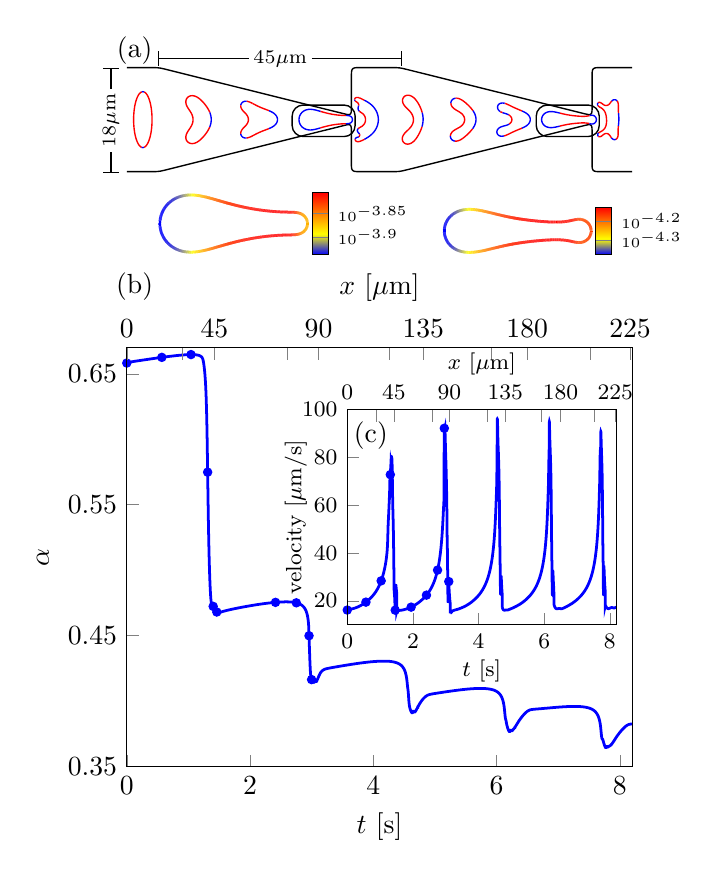
\begin{tikzpicture}[scale=1.0]

% START OF RIGHT PANEL OF COMPOSITE FIGURE
\begin{axis}[
  at = {(0.0cm,7.4cm)},
  width = 8.00cm,
  hide axis,
  axis equal image,
  xmin = 1,
  xmax = 32.5,
  ymin = -4,
  ymax = 4,
  xtick = \empty,
  ytick = \empty,
%  title style = {align=center, yshift = -0.4cm},
%  title = {\footnotesize $\beta = 1 \times 10^{-3}$,  
%           \footnotesize $U_{\max} = 18.0\mu$m/s},
]

% outer wall
\addplot[black,line width=0.5pt] coordinates{
(7.5585e-02,-3.1634e+00)
(1.0605e-01,-3.1878e+00)
(1.4241e-01,-3.2064e+00)
(1.8401e-01,-3.2199e+00)
(2.2996e-01,-3.2291e+00)
(2.7929e-01,-3.2350e+00)
(3.3106e-01,-3.2385e+00)
(3.8443e-01,-3.2405e+00)
(4.3877e-01,-3.2415e+00)
(4.9371e-01,-3.2419e+00)
(5.4898e-01,-3.2420e+00)
(6.0437e-01,-3.2419e+00)
(6.5974e-01,-3.2419e+00)
(7.1509e-01,-3.2419e+00)
(7.7045e-01,-3.2419e+00)
(8.2582e-01,-3.2419e+00)
(8.8118e-01,-3.2419e+00)
(9.3654e-01,-3.2419e+00)
(9.9190e-01,-3.2419e+00)
(1.0473e+00,-3.2419e+00)
(1.1026e+00,-3.2419e+00)
(1.1580e+00,-3.2419e+00)
(1.2133e+00,-3.2419e+00)
(1.2687e+00,-3.2419e+00)
(1.3241e+00,-3.2419e+00)
(1.3794e+00,-3.2419e+00)
(1.4348e+00,-3.2419e+00)
(1.4901e+00,-3.2419e+00)
(1.5455e+00,-3.2419e+00)
(1.6009e+00,-3.2419e+00)
(1.6562e+00,-3.2419e+00)
(1.7116e+00,-3.2419e+00)
(1.7670e+00,-3.2419e+00)
(1.8223e+00,-3.2419e+00)
(1.8777e+00,-3.2419e+00)
(1.9330e+00,-3.2419e+00)
(1.9884e+00,-3.2419e+00)
(2.0438e+00,-3.2419e+00)
(2.0991e+00,-3.2419e+00)
(2.1545e+00,-3.2419e+00)
(2.2098e+00,-3.2419e+00)
(2.2652e+00,-3.2419e+00)
(2.3206e+00,-3.2419e+00)
(2.3759e+00,-3.2419e+00)
(2.4313e+00,-3.2419e+00)
(2.4866e+00,-3.2419e+00)
(2.5420e+00,-3.2420e+00)
(2.5974e+00,-3.2419e+00)
(2.6526e+00,-3.2416e+00)
(2.7078e+00,-3.2409e+00)
(2.7629e+00,-3.2398e+00)
(2.8178e+00,-3.2378e+00)
(2.8725e+00,-3.2349e+00)
(2.9268e+00,-3.2308e+00)
(2.9809e+00,-3.2254e+00)
(3.0346e+00,-3.2185e+00)
(3.0879e+00,-3.2102e+00)
(3.1410e+00,-3.2006e+00)
(3.1938e+00,-3.1900e+00)
(3.2464e+00,-3.1785e+00)
(3.2988e+00,-3.1664e+00)
(3.3511e+00,-3.1539e+00)
(3.4034e+00,-3.1412e+00)
(3.4556e+00,-3.1283e+00)
(3.5079e+00,-3.1153e+00)
(3.5601e+00,-3.1023e+00)
(3.6123e+00,-3.0893e+00)
(3.6645e+00,-3.0763e+00)
(3.7167e+00,-3.0632e+00)
(3.7689e+00,-3.0502e+00)
(3.8211e+00,-3.0372e+00)
(3.8733e+00,-3.0242e+00)
(3.9255e+00,-3.0112e+00)
(3.9778e+00,-2.9982e+00)
(4.0300e+00,-2.9851e+00)
(4.0822e+00,-2.9721e+00)
(4.1344e+00,-2.9591e+00)
(4.1866e+00,-2.9461e+00)
(4.2388e+00,-2.9331e+00)
(4.2910e+00,-2.9201e+00)
(4.3432e+00,-2.9070e+00)
(4.3954e+00,-2.8940e+00)
(4.4476e+00,-2.8810e+00)
(4.4999e+00,-2.8680e+00)
(4.5521e+00,-2.8550e+00)
(4.6043e+00,-2.8419e+00)
(4.6565e+00,-2.8289e+00)
(4.7087e+00,-2.8159e+00)
(4.7609e+00,-2.8029e+00)
(4.8131e+00,-2.7899e+00)
(4.8653e+00,-2.7769e+00)
(4.9175e+00,-2.7638e+00)
(4.9697e+00,-2.7508e+00)
(5.0220e+00,-2.7378e+00)
(5.0742e+00,-2.7248e+00)
(5.1264e+00,-2.7118e+00)
(5.1786e+00,-2.6988e+00)
(5.2308e+00,-2.6857e+00)
(5.2830e+00,-2.6727e+00)
(5.3352e+00,-2.6597e+00)
(5.3874e+00,-2.6467e+00)
(5.4396e+00,-2.6337e+00)
(5.4919e+00,-2.6206e+00)
(5.5441e+00,-2.6076e+00)
(5.5963e+00,-2.5946e+00)
(5.6485e+00,-2.5816e+00)
(5.7007e+00,-2.5686e+00)
(5.7529e+00,-2.5556e+00)
(5.8051e+00,-2.5425e+00)
(5.8573e+00,-2.5295e+00)
(5.9095e+00,-2.5165e+00)
(5.9617e+00,-2.5035e+00)
(6.0140e+00,-2.4905e+00)
(6.0662e+00,-2.4775e+00)
(6.1184e+00,-2.4644e+00)
(6.1706e+00,-2.4514e+00)
(6.2228e+00,-2.4384e+00)
(6.2750e+00,-2.4254e+00)
(6.3272e+00,-2.4124e+00)
(6.3794e+00,-2.3993e+00)
(6.4316e+00,-2.3863e+00)
(6.4838e+00,-2.3733e+00)
(6.5361e+00,-2.3603e+00)
(6.5883e+00,-2.3473e+00)
(6.6405e+00,-2.3343e+00)
(6.6927e+00,-2.3212e+00)
(6.7449e+00,-2.3082e+00)
(6.7971e+00,-2.2952e+00)
(6.8493e+00,-2.2822e+00)
(6.9015e+00,-2.2692e+00)
(6.9537e+00,-2.2562e+00)
(7.0060e+00,-2.2431e+00)
(7.0582e+00,-2.2301e+00)
(7.1104e+00,-2.2171e+00)
(7.1626e+00,-2.2041e+00)
(7.2148e+00,-2.1911e+00)
(7.2670e+00,-2.1781e+00)
(7.3192e+00,-2.1650e+00)
(7.3714e+00,-2.1520e+00)
(7.4236e+00,-2.1390e+00)
(7.4758e+00,-2.1260e+00)
(7.5281e+00,-2.1130e+00)
(7.5803e+00,-2.0999e+00)
(7.6325e+00,-2.0869e+00)
(7.6847e+00,-2.0739e+00)
(7.7369e+00,-2.0609e+00)
(7.7891e+00,-2.0479e+00)
(7.8413e+00,-2.0349e+00)
(7.8935e+00,-2.0218e+00)
(7.9457e+00,-2.0088e+00)
(7.9979e+00,-1.9958e+00)
(8.0502e+00,-1.9828e+00)
(8.1024e+00,-1.9698e+00)
(8.1546e+00,-1.9568e+00)
(8.2068e+00,-1.9437e+00)
(8.2590e+00,-1.9307e+00)
(8.3112e+00,-1.9177e+00)
(8.3634e+00,-1.9047e+00)
(8.4156e+00,-1.8917e+00)
(8.4678e+00,-1.8786e+00)
(8.5201e+00,-1.8656e+00)
(8.5723e+00,-1.8526e+00)
(8.6245e+00,-1.8396e+00)
(8.6767e+00,-1.8266e+00)
(8.7289e+00,-1.8136e+00)
(8.7811e+00,-1.8005e+00)
(8.8333e+00,-1.7875e+00)
(8.8855e+00,-1.7745e+00)
(8.9377e+00,-1.7615e+00)
(8.9899e+00,-1.7485e+00)
(9.0422e+00,-1.7355e+00)
(9.0944e+00,-1.7224e+00)
(9.1466e+00,-1.7094e+00)
(9.1988e+00,-1.6964e+00)
(9.2510e+00,-1.6834e+00)
(9.3032e+00,-1.6704e+00)
(9.3554e+00,-1.6574e+00)
(9.4076e+00,-1.6443e+00)
(9.4598e+00,-1.6313e+00)
(9.5121e+00,-1.6183e+00)
(9.5643e+00,-1.6053e+00)
(9.6165e+00,-1.5923e+00)
(9.6687e+00,-1.5792e+00)
(9.7209e+00,-1.5662e+00)
(9.7731e+00,-1.5532e+00)
(9.8253e+00,-1.5402e+00)
(9.8775e+00,-1.5272e+00)
(9.9297e+00,-1.5142e+00)
(9.9819e+00,-1.5011e+00)
(1.0034e+01,-1.4881e+00)
(1.0086e+01,-1.4751e+00)
(1.0139e+01,-1.4621e+00)
(1.0191e+01,-1.4491e+00)
(1.0243e+01,-1.4361e+00)
(1.0295e+01,-1.4230e+00)
(1.0347e+01,-1.4100e+00)
(1.0400e+01,-1.3970e+00)
(1.0452e+01,-1.3840e+00)
(1.0504e+01,-1.3710e+00)
(1.0556e+01,-1.3580e+00)
(1.0608e+01,-1.3449e+00)
(1.0661e+01,-1.3319e+00)
(1.0713e+01,-1.3189e+00)
(1.0765e+01,-1.3059e+00)
(1.0817e+01,-1.2929e+00)
(1.0870e+01,-1.2798e+00)
(1.0922e+01,-1.2668e+00)
(1.0974e+01,-1.2538e+00)
(1.1026e+01,-1.2408e+00)
(1.1078e+01,-1.2278e+00)
(1.1131e+01,-1.2148e+00)
(1.1183e+01,-1.2017e+00)
(1.1235e+01,-1.1887e+00)
(1.1287e+01,-1.1757e+00)
(1.1339e+01,-1.1627e+00)
(1.1392e+01,-1.1497e+00)
(1.1444e+01,-1.1366e+00)
(1.1496e+01,-1.1236e+00)
(1.1548e+01,-1.1106e+00)
(1.1600e+01,-1.0976e+00)
(1.1653e+01,-1.0846e+00)
(1.1705e+01,-1.0716e+00)
(1.1757e+01,-1.0585e+00)
(1.1809e+01,-1.0455e+00)
(1.1862e+01,-1.0325e+00)
(1.1914e+01,-1.0195e+00)
(1.1966e+01,-1.0065e+00)
(1.2018e+01,-9.9346e-01)
(1.2070e+01,-9.8044e-01)
(1.2123e+01,-9.6743e-01)
(1.2175e+01,-9.5441e-01)
(1.2227e+01,-9.4139e-01)
(1.2279e+01,-9.2837e-01)
(1.2331e+01,-9.1536e-01)
(1.2384e+01,-9.0233e-01)
(1.2436e+01,-8.8932e-01)
(1.2488e+01,-8.7630e-01)
(1.2540e+01,-8.6329e-01)
(1.2592e+01,-8.5026e-01)
(1.2645e+01,-8.3725e-01)
(1.2697e+01,-8.2424e-01)
(1.2749e+01,-8.1121e-01)
(1.2801e+01,-7.9819e-01)
(1.2854e+01,-7.8518e-01)
(1.2906e+01,-7.7217e-01)
(1.2958e+01,-7.5914e-01)
(1.3010e+01,-7.4612e-01)
(1.3062e+01,-7.3311e-01)
(1.3115e+01,-7.2010e-01)
(1.3167e+01,-7.0707e-01)
(1.3219e+01,-6.9405e-01)
(1.3271e+01,-6.8104e-01)
(1.3323e+01,-6.6802e-01)
(1.3376e+01,-6.5500e-01)
(1.3428e+01,-6.4199e-01)
(1.3480e+01,-6.2898e-01)
(1.3532e+01,-6.1595e-01)
(1.3584e+01,-6.0293e-01)
(1.3637e+01,-5.8992e-01)
(1.3689e+01,-5.7691e-01)
(1.3741e+01,-5.6388e-01)
(1.3793e+01,-5.5086e-01)
(1.3846e+01,-5.3785e-01)
(1.3898e+01,-5.2484e-01)
(1.3950e+01,-5.1180e-01)
(1.4002e+01,-4.9879e-01)
(1.4054e+01,-4.8579e-01)
(1.4107e+01,-4.7276e-01)
(1.4159e+01,-4.5972e-01)
(1.4211e+01,-4.4672e-01)
(1.4263e+01,-4.3373e-01)
(1.4315e+01,-4.2069e-01)
(1.4368e+01,-4.0764e-01)
(1.4420e+01,-3.9467e-01)
(1.4472e+01,-3.8170e-01)
(1.4524e+01,-3.6857e-01)
(1.4577e+01,-3.5545e-01)
(1.4628e+01,-3.4293e-01)
(1.4679e+01,-3.3173e-01)
(1.4729e+01,-3.2253e-01)
(1.4776e+01,-3.1622e-01)
(1.4820e+01,-3.1401e-01)
(1.4859e+01,-3.1719e-01)
(1.4894e+01,-3.2682e-01)
(1.4924e+01,-3.4363e-01)
(1.4947e+01,-3.6794e-01)
(1.4965e+01,-3.9953e-01)
(1.4978e+01,-4.3762e-01)
(1.4987e+01,-4.8109e-01)
(1.4993e+01,-5.2876e-01)
(1.4997e+01,-5.7947e-01)
(1.4999e+01,-6.3218e-01)
(1.5000e+01,-6.8611e-01)
(1.5000e+01,-7.4079e-01)
(1.5000e+01,-7.9588e-01)
(1.5000e+01,-8.5113e-01)
(1.5000e+01,-9.0636e-01)
(1.5000e+01,-9.6156e-01)
(1.5000e+01,-1.0168e+00)
(1.5000e+01,-1.0720e+00)
(1.5000e+01,-1.1272e+00)
(1.5000e+01,-1.1824e+00)
(1.5000e+01,-1.2376e+00)
(1.5000e+01,-1.2928e+00)
(1.5000e+01,-1.3480e+00)
(1.5000e+01,-1.4033e+00)
(1.5000e+01,-1.4585e+00)
(1.5000e+01,-1.5137e+00)
(1.5000e+01,-1.5689e+00)
(1.5000e+01,-1.6241e+00)
(1.5000e+01,-1.6793e+00)
(1.5000e+01,-1.7345e+00)
(1.5000e+01,-1.7897e+00)
(1.5000e+01,-1.8450e+00)
(1.5000e+01,-1.9002e+00)
(1.5000e+01,-1.9554e+00)
(1.5000e+01,-2.0106e+00)
(1.5000e+01,-2.0658e+00)
(1.5000e+01,-2.1210e+00)
(1.5000e+01,-2.1762e+00)
(1.5000e+01,-2.2314e+00)
(1.5000e+01,-2.2866e+00)
(1.5000e+01,-2.3419e+00)
(1.5000e+01,-2.3971e+00)
(1.5000e+01,-2.4523e+00)
(1.5000e+01,-2.5075e+00)
(1.5000e+01,-2.5627e+00)
(1.5000e+01,-2.6179e+00)
(1.5000e+01,-2.6731e+00)
(1.5000e+01,-2.7284e+00)
(1.5000e+01,-2.7837e+00)
(1.5000e+01,-2.8386e+00)
(1.5001e+01,-2.8926e+00)
(1.5004e+01,-2.9451e+00)
(1.5009e+01,-2.9954e+00)
(1.5017e+01,-3.0426e+00)
(1.5029e+01,-3.0856e+00)
(1.5047e+01,-3.1235e+00)
(1.5070e+01,-3.1557e+00)
(1.5099e+01,-3.1819e+00)
(1.5134e+01,-3.2021e+00)
(1.5174e+01,-3.2169e+00)
(1.5220e+01,-3.2271e+00)
(1.5268e+01,-3.2338e+00)
(1.5320e+01,-3.2378e+00)
(1.5373e+01,-3.2401e+00)
(1.5427e+01,-3.2413e+00)
(1.5482e+01,-3.2418e+00)
(1.5537e+01,-3.2420e+00)
(1.5592e+01,-3.2419e+00)
(1.5604e+01,-3.2419e+00)
(1.5660e+01,-3.2419e+00)
(1.5715e+01,-3.2419e+00)
(1.5770e+01,-3.2419e+00)
(1.5826e+01,-3.2419e+00)
(1.5881e+01,-3.2419e+00)
(1.5937e+01,-3.2419e+00)
(1.5992e+01,-3.2419e+00)
(1.6047e+01,-3.2419e+00)
(1.6103e+01,-3.2419e+00)
(1.6158e+01,-3.2419e+00)
(1.6213e+01,-3.2419e+00)
(1.6269e+01,-3.2419e+00)
(1.6324e+01,-3.2419e+00)
(1.6379e+01,-3.2419e+00)
(1.6435e+01,-3.2419e+00)
(1.6490e+01,-3.2419e+00)
(1.6546e+01,-3.2419e+00)
(1.6601e+01,-3.2419e+00)
(1.6656e+01,-3.2419e+00)
(1.6712e+01,-3.2419e+00)
(1.6767e+01,-3.2419e+00)
(1.6822e+01,-3.2419e+00)
(1.6878e+01,-3.2419e+00)
(1.6933e+01,-3.2419e+00)
(1.6988e+01,-3.2419e+00)
(1.7044e+01,-3.2419e+00)
(1.7099e+01,-3.2419e+00)
(1.7154e+01,-3.2419e+00)
(1.7210e+01,-3.2419e+00)
(1.7265e+01,-3.2419e+00)
(1.7321e+01,-3.2419e+00)
(1.7376e+01,-3.2419e+00)
(1.7431e+01,-3.2419e+00)
(1.7487e+01,-3.2419e+00)
(1.7542e+01,-3.2420e+00)
(1.7597e+01,-3.2419e+00)
(1.7653e+01,-3.2416e+00)
(1.7708e+01,-3.2409e+00)
(1.7763e+01,-3.2398e+00)
(1.7818e+01,-3.2378e+00)
(1.7872e+01,-3.2349e+00)
(1.7927e+01,-3.2308e+00)
(1.7981e+01,-3.2254e+00)
(1.8035e+01,-3.2185e+00)
(1.8088e+01,-3.2102e+00)
(1.8141e+01,-3.2006e+00)
(1.8194e+01,-3.1900e+00)
(1.8246e+01,-3.1785e+00)
(1.8299e+01,-3.1664e+00)
(1.8351e+01,-3.1539e+00)
(1.8403e+01,-3.1412e+00)
(1.8456e+01,-3.1283e+00)
(1.8508e+01,-3.1153e+00)
(1.8560e+01,-3.1023e+00)
(1.8612e+01,-3.0893e+00)
(1.8664e+01,-3.0763e+00)
(1.8717e+01,-3.0632e+00)
(1.8769e+01,-3.0502e+00)
(1.8821e+01,-3.0372e+00)
(1.8873e+01,-3.0242e+00)
(1.8926e+01,-3.0112e+00)
(1.8978e+01,-2.9982e+00)
(1.9030e+01,-2.9851e+00)
(1.9082e+01,-2.9721e+00)
(1.9134e+01,-2.9591e+00)
(1.9187e+01,-2.9461e+00)
(1.9239e+01,-2.9331e+00)
(1.9291e+01,-2.9201e+00)
(1.9343e+01,-2.9070e+00)
(1.9395e+01,-2.8940e+00)
(1.9448e+01,-2.8810e+00)
(1.9500e+01,-2.8680e+00)
(1.9552e+01,-2.8550e+00)
(1.9604e+01,-2.8419e+00)
(1.9656e+01,-2.8289e+00)
(1.9709e+01,-2.8159e+00)
(1.9761e+01,-2.8029e+00)
(1.9813e+01,-2.7899e+00)
(1.9865e+01,-2.7769e+00)
(1.9918e+01,-2.7638e+00)
(1.9970e+01,-2.7508e+00)
(2.0022e+01,-2.7378e+00)
(2.0074e+01,-2.7248e+00)
(2.0126e+01,-2.7118e+00)
(2.0179e+01,-2.6988e+00)
(2.0231e+01,-2.6857e+00)
(2.0283e+01,-2.6727e+00)
(2.0335e+01,-2.6597e+00)
(2.0387e+01,-2.6467e+00)
(2.0440e+01,-2.6337e+00)
(2.0492e+01,-2.6206e+00)
(2.0544e+01,-2.6076e+00)
(2.0596e+01,-2.5946e+00)
(2.0648e+01,-2.5816e+00)
(2.0701e+01,-2.5686e+00)
(2.0753e+01,-2.5556e+00)
(2.0805e+01,-2.5425e+00)
(2.0857e+01,-2.5295e+00)
(2.0910e+01,-2.5165e+00)
(2.0962e+01,-2.5035e+00)
(2.1014e+01,-2.4905e+00)
(2.1066e+01,-2.4775e+00)
(2.1118e+01,-2.4644e+00)
(2.1171e+01,-2.4514e+00)
(2.1223e+01,-2.4384e+00)
(2.1275e+01,-2.4254e+00)
(2.1327e+01,-2.4124e+00)
(2.1379e+01,-2.3993e+00)
(2.1432e+01,-2.3863e+00)
(2.1484e+01,-2.3733e+00)
(2.1536e+01,-2.3603e+00)
(2.1588e+01,-2.3473e+00)
(2.1640e+01,-2.3343e+00)
(2.1693e+01,-2.3212e+00)
(2.1745e+01,-2.3082e+00)
(2.1797e+01,-2.2952e+00)
(2.1849e+01,-2.2822e+00)
(2.1902e+01,-2.2692e+00)
(2.1954e+01,-2.2562e+00)
(2.2006e+01,-2.2431e+00)
(2.2058e+01,-2.2301e+00)
(2.2110e+01,-2.2171e+00)
(2.2163e+01,-2.2041e+00)
(2.2215e+01,-2.1911e+00)
(2.2267e+01,-2.1781e+00)
(2.2319e+01,-2.1650e+00)
(2.2371e+01,-2.1520e+00)
(2.2424e+01,-2.1390e+00)
(2.2476e+01,-2.1260e+00)
(2.2528e+01,-2.1130e+00)
(2.2580e+01,-2.0999e+00)
(2.2632e+01,-2.0869e+00)
(2.2685e+01,-2.0739e+00)
(2.2737e+01,-2.0609e+00)
(2.2789e+01,-2.0479e+00)
(2.2841e+01,-2.0349e+00)
(2.2894e+01,-2.0218e+00)
(2.2946e+01,-2.0088e+00)
(2.2998e+01,-1.9958e+00)
(2.3050e+01,-1.9828e+00)
(2.3102e+01,-1.9698e+00)
(2.3155e+01,-1.9568e+00)
(2.3207e+01,-1.9437e+00)
(2.3259e+01,-1.9307e+00)
(2.3311e+01,-1.9177e+00)
(2.3363e+01,-1.9047e+00)
(2.3416e+01,-1.8917e+00)
(2.3468e+01,-1.8786e+00)
(2.3520e+01,-1.8656e+00)
(2.3572e+01,-1.8526e+00)
(2.3624e+01,-1.8396e+00)
(2.3677e+01,-1.8266e+00)
(2.3729e+01,-1.8136e+00)
(2.3781e+01,-1.8005e+00)
(2.3833e+01,-1.7875e+00)
(2.3886e+01,-1.7745e+00)
(2.3938e+01,-1.7615e+00)
(2.3990e+01,-1.7485e+00)
(2.4042e+01,-1.7355e+00)
(2.4094e+01,-1.7224e+00)
(2.4147e+01,-1.7094e+00)
(2.4199e+01,-1.6964e+00)
(2.4251e+01,-1.6834e+00)
(2.4303e+01,-1.6704e+00)
(2.4355e+01,-1.6574e+00)
(2.4408e+01,-1.6443e+00)
(2.4460e+01,-1.6313e+00)
(2.4512e+01,-1.6183e+00)
(2.4564e+01,-1.6053e+00)
(2.4616e+01,-1.5923e+00)
(2.4669e+01,-1.5792e+00)
(2.4721e+01,-1.5662e+00)
(2.4773e+01,-1.5532e+00)
(2.4825e+01,-1.5402e+00)
(2.4878e+01,-1.5272e+00)
(2.4930e+01,-1.5142e+00)
(2.4982e+01,-1.5011e+00)
(2.5034e+01,-1.4881e+00)
(2.5086e+01,-1.4751e+00)
(2.5139e+01,-1.4621e+00)
(2.5191e+01,-1.4491e+00)
(2.5243e+01,-1.4361e+00)
(2.5295e+01,-1.4230e+00)
(2.5347e+01,-1.4100e+00)
(2.5400e+01,-1.3970e+00)
(2.5452e+01,-1.3840e+00)
(2.5504e+01,-1.3710e+00)
(2.5556e+01,-1.3580e+00)
(2.5608e+01,-1.3449e+00)
(2.5661e+01,-1.3319e+00)
(2.5713e+01,-1.3189e+00)
(2.5765e+01,-1.3059e+00)
(2.5817e+01,-1.2929e+00)
(2.5870e+01,-1.2798e+00)
(2.5922e+01,-1.2668e+00)
(2.5974e+01,-1.2538e+00)
(2.6026e+01,-1.2408e+00)
(2.6078e+01,-1.2278e+00)
(2.6131e+01,-1.2148e+00)
(2.6183e+01,-1.2017e+00)
(2.6235e+01,-1.1887e+00)
(2.6287e+01,-1.1757e+00)
(2.6339e+01,-1.1627e+00)
(2.6392e+01,-1.1497e+00)
(2.6444e+01,-1.1366e+00)
(2.6496e+01,-1.1236e+00)
(2.6548e+01,-1.1106e+00)
(2.6600e+01,-1.0976e+00)
(2.6653e+01,-1.0846e+00)
(2.6705e+01,-1.0716e+00)
(2.6757e+01,-1.0585e+00)
(2.6809e+01,-1.0455e+00)
(2.6862e+01,-1.0325e+00)
(2.6914e+01,-1.0195e+00)
(2.6966e+01,-1.0065e+00)
(2.7018e+01,-9.9346e-01)
(2.7070e+01,-9.8044e-01)
(2.7123e+01,-9.6743e-01)
(2.7175e+01,-9.5441e-01)
(2.7227e+01,-9.4139e-01)
(2.7279e+01,-9.2837e-01)
(2.7331e+01,-9.1536e-01)
(2.7384e+01,-9.0233e-01)
(2.7436e+01,-8.8932e-01)
(2.7488e+01,-8.7630e-01)
(2.7540e+01,-8.6329e-01)
(2.7592e+01,-8.5026e-01)
(2.7645e+01,-8.3725e-01)
(2.7697e+01,-8.2424e-01)
(2.7749e+01,-8.1121e-01)
(2.7801e+01,-7.9819e-01)
(2.7854e+01,-7.8518e-01)
(2.7906e+01,-7.7217e-01)
(2.7958e+01,-7.5914e-01)
(2.8010e+01,-7.4612e-01)
(2.8062e+01,-7.3311e-01)
(2.8115e+01,-7.2010e-01)
(2.8167e+01,-7.0707e-01)
(2.8219e+01,-6.9405e-01)
(2.8271e+01,-6.8104e-01)
(2.8323e+01,-6.6802e-01)
(2.8376e+01,-6.5500e-01)
(2.8428e+01,-6.4199e-01)
(2.8480e+01,-6.2898e-01)
(2.8532e+01,-6.1595e-01)
(2.8584e+01,-6.0293e-01)
(2.8637e+01,-5.8992e-01)
(2.8689e+01,-5.7691e-01)
(2.8741e+01,-5.6388e-01)
(2.8793e+01,-5.5086e-01)
(2.8846e+01,-5.3785e-01)
(2.8898e+01,-5.2484e-01)
(2.8950e+01,-5.1180e-01)
(2.9002e+01,-4.9879e-01)
(2.9054e+01,-4.8579e-01)
(2.9107e+01,-4.7276e-01)
(2.9159e+01,-4.5972e-01)
(2.9211e+01,-4.4672e-01)
(2.9263e+01,-4.3373e-01)
(2.9315e+01,-4.2069e-01)
(2.9368e+01,-4.0764e-01)
(2.9420e+01,-3.9467e-01)
(2.9472e+01,-3.8170e-01)
(2.9524e+01,-3.6857e-01)
(2.9577e+01,-3.5545e-01)
(2.9628e+01,-3.4293e-01)
(2.9679e+01,-3.3173e-01)
(2.9729e+01,-3.2253e-01)
(2.9776e+01,-3.1622e-01)
(2.9820e+01,-3.1401e-01)
(2.9859e+01,-3.1719e-01)
(2.9894e+01,-3.2682e-01)
(2.9924e+01,-3.4363e-01)
(2.9947e+01,-3.6794e-01)
(2.9965e+01,-3.9953e-01)
(2.9978e+01,-4.3762e-01)
(2.9987e+01,-4.8109e-01)
(2.9993e+01,-5.2876e-01)
(2.9997e+01,-5.7947e-01)
(2.9999e+01,-6.3218e-01)
(3.0000e+01,-6.8611e-01)
(3.0000e+01,-7.4079e-01)
(3.0000e+01,-7.9588e-01)
(3.0000e+01,-8.5113e-01)
(3.0000e+01,-9.0636e-01)
(3.0000e+01,-9.6156e-01)
(3.0000e+01,-1.0168e+00)
(3.0000e+01,-1.0720e+00)
(3.0000e+01,-1.1272e+00)
(3.0000e+01,-1.1824e+00)
(3.0000e+01,-1.2376e+00)
(3.0000e+01,-1.2928e+00)
(3.0000e+01,-1.3480e+00)
(3.0000e+01,-1.4033e+00)
(3.0000e+01,-1.4585e+00)
(3.0000e+01,-1.5137e+00)
(3.0000e+01,-1.5689e+00)
(3.0000e+01,-1.6241e+00)
(3.0000e+01,-1.6793e+00)
(3.0000e+01,-1.7345e+00)
(3.0000e+01,-1.7897e+00)
(3.0000e+01,-1.8450e+00)
(3.0000e+01,-1.9002e+00)
(3.0000e+01,-1.9554e+00)
(3.0000e+01,-2.0106e+00)
(3.0000e+01,-2.0658e+00)
(3.0000e+01,-2.1210e+00)
(3.0000e+01,-2.1762e+00)
(3.0000e+01,-2.2314e+00)
(3.0000e+01,-2.2866e+00)
(3.0000e+01,-2.3419e+00)
(3.0000e+01,-2.3971e+00)
(3.0000e+01,-2.4523e+00)
(3.0000e+01,-2.5075e+00)
(3.0000e+01,-2.5627e+00)
(3.0000e+01,-2.6179e+00)
(3.0000e+01,-2.6731e+00)
(3.0000e+01,-2.7284e+00)
(3.0000e+01,-2.7837e+00)
(3.0000e+01,-2.8386e+00)
(3.0001e+01,-2.8926e+00)
(3.0004e+01,-2.9451e+00)
(3.0009e+01,-2.9954e+00)
(3.0017e+01,-3.0426e+00)
(3.0029e+01,-3.0856e+00)
(3.0047e+01,-3.1235e+00)
(3.0070e+01,-3.1557e+00)
(3.0099e+01,-3.1819e+00)
(3.0134e+01,-3.2021e+00)
(3.0174e+01,-3.2169e+00)
(3.0220e+01,-3.2271e+00)
(3.0268e+01,-3.2338e+00)
(3.0320e+01,-3.2378e+00)
(3.0373e+01,-3.2401e+00)
(3.0427e+01,-3.2413e+00)
(3.0482e+01,-3.2418e+00)
(3.0537e+01,-3.2420e+00)
(3.0592e+01,-3.2419e+00)
(3.0648e+01,-3.2419e+00)
(3.0703e+01,-3.2419e+00)
(3.0758e+01,-3.2419e+00)
(3.0814e+01,-3.2419e+00)
(3.0869e+01,-3.2419e+00)
(3.0924e+01,-3.2419e+00)
(3.0980e+01,-3.2419e+00)
(3.1035e+01,-3.2419e+00)
(3.1091e+01,-3.2419e+00)
(3.1146e+01,-3.2419e+00)
(3.1201e+01,-3.2419e+00)
(3.1257e+01,-3.2419e+00)
(3.1312e+01,-3.2419e+00)
(3.1367e+01,-3.2419e+00)
(3.1423e+01,-3.2419e+00)
(3.1478e+01,-3.2419e+00)
(3.1533e+01,-3.2419e+00)
(3.1589e+01,-3.2419e+00)
(3.1644e+01,-3.2419e+00)
(3.1699e+01,-3.2419e+00)
(3.1755e+01,-3.2419e+00)
(3.1810e+01,-3.2419e+00)
(3.1866e+01,-3.2419e+00)
(3.1921e+01,-3.2419e+00)
(3.1976e+01,-3.2419e+00)
(3.2032e+01,-3.2419e+00)
(3.2087e+01,-3.2419e+00)
(3.2142e+01,-3.2419e+00)
(3.2198e+01,-3.2419e+00)
(3.2253e+01,-3.2419e+00)
(3.2308e+01,-3.2420e+00)
(3.2364e+01,-3.2419e+00)
(3.2419e+01,-3.2419e+00)
(3.2475e+01,-3.2419e+00)
(3.2530e+01,-3.2421e+00)
(3.2585e+01,-3.2419e+00)
(3.2640e+01,-3.2409e+00)
(3.2693e+01,-3.2386e+00)
(3.2743e+01,-3.2342e+00)
(3.2791e+01,-3.2270e+00)
(3.2835e+01,-3.2158e+00)
(3.2874e+01,-3.1999e+00)
(3.2908e+01,-3.1784e+00)
(3.2935e+01,-3.1510e+00)
(3.2957e+01,-3.1177e+00)
(3.2972e+01,-3.0789e+00)
(3.2984e+01,-3.0356e+00)
(3.2991e+01,-2.9885e+00)
(3.2995e+01,-2.9387e+00)
(3.2998e+01,-2.8870e+00)
(3.2999e+01,-2.8341e+00)
(3.3000e+01,-2.7805e+00)
(3.3000e+01,-2.7265e+00)
(3.3000e+01,-2.6722e+00)
(3.3000e+01,-2.6180e+00)
(3.3000e+01,-2.5638e+00)
(3.3000e+01,-2.5096e+00)
(3.3000e+01,-2.4553e+00)
(3.3000e+01,-2.4011e+00)
(3.3000e+01,-2.3469e+00)
(3.3000e+01,-2.2927e+00)
(3.3000e+01,-2.2385e+00)
(3.3000e+01,-2.1843e+00)
(3.3000e+01,-2.1300e+00)
(3.3000e+01,-2.0758e+00)
(3.3000e+01,-2.0216e+00)
(3.3000e+01,-1.9674e+00)
(3.3000e+01,-1.9132e+00)
(3.3000e+01,-1.8590e+00)
(3.3000e+01,-1.8047e+00)
(3.3000e+01,-1.7505e+00)
(3.3000e+01,-1.6963e+00)
(3.3000e+01,-1.6421e+00)
(3.3000e+01,-1.5879e+00)
(3.3000e+01,-1.5337e+00)
(3.3000e+01,-1.4794e+00)
(3.3000e+01,-1.4252e+00)
(3.3000e+01,-1.3710e+00)
(3.3000e+01,-1.3168e+00)
(3.3000e+01,-1.2626e+00)
(3.3000e+01,-1.2084e+00)
(3.3000e+01,-1.1541e+00)
(3.3000e+01,-1.0999e+00)
(3.3000e+01,-1.0457e+00)
(3.3000e+01,-9.9149e-01)
(3.3000e+01,-9.3727e-01)
(3.3000e+01,-8.8306e-01)
(3.3000e+01,-8.2884e-01)
(3.3000e+01,-7.7462e-01)
(3.3000e+01,-7.2040e-01)
(3.3000e+01,-6.6619e-01)
(3.3000e+01,-6.1197e-01)
(3.3000e+01,-5.5775e-01)
(3.3000e+01,-5.0354e-01)
(3.3000e+01,-4.4932e-01)
(3.3000e+01,-3.9510e-01)
(3.3000e+01,-3.4089e-01)
(3.3000e+01,-2.8667e-01)
(3.3000e+01,-2.3245e-01)
(3.3000e+01,-1.7824e-01)
(3.3000e+01,-1.2402e-01)
(3.3000e+01,-6.9801e-02)
(3.3000e+01,-1.5584e-02)
(3.3000e+01,3.8632e-02)
(3.3000e+01,9.2849e-02)
(3.3000e+01,1.4707e-01)
(3.3000e+01,2.0128e-01)
(3.3000e+01,2.5550e-01)
(3.3000e+01,3.0972e-01)
(3.3000e+01,3.6393e-01)
(3.3000e+01,4.1815e-01)
(3.3000e+01,4.7237e-01)
(3.3000e+01,5.2659e-01)
(3.3000e+01,5.8080e-01)
(3.3000e+01,6.3502e-01)
(3.3000e+01,6.8924e-01)
(3.3000e+01,7.4345e-01)
(3.3000e+01,7.9767e-01)
(3.3000e+01,8.5189e-01)
(3.3000e+01,9.0610e-01)
(3.3000e+01,9.6032e-01)
(3.3000e+01,1.0145e+00)
(3.3000e+01,1.0688e+00)
(3.3000e+01,1.1230e+00)
(3.3000e+01,1.1772e+00)
(3.3000e+01,1.2314e+00)
(3.3000e+01,1.2856e+00)
(3.3000e+01,1.3398e+00)
(3.3000e+01,1.3941e+00)
(3.3000e+01,1.4483e+00)
(3.3000e+01,1.5025e+00)
(3.3000e+01,1.5567e+00)
(3.3000e+01,1.6109e+00)
(3.3000e+01,1.6651e+00)
(3.3000e+01,1.7194e+00)
(3.3000e+01,1.7736e+00)
(3.3000e+01,1.8278e+00)
(3.3000e+01,1.8820e+00)
(3.3000e+01,1.9362e+00)
(3.3000e+01,1.9904e+00)
(3.3000e+01,2.0447e+00)
(3.3000e+01,2.0989e+00)
(3.3000e+01,2.1531e+00)
(3.3000e+01,2.2073e+00)
(3.3000e+01,2.2615e+00)
(3.3000e+01,2.3157e+00)
(3.3000e+01,2.3700e+00)
(3.3000e+01,2.4242e+00)
(3.3000e+01,2.4784e+00)
(3.3000e+01,2.5326e+00)
(3.3000e+01,2.5869e+00)
(3.3000e+01,2.6410e+00)
(3.3000e+01,2.6952e+00)
(3.3000e+01,2.7495e+00)
(3.3000e+01,2.8038e+00)
(3.3000e+01,2.8576e+00)
(3.2998e+01,2.9104e+00)
(3.2995e+01,2.9615e+00)
(3.2990e+01,3.0103e+00)
(3.2981e+01,3.0558e+00)
(3.2967e+01,3.0970e+00)
(3.2949e+01,3.1331e+00)
(3.2924e+01,3.1634e+00)
(3.2894e+01,3.1878e+00)
(3.2858e+01,3.2064e+00)
(3.2816e+01,3.2199e+00)
(3.2770e+01,3.2291e+00)
(3.2721e+01,3.2350e+00)
(3.2669e+01,3.2385e+00)
(3.2616e+01,3.2405e+00)
(3.2561e+01,3.2415e+00)
(3.2506e+01,3.2419e+00)
(3.2451e+01,3.2420e+00)
(3.2396e+01,3.2419e+00)
(3.2340e+01,3.2419e+00)
(3.2285e+01,3.2419e+00)
(3.2230e+01,3.2419e+00)
(3.2174e+01,3.2419e+00)
(3.2119e+01,3.2419e+00)
(3.2063e+01,3.2419e+00)
(3.2008e+01,3.2419e+00)
(3.1953e+01,3.2419e+00)
(3.1897e+01,3.2419e+00)
(3.1842e+01,3.2419e+00)
(3.1787e+01,3.2419e+00)
(3.1731e+01,3.2419e+00)
(3.1676e+01,3.2419e+00)
(3.1621e+01,3.2419e+00)
(3.1565e+01,3.2419e+00)
(3.1510e+01,3.2419e+00)
(3.1454e+01,3.2419e+00)
(3.1399e+01,3.2419e+00)
(3.1344e+01,3.2419e+00)
(3.1288e+01,3.2419e+00)
(3.1233e+01,3.2419e+00)
(3.1178e+01,3.2419e+00)
(3.1122e+01,3.2419e+00)
(3.1067e+01,3.2419e+00)
(3.1012e+01,3.2419e+00)
(3.0956e+01,3.2419e+00)
(3.0901e+01,3.2420e+00)
(3.0846e+01,3.2419e+00)
(3.0790e+01,3.2419e+00)
(3.0735e+01,3.2419e+00)
(3.0679e+01,3.2420e+00)
(3.0624e+01,3.2419e+00)
(3.0569e+01,3.2419e+00)
(3.0513e+01,3.2420e+00)
(3.0458e+01,3.2421e+00)
(3.0403e+01,3.2418e+00)
(3.0349e+01,3.2405e+00)
(3.0296e+01,3.2377e+00)
(3.0246e+01,3.2327e+00)
(3.0199e+01,3.2246e+00)
(3.0156e+01,3.2123e+00)
(3.0118e+01,3.1948e+00)
(3.0086e+01,3.1716e+00)
(3.0060e+01,3.1424e+00)
(3.0039e+01,3.1072e+00)
(3.0025e+01,3.0667e+00)
(3.0015e+01,3.0216e+00)
(3.0008e+01,2.9729e+00)
(3.0004e+01,2.9217e+00)
(3.0002e+01,2.8687e+00)
(3.0001e+01,2.8147e+00)
(3.0000e+01,2.7600e+00)
(3.0000e+01,2.7049e+00)
(3.0000e+01,2.6497e+00)
(3.0000e+01,2.5944e+00)
(3.0000e+01,2.5392e+00)
(3.0000e+01,2.4840e+00)
(3.0000e+01,2.4288e+00)
(3.0000e+01,2.3736e+00)
(3.0000e+01,2.3184e+00)
(3.0000e+01,2.2632e+00)
(3.0000e+01,2.2080e+00)
(3.0000e+01,2.1528e+00)
(3.0000e+01,2.0975e+00)
(3.0000e+01,2.0423e+00)
(3.0000e+01,1.9871e+00)
(3.0000e+01,1.9319e+00)
(3.0000e+01,1.8767e+00)
(3.0000e+01,1.8215e+00)
(3.0000e+01,1.7663e+00)
(3.0000e+01,1.7111e+00)
(3.0000e+01,1.6559e+00)
(3.0000e+01,1.6006e+00)
(3.0000e+01,1.5454e+00)
(3.0000e+01,1.4902e+00)
(3.0000e+01,1.4350e+00)
(3.0000e+01,1.3798e+00)
(3.0000e+01,1.3246e+00)
(3.0000e+01,1.2694e+00)
(3.0000e+01,1.2142e+00)
(3.0000e+01,1.1589e+00)
(3.0000e+01,1.1037e+00)
(3.0000e+01,1.0485e+00)
(3.0000e+01,9.9331e-01)
(3.0000e+01,9.3806e-01)
(3.0000e+01,8.8287e-01)
(3.0000e+01,8.2772e-01)
(3.0000e+01,7.7246e-01)
(3.0000e+01,7.1709e-01)
(3.0000e+01,6.6208e-01)
(2.9999e+01,6.0815e-01)
(2.9997e+01,5.5597e-01)
(2.9992e+01,5.0633e-01)
(2.9985e+01,4.6033e-01)
(2.9974e+01,4.1930e-01)
(2.9959e+01,3.8438e-01)
(2.9938e+01,3.5642e-01)
(2.9912e+01,3.3590e-01)
(2.9879e+01,3.2281e-01)
(2.9842e+01,3.1654e-01)
(2.9800e+01,3.1606e-01)
(2.9755e+01,3.2020e-01)
(2.9707e+01,3.2778e-01)
(2.9657e+01,3.3770e-01)
(2.9606e+01,3.4908e-01)
(2.9554e+01,3.6134e-01)
(2.9502e+01,3.7412e-01)
(2.9450e+01,3.8715e-01)
(2.9398e+01,4.0020e-01)
(2.9345e+01,4.1321e-01)
(2.9293e+01,4.2622e-01)
(2.9241e+01,4.3924e-01)
(2.9189e+01,4.5226e-01)
(2.9137e+01,4.6528e-01)
(2.9084e+01,4.7829e-01)
(2.9032e+01,4.9131e-01)
(2.8980e+01,5.0433e-01)
(2.8928e+01,5.1735e-01)
(2.8876e+01,5.3036e-01)
(2.8823e+01,5.4338e-01)
(2.8771e+01,5.5640e-01)
(2.8719e+01,5.6942e-01)
(2.8667e+01,5.8243e-01)
(2.8614e+01,5.9545e-01)
(2.8562e+01,6.0847e-01)
(2.8510e+01,6.2149e-01)
(2.8458e+01,6.3450e-01)
(2.8406e+01,6.4752e-01)
(2.8353e+01,6.6054e-01)
(2.8301e+01,6.7356e-01)
(2.8249e+01,6.8657e-01)
(2.8197e+01,6.9959e-01)
(2.8145e+01,7.1261e-01)
(2.8092e+01,7.2563e-01)
(2.8040e+01,7.3864e-01)
(2.7988e+01,7.5166e-01)
(2.7936e+01,7.6468e-01)
(2.7884e+01,7.7770e-01)
(2.7831e+01,7.9071e-01)
(2.7779e+01,8.0373e-01)
(2.7727e+01,8.1675e-01)
(2.7675e+01,8.2977e-01)
(2.7622e+01,8.4278e-01)
(2.7570e+01,8.5580e-01)
(2.7518e+01,8.6882e-01)
(2.7466e+01,8.8184e-01)
(2.7414e+01,8.9485e-01)
(2.7361e+01,9.0787e-01)
(2.7309e+01,9.2089e-01)
(2.7257e+01,9.3390e-01)
(2.7205e+01,9.4692e-01)
(2.7153e+01,9.5994e-01)
(2.7100e+01,9.7296e-01)
(2.7048e+01,9.8597e-01)
(2.6996e+01,9.9899e-01)
(2.6944e+01,1.0120e+00)
(2.6892e+01,1.0250e+00)
(2.6839e+01,1.0380e+00)
(2.6787e+01,1.0511e+00)
(2.6735e+01,1.0641e+00)
(2.6683e+01,1.0771e+00)
(2.6630e+01,1.0901e+00)
(2.6578e+01,1.1031e+00)
(2.6526e+01,1.1162e+00)
(2.6474e+01,1.1292e+00)
(2.6422e+01,1.1422e+00)
(2.6369e+01,1.1552e+00)
(2.6317e+01,1.1682e+00)
(2.6265e+01,1.1812e+00)
(2.6213e+01,1.1943e+00)
(2.6161e+01,1.2073e+00)
(2.6108e+01,1.2203e+00)
(2.6056e+01,1.2333e+00)
(2.6004e+01,1.2463e+00)
(2.5952e+01,1.2593e+00)
(2.5900e+01,1.2724e+00)
(2.5847e+01,1.2854e+00)
(2.5795e+01,1.2984e+00)
(2.5743e+01,1.3114e+00)
(2.5691e+01,1.3244e+00)
(2.5638e+01,1.3374e+00)
(2.5586e+01,1.3505e+00)
(2.5534e+01,1.3635e+00)
(2.5482e+01,1.3765e+00)
(2.5430e+01,1.3895e+00)
(2.5377e+01,1.4025e+00)
(2.5325e+01,1.4156e+00)
(2.5273e+01,1.4286e+00)
(2.5221e+01,1.4416e+00)
(2.5169e+01,1.4546e+00)
(2.5116e+01,1.4676e+00)
(2.5064e+01,1.4806e+00)
(2.5012e+01,1.4937e+00)
(2.4960e+01,1.5067e+00)
(2.4908e+01,1.5197e+00)
(2.4855e+01,1.5327e+00)
(2.4803e+01,1.5457e+00)
(2.4751e+01,1.5587e+00)
(2.4699e+01,1.5718e+00)
(2.4646e+01,1.5848e+00)
(2.4594e+01,1.5978e+00)
(2.4542e+01,1.6108e+00)
(2.4490e+01,1.6238e+00)
(2.4438e+01,1.6369e+00)
(2.4385e+01,1.6499e+00)
(2.4333e+01,1.6629e+00)
(2.4281e+01,1.6759e+00)
(2.4229e+01,1.6889e+00)
(2.4177e+01,1.7019e+00)
(2.4124e+01,1.7150e+00)
(2.4072e+01,1.7280e+00)
(2.4020e+01,1.7410e+00)
(2.3968e+01,1.7540e+00)
(2.3916e+01,1.7670e+00)
(2.3863e+01,1.7800e+00)
(2.3811e+01,1.7931e+00)
(2.3759e+01,1.8061e+00)
(2.3707e+01,1.8191e+00)
(2.3654e+01,1.8321e+00)
(2.3602e+01,1.8451e+00)
(2.3550e+01,1.8581e+00)
(2.3498e+01,1.8712e+00)
(2.3446e+01,1.8842e+00)
(2.3393e+01,1.8972e+00)
(2.3341e+01,1.9102e+00)
(2.3289e+01,1.9232e+00)
(2.3237e+01,1.9363e+00)
(2.3185e+01,1.9493e+00)
(2.3132e+01,1.9623e+00)
(2.3080e+01,1.9753e+00)
(2.3028e+01,1.9883e+00)
(2.2976e+01,2.0013e+00)
(2.2924e+01,2.0144e+00)
(2.2871e+01,2.0274e+00)
(2.2819e+01,2.0404e+00)
(2.2767e+01,2.0534e+00)
(2.2715e+01,2.0664e+00)
(2.2662e+01,2.0794e+00)
(2.2610e+01,2.0925e+00)
(2.2558e+01,2.1055e+00)
(2.2506e+01,2.1185e+00)
(2.2454e+01,2.1315e+00)
(2.2401e+01,2.1445e+00)
(2.2349e+01,2.1576e+00)
(2.2297e+01,2.1706e+00)
(2.2245e+01,2.1836e+00)
(2.2193e+01,2.1966e+00)
(2.2140e+01,2.2096e+00)
(2.2088e+01,2.2226e+00)
(2.2036e+01,2.2357e+00)
(2.1984e+01,2.2487e+00)
(2.1932e+01,2.2617e+00)
(2.1879e+01,2.2747e+00)
(2.1827e+01,2.2877e+00)
(2.1775e+01,2.3007e+00)
(2.1723e+01,2.3138e+00)
(2.1670e+01,2.3268e+00)
(2.1618e+01,2.3398e+00)
(2.1566e+01,2.3528e+00)
(2.1514e+01,2.3658e+00)
(2.1462e+01,2.3788e+00)
(2.1409e+01,2.3919e+00)
(2.1357e+01,2.4049e+00)
(2.1305e+01,2.4179e+00)
(2.1253e+01,2.4309e+00)
(2.1201e+01,2.4439e+00)
(2.1148e+01,2.4570e+00)
(2.1096e+01,2.4700e+00)
(2.1044e+01,2.4830e+00)
(2.0992e+01,2.4960e+00)
(2.0940e+01,2.5090e+00)
(2.0887e+01,2.5220e+00)
(2.0835e+01,2.5351e+00)
(2.0783e+01,2.5481e+00)
(2.0731e+01,2.5611e+00)
(2.0678e+01,2.5741e+00)
(2.0626e+01,2.5871e+00)
(2.0574e+01,2.6001e+00)
(2.0522e+01,2.6132e+00)
(2.0470e+01,2.6262e+00)
(2.0417e+01,2.6392e+00)
(2.0365e+01,2.6522e+00)
(2.0313e+01,2.6652e+00)
(2.0261e+01,2.6783e+00)
(2.0209e+01,2.6913e+00)
(2.0156e+01,2.7043e+00)
(2.0104e+01,2.7173e+00)
(2.0052e+01,2.7303e+00)
(2.0000e+01,2.7433e+00)
(1.9948e+01,2.7564e+00)
(1.9895e+01,2.7694e+00)
(1.9843e+01,2.7824e+00)
(1.9791e+01,2.7954e+00)
(1.9739e+01,2.8084e+00)
(1.9686e+01,2.8214e+00)
(1.9634e+01,2.8345e+00)
(1.9582e+01,2.8475e+00)
(1.9530e+01,2.8605e+00)
(1.9478e+01,2.8735e+00)
(1.9425e+01,2.8865e+00)
(1.9373e+01,2.8995e+00)
(1.9321e+01,2.9126e+00)
(1.9269e+01,2.9256e+00)
(1.9217e+01,2.9386e+00)
(1.9164e+01,2.9516e+00)
(1.9112e+01,2.9646e+00)
(1.9060e+01,2.9777e+00)
(1.9008e+01,2.9907e+00)
(1.8956e+01,3.0037e+00)
(1.8903e+01,3.0167e+00)
(1.8851e+01,3.0297e+00)
(1.8799e+01,3.0427e+00)
(1.8747e+01,3.0558e+00)
(1.8695e+01,3.0688e+00)
(1.8642e+01,3.0818e+00)
(1.8590e+01,3.0948e+00)
(1.8538e+01,3.1078e+00)
(1.8486e+01,3.1208e+00)
(1.8433e+01,3.1339e+00)
(1.8381e+01,3.1469e+00)
(1.8329e+01,3.1596e+00)
(1.8277e+01,3.1719e+00)
(1.8224e+01,3.1838e+00)
(1.8171e+01,3.1949e+00)
(1.8119e+01,3.2051e+00)
(1.8065e+01,3.2140e+00)
(1.8012e+01,3.2216e+00)
(1.7958e+01,3.2278e+00)
(1.7904e+01,3.2325e+00)
(1.7849e+01,3.2360e+00)
(1.7794e+01,3.2384e+00)
(1.7739e+01,3.2400e+00)
(1.7684e+01,3.2410e+00)
(1.7629e+01,3.2415e+00)
(1.7574e+01,3.2418e+00)
(1.7518e+01,3.2419e+00)
(1.7463e+01,3.2419e+00)
(1.7408e+01,3.2419e+00)
(1.7352e+01,3.2419e+00)
(1.7297e+01,3.2419e+00)
(1.7242e+01,3.2419e+00)
(1.7186e+01,3.2419e+00)
(1.7131e+01,3.2419e+00)
(1.7076e+01,3.2419e+00)
(1.7020e+01,3.2419e+00)
(1.6965e+01,3.2419e+00)
(1.6909e+01,3.2419e+00)
(1.6854e+01,3.2419e+00)
(1.6799e+01,3.2419e+00)
(1.6743e+01,3.2419e+00)
(1.6688e+01,3.2419e+00)
(1.6633e+01,3.2419e+00)
(1.6577e+01,3.2419e+00)
(1.6522e+01,3.2419e+00)
(1.6467e+01,3.2419e+00)
(1.6411e+01,3.2419e+00)
(1.6356e+01,3.2419e+00)
(1.6301e+01,3.2419e+00)
(1.6245e+01,3.2419e+00)
(1.6190e+01,3.2419e+00)
(1.6134e+01,3.2419e+00)
(1.6079e+01,3.2419e+00)
(1.6024e+01,3.2419e+00)
(1.5968e+01,3.2419e+00)
(1.5913e+01,3.2419e+00)
(1.5858e+01,3.2419e+00)
(1.5802e+01,3.2419e+00)
(1.5747e+01,3.2419e+00)
(1.5692e+01,3.2420e+00)
(1.5636e+01,3.2419e+00)
(1.5581e+01,3.2419e+00)
(1.5525e+01,3.2419e+00)
(1.5569e+01,3.2419e+00)
(1.5513e+01,3.2420e+00)
(1.5458e+01,3.2421e+00)
(1.5403e+01,3.2418e+00)
(1.5349e+01,3.2405e+00)
(1.5296e+01,3.2377e+00)
(1.5246e+01,3.2327e+00)
(1.5199e+01,3.2246e+00)
(1.5156e+01,3.2123e+00)
(1.5118e+01,3.1948e+00)
(1.5086e+01,3.1716e+00)
(1.5060e+01,3.1424e+00)
(1.5039e+01,3.1072e+00)
(1.5025e+01,3.0667e+00)
(1.5015e+01,3.0216e+00)
(1.5008e+01,2.9729e+00)
(1.5004e+01,2.9217e+00)
(1.5002e+01,2.8687e+00)
(1.5001e+01,2.8147e+00)
(1.5000e+01,2.7600e+00)
(1.5000e+01,2.7049e+00)
(1.5000e+01,2.6497e+00)
(1.5000e+01,2.5944e+00)
(1.5000e+01,2.5392e+00)
(1.5000e+01,2.4840e+00)
(1.5000e+01,2.4288e+00)
(1.5000e+01,2.3736e+00)
(1.5000e+01,2.3184e+00)
(1.5000e+01,2.2632e+00)
(1.5000e+01,2.2080e+00)
(1.5000e+01,2.1528e+00)
(1.5000e+01,2.0975e+00)
(1.5000e+01,2.0423e+00)
(1.5000e+01,1.9871e+00)
(1.5000e+01,1.9319e+00)
(1.5000e+01,1.8767e+00)
(1.5000e+01,1.8215e+00)
(1.5000e+01,1.7663e+00)
(1.5000e+01,1.7111e+00)
(1.5000e+01,1.6559e+00)
(1.5000e+01,1.6006e+00)
(1.5000e+01,1.5454e+00)
(1.5000e+01,1.4902e+00)
(1.5000e+01,1.4350e+00)
(1.5000e+01,1.3798e+00)
(1.5000e+01,1.3246e+00)
(1.5000e+01,1.2694e+00)
(1.5000e+01,1.2142e+00)
(1.5000e+01,1.1589e+00)
(1.5000e+01,1.1037e+00)
(1.5000e+01,1.0485e+00)
(1.5000e+01,9.9331e-01)
(1.5000e+01,9.3806e-01)
(1.5000e+01,8.8287e-01)
(1.5000e+01,8.2772e-01)
(1.5000e+01,7.7246e-01)
(1.5000e+01,7.1709e-01)
(1.5000e+01,6.6208e-01)
(1.4999e+01,6.0815e-01)
(1.4997e+01,5.5597e-01)
(1.4992e+01,5.0633e-01)
(1.4985e+01,4.6033e-01)
(1.4974e+01,4.1930e-01)
(1.4959e+01,3.8438e-01)
(1.4938e+01,3.5642e-01)
(1.4912e+01,3.3590e-01)
(1.4879e+01,3.2281e-01)
(1.4842e+01,3.1654e-01)
(1.4800e+01,3.1606e-01)
(1.4755e+01,3.2020e-01)
(1.4707e+01,3.2778e-01)
(1.4657e+01,3.3770e-01)
(1.4606e+01,3.4908e-01)
(1.4554e+01,3.6134e-01)
(1.4502e+01,3.7412e-01)
(1.4450e+01,3.8715e-01)
(1.4398e+01,4.0020e-01)
(1.4345e+01,4.1321e-01)
(1.4293e+01,4.2622e-01)
(1.4241e+01,4.3924e-01)
(1.4189e+01,4.5226e-01)
(1.4137e+01,4.6528e-01)
(1.4084e+01,4.7829e-01)
(1.4032e+01,4.9131e-01)
(1.3980e+01,5.0433e-01)
(1.3928e+01,5.1735e-01)
(1.3876e+01,5.3036e-01)
(1.3823e+01,5.4338e-01)
(1.3771e+01,5.5640e-01)
(1.3719e+01,5.6942e-01)
(1.3667e+01,5.8243e-01)
(1.3614e+01,5.9545e-01)
(1.3562e+01,6.0847e-01)
(1.3510e+01,6.2149e-01)
(1.3458e+01,6.3450e-01)
(1.3406e+01,6.4752e-01)
(1.3353e+01,6.6054e-01)
(1.3301e+01,6.7356e-01)
(1.3249e+01,6.8657e-01)
(1.3197e+01,6.9959e-01)
(1.3145e+01,7.1261e-01)
(1.3092e+01,7.2563e-01)
(1.3040e+01,7.3864e-01)
(1.2988e+01,7.5166e-01)
(1.2936e+01,7.6468e-01)
(1.2884e+01,7.7770e-01)
(1.2831e+01,7.9071e-01)
(1.2779e+01,8.0373e-01)
(1.2727e+01,8.1675e-01)
(1.2675e+01,8.2977e-01)
(1.2622e+01,8.4278e-01)
(1.2570e+01,8.5580e-01)
(1.2518e+01,8.6882e-01)
(1.2466e+01,8.8184e-01)
(1.2414e+01,8.9485e-01)
(1.2361e+01,9.0787e-01)
(1.2309e+01,9.2089e-01)
(1.2257e+01,9.3390e-01)
(1.2205e+01,9.4692e-01)
(1.2153e+01,9.5994e-01)
(1.2100e+01,9.7296e-01)
(1.2048e+01,9.8597e-01)
(1.1996e+01,9.9899e-01)
(1.1944e+01,1.0120e+00)
(1.1892e+01,1.0250e+00)
(1.1839e+01,1.0380e+00)
(1.1787e+01,1.0511e+00)
(1.1735e+01,1.0641e+00)
(1.1683e+01,1.0771e+00)
(1.1630e+01,1.0901e+00)
(1.1578e+01,1.1031e+00)
(1.1526e+01,1.1162e+00)
(1.1474e+01,1.1292e+00)
(1.1422e+01,1.1422e+00)
(1.1369e+01,1.1552e+00)
(1.1317e+01,1.1682e+00)
(1.1265e+01,1.1812e+00)
(1.1213e+01,1.1943e+00)
(1.1161e+01,1.2073e+00)
(1.1108e+01,1.2203e+00)
(1.1056e+01,1.2333e+00)
(1.1004e+01,1.2463e+00)
(1.0952e+01,1.2593e+00)
(1.0900e+01,1.2724e+00)
(1.0847e+01,1.2854e+00)
(1.0795e+01,1.2984e+00)
(1.0743e+01,1.3114e+00)
(1.0691e+01,1.3244e+00)
(1.0638e+01,1.3374e+00)
(1.0586e+01,1.3505e+00)
(1.0534e+01,1.3635e+00)
(1.0482e+01,1.3765e+00)
(1.0430e+01,1.3895e+00)
(1.0377e+01,1.4025e+00)
(1.0325e+01,1.4156e+00)
(1.0273e+01,1.4286e+00)
(1.0221e+01,1.4416e+00)
(1.0169e+01,1.4546e+00)
(1.0116e+01,1.4676e+00)
(1.0064e+01,1.4806e+00)
(1.0012e+01,1.4937e+00)
(9.9597e+00,1.5067e+00)
(9.9075e+00,1.5197e+00)
(9.8553e+00,1.5327e+00)
(9.8031e+00,1.5457e+00)
(9.7509e+00,1.5587e+00)
(9.6987e+00,1.5718e+00)
(9.6465e+00,1.5848e+00)
(9.5943e+00,1.5978e+00)
(9.5421e+00,1.6108e+00)
(9.4899e+00,1.6238e+00)
(9.4376e+00,1.6369e+00)
(9.3854e+00,1.6499e+00)
(9.3332e+00,1.6629e+00)
(9.2810e+00,1.6759e+00)
(9.2288e+00,1.6889e+00)
(9.1766e+00,1.7019e+00)
(9.1244e+00,1.7150e+00)
(9.0722e+00,1.7280e+00)
(9.0200e+00,1.7410e+00)
(8.9678e+00,1.7540e+00)
(8.9155e+00,1.7670e+00)
(8.8633e+00,1.7800e+00)
(8.8111e+00,1.7931e+00)
(8.7589e+00,1.8061e+00)
(8.7067e+00,1.8191e+00)
(8.6545e+00,1.8321e+00)
(8.6023e+00,1.8451e+00)
(8.5501e+00,1.8581e+00)
(8.4979e+00,1.8712e+00)
(8.4456e+00,1.8842e+00)
(8.3934e+00,1.8972e+00)
(8.3412e+00,1.9102e+00)
(8.2890e+00,1.9232e+00)
(8.2368e+00,1.9363e+00)
(8.1846e+00,1.9493e+00)
(8.1324e+00,1.9623e+00)
(8.0802e+00,1.9753e+00)
(8.0280e+00,1.9883e+00)
(7.9758e+00,2.0013e+00)
(7.9235e+00,2.0144e+00)
(7.8713e+00,2.0274e+00)
(7.8191e+00,2.0404e+00)
(7.7669e+00,2.0534e+00)
(7.7147e+00,2.0664e+00)
(7.6625e+00,2.0794e+00)
(7.6103e+00,2.0925e+00)
(7.5581e+00,2.1055e+00)
(7.5059e+00,2.1185e+00)
(7.4536e+00,2.1315e+00)
(7.4014e+00,2.1445e+00)
(7.3492e+00,2.1576e+00)
(7.2970e+00,2.1706e+00)
(7.2448e+00,2.1836e+00)
(7.1926e+00,2.1966e+00)
(7.1404e+00,2.2096e+00)
(7.0882e+00,2.2226e+00)
(7.0360e+00,2.2357e+00)
(6.9838e+00,2.2487e+00)
(6.9315e+00,2.2617e+00)
(6.8793e+00,2.2747e+00)
(6.8271e+00,2.2877e+00)
(6.7749e+00,2.3007e+00)
(6.7227e+00,2.3138e+00)
(6.6705e+00,2.3268e+00)
(6.6183e+00,2.3398e+00)
(6.5661e+00,2.3528e+00)
(6.5139e+00,2.3658e+00)
(6.4617e+00,2.3788e+00)
(6.4094e+00,2.3919e+00)
(6.3572e+00,2.4049e+00)
(6.3050e+00,2.4179e+00)
(6.2528e+00,2.4309e+00)
(6.2006e+00,2.4439e+00)
(6.1484e+00,2.4570e+00)
(6.0962e+00,2.4700e+00)
(6.0440e+00,2.4830e+00)
(5.9918e+00,2.4960e+00)
(5.9396e+00,2.5090e+00)
(5.8873e+00,2.5220e+00)
(5.8351e+00,2.5351e+00)
(5.7829e+00,2.5481e+00)
(5.7307e+00,2.5611e+00)
(5.6785e+00,2.5741e+00)
(5.6263e+00,2.5871e+00)
(5.5741e+00,2.6001e+00)
(5.5219e+00,2.6132e+00)
(5.4697e+00,2.6262e+00)
(5.4174e+00,2.6392e+00)
(5.3652e+00,2.6522e+00)
(5.3130e+00,2.6652e+00)
(5.2608e+00,2.6783e+00)
(5.2086e+00,2.6913e+00)
(5.1564e+00,2.7043e+00)
(5.1042e+00,2.7173e+00)
(5.0520e+00,2.7303e+00)
(4.9998e+00,2.7433e+00)
(4.9476e+00,2.7564e+00)
(4.8953e+00,2.7694e+00)
(4.8431e+00,2.7824e+00)
(4.7909e+00,2.7954e+00)
(4.7387e+00,2.8084e+00)
(4.6865e+00,2.8214e+00)
(4.6343e+00,2.8345e+00)
(4.5821e+00,2.8475e+00)
(4.5299e+00,2.8605e+00)
(4.4777e+00,2.8735e+00)
(4.4255e+00,2.8865e+00)
(4.3732e+00,2.8995e+00)
(4.3210e+00,2.9126e+00)
(4.2688e+00,2.9256e+00)
(4.2166e+00,2.9386e+00)
(4.1644e+00,2.9516e+00)
(4.1122e+00,2.9646e+00)
(4.0600e+00,2.9777e+00)
(4.0078e+00,2.9907e+00)
(3.9556e+00,3.0037e+00)
(3.9033e+00,3.0167e+00)
(3.8511e+00,3.0297e+00)
(3.7989e+00,3.0427e+00)
(3.7467e+00,3.0558e+00)
(3.6945e+00,3.0688e+00)
(3.6423e+00,3.0818e+00)
(3.5901e+00,3.0948e+00)
(3.5379e+00,3.1078e+00)
(3.4857e+00,3.1208e+00)
(3.4335e+00,3.1339e+00)
(3.3812e+00,3.1469e+00)
(3.3290e+00,3.1596e+00)
(3.2766e+00,3.1719e+00)
(3.2241e+00,3.1838e+00)
(3.1714e+00,3.1949e+00)
(3.1185e+00,3.2051e+00)
(3.0653e+00,3.2140e+00)
(3.0118e+00,3.2216e+00)
(2.9579e+00,3.2278e+00)
(2.9037e+00,3.2325e+00)
(2.8492e+00,3.2360e+00)
(2.7944e+00,3.2384e+00)
(2.7394e+00,3.2400e+00)
(2.6843e+00,3.2410e+00)
(2.6291e+00,3.2415e+00)
(2.5738e+00,3.2418e+00)
(2.5185e+00,3.2419e+00)
(2.4631e+00,3.2419e+00)
(2.4078e+00,3.2419e+00)
(2.3524e+00,3.2419e+00)
(2.2970e+00,3.2419e+00)
(2.2417e+00,3.2419e+00)
(2.1863e+00,3.2419e+00)
(2.1309e+00,3.2419e+00)
(2.0756e+00,3.2419e+00)
(2.0202e+00,3.2419e+00)
(1.9649e+00,3.2419e+00)
(1.9095e+00,3.2419e+00)
(1.8541e+00,3.2419e+00)
(1.7988e+00,3.2419e+00)
(1.7434e+00,3.2419e+00)
(1.6881e+00,3.2419e+00)
(1.6327e+00,3.2419e+00)
(1.5773e+00,3.2419e+00)
(1.5220e+00,3.2419e+00)
(1.4666e+00,3.2419e+00)
(1.4113e+00,3.2419e+00)
(1.3559e+00,3.2419e+00)
(1.3005e+00,3.2419e+00)
(1.2452e+00,3.2419e+00)
(1.1898e+00,3.2419e+00)
(1.1344e+00,3.2419e+00)
(1.0791e+00,3.2419e+00)
(1.0237e+00,3.2419e+00)
(9.6837e-01,3.2419e+00)
(9.1300e-01,3.2419e+00)
(8.5763e-01,3.2419e+00)
(8.0230e-01,3.2419e+00)
(7.4693e-01,3.2419e+00)
(6.9154e-01,3.2420e+00)
(6.3619e-01,3.2419e+00)
(5.8088e-01,3.2419e+00)
(5.2548e-01,3.2419e+00)
(4.7000e-01,3.2421e+00)
(4.1478e-01,3.2419e+00)
(3.6043e-01,3.2409e+00)
(3.0748e-01,3.2386e+00)
(2.5657e-01,3.2342e+00)
(2.0858e-01,3.2270e+00)
(1.6459e-01,3.2158e+00)
(1.2554e-01,3.1999e+00)
(9.2118e-02,3.1784e+00)
(6.4729e-02,3.1510e+00)
(4.3374e-02,3.1177e+00)
(2.7573e-02,3.0789e+00)
(1.6499e-02,3.0356e+00)
(9.1998e-03,2.9885e+00)
(4.7215e-03,2.9387e+00)
(2.1644e-03,2.8870e+00)
(8.0546e-04,2.8341e+00)
(1.7505e-04,2.7805e+00)
(-2.1830e-05,2.7265e+00)
(-2.0465e-05,2.6722e+00)
(7.5511e-06,2.6180e+00)
(5.5547e-06,2.5638e+00)
(-3.6706e-06,2.5096e+00)
(-1.8254e-06,2.4553e+00)
(1.9370e-06,2.4011e+00)
(5.5995e-07,2.3469e+00)
(-9.9379e-07,2.2927e+00)
(-1.0993e-07,2.2385e+00)
(4.4570e-07,2.1843e+00)
(-1.6313e-08,2.1300e+00)
(-1.3108e-07,2.0758e+00)
(9.7089e-09,2.0216e+00)
(-3.4332e-08,1.9674e+00)
(4.3013e-08,1.9132e+00)
(1.0283e-07,1.8590e+00)
(-9.9511e-08,1.8047e+00)
(-1.1085e-07,1.7505e+00)
(1.3956e-07,1.6963e+00)
(8.5337e-08,1.6421e+00)
(-1.5534e-07,1.5879e+00)
(-4.6660e-08,1.5337e+00)
(1.4652e-07,1.4794e+00)
(9.8933e-09,1.4252e+00)
(-1.1745e-07,1.3710e+00)
(1.4459e-08,1.3168e+00)
(7.5246e-08,1.2626e+00)
(-2.0008e-08,1.2084e+00)
(-2.8461e-08,1.1541e+00)
(4.0999e-09,1.0999e+00)
(-1.4030e-08,1.0457e+00)
(3.2582e-08,9.9149e-01)
(4.3900e-08,9.3727e-01)
(-8.6475e-08,8.8305e-01)
(-5.4094e-08,8.2884e-01)
(1.5166e-07,7.7462e-01)
(3.9404e-08,7.2041e-01)
(-2.2044e-07,6.6619e-01)
(3.1106e-09,6.1197e-01)
(2.8402e-07,5.5776e-01)
(-7.3850e-08,5.0354e-01)
(-3.3315e-07,4.4932e-01)
(1.7056e-07,3.9510e-01)
(3.5881e-07,3.4089e-01)
(-2.8834e-07,2.8667e-01)
(-3.5293e-07,2.3245e-01)
(4.1987e-07,1.7824e-01)
(3.0897e-07,1.2402e-01)
(-5.5570e-07,6.9800e-02)
(-2.2248e-07,1.5584e-02)
(6.8467e-07,-3.8631e-02)
(9.1613e-08,-9.2849e-02)
(-7.9451e-07,-1.4707e-01)
(8.2561e-08,-2.0128e-01)
(8.7242e-07,-2.5550e-01)
(-2.9581e-07,-3.0972e-01)
(-9.0577e-07,-3.6394e-01)
(5.4064e-07,-4.1815e-01)
(8.8281e-07,-4.7237e-01)
(-8.0636e-07,-5.2659e-01)
(-7.9335e-07,-5.8080e-01)
(1.0792e-06,-6.3502e-01)
(6.2949e-07,-6.8923e-01)
(-1.3427e-06,-7.4346e-01)
(-3.8619e-07,-7.9767e-01)
(1.5782e-06,-8.5188e-01)
(6.1839e-08,-9.0610e-01)
(-1.7648e-06,-9.6032e-01)
(3.4129e-07,-1.0145e+00)
(1.8808e-06,-1.0688e+00)
(-8.1667e-07,-1.1230e+00)
(-1.9033e-06,-1.1772e+00)
(1.3533e-06,-1.2314e+00)
(1.8093e-06,-1.2856e+00)
(-1.9355e-06,-1.3398e+00)
(-1.5758e-06,-1.3941e+00)
(2.5426e-06,-1.4483e+00)
(1.1796e-06,-1.5025e+00)
(-3.1491e-06,-1.5567e+00)
(-5.9733e-07,-1.6109e+00)
(3.7235e-06,-1.6651e+00)
(-1.9588e-07,-1.7194e+00)
(-4.2282e-06,-1.7736e+00)
(1.2288e-06,-1.8278e+00)
(4.6166e-06,-1.8820e+00)
(-2.5386e-06,-1.9362e+00)
(-4.8293e-06,-1.9904e+00)
(4.1797e-06,-2.0447e+00)
(4.7845e-06,-2.0989e+00)
(-6.2419e-06,-2.1531e+00)
(-4.3578e-06,-2.2073e+00)
(8.8885e-06,-2.2615e+00)
(3.3335e-06,-2.3157e+00)
(-1.2449e-05,-2.3700e+00)
(-1.2724e-06,-2.4242e+00)
(1.7676e-05,-2.4784e+00)
(-2.9127e-06,-2.5326e+00)
(-2.6618e-05,-2.5869e+00)
(1.2730e-05,-2.6410e+00)
(4.6649e-05,-2.6952e+00)
(-4.5385e-05,-2.7495e+00)
(-1.2263e-04,-2.8038e+00)
(3.0275e-04,-2.8576e+00)
(1.8173e-03,-2.9104e+00)
(4.9770e-03,-2.9615e+00)
(1.0499e-02,-3.0103e+00)
(1.9377e-02,-3.0558e+00)
(3.2665e-02,-3.0970e+00)
(5.1210e-02,-3.1331e+00)
(7.5585e-02,-3.1634e+00)
};

% 1st time step
\addplot[blue,line width=0.5pt] coordinates{
(2.0000e+00,1.7412e+00)
(1.9859e+00,1.7407e+00)
(1.9718e+00,1.7391e+00)
(1.9578e+00,1.7365e+00)
(1.9437e+00,1.7329e+00)
(1.9297e+00,1.7281e+00)
};
\addplot[red,line width=0.5pt] coordinates{
(1.9297e+00,1.7281e+00)
(1.9157e+00,1.7224e+00)
(1.9018e+00,1.7156e+00)
(1.8880e+00,1.7078e+00)
(1.8742e+00,1.6989e+00)
(1.8605e+00,1.6891e+00)
(1.8468e+00,1.6782e+00)
(1.8333e+00,1.6663e+00)
(1.8199e+00,1.6534e+00)
(1.8065e+00,1.6395e+00)
(1.7933e+00,1.6246e+00)
(1.7802e+00,1.6087e+00)
(1.7673e+00,1.5919e+00)
(1.7545e+00,1.5741e+00)
(1.7418e+00,1.5553e+00)
(1.7293e+00,1.5356e+00)
(1.7169e+00,1.5150e+00)
(1.7047e+00,1.4935e+00)
(1.6927e+00,1.4711e+00)
(1.6809e+00,1.4478e+00)
(1.6693e+00,1.4236e+00)
(1.6579e+00,1.3986e+00)
(1.6467e+00,1.3727e+00)
(1.6357e+00,1.3460e+00)
(1.6249e+00,1.3185e+00)
(1.6143e+00,1.2902e+00)
(1.6040e+00,1.2611e+00)
(1.5939e+00,1.2312e+00)
(1.5841e+00,1.2007e+00)
(1.5745e+00,1.1693e+00)
(1.5651e+00,1.1373e+00)
(1.5561e+00,1.1046e+00)
(1.5473e+00,1.0713e+00)
(1.5387e+00,1.0373e+00)
(1.5305e+00,1.0026e+00)
(1.5225e+00,9.6738e-01)
(1.5148e+00,9.3156e-01)
(1.5074e+00,8.9518e-01)
(1.5003e+00,8.5826e-01)
(1.4935e+00,8.2082e-01)
(1.4870e+00,7.8288e-01)
(1.4808e+00,7.4448e-01)
(1.4750e+00,7.0562e-01)
(1.4694e+00,6.6635e-01)
(1.4642e+00,6.2667e-01)
(1.4593e+00,5.8661e-01)
(1.4547e+00,5.4620e-01)
(1.4504e+00,5.0546e-01)
(1.4465e+00,4.6441e-01)
(1.4429e+00,4.2309e-01)
(1.4397e+00,3.8151e-01)
(1.4367e+00,3.3970e-01)
(1.4342e+00,2.9769e-01)
(1.4319e+00,2.5549e-01)
(1.4300e+00,2.1315e-01)
(1.4285e+00,1.7067e-01)
(1.4273e+00,1.2809e-01)
(1.4264e+00,8.5439e-02)
(1.4259e+00,4.2732e-02)
(1.4257e+00,1.4179e-16)
(1.4259e+00,-4.2732e-02)
(1.4264e+00,-8.5439e-02)
(1.4273e+00,-1.2809e-01)
(1.4285e+00,-1.7067e-01)
(1.4300e+00,-2.1315e-01)
(1.4319e+00,-2.5549e-01)
(1.4342e+00,-2.9769e-01)
(1.4367e+00,-3.3970e-01)
(1.4397e+00,-3.8151e-01)
(1.4429e+00,-4.2309e-01)
(1.4465e+00,-4.6441e-01)
(1.4504e+00,-5.0546e-01)
(1.4547e+00,-5.4620e-01)
(1.4593e+00,-5.8661e-01)
(1.4642e+00,-6.2667e-01)
(1.4694e+00,-6.6635e-01)
(1.4750e+00,-7.0562e-01)
(1.4808e+00,-7.4448e-01)
(1.4870e+00,-7.8288e-01)
(1.4935e+00,-8.2082e-01)
(1.5003e+00,-8.5826e-01)
(1.5074e+00,-8.9518e-01)
(1.5148e+00,-9.3156e-01)
(1.5225e+00,-9.6738e-01)
(1.5305e+00,-1.0026e+00)
(1.5387e+00,-1.0373e+00)
(1.5473e+00,-1.0713e+00)
(1.5561e+00,-1.1046e+00)
(1.5651e+00,-1.1373e+00)
(1.5745e+00,-1.1693e+00)
(1.5841e+00,-1.2007e+00)
(1.5939e+00,-1.2312e+00)
(1.6040e+00,-1.2611e+00)
(1.6143e+00,-1.2902e+00)
(1.6249e+00,-1.3185e+00)
(1.6357e+00,-1.3460e+00)
(1.6467e+00,-1.3727e+00)
(1.6579e+00,-1.3986e+00)
(1.6693e+00,-1.4236e+00)
(1.6809e+00,-1.4478e+00)
(1.6927e+00,-1.4711e+00)
(1.7047e+00,-1.4935e+00)
(1.7169e+00,-1.5150e+00)
(1.7293e+00,-1.5356e+00)
(1.7418e+00,-1.5553e+00)
(1.7545e+00,-1.5741e+00)
(1.7673e+00,-1.5919e+00)
(1.7802e+00,-1.6087e+00)
(1.7933e+00,-1.6246e+00)
(1.8065e+00,-1.6395e+00)
(1.8199e+00,-1.6534e+00)
(1.8333e+00,-1.6663e+00)
(1.8468e+00,-1.6782e+00)
(1.8605e+00,-1.6891e+00)
(1.8742e+00,-1.6989e+00)
(1.8880e+00,-1.7078e+00)
(1.9018e+00,-1.7156e+00)
(1.9157e+00,-1.7224e+00)
(1.9297e+00,-1.7281e+00)
};
\addplot[blue,line width=0.5pt] coordinates{
(1.9297e+00,-1.7281e+00)
(1.9437e+00,-1.7329e+00)
(1.9578e+00,-1.7365e+00)
(1.9718e+00,-1.7391e+00)
(1.9859e+00,-1.7407e+00)
(2.0000e+00,-1.7412e+00)
(2.0141e+00,-1.7407e+00)
(2.0282e+00,-1.7391e+00)
(2.0422e+00,-1.7365e+00)
(2.0563e+00,-1.7329e+00)
(2.0703e+00,-1.7281e+00)
(2.0843e+00,-1.7224e+00)
};
\addplot[red,line width=0.5pt] coordinates{
(2.0843e+00,-1.7224e+00)
(2.0982e+00,-1.7156e+00)
(2.1120e+00,-1.7078e+00)
(2.1258e+00,-1.6989e+00)
(2.1395e+00,-1.6891e+00)
(2.1532e+00,-1.6782e+00)
(2.1667e+00,-1.6663e+00)
(2.1801e+00,-1.6534e+00)
(2.1935e+00,-1.6395e+00)
(2.2067e+00,-1.6246e+00)
(2.2198e+00,-1.6087e+00)
(2.2327e+00,-1.5919e+00)
(2.2455e+00,-1.5741e+00)
(2.2582e+00,-1.5553e+00)
(2.2707e+00,-1.5356e+00)
(2.2831e+00,-1.5150e+00)
(2.2953e+00,-1.4935e+00)
(2.3073e+00,-1.4711e+00)
(2.3191e+00,-1.4478e+00)
(2.3307e+00,-1.4236e+00)
(2.3421e+00,-1.3986e+00)
(2.3533e+00,-1.3727e+00)
(2.3643e+00,-1.3460e+00)
(2.3751e+00,-1.3185e+00)
(2.3857e+00,-1.2902e+00)
(2.3960e+00,-1.2611e+00)
(2.4061e+00,-1.2312e+00)
(2.4159e+00,-1.2007e+00)
(2.4255e+00,-1.1693e+00)
(2.4349e+00,-1.1373e+00)
(2.4439e+00,-1.1046e+00)
(2.4527e+00,-1.0713e+00)
(2.4613e+00,-1.0373e+00)
(2.4695e+00,-1.0026e+00)
(2.4775e+00,-9.6738e-01)
(2.4852e+00,-9.3156e-01)
(2.4926e+00,-8.9518e-01)
(2.4997e+00,-8.5826e-01)
(2.5065e+00,-8.2082e-01)
(2.5130e+00,-7.8288e-01)
(2.5192e+00,-7.4448e-01)
(2.5250e+00,-7.0562e-01)
(2.5306e+00,-6.6635e-01)
(2.5358e+00,-6.2667e-01)
(2.5407e+00,-5.8661e-01)
(2.5453e+00,-5.4620e-01)
(2.5496e+00,-5.0546e-01)
(2.5535e+00,-4.6441e-01)
(2.5571e+00,-4.2309e-01)
(2.5603e+00,-3.8151e-01)
(2.5633e+00,-3.3970e-01)
(2.5658e+00,-2.9769e-01)
(2.5681e+00,-2.5549e-01)
(2.5700e+00,-2.1315e-01)
(2.5715e+00,-1.7067e-01)
(2.5727e+00,-1.2809e-01)
(2.5736e+00,-8.5439e-02)
(2.5741e+00,-4.2732e-02)
(2.5743e+00,-3.5503e-16)
(2.5741e+00,4.2732e-02)
(2.5736e+00,8.5439e-02)
(2.5727e+00,1.2809e-01)
(2.5715e+00,1.7067e-01)
(2.5700e+00,2.1315e-01)
(2.5681e+00,2.5549e-01)
(2.5658e+00,2.9769e-01)
(2.5633e+00,3.3970e-01)
(2.5603e+00,3.8151e-01)
(2.5571e+00,4.2309e-01)
(2.5535e+00,4.6441e-01)
(2.5496e+00,5.0546e-01)
(2.5453e+00,5.4620e-01)
(2.5407e+00,5.8661e-01)
(2.5358e+00,6.2667e-01)
(2.5306e+00,6.6635e-01)
(2.5250e+00,7.0562e-01)
(2.5192e+00,7.4448e-01)
(2.5130e+00,7.8288e-01)
(2.5065e+00,8.2082e-01)
(2.4997e+00,8.5826e-01)
(2.4926e+00,8.9518e-01)
(2.4852e+00,9.3156e-01)
(2.4775e+00,9.6738e-01)
(2.4695e+00,1.0026e+00)
(2.4613e+00,1.0373e+00)
(2.4527e+00,1.0713e+00)
(2.4439e+00,1.1046e+00)
(2.4349e+00,1.1373e+00)
(2.4255e+00,1.1693e+00)
(2.4159e+00,1.2007e+00)
(2.4061e+00,1.2312e+00)
(2.3960e+00,1.2611e+00)
(2.3857e+00,1.2902e+00)
(2.3751e+00,1.3185e+00)
(2.3643e+00,1.3460e+00)
(2.3533e+00,1.3727e+00)
(2.3421e+00,1.3986e+00)
(2.3307e+00,1.4236e+00)
(2.3191e+00,1.4478e+00)
(2.3073e+00,1.4711e+00)
(2.2953e+00,1.4935e+00)
(2.2831e+00,1.5150e+00)
(2.2707e+00,1.5356e+00)
(2.2582e+00,1.5553e+00)
(2.2455e+00,1.5741e+00)
(2.2327e+00,1.5919e+00)
(2.2198e+00,1.6087e+00)
(2.2067e+00,1.6246e+00)
(2.1935e+00,1.6395e+00)
(2.1801e+00,1.6534e+00)
(2.1667e+00,1.6663e+00)
(2.1532e+00,1.6782e+00)
(2.1395e+00,1.6891e+00)
(2.1258e+00,1.6989e+00)
(2.1120e+00,1.7078e+00)
(2.0982e+00,1.7156e+00)
(2.0843e+00,1.7224e+00)
};
\addplot[blue,line width=0.5pt] coordinates{
(2.0843e+00,1.7224e+00)
(2.0703e+00,1.7281e+00)
(2.0563e+00,1.7329e+00)
(2.0422e+00,1.7365e+00)
(2.0282e+00,1.7391e+00)
(2.0141e+00,1.7407e+00)
(2.0000e+00,1.7412e+00)
};

% 2nd time step
\addplot[red,line width=0.5pt] coordinates{
(5.1788e+00,1.4810e+00)
(5.1650e+00,1.4838e+00)
(5.1510e+00,1.4861e+00)
(5.1369e+00,1.4882e+00)
(5.1224e+00,1.4898e+00)
(5.1077e+00,1.4911e+00)
(5.0926e+00,1.4920e+00)
(5.0771e+00,1.4924e+00)
(5.0612e+00,1.4922e+00)
(5.0448e+00,1.4915e+00)
(5.0280e+00,1.4902e+00)
(5.0107e+00,1.4881e+00)
(4.9929e+00,1.4853e+00)
(4.9746e+00,1.4815e+00)
(4.9559e+00,1.4768e+00)
(4.9369e+00,1.4710e+00)
(4.9176e+00,1.4640e+00)
(4.8980e+00,1.4557e+00)
(4.8783e+00,1.4460e+00)
(4.8587e+00,1.4348e+00)
(4.8391e+00,1.4221e+00)
(4.8199e+00,1.4077e+00)
(4.8012e+00,1.3915e+00)
(4.7831e+00,1.3737e+00)
(4.7658e+00,1.3541e+00)
(4.7496e+00,1.3327e+00)
(4.7347e+00,1.3096e+00)
(4.7212e+00,1.2848e+00)
(4.7094e+00,1.2584e+00)
(4.6994e+00,1.2306e+00)
(4.6914e+00,1.2015e+00)
(4.6855e+00,1.1712e+00)
(4.6818e+00,1.1399e+00)
(4.6804e+00,1.1078e+00)
(4.6813e+00,1.0751e+00)
(4.6844e+00,1.0419e+00)
(4.6898e+00,1.0084e+00)
(4.6975e+00,9.7478e-01)
(4.7072e+00,9.4109e-01)
(4.7189e+00,9.0747e-01)
(4.7325e+00,8.7398e-01)
(4.7477e+00,8.4067e-01)
(4.7645e+00,8.0756e-01)
(4.7827e+00,7.7463e-01)
(4.8020e+00,7.4185e-01)
(4.8223e+00,7.0916e-01)
(4.8435e+00,6.7650e-01)
(4.8652e+00,6.4376e-01)
(4.8874e+00,6.1085e-01)
(4.9098e+00,5.7766e-01)
(4.9322e+00,5.4408e-01)
(4.9544e+00,5.1000e-01)
(4.9762e+00,4.7531e-01)
(4.9973e+00,4.3993e-01)
(5.0177e+00,4.0378e-01)
(5.0370e+00,3.6679e-01)
(5.0550e+00,3.2895e-01)
(5.0715e+00,2.9022e-01)
(5.0863e+00,2.5065e-01)
(5.0992e+00,2.1028e-01)
(5.1100e+00,1.6918e-01)
(5.1186e+00,1.2747e-01)
(5.1248e+00,8.5265e-02)
(5.1286e+00,4.2729e-02)
(5.1299e+00,2.1182e-05)
(5.1286e+00,-4.2687e-02)
(5.1248e+00,-8.5223e-02)
(5.1186e+00,-1.2742e-01)
(5.1100e+00,-1.6914e-01)
(5.0992e+00,-2.1024e-01)
(5.0863e+00,-2.5061e-01)
(5.0715e+00,-2.9019e-01)
(5.0550e+00,-3.2891e-01)
(5.0370e+00,-3.6676e-01)
(5.0177e+00,-4.0374e-01)
(4.9974e+00,-4.3990e-01)
(4.9762e+00,-4.7528e-01)
(4.9544e+00,-5.0997e-01)
(4.9322e+00,-5.4405e-01)
(4.9098e+00,-5.7763e-01)
(4.8874e+00,-6.1082e-01)
(4.8653e+00,-6.4373e-01)
(4.8435e+00,-6.7647e-01)
(4.8224e+00,-7.0914e-01)
(4.8021e+00,-7.4182e-01)
(4.7827e+00,-7.7460e-01)
(4.7646e+00,-8.0753e-01)
(4.7478e+00,-8.4065e-01)
(4.7325e+00,-8.7396e-01)
(4.7190e+00,-9.0744e-01)
(4.7072e+00,-9.4107e-01)
(4.6975e+00,-9.7475e-01)
(4.6899e+00,-1.0084e+00)
(4.6845e+00,-1.0419e+00)
(4.6813e+00,-1.0751e+00)
(4.6804e+00,-1.1078e+00)
(4.6819e+00,-1.1399e+00)
(4.6856e+00,-1.1712e+00)
(4.6915e+00,-1.2015e+00)
(4.6995e+00,-1.2306e+00)
(4.7095e+00,-1.2584e+00)
(4.7213e+00,-1.2848e+00)
(4.7348e+00,-1.3095e+00)
(4.7497e+00,-1.3326e+00)
(4.7659e+00,-1.3540e+00)
(4.7831e+00,-1.3737e+00)
(4.8012e+00,-1.3915e+00)
(4.8200e+00,-1.4076e+00)
(4.8392e+00,-1.4220e+00)
(4.8587e+00,-1.4348e+00)
(4.8784e+00,-1.4460e+00)
(4.8981e+00,-1.4557e+00)
(4.9176e+00,-1.4640e+00)
(4.9369e+00,-1.4710e+00)
(4.9560e+00,-1.4768e+00)
(4.9747e+00,-1.4815e+00)
(4.9929e+00,-1.4853e+00)
(5.0107e+00,-1.4881e+00)
(5.0280e+00,-1.4902e+00)
(5.0449e+00,-1.4915e+00)
(5.0613e+00,-1.4922e+00)
(5.0772e+00,-1.4923e+00)
(5.0927e+00,-1.4919e+00)
(5.1077e+00,-1.4911e+00)
(5.1225e+00,-1.4898e+00)
(5.1369e+00,-1.4881e+00)
(5.1511e+00,-1.4861e+00)
(5.1650e+00,-1.4837e+00)
(5.1789e+00,-1.4810e+00)
(5.1926e+00,-1.4779e+00)
(5.2064e+00,-1.4745e+00)
(5.2202e+00,-1.4708e+00)
(5.2341e+00,-1.4666e+00)
(5.2482e+00,-1.4621e+00)
(5.2625e+00,-1.4571e+00)
(5.2770e+00,-1.4517e+00)
(5.2917e+00,-1.4458e+00)
(5.3068e+00,-1.4393e+00)
(5.3222e+00,-1.4324e+00)
(5.3380e+00,-1.4248e+00)
(5.3540e+00,-1.4167e+00)
(5.3705e+00,-1.4079e+00)
(5.3873e+00,-1.3985e+00)
(5.4045e+00,-1.3884e+00)
(5.4220e+00,-1.3776e+00)
(5.4398e+00,-1.3661e+00)
(5.4580e+00,-1.3539e+00)
(5.4765e+00,-1.3409e+00)
(5.4954e+00,-1.3271e+00)
(5.5145e+00,-1.3126e+00)
(5.5339e+00,-1.2973e+00)
(5.5536e+00,-1.2812e+00)
(5.5735e+00,-1.2643e+00)
(5.5937e+00,-1.2466e+00)
(5.6142e+00,-1.2282e+00)
(5.6348e+00,-1.2090e+00)
(5.6557e+00,-1.1890e+00)
(5.6767e+00,-1.1682e+00)
(5.6979e+00,-1.1467e+00)
(5.7193e+00,-1.1244e+00)
(5.7408e+00,-1.1014e+00)
(5.7625e+00,-1.0777e+00)
(5.7842e+00,-1.0532e+00)
(5.8061e+00,-1.0280e+00)
(5.8280e+00,-1.0021e+00)
(5.8500e+00,-9.7545e-01)
(5.8719e+00,-9.4812e-01)
(5.8939e+00,-9.2008e-01)
(5.9158e+00,-8.9133e-01)
(5.9376e+00,-8.6188e-01)
(5.9592e+00,-8.3173e-01)
(5.9807e+00,-8.0087e-01)
(6.0020e+00,-7.6930e-01)
(6.0229e+00,-7.3701e-01)
(6.0435e+00,-7.0401e-01)
(6.0637e+00,-6.7028e-01)
(6.0834e+00,-6.3584e-01)
(6.1025e+00,-6.0067e-01)
(6.1210e+00,-5.6477e-01)
(6.1387e+00,-5.2817e-01)
(6.1556e+00,-4.9085e-01)
(6.1716e+00,-4.5285e-01)
};
\addplot[blue,line width=0.5pt] coordinates{
(6.1716e+00,-4.5285e-01)
(6.1866e+00,-4.1417e-01)
(6.2005e+00,-3.7485e-01)
(6.2133e+00,-3.3492e-01)
(6.2247e+00,-2.9442e-01)
(6.2348e+00,-2.5339e-01)
(6.2436e+00,-2.1191e-01)
(6.2508e+00,-1.7002e-01)
(6.2564e+00,-1.2781e-01)
(6.2605e+00,-8.5342e-02)
(6.2630e+00,-4.2706e-02)
(6.2638e+00,1.6025e-05)
(6.2630e+00,4.2738e-02)
(6.2605e+00,8.5374e-02)
(6.2564e+00,1.2784e-01)
(6.2508e+00,1.7005e-01)
(6.2435e+00,2.1194e-01)
(6.2348e+00,2.5342e-01)
(6.2247e+00,2.9445e-01)
(6.2132e+00,3.3495e-01)
(6.2005e+00,3.7488e-01)
(6.1866e+00,4.1420e-01)
(6.1716e+00,4.5288e-01)
};
\addplot[red,line width=0.5pt] coordinates{
(6.1716e+00,4.5288e-01)
(6.1556e+00,4.9088e-01)
(6.1387e+00,5.2819e-01)
(6.1210e+00,5.6480e-01)
(6.1025e+00,6.0069e-01)
(6.0834e+00,6.3586e-01)
(6.0637e+00,6.7031e-01)
(6.0435e+00,7.0403e-01)
(6.0229e+00,7.3703e-01)
(6.0019e+00,7.6932e-01)
(5.9807e+00,8.0089e-01)
(5.9592e+00,8.3175e-01)
(5.9375e+00,8.6190e-01)
(5.9157e+00,8.9135e-01)
(5.8938e+00,9.2010e-01)
(5.8719e+00,9.4814e-01)
(5.8499e+00,9.7547e-01)
(5.8280e+00,1.0021e+00)
(5.8060e+00,1.0280e+00)
(5.7842e+00,1.0532e+00)
(5.7624e+00,1.0777e+00)
(5.7408e+00,1.1014e+00)
(5.7193e+00,1.1244e+00)
(5.6979e+00,1.1467e+00)
(5.6767e+00,1.1682e+00)
(5.6556e+00,1.1890e+00)
(5.6348e+00,1.2090e+00)
(5.6141e+00,1.2282e+00)
(5.5937e+00,1.2466e+00)
(5.5735e+00,1.2643e+00)
(5.5536e+00,1.2812e+00)
(5.5339e+00,1.2973e+00)
(5.5145e+00,1.3126e+00)
(5.4953e+00,1.3271e+00)
(5.4765e+00,1.3409e+00)
(5.4580e+00,1.3539e+00)
(5.4398e+00,1.3661e+00)
(5.4219e+00,1.3777e+00)
(5.4044e+00,1.3885e+00)
(5.3873e+00,1.3985e+00)
(5.3705e+00,1.4080e+00)
(5.3540e+00,1.4167e+00)
(5.3379e+00,1.4249e+00)
(5.3222e+00,1.4324e+00)
(5.3068e+00,1.4393e+00)
(5.2917e+00,1.4458e+00)
(5.2769e+00,1.4517e+00)
(5.2624e+00,1.4571e+00)
(5.2482e+00,1.4621e+00)
(5.2341e+00,1.4666e+00)
(5.2202e+00,1.4708e+00)
(5.2064e+00,1.4746e+00)
(5.1926e+00,1.4780e+00)
(5.1788e+00,1.4810e+00)
};

% 3rd time step
\addplot[red,line width=0.5pt] coordinates{
(8.8407e+00,1.0086e+00)
(8.8282e+00,1.0151e+00)
(8.8156e+00,1.0216e+00)
(8.8028e+00,1.0281e+00)
(8.7899e+00,1.0346e+00)
(8.7766e+00,1.0412e+00)
(8.7631e+00,1.0478e+00)
(8.7491e+00,1.0546e+00)
(8.7347e+00,1.0614e+00)
(8.7198e+00,1.0682e+00)
(8.7044e+00,1.0751e+00)
(8.6884e+00,1.0821e+00)
(8.6718e+00,1.0891e+00)
(8.6545e+00,1.0960e+00)
(8.6365e+00,1.1029e+00)
(8.6178e+00,1.1097e+00)
(8.5983e+00,1.1162e+00)
(8.5779e+00,1.1225e+00)
(8.5568e+00,1.1283e+00)
(8.5348e+00,1.1336e+00)
(8.5120e+00,1.1383e+00)
(8.4882e+00,1.1422e+00)
(8.4637e+00,1.1451e+00)
};
\addplot[blue,line width=0.5pt] coordinates{
(8.4637e+00,1.1451e+00)
(8.4383e+00,1.1468e+00)
(8.4122e+00,1.1470e+00)
(8.3854e+00,1.1457e+00)
(8.3581e+00,1.1424e+00)
(8.3304e+00,1.1369e+00)
(8.3026e+00,1.1290e+00)
(8.2750e+00,1.1184e+00)
(8.2480e+00,1.1050e+00)
(8.2218e+00,1.0885e+00)
(8.1972e+00,1.0690e+00)
(8.1744e+00,1.0463e+00)
(8.1540e+00,1.0207e+00)
(8.1366e+00,9.9230e-01)
(8.1224e+00,9.6146e-01)
(8.1120e+00,9.2858e-01)
(8.1056e+00,8.9413e-01)
};
\addplot[red,line width=0.5pt] coordinates{
(8.1056e+00,8.9413e-01)
(8.1032e+00,8.5861e-01)
(8.1050e+00,8.2254e-01)
(8.1108e+00,7.8638e-01)
(8.1204e+00,7.5054e-01)
(8.1336e+00,7.1535e-01)
(8.1501e+00,6.8104e-01)
(8.1694e+00,6.4775e-01)
(8.1912e+00,6.1551e-01)
(8.2150e+00,5.8428e-01)
(8.2406e+00,5.5393e-01)
(8.2675e+00,5.2427e-01)
(8.2953e+00,4.9506e-01)
(8.3238e+00,4.6600e-01)
(8.3525e+00,4.3682e-01)
(8.3812e+00,4.0718e-01)
(8.4095e+00,3.7680e-01)
(8.4369e+00,3.4539e-01)
(8.4631e+00,3.1271e-01)
(8.4878e+00,2.7857e-01)
(8.5103e+00,2.4285e-01)
(8.5304e+00,2.0552e-01)
(8.5475e+00,1.6664e-01)
(8.5614e+00,1.2636e-01)
(8.5715e+00,8.4935e-02)
(8.5777e+00,4.2694e-02)
(8.5798e+00,2.9694e-05)
(8.5777e+00,-4.2635e-02)
(8.5715e+00,-8.4877e-02)
(8.5614e+00,-1.2630e-01)
(8.5476e+00,-1.6659e-01)
(8.5304e+00,-2.0547e-01)
(8.5104e+00,-2.4280e-01)
(8.4878e+00,-2.7853e-01)
(8.4632e+00,-3.1267e-01)
(8.4370e+00,-3.4535e-01)
(8.4095e+00,-3.7677e-01)
(8.3813e+00,-4.0715e-01)
(8.3526e+00,-4.3679e-01)
(8.3239e+00,-4.6598e-01)
(8.2954e+00,-4.9504e-01)
(8.2675e+00,-5.2425e-01)
(8.2407e+00,-5.5392e-01)
(8.2151e+00,-5.8427e-01)
(8.1913e+00,-6.1550e-01)
(8.1695e+00,-6.4773e-01)
(8.1502e+00,-6.8102e-01)
(8.1337e+00,-7.1533e-01)
(8.1205e+00,-7.5053e-01)
(8.1109e+00,-7.8637e-01)
(8.1051e+00,-8.2253e-01)
(8.1033e+00,-8.5860e-01)
(8.1057e+00,-8.9412e-01)
};
\addplot[blue,line width=0.5pt] coordinates{
(8.1057e+00,-8.9412e-01)
(8.1121e+00,-9.2857e-01)
(8.1225e+00,-9.6145e-01)
(8.1366e+00,-9.9229e-01)
(8.1541e+00,-1.0207e+00)
(8.1745e+00,-1.0463e+00)
(8.1972e+00,-1.0690e+00)
(8.2219e+00,-1.0885e+00)
(8.2480e+00,-1.1050e+00)
(8.2751e+00,-1.1184e+00)
(8.3027e+00,-1.1290e+00)
(8.3305e+00,-1.1369e+00)
(8.3581e+00,-1.1423e+00)
(8.3855e+00,-1.1456e+00)
(8.4123e+00,-1.1470e+00)
(8.4384e+00,-1.1468e+00)
(8.4638e+00,-1.1451e+00)
};
\addplot[red,line width=0.5pt] coordinates{
(8.4638e+00,-1.1451e+00)
(8.4883e+00,-1.1422e+00)
(8.5120e+00,-1.1383e+00)
(8.5349e+00,-1.1336e+00)
(8.5569e+00,-1.1283e+00)
(8.5780e+00,-1.1224e+00)
(8.5983e+00,-1.1162e+00)
(8.6178e+00,-1.1096e+00)
(8.6366e+00,-1.1029e+00)
(8.6546e+00,-1.0960e+00)
(8.6719e+00,-1.0891e+00)
(8.6885e+00,-1.0821e+00)
(8.7045e+00,-1.0751e+00)
(8.7199e+00,-1.0682e+00)
(8.7348e+00,-1.0613e+00)
(8.7492e+00,-1.0546e+00)
(8.7632e+00,-1.0478e+00)
(8.7767e+00,-1.0412e+00)
(8.7900e+00,-1.0346e+00)
(8.8029e+00,-1.0281e+00)
(8.8157e+00,-1.0216e+00)
(8.8283e+00,-1.0151e+00)
(8.8408e+00,-1.0086e+00)
(8.8534e+00,-1.0021e+00)
(8.8659e+00,-9.9554e-01)
(8.8786e+00,-9.8887e-01)
(8.8914e+00,-9.8209e-01)
(8.9045e+00,-9.7518e-01)
(8.9178e+00,-9.6810e-01)
(8.9315e+00,-9.6084e-01)
(8.9456e+00,-9.5339e-01)
(8.9601e+00,-9.4572e-01)
(8.9750e+00,-9.3782e-01)
(8.9904e+00,-9.2970e-01)
(9.0064e+00,-9.2133e-01)
(9.0229e+00,-9.1271e-01)
(9.0400e+00,-9.0386e-01)
(9.0577e+00,-8.9475e-01)
(9.0761e+00,-8.8542e-01)
(9.0950e+00,-8.7585e-01)
(9.1147e+00,-8.6605e-01)
(9.1350e+00,-8.5605e-01)
(9.1559e+00,-8.4584e-01)
(9.1776e+00,-8.3544e-01)
(9.1999e+00,-8.2487e-01)
(9.2230e+00,-8.1413e-01)
(9.2468e+00,-8.0325e-01)
(9.2712e+00,-7.9223e-01)
(9.2964e+00,-7.8109e-01)
(9.3223e+00,-7.6984e-01)
(9.3488e+00,-7.5849e-01)
(9.3761e+00,-7.4705e-01)
(9.4040e+00,-7.3553e-01)
(9.4326e+00,-7.2392e-01)
(9.4619e+00,-7.1224e-01)
(9.4918e+00,-7.0048e-01)
(9.5223e+00,-6.8862e-01)
(9.5534e+00,-6.7667e-01)
(9.5852e+00,-6.6460e-01)
(9.6175e+00,-6.5239e-01)
(9.6503e+00,-6.4002e-01)
(9.6836e+00,-6.2744e-01)
(9.7174e+00,-6.1462e-01)
(9.7516e+00,-6.0151e-01)
(9.7862e+00,-5.8804e-01)
(9.8211e+00,-5.7416e-01)
(9.8564e+00,-5.5978e-01)
};
\addplot[blue,line width=0.5pt] coordinates{
(9.8564e+00,-5.5978e-01)
(9.8918e+00,-5.4481e-01)
(9.9275e+00,-5.2916e-01)
(9.9632e+00,-5.1272e-01)
(9.9988e+00,-4.9536e-01)
(1.0034e+01,-4.7695e-01)
(1.0070e+01,-4.5734e-01)
(1.0105e+01,-4.3640e-01)
(1.0139e+01,-4.1395e-01)
(1.0172e+01,-3.8985e-01)
(1.0205e+01,-3.6395e-01)
(1.0236e+01,-3.3611e-01)
(1.0265e+01,-3.0622e-01)
(1.0293e+01,-2.7421e-01)
(1.0317e+01,-2.4008e-01)
(1.0339e+01,-2.0389e-01)
(1.0358e+01,-1.6577e-01)
(1.0373e+01,-1.2595e-01)
(1.0384e+01,-8.4766e-02)
(1.0391e+01,-4.2613e-02)
(1.0393e+01,3.9462e-05)
(1.0391e+01,4.2691e-02)
(1.0384e+01,8.4842e-02)
(1.0373e+01,1.2603e-01)
(1.0358e+01,1.6584e-01)
(1.0339e+01,2.0396e-01)
(1.0317e+01,2.4015e-01)
(1.0292e+01,2.7427e-01)
(1.0265e+01,3.0627e-01)
(1.0236e+01,3.3616e-01)
(1.0205e+01,3.6400e-01)
(1.0172e+01,3.8990e-01)
(1.0139e+01,4.1399e-01)
(1.0104e+01,4.3643e-01)
(1.0070e+01,4.5738e-01)
(1.0034e+01,4.7697e-01)
(9.9988e+00,4.9538e-01)
(9.9631e+00,5.1274e-01)
(9.9274e+00,5.2918e-01)
(9.8918e+00,5.4483e-01)
(9.8563e+00,5.5979e-01)
};
\addplot[red,line width=0.5pt] coordinates{
(9.8563e+00,5.5979e-01)
(9.8211e+00,5.7417e-01)
(9.7861e+00,5.8806e-01)
(9.7515e+00,6.0152e-01)
(9.7173e+00,6.1463e-01)
(9.6835e+00,6.2745e-01)
(9.6502e+00,6.4003e-01)
(9.6174e+00,6.5240e-01)
(9.5851e+00,6.6461e-01)
(9.5534e+00,6.7668e-01)
(9.5222e+00,6.8863e-01)
(9.4917e+00,7.0049e-01)
(9.4618e+00,7.1225e-01)
(9.4325e+00,7.2393e-01)
(9.4039e+00,7.3554e-01)
(9.3760e+00,7.4706e-01)
(9.3487e+00,7.5850e-01)
(9.3222e+00,7.6985e-01)
(9.2963e+00,7.8110e-01)
(9.2711e+00,7.9224e-01)
(9.2467e+00,8.0326e-01)
(9.2229e+00,8.1414e-01)
(9.1999e+00,8.2488e-01)
(9.1775e+00,8.3545e-01)
(9.1558e+00,8.4585e-01)
(9.1349e+00,8.5606e-01)
(9.1146e+00,8.6606e-01)
(9.0950e+00,8.7586e-01)
(9.0760e+00,8.8543e-01)
(9.0577e+00,8.9476e-01)
(9.0399e+00,9.0387e-01)
(9.0228e+00,9.1272e-01)
(9.0063e+00,9.2134e-01)
(8.9903e+00,9.2971e-01)
(8.9749e+00,9.3783e-01)
(8.9600e+00,9.4573e-01)
(8.9455e+00,9.5340e-01)
(8.9314e+00,9.6085e-01)
(8.9177e+00,9.6811e-01)
(8.9044e+00,9.7519e-01)
(8.8913e+00,9.8210e-01)
(8.8785e+00,9.8888e-01)
(8.8658e+00,9.9555e-01)
(8.8533e+00,1.0021e+00)
(8.8407e+00,1.0086e+00)
};

% 4th time step
\addplot[red,line width=0.5pt] coordinates{
(1.3284e+01,4.5349e-01)
(1.3270e+01,4.5722e-01)
(1.3257e+01,4.6099e-01)
(1.3243e+01,4.6482e-01)
(1.3229e+01,4.6873e-01)
(1.3215e+01,4.7273e-01)
(1.3200e+01,4.7684e-01)
(1.3185e+01,4.8107e-01)
(1.3170e+01,4.8544e-01)
(1.3154e+01,4.8996e-01)
(1.3138e+01,4.9463e-01)
(1.3121e+01,4.9947e-01)
(1.3104e+01,5.0449e-01)
(1.3086e+01,5.0968e-01)
(1.3067e+01,5.1506e-01)
};
\addplot[blue,line width=0.5pt] coordinates{
(1.3067e+01,5.1506e-01)
(1.3048e+01,5.2062e-01)
(1.3028e+01,5.2636e-01)
(1.3008e+01,5.3228e-01)
(1.2987e+01,5.3837e-01)
(1.2965e+01,5.4462e-01)
(1.2943e+01,5.5101e-01)
(1.2920e+01,5.5754e-01)
(1.2896e+01,5.6419e-01)
(1.2871e+01,5.7091e-01)
(1.2846e+01,5.7770e-01)
(1.2820e+01,5.8450e-01)
(1.2793e+01,5.9128e-01)
(1.2766e+01,5.9799e-01)
(1.2738e+01,6.0458e-01)
(1.2709e+01,6.1097e-01)
(1.2679e+01,6.1709e-01)
(1.2649e+01,6.2286e-01)
(1.2618e+01,6.2819e-01)
(1.2586e+01,6.3296e-01)
(1.2554e+01,6.3708e-01)
(1.2521e+01,6.4041e-01)
(1.2487e+01,6.4283e-01)
(1.2452e+01,6.4418e-01)
(1.2417e+01,6.4434e-01)
(1.2382e+01,6.4316e-01)
(1.2346e+01,6.4048e-01)
(1.2309e+01,6.3618e-01)
(1.2273e+01,6.3011e-01)
(1.2236e+01,6.2215e-01)
(1.2199e+01,6.1219e-01)
(1.2162e+01,6.0014e-01)
(1.2126e+01,5.8593e-01)
(1.2091e+01,5.6949e-01)
(1.2056e+01,5.5080e-01)
(1.2021e+01,5.2985e-01)
(1.1988e+01,5.0665e-01)
(1.1957e+01,4.8122e-01)
(1.1926e+01,4.5364e-01)
(1.1898e+01,4.2397e-01)
(1.1871e+01,3.9232e-01)
(1.1846e+01,3.5879e-01)
(1.1824e+01,3.2353e-01)
(1.1803e+01,2.8669e-01)
(1.1785e+01,2.4842e-01)
(1.1770e+01,2.0892e-01)
(1.1757e+01,1.6837e-01)
(1.1747e+01,1.2696e-01)
(1.1740e+01,8.4907e-02)
(1.1736e+01,4.2423e-02)
(1.1734e+01,-2.7746e-04)
(1.1736e+01,-4.2977e-02)
(1.1740e+01,-8.5458e-02)
(1.1747e+01,-1.2750e-01)
(1.1757e+01,-1.6890e-01)
(1.1770e+01,-2.0945e-01)
(1.1785e+01,-2.4894e-01)
(1.1803e+01,-2.8719e-01)
(1.1824e+01,-3.2402e-01)
(1.1846e+01,-3.5926e-01)
(1.1871e+01,-3.9276e-01)
(1.1898e+01,-4.2440e-01)
(1.1927e+01,-4.5404e-01)
(1.1957e+01,-4.8160e-01)
(1.1989e+01,-5.0700e-01)
(1.2022e+01,-5.3018e-01)
(1.2056e+01,-5.5111e-01)
(1.2091e+01,-5.6977e-01)
(1.2127e+01,-5.8618e-01)
(1.2163e+01,-6.0037e-01)
(1.2200e+01,-6.1239e-01)
(1.2236e+01,-6.2232e-01)
(1.2273e+01,-6.3026e-01)
(1.2310e+01,-6.3630e-01)
(1.2346e+01,-6.4059e-01)
(1.2382e+01,-6.4324e-01)
(1.2418e+01,-6.4441e-01)
(1.2453e+01,-6.4423e-01)
(1.2487e+01,-6.4285e-01)
(1.2521e+01,-6.4043e-01)
(1.2554e+01,-6.3708e-01)
(1.2587e+01,-6.3296e-01)
(1.2619e+01,-6.2817e-01)
(1.2650e+01,-6.2283e-01)
(1.2680e+01,-6.1706e-01)
(1.2710e+01,-6.1093e-01)
(1.2738e+01,-6.0454e-01)
(1.2767e+01,-5.9795e-01)
(1.2794e+01,-5.9124e-01)
(1.2821e+01,-5.8446e-01)
(1.2847e+01,-5.7765e-01)
(1.2872e+01,-5.7087e-01)
(1.2896e+01,-5.6414e-01)
(1.2920e+01,-5.5750e-01)
(1.2943e+01,-5.5097e-01)
(1.2966e+01,-5.4458e-01)
(1.2987e+01,-5.3833e-01)
(1.3009e+01,-5.3224e-01)
(1.3029e+01,-5.2633e-01)
(1.3049e+01,-5.2059e-01)
(1.3068e+01,-5.1504e-01)
};
\addplot[red,line width=0.5pt] coordinates{
(1.3068e+01,-5.1504e-01)
(1.3086e+01,-5.0966e-01)
(1.3104e+01,-5.0447e-01)
(1.3122e+01,-4.9946e-01)
(1.3138e+01,-4.9462e-01)
(1.3155e+01,-4.8995e-01)
(1.3170e+01,-4.8543e-01)
(1.3186e+01,-4.8107e-01)
(1.3201e+01,-4.7684e-01)
(1.3215e+01,-4.7273e-01)
(1.3229e+01,-4.6873e-01)
(1.3243e+01,-4.6483e-01)
(1.3257e+01,-4.6100e-01)
(1.3271e+01,-4.5723e-01)
(1.3284e+01,-4.5350e-01)
(1.3298e+01,-4.4979e-01)
(1.3312e+01,-4.4609e-01)
(1.3326e+01,-4.4238e-01)
(1.3340e+01,-4.3864e-01)
(1.3354e+01,-4.3487e-01)
(1.3368e+01,-4.3104e-01)
(1.3383e+01,-4.2716e-01)
(1.3399e+01,-4.2320e-01)
(1.3415e+01,-4.1916e-01)
(1.3431e+01,-4.1504e-01)
(1.3448e+01,-4.1083e-01)
(1.3466e+01,-4.0653e-01)
(1.3484e+01,-4.0215e-01)
(1.3502e+01,-3.9768e-01)
(1.3522e+01,-3.9312e-01)
(1.3542e+01,-3.8849e-01)
(1.3563e+01,-3.8377e-01)
(1.3584e+01,-3.7899e-01)
(1.3606e+01,-3.7415e-01)
(1.3629e+01,-3.6926e-01)
(1.3652e+01,-3.6432e-01)
(1.3677e+01,-3.5934e-01)
(1.3702e+01,-3.5435e-01)
(1.3727e+01,-3.4934e-01)
(1.3754e+01,-3.4433e-01)
(1.3781e+01,-3.3933e-01)
(1.3808e+01,-3.3435e-01)
(1.3837e+01,-3.2941e-01)
(1.3866e+01,-3.2452e-01)
(1.3896e+01,-3.1969e-01)
(1.3926e+01,-3.1493e-01)
(1.3957e+01,-3.1026e-01)
(1.3989e+01,-3.0569e-01)
(1.4022e+01,-3.0123e-01)
(1.4055e+01,-2.9690e-01)
(1.4088e+01,-2.9271e-01)
(1.4123e+01,-2.8867e-01)
(1.4158e+01,-2.8480e-01)
(1.4193e+01,-2.8111e-01)
(1.4229e+01,-2.7761e-01)
(1.4266e+01,-2.7432e-01)
(1.4303e+01,-2.7126e-01)
(1.4340e+01,-2.6843e-01)
(1.4378e+01,-2.6586e-01)
(1.4416e+01,-2.6355e-01)
(1.4455e+01,-2.6153e-01)
(1.4495e+01,-2.5979e-01)
(1.4534e+01,-2.5836e-01)
(1.4574e+01,-2.5721e-01)
(1.4615e+01,-2.5631e-01)
(1.4655e+01,-2.5558e-01)
};
\addplot[blue,line width=0.5pt] coordinates{
(1.4655e+01,-2.5558e-01)
(1.4696e+01,-2.5484e-01)
(1.4737e+01,-2.5374e-01)
(1.4779e+01,-2.5166e-01)
(1.4820e+01,-2.4757e-01)
(1.4862e+01,-2.4009e-01)
(1.4902e+01,-2.2782e-01)
(1.4940e+01,-2.0979e-01)
(1.4975e+01,-1.8574e-01)
(1.5005e+01,-1.5603e-01)
(1.5030e+01,-1.2141e-01)
(1.5048e+01,-8.2920e-02)
(1.5060e+01,-4.1764e-02)
(1.5063e+01,7.4760e-04)
(1.5059e+01,4.3252e-02)
(1.5048e+01,8.4387e-02)
(1.5030e+01,1.2284e-01)
(1.5005e+01,1.5742e-01)
(1.4975e+01,1.8708e-01)
(1.4940e+01,2.1108e-01)
(1.4902e+01,2.2906e-01)
(1.4861e+01,2.4131e-01)
(1.4820e+01,2.4879e-01)
(1.4779e+01,2.5289e-01)
(1.4737e+01,2.5499e-01)
(1.4696e+01,2.5608e-01)
(1.4655e+01,2.5680e-01)
};
\addplot[red,line width=0.5pt] coordinates{
(1.4655e+01,2.5680e-01)
(1.4614e+01,2.5748e-01)
(1.4574e+01,2.5832e-01)
(1.4534e+01,2.5941e-01)
(1.4494e+01,2.6077e-01)
(1.4455e+01,2.6242e-01)
(1.4416e+01,2.6437e-01)
(1.4378e+01,2.6660e-01)
(1.4340e+01,2.6910e-01)
(1.4302e+01,2.7186e-01)
(1.4265e+01,2.7486e-01)
(1.4229e+01,2.7808e-01)
(1.4193e+01,2.8152e-01)
(1.4157e+01,2.8516e-01)
(1.4122e+01,2.8898e-01)
(1.4088e+01,2.9298e-01)
(1.4054e+01,2.9713e-01)
(1.4021e+01,3.0142e-01)
(1.3989e+01,3.0585e-01)
(1.3957e+01,3.1039e-01)
(1.3926e+01,3.1504e-01)
(1.3895e+01,3.1977e-01)
(1.3866e+01,3.2458e-01)
(1.3836e+01,3.2946e-01)
(1.3808e+01,3.3438e-01)
(1.3780e+01,3.3935e-01)
(1.3753e+01,3.4434e-01)
(1.3727e+01,3.4934e-01)
(1.3701e+01,3.5434e-01)
(1.3676e+01,3.5933e-01)
(1.3652e+01,3.6430e-01)
(1.3628e+01,3.6923e-01)
(1.3606e+01,3.7412e-01)
(1.3583e+01,3.7896e-01)
(1.3562e+01,3.8374e-01)
(1.3541e+01,3.8845e-01)
(1.3521e+01,3.9309e-01)
(1.3502e+01,3.9765e-01)
(1.3483e+01,4.0212e-01)
(1.3465e+01,4.0650e-01)
(1.3448e+01,4.1080e-01)
(1.3431e+01,4.1501e-01)
(1.3414e+01,4.1913e-01)
(1.3398e+01,4.2317e-01)
(1.3383e+01,4.2713e-01)
(1.3368e+01,4.3102e-01)
(1.3353e+01,4.3485e-01)
(1.3339e+01,4.3862e-01)
(1.3325e+01,4.4236e-01)
(1.3311e+01,4.4607e-01)
(1.3297e+01,4.4978e-01)
(1.3284e+01,4.5349e-01)
};

% 5th time step
\addplot[red,line width=0.5pt] coordinates{
(1.5499e+01,1.3540e+00)
(1.5486e+01,1.3587e+00)
(1.5472e+01,1.3631e+00)
(1.5458e+01,1.3673e+00)
(1.5444e+01,1.3711e+00)
(1.5430e+01,1.3745e+00)
(1.5415e+01,1.3774e+00)
(1.5400e+01,1.3798e+00)
(1.5384e+01,1.3815e+00)
(1.5368e+01,1.3823e+00)
(1.5351e+01,1.3821e+00)
(1.5333e+01,1.3805e+00)
(1.5316e+01,1.3775e+00)
(1.5298e+01,1.3726e+00)
(1.5280e+01,1.3655e+00)
(1.5262e+01,1.3560e+00)
(1.5246e+01,1.3438e+00)
(1.5231e+01,1.3286e+00)
(1.5218e+01,1.3106e+00)
(1.5209e+01,1.2900e+00)
(1.5204e+01,1.2673e+00)
(1.5204e+01,1.2433e+00)
};
\addplot[blue,line width=0.5pt] coordinates{
(1.5204e+01,1.2433e+00)
(1.5208e+01,1.2190e+00)
(1.5218e+01,1.1955e+00)
(1.5232e+01,1.1736e+00)
};
\addplot[red,line width=0.5pt] coordinates{
(1.5232e+01,1.1736e+00)
(1.5250e+01,1.1538e+00)
(1.5271e+01,1.1360e+00)
(1.5294e+01,1.1199e+00)
(1.5319e+01,1.1045e+00)
(1.5344e+01,1.0889e+00)
(1.5369e+01,1.0717e+00)
(1.5392e+01,1.0520e+00)
(1.5414e+01,1.0288e+00)
(1.5431e+01,1.0019e+00)
(1.5444e+01,9.7171e-01)
(1.5451e+01,9.3911e-01)
(1.5452e+01,9.0522e-01)
(1.5448e+01,8.7093e-01)
};
\addplot[blue,line width=0.5pt] coordinates{
(1.5448e+01,8.7093e-01)
(1.5441e+01,8.3661e-01)
(1.5432e+01,8.0213e-01)
(1.5423e+01,7.6704e-01)
(1.5417e+01,7.3096e-01)
(1.5415e+01,6.9391e-01)
(1.5419e+01,6.5653e-01)
(1.5429e+01,6.1994e-01)
(1.5446e+01,5.8537e-01)
(1.5468e+01,5.5371e-01)
(1.5495e+01,5.2521e-01)
};
\addplot[red,line width=0.5pt] coordinates{
(1.5495e+01,5.2521e-01)
(1.5526e+01,4.9954e-01)
(1.5558e+01,4.7592e-01)
(1.5591e+01,4.5337e-01)
(1.5625e+01,4.3086e-01)
(1.5659e+01,4.0747e-01)
(1.5692e+01,3.8247e-01)
(1.5723e+01,3.5535e-01)
(1.5752e+01,3.2582e-01)
(1.5779e+01,2.9379e-01)
(1.5804e+01,2.5938e-01)
(1.5825e+01,2.2278e-01)
(1.5843e+01,1.8430e-01)
(1.5857e+01,1.4428e-01)
(1.5868e+01,1.0306e-01)
(1.5875e+01,6.1007e-02)
(1.5878e+01,1.8455e-02)
(1.5878e+01,-2.4265e-02)
(1.5875e+01,-6.6832e-02)
(1.5867e+01,-1.0892e-01)
(1.5857e+01,-1.5022e-01)
(1.5843e+01,-1.9039e-01)
(1.5825e+01,-2.2911e-01)
(1.5804e+01,-2.6602e-01)
(1.5780e+01,-3.0083e-01)
(1.5753e+01,-3.3323e-01)
(1.5724e+01,-3.6303e-01)
(1.5692e+01,-3.9013e-01)
(1.5659e+01,-4.1460e-01)
(1.5624e+01,-4.3671e-01)
(1.5588e+01,-4.5700e-01)
(1.5553e+01,-4.7624e-01)
(1.5517e+01,-4.9543e-01)
(1.5483e+01,-5.1579e-01)
(1.5450e+01,-5.3858e-01)
(1.5421e+01,-5.6493e-01)
};
\addplot[blue,line width=0.5pt] coordinates{
(1.5421e+01,-5.6493e-01)
(1.5397e+01,-5.9550e-01)
(1.5380e+01,-6.3004e-01)
(1.5372e+01,-6.6718e-01)
(1.5374e+01,-7.0464e-01)
(1.5385e+01,-7.4011e-01)
(1.5402e+01,-7.7220e-01)
(1.5424e+01,-8.0092e-01)
(1.5448e+01,-8.2745e-01)
(1.5472e+01,-8.5359e-01)
(1.5492e+01,-8.8105e-01)
(1.5509e+01,-9.1087e-01)
};
\addplot[red,line width=0.5pt] coordinates{
(1.5509e+01,-9.1087e-01)
(1.5518e+01,-9.4285e-01)
(1.5518e+01,-9.7550e-01)
(1.5510e+01,-1.0065e+00)
(1.5494e+01,-1.0335e+00)
(1.5473e+01,-1.0554e+00)
(1.5447e+01,-1.0722e+00)
};
\addplot[blue,line width=0.5pt] coordinates{
(1.5447e+01,-1.0722e+00)
(1.5421e+01,-1.0848e+00)
(1.5394e+01,-1.0947e+00)
(1.5367e+01,-1.1035e+00)
(1.5341e+01,-1.1126e+00)
(1.5316e+01,-1.1232e+00)
(1.5293e+01,-1.1361e+00)
(1.5273e+01,-1.1519e+00)
(1.5257e+01,-1.1703e+00)
(1.5245e+01,-1.1909e+00)
(1.5237e+01,-1.2129e+00)
(1.5234e+01,-1.2353e+00)
};
\addplot[red,line width=0.5pt] coordinates{
(1.5234e+01,-1.2353e+00)
(1.5236e+01,-1.2571e+00)
(1.5241e+01,-1.2776e+00)
(1.5250e+01,-1.2962e+00)
(1.5261e+01,-1.3126e+00)
(1.5274e+01,-1.3267e+00)
(1.5289e+01,-1.3384e+00)
(1.5304e+01,-1.3480e+00)
(1.5320e+01,-1.3557e+00)
(1.5336e+01,-1.3616e+00)
(1.5351e+01,-1.3660e+00)
(1.5367e+01,-1.3692e+00)
(1.5382e+01,-1.3712e+00)
(1.5397e+01,-1.3722e+00)
(1.5412e+01,-1.3724e+00)
(1.5427e+01,-1.3720e+00)
(1.5441e+01,-1.3709e+00)
(1.5455e+01,-1.3692e+00)
(1.5469e+01,-1.3671e+00)
(1.5483e+01,-1.3645e+00)
(1.5497e+01,-1.3615e+00)
(1.5511e+01,-1.3580e+00)
(1.5525e+01,-1.3542e+00)
(1.5539e+01,-1.3499e+00)
(1.5553e+01,-1.3453e+00)
(1.5568e+01,-1.3403e+00)
(1.5583e+01,-1.3348e+00)
(1.5598e+01,-1.3289e+00)
(1.5614e+01,-1.3226e+00)
(1.5630e+01,-1.3159e+00)
(1.5646e+01,-1.3087e+00)
(1.5663e+01,-1.3011e+00)
(1.5681e+01,-1.2930e+00)
(1.5699e+01,-1.2845e+00)
(1.5717e+01,-1.2755e+00)
(1.5736e+01,-1.2661e+00)
(1.5756e+01,-1.2562e+00)
(1.5776e+01,-1.2459e+00)
(1.5797e+01,-1.2350e+00)
(1.5818e+01,-1.2237e+00)
};
\addplot[blue,line width=0.5pt] coordinates{
(1.5818e+01,-1.2237e+00)
(1.5840e+01,-1.2119e+00)
(1.5862e+01,-1.1996e+00)
(1.5885e+01,-1.1868e+00)
(1.5908e+01,-1.1734e+00)
(1.5932e+01,-1.1594e+00)
(1.5956e+01,-1.1449e+00)
(1.5980e+01,-1.1297e+00)
(1.6005e+01,-1.1139e+00)
(1.6031e+01,-1.0974e+00)
(1.6056e+01,-1.0801e+00)
(1.6082e+01,-1.0622e+00)
(1.6108e+01,-1.0434e+00)
(1.6135e+01,-1.0239e+00)
(1.6161e+01,-1.0035e+00)
(1.6187e+01,-9.8217e-01)
(1.6214e+01,-9.5998e-01)
(1.6240e+01,-9.3686e-01)
(1.6266e+01,-9.1279e-01)
(1.6292e+01,-8.8775e-01)
(1.6318e+01,-8.6171e-01)
(1.6344e+01,-8.3467e-01)
(1.6369e+01,-8.0661e-01)
(1.6393e+01,-7.7754e-01)
(1.6417e+01,-7.4745e-01)
(1.6441e+01,-7.1634e-01)
(1.6463e+01,-6.8424e-01)
(1.6485e+01,-6.5114e-01)
(1.6506e+01,-6.1708e-01)
(1.6526e+01,-5.8209e-01)
(1.6546e+01,-5.4618e-01)
(1.6564e+01,-5.0940e-01)
(1.6581e+01,-4.7179e-01)
(1.6596e+01,-4.3341e-01)
(1.6611e+01,-3.9429e-01)
(1.6624e+01,-3.5449e-01)
(1.6636e+01,-3.1409e-01)
(1.6646e+01,-2.7313e-01)
(1.6655e+01,-2.3170e-01)
(1.6663e+01,-1.8986e-01)
(1.6669e+01,-1.4769e-01)
(1.6674e+01,-1.0526e-01)
(1.6677e+01,-6.2658e-02)
(1.6678e+01,-1.9952e-02)
(1.6678e+01,2.2779e-02)
(1.6676e+01,6.5457e-02)
(1.6673e+01,1.0800e-01)
(1.6668e+01,1.5035e-01)
(1.6662e+01,1.9240e-01)
(1.6654e+01,2.3409e-01)
(1.6645e+01,2.7535e-01)
(1.6635e+01,3.1610e-01)
(1.6622e+01,3.5626e-01)
(1.6609e+01,3.9579e-01)
(1.6594e+01,4.3461e-01)
(1.6579e+01,4.7267e-01)
(1.6562e+01,5.0993e-01)
(1.6543e+01,5.4632e-01)
(1.6524e+01,5.8182e-01)
(1.6504e+01,6.1638e-01)
(1.6483e+01,6.4998e-01)
(1.6461e+01,6.8258e-01)
(1.6438e+01,7.1416e-01)
(1.6415e+01,7.4472e-01)
(1.6391e+01,7.7424e-01)
(1.6366e+01,8.0271e-01)
(1.6341e+01,8.3013e-01)
(1.6316e+01,8.5651e-01)
(1.6290e+01,8.8186e-01)
(1.6264e+01,9.0619e-01)
(1.6238e+01,9.2952e-01)
(1.6211e+01,9.5187e-01)
(1.6185e+01,9.7326e-01)
(1.6159e+01,9.9372e-01)
(1.6132e+01,1.0133e+00)
(1.6106e+01,1.0320e+00)
(1.6080e+01,1.0498e+00)
(1.6055e+01,1.0669e+00)
(1.6029e+01,1.0832e+00)
(1.6004e+01,1.0988e+00)
(1.5979e+01,1.1137e+00)
(1.5955e+01,1.1279e+00)
(1.5931e+01,1.1416e+00)
(1.5908e+01,1.1547e+00)
(1.5885e+01,1.1672e+00)
(1.5862e+01,1.1793e+00)
(1.5840e+01,1.1909e+00)
(1.5819e+01,1.2020e+00)
(1.5798e+01,1.2127e+00)
};
\addplot[red,line width=0.5pt] coordinates{
(1.5798e+01,1.2127e+00)
(1.5778e+01,1.2231e+00)
(1.5759e+01,1.2330e+00)
(1.5740e+01,1.2426e+00)
(1.5721e+01,1.2519e+00)
(1.5704e+01,1.2608e+00)
(1.5686e+01,1.2693e+00)
(1.5670e+01,1.2776e+00)
(1.5653e+01,1.2855e+00)
(1.5638e+01,1.2932e+00)
(1.5623e+01,1.3005e+00)
(1.5608e+01,1.3075e+00)
(1.5593e+01,1.3142e+00)
(1.5579e+01,1.3207e+00)
(1.5565e+01,1.3269e+00)
(1.5552e+01,1.3328e+00)
(1.5539e+01,1.3385e+00)
(1.5525e+01,1.3439e+00)
(1.5512e+01,1.3491e+00)
(1.5499e+01,1.3540e+00)
};

% 6th time step
\addplot[red,line width=0.5pt] coordinates{
(1.8527e+01,1.5207e+00)
(1.8513e+01,1.5205e+00)
(1.8499e+01,1.5198e+00)
(1.8485e+01,1.5186e+00)
(1.8470e+01,1.5168e+00)
(1.8456e+01,1.5144e+00)
(1.8441e+01,1.5114e+00)
(1.8426e+01,1.5076e+00)
(1.8411e+01,1.5030e+00)
(1.8395e+01,1.4975e+00)
(1.8380e+01,1.4911e+00)
(1.8364e+01,1.4837e+00)
(1.8348e+01,1.4752e+00)
(1.8332e+01,1.4654e+00)
(1.8316e+01,1.4544e+00)
(1.8301e+01,1.4420e+00)
(1.8285e+01,1.4283e+00)
(1.8271e+01,1.4131e+00)
(1.8256e+01,1.3963e+00)
(1.8243e+01,1.3781e+00)
(1.8231e+01,1.3583e+00)
(1.8219e+01,1.3371e+00)
(1.8209e+01,1.3145e+00)
(1.8201e+01,1.2905e+00)
(1.8194e+01,1.2652e+00)
(1.8190e+01,1.2388e+00)
(1.8187e+01,1.2115e+00)
(1.8186e+01,1.1833e+00)
(1.8187e+01,1.1544e+00)
(1.8191e+01,1.1250e+00)
(1.8196e+01,1.0954e+00)
(1.8204e+01,1.0655e+00)
(1.8214e+01,1.0357e+00)
(1.8227e+01,1.0060e+00)
(1.8241e+01,9.7649e-01)
(1.8257e+01,9.4731e-01)
(1.8275e+01,9.1850e-01)
(1.8295e+01,8.9009e-01)
(1.8316e+01,8.6210e-01)
(1.8338e+01,8.3449e-01)
(1.8362e+01,8.0723e-01)
(1.8387e+01,7.8024e-01)
(1.8412e+01,7.5345e-01)
(1.8439e+01,7.2674e-01)
(1.8466e+01,7.0000e-01)
(1.8494e+01,6.7311e-01)
(1.8521e+01,6.4594e-01)
(1.8549e+01,6.1833e-01)
(1.8577e+01,5.9017e-01)
(1.8605e+01,5.6131e-01)
(1.8633e+01,5.3164e-01)
(1.8659e+01,5.0103e-01)
(1.8685e+01,4.6940e-01)
(1.8710e+01,4.3666e-01)
(1.8734e+01,4.0276e-01)
(1.8757e+01,3.6766e-01)
(1.8778e+01,3.3136e-01)
(1.8797e+01,2.9388e-01)
(1.8814e+01,2.5529e-01)
(1.8829e+01,2.1566e-01)
(1.8842e+01,1.7510e-01)
(1.8852e+01,1.3375e-01)
(1.8860e+01,9.1784e-02)
(1.8865e+01,4.9368e-02)
(1.8867e+01,6.6985e-03)
(1.8867e+01,-3.6023e-02)
(1.8863e+01,-7.8594e-02)
(1.8857e+01,-1.2082e-01)
(1.8848e+01,-1.6250e-01)
(1.8837e+01,-2.0347e-01)
(1.8823e+01,-2.4357e-01)
(1.8807e+01,-2.8267e-01)
(1.8789e+01,-3.2067e-01)
(1.8769e+01,-3.5749e-01)
(1.8747e+01,-3.9309e-01)
(1.8724e+01,-4.2746e-01)
(1.8699e+01,-4.6060e-01)
(1.8674e+01,-4.9256e-01)
(1.8647e+01,-5.2340e-01)
(1.8620e+01,-5.5321e-01)
(1.8592e+01,-5.8209e-01)
(1.8564e+01,-6.1017e-01)
(1.8536e+01,-6.3756e-01)
(1.8508e+01,-6.6440e-01)
(1.8480e+01,-6.9084e-01)
(1.8452e+01,-7.1701e-01)
(1.8425e+01,-7.4303e-01)
(1.8399e+01,-7.6904e-01)
(1.8373e+01,-7.9516e-01)
(1.8348e+01,-8.2147e-01)
(1.8324e+01,-8.4807e-01)
(1.8302e+01,-8.7502e-01)
(1.8281e+01,-9.0235e-01)
(1.8261e+01,-9.3010e-01)
(1.8243e+01,-9.5824e-01)
(1.8227e+01,-9.8674e-01)
(1.8213e+01,-1.0156e+00)
(1.8201e+01,-1.0446e+00)
(1.8191e+01,-1.0737e+00)
(1.8183e+01,-1.1028e+00)
(1.8177e+01,-1.1318e+00)
(1.8173e+01,-1.1605e+00)
(1.8171e+01,-1.1886e+00)
(1.8172e+01,-1.2161e+00)
(1.8174e+01,-1.2429e+00)
(1.8179e+01,-1.2686e+00)
(1.8185e+01,-1.2933e+00)
(1.8193e+01,-1.3168e+00)
(1.8202e+01,-1.3390e+00)
(1.8212e+01,-1.3598e+00)
(1.8224e+01,-1.3792e+00)
(1.8237e+01,-1.3971e+00)
(1.8250e+01,-1.4136e+00)
(1.8264e+01,-1.4287e+00)
(1.8278e+01,-1.4424e+00)
(1.8293e+01,-1.4547e+00)
(1.8308e+01,-1.4658e+00)
(1.8323e+01,-1.4756e+00)
(1.8338e+01,-1.4843e+00)
(1.8354e+01,-1.4920e+00)
(1.8369e+01,-1.4986e+00)
(1.8383e+01,-1.5044e+00)
(1.8398e+01,-1.5093e+00)
(1.8413e+01,-1.5134e+00)
(1.8427e+01,-1.5168e+00)
(1.8441e+01,-1.5196e+00)
(1.8455e+01,-1.5218e+00)
(1.8469e+01,-1.5234e+00)
(1.8484e+01,-1.5245e+00)
(1.8498e+01,-1.5250e+00)
(1.8512e+01,-1.5250e+00)
(1.8526e+01,-1.5245e+00)
(1.8541e+01,-1.5235e+00)
(1.8555e+01,-1.5219e+00)
(1.8570e+01,-1.5198e+00)
(1.8585e+01,-1.5170e+00)
(1.8601e+01,-1.5137e+00)
(1.8617e+01,-1.5097e+00)
(1.8633e+01,-1.5049e+00)
(1.8650e+01,-1.4995e+00)
(1.8667e+01,-1.4932e+00)
(1.8684e+01,-1.4862e+00)
(1.8701e+01,-1.4783e+00)
(1.8719e+01,-1.4695e+00)
(1.8737e+01,-1.4597e+00)
(1.8756e+01,-1.4491e+00)
(1.8774e+01,-1.4374e+00)
(1.8793e+01,-1.4248e+00)
(1.8812e+01,-1.4112e+00)
(1.8831e+01,-1.3966e+00)
(1.8850e+01,-1.3809e+00)
(1.8870e+01,-1.3642e+00)
(1.8889e+01,-1.3465e+00)
(1.8908e+01,-1.3279e+00)
(1.8927e+01,-1.3082e+00)
(1.8946e+01,-1.2875e+00)
(1.8966e+01,-1.2659e+00)
(1.8985e+01,-1.2433e+00)
(1.9004e+01,-1.2198e+00)
(1.9023e+01,-1.1954e+00)
(1.9041e+01,-1.1701e+00)
(1.9060e+01,-1.1440e+00)
(1.9079e+01,-1.1170e+00)
(1.9097e+01,-1.0893e+00)
(1.9116e+01,-1.0607e+00)
(1.9134e+01,-1.0314e+00)
(1.9152e+01,-1.0013e+00)
(1.9170e+01,-9.7050e-01)
(1.9187e+01,-9.3900e-01)
(1.9205e+01,-9.0682e-01)
(1.9222e+01,-8.7398e-01)
(1.9239e+01,-8.4048e-01)
(1.9256e+01,-8.0634e-01)
(1.9273e+01,-7.7159e-01)
(1.9289e+01,-7.3622e-01)
(1.9305e+01,-7.0026e-01)
(1.9320e+01,-6.6371e-01)
(1.9335e+01,-6.2659e-01)
(1.9350e+01,-5.8891e-01)
(1.9364e+01,-5.5069e-01)
(1.9377e+01,-5.1194e-01)
(1.9390e+01,-4.7268e-01)
(1.9402e+01,-4.3293e-01)
};
\addplot[blue,line width=0.5pt] coordinates{
(1.9402e+01,-4.3293e-01)
(1.9413e+01,-3.9272e-01)
(1.9423e+01,-3.5206e-01)
(1.9432e+01,-3.1100e-01)
(1.9441e+01,-2.6956e-01)
(1.9448e+01,-2.2780e-01)
(1.9454e+01,-1.8574e-01)
(1.9460e+01,-1.4345e-01)
(1.9464e+01,-1.0097e-01)
(1.9466e+01,-5.8356e-02)
(1.9468e+01,-1.5656e-02)
(1.9469e+01,2.7074e-02)
(1.9468e+01,6.9778e-02)
(1.9466e+01,1.1240e-01)
(1.9463e+01,1.5489e-01)
(1.9458e+01,1.9719e-01)
(1.9453e+01,2.3925e-01)
(1.9446e+01,2.8101e-01)
(1.9439e+01,3.2243e-01)
(1.9430e+01,3.6348e-01)
(1.9421e+01,4.0410e-01)
(1.9410e+01,4.4428e-01)
};
\addplot[red,line width=0.5pt] coordinates{
(1.9410e+01,4.4428e-01)
(1.9399e+01,4.8397e-01)
(1.9387e+01,5.2316e-01)
(1.9374e+01,5.6181e-01)
(1.9361e+01,5.9991e-01)
(1.9347e+01,6.3745e-01)
(1.9333e+01,6.7440e-01)
(1.9318e+01,7.1075e-01)
(1.9302e+01,7.4648e-01)
(1.9286e+01,7.8159e-01)
(1.9270e+01,8.1606e-01)
(1.9254e+01,8.4987e-01)
(1.9237e+01,8.8301e-01)
(1.9220e+01,9.1547e-01)
(1.9203e+01,9.4723e-01)
(1.9185e+01,9.7828e-01)
(1.9168e+01,1.0086e+00)
(1.9150e+01,1.0381e+00)
(1.9132e+01,1.0669e+00)
(1.9114e+01,1.0949e+00)
(1.9095e+01,1.1221e+00)
(1.9077e+01,1.1485e+00)
(1.9059e+01,1.1740e+00)
(1.9040e+01,1.1986e+00)
(1.9021e+01,1.2224e+00)
(1.9003e+01,1.2452e+00)
(1.8984e+01,1.2671e+00)
(1.8965e+01,1.2880e+00)
(1.8946e+01,1.3080e+00)
(1.8927e+01,1.3271e+00)
(1.8908e+01,1.3451e+00)
(1.8889e+01,1.3622e+00)
(1.8870e+01,1.3783e+00)
(1.8852e+01,1.3933e+00)
(1.8833e+01,1.4075e+00)
(1.8815e+01,1.4206e+00)
(1.8796e+01,1.4328e+00)
(1.8778e+01,1.4440e+00)
(1.8761e+01,1.4543e+00)
(1.8743e+01,1.4637e+00)
(1.8726e+01,1.4723e+00)
(1.8709e+01,1.4800e+00)
(1.8692e+01,1.4870e+00)
(1.8676e+01,1.4931e+00)
(1.8660e+01,1.4986e+00)
(1.8644e+01,1.5033e+00)
(1.8629e+01,1.5075e+00)
(1.8614e+01,1.5110e+00)
(1.8599e+01,1.5139e+00)
(1.8584e+01,1.5163e+00)
(1.8570e+01,1.5181e+00)
(1.8556e+01,1.5195e+00)
(1.8542e+01,1.5203e+00)
(1.8527e+01,1.5207e+00)
};

% 7th time step
\addplot[red,line width=0.5pt] coordinates{
(2.1556e+01,1.3361e+00)
(2.1542e+01,1.3365e+00)
(2.1528e+01,1.3364e+00)
(2.1513e+01,1.3359e+00)
(2.1499e+01,1.3349e+00)
(2.1484e+01,1.3333e+00)
};
\addplot[blue,line width=0.5pt] coordinates{
(2.1484e+01,1.3333e+00)
(2.1469e+01,1.3311e+00)
(2.1454e+01,1.3282e+00)
(2.1438e+01,1.3246e+00)
(2.1423e+01,1.3202e+00)
(2.1407e+01,1.3149e+00)
(2.1390e+01,1.3087e+00)
(2.1374e+01,1.3013e+00)
(2.1357e+01,1.2928e+00)
(2.1341e+01,1.2829e+00)
(2.1324e+01,1.2718e+00)
(2.1308e+01,1.2591e+00)
(2.1292e+01,1.2450e+00)
(2.1277e+01,1.2292e+00)
(2.1262e+01,1.2118e+00)
(2.1249e+01,1.1928e+00)
(2.1236e+01,1.1722e+00)
(2.1226e+01,1.1500e+00)
(2.1216e+01,1.1263e+00)
(2.1209e+01,1.1012e+00)
(2.1204e+01,1.0749e+00)
(2.1201e+01,1.0476e+00)
(2.1200e+01,1.0194e+00)
};
\addplot[red,line width=0.5pt] coordinates{
(2.1200e+01,1.0194e+00)
(2.1202e+01,9.9055e-01)
(2.1207e+01,9.6135e-01)
(2.1214e+01,9.3201e-01)
(2.1224e+01,9.0276e-01)
(2.1236e+01,8.7382e-01)
(2.1251e+01,8.4540e-01)
(2.1269e+01,8.1766e-01)
(2.1288e+01,7.9074e-01)
(2.1310e+01,7.6473e-01)
(2.1334e+01,7.3970e-01)
(2.1360e+01,7.1567e-01)
(2.1387e+01,6.9262e-01)
(2.1415e+01,6.7049e-01)
(2.1445e+01,6.4921e-01)
(2.1476e+01,6.2866e-01)
(2.1508e+01,6.0869e-01)
(2.1541e+01,5.8913e-01)
(2.1574e+01,5.6981e-01)
(2.1608e+01,5.5051e-01)
(2.1642e+01,5.3102e-01)
(2.1676e+01,5.1111e-01)
(2.1710e+01,4.9055e-01)
(2.1745e+01,4.6911e-01)
(2.1779e+01,4.4655e-01)
(2.1812e+01,4.2266e-01)
(2.1844e+01,3.9723e-01)
(2.1876e+01,3.7008e-01)
(2.1906e+01,3.4107e-01)
(2.1934e+01,3.1010e-01)
(2.1960e+01,2.7713e-01)
(2.1984e+01,2.4217e-01)
(2.2005e+01,2.0531e-01)
(2.2023e+01,1.6670e-01)
(2.2037e+01,1.2658e-01)
(2.2047e+01,8.5245e-02)
(2.2054e+01,4.3054e-02)
(2.2056e+01,4.0652e-04)
(2.2055e+01,-4.2273e-02)
(2.2049e+01,-8.4559e-02)
(2.2039e+01,-1.2604e-01)
(2.2025e+01,-1.6635e-01)
(2.2008e+01,-2.0517e-01)
(2.1987e+01,-2.4225e-01)
(2.1964e+01,-2.7741e-01)
(2.1938e+01,-3.1054e-01)
(2.1910e+01,-3.4161e-01)
(2.1880e+01,-3.7066e-01)
(2.1848e+01,-3.9776e-01)
(2.1816e+01,-4.2306e-01)
(2.1782e+01,-4.4671e-01)
(2.1748e+01,-4.6892e-01)
(2.1714e+01,-4.8991e-01)
(2.1679e+01,-5.0989e-01)
(2.1644e+01,-5.2912e-01)
(2.1610e+01,-5.4781e-01)
(2.1575e+01,-5.6619e-01)
(2.1541e+01,-5.8450e-01)
(2.1508e+01,-6.0293e-01)
(2.1476e+01,-6.2169e-01)
(2.1444e+01,-6.4094e-01)
(2.1413e+01,-6.6084e-01)
(2.1383e+01,-6.8153e-01)
(2.1355e+01,-7.0309e-01)
(2.1328e+01,-7.2562e-01)
(2.1303e+01,-7.4914e-01)
(2.1279e+01,-7.7366e-01)
(2.1258e+01,-7.9915e-01)
(2.1238e+01,-8.2554e-01)
(2.1221e+01,-8.5272e-01)
(2.1207e+01,-8.8056e-01)
(2.1194e+01,-9.0887e-01)
(2.1184e+01,-9.3748e-01)
(2.1177e+01,-9.6615e-01)
(2.1173e+01,-9.9467e-01)
(2.1171e+01,-1.0228e+00)
};
\addplot[blue,line width=0.5pt] coordinates{
(2.1171e+01,-1.0228e+00)
(2.1171e+01,-1.0503e+00)
(2.1174e+01,-1.0770e+00)
(2.1178e+01,-1.1027e+00)
(2.1185e+01,-1.1272e+00)
(2.1194e+01,-1.1504e+00)
(2.1204e+01,-1.1721e+00)
(2.1216e+01,-1.1923e+00)
(2.1229e+01,-1.2110e+00)
(2.1242e+01,-1.2282e+00)
(2.1257e+01,-1.2438e+00)
(2.1272e+01,-1.2579e+00)
(2.1287e+01,-1.2706e+00)
(2.1303e+01,-1.2818e+00)
(2.1318e+01,-1.2918e+00)
(2.1334e+01,-1.3005e+00)
(2.1350e+01,-1.3082e+00)
(2.1365e+01,-1.3148e+00)
(2.1381e+01,-1.3204e+00)
(2.1396e+01,-1.3252e+00)
(2.1411e+01,-1.3292e+00)
(2.1426e+01,-1.3325e+00)
(2.1440e+01,-1.3351e+00)
(2.1455e+01,-1.3372e+00)
};
\addplot[red,line width=0.5pt] coordinates{
(2.1455e+01,-1.3372e+00)
(2.1469e+01,-1.3387e+00)
(2.1483e+01,-1.3396e+00)
(2.1497e+01,-1.3401e+00)
(2.1511e+01,-1.3402e+00)
(2.1525e+01,-1.3398e+00)
(2.1540e+01,-1.3389e+00)
(2.1554e+01,-1.3376e+00)
(2.1569e+01,-1.3358e+00)
(2.1584e+01,-1.3335e+00)
(2.1599e+01,-1.3307e+00)
(2.1615e+01,-1.3274e+00)
(2.1630e+01,-1.3236e+00)
(2.1647e+01,-1.3191e+00)
(2.1663e+01,-1.3141e+00)
(2.1681e+01,-1.3084e+00)
(2.1698e+01,-1.3021e+00)
(2.1716e+01,-1.2950e+00)
(2.1734e+01,-1.2873e+00)
(2.1753e+01,-1.2788e+00)
(2.1772e+01,-1.2696e+00)
(2.1792e+01,-1.2596e+00)
(2.1812e+01,-1.2489e+00)
(2.1832e+01,-1.2373e+00)
(2.1853e+01,-1.2250e+00)
(2.1874e+01,-1.2119e+00)
(2.1895e+01,-1.1980e+00)
(2.1917e+01,-1.1834e+00)
(2.1939e+01,-1.1680e+00)
(2.1961e+01,-1.1518e+00)
(2.1983e+01,-1.1349e+00)
(2.2006e+01,-1.1173e+00)
(2.2029e+01,-1.0990e+00)
(2.2053e+01,-1.0799e+00)
(2.2077e+01,-1.0602e+00)
(2.2101e+01,-1.0398e+00)
(2.2125e+01,-1.0187e+00)
(2.2150e+01,-9.9706e-01)
(2.2174e+01,-9.7474e-01)
(2.2199e+01,-9.5179e-01)
(2.2225e+01,-9.2823e-01)
(2.2250e+01,-9.0406e-01)
(2.2276e+01,-8.7928e-01)
(2.2301e+01,-8.5388e-01)
(2.2327e+01,-8.2787e-01)
(2.2353e+01,-8.0122e-01)
(2.2379e+01,-7.7394e-01)
(2.2405e+01,-7.4599e-01)
(2.2431e+01,-7.1737e-01)
(2.2456e+01,-6.8804e-01)
(2.2481e+01,-6.5799e-01)
(2.2506e+01,-6.2717e-01)
(2.2531e+01,-5.9556e-01)
(2.2555e+01,-5.6314e-01)
};
\addplot[blue,line width=0.5pt] coordinates{
(2.2555e+01,-5.6314e-01)
(2.2579e+01,-5.2987e-01)
(2.2601e+01,-4.9573e-01)
(2.2623e+01,-4.6069e-01)
(2.2644e+01,-4.2476e-01)
(2.2663e+01,-3.8791e-01)
(2.2682e+01,-3.5018e-01)
(2.2699e+01,-3.1156e-01)
(2.2714e+01,-2.7212e-01)
(2.2727e+01,-2.3190e-01)
(2.2739e+01,-1.9099e-01)
(2.2748e+01,-1.4947e-01)
(2.2756e+01,-1.0746e-01)
(2.2761e+01,-6.5077e-02)
(2.2764e+01,-2.2455e-02)
(2.2765e+01,2.0267e-02)
(2.2763e+01,6.2946e-02)
(2.2759e+01,1.0544e-01)
(2.2753e+01,1.4761e-01)
(2.2745e+01,1.8933e-01)
(2.2735e+01,2.3048e-01)
(2.2723e+01,2.7096e-01)
(2.2709e+01,3.1069e-01)
(2.2693e+01,3.4959e-01)
(2.2676e+01,3.8762e-01)
(2.2657e+01,4.2476e-01)
(2.2638e+01,4.6097e-01)
(2.2617e+01,4.9626e-01)
(2.2595e+01,5.3064e-01)
(2.2572e+01,5.6411e-01)
};
\addplot[red,line width=0.5pt] coordinates{
(2.2572e+01,5.6411e-01)
(2.2549e+01,5.9671e-01)
(2.2525e+01,6.2845e-01)
(2.2501e+01,6.5937e-01)
(2.2476e+01,6.8948e-01)
(2.2451e+01,7.1883e-01)
(2.2426e+01,7.4744e-01)
(2.2401e+01,7.7533e-01)
(2.2376e+01,8.0252e-01)
(2.2350e+01,8.2904e-01)
(2.2325e+01,8.5489e-01)
(2.2300e+01,8.8009e-01)
(2.2275e+01,9.0464e-01)
(2.2250e+01,9.2856e-01)
(2.2225e+01,9.5184e-01)
(2.2201e+01,9.7447e-01)
(2.2177e+01,9.9647e-01)
(2.2153e+01,1.0178e+00)
(2.2129e+01,1.0385e+00)
(2.2105e+01,1.0585e+00)
(2.2082e+01,1.0778e+00)
(2.2059e+01,1.0965e+00)
(2.2036e+01,1.1144e+00)
(2.2014e+01,1.1317e+00)
(2.1992e+01,1.1482e+00)
(2.1970e+01,1.1639e+00)
(2.1949e+01,1.1790e+00)
(2.1928e+01,1.1932e+00)
(2.1907e+01,1.2068e+00)
(2.1887e+01,1.2195e+00)
(2.1867e+01,1.2316e+00)
(2.1847e+01,1.2428e+00)
(2.1828e+01,1.2533e+00)
(2.1809e+01,1.2631e+00)
(2.1791e+01,1.2722e+00)
(2.1773e+01,1.2805e+00)
(2.1755e+01,1.2882e+00)
(2.1738e+01,1.2952e+00)
(2.1721e+01,1.3015e+00)
(2.1704e+01,1.3073e+00)
(2.1688e+01,1.3124e+00)
(2.1672e+01,1.3170e+00)
(2.1657e+01,1.3210e+00)
(2.1642e+01,1.3246e+00)
(2.1627e+01,1.3276e+00)
(2.1613e+01,1.3302e+00)
(2.1598e+01,1.3323e+00)
(2.1584e+01,1.3340e+00)
(2.1570e+01,1.3352e+00)
(2.1556e+01,1.3361e+00)
};

% 8th time step
\addplot[red,line width=0.5pt] coordinates{
(2.4619e+01,9.9437e-01)
(2.4605e+01,9.9891e-01)
(2.4592e+01,1.0033e+00)
(2.4578e+01,1.0075e+00)
(2.4564e+01,1.0115e+00)
(2.4550e+01,1.0154e+00)
};
\addplot[blue,line width=0.5pt] coordinates{
(2.4550e+01,1.0154e+00)
(2.4535e+01,1.0190e+00)
(2.4520e+01,1.0224e+00)
(2.4505e+01,1.0255e+00)
(2.4488e+01,1.0283e+00)
(2.4472e+01,1.0307e+00)
(2.4454e+01,1.0327e+00)
(2.4436e+01,1.0341e+00)
(2.4418e+01,1.0348e+00)
(2.4398e+01,1.0347e+00)
(2.4379e+01,1.0337e+00)
(2.4358e+01,1.0317e+00)
(2.4337e+01,1.0284e+00)
(2.4316e+01,1.0236e+00)
(2.4294e+01,1.0173e+00)
(2.4272e+01,1.0092e+00)
(2.4250e+01,9.9912e-01)
(2.4229e+01,9.8688e-01)
(2.4208e+01,9.7237e-01)
(2.4188e+01,9.5546e-01)
(2.4169e+01,9.3612e-01)
(2.4153e+01,9.1436e-01)
(2.4138e+01,8.9027e-01)
(2.4126e+01,8.6404e-01)
(2.4117e+01,8.3592e-01)
(2.4111e+01,8.0627e-01)
(2.4109e+01,7.7548e-01)
(2.4110e+01,7.4402e-01)
(2.4116e+01,7.1237e-01)
(2.4125e+01,6.8100e-01)
(2.4138e+01,6.5037e-01)
(2.4155e+01,6.2087e-01)
(2.4175e+01,5.9283e-01)
(2.4199e+01,5.6650e-01)
(2.4224e+01,5.4207e-01)
(2.4253e+01,5.1961e-01)
(2.4283e+01,4.9913e-01)
};
\addplot[red,line width=0.5pt] coordinates{
(2.4283e+01,4.9913e-01)
(2.4315e+01,4.8057e-01)
(2.4349e+01,4.6380e-01)
(2.4384e+01,4.4864e-01)
(2.4420e+01,4.3485e-01)
};
\addplot[blue,line width=0.5pt] coordinates{
(2.4420e+01,4.3485e-01)
(2.4457e+01,4.2217e-01)
(2.4494e+01,4.1030e-01)
(2.4532e+01,3.9890e-01)
(2.4571e+01,3.8762e-01)
(2.4609e+01,3.7608e-01)
(2.4648e+01,3.6387e-01)
(2.4687e+01,3.5057e-01)
(2.4725e+01,3.3577e-01)
(2.4763e+01,3.1903e-01)
(2.4800e+01,2.9993e-01)
};
\addplot[red,line width=0.5pt] coordinates{
(2.4800e+01,2.9993e-01)
(2.4836e+01,2.7811e-01)
(2.4870e+01,2.5325e-01)
(2.4902e+01,2.2513e-01)
(2.4930e+01,1.9368e-01)
(2.4955e+01,1.5900e-01)
(2.4975e+01,1.2138e-01)
(2.4989e+01,8.1341e-02)
(2.4998e+01,3.9583e-02)
(2.5001e+01,-3.0323e-03)
(2.4997e+01,-4.5565e-02)
(2.4987e+01,-8.7078e-02)
(2.4971e+01,-1.2672e-01)
(2.4950e+01,-1.6381e-01)
(2.4925e+01,-1.9784e-01)
(2.4896e+01,-2.2854e-01)
(2.4863e+01,-2.5582e-01)
(2.4829e+01,-2.7977e-01)
};
\addplot[blue,line width=0.5pt] coordinates{
(2.4829e+01,-2.7977e-01)
(2.4792e+01,-3.0063e-01)
(2.4755e+01,-3.1871e-01)
(2.4716e+01,-3.3439e-01)
(2.4678e+01,-3.4808e-01)
(2.4638e+01,-3.6022e-01)
(2.4599e+01,-3.7121e-01)
(2.4560e+01,-3.8149e-01)
(2.4521e+01,-3.9144e-01)
(2.4483e+01,-4.0143e-01)
(2.4445e+01,-4.1182e-01)
(2.4408e+01,-4.2293e-01)
(2.4371e+01,-4.3506e-01)
(2.4336e+01,-4.4848e-01)
(2.4301e+01,-4.6342e-01)
(2.4268e+01,-4.8008e-01)
(2.4236e+01,-4.9859e-01)
(2.4206e+01,-5.1906e-01)
(2.4179e+01,-5.4151e-01)
(2.4154e+01,-5.6590e-01)
(2.4131e+01,-5.9210e-01)
(2.4112e+01,-6.1994e-01)
(2.4096e+01,-6.4914e-01)
(2.4083e+01,-6.7936e-01)
(2.4074e+01,-7.1022e-01)
(2.4069e+01,-7.4129e-01)
(2.4067e+01,-7.7212e-01)
(2.4070e+01,-8.0226e-01)
(2.4075e+01,-8.3129e-01)
(2.4084e+01,-8.5884e-01)
(2.4095e+01,-8.8460e-01)
(2.4109e+01,-9.0833e-01)
(2.4125e+01,-9.2987e-01)
(2.4143e+01,-9.4914e-01)
(2.4162e+01,-9.6611e-01)
(2.4182e+01,-9.8083e-01)
(2.4202e+01,-9.9340e-01)
(2.4223e+01,-1.0039e+00)
(2.4244e+01,-1.0126e+00)
(2.4265e+01,-1.0195e+00)
(2.4285e+01,-1.0249e+00)
(2.4305e+01,-1.0289e+00)
(2.4325e+01,-1.0317e+00)
(2.4344e+01,-1.0335e+00)
(2.4363e+01,-1.0343e+00)
(2.4381e+01,-1.0343e+00)
(2.4398e+01,-1.0337e+00)
(2.4415e+01,-1.0325e+00)
(2.4432e+01,-1.0308e+00)
(2.4447e+01,-1.0286e+00)
(2.4463e+01,-1.0262e+00)
(2.4477e+01,-1.0234e+00)
(2.4492e+01,-1.0203e+00)
(2.4506e+01,-1.0170e+00)
(2.4520e+01,-1.0135e+00)
};
\addplot[red,line width=0.5pt] coordinates{
(2.4520e+01,-1.0135e+00)
(2.4534e+01,-1.0097e+00)
(2.4547e+01,-1.0058e+00)
(2.4561e+01,-1.0016e+00)
(2.4574e+01,-9.9725e-01)
(2.4588e+01,-9.9263e-01)
(2.4601e+01,-9.8777e-01)
(2.4615e+01,-9.8265e-01)
(2.4629e+01,-9.7725e-01)
(2.4644e+01,-9.7156e-01)
(2.4658e+01,-9.6555e-01)
(2.4674e+01,-9.5922e-01)
(2.4689e+01,-9.5256e-01)
(2.4705e+01,-9.4554e-01)
(2.4722e+01,-9.3817e-01)
(2.4739e+01,-9.3043e-01)
(2.4756e+01,-9.2232e-01)
(2.4774e+01,-9.1384e-01)
(2.4793e+01,-9.0499e-01)
(2.4812e+01,-8.9577e-01)
(2.4831e+01,-8.8620e-01)
(2.4852e+01,-8.7628e-01)
(2.4873e+01,-8.6601e-01)
(2.4894e+01,-8.5542e-01)
(2.4917e+01,-8.4453e-01)
(2.4939e+01,-8.3333e-01)
(2.4963e+01,-8.2187e-01)
(2.4987e+01,-8.1014e-01)
(2.5012e+01,-7.9819e-01)
(2.5037e+01,-7.8601e-01)
(2.5063e+01,-7.7365e-01)
(2.5090e+01,-7.6111e-01)
(2.5118e+01,-7.4842e-01)
(2.5146e+01,-7.3559e-01)
(2.5174e+01,-7.2265e-01)
(2.5204e+01,-7.0961e-01)
(2.5234e+01,-6.9647e-01)
(2.5264e+01,-6.8326e-01)
(2.5296e+01,-6.6997e-01)
(2.5327e+01,-6.5660e-01)
(2.5360e+01,-6.4314e-01)
(2.5393e+01,-6.2959e-01)
(2.5426e+01,-6.1592e-01)
(2.5460e+01,-6.0211e-01)
(2.5495e+01,-5.8811e-01)
(2.5529e+01,-5.7389e-01)
(2.5565e+01,-5.5937e-01)
(2.5600e+01,-5.4450e-01)
(2.5636e+01,-5.2919e-01)
};
\addplot[blue,line width=0.5pt] coordinates{
(2.5636e+01,-5.2919e-01)
(2.5672e+01,-5.1334e-01)
(2.5708e+01,-4.9685e-01)
(2.5744e+01,-4.7958e-01)
(2.5780e+01,-4.6141e-01)
(2.5816e+01,-4.4218e-01)
(2.5852e+01,-4.2172e-01)
(2.5887e+01,-3.9985e-01)
(2.5921e+01,-3.7640e-01)
(2.5954e+01,-3.5118e-01)
(2.5986e+01,-3.2403e-01)
(2.6016e+01,-2.9479e-01)
(2.6045e+01,-2.6336e-01)
(2.6070e+01,-2.2970e-01)
(2.6093e+01,-1.9384e-01)
(2.6113e+01,-1.5592e-01)
(2.6128e+01,-1.1617e-01)
(2.6139e+01,-7.4970e-02)
(2.6146e+01,-3.2763e-02)
(2.6148e+01,9.9119e-03)
(2.6145e+01,5.2485e-02)
(2.6137e+01,9.4395e-02)
(2.6124e+01,1.3513e-01)
(2.6108e+01,1.7427e-01)
(2.6087e+01,2.1149e-01)
(2.6064e+01,2.4659e-01)
(2.6037e+01,2.7948e-01)
(2.6009e+01,3.1015e-01)
(2.5978e+01,3.3868e-01)
(2.5946e+01,3.6518e-01)
(2.5913e+01,3.8981e-01)
(2.5879e+01,4.1274e-01)
(2.5845e+01,4.3415e-01)
(2.5810e+01,4.5423e-01)
(2.5774e+01,4.7313e-01)
(2.5739e+01,4.9103e-01)
(2.5703e+01,5.0806e-01)
(2.5668e+01,5.2436e-01)
(2.5633e+01,5.4004e-01)
};
\addplot[red,line width=0.5pt] coordinates{
(2.5633e+01,5.4004e-01)
(2.5598e+01,5.5521e-01)
(2.5563e+01,5.6995e-01)
(2.5529e+01,5.8433e-01)
(2.5495e+01,5.9844e-01)
(2.5462e+01,6.1230e-01)
(2.5429e+01,6.2598e-01)
(2.5397e+01,6.3950e-01)
(2.5365e+01,6.5288e-01)
(2.5334e+01,6.6614e-01)
(2.5303e+01,6.7930e-01)
(2.5273e+01,6.9235e-01)
(2.5244e+01,7.0530e-01)
(2.5215e+01,7.1814e-01)
(2.5187e+01,7.3086e-01)
(2.5159e+01,7.4345e-01)
(2.5132e+01,7.5589e-01)
(2.5106e+01,7.6818e-01)
(2.5081e+01,7.8028e-01)
(2.5056e+01,7.9219e-01)
(2.5032e+01,8.0389e-01)
(2.5008e+01,8.1535e-01)
(2.4985e+01,8.2656e-01)
(2.4963e+01,8.3750e-01)
(2.4942e+01,8.4816e-01)
(2.4921e+01,8.5851e-01)
(2.4901e+01,8.6855e-01)
(2.4881e+01,8.7827e-01)
(2.4862e+01,8.8766e-01)
(2.4843e+01,8.9670e-01)
(2.4825e+01,9.0540e-01)
(2.4808e+01,9.1375e-01)
(2.4791e+01,9.2176e-01)
(2.4775e+01,9.2943e-01)
(2.4759e+01,9.3676e-01)
(2.4744e+01,9.4376e-01)
(2.4729e+01,9.5045e-01)
(2.4714e+01,9.5683e-01)
(2.4700e+01,9.6292e-01)
(2.4686e+01,9.6874e-01)
(2.4672e+01,9.7431e-01)
(2.4659e+01,9.7964e-01)
(2.4645e+01,9.8475e-01)
(2.4632e+01,9.8965e-01)
(2.4619e+01,9.9437e-01)
};

% 9th time step
\addplot[red,line width=0.5pt] coordinates{
(2.8542e+01,2.8852e-01)
(2.8528e+01,2.9086e-01)
(2.8514e+01,2.9324e-01)
(2.8500e+01,2.9568e-01)
(2.8485e+01,2.9819e-01)
(2.8471e+01,3.0079e-01)
(2.8456e+01,3.0348e-01)
(2.8441e+01,3.0628e-01)
(2.8425e+01,3.0921e-01)
(2.8409e+01,3.1227e-01)
(2.8392e+01,3.1548e-01)
(2.8375e+01,3.1884e-01)
(2.8357e+01,3.2237e-01)
(2.8339e+01,3.2608e-01)
(2.8320e+01,3.2998e-01)
(2.8301e+01,3.3407e-01)
(2.8281e+01,3.3836e-01)
(2.8260e+01,3.4287e-01)
(2.8238e+01,3.4760e-01)
(2.8216e+01,3.5254e-01)
(2.8194e+01,3.5772e-01)
(2.8170e+01,3.6313e-01)
(2.8146e+01,3.6877e-01)
(2.8121e+01,3.7464e-01)
(2.8096e+01,3.8073e-01)
(2.8070e+01,3.8705e-01)
(2.8043e+01,3.9358e-01)
(2.8016e+01,4.0031e-01)
(2.7988e+01,4.0722e-01)
};
\addplot[blue,line width=0.5pt] coordinates{
(2.7988e+01,4.0722e-01)
(2.7959e+01,4.1429e-01)
(2.7929e+01,4.2149e-01)
(2.7899e+01,4.2880e-01)
(2.7869e+01,4.3617e-01)
(2.7838e+01,4.4355e-01)
(2.7806e+01,4.5089e-01)
(2.7773e+01,4.5812e-01)
(2.7740e+01,4.6516e-01)
(2.7706e+01,4.7193e-01)
(2.7671e+01,4.7832e-01)
(2.7636e+01,4.8422e-01)
(2.7601e+01,4.8950e-01)
(2.7564e+01,4.9401e-01)
(2.7527e+01,4.9758e-01)
(2.7490e+01,5.0006e-01)
(2.7452e+01,5.0124e-01)
(2.7413e+01,5.0092e-01)
(2.7374e+01,4.9890e-01)
(2.7335e+01,4.9497e-01)
(2.7296e+01,4.8891e-01)
(2.7257e+01,4.8053e-01)
(2.7218e+01,4.6966e-01)
(2.7180e+01,4.5613e-01)
(2.7142e+01,4.3983e-01)
(2.7105e+01,4.2067e-01)
(2.7070e+01,3.9863e-01)
(2.7037e+01,3.7372e-01)
(2.7005e+01,3.4602e-01)
(2.6976e+01,3.1563e-01)
(2.6950e+01,2.8274e-01)
(2.6926e+01,2.4755e-01)
(2.6906e+01,2.1032e-01)
(2.6888e+01,1.7133e-01)
(2.6875e+01,1.3090e-01)
(2.6865e+01,8.9375e-02)
(2.6859e+01,4.7100e-02)
(2.6856e+01,4.4428e-03)
(2.6858e+01,-3.8226e-02)
(2.6863e+01,-8.0536e-02)
(2.6873e+01,-1.2212e-01)
(2.6886e+01,-1.6263e-01)
(2.6902e+01,-2.0172e-01)
(2.6922e+01,-2.3908e-01)
(2.6945e+01,-2.7443e-01)
(2.6970e+01,-3.0751e-01)
(2.6999e+01,-3.3810e-01)
(2.7029e+01,-3.6606e-01)
(2.7062e+01,-3.9125e-01)
(2.7096e+01,-4.1360e-01)
(2.7132e+01,-4.3311e-01)
(2.7169e+01,-4.4981e-01)
(2.7206e+01,-4.6376e-01)
(2.7244e+01,-4.7509e-01)
(2.7283e+01,-4.8395e-01)
(2.7321e+01,-4.9051e-01)
(2.7359e+01,-4.9498e-01)
(2.7397e+01,-4.9754e-01)
(2.7435e+01,-4.9841e-01)
(2.7472e+01,-4.9780e-01)
(2.7509e+01,-4.9590e-01)
(2.7545e+01,-4.9289e-01)
(2.7580e+01,-4.8895e-01)
(2.7615e+01,-4.8424e-01)
(2.7649e+01,-4.7889e-01)
(2.7682e+01,-4.7305e-01)
(2.7715e+01,-4.6682e-01)
(2.7747e+01,-4.6030e-01)
(2.7779e+01,-4.5358e-01)
(2.7809e+01,-4.4673e-01)
(2.7839e+01,-4.3983e-01)
(2.7869e+01,-4.3292e-01)
(2.7898e+01,-4.2606e-01)
(2.7926e+01,-4.1928e-01)
(2.7953e+01,-4.1262e-01)
(2.7980e+01,-4.0609e-01)
};
\addplot[red,line width=0.5pt] coordinates{
(2.7980e+01,-4.0609e-01)
(2.8006e+01,-3.9974e-01)
(2.8031e+01,-3.9356e-01)
(2.8056e+01,-3.8758e-01)
(2.8080e+01,-3.8180e-01)
(2.8104e+01,-3.7623e-01)
(2.8126e+01,-3.7088e-01)
(2.8148e+01,-3.6573e-01)
(2.8170e+01,-3.6081e-01)
(2.8190e+01,-3.5609e-01)
(2.8211e+01,-3.5158e-01)
(2.8230e+01,-3.4727e-01)
(2.8249e+01,-3.4316e-01)
(2.8267e+01,-3.3924e-01)
(2.8285e+01,-3.3549e-01)
(2.8302e+01,-3.3192e-01)
(2.8318e+01,-3.2850e-01)
(2.8334e+01,-3.2524e-01)
(2.8350e+01,-3.2211e-01)
(2.8365e+01,-3.1911e-01)
(2.8380e+01,-3.1622e-01)
(2.8395e+01,-3.1344e-01)
(2.8409e+01,-3.1074e-01)
(2.8423e+01,-3.0811e-01)
(2.8437e+01,-3.0555e-01)
(2.8451e+01,-3.0304e-01)
(2.8465e+01,-3.0056e-01)
(2.8479e+01,-2.9810e-01)
(2.8493e+01,-2.9565e-01)
(2.8507e+01,-2.9321e-01)
(2.8522e+01,-2.9076e-01)
(2.8536e+01,-2.8830e-01)
(2.8552e+01,-2.8582e-01)
(2.8567e+01,-2.8331e-01)
(2.8584e+01,-2.8077e-01)
(2.8600e+01,-2.7820e-01)
(2.8618e+01,-2.7559e-01)
(2.8635e+01,-2.7295e-01)
(2.8654e+01,-2.7028e-01)
(2.8673e+01,-2.6758e-01)
(2.8693e+01,-2.6485e-01)
(2.8713e+01,-2.6209e-01)
(2.8734e+01,-2.5930e-01)
(2.8756e+01,-2.5650e-01)
(2.8778e+01,-2.5368e-01)
(2.8802e+01,-2.5085e-01)
(2.8825e+01,-2.4802e-01)
(2.8850e+01,-2.4518e-01)
(2.8875e+01,-2.4234e-01)
(2.8901e+01,-2.3951e-01)
(2.8928e+01,-2.3670e-01)
(2.8955e+01,-2.3391e-01)
(2.8983e+01,-2.3114e-01)
(2.9012e+01,-2.2841e-01)
(2.9042e+01,-2.2573e-01)
(2.9072e+01,-2.2310e-01)
(2.9102e+01,-2.2053e-01)
(2.9134e+01,-2.1805e-01)
(2.9166e+01,-2.1567e-01)
(2.9199e+01,-2.1340e-01)
(2.9232e+01,-2.1129e-01)
(2.9266e+01,-2.0935e-01)
(2.9300e+01,-2.0762e-01)
(2.9335e+01,-2.0616e-01)
(2.9371e+01,-2.0501e-01)
(2.9407e+01,-2.0424e-01)
(2.9444e+01,-2.0392e-01)
(2.9481e+01,-2.0414e-01)
(2.9518e+01,-2.0500e-01)
(2.9557e+01,-2.0659e-01)
(2.9595e+01,-2.0905e-01)
(2.9634e+01,-2.1249e-01)
(2.9673e+01,-2.1704e-01)
(2.9712e+01,-2.2279e-01)
(2.9751e+01,-2.2982e-01)
(2.9791e+01,-2.3805e-01)
(2.9831e+01,-2.4721e-01)
};
\addplot[blue,line width=0.5pt] coordinates{
(2.9831e+01,-2.4721e-01)
(2.9871e+01,-2.5664e-01)
(2.9911e+01,-2.6515e-01)
(2.9952e+01,-2.7110e-01)
(2.9994e+01,-2.7281e-01)
(3.0035e+01,-2.6910e-01)
(3.0076e+01,-2.5935e-01)
(3.0116e+01,-2.4347e-01)
(3.0152e+01,-2.2166e-01)
(3.0185e+01,-1.9440e-01)
(3.0213e+01,-1.6232e-01)
(3.0235e+01,-1.2621e-01)
(3.0252e+01,-8.6974e-02)
(3.0262e+01,-4.5579e-02)
(3.0266e+01,-3.0635e-03)
(3.0263e+01,3.9512e-02)
(3.0254e+01,8.1088e-02)
(3.0238e+01,1.2063e-01)
(3.0217e+01,1.5717e-01)
(3.0190e+01,1.8980e-01)
(3.0158e+01,2.1776e-01)
(3.0122e+01,2.4039e-01)
(3.0084e+01,2.5724e-01)
(3.0044e+01,2.6807e-01)
(3.0002e+01,2.7293e-01)
(2.9961e+01,2.7234e-01)
(2.9921e+01,2.6734e-01)
(2.9881e+01,2.5949e-01)
(2.9841e+01,2.5040e-01)
};
\addplot[red,line width=0.5pt] coordinates{
(2.9841e+01,2.5040e-01)
(2.9802e+01,2.4133e-01)
(2.9763e+01,2.3299e-01)
(2.9725e+01,2.2575e-01)
(2.9686e+01,2.1970e-01)
(2.9648e+01,2.1482e-01)
(2.9610e+01,2.1101e-01)
(2.9573e+01,2.0818e-01)
(2.9536e+01,2.0621e-01)
(2.9499e+01,2.0498e-01)
(2.9463e+01,2.0440e-01)
(2.9427e+01,2.0436e-01)
(2.9392e+01,2.0479e-01)
(2.9358e+01,2.0562e-01)
(2.9324e+01,2.0677e-01)
(2.9290e+01,2.0820e-01)
(2.9258e+01,2.0985e-01)
(2.9226e+01,2.1169e-01)
(2.9194e+01,2.1370e-01)
(2.9163e+01,2.1583e-01)
(2.9133e+01,2.1806e-01)
(2.9104e+01,2.2038e-01)
(2.9075e+01,2.2277e-01)
(2.9047e+01,2.2522e-01)
(2.9019e+01,2.2771e-01)
(2.8993e+01,2.3024e-01)
(2.8967e+01,2.3279e-01)
(2.8941e+01,2.3536e-01)
(2.8917e+01,2.3794e-01)
(2.8893e+01,2.4052e-01)
(2.8870e+01,2.4310e-01)
(2.8847e+01,2.4568e-01)
(2.8825e+01,2.4824e-01)
(2.8804e+01,2.5079e-01)
(2.8784e+01,2.5332e-01)
(2.8764e+01,2.5583e-01)
(2.8745e+01,2.5831e-01)
(2.8727e+01,2.6076e-01)
(2.8709e+01,2.6319e-01)
(2.8691e+01,2.6558e-01)
(2.8675e+01,2.6795e-01)
(2.8659e+01,2.7029e-01)
(2.8643e+01,2.7260e-01)
(2.8627e+01,2.7489e-01)
(2.8613e+01,2.7717e-01)
(2.8598e+01,2.7943e-01)
(2.8584e+01,2.8169e-01)
(2.8569e+01,2.8395e-01)
(2.8555e+01,2.8622e-01)
(2.8542e+01,2.8852e-01)
};

% 10th time step
\addplot[red,line width=0.5pt] coordinates{
(3.1017e+01,9.2427e-01)
(3.1005e+01,9.1683e-01)
(3.0992e+01,9.0996e-01)
(3.0980e+01,9.0366e-01)
(3.0966e+01,8.9798e-01)
(3.0952e+01,8.9297e-01)
(3.0938e+01,8.8868e-01)
(3.0923e+01,8.8520e-01)
(3.0907e+01,8.8260e-01)
(3.0891e+01,8.8099e-01)
(3.0874e+01,8.8047e-01)
(3.0856e+01,8.8114e-01)
(3.0838e+01,8.8309e-01)
(3.0820e+01,8.8642e-01)
(3.0801e+01,8.9119e-01)
(3.0783e+01,8.9745e-01)
(3.0764e+01,9.0522e-01)
(3.0744e+01,9.1449e-01)
(3.0725e+01,9.2519e-01)
(3.0706e+01,9.3725e-01)
(3.0687e+01,9.5053e-01)
(3.0668e+01,9.6485e-01)
(3.0648e+01,9.7998e-01)
(3.0628e+01,9.9565e-01)
(3.0607e+01,1.0115e+00)
(3.0585e+01,1.0271e+00)
(3.0562e+01,1.0417e+00)
(3.0537e+01,1.0548e+00)
(3.0510e+01,1.0653e+00)
(3.0481e+01,1.0720e+00)
(3.0451e+01,1.0737e+00)
(3.0421e+01,1.0690e+00)
(3.0392e+01,1.0569e+00)
(3.0366e+01,1.0371e+00)
};
\addplot[blue,line width=0.5pt] coordinates{
(3.0366e+01,1.0371e+00)
(3.0348e+01,1.0106e+00)
(3.0337e+01,9.7904e-01)
(3.0336e+01,9.4522e-01)
(3.0344e+01,9.1172e-01)
(3.0360e+01,8.8049e-01)
};
\addplot[red,line width=0.5pt] coordinates{
(3.0360e+01,8.8049e-01)
(3.0382e+01,8.5254e-01)
(3.0408e+01,8.2793e-01)
(3.0437e+01,8.0613e-01)
(3.0469e+01,7.8628e-01)
(3.0501e+01,7.6741e-01)
(3.0534e+01,7.4858e-01)
(3.0568e+01,7.2898e-01)
(3.0600e+01,7.0796e-01)
(3.0632e+01,6.8505e-01)
(3.0663e+01,6.5995e-01)
(3.0692e+01,6.3254e-01)
(3.0720e+01,6.0285e-01)
(3.0745e+01,5.7100e-01)
(3.0768e+01,5.3718e-01)
(3.0789e+01,5.0162e-01)
(3.0808e+01,4.6457e-01)
(3.0824e+01,4.2627e-01)
(3.0839e+01,3.8694e-01)
(3.0851e+01,3.4677e-01)
(3.0862e+01,3.0594e-01)
(3.0872e+01,2.6459e-01)
(3.0880e+01,2.2282e-01)
(3.0886e+01,1.8074e-01)
(3.0892e+01,1.3843e-01)
(3.0896e+01,9.5947e-02)
(3.0900e+01,5.3350e-02)
(3.0902e+01,1.0685e-02)
(3.0903e+01,-3.2004e-02)
(3.0904e+01,-7.4671e-02)
(3.0903e+01,-1.1727e-01)
(3.0901e+01,-1.5974e-01)
(3.0898e+01,-2.0201e-01)
(3.0893e+01,-2.4400e-01)
(3.0886e+01,-2.8560e-01)
(3.0878e+01,-3.2670e-01)
(3.0868e+01,-3.6713e-01)
(3.0855e+01,-4.0671e-01)
(3.0840e+01,-4.4523e-01)
(3.0823e+01,-4.8246e-01)
(3.0804e+01,-5.1815e-01)
(3.0782e+01,-5.5205e-01)
(3.0758e+01,-5.8391e-01)
(3.0731e+01,-6.1356e-01)
(3.0703e+01,-6.4086e-01)
(3.0673e+01,-6.6578e-01)
(3.0642e+01,-6.8841e-01)
(3.0610e+01,-7.0899e-01)
(3.0577e+01,-7.2789e-01)
(3.0545e+01,-7.4566e-01)
(3.0512e+01,-7.6295e-01)
(3.0481e+01,-7.8053e-01)
(3.0450e+01,-7.9923e-01)
(3.0422e+01,-8.1989e-01)
(3.0397e+01,-8.4321e-01)
};
\addplot[blue,line width=0.5pt] coordinates{
(3.0397e+01,-8.4321e-01)
(3.0375e+01,-8.6959e-01)
(3.0360e+01,-8.9893e-01)
(3.0351e+01,-9.3040e-01)
(3.0350e+01,-9.6245e-01)
(3.0357e+01,-9.9297e-01)
(3.0373e+01,-1.0197e+00)
(3.0394e+01,-1.0410e+00)
};
\addplot[red,line width=0.5pt] coordinates{
(3.0394e+01,-1.0410e+00)
(3.0420e+01,-1.0558e+00)
(3.0447e+01,-1.0640e+00)
(3.0475e+01,-1.0663e+00)
(3.0503e+01,-1.0634e+00)
(3.0529e+01,-1.0566e+00)
(3.0553e+01,-1.0467e+00)
(3.0575e+01,-1.0348e+00)
(3.0596e+01,-1.0216e+00)
(3.0616e+01,-1.0076e+00)
(3.0634e+01,-9.9324e-01)
(3.0652e+01,-9.7894e-01)
(3.0669e+01,-9.6496e-01)
(3.0685e+01,-9.5150e-01)
(3.0701e+01,-9.3874e-01)
(3.0717e+01,-9.2680e-01)
(3.0733e+01,-9.1577e-01)
(3.0749e+01,-9.0574e-01)
(3.0764e+01,-8.9676e-01)
(3.0780e+01,-8.8884e-01)
(3.0795e+01,-8.8201e-01)
(3.0811e+01,-8.7625e-01)
(3.0826e+01,-8.7154e-01)
(3.0841e+01,-8.6787e-01)
(3.0856e+01,-8.6519e-01)
(3.0870e+01,-8.6348e-01)
(3.0885e+01,-8.6269e-01)
(3.0899e+01,-8.6281e-01)
(3.0913e+01,-8.6380e-01)
(3.0927e+01,-8.6566e-01)
(3.0941e+01,-8.6837e-01)
(3.0955e+01,-8.7195e-01)
(3.0969e+01,-8.7640e-01)
(3.0982e+01,-8.8175e-01)
(3.0995e+01,-8.8801e-01)
(3.1009e+01,-8.9523e-01)
(3.1022e+01,-9.0341e-01)
(3.1035e+01,-9.1260e-01)
(3.1048e+01,-9.2280e-01)
(3.1060e+01,-9.3403e-01)
(3.1073e+01,-9.4629e-01)
(3.1085e+01,-9.5958e-01)
(3.1097e+01,-9.7386e-01)
(3.1109e+01,-9.8912e-01)
(3.1120e+01,-1.0053e+00)
(3.1132e+01,-1.0223e+00)
(3.1143e+01,-1.0402e+00)
(3.1155e+01,-1.0587e+00)
(3.1167e+01,-1.0779e+00)
(3.1180e+01,-1.0975e+00)
(3.1193e+01,-1.1173e+00)
(3.1208e+01,-1.1372e+00)
};
\addplot[blue,line width=0.5pt] coordinates{
(3.1208e+01,-1.1372e+00)
(3.1224e+01,-1.1569e+00)
(3.1242e+01,-1.1760e+00)
(3.1262e+01,-1.1939e+00)
(3.1284e+01,-1.2103e+00)
(3.1309e+01,-1.2243e+00)
(3.1335e+01,-1.2353e+00)
(3.1364e+01,-1.2426e+00)
(3.1394e+01,-1.2454e+00)
(3.1425e+01,-1.2434e+00)
(3.1455e+01,-1.2362e+00)
(3.1485e+01,-1.2238e+00)
};
\addplot[red,line width=0.5pt] coordinates{
(3.1485e+01,-1.2238e+00)
(3.1513e+01,-1.2064e+00)
(3.1538e+01,-1.1844e+00)
(3.1560e+01,-1.1584e+00)
(3.1578e+01,-1.1292e+00)
(3.1593e+01,-1.0975e+00)
(3.1604e+01,-1.0638e+00)
(3.1613e+01,-1.0286e+00)
(3.1618e+01,-9.9244e-01)
(3.1622e+01,-9.5547e-01)
(3.1624e+01,-9.1790e-01)
(3.1624e+01,-8.7984e-01)
(3.1624e+01,-8.4133e-01)
(3.1624e+01,-8.0242e-01)
(3.1623e+01,-7.6310e-01)
(3.1623e+01,-7.2341e-01)
(3.1623e+01,-6.8335e-01)
(3.1624e+01,-6.4297e-01)
(3.1625e+01,-6.0229e-01)
(3.1627e+01,-5.6135e-01)
(3.1630e+01,-5.2017e-01)
(3.1633e+01,-4.7878e-01)
(3.1637e+01,-4.3721e-01)
(3.1641e+01,-3.9546e-01)
};
\addplot[blue,line width=0.5pt] coordinates{
(3.1641e+01,-3.9546e-01)
(3.1645e+01,-3.5354e-01)
(3.1649e+01,-3.1147e-01)
(3.1654e+01,-2.6924e-01)
(3.1658e+01,-2.2688e-01)
(3.1661e+01,-1.8441e-01)
(3.1664e+01,-1.4183e-01)
(3.1666e+01,-9.9178e-02)
(3.1668e+01,-5.6478e-02)
(3.1669e+01,-1.3759e-02)
(3.1670e+01,2.8952e-02)
(3.1669e+01,7.1625e-02)
(3.1668e+01,1.1423e-01)
(3.1667e+01,1.5673e-01)
(3.1664e+01,1.9909e-01)
(3.1662e+01,2.4130e-01)
(3.1658e+01,2.8331e-01)
(3.1655e+01,3.2513e-01)
(3.1652e+01,3.6673e-01)
(3.1648e+01,4.0811e-01)
};
\addplot[red,line width=0.5pt] coordinates{
(3.1648e+01,4.0811e-01)
(3.1645e+01,4.4925e-01)
(3.1642e+01,4.9014e-01)
(3.1639e+01,5.3077e-01)
(3.1637e+01,5.7111e-01)
(3.1636e+01,6.1114e-01)
(3.1635e+01,6.5082e-01)
(3.1635e+01,6.9014e-01)
(3.1635e+01,7.2907e-01)
(3.1636e+01,7.6757e-01)
(3.1636e+01,8.0564e-01)
(3.1637e+01,8.4326e-01)
(3.1636e+01,8.8040e-01)
(3.1636e+01,9.1704e-01)
(3.1633e+01,9.5312e-01)
(3.1630e+01,9.8854e-01)
(3.1624e+01,1.0231e+00)
(3.1616e+01,1.0567e+00)
(3.1605e+01,1.0888e+00)
(3.1591e+01,1.1191e+00)
(3.1574e+01,1.1472e+00)
(3.1554e+01,1.1724e+00)
};
\addplot[blue,line width=0.5pt] coordinates{
(3.1554e+01,1.1724e+00)
(3.1532e+01,1.1943e+00)
(3.1507e+01,1.2124e+00)
(3.1480e+01,1.2264e+00)
(3.1452e+01,1.2360e+00)
(3.1424e+01,1.2413e+00)
(3.1395e+01,1.2424e+00)
(3.1368e+01,1.2397e+00)
(3.1342e+01,1.2335e+00)
(3.1317e+01,1.2244e+00)
(3.1295e+01,1.2131e+00)
(3.1274e+01,1.1999e+00)
(3.1255e+01,1.1853e+00)
(3.1237e+01,1.1699e+00)
(3.1221e+01,1.1538e+00)
};
\addplot[red,line width=0.5pt] coordinates{
(3.1221e+01,1.1538e+00)
(3.1206e+01,1.1376e+00)
(3.1193e+01,1.1212e+00)
(3.1180e+01,1.1050e+00)
(3.1168e+01,1.0892e+00)
(3.1157e+01,1.0737e+00)
(3.1146e+01,1.0586e+00)
(3.1135e+01,1.0441e+00)
(3.1124e+01,1.0302e+00)
(3.1114e+01,1.0169e+00)
(3.1104e+01,1.0042e+00)
(3.1093e+01,9.9212e-01)
(3.1083e+01,9.8066e-01)
(3.1072e+01,9.6981e-01)
(3.1062e+01,9.5956e-01)
(3.1051e+01,9.4990e-01)
(3.1040e+01,9.4080e-01)
(3.1028e+01,9.3226e-01)
(3.1017e+01,9.2427e-01)
};


\end{axis}

\begin{axis}[
  at = {(0.0cm,0.0cm)},
  width = 8.00cm,
  xmin = 0,
  xmax = 8.2,
  ymin = 0.35,
  ymax = 0.67,
  xtick = {0,2,4,6,8},
  ytick = {0.35,0.45,0.55,0.65},
  xlabel near ticks,
  ylabel near ticks,
  xlabel = {\normalsize $t$ [s]},
  ylabel = {$\alpha$},
  xtick pos = left,
  ytick pos = left,
]

\addplot[blue,only marks,mark=*,mark size=1.5pt] coordinates{
(0.0000e+00,6.5827e-01)
(5.6850e-01,6.6262e-01)
(1.0421e+00,6.6475e-01)
(1.3119e+00,5.7490e-01)
(1.4605e+00,4.6802e-01)
(1.4017e+00,4.7235e-01)
(2.4131e+00,4.7541e-01)
(2.7508e+00,4.7507e-01)
(2.9568e+00,4.4990e-01)
(2.9985e+00,4.1639e-01)
};

\addplot[blue,line width=1pt] coordinates{
(0.0000e+00,6.5827e-01)
(7.7144e-05,6.5827e-01)
(1.5033e-04,6.5827e-01)
(2.5447e-04,6.5828e-01)
(4.0267e-04,6.5828e-01)
(5.9739e-04,6.5828e-01)
(8.4957e-04,6.5829e-01)
(1.1729e-03,6.5830e-01)
(1.5844e-03,6.5831e-01)
(2.1056e-03,6.5832e-01)
(2.7630e-03,6.5834e-01)
(3.5906e-03,6.5835e-01)
(4.6309e-03,6.5837e-01)
(5.9377e-03,6.5840e-01)
(7.5798e-03,6.5843e-01)
(9.6446e-03,6.5846e-01)
(1.2244e-02,6.5850e-01)
(1.5523e-02,6.5855e-01)
(1.9667e-02,6.5860e-01)
(2.4911e-02,6.5867e-01)
(3.1557e-02,6.5875e-01)
(4.0015e-02,6.5884e-01)
(5.0898e-02,6.5895e-01)
(6.5032e-02,6.5909e-01)
(8.3150e-02,6.5925e-01)
(1.0542e-01,6.5943e-01)
(1.3179e-01,6.5963e-01)
(1.6252e-01,6.5985e-01)
(1.9788e-01,6.6010e-01)
(2.3772e-01,6.6038e-01)
(2.8121e-01,6.6069e-01)
(3.2720e-01,6.6101e-01)
(3.7473e-01,6.6133e-01)
(4.2315e-01,6.6167e-01)
(4.7196e-01,6.6199e-01)
(5.2064e-01,6.6231e-01)
(5.6850e-01,6.6262e-01)
(6.1222e-01,6.6289e-01)
(6.5370e-01,6.6314e-01)
(6.9093e-01,6.6336e-01)
(7.2626e-01,6.6355e-01)
(7.5712e-01,6.6372e-01)
(7.8640e-01,6.6388e-01)
(8.1189e-01,6.6401e-01)
(8.3608e-01,6.6412e-01)
(8.5736e-01,6.6422e-01)
(8.7755e-01,6.6431e-01)
(8.9559e-01,6.6439e-01)
(9.1271e-01,6.6446e-01)
(9.2826e-01,6.6451e-01)
(9.4300e-01,6.6456e-01)
(9.5660e-01,6.6461e-01)
(9.6950e-01,6.6464e-01)
(9.8155e-01,6.6467e-01)
(9.9299e-01,6.6470e-01)
(1.0038e+00,6.6472e-01)
(1.0140e+00,6.6473e-01)
(1.0238e+00,6.6474e-01)
(1.0331e+00,6.6475e-01)
(1.0421e+00,6.6475e-01)
(1.0505e+00,6.6475e-01)
(1.0588e+00,6.6475e-01)
(1.0666e+00,6.6474e-01)
(1.0742e+00,6.6473e-01)
(1.0815e+00,6.6472e-01)
(1.0886e+00,6.6470e-01)
(1.0953e+00,6.6468e-01)
(1.1020e+00,6.6466e-01)
(1.1083e+00,6.6464e-01)
(1.1146e+00,6.6461e-01)
(1.1206e+00,6.6458e-01)
(1.1268e+00,6.6454e-01)
(1.1328e+00,6.6450e-01)
(1.1386e+00,6.6445e-01)
(1.1442e+00,6.6441e-01)
(1.1497e+00,6.6436e-01)
(1.1550e+00,6.6430e-01)
(1.1601e+00,6.6424e-01)
(1.1651e+00,6.6418e-01)
(1.1698e+00,6.6411e-01)
(1.1744e+00,6.6404e-01)
(1.1788e+00,6.6396e-01)
(1.1827e+00,6.6389e-01)
(1.1865e+00,6.6381e-01)
(1.1900e+00,6.6373e-01)
(1.1934e+00,6.6365e-01)
(1.1965e+00,6.6356e-01)
(1.1995e+00,6.6348e-01)
(1.2023e+00,6.6339e-01)
(1.2050e+00,6.6329e-01)
(1.2075e+00,6.6320e-01)
(1.2099e+00,6.6310e-01)
(1.2122e+00,6.6300e-01)
(1.2144e+00,6.6289e-01)
(1.2164e+00,6.6278e-01)
(1.2184e+00,6.6267e-01)
(1.2203e+00,6.6255e-01)
(1.2221e+00,6.6242e-01)
(1.2238e+00,6.6229e-01)
(1.2254e+00,6.6215e-01)
(1.2270e+00,6.6201e-01)
(1.2286e+00,6.6185e-01)
(1.2301e+00,6.6168e-01)
(1.2315e+00,6.6151e-01)
(1.2330e+00,6.6131e-01)
(1.2343e+00,6.6110e-01)
(1.2357e+00,6.6087e-01)
(1.2371e+00,6.6064e-01)
(1.2384e+00,6.6038e-01)
(1.2396e+00,6.6012e-01)
(1.2408e+00,6.5985e-01)
(1.2419e+00,6.5957e-01)
(1.2431e+00,6.5929e-01)
(1.2441e+00,6.5900e-01)
(1.2452e+00,6.5871e-01)
(1.2462e+00,6.5842e-01)
(1.2472e+00,6.5812e-01)
(1.2482e+00,6.5782e-01)
(1.2492e+00,6.5751e-01)
(1.2501e+00,6.5721e-01)
(1.2510e+00,6.5690e-01)
(1.2519e+00,6.5660e-01)
(1.2528e+00,6.5628e-01)
(1.2536e+00,6.5598e-01)
(1.2545e+00,6.5566e-01)
(1.2553e+00,6.5536e-01)
(1.2561e+00,6.5504e-01)
(1.2569e+00,6.5473e-01)
(1.2576e+00,6.5442e-01)
(1.2584e+00,6.5411e-01)
(1.2591e+00,6.5379e-01)
(1.2598e+00,6.5348e-01)
(1.2606e+00,6.5316e-01)
(1.2612e+00,6.5285e-01)
(1.2619e+00,6.5253e-01)
(1.2626e+00,6.5223e-01)
(1.2632e+00,6.5191e-01)
(1.2638e+00,6.5160e-01)
(1.2645e+00,6.5128e-01)
(1.2651e+00,6.5097e-01)
(1.2657e+00,6.5065e-01)
(1.2663e+00,6.5034e-01)
(1.2668e+00,6.5001e-01)
(1.2674e+00,6.4970e-01)
(1.2679e+00,6.4938e-01)
(1.2685e+00,6.4907e-01)
(1.2690e+00,6.4875e-01)
(1.2695e+00,6.4844e-01)
(1.2701e+00,6.4812e-01)
(1.2705e+00,6.4780e-01)
(1.2710e+00,6.4748e-01)
(1.2715e+00,6.4717e-01)
(1.2720e+00,6.4685e-01)
(1.2725e+00,6.4653e-01)
(1.2729e+00,6.4621e-01)
(1.2734e+00,6.4590e-01)
(1.2738e+00,6.4557e-01)
(1.2743e+00,6.4526e-01)
(1.2747e+00,6.4494e-01)
(1.2751e+00,6.4462e-01)
(1.2755e+00,6.4430e-01)
(1.2759e+00,6.4398e-01)
(1.2764e+00,6.4366e-01)
(1.2767e+00,6.4335e-01)
(1.2771e+00,6.4302e-01)
(1.2775e+00,6.4271e-01)
(1.2779e+00,6.4238e-01)
(1.2783e+00,6.4207e-01)
(1.2786e+00,6.4174e-01)
(1.2790e+00,6.4142e-01)
(1.2794e+00,6.4110e-01)
(1.2797e+00,6.4078e-01)
(1.2801e+00,6.4046e-01)
(1.2804e+00,6.4014e-01)
(1.2807e+00,6.3981e-01)
(1.2811e+00,6.3950e-01)
(1.2814e+00,6.3917e-01)
(1.2817e+00,6.3886e-01)
(1.2820e+00,6.3853e-01)
(1.2823e+00,6.3821e-01)
(1.2827e+00,6.3789e-01)
(1.2830e+00,6.3757e-01)
(1.2833e+00,6.3724e-01)
(1.2836e+00,6.3693e-01)
(1.2839e+00,6.3660e-01)
(1.2841e+00,6.3628e-01)
(1.2844e+00,6.3595e-01)
(1.2847e+00,6.3564e-01)
(1.2850e+00,6.3531e-01)
(1.2853e+00,6.3499e-01)
(1.2855e+00,6.3467e-01)
(1.2858e+00,6.3435e-01)
(1.2861e+00,6.3402e-01)
(1.2863e+00,6.3371e-01)
(1.2866e+00,6.3338e-01)
(1.2868e+00,6.3306e-01)
(1.2871e+00,6.3273e-01)
(1.2874e+00,6.3242e-01)
(1.2876e+00,6.3209e-01)
(1.2878e+00,6.3177e-01)
(1.2881e+00,6.3144e-01)
(1.2883e+00,6.3113e-01)
(1.2886e+00,6.3080e-01)
(1.2888e+00,6.3048e-01)
(1.2890e+00,6.3016e-01)
(1.2893e+00,6.2984e-01)
(1.2895e+00,6.2951e-01)
(1.2897e+00,6.2920e-01)
(1.2899e+00,6.2887e-01)
(1.2901e+00,6.2855e-01)
(1.2904e+00,6.2823e-01)
(1.2906e+00,6.2791e-01)
(1.2908e+00,6.2758e-01)
(1.2910e+00,6.2727e-01)
(1.2912e+00,6.2694e-01)
(1.2914e+00,6.2663e-01)
(1.2916e+00,6.2630e-01)
(1.2918e+00,6.2598e-01)
(1.2920e+00,6.2566e-01)
(1.2922e+00,6.2534e-01)
(1.2924e+00,6.2501e-01)
(1.2926e+00,6.2470e-01)
(1.2928e+00,6.2437e-01)
(1.2930e+00,6.2406e-01)
(1.2932e+00,6.2373e-01)
(1.2934e+00,6.2342e-01)
(1.2935e+00,6.2309e-01)
(1.2937e+00,6.2278e-01)
(1.2939e+00,6.2245e-01)
(1.2941e+00,6.2214e-01)
(1.2943e+00,6.2182e-01)
(1.2944e+00,6.2150e-01)
(1.2946e+00,6.2118e-01)
(1.2948e+00,6.2086e-01)
(1.2950e+00,6.2054e-01)
(1.2951e+00,6.2023e-01)
(1.2953e+00,6.1990e-01)
(1.2955e+00,6.1959e-01)
(1.2956e+00,6.1926e-01)
(1.2958e+00,6.1895e-01)
(1.2960e+00,6.1863e-01)
(1.2961e+00,6.1832e-01)
(1.2963e+00,6.1799e-01)
(1.2964e+00,6.1768e-01)
(1.2966e+00,6.1736e-01)
(1.2968e+00,6.1705e-01)
(1.2969e+00,6.1672e-01)
(1.2971e+00,6.1641e-01)
(1.2972e+00,6.1609e-01)
(1.2974e+00,6.1578e-01)
(1.2975e+00,6.1545e-01)
(1.2977e+00,6.1514e-01)
(1.2978e+00,6.1482e-01)
(1.2980e+00,6.1451e-01)
(1.2981e+00,6.1418e-01)
(1.2983e+00,6.1387e-01)
(1.2984e+00,6.1355e-01)
(1.2985e+00,6.1324e-01)
(1.2987e+00,6.1292e-01)
(1.2988e+00,6.1261e-01)
(1.2990e+00,6.1229e-01)
(1.2991e+00,6.1198e-01)
(1.2992e+00,6.1165e-01)
(1.2994e+00,6.1134e-01)
(1.2995e+00,6.1102e-01)
(1.2997e+00,6.1071e-01)
(1.2998e+00,6.1039e-01)
(1.2999e+00,6.1008e-01)
(1.3001e+00,6.0975e-01)
(1.3002e+00,6.0945e-01)
(1.3003e+00,6.0912e-01)
(1.3005e+00,6.0881e-01)
(1.3006e+00,6.0849e-01)
(1.3007e+00,6.0818e-01)
(1.3008e+00,6.0786e-01)
(1.3010e+00,6.0755e-01)
(1.3011e+00,6.0722e-01)
(1.3012e+00,6.0691e-01)
(1.3014e+00,6.0659e-01)
(1.3015e+00,6.0628e-01)
(1.3016e+00,6.0596e-01)
(1.3017e+00,6.0565e-01)
(1.3019e+00,6.0532e-01)
(1.3020e+00,6.0501e-01)
(1.3021e+00,6.0469e-01)
(1.3022e+00,6.0438e-01)
(1.3023e+00,6.0405e-01)
(1.3025e+00,6.0374e-01)
(1.3026e+00,6.0342e-01)
(1.3027e+00,6.0311e-01)
(1.3028e+00,6.0278e-01)
(1.3029e+00,6.0247e-01)
(1.3031e+00,6.0214e-01)
(1.3032e+00,6.0183e-01)
(1.3033e+00,6.0150e-01)
(1.3034e+00,6.0119e-01)
(1.3035e+00,6.0086e-01)
(1.3036e+00,6.0055e-01)
(1.3038e+00,6.0022e-01)
(1.3039e+00,5.9991e-01)
(1.3040e+00,5.9958e-01)
(1.3041e+00,5.9927e-01)
(1.3042e+00,5.9894e-01)
(1.3043e+00,5.9863e-01)
(1.3044e+00,5.9830e-01)
(1.3046e+00,5.9798e-01)
(1.3047e+00,5.9765e-01)
(1.3048e+00,5.9733e-01)
(1.3049e+00,5.9700e-01)
(1.3050e+00,5.9669e-01)
(1.3051e+00,5.9635e-01)
(1.3052e+00,5.9604e-01)
(1.3053e+00,5.9570e-01)
(1.3054e+00,5.9539e-01)
(1.3056e+00,5.9505e-01)
(1.3057e+00,5.9473e-01)
(1.3058e+00,5.9440e-01)
(1.3059e+00,5.9408e-01)
(1.3060e+00,5.9374e-01)
(1.3061e+00,5.9342e-01)
(1.3062e+00,5.9308e-01)
(1.3063e+00,5.9276e-01)
(1.3064e+00,5.9242e-01)
(1.3065e+00,5.9210e-01)
(1.3067e+00,5.9176e-01)
(1.3068e+00,5.9144e-01)
(1.3069e+00,5.9109e-01)
(1.3070e+00,5.9077e-01)
(1.3071e+00,5.9043e-01)
(1.3072e+00,5.9010e-01)
(1.3073e+00,5.8976e-01)
(1.3074e+00,5.8943e-01)
(1.3075e+00,5.8908e-01)
(1.3076e+00,5.8875e-01)
(1.3077e+00,5.8841e-01)
(1.3078e+00,5.8808e-01)
(1.3079e+00,5.8773e-01)
(1.3081e+00,5.8740e-01)
(1.3082e+00,5.8705e-01)
(1.3083e+00,5.8671e-01)
(1.3084e+00,5.8636e-01)
(1.3085e+00,5.8603e-01)
(1.3086e+00,5.8567e-01)
(1.3087e+00,5.8534e-01)
(1.3088e+00,5.8498e-01)
(1.3089e+00,5.8464e-01)
(1.3090e+00,5.8429e-01)
(1.3091e+00,5.8395e-01)
(1.3092e+00,5.8359e-01)
(1.3093e+00,5.8325e-01)
(1.3095e+00,5.8288e-01)
(1.3096e+00,5.8254e-01)
(1.3097e+00,5.8218e-01)
(1.3098e+00,5.8183e-01)
(1.3099e+00,5.8147e-01)
(1.3100e+00,5.8112e-01)
(1.3101e+00,5.8076e-01)
(1.3102e+00,5.8041e-01)
(1.3103e+00,5.8004e-01)
(1.3104e+00,5.7969e-01)
(1.3106e+00,5.7932e-01)
(1.3107e+00,5.7896e-01)
(1.3108e+00,5.7859e-01)
(1.3109e+00,5.7824e-01)
(1.3110e+00,5.7786e-01)
(1.3111e+00,5.7751e-01)
(1.3112e+00,5.7713e-01)
(1.3113e+00,5.7677e-01)
(1.3114e+00,5.7639e-01)
(1.3115e+00,5.7603e-01)
(1.3117e+00,5.7565e-01)
(1.3118e+00,5.7529e-01)
(1.3119e+00,5.7490e-01)
(1.3120e+00,5.7454e-01)
(1.3121e+00,5.7415e-01)
(1.3122e+00,5.7378e-01)
(1.3123e+00,5.7339e-01)
(1.3125e+00,5.7303e-01)
(1.3126e+00,5.7263e-01)
(1.3127e+00,5.7226e-01)
(1.3128e+00,5.7187e-01)
(1.3129e+00,5.7150e-01)
(1.3130e+00,5.7110e-01)
(1.3131e+00,5.7073e-01)
(1.3133e+00,5.7033e-01)
(1.3134e+00,5.6995e-01)
(1.3135e+00,5.6955e-01)
(1.3136e+00,5.6917e-01)
(1.3137e+00,5.6877e-01)
(1.3139e+00,5.6839e-01)
(1.3140e+00,5.6798e-01)
(1.3141e+00,5.6760e-01)
(1.3142e+00,5.6719e-01)
(1.3143e+00,5.6680e-01)
(1.3145e+00,5.6639e-01)
(1.3146e+00,5.6600e-01)
(1.3147e+00,5.6559e-01)
(1.3148e+00,5.6520e-01)
(1.3149e+00,5.6478e-01)
(1.3151e+00,5.6439e-01)
(1.3152e+00,5.6397e-01)
(1.3153e+00,5.6358e-01)
(1.3154e+00,5.6316e-01)
(1.3156e+00,5.6276e-01)
(1.3157e+00,5.6233e-01)
(1.3158e+00,5.6193e-01)
(1.3160e+00,5.6151e-01)
(1.3161e+00,5.6111e-01)
(1.3162e+00,5.6068e-01)
(1.3163e+00,5.6027e-01)
(1.3165e+00,5.5984e-01)
(1.3166e+00,5.5944e-01)
(1.3167e+00,5.5901e-01)
(1.3169e+00,5.5860e-01)
(1.3170e+00,5.5816e-01)
(1.3171e+00,5.5775e-01)
(1.3173e+00,5.5732e-01)
(1.3174e+00,5.5690e-01)
(1.3175e+00,5.5646e-01)
(1.3177e+00,5.5605e-01)
(1.3178e+00,5.5561e-01)
(1.3179e+00,5.5519e-01)
(1.3181e+00,5.5475e-01)
(1.3182e+00,5.5433e-01)
(1.3183e+00,5.5389e-01)
(1.3185e+00,5.5347e-01)
(1.3186e+00,5.5302e-01)
(1.3188e+00,5.5260e-01)
(1.3189e+00,5.5215e-01)
(1.3190e+00,5.5173e-01)
(1.3192e+00,5.5128e-01)
(1.3193e+00,5.5085e-01)
(1.3195e+00,5.5040e-01)
(1.3196e+00,5.4997e-01)
(1.3198e+00,5.4951e-01)
(1.3199e+00,5.4908e-01)
(1.3201e+00,5.4862e-01)
(1.3202e+00,5.4819e-01)
(1.3204e+00,5.4773e-01)
(1.3205e+00,5.4729e-01)
(1.3207e+00,5.4683e-01)
(1.3208e+00,5.4639e-01)
(1.3210e+00,5.4592e-01)
(1.3211e+00,5.4548e-01)
(1.3213e+00,5.4501e-01)
(1.3214e+00,5.4456e-01)
(1.3216e+00,5.4409e-01)
(1.3218e+00,5.4364e-01)
(1.3219e+00,5.4317e-01)
(1.3221e+00,5.4272e-01)
(1.3222e+00,5.4225e-01)
(1.3224e+00,5.4180e-01)
(1.3226e+00,5.4132e-01)
(1.3227e+00,5.4087e-01)
(1.3229e+00,5.4038e-01)
(1.3231e+00,5.3993e-01)
(1.3232e+00,5.3944e-01)
(1.3234e+00,5.3899e-01)
(1.3236e+00,5.3850e-01)
(1.3237e+00,5.3804e-01)
(1.3239e+00,5.3755e-01)
(1.3241e+00,5.3709e-01)
(1.3243e+00,5.3660e-01)
(1.3244e+00,5.3614e-01)
(1.3246e+00,5.3565e-01)
(1.3248e+00,5.3518e-01)
(1.3250e+00,5.3469e-01)
(1.3252e+00,5.3422e-01)
(1.3254e+00,5.3373e-01)
(1.3255e+00,5.3326e-01)
(1.3257e+00,5.3276e-01)
(1.3259e+00,5.3229e-01)
(1.3261e+00,5.3178e-01)
(1.3263e+00,5.3131e-01)
(1.3265e+00,5.3081e-01)
(1.3267e+00,5.3034e-01)
(1.3269e+00,5.2983e-01)
(1.3271e+00,5.2935e-01)
(1.3273e+00,5.2885e-01)
(1.3275e+00,5.2838e-01)
(1.3277e+00,5.2787e-01)
(1.3279e+00,5.2739e-01)
(1.3281e+00,5.2687e-01)
(1.3283e+00,5.2639e-01)
(1.3285e+00,5.2588e-01)
(1.3287e+00,5.2540e-01)
(1.3289e+00,5.2489e-01)
(1.3292e+00,5.2440e-01)
(1.3294e+00,5.2388e-01)
(1.3296e+00,5.2340e-01)
(1.3298e+00,5.2287e-01)
(1.3300e+00,5.2238e-01)
(1.3303e+00,5.2186e-01)
(1.3305e+00,5.2136e-01)
(1.3307e+00,5.2084e-01)
(1.3310e+00,5.2034e-01)
(1.3312e+00,5.1981e-01)
(1.3314e+00,5.1931e-01)
(1.3317e+00,5.1878e-01)
(1.3319e+00,5.1828e-01)
(1.3322e+00,5.1774e-01)
(1.3324e+00,5.1723e-01)
(1.3327e+00,5.1669e-01)
(1.3329e+00,5.1619e-01)
(1.3332e+00,5.1563e-01)
(1.3335e+00,5.1511e-01)
(1.3337e+00,5.1456e-01)
(1.3340e+00,5.1404e-01)
(1.3343e+00,5.1348e-01)
(1.3346e+00,5.1295e-01)
(1.3349e+00,5.1239e-01)
(1.3351e+00,5.1185e-01)
(1.3354e+00,5.1128e-01)
(1.3357e+00,5.1075e-01)
(1.3360e+00,5.1017e-01)
(1.3363e+00,5.0962e-01)
(1.3366e+00,5.0905e-01)
(1.3369e+00,5.0851e-01)
(1.3373e+00,5.0794e-01)
(1.3376e+00,5.0740e-01)
(1.3379e+00,5.0683e-01)
(1.3382e+00,5.0628e-01)
(1.3386e+00,5.0572e-01)
(1.3389e+00,5.0519e-01)
(1.3392e+00,5.0463e-01)
(1.3395e+00,5.0410e-01)
(1.3399e+00,5.0355e-01)
(1.3402e+00,5.0304e-01)
(1.3405e+00,5.0250e-01)
(1.3408e+00,5.0200e-01)
(1.3412e+00,5.0146e-01)
(1.3415e+00,5.0096e-01)
(1.3419e+00,5.0044e-01)
(1.3422e+00,4.9996e-01)
(1.3425e+00,4.9944e-01)
(1.3429e+00,4.9895e-01)
(1.3432e+00,4.9845e-01)
(1.3435e+00,4.9798e-01)
(1.3439e+00,4.9748e-01)
(1.3442e+00,4.9701e-01)
(1.3446e+00,4.9654e-01)
(1.3449e+00,4.9609e-01)
(1.3453e+00,4.9562e-01)
(1.3456e+00,4.9518e-01)
(1.3459e+00,4.9473e-01)
(1.3463e+00,4.9430e-01)
(1.3466e+00,4.9387e-01)
(1.3469e+00,4.9346e-01)
(1.3473e+00,4.9303e-01)
(1.3476e+00,4.9263e-01)
(1.3479e+00,4.9222e-01)
(1.3482e+00,4.9185e-01)
(1.3486e+00,4.9144e-01)
(1.3489e+00,4.9107e-01)
(1.3492e+00,4.9070e-01)
(1.3495e+00,4.9035e-01)
(1.3498e+00,4.8998e-01)
(1.3502e+00,4.8963e-01)
(1.3505e+00,4.8929e-01)
(1.3508e+00,4.8896e-01)
(1.3511e+00,4.8862e-01)
(1.3514e+00,4.8830e-01)
(1.3517e+00,4.8797e-01)
(1.3520e+00,4.8767e-01)
(1.3523e+00,4.8736e-01)
(1.3526e+00,4.8707e-01)
(1.3529e+00,4.8676e-01)
(1.3532e+00,4.8647e-01)
(1.3535e+00,4.8618e-01)
(1.3538e+00,4.8590e-01)
(1.3541e+00,4.8561e-01)
(1.3544e+00,4.8534e-01)
(1.3547e+00,4.8506e-01)
(1.3550e+00,4.8480e-01)
(1.3553e+00,4.8454e-01)
(1.3555e+00,4.8429e-01)
(1.3558e+00,4.8403e-01)
(1.3561e+00,4.8378e-01)
(1.3564e+00,4.8353e-01)
(1.3567e+00,4.8330e-01)
(1.3570e+00,4.8305e-01)
(1.3573e+00,4.8282e-01)
(1.3576e+00,4.8259e-01)
(1.3578e+00,4.8236e-01)
(1.3581e+00,4.8214e-01)
(1.3584e+00,4.8192e-01)
(1.3587e+00,4.8170e-01)
(1.3590e+00,4.8150e-01)
(1.3592e+00,4.8128e-01)
(1.3595e+00,4.8108e-01)
(1.3598e+00,4.8088e-01)
(1.3601e+00,4.8068e-01)
(1.3604e+00,4.8048e-01)
(1.3606e+00,4.8029e-01)
(1.3609e+00,4.8010e-01)
(1.3612e+00,4.7992e-01)
(1.3615e+00,4.7973e-01)
(1.3617e+00,4.7956e-01)
(1.3620e+00,4.7938e-01)
(1.3623e+00,4.7921e-01)
(1.3626e+00,4.7903e-01)
(1.3628e+00,4.7887e-01)
(1.3631e+00,4.7870e-01)
(1.3634e+00,4.7854e-01)
(1.3637e+00,4.7838e-01)
(1.3640e+00,4.7823e-01)
(1.3642e+00,4.7807e-01)
(1.3645e+00,4.7793e-01)
(1.3648e+00,4.7777e-01)
(1.3651e+00,4.7763e-01)
(1.3654e+00,4.7748e-01)
(1.3657e+00,4.7734e-01)
(1.3660e+00,4.7720e-01)
(1.3663e+00,4.7706e-01)
(1.3666e+00,4.7693e-01)
(1.3669e+00,4.7680e-01)
(1.3672e+00,4.7667e-01)
(1.3675e+00,4.7654e-01)
(1.3678e+00,4.7642e-01)
(1.3681e+00,4.7631e-01)
(1.3684e+00,4.7619e-01)
(1.3687e+00,4.7608e-01)
(1.3690e+00,4.7598e-01)
(1.3693e+00,4.7587e-01)
(1.3696e+00,4.7577e-01)
(1.3699e+00,4.7567e-01)
(1.3702e+00,4.7558e-01)
(1.3705e+00,4.7549e-01)
(1.3708e+00,4.7540e-01)
(1.3711e+00,4.7532e-01)
(1.3714e+00,4.7523e-01)
(1.3717e+00,4.7515e-01)
(1.3720e+00,4.7508e-01)
(1.3723e+00,4.7500e-01)
(1.3727e+00,4.7493e-01)
(1.3730e+00,4.7486e-01)
(1.3733e+00,4.7480e-01)
(1.3736e+00,4.7473e-01)
(1.3739e+00,4.7467e-01)
(1.3743e+00,4.7461e-01)
(1.3746e+00,4.7456e-01)
(1.3749e+00,4.7450e-01)
(1.3752e+00,4.7445e-01)
(1.3756e+00,4.7440e-01)
(1.3759e+00,4.7435e-01)
(1.3762e+00,4.7431e-01)
(1.3765e+00,4.7426e-01)
(1.3769e+00,4.7422e-01)
(1.3772e+00,4.7418e-01)
(1.3775e+00,4.7414e-01)
(1.3778e+00,4.7411e-01)
(1.3781e+00,4.7407e-01)
(1.3784e+00,4.7404e-01)
(1.3788e+00,4.7401e-01)
(1.3791e+00,4.7398e-01)
(1.3794e+00,4.7395e-01)
(1.3797e+00,4.7392e-01)
(1.3799e+00,4.7390e-01)
(1.3802e+00,4.7387e-01)
(1.3805e+00,4.7385e-01)
(1.3808e+00,4.7383e-01)
(1.3811e+00,4.7380e-01)
(1.3813e+00,4.7378e-01)
(1.3816e+00,4.7376e-01)
(1.3819e+00,4.7375e-01)
(1.3821e+00,4.7373e-01)
(1.3824e+00,4.7371e-01)
(1.3826e+00,4.7369e-01)
(1.3829e+00,4.7368e-01)
(1.3831e+00,4.7366e-01)
(1.3834e+00,4.7365e-01)
(1.3836e+00,4.7363e-01)
(1.3838e+00,4.7362e-01)
(1.3841e+00,4.7360e-01)
(1.3843e+00,4.7359e-01)
(1.3845e+00,4.7358e-01)
(1.3847e+00,4.7356e-01)
(1.3849e+00,4.7355e-01)
(1.3851e+00,4.7354e-01)
(1.3854e+00,4.7353e-01)
(1.3856e+00,4.7352e-01)
(1.3858e+00,4.7350e-01)
(1.3860e+00,4.7349e-01)
(1.3862e+00,4.7348e-01)
(1.3864e+00,4.7347e-01)
(1.3866e+00,4.7346e-01)
(1.3868e+00,4.7345e-01)
(1.3869e+00,4.7344e-01)
(1.3871e+00,4.7343e-01)
(1.3873e+00,4.7342e-01)
(1.3875e+00,4.7341e-01)
(1.3877e+00,4.7340e-01)
(1.3879e+00,4.7339e-01)
(1.3881e+00,4.7338e-01)
(1.3882e+00,4.7337e-01)
(1.3884e+00,4.7336e-01)
(1.3886e+00,4.7335e-01)
(1.3888e+00,4.7334e-01)
(1.3889e+00,4.7333e-01)
(1.3891e+00,4.7332e-01)
(1.3893e+00,4.7331e-01)
(1.3894e+00,4.7330e-01)
(1.3896e+00,4.7329e-01)
(1.3898e+00,4.7328e-01)
(1.3899e+00,4.7327e-01)
(1.3901e+00,4.7326e-01)
(1.3903e+00,4.7325e-01)
(1.3904e+00,4.7325e-01)
(1.3906e+00,4.7324e-01)
(1.3908e+00,4.7323e-01)
(1.3909e+00,4.7322e-01)
(1.3911e+00,4.7321e-01)
(1.3912e+00,4.7320e-01)
(1.3914e+00,4.7319e-01)
(1.3915e+00,4.7318e-01)
(1.3917e+00,4.7317e-01)
(1.3919e+00,4.7316e-01)
(1.3920e+00,4.7315e-01)
(1.3922e+00,4.7314e-01)
(1.3923e+00,4.7313e-01)
(1.3925e+00,4.7312e-01)
(1.3926e+00,4.7311e-01)
(1.3928e+00,4.7310e-01)
(1.3929e+00,4.7309e-01)
(1.3931e+00,4.7308e-01)
(1.3932e+00,4.7307e-01)
(1.3933e+00,4.7306e-01)
(1.3935e+00,4.7305e-01)
(1.3936e+00,4.7304e-01)
(1.3938e+00,4.7303e-01)
(1.3939e+00,4.7302e-01)
(1.3941e+00,4.7301e-01)
(1.3942e+00,4.7300e-01)
(1.3943e+00,4.7299e-01)
(1.3945e+00,4.7298e-01)
(1.3946e+00,4.7297e-01)
(1.3948e+00,4.7296e-01)
(1.3949e+00,4.7295e-01)
(1.3950e+00,4.7294e-01)
(1.3952e+00,4.7293e-01)
(1.3953e+00,4.7292e-01)
(1.3955e+00,4.7291e-01)
(1.3956e+00,4.7290e-01)
(1.3957e+00,4.7289e-01)
(1.3959e+00,4.7288e-01)
(1.3960e+00,4.7287e-01)
(1.3961e+00,4.7286e-01)
(1.3963e+00,4.7285e-01)
(1.3964e+00,4.7284e-01)
(1.3965e+00,4.7283e-01)
(1.3967e+00,4.7282e-01)
(1.3968e+00,4.7281e-01)
(1.3969e+00,4.7279e-01)
(1.3971e+00,4.7278e-01)
(1.3972e+00,4.7277e-01)
(1.3973e+00,4.7276e-01)
(1.3974e+00,4.7275e-01)
(1.3976e+00,4.7274e-01)
(1.3977e+00,4.7273e-01)
(1.3978e+00,4.7272e-01)
(1.3980e+00,4.7271e-01)
(1.3981e+00,4.7270e-01)
(1.3982e+00,4.7268e-01)
(1.3983e+00,4.7267e-01)
(1.3985e+00,4.7266e-01)
(1.3986e+00,4.7265e-01)
(1.3987e+00,4.7264e-01)
(1.3988e+00,4.7263e-01)
(1.3990e+00,4.7262e-01)
(1.3991e+00,4.7261e-01)
(1.3992e+00,4.7259e-01)
(1.3993e+00,4.7258e-01)
(1.3995e+00,4.7257e-01)
(1.3996e+00,4.7256e-01)
(1.3997e+00,4.7255e-01)
(1.3998e+00,4.7254e-01)
(1.3999e+00,4.7252e-01)
(1.4001e+00,4.7251e-01)
(1.4002e+00,4.7250e-01)
(1.4003e+00,4.7249e-01)
(1.4004e+00,4.7248e-01)
(1.4005e+00,4.7247e-01)
(1.4007e+00,4.7245e-01)
(1.4008e+00,4.7244e-01)
(1.4009e+00,4.7243e-01)
(1.4010e+00,4.7242e-01)
(1.4011e+00,4.7241e-01)
(1.4012e+00,4.7240e-01)
(1.4014e+00,4.7238e-01)
(1.4015e+00,4.7237e-01)
(1.4016e+00,4.7236e-01)
(1.4017e+00,4.7235e-01)
(1.4018e+00,4.7234e-01)
(1.4019e+00,4.7233e-01)
(1.4020e+00,4.7231e-01)
(1.4022e+00,4.7230e-01)
(1.4023e+00,4.7229e-01)
(1.4024e+00,4.7228e-01)
(1.4025e+00,4.7227e-01)
(1.4026e+00,4.7225e-01)
(1.4027e+00,4.7224e-01)
(1.4028e+00,4.7223e-01)
(1.4029e+00,4.7222e-01)
(1.4031e+00,4.7221e-01)
(1.4032e+00,4.7219e-01)
(1.4033e+00,4.7218e-01)
(1.4034e+00,4.7217e-01)
(1.4035e+00,4.7216e-01)
(1.4036e+00,4.7215e-01)
(1.4037e+00,4.7213e-01)
(1.4038e+00,4.7212e-01)
(1.4039e+00,4.7211e-01)
(1.4040e+00,4.7210e-01)
(1.4041e+00,4.7209e-01)
(1.4043e+00,4.7207e-01)
(1.4044e+00,4.7206e-01)
(1.4045e+00,4.7205e-01)
(1.4046e+00,4.7204e-01)
(1.4047e+00,4.7203e-01)
(1.4048e+00,4.7201e-01)
(1.4049e+00,4.7200e-01)
(1.4050e+00,4.7199e-01)
(1.4051e+00,4.7198e-01)
(1.4052e+00,4.7197e-01)
(1.4053e+00,4.7196e-01)
(1.4054e+00,4.7194e-01)
(1.4055e+00,4.7193e-01)
(1.4056e+00,4.7192e-01)
(1.4057e+00,4.7191e-01)
(1.4058e+00,4.7190e-01)
(1.4059e+00,4.7188e-01)
(1.4060e+00,4.7187e-01)
(1.4061e+00,4.7186e-01)
(1.4062e+00,4.7185e-01)
(1.4063e+00,4.7184e-01)
(1.4064e+00,4.7183e-01)
(1.4065e+00,4.7181e-01)
(1.4067e+00,4.7180e-01)
(1.4068e+00,4.7179e-01)
(1.4069e+00,4.7178e-01)
(1.4070e+00,4.7177e-01)
(1.4071e+00,4.7176e-01)
(1.4072e+00,4.7174e-01)
(1.4073e+00,4.7173e-01)
(1.4074e+00,4.7172e-01)
(1.4074e+00,4.7171e-01)
(1.4075e+00,4.7170e-01)
(1.4076e+00,4.7169e-01)
(1.4077e+00,4.7167e-01)
(1.4078e+00,4.7166e-01)
(1.4079e+00,4.7165e-01)
(1.4080e+00,4.7164e-01)
(1.4081e+00,4.7163e-01)
(1.4082e+00,4.7162e-01)
(1.4083e+00,4.7161e-01)
(1.4084e+00,4.7159e-01)
(1.4085e+00,4.7158e-01)
(1.4086e+00,4.7157e-01)
(1.4087e+00,4.7156e-01)
(1.4088e+00,4.7155e-01)
(1.4089e+00,4.7154e-01)
(1.4090e+00,4.7153e-01)
(1.4091e+00,4.7152e-01)
(1.4092e+00,4.7150e-01)
(1.4093e+00,4.7149e-01)
(1.4094e+00,4.7148e-01)
(1.4095e+00,4.7147e-01)
(1.4096e+00,4.7146e-01)
(1.4097e+00,4.7145e-01)
(1.4098e+00,4.7144e-01)
(1.4098e+00,4.7143e-01)
(1.4099e+00,4.7142e-01)
(1.4100e+00,4.7141e-01)
(1.4101e+00,4.7140e-01)
(1.4102e+00,4.7138e-01)
(1.4103e+00,4.7137e-01)
(1.4104e+00,4.7136e-01)
(1.4105e+00,4.7135e-01)
(1.4106e+00,4.7134e-01)
(1.4107e+00,4.7133e-01)
(1.4108e+00,4.7132e-01)
(1.4109e+00,4.7131e-01)
(1.4109e+00,4.7130e-01)
(1.4110e+00,4.7129e-01)
(1.4111e+00,4.7128e-01)
(1.4112e+00,4.7127e-01)
(1.4113e+00,4.7126e-01)
(1.4114e+00,4.7125e-01)
(1.4115e+00,4.7124e-01)
(1.4116e+00,4.7123e-01)
(1.4117e+00,4.7122e-01)
(1.4117e+00,4.7120e-01)
(1.4118e+00,4.7119e-01)
(1.4119e+00,4.7118e-01)
(1.4120e+00,4.7117e-01)
(1.4121e+00,4.7116e-01)
(1.4122e+00,4.7115e-01)
(1.4123e+00,4.7114e-01)
(1.4124e+00,4.7113e-01)
(1.4124e+00,4.7112e-01)
(1.4125e+00,4.7111e-01)
(1.4126e+00,4.7110e-01)
(1.4127e+00,4.7109e-01)
(1.4128e+00,4.7108e-01)
(1.4129e+00,4.7107e-01)
(1.4130e+00,4.7106e-01)
(1.4131e+00,4.7105e-01)
(1.4131e+00,4.7104e-01)
(1.4132e+00,4.7103e-01)
(1.4133e+00,4.7102e-01)
(1.4134e+00,4.7101e-01)
(1.4135e+00,4.7100e-01)
(1.4136e+00,4.7099e-01)
(1.4137e+00,4.7098e-01)
(1.4137e+00,4.7097e-01)
(1.4138e+00,4.7097e-01)
(1.4139e+00,4.7096e-01)
(1.4140e+00,4.7095e-01)
(1.4141e+00,4.7094e-01)
(1.4142e+00,4.7093e-01)
(1.4142e+00,4.7092e-01)
(1.4143e+00,4.7091e-01)
(1.4144e+00,4.7090e-01)
(1.4145e+00,4.7089e-01)
(1.4146e+00,4.7088e-01)
(1.4147e+00,4.7087e-01)
(1.4147e+00,4.7086e-01)
(1.4148e+00,4.7085e-01)
(1.4149e+00,4.7084e-01)
(1.4150e+00,4.7083e-01)
(1.4151e+00,4.7082e-01)
(1.4152e+00,4.7081e-01)
(1.4152e+00,4.7080e-01)
(1.4153e+00,4.7079e-01)
(1.4154e+00,4.7078e-01)
(1.4155e+00,4.7078e-01)
(1.4156e+00,4.7077e-01)
(1.4157e+00,4.7076e-01)
(1.4157e+00,4.7075e-01)
(1.4158e+00,4.7074e-01)
(1.4159e+00,4.7073e-01)
(1.4160e+00,4.7072e-01)
(1.4161e+00,4.7071e-01)
(1.4161e+00,4.7070e-01)
(1.4162e+00,4.7069e-01)
(1.4163e+00,4.7068e-01)
(1.4164e+00,4.7067e-01)
(1.4165e+00,4.7066e-01)
(1.4166e+00,4.7066e-01)
(1.4166e+00,4.7065e-01)
(1.4167e+00,4.7064e-01)
(1.4168e+00,4.7063e-01)
(1.4169e+00,4.7062e-01)
(1.4170e+00,4.7061e-01)
(1.4170e+00,4.7060e-01)
(1.4171e+00,4.7059e-01)
(1.4172e+00,4.7058e-01)
(1.4173e+00,4.7057e-01)
(1.4174e+00,4.7057e-01)
(1.4174e+00,4.7056e-01)
(1.4175e+00,4.7055e-01)
(1.4176e+00,4.7054e-01)
(1.4177e+00,4.7053e-01)
(1.4177e+00,4.7052e-01)
(1.4178e+00,4.7051e-01)
(1.4179e+00,4.7050e-01)
(1.4180e+00,4.7050e-01)
(1.4181e+00,4.7049e-01)
(1.4181e+00,4.7048e-01)
(1.4182e+00,4.7047e-01)
(1.4183e+00,4.7046e-01)
(1.4184e+00,4.7045e-01)
(1.4184e+00,4.7044e-01)
(1.4185e+00,4.7044e-01)
(1.4186e+00,4.7043e-01)
(1.4187e+00,4.7042e-01)
(1.4187e+00,4.7041e-01)
(1.4188e+00,4.7040e-01)
(1.4189e+00,4.7039e-01)
(1.4190e+00,4.7039e-01)
(1.4190e+00,4.7038e-01)
(1.4191e+00,4.7037e-01)
(1.4192e+00,4.7036e-01)
(1.4192e+00,4.7035e-01)
(1.4193e+00,4.7035e-01)
(1.4194e+00,4.7034e-01)
(1.4195e+00,4.7033e-01)
(1.4195e+00,4.7032e-01)
(1.4196e+00,4.7031e-01)
(1.4197e+00,4.7031e-01)
(1.4197e+00,4.7030e-01)
(1.4198e+00,4.7029e-01)
(1.4199e+00,4.7028e-01)
(1.4199e+00,4.7028e-01)
(1.4200e+00,4.7027e-01)
(1.4201e+00,4.7026e-01)
(1.4201e+00,4.7025e-01)
(1.4202e+00,4.7025e-01)
(1.4203e+00,4.7024e-01)
(1.4203e+00,4.7023e-01)
(1.4204e+00,4.7023e-01)
(1.4205e+00,4.7022e-01)
(1.4205e+00,4.7021e-01)
(1.4206e+00,4.7020e-01)
(1.4207e+00,4.7020e-01)
(1.4207e+00,4.7019e-01)
(1.4208e+00,4.7018e-01)
(1.4209e+00,4.7018e-01)
(1.4209e+00,4.7017e-01)
(1.4210e+00,4.7016e-01)
(1.4210e+00,4.7016e-01)
(1.4211e+00,4.7015e-01)
(1.4212e+00,4.7014e-01)
(1.4212e+00,4.7014e-01)
(1.4213e+00,4.7013e-01)
(1.4213e+00,4.7013e-01)
(1.4214e+00,4.7012e-01)
(1.4215e+00,4.7011e-01)
(1.4215e+00,4.7011e-01)
(1.4216e+00,4.7010e-01)
(1.4216e+00,4.7009e-01)
(1.4217e+00,4.7009e-01)
(1.4218e+00,4.7008e-01)
(1.4218e+00,4.7007e-01)
(1.4219e+00,4.7007e-01)
(1.4219e+00,4.7006e-01)
(1.4220e+00,4.7006e-01)
(1.4221e+00,4.7005e-01)
(1.4221e+00,4.7004e-01)
(1.4222e+00,4.7004e-01)
(1.4222e+00,4.7003e-01)
(1.4223e+00,4.7003e-01)
(1.4223e+00,4.7002e-01)
(1.4224e+00,4.7001e-01)
(1.4225e+00,4.7001e-01)
(1.4225e+00,4.7000e-01)
(1.4226e+00,4.7000e-01)
(1.4226e+00,4.6999e-01)
(1.4227e+00,4.6998e-01)
(1.4227e+00,4.6998e-01)
(1.4228e+00,4.6997e-01)
(1.4228e+00,4.6997e-01)
(1.4229e+00,4.6996e-01)
(1.4230e+00,4.6996e-01)
(1.4230e+00,4.6995e-01)
(1.4231e+00,4.6994e-01)
(1.4231e+00,4.6994e-01)
(1.4232e+00,4.6993e-01)
(1.4232e+00,4.6993e-01)
(1.4233e+00,4.6992e-01)
(1.4233e+00,4.6992e-01)
(1.4234e+00,4.6991e-01)
(1.4235e+00,4.6990e-01)
(1.4235e+00,4.6990e-01)
(1.4236e+00,4.6989e-01)
(1.4236e+00,4.6989e-01)
(1.4237e+00,4.6988e-01)
(1.4237e+00,4.6988e-01)
(1.4238e+00,4.6987e-01)
(1.4238e+00,4.6987e-01)
(1.4239e+00,4.6986e-01)
(1.4240e+00,4.6985e-01)
(1.4240e+00,4.6985e-01)
(1.4241e+00,4.6984e-01)
(1.4241e+00,4.6984e-01)
(1.4242e+00,4.6983e-01)
(1.4242e+00,4.6983e-01)
(1.4243e+00,4.6982e-01)
(1.4243e+00,4.6982e-01)
(1.4244e+00,4.6981e-01)
(1.4245e+00,4.6980e-01)
(1.4245e+00,4.6980e-01)
(1.4246e+00,4.6979e-01)
(1.4246e+00,4.6979e-01)
(1.4247e+00,4.6978e-01)
(1.4247e+00,4.6978e-01)
(1.4248e+00,4.6977e-01)
(1.4248e+00,4.6977e-01)
(1.4249e+00,4.6976e-01)
(1.4249e+00,4.6975e-01)
(1.4250e+00,4.6975e-01)
(1.4251e+00,4.6974e-01)
(1.4251e+00,4.6974e-01)
(1.4252e+00,4.6973e-01)
(1.4252e+00,4.6973e-01)
(1.4253e+00,4.6972e-01)
(1.4253e+00,4.6972e-01)
(1.4254e+00,4.6971e-01)
(1.4255e+00,4.6970e-01)
(1.4255e+00,4.6970e-01)
(1.4256e+00,4.6969e-01)
(1.4256e+00,4.6969e-01)
(1.4257e+00,4.6968e-01)
(1.4257e+00,4.6968e-01)
(1.4258e+00,4.6967e-01)
(1.4258e+00,4.6967e-01)
(1.4259e+00,4.6966e-01)
(1.4259e+00,4.6965e-01)
(1.4260e+00,4.6965e-01)
(1.4261e+00,4.6964e-01)
(1.4261e+00,4.6964e-01)
(1.4262e+00,4.6963e-01)
(1.4262e+00,4.6963e-01)
(1.4263e+00,4.6962e-01)
(1.4263e+00,4.6962e-01)
(1.4264e+00,4.6961e-01)
(1.4264e+00,4.6961e-01)
(1.4265e+00,4.6960e-01)
(1.4266e+00,4.6960e-01)
(1.4266e+00,4.6959e-01)
(1.4267e+00,4.6959e-01)
(1.4267e+00,4.6958e-01)
(1.4268e+00,4.6957e-01)
(1.4268e+00,4.6957e-01)
(1.4269e+00,4.6956e-01)
(1.4269e+00,4.6956e-01)
(1.4270e+00,4.6955e-01)
(1.4270e+00,4.6955e-01)
(1.4271e+00,4.6954e-01)
(1.4272e+00,4.6954e-01)
(1.4272e+00,4.6953e-01)
(1.4273e+00,4.6953e-01)
(1.4273e+00,4.6952e-01)
(1.4274e+00,4.6952e-01)
(1.4274e+00,4.6951e-01)
(1.4275e+00,4.6951e-01)
(1.4275e+00,4.6950e-01)
(1.4276e+00,4.6950e-01)
(1.4276e+00,4.6949e-01)
(1.4277e+00,4.6949e-01)
(1.4277e+00,4.6948e-01)
(1.4278e+00,4.6948e-01)
(1.4278e+00,4.6947e-01)
(1.4279e+00,4.6947e-01)
(1.4280e+00,4.6946e-01)
(1.4280e+00,4.6946e-01)
(1.4281e+00,4.6945e-01)
(1.4281e+00,4.6945e-01)
(1.4282e+00,4.6944e-01)
(1.4282e+00,4.6944e-01)
(1.4283e+00,4.6944e-01)
(1.4283e+00,4.6943e-01)
(1.4284e+00,4.6943e-01)
(1.4284e+00,4.6942e-01)
(1.4285e+00,4.6942e-01)
(1.4285e+00,4.6941e-01)
(1.4286e+00,4.6941e-01)
(1.4286e+00,4.6940e-01)
(1.4287e+00,4.6940e-01)
(1.4287e+00,4.6939e-01)
(1.4288e+00,4.6939e-01)
(1.4288e+00,4.6939e-01)
(1.4289e+00,4.6938e-01)
(1.4289e+00,4.6938e-01)
(1.4290e+00,4.6937e-01)
(1.4290e+00,4.6937e-01)
(1.4291e+00,4.6936e-01)
(1.4292e+00,4.6936e-01)
(1.4292e+00,4.6936e-01)
(1.4293e+00,4.6935e-01)
(1.4293e+00,4.6935e-01)
(1.4294e+00,4.6934e-01)
(1.4294e+00,4.6934e-01)
(1.4295e+00,4.6934e-01)
(1.4295e+00,4.6933e-01)
(1.4296e+00,4.6933e-01)
(1.4296e+00,4.6933e-01)
(1.4297e+00,4.6932e-01)
(1.4297e+00,4.6932e-01)
(1.4298e+00,4.6931e-01)
(1.4299e+00,4.6931e-01)
(1.4299e+00,4.6931e-01)
(1.4300e+00,4.6930e-01)
(1.4300e+00,4.6930e-01)
(1.4301e+00,4.6930e-01)
(1.4301e+00,4.6929e-01)
(1.4302e+00,4.6929e-01)
(1.4303e+00,4.6929e-01)
(1.4303e+00,4.6929e-01)
(1.4304e+00,4.6928e-01)
(1.4304e+00,4.6928e-01)
(1.4305e+00,4.6928e-01)
(1.4306e+00,4.6927e-01)
(1.4306e+00,4.6927e-01)
(1.4307e+00,4.6927e-01)
(1.4308e+00,4.6927e-01)
(1.4308e+00,4.6927e-01)
(1.4309e+00,4.6926e-01)
(1.4310e+00,4.6926e-01)
(1.4310e+00,4.6926e-01)
(1.4311e+00,4.6926e-01)
(1.4312e+00,4.6926e-01)
(1.4312e+00,4.6925e-01)
(1.4313e+00,4.6925e-01)
(1.4314e+00,4.6925e-01)
(1.4314e+00,4.6925e-01)
(1.4315e+00,4.6925e-01)
(1.4316e+00,4.6925e-01)
(1.4317e+00,4.6925e-01)
(1.4317e+00,4.6925e-01)
(1.4318e+00,4.6925e-01)
(1.4319e+00,4.6925e-01)
(1.4320e+00,4.6925e-01)
(1.4320e+00,4.6925e-01)
(1.4321e+00,4.6925e-01)
(1.4322e+00,4.6925e-01)
(1.4323e+00,4.6925e-01)
(1.4323e+00,4.6925e-01)
(1.4324e+00,4.6925e-01)
(1.4325e+00,4.6925e-01)
(1.4326e+00,4.6925e-01)
(1.4326e+00,4.6925e-01)
(1.4327e+00,4.6925e-01)
(1.4328e+00,4.6925e-01)
(1.4329e+00,4.6925e-01)
(1.4330e+00,4.6925e-01)
(1.4330e+00,4.6925e-01)
(1.4331e+00,4.6925e-01)
(1.4332e+00,4.6925e-01)
(1.4333e+00,4.6925e-01)
(1.4334e+00,4.6925e-01)
(1.4335e+00,4.6925e-01)
(1.4336e+00,4.6925e-01)
(1.4336e+00,4.6925e-01)
(1.4337e+00,4.6926e-01)
(1.4338e+00,4.6926e-01)
(1.4339e+00,4.6926e-01)
(1.4340e+00,4.6926e-01)
(1.4341e+00,4.6926e-01)
(1.4342e+00,4.6926e-01)
(1.4343e+00,4.6926e-01)
(1.4344e+00,4.6926e-01)
(1.4345e+00,4.6926e-01)
(1.4346e+00,4.6926e-01)
(1.4347e+00,4.6926e-01)
(1.4348e+00,4.6926e-01)
(1.4349e+00,4.6926e-01)
(1.4350e+00,4.6926e-01)
(1.4351e+00,4.6926e-01)
(1.4352e+00,4.6926e-01)
(1.4354e+00,4.6926e-01)
(1.4355e+00,4.6926e-01)
(1.4356e+00,4.6926e-01)
(1.4357e+00,4.6926e-01)
(1.4358e+00,4.6926e-01)
(1.4359e+00,4.6926e-01)
(1.4361e+00,4.6926e-01)
(1.4362e+00,4.6926e-01)
(1.4363e+00,4.6926e-01)
(1.4364e+00,4.6926e-01)
(1.4366e+00,4.6926e-01)
(1.4367e+00,4.6926e-01)
(1.4369e+00,4.6926e-01)
(1.4370e+00,4.6926e-01)
(1.4371e+00,4.6926e-01)
(1.4373e+00,4.6926e-01)
(1.4374e+00,4.6925e-01)
(1.4376e+00,4.6925e-01)
(1.4377e+00,4.6925e-01)
(1.4379e+00,4.6925e-01)
(1.4380e+00,4.6925e-01)
(1.4382e+00,4.6924e-01)
(1.4383e+00,4.6924e-01)
(1.4385e+00,4.6924e-01)
(1.4387e+00,4.6924e-01)
(1.4388e+00,4.6923e-01)
(1.4390e+00,4.6923e-01)
(1.4392e+00,4.6923e-01)
(1.4393e+00,4.6922e-01)
(1.4395e+00,4.6922e-01)
(1.4397e+00,4.6921e-01)
(1.4399e+00,4.6921e-01)
(1.4400e+00,4.6920e-01)
(1.4402e+00,4.6920e-01)
(1.4404e+00,4.6919e-01)
(1.4406e+00,4.6918e-01)
(1.4408e+00,4.6918e-01)
(1.4410e+00,4.6917e-01)
(1.4412e+00,4.6916e-01)
(1.4414e+00,4.6916e-01)
(1.4416e+00,4.6915e-01)
(1.4418e+00,4.6914e-01)
(1.4420e+00,4.6913e-01)
(1.4422e+00,4.6912e-01)
(1.4424e+00,4.6911e-01)
(1.4427e+00,4.6910e-01)
(1.4429e+00,4.6909e-01)
(1.4431e+00,4.6908e-01)
(1.4433e+00,4.6907e-01)
(1.4436e+00,4.6905e-01)
(1.4438e+00,4.6904e-01)
(1.4440e+00,4.6903e-01)
(1.4443e+00,4.6901e-01)
(1.4445e+00,4.6900e-01)
(1.4447e+00,4.6898e-01)
(1.4450e+00,4.6897e-01)
(1.4452e+00,4.6895e-01)
(1.4455e+00,4.6893e-01)
(1.4458e+00,4.6892e-01)
(1.4460e+00,4.6890e-01)
(1.4463e+00,4.6888e-01)
(1.4466e+00,4.6886e-01)
(1.4468e+00,4.6884e-01)
(1.4471e+00,4.6882e-01)
(1.4474e+00,4.6879e-01)
(1.4477e+00,4.6877e-01)
(1.4480e+00,4.6875e-01)
(1.4483e+00,4.6872e-01)
(1.4486e+00,4.6870e-01)
(1.4489e+00,4.6867e-01)
(1.4492e+00,4.6865e-01)
(1.4495e+00,4.6862e-01)
(1.4498e+00,4.6859e-01)
(1.4501e+00,4.6856e-01)
(1.4505e+00,4.6854e-01)
(1.4508e+00,4.6851e-01)
(1.4511e+00,4.6848e-01)
(1.4515e+00,4.6845e-01)
(1.4518e+00,4.6842e-01)
(1.4521e+00,4.6840e-01)
(1.4525e+00,4.6837e-01)
(1.4528e+00,4.6834e-01)
(1.4531e+00,4.6832e-01)
(1.4535e+00,4.6829e-01)
(1.4538e+00,4.6827e-01)
(1.4541e+00,4.6824e-01)
(1.4545e+00,4.6822e-01)
(1.4548e+00,4.6820e-01)
(1.4551e+00,4.6818e-01)
(1.4554e+00,4.6816e-01)
(1.4558e+00,4.6814e-01)
(1.4561e+00,4.6813e-01)
(1.4564e+00,4.6811e-01)
(1.4567e+00,4.6810e-01)
(1.4570e+00,4.6808e-01)
(1.4573e+00,4.6807e-01)
(1.4575e+00,4.6806e-01)
(1.4578e+00,4.6805e-01)
(1.4581e+00,4.6805e-01)
(1.4584e+00,4.6804e-01)
(1.4587e+00,4.6803e-01)
(1.4589e+00,4.6803e-01)
(1.4592e+00,4.6803e-01)
(1.4595e+00,4.6802e-01)
(1.4597e+00,4.6802e-01)
(1.4600e+00,4.6802e-01)
(1.4602e+00,4.6802e-01)
(1.4605e+00,4.6802e-01)
(1.4607e+00,4.6802e-01)
(1.4610e+00,4.6802e-01)
(1.4613e+00,4.6802e-01)
(1.4615e+00,4.6802e-01)
(1.4618e+00,4.6803e-01)
(1.4620e+00,4.6803e-01)
(1.4623e+00,4.6803e-01)
(1.4625e+00,4.6804e-01)
(1.4628e+00,4.6804e-01)
(1.4631e+00,4.6805e-01)
(1.4633e+00,4.6806e-01)
(1.4636e+00,4.6806e-01)
(1.4639e+00,4.6807e-01)
(1.4641e+00,4.6808e-01)
(1.4644e+00,4.6808e-01)
(1.4647e+00,4.6809e-01)
(1.4650e+00,4.6810e-01)
(1.4653e+00,4.6811e-01)
(1.4656e+00,4.6812e-01)
(1.4659e+00,4.6813e-01)
(1.4662e+00,4.6814e-01)
(1.4665e+00,4.6815e-01)
(1.4668e+00,4.6816e-01)
(1.4671e+00,4.6817e-01)
(1.4675e+00,4.6818e-01)
(1.4678e+00,4.6819e-01)
(1.4682e+00,4.6820e-01)
(1.4685e+00,4.6821e-01)
(1.4689e+00,4.6822e-01)
(1.4692e+00,4.6823e-01)
(1.4696e+00,4.6824e-01)
(1.4700e+00,4.6825e-01)
(1.4704e+00,4.6826e-01)
(1.4708e+00,4.6827e-01)
(1.4713e+00,4.6828e-01)
(1.4717e+00,4.6829e-01)
(1.4722e+00,4.6829e-01)
(1.4727e+00,4.6830e-01)
(1.4733e+00,4.6830e-01)
(1.4738e+00,4.6831e-01)
(1.4744e+00,4.6831e-01)
(1.4751e+00,4.6830e-01)
(1.4757e+00,4.6830e-01)
(1.4765e+00,4.6829e-01)
(1.4772e+00,4.6828e-01)
(1.4780e+00,4.6826e-01)
(1.4789e+00,4.6824e-01)
(1.4799e+00,4.6821e-01)
(1.4809e+00,4.6819e-01)
(1.4820e+00,4.6815e-01)
(1.4834e+00,4.6811e-01)
(1.4849e+00,4.6807e-01)
(1.4866e+00,4.6802e-01)
(1.4886e+00,4.6797e-01)
(1.4909e+00,4.6792e-01)
(1.4935e+00,4.6787e-01)
(1.4963e+00,4.6781e-01)
(1.4993e+00,4.6776e-01)
(1.5026e+00,4.6772e-01)
(1.5060e+00,4.6767e-01)
(1.5098e+00,4.6763e-01)
(1.5098e+00,4.6763e-01)
(1.5099e+00,4.6763e-01)
(1.5099e+00,4.6763e-01)
(1.5100e+00,4.6763e-01)
(1.5101e+00,4.6764e-01)
(1.5103e+00,4.6764e-01)
(1.5105e+00,4.6764e-01)
(1.5108e+00,4.6765e-01)
(1.5112e+00,4.6766e-01)
(1.5118e+00,4.6767e-01)
(1.5127e+00,4.6769e-01)
(1.5139e+00,4.6772e-01)
(1.5157e+00,4.6775e-01)
(1.5182e+00,4.6780e-01)
(1.5218e+00,4.6786e-01)
(1.5268e+00,4.6795e-01)
(1.5329e+00,4.6805e-01)
(1.5407e+00,4.6817e-01)
(1.5504e+00,4.6831e-01)
(1.5623e+00,4.6848e-01)
(1.5773e+00,4.6868e-01)
(1.5965e+00,4.6893e-01)
(1.6224e+00,4.6924e-01)
(1.6593e+00,4.6966e-01)
(1.7118e+00,4.7021e-01)
(1.7865e+00,4.7094e-01)
(1.8680e+00,4.7168e-01)
(1.9454e+00,4.7235e-01)
(2.0155e+00,4.7292e-01)
(2.0819e+00,4.7344e-01)
(2.1477e+00,4.7392e-01)
(2.2101e+00,4.7434e-01)
(2.2689e+00,4.7470e-01)
(2.3247e+00,4.7500e-01)
(2.3713e+00,4.7523e-01)
(2.4131e+00,4.7541e-01)
(2.4483e+00,4.7553e-01)
(2.4788e+00,4.7563e-01)
(2.5052e+00,4.7569e-01)
(2.5284e+00,4.7574e-01)
(2.5491e+00,4.7577e-01)
(2.5677e+00,4.7579e-01)
(2.5853e+00,4.7579e-01)
(2.6003e+00,4.7579e-01)
(2.6146e+00,4.7578e-01)
(2.6273e+00,4.7577e-01)
(2.6394e+00,4.7574e-01)
(2.6505e+00,4.7572e-01)
(2.6610e+00,4.7568e-01)
(2.6708e+00,4.7565e-01)
(2.6800e+00,4.7561e-01)
(2.6887e+00,4.7557e-01)
(2.6970e+00,4.7552e-01)
(2.7049e+00,4.7547e-01)
(2.7124e+00,4.7542e-01)
(2.7195e+00,4.7537e-01)
(2.7263e+00,4.7531e-01)
(2.7329e+00,4.7526e-01)
(2.7391e+00,4.7520e-01)
(2.7451e+00,4.7513e-01)
(2.7508e+00,4.7507e-01)
(2.7564e+00,4.7500e-01)
(2.7617e+00,4.7494e-01)
(2.7669e+00,4.7487e-01)
(2.7718e+00,4.7480e-01)
(2.7766e+00,4.7472e-01)
(2.7812e+00,4.7465e-01)
(2.7857e+00,4.7457e-01)
(2.7899e+00,4.7450e-01)
(2.7942e+00,4.7442e-01)
(2.7982e+00,4.7434e-01)
(2.8021e+00,4.7426e-01)
(2.8059e+00,4.7417e-01)
(2.8097e+00,4.7409e-01)
(2.8132e+00,4.7400e-01)
(2.8167e+00,4.7391e-01)
(2.8201e+00,4.7383e-01)
(2.8234e+00,4.7374e-01)
(2.8266e+00,4.7365e-01)
(2.8297e+00,4.7355e-01)
(2.8327e+00,4.7346e-01)
(2.8357e+00,4.7336e-01)
(2.8385e+00,4.7327e-01)
(2.8414e+00,4.7317e-01)
(2.8441e+00,4.7307e-01)
(2.8468e+00,4.7297e-01)
(2.8493e+00,4.7287e-01)
(2.8519e+00,4.7277e-01)
(2.8543e+00,4.7266e-01)
(2.8567e+00,4.7256e-01)
(2.8590e+00,4.7245e-01)
(2.8614e+00,4.7235e-01)
(2.8636e+00,4.7224e-01)
(2.8658e+00,4.7213e-01)
(2.8679e+00,4.7202e-01)
(2.8699e+00,4.7191e-01)
(2.8719e+00,4.7180e-01)
(2.8739e+00,4.7168e-01)
(2.8758e+00,4.7157e-01)
(2.8777e+00,4.7145e-01)
(2.8795e+00,4.7134e-01)
(2.8813e+00,4.7122e-01)
(2.8830e+00,4.7111e-01)
(2.8847e+00,4.7099e-01)
(2.8864e+00,4.7087e-01)
(2.8880e+00,4.7075e-01)
(2.8895e+00,4.7064e-01)
(2.8911e+00,4.7052e-01)
(2.8925e+00,4.7040e-01)
(2.8940e+00,4.7028e-01)
(2.8953e+00,4.7016e-01)
(2.8967e+00,4.7004e-01)
(2.8980e+00,4.6992e-01)
(2.8993e+00,4.6980e-01)
(2.9006e+00,4.6968e-01)
(2.9018e+00,4.6956e-01)
(2.9030e+00,4.6944e-01)
(2.9041e+00,4.6932e-01)
(2.9053e+00,4.6921e-01)
(2.9064e+00,4.6909e-01)
(2.9074e+00,4.6897e-01)
(2.9084e+00,4.6885e-01)
(2.9094e+00,4.6874e-01)
(2.9104e+00,4.6862e-01)
(2.9113e+00,4.6850e-01)
(2.9123e+00,4.6839e-01)
(2.9131e+00,4.6828e-01)
(2.9140e+00,4.6816e-01)
(2.9148e+00,4.6805e-01)
(2.9157e+00,4.6793e-01)
(2.9165e+00,4.6782e-01)
(2.9172e+00,4.6771e-01)
(2.9180e+00,4.6760e-01)
(2.9187e+00,4.6749e-01)
(2.9194e+00,4.6739e-01)
(2.9201e+00,4.6728e-01)
(2.9208e+00,4.6717e-01)
(2.9214e+00,4.6706e-01)
(2.9221e+00,4.6696e-01)
(2.9227e+00,4.6685e-01)
(2.9233e+00,4.6675e-01)
(2.9239e+00,4.6665e-01)
(2.9245e+00,4.6655e-01)
(2.9250e+00,4.6645e-01)
(2.9256e+00,4.6635e-01)
(2.9261e+00,4.6625e-01)
(2.9266e+00,4.6615e-01)
(2.9271e+00,4.6605e-01)
(2.9276e+00,4.6596e-01)
(2.9281e+00,4.6586e-01)
(2.9286e+00,4.6576e-01)
(2.9290e+00,4.6567e-01)
(2.9295e+00,4.6558e-01)
(2.9299e+00,4.6548e-01)
(2.9303e+00,4.6539e-01)
(2.9307e+00,4.6530e-01)
(2.9311e+00,4.6521e-01)
(2.9315e+00,4.6512e-01)
(2.9319e+00,4.6503e-01)
(2.9323e+00,4.6494e-01)
(2.9327e+00,4.6485e-01)
(2.9330e+00,4.6477e-01)
(2.9334e+00,4.6468e-01)
(2.9337e+00,4.6459e-01)
(2.9341e+00,4.6451e-01)
(2.9344e+00,4.6442e-01)
(2.9347e+00,4.6434e-01)
(2.9351e+00,4.6426e-01)
(2.9354e+00,4.6417e-01)
(2.9357e+00,4.6409e-01)
(2.9360e+00,4.6401e-01)
(2.9363e+00,4.6393e-01)
(2.9366e+00,4.6385e-01)
(2.9369e+00,4.6377e-01)
(2.9371e+00,4.6369e-01)
(2.9374e+00,4.6360e-01)
(2.9377e+00,4.6353e-01)
(2.9380e+00,4.6345e-01)
(2.9382e+00,4.6337e-01)
(2.9385e+00,4.6329e-01)
(2.9387e+00,4.6321e-01)
(2.9390e+00,4.6313e-01)
(2.9392e+00,4.6305e-01)
(2.9395e+00,4.6298e-01)
(2.9397e+00,4.6290e-01)
(2.9400e+00,4.6282e-01)
(2.9402e+00,4.6274e-01)
(2.9404e+00,4.6266e-01)
(2.9407e+00,4.6259e-01)
(2.9409e+00,4.6251e-01)
(2.9411e+00,4.6243e-01)
(2.9413e+00,4.6235e-01)
(2.9415e+00,4.6228e-01)
(2.9418e+00,4.6220e-01)
(2.9420e+00,4.6212e-01)
(2.9422e+00,4.6204e-01)
(2.9424e+00,4.6197e-01)
(2.9426e+00,4.6189e-01)
(2.9428e+00,4.6181e-01)
(2.9430e+00,4.6173e-01)
(2.9432e+00,4.6165e-01)
(2.9434e+00,4.6157e-01)
(2.9436e+00,4.6150e-01)
(2.9438e+00,4.6141e-01)
(2.9440e+00,4.6134e-01)
(2.9442e+00,4.6125e-01)
(2.9444e+00,4.6117e-01)
(2.9446e+00,4.6109e-01)
(2.9448e+00,4.6101e-01)
(2.9450e+00,4.6093e-01)
(2.9452e+00,4.6084e-01)
(2.9454e+00,4.6076e-01)
(2.9456e+00,4.6067e-01)
(2.9458e+00,4.6059e-01)
(2.9460e+00,4.6050e-01)
(2.9461e+00,4.6041e-01)
(2.9463e+00,4.6032e-01)
(2.9465e+00,4.6023e-01)
(2.9467e+00,4.6014e-01)
(2.9469e+00,4.6005e-01)
(2.9471e+00,4.5995e-01)
(2.9473e+00,4.5985e-01)
(2.9475e+00,4.5976e-01)
(2.9477e+00,4.5966e-01)
(2.9479e+00,4.5956e-01)
(2.9481e+00,4.5945e-01)
(2.9483e+00,4.5934e-01)
(2.9485e+00,4.5923e-01)
(2.9486e+00,4.5912e-01)
(2.9488e+00,4.5900e-01)
(2.9490e+00,4.5888e-01)
(2.9492e+00,4.5875e-01)
(2.9494e+00,4.5862e-01)
(2.9496e+00,4.5849e-01)
(2.9498e+00,4.5835e-01)
(2.9500e+00,4.5820e-01)
(2.9502e+00,4.5805e-01)
(2.9504e+00,4.5789e-01)
(2.9506e+00,4.5773e-01)
(2.9508e+00,4.5757e-01)
(2.9510e+00,4.5740e-01)
(2.9512e+00,4.5723e-01)
(2.9513e+00,4.5706e-01)
(2.9515e+00,4.5689e-01)
(2.9517e+00,4.5672e-01)
(2.9518e+00,4.5654e-01)
(2.9520e+00,4.5636e-01)
(2.9521e+00,4.5618e-01)
(2.9523e+00,4.5599e-01)
(2.9524e+00,4.5579e-01)
(2.9526e+00,4.5560e-01)
(2.9528e+00,4.5539e-01)
(2.9529e+00,4.5518e-01)
(2.9531e+00,4.5496e-01)
(2.9533e+00,4.5474e-01)
(2.9534e+00,4.5450e-01)
(2.9536e+00,4.5427e-01)
(2.9538e+00,4.5402e-01)
(2.9540e+00,4.5378e-01)
(2.9542e+00,4.5352e-01)
(2.9544e+00,4.5327e-01)
(2.9546e+00,4.5300e-01)
(2.9547e+00,4.5274e-01)
(2.9549e+00,4.5246e-01)
(2.9551e+00,4.5220e-01)
(2.9553e+00,4.5191e-01)
(2.9555e+00,4.5164e-01)
(2.9557e+00,4.5135e-01)
(2.9559e+00,4.5107e-01)
(2.9562e+00,4.5077e-01)
(2.9564e+00,4.5049e-01)
(2.9566e+00,4.5019e-01)
(2.9568e+00,4.4990e-01)
(2.9570e+00,4.4959e-01)
(2.9572e+00,4.4929e-01)
(2.9574e+00,4.4897e-01)
(2.9577e+00,4.4867e-01)
(2.9579e+00,4.4835e-01)
(2.9581e+00,4.4804e-01)
(2.9583e+00,4.4771e-01)
(2.9586e+00,4.4740e-01)
(2.9588e+00,4.4706e-01)
(2.9590e+00,4.4674e-01)
(2.9593e+00,4.4640e-01)
(2.9595e+00,4.4608e-01)
(2.9597e+00,4.4573e-01)
(2.9600e+00,4.4540e-01)
(2.9602e+00,4.4504e-01)
(2.9604e+00,4.4471e-01)
(2.9607e+00,4.4435e-01)
(2.9609e+00,4.4401e-01)
(2.9612e+00,4.4365e-01)
(2.9614e+00,4.4330e-01)
(2.9617e+00,4.4293e-01)
(2.9620e+00,4.4258e-01)
(2.9622e+00,4.4221e-01)
(2.9625e+00,4.4185e-01)
(2.9627e+00,4.4147e-01)
(2.9630e+00,4.4112e-01)
(2.9633e+00,4.4074e-01)
(2.9635e+00,4.4037e-01)
(2.9638e+00,4.3999e-01)
(2.9641e+00,4.3963e-01)
(2.9644e+00,4.3924e-01)
(2.9646e+00,4.3887e-01)
(2.9649e+00,4.3849e-01)
(2.9652e+00,4.3812e-01)
(2.9655e+00,4.3773e-01)
(2.9657e+00,4.3736e-01)
(2.9660e+00,4.3697e-01)
(2.9663e+00,4.3661e-01)
(2.9666e+00,4.3622e-01)
(2.9669e+00,4.3586e-01)
(2.9671e+00,4.3547e-01)
(2.9674e+00,4.3511e-01)
(2.9677e+00,4.3473e-01)
(2.9680e+00,4.3437e-01)
(2.9683e+00,4.3400e-01)
(2.9686e+00,4.3364e-01)
(2.9688e+00,4.3327e-01)
(2.9691e+00,4.3292e-01)
(2.9694e+00,4.3256e-01)
(2.9697e+00,4.3222e-01)
(2.9700e+00,4.3186e-01)
(2.9703e+00,4.3153e-01)
(2.9705e+00,4.3118e-01)
(2.9708e+00,4.3085e-01)
(2.9711e+00,4.3051e-01)
(2.9714e+00,4.3019e-01)
(2.9716e+00,4.2986e-01)
(2.9719e+00,4.2955e-01)
(2.9722e+00,4.2923e-01)
(2.9725e+00,4.2892e-01)
(2.9727e+00,4.2861e-01)
(2.9730e+00,4.2832e-01)
(2.9733e+00,4.2802e-01)
(2.9735e+00,4.2773e-01)
(2.9738e+00,4.2744e-01)
(2.9741e+00,4.2717e-01)
(2.9744e+00,4.2688e-01)
(2.9746e+00,4.2662e-01)
(2.9749e+00,4.2634e-01)
(2.9751e+00,4.2609e-01)
(2.9754e+00,4.2583e-01)
(2.9757e+00,4.2558e-01)
(2.9759e+00,4.2533e-01)
(2.9762e+00,4.2509e-01)
(2.9764e+00,4.2485e-01)
(2.9767e+00,4.2462e-01)
(2.9770e+00,4.2439e-01)
(2.9772e+00,4.2417e-01)
(2.9775e+00,4.2395e-01)
(2.9777e+00,4.2374e-01)
(2.9780e+00,4.2353e-01)
(2.9782e+00,4.2333e-01)
(2.9785e+00,4.2313e-01)
(2.9787e+00,4.2294e-01)
(2.9790e+00,4.2274e-01)
(2.9792e+00,4.2256e-01)
(2.9795e+00,4.2237e-01)
(2.9797e+00,4.2220e-01)
(2.9800e+00,4.2202e-01)
(2.9802e+00,4.2186e-01)
(2.9805e+00,4.2169e-01)
(2.9807e+00,4.2153e-01)
(2.9810e+00,4.2136e-01)
(2.9813e+00,4.2120e-01)
(2.9815e+00,4.2104e-01)
(2.9818e+00,4.2089e-01)
(2.9821e+00,4.2074e-01)
(2.9823e+00,4.2060e-01)
(2.9826e+00,4.2046e-01)
(2.9829e+00,4.2032e-01)
(2.9831e+00,4.2019e-01)
(2.9834e+00,4.2006e-01)
(2.9837e+00,4.1993e-01)
(2.9839e+00,4.1981e-01)
(2.9842e+00,4.1969e-01)
(2.9845e+00,4.1957e-01)
(2.9848e+00,4.1945e-01)
(2.9851e+00,4.1934e-01)
(2.9853e+00,4.1923e-01)
(2.9856e+00,4.1913e-01)
(2.9859e+00,4.1902e-01)
(2.9862e+00,4.1892e-01)
(2.9865e+00,4.1882e-01)
(2.9868e+00,4.1873e-01)
(2.9871e+00,4.1863e-01)
(2.9874e+00,4.1854e-01)
(2.9877e+00,4.1845e-01)
(2.9880e+00,4.1836e-01)
(2.9883e+00,4.1827e-01)
(2.9886e+00,4.1819e-01)
(2.9890e+00,4.1811e-01)
(2.9893e+00,4.1802e-01)
(2.9896e+00,4.1794e-01)
(2.9900e+00,4.1787e-01)
(2.9903e+00,4.1779e-01)
(2.9906e+00,4.1771e-01)
(2.9910e+00,4.1764e-01)
(2.9913e+00,4.1757e-01)
(2.9917e+00,4.1749e-01)
(2.9921e+00,4.1742e-01)
(2.9924e+00,4.1735e-01)
(2.9928e+00,4.1728e-01)
(2.9932e+00,4.1722e-01)
(2.9935e+00,4.1715e-01)
(2.9939e+00,4.1708e-01)
(2.9943e+00,4.1702e-01)
(2.9947e+00,4.1696e-01)
(2.9951e+00,4.1690e-01)
(2.9954e+00,4.1683e-01)
(2.9958e+00,4.1677e-01)
(2.9962e+00,4.1672e-01)
(2.9966e+00,4.1666e-01)
(2.9970e+00,4.1660e-01)
(2.9974e+00,4.1655e-01)
(2.9978e+00,4.1649e-01)
(2.9981e+00,4.1644e-01)
(2.9985e+00,4.1639e-01)
(2.9989e+00,4.1634e-01)
(2.9993e+00,4.1629e-01)
(2.9996e+00,4.1625e-01)
(3.0000e+00,4.1620e-01)
(3.0004e+00,4.1616e-01)
(3.0007e+00,4.1611e-01)
(3.0011e+00,4.1607e-01)
(3.0014e+00,4.1603e-01)
(3.0018e+00,4.1599e-01)
(3.0021e+00,4.1595e-01)
(3.0024e+00,4.1592e-01)
(3.0028e+00,4.1588e-01)
(3.0031e+00,4.1585e-01)
(3.0034e+00,4.1581e-01)
(3.0037e+00,4.1578e-01)
(3.0040e+00,4.1575e-01)
(3.0044e+00,4.1571e-01)
(3.0047e+00,4.1568e-01)
(3.0050e+00,4.1565e-01)
(3.0053e+00,4.1562e-01)
(3.0056e+00,4.1560e-01)
(3.0059e+00,4.1557e-01)
(3.0062e+00,4.1554e-01)
(3.0065e+00,4.1551e-01)
(3.0067e+00,4.1549e-01)
(3.0070e+00,4.1546e-01)
(3.0073e+00,4.1544e-01)
(3.0076e+00,4.1541e-01)
(3.0079e+00,4.1539e-01)
(3.0081e+00,4.1537e-01)
(3.0084e+00,4.1534e-01)
(3.0087e+00,4.1532e-01)
(3.0089e+00,4.1530e-01)
(3.0092e+00,4.1528e-01)
(3.0095e+00,4.1526e-01)
(3.0097e+00,4.1524e-01)
(3.0100e+00,4.1522e-01)
(3.0102e+00,4.1520e-01)
(3.0105e+00,4.1518e-01)
(3.0107e+00,4.1516e-01)
(3.0110e+00,4.1514e-01)
(3.0112e+00,4.1512e-01)
(3.0115e+00,4.1511e-01)
(3.0117e+00,4.1509e-01)
(3.0120e+00,4.1507e-01)
(3.0122e+00,4.1505e-01)
(3.0124e+00,4.1504e-01)
(3.0127e+00,4.1502e-01)
(3.0129e+00,4.1501e-01)
(3.0131e+00,4.1499e-01)
(3.0134e+00,4.1498e-01)
(3.0136e+00,4.1496e-01)
(3.0138e+00,4.1495e-01)
(3.0141e+00,4.1493e-01)
(3.0143e+00,4.1492e-01)
(3.0145e+00,4.1490e-01)
(3.0147e+00,4.1489e-01)
(3.0149e+00,4.1488e-01)
(3.0152e+00,4.1486e-01)
(3.0154e+00,4.1485e-01)
(3.0156e+00,4.1484e-01)
(3.0158e+00,4.1483e-01)
(3.0160e+00,4.1481e-01)
(3.0162e+00,4.1480e-01)
(3.0164e+00,4.1479e-01)
(3.0166e+00,4.1478e-01)
(3.0169e+00,4.1477e-01)
(3.0171e+00,4.1476e-01)
(3.0173e+00,4.1475e-01)
(3.0175e+00,4.1474e-01)
(3.0177e+00,4.1473e-01)
(3.0179e+00,4.1471e-01)
(3.0181e+00,4.1470e-01)
(3.0183e+00,4.1469e-01)
(3.0185e+00,4.1469e-01)
(3.0186e+00,4.1468e-01)
(3.0188e+00,4.1467e-01)
(3.0190e+00,4.1466e-01)
(3.0192e+00,4.1465e-01)
(3.0194e+00,4.1464e-01)
(3.0196e+00,4.1463e-01)
(3.0198e+00,4.1462e-01)
(3.0200e+00,4.1461e-01)
(3.0202e+00,4.1460e-01)
(3.0203e+00,4.1460e-01)
(3.0205e+00,4.1459e-01)
(3.0207e+00,4.1458e-01)
(3.0209e+00,4.1457e-01)
(3.0211e+00,4.1457e-01)
(3.0213e+00,4.1456e-01)
(3.0214e+00,4.1455e-01)
(3.0216e+00,4.1454e-01)
(3.0218e+00,4.1454e-01)
(3.0220e+00,4.1453e-01)
(3.0221e+00,4.1452e-01)
(3.0223e+00,4.1452e-01)
(3.0225e+00,4.1451e-01)
(3.0227e+00,4.1450e-01)
(3.0228e+00,4.1450e-01)
(3.0230e+00,4.1449e-01)
(3.0232e+00,4.1449e-01)
(3.0233e+00,4.1448e-01)
(3.0235e+00,4.1447e-01)
(3.0237e+00,4.1447e-01)
(3.0238e+00,4.1446e-01)
(3.0240e+00,4.1446e-01)
(3.0242e+00,4.1445e-01)
(3.0243e+00,4.1445e-01)
(3.0245e+00,4.1444e-01)
(3.0246e+00,4.1444e-01)
(3.0248e+00,4.1443e-01)
(3.0250e+00,4.1443e-01)
(3.0251e+00,4.1442e-01)
(3.0253e+00,4.1442e-01)
(3.0254e+00,4.1441e-01)
(3.0256e+00,4.1441e-01)
(3.0257e+00,4.1441e-01)
(3.0259e+00,4.1440e-01)
(3.0261e+00,4.1440e-01)
(3.0262e+00,4.1439e-01)
(3.0264e+00,4.1439e-01)
(3.0265e+00,4.1439e-01)
(3.0267e+00,4.1438e-01)
(3.0268e+00,4.1438e-01)
(3.0270e+00,4.1438e-01)
(3.0271e+00,4.1437e-01)
(3.0273e+00,4.1437e-01)
(3.0274e+00,4.1437e-01)
(3.0276e+00,4.1436e-01)
(3.0277e+00,4.1436e-01)
(3.0278e+00,4.1436e-01)
(3.0280e+00,4.1436e-01)
(3.0281e+00,4.1435e-01)
(3.0283e+00,4.1435e-01)
(3.0284e+00,4.1435e-01)
(3.0286e+00,4.1435e-01)
(3.0287e+00,4.1434e-01)
(3.0289e+00,4.1434e-01)
(3.0290e+00,4.1434e-01)
(3.0291e+00,4.1434e-01)
(3.0293e+00,4.1434e-01)
(3.0294e+00,4.1433e-01)
(3.0296e+00,4.1433e-01)
(3.0297e+00,4.1433e-01)
(3.0298e+00,4.1433e-01)
(3.0300e+00,4.1433e-01)
(3.0301e+00,4.1433e-01)
(3.0302e+00,4.1433e-01)
(3.0304e+00,4.1433e-01)
(3.0305e+00,4.1433e-01)
(3.0306e+00,4.1433e-01)
(3.0308e+00,4.1433e-01)
(3.0309e+00,4.1432e-01)
(3.0310e+00,4.1432e-01)
(3.0312e+00,4.1432e-01)
(3.0313e+00,4.1432e-01)
(3.0314e+00,4.1432e-01)
(3.0316e+00,4.1432e-01)
(3.0317e+00,4.1432e-01)
(3.0318e+00,4.1432e-01)
(3.0320e+00,4.1432e-01)
(3.0321e+00,4.1433e-01)
(3.0322e+00,4.1433e-01)
(3.0324e+00,4.1433e-01)
(3.0325e+00,4.1433e-01)
(3.0326e+00,4.1433e-01)
(3.0327e+00,4.1433e-01)
(3.0329e+00,4.1433e-01)
(3.0330e+00,4.1433e-01)
(3.0331e+00,4.1433e-01)
(3.0332e+00,4.1433e-01)
(3.0334e+00,4.1434e-01)
(3.0335e+00,4.1434e-01)
(3.0336e+00,4.1434e-01)
(3.0337e+00,4.1434e-01)
(3.0339e+00,4.1434e-01)
(3.0340e+00,4.1435e-01)
(3.0341e+00,4.1435e-01)
(3.0342e+00,4.1435e-01)
(3.0343e+00,4.1435e-01)
(3.0345e+00,4.1435e-01)
(3.0346e+00,4.1436e-01)
(3.0347e+00,4.1436e-01)
(3.0348e+00,4.1436e-01)
(3.0350e+00,4.1436e-01)
(3.0351e+00,4.1437e-01)
(3.0352e+00,4.1437e-01)
(3.0353e+00,4.1437e-01)
(3.0354e+00,4.1438e-01)
(3.0355e+00,4.1438e-01)
(3.0357e+00,4.1438e-01)
(3.0358e+00,4.1439e-01)
(3.0359e+00,4.1439e-01)
(3.0360e+00,4.1439e-01)
(3.0361e+00,4.1440e-01)
(3.0362e+00,4.1440e-01)
(3.0364e+00,4.1441e-01)
(3.0365e+00,4.1441e-01)
(3.0366e+00,4.1441e-01)
(3.0367e+00,4.1442e-01)
(3.0368e+00,4.1442e-01)
(3.0369e+00,4.1443e-01)
(3.0370e+00,4.1443e-01)
(3.0371e+00,4.1444e-01)
(3.0373e+00,4.1444e-01)
(3.0374e+00,4.1445e-01)
(3.0375e+00,4.1445e-01)
(3.0376e+00,4.1445e-01)
(3.0377e+00,4.1446e-01)
(3.0378e+00,4.1446e-01)
(3.0379e+00,4.1447e-01)
(3.0380e+00,4.1447e-01)
(3.0381e+00,4.1448e-01)
(3.0382e+00,4.1449e-01)
(3.0383e+00,4.1449e-01)
(3.0385e+00,4.1450e-01)
(3.0386e+00,4.1450e-01)
(3.0387e+00,4.1451e-01)
(3.0388e+00,4.1451e-01)
(3.0389e+00,4.1452e-01)
(3.0390e+00,4.1452e-01)
(3.0391e+00,4.1453e-01)
(3.0392e+00,4.1454e-01)
(3.0393e+00,4.1454e-01)
(3.0394e+00,4.1455e-01)
(3.0395e+00,4.1455e-01)
(3.0396e+00,4.1456e-01)
(3.0397e+00,4.1457e-01)
(3.0398e+00,4.1457e-01)
(3.0399e+00,4.1458e-01)
(3.0400e+00,4.1459e-01)
(3.0401e+00,4.1459e-01)
(3.0402e+00,4.1460e-01)
(3.0403e+00,4.1461e-01)
(3.0404e+00,4.1461e-01)
(3.0405e+00,4.1462e-01)
(3.0406e+00,4.1462e-01)
(3.0407e+00,4.1463e-01)
(3.0408e+00,4.1464e-01)
(3.0409e+00,4.1465e-01)
(3.0410e+00,4.1465e-01)
(3.0411e+00,4.1466e-01)
(3.0412e+00,4.1467e-01)
(3.0413e+00,4.1467e-01)
(3.0414e+00,4.1468e-01)
(3.0415e+00,4.1469e-01)
(3.0416e+00,4.1469e-01)
(3.0416e+00,4.1470e-01)
(3.0417e+00,4.1471e-01)
(3.0418e+00,4.1472e-01)
(3.0419e+00,4.1472e-01)
(3.0420e+00,4.1473e-01)
(3.0421e+00,4.1474e-01)
(3.0422e+00,4.1474e-01)
(3.0423e+00,4.1475e-01)
(3.0424e+00,4.1476e-01)
(3.0425e+00,4.1477e-01)
(3.0426e+00,4.1477e-01)
(3.0426e+00,4.1478e-01)
(3.0427e+00,4.1479e-01)
(3.0428e+00,4.1480e-01)
(3.0429e+00,4.1480e-01)
(3.0430e+00,4.1481e-01)
(3.0431e+00,4.1482e-01)
(3.0432e+00,4.1483e-01)
(3.0433e+00,4.1483e-01)
(3.0434e+00,4.1484e-01)
(3.0434e+00,4.1485e-01)
(3.0435e+00,4.1486e-01)
(3.0436e+00,4.1486e-01)
(3.0437e+00,4.1487e-01)
(3.0438e+00,4.1488e-01)
(3.0439e+00,4.1489e-01)
(3.0440e+00,4.1489e-01)
(3.0440e+00,4.1490e-01)
(3.0441e+00,4.1491e-01)
(3.0442e+00,4.1492e-01)
(3.0443e+00,4.1493e-01)
(3.0444e+00,4.1493e-01)
(3.0445e+00,4.1494e-01)
(3.0445e+00,4.1495e-01)
(3.0446e+00,4.1496e-01)
(3.0447e+00,4.1497e-01)
(3.0448e+00,4.1497e-01)
(3.0449e+00,4.1498e-01)
(3.0450e+00,4.1499e-01)
(3.0451e+00,4.1500e-01)
(3.0451e+00,4.1500e-01)
(3.0452e+00,4.1501e-01)
(3.0453e+00,4.1502e-01)
(3.0454e+00,4.1503e-01)
(3.0455e+00,4.1504e-01)
(3.0456e+00,4.1504e-01)
(3.0456e+00,4.1505e-01)
(3.0457e+00,4.1506e-01)
(3.0458e+00,4.1507e-01)
(3.0459e+00,4.1508e-01)
(3.0460e+00,4.1508e-01)
(3.0461e+00,4.1509e-01)
(3.0461e+00,4.1510e-01)
(3.0462e+00,4.1511e-01)
(3.0463e+00,4.1512e-01)
(3.0464e+00,4.1512e-01)
(3.0465e+00,4.1513e-01)
(3.0466e+00,4.1514e-01)
(3.0467e+00,4.1515e-01)
(3.0467e+00,4.1515e-01)
(3.0468e+00,4.1516e-01)
(3.0469e+00,4.1517e-01)
(3.0470e+00,4.1518e-01)
(3.0471e+00,4.1518e-01)
(3.0472e+00,4.1519e-01)
(3.0473e+00,4.1520e-01)
(3.0473e+00,4.1521e-01)
(3.0474e+00,4.1521e-01)
(3.0475e+00,4.1522e-01)
(3.0476e+00,4.1523e-01)
(3.0477e+00,4.1523e-01)
(3.0478e+00,4.1524e-01)
(3.0479e+00,4.1525e-01)
(3.0480e+00,4.1525e-01)
(3.0480e+00,4.1526e-01)
(3.0481e+00,4.1527e-01)
(3.0482e+00,4.1527e-01)
(3.0483e+00,4.1528e-01)
(3.0484e+00,4.1528e-01)
(3.0485e+00,4.1529e-01)
(3.0486e+00,4.1530e-01)
(3.0487e+00,4.1530e-01)
(3.0488e+00,4.1531e-01)
(3.0489e+00,4.1531e-01)
(3.0490e+00,4.1532e-01)
(3.0491e+00,4.1532e-01)
(3.0492e+00,4.1533e-01)
(3.0493e+00,4.1533e-01)
(3.0494e+00,4.1534e-01)
(3.0495e+00,4.1534e-01)
(3.0496e+00,4.1535e-01)
(3.0498e+00,4.1535e-01)
(3.0499e+00,4.1536e-01)
(3.0500e+00,4.1536e-01)
(3.0502e+00,4.1537e-01)
(3.0503e+00,4.1537e-01)
(3.0504e+00,4.1537e-01)
(3.0506e+00,4.1538e-01)
(3.0507e+00,4.1538e-01)
(3.0509e+00,4.1538e-01)
(3.0511e+00,4.1539e-01)
(3.0512e+00,4.1539e-01)
(3.0514e+00,4.1539e-01)
(3.0516e+00,4.1539e-01)
(3.0517e+00,4.1539e-01)
(3.0519e+00,4.1539e-01)
(3.0521e+00,4.1539e-01)
(3.0523e+00,4.1539e-01)
(3.0525e+00,4.1539e-01)
(3.0527e+00,4.1539e-01)
(3.0529e+00,4.1538e-01)
(3.0532e+00,4.1538e-01)
(3.0534e+00,4.1538e-01)
(3.0536e+00,4.1537e-01)
(3.0539e+00,4.1537e-01)
(3.0541e+00,4.1536e-01)
(3.0544e+00,4.1536e-01)
(3.0546e+00,4.1536e-01)
(3.0548e+00,4.1535e-01)
(3.0550e+00,4.1535e-01)
(3.0552e+00,4.1535e-01)
(3.0554e+00,4.1534e-01)
(3.0556e+00,4.1534e-01)
(3.0558e+00,4.1534e-01)
(3.0560e+00,4.1533e-01)
(3.0562e+00,4.1533e-01)
(3.0563e+00,4.1533e-01)
(3.0565e+00,4.1533e-01)
(3.0567e+00,4.1532e-01)
(3.0569e+00,4.1532e-01)
(3.0570e+00,4.1532e-01)
(3.0572e+00,4.1532e-01)
(3.0574e+00,4.1531e-01)
(3.0576e+00,4.1531e-01)
(3.0578e+00,4.1531e-01)
(3.0580e+00,4.1531e-01)
(3.0581e+00,4.1530e-01)
(3.0583e+00,4.1530e-01)
(3.0585e+00,4.1530e-01)
(3.0587e+00,4.1529e-01)
(3.0589e+00,4.1529e-01)
(3.0591e+00,4.1529e-01)
(3.0593e+00,4.1528e-01)
(3.0595e+00,4.1528e-01)
(3.0597e+00,4.1528e-01)
(3.0599e+00,4.1527e-01)
(3.0601e+00,4.1527e-01)
(3.0603e+00,4.1526e-01)
(3.0605e+00,4.1526e-01)
(3.0607e+00,4.1525e-01)
(3.0609e+00,4.1525e-01)
(3.0610e+00,4.1524e-01)
(3.0612e+00,4.1524e-01)
(3.0614e+00,4.1523e-01)
(3.0616e+00,4.1523e-01)
(3.0617e+00,4.1522e-01)
(3.0619e+00,4.1522e-01)
(3.0621e+00,4.1521e-01)
(3.0623e+00,4.1521e-01)
(3.0624e+00,4.1520e-01)
(3.0626e+00,4.1519e-01)
(3.0627e+00,4.1519e-01)
(3.0629e+00,4.1518e-01)
(3.0630e+00,4.1518e-01)
(3.0632e+00,4.1517e-01)
(3.0633e+00,4.1517e-01)
(3.0635e+00,4.1516e-01)
(3.0636e+00,4.1515e-01)
(3.0638e+00,4.1515e-01)
(3.0639e+00,4.1514e-01)
(3.0640e+00,4.1514e-01)
(3.0642e+00,4.1513e-01)
(3.0643e+00,4.1513e-01)
(3.0644e+00,4.1512e-01)
(3.0646e+00,4.1511e-01)
(3.0647e+00,4.1511e-01)
(3.0648e+00,4.1510e-01)
(3.0650e+00,4.1510e-01)
(3.0651e+00,4.1509e-01)
(3.0652e+00,4.1509e-01)
(3.0654e+00,4.1508e-01)
(3.0655e+00,4.1507e-01)
(3.0656e+00,4.1507e-01)
(3.0657e+00,4.1506e-01)
(3.0659e+00,4.1506e-01)
(3.0660e+00,4.1505e-01)
(3.0661e+00,4.1505e-01)
(3.0662e+00,4.1504e-01)
(3.0664e+00,4.1504e-01)
(3.0665e+00,4.1503e-01)
(3.0666e+00,4.1502e-01)
(3.0667e+00,4.1502e-01)
(3.0669e+00,4.1501e-01)
(3.0670e+00,4.1501e-01)
(3.0671e+00,4.1500e-01)
(3.0672e+00,4.1500e-01)
(3.0674e+00,4.1499e-01)
(3.0675e+00,4.1499e-01)
(3.0676e+00,4.1498e-01)
(3.0677e+00,4.1498e-01)
(3.0679e+00,4.1497e-01)
(3.0680e+00,4.1497e-01)
(3.0681e+00,4.1496e-01)
(3.0682e+00,4.1496e-01)
(3.0684e+00,4.1495e-01)
(3.0685e+00,4.1495e-01)
(3.0686e+00,4.1494e-01)
(3.0687e+00,4.1494e-01)
(3.0689e+00,4.1493e-01)
(3.0690e+00,4.1493e-01)
(3.0691e+00,4.1493e-01)
(3.0692e+00,4.1492e-01)
(3.0694e+00,4.1492e-01)
(3.0695e+00,4.1491e-01)
(3.0696e+00,4.1491e-01)
(3.0698e+00,4.1490e-01)
(3.0699e+00,4.1490e-01)
(3.0700e+00,4.1490e-01)
(3.0702e+00,4.1489e-01)
(3.0703e+00,4.1489e-01)
(3.0704e+00,4.1489e-01)
(3.0706e+00,4.1488e-01)
(3.0707e+00,4.1488e-01)
(3.0708e+00,4.1488e-01)
(3.0710e+00,4.1488e-01)
(3.0711e+00,4.1487e-01)
(3.0713e+00,4.1487e-01)
(3.0714e+00,4.1487e-01)
(3.0715e+00,4.1487e-01)
(3.0717e+00,4.1487e-01)
(3.0718e+00,4.1486e-01)
(3.0720e+00,4.1486e-01)
(3.0721e+00,4.1486e-01)
(3.0723e+00,4.1486e-01)
(3.0725e+00,4.1486e-01)
(3.0726e+00,4.1486e-01)
(3.0728e+00,4.1486e-01)
(3.0729e+00,4.1486e-01)
(3.0731e+00,4.1486e-01)
(3.0733e+00,4.1486e-01)
(3.0734e+00,4.1487e-01)
(3.0736e+00,4.1487e-01)
(3.0738e+00,4.1487e-01)
(3.0739e+00,4.1487e-01)
(3.0741e+00,4.1488e-01)
(3.0743e+00,4.1488e-01)
(3.0745e+00,4.1488e-01)
(3.0747e+00,4.1489e-01)
(3.0749e+00,4.1489e-01)
(3.0751e+00,4.1490e-01)
(3.0753e+00,4.1491e-01)
(3.0755e+00,4.1491e-01)
(3.0757e+00,4.1492e-01)
(3.0759e+00,4.1493e-01)
(3.0761e+00,4.1494e-01)
(3.0763e+00,4.1495e-01)
(3.0765e+00,4.1496e-01)
(3.0768e+00,4.1497e-01)
(3.0770e+00,4.1498e-01)
(3.0773e+00,4.1500e-01)
(3.0775e+00,4.1501e-01)
(3.0778e+00,4.1503e-01)
(3.0780e+00,4.1505e-01)
(3.0783e+00,4.1506e-01)
(3.0786e+00,4.1508e-01)
(3.0789e+00,4.1511e-01)
(3.0792e+00,4.1513e-01)
(3.0796e+00,4.1515e-01)
(3.0799e+00,4.1518e-01)
(3.0803e+00,4.1521e-01)
(3.0807e+00,4.1524e-01)
(3.0811e+00,4.1528e-01)
(3.0816e+00,4.1531e-01)
(3.0820e+00,4.1536e-01)
(3.0826e+00,4.1540e-01)
(3.0831e+00,4.1545e-01)
(3.0838e+00,4.1551e-01)
(3.0844e+00,4.1557e-01)
(3.0850e+00,4.1563e-01)
(3.0856e+00,4.1569e-01)
(3.0861e+00,4.1574e-01)
(3.0866e+00,4.1579e-01)
(3.0871e+00,4.1584e-01)
(3.0876e+00,4.1590e-01)
(3.0881e+00,4.1595e-01)
(3.0886e+00,4.1600e-01)
(3.0891e+00,4.1605e-01)
(3.0895e+00,4.1610e-01)
(3.0900e+00,4.1614e-01)
(3.0905e+00,4.1619e-01)
(3.0909e+00,4.1624e-01)
(3.0914e+00,4.1629e-01)
(3.0918e+00,4.1634e-01)
(3.0923e+00,4.1639e-01)
(3.0928e+00,4.1644e-01)
(3.0932e+00,4.1649e-01)
(3.0937e+00,4.1655e-01)
(3.0942e+00,4.1660e-01)
(3.0946e+00,4.1665e-01)
(3.0951e+00,4.1670e-01)
(3.0956e+00,4.1675e-01)
(3.0960e+00,4.1680e-01)
(3.0965e+00,4.1686e-01)
(3.0970e+00,4.1691e-01)
(3.0975e+00,4.1696e-01)
(3.0979e+00,4.1701e-01)
(3.0984e+00,4.1707e-01)
(3.0989e+00,4.1712e-01)
(3.0994e+00,4.1717e-01)
(3.0998e+00,4.1723e-01)
(3.1003e+00,4.1728e-01)
(3.1008e+00,4.1733e-01)
(3.1013e+00,4.1739e-01)
(3.1018e+00,4.1744e-01)
(3.1023e+00,4.1750e-01)
(3.1027e+00,4.1755e-01)
(3.1032e+00,4.1761e-01)
(3.1037e+00,4.1766e-01)
(3.1042e+00,4.1771e-01)
(3.1047e+00,4.1777e-01)
(3.1052e+00,4.1783e-01)
(3.1057e+00,4.1788e-01)
(3.1062e+00,4.1794e-01)
(3.1067e+00,4.1799e-01)
(3.1072e+00,4.1805e-01)
(3.1077e+00,4.1811e-01)
(3.1082e+00,4.1816e-01)
(3.1087e+00,4.1822e-01)
(3.1092e+00,4.1828e-01)
(3.1097e+00,4.1833e-01)
(3.1103e+00,4.1839e-01)
(3.1108e+00,4.1845e-01)
(3.1113e+00,4.1851e-01)
(3.1118e+00,4.1857e-01)
(3.1123e+00,4.1862e-01)
(3.1129e+00,4.1868e-01)
(3.1134e+00,4.1874e-01)
(3.1140e+00,4.1880e-01)
(3.1145e+00,4.1886e-01)
(3.1150e+00,4.1892e-01)
(3.1156e+00,4.1898e-01)
(3.1162e+00,4.1905e-01)
(3.1167e+00,4.1911e-01)
(3.1173e+00,4.1917e-01)
(3.1179e+00,4.1923e-01)
(3.1184e+00,4.1929e-01)
(3.1190e+00,4.1936e-01)
(3.1196e+00,4.1942e-01)
(3.1202e+00,4.1948e-01)
(3.1208e+00,4.1955e-01)
(3.1214e+00,4.1961e-01)
(3.1220e+00,4.1968e-01)
(3.1226e+00,4.1974e-01)
(3.1233e+00,4.1981e-01)
(3.1239e+00,4.1988e-01)
(3.1246e+00,4.1994e-01)
(3.1252e+00,4.2001e-01)
(3.1259e+00,4.2008e-01)
(3.1266e+00,4.2014e-01)
(3.1272e+00,4.2021e-01)
(3.1279e+00,4.2028e-01)
(3.1286e+00,4.2035e-01)
(3.1294e+00,4.2042e-01)
(3.1301e+00,4.2049e-01)
(3.1308e+00,4.2056e-01)
(3.1316e+00,4.2063e-01)
(3.1324e+00,4.2070e-01)
(3.1332e+00,4.2078e-01)
(3.1340e+00,4.2085e-01)
(3.1348e+00,4.2092e-01)
(3.1349e+00,4.2093e-01)
(3.1351e+00,4.2094e-01)
(3.1353e+00,4.2096e-01)
(3.1355e+00,4.2098e-01)
(3.1359e+00,4.2102e-01)
(3.1365e+00,4.2107e-01)
(3.1373e+00,4.2113e-01)
(3.1384e+00,4.2122e-01)
(3.1394e+00,4.2130e-01)
(3.1406e+00,4.2139e-01)
(3.1418e+00,4.2148e-01)
(3.1431e+00,4.2157e-01)
(3.1444e+00,4.2167e-01)
(3.1458e+00,4.2176e-01)
(3.1472e+00,4.2186e-01)
(3.1487e+00,4.2195e-01)
(3.1502e+00,4.2205e-01)
(3.1518e+00,4.2215e-01)
(3.1535e+00,4.2225e-01)
(3.1552e+00,4.2235e-01)
(3.1570e+00,4.2245e-01)
(3.1589e+00,4.2255e-01)
(3.1608e+00,4.2265e-01)
(3.1629e+00,4.2275e-01)
(3.1650e+00,4.2285e-01)
(3.1672e+00,4.2295e-01)
(3.1695e+00,4.2305e-01)
(3.1718e+00,4.2315e-01)
(3.1743e+00,4.2325e-01)
(3.1769e+00,4.2335e-01)
(3.1797e+00,4.2345e-01)
(3.1825e+00,4.2355e-01)
(3.1855e+00,4.2365e-01)
(3.1887e+00,4.2374e-01)
(3.1921e+00,4.2384e-01)
(3.1957e+00,4.2393e-01)
(3.1995e+00,4.2402e-01)
(3.2036e+00,4.2412e-01)
(3.2081e+00,4.2421e-01)
(3.2129e+00,4.2430e-01)
(3.2183e+00,4.2439e-01)
(3.2243e+00,4.2448e-01)
(3.2310e+00,4.2458e-01)
(3.2388e+00,4.2468e-01)
(3.2479e+00,4.2479e-01)
(3.2588e+00,4.2491e-01)
(3.2725e+00,4.2504e-01)
(3.2905e+00,4.2521e-01)
(3.3162e+00,4.2544e-01)
(3.3528e+00,4.2575e-01)
(3.4047e+00,4.2618e-01)
(3.4787e+00,4.2677e-01)
(3.5624e+00,4.2742e-01)
(3.6418e+00,4.2802e-01)
(3.7137e+00,4.2853e-01)
(3.7819e+00,4.2899e-01)
(3.8470e+00,4.2939e-01)
(3.9088e+00,4.2973e-01)
(3.9624e+00,4.2999e-01)
(4.0106e+00,4.3018e-01)
(4.0505e+00,4.3031e-01)
(4.0843e+00,4.3040e-01)
(4.1130e+00,4.3045e-01)
(4.1377e+00,4.3048e-01)
(4.1594e+00,4.3050e-01)
(4.1786e+00,4.3050e-01)
(4.1959e+00,4.3049e-01)
(4.2123e+00,4.3047e-01)
(4.2263e+00,4.3044e-01)
(4.2395e+00,4.3041e-01)
(4.2514e+00,4.3037e-01)
(4.2626e+00,4.3033e-01)
(4.2729e+00,4.3028e-01)
(4.2827e+00,4.3023e-01)
(4.2918e+00,4.3018e-01)
(4.3005e+00,4.3012e-01)
(4.3086e+00,4.3006e-01)
(4.3163e+00,4.3000e-01)
(4.3236e+00,4.2994e-01)
(4.3306e+00,4.2987e-01)
(4.3373e+00,4.2980e-01)
(4.3436e+00,4.2973e-01)
(4.3497e+00,4.2966e-01)
(4.3555e+00,4.2959e-01)
(4.3611e+00,4.2952e-01)
(4.3665e+00,4.2944e-01)
(4.3717e+00,4.2936e-01)
(4.3766e+00,4.2928e-01)
(4.3814e+00,4.2920e-01)
(4.3860e+00,4.2912e-01)
(4.3905e+00,4.2903e-01)
(4.3948e+00,4.2895e-01)
(4.3990e+00,4.2886e-01)
(4.4030e+00,4.2878e-01)
(4.4069e+00,4.2869e-01)
(4.4107e+00,4.2860e-01)
(4.4144e+00,4.2850e-01)
(4.4179e+00,4.2841e-01)
(4.4214e+00,4.2832e-01)
(4.4247e+00,4.2822e-01)
(4.4280e+00,4.2813e-01)
(4.4311e+00,4.2803e-01)
(4.4342e+00,4.2793e-01)
(4.4372e+00,4.2783e-01)
(4.4401e+00,4.2773e-01)
(4.4429e+00,4.2763e-01)
(4.4457e+00,4.2752e-01)
(4.4483e+00,4.2742e-01)
(4.4510e+00,4.2731e-01)
(4.4535e+00,4.2721e-01)
(4.4560e+00,4.2710e-01)
(4.4584e+00,4.2699e-01)
(4.4608e+00,4.2688e-01)
(4.4631e+00,4.2677e-01)
(4.4653e+00,4.2666e-01)
(4.4675e+00,4.2654e-01)
(4.4697e+00,4.2643e-01)
(4.4717e+00,4.2631e-01)
(4.4738e+00,4.2620e-01)
(4.4757e+00,4.2608e-01)
(4.4777e+00,4.2596e-01)
(4.4795e+00,4.2584e-01)
(4.4814e+00,4.2572e-01)
(4.4832e+00,4.2560e-01)
(4.4850e+00,4.2548e-01)
(4.4866e+00,4.2536e-01)
(4.4883e+00,4.2524e-01)
(4.4899e+00,4.2511e-01)
(4.4915e+00,4.2499e-01)
(4.4931e+00,4.2486e-01)
(4.4946e+00,4.2474e-01)
(4.4961e+00,4.2461e-01)
(4.4975e+00,4.2448e-01)
(4.4989e+00,4.2436e-01)
(4.5003e+00,4.2423e-01)
(4.5016e+00,4.2410e-01)
(4.5029e+00,4.2397e-01)
(4.5042e+00,4.2385e-01)
(4.5054e+00,4.2372e-01)
(4.5066e+00,4.2359e-01)
(4.5078e+00,4.2346e-01)
(4.5089e+00,4.2333e-01)
(4.5100e+00,4.2320e-01)
(4.5111e+00,4.2308e-01)
(4.5121e+00,4.2295e-01)
(4.5131e+00,4.2282e-01)
(4.5142e+00,4.2269e-01)
(4.5151e+00,4.2257e-01)
(4.5161e+00,4.2244e-01)
(4.5170e+00,4.2232e-01)
(4.5178e+00,4.2219e-01)
(4.5187e+00,4.2207e-01)
(4.5195e+00,4.2194e-01)
(4.5203e+00,4.2182e-01)
(4.5212e+00,4.2169e-01)
(4.5219e+00,4.2157e-01)
(4.5227e+00,4.2145e-01)
(4.5234e+00,4.2133e-01)
(4.5241e+00,4.2121e-01)
(4.5248e+00,4.2109e-01)
(4.5255e+00,4.2097e-01)
(4.5261e+00,4.2086e-01)
(4.5268e+00,4.2074e-01)
(4.5274e+00,4.2062e-01)
(4.5280e+00,4.2050e-01)
(4.5286e+00,4.2039e-01)
(4.5291e+00,4.2028e-01)
(4.5297e+00,4.2016e-01)
(4.5302e+00,4.2005e-01)
(4.5308e+00,4.1994e-01)
(4.5313e+00,4.1983e-01)
(4.5318e+00,4.1972e-01)
(4.5323e+00,4.1961e-01)
(4.5327e+00,4.1950e-01)
(4.5332e+00,4.1939e-01)
(4.5337e+00,4.1928e-01)
(4.5341e+00,4.1918e-01)
(4.5345e+00,4.1907e-01)
(4.5350e+00,4.1897e-01)
(4.5354e+00,4.1886e-01)
(4.5358e+00,4.1876e-01)
(4.5362e+00,4.1866e-01)
(4.5366e+00,4.1855e-01)
(4.5369e+00,4.1845e-01)
(4.5373e+00,4.1835e-01)
(4.5377e+00,4.1825e-01)
(4.5380e+00,4.1815e-01)
(4.5384e+00,4.1805e-01)
(4.5387e+00,4.1795e-01)
(4.5390e+00,4.1785e-01)
(4.5394e+00,4.1775e-01)
(4.5397e+00,4.1766e-01)
(4.5400e+00,4.1756e-01)
(4.5403e+00,4.1747e-01)
(4.5406e+00,4.1737e-01)
(4.5409e+00,4.1728e-01)
(4.5412e+00,4.1718e-01)
(4.5415e+00,4.1709e-01)
(4.5418e+00,4.1699e-01)
(4.5420e+00,4.1690e-01)
(4.5423e+00,4.1680e-01)
(4.5426e+00,4.1671e-01)
(4.5429e+00,4.1662e-01)
(4.5431e+00,4.1653e-01)
(4.5434e+00,4.1643e-01)
(4.5436e+00,4.1634e-01)
(4.5439e+00,4.1625e-01)
(4.5441e+00,4.1616e-01)
(4.5444e+00,4.1607e-01)
(4.5446e+00,4.1598e-01)
(4.5448e+00,4.1588e-01)
(4.5451e+00,4.1579e-01)
(4.5453e+00,4.1570e-01)
(4.5455e+00,4.1561e-01)
(4.5457e+00,4.1552e-01)
(4.5460e+00,4.1543e-01)
(4.5462e+00,4.1534e-01)
(4.5464e+00,4.1525e-01)
(4.5466e+00,4.1516e-01)
(4.5468e+00,4.1507e-01)
(4.5471e+00,4.1498e-01)
(4.5473e+00,4.1489e-01)
(4.5475e+00,4.1479e-01)
(4.5477e+00,4.1471e-01)
(4.5479e+00,4.1461e-01)
(4.5481e+00,4.1452e-01)
(4.5483e+00,4.1443e-01)
(4.5485e+00,4.1434e-01)
(4.5487e+00,4.1425e-01)
(4.5489e+00,4.1416e-01)
(4.5491e+00,4.1406e-01)
(4.5493e+00,4.1397e-01)
(4.5495e+00,4.1388e-01)
(4.5497e+00,4.1379e-01)
(4.5499e+00,4.1369e-01)
(4.5501e+00,4.1360e-01)
(4.5503e+00,4.1351e-01)
(4.5505e+00,4.1342e-01)
(4.5507e+00,4.1332e-01)
(4.5509e+00,4.1323e-01)
(4.5511e+00,4.1313e-01)
(4.5513e+00,4.1304e-01)
(4.5515e+00,4.1295e-01)
(4.5517e+00,4.1285e-01)
(4.5520e+00,4.1276e-01)
(4.5522e+00,4.1266e-01)
(4.5524e+00,4.1256e-01)
(4.5526e+00,4.1247e-01)
(4.5528e+00,4.1237e-01)
(4.5530e+00,4.1228e-01)
(4.5532e+00,4.1218e-01)
(4.5534e+00,4.1209e-01)
(4.5536e+00,4.1199e-01)
(4.5538e+00,4.1189e-01)
(4.5541e+00,4.1180e-01)
(4.5543e+00,4.1170e-01)
(4.5545e+00,4.1160e-01)
(4.5547e+00,4.1151e-01)
(4.5549e+00,4.1141e-01)
(4.5551e+00,4.1132e-01)
(4.5554e+00,4.1121e-01)
(4.5556e+00,4.1111e-01)
(4.5559e+00,4.1101e-01)
(4.5561e+00,4.1091e-01)
(4.5563e+00,4.1081e-01)
(4.5566e+00,4.1071e-01)
(4.5568e+00,4.1061e-01)
(4.5571e+00,4.1051e-01)
(4.5573e+00,4.1040e-01)
(4.5576e+00,4.1030e-01)
(4.5579e+00,4.1020e-01)
(4.5581e+00,4.1010e-01)
(4.5584e+00,4.1000e-01)
(4.5587e+00,4.0990e-01)
(4.5589e+00,4.0980e-01)
(4.5592e+00,4.0969e-01)
(4.5595e+00,4.0959e-01)
(4.5598e+00,4.0949e-01)
(4.5601e+00,4.0939e-01)
(4.5604e+00,4.0928e-01)
(4.5607e+00,4.0918e-01)
(4.5610e+00,4.0907e-01)
(4.5613e+00,4.0896e-01)
(4.5616e+00,4.0886e-01)
(4.5619e+00,4.0875e-01)
(4.5622e+00,4.0864e-01)
(4.5626e+00,4.0853e-01)
(4.5629e+00,4.0842e-01)
(4.5632e+00,4.0830e-01)
(4.5636e+00,4.0819e-01)
(4.5639e+00,4.0807e-01)
(4.5642e+00,4.0796e-01)
(4.5646e+00,4.0784e-01)
(4.5649e+00,4.0772e-01)
(4.5652e+00,4.0759e-01)
(4.5655e+00,4.0746e-01)
(4.5659e+00,4.0733e-01)
(4.5662e+00,4.0719e-01)
(4.5665e+00,4.0704e-01)
(4.5668e+00,4.0688e-01)
(4.5671e+00,4.0672e-01)
(4.5674e+00,4.0656e-01)
(4.5677e+00,4.0638e-01)
(4.5680e+00,4.0621e-01)
(4.5682e+00,4.0603e-01)
(4.5685e+00,4.0585e-01)
(4.5688e+00,4.0567e-01)
(4.5691e+00,4.0548e-01)
(4.5693e+00,4.0528e-01)
(4.5696e+00,4.0507e-01)
(4.5699e+00,4.0486e-01)
(4.5703e+00,4.0464e-01)
(4.5706e+00,4.0442e-01)
(4.5709e+00,4.0419e-01)
(4.5712e+00,4.0396e-01)
(4.5715e+00,4.0373e-01)
(4.5719e+00,4.0350e-01)
(4.5722e+00,4.0328e-01)
(4.5725e+00,4.0305e-01)
(4.5729e+00,4.0283e-01)
(4.5732e+00,4.0260e-01)
(4.5735e+00,4.0239e-01)
(4.5738e+00,4.0217e-01)
(4.5741e+00,4.0196e-01)
(4.5745e+00,4.0175e-01)
(4.5748e+00,4.0154e-01)
(4.5751e+00,4.0134e-01)
(4.5754e+00,4.0114e-01)
(4.5757e+00,4.0095e-01)
(4.5760e+00,4.0076e-01)
(4.5763e+00,4.0057e-01)
(4.5766e+00,4.0039e-01)
(4.5769e+00,4.0021e-01)
(4.5772e+00,4.0004e-01)
(4.5775e+00,3.9987e-01)
(4.5778e+00,3.9970e-01)
(4.5781e+00,3.9954e-01)
(4.5784e+00,3.9938e-01)
(4.5787e+00,3.9923e-01)
(4.5789e+00,3.9908e-01)
(4.5792e+00,3.9893e-01)
(4.5795e+00,3.9879e-01)
(4.5798e+00,3.9865e-01)
(4.5801e+00,3.9851e-01)
(4.5804e+00,3.9838e-01)
(4.5806e+00,3.9825e-01)
(4.5809e+00,3.9812e-01)
(4.5812e+00,3.9800e-01)
(4.5815e+00,3.9788e-01)
(4.5818e+00,3.9776e-01)
(4.5820e+00,3.9764e-01)
(4.5823e+00,3.9753e-01)
(4.5826e+00,3.9742e-01)
(4.5829e+00,3.9731e-01)
(4.5832e+00,3.9721e-01)
(4.5835e+00,3.9710e-01)
(4.5838e+00,3.9700e-01)
(4.5840e+00,3.9690e-01)
(4.5843e+00,3.9681e-01)
(4.5846e+00,3.9671e-01)
(4.5849e+00,3.9662e-01)
(4.5852e+00,3.9653e-01)
(4.5855e+00,3.9644e-01)
(4.5858e+00,3.9635e-01)
(4.5862e+00,3.9626e-01)
(4.5865e+00,3.9618e-01)
(4.5868e+00,3.9609e-01)
(4.5871e+00,3.9601e-01)
(4.5874e+00,3.9593e-01)
(4.5878e+00,3.9585e-01)
(4.5881e+00,3.9577e-01)
(4.5884e+00,3.9569e-01)
(4.5888e+00,3.9561e-01)
(4.5891e+00,3.9553e-01)
(4.5895e+00,3.9546e-01)
(4.5898e+00,3.9538e-01)
(4.5902e+00,3.9530e-01)
(4.5905e+00,3.9523e-01)
(4.5909e+00,3.9516e-01)
(4.5913e+00,3.9508e-01)
(4.5916e+00,3.9501e-01)
(4.5920e+00,3.9494e-01)
(4.5924e+00,3.9487e-01)
(4.5927e+00,3.9479e-01)
(4.5931e+00,3.9472e-01)
(4.5935e+00,3.9465e-01)
(4.5939e+00,3.9459e-01)
(4.5943e+00,3.9452e-01)
(4.5946e+00,3.9445e-01)
(4.5950e+00,3.9438e-01)
(4.5954e+00,3.9432e-01)
(4.5958e+00,3.9425e-01)
(4.5962e+00,3.9419e-01)
(4.5966e+00,3.9412e-01)
(4.5969e+00,3.9406e-01)
(4.5973e+00,3.9400e-01)
(4.5977e+00,3.9394e-01)
(4.5981e+00,3.9388e-01)
(4.5984e+00,3.9383e-01)
(4.5988e+00,3.9377e-01)
(4.5992e+00,3.9371e-01)
(4.5995e+00,3.9366e-01)
(4.5999e+00,3.9361e-01)
(4.6002e+00,3.9355e-01)
(4.6006e+00,3.9350e-01)
(4.6009e+00,3.9345e-01)
(4.6012e+00,3.9341e-01)
(4.6016e+00,3.9336e-01)
(4.6019e+00,3.9331e-01)
(4.6022e+00,3.9327e-01)
(4.6026e+00,3.9322e-01)
(4.6029e+00,3.9318e-01)
(4.6032e+00,3.9314e-01)
(4.6035e+00,3.9309e-01)
(4.6038e+00,3.9305e-01)
(4.6042e+00,3.9301e-01)
(4.6045e+00,3.9297e-01)
(4.6048e+00,3.9293e-01)
(4.6051e+00,3.9290e-01)
(4.6054e+00,3.9286e-01)
(4.6057e+00,3.9282e-01)
(4.6060e+00,3.9279e-01)
(4.6062e+00,3.9275e-01)
(4.6065e+00,3.9272e-01)
(4.6068e+00,3.9269e-01)
(4.6071e+00,3.9265e-01)
(4.6074e+00,3.9262e-01)
(4.6076e+00,3.9259e-01)
(4.6079e+00,3.9256e-01)
(4.6082e+00,3.9253e-01)
(4.6085e+00,3.9250e-01)
(4.6087e+00,3.9247e-01)
(4.6090e+00,3.9244e-01)
(4.6093e+00,3.9241e-01)
(4.6095e+00,3.9238e-01)
(4.6098e+00,3.9236e-01)
(4.6100e+00,3.9233e-01)
(4.6103e+00,3.9231e-01)
(4.6105e+00,3.9228e-01)
(4.6108e+00,3.9225e-01)
(4.6110e+00,3.9223e-01)
(4.6113e+00,3.9221e-01)
(4.6115e+00,3.9218e-01)
(4.6118e+00,3.9216e-01)
(4.6120e+00,3.9213e-01)
(4.6123e+00,3.9211e-01)
(4.6125e+00,3.9209e-01)
(4.6127e+00,3.9207e-01)
(4.6130e+00,3.9205e-01)
(4.6132e+00,3.9203e-01)
(4.6134e+00,3.9201e-01)
(4.6137e+00,3.9198e-01)
(4.6139e+00,3.9196e-01)
(4.6141e+00,3.9195e-01)
(4.6143e+00,3.9193e-01)
(4.6146e+00,3.9191e-01)
(4.6148e+00,3.9189e-01)
(4.6150e+00,3.9187e-01)
(4.6152e+00,3.9185e-01)
(4.6155e+00,3.9183e-01)
(4.6157e+00,3.9182e-01)
(4.6159e+00,3.9180e-01)
(4.6161e+00,3.9178e-01)
(4.6163e+00,3.9177e-01)
(4.6165e+00,3.9175e-01)
(4.6167e+00,3.9174e-01)
(4.6169e+00,3.9172e-01)
(4.6171e+00,3.9170e-01)
(4.6174e+00,3.9169e-01)
(4.6176e+00,3.9168e-01)
(4.6178e+00,3.9166e-01)
(4.6180e+00,3.9165e-01)
(4.6182e+00,3.9163e-01)
(4.6184e+00,3.9162e-01)
(4.6186e+00,3.9161e-01)
(4.6188e+00,3.9159e-01)
(4.6190e+00,3.9158e-01)
(4.6192e+00,3.9157e-01)
(4.6194e+00,3.9155e-01)
(4.6195e+00,3.9154e-01)
(4.6197e+00,3.9153e-01)
(4.6199e+00,3.9152e-01)
(4.6201e+00,3.9151e-01)
(4.6203e+00,3.9150e-01)
(4.6205e+00,3.9148e-01)
(4.6207e+00,3.9147e-01)
(4.6209e+00,3.9146e-01)
(4.6211e+00,3.9145e-01)
(4.6212e+00,3.9144e-01)
(4.6214e+00,3.9143e-01)
(4.6216e+00,3.9142e-01)
(4.6218e+00,3.9141e-01)
(4.6220e+00,3.9140e-01)
(4.6221e+00,3.9139e-01)
(4.6223e+00,3.9139e-01)
(4.6225e+00,3.9138e-01)
(4.6227e+00,3.9137e-01)
(4.6229e+00,3.9136e-01)
(4.6230e+00,3.9135e-01)
(4.6232e+00,3.9134e-01)
(4.6234e+00,3.9134e-01)
(4.6236e+00,3.9133e-01)
(4.6237e+00,3.9132e-01)
(4.6239e+00,3.9131e-01)
(4.6241e+00,3.9131e-01)
(4.6242e+00,3.9130e-01)
(4.6244e+00,3.9129e-01)
(4.6246e+00,3.9129e-01)
(4.6247e+00,3.9128e-01)
(4.6249e+00,3.9127e-01)
(4.6251e+00,3.9127e-01)
(4.6252e+00,3.9126e-01)
(4.6254e+00,3.9126e-01)
(4.6256e+00,3.9125e-01)
(4.6257e+00,3.9124e-01)
(4.6259e+00,3.9124e-01)
(4.6260e+00,3.9123e-01)
(4.6262e+00,3.9123e-01)
(4.6264e+00,3.9123e-01)
(4.6265e+00,3.9122e-01)
(4.6267e+00,3.9122e-01)
(4.6268e+00,3.9121e-01)
(4.6270e+00,3.9121e-01)
(4.6272e+00,3.9120e-01)
(4.6273e+00,3.9120e-01)
(4.6275e+00,3.9120e-01)
(4.6276e+00,3.9119e-01)
(4.6278e+00,3.9119e-01)
(4.6279e+00,3.9119e-01)
(4.6281e+00,3.9119e-01)
(4.6282e+00,3.9118e-01)
(4.6284e+00,3.9118e-01)
(4.6285e+00,3.9118e-01)
(4.6287e+00,3.9118e-01)
(4.6288e+00,3.9117e-01)
(4.6290e+00,3.9117e-01)
(4.6291e+00,3.9117e-01)
(4.6293e+00,3.9117e-01)
(4.6294e+00,3.9117e-01)
(4.6296e+00,3.9117e-01)
(4.6297e+00,3.9116e-01)
(4.6299e+00,3.9116e-01)
(4.6300e+00,3.9116e-01)
(4.6301e+00,3.9116e-01)
(4.6303e+00,3.9116e-01)
(4.6304e+00,3.9116e-01)
(4.6306e+00,3.9116e-01)
(4.6307e+00,3.9116e-01)
(4.6309e+00,3.9116e-01)
(4.6310e+00,3.9116e-01)
(4.6311e+00,3.9116e-01)
(4.6313e+00,3.9116e-01)
(4.6314e+00,3.9116e-01)
(4.6315e+00,3.9116e-01)
(4.6317e+00,3.9116e-01)
(4.6318e+00,3.9116e-01)
(4.6320e+00,3.9117e-01)
(4.6321e+00,3.9117e-01)
(4.6322e+00,3.9117e-01)
(4.6324e+00,3.9117e-01)
(4.6325e+00,3.9117e-01)
(4.6326e+00,3.9117e-01)
(4.6328e+00,3.9118e-01)
(4.6329e+00,3.9118e-01)
(4.6330e+00,3.9118e-01)
(4.6332e+00,3.9118e-01)
(4.6333e+00,3.9118e-01)
(4.6334e+00,3.9119e-01)
(4.6336e+00,3.9119e-01)
(4.6337e+00,3.9119e-01)
(4.6338e+00,3.9120e-01)
(4.6339e+00,3.9120e-01)
(4.6341e+00,3.9120e-01)
(4.6342e+00,3.9120e-01)
(4.6343e+00,3.9121e-01)
(4.6345e+00,3.9121e-01)
(4.6346e+00,3.9122e-01)
(4.6347e+00,3.9122e-01)
(4.6348e+00,3.9122e-01)
(4.6350e+00,3.9123e-01)
(4.6351e+00,3.9123e-01)
(4.6352e+00,3.9123e-01)
(4.6353e+00,3.9124e-01)
(4.6355e+00,3.9124e-01)
(4.6356e+00,3.9125e-01)
(4.6357e+00,3.9125e-01)
(4.6358e+00,3.9126e-01)
(4.6359e+00,3.9126e-01)
(4.6361e+00,3.9127e-01)
(4.6362e+00,3.9127e-01)
(4.6363e+00,3.9127e-01)
(4.6364e+00,3.9128e-01)
(4.6365e+00,3.9128e-01)
(4.6366e+00,3.9129e-01)
(4.6368e+00,3.9129e-01)
(4.6369e+00,3.9130e-01)
(4.6370e+00,3.9131e-01)
(4.6371e+00,3.9131e-01)
(4.6372e+00,3.9132e-01)
(4.6373e+00,3.9132e-01)
(4.6375e+00,3.9133e-01)
(4.6376e+00,3.9133e-01)
(4.6377e+00,3.9134e-01)
(4.6378e+00,3.9134e-01)
(4.6379e+00,3.9135e-01)
(4.6380e+00,3.9136e-01)
(4.6381e+00,3.9136e-01)
(4.6382e+00,3.9137e-01)
(4.6384e+00,3.9137e-01)
(4.6385e+00,3.9138e-01)
(4.6386e+00,3.9138e-01)
(4.6387e+00,3.9139e-01)
(4.6388e+00,3.9140e-01)
(4.6389e+00,3.9140e-01)
(4.6390e+00,3.9141e-01)
(4.6391e+00,3.9141e-01)
(4.6392e+00,3.9142e-01)
(4.6393e+00,3.9143e-01)
(4.6394e+00,3.9143e-01)
(4.6395e+00,3.9144e-01)
(4.6396e+00,3.9145e-01)
(4.6397e+00,3.9145e-01)
(4.6398e+00,3.9146e-01)
(4.6399e+00,3.9146e-01)
(4.6401e+00,3.9147e-01)
(4.6402e+00,3.9148e-01)
(4.6403e+00,3.9148e-01)
(4.6404e+00,3.9149e-01)
(4.6405e+00,3.9150e-01)
(4.6406e+00,3.9150e-01)
(4.6407e+00,3.9151e-01)
(4.6408e+00,3.9151e-01)
(4.6409e+00,3.9152e-01)
(4.6410e+00,3.9153e-01)
(4.6411e+00,3.9153e-01)
(4.6412e+00,3.9154e-01)
(4.6413e+00,3.9155e-01)
(4.6413e+00,3.9155e-01)
(4.6414e+00,3.9156e-01)
(4.6415e+00,3.9156e-01)
(4.6416e+00,3.9157e-01)
(4.6417e+00,3.9158e-01)
(4.6418e+00,3.9158e-01)
(4.6419e+00,3.9159e-01)
(4.6420e+00,3.9160e-01)
(4.6421e+00,3.9160e-01)
(4.6422e+00,3.9161e-01)
(4.6423e+00,3.9161e-01)
(4.6424e+00,3.9162e-01)
(4.6425e+00,3.9163e-01)
(4.6426e+00,3.9163e-01)
(4.6427e+00,3.9164e-01)
(4.6428e+00,3.9164e-01)
(4.6429e+00,3.9165e-01)
(4.6429e+00,3.9166e-01)
(4.6430e+00,3.9166e-01)
(4.6431e+00,3.9167e-01)
(4.6432e+00,3.9167e-01)
(4.6433e+00,3.9168e-01)
(4.6434e+00,3.9168e-01)
(4.6435e+00,3.9169e-01)
(4.6436e+00,3.9170e-01)
(4.6437e+00,3.9170e-01)
(4.6438e+00,3.9171e-01)
(4.6438e+00,3.9171e-01)
(4.6439e+00,3.9172e-01)
(4.6440e+00,3.9172e-01)
(4.6441e+00,3.9173e-01)
(4.6442e+00,3.9173e-01)
(4.6443e+00,3.9174e-01)
(4.6444e+00,3.9174e-01)
(4.6445e+00,3.9175e-01)
(4.6446e+00,3.9176e-01)
(4.6446e+00,3.9176e-01)
(4.6447e+00,3.9177e-01)
(4.6448e+00,3.9177e-01)
(4.6449e+00,3.9178e-01)
(4.6450e+00,3.9178e-01)
(4.6451e+00,3.9179e-01)
(4.6452e+00,3.9179e-01)
(4.6452e+00,3.9180e-01)
(4.6453e+00,3.9180e-01)
(4.6454e+00,3.9181e-01)
(4.6455e+00,3.9181e-01)
(4.6456e+00,3.9181e-01)
(4.6457e+00,3.9182e-01)
(4.6458e+00,3.9182e-01)
(4.6458e+00,3.9183e-01)
(4.6459e+00,3.9183e-01)
(4.6460e+00,3.9184e-01)
(4.6461e+00,3.9184e-01)
(4.6462e+00,3.9185e-01)
(4.6463e+00,3.9185e-01)
(4.6463e+00,3.9186e-01)
(4.6464e+00,3.9186e-01)
(4.6465e+00,3.9187e-01)
(4.6466e+00,3.9187e-01)
(4.6467e+00,3.9187e-01)
(4.6468e+00,3.9188e-01)
(4.6469e+00,3.9188e-01)
(4.6469e+00,3.9189e-01)
(4.6470e+00,3.9189e-01)
(4.6471e+00,3.9190e-01)
(4.6472e+00,3.9190e-01)
(4.6473e+00,3.9190e-01)
(4.6474e+00,3.9191e-01)
(4.6474e+00,3.9191e-01)
(4.6475e+00,3.9192e-01)
(4.6476e+00,3.9192e-01)
(4.6477e+00,3.9193e-01)
(4.6478e+00,3.9193e-01)
(4.6479e+00,3.9193e-01)
(4.6480e+00,3.9194e-01)
(4.6480e+00,3.9194e-01)
(4.6481e+00,3.9195e-01)
(4.6482e+00,3.9195e-01)
(4.6483e+00,3.9196e-01)
(4.6484e+00,3.9196e-01)
(4.6485e+00,3.9196e-01)
(4.6485e+00,3.9197e-01)
(4.6486e+00,3.9197e-01)
(4.6487e+00,3.9198e-01)
(4.6488e+00,3.9198e-01)
(4.6489e+00,3.9199e-01)
(4.6490e+00,3.9199e-01)
(4.6491e+00,3.9200e-01)
(4.6491e+00,3.9200e-01)
(4.6492e+00,3.9200e-01)
(4.6493e+00,3.9201e-01)
(4.6494e+00,3.9201e-01)
(4.6495e+00,3.9202e-01)
(4.6496e+00,3.9202e-01)
(4.6496e+00,3.9203e-01)
(4.6497e+00,3.9203e-01)
(4.6498e+00,3.9203e-01)
(4.6499e+00,3.9204e-01)
(4.6500e+00,3.9204e-01)
(4.6501e+00,3.9205e-01)
(4.6501e+00,3.9205e-01)
(4.6502e+00,3.9206e-01)
(4.6503e+00,3.9206e-01)
(4.6504e+00,3.9207e-01)
(4.6505e+00,3.9207e-01)
(4.6506e+00,3.9207e-01)
(4.6506e+00,3.9208e-01)
(4.6507e+00,3.9208e-01)
(4.6508e+00,3.9209e-01)
(4.6509e+00,3.9209e-01)
(4.6510e+00,3.9209e-01)
(4.6511e+00,3.9210e-01)
(4.6511e+00,3.9210e-01)
(4.6512e+00,3.9211e-01)
(4.6513e+00,3.9211e-01)
(4.6514e+00,3.9211e-01)
(4.6515e+00,3.9212e-01)
(4.6516e+00,3.9212e-01)
(4.6516e+00,3.9213e-01)
(4.6517e+00,3.9213e-01)
(4.6518e+00,3.9213e-01)
(4.6519e+00,3.9214e-01)
(4.6519e+00,3.9214e-01)
(4.6520e+00,3.9214e-01)
(4.6521e+00,3.9215e-01)
(4.6522e+00,3.9215e-01)
(4.6523e+00,3.9215e-01)
(4.6523e+00,3.9215e-01)
(4.6524e+00,3.9216e-01)
(4.6525e+00,3.9216e-01)
(4.6526e+00,3.9216e-01)
(4.6526e+00,3.9216e-01)
(4.6527e+00,3.9216e-01)
(4.6528e+00,3.9217e-01)
(4.6529e+00,3.9217e-01)
(4.6529e+00,3.9217e-01)
(4.6530e+00,3.9217e-01)
(4.6531e+00,3.9217e-01)
(4.6532e+00,3.9217e-01)
(4.6533e+00,3.9217e-01)
(4.6533e+00,3.9217e-01)
(4.6534e+00,3.9217e-01)
(4.6535e+00,3.9217e-01)
(4.6536e+00,3.9217e-01)
(4.6537e+00,3.9217e-01)
(4.6538e+00,3.9217e-01)
(4.6539e+00,3.9217e-01)
(4.6540e+00,3.9217e-01)
(4.6541e+00,3.9216e-01)
(4.6542e+00,3.9216e-01)
(4.6543e+00,3.9216e-01)
(4.6544e+00,3.9216e-01)
(4.6545e+00,3.9215e-01)
(4.6547e+00,3.9215e-01)
(4.6548e+00,3.9215e-01)
(4.6550e+00,3.9214e-01)
(4.6552e+00,3.9214e-01)
(4.6553e+00,3.9213e-01)
(4.6555e+00,3.9213e-01)
(4.6557e+00,3.9212e-01)
(4.6559e+00,3.9212e-01)
(4.6562e+00,3.9211e-01)
(4.6564e+00,3.9211e-01)
(4.6566e+00,3.9210e-01)
(4.6568e+00,3.9210e-01)
(4.6570e+00,3.9209e-01)
(4.6572e+00,3.9209e-01)
(4.6574e+00,3.9208e-01)
(4.6576e+00,3.9208e-01)
(4.6578e+00,3.9207e-01)
(4.6580e+00,3.9207e-01)
(4.6582e+00,3.9206e-01)
(4.6584e+00,3.9206e-01)
(4.6586e+00,3.9205e-01)
(4.6587e+00,3.9205e-01)
(4.6589e+00,3.9205e-01)
(4.6591e+00,3.9204e-01)
(4.6593e+00,3.9204e-01)
(4.6595e+00,3.9203e-01)
(4.6597e+00,3.9203e-01)
(4.6598e+00,3.9202e-01)
(4.6600e+00,3.9202e-01)
(4.6602e+00,3.9201e-01)
(4.6604e+00,3.9201e-01)
(4.6605e+00,3.9200e-01)
(4.6607e+00,3.9200e-01)
(4.6609e+00,3.9199e-01)
(4.6610e+00,3.9199e-01)
(4.6612e+00,3.9198e-01)
(4.6614e+00,3.9197e-01)
(4.6615e+00,3.9197e-01)
(4.6617e+00,3.9196e-01)
(4.6618e+00,3.9196e-01)
(4.6620e+00,3.9195e-01)
(4.6621e+00,3.9195e-01)
(4.6623e+00,3.9194e-01)
(4.6625e+00,3.9193e-01)
(4.6626e+00,3.9193e-01)
(4.6628e+00,3.9192e-01)
(4.6629e+00,3.9192e-01)
(4.6631e+00,3.9191e-01)
(4.6632e+00,3.9191e-01)
(4.6634e+00,3.9190e-01)
(4.6635e+00,3.9189e-01)
(4.6637e+00,3.9189e-01)
(4.6638e+00,3.9188e-01)
(4.6640e+00,3.9187e-01)
(4.6641e+00,3.9187e-01)
(4.6643e+00,3.9186e-01)
(4.6644e+00,3.9186e-01)
(4.6646e+00,3.9185e-01)
(4.6647e+00,3.9184e-01)
(4.6649e+00,3.9184e-01)
(4.6650e+00,3.9183e-01)
(4.6652e+00,3.9182e-01)
(4.6653e+00,3.9182e-01)
(4.6655e+00,3.9181e-01)
(4.6656e+00,3.9180e-01)
(4.6658e+00,3.9180e-01)
(4.6660e+00,3.9179e-01)
(4.6661e+00,3.9178e-01)
(4.6663e+00,3.9178e-01)
(4.6664e+00,3.9177e-01)
(4.6666e+00,3.9177e-01)
(4.6668e+00,3.9176e-01)
(4.6669e+00,3.9175e-01)
(4.6671e+00,3.9175e-01)
(4.6672e+00,3.9174e-01)
(4.6674e+00,3.9174e-01)
(4.6676e+00,3.9173e-01)
(4.6678e+00,3.9172e-01)
(4.6679e+00,3.9172e-01)
(4.6681e+00,3.9171e-01)
(4.6683e+00,3.9171e-01)
(4.6685e+00,3.9170e-01)
(4.6686e+00,3.9170e-01)
(4.6688e+00,3.9169e-01)
(4.6690e+00,3.9169e-01)
(4.6692e+00,3.9168e-01)
(4.6694e+00,3.9168e-01)
(4.6696e+00,3.9168e-01)
(4.6698e+00,3.9167e-01)
(4.6700e+00,3.9167e-01)
(4.6702e+00,3.9167e-01)
(4.6704e+00,3.9166e-01)
(4.6706e+00,3.9166e-01)
(4.6708e+00,3.9166e-01)
(4.6710e+00,3.9166e-01)
(4.6713e+00,3.9166e-01)
(4.6715e+00,3.9166e-01)
(4.6717e+00,3.9166e-01)
(4.6720e+00,3.9166e-01)
(4.6722e+00,3.9166e-01)
(4.6725e+00,3.9166e-01)
(4.6727e+00,3.9167e-01)
(4.6730e+00,3.9167e-01)
(4.6733e+00,3.9168e-01)
(4.6735e+00,3.9168e-01)
(4.6738e+00,3.9169e-01)
(4.6741e+00,3.9169e-01)
(4.6744e+00,3.9170e-01)
(4.6747e+00,3.9171e-01)
(4.6751e+00,3.9172e-01)
(4.6754e+00,3.9173e-01)
(4.6757e+00,3.9174e-01)
(4.6761e+00,3.9175e-01)
(4.6765e+00,3.9177e-01)
(4.6769e+00,3.9179e-01)
(4.6773e+00,3.9181e-01)
(4.6778e+00,3.9183e-01)
(4.6783e+00,3.9185e-01)
(4.6788e+00,3.9187e-01)
(4.6793e+00,3.9190e-01)
(4.6799e+00,3.9194e-01)
(4.6806e+00,3.9197e-01)
(4.6813e+00,3.9202e-01)
(4.6822e+00,3.9207e-01)
(4.6832e+00,3.9213e-01)
(4.6844e+00,3.9222e-01)
(4.6863e+00,3.9234e-01)
(4.6870e+00,3.9240e-01)
(4.6878e+00,3.9245e-01)
(4.6885e+00,3.9251e-01)
(4.6891e+00,3.9256e-01)
(4.6898e+00,3.9261e-01)
(4.6904e+00,3.9266e-01)
(4.6910e+00,3.9271e-01)
(4.6917e+00,3.9276e-01)
(4.6923e+00,3.9281e-01)
(4.6929e+00,3.9286e-01)
(4.6935e+00,3.9291e-01)
(4.6942e+00,3.9297e-01)
(4.6948e+00,3.9302e-01)
(4.6955e+00,3.9307e-01)
(4.6961e+00,3.9312e-01)
(4.6967e+00,3.9318e-01)
(4.6974e+00,3.9323e-01)
(4.6980e+00,3.9328e-01)
(4.6987e+00,3.9334e-01)
(4.6993e+00,3.9339e-01)
(4.6999e+00,3.9344e-01)
(4.7006e+00,3.9350e-01)
(4.7012e+00,3.9355e-01)
(4.7019e+00,3.9361e-01)
(4.7025e+00,3.9366e-01)
(4.7031e+00,3.9371e-01)
(4.7038e+00,3.9377e-01)
(4.7044e+00,3.9382e-01)
(4.7050e+00,3.9388e-01)
(4.7057e+00,3.9393e-01)
(4.7063e+00,3.9399e-01)
(4.7069e+00,3.9404e-01)
(4.7076e+00,3.9410e-01)
(4.7082e+00,3.9415e-01)
(4.7088e+00,3.9421e-01)
(4.7095e+00,3.9426e-01)
(4.7101e+00,3.9432e-01)
(4.7107e+00,3.9437e-01)
(4.7113e+00,3.9443e-01)
(4.7120e+00,3.9449e-01)
(4.7126e+00,3.9454e-01)
(4.7132e+00,3.9460e-01)
(4.7139e+00,3.9466e-01)
(4.7145e+00,3.9471e-01)
(4.7151e+00,3.9477e-01)
(4.7157e+00,3.9483e-01)
(4.7164e+00,3.9489e-01)
(4.7170e+00,3.9494e-01)
(4.7176e+00,3.9500e-01)
(4.7183e+00,3.9506e-01)
(4.7189e+00,3.9512e-01)
(4.7195e+00,3.9518e-01)
(4.7202e+00,3.9524e-01)
(4.7208e+00,3.9530e-01)
(4.7209e+00,3.9530e-01)
(4.7209e+00,3.9531e-01)
(4.7210e+00,3.9531e-01)
(4.7211e+00,3.9532e-01)
(4.7212e+00,3.9534e-01)
(4.7214e+00,3.9535e-01)
(4.7217e+00,3.9538e-01)
(4.7220e+00,3.9541e-01)
(4.7226e+00,3.9546e-01)
(4.7234e+00,3.9553e-01)
(4.7244e+00,3.9563e-01)
(4.7254e+00,3.9572e-01)
(4.7265e+00,3.9582e-01)
(4.7276e+00,3.9591e-01)
(4.7287e+00,3.9601e-01)
(4.7298e+00,3.9611e-01)
(4.7310e+00,3.9621e-01)
(4.7321e+00,3.9631e-01)
(4.7333e+00,3.9641e-01)
(4.7345e+00,3.9652e-01)
(4.7357e+00,3.9662e-01)
(4.7369e+00,3.9672e-01)
(4.7382e+00,3.9683e-01)
(4.7395e+00,3.9694e-01)
(4.7408e+00,3.9705e-01)
(4.7421e+00,3.9715e-01)
(4.7434e+00,3.9726e-01)
(4.7448e+00,3.9738e-01)
(4.7461e+00,3.9749e-01)
(4.7475e+00,3.9760e-01)
(4.7490e+00,3.9771e-01)
(4.7504e+00,3.9783e-01)
(4.7519e+00,3.9794e-01)
(4.7534e+00,3.9806e-01)
(4.7549e+00,3.9818e-01)
(4.7565e+00,3.9830e-01)
(4.7581e+00,3.9842e-01)
(4.7597e+00,3.9854e-01)
(4.7613e+00,3.9866e-01)
(4.7630e+00,3.9878e-01)
(4.7647e+00,3.9890e-01)
(4.7664e+00,3.9903e-01)
(4.7681e+00,3.9915e-01)
(4.7699e+00,3.9928e-01)
(4.7717e+00,3.9940e-01)
(4.7736e+00,3.9953e-01)
(4.7755e+00,3.9965e-01)
(4.7774e+00,3.9978e-01)
(4.7793e+00,3.9991e-01)
(4.7813e+00,4.0004e-01)
(4.7833e+00,4.0017e-01)
(4.7854e+00,4.0030e-01)
(4.7874e+00,4.0043e-01)
(4.7896e+00,4.0056e-01)
(4.7917e+00,4.0069e-01)
(4.7939e+00,4.0082e-01)
(4.7961e+00,4.0095e-01)
(4.7984e+00,4.0109e-01)
(4.8007e+00,4.0122e-01)
(4.8031e+00,4.0135e-01)
(4.8055e+00,4.0148e-01)
(4.8079e+00,4.0162e-01)
(4.8104e+00,4.0175e-01)
(4.8129e+00,4.0188e-01)
(4.8155e+00,4.0201e-01)
(4.8181e+00,4.0215e-01)
(4.8208e+00,4.0228e-01)
(4.8235e+00,4.0241e-01)
(4.8263e+00,4.0254e-01)
(4.8291e+00,4.0268e-01)
(4.8321e+00,4.0281e-01)
(4.8350e+00,4.0294e-01)
(4.8381e+00,4.0307e-01)
(4.8412e+00,4.0320e-01)
(4.8444e+00,4.0332e-01)
(4.8477e+00,4.0345e-01)
(4.8512e+00,4.0358e-01)
(4.8547e+00,4.0370e-01)
(4.8584e+00,4.0382e-01)
(4.8622e+00,4.0394e-01)
(4.8662e+00,4.0406e-01)
(4.8704e+00,4.0418e-01)
(4.8748e+00,4.0429e-01)
(4.8795e+00,4.0441e-01)
(4.8845e+00,4.0452e-01)
(4.8899e+00,4.0463e-01)
(4.8958e+00,4.0473e-01)
(4.9023e+00,4.0484e-01)
(4.9096e+00,4.0494e-01)
(4.9178e+00,4.0505e-01)
(4.9273e+00,4.0516e-01)
(4.9386e+00,4.0527e-01)
(4.9525e+00,4.0540e-01)
(4.9704e+00,4.0555e-01)
(4.9957e+00,4.0575e-01)
(5.0316e+00,4.0602e-01)
(5.0828e+00,4.0639e-01)
(5.1556e+00,4.0691e-01)
(5.2427e+00,4.0751e-01)
(5.3254e+00,4.0804e-01)
(5.3973e+00,4.0847e-01)
(5.4655e+00,4.0884e-01)
(5.5243e+00,4.0912e-01)
(5.5802e+00,4.0934e-01)
(5.6231e+00,4.0947e-01)
(5.6600e+00,4.0956e-01)
(5.6908e+00,4.0961e-01)
(5.7170e+00,4.0964e-01)
(5.7398e+00,4.0964e-01)
(5.7598e+00,4.0963e-01)
(5.7777e+00,4.0961e-01)
(5.7946e+00,4.0958e-01)
(5.8089e+00,4.0955e-01)
(5.8224e+00,4.0951e-01)
(5.8345e+00,4.0946e-01)
(5.8459e+00,4.0941e-01)
(5.8563e+00,4.0936e-01)
(5.8662e+00,4.0930e-01)
(5.8753e+00,4.0924e-01)
(5.8840e+00,4.0918e-01)
(5.8921e+00,4.0911e-01)
(5.8998e+00,4.0904e-01)
(5.9071e+00,4.0897e-01)
(5.9141e+00,4.0890e-01)
(5.9207e+00,4.0883e-01)
(5.9270e+00,4.0876e-01)
(5.9330e+00,4.0868e-01)
(5.9388e+00,4.0860e-01)
(5.9444e+00,4.0852e-01)
(5.9496e+00,4.0844e-01)
(5.9548e+00,4.0836e-01)
(5.9596e+00,4.0827e-01)
(5.9644e+00,4.0819e-01)
(5.9689e+00,4.0810e-01)
(5.9733e+00,4.0802e-01)
(5.9775e+00,4.0793e-01)
(5.9817e+00,4.0784e-01)
(5.9856e+00,4.0775e-01)
(5.9895e+00,4.0765e-01)
(5.9932e+00,4.0756e-01)
(5.9968e+00,4.0746e-01)
(6.0002e+00,4.0737e-01)
(6.0037e+00,4.0727e-01)
(6.0069e+00,4.0717e-01)
(6.0101e+00,4.0707e-01)
(6.0132e+00,4.0698e-01)
(6.0162e+00,4.0687e-01)
(6.0191e+00,4.0677e-01)
(6.0220e+00,4.0667e-01)
(6.0247e+00,4.0656e-01)
(6.0275e+00,4.0646e-01)
(6.0301e+00,4.0635e-01)
(6.0326e+00,4.0624e-01)
(6.0351e+00,4.0614e-01)
(6.0376e+00,4.0602e-01)
(6.0399e+00,4.0592e-01)
(6.0422e+00,4.0580e-01)
(6.0444e+00,4.0569e-01)
(6.0466e+00,4.0558e-01)
(6.0488e+00,4.0546e-01)
(6.0509e+00,4.0535e-01)
(6.0529e+00,4.0523e-01)
(6.0549e+00,4.0511e-01)
(6.0568e+00,4.0500e-01)
(6.0587e+00,4.0488e-01)
(6.0605e+00,4.0476e-01)
(6.0623e+00,4.0464e-01)
(6.0641e+00,4.0452e-01)
(6.0658e+00,4.0439e-01)
(6.0675e+00,4.0427e-01)
(6.0691e+00,4.0415e-01)
(6.0707e+00,4.0402e-01)
(6.0723e+00,4.0390e-01)
(6.0738e+00,4.0377e-01)
(6.0753e+00,4.0364e-01)
(6.0767e+00,4.0352e-01)
(6.0781e+00,4.0339e-01)
(6.0795e+00,4.0326e-01)
(6.0809e+00,4.0313e-01)
(6.0822e+00,4.0301e-01)
(6.0835e+00,4.0288e-01)
(6.0847e+00,4.0275e-01)
(6.0859e+00,4.0262e-01)
(6.0871e+00,4.0249e-01)
(6.0883e+00,4.0236e-01)
(6.0894e+00,4.0223e-01)
(6.0905e+00,4.0210e-01)
(6.0916e+00,4.0197e-01)
(6.0926e+00,4.0184e-01)
(6.0936e+00,4.0171e-01)
(6.0946e+00,4.0158e-01)
(6.0956e+00,4.0145e-01)
(6.0965e+00,4.0132e-01)
(6.0974e+00,4.0120e-01)
(6.0983e+00,4.0107e-01)
(6.0992e+00,4.0094e-01)
(6.1000e+00,4.0081e-01)
(6.1009e+00,4.0069e-01)
(6.1017e+00,4.0056e-01)
(6.1024e+00,4.0044e-01)
(6.1032e+00,4.0031e-01)
(6.1039e+00,4.0019e-01)
(6.1046e+00,4.0006e-01)
(6.1053e+00,3.9994e-01)
(6.1060e+00,3.9982e-01)
(6.1067e+00,3.9970e-01)
(6.1073e+00,3.9958e-01)
(6.1079e+00,3.9946e-01)
(6.1085e+00,3.9934e-01)
(6.1091e+00,3.9922e-01)
(6.1097e+00,3.9911e-01)
(6.1103e+00,3.9899e-01)
(6.1108e+00,3.9887e-01)
(6.1113e+00,3.9876e-01)
(6.1119e+00,3.9865e-01)
(6.1124e+00,3.9853e-01)
(6.1129e+00,3.9842e-01)
(6.1133e+00,3.9831e-01)
(6.1138e+00,3.9820e-01)
(6.1143e+00,3.9809e-01)
(6.1147e+00,3.9798e-01)
(6.1151e+00,3.9787e-01)
(6.1156e+00,3.9776e-01)
(6.1160e+00,3.9766e-01)
(6.1164e+00,3.9755e-01)
(6.1168e+00,3.9745e-01)
(6.1172e+00,3.9734e-01)
(6.1175e+00,3.9724e-01)
(6.1179e+00,3.9713e-01)
(6.1183e+00,3.9703e-01)
(6.1186e+00,3.9693e-01)
(6.1190e+00,3.9683e-01)
(6.1193e+00,3.9672e-01)
(6.1197e+00,3.9662e-01)
(6.1200e+00,3.9652e-01)
(6.1203e+00,3.9642e-01)
(6.1206e+00,3.9632e-01)
(6.1209e+00,3.9623e-01)
(6.1212e+00,3.9613e-01)
(6.1215e+00,3.9603e-01)
(6.1218e+00,3.9593e-01)
(6.1221e+00,3.9583e-01)
(6.1224e+00,3.9574e-01)
(6.1227e+00,3.9564e-01)
(6.1229e+00,3.9554e-01)
(6.1232e+00,3.9545e-01)
(6.1235e+00,3.9535e-01)
(6.1237e+00,3.9526e-01)
(6.1240e+00,3.9516e-01)
(6.1242e+00,3.9507e-01)
(6.1245e+00,3.9497e-01)
(6.1247e+00,3.9488e-01)
(6.1250e+00,3.9478e-01)
(6.1252e+00,3.9469e-01)
(6.1255e+00,3.9459e-01)
(6.1257e+00,3.9450e-01)
(6.1259e+00,3.9440e-01)
(6.1262e+00,3.9431e-01)
(6.1264e+00,3.9421e-01)
(6.1266e+00,3.9412e-01)
(6.1268e+00,3.9402e-01)
(6.1271e+00,3.9393e-01)
(6.1273e+00,3.9383e-01)
(6.1275e+00,3.9373e-01)
(6.1277e+00,3.9364e-01)
(6.1279e+00,3.9354e-01)
(6.1281e+00,3.9344e-01)
(6.1284e+00,3.9335e-01)
(6.1286e+00,3.9325e-01)
(6.1288e+00,3.9316e-01)
(6.1290e+00,3.9306e-01)
(6.1292e+00,3.9296e-01)
(6.1294e+00,3.9286e-01)
(6.1296e+00,3.9276e-01)
(6.1298e+00,3.9266e-01)
(6.1300e+00,3.9257e-01)
(6.1302e+00,3.9246e-01)
(6.1304e+00,3.9237e-01)
(6.1307e+00,3.9226e-01)
(6.1309e+00,3.9216e-01)
(6.1311e+00,3.9206e-01)
(6.1313e+00,3.9196e-01)
(6.1315e+00,3.9185e-01)
(6.1317e+00,3.9175e-01)
(6.1319e+00,3.9164e-01)
(6.1321e+00,3.9154e-01)
(6.1323e+00,3.9143e-01)
(6.1326e+00,3.9133e-01)
(6.1328e+00,3.9122e-01)
(6.1330e+00,3.9111e-01)
(6.1332e+00,3.9100e-01)
(6.1334e+00,3.9090e-01)
(6.1337e+00,3.9078e-01)
(6.1339e+00,3.9068e-01)
(6.1341e+00,3.9056e-01)
(6.1343e+00,3.9046e-01)
(6.1346e+00,3.9034e-01)
(6.1348e+00,3.9023e-01)
(6.1350e+00,3.9012e-01)
(6.1352e+00,3.9001e-01)
(6.1355e+00,3.8990e-01)
(6.1357e+00,3.8979e-01)
(6.1360e+00,3.8967e-01)
(6.1362e+00,3.8957e-01)
(6.1365e+00,3.8945e-01)
(6.1367e+00,3.8934e-01)
(6.1370e+00,3.8922e-01)
(6.1372e+00,3.8911e-01)
(6.1375e+00,3.8899e-01)
(6.1377e+00,3.8888e-01)
(6.1380e+00,3.8877e-01)
(6.1383e+00,3.8865e-01)
(6.1386e+00,3.8854e-01)
(6.1388e+00,3.8843e-01)
(6.1391e+00,3.8832e-01)
(6.1394e+00,3.8821e-01)
(6.1397e+00,3.8810e-01)
(6.1400e+00,3.8799e-01)
(6.1403e+00,3.8788e-01)
(6.1406e+00,3.8777e-01)
(6.1409e+00,3.8767e-01)
(6.1412e+00,3.8756e-01)
(6.1415e+00,3.8745e-01)
(6.1419e+00,3.8735e-01)
(6.1422e+00,3.8724e-01)
(6.1426e+00,3.8713e-01)
(6.1429e+00,3.8703e-01)
(6.1433e+00,3.8692e-01)
(6.1437e+00,3.8682e-01)
(6.1441e+00,3.8671e-01)
(6.1445e+00,3.8661e-01)
(6.1449e+00,3.8651e-01)
(6.1454e+00,3.8640e-01)
(6.1458e+00,3.8630e-01)
(6.1463e+00,3.8621e-01)
(6.1468e+00,3.8612e-01)
(6.1472e+00,3.8603e-01)
(6.1477e+00,3.8595e-01)
(6.1481e+00,3.8587e-01)
(6.1485e+00,3.8580e-01)
(6.1489e+00,3.8574e-01)
(6.1493e+00,3.8568e-01)
(6.1496e+00,3.8563e-01)
(6.1500e+00,3.8557e-01)
(6.1503e+00,3.8552e-01)
(6.1507e+00,3.8548e-01)
(6.1510e+00,3.8543e-01)
(6.1513e+00,3.8538e-01)
(6.1516e+00,3.8534e-01)
(6.1519e+00,3.8529e-01)
(6.1522e+00,3.8525e-01)
(6.1524e+00,3.8521e-01)
(6.1527e+00,3.8516e-01)
(6.1530e+00,3.8511e-01)
(6.1533e+00,3.8507e-01)
(6.1535e+00,3.8502e-01)
(6.1538e+00,3.8497e-01)
(6.1540e+00,3.8491e-01)
(6.1543e+00,3.8485e-01)
(6.1546e+00,3.8479e-01)
(6.1548e+00,3.8473e-01)
(6.1551e+00,3.8467e-01)
(6.1554e+00,3.8460e-01)
(6.1556e+00,3.8452e-01)
(6.1559e+00,3.8445e-01)
(6.1561e+00,3.8437e-01)
(6.1564e+00,3.8430e-01)
(6.1567e+00,3.8422e-01)
(6.1569e+00,3.8414e-01)
(6.1572e+00,3.8406e-01)
(6.1575e+00,3.8397e-01)
(6.1577e+00,3.8389e-01)
(6.1580e+00,3.8381e-01)
(6.1583e+00,3.8373e-01)
(6.1586e+00,3.8364e-01)
(6.1589e+00,3.8356e-01)
(6.1592e+00,3.8348e-01)
(6.1594e+00,3.8340e-01)
(6.1597e+00,3.8332e-01)
(6.1600e+00,3.8324e-01)
(6.1603e+00,3.8316e-01)
(6.1606e+00,3.8308e-01)
(6.1609e+00,3.8301e-01)
(6.1612e+00,3.8293e-01)
(6.1615e+00,3.8285e-01)
(6.1618e+00,3.8278e-01)
(6.1621e+00,3.8270e-01)
(6.1625e+00,3.8263e-01)
(6.1628e+00,3.8256e-01)
(6.1631e+00,3.8248e-01)
(6.1634e+00,3.8241e-01)
(6.1637e+00,3.8234e-01)
(6.1641e+00,3.8227e-01)
(6.1644e+00,3.8220e-01)
(6.1647e+00,3.8213e-01)
(6.1651e+00,3.8206e-01)
(6.1654e+00,3.8199e-01)
(6.1658e+00,3.8192e-01)
(6.1661e+00,3.8185e-01)
(6.1665e+00,3.8178e-01)
(6.1668e+00,3.8171e-01)
(6.1672e+00,3.8164e-01)
(6.1675e+00,3.8158e-01)
(6.1679e+00,3.8151e-01)
(6.1682e+00,3.8144e-01)
(6.1686e+00,3.8137e-01)
(6.1690e+00,3.8130e-01)
(6.1693e+00,3.8124e-01)
(6.1697e+00,3.8117e-01)
(6.1701e+00,3.8110e-01)
(6.1704e+00,3.8104e-01)
(6.1708e+00,3.8097e-01)
(6.1712e+00,3.8090e-01)
(6.1716e+00,3.8084e-01)
(6.1719e+00,3.8077e-01)
(6.1723e+00,3.8071e-01)
(6.1727e+00,3.8064e-01)
(6.1731e+00,3.8058e-01)
(6.1734e+00,3.8051e-01)
(6.1738e+00,3.8045e-01)
(6.1742e+00,3.8039e-01)
(6.1745e+00,3.8033e-01)
(6.1749e+00,3.8027e-01)
(6.1753e+00,3.8021e-01)
(6.1756e+00,3.8015e-01)
(6.1760e+00,3.8009e-01)
(6.1763e+00,3.8003e-01)
(6.1767e+00,3.7997e-01)
(6.1770e+00,3.7991e-01)
(6.1774e+00,3.7986e-01)
(6.1777e+00,3.7980e-01)
(6.1781e+00,3.7975e-01)
(6.1784e+00,3.7969e-01)
(6.1787e+00,3.7964e-01)
(6.1791e+00,3.7959e-01)
(6.1794e+00,3.7954e-01)
(6.1797e+00,3.7948e-01)
(6.1801e+00,3.7943e-01)
(6.1804e+00,3.7938e-01)
(6.1807e+00,3.7934e-01)
(6.1810e+00,3.7929e-01)
(6.1814e+00,3.7924e-01)
(6.1817e+00,3.7919e-01)
(6.1820e+00,3.7915e-01)
(6.1823e+00,3.7910e-01)
(6.1826e+00,3.7906e-01)
(6.1829e+00,3.7902e-01)
(6.1832e+00,3.7897e-01)
(6.1835e+00,3.7893e-01)
(6.1838e+00,3.7889e-01)
(6.1841e+00,3.7885e-01)
(6.1844e+00,3.7881e-01)
(6.1847e+00,3.7877e-01)
(6.1850e+00,3.7873e-01)
(6.1852e+00,3.7869e-01)
(6.1855e+00,3.7865e-01)
(6.1858e+00,3.7862e-01)
(6.1861e+00,3.7858e-01)
(6.1864e+00,3.7854e-01)
(6.1866e+00,3.7851e-01)
(6.1869e+00,3.7847e-01)
(6.1872e+00,3.7844e-01)
(6.1875e+00,3.7840e-01)
(6.1877e+00,3.7837e-01)
(6.1880e+00,3.7834e-01)
(6.1882e+00,3.7831e-01)
(6.1885e+00,3.7827e-01)
(6.1888e+00,3.7824e-01)
(6.1890e+00,3.7821e-01)
(6.1893e+00,3.7818e-01)
(6.1895e+00,3.7815e-01)
(6.1898e+00,3.7812e-01)
(6.1900e+00,3.7809e-01)
(6.1903e+00,3.7807e-01)
(6.1905e+00,3.7804e-01)
(6.1908e+00,3.7801e-01)
(6.1910e+00,3.7798e-01)
(6.1913e+00,3.7796e-01)
(6.1915e+00,3.7793e-01)
(6.1917e+00,3.7791e-01)
(6.1920e+00,3.7788e-01)
(6.1922e+00,3.7786e-01)
(6.1924e+00,3.7783e-01)
(6.1927e+00,3.7781e-01)
(6.1929e+00,3.7778e-01)
(6.1931e+00,3.7776e-01)
(6.1934e+00,3.7774e-01)
(6.1936e+00,3.7771e-01)
(6.1938e+00,3.7769e-01)
(6.1940e+00,3.7767e-01)
(6.1943e+00,3.7765e-01)
(6.1945e+00,3.7763e-01)
(6.1947e+00,3.7761e-01)
(6.1949e+00,3.7759e-01)
(6.1951e+00,3.7757e-01)
(6.1954e+00,3.7755e-01)
(6.1956e+00,3.7753e-01)
(6.1958e+00,3.7751e-01)
(6.1960e+00,3.7749e-01)
(6.1962e+00,3.7747e-01)
(6.1964e+00,3.7745e-01)
(6.1966e+00,3.7743e-01)
(6.1968e+00,3.7742e-01)
(6.1970e+00,3.7740e-01)
(6.1972e+00,3.7738e-01)
(6.1974e+00,3.7737e-01)
(6.1976e+00,3.7735e-01)
(6.1978e+00,3.7733e-01)
(6.1980e+00,3.7732e-01)
(6.1982e+00,3.7730e-01)
(6.1984e+00,3.7729e-01)
(6.1986e+00,3.7727e-01)
(6.1988e+00,3.7726e-01)
(6.1990e+00,3.7724e-01)
(6.1992e+00,3.7723e-01)
(6.1994e+00,3.7721e-01)
(6.1996e+00,3.7720e-01)
(6.1998e+00,3.7719e-01)
(6.2000e+00,3.7717e-01)
(6.2002e+00,3.7716e-01)
(6.2003e+00,3.7715e-01)
(6.2005e+00,3.7713e-01)
(6.2007e+00,3.7712e-01)
(6.2009e+00,3.7711e-01)
(6.2011e+00,3.7710e-01)
(6.2013e+00,3.7709e-01)
(6.2014e+00,3.7707e-01)
(6.2016e+00,3.7706e-01)
(6.2018e+00,3.7705e-01)
(6.2020e+00,3.7704e-01)
(6.2022e+00,3.7703e-01)
(6.2023e+00,3.7702e-01)
(6.2025e+00,3.7701e-01)
(6.2027e+00,3.7700e-01)
(6.2029e+00,3.7699e-01)
(6.2030e+00,3.7698e-01)
(6.2032e+00,3.7697e-01)
(6.2034e+00,3.7696e-01)
(6.2036e+00,3.7695e-01)
(6.2037e+00,3.7695e-01)
(6.2039e+00,3.7694e-01)
(6.2041e+00,3.7693e-01)
(6.2042e+00,3.7692e-01)
(6.2044e+00,3.7691e-01)
(6.2046e+00,3.7691e-01)
(6.2047e+00,3.7690e-01)
(6.2049e+00,3.7689e-01)
(6.2051e+00,3.7689e-01)
(6.2052e+00,3.7688e-01)
(6.2054e+00,3.7687e-01)
(6.2055e+00,3.7687e-01)
(6.2057e+00,3.7686e-01)
(6.2059e+00,3.7685e-01)
(6.2060e+00,3.7685e-01)
(6.2062e+00,3.7684e-01)
(6.2063e+00,3.7684e-01)
(6.2065e+00,3.7683e-01)
(6.2067e+00,3.7683e-01)
(6.2068e+00,3.7682e-01)
(6.2070e+00,3.7682e-01)
(6.2071e+00,3.7681e-01)
(6.2073e+00,3.7681e-01)
(6.2074e+00,3.7681e-01)
(6.2076e+00,3.7680e-01)
(6.2077e+00,3.7680e-01)
(6.2079e+00,3.7680e-01)
(6.2080e+00,3.7679e-01)
(6.2082e+00,3.7679e-01)
(6.2083e+00,3.7679e-01)
(6.2085e+00,3.7678e-01)
(6.2086e+00,3.7678e-01)
(6.2088e+00,3.7678e-01)
(6.2089e+00,3.7678e-01)
(6.2091e+00,3.7677e-01)
(6.2092e+00,3.7677e-01)
(6.2094e+00,3.7677e-01)
(6.2095e+00,3.7677e-01)
(6.2097e+00,3.7677e-01)
(6.2098e+00,3.7677e-01)
(6.2099e+00,3.7677e-01)
(6.2101e+00,3.7676e-01)
(6.2102e+00,3.7676e-01)
(6.2104e+00,3.7676e-01)
(6.2105e+00,3.7676e-01)
(6.2107e+00,3.7676e-01)
(6.2108e+00,3.7676e-01)
(6.2109e+00,3.7676e-01)
(6.2111e+00,3.7676e-01)
(6.2112e+00,3.7676e-01)
(6.2113e+00,3.7676e-01)
(6.2115e+00,3.7677e-01)
(6.2116e+00,3.7677e-01)
(6.2118e+00,3.7677e-01)
(6.2119e+00,3.7677e-01)
(6.2120e+00,3.7677e-01)
(6.2122e+00,3.7677e-01)
(6.2123e+00,3.7677e-01)
(6.2124e+00,3.7677e-01)
(6.2126e+00,3.7678e-01)
(6.2127e+00,3.7678e-01)
(6.2128e+00,3.7678e-01)
(6.2129e+00,3.7678e-01)
(6.2131e+00,3.7678e-01)
(6.2132e+00,3.7679e-01)
(6.2133e+00,3.7679e-01)
(6.2135e+00,3.7679e-01)
(6.2136e+00,3.7679e-01)
(6.2137e+00,3.7680e-01)
(6.2138e+00,3.7680e-01)
(6.2140e+00,3.7680e-01)
(6.2141e+00,3.7681e-01)
(6.2142e+00,3.7681e-01)
(6.2143e+00,3.7681e-01)
(6.2145e+00,3.7682e-01)
(6.2146e+00,3.7682e-01)
(6.2147e+00,3.7682e-01)
(6.2148e+00,3.7683e-01)
(6.2150e+00,3.7683e-01)
(6.2151e+00,3.7684e-01)
(6.2152e+00,3.7684e-01)
(6.2153e+00,3.7684e-01)
(6.2154e+00,3.7685e-01)
(6.2156e+00,3.7685e-01)
(6.2157e+00,3.7686e-01)
(6.2158e+00,3.7686e-01)
(6.2159e+00,3.7687e-01)
(6.2160e+00,3.7687e-01)
(6.2162e+00,3.7687e-01)
(6.2163e+00,3.7688e-01)
(6.2164e+00,3.7688e-01)
(6.2165e+00,3.7689e-01)
(6.2166e+00,3.7689e-01)
(6.2167e+00,3.7690e-01)
(6.2168e+00,3.7690e-01)
(6.2170e+00,3.7691e-01)
(6.2171e+00,3.7691e-01)
(6.2172e+00,3.7692e-01)
(6.2173e+00,3.7692e-01)
(6.2174e+00,3.7693e-01)
(6.2175e+00,3.7693e-01)
(6.2176e+00,3.7694e-01)
(6.2177e+00,3.7694e-01)
(6.2179e+00,3.7695e-01)
(6.2180e+00,3.7695e-01)
(6.2181e+00,3.7696e-01)
(6.2182e+00,3.7697e-01)
(6.2183e+00,3.7697e-01)
(6.2184e+00,3.7698e-01)
(6.2185e+00,3.7698e-01)
(6.2186e+00,3.7699e-01)
(6.2187e+00,3.7699e-01)
(6.2188e+00,3.7700e-01)
(6.2189e+00,3.7700e-01)
(6.2190e+00,3.7701e-01)
(6.2191e+00,3.7701e-01)
(6.2193e+00,3.7702e-01)
(6.2194e+00,3.7703e-01)
(6.2195e+00,3.7703e-01)
(6.2196e+00,3.7704e-01)
(6.2197e+00,3.7704e-01)
(6.2198e+00,3.7705e-01)
(6.2199e+00,3.7705e-01)
(6.2200e+00,3.7706e-01)
(6.2201e+00,3.7706e-01)
(6.2202e+00,3.7707e-01)
(6.2203e+00,3.7707e-01)
(6.2204e+00,3.7708e-01)
(6.2205e+00,3.7709e-01)
(6.2206e+00,3.7709e-01)
(6.2207e+00,3.7710e-01)
(6.2208e+00,3.7710e-01)
(6.2209e+00,3.7711e-01)
(6.2210e+00,3.7711e-01)
(6.2211e+00,3.7712e-01)
(6.2212e+00,3.7712e-01)
(6.2213e+00,3.7713e-01)
(6.2214e+00,3.7713e-01)
(6.2215e+00,3.7714e-01)
(6.2216e+00,3.7715e-01)
(6.2217e+00,3.7715e-01)
(6.2218e+00,3.7716e-01)
(6.2219e+00,3.7716e-01)
(6.2220e+00,3.7717e-01)
(6.2221e+00,3.7717e-01)
(6.2222e+00,3.7718e-01)
(6.2222e+00,3.7718e-01)
(6.2223e+00,3.7719e-01)
(6.2224e+00,3.7719e-01)
(6.2225e+00,3.7720e-01)
(6.2226e+00,3.7720e-01)
(6.2227e+00,3.7721e-01)
(6.2228e+00,3.7721e-01)
(6.2229e+00,3.7722e-01)
(6.2230e+00,3.7722e-01)
(6.2231e+00,3.7723e-01)
(6.2232e+00,3.7723e-01)
(6.2233e+00,3.7724e-01)
(6.2234e+00,3.7724e-01)
(6.2235e+00,3.7725e-01)
(6.2236e+00,3.7725e-01)
(6.2236e+00,3.7726e-01)
(6.2237e+00,3.7726e-01)
(6.2238e+00,3.7727e-01)
(6.2239e+00,3.7727e-01)
(6.2240e+00,3.7728e-01)
(6.2241e+00,3.7728e-01)
(6.2242e+00,3.7729e-01)
(6.2243e+00,3.7729e-01)
(6.2244e+00,3.7730e-01)
(6.2245e+00,3.7730e-01)
(6.2245e+00,3.7731e-01)
(6.2246e+00,3.7731e-01)
(6.2247e+00,3.7732e-01)
(6.2248e+00,3.7732e-01)
(6.2249e+00,3.7733e-01)
(6.2250e+00,3.7733e-01)
(6.2251e+00,3.7733e-01)
(6.2252e+00,3.7734e-01)
(6.2252e+00,3.7734e-01)
(6.2253e+00,3.7735e-01)
(6.2254e+00,3.7735e-01)
(6.2255e+00,3.7736e-01)
(6.2256e+00,3.7736e-01)
(6.2257e+00,3.7737e-01)
(6.2258e+00,3.7737e-01)
(6.2259e+00,3.7738e-01)
(6.2259e+00,3.7738e-01)
(6.2260e+00,3.7739e-01)
(6.2261e+00,3.7739e-01)
(6.2262e+00,3.7740e-01)
(6.2263e+00,3.7740e-01)
(6.2264e+00,3.7740e-01)
(6.2264e+00,3.7741e-01)
(6.2265e+00,3.7741e-01)
(6.2266e+00,3.7742e-01)
(6.2267e+00,3.7742e-01)
(6.2268e+00,3.7743e-01)
(6.2269e+00,3.7743e-01)
(6.2270e+00,3.7744e-01)
(6.2270e+00,3.7744e-01)
(6.2271e+00,3.7745e-01)
(6.2272e+00,3.7745e-01)
(6.2273e+00,3.7746e-01)
(6.2274e+00,3.7746e-01)
(6.2275e+00,3.7746e-01)
(6.2275e+00,3.7747e-01)
(6.2276e+00,3.7747e-01)
(6.2277e+00,3.7748e-01)
(6.2278e+00,3.7748e-01)
(6.2279e+00,3.7749e-01)
(6.2279e+00,3.7749e-01)
(6.2280e+00,3.7750e-01)
(6.2281e+00,3.7750e-01)
(6.2282e+00,3.7751e-01)
(6.2283e+00,3.7751e-01)
(6.2284e+00,3.7752e-01)
(6.2284e+00,3.7752e-01)
(6.2285e+00,3.7753e-01)
(6.2286e+00,3.7753e-01)
(6.2287e+00,3.7753e-01)
(6.2288e+00,3.7754e-01)
(6.2288e+00,3.7754e-01)
(6.2289e+00,3.7755e-01)
(6.2290e+00,3.7755e-01)
(6.2291e+00,3.7756e-01)
(6.2292e+00,3.7756e-01)
(6.2292e+00,3.7757e-01)
(6.2293e+00,3.7757e-01)
(6.2294e+00,3.7758e-01)
(6.2295e+00,3.7758e-01)
(6.2296e+00,3.7759e-01)
(6.2297e+00,3.7759e-01)
(6.2297e+00,3.7759e-01)
(6.2298e+00,3.7760e-01)
(6.2299e+00,3.7760e-01)
(6.2300e+00,3.7761e-01)
(6.2301e+00,3.7761e-01)
(6.2301e+00,3.7762e-01)
(6.2302e+00,3.7762e-01)
(6.2303e+00,3.7762e-01)
(6.2304e+00,3.7763e-01)
(6.2305e+00,3.7763e-01)
(6.2305e+00,3.7764e-01)
(6.2306e+00,3.7764e-01)
(6.2307e+00,3.7764e-01)
(6.2308e+00,3.7765e-01)
(6.2308e+00,3.7765e-01)
(6.2309e+00,3.7766e-01)
(6.2310e+00,3.7766e-01)
(6.2311e+00,3.7766e-01)
(6.2312e+00,3.7766e-01)
(6.2312e+00,3.7767e-01)
(6.2313e+00,3.7767e-01)
(6.2314e+00,3.7767e-01)
(6.2315e+00,3.7768e-01)
(6.2315e+00,3.7768e-01)
(6.2316e+00,3.7768e-01)
(6.2317e+00,3.7768e-01)
(6.2318e+00,3.7768e-01)
(6.2318e+00,3.7769e-01)
(6.2319e+00,3.7769e-01)
(6.2320e+00,3.7769e-01)
(6.2321e+00,3.7769e-01)
(6.2322e+00,3.7769e-01)
(6.2323e+00,3.7769e-01)
(6.2323e+00,3.7769e-01)
(6.2324e+00,3.7770e-01)
(6.2325e+00,3.7770e-01)
(6.2326e+00,3.7770e-01)
(6.2327e+00,3.7770e-01)
(6.2328e+00,3.7770e-01)
(6.2329e+00,3.7770e-01)
(6.2330e+00,3.7770e-01)
(6.2331e+00,3.7770e-01)
(6.2332e+00,3.7770e-01)
(6.2334e+00,3.7770e-01)
(6.2335e+00,3.7769e-01)
(6.2336e+00,3.7769e-01)
(6.2338e+00,3.7769e-01)
(6.2339e+00,3.7769e-01)
(6.2341e+00,3.7769e-01)
(6.2343e+00,3.7769e-01)
(6.2345e+00,3.7769e-01)
(6.2347e+00,3.7768e-01)
(6.2349e+00,3.7768e-01)
(6.2351e+00,3.7768e-01)
(6.2353e+00,3.7768e-01)
(6.2355e+00,3.7767e-01)
(6.2357e+00,3.7767e-01)
(6.2359e+00,3.7767e-01)
(6.2361e+00,3.7767e-01)
(6.2363e+00,3.7766e-01)
(6.2365e+00,3.7766e-01)
(6.2368e+00,3.7765e-01)
(6.2370e+00,3.7765e-01)
(6.2372e+00,3.7765e-01)
(6.2374e+00,3.7764e-01)
(6.2376e+00,3.7764e-01)
(6.2378e+00,3.7763e-01)
(6.2380e+00,3.7763e-01)
(6.2382e+00,3.7763e-01)
(6.2384e+00,3.7762e-01)
(6.2385e+00,3.7762e-01)
(6.2387e+00,3.7761e-01)
(6.2389e+00,3.7761e-01)
(6.2391e+00,3.7760e-01)
(6.2393e+00,3.7760e-01)
(6.2395e+00,3.7759e-01)
(6.2396e+00,3.7759e-01)
(6.2398e+00,3.7758e-01)
(6.2400e+00,3.7757e-01)
(6.2402e+00,3.7757e-01)
(6.2403e+00,3.7756e-01)
(6.2405e+00,3.7756e-01)
(6.2407e+00,3.7755e-01)
(6.2408e+00,3.7755e-01)
(6.2410e+00,3.7754e-01)
(6.2412e+00,3.7753e-01)
(6.2414e+00,3.7753e-01)
(6.2415e+00,3.7752e-01)
(6.2417e+00,3.7752e-01)
(6.2419e+00,3.7751e-01)
(6.2420e+00,3.7750e-01)
(6.2422e+00,3.7750e-01)
(6.2424e+00,3.7749e-01)
(6.2425e+00,3.7749e-01)
(6.2427e+00,3.7748e-01)
(6.2429e+00,3.7747e-01)
(6.2430e+00,3.7747e-01)
(6.2432e+00,3.7746e-01)
(6.2434e+00,3.7745e-01)
(6.2436e+00,3.7745e-01)
(6.2437e+00,3.7744e-01)
(6.2439e+00,3.7744e-01)
(6.2441e+00,3.7743e-01)
(6.2443e+00,3.7743e-01)
(6.2444e+00,3.7742e-01)
(6.2446e+00,3.7742e-01)
(6.2448e+00,3.7741e-01)
(6.2450e+00,3.7740e-01)
(6.2452e+00,3.7740e-01)
(6.2454e+00,3.7740e-01)
(6.2456e+00,3.7739e-01)
(6.2458e+00,3.7739e-01)
(6.2459e+00,3.7738e-01)
(6.2461e+00,3.7738e-01)
(6.2463e+00,3.7737e-01)
(6.2465e+00,3.7737e-01)
(6.2468e+00,3.7737e-01)
(6.2470e+00,3.7737e-01)
(6.2472e+00,3.7736e-01)
(6.2474e+00,3.7736e-01)
(6.2476e+00,3.7736e-01)
(6.2478e+00,3.7736e-01)
(6.2481e+00,3.7736e-01)
(6.2483e+00,3.7736e-01)
(6.2485e+00,3.7736e-01)
(6.2488e+00,3.7736e-01)
(6.2490e+00,3.7736e-01)
(6.2493e+00,3.7736e-01)
(6.2495e+00,3.7736e-01)
(6.2498e+00,3.7736e-01)
(6.2501e+00,3.7736e-01)
(6.2504e+00,3.7737e-01)
(6.2506e+00,3.7737e-01)
(6.2509e+00,3.7738e-01)
(6.2512e+00,3.7738e-01)
(6.2516e+00,3.7739e-01)
(6.2519e+00,3.7740e-01)
(6.2522e+00,3.7741e-01)
(6.2526e+00,3.7741e-01)
(6.2530e+00,3.7742e-01)
(6.2534e+00,3.7744e-01)
(6.2538e+00,3.7745e-01)
(6.2542e+00,3.7746e-01)
(6.2547e+00,3.7748e-01)
(6.2551e+00,3.7750e-01)
(6.2556e+00,3.7752e-01)
(6.2562e+00,3.7754e-01)
(6.2567e+00,3.7756e-01)
(6.2573e+00,3.7759e-01)
(6.2580e+00,3.7762e-01)
(6.2587e+00,3.7765e-01)
(6.2594e+00,3.7769e-01)
(6.2603e+00,3.7773e-01)
(6.2614e+00,3.7779e-01)
(6.2630e+00,3.7787e-01)
(6.2640e+00,3.7792e-01)
(6.2648e+00,3.7797e-01)
(6.2656e+00,3.7802e-01)
(6.2664e+00,3.7806e-01)
(6.2672e+00,3.7811e-01)
(6.2680e+00,3.7815e-01)
(6.2688e+00,3.7820e-01)
(6.2697e+00,3.7825e-01)
(6.2705e+00,3.7829e-01)
(6.2713e+00,3.7834e-01)
(6.2722e+00,3.7839e-01)
(6.2731e+00,3.7844e-01)
(6.2739e+00,3.7849e-01)
(6.2748e+00,3.7854e-01)
(6.2756e+00,3.7858e-01)
(6.2765e+00,3.7863e-01)
(6.2773e+00,3.7868e-01)
(6.2782e+00,3.7873e-01)
(6.2790e+00,3.7878e-01)
(6.2798e+00,3.7882e-01)
(6.2807e+00,3.7887e-01)
(6.2815e+00,3.7892e-01)
(6.2823e+00,3.7897e-01)
(6.2831e+00,3.7901e-01)
(6.2840e+00,3.7906e-01)
(6.2848e+00,3.7911e-01)
(6.2856e+00,3.7916e-01)
(6.2864e+00,3.7920e-01)
(6.2872e+00,3.7925e-01)
(6.2880e+00,3.7930e-01)
(6.2888e+00,3.7935e-01)
(6.2895e+00,3.7940e-01)
(6.2903e+00,3.7945e-01)
(6.2911e+00,3.7950e-01)
(6.2919e+00,3.7955e-01)
(6.2927e+00,3.7960e-01)
(6.2934e+00,3.7965e-01)
(6.2942e+00,3.7970e-01)
(6.2950e+00,3.7975e-01)
(6.2950e+00,3.7975e-01)
(6.2950e+00,3.7975e-01)
(6.2951e+00,3.7975e-01)
(6.2951e+00,3.7976e-01)
(6.2952e+00,3.7977e-01)
(6.2953e+00,3.7977e-01)
(6.2955e+00,3.7979e-01)
(6.2958e+00,3.7980e-01)
(6.2961e+00,3.7983e-01)
(6.2966e+00,3.7987e-01)
(6.2974e+00,3.7992e-01)
(6.2984e+00,3.7999e-01)
(6.2996e+00,3.8008e-01)
(6.3009e+00,3.8017e-01)
(6.3022e+00,3.8027e-01)
(6.3035e+00,3.8036e-01)
(6.3048e+00,3.8046e-01)
(6.3062e+00,3.8056e-01)
(6.3075e+00,3.8066e-01)
(6.3089e+00,3.8076e-01)
(6.3103e+00,3.8087e-01)
(6.3117e+00,3.8097e-01)
(6.3131e+00,3.8108e-01)
(6.3145e+00,3.8118e-01)
(6.3159e+00,3.8129e-01)
(6.3173e+00,3.8140e-01)
(6.3187e+00,3.8151e-01)
(6.3202e+00,3.8162e-01)
(6.3216e+00,3.8173e-01)
(6.3231e+00,3.8184e-01)
(6.3246e+00,3.8195e-01)
(6.3261e+00,3.8207e-01)
(6.3276e+00,3.8218e-01)
(6.3291e+00,3.8230e-01)
(6.3306e+00,3.8242e-01)
(6.3322e+00,3.8254e-01)
(6.3338e+00,3.8266e-01)
(6.3354e+00,3.8278e-01)
(6.3370e+00,3.8290e-01)
(6.3386e+00,3.8302e-01)
(6.3402e+00,3.8315e-01)
(6.3419e+00,3.8327e-01)
(6.3436e+00,3.8340e-01)
(6.3453e+00,3.8352e-01)
(6.3470e+00,3.8365e-01)
(6.3488e+00,3.8378e-01)
(6.3505e+00,3.8391e-01)
(6.3523e+00,3.8404e-01)
(6.3541e+00,3.8417e-01)
(6.3559e+00,3.8431e-01)
(6.3578e+00,3.8444e-01)
(6.3597e+00,3.8457e-01)
(6.3616e+00,3.8471e-01)
(6.3635e+00,3.8484e-01)
(6.3654e+00,3.8498e-01)
(6.3674e+00,3.8512e-01)
(6.3694e+00,3.8526e-01)
(6.3714e+00,3.8540e-01)
(6.3735e+00,3.8554e-01)
(6.3755e+00,3.8568e-01)
(6.3776e+00,3.8582e-01)
(6.3797e+00,3.8596e-01)
(6.3819e+00,3.8610e-01)
(6.3840e+00,3.8624e-01)
(6.3862e+00,3.8639e-01)
(6.3884e+00,3.8653e-01)
(6.3907e+00,3.8667e-01)
(6.3929e+00,3.8682e-01)
(6.3952e+00,3.8696e-01)
(6.3975e+00,3.8711e-01)
(6.3999e+00,3.8725e-01)
(6.4022e+00,3.8740e-01)
(6.4046e+00,3.8754e-01)
(6.4070e+00,3.8769e-01)
(6.4094e+00,3.8783e-01)
(6.4119e+00,3.8798e-01)
(6.4143e+00,3.8812e-01)
(6.4168e+00,3.8826e-01)
(6.4194e+00,3.8841e-01)
(6.4219e+00,3.8855e-01)
(6.4244e+00,3.8870e-01)
(6.4270e+00,3.8884e-01)
(6.4296e+00,3.8898e-01)
(6.4322e+00,3.8913e-01)
(6.4349e+00,3.8927e-01)
(6.4376e+00,3.8941e-01)
(6.4402e+00,3.8955e-01)
(6.4429e+00,3.8969e-01)
(6.4457e+00,3.8983e-01)
(6.4484e+00,3.8997e-01)
(6.4512e+00,3.9011e-01)
(6.4540e+00,3.9025e-01)
(6.4568e+00,3.9038e-01)
(6.4597e+00,3.9052e-01)
(6.4626e+00,3.9066e-01)
(6.4655e+00,3.9079e-01)
(6.4684e+00,3.9092e-01)
(6.4714e+00,3.9106e-01)
(6.4744e+00,3.9119e-01)
(6.4775e+00,3.9132e-01)
(6.4806e+00,3.9145e-01)
(6.4837e+00,3.9157e-01)
(6.4869e+00,3.9170e-01)
(6.4901e+00,3.9182e-01)
(6.4934e+00,3.9195e-01)
(6.4968e+00,3.9207e-01)
(6.5002e+00,3.9219e-01)
(6.5038e+00,3.9230e-01)
(6.5074e+00,3.9242e-01)
(6.5111e+00,3.9253e-01)
(6.5150e+00,3.9264e-01)
(6.5190e+00,3.9274e-01)
(6.5232e+00,3.9284e-01)
(6.5276e+00,3.9294e-01)
(6.5323e+00,3.9303e-01)
(6.5372e+00,3.9312e-01)
(6.5426e+00,3.9321e-01)
(6.5484e+00,3.9329e-01)
(6.5549e+00,3.9337e-01)
(6.5622e+00,3.9344e-01)
(6.5705e+00,3.9351e-01)
(6.5802e+00,3.9358e-01)
(6.5920e+00,3.9365e-01)
(6.6070e+00,3.9372e-01)
(6.6276e+00,3.9381e-01)
(6.6568e+00,3.9392e-01)
(6.6984e+00,3.9409e-01)
(6.7575e+00,3.9433e-01)
(6.8417e+00,3.9468e-01)
(6.9162e+00,3.9499e-01)
(6.9869e+00,3.9527e-01)
(7.0506e+00,3.9550e-01)
(7.1111e+00,3.9568e-01)
(7.1603e+00,3.9579e-01)
(7.2033e+00,3.9586e-01)
(7.2385e+00,3.9590e-01)
(7.2681e+00,3.9590e-01)
(7.2932e+00,3.9589e-01)
(7.3151e+00,3.9586e-01)
(7.3343e+00,3.9583e-01)
(7.3514e+00,3.9578e-01)
(7.3677e+00,3.9573e-01)
(7.3814e+00,3.9568e-01)
(7.3945e+00,3.9562e-01)
(7.4060e+00,3.9556e-01)
(7.4170e+00,3.9549e-01)
(7.4270e+00,3.9542e-01)
(7.4365e+00,3.9535e-01)
(7.4453e+00,3.9528e-01)
(7.4536e+00,3.9521e-01)
(7.4614e+00,3.9513e-01)
(7.4689e+00,3.9505e-01)
(7.4759e+00,3.9497e-01)
(7.4826e+00,3.9489e-01)
(7.4889e+00,3.9481e-01)
(7.4950e+00,3.9473e-01)
(7.5008e+00,3.9465e-01)
(7.5063e+00,3.9456e-01)
(7.5117e+00,3.9448e-01)
(7.5167e+00,3.9439e-01)
(7.5217e+00,3.9430e-01)
(7.5264e+00,3.9421e-01)
(7.5309e+00,3.9412e-01)
(7.5353e+00,3.9403e-01)
(7.5395e+00,3.9394e-01)
(7.5436e+00,3.9385e-01)
(7.5476e+00,3.9375e-01)
(7.5513e+00,3.9366e-01)
(7.5551e+00,3.9356e-01)
(7.5586e+00,3.9346e-01)
(7.5621e+00,3.9336e-01)
(7.5654e+00,3.9327e-01)
(7.5687e+00,3.9316e-01)
(7.5718e+00,3.9306e-01)
(7.5749e+00,3.9296e-01)
(7.5779e+00,3.9286e-01)
(7.5808e+00,3.9275e-01)
(7.5836e+00,3.9265e-01)
(7.5864e+00,3.9254e-01)
(7.5890e+00,3.9244e-01)
(7.5916e+00,3.9233e-01)
(7.5941e+00,3.9222e-01)
(7.5966e+00,3.9211e-01)
(7.5990e+00,3.9200e-01)
(7.6013e+00,3.9189e-01)
(7.6036e+00,3.9178e-01)
(7.6058e+00,3.9167e-01)
(7.6080e+00,3.9156e-01)
(7.6101e+00,3.9144e-01)
(7.6122e+00,3.9133e-01)
(7.6142e+00,3.9121e-01)
(7.6161e+00,3.9109e-01)
(7.6181e+00,3.9097e-01)
(7.6199e+00,3.9086e-01)
(7.6218e+00,3.9074e-01)
(7.6235e+00,3.9062e-01)
(7.6253e+00,3.9050e-01)
(7.6270e+00,3.9038e-01)
(7.6287e+00,3.9025e-01)
(7.6303e+00,3.9013e-01)
(7.6319e+00,3.9001e-01)
(7.6334e+00,3.8988e-01)
(7.6349e+00,3.8976e-01)
(7.6364e+00,3.8963e-01)
(7.6378e+00,3.8951e-01)
(7.6392e+00,3.8938e-01)
(7.6406e+00,3.8925e-01)
(7.6420e+00,3.8913e-01)
(7.6433e+00,3.8900e-01)
(7.6445e+00,3.8887e-01)
(7.6458e+00,3.8874e-01)
(7.6470e+00,3.8861e-01)
(7.6482e+00,3.8848e-01)
(7.6494e+00,3.8835e-01)
(7.6505e+00,3.8822e-01)
(7.6516e+00,3.8809e-01)
(7.6527e+00,3.8796e-01)
(7.6538e+00,3.8783e-01)
(7.6548e+00,3.8770e-01)
(7.6558e+00,3.8757e-01)
(7.6568e+00,3.8744e-01)
(7.6577e+00,3.8731e-01)
(7.6587e+00,3.8718e-01)
(7.6596e+00,3.8705e-01)
(7.6605e+00,3.8692e-01)
(7.6613e+00,3.8680e-01)
(7.6622e+00,3.8667e-01)
(7.6630e+00,3.8654e-01)
(7.6638e+00,3.8641e-01)
(7.6646e+00,3.8629e-01)
(7.6653e+00,3.8616e-01)
(7.6660e+00,3.8604e-01)
(7.6668e+00,3.8591e-01)
(7.6675e+00,3.8579e-01)
(7.6681e+00,3.8566e-01)
(7.6688e+00,3.8554e-01)
(7.6694e+00,3.8542e-01)
(7.6701e+00,3.8530e-01)
(7.6707e+00,3.8518e-01)
(7.6713e+00,3.8506e-01)
(7.6718e+00,3.8494e-01)
(7.6724e+00,3.8482e-01)
(7.6730e+00,3.8471e-01)
(7.6735e+00,3.8459e-01)
(7.6740e+00,3.8448e-01)
(7.6745e+00,3.8436e-01)
(7.6750e+00,3.8425e-01)
(7.6755e+00,3.8414e-01)
(7.6760e+00,3.8402e-01)
(7.6764e+00,3.8391e-01)
(7.6769e+00,3.8380e-01)
(7.6773e+00,3.8369e-01)
(7.6777e+00,3.8358e-01)
(7.6781e+00,3.8347e-01)
(7.6786e+00,3.8337e-01)
(7.6790e+00,3.8326e-01)
(7.6793e+00,3.8315e-01)
(7.6797e+00,3.8305e-01)
(7.6801e+00,3.8294e-01)
(7.6805e+00,3.8284e-01)
(7.6808e+00,3.8274e-01)
(7.6812e+00,3.8263e-01)
(7.6815e+00,3.8253e-01)
(7.6818e+00,3.8243e-01)
(7.6822e+00,3.8233e-01)
(7.6825e+00,3.8223e-01)
(7.6828e+00,3.8213e-01)
(7.6831e+00,3.8203e-01)
(7.6834e+00,3.8193e-01)
(7.6837e+00,3.8183e-01)
(7.6840e+00,3.8173e-01)
(7.6843e+00,3.8163e-01)
(7.6846e+00,3.8153e-01)
(7.6849e+00,3.8144e-01)
(7.6851e+00,3.8134e-01)
(7.6854e+00,3.8124e-01)
(7.6857e+00,3.8114e-01)
(7.6859e+00,3.8105e-01)
(7.6862e+00,3.8095e-01)
(7.6864e+00,3.8086e-01)
(7.6867e+00,3.8076e-01)
(7.6869e+00,3.8066e-01)
(7.6872e+00,3.8057e-01)
(7.6874e+00,3.8047e-01)
(7.6877e+00,3.8037e-01)
(7.6879e+00,3.8028e-01)
(7.6881e+00,3.8018e-01)
(7.6884e+00,3.8009e-01)
(7.6886e+00,3.7999e-01)
(7.6888e+00,3.7990e-01)
(7.6890e+00,3.7980e-01)
(7.6893e+00,3.7970e-01)
(7.6895e+00,3.7960e-01)
(7.6897e+00,3.7951e-01)
(7.6899e+00,3.7941e-01)
(7.6901e+00,3.7931e-01)
(7.6904e+00,3.7921e-01)
(7.6906e+00,3.7912e-01)
(7.6908e+00,3.7902e-01)
(7.6910e+00,3.7892e-01)
(7.6912e+00,3.7882e-01)
(7.6914e+00,3.7872e-01)
(7.6916e+00,3.7862e-01)
(7.6918e+00,3.7852e-01)
(7.6921e+00,3.7842e-01)
(7.6923e+00,3.7832e-01)
(7.6925e+00,3.7821e-01)
(7.6927e+00,3.7811e-01)
(7.6929e+00,3.7801e-01)
(7.6931e+00,3.7791e-01)
(7.6933e+00,3.7780e-01)
(7.6935e+00,3.7770e-01)
(7.6937e+00,3.7759e-01)
(7.6940e+00,3.7748e-01)
(7.6942e+00,3.7737e-01)
(7.6944e+00,3.7726e-01)
(7.6946e+00,3.7715e-01)
(7.6948e+00,3.7704e-01)
(7.6951e+00,3.7693e-01)
(7.6953e+00,3.7682e-01)
(7.6955e+00,3.7670e-01)
(7.6957e+00,3.7659e-01)
(7.6960e+00,3.7648e-01)
(7.6962e+00,3.7636e-01)
(7.6964e+00,3.7624e-01)
(7.6966e+00,3.7613e-01)
(7.6969e+00,3.7601e-01)
(7.6971e+00,3.7589e-01)
(7.6974e+00,3.7577e-01)
(7.6976e+00,3.7566e-01)
(7.6979e+00,3.7553e-01)
(7.6981e+00,3.7541e-01)
(7.6984e+00,3.7529e-01)
(7.6986e+00,3.7517e-01)
(7.6989e+00,3.7504e-01)
(7.6991e+00,3.7493e-01)
(7.6994e+00,3.7480e-01)
(7.6997e+00,3.7468e-01)
(7.7000e+00,3.7454e-01)
(7.7002e+00,3.7442e-01)
(7.7005e+00,3.7429e-01)
(7.7008e+00,3.7416e-01)
(7.7011e+00,3.7403e-01)
(7.7015e+00,3.7390e-01)
(7.7018e+00,3.7377e-01)
(7.7021e+00,3.7364e-01)
(7.7024e+00,3.7351e-01)
(7.7027e+00,3.7338e-01)
(7.7031e+00,3.7325e-01)
(7.7034e+00,3.7313e-01)
(7.7038e+00,3.7300e-01)
(7.7041e+00,3.7288e-01)
(7.7045e+00,3.7275e-01)
(7.7049e+00,3.7263e-01)
(7.7053e+00,3.7251e-01)
(7.7057e+00,3.7238e-01)
(7.7061e+00,3.7226e-01)
(7.7066e+00,3.7215e-01)
(7.7070e+00,3.7203e-01)
(7.7075e+00,3.7192e-01)
(7.7080e+00,3.7180e-01)
(7.7085e+00,3.7169e-01)
(7.7090e+00,3.7159e-01)
(7.7096e+00,3.7149e-01)
(7.7101e+00,3.7140e-01)
(7.7106e+00,3.7133e-01)
(7.7111e+00,3.7126e-01)
(7.7115e+00,3.7121e-01)
(7.7120e+00,3.7116e-01)
(7.7124e+00,3.7112e-01)
(7.7128e+00,3.7108e-01)
(7.7132e+00,3.7105e-01)
(7.7136e+00,3.7102e-01)
(7.7140e+00,3.7100e-01)
(7.7143e+00,3.7098e-01)
(7.7147e+00,3.7096e-01)
(7.7150e+00,3.7095e-01)
(7.7154e+00,3.7093e-01)
(7.7157e+00,3.7092e-01)
(7.7160e+00,3.7091e-01)
(7.7163e+00,3.7090e-01)
(7.7166e+00,3.7090e-01)
(7.7169e+00,3.7089e-01)
(7.7172e+00,3.7089e-01)
(7.7175e+00,3.7088e-01)
(7.7178e+00,3.7088e-01)
(7.7181e+00,3.7087e-01)
(7.7184e+00,3.7087e-01)
(7.7187e+00,3.7087e-01)
(7.7190e+00,3.7086e-01)
(7.7193e+00,3.7086e-01)
(7.7196e+00,3.7085e-01)
(7.7199e+00,3.7084e-01)
(7.7201e+00,3.7084e-01)
(7.7204e+00,3.7083e-01)
(7.7207e+00,3.7082e-01)
(7.7210e+00,3.7080e-01)
(7.7213e+00,3.7079e-01)
(7.7216e+00,3.7077e-01)
(7.7218e+00,3.7075e-01)
(7.7221e+00,3.7073e-01)
(7.7224e+00,3.7071e-01)
(7.7227e+00,3.7068e-01)
(7.7230e+00,3.7065e-01)
(7.7233e+00,3.7061e-01)
(7.7236e+00,3.7058e-01)
(7.7239e+00,3.7054e-01)
(7.7242e+00,3.7049e-01)
(7.7245e+00,3.7045e-01)
(7.7248e+00,3.7040e-01)
(7.7252e+00,3.7035e-01)
(7.7255e+00,3.7029e-01)
(7.7258e+00,3.7024e-01)
(7.7261e+00,3.7018e-01)
(7.7265e+00,3.7012e-01)
(7.7268e+00,3.7007e-01)
(7.7271e+00,3.7001e-01)
(7.7275e+00,3.6995e-01)
(7.7278e+00,3.6989e-01)
(7.7282e+00,3.6982e-01)
(7.7285e+00,3.6976e-01)
(7.7289e+00,3.6970e-01)
(7.7292e+00,3.6964e-01)
(7.7296e+00,3.6958e-01)
(7.7299e+00,3.6952e-01)
(7.7303e+00,3.6946e-01)
(7.7306e+00,3.6940e-01)
(7.7310e+00,3.6934e-01)
(7.7313e+00,3.6927e-01)
(7.7316e+00,3.6921e-01)
(7.7320e+00,3.6915e-01)
(7.7323e+00,3.6910e-01)
(7.7327e+00,3.6904e-01)
(7.7330e+00,3.6898e-01)
(7.7333e+00,3.6892e-01)
(7.7337e+00,3.6886e-01)
(7.7340e+00,3.6880e-01)
(7.7343e+00,3.6875e-01)
(7.7347e+00,3.6869e-01)
(7.7350e+00,3.6863e-01)
(7.7353e+00,3.6858e-01)
(7.7357e+00,3.6852e-01)
(7.7360e+00,3.6847e-01)
(7.7363e+00,3.6841e-01)
(7.7366e+00,3.6836e-01)
(7.7369e+00,3.6830e-01)
(7.7372e+00,3.6825e-01)
(7.7376e+00,3.6820e-01)
(7.7379e+00,3.6814e-01)
(7.7382e+00,3.6809e-01)
(7.7385e+00,3.6804e-01)
(7.7388e+00,3.6799e-01)
(7.7391e+00,3.6794e-01)
(7.7394e+00,3.6789e-01)
(7.7397e+00,3.6784e-01)
(7.7400e+00,3.6779e-01)
(7.7403e+00,3.6774e-01)
(7.7406e+00,3.6769e-01)
(7.7409e+00,3.6764e-01)
(7.7412e+00,3.6760e-01)
(7.7415e+00,3.6755e-01)
(7.7418e+00,3.6750e-01)
(7.7421e+00,3.6745e-01)
(7.7424e+00,3.6741e-01)
(7.7426e+00,3.6736e-01)
(7.7429e+00,3.6732e-01)
(7.7432e+00,3.6727e-01)
(7.7435e+00,3.6723e-01)
(7.7438e+00,3.6719e-01)
(7.7441e+00,3.6714e-01)
(7.7443e+00,3.6710e-01)
(7.7446e+00,3.6706e-01)
(7.7449e+00,3.6702e-01)
(7.7452e+00,3.6697e-01)
(7.7454e+00,3.6693e-01)
(7.7457e+00,3.6689e-01)
(7.7460e+00,3.6685e-01)
(7.7462e+00,3.6681e-01)
(7.7465e+00,3.6677e-01)
(7.7468e+00,3.6674e-01)
(7.7470e+00,3.6670e-01)
(7.7473e+00,3.6666e-01)
(7.7476e+00,3.6662e-01)
(7.7478e+00,3.6658e-01)
(7.7481e+00,3.6655e-01)
(7.7483e+00,3.6651e-01)
(7.7486e+00,3.6648e-01)
(7.7489e+00,3.6644e-01)
(7.7491e+00,3.6641e-01)
(7.7494e+00,3.6637e-01)
(7.7496e+00,3.6634e-01)
(7.7499e+00,3.6630e-01)
(7.7501e+00,3.6627e-01)
(7.7504e+00,3.6624e-01)
(7.7506e+00,3.6621e-01)
(7.7508e+00,3.6617e-01)
(7.7511e+00,3.6614e-01)
(7.7513e+00,3.6611e-01)
(7.7516e+00,3.6608e-01)
(7.7518e+00,3.6605e-01)
(7.7520e+00,3.6602e-01)
(7.7523e+00,3.6599e-01)
(7.7525e+00,3.6596e-01)
(7.7527e+00,3.6593e-01)
(7.7530e+00,3.6590e-01)
(7.7532e+00,3.6588e-01)
(7.7534e+00,3.6585e-01)
(7.7537e+00,3.6582e-01)
(7.7539e+00,3.6580e-01)
(7.7541e+00,3.6577e-01)
(7.7543e+00,3.6574e-01)
(7.7546e+00,3.6572e-01)
(7.7548e+00,3.6569e-01)
(7.7550e+00,3.6567e-01)
(7.7552e+00,3.6564e-01)
(7.7554e+00,3.6562e-01)
(7.7556e+00,3.6559e-01)
(7.7559e+00,3.6557e-01)
(7.7561e+00,3.6555e-01)
(7.7563e+00,3.6552e-01)
(7.7565e+00,3.6550e-01)
(7.7567e+00,3.6548e-01)
(7.7569e+00,3.6546e-01)
(7.7571e+00,3.6543e-01)
(7.7573e+00,3.6541e-01)
(7.7575e+00,3.6539e-01)
(7.7577e+00,3.6537e-01)
(7.7579e+00,3.6535e-01)
(7.7581e+00,3.6533e-01)
(7.7583e+00,3.6531e-01)
(7.7585e+00,3.6529e-01)
(7.7587e+00,3.6527e-01)
(7.7589e+00,3.6525e-01)
(7.7591e+00,3.6523e-01)
(7.7593e+00,3.6521e-01)
(7.7595e+00,3.6519e-01)
(7.7597e+00,3.6518e-01)
(7.7599e+00,3.6516e-01)
(7.7601e+00,3.6514e-01)
(7.7603e+00,3.6512e-01)
(7.7605e+00,3.6511e-01)
(7.7606e+00,3.6509e-01)
(7.7608e+00,3.6507e-01)
(7.7610e+00,3.6506e-01)
(7.7612e+00,3.6504e-01)
(7.7614e+00,3.6503e-01)
(7.7616e+00,3.6501e-01)
(7.7617e+00,3.6499e-01)
(7.7619e+00,3.6498e-01)
(7.7621e+00,3.6496e-01)
(7.7623e+00,3.6495e-01)
(7.7625e+00,3.6494e-01)
(7.7626e+00,3.6492e-01)
(7.7628e+00,3.6491e-01)
(7.7630e+00,3.6489e-01)
(7.7632e+00,3.6488e-01)
(7.7633e+00,3.6487e-01)
(7.7635e+00,3.6486e-01)
(7.7637e+00,3.6484e-01)
(7.7638e+00,3.6483e-01)
(7.7640e+00,3.6482e-01)
(7.7642e+00,3.6481e-01)
(7.7643e+00,3.6479e-01)
(7.7645e+00,3.6478e-01)
(7.7647e+00,3.6477e-01)
(7.7648e+00,3.6476e-01)
(7.7650e+00,3.6475e-01)
(7.7652e+00,3.6474e-01)
(7.7653e+00,3.6473e-01)
(7.7655e+00,3.6472e-01)
(7.7657e+00,3.6471e-01)
(7.7658e+00,3.6470e-01)
(7.7660e+00,3.6469e-01)
(7.7661e+00,3.6468e-01)
(7.7663e+00,3.6467e-01)
(7.7665e+00,3.6466e-01)
(7.7666e+00,3.6465e-01)
(7.7668e+00,3.6464e-01)
(7.7669e+00,3.6464e-01)
(7.7671e+00,3.6463e-01)
(7.7672e+00,3.6462e-01)
(7.7674e+00,3.6461e-01)
(7.7675e+00,3.6460e-01)
(7.7677e+00,3.6460e-01)
(7.7679e+00,3.6459e-01)
(7.7680e+00,3.6458e-01)
(7.7682e+00,3.6458e-01)
(7.7683e+00,3.6457e-01)
(7.7685e+00,3.6456e-01)
(7.7686e+00,3.6456e-01)
(7.7688e+00,3.6455e-01)
(7.7689e+00,3.6455e-01)
(7.7690e+00,3.6454e-01)
(7.7692e+00,3.6454e-01)
(7.7693e+00,3.6453e-01)
(7.7695e+00,3.6453e-01)
(7.7696e+00,3.6452e-01)
(7.7698e+00,3.6452e-01)
(7.7699e+00,3.6451e-01)
(7.7701e+00,3.6451e-01)
(7.7702e+00,3.6450e-01)
(7.7703e+00,3.6450e-01)
(7.7705e+00,3.6450e-01)
(7.7706e+00,3.6449e-01)
(7.7708e+00,3.6449e-01)
(7.7709e+00,3.6449e-01)
(7.7710e+00,3.6448e-01)
(7.7712e+00,3.6448e-01)
(7.7713e+00,3.6448e-01)
(7.7715e+00,3.6448e-01)
(7.7716e+00,3.6447e-01)
(7.7717e+00,3.6447e-01)
(7.7719e+00,3.6447e-01)
(7.7720e+00,3.6447e-01)
(7.7721e+00,3.6447e-01)
(7.7723e+00,3.6447e-01)
(7.7724e+00,3.6447e-01)
(7.7725e+00,3.6446e-01)
(7.7727e+00,3.6446e-01)
(7.7728e+00,3.6446e-01)
(7.7729e+00,3.6446e-01)
(7.7731e+00,3.6446e-01)
(7.7732e+00,3.6446e-01)
(7.7733e+00,3.6446e-01)
(7.7735e+00,3.6446e-01)
(7.7736e+00,3.6446e-01)
(7.7737e+00,3.6446e-01)
(7.7738e+00,3.6446e-01)
(7.7740e+00,3.6446e-01)
(7.7741e+00,3.6446e-01)
(7.7742e+00,3.6446e-01)
(7.7744e+00,3.6447e-01)
(7.7745e+00,3.6447e-01)
(7.7746e+00,3.6447e-01)
(7.7747e+00,3.6447e-01)
(7.7749e+00,3.6447e-01)
(7.7750e+00,3.6447e-01)
(7.7751e+00,3.6447e-01)
(7.7752e+00,3.6448e-01)
(7.7753e+00,3.6448e-01)
(7.7755e+00,3.6448e-01)
(7.7756e+00,3.6448e-01)
(7.7757e+00,3.6448e-01)
(7.7758e+00,3.6449e-01)
(7.7759e+00,3.6449e-01)
(7.7761e+00,3.6449e-01)
(7.7762e+00,3.6449e-01)
(7.7763e+00,3.6450e-01)
(7.7764e+00,3.6450e-01)
(7.7765e+00,3.6450e-01)
(7.7767e+00,3.6451e-01)
(7.7768e+00,3.6451e-01)
(7.7769e+00,3.6451e-01)
(7.7770e+00,3.6452e-01)
(7.7771e+00,3.6452e-01)
(7.7772e+00,3.6452e-01)
(7.7774e+00,3.6453e-01)
(7.7775e+00,3.6453e-01)
(7.7776e+00,3.6453e-01)
(7.7777e+00,3.6454e-01)
(7.7778e+00,3.6454e-01)
(7.7779e+00,3.6454e-01)
(7.7780e+00,3.6455e-01)
(7.7781e+00,3.6455e-01)
(7.7783e+00,3.6456e-01)
(7.7784e+00,3.6456e-01)
(7.7785e+00,3.6456e-01)
(7.7786e+00,3.6457e-01)
(7.7787e+00,3.6457e-01)
(7.7788e+00,3.6458e-01)
(7.7789e+00,3.6458e-01)
(7.7790e+00,3.6459e-01)
(7.7791e+00,3.6459e-01)
(7.7792e+00,3.6459e-01)
(7.7793e+00,3.6460e-01)
(7.7795e+00,3.6460e-01)
(7.7796e+00,3.6461e-01)
(7.7797e+00,3.6461e-01)
(7.7798e+00,3.6462e-01)
(7.7799e+00,3.6462e-01)
(7.7800e+00,3.6463e-01)
(7.7801e+00,3.6463e-01)
(7.7802e+00,3.6464e-01)
(7.7803e+00,3.6464e-01)
(7.7804e+00,3.6465e-01)
(7.7805e+00,3.6465e-01)
(7.7806e+00,3.6465e-01)
(7.7807e+00,3.6466e-01)
(7.7808e+00,3.6466e-01)
(7.7809e+00,3.6467e-01)
(7.7810e+00,3.6467e-01)
(7.7811e+00,3.6468e-01)
(7.7812e+00,3.6468e-01)
(7.7813e+00,3.6469e-01)
(7.7814e+00,3.6469e-01)
(7.7815e+00,3.6470e-01)
(7.7816e+00,3.6470e-01)
(7.7817e+00,3.6471e-01)
(7.7818e+00,3.6471e-01)
(7.7819e+00,3.6472e-01)
(7.7820e+00,3.6472e-01)
(7.7821e+00,3.6473e-01)
(7.7822e+00,3.6473e-01)
(7.7823e+00,3.6474e-01)
(7.7824e+00,3.6474e-01)
(7.7825e+00,3.6475e-01)
(7.7826e+00,3.6475e-01)
(7.7827e+00,3.6476e-01)
(7.7828e+00,3.6476e-01)
(7.7829e+00,3.6476e-01)
(7.7830e+00,3.6477e-01)
(7.7831e+00,3.6477e-01)
(7.7832e+00,3.6478e-01)
(7.7833e+00,3.6478e-01)
(7.7834e+00,3.6479e-01)
(7.7835e+00,3.6479e-01)
(7.7836e+00,3.6480e-01)
(7.7837e+00,3.6480e-01)
(7.7838e+00,3.6481e-01)
(7.7838e+00,3.6481e-01)
(7.7839e+00,3.6482e-01)
(7.7840e+00,3.6482e-01)
(7.7841e+00,3.6483e-01)
(7.7842e+00,3.6483e-01)
(7.7843e+00,3.6484e-01)
(7.7844e+00,3.6484e-01)
(7.7845e+00,3.6485e-01)
(7.7846e+00,3.6485e-01)
(7.7847e+00,3.6486e-01)
(7.7848e+00,3.6486e-01)
(7.7849e+00,3.6487e-01)
(7.7849e+00,3.6487e-01)
(7.7850e+00,3.6487e-01)
(7.7851e+00,3.6488e-01)
(7.7852e+00,3.6488e-01)
(7.7853e+00,3.6489e-01)
(7.7854e+00,3.6489e-01)
(7.7855e+00,3.6490e-01)
(7.7856e+00,3.6490e-01)
(7.7856e+00,3.6491e-01)
(7.7857e+00,3.6491e-01)
(7.7858e+00,3.6492e-01)
(7.7859e+00,3.6492e-01)
(7.7860e+00,3.6493e-01)
(7.7861e+00,3.6493e-01)
(7.7862e+00,3.6494e-01)
(7.7863e+00,3.6494e-01)
(7.7863e+00,3.6495e-01)
(7.7864e+00,3.6495e-01)
(7.7865e+00,3.6496e-01)
(7.7866e+00,3.6496e-01)
(7.7867e+00,3.6497e-01)
(7.7868e+00,3.6497e-01)
(7.7869e+00,3.6498e-01)
(7.7869e+00,3.6498e-01)
(7.7870e+00,3.6499e-01)
(7.7871e+00,3.6499e-01)
(7.7872e+00,3.6500e-01)
(7.7873e+00,3.6500e-01)
(7.7874e+00,3.6501e-01)
(7.7874e+00,3.6501e-01)
(7.7875e+00,3.6501e-01)
(7.7876e+00,3.6502e-01)
(7.7877e+00,3.6502e-01)
(7.7878e+00,3.6503e-01)
(7.7879e+00,3.6503e-01)
(7.7879e+00,3.6504e-01)
(7.7880e+00,3.6504e-01)
(7.7881e+00,3.6505e-01)
(7.7882e+00,3.6505e-01)
(7.7883e+00,3.6506e-01)
(7.7884e+00,3.6506e-01)
(7.7884e+00,3.6507e-01)
(7.7885e+00,3.6507e-01)
(7.7886e+00,3.6508e-01)
(7.7887e+00,3.6508e-01)
(7.7888e+00,3.6509e-01)
(7.7889e+00,3.6509e-01)
(7.7889e+00,3.6510e-01)
(7.7890e+00,3.6510e-01)
(7.7891e+00,3.6511e-01)
(7.7892e+00,3.6511e-01)
(7.7893e+00,3.6512e-01)
(7.7893e+00,3.6512e-01)
(7.7894e+00,3.6513e-01)
(7.7895e+00,3.6513e-01)
(7.7896e+00,3.6514e-01)
(7.7897e+00,3.6514e-01)
(7.7898e+00,3.6515e-01)
(7.7898e+00,3.6515e-01)
(7.7899e+00,3.6516e-01)
(7.7900e+00,3.6516e-01)
(7.7901e+00,3.6516e-01)
(7.7902e+00,3.6517e-01)
(7.7902e+00,3.6517e-01)
(7.7903e+00,3.6518e-01)
(7.7904e+00,3.6518e-01)
(7.7905e+00,3.6519e-01)
(7.7906e+00,3.6519e-01)
(7.7907e+00,3.6519e-01)
(7.7907e+00,3.6520e-01)
(7.7908e+00,3.6520e-01)
(7.7909e+00,3.6520e-01)
(7.7910e+00,3.6521e-01)
(7.7911e+00,3.6521e-01)
(7.7911e+00,3.6521e-01)
(7.7912e+00,3.6522e-01)
(7.7913e+00,3.6522e-01)
(7.7914e+00,3.6522e-01)
(7.7915e+00,3.6523e-01)
(7.7915e+00,3.6523e-01)
(7.7916e+00,3.6523e-01)
(7.7917e+00,3.6523e-01)
(7.7918e+00,3.6524e-01)
(7.7919e+00,3.6524e-01)
(7.7919e+00,3.6524e-01)
(7.7920e+00,3.6524e-01)
(7.7921e+00,3.6524e-01)
(7.7922e+00,3.6525e-01)
(7.7923e+00,3.6525e-01)
(7.7924e+00,3.6525e-01)
(7.7925e+00,3.6525e-01)
(7.7926e+00,3.6525e-01)
(7.7927e+00,3.6525e-01)
(7.7928e+00,3.6525e-01)
(7.7929e+00,3.6525e-01)
(7.7930e+00,3.6525e-01)
(7.7931e+00,3.6525e-01)
(7.7933e+00,3.6525e-01)
(7.7934e+00,3.6525e-01)
(7.7935e+00,3.6525e-01)
(7.7937e+00,3.6525e-01)
(7.7938e+00,3.6525e-01)
(7.7940e+00,3.6525e-01)
(7.7941e+00,3.6525e-01)
(7.7943e+00,3.6525e-01)
(7.7945e+00,3.6525e-01)
(7.7947e+00,3.6525e-01)
(7.7949e+00,3.6525e-01)
(7.7951e+00,3.6524e-01)
(7.7953e+00,3.6524e-01)
(7.7955e+00,3.6524e-01)
(7.7957e+00,3.6524e-01)
(7.7959e+00,3.6523e-01)
(7.7961e+00,3.6523e-01)
(7.7963e+00,3.6523e-01)
(7.7965e+00,3.6522e-01)
(7.7967e+00,3.6522e-01)
(7.7969e+00,3.6521e-01)
(7.7971e+00,3.6521e-01)
(7.7973e+00,3.6520e-01)
(7.7975e+00,3.6520e-01)
(7.7977e+00,3.6519e-01)
(7.7979e+00,3.6519e-01)
(7.7980e+00,3.6518e-01)
(7.7982e+00,3.6518e-01)
(7.7984e+00,3.6517e-01)
(7.7986e+00,3.6517e-01)
(7.7988e+00,3.6516e-01)
(7.7989e+00,3.6516e-01)
(7.7991e+00,3.6515e-01)
(7.7993e+00,3.6515e-01)
(7.7994e+00,3.6514e-01)
(7.7996e+00,3.6513e-01)
(7.7998e+00,3.6513e-01)
(7.7999e+00,3.6512e-01)
(7.8001e+00,3.6512e-01)
(7.8003e+00,3.6511e-01)
(7.8004e+00,3.6511e-01)
(7.8006e+00,3.6510e-01)
(7.8008e+00,3.6509e-01)
(7.8009e+00,3.6509e-01)
(7.8011e+00,3.6508e-01)
(7.8012e+00,3.6508e-01)
(7.8014e+00,3.6507e-01)
(7.8016e+00,3.6506e-01)
(7.8017e+00,3.6506e-01)
(7.8019e+00,3.6505e-01)
(7.8021e+00,3.6505e-01)
(7.8022e+00,3.6504e-01)
(7.8024e+00,3.6504e-01)
(7.8026e+00,3.6503e-01)
(7.8027e+00,3.6502e-01)
(7.8029e+00,3.6502e-01)
(7.8031e+00,3.6501e-01)
(7.8032e+00,3.6501e-01)
(7.8034e+00,3.6500e-01)
(7.8036e+00,3.6500e-01)
(7.8038e+00,3.6500e-01)
(7.8039e+00,3.6499e-01)
(7.8041e+00,3.6499e-01)
(7.8043e+00,3.6498e-01)
(7.8045e+00,3.6498e-01)
(7.8047e+00,3.6498e-01)
(7.8049e+00,3.6497e-01)
(7.8050e+00,3.6497e-01)
(7.8052e+00,3.6497e-01)
(7.8054e+00,3.6496e-01)
(7.8056e+00,3.6496e-01)
(7.8058e+00,3.6496e-01)
(7.8060e+00,3.6496e-01)
(7.8062e+00,3.6496e-01)
(7.8065e+00,3.6495e-01)
(7.8067e+00,3.6495e-01)
(7.8069e+00,3.6495e-01)
(7.8071e+00,3.6495e-01)
(7.8074e+00,3.6495e-01)
(7.8076e+00,3.6495e-01)
(7.8078e+00,3.6495e-01)
(7.8081e+00,3.6496e-01)
(7.8084e+00,3.6496e-01)
(7.8086e+00,3.6496e-01)
(7.8089e+00,3.6496e-01)
(7.8092e+00,3.6497e-01)
(7.8095e+00,3.6497e-01)
(7.8098e+00,3.6498e-01)
(7.8101e+00,3.6498e-01)
(7.8105e+00,3.6499e-01)
(7.8108e+00,3.6500e-01)
(7.8112e+00,3.6501e-01)
(7.8116e+00,3.6501e-01)
(7.8120e+00,3.6502e-01)
(7.8124e+00,3.6504e-01)
(7.8128e+00,3.6505e-01)
(7.8133e+00,3.6506e-01)
(7.8138e+00,3.6508e-01)
(7.8143e+00,3.6509e-01)
(7.8149e+00,3.6511e-01)
(7.8155e+00,3.6513e-01)
(7.8161e+00,3.6515e-01)
(7.8169e+00,3.6518e-01)
(7.8179e+00,3.6521e-01)
(7.8193e+00,3.6525e-01)
(7.8204e+00,3.6529e-01)
(7.8213e+00,3.6532e-01)
(7.8221e+00,3.6534e-01)
(7.8230e+00,3.6537e-01)
(7.8239e+00,3.6540e-01)
(7.8248e+00,3.6543e-01)
(7.8257e+00,3.6546e-01)
(7.8267e+00,3.6549e-01)
(7.8277e+00,3.6552e-01)
(7.8287e+00,3.6555e-01)
(7.8297e+00,3.6558e-01)
(7.8307e+00,3.6561e-01)
(7.8318e+00,3.6564e-01)
(7.8328e+00,3.6567e-01)
(7.8339e+00,3.6570e-01)
(7.8349e+00,3.6573e-01)
(7.8359e+00,3.6576e-01)
(7.8370e+00,3.6579e-01)
(7.8380e+00,3.6582e-01)
(7.8390e+00,3.6585e-01)
(7.8400e+00,3.6588e-01)
(7.8410e+00,3.6591e-01)
(7.8420e+00,3.6594e-01)
(7.8430e+00,3.6597e-01)
(7.8440e+00,3.6600e-01)
(7.8450e+00,3.6603e-01)
(7.8460e+00,3.6606e-01)
(7.8469e+00,3.6609e-01)
(7.8479e+00,3.6612e-01)
(7.8488e+00,3.6616e-01)
(7.8498e+00,3.6619e-01)
(7.8507e+00,3.6622e-01)
(7.8517e+00,3.6626e-01)
(7.8526e+00,3.6629e-01)
(7.8535e+00,3.6633e-01)
(7.8545e+00,3.6636e-01)
(7.8554e+00,3.6640e-01)
(7.8563e+00,3.6644e-01)
(7.8572e+00,3.6648e-01)
(7.8581e+00,3.6652e-01)
(7.8590e+00,3.6656e-01)
(7.8590e+00,3.6656e-01)
(7.8591e+00,3.6656e-01)
(7.8591e+00,3.6656e-01)
(7.8592e+00,3.6657e-01)
(7.8593e+00,3.6657e-01)
(7.8594e+00,3.6658e-01)
(7.8596e+00,3.6659e-01)
(7.8599e+00,3.6660e-01)
(7.8603e+00,3.6663e-01)
(7.8608e+00,3.6665e-01)
(7.8616e+00,3.6670e-01)
(7.8627e+00,3.6676e-01)
(7.8641e+00,3.6684e-01)
(7.8656e+00,3.6693e-01)
(7.8672e+00,3.6702e-01)
(7.8688e+00,3.6712e-01)
(7.8705e+00,3.6722e-01)
(7.8721e+00,3.6732e-01)
(7.8737e+00,3.6742e-01)
(7.8754e+00,3.6752e-01)
(7.8770e+00,3.6763e-01)
(7.8786e+00,3.6774e-01)
(7.8803e+00,3.6785e-01)
(7.8819e+00,3.6796e-01)
(7.8835e+00,3.6807e-01)
(7.8852e+00,3.6818e-01)
(7.8868e+00,3.6830e-01)
(7.8885e+00,3.6841e-01)
(7.8902e+00,3.6853e-01)
(7.8918e+00,3.6865e-01)
(7.8935e+00,3.6877e-01)
(7.8952e+00,3.6889e-01)
(7.8969e+00,3.6901e-01)
(7.8986e+00,3.6914e-01)
(7.9004e+00,3.6926e-01)
(7.9021e+00,3.6939e-01)
(7.9039e+00,3.6952e-01)
(7.9056e+00,3.6965e-01)
(7.9074e+00,3.6978e-01)
(7.9092e+00,3.6991e-01)
(7.9111e+00,3.7005e-01)
(7.9129e+00,3.7018e-01)
(7.9148e+00,3.7032e-01)
(7.9167e+00,3.7046e-01)
(7.9186e+00,3.7060e-01)
(7.9205e+00,3.7074e-01)
(7.9225e+00,3.7088e-01)
(7.9244e+00,3.7103e-01)
(7.9264e+00,3.7117e-01)
(7.9285e+00,3.7132e-01)
(7.9305e+00,3.7147e-01)
(7.9326e+00,3.7162e-01)
(7.9347e+00,3.7177e-01)
(7.9368e+00,3.7192e-01)
(7.9390e+00,3.7208e-01)
(7.9412e+00,3.7223e-01)
(7.9434e+00,3.7239e-01)
(7.9457e+00,3.7255e-01)
(7.9480e+00,3.7271e-01)
(7.9503e+00,3.7287e-01)
(7.9527e+00,3.7303e-01)
(7.9550e+00,3.7319e-01)
(7.9575e+00,3.7336e-01)
(7.9599e+00,3.7352e-01)
(7.9624e+00,3.7369e-01)
(7.9649e+00,3.7385e-01)
(7.9674e+00,3.7402e-01)
(7.9700e+00,3.7419e-01)
(7.9726e+00,3.7435e-01)
(7.9752e+00,3.7452e-01)
(7.9779e+00,3.7469e-01)
(7.9806e+00,3.7486e-01)
(7.9833e+00,3.7503e-01)
(7.9860e+00,3.7520e-01)
(7.9888e+00,3.7537e-01)
(7.9916e+00,3.7553e-01)
(7.9944e+00,3.7570e-01)
(7.9972e+00,3.7587e-01)
(8.0001e+00,3.7604e-01)
(8.0030e+00,3.7621e-01)
(8.0059e+00,3.7638e-01)
(8.0088e+00,3.7654e-01)
(8.0117e+00,3.7671e-01)
(8.0147e+00,3.7687e-01)
(8.0176e+00,3.7704e-01)
(8.0206e+00,3.7720e-01)
(8.0236e+00,3.7736e-01)
(8.0266e+00,3.7753e-01)
(8.0296e+00,3.7769e-01)
(8.0327e+00,3.7785e-01)
(8.0357e+00,3.7800e-01)
(8.0388e+00,3.7816e-01)
(8.0418e+00,3.7832e-01)
(8.0449e+00,3.7847e-01)
(8.0480e+00,3.7863e-01)
(8.0511e+00,3.7878e-01)
(8.0542e+00,3.7893e-01)
(8.0573e+00,3.7908e-01)
(8.0604e+00,3.7923e-01)
(8.0636e+00,3.7937e-01)
(8.0667e+00,3.7952e-01)
(8.0699e+00,3.7966e-01)
(8.0731e+00,3.7980e-01)
(8.0763e+00,3.7994e-01)
(8.0795e+00,3.8008e-01)
(8.0827e+00,3.8022e-01)
(8.0859e+00,3.8035e-01)
(8.0892e+00,3.8048e-01)
(8.0925e+00,3.8061e-01)
(8.0958e+00,3.8074e-01)
(8.0992e+00,3.8087e-01)
(8.1026e+00,3.8099e-01)
(8.1060e+00,3.8111e-01)
(8.1095e+00,3.8122e-01)
(8.1130e+00,3.8134e-01)
(8.1166e+00,3.8145e-01)
(8.1203e+00,3.8155e-01)
(8.1241e+00,3.8165e-01)
(8.1279e+00,3.8175e-01)
(8.1319e+00,3.8184e-01)
(8.1360e+00,3.8193e-01)
(8.1402e+00,3.8201e-01)
(8.1447e+00,3.8209e-01)
(8.1495e+00,3.8216e-01)
(8.1545e+00,3.8222e-01)
(8.1600e+00,3.8228e-01)
(8.1661e+00,3.8233e-01)
(8.1728e+00,3.8238e-01)
(8.1806e+00,3.8241e-01)
(8.1896e+00,3.8244e-01)
(8.2006e+00,3.8246e-01)
(8.2147e+00,3.8247e-01)
(8.2342e+00,3.8248e-01)
(8.2618e+00,3.8248e-01)
(8.3012e+00,3.8248e-01)
(8.3572e+00,3.8252e-01)
(8.4370e+00,3.8260e-01)
(8.5075e+00,3.8270e-01)
(8.5743e+00,3.8279e-01)
(8.6348e+00,3.8287e-01)
(8.6922e+00,3.8292e-01)
(8.7391e+00,3.8293e-01)
(8.7797e+00,3.8291e-01)
(8.8131e+00,3.8288e-01)
(8.8412e+00,3.8282e-01)
(8.8651e+00,3.8276e-01)
(8.8858e+00,3.8270e-01)
(8.9041e+00,3.8262e-01)
(8.9205e+00,3.8255e-01)
(8.9359e+00,3.8247e-01)
(8.9490e+00,3.8239e-01)
(8.9615e+00,3.8230e-01)
(8.9725e+00,3.8222e-01)
(8.9830e+00,3.8213e-01)
(8.9925e+00,3.8205e-01)
(9.0015e+00,3.8196e-01)
(9.0099e+00,3.8188e-01)
(9.0179e+00,3.8179e-01)
(9.0253e+00,3.8170e-01)
(9.0324e+00,3.8161e-01)
(9.0391e+00,3.8152e-01)
(9.0454e+00,3.8143e-01)
(9.0515e+00,3.8134e-01)
(9.0573e+00,3.8125e-01)
(9.0628e+00,3.8116e-01)
(9.0681e+00,3.8106e-01)
(9.0732e+00,3.8097e-01)
(9.0780e+00,3.8088e-01)
(9.0827e+00,3.8078e-01)
(9.0872e+00,3.8069e-01)
(9.0915e+00,3.8059e-01)
(9.0957e+00,3.8049e-01)
(9.0997e+00,3.8040e-01)
(9.1036e+00,3.8030e-01)
(9.1074e+00,3.8020e-01)
(9.1110e+00,3.8010e-01)
(9.1145e+00,3.8000e-01)
(9.1179e+00,3.7990e-01)
(9.1213e+00,3.7980e-01)
(9.1244e+00,3.7970e-01)
(9.1276e+00,3.7959e-01)
(9.1306e+00,3.7949e-01)
(9.1335e+00,3.7939e-01)
(9.1364e+00,3.7928e-01)
(9.1392e+00,3.7918e-01)
(9.1418e+00,3.7907e-01)
(9.1445e+00,3.7896e-01)
(9.1470e+00,3.7886e-01)
(9.1495e+00,3.7875e-01)
(9.1519e+00,3.7864e-01)
(9.1543e+00,3.7853e-01)
(9.1566e+00,3.7842e-01)
(9.1589e+00,3.7831e-01)
(9.1611e+00,3.7820e-01)
(9.1632e+00,3.7808e-01)
(9.1653e+00,3.7797e-01)
(9.1673e+00,3.7785e-01)
(9.1693e+00,3.7774e-01)
(9.1713e+00,3.7762e-01)
(9.1731e+00,3.7751e-01)
(9.1750e+00,3.7739e-01)
(9.1768e+00,3.7727e-01)
(9.1786e+00,3.7715e-01)
(9.1803e+00,3.7704e-01)
(9.1820e+00,3.7691e-01)
(9.1836e+00,3.7680e-01)
(9.1853e+00,3.7667e-01)
(9.1868e+00,3.7655e-01)
(9.1884e+00,3.7643e-01)
(9.1899e+00,3.7631e-01)
(9.1914e+00,3.7618e-01)
(9.1928e+00,3.7606e-01)
(9.1942e+00,3.7593e-01)
(9.1956e+00,3.7581e-01)
(9.1969e+00,3.7568e-01)
(9.1982e+00,3.7556e-01)
(9.1995e+00,3.7543e-01)
(9.2008e+00,3.7531e-01)
(9.2020e+00,3.7518e-01)
(9.2032e+00,3.7505e-01)
(9.2044e+00,3.7492e-01)
(9.2055e+00,3.7479e-01)
(9.2067e+00,3.7466e-01)
(9.2077e+00,3.7454e-01)
(9.2088e+00,3.7441e-01)
(9.2099e+00,3.7428e-01)
(9.2109e+00,3.7415e-01)
(9.2119e+00,3.7402e-01)
(9.2129e+00,3.7389e-01)
(9.2138e+00,3.7376e-01)
(9.2148e+00,3.7363e-01)
(9.2157e+00,3.7350e-01)
(9.2166e+00,3.7337e-01)
(9.2174e+00,3.7325e-01)
(9.2183e+00,3.7311e-01)
(9.2191e+00,3.7299e-01)
(9.2199e+00,3.7286e-01)
(9.2207e+00,3.7273e-01)
(9.2215e+00,3.7260e-01)
(9.2222e+00,3.7248e-01)
(9.2229e+00,3.7235e-01)
(9.2236e+00,3.7223e-01)
(9.2243e+00,3.7210e-01)
(9.2250e+00,3.7198e-01)
(9.2257e+00,3.7185e-01)
(9.2263e+00,3.7173e-01)
(9.2269e+00,3.7161e-01)
(9.2275e+00,3.7149e-01)
(9.2281e+00,3.7137e-01)
(9.2287e+00,3.7125e-01)
(9.2293e+00,3.7113e-01)
(9.2298e+00,3.7101e-01)
(9.2303e+00,3.7089e-01)
(9.2309e+00,3.7078e-01)
(9.2314e+00,3.7066e-01)
(9.2319e+00,3.7055e-01)
(9.2324e+00,3.7043e-01)
(9.2328e+00,3.7032e-01)
(9.2333e+00,3.7021e-01)
(9.2337e+00,3.7010e-01)
(9.2342e+00,3.6998e-01)
(9.2346e+00,3.6987e-01)
(9.2350e+00,3.6976e-01)
(9.2354e+00,3.6966e-01)
(9.2358e+00,3.6955e-01)
(9.2362e+00,3.6944e-01)
(9.2366e+00,3.6933e-01)
(9.2370e+00,3.6923e-01)
(9.2373e+00,3.6912e-01)
(9.2377e+00,3.6902e-01)
(9.2381e+00,3.6891e-01)
(9.2384e+00,3.6881e-01)
(9.2387e+00,3.6871e-01)
(9.2391e+00,3.6861e-01)
(9.2394e+00,3.6850e-01)
(9.2397e+00,3.6840e-01)
(9.2400e+00,3.6830e-01)
(9.2403e+00,3.6820e-01)
(9.2406e+00,3.6810e-01)
(9.2409e+00,3.6800e-01)
(9.2412e+00,3.6790e-01)
(9.2415e+00,3.6781e-01)
(9.2418e+00,3.6771e-01)
(9.2420e+00,3.6761e-01)
(9.2423e+00,3.6751e-01)
(9.2426e+00,3.6741e-01)
(9.2428e+00,3.6732e-01)
(9.2431e+00,3.6722e-01)
(9.2433e+00,3.6712e-01)
(9.2436e+00,3.6703e-01)
(9.2438e+00,3.6693e-01)
(9.2441e+00,3.6683e-01)
(9.2443e+00,3.6673e-01)
(9.2446e+00,3.6664e-01)
(9.2448e+00,3.6654e-01)
(9.2450e+00,3.6645e-01)
(9.2453e+00,3.6635e-01)
(9.2455e+00,3.6625e-01)
(9.2457e+00,3.6615e-01)
(9.2460e+00,3.6606e-01)
(9.2462e+00,3.6596e-01)
(9.2464e+00,3.6586e-01)
(9.2466e+00,3.6576e-01)
(9.2468e+00,3.6567e-01)
(9.2471e+00,3.6557e-01)
(9.2473e+00,3.6547e-01)
(9.2475e+00,3.6537e-01)
(9.2477e+00,3.6527e-01)
(9.2479e+00,3.6517e-01)
(9.2481e+00,3.6507e-01)
(9.2484e+00,3.6497e-01)
(9.2486e+00,3.6487e-01)
(9.2488e+00,3.6477e-01)
(9.2490e+00,3.6467e-01)
(9.2492e+00,3.6456e-01)
(9.2494e+00,3.6446e-01)
(9.2496e+00,3.6436e-01)
(9.2498e+00,3.6425e-01)
(9.2501e+00,3.6415e-01)
(9.2503e+00,3.6404e-01)
(9.2505e+00,3.6393e-01)
(9.2507e+00,3.6383e-01)
(9.2509e+00,3.6372e-01)
(9.2511e+00,3.6361e-01)
(9.2514e+00,3.6350e-01)
(9.2516e+00,3.6339e-01)
(9.2518e+00,3.6327e-01)
(9.2520e+00,3.6316e-01)
(9.2523e+00,3.6305e-01)
(9.2525e+00,3.6294e-01)
(9.2527e+00,3.6282e-01)
(9.2529e+00,3.6270e-01)
(9.2532e+00,3.6258e-01)
(9.2534e+00,3.6247e-01)
(9.2537e+00,3.6235e-01)
(9.2539e+00,3.6223e-01)
(9.2541e+00,3.6210e-01)
(9.2544e+00,3.6199e-01)
(9.2546e+00,3.6186e-01)
(9.2549e+00,3.6174e-01)
(9.2552e+00,3.6161e-01)
(9.2554e+00,3.6149e-01)
(9.2557e+00,3.6136e-01)
(9.2559e+00,3.6124e-01)
(9.2562e+00,3.6111e-01)
(9.2565e+00,3.6098e-01)
(9.2568e+00,3.6084e-01)
(9.2571e+00,3.6071e-01)
(9.2574e+00,3.6057e-01)
(9.2577e+00,3.6044e-01)
(9.2580e+00,3.6029e-01)
(9.2583e+00,3.6016e-01)
(9.2587e+00,3.6001e-01)
(9.2590e+00,3.5987e-01)
(9.2593e+00,3.5972e-01)
(9.2597e+00,3.5958e-01)
(9.2601e+00,3.5943e-01)
(9.2605e+00,3.5928e-01)
(9.2609e+00,3.5912e-01)
(9.2613e+00,3.5897e-01)
(9.2618e+00,3.5881e-01)
(9.2622e+00,3.5865e-01)
(9.2628e+00,3.5848e-01)
(9.2633e+00,3.5831e-01)
(9.2639e+00,3.5813e-01)
(9.2646e+00,3.5795e-01)
(9.2653e+00,3.5777e-01)
(9.2659e+00,3.5761e-01)
(9.2665e+00,3.5751e-01)
(9.2670e+00,3.5741e-01)
(9.2674e+00,3.5733e-01)
(9.2679e+00,3.5726e-01)
(9.2683e+00,3.5720e-01)
(9.2687e+00,3.5714e-01)
(9.2691e+00,3.5710e-01)
(9.2695e+00,3.5705e-01)
(9.2699e+00,3.5702e-01)
(9.2703e+00,3.5699e-01)
(9.2706e+00,3.5696e-01)
(9.2710e+00,3.5694e-01)
(9.2713e+00,3.5692e-01)
(9.2717e+00,3.5691e-01)
(9.2721e+00,3.5690e-01)
(9.2724e+00,3.5689e-01)
(9.2727e+00,3.5688e-01)
(9.2731e+00,3.5688e-01)
(9.2734e+00,3.5688e-01)
(9.2738e+00,3.5688e-01)
(9.2741e+00,3.5689e-01)
(9.2745e+00,3.5689e-01)
(9.2748e+00,3.5690e-01)
(9.2752e+00,3.5691e-01)
(9.2755e+00,3.5692e-01)
(9.2758e+00,3.5694e-01)
(9.2762e+00,3.5695e-01)
(9.2765e+00,3.5697e-01)
(9.2769e+00,3.5698e-01)
(9.2772e+00,3.5700e-01)
(9.2775e+00,3.5702e-01)
(9.2779e+00,3.5703e-01)
(9.2782e+00,3.5705e-01)
(9.2786e+00,3.5707e-01)
(9.2789e+00,3.5708e-01)
(9.2792e+00,3.5710e-01)
(9.2796e+00,3.5712e-01)
(9.2799e+00,3.5713e-01)
(9.2802e+00,3.5715e-01)
(9.2805e+00,3.5716e-01)
(9.2808e+00,3.5717e-01)
(9.2812e+00,3.5718e-01)
(9.2815e+00,3.5719e-01)
(9.2818e+00,3.5720e-01)
(9.2821e+00,3.5721e-01)
(9.2824e+00,3.5721e-01)
(9.2827e+00,3.5722e-01)
(9.2830e+00,3.5722e-01)
(9.2833e+00,3.5722e-01)
(9.2835e+00,3.5722e-01)
(9.2838e+00,3.5722e-01)
(9.2841e+00,3.5722e-01)
(9.2844e+00,3.5721e-01)
(9.2847e+00,3.5721e-01)
(9.2849e+00,3.5720e-01)
(9.2852e+00,3.5719e-01)
};

\end{axis}

\begin{axis}[
  xticklabel pos=right,
  at = {(0.0cm,0.0cm)},
  width = 8.00cm,
  xmin = 0,
  xmax = 8.2,
  ymin = 0.35,
  ymax = 0.67,
  ytick = \empty,
%  xtick = {0,1.4214,3.1108,4.8104,6.4968,8.1661},
%  xticklabels = {0,45,90,135,180,225},
  xtick = {0,8.9559e-01,1.4214e+00,2.6003e+00,3.1108e+00,4.2626e+00,4.8104e+00,5.9071e+00,6.4968e+00,7.5264e+00,8.1661e+00},
  xticklabels = {0,,45,,90,,135,,180,,225},
  xlabel near ticks,
  xlabel = {\normalsize $x$ [$\mu$m]},
  xtick pos = right,
  ytick pos = left,
]

\end{axis}



\begin{axis}[
  width = 5.0cm,
  at = {(2.8cm,1.8cm)},
  xmin = 0,
  xmax = 8.2,
  ymin = 10,
  ymax = 100,
  xtick = {0,2,4,6,8},
  xticklabels = {\footnotesize 0,\footnotesize 2,\footnotesize
  4,\footnotesize 6,\footnotesize 8},
  ytick = {20,40,60,80,100},
  yticklabels = {\footnotesize 20,\footnotesize 40,\footnotesize
  60,\footnotesize 80,\footnotesize 100},
  xlabel near ticks,
  ylabel near ticks,
  xlabel style = {yshift = 0.1cm},
  ylabel style = {yshift = -0.3cm},
  xlabel = {\footnotesize $t$ [s]},
  ylabel = {\footnotesize velocity [$\mu$m/s]},
  xtick pos = left,
  ytick pos = left,
]

\addplot[blue,only marks,mark=*,mark size=1.5pt] coordinates{
(0.0000e+00,1.6152e+01)
(5.6850e-01,1.9463e+01)
(1.0331e+00,2.8376e+01)
(1.3119e+00,7.2832e+01)
(1.4610e+00,1.6104e+01)
(1.9454e+00,1.7374e+01)
(2.4131e+00,2.2396e+01)
(2.7508e+00,3.2873e+01)
(2.9568e+00,9.2241e+01)
(3.0923e+00,2.8088e+01)
};

\addplot[blue,line width=1pt] coordinates{
(0.0000e+00,1.6152e+01)
(7.7144e-05,1.6165e+01)
(1.5033e-04,1.6177e+01)
(2.5447e-04,1.6191e+01)
(4.0267e-04,1.6205e+01)
(5.9739e-04,1.6220e+01)
(8.4957e-04,1.6234e+01)
(1.1729e-03,1.6249e+01)
(1.5844e-03,1.6263e+01)
(2.1056e-03,1.6278e+01)
(2.7630e-03,1.6292e+01)
(3.5906e-03,1.6306e+01)
(4.6309e-03,1.6320e+01)
(5.9377e-03,1.6334e+01)
(7.5798e-03,1.6348e+01)
(9.6446e-03,1.6361e+01)
(1.2244e-02,1.6374e+01)
(1.5523e-02,1.6387e+01)
(1.9667e-02,1.6400e+01)
(2.4911e-02,1.6413e+01)
(3.1557e-02,1.6426e+01)
(4.0015e-02,1.6441e+01)
(5.0898e-02,1.6459e+01)
(6.5032e-02,1.6481e+01)
(8.3150e-02,1.6511e+01)
(1.0542e-01,1.6553e+01)
(1.3179e-01,1.6614e+01)
(1.6252e-01,1.6703e+01)
(1.9788e-01,1.6828e+01)
(2.3772e-01,1.6999e+01)
(2.8121e-01,1.7218e+01)
(3.2720e-01,1.7485e+01)
(3.7473e-01,1.7798e+01)
(4.2315e-01,1.8156e+01)
(4.7196e-01,1.8556e+01)
(5.2064e-01,1.8995e+01)
(5.6850e-01,1.9463e+01)
(6.1222e-01,1.9934e+01)
(6.5370e-01,2.0417e+01)
(6.9093e-01,2.0891e+01)
(7.2626e-01,2.1373e+01)
(7.5712e-01,2.1832e+01)
(7.8640e-01,2.2296e+01)
(8.1189e-01,2.2733e+01)
(8.3608e-01,2.3173e+01)
(8.5736e-01,2.3587e+01)
(8.7755e-01,2.4003e+01)
(8.9559e-01,2.4398e+01)
(9.1271e-01,2.4793e+01)
(9.2826e-01,2.5172e+01)
(9.4300e-01,2.5551e+01)
(9.5660e-01,2.5917e+01)
(9.6950e-01,2.6282e+01)
(9.8155e-01,2.6639e+01)
(9.9299e-01,2.6994e+01)
(1.0038e+00,2.7344e+01)
(1.0140e+00,2.7690e+01)
(1.0238e+00,2.8036e+01)
(1.0331e+00,2.8376e+01)
(1.0421e+00,2.8718e+01)
(1.0505e+00,2.9054e+01)
(1.0588e+00,2.9396e+01)
(1.0666e+00,2.9729e+01)
(1.0742e+00,3.0071e+01)
(1.0815e+00,3.0403e+01)
(1.0886e+00,3.0747e+01)
(1.0953e+00,3.1078e+01)
(1.1020e+00,3.1426e+01)
(1.1083e+00,3.1759e+01)
(1.1146e+00,3.2111e+01)
(1.1206e+00,3.2433e+01)
(1.1268e+00,3.2808e+01)
(1.1328e+00,3.3172e+01)
(1.1386e+00,3.3541e+01)
(1.1442e+00,3.3913e+01)
(1.1497e+00,3.4288e+01)
(1.1550e+00,3.4667e+01)
(1.1601e+00,3.5049e+01)
(1.1651e+00,3.5434e+01)
(1.1698e+00,3.5821e+01)
(1.1744e+00,3.6209e+01)
(1.1788e+00,3.6621e+01)
(1.1827e+00,3.6990e+01)
(1.1865e+00,3.7358e+01)
(1.1900e+00,3.7717e+01)
(1.1934e+00,3.8077e+01)
(1.1965e+00,3.8428e+01)
(1.1995e+00,3.8779e+01)
(1.2023e+00,3.9125e+01)
(1.2050e+00,3.9471e+01)
(1.2075e+00,3.9816e+01)
(1.2099e+00,4.0162e+01)
(1.2122e+00,4.0512e+01)
(1.2144e+00,4.0862e+01)
(1.2164e+00,4.1225e+01)
(1.2184e+00,4.1590e+01)
(1.2203e+00,4.1975e+01)
(1.2221e+00,4.2365e+01)
(1.2238e+00,4.2787e+01)
(1.2254e+00,4.3215e+01)
(1.2270e+00,4.3693e+01)
(1.2286e+00,4.4175e+01)
(1.2301e+00,4.4726e+01)
(1.2315e+00,4.5277e+01)
(1.2330e+00,4.5913e+01)
(1.2343e+00,4.6536e+01)
(1.2357e+00,4.7228e+01)
(1.2371e+00,4.7888e+01)
(1.2384e+00,4.8564e+01)
(1.2396e+00,4.9180e+01)
(1.2408e+00,4.9776e+01)
(1.2419e+00,5.0290e+01)
(1.2431e+00,5.0794e+01)
(1.2441e+00,5.1206e+01)
(1.2452e+00,5.1632e+01)
(1.2462e+00,5.1968e+01)
(1.2472e+00,5.2336e+01)
(1.2482e+00,5.2618e+01)
(1.2492e+00,5.2946e+01)
(1.2501e+00,5.3190e+01)
(1.2510e+00,5.3490e+01)
(1.2519e+00,5.3709e+01)
(1.2528e+00,5.3990e+01)
(1.2536e+00,5.4190e+01)
(1.2545e+00,5.4456e+01)
(1.2553e+00,5.4642e+01)
(1.2561e+00,5.4898e+01)
(1.2569e+00,5.5072e+01)
(1.2576e+00,5.5319e+01)
(1.2584e+00,5.5485e+01)
(1.2591e+00,5.5725e+01)
(1.2598e+00,5.5882e+01)
(1.2606e+00,5.6116e+01)
(1.2612e+00,5.6266e+01)
(1.2619e+00,5.6495e+01)
(1.2626e+00,5.6638e+01)
(1.2632e+00,5.6863e+01)
(1.2638e+00,5.6999e+01)
(1.2645e+00,5.7220e+01)
(1.2651e+00,5.7350e+01)
(1.2657e+00,5.7568e+01)
(1.2663e+00,5.7692e+01)
(1.2668e+00,5.7906e+01)
(1.2674e+00,5.8026e+01)
(1.2679e+00,5.8236e+01)
(1.2685e+00,5.8350e+01)
(1.2690e+00,5.8558e+01)
(1.2695e+00,5.8667e+01)
(1.2701e+00,5.8872e+01)
(1.2705e+00,5.8976e+01)
(1.2710e+00,5.9178e+01)
(1.2715e+00,5.9278e+01)
(1.2720e+00,5.9477e+01)
(1.2725e+00,5.9573e+01)
(1.2729e+00,5.9769e+01)
(1.2734e+00,5.9861e+01)
(1.2738e+00,6.0055e+01)
(1.2743e+00,6.0142e+01)
(1.2747e+00,6.0334e+01)
(1.2751e+00,6.0417e+01)
(1.2755e+00,6.0606e+01)
(1.2759e+00,6.0685e+01)
(1.2764e+00,6.0872e+01)
(1.2767e+00,6.0948e+01)
(1.2771e+00,6.1133e+01)
(1.2775e+00,6.1204e+01)
(1.2779e+00,6.1387e+01)
(1.2783e+00,6.1455e+01)
(1.2786e+00,6.1636e+01)
(1.2790e+00,6.1701e+01)
(1.2794e+00,6.1880e+01)
(1.2797e+00,6.1941e+01)
(1.2801e+00,6.2118e+01)
(1.2804e+00,6.2176e+01)
(1.2807e+00,6.2352e+01)
(1.2811e+00,6.2406e+01)
(1.2814e+00,6.2580e+01)
(1.2817e+00,6.2631e+01)
(1.2820e+00,6.2803e+01)
(1.2823e+00,6.2851e+01)
(1.2827e+00,6.3022e+01)
(1.2830e+00,6.3066e+01)
(1.2833e+00,6.3236e+01)
(1.2836e+00,6.3277e+01)
(1.2839e+00,6.3445e+01)
(1.2841e+00,6.3484e+01)
(1.2844e+00,6.3650e+01)
(1.2847e+00,6.3686e+01)
(1.2850e+00,6.3851e+01)
(1.2853e+00,6.3885e+01)
(1.2855e+00,6.4048e+01)
(1.2858e+00,6.4079e+01)
(1.2861e+00,6.4241e+01)
(1.2863e+00,6.4269e+01)
(1.2866e+00,6.4430e+01)
(1.2868e+00,6.4455e+01)
(1.2871e+00,6.4615e+01)
(1.2874e+00,6.4638e+01)
(1.2876e+00,6.4796e+01)
(1.2878e+00,6.4817e+01)
(1.2881e+00,6.4974e+01)
(1.2883e+00,6.4992e+01)
(1.2886e+00,6.5148e+01)
(1.2888e+00,6.5164e+01)
(1.2890e+00,6.5319e+01)
(1.2893e+00,6.5333e+01)
(1.2895e+00,6.5487e+01)
(1.2897e+00,6.5498e+01)
(1.2899e+00,6.5651e+01)
(1.2901e+00,6.5660e+01)
(1.2904e+00,6.5812e+01)
(1.2906e+00,6.5820e+01)
(1.2908e+00,6.5970e+01)
(1.2910e+00,6.5976e+01)
(1.2912e+00,6.6125e+01)
(1.2914e+00,6.6129e+01)
(1.2916e+00,6.6277e+01)
(1.2918e+00,6.6279e+01)
(1.2920e+00,6.6427e+01)
(1.2922e+00,6.6426e+01)
(1.2924e+00,6.6573e+01)
(1.2926e+00,6.6570e+01)
(1.2928e+00,6.6717e+01)
(1.2930e+00,6.6713e+01)
(1.2932e+00,6.6858e+01)
(1.2934e+00,6.6851e+01)
(1.2935e+00,6.6996e+01)
(1.2937e+00,6.6988e+01)
(1.2939e+00,6.7132e+01)
(1.2941e+00,6.7122e+01)
(1.2943e+00,6.7265e+01)
(1.2944e+00,6.7254e+01)
(1.2946e+00,6.7396e+01)
(1.2948e+00,6.7383e+01)
(1.2950e+00,6.7524e+01)
(1.2951e+00,6.7510e+01)
(1.2953e+00,6.7650e+01)
(1.2955e+00,6.7634e+01)
(1.2956e+00,6.7774e+01)
(1.2958e+00,6.7756e+01)
(1.2960e+00,6.7896e+01)
(1.2961e+00,6.7876e+01)
(1.2963e+00,6.8015e+01)
(1.2964e+00,6.7994e+01)
(1.2966e+00,6.8133e+01)
(1.2968e+00,6.8110e+01)
(1.2969e+00,6.8248e+01)
(1.2971e+00,6.8224e+01)
(1.2972e+00,6.8361e+01)
(1.2974e+00,6.8335e+01)
(1.2975e+00,6.8472e+01)
(1.2977e+00,6.8445e+01)
(1.2978e+00,6.8581e+01)
(1.2980e+00,6.8553e+01)
(1.2981e+00,6.8688e+01)
(1.2983e+00,6.8658e+01)
(1.2984e+00,6.8794e+01)
(1.2985e+00,6.8762e+01)
(1.2987e+00,6.8897e+01)
(1.2988e+00,6.8864e+01)
(1.2990e+00,6.8998e+01)
(1.2991e+00,6.8964e+01)
(1.2992e+00,6.9098e+01)
(1.2994e+00,6.9063e+01)
(1.2995e+00,6.9196e+01)
(1.2997e+00,6.9160e+01)
(1.2998e+00,6.9293e+01)
(1.2999e+00,6.9255e+01)
(1.3001e+00,6.9388e+01)
(1.3002e+00,6.9348e+01)
(1.3003e+00,6.9481e+01)
(1.3005e+00,6.9440e+01)
(1.3006e+00,6.9572e+01)
(1.3007e+00,6.9530e+01)
(1.3008e+00,6.9662e+01)
(1.3010e+00,6.9618e+01)
(1.3011e+00,6.9750e+01)
(1.3012e+00,6.9705e+01)
(1.3014e+00,6.9837e+01)
(1.3015e+00,6.9791e+01)
(1.3016e+00,6.9922e+01)
(1.3017e+00,6.9875e+01)
(1.3019e+00,7.0006e+01)
(1.3020e+00,6.9958e+01)
(1.3021e+00,7.0088e+01)
(1.3022e+00,7.0039e+01)
(1.3023e+00,7.0169e+01)
(1.3025e+00,7.0119e+01)
(1.3026e+00,7.0249e+01)
(1.3027e+00,7.0197e+01)
(1.3028e+00,7.0327e+01)
(1.3029e+00,7.0274e+01)
(1.3031e+00,7.0404e+01)
(1.3032e+00,7.0349e+01)
(1.3033e+00,7.0479e+01)
(1.3034e+00,7.0425e+01)
(1.3035e+00,7.0555e+01)
(1.3036e+00,7.0499e+01)
(1.3038e+00,7.0629e+01)
(1.3039e+00,7.0570e+01)
(1.3040e+00,7.0700e+01)
(1.3041e+00,7.0641e+01)
(1.3042e+00,7.0770e+01)
(1.3043e+00,7.0712e+01)
(1.3044e+00,7.0841e+01)
(1.3046e+00,7.0781e+01)
(1.3047e+00,7.0911e+01)
(1.3048e+00,7.0849e+01)
(1.3049e+00,7.0979e+01)
(1.3050e+00,7.0916e+01)
(1.3051e+00,7.1046e+01)
(1.3052e+00,7.0980e+01)
(1.3053e+00,7.1110e+01)
(1.3054e+00,7.1045e+01)
(1.3056e+00,7.1175e+01)
(1.3057e+00,7.1109e+01)
(1.3058e+00,7.1239e+01)
(1.3059e+00,7.1173e+01)
(1.3060e+00,7.1302e+01)
(1.3061e+00,7.1235e+01)
(1.3062e+00,7.1365e+01)
(1.3063e+00,7.1297e+01)
(1.3064e+00,7.1427e+01)
(1.3065e+00,7.1357e+01)
(1.3067e+00,7.1487e+01)
(1.3068e+00,7.1417e+01)
(1.3069e+00,7.1547e+01)
(1.3070e+00,7.1476e+01)
(1.3071e+00,7.1607e+01)
(1.3072e+00,7.1535e+01)
(1.3073e+00,7.1666e+01)
(1.3074e+00,7.1593e+01)
(1.3075e+00,7.1724e+01)
(1.3076e+00,7.1650e+01)
(1.3077e+00,7.1782e+01)
(1.3078e+00,7.1707e+01)
(1.3079e+00,7.1839e+01)
(1.3081e+00,7.1764e+01)
(1.3082e+00,7.1895e+01)
(1.3083e+00,7.1820e+01)
(1.3084e+00,7.1952e+01)
(1.3085e+00,7.1876e+01)
(1.3086e+00,7.2008e+01)
(1.3087e+00,7.1931e+01)
(1.3088e+00,7.2063e+01)
(1.3089e+00,7.1986e+01)
(1.3090e+00,7.2119e+01)
(1.3091e+00,7.2041e+01)
(1.3092e+00,7.2174e+01)
(1.3093e+00,7.2095e+01)
(1.3095e+00,7.2229e+01)
(1.3096e+00,7.2150e+01)
(1.3097e+00,7.2283e+01)
(1.3098e+00,7.2204e+01)
(1.3099e+00,7.2338e+01)
(1.3100e+00,7.2258e+01)
(1.3101e+00,7.2393e+01)
(1.3102e+00,7.2313e+01)
(1.3103e+00,7.2447e+01)
(1.3104e+00,7.2367e+01)
(1.3106e+00,7.2502e+01)
(1.3107e+00,7.2421e+01)
(1.3108e+00,7.2556e+01)
(1.3109e+00,7.2476e+01)
(1.3110e+00,7.2611e+01)
(1.3111e+00,7.2530e+01)
(1.3112e+00,7.2666e+01)
(1.3113e+00,7.2585e+01)
(1.3114e+00,7.2721e+01)
(1.3115e+00,7.2640e+01)
(1.3117e+00,7.2776e+01)
(1.3118e+00,7.2696e+01)
(1.3119e+00,7.2832e+01)
(1.3120e+00,7.2751e+01)
(1.3121e+00,7.2888e+01)
(1.3122e+00,7.2807e+01)
(1.3123e+00,7.2945e+01)
(1.3125e+00,7.2864e+01)
(1.3126e+00,7.3002e+01)
(1.3127e+00,7.2922e+01)
(1.3128e+00,7.3059e+01)
(1.3129e+00,7.2979e+01)
(1.3130e+00,7.3117e+01)
(1.3131e+00,7.3037e+01)
(1.3133e+00,7.3175e+01)
(1.3134e+00,7.3096e+01)
(1.3135e+00,7.3234e+01)
(1.3136e+00,7.3155e+01)
(1.3137e+00,7.3294e+01)
(1.3139e+00,7.3214e+01)
(1.3140e+00,7.3353e+01)
(1.3141e+00,7.3275e+01)
(1.3142e+00,7.3414e+01)
(1.3143e+00,7.3335e+01)
(1.3145e+00,7.3475e+01)
(1.3146e+00,7.3397e+01)
(1.3147e+00,7.3537e+01)
(1.3148e+00,7.3456e+01)
(1.3149e+00,7.3602e+01)
(1.3151e+00,7.3534e+01)
(1.3152e+00,7.3674e+01)
(1.3153e+00,7.3593e+01)
(1.3154e+00,7.3736e+01)
(1.3156e+00,7.3667e+01)
(1.3157e+00,7.3811e+01)
(1.3158e+00,7.3739e+01)
(1.3160e+00,7.3880e+01)
(1.3161e+00,7.3807e+01)
(1.3162e+00,7.3948e+01)
(1.3163e+00,7.3875e+01)
(1.3165e+00,7.4018e+01)
(1.3166e+00,7.3948e+01)
(1.3167e+00,7.4092e+01)
(1.3169e+00,7.4022e+01)
(1.3170e+00,7.4163e+01)
(1.3171e+00,7.4093e+01)
(1.3173e+00,7.4235e+01)
(1.3174e+00,7.4167e+01)
(1.3175e+00,7.4307e+01)
(1.3177e+00,7.4237e+01)
(1.3178e+00,7.4380e+01)
(1.3179e+00,7.4316e+01)
(1.3181e+00,7.4458e+01)
(1.3182e+00,7.4392e+01)
(1.3183e+00,7.4533e+01)
(1.3185e+00,7.4469e+01)
(1.3186e+00,7.4614e+01)
(1.3188e+00,7.4567e+01)
(1.3189e+00,7.4705e+01)
(1.3190e+00,7.4637e+01)
(1.3192e+00,7.4776e+01)
(1.3193e+00,7.4713e+01)
(1.3195e+00,7.4851e+01)
(1.3196e+00,7.4784e+01)
(1.3198e+00,7.4924e+01)
(1.3199e+00,7.4863e+01)
(1.3201e+00,7.5000e+01)
(1.3202e+00,7.4935e+01)
(1.3204e+00,7.5074e+01)
(1.3205e+00,7.5015e+01)
(1.3207e+00,7.5155e+01)
(1.3208e+00,7.5095e+01)
(1.3210e+00,7.5235e+01)
(1.3211e+00,7.5175e+01)
(1.3213e+00,7.5317e+01)
(1.3214e+00,7.5264e+01)
(1.3216e+00,7.5410e+01)
(1.3218e+00,7.5365e+01)
(1.3219e+00,7.5498e+01)
(1.3221e+00,7.5434e+01)
(1.3222e+00,7.5569e+01)
(1.3224e+00,7.5517e+01)
(1.3226e+00,7.5652e+01)
(1.3227e+00,7.5592e+01)
(1.3229e+00,7.5730e+01)
(1.3231e+00,7.5684e+01)
(1.3232e+00,7.5819e+01)
(1.3234e+00,7.5763e+01)
(1.3236e+00,7.5903e+01)
(1.3237e+00,7.5860e+01)
(1.3239e+00,7.6001e+01)
(1.3241e+00,7.5964e+01)
(1.3243e+00,7.6092e+01)
(1.3244e+00,7.6035e+01)
(1.3246e+00,7.6166e+01)
(1.3248e+00,7.6121e+01)
(1.3250e+00,7.6253e+01)
(1.3252e+00,7.6205e+01)
(1.3254e+00,7.6338e+01)
(1.3255e+00,7.6297e+01)
(1.3257e+00,7.6429e+01)
(1.3259e+00,7.6383e+01)
(1.3261e+00,7.6521e+01)
(1.3263e+00,7.6499e+01)
(1.3265e+00,7.6619e+01)
(1.3267e+00,7.6558e+01)
(1.3269e+00,7.6686e+01)
(1.3271e+00,7.6656e+01)
(1.3273e+00,7.6781e+01)
(1.3275e+00,7.6734e+01)
(1.3277e+00,7.6862e+01)
(1.3279e+00,7.6826e+01)
(1.3281e+00,7.6957e+01)
(1.3283e+00,7.6935e+01)
(1.3285e+00,7.7052e+01)
(1.3287e+00,7.6998e+01)
(1.3289e+00,7.7120e+01)
(1.3292e+00,7.7093e+01)
(1.3294e+00,7.7212e+01)
(1.3296e+00,7.7170e+01)
(1.3298e+00,7.7293e+01)
(1.3300e+00,7.7262e+01)
(1.3303e+00,7.7381e+01)
(1.3305e+00,7.7355e+01)
(1.3307e+00,7.7467e+01)
(1.3310e+00,7.7427e+01)
(1.3312e+00,7.7542e+01)
(1.3314e+00,7.7516e+01)
(1.3317e+00,7.7630e+01)
(1.3319e+00,7.7587e+01)
(1.3322e+00,7.7707e+01)
(1.3324e+00,7.7697e+01)
(1.3327e+00,7.7799e+01)
(1.3329e+00,7.7749e+01)
(1.3332e+00,7.7861e+01)
(1.3335e+00,7.7838e+01)
(1.3337e+00,7.7949e+01)
(1.3340e+00,7.7915e+01)
(1.3343e+00,7.8023e+01)
(1.3346e+00,7.8002e+01)
(1.3349e+00,7.8107e+01)
(1.3351e+00,7.8077e+01)
(1.3354e+00,7.8183e+01)
(1.3357e+00,7.8154e+01)
(1.3360e+00,7.8263e+01)
(1.3363e+00,7.8259e+01)
(1.3366e+00,7.8355e+01)
(1.3369e+00,7.8342e+01)
(1.3373e+00,7.8438e+01)
(1.3376e+00,7.8421e+01)
(1.3379e+00,7.8517e+01)
(1.3382e+00,7.8522e+01)
(1.3386e+00,7.8611e+01)
(1.3389e+00,7.8608e+01)
(1.3392e+00,7.8698e+01)
(1.3395e+00,7.8706e+01)
(1.3399e+00,7.8789e+01)
(1.3402e+00,7.8793e+01)
(1.3405e+00,7.8870e+01)
(1.3408e+00,7.8868e+01)
(1.3412e+00,7.8950e+01)
(1.3415e+00,7.8970e+01)
(1.3419e+00,7.9039e+01)
(1.3422e+00,7.9030e+01)
(1.3425e+00,7.9107e+01)
(1.3429e+00,7.9127e+01)
(1.3432e+00,7.9189e+01)
(1.3435e+00,7.9195e+01)
(1.3439e+00,7.9265e+01)
(1.3442e+00,7.9284e+01)
(1.3446e+00,7.9346e+01)
(1.3449e+00,7.9358e+01)
(1.3453e+00,7.9416e+01)
(1.3456e+00,7.9435e+01)
(1.3459e+00,7.9489e+01)
(1.3463e+00,7.9503e+01)
(1.3466e+00,7.9558e+01)
(1.3469e+00,7.9571e+01)
(1.3473e+00,7.9620e+01)
(1.3476e+00,7.9642e+01)
(1.3479e+00,7.9682e+01)
(1.3482e+00,7.9688e+01)
(1.3486e+00,7.9736e+01)
(1.3489e+00,7.9758e+01)
(1.3492e+00,7.9787e+01)
(1.3495e+00,7.9789e+01)
(1.3498e+00,7.9827e+01)
(1.3502e+00,7.9840e+01)
(1.3505e+00,7.9863e+01)
(1.3508e+00,7.9862e+01)
(1.3511e+00,7.9890e+01)
(1.3514e+00,7.9898e+01)
(1.3517e+00,7.9918e+01)
(1.3520e+00,7.9916e+01)
(1.3523e+00,7.9928e+01)
(1.3526e+00,7.9924e+01)
(1.3529e+00,7.9942e+01)
(1.3532e+00,7.9937e+01)
(1.3535e+00,7.9940e+01)
(1.3538e+00,7.9926e+01)
(1.3541e+00,7.9932e+01)
(1.3544e+00,7.9924e+01)
(1.3547e+00,7.9925e+01)
(1.3550e+00,7.9906e+01)
(1.3553e+00,7.9897e+01)
(1.3555e+00,7.9877e+01)
(1.3558e+00,7.9872e+01)
(1.3561e+00,7.9850e+01)
(1.3564e+00,7.9834e+01)
(1.3567e+00,7.9804e+01)
(1.3570e+00,7.9786e+01)
(1.3573e+00,7.9757e+01)
(1.3576e+00,7.9735e+01)
(1.3578e+00,7.9699e+01)
(1.3581e+00,7.9668e+01)
(1.3584e+00,7.9629e+01)
(1.3587e+00,7.9596e+01)
(1.3590e+00,7.9554e+01)
(1.3592e+00,7.9515e+01)
(1.3595e+00,7.9466e+01)
(1.3598e+00,7.9420e+01)
(1.3601e+00,7.9367e+01)
(1.3604e+00,7.9318e+01)
(1.3606e+00,7.9260e+01)
(1.3609e+00,7.9202e+01)
(1.3612e+00,7.9137e+01)
(1.3615e+00,7.9073e+01)
(1.3617e+00,7.9003e+01)
(1.3620e+00,7.8932e+01)
(1.3623e+00,7.8855e+01)
(1.3626e+00,7.8775e+01)
(1.3628e+00,7.8690e+01)
(1.3631e+00,7.8602e+01)
(1.3634e+00,7.8509e+01)
(1.3637e+00,7.8412e+01)
(1.3640e+00,7.8310e+01)
(1.3642e+00,7.8203e+01)
(1.3645e+00,7.8090e+01)
(1.3648e+00,7.7972e+01)
(1.3651e+00,7.7850e+01)
(1.3654e+00,7.7716e+01)
(1.3657e+00,7.7574e+01)
(1.3660e+00,7.7425e+01)
(1.3663e+00,7.7271e+01)
(1.3666e+00,7.7110e+01)
(1.3669e+00,7.6940e+01)
(1.3672e+00,7.6763e+01)
(1.3675e+00,7.6579e+01)
(1.3678e+00,7.6386e+01)
(1.3681e+00,7.6187e+01)
(1.3684e+00,7.5980e+01)
(1.3687e+00,7.5765e+01)
(1.3690e+00,7.5543e+01)
(1.3693e+00,7.5314e+01)
(1.3696e+00,7.5078e+01)
(1.3699e+00,7.4834e+01)
(1.3702e+00,7.4582e+01)
(1.3705e+00,7.4324e+01)
(1.3708e+00,7.4059e+01)
(1.3711e+00,7.3787e+01)
(1.3714e+00,7.3509e+01)
(1.3717e+00,7.3224e+01)
(1.3720e+00,7.2934e+01)
(1.3723e+00,7.2637e+01)
(1.3727e+00,7.2336e+01)
(1.3730e+00,7.2029e+01)
(1.3733e+00,7.1718e+01)
(1.3736e+00,7.1404e+01)
(1.3739e+00,7.1085e+01)
(1.3743e+00,7.0764e+01)
(1.3746e+00,7.0441e+01)
(1.3749e+00,7.0115e+01)
(1.3752e+00,6.9789e+01)
(1.3756e+00,6.9463e+01)
(1.3759e+00,6.9137e+01)
(1.3762e+00,6.8812e+01)
(1.3765e+00,6.8490e+01)
(1.3769e+00,6.8170e+01)
(1.3772e+00,6.7853e+01)
(1.3775e+00,6.7541e+01)
(1.3778e+00,6.7233e+01)
(1.3781e+00,6.6930e+01)
(1.3784e+00,6.6633e+01)
(1.3788e+00,6.6342e+01)
(1.3791e+00,6.6058e+01)
(1.3794e+00,6.5780e+01)
(1.3797e+00,6.5510e+01)
(1.3799e+00,6.5246e+01)
(1.3802e+00,6.4989e+01)
(1.3805e+00,6.4739e+01)
(1.3808e+00,6.4495e+01)
(1.3811e+00,6.4259e+01)
(1.3813e+00,6.4029e+01)
(1.3816e+00,6.3806e+01)
(1.3819e+00,6.3588e+01)
(1.3821e+00,6.3377e+01)
(1.3824e+00,6.3172e+01)
(1.3826e+00,6.2972e+01)
(1.3829e+00,6.2778e+01)
(1.3831e+00,6.2589e+01)
(1.3834e+00,6.2405e+01)
(1.3836e+00,6.2226e+01)
(1.3838e+00,6.2051e+01)
(1.3841e+00,6.1881e+01)
(1.3843e+00,6.1715e+01)
(1.3845e+00,6.1553e+01)
(1.3847e+00,6.1395e+01)
(1.3849e+00,6.1241e+01)
(1.3851e+00,6.1090e+01)
(1.3854e+00,6.0943e+01)
(1.3856e+00,6.0800e+01)
(1.3858e+00,6.0659e+01)
(1.3860e+00,6.0521e+01)
(1.3862e+00,6.0387e+01)
(1.3864e+00,6.0255e+01)
(1.3866e+00,6.0126e+01)
(1.3868e+00,6.0000e+01)
(1.3869e+00,5.9876e+01)
(1.3871e+00,5.9754e+01)
(1.3873e+00,5.9635e+01)
(1.3875e+00,5.9518e+01)
(1.3877e+00,5.9403e+01)
(1.3879e+00,5.9290e+01)
(1.3881e+00,5.9180e+01)
(1.3882e+00,5.9071e+01)
(1.3884e+00,5.8963e+01)
(1.3886e+00,5.8858e+01)
(1.3888e+00,5.8754e+01)
(1.3889e+00,5.8652e+01)
(1.3891e+00,5.8552e+01)
(1.3893e+00,5.8453e+01)
(1.3894e+00,5.8355e+01)
(1.3896e+00,5.8259e+01)
(1.3898e+00,5.8164e+01)
(1.3899e+00,5.8070e+01)
(1.3901e+00,5.7978e+01)
(1.3903e+00,5.7887e+01)
(1.3904e+00,5.7796e+01)
(1.3906e+00,5.7707e+01)
(1.3908e+00,5.7619e+01)
(1.3909e+00,5.7532e+01)
(1.3911e+00,5.7446e+01)
(1.3912e+00,5.7361e+01)
(1.3914e+00,5.7276e+01)
(1.3915e+00,5.7193e+01)
(1.3917e+00,5.7110e+01)
(1.3919e+00,5.7028e+01)
(1.3920e+00,5.6947e+01)
(1.3922e+00,5.6866e+01)
(1.3923e+00,5.6786e+01)
(1.3925e+00,5.6707e+01)
(1.3926e+00,5.6628e+01)
(1.3928e+00,5.6550e+01)
(1.3929e+00,5.6472e+01)
(1.3931e+00,5.6395e+01)
(1.3932e+00,5.6318e+01)
(1.3933e+00,5.6242e+01)
(1.3935e+00,5.6167e+01)
(1.3936e+00,5.6091e+01)
(1.3938e+00,5.6016e+01)
(1.3939e+00,5.5942e+01)
(1.3941e+00,5.5868e+01)
(1.3942e+00,5.5794e+01)
(1.3943e+00,5.5720e+01)
(1.3945e+00,5.5647e+01)
(1.3946e+00,5.5574e+01)
(1.3948e+00,5.5501e+01)
(1.3949e+00,5.5429e+01)
(1.3950e+00,5.5356e+01)
(1.3952e+00,5.5284e+01)
(1.3953e+00,5.5212e+01)
(1.3955e+00,5.5141e+01)
(1.3956e+00,5.5069e+01)
(1.3957e+00,5.4998e+01)
(1.3959e+00,5.4927e+01)
(1.3960e+00,5.4856e+01)
(1.3961e+00,5.4785e+01)
(1.3963e+00,5.4714e+01)
(1.3964e+00,5.4643e+01)
(1.3965e+00,5.4572e+01)
(1.3967e+00,5.4501e+01)
(1.3968e+00,5.4431e+01)
(1.3969e+00,5.4360e+01)
(1.3971e+00,5.4290e+01)
(1.3972e+00,5.4219e+01)
(1.3973e+00,5.4149e+01)
(1.3974e+00,5.4078e+01)
(1.3976e+00,5.4008e+01)
(1.3977e+00,5.3937e+01)
(1.3978e+00,5.3867e+01)
(1.3980e+00,5.3796e+01)
(1.3981e+00,5.3726e+01)
(1.3982e+00,5.3655e+01)
(1.3983e+00,5.3584e+01)
(1.3985e+00,5.3514e+01)
(1.3986e+00,5.3443e+01)
(1.3987e+00,5.3372e+01)
(1.3988e+00,5.3301e+01)
(1.3990e+00,5.3230e+01)
(1.3991e+00,5.3159e+01)
(1.3992e+00,5.3088e+01)
(1.3993e+00,5.3016e+01)
(1.3995e+00,5.2945e+01)
(1.3996e+00,5.2873e+01)
(1.3997e+00,5.2802e+01)
(1.3998e+00,5.2730e+01)
(1.3999e+00,5.2658e+01)
(1.4001e+00,5.2586e+01)
(1.4002e+00,5.2514e+01)
(1.4003e+00,5.2441e+01)
(1.4004e+00,5.2369e+01)
(1.4005e+00,5.2296e+01)
(1.4007e+00,5.2223e+01)
(1.4008e+00,5.2150e+01)
(1.4009e+00,5.2077e+01)
(1.4010e+00,5.2004e+01)
(1.4011e+00,5.1930e+01)
(1.4012e+00,5.1857e+01)
(1.4014e+00,5.1783e+01)
(1.4015e+00,5.1709e+01)
(1.4016e+00,5.1634e+01)
(1.4017e+00,5.1560e+01)
(1.4018e+00,5.1485e+01)
(1.4019e+00,5.1410e+01)
(1.4020e+00,5.1335e+01)
(1.4022e+00,5.1260e+01)
(1.4023e+00,5.1185e+01)
(1.4024e+00,5.1109e+01)
(1.4025e+00,5.1033e+01)
(1.4026e+00,5.0957e+01)
(1.4027e+00,5.0881e+01)
(1.4028e+00,5.0804e+01)
(1.4029e+00,5.0727e+01)
(1.4031e+00,5.0650e+01)
(1.4032e+00,5.0573e+01)
(1.4033e+00,5.0495e+01)
(1.4034e+00,5.0418e+01)
(1.4035e+00,5.0340e+01)
(1.4036e+00,5.0261e+01)
(1.4037e+00,5.0183e+01)
(1.4038e+00,5.0104e+01)
(1.4039e+00,5.0025e+01)
(1.4040e+00,4.9946e+01)
(1.4041e+00,4.9867e+01)
(1.4043e+00,4.9787e+01)
(1.4044e+00,4.9707e+01)
(1.4045e+00,4.9627e+01)
(1.4046e+00,4.9547e+01)
(1.4047e+00,4.9466e+01)
(1.4048e+00,4.9385e+01)
(1.4049e+00,4.9304e+01)
(1.4050e+00,4.9222e+01)
(1.4051e+00,4.9141e+01)
(1.4052e+00,4.9059e+01)
(1.4053e+00,4.8977e+01)
(1.4054e+00,4.8894e+01)
(1.4055e+00,4.8812e+01)
(1.4056e+00,4.8729e+01)
(1.4057e+00,4.8646e+01)
(1.4058e+00,4.8563e+01)
(1.4059e+00,4.8479e+01)
(1.4060e+00,4.8395e+01)
(1.4061e+00,4.8311e+01)
(1.4062e+00,4.8227e+01)
(1.4063e+00,4.8142e+01)
(1.4064e+00,4.8058e+01)
(1.4065e+00,4.7973e+01)
(1.4067e+00,4.7887e+01)
(1.4068e+00,4.7802e+01)
(1.4069e+00,4.7716e+01)
(1.4070e+00,4.7630e+01)
(1.4071e+00,4.7544e+01)
(1.4072e+00,4.7458e+01)
(1.4073e+00,4.7372e+01)
(1.4074e+00,4.7285e+01)
(1.4074e+00,4.7198e+01)
(1.4075e+00,4.7111e+01)
(1.4076e+00,4.7023e+01)
(1.4077e+00,4.6936e+01)
(1.4078e+00,4.6848e+01)
(1.4079e+00,4.6760e+01)
(1.4080e+00,4.6672e+01)
(1.4081e+00,4.6584e+01)
(1.4082e+00,4.6495e+01)
(1.4083e+00,4.6407e+01)
(1.4084e+00,4.6318e+01)
(1.4085e+00,4.6229e+01)
(1.4086e+00,4.6140e+01)
(1.4087e+00,4.6050e+01)
(1.4088e+00,4.5961e+01)
(1.4089e+00,4.5871e+01)
(1.4090e+00,4.5782e+01)
(1.4091e+00,4.5692e+01)
(1.4092e+00,4.5602e+01)
(1.4093e+00,4.5511e+01)
(1.4094e+00,4.5421e+01)
(1.4095e+00,4.5331e+01)
(1.4096e+00,4.5240e+01)
(1.4097e+00,4.5149e+01)
(1.4098e+00,4.5058e+01)
(1.4098e+00,4.4967e+01)
(1.4099e+00,4.4876e+01)
(1.4100e+00,4.4785e+01)
(1.4101e+00,4.4694e+01)
(1.4102e+00,4.4603e+01)
(1.4103e+00,4.4511e+01)
(1.4104e+00,4.4420e+01)
(1.4105e+00,4.4328e+01)
(1.4106e+00,4.4237e+01)
(1.4107e+00,4.4145e+01)
(1.4108e+00,4.4053e+01)
(1.4109e+00,4.3961e+01)
(1.4109e+00,4.3869e+01)
(1.4110e+00,4.3777e+01)
(1.4111e+00,4.3685e+01)
(1.4112e+00,4.3593e+01)
(1.4113e+00,4.3501e+01)
(1.4114e+00,4.3409e+01)
(1.4115e+00,4.3317e+01)
(1.4116e+00,4.3224e+01)
(1.4117e+00,4.3132e+01)
(1.4117e+00,4.3040e+01)
(1.4118e+00,4.2948e+01)
(1.4119e+00,4.2855e+01)
(1.4120e+00,4.2763e+01)
(1.4121e+00,4.2671e+01)
(1.4122e+00,4.2578e+01)
(1.4123e+00,4.2486e+01)
(1.4124e+00,4.2393e+01)
(1.4124e+00,4.2301e+01)
(1.4125e+00,4.2209e+01)
(1.4126e+00,4.2116e+01)
(1.4127e+00,4.2024e+01)
(1.4128e+00,4.1932e+01)
(1.4129e+00,4.1840e+01)
(1.4130e+00,4.1747e+01)
(1.4131e+00,4.1655e+01)
(1.4131e+00,4.1563e+01)
(1.4132e+00,4.1471e+01)
(1.4133e+00,4.1379e+01)
(1.4134e+00,4.1286e+01)
(1.4135e+00,4.1194e+01)
(1.4136e+00,4.1102e+01)
(1.4137e+00,4.1010e+01)
(1.4137e+00,4.0918e+01)
(1.4138e+00,4.0826e+01)
(1.4139e+00,4.0734e+01)
(1.4140e+00,4.0643e+01)
(1.4141e+00,4.0551e+01)
(1.4142e+00,4.0459e+01)
(1.4142e+00,4.0367e+01)
(1.4143e+00,4.0276e+01)
(1.4144e+00,4.0184e+01)
(1.4145e+00,4.0092e+01)
(1.4146e+00,4.0001e+01)
(1.4147e+00,3.9909e+01)
(1.4147e+00,3.9817e+01)
(1.4148e+00,3.9725e+01)
(1.4149e+00,3.9634e+01)
(1.4150e+00,3.9542e+01)
(1.4151e+00,3.9451e+01)
(1.4152e+00,3.9359e+01)
(1.4152e+00,3.9267e+01)
(1.4153e+00,3.9176e+01)
(1.4154e+00,3.9084e+01)
(1.4155e+00,3.8993e+01)
(1.4156e+00,3.8902e+01)
(1.4157e+00,3.8810e+01)
(1.4157e+00,3.8719e+01)
(1.4158e+00,3.8628e+01)
(1.4159e+00,3.8537e+01)
(1.4160e+00,3.8446e+01)
(1.4161e+00,3.8355e+01)
(1.4161e+00,3.8264e+01)
(1.4162e+00,3.8173e+01)
(1.4163e+00,3.8082e+01)
(1.4164e+00,3.7991e+01)
(1.4165e+00,3.7900e+01)
(1.4166e+00,3.7809e+01)
(1.4166e+00,3.7718e+01)
(1.4167e+00,3.7627e+01)
(1.4168e+00,3.7536e+01)
(1.4169e+00,3.7445e+01)
(1.4170e+00,3.7355e+01)
(1.4170e+00,3.7263e+01)
(1.4171e+00,3.7172e+01)
(1.4172e+00,3.7082e+01)
(1.4173e+00,3.6992e+01)
(1.4174e+00,3.6901e+01)
(1.4174e+00,3.6810e+01)
(1.4175e+00,3.6720e+01)
(1.4176e+00,3.6630e+01)
(1.4177e+00,3.6539e+01)
(1.4177e+00,3.6449e+01)
(1.4178e+00,3.6358e+01)
(1.4179e+00,3.6268e+01)
(1.4180e+00,3.6179e+01)
(1.4181e+00,3.6089e+01)
(1.4181e+00,3.5998e+01)
(1.4182e+00,3.5908e+01)
(1.4183e+00,3.5818e+01)
(1.4184e+00,3.5728e+01)
(1.4184e+00,3.5639e+01)
(1.4185e+00,3.5549e+01)
(1.4186e+00,3.5460e+01)
(1.4187e+00,3.5370e+01)
(1.4187e+00,3.5280e+01)
(1.4188e+00,3.5191e+01)
(1.4189e+00,3.5102e+01)
(1.4190e+00,3.5014e+01)
(1.4190e+00,3.4926e+01)
(1.4191e+00,3.4839e+01)
(1.4192e+00,3.4750e+01)
(1.4192e+00,3.4661e+01)
(1.4193e+00,3.4573e+01)
(1.4194e+00,3.4487e+01)
(1.4195e+00,3.4400e+01)
(1.4195e+00,3.4313e+01)
(1.4196e+00,3.4225e+01)
(1.4197e+00,3.4138e+01)
(1.4197e+00,3.4049e+01)
(1.4198e+00,3.3960e+01)
(1.4199e+00,3.3875e+01)
(1.4199e+00,3.3791e+01)
(1.4200e+00,3.3702e+01)
(1.4201e+00,3.3615e+01)
(1.4201e+00,3.3529e+01)
(1.4202e+00,3.3444e+01)
(1.4203e+00,3.3359e+01)
(1.4203e+00,3.3274e+01)
(1.4204e+00,3.3188e+01)
(1.4205e+00,3.3103e+01)
(1.4205e+00,3.3016e+01)
(1.4206e+00,3.2929e+01)
(1.4207e+00,3.2844e+01)
(1.4207e+00,3.2760e+01)
(1.4208e+00,3.2675e+01)
(1.4209e+00,3.2590e+01)
(1.4209e+00,3.2506e+01)
(1.4210e+00,3.2422e+01)
(1.4210e+00,3.2339e+01)
(1.4211e+00,3.2256e+01)
(1.4212e+00,3.2172e+01)
(1.4212e+00,3.2089e+01)
(1.4213e+00,3.2005e+01)
(1.4213e+00,3.1922e+01)
(1.4214e+00,3.1839e+01)
(1.4215e+00,3.1762e+01)
(1.4215e+00,3.1685e+01)
(1.4216e+00,3.1600e+01)
(1.4216e+00,3.1517e+01)
(1.4217e+00,3.1432e+01)
(1.4218e+00,3.1347e+01)
(1.4218e+00,3.1265e+01)
(1.4219e+00,3.1183e+01)
(1.4219e+00,3.1103e+01)
(1.4220e+00,3.1022e+01)
(1.4221e+00,3.0942e+01)
(1.4221e+00,3.0863e+01)
(1.4222e+00,3.0782e+01)
(1.4222e+00,3.0701e+01)
(1.4223e+00,3.0621e+01)
(1.4223e+00,3.0542e+01)
(1.4224e+00,3.0469e+01)
(1.4225e+00,3.0397e+01)
(1.4225e+00,3.0315e+01)
(1.4226e+00,3.0233e+01)
(1.4226e+00,3.0151e+01)
(1.4227e+00,3.0073e+01)
(1.4227e+00,2.9994e+01)
(1.4228e+00,2.9916e+01)
(1.4228e+00,2.9838e+01)
(1.4229e+00,2.9760e+01)
(1.4230e+00,2.9683e+01)
(1.4230e+00,2.9605e+01)
(1.4231e+00,2.9528e+01)
(1.4231e+00,2.9450e+01)
(1.4232e+00,2.9372e+01)
(1.4232e+00,2.9296e+01)
(1.4233e+00,2.9220e+01)
(1.4233e+00,2.9144e+01)
(1.4234e+00,2.9068e+01)
(1.4235e+00,2.8992e+01)
(1.4235e+00,2.8917e+01)
(1.4236e+00,2.8841e+01)
(1.4236e+00,2.8766e+01)
(1.4237e+00,2.8691e+01)
(1.4237e+00,2.8616e+01)
(1.4238e+00,2.8542e+01)
(1.4238e+00,2.8468e+01)
(1.4239e+00,2.8393e+01)
(1.4240e+00,2.8322e+01)
(1.4240e+00,2.8255e+01)
(1.4241e+00,2.8184e+01)
(1.4241e+00,2.8111e+01)
(1.4242e+00,2.8038e+01)
(1.4242e+00,2.7965e+01)
(1.4243e+00,2.7893e+01)
(1.4243e+00,2.7816e+01)
(1.4244e+00,2.7741e+01)
(1.4245e+00,2.7673e+01)
(1.4245e+00,2.7602e+01)
(1.4246e+00,2.7531e+01)
(1.4246e+00,2.7460e+01)
(1.4247e+00,2.7390e+01)
(1.4247e+00,2.7320e+01)
(1.4248e+00,2.7249e+01)
(1.4248e+00,2.7180e+01)
(1.4249e+00,2.7110e+01)
(1.4249e+00,2.7040e+01)
(1.4250e+00,2.6971e+01)
(1.4251e+00,2.6902e+01)
(1.4251e+00,2.6834e+01)
(1.4252e+00,2.6767e+01)
(1.4252e+00,2.6707e+01)
(1.4253e+00,2.6645e+01)
(1.4253e+00,2.6579e+01)
(1.4254e+00,2.6513e+01)
(1.4255e+00,2.6448e+01)
(1.4255e+00,2.6383e+01)
(1.4256e+00,2.6317e+01)
(1.4256e+00,2.6252e+01)
(1.4257e+00,2.6189e+01)
(1.4257e+00,2.6126e+01)
(1.4258e+00,2.6063e+01)
(1.4258e+00,2.6001e+01)
(1.4259e+00,2.5940e+01)
(1.4259e+00,2.5880e+01)
(1.4260e+00,2.5819e+01)
(1.4261e+00,2.5760e+01)
(1.4261e+00,2.5702e+01)
(1.4262e+00,2.5644e+01)
(1.4262e+00,2.5587e+01)
(1.4263e+00,2.5531e+01)
(1.4263e+00,2.5476e+01)
(1.4264e+00,2.5422e+01)
(1.4264e+00,2.5369e+01)
(1.4265e+00,2.5317e+01)
(1.4266e+00,2.5265e+01)
(1.4266e+00,2.5216e+01)
(1.4267e+00,2.5167e+01)
(1.4267e+00,2.5120e+01)
(1.4268e+00,2.5073e+01)
(1.4268e+00,2.5029e+01)
(1.4269e+00,2.4984e+01)
(1.4269e+00,2.4941e+01)
(1.4270e+00,2.4900e+01)
(1.4270e+00,2.4859e+01)
(1.4271e+00,2.4820e+01)
(1.4272e+00,2.4783e+01)
(1.4272e+00,2.4747e+01)
(1.4273e+00,2.4713e+01)
(1.4273e+00,2.4679e+01)
(1.4274e+00,2.4647e+01)
(1.4274e+00,2.4616e+01)
(1.4275e+00,2.4586e+01)
(1.4275e+00,2.4557e+01)
(1.4276e+00,2.4530e+01)
(1.4276e+00,2.4504e+01)
(1.4277e+00,2.4486e+01)
(1.4277e+00,2.4469e+01)
(1.4278e+00,2.4449e+01)
(1.4278e+00,2.4430e+01)
(1.4279e+00,2.4413e+01)
(1.4280e+00,2.4396e+01)
(1.4280e+00,2.4381e+01)
(1.4281e+00,2.4366e+01)
(1.4281e+00,2.4354e+01)
(1.4282e+00,2.4342e+01)
(1.4282e+00,2.4332e+01)
(1.4283e+00,2.4323e+01)
(1.4283e+00,2.4316e+01)
(1.4284e+00,2.4310e+01)
(1.4284e+00,2.4305e+01)
(1.4285e+00,2.4302e+01)
(1.4285e+00,2.4300e+01)
(1.4286e+00,2.4300e+01)
(1.4286e+00,2.4301e+01)
(1.4287e+00,2.4303e+01)
(1.4287e+00,2.4306e+01)
(1.4288e+00,2.4311e+01)
(1.4288e+00,2.4317e+01)
(1.4289e+00,2.4324e+01)
(1.4289e+00,2.4332e+01)
(1.4290e+00,2.4342e+01)
(1.4290e+00,2.4352e+01)
(1.4291e+00,2.4363e+01)
(1.4292e+00,2.4375e+01)
(1.4292e+00,2.4388e+01)
(1.4293e+00,2.4403e+01)
(1.4293e+00,2.4417e+01)
(1.4294e+00,2.4432e+01)
(1.4294e+00,2.4448e+01)
(1.4295e+00,2.4465e+01)
(1.4295e+00,2.4482e+01)
(1.4296e+00,2.4500e+01)
(1.4296e+00,2.4518e+01)
(1.4297e+00,2.4535e+01)
(1.4297e+00,2.4552e+01)
(1.4298e+00,2.4569e+01)
(1.4299e+00,2.4586e+01)
(1.4299e+00,2.4602e+01)
(1.4300e+00,2.4618e+01)
(1.4300e+00,2.4633e+01)
(1.4301e+00,2.4646e+01)
(1.4301e+00,2.4657e+01)
(1.4302e+00,2.4667e+01)
(1.4303e+00,2.4677e+01)
(1.4303e+00,2.4685e+01)
(1.4304e+00,2.4690e+01)
(1.4304e+00,2.4697e+01)
(1.4305e+00,2.4701e+01)
(1.4306e+00,2.4702e+01)
(1.4306e+00,2.4701e+01)
(1.4307e+00,2.4697e+01)
(1.4308e+00,2.4690e+01)
(1.4308e+00,2.4681e+01)
(1.4309e+00,2.4669e+01)
(1.4310e+00,2.4655e+01)
(1.4310e+00,2.4637e+01)
(1.4311e+00,2.4617e+01)
(1.4312e+00,2.4596e+01)
(1.4312e+00,2.4573e+01)
(1.4313e+00,2.4547e+01)
(1.4314e+00,2.4519e+01)
(1.4314e+00,2.4488e+01)
(1.4315e+00,2.4455e+01)
(1.4316e+00,2.4422e+01)
(1.4317e+00,2.4387e+01)
(1.4317e+00,2.4350e+01)
(1.4318e+00,2.4312e+01)
(1.4319e+00,2.4272e+01)
(1.4320e+00,2.4232e+01)
(1.4320e+00,2.4190e+01)
(1.4321e+00,2.4147e+01)
(1.4322e+00,2.4105e+01)
(1.4323e+00,2.4064e+01)
(1.4323e+00,2.4022e+01)
(1.4324e+00,2.3979e+01)
(1.4325e+00,2.3935e+01)
(1.4326e+00,2.3892e+01)
(1.4326e+00,2.3852e+01)
(1.4327e+00,2.3812e+01)
(1.4328e+00,2.3773e+01)
(1.4329e+00,2.3734e+01)
(1.4330e+00,2.3697e+01)
(1.4330e+00,2.3659e+01)
(1.4331e+00,2.3622e+01)
(1.4332e+00,2.3589e+01)
(1.4333e+00,2.3556e+01)
(1.4334e+00,2.3525e+01)
(1.4335e+00,2.3495e+01)
(1.4336e+00,2.3466e+01)
(1.4336e+00,2.3438e+01)
(1.4337e+00,2.3411e+01)
(1.4338e+00,2.3386e+01)
(1.4339e+00,2.3361e+01)
(1.4340e+00,2.3338e+01)
(1.4341e+00,2.3316e+01)
(1.4342e+00,2.3294e+01)
(1.4343e+00,2.3274e+01)
(1.4344e+00,2.3254e+01)
(1.4345e+00,2.3235e+01)
(1.4346e+00,2.3217e+01)
(1.4347e+00,2.3199e+01)
(1.4348e+00,2.3182e+01)
(1.4349e+00,2.3165e+01)
(1.4350e+00,2.3148e+01)
(1.4351e+00,2.3132e+01)
(1.4352e+00,2.3117e+01)
(1.4354e+00,2.3101e+01)
(1.4355e+00,2.3085e+01)
(1.4356e+00,2.3070e+01)
(1.4357e+00,2.3054e+01)
(1.4358e+00,2.3038e+01)
(1.4359e+00,2.3022e+01)
(1.4361e+00,2.3006e+01)
(1.4362e+00,2.2989e+01)
(1.4363e+00,2.2972e+01)
(1.4364e+00,2.2954e+01)
(1.4366e+00,2.2936e+01)
(1.4367e+00,2.2917e+01)
(1.4369e+00,2.2898e+01)
(1.4370e+00,2.2878e+01)
(1.4371e+00,2.2858e+01)
(1.4373e+00,2.2836e+01)
(1.4374e+00,2.2814e+01)
(1.4376e+00,2.2791e+01)
(1.4377e+00,2.2767e+01)
(1.4379e+00,2.2742e+01)
(1.4380e+00,2.2717e+01)
(1.4382e+00,2.2690e+01)
(1.4383e+00,2.2662e+01)
(1.4385e+00,2.2634e+01)
(1.4387e+00,2.2604e+01)
(1.4388e+00,2.2573e+01)
(1.4390e+00,2.2541e+01)
(1.4392e+00,2.2508e+01)
(1.4393e+00,2.2475e+01)
(1.4395e+00,2.2440e+01)
(1.4397e+00,2.2403e+01)
(1.4399e+00,2.2366e+01)
(1.4400e+00,2.2328e+01)
(1.4402e+00,2.2288e+01)
(1.4404e+00,2.2248e+01)
(1.4406e+00,2.2206e+01)
(1.4408e+00,2.2163e+01)
(1.4410e+00,2.2119e+01)
(1.4412e+00,2.2073e+01)
(1.4414e+00,2.2027e+01)
(1.4416e+00,2.1979e+01)
(1.4418e+00,2.1930e+01)
(1.4420e+00,2.1880e+01)
(1.4422e+00,2.1828e+01)
(1.4424e+00,2.1775e+01)
(1.4427e+00,2.1721e+01)
(1.4429e+00,2.1665e+01)
(1.4431e+00,2.1608e+01)
(1.4433e+00,2.1549e+01)
(1.4436e+00,2.1489e+01)
(1.4438e+00,2.1428e+01)
(1.4440e+00,2.1365e+01)
(1.4443e+00,2.1300e+01)
(1.4445e+00,2.1233e+01)
(1.4447e+00,2.1165e+01)
(1.4450e+00,2.1095e+01)
(1.4452e+00,2.1022e+01)
(1.4455e+00,2.0948e+01)
(1.4458e+00,2.0872e+01)
(1.4460e+00,2.0793e+01)
(1.4463e+00,2.0712e+01)
(1.4466e+00,2.0628e+01)
(1.4468e+00,2.0542e+01)
(1.4471e+00,2.0453e+01)
(1.4474e+00,2.0362e+01)
(1.4477e+00,2.0267e+01)
(1.4480e+00,2.0169e+01)
(1.4483e+00,2.0069e+01)
(1.4486e+00,1.9965e+01)
(1.4489e+00,1.9858e+01)
(1.4492e+00,1.9747e+01)
(1.4495e+00,1.9633e+01)
(1.4498e+00,1.9516e+01)
(1.4501e+00,1.9396e+01)
(1.4505e+00,1.9273e+01)
(1.4508e+00,1.9147e+01)
(1.4511e+00,1.9019e+01)
(1.4515e+00,1.8888e+01)
(1.4518e+00,1.8755e+01)
(1.4521e+00,1.8621e+01)
(1.4525e+00,1.8486e+01)
(1.4528e+00,1.8350e+01)
(1.4531e+00,1.8215e+01)
(1.4535e+00,1.8081e+01)
(1.4538e+00,1.7948e+01)
(1.4541e+00,1.7817e+01)
(1.4545e+00,1.7688e+01)
(1.4548e+00,1.7563e+01)
(1.4551e+00,1.7442e+01)
(1.4554e+00,1.7324e+01)
(1.4558e+00,1.7212e+01)
(1.4561e+00,1.7104e+01)
(1.4564e+00,1.7001e+01)
(1.4567e+00,1.6903e+01)
(1.4570e+00,1.6811e+01)
(1.4573e+00,1.6724e+01)
(1.4575e+00,1.6644e+01)
(1.4578e+00,1.6568e+01)
(1.4581e+00,1.6499e+01)
(1.4584e+00,1.6435e+01)
(1.4587e+00,1.6377e+01)
(1.4589e+00,1.6324e+01)
(1.4592e+00,1.6278e+01)
(1.4595e+00,1.6236e+01)
(1.4597e+00,1.6200e+01)
(1.4600e+00,1.6170e+01)
(1.4602e+00,1.6145e+01)
(1.4605e+00,1.6126e+01)
(1.4607e+00,1.6112e+01)
(1.4610e+00,1.6104e+01)
(1.4613e+00,1.6102e+01)
(1.4615e+00,1.6106e+01)
(1.4618e+00,1.6116e+01)
(1.4620e+00,1.6131e+01)
(1.4623e+00,1.6154e+01)
(1.4625e+00,1.6183e+01)
(1.4628e+00,1.6218e+01)
(1.4631e+00,1.6261e+01)
(1.4633e+00,1.6311e+01)
(1.4636e+00,1.6369e+01)
(1.4639e+00,1.6435e+01)
(1.4641e+00,1.6509e+01)
(1.4644e+00,1.6591e+01)
(1.4647e+00,1.6683e+01)
(1.4650e+00,1.6783e+01)
(1.4653e+00,1.6893e+01)
(1.4656e+00,1.7012e+01)
(1.4659e+00,1.7141e+01)
(1.4662e+00,1.7280e+01)
(1.4665e+00,1.7429e+01)
(1.4668e+00,1.7589e+01)
(1.4671e+00,1.7760e+01)
(1.4675e+00,1.7943e+01)
(1.4678e+00,1.8138e+01)
(1.4682e+00,1.8347e+01)
(1.4685e+00,1.8570e+01)
(1.4689e+00,1.8809e+01)
(1.4692e+00,1.9066e+01)
(1.4696e+00,1.9342e+01)
(1.4700e+00,1.9639e+01)
(1.4704e+00,1.9961e+01)
(1.4708e+00,2.0308e+01)
(1.4713e+00,2.0684e+01)
(1.4717e+00,2.1091e+01)
(1.4722e+00,2.1531e+01)
(1.4727e+00,2.2003e+01)
(1.4733e+00,2.2505e+01)
(1.4738e+00,2.3032e+01)
(1.4744e+00,2.3574e+01)
(1.4751e+00,2.4118e+01)
(1.4757e+00,2.4645e+01)
(1.4765e+00,2.5136e+01)
(1.4772e+00,2.5571e+01)
(1.4780e+00,2.5933e+01)
(1.4789e+00,2.6210e+01)
(1.4799e+00,2.6394e+01)
(1.4809e+00,2.6483e+01)
(1.4820e+00,2.6479e+01)
(1.4834e+00,2.6386e+01)
(1.4849e+00,2.6211e+01)
(1.4866e+00,2.5966e+01)
(1.4886e+00,2.5667e+01)
(1.4909e+00,2.5330e+01)
(1.4935e+00,2.4973e+01)
(1.4963e+00,2.4607e+01)
(1.4993e+00,2.4239e+01)
(1.5026e+00,2.3870e+01)
(1.5060e+00,2.3502e+01)
(1.5098e+00,1.9568e+01)
(1.5098e+00,1.5634e+01)
(1.5099e+00,1.5639e+01)
(1.5099e+00,1.5641e+01)
(1.5100e+00,1.5646e+01)
(1.5101e+00,1.5651e+01)
(1.5103e+00,1.5659e+01)
(1.5105e+00,1.5670e+01)
(1.5108e+00,1.5683e+01)
(1.5112e+00,1.5700e+01)
(1.5118e+00,1.5722e+01)
(1.5127e+00,1.5747e+01)
(1.5139e+00,1.5776e+01)
(1.5157e+00,1.5808e+01)
(1.5182e+00,1.5842e+01)
(1.5218e+00,1.5875e+01)
(1.5268e+00,1.5904e+01)
(1.5329e+00,1.5929e+01)
(1.5407e+00,1.5948e+01)
(1.5504e+00,1.5963e+01)
(1.5623e+00,1.5975e+01)
(1.5773e+00,1.5988e+01)
(1.5965e+00,1.6006e+01)
(1.6224e+00,1.6038e+01)
(1.6593e+00,1.6107e+01)
(1.7118e+00,1.6256e+01)
(1.7865e+00,1.6533e+01)
(1.8680e+00,1.6920e+01)
(1.9454e+00,1.7374e+01)
(2.0155e+00,1.7868e+01)
(2.0819e+00,1.8415e+01)
(2.1477e+00,1.9022e+01)
(2.2101e+00,1.9670e+01)
(2.2689e+00,2.0355e+01)
(2.3247e+00,2.1066e+01)
(2.3713e+00,2.1736e+01)
(2.4131e+00,2.2396e+01)
(2.4483e+00,2.3009e+01)
(2.4788e+00,2.3589e+01)
(2.5052e+00,2.4136e+01)
(2.5284e+00,2.4654e+01)
(2.5491e+00,2.5149e+01)
(2.5677e+00,2.5625e+01)
(2.5853e+00,2.6103e+01)
(2.6003e+00,2.6537e+01)
(2.6146e+00,2.6972e+01)
(2.6273e+00,2.7382e+01)
(2.6394e+00,2.7792e+01)
(2.6505e+00,2.8185e+01)
(2.6610e+00,2.8577e+01)
(2.6708e+00,2.8957e+01)
(2.6800e+00,2.9334e+01)
(2.6887e+00,2.9704e+01)
(2.6970e+00,3.0069e+01)
(2.7049e+00,3.0431e+01)
(2.7124e+00,3.0788e+01)
(2.7195e+00,3.1144e+01)
(2.7263e+00,3.1493e+01)
(2.7329e+00,3.1845e+01)
(2.7391e+00,3.2188e+01)
(2.7451e+00,3.2535e+01)
(2.7508e+00,3.2873e+01)
(2.7564e+00,3.3218e+01)
(2.7617e+00,3.3552e+01)
(2.7669e+00,3.3895e+01)
(2.7718e+00,3.4225e+01)
(2.7766e+00,3.4566e+01)
(2.7812e+00,3.4894e+01)
(2.7857e+00,3.5234e+01)
(2.7899e+00,3.5559e+01)
(2.7942e+00,3.5899e+01)
(2.7982e+00,3.6221e+01)
(2.8021e+00,3.6561e+01)
(2.8059e+00,3.6882e+01)
(2.8097e+00,3.7221e+01)
(2.8132e+00,3.7541e+01)
(2.8167e+00,3.7880e+01)
(2.8201e+00,3.8198e+01)
(2.8234e+00,3.8538e+01)
(2.8266e+00,3.8855e+01)
(2.8297e+00,3.9196e+01)
(2.8327e+00,3.9511e+01)
(2.8357e+00,3.9852e+01)
(2.8385e+00,4.0167e+01)
(2.8414e+00,4.0508e+01)
(2.8441e+00,4.0822e+01)
(2.8468e+00,4.1164e+01)
(2.8493e+00,4.1476e+01)
(2.8519e+00,4.1819e+01)
(2.8543e+00,4.2129e+01)
(2.8567e+00,4.2472e+01)
(2.8590e+00,4.2781e+01)
(2.8614e+00,4.3124e+01)
(2.8636e+00,4.3431e+01)
(2.8658e+00,4.3774e+01)
(2.8679e+00,4.4079e+01)
(2.8699e+00,4.4420e+01)
(2.8719e+00,4.4723e+01)
(2.8739e+00,4.5064e+01)
(2.8758e+00,4.5364e+01)
(2.8777e+00,4.5702e+01)
(2.8795e+00,4.5999e+01)
(2.8813e+00,4.6335e+01)
(2.8830e+00,4.6629e+01)
(2.8847e+00,4.6962e+01)
(2.8864e+00,4.7251e+01)
(2.8880e+00,4.7580e+01)
(2.8895e+00,4.7865e+01)
(2.8911e+00,4.8189e+01)
(2.8925e+00,4.8469e+01)
(2.8940e+00,4.8788e+01)
(2.8953e+00,4.9062e+01)
(2.8967e+00,4.9376e+01)
(2.8980e+00,4.9643e+01)
(2.8993e+00,4.9950e+01)
(2.9006e+00,5.0210e+01)
(2.9018e+00,5.0511e+01)
(2.9030e+00,5.0763e+01)
(2.9041e+00,5.1057e+01)
(2.9053e+00,5.1301e+01)
(2.9064e+00,5.1587e+01)
(2.9074e+00,5.1823e+01)
(2.9084e+00,5.2101e+01)
(2.9094e+00,5.2328e+01)
(2.9104e+00,5.2597e+01)
(2.9113e+00,5.2816e+01)
(2.9123e+00,5.3077e+01)
(2.9131e+00,5.3286e+01)
(2.9140e+00,5.3538e+01)
(2.9148e+00,5.3739e+01)
(2.9157e+00,5.3982e+01)
(2.9165e+00,5.4173e+01)
(2.9172e+00,5.4408e+01)
(2.9180e+00,5.4589e+01)
(2.9187e+00,5.4815e+01)
(2.9194e+00,5.4987e+01)
(2.9201e+00,5.5205e+01)
(2.9208e+00,5.5368e+01)
(2.9214e+00,5.5577e+01)
(2.9221e+00,5.5730e+01)
(2.9227e+00,5.5931e+01)
(2.9233e+00,5.6075e+01)
(2.9239e+00,5.6268e+01)
(2.9245e+00,5.6403e+01)
(2.9250e+00,5.6588e+01)
(2.9256e+00,5.6714e+01)
(2.9261e+00,5.6891e+01)
(2.9266e+00,5.7009e+01)
(2.9271e+00,5.7178e+01)
(2.9276e+00,5.7288e+01)
(2.9281e+00,5.7449e+01)
(2.9286e+00,5.7551e+01)
(2.9290e+00,5.7706e+01)
(2.9295e+00,5.7799e+01)
(2.9299e+00,5.7947e+01)
(2.9303e+00,5.8033e+01)
(2.9307e+00,5.8174e+01)
(2.9311e+00,5.8253e+01)
(2.9315e+00,5.8388e+01)
(2.9319e+00,5.8460e+01)
(2.9323e+00,5.8589e+01)
(2.9327e+00,5.8653e+01)
(2.9330e+00,5.8777e+01)
(2.9334e+00,5.8835e+01)
(2.9337e+00,5.8953e+01)
(2.9341e+00,5.9005e+01)
(2.9344e+00,5.9119e+01)
(2.9347e+00,5.9165e+01)
(2.9351e+00,5.9274e+01)
(2.9354e+00,5.9314e+01)
(2.9357e+00,5.9419e+01)
(2.9360e+00,5.9455e+01)
(2.9363e+00,5.9556e+01)
(2.9366e+00,5.9587e+01)
(2.9369e+00,5.9686e+01)
(2.9371e+00,5.9712e+01)
(2.9374e+00,5.9808e+01)
(2.9377e+00,5.9831e+01)
(2.9380e+00,5.9925e+01)
(2.9382e+00,5.9945e+01)
(2.9385e+00,6.0038e+01)
(2.9387e+00,6.0055e+01)
(2.9390e+00,6.0147e+01)
(2.9392e+00,6.0162e+01)
(2.9395e+00,6.0255e+01)
(2.9397e+00,6.0268e+01)
(2.9400e+00,6.0361e+01)
(2.9402e+00,6.0374e+01)
(2.9404e+00,6.0469e+01)
(2.9407e+00,6.0482e+01)
(2.9409e+00,6.0580e+01)
(2.9411e+00,6.0593e+01)
(2.9413e+00,6.0695e+01)
(2.9415e+00,6.0710e+01)
(2.9418e+00,6.0816e+01)
(2.9420e+00,6.0834e+01)
(2.9422e+00,6.0946e+01)
(2.9424e+00,6.0967e+01)
(2.9426e+00,6.1086e+01)
(2.9428e+00,6.1112e+01)
(2.9430e+00,6.1238e+01)
(2.9432e+00,6.1271e+01)
(2.9434e+00,6.1406e+01)
(2.9436e+00,6.1446e+01)
(2.9438e+00,6.1592e+01)
(2.9440e+00,6.1641e+01)
(2.9442e+00,6.1799e+01)
(2.9444e+00,6.1858e+01)
(2.9446e+00,6.2030e+01)
(2.9448e+00,6.2101e+01)
(2.9450e+00,6.2288e+01)
(2.9452e+00,6.2373e+01)
(2.9454e+00,6.2579e+01)
(2.9456e+00,6.2681e+01)
(2.9458e+00,6.2907e+01)
(2.9460e+00,6.3028e+01)
(2.9461e+00,6.3279e+01)
(2.9463e+00,6.3423e+01)
(2.9465e+00,6.3702e+01)
(2.9467e+00,6.3874e+01)
(2.9469e+00,6.4186e+01)
(2.9471e+00,6.4392e+01)
(2.9473e+00,6.4746e+01)
(2.9475e+00,6.4993e+01)
(2.9477e+00,6.5397e+01)
(2.9479e+00,6.5697e+01)
(2.9481e+00,6.6162e+01)
(2.9483e+00,6.6531e+01)
(2.9485e+00,6.7075e+01)
(2.9486e+00,6.7532e+01)
(2.9488e+00,6.8178e+01)
(2.9490e+00,6.8749e+01)
(2.9492e+00,6.9525e+01)
(2.9494e+00,7.0246e+01)
(2.9496e+00,7.1183e+01)
(2.9498e+00,7.2086e+01)
(2.9500e+00,7.3204e+01)
(2.9502e+00,7.4308e+01)
(2.9504e+00,7.5587e+01)
(2.9506e+00,7.6850e+01)
(2.9508e+00,7.8206e+01)
(2.9510e+00,7.9511e+01)
(2.9512e+00,8.0828e+01)
(2.9513e+00,8.2043e+01)
(2.9515e+00,8.3239e+01)
(2.9517e+00,8.4283e+01)
(2.9518e+00,8.5323e+01)
(2.9520e+00,8.6166e+01)
(2.9521e+00,8.7042e+01)
(2.9523e+00,8.7686e+01)
(2.9524e+00,8.8408e+01)
(2.9526e+00,8.8870e+01)
(2.9528e+00,8.9454e+01)
(2.9529e+00,8.9763e+01)
(2.9531e+00,9.0232e+01)
(2.9533e+00,9.0424e+01)
(2.9534e+00,9.0802e+01)
(2.9536e+00,9.0907e+01)
(2.9538e+00,9.1217e+01)
(2.9540e+00,9.1262e+01)
(2.9542e+00,9.1522e+01)
(2.9544e+00,9.1526e+01)
(2.9546e+00,9.1751e+01)
(2.9547e+00,9.1725e+01)
(2.9549e+00,9.1926e+01)
(2.9551e+00,9.1878e+01)
(2.9553e+00,9.2063e+01)
(2.9555e+00,9.1999e+01)
(2.9557e+00,9.2171e+01)
(2.9559e+00,9.2096e+01)
(2.9562e+00,9.2259e+01)
(2.9564e+00,9.2175e+01)
(2.9566e+00,9.2331e+01)
(2.9568e+00,9.2241e+01)
(2.9570e+00,9.2391e+01)
(2.9572e+00,9.2295e+01)
(2.9574e+00,9.2441e+01)
(2.9577e+00,9.2341e+01)
(2.9579e+00,9.2482e+01)
(2.9581e+00,9.2379e+01)
(2.9583e+00,9.2516e+01)
(2.9586e+00,9.2410e+01)
(2.9588e+00,9.2544e+01)
(2.9590e+00,9.2436e+01)
(2.9593e+00,9.2566e+01)
(2.9595e+00,9.2458e+01)
(2.9597e+00,9.2585e+01)
(2.9600e+00,9.2476e+01)
(2.9602e+00,9.2599e+01)
(2.9604e+00,9.2488e+01)
(2.9607e+00,9.2609e+01)
(2.9609e+00,9.2497e+01)
(2.9612e+00,9.2615e+01)
(2.9614e+00,9.2505e+01)
(2.9617e+00,9.2622e+01)
(2.9620e+00,9.2512e+01)
(2.9622e+00,9.2620e+01)
(2.9625e+00,9.2511e+01)
(2.9627e+00,9.2622e+01)
(2.9630e+00,9.2520e+01)
(2.9633e+00,9.2621e+01)
(2.9635e+00,9.2517e+01)
(2.9638e+00,9.2619e+01)
(2.9641e+00,9.2515e+01)
(2.9644e+00,9.2612e+01)
(2.9646e+00,9.2516e+01)
(2.9649e+00,9.2610e+01)
(2.9652e+00,9.2515e+01)
(2.9655e+00,9.2605e+01)
(2.9657e+00,9.2512e+01)
(2.9660e+00,9.2601e+01)
(2.9663e+00,9.2515e+01)
(2.9666e+00,9.2595e+01)
(2.9669e+00,9.2510e+01)
(2.9671e+00,9.2588e+01)
(2.9674e+00,9.2505e+01)
(2.9677e+00,9.2579e+01)
(2.9680e+00,9.2501e+01)
(2.9683e+00,9.2571e+01)
(2.9686e+00,9.2494e+01)
(2.9688e+00,9.2558e+01)
(2.9691e+00,9.2481e+01)
(2.9694e+00,9.2540e+01)
(2.9697e+00,9.2465e+01)
(2.9700e+00,9.2518e+01)
(2.9703e+00,9.2443e+01)
(2.9705e+00,9.2491e+01)
(2.9708e+00,9.2416e+01)
(2.9711e+00,9.2458e+01)
(2.9714e+00,9.2382e+01)
(2.9716e+00,9.2419e+01)
(2.9719e+00,9.2341e+01)
(2.9722e+00,9.2372e+01)
(2.9725e+00,9.2293e+01)
(2.9727e+00,9.2317e+01)
(2.9730e+00,9.2235e+01)
(2.9733e+00,9.2253e+01)
(2.9735e+00,9.2169e+01)
(2.9738e+00,9.2181e+01)
(2.9741e+00,9.2093e+01)
(2.9744e+00,9.2098e+01)
(2.9746e+00,9.2008e+01)
(2.9749e+00,9.2006e+01)
(2.9751e+00,9.1912e+01)
(2.9754e+00,9.1904e+01)
(2.9757e+00,9.1805e+01)
(2.9759e+00,9.1790e+01)
(2.9762e+00,9.1688e+01)
(2.9764e+00,9.1666e+01)
(2.9767e+00,9.1560e+01)
(2.9770e+00,9.1532e+01)
(2.9772e+00,9.1421e+01)
(2.9775e+00,9.1386e+01)
(2.9777e+00,9.1272e+01)
(2.9780e+00,9.1230e+01)
(2.9782e+00,9.1111e+01)
(2.9785e+00,9.1063e+01)
(2.9787e+00,9.0940e+01)
(2.9790e+00,9.0886e+01)
(2.9792e+00,9.0759e+01)
(2.9795e+00,9.0699e+01)
(2.9797e+00,9.0568e+01)
(2.9800e+00,9.0502e+01)
(2.9802e+00,9.0367e+01)
(2.9805e+00,9.0296e+01)
(2.9807e+00,9.0126e+01)
(2.9810e+00,9.0051e+01)
(2.9813e+00,8.9915e+01)
(2.9815e+00,8.9806e+01)
(2.9818e+00,8.9680e+01)
(2.9821e+00,8.9560e+01)
(2.9823e+00,8.9432e+01)
(2.9826e+00,8.9305e+01)
(2.9829e+00,8.9175e+01)
(2.9831e+00,8.9042e+01)
(2.9834e+00,8.8907e+01)
(2.9837e+00,8.8770e+01)
(2.9839e+00,8.8631e+01)
(2.9842e+00,8.8490e+01)
(2.9845e+00,8.8346e+01)
(2.9848e+00,8.8199e+01)
(2.9851e+00,8.8051e+01)
(2.9853e+00,8.7900e+01)
(2.9856e+00,8.7747e+01)
(2.9859e+00,8.7591e+01)
(2.9862e+00,8.7433e+01)
(2.9865e+00,8.7273e+01)
(2.9868e+00,8.7110e+01)
(2.9871e+00,8.6945e+01)
(2.9874e+00,8.6778e+01)
(2.9877e+00,8.6609e+01)
(2.9880e+00,8.6437e+01)
(2.9883e+00,8.6264e+01)
(2.9886e+00,8.6089e+01)
(2.9890e+00,8.5911e+01)
(2.9893e+00,8.5733e+01)
(2.9896e+00,8.5552e+01)
(2.9900e+00,8.5371e+01)
(2.9903e+00,8.5188e+01)
(2.9906e+00,8.5004e+01)
(2.9910e+00,8.4820e+01)
(2.9913e+00,8.4635e+01)
(2.9917e+00,8.4450e+01)
(2.9921e+00,8.4266e+01)
(2.9924e+00,8.4081e+01)
(2.9928e+00,8.3897e+01)
(2.9932e+00,8.3713e+01)
(2.9935e+00,8.3531e+01)
(2.9939e+00,8.3349e+01)
(2.9943e+00,8.3169e+01)
(2.9947e+00,8.2991e+01)
(2.9951e+00,8.2814e+01)
(2.9954e+00,8.2639e+01)
(2.9958e+00,8.2466e+01)
(2.9962e+00,8.2295e+01)
(2.9966e+00,8.2126e+01)
(2.9970e+00,8.1960e+01)
(2.9974e+00,8.1795e+01)
(2.9978e+00,8.1632e+01)
(2.9981e+00,8.1471e+01)
(2.9985e+00,8.1312e+01)
(2.9989e+00,8.1154e+01)
(2.9993e+00,8.0998e+01)
(2.9996e+00,8.0844e+01)
(3.0000e+00,8.0691e+01)
(3.0004e+00,8.0539e+01)
(3.0007e+00,8.0389e+01)
(3.0011e+00,8.0240e+01)
(3.0014e+00,8.0092e+01)
(3.0018e+00,7.9945e+01)
(3.0021e+00,7.9799e+01)
(3.0024e+00,7.9654e+01)
(3.0028e+00,7.9509e+01)
(3.0031e+00,7.9366e+01)
(3.0034e+00,7.9223e+01)
(3.0037e+00,7.9081e+01)
(3.0040e+00,7.8939e+01)
(3.0044e+00,7.8798e+01)
(3.0047e+00,7.8658e+01)
(3.0050e+00,7.8518e+01)
(3.0053e+00,7.8379e+01)
(3.0056e+00,7.8240e+01)
(3.0059e+00,7.8102e+01)
(3.0062e+00,7.7964e+01)
(3.0065e+00,7.7827e+01)
(3.0067e+00,7.7690e+01)
(3.0070e+00,7.7554e+01)
(3.0073e+00,7.7418e+01)
(3.0076e+00,7.7283e+01)
(3.0079e+00,7.7148e+01)
(3.0081e+00,7.7013e+01)
(3.0084e+00,7.6879e+01)
(3.0087e+00,7.6746e+01)
(3.0089e+00,7.6612e+01)
(3.0092e+00,7.6480e+01)
(3.0095e+00,7.6347e+01)
(3.0097e+00,7.6215e+01)
(3.0100e+00,7.6084e+01)
(3.0102e+00,7.5953e+01)
(3.0105e+00,7.5822e+01)
(3.0107e+00,7.5692e+01)
(3.0110e+00,7.5562e+01)
(3.0112e+00,7.5432e+01)
(3.0115e+00,7.5304e+01)
(3.0117e+00,7.5175e+01)
(3.0120e+00,7.5047e+01)
(3.0122e+00,7.4919e+01)
(3.0124e+00,7.4792e+01)
(3.0127e+00,7.4666e+01)
(3.0129e+00,7.4539e+01)
(3.0131e+00,7.4413e+01)
(3.0134e+00,7.4288e+01)
(3.0136e+00,7.4163e+01)
(3.0138e+00,7.4039e+01)
(3.0141e+00,7.3915e+01)
(3.0143e+00,7.3791e+01)
(3.0145e+00,7.3668e+01)
(3.0147e+00,7.3545e+01)
(3.0149e+00,7.3423e+01)
(3.0152e+00,7.3302e+01)
(3.0154e+00,7.3180e+01)
(3.0156e+00,7.3059e+01)
(3.0158e+00,7.2939e+01)
(3.0160e+00,7.2819e+01)
(3.0162e+00,7.2699e+01)
(3.0164e+00,7.2580e+01)
(3.0166e+00,7.2462e+01)
(3.0169e+00,7.2343e+01)
(3.0171e+00,7.2225e+01)
(3.0173e+00,7.2108e+01)
(3.0175e+00,7.1991e+01)
(3.0177e+00,7.1874e+01)
(3.0179e+00,7.1758e+01)
(3.0181e+00,7.1642e+01)
(3.0183e+00,7.1526e+01)
(3.0185e+00,7.1411e+01)
(3.0186e+00,7.1296e+01)
(3.0188e+00,7.1182e+01)
(3.0190e+00,7.1067e+01)
(3.0192e+00,7.0954e+01)
(3.0194e+00,7.0840e+01)
(3.0196e+00,7.0727e+01)
(3.0198e+00,7.0614e+01)
(3.0200e+00,7.0501e+01)
(3.0202e+00,7.0389e+01)
(3.0203e+00,7.0276e+01)
(3.0205e+00,7.0164e+01)
(3.0207e+00,7.0053e+01)
(3.0209e+00,6.9941e+01)
(3.0211e+00,6.9830e+01)
(3.0213e+00,6.9719e+01)
(3.0214e+00,6.9608e+01)
(3.0216e+00,6.9497e+01)
(3.0218e+00,6.9386e+01)
(3.0220e+00,6.9276e+01)
(3.0221e+00,6.9165e+01)
(3.0223e+00,6.9055e+01)
(3.0225e+00,6.8945e+01)
(3.0227e+00,6.8835e+01)
(3.0228e+00,6.8724e+01)
(3.0230e+00,6.8614e+01)
(3.0232e+00,6.8504e+01)
(3.0233e+00,6.8394e+01)
(3.0235e+00,6.8284e+01)
(3.0237e+00,6.8174e+01)
(3.0238e+00,6.8064e+01)
(3.0240e+00,6.7954e+01)
(3.0242e+00,6.7844e+01)
(3.0243e+00,6.7733e+01)
(3.0245e+00,6.7623e+01)
(3.0246e+00,6.7512e+01)
(3.0248e+00,6.7401e+01)
(3.0250e+00,6.7290e+01)
(3.0251e+00,6.7179e+01)
(3.0253e+00,6.7068e+01)
(3.0254e+00,6.6957e+01)
(3.0256e+00,6.6845e+01)
(3.0257e+00,6.6733e+01)
(3.0259e+00,6.6621e+01)
(3.0261e+00,6.6508e+01)
(3.0262e+00,6.6396e+01)
(3.0264e+00,6.6283e+01)
(3.0265e+00,6.6169e+01)
(3.0267e+00,6.6056e+01)
(3.0268e+00,6.5942e+01)
(3.0270e+00,6.5827e+01)
(3.0271e+00,6.5713e+01)
(3.0273e+00,6.5597e+01)
(3.0274e+00,6.5482e+01)
(3.0276e+00,6.5366e+01)
(3.0277e+00,6.5250e+01)
(3.0278e+00,6.5133e+01)
(3.0280e+00,6.5015e+01)
(3.0281e+00,6.4898e+01)
(3.0283e+00,6.4780e+01)
(3.0284e+00,6.4661e+01)
(3.0286e+00,6.4542e+01)
(3.0287e+00,6.4422e+01)
(3.0289e+00,6.4302e+01)
(3.0290e+00,6.4181e+01)
(3.0291e+00,6.4059e+01)
(3.0293e+00,6.3937e+01)
(3.0294e+00,6.3815e+01)
(3.0296e+00,6.3692e+01)
(3.0297e+00,6.3568e+01)
(3.0298e+00,6.3444e+01)
(3.0300e+00,6.3319e+01)
(3.0301e+00,6.3194e+01)
(3.0302e+00,6.3067e+01)
(3.0304e+00,6.2941e+01)
(3.0305e+00,6.2813e+01)
(3.0306e+00,6.2685e+01)
(3.0308e+00,6.2557e+01)
(3.0309e+00,6.2427e+01)
(3.0310e+00,6.2297e+01)
(3.0312e+00,6.2167e+01)
(3.0313e+00,6.2036e+01)
(3.0314e+00,6.1904e+01)
(3.0316e+00,6.1771e+01)
(3.0317e+00,6.1638e+01)
(3.0318e+00,6.1504e+01)
(3.0320e+00,6.1369e+01)
(3.0321e+00,6.1234e+01)
(3.0322e+00,6.1098e+01)
(3.0324e+00,6.0961e+01)
(3.0325e+00,6.0823e+01)
(3.0326e+00,6.0685e+01)
(3.0327e+00,6.0547e+01)
(3.0329e+00,6.0407e+01)
(3.0330e+00,6.0267e+01)
(3.0331e+00,6.0126e+01)
(3.0332e+00,5.9985e+01)
(3.0334e+00,5.9843e+01)
(3.0335e+00,5.9700e+01)
(3.0336e+00,5.9557e+01)
(3.0337e+00,5.9413e+01)
(3.0339e+00,5.9268e+01)
(3.0340e+00,5.9123e+01)
(3.0341e+00,5.8977e+01)
(3.0342e+00,5.8830e+01)
(3.0343e+00,5.8683e+01)
(3.0345e+00,5.8535e+01)
(3.0346e+00,5.8387e+01)
(3.0347e+00,5.8238e+01)
(3.0348e+00,5.8088e+01)
(3.0350e+00,5.7938e+01)
(3.0351e+00,5.7787e+01)
(3.0352e+00,5.7636e+01)
(3.0353e+00,5.7484e+01)
(3.0354e+00,5.7332e+01)
(3.0355e+00,5.7179e+01)
(3.0357e+00,5.7026e+01)
(3.0358e+00,5.6873e+01)
(3.0359e+00,5.6718e+01)
(3.0360e+00,5.6564e+01)
(3.0361e+00,5.6409e+01)
(3.0362e+00,5.6253e+01)
(3.0364e+00,5.6098e+01)
(3.0365e+00,5.5942e+01)
(3.0366e+00,5.5785e+01)
(3.0367e+00,5.5628e+01)
(3.0368e+00,5.5471e+01)
(3.0369e+00,5.5314e+01)
(3.0370e+00,5.5156e+01)
(3.0371e+00,5.4998e+01)
(3.0373e+00,5.4840e+01)
(3.0374e+00,5.4682e+01)
(3.0375e+00,5.4523e+01)
(3.0376e+00,5.4365e+01)
(3.0377e+00,5.4206e+01)
(3.0378e+00,5.4047e+01)
(3.0379e+00,5.3888e+01)
(3.0380e+00,5.3730e+01)
(3.0381e+00,5.3571e+01)
(3.0382e+00,5.3412e+01)
(3.0383e+00,5.3253e+01)
(3.0385e+00,5.3094e+01)
(3.0386e+00,5.2935e+01)
(3.0387e+00,5.2777e+01)
(3.0388e+00,5.2618e+01)
(3.0389e+00,5.2460e+01)
(3.0390e+00,5.2302e+01)
(3.0391e+00,5.2144e+01)
(3.0392e+00,5.1987e+01)
(3.0393e+00,5.1830e+01)
(3.0394e+00,5.1673e+01)
(3.0395e+00,5.1517e+01)
(3.0396e+00,5.1361e+01)
(3.0397e+00,5.1205e+01)
(3.0398e+00,5.1050e+01)
(3.0399e+00,5.0895e+01)
(3.0400e+00,5.0741e+01)
(3.0401e+00,5.0588e+01)
(3.0402e+00,5.0435e+01)
(3.0403e+00,5.0283e+01)
(3.0404e+00,5.0132e+01)
(3.0405e+00,4.9981e+01)
(3.0406e+00,4.9831e+01)
(3.0407e+00,4.9682e+01)
(3.0408e+00,4.9533e+01)
(3.0409e+00,4.9386e+01)
(3.0410e+00,4.9239e+01)
(3.0411e+00,4.9094e+01)
(3.0412e+00,4.8949e+01)
(3.0413e+00,4.8805e+01)
(3.0414e+00,4.8663e+01)
(3.0415e+00,4.8521e+01)
(3.0416e+00,4.8380e+01)
(3.0416e+00,4.8241e+01)
(3.0417e+00,4.8103e+01)
(3.0418e+00,4.7966e+01)
(3.0419e+00,4.7830e+01)
(3.0420e+00,4.7696e+01)
(3.0421e+00,4.7563e+01)
(3.0422e+00,4.7431e+01)
(3.0423e+00,4.7301e+01)
(3.0424e+00,4.7172e+01)
(3.0425e+00,4.7045e+01)
(3.0426e+00,4.6919e+01)
(3.0426e+00,4.6794e+01)
(3.0427e+00,4.6671e+01)
(3.0428e+00,4.6550e+01)
(3.0429e+00,4.6430e+01)
(3.0430e+00,4.6312e+01)
(3.0431e+00,4.6196e+01)
(3.0432e+00,4.6082e+01)
(3.0433e+00,4.5969e+01)
(3.0434e+00,4.5858e+01)
(3.0434e+00,4.5748e+01)
(3.0435e+00,4.5641e+01)
(3.0436e+00,4.5536e+01)
(3.0437e+00,4.5432e+01)
(3.0438e+00,4.5330e+01)
(3.0439e+00,4.5231e+01)
(3.0440e+00,4.5133e+01)
(3.0440e+00,4.5037e+01)
(3.0441e+00,4.4943e+01)
(3.0442e+00,4.4852e+01)
(3.0443e+00,4.4762e+01)
(3.0444e+00,4.4675e+01)
(3.0445e+00,4.4590e+01)
(3.0445e+00,4.4507e+01)
(3.0446e+00,4.4426e+01)
(3.0447e+00,4.4347e+01)
(3.0448e+00,4.4271e+01)
(3.0449e+00,4.4197e+01)
(3.0450e+00,4.4125e+01)
(3.0451e+00,4.4055e+01)
(3.0451e+00,4.3987e+01)
(3.0452e+00,4.3922e+01)
(3.0453e+00,4.3859e+01)
(3.0454e+00,4.3799e+01)
(3.0455e+00,4.3740e+01)
(3.0456e+00,4.3684e+01)
(3.0456e+00,4.3631e+01)
(3.0457e+00,4.3579e+01)
(3.0458e+00,4.3530e+01)
(3.0459e+00,4.3483e+01)
(3.0460e+00,4.3438e+01)
(3.0461e+00,4.3395e+01)
(3.0461e+00,4.3354e+01)
(3.0462e+00,4.3316e+01)
(3.0463e+00,4.3279e+01)
(3.0464e+00,4.3244e+01)
(3.0465e+00,4.3211e+01)
(3.0466e+00,4.3180e+01)
(3.0467e+00,4.3150e+01)
(3.0467e+00,4.3122e+01)
(3.0468e+00,4.3095e+01)
(3.0469e+00,4.3069e+01)
(3.0470e+00,4.3045e+01)
(3.0471e+00,4.3021e+01)
(3.0472e+00,4.2998e+01)
(3.0473e+00,4.2976e+01)
(3.0473e+00,4.2955e+01)
(3.0474e+00,4.2933e+01)
(3.0475e+00,4.2912e+01)
(3.0476e+00,4.2891e+01)
(3.0477e+00,4.2869e+01)
(3.0478e+00,4.2847e+01)
(3.0479e+00,4.2824e+01)
(3.0480e+00,4.2801e+01)
(3.0480e+00,4.2776e+01)
(3.0481e+00,4.2750e+01)
(3.0482e+00,4.2722e+01)
(3.0483e+00,4.2693e+01)
(3.0484e+00,4.2662e+01)
(3.0485e+00,4.2629e+01)
(3.0486e+00,4.2593e+01)
(3.0487e+00,4.2555e+01)
(3.0488e+00,4.2513e+01)
(3.0489e+00,4.2469e+01)
(3.0490e+00,4.2420e+01)
(3.0491e+00,4.2368e+01)
(3.0492e+00,4.2312e+01)
(3.0493e+00,4.2250e+01)
(3.0494e+00,4.2183e+01)
(3.0495e+00,4.2110e+01)
(3.0496e+00,4.2031e+01)
(3.0498e+00,4.1944e+01)
(3.0499e+00,4.1849e+01)
(3.0500e+00,4.1744e+01)
(3.0502e+00,4.1630e+01)
(3.0503e+00,4.1505e+01)
(3.0504e+00,4.1368e+01)
(3.0506e+00,4.1218e+01)
(3.0507e+00,4.1055e+01)
(3.0509e+00,4.0879e+01)
(3.0511e+00,4.0689e+01)
(3.0512e+00,4.0485e+01)
(3.0514e+00,4.0268e+01)
(3.0516e+00,4.0038e+01)
(3.0517e+00,3.9795e+01)
(3.0519e+00,3.9541e+01)
(3.0521e+00,3.9275e+01)
(3.0523e+00,3.8999e+01)
(3.0525e+00,3.8713e+01)
(3.0527e+00,3.8418e+01)
(3.0529e+00,3.8118e+01)
(3.0532e+00,3.7813e+01)
(3.0534e+00,3.7508e+01)
(3.0536e+00,3.7207e+01)
(3.0539e+00,3.6917e+01)
(3.0541e+00,3.6642e+01)
(3.0544e+00,3.6385e+01)
(3.0546e+00,3.6147e+01)
(3.0548e+00,3.5926e+01)
(3.0550e+00,3.5719e+01)
(3.0552e+00,3.5523e+01)
(3.0554e+00,3.5336e+01)
(3.0556e+00,3.5156e+01)
(3.0558e+00,3.4979e+01)
(3.0560e+00,3.4806e+01)
(3.0562e+00,3.4635e+01)
(3.0563e+00,3.4463e+01)
(3.0565e+00,3.4291e+01)
(3.0567e+00,3.4117e+01)
(3.0569e+00,3.3940e+01)
(3.0570e+00,3.3760e+01)
(3.0572e+00,3.3576e+01)
(3.0574e+00,3.3387e+01)
(3.0576e+00,3.3193e+01)
(3.0578e+00,3.2993e+01)
(3.0580e+00,3.2786e+01)
(3.0581e+00,3.2574e+01)
(3.0583e+00,3.2354e+01)
(3.0585e+00,3.2128e+01)
(3.0587e+00,3.1896e+01)
(3.0589e+00,3.1657e+01)
(3.0591e+00,3.1411e+01)
(3.0593e+00,3.1161e+01)
(3.0595e+00,3.0906e+01)
(3.0597e+00,3.0647e+01)
(3.0599e+00,3.0385e+01)
(3.0601e+00,3.0122e+01)
(3.0603e+00,2.9858e+01)
(3.0605e+00,2.9594e+01)
(3.0607e+00,2.9331e+01)
(3.0609e+00,2.9069e+01)
(3.0610e+00,2.8811e+01)
(3.0612e+00,2.8555e+01)
(3.0614e+00,2.8302e+01)
(3.0616e+00,2.8054e+01)
(3.0617e+00,2.7809e+01)
(3.0619e+00,2.7568e+01)
(3.0621e+00,2.7331e+01)
(3.0623e+00,2.7098e+01)
(3.0624e+00,2.6870e+01)
(3.0626e+00,2.6646e+01)
(3.0627e+00,2.6425e+01)
(3.0629e+00,2.6209e+01)
(3.0630e+00,2.5997e+01)
(3.0632e+00,2.5788e+01)
(3.0633e+00,2.5584e+01)
(3.0635e+00,2.5383e+01)
(3.0636e+00,2.5186e+01)
(3.0638e+00,2.4992e+01)
(3.0639e+00,2.4802e+01)
(3.0640e+00,2.4616e+01)
(3.0642e+00,2.4433e+01)
(3.0643e+00,2.4253e+01)
(3.0644e+00,2.4077e+01)
(3.0646e+00,2.3904e+01)
(3.0647e+00,2.3735e+01)
(3.0648e+00,2.3569e+01)
(3.0650e+00,2.3406e+01)
(3.0651e+00,2.3246e+01)
(3.0652e+00,2.3089e+01)
(3.0654e+00,2.2936e+01)
(3.0655e+00,2.2786e+01)
(3.0656e+00,2.2639e+01)
(3.0657e+00,2.2495e+01)
(3.0659e+00,2.2354e+01)
(3.0660e+00,2.2217e+01)
(3.0661e+00,2.2083e+01)
(3.0662e+00,2.1952e+01)
(3.0664e+00,2.1824e+01)
(3.0665e+00,2.1700e+01)
(3.0666e+00,2.1578e+01)
(3.0667e+00,2.1461e+01)
(3.0669e+00,2.1346e+01)
(3.0670e+00,2.1235e+01)
(3.0671e+00,2.1128e+01)
(3.0672e+00,2.1024e+01)
(3.0674e+00,2.0923e+01)
(3.0675e+00,2.0826e+01)
(3.0676e+00,2.0733e+01)
(3.0677e+00,2.0644e+01)
(3.0679e+00,2.0558e+01)
(3.0680e+00,2.0476e+01)
(3.0681e+00,2.0399e+01)
(3.0682e+00,2.0325e+01)
(3.0684e+00,2.0255e+01)
(3.0685e+00,2.0190e+01)
(3.0686e+00,2.0129e+01)
(3.0687e+00,2.0073e+01)
(3.0689e+00,2.0021e+01)
(3.0690e+00,1.9973e+01)
(3.0691e+00,1.9930e+01)
(3.0692e+00,1.9893e+01)
(3.0694e+00,1.9860e+01)
(3.0695e+00,1.9832e+01)
(3.0696e+00,1.9810e+01)
(3.0698e+00,1.9792e+01)
(3.0699e+00,1.9781e+01)
(3.0700e+00,1.9774e+01)
(3.0702e+00,1.9774e+01)
(3.0703e+00,1.9779e+01)
(3.0704e+00,1.9791e+01)
(3.0706e+00,1.9808e+01)
(3.0707e+00,1.9832e+01)
(3.0708e+00,1.9862e+01)
(3.0710e+00,1.9898e+01)
(3.0711e+00,1.9941e+01)
(3.0713e+00,1.9990e+01)
(3.0714e+00,2.0045e+01)
(3.0715e+00,2.0108e+01)
(3.0717e+00,2.0177e+01)
(3.0718e+00,2.0252e+01)
(3.0720e+00,2.0334e+01)
(3.0721e+00,2.0423e+01)
(3.0723e+00,2.0517e+01)
(3.0725e+00,2.0618e+01)
(3.0726e+00,2.0725e+01)
(3.0728e+00,2.0838e+01)
(3.0729e+00,2.0956e+01)
(3.0731e+00,2.1080e+01)
(3.0733e+00,2.1208e+01)
(3.0734e+00,2.1340e+01)
(3.0736e+00,2.1477e+01)
(3.0738e+00,2.1617e+01)
(3.0739e+00,2.1760e+01)
(3.0741e+00,2.1906e+01)
(3.0743e+00,2.2053e+01)
(3.0745e+00,2.2203e+01)
(3.0747e+00,2.2352e+01)
(3.0749e+00,2.2503e+01)
(3.0751e+00,2.2653e+01)
(3.0753e+00,2.2803e+01)
(3.0755e+00,2.2951e+01)
(3.0757e+00,2.3099e+01)
(3.0759e+00,2.3244e+01)
(3.0761e+00,2.3388e+01)
(3.0763e+00,2.3530e+01)
(3.0765e+00,2.3670e+01)
(3.0768e+00,2.3808e+01)
(3.0770e+00,2.3944e+01)
(3.0773e+00,2.4079e+01)
(3.0775e+00,2.4214e+01)
(3.0778e+00,2.4348e+01)
(3.0780e+00,2.4483e+01)
(3.0783e+00,2.4619e+01)
(3.0786e+00,2.4759e+01)
(3.0789e+00,2.4903e+01)
(3.0792e+00,2.5054e+01)
(3.0796e+00,2.5213e+01)
(3.0799e+00,2.5383e+01)
(3.0803e+00,2.5567e+01)
(3.0807e+00,2.5768e+01)
(3.0811e+00,2.5992e+01)
(3.0816e+00,2.6241e+01)
(3.0820e+00,2.6520e+01)
(3.0826e+00,2.6831e+01)
(3.0831e+00,2.7169e+01)
(3.0838e+00,2.7519e+01)
(3.0844e+00,2.7854e+01)
(3.0850e+00,2.8139e+01)
(3.0856e+00,2.8365e+01)
(3.0861e+00,2.8545e+01)
(3.0866e+00,2.8680e+01)
(3.0871e+00,2.8774e+01)
(3.0876e+00,2.8834e+01)
(3.0881e+00,2.8855e+01)
(3.0886e+00,2.8846e+01)
(3.0891e+00,2.8810e+01)
(3.0895e+00,2.8752e+01)
(3.0900e+00,2.8674e+01)
(3.0905e+00,2.8579e+01)
(3.0909e+00,2.8471e+01)
(3.0914e+00,2.8352e+01)
(3.0918e+00,2.8224e+01)
(3.0923e+00,2.8088e+01)
(3.0928e+00,2.7948e+01)
(3.0932e+00,2.7803e+01)
(3.0937e+00,2.7655e+01)
(3.0942e+00,2.7505e+01)
(3.0946e+00,2.7355e+01)
(3.0951e+00,2.7203e+01)
(3.0956e+00,2.7052e+01)
(3.0960e+00,2.6902e+01)
(3.0965e+00,2.6752e+01)
(3.0970e+00,2.6604e+01)
(3.0975e+00,2.6457e+01)
(3.0979e+00,2.6311e+01)
(3.0984e+00,2.6167e+01)
(3.0989e+00,2.6024e+01)
(3.0994e+00,2.5884e+01)
(3.0998e+00,2.5744e+01)
(3.1003e+00,2.5607e+01)
(3.1008e+00,2.5471e+01)
(3.1013e+00,2.5337e+01)
(3.1018e+00,2.5205e+01)
(3.1023e+00,2.5074e+01)
(3.1027e+00,2.4945e+01)
(3.1032e+00,2.4817e+01)
(3.1037e+00,2.4690e+01)
(3.1042e+00,2.4565e+01)
(3.1047e+00,2.4441e+01)
(3.1052e+00,2.4319e+01)
(3.1057e+00,2.4198e+01)
(3.1062e+00,2.4078e+01)
(3.1067e+00,2.3959e+01)
(3.1072e+00,2.3841e+01)
(3.1077e+00,2.3724e+01)
(3.1082e+00,2.3608e+01)
(3.1087e+00,2.3493e+01)
(3.1092e+00,2.3379e+01)
(3.1097e+00,2.3266e+01)
(3.1103e+00,2.3154e+01)
(3.1108e+00,2.3042e+01)
(3.1113e+00,2.2931e+01)
(3.1118e+00,2.2821e+01)
(3.1123e+00,2.2712e+01)
(3.1129e+00,2.2603e+01)
(3.1134e+00,2.2495e+01)
(3.1140e+00,2.2387e+01)
(3.1145e+00,2.2280e+01)
(3.1150e+00,2.2173e+01)
(3.1156e+00,2.2067e+01)
(3.1162e+00,2.1961e+01)
(3.1167e+00,2.1856e+01)
(3.1173e+00,2.1752e+01)
(3.1179e+00,2.1647e+01)
(3.1184e+00,2.1543e+01)
(3.1190e+00,2.1440e+01)
(3.1196e+00,2.1337e+01)
(3.1202e+00,2.1234e+01)
(3.1208e+00,2.1132e+01)
(3.1214e+00,2.1030e+01)
(3.1220e+00,2.0928e+01)
(3.1226e+00,2.0827e+01)
(3.1233e+00,2.0726e+01)
(3.1239e+00,2.0626e+01)
(3.1246e+00,2.0526e+01)
(3.1252e+00,2.0426e+01)
(3.1259e+00,2.0327e+01)
(3.1266e+00,2.0228e+01)
(3.1272e+00,2.0130e+01)
(3.1279e+00,2.0032e+01)
(3.1286e+00,1.9935e+01)
(3.1294e+00,1.9838e+01)
(3.1301e+00,1.9743e+01)
(3.1308e+00,1.9648e+01)
(3.1316e+00,1.9554e+01)
(3.1324e+00,1.9461e+01)
(3.1332e+00,1.9369e+01)
(3.1340e+00,1.9278e+01)
(3.1348e+00,1.7028e+01)
(3.1349e+00,1.4778e+01)
(3.1351e+00,1.4794e+01)
(3.1353e+00,1.4804e+01)
(3.1355e+00,1.4818e+01)
(3.1359e+00,1.4829e+01)
(3.1365e+00,1.4841e+01)
(3.1373e+00,1.4850e+01)
(3.1384e+00,1.4861e+01)
(3.1394e+00,1.4869e+01)
(3.1406e+00,1.4877e+01)
(3.1418e+00,1.4884e+01)
(3.1431e+00,1.4892e+01)
(3.1444e+00,1.4901e+01)
(3.1458e+00,1.4911e+01)
(3.1472e+00,1.4922e+01)
(3.1487e+00,1.4934e+01)
(3.1502e+00,1.4947e+01)
(3.1518e+00,1.4962e+01)
(3.1535e+00,1.4979e+01)
(3.1552e+00,1.4997e+01)
(3.1570e+00,1.5018e+01)
(3.1589e+00,1.5041e+01)
(3.1608e+00,1.5066e+01)
(3.1629e+00,1.5094e+01)
(3.1650e+00,1.5124e+01)
(3.1672e+00,1.5157e+01)
(3.1695e+00,1.5193e+01)
(3.1718e+00,1.5232e+01)
(3.1743e+00,1.5273e+01)
(3.1769e+00,1.5317e+01)
(3.1797e+00,1.5363e+01)
(3.1825e+00,1.5412e+01)
(3.1855e+00,1.5462e+01)
(3.1887e+00,1.5513e+01)
(3.1921e+00,1.5564e+01)
(3.1957e+00,1.5616e+01)
(3.1995e+00,1.5667e+01)
(3.2036e+00,1.5717e+01)
(3.2081e+00,1.5766e+01)
(3.2129e+00,1.5813e+01)
(3.2183e+00,1.5858e+01)
(3.2243e+00,1.5902e+01)
(3.2310e+00,1.5945e+01)
(3.2388e+00,1.5987e+01)
(3.2479e+00,1.6031e+01)
(3.2588e+00,1.6079e+01)
(3.2725e+00,1.6133e+01)
(3.2905e+00,1.6201e+01)
(3.3162e+00,1.6295e+01)
(3.3528e+00,1.6436e+01)
(3.4047e+00,1.6674e+01)
(3.4787e+00,1.7061e+01)
(3.5624e+00,1.7576e+01)
(3.6418e+00,1.8157e+01)
(3.7137e+00,1.8778e+01)
(3.7819e+00,1.9451e+01)
(3.8470e+00,2.0179e+01)
(3.9088e+00,2.0947e+01)
(3.9624e+00,2.1702e+01)
(4.0106e+00,2.2455e+01)
(4.0505e+00,2.3152e+01)
(4.0843e+00,2.3804e+01)
(4.1130e+00,2.4411e+01)
(4.1377e+00,2.4980e+01)
(4.1594e+00,2.5518e+01)
(4.1786e+00,2.6031e+01)
(4.1959e+00,2.6522e+01)
(4.2123e+00,2.7018e+01)
(4.2263e+00,2.7467e+01)
(4.2395e+00,2.7918e+01)
(4.2514e+00,2.8342e+01)
(4.2626e+00,2.8767e+01)
(4.2729e+00,2.9174e+01)
(4.2827e+00,2.9579e+01)
(4.2918e+00,2.9973e+01)
(4.3005e+00,3.0363e+01)
(4.3086e+00,3.0747e+01)
(4.3163e+00,3.1126e+01)
(4.3236e+00,3.1501e+01)
(4.3306e+00,3.1870e+01)
(4.3373e+00,3.2240e+01)
(4.3436e+00,3.2601e+01)
(4.3497e+00,3.2966e+01)
(4.3555e+00,3.3321e+01)
(4.3611e+00,3.3682e+01)
(4.3665e+00,3.4033e+01)
(4.3717e+00,3.4390e+01)
(4.3766e+00,3.4736e+01)
(4.3814e+00,3.5092e+01)
(4.3860e+00,3.5435e+01)
(4.3905e+00,3.5789e+01)
(4.3948e+00,3.6128e+01)
(4.3990e+00,3.6481e+01)
(4.4030e+00,3.6819e+01)
(4.4069e+00,3.7171e+01)
(4.4107e+00,3.7506e+01)
(4.4144e+00,3.7859e+01)
(4.4179e+00,3.8192e+01)
(4.4214e+00,3.8544e+01)
(4.4247e+00,3.8876e+01)
(4.4280e+00,3.9229e+01)
(4.4311e+00,3.9560e+01)
(4.4342e+00,3.9913e+01)
(4.4372e+00,4.0243e+01)
(4.4401e+00,4.0597e+01)
(4.4429e+00,4.0925e+01)
(4.4457e+00,4.1280e+01)
(4.4483e+00,4.1608e+01)
(4.4510e+00,4.1964e+01)
(4.4535e+00,4.2290e+01)
(4.4560e+00,4.2647e+01)
(4.4584e+00,4.2973e+01)
(4.4608e+00,4.3331e+01)
(4.4631e+00,4.3655e+01)
(4.4653e+00,4.4014e+01)
(4.4675e+00,4.4337e+01)
(4.4697e+00,4.4697e+01)
(4.4717e+00,4.5019e+01)
(4.4738e+00,4.5379e+01)
(4.4757e+00,4.5699e+01)
(4.4777e+00,4.6059e+01)
(4.4795e+00,4.6379e+01)
(4.4814e+00,4.6738e+01)
(4.4832e+00,4.7056e+01)
(4.4850e+00,4.7415e+01)
(4.4866e+00,4.7730e+01)
(4.4883e+00,4.8088e+01)
(4.4899e+00,4.8401e+01)
(4.4915e+00,4.8758e+01)
(4.4931e+00,4.9068e+01)
(4.4946e+00,4.9422e+01)
(4.4961e+00,4.9729e+01)
(4.4975e+00,5.0081e+01)
(4.4989e+00,5.0383e+01)
(4.5003e+00,5.0732e+01)
(4.5016e+00,5.1030e+01)
(4.5029e+00,5.1375e+01)
(4.5042e+00,5.1668e+01)
(4.5054e+00,5.2008e+01)
(4.5066e+00,5.2296e+01)
(4.5078e+00,5.2631e+01)
(4.5089e+00,5.2912e+01)
(4.5100e+00,5.3241e+01)
(4.5111e+00,5.3516e+01)
(4.5121e+00,5.3839e+01)
(4.5131e+00,5.4107e+01)
(4.5142e+00,5.4422e+01)
(4.5151e+00,5.4682e+01)
(4.5161e+00,5.4990e+01)
(4.5170e+00,5.5242e+01)
(4.5178e+00,5.5543e+01)
(4.5187e+00,5.5787e+01)
(4.5195e+00,5.6079e+01)
(4.5203e+00,5.6314e+01)
(4.5212e+00,5.6598e+01)
(4.5219e+00,5.6824e+01)
(4.5227e+00,5.7100e+01)
(4.5234e+00,5.7318e+01)
(4.5241e+00,5.7585e+01)
(4.5248e+00,5.7793e+01)
(4.5255e+00,5.8053e+01)
(4.5261e+00,5.8252e+01)
(4.5268e+00,5.8503e+01)
(4.5274e+00,5.8693e+01)
(4.5280e+00,5.8936e+01)
(4.5286e+00,5.9116e+01)
(4.5291e+00,5.9351e+01)
(4.5297e+00,5.9523e+01)
(4.5302e+00,5.9750e+01)
(4.5308e+00,5.9913e+01)
(4.5313e+00,6.0132e+01)
(4.5318e+00,6.0286e+01)
(4.5323e+00,6.0498e+01)
(4.5327e+00,6.0644e+01)
(4.5332e+00,6.0848e+01)
(4.5337e+00,6.0985e+01)
(4.5341e+00,6.1183e+01)
(4.5345e+00,6.1312e+01)
(4.5350e+00,6.1502e+01)
(4.5354e+00,6.1623e+01)
(4.5358e+00,6.1807e+01)
(4.5362e+00,6.1920e+01)
(4.5366e+00,6.2097e+01)
(4.5369e+00,6.2203e+01)
(4.5373e+00,6.2374e+01)
(4.5377e+00,6.2473e+01)
(4.5380e+00,6.2638e+01)
(4.5384e+00,6.2730e+01)
(4.5387e+00,6.2890e+01)
(4.5390e+00,6.2974e+01)
(4.5394e+00,6.3129e+01)
(4.5397e+00,6.3207e+01)
(4.5400e+00,6.3357e+01)
(4.5403e+00,6.3428e+01)
(4.5406e+00,6.3574e+01)
(4.5409e+00,6.3640e+01)
(4.5412e+00,6.3782e+01)
(4.5415e+00,6.3842e+01)
(4.5418e+00,6.3980e+01)
(4.5420e+00,6.4035e+01)
(4.5423e+00,6.4171e+01)
(4.5426e+00,6.4221e+01)
(4.5429e+00,6.4354e+01)
(4.5431e+00,6.4400e+01)
(4.5434e+00,6.4531e+01)
(4.5436e+00,6.4573e+01)
(4.5439e+00,6.4703e+01)
(4.5441e+00,6.4741e+01)
(4.5444e+00,6.4870e+01)
(4.5446e+00,6.4906e+01)
(4.5448e+00,6.5035e+01)
(4.5451e+00,6.5068e+01)
(4.5453e+00,6.5197e+01)
(4.5455e+00,6.5230e+01)
(4.5457e+00,6.5359e+01)
(4.5460e+00,6.5391e+01)
(4.5462e+00,6.5522e+01)
(4.5464e+00,6.5553e+01)
(4.5466e+00,6.5687e+01)
(4.5468e+00,6.5718e+01)
(4.5471e+00,6.5854e+01)
(4.5473e+00,6.5886e+01)
(4.5475e+00,6.6026e+01)
(4.5477e+00,6.6059e+01)
(4.5479e+00,6.6202e+01)
(4.5481e+00,6.6238e+01)
(4.5483e+00,6.6385e+01)
(4.5485e+00,6.6423e+01)
(4.5487e+00,6.6576e+01)
(4.5489e+00,6.6617e+01)
(4.5491e+00,6.6775e+01)
(4.5493e+00,6.6819e+01)
(4.5495e+00,6.6983e+01)
(4.5497e+00,6.7032e+01)
(4.5499e+00,6.7201e+01)
(4.5501e+00,6.7254e+01)
(4.5503e+00,6.7430e+01)
(4.5505e+00,6.7488e+01)
(4.5507e+00,6.7670e+01)
(4.5509e+00,6.7734e+01)
(4.5511e+00,6.7922e+01)
(4.5513e+00,6.7992e+01)
(4.5515e+00,6.8187e+01)
(4.5517e+00,6.8264e+01)
(4.5520e+00,6.8465e+01)
(4.5522e+00,6.8548e+01)
(4.5524e+00,6.8756e+01)
(4.5526e+00,6.8846e+01)
(4.5528e+00,6.9059e+01)
(4.5530e+00,6.9157e+01)
(4.5532e+00,6.9376e+01)
(4.5534e+00,6.9481e+01)
(4.5536e+00,6.9706e+01)
(4.5538e+00,6.9818e+01)
(4.5541e+00,7.0048e+01)
(4.5543e+00,7.0167e+01)
(4.5545e+00,7.0402e+01)
(4.5547e+00,7.0529e+01)
(4.5549e+00,7.0769e+01)
(4.5551e+00,7.0859e+01)
(4.5554e+00,7.1120e+01)
(4.5556e+00,7.1286e+01)
(4.5559e+00,7.1518e+01)
(4.5561e+00,7.1712e+01)
(4.5563e+00,7.1935e+01)
(4.5566e+00,7.2146e+01)
(4.5568e+00,7.2370e+01)
(4.5571e+00,7.2592e+01)
(4.5573e+00,7.2821e+01)
(4.5576e+00,7.3052e+01)
(4.5579e+00,7.3289e+01)
(4.5581e+00,7.3529e+01)
(4.5584e+00,7.3775e+01)
(4.5587e+00,7.4027e+01)
(4.5589e+00,7.4284e+01)
(4.5592e+00,7.4548e+01)
(4.5595e+00,7.4819e+01)
(4.5598e+00,7.5098e+01)
(4.5601e+00,7.5385e+01)
(4.5604e+00,7.5683e+01)
(4.5607e+00,7.5991e+01)
(4.5610e+00,7.6312e+01)
(4.5613e+00,7.6647e+01)
(4.5616e+00,7.6998e+01)
(4.5619e+00,7.7368e+01)
(4.5622e+00,7.7759e+01)
(4.5626e+00,7.8177e+01)
(4.5629e+00,7.8623e+01)
(4.5632e+00,7.9104e+01)
(4.5636e+00,7.9625e+01)
(4.5639e+00,8.0192e+01)
(4.5642e+00,8.0812e+01)
(4.5646e+00,8.1493e+01)
(4.5649e+00,8.2243e+01)
(4.5652e+00,8.3069e+01)
(4.5655e+00,8.3981e+01)
(4.5659e+00,8.4983e+01)
(4.5662e+00,8.6074e+01)
(4.5665e+00,8.7240e+01)
(4.5668e+00,8.8451e+01)
(4.5671e+00,8.9658e+01)
(4.5674e+00,9.0803e+01)
(4.5677e+00,9.1843e+01)
(4.5680e+00,9.2752e+01)
(4.5682e+00,9.3526e+01)
(4.5685e+00,9.4169e+01)
(4.5688e+00,9.4692e+01)
(4.5691e+00,9.5109e+01)
(4.5693e+00,9.5432e+01)
(4.5696e+00,9.5676e+01)
(4.5699e+00,9.5855e+01)
(4.5703e+00,9.5982e+01)
(4.5706e+00,9.6067e+01)
(4.5709e+00,9.6120e+01)
(4.5712e+00,9.6148e+01)
(4.5715e+00,9.6155e+01)
(4.5719e+00,9.6146e+01)
(4.5722e+00,9.6125e+01)
(4.5725e+00,9.6092e+01)
(4.5729e+00,9.6050e+01)
(4.5732e+00,9.6001e+01)
(4.5735e+00,9.5944e+01)
(4.5738e+00,9.5881e+01)
(4.5741e+00,9.5812e+01)
(4.5745e+00,9.5737e+01)
(4.5748e+00,9.5657e+01)
(4.5751e+00,9.5572e+01)
(4.5754e+00,9.5482e+01)
(4.5757e+00,9.5387e+01)
(4.5760e+00,9.5288e+01)
(4.5763e+00,9.5184e+01)
(4.5766e+00,9.5076e+01)
(4.5769e+00,9.4963e+01)
(4.5772e+00,9.4846e+01)
(4.5775e+00,9.4724e+01)
(4.5778e+00,9.4599e+01)
(4.5781e+00,9.4470e+01)
(4.5784e+00,9.4337e+01)
(4.5787e+00,9.4200e+01)
(4.5789e+00,9.4059e+01)
(4.5792e+00,9.3915e+01)
(4.5795e+00,9.3768e+01)
(4.5798e+00,9.3617e+01)
(4.5801e+00,9.3463e+01)
(4.5804e+00,9.3306e+01)
(4.5806e+00,9.3146e+01)
(4.5809e+00,9.2984e+01)
(4.5812e+00,9.2818e+01)
(4.5815e+00,9.2650e+01)
(4.5818e+00,9.2479e+01)
(4.5820e+00,9.2306e+01)
(4.5823e+00,9.2131e+01)
(4.5826e+00,9.1953e+01)
(4.5829e+00,9.1773e+01)
(4.5832e+00,9.1591e+01)
(4.5835e+00,9.1407e+01)
(4.5838e+00,9.1221e+01)
(4.5840e+00,9.1034e+01)
(4.5843e+00,9.0844e+01)
(4.5846e+00,9.0654e+01)
(4.5849e+00,9.0462e+01)
(4.5852e+00,9.0268e+01)
(4.5855e+00,9.0074e+01)
(4.5858e+00,8.9879e+01)
(4.5862e+00,8.9683e+01)
(4.5865e+00,8.9487e+01)
(4.5868e+00,8.9291e+01)
(4.5871e+00,8.9094e+01)
(4.5874e+00,8.8898e+01)
(4.5878e+00,8.8702e+01)
(4.5881e+00,8.8507e+01)
(4.5884e+00,8.8313e+01)
(4.5888e+00,8.8120e+01)
(4.5891e+00,8.7929e+01)
(4.5895e+00,8.7740e+01)
(4.5898e+00,8.7553e+01)
(4.5902e+00,8.7368e+01)
(4.5905e+00,8.7185e+01)
(4.5909e+00,8.7005e+01)
(4.5913e+00,8.6828e+01)
(4.5916e+00,8.6654e+01)
(4.5920e+00,8.6483e+01)
(4.5924e+00,8.6315e+01)
(4.5927e+00,8.6150e+01)
(4.5931e+00,8.5989e+01)
(4.5935e+00,8.5831e+01)
(4.5939e+00,8.5677e+01)
(4.5943e+00,8.5525e+01)
(4.5946e+00,8.5377e+01)
(4.5950e+00,8.5232e+01)
(4.5954e+00,8.5089e+01)
(4.5958e+00,8.4950e+01)
(4.5962e+00,8.4812e+01)
(4.5966e+00,8.4678e+01)
(4.5969e+00,8.4545e+01)
(4.5973e+00,8.4414e+01)
(4.5977e+00,8.4285e+01)
(4.5981e+00,8.4158e+01)
(4.5984e+00,8.4032e+01)
(4.5988e+00,8.3907e+01)
(4.5992e+00,8.3783e+01)
(4.5995e+00,8.3660e+01)
(4.5999e+00,8.3538e+01)
(4.6002e+00,8.3416e+01)
(4.6006e+00,8.3295e+01)
(4.6009e+00,8.3175e+01)
(4.6012e+00,8.3055e+01)
(4.6016e+00,8.2935e+01)
(4.6019e+00,8.2816e+01)
(4.6022e+00,8.2697e+01)
(4.6026e+00,8.2578e+01)
(4.6029e+00,8.2460e+01)
(4.6032e+00,8.2341e+01)
(4.6035e+00,8.2223e+01)
(4.6038e+00,8.2105e+01)
(4.6042e+00,8.1987e+01)
(4.6045e+00,8.1870e+01)
(4.6048e+00,8.1752e+01)
(4.6051e+00,8.1634e+01)
(4.6054e+00,8.1517e+01)
(4.6057e+00,8.1400e+01)
(4.6060e+00,8.1283e+01)
(4.6062e+00,8.1166e+01)
(4.6065e+00,8.1049e+01)
(4.6068e+00,8.0932e+01)
(4.6071e+00,8.0816e+01)
(4.6074e+00,8.0700e+01)
(4.6076e+00,8.0583e+01)
(4.6079e+00,8.0467e+01)
(4.6082e+00,8.0351e+01)
(4.6085e+00,8.0236e+01)
(4.6087e+00,8.0120e+01)
(4.6090e+00,8.0005e+01)
(4.6093e+00,7.9890e+01)
(4.6095e+00,7.9775e+01)
(4.6098e+00,7.9660e+01)
(4.6100e+00,7.9546e+01)
(4.6103e+00,7.9432e+01)
(4.6105e+00,7.9318e+01)
(4.6108e+00,7.9204e+01)
(4.6110e+00,7.9090e+01)
(4.6113e+00,7.8977e+01)
(4.6115e+00,7.8864e+01)
(4.6118e+00,7.8751e+01)
(4.6120e+00,7.8638e+01)
(4.6123e+00,7.8526e+01)
(4.6125e+00,7.8414e+01)
(4.6127e+00,7.8302e+01)
(4.6130e+00,7.8190e+01)
(4.6132e+00,7.8079e+01)
(4.6134e+00,7.7967e+01)
(4.6137e+00,7.7856e+01)
(4.6139e+00,7.7745e+01)
(4.6141e+00,7.7635e+01)
(4.6143e+00,7.7524e+01)
(4.6146e+00,7.7414e+01)
(4.6148e+00,7.7304e+01)
(4.6150e+00,7.7194e+01)
(4.6152e+00,7.7084e+01)
(4.6155e+00,7.6974e+01)
(4.6157e+00,7.6865e+01)
(4.6159e+00,7.6755e+01)
(4.6161e+00,7.6646e+01)
(4.6163e+00,7.6537e+01)
(4.6165e+00,7.6428e+01)
(4.6167e+00,7.6319e+01)
(4.6169e+00,7.6210e+01)
(4.6171e+00,7.6102e+01)
(4.6174e+00,7.5993e+01)
(4.6176e+00,7.5884e+01)
(4.6178e+00,7.5776e+01)
(4.6180e+00,7.5667e+01)
(4.6182e+00,7.5558e+01)
(4.6184e+00,7.5450e+01)
(4.6186e+00,7.5341e+01)
(4.6188e+00,7.5232e+01)
(4.6190e+00,7.5124e+01)
(4.6192e+00,7.5015e+01)
(4.6194e+00,7.4906e+01)
(4.6195e+00,7.4797e+01)
(4.6197e+00,7.4687e+01)
(4.6199e+00,7.4578e+01)
(4.6201e+00,7.4469e+01)
(4.6203e+00,7.4359e+01)
(4.6205e+00,7.4249e+01)
(4.6207e+00,7.4139e+01)
(4.6209e+00,7.4029e+01)
(4.6211e+00,7.3918e+01)
(4.6212e+00,7.3807e+01)
(4.6214e+00,7.3696e+01)
(4.6216e+00,7.3584e+01)
(4.6218e+00,7.3473e+01)
(4.6220e+00,7.3361e+01)
(4.6221e+00,7.3248e+01)
(4.6223e+00,7.3135e+01)
(4.6225e+00,7.3022e+01)
(4.6227e+00,7.2908e+01)
(4.6229e+00,7.2794e+01)
(4.6230e+00,7.2679e+01)
(4.6232e+00,7.2564e+01)
(4.6234e+00,7.2449e+01)
(4.6236e+00,7.2333e+01)
(4.6237e+00,7.2216e+01)
(4.6239e+00,7.2099e+01)
(4.6241e+00,7.1981e+01)
(4.6242e+00,7.1863e+01)
(4.6244e+00,7.1744e+01)
(4.6246e+00,7.1625e+01)
(4.6247e+00,7.1505e+01)
(4.6249e+00,7.1384e+01)
(4.6251e+00,7.1262e+01)
(4.6252e+00,7.1140e+01)
(4.6254e+00,7.1018e+01)
(4.6256e+00,7.0894e+01)
(4.6257e+00,7.0770e+01)
(4.6259e+00,7.0645e+01)
(4.6260e+00,7.0519e+01)
(4.6262e+00,7.0393e+01)
(4.6264e+00,7.0266e+01)
(4.6265e+00,7.0138e+01)
(4.6267e+00,7.0009e+01)
(4.6268e+00,6.9880e+01)
(4.6270e+00,6.9749e+01)
(4.6272e+00,6.9618e+01)
(4.6273e+00,6.9486e+01)
(4.6275e+00,6.9353e+01)
(4.6276e+00,6.9220e+01)
(4.6278e+00,6.9085e+01)
(4.6279e+00,6.8950e+01)
(4.6281e+00,6.8813e+01)
(4.6282e+00,6.8676e+01)
(4.6284e+00,6.8538e+01)
(4.6285e+00,6.8400e+01)
(4.6287e+00,6.8260e+01)
(4.6288e+00,6.8119e+01)
(4.6290e+00,6.7978e+01)
(4.6291e+00,6.7835e+01)
(4.6293e+00,6.7692e+01)
(4.6294e+00,6.7548e+01)
(4.6296e+00,6.7403e+01)
(4.6297e+00,6.7257e+01)
(4.6299e+00,6.7110e+01)
(4.6300e+00,6.6963e+01)
(4.6301e+00,6.6814e+01)
(4.6303e+00,6.6665e+01)
(4.6304e+00,6.6515e+01)
(4.6306e+00,6.6364e+01)
(4.6307e+00,6.6212e+01)
(4.6309e+00,6.6059e+01)
(4.6310e+00,6.5905e+01)
(4.6311e+00,6.5751e+01)
(4.6313e+00,6.5596e+01)
(4.6314e+00,6.5440e+01)
(4.6315e+00,6.5283e+01)
(4.6317e+00,6.5126e+01)
(4.6318e+00,6.4967e+01)
(4.6320e+00,6.4808e+01)
(4.6321e+00,6.4649e+01)
(4.6322e+00,6.4488e+01)
(4.6324e+00,6.4327e+01)
(4.6325e+00,6.4165e+01)
(4.6326e+00,6.4003e+01)
(4.6328e+00,6.3840e+01)
(4.6329e+00,6.3676e+01)
(4.6330e+00,6.3512e+01)
(4.6332e+00,6.3347e+01)
(4.6333e+00,6.3181e+01)
(4.6334e+00,6.3015e+01)
(4.6336e+00,6.2848e+01)
(4.6337e+00,6.2681e+01)
(4.6338e+00,6.2513e+01)
(4.6339e+00,6.2345e+01)
(4.6341e+00,6.2177e+01)
(4.6342e+00,6.2008e+01)
(4.6343e+00,6.1838e+01)
(4.6345e+00,6.1668e+01)
(4.6346e+00,6.1498e+01)
(4.6347e+00,6.1328e+01)
(4.6348e+00,6.1157e+01)
(4.6350e+00,6.0986e+01)
(4.6351e+00,6.0814e+01)
(4.6352e+00,6.0643e+01)
(4.6353e+00,6.0471e+01)
(4.6355e+00,6.0299e+01)
(4.6356e+00,6.0127e+01)
(4.6357e+00,5.9954e+01)
(4.6358e+00,5.9782e+01)
(4.6359e+00,5.9609e+01)
(4.6361e+00,5.9437e+01)
(4.6362e+00,5.9264e+01)
(4.6363e+00,5.9091e+01)
(4.6364e+00,5.8919e+01)
(4.6365e+00,5.8746e+01)
(4.6366e+00,5.8573e+01)
(4.6368e+00,5.8401e+01)
(4.6369e+00,5.8228e+01)
(4.6370e+00,5.8056e+01)
(4.6371e+00,5.7884e+01)
(4.6372e+00,5.7712e+01)
(4.6373e+00,5.7541e+01)
(4.6375e+00,5.7369e+01)
(4.6376e+00,5.7198e+01)
(4.6377e+00,5.7027e+01)
(4.6378e+00,5.6857e+01)
(4.6379e+00,5.6687e+01)
(4.6380e+00,5.6517e+01)
(4.6381e+00,5.6348e+01)
(4.6382e+00,5.6179e+01)
(4.6384e+00,5.6011e+01)
(4.6385e+00,5.5843e+01)
(4.6386e+00,5.5676e+01)
(4.6387e+00,5.5509e+01)
(4.6388e+00,5.5343e+01)
(4.6389e+00,5.5177e+01)
(4.6390e+00,5.5012e+01)
(4.6391e+00,5.4848e+01)
(4.6392e+00,5.4685e+01)
(4.6393e+00,5.4522e+01)
(4.6394e+00,5.4360e+01)
(4.6395e+00,5.4198e+01)
(4.6396e+00,5.4038e+01)
(4.6397e+00,5.3878e+01)
(4.6398e+00,5.3720e+01)
(4.6399e+00,5.3562e+01)
(4.6401e+00,5.3405e+01)
(4.6402e+00,5.3249e+01)
(4.6403e+00,5.3094e+01)
(4.6404e+00,5.2940e+01)
(4.6405e+00,5.2787e+01)
(4.6406e+00,5.2635e+01)
(4.6407e+00,5.2484e+01)
(4.6408e+00,5.2334e+01)
(4.6409e+00,5.2185e+01)
(4.6410e+00,5.2037e+01)
(4.6411e+00,5.1891e+01)
(4.6412e+00,5.1745e+01)
(4.6413e+00,5.1601e+01)
(4.6413e+00,5.1458e+01)
(4.6414e+00,5.1317e+01)
(4.6415e+00,5.1176e+01)
(4.6416e+00,5.1037e+01)
(4.6417e+00,5.0899e+01)
(4.6418e+00,5.0762e+01)
(4.6419e+00,5.0627e+01)
(4.6420e+00,5.0493e+01)
(4.6421e+00,5.0360e+01)
(4.6422e+00,5.0229e+01)
(4.6423e+00,5.0099e+01)
(4.6424e+00,4.9970e+01)
(4.6425e+00,4.9843e+01)
(4.6426e+00,4.9717e+01)
(4.6427e+00,4.9593e+01)
(4.6428e+00,4.9470e+01)
(4.6429e+00,4.9348e+01)
(4.6429e+00,4.9228e+01)
(4.6430e+00,4.9109e+01)
(4.6431e+00,4.8991e+01)
(4.6432e+00,4.8875e+01)
(4.6433e+00,4.8760e+01)
(4.6434e+00,4.8647e+01)
(4.6435e+00,4.8535e+01)
(4.6436e+00,4.8424e+01)
(4.6437e+00,4.8315e+01)
(4.6438e+00,4.8207e+01)
(4.6438e+00,4.8100e+01)
(4.6439e+00,4.7995e+01)
(4.6440e+00,4.7891e+01)
(4.6441e+00,4.7788e+01)
(4.6442e+00,4.7686e+01)
(4.6443e+00,4.7586e+01)
(4.6444e+00,4.7486e+01)
(4.6445e+00,4.7388e+01)
(4.6446e+00,4.7291e+01)
(4.6446e+00,4.7195e+01)
(4.6447e+00,4.7101e+01)
(4.6448e+00,4.7007e+01)
(4.6449e+00,4.6914e+01)
(4.6450e+00,4.6822e+01)
(4.6451e+00,4.6731e+01)
(4.6452e+00,4.6641e+01)
(4.6452e+00,4.6552e+01)
(4.6453e+00,4.6463e+01)
(4.6454e+00,4.6376e+01)
(4.6455e+00,4.6289e+01)
(4.6456e+00,4.6202e+01)
(4.6457e+00,4.6117e+01)
(4.6458e+00,4.6032e+01)
(4.6458e+00,4.5948e+01)
(4.6459e+00,4.5864e+01)
(4.6460e+00,4.5781e+01)
(4.6461e+00,4.5698e+01)
(4.6462e+00,4.5616e+01)
(4.6463e+00,4.5534e+01)
(4.6463e+00,4.5452e+01)
(4.6464e+00,4.5371e+01)
(4.6465e+00,4.5291e+01)
(4.6466e+00,4.5211e+01)
(4.6467e+00,4.5131e+01)
(4.6468e+00,4.5051e+01)
(4.6469e+00,4.4972e+01)
(4.6469e+00,4.4893e+01)
(4.6470e+00,4.4814e+01)
(4.6471e+00,4.4736e+01)
(4.6472e+00,4.4658e+01)
(4.6473e+00,4.4580e+01)
(4.6474e+00,4.4503e+01)
(4.6474e+00,4.4426e+01)
(4.6475e+00,4.4349e+01)
(4.6476e+00,4.4272e+01)
(4.6477e+00,4.4196e+01)
(4.6478e+00,4.4120e+01)
(4.6479e+00,4.4044e+01)
(4.6480e+00,4.3969e+01)
(4.6480e+00,4.3894e+01)
(4.6481e+00,4.3820e+01)
(4.6482e+00,4.3746e+01)
(4.6483e+00,4.3672e+01)
(4.6484e+00,4.3599e+01)
(4.6485e+00,4.3526e+01)
(4.6485e+00,4.3453e+01)
(4.6486e+00,4.3382e+01)
(4.6487e+00,4.3310e+01)
(4.6488e+00,4.3240e+01)
(4.6489e+00,4.3169e+01)
(4.6490e+00,4.3100e+01)
(4.6491e+00,4.3031e+01)
(4.6491e+00,4.2962e+01)
(4.6492e+00,4.2894e+01)
(4.6493e+00,4.2827e+01)
(4.6494e+00,4.2760e+01)
(4.6495e+00,4.2694e+01)
(4.6496e+00,4.2629e+01)
(4.6496e+00,4.2564e+01)
(4.6497e+00,4.2500e+01)
(4.6498e+00,4.2437e+01)
(4.6499e+00,4.2374e+01)
(4.6500e+00,4.2311e+01)
(4.6501e+00,4.2250e+01)
(4.6501e+00,4.2188e+01)
(4.6502e+00,4.2128e+01)
(4.6503e+00,4.2067e+01)
(4.6504e+00,4.2007e+01)
(4.6505e+00,4.1948e+01)
(4.6506e+00,4.1889e+01)
(4.6506e+00,4.1829e+01)
(4.6507e+00,4.1770e+01)
(4.6508e+00,4.1711e+01)
(4.6509e+00,4.1652e+01)
(4.6510e+00,4.1593e+01)
(4.6511e+00,4.1533e+01)
(4.6511e+00,4.1473e+01)
(4.6512e+00,4.1412e+01)
(4.6513e+00,4.1350e+01)
(4.6514e+00,4.1287e+01)
(4.6515e+00,4.1223e+01)
(4.6516e+00,4.1158e+01)
(4.6516e+00,4.1091e+01)
(4.6517e+00,4.1023e+01)
(4.6518e+00,4.0952e+01)
(4.6519e+00,4.0879e+01)
(4.6519e+00,4.0804e+01)
(4.6520e+00,4.0727e+01)
(4.6521e+00,4.0647e+01)
(4.6522e+00,4.0564e+01)
(4.6523e+00,4.0478e+01)
(4.6523e+00,4.0390e+01)
(4.6524e+00,4.0298e+01)
(4.6525e+00,4.0203e+01)
(4.6526e+00,4.0105e+01)
(4.6526e+00,4.0004e+01)
(4.6527e+00,3.9899e+01)
(4.6528e+00,3.9791e+01)
(4.6529e+00,3.9680e+01)
(4.6529e+00,3.9566e+01)
(4.6530e+00,3.9450e+01)
(4.6531e+00,3.9330e+01)
(4.6532e+00,3.9207e+01)
(4.6533e+00,3.9082e+01)
(4.6533e+00,3.8955e+01)
(4.6534e+00,3.8825e+01)
(4.6535e+00,3.8694e+01)
(4.6536e+00,3.8560e+01)
(4.6537e+00,3.8425e+01)
(4.6538e+00,3.8289e+01)
(4.6539e+00,3.8152e+01)
(4.6540e+00,3.8015e+01)
(4.6541e+00,3.7877e+01)
(4.6542e+00,3.7738e+01)
(4.6543e+00,3.7600e+01)
(4.6544e+00,3.7462e+01)
(4.6545e+00,3.7325e+01)
(4.6547e+00,3.7188e+01)
(4.6548e+00,3.7052e+01)
(4.6550e+00,3.6916e+01)
(4.6552e+00,3.6779e+01)
(4.6553e+00,3.6641e+01)
(4.6555e+00,3.6501e+01)
(4.6557e+00,3.6359e+01)
(4.6559e+00,3.6213e+01)
(4.6562e+00,3.6064e+01)
(4.6564e+00,3.5912e+01)
(4.6566e+00,3.5757e+01)
(4.6568e+00,3.5597e+01)
(4.6570e+00,3.5432e+01)
(4.6572e+00,3.5263e+01)
(4.6574e+00,3.5088e+01)
(4.6576e+00,3.4908e+01)
(4.6578e+00,3.4723e+01)
(4.6580e+00,3.4534e+01)
(4.6582e+00,3.4339e+01)
(4.6584e+00,3.4140e+01)
(4.6586e+00,3.3936e+01)
(4.6587e+00,3.3730e+01)
(4.6589e+00,3.3520e+01)
(4.6591e+00,3.3307e+01)
(4.6593e+00,3.3092e+01)
(4.6595e+00,3.2875e+01)
(4.6597e+00,3.2656e+01)
(4.6598e+00,3.2437e+01)
(4.6600e+00,3.2217e+01)
(4.6602e+00,3.1997e+01)
(4.6604e+00,3.1777e+01)
(4.6605e+00,3.1557e+01)
(4.6607e+00,3.1338e+01)
(4.6609e+00,3.1120e+01)
(4.6610e+00,3.0903e+01)
(4.6612e+00,3.0688e+01)
(4.6614e+00,3.0473e+01)
(4.6615e+00,3.0261e+01)
(4.6617e+00,3.0050e+01)
(4.6618e+00,2.9841e+01)
(4.6620e+00,2.9634e+01)
(4.6621e+00,2.9430e+01)
(4.6623e+00,2.9227e+01)
(4.6625e+00,2.9027e+01)
(4.6626e+00,2.8829e+01)
(4.6628e+00,2.8634e+01)
(4.6629e+00,2.8441e+01)
(4.6631e+00,2.8250e+01)
(4.6632e+00,2.8062e+01)
(4.6634e+00,2.7877e+01)
(4.6635e+00,2.7695e+01)
(4.6637e+00,2.7515e+01)
(4.6638e+00,2.7338e+01)
(4.6640e+00,2.7164e+01)
(4.6641e+00,2.6993e+01)
(4.6643e+00,2.6824e+01)
(4.6644e+00,2.6659e+01)
(4.6646e+00,2.6497e+01)
(4.6647e+00,2.6337e+01)
(4.6649e+00,2.6181e+01)
(4.6650e+00,2.6029e+01)
(4.6652e+00,2.5879e+01)
(4.6653e+00,2.5733e+01)
(4.6655e+00,2.5589e+01)
(4.6656e+00,2.5450e+01)
(4.6658e+00,2.5314e+01)
(4.6660e+00,2.5181e+01)
(4.6661e+00,2.5052e+01)
(4.6663e+00,2.4926e+01)
(4.6664e+00,2.4804e+01)
(4.6666e+00,2.4686e+01)
(4.6668e+00,2.4571e+01)
(4.6669e+00,2.4461e+01)
(4.6671e+00,2.4354e+01)
(4.6672e+00,2.4250e+01)
(4.6674e+00,2.4151e+01)
(4.6676e+00,2.4055e+01)
(4.6678e+00,2.3964e+01)
(4.6679e+00,2.3876e+01)
(4.6681e+00,2.3792e+01)
(4.6683e+00,2.3712e+01)
(4.6685e+00,2.3635e+01)
(4.6686e+00,2.3563e+01)
(4.6688e+00,2.3494e+01)
(4.6690e+00,2.3429e+01)
(4.6692e+00,2.3367e+01)
(4.6694e+00,2.3309e+01)
(4.6696e+00,2.3254e+01)
(4.6698e+00,2.3203e+01)
(4.6700e+00,2.3156e+01)
(4.6702e+00,2.3111e+01)
(4.6704e+00,2.3070e+01)
(4.6706e+00,2.3031e+01)
(4.6708e+00,2.2996e+01)
(4.6710e+00,2.2964e+01)
(4.6713e+00,2.2934e+01)
(4.6715e+00,2.2907e+01)
(4.6717e+00,2.2884e+01)
(4.6720e+00,2.2862e+01)
(4.6722e+00,2.2844e+01)
(4.6725e+00,2.2828e+01)
(4.6727e+00,2.2816e+01)
(4.6730e+00,2.2806e+01)
(4.6733e+00,2.2800e+01)
(4.6735e+00,2.2798e+01)
(4.6738e+00,2.2799e+01)
(4.6741e+00,2.2806e+01)
(4.6744e+00,2.2817e+01)
(4.6747e+00,2.2834e+01)
(4.6751e+00,2.2859e+01)
(4.6754e+00,2.2892e+01)
(4.6757e+00,2.2935e+01)
(4.6761e+00,2.2990e+01)
(4.6765e+00,2.3060e+01)
(4.6769e+00,2.3147e+01)
(4.6773e+00,2.3257e+01)
(4.6778e+00,2.3395e+01)
(4.6783e+00,2.3567e+01)
(4.6788e+00,2.3782e+01)
(4.6793e+00,2.4052e+01)
(4.6799e+00,2.4393e+01)
(4.6806e+00,2.4825e+01)
(4.6813e+00,2.5380e+01)
(4.6822e+00,2.6106e+01)
(4.6832e+00,2.7098e+01)
(4.6844e+00,2.8471e+01)
(4.6863e+00,2.9306e+01)
(4.6870e+00,2.9677e+01)
(4.6878e+00,2.9938e+01)
(4.6885e+00,3.0083e+01)
(4.6891e+00,3.0148e+01)
(4.6898e+00,3.0142e+01)
(4.6904e+00,3.0080e+01)
(4.6910e+00,2.9976e+01)
(4.6917e+00,2.9839e+01)
(4.6923e+00,2.9679e+01)
(4.6929e+00,2.9500e+01)
(4.6935e+00,2.9310e+01)
(4.6942e+00,2.9111e+01)
(4.6948e+00,2.8907e+01)
(4.6955e+00,2.8702e+01)
(4.6961e+00,2.8495e+01)
(4.6967e+00,2.8290e+01)
(4.6974e+00,2.8088e+01)
(4.6980e+00,2.7888e+01)
(4.6987e+00,2.7692e+01)
(4.6993e+00,2.7500e+01)
(4.6999e+00,2.7311e+01)
(4.7006e+00,2.7127e+01)
(4.7012e+00,2.6947e+01)
(4.7019e+00,2.6771e+01)
(4.7025e+00,2.6600e+01)
(4.7031e+00,2.6432e+01)
(4.7038e+00,2.6267e+01)
(4.7044e+00,2.6107e+01)
(4.7050e+00,2.5950e+01)
(4.7057e+00,2.5796e+01)
(4.7063e+00,2.5645e+01)
(4.7069e+00,2.5498e+01)
(4.7076e+00,2.5353e+01)
(4.7082e+00,2.5211e+01)
(4.7088e+00,2.5072e+01)
(4.7095e+00,2.4936e+01)
(4.7101e+00,2.4802e+01)
(4.7107e+00,2.4670e+01)
(4.7113e+00,2.4540e+01)
(4.7120e+00,2.4413e+01)
(4.7126e+00,2.4287e+01)
(4.7132e+00,2.4164e+01)
(4.7139e+00,2.4042e+01)
(4.7145e+00,2.3922e+01)
(4.7151e+00,2.3803e+01)
(4.7157e+00,2.3687e+01)
(4.7164e+00,2.3572e+01)
(4.7170e+00,2.3458e+01)
(4.7176e+00,2.3346e+01)
(4.7183e+00,2.3235e+01)
(4.7189e+00,2.3125e+01)
(4.7195e+00,2.3017e+01)
(4.7202e+00,2.2909e+01)
(4.7208e+00,2.0047e+01)
(4.7209e+00,1.7185e+01)
(4.7209e+00,1.7192e+01)
(4.7210e+00,1.7196e+01)
(4.7211e+00,1.7203e+01)
(4.7212e+00,1.7210e+01)
(4.7214e+00,1.7217e+01)
(4.7217e+00,1.7223e+01)
(4.7220e+00,1.7226e+01)
(4.7226e+00,1.7221e+01)
(4.7234e+00,1.7203e+01)
(4.7244e+00,1.7178e+01)
(4.7254e+00,1.7145e+01)
(4.7265e+00,1.7108e+01)
(4.7276e+00,1.7068e+01)
(4.7287e+00,1.7026e+01)
(4.7298e+00,1.6984e+01)
(4.7310e+00,1.6942e+01)
(4.7321e+00,1.6899e+01)
(4.7333e+00,1.6858e+01)
(4.7345e+00,1.6816e+01)
(4.7357e+00,1.6776e+01)
(4.7369e+00,1.6736e+01)
(4.7382e+00,1.6697e+01)
(4.7395e+00,1.6659e+01)
(4.7408e+00,1.6622e+01)
(4.7421e+00,1.6586e+01)
(4.7434e+00,1.6551e+01)
(4.7448e+00,1.6517e+01)
(4.7461e+00,1.6485e+01)
(4.7475e+00,1.6453e+01)
(4.7490e+00,1.6423e+01)
(4.7504e+00,1.6394e+01)
(4.7519e+00,1.6366e+01)
(4.7534e+00,1.6340e+01)
(4.7549e+00,1.6314e+01)
(4.7565e+00,1.6291e+01)
(4.7581e+00,1.6268e+01)
(4.7597e+00,1.6247e+01)
(4.7613e+00,1.6227e+01)
(4.7630e+00,1.6209e+01)
(4.7647e+00,1.6192e+01)
(4.7664e+00,1.6177e+01)
(4.7681e+00,1.6163e+01)
(4.7699e+00,1.6150e+01)
(4.7717e+00,1.6139e+01)
(4.7736e+00,1.6129e+01)
(4.7755e+00,1.6120e+01)
(4.7774e+00,1.6112e+01)
(4.7793e+00,1.6106e+01)
(4.7813e+00,1.6101e+01)
(4.7833e+00,1.6097e+01)
(4.7854e+00,1.6095e+01)
(4.7874e+00,1.6093e+01)
(4.7896e+00,1.6092e+01)
(4.7917e+00,1.6092e+01)
(4.7939e+00,1.6093e+01)
(4.7961e+00,1.6095e+01)
(4.7984e+00,1.6097e+01)
(4.8007e+00,1.6100e+01)
(4.8031e+00,1.6104e+01)
(4.8055e+00,1.6107e+01)
(4.8079e+00,1.6111e+01)
(4.8104e+00,1.6116e+01)
(4.8129e+00,1.6120e+01)
(4.8155e+00,1.6124e+01)
(4.8181e+00,1.6128e+01)
(4.8208e+00,1.6132e+01)
(4.8235e+00,1.6135e+01)
(4.8263e+00,1.6138e+01)
(4.8291e+00,1.6141e+01)
(4.8321e+00,1.6143e+01)
(4.8350e+00,1.6144e+01)
(4.8381e+00,1.6145e+01)
(4.8412e+00,1.6145e+01)
(4.8444e+00,1.6144e+01)
(4.8477e+00,1.6143e+01)
(4.8512e+00,1.6142e+01)
(4.8547e+00,1.6140e+01)
(4.8584e+00,1.6138e+01)
(4.8622e+00,1.6137e+01)
(4.8662e+00,1.6137e+01)
(4.8704e+00,1.6139e+01)
(4.8748e+00,1.6143e+01)
(4.8795e+00,1.6150e+01)
(4.8845e+00,1.6161e+01)
(4.8899e+00,1.6177e+01)
(4.8958e+00,1.6200e+01)
(4.9023e+00,1.6229e+01)
(4.9096e+00,1.6266e+01)
(4.9178e+00,1.6312e+01)
(4.9273e+00,1.6367e+01)
(4.9386e+00,1.6432e+01)
(4.9525e+00,1.6511e+01)
(4.9704e+00,1.6612e+01)
(4.9957e+00,1.6750e+01)
(5.0316e+00,1.6954e+01)
(5.0828e+00,1.7276e+01)
(5.1556e+00,1.7783e+01)
(5.2427e+00,1.8460e+01)
(5.3254e+00,1.9200e+01)
(5.3973e+00,1.9958e+01)
(5.4655e+00,2.0765e+01)
(5.5243e+00,2.1570e+01)
(5.5802e+00,2.2408e+01)
(5.6231e+00,2.3144e+01)
(5.6600e+00,2.3848e+01)
(5.6908e+00,2.4493e+01)
(5.7170e+00,2.5097e+01)
(5.7398e+00,2.5663e+01)
(5.7598e+00,2.6201e+01)
(5.7777e+00,2.6713e+01)
(5.7946e+00,2.7233e+01)
(5.8089e+00,2.7699e+01)
(5.8224e+00,2.8168e+01)
(5.8345e+00,2.8606e+01)
(5.8459e+00,2.9046e+01)
(5.8563e+00,2.9465e+01)
(5.8662e+00,2.9883e+01)
(5.8753e+00,3.0287e+01)
(5.8840e+00,3.0689e+01)
(5.8921e+00,3.1082e+01)
(5.8998e+00,3.1470e+01)
(5.9071e+00,3.1854e+01)
(5.9141e+00,3.2233e+01)
(5.9207e+00,3.2609e+01)
(5.9270e+00,3.2979e+01)
(5.9330e+00,3.3351e+01)
(5.9388e+00,3.3713e+01)
(5.9444e+00,3.4080e+01)
(5.9496e+00,3.4437e+01)
(5.9548e+00,3.4801e+01)
(5.9596e+00,3.5153e+01)
(5.9644e+00,3.5514e+01)
(5.9689e+00,3.5863e+01)
(5.9733e+00,3.6222e+01)
(5.9775e+00,3.6566e+01)
(5.9817e+00,3.6924e+01)
(5.9856e+00,3.7266e+01)
(5.9895e+00,3.7623e+01)
(5.9932e+00,3.7963e+01)
(5.9968e+00,3.8319e+01)
(6.0002e+00,3.8657e+01)
(6.0037e+00,3.9013e+01)
(6.0069e+00,3.9349e+01)
(6.0101e+00,3.9705e+01)
(6.0132e+00,4.0040e+01)
(6.0162e+00,4.0397e+01)
(6.0191e+00,4.0730e+01)
(6.0220e+00,4.1087e+01)
(6.0247e+00,4.1419e+01)
(6.0275e+00,4.1777e+01)
(6.0301e+00,4.2108e+01)
(6.0326e+00,4.2467e+01)
(6.0351e+00,4.2797e+01)
(6.0376e+00,4.3157e+01)
(6.0399e+00,4.3487e+01)
(6.0422e+00,4.3848e+01)
(6.0444e+00,4.4176e+01)
(6.0466e+00,4.4538e+01)
(6.0488e+00,4.4865e+01)
(6.0509e+00,4.5228e+01)
(6.0529e+00,4.5554e+01)
(6.0549e+00,4.5917e+01)
(6.0568e+00,4.6242e+01)
(6.0587e+00,4.6606e+01)
(6.0605e+00,4.6930e+01)
(6.0623e+00,4.7294e+01)
(6.0641e+00,4.7616e+01)
(6.0658e+00,4.7981e+01)
(6.0675e+00,4.8301e+01)
(6.0691e+00,4.8665e+01)
(6.0707e+00,4.8983e+01)
(6.0723e+00,4.9347e+01)
(6.0738e+00,4.9663e+01)
(6.0753e+00,5.0026e+01)
(6.0767e+00,5.0339e+01)
(6.0781e+00,5.0700e+01)
(6.0795e+00,5.1010e+01)
(6.0809e+00,5.1369e+01)
(6.0822e+00,5.1676e+01)
(6.0835e+00,5.2033e+01)
(6.0847e+00,5.2336e+01)
(6.0859e+00,5.2689e+01)
(6.0871e+00,5.2987e+01)
(6.0883e+00,5.3336e+01)
(6.0894e+00,5.3630e+01)
(6.0905e+00,5.3974e+01)
(6.0916e+00,5.4263e+01)
(6.0926e+00,5.4602e+01)
(6.0936e+00,5.4884e+01)
(6.0946e+00,5.5217e+01)
(6.0956e+00,5.5493e+01)
(6.0965e+00,5.5820e+01)
(6.0974e+00,5.6089e+01)
(6.0983e+00,5.6409e+01)
(6.0992e+00,5.6670e+01)
(6.1000e+00,5.6983e+01)
(6.1009e+00,5.7236e+01)
(6.1017e+00,5.7541e+01)
(6.1024e+00,5.7786e+01)
(6.1032e+00,5.8083e+01)
(6.1039e+00,5.8320e+01)
(6.1046e+00,5.8609e+01)
(6.1053e+00,5.8837e+01)
(6.1060e+00,5.9118e+01)
(6.1067e+00,5.9337e+01)
(6.1073e+00,5.9610e+01)
(6.1079e+00,5.9819e+01)
(6.1085e+00,6.0084e+01)
(6.1091e+00,6.0285e+01)
(6.1097e+00,6.0542e+01)
(6.1103e+00,6.0734e+01)
(6.1108e+00,6.0983e+01)
(6.1113e+00,6.1165e+01)
(6.1119e+00,6.1407e+01)
(6.1124e+00,6.1581e+01)
(6.1129e+00,6.1814e+01)
(6.1133e+00,6.1979e+01)
(6.1138e+00,6.2205e+01)
(6.1143e+00,6.2362e+01)
(6.1147e+00,6.2581e+01)
(6.1151e+00,6.2730e+01)
(6.1156e+00,6.2941e+01)
(6.1160e+00,6.3082e+01)
(6.1164e+00,6.3287e+01)
(6.1168e+00,6.3419e+01)
(6.1172e+00,6.3618e+01)
(6.1175e+00,6.3742e+01)
(6.1179e+00,6.3935e+01)
(6.1183e+00,6.4052e+01)
(6.1186e+00,6.4238e+01)
(6.1190e+00,6.4348e+01)
(6.1193e+00,6.4529e+01)
(6.1197e+00,6.4632e+01)
(6.1200e+00,6.4808e+01)
(6.1203e+00,6.4905e+01)
(6.1206e+00,6.5076e+01)
(6.1209e+00,6.5166e+01)
(6.1212e+00,6.5333e+01)
(6.1215e+00,6.5417e+01)
(6.1218e+00,6.5581e+01)
(6.1221e+00,6.5659e+01)
(6.1224e+00,6.5819e+01)
(6.1227e+00,6.5892e+01)
(6.1229e+00,6.6050e+01)
(6.1232e+00,6.6118e+01)
(6.1235e+00,6.6274e+01)
(6.1237e+00,6.6338e+01)
(6.1240e+00,6.6492e+01)
(6.1242e+00,6.6552e+01)
(6.1245e+00,6.6705e+01)
(6.1247e+00,6.6762e+01)
(6.1250e+00,6.6915e+01)
(6.1252e+00,6.6970e+01)
(6.1255e+00,6.7123e+01)
(6.1257e+00,6.7175e+01)
(6.1259e+00,6.7330e+01)
(6.1262e+00,6.7381e+01)
(6.1264e+00,6.7537e+01)
(6.1266e+00,6.7587e+01)
(6.1268e+00,6.7746e+01)
(6.1271e+00,6.7796e+01)
(6.1273e+00,6.7957e+01)
(6.1275e+00,6.8008e+01)
(6.1277e+00,6.8173e+01)
(6.1279e+00,6.8225e+01)
(6.1281e+00,6.8394e+01)
(6.1284e+00,6.8448e+01)
(6.1286e+00,6.8622e+01)
(6.1288e+00,6.8679e+01)
(6.1290e+00,6.8859e+01)
(6.1292e+00,6.8917e+01)
(6.1294e+00,6.9103e+01)
(6.1296e+00,6.9165e+01)
(6.1298e+00,6.9357e+01)
(6.1300e+00,6.9424e+01)
(6.1302e+00,6.9623e+01)
(6.1304e+00,6.9694e+01)
(6.1307e+00,6.9901e+01)
(6.1309e+00,6.9977e+01)
(6.1311e+00,7.0191e+01)
(6.1313e+00,7.0273e+01)
(6.1315e+00,7.0494e+01)
(6.1317e+00,7.0583e+01)
(6.1319e+00,7.0812e+01)
(6.1321e+00,7.0907e+01)
(6.1323e+00,7.1144e+01)
(6.1326e+00,7.1247e+01)
(6.1328e+00,7.1491e+01)
(6.1330e+00,7.1602e+01)
(6.1332e+00,7.1853e+01)
(6.1334e+00,7.1971e+01)
(6.1337e+00,7.2228e+01)
(6.1339e+00,7.2355e+01)
(6.1341e+00,7.2617e+01)
(6.1343e+00,7.2751e+01)
(6.1346e+00,7.3017e+01)
(6.1348e+00,7.3158e+01)
(6.1350e+00,7.3427e+01)
(6.1352e+00,7.3574e+01)
(6.1355e+00,7.3845e+01)
(6.1357e+00,7.3998e+01)
(6.1360e+00,7.4269e+01)
(6.1362e+00,7.4426e+01)
(6.1365e+00,7.4696e+01)
(6.1367e+00,7.4817e+01)
(6.1370e+00,7.5101e+01)
(6.1372e+00,7.5291e+01)
(6.1375e+00,7.5539e+01)
(6.1377e+00,7.5749e+01)
(6.1380e+00,7.5980e+01)
(6.1383e+00,7.6197e+01)
(6.1386e+00,7.6419e+01)
(6.1388e+00,7.6635e+01)
(6.1391e+00,7.6852e+01)
(6.1394e+00,7.7066e+01)
(6.1397e+00,7.7278e+01)
(6.1400e+00,7.7488e+01)
(6.1403e+00,7.7696e+01)
(6.1406e+00,7.7903e+01)
(6.1409e+00,7.8108e+01)
(6.1412e+00,7.8311e+01)
(6.1415e+00,7.8512e+01)
(6.1419e+00,7.8713e+01)
(6.1422e+00,7.8912e+01)
(6.1426e+00,7.9111e+01)
(6.1429e+00,7.9309e+01)
(6.1433e+00,7.9508e+01)
(6.1437e+00,7.9707e+01)
(6.1441e+00,7.9907e+01)
(6.1445e+00,8.0109e+01)
(6.1449e+00,8.0315e+01)
(6.1454e+00,8.0526e+01)
(6.1458e+00,8.0742e+01)
(6.1463e+00,8.0964e+01)
(6.1468e+00,8.1191e+01)
(6.1472e+00,8.1421e+01)
(6.1477e+00,8.1651e+01)
(6.1481e+00,8.1880e+01)
(6.1485e+00,8.2108e+01)
(6.1489e+00,8.2337e+01)
(6.1493e+00,8.2569e+01)
(6.1496e+00,8.2807e+01)
(6.1500e+00,8.3052e+01)
(6.1503e+00,8.3308e+01)
(6.1507e+00,8.3578e+01)
(6.1510e+00,8.3864e+01)
(6.1513e+00,8.4170e+01)
(6.1516e+00,8.4498e+01)
(6.1519e+00,8.4852e+01)
(6.1522e+00,8.5235e+01)
(6.1524e+00,8.5651e+01)
(6.1527e+00,8.6101e+01)
(6.1530e+00,8.6589e+01)
(6.1533e+00,8.7116e+01)
(6.1535e+00,8.7682e+01)
(6.1538e+00,8.8286e+01)
(6.1540e+00,8.8922e+01)
(6.1543e+00,8.9583e+01)
(6.1546e+00,9.0258e+01)
(6.1548e+00,9.0930e+01)
(6.1551e+00,9.1583e+01)
(6.1554e+00,9.2200e+01)
(6.1556e+00,9.2766e+01)
(6.1559e+00,9.3268e+01)
(6.1561e+00,9.3700e+01)
(6.1564e+00,9.4061e+01)
(6.1567e+00,9.4351e+01)
(6.1569e+00,9.4575e+01)
(6.1572e+00,9.4738e+01)
(6.1575e+00,9.4847e+01)
(6.1577e+00,9.4908e+01)
(6.1580e+00,9.4929e+01)
(6.1583e+00,9.4914e+01)
(6.1586e+00,9.4870e+01)
(6.1589e+00,9.4802e+01)
(6.1592e+00,9.4712e+01)
(6.1594e+00,9.4605e+01)
(6.1597e+00,9.4482e+01)
(6.1600e+00,9.4347e+01)
(6.1603e+00,9.4202e+01)
(6.1606e+00,9.4047e+01)
(6.1609e+00,9.3883e+01)
(6.1612e+00,9.3713e+01)
(6.1615e+00,9.3536e+01)
(6.1618e+00,9.3354e+01)
(6.1621e+00,9.3167e+01)
(6.1625e+00,9.2975e+01)
(6.1628e+00,9.2779e+01)
(6.1631e+00,9.2580e+01)
(6.1634e+00,9.2378e+01)
(6.1637e+00,9.2174e+01)
(6.1641e+00,9.1967e+01)
(6.1644e+00,9.1758e+01)
(6.1647e+00,9.1547e+01)
(6.1651e+00,9.1336e+01)
(6.1654e+00,9.1123e+01)
(6.1658e+00,9.0911e+01)
(6.1661e+00,9.0698e+01)
(6.1665e+00,9.0486e+01)
(6.1668e+00,9.0274e+01)
(6.1672e+00,9.0063e+01)
(6.1675e+00,8.9854e+01)
(6.1679e+00,8.9646e+01)
(6.1682e+00,8.9441e+01)
(6.1686e+00,8.9237e+01)
(6.1690e+00,8.9036e+01)
(6.1693e+00,8.8838e+01)
(6.1697e+00,8.8643e+01)
(6.1701e+00,8.8450e+01)
(6.1704e+00,8.8261e+01)
(6.1708e+00,8.8075e+01)
(6.1712e+00,8.7892e+01)
(6.1716e+00,8.7713e+01)
(6.1719e+00,8.7537e+01)
(6.1723e+00,8.7364e+01)
(6.1727e+00,8.7194e+01)
(6.1731e+00,8.7028e+01)
(6.1734e+00,8.6864e+01)
(6.1738e+00,8.6704e+01)
(6.1742e+00,8.6546e+01)
(6.1745e+00,8.6391e+01)
(6.1749e+00,8.6239e+01)
(6.1753e+00,8.6089e+01)
(6.1756e+00,8.5941e+01)
(6.1760e+00,8.5796e+01)
(6.1763e+00,8.5653e+01)
(6.1767e+00,8.5512e+01)
(6.1770e+00,8.5372e+01)
(6.1774e+00,8.5235e+01)
(6.1777e+00,8.5099e+01)
(6.1781e+00,8.4964e+01)
(6.1784e+00,8.4831e+01)
(6.1787e+00,8.4700e+01)
(6.1791e+00,8.4569e+01)
(6.1794e+00,8.4440e+01)
(6.1797e+00,8.4312e+01)
(6.1801e+00,8.4185e+01)
(6.1804e+00,8.4059e+01)
(6.1807e+00,8.3934e+01)
(6.1810e+00,8.3810e+01)
(6.1814e+00,8.3687e+01)
(6.1817e+00,8.3564e+01)
(6.1820e+00,8.3443e+01)
(6.1823e+00,8.3322e+01)
(6.1826e+00,8.3201e+01)
(6.1829e+00,8.3082e+01)
(6.1832e+00,8.2963e+01)
(6.1835e+00,8.2845e+01)
(6.1838e+00,8.2728e+01)
(6.1841e+00,8.2611e+01)
(6.1844e+00,8.2494e+01)
(6.1847e+00,8.2378e+01)
(6.1850e+00,8.2263e+01)
(6.1852e+00,8.2148e+01)
(6.1855e+00,8.2034e+01)
(6.1858e+00,8.1921e+01)
(6.1861e+00,8.1807e+01)
(6.1864e+00,8.1695e+01)
(6.1866e+00,8.1582e+01)
(6.1869e+00,8.1470e+01)
(6.1872e+00,8.1359e+01)
(6.1875e+00,8.1248e+01)
(6.1877e+00,8.1138e+01)
(6.1880e+00,8.1028e+01)
(6.1882e+00,8.0918e+01)
(6.1885e+00,8.0809e+01)
(6.1888e+00,8.0700e+01)
(6.1890e+00,8.0591e+01)
(6.1893e+00,8.0483e+01)
(6.1895e+00,8.0375e+01)
(6.1898e+00,8.0267e+01)
(6.1900e+00,8.0160e+01)
(6.1903e+00,8.0053e+01)
(6.1905e+00,7.9947e+01)
(6.1908e+00,7.9841e+01)
(6.1910e+00,7.9735e+01)
(6.1913e+00,7.9629e+01)
(6.1915e+00,7.9523e+01)
(6.1917e+00,7.9418e+01)
(6.1920e+00,7.9313e+01)
(6.1922e+00,7.9209e+01)
(6.1924e+00,7.9104e+01)
(6.1927e+00,7.9000e+01)
(6.1929e+00,7.8896e+01)
(6.1931e+00,7.8792e+01)
(6.1934e+00,7.8688e+01)
(6.1936e+00,7.8584e+01)
(6.1938e+00,7.8481e+01)
(6.1940e+00,7.8377e+01)
(6.1943e+00,7.8274e+01)
(6.1945e+00,7.8171e+01)
(6.1947e+00,7.8068e+01)
(6.1949e+00,7.7965e+01)
(6.1951e+00,7.7861e+01)
(6.1954e+00,7.7758e+01)
(6.1956e+00,7.7655e+01)
(6.1958e+00,7.7552e+01)
(6.1960e+00,7.7449e+01)
(6.1962e+00,7.7346e+01)
(6.1964e+00,7.7243e+01)
(6.1966e+00,7.7140e+01)
(6.1968e+00,7.7036e+01)
(6.1970e+00,7.6933e+01)
(6.1972e+00,7.6829e+01)
(6.1974e+00,7.6726e+01)
(6.1976e+00,7.6622e+01)
(6.1978e+00,7.6518e+01)
(6.1980e+00,7.6413e+01)
(6.1982e+00,7.6309e+01)
(6.1984e+00,7.6204e+01)
(6.1986e+00,7.6099e+01)
(6.1988e+00,7.5993e+01)
(6.1990e+00,7.5888e+01)
(6.1992e+00,7.5782e+01)
(6.1994e+00,7.5675e+01)
(6.1996e+00,7.5568e+01)
(6.1998e+00,7.5461e+01)
(6.2000e+00,7.5354e+01)
(6.2002e+00,7.5246e+01)
(6.2003e+00,7.5137e+01)
(6.2005e+00,7.5028e+01)
(6.2007e+00,7.4919e+01)
(6.2009e+00,7.4809e+01)
(6.2011e+00,7.4699e+01)
(6.2013e+00,7.4588e+01)
(6.2014e+00,7.4476e+01)
(6.2016e+00,7.4364e+01)
(6.2018e+00,7.4251e+01)
(6.2020e+00,7.4138e+01)
(6.2022e+00,7.4024e+01)
(6.2023e+00,7.3909e+01)
(6.2025e+00,7.3794e+01)
(6.2027e+00,7.3678e+01)
(6.2029e+00,7.3561e+01)
(6.2030e+00,7.3443e+01)
(6.2032e+00,7.3325e+01)
(6.2034e+00,7.3206e+01)
(6.2036e+00,7.3086e+01)
(6.2037e+00,7.2965e+01)
(6.2039e+00,7.2844e+01)
(6.2041e+00,7.2722e+01)
(6.2042e+00,7.2598e+01)
(6.2044e+00,7.2474e+01)
(6.2046e+00,7.2350e+01)
(6.2047e+00,7.2224e+01)
(6.2049e+00,7.2097e+01)
(6.2051e+00,7.1970e+01)
(6.2052e+00,7.1841e+01)
(6.2054e+00,7.1712e+01)
(6.2055e+00,7.1581e+01)
(6.2057e+00,7.1450e+01)
(6.2059e+00,7.1318e+01)
(6.2060e+00,7.1185e+01)
(6.2062e+00,7.1051e+01)
(6.2063e+00,7.0915e+01)
(6.2065e+00,7.0779e+01)
(6.2067e+00,7.0642e+01)
(6.2068e+00,7.0504e+01)
(6.2070e+00,7.0365e+01)
(6.2071e+00,7.0225e+01)
(6.2073e+00,7.0084e+01)
(6.2074e+00,6.9942e+01)
(6.2076e+00,6.9799e+01)
(6.2077e+00,6.9655e+01)
(6.2079e+00,6.9510e+01)
(6.2080e+00,6.9364e+01)
(6.2082e+00,6.9217e+01)
(6.2083e+00,6.9069e+01)
(6.2085e+00,6.8921e+01)
(6.2086e+00,6.8771e+01)
(6.2088e+00,6.8620e+01)
(6.2089e+00,6.8469e+01)
(6.2091e+00,6.8316e+01)
(6.2092e+00,6.8162e+01)
(6.2094e+00,6.8008e+01)
(6.2095e+00,6.7853e+01)
(6.2097e+00,6.7697e+01)
(6.2098e+00,6.7540e+01)
(6.2099e+00,6.7382e+01)
(6.2101e+00,6.7223e+01)
(6.2102e+00,6.7063e+01)
(6.2104e+00,6.6903e+01)
(6.2105e+00,6.6742e+01)
(6.2107e+00,6.6580e+01)
(6.2108e+00,6.6417e+01)
(6.2109e+00,6.6254e+01)
(6.2111e+00,6.6090e+01)
(6.2112e+00,6.5925e+01)
(6.2113e+00,6.5759e+01)
(6.2115e+00,6.5593e+01)
(6.2116e+00,6.5426e+01)
(6.2118e+00,6.5259e+01)
(6.2119e+00,6.5091e+01)
(6.2120e+00,6.4923e+01)
(6.2122e+00,6.4753e+01)
(6.2123e+00,6.4584e+01)
(6.2124e+00,6.4414e+01)
(6.2126e+00,6.4243e+01)
(6.2127e+00,6.4072e+01)
(6.2128e+00,6.3901e+01)
(6.2129e+00,6.3729e+01)
(6.2131e+00,6.3557e+01)
(6.2132e+00,6.3384e+01)
(6.2133e+00,6.3211e+01)
(6.2135e+00,6.3038e+01)
(6.2136e+00,6.2864e+01)
(6.2137e+00,6.2691e+01)
(6.2138e+00,6.2517e+01)
(6.2140e+00,6.2342e+01)
(6.2141e+00,6.2168e+01)
(6.2142e+00,6.1994e+01)
(6.2143e+00,6.1819e+01)
(6.2145e+00,6.1644e+01)
(6.2146e+00,6.1469e+01)
(6.2147e+00,6.1295e+01)
(6.2148e+00,6.1120e+01)
(6.2150e+00,6.0945e+01)
(6.2151e+00,6.0770e+01)
(6.2152e+00,6.0595e+01)
(6.2153e+00,6.0421e+01)
(6.2154e+00,6.0246e+01)
(6.2156e+00,6.0072e+01)
(6.2157e+00,5.9897e+01)
(6.2158e+00,5.9723e+01)
(6.2159e+00,5.9549e+01)
(6.2160e+00,5.9376e+01)
(6.2162e+00,5.9202e+01)
(6.2163e+00,5.9029e+01)
(6.2164e+00,5.8856e+01)
(6.2165e+00,5.8684e+01)
(6.2166e+00,5.8511e+01)
(6.2167e+00,5.8339e+01)
(6.2168e+00,5.8168e+01)
(6.2170e+00,5.7997e+01)
(6.2171e+00,5.7826e+01)
(6.2172e+00,5.7656e+01)
(6.2173e+00,5.7486e+01)
(6.2174e+00,5.7317e+01)
(6.2175e+00,5.7148e+01)
(6.2176e+00,5.6980e+01)
(6.2177e+00,5.6813e+01)
(6.2179e+00,5.6646e+01)
(6.2180e+00,5.6479e+01)
(6.2181e+00,5.6313e+01)
(6.2182e+00,5.6148e+01)
(6.2183e+00,5.5983e+01)
(6.2184e+00,5.5819e+01)
(6.2185e+00,5.5656e+01)
(6.2186e+00,5.5493e+01)
(6.2187e+00,5.5331e+01)
(6.2188e+00,5.5170e+01)
(6.2189e+00,5.5010e+01)
(6.2190e+00,5.4850e+01)
(6.2191e+00,5.4691e+01)
(6.2193e+00,5.4532e+01)
(6.2194e+00,5.4375e+01)
(6.2195e+00,5.4218e+01)
(6.2196e+00,5.4062e+01)
(6.2197e+00,5.3907e+01)
(6.2198e+00,5.3753e+01)
(6.2199e+00,5.3599e+01)
(6.2200e+00,5.3446e+01)
(6.2201e+00,5.3294e+01)
(6.2202e+00,5.3143e+01)
(6.2203e+00,5.2993e+01)
(6.2204e+00,5.2843e+01)
(6.2205e+00,5.2695e+01)
(6.2206e+00,5.2547e+01)
(6.2207e+00,5.2400e+01)
(6.2208e+00,5.2254e+01)
(6.2209e+00,5.2108e+01)
(6.2210e+00,5.1964e+01)
(6.2211e+00,5.1820e+01)
(6.2212e+00,5.1677e+01)
(6.2213e+00,5.1535e+01)
(6.2214e+00,5.1394e+01)
(6.2215e+00,5.1254e+01)
(6.2216e+00,5.1114e+01)
(6.2217e+00,5.0975e+01)
(6.2218e+00,5.0837e+01)
(6.2219e+00,5.0700e+01)
(6.2220e+00,5.0563e+01)
(6.2221e+00,5.0428e+01)
(6.2222e+00,5.0293e+01)
(6.2222e+00,5.0159e+01)
(6.2223e+00,5.0025e+01)
(6.2224e+00,4.9892e+01)
(6.2225e+00,4.9760e+01)
(6.2226e+00,4.9629e+01)
(6.2227e+00,4.9498e+01)
(6.2228e+00,4.9368e+01)
(6.2229e+00,4.9239e+01)
(6.2230e+00,4.9110e+01)
(6.2231e+00,4.8982e+01)
(6.2232e+00,4.8855e+01)
(6.2233e+00,4.8728e+01)
(6.2234e+00,4.8602e+01)
(6.2235e+00,4.8476e+01)
(6.2236e+00,4.8351e+01)
(6.2236e+00,4.8227e+01)
(6.2237e+00,4.8103e+01)
(6.2238e+00,4.7980e+01)
(6.2239e+00,4.7858e+01)
(6.2240e+00,4.7736e+01)
(6.2241e+00,4.7614e+01)
(6.2242e+00,4.7493e+01)
(6.2243e+00,4.7373e+01)
(6.2244e+00,4.7253e+01)
(6.2245e+00,4.7134e+01)
(6.2245e+00,4.7015e+01)
(6.2246e+00,4.6897e+01)
(6.2247e+00,4.6779e+01)
(6.2248e+00,4.6662e+01)
(6.2249e+00,4.6546e+01)
(6.2250e+00,4.6430e+01)
(6.2251e+00,4.6314e+01)
(6.2252e+00,4.6199e+01)
(6.2252e+00,4.6085e+01)
(6.2253e+00,4.5971e+01)
(6.2254e+00,4.5858e+01)
(6.2255e+00,4.5745e+01)
(6.2256e+00,4.5633e+01)
(6.2257e+00,4.5522e+01)
(6.2258e+00,4.5411e+01)
(6.2259e+00,4.5301e+01)
(6.2259e+00,4.5191e+01)
(6.2260e+00,4.5082e+01)
(6.2261e+00,4.4974e+01)
(6.2262e+00,4.4866e+01)
(6.2263e+00,4.4760e+01)
(6.2264e+00,4.4653e+01)
(6.2264e+00,4.4548e+01)
(6.2265e+00,4.4443e+01)
(6.2266e+00,4.4339e+01)
(6.2267e+00,4.4235e+01)
(6.2268e+00,4.4133e+01)
(6.2269e+00,4.4031e+01)
(6.2270e+00,4.3930e+01)
(6.2270e+00,4.3830e+01)
(6.2271e+00,4.3730e+01)
(6.2272e+00,4.3631e+01)
(6.2273e+00,4.3534e+01)
(6.2274e+00,4.3437e+01)
(6.2275e+00,4.3341e+01)
(6.2275e+00,4.3245e+01)
(6.2276e+00,4.3151e+01)
(6.2277e+00,4.3057e+01)
(6.2278e+00,4.2965e+01)
(6.2279e+00,4.2873e+01)
(6.2279e+00,4.2782e+01)
(6.2280e+00,4.2692e+01)
(6.2281e+00,4.2603e+01)
(6.2282e+00,4.2515e+01)
(6.2283e+00,4.2428e+01)
(6.2284e+00,4.2342e+01)
(6.2284e+00,4.2257e+01)
(6.2285e+00,4.2172e+01)
(6.2286e+00,4.2088e+01)
(6.2287e+00,4.2006e+01)
(6.2288e+00,4.1924e+01)
(6.2288e+00,4.1843e+01)
(6.2289e+00,4.1763e+01)
(6.2290e+00,4.1683e+01)
(6.2291e+00,4.1604e+01)
(6.2292e+00,4.1526e+01)
(6.2292e+00,4.1449e+01)
(6.2293e+00,4.1372e+01)
(6.2294e+00,4.1295e+01)
(6.2295e+00,4.1219e+01)
(6.2296e+00,4.1144e+01)
(6.2297e+00,4.1068e+01)
(6.2297e+00,4.0993e+01)
(6.2298e+00,4.0918e+01)
(6.2299e+00,4.0843e+01)
(6.2300e+00,4.0768e+01)
(6.2301e+00,4.0693e+01)
(6.2301e+00,4.0617e+01)
(6.2302e+00,4.0541e+01)
(6.2303e+00,4.0464e+01)
(6.2304e+00,4.0386e+01)
(6.2305e+00,4.0307e+01)
(6.2305e+00,4.0228e+01)
(6.2306e+00,4.0147e+01)
(6.2307e+00,4.0065e+01)
(6.2308e+00,3.9981e+01)
(6.2308e+00,3.9896e+01)
(6.2309e+00,3.9809e+01)
(6.2310e+00,3.9721e+01)
(6.2311e+00,3.9631e+01)
(6.2312e+00,3.9539e+01)
(6.2312e+00,3.9446e+01)
(6.2313e+00,3.9350e+01)
(6.2314e+00,3.9254e+01)
(6.2315e+00,3.9155e+01)
(6.2315e+00,3.9056e+01)
(6.2316e+00,3.8955e+01)
(6.2317e+00,3.8853e+01)
(6.2318e+00,3.8750e+01)
(6.2318e+00,3.8646e+01)
(6.2319e+00,3.8541e+01)
(6.2320e+00,3.8437e+01)
(6.2321e+00,3.8332e+01)
(6.2322e+00,3.8228e+01)
(6.2323e+00,3.8124e+01)
(6.2323e+00,3.8020e+01)
(6.2324e+00,3.7918e+01)
(6.2325e+00,3.7817e+01)
(6.2326e+00,3.7718e+01)
(6.2327e+00,3.7621e+01)
(6.2328e+00,3.7525e+01)
(6.2329e+00,3.7431e+01)
(6.2330e+00,3.7340e+01)
(6.2331e+00,3.7250e+01)
(6.2332e+00,3.7163e+01)
(6.2334e+00,3.7076e+01)
(6.2335e+00,3.6990e+01)
(6.2336e+00,3.6905e+01)
(6.2338e+00,3.6818e+01)
(6.2339e+00,3.6728e+01)
(6.2341e+00,3.6634e+01)
(6.2343e+00,3.6533e+01)
(6.2345e+00,3.6424e+01)
(6.2347e+00,3.6306e+01)
(6.2349e+00,3.6175e+01)
(6.2351e+00,3.6032e+01)
(6.2353e+00,3.5877e+01)
(6.2355e+00,3.5708e+01)
(6.2357e+00,3.5527e+01)
(6.2359e+00,3.5335e+01)
(6.2361e+00,3.5131e+01)
(6.2363e+00,3.4918e+01)
(6.2365e+00,3.4696e+01)
(6.2368e+00,3.4466e+01)
(6.2370e+00,3.4229e+01)
(6.2372e+00,3.3986e+01)
(6.2374e+00,3.3739e+01)
(6.2376e+00,3.3487e+01)
(6.2378e+00,3.3232e+01)
(6.2380e+00,3.2974e+01)
(6.2382e+00,3.2714e+01)
(6.2384e+00,3.2454e+01)
(6.2385e+00,3.2192e+01)
(6.2387e+00,3.1930e+01)
(6.2389e+00,3.1668e+01)
(6.2391e+00,3.1407e+01)
(6.2393e+00,3.1147e+01)
(6.2395e+00,3.0888e+01)
(6.2396e+00,3.0631e+01)
(6.2398e+00,3.0375e+01)
(6.2400e+00,3.0122e+01)
(6.2402e+00,2.9870e+01)
(6.2403e+00,2.9621e+01)
(6.2405e+00,2.9375e+01)
(6.2407e+00,2.9131e+01)
(6.2408e+00,2.8890e+01)
(6.2410e+00,2.8652e+01)
(6.2412e+00,2.8418e+01)
(6.2414e+00,2.8186e+01)
(6.2415e+00,2.7958e+01)
(6.2417e+00,2.7734e+01)
(6.2419e+00,2.7513e+01)
(6.2420e+00,2.7296e+01)
(6.2422e+00,2.7082e+01)
(6.2424e+00,2.6873e+01)
(6.2425e+00,2.6668e+01)
(6.2427e+00,2.6466e+01)
(6.2429e+00,2.6269e+01)
(6.2430e+00,2.6077e+01)
(6.2432e+00,2.5889e+01)
(6.2434e+00,2.5705e+01)
(6.2436e+00,2.5527e+01)
(6.2437e+00,2.5352e+01)
(6.2439e+00,2.5183e+01)
(6.2441e+00,2.5019e+01)
(6.2443e+00,2.4860e+01)
(6.2444e+00,2.4705e+01)
(6.2446e+00,2.4556e+01)
(6.2448e+00,2.4412e+01)
(6.2450e+00,2.4274e+01)
(6.2452e+00,2.4140e+01)
(6.2454e+00,2.4012e+01)
(6.2456e+00,2.3889e+01)
(6.2458e+00,2.3772e+01)
(6.2459e+00,2.3660e+01)
(6.2461e+00,2.3553e+01)
(6.2463e+00,2.3451e+01)
(6.2465e+00,2.3355e+01)
(6.2468e+00,2.3264e+01)
(6.2470e+00,2.3178e+01)
(6.2472e+00,2.3098e+01)
(6.2474e+00,2.3023e+01)
(6.2476e+00,2.2952e+01)
(6.2478e+00,2.2888e+01)
(6.2481e+00,2.2828e+01)
(6.2483e+00,2.2773e+01)
(6.2485e+00,2.2724e+01)
(6.2488e+00,2.2681e+01)
(6.2490e+00,2.2642e+01)
(6.2493e+00,2.2610e+01)
(6.2495e+00,2.2584e+01)
(6.2498e+00,2.2564e+01)
(6.2501e+00,2.2551e+01)
(6.2504e+00,2.2546e+01)
(6.2506e+00,2.2548e+01)
(6.2509e+00,2.2560e+01)
(6.2512e+00,2.2582e+01)
(6.2516e+00,2.2616e+01)
(6.2519e+00,2.2664e+01)
(6.2522e+00,2.2727e+01)
(6.2526e+00,2.2809e+01)
(6.2530e+00,2.2912e+01)
(6.2534e+00,2.3040e+01)
(6.2538e+00,2.3199e+01)
(6.2542e+00,2.3394e+01)
(6.2547e+00,2.3632e+01)
(6.2551e+00,2.3920e+01)
(6.2556e+00,2.4267e+01)
(6.2562e+00,2.4685e+01)
(6.2567e+00,2.5185e+01)
(6.2573e+00,2.5780e+01)
(6.2580e+00,2.6487e+01)
(6.2587e+00,2.7326e+01)
(6.2594e+00,2.8324e+01)
(6.2603e+00,2.9531e+01)
(6.2614e+00,3.0956e+01)
(6.2630e+00,3.1723e+01)
(6.2640e+00,3.2051e+01)
(6.2648e+00,3.2191e+01)
(6.2656e+00,3.2195e+01)
(6.2664e+00,3.2106e+01)
(6.2672e+00,3.1940e+01)
(6.2680e+00,3.1722e+01)
(6.2688e+00,3.1467e+01)
(6.2697e+00,3.1187e+01)
(6.2705e+00,3.0893e+01)
(6.2713e+00,3.0591e+01)
(6.2722e+00,3.0288e+01)
(6.2731e+00,2.9986e+01)
(6.2739e+00,2.9690e+01)
(6.2748e+00,2.9400e+01)
(6.2756e+00,2.9118e+01)
(6.2765e+00,2.8845e+01)
(6.2773e+00,2.8580e+01)
(6.2782e+00,2.8324e+01)
(6.2790e+00,2.8077e+01)
(6.2798e+00,2.7839e+01)
(6.2807e+00,2.7608e+01)
(6.2815e+00,2.7385e+01)
(6.2823e+00,2.7170e+01)
(6.2831e+00,2.6961e+01)
(6.2840e+00,2.6759e+01)
(6.2848e+00,2.6564e+01)
(6.2856e+00,2.6375e+01)
(6.2864e+00,2.6191e+01)
(6.2872e+00,2.6012e+01)
(6.2880e+00,2.5839e+01)
(6.2888e+00,2.5671e+01)
(6.2895e+00,2.5507e+01)
(6.2903e+00,2.5348e+01)
(6.2911e+00,2.5192e+01)
(6.2919e+00,2.5041e+01)
(6.2927e+00,2.4893e+01)
(6.2934e+00,2.4749e+01)
(6.2942e+00,2.4609e+01)
(6.2950e+00,2.1357e+01)
(6.2950e+00,1.8105e+01)
(6.2950e+00,1.8110e+01)
(6.2951e+00,1.8114e+01)
(6.2951e+00,1.8120e+01)
(6.2952e+00,1.8127e+01)
(6.2953e+00,1.8137e+01)
(6.2955e+00,1.8150e+01)
(6.2958e+00,1.8166e+01)
(6.2961e+00,1.8184e+01)
(6.2966e+00,1.8204e+01)
(6.2974e+00,1.8220e+01)
(6.2984e+00,1.8225e+01)
(6.2996e+00,1.8215e+01)
(6.3009e+00,1.8194e+01)
(6.3022e+00,1.8165e+01)
(6.3035e+00,1.8130e+01)
(6.3048e+00,1.8090e+01)
(6.3062e+00,1.8048e+01)
(6.3075e+00,1.8003e+01)
(6.3089e+00,1.7957e+01)
(6.3103e+00,1.7911e+01)
(6.3117e+00,1.7864e+01)
(6.3131e+00,1.7817e+01)
(6.3145e+00,1.7769e+01)
(6.3159e+00,1.7723e+01)
(6.3173e+00,1.7676e+01)
(6.3187e+00,1.7630e+01)
(6.3202e+00,1.7585e+01)
(6.3216e+00,1.7540e+01)
(6.3231e+00,1.7496e+01)
(6.3246e+00,1.7452e+01)
(6.3261e+00,1.7410e+01)
(6.3276e+00,1.7368e+01)
(6.3291e+00,1.7328e+01)
(6.3306e+00,1.7288e+01)
(6.3322e+00,1.7249e+01)
(6.3338e+00,1.7211e+01)
(6.3354e+00,1.7175e+01)
(6.3370e+00,1.7139e+01)
(6.3386e+00,1.7105e+01)
(6.3402e+00,1.7071e+01)
(6.3419e+00,1.7039e+01)
(6.3436e+00,1.7008e+01)
(6.3453e+00,1.6978e+01)
(6.3470e+00,1.6950e+01)
(6.3488e+00,1.6923e+01)
(6.3505e+00,1.6897e+01)
(6.3523e+00,1.6872e+01)
(6.3541e+00,1.6849e+01)
(6.3559e+00,1.6828e+01)
(6.3578e+00,1.6807e+01)
(6.3597e+00,1.6788e+01)
(6.3616e+00,1.6771e+01)
(6.3635e+00,1.6755e+01)
(6.3654e+00,1.6740e+01)
(6.3674e+00,1.6726e+01)
(6.3694e+00,1.6715e+01)
(6.3714e+00,1.6704e+01)
(6.3735e+00,1.6695e+01)
(6.3755e+00,1.6687e+01)
(6.3776e+00,1.6681e+01)
(6.3797e+00,1.6676e+01)
(6.3819e+00,1.6672e+01)
(6.3840e+00,1.6669e+01)
(6.3862e+00,1.6668e+01)
(6.3884e+00,1.6668e+01)
(6.3907e+00,1.6669e+01)
(6.3929e+00,1.6671e+01)
(6.3952e+00,1.6674e+01)
(6.3975e+00,1.6677e+01)
(6.3999e+00,1.6682e+01)
(6.4022e+00,1.6687e+01)
(6.4046e+00,1.6694e+01)
(6.4070e+00,1.6700e+01)
(6.4094e+00,1.6707e+01)
(6.4119e+00,1.6715e+01)
(6.4143e+00,1.6723e+01)
(6.4168e+00,1.6731e+01)
(6.4194e+00,1.6739e+01)
(6.4219e+00,1.6747e+01)
(6.4244e+00,1.6755e+01)
(6.4270e+00,1.6763e+01)
(6.4296e+00,1.6771e+01)
(6.4322e+00,1.6779e+01)
(6.4349e+00,1.6786e+01)
(6.4376e+00,1.6792e+01)
(6.4402e+00,1.6798e+01)
(6.4429e+00,1.6803e+01)
(6.4457e+00,1.6808e+01)
(6.4484e+00,1.6811e+01)
(6.4512e+00,1.6814e+01)
(6.4540e+00,1.6816e+01)
(6.4568e+00,1.6816e+01)
(6.4597e+00,1.6816e+01)
(6.4626e+00,1.6814e+01)
(6.4655e+00,1.6811e+01)
(6.4684e+00,1.6807e+01)
(6.4714e+00,1.6802e+01)
(6.4744e+00,1.6796e+01)
(6.4775e+00,1.6789e+01)
(6.4806e+00,1.6780e+01)
(6.4837e+00,1.6771e+01)
(6.4869e+00,1.6761e+01)
(6.4901e+00,1.6750e+01)
(6.4934e+00,1.6739e+01)
(6.4968e+00,1.6727e+01)
(6.5002e+00,1.6716e+01)
(6.5038e+00,1.6705e+01)
(6.5074e+00,1.6696e+01)
(6.5111e+00,1.6687e+01)
(6.5150e+00,1.6681e+01)
(6.5190e+00,1.6677e+01)
(6.5232e+00,1.6677e+01)
(6.5276e+00,1.6680e+01)
(6.5323e+00,1.6688e+01)
(6.5372e+00,1.6701e+01)
(6.5426e+00,1.6720e+01)
(6.5484e+00,1.6745e+01)
(6.5549e+00,1.6777e+01)
(6.5622e+00,1.6816e+01)
(6.5705e+00,1.6864e+01)
(6.5802e+00,1.6923e+01)
(6.5920e+00,1.6995e+01)
(6.6070e+00,1.7089e+01)
(6.6276e+00,1.7220e+01)
(6.6568e+00,1.7413e+01)
(6.6984e+00,1.7708e+01)
(6.7575e+00,1.8183e+01)
(6.8417e+00,1.8869e+01)
(6.9162e+00,1.9586e+01)
(6.9869e+00,2.0359e+01)
(7.0506e+00,2.1162e+01)
(7.1111e+00,2.2009e+01)
(7.1603e+00,2.2799e+01)
(7.2033e+00,2.3568e+01)
(7.2385e+00,2.4271e+01)
(7.2681e+00,2.4923e+01)
(7.2932e+00,2.5529e+01)
(7.3151e+00,2.6100e+01)
(7.3343e+00,2.6640e+01)
(7.3514e+00,2.7156e+01)
(7.3677e+00,2.7679e+01)
(7.3814e+00,2.8147e+01)
(7.3945e+00,2.8620e+01)
(7.4060e+00,2.9061e+01)
(7.4170e+00,2.9503e+01)
(7.4270e+00,2.9925e+01)
(7.4365e+00,3.0345e+01)
(7.4453e+00,3.0751e+01)
(7.4536e+00,3.1155e+01)
(7.4614e+00,3.1550e+01)
(7.4689e+00,3.1940e+01)
(7.4759e+00,3.2325e+01)
(7.4826e+00,3.2705e+01)
(7.4889e+00,3.3083e+01)
(7.4950e+00,3.3454e+01)
(7.5008e+00,3.3826e+01)
(7.5063e+00,3.4189e+01)
(7.5117e+00,3.4557e+01)
(7.5167e+00,3.4915e+01)
(7.5217e+00,3.5279e+01)
(7.5264e+00,3.5631e+01)
(7.5309e+00,3.5992e+01)
(7.5353e+00,3.6340e+01)
(7.5395e+00,3.6699e+01)
(7.5436e+00,3.7044e+01)
(7.5476e+00,3.7401e+01)
(7.5513e+00,3.7743e+01)
(7.5551e+00,3.8099e+01)
(7.5586e+00,3.8438e+01)
(7.5621e+00,3.8794e+01)
(7.5654e+00,3.9131e+01)
(7.5687e+00,3.9486e+01)
(7.5718e+00,3.9821e+01)
(7.5749e+00,4.0176e+01)
(7.5779e+00,4.0509e+01)
(7.5808e+00,4.0865e+01)
(7.5836e+00,4.1197e+01)
(7.5864e+00,4.1553e+01)
(7.5890e+00,4.1884e+01)
(7.5916e+00,4.2241e+01)
(7.5941e+00,4.2570e+01)
(7.5966e+00,4.2928e+01)
(7.5990e+00,4.3256e+01)
(7.6013e+00,4.3615e+01)
(7.6036e+00,4.3942e+01)
(7.6058e+00,4.4302e+01)
(7.6080e+00,4.4628e+01)
(7.6101e+00,4.4989e+01)
(7.6122e+00,4.5314e+01)
(7.6142e+00,4.5676e+01)
(7.6161e+00,4.6000e+01)
(7.6181e+00,4.6363e+01)
(7.6199e+00,4.6686e+01)
(7.6218e+00,4.7049e+01)
(7.6235e+00,4.7371e+01)
(7.6253e+00,4.7735e+01)
(7.6270e+00,4.8055e+01)
(7.6287e+00,4.8419e+01)
(7.6303e+00,4.8739e+01)
(7.6319e+00,4.9103e+01)
(7.6334e+00,4.9420e+01)
(7.6349e+00,4.9784e+01)
(7.6364e+00,5.0100e+01)
(7.6378e+00,5.0463e+01)
(7.6392e+00,5.0776e+01)
(7.6406e+00,5.1139e+01)
(7.6420e+00,5.1450e+01)
(7.6433e+00,5.1811e+01)
(7.6445e+00,5.2119e+01)
(7.6458e+00,5.2479e+01)
(7.6470e+00,5.2783e+01)
(7.6482e+00,5.3141e+01)
(7.6494e+00,5.3442e+01)
(7.6505e+00,5.3796e+01)
(7.6516e+00,5.4093e+01)
(7.6527e+00,5.4444e+01)
(7.6538e+00,5.4737e+01)
(7.6548e+00,5.5084e+01)
(7.6558e+00,5.5371e+01)
(7.6568e+00,5.5713e+01)
(7.6577e+00,5.5996e+01)
(7.6587e+00,5.6332e+01)
(7.6596e+00,5.6609e+01)
(7.6605e+00,5.6939e+01)
(7.6613e+00,5.7209e+01)
(7.6622e+00,5.7533e+01)
(7.6630e+00,5.7796e+01)
(7.6638e+00,5.8113e+01)
(7.6646e+00,5.8369e+01)
(7.6653e+00,5.8679e+01)
(7.6660e+00,5.8926e+01)
(7.6668e+00,5.9229e+01)
(7.6675e+00,5.9468e+01)
(7.6681e+00,5.9763e+01)
(7.6688e+00,5.9994e+01)
(7.6694e+00,6.0281e+01)
(7.6701e+00,6.0504e+01)
(7.6707e+00,6.0783e+01)
(7.6713e+00,6.0996e+01)
(7.6718e+00,6.1268e+01)
(7.6724e+00,6.1472e+01)
(7.6730e+00,6.1736e+01)
(7.6735e+00,6.1932e+01)
(7.6740e+00,6.2187e+01)
(7.6745e+00,6.2375e+01)
(7.6750e+00,6.2623e+01)
(7.6755e+00,6.2801e+01)
(7.6760e+00,6.3042e+01)
(7.6764e+00,6.3212e+01)
(7.6769e+00,6.3445e+01)
(7.6773e+00,6.3606e+01)
(7.6777e+00,6.3832e+01)
(7.6781e+00,6.3985e+01)
(7.6786e+00,6.4205e+01)
(7.6790e+00,6.4350e+01)
(7.6793e+00,6.4563e+01)
(7.6797e+00,6.4700e+01)
(7.6801e+00,6.4906e+01)
(7.6805e+00,6.5036e+01)
(7.6808e+00,6.5236e+01)
(7.6812e+00,6.5358e+01)
(7.6815e+00,6.5553e+01)
(7.6818e+00,6.5668e+01)
(7.6822e+00,6.5858e+01)
(7.6825e+00,6.5967e+01)
(7.6828e+00,6.6152e+01)
(7.6831e+00,6.6254e+01)
(7.6834e+00,6.6435e+01)
(7.6837e+00,6.6530e+01)
(7.6840e+00,6.6708e+01)
(7.6843e+00,6.6797e+01)
(7.6846e+00,6.6972e+01)
(7.6849e+00,6.7056e+01)
(7.6851e+00,6.7228e+01)
(7.6854e+00,6.7307e+01)
(7.6857e+00,6.7477e+01)
(7.6859e+00,6.7552e+01)
(7.6862e+00,6.7721e+01)
(7.6864e+00,6.7792e+01)
(7.6867e+00,6.7960e+01)
(7.6869e+00,6.8028e+01)
(7.6872e+00,6.8196e+01)
(7.6874e+00,6.8262e+01)
(7.6877e+00,6.8430e+01)
(7.6879e+00,6.8494e+01)
(7.6881e+00,6.8663e+01)
(7.6884e+00,6.8726e+01)
(7.6886e+00,6.8897e+01)
(7.6888e+00,6.8959e+01)
(7.6890e+00,6.9134e+01)
(7.6893e+00,6.9196e+01)
(7.6895e+00,6.9373e+01)
(7.6897e+00,6.9436e+01)
(7.6899e+00,6.9618e+01)
(7.6901e+00,6.9682e+01)
(7.6904e+00,6.9868e+01)
(7.6906e+00,6.9934e+01)
(7.6908e+00,7.0126e+01)
(7.6910e+00,7.0195e+01)
(7.6912e+00,7.0392e+01)
(7.6914e+00,7.0464e+01)
(7.6916e+00,7.0668e+01)
(7.6918e+00,7.0744e+01)
(7.6921e+00,7.0955e+01)
(7.6923e+00,7.1035e+01)
(7.6925e+00,7.1254e+01)
(7.6927e+00,7.1338e+01)
(7.6929e+00,7.1565e+01)
(7.6931e+00,7.1656e+01)
(7.6933e+00,7.1891e+01)
(7.6935e+00,7.1987e+01)
(7.6937e+00,7.2231e+01)
(7.6940e+00,7.2334e+01)
(7.6942e+00,7.2586e+01)
(7.6944e+00,7.2697e+01)
(7.6946e+00,7.2958e+01)
(7.6948e+00,7.3076e+01)
(7.6951e+00,7.3345e+01)
(7.6953e+00,7.3472e+01)
(7.6955e+00,7.3749e+01)
(7.6957e+00,7.3884e+01)
(7.6960e+00,7.4169e+01)
(7.6962e+00,7.4313e+01)
(7.6964e+00,7.4604e+01)
(7.6966e+00,7.4756e+01)
(7.6969e+00,7.5052e+01)
(7.6971e+00,7.5212e+01)
(7.6974e+00,7.5513e+01)
(7.6976e+00,7.5680e+01)
(7.6979e+00,7.5985e+01)
(7.6981e+00,7.6157e+01)
(7.6984e+00,7.6464e+01)
(7.6986e+00,7.6642e+01)
(7.6989e+00,7.6950e+01)
(7.6991e+00,7.7131e+01)
(7.6994e+00,7.7439e+01)
(7.6997e+00,7.7583e+01)
(7.7000e+00,7.7908e+01)
(7.7002e+00,7.8123e+01)
(7.7005e+00,7.8408e+01)
(7.7008e+00,7.8646e+01)
(7.7011e+00,7.8911e+01)
(7.7015e+00,7.9156e+01)
(7.7018e+00,7.9410e+01)
(7.7021e+00,7.9653e+01)
(7.7024e+00,7.9896e+01)
(7.7027e+00,8.0134e+01)
(7.7031e+00,8.0367e+01)
(7.7034e+00,8.0595e+01)
(7.7038e+00,8.0818e+01)
(7.7041e+00,8.1034e+01)
(7.7045e+00,8.1243e+01)
(7.7049e+00,8.1444e+01)
(7.7053e+00,8.1637e+01)
(7.7057e+00,8.1821e+01)
(7.7061e+00,8.1995e+01)
(7.7066e+00,8.2158e+01)
(7.7070e+00,8.2311e+01)
(7.7075e+00,8.2452e+01)
(7.7080e+00,8.2581e+01)
(7.7085e+00,8.2700e+01)
(7.7090e+00,8.2812e+01)
(7.7096e+00,8.2919e+01)
(7.7101e+00,8.3019e+01)
(7.7106e+00,8.3133e+01)
(7.7111e+00,8.3200e+01)
(7.7115e+00,8.3228e+01)
(7.7120e+00,8.3277e+01)
(7.7124e+00,8.3316e+01)
(7.7128e+00,8.3349e+01)
(7.7132e+00,8.3377e+01)
(7.7136e+00,8.3401e+01)
(7.7140e+00,8.3422e+01)
(7.7143e+00,8.3443e+01)
(7.7147e+00,8.3463e+01)
(7.7150e+00,8.3484e+01)
(7.7154e+00,8.3506e+01)
(7.7157e+00,8.3530e+01)
(7.7160e+00,8.3557e+01)
(7.7163e+00,8.3587e+01)
(7.7166e+00,8.3622e+01)
(7.7169e+00,8.3663e+01)
(7.7172e+00,8.3711e+01)
(7.7175e+00,8.3767e+01)
(7.7178e+00,8.3831e+01)
(7.7181e+00,8.3907e+01)
(7.7184e+00,8.3995e+01)
(7.7187e+00,8.4096e+01)
(7.7190e+00,8.4214e+01)
(7.7193e+00,8.4349e+01)
(7.7196e+00,8.4504e+01)
(7.7199e+00,8.4681e+01)
(7.7201e+00,8.4883e+01)
(7.7204e+00,8.5111e+01)
(7.7207e+00,8.5367e+01)
(7.7210e+00,8.5652e+01)
(7.7213e+00,8.5969e+01)
(7.7216e+00,8.6315e+01)
(7.7218e+00,8.6691e+01)
(7.7221e+00,8.7093e+01)
(7.7224e+00,8.7515e+01)
(7.7227e+00,8.7950e+01)
(7.7230e+00,8.8389e+01)
(7.7233e+00,8.8818e+01)
(7.7236e+00,8.9225e+01)
(7.7239e+00,8.9598e+01)
(7.7242e+00,8.9928e+01)
(7.7245e+00,9.0206e+01)
(7.7248e+00,9.0429e+01)
(7.7252e+00,9.0598e+01)
(7.7255e+00,9.0713e+01)
(7.7258e+00,9.0780e+01)
(7.7261e+00,9.0804e+01)
(7.7265e+00,9.0790e+01)
(7.7268e+00,9.0745e+01)
(7.7271e+00,9.0674e+01)
(7.7275e+00,9.0581e+01)
(7.7278e+00,9.0471e+01)
(7.7282e+00,9.0347e+01)
(7.7285e+00,9.0212e+01)
(7.7289e+00,9.0068e+01)
(7.7292e+00,8.9918e+01)
(7.7296e+00,8.9763e+01)
(7.7299e+00,8.9604e+01)
(7.7303e+00,8.9442e+01)
(7.7306e+00,8.9278e+01)
(7.7310e+00,8.9112e+01)
(7.7313e+00,8.8945e+01)
(7.7316e+00,8.8778e+01)
(7.7320e+00,8.8610e+01)
(7.7323e+00,8.8442e+01)
(7.7327e+00,8.8275e+01)
(7.7330e+00,8.8107e+01)
(7.7333e+00,8.7940e+01)
(7.7337e+00,8.7774e+01)
(7.7340e+00,8.7609e+01)
(7.7343e+00,8.7444e+01)
(7.7347e+00,8.7281e+01)
(7.7350e+00,8.7118e+01)
(7.7353e+00,8.6956e+01)
(7.7357e+00,8.6796e+01)
(7.7360e+00,8.6637e+01)
(7.7363e+00,8.6479e+01)
(7.7366e+00,8.6322e+01)
(7.7369e+00,8.6167e+01)
(7.7372e+00,8.6013e+01)
(7.7376e+00,8.5861e+01)
(7.7379e+00,8.5710e+01)
(7.7382e+00,8.5560e+01)
(7.7385e+00,8.5412e+01)
(7.7388e+00,8.5266e+01)
(7.7391e+00,8.5121e+01)
(7.7394e+00,8.4977e+01)
(7.7397e+00,8.4835e+01)
(7.7400e+00,8.4695e+01)
(7.7403e+00,8.4556e+01)
(7.7406e+00,8.4418e+01)
(7.7409e+00,8.4282e+01)
(7.7412e+00,8.4148e+01)
(7.7415e+00,8.4014e+01)
(7.7418e+00,8.3883e+01)
(7.7421e+00,8.3752e+01)
(7.7424e+00,8.3624e+01)
(7.7426e+00,8.3496e+01)
(7.7429e+00,8.3370e+01)
(7.7432e+00,8.3245e+01)
(7.7435e+00,8.3121e+01)
(7.7438e+00,8.2999e+01)
(7.7441e+00,8.2878e+01)
(7.7443e+00,8.2758e+01)
(7.7446e+00,8.2639e+01)
(7.7449e+00,8.2521e+01)
(7.7452e+00,8.2405e+01)
(7.7454e+00,8.2289e+01)
(7.7457e+00,8.2175e+01)
(7.7460e+00,8.2061e+01)
(7.7462e+00,8.1948e+01)
(7.7465e+00,8.1837e+01)
(7.7468e+00,8.1726e+01)
(7.7470e+00,8.1616e+01)
(7.7473e+00,8.1507e+01)
(7.7476e+00,8.1399e+01)
(7.7478e+00,8.1291e+01)
(7.7481e+00,8.1185e+01)
(7.7483e+00,8.1079e+01)
(7.7486e+00,8.0973e+01)
(7.7489e+00,8.0869e+01)
(7.7491e+00,8.0765e+01)
(7.7494e+00,8.0662e+01)
(7.7496e+00,8.0559e+01)
(7.7499e+00,8.0457e+01)
(7.7501e+00,8.0355e+01)
(7.7504e+00,8.0254e+01)
(7.7506e+00,8.0153e+01)
(7.7508e+00,8.0053e+01)
(7.7511e+00,7.9953e+01)
(7.7513e+00,7.9854e+01)
(7.7516e+00,7.9755e+01)
(7.7518e+00,7.9657e+01)
(7.7520e+00,7.9559e+01)
(7.7523e+00,7.9461e+01)
(7.7525e+00,7.9364e+01)
(7.7527e+00,7.9267e+01)
(7.7530e+00,7.9170e+01)
(7.7532e+00,7.9074e+01)
(7.7534e+00,7.8978e+01)
(7.7537e+00,7.8882e+01)
(7.7539e+00,7.8786e+01)
(7.7541e+00,7.8690e+01)
(7.7543e+00,7.8595e+01)
(7.7546e+00,7.8500e+01)
(7.7548e+00,7.8405e+01)
(7.7550e+00,7.8310e+01)
(7.7552e+00,7.8215e+01)
(7.7554e+00,7.8121e+01)
(7.7556e+00,7.8026e+01)
(7.7559e+00,7.7931e+01)
(7.7561e+00,7.7837e+01)
(7.7563e+00,7.7742e+01)
(7.7565e+00,7.7648e+01)
(7.7567e+00,7.7554e+01)
(7.7569e+00,7.7459e+01)
(7.7571e+00,7.7364e+01)
(7.7573e+00,7.7270e+01)
(7.7575e+00,7.7175e+01)
(7.7577e+00,7.7080e+01)
(7.7579e+00,7.6985e+01)
(7.7581e+00,7.6890e+01)
(7.7583e+00,7.6795e+01)
(7.7585e+00,7.6699e+01)
(7.7587e+00,7.6604e+01)
(7.7589e+00,7.6508e+01)
(7.7591e+00,7.6411e+01)
(7.7593e+00,7.6315e+01)
(7.7595e+00,7.6218e+01)
(7.7597e+00,7.6121e+01)
(7.7599e+00,7.6024e+01)
(7.7601e+00,7.5926e+01)
(7.7603e+00,7.5828e+01)
(7.7605e+00,7.5729e+01)
(7.7606e+00,7.5630e+01)
(7.7608e+00,7.5531e+01)
(7.7610e+00,7.5431e+01)
(7.7612e+00,7.5331e+01)
(7.7614e+00,7.5230e+01)
(7.7616e+00,7.5129e+01)
(7.7617e+00,7.5027e+01)
(7.7619e+00,7.4924e+01)
(7.7621e+00,7.4821e+01)
(7.7623e+00,7.4718e+01)
(7.7625e+00,7.4613e+01)
(7.7626e+00,7.4509e+01)
(7.7628e+00,7.4403e+01)
(7.7630e+00,7.4297e+01)
(7.7632e+00,7.4190e+01)
(7.7633e+00,7.4082e+01)
(7.7635e+00,7.3974e+01)
(7.7637e+00,7.3865e+01)
(7.7638e+00,7.3755e+01)
(7.7640e+00,7.3644e+01)
(7.7642e+00,7.3533e+01)
(7.7643e+00,7.3421e+01)
(7.7645e+00,7.3308e+01)
(7.7647e+00,7.3194e+01)
(7.7648e+00,7.3079e+01)
(7.7650e+00,7.2963e+01)
(7.7652e+00,7.2847e+01)
(7.7653e+00,7.2729e+01)
(7.7655e+00,7.2611e+01)
(7.7657e+00,7.2491e+01)
(7.7658e+00,7.2371e+01)
(7.7660e+00,7.2250e+01)
(7.7661e+00,7.2128e+01)
(7.7663e+00,7.2004e+01)
(7.7665e+00,7.1880e+01)
(7.7666e+00,7.1755e+01)
(7.7668e+00,7.1629e+01)
(7.7669e+00,7.1502e+01)
(7.7671e+00,7.1373e+01)
(7.7672e+00,7.1244e+01)
(7.7674e+00,7.1114e+01)
(7.7675e+00,7.0982e+01)
(7.7677e+00,7.0850e+01)
(7.7679e+00,7.0717e+01)
(7.7680e+00,7.0582e+01)
(7.7682e+00,7.0447e+01)
(7.7683e+00,7.0310e+01)
(7.7685e+00,7.0172e+01)
(7.7686e+00,7.0034e+01)
(7.7688e+00,6.9894e+01)
(7.7689e+00,6.9753e+01)
(7.7690e+00,6.9612e+01)
(7.7692e+00,6.9469e+01)
(7.7693e+00,6.9325e+01)
(7.7695e+00,6.9180e+01)
(7.7696e+00,6.9034e+01)
(7.7698e+00,6.8887e+01)
(7.7699e+00,6.8739e+01)
(7.7701e+00,6.8591e+01)
(7.7702e+00,6.8441e+01)
(7.7703e+00,6.8290e+01)
(7.7705e+00,6.8138e+01)
(7.7706e+00,6.7986e+01)
(7.7708e+00,6.7832e+01)
(7.7709e+00,6.7677e+01)
(7.7710e+00,6.7522e+01)
(7.7712e+00,6.7366e+01)
(7.7713e+00,6.7209e+01)
(7.7715e+00,6.7050e+01)
(7.7716e+00,6.6892e+01)
(7.7717e+00,6.6732e+01)
(7.7719e+00,6.6571e+01)
(7.7720e+00,6.6410e+01)
(7.7721e+00,6.6248e+01)
(7.7723e+00,6.6085e+01)
(7.7724e+00,6.5922e+01)
(7.7725e+00,6.5758e+01)
(7.7727e+00,6.5593e+01)
(7.7728e+00,6.5427e+01)
(7.7729e+00,6.5261e+01)
(7.7731e+00,6.5094e+01)
(7.7732e+00,6.4927e+01)
(7.7733e+00,6.4759e+01)
(7.7735e+00,6.4591e+01)
(7.7736e+00,6.4422e+01)
(7.7737e+00,6.4252e+01)
(7.7738e+00,6.4082e+01)
(7.7740e+00,6.3912e+01)
(7.7741e+00,6.3741e+01)
(7.7742e+00,6.3570e+01)
(7.7744e+00,6.3398e+01)
(7.7745e+00,6.3226e+01)
(7.7746e+00,6.3054e+01)
(7.7747e+00,6.2882e+01)
(7.7749e+00,6.2709e+01)
(7.7750e+00,6.2536e+01)
(7.7751e+00,6.2362e+01)
(7.7752e+00,6.2189e+01)
(7.7753e+00,6.2015e+01)
(7.7755e+00,6.1841e+01)
(7.7756e+00,6.1667e+01)
(7.7757e+00,6.1493e+01)
(7.7758e+00,6.1319e+01)
(7.7759e+00,6.1145e+01)
(7.7761e+00,6.0971e+01)
(7.7762e+00,6.0796e+01)
(7.7763e+00,6.0622e+01)
(7.7764e+00,6.0448e+01)
(7.7765e+00,6.0273e+01)
(7.7767e+00,6.0099e+01)
(7.7768e+00,5.9925e+01)
(7.7769e+00,5.9751e+01)
(7.7770e+00,5.9578e+01)
(7.7771e+00,5.9404e+01)
(7.7772e+00,5.9231e+01)
(7.7774e+00,5.9057e+01)
(7.7775e+00,5.8884e+01)
(7.7776e+00,5.8711e+01)
(7.7777e+00,5.8539e+01)
(7.7778e+00,5.8367e+01)
(7.7779e+00,5.8195e+01)
(7.7780e+00,5.8023e+01)
(7.7781e+00,5.7852e+01)
(7.7783e+00,5.7681e+01)
(7.7784e+00,5.7510e+01)
(7.7785e+00,5.7340e+01)
(7.7786e+00,5.7170e+01)
(7.7787e+00,5.7000e+01)
(7.7788e+00,5.6831e+01)
(7.7789e+00,5.6662e+01)
(7.7790e+00,5.6494e+01)
(7.7791e+00,5.6326e+01)
(7.7792e+00,5.6159e+01)
(7.7793e+00,5.5992e+01)
(7.7795e+00,5.5826e+01)
(7.7796e+00,5.5660e+01)
(7.7797e+00,5.5494e+01)
(7.7798e+00,5.5329e+01)
(7.7799e+00,5.5165e+01)
(7.7800e+00,5.5001e+01)
(7.7801e+00,5.4838e+01)
(7.7802e+00,5.4675e+01)
(7.7803e+00,5.4513e+01)
(7.7804e+00,5.4351e+01)
(7.7805e+00,5.4190e+01)
(7.7806e+00,5.4029e+01)
(7.7807e+00,5.3869e+01)
(7.7808e+00,5.3709e+01)
(7.7809e+00,5.3550e+01)
(7.7810e+00,5.3391e+01)
(7.7811e+00,5.3233e+01)
(7.7812e+00,5.3076e+01)
(7.7813e+00,5.2919e+01)
(7.7814e+00,5.2762e+01)
(7.7815e+00,5.2607e+01)
(7.7816e+00,5.2451e+01)
(7.7817e+00,5.2296e+01)
(7.7818e+00,5.2142e+01)
(7.7819e+00,5.1989e+01)
(7.7820e+00,5.1835e+01)
(7.7821e+00,5.1683e+01)
(7.7822e+00,5.1531e+01)
(7.7823e+00,5.1379e+01)
(7.7824e+00,5.1228e+01)
(7.7825e+00,5.1077e+01)
(7.7826e+00,5.0927e+01)
(7.7827e+00,5.0778e+01)
(7.7828e+00,5.0629e+01)
(7.7829e+00,5.0480e+01)
(7.7830e+00,5.0332e+01)
(7.7831e+00,5.0185e+01)
(7.7832e+00,5.0038e+01)
(7.7833e+00,4.9891e+01)
(7.7834e+00,4.9745e+01)
(7.7835e+00,4.9600e+01)
(7.7836e+00,4.9455e+01)
(7.7837e+00,4.9310e+01)
(7.7838e+00,4.9166e+01)
(7.7838e+00,4.9023e+01)
(7.7839e+00,4.8880e+01)
(7.7840e+00,4.8737e+01)
(7.7841e+00,4.8595e+01)
(7.7842e+00,4.8454e+01)
(7.7843e+00,4.8313e+01)
(7.7844e+00,4.8172e+01)
(7.7845e+00,4.8033e+01)
(7.7846e+00,4.7893e+01)
(7.7847e+00,4.7754e+01)
(7.7848e+00,4.7616e+01)
(7.7849e+00,4.7478e+01)
(7.7849e+00,4.7341e+01)
(7.7850e+00,4.7205e+01)
(7.7851e+00,4.7069e+01)
(7.7852e+00,4.6933e+01)
(7.7853e+00,4.6798e+01)
(7.7854e+00,4.6664e+01)
(7.7855e+00,4.6531e+01)
(7.7856e+00,4.6398e+01)
(7.7856e+00,4.6265e+01)
(7.7857e+00,4.6134e+01)
(7.7858e+00,4.6003e+01)
(7.7859e+00,4.5872e+01)
(7.7860e+00,4.5743e+01)
(7.7861e+00,4.5614e+01)
(7.7862e+00,4.5486e+01)
(7.7863e+00,4.5359e+01)
(7.7863e+00,4.5232e+01)
(7.7864e+00,4.5106e+01)
(7.7865e+00,4.4981e+01)
(7.7866e+00,4.4857e+01)
(7.7867e+00,4.4734e+01)
(7.7868e+00,4.4611e+01)
(7.7869e+00,4.4490e+01)
(7.7869e+00,4.4369e+01)
(7.7870e+00,4.4249e+01)
(7.7871e+00,4.4131e+01)
(7.7872e+00,4.4013e+01)
(7.7873e+00,4.3896e+01)
(7.7874e+00,4.3780e+01)
(7.7874e+00,4.3665e+01)
(7.7875e+00,4.3551e+01)
(7.7876e+00,4.3438e+01)
(7.7877e+00,4.3326e+01)
(7.7878e+00,4.3215e+01)
(7.7879e+00,4.3106e+01)
(7.7879e+00,4.2997e+01)
(7.7880e+00,4.2890e+01)
(7.7881e+00,4.2783e+01)
(7.7882e+00,4.2678e+01)
(7.7883e+00,4.2574e+01)
(7.7884e+00,4.2471e+01)
(7.7884e+00,4.2370e+01)
(7.7885e+00,4.2269e+01)
(7.7886e+00,4.2170e+01)
(7.7887e+00,4.2072e+01)
(7.7888e+00,4.1975e+01)
(7.7889e+00,4.1879e+01)
(7.7889e+00,4.1785e+01)
(7.7890e+00,4.1692e+01)
(7.7891e+00,4.1600e+01)
(7.7892e+00,4.1509e+01)
(7.7893e+00,4.1419e+01)
(7.7893e+00,4.1330e+01)
(7.7894e+00,4.1243e+01)
(7.7895e+00,4.1157e+01)
(7.7896e+00,4.1071e+01)
(7.7897e+00,4.0987e+01)
(7.7898e+00,4.0903e+01)
(7.7898e+00,4.0821e+01)
(7.7899e+00,4.0739e+01)
(7.7900e+00,4.0658e+01)
(7.7901e+00,4.0578e+01)
(7.7902e+00,4.0499e+01)
(7.7902e+00,4.0419e+01)
(7.7903e+00,4.0341e+01)
(7.7904e+00,4.0263e+01)
(7.7905e+00,4.0185e+01)
(7.7906e+00,4.0107e+01)
(7.7907e+00,4.0029e+01)
(7.7907e+00,3.9952e+01)
(7.7908e+00,3.9875e+01)
(7.7909e+00,3.9797e+01)
(7.7910e+00,3.9720e+01)
(7.7911e+00,3.9642e+01)
(7.7911e+00,3.9564e+01)
(7.7912e+00,3.9486e+01)
(7.7913e+00,3.9408e+01)
(7.7914e+00,3.9330e+01)
(7.7915e+00,3.9251e+01)
(7.7915e+00,3.9173e+01)
(7.7916e+00,3.9094e+01)
(7.7917e+00,3.9016e+01)
(7.7918e+00,3.8937e+01)
(7.7919e+00,3.8859e+01)
(7.7919e+00,3.8780e+01)
(7.7920e+00,3.8702e+01)
(7.7921e+00,3.8624e+01)
(7.7922e+00,3.8546e+01)
(7.7923e+00,3.8469e+01)
(7.7924e+00,3.8392e+01)
(7.7925e+00,3.8315e+01)
(7.7926e+00,3.8238e+01)
(7.7927e+00,3.8161e+01)
(7.7928e+00,3.8084e+01)
(7.7929e+00,3.8007e+01)
(7.7930e+00,3.7928e+01)
(7.7931e+00,3.7848e+01)
(7.7933e+00,3.7766e+01)
(7.7934e+00,3.7680e+01)
(7.7935e+00,3.7591e+01)
(7.7937e+00,3.7497e+01)
(7.7938e+00,3.7396e+01)
(7.7940e+00,3.7287e+01)
(7.7941e+00,3.7167e+01)
(7.7943e+00,3.7037e+01)
(7.7945e+00,3.6893e+01)
(7.7947e+00,3.6734e+01)
(7.7949e+00,3.6560e+01)
(7.7951e+00,3.6371e+01)
(7.7953e+00,3.6167e+01)
(7.7955e+00,3.5948e+01)
(7.7957e+00,3.5716e+01)
(7.7959e+00,3.5472e+01)
(7.7961e+00,3.5218e+01)
(7.7963e+00,3.4955e+01)
(7.7965e+00,3.4685e+01)
(7.7967e+00,3.4409e+01)
(7.7969e+00,3.4127e+01)
(7.7971e+00,3.3842e+01)
(7.7973e+00,3.3554e+01)
(7.7975e+00,3.3263e+01)
(7.7977e+00,3.2971e+01)
(7.7979e+00,3.2678e+01)
(7.7980e+00,3.2384e+01)
(7.7982e+00,3.2090e+01)
(7.7984e+00,3.1798e+01)
(7.7986e+00,3.1506e+01)
(7.7988e+00,3.1215e+01)
(7.7989e+00,3.0927e+01)
(7.7991e+00,3.0640e+01)
(7.7993e+00,3.0356e+01)
(7.7994e+00,3.0074e+01)
(7.7996e+00,2.9796e+01)
(7.7998e+00,2.9520e+01)
(7.7999e+00,2.9247e+01)
(7.8001e+00,2.8978e+01)
(7.8003e+00,2.8713e+01)
(7.8004e+00,2.8452e+01)
(7.8006e+00,2.8195e+01)
(7.8008e+00,2.7942e+01)
(7.8009e+00,2.7693e+01)
(7.8011e+00,2.7449e+01)
(7.8012e+00,2.7210e+01)
(7.8014e+00,2.6976e+01)
(7.8016e+00,2.6746e+01)
(7.8017e+00,2.6522e+01)
(7.8019e+00,2.6304e+01)
(7.8021e+00,2.6091e+01)
(7.8022e+00,2.5883e+01)
(7.8024e+00,2.5681e+01)
(7.8026e+00,2.5486e+01)
(7.8027e+00,2.5296e+01)
(7.8029e+00,2.5112e+01)
(7.8031e+00,2.4935e+01)
(7.8032e+00,2.4763e+01)
(7.8034e+00,2.4598e+01)
(7.8036e+00,2.4440e+01)
(7.8038e+00,2.4288e+01)
(7.8039e+00,2.4142e+01)
(7.8041e+00,2.4003e+01)
(7.8043e+00,2.3871e+01)
(7.8045e+00,2.3745e+01)
(7.8047e+00,2.3625e+01)
(7.8049e+00,2.3513e+01)
(7.8050e+00,2.3407e+01)
(7.8052e+00,2.3307e+01)
(7.8054e+00,2.3214e+01)
(7.8056e+00,2.3128e+01)
(7.8058e+00,2.3048e+01)
(7.8060e+00,2.2976e+01)
(7.8062e+00,2.2910e+01)
(7.8065e+00,2.2851e+01)
(7.8067e+00,2.2799e+01)
(7.8069e+00,2.2755e+01)
(7.8071e+00,2.2718e+01)
(7.8074e+00,2.2689e+01)
(7.8076e+00,2.2669e+01)
(7.8078e+00,2.2658e+01)
(7.8081e+00,2.2656e+01)
(7.8084e+00,2.2666e+01)
(7.8086e+00,2.2687e+01)
(7.8089e+00,2.2722e+01)
(7.8092e+00,2.2772e+01)
(7.8095e+00,2.2840e+01)
(7.8098e+00,2.2927e+01)
(7.8101e+00,2.3037e+01)
(7.8105e+00,2.3174e+01)
(7.8108e+00,2.3342e+01)
(7.8112e+00,2.3546e+01)
(7.8116e+00,2.3793e+01)
(7.8120e+00,2.4089e+01)
(7.8124e+00,2.4443e+01)
(7.8128e+00,2.4862e+01)
(7.8133e+00,2.5359e+01)
(7.8138e+00,2.5942e+01)
(7.8143e+00,2.6625e+01)
(7.8149e+00,2.7422e+01)
(7.8155e+00,2.8352e+01)
(7.8161e+00,2.9439e+01)
(7.8169e+00,3.0730e+01)
(7.8179e+00,3.2248e+01)
(7.8193e+00,3.3203e+01)
(7.8204e+00,3.3630e+01)
(7.8213e+00,3.3801e+01)
(7.8221e+00,3.3810e+01)
(7.8230e+00,3.3690e+01)
(7.8239e+00,3.3483e+01)
(7.8248e+00,3.3211e+01)
(7.8257e+00,3.2892e+01)
(7.8267e+00,3.2540e+01)
(7.8277e+00,3.2167e+01)
(7.8287e+00,3.1784e+01)
(7.8297e+00,3.1398e+01)
(7.8307e+00,3.1014e+01)
(7.8318e+00,3.0639e+01)
(7.8328e+00,3.0274e+01)
(7.8339e+00,2.9921e+01)
(7.8349e+00,2.9582e+01)
(7.8359e+00,2.9256e+01)
(7.8370e+00,2.8943e+01)
(7.8380e+00,2.8644e+01)
(7.8390e+00,2.8356e+01)
(7.8400e+00,2.8081e+01)
(7.8410e+00,2.7816e+01)
(7.8420e+00,2.7561e+01)
(7.8430e+00,2.7317e+01)
(7.8440e+00,2.7081e+01)
(7.8450e+00,2.6854e+01)
(7.8460e+00,2.6635e+01)
(7.8469e+00,2.6423e+01)
(7.8479e+00,2.6218e+01)
(7.8488e+00,2.6020e+01)
(7.8498e+00,2.5829e+01)
(7.8507e+00,2.5643e+01)
(7.8517e+00,2.5463e+01)
(7.8526e+00,2.5288e+01)
(7.8535e+00,2.5118e+01)
(7.8545e+00,2.4954e+01)
(7.8554e+00,2.4793e+01)
(7.8563e+00,2.4637e+01)
(7.8572e+00,2.4485e+01)
(7.8581e+00,2.4338e+01)
(7.8590e+00,2.1103e+01)
(7.8590e+00,1.7869e+01)
(7.8591e+00,1.7875e+01)
(7.8591e+00,1.7879e+01)
(7.8592e+00,1.7887e+01)
(7.8593e+00,1.7897e+01)
(7.8594e+00,1.7910e+01)
(7.8596e+00,1.7928e+01)
(7.8599e+00,1.7952e+01)
(7.8603e+00,1.7982e+01)
(7.8608e+00,1.8017e+01)
(7.8616e+00,1.8055e+01)
(7.8627e+00,1.8085e+01)
(7.8641e+00,1.8095e+01)
(7.8656e+00,1.8089e+01)
(7.8672e+00,1.8070e+01)
(7.8688e+00,1.8043e+01)
(7.8705e+00,1.8009e+01)
(7.8721e+00,1.7971e+01)
(7.8737e+00,1.7930e+01)
(7.8754e+00,1.7887e+01)
(7.8770e+00,1.7843e+01)
(7.8786e+00,1.7799e+01)
(7.8803e+00,1.7754e+01)
(7.8819e+00,1.7709e+01)
(7.8835e+00,1.7664e+01)
(7.8852e+00,1.7620e+01)
(7.8868e+00,1.7576e+01)
(7.8885e+00,1.7533e+01)
(7.8902e+00,1.7490e+01)
(7.8918e+00,1.7449e+01)
(7.8935e+00,1.7408e+01)
(7.8952e+00,1.7368e+01)
(7.8969e+00,1.7329e+01)
(7.8986e+00,1.7291e+01)
(7.9004e+00,1.7254e+01)
(7.9021e+00,1.7217e+01)
(7.9039e+00,1.7182e+01)
(7.9056e+00,1.7148e+01)
(7.9074e+00,1.7115e+01)
(7.9092e+00,1.7084e+01)
(7.9111e+00,1.7053e+01)
(7.9129e+00,1.7023e+01)
(7.9148e+00,1.6995e+01)
(7.9167e+00,1.6968e+01)
(7.9186e+00,1.6943e+01)
(7.9205e+00,1.6918e+01)
(7.9225e+00,1.6895e+01)
(7.9244e+00,1.6874e+01)
(7.9264e+00,1.6853e+01)
(7.9285e+00,1.6835e+01)
(7.9305e+00,1.6817e+01)
(7.9326e+00,1.6802e+01)
(7.9347e+00,1.6788e+01)
(7.9368e+00,1.6775e+01)
(7.9390e+00,1.6764e+01)
(7.9412e+00,1.6755e+01)
(7.9434e+00,1.6747e+01)
(7.9457e+00,1.6741e+01)
(7.9480e+00,1.6737e+01)
(7.9503e+00,1.6734e+01)
(7.9527e+00,1.6733e+01)
(7.9550e+00,1.6734e+01)
(7.9575e+00,1.6736e+01)
(7.9599e+00,1.6740e+01)
(7.9624e+00,1.6746e+01)
(7.9649e+00,1.6753e+01)
(7.9674e+00,1.6761e+01)
(7.9700e+00,1.6771e+01)
(7.9726e+00,1.6782e+01)
(7.9752e+00,1.6794e+01)
(7.9779e+00,1.6808e+01)
(7.9806e+00,1.6822e+01)
(7.9833e+00,1.6837e+01)
(7.9860e+00,1.6854e+01)
(7.9888e+00,1.6870e+01)
(7.9916e+00,1.6888e+01)
(7.9944e+00,1.6906e+01)
(7.9972e+00,1.6924e+01)
(8.0001e+00,1.6943e+01)
(8.0030e+00,1.6961e+01)
(8.0059e+00,1.6980e+01)
(8.0088e+00,1.6998e+01)
(8.0117e+00,1.7016e+01)
(8.0147e+00,1.7034e+01)
(8.0176e+00,1.7051e+01)
(8.0206e+00,1.7068e+01)
(8.0236e+00,1.7084e+01)
(8.0266e+00,1.7099e+01)
(8.0296e+00,1.7113e+01)
(8.0327e+00,1.7127e+01)
(8.0357e+00,1.7139e+01)
(8.0388e+00,1.7150e+01)
(8.0418e+00,1.7160e+01)
(8.0449e+00,1.7168e+01)
(8.0480e+00,1.7175e+01)
(8.0511e+00,1.7181e+01)
(8.0542e+00,1.7185e+01)
(8.0573e+00,1.7188e+01)
(8.0604e+00,1.7189e+01)
(8.0636e+00,1.7189e+01)
(8.0667e+00,1.7187e+01)
(8.0699e+00,1.7184e+01)
(8.0731e+00,1.7179e+01)
(8.0763e+00,1.7172e+01)
(8.0795e+00,1.7164e+01)
(8.0827e+00,1.7155e+01)
(8.0859e+00,1.7144e+01)
(8.0892e+00,1.7132e+01)
(8.0925e+00,1.7120e+01)
(8.0958e+00,1.7106e+01)
(8.0992e+00,1.7092e+01)
(8.1026e+00,1.7079e+01)
(8.1060e+00,1.7065e+01)
(8.1095e+00,1.7053e+01)
(8.1130e+00,1.7041e+01)
(8.1166e+00,1.7032e+01)
(8.1203e+00,1.7025e+01)
(8.1241e+00,1.7021e+01)
(8.1279e+00,1.7021e+01)
(8.1319e+00,1.7025e+01)
(8.1360e+00,1.7033e+01)
(8.1402e+00,1.7046e+01)
(8.1447e+00,1.7064e+01)
(8.1495e+00,1.7086e+01)
(8.1545e+00,1.7113e+01)
(8.1600e+00,1.7144e+01)
(8.1661e+00,1.7178e+01)
(8.1728e+00,1.7217e+01)
(8.1806e+00,1.7260e+01)
(8.1896e+00,1.7311e+01)
(8.2006e+00,1.7374e+01)
(8.2147e+00,1.7459e+01)
(8.2342e+00,1.7585e+01)
(8.2618e+00,1.7780e+01)
(8.3012e+00,1.8084e+01)
(8.3572e+00,1.8569e+01)
(8.4370e+00,1.9265e+01)
(8.5075e+00,1.9986e+01)
(8.5743e+00,2.0762e+01)
(8.6348e+00,2.1569e+01)
(8.6922e+00,2.2421e+01)
(8.7391e+00,2.3216e+01)
(8.7797e+00,2.3983e+01)
(8.8131e+00,2.4688e+01)
(8.8412e+00,2.5341e+01)
(8.8651e+00,2.5948e+01)
(8.8858e+00,2.6520e+01)
(8.9041e+00,2.7061e+01)
(8.9205e+00,2.7577e+01)
(8.9359e+00,2.8101e+01)
(8.9490e+00,2.8571e+01)
(8.9615e+00,2.9043e+01)
(8.9725e+00,2.9485e+01)
(8.9830e+00,2.9928e+01)
(8.9925e+00,3.0349e+01)
(9.0015e+00,3.0769e+01)
(9.0099e+00,3.1175e+01)
(9.0179e+00,3.1577e+01)
(9.0253e+00,3.1971e+01)
(9.0324e+00,3.2360e+01)
(9.0391e+00,3.2743e+01)
(9.0454e+00,3.3121e+01)
(9.0515e+00,3.3497e+01)
(9.0573e+00,3.3865e+01)
(9.0628e+00,3.4235e+01)
(9.0681e+00,3.4596e+01)
(9.0732e+00,3.4960e+01)
(9.0780e+00,3.5315e+01)
(9.0827e+00,3.5675e+01)
(9.0872e+00,3.6024e+01)
(9.0915e+00,3.6382e+01)
(9.0957e+00,3.6726e+01)
(9.0997e+00,3.7081e+01)
(9.1036e+00,3.7421e+01)
(9.1074e+00,3.7775e+01)
(9.1110e+00,3.8112e+01)
(9.1145e+00,3.8464e+01)
(9.1179e+00,3.8798e+01)
(9.1213e+00,3.9149e+01)
(9.1244e+00,3.9480e+01)
(9.1276e+00,3.9831e+01)
(9.1306e+00,4.0160e+01)
(9.1335e+00,4.0511e+01)
(9.1364e+00,4.0838e+01)
(9.1392e+00,4.1189e+01)
(9.1418e+00,4.1515e+01)
(9.1445e+00,4.1865e+01)
(9.1470e+00,4.2190e+01)
(9.1495e+00,4.2541e+01)
(9.1519e+00,4.2865e+01)
(9.1543e+00,4.3217e+01)
(9.1566e+00,4.3539e+01)
(9.1589e+00,4.3892e+01)
(9.1611e+00,4.4213e+01)
(9.1632e+00,4.4567e+01)
(9.1653e+00,4.4887e+01)
(9.1673e+00,4.5242e+01)
(9.1693e+00,4.5561e+01)
(9.1713e+00,4.5917e+01)
(9.1731e+00,4.6236e+01)
(9.1750e+00,4.6592e+01)
(9.1768e+00,4.6910e+01)
(9.1786e+00,4.7267e+01)
(9.1803e+00,4.7584e+01)
(9.1820e+00,4.7942e+01)
(9.1836e+00,4.8258e+01)
(9.1853e+00,4.8617e+01)
(9.1868e+00,4.8931e+01)
(9.1884e+00,4.9290e+01)
(9.1899e+00,4.9603e+01)
(9.1914e+00,4.9963e+01)
(9.1928e+00,5.0274e+01)
(9.1942e+00,5.0634e+01)
(9.1956e+00,5.0943e+01)
(9.1969e+00,5.1303e+01)
(9.1982e+00,5.1611e+01)
(9.1995e+00,5.1970e+01)
(9.2008e+00,5.2275e+01)
(9.2020e+00,5.2633e+01)
(9.2032e+00,5.2936e+01)
(9.2044e+00,5.3294e+01)
(9.2055e+00,5.3594e+01)
(9.2067e+00,5.3949e+01)
(9.2077e+00,5.4246e+01)
(9.2088e+00,5.4600e+01)
(9.2099e+00,5.4893e+01)
(9.2109e+00,5.5244e+01)
(9.2119e+00,5.5534e+01)
(9.2129e+00,5.5882e+01)
(9.2138e+00,5.6168e+01)
(9.2148e+00,5.6512e+01)
(9.2157e+00,5.6793e+01)
(9.2166e+00,5.7133e+01)
(9.2174e+00,5.7409e+01)
(9.2183e+00,5.7744e+01)
(9.2191e+00,5.8015e+01)
(9.2199e+00,5.8344e+01)
(9.2207e+00,5.8609e+01)
(9.2215e+00,5.8932e+01)
(9.2222e+00,5.9191e+01)
(9.2229e+00,5.9508e+01)
(9.2236e+00,5.9759e+01)
(9.2243e+00,6.0070e+01)
(9.2250e+00,6.0314e+01)
(9.2257e+00,6.0617e+01)
(9.2263e+00,6.0853e+01)
(9.2269e+00,6.1149e+01)
(9.2275e+00,6.1378e+01)
(9.2281e+00,6.1666e+01)
(9.2287e+00,6.1887e+01)
(9.2293e+00,6.2168e+01)
(9.2298e+00,6.2380e+01)
(9.2303e+00,6.2653e+01)
(9.2309e+00,6.2857e+01)
(9.2314e+00,6.3123e+01)
(9.2319e+00,6.3318e+01)
(9.2324e+00,6.3577e+01)
(9.2328e+00,6.3763e+01)
(9.2333e+00,6.4014e+01)
(9.2337e+00,6.4193e+01)
(9.2342e+00,6.4437e+01)
(9.2346e+00,6.4607e+01)
(9.2350e+00,6.4843e+01)
(9.2354e+00,6.5005e+01)
(9.2358e+00,6.5235e+01)
(9.2362e+00,6.5389e+01)
(9.2366e+00,6.5613e+01)
(9.2370e+00,6.5759e+01)
(9.2373e+00,6.5976e+01)
(9.2377e+00,6.6114e+01)
(9.2381e+00,6.6326e+01)
(9.2384e+00,6.6457e+01)
(9.2387e+00,6.6663e+01)
(9.2391e+00,6.6787e+01)
(9.2394e+00,6.6988e+01)
(9.2397e+00,6.7105e+01)
(9.2400e+00,6.7302e+01)
(9.2403e+00,6.7412e+01)
(9.2406e+00,6.7605e+01)
(9.2409e+00,6.7709e+01)
(9.2412e+00,6.7899e+01)
(9.2415e+00,6.7997e+01)
(9.2418e+00,6.8184e+01)
(9.2420e+00,6.8277e+01)
(9.2423e+00,6.8461e+01)
(9.2426e+00,6.8550e+01)
(9.2428e+00,6.8732e+01)
(9.2431e+00,6.8817e+01)
(9.2433e+00,6.8999e+01)
(9.2436e+00,6.9079e+01)
(9.2438e+00,6.9261e+01)
(9.2441e+00,6.9339e+01)
(9.2443e+00,6.9520e+01)
(9.2446e+00,6.9596e+01)
(9.2448e+00,6.9779e+01)
(9.2450e+00,6.9853e+01)
(9.2453e+00,7.0038e+01)
(9.2455e+00,7.0111e+01)
(9.2457e+00,7.0298e+01)
(9.2460e+00,7.0371e+01)
(9.2462e+00,7.0561e+01)
(9.2464e+00,7.0635e+01)
(9.2466e+00,7.0829e+01)
(9.2468e+00,7.0904e+01)
(9.2471e+00,7.1102e+01)
(9.2473e+00,7.1179e+01)
(9.2475e+00,7.1383e+01)
(9.2477e+00,7.1461e+01)
(9.2479e+00,7.1671e+01)
(9.2481e+00,7.1753e+01)
(9.2484e+00,7.1969e+01)
(9.2486e+00,7.2054e+01)
(9.2488e+00,7.2278e+01)
(9.2490e+00,7.2367e+01)
(9.2492e+00,7.2598e+01)
(9.2494e+00,7.2692e+01)
(9.2496e+00,7.2931e+01)
(9.2498e+00,7.3030e+01)
(9.2501e+00,7.3278e+01)
(9.2503e+00,7.3383e+01)
(9.2505e+00,7.3640e+01)
(9.2507e+00,7.3752e+01)
(9.2509e+00,7.4017e+01)
(9.2511e+00,7.4136e+01)
(9.2514e+00,7.4410e+01)
(9.2516e+00,7.4537e+01)
(9.2518e+00,7.4820e+01)
(9.2520e+00,7.4955e+01)
(9.2523e+00,7.5247e+01)
(9.2525e+00,7.5390e+01)
(9.2527e+00,7.5689e+01)
(9.2529e+00,7.5841e+01)
(9.2532e+00,7.6148e+01)
(9.2534e+00,7.6309e+01)
(9.2537e+00,7.6622e+01)
(9.2539e+00,7.6790e+01)
(9.2541e+00,7.7109e+01)
(9.2544e+00,7.7284e+01)
(9.2546e+00,7.7607e+01)
(9.2549e+00,7.7789e+01)
(9.2552e+00,7.8116e+01)
(9.2554e+00,7.8303e+01)
(9.2557e+00,7.8633e+01)
(9.2559e+00,7.8824e+01)
(9.2562e+00,7.9157e+01)
(9.2565e+00,7.9307e+01)
(9.2568e+00,7.9660e+01)
(9.2571e+00,7.9889e+01)
(9.2574e+00,8.0202e+01)
(9.2577e+00,8.0459e+01)
(9.2580e+00,8.0754e+01)
(9.2583e+00,8.1022e+01)
(9.2587e+00,8.1307e+01)
(9.2590e+00,8.1579e+01)
(9.2593e+00,8.1859e+01)
(9.2597e+00,8.2131e+01)
(9.2601e+00,8.2404e+01)
(9.2605e+00,8.2673e+01)
(9.2609e+00,8.2939e+01)
(9.2613e+00,8.3201e+01)
(9.2618e+00,8.3457e+01)
(9.2622e+00,8.3705e+01)
(9.2628e+00,8.3945e+01)
(9.2633e+00,8.4171e+01)
(9.2639e+00,8.4382e+01)
(9.2646e+00,8.4577e+01)
(9.2653e+00,8.4819e+01)
(9.2659e+00,8.5119e+01)
(9.2665e+00,8.5203e+01)
(9.2670e+00,8.5269e+01)
(9.2674e+00,8.5317e+01)
(9.2679e+00,8.5343e+01)
(9.2683e+00,8.5349e+01)
(9.2687e+00,8.5340e+01)
(9.2691e+00,8.5317e+01)
(9.2695e+00,8.5282e+01)
(9.2699e+00,8.5238e+01)
(9.2703e+00,8.5183e+01)
(9.2706e+00,8.5120e+01)
(9.2710e+00,8.5049e+01)
(9.2713e+00,8.4971e+01)
(9.2717e+00,8.4885e+01)
(9.2721e+00,8.4793e+01)
(9.2724e+00,8.4694e+01)
(9.2727e+00,8.4589e+01)
(9.2731e+00,8.4479e+01)
(9.2734e+00,8.4362e+01)
(9.2738e+00,8.4240e+01)
(9.2741e+00,8.4114e+01)
(9.2745e+00,8.3983e+01)
(9.2748e+00,8.3848e+01)
(9.2752e+00,8.3709e+01)
(9.2755e+00,8.3568e+01)
(9.2758e+00,8.3426e+01)
(9.2762e+00,8.3282e+01)
(9.2765e+00,8.3139e+01)
(9.2769e+00,8.2996e+01)
(9.2772e+00,8.2857e+01)
(9.2775e+00,8.2721e+01)
(9.2779e+00,8.2590e+01)
(9.2782e+00,8.2465e+01)
(9.2786e+00,8.2347e+01)
(9.2789e+00,8.2237e+01)
(9.2792e+00,8.2137e+01)
(9.2796e+00,8.2047e+01)
(9.2799e+00,8.1967e+01)
(9.2802e+00,8.1899e+01)
(9.2805e+00,8.1843e+01)
(9.2808e+00,8.1800e+01)
(9.2812e+00,8.1770e+01)
(9.2815e+00,8.1753e+01)
(9.2818e+00,8.1750e+01)
(9.2821e+00,8.1761e+01)
(9.2824e+00,8.1786e+01)
(9.2827e+00,8.1827e+01)
(9.2830e+00,8.1882e+01)
(9.2833e+00,8.1953e+01)
(9.2835e+00,8.2039e+01)
(9.2838e+00,8.2142e+01)
(9.2841e+00,8.2261e+01)
(9.2844e+00,8.2397e+01)
(9.2847e+00,8.2550e+01)
(9.2849e+00,8.2720e+01)
};

\end{axis}

\begin{axis}[
  xticklabel pos=right,
  width = 5.0cm,
  at = {(2.8cm,1.8cm)},
  xmin = 0,
  xmax = 8.2,
  ymin = 10,
  ymax = 100,
%  xtick = {0,1.4214,3.1108,4.8104,6.4968,8.1661},
%  xticklabels = {\footnotesize 0,\footnotesize 45,\footnotesize
%  90,\footnotesize 135,\footnotesize 180,\footnotesize  225},
  xtick = {0,8.9559e-01,1.4214e+00,2.6003e+00,3.1108e+00,4.2626e+00,4.8104e+00,5.9071e+00,6.4968e+00,7.5264e+00,8.1661e+00},
  xticklabels = {\footnotesize 0,,\footnotesize 45,,\footnotesize
  90,,\footnotesize 135,,\footnotesize 180,,\footnotesize  225},
  ytick = \empty,
  xlabel near ticks,
  xlabel = {\footnotesize $x$ [$\mu$m]},
  xlabel style = {yshift = -0.1cm},
  xtick pos = right,
  ytick pos = left,
]

\end{axis}

\begin{axis}[
  at = {(0.4cm,6.5cm)},
  width = 3.5cm,
  hide axis,
  axis equal image,
  xmin = 11.7,
  xmax = 15.1,
  ymin = -0.7,
  ymax = +0.7,
  colorbar,
  colorbar style={
    at = {(1.02,0)},
    anchor = south west,
    ytick={-3.85,-3.9},
    yticklabels = {\tiny $10^{-3.85}$,\tiny$10^{-3.9}$},
  },
  colorbar/width=2mm
]

% Figure 5g left plot
\addplot[samples=200,surf,point meta=explicit,line width=1.0pt] coordinates{
(1.3284e+01,4.5350e-01) [-3.8243e+00]
(1.3280e+01,4.5443e-01) [-3.8245e+00]
(1.3277e+01,4.5537e-01) [-3.8246e+00]
(1.3274e+01,4.5631e-01) [-3.8247e+00]
(1.3270e+01,4.5725e-01) [-3.8249e+00]
(1.3267e+01,4.5819e-01) [-3.8250e+00]
(1.3263e+01,4.5913e-01) [-3.8252e+00]
(1.3260e+01,4.6008e-01) [-3.8254e+00]
(1.3257e+01,4.6103e-01) [-3.8255e+00]
(1.3253e+01,4.6198e-01) [-3.8257e+00]
(1.3250e+01,4.6294e-01) [-3.8258e+00]
(1.3246e+01,4.6391e-01) [-3.8260e+00]
(1.3243e+01,4.6487e-01) [-3.8261e+00]
(1.3239e+01,4.6585e-01) [-3.8263e+00]
(1.3236e+01,4.6682e-01) [-3.8265e+00]
(1.3232e+01,4.6780e-01) [-3.8266e+00]
(1.3229e+01,4.6879e-01) [-3.8268e+00]
(1.3225e+01,4.6979e-01) [-3.8269e+00]
(1.3222e+01,4.7079e-01) [-3.8271e+00]
(1.3218e+01,4.7179e-01) [-3.8273e+00]
(1.3214e+01,4.7280e-01) [-3.8275e+00]
(1.3211e+01,4.7382e-01) [-3.8276e+00]
(1.3207e+01,4.7485e-01) [-3.8278e+00]
(1.3203e+01,4.7588e-01) [-3.8280e+00]
(1.3200e+01,4.7692e-01) [-3.8282e+00]
(1.3196e+01,4.7797e-01) [-3.8284e+00]
(1.3192e+01,4.7903e-01) [-3.8285e+00]
(1.3189e+01,4.8009e-01) [-3.8287e+00]
(1.3185e+01,4.8116e-01) [-3.8289e+00]
(1.3181e+01,4.8224e-01) [-3.8291e+00]
(1.3177e+01,4.8333e-01) [-3.8293e+00]
(1.3173e+01,4.8443e-01) [-3.8295e+00]
(1.3170e+01,4.8554e-01) [-3.8297e+00]
(1.3166e+01,4.8666e-01) [-3.8299e+00]
(1.3162e+01,4.8778e-01) [-3.8301e+00]
(1.3158e+01,4.8892e-01) [-3.8303e+00]
(1.3154e+01,4.9006e-01) [-3.8305e+00]
(1.3150e+01,4.9122e-01) [-3.8308e+00]
(1.3146e+01,4.9238e-01) [-3.8310e+00]
(1.3142e+01,4.9356e-01) [-3.8312e+00]
(1.3138e+01,4.9474e-01) [-3.8314e+00]
(1.3133e+01,4.9594e-01) [-3.8316e+00]
(1.3129e+01,4.9714e-01) [-3.8319e+00]
(1.3125e+01,4.9836e-01) [-3.8321e+00]
(1.3121e+01,4.9959e-01) [-3.8324e+00]
(1.3116e+01,5.0083e-01) [-3.8326e+00]
(1.3112e+01,5.0208e-01) [-3.8328e+00]
(1.3108e+01,5.0334e-01) [-3.8331e+00]
(1.3103e+01,5.0461e-01) [-3.8334e+00]
(1.3099e+01,5.0589e-01) [-3.8336e+00]
(1.3094e+01,5.0718e-01) [-3.8339e+00]
(1.3090e+01,5.0849e-01) [-3.8341e+00]
(1.3085e+01,5.0980e-01) [-3.8344e+00]
(1.3081e+01,5.1113e-01) [-3.8347e+00]
(1.3076e+01,5.1247e-01) [-3.8350e+00]
(1.3072e+01,5.1382e-01) [-3.8353e+00]
(1.3067e+01,5.1518e-01) [-3.8355e+00]
(1.3062e+01,5.1655e-01) [-3.8358e+00]
(1.3057e+01,5.1794e-01) [-3.8361e+00]
(1.3053e+01,5.1933e-01) [-3.8364e+00]
(1.3048e+01,5.2074e-01) [-3.8368e+00]
(1.3043e+01,5.2216e-01) [-3.8371e+00]
(1.3038e+01,5.2359e-01) [-3.8374e+00]
(1.3033e+01,5.2503e-01) [-3.8377e+00]
(1.3028e+01,5.2648e-01) [-3.8380e+00]
(1.3023e+01,5.2794e-01) [-3.8384e+00]
(1.3018e+01,5.2941e-01) [-3.8387e+00]
(1.3013e+01,5.3090e-01) [-3.8391e+00]
(1.3008e+01,5.3239e-01) [-3.8394e+00]
(1.3002e+01,5.3390e-01) [-3.8398e+00]
(1.2997e+01,5.3541e-01) [-3.8402e+00]
(1.2992e+01,5.3694e-01) [-3.8405e+00]
(1.2987e+01,5.3847e-01) [-3.8409e+00]
(1.2981e+01,5.4002e-01) [-3.8413e+00]
(1.2976e+01,5.4157e-01) [-3.8417e+00]
(1.2970e+01,5.4314e-01) [-3.8421e+00]
(1.2965e+01,5.4471e-01) [-3.8425e+00]
(1.2959e+01,5.4630e-01) [-3.8429e+00]
(1.2954e+01,5.4789e-01) [-3.8433e+00]
(1.2948e+01,5.4949e-01) [-3.8438e+00]
(1.2942e+01,5.5110e-01) [-3.8442e+00]
(1.2937e+01,5.5272e-01) [-3.8446e+00]
(1.2931e+01,5.5434e-01) [-3.8451e+00]
(1.2925e+01,5.5598e-01) [-3.8455e+00]
(1.2919e+01,5.5762e-01) [-3.8460e+00]
(1.2913e+01,5.5926e-01) [-3.8465e+00]
(1.2907e+01,5.6092e-01) [-3.8470e+00]
(1.2901e+01,5.6258e-01) [-3.8474e+00]
(1.2895e+01,5.6424e-01) [-3.8479e+00]
(1.2889e+01,5.6591e-01) [-3.8485e+00]
(1.2883e+01,5.6759e-01) [-3.8490e+00]
(1.2877e+01,5.6927e-01) [-3.8495e+00]
(1.2871e+01,5.7095e-01) [-3.8500e+00]
(1.2865e+01,5.7264e-01) [-3.8506e+00]
(1.2858e+01,5.7433e-01) [-3.8511e+00]
(1.2852e+01,5.7602e-01) [-3.8517e+00]
(1.2846e+01,5.7771e-01) [-3.8522e+00]
(1.2839e+01,5.7940e-01) [-3.8528e+00]
(1.2833e+01,5.8110e-01) [-3.8534e+00]
(1.2826e+01,5.8279e-01) [-3.8540e+00]
(1.2820e+01,5.8449e-01) [-3.8546e+00]
(1.2813e+01,5.8618e-01) [-3.8552e+00]
(1.2806e+01,5.8787e-01) [-3.8559e+00]
(1.2800e+01,5.8955e-01) [-3.8565e+00]
(1.2793e+01,5.9124e-01) [-3.8572e+00]
(1.2786e+01,5.9291e-01) [-3.8578e+00]
(1.2779e+01,5.9458e-01) [-3.8585e+00]
(1.2772e+01,5.9625e-01) [-3.8592e+00]
(1.2766e+01,5.9791e-01) [-3.8599e+00]
(1.2759e+01,5.9956e-01) [-3.8606e+00]
(1.2752e+01,6.0120e-01) [-3.8613e+00]
(1.2745e+01,6.0283e-01) [-3.8620e+00]
(1.2737e+01,6.0445e-01) [-3.8627e+00]
(1.2730e+01,6.0605e-01) [-3.8635e+00]
(1.2723e+01,6.0765e-01) [-3.8642e+00]
(1.2716e+01,6.0923e-01) [-3.8650e+00]
(1.2709e+01,6.1079e-01) [-3.8657e+00]
(1.2701e+01,6.1233e-01) [-3.8665e+00]
(1.2694e+01,6.1386e-01) [-3.8673e+00]
(1.2686e+01,6.1537e-01) [-3.8681e+00]
(1.2679e+01,6.1685e-01) [-3.8689e+00]
(1.2671e+01,6.1832e-01) [-3.8698e+00]
(1.2664e+01,6.1976e-01) [-3.8706e+00]
(1.2656e+01,6.2117e-01) [-3.8714e+00]
(1.2649e+01,6.2256e-01) [-3.8723e+00]
(1.2641e+01,6.2392e-01) [-3.8732e+00]
(1.2633e+01,6.2525e-01) [-3.8740e+00]
(1.2625e+01,6.2655e-01) [-3.8749e+00]
(1.2618e+01,6.2782e-01) [-3.8758e+00]
(1.2610e+01,6.2905e-01) [-3.8767e+00]
(1.2602e+01,6.3025e-01) [-3.8776e+00]
(1.2594e+01,6.3141e-01) [-3.8785e+00]
(1.2586e+01,6.3252e-01) [-3.8794e+00]
(1.2578e+01,6.3360e-01) [-3.8804e+00]
(1.2570e+01,6.3463e-01) [-3.8813e+00]
(1.2562e+01,6.3562e-01) [-3.8822e+00]
(1.2553e+01,6.3656e-01) [-3.8832e+00]
(1.2545e+01,6.3745e-01) [-3.8841e+00]
(1.2537e+01,6.3829e-01) [-3.8851e+00]
(1.2529e+01,6.3907e-01) [-3.8860e+00]
(1.2520e+01,6.3980e-01) [-3.8870e+00]
(1.2512e+01,6.4047e-01) [-3.8880e+00]
(1.2503e+01,6.4109e-01) [-3.8889e+00]
(1.2495e+01,6.4164e-01) [-3.8899e+00]
(1.2486e+01,6.4212e-01) [-3.8909e+00]
(1.2478e+01,6.4254e-01) [-3.8919e+00]
(1.2469e+01,6.4290e-01) [-3.8928e+00]
(1.2461e+01,6.4318e-01) [-3.8938e+00]
(1.2452e+01,6.4339e-01) [-3.8948e+00]
(1.2443e+01,6.4352e-01) [-3.8957e+00]
(1.2434e+01,6.4358e-01) [-3.8967e+00]
(1.2426e+01,6.4356e-01) [-3.8977e+00]
(1.2417e+01,6.4345e-01) [-3.8986e+00]
(1.2408e+01,6.4326e-01) [-3.8996e+00]
(1.2399e+01,6.4299e-01) [-3.9005e+00]
(1.2390e+01,6.4262e-01) [-3.9015e+00]
(1.2381e+01,6.4217e-01) [-3.9024e+00]
(1.2372e+01,6.4162e-01) [-3.9033e+00]
(1.2363e+01,6.4098e-01) [-3.9043e+00]
(1.2354e+01,6.4024e-01) [-3.9052e+00]
(1.2345e+01,6.3940e-01) [-3.9061e+00]
(1.2336e+01,6.3846e-01) [-3.9070e+00]
(1.2327e+01,6.3742e-01) [-3.9079e+00]
(1.2318e+01,6.3627e-01) [-3.9087e+00]
(1.2309e+01,6.3501e-01) [-3.9096e+00]
(1.2300e+01,6.3364e-01) [-3.9104e+00]
(1.2291e+01,6.3216e-01) [-3.9113e+00]
(1.2282e+01,6.3057e-01) [-3.9121e+00]
(1.2272e+01,6.2886e-01) [-3.9129e+00]
(1.2263e+01,6.2703e-01) [-3.9137e+00]
(1.2254e+01,6.2508e-01) [-3.9145e+00]
(1.2245e+01,6.2302e-01) [-3.9153e+00]
(1.2236e+01,6.2082e-01) [-3.9160e+00]
(1.2227e+01,6.1851e-01) [-3.9168e+00]
(1.2217e+01,6.1607e-01) [-3.9175e+00]
(1.2208e+01,6.1350e-01) [-3.9182e+00]
(1.2199e+01,6.1081e-01) [-3.9189e+00]
(1.2190e+01,6.0798e-01) [-3.9196e+00]
(1.2181e+01,6.0502e-01) [-3.9202e+00]
(1.2172e+01,6.0193e-01) [-3.9209e+00]
(1.2163e+01,5.9871e-01) [-3.9215e+00]
(1.2154e+01,5.9535e-01) [-3.9221e+00]
(1.2145e+01,5.9186e-01) [-3.9227e+00]
(1.2136e+01,5.8822e-01) [-3.9233e+00]
(1.2127e+01,5.8446e-01) [-3.9239e+00]
(1.2118e+01,5.8055e-01) [-3.9245e+00]
(1.2109e+01,5.7651e-01) [-3.9250e+00]
(1.2100e+01,5.7232e-01) [-3.9255e+00]
(1.2091e+01,5.6800e-01) [-3.9260e+00]
(1.2082e+01,5.6354e-01) [-3.9265e+00]
(1.2074e+01,5.5893e-01) [-3.9270e+00]
(1.2065e+01,5.5419e-01) [-3.9275e+00]
(1.2056e+01,5.4930e-01) [-3.9279e+00]
(1.2048e+01,5.4428e-01) [-3.9283e+00]
(1.2039e+01,5.3911e-01) [-3.9288e+00]
(1.2031e+01,5.3381e-01) [-3.9292e+00]
(1.2022e+01,5.2836e-01) [-3.9296e+00]
(1.2014e+01,5.2277e-01) [-3.9299e+00]
(1.2006e+01,5.1705e-01) [-3.9303e+00]
(1.1997e+01,5.1118e-01) [-3.9306e+00]
(1.1989e+01,5.0518e-01) [-3.9310e+00]
(1.1981e+01,4.9903e-01) [-3.9313e+00]
(1.1973e+01,4.9276e-01) [-3.9316e+00]
(1.1965e+01,4.8634e-01) [-3.9319e+00]
(1.1958e+01,4.7979e-01) [-3.9322e+00]
(1.1950e+01,4.7311e-01) [-3.9325e+00]
(1.1942e+01,4.6629e-01) [-3.9328e+00]
(1.1935e+01,4.5934e-01) [-3.9330e+00]
(1.1928e+01,4.5226e-01) [-3.9333e+00]
(1.1920e+01,4.4505e-01) [-3.9335e+00]
(1.1913e+01,4.3771e-01) [-3.9338e+00]
(1.1906e+01,4.3024e-01) [-3.9340e+00]
(1.1899e+01,4.2265e-01) [-3.9342e+00]
(1.1892e+01,4.1494e-01) [-3.9344e+00]
(1.1885e+01,4.0711e-01) [-3.9346e+00]
(1.1879e+01,3.9915e-01) [-3.9348e+00]
(1.1872e+01,3.9108e-01) [-3.9350e+00]
(1.1866e+01,3.8289e-01) [-3.9351e+00]
(1.1860e+01,3.7458e-01) [-3.9353e+00]
(1.1854e+01,3.6617e-01) [-3.9354e+00]
(1.1848e+01,3.5764e-01) [-3.9356e+00]
(1.1842e+01,3.4901e-01) [-3.9357e+00]
(1.1836e+01,3.4027e-01) [-3.9359e+00]
(1.1830e+01,3.3143e-01) [-3.9360e+00]
(1.1825e+01,3.2248e-01) [-3.9361e+00]
(1.1820e+01,3.1344e-01) [-3.9362e+00]
(1.1815e+01,3.0430e-01) [-3.9363e+00]
(1.1810e+01,2.9507e-01) [-3.9364e+00]
(1.1805e+01,2.8575e-01) [-3.9365e+00]
(1.1800e+01,2.7634e-01) [-3.9366e+00]
(1.1796e+01,2.6684e-01) [-3.9367e+00]
(1.1791e+01,2.5726e-01) [-3.9368e+00]
(1.1787e+01,2.4760e-01) [-3.9369e+00]
(1.1783e+01,2.3787e-01) [-3.9370e+00]
(1.1779e+01,2.2806e-01) [-3.9370e+00]
(1.1775e+01,2.1817e-01) [-3.9371e+00]
(1.1772e+01,2.0822e-01) [-3.9372e+00]
(1.1768e+01,1.9821e-01) [-3.9372e+00]
(1.1765e+01,1.8813e-01) [-3.9373e+00]
(1.1762e+01,1.7799e-01) [-3.9373e+00]
(1.1759e+01,1.6780e-01) [-3.9374e+00]
(1.1756e+01,1.5756e-01) [-3.9374e+00]
(1.1754e+01,1.4726e-01) [-3.9375e+00]
(1.1751e+01,1.3692e-01) [-3.9375e+00]
(1.1749e+01,1.2653e-01) [-3.9375e+00]
(1.1747e+01,1.1611e-01) [-3.9376e+00]
(1.1745e+01,1.0564e-01) [-3.9376e+00]
(1.1743e+01,9.5147e-02) [-3.9376e+00]
(1.1742e+01,8.4621e-02) [-3.9376e+00]
(1.1741e+01,7.4067e-02) [-3.9377e+00]
(1.1739e+01,6.3491e-02) [-3.9377e+00]
(1.1738e+01,5.2894e-02) [-3.9377e+00]
(1.1738e+01,4.2280e-02) [-3.9377e+00]
(1.1737e+01,3.1652e-02) [-3.9377e+00]
(1.1737e+01,2.1015e-02) [-3.9377e+00]
(1.1736e+01,1.0371e-02) [-3.9377e+00]
(1.1736e+01,-2.7671e-04) [-3.9377e+00]
(1.1736e+01,-1.0924e-02) [-3.9377e+00]
(1.1737e+01,-2.1568e-02) [-3.9377e+00]
(1.1737e+01,-3.2205e-02) [-3.9377e+00]
(1.1738e+01,-4.2832e-02) [-3.9377e+00]
(1.1738e+01,-5.3445e-02) [-3.9377e+00]
(1.1739e+01,-6.4042e-02) [-3.9377e+00]
(1.1741e+01,-7.4617e-02) [-3.9377e+00]
(1.1742e+01,-8.5170e-02) [-3.9376e+00]
(1.1744e+01,-9.5695e-02) [-3.9376e+00]
(1.1745e+01,-1.0619e-01) [-3.9376e+00]
(1.1747e+01,-1.1665e-01) [-3.9376e+00]
(1.1749e+01,-1.2707e-01) [-3.9375e+00]
(1.1751e+01,-1.3746e-01) [-3.9375e+00]
(1.1754e+01,-1.4780e-01) [-3.9375e+00]
(1.1756e+01,-1.5809e-01) [-3.9374e+00]
(1.1759e+01,-1.6834e-01) [-3.9374e+00]
(1.1762e+01,-1.7853e-01) [-3.9373e+00]
(1.1765e+01,-1.8866e-01) [-3.9373e+00]
(1.1768e+01,-1.9874e-01) [-3.9372e+00]
(1.1772e+01,-2.0875e-01) [-3.9372e+00]
(1.1775e+01,-2.1870e-01) [-3.9371e+00]
(1.1779e+01,-2.2858e-01) [-3.9370e+00]
(1.1783e+01,-2.3838e-01) [-3.9370e+00]
(1.1787e+01,-2.4812e-01) [-3.9369e+00]
(1.1791e+01,-2.5777e-01) [-3.9368e+00]
(1.1796e+01,-2.6735e-01) [-3.9367e+00]
(1.1800e+01,-2.7684e-01) [-3.9366e+00]
(1.1805e+01,-2.8625e-01) [-3.9366e+00]
(1.1810e+01,-2.9557e-01) [-3.9365e+00]
(1.1815e+01,-3.0479e-01) [-3.9363e+00]
(1.1820e+01,-3.1393e-01) [-3.9362e+00]
(1.1825e+01,-3.2297e-01) [-3.9361e+00]
(1.1831e+01,-3.3191e-01) [-3.9360e+00]
(1.1836e+01,-3.4074e-01) [-3.9359e+00]
(1.1842e+01,-3.4948e-01) [-3.9357e+00]
(1.1848e+01,-3.5811e-01) [-3.9356e+00]
(1.1854e+01,-3.6663e-01) [-3.9355e+00]
(1.1860e+01,-3.7504e-01) [-3.9353e+00]
(1.1866e+01,-3.8334e-01) [-3.9351e+00]
(1.1873e+01,-3.9152e-01) [-3.9350e+00]
(1.1879e+01,-3.9959e-01) [-3.9348e+00]
(1.1886e+01,-4.0754e-01) [-3.9346e+00]
(1.1892e+01,-4.1537e-01) [-3.9344e+00]
(1.1899e+01,-4.2308e-01) [-3.9342e+00]
(1.1906e+01,-4.3067e-01) [-3.9340e+00]
(1.1913e+01,-4.3812e-01) [-3.9338e+00]
(1.1921e+01,-4.4546e-01) [-3.9335e+00]
(1.1928e+01,-4.5266e-01) [-3.9333e+00]
(1.1935e+01,-4.5974e-01) [-3.9331e+00]
(1.1943e+01,-4.6668e-01) [-3.9328e+00]
(1.1950e+01,-4.7349e-01) [-3.9325e+00]
(1.1958e+01,-4.8017e-01) [-3.9322e+00]
(1.1966e+01,-4.8672e-01) [-3.9319e+00]
(1.1974e+01,-4.9312e-01) [-3.9316e+00]
(1.1982e+01,-4.9940e-01) [-3.9313e+00]
(1.1990e+01,-5.0553e-01) [-3.9310e+00]
(1.1998e+01,-5.1153e-01) [-3.9307e+00]
(1.2006e+01,-5.1739e-01) [-3.9303e+00]
(1.2014e+01,-5.2311e-01) [-3.9299e+00]
(1.2023e+01,-5.2869e-01) [-3.9296e+00]
(1.2031e+01,-5.3413e-01) [-3.9292e+00]
(1.2039e+01,-5.3943e-01) [-3.9288e+00]
(1.2048e+01,-5.4459e-01) [-3.9283e+00]
(1.2057e+01,-5.4961e-01) [-3.9279e+00]
(1.2065e+01,-5.5449e-01) [-3.9275e+00]
(1.2074e+01,-5.5922e-01) [-3.9270e+00]
(1.2083e+01,-5.6382e-01) [-3.9265e+00]
(1.2091e+01,-5.6828e-01) [-3.9260e+00]
(1.2100e+01,-5.7259e-01) [-3.9255e+00]
(1.2109e+01,-5.7677e-01) [-3.9250e+00]
(1.2118e+01,-5.8081e-01) [-3.9245e+00]
(1.2127e+01,-5.8471e-01) [-3.9239e+00]
(1.2136e+01,-5.8847e-01) [-3.9233e+00]
(1.2145e+01,-5.9209e-01) [-3.9227e+00]
(1.2154e+01,-5.9558e-01) [-3.9221e+00]
(1.2163e+01,-5.9893e-01) [-3.9215e+00]
(1.2172e+01,-6.0215e-01) [-3.9209e+00]
(1.2181e+01,-6.0523e-01) [-3.9202e+00]
(1.2190e+01,-6.0819e-01) [-3.9196e+00]
(1.2200e+01,-6.1100e-01) [-3.9189e+00]
(1.2209e+01,-6.1369e-01) [-3.9182e+00]
(1.2218e+01,-6.1626e-01) [-3.9175e+00]
(1.2227e+01,-6.1869e-01) [-3.9168e+00]
(1.2236e+01,-6.2100e-01) [-3.9160e+00]
(1.2245e+01,-6.2318e-01) [-3.9153e+00]
(1.2255e+01,-6.2524e-01) [-3.9145e+00]
(1.2264e+01,-6.2718e-01) [-3.9137e+00]
(1.2273e+01,-6.2901e-01) [-3.9129e+00]
(1.2282e+01,-6.3071e-01) [-3.9121e+00]
(1.2291e+01,-6.3230e-01) [-3.9113e+00]
(1.2300e+01,-6.3377e-01) [-3.9104e+00]
(1.2309e+01,-6.3513e-01) [-3.9096e+00]
(1.2319e+01,-6.3639e-01) [-3.9087e+00]
(1.2328e+01,-6.3753e-01) [-3.9079e+00]
(1.2337e+01,-6.3857e-01) [-3.9070e+00]
(1.2346e+01,-6.3951e-01) [-3.9061e+00]
(1.2355e+01,-6.4034e-01) [-3.9052e+00]
(1.2364e+01,-6.4107e-01) [-3.9043e+00]
(1.2373e+01,-6.4171e-01) [-3.9033e+00]
(1.2382e+01,-6.4225e-01) [-3.9024e+00]
(1.2391e+01,-6.4270e-01) [-3.9015e+00]
(1.2400e+01,-6.4306e-01) [-3.9005e+00]
(1.2408e+01,-6.4333e-01) [-3.8996e+00]
(1.2417e+01,-6.4351e-01) [-3.8986e+00]
(1.2426e+01,-6.4361e-01) [-3.8977e+00]
(1.2435e+01,-6.4363e-01) [-3.8967e+00]
(1.2444e+01,-6.4357e-01) [-3.8957e+00]
(1.2452e+01,-6.4343e-01) [-3.8948e+00]
(1.2461e+01,-6.4322e-01) [-3.8938e+00]
(1.2470e+01,-6.4293e-01) [-3.8928e+00]
(1.2478e+01,-6.4258e-01) [-3.8918e+00]
(1.2487e+01,-6.4215e-01) [-3.8909e+00]
(1.2495e+01,-6.4166e-01) [-3.8899e+00]
(1.2504e+01,-6.4111e-01) [-3.8889e+00]
(1.2512e+01,-6.4049e-01) [-3.8880e+00]
(1.2521e+01,-6.3982e-01) [-3.8870e+00]
(1.2529e+01,-6.3908e-01) [-3.8860e+00]
(1.2537e+01,-6.3830e-01) [-3.8851e+00]
(1.2546e+01,-6.3745e-01) [-3.8841e+00]
(1.2554e+01,-6.3656e-01) [-3.8832e+00]
(1.2562e+01,-6.3562e-01) [-3.8822e+00]
(1.2570e+01,-6.3463e-01) [-3.8813e+00]
(1.2578e+01,-6.3359e-01) [-3.8804e+00]
(1.2586e+01,-6.3252e-01) [-3.8794e+00]
(1.2594e+01,-6.3140e-01) [-3.8785e+00]
(1.2602e+01,-6.3024e-01) [-3.8776e+00]
(1.2610e+01,-6.2904e-01) [-3.8767e+00]
(1.2618e+01,-6.2780e-01) [-3.8758e+00]
(1.2626e+01,-6.2654e-01) [-3.8749e+00]
(1.2634e+01,-6.2523e-01) [-3.8740e+00]
(1.2641e+01,-6.2390e-01) [-3.8732e+00]
(1.2649e+01,-6.2254e-01) [-3.8723e+00]
(1.2657e+01,-6.2115e-01) [-3.8714e+00]
(1.2664e+01,-6.1973e-01) [-3.8706e+00]
(1.2672e+01,-6.1829e-01) [-3.8698e+00]
(1.2679e+01,-6.1682e-01) [-3.8689e+00]
(1.2687e+01,-6.1534e-01) [-3.8681e+00]
(1.2694e+01,-6.1383e-01) [-3.8673e+00]
(1.2702e+01,-6.1230e-01) [-3.8665e+00]
(1.2709e+01,-6.1075e-01) [-3.8658e+00]
(1.2716e+01,-6.0919e-01) [-3.8650e+00]
(1.2724e+01,-6.0761e-01) [-3.8642e+00]
(1.2731e+01,-6.0602e-01) [-3.8635e+00]
(1.2738e+01,-6.0441e-01) [-3.8627e+00]
(1.2745e+01,-6.0279e-01) [-3.8620e+00]
(1.2752e+01,-6.0116e-01) [-3.8613e+00]
(1.2759e+01,-5.9952e-01) [-3.8606e+00]
(1.2766e+01,-5.9787e-01) [-3.8599e+00]
(1.2773e+01,-5.9621e-01) [-3.8592e+00]
(1.2780e+01,-5.9454e-01) [-3.8585e+00]
(1.2787e+01,-5.9287e-01) [-3.8578e+00]
(1.2793e+01,-5.9119e-01) [-3.8572e+00]
(1.2800e+01,-5.8951e-01) [-3.8565e+00]
(1.2807e+01,-5.8782e-01) [-3.8559e+00]
(1.2814e+01,-5.8613e-01) [-3.8553e+00]
(1.2820e+01,-5.8444e-01) [-3.8546e+00]
(1.2827e+01,-5.8275e-01) [-3.8540e+00]
(1.2833e+01,-5.8105e-01) [-3.8534e+00]
(1.2840e+01,-5.7936e-01) [-3.8529e+00]
(1.2846e+01,-5.7767e-01) [-3.8523e+00]
(1.2852e+01,-5.7597e-01) [-3.8517e+00]
(1.2859e+01,-5.7428e-01) [-3.8512e+00]
(1.2865e+01,-5.7259e-01) [-3.8506e+00]
(1.2871e+01,-5.7091e-01) [-3.8501e+00]
(1.2878e+01,-5.6922e-01) [-3.8495e+00]
(1.2884e+01,-5.6754e-01) [-3.8490e+00]
(1.2890e+01,-5.6587e-01) [-3.8485e+00]
(1.2896e+01,-5.6420e-01) [-3.8480e+00]
(1.2902e+01,-5.6253e-01) [-3.8475e+00]
(1.2908e+01,-5.6088e-01) [-3.8470e+00]
(1.2914e+01,-5.5922e-01) [-3.8465e+00]
(1.2920e+01,-5.5758e-01) [-3.8460e+00]
(1.2926e+01,-5.5594e-01) [-3.8456e+00]
(1.2931e+01,-5.5430e-01) [-3.8451e+00]
(1.2937e+01,-5.5268e-01) [-3.8447e+00]
(1.2943e+01,-5.5106e-01) [-3.8442e+00]
(1.2949e+01,-5.4945e-01) [-3.8438e+00]
(1.2954e+01,-5.4785e-01) [-3.8434e+00]
(1.2960e+01,-5.4626e-01) [-3.8430e+00]
(1.2965e+01,-5.4468e-01) [-3.8425e+00]
(1.2971e+01,-5.4310e-01) [-3.8421e+00]
(1.2976e+01,-5.4154e-01) [-3.8417e+00]
(1.2982e+01,-5.3998e-01) [-3.8414e+00]
(1.2987e+01,-5.3844e-01) [-3.8410e+00]
(1.2992e+01,-5.3690e-01) [-3.8406e+00]
(1.2998e+01,-5.3538e-01) [-3.8402e+00]
(1.3003e+01,-5.3386e-01) [-3.8399e+00]
(1.3008e+01,-5.3236e-01) [-3.8395e+00]
(1.3013e+01,-5.3086e-01) [-3.8391e+00]
(1.3018e+01,-5.2938e-01) [-3.8388e+00]
(1.3023e+01,-5.2791e-01) [-3.8385e+00]
(1.3029e+01,-5.2645e-01) [-3.8381e+00]
(1.3034e+01,-5.2500e-01) [-3.8378e+00]
(1.3039e+01,-5.2356e-01) [-3.8375e+00]
(1.3043e+01,-5.2213e-01) [-3.8371e+00]
(1.3048e+01,-5.2071e-01) [-3.8368e+00]
(1.3053e+01,-5.1931e-01) [-3.8365e+00]
(1.3058e+01,-5.1791e-01) [-3.8362e+00]
(1.3063e+01,-5.1653e-01) [-3.8359e+00]
(1.3067e+01,-5.1516e-01) [-3.8356e+00]
(1.3072e+01,-5.1380e-01) [-3.8353e+00]
(1.3077e+01,-5.1245e-01) [-3.8350e+00]
(1.3081e+01,-5.1111e-01) [-3.8348e+00]
(1.3086e+01,-5.0978e-01) [-3.8345e+00]
(1.3090e+01,-5.0847e-01) [-3.8342e+00]
(1.3095e+01,-5.0716e-01) [-3.8340e+00]
(1.3099e+01,-5.0587e-01) [-3.8337e+00]
(1.3104e+01,-5.0459e-01) [-3.8334e+00]
(1.3108e+01,-5.0332e-01) [-3.8332e+00]
(1.3113e+01,-5.0206e-01) [-3.8329e+00]
(1.3117e+01,-5.0081e-01) [-3.8327e+00]
(1.3121e+01,-4.9957e-01) [-3.8324e+00]
(1.3125e+01,-4.9835e-01) [-3.8322e+00]
(1.3130e+01,-4.9713e-01) [-3.8320e+00]
(1.3134e+01,-4.9592e-01) [-3.8317e+00]
(1.3138e+01,-4.9473e-01) [-3.8315e+00]
(1.3142e+01,-4.9355e-01) [-3.8313e+00]
(1.3146e+01,-4.9237e-01) [-3.8311e+00]
(1.3150e+01,-4.9121e-01) [-3.8308e+00]
(1.3154e+01,-4.9005e-01) [-3.8306e+00]
(1.3158e+01,-4.8891e-01) [-3.8304e+00]
(1.3162e+01,-4.8777e-01) [-3.8302e+00]
(1.3166e+01,-4.8665e-01) [-3.8300e+00]
(1.3170e+01,-4.8553e-01) [-3.8298e+00]
(1.3174e+01,-4.8442e-01) [-3.8296e+00]
(1.3178e+01,-4.8333e-01) [-3.8294e+00]
(1.3182e+01,-4.8224e-01) [-3.8292e+00]
(1.3185e+01,-4.8116e-01) [-3.8290e+00]
(1.3189e+01,-4.8009e-01) [-3.8288e+00]
(1.3193e+01,-4.7902e-01) [-3.8286e+00]
(1.3197e+01,-4.7797e-01) [-3.8285e+00]
(1.3200e+01,-4.7692e-01) [-3.8283e+00]
(1.3204e+01,-4.7588e-01) [-3.8281e+00]
(1.3208e+01,-4.7485e-01) [-3.8279e+00]
(1.3211e+01,-4.7382e-01) [-3.8277e+00]
(1.3215e+01,-4.7280e-01) [-3.8276e+00]
(1.3218e+01,-4.7179e-01) [-3.8274e+00]
(1.3222e+01,-4.7079e-01) [-3.8272e+00]
(1.3226e+01,-4.6979e-01) [-3.8271e+00]
(1.3229e+01,-4.6880e-01) [-3.8269e+00]
(1.3233e+01,-4.6781e-01) [-3.8267e+00]
(1.3236e+01,-4.6683e-01) [-3.8266e+00]
(1.3240e+01,-4.6585e-01) [-3.8264e+00]
(1.3243e+01,-4.6488e-01) [-3.8262e+00]
(1.3247e+01,-4.6391e-01) [-3.8261e+00]
(1.3250e+01,-4.6295e-01) [-3.8259e+00]
(1.3254e+01,-4.6199e-01) [-3.8258e+00]
(1.3257e+01,-4.6104e-01) [-3.8256e+00]
(1.3260e+01,-4.6009e-01) [-3.8255e+00]
(1.3264e+01,-4.5914e-01) [-3.8253e+00]
(1.3267e+01,-4.5820e-01) [-3.8252e+00]
(1.3271e+01,-4.5726e-01) [-3.8250e+00]
(1.3274e+01,-4.5632e-01) [-3.8249e+00]
(1.3278e+01,-4.5538e-01) [-3.8247e+00]
(1.3281e+01,-4.5445e-01) [-3.8246e+00]
(1.3284e+01,-4.5351e-01) [-3.8244e+00]
(1.3288e+01,-4.5258e-01) [-3.8243e+00]
(1.3291e+01,-4.5165e-01) [-3.8241e+00]
(1.3295e+01,-4.5072e-01) [-3.8240e+00]
(1.3298e+01,-4.4980e-01) [-3.8239e+00]
(1.3301e+01,-4.4887e-01) [-3.8237e+00]
(1.3305e+01,-4.4794e-01) [-3.8236e+00]
(1.3308e+01,-4.4701e-01) [-3.8234e+00]
(1.3312e+01,-4.4608e-01) [-3.8233e+00]
(1.3315e+01,-4.4516e-01) [-3.8231e+00]
(1.3319e+01,-4.4423e-01) [-3.8230e+00]
(1.3322e+01,-4.4330e-01) [-3.8229e+00]
(1.3326e+01,-4.4236e-01) [-3.8227e+00]
(1.3329e+01,-4.4143e-01) [-3.8226e+00]
(1.3333e+01,-4.4050e-01) [-3.8225e+00]
(1.3336e+01,-4.3956e-01) [-3.8223e+00]
(1.3340e+01,-4.3862e-01) [-3.8222e+00]
(1.3343e+01,-4.3768e-01) [-3.8220e+00]
(1.3347e+01,-4.3673e-01) [-3.8219e+00]
(1.3350e+01,-4.3579e-01) [-3.8218e+00]
(1.3354e+01,-4.3484e-01) [-3.8216e+00]
(1.3358e+01,-4.3388e-01) [-3.8215e+00]
(1.3361e+01,-4.3293e-01) [-3.8214e+00]
(1.3365e+01,-4.3197e-01) [-3.8212e+00]
(1.3369e+01,-4.3100e-01) [-3.8211e+00]
(1.3372e+01,-4.3004e-01) [-3.8209e+00]
(1.3376e+01,-4.2906e-01) [-3.8208e+00]
(1.3380e+01,-4.2809e-01) [-3.8207e+00]
(1.3384e+01,-4.2711e-01) [-3.8205e+00]
(1.3388e+01,-4.2612e-01) [-3.8204e+00]
(1.3391e+01,-4.2514e-01) [-3.8203e+00]
(1.3395e+01,-4.2414e-01) [-3.8201e+00]
(1.3399e+01,-4.2314e-01) [-3.8200e+00]
(1.3403e+01,-4.2214e-01) [-3.8199e+00]
(1.3407e+01,-4.2113e-01) [-3.8197e+00]
(1.3411e+01,-4.2012e-01) [-3.8196e+00]
(1.3415e+01,-4.1910e-01) [-3.8194e+00]
(1.3419e+01,-4.1808e-01) [-3.8193e+00]
(1.3423e+01,-4.1705e-01) [-3.8192e+00]
(1.3427e+01,-4.1602e-01) [-3.8190e+00]
(1.3431e+01,-4.1498e-01) [-3.8189e+00]
(1.3436e+01,-4.1394e-01) [-3.8187e+00]
(1.3440e+01,-4.1289e-01) [-3.8186e+00]
(1.3444e+01,-4.1183e-01) [-3.8185e+00]
(1.3448e+01,-4.1077e-01) [-3.8183e+00]
(1.3453e+01,-4.0971e-01) [-3.8182e+00]
(1.3457e+01,-4.0864e-01) [-3.8181e+00]
(1.3462e+01,-4.0756e-01) [-3.8179e+00]
(1.3466e+01,-4.0648e-01) [-3.8178e+00]
(1.3470e+01,-4.0539e-01) [-3.8176e+00]
(1.3475e+01,-4.0430e-01) [-3.8175e+00]
(1.3480e+01,-4.0320e-01) [-3.8174e+00]
(1.3484e+01,-4.0209e-01) [-3.8172e+00]
(1.3489e+01,-4.0098e-01) [-3.8171e+00]
(1.3493e+01,-3.9987e-01) [-3.8169e+00]
(1.3498e+01,-3.9875e-01) [-3.8168e+00]
(1.3503e+01,-3.9762e-01) [-3.8166e+00]
(1.3508e+01,-3.9649e-01) [-3.8165e+00]
(1.3512e+01,-3.9536e-01) [-3.8164e+00]
(1.3517e+01,-3.9422e-01) [-3.8162e+00]
(1.3522e+01,-3.9307e-01) [-3.8161e+00]
(1.3527e+01,-3.9192e-01) [-3.8159e+00]
(1.3532e+01,-3.9076e-01) [-3.8158e+00]
(1.3537e+01,-3.8960e-01) [-3.8157e+00]
(1.3542e+01,-3.8844e-01) [-3.8155e+00]
(1.3547e+01,-3.8727e-01) [-3.8154e+00]
(1.3553e+01,-3.8609e-01) [-3.8152e+00]
(1.3558e+01,-3.8491e-01) [-3.8151e+00]
(1.3563e+01,-3.8373e-01) [-3.8150e+00]
(1.3568e+01,-3.8254e-01) [-3.8148e+00]
(1.3574e+01,-3.8135e-01) [-3.8147e+00]
(1.3579e+01,-3.8015e-01) [-3.8145e+00]
(1.3584e+01,-3.7895e-01) [-3.8144e+00]
(1.3590e+01,-3.7775e-01) [-3.8143e+00]
(1.3595e+01,-3.7654e-01) [-3.8141e+00]
(1.3601e+01,-3.7533e-01) [-3.8140e+00]
(1.3607e+01,-3.7412e-01) [-3.8138e+00]
(1.3612e+01,-3.7290e-01) [-3.8137e+00]
(1.3618e+01,-3.7168e-01) [-3.8136e+00]
(1.3624e+01,-3.7045e-01) [-3.8134e+00]
(1.3629e+01,-3.6923e-01) [-3.8133e+00]
(1.3635e+01,-3.6800e-01) [-3.8132e+00]
(1.3641e+01,-3.6677e-01) [-3.8130e+00]
(1.3647e+01,-3.6553e-01) [-3.8129e+00]
(1.3653e+01,-3.6429e-01) [-3.8127e+00]
(1.3659e+01,-3.6306e-01) [-3.8126e+00]
(1.3665e+01,-3.6182e-01) [-3.8125e+00]
(1.3671e+01,-3.6057e-01) [-3.8123e+00]
(1.3677e+01,-3.5933e-01) [-3.8122e+00]
(1.3683e+01,-3.5808e-01) [-3.8121e+00]
(1.3689e+01,-3.5684e-01) [-3.8119e+00]
(1.3696e+01,-3.5559e-01) [-3.8118e+00]
(1.3702e+01,-3.5434e-01) [-3.8117e+00]
(1.3708e+01,-3.5309e-01) [-3.8115e+00]
(1.3715e+01,-3.5184e-01) [-3.8114e+00]
(1.3721e+01,-3.5059e-01) [-3.8113e+00]
(1.3728e+01,-3.4934e-01) [-3.8112e+00]
(1.3734e+01,-3.4809e-01) [-3.8110e+00]
(1.3741e+01,-3.4684e-01) [-3.8109e+00]
(1.3747e+01,-3.4558e-01) [-3.8108e+00]
(1.3754e+01,-3.4433e-01) [-3.8106e+00]
(1.3761e+01,-3.4309e-01) [-3.8105e+00]
(1.3767e+01,-3.4184e-01) [-3.8104e+00]
(1.3774e+01,-3.4059e-01) [-3.8103e+00]
(1.3781e+01,-3.3934e-01) [-3.8102e+00]
(1.3788e+01,-3.3810e-01) [-3.8100e+00]
(1.3795e+01,-3.3686e-01) [-3.8099e+00]
(1.3802e+01,-3.3561e-01) [-3.8098e+00]
(1.3809e+01,-3.3437e-01) [-3.8097e+00]
(1.3816e+01,-3.3314e-01) [-3.8096e+00]
(1.3823e+01,-3.3190e-01) [-3.8094e+00]
(1.3830e+01,-3.3067e-01) [-3.8093e+00]
(1.3837e+01,-3.2944e-01) [-3.8092e+00]
(1.3845e+01,-3.2822e-01) [-3.8091e+00]
(1.3852e+01,-3.2699e-01) [-3.8090e+00]
(1.3859e+01,-3.2577e-01) [-3.8089e+00]
(1.3866e+01,-3.2456e-01) [-3.8088e+00]
(1.3874e+01,-3.2335e-01) [-3.8087e+00]
(1.3881e+01,-3.2214e-01) [-3.8085e+00]
(1.3889e+01,-3.2093e-01) [-3.8084e+00]
(1.3896e+01,-3.1973e-01) [-3.8083e+00]
(1.3904e+01,-3.1854e-01) [-3.8082e+00]
(1.3911e+01,-3.1735e-01) [-3.8081e+00]
(1.3919e+01,-3.1617e-01) [-3.8080e+00]
(1.3927e+01,-3.1499e-01) [-3.8079e+00]
(1.3934e+01,-3.1381e-01) [-3.8078e+00]
(1.3942e+01,-3.1264e-01) [-3.8077e+00]
(1.3950e+01,-3.1148e-01) [-3.8076e+00]
(1.3958e+01,-3.1032e-01) [-3.8076e+00]
(1.3966e+01,-3.0917e-01) [-3.8075e+00]
(1.3974e+01,-3.0803e-01) [-3.8074e+00]
(1.3982e+01,-3.0689e-01) [-3.8073e+00]
(1.3990e+01,-3.0576e-01) [-3.8072e+00]
(1.3998e+01,-3.0464e-01) [-3.8071e+00]
(1.4006e+01,-3.0352e-01) [-3.8070e+00]
(1.4014e+01,-3.0241e-01) [-3.8069e+00]
(1.4022e+01,-3.0131e-01) [-3.8069e+00]
(1.4030e+01,-3.0022e-01) [-3.8068e+00]
(1.4039e+01,-2.9914e-01) [-3.8067e+00]
(1.4047e+01,-2.9806e-01) [-3.8066e+00]
(1.4055e+01,-2.9699e-01) [-3.8066e+00]
(1.4064e+01,-2.9593e-01) [-3.8065e+00]
(1.4072e+01,-2.9488e-01) [-3.8064e+00]
(1.4080e+01,-2.9384e-01) [-3.8063e+00]
(1.4089e+01,-2.9281e-01) [-3.8063e+00]
(1.4097e+01,-2.9179e-01) [-3.8062e+00]
(1.4106e+01,-2.9078e-01) [-3.8061e+00]
(1.4115e+01,-2.8977e-01) [-3.8061e+00]
(1.4123e+01,-2.8878e-01) [-3.8060e+00]
(1.4132e+01,-2.8780e-01) [-3.8060e+00]
(1.4141e+01,-2.8683e-01) [-3.8059e+00]
(1.4149e+01,-2.8587e-01) [-3.8058e+00]
(1.4158e+01,-2.8492e-01) [-3.8058e+00]
(1.4167e+01,-2.8398e-01) [-3.8057e+00]
(1.4176e+01,-2.8305e-01) [-3.8057e+00]
(1.4185e+01,-2.8214e-01) [-3.8056e+00]
(1.4193e+01,-2.8124e-01) [-3.8056e+00]
(1.4202e+01,-2.8035e-01) [-3.8055e+00]
(1.4211e+01,-2.7947e-01) [-3.8055e+00]
(1.4220e+01,-2.7860e-01) [-3.8055e+00]
(1.4229e+01,-2.7775e-01) [-3.8054e+00]
(1.4238e+01,-2.7691e-01) [-3.8054e+00]
(1.4248e+01,-2.7608e-01) [-3.8053e+00]
(1.4257e+01,-2.7527e-01) [-3.8053e+00]
(1.4266e+01,-2.7447e-01) [-3.8053e+00]
(1.4275e+01,-2.7369e-01) [-3.8052e+00]
(1.4284e+01,-2.7292e-01) [-3.8052e+00]
(1.4294e+01,-2.7216e-01) [-3.8052e+00]
(1.4303e+01,-2.7142e-01) [-3.8051e+00]
(1.4312e+01,-2.7069e-01) [-3.8051e+00]
(1.4322e+01,-2.6998e-01) [-3.8051e+00]
(1.4331e+01,-2.6928e-01) [-3.8051e+00]
(1.4340e+01,-2.6860e-01) [-3.8050e+00]
(1.4350e+01,-2.6793e-01) [-3.8050e+00]
(1.4359e+01,-2.6728e-01) [-3.8050e+00]
(1.4369e+01,-2.6665e-01) [-3.8050e+00]
(1.4378e+01,-2.6603e-01) [-3.8050e+00]
(1.4388e+01,-2.6543e-01) [-3.8050e+00]
(1.4397e+01,-2.6485e-01) [-3.8050e+00]
(1.4407e+01,-2.6429e-01) [-3.8050e+00]
(1.4417e+01,-2.6374e-01) [-3.8050e+00]
(1.4426e+01,-2.6321e-01) [-3.8050e+00]
(1.4436e+01,-2.6269e-01) [-3.8050e+00]
(1.4446e+01,-2.6220e-01) [-3.8050e+00]
(1.4456e+01,-2.6172e-01) [-3.8050e+00]
(1.4465e+01,-2.6126e-01) [-3.8050e+00]
(1.4475e+01,-2.6082e-01) [-3.8050e+00]
(1.4485e+01,-2.6039e-01) [-3.8051e+00]
(1.4495e+01,-2.5999e-01) [-3.8051e+00]
(1.4505e+01,-2.5960e-01) [-3.8052e+00]
(1.4515e+01,-2.5923e-01) [-3.8052e+00]
(1.4525e+01,-2.5888e-01) [-3.8053e+00]
(1.4534e+01,-2.5854e-01) [-3.8054e+00]
(1.4544e+01,-2.5823e-01) [-3.8055e+00]
(1.4554e+01,-2.5792e-01) [-3.8056e+00]
(1.4564e+01,-2.5764e-01) [-3.8057e+00]
(1.4574e+01,-2.5737e-01) [-3.8059e+00]
(1.4585e+01,-2.5711e-01) [-3.8061e+00]
(1.4595e+01,-2.5686e-01) [-3.8063e+00]
(1.4605e+01,-2.5663e-01) [-3.8065e+00]
(1.4615e+01,-2.5641e-01) [-3.8068e+00]
(1.4625e+01,-2.5619e-01) [-3.8072e+00]
(1.4635e+01,-2.5597e-01) [-3.8076e+00]
(1.4645e+01,-2.5576e-01) [-3.8080e+00]
(1.4655e+01,-2.5555e-01) [-3.8085e+00]
(1.4666e+01,-2.5532e-01) [-3.8091e+00]
(1.4676e+01,-2.5509e-01) [-3.8098e+00]
(1.4686e+01,-2.5483e-01) [-3.8106e+00]
(1.4696e+01,-2.5456e-01) [-3.8115e+00]
(1.4707e+01,-2.5425e-01) [-3.8125e+00]
(1.4717e+01,-2.5389e-01) [-3.8137e+00]
(1.4727e+01,-2.5349e-01) [-3.8150e+00]
(1.4738e+01,-2.5303e-01) [-3.8164e+00]
(1.4748e+01,-2.5249e-01) [-3.8180e+00]
(1.4758e+01,-2.5186e-01) [-3.8198e+00]
(1.4769e+01,-2.5112e-01) [-3.8217e+00]
(1.4779e+01,-2.5027e-01) [-3.8237e+00]
(1.4789e+01,-2.4928e-01) [-3.8259e+00]
(1.4800e+01,-2.4814e-01) [-3.8282e+00]
(1.4810e+01,-2.4683e-01) [-3.8307e+00]
(1.4820e+01,-2.4532e-01) [-3.8332e+00]
(1.4830e+01,-2.4360e-01) [-3.8357e+00]
(1.4841e+01,-2.4165e-01) [-3.8383e+00]
(1.4851e+01,-2.3945e-01) [-3.8409e+00]
(1.4861e+01,-2.3698e-01) [-3.8434e+00]
(1.4871e+01,-2.3423e-01) [-3.8459e+00]
(1.4881e+01,-2.3117e-01) [-3.8482e+00]
(1.4891e+01,-2.2780e-01) [-3.8504e+00]
(1.4901e+01,-2.2411e-01) [-3.8525e+00]
(1.4910e+01,-2.2008e-01) [-3.8544e+00]
(1.4920e+01,-2.1570e-01) [-3.8561e+00]
(1.4929e+01,-2.1097e-01) [-3.8577e+00]
(1.4938e+01,-2.0589e-01) [-3.8591e+00]
(1.4947e+01,-2.0046e-01) [-3.8603e+00]
(1.4955e+01,-1.9467e-01) [-3.8613e+00]
(1.4964e+01,-1.8853e-01) [-3.8622e+00]
(1.4972e+01,-1.8205e-01) [-3.8630e+00]
(1.4980e+01,-1.7523e-01) [-3.8637e+00]
(1.4987e+01,-1.6807e-01) [-3.8642e+00]
(1.4995e+01,-1.6060e-01) [-3.8647e+00]
(1.5002e+01,-1.5282e-01) [-3.8651e+00]
(1.5008e+01,-1.4474e-01) [-3.8654e+00]
(1.5014e+01,-1.3638e-01) [-3.8657e+00]
(1.5020e+01,-1.2775e-01) [-3.8659e+00]
(1.5026e+01,-1.1887e-01) [-3.8661e+00]
(1.5031e+01,-1.0975e-01) [-3.8662e+00]
(1.5036e+01,-1.0042e-01) [-3.8664e+00]
(1.5040e+01,-9.0883e-02) [-3.8665e+00]
(1.5044e+01,-8.1167e-02) [-3.8665e+00]
(1.5047e+01,-7.1288e-02) [-3.8666e+00]
(1.5050e+01,-6.1266e-02) [-3.8666e+00]
(1.5053e+01,-5.1121e-02) [-3.8667e+00]
(1.5055e+01,-4.0872e-02) [-3.8667e+00]
(1.5056e+01,-3.0541e-02) [-3.8667e+00]
(1.5057e+01,-2.0147e-02) [-3.8667e+00]
(1.5058e+01,-9.7124e-03) [-3.8668e+00]
(1.5058e+01,7.4308e-04) [-3.8668e+00]
(1.5058e+01,1.1198e-02) [-3.8668e+00]
(1.5057e+01,2.1632e-02) [-3.8667e+00]
(1.5056e+01,3.2023e-02) [-3.8667e+00]
(1.5055e+01,4.2352e-02) [-3.8667e+00]
(1.5052e+01,5.2596e-02) [-3.8667e+00]
(1.5050e+01,6.2737e-02) [-3.8666e+00]
(1.5047e+01,7.2754e-02) [-3.8666e+00]
(1.5044e+01,8.2627e-02) [-3.8665e+00]
(1.5040e+01,9.2336e-02) [-3.8664e+00]
(1.5035e+01,1.0186e-01) [-3.8663e+00]
(1.5031e+01,1.1119e-01) [-3.8662e+00]
(1.5026e+01,1.2030e-01) [-3.8661e+00]
(1.5020e+01,1.2917e-01) [-3.8659e+00]
(1.5014e+01,1.3779e-01) [-3.8657e+00]
(1.5008e+01,1.4614e-01) [-3.8654e+00]
(1.5001e+01,1.5420e-01) [-3.8650e+00]
(1.4994e+01,1.6197e-01) [-3.8646e+00]
(1.4987e+01,1.6944e-01) [-3.8642e+00]
(1.4980e+01,1.7658e-01) [-3.8636e+00]
(1.4972e+01,1.8339e-01) [-3.8629e+00]
(1.4964e+01,1.8986e-01) [-3.8621e+00]
(1.4955e+01,1.9599e-01) [-3.8612e+00]
(1.4946e+01,2.0176e-01) [-3.8601e+00]
(1.4938e+01,2.0719e-01) [-3.8589e+00]
(1.4928e+01,2.1225e-01) [-3.8575e+00]
(1.4919e+01,2.1697e-01) [-3.8559e+00]
(1.4910e+01,2.2134e-01) [-3.8542e+00]
(1.4900e+01,2.2536e-01) [-3.8522e+00]
(1.4890e+01,2.2905e-01) [-3.8502e+00]
(1.4881e+01,2.3241e-01) [-3.8479e+00]
(1.4871e+01,2.3546e-01) [-3.8456e+00]
(1.4861e+01,2.3821e-01) [-3.8431e+00]
(1.4850e+01,2.4067e-01) [-3.8406e+00]
(1.4840e+01,2.4287e-01) [-3.8380e+00]
(1.4830e+01,2.4482e-01) [-3.8355e+00]
(1.4820e+01,2.4654e-01) [-3.8329e+00]
(1.4810e+01,2.4805e-01) [-3.8304e+00]
(1.4799e+01,2.4937e-01) [-3.8280e+00]
(1.4789e+01,2.5051e-01) [-3.8257e+00]
(1.4779e+01,2.5150e-01) [-3.8235e+00]
(1.4768e+01,2.5236e-01) [-3.8215e+00]
(1.4758e+01,2.5309e-01) [-3.8196e+00]
(1.4748e+01,2.5372e-01) [-3.8179e+00]
(1.4737e+01,2.5426e-01) [-3.8163e+00]
(1.4727e+01,2.5473e-01) [-3.8149e+00]
(1.4717e+01,2.5513e-01) [-3.8136e+00]
(1.4706e+01,2.5548e-01) [-3.8124e+00]
(1.4696e+01,2.5578e-01) [-3.8114e+00]
(1.4686e+01,2.5606e-01) [-3.8105e+00]
(1.4676e+01,2.5630e-01) [-3.8097e+00]
(1.4665e+01,2.5653e-01) [-3.8090e+00]
(1.4655e+01,2.5675e-01) [-3.8084e+00]
(1.4645e+01,2.5696e-01) [-3.8079e+00]
(1.4635e+01,2.5716e-01) [-3.8074e+00]
(1.4625e+01,2.5736e-01) [-3.8070e+00]
(1.4614e+01,2.5757e-01) [-3.8067e+00]
(1.4604e+01,2.5778e-01) [-3.8064e+00]
(1.4594e+01,2.5800e-01) [-3.8061e+00]
(1.4584e+01,2.5823e-01) [-3.8059e+00]
(1.4574e+01,2.5848e-01) [-3.8057e+00]
(1.4564e+01,2.5873e-01) [-3.8055e+00]
(1.4554e+01,2.5900e-01) [-3.8054e+00]
(1.4544e+01,2.5929e-01) [-3.8053e+00]
(1.4534e+01,2.5959e-01) [-3.8052e+00]
(1.4524e+01,2.5990e-01) [-3.8051e+00]
(1.4514e+01,2.6024e-01) [-3.8050e+00]
(1.4504e+01,2.6059e-01) [-3.8049e+00]
(1.4494e+01,2.6096e-01) [-3.8049e+00]
(1.4485e+01,2.6135e-01) [-3.8048e+00]
(1.4475e+01,2.6175e-01) [-3.8048e+00]
(1.4465e+01,2.6217e-01) [-3.8048e+00]
(1.4455e+01,2.6261e-01) [-3.8047e+00]
(1.4445e+01,2.6307e-01) [-3.8047e+00]
(1.4436e+01,2.6355e-01) [-3.8047e+00]
(1.4426e+01,2.6404e-01) [-3.8047e+00]
(1.4416e+01,2.6456e-01) [-3.8047e+00]
(1.4407e+01,2.6509e-01) [-3.8047e+00]
(1.4397e+01,2.6563e-01) [-3.8047e+00]
(1.4387e+01,2.6620e-01) [-3.8047e+00]
(1.4378e+01,2.6678e-01) [-3.8047e+00]
(1.4368e+01,2.6738e-01) [-3.8047e+00]
(1.4359e+01,2.6799e-01) [-3.8047e+00]
(1.4349e+01,2.6862e-01) [-3.8047e+00]
(1.4340e+01,2.6927e-01) [-3.8047e+00]
(1.4330e+01,2.6993e-01) [-3.8048e+00]
(1.4321e+01,2.7061e-01) [-3.8048e+00]
(1.4312e+01,2.7131e-01) [-3.8048e+00]
(1.4302e+01,2.7202e-01) [-3.8048e+00]
(1.4293e+01,2.7274e-01) [-3.8049e+00]
(1.4284e+01,2.7348e-01) [-3.8049e+00]
(1.4275e+01,2.7424e-01) [-3.8049e+00]
(1.4265e+01,2.7501e-01) [-3.8050e+00]
(1.4256e+01,2.7579e-01) [-3.8050e+00]
(1.4247e+01,2.7659e-01) [-3.8050e+00]
(1.4238e+01,2.7740e-01) [-3.8051e+00]
(1.4229e+01,2.7822e-01) [-3.8051e+00]
(1.4220e+01,2.7906e-01) [-3.8051e+00]
(1.4211e+01,2.7991e-01) [-3.8052e+00]
(1.4202e+01,2.8078e-01) [-3.8052e+00]
(1.4193e+01,2.8165e-01) [-3.8053e+00]
(1.4184e+01,2.8254e-01) [-3.8053e+00]
(1.4175e+01,2.8344e-01) [-3.8054e+00]
(1.4166e+01,2.8436e-01) [-3.8054e+00]
(1.4158e+01,2.8528e-01) [-3.8055e+00]
(1.4149e+01,2.8622e-01) [-3.8055e+00]
(1.4140e+01,2.8717e-01) [-3.8056e+00]
(1.4131e+01,2.8813e-01) [-3.8056e+00]
(1.4123e+01,2.8910e-01) [-3.8057e+00]
(1.4114e+01,2.9008e-01) [-3.8058e+00]
(1.4105e+01,2.9107e-01) [-3.8058e+00]
(1.4097e+01,2.9207e-01) [-3.8059e+00]
(1.4088e+01,2.9308e-01) [-3.8060e+00]
(1.4080e+01,2.9410e-01) [-3.8060e+00]
(1.4072e+01,2.9513e-01) [-3.8061e+00]
(1.4063e+01,2.9617e-01) [-3.8062e+00]
(1.4055e+01,2.9722e-01) [-3.8063e+00]
(1.4046e+01,2.9828e-01) [-3.8063e+00]
(1.4038e+01,2.9935e-01) [-3.8064e+00]
(1.4030e+01,3.0043e-01) [-3.8065e+00]
(1.4022e+01,3.0151e-01) [-3.8066e+00]
(1.4014e+01,3.0260e-01) [-3.8066e+00]
(1.4005e+01,3.0370e-01) [-3.8067e+00]
(1.3997e+01,3.0481e-01) [-3.8068e+00]
(1.3989e+01,3.0593e-01) [-3.8069e+00]
(1.3981e+01,3.0705e-01) [-3.8070e+00]
(1.3973e+01,3.0818e-01) [-3.8071e+00]
(1.3965e+01,3.0932e-01) [-3.8072e+00]
(1.3957e+01,3.1046e-01) [-3.8073e+00]
(1.3950e+01,3.1161e-01) [-3.8074e+00]
(1.3942e+01,3.1277e-01) [-3.8075e+00]
(1.3934e+01,3.1393e-01) [-3.8076e+00]
(1.3926e+01,3.1510e-01) [-3.8077e+00]
(1.3919e+01,3.1627e-01) [-3.8078e+00]
(1.3911e+01,3.1745e-01) [-3.8079e+00]
(1.3903e+01,3.1863e-01) [-3.8080e+00]
(1.3896e+01,3.1982e-01) [-3.8081e+00]
(1.3888e+01,3.2102e-01) [-3.8082e+00]
(1.3881e+01,3.2221e-01) [-3.8083e+00]
(1.3873e+01,3.2342e-01) [-3.8084e+00]
(1.3866e+01,3.2462e-01) [-3.8085e+00]
(1.3859e+01,3.2584e-01) [-3.8086e+00]
(1.3851e+01,3.2705e-01) [-3.8087e+00]
(1.3844e+01,3.2827e-01) [-3.8088e+00]
(1.3837e+01,3.2949e-01) [-3.8090e+00]
(1.3830e+01,3.3072e-01) [-3.8091e+00]
(1.3822e+01,3.3195e-01) [-3.8092e+00]
(1.3815e+01,3.3318e-01) [-3.8093e+00]
(1.3808e+01,3.3441e-01) [-3.8094e+00]
(1.3801e+01,3.3565e-01) [-3.8095e+00]
(1.3794e+01,3.3688e-01) [-3.8097e+00]
(1.3787e+01,3.3812e-01) [-3.8098e+00]
(1.3781e+01,3.3936e-01) [-3.8099e+00]
(1.3774e+01,3.4061e-01) [-3.8100e+00]
(1.3767e+01,3.4185e-01) [-3.8102e+00]
(1.3760e+01,3.4310e-01) [-3.8103e+00]
(1.3754e+01,3.4435e-01) [-3.8104e+00]
(1.3747e+01,3.4559e-01) [-3.8105e+00]
(1.3740e+01,3.4684e-01) [-3.8107e+00]
(1.3734e+01,3.4809e-01) [-3.8108e+00]
(1.3727e+01,3.4934e-01) [-3.8109e+00]
(1.3721e+01,3.5059e-01) [-3.8111e+00]
(1.3714e+01,3.5184e-01) [-3.8112e+00]
(1.3708e+01,3.5308e-01) [-3.8113e+00]
(1.3702e+01,3.5433e-01) [-3.8115e+00]
(1.3695e+01,3.5558e-01) [-3.8116e+00]
(1.3689e+01,3.5683e-01) [-3.8117e+00]
(1.3683e+01,3.5807e-01) [-3.8119e+00]
(1.3677e+01,3.5932e-01) [-3.8120e+00]
(1.3670e+01,3.6056e-01) [-3.8121e+00]
(1.3664e+01,3.6180e-01) [-3.8123e+00]
(1.3658e+01,3.6304e-01) [-3.8124e+00]
(1.3652e+01,3.6428e-01) [-3.8125e+00]
(1.3646e+01,3.6551e-01) [-3.8127e+00]
(1.3641e+01,3.6675e-01) [-3.8128e+00]
(1.3635e+01,3.6798e-01) [-3.8130e+00]
(1.3629e+01,3.6920e-01) [-3.8131e+00]
(1.3623e+01,3.7043e-01) [-3.8132e+00]
(1.3617e+01,3.7165e-01) [-3.8134e+00]
(1.3612e+01,3.7287e-01) [-3.8135e+00]
(1.3606e+01,3.7409e-01) [-3.8136e+00]
(1.3600e+01,3.7530e-01) [-3.8138e+00]
(1.3595e+01,3.7651e-01) [-3.8139e+00]
(1.3589e+01,3.7772e-01) [-3.8141e+00]
(1.3584e+01,3.7892e-01) [-3.8142e+00]
(1.3579e+01,3.8012e-01) [-3.8144e+00]
(1.3573e+01,3.8132e-01) [-3.8145e+00]
(1.3568e+01,3.8251e-01) [-3.8146e+00]
(1.3563e+01,3.8370e-01) [-3.8148e+00]
(1.3557e+01,3.8488e-01) [-3.8149e+00]
(1.3552e+01,3.8606e-01) [-3.8151e+00]
(1.3547e+01,3.8723e-01) [-3.8152e+00]
(1.3542e+01,3.8840e-01) [-3.8153e+00]
(1.3537e+01,3.8957e-01) [-3.8155e+00]
(1.3532e+01,3.9073e-01) [-3.8156e+00]
(1.3527e+01,3.9189e-01) [-3.8158e+00]
(1.3522e+01,3.9304e-01) [-3.8159e+00]
(1.3517e+01,3.9418e-01) [-3.8161e+00]
(1.3512e+01,3.9532e-01) [-3.8162e+00]
(1.3507e+01,3.9646e-01) [-3.8163e+00]
(1.3502e+01,3.9759e-01) [-3.8165e+00]
(1.3498e+01,3.9872e-01) [-3.8166e+00]
(1.3493e+01,3.9984e-01) [-3.8168e+00]
(1.3488e+01,4.0095e-01) [-3.8169e+00]
(1.3484e+01,4.0206e-01) [-3.8170e+00]
(1.3479e+01,4.0316e-01) [-3.8172e+00]
(1.3474e+01,4.0426e-01) [-3.8173e+00]
(1.3470e+01,4.0536e-01) [-3.8175e+00]
(1.3465e+01,4.0644e-01) [-3.8176e+00]
(1.3461e+01,4.0753e-01) [-3.8177e+00]
(1.3457e+01,4.0860e-01) [-3.8179e+00]
(1.3452e+01,4.0968e-01) [-3.8180e+00]
(1.3448e+01,4.1074e-01) [-3.8182e+00]
(1.3444e+01,4.1180e-01) [-3.8183e+00]
(1.3439e+01,4.1286e-01) [-3.8185e+00]
(1.3435e+01,4.1391e-01) [-3.8186e+00]
(1.3431e+01,4.1495e-01) [-3.8187e+00]
(1.3427e+01,4.1599e-01) [-3.8189e+00]
(1.3423e+01,4.1702e-01) [-3.8190e+00]
(1.3419e+01,4.1805e-01) [-3.8191e+00]
(1.3415e+01,4.1908e-01) [-3.8193e+00]
(1.3411e+01,4.2009e-01) [-3.8194e+00]
(1.3407e+01,4.2111e-01) [-3.8196e+00]
(1.3403e+01,4.2211e-01) [-3.8197e+00]
(1.3399e+01,4.2312e-01) [-3.8198e+00]
(1.3395e+01,4.2412e-01) [-3.8200e+00]
(1.3391e+01,4.2511e-01) [-3.8201e+00]
(1.3387e+01,4.2610e-01) [-3.8203e+00]
(1.3383e+01,4.2708e-01) [-3.8204e+00]
(1.3379e+01,4.2806e-01) [-3.8205e+00]
(1.3376e+01,4.2904e-01) [-3.8207e+00]
(1.3372e+01,4.3001e-01) [-3.8208e+00]
(1.3368e+01,4.3098e-01) [-3.8209e+00]
(1.3364e+01,4.3194e-01) [-3.8211e+00]
(1.3361e+01,4.3290e-01) [-3.8212e+00]
(1.3357e+01,4.3386e-01) [-3.8214e+00]
(1.3354e+01,4.3481e-01) [-3.8215e+00]
(1.3350e+01,4.3576e-01) [-3.8216e+00]
(1.3346e+01,4.3671e-01) [-3.8218e+00]
(1.3343e+01,4.3766e-01) [-3.8219e+00]
(1.3339e+01,4.3860e-01) [-3.8220e+00]
(1.3336e+01,4.3954e-01) [-3.8222e+00]
(1.3332e+01,4.4048e-01) [-3.8223e+00]
(1.3329e+01,4.4141e-01) [-3.8225e+00]
(1.3325e+01,4.4235e-01) [-3.8226e+00]
(1.3322e+01,4.4328e-01) [-3.8227e+00]
(1.3318e+01,4.4421e-01) [-3.8229e+00]
(1.3315e+01,4.4514e-01) [-3.8230e+00]
(1.3311e+01,4.4607e-01) [-3.8232e+00]
(1.3308e+01,4.4700e-01) [-3.8233e+00]
(1.3304e+01,4.4792e-01) [-3.8234e+00]
(1.3301e+01,4.4885e-01) [-3.8236e+00]
(1.3298e+01,4.4978e-01) [-3.8237e+00]
(1.3294e+01,4.5071e-01) [-3.8239e+00]
(1.3291e+01,4.5164e-01) [-3.8240e+00]
(1.3287e+01,4.5257e-01) [-3.8242e+00]
(1.3284e+01,4.5350e-01) [-3.8243e+00]
};

\end{axis}

\begin{axis}[
  at = {(4.0cm,6.5cm)},
  width = 3.5cm,
  hide axis,
  axis equal image,
  xmin = 11.8,
  xmax = 15.3,
  ymin = -0.55,
  ymax = +0.55,
  colorbar,
  colorbar style={
    at = {(1.02,0)},
    anchor = south west,
    ytick={-4.2,-4.3},
    yticklabels = {\tiny $10^{-4.2}$,\tiny$10^{-4.3}$},
  },
  colorbar/width=2mm
]

% Figure 5g right plot
\addplot[samples=200,surf,point meta=explicit,line width=1.0pt] coordinates{
(1.3542e+01,2.8855e-01) [-4.1456e+00]
(1.3538e+01,2.8913e-01) [-4.1458e+00]
(1.3535e+01,2.8971e-01) [-4.1460e+00]
(1.3531e+01,2.9030e-01) [-4.1462e+00]
(1.3528e+01,2.9089e-01) [-4.1464e+00]
(1.3524e+01,2.9148e-01) [-4.1466e+00]
(1.3521e+01,2.9208e-01) [-4.1468e+00]
(1.3517e+01,2.9267e-01) [-4.1470e+00]
(1.3514e+01,2.9328e-01) [-4.1472e+00]
(1.3510e+01,2.9388e-01) [-4.1475e+00]
(1.3506e+01,2.9449e-01) [-4.1477e+00]
(1.3503e+01,2.9511e-01) [-4.1479e+00]
(1.3499e+01,2.9572e-01) [-4.1481e+00]
(1.3496e+01,2.9635e-01) [-4.1483e+00]
(1.3492e+01,2.9698e-01) [-4.1485e+00]
(1.3489e+01,2.9761e-01) [-4.1487e+00]
(1.3485e+01,2.9825e-01) [-4.1490e+00]
(1.3481e+01,2.9889e-01) [-4.1492e+00]
(1.3478e+01,2.9954e-01) [-4.1494e+00]
(1.3474e+01,3.0019e-01) [-4.1496e+00]
(1.3470e+01,3.0085e-01) [-4.1499e+00]
(1.3467e+01,3.0152e-01) [-4.1501e+00]
(1.3463e+01,3.0219e-01) [-4.1503e+00]
(1.3459e+01,3.0287e-01) [-4.1506e+00]
(1.3456e+01,3.0355e-01) [-4.1508e+00]
(1.3452e+01,3.0425e-01) [-4.1510e+00]
(1.3448e+01,3.0494e-01) [-4.1513e+00]
(1.3444e+01,3.0565e-01) [-4.1515e+00]
(1.3440e+01,3.0637e-01) [-4.1518e+00]
(1.3436e+01,3.0709e-01) [-4.1520e+00]
(1.3432e+01,3.0782e-01) [-4.1523e+00]
(1.3429e+01,3.0855e-01) [-4.1525e+00]
(1.3425e+01,3.0930e-01) [-4.1528e+00]
(1.3421e+01,3.1005e-01) [-4.1531e+00]
(1.3417e+01,3.1082e-01) [-4.1533e+00]
(1.3413e+01,3.1159e-01) [-4.1536e+00]
(1.3408e+01,3.1237e-01) [-4.1539e+00]
(1.3404e+01,3.1316e-01) [-4.1542e+00]
(1.3400e+01,3.1396e-01) [-4.1545e+00]
(1.3396e+01,3.1476e-01) [-4.1547e+00]
(1.3392e+01,3.1558e-01) [-4.1550e+00]
(1.3388e+01,3.1641e-01) [-4.1553e+00]
(1.3383e+01,3.1725e-01) [-4.1556e+00]
(1.3379e+01,3.1809e-01) [-4.1559e+00]
(1.3375e+01,3.1895e-01) [-4.1562e+00]
(1.3370e+01,3.1982e-01) [-4.1565e+00]
(1.3366e+01,3.2070e-01) [-4.1569e+00]
(1.3361e+01,3.2159e-01) [-4.1572e+00]
(1.3357e+01,3.2249e-01) [-4.1575e+00]
(1.3352e+01,3.2340e-01) [-4.1578e+00]
(1.3348e+01,3.2432e-01) [-4.1582e+00]
(1.3343e+01,3.2526e-01) [-4.1585e+00]
(1.3339e+01,3.2620e-01) [-4.1589e+00]
(1.3334e+01,3.2716e-01) [-4.1592e+00]
(1.3329e+01,3.2813e-01) [-4.1596e+00]
(1.3325e+01,3.2911e-01) [-4.1599e+00]
(1.3320e+01,3.3011e-01) [-4.1603e+00]
(1.3315e+01,3.3111e-01) [-4.1606e+00]
(1.3310e+01,3.3213e-01) [-4.1610e+00]
(1.3305e+01,3.3316e-01) [-4.1614e+00]
(1.3300e+01,3.3420e-01) [-4.1618e+00]
(1.3295e+01,3.3526e-01) [-4.1622e+00]
(1.3290e+01,3.3633e-01) [-4.1626e+00]
(1.3285e+01,3.3741e-01) [-4.1630e+00]
(1.3280e+01,3.3850e-01) [-4.1634e+00]
(1.3275e+01,3.3961e-01) [-4.1638e+00]
(1.3270e+01,3.4073e-01) [-4.1642e+00]
(1.3265e+01,3.4187e-01) [-4.1646e+00]
(1.3259e+01,3.4301e-01) [-4.1651e+00]
(1.3254e+01,3.4418e-01) [-4.1655e+00]
(1.3249e+01,3.4535e-01) [-4.1660e+00]
(1.3243e+01,3.4654e-01) [-4.1664e+00]
(1.3238e+01,3.4774e-01) [-4.1669e+00]
(1.3233e+01,3.4896e-01) [-4.1673e+00]
(1.3227e+01,3.5019e-01) [-4.1678e+00]
(1.3221e+01,3.5144e-01) [-4.1683e+00]
(1.3216e+01,3.5270e-01) [-4.1688e+00]
(1.3210e+01,3.5397e-01) [-4.1693e+00]
(1.3205e+01,3.5526e-01) [-4.1698e+00]
(1.3199e+01,3.5656e-01) [-4.1703e+00]
(1.3193e+01,3.5787e-01) [-4.1708e+00]
(1.3187e+01,3.5920e-01) [-4.1713e+00]
(1.3181e+01,3.6055e-01) [-4.1719e+00]
(1.3176e+01,3.6191e-01) [-4.1724e+00]
(1.3170e+01,3.6328e-01) [-4.1730e+00]
(1.3164e+01,3.6467e-01) [-4.1735e+00]
(1.3158e+01,3.6607e-01) [-4.1741e+00]
(1.3152e+01,3.6749e-01) [-4.1747e+00]
(1.3146e+01,3.6892e-01) [-4.1753e+00]
(1.3139e+01,3.7036e-01) [-4.1758e+00]
(1.3133e+01,3.7182e-01) [-4.1764e+00]
(1.3127e+01,3.7330e-01) [-4.1771e+00]
(1.3121e+01,3.7479e-01) [-4.1777e+00]
(1.3115e+01,3.7629e-01) [-4.1783e+00]
(1.3108e+01,3.7780e-01) [-4.1790e+00]
(1.3102e+01,3.7933e-01) [-4.1796e+00]
(1.3095e+01,3.8088e-01) [-4.1803e+00]
(1.3089e+01,3.8244e-01) [-4.1809e+00]
(1.3082e+01,3.8401e-01) [-4.1816e+00]
(1.3076e+01,3.8559e-01) [-4.1823e+00]
(1.3069e+01,3.8719e-01) [-4.1830e+00]
(1.3063e+01,3.8880e-01) [-4.1837e+00]
(1.3056e+01,3.9042e-01) [-4.1845e+00]
(1.3049e+01,3.9206e-01) [-4.1852e+00]
(1.3043e+01,3.9371e-01) [-4.1860e+00]
(1.3036e+01,3.9537e-01) [-4.1867e+00]
(1.3029e+01,3.9704e-01) [-4.1875e+00]
(1.3022e+01,3.9873e-01) [-4.1883e+00]
(1.3015e+01,4.0043e-01) [-4.1891e+00]
(1.3008e+01,4.0213e-01) [-4.1899e+00]
(1.3001e+01,4.0385e-01) [-4.1907e+00]
(1.2994e+01,4.0558e-01) [-4.1916e+00]
(1.2987e+01,4.0732e-01) [-4.1924e+00]
(1.2980e+01,4.0907e-01) [-4.1933e+00]
(1.2973e+01,4.1083e-01) [-4.1942e+00]
(1.2966e+01,4.1260e-01) [-4.1951e+00]
(1.2958e+01,4.1438e-01) [-4.1960e+00]
(1.2951e+01,4.1616e-01) [-4.1969e+00]
(1.2944e+01,4.1795e-01) [-4.1978e+00]
(1.2936e+01,4.1975e-01) [-4.1988e+00]
(1.2929e+01,4.2156e-01) [-4.1998e+00]
(1.2922e+01,4.2337e-01) [-4.2008e+00]
(1.2914e+01,4.2519e-01) [-4.2018e+00]
(1.2907e+01,4.2701e-01) [-4.2028e+00]
(1.2899e+01,4.2884e-01) [-4.2038e+00]
(1.2891e+01,4.3067e-01) [-4.2049e+00]
(1.2884e+01,4.3250e-01) [-4.2059e+00]
(1.2876e+01,4.3434e-01) [-4.2070e+00]
(1.2868e+01,4.3618e-01) [-4.2081e+00]
(1.2861e+01,4.3801e-01) [-4.2092e+00]
(1.2853e+01,4.3985e-01) [-4.2104e+00]
(1.2845e+01,4.4169e-01) [-4.2115e+00]
(1.2837e+01,4.4352e-01) [-4.2127e+00]
(1.2829e+01,4.4535e-01) [-4.2139e+00]
(1.2821e+01,4.4718e-01) [-4.2151e+00]
(1.2813e+01,4.4900e-01) [-4.2164e+00]
(1.2805e+01,4.5081e-01) [-4.2176e+00]
(1.2797e+01,4.5262e-01) [-4.2189e+00]
(1.2789e+01,4.5442e-01) [-4.2202e+00]
(1.2781e+01,4.5621e-01) [-4.2215e+00]
(1.2773e+01,4.5799e-01) [-4.2228e+00]
(1.2764e+01,4.5976e-01) [-4.2242e+00]
(1.2756e+01,4.6151e-01) [-4.2255e+00]
(1.2748e+01,4.6325e-01) [-4.2269e+00]
(1.2739e+01,4.6498e-01) [-4.2283e+00]
(1.2731e+01,4.6668e-01) [-4.2298e+00]
(1.2723e+01,4.6837e-01) [-4.2312e+00]
(1.2714e+01,4.7003e-01) [-4.2327e+00]
(1.2706e+01,4.7168e-01) [-4.2342e+00]
(1.2697e+01,4.7330e-01) [-4.2357e+00]
(1.2688e+01,4.7489e-01) [-4.2373e+00]
(1.2680e+01,4.7646e-01) [-4.2388e+00]
(1.2671e+01,4.7799e-01) [-4.2404e+00]
(1.2662e+01,4.7950e-01) [-4.2420e+00]
(1.2654e+01,4.8097e-01) [-4.2436e+00]
(1.2645e+01,4.8241e-01) [-4.2453e+00]
(1.2636e+01,4.8380e-01) [-4.2470e+00]
(1.2627e+01,4.8516e-01) [-4.2486e+00]
(1.2618e+01,4.8648e-01) [-4.2503e+00]
(1.2609e+01,4.8776e-01) [-4.2521e+00]
(1.2600e+01,4.8898e-01) [-4.2538e+00]
(1.2591e+01,4.9016e-01) [-4.2556e+00]
(1.2582e+01,4.9129e-01) [-4.2574e+00]
(1.2573e+01,4.9237e-01) [-4.2592e+00]
(1.2564e+01,4.9339e-01) [-4.2610e+00]
(1.2555e+01,4.9435e-01) [-4.2628e+00]
(1.2545e+01,4.9524e-01) [-4.2647e+00]
(1.2536e+01,4.9608e-01) [-4.2666e+00]
(1.2527e+01,4.9685e-01) [-4.2684e+00]
(1.2518e+01,4.9755e-01) [-4.2703e+00]
(1.2508e+01,4.9817e-01) [-4.2723e+00]
(1.2499e+01,4.9872e-01) [-4.2742e+00]
(1.2489e+01,4.9920e-01) [-4.2761e+00]
(1.2480e+01,4.9959e-01) [-4.2781e+00]
(1.2470e+01,4.9989e-01) [-4.2800e+00]
(1.2461e+01,5.0011e-01) [-4.2820e+00]
(1.2451e+01,5.0024e-01) [-4.2840e+00]
(1.2442e+01,5.0028e-01) [-4.2860e+00]
(1.2432e+01,5.0022e-01) [-4.2879e+00]
(1.2423e+01,5.0005e-01) [-4.2899e+00]
(1.2413e+01,4.9979e-01) [-4.2919e+00]
(1.2403e+01,4.9942e-01) [-4.2939e+00]
(1.2394e+01,4.9894e-01) [-4.2959e+00]
(1.2384e+01,4.9834e-01) [-4.2979e+00]
(1.2374e+01,4.9763e-01) [-4.2999e+00]
(1.2364e+01,4.9680e-01) [-4.3019e+00]
(1.2355e+01,4.9585e-01) [-4.3039e+00]
(1.2345e+01,4.9477e-01) [-4.3059e+00]
(1.2335e+01,4.9356e-01) [-4.3078e+00]
(1.2325e+01,4.9222e-01) [-4.3098e+00]
(1.2316e+01,4.9074e-01) [-4.3117e+00]
(1.2306e+01,4.8913e-01) [-4.3136e+00]
(1.2296e+01,4.8737e-01) [-4.3156e+00]
(1.2286e+01,4.8547e-01) [-4.3175e+00]
(1.2276e+01,4.8343e-01) [-4.3193e+00]
(1.2267e+01,4.8123e-01) [-4.3212e+00]
(1.2257e+01,4.7888e-01) [-4.3230e+00]
(1.2247e+01,4.7637e-01) [-4.3249e+00]
(1.2238e+01,4.7371e-01) [-4.3267e+00]
(1.2228e+01,4.7089e-01) [-4.3284e+00]
(1.2218e+01,4.6790e-01) [-4.3302e+00]
(1.2209e+01,4.6475e-01) [-4.3319e+00]
(1.2199e+01,4.6143e-01) [-4.3336e+00]
(1.2190e+01,4.5795e-01) [-4.3352e+00]
(1.2180e+01,4.5429e-01) [-4.3368e+00]
(1.2171e+01,4.5047e-01) [-4.3384e+00]
(1.2161e+01,4.4647e-01) [-4.3400e+00]
(1.2152e+01,4.4229e-01) [-4.3415e+00]
(1.2143e+01,4.3794e-01) [-4.3430e+00]
(1.2134e+01,4.3341e-01) [-4.3445e+00]
(1.2124e+01,4.2871e-01) [-4.3459e+00]
(1.2115e+01,4.2382e-01) [-4.3473e+00]
(1.2106e+01,4.1876e-01) [-4.3487e+00]
(1.2097e+01,4.1352e-01) [-4.3500e+00]
(1.2089e+01,4.0811e-01) [-4.3513e+00]
(1.2080e+01,4.0251e-01) [-4.3525e+00]
(1.2071e+01,3.9673e-01) [-4.3537e+00]
(1.2063e+01,3.9078e-01) [-4.3549e+00]
(1.2055e+01,3.8466e-01) [-4.3560e+00]
(1.2046e+01,3.7835e-01) [-4.3571e+00]
(1.2038e+01,3.7187e-01) [-4.3582e+00]
(1.2030e+01,3.6522e-01) [-4.3592e+00]
(1.2022e+01,3.5840e-01) [-4.3602e+00]
(1.2015e+01,3.5141e-01) [-4.3611e+00]
(1.2007e+01,3.4425e-01) [-4.3620e+00]
(1.1999e+01,3.3692e-01) [-4.3629e+00]
(1.1992e+01,3.2943e-01) [-4.3638e+00]
(1.1985e+01,3.2178e-01) [-4.3646e+00]
(1.1978e+01,3.1398e-01) [-4.3653e+00]
(1.1971e+01,3.0601e-01) [-4.3661e+00]
(1.1964e+01,2.9790e-01) [-4.3668e+00]
(1.1958e+01,2.8963e-01) [-4.3675e+00]
(1.1952e+01,2.8122e-01) [-4.3681e+00]
(1.1945e+01,2.7267e-01) [-4.3688e+00]
(1.1940e+01,2.6398e-01) [-4.3694e+00]
(1.1934e+01,2.5516e-01) [-4.3699e+00]
(1.1928e+01,2.4620e-01) [-4.3704e+00]
(1.1923e+01,2.3712e-01) [-4.3710e+00]
(1.1918e+01,2.2791e-01) [-4.3714e+00]
(1.1913e+01,2.1859e-01) [-4.3719e+00]
(1.1908e+01,2.0916e-01) [-4.3723e+00]
(1.1903e+01,1.9961e-01) [-4.3727e+00]
(1.1899e+01,1.8997e-01) [-4.3731e+00]
(1.1895e+01,1.8022e-01) [-4.3735e+00]
(1.1891e+01,1.7038e-01) [-4.3738e+00]
(1.1887e+01,1.6045e-01) [-4.3741e+00]
(1.1884e+01,1.5043e-01) [-4.3744e+00]
(1.1880e+01,1.4034e-01) [-4.3747e+00]
(1.1877e+01,1.3017e-01) [-4.3749e+00]
(1.1874e+01,1.1994e-01) [-4.3751e+00]
(1.1872e+01,1.0964e-01) [-4.3753e+00]
(1.1870e+01,9.9287e-02) [-4.3755e+00]
(1.1867e+01,8.8881e-02) [-4.3757e+00]
(1.1866e+01,7.8428e-02) [-4.3758e+00]
(1.1864e+01,6.7934e-02) [-4.3760e+00]
(1.1863e+01,5.7405e-02) [-4.3761e+00]
(1.1861e+01,4.6847e-02) [-4.3762e+00]
(1.1860e+01,3.6265e-02) [-4.3763e+00]
(1.1860e+01,2.5665e-02) [-4.3763e+00]
(1.1859e+01,1.5054e-02) [-4.3764e+00]
(1.1859e+01,4.4351e-03) [-4.3764e+00]
(1.1859e+01,-6.1841e-03) [-4.3764e+00]
(1.1859e+01,-1.6798e-02) [-4.3764e+00]
(1.1860e+01,-2.7402e-02) [-4.3763e+00]
(1.1861e+01,-3.7989e-02) [-4.3763e+00]
(1.1862e+01,-4.8553e-02) [-4.3762e+00]
(1.1863e+01,-5.9090e-02) [-4.3762e+00]
(1.1864e+01,-6.9593e-02) [-4.3761e+00]
(1.1866e+01,-8.0057e-02) [-4.3759e+00]
(1.1868e+01,-9.0476e-02) [-4.3758e+00]
(1.1870e+01,-1.0084e-01) [-4.3756e+00]
(1.1872e+01,-1.1116e-01) [-4.3755e+00]
(1.1875e+01,-1.2141e-01) [-4.3753e+00]
(1.1878e+01,-1.3159e-01) [-4.3751e+00]
(1.1881e+01,-1.4171e-01) [-4.3748e+00]
(1.1884e+01,-1.5174e-01) [-4.3746e+00]
(1.1888e+01,-1.6169e-01) [-4.3743e+00]
(1.1892e+01,-1.7156e-01) [-4.3740e+00]
(1.1896e+01,-1.8133e-01) [-4.3737e+00]
(1.1900e+01,-1.9101e-01) [-4.3733e+00]
(1.1904e+01,-2.0058e-01) [-4.3730e+00]
(1.1909e+01,-2.1004e-01) [-4.3726e+00]
(1.1914e+01,-2.1940e-01) [-4.3722e+00]
(1.1919e+01,-2.2863e-01) [-4.3717e+00]
(1.1924e+01,-2.3775e-01) [-4.3712e+00]
(1.1929e+01,-2.4674e-01) [-4.3708e+00]
(1.1935e+01,-2.5560e-01) [-4.3702e+00]
(1.1940e+01,-2.6434e-01) [-4.3697e+00]
(1.1946e+01,-2.7293e-01) [-4.3691e+00]
(1.1953e+01,-2.8138e-01) [-4.3685e+00]
(1.1959e+01,-2.8969e-01) [-4.3678e+00]
(1.1965e+01,-2.9785e-01) [-4.3672e+00]
(1.1972e+01,-3.0587e-01) [-4.3665e+00]
(1.1979e+01,-3.1373e-01) [-4.3657e+00]
(1.1986e+01,-3.2143e-01) [-4.3650e+00]
(1.1993e+01,-3.2897e-01) [-4.3642e+00]
(1.2000e+01,-3.3636e-01) [-4.3633e+00]
(1.2008e+01,-3.4357e-01) [-4.3625e+00]
(1.2015e+01,-3.5063e-01) [-4.3616e+00]
(1.2023e+01,-3.5751e-01) [-4.3606e+00]
(1.2031e+01,-3.6423e-01) [-4.3596e+00]
(1.2039e+01,-3.7078e-01) [-4.3586e+00]
(1.2047e+01,-3.7715e-01) [-4.3576e+00]
(1.2055e+01,-3.8335e-01) [-4.3565e+00]
(1.2063e+01,-3.8937e-01) [-4.3554e+00]
(1.2071e+01,-3.9522e-01) [-4.3542e+00]
(1.2080e+01,-4.0090e-01) [-4.3530e+00]
(1.2089e+01,-4.0640e-01) [-4.3518e+00]
(1.2097e+01,-4.1172e-01) [-4.3505e+00]
(1.2106e+01,-4.1687e-01) [-4.3492e+00]
(1.2115e+01,-4.2184e-01) [-4.3479e+00]
(1.2124e+01,-4.2663e-01) [-4.3465e+00]
(1.2133e+01,-4.3125e-01) [-4.3451e+00]
(1.2142e+01,-4.3570e-01) [-4.3437e+00]
(1.2151e+01,-4.3997e-01) [-4.3422e+00]
(1.2160e+01,-4.4407e-01) [-4.3407e+00]
(1.2169e+01,-4.4799e-01) [-4.3392e+00]
(1.2179e+01,-4.5175e-01) [-4.3376e+00]
(1.2188e+01,-4.5534e-01) [-4.3360e+00]
(1.2197e+01,-4.5876e-01) [-4.3344e+00]
(1.2207e+01,-4.6202e-01) [-4.3327e+00]
(1.2216e+01,-4.6512e-01) [-4.3310e+00]
(1.2226e+01,-4.6806e-01) [-4.3293e+00]
(1.2235e+01,-4.7083e-01) [-4.3275e+00]
(1.2244e+01,-4.7345e-01) [-4.3258e+00]
(1.2254e+01,-4.7592e-01) [-4.3240e+00]
(1.2264e+01,-4.7824e-01) [-4.3222e+00]
(1.2273e+01,-4.8041e-01) [-4.3203e+00]
(1.2283e+01,-4.8243e-01) [-4.3185e+00]
(1.2292e+01,-4.8431e-01) [-4.3166e+00]
(1.2302e+01,-4.8605e-01) [-4.3147e+00]
(1.2311e+01,-4.8765e-01) [-4.3128e+00]
(1.2321e+01,-4.8912e-01) [-4.3109e+00]
(1.2330e+01,-4.9046e-01) [-4.3090e+00]
(1.2340e+01,-4.9167e-01) [-4.3071e+00]
(1.2350e+01,-4.9275e-01) [-4.3051e+00]
(1.2359e+01,-4.9372e-01) [-4.3032e+00]
(1.2369e+01,-4.9456e-01) [-4.3012e+00]
(1.2378e+01,-4.9529e-01) [-4.2993e+00]
(1.2387e+01,-4.9591e-01) [-4.2973e+00]
(1.2397e+01,-4.9642e-01) [-4.2954e+00]
(1.2406e+01,-4.9682e-01) [-4.2934e+00]
(1.2416e+01,-4.9712e-01) [-4.2915e+00]
(1.2425e+01,-4.9732e-01) [-4.2895e+00]
(1.2434e+01,-4.9743e-01) [-4.2876e+00]
(1.2444e+01,-4.9744e-01) [-4.2856e+00]
(1.2453e+01,-4.9736e-01) [-4.2837e+00]
(1.2462e+01,-4.9719e-01) [-4.2817e+00]
(1.2472e+01,-4.9694e-01) [-4.2798e+00]
(1.2481e+01,-4.9661e-01) [-4.2779e+00]
(1.2490e+01,-4.9620e-01) [-4.2760e+00]
(1.2499e+01,-4.9572e-01) [-4.2741e+00]
(1.2508e+01,-4.9516e-01) [-4.2722e+00]
(1.2517e+01,-4.9454e-01) [-4.2704e+00]
(1.2526e+01,-4.9384e-01) [-4.2685e+00]
(1.2535e+01,-4.9309e-01) [-4.2667e+00]
(1.2544e+01,-4.9227e-01) [-4.2649e+00]
(1.2553e+01,-4.9139e-01) [-4.2631e+00]
(1.2562e+01,-4.9046e-01) [-4.2613e+00]
(1.2571e+01,-4.8947e-01) [-4.2595e+00]
(1.2580e+01,-4.8843e-01) [-4.2578e+00]
(1.2588e+01,-4.8735e-01) [-4.2560e+00]
(1.2597e+01,-4.8621e-01) [-4.2543e+00]
(1.2606e+01,-4.8504e-01) [-4.2526e+00]
(1.2614e+01,-4.8382e-01) [-4.2509e+00]
(1.2623e+01,-4.8256e-01) [-4.2493e+00]
(1.2631e+01,-4.8126e-01) [-4.2476e+00]
(1.2640e+01,-4.7993e-01) [-4.2460e+00]
(1.2648e+01,-4.7856e-01) [-4.2444e+00]
(1.2657e+01,-4.7716e-01) [-4.2429e+00]
(1.2665e+01,-4.7573e-01) [-4.2413e+00]
(1.2674e+01,-4.7427e-01) [-4.2398e+00]
(1.2682e+01,-4.7279e-01) [-4.2383e+00]
(1.2690e+01,-4.7128e-01) [-4.2368e+00]
(1.2698e+01,-4.6975e-01) [-4.2353e+00]
(1.2706e+01,-4.6820e-01) [-4.2338e+00]
(1.2715e+01,-4.6663e-01) [-4.2324e+00]
(1.2723e+01,-4.6503e-01) [-4.2310e+00]
(1.2731e+01,-4.6343e-01) [-4.2296e+00]
(1.2739e+01,-4.6180e-01) [-4.2282e+00]
(1.2747e+01,-4.6016e-01) [-4.2269e+00]
(1.2755e+01,-4.5851e-01) [-4.2256e+00]
(1.2763e+01,-4.5685e-01) [-4.2242e+00]
(1.2770e+01,-4.5518e-01) [-4.2230e+00]
(1.2778e+01,-4.5349e-01) [-4.2217e+00]
(1.2786e+01,-4.5180e-01) [-4.2204e+00]
(1.2794e+01,-4.5011e-01) [-4.2192e+00]
(1.2801e+01,-4.4840e-01) [-4.2180e+00]
(1.2809e+01,-4.4669e-01) [-4.2168e+00]
(1.2817e+01,-4.4498e-01) [-4.2156e+00]
(1.2824e+01,-4.4326e-01) [-4.2145e+00]
(1.2832e+01,-4.4155e-01) [-4.2133e+00]
(1.2839e+01,-4.3983e-01) [-4.2122e+00]
(1.2846e+01,-4.3811e-01) [-4.2111e+00]
(1.2854e+01,-4.3639e-01) [-4.2100e+00]
(1.2861e+01,-4.3467e-01) [-4.2089e+00]
(1.2868e+01,-4.3295e-01) [-4.2079e+00]
(1.2876e+01,-4.3124e-01) [-4.2069e+00]
(1.2883e+01,-4.2952e-01) [-4.2058e+00]
(1.2890e+01,-4.2782e-01) [-4.2048e+00]
(1.2897e+01,-4.2611e-01) [-4.2038e+00]
(1.2904e+01,-4.2442e-01) [-4.2029e+00]
(1.2911e+01,-4.2272e-01) [-4.2019e+00]
(1.2918e+01,-4.2104e-01) [-4.2010e+00]
(1.2925e+01,-4.1936e-01) [-4.2001e+00]
(1.2932e+01,-4.1768e-01) [-4.1991e+00]
(1.2939e+01,-4.1602e-01) [-4.1983e+00]
(1.2946e+01,-4.1436e-01) [-4.1974e+00]
(1.2953e+01,-4.1271e-01) [-4.1965e+00]
(1.2959e+01,-4.1107e-01) [-4.1957e+00]
(1.2966e+01,-4.0944e-01) [-4.1948e+00]
(1.2973e+01,-4.0781e-01) [-4.1940e+00]
(1.2979e+01,-4.0620e-01) [-4.1932e+00]
(1.2986e+01,-4.0460e-01) [-4.1924e+00]
(1.2993e+01,-4.0301e-01) [-4.1916e+00]
(1.2999e+01,-4.0143e-01) [-4.1908e+00]
(1.3006e+01,-3.9986e-01) [-4.1901e+00]
(1.3012e+01,-3.9830e-01) [-4.1893e+00]
(1.3018e+01,-3.9675e-01) [-4.1886e+00]
(1.3025e+01,-3.9521e-01) [-4.1878e+00]
(1.3031e+01,-3.9369e-01) [-4.1871e+00]
(1.3037e+01,-3.9218e-01) [-4.1864e+00]
(1.3043e+01,-3.9068e-01) [-4.1857e+00]
(1.3050e+01,-3.8919e-01) [-4.1850e+00]
(1.3056e+01,-3.8771e-01) [-4.1844e+00]
(1.3062e+01,-3.8625e-01) [-4.1837e+00]
(1.3068e+01,-3.8480e-01) [-4.1831e+00]
(1.3074e+01,-3.8336e-01) [-4.1824e+00]
(1.3080e+01,-3.8194e-01) [-4.1818e+00]
(1.3086e+01,-3.8053e-01) [-4.1812e+00]
(1.3092e+01,-3.7913e-01) [-4.1806e+00]
(1.3097e+01,-3.7774e-01) [-4.1800e+00]
(1.3103e+01,-3.7637e-01) [-4.1794e+00]
(1.3109e+01,-3.7501e-01) [-4.1788e+00]
(1.3115e+01,-3.7367e-01) [-4.1782e+00]
(1.3120e+01,-3.7234e-01) [-4.1777e+00]
(1.3126e+01,-3.7102e-01) [-4.1771e+00]
(1.3131e+01,-3.6971e-01) [-4.1766e+00]
(1.3137e+01,-3.6842e-01) [-4.1760e+00]
(1.3142e+01,-3.6714e-01) [-4.1755e+00]
(1.3148e+01,-3.6588e-01) [-4.1750e+00]
(1.3153e+01,-3.6462e-01) [-4.1745e+00]
(1.3159e+01,-3.6338e-01) [-4.1739e+00]
(1.3164e+01,-3.6216e-01) [-4.1734e+00]
(1.3169e+01,-3.6095e-01) [-4.1730e+00]
(1.3175e+01,-3.5975e-01) [-4.1725e+00]
(1.3180e+01,-3.5856e-01) [-4.1720e+00]
(1.3185e+01,-3.5739e-01) [-4.1715e+00]
(1.3190e+01,-3.5623e-01) [-4.1711e+00]
(1.3195e+01,-3.5508e-01) [-4.1706e+00]
(1.3200e+01,-3.5395e-01) [-4.1702e+00]
(1.3205e+01,-3.5282e-01) [-4.1697e+00]
(1.3210e+01,-3.5171e-01) [-4.1693e+00]
(1.3215e+01,-3.5062e-01) [-4.1689e+00]
(1.3220e+01,-3.4953e-01) [-4.1684e+00]
(1.3225e+01,-3.4846e-01) [-4.1680e+00]
(1.3230e+01,-3.4740e-01) [-4.1676e+00]
(1.3234e+01,-3.4636e-01) [-4.1672e+00]
(1.3239e+01,-3.4532e-01) [-4.1668e+00]
(1.3244e+01,-3.4430e-01) [-4.1664e+00]
(1.3248e+01,-3.4329e-01) [-4.1660e+00]
(1.3253e+01,-3.4229e-01) [-4.1656e+00]
(1.3258e+01,-3.4130e-01) [-4.1653e+00]
(1.3262e+01,-3.4032e-01) [-4.1649e+00]
(1.3267e+01,-3.3936e-01) [-4.1645e+00]
(1.3271e+01,-3.3840e-01) [-4.1642e+00]
(1.3276e+01,-3.3746e-01) [-4.1638e+00]
(1.3280e+01,-3.3653e-01) [-4.1635e+00]
(1.3284e+01,-3.3561e-01) [-4.1631e+00]
(1.3289e+01,-3.3469e-01) [-4.1628e+00]
(1.3293e+01,-3.3379e-01) [-4.1624e+00]
(1.3297e+01,-3.3290e-01) [-4.1621e+00]
(1.3301e+01,-3.3202e-01) [-4.1618e+00]
(1.3306e+01,-3.3115e-01) [-4.1615e+00]
(1.3310e+01,-3.3029e-01) [-4.1611e+00]
(1.3314e+01,-3.2944e-01) [-4.1608e+00]
(1.3318e+01,-3.2860e-01) [-4.1605e+00]
(1.3322e+01,-3.2777e-01) [-4.1602e+00]
(1.3326e+01,-3.2695e-01) [-4.1599e+00]
(1.3330e+01,-3.2614e-01) [-4.1596e+00]
(1.3334e+01,-3.2533e-01) [-4.1593e+00]
(1.3338e+01,-3.2453e-01) [-4.1590e+00]
(1.3342e+01,-3.2375e-01) [-4.1587e+00]
(1.3346e+01,-3.2297e-01) [-4.1585e+00]
(1.3350e+01,-3.2220e-01) [-4.1582e+00]
(1.3354e+01,-3.2143e-01) [-4.1579e+00]
(1.3357e+01,-3.2068e-01) [-4.1576e+00]
(1.3361e+01,-3.1993e-01) [-4.1574e+00]
(1.3365e+01,-3.1919e-01) [-4.1571e+00]
(1.3369e+01,-3.1845e-01) [-4.1568e+00]
(1.3372e+01,-3.1773e-01) [-4.1566e+00]
(1.3376e+01,-3.1701e-01) [-4.1563e+00]
(1.3380e+01,-3.1629e-01) [-4.1561e+00]
(1.3383e+01,-3.1558e-01) [-4.1558e+00]
(1.3387e+01,-3.1488e-01) [-4.1556e+00]
(1.3391e+01,-3.1419e-01) [-4.1553e+00]
(1.3394e+01,-3.1350e-01) [-4.1551e+00]
(1.3398e+01,-3.1281e-01) [-4.1548e+00]
(1.3402e+01,-3.1213e-01) [-4.1546e+00]
(1.3405e+01,-3.1146e-01) [-4.1543e+00]
(1.3409e+01,-3.1079e-01) [-4.1541e+00]
(1.3412e+01,-3.1012e-01) [-4.1539e+00]
(1.3416e+01,-3.0946e-01) [-4.1536e+00]
(1.3419e+01,-3.0881e-01) [-4.1534e+00]
(1.3423e+01,-3.0816e-01) [-4.1532e+00]
(1.3426e+01,-3.0751e-01) [-4.1529e+00]
(1.3430e+01,-3.0686e-01) [-4.1527e+00]
(1.3433e+01,-3.0622e-01) [-4.1525e+00]
(1.3437e+01,-3.0558e-01) [-4.1523e+00]
(1.3440e+01,-3.0495e-01) [-4.1520e+00]
(1.3444e+01,-3.0432e-01) [-4.1518e+00]
(1.3447e+01,-3.0369e-01) [-4.1516e+00]
(1.3451e+01,-3.0306e-01) [-4.1514e+00]
(1.3454e+01,-3.0243e-01) [-4.1512e+00]
(1.3458e+01,-3.0181e-01) [-4.1509e+00]
(1.3461e+01,-3.0119e-01) [-4.1507e+00]
(1.3465e+01,-3.0057e-01) [-4.1505e+00]
(1.3468e+01,-2.9995e-01) [-4.1503e+00]
(1.3472e+01,-2.9934e-01) [-4.1501e+00]
(1.3475e+01,-2.9872e-01) [-4.1499e+00]
(1.3479e+01,-2.9811e-01) [-4.1496e+00]
(1.3482e+01,-2.9749e-01) [-4.1494e+00]
(1.3486e+01,-2.9688e-01) [-4.1492e+00]
(1.3489e+01,-2.9627e-01) [-4.1490e+00]
(1.3493e+01,-2.9566e-01) [-4.1488e+00]
(1.3496e+01,-2.9504e-01) [-4.1486e+00]
(1.3500e+01,-2.9443e-01) [-4.1484e+00]
(1.3504e+01,-2.9382e-01) [-4.1482e+00]
(1.3507e+01,-2.9321e-01) [-4.1480e+00]
(1.3511e+01,-2.9259e-01) [-4.1478e+00]
(1.3514e+01,-2.9198e-01) [-4.1475e+00]
(1.3518e+01,-2.9137e-01) [-4.1473e+00]
(1.3522e+01,-2.9075e-01) [-4.1471e+00]
(1.3525e+01,-2.9014e-01) [-4.1469e+00]
(1.3529e+01,-2.8952e-01) [-4.1467e+00]
(1.3533e+01,-2.8890e-01) [-4.1465e+00]
(1.3537e+01,-2.8829e-01) [-4.1463e+00]
(1.3541e+01,-2.8767e-01) [-4.1461e+00]
(1.3544e+01,-2.8704e-01) [-4.1459e+00]
(1.3548e+01,-2.8642e-01) [-4.1457e+00]
(1.3552e+01,-2.8580e-01) [-4.1454e+00]
(1.3556e+01,-2.8517e-01) [-4.1452e+00]
(1.3560e+01,-2.8455e-01) [-4.1450e+00]
(1.3564e+01,-2.8392e-01) [-4.1448e+00]
(1.3568e+01,-2.8329e-01) [-4.1446e+00]
(1.3572e+01,-2.8265e-01) [-4.1444e+00]
(1.3576e+01,-2.8202e-01) [-4.1442e+00]
(1.3580e+01,-2.8138e-01) [-4.1440e+00]
(1.3584e+01,-2.8075e-01) [-4.1437e+00]
(1.3588e+01,-2.8011e-01) [-4.1435e+00]
(1.3592e+01,-2.7946e-01) [-4.1433e+00]
(1.3597e+01,-2.7882e-01) [-4.1431e+00]
(1.3601e+01,-2.7817e-01) [-4.1429e+00]
(1.3605e+01,-2.7753e-01) [-4.1427e+00]
(1.3609e+01,-2.7688e-01) [-4.1425e+00]
(1.3614e+01,-2.7622e-01) [-4.1422e+00]
(1.3618e+01,-2.7557e-01) [-4.1420e+00]
(1.3622e+01,-2.7491e-01) [-4.1418e+00]
(1.3627e+01,-2.7425e-01) [-4.1416e+00]
(1.3631e+01,-2.7359e-01) [-4.1414e+00]
(1.3636e+01,-2.7293e-01) [-4.1412e+00]
(1.3640e+01,-2.7227e-01) [-4.1410e+00]
(1.3645e+01,-2.7160e-01) [-4.1407e+00]
(1.3650e+01,-2.7093e-01) [-4.1405e+00]
(1.3654e+01,-2.7026e-01) [-4.1403e+00]
(1.3659e+01,-2.6959e-01) [-4.1401e+00]
(1.3664e+01,-2.6891e-01) [-4.1399e+00]
(1.3669e+01,-2.6824e-01) [-4.1397e+00]
(1.3673e+01,-2.6756e-01) [-4.1394e+00]
(1.3678e+01,-2.6688e-01) [-4.1392e+00]
(1.3683e+01,-2.6620e-01) [-4.1390e+00]
(1.3688e+01,-2.6551e-01) [-4.1388e+00]
(1.3693e+01,-2.6483e-01) [-4.1386e+00]
(1.3698e+01,-2.6414e-01) [-4.1384e+00]
(1.3703e+01,-2.6345e-01) [-4.1382e+00]
(1.3708e+01,-2.6276e-01) [-4.1379e+00]
(1.3714e+01,-2.6207e-01) [-4.1377e+00]
(1.3719e+01,-2.6138e-01) [-4.1375e+00]
(1.3724e+01,-2.6068e-01) [-4.1373e+00]
(1.3729e+01,-2.5999e-01) [-4.1371e+00]
(1.3735e+01,-2.5929e-01) [-4.1369e+00]
(1.3740e+01,-2.5859e-01) [-4.1367e+00]
(1.3745e+01,-2.5789e-01) [-4.1365e+00]
(1.3751e+01,-2.5719e-01) [-4.1362e+00]
(1.3756e+01,-2.5649e-01) [-4.1360e+00]
(1.3762e+01,-2.5579e-01) [-4.1358e+00]
(1.3768e+01,-2.5508e-01) [-4.1356e+00]
(1.3773e+01,-2.5438e-01) [-4.1354e+00]
(1.3779e+01,-2.5367e-01) [-4.1352e+00]
(1.3785e+01,-2.5297e-01) [-4.1350e+00]
(1.3790e+01,-2.5226e-01) [-4.1348e+00]
(1.3796e+01,-2.5156e-01) [-4.1346e+00]
(1.3802e+01,-2.5085e-01) [-4.1344e+00]
(1.3808e+01,-2.5014e-01) [-4.1342e+00]
(1.3814e+01,-2.4943e-01) [-4.1340e+00]
(1.3820e+01,-2.4872e-01) [-4.1338e+00]
(1.3826e+01,-2.4801e-01) [-4.1336e+00]
(1.3832e+01,-2.4731e-01) [-4.1334e+00]
(1.3838e+01,-2.4660e-01) [-4.1332e+00]
(1.3844e+01,-2.4589e-01) [-4.1331e+00]
(1.3850e+01,-2.4518e-01) [-4.1329e+00]
(1.3857e+01,-2.4447e-01) [-4.1327e+00]
(1.3863e+01,-2.4376e-01) [-4.1325e+00]
(1.3869e+01,-2.4305e-01) [-4.1323e+00]
(1.3876e+01,-2.4235e-01) [-4.1322e+00]
(1.3882e+01,-2.4164e-01) [-4.1320e+00]
(1.3889e+01,-2.4093e-01) [-4.1318e+00]
(1.3895e+01,-2.4023e-01) [-4.1316e+00]
(1.3902e+01,-2.3952e-01) [-4.1315e+00]
(1.3908e+01,-2.3882e-01) [-4.1313e+00]
(1.3915e+01,-2.3812e-01) [-4.1312e+00]
(1.3922e+01,-2.3742e-01) [-4.1310e+00]
(1.3928e+01,-2.3672e-01) [-4.1308e+00]
(1.3935e+01,-2.3602e-01) [-4.1307e+00]
(1.3942e+01,-2.3532e-01) [-4.1305e+00]
(1.3949e+01,-2.3462e-01) [-4.1304e+00]
(1.3956e+01,-2.3393e-01) [-4.1303e+00]
(1.3963e+01,-2.3323e-01) [-4.1301e+00]
(1.3970e+01,-2.3254e-01) [-4.1300e+00]
(1.3977e+01,-2.3185e-01) [-4.1299e+00]
(1.3984e+01,-2.3117e-01) [-4.1297e+00]
(1.3991e+01,-2.3048e-01) [-4.1296e+00]
(1.3998e+01,-2.2980e-01) [-4.1295e+00]
(1.4005e+01,-2.2912e-01) [-4.1294e+00]
(1.4013e+01,-2.2844e-01) [-4.1293e+00]
(1.4020e+01,-2.2777e-01) [-4.1292e+00]
(1.4027e+01,-2.2710e-01) [-4.1291e+00]
(1.4035e+01,-2.2643e-01) [-4.1290e+00]
(1.4042e+01,-2.2577e-01) [-4.1289e+00]
(1.4050e+01,-2.2510e-01) [-4.1288e+00]
(1.4057e+01,-2.2445e-01) [-4.1287e+00]
(1.4065e+01,-2.2379e-01) [-4.1286e+00]
(1.4072e+01,-2.2314e-01) [-4.1286e+00]
(1.4080e+01,-2.2250e-01) [-4.1285e+00]
(1.4087e+01,-2.2186e-01) [-4.1284e+00]
(1.4095e+01,-2.2122e-01) [-4.1284e+00]
(1.4103e+01,-2.2059e-01) [-4.1283e+00]
(1.4111e+01,-2.1996e-01) [-4.1283e+00]
(1.4119e+01,-2.1934e-01) [-4.1282e+00]
(1.4126e+01,-2.1873e-01) [-4.1282e+00]
(1.4134e+01,-2.1812e-01) [-4.1282e+00]
(1.4142e+01,-2.1751e-01) [-4.1282e+00]
(1.4150e+01,-2.1692e-01) [-4.1281e+00]
(1.4158e+01,-2.1633e-01) [-4.1281e+00]
(1.4166e+01,-2.1575e-01) [-4.1281e+00]
(1.4174e+01,-2.1517e-01) [-4.1281e+00]
(1.4183e+01,-2.1461e-01) [-4.1281e+00]
(1.4191e+01,-2.1405e-01) [-4.1282e+00]
(1.4199e+01,-2.1350e-01) [-4.1282e+00]
(1.4207e+01,-2.1296e-01) [-4.1282e+00]
(1.4216e+01,-2.1243e-01) [-4.1282e+00]
(1.4224e+01,-2.1191e-01) [-4.1283e+00]
(1.4232e+01,-2.1141e-01) [-4.1283e+00]
(1.4241e+01,-2.1091e-01) [-4.1284e+00]
(1.4249e+01,-2.1042e-01) [-4.1284e+00]
(1.4258e+01,-2.0995e-01) [-4.1285e+00]
(1.4266e+01,-2.0949e-01) [-4.1286e+00]
(1.4275e+01,-2.0905e-01) [-4.1287e+00]
(1.4283e+01,-2.0862e-01) [-4.1288e+00]
(1.4292e+01,-2.0820e-01) [-4.1288e+00]
(1.4301e+01,-2.0780e-01) [-4.1289e+00]
(1.4309e+01,-2.0742e-01) [-4.1290e+00]
(1.4318e+01,-2.0705e-01) [-4.1292e+00]
(1.4327e+01,-2.0670e-01) [-4.1293e+00]
(1.4336e+01,-2.0637e-01) [-4.1294e+00]
(1.4345e+01,-2.0606e-01) [-4.1295e+00]
(1.4353e+01,-2.0578e-01) [-4.1296e+00]
(1.4362e+01,-2.0551e-01) [-4.1298e+00]
(1.4371e+01,-2.0527e-01) [-4.1299e+00]
(1.4380e+01,-2.0505e-01) [-4.1301e+00]
(1.4389e+01,-2.0485e-01) [-4.1302e+00]
(1.4398e+01,-2.0469e-01) [-4.1304e+00]
(1.4407e+01,-2.0454e-01) [-4.1305e+00]
(1.4417e+01,-2.0443e-01) [-4.1307e+00]
(1.4426e+01,-2.0435e-01) [-4.1308e+00]
(1.4435e+01,-2.0430e-01) [-4.1310e+00]
(1.4444e+01,-2.0428e-01) [-4.1312e+00]
(1.4453e+01,-2.0430e-01) [-4.1313e+00]
(1.4463e+01,-2.0435e-01) [-4.1315e+00]
(1.4472e+01,-2.0444e-01) [-4.1317e+00]
(1.4481e+01,-2.0457e-01) [-4.1318e+00]
(1.4491e+01,-2.0473e-01) [-4.1320e+00]
(1.4500e+01,-2.0494e-01) [-4.1322e+00]
(1.4509e+01,-2.0519e-01) [-4.1323e+00]
(1.4519e+01,-2.0549e-01) [-4.1325e+00]
(1.4528e+01,-2.0583e-01) [-4.1326e+00]
(1.4538e+01,-2.0623e-01) [-4.1328e+00]
(1.4547e+01,-2.0667e-01) [-4.1329e+00]
(1.4557e+01,-2.0716e-01) [-4.1331e+00]
(1.4566e+01,-2.0771e-01) [-4.1332e+00]
(1.4576e+01,-2.0832e-01) [-4.1334e+00]
(1.4586e+01,-2.0898e-01) [-4.1335e+00]
(1.4595e+01,-2.0970e-01) [-4.1336e+00]
(1.4605e+01,-2.1048e-01) [-4.1337e+00]
(1.4614e+01,-2.1133e-01) [-4.1338e+00]
(1.4624e+01,-2.1224e-01) [-4.1339e+00]
(1.4634e+01,-2.1322e-01) [-4.1340e+00]
(1.4644e+01,-2.1427e-01) [-4.1341e+00]
(1.4653e+01,-2.1538e-01) [-4.1342e+00]
(1.4663e+01,-2.1657e-01) [-4.1343e+00]
(1.4673e+01,-2.1783e-01) [-4.1343e+00]
(1.4683e+01,-2.1917e-01) [-4.1344e+00]
(1.4693e+01,-2.2057e-01) [-4.1345e+00]
(1.4702e+01,-2.2206e-01) [-4.1347e+00]
(1.4712e+01,-2.2362e-01) [-4.1348e+00]
(1.4722e+01,-2.2525e-01) [-4.1349e+00]
(1.4732e+01,-2.2695e-01) [-4.1351e+00]
(1.4742e+01,-2.2873e-01) [-4.1354e+00]
(1.4752e+01,-2.3058e-01) [-4.1357e+00]
(1.4761e+01,-2.3250e-01) [-4.1361e+00]
(1.4771e+01,-2.3448e-01) [-4.1365e+00]
(1.4781e+01,-2.3651e-01) [-4.1371e+00]
(1.4791e+01,-2.3860e-01) [-4.1378e+00]
(1.4801e+01,-2.4073e-01) [-4.1386e+00]
(1.4811e+01,-2.4290e-01) [-4.1396e+00]
(1.4821e+01,-2.4510e-01) [-4.1408e+00]
(1.4831e+01,-2.4730e-01) [-4.1421e+00]
(1.4841e+01,-2.4951e-01) [-4.1437e+00]
(1.4851e+01,-2.5170e-01) [-4.1454e+00]
(1.4861e+01,-2.5385e-01) [-4.1473e+00]
(1.4871e+01,-2.5596e-01) [-4.1493e+00]
(1.4881e+01,-2.5799e-01) [-4.1515e+00]
(1.4891e+01,-2.5993e-01) [-4.1539e+00]
(1.4901e+01,-2.6176e-01) [-4.1562e+00]
(1.4911e+01,-2.6344e-01) [-4.1587e+00]
(1.4922e+01,-2.6497e-01) [-4.1610e+00]
(1.4932e+01,-2.6631e-01) [-4.1634e+00]
(1.4942e+01,-2.6745e-01) [-4.1656e+00]
(1.4952e+01,-2.6836e-01) [-4.1676e+00]
(1.4963e+01,-2.6902e-01) [-4.1695e+00]
(1.4973e+01,-2.6940e-01) [-4.1712e+00]
(1.4983e+01,-2.6951e-01) [-4.1726e+00]
(1.4994e+01,-2.6930e-01) [-4.1738e+00]
(1.5004e+01,-2.6878e-01) [-4.1748e+00]
(1.5014e+01,-2.6792e-01) [-4.1756e+00]
(1.5025e+01,-2.6672e-01) [-4.1761e+00]
(1.5035e+01,-2.6517e-01) [-4.1765e+00]
(1.5045e+01,-2.6326e-01) [-4.1768e+00]
(1.5055e+01,-2.6099e-01) [-4.1769e+00]
(1.5065e+01,-2.5835e-01) [-4.1769e+00]
(1.5075e+01,-2.5533e-01) [-4.1768e+00]
(1.5085e+01,-2.5195e-01) [-4.1766e+00]
(1.5095e+01,-2.4819e-01) [-4.1764e+00]
(1.5104e+01,-2.4407e-01) [-4.1761e+00]
(1.5114e+01,-2.3958e-01) [-4.1758e+00]
(1.5123e+01,-2.3473e-01) [-4.1755e+00]
(1.5132e+01,-2.2952e-01) [-4.1752e+00]
(1.5141e+01,-2.2396e-01) [-4.1748e+00]
(1.5149e+01,-2.1807e-01) [-4.1745e+00]
(1.5158e+01,-2.1183e-01) [-4.1741e+00]
(1.5166e+01,-2.0528e-01) [-4.1738e+00]
(1.5174e+01,-1.9840e-01) [-4.1734e+00]
(1.5181e+01,-1.9122e-01) [-4.1731e+00]
(1.5189e+01,-1.8375e-01) [-4.1728e+00]
(1.5196e+01,-1.7599e-01) [-4.1725e+00]
(1.5203e+01,-1.6796e-01) [-4.1722e+00]
(1.5209e+01,-1.5966e-01) [-4.1720e+00]
(1.5215e+01,-1.5112e-01) [-4.1717e+00]
(1.5221e+01,-1.4235e-01) [-4.1715e+00]
(1.5226e+01,-1.3335e-01) [-4.1713e+00]
(1.5231e+01,-1.2415e-01) [-4.1711e+00]
(1.5236e+01,-1.1475e-01) [-4.1709e+00]
(1.5240e+01,-1.0518e-01) [-4.1707e+00]
(1.5244e+01,-9.5438e-02) [-4.1706e+00]
(1.5248e+01,-8.5552e-02) [-4.1704e+00]
(1.5251e+01,-7.5533e-02) [-4.1703e+00]
(1.5254e+01,-6.5398e-02) [-4.1702e+00]
(1.5256e+01,-5.5161e-02) [-4.1701e+00]
(1.5258e+01,-4.4839e-02) [-4.1700e+00]
(1.5260e+01,-3.4448e-02) [-4.1700e+00]
(1.5261e+01,-2.4004e-02) [-4.1699e+00]
(1.5262e+01,-1.3524e-02) [-4.1699e+00]
(1.5262e+01,-3.0233e-03) [-4.1699e+00]
(1.5262e+01,7.4810e-03) [-4.1699e+00]
(1.5261e+01,1.7973e-02) [-4.1699e+00]
(1.5260e+01,2.8435e-02) [-4.1700e+00]
(1.5259e+01,3.8853e-02) [-4.1700e+00]
(1.5257e+01,4.9209e-02) [-4.1701e+00]
(1.5255e+01,5.9488e-02) [-4.1702e+00]
(1.5253e+01,6.9673e-02) [-4.1703e+00]
(1.5250e+01,7.9748e-02) [-4.1704e+00]
(1.5247e+01,8.9699e-02) [-4.1705e+00]
(1.5243e+01,9.9509e-02) [-4.1707e+00]
(1.5239e+01,1.0916e-01) [-4.1708e+00]
(1.5234e+01,1.1865e-01) [-4.1710e+00]
(1.5230e+01,1.2795e-01) [-4.1712e+00]
(1.5224e+01,1.3705e-01) [-4.1714e+00]
(1.5219e+01,1.4594e-01) [-4.1717e+00]
(1.5213e+01,1.5460e-01) [-4.1719e+00]
(1.5207e+01,1.6302e-01) [-4.1722e+00]
(1.5200e+01,1.7119e-01) [-4.1724e+00]
(1.5194e+01,1.7909e-01) [-4.1727e+00]
(1.5186e+01,1.8672e-01) [-4.1730e+00]
(1.5179e+01,1.9406e-01) [-4.1733e+00]
(1.5171e+01,2.0110e-01) [-4.1737e+00]
(1.5163e+01,2.0784e-01) [-4.1740e+00]
(1.5155e+01,2.1425e-01) [-4.1744e+00]
(1.5147e+01,2.2035e-01) [-4.1747e+00]
(1.5138e+01,2.2610e-01) [-4.1751e+00]
(1.5129e+01,2.3152e-01) [-4.1754e+00]
(1.5120e+01,2.3659e-01) [-4.1757e+00]
(1.5111e+01,2.4130e-01) [-4.1761e+00]
(1.5102e+01,2.4566e-01) [-4.1763e+00]
(1.5092e+01,2.4966e-01) [-4.1766e+00]
(1.5083e+01,2.5329e-01) [-4.1768e+00]
(1.5073e+01,2.5656e-01) [-4.1770e+00]
(1.5063e+01,2.5947e-01) [-4.1770e+00]
(1.5053e+01,2.6200e-01) [-4.1770e+00]
(1.5043e+01,2.6418e-01) [-4.1769e+00]
(1.5033e+01,2.6600e-01) [-4.1766e+00]
(1.5023e+01,2.6748e-01) [-4.1761e+00]
(1.5013e+01,2.6860e-01) [-4.1755e+00]
(1.5002e+01,2.6940e-01) [-4.1747e+00]
(1.4992e+01,2.6987e-01) [-4.1737e+00]
(1.4982e+01,2.7003e-01) [-4.1724e+00]
(1.4972e+01,2.6990e-01) [-4.1709e+00]
(1.4962e+01,2.6949e-01) [-4.1692e+00]
(1.4951e+01,2.6882e-01) [-4.1673e+00]
(1.4941e+01,2.6791e-01) [-4.1652e+00]
(1.4931e+01,2.6679e-01) [-4.1630e+00]
(1.4921e+01,2.6546e-01) [-4.1607e+00]
(1.4911e+01,2.6396e-01) [-4.1583e+00]
(1.4901e+01,2.6230e-01) [-4.1560e+00]
(1.4891e+01,2.6051e-01) [-4.1536e+00]
(1.4881e+01,2.5862e-01) [-4.1513e+00]
(1.4871e+01,2.5663e-01) [-4.1492e+00]
(1.4861e+01,2.5457e-01) [-4.1471e+00]
(1.4851e+01,2.5247e-01) [-4.1453e+00]
(1.4842e+01,2.5033e-01) [-4.1436e+00]
(1.4832e+01,2.4818e-01) [-4.1421e+00]
(1.4822e+01,2.4602e-01) [-4.1407e+00]
(1.4812e+01,2.4388e-01) [-4.1396e+00]
(1.4802e+01,2.4176e-01) [-4.1386e+00]
(1.4793e+01,2.3967e-01) [-4.1377e+00]
(1.4783e+01,2.3762e-01) [-4.1370e+00]
(1.4773e+01,2.3562e-01) [-4.1365e+00]
(1.4764e+01,2.3368e-01) [-4.1360e+00]
(1.4754e+01,2.3179e-01) [-4.1356e+00]
(1.4744e+01,2.2997e-01) [-4.1353e+00]
(1.4735e+01,2.2821e-01) [-4.1350e+00]
(1.4725e+01,2.2652e-01) [-4.1348e+00]
(1.4715e+01,2.2490e-01) [-4.1346e+00]
(1.4706e+01,2.2335e-01) [-4.1344e+00]
(1.4696e+01,2.2187e-01) [-4.1343e+00]
(1.4687e+01,2.2047e-01) [-4.1342e+00]
(1.4677e+01,2.1913e-01) [-4.1341e+00]
(1.4667e+01,2.1786e-01) [-4.1340e+00]
(1.4658e+01,2.1666e-01) [-4.1339e+00]
(1.4648e+01,2.1553e-01) [-4.1338e+00]
(1.4639e+01,2.1446e-01) [-4.1337e+00]
(1.4629e+01,2.1347e-01) [-4.1336e+00]
(1.4620e+01,2.1253e-01) [-4.1335e+00]
(1.4611e+01,2.1166e-01) [-4.1333e+00]
(1.4601e+01,2.1084e-01) [-4.1332e+00]
(1.4592e+01,2.1009e-01) [-4.1331e+00]
(1.4582e+01,2.0939e-01) [-4.1330e+00]
(1.4573e+01,2.0875e-01) [-4.1328e+00]
(1.4564e+01,2.0816e-01) [-4.1327e+00]
(1.4554e+01,2.0763e-01) [-4.1325e+00]
(1.4545e+01,2.0714e-01) [-4.1324e+00]
(1.4536e+01,2.0670e-01) [-4.1322e+00]
(1.4527e+01,2.0631e-01) [-4.1320e+00]
(1.4518e+01,2.0597e-01) [-4.1319e+00]
(1.4508e+01,2.0567e-01) [-4.1317e+00]
(1.4499e+01,2.0541e-01) [-4.1315e+00]
(1.4490e+01,2.0519e-01) [-4.1314e+00]
(1.4481e+01,2.0501e-01) [-4.1312e+00]
(1.4472e+01,2.0487e-01) [-4.1310e+00]
(1.4463e+01,2.0476e-01) [-4.1308e+00]
(1.4454e+01,2.0469e-01) [-4.1307e+00]
(1.4445e+01,2.0465e-01) [-4.1305e+00]
(1.4437e+01,2.0465e-01) [-4.1303e+00]
(1.4428e+01,2.0467e-01) [-4.1301e+00]
(1.4419e+01,2.0473e-01) [-4.1300e+00]
(1.4410e+01,2.0481e-01) [-4.1298e+00]
(1.4401e+01,2.0492e-01) [-4.1297e+00]
(1.4393e+01,2.0506e-01) [-4.1295e+00]
(1.4384e+01,2.0522e-01) [-4.1293e+00]
(1.4375e+01,2.0540e-01) [-4.1292e+00]
(1.4367e+01,2.0561e-01) [-4.1290e+00]
(1.4358e+01,2.0584e-01) [-4.1289e+00]
(1.4350e+01,2.0609e-01) [-4.1288e+00]
(1.4341e+01,2.0636e-01) [-4.1286e+00]
(1.4333e+01,2.0665e-01) [-4.1285e+00]
(1.4324e+01,2.0695e-01) [-4.1284e+00]
(1.4316e+01,2.0728e-01) [-4.1283e+00]
(1.4307e+01,2.0762e-01) [-4.1282e+00]
(1.4299e+01,2.0798e-01) [-4.1281e+00]
(1.4291e+01,2.0835e-01) [-4.1280e+00]
(1.4283e+01,2.0874e-01) [-4.1279e+00]
(1.4274e+01,2.0914e-01) [-4.1278e+00]
(1.4266e+01,2.0955e-01) [-4.1277e+00]
(1.4258e+01,2.0998e-01) [-4.1276e+00]
(1.4250e+01,2.1042e-01) [-4.1276e+00]
(1.4242e+01,2.1087e-01) [-4.1275e+00]
(1.4234e+01,2.1133e-01) [-4.1275e+00]
(1.4226e+01,2.1180e-01) [-4.1274e+00]
(1.4218e+01,2.1228e-01) [-4.1274e+00]
(1.4210e+01,2.1277e-01) [-4.1273e+00]
(1.4202e+01,2.1327e-01) [-4.1273e+00]
(1.4195e+01,2.1378e-01) [-4.1273e+00]
(1.4187e+01,2.1430e-01) [-4.1273e+00]
(1.4179e+01,2.1482e-01) [-4.1272e+00]
(1.4171e+01,2.1536e-01) [-4.1272e+00]
(1.4164e+01,2.1590e-01) [-4.1272e+00]
(1.4156e+01,2.1644e-01) [-4.1272e+00]
(1.4149e+01,2.1699e-01) [-4.1272e+00]
(1.4141e+01,2.1755e-01) [-4.1273e+00]
(1.4134e+01,2.1812e-01) [-4.1273e+00]
(1.4126e+01,2.1869e-01) [-4.1273e+00]
(1.4119e+01,2.1926e-01) [-4.1273e+00]
(1.4112e+01,2.1984e-01) [-4.1274e+00]
(1.4104e+01,2.2043e-01) [-4.1274e+00]
(1.4097e+01,2.2102e-01) [-4.1275e+00]
(1.4090e+01,2.2161e-01) [-4.1275e+00]
(1.4083e+01,2.2221e-01) [-4.1276e+00]
(1.4075e+01,2.2281e-01) [-4.1276e+00]
(1.4068e+01,2.2342e-01) [-4.1277e+00]
(1.4061e+01,2.2402e-01) [-4.1278e+00]
(1.4054e+01,2.2464e-01) [-4.1279e+00]
(1.4047e+01,2.2525e-01) [-4.1279e+00]
(1.4040e+01,2.2587e-01) [-4.1280e+00]
(1.4034e+01,2.2649e-01) [-4.1281e+00]
(1.4027e+01,2.2711e-01) [-4.1282e+00]
(1.4020e+01,2.2774e-01) [-4.1283e+00]
(1.4013e+01,2.2836e-01) [-4.1284e+00]
(1.4006e+01,2.2899e-01) [-4.1285e+00]
(1.4000e+01,2.2962e-01) [-4.1286e+00]
(1.3993e+01,2.3026e-01) [-4.1287e+00]
(1.3987e+01,2.3089e-01) [-4.1288e+00]
(1.3980e+01,2.3153e-01) [-4.1289e+00]
(1.3974e+01,2.3216e-01) [-4.1291e+00]
(1.3967e+01,2.3280e-01) [-4.1292e+00]
(1.3961e+01,2.3344e-01) [-4.1293e+00]
(1.3954e+01,2.3408e-01) [-4.1295e+00]
(1.3948e+01,2.3472e-01) [-4.1296e+00]
(1.3942e+01,2.3537e-01) [-4.1297e+00]
(1.3936e+01,2.3601e-01) [-4.1299e+00]
(1.3930e+01,2.3665e-01) [-4.1300e+00]
(1.3923e+01,2.3730e-01) [-4.1301e+00]
(1.3917e+01,2.3794e-01) [-4.1303e+00]
(1.3911e+01,2.3859e-01) [-4.1304e+00]
(1.3905e+01,2.3923e-01) [-4.1306e+00]
(1.3899e+01,2.3987e-01) [-4.1307e+00]
(1.3893e+01,2.4052e-01) [-4.1309e+00]
(1.3888e+01,2.4116e-01) [-4.1311e+00]
(1.3882e+01,2.4181e-01) [-4.1312e+00]
(1.3876e+01,2.4245e-01) [-4.1314e+00]
(1.3870e+01,2.4310e-01) [-4.1315e+00]
(1.3865e+01,2.4374e-01) [-4.1317e+00]
(1.3859e+01,2.4439e-01) [-4.1319e+00]
(1.3853e+01,2.4503e-01) [-4.1320e+00]
(1.3848e+01,2.4567e-01) [-4.1322e+00]
(1.3842e+01,2.4631e-01) [-4.1324e+00]
(1.3837e+01,2.4695e-01) [-4.1326e+00]
(1.3831e+01,2.4759e-01) [-4.1327e+00]
(1.3826e+01,2.4823e-01) [-4.1329e+00]
(1.3821e+01,2.4887e-01) [-4.1331e+00]
(1.3815e+01,2.4951e-01) [-4.1333e+00]
(1.3810e+01,2.5014e-01) [-4.1334e+00]
(1.3805e+01,2.5078e-01) [-4.1336e+00]
(1.3800e+01,2.5141e-01) [-4.1338e+00]
(1.3795e+01,2.5204e-01) [-4.1340e+00]
(1.3789e+01,2.5268e-01) [-4.1342e+00]
(1.3784e+01,2.5331e-01) [-4.1343e+00]
(1.3779e+01,2.5393e-01) [-4.1345e+00]
(1.3774e+01,2.5456e-01) [-4.1347e+00]
(1.3770e+01,2.5519e-01) [-4.1349e+00]
(1.3765e+01,2.5581e-01) [-4.1351e+00]
(1.3760e+01,2.5643e-01) [-4.1353e+00]
(1.3755e+01,2.5705e-01) [-4.1354e+00]
(1.3750e+01,2.5767e-01) [-4.1356e+00]
(1.3746e+01,2.5829e-01) [-4.1358e+00]
(1.3741e+01,2.5891e-01) [-4.1360e+00]
(1.3736e+01,2.5952e-01) [-4.1362e+00]
(1.3732e+01,2.6013e-01) [-4.1364e+00]
(1.3727e+01,2.6074e-01) [-4.1366e+00]
(1.3723e+01,2.6135e-01) [-4.1368e+00]
(1.3718e+01,2.6196e-01) [-4.1369e+00]
(1.3714e+01,2.6256e-01) [-4.1371e+00]
(1.3709e+01,2.6317e-01) [-4.1373e+00]
(1.3705e+01,2.6377e-01) [-4.1375e+00]
(1.3700e+01,2.6437e-01) [-4.1377e+00]
(1.3696e+01,2.6497e-01) [-4.1379e+00]
(1.3692e+01,2.6556e-01) [-4.1381e+00]
(1.3688e+01,2.6616e-01) [-4.1383e+00]
(1.3683e+01,2.6675e-01) [-4.1384e+00]
(1.3679e+01,2.6734e-01) [-4.1386e+00]
(1.3675e+01,2.6793e-01) [-4.1388e+00]
(1.3671e+01,2.6852e-01) [-4.1390e+00]
(1.3667e+01,2.6910e-01) [-4.1392e+00]
(1.3663e+01,2.6969e-01) [-4.1394e+00]
(1.3659e+01,2.7027e-01) [-4.1396e+00]
(1.3655e+01,2.7085e-01) [-4.1398e+00]
(1.3651e+01,2.7143e-01) [-4.1399e+00]
(1.3647e+01,2.7201e-01) [-4.1401e+00]
(1.3643e+01,2.7259e-01) [-4.1403e+00]
(1.3639e+01,2.7316e-01) [-4.1405e+00]
(1.3635e+01,2.7374e-01) [-4.1407e+00]
(1.3632e+01,2.7431e-01) [-4.1409e+00]
(1.3628e+01,2.7488e-01) [-4.1411e+00]
(1.3624e+01,2.7545e-01) [-4.1413e+00]
(1.3620e+01,2.7602e-01) [-4.1414e+00]
(1.3616e+01,2.7659e-01) [-4.1416e+00]
(1.3613e+01,2.7716e-01) [-4.1418e+00]
(1.3609e+01,2.7773e-01) [-4.1420e+00]
(1.3605e+01,2.7829e-01) [-4.1422e+00]
(1.3602e+01,2.7886e-01) [-4.1424e+00]
(1.3598e+01,2.7943e-01) [-4.1426e+00]
(1.3594e+01,2.7999e-01) [-4.1428e+00]
(1.3591e+01,2.8056e-01) [-4.1429e+00]
(1.3587e+01,2.8112e-01) [-4.1431e+00]
(1.3584e+01,2.8169e-01) [-4.1433e+00]
(1.3580e+01,2.8225e-01) [-4.1435e+00]
(1.3577e+01,2.8282e-01) [-4.1437e+00]
(1.3573e+01,2.8339e-01) [-4.1439e+00]
(1.3570e+01,2.8396e-01) [-4.1441e+00]
(1.3566e+01,2.8453e-01) [-4.1443e+00]
(1.3562e+01,2.8510e-01) [-4.1445e+00]
(1.3559e+01,2.8567e-01) [-4.1447e+00]
(1.3555e+01,2.8624e-01) [-4.1449e+00]
(1.3552e+01,2.8681e-01) [-4.1450e+00]
(1.3548e+01,2.8739e-01) [-4.1452e+00]
(1.3545e+01,2.8797e-01) [-4.1454e+00]
(1.3542e+01,2.8855e-01) [-4.1456e+00]
};

\end{axis}


% length of channel
\draw[black,|-] (0.4,8.1+0.89) -- (1.95-0.4,8.1+0.89);
\draw[black,-|] (1.95+0.4,8.1+0.89) -- (3.5,8.1+0.89);
\node at (1.95,8.1+0.88) {\scriptsize 45$\mu$m};

% width of channel

\draw[black,|-] (-0.2,6.65+0.89)--(-0.2,7.315-0.4+0.89);
\draw[black,-|] (-0.2,7.315+0.4+0.89)--(-0.2,7.98+0.89);
\node[rotate=90] at (-0.2,7.315+0.89) {\scriptsize 18$\mu$m};

\draw[rounded corners,black,line width=0.5pt] (2.10,8.0) rectangle
+(0.80,0.4) {};
\draw[rounded corners,black,line width=0.5pt] (5.20,8.0) rectangle
+(0.80,0.4) {};


\node at (0.1,8.2+0.89) {(a)};
\node at (0.1,6.1) {(b)};
\node at (3.1,4.2) {(c)};


\end{tikzpicture}

  \else
  \includegraphics{figures/contractingComposite2.pdf}
  \fi
  \caption{\label{fig:contractingComposite2} The reduced area and
  velocity of a semipermeable inextensible membrane vs.~time. The
  permeability coefficient is $\beta = 10^{-3}$ and the maximum velocity
  is $18\;\mu$m/s. (a) A semipermeable inextensible membrane passing
  through six periods of the contracting geometry. (b) The reduced area
  with the marks representing shapes in (a). (c) The center-of-mass
  velocity with the marks representing shapes in (a). In (b) and (c),
  the lower $x$-axis is the x-coordinate of the center of mass, and the
  upper $x$-axis is time. (d) The membrane tension in N/m. (e) The
  maximum membrane tension.}
%  The colored vesicles show the tension
%  distribution in N/m of the circled vesicles. Throughout the entire
%  simulation, these vesicle configurations have the largest tension.}
\end{figure}
To understand the effects of water permeability on a semipermeable
inextensible membrane that repeatedly passes through micro-capillary
vessels or sub-micron slits, we construct a contracting geometry
(Figure~\ref{fig:contractingComposite2}) to simulate a membrane passing
through the contracting geometry six times. In
Figure~\ref{fig:contractingComposite2}(b), we show that the membrane
deflates each time it passes through the contraction followed by a
gradual inflation (over seconds). The total area loss over the history
of the vesicle is almost 50\%. In
Figure~\ref{fig:contractingComposite2}(c), we show the membrane
center-of-mass velocity as a function of the membrane position. As the
membrane passes through the contraction, it first accelerates until it
reaches the neck where it abruptly decelerates to go through the
contraction.  Figure~\ref{fig:contractingComposite2}(d) shows the
tension distribution, and the maximum tension is in
Figure~\ref{fig:contractingComposite2}(e). We see that the membrane
tension is largest when it passes through the neck, and it is
particularly large when it passes through the first neck since this is
when the membrane has the largest area.

%When a semipermeable vesicle goes through a contracting channel (slit)
%the numerical simulations show that both the driving flow and the
%membrane permeability have to be sufficiently large for a successful
%passage through the slit (Figure~\ref{fig:contractingComposite}). As
%the vesicle goes through the contracting channel, the gradual
%confinement first leads to a slow inflation. Once the vesicle is close
%to the neck, it quickly deflates in order to fit the constriction. When
%the vesicle is near the neck, simulations show that the water efflux is
%in the front and rear of vesicle while most water influx is in the
%middle. The tension distribution along the vesicle as a function of
%their position in the contracting channel is summarized in
%Figure~\ref{fig:contractingTensions1}, where we observe the
%tension has the largest magnitude when the vesicle is at the neck. 
%\begin{figure}[htp]
%  \centering
%  \begin{tikzpicture}[scale=1]
%%    \node[inner sep=0pt] at (0,0) {
%%    \includegraphics[width=0.5\textwidth]{figures/contractingTensions1.pdf}
%%    };
%%    \node[inner sep=0pt] at (0,-2.3) {
%%    \includegraphics[width=0.5\textwidth]{figures/contractingTensions2.pdf}
%%    };
%    \node[inner sep=0pt] at (0,-4.8) {
%    \includegraphics[width=0.5\textwidth]{figures/contractingTensions3.pdf}
%    };
%    \node at (-4.2,0.9) {(a)};
%    \node at (-4.2,-1.4) {(b)};
%    \node at (+0.8,0.9) {(c)};
%    \node at (+0.8,-1.4) {(d)};
%    \node at (-4.2,-3.7) {(e)};
%  \end{tikzpicture}
%  \caption{\label{fig:contractingTensions1} The tension distribution
%  along a semipermeable vesicle going through a contracting geometry.
%  The vesicle tension increases by up to five orders of magnitude when
%  as it enters the neck. The permeability constant and flow rates are
%  (a) $U_{\max} = 5.7\;\mu$m/s, $\beta = 5 \times 10^{-4}$; (b)
%  $U_{\max} = 5.7\;\mu$m/s, $\beta = 5 \times 10^{-3}$; (c) $U_{\max} =
%  0.57\;\mu$m/s, $\beta = 1 \times 10^{-3}$; (d) $U_{\max} =
%  5.7\;\mu$m/s, $\beta = 1 \times 10^{-3}$; (e) $U_{\max} = 18\;\mu$m/s,
%  $\beta = 1 \times 10^{-3}$.}
%\end{figure}

\section{Discussion}
In this work we investigate the effects of membrane permeability to
water on the membrane hydrodynamics. Without any external flow or
confinement, our analysis shows that a semipermeable inextensible
membrane always inflates to maximize the water content inside the
inextensible membrane (a fixed length (area) in two (three) dimensions).
Results from analysis and numerical simulations show that such
relaxation of a semipermeable inextensible membrane is characterized by
a rescaled time $\beta t$. In linear and non-linear shear flows, we show
that the steady-state shape depends on flow rate, while the permeability
sets the time scale required to reach steady state. We further
illustrate that the hydrodynamics consists of at least two phases. The
first phase is dominated by the balance between membrane traction and
viscous stress at early times (up to five minutes), when the
inextensible membrane behaves like an impermeable membrane. The second
phase sets in after a few hours, when water flux begins to dominate and
the semipermeable membrane either inflates or deflates. Over a time
scale of more than four weeks, independent of the initial
surface-to-volume ratio, a semipermeable membrane is fully inflated
(relaxation flow) or has reached its steady-state configuration (shear
flows).
%, independent of
%its initial surface-to-volume ratio.

Under strong confinement we show that water permeation can be amplified
on a time scale of a few seconds as a semipermeable inextensible
membrane is squeezed through a closely-fit channel and a contracting
channel. As a semipermeable inextensible membrane goes through a long
closely-fit channel, we observe loss of water at a constant rate, and
the longer the channel the more the loss of water. In the case of a
contracting channel, we find that both permeability and the pressure
gradient across the slit must be sufficiently large for a successful
passage. Throughout these simulations the membrane tension is below the
threshold for membrane poration. Thus we expect the continuum membrane
theory to well-capture the vesicle hydrodynamics, and our simulation
results shed light on the configuration and time scales needed to
observe the effects of permeability on vesicle hydrodynamics under
confinement. 

%Using scaling arguments, we showed that permeability due to osmolarity
%is two orders of magnitude larger than permeability due to tension, and
%six orders of magnitude larger than permeability due to bending.
%Therefore, future studies will investigate semipermeable membranes
%suspended in a solvent with a solute concentration. The presence of a
%solute is responsible for many physiological processes including cell
%migration in confined
%microenvironments~\cite{StrokaJiangChenEtAl2014_Cell,
%papadopoulos2008aquaporins}, dialysis~\cite{wan2006}, cell
%desiccation~\cite{vogl2014effect}, and
%apoptosis~\cite{marchetti1996mitochondrial}. 

Cells exhibit a dynamic volume-to-surface ratio in 
many physiological processes, such as 
cell migration in confined microenvironments~\cite{StrokaJiangChenEtAl2014_Cell, papadopoulos2008aquaporins}, 
dialysis~\cite{wan2006}, cell desiccation~\cite{vogl2014effect}, cell
division~\cite{OdermattMiettinenKangEtAl2020_bioRxiv}, and
apoptosis~\cite{marchetti1996mitochondrial}. While osmotic stress  is
more effective and efficient than mechanical stress in contributing to
change in cellular volume, our results suggest that the water permeation
due to the capillary pressure may be non-negligible over long times or
under strong confinement in simple configurations.  To examine if this
is the case in the physiological processes, we are currently examining
the combined effects of osmotic and mechanical stresses on water
permeation in the small Peclet number limit, which is relevant to
cellular migration in the presence of both confinement and a solute
gradient~\cite{StrokaJiangChenEtAl2014_Cell} and has been studied
numerically by~\citet{jae-car-med-try1999}.

%While the solute dynamics
%is governed by an advection-diffusion equation, many biophysical
%applications involve speeds no greater than $\sim 50$
%$\mu$m/hour~\cite{StrokaJiangChenEtAl2014_Cell}, a length scale of 10
%$\mu$m, and a solute diffusivity of $\sim 10^{-10}$ m$^2$/s (glucose in
%water). The resulting Peclet number is $\sim 10^{-2}$, and this limit
%has been analyzed for spherical vesicles by Anderson~\cite{and1983} and
%more general shapes using a finite element method by Jaeger {\em et
%al.}~\cite{jae-car-med-try1999}. Since the dynamics of the concentration
%is diffusion-dominated, we will use a stable and accurate boundary
%integral method that is similar to the numerical method we apply to the
%hydrodynamics (see Supplementary Material).

\acknowledgments
We thank Howard A.~Stone, Michael J.~Shelley, Petia M.~Vlahovska,
Chaoqui Misbah, Manouk Abkarian, Sangwoo Shin, and Shravan
K.~Veerapaneni for discussions. B.Q.~acknowledges support from the
Simons Foundation, Mathematics and Physical Sciences-Collaboration
Grants for Mathematicians, Award Number 527139.  Y.-N.Y.~acknowledges
support from NSF (DMS 1614863, DMS 195160) and Flatiron Institute, part
of Simons Foundation.

\bigskip
 
\bibliography{refs}
\end{document}

